\documentclass[instruments,article,submit,moreauthors,pdftex]{Definitions/mdpi} 

% Journal relateed parameters
\firstpage{1} 
\makeatletter 
\setcounter{page}{\@firstpage} 
\makeatother
\pubvolume{xx}
\issuenum{1}
\articlenumber{5}
\pubyear{2019}
\copyrightyear{2019}
%\externaleditor{Academic Editor: name}
\history{Received: date; Accepted: date; Published: date}
%\updates{yes} % If there is an update available, un-comment this line


% our packages
\usepackage{amsfonts}
\usepackage{amsmath}           %allows the use of align
\usepackage{amssymb}
\usepackage{amstext}
\usepackage[affil-it]{authblk}
\usepackage[UKenglish]{babel}
%\usepackage[backref=false,backend=bibtex,style=numeric-comp,sorting=none,maxcitenames=1,block=none,giveninits,url=false]{biblatex}
%\addbibresource{hptpc-instrumentation-paper.bib}
\usepackage{bm}                %bold in math mode
\usepackage{booktabs}
\usepackage{color}
\usepackage{enumerate}
\usepackage{fancyhdr}
\usepackage{float}
\usepackage{graphicx}
\usepackage[space]{grffile}    %allows spaces in picture names
%\usepackage[top=2.5cm, right=2.5cm, left=2.5cm, bottom=2.5cm]{geometry}
%\usepackage[colorlinks=false, pdfborder={0 0 0}, breaklinks]{hyperref}
%\usepackage[latin1]{inputenc}
\usepackage[utf8]{inputenc}
%\usepackage[switch]{lineno}    %line numbers, switch: left right line numbers %,columnwise
\usepackage{longtable}
\usepackage{marvosym}
\usepackage{multicol}
\usepackage{setspace}
\usepackage[separate-uncertainty,multi-part-units = single, allow-number-unit-breaks]{siunitx}
\usepackage{subfig}
\usepackage{tikz-timing}
\usepackage[colorinlistoftodos,prependcaption,textsize=tiny]{todonotes} % Add TODO notes to the text
%\usepackage{ucs}

\usepackage{setspace}
\doublespacing
\usepackage{url}
\def\UrlBreaks{\do\/\do-}
\modulolinenumbers[5]

\usepackage{csquotes}

%footnotes indicated with letters
\renewcommand*{\thefootnote}{\alph{footnote}}

%fix a line numbering problem
\newcommand*\patchAmsMathEnvironmentForLineno[1]{%
  \expandafter\let\csname old#1\expandafter\endcsname\csname #1\endcsname
  \expandafter\let\csname oldend#1\expandafter\endcsname\csname end#1\endcsname
  \renewenvironment{#1}%
  	{\linenomath\csname old#1\endcsname}%
	{\csname oldend#1\endcsname\endlinenomath}}% 
\newcommand*\patchBothAmsMathEnvironmentsForLineno[1]{%
  \patchAmsMathEnvironmentForLineno{#1}%
  \patchAmsMathEnvironmentForLineno{#1*}}%
\AtBeginDocument{%
\patchBothAmsMathEnvironmentsForLineno{equation}%
\patchBothAmsMathEnvironmentsForLineno{align}%
\patchBothAmsMathEnvironmentsForLineno{flalign}%
\patchBothAmsMathEnvironmentsForLineno{alignat}%
\patchBothAmsMathEnvironmentsForLineno{gather}%
\patchBothAmsMathEnvironmentsForLineno{multline}%
}


% other definitions - gas mixtures
\newcommand{\ar}{$\textrm{Ar}$}
\newcommand{\cf}{$\textrm{CF}_{4}$}
\newcommand{\co}{$\textrm{CO}_{2}$}
\newcommand{\n}{$\textrm{N}_{2}$}
\newcommand{\arco}{$\textrm{Ar}\textnormal{-}\textrm{CO}_2$}
\newcommand{\arcois}[1]{$\textrm{Ar}\textnormal{-}\textrm{CO}_2$ (#1)}
\newcommand{\arcf}{$\textrm{Ar}\textnormal{-}\textrm{CF}_4$}
\newcommand{\arcfis}[1]{$\textrm{Ar}\textnormal{-}\textrm{CF}_4$ (#1)}
\newcommand{\arn}{$\textrm{Ar}\textnormal{-}\textrm{N}_2$}
\newcommand{\nen}{$\textrm{Ne}\textnormal{-}\textrm{N}_2$}
\newcommand{\arnis}[1]{$\textrm{Ar}\textnormal{-}\textrm{N}_2$ (#1)}
\newcommand{\arcon}{$\textrm{Ar}\textnormal{-}\textrm{CO}_2\textnormal{-}\textrm{N}_2$}
\newcommand{\arconis}[1]{$\textrm{Ar}\textnormal{-}\textrm{CO}_2\textnormal{-}\textrm{N}_2$ (#1)}
\newcommand{\arch}{$\textrm{Ar}\textnormal{-}\textrm{CH}_4$}
\newcommand{\archis}[1]{$\textrm{Ar}\textnormal{-}\textrm{CH}_4$ (#1)}


% other definitions - Figures, Tables, Sections
\newcommand{\figref}[1]{Figure~\ref{#1}}    % Standard
\newcommand{\figrefbra}[1]{Fig.~\ref{#1}}   % In brackets 
\newcommand{\Figref}[1]{Figure~\ref{#1}}    % Beginning of a section
%
\newcommand{\tabref}[1]{Tab.~\ref{#1}}      % Standard
\newcommand{\tabrefbra}[1]{Fig.~\ref{#1}}   % In brackets 
\newcommand{\Tabref}[1]{Table~\ref{#1}}     % Beginning of a section
%
\newcommand{\secref}[1]{Section~\ref{#1}}   % Standard
\newcommand{\secrefbra}[1]{Sec.~\ref{#1}}   % In brackets
\newcommand{\Secref}[1]{Section~\ref{#1}}   % Beginning of a section
%

\usepackage{adjustbox}

% Title and authors
\Title{Off-axis characterisation of the CERN T10 beam for low momentum proton measurements with a High Pressure Gas Time Projection Chamber}
% Author Orchid ID: enter ID or remove command
\newcommand{\orcidauthorA}{0000-0002-8436-8026} % Add \orcidA{} behind the author's name
%\newcommand{\orcidauthorB}{0000-0000-000-000X} % Add \orcidB{} behind the author's name

% Authors, for the paper (add full first names)
\Author{
  S.B.~Jones$^{10}$*\orcidA{}, 
  T.S.~Nonnenmacher$^{3}$*,    
  E.~Atkin$^{3}$, 
  G.~J.~Barker$^{11}$, 
  A.~Basharina-Freshville$^{10}$,
  C.~Betancourt$^{12}$,
  S.~B.~Boyd$^{11}$, 
  D.~Brailsford$^{5}$, 
  Z.~Chen-Wishart$^{8}$, 
  L.~Cremonesi$^{10}$, 
  A.~Deisting$^{8}$,  
  A.~Dias$^{8}$,
  P.~Dunne$^{3}$,  
  J.~Haigh$^{11}$, 
  P.~Hamacher-Baumann$^{9}$, 
  A.~Kaboth$^{8}$,   
  A.~Korzenev$^{2}$,
  W.~Ma$^{9}$,
  P.~Mermod$^{2}$,
  M.~Mironova$^{3,6}$,
  J.~Monroe$^{8}$, 
  R.~Nichol$^{10}$, 
  J.~Nowak$^{5}$, 
  W.~Parker$^{8}$, 
  H.~Ritchie-Yates$^{8}$,
  S.~Roth$^{9}$,
  R.~Saakyan$^{10}$, 
  N.~Serra$^{12}$,
  Y.~Shitov$^{3,4}$,  
  J.~Steinmann$^{9}$, 
  A.~Tarrant$^{8}$, 
  M.~A.~Uchida$^{3,1}$  
  S.~Valder$^{11}$, 
  A.~V.~Waldron$^{3}$, 
  M.~Ward$^{8,7}$,  
  M.~O.~Wascko$^{3}$, 
}



% Authors, for metadata in PDF
\AuthorNames{Firstname Lastname, Firstname Lastname and Firstname Lastname}

% Affiliations / Addresses (Add [1] after \address if there is only one affiliation.)
\address{%
	$^{1}$ \quad now at Cavendish Laboratory, Cambridge CB3 0HE, UK

	$^{2}$ \quad DPNC Universit\'e de Gen\`eve, 1205 Genf, Schweiz, CH;  
	
	$^{3}$ \quad The Blackett Laboratory, Imperial College London, London SW7 2BW, UK; 
	
	$^{4}$ \quad now at JINR, 141980 Dubna, RU
	
	$^{5}$ \quad Lancaster University, Bailrigg, Lancaster LA1 4YW, UK; 
	
	$^{6}$ \quad now at Oxford University, Department of Physics, Oxford OX1 3PU, UK
	
    $^{7}$ \quad now at Queen’s University, Kingston, Ontario, K7L 3N6, Canada

	$^{8}$ \quad Royal Holloway, University of London, Egham Hill, Egham, TW20 0EX, UK;\\
	
  	$^{9}$ \quad RWTH Aachen University, III. Physikalisches Institut,  52056 Aachen, DE;\\
	
	$^{10}$ \quad University College London, Gower St, Kings Cross, London WC1E 6BT, UK; 
	
	$^{11}$ \quad University of Warwick, Coventry CV4 7AL, UK; 
	
	$^{12}$ \quad Physik-Institut, Universit\"at Z\"uriche, R\"amistrasse 71, 8006 Z\"urich, CH;
}

% Contact information of the corresponding author
\corres{Correspondence: sebastian.jones.17@ucl.ac.uk \& toby.nonnenmacher14@imperial.ac.uk}

% Current address and/or shared authorship
%\firstnote{Current address: Affiliation 3} 
%\secondnote{These authors contributed equally to this work.}
% The commands \thirdnote{} till \eighthnote{} are available for further notes
%\simplesumm{} % Simple summary
%\conference{} % An extended version of a conference paper


% Keywords
\keyword{To be defined}

% The fields PACS, MSC, and JEL may be left empty or commented out if not applicable
%\PACS{J0101}
%\MSC{}
%\JEL{}


\begin{document}

	A prototype High Pressure gas Time Projection Chamber was operated at CERN in the T10 beamline. The vessel was exposed to a beam of protons of 0.8~GeV/c momentum in order to make measurements of low momentum protons in argon. JOCELYN:"this abstract doesn't give a sense of why we want to do this-- need to add a sentence following sentence 2 about the relevant low momentum range for neutrino oscillation experiments, and wanting to explore producing this low momentum range in the CERN test beams.  This paper presents the results of attempting to moderate the PS test beam down to lower proton momenta." The dual technique of placing acrylic moderator in the beamline and placing the vessel off the beam axis was used to decrease the momentum of protons measured and change the proton/$\pi$/$\mu$ composition of the incident flux. Measurements of properties of the beam were made using time of flight systems upstream and downstream of the vessel. The momentum range of protons reaching the vessel was successfully changed from 0.55-0.65~GeV/c with 0~moderator blocks to 0.30-0.45~GeV/c with 4~moderator blocks. The flux of both protons and minimum ionising particles was increased off the beam axis, with the ratio of the two produced varying as a function of off axis angle. Detailed results of the beam composition measurements are presented.



	%\maketitle
	\linenumbers

	% Introduction and motivation 
	\section{Introduction}
One of the major goals of the global neutrino physics programme is to explore why we live in a matter-dominated universe. Charge-parity symmetry violation (CPV) in the neutrino sector is one of the few remaining possibilities to be explored experimentally. 
CPV searches compare the probabilities of $\nu_{\mu}\!\rightarrow\!\nu_e$ and $\overline{\nu}_{\mu}\!\rightarrow\!\overline{\nu}_e$ oscillation, which, in the absence of CPV, should be equal. 
To convert the measured rate of interactions to a level of CPV, experiments must accurately know the cross section for the interactions of neutrinos and anti-neutrinos with detector materials, most importantly hydrogen, carbon, oxygen, iron and argon. 
Therefore, systematic uncertainties on neutrino-nucleus interaction cross sections are a key input to such CPV searches.  
These interaction cross-sections are dependent on theoretical models because the target nucleon resides in a complicated nucleus, and the nuclear model has dramatic effects on the measured final-state particle kinematic distributions. JOCELYN:"Citation needed"

The strongest current constraint on CPV in neutrinos, from the T2K experiment, reports neutrino interaction systematic uncertainties at the 5--8\% level \cite{Abe:2018wpn}.
The future DUNE and Hyper-K projects assume systematic errors at the 1--2\% level to achieve their physics goals, but will be in the same position as current experiments ($>$5\% errors) if the nuclear-model uncertainties are not reduced.  
The key to reducing these uncertainties is to precisely measure the multiplicity and momentum distribution of final-state particles. 
However these distributions are modified by final state interactions (FSI) of the recoiling secondary particles as they leave the target nucleus.  
The most commonly used neutrino generator Monte Carlos (GENIE~\cite{Andreopoulos:2009rq}, NEUT~\cite{Hayato:2009zz}, and NuWro~\cite{GOLAN2012499}), simulate FSI with cascade models that are tuned with external hadron-nucleus scattering measurements.
\begin{figure}%
    \centering
    \includegraphics[width=12cm]{files/Figures/DataProtonCrossSections.pdf}%
    \caption{Total reaction cross-sections for protons on  argon, neon, fluorine, oxygen, carbon, and helium-4. JOCELYN:"Citation needed for data as well as model" Data is shown against a semi-empirical model from Wellisch and Axen~\cite{wellisch1996total}.}
    \label{fig:DataProtonXSec}%
\end{figure}

However, as shown in Figure~\ref{fig:DataProtonXSec}, these proton-nucleus scattering measurements are extremely sparse and in many cases do not exist in the relevant momentum region and/or on the relevant nuclei.
Therefore semi-empirical parameterisations are used to extrapolate in momentum and atomic mass.  
The parametrisations are different between the three generators, and yield order-of-magnitude scale differences in the predicted multiplicity and kinematics of final state protons.
The proton final state modeling is a key ingredient for neutrino oscillation measurements because it affects the event selection and neutrino energy reconstruction in charged-current interactions, which is the channel used to measure oscillation parameters and therefore central to the search for CP violation JOCELYN:"Citation needed".  
For these reasons, FSI contribute dominantly to the total neutrino interaction systematic uncertainty~\cite{Abe:2018wpn}.

Further, FSI models are in tension with data.  
Recent neutrino scattering measurements have shown that the most-used models of neutrino-nucleus interactions (employed by NEUT and GENIE) differ from nature in both cross section and kinematics of final state particles by as much as 30\%~\cite{Wascko:2009cn,Wascko:2011hy}. 
These errors cannot be fully mitigated with near/far detector combinations because they come from theoretical model deficiencies that are not cancelled in the ratio~\cite{Coloma:2013rqa}. 
To achieve 1-2\% systematics for CPV searches, interaction models must be tuned and validated against precise proton-nucleus and pion-nucleus scattering measurements covering a broad final-state particle phase space, on a range of nuclear targets~\cite{Cao:2014zra}.

\begin{figure}%
    \centering
    \includegraphics[width=12cm]{files/Figures/protons_from_argon.jpeg}%
    \caption{JOCELYN:"which target, what energy, more details" Predicted proton energy spectra from GENIE, NEUT, and NUWRO. Energy spectra up to 1 GeV are shown on the left, and zoomed in to lower energies on the right. The dashed vertical line indicates the expected proton automated-reconstruction/ID threshold in liquid argon, and the solid vertical line shows the same for gaseous argon at 10 atm. The lower threshold in high pressure gas provides a unique opportunity to distinguish among the models for the same nuclear target.}
    \label{fig:protonsfromargon}%
\end{figure}
% TPCs are ideal for such measurements because of the 4$\pi$ angular coverage of all final state particles with high efficiency and low momentum thresholds, which are the keys to distinguish between models.  
The key proton kinetic energy range in which to distinguish between interaction models is the region below 50 GeV.
Figure~\ref{fig:protonsfromargon} shows the proton multiplicity and kinetic energy distributions for $\nu_{\mu}$ charged-current (CC) interactions on argon calculated by the GENIE, NEUT, and NuWro neutrino generators JOCELYN"What neutrino flux is assumed?".  
These distributions are highly discrepant, particularly in the fraction of events with few ejected protons, and at low proton kinetic energy, below 50 MeV.
This is predominately below the proton detection threshold in liquid Argon TPCs (40 MeV) and in water Cherenkov detectors (500 MeV).
%The threshold for a well-reconstructed proton in argon gas at 5 (10) bar is 3 MeV (5 MeV), and therefore such a detector could accurately probe the key low-momentum region of parameter space to reduce neutrino interaction cross section uncertainties. 
%This measurement range is highly complementary to what can be learned from liquid argon detectors. 

We have built a High Pressure gas Time Projection Chamber (HPTPC) prototype and exposed it to a charged particle beam at the T10 beamline in CERN in August and September 2018 \cite{SPSC-P-355}.
JOCELYN:"before this next statement i think you need a figure (or a sentence) that shows (describes) the typical T10 beam spectrum (before we did anything with it), and explains that the low-momentum flux is negligble."
The physics objective of the beam test was to make measurements of low momentum protons in argon, at lower momenta than were available in the T10 beamline. 

To enhance the low energy proton flux, a novel technique was used:
we placed acrylic moderator blocks directly in the beamline, which spread the beam particles, via multiple Coulomb scattering. JOCELYN:"Throughout the introduction, stick to proton KE or momentum (probably KE because of plots)"
By placing the TPC in an off-axis position, we achieved a beam composition with lower-momentum protons than would otherwise have been possible in the T10 beamline.
These techniques were designed to increase the ratio of protons to the beam's minimum ionizing particle (MIP) background in the TPC, while also decreasing the proton momentum and multiplicity in the active region of the TPC.

The flux and composition of beam particles produced via scattering in the acrylic moderator blocks was measured with two time of flight (ToF) systems, placed upstream and downstream of the TPC.
Measurements of protons and minimum ionizing particles are presented as a function of the off axis angle, distance from the moderator, and thickness of the moderator.
%This paper provides a detailed description of the time of flight systems, followed by an analysis of the ToF data yielding particle flux predictions.
This paper provides a detailed description of the time of flight systems and beamline in Section 2,  the analysis methodology of the ToF data in section 3, presentation of the ToF system results in Section 4, and additional conclusions in Section 5.

	% Justification of the gas choice 
	\section{Beam Line and Detectors}
\label{hptpcPaper:sec:Methods}

\subsection{Beam Test Overview}
The beam test took place in the T10 beam line, in the East Area at the Proton Synchrotron (PS) at CERN.
The T10 beamline at CERN is a secondary beam derived from the PS beam which consists primarily of protons, electrons and charged pions~\cite{T10Report}.
%The results in this paper use data taken on the 28th August and 1st September, during which the setup configuration was varied as described below.
The primary components of the experimental setup are shown schematically in Figure~\ref{fig:setup}.

\begin{figure}
  \includegraphics[width=1.0\linewidth]{files/Figures/hptpc_t10_planview.pdf}
  \caption{Schematic diagram (plan view) of the HPTPC beam test configuration in the T10 area at CERN.}
  \label{fig:setup}
\end{figure}
\begin{figure}
  \centering
  \includegraphics[width=1.0\linewidth]{files/Figures/S1S2S3S4.png}
  \caption{Photos illustrating the ToF constituents. Left: the downstream part of the setup which shows the $\mathit{S3}$, $\mathit{S4}$ detectors and HPTPC. Right: $\mathit{S1}$ and $\mathit{S2}$ counters and the stand with four acrylic moderator blocks.}
  \label{fig:modblocks}
\end{figure}

A beam position monitor (BPM) was situated at the beam entrance into the test area, upstream of all the ToF constituents and the TPC. 
The TPC was placed 13~m downstream of the BPM. 
From initial GEANT4~\cite{brun1993geant} beam simulations, the optimal TPC position was determined to be between 2$^{ \circ }$ and 3$^{ \circ }$ off the beam axis, but space constraints meant the TPC could not be placed that far away from the nominal beam centre. So, the beam was steered approximately 1$^{ \circ }$ away from its nominal position, and the TPC placed 1.5$^{ \circ }$ away from the nominal beam centre so that the TPC active region subtended an off-axis angular range of 1.4--3.8$^{ \circ }$.

There were four ToF constituents: 
\begin{itemize}
    \item $\mathit{S1}$, a small-area beam trigger, see Section~\ref{subsec:s1s2Exp};
    \item $\mathit{S2}$, a coincidence measurement with $\mathit{S1}$, see Section~\ref{subsec:s1s2Exp};
    \item $\mathit{S3}$, a wall of plastic scintillator bars placed directly upstream of the TPC vessel, see Section~\ref{subsec:s3Exp};
    \item $\mathit{S4}$, a wall of plastic scintillator bars placed directly downstream of the TPC vessel, see Section~\ref{subsec:s4Exp}.
\end{itemize}

A series of acrylic (polymethyl methacrylate) blocks was placed between the $\mathit{S1}$ and $\mathit{S2}$ counters.
Up to four $10\times10\times10$~cm$^3$ acrylic blocks could be placed contiguously on a tripod stand.
Figure~\ref{fig:modblocks} shows the stand with four blocks installed.
The moderator blocks have the effect of both reducing the energies of incoming particles as well as changing their directions.
This tends to increase the proton-to-MIP ratio at low off-axis angles from the beam, while decreasing the total number of protons and MIPs traversing the TPC.
Data were collected with the T10 beam momentum setting at 0.8~GeV/c, and with each configuration of 0 to 4 moderator blocks.

%The ToF systems were placed in off-axis positions with respect to the direction of the beam to match the TPC position.
The data acquisition (DAQ) systems of the $\mathit{S3}$ (upstream) and $\mathit{S4}$ (downstream) ToF systems were completely independent.
Synchronization between ToF DAQ systems was performed offline using the reference signal from the PS at the beginning of every spill.
T10 received 1--3 spills from the PS during each supercycle, which has a typical duration of 33~s.
The spill duration is 400~ms.
The minimum separation in time between two spills is 1 second, so the start-of-spill signal frequency is less than or equal to 1~Hz.
The trigger condition of the upstream ToF was based on the coincidence between $\mathit{S1}$ and $\mathit{S3}$ constituents.
$\mathit{S2}$ signals were also recorded by the upstream ToF DAQ but were not used in the trigger.
The DAQ of the downstream ToF was run in self-triggering mode with a gate open during the spill.
Coincidence signals between $\mathit{S1}$ and $\mathit{S2}$ counters were also recorded by the downstream ToF DAQ and were used in the particle identification (PID) analysis, described in Section~\ref{hptpcPaper:sec:Results}.  

\subsection{Survey and coordinate system}
\label{sec:coord}
The T10 beamline area was surveyed, and the distances to specific components measured with a precision of 0.5~mm by the CERN Survey, Mechatronics and Measurements (SMM) group.
Multiple points on each of $\mathit{S1}$, $\mathit{S2}$, $\mathit{S3}$, $\mathit{S4}$ and the TPC frame have had their positions measured.

The axes of a right-handed coordinate system are defined as follows: $\hat{x}$ refers to the non-beam horizontal direction, $\hat{y}$ to the vertical direction, and $\hat{z}$ the beam direction, as shown in Figure~\ref{fig:setup}.
We show results in terms of two off-axis angles: $\theta$, which is measured in the $\hat{x}-\hat{z}$ plane with positive angles measured in the $+\hat{x}$ direction, and $\phi$, which is measured in the $\hat{y}-\hat{z}$ plane with positive angles measured in the $+\hat{y}$ direction.
The origin is taken to be at $\mathit{S1}$.

Figure~\ref{fig:angularDistS1} shows the angular extent of objects within the beamline using the coordinate system defined above.
Table~\ref{tab:angS1} shows the calculated angular extent of the various beamline components as measured from $\mathit{S1}$.
Table~\ref{tab:distances} shows the distances between the centres of various objects in the T10 beamline.
These distances were calculated using the data gathered by the survey team.

\begin{figure}[ht]
  \begin{adjustbox}{max totalsize={0.7\textwidth}{.5\textheight},center}
    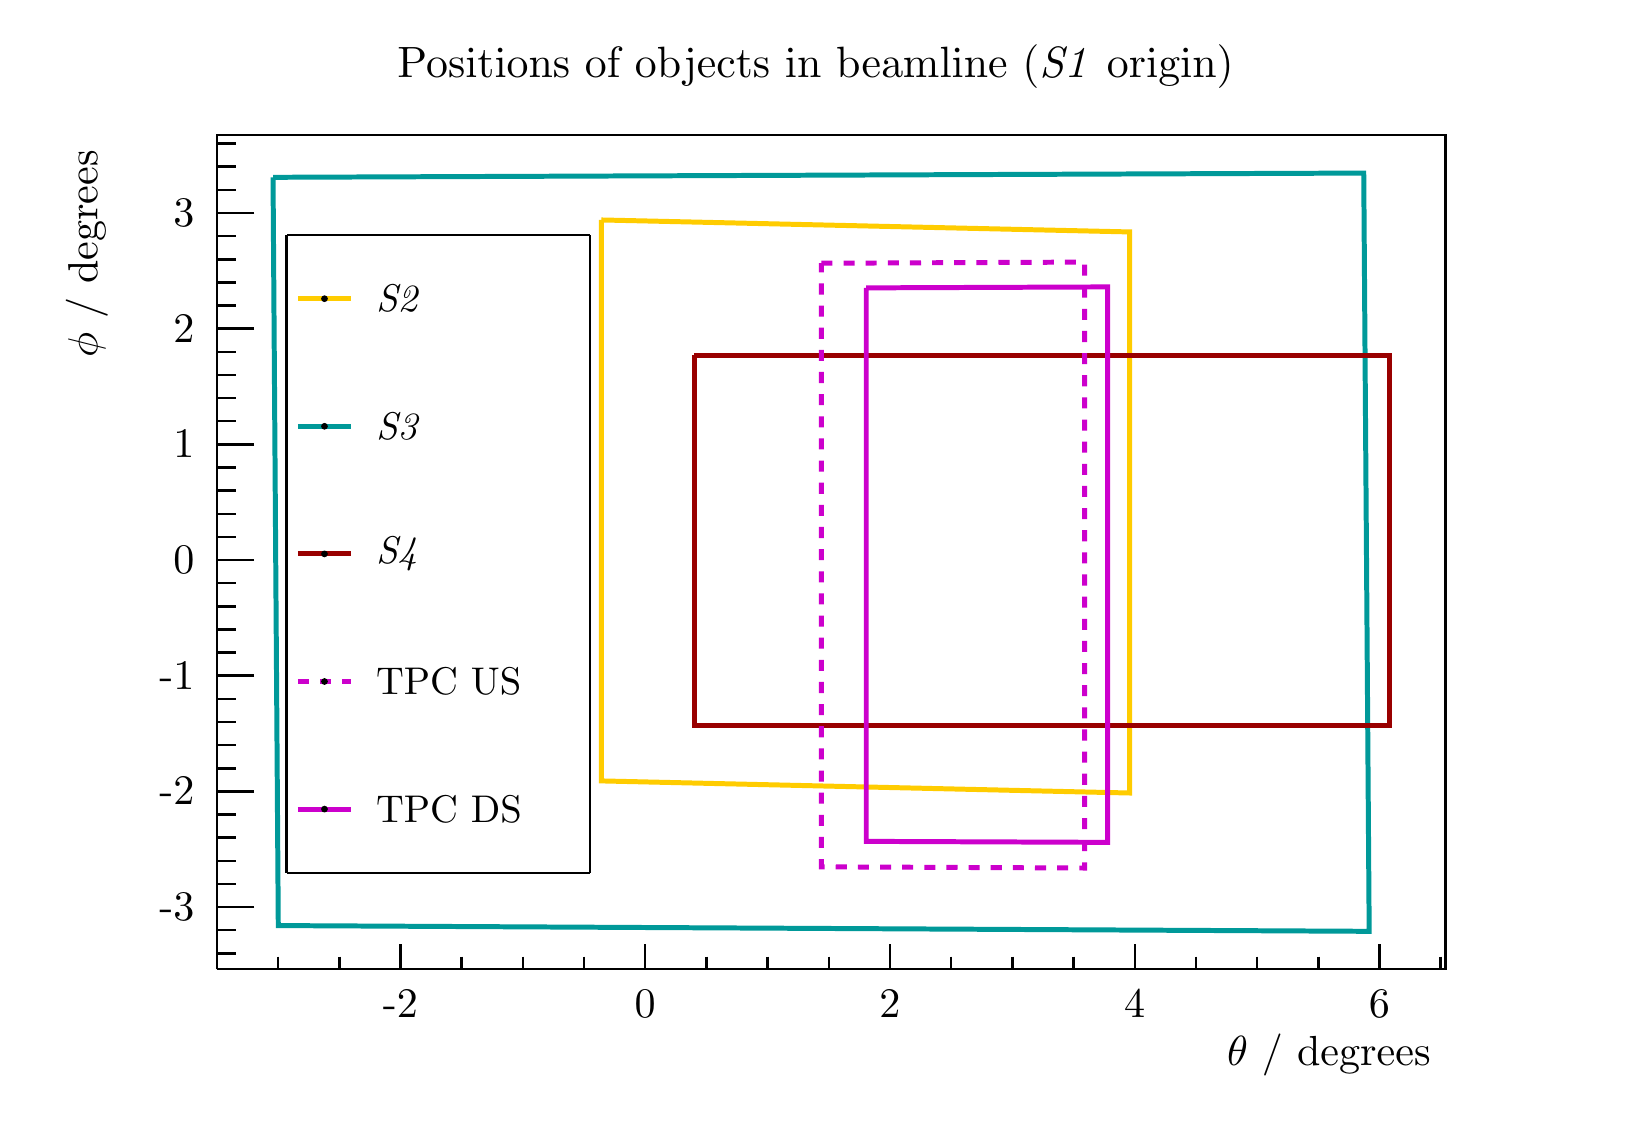
\begin{tikzpicture}
\pgfdeclareplotmark{cross} {
\pgfpathmoveto{\pgfpoint{-0.3\pgfplotmarksize}{\pgfplotmarksize}}
\pgfpathlineto{\pgfpoint{+0.3\pgfplotmarksize}{\pgfplotmarksize}}
\pgfpathlineto{\pgfpoint{+0.3\pgfplotmarksize}{0.3\pgfplotmarksize}}
\pgfpathlineto{\pgfpoint{+1\pgfplotmarksize}{0.3\pgfplotmarksize}}
\pgfpathlineto{\pgfpoint{+1\pgfplotmarksize}{-0.3\pgfplotmarksize}}
\pgfpathlineto{\pgfpoint{+0.3\pgfplotmarksize}{-0.3\pgfplotmarksize}}
\pgfpathlineto{\pgfpoint{+0.3\pgfplotmarksize}{-1.\pgfplotmarksize}}
\pgfpathlineto{\pgfpoint{-0.3\pgfplotmarksize}{-1.\pgfplotmarksize}}
\pgfpathlineto{\pgfpoint{-0.3\pgfplotmarksize}{-0.3\pgfplotmarksize}}
\pgfpathlineto{\pgfpoint{-1.\pgfplotmarksize}{-0.3\pgfplotmarksize}}
\pgfpathlineto{\pgfpoint{-1.\pgfplotmarksize}{0.3\pgfplotmarksize}}
\pgfpathlineto{\pgfpoint{-0.3\pgfplotmarksize}{0.3\pgfplotmarksize}}
\pgfpathclose
\pgfusepathqstroke
}
\pgfdeclareplotmark{cross*} {
\pgfpathmoveto{\pgfpoint{-0.3\pgfplotmarksize}{\pgfplotmarksize}}
\pgfpathlineto{\pgfpoint{+0.3\pgfplotmarksize}{\pgfplotmarksize}}
\pgfpathlineto{\pgfpoint{+0.3\pgfplotmarksize}{0.3\pgfplotmarksize}}
\pgfpathlineto{\pgfpoint{+1\pgfplotmarksize}{0.3\pgfplotmarksize}}
\pgfpathlineto{\pgfpoint{+1\pgfplotmarksize}{-0.3\pgfplotmarksize}}
\pgfpathlineto{\pgfpoint{+0.3\pgfplotmarksize}{-0.3\pgfplotmarksize}}
\pgfpathlineto{\pgfpoint{+0.3\pgfplotmarksize}{-1.\pgfplotmarksize}}
\pgfpathlineto{\pgfpoint{-0.3\pgfplotmarksize}{-1.\pgfplotmarksize}}
\pgfpathlineto{\pgfpoint{-0.3\pgfplotmarksize}{-0.3\pgfplotmarksize}}
\pgfpathlineto{\pgfpoint{-1.\pgfplotmarksize}{-0.3\pgfplotmarksize}}
\pgfpathlineto{\pgfpoint{-1.\pgfplotmarksize}{0.3\pgfplotmarksize}}
\pgfpathlineto{\pgfpoint{-0.3\pgfplotmarksize}{0.3\pgfplotmarksize}}
\pgfpathclose
\pgfusepathqfillstroke
}
\pgfdeclareplotmark{newstar} {
\pgfpathmoveto{\pgfqpoint{0pt}{\pgfplotmarksize}}
\pgfpathlineto{\pgfqpointpolar{44}{0.5\pgfplotmarksize}}
\pgfpathlineto{\pgfqpointpolar{18}{\pgfplotmarksize}}
\pgfpathlineto{\pgfqpointpolar{-20}{0.5\pgfplotmarksize}}
\pgfpathlineto{\pgfqpointpolar{-54}{\pgfplotmarksize}}
\pgfpathlineto{\pgfqpointpolar{-90}{0.5\pgfplotmarksize}}
\pgfpathlineto{\pgfqpointpolar{234}{\pgfplotmarksize}}
\pgfpathlineto{\pgfqpointpolar{198}{0.5\pgfplotmarksize}}
\pgfpathlineto{\pgfqpointpolar{162}{\pgfplotmarksize}}
\pgfpathlineto{\pgfqpointpolar{134}{0.5\pgfplotmarksize}}
\pgfpathclose
\pgfusepathqstroke
}
\pgfdeclareplotmark{newstar*} {
\pgfpathmoveto{\pgfqpoint{0pt}{\pgfplotmarksize}}
\pgfpathlineto{\pgfqpointpolar{44}{0.5\pgfplotmarksize}}
\pgfpathlineto{\pgfqpointpolar{18}{\pgfplotmarksize}}
\pgfpathlineto{\pgfqpointpolar{-20}{0.5\pgfplotmarksize}}
\pgfpathlineto{\pgfqpointpolar{-54}{\pgfplotmarksize}}
\pgfpathlineto{\pgfqpointpolar{-90}{0.5\pgfplotmarksize}}
\pgfpathlineto{\pgfqpointpolar{234}{\pgfplotmarksize}}
\pgfpathlineto{\pgfqpointpolar{198}{0.5\pgfplotmarksize}}
\pgfpathlineto{\pgfqpointpolar{162}{\pgfplotmarksize}}
\pgfpathlineto{\pgfqpointpolar{134}{0.5\pgfplotmarksize}}
\pgfpathclose
\pgfusepathqfillstroke
}
\definecolor{c}{rgb}{1,1,1};
\draw [color=c, fill=c] (0,0) rectangle (20,13.5806);
\draw [color=c, fill=c] (2.4,1.62967) rectangle (18,12.2225);
\definecolor{c}{rgb}{0,0,0};
\draw [c,line width=0.9] (2.4,1.62967) -- (2.4,12.2225) -- (18,12.2225) -- (18,1.62967) -- (2.4,1.62967);
\definecolor{c}{rgb}{1,1,1};
\draw [color=c, fill=c] (2.4,1.62967) rectangle (18,12.2225);
\definecolor{c}{rgb}{0,0,0};
\draw [c,line width=0.9] (2.4,1.62967) -- (2.4,12.2225) -- (18,12.2225) -- (18,1.62967) -- (2.4,1.62967);
\draw [c,line width=0.9] (2.4,1.62967) -- (18,1.62967);
\draw [c,line width=0.9] (4.72729,1.94746) -- (4.72729,1.62967);
\draw [c,line width=0.9] (5.50442,1.78856) -- (5.50442,1.62967);
\draw [c,line width=0.9] (6.28155,1.78856) -- (6.28155,1.62967);
\draw [c,line width=0.9] (7.05868,1.78856) -- (7.05868,1.62967);
\draw [c,line width=0.9] (7.83581,1.94746) -- (7.83581,1.62967);
\draw [c,line width=0.9] (8.61294,1.78856) -- (8.61294,1.62967);
\draw [c,line width=0.9] (9.39007,1.78856) -- (9.39007,1.62967);
\draw [c,line width=0.9] (10.1672,1.78856) -- (10.1672,1.62967);
\draw [c,line width=0.9] (10.9443,1.94746) -- (10.9443,1.62967);
\draw [c,line width=0.9] (11.7215,1.78856) -- (11.7215,1.62967);
\draw [c,line width=0.9] (12.4986,1.78856) -- (12.4986,1.62967);
\draw [c,line width=0.9] (13.2757,1.78856) -- (13.2757,1.62967);
\draw [c,line width=0.9] (14.0529,1.94746) -- (14.0529,1.62967);
\draw [c,line width=0.9] (14.83,1.78856) -- (14.83,1.62967);
\draw [c,line width=0.9] (15.6071,1.78856) -- (15.6071,1.62967);
\draw [c,line width=0.9] (16.3842,1.78856) -- (16.3842,1.62967);
\draw [c,line width=0.9] (17.1614,1.94746) -- (17.1614,1.62967);
\draw [c,line width=0.9] (4.72729,1.94746) -- (4.72729,1.62967);
\draw [c,line width=0.9] (3.95016,1.78856) -- (3.95016,1.62967);
\draw [c,line width=0.9] (3.17303,1.78856) -- (3.17303,1.62967);
\draw [c,line width=0.9] (17.1614,1.94746) -- (17.1614,1.62967);
\draw [c,line width=0.9] (17.9385,1.78856) -- (17.9385,1.62967);
\draw [anchor=base] (4.72729,1.01854) node[scale=1.52078, color=c, rotate=0]{-2};
\draw [anchor=base] (7.83581,1.01854) node[scale=1.52078, color=c, rotate=0]{0};
\draw [anchor=base] (10.9443,1.01854) node[scale=1.52078, color=c, rotate=0]{2};
\draw [anchor=base] (14.0529,1.01854) node[scale=1.52078, color=c, rotate=0]{4};
\draw [anchor=base] (17.1614,1.01854) node[scale=1.52078, color=c, rotate=0]{6};
\draw [anchor= east] (18,0.543224) node[scale=1.52078, color=c, rotate=0]{$\theta$ / degrees};
\draw [c,line width=0.9] (2.4,1.62967) -- (2.4,12.2225);
\draw [c,line width=0.9] (2.868,2.41867) -- (2.4,2.41867);
\draw [c,line width=0.9] (2.634,2.71252) -- (2.4,2.71252);
\draw [c,line width=0.9] (2.634,3.00636) -- (2.4,3.00636);
\draw [c,line width=0.9] (2.634,3.30021) -- (2.4,3.30021);
\draw [c,line width=0.9] (2.634,3.59406) -- (2.4,3.59406);
\draw [c,line width=0.9] (2.868,3.88791) -- (2.4,3.88791);
\draw [c,line width=0.9] (2.634,4.18176) -- (2.4,4.18176);
\draw [c,line width=0.9] (2.634,4.47561) -- (2.4,4.47561);
\draw [c,line width=0.9] (2.634,4.76945) -- (2.4,4.76945);
\draw [c,line width=0.9] (2.634,5.0633) -- (2.4,5.0633);
\draw [c,line width=0.9] (2.868,5.35715) -- (2.4,5.35715);
\draw [c,line width=0.9] (2.634,5.651) -- (2.4,5.651);
\draw [c,line width=0.9] (2.634,5.94485) -- (2.4,5.94485);
\draw [c,line width=0.9] (2.634,6.2387) -- (2.4,6.2387);
\draw [c,line width=0.9] (2.634,6.53255) -- (2.4,6.53255);
\draw [c,line width=0.9] (2.868,6.82639) -- (2.4,6.82639);
\draw [c,line width=0.9] (2.634,7.12024) -- (2.4,7.12024);
\draw [c,line width=0.9] (2.634,7.41409) -- (2.4,7.41409);
\draw [c,line width=0.9] (2.634,7.70794) -- (2.4,7.70794);
\draw [c,line width=0.9] (2.634,8.00179) -- (2.4,8.00179);
\draw [c,line width=0.9] (2.868,8.29564) -- (2.4,8.29564);
\draw [c,line width=0.9] (2.634,8.58948) -- (2.4,8.58948);
\draw [c,line width=0.9] (2.634,8.88333) -- (2.4,8.88333);
\draw [c,line width=0.9] (2.634,9.17718) -- (2.4,9.17718);
\draw [c,line width=0.9] (2.634,9.47103) -- (2.4,9.47103);
\draw [c,line width=0.9] (2.868,9.76488) -- (2.4,9.76488);
\draw [c,line width=0.9] (2.634,10.0587) -- (2.4,10.0587);
\draw [c,line width=0.9] (2.634,10.3526) -- (2.4,10.3526);
\draw [c,line width=0.9] (2.634,10.6464) -- (2.4,10.6464);
\draw [c,line width=0.9] (2.634,10.9403) -- (2.4,10.9403);
\draw [c,line width=0.9] (2.868,11.2341) -- (2.4,11.2341);
\draw [c,line width=0.9] (2.868,2.41867) -- (2.4,2.41867);
\draw [c,line width=0.9] (2.634,2.12482) -- (2.4,2.12482);
\draw [c,line width=0.9] (2.634,1.83097) -- (2.4,1.83097);
\draw [c,line width=0.9] (2.868,11.2341) -- (2.4,11.2341);
\draw [c,line width=0.9] (2.634,11.528) -- (2.4,11.528);
\draw [c,line width=0.9] (2.634,11.8218) -- (2.4,11.8218);
\draw [c,line width=0.9] (2.634,12.1157) -- (2.4,12.1157);
\draw [anchor= east] (2.3,2.41867) node[scale=1.52078, color=c, rotate=0]{-3};
\draw [anchor= east] (2.3,3.88791) node[scale=1.52078, color=c, rotate=0]{-2};
\draw [anchor= east] (2.3,5.35715) node[scale=1.52078, color=c, rotate=0]{-1};
\draw [anchor= east] (2.3,6.82639) node[scale=1.52078, color=c, rotate=0]{0};
\draw [anchor= east] (2.3,8.29564) node[scale=1.52078, color=c, rotate=0]{1};
\draw [anchor= east] (2.3,9.76488) node[scale=1.52078, color=c, rotate=0]{2};
\draw [anchor= east] (2.3,11.2341) node[scale=1.52078, color=c, rotate=0]{3};
\draw [anchor= east] (0.743795,12.2225) node[scale=1.52078, color=c, rotate=90]{$\phi$ / degrees};
\definecolor{c}{rgb}{1,0.8,0};
\draw [c,line width=1.8] (7.2782,11.1455) -- (7.2782,4.02134) -- (13.9868,3.86782) -- (13.9868,10.9934) -- (7.2782,11.1455);
\definecolor{c}{rgb}{0,0.6,0.6};
\draw [c,line width=1.8] (3.10909,11.687) -- (16.9609,11.741) -- (17.03,2.11117) -- (3.17567,2.18425) -- (3.10909,11.687);
\definecolor{c}{rgb}{0.6,0,0};
\draw [c,line width=1.8] (8.45845,9.42826) -- (17.2909,9.42826) -- (17.2909,4.73099) -- (8.45845,4.73099) -- (8.45845,9.42826);
\definecolor{c}{rgb}{0.8,0,0.8};
\draw [c,dash pattern=on 4.00pt off 4.00pt ,line width=1.8] (10.0729,10.5958) -- (13.416,10.6103) -- (13.416,2.91521) -- (10.0729,2.93012) -- (10.0729,10.5958);
\draw [c,line width=1.8] (10.6427,10.2829) -- (13.7076,10.295) -- (13.7076,3.24103) -- (10.6427,3.25357) -- (10.6427,10.2829);
\definecolor{c}{rgb}{0,0,0};
\draw (10,13.0975) node[scale=1.58414, color=c, rotate=0]{Positions of objects in beamline ($\mathit{S1}$ origin)};
\definecolor{c}{rgb}{1,1,1};
\draw [color=c, fill=c] (3.28103,2.85307) rectangle (7.13267,10.9558);
\definecolor{c}{rgb}{0,0,0};
\draw [c,line width=0.9] (3.28103,2.85307) -- (7.13267,2.85307);
\draw [c,line width=0.9] (7.13267,2.85307) -- (7.13267,10.9558);
\draw [c,line width=0.9] (7.13267,10.9558) -- (3.28103,10.9558);
\draw [c,line width=0.9] (3.28103,10.9558) -- (3.28103,2.85307);
\draw [anchor= west] (4.24394,10.1455) node[scale=1.39405, color=c, rotate=0]{$\mathit{S2}$};
\definecolor{c}{rgb}{1,1,1};
\draw [c, fill=c] (3.42546,9.57832) -- (4.0995,9.57832) -- (4.0995,10.7127) -- (3.42546,10.7127);
\definecolor{c}{rgb}{1,0.8,0};
\draw [c,line width=1.8] (3.42546,10.1455) -- (4.0995,10.1455);
\definecolor{c}{rgb}{0,0,0};
\foreach \P in {(3.76248,10.1455)}{\draw[mark options={color=c,fill=c},mark size=2.402402pt,mark=*,mark size=1pt] plot coordinates {\P};}
\draw [anchor= west] (4.24394,8.52496) node[scale=1.39405, color=c, rotate=0]{$\mathit{S3}$};
\definecolor{c}{rgb}{1,1,1};
\draw [c, fill=c] (3.42546,7.95777) -- (4.0995,7.95777) -- (4.0995,9.09215) -- (3.42546,9.09215);
\definecolor{c}{rgb}{0,0.6,0.6};
\draw [c,line width=1.8] (3.42546,8.52496) -- (4.0995,8.52496);
\definecolor{c}{rgb}{0,0,0};
\foreach \P in {(3.76248,8.52496)}{\draw[mark options={color=c,fill=c},mark size=2.402402pt,mark=*,mark size=1pt] plot coordinates {\P};}
\draw [anchor= west] (4.24394,6.90442) node[scale=1.39405, color=c, rotate=0]{$\mathit{S4}$};
\definecolor{c}{rgb}{1,1,1};
\draw [c, fill=c] (3.42546,6.33723) -- (4.0995,6.33723) -- (4.0995,7.47161) -- (3.42546,7.47161);
\definecolor{c}{rgb}{0.6,0,0};
\draw [c,line width=1.8] (3.42546,6.90442) -- (4.0995,6.90442);
\definecolor{c}{rgb}{0,0,0};
\foreach \P in {(3.76248,6.90442)}{\draw[mark options={color=c,fill=c},mark size=2.402402pt,mark=*,mark size=1pt] plot coordinates {\P};}
\draw [anchor= west] (4.24394,5.28388) node[scale=1.39405, color=c, rotate=0]{TPC US};
\definecolor{c}{rgb}{1,1,1};
\draw [c, fill=c] (3.42546,4.71669) -- (4.0995,4.71669) -- (4.0995,5.85107) -- (3.42546,5.85107);
\definecolor{c}{rgb}{0.8,0,0.8};
\draw [c,dash pattern=on 4.00pt off 4.00pt ,line width=1.8] (3.42546,5.28388) -- (4.0995,5.28388);
\definecolor{c}{rgb}{0,0,0};
\foreach \P in {(3.76248,5.28388)}{\draw[mark options={color=c,fill=c},mark size=2.402402pt,mark=*,mark size=1pt] plot coordinates {\P};}
\draw [anchor= west] (4.24394,3.66334) node[scale=1.39405, color=c, rotate=0]{TPC DS};
\definecolor{c}{rgb}{1,1,1};
\draw [c, fill=c] (3.42546,3.09615) -- (4.0995,3.09615) -- (4.0995,4.23053) -- (3.42546,4.23053);
\definecolor{c}{rgb}{0.8,0,0.8};
\draw [c,line width=1.8] (3.42546,3.66334) -- (4.0995,3.66334);
\definecolor{c}{rgb}{0,0,0};
\foreach \P in {(3.76248,3.66334)}{\draw[mark options={color=c,fill=c},mark size=2.402402pt,mark=*,mark size=1pt] plot coordinates {\P};}
\end{tikzpicture}

  \end{adjustbox}
  \caption{Angular position of various objects within the T10 beamline. US and DS refer to the upstream and downstream faces of the HPTPC. The origin in this view is at the centre of $\mathit{S1}$; the true centre of the steered beam is at +1$^{\circ}$ in $\theta$ and 0$^{\circ}$ in $\phi$.}
  \label{fig:angularDistS1}
\end{figure}

\begin{table}
  \centering
  \caption{Angular extents of objects within the T10 beamline as measured from $\mathit{S1}$.}
  \begin{tabular}{c|c c c c}
    \hline
    \hline
    Object & Minimum $\theta$ & Maximum $\theta$ & Minimum $\phi$ & Maximum $\phi$ \\
    \hline
    $\mathit{S2}$ & $-3.96^{\circ} \pm 0.03^{\circ}$ & $-0.36^{\circ} \pm 0.03^{\circ}$ & $-2.01^{\circ} \pm 0.03^{\circ}$ & $2.94^{\circ} \pm 0.03^{\circ}$ \\
    $\mathit{S3}$ & $-5.923^{\circ} \pm 0.004^{\circ}$ & \hspace{6pt} $3.040^{\circ} \pm 0.004^{\circ}$ & $-3.215^{\circ} \pm 0.004^{\circ}$ & $3.344^{\circ} \pm 0.004^{\circ}$ \\
   $\mathit{S4}$ & $-6.083^{\circ} \pm 0.003^{\circ}$ & $-0.401{\circ} \pm 0.003^{\circ}$ & $-1.426{\circ} \pm 0.003^{\circ}$ & $1.771^{\circ} \pm 0.003^{\circ}$ \\
    TPC upstream face & $-3.59^{\circ} \pm 0.01^{\circ}$ & $-1.44^{\circ} \pm 0.01^{\circ}$ & $-2.66^{\circ} \pm 0.01^{\circ}$ & $2.58^{\circ} \pm 0.01^{\circ}$ \\
    TPC downstream face & $-3.778^{\circ} \pm 0.009^{\circ}$ & $-1.806^{\circ} \pm 0.009^{\circ}$ & $-2.440^{\circ} \pm 0.009^{\circ}$ & $2.361^{\circ} \pm 0.009^{\circ}$ \\
    \hline
  \end{tabular}
  \label{tab:angS1}
\end{table}

\begin{table}
  \centering
  \caption{Distances between objects in the T10 beamline. US and DS refer to the upstream and downstream edges of the TPC respectively.}
  \begin{tabular}{c|c}
    \hline
    \hline
    Points & Distance between centres / m\\
    \hline
    Beam monitor -- $\mathit{S1}$ & $0.288 \pm 0.001$ \\
    $\mathit{S1}-\mathit{S2}$ & $1.419 \pm 0.001$ \\
    $\mathit{S1}-\mathit{S3}$ & $10.756 \pm 0.001$ \\
    $\mathit{S3}$ -- TPC US side & $1.323 \pm 0.002$ \\
    TPC DS side -- $\mathit{S4}$ & $0.918 \pm 0.002$ \\
    $\mathit{S2}-\mathit{S4}$ & $12.651 \pm 0.001$ \\
    \hline    
  \end{tabular}
  \label{tab:distances}
\end{table}

\subsection{Upstream beam counters (S1 and S2)}
\label{subsec:s1s2Exp}
\begin{figure}
  \centering
  \includegraphics[width=0.7\linewidth]{files/Figures/S1S2FrontOn.png}
  \caption{The S1 and S2 beam counters. Together the coincidence of signals in the beam counters were recorded by the DAQ systems}
  \label{fig:S1S2headon}
\end{figure}
The beam counters $\mathit{S1}$ and $\mathit{S2}$ are shown in Figure~\ref{fig:S1S2headon}.
The $\mathit{S1}$ counter is a $40\times40\times5$~mm$^3$ plastic scintillator cross which is attached to four 1'' Hamamatsu Photonics R4998 photomultiplier tubes (PMTs) at each end for the light readout.
The time resolution of the counter, as measured by the DAQ system of the upstream ToF, was about 30~ps. This is estimated with the distribution of the average PMT hit times; the quantity $t_{\textrm{ave}}=\frac{1}{4}((t_{\textrm{PMT0}}+t_{\textrm{PMT1}})-(t_{\textrm{PMT2}}+t_{\textrm{PMT3}}))$ has the same spread as the simple average but is conveniently centered at zero.
An example of the $t_{\textrm{ave}}$ distribution for one run of $\mathit{S1}$ data is shown in Figure~\ref{fig:s1Res}. The full width at half maximum (FWHM) of the distribution is 62 ps.

\begin{figure}
  \begin{adjustbox}{width=0.7\linewidth, center}
    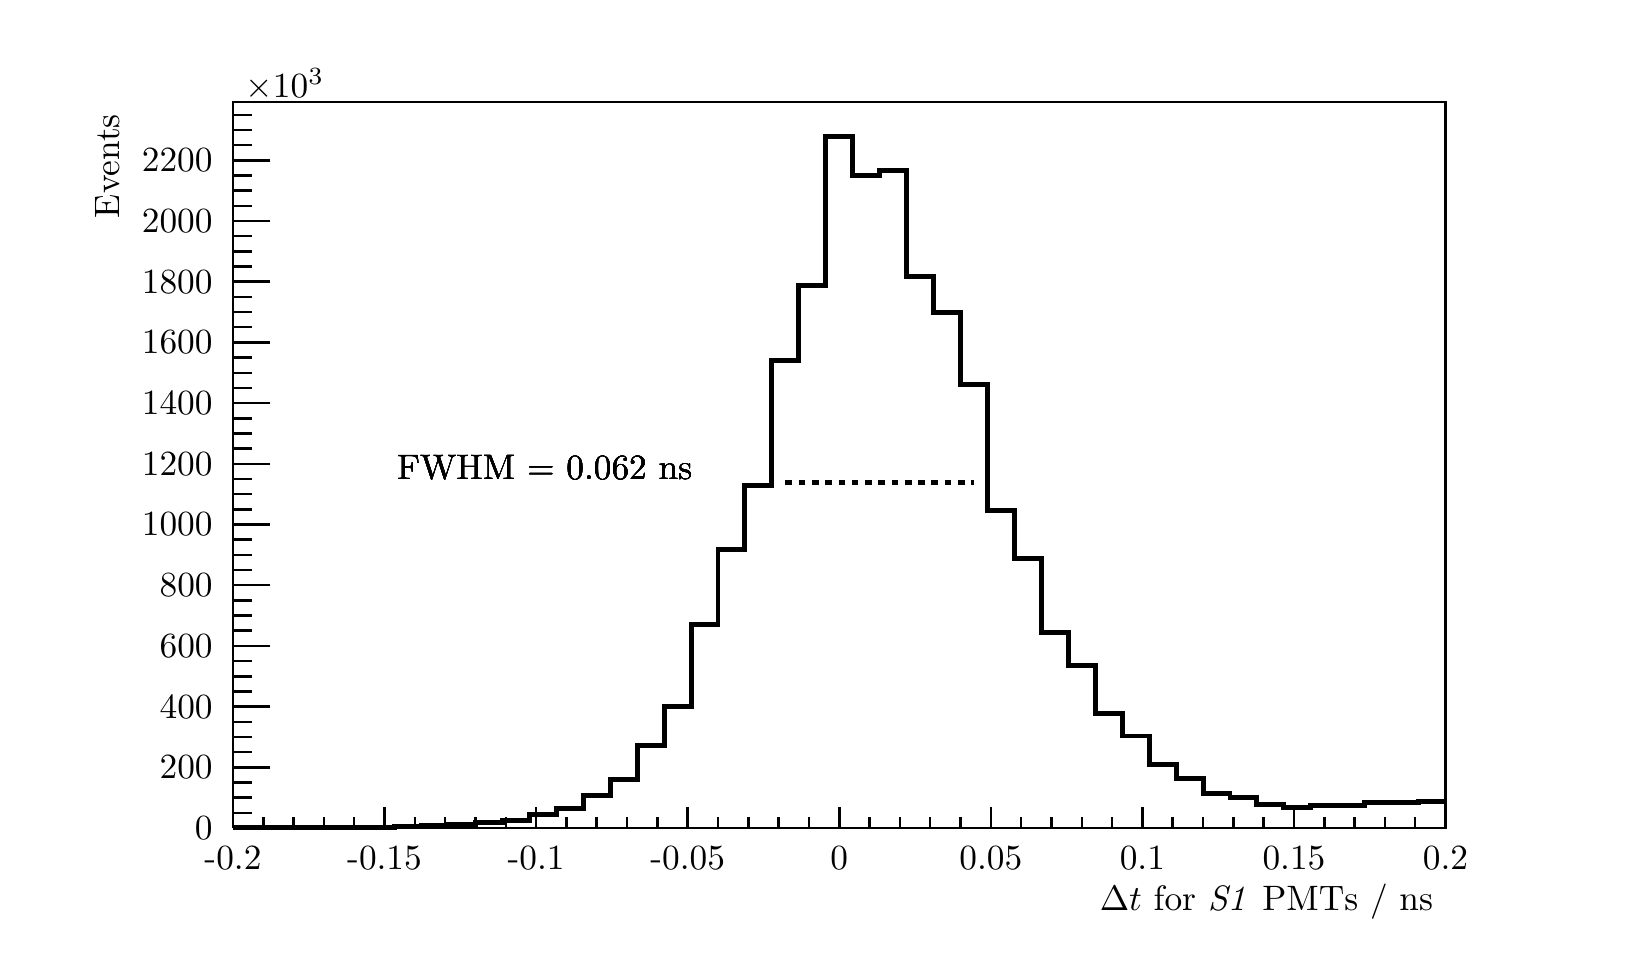
\begin{tikzpicture}
\pgfdeclareplotmark{cross} {
\pgfpathmoveto{\pgfpoint{-0.3\pgfplotmarksize}{\pgfplotmarksize}}
\pgfpathlineto{\pgfpoint{+0.3\pgfplotmarksize}{\pgfplotmarksize}}
\pgfpathlineto{\pgfpoint{+0.3\pgfplotmarksize}{0.3\pgfplotmarksize}}
\pgfpathlineto{\pgfpoint{+1\pgfplotmarksize}{0.3\pgfplotmarksize}}
\pgfpathlineto{\pgfpoint{+1\pgfplotmarksize}{-0.3\pgfplotmarksize}}
\pgfpathlineto{\pgfpoint{+0.3\pgfplotmarksize}{-0.3\pgfplotmarksize}}
\pgfpathlineto{\pgfpoint{+0.3\pgfplotmarksize}{-1.\pgfplotmarksize}}
\pgfpathlineto{\pgfpoint{-0.3\pgfplotmarksize}{-1.\pgfplotmarksize}}
\pgfpathlineto{\pgfpoint{-0.3\pgfplotmarksize}{-0.3\pgfplotmarksize}}
\pgfpathlineto{\pgfpoint{-1.\pgfplotmarksize}{-0.3\pgfplotmarksize}}
\pgfpathlineto{\pgfpoint{-1.\pgfplotmarksize}{0.3\pgfplotmarksize}}
\pgfpathlineto{\pgfpoint{-0.3\pgfplotmarksize}{0.3\pgfplotmarksize}}
\pgfpathclose
\pgfusepathqstroke
}
\pgfdeclareplotmark{cross*} {
\pgfpathmoveto{\pgfpoint{-0.3\pgfplotmarksize}{\pgfplotmarksize}}
\pgfpathlineto{\pgfpoint{+0.3\pgfplotmarksize}{\pgfplotmarksize}}
\pgfpathlineto{\pgfpoint{+0.3\pgfplotmarksize}{0.3\pgfplotmarksize}}
\pgfpathlineto{\pgfpoint{+1\pgfplotmarksize}{0.3\pgfplotmarksize}}
\pgfpathlineto{\pgfpoint{+1\pgfplotmarksize}{-0.3\pgfplotmarksize}}
\pgfpathlineto{\pgfpoint{+0.3\pgfplotmarksize}{-0.3\pgfplotmarksize}}
\pgfpathlineto{\pgfpoint{+0.3\pgfplotmarksize}{-1.\pgfplotmarksize}}
\pgfpathlineto{\pgfpoint{-0.3\pgfplotmarksize}{-1.\pgfplotmarksize}}
\pgfpathlineto{\pgfpoint{-0.3\pgfplotmarksize}{-0.3\pgfplotmarksize}}
\pgfpathlineto{\pgfpoint{-1.\pgfplotmarksize}{-0.3\pgfplotmarksize}}
\pgfpathlineto{\pgfpoint{-1.\pgfplotmarksize}{0.3\pgfplotmarksize}}
\pgfpathlineto{\pgfpoint{-0.3\pgfplotmarksize}{0.3\pgfplotmarksize}}
\pgfpathclose
\pgfusepathqfillstroke
}
\pgfdeclareplotmark{newstar} {
\pgfpathmoveto{\pgfqpoint{0pt}{\pgfplotmarksize}}
\pgfpathlineto{\pgfqpointpolar{44}{0.5\pgfplotmarksize}}
\pgfpathlineto{\pgfqpointpolar{18}{\pgfplotmarksize}}
\pgfpathlineto{\pgfqpointpolar{-20}{0.5\pgfplotmarksize}}
\pgfpathlineto{\pgfqpointpolar{-54}{\pgfplotmarksize}}
\pgfpathlineto{\pgfqpointpolar{-90}{0.5\pgfplotmarksize}}
\pgfpathlineto{\pgfqpointpolar{234}{\pgfplotmarksize}}
\pgfpathlineto{\pgfqpointpolar{198}{0.5\pgfplotmarksize}}
\pgfpathlineto{\pgfqpointpolar{162}{\pgfplotmarksize}}
\pgfpathlineto{\pgfqpointpolar{134}{0.5\pgfplotmarksize}}
\pgfpathclose
\pgfusepathqstroke
}
\pgfdeclareplotmark{newstar*} {
\pgfpathmoveto{\pgfqpoint{0pt}{\pgfplotmarksize}}
\pgfpathlineto{\pgfqpointpolar{44}{0.5\pgfplotmarksize}}
\pgfpathlineto{\pgfqpointpolar{18}{\pgfplotmarksize}}
\pgfpathlineto{\pgfqpointpolar{-20}{0.5\pgfplotmarksize}}
\pgfpathlineto{\pgfqpointpolar{-54}{\pgfplotmarksize}}
\pgfpathlineto{\pgfqpointpolar{-90}{0.5\pgfplotmarksize}}
\pgfpathlineto{\pgfqpointpolar{234}{\pgfplotmarksize}}
\pgfpathlineto{\pgfqpointpolar{198}{0.5\pgfplotmarksize}}
\pgfpathlineto{\pgfqpointpolar{162}{\pgfplotmarksize}}
\pgfpathlineto{\pgfqpointpolar{134}{0.5\pgfplotmarksize}}
\pgfpathclose
\pgfusepathqfillstroke
}
\definecolor{c}{rgb}{1,1,1};
\draw [color=c, fill=c] (0,0) rectangle (20,11.675);
\draw [color=c, fill=c] (2.6,1.51775) rectangle (18,10.741);
\definecolor{c}{rgb}{0,0,0};
\draw [c,line width=0.9] (2.6,1.51775) -- (2.6,10.741) -- (18,10.741) -- (18,1.51775) -- (2.6,1.51775);
\definecolor{c}{rgb}{1,1,1};
\draw [color=c, fill=c] (2.6,1.51775) rectangle (18,10.741);
\definecolor{c}{rgb}{0,0,0};
\draw [c,line width=0.9] (2.6,1.51775) -- (2.6,10.741) -- (18,10.741) -- (18,1.51775) -- (2.6,1.51775);
\draw [c,line width=1.8] (2.6,1.51958) -- (2.94222,1.51958) -- (2.94222,1.51977) -- (3.28444,1.51977) -- (3.28444,1.52075) -- (3.62667,1.52075) -- (3.62667,1.52204) -- (3.96889,1.52204) -- (3.96889,1.52504) -- (4.31111,1.52504) -- (4.31111,1.52834)
 -- (4.65333,1.52834) -- (4.65333,1.53523) -- (4.99556,1.53523) -- (4.99556,1.54741) -- (5.33778,1.54741) -- (5.33778,1.5584) -- (5.68,1.5584) -- (5.68,1.58483) -- (6.02222,1.58483) -- (6.02222,1.61641) -- (6.36444,1.61641) -- (6.36444,1.68501) --
 (6.70667,1.68501) -- (6.70667,1.76425) -- (7.04889,1.76425) -- (7.04889,1.93053) -- (7.39111,1.93053) -- (7.39111,2.12776) -- (7.73333,2.12776) -- (7.73333,2.57125) -- (8.07556,2.57125) -- (8.07556,3.05548) -- (8.41778,3.05548) -- (8.41778,4.09746)
 -- (8.76,4.09746) -- (8.76,5.05002) -- (9.10222,5.05002) -- (9.10222,5.87277) -- (9.44444,5.87277) -- (9.44444,7.45651) -- (9.78667,7.45651) -- (9.78667,8.4135) -- (10.1289,8.4135) -- (10.1289,10.3018) -- (10.4711,10.3018) -- (10.4711,9.8074) --
 (10.8133,9.8074) -- (10.8133,9.87378) -- (11.1556,9.87378) -- (11.1556,8.52277) -- (11.4978,8.52277) -- (11.4978,8.05893) -- (11.84,8.05893) -- (11.84,7.14883) -- (12.1822,7.14883) -- (12.1822,5.55186) -- (12.5244,5.55186) -- (12.5244,4.94574) --
 (12.8667,4.94574) -- (12.8667,3.99644) -- (13.2089,3.99644) -- (13.2089,3.57792) -- (13.5511,3.57792) -- (13.5511,2.9767) -- (13.8933,2.9767) -- (13.8933,2.68633) -- (14.2356,2.68633) -- (14.2356,2.31822) -- (14.5778,2.31822) -- (14.5778,2.15102) --
 (14.92,2.15102) -- (14.92,1.96062) -- (15.2622,1.96062) -- (15.2622,1.90122) -- (15.6044,1.90122) -- (15.6044,1.81479) -- (15.9467,1.81479) -- (15.9467,1.78186) -- (16.2889,1.78186) -- (16.2889,1.80117) -- (16.6311,1.80117) -- (16.6311,1.80069) --
 (16.9733,1.80069) -- (16.9733,1.8367) -- (17.3156,1.8367) -- (17.3156,1.83646) -- (17.6578,1.83646) -- (17.6578,1.84969) -- (18,1.84969);
\draw [c,line width=0.9] (2.6,1.51775) -- (18,1.51775);
\draw [c,line width=0.9] (2.6,1.78744) -- (2.6,1.51775);
\draw [c,line width=0.9] (2.985,1.6526) -- (2.985,1.51775);
\draw [c,line width=0.9] (3.37,1.6526) -- (3.37,1.51775);
\draw [c,line width=0.9] (3.755,1.6526) -- (3.755,1.51775);
\draw [c,line width=0.9] (4.14,1.6526) -- (4.14,1.51775);
\draw [c,line width=0.9] (4.525,1.78744) -- (4.525,1.51775);
\draw [c,line width=0.9] (4.91,1.6526) -- (4.91,1.51775);
\draw [c,line width=0.9] (5.295,1.6526) -- (5.295,1.51775);
\draw [c,line width=0.9] (5.68,1.6526) -- (5.68,1.51775);
\draw [c,line width=0.9] (6.065,1.6526) -- (6.065,1.51775);
\draw [c,line width=0.9] (6.45,1.78744) -- (6.45,1.51775);
\draw [c,line width=0.9] (6.835,1.6526) -- (6.835,1.51775);
\draw [c,line width=0.9] (7.22,1.6526) -- (7.22,1.51775);
\draw [c,line width=0.9] (7.605,1.6526) -- (7.605,1.51775);
\draw [c,line width=0.9] (7.99,1.6526) -- (7.99,1.51775);
\draw [c,line width=0.9] (8.375,1.78744) -- (8.375,1.51775);
\draw [c,line width=0.9] (8.76,1.6526) -- (8.76,1.51775);
\draw [c,line width=0.9] (9.145,1.6526) -- (9.145,1.51775);
\draw [c,line width=0.9] (9.53,1.6526) -- (9.53,1.51775);
\draw [c,line width=0.9] (9.915,1.6526) -- (9.915,1.51775);
\draw [c,line width=0.9] (10.3,1.78744) -- (10.3,1.51775);
\draw [c,line width=0.9] (10.685,1.6526) -- (10.685,1.51775);
\draw [c,line width=0.9] (11.07,1.6526) -- (11.07,1.51775);
\draw [c,line width=0.9] (11.455,1.6526) -- (11.455,1.51775);
\draw [c,line width=0.9] (11.84,1.6526) -- (11.84,1.51775);
\draw [c,line width=0.9] (12.225,1.78744) -- (12.225,1.51775);
\draw [c,line width=0.9] (12.61,1.6526) -- (12.61,1.51775);
\draw [c,line width=0.9] (12.995,1.6526) -- (12.995,1.51775);
\draw [c,line width=0.9] (13.38,1.6526) -- (13.38,1.51775);
\draw [c,line width=0.9] (13.765,1.6526) -- (13.765,1.51775);
\draw [c,line width=0.9] (14.15,1.78744) -- (14.15,1.51775);
\draw [c,line width=0.9] (14.535,1.6526) -- (14.535,1.51775);
\draw [c,line width=0.9] (14.92,1.6526) -- (14.92,1.51775);
\draw [c,line width=0.9] (15.305,1.6526) -- (15.305,1.51775);
\draw [c,line width=0.9] (15.69,1.6526) -- (15.69,1.51775);
\draw [c,line width=0.9] (16.075,1.78744) -- (16.075,1.51775);
\draw [c,line width=0.9] (16.46,1.6526) -- (16.46,1.51775);
\draw [c,line width=0.9] (16.845,1.6526) -- (16.845,1.51775);
\draw [c,line width=0.9] (17.23,1.6526) -- (17.23,1.51775);
\draw [c,line width=0.9] (17.615,1.6526) -- (17.615,1.51775);
\draw [c,line width=0.9] (18,1.78744) -- (18,1.51775);
\draw [anchor=base] (2.6,0.992375) node[scale=1.27706, color=c, rotate=0]{-0.2};
\draw [anchor=base] (4.525,0.992375) node[scale=1.27706, color=c, rotate=0]{-0.15};
\draw [anchor=base] (6.45,0.992375) node[scale=1.27706, color=c, rotate=0]{-0.1};
\draw [anchor=base] (8.375,0.992375) node[scale=1.27706, color=c, rotate=0]{-0.05};
\draw [anchor=base] (10.3,0.992375) node[scale=1.27706, color=c, rotate=0]{0};
\draw [anchor=base] (12.225,0.992375) node[scale=1.27706, color=c, rotate=0]{0.05};
\draw [anchor=base] (14.15,0.992375) node[scale=1.27706, color=c, rotate=0]{0.1};
\draw [anchor=base] (16.075,0.992375) node[scale=1.27706, color=c, rotate=0]{0.15};
\draw [anchor=base] (18,0.992375) node[scale=1.27706, color=c, rotate=0]{0.2};
\draw [anchor= east] (18,0.58375) node[scale=1.27706, color=c, rotate=0]{$\Delta t$ for $\mathit{S1}$ PMTs / ns};
\draw [c,line width=0.9] (2.6,1.51775) -- (2.6,10.741);
\draw [c,line width=0.9] (3.074,1.51775) -- (2.6,1.51775);
\draw [c,line width=0.9] (2.837,1.71046) -- (2.6,1.71046);
\draw [c,line width=0.9] (2.837,1.90318) -- (2.6,1.90318);
\draw [c,line width=0.9] (2.837,2.09589) -- (2.6,2.09589);
\draw [c,line width=0.9] (3.074,2.2886) -- (2.6,2.2886);
\draw [c,line width=0.9] (2.837,2.48132) -- (2.6,2.48132);
\draw [c,line width=0.9] (2.837,2.67403) -- (2.6,2.67403);
\draw [c,line width=0.9] (2.837,2.86674) -- (2.6,2.86674);
\draw [c,line width=0.9] (3.074,3.05946) -- (2.6,3.05946);
\draw [c,line width=0.9] (2.837,3.25217) -- (2.6,3.25217);
\draw [c,line width=0.9] (2.837,3.44488) -- (2.6,3.44488);
\draw [c,line width=0.9] (2.837,3.6376) -- (2.6,3.6376);
\draw [c,line width=0.9] (3.074,3.83031) -- (2.6,3.83031);
\draw [c,line width=0.9] (2.837,4.02302) -- (2.6,4.02302);
\draw [c,line width=0.9] (2.837,4.21574) -- (2.6,4.21574);
\draw [c,line width=0.9] (2.837,4.40845) -- (2.6,4.40845);
\draw [c,line width=0.9] (3.074,4.60116) -- (2.6,4.60116);
\draw [c,line width=0.9] (2.837,4.79388) -- (2.6,4.79388);
\draw [c,line width=0.9] (2.837,4.98659) -- (2.6,4.98659);
\draw [c,line width=0.9] (2.837,5.1793) -- (2.6,5.1793);
\draw [c,line width=0.9] (3.074,5.37202) -- (2.6,5.37202);
\draw [c,line width=0.9] (2.837,5.56473) -- (2.6,5.56473);
\draw [c,line width=0.9] (2.837,5.75744) -- (2.6,5.75744);
\draw [c,line width=0.9] (2.837,5.95016) -- (2.6,5.95016);
\draw [c,line width=0.9] (3.074,6.14287) -- (2.6,6.14287);
\draw [c,line width=0.9] (2.837,6.33558) -- (2.6,6.33558);
\draw [c,line width=0.9] (2.837,6.5283) -- (2.6,6.5283);
\draw [c,line width=0.9] (2.837,6.72101) -- (2.6,6.72101);
\draw [c,line width=0.9] (3.074,6.91372) -- (2.6,6.91372);
\draw [c,line width=0.9] (2.837,7.10644) -- (2.6,7.10644);
\draw [c,line width=0.9] (2.837,7.29915) -- (2.6,7.29915);
\draw [c,line width=0.9] (2.837,7.49186) -- (2.6,7.49186);
\draw [c,line width=0.9] (3.074,7.68458) -- (2.6,7.68458);
\draw [c,line width=0.9] (2.837,7.87729) -- (2.6,7.87729);
\draw [c,line width=0.9] (2.837,8.07) -- (2.6,8.07);
\draw [c,line width=0.9] (2.837,8.26272) -- (2.6,8.26272);
\draw [c,line width=0.9] (3.074,8.45543) -- (2.6,8.45543);
\draw [c,line width=0.9] (2.837,8.64814) -- (2.6,8.64814);
\draw [c,line width=0.9] (2.837,8.84086) -- (2.6,8.84086);
\draw [c,line width=0.9] (2.837,9.03357) -- (2.6,9.03357);
\draw [c,line width=0.9] (3.074,9.22628) -- (2.6,9.22628);
\draw [c,line width=0.9] (2.837,9.419) -- (2.6,9.419);
\draw [c,line width=0.9] (2.837,9.61171) -- (2.6,9.61171);
\draw [c,line width=0.9] (2.837,9.80442) -- (2.6,9.80442);
\draw [c,line width=0.9] (3.074,9.99714) -- (2.6,9.99714);
\draw [c,line width=0.9] (3.074,9.99714) -- (2.6,9.99714);
\draw [c,line width=0.9] (2.837,10.1899) -- (2.6,10.1899);
\draw [c,line width=0.9] (2.837,10.3826) -- (2.6,10.3826);
\draw [c,line width=0.9] (2.837,10.5753) -- (2.6,10.5753);
\draw [anchor= east] (2.5,1.51775) node[scale=1.27706, color=c, rotate=0]{0};
\draw [anchor= east] (2.5,2.2886) node[scale=1.27706, color=c, rotate=0]{200};
\draw [anchor= east] (2.5,3.05946) node[scale=1.27706, color=c, rotate=0]{400};
\draw [anchor= east] (2.5,3.83031) node[scale=1.27706, color=c, rotate=0]{600};
\draw [anchor= east] (2.5,4.60116) node[scale=1.27706, color=c, rotate=0]{800};
\draw [anchor= east] (2.5,5.37202) node[scale=1.27706, color=c, rotate=0]{1000};
\draw [anchor= east] (2.5,6.14287) node[scale=1.27706, color=c, rotate=0]{1200};
\draw [anchor= east] (2.5,6.91372) node[scale=1.27706, color=c, rotate=0]{1400};
\draw [anchor= east] (2.5,7.68458) node[scale=1.27706, color=c, rotate=0]{1600};
\draw [anchor= east] (2.5,8.45543) node[scale=1.27706, color=c, rotate=0]{1800};
\draw [anchor= east] (2.5,9.22628) node[scale=1.27706, color=c, rotate=0]{2000};
\draw [anchor= east] (2.5,9.99714) node[scale=1.27706, color=c, rotate=0]{2200};
\draw [anchor=base west] (2.6,10.7994) node[scale=1.27706, color=c, rotate=0]{$\times10^{3}$};
\draw [anchor= east] (1,10.741) node[scale=1.27706, color=c, rotate=90]{ Events};
\draw [c,dash pattern=on 2.40pt off 2.40pt ,line width=1.8] (9.61556,5.90977) -- (12.0111,5.90977);
\draw [anchor=base west] (4.525,5.95016) node[scale=1.27706, color=c, rotate=0]{FWHM = 0.062 ns};
\draw [anchor=base west] (4.525,5.95016) node[scale=1.27706, color=c, rotate=0]{FWHM = 0.062 ns};
\draw [anchor=base west] (4.525,5.95016) node[scale=1.27706, color=c, rotate=0]{FWHM = 0.062 ns};
\draw [anchor=base west] (4.525,5.95016) node[scale=1.27706, color=c, rotate=0]{FWHM = 0.062 ns};
\draw [anchor=base west] (4.525,5.95016) node[scale=1.27706, color=c, rotate=0]{FWHM = 0.062 ns};
\end{tikzpicture}

  \end{adjustbox}
  \caption{An example of the timing spread of $\mathit{S1}$ hits. The time is calculated as an average of the hit time as measured in each of the four PMTs.}
  \label{fig:s1Res}
\end{figure}

The $\mathit{S2}$ counter is a scintillator tile of size $120\times120\times5$~mm$^3$, coupled to a 2" Hamamatsu Photonics R1309 PMT~\cite{Hamamatsu}, via a long light-guide as shown in Figure~\ref{fig:modblocks}.
The $\mathit{S2}$ counter was placed $(1.419 \pm 0.001)~\text{m}$ downstream of $\mathit{S1}$.
The transverse position of $\mathit{S2}$ was adjusted to account for the beam divergence in the moderator blocks.

The analog signals from one of the $\mathit{S1}$ PMTs and the $\mathit{S2}$ PMT were fed into LeCroy 620AL NIM discriminator units with a threshold of 30~mV.
Subsequently, the discriminated signals were fed into a NIM coincidence unit, whose output was recorded by the DAQ systems of the downstream ToF ($\mathit{S4}$) wall.
This information was further used for the time-of-flight analysis of $\mathit{S4}$.

\subsection{Upstream Time of Flight instrumentation (S3)}
\label{subsec:s3Exp}
The $\mathit{S3}$ `upstream' ToF constituent was placed $(1.323 \pm 0.001)~\text{m}$ upstream of the upstream side of the HPTPC drift volume in the beamline.
A schematic drawing of the $\mathit{S3}$ ToF wall is shown in Figure~\ref{fig:S3sketch}.
The detector comprises 22 staggered scintillator bars:  20 bars with dimensions $168 \times 6.0 \times 1.0$~cm$^3$ and 2 bars of  $150 \times 6.0 \times 1.0$~cm$^3$ placed on top and bottom~\cite{S3-proceedings}.
The overlap between bars was set to 5~mm, thus the active area of the detector was $2.0214~\text{cm}^{2}$.

\begin{figure}
  \centering
  \includegraphics[width=0.54\linewidth]{files/Figures/uToF_sketch.pdf}
  \hfill
  \includegraphics[width=0.43\linewidth]{files/Figures/uTOF_rot.pdf}
  \caption{Sketch of the $\mathit{S3}$ wall \cite{S3-proceedings}.
  Front (left) and rotated (right) views are presented.}
  \label{fig:S3sketch}
\end{figure}

The bars are made from EJ-200~\cite{SCIONIX} plastic scintillator, which provides a brightness of 10,000~photons/MeV~deposited.
It also has a suitable optical attenuation length of 4~m and fast timing, with a rise time of 0.9~ns and decay time constant of 2.1~ns.
The scintillation emission spectrum of EJ-200 peaks in the violet region of the visible spectrum (435~nm)~\cite{EJ200}.
The bars were wrapped in an aluminium foil (60\% reflectivity) to increase the collected light.

Arrays of eight $6 \times 6$~mm$^2$ area silicon photomultipliers (SiPMs) S13360-6050PE from Hamamatsu Photonics \cite{Hamamatsu} were coupled to each end of the bar to collect scintillation photons.
The photon detection efficiency at the peak sensitivity wavelength (450~nm) is 40\%~\cite{Hamamatsu}.
The anode signals of the SiPMs are read out, summed and shaped by a dedicated circuit as described in Ref.\,\cite{S3-readout}.
%an 8-channel SiPM anode readout integrated circuit MUSIC-R1. %The construction of the prototype was a joint effort between groups of Geneva and Zurich universities as a part of R\&D for the Timing detector of the SHIP experiment \cite{AK}.

$\mathit{S3}$ uses a 64 channel data acquisition system based on the SAMPIC chip.
A SAMPIC chip is a waveform and time to digital converter (WTDC) 16-channel ASIC which provides a raw time with ultrafast analog memory allowing fine timing extraction as well as other parameters of the pulse~\cite{SAMPIC}.
Each channel contains a discriminator that can trigger itself independently or participate in a more complex combined trigger. 
Three ASIC modules ($16\times3=48$ channels) were connected to the 44 channels of $\mathit{S3}$ and were operated in self-triggering mode.

The trigger conditions are as follows. At least three out of the four $\mathit{S1}$ PMTs must have a signal above a 30~mV threshold.
Additionally, there must be at least one signal in $\mathit{S3}$ above 30~mV.
These $\mathit{S1}$ and $\mathit{S3}$ signals must be coincident within a gate of 70~ns.
A fourth ASIC was used to acquire data from $\mathit{S1}$, the coincidence signal $\mathit{S1} \cap \mathit{S2}$, and the start-of-spill signal from the PS.
%A second level trigger was implemented in firmware and run on the level of the ASICs: the data were only sent to the hard disk of the DAQ computer if there was a coincidence between the $\mathit{S1}$ channels and at least one of the channels in the ASICs used for $\mathit{S3}$.
The mean time of light signals detected at both ends of a single bar provides a time reference with a resolution of about 100~ps, while the difference between the time of the light signals gives the position of the interaction along the bar, with a resolution of 1.6~cm.

Examples of reconstructed $\mathit{S3}$ spatial distributions are shown in Figure~\ref{fig:s3XY_pion}.
Figure~\ref{fig:s3XY_pion}, left, shows the spatial distribution of hits in $\mathit{S3}$ thought to be produced by MIPs when no moderator was present in the beamline.
Figure~\ref{fig:s3XY_pion}, right, shows the spatial distribution of hits identified in $\mathit{S3}$ as protons when 4 moderator blocks were in the beamline.
The pattern of hits is more diffuse, illustrating the scattering effect of the moderator blocks.
When in this position the measured horizontal FWHM of the unmoderated beam is 16.8~cm while the vertical FWHM is 11.0~cm.

\begin{figure}[t]
  \begin{minipage}[t]{0.49\textwidth}
    \centering
    \begin{adjustbox}{max totalsize={\textwidth}{.5\textheight},center}
      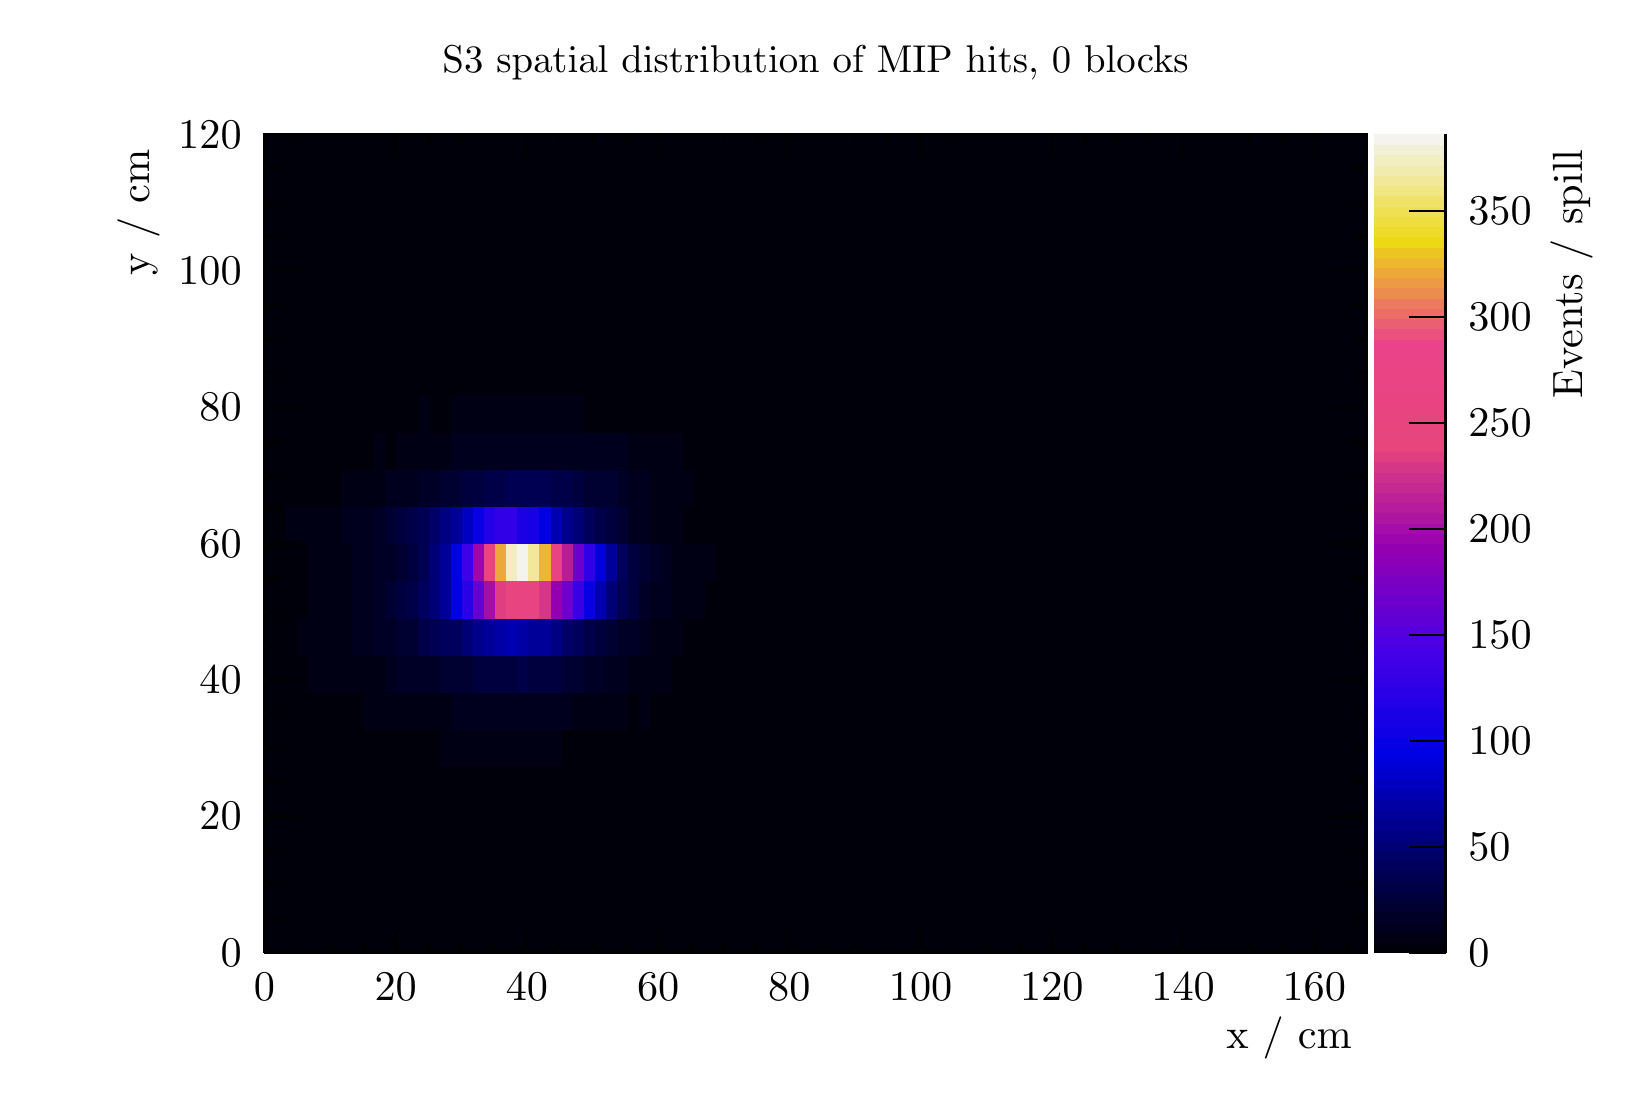
\begin{tikzpicture}
\pgfdeclareplotmark{cross} {
\pgfpathmoveto{\pgfpoint{-0.3\pgfplotmarksize}{\pgfplotmarksize}}
\pgfpathlineto{\pgfpoint{+0.3\pgfplotmarksize}{\pgfplotmarksize}}
\pgfpathlineto{\pgfpoint{+0.3\pgfplotmarksize}{0.3\pgfplotmarksize}}
\pgfpathlineto{\pgfpoint{+1\pgfplotmarksize}{0.3\pgfplotmarksize}}
\pgfpathlineto{\pgfpoint{+1\pgfplotmarksize}{-0.3\pgfplotmarksize}}
\pgfpathlineto{\pgfpoint{+0.3\pgfplotmarksize}{-0.3\pgfplotmarksize}}
\pgfpathlineto{\pgfpoint{+0.3\pgfplotmarksize}{-1.\pgfplotmarksize}}
\pgfpathlineto{\pgfpoint{-0.3\pgfplotmarksize}{-1.\pgfplotmarksize}}
\pgfpathlineto{\pgfpoint{-0.3\pgfplotmarksize}{-0.3\pgfplotmarksize}}
\pgfpathlineto{\pgfpoint{-1.\pgfplotmarksize}{-0.3\pgfplotmarksize}}
\pgfpathlineto{\pgfpoint{-1.\pgfplotmarksize}{0.3\pgfplotmarksize}}
\pgfpathlineto{\pgfpoint{-0.3\pgfplotmarksize}{0.3\pgfplotmarksize}}
\pgfpathclose
\pgfusepathqstroke
}
\pgfdeclareplotmark{cross*} {
\pgfpathmoveto{\pgfpoint{-0.3\pgfplotmarksize}{\pgfplotmarksize}}
\pgfpathlineto{\pgfpoint{+0.3\pgfplotmarksize}{\pgfplotmarksize}}
\pgfpathlineto{\pgfpoint{+0.3\pgfplotmarksize}{0.3\pgfplotmarksize}}
\pgfpathlineto{\pgfpoint{+1\pgfplotmarksize}{0.3\pgfplotmarksize}}
\pgfpathlineto{\pgfpoint{+1\pgfplotmarksize}{-0.3\pgfplotmarksize}}
\pgfpathlineto{\pgfpoint{+0.3\pgfplotmarksize}{-0.3\pgfplotmarksize}}
\pgfpathlineto{\pgfpoint{+0.3\pgfplotmarksize}{-1.\pgfplotmarksize}}
\pgfpathlineto{\pgfpoint{-0.3\pgfplotmarksize}{-1.\pgfplotmarksize}}
\pgfpathlineto{\pgfpoint{-0.3\pgfplotmarksize}{-0.3\pgfplotmarksize}}
\pgfpathlineto{\pgfpoint{-1.\pgfplotmarksize}{-0.3\pgfplotmarksize}}
\pgfpathlineto{\pgfpoint{-1.\pgfplotmarksize}{0.3\pgfplotmarksize}}
\pgfpathlineto{\pgfpoint{-0.3\pgfplotmarksize}{0.3\pgfplotmarksize}}
\pgfpathclose
\pgfusepathqfillstroke
}
\pgfdeclareplotmark{newstar} {
\pgfpathmoveto{\pgfqpoint{0pt}{\pgfplotmarksize}}
\pgfpathlineto{\pgfqpointpolar{44}{0.5\pgfplotmarksize}}
\pgfpathlineto{\pgfqpointpolar{18}{\pgfplotmarksize}}
\pgfpathlineto{\pgfqpointpolar{-20}{0.5\pgfplotmarksize}}
\pgfpathlineto{\pgfqpointpolar{-54}{\pgfplotmarksize}}
\pgfpathlineto{\pgfqpointpolar{-90}{0.5\pgfplotmarksize}}
\pgfpathlineto{\pgfqpointpolar{234}{\pgfplotmarksize}}
\pgfpathlineto{\pgfqpointpolar{198}{0.5\pgfplotmarksize}}
\pgfpathlineto{\pgfqpointpolar{162}{\pgfplotmarksize}}
\pgfpathlineto{\pgfqpointpolar{134}{0.5\pgfplotmarksize}}
\pgfpathclose
\pgfusepathqstroke
}
\pgfdeclareplotmark{newstar*} {
\pgfpathmoveto{\pgfqpoint{0pt}{\pgfplotmarksize}}
\pgfpathlineto{\pgfqpointpolar{44}{0.5\pgfplotmarksize}}
\pgfpathlineto{\pgfqpointpolar{18}{\pgfplotmarksize}}
\pgfpathlineto{\pgfqpointpolar{-20}{0.5\pgfplotmarksize}}
\pgfpathlineto{\pgfqpointpolar{-54}{\pgfplotmarksize}}
\pgfpathlineto{\pgfqpointpolar{-90}{0.5\pgfplotmarksize}}
\pgfpathlineto{\pgfqpointpolar{234}{\pgfplotmarksize}}
\pgfpathlineto{\pgfqpointpolar{198}{0.5\pgfplotmarksize}}
\pgfpathlineto{\pgfqpointpolar{162}{\pgfplotmarksize}}
\pgfpathlineto{\pgfqpointpolar{134}{0.5\pgfplotmarksize}}
\pgfpathclose
\pgfusepathqfillstroke
}
\definecolor{c}{rgb}{1,1,1};
\draw [color=c, fill=c] (0,0) rectangle (20,13.4957);
\draw [color=c, fill=c] (3,1.75444) rectangle (17,12.1461);
\definecolor{c}{rgb}{0,0,0};
\draw [c,line width=0.9] (3,1.75444) -- (3,12.1461) -- (17,12.1461) -- (17,1.75444) -- (3,1.75444);
\definecolor{c}{rgb}{1,1,1};
\draw [color=c, fill=c] (3,1.75444) rectangle (17,12.1461);
\definecolor{c}{rgb}{0,0,0};
\draw [c,line width=0.9] (3,1.75444) -- (3,12.1461) -- (17,12.1461) -- (17,1.75444) -- (3,1.75444);
\definecolor{c}{rgb}{0,0,0.0387097};
\draw [color=c, fill=c] (3,1.75444) rectangle (3.14,2.22679);
\draw [color=c, fill=c] (3.14,1.75444) rectangle (3.28,2.22679);
\draw [color=c, fill=c] (3.28,1.75444) rectangle (3.42,2.22679);
\draw [color=c, fill=c] (3.42,1.75444) rectangle (3.56,2.22679);
\draw [color=c, fill=c] (3.56,1.75444) rectangle (3.7,2.22679);
\draw [color=c, fill=c] (3.7,1.75444) rectangle (3.84,2.22679);
\draw [color=c, fill=c] (3.84,1.75444) rectangle (3.98,2.22679);
\draw [color=c, fill=c] (3.98,1.75444) rectangle (4.12,2.22679);
\draw [color=c, fill=c] (4.12,1.75444) rectangle (4.26,2.22679);
\draw [color=c, fill=c] (4.26,1.75444) rectangle (4.4,2.22679);
\draw [color=c, fill=c] (4.4,1.75444) rectangle (4.54,2.22679);
\draw [color=c, fill=c] (4.54,1.75444) rectangle (4.68,2.22679);
\draw [color=c, fill=c] (4.68,1.75444) rectangle (4.82,2.22679);
\draw [color=c, fill=c] (4.82,1.75444) rectangle (4.96,2.22679);
\draw [color=c, fill=c] (4.96,1.75444) rectangle (5.1,2.22679);
\draw [color=c, fill=c] (5.1,1.75444) rectangle (5.24,2.22679);
\draw [color=c, fill=c] (5.24,1.75444) rectangle (5.38,2.22679);
\draw [color=c, fill=c] (5.38,1.75444) rectangle (5.52,2.22679);
\draw [color=c, fill=c] (5.52,1.75444) rectangle (5.66,2.22679);
\draw [color=c, fill=c] (5.66,1.75444) rectangle (5.8,2.22679);
\draw [color=c, fill=c] (5.8,1.75444) rectangle (5.94,2.22679);
\draw [color=c, fill=c] (5.94,1.75444) rectangle (6.08,2.22679);
\draw [color=c, fill=c] (6.08,1.75444) rectangle (6.22,2.22679);
\draw [color=c, fill=c] (6.22,1.75444) rectangle (6.36,2.22679);
\draw [color=c, fill=c] (6.36,1.75444) rectangle (6.5,2.22679);
\draw [color=c, fill=c] (6.5,1.75444) rectangle (6.64,2.22679);
\draw [color=c, fill=c] (6.64,1.75444) rectangle (6.78,2.22679);
\draw [color=c, fill=c] (6.78,1.75444) rectangle (6.92,2.22679);
\draw [color=c, fill=c] (6.92,1.75444) rectangle (7.06,2.22679);
\draw [color=c, fill=c] (7.06,1.75444) rectangle (7.2,2.22679);
\draw [color=c, fill=c] (7.2,1.75444) rectangle (7.34,2.22679);
\draw [color=c, fill=c] (7.34,1.75444) rectangle (7.48,2.22679);
\draw [color=c, fill=c] (7.48,1.75444) rectangle (7.62,2.22679);
\draw [color=c, fill=c] (7.62,1.75444) rectangle (7.76,2.22679);
\draw [color=c, fill=c] (7.76,1.75444) rectangle (7.9,2.22679);
\draw [color=c, fill=c] (7.9,1.75444) rectangle (8.04,2.22679);
\draw [color=c, fill=c] (8.04,1.75444) rectangle (8.18,2.22679);
\draw [color=c, fill=c] (8.18,1.75444) rectangle (8.32,2.22679);
\draw [color=c, fill=c] (8.32,1.75444) rectangle (8.46,2.22679);
\draw [color=c, fill=c] (8.46,1.75444) rectangle (8.6,2.22679);
\draw [color=c, fill=c] (8.6,1.75444) rectangle (8.74,2.22679);
\draw [color=c, fill=c] (8.74,1.75444) rectangle (8.88,2.22679);
\draw [color=c, fill=c] (8.88,1.75444) rectangle (9.02,2.22679);
\draw [color=c, fill=c] (9.02,1.75444) rectangle (9.16,2.22679);
\draw [color=c, fill=c] (9.16,1.75444) rectangle (9.3,2.22679);
\draw [color=c, fill=c] (9.3,1.75444) rectangle (9.44,2.22679);
\draw [color=c, fill=c] (9.44,1.75444) rectangle (9.58,2.22679);
\draw [color=c, fill=c] (9.58,1.75444) rectangle (9.72,2.22679);
\draw [color=c, fill=c] (9.72,1.75444) rectangle (9.86,2.22679);
\draw [color=c, fill=c] (9.86,1.75444) rectangle (10,2.22679);
\draw [color=c, fill=c] (10,1.75444) rectangle (10.14,2.22679);
\draw [color=c, fill=c] (10.14,1.75444) rectangle (10.28,2.22679);
\draw [color=c, fill=c] (10.28,1.75444) rectangle (10.42,2.22679);
\draw [color=c, fill=c] (10.42,1.75444) rectangle (10.56,2.22679);
\draw [color=c, fill=c] (10.56,1.75444) rectangle (10.7,2.22679);
\draw [color=c, fill=c] (10.7,1.75444) rectangle (10.84,2.22679);
\draw [color=c, fill=c] (10.84,1.75444) rectangle (10.98,2.22679);
\draw [color=c, fill=c] (10.98,1.75444) rectangle (11.12,2.22679);
\draw [color=c, fill=c] (11.12,1.75444) rectangle (11.26,2.22679);
\draw [color=c, fill=c] (11.26,1.75444) rectangle (11.4,2.22679);
\draw [color=c, fill=c] (11.4,1.75444) rectangle (11.54,2.22679);
\draw [color=c, fill=c] (11.54,1.75444) rectangle (11.68,2.22679);
\draw [color=c, fill=c] (11.68,1.75444) rectangle (11.82,2.22679);
\draw [color=c, fill=c] (11.82,1.75444) rectangle (11.96,2.22679);
\draw [color=c, fill=c] (11.96,1.75444) rectangle (12.1,2.22679);
\draw [color=c, fill=c] (12.1,1.75444) rectangle (12.24,2.22679);
\draw [color=c, fill=c] (12.24,1.75444) rectangle (12.38,2.22679);
\draw [color=c, fill=c] (12.38,1.75444) rectangle (12.52,2.22679);
\draw [color=c, fill=c] (12.52,1.75444) rectangle (12.66,2.22679);
\draw [color=c, fill=c] (12.66,1.75444) rectangle (12.8,2.22679);
\draw [color=c, fill=c] (12.8,1.75444) rectangle (12.94,2.22679);
\draw [color=c, fill=c] (12.94,1.75444) rectangle (13.08,2.22679);
\draw [color=c, fill=c] (13.08,1.75444) rectangle (13.22,2.22679);
\draw [color=c, fill=c] (13.22,1.75444) rectangle (13.36,2.22679);
\draw [color=c, fill=c] (13.36,1.75444) rectangle (13.5,2.22679);
\draw [color=c, fill=c] (13.5,1.75444) rectangle (13.64,2.22679);
\draw [color=c, fill=c] (13.64,1.75444) rectangle (13.78,2.22679);
\draw [color=c, fill=c] (13.78,1.75444) rectangle (13.92,2.22679);
\draw [color=c, fill=c] (13.92,1.75444) rectangle (14.06,2.22679);
\draw [color=c, fill=c] (14.06,1.75444) rectangle (14.2,2.22679);
\draw [color=c, fill=c] (14.2,1.75444) rectangle (14.34,2.22679);
\draw [color=c, fill=c] (14.34,1.75444) rectangle (14.48,2.22679);
\draw [color=c, fill=c] (14.48,1.75444) rectangle (14.62,2.22679);
\draw [color=c, fill=c] (14.62,1.75444) rectangle (14.76,2.22679);
\draw [color=c, fill=c] (14.76,1.75444) rectangle (14.9,2.22679);
\draw [color=c, fill=c] (14.9,1.75444) rectangle (15.04,2.22679);
\draw [color=c, fill=c] (15.04,1.75444) rectangle (15.18,2.22679);
\draw [color=c, fill=c] (15.18,1.75444) rectangle (15.32,2.22679);
\draw [color=c, fill=c] (15.32,1.75444) rectangle (15.46,2.22679);
\draw [color=c, fill=c] (15.46,1.75444) rectangle (15.6,2.22679);
\draw [color=c, fill=c] (15.6,1.75444) rectangle (15.74,2.22679);
\draw [color=c, fill=c] (15.74,1.75444) rectangle (15.88,2.22679);
\draw [color=c, fill=c] (15.88,1.75444) rectangle (16.02,2.22679);
\draw [color=c, fill=c] (16.02,1.75444) rectangle (16.16,2.22679);
\draw [color=c, fill=c] (16.16,1.75444) rectangle (16.3,2.22679);
\draw [color=c, fill=c] (16.3,1.75444) rectangle (16.44,2.22679);
\draw [color=c, fill=c] (16.44,1.75444) rectangle (16.58,2.22679);
\draw [color=c, fill=c] (16.58,1.75444) rectangle (16.72,2.22679);
\draw [color=c, fill=c] (16.72,1.75444) rectangle (16.86,2.22679);
\draw [color=c, fill=c] (16.86,1.75444) rectangle (17,2.22679);
\draw [color=c, fill=c] (3,2.22679) rectangle (3.14,2.69914);
\draw [color=c, fill=c] (3.14,2.22679) rectangle (3.28,2.69914);
\draw [color=c, fill=c] (3.28,2.22679) rectangle (3.42,2.69914);
\draw [color=c, fill=c] (3.42,2.22679) rectangle (3.56,2.69914);
\draw [color=c, fill=c] (3.56,2.22679) rectangle (3.7,2.69914);
\draw [color=c, fill=c] (3.7,2.22679) rectangle (3.84,2.69914);
\draw [color=c, fill=c] (3.84,2.22679) rectangle (3.98,2.69914);
\draw [color=c, fill=c] (3.98,2.22679) rectangle (4.12,2.69914);
\draw [color=c, fill=c] (4.12,2.22679) rectangle (4.26,2.69914);
\draw [color=c, fill=c] (4.26,2.22679) rectangle (4.4,2.69914);
\draw [color=c, fill=c] (4.4,2.22679) rectangle (4.54,2.69914);
\draw [color=c, fill=c] (4.54,2.22679) rectangle (4.68,2.69914);
\draw [color=c, fill=c] (4.68,2.22679) rectangle (4.82,2.69914);
\draw [color=c, fill=c] (4.82,2.22679) rectangle (4.96,2.69914);
\draw [color=c, fill=c] (4.96,2.22679) rectangle (5.1,2.69914);
\draw [color=c, fill=c] (5.1,2.22679) rectangle (5.24,2.69914);
\draw [color=c, fill=c] (5.24,2.22679) rectangle (5.38,2.69914);
\draw [color=c, fill=c] (5.38,2.22679) rectangle (5.52,2.69914);
\draw [color=c, fill=c] (5.52,2.22679) rectangle (5.66,2.69914);
\draw [color=c, fill=c] (5.66,2.22679) rectangle (5.8,2.69914);
\draw [color=c, fill=c] (5.8,2.22679) rectangle (5.94,2.69914);
\draw [color=c, fill=c] (5.94,2.22679) rectangle (6.08,2.69914);
\draw [color=c, fill=c] (6.08,2.22679) rectangle (6.22,2.69914);
\draw [color=c, fill=c] (6.22,2.22679) rectangle (6.36,2.69914);
\draw [color=c, fill=c] (6.36,2.22679) rectangle (6.5,2.69914);
\draw [color=c, fill=c] (6.5,2.22679) rectangle (6.64,2.69914);
\draw [color=c, fill=c] (6.64,2.22679) rectangle (6.78,2.69914);
\draw [color=c, fill=c] (6.78,2.22679) rectangle (6.92,2.69914);
\draw [color=c, fill=c] (6.92,2.22679) rectangle (7.06,2.69914);
\draw [color=c, fill=c] (7.06,2.22679) rectangle (7.2,2.69914);
\draw [color=c, fill=c] (7.2,2.22679) rectangle (7.34,2.69914);
\draw [color=c, fill=c] (7.34,2.22679) rectangle (7.48,2.69914);
\draw [color=c, fill=c] (7.48,2.22679) rectangle (7.62,2.69914);
\draw [color=c, fill=c] (7.62,2.22679) rectangle (7.76,2.69914);
\draw [color=c, fill=c] (7.76,2.22679) rectangle (7.9,2.69914);
\draw [color=c, fill=c] (7.9,2.22679) rectangle (8.04,2.69914);
\draw [color=c, fill=c] (8.04,2.22679) rectangle (8.18,2.69914);
\draw [color=c, fill=c] (8.18,2.22679) rectangle (8.32,2.69914);
\draw [color=c, fill=c] (8.32,2.22679) rectangle (8.46,2.69914);
\draw [color=c, fill=c] (8.46,2.22679) rectangle (8.6,2.69914);
\draw [color=c, fill=c] (8.6,2.22679) rectangle (8.74,2.69914);
\draw [color=c, fill=c] (8.74,2.22679) rectangle (8.88,2.69914);
\draw [color=c, fill=c] (8.88,2.22679) rectangle (9.02,2.69914);
\draw [color=c, fill=c] (9.02,2.22679) rectangle (9.16,2.69914);
\draw [color=c, fill=c] (9.16,2.22679) rectangle (9.3,2.69914);
\draw [color=c, fill=c] (9.3,2.22679) rectangle (9.44,2.69914);
\draw [color=c, fill=c] (9.44,2.22679) rectangle (9.58,2.69914);
\draw [color=c, fill=c] (9.58,2.22679) rectangle (9.72,2.69914);
\draw [color=c, fill=c] (9.72,2.22679) rectangle (9.86,2.69914);
\draw [color=c, fill=c] (9.86,2.22679) rectangle (10,2.69914);
\draw [color=c, fill=c] (10,2.22679) rectangle (10.14,2.69914);
\draw [color=c, fill=c] (10.14,2.22679) rectangle (10.28,2.69914);
\draw [color=c, fill=c] (10.28,2.22679) rectangle (10.42,2.69914);
\draw [color=c, fill=c] (10.42,2.22679) rectangle (10.56,2.69914);
\draw [color=c, fill=c] (10.56,2.22679) rectangle (10.7,2.69914);
\draw [color=c, fill=c] (10.7,2.22679) rectangle (10.84,2.69914);
\draw [color=c, fill=c] (10.84,2.22679) rectangle (10.98,2.69914);
\draw [color=c, fill=c] (10.98,2.22679) rectangle (11.12,2.69914);
\draw [color=c, fill=c] (11.12,2.22679) rectangle (11.26,2.69914);
\draw [color=c, fill=c] (11.26,2.22679) rectangle (11.4,2.69914);
\draw [color=c, fill=c] (11.4,2.22679) rectangle (11.54,2.69914);
\draw [color=c, fill=c] (11.54,2.22679) rectangle (11.68,2.69914);
\draw [color=c, fill=c] (11.68,2.22679) rectangle (11.82,2.69914);
\draw [color=c, fill=c] (11.82,2.22679) rectangle (11.96,2.69914);
\draw [color=c, fill=c] (11.96,2.22679) rectangle (12.1,2.69914);
\draw [color=c, fill=c] (12.1,2.22679) rectangle (12.24,2.69914);
\draw [color=c, fill=c] (12.24,2.22679) rectangle (12.38,2.69914);
\draw [color=c, fill=c] (12.38,2.22679) rectangle (12.52,2.69914);
\draw [color=c, fill=c] (12.52,2.22679) rectangle (12.66,2.69914);
\draw [color=c, fill=c] (12.66,2.22679) rectangle (12.8,2.69914);
\draw [color=c, fill=c] (12.8,2.22679) rectangle (12.94,2.69914);
\draw [color=c, fill=c] (12.94,2.22679) rectangle (13.08,2.69914);
\draw [color=c, fill=c] (13.08,2.22679) rectangle (13.22,2.69914);
\draw [color=c, fill=c] (13.22,2.22679) rectangle (13.36,2.69914);
\draw [color=c, fill=c] (13.36,2.22679) rectangle (13.5,2.69914);
\draw [color=c, fill=c] (13.5,2.22679) rectangle (13.64,2.69914);
\draw [color=c, fill=c] (13.64,2.22679) rectangle (13.78,2.69914);
\draw [color=c, fill=c] (13.78,2.22679) rectangle (13.92,2.69914);
\draw [color=c, fill=c] (13.92,2.22679) rectangle (14.06,2.69914);
\draw [color=c, fill=c] (14.06,2.22679) rectangle (14.2,2.69914);
\draw [color=c, fill=c] (14.2,2.22679) rectangle (14.34,2.69914);
\draw [color=c, fill=c] (14.34,2.22679) rectangle (14.48,2.69914);
\draw [color=c, fill=c] (14.48,2.22679) rectangle (14.62,2.69914);
\draw [color=c, fill=c] (14.62,2.22679) rectangle (14.76,2.69914);
\draw [color=c, fill=c] (14.76,2.22679) rectangle (14.9,2.69914);
\draw [color=c, fill=c] (14.9,2.22679) rectangle (15.04,2.69914);
\draw [color=c, fill=c] (15.04,2.22679) rectangle (15.18,2.69914);
\draw [color=c, fill=c] (15.18,2.22679) rectangle (15.32,2.69914);
\draw [color=c, fill=c] (15.32,2.22679) rectangle (15.46,2.69914);
\draw [color=c, fill=c] (15.46,2.22679) rectangle (15.6,2.69914);
\draw [color=c, fill=c] (15.6,2.22679) rectangle (15.74,2.69914);
\draw [color=c, fill=c] (15.74,2.22679) rectangle (15.88,2.69914);
\draw [color=c, fill=c] (15.88,2.22679) rectangle (16.02,2.69914);
\draw [color=c, fill=c] (16.02,2.22679) rectangle (16.16,2.69914);
\draw [color=c, fill=c] (16.16,2.22679) rectangle (16.3,2.69914);
\draw [color=c, fill=c] (16.3,2.22679) rectangle (16.44,2.69914);
\draw [color=c, fill=c] (16.44,2.22679) rectangle (16.58,2.69914);
\draw [color=c, fill=c] (16.58,2.22679) rectangle (16.72,2.69914);
\draw [color=c, fill=c] (16.72,2.22679) rectangle (16.86,2.69914);
\draw [color=c, fill=c] (16.86,2.22679) rectangle (17,2.69914);
\draw [color=c, fill=c] (3,2.69914) rectangle (3.14,3.17149);
\draw [color=c, fill=c] (3.14,2.69914) rectangle (3.28,3.17149);
\draw [color=c, fill=c] (3.28,2.69914) rectangle (3.42,3.17149);
\draw [color=c, fill=c] (3.42,2.69914) rectangle (3.56,3.17149);
\draw [color=c, fill=c] (3.56,2.69914) rectangle (3.7,3.17149);
\draw [color=c, fill=c] (3.7,2.69914) rectangle (3.84,3.17149);
\draw [color=c, fill=c] (3.84,2.69914) rectangle (3.98,3.17149);
\draw [color=c, fill=c] (3.98,2.69914) rectangle (4.12,3.17149);
\draw [color=c, fill=c] (4.12,2.69914) rectangle (4.26,3.17149);
\draw [color=c, fill=c] (4.26,2.69914) rectangle (4.4,3.17149);
\draw [color=c, fill=c] (4.4,2.69914) rectangle (4.54,3.17149);
\draw [color=c, fill=c] (4.54,2.69914) rectangle (4.68,3.17149);
\draw [color=c, fill=c] (4.68,2.69914) rectangle (4.82,3.17149);
\draw [color=c, fill=c] (4.82,2.69914) rectangle (4.96,3.17149);
\draw [color=c, fill=c] (4.96,2.69914) rectangle (5.1,3.17149);
\draw [color=c, fill=c] (5.1,2.69914) rectangle (5.24,3.17149);
\draw [color=c, fill=c] (5.24,2.69914) rectangle (5.38,3.17149);
\draw [color=c, fill=c] (5.38,2.69914) rectangle (5.52,3.17149);
\draw [color=c, fill=c] (5.52,2.69914) rectangle (5.66,3.17149);
\draw [color=c, fill=c] (5.66,2.69914) rectangle (5.8,3.17149);
\draw [color=c, fill=c] (5.8,2.69914) rectangle (5.94,3.17149);
\draw [color=c, fill=c] (5.94,2.69914) rectangle (6.08,3.17149);
\draw [color=c, fill=c] (6.08,2.69914) rectangle (6.22,3.17149);
\draw [color=c, fill=c] (6.22,2.69914) rectangle (6.36,3.17149);
\draw [color=c, fill=c] (6.36,2.69914) rectangle (6.5,3.17149);
\draw [color=c, fill=c] (6.5,2.69914) rectangle (6.64,3.17149);
\draw [color=c, fill=c] (6.64,2.69914) rectangle (6.78,3.17149);
\draw [color=c, fill=c] (6.78,2.69914) rectangle (6.92,3.17149);
\draw [color=c, fill=c] (6.92,2.69914) rectangle (7.06,3.17149);
\draw [color=c, fill=c] (7.06,2.69914) rectangle (7.2,3.17149);
\draw [color=c, fill=c] (7.2,2.69914) rectangle (7.34,3.17149);
\draw [color=c, fill=c] (7.34,2.69914) rectangle (7.48,3.17149);
\draw [color=c, fill=c] (7.48,2.69914) rectangle (7.62,3.17149);
\draw [color=c, fill=c] (7.62,2.69914) rectangle (7.76,3.17149);
\draw [color=c, fill=c] (7.76,2.69914) rectangle (7.9,3.17149);
\draw [color=c, fill=c] (7.9,2.69914) rectangle (8.04,3.17149);
\draw [color=c, fill=c] (8.04,2.69914) rectangle (8.18,3.17149);
\draw [color=c, fill=c] (8.18,2.69914) rectangle (8.32,3.17149);
\draw [color=c, fill=c] (8.32,2.69914) rectangle (8.46,3.17149);
\draw [color=c, fill=c] (8.46,2.69914) rectangle (8.6,3.17149);
\draw [color=c, fill=c] (8.6,2.69914) rectangle (8.74,3.17149);
\draw [color=c, fill=c] (8.74,2.69914) rectangle (8.88,3.17149);
\draw [color=c, fill=c] (8.88,2.69914) rectangle (9.02,3.17149);
\draw [color=c, fill=c] (9.02,2.69914) rectangle (9.16,3.17149);
\draw [color=c, fill=c] (9.16,2.69914) rectangle (9.3,3.17149);
\draw [color=c, fill=c] (9.3,2.69914) rectangle (9.44,3.17149);
\draw [color=c, fill=c] (9.44,2.69914) rectangle (9.58,3.17149);
\draw [color=c, fill=c] (9.58,2.69914) rectangle (9.72,3.17149);
\draw [color=c, fill=c] (9.72,2.69914) rectangle (9.86,3.17149);
\draw [color=c, fill=c] (9.86,2.69914) rectangle (10,3.17149);
\draw [color=c, fill=c] (10,2.69914) rectangle (10.14,3.17149);
\draw [color=c, fill=c] (10.14,2.69914) rectangle (10.28,3.17149);
\draw [color=c, fill=c] (10.28,2.69914) rectangle (10.42,3.17149);
\draw [color=c, fill=c] (10.42,2.69914) rectangle (10.56,3.17149);
\draw [color=c, fill=c] (10.56,2.69914) rectangle (10.7,3.17149);
\draw [color=c, fill=c] (10.7,2.69914) rectangle (10.84,3.17149);
\draw [color=c, fill=c] (10.84,2.69914) rectangle (10.98,3.17149);
\draw [color=c, fill=c] (10.98,2.69914) rectangle (11.12,3.17149);
\draw [color=c, fill=c] (11.12,2.69914) rectangle (11.26,3.17149);
\draw [color=c, fill=c] (11.26,2.69914) rectangle (11.4,3.17149);
\draw [color=c, fill=c] (11.4,2.69914) rectangle (11.54,3.17149);
\draw [color=c, fill=c] (11.54,2.69914) rectangle (11.68,3.17149);
\draw [color=c, fill=c] (11.68,2.69914) rectangle (11.82,3.17149);
\draw [color=c, fill=c] (11.82,2.69914) rectangle (11.96,3.17149);
\draw [color=c, fill=c] (11.96,2.69914) rectangle (12.1,3.17149);
\draw [color=c, fill=c] (12.1,2.69914) rectangle (12.24,3.17149);
\draw [color=c, fill=c] (12.24,2.69914) rectangle (12.38,3.17149);
\draw [color=c, fill=c] (12.38,2.69914) rectangle (12.52,3.17149);
\draw [color=c, fill=c] (12.52,2.69914) rectangle (12.66,3.17149);
\draw [color=c, fill=c] (12.66,2.69914) rectangle (12.8,3.17149);
\draw [color=c, fill=c] (12.8,2.69914) rectangle (12.94,3.17149);
\draw [color=c, fill=c] (12.94,2.69914) rectangle (13.08,3.17149);
\draw [color=c, fill=c] (13.08,2.69914) rectangle (13.22,3.17149);
\draw [color=c, fill=c] (13.22,2.69914) rectangle (13.36,3.17149);
\draw [color=c, fill=c] (13.36,2.69914) rectangle (13.5,3.17149);
\draw [color=c, fill=c] (13.5,2.69914) rectangle (13.64,3.17149);
\draw [color=c, fill=c] (13.64,2.69914) rectangle (13.78,3.17149);
\draw [color=c, fill=c] (13.78,2.69914) rectangle (13.92,3.17149);
\draw [color=c, fill=c] (13.92,2.69914) rectangle (14.06,3.17149);
\draw [color=c, fill=c] (14.06,2.69914) rectangle (14.2,3.17149);
\draw [color=c, fill=c] (14.2,2.69914) rectangle (14.34,3.17149);
\draw [color=c, fill=c] (14.34,2.69914) rectangle (14.48,3.17149);
\draw [color=c, fill=c] (14.48,2.69914) rectangle (14.62,3.17149);
\draw [color=c, fill=c] (14.62,2.69914) rectangle (14.76,3.17149);
\draw [color=c, fill=c] (14.76,2.69914) rectangle (14.9,3.17149);
\draw [color=c, fill=c] (14.9,2.69914) rectangle (15.04,3.17149);
\draw [color=c, fill=c] (15.04,2.69914) rectangle (15.18,3.17149);
\draw [color=c, fill=c] (15.18,2.69914) rectangle (15.32,3.17149);
\draw [color=c, fill=c] (15.32,2.69914) rectangle (15.46,3.17149);
\draw [color=c, fill=c] (15.46,2.69914) rectangle (15.6,3.17149);
\draw [color=c, fill=c] (15.6,2.69914) rectangle (15.74,3.17149);
\draw [color=c, fill=c] (15.74,2.69914) rectangle (15.88,3.17149);
\draw [color=c, fill=c] (15.88,2.69914) rectangle (16.02,3.17149);
\draw [color=c, fill=c] (16.02,2.69914) rectangle (16.16,3.17149);
\draw [color=c, fill=c] (16.16,2.69914) rectangle (16.3,3.17149);
\draw [color=c, fill=c] (16.3,2.69914) rectangle (16.44,3.17149);
\draw [color=c, fill=c] (16.44,2.69914) rectangle (16.58,3.17149);
\draw [color=c, fill=c] (16.58,2.69914) rectangle (16.72,3.17149);
\draw [color=c, fill=c] (16.72,2.69914) rectangle (16.86,3.17149);
\draw [color=c, fill=c] (16.86,2.69914) rectangle (17,3.17149);
\draw [color=c, fill=c] (3,3.17149) rectangle (3.14,3.64384);
\draw [color=c, fill=c] (3.14,3.17149) rectangle (3.28,3.64384);
\draw [color=c, fill=c] (3.28,3.17149) rectangle (3.42,3.64384);
\draw [color=c, fill=c] (3.42,3.17149) rectangle (3.56,3.64384);
\draw [color=c, fill=c] (3.56,3.17149) rectangle (3.7,3.64384);
\draw [color=c, fill=c] (3.7,3.17149) rectangle (3.84,3.64384);
\draw [color=c, fill=c] (3.84,3.17149) rectangle (3.98,3.64384);
\draw [color=c, fill=c] (3.98,3.17149) rectangle (4.12,3.64384);
\draw [color=c, fill=c] (4.12,3.17149) rectangle (4.26,3.64384);
\draw [color=c, fill=c] (4.26,3.17149) rectangle (4.4,3.64384);
\draw [color=c, fill=c] (4.4,3.17149) rectangle (4.54,3.64384);
\draw [color=c, fill=c] (4.54,3.17149) rectangle (4.68,3.64384);
\draw [color=c, fill=c] (4.68,3.17149) rectangle (4.82,3.64384);
\draw [color=c, fill=c] (4.82,3.17149) rectangle (4.96,3.64384);
\draw [color=c, fill=c] (4.96,3.17149) rectangle (5.1,3.64384);
\draw [color=c, fill=c] (5.1,3.17149) rectangle (5.24,3.64384);
\draw [color=c, fill=c] (5.24,3.17149) rectangle (5.38,3.64384);
\draw [color=c, fill=c] (5.38,3.17149) rectangle (5.52,3.64384);
\draw [color=c, fill=c] (5.52,3.17149) rectangle (5.66,3.64384);
\draw [color=c, fill=c] (5.66,3.17149) rectangle (5.8,3.64384);
\draw [color=c, fill=c] (5.8,3.17149) rectangle (5.94,3.64384);
\draw [color=c, fill=c] (5.94,3.17149) rectangle (6.08,3.64384);
\draw [color=c, fill=c] (6.08,3.17149) rectangle (6.22,3.64384);
\draw [color=c, fill=c] (6.22,3.17149) rectangle (6.36,3.64384);
\draw [color=c, fill=c] (6.36,3.17149) rectangle (6.5,3.64384);
\draw [color=c, fill=c] (6.5,3.17149) rectangle (6.64,3.64384);
\draw [color=c, fill=c] (6.64,3.17149) rectangle (6.78,3.64384);
\draw [color=c, fill=c] (6.78,3.17149) rectangle (6.92,3.64384);
\draw [color=c, fill=c] (6.92,3.17149) rectangle (7.06,3.64384);
\draw [color=c, fill=c] (7.06,3.17149) rectangle (7.2,3.64384);
\draw [color=c, fill=c] (7.2,3.17149) rectangle (7.34,3.64384);
\draw [color=c, fill=c] (7.34,3.17149) rectangle (7.48,3.64384);
\draw [color=c, fill=c] (7.48,3.17149) rectangle (7.62,3.64384);
\draw [color=c, fill=c] (7.62,3.17149) rectangle (7.76,3.64384);
\draw [color=c, fill=c] (7.76,3.17149) rectangle (7.9,3.64384);
\draw [color=c, fill=c] (7.9,3.17149) rectangle (8.04,3.64384);
\draw [color=c, fill=c] (8.04,3.17149) rectangle (8.18,3.64384);
\draw [color=c, fill=c] (8.18,3.17149) rectangle (8.32,3.64384);
\draw [color=c, fill=c] (8.32,3.17149) rectangle (8.46,3.64384);
\draw [color=c, fill=c] (8.46,3.17149) rectangle (8.6,3.64384);
\draw [color=c, fill=c] (8.6,3.17149) rectangle (8.74,3.64384);
\draw [color=c, fill=c] (8.74,3.17149) rectangle (8.88,3.64384);
\draw [color=c, fill=c] (8.88,3.17149) rectangle (9.02,3.64384);
\draw [color=c, fill=c] (9.02,3.17149) rectangle (9.16,3.64384);
\draw [color=c, fill=c] (9.16,3.17149) rectangle (9.3,3.64384);
\draw [color=c, fill=c] (9.3,3.17149) rectangle (9.44,3.64384);
\draw [color=c, fill=c] (9.44,3.17149) rectangle (9.58,3.64384);
\draw [color=c, fill=c] (9.58,3.17149) rectangle (9.72,3.64384);
\draw [color=c, fill=c] (9.72,3.17149) rectangle (9.86,3.64384);
\draw [color=c, fill=c] (9.86,3.17149) rectangle (10,3.64384);
\draw [color=c, fill=c] (10,3.17149) rectangle (10.14,3.64384);
\draw [color=c, fill=c] (10.14,3.17149) rectangle (10.28,3.64384);
\draw [color=c, fill=c] (10.28,3.17149) rectangle (10.42,3.64384);
\draw [color=c, fill=c] (10.42,3.17149) rectangle (10.56,3.64384);
\draw [color=c, fill=c] (10.56,3.17149) rectangle (10.7,3.64384);
\draw [color=c, fill=c] (10.7,3.17149) rectangle (10.84,3.64384);
\draw [color=c, fill=c] (10.84,3.17149) rectangle (10.98,3.64384);
\draw [color=c, fill=c] (10.98,3.17149) rectangle (11.12,3.64384);
\draw [color=c, fill=c] (11.12,3.17149) rectangle (11.26,3.64384);
\draw [color=c, fill=c] (11.26,3.17149) rectangle (11.4,3.64384);
\draw [color=c, fill=c] (11.4,3.17149) rectangle (11.54,3.64384);
\draw [color=c, fill=c] (11.54,3.17149) rectangle (11.68,3.64384);
\draw [color=c, fill=c] (11.68,3.17149) rectangle (11.82,3.64384);
\draw [color=c, fill=c] (11.82,3.17149) rectangle (11.96,3.64384);
\draw [color=c, fill=c] (11.96,3.17149) rectangle (12.1,3.64384);
\draw [color=c, fill=c] (12.1,3.17149) rectangle (12.24,3.64384);
\draw [color=c, fill=c] (12.24,3.17149) rectangle (12.38,3.64384);
\draw [color=c, fill=c] (12.38,3.17149) rectangle (12.52,3.64384);
\draw [color=c, fill=c] (12.52,3.17149) rectangle (12.66,3.64384);
\draw [color=c, fill=c] (12.66,3.17149) rectangle (12.8,3.64384);
\draw [color=c, fill=c] (12.8,3.17149) rectangle (12.94,3.64384);
\draw [color=c, fill=c] (12.94,3.17149) rectangle (13.08,3.64384);
\draw [color=c, fill=c] (13.08,3.17149) rectangle (13.22,3.64384);
\draw [color=c, fill=c] (13.22,3.17149) rectangle (13.36,3.64384);
\draw [color=c, fill=c] (13.36,3.17149) rectangle (13.5,3.64384);
\draw [color=c, fill=c] (13.5,3.17149) rectangle (13.64,3.64384);
\draw [color=c, fill=c] (13.64,3.17149) rectangle (13.78,3.64384);
\draw [color=c, fill=c] (13.78,3.17149) rectangle (13.92,3.64384);
\draw [color=c, fill=c] (13.92,3.17149) rectangle (14.06,3.64384);
\draw [color=c, fill=c] (14.06,3.17149) rectangle (14.2,3.64384);
\draw [color=c, fill=c] (14.2,3.17149) rectangle (14.34,3.64384);
\draw [color=c, fill=c] (14.34,3.17149) rectangle (14.48,3.64384);
\draw [color=c, fill=c] (14.48,3.17149) rectangle (14.62,3.64384);
\draw [color=c, fill=c] (14.62,3.17149) rectangle (14.76,3.64384);
\draw [color=c, fill=c] (14.76,3.17149) rectangle (14.9,3.64384);
\draw [color=c, fill=c] (14.9,3.17149) rectangle (15.04,3.64384);
\draw [color=c, fill=c] (15.04,3.17149) rectangle (15.18,3.64384);
\draw [color=c, fill=c] (15.18,3.17149) rectangle (15.32,3.64384);
\draw [color=c, fill=c] (15.32,3.17149) rectangle (15.46,3.64384);
\draw [color=c, fill=c] (15.46,3.17149) rectangle (15.6,3.64384);
\draw [color=c, fill=c] (15.6,3.17149) rectangle (15.74,3.64384);
\draw [color=c, fill=c] (15.74,3.17149) rectangle (15.88,3.64384);
\draw [color=c, fill=c] (15.88,3.17149) rectangle (16.02,3.64384);
\draw [color=c, fill=c] (16.02,3.17149) rectangle (16.16,3.64384);
\draw [color=c, fill=c] (16.16,3.17149) rectangle (16.3,3.64384);
\draw [color=c, fill=c] (16.3,3.17149) rectangle (16.44,3.64384);
\draw [color=c, fill=c] (16.44,3.17149) rectangle (16.58,3.64384);
\draw [color=c, fill=c] (16.58,3.17149) rectangle (16.72,3.64384);
\draw [color=c, fill=c] (16.72,3.17149) rectangle (16.86,3.64384);
\draw [color=c, fill=c] (16.86,3.17149) rectangle (17,3.64384);
\draw [color=c, fill=c] (3,3.64384) rectangle (3.14,4.11619);
\draw [color=c, fill=c] (3.14,3.64384) rectangle (3.28,4.11619);
\draw [color=c, fill=c] (3.28,3.64384) rectangle (3.42,4.11619);
\draw [color=c, fill=c] (3.42,3.64384) rectangle (3.56,4.11619);
\draw [color=c, fill=c] (3.56,3.64384) rectangle (3.7,4.11619);
\draw [color=c, fill=c] (3.7,3.64384) rectangle (3.84,4.11619);
\draw [color=c, fill=c] (3.84,3.64384) rectangle (3.98,4.11619);
\draw [color=c, fill=c] (3.98,3.64384) rectangle (4.12,4.11619);
\draw [color=c, fill=c] (4.12,3.64384) rectangle (4.26,4.11619);
\draw [color=c, fill=c] (4.26,3.64384) rectangle (4.4,4.11619);
\draw [color=c, fill=c] (4.4,3.64384) rectangle (4.54,4.11619);
\draw [color=c, fill=c] (4.54,3.64384) rectangle (4.68,4.11619);
\draw [color=c, fill=c] (4.68,3.64384) rectangle (4.82,4.11619);
\draw [color=c, fill=c] (4.82,3.64384) rectangle (4.96,4.11619);
\draw [color=c, fill=c] (4.96,3.64384) rectangle (5.1,4.11619);
\draw [color=c, fill=c] (5.1,3.64384) rectangle (5.24,4.11619);
\draw [color=c, fill=c] (5.24,3.64384) rectangle (5.38,4.11619);
\draw [color=c, fill=c] (5.38,3.64384) rectangle (5.52,4.11619);
\draw [color=c, fill=c] (5.52,3.64384) rectangle (5.66,4.11619);
\draw [color=c, fill=c] (5.66,3.64384) rectangle (5.8,4.11619);
\draw [color=c, fill=c] (5.8,3.64384) rectangle (5.94,4.11619);
\draw [color=c, fill=c] (5.94,3.64384) rectangle (6.08,4.11619);
\draw [color=c, fill=c] (6.08,3.64384) rectangle (6.22,4.11619);
\draw [color=c, fill=c] (6.22,3.64384) rectangle (6.36,4.11619);
\draw [color=c, fill=c] (6.36,3.64384) rectangle (6.5,4.11619);
\draw [color=c, fill=c] (6.5,3.64384) rectangle (6.64,4.11619);
\draw [color=c, fill=c] (6.64,3.64384) rectangle (6.78,4.11619);
\draw [color=c, fill=c] (6.78,3.64384) rectangle (6.92,4.11619);
\draw [color=c, fill=c] (6.92,3.64384) rectangle (7.06,4.11619);
\draw [color=c, fill=c] (7.06,3.64384) rectangle (7.2,4.11619);
\draw [color=c, fill=c] (7.2,3.64384) rectangle (7.34,4.11619);
\draw [color=c, fill=c] (7.34,3.64384) rectangle (7.48,4.11619);
\draw [color=c, fill=c] (7.48,3.64384) rectangle (7.62,4.11619);
\draw [color=c, fill=c] (7.62,3.64384) rectangle (7.76,4.11619);
\draw [color=c, fill=c] (7.76,3.64384) rectangle (7.9,4.11619);
\draw [color=c, fill=c] (7.9,3.64384) rectangle (8.04,4.11619);
\draw [color=c, fill=c] (8.04,3.64384) rectangle (8.18,4.11619);
\draw [color=c, fill=c] (8.18,3.64384) rectangle (8.32,4.11619);
\draw [color=c, fill=c] (8.32,3.64384) rectangle (8.46,4.11619);
\draw [color=c, fill=c] (8.46,3.64384) rectangle (8.6,4.11619);
\draw [color=c, fill=c] (8.6,3.64384) rectangle (8.74,4.11619);
\draw [color=c, fill=c] (8.74,3.64384) rectangle (8.88,4.11619);
\draw [color=c, fill=c] (8.88,3.64384) rectangle (9.02,4.11619);
\draw [color=c, fill=c] (9.02,3.64384) rectangle (9.16,4.11619);
\draw [color=c, fill=c] (9.16,3.64384) rectangle (9.3,4.11619);
\draw [color=c, fill=c] (9.3,3.64384) rectangle (9.44,4.11619);
\draw [color=c, fill=c] (9.44,3.64384) rectangle (9.58,4.11619);
\draw [color=c, fill=c] (9.58,3.64384) rectangle (9.72,4.11619);
\draw [color=c, fill=c] (9.72,3.64384) rectangle (9.86,4.11619);
\draw [color=c, fill=c] (9.86,3.64384) rectangle (10,4.11619);
\draw [color=c, fill=c] (10,3.64384) rectangle (10.14,4.11619);
\draw [color=c, fill=c] (10.14,3.64384) rectangle (10.28,4.11619);
\draw [color=c, fill=c] (10.28,3.64384) rectangle (10.42,4.11619);
\draw [color=c, fill=c] (10.42,3.64384) rectangle (10.56,4.11619);
\draw [color=c, fill=c] (10.56,3.64384) rectangle (10.7,4.11619);
\draw [color=c, fill=c] (10.7,3.64384) rectangle (10.84,4.11619);
\draw [color=c, fill=c] (10.84,3.64384) rectangle (10.98,4.11619);
\draw [color=c, fill=c] (10.98,3.64384) rectangle (11.12,4.11619);
\draw [color=c, fill=c] (11.12,3.64384) rectangle (11.26,4.11619);
\draw [color=c, fill=c] (11.26,3.64384) rectangle (11.4,4.11619);
\draw [color=c, fill=c] (11.4,3.64384) rectangle (11.54,4.11619);
\draw [color=c, fill=c] (11.54,3.64384) rectangle (11.68,4.11619);
\draw [color=c, fill=c] (11.68,3.64384) rectangle (11.82,4.11619);
\draw [color=c, fill=c] (11.82,3.64384) rectangle (11.96,4.11619);
\draw [color=c, fill=c] (11.96,3.64384) rectangle (12.1,4.11619);
\draw [color=c, fill=c] (12.1,3.64384) rectangle (12.24,4.11619);
\draw [color=c, fill=c] (12.24,3.64384) rectangle (12.38,4.11619);
\draw [color=c, fill=c] (12.38,3.64384) rectangle (12.52,4.11619);
\draw [color=c, fill=c] (12.52,3.64384) rectangle (12.66,4.11619);
\draw [color=c, fill=c] (12.66,3.64384) rectangle (12.8,4.11619);
\draw [color=c, fill=c] (12.8,3.64384) rectangle (12.94,4.11619);
\draw [color=c, fill=c] (12.94,3.64384) rectangle (13.08,4.11619);
\draw [color=c, fill=c] (13.08,3.64384) rectangle (13.22,4.11619);
\draw [color=c, fill=c] (13.22,3.64384) rectangle (13.36,4.11619);
\draw [color=c, fill=c] (13.36,3.64384) rectangle (13.5,4.11619);
\draw [color=c, fill=c] (13.5,3.64384) rectangle (13.64,4.11619);
\draw [color=c, fill=c] (13.64,3.64384) rectangle (13.78,4.11619);
\draw [color=c, fill=c] (13.78,3.64384) rectangle (13.92,4.11619);
\draw [color=c, fill=c] (13.92,3.64384) rectangle (14.06,4.11619);
\draw [color=c, fill=c] (14.06,3.64384) rectangle (14.2,4.11619);
\draw [color=c, fill=c] (14.2,3.64384) rectangle (14.34,4.11619);
\draw [color=c, fill=c] (14.34,3.64384) rectangle (14.48,4.11619);
\draw [color=c, fill=c] (14.48,3.64384) rectangle (14.62,4.11619);
\draw [color=c, fill=c] (14.62,3.64384) rectangle (14.76,4.11619);
\draw [color=c, fill=c] (14.76,3.64384) rectangle (14.9,4.11619);
\draw [color=c, fill=c] (14.9,3.64384) rectangle (15.04,4.11619);
\draw [color=c, fill=c] (15.04,3.64384) rectangle (15.18,4.11619);
\draw [color=c, fill=c] (15.18,3.64384) rectangle (15.32,4.11619);
\draw [color=c, fill=c] (15.32,3.64384) rectangle (15.46,4.11619);
\draw [color=c, fill=c] (15.46,3.64384) rectangle (15.6,4.11619);
\draw [color=c, fill=c] (15.6,3.64384) rectangle (15.74,4.11619);
\draw [color=c, fill=c] (15.74,3.64384) rectangle (15.88,4.11619);
\draw [color=c, fill=c] (15.88,3.64384) rectangle (16.02,4.11619);
\draw [color=c, fill=c] (16.02,3.64384) rectangle (16.16,4.11619);
\draw [color=c, fill=c] (16.16,3.64384) rectangle (16.3,4.11619);
\draw [color=c, fill=c] (16.3,3.64384) rectangle (16.44,4.11619);
\draw [color=c, fill=c] (16.44,3.64384) rectangle (16.58,4.11619);
\draw [color=c, fill=c] (16.58,3.64384) rectangle (16.72,4.11619);
\draw [color=c, fill=c] (16.72,3.64384) rectangle (16.86,4.11619);
\draw [color=c, fill=c] (16.86,3.64384) rectangle (17,4.11619);
\draw [color=c, fill=c] (3,4.11619) rectangle (3.14,4.58854);
\draw [color=c, fill=c] (3.14,4.11619) rectangle (3.28,4.58854);
\draw [color=c, fill=c] (3.28,4.11619) rectangle (3.42,4.58854);
\draw [color=c, fill=c] (3.42,4.11619) rectangle (3.56,4.58854);
\draw [color=c, fill=c] (3.56,4.11619) rectangle (3.7,4.58854);
\draw [color=c, fill=c] (3.7,4.11619) rectangle (3.84,4.58854);
\draw [color=c, fill=c] (3.84,4.11619) rectangle (3.98,4.58854);
\draw [color=c, fill=c] (3.98,4.11619) rectangle (4.12,4.58854);
\draw [color=c, fill=c] (4.12,4.11619) rectangle (4.26,4.58854);
\draw [color=c, fill=c] (4.26,4.11619) rectangle (4.4,4.58854);
\draw [color=c, fill=c] (4.4,4.11619) rectangle (4.54,4.58854);
\draw [color=c, fill=c] (4.54,4.11619) rectangle (4.68,4.58854);
\draw [color=c, fill=c] (4.68,4.11619) rectangle (4.82,4.58854);
\draw [color=c, fill=c] (4.82,4.11619) rectangle (4.96,4.58854);
\draw [color=c, fill=c] (4.96,4.11619) rectangle (5.1,4.58854);
\draw [color=c, fill=c] (5.1,4.11619) rectangle (5.24,4.58854);
\definecolor{c}{rgb}{0,0,0.0774194};
\draw [color=c, fill=c] (5.24,4.11619) rectangle (5.38,4.58854);
\draw [color=c, fill=c] (5.38,4.11619) rectangle (5.52,4.58854);
\draw [color=c, fill=c] (5.52,4.11619) rectangle (5.66,4.58854);
\draw [color=c, fill=c] (5.66,4.11619) rectangle (5.8,4.58854);
\draw [color=c, fill=c] (5.8,4.11619) rectangle (5.94,4.58854);
\draw [color=c, fill=c] (5.94,4.11619) rectangle (6.08,4.58854);
\draw [color=c, fill=c] (6.08,4.11619) rectangle (6.22,4.58854);
\draw [color=c, fill=c] (6.22,4.11619) rectangle (6.36,4.58854);
\draw [color=c, fill=c] (6.36,4.11619) rectangle (6.5,4.58854);
\draw [color=c, fill=c] (6.5,4.11619) rectangle (6.64,4.58854);
\draw [color=c, fill=c] (6.64,4.11619) rectangle (6.78,4.58854);
\definecolor{c}{rgb}{0,0,0.0387097};
\draw [color=c, fill=c] (6.78,4.11619) rectangle (6.92,4.58854);
\draw [color=c, fill=c] (6.92,4.11619) rectangle (7.06,4.58854);
\draw [color=c, fill=c] (7.06,4.11619) rectangle (7.2,4.58854);
\draw [color=c, fill=c] (7.2,4.11619) rectangle (7.34,4.58854);
\draw [color=c, fill=c] (7.34,4.11619) rectangle (7.48,4.58854);
\draw [color=c, fill=c] (7.48,4.11619) rectangle (7.62,4.58854);
\draw [color=c, fill=c] (7.62,4.11619) rectangle (7.76,4.58854);
\draw [color=c, fill=c] (7.76,4.11619) rectangle (7.9,4.58854);
\draw [color=c, fill=c] (7.9,4.11619) rectangle (8.04,4.58854);
\draw [color=c, fill=c] (8.04,4.11619) rectangle (8.18,4.58854);
\draw [color=c, fill=c] (8.18,4.11619) rectangle (8.32,4.58854);
\draw [color=c, fill=c] (8.32,4.11619) rectangle (8.46,4.58854);
\draw [color=c, fill=c] (8.46,4.11619) rectangle (8.6,4.58854);
\draw [color=c, fill=c] (8.6,4.11619) rectangle (8.74,4.58854);
\draw [color=c, fill=c] (8.74,4.11619) rectangle (8.88,4.58854);
\draw [color=c, fill=c] (8.88,4.11619) rectangle (9.02,4.58854);
\draw [color=c, fill=c] (9.02,4.11619) rectangle (9.16,4.58854);
\draw [color=c, fill=c] (9.16,4.11619) rectangle (9.3,4.58854);
\draw [color=c, fill=c] (9.3,4.11619) rectangle (9.44,4.58854);
\draw [color=c, fill=c] (9.44,4.11619) rectangle (9.58,4.58854);
\draw [color=c, fill=c] (9.58,4.11619) rectangle (9.72,4.58854);
\draw [color=c, fill=c] (9.72,4.11619) rectangle (9.86,4.58854);
\draw [color=c, fill=c] (9.86,4.11619) rectangle (10,4.58854);
\draw [color=c, fill=c] (10,4.11619) rectangle (10.14,4.58854);
\draw [color=c, fill=c] (10.14,4.11619) rectangle (10.28,4.58854);
\draw [color=c, fill=c] (10.28,4.11619) rectangle (10.42,4.58854);
\draw [color=c, fill=c] (10.42,4.11619) rectangle (10.56,4.58854);
\draw [color=c, fill=c] (10.56,4.11619) rectangle (10.7,4.58854);
\draw [color=c, fill=c] (10.7,4.11619) rectangle (10.84,4.58854);
\draw [color=c, fill=c] (10.84,4.11619) rectangle (10.98,4.58854);
\draw [color=c, fill=c] (10.98,4.11619) rectangle (11.12,4.58854);
\draw [color=c, fill=c] (11.12,4.11619) rectangle (11.26,4.58854);
\draw [color=c, fill=c] (11.26,4.11619) rectangle (11.4,4.58854);
\draw [color=c, fill=c] (11.4,4.11619) rectangle (11.54,4.58854);
\draw [color=c, fill=c] (11.54,4.11619) rectangle (11.68,4.58854);
\draw [color=c, fill=c] (11.68,4.11619) rectangle (11.82,4.58854);
\draw [color=c, fill=c] (11.82,4.11619) rectangle (11.96,4.58854);
\draw [color=c, fill=c] (11.96,4.11619) rectangle (12.1,4.58854);
\draw [color=c, fill=c] (12.1,4.11619) rectangle (12.24,4.58854);
\draw [color=c, fill=c] (12.24,4.11619) rectangle (12.38,4.58854);
\draw [color=c, fill=c] (12.38,4.11619) rectangle (12.52,4.58854);
\draw [color=c, fill=c] (12.52,4.11619) rectangle (12.66,4.58854);
\draw [color=c, fill=c] (12.66,4.11619) rectangle (12.8,4.58854);
\draw [color=c, fill=c] (12.8,4.11619) rectangle (12.94,4.58854);
\draw [color=c, fill=c] (12.94,4.11619) rectangle (13.08,4.58854);
\draw [color=c, fill=c] (13.08,4.11619) rectangle (13.22,4.58854);
\draw [color=c, fill=c] (13.22,4.11619) rectangle (13.36,4.58854);
\draw [color=c, fill=c] (13.36,4.11619) rectangle (13.5,4.58854);
\draw [color=c, fill=c] (13.5,4.11619) rectangle (13.64,4.58854);
\draw [color=c, fill=c] (13.64,4.11619) rectangle (13.78,4.58854);
\draw [color=c, fill=c] (13.78,4.11619) rectangle (13.92,4.58854);
\draw [color=c, fill=c] (13.92,4.11619) rectangle (14.06,4.58854);
\draw [color=c, fill=c] (14.06,4.11619) rectangle (14.2,4.58854);
\draw [color=c, fill=c] (14.2,4.11619) rectangle (14.34,4.58854);
\draw [color=c, fill=c] (14.34,4.11619) rectangle (14.48,4.58854);
\draw [color=c, fill=c] (14.48,4.11619) rectangle (14.62,4.58854);
\draw [color=c, fill=c] (14.62,4.11619) rectangle (14.76,4.58854);
\draw [color=c, fill=c] (14.76,4.11619) rectangle (14.9,4.58854);
\draw [color=c, fill=c] (14.9,4.11619) rectangle (15.04,4.58854);
\draw [color=c, fill=c] (15.04,4.11619) rectangle (15.18,4.58854);
\draw [color=c, fill=c] (15.18,4.11619) rectangle (15.32,4.58854);
\draw [color=c, fill=c] (15.32,4.11619) rectangle (15.46,4.58854);
\draw [color=c, fill=c] (15.46,4.11619) rectangle (15.6,4.58854);
\draw [color=c, fill=c] (15.6,4.11619) rectangle (15.74,4.58854);
\draw [color=c, fill=c] (15.74,4.11619) rectangle (15.88,4.58854);
\draw [color=c, fill=c] (15.88,4.11619) rectangle (16.02,4.58854);
\draw [color=c, fill=c] (16.02,4.11619) rectangle (16.16,4.58854);
\draw [color=c, fill=c] (16.16,4.11619) rectangle (16.3,4.58854);
\draw [color=c, fill=c] (16.3,4.11619) rectangle (16.44,4.58854);
\draw [color=c, fill=c] (16.44,4.11619) rectangle (16.58,4.58854);
\draw [color=c, fill=c] (16.58,4.11619) rectangle (16.72,4.58854);
\draw [color=c, fill=c] (16.72,4.11619) rectangle (16.86,4.58854);
\draw [color=c, fill=c] (16.86,4.11619) rectangle (17,4.58854);
\draw [color=c, fill=c] (3,4.58854) rectangle (3.14,5.06089);
\draw [color=c, fill=c] (3.14,4.58854) rectangle (3.28,5.06089);
\draw [color=c, fill=c] (3.28,4.58854) rectangle (3.42,5.06089);
\draw [color=c, fill=c] (3.42,4.58854) rectangle (3.56,5.06089);
\draw [color=c, fill=c] (3.56,4.58854) rectangle (3.7,5.06089);
\draw [color=c, fill=c] (3.7,4.58854) rectangle (3.84,5.06089);
\draw [color=c, fill=c] (3.84,4.58854) rectangle (3.98,5.06089);
\draw [color=c, fill=c] (3.98,4.58854) rectangle (4.12,5.06089);
\draw [color=c, fill=c] (4.12,4.58854) rectangle (4.26,5.06089);
\definecolor{c}{rgb}{0,0,0.0774194};
\draw [color=c, fill=c] (4.26,4.58854) rectangle (4.4,5.06089);
\draw [color=c, fill=c] (4.4,4.58854) rectangle (4.54,5.06089);
\draw [color=c, fill=c] (4.54,4.58854) rectangle (4.68,5.06089);
\draw [color=c, fill=c] (4.68,4.58854) rectangle (4.82,5.06089);
\draw [color=c, fill=c] (4.82,4.58854) rectangle (4.96,5.06089);
\draw [color=c, fill=c] (4.96,4.58854) rectangle (5.1,5.06089);
\draw [color=c, fill=c] (5.1,4.58854) rectangle (5.24,5.06089);
\draw [color=c, fill=c] (5.24,4.58854) rectangle (5.38,5.06089);
\definecolor{c}{rgb}{0,0,0.116129};
\draw [color=c, fill=c] (5.38,4.58854) rectangle (5.52,5.06089);
\draw [color=c, fill=c] (5.52,4.58854) rectangle (5.66,5.06089);
\draw [color=c, fill=c] (5.66,4.58854) rectangle (5.8,5.06089);
\draw [color=c, fill=c] (5.8,4.58854) rectangle (5.94,5.06089);
\draw [color=c, fill=c] (5.94,4.58854) rectangle (6.08,5.06089);
\draw [color=c, fill=c] (6.08,4.58854) rectangle (6.22,5.06089);
\draw [color=c, fill=c] (6.22,4.58854) rectangle (6.36,5.06089);
\draw [color=c, fill=c] (6.36,4.58854) rectangle (6.5,5.06089);
\draw [color=c, fill=c] (6.5,4.58854) rectangle (6.64,5.06089);
\draw [color=c, fill=c] (6.64,4.58854) rectangle (6.78,5.06089);
\draw [color=c, fill=c] (6.78,4.58854) rectangle (6.92,5.06089);
\definecolor{c}{rgb}{0,0,0.0774194};
\draw [color=c, fill=c] (6.92,4.58854) rectangle (7.06,5.06089);
\draw [color=c, fill=c] (7.06,4.58854) rectangle (7.2,5.06089);
\draw [color=c, fill=c] (7.2,4.58854) rectangle (7.34,5.06089);
\draw [color=c, fill=c] (7.34,4.58854) rectangle (7.48,5.06089);
\draw [color=c, fill=c] (7.48,4.58854) rectangle (7.62,5.06089);
\definecolor{c}{rgb}{0,0,0.0387097};
\draw [color=c, fill=c] (7.62,4.58854) rectangle (7.76,5.06089);
\definecolor{c}{rgb}{0,0,0.0774194};
\draw [color=c, fill=c] (7.76,4.58854) rectangle (7.9,5.06089);
\definecolor{c}{rgb}{0,0,0.0387097};
\draw [color=c, fill=c] (7.9,4.58854) rectangle (8.04,5.06089);
\draw [color=c, fill=c] (8.04,4.58854) rectangle (8.18,5.06089);
\draw [color=c, fill=c] (8.18,4.58854) rectangle (8.32,5.06089);
\draw [color=c, fill=c] (8.32,4.58854) rectangle (8.46,5.06089);
\draw [color=c, fill=c] (8.46,4.58854) rectangle (8.6,5.06089);
\draw [color=c, fill=c] (8.6,4.58854) rectangle (8.74,5.06089);
\draw [color=c, fill=c] (8.74,4.58854) rectangle (8.88,5.06089);
\draw [color=c, fill=c] (8.88,4.58854) rectangle (9.02,5.06089);
\draw [color=c, fill=c] (9.02,4.58854) rectangle (9.16,5.06089);
\draw [color=c, fill=c] (9.16,4.58854) rectangle (9.3,5.06089);
\draw [color=c, fill=c] (9.3,4.58854) rectangle (9.44,5.06089);
\draw [color=c, fill=c] (9.44,4.58854) rectangle (9.58,5.06089);
\draw [color=c, fill=c] (9.58,4.58854) rectangle (9.72,5.06089);
\draw [color=c, fill=c] (9.72,4.58854) rectangle (9.86,5.06089);
\draw [color=c, fill=c] (9.86,4.58854) rectangle (10,5.06089);
\draw [color=c, fill=c] (10,4.58854) rectangle (10.14,5.06089);
\draw [color=c, fill=c] (10.14,4.58854) rectangle (10.28,5.06089);
\draw [color=c, fill=c] (10.28,4.58854) rectangle (10.42,5.06089);
\draw [color=c, fill=c] (10.42,4.58854) rectangle (10.56,5.06089);
\draw [color=c, fill=c] (10.56,4.58854) rectangle (10.7,5.06089);
\draw [color=c, fill=c] (10.7,4.58854) rectangle (10.84,5.06089);
\draw [color=c, fill=c] (10.84,4.58854) rectangle (10.98,5.06089);
\draw [color=c, fill=c] (10.98,4.58854) rectangle (11.12,5.06089);
\draw [color=c, fill=c] (11.12,4.58854) rectangle (11.26,5.06089);
\draw [color=c, fill=c] (11.26,4.58854) rectangle (11.4,5.06089);
\draw [color=c, fill=c] (11.4,4.58854) rectangle (11.54,5.06089);
\draw [color=c, fill=c] (11.54,4.58854) rectangle (11.68,5.06089);
\draw [color=c, fill=c] (11.68,4.58854) rectangle (11.82,5.06089);
\draw [color=c, fill=c] (11.82,4.58854) rectangle (11.96,5.06089);
\draw [color=c, fill=c] (11.96,4.58854) rectangle (12.1,5.06089);
\draw [color=c, fill=c] (12.1,4.58854) rectangle (12.24,5.06089);
\draw [color=c, fill=c] (12.24,4.58854) rectangle (12.38,5.06089);
\draw [color=c, fill=c] (12.38,4.58854) rectangle (12.52,5.06089);
\draw [color=c, fill=c] (12.52,4.58854) rectangle (12.66,5.06089);
\draw [color=c, fill=c] (12.66,4.58854) rectangle (12.8,5.06089);
\draw [color=c, fill=c] (12.8,4.58854) rectangle (12.94,5.06089);
\draw [color=c, fill=c] (12.94,4.58854) rectangle (13.08,5.06089);
\draw [color=c, fill=c] (13.08,4.58854) rectangle (13.22,5.06089);
\draw [color=c, fill=c] (13.22,4.58854) rectangle (13.36,5.06089);
\draw [color=c, fill=c] (13.36,4.58854) rectangle (13.5,5.06089);
\draw [color=c, fill=c] (13.5,4.58854) rectangle (13.64,5.06089);
\draw [color=c, fill=c] (13.64,4.58854) rectangle (13.78,5.06089);
\draw [color=c, fill=c] (13.78,4.58854) rectangle (13.92,5.06089);
\draw [color=c, fill=c] (13.92,4.58854) rectangle (14.06,5.06089);
\draw [color=c, fill=c] (14.06,4.58854) rectangle (14.2,5.06089);
\draw [color=c, fill=c] (14.2,4.58854) rectangle (14.34,5.06089);
\draw [color=c, fill=c] (14.34,4.58854) rectangle (14.48,5.06089);
\draw [color=c, fill=c] (14.48,4.58854) rectangle (14.62,5.06089);
\draw [color=c, fill=c] (14.62,4.58854) rectangle (14.76,5.06089);
\draw [color=c, fill=c] (14.76,4.58854) rectangle (14.9,5.06089);
\draw [color=c, fill=c] (14.9,4.58854) rectangle (15.04,5.06089);
\draw [color=c, fill=c] (15.04,4.58854) rectangle (15.18,5.06089);
\draw [color=c, fill=c] (15.18,4.58854) rectangle (15.32,5.06089);
\draw [color=c, fill=c] (15.32,4.58854) rectangle (15.46,5.06089);
\draw [color=c, fill=c] (15.46,4.58854) rectangle (15.6,5.06089);
\draw [color=c, fill=c] (15.6,4.58854) rectangle (15.74,5.06089);
\draw [color=c, fill=c] (15.74,4.58854) rectangle (15.88,5.06089);
\draw [color=c, fill=c] (15.88,4.58854) rectangle (16.02,5.06089);
\draw [color=c, fill=c] (16.02,4.58854) rectangle (16.16,5.06089);
\draw [color=c, fill=c] (16.16,4.58854) rectangle (16.3,5.06089);
\draw [color=c, fill=c] (16.3,4.58854) rectangle (16.44,5.06089);
\draw [color=c, fill=c] (16.44,4.58854) rectangle (16.58,5.06089);
\draw [color=c, fill=c] (16.58,4.58854) rectangle (16.72,5.06089);
\draw [color=c, fill=c] (16.72,4.58854) rectangle (16.86,5.06089);
\draw [color=c, fill=c] (16.86,4.58854) rectangle (17,5.06089);
\draw [color=c, fill=c] (3,5.06089) rectangle (3.14,5.53324);
\draw [color=c, fill=c] (3.14,5.06089) rectangle (3.28,5.53324);
\draw [color=c, fill=c] (3.28,5.06089) rectangle (3.42,5.53324);
\draw [color=c, fill=c] (3.42,5.06089) rectangle (3.56,5.53324);
\definecolor{c}{rgb}{0,0,0.0774194};
\draw [color=c, fill=c] (3.56,5.06089) rectangle (3.7,5.53324);
\draw [color=c, fill=c] (3.7,5.06089) rectangle (3.84,5.53324);
\draw [color=c, fill=c] (3.84,5.06089) rectangle (3.98,5.53324);
\draw [color=c, fill=c] (3.98,5.06089) rectangle (4.12,5.53324);
\draw [color=c, fill=c] (4.12,5.06089) rectangle (4.26,5.53324);
\draw [color=c, fill=c] (4.26,5.06089) rectangle (4.4,5.53324);
\draw [color=c, fill=c] (4.4,5.06089) rectangle (4.54,5.53324);
\definecolor{c}{rgb}{0,0,0.116129};
\draw [color=c, fill=c] (4.54,5.06089) rectangle (4.68,5.53324);
\definecolor{c}{rgb}{0,0,0.154839};
\draw [color=c, fill=c] (4.68,5.06089) rectangle (4.82,5.53324);
\draw [color=c, fill=c] (4.82,5.06089) rectangle (4.96,5.53324);
\draw [color=c, fill=c] (4.96,5.06089) rectangle (5.1,5.53324);
\draw [color=c, fill=c] (5.1,5.06089) rectangle (5.24,5.53324);
\definecolor{c}{rgb}{0,0,0.193548};
\draw [color=c, fill=c] (5.24,5.06089) rectangle (5.38,5.53324);
\draw [color=c, fill=c] (5.38,5.06089) rectangle (5.52,5.53324);
\draw [color=c, fill=c] (5.52,5.06089) rectangle (5.66,5.53324);
\definecolor{c}{rgb}{0,0,0.245161};
\draw [color=c, fill=c] (5.66,5.06089) rectangle (5.8,5.53324);
\draw [color=c, fill=c] (5.8,5.06089) rectangle (5.94,5.53324);
\draw [color=c, fill=c] (5.94,5.06089) rectangle (6.08,5.53324);
\draw [color=c, fill=c] (6.08,5.06089) rectangle (6.22,5.53324);
\definecolor{c}{rgb}{0,0,0.283871};
\draw [color=c, fill=c] (6.22,5.06089) rectangle (6.36,5.53324);
\definecolor{c}{rgb}{0,0,0.245161};
\draw [color=c, fill=c] (6.36,5.06089) rectangle (6.5,5.53324);
\draw [color=c, fill=c] (6.5,5.06089) rectangle (6.64,5.53324);
\draw [color=c, fill=c] (6.64,5.06089) rectangle (6.78,5.53324);
\definecolor{c}{rgb}{0,0,0.193548};
\draw [color=c, fill=c] (6.78,5.06089) rectangle (6.92,5.53324);
\draw [color=c, fill=c] (6.92,5.06089) rectangle (7.06,5.53324);
\definecolor{c}{rgb}{0,0,0.154839};
\draw [color=c, fill=c] (7.06,5.06089) rectangle (7.2,5.53324);
\draw [color=c, fill=c] (7.2,5.06089) rectangle (7.34,5.53324);
\definecolor{c}{rgb}{0,0,0.116129};
\draw [color=c, fill=c] (7.34,5.06089) rectangle (7.48,5.53324);
\draw [color=c, fill=c] (7.48,5.06089) rectangle (7.62,5.53324);
\definecolor{c}{rgb}{0,0,0.0774194};
\draw [color=c, fill=c] (7.62,5.06089) rectangle (7.76,5.53324);
\draw [color=c, fill=c] (7.76,5.06089) rectangle (7.9,5.53324);
\draw [color=c, fill=c] (7.9,5.06089) rectangle (8.04,5.53324);
\draw [color=c, fill=c] (8.04,5.06089) rectangle (8.18,5.53324);
\definecolor{c}{rgb}{0,0,0.0387097};
\draw [color=c, fill=c] (8.18,5.06089) rectangle (8.32,5.53324);
\draw [color=c, fill=c] (8.32,5.06089) rectangle (8.46,5.53324);
\draw [color=c, fill=c] (8.46,5.06089) rectangle (8.6,5.53324);
\draw [color=c, fill=c] (8.6,5.06089) rectangle (8.74,5.53324);
\draw [color=c, fill=c] (8.74,5.06089) rectangle (8.88,5.53324);
\draw [color=c, fill=c] (8.88,5.06089) rectangle (9.02,5.53324);
\draw [color=c, fill=c] (9.02,5.06089) rectangle (9.16,5.53324);
\draw [color=c, fill=c] (9.16,5.06089) rectangle (9.3,5.53324);
\draw [color=c, fill=c] (9.3,5.06089) rectangle (9.44,5.53324);
\draw [color=c, fill=c] (9.44,5.06089) rectangle (9.58,5.53324);
\draw [color=c, fill=c] (9.58,5.06089) rectangle (9.72,5.53324);
\draw [color=c, fill=c] (9.72,5.06089) rectangle (9.86,5.53324);
\draw [color=c, fill=c] (9.86,5.06089) rectangle (10,5.53324);
\draw [color=c, fill=c] (10,5.06089) rectangle (10.14,5.53324);
\draw [color=c, fill=c] (10.14,5.06089) rectangle (10.28,5.53324);
\draw [color=c, fill=c] (10.28,5.06089) rectangle (10.42,5.53324);
\draw [color=c, fill=c] (10.42,5.06089) rectangle (10.56,5.53324);
\draw [color=c, fill=c] (10.56,5.06089) rectangle (10.7,5.53324);
\draw [color=c, fill=c] (10.7,5.06089) rectangle (10.84,5.53324);
\draw [color=c, fill=c] (10.84,5.06089) rectangle (10.98,5.53324);
\draw [color=c, fill=c] (10.98,5.06089) rectangle (11.12,5.53324);
\draw [color=c, fill=c] (11.12,5.06089) rectangle (11.26,5.53324);
\draw [color=c, fill=c] (11.26,5.06089) rectangle (11.4,5.53324);
\draw [color=c, fill=c] (11.4,5.06089) rectangle (11.54,5.53324);
\draw [color=c, fill=c] (11.54,5.06089) rectangle (11.68,5.53324);
\draw [color=c, fill=c] (11.68,5.06089) rectangle (11.82,5.53324);
\draw [color=c, fill=c] (11.82,5.06089) rectangle (11.96,5.53324);
\draw [color=c, fill=c] (11.96,5.06089) rectangle (12.1,5.53324);
\draw [color=c, fill=c] (12.1,5.06089) rectangle (12.24,5.53324);
\draw [color=c, fill=c] (12.24,5.06089) rectangle (12.38,5.53324);
\draw [color=c, fill=c] (12.38,5.06089) rectangle (12.52,5.53324);
\draw [color=c, fill=c] (12.52,5.06089) rectangle (12.66,5.53324);
\draw [color=c, fill=c] (12.66,5.06089) rectangle (12.8,5.53324);
\draw [color=c, fill=c] (12.8,5.06089) rectangle (12.94,5.53324);
\draw [color=c, fill=c] (12.94,5.06089) rectangle (13.08,5.53324);
\draw [color=c, fill=c] (13.08,5.06089) rectangle (13.22,5.53324);
\draw [color=c, fill=c] (13.22,5.06089) rectangle (13.36,5.53324);
\draw [color=c, fill=c] (13.36,5.06089) rectangle (13.5,5.53324);
\draw [color=c, fill=c] (13.5,5.06089) rectangle (13.64,5.53324);
\draw [color=c, fill=c] (13.64,5.06089) rectangle (13.78,5.53324);
\draw [color=c, fill=c] (13.78,5.06089) rectangle (13.92,5.53324);
\draw [color=c, fill=c] (13.92,5.06089) rectangle (14.06,5.53324);
\draw [color=c, fill=c] (14.06,5.06089) rectangle (14.2,5.53324);
\draw [color=c, fill=c] (14.2,5.06089) rectangle (14.34,5.53324);
\draw [color=c, fill=c] (14.34,5.06089) rectangle (14.48,5.53324);
\draw [color=c, fill=c] (14.48,5.06089) rectangle (14.62,5.53324);
\draw [color=c, fill=c] (14.62,5.06089) rectangle (14.76,5.53324);
\draw [color=c, fill=c] (14.76,5.06089) rectangle (14.9,5.53324);
\draw [color=c, fill=c] (14.9,5.06089) rectangle (15.04,5.53324);
\draw [color=c, fill=c] (15.04,5.06089) rectangle (15.18,5.53324);
\draw [color=c, fill=c] (15.18,5.06089) rectangle (15.32,5.53324);
\draw [color=c, fill=c] (15.32,5.06089) rectangle (15.46,5.53324);
\draw [color=c, fill=c] (15.46,5.06089) rectangle (15.6,5.53324);
\draw [color=c, fill=c] (15.6,5.06089) rectangle (15.74,5.53324);
\draw [color=c, fill=c] (15.74,5.06089) rectangle (15.88,5.53324);
\draw [color=c, fill=c] (15.88,5.06089) rectangle (16.02,5.53324);
\draw [color=c, fill=c] (16.02,5.06089) rectangle (16.16,5.53324);
\draw [color=c, fill=c] (16.16,5.06089) rectangle (16.3,5.53324);
\draw [color=c, fill=c] (16.3,5.06089) rectangle (16.44,5.53324);
\draw [color=c, fill=c] (16.44,5.06089) rectangle (16.58,5.53324);
\draw [color=c, fill=c] (16.58,5.06089) rectangle (16.72,5.53324);
\draw [color=c, fill=c] (16.72,5.06089) rectangle (16.86,5.53324);
\draw [color=c, fill=c] (16.86,5.06089) rectangle (17,5.53324);
\draw [color=c, fill=c] (3,5.53324) rectangle (3.14,6.00559);
\draw [color=c, fill=c] (3.14,5.53324) rectangle (3.28,6.00559);
\draw [color=c, fill=c] (3.28,5.53324) rectangle (3.42,6.00559);
\definecolor{c}{rgb}{0,0,0.0774194};
\draw [color=c, fill=c] (3.42,5.53324) rectangle (3.56,6.00559);
\draw [color=c, fill=c] (3.56,5.53324) rectangle (3.7,6.00559);
\draw [color=c, fill=c] (3.7,5.53324) rectangle (3.84,6.00559);
\draw [color=c, fill=c] (3.84,5.53324) rectangle (3.98,6.00559);
\draw [color=c, fill=c] (3.98,5.53324) rectangle (4.12,6.00559);
\definecolor{c}{rgb}{0,0,0.116129};
\draw [color=c, fill=c] (4.12,5.53324) rectangle (4.26,6.00559);
\draw [color=c, fill=c] (4.26,5.53324) rectangle (4.4,6.00559);
\definecolor{c}{rgb}{0,0,0.154839};
\draw [color=c, fill=c] (4.4,5.53324) rectangle (4.54,6.00559);
\draw [color=c, fill=c] (4.54,5.53324) rectangle (4.68,6.00559);
\definecolor{c}{rgb}{0,0,0.193548};
\draw [color=c, fill=c] (4.68,5.53324) rectangle (4.82,6.00559);
\draw [color=c, fill=c] (4.82,5.53324) rectangle (4.96,6.00559);
\definecolor{c}{rgb}{0,0,0.283871};
\draw [color=c, fill=c] (4.96,5.53324) rectangle (5.1,6.00559);
\definecolor{c}{rgb}{0,0,0.322581};
\draw [color=c, fill=c] (5.1,5.53324) rectangle (5.24,6.00559);
\definecolor{c}{rgb}{0,0,0.36129};
\draw [color=c, fill=c] (5.24,5.53324) rectangle (5.38,6.00559);
\draw [color=c, fill=c] (5.38,5.53324) rectangle (5.52,6.00559);
\definecolor{c}{rgb}{0,0,0.461765};
\draw [color=c, fill=c] (5.52,5.53324) rectangle (5.66,6.00559);
\definecolor{c}{rgb}{0,0,0.554412};
\draw [color=c, fill=c] (5.66,5.53324) rectangle (5.8,6.00559);
\definecolor{c}{rgb}{0,0,0.600735};
\draw [color=c, fill=c] (5.8,5.53324) rectangle (5.94,6.00559);
\definecolor{c}{rgb}{0,0,0.647059};
\draw [color=c, fill=c] (5.94,5.53324) rectangle (6.08,6.00559);
\definecolor{c}{rgb}{0,0,0.693382};
\draw [color=c, fill=c] (6.08,5.53324) rectangle (6.22,6.00559);
\definecolor{c}{rgb}{0,0,0.647059};
\draw [color=c, fill=c] (6.22,5.53324) rectangle (6.36,6.00559);
\definecolor{c}{rgb}{0,0,0.600735};
\draw [color=c, fill=c] (6.36,5.53324) rectangle (6.5,6.00559);
\draw [color=c, fill=c] (6.5,5.53324) rectangle (6.64,6.00559);
\definecolor{c}{rgb}{0,0,0.508088};
\draw [color=c, fill=c] (6.64,5.53324) rectangle (6.78,6.00559);
\definecolor{c}{rgb}{0,0,0.4};
\draw [color=c, fill=c] (6.78,5.53324) rectangle (6.92,6.00559);
\definecolor{c}{rgb}{0,0,0.36129};
\draw [color=c, fill=c] (6.92,5.53324) rectangle (7.06,6.00559);
\definecolor{c}{rgb}{0,0,0.283871};
\draw [color=c, fill=c] (7.06,5.53324) rectangle (7.2,6.00559);
\definecolor{c}{rgb}{0,0,0.245161};
\draw [color=c, fill=c] (7.2,5.53324) rectangle (7.34,6.00559);
\definecolor{c}{rgb}{0,0,0.193548};
\draw [color=c, fill=c] (7.34,5.53324) rectangle (7.48,6.00559);
\definecolor{c}{rgb}{0,0,0.154839};
\draw [color=c, fill=c] (7.48,5.53324) rectangle (7.62,6.00559);
\draw [color=c, fill=c] (7.62,5.53324) rectangle (7.76,6.00559);
\definecolor{c}{rgb}{0,0,0.116129};
\draw [color=c, fill=c] (7.76,5.53324) rectangle (7.9,6.00559);
\definecolor{c}{rgb}{0,0,0.0774194};
\draw [color=c, fill=c] (7.9,5.53324) rectangle (8.04,6.00559);
\draw [color=c, fill=c] (8.04,5.53324) rectangle (8.18,6.00559);
\draw [color=c, fill=c] (8.18,5.53324) rectangle (8.32,6.00559);
\definecolor{c}{rgb}{0,0,0.0387097};
\draw [color=c, fill=c] (8.32,5.53324) rectangle (8.46,6.00559);
\draw [color=c, fill=c] (8.46,5.53324) rectangle (8.6,6.00559);
\draw [color=c, fill=c] (8.6,5.53324) rectangle (8.74,6.00559);
\draw [color=c, fill=c] (8.74,5.53324) rectangle (8.88,6.00559);
\draw [color=c, fill=c] (8.88,5.53324) rectangle (9.02,6.00559);
\draw [color=c, fill=c] (9.02,5.53324) rectangle (9.16,6.00559);
\draw [color=c, fill=c] (9.16,5.53324) rectangle (9.3,6.00559);
\draw [color=c, fill=c] (9.3,5.53324) rectangle (9.44,6.00559);
\draw [color=c, fill=c] (9.44,5.53324) rectangle (9.58,6.00559);
\draw [color=c, fill=c] (9.58,5.53324) rectangle (9.72,6.00559);
\draw [color=c, fill=c] (9.72,5.53324) rectangle (9.86,6.00559);
\draw [color=c, fill=c] (9.86,5.53324) rectangle (10,6.00559);
\draw [color=c, fill=c] (10,5.53324) rectangle (10.14,6.00559);
\draw [color=c, fill=c] (10.14,5.53324) rectangle (10.28,6.00559);
\draw [color=c, fill=c] (10.28,5.53324) rectangle (10.42,6.00559);
\draw [color=c, fill=c] (10.42,5.53324) rectangle (10.56,6.00559);
\draw [color=c, fill=c] (10.56,5.53324) rectangle (10.7,6.00559);
\draw [color=c, fill=c] (10.7,5.53324) rectangle (10.84,6.00559);
\draw [color=c, fill=c] (10.84,5.53324) rectangle (10.98,6.00559);
\draw [color=c, fill=c] (10.98,5.53324) rectangle (11.12,6.00559);
\draw [color=c, fill=c] (11.12,5.53324) rectangle (11.26,6.00559);
\draw [color=c, fill=c] (11.26,5.53324) rectangle (11.4,6.00559);
\draw [color=c, fill=c] (11.4,5.53324) rectangle (11.54,6.00559);
\draw [color=c, fill=c] (11.54,5.53324) rectangle (11.68,6.00559);
\draw [color=c, fill=c] (11.68,5.53324) rectangle (11.82,6.00559);
\draw [color=c, fill=c] (11.82,5.53324) rectangle (11.96,6.00559);
\draw [color=c, fill=c] (11.96,5.53324) rectangle (12.1,6.00559);
\draw [color=c, fill=c] (12.1,5.53324) rectangle (12.24,6.00559);
\draw [color=c, fill=c] (12.24,5.53324) rectangle (12.38,6.00559);
\draw [color=c, fill=c] (12.38,5.53324) rectangle (12.52,6.00559);
\draw [color=c, fill=c] (12.52,5.53324) rectangle (12.66,6.00559);
\draw [color=c, fill=c] (12.66,5.53324) rectangle (12.8,6.00559);
\draw [color=c, fill=c] (12.8,5.53324) rectangle (12.94,6.00559);
\draw [color=c, fill=c] (12.94,5.53324) rectangle (13.08,6.00559);
\draw [color=c, fill=c] (13.08,5.53324) rectangle (13.22,6.00559);
\draw [color=c, fill=c] (13.22,5.53324) rectangle (13.36,6.00559);
\draw [color=c, fill=c] (13.36,5.53324) rectangle (13.5,6.00559);
\draw [color=c, fill=c] (13.5,5.53324) rectangle (13.64,6.00559);
\draw [color=c, fill=c] (13.64,5.53324) rectangle (13.78,6.00559);
\draw [color=c, fill=c] (13.78,5.53324) rectangle (13.92,6.00559);
\draw [color=c, fill=c] (13.92,5.53324) rectangle (14.06,6.00559);
\draw [color=c, fill=c] (14.06,5.53324) rectangle (14.2,6.00559);
\draw [color=c, fill=c] (14.2,5.53324) rectangle (14.34,6.00559);
\draw [color=c, fill=c] (14.34,5.53324) rectangle (14.48,6.00559);
\draw [color=c, fill=c] (14.48,5.53324) rectangle (14.62,6.00559);
\draw [color=c, fill=c] (14.62,5.53324) rectangle (14.76,6.00559);
\draw [color=c, fill=c] (14.76,5.53324) rectangle (14.9,6.00559);
\draw [color=c, fill=c] (14.9,5.53324) rectangle (15.04,6.00559);
\draw [color=c, fill=c] (15.04,5.53324) rectangle (15.18,6.00559);
\draw [color=c, fill=c] (15.18,5.53324) rectangle (15.32,6.00559);
\draw [color=c, fill=c] (15.32,5.53324) rectangle (15.46,6.00559);
\draw [color=c, fill=c] (15.46,5.53324) rectangle (15.6,6.00559);
\draw [color=c, fill=c] (15.6,5.53324) rectangle (15.74,6.00559);
\draw [color=c, fill=c] (15.74,5.53324) rectangle (15.88,6.00559);
\draw [color=c, fill=c] (15.88,5.53324) rectangle (16.02,6.00559);
\draw [color=c, fill=c] (16.02,5.53324) rectangle (16.16,6.00559);
\draw [color=c, fill=c] (16.16,5.53324) rectangle (16.3,6.00559);
\draw [color=c, fill=c] (16.3,5.53324) rectangle (16.44,6.00559);
\draw [color=c, fill=c] (16.44,5.53324) rectangle (16.58,6.00559);
\draw [color=c, fill=c] (16.58,5.53324) rectangle (16.72,6.00559);
\draw [color=c, fill=c] (16.72,5.53324) rectangle (16.86,6.00559);
\draw [color=c, fill=c] (16.86,5.53324) rectangle (17,6.00559);
\draw [color=c, fill=c] (3,6.00559) rectangle (3.14,6.47794);
\draw [color=c, fill=c] (3.14,6.00559) rectangle (3.28,6.47794);
\draw [color=c, fill=c] (3.28,6.00559) rectangle (3.42,6.47794);
\draw [color=c, fill=c] (3.42,6.00559) rectangle (3.56,6.47794);
\definecolor{c}{rgb}{0,0,0.0774194};
\draw [color=c, fill=c] (3.56,6.00559) rectangle (3.7,6.47794);
\draw [color=c, fill=c] (3.7,6.00559) rectangle (3.84,6.47794);
\draw [color=c, fill=c] (3.84,6.00559) rectangle (3.98,6.47794);
\draw [color=c, fill=c] (3.98,6.00559) rectangle (4.12,6.47794);
\definecolor{c}{rgb}{0,0,0.116129};
\draw [color=c, fill=c] (4.12,6.00559) rectangle (4.26,6.47794);
\draw [color=c, fill=c] (4.26,6.00559) rectangle (4.4,6.47794);
\definecolor{c}{rgb}{0,0,0.154839};
\draw [color=c, fill=c] (4.4,6.00559) rectangle (4.54,6.47794);
\definecolor{c}{rgb}{0,0,0.193548};
\draw [color=c, fill=c] (4.54,6.00559) rectangle (4.68,6.47794);
\definecolor{c}{rgb}{0,0,0.245161};
\draw [color=c, fill=c] (4.68,6.00559) rectangle (4.82,6.47794);
\definecolor{c}{rgb}{0,0,0.283871};
\draw [color=c, fill=c] (4.82,6.00559) rectangle (4.96,6.47794);
\definecolor{c}{rgb}{0,0,0.36129};
\draw [color=c, fill=c] (4.96,6.00559) rectangle (5.1,6.47794);
\definecolor{c}{rgb}{0,0,0.461765};
\draw [color=c, fill=c] (5.1,6.00559) rectangle (5.24,6.47794);
\definecolor{c}{rgb}{0,0,0.600735};
\draw [color=c, fill=c] (5.24,6.00559) rectangle (5.38,6.47794);
\definecolor{c}{rgb}{0,0,0.894118};
\draw [color=c, fill=c] (5.38,6.00559) rectangle (5.52,6.47794);
\definecolor{c}{rgb}{0.16299,0,0.901103};
\draw [color=c, fill=c] (5.52,6.00559) rectangle (5.66,6.47794);
\definecolor{c}{rgb}{0.398775,0,0.819853};
\draw [color=c, fill=c] (5.66,6.00559) rectangle (5.8,6.47794);
\definecolor{c}{rgb}{0.641422,0.0507353,0.655147};
\draw [color=c, fill=c] (5.8,6.00559) rectangle (5.94,6.47794);
\definecolor{c}{rgb}{0.875368,0.245221,0.50576};
\draw [color=c, fill=c] (5.94,6.00559) rectangle (6.08,6.47794);
\definecolor{c}{rgb}{0.910294,0.268382,0.500613};
\draw [color=c, fill=c] (6.08,6.00559) rectangle (6.22,6.47794);
\definecolor{c}{rgb}{0.913725,0.266667,0.511765};
\draw [color=c, fill=c] (6.22,6.00559) rectangle (6.36,6.47794);
\draw [color=c, fill=c] (6.36,6.00559) rectangle (6.5,6.47794);
\definecolor{c}{rgb}{0.834681,0.211397,0.53174};
\draw [color=c, fill=c] (6.5,6.00559) rectangle (6.64,6.47794);
\definecolor{c}{rgb}{0.580392,0,0.694118};
\draw [color=c, fill=c] (6.64,6.00559) rectangle (6.78,6.47794);
\definecolor{c}{rgb}{0.427451,0,0.8};
\draw [color=c, fill=c] (6.78,6.00559) rectangle (6.92,6.47794);
\definecolor{c}{rgb}{0.223039,0,0.903676};
\draw [color=c, fill=c] (6.92,6.00559) rectangle (7.06,6.47794);
\definecolor{c}{rgb}{0.0257353,0,0.895221};
\draw [color=c, fill=c] (7.06,6.00559) rectangle (7.2,6.47794);
\definecolor{c}{rgb}{0,0,0.693382};
\draw [color=c, fill=c] (7.2,6.00559) rectangle (7.34,6.47794);
\definecolor{c}{rgb}{0,0,0.461765};
\draw [color=c, fill=c] (7.34,6.00559) rectangle (7.48,6.47794);
\definecolor{c}{rgb}{0,0,0.322581};
\draw [color=c, fill=c] (7.48,6.00559) rectangle (7.62,6.47794);
\definecolor{c}{rgb}{0,0,0.245161};
\draw [color=c, fill=c] (7.62,6.00559) rectangle (7.76,6.47794);
\definecolor{c}{rgb}{0,0,0.154839};
\draw [color=c, fill=c] (7.76,6.00559) rectangle (7.9,6.47794);
\definecolor{c}{rgb}{0,0,0.116129};
\draw [color=c, fill=c] (7.9,6.00559) rectangle (8.04,6.47794);
\draw [color=c, fill=c] (8.04,6.00559) rectangle (8.18,6.47794);
\definecolor{c}{rgb}{0,0,0.0774194};
\draw [color=c, fill=c] (8.18,6.00559) rectangle (8.32,6.47794);
\draw [color=c, fill=c] (8.32,6.00559) rectangle (8.46,6.47794);
\draw [color=c, fill=c] (8.46,6.00559) rectangle (8.6,6.47794);
\definecolor{c}{rgb}{0,0,0.0387097};
\draw [color=c, fill=c] (8.6,6.00559) rectangle (8.74,6.47794);
\draw [color=c, fill=c] (8.74,6.00559) rectangle (8.88,6.47794);
\draw [color=c, fill=c] (8.88,6.00559) rectangle (9.02,6.47794);
\draw [color=c, fill=c] (9.02,6.00559) rectangle (9.16,6.47794);
\draw [color=c, fill=c] (9.16,6.00559) rectangle (9.3,6.47794);
\draw [color=c, fill=c] (9.3,6.00559) rectangle (9.44,6.47794);
\draw [color=c, fill=c] (9.44,6.00559) rectangle (9.58,6.47794);
\draw [color=c, fill=c] (9.58,6.00559) rectangle (9.72,6.47794);
\draw [color=c, fill=c] (9.72,6.00559) rectangle (9.86,6.47794);
\draw [color=c, fill=c] (9.86,6.00559) rectangle (10,6.47794);
\draw [color=c, fill=c] (10,6.00559) rectangle (10.14,6.47794);
\draw [color=c, fill=c] (10.14,6.00559) rectangle (10.28,6.47794);
\draw [color=c, fill=c] (10.28,6.00559) rectangle (10.42,6.47794);
\draw [color=c, fill=c] (10.42,6.00559) rectangle (10.56,6.47794);
\draw [color=c, fill=c] (10.56,6.00559) rectangle (10.7,6.47794);
\draw [color=c, fill=c] (10.7,6.00559) rectangle (10.84,6.47794);
\draw [color=c, fill=c] (10.84,6.00559) rectangle (10.98,6.47794);
\draw [color=c, fill=c] (10.98,6.00559) rectangle (11.12,6.47794);
\draw [color=c, fill=c] (11.12,6.00559) rectangle (11.26,6.47794);
\draw [color=c, fill=c] (11.26,6.00559) rectangle (11.4,6.47794);
\draw [color=c, fill=c] (11.4,6.00559) rectangle (11.54,6.47794);
\draw [color=c, fill=c] (11.54,6.00559) rectangle (11.68,6.47794);
\draw [color=c, fill=c] (11.68,6.00559) rectangle (11.82,6.47794);
\draw [color=c, fill=c] (11.82,6.00559) rectangle (11.96,6.47794);
\draw [color=c, fill=c] (11.96,6.00559) rectangle (12.1,6.47794);
\draw [color=c, fill=c] (12.1,6.00559) rectangle (12.24,6.47794);
\draw [color=c, fill=c] (12.24,6.00559) rectangle (12.38,6.47794);
\draw [color=c, fill=c] (12.38,6.00559) rectangle (12.52,6.47794);
\draw [color=c, fill=c] (12.52,6.00559) rectangle (12.66,6.47794);
\draw [color=c, fill=c] (12.66,6.00559) rectangle (12.8,6.47794);
\draw [color=c, fill=c] (12.8,6.00559) rectangle (12.94,6.47794);
\draw [color=c, fill=c] (12.94,6.00559) rectangle (13.08,6.47794);
\draw [color=c, fill=c] (13.08,6.00559) rectangle (13.22,6.47794);
\draw [color=c, fill=c] (13.22,6.00559) rectangle (13.36,6.47794);
\draw [color=c, fill=c] (13.36,6.00559) rectangle (13.5,6.47794);
\draw [color=c, fill=c] (13.5,6.00559) rectangle (13.64,6.47794);
\draw [color=c, fill=c] (13.64,6.00559) rectangle (13.78,6.47794);
\draw [color=c, fill=c] (13.78,6.00559) rectangle (13.92,6.47794);
\draw [color=c, fill=c] (13.92,6.00559) rectangle (14.06,6.47794);
\draw [color=c, fill=c] (14.06,6.00559) rectangle (14.2,6.47794);
\draw [color=c, fill=c] (14.2,6.00559) rectangle (14.34,6.47794);
\draw [color=c, fill=c] (14.34,6.00559) rectangle (14.48,6.47794);
\draw [color=c, fill=c] (14.48,6.00559) rectangle (14.62,6.47794);
\draw [color=c, fill=c] (14.62,6.00559) rectangle (14.76,6.47794);
\draw [color=c, fill=c] (14.76,6.00559) rectangle (14.9,6.47794);
\draw [color=c, fill=c] (14.9,6.00559) rectangle (15.04,6.47794);
\draw [color=c, fill=c] (15.04,6.00559) rectangle (15.18,6.47794);
\draw [color=c, fill=c] (15.18,6.00559) rectangle (15.32,6.47794);
\draw [color=c, fill=c] (15.32,6.00559) rectangle (15.46,6.47794);
\draw [color=c, fill=c] (15.46,6.00559) rectangle (15.6,6.47794);
\draw [color=c, fill=c] (15.6,6.00559) rectangle (15.74,6.47794);
\draw [color=c, fill=c] (15.74,6.00559) rectangle (15.88,6.47794);
\draw [color=c, fill=c] (15.88,6.00559) rectangle (16.02,6.47794);
\draw [color=c, fill=c] (16.02,6.00559) rectangle (16.16,6.47794);
\draw [color=c, fill=c] (16.16,6.00559) rectangle (16.3,6.47794);
\draw [color=c, fill=c] (16.3,6.00559) rectangle (16.44,6.47794);
\draw [color=c, fill=c] (16.44,6.00559) rectangle (16.58,6.47794);
\draw [color=c, fill=c] (16.58,6.00559) rectangle (16.72,6.47794);
\draw [color=c, fill=c] (16.72,6.00559) rectangle (16.86,6.47794);
\draw [color=c, fill=c] (16.86,6.00559) rectangle (17,6.47794);
\draw [color=c, fill=c] (3,6.47794) rectangle (3.14,6.95029);
\draw [color=c, fill=c] (3.14,6.47794) rectangle (3.28,6.95029);
\draw [color=c, fill=c] (3.28,6.47794) rectangle (3.42,6.95029);
\draw [color=c, fill=c] (3.42,6.47794) rectangle (3.56,6.95029);
\definecolor{c}{rgb}{0,0,0.0774194};
\draw [color=c, fill=c] (3.56,6.47794) rectangle (3.7,6.95029);
\draw [color=c, fill=c] (3.7,6.47794) rectangle (3.84,6.95029);
\draw [color=c, fill=c] (3.84,6.47794) rectangle (3.98,6.95029);
\draw [color=c, fill=c] (3.98,6.47794) rectangle (4.12,6.95029);
\definecolor{c}{rgb}{0,0,0.116129};
\draw [color=c, fill=c] (4.12,6.47794) rectangle (4.26,6.95029);
\draw [color=c, fill=c] (4.26,6.47794) rectangle (4.4,6.95029);
\definecolor{c}{rgb}{0,0,0.154839};
\draw [color=c, fill=c] (4.4,6.47794) rectangle (4.54,6.95029);
\draw [color=c, fill=c] (4.54,6.47794) rectangle (4.68,6.95029);
\definecolor{c}{rgb}{0,0,0.193548};
\draw [color=c, fill=c] (4.68,6.47794) rectangle (4.82,6.95029);
\definecolor{c}{rgb}{0,0,0.245161};
\draw [color=c, fill=c] (4.82,6.47794) rectangle (4.96,6.95029);
\definecolor{c}{rgb}{0,0,0.322581};
\draw [color=c, fill=c] (4.96,6.47794) rectangle (5.1,6.95029);
\definecolor{c}{rgb}{0,0,0.461765};
\draw [color=c, fill=c] (5.1,6.47794) rectangle (5.24,6.95029);
\definecolor{c}{rgb}{0,0,0.600735};
\draw [color=c, fill=c] (5.24,6.47794) rectangle (5.38,6.95029);
\definecolor{c}{rgb}{0,0,0.894118};
\draw [color=c, fill=c] (5.38,6.47794) rectangle (5.52,6.95029);
\definecolor{c}{rgb}{0.248775,0,0.904779};
\draw [color=c, fill=c] (5.52,6.47794) rectangle (5.66,6.95029);
\definecolor{c}{rgb}{0.610907,0.0253676,0.674632};
\draw [color=c, fill=c] (5.66,6.47794) rectangle (5.8,6.95029);
\definecolor{c}{rgb}{0.912255,0.267402,0.506985};
\draw [color=c, fill=c] (5.8,6.47794) rectangle (5.94,6.95029);
\definecolor{c}{rgb}{0.926961,0.664461,0.221814};
\draw [color=c, fill=c] (5.94,6.47794) rectangle (6.08,6.95029);
\definecolor{c}{rgb}{0.950858,0.932843,0.764706};
\draw [color=c, fill=c] (6.08,6.47794) rectangle (6.22,6.95029);
\definecolor{c}{rgb}{0.956005,0.953431,0.929412};
\draw [color=c, fill=c] (6.22,6.47794) rectangle (6.36,6.95029);
\definecolor{c}{rgb}{0.945711,0.912255,0.6};
\draw [color=c, fill=c] (6.36,6.47794) rectangle (6.5,6.95029);
\definecolor{c}{rgb}{0.927696,0.71924,0.178799};
\draw [color=c, fill=c] (6.5,6.47794) rectangle (6.64,6.95029);
\definecolor{c}{rgb}{0.913725,0.266667,0.511765};
\draw [color=c, fill=c] (6.64,6.47794) rectangle (6.78,6.95029);
\definecolor{c}{rgb}{0.712623,0.109926,0.609681};
\draw [color=c, fill=c] (6.78,6.47794) rectangle (6.92,6.95029);
\definecolor{c}{rgb}{0.427451,0,0.8};
\draw [color=c, fill=c] (6.92,6.47794) rectangle (7.06,6.95029);
\definecolor{c}{rgb}{0.197304,0,0.902574};
\draw [color=c, fill=c] (7.06,6.47794) rectangle (7.2,6.95029);
\definecolor{c}{rgb}{0,0,0.847794};
\draw [color=c, fill=c] (7.2,6.47794) rectangle (7.34,6.95029);
\definecolor{c}{rgb}{0,0,0.600735};
\draw [color=c, fill=c] (7.34,6.47794) rectangle (7.48,6.95029);
\definecolor{c}{rgb}{0,0,0.36129};
\draw [color=c, fill=c] (7.48,6.47794) rectangle (7.62,6.95029);
\definecolor{c}{rgb}{0,0,0.245161};
\draw [color=c, fill=c] (7.62,6.47794) rectangle (7.76,6.95029);
\definecolor{c}{rgb}{0,0,0.193548};
\draw [color=c, fill=c] (7.76,6.47794) rectangle (7.9,6.95029);
\definecolor{c}{rgb}{0,0,0.154839};
\draw [color=c, fill=c] (7.9,6.47794) rectangle (8.04,6.95029);
\definecolor{c}{rgb}{0,0,0.116129};
\draw [color=c, fill=c] (8.04,6.47794) rectangle (8.18,6.95029);
\definecolor{c}{rgb}{0,0,0.0774194};
\draw [color=c, fill=c] (8.18,6.47794) rectangle (8.32,6.95029);
\draw [color=c, fill=c] (8.32,6.47794) rectangle (8.46,6.95029);
\draw [color=c, fill=c] (8.46,6.47794) rectangle (8.6,6.95029);
\draw [color=c, fill=c] (8.6,6.47794) rectangle (8.74,6.95029);
\definecolor{c}{rgb}{0,0,0.0387097};
\draw [color=c, fill=c] (8.74,6.47794) rectangle (8.88,6.95029);
\draw [color=c, fill=c] (8.88,6.47794) rectangle (9.02,6.95029);
\draw [color=c, fill=c] (9.02,6.47794) rectangle (9.16,6.95029);
\draw [color=c, fill=c] (9.16,6.47794) rectangle (9.3,6.95029);
\draw [color=c, fill=c] (9.3,6.47794) rectangle (9.44,6.95029);
\draw [color=c, fill=c] (9.44,6.47794) rectangle (9.58,6.95029);
\draw [color=c, fill=c] (9.58,6.47794) rectangle (9.72,6.95029);
\draw [color=c, fill=c] (9.72,6.47794) rectangle (9.86,6.95029);
\draw [color=c, fill=c] (9.86,6.47794) rectangle (10,6.95029);
\draw [color=c, fill=c] (10,6.47794) rectangle (10.14,6.95029);
\draw [color=c, fill=c] (10.14,6.47794) rectangle (10.28,6.95029);
\draw [color=c, fill=c] (10.28,6.47794) rectangle (10.42,6.95029);
\draw [color=c, fill=c] (10.42,6.47794) rectangle (10.56,6.95029);
\draw [color=c, fill=c] (10.56,6.47794) rectangle (10.7,6.95029);
\draw [color=c, fill=c] (10.7,6.47794) rectangle (10.84,6.95029);
\draw [color=c, fill=c] (10.84,6.47794) rectangle (10.98,6.95029);
\draw [color=c, fill=c] (10.98,6.47794) rectangle (11.12,6.95029);
\draw [color=c, fill=c] (11.12,6.47794) rectangle (11.26,6.95029);
\draw [color=c, fill=c] (11.26,6.47794) rectangle (11.4,6.95029);
\draw [color=c, fill=c] (11.4,6.47794) rectangle (11.54,6.95029);
\draw [color=c, fill=c] (11.54,6.47794) rectangle (11.68,6.95029);
\draw [color=c, fill=c] (11.68,6.47794) rectangle (11.82,6.95029);
\draw [color=c, fill=c] (11.82,6.47794) rectangle (11.96,6.95029);
\draw [color=c, fill=c] (11.96,6.47794) rectangle (12.1,6.95029);
\draw [color=c, fill=c] (12.1,6.47794) rectangle (12.24,6.95029);
\draw [color=c, fill=c] (12.24,6.47794) rectangle (12.38,6.95029);
\draw [color=c, fill=c] (12.38,6.47794) rectangle (12.52,6.95029);
\draw [color=c, fill=c] (12.52,6.47794) rectangle (12.66,6.95029);
\draw [color=c, fill=c] (12.66,6.47794) rectangle (12.8,6.95029);
\draw [color=c, fill=c] (12.8,6.47794) rectangle (12.94,6.95029);
\draw [color=c, fill=c] (12.94,6.47794) rectangle (13.08,6.95029);
\draw [color=c, fill=c] (13.08,6.47794) rectangle (13.22,6.95029);
\draw [color=c, fill=c] (13.22,6.47794) rectangle (13.36,6.95029);
\draw [color=c, fill=c] (13.36,6.47794) rectangle (13.5,6.95029);
\draw [color=c, fill=c] (13.5,6.47794) rectangle (13.64,6.95029);
\draw [color=c, fill=c] (13.64,6.47794) rectangle (13.78,6.95029);
\draw [color=c, fill=c] (13.78,6.47794) rectangle (13.92,6.95029);
\draw [color=c, fill=c] (13.92,6.47794) rectangle (14.06,6.95029);
\draw [color=c, fill=c] (14.06,6.47794) rectangle (14.2,6.95029);
\draw [color=c, fill=c] (14.2,6.47794) rectangle (14.34,6.95029);
\draw [color=c, fill=c] (14.34,6.47794) rectangle (14.48,6.95029);
\draw [color=c, fill=c] (14.48,6.47794) rectangle (14.62,6.95029);
\draw [color=c, fill=c] (14.62,6.47794) rectangle (14.76,6.95029);
\draw [color=c, fill=c] (14.76,6.47794) rectangle (14.9,6.95029);
\draw [color=c, fill=c] (14.9,6.47794) rectangle (15.04,6.95029);
\draw [color=c, fill=c] (15.04,6.47794) rectangle (15.18,6.95029);
\draw [color=c, fill=c] (15.18,6.47794) rectangle (15.32,6.95029);
\draw [color=c, fill=c] (15.32,6.47794) rectangle (15.46,6.95029);
\draw [color=c, fill=c] (15.46,6.47794) rectangle (15.6,6.95029);
\draw [color=c, fill=c] (15.6,6.47794) rectangle (15.74,6.95029);
\draw [color=c, fill=c] (15.74,6.47794) rectangle (15.88,6.95029);
\draw [color=c, fill=c] (15.88,6.47794) rectangle (16.02,6.95029);
\draw [color=c, fill=c] (16.02,6.47794) rectangle (16.16,6.95029);
\draw [color=c, fill=c] (16.16,6.47794) rectangle (16.3,6.95029);
\draw [color=c, fill=c] (16.3,6.47794) rectangle (16.44,6.95029);
\draw [color=c, fill=c] (16.44,6.47794) rectangle (16.58,6.95029);
\draw [color=c, fill=c] (16.58,6.47794) rectangle (16.72,6.95029);
\draw [color=c, fill=c] (16.72,6.47794) rectangle (16.86,6.95029);
\draw [color=c, fill=c] (16.86,6.47794) rectangle (17,6.95029);
\draw [color=c, fill=c] (3,6.95029) rectangle (3.14,7.42264);
\draw [color=c, fill=c] (3.14,6.95029) rectangle (3.28,7.42264);
\definecolor{c}{rgb}{0,0,0.0774194};
\draw [color=c, fill=c] (3.28,6.95029) rectangle (3.42,7.42264);
\draw [color=c, fill=c] (3.42,6.95029) rectangle (3.56,7.42264);
\draw [color=c, fill=c] (3.56,6.95029) rectangle (3.7,7.42264);
\draw [color=c, fill=c] (3.7,6.95029) rectangle (3.84,7.42264);
\draw [color=c, fill=c] (3.84,6.95029) rectangle (3.98,7.42264);
\definecolor{c}{rgb}{0,0,0.116129};
\draw [color=c, fill=c] (3.98,6.95029) rectangle (4.12,7.42264);
\draw [color=c, fill=c] (4.12,6.95029) rectangle (4.26,7.42264);
\draw [color=c, fill=c] (4.26,6.95029) rectangle (4.4,7.42264);
\definecolor{c}{rgb}{0,0,0.154839};
\draw [color=c, fill=c] (4.4,6.95029) rectangle (4.54,7.42264);
\definecolor{c}{rgb}{0,0,0.193548};
\draw [color=c, fill=c] (4.54,6.95029) rectangle (4.68,7.42264);
\definecolor{c}{rgb}{0,0,0.245161};
\draw [color=c, fill=c] (4.68,6.95029) rectangle (4.82,7.42264);
\definecolor{c}{rgb}{0,0,0.283871};
\draw [color=c, fill=c] (4.82,6.95029) rectangle (4.96,7.42264);
\definecolor{c}{rgb}{0,0,0.322581};
\draw [color=c, fill=c] (4.96,6.95029) rectangle (5.1,7.42264);
\definecolor{c}{rgb}{0,0,0.4};
\draw [color=c, fill=c] (5.1,6.95029) rectangle (5.24,7.42264);
\definecolor{c}{rgb}{0,0,0.508088};
\draw [color=c, fill=c] (5.24,6.95029) rectangle (5.38,7.42264);
\definecolor{c}{rgb}{0,0,0.600735};
\draw [color=c, fill=c] (5.38,6.95029) rectangle (5.52,7.42264);
\definecolor{c}{rgb}{0,0,0.755147};
\draw [color=c, fill=c] (5.52,6.95029) rectangle (5.66,7.42264);
\definecolor{c}{rgb}{0.0257353,0,0.895221};
\draw [color=c, fill=c] (5.66,6.95029) rectangle (5.8,7.42264);
\definecolor{c}{rgb}{0.137255,0,0.9};
\draw [color=c, fill=c] (5.8,6.95029) rectangle (5.94,7.42264);
\definecolor{c}{rgb}{0.197304,0,0.902574};
\draw [color=c, fill=c] (5.94,6.95029) rectangle (6.08,7.42264);
\draw [color=c, fill=c] (6.08,6.95029) rectangle (6.22,7.42264);
\definecolor{c}{rgb}{0.11152,0,0.898897};
\draw [color=c, fill=c] (6.22,6.95029) rectangle (6.36,7.42264);
\definecolor{c}{rgb}{0.0857843,0,0.897794};
\draw [color=c, fill=c] (6.36,6.95029) rectangle (6.5,7.42264);
\definecolor{c}{rgb}{0,0,0.894118};
\draw [color=c, fill=c] (6.5,6.95029) rectangle (6.64,7.42264);
\definecolor{c}{rgb}{0,0,0.693382};
\draw [color=c, fill=c] (6.64,6.95029) rectangle (6.78,7.42264);
\definecolor{c}{rgb}{0,0,0.554412};
\draw [color=c, fill=c] (6.78,6.95029) rectangle (6.92,7.42264);
\definecolor{c}{rgb}{0,0,0.461765};
\draw [color=c, fill=c] (6.92,6.95029) rectangle (7.06,7.42264);
\definecolor{c}{rgb}{0,0,0.36129};
\draw [color=c, fill=c] (7.06,6.95029) rectangle (7.2,7.42264);
\definecolor{c}{rgb}{0,0,0.283871};
\draw [color=c, fill=c] (7.2,6.95029) rectangle (7.34,7.42264);
\definecolor{c}{rgb}{0,0,0.245161};
\draw [color=c, fill=c] (7.34,6.95029) rectangle (7.48,7.42264);
\definecolor{c}{rgb}{0,0,0.193548};
\draw [color=c, fill=c] (7.48,6.95029) rectangle (7.62,7.42264);
\definecolor{c}{rgb}{0,0,0.116129};
\draw [color=c, fill=c] (7.62,6.95029) rectangle (7.76,7.42264);
\draw [color=c, fill=c] (7.76,6.95029) rectangle (7.9,7.42264);
\definecolor{c}{rgb}{0,0,0.0774194};
\draw [color=c, fill=c] (7.9,6.95029) rectangle (8.04,7.42264);
\draw [color=c, fill=c] (8.04,6.95029) rectangle (8.18,7.42264);
\draw [color=c, fill=c] (8.18,6.95029) rectangle (8.32,7.42264);
\definecolor{c}{rgb}{0,0,0.0387097};
\draw [color=c, fill=c] (8.32,6.95029) rectangle (8.46,7.42264);
\draw [color=c, fill=c] (8.46,6.95029) rectangle (8.6,7.42264);
\draw [color=c, fill=c] (8.6,6.95029) rectangle (8.74,7.42264);
\draw [color=c, fill=c] (8.74,6.95029) rectangle (8.88,7.42264);
\draw [color=c, fill=c] (8.88,6.95029) rectangle (9.02,7.42264);
\draw [color=c, fill=c] (9.02,6.95029) rectangle (9.16,7.42264);
\draw [color=c, fill=c] (9.16,6.95029) rectangle (9.3,7.42264);
\draw [color=c, fill=c] (9.3,6.95029) rectangle (9.44,7.42264);
\draw [color=c, fill=c] (9.44,6.95029) rectangle (9.58,7.42264);
\draw [color=c, fill=c] (9.58,6.95029) rectangle (9.72,7.42264);
\draw [color=c, fill=c] (9.72,6.95029) rectangle (9.86,7.42264);
\draw [color=c, fill=c] (9.86,6.95029) rectangle (10,7.42264);
\draw [color=c, fill=c] (10,6.95029) rectangle (10.14,7.42264);
\draw [color=c, fill=c] (10.14,6.95029) rectangle (10.28,7.42264);
\draw [color=c, fill=c] (10.28,6.95029) rectangle (10.42,7.42264);
\draw [color=c, fill=c] (10.42,6.95029) rectangle (10.56,7.42264);
\draw [color=c, fill=c] (10.56,6.95029) rectangle (10.7,7.42264);
\draw [color=c, fill=c] (10.7,6.95029) rectangle (10.84,7.42264);
\draw [color=c, fill=c] (10.84,6.95029) rectangle (10.98,7.42264);
\draw [color=c, fill=c] (10.98,6.95029) rectangle (11.12,7.42264);
\draw [color=c, fill=c] (11.12,6.95029) rectangle (11.26,7.42264);
\draw [color=c, fill=c] (11.26,6.95029) rectangle (11.4,7.42264);
\draw [color=c, fill=c] (11.4,6.95029) rectangle (11.54,7.42264);
\draw [color=c, fill=c] (11.54,6.95029) rectangle (11.68,7.42264);
\draw [color=c, fill=c] (11.68,6.95029) rectangle (11.82,7.42264);
\draw [color=c, fill=c] (11.82,6.95029) rectangle (11.96,7.42264);
\draw [color=c, fill=c] (11.96,6.95029) rectangle (12.1,7.42264);
\draw [color=c, fill=c] (12.1,6.95029) rectangle (12.24,7.42264);
\draw [color=c, fill=c] (12.24,6.95029) rectangle (12.38,7.42264);
\draw [color=c, fill=c] (12.38,6.95029) rectangle (12.52,7.42264);
\draw [color=c, fill=c] (12.52,6.95029) rectangle (12.66,7.42264);
\draw [color=c, fill=c] (12.66,6.95029) rectangle (12.8,7.42264);
\draw [color=c, fill=c] (12.8,6.95029) rectangle (12.94,7.42264);
\draw [color=c, fill=c] (12.94,6.95029) rectangle (13.08,7.42264);
\draw [color=c, fill=c] (13.08,6.95029) rectangle (13.22,7.42264);
\draw [color=c, fill=c] (13.22,6.95029) rectangle (13.36,7.42264);
\draw [color=c, fill=c] (13.36,6.95029) rectangle (13.5,7.42264);
\draw [color=c, fill=c] (13.5,6.95029) rectangle (13.64,7.42264);
\draw [color=c, fill=c] (13.64,6.95029) rectangle (13.78,7.42264);
\draw [color=c, fill=c] (13.78,6.95029) rectangle (13.92,7.42264);
\draw [color=c, fill=c] (13.92,6.95029) rectangle (14.06,7.42264);
\draw [color=c, fill=c] (14.06,6.95029) rectangle (14.2,7.42264);
\draw [color=c, fill=c] (14.2,6.95029) rectangle (14.34,7.42264);
\draw [color=c, fill=c] (14.34,6.95029) rectangle (14.48,7.42264);
\draw [color=c, fill=c] (14.48,6.95029) rectangle (14.62,7.42264);
\draw [color=c, fill=c] (14.62,6.95029) rectangle (14.76,7.42264);
\draw [color=c, fill=c] (14.76,6.95029) rectangle (14.9,7.42264);
\draw [color=c, fill=c] (14.9,6.95029) rectangle (15.04,7.42264);
\draw [color=c, fill=c] (15.04,6.95029) rectangle (15.18,7.42264);
\draw [color=c, fill=c] (15.18,6.95029) rectangle (15.32,7.42264);
\draw [color=c, fill=c] (15.32,6.95029) rectangle (15.46,7.42264);
\draw [color=c, fill=c] (15.46,6.95029) rectangle (15.6,7.42264);
\draw [color=c, fill=c] (15.6,6.95029) rectangle (15.74,7.42264);
\draw [color=c, fill=c] (15.74,6.95029) rectangle (15.88,7.42264);
\draw [color=c, fill=c] (15.88,6.95029) rectangle (16.02,7.42264);
\draw [color=c, fill=c] (16.02,6.95029) rectangle (16.16,7.42264);
\draw [color=c, fill=c] (16.16,6.95029) rectangle (16.3,7.42264);
\draw [color=c, fill=c] (16.3,6.95029) rectangle (16.44,7.42264);
\draw [color=c, fill=c] (16.44,6.95029) rectangle (16.58,7.42264);
\draw [color=c, fill=c] (16.58,6.95029) rectangle (16.72,7.42264);
\draw [color=c, fill=c] (16.72,6.95029) rectangle (16.86,7.42264);
\draw [color=c, fill=c] (16.86,6.95029) rectangle (17,7.42264);
\draw [color=c, fill=c] (3,7.42264) rectangle (3.14,7.89499);
\draw [color=c, fill=c] (3.14,7.42264) rectangle (3.28,7.89499);
\draw [color=c, fill=c] (3.28,7.42264) rectangle (3.42,7.89499);
\draw [color=c, fill=c] (3.42,7.42264) rectangle (3.56,7.89499);
\draw [color=c, fill=c] (3.56,7.42264) rectangle (3.7,7.89499);
\draw [color=c, fill=c] (3.7,7.42264) rectangle (3.84,7.89499);
\draw [color=c, fill=c] (3.84,7.42264) rectangle (3.98,7.89499);
\definecolor{c}{rgb}{0,0,0.0774194};
\draw [color=c, fill=c] (3.98,7.42264) rectangle (4.12,7.89499);
\draw [color=c, fill=c] (4.12,7.42264) rectangle (4.26,7.89499);
\draw [color=c, fill=c] (4.26,7.42264) rectangle (4.4,7.89499);
\draw [color=c, fill=c] (4.4,7.42264) rectangle (4.54,7.89499);
\definecolor{c}{rgb}{0,0,0.116129};
\draw [color=c, fill=c] (4.54,7.42264) rectangle (4.68,7.89499);
\draw [color=c, fill=c] (4.68,7.42264) rectangle (4.82,7.89499);
\draw [color=c, fill=c] (4.82,7.42264) rectangle (4.96,7.89499);
\definecolor{c}{rgb}{0,0,0.154839};
\draw [color=c, fill=c] (4.96,7.42264) rectangle (5.1,7.89499);
\draw [color=c, fill=c] (5.1,7.42264) rectangle (5.24,7.89499);
\definecolor{c}{rgb}{0,0,0.193548};
\draw [color=c, fill=c] (5.24,7.42264) rectangle (5.38,7.89499);
\draw [color=c, fill=c] (5.38,7.42264) rectangle (5.52,7.89499);
\definecolor{c}{rgb}{0,0,0.245161};
\draw [color=c, fill=c] (5.52,7.42264) rectangle (5.66,7.89499);
\draw [color=c, fill=c] (5.66,7.42264) rectangle (5.8,7.89499);
\definecolor{c}{rgb}{0,0,0.283871};
\draw [color=c, fill=c] (5.8,7.42264) rectangle (5.94,7.89499);
\draw [color=c, fill=c] (5.94,7.42264) rectangle (6.08,7.89499);
\definecolor{c}{rgb}{0,0,0.322581};
\draw [color=c, fill=c] (6.08,7.42264) rectangle (6.22,7.89499);
\draw [color=c, fill=c] (6.22,7.42264) rectangle (6.36,7.89499);
\draw [color=c, fill=c] (6.36,7.42264) rectangle (6.5,7.89499);
\draw [color=c, fill=c] (6.5,7.42264) rectangle (6.64,7.89499);
\definecolor{c}{rgb}{0,0,0.283871};
\draw [color=c, fill=c] (6.64,7.42264) rectangle (6.78,7.89499);
\draw [color=c, fill=c] (6.78,7.42264) rectangle (6.92,7.89499);
\definecolor{c}{rgb}{0,0,0.245161};
\draw [color=c, fill=c] (6.92,7.42264) rectangle (7.06,7.89499);
\definecolor{c}{rgb}{0,0,0.193548};
\draw [color=c, fill=c] (7.06,7.42264) rectangle (7.2,7.89499);
\draw [color=c, fill=c] (7.2,7.42264) rectangle (7.34,7.89499);
\draw [color=c, fill=c] (7.34,7.42264) rectangle (7.48,7.89499);
\definecolor{c}{rgb}{0,0,0.154839};
\draw [color=c, fill=c] (7.48,7.42264) rectangle (7.62,7.89499);
\definecolor{c}{rgb}{0,0,0.116129};
\draw [color=c, fill=c] (7.62,7.42264) rectangle (7.76,7.89499);
\draw [color=c, fill=c] (7.76,7.42264) rectangle (7.9,7.89499);
\definecolor{c}{rgb}{0,0,0.0774194};
\draw [color=c, fill=c] (7.9,7.42264) rectangle (8.04,7.89499);
\draw [color=c, fill=c] (8.04,7.42264) rectangle (8.18,7.89499);
\draw [color=c, fill=c] (8.18,7.42264) rectangle (8.32,7.89499);
\draw [color=c, fill=c] (8.32,7.42264) rectangle (8.46,7.89499);
\definecolor{c}{rgb}{0,0,0.0387097};
\draw [color=c, fill=c] (8.46,7.42264) rectangle (8.6,7.89499);
\draw [color=c, fill=c] (8.6,7.42264) rectangle (8.74,7.89499);
\draw [color=c, fill=c] (8.74,7.42264) rectangle (8.88,7.89499);
\draw [color=c, fill=c] (8.88,7.42264) rectangle (9.02,7.89499);
\draw [color=c, fill=c] (9.02,7.42264) rectangle (9.16,7.89499);
\draw [color=c, fill=c] (9.16,7.42264) rectangle (9.3,7.89499);
\draw [color=c, fill=c] (9.3,7.42264) rectangle (9.44,7.89499);
\draw [color=c, fill=c] (9.44,7.42264) rectangle (9.58,7.89499);
\draw [color=c, fill=c] (9.58,7.42264) rectangle (9.72,7.89499);
\draw [color=c, fill=c] (9.72,7.42264) rectangle (9.86,7.89499);
\draw [color=c, fill=c] (9.86,7.42264) rectangle (10,7.89499);
\draw [color=c, fill=c] (10,7.42264) rectangle (10.14,7.89499);
\draw [color=c, fill=c] (10.14,7.42264) rectangle (10.28,7.89499);
\draw [color=c, fill=c] (10.28,7.42264) rectangle (10.42,7.89499);
\draw [color=c, fill=c] (10.42,7.42264) rectangle (10.56,7.89499);
\draw [color=c, fill=c] (10.56,7.42264) rectangle (10.7,7.89499);
\draw [color=c, fill=c] (10.7,7.42264) rectangle (10.84,7.89499);
\draw [color=c, fill=c] (10.84,7.42264) rectangle (10.98,7.89499);
\draw [color=c, fill=c] (10.98,7.42264) rectangle (11.12,7.89499);
\draw [color=c, fill=c] (11.12,7.42264) rectangle (11.26,7.89499);
\draw [color=c, fill=c] (11.26,7.42264) rectangle (11.4,7.89499);
\draw [color=c, fill=c] (11.4,7.42264) rectangle (11.54,7.89499);
\draw [color=c, fill=c] (11.54,7.42264) rectangle (11.68,7.89499);
\draw [color=c, fill=c] (11.68,7.42264) rectangle (11.82,7.89499);
\draw [color=c, fill=c] (11.82,7.42264) rectangle (11.96,7.89499);
\draw [color=c, fill=c] (11.96,7.42264) rectangle (12.1,7.89499);
\draw [color=c, fill=c] (12.1,7.42264) rectangle (12.24,7.89499);
\draw [color=c, fill=c] (12.24,7.42264) rectangle (12.38,7.89499);
\draw [color=c, fill=c] (12.38,7.42264) rectangle (12.52,7.89499);
\draw [color=c, fill=c] (12.52,7.42264) rectangle (12.66,7.89499);
\draw [color=c, fill=c] (12.66,7.42264) rectangle (12.8,7.89499);
\draw [color=c, fill=c] (12.8,7.42264) rectangle (12.94,7.89499);
\draw [color=c, fill=c] (12.94,7.42264) rectangle (13.08,7.89499);
\draw [color=c, fill=c] (13.08,7.42264) rectangle (13.22,7.89499);
\draw [color=c, fill=c] (13.22,7.42264) rectangle (13.36,7.89499);
\draw [color=c, fill=c] (13.36,7.42264) rectangle (13.5,7.89499);
\draw [color=c, fill=c] (13.5,7.42264) rectangle (13.64,7.89499);
\draw [color=c, fill=c] (13.64,7.42264) rectangle (13.78,7.89499);
\draw [color=c, fill=c] (13.78,7.42264) rectangle (13.92,7.89499);
\draw [color=c, fill=c] (13.92,7.42264) rectangle (14.06,7.89499);
\draw [color=c, fill=c] (14.06,7.42264) rectangle (14.2,7.89499);
\draw [color=c, fill=c] (14.2,7.42264) rectangle (14.34,7.89499);
\draw [color=c, fill=c] (14.34,7.42264) rectangle (14.48,7.89499);
\draw [color=c, fill=c] (14.48,7.42264) rectangle (14.62,7.89499);
\draw [color=c, fill=c] (14.62,7.42264) rectangle (14.76,7.89499);
\draw [color=c, fill=c] (14.76,7.42264) rectangle (14.9,7.89499);
\draw [color=c, fill=c] (14.9,7.42264) rectangle (15.04,7.89499);
\draw [color=c, fill=c] (15.04,7.42264) rectangle (15.18,7.89499);
\draw [color=c, fill=c] (15.18,7.42264) rectangle (15.32,7.89499);
\draw [color=c, fill=c] (15.32,7.42264) rectangle (15.46,7.89499);
\draw [color=c, fill=c] (15.46,7.42264) rectangle (15.6,7.89499);
\draw [color=c, fill=c] (15.6,7.42264) rectangle (15.74,7.89499);
\draw [color=c, fill=c] (15.74,7.42264) rectangle (15.88,7.89499);
\draw [color=c, fill=c] (15.88,7.42264) rectangle (16.02,7.89499);
\draw [color=c, fill=c] (16.02,7.42264) rectangle (16.16,7.89499);
\draw [color=c, fill=c] (16.16,7.42264) rectangle (16.3,7.89499);
\draw [color=c, fill=c] (16.3,7.42264) rectangle (16.44,7.89499);
\draw [color=c, fill=c] (16.44,7.42264) rectangle (16.58,7.89499);
\draw [color=c, fill=c] (16.58,7.42264) rectangle (16.72,7.89499);
\draw [color=c, fill=c] (16.72,7.42264) rectangle (16.86,7.89499);
\draw [color=c, fill=c] (16.86,7.42264) rectangle (17,7.89499);
\draw [color=c, fill=c] (3,7.89499) rectangle (3.14,8.36734);
\draw [color=c, fill=c] (3.14,7.89499) rectangle (3.28,8.36734);
\draw [color=c, fill=c] (3.28,7.89499) rectangle (3.42,8.36734);
\draw [color=c, fill=c] (3.42,7.89499) rectangle (3.56,8.36734);
\draw [color=c, fill=c] (3.56,7.89499) rectangle (3.7,8.36734);
\draw [color=c, fill=c] (3.7,7.89499) rectangle (3.84,8.36734);
\draw [color=c, fill=c] (3.84,7.89499) rectangle (3.98,8.36734);
\draw [color=c, fill=c] (3.98,7.89499) rectangle (4.12,8.36734);
\draw [color=c, fill=c] (4.12,7.89499) rectangle (4.26,8.36734);
\draw [color=c, fill=c] (4.26,7.89499) rectangle (4.4,8.36734);
\definecolor{c}{rgb}{0,0,0.0774194};
\draw [color=c, fill=c] (4.4,7.89499) rectangle (4.54,8.36734);
\definecolor{c}{rgb}{0,0,0.0387097};
\draw [color=c, fill=c] (4.54,7.89499) rectangle (4.68,8.36734);
\definecolor{c}{rgb}{0,0,0.0774194};
\draw [color=c, fill=c] (4.68,7.89499) rectangle (4.82,8.36734);
\draw [color=c, fill=c] (4.82,7.89499) rectangle (4.96,8.36734);
\draw [color=c, fill=c] (4.96,7.89499) rectangle (5.1,8.36734);
\draw [color=c, fill=c] (5.1,7.89499) rectangle (5.24,8.36734);
\draw [color=c, fill=c] (5.24,7.89499) rectangle (5.38,8.36734);
\definecolor{c}{rgb}{0,0,0.116129};
\draw [color=c, fill=c] (5.38,7.89499) rectangle (5.52,8.36734);
\draw [color=c, fill=c] (5.52,7.89499) rectangle (5.66,8.36734);
\draw [color=c, fill=c] (5.66,7.89499) rectangle (5.8,8.36734);
\draw [color=c, fill=c] (5.8,7.89499) rectangle (5.94,8.36734);
\draw [color=c, fill=c] (5.94,7.89499) rectangle (6.08,8.36734);
\draw [color=c, fill=c] (6.08,7.89499) rectangle (6.22,8.36734);
\draw [color=c, fill=c] (6.22,7.89499) rectangle (6.36,8.36734);
\draw [color=c, fill=c] (6.36,7.89499) rectangle (6.5,8.36734);
\draw [color=c, fill=c] (6.5,7.89499) rectangle (6.64,8.36734);
\draw [color=c, fill=c] (6.64,7.89499) rectangle (6.78,8.36734);
\draw [color=c, fill=c] (6.78,7.89499) rectangle (6.92,8.36734);
\draw [color=c, fill=c] (6.92,7.89499) rectangle (7.06,8.36734);
\draw [color=c, fill=c] (7.06,7.89499) rectangle (7.2,8.36734);
\draw [color=c, fill=c] (7.2,7.89499) rectangle (7.34,8.36734);
\draw [color=c, fill=c] (7.34,7.89499) rectangle (7.48,8.36734);
\draw [color=c, fill=c] (7.48,7.89499) rectangle (7.62,8.36734);
\definecolor{c}{rgb}{0,0,0.0774194};
\draw [color=c, fill=c] (7.62,7.89499) rectangle (7.76,8.36734);
\draw [color=c, fill=c] (7.76,7.89499) rectangle (7.9,8.36734);
\draw [color=c, fill=c] (7.9,7.89499) rectangle (8.04,8.36734);
\draw [color=c, fill=c] (8.04,7.89499) rectangle (8.18,8.36734);
\draw [color=c, fill=c] (8.18,7.89499) rectangle (8.32,8.36734);
\definecolor{c}{rgb}{0,0,0.0387097};
\draw [color=c, fill=c] (8.32,7.89499) rectangle (8.46,8.36734);
\draw [color=c, fill=c] (8.46,7.89499) rectangle (8.6,8.36734);
\draw [color=c, fill=c] (8.6,7.89499) rectangle (8.74,8.36734);
\draw [color=c, fill=c] (8.74,7.89499) rectangle (8.88,8.36734);
\draw [color=c, fill=c] (8.88,7.89499) rectangle (9.02,8.36734);
\draw [color=c, fill=c] (9.02,7.89499) rectangle (9.16,8.36734);
\draw [color=c, fill=c] (9.16,7.89499) rectangle (9.3,8.36734);
\draw [color=c, fill=c] (9.3,7.89499) rectangle (9.44,8.36734);
\draw [color=c, fill=c] (9.44,7.89499) rectangle (9.58,8.36734);
\draw [color=c, fill=c] (9.58,7.89499) rectangle (9.72,8.36734);
\draw [color=c, fill=c] (9.72,7.89499) rectangle (9.86,8.36734);
\draw [color=c, fill=c] (9.86,7.89499) rectangle (10,8.36734);
\draw [color=c, fill=c] (10,7.89499) rectangle (10.14,8.36734);
\draw [color=c, fill=c] (10.14,7.89499) rectangle (10.28,8.36734);
\draw [color=c, fill=c] (10.28,7.89499) rectangle (10.42,8.36734);
\draw [color=c, fill=c] (10.42,7.89499) rectangle (10.56,8.36734);
\draw [color=c, fill=c] (10.56,7.89499) rectangle (10.7,8.36734);
\draw [color=c, fill=c] (10.7,7.89499) rectangle (10.84,8.36734);
\draw [color=c, fill=c] (10.84,7.89499) rectangle (10.98,8.36734);
\draw [color=c, fill=c] (10.98,7.89499) rectangle (11.12,8.36734);
\draw [color=c, fill=c] (11.12,7.89499) rectangle (11.26,8.36734);
\draw [color=c, fill=c] (11.26,7.89499) rectangle (11.4,8.36734);
\draw [color=c, fill=c] (11.4,7.89499) rectangle (11.54,8.36734);
\draw [color=c, fill=c] (11.54,7.89499) rectangle (11.68,8.36734);
\draw [color=c, fill=c] (11.68,7.89499) rectangle (11.82,8.36734);
\draw [color=c, fill=c] (11.82,7.89499) rectangle (11.96,8.36734);
\draw [color=c, fill=c] (11.96,7.89499) rectangle (12.1,8.36734);
\draw [color=c, fill=c] (12.1,7.89499) rectangle (12.24,8.36734);
\draw [color=c, fill=c] (12.24,7.89499) rectangle (12.38,8.36734);
\draw [color=c, fill=c] (12.38,7.89499) rectangle (12.52,8.36734);
\draw [color=c, fill=c] (12.52,7.89499) rectangle (12.66,8.36734);
\draw [color=c, fill=c] (12.66,7.89499) rectangle (12.8,8.36734);
\draw [color=c, fill=c] (12.8,7.89499) rectangle (12.94,8.36734);
\draw [color=c, fill=c] (12.94,7.89499) rectangle (13.08,8.36734);
\draw [color=c, fill=c] (13.08,7.89499) rectangle (13.22,8.36734);
\draw [color=c, fill=c] (13.22,7.89499) rectangle (13.36,8.36734);
\draw [color=c, fill=c] (13.36,7.89499) rectangle (13.5,8.36734);
\draw [color=c, fill=c] (13.5,7.89499) rectangle (13.64,8.36734);
\draw [color=c, fill=c] (13.64,7.89499) rectangle (13.78,8.36734);
\draw [color=c, fill=c] (13.78,7.89499) rectangle (13.92,8.36734);
\draw [color=c, fill=c] (13.92,7.89499) rectangle (14.06,8.36734);
\draw [color=c, fill=c] (14.06,7.89499) rectangle (14.2,8.36734);
\draw [color=c, fill=c] (14.2,7.89499) rectangle (14.34,8.36734);
\draw [color=c, fill=c] (14.34,7.89499) rectangle (14.48,8.36734);
\draw [color=c, fill=c] (14.48,7.89499) rectangle (14.62,8.36734);
\draw [color=c, fill=c] (14.62,7.89499) rectangle (14.76,8.36734);
\draw [color=c, fill=c] (14.76,7.89499) rectangle (14.9,8.36734);
\draw [color=c, fill=c] (14.9,7.89499) rectangle (15.04,8.36734);
\draw [color=c, fill=c] (15.04,7.89499) rectangle (15.18,8.36734);
\draw [color=c, fill=c] (15.18,7.89499) rectangle (15.32,8.36734);
\draw [color=c, fill=c] (15.32,7.89499) rectangle (15.46,8.36734);
\draw [color=c, fill=c] (15.46,7.89499) rectangle (15.6,8.36734);
\draw [color=c, fill=c] (15.6,7.89499) rectangle (15.74,8.36734);
\draw [color=c, fill=c] (15.74,7.89499) rectangle (15.88,8.36734);
\draw [color=c, fill=c] (15.88,7.89499) rectangle (16.02,8.36734);
\draw [color=c, fill=c] (16.02,7.89499) rectangle (16.16,8.36734);
\draw [color=c, fill=c] (16.16,7.89499) rectangle (16.3,8.36734);
\draw [color=c, fill=c] (16.3,7.89499) rectangle (16.44,8.36734);
\draw [color=c, fill=c] (16.44,7.89499) rectangle (16.58,8.36734);
\draw [color=c, fill=c] (16.58,7.89499) rectangle (16.72,8.36734);
\draw [color=c, fill=c] (16.72,7.89499) rectangle (16.86,8.36734);
\draw [color=c, fill=c] (16.86,7.89499) rectangle (17,8.36734);
\draw [color=c, fill=c] (3,8.36734) rectangle (3.14,8.83968);
\draw [color=c, fill=c] (3.14,8.36734) rectangle (3.28,8.83968);
\draw [color=c, fill=c] (3.28,8.36734) rectangle (3.42,8.83968);
\draw [color=c, fill=c] (3.42,8.36734) rectangle (3.56,8.83968);
\draw [color=c, fill=c] (3.56,8.36734) rectangle (3.7,8.83968);
\draw [color=c, fill=c] (3.7,8.36734) rectangle (3.84,8.83968);
\draw [color=c, fill=c] (3.84,8.36734) rectangle (3.98,8.83968);
\draw [color=c, fill=c] (3.98,8.36734) rectangle (4.12,8.83968);
\draw [color=c, fill=c] (4.12,8.36734) rectangle (4.26,8.83968);
\draw [color=c, fill=c] (4.26,8.36734) rectangle (4.4,8.83968);
\draw [color=c, fill=c] (4.4,8.36734) rectangle (4.54,8.83968);
\draw [color=c, fill=c] (4.54,8.36734) rectangle (4.68,8.83968);
\draw [color=c, fill=c] (4.68,8.36734) rectangle (4.82,8.83968);
\draw [color=c, fill=c] (4.82,8.36734) rectangle (4.96,8.83968);
\definecolor{c}{rgb}{0,0,0.0774194};
\draw [color=c, fill=c] (4.96,8.36734) rectangle (5.1,8.83968);
\definecolor{c}{rgb}{0,0,0.0387097};
\draw [color=c, fill=c] (5.1,8.36734) rectangle (5.24,8.83968);
\draw [color=c, fill=c] (5.24,8.36734) rectangle (5.38,8.83968);
\definecolor{c}{rgb}{0,0,0.0774194};
\draw [color=c, fill=c] (5.38,8.36734) rectangle (5.52,8.83968);
\draw [color=c, fill=c] (5.52,8.36734) rectangle (5.66,8.83968);
\draw [color=c, fill=c] (5.66,8.36734) rectangle (5.8,8.83968);
\draw [color=c, fill=c] (5.8,8.36734) rectangle (5.94,8.83968);
\draw [color=c, fill=c] (5.94,8.36734) rectangle (6.08,8.83968);
\draw [color=c, fill=c] (6.08,8.36734) rectangle (6.22,8.83968);
\draw [color=c, fill=c] (6.22,8.36734) rectangle (6.36,8.83968);
\draw [color=c, fill=c] (6.36,8.36734) rectangle (6.5,8.83968);
\draw [color=c, fill=c] (6.5,8.36734) rectangle (6.64,8.83968);
\draw [color=c, fill=c] (6.64,8.36734) rectangle (6.78,8.83968);
\draw [color=c, fill=c] (6.78,8.36734) rectangle (6.92,8.83968);
\draw [color=c, fill=c] (6.92,8.36734) rectangle (7.06,8.83968);
\definecolor{c}{rgb}{0,0,0.0387097};
\draw [color=c, fill=c] (7.06,8.36734) rectangle (7.2,8.83968);
\draw [color=c, fill=c] (7.2,8.36734) rectangle (7.34,8.83968);
\draw [color=c, fill=c] (7.34,8.36734) rectangle (7.48,8.83968);
\draw [color=c, fill=c] (7.48,8.36734) rectangle (7.62,8.83968);
\draw [color=c, fill=c] (7.62,8.36734) rectangle (7.76,8.83968);
\draw [color=c, fill=c] (7.76,8.36734) rectangle (7.9,8.83968);
\draw [color=c, fill=c] (7.9,8.36734) rectangle (8.04,8.83968);
\draw [color=c, fill=c] (8.04,8.36734) rectangle (8.18,8.83968);
\draw [color=c, fill=c] (8.18,8.36734) rectangle (8.32,8.83968);
\draw [color=c, fill=c] (8.32,8.36734) rectangle (8.46,8.83968);
\draw [color=c, fill=c] (8.46,8.36734) rectangle (8.6,8.83968);
\draw [color=c, fill=c] (8.6,8.36734) rectangle (8.74,8.83968);
\draw [color=c, fill=c] (8.74,8.36734) rectangle (8.88,8.83968);
\draw [color=c, fill=c] (8.88,8.36734) rectangle (9.02,8.83968);
\draw [color=c, fill=c] (9.02,8.36734) rectangle (9.16,8.83968);
\draw [color=c, fill=c] (9.16,8.36734) rectangle (9.3,8.83968);
\draw [color=c, fill=c] (9.3,8.36734) rectangle (9.44,8.83968);
\draw [color=c, fill=c] (9.44,8.36734) rectangle (9.58,8.83968);
\draw [color=c, fill=c] (9.58,8.36734) rectangle (9.72,8.83968);
\draw [color=c, fill=c] (9.72,8.36734) rectangle (9.86,8.83968);
\draw [color=c, fill=c] (9.86,8.36734) rectangle (10,8.83968);
\draw [color=c, fill=c] (10,8.36734) rectangle (10.14,8.83968);
\draw [color=c, fill=c] (10.14,8.36734) rectangle (10.28,8.83968);
\draw [color=c, fill=c] (10.28,8.36734) rectangle (10.42,8.83968);
\draw [color=c, fill=c] (10.42,8.36734) rectangle (10.56,8.83968);
\draw [color=c, fill=c] (10.56,8.36734) rectangle (10.7,8.83968);
\draw [color=c, fill=c] (10.7,8.36734) rectangle (10.84,8.83968);
\draw [color=c, fill=c] (10.84,8.36734) rectangle (10.98,8.83968);
\draw [color=c, fill=c] (10.98,8.36734) rectangle (11.12,8.83968);
\draw [color=c, fill=c] (11.12,8.36734) rectangle (11.26,8.83968);
\draw [color=c, fill=c] (11.26,8.36734) rectangle (11.4,8.83968);
\draw [color=c, fill=c] (11.4,8.36734) rectangle (11.54,8.83968);
\draw [color=c, fill=c] (11.54,8.36734) rectangle (11.68,8.83968);
\draw [color=c, fill=c] (11.68,8.36734) rectangle (11.82,8.83968);
\draw [color=c, fill=c] (11.82,8.36734) rectangle (11.96,8.83968);
\draw [color=c, fill=c] (11.96,8.36734) rectangle (12.1,8.83968);
\draw [color=c, fill=c] (12.1,8.36734) rectangle (12.24,8.83968);
\draw [color=c, fill=c] (12.24,8.36734) rectangle (12.38,8.83968);
\draw [color=c, fill=c] (12.38,8.36734) rectangle (12.52,8.83968);
\draw [color=c, fill=c] (12.52,8.36734) rectangle (12.66,8.83968);
\draw [color=c, fill=c] (12.66,8.36734) rectangle (12.8,8.83968);
\draw [color=c, fill=c] (12.8,8.36734) rectangle (12.94,8.83968);
\draw [color=c, fill=c] (12.94,8.36734) rectangle (13.08,8.83968);
\draw [color=c, fill=c] (13.08,8.36734) rectangle (13.22,8.83968);
\draw [color=c, fill=c] (13.22,8.36734) rectangle (13.36,8.83968);
\draw [color=c, fill=c] (13.36,8.36734) rectangle (13.5,8.83968);
\draw [color=c, fill=c] (13.5,8.36734) rectangle (13.64,8.83968);
\draw [color=c, fill=c] (13.64,8.36734) rectangle (13.78,8.83968);
\draw [color=c, fill=c] (13.78,8.36734) rectangle (13.92,8.83968);
\draw [color=c, fill=c] (13.92,8.36734) rectangle (14.06,8.83968);
\draw [color=c, fill=c] (14.06,8.36734) rectangle (14.2,8.83968);
\draw [color=c, fill=c] (14.2,8.36734) rectangle (14.34,8.83968);
\draw [color=c, fill=c] (14.34,8.36734) rectangle (14.48,8.83968);
\draw [color=c, fill=c] (14.48,8.36734) rectangle (14.62,8.83968);
\draw [color=c, fill=c] (14.62,8.36734) rectangle (14.76,8.83968);
\draw [color=c, fill=c] (14.76,8.36734) rectangle (14.9,8.83968);
\draw [color=c, fill=c] (14.9,8.36734) rectangle (15.04,8.83968);
\draw [color=c, fill=c] (15.04,8.36734) rectangle (15.18,8.83968);
\draw [color=c, fill=c] (15.18,8.36734) rectangle (15.32,8.83968);
\draw [color=c, fill=c] (15.32,8.36734) rectangle (15.46,8.83968);
\draw [color=c, fill=c] (15.46,8.36734) rectangle (15.6,8.83968);
\draw [color=c, fill=c] (15.6,8.36734) rectangle (15.74,8.83968);
\draw [color=c, fill=c] (15.74,8.36734) rectangle (15.88,8.83968);
\draw [color=c, fill=c] (15.88,8.36734) rectangle (16.02,8.83968);
\draw [color=c, fill=c] (16.02,8.36734) rectangle (16.16,8.83968);
\draw [color=c, fill=c] (16.16,8.36734) rectangle (16.3,8.83968);
\draw [color=c, fill=c] (16.3,8.36734) rectangle (16.44,8.83968);
\draw [color=c, fill=c] (16.44,8.36734) rectangle (16.58,8.83968);
\draw [color=c, fill=c] (16.58,8.36734) rectangle (16.72,8.83968);
\draw [color=c, fill=c] (16.72,8.36734) rectangle (16.86,8.83968);
\draw [color=c, fill=c] (16.86,8.36734) rectangle (17,8.83968);
\draw [color=c, fill=c] (3,8.83968) rectangle (3.14,9.31203);
\draw [color=c, fill=c] (3.14,8.83968) rectangle (3.28,9.31203);
\draw [color=c, fill=c] (3.28,8.83968) rectangle (3.42,9.31203);
\draw [color=c, fill=c] (3.42,8.83968) rectangle (3.56,9.31203);
\draw [color=c, fill=c] (3.56,8.83968) rectangle (3.7,9.31203);
\draw [color=c, fill=c] (3.7,8.83968) rectangle (3.84,9.31203);
\draw [color=c, fill=c] (3.84,8.83968) rectangle (3.98,9.31203);
\draw [color=c, fill=c] (3.98,8.83968) rectangle (4.12,9.31203);
\draw [color=c, fill=c] (4.12,8.83968) rectangle (4.26,9.31203);
\draw [color=c, fill=c] (4.26,8.83968) rectangle (4.4,9.31203);
\draw [color=c, fill=c] (4.4,8.83968) rectangle (4.54,9.31203);
\draw [color=c, fill=c] (4.54,8.83968) rectangle (4.68,9.31203);
\draw [color=c, fill=c] (4.68,8.83968) rectangle (4.82,9.31203);
\draw [color=c, fill=c] (4.82,8.83968) rectangle (4.96,9.31203);
\draw [color=c, fill=c] (4.96,8.83968) rectangle (5.1,9.31203);
\draw [color=c, fill=c] (5.1,8.83968) rectangle (5.24,9.31203);
\draw [color=c, fill=c] (5.24,8.83968) rectangle (5.38,9.31203);
\draw [color=c, fill=c] (5.38,8.83968) rectangle (5.52,9.31203);
\draw [color=c, fill=c] (5.52,8.83968) rectangle (5.66,9.31203);
\draw [color=c, fill=c] (5.66,8.83968) rectangle (5.8,9.31203);
\draw [color=c, fill=c] (5.8,8.83968) rectangle (5.94,9.31203);
\draw [color=c, fill=c] (5.94,8.83968) rectangle (6.08,9.31203);
\draw [color=c, fill=c] (6.08,8.83968) rectangle (6.22,9.31203);
\draw [color=c, fill=c] (6.22,8.83968) rectangle (6.36,9.31203);
\draw [color=c, fill=c] (6.36,8.83968) rectangle (6.5,9.31203);
\draw [color=c, fill=c] (6.5,8.83968) rectangle (6.64,9.31203);
\draw [color=c, fill=c] (6.64,8.83968) rectangle (6.78,9.31203);
\draw [color=c, fill=c] (6.78,8.83968) rectangle (6.92,9.31203);
\draw [color=c, fill=c] (6.92,8.83968) rectangle (7.06,9.31203);
\draw [color=c, fill=c] (7.06,8.83968) rectangle (7.2,9.31203);
\draw [color=c, fill=c] (7.2,8.83968) rectangle (7.34,9.31203);
\draw [color=c, fill=c] (7.34,8.83968) rectangle (7.48,9.31203);
\draw [color=c, fill=c] (7.48,8.83968) rectangle (7.62,9.31203);
\draw [color=c, fill=c] (7.62,8.83968) rectangle (7.76,9.31203);
\draw [color=c, fill=c] (7.76,8.83968) rectangle (7.9,9.31203);
\draw [color=c, fill=c] (7.9,8.83968) rectangle (8.04,9.31203);
\draw [color=c, fill=c] (8.04,8.83968) rectangle (8.18,9.31203);
\draw [color=c, fill=c] (8.18,8.83968) rectangle (8.32,9.31203);
\draw [color=c, fill=c] (8.32,8.83968) rectangle (8.46,9.31203);
\draw [color=c, fill=c] (8.46,8.83968) rectangle (8.6,9.31203);
\draw [color=c, fill=c] (8.6,8.83968) rectangle (8.74,9.31203);
\draw [color=c, fill=c] (8.74,8.83968) rectangle (8.88,9.31203);
\draw [color=c, fill=c] (8.88,8.83968) rectangle (9.02,9.31203);
\draw [color=c, fill=c] (9.02,8.83968) rectangle (9.16,9.31203);
\draw [color=c, fill=c] (9.16,8.83968) rectangle (9.3,9.31203);
\draw [color=c, fill=c] (9.3,8.83968) rectangle (9.44,9.31203);
\draw [color=c, fill=c] (9.44,8.83968) rectangle (9.58,9.31203);
\draw [color=c, fill=c] (9.58,8.83968) rectangle (9.72,9.31203);
\draw [color=c, fill=c] (9.72,8.83968) rectangle (9.86,9.31203);
\draw [color=c, fill=c] (9.86,8.83968) rectangle (10,9.31203);
\draw [color=c, fill=c] (10,8.83968) rectangle (10.14,9.31203);
\draw [color=c, fill=c] (10.14,8.83968) rectangle (10.28,9.31203);
\draw [color=c, fill=c] (10.28,8.83968) rectangle (10.42,9.31203);
\draw [color=c, fill=c] (10.42,8.83968) rectangle (10.56,9.31203);
\draw [color=c, fill=c] (10.56,8.83968) rectangle (10.7,9.31203);
\draw [color=c, fill=c] (10.7,8.83968) rectangle (10.84,9.31203);
\draw [color=c, fill=c] (10.84,8.83968) rectangle (10.98,9.31203);
\draw [color=c, fill=c] (10.98,8.83968) rectangle (11.12,9.31203);
\draw [color=c, fill=c] (11.12,8.83968) rectangle (11.26,9.31203);
\draw [color=c, fill=c] (11.26,8.83968) rectangle (11.4,9.31203);
\draw [color=c, fill=c] (11.4,8.83968) rectangle (11.54,9.31203);
\draw [color=c, fill=c] (11.54,8.83968) rectangle (11.68,9.31203);
\draw [color=c, fill=c] (11.68,8.83968) rectangle (11.82,9.31203);
\draw [color=c, fill=c] (11.82,8.83968) rectangle (11.96,9.31203);
\draw [color=c, fill=c] (11.96,8.83968) rectangle (12.1,9.31203);
\draw [color=c, fill=c] (12.1,8.83968) rectangle (12.24,9.31203);
\draw [color=c, fill=c] (12.24,8.83968) rectangle (12.38,9.31203);
\draw [color=c, fill=c] (12.38,8.83968) rectangle (12.52,9.31203);
\draw [color=c, fill=c] (12.52,8.83968) rectangle (12.66,9.31203);
\draw [color=c, fill=c] (12.66,8.83968) rectangle (12.8,9.31203);
\draw [color=c, fill=c] (12.8,8.83968) rectangle (12.94,9.31203);
\draw [color=c, fill=c] (12.94,8.83968) rectangle (13.08,9.31203);
\draw [color=c, fill=c] (13.08,8.83968) rectangle (13.22,9.31203);
\draw [color=c, fill=c] (13.22,8.83968) rectangle (13.36,9.31203);
\draw [color=c, fill=c] (13.36,8.83968) rectangle (13.5,9.31203);
\draw [color=c, fill=c] (13.5,8.83968) rectangle (13.64,9.31203);
\draw [color=c, fill=c] (13.64,8.83968) rectangle (13.78,9.31203);
\draw [color=c, fill=c] (13.78,8.83968) rectangle (13.92,9.31203);
\draw [color=c, fill=c] (13.92,8.83968) rectangle (14.06,9.31203);
\draw [color=c, fill=c] (14.06,8.83968) rectangle (14.2,9.31203);
\draw [color=c, fill=c] (14.2,8.83968) rectangle (14.34,9.31203);
\draw [color=c, fill=c] (14.34,8.83968) rectangle (14.48,9.31203);
\draw [color=c, fill=c] (14.48,8.83968) rectangle (14.62,9.31203);
\draw [color=c, fill=c] (14.62,8.83968) rectangle (14.76,9.31203);
\draw [color=c, fill=c] (14.76,8.83968) rectangle (14.9,9.31203);
\draw [color=c, fill=c] (14.9,8.83968) rectangle (15.04,9.31203);
\draw [color=c, fill=c] (15.04,8.83968) rectangle (15.18,9.31203);
\draw [color=c, fill=c] (15.18,8.83968) rectangle (15.32,9.31203);
\draw [color=c, fill=c] (15.32,8.83968) rectangle (15.46,9.31203);
\draw [color=c, fill=c] (15.46,8.83968) rectangle (15.6,9.31203);
\draw [color=c, fill=c] (15.6,8.83968) rectangle (15.74,9.31203);
\draw [color=c, fill=c] (15.74,8.83968) rectangle (15.88,9.31203);
\draw [color=c, fill=c] (15.88,8.83968) rectangle (16.02,9.31203);
\draw [color=c, fill=c] (16.02,8.83968) rectangle (16.16,9.31203);
\draw [color=c, fill=c] (16.16,8.83968) rectangle (16.3,9.31203);
\draw [color=c, fill=c] (16.3,8.83968) rectangle (16.44,9.31203);
\draw [color=c, fill=c] (16.44,8.83968) rectangle (16.58,9.31203);
\draw [color=c, fill=c] (16.58,8.83968) rectangle (16.72,9.31203);
\draw [color=c, fill=c] (16.72,8.83968) rectangle (16.86,9.31203);
\draw [color=c, fill=c] (16.86,8.83968) rectangle (17,9.31203);
\draw [color=c, fill=c] (3,9.31203) rectangle (3.14,9.78438);
\draw [color=c, fill=c] (3.14,9.31203) rectangle (3.28,9.78438);
\draw [color=c, fill=c] (3.28,9.31203) rectangle (3.42,9.78438);
\draw [color=c, fill=c] (3.42,9.31203) rectangle (3.56,9.78438);
\draw [color=c, fill=c] (3.56,9.31203) rectangle (3.7,9.78438);
\draw [color=c, fill=c] (3.7,9.31203) rectangle (3.84,9.78438);
\draw [color=c, fill=c] (3.84,9.31203) rectangle (3.98,9.78438);
\draw [color=c, fill=c] (3.98,9.31203) rectangle (4.12,9.78438);
\draw [color=c, fill=c] (4.12,9.31203) rectangle (4.26,9.78438);
\draw [color=c, fill=c] (4.26,9.31203) rectangle (4.4,9.78438);
\draw [color=c, fill=c] (4.4,9.31203) rectangle (4.54,9.78438);
\draw [color=c, fill=c] (4.54,9.31203) rectangle (4.68,9.78438);
\draw [color=c, fill=c] (4.68,9.31203) rectangle (4.82,9.78438);
\draw [color=c, fill=c] (4.82,9.31203) rectangle (4.96,9.78438);
\draw [color=c, fill=c] (4.96,9.31203) rectangle (5.1,9.78438);
\draw [color=c, fill=c] (5.1,9.31203) rectangle (5.24,9.78438);
\draw [color=c, fill=c] (5.24,9.31203) rectangle (5.38,9.78438);
\draw [color=c, fill=c] (5.38,9.31203) rectangle (5.52,9.78438);
\draw [color=c, fill=c] (5.52,9.31203) rectangle (5.66,9.78438);
\draw [color=c, fill=c] (5.66,9.31203) rectangle (5.8,9.78438);
\draw [color=c, fill=c] (5.8,9.31203) rectangle (5.94,9.78438);
\draw [color=c, fill=c] (5.94,9.31203) rectangle (6.08,9.78438);
\draw [color=c, fill=c] (6.08,9.31203) rectangle (6.22,9.78438);
\draw [color=c, fill=c] (6.22,9.31203) rectangle (6.36,9.78438);
\draw [color=c, fill=c] (6.36,9.31203) rectangle (6.5,9.78438);
\draw [color=c, fill=c] (6.5,9.31203) rectangle (6.64,9.78438);
\draw [color=c, fill=c] (6.64,9.31203) rectangle (6.78,9.78438);
\draw [color=c, fill=c] (6.78,9.31203) rectangle (6.92,9.78438);
\draw [color=c, fill=c] (6.92,9.31203) rectangle (7.06,9.78438);
\draw [color=c, fill=c] (7.06,9.31203) rectangle (7.2,9.78438);
\draw [color=c, fill=c] (7.2,9.31203) rectangle (7.34,9.78438);
\draw [color=c, fill=c] (7.34,9.31203) rectangle (7.48,9.78438);
\draw [color=c, fill=c] (7.48,9.31203) rectangle (7.62,9.78438);
\draw [color=c, fill=c] (7.62,9.31203) rectangle (7.76,9.78438);
\draw [color=c, fill=c] (7.76,9.31203) rectangle (7.9,9.78438);
\draw [color=c, fill=c] (7.9,9.31203) rectangle (8.04,9.78438);
\draw [color=c, fill=c] (8.04,9.31203) rectangle (8.18,9.78438);
\draw [color=c, fill=c] (8.18,9.31203) rectangle (8.32,9.78438);
\draw [color=c, fill=c] (8.32,9.31203) rectangle (8.46,9.78438);
\draw [color=c, fill=c] (8.46,9.31203) rectangle (8.6,9.78438);
\draw [color=c, fill=c] (8.6,9.31203) rectangle (8.74,9.78438);
\draw [color=c, fill=c] (8.74,9.31203) rectangle (8.88,9.78438);
\draw [color=c, fill=c] (8.88,9.31203) rectangle (9.02,9.78438);
\draw [color=c, fill=c] (9.02,9.31203) rectangle (9.16,9.78438);
\draw [color=c, fill=c] (9.16,9.31203) rectangle (9.3,9.78438);
\draw [color=c, fill=c] (9.3,9.31203) rectangle (9.44,9.78438);
\draw [color=c, fill=c] (9.44,9.31203) rectangle (9.58,9.78438);
\draw [color=c, fill=c] (9.58,9.31203) rectangle (9.72,9.78438);
\draw [color=c, fill=c] (9.72,9.31203) rectangle (9.86,9.78438);
\draw [color=c, fill=c] (9.86,9.31203) rectangle (10,9.78438);
\draw [color=c, fill=c] (10,9.31203) rectangle (10.14,9.78438);
\draw [color=c, fill=c] (10.14,9.31203) rectangle (10.28,9.78438);
\draw [color=c, fill=c] (10.28,9.31203) rectangle (10.42,9.78438);
\draw [color=c, fill=c] (10.42,9.31203) rectangle (10.56,9.78438);
\draw [color=c, fill=c] (10.56,9.31203) rectangle (10.7,9.78438);
\draw [color=c, fill=c] (10.7,9.31203) rectangle (10.84,9.78438);
\draw [color=c, fill=c] (10.84,9.31203) rectangle (10.98,9.78438);
\draw [color=c, fill=c] (10.98,9.31203) rectangle (11.12,9.78438);
\draw [color=c, fill=c] (11.12,9.31203) rectangle (11.26,9.78438);
\draw [color=c, fill=c] (11.26,9.31203) rectangle (11.4,9.78438);
\draw [color=c, fill=c] (11.4,9.31203) rectangle (11.54,9.78438);
\draw [color=c, fill=c] (11.54,9.31203) rectangle (11.68,9.78438);
\draw [color=c, fill=c] (11.68,9.31203) rectangle (11.82,9.78438);
\draw [color=c, fill=c] (11.82,9.31203) rectangle (11.96,9.78438);
\draw [color=c, fill=c] (11.96,9.31203) rectangle (12.1,9.78438);
\draw [color=c, fill=c] (12.1,9.31203) rectangle (12.24,9.78438);
\draw [color=c, fill=c] (12.24,9.31203) rectangle (12.38,9.78438);
\draw [color=c, fill=c] (12.38,9.31203) rectangle (12.52,9.78438);
\draw [color=c, fill=c] (12.52,9.31203) rectangle (12.66,9.78438);
\draw [color=c, fill=c] (12.66,9.31203) rectangle (12.8,9.78438);
\draw [color=c, fill=c] (12.8,9.31203) rectangle (12.94,9.78438);
\draw [color=c, fill=c] (12.94,9.31203) rectangle (13.08,9.78438);
\draw [color=c, fill=c] (13.08,9.31203) rectangle (13.22,9.78438);
\draw [color=c, fill=c] (13.22,9.31203) rectangle (13.36,9.78438);
\draw [color=c, fill=c] (13.36,9.31203) rectangle (13.5,9.78438);
\draw [color=c, fill=c] (13.5,9.31203) rectangle (13.64,9.78438);
\draw [color=c, fill=c] (13.64,9.31203) rectangle (13.78,9.78438);
\draw [color=c, fill=c] (13.78,9.31203) rectangle (13.92,9.78438);
\draw [color=c, fill=c] (13.92,9.31203) rectangle (14.06,9.78438);
\draw [color=c, fill=c] (14.06,9.31203) rectangle (14.2,9.78438);
\draw [color=c, fill=c] (14.2,9.31203) rectangle (14.34,9.78438);
\draw [color=c, fill=c] (14.34,9.31203) rectangle (14.48,9.78438);
\draw [color=c, fill=c] (14.48,9.31203) rectangle (14.62,9.78438);
\draw [color=c, fill=c] (14.62,9.31203) rectangle (14.76,9.78438);
\draw [color=c, fill=c] (14.76,9.31203) rectangle (14.9,9.78438);
\draw [color=c, fill=c] (14.9,9.31203) rectangle (15.04,9.78438);
\draw [color=c, fill=c] (15.04,9.31203) rectangle (15.18,9.78438);
\draw [color=c, fill=c] (15.18,9.31203) rectangle (15.32,9.78438);
\draw [color=c, fill=c] (15.32,9.31203) rectangle (15.46,9.78438);
\draw [color=c, fill=c] (15.46,9.31203) rectangle (15.6,9.78438);
\draw [color=c, fill=c] (15.6,9.31203) rectangle (15.74,9.78438);
\draw [color=c, fill=c] (15.74,9.31203) rectangle (15.88,9.78438);
\draw [color=c, fill=c] (15.88,9.31203) rectangle (16.02,9.78438);
\draw [color=c, fill=c] (16.02,9.31203) rectangle (16.16,9.78438);
\draw [color=c, fill=c] (16.16,9.31203) rectangle (16.3,9.78438);
\draw [color=c, fill=c] (16.3,9.31203) rectangle (16.44,9.78438);
\draw [color=c, fill=c] (16.44,9.31203) rectangle (16.58,9.78438);
\draw [color=c, fill=c] (16.58,9.31203) rectangle (16.72,9.78438);
\draw [color=c, fill=c] (16.72,9.31203) rectangle (16.86,9.78438);
\draw [color=c, fill=c] (16.86,9.31203) rectangle (17,9.78438);
\draw [color=c, fill=c] (3,9.78438) rectangle (3.14,10.2567);
\draw [color=c, fill=c] (3.14,9.78438) rectangle (3.28,10.2567);
\draw [color=c, fill=c] (3.28,9.78438) rectangle (3.42,10.2567);
\draw [color=c, fill=c] (3.42,9.78438) rectangle (3.56,10.2567);
\draw [color=c, fill=c] (3.56,9.78438) rectangle (3.7,10.2567);
\draw [color=c, fill=c] (3.7,9.78438) rectangle (3.84,10.2567);
\draw [color=c, fill=c] (3.84,9.78438) rectangle (3.98,10.2567);
\draw [color=c, fill=c] (3.98,9.78438) rectangle (4.12,10.2567);
\draw [color=c, fill=c] (4.12,9.78438) rectangle (4.26,10.2567);
\draw [color=c, fill=c] (4.26,9.78438) rectangle (4.4,10.2567);
\draw [color=c, fill=c] (4.4,9.78438) rectangle (4.54,10.2567);
\draw [color=c, fill=c] (4.54,9.78438) rectangle (4.68,10.2567);
\draw [color=c, fill=c] (4.68,9.78438) rectangle (4.82,10.2567);
\draw [color=c, fill=c] (4.82,9.78438) rectangle (4.96,10.2567);
\draw [color=c, fill=c] (4.96,9.78438) rectangle (5.1,10.2567);
\draw [color=c, fill=c] (5.1,9.78438) rectangle (5.24,10.2567);
\draw [color=c, fill=c] (5.24,9.78438) rectangle (5.38,10.2567);
\draw [color=c, fill=c] (5.38,9.78438) rectangle (5.52,10.2567);
\draw [color=c, fill=c] (5.52,9.78438) rectangle (5.66,10.2567);
\draw [color=c, fill=c] (5.66,9.78438) rectangle (5.8,10.2567);
\draw [color=c, fill=c] (5.8,9.78438) rectangle (5.94,10.2567);
\draw [color=c, fill=c] (5.94,9.78438) rectangle (6.08,10.2567);
\draw [color=c, fill=c] (6.08,9.78438) rectangle (6.22,10.2567);
\draw [color=c, fill=c] (6.22,9.78438) rectangle (6.36,10.2567);
\draw [color=c, fill=c] (6.36,9.78438) rectangle (6.5,10.2567);
\draw [color=c, fill=c] (6.5,9.78438) rectangle (6.64,10.2567);
\draw [color=c, fill=c] (6.64,9.78438) rectangle (6.78,10.2567);
\draw [color=c, fill=c] (6.78,9.78438) rectangle (6.92,10.2567);
\draw [color=c, fill=c] (6.92,9.78438) rectangle (7.06,10.2567);
\draw [color=c, fill=c] (7.06,9.78438) rectangle (7.2,10.2567);
\draw [color=c, fill=c] (7.2,9.78438) rectangle (7.34,10.2567);
\draw [color=c, fill=c] (7.34,9.78438) rectangle (7.48,10.2567);
\draw [color=c, fill=c] (7.48,9.78438) rectangle (7.62,10.2567);
\draw [color=c, fill=c] (7.62,9.78438) rectangle (7.76,10.2567);
\draw [color=c, fill=c] (7.76,9.78438) rectangle (7.9,10.2567);
\draw [color=c, fill=c] (7.9,9.78438) rectangle (8.04,10.2567);
\draw [color=c, fill=c] (8.04,9.78438) rectangle (8.18,10.2567);
\draw [color=c, fill=c] (8.18,9.78438) rectangle (8.32,10.2567);
\draw [color=c, fill=c] (8.32,9.78438) rectangle (8.46,10.2567);
\draw [color=c, fill=c] (8.46,9.78438) rectangle (8.6,10.2567);
\draw [color=c, fill=c] (8.6,9.78438) rectangle (8.74,10.2567);
\draw [color=c, fill=c] (8.74,9.78438) rectangle (8.88,10.2567);
\draw [color=c, fill=c] (8.88,9.78438) rectangle (9.02,10.2567);
\draw [color=c, fill=c] (9.02,9.78438) rectangle (9.16,10.2567);
\draw [color=c, fill=c] (9.16,9.78438) rectangle (9.3,10.2567);
\draw [color=c, fill=c] (9.3,9.78438) rectangle (9.44,10.2567);
\draw [color=c, fill=c] (9.44,9.78438) rectangle (9.58,10.2567);
\draw [color=c, fill=c] (9.58,9.78438) rectangle (9.72,10.2567);
\draw [color=c, fill=c] (9.72,9.78438) rectangle (9.86,10.2567);
\draw [color=c, fill=c] (9.86,9.78438) rectangle (10,10.2567);
\draw [color=c, fill=c] (10,9.78438) rectangle (10.14,10.2567);
\draw [color=c, fill=c] (10.14,9.78438) rectangle (10.28,10.2567);
\draw [color=c, fill=c] (10.28,9.78438) rectangle (10.42,10.2567);
\draw [color=c, fill=c] (10.42,9.78438) rectangle (10.56,10.2567);
\draw [color=c, fill=c] (10.56,9.78438) rectangle (10.7,10.2567);
\draw [color=c, fill=c] (10.7,9.78438) rectangle (10.84,10.2567);
\draw [color=c, fill=c] (10.84,9.78438) rectangle (10.98,10.2567);
\draw [color=c, fill=c] (10.98,9.78438) rectangle (11.12,10.2567);
\draw [color=c, fill=c] (11.12,9.78438) rectangle (11.26,10.2567);
\draw [color=c, fill=c] (11.26,9.78438) rectangle (11.4,10.2567);
\draw [color=c, fill=c] (11.4,9.78438) rectangle (11.54,10.2567);
\draw [color=c, fill=c] (11.54,9.78438) rectangle (11.68,10.2567);
\draw [color=c, fill=c] (11.68,9.78438) rectangle (11.82,10.2567);
\draw [color=c, fill=c] (11.82,9.78438) rectangle (11.96,10.2567);
\draw [color=c, fill=c] (11.96,9.78438) rectangle (12.1,10.2567);
\draw [color=c, fill=c] (12.1,9.78438) rectangle (12.24,10.2567);
\draw [color=c, fill=c] (12.24,9.78438) rectangle (12.38,10.2567);
\draw [color=c, fill=c] (12.38,9.78438) rectangle (12.52,10.2567);
\draw [color=c, fill=c] (12.52,9.78438) rectangle (12.66,10.2567);
\draw [color=c, fill=c] (12.66,9.78438) rectangle (12.8,10.2567);
\draw [color=c, fill=c] (12.8,9.78438) rectangle (12.94,10.2567);
\draw [color=c, fill=c] (12.94,9.78438) rectangle (13.08,10.2567);
\draw [color=c, fill=c] (13.08,9.78438) rectangle (13.22,10.2567);
\draw [color=c, fill=c] (13.22,9.78438) rectangle (13.36,10.2567);
\draw [color=c, fill=c] (13.36,9.78438) rectangle (13.5,10.2567);
\draw [color=c, fill=c] (13.5,9.78438) rectangle (13.64,10.2567);
\draw [color=c, fill=c] (13.64,9.78438) rectangle (13.78,10.2567);
\draw [color=c, fill=c] (13.78,9.78438) rectangle (13.92,10.2567);
\draw [color=c, fill=c] (13.92,9.78438) rectangle (14.06,10.2567);
\draw [color=c, fill=c] (14.06,9.78438) rectangle (14.2,10.2567);
\draw [color=c, fill=c] (14.2,9.78438) rectangle (14.34,10.2567);
\draw [color=c, fill=c] (14.34,9.78438) rectangle (14.48,10.2567);
\draw [color=c, fill=c] (14.48,9.78438) rectangle (14.62,10.2567);
\draw [color=c, fill=c] (14.62,9.78438) rectangle (14.76,10.2567);
\draw [color=c, fill=c] (14.76,9.78438) rectangle (14.9,10.2567);
\draw [color=c, fill=c] (14.9,9.78438) rectangle (15.04,10.2567);
\draw [color=c, fill=c] (15.04,9.78438) rectangle (15.18,10.2567);
\draw [color=c, fill=c] (15.18,9.78438) rectangle (15.32,10.2567);
\draw [color=c, fill=c] (15.32,9.78438) rectangle (15.46,10.2567);
\draw [color=c, fill=c] (15.46,9.78438) rectangle (15.6,10.2567);
\draw [color=c, fill=c] (15.6,9.78438) rectangle (15.74,10.2567);
\draw [color=c, fill=c] (15.74,9.78438) rectangle (15.88,10.2567);
\draw [color=c, fill=c] (15.88,9.78438) rectangle (16.02,10.2567);
\draw [color=c, fill=c] (16.02,9.78438) rectangle (16.16,10.2567);
\draw [color=c, fill=c] (16.16,9.78438) rectangle (16.3,10.2567);
\draw [color=c, fill=c] (16.3,9.78438) rectangle (16.44,10.2567);
\draw [color=c, fill=c] (16.44,9.78438) rectangle (16.58,10.2567);
\draw [color=c, fill=c] (16.58,9.78438) rectangle (16.72,10.2567);
\draw [color=c, fill=c] (16.72,9.78438) rectangle (16.86,10.2567);
\draw [color=c, fill=c] (16.86,9.78438) rectangle (17,10.2567);
\draw [color=c, fill=c] (3,10.2567) rectangle (3.14,10.7291);
\draw [color=c, fill=c] (3.14,10.2567) rectangle (3.28,10.7291);
\draw [color=c, fill=c] (3.28,10.2567) rectangle (3.42,10.7291);
\draw [color=c, fill=c] (3.42,10.2567) rectangle (3.56,10.7291);
\draw [color=c, fill=c] (3.56,10.2567) rectangle (3.7,10.7291);
\draw [color=c, fill=c] (3.7,10.2567) rectangle (3.84,10.7291);
\draw [color=c, fill=c] (3.84,10.2567) rectangle (3.98,10.7291);
\draw [color=c, fill=c] (3.98,10.2567) rectangle (4.12,10.7291);
\draw [color=c, fill=c] (4.12,10.2567) rectangle (4.26,10.7291);
\draw [color=c, fill=c] (4.26,10.2567) rectangle (4.4,10.7291);
\draw [color=c, fill=c] (4.4,10.2567) rectangle (4.54,10.7291);
\draw [color=c, fill=c] (4.54,10.2567) rectangle (4.68,10.7291);
\draw [color=c, fill=c] (4.68,10.2567) rectangle (4.82,10.7291);
\draw [color=c, fill=c] (4.82,10.2567) rectangle (4.96,10.7291);
\draw [color=c, fill=c] (4.96,10.2567) rectangle (5.1,10.7291);
\draw [color=c, fill=c] (5.1,10.2567) rectangle (5.24,10.7291);
\draw [color=c, fill=c] (5.24,10.2567) rectangle (5.38,10.7291);
\draw [color=c, fill=c] (5.38,10.2567) rectangle (5.52,10.7291);
\draw [color=c, fill=c] (5.52,10.2567) rectangle (5.66,10.7291);
\draw [color=c, fill=c] (5.66,10.2567) rectangle (5.8,10.7291);
\draw [color=c, fill=c] (5.8,10.2567) rectangle (5.94,10.7291);
\draw [color=c, fill=c] (5.94,10.2567) rectangle (6.08,10.7291);
\draw [color=c, fill=c] (6.08,10.2567) rectangle (6.22,10.7291);
\draw [color=c, fill=c] (6.22,10.2567) rectangle (6.36,10.7291);
\draw [color=c, fill=c] (6.36,10.2567) rectangle (6.5,10.7291);
\draw [color=c, fill=c] (6.5,10.2567) rectangle (6.64,10.7291);
\draw [color=c, fill=c] (6.64,10.2567) rectangle (6.78,10.7291);
\draw [color=c, fill=c] (6.78,10.2567) rectangle (6.92,10.7291);
\draw [color=c, fill=c] (6.92,10.2567) rectangle (7.06,10.7291);
\draw [color=c, fill=c] (7.06,10.2567) rectangle (7.2,10.7291);
\draw [color=c, fill=c] (7.2,10.2567) rectangle (7.34,10.7291);
\draw [color=c, fill=c] (7.34,10.2567) rectangle (7.48,10.7291);
\draw [color=c, fill=c] (7.48,10.2567) rectangle (7.62,10.7291);
\draw [color=c, fill=c] (7.62,10.2567) rectangle (7.76,10.7291);
\draw [color=c, fill=c] (7.76,10.2567) rectangle (7.9,10.7291);
\draw [color=c, fill=c] (7.9,10.2567) rectangle (8.04,10.7291);
\draw [color=c, fill=c] (8.04,10.2567) rectangle (8.18,10.7291);
\draw [color=c, fill=c] (8.18,10.2567) rectangle (8.32,10.7291);
\draw [color=c, fill=c] (8.32,10.2567) rectangle (8.46,10.7291);
\draw [color=c, fill=c] (8.46,10.2567) rectangle (8.6,10.7291);
\draw [color=c, fill=c] (8.6,10.2567) rectangle (8.74,10.7291);
\draw [color=c, fill=c] (8.74,10.2567) rectangle (8.88,10.7291);
\draw [color=c, fill=c] (8.88,10.2567) rectangle (9.02,10.7291);
\draw [color=c, fill=c] (9.02,10.2567) rectangle (9.16,10.7291);
\draw [color=c, fill=c] (9.16,10.2567) rectangle (9.3,10.7291);
\draw [color=c, fill=c] (9.3,10.2567) rectangle (9.44,10.7291);
\draw [color=c, fill=c] (9.44,10.2567) rectangle (9.58,10.7291);
\draw [color=c, fill=c] (9.58,10.2567) rectangle (9.72,10.7291);
\draw [color=c, fill=c] (9.72,10.2567) rectangle (9.86,10.7291);
\draw [color=c, fill=c] (9.86,10.2567) rectangle (10,10.7291);
\draw [color=c, fill=c] (10,10.2567) rectangle (10.14,10.7291);
\draw [color=c, fill=c] (10.14,10.2567) rectangle (10.28,10.7291);
\draw [color=c, fill=c] (10.28,10.2567) rectangle (10.42,10.7291);
\draw [color=c, fill=c] (10.42,10.2567) rectangle (10.56,10.7291);
\draw [color=c, fill=c] (10.56,10.2567) rectangle (10.7,10.7291);
\draw [color=c, fill=c] (10.7,10.2567) rectangle (10.84,10.7291);
\draw [color=c, fill=c] (10.84,10.2567) rectangle (10.98,10.7291);
\draw [color=c, fill=c] (10.98,10.2567) rectangle (11.12,10.7291);
\draw [color=c, fill=c] (11.12,10.2567) rectangle (11.26,10.7291);
\draw [color=c, fill=c] (11.26,10.2567) rectangle (11.4,10.7291);
\draw [color=c, fill=c] (11.4,10.2567) rectangle (11.54,10.7291);
\draw [color=c, fill=c] (11.54,10.2567) rectangle (11.68,10.7291);
\draw [color=c, fill=c] (11.68,10.2567) rectangle (11.82,10.7291);
\draw [color=c, fill=c] (11.82,10.2567) rectangle (11.96,10.7291);
\draw [color=c, fill=c] (11.96,10.2567) rectangle (12.1,10.7291);
\draw [color=c, fill=c] (12.1,10.2567) rectangle (12.24,10.7291);
\draw [color=c, fill=c] (12.24,10.2567) rectangle (12.38,10.7291);
\draw [color=c, fill=c] (12.38,10.2567) rectangle (12.52,10.7291);
\draw [color=c, fill=c] (12.52,10.2567) rectangle (12.66,10.7291);
\draw [color=c, fill=c] (12.66,10.2567) rectangle (12.8,10.7291);
\draw [color=c, fill=c] (12.8,10.2567) rectangle (12.94,10.7291);
\draw [color=c, fill=c] (12.94,10.2567) rectangle (13.08,10.7291);
\draw [color=c, fill=c] (13.08,10.2567) rectangle (13.22,10.7291);
\draw [color=c, fill=c] (13.22,10.2567) rectangle (13.36,10.7291);
\draw [color=c, fill=c] (13.36,10.2567) rectangle (13.5,10.7291);
\draw [color=c, fill=c] (13.5,10.2567) rectangle (13.64,10.7291);
\draw [color=c, fill=c] (13.64,10.2567) rectangle (13.78,10.7291);
\draw [color=c, fill=c] (13.78,10.2567) rectangle (13.92,10.7291);
\draw [color=c, fill=c] (13.92,10.2567) rectangle (14.06,10.7291);
\draw [color=c, fill=c] (14.06,10.2567) rectangle (14.2,10.7291);
\draw [color=c, fill=c] (14.2,10.2567) rectangle (14.34,10.7291);
\draw [color=c, fill=c] (14.34,10.2567) rectangle (14.48,10.7291);
\draw [color=c, fill=c] (14.48,10.2567) rectangle (14.62,10.7291);
\draw [color=c, fill=c] (14.62,10.2567) rectangle (14.76,10.7291);
\draw [color=c, fill=c] (14.76,10.2567) rectangle (14.9,10.7291);
\draw [color=c, fill=c] (14.9,10.2567) rectangle (15.04,10.7291);
\draw [color=c, fill=c] (15.04,10.2567) rectangle (15.18,10.7291);
\draw [color=c, fill=c] (15.18,10.2567) rectangle (15.32,10.7291);
\draw [color=c, fill=c] (15.32,10.2567) rectangle (15.46,10.7291);
\draw [color=c, fill=c] (15.46,10.2567) rectangle (15.6,10.7291);
\draw [color=c, fill=c] (15.6,10.2567) rectangle (15.74,10.7291);
\draw [color=c, fill=c] (15.74,10.2567) rectangle (15.88,10.7291);
\draw [color=c, fill=c] (15.88,10.2567) rectangle (16.02,10.7291);
\draw [color=c, fill=c] (16.02,10.2567) rectangle (16.16,10.7291);
\draw [color=c, fill=c] (16.16,10.2567) rectangle (16.3,10.7291);
\draw [color=c, fill=c] (16.3,10.2567) rectangle (16.44,10.7291);
\draw [color=c, fill=c] (16.44,10.2567) rectangle (16.58,10.7291);
\draw [color=c, fill=c] (16.58,10.2567) rectangle (16.72,10.7291);
\draw [color=c, fill=c] (16.72,10.2567) rectangle (16.86,10.7291);
\draw [color=c, fill=c] (16.86,10.2567) rectangle (17,10.7291);
\draw [color=c, fill=c] (3,10.7291) rectangle (3.14,11.2014);
\draw [color=c, fill=c] (3.14,10.7291) rectangle (3.28,11.2014);
\draw [color=c, fill=c] (3.28,10.7291) rectangle (3.42,11.2014);
\draw [color=c, fill=c] (3.42,10.7291) rectangle (3.56,11.2014);
\draw [color=c, fill=c] (3.56,10.7291) rectangle (3.7,11.2014);
\draw [color=c, fill=c] (3.7,10.7291) rectangle (3.84,11.2014);
\draw [color=c, fill=c] (3.84,10.7291) rectangle (3.98,11.2014);
\draw [color=c, fill=c] (3.98,10.7291) rectangle (4.12,11.2014);
\draw [color=c, fill=c] (4.12,10.7291) rectangle (4.26,11.2014);
\draw [color=c, fill=c] (4.26,10.7291) rectangle (4.4,11.2014);
\draw [color=c, fill=c] (4.4,10.7291) rectangle (4.54,11.2014);
\draw [color=c, fill=c] (4.54,10.7291) rectangle (4.68,11.2014);
\draw [color=c, fill=c] (4.68,10.7291) rectangle (4.82,11.2014);
\draw [color=c, fill=c] (4.82,10.7291) rectangle (4.96,11.2014);
\draw [color=c, fill=c] (4.96,10.7291) rectangle (5.1,11.2014);
\draw [color=c, fill=c] (5.1,10.7291) rectangle (5.24,11.2014);
\draw [color=c, fill=c] (5.24,10.7291) rectangle (5.38,11.2014);
\draw [color=c, fill=c] (5.38,10.7291) rectangle (5.52,11.2014);
\draw [color=c, fill=c] (5.52,10.7291) rectangle (5.66,11.2014);
\draw [color=c, fill=c] (5.66,10.7291) rectangle (5.8,11.2014);
\draw [color=c, fill=c] (5.8,10.7291) rectangle (5.94,11.2014);
\draw [color=c, fill=c] (5.94,10.7291) rectangle (6.08,11.2014);
\draw [color=c, fill=c] (6.08,10.7291) rectangle (6.22,11.2014);
\draw [color=c, fill=c] (6.22,10.7291) rectangle (6.36,11.2014);
\draw [color=c, fill=c] (6.36,10.7291) rectangle (6.5,11.2014);
\draw [color=c, fill=c] (6.5,10.7291) rectangle (6.64,11.2014);
\draw [color=c, fill=c] (6.64,10.7291) rectangle (6.78,11.2014);
\draw [color=c, fill=c] (6.78,10.7291) rectangle (6.92,11.2014);
\draw [color=c, fill=c] (6.92,10.7291) rectangle (7.06,11.2014);
\draw [color=c, fill=c] (7.06,10.7291) rectangle (7.2,11.2014);
\draw [color=c, fill=c] (7.2,10.7291) rectangle (7.34,11.2014);
\draw [color=c, fill=c] (7.34,10.7291) rectangle (7.48,11.2014);
\draw [color=c, fill=c] (7.48,10.7291) rectangle (7.62,11.2014);
\draw [color=c, fill=c] (7.62,10.7291) rectangle (7.76,11.2014);
\draw [color=c, fill=c] (7.76,10.7291) rectangle (7.9,11.2014);
\draw [color=c, fill=c] (7.9,10.7291) rectangle (8.04,11.2014);
\draw [color=c, fill=c] (8.04,10.7291) rectangle (8.18,11.2014);
\draw [color=c, fill=c] (8.18,10.7291) rectangle (8.32,11.2014);
\draw [color=c, fill=c] (8.32,10.7291) rectangle (8.46,11.2014);
\draw [color=c, fill=c] (8.46,10.7291) rectangle (8.6,11.2014);
\draw [color=c, fill=c] (8.6,10.7291) rectangle (8.74,11.2014);
\draw [color=c, fill=c] (8.74,10.7291) rectangle (8.88,11.2014);
\draw [color=c, fill=c] (8.88,10.7291) rectangle (9.02,11.2014);
\draw [color=c, fill=c] (9.02,10.7291) rectangle (9.16,11.2014);
\draw [color=c, fill=c] (9.16,10.7291) rectangle (9.3,11.2014);
\draw [color=c, fill=c] (9.3,10.7291) rectangle (9.44,11.2014);
\draw [color=c, fill=c] (9.44,10.7291) rectangle (9.58,11.2014);
\draw [color=c, fill=c] (9.58,10.7291) rectangle (9.72,11.2014);
\draw [color=c, fill=c] (9.72,10.7291) rectangle (9.86,11.2014);
\draw [color=c, fill=c] (9.86,10.7291) rectangle (10,11.2014);
\draw [color=c, fill=c] (10,10.7291) rectangle (10.14,11.2014);
\draw [color=c, fill=c] (10.14,10.7291) rectangle (10.28,11.2014);
\draw [color=c, fill=c] (10.28,10.7291) rectangle (10.42,11.2014);
\draw [color=c, fill=c] (10.42,10.7291) rectangle (10.56,11.2014);
\draw [color=c, fill=c] (10.56,10.7291) rectangle (10.7,11.2014);
\draw [color=c, fill=c] (10.7,10.7291) rectangle (10.84,11.2014);
\draw [color=c, fill=c] (10.84,10.7291) rectangle (10.98,11.2014);
\draw [color=c, fill=c] (10.98,10.7291) rectangle (11.12,11.2014);
\draw [color=c, fill=c] (11.12,10.7291) rectangle (11.26,11.2014);
\draw [color=c, fill=c] (11.26,10.7291) rectangle (11.4,11.2014);
\draw [color=c, fill=c] (11.4,10.7291) rectangle (11.54,11.2014);
\draw [color=c, fill=c] (11.54,10.7291) rectangle (11.68,11.2014);
\draw [color=c, fill=c] (11.68,10.7291) rectangle (11.82,11.2014);
\draw [color=c, fill=c] (11.82,10.7291) rectangle (11.96,11.2014);
\draw [color=c, fill=c] (11.96,10.7291) rectangle (12.1,11.2014);
\draw [color=c, fill=c] (12.1,10.7291) rectangle (12.24,11.2014);
\draw [color=c, fill=c] (12.24,10.7291) rectangle (12.38,11.2014);
\draw [color=c, fill=c] (12.38,10.7291) rectangle (12.52,11.2014);
\draw [color=c, fill=c] (12.52,10.7291) rectangle (12.66,11.2014);
\draw [color=c, fill=c] (12.66,10.7291) rectangle (12.8,11.2014);
\draw [color=c, fill=c] (12.8,10.7291) rectangle (12.94,11.2014);
\draw [color=c, fill=c] (12.94,10.7291) rectangle (13.08,11.2014);
\draw [color=c, fill=c] (13.08,10.7291) rectangle (13.22,11.2014);
\draw [color=c, fill=c] (13.22,10.7291) rectangle (13.36,11.2014);
\draw [color=c, fill=c] (13.36,10.7291) rectangle (13.5,11.2014);
\draw [color=c, fill=c] (13.5,10.7291) rectangle (13.64,11.2014);
\draw [color=c, fill=c] (13.64,10.7291) rectangle (13.78,11.2014);
\draw [color=c, fill=c] (13.78,10.7291) rectangle (13.92,11.2014);
\draw [color=c, fill=c] (13.92,10.7291) rectangle (14.06,11.2014);
\draw [color=c, fill=c] (14.06,10.7291) rectangle (14.2,11.2014);
\draw [color=c, fill=c] (14.2,10.7291) rectangle (14.34,11.2014);
\draw [color=c, fill=c] (14.34,10.7291) rectangle (14.48,11.2014);
\draw [color=c, fill=c] (14.48,10.7291) rectangle (14.62,11.2014);
\draw [color=c, fill=c] (14.62,10.7291) rectangle (14.76,11.2014);
\draw [color=c, fill=c] (14.76,10.7291) rectangle (14.9,11.2014);
\draw [color=c, fill=c] (14.9,10.7291) rectangle (15.04,11.2014);
\draw [color=c, fill=c] (15.04,10.7291) rectangle (15.18,11.2014);
\draw [color=c, fill=c] (15.18,10.7291) rectangle (15.32,11.2014);
\draw [color=c, fill=c] (15.32,10.7291) rectangle (15.46,11.2014);
\draw [color=c, fill=c] (15.46,10.7291) rectangle (15.6,11.2014);
\draw [color=c, fill=c] (15.6,10.7291) rectangle (15.74,11.2014);
\draw [color=c, fill=c] (15.74,10.7291) rectangle (15.88,11.2014);
\draw [color=c, fill=c] (15.88,10.7291) rectangle (16.02,11.2014);
\draw [color=c, fill=c] (16.02,10.7291) rectangle (16.16,11.2014);
\draw [color=c, fill=c] (16.16,10.7291) rectangle (16.3,11.2014);
\draw [color=c, fill=c] (16.3,10.7291) rectangle (16.44,11.2014);
\draw [color=c, fill=c] (16.44,10.7291) rectangle (16.58,11.2014);
\draw [color=c, fill=c] (16.58,10.7291) rectangle (16.72,11.2014);
\draw [color=c, fill=c] (16.72,10.7291) rectangle (16.86,11.2014);
\draw [color=c, fill=c] (16.86,10.7291) rectangle (17,11.2014);
\draw [color=c, fill=c] (3,11.2014) rectangle (3.14,11.6738);
\draw [color=c, fill=c] (3.14,11.2014) rectangle (3.28,11.6738);
\draw [color=c, fill=c] (3.28,11.2014) rectangle (3.42,11.6738);
\draw [color=c, fill=c] (3.42,11.2014) rectangle (3.56,11.6738);
\draw [color=c, fill=c] (3.56,11.2014) rectangle (3.7,11.6738);
\draw [color=c, fill=c] (3.7,11.2014) rectangle (3.84,11.6738);
\draw [color=c, fill=c] (3.84,11.2014) rectangle (3.98,11.6738);
\draw [color=c, fill=c] (3.98,11.2014) rectangle (4.12,11.6738);
\draw [color=c, fill=c] (4.12,11.2014) rectangle (4.26,11.6738);
\draw [color=c, fill=c] (4.26,11.2014) rectangle (4.4,11.6738);
\draw [color=c, fill=c] (4.4,11.2014) rectangle (4.54,11.6738);
\draw [color=c, fill=c] (4.54,11.2014) rectangle (4.68,11.6738);
\draw [color=c, fill=c] (4.68,11.2014) rectangle (4.82,11.6738);
\draw [color=c, fill=c] (4.82,11.2014) rectangle (4.96,11.6738);
\draw [color=c, fill=c] (4.96,11.2014) rectangle (5.1,11.6738);
\draw [color=c, fill=c] (5.1,11.2014) rectangle (5.24,11.6738);
\draw [color=c, fill=c] (5.24,11.2014) rectangle (5.38,11.6738);
\draw [color=c, fill=c] (5.38,11.2014) rectangle (5.52,11.6738);
\draw [color=c, fill=c] (5.52,11.2014) rectangle (5.66,11.6738);
\draw [color=c, fill=c] (5.66,11.2014) rectangle (5.8,11.6738);
\draw [color=c, fill=c] (5.8,11.2014) rectangle (5.94,11.6738);
\draw [color=c, fill=c] (5.94,11.2014) rectangle (6.08,11.6738);
\draw [color=c, fill=c] (6.08,11.2014) rectangle (6.22,11.6738);
\draw [color=c, fill=c] (6.22,11.2014) rectangle (6.36,11.6738);
\draw [color=c, fill=c] (6.36,11.2014) rectangle (6.5,11.6738);
\draw [color=c, fill=c] (6.5,11.2014) rectangle (6.64,11.6738);
\draw [color=c, fill=c] (6.64,11.2014) rectangle (6.78,11.6738);
\draw [color=c, fill=c] (6.78,11.2014) rectangle (6.92,11.6738);
\draw [color=c, fill=c] (6.92,11.2014) rectangle (7.06,11.6738);
\draw [color=c, fill=c] (7.06,11.2014) rectangle (7.2,11.6738);
\draw [color=c, fill=c] (7.2,11.2014) rectangle (7.34,11.6738);
\draw [color=c, fill=c] (7.34,11.2014) rectangle (7.48,11.6738);
\draw [color=c, fill=c] (7.48,11.2014) rectangle (7.62,11.6738);
\draw [color=c, fill=c] (7.62,11.2014) rectangle (7.76,11.6738);
\draw [color=c, fill=c] (7.76,11.2014) rectangle (7.9,11.6738);
\draw [color=c, fill=c] (7.9,11.2014) rectangle (8.04,11.6738);
\draw [color=c, fill=c] (8.04,11.2014) rectangle (8.18,11.6738);
\draw [color=c, fill=c] (8.18,11.2014) rectangle (8.32,11.6738);
\draw [color=c, fill=c] (8.32,11.2014) rectangle (8.46,11.6738);
\draw [color=c, fill=c] (8.46,11.2014) rectangle (8.6,11.6738);
\draw [color=c, fill=c] (8.6,11.2014) rectangle (8.74,11.6738);
\draw [color=c, fill=c] (8.74,11.2014) rectangle (8.88,11.6738);
\draw [color=c, fill=c] (8.88,11.2014) rectangle (9.02,11.6738);
\draw [color=c, fill=c] (9.02,11.2014) rectangle (9.16,11.6738);
\draw [color=c, fill=c] (9.16,11.2014) rectangle (9.3,11.6738);
\draw [color=c, fill=c] (9.3,11.2014) rectangle (9.44,11.6738);
\draw [color=c, fill=c] (9.44,11.2014) rectangle (9.58,11.6738);
\draw [color=c, fill=c] (9.58,11.2014) rectangle (9.72,11.6738);
\draw [color=c, fill=c] (9.72,11.2014) rectangle (9.86,11.6738);
\draw [color=c, fill=c] (9.86,11.2014) rectangle (10,11.6738);
\draw [color=c, fill=c] (10,11.2014) rectangle (10.14,11.6738);
\draw [color=c, fill=c] (10.14,11.2014) rectangle (10.28,11.6738);
\draw [color=c, fill=c] (10.28,11.2014) rectangle (10.42,11.6738);
\draw [color=c, fill=c] (10.42,11.2014) rectangle (10.56,11.6738);
\draw [color=c, fill=c] (10.56,11.2014) rectangle (10.7,11.6738);
\draw [color=c, fill=c] (10.7,11.2014) rectangle (10.84,11.6738);
\draw [color=c, fill=c] (10.84,11.2014) rectangle (10.98,11.6738);
\draw [color=c, fill=c] (10.98,11.2014) rectangle (11.12,11.6738);
\draw [color=c, fill=c] (11.12,11.2014) rectangle (11.26,11.6738);
\draw [color=c, fill=c] (11.26,11.2014) rectangle (11.4,11.6738);
\draw [color=c, fill=c] (11.4,11.2014) rectangle (11.54,11.6738);
\draw [color=c, fill=c] (11.54,11.2014) rectangle (11.68,11.6738);
\draw [color=c, fill=c] (11.68,11.2014) rectangle (11.82,11.6738);
\draw [color=c, fill=c] (11.82,11.2014) rectangle (11.96,11.6738);
\draw [color=c, fill=c] (11.96,11.2014) rectangle (12.1,11.6738);
\draw [color=c, fill=c] (12.1,11.2014) rectangle (12.24,11.6738);
\draw [color=c, fill=c] (12.24,11.2014) rectangle (12.38,11.6738);
\draw [color=c, fill=c] (12.38,11.2014) rectangle (12.52,11.6738);
\draw [color=c, fill=c] (12.52,11.2014) rectangle (12.66,11.6738);
\draw [color=c, fill=c] (12.66,11.2014) rectangle (12.8,11.6738);
\draw [color=c, fill=c] (12.8,11.2014) rectangle (12.94,11.6738);
\draw [color=c, fill=c] (12.94,11.2014) rectangle (13.08,11.6738);
\draw [color=c, fill=c] (13.08,11.2014) rectangle (13.22,11.6738);
\draw [color=c, fill=c] (13.22,11.2014) rectangle (13.36,11.6738);
\draw [color=c, fill=c] (13.36,11.2014) rectangle (13.5,11.6738);
\draw [color=c, fill=c] (13.5,11.2014) rectangle (13.64,11.6738);
\draw [color=c, fill=c] (13.64,11.2014) rectangle (13.78,11.6738);
\draw [color=c, fill=c] (13.78,11.2014) rectangle (13.92,11.6738);
\draw [color=c, fill=c] (13.92,11.2014) rectangle (14.06,11.6738);
\draw [color=c, fill=c] (14.06,11.2014) rectangle (14.2,11.6738);
\draw [color=c, fill=c] (14.2,11.2014) rectangle (14.34,11.6738);
\draw [color=c, fill=c] (14.34,11.2014) rectangle (14.48,11.6738);
\draw [color=c, fill=c] (14.48,11.2014) rectangle (14.62,11.6738);
\draw [color=c, fill=c] (14.62,11.2014) rectangle (14.76,11.6738);
\draw [color=c, fill=c] (14.76,11.2014) rectangle (14.9,11.6738);
\draw [color=c, fill=c] (14.9,11.2014) rectangle (15.04,11.6738);
\draw [color=c, fill=c] (15.04,11.2014) rectangle (15.18,11.6738);
\draw [color=c, fill=c] (15.18,11.2014) rectangle (15.32,11.6738);
\draw [color=c, fill=c] (15.32,11.2014) rectangle (15.46,11.6738);
\draw [color=c, fill=c] (15.46,11.2014) rectangle (15.6,11.6738);
\draw [color=c, fill=c] (15.6,11.2014) rectangle (15.74,11.6738);
\draw [color=c, fill=c] (15.74,11.2014) rectangle (15.88,11.6738);
\draw [color=c, fill=c] (15.88,11.2014) rectangle (16.02,11.6738);
\draw [color=c, fill=c] (16.02,11.2014) rectangle (16.16,11.6738);
\draw [color=c, fill=c] (16.16,11.2014) rectangle (16.3,11.6738);
\draw [color=c, fill=c] (16.3,11.2014) rectangle (16.44,11.6738);
\draw [color=c, fill=c] (16.44,11.2014) rectangle (16.58,11.6738);
\draw [color=c, fill=c] (16.58,11.2014) rectangle (16.72,11.6738);
\draw [color=c, fill=c] (16.72,11.2014) rectangle (16.86,11.6738);
\draw [color=c, fill=c] (16.86,11.2014) rectangle (17,11.6738);
\draw [color=c, fill=c] (3,11.6738) rectangle (3.14,12.1461);
\draw [color=c, fill=c] (3.14,11.6738) rectangle (3.28,12.1461);
\draw [color=c, fill=c] (3.28,11.6738) rectangle (3.42,12.1461);
\draw [color=c, fill=c] (3.42,11.6738) rectangle (3.56,12.1461);
\draw [color=c, fill=c] (3.56,11.6738) rectangle (3.7,12.1461);
\draw [color=c, fill=c] (3.7,11.6738) rectangle (3.84,12.1461);
\draw [color=c, fill=c] (3.84,11.6738) rectangle (3.98,12.1461);
\draw [color=c, fill=c] (3.98,11.6738) rectangle (4.12,12.1461);
\draw [color=c, fill=c] (4.12,11.6738) rectangle (4.26,12.1461);
\draw [color=c, fill=c] (4.26,11.6738) rectangle (4.4,12.1461);
\draw [color=c, fill=c] (4.4,11.6738) rectangle (4.54,12.1461);
\draw [color=c, fill=c] (4.54,11.6738) rectangle (4.68,12.1461);
\draw [color=c, fill=c] (4.68,11.6738) rectangle (4.82,12.1461);
\draw [color=c, fill=c] (4.82,11.6738) rectangle (4.96,12.1461);
\draw [color=c, fill=c] (4.96,11.6738) rectangle (5.1,12.1461);
\draw [color=c, fill=c] (5.1,11.6738) rectangle (5.24,12.1461);
\draw [color=c, fill=c] (5.24,11.6738) rectangle (5.38,12.1461);
\draw [color=c, fill=c] (5.38,11.6738) rectangle (5.52,12.1461);
\draw [color=c, fill=c] (5.52,11.6738) rectangle (5.66,12.1461);
\draw [color=c, fill=c] (5.66,11.6738) rectangle (5.8,12.1461);
\draw [color=c, fill=c] (5.8,11.6738) rectangle (5.94,12.1461);
\draw [color=c, fill=c] (5.94,11.6738) rectangle (6.08,12.1461);
\draw [color=c, fill=c] (6.08,11.6738) rectangle (6.22,12.1461);
\draw [color=c, fill=c] (6.22,11.6738) rectangle (6.36,12.1461);
\draw [color=c, fill=c] (6.36,11.6738) rectangle (6.5,12.1461);
\draw [color=c, fill=c] (6.5,11.6738) rectangle (6.64,12.1461);
\draw [color=c, fill=c] (6.64,11.6738) rectangle (6.78,12.1461);
\draw [color=c, fill=c] (6.78,11.6738) rectangle (6.92,12.1461);
\draw [color=c, fill=c] (6.92,11.6738) rectangle (7.06,12.1461);
\draw [color=c, fill=c] (7.06,11.6738) rectangle (7.2,12.1461);
\draw [color=c, fill=c] (7.2,11.6738) rectangle (7.34,12.1461);
\draw [color=c, fill=c] (7.34,11.6738) rectangle (7.48,12.1461);
\draw [color=c, fill=c] (7.48,11.6738) rectangle (7.62,12.1461);
\draw [color=c, fill=c] (7.62,11.6738) rectangle (7.76,12.1461);
\draw [color=c, fill=c] (7.76,11.6738) rectangle (7.9,12.1461);
\draw [color=c, fill=c] (7.9,11.6738) rectangle (8.04,12.1461);
\draw [color=c, fill=c] (8.04,11.6738) rectangle (8.18,12.1461);
\draw [color=c, fill=c] (8.18,11.6738) rectangle (8.32,12.1461);
\draw [color=c, fill=c] (8.32,11.6738) rectangle (8.46,12.1461);
\draw [color=c, fill=c] (8.46,11.6738) rectangle (8.6,12.1461);
\draw [color=c, fill=c] (8.6,11.6738) rectangle (8.74,12.1461);
\draw [color=c, fill=c] (8.74,11.6738) rectangle (8.88,12.1461);
\draw [color=c, fill=c] (8.88,11.6738) rectangle (9.02,12.1461);
\draw [color=c, fill=c] (9.02,11.6738) rectangle (9.16,12.1461);
\draw [color=c, fill=c] (9.16,11.6738) rectangle (9.3,12.1461);
\draw [color=c, fill=c] (9.3,11.6738) rectangle (9.44,12.1461);
\draw [color=c, fill=c] (9.44,11.6738) rectangle (9.58,12.1461);
\draw [color=c, fill=c] (9.58,11.6738) rectangle (9.72,12.1461);
\draw [color=c, fill=c] (9.72,11.6738) rectangle (9.86,12.1461);
\draw [color=c, fill=c] (9.86,11.6738) rectangle (10,12.1461);
\draw [color=c, fill=c] (10,11.6738) rectangle (10.14,12.1461);
\draw [color=c, fill=c] (10.14,11.6738) rectangle (10.28,12.1461);
\draw [color=c, fill=c] (10.28,11.6738) rectangle (10.42,12.1461);
\draw [color=c, fill=c] (10.42,11.6738) rectangle (10.56,12.1461);
\draw [color=c, fill=c] (10.56,11.6738) rectangle (10.7,12.1461);
\draw [color=c, fill=c] (10.7,11.6738) rectangle (10.84,12.1461);
\draw [color=c, fill=c] (10.84,11.6738) rectangle (10.98,12.1461);
\draw [color=c, fill=c] (10.98,11.6738) rectangle (11.12,12.1461);
\draw [color=c, fill=c] (11.12,11.6738) rectangle (11.26,12.1461);
\draw [color=c, fill=c] (11.26,11.6738) rectangle (11.4,12.1461);
\draw [color=c, fill=c] (11.4,11.6738) rectangle (11.54,12.1461);
\draw [color=c, fill=c] (11.54,11.6738) rectangle (11.68,12.1461);
\draw [color=c, fill=c] (11.68,11.6738) rectangle (11.82,12.1461);
\draw [color=c, fill=c] (11.82,11.6738) rectangle (11.96,12.1461);
\draw [color=c, fill=c] (11.96,11.6738) rectangle (12.1,12.1461);
\draw [color=c, fill=c] (12.1,11.6738) rectangle (12.24,12.1461);
\draw [color=c, fill=c] (12.24,11.6738) rectangle (12.38,12.1461);
\draw [color=c, fill=c] (12.38,11.6738) rectangle (12.52,12.1461);
\draw [color=c, fill=c] (12.52,11.6738) rectangle (12.66,12.1461);
\draw [color=c, fill=c] (12.66,11.6738) rectangle (12.8,12.1461);
\draw [color=c, fill=c] (12.8,11.6738) rectangle (12.94,12.1461);
\draw [color=c, fill=c] (12.94,11.6738) rectangle (13.08,12.1461);
\draw [color=c, fill=c] (13.08,11.6738) rectangle (13.22,12.1461);
\draw [color=c, fill=c] (13.22,11.6738) rectangle (13.36,12.1461);
\draw [color=c, fill=c] (13.36,11.6738) rectangle (13.5,12.1461);
\draw [color=c, fill=c] (13.5,11.6738) rectangle (13.64,12.1461);
\draw [color=c, fill=c] (13.64,11.6738) rectangle (13.78,12.1461);
\draw [color=c, fill=c] (13.78,11.6738) rectangle (13.92,12.1461);
\draw [color=c, fill=c] (13.92,11.6738) rectangle (14.06,12.1461);
\draw [color=c, fill=c] (14.06,11.6738) rectangle (14.2,12.1461);
\draw [color=c, fill=c] (14.2,11.6738) rectangle (14.34,12.1461);
\draw [color=c, fill=c] (14.34,11.6738) rectangle (14.48,12.1461);
\draw [color=c, fill=c] (14.48,11.6738) rectangle (14.62,12.1461);
\draw [color=c, fill=c] (14.62,11.6738) rectangle (14.76,12.1461);
\draw [color=c, fill=c] (14.76,11.6738) rectangle (14.9,12.1461);
\draw [color=c, fill=c] (14.9,11.6738) rectangle (15.04,12.1461);
\draw [color=c, fill=c] (15.04,11.6738) rectangle (15.18,12.1461);
\draw [color=c, fill=c] (15.18,11.6738) rectangle (15.32,12.1461);
\draw [color=c, fill=c] (15.32,11.6738) rectangle (15.46,12.1461);
\draw [color=c, fill=c] (15.46,11.6738) rectangle (15.6,12.1461);
\draw [color=c, fill=c] (15.6,11.6738) rectangle (15.74,12.1461);
\draw [color=c, fill=c] (15.74,11.6738) rectangle (15.88,12.1461);
\draw [color=c, fill=c] (15.88,11.6738) rectangle (16.02,12.1461);
\draw [color=c, fill=c] (16.02,11.6738) rectangle (16.16,12.1461);
\draw [color=c, fill=c] (16.16,11.6738) rectangle (16.3,12.1461);
\draw [color=c, fill=c] (16.3,11.6738) rectangle (16.44,12.1461);
\draw [color=c, fill=c] (16.44,11.6738) rectangle (16.58,12.1461);
\draw [color=c, fill=c] (16.58,11.6738) rectangle (16.72,12.1461);
\draw [color=c, fill=c] (16.72,11.6738) rectangle (16.86,12.1461);
\draw [color=c, fill=c] (16.86,11.6738) rectangle (17,12.1461);
\definecolor{c}{rgb}{0,0,0};
\draw [c,line width=0.9] (3,1.75444) -- (17,1.75444);
\draw [c,line width=0.9] (3,2.03785) -- (3,1.75444);
\draw [c,line width=0.9] (3.41667,1.89615) -- (3.41667,1.75444);
\draw [c,line width=0.9] (3.83333,1.89615) -- (3.83333,1.75444);
\draw [c,line width=0.9] (4.25,1.89615) -- (4.25,1.75444);
\draw [c,line width=0.9] (4.66667,2.03785) -- (4.66667,1.75444);
\draw [c,line width=0.9] (5.08333,1.89615) -- (5.08333,1.75444);
\draw [c,line width=0.9] (5.5,1.89615) -- (5.5,1.75444);
\draw [c,line width=0.9] (5.91667,1.89615) -- (5.91667,1.75444);
\draw [c,line width=0.9] (6.33333,2.03785) -- (6.33333,1.75444);
\draw [c,line width=0.9] (6.75,1.89615) -- (6.75,1.75444);
\draw [c,line width=0.9] (7.16667,1.89615) -- (7.16667,1.75444);
\draw [c,line width=0.9] (7.58333,1.89615) -- (7.58333,1.75444);
\draw [c,line width=0.9] (8,2.03785) -- (8,1.75444);
\draw [c,line width=0.9] (8.41667,1.89615) -- (8.41667,1.75444);
\draw [c,line width=0.9] (8.83333,1.89615) -- (8.83333,1.75444);
\draw [c,line width=0.9] (9.25,1.89615) -- (9.25,1.75444);
\draw [c,line width=0.9] (9.66667,2.03785) -- (9.66667,1.75444);
\draw [c,line width=0.9] (10.0833,1.89615) -- (10.0833,1.75444);
\draw [c,line width=0.9] (10.5,1.89615) -- (10.5,1.75444);
\draw [c,line width=0.9] (10.9167,1.89615) -- (10.9167,1.75444);
\draw [c,line width=0.9] (11.3333,2.03785) -- (11.3333,1.75444);
\draw [c,line width=0.9] (11.75,1.89615) -- (11.75,1.75444);
\draw [c,line width=0.9] (12.1667,1.89615) -- (12.1667,1.75444);
\draw [c,line width=0.9] (12.5833,1.89615) -- (12.5833,1.75444);
\draw [c,line width=0.9] (13,2.03785) -- (13,1.75444);
\draw [c,line width=0.9] (13.4167,1.89615) -- (13.4167,1.75444);
\draw [c,line width=0.9] (13.8333,1.89615) -- (13.8333,1.75444);
\draw [c,line width=0.9] (14.25,1.89615) -- (14.25,1.75444);
\draw [c,line width=0.9] (14.6667,2.03785) -- (14.6667,1.75444);
\draw [c,line width=0.9] (15.0833,1.89615) -- (15.0833,1.75444);
\draw [c,line width=0.9] (15.5,1.89615) -- (15.5,1.75444);
\draw [c,line width=0.9] (15.9167,1.89615) -- (15.9167,1.75444);
\draw [c,line width=0.9] (16.3333,2.03785) -- (16.3333,1.75444);
\draw [c,line width=0.9] (16.3333,2.03785) -- (16.3333,1.75444);
\draw [c,line width=0.9] (16.75,1.89615) -- (16.75,1.75444);
\draw [anchor=base] (3,1.14713) node[scale=1.52731, color=c, rotate=0]{0};
\draw [anchor=base] (4.66667,1.14713) node[scale=1.52731, color=c, rotate=0]{20};
\draw [anchor=base] (6.33333,1.14713) node[scale=1.52731, color=c, rotate=0]{40};
\draw [anchor=base] (8,1.14713) node[scale=1.52731, color=c, rotate=0]{60};
\draw [anchor=base] (9.66667,1.14713) node[scale=1.52731, color=c, rotate=0]{80};
\draw [anchor=base] (11.3333,1.14713) node[scale=1.52731, color=c, rotate=0]{100};
\draw [anchor=base] (13,1.14713) node[scale=1.52731, color=c, rotate=0]{120};
\draw [anchor=base] (14.6667,1.14713) node[scale=1.52731, color=c, rotate=0]{140};
\draw [anchor=base] (16.3333,1.14713) node[scale=1.52731, color=c, rotate=0]{160};
\draw [anchor= east] (17,0.674785) node[scale=1.52731, color=c, rotate=0]{ x / cm};
\draw [c,line width=0.9] (3,12.1461) -- (17,12.1461);
\draw [c,line width=0.9] (3,11.8627) -- (3,12.1461);
\draw [c,line width=0.9] (3.41667,12.0044) -- (3.41667,12.1461);
\draw [c,line width=0.9] (3.83333,12.0044) -- (3.83333,12.1461);
\draw [c,line width=0.9] (4.25,12.0044) -- (4.25,12.1461);
\draw [c,line width=0.9] (4.66667,11.8627) -- (4.66667,12.1461);
\draw [c,line width=0.9] (5.08333,12.0044) -- (5.08333,12.1461);
\draw [c,line width=0.9] (5.5,12.0044) -- (5.5,12.1461);
\draw [c,line width=0.9] (5.91667,12.0044) -- (5.91667,12.1461);
\draw [c,line width=0.9] (6.33333,11.8627) -- (6.33333,12.1461);
\draw [c,line width=0.9] (6.75,12.0044) -- (6.75,12.1461);
\draw [c,line width=0.9] (7.16667,12.0044) -- (7.16667,12.1461);
\draw [c,line width=0.9] (7.58333,12.0044) -- (7.58333,12.1461);
\draw [c,line width=0.9] (8,11.8627) -- (8,12.1461);
\draw [c,line width=0.9] (8.41667,12.0044) -- (8.41667,12.1461);
\draw [c,line width=0.9] (8.83333,12.0044) -- (8.83333,12.1461);
\draw [c,line width=0.9] (9.25,12.0044) -- (9.25,12.1461);
\draw [c,line width=0.9] (9.66667,11.8627) -- (9.66667,12.1461);
\draw [c,line width=0.9] (10.0833,12.0044) -- (10.0833,12.1461);
\draw [c,line width=0.9] (10.5,12.0044) -- (10.5,12.1461);
\draw [c,line width=0.9] (10.9167,12.0044) -- (10.9167,12.1461);
\draw [c,line width=0.9] (11.3333,11.8627) -- (11.3333,12.1461);
\draw [c,line width=0.9] (11.75,12.0044) -- (11.75,12.1461);
\draw [c,line width=0.9] (12.1667,12.0044) -- (12.1667,12.1461);
\draw [c,line width=0.9] (12.5833,12.0044) -- (12.5833,12.1461);
\draw [c,line width=0.9] (13,11.8627) -- (13,12.1461);
\draw [c,line width=0.9] (13.4167,12.0044) -- (13.4167,12.1461);
\draw [c,line width=0.9] (13.8333,12.0044) -- (13.8333,12.1461);
\draw [c,line width=0.9] (14.25,12.0044) -- (14.25,12.1461);
\draw [c,line width=0.9] (14.6667,11.8627) -- (14.6667,12.1461);
\draw [c,line width=0.9] (15.0833,12.0044) -- (15.0833,12.1461);
\draw [c,line width=0.9] (15.5,12.0044) -- (15.5,12.1461);
\draw [c,line width=0.9] (15.9167,12.0044) -- (15.9167,12.1461);
\draw [c,line width=0.9] (16.3333,11.8627) -- (16.3333,12.1461);
\draw [c,line width=0.9] (16.3333,11.8627) -- (16.3333,12.1461);
\draw [c,line width=0.9] (16.75,12.0044) -- (16.75,12.1461);
\draw [c,line width=0.9] (3,1.75444) -- (3,12.1461);
\draw [c,line width=0.9] (3.462,1.75444) -- (3,1.75444);
\draw [c,line width=0.9] (3.231,2.18743) -- (3,2.18743);
\draw [c,line width=0.9] (3.231,2.62042) -- (3,2.62042);
\draw [c,line width=0.9] (3.231,3.0534) -- (3,3.0534);
\draw [c,line width=0.9] (3.462,3.48639) -- (3,3.48639);
\draw [c,line width=0.9] (3.231,3.91938) -- (3,3.91938);
\draw [c,line width=0.9] (3.231,4.35236) -- (3,4.35236);
\draw [c,line width=0.9] (3.231,4.78535) -- (3,4.78535);
\draw [c,line width=0.9] (3.462,5.21834) -- (3,5.21834);
\draw [c,line width=0.9] (3.231,5.65133) -- (3,5.65133);
\draw [c,line width=0.9] (3.231,6.08431) -- (3,6.08431);
\draw [c,line width=0.9] (3.231,6.5173) -- (3,6.5173);
\draw [c,line width=0.9] (3.462,6.95029) -- (3,6.95029);
\draw [c,line width=0.9] (3.231,7.38327) -- (3,7.38327);
\draw [c,line width=0.9] (3.231,7.81626) -- (3,7.81626);
\draw [c,line width=0.9] (3.231,8.24925) -- (3,8.24925);
\draw [c,line width=0.9] (3.462,8.68223) -- (3,8.68223);
\draw [c,line width=0.9] (3.231,9.11522) -- (3,9.11522);
\draw [c,line width=0.9] (3.231,9.54821) -- (3,9.54821);
\draw [c,line width=0.9] (3.231,9.9812) -- (3,9.9812);
\draw [c,line width=0.9] (3.462,10.4142) -- (3,10.4142);
\draw [c,line width=0.9] (3.231,10.8472) -- (3,10.8472);
\draw [c,line width=0.9] (3.231,11.2802) -- (3,11.2802);
\draw [c,line width=0.9] (3.231,11.7131) -- (3,11.7131);
\draw [c,line width=0.9] (3.462,12.1461) -- (3,12.1461);
\draw [c,line width=0.9] (3.462,12.1461) -- (3,12.1461);
\draw [anchor= east] (2.9,1.75444) node[scale=1.52731, color=c, rotate=0]{0};
\draw [anchor= east] (2.9,3.48639) node[scale=1.52731, color=c, rotate=0]{20};
\draw [anchor= east] (2.9,5.21834) node[scale=1.52731, color=c, rotate=0]{40};
\draw [anchor= east] (2.9,6.95029) node[scale=1.52731, color=c, rotate=0]{60};
\draw [anchor= east] (2.9,8.68223) node[scale=1.52731, color=c, rotate=0]{80};
\draw [anchor= east] (2.9,10.4142) node[scale=1.52731, color=c, rotate=0]{100};
\draw [anchor= east] (2.9,12.1461) node[scale=1.52731, color=c, rotate=0]{120};
\draw [anchor= east] (1.4,12.1461) node[scale=1.52731, color=c, rotate=90]{ y / cm};
\draw [c,line width=0.9] (17,1.75444) -- (17,12.1461);
\draw [c,line width=0.9] (16.538,1.75444) -- (17,1.75444);
\draw [c,line width=0.9] (16.769,2.18743) -- (17,2.18743);
\draw [c,line width=0.9] (16.769,2.62042) -- (17,2.62042);
\draw [c,line width=0.9] (16.769,3.0534) -- (17,3.0534);
\draw [c,line width=0.9] (16.538,3.48639) -- (17,3.48639);
\draw [c,line width=0.9] (16.769,3.91938) -- (17,3.91938);
\draw [c,line width=0.9] (16.769,4.35236) -- (17,4.35236);
\draw [c,line width=0.9] (16.769,4.78535) -- (17,4.78535);
\draw [c,line width=0.9] (16.538,5.21834) -- (17,5.21834);
\draw [c,line width=0.9] (16.769,5.65133) -- (17,5.65133);
\draw [c,line width=0.9] (16.769,6.08431) -- (17,6.08431);
\draw [c,line width=0.9] (16.769,6.5173) -- (17,6.5173);
\draw [c,line width=0.9] (16.538,6.95029) -- (17,6.95029);
\draw [c,line width=0.9] (16.769,7.38327) -- (17,7.38327);
\draw [c,line width=0.9] (16.769,7.81626) -- (17,7.81626);
\draw [c,line width=0.9] (16.769,8.24925) -- (17,8.24925);
\draw [c,line width=0.9] (16.538,8.68223) -- (17,8.68223);
\draw [c,line width=0.9] (16.769,9.11522) -- (17,9.11522);
\draw [c,line width=0.9] (16.769,9.54821) -- (17,9.54821);
\draw [c,line width=0.9] (16.769,9.9812) -- (17,9.9812);
\draw [c,line width=0.9] (16.538,10.4142) -- (17,10.4142);
\draw [c,line width=0.9] (16.769,10.8472) -- (17,10.8472);
\draw [c,line width=0.9] (16.769,11.2802) -- (17,11.2802);
\draw [c,line width=0.9] (16.769,11.7131) -- (17,11.7131);
\draw [c,line width=0.9] (16.538,12.1461) -- (17,12.1461);
\draw [c,line width=0.9] (16.538,12.1461) -- (17,12.1461);
\definecolor{c}{rgb}{0,0,0.0387097};
\draw [color=c, fill=c] (17.1,1.75444) rectangle (18,1.88434);
\definecolor{c}{rgb}{0,0,0.0774194};
\draw [color=c, fill=c] (17.1,1.88434) rectangle (18,2.01423);
\definecolor{c}{rgb}{0,0,0.116129};
\draw [color=c, fill=c] (17.1,2.01423) rectangle (18,2.14413);
\definecolor{c}{rgb}{0,0,0.154839};
\draw [color=c, fill=c] (17.1,2.14413) rectangle (18,2.27403);
\definecolor{c}{rgb}{0,0,0.193548};
\draw [color=c, fill=c] (17.1,2.27403) rectangle (18,2.40392);
\definecolor{c}{rgb}{0,0,0.245161};
\draw [color=c, fill=c] (17.1,2.40392) rectangle (18,2.53382);
\definecolor{c}{rgb}{0,0,0.283871};
\draw [color=c, fill=c] (17.1,2.53382) rectangle (18,2.66371);
\definecolor{c}{rgb}{0,0,0.322581};
\draw [color=c, fill=c] (17.1,2.66371) rectangle (18,2.79361);
\definecolor{c}{rgb}{0,0,0.36129};
\draw [color=c, fill=c] (17.1,2.79361) rectangle (18,2.92351);
\definecolor{c}{rgb}{0,0,0.4};
\draw [color=c, fill=c] (17.1,2.92351) rectangle (18,3.0534);
\definecolor{c}{rgb}{0,0,0.461765};
\draw [color=c, fill=c] (17.1,3.0534) rectangle (18,3.1833);
\definecolor{c}{rgb}{0,0,0.508088};
\draw [color=c, fill=c] (17.1,3.1833) rectangle (18,3.31319);
\definecolor{c}{rgb}{0,0,0.554412};
\draw [color=c, fill=c] (17.1,3.31319) rectangle (18,3.44309);
\definecolor{c}{rgb}{0,0,0.600735};
\draw [color=c, fill=c] (17.1,3.44309) rectangle (18,3.57299);
\definecolor{c}{rgb}{0,0,0.647059};
\draw [color=c, fill=c] (17.1,3.57299) rectangle (18,3.70288);
\definecolor{c}{rgb}{0,0,0.693382};
\draw [color=c, fill=c] (17.1,3.70288) rectangle (18,3.83278);
\definecolor{c}{rgb}{0,0,0.755147};
\draw [color=c, fill=c] (17.1,3.83278) rectangle (18,3.96268);
\definecolor{c}{rgb}{0,0,0.801471};
\draw [color=c, fill=c] (17.1,3.96268) rectangle (18,4.09257);
\definecolor{c}{rgb}{0,0,0.847794};
\draw [color=c, fill=c] (17.1,4.09257) rectangle (18,4.22247);
\definecolor{c}{rgb}{0,0,0.894118};
\draw [color=c, fill=c] (17.1,4.22247) rectangle (18,4.35236);
\definecolor{c}{rgb}{0.0257353,0,0.895221};
\draw [color=c, fill=c] (17.1,4.35236) rectangle (18,4.48226);
\definecolor{c}{rgb}{0.060049,0,0.896691};
\draw [color=c, fill=c] (17.1,4.48226) rectangle (18,4.61216);
\definecolor{c}{rgb}{0.0857843,0,0.897794};
\draw [color=c, fill=c] (17.1,4.61216) rectangle (18,4.74205);
\definecolor{c}{rgb}{0.11152,0,0.898897};
\draw [color=c, fill=c] (17.1,4.74205) rectangle (18,4.87195);
\definecolor{c}{rgb}{0.137255,0,0.9};
\draw [color=c, fill=c] (17.1,4.87195) rectangle (18,5.00184);
\definecolor{c}{rgb}{0.16299,0,0.901103};
\draw [color=c, fill=c] (17.1,5.00184) rectangle (18,5.13174);
\definecolor{c}{rgb}{0.197304,0,0.902574};
\draw [color=c, fill=c] (17.1,5.13174) rectangle (18,5.26164);
\definecolor{c}{rgb}{0.223039,0,0.903676};
\draw [color=c, fill=c] (17.1,5.26164) rectangle (18,5.39153);
\definecolor{c}{rgb}{0.248775,0,0.904779};
\draw [color=c, fill=c] (17.1,5.39153) rectangle (18,5.52143);
\definecolor{c}{rgb}{0.27451,0,0.905882};
\draw [color=c, fill=c] (17.1,5.52143) rectangle (18,5.65133);
\definecolor{c}{rgb}{0.303186,0,0.886029};
\draw [color=c, fill=c] (17.1,5.65133) rectangle (18,5.78122);
\definecolor{c}{rgb}{0.331863,0,0.866176};
\draw [color=c, fill=c] (17.1,5.78122) rectangle (18,5.91112);
\definecolor{c}{rgb}{0.370098,0,0.839706};
\draw [color=c, fill=c] (17.1,5.91112) rectangle (18,6.04101);
\definecolor{c}{rgb}{0.398775,0,0.819853};
\draw [color=c, fill=c] (17.1,6.04101) rectangle (18,6.17091);
\definecolor{c}{rgb}{0.427451,0,0.8};
\draw [color=c, fill=c] (17.1,6.17091) rectangle (18,6.30081);
\definecolor{c}{rgb}{0.456127,0,0.780147};
\draw [color=c, fill=c] (17.1,6.30081) rectangle (18,6.4307);
\definecolor{c}{rgb}{0.484804,0,0.760294};
\draw [color=c, fill=c] (17.1,6.4307) rectangle (18,6.5606);
\definecolor{c}{rgb}{0.523039,0,0.733824};
\draw [color=c, fill=c] (17.1,6.5606) rectangle (18,6.69049);
\definecolor{c}{rgb}{0.551716,0,0.713971};
\draw [color=c, fill=c] (17.1,6.69049) rectangle (18,6.82039);
\definecolor{c}{rgb}{0.580392,0,0.694118};
\draw [color=c, fill=c] (17.1,6.82039) rectangle (18,6.95029);
\definecolor{c}{rgb}{0.610907,0.0253676,0.674632};
\draw [color=c, fill=c] (17.1,6.95029) rectangle (18,7.08018);
\definecolor{c}{rgb}{0.641422,0.0507353,0.655147};
\draw [color=c, fill=c] (17.1,7.08018) rectangle (18,7.21008);
\definecolor{c}{rgb}{0.682108,0.0845588,0.629167};
\draw [color=c, fill=c] (17.1,7.21008) rectangle (18,7.33997);
\definecolor{c}{rgb}{0.712623,0.109926,0.609681};
\draw [color=c, fill=c] (17.1,7.33997) rectangle (18,7.46987);
\definecolor{c}{rgb}{0.743137,0.135294,0.590196};
\draw [color=c, fill=c] (17.1,7.46987) rectangle (18,7.59977);
\definecolor{c}{rgb}{0.773652,0.160662,0.570711};
\draw [color=c, fill=c] (17.1,7.59977) rectangle (18,7.72966);
\definecolor{c}{rgb}{0.804167,0.186029,0.551225};
\draw [color=c, fill=c] (17.1,7.72966) rectangle (18,7.85956);
\definecolor{c}{rgb}{0.834681,0.211397,0.53174};
\draw [color=c, fill=c] (17.1,7.85956) rectangle (18,7.98946);
\definecolor{c}{rgb}{0.875368,0.245221,0.50576};
\draw [color=c, fill=c] (17.1,7.98946) rectangle (18,8.11935);
\definecolor{c}{rgb}{0.905882,0.270588,0.486275};
\draw [color=c, fill=c] (17.1,8.11935) rectangle (18,8.24925);
\definecolor{c}{rgb}{0.907353,0.269853,0.491054};
\draw [color=c, fill=c] (17.1,8.24925) rectangle (18,8.37914);
\definecolor{c}{rgb}{0.908824,0.269118,0.495833};
\draw [color=c, fill=c] (17.1,8.37914) rectangle (18,8.50904);
\definecolor{c}{rgb}{0.910294,0.268382,0.500613};
\draw [color=c, fill=c] (17.1,8.50904) rectangle (18,8.63894);
\definecolor{c}{rgb}{0.912255,0.267402,0.506985};
\draw [color=c, fill=c] (17.1,8.63894) rectangle (18,8.76883);
\definecolor{c}{rgb}{0.913725,0.266667,0.511765};
\draw [color=c, fill=c] (17.1,8.76883) rectangle (18,8.89873);
\definecolor{c}{rgb}{0.915196,0.265931,0.516544};
\draw [color=c, fill=c] (17.1,8.89873) rectangle (18,9.02862);
\definecolor{c}{rgb}{0.916667,0.265196,0.521324};
\draw [color=c, fill=c] (17.1,9.02862) rectangle (18,9.15852);
\definecolor{c}{rgb}{0.918137,0.264461,0.526103};
\draw [color=c, fill=c] (17.1,9.15852) rectangle (18,9.28842);
\definecolor{c}{rgb}{0.920098,0.26348,0.532475};
\draw [color=c, fill=c] (17.1,9.28842) rectangle (18,9.41831);
\definecolor{c}{rgb}{0.921569,0.262745,0.537255};
\draw [color=c, fill=c] (17.1,9.41831) rectangle (18,9.54821);
\definecolor{c}{rgb}{0.922304,0.317525,0.49424};
\draw [color=c, fill=c] (17.1,9.54821) rectangle (18,9.67811);
\definecolor{c}{rgb}{0.923039,0.372304,0.451225};
\draw [color=c, fill=c] (17.1,9.67811) rectangle (18,9.808);
\definecolor{c}{rgb}{0.923774,0.427083,0.408211};
\draw [color=c, fill=c] (17.1,9.808) rectangle (18,9.9379);
\definecolor{c}{rgb}{0.92451,0.481863,0.365196};
\draw [color=c, fill=c] (17.1,9.9379) rectangle (18,10.0678);
\definecolor{c}{rgb}{0.92549,0.554902,0.307843};
\draw [color=c, fill=c] (17.1,10.0678) rectangle (18,10.1977);
\definecolor{c}{rgb}{0.926225,0.609681,0.264828};
\draw [color=c, fill=c] (17.1,10.1977) rectangle (18,10.3276);
\definecolor{c}{rgb}{0.926961,0.664461,0.221814};
\draw [color=c, fill=c] (17.1,10.3276) rectangle (18,10.4575);
\definecolor{c}{rgb}{0.927696,0.71924,0.178799};
\draw [color=c, fill=c] (17.1,10.4575) rectangle (18,10.5874);
\definecolor{c}{rgb}{0.928431,0.77402,0.135784};
\draw [color=c, fill=c] (17.1,10.5874) rectangle (18,10.7173);
\definecolor{c}{rgb}{0.929412,0.847059,0.0784314};
\draw [color=c, fill=c] (17.1,10.7173) rectangle (18,10.8472);
\definecolor{c}{rgb}{0.931985,0.857353,0.160784};
\draw [color=c, fill=c] (17.1,10.8472) rectangle (18,10.9771);
\definecolor{c}{rgb}{0.934559,0.867647,0.243137};
\draw [color=c, fill=c] (17.1,10.9771) rectangle (18,11.107);
\definecolor{c}{rgb}{0.937132,0.877941,0.32549};
\draw [color=c, fill=c] (17.1,11.107) rectangle (18,11.2369);
\definecolor{c}{rgb}{0.939706,0.888235,0.407843};
\draw [color=c, fill=c] (17.1,11.2369) rectangle (18,11.3668);
\definecolor{c}{rgb}{0.943137,0.901961,0.517647};
\draw [color=c, fill=c] (17.1,11.3668) rectangle (18,11.4967);
\definecolor{c}{rgb}{0.945711,0.912255,0.6};
\draw [color=c, fill=c] (17.1,11.4967) rectangle (18,11.6265);
\definecolor{c}{rgb}{0.948284,0.922549,0.682353};
\draw [color=c, fill=c] (17.1,11.6265) rectangle (18,11.7564);
\definecolor{c}{rgb}{0.950858,0.932843,0.764706};
\draw [color=c, fill=c] (17.1,11.7564) rectangle (18,11.8863);
\definecolor{c}{rgb}{0.953431,0.943137,0.847059};
\draw [color=c, fill=c] (17.1,11.8863) rectangle (18,12.0162);
\definecolor{c}{rgb}{0.956005,0.953431,0.929412};
\draw [color=c, fill=c] (17.1,12.0162) rectangle (18,12.1461);
\definecolor{c}{rgb}{0,0,0};
\draw [c,line width=0.9] (18,1.75444) -- (18,12.1461);
\draw [c,line width=0.9] (17.538,1.75444) -- (18,1.75444);
\draw [c,line width=0.9] (17.538,3.1001) -- (18,3.1001);
\draw [c,line width=0.9] (17.538,4.44575) -- (18,4.44575);
\draw [c,line width=0.9] (17.538,5.79141) -- (18,5.79141);
\draw [c,line width=0.9] (17.538,7.13706) -- (18,7.13706);
\draw [c,line width=0.9] (17.538,8.48272) -- (18,8.48272);
\draw [c,line width=0.9] (17.538,9.82837) -- (18,9.82837);
\draw [c,line width=0.9] (17.538,11.174) -- (18,11.174);
\draw [c,line width=0.9] (17.538,1.75444) -- (18,1.75444);
\draw [c,line width=0.9] (17.538,11.174) -- (18,11.174);
\draw [anchor= west] (18.1,1.75444) node[scale=1.52731, color=c, rotate=0]{0};
\draw [anchor= west] (18.1,3.1001) node[scale=1.52731, color=c, rotate=0]{50};
\draw [anchor= west] (18.1,4.44575) node[scale=1.52731, color=c, rotate=0]{100};
\draw [anchor= west] (18.1,5.79141) node[scale=1.52731, color=c, rotate=0]{150};
\draw [anchor= west] (18.1,7.13706) node[scale=1.52731, color=c, rotate=0]{200};
\draw [anchor= west] (18.1,8.48272) node[scale=1.52731, color=c, rotate=0]{250};
\draw [anchor= west] (18.1,9.82837) node[scale=1.52731, color=c, rotate=0]{300};
\draw [anchor= west] (18.1,11.174) node[scale=1.52731, color=c, rotate=0]{350};
\draw [anchor= east] (19.6,12.1461) node[scale=1.52731, color=c, rotate=90]{ Events / spill};
\definecolor{c}{rgb}{1,1,1};
\draw [color=c, fill=c] (2,12.686) rectangle (18,13.4282);
\definecolor{c}{rgb}{0,0,0};
\draw (10,13.0571) node[scale=1.40004, color=c, rotate=0]{S3 spatial distribution of MIP hits, 0 blocks};
\end{tikzpicture}

    \end{adjustbox}
  \end{minipage} 	
  \hfill
  \begin{minipage}[t]{0.49\textwidth}
    \centering
    \begin{adjustbox}{max totalsize={\textwidth}{.5\textheight},center}
      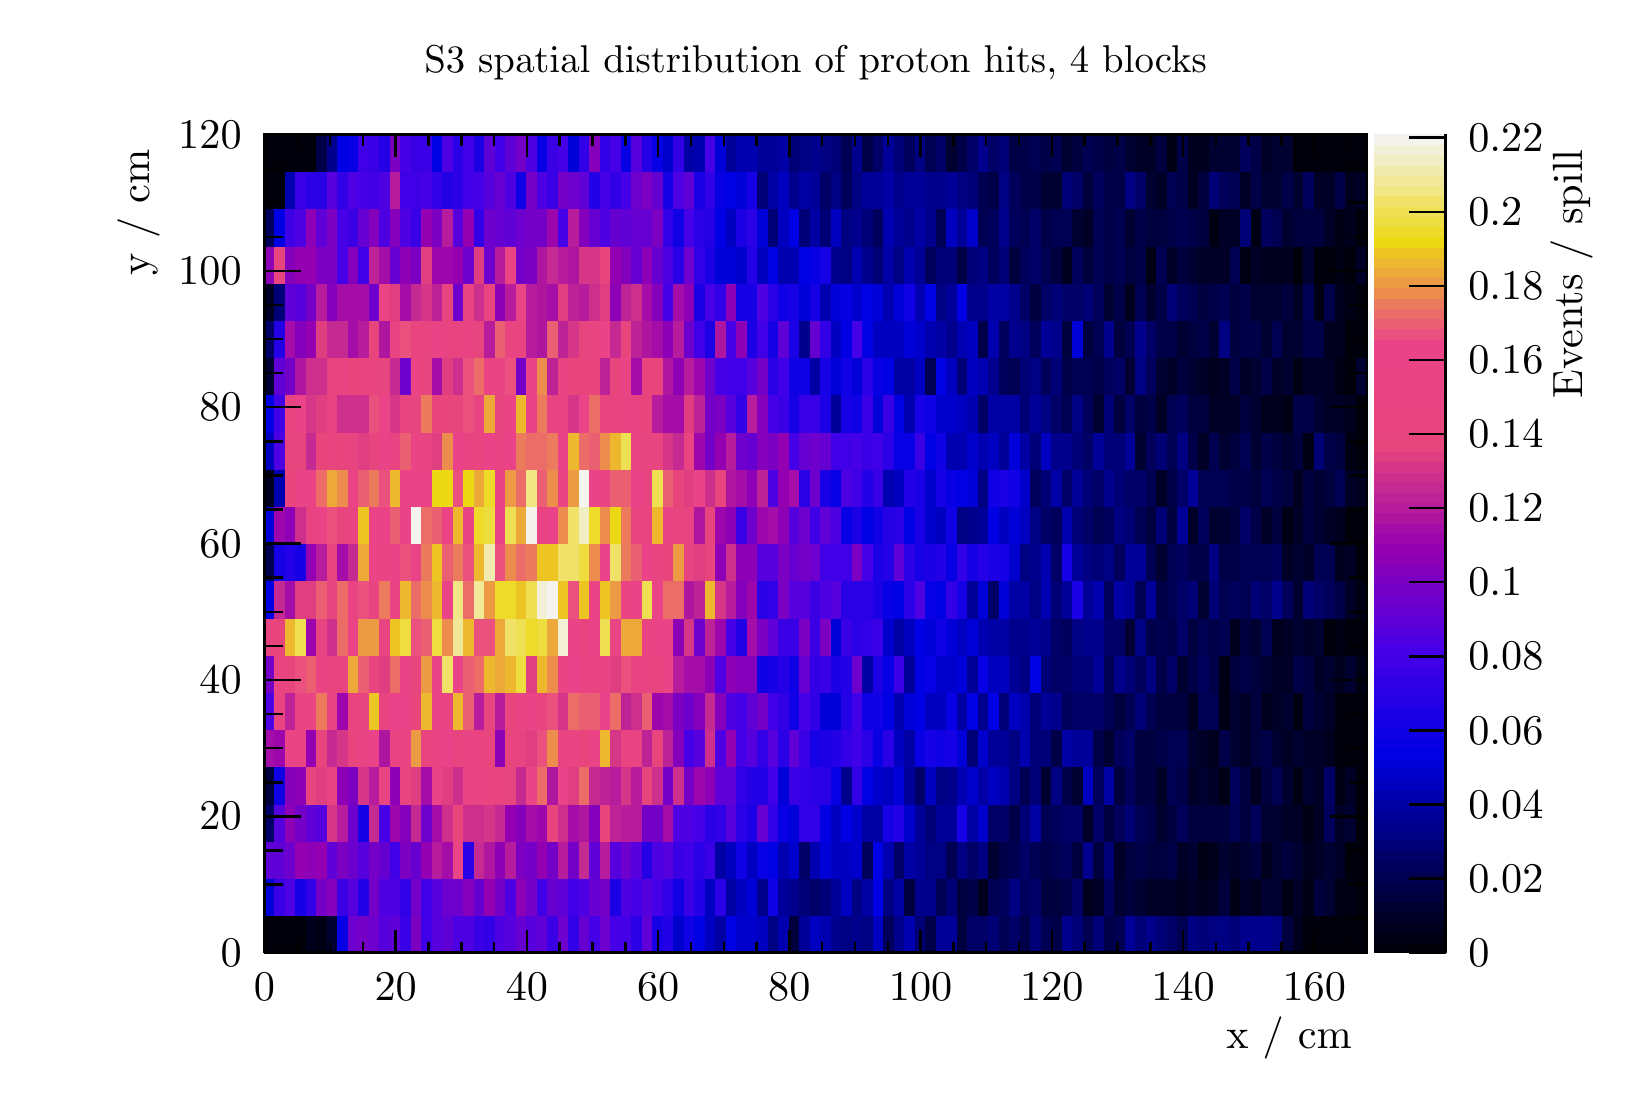
\begin{tikzpicture}
\pgfdeclareplotmark{cross} {
\pgfpathmoveto{\pgfpoint{-0.3\pgfplotmarksize}{\pgfplotmarksize}}
\pgfpathlineto{\pgfpoint{+0.3\pgfplotmarksize}{\pgfplotmarksize}}
\pgfpathlineto{\pgfpoint{+0.3\pgfplotmarksize}{0.3\pgfplotmarksize}}
\pgfpathlineto{\pgfpoint{+1\pgfplotmarksize}{0.3\pgfplotmarksize}}
\pgfpathlineto{\pgfpoint{+1\pgfplotmarksize}{-0.3\pgfplotmarksize}}
\pgfpathlineto{\pgfpoint{+0.3\pgfplotmarksize}{-0.3\pgfplotmarksize}}
\pgfpathlineto{\pgfpoint{+0.3\pgfplotmarksize}{-1.\pgfplotmarksize}}
\pgfpathlineto{\pgfpoint{-0.3\pgfplotmarksize}{-1.\pgfplotmarksize}}
\pgfpathlineto{\pgfpoint{-0.3\pgfplotmarksize}{-0.3\pgfplotmarksize}}
\pgfpathlineto{\pgfpoint{-1.\pgfplotmarksize}{-0.3\pgfplotmarksize}}
\pgfpathlineto{\pgfpoint{-1.\pgfplotmarksize}{0.3\pgfplotmarksize}}
\pgfpathlineto{\pgfpoint{-0.3\pgfplotmarksize}{0.3\pgfplotmarksize}}
\pgfpathclose
\pgfusepathqstroke
}
\pgfdeclareplotmark{cross*} {
\pgfpathmoveto{\pgfpoint{-0.3\pgfplotmarksize}{\pgfplotmarksize}}
\pgfpathlineto{\pgfpoint{+0.3\pgfplotmarksize}{\pgfplotmarksize}}
\pgfpathlineto{\pgfpoint{+0.3\pgfplotmarksize}{0.3\pgfplotmarksize}}
\pgfpathlineto{\pgfpoint{+1\pgfplotmarksize}{0.3\pgfplotmarksize}}
\pgfpathlineto{\pgfpoint{+1\pgfplotmarksize}{-0.3\pgfplotmarksize}}
\pgfpathlineto{\pgfpoint{+0.3\pgfplotmarksize}{-0.3\pgfplotmarksize}}
\pgfpathlineto{\pgfpoint{+0.3\pgfplotmarksize}{-1.\pgfplotmarksize}}
\pgfpathlineto{\pgfpoint{-0.3\pgfplotmarksize}{-1.\pgfplotmarksize}}
\pgfpathlineto{\pgfpoint{-0.3\pgfplotmarksize}{-0.3\pgfplotmarksize}}
\pgfpathlineto{\pgfpoint{-1.\pgfplotmarksize}{-0.3\pgfplotmarksize}}
\pgfpathlineto{\pgfpoint{-1.\pgfplotmarksize}{0.3\pgfplotmarksize}}
\pgfpathlineto{\pgfpoint{-0.3\pgfplotmarksize}{0.3\pgfplotmarksize}}
\pgfpathclose
\pgfusepathqfillstroke
}
\pgfdeclareplotmark{newstar} {
\pgfpathmoveto{\pgfqpoint{0pt}{\pgfplotmarksize}}
\pgfpathlineto{\pgfqpointpolar{44}{0.5\pgfplotmarksize}}
\pgfpathlineto{\pgfqpointpolar{18}{\pgfplotmarksize}}
\pgfpathlineto{\pgfqpointpolar{-20}{0.5\pgfplotmarksize}}
\pgfpathlineto{\pgfqpointpolar{-54}{\pgfplotmarksize}}
\pgfpathlineto{\pgfqpointpolar{-90}{0.5\pgfplotmarksize}}
\pgfpathlineto{\pgfqpointpolar{234}{\pgfplotmarksize}}
\pgfpathlineto{\pgfqpointpolar{198}{0.5\pgfplotmarksize}}
\pgfpathlineto{\pgfqpointpolar{162}{\pgfplotmarksize}}
\pgfpathlineto{\pgfqpointpolar{134}{0.5\pgfplotmarksize}}
\pgfpathclose
\pgfusepathqstroke
}
\pgfdeclareplotmark{newstar*} {
\pgfpathmoveto{\pgfqpoint{0pt}{\pgfplotmarksize}}
\pgfpathlineto{\pgfqpointpolar{44}{0.5\pgfplotmarksize}}
\pgfpathlineto{\pgfqpointpolar{18}{\pgfplotmarksize}}
\pgfpathlineto{\pgfqpointpolar{-20}{0.5\pgfplotmarksize}}
\pgfpathlineto{\pgfqpointpolar{-54}{\pgfplotmarksize}}
\pgfpathlineto{\pgfqpointpolar{-90}{0.5\pgfplotmarksize}}
\pgfpathlineto{\pgfqpointpolar{234}{\pgfplotmarksize}}
\pgfpathlineto{\pgfqpointpolar{198}{0.5\pgfplotmarksize}}
\pgfpathlineto{\pgfqpointpolar{162}{\pgfplotmarksize}}
\pgfpathlineto{\pgfqpointpolar{134}{0.5\pgfplotmarksize}}
\pgfpathclose
\pgfusepathqfillstroke
}
\definecolor{c}{rgb}{1,1,1};
\draw [color=c, fill=c] (0,0) rectangle (20,13.4957);
\draw [color=c, fill=c] (3,1.75444) rectangle (17,12.1461);
\definecolor{c}{rgb}{0,0,0};
\draw [c,line width=0.9] (3,1.75444) -- (3,12.1461) -- (17,12.1461) -- (17,1.75444) -- (3,1.75444);
\definecolor{c}{rgb}{1,1,1};
\draw [color=c, fill=c] (3,1.75444) rectangle (17,12.1461);
\definecolor{c}{rgb}{0,0,0};
\draw [c,line width=0.9] (3,1.75444) -- (3,12.1461) -- (17,12.1461) -- (17,1.75444) -- (3,1.75444);
\definecolor{c}{rgb}{0,0,0.0387097};
\draw [color=c, fill=c] (3,1.75444) rectangle (3.13333,2.22679);
\draw [color=c, fill=c] (3.13333,1.75444) rectangle (3.26667,2.22679);
\draw [color=c, fill=c] (3.26667,1.75444) rectangle (3.4,2.22679);
\draw [color=c, fill=c] (3.4,1.75444) rectangle (3.53333,2.22679);
\definecolor{c}{rgb}{0,0,0.116129};
\draw [color=c, fill=c] (3.53333,1.75444) rectangle (3.66667,2.22679);
\definecolor{c}{rgb}{0,0,0.0774194};
\draw [color=c, fill=c] (3.66667,1.75444) rectangle (3.8,2.22679);
\definecolor{c}{rgb}{0,0,0.193548};
\draw [color=c, fill=c] (3.8,1.75444) rectangle (3.93333,2.22679);
\definecolor{c}{rgb}{0.0257353,0,0.895221};
\draw [color=c, fill=c] (3.93333,1.75444) rectangle (4.06667,2.22679);
\definecolor{c}{rgb}{0.427451,0,0.8};
\draw [color=c, fill=c] (4.06667,1.75444) rectangle (4.2,2.22679);
\definecolor{c}{rgb}{0.456127,0,0.780147};
\draw [color=c, fill=c] (4.2,1.75444) rectangle (4.33333,2.22679);
\definecolor{c}{rgb}{0.427451,0,0.8};
\draw [color=c, fill=c] (4.33333,1.75444) rectangle (4.46667,2.22679);
\definecolor{c}{rgb}{0.331863,0,0.866176};
\draw [color=c, fill=c] (4.46667,1.75444) rectangle (4.6,2.22679);
\definecolor{c}{rgb}{0.370098,0,0.839706};
\draw [color=c, fill=c] (4.6,1.75444) rectangle (4.73333,2.22679);
\definecolor{c}{rgb}{0.223039,0,0.903676};
\draw [color=c, fill=c] (4.73333,1.75444) rectangle (4.86667,2.22679);
\definecolor{c}{rgb}{0.484804,0,0.760294};
\draw [color=c, fill=c] (4.86667,1.75444) rectangle (5,2.22679);
\definecolor{c}{rgb}{0.248775,0,0.904779};
\draw [color=c, fill=c] (5,1.75444) rectangle (5.13333,2.22679);
\definecolor{c}{rgb}{0.331863,0,0.866176};
\draw [color=c, fill=c] (5.13333,1.75444) rectangle (5.26667,2.22679);
\definecolor{c}{rgb}{0.370098,0,0.839706};
\draw [color=c, fill=c] (5.26667,1.75444) rectangle (5.4,2.22679);
\definecolor{c}{rgb}{0.303186,0,0.886029};
\draw [color=c, fill=c] (5.4,1.75444) rectangle (5.53333,2.22679);
\draw [color=c, fill=c] (5.53333,1.75444) rectangle (5.66667,2.22679);
\definecolor{c}{rgb}{0.223039,0,0.903676};
\draw [color=c, fill=c] (5.66667,1.75444) rectangle (5.8,2.22679);
\definecolor{c}{rgb}{0.197304,0,0.902574};
\draw [color=c, fill=c] (5.8,1.75444) rectangle (5.93333,2.22679);
\definecolor{c}{rgb}{0.303186,0,0.886029};
\draw [color=c, fill=c] (5.93333,1.75444) rectangle (6.06667,2.22679);
\definecolor{c}{rgb}{0.331863,0,0.866176};
\draw [color=c, fill=c] (6.06667,1.75444) rectangle (6.2,2.22679);
\definecolor{c}{rgb}{0.398775,0,0.819853};
\draw [color=c, fill=c] (6.2,1.75444) rectangle (6.33333,2.22679);
\definecolor{c}{rgb}{0.331863,0,0.866176};
\draw [color=c, fill=c] (6.33333,1.75444) rectangle (6.46667,2.22679);
\definecolor{c}{rgb}{0.370098,0,0.839706};
\draw [color=c, fill=c] (6.46667,1.75444) rectangle (6.6,2.22679);
\definecolor{c}{rgb}{0.223039,0,0.903676};
\draw [color=c, fill=c] (6.6,1.75444) rectangle (6.73333,2.22679);
\definecolor{c}{rgb}{0.427451,0,0.8};
\draw [color=c, fill=c] (6.73333,1.75444) rectangle (6.86667,2.22679);
\definecolor{c}{rgb}{0.197304,0,0.902574};
\draw [color=c, fill=c] (6.86667,1.75444) rectangle (7,2.22679);
\definecolor{c}{rgb}{0.398775,0,0.819853};
\draw [color=c, fill=c] (7,1.75444) rectangle (7.13333,2.22679);
\definecolor{c}{rgb}{0.27451,0,0.905882};
\draw [color=c, fill=c] (7.13333,1.75444) rectangle (7.26667,2.22679);
\definecolor{c}{rgb}{0.427451,0,0.8};
\draw [color=c, fill=c] (7.26667,1.75444) rectangle (7.4,2.22679);
\definecolor{c}{rgb}{0.27451,0,0.905882};
\draw [color=c, fill=c] (7.4,1.75444) rectangle (7.53333,2.22679);
\draw [color=c, fill=c] (7.53333,1.75444) rectangle (7.66667,2.22679);
\definecolor{c}{rgb}{0.16299,0,0.901103};
\draw [color=c, fill=c] (7.66667,1.75444) rectangle (7.8,2.22679);
\definecolor{c}{rgb}{0.370098,0,0.839706};
\draw [color=c, fill=c] (7.8,1.75444) rectangle (7.93333,2.22679);
\definecolor{c}{rgb}{0.0857843,0,0.897794};
\draw [color=c, fill=c] (7.93333,1.75444) rectangle (8.06667,2.22679);
\definecolor{c}{rgb}{0.137255,0,0.9};
\draw [color=c, fill=c] (8.06667,1.75444) rectangle (8.2,2.22679);
\definecolor{c}{rgb}{0,0,0.801471};
\draw [color=c, fill=c] (8.2,1.75444) rectangle (8.33333,2.22679);
\definecolor{c}{rgb}{0.060049,0,0.896691};
\draw [color=c, fill=c] (8.33333,1.75444) rectangle (8.46667,2.22679);
\definecolor{c}{rgb}{0,0,0.894118};
\draw [color=c, fill=c] (8.46667,1.75444) rectangle (8.6,2.22679);
\definecolor{c}{rgb}{0,0,0.755147};
\draw [color=c, fill=c] (8.6,1.75444) rectangle (8.73333,2.22679);
\definecolor{c}{rgb}{0,0,0.647059};
\draw [color=c, fill=c] (8.73333,1.75444) rectangle (8.86667,2.22679);
\definecolor{c}{rgb}{0,0,0.894118};
\draw [color=c, fill=c] (8.86667,1.75444) rectangle (9,2.22679);
\definecolor{c}{rgb}{0,0,0.801471};
\draw [color=c, fill=c] (9,1.75444) rectangle (9.13333,2.22679);
\draw [color=c, fill=c] (9.13333,1.75444) rectangle (9.26667,2.22679);
\definecolor{c}{rgb}{0,0,0.755147};
\draw [color=c, fill=c] (9.26667,1.75444) rectangle (9.4,2.22679);
\definecolor{c}{rgb}{0,0,0.508088};
\draw [color=c, fill=c] (9.4,1.75444) rectangle (9.53333,2.22679);
\definecolor{c}{rgb}{0,0,0.693382};
\draw [color=c, fill=c] (9.53333,1.75444) rectangle (9.66667,2.22679);
\definecolor{c}{rgb}{0,0,0.245161};
\draw [color=c, fill=c] (9.66667,1.75444) rectangle (9.8,2.22679);
\definecolor{c}{rgb}{0,0,0.600735};
\draw [color=c, fill=c] (9.8,1.75444) rectangle (9.93333,2.22679);
\definecolor{c}{rgb}{0,0,0.755147};
\draw [color=c, fill=c] (9.93333,1.75444) rectangle (10.0667,2.22679);
\definecolor{c}{rgb}{0,0,0.693382};
\draw [color=c, fill=c] (10.0667,1.75444) rectangle (10.2,2.22679);
\definecolor{c}{rgb}{0,0,0.554412};
\draw [color=c, fill=c] (10.2,1.75444) rectangle (10.3333,2.22679);
\definecolor{c}{rgb}{0,0,0.508088};
\draw [color=c, fill=c] (10.3333,1.75444) rectangle (10.4667,2.22679);
\definecolor{c}{rgb}{0,0,0.554412};
\draw [color=c, fill=c] (10.4667,1.75444) rectangle (10.6,2.22679);
\definecolor{c}{rgb}{0,0,0.508088};
\draw [color=c, fill=c] (10.6,1.75444) rectangle (10.7333,2.22679);
\definecolor{c}{rgb}{0,0,0.755147};
\draw [color=c, fill=c] (10.7333,1.75444) rectangle (10.8667,2.22679);
\definecolor{c}{rgb}{0,0,0.36129};
\draw [color=c, fill=c] (10.8667,1.75444) rectangle (11,2.22679);
\definecolor{c}{rgb}{0,0,0.554412};
\draw [color=c, fill=c] (11,1.75444) rectangle (11.1333,2.22679);
\definecolor{c}{rgb}{0,0,0.693382};
\draw [color=c, fill=c] (11.1333,1.75444) rectangle (11.2667,2.22679);
\definecolor{c}{rgb}{0,0,0.461765};
\draw [color=c, fill=c] (11.2667,1.75444) rectangle (11.4,2.22679);
\definecolor{c}{rgb}{0,0,0.283871};
\draw [color=c, fill=c] (11.4,1.75444) rectangle (11.5333,2.22679);
\definecolor{c}{rgb}{0,0,0.600735};
\draw [color=c, fill=c] (11.5333,1.75444) rectangle (11.6667,2.22679);
\draw [color=c, fill=c] (11.6667,1.75444) rectangle (11.8,2.22679);
\definecolor{c}{rgb}{0,0,0.245161};
\draw [color=c, fill=c] (11.8,1.75444) rectangle (11.9333,2.22679);
\definecolor{c}{rgb}{0,0,0.4};
\draw [color=c, fill=c] (11.9333,1.75444) rectangle (12.0667,2.22679);
\draw [color=c, fill=c] (12.0667,1.75444) rectangle (12.2,2.22679);
\definecolor{c}{rgb}{0,0,0.461765};
\draw [color=c, fill=c] (12.2,1.75444) rectangle (12.3333,2.22679);
\definecolor{c}{rgb}{0,0,0.322581};
\draw [color=c, fill=c] (12.3333,1.75444) rectangle (12.4667,2.22679);
\definecolor{c}{rgb}{0,0,0.4};
\draw [color=c, fill=c] (12.4667,1.75444) rectangle (12.6,2.22679);
\definecolor{c}{rgb}{0,0,0.283871};
\draw [color=c, fill=c] (12.6,1.75444) rectangle (12.7333,2.22679);
\definecolor{c}{rgb}{0,0,0.461765};
\draw [color=c, fill=c] (12.7333,1.75444) rectangle (12.8667,2.22679);
\definecolor{c}{rgb}{0,0,0.322581};
\draw [color=c, fill=c] (12.8667,1.75444) rectangle (13,2.22679);
\definecolor{c}{rgb}{0,0,0.283871};
\draw [color=c, fill=c] (13,1.75444) rectangle (13.1333,2.22679);
\definecolor{c}{rgb}{0,0,0.554412};
\draw [color=c, fill=c] (13.1333,1.75444) rectangle (13.2667,2.22679);
\definecolor{c}{rgb}{0,0,0.461765};
\draw [color=c, fill=c] (13.2667,1.75444) rectangle (13.4,2.22679);
\definecolor{c}{rgb}{0,0,0.322581};
\draw [color=c, fill=c] (13.4,1.75444) rectangle (13.5333,2.22679);
\definecolor{c}{rgb}{0,0,0.461765};
\draw [color=c, fill=c] (13.5333,1.75444) rectangle (13.6667,2.22679);
\definecolor{c}{rgb}{0,0,0.283871};
\draw [color=c, fill=c] (13.6667,1.75444) rectangle (13.8,2.22679);
\definecolor{c}{rgb}{0,0,0.322581};
\draw [color=c, fill=c] (13.8,1.75444) rectangle (13.9333,2.22679);
\definecolor{c}{rgb}{0,0,0.600735};
\draw [color=c, fill=c] (13.9333,1.75444) rectangle (14.0667,2.22679);
\definecolor{c}{rgb}{0,0,0.461765};
\draw [color=c, fill=c] (14.0667,1.75444) rectangle (14.2,2.22679);
\definecolor{c}{rgb}{0,0,0.554412};
\draw [color=c, fill=c] (14.2,1.75444) rectangle (14.3333,2.22679);
\definecolor{c}{rgb}{0,0,0.461765};
\draw [color=c, fill=c] (14.3333,1.75444) rectangle (14.4667,2.22679);
\definecolor{c}{rgb}{0,0,0.4};
\draw [color=c, fill=c] (14.4667,1.75444) rectangle (14.6,2.22679);
\definecolor{c}{rgb}{0,0,0.322581};
\draw [color=c, fill=c] (14.6,1.75444) rectangle (14.7333,2.22679);
\definecolor{c}{rgb}{0,0,0.508088};
\draw [color=c, fill=c] (14.7333,1.75444) rectangle (14.8667,2.22679);
\definecolor{c}{rgb}{0,0,0.461765};
\draw [color=c, fill=c] (14.8667,1.75444) rectangle (15,2.22679);
\definecolor{c}{rgb}{0,0,0.508088};
\draw [color=c, fill=c] (15,1.75444) rectangle (15.1333,2.22679);
\draw [color=c, fill=c] (15.1333,1.75444) rectangle (15.2667,2.22679);
\definecolor{c}{rgb}{0,0,0.461765};
\draw [color=c, fill=c] (15.2667,1.75444) rectangle (15.4,2.22679);
\definecolor{c}{rgb}{0,0,0.554412};
\draw [color=c, fill=c] (15.4,1.75444) rectangle (15.5333,2.22679);
\draw [color=c, fill=c] (15.5333,1.75444) rectangle (15.6667,2.22679);
\draw [color=c, fill=c] (15.6667,1.75444) rectangle (15.8,2.22679);
\definecolor{c}{rgb}{0,0,0.508088};
\draw [color=c, fill=c] (15.8,1.75444) rectangle (15.9333,2.22679);
\definecolor{c}{rgb}{0,0,0.245161};
\draw [color=c, fill=c] (15.9333,1.75444) rectangle (16.0667,2.22679);
\definecolor{c}{rgb}{0,0,0.116129};
\draw [color=c, fill=c] (16.0667,1.75444) rectangle (16.2,2.22679);
\definecolor{c}{rgb}{0,0,0.0387097};
\draw [color=c, fill=c] (16.2,1.75444) rectangle (16.3333,2.22679);
\draw [color=c, fill=c] (16.3333,1.75444) rectangle (16.4667,2.22679);
\draw [color=c, fill=c] (16.4667,1.75444) rectangle (16.6,2.22679);
\draw [color=c, fill=c] (16.6,1.75444) rectangle (16.7333,2.22679);
\draw [color=c, fill=c] (16.7333,1.75444) rectangle (16.8667,2.22679);
\draw [color=c, fill=c] (16.8667,1.75444) rectangle (17,2.22679);
\definecolor{c}{rgb}{0,0,0.847794};
\draw [color=c, fill=c] (3,2.22679) rectangle (3.13333,2.69914);
\definecolor{c}{rgb}{0.223039,0,0.903676};
\draw [color=c, fill=c] (3.13333,2.22679) rectangle (3.26667,2.69914);
\definecolor{c}{rgb}{0.303186,0,0.886029};
\draw [color=c, fill=c] (3.26667,2.22679) rectangle (3.4,2.69914);
\definecolor{c}{rgb}{0.0857843,0,0.897794};
\draw [color=c, fill=c] (3.4,2.22679) rectangle (3.53333,2.69914);
\definecolor{c}{rgb}{0.197304,0,0.902574};
\draw [color=c, fill=c] (3.53333,2.22679) rectangle (3.66667,2.69914);
\definecolor{c}{rgb}{0.456127,0,0.780147};
\draw [color=c, fill=c] (3.66667,2.22679) rectangle (3.8,2.69914);
\definecolor{c}{rgb}{0.523039,0,0.733824};
\draw [color=c, fill=c] (3.8,2.22679) rectangle (3.93333,2.69914);
\definecolor{c}{rgb}{0.223039,0,0.903676};
\draw [color=c, fill=c] (3.93333,2.22679) rectangle (4.06667,2.69914);
\definecolor{c}{rgb}{0.331863,0,0.866176};
\draw [color=c, fill=c] (4.06667,2.22679) rectangle (4.2,2.69914);
\definecolor{c}{rgb}{0.137255,0,0.9};
\draw [color=c, fill=c] (4.2,2.22679) rectangle (4.33333,2.69914);
\definecolor{c}{rgb}{0.456127,0,0.780147};
\draw [color=c, fill=c] (4.33333,2.22679) rectangle (4.46667,2.69914);
\definecolor{c}{rgb}{0.303186,0,0.886029};
\draw [color=c, fill=c] (4.46667,2.22679) rectangle (4.6,2.69914);
\draw [color=c, fill=c] (4.6,2.22679) rectangle (4.73333,2.69914);
\definecolor{c}{rgb}{0.197304,0,0.902574};
\draw [color=c, fill=c] (4.73333,2.22679) rectangle (4.86667,2.69914);
\definecolor{c}{rgb}{0.456127,0,0.780147};
\draw [color=c, fill=c] (4.86667,2.22679) rectangle (5,2.69914);
\definecolor{c}{rgb}{0.248775,0,0.904779};
\draw [color=c, fill=c] (5,2.22679) rectangle (5.13333,2.69914);
\definecolor{c}{rgb}{0.331863,0,0.866176};
\draw [color=c, fill=c] (5.13333,2.22679) rectangle (5.26667,2.69914);
\definecolor{c}{rgb}{0.427451,0,0.8};
\draw [color=c, fill=c] (5.26667,2.22679) rectangle (5.4,2.69914);
\draw [color=c, fill=c] (5.4,2.22679) rectangle (5.53333,2.69914);
\definecolor{c}{rgb}{0.523039,0,0.733824};
\draw [color=c, fill=c] (5.53333,2.22679) rectangle (5.66667,2.69914);
\definecolor{c}{rgb}{0.398775,0,0.819853};
\draw [color=c, fill=c] (5.66667,2.22679) rectangle (5.8,2.69914);
\definecolor{c}{rgb}{0.580392,0,0.694118};
\draw [color=c, fill=c] (5.8,2.22679) rectangle (5.93333,2.69914);
\definecolor{c}{rgb}{0.456127,0,0.780147};
\draw [color=c, fill=c] (5.93333,2.22679) rectangle (6.06667,2.69914);
\definecolor{c}{rgb}{0.303186,0,0.886029};
\draw [color=c, fill=c] (6.06667,2.22679) rectangle (6.2,2.69914);
\definecolor{c}{rgb}{0.551716,0,0.713971};
\draw [color=c, fill=c] (6.2,2.22679) rectangle (6.33333,2.69914);
\definecolor{c}{rgb}{0.456127,0,0.780147};
\draw [color=c, fill=c] (6.33333,2.22679) rectangle (6.46667,2.69914);
\definecolor{c}{rgb}{0.248775,0,0.904779};
\draw [color=c, fill=c] (6.46667,2.22679) rectangle (6.6,2.69914);
\definecolor{c}{rgb}{0.398775,0,0.819853};
\draw [color=c, fill=c] (6.6,2.22679) rectangle (6.73333,2.69914);
\definecolor{c}{rgb}{0.370098,0,0.839706};
\draw [color=c, fill=c] (6.73333,2.22679) rectangle (6.86667,2.69914);
\definecolor{c}{rgb}{0.248775,0,0.904779};
\draw [color=c, fill=c] (6.86667,2.22679) rectangle (7,2.69914);
\definecolor{c}{rgb}{0.303186,0,0.886029};
\draw [color=c, fill=c] (7,2.22679) rectangle (7.13333,2.69914);
\definecolor{c}{rgb}{0.398775,0,0.819853};
\draw [color=c, fill=c] (7.13333,2.22679) rectangle (7.26667,2.69914);
\definecolor{c}{rgb}{0.456127,0,0.780147};
\draw [color=c, fill=c] (7.26667,2.22679) rectangle (7.4,2.69914);
\definecolor{c}{rgb}{0.11152,0,0.898897};
\draw [color=c, fill=c] (7.4,2.22679) rectangle (7.53333,2.69914);
\definecolor{c}{rgb}{0.303186,0,0.886029};
\draw [color=c, fill=c] (7.53333,2.22679) rectangle (7.66667,2.69914);
\definecolor{c}{rgb}{0.27451,0,0.905882};
\draw [color=c, fill=c] (7.66667,2.22679) rectangle (7.8,2.69914);
\definecolor{c}{rgb}{0.331863,0,0.866176};
\draw [color=c, fill=c] (7.8,2.22679) rectangle (7.93333,2.69914);
\definecolor{c}{rgb}{0.27451,0,0.905882};
\draw [color=c, fill=c] (7.93333,2.22679) rectangle (8.06667,2.69914);
\definecolor{c}{rgb}{0.197304,0,0.902574};
\draw [color=c, fill=c] (8.06667,2.22679) rectangle (8.2,2.69914);
\definecolor{c}{rgb}{0.060049,0,0.896691};
\draw [color=c, fill=c] (8.2,2.22679) rectangle (8.33333,2.69914);
\definecolor{c}{rgb}{0.223039,0,0.903676};
\draw [color=c, fill=c] (8.33333,2.22679) rectangle (8.46667,2.69914);
\definecolor{c}{rgb}{0.137255,0,0.9};
\draw [color=c, fill=c] (8.46667,2.22679) rectangle (8.6,2.69914);
\definecolor{c}{rgb}{0,0,0.755147};
\draw [color=c, fill=c] (8.6,2.22679) rectangle (8.73333,2.69914);
\definecolor{c}{rgb}{0.16299,0,0.901103};
\draw [color=c, fill=c] (8.73333,2.22679) rectangle (8.86667,2.69914);
\definecolor{c}{rgb}{0,0,0.647059};
\draw [color=c, fill=c] (8.86667,2.22679) rectangle (9,2.69914);
\definecolor{c}{rgb}{0,0,0.755147};
\draw [color=c, fill=c] (9,2.22679) rectangle (9.13333,2.69914);
\definecolor{c}{rgb}{0,0,0.847794};
\draw [color=c, fill=c] (9.13333,2.22679) rectangle (9.26667,2.69914);
\definecolor{c}{rgb}{0,0,0.554412};
\draw [color=c, fill=c] (9.26667,2.22679) rectangle (9.4,2.69914);
\definecolor{c}{rgb}{0.060049,0,0.896691};
\draw [color=c, fill=c] (9.4,2.22679) rectangle (9.53333,2.69914);
\definecolor{c}{rgb}{0,0,0.600735};
\draw [color=c, fill=c] (9.53333,2.22679) rectangle (9.66667,2.69914);
\definecolor{c}{rgb}{0,0,0.554412};
\draw [color=c, fill=c] (9.66667,2.22679) rectangle (9.8,2.69914);
\definecolor{c}{rgb}{0,0,0.461765};
\draw [color=c, fill=c] (9.8,2.22679) rectangle (9.93333,2.69914);
\definecolor{c}{rgb}{0,0,0.4};
\draw [color=c, fill=c] (9.93333,2.22679) rectangle (10.0667,2.69914);
\definecolor{c}{rgb}{0,0,0.461765};
\draw [color=c, fill=c] (10.0667,2.22679) rectangle (10.2,2.69914);
\definecolor{c}{rgb}{0,0,0.600735};
\draw [color=c, fill=c] (10.2,2.22679) rectangle (10.3333,2.69914);
\definecolor{c}{rgb}{0,0,0.755147};
\draw [color=c, fill=c] (10.3333,2.22679) rectangle (10.4667,2.69914);
\definecolor{c}{rgb}{0,0,0.508088};
\draw [color=c, fill=c] (10.4667,2.22679) rectangle (10.6,2.69914);
\definecolor{c}{rgb}{0,0,0.647059};
\draw [color=c, fill=c] (10.6,2.22679) rectangle (10.7333,2.69914);
\definecolor{c}{rgb}{0,0,0.894118};
\draw [color=c, fill=c] (10.7333,2.22679) rectangle (10.8667,2.69914);
\definecolor{c}{rgb}{0,0,0.508088};
\draw [color=c, fill=c] (10.8667,2.22679) rectangle (11,2.69914);
\definecolor{c}{rgb}{0,0,0.647059};
\draw [color=c, fill=c] (11,2.22679) rectangle (11.1333,2.69914);
\definecolor{c}{rgb}{0,0,0.245161};
\draw [color=c, fill=c] (11.1333,2.22679) rectangle (11.2667,2.69914);
\definecolor{c}{rgb}{0,0,0.554412};
\draw [color=c, fill=c] (11.2667,2.22679) rectangle (11.4,2.69914);
\draw [color=c, fill=c] (11.4,2.22679) rectangle (11.5333,2.69914);
\definecolor{c}{rgb}{0,0,0.322581};
\draw [color=c, fill=c] (11.5333,2.22679) rectangle (11.6667,2.69914);
\definecolor{c}{rgb}{0,0,0.461765};
\draw [color=c, fill=c] (11.6667,2.22679) rectangle (11.8,2.69914);
\definecolor{c}{rgb}{0,0,0.245161};
\draw [color=c, fill=c] (11.8,2.22679) rectangle (11.9333,2.69914);
\definecolor{c}{rgb}{0,0,0.283871};
\draw [color=c, fill=c] (11.9333,2.22679) rectangle (12.0667,2.69914);
\definecolor{c}{rgb}{0,0,0.116129};
\draw [color=c, fill=c] (12.0667,2.22679) rectangle (12.2,2.69914);
\definecolor{c}{rgb}{0,0,0.322581};
\draw [color=c, fill=c] (12.2,2.22679) rectangle (12.3333,2.69914);
\definecolor{c}{rgb}{0,0,0.36129};
\draw [color=c, fill=c] (12.3333,2.22679) rectangle (12.4667,2.69914);
\definecolor{c}{rgb}{0,0,0.508088};
\draw [color=c, fill=c] (12.4667,2.22679) rectangle (12.6,2.69914);
\definecolor{c}{rgb}{0,0,0.36129};
\draw [color=c, fill=c] (12.6,2.22679) rectangle (12.7333,2.69914);
\definecolor{c}{rgb}{0,0,0.4};
\draw [color=c, fill=c] (12.7333,2.22679) rectangle (12.8667,2.69914);
\definecolor{c}{rgb}{0,0,0.245161};
\draw [color=c, fill=c] (12.8667,2.22679) rectangle (13,2.69914);
\draw [color=c, fill=c] (13,2.22679) rectangle (13.1333,2.69914);
\definecolor{c}{rgb}{0,0,0.283871};
\draw [color=c, fill=c] (13.1333,2.22679) rectangle (13.2667,2.69914);
\definecolor{c}{rgb}{0,0,0.4};
\draw [color=c, fill=c] (13.2667,2.22679) rectangle (13.4,2.69914);
\definecolor{c}{rgb}{0,0,0.116129};
\draw [color=c, fill=c] (13.4,2.22679) rectangle (13.5333,2.69914);
\definecolor{c}{rgb}{0,0,0.154839};
\draw [color=c, fill=c] (13.5333,2.22679) rectangle (13.6667,2.69914);
\definecolor{c}{rgb}{0,0,0.36129};
\draw [color=c, fill=c] (13.6667,2.22679) rectangle (13.8,2.69914);
\definecolor{c}{rgb}{0,0,0.193548};
\draw [color=c, fill=c] (13.8,2.22679) rectangle (13.9333,2.69914);
\definecolor{c}{rgb}{0,0,0.245161};
\draw [color=c, fill=c] (13.9333,2.22679) rectangle (14.0667,2.69914);
\definecolor{c}{rgb}{0,0,0.193548};
\draw [color=c, fill=c] (14.0667,2.22679) rectangle (14.2,2.69914);
\definecolor{c}{rgb}{0,0,0.154839};
\draw [color=c, fill=c] (14.2,2.22679) rectangle (14.3333,2.69914);
\draw [color=c, fill=c] (14.3333,2.22679) rectangle (14.4667,2.69914);
\draw [color=c, fill=c] (14.4667,2.22679) rectangle (14.6,2.69914);
\definecolor{c}{rgb}{0,0,0.116129};
\draw [color=c, fill=c] (14.6,2.22679) rectangle (14.7333,2.69914);
\definecolor{c}{rgb}{0,0,0.154839};
\draw [color=c, fill=c] (14.7333,2.22679) rectangle (14.8667,2.69914);
\definecolor{c}{rgb}{0,0,0.116129};
\draw [color=c, fill=c] (14.8667,2.22679) rectangle (15,2.69914);
\definecolor{c}{rgb}{0,0,0.154839};
\draw [color=c, fill=c] (15,2.22679) rectangle (15.1333,2.69914);
\definecolor{c}{rgb}{0,0,0.245161};
\draw [color=c, fill=c] (15.1333,2.22679) rectangle (15.2667,2.69914);
\definecolor{c}{rgb}{0,0,0.0774194};
\draw [color=c, fill=c] (15.2667,2.22679) rectangle (15.4,2.69914);
\definecolor{c}{rgb}{0,0,0.154839};
\draw [color=c, fill=c] (15.4,2.22679) rectangle (15.5333,2.69914);
\definecolor{c}{rgb}{0,0,0.116129};
\draw [color=c, fill=c] (15.5333,2.22679) rectangle (15.6667,2.69914);
\definecolor{c}{rgb}{0,0,0.193548};
\draw [color=c, fill=c] (15.6667,2.22679) rectangle (15.8,2.69914);
\draw [color=c, fill=c] (15.8,2.22679) rectangle (15.9333,2.69914);
\definecolor{c}{rgb}{0,0,0.0774194};
\draw [color=c, fill=c] (15.9333,2.22679) rectangle (16.0667,2.69914);
\definecolor{c}{rgb}{0,0,0.154839};
\draw [color=c, fill=c] (16.0667,2.22679) rectangle (16.2,2.69914);
\definecolor{c}{rgb}{0,0,0.0774194};
\draw [color=c, fill=c] (16.2,2.22679) rectangle (16.3333,2.69914);
\definecolor{c}{rgb}{0,0,0.245161};
\draw [color=c, fill=c] (16.3333,2.22679) rectangle (16.4667,2.69914);
\definecolor{c}{rgb}{0,0,0.193548};
\draw [color=c, fill=c] (16.4667,2.22679) rectangle (16.6,2.69914);
\definecolor{c}{rgb}{0,0,0.0774194};
\draw [color=c, fill=c] (16.6,2.22679) rectangle (16.7333,2.69914);
\draw [color=c, fill=c] (16.7333,2.22679) rectangle (16.8667,2.69914);
\definecolor{c}{rgb}{0,0,0.0387097};
\draw [color=c, fill=c] (16.8667,2.22679) rectangle (17,2.69914);
\definecolor{c}{rgb}{0.370098,0,0.839706};
\draw [color=c, fill=c] (3,2.69914) rectangle (3.13333,3.17149);
\draw [color=c, fill=c] (3.13333,2.69914) rectangle (3.26667,3.17149);
\definecolor{c}{rgb}{0.427451,0,0.8};
\draw [color=c, fill=c] (3.26667,2.69914) rectangle (3.4,3.17149);
\definecolor{c}{rgb}{0.580392,0,0.694118};
\draw [color=c, fill=c] (3.4,2.69914) rectangle (3.53333,3.17149);
\definecolor{c}{rgb}{0.551716,0,0.713971};
\draw [color=c, fill=c] (3.53333,2.69914) rectangle (3.66667,3.17149);
\definecolor{c}{rgb}{0.580392,0,0.694118};
\draw [color=c, fill=c] (3.66667,2.69914) rectangle (3.8,3.17149);
\definecolor{c}{rgb}{0.370098,0,0.839706};
\draw [color=c, fill=c] (3.8,2.69914) rectangle (3.93333,3.17149);
\definecolor{c}{rgb}{0.484804,0,0.760294};
\draw [color=c, fill=c] (3.93333,2.69914) rectangle (4.06667,3.17149);
\definecolor{c}{rgb}{0.427451,0,0.8};
\draw [color=c, fill=c] (4.06667,2.69914) rectangle (4.2,3.17149);
\definecolor{c}{rgb}{0.331863,0,0.866176};
\draw [color=c, fill=c] (4.2,2.69914) rectangle (4.33333,3.17149);
\definecolor{c}{rgb}{0.456127,0,0.780147};
\draw [color=c, fill=c] (4.33333,2.69914) rectangle (4.46667,3.17149);
\definecolor{c}{rgb}{0.398775,0,0.819853};
\draw [color=c, fill=c] (4.46667,2.69914) rectangle (4.6,3.17149);
\definecolor{c}{rgb}{0.248775,0,0.904779};
\draw [color=c, fill=c] (4.6,2.69914) rectangle (4.73333,3.17149);
\definecolor{c}{rgb}{0.484804,0,0.760294};
\draw [color=c, fill=c] (4.73333,2.69914) rectangle (4.86667,3.17149);
\definecolor{c}{rgb}{0.398775,0,0.819853};
\draw [color=c, fill=c] (4.86667,2.69914) rectangle (5,3.17149);
\definecolor{c}{rgb}{0.580392,0,0.694118};
\draw [color=c, fill=c] (5,2.69914) rectangle (5.13333,3.17149);
\definecolor{c}{rgb}{0.712623,0.109926,0.609681};
\draw [color=c, fill=c] (5.13333,2.69914) rectangle (5.26667,3.17149);
\definecolor{c}{rgb}{0.641422,0.0507353,0.655147};
\draw [color=c, fill=c] (5.26667,2.69914) rectangle (5.4,3.17149);
\definecolor{c}{rgb}{0.915196,0.265931,0.516544};
\draw [color=c, fill=c] (5.4,2.69914) rectangle (5.53333,3.17149);
\definecolor{c}{rgb}{0.16299,0,0.901103};
\draw [color=c, fill=c] (5.53333,2.69914) rectangle (5.66667,3.17149);
\definecolor{c}{rgb}{0.773652,0.160662,0.570711};
\draw [color=c, fill=c] (5.66667,2.69914) rectangle (5.8,3.17149);
\definecolor{c}{rgb}{0.682108,0.0845588,0.629167};
\draw [color=c, fill=c] (5.8,2.69914) rectangle (5.93333,3.17149);
\definecolor{c}{rgb}{0.551716,0,0.713971};
\draw [color=c, fill=c] (5.93333,2.69914) rectangle (6.06667,3.17149);
\definecolor{c}{rgb}{0.712623,0.109926,0.609681};
\draw [color=c, fill=c] (6.06667,2.69914) rectangle (6.2,3.17149);
\definecolor{c}{rgb}{0.484804,0,0.760294};
\draw [color=c, fill=c] (6.2,2.69914) rectangle (6.33333,3.17149);
\definecolor{c}{rgb}{0.456127,0,0.780147};
\draw [color=c, fill=c] (6.33333,2.69914) rectangle (6.46667,3.17149);
\definecolor{c}{rgb}{0.580392,0,0.694118};
\draw [color=c, fill=c] (6.46667,2.69914) rectangle (6.6,3.17149);
\definecolor{c}{rgb}{0.456127,0,0.780147};
\draw [color=c, fill=c] (6.6,2.69914) rectangle (6.73333,3.17149);
\definecolor{c}{rgb}{0.712623,0.109926,0.609681};
\draw [color=c, fill=c] (6.73333,2.69914) rectangle (6.86667,3.17149);
\definecolor{c}{rgb}{0.456127,0,0.780147};
\draw [color=c, fill=c] (6.86667,2.69914) rectangle (7,3.17149);
\definecolor{c}{rgb}{0.773652,0.160662,0.570711};
\draw [color=c, fill=c] (7,2.69914) rectangle (7.13333,3.17149);
\definecolor{c}{rgb}{0.370098,0,0.839706};
\draw [color=c, fill=c] (7.13333,2.69914) rectangle (7.26667,3.17149);
\definecolor{c}{rgb}{0.712623,0.109926,0.609681};
\draw [color=c, fill=c] (7.26667,2.69914) rectangle (7.4,3.17149);
\definecolor{c}{rgb}{0.331863,0,0.866176};
\draw [color=c, fill=c] (7.4,2.69914) rectangle (7.53333,3.17149);
\definecolor{c}{rgb}{0.427451,0,0.8};
\draw [color=c, fill=c] (7.53333,2.69914) rectangle (7.66667,3.17149);
\definecolor{c}{rgb}{0.331863,0,0.866176};
\draw [color=c, fill=c] (7.66667,2.69914) rectangle (7.8,3.17149);
\definecolor{c}{rgb}{0.137255,0,0.9};
\draw [color=c, fill=c] (7.8,2.69914) rectangle (7.93333,3.17149);
\definecolor{c}{rgb}{0.303186,0,0.886029};
\draw [color=c, fill=c] (7.93333,2.69914) rectangle (8.06667,3.17149);
\definecolor{c}{rgb}{0.331863,0,0.866176};
\draw [color=c, fill=c] (8.06667,2.69914) rectangle (8.2,3.17149);
\definecolor{c}{rgb}{0.223039,0,0.903676};
\draw [color=c, fill=c] (8.2,2.69914) rectangle (8.33333,3.17149);
\definecolor{c}{rgb}{0.248775,0,0.904779};
\draw [color=c, fill=c] (8.33333,2.69914) rectangle (8.46667,3.17149);
\definecolor{c}{rgb}{0.16299,0,0.901103};
\draw [color=c, fill=c] (8.46667,2.69914) rectangle (8.6,3.17149);
\definecolor{c}{rgb}{0.223039,0,0.903676};
\draw [color=c, fill=c] (8.6,2.69914) rectangle (8.73333,3.17149);
\definecolor{c}{rgb}{0,0,0.647059};
\draw [color=c, fill=c] (8.73333,2.69914) rectangle (8.86667,3.17149);
\definecolor{c}{rgb}{0,0,0.755147};
\draw [color=c, fill=c] (8.86667,2.69914) rectangle (9,3.17149);
\definecolor{c}{rgb}{0.060049,0,0.896691};
\draw [color=c, fill=c] (9,2.69914) rectangle (9.13333,3.17149);
\definecolor{c}{rgb}{0,0,0.755147};
\draw [color=c, fill=c] (9.13333,2.69914) rectangle (9.26667,3.17149);
\definecolor{c}{rgb}{0.0257353,0,0.895221};
\draw [color=c, fill=c] (9.26667,2.69914) rectangle (9.4,3.17149);
\definecolor{c}{rgb}{0,0,0.894118};
\draw [color=c, fill=c] (9.4,2.69914) rectangle (9.53333,3.17149);
\definecolor{c}{rgb}{0,0,0.693382};
\draw [color=c, fill=c] (9.53333,2.69914) rectangle (9.66667,3.17149);
\definecolor{c}{rgb}{0,0,0.801471};
\draw [color=c, fill=c] (9.66667,2.69914) rectangle (9.8,3.17149);
\definecolor{c}{rgb}{0,0,0.4};
\draw [color=c, fill=c] (9.8,2.69914) rectangle (9.93333,3.17149);
\definecolor{c}{rgb}{0,0,0.693382};
\draw [color=c, fill=c] (9.93333,2.69914) rectangle (10.0667,3.17149);
\definecolor{c}{rgb}{0,0,0.847794};
\draw [color=c, fill=c] (10.0667,2.69914) rectangle (10.2,3.17149);
\definecolor{c}{rgb}{0,0,0.755147};
\draw [color=c, fill=c] (10.2,2.69914) rectangle (10.3333,3.17149);
\draw [color=c, fill=c] (10.3333,2.69914) rectangle (10.4667,3.17149);
\definecolor{c}{rgb}{0,0,0.801471};
\draw [color=c, fill=c] (10.4667,2.69914) rectangle (10.6,3.17149);
\definecolor{c}{rgb}{0,0,0.36129};
\draw [color=c, fill=c] (10.6,2.69914) rectangle (10.7333,3.17149);
\definecolor{c}{rgb}{0,0,0.894118};
\draw [color=c, fill=c] (10.7333,2.69914) rectangle (10.8667,3.17149);
\definecolor{c}{rgb}{0,0,0.693382};
\draw [color=c, fill=c] (10.8667,2.69914) rectangle (11,3.17149);
\definecolor{c}{rgb}{0,0,0.4};
\draw [color=c, fill=c] (11,2.69914) rectangle (11.1333,3.17149);
\definecolor{c}{rgb}{0,0,0.647059};
\draw [color=c, fill=c] (11.1333,2.69914) rectangle (11.2667,3.17149);
\definecolor{c}{rgb}{0,0,0.600735};
\draw [color=c, fill=c] (11.2667,2.69914) rectangle (11.4,3.17149);
\definecolor{c}{rgb}{0,0,0.508088};
\draw [color=c, fill=c] (11.4,2.69914) rectangle (11.5333,3.17149);
\draw [color=c, fill=c] (11.5333,2.69914) rectangle (11.6667,3.17149);
\definecolor{c}{rgb}{0,0,0.322581};
\draw [color=c, fill=c] (11.6667,2.69914) rectangle (11.8,3.17149);
\definecolor{c}{rgb}{0,0,0.508088};
\draw [color=c, fill=c] (11.8,2.69914) rectangle (11.9333,3.17149);
\definecolor{c}{rgb}{0,0,0.4};
\draw [color=c, fill=c] (11.9333,2.69914) rectangle (12.0667,3.17149);
\definecolor{c}{rgb}{0,0,0.508088};
\draw [color=c, fill=c] (12.0667,2.69914) rectangle (12.2,3.17149);
\definecolor{c}{rgb}{0,0,0.193548};
\draw [color=c, fill=c] (12.2,2.69914) rectangle (12.3333,3.17149);
\definecolor{c}{rgb}{0,0,0.283871};
\draw [color=c, fill=c] (12.3333,2.69914) rectangle (12.4667,3.17149);
\definecolor{c}{rgb}{0,0,0.322581};
\draw [color=c, fill=c] (12.4667,2.69914) rectangle (12.6,3.17149);
\definecolor{c}{rgb}{0,0,0.4};
\draw [color=c, fill=c] (12.6,2.69914) rectangle (12.7333,3.17149);
\definecolor{c}{rgb}{0,0,0.322581};
\draw [color=c, fill=c] (12.7333,2.69914) rectangle (12.8667,3.17149);
\definecolor{c}{rgb}{0,0,0.283871};
\draw [color=c, fill=c] (12.8667,2.69914) rectangle (13,3.17149);
\definecolor{c}{rgb}{0,0,0.322581};
\draw [color=c, fill=c] (13,2.69914) rectangle (13.1333,3.17149);
\definecolor{c}{rgb}{0,0,0.36129};
\draw [color=c, fill=c] (13.1333,2.69914) rectangle (13.2667,3.17149);
\definecolor{c}{rgb}{0,0,0.245161};
\draw [color=c, fill=c] (13.2667,2.69914) rectangle (13.4,3.17149);
\definecolor{c}{rgb}{0,0,0.554412};
\draw [color=c, fill=c] (13.4,2.69914) rectangle (13.5333,3.17149);
\definecolor{c}{rgb}{0,0,0.245161};
\draw [color=c, fill=c] (13.5333,2.69914) rectangle (13.6667,3.17149);
\definecolor{c}{rgb}{0,0,0.461765};
\draw [color=c, fill=c] (13.6667,2.69914) rectangle (13.8,3.17149);
\definecolor{c}{rgb}{0,0,0.154839};
\draw [color=c, fill=c] (13.8,2.69914) rectangle (13.9333,3.17149);
\definecolor{c}{rgb}{0,0,0.245161};
\draw [color=c, fill=c] (13.9333,2.69914) rectangle (14.0667,3.17149);
\definecolor{c}{rgb}{0,0,0.283871};
\draw [color=c, fill=c] (14.0667,2.69914) rectangle (14.2,3.17149);
\definecolor{c}{rgb}{0,0,0.245161};
\draw [color=c, fill=c] (14.2,2.69914) rectangle (14.3333,3.17149);
\draw [color=c, fill=c] (14.3333,2.69914) rectangle (14.4667,3.17149);
\definecolor{c}{rgb}{0,0,0.283871};
\draw [color=c, fill=c] (14.4667,2.69914) rectangle (14.6,3.17149);
\definecolor{c}{rgb}{0,0,0.154839};
\draw [color=c, fill=c] (14.6,2.69914) rectangle (14.7333,3.17149);
\definecolor{c}{rgb}{0,0,0.193548};
\draw [color=c, fill=c] (14.7333,2.69914) rectangle (14.8667,3.17149);
\definecolor{c}{rgb}{0,0,0.0774194};
\draw [color=c, fill=c] (14.8667,2.69914) rectangle (15,3.17149);
\definecolor{c}{rgb}{0,0,0.116129};
\draw [color=c, fill=c] (15,2.69914) rectangle (15.1333,3.17149);
\definecolor{c}{rgb}{0,0,0.193548};
\draw [color=c, fill=c] (15.1333,2.69914) rectangle (15.2667,3.17149);
\definecolor{c}{rgb}{0,0,0.154839};
\draw [color=c, fill=c] (15.2667,2.69914) rectangle (15.4,3.17149);
\definecolor{c}{rgb}{0,0,0.193548};
\draw [color=c, fill=c] (15.4,2.69914) rectangle (15.5333,3.17149);
\definecolor{c}{rgb}{0,0,0.245161};
\draw [color=c, fill=c] (15.5333,2.69914) rectangle (15.6667,3.17149);
\definecolor{c}{rgb}{0,0,0.116129};
\draw [color=c, fill=c] (15.6667,2.69914) rectangle (15.8,3.17149);
\definecolor{c}{rgb}{0,0,0.193548};
\draw [color=c, fill=c] (15.8,2.69914) rectangle (15.9333,3.17149);
\definecolor{c}{rgb}{0,0,0.245161};
\draw [color=c, fill=c] (15.9333,2.69914) rectangle (16.0667,3.17149);
\definecolor{c}{rgb}{0,0,0.193548};
\draw [color=c, fill=c] (16.0667,2.69914) rectangle (16.2,3.17149);
\definecolor{c}{rgb}{0,0,0.116129};
\draw [color=c, fill=c] (16.2,2.69914) rectangle (16.3333,3.17149);
\definecolor{c}{rgb}{0,0,0.154839};
\draw [color=c, fill=c] (16.3333,2.69914) rectangle (16.4667,3.17149);
\definecolor{c}{rgb}{0,0,0.193548};
\draw [color=c, fill=c] (16.4667,2.69914) rectangle (16.6,3.17149);
\definecolor{c}{rgb}{0,0,0.154839};
\draw [color=c, fill=c] (16.6,2.69914) rectangle (16.7333,3.17149);
\definecolor{c}{rgb}{0,0,0.0387097};
\draw [color=c, fill=c] (16.7333,2.69914) rectangle (16.8667,3.17149);
\draw [color=c, fill=c] (16.8667,2.69914) rectangle (17,3.17149);
\definecolor{c}{rgb}{0,0,0.4};
\draw [color=c, fill=c] (3,3.17149) rectangle (3.13333,3.64384);
\definecolor{c}{rgb}{0.331863,0,0.866176};
\draw [color=c, fill=c] (3.13333,3.17149) rectangle (3.26667,3.64384);
\definecolor{c}{rgb}{0.551716,0,0.713971};
\draw [color=c, fill=c] (3.26667,3.17149) rectangle (3.4,3.64384);
\definecolor{c}{rgb}{0.456127,0,0.780147};
\draw [color=c, fill=c] (3.4,3.17149) rectangle (3.53333,3.64384);
\definecolor{c}{rgb}{0.370098,0,0.839706};
\draw [color=c, fill=c] (3.53333,3.17149) rectangle (3.66667,3.64384);
\definecolor{c}{rgb}{0.331863,0,0.866176};
\draw [color=c, fill=c] (3.66667,3.17149) rectangle (3.8,3.64384);
\definecolor{c}{rgb}{0.834681,0.211397,0.53174};
\draw [color=c, fill=c] (3.8,3.17149) rectangle (3.93333,3.64384);
\definecolor{c}{rgb}{0.712623,0.109926,0.609681};
\draw [color=c, fill=c] (3.93333,3.17149) rectangle (4.06667,3.64384);
\definecolor{c}{rgb}{0.427451,0,0.8};
\draw [color=c, fill=c] (4.06667,3.17149) rectangle (4.2,3.64384);
\definecolor{c}{rgb}{0.0857843,0,0.897794};
\draw [color=c, fill=c] (4.2,3.17149) rectangle (4.33333,3.64384);
\definecolor{c}{rgb}{0.773652,0.160662,0.570711};
\draw [color=c, fill=c] (4.33333,3.17149) rectangle (4.46667,3.64384);
\definecolor{c}{rgb}{0.27451,0,0.905882};
\draw [color=c, fill=c] (4.46667,3.17149) rectangle (4.6,3.64384);
\definecolor{c}{rgb}{0.610907,0.0253676,0.674632};
\draw [color=c, fill=c] (4.6,3.17149) rectangle (4.73333,3.64384);
\definecolor{c}{rgb}{0.523039,0,0.733824};
\draw [color=c, fill=c] (4.73333,3.17149) rectangle (4.86667,3.64384);
\definecolor{c}{rgb}{0.773652,0.160662,0.570711};
\draw [color=c, fill=c] (4.86667,3.17149) rectangle (5,3.64384);
\definecolor{c}{rgb}{0.427451,0,0.8};
\draw [color=c, fill=c] (5,3.17149) rectangle (5.13333,3.64384);
\definecolor{c}{rgb}{0.641422,0.0507353,0.655147};
\draw [color=c, fill=c] (5.13333,3.17149) rectangle (5.26667,3.64384);
\definecolor{c}{rgb}{0.804167,0.186029,0.551225};
\draw [color=c, fill=c] (5.26667,3.17149) rectangle (5.4,3.64384);
\definecolor{c}{rgb}{0.905882,0.270588,0.486275};
\draw [color=c, fill=c] (5.4,3.17149) rectangle (5.53333,3.64384);
\definecolor{c}{rgb}{0.804167,0.186029,0.551225};
\draw [color=c, fill=c] (5.53333,3.17149) rectangle (5.66667,3.64384);
\draw [color=c, fill=c] (5.66667,3.17149) rectangle (5.8,3.64384);
\definecolor{c}{rgb}{0.834681,0.211397,0.53174};
\draw [color=c, fill=c] (5.8,3.17149) rectangle (5.93333,3.64384);
\definecolor{c}{rgb}{0.773652,0.160662,0.570711};
\draw [color=c, fill=c] (5.93333,3.17149) rectangle (6.06667,3.64384);
\definecolor{c}{rgb}{0.580392,0,0.694118};
\draw [color=c, fill=c] (6.06667,3.17149) rectangle (6.2,3.64384);
\definecolor{c}{rgb}{0.523039,0,0.733824};
\draw [color=c, fill=c] (6.2,3.17149) rectangle (6.33333,3.64384);
\definecolor{c}{rgb}{0.641422,0.0507353,0.655147};
\draw [color=c, fill=c] (6.33333,3.17149) rectangle (6.46667,3.64384);
\definecolor{c}{rgb}{0.610907,0.0253676,0.674632};
\draw [color=c, fill=c] (6.46667,3.17149) rectangle (6.6,3.64384);
\definecolor{c}{rgb}{0.905882,0.270588,0.486275};
\draw [color=c, fill=c] (6.6,3.17149) rectangle (6.73333,3.64384);
\definecolor{c}{rgb}{0.804167,0.186029,0.551225};
\draw [color=c, fill=c] (6.73333,3.17149) rectangle (6.86667,3.64384);
\definecolor{c}{rgb}{0.641422,0.0507353,0.655147};
\draw [color=c, fill=c] (6.86667,3.17149) rectangle (7,3.64384);
\definecolor{c}{rgb}{0.682108,0.0845588,0.629167};
\draw [color=c, fill=c] (7,3.17149) rectangle (7.13333,3.64384);
\definecolor{c}{rgb}{0.523039,0,0.733824};
\draw [color=c, fill=c] (7.13333,3.17149) rectangle (7.26667,3.64384);
\definecolor{c}{rgb}{0.905882,0.270588,0.486275};
\draw [color=c, fill=c] (7.26667,3.17149) rectangle (7.4,3.64384);
\definecolor{c}{rgb}{0.743137,0.135294,0.590196};
\draw [color=c, fill=c] (7.4,3.17149) rectangle (7.53333,3.64384);
\definecolor{c}{rgb}{0.712623,0.109926,0.609681};
\draw [color=c, fill=c] (7.53333,3.17149) rectangle (7.66667,3.64384);
\draw [color=c, fill=c] (7.66667,3.17149) rectangle (7.8,3.64384);
\definecolor{c}{rgb}{0.456127,0,0.780147};
\draw [color=c, fill=c] (7.8,3.17149) rectangle (7.93333,3.64384);
\draw [color=c, fill=c] (7.93333,3.17149) rectangle (8.06667,3.64384);
\definecolor{c}{rgb}{0.641422,0.0507353,0.655147};
\draw [color=c, fill=c] (8.06667,3.17149) rectangle (8.2,3.64384);
\definecolor{c}{rgb}{0.303186,0,0.886029};
\draw [color=c, fill=c] (8.2,3.17149) rectangle (8.33333,3.64384);
\draw [color=c, fill=c] (8.33333,3.17149) rectangle (8.46667,3.64384);
\definecolor{c}{rgb}{0.27451,0,0.905882};
\draw [color=c, fill=c] (8.46667,3.17149) rectangle (8.6,3.64384);
\definecolor{c}{rgb}{0.16299,0,0.901103};
\draw [color=c, fill=c] (8.6,3.17149) rectangle (8.73333,3.64384);
\definecolor{c}{rgb}{0.197304,0,0.902574};
\draw [color=c, fill=c] (8.73333,3.17149) rectangle (8.86667,3.64384);
\definecolor{c}{rgb}{0.331863,0,0.866176};
\draw [color=c, fill=c] (8.86667,3.17149) rectangle (9,3.64384);
\definecolor{c}{rgb}{0.16299,0,0.901103};
\draw [color=c, fill=c] (9,3.17149) rectangle (9.13333,3.64384);
\definecolor{c}{rgb}{0.11152,0,0.898897};
\draw [color=c, fill=c] (9.13333,3.17149) rectangle (9.26667,3.64384);
\definecolor{c}{rgb}{0.398775,0,0.819853};
\draw [color=c, fill=c] (9.26667,3.17149) rectangle (9.4,3.64384);
\definecolor{c}{rgb}{0.197304,0,0.902574};
\draw [color=c, fill=c] (9.4,3.17149) rectangle (9.53333,3.64384);
\definecolor{c}{rgb}{0.0257353,0,0.895221};
\draw [color=c, fill=c] (9.53333,3.17149) rectangle (9.66667,3.64384);
\definecolor{c}{rgb}{0,0,0.847794};
\draw [color=c, fill=c] (9.66667,3.17149) rectangle (9.8,3.64384);
\definecolor{c}{rgb}{0.197304,0,0.902574};
\draw [color=c, fill=c] (9.8,3.17149) rectangle (9.93333,3.64384);
\draw [color=c, fill=c] (9.93333,3.17149) rectangle (10.0667,3.64384);
\definecolor{c}{rgb}{0,0,0.894118};
\draw [color=c, fill=c] (10.0667,3.17149) rectangle (10.2,3.64384);
\definecolor{c}{rgb}{0,0,0.755147};
\draw [color=c, fill=c] (10.2,3.17149) rectangle (10.3333,3.64384);
\definecolor{c}{rgb}{0,0,0.894118};
\draw [color=c, fill=c] (10.3333,3.17149) rectangle (10.4667,3.64384);
\definecolor{c}{rgb}{0,0,0.801471};
\draw [color=c, fill=c] (10.4667,3.17149) rectangle (10.6,3.64384);
\definecolor{c}{rgb}{0,0,0.647059};
\draw [color=c, fill=c] (10.6,3.17149) rectangle (10.7333,3.64384);
\draw [color=c, fill=c] (10.7333,3.17149) rectangle (10.8667,3.64384);
\definecolor{c}{rgb}{0.0857843,0,0.897794};
\draw [color=c, fill=c] (10.8667,3.17149) rectangle (11,3.64384);
\definecolor{c}{rgb}{0.137255,0,0.9};
\draw [color=c, fill=c] (11,3.17149) rectangle (11.1333,3.64384);
\definecolor{c}{rgb}{0,0,0.801471};
\draw [color=c, fill=c] (11.1333,3.17149) rectangle (11.2667,3.64384);
\definecolor{c}{rgb}{0,0,0.600735};
\draw [color=c, fill=c] (11.2667,3.17149) rectangle (11.4,3.64384);
\definecolor{c}{rgb}{0,0,0.461765};
\draw [color=c, fill=c] (11.4,3.17149) rectangle (11.5333,3.64384);
\definecolor{c}{rgb}{0,0,0.600735};
\draw [color=c, fill=c] (11.5333,3.17149) rectangle (11.6667,3.64384);
\draw [color=c, fill=c] (11.6667,3.17149) rectangle (11.8,3.64384);
\definecolor{c}{rgb}{0.0857843,0,0.897794};
\draw [color=c, fill=c] (11.8,3.17149) rectangle (11.9333,3.64384);
\definecolor{c}{rgb}{0,0,0.647059};
\draw [color=c, fill=c] (11.9333,3.17149) rectangle (12.0667,3.64384);
\definecolor{c}{rgb}{0,0,0.801471};
\draw [color=c, fill=c] (12.0667,3.17149) rectangle (12.2,3.64384);
\definecolor{c}{rgb}{0,0,0.4};
\draw [color=c, fill=c] (12.2,3.17149) rectangle (12.3333,3.64384);
\draw [color=c, fill=c] (12.3333,3.17149) rectangle (12.4667,3.64384);
\definecolor{c}{rgb}{0,0,0.283871};
\draw [color=c, fill=c] (12.4667,3.17149) rectangle (12.6,3.64384);
\definecolor{c}{rgb}{0,0,0.461765};
\draw [color=c, fill=c] (12.6,3.17149) rectangle (12.7333,3.64384);
\definecolor{c}{rgb}{0,0,0.647059};
\draw [color=c, fill=c] (12.7333,3.17149) rectangle (12.8667,3.64384);
\definecolor{c}{rgb}{0,0,0.322581};
\draw [color=c, fill=c] (12.8667,3.17149) rectangle (13,3.64384);
\definecolor{c}{rgb}{0,0,0.36129};
\draw [color=c, fill=c] (13,3.17149) rectangle (13.1333,3.64384);
\definecolor{c}{rgb}{0,0,0.4};
\draw [color=c, fill=c] (13.1333,3.17149) rectangle (13.2667,3.64384);
\draw [color=c, fill=c] (13.2667,3.17149) rectangle (13.4,3.64384);
\definecolor{c}{rgb}{0,0,0.154839};
\draw [color=c, fill=c] (13.4,3.17149) rectangle (13.5333,3.64384);
\definecolor{c}{rgb}{0,0,0.4};
\draw [color=c, fill=c] (13.5333,3.17149) rectangle (13.6667,3.64384);
\definecolor{c}{rgb}{0,0,0.245161};
\draw [color=c, fill=c] (13.6667,3.17149) rectangle (13.8,3.64384);
\definecolor{c}{rgb}{0,0,0.36129};
\draw [color=c, fill=c] (13.8,3.17149) rectangle (13.9333,3.64384);
\definecolor{c}{rgb}{0,0,0.461765};
\draw [color=c, fill=c] (13.9333,3.17149) rectangle (14.0667,3.64384);
\definecolor{c}{rgb}{0,0,0.322581};
\draw [color=c, fill=c] (14.0667,3.17149) rectangle (14.2,3.64384);
\definecolor{c}{rgb}{0,0,0.283871};
\draw [color=c, fill=c] (14.2,3.17149) rectangle (14.3333,3.64384);
\definecolor{c}{rgb}{0,0,0.193548};
\draw [color=c, fill=c] (14.3333,3.17149) rectangle (14.4667,3.64384);
\definecolor{c}{rgb}{0,0,0.245161};
\draw [color=c, fill=c] (14.4667,3.17149) rectangle (14.6,3.64384);
\definecolor{c}{rgb}{0,0,0.36129};
\draw [color=c, fill=c] (14.6,3.17149) rectangle (14.7333,3.64384);
\definecolor{c}{rgb}{0,0,0.245161};
\draw [color=c, fill=c] (14.7333,3.17149) rectangle (14.8667,3.64384);
\draw [color=c, fill=c] (14.8667,3.17149) rectangle (15,3.64384);
\draw [color=c, fill=c] (15,3.17149) rectangle (15.1333,3.64384);
\draw [color=c, fill=c] (15.1333,3.17149) rectangle (15.2667,3.64384);
\definecolor{c}{rgb}{0,0,0.322581};
\draw [color=c, fill=c] (15.2667,3.17149) rectangle (15.4,3.64384);
\definecolor{c}{rgb}{0,0,0.245161};
\draw [color=c, fill=c] (15.4,3.17149) rectangle (15.5333,3.64384);
\definecolor{c}{rgb}{0,0,0.36129};
\draw [color=c, fill=c] (15.5333,3.17149) rectangle (15.6667,3.64384);
\definecolor{c}{rgb}{0,0,0.193548};
\draw [color=c, fill=c] (15.6667,3.17149) rectangle (15.8,3.64384);
\draw [color=c, fill=c] (15.8,3.17149) rectangle (15.9333,3.64384);
\definecolor{c}{rgb}{0,0,0.154839};
\draw [color=c, fill=c] (15.9333,3.17149) rectangle (16.0667,3.64384);
\draw [color=c, fill=c] (16.0667,3.17149) rectangle (16.2,3.64384);
\definecolor{c}{rgb}{0,0,0.0774194};
\draw [color=c, fill=c] (16.2,3.17149) rectangle (16.3333,3.64384);
\definecolor{c}{rgb}{0,0,0.154839};
\draw [color=c, fill=c] (16.3333,3.17149) rectangle (16.4667,3.64384);
\definecolor{c}{rgb}{0,0,0.36129};
\draw [color=c, fill=c] (16.4667,3.17149) rectangle (16.6,3.64384);
\definecolor{c}{rgb}{0,0,0.154839};
\draw [color=c, fill=c] (16.6,3.17149) rectangle (16.7333,3.64384);
\definecolor{c}{rgb}{0,0,0.193548};
\draw [color=c, fill=c] (16.7333,3.17149) rectangle (16.8667,3.64384);
\definecolor{c}{rgb}{0,0,0.0387097};
\draw [color=c, fill=c] (16.8667,3.17149) rectangle (17,3.64384);
\definecolor{c}{rgb}{0,0,0.245161};
\draw [color=c, fill=c] (3,3.64384) rectangle (3.13333,4.11619);
\definecolor{c}{rgb}{0.060049,0,0.896691};
\draw [color=c, fill=c] (3.13333,3.64384) rectangle (3.26667,4.11619);
\definecolor{c}{rgb}{0.523039,0,0.733824};
\draw [color=c, fill=c] (3.26667,3.64384) rectangle (3.4,4.11619);
\definecolor{c}{rgb}{0.551716,0,0.713971};
\draw [color=c, fill=c] (3.4,3.64384) rectangle (3.53333,4.11619);
\definecolor{c}{rgb}{0.907353,0.269853,0.491054};
\draw [color=c, fill=c] (3.53333,3.64384) rectangle (3.66667,4.11619);
\definecolor{c}{rgb}{0.875368,0.245221,0.50576};
\draw [color=c, fill=c] (3.66667,3.64384) rectangle (3.8,4.11619);
\definecolor{c}{rgb}{0.912255,0.267402,0.506985};
\draw [color=c, fill=c] (3.8,3.64384) rectangle (3.93333,4.11619);
\definecolor{c}{rgb}{0.551716,0,0.713971};
\draw [color=c, fill=c] (3.93333,3.64384) rectangle (4.06667,4.11619);
\definecolor{c}{rgb}{0.484804,0,0.760294};
\draw [color=c, fill=c] (4.06667,3.64384) rectangle (4.2,4.11619);
\definecolor{c}{rgb}{0.834681,0.211397,0.53174};
\draw [color=c, fill=c] (4.2,3.64384) rectangle (4.33333,4.11619);
\definecolor{c}{rgb}{0.712623,0.109926,0.609681};
\draw [color=c, fill=c] (4.33333,3.64384) rectangle (4.46667,4.11619);
\definecolor{c}{rgb}{0.913725,0.266667,0.511765};
\draw [color=c, fill=c] (4.46667,3.64384) rectangle (4.6,4.11619);
\definecolor{c}{rgb}{0.551716,0,0.713971};
\draw [color=c, fill=c] (4.6,3.64384) rectangle (4.73333,4.11619);
\definecolor{c}{rgb}{0.910294,0.268382,0.500613};
\draw [color=c, fill=c] (4.73333,3.64384) rectangle (4.86667,4.11619);
\definecolor{c}{rgb}{0.875368,0.245221,0.50576};
\draw [color=c, fill=c] (4.86667,3.64384) rectangle (5,4.11619);
\definecolor{c}{rgb}{0.641422,0.0507353,0.655147};
\draw [color=c, fill=c] (5,3.64384) rectangle (5.13333,4.11619);
\definecolor{c}{rgb}{0.920098,0.26348,0.532475};
\draw [color=c, fill=c] (5.13333,3.64384) rectangle (5.26667,4.11619);
\definecolor{c}{rgb}{0.875368,0.245221,0.50576};
\draw [color=c, fill=c] (5.26667,3.64384) rectangle (5.4,4.11619);
\definecolor{c}{rgb}{0.804167,0.186029,0.551225};
\draw [color=c, fill=c] (5.4,3.64384) rectangle (5.53333,4.11619);
\definecolor{c}{rgb}{0.916667,0.265196,0.521324};
\draw [color=c, fill=c] (5.53333,3.64384) rectangle (5.66667,4.11619);
\definecolor{c}{rgb}{0.915196,0.265931,0.516544};
\draw [color=c, fill=c] (5.66667,3.64384) rectangle (5.8,4.11619);
\definecolor{c}{rgb}{0.910294,0.268382,0.500613};
\draw [color=c, fill=c] (5.8,3.64384) rectangle (5.93333,4.11619);
\draw [color=c, fill=c] (5.93333,3.64384) rectangle (6.06667,4.11619);
\definecolor{c}{rgb}{0.907353,0.269853,0.491054};
\draw [color=c, fill=c] (6.06667,3.64384) rectangle (6.2,4.11619);
\definecolor{c}{rgb}{0.773652,0.160662,0.570711};
\draw [color=c, fill=c] (6.2,3.64384) rectangle (6.33333,4.11619);
\definecolor{c}{rgb}{0.918137,0.264461,0.526103};
\draw [color=c, fill=c] (6.33333,3.64384) rectangle (6.46667,4.11619);
\definecolor{c}{rgb}{0.923774,0.427083,0.408211};
\draw [color=c, fill=c] (6.46667,3.64384) rectangle (6.6,4.11619);
\definecolor{c}{rgb}{0.682108,0.0845588,0.629167};
\draw [color=c, fill=c] (6.6,3.64384) rectangle (6.73333,4.11619);
\definecolor{c}{rgb}{0.921569,0.262745,0.537255};
\draw [color=c, fill=c] (6.73333,3.64384) rectangle (6.86667,4.11619);
\definecolor{c}{rgb}{0.875368,0.245221,0.50576};
\draw [color=c, fill=c] (6.86667,3.64384) rectangle (7,4.11619);
\definecolor{c}{rgb}{0.923774,0.427083,0.408211};
\draw [color=c, fill=c] (7,3.64384) rectangle (7.13333,4.11619);
\definecolor{c}{rgb}{0.773652,0.160662,0.570711};
\draw [color=c, fill=c] (7.13333,3.64384) rectangle (7.26667,4.11619);
\definecolor{c}{rgb}{0.743137,0.135294,0.590196};
\draw [color=c, fill=c] (7.26667,3.64384) rectangle (7.4,4.11619);
\definecolor{c}{rgb}{0.712623,0.109926,0.609681};
\draw [color=c, fill=c] (7.4,3.64384) rectangle (7.53333,4.11619);
\definecolor{c}{rgb}{0.834681,0.211397,0.53174};
\draw [color=c, fill=c] (7.53333,3.64384) rectangle (7.66667,4.11619);
\definecolor{c}{rgb}{0.712623,0.109926,0.609681};
\draw [color=c, fill=c] (7.66667,3.64384) rectangle (7.8,4.11619);
\definecolor{c}{rgb}{0.907353,0.269853,0.491054};
\draw [color=c, fill=c] (7.8,3.64384) rectangle (7.93333,4.11619);
\definecolor{c}{rgb}{0.804167,0.186029,0.551225};
\draw [color=c, fill=c] (7.93333,3.64384) rectangle (8.06667,4.11619);
\definecolor{c}{rgb}{0.456127,0,0.780147};
\draw [color=c, fill=c] (8.06667,3.64384) rectangle (8.2,4.11619);
\definecolor{c}{rgb}{0.804167,0.186029,0.551225};
\draw [color=c, fill=c] (8.2,3.64384) rectangle (8.33333,4.11619);
\definecolor{c}{rgb}{0.456127,0,0.780147};
\draw [color=c, fill=c] (8.33333,3.64384) rectangle (8.46667,4.11619);
\definecolor{c}{rgb}{0.610907,0.0253676,0.674632};
\draw [color=c, fill=c] (8.46667,3.64384) rectangle (8.6,4.11619);
\definecolor{c}{rgb}{0.551716,0,0.713971};
\draw [color=c, fill=c] (8.6,3.64384) rectangle (8.73333,4.11619);
\definecolor{c}{rgb}{0.370098,0,0.839706};
\draw [color=c, fill=c] (8.73333,3.64384) rectangle (8.86667,4.11619);
\draw [color=c, fill=c] (8.86667,3.64384) rectangle (9,4.11619);
\definecolor{c}{rgb}{0.197304,0,0.902574};
\draw [color=c, fill=c] (9,3.64384) rectangle (9.13333,4.11619);
\definecolor{c}{rgb}{0.137255,0,0.9};
\draw [color=c, fill=c] (9.13333,3.64384) rectangle (9.26667,4.11619);
\draw [color=c, fill=c] (9.26667,3.64384) rectangle (9.4,4.11619);
\definecolor{c}{rgb}{0.248775,0,0.904779};
\draw [color=c, fill=c] (9.4,3.64384) rectangle (9.53333,4.11619);
\definecolor{c}{rgb}{0,0,0.847794};
\draw [color=c, fill=c] (9.53333,3.64384) rectangle (9.66667,4.11619);
\definecolor{c}{rgb}{0.223039,0,0.903676};
\draw [color=c, fill=c] (9.66667,3.64384) rectangle (9.8,4.11619);
\definecolor{c}{rgb}{0.197304,0,0.902574};
\draw [color=c, fill=c] (9.8,3.64384) rectangle (9.93333,4.11619);
\definecolor{c}{rgb}{0.16299,0,0.901103};
\draw [color=c, fill=c] (9.93333,3.64384) rectangle (10.0667,4.11619);
\draw [color=c, fill=c] (10.0667,3.64384) rectangle (10.2,4.11619);
\definecolor{c}{rgb}{0.0257353,0,0.895221};
\draw [color=c, fill=c] (10.2,3.64384) rectangle (10.3333,4.11619);
\definecolor{c}{rgb}{0,0,0.554412};
\draw [color=c, fill=c] (10.3333,3.64384) rectangle (10.4667,4.11619);
\definecolor{c}{rgb}{0.197304,0,0.902574};
\draw [color=c, fill=c] (10.4667,3.64384) rectangle (10.6,4.11619);
\definecolor{c}{rgb}{0,0,0.894118};
\draw [color=c, fill=c] (10.6,3.64384) rectangle (10.7333,4.11619);
\definecolor{c}{rgb}{0,0,0.801471};
\draw [color=c, fill=c] (10.7333,3.64384) rectangle (10.8667,4.11619);
\definecolor{c}{rgb}{0,0,0.755147};
\draw [color=c, fill=c] (10.8667,3.64384) rectangle (11,4.11619);
\definecolor{c}{rgb}{0,0,0.847794};
\draw [color=c, fill=c] (11,3.64384) rectangle (11.1333,4.11619);
\definecolor{c}{rgb}{0,0,0.600735};
\draw [color=c, fill=c] (11.1333,3.64384) rectangle (11.2667,4.11619);
\definecolor{c}{rgb}{0,0,0.4};
\draw [color=c, fill=c] (11.2667,3.64384) rectangle (11.4,4.11619);
\definecolor{c}{rgb}{0,0,0.755147};
\draw [color=c, fill=c] (11.4,3.64384) rectangle (11.5333,4.11619);
\definecolor{c}{rgb}{0,0,0.508088};
\draw [color=c, fill=c] (11.5333,3.64384) rectangle (11.6667,4.11619);
\definecolor{c}{rgb}{0,0,0.554412};
\draw [color=c, fill=c] (11.6667,3.64384) rectangle (11.8,4.11619);
\definecolor{c}{rgb}{0,0,0.693382};
\draw [color=c, fill=c] (11.8,3.64384) rectangle (11.9333,4.11619);
\definecolor{c}{rgb}{0,0,0.801471};
\draw [color=c, fill=c] (11.9333,3.64384) rectangle (12.0667,4.11619);
\definecolor{c}{rgb}{0,0,0.647059};
\draw [color=c, fill=c] (12.0667,3.64384) rectangle (12.2,4.11619);
\definecolor{c}{rgb}{0,0,0.755147};
\draw [color=c, fill=c] (12.2,3.64384) rectangle (12.3333,4.11619);
\definecolor{c}{rgb}{0,0,0.693382};
\draw [color=c, fill=c] (12.3333,3.64384) rectangle (12.4667,4.11619);
\definecolor{c}{rgb}{0,0,0.508088};
\draw [color=c, fill=c] (12.4667,3.64384) rectangle (12.6,4.11619);
\definecolor{c}{rgb}{0,0,0.322581};
\draw [color=c, fill=c] (12.6,3.64384) rectangle (12.7333,4.11619);
\definecolor{c}{rgb}{0,0,0.461765};
\draw [color=c, fill=c] (12.7333,3.64384) rectangle (12.8667,4.11619);
\definecolor{c}{rgb}{0,0,0.193548};
\draw [color=c, fill=c] (12.8667,3.64384) rectangle (13,4.11619);
\definecolor{c}{rgb}{0,0,0.508088};
\draw [color=c, fill=c] (13,3.64384) rectangle (13.1333,4.11619);
\definecolor{c}{rgb}{0,0,0.283871};
\draw [color=c, fill=c] (13.1333,3.64384) rectangle (13.2667,4.11619);
\definecolor{c}{rgb}{0,0,0.193548};
\draw [color=c, fill=c] (13.2667,3.64384) rectangle (13.4,4.11619);
\definecolor{c}{rgb}{0,0,0.755147};
\draw [color=c, fill=c] (13.4,3.64384) rectangle (13.5333,4.11619);
\definecolor{c}{rgb}{0,0,0.36129};
\draw [color=c, fill=c] (13.5333,3.64384) rectangle (13.6667,4.11619);
\definecolor{c}{rgb}{0,0,0.647059};
\draw [color=c, fill=c] (13.6667,3.64384) rectangle (13.8,4.11619);
\definecolor{c}{rgb}{0,0,0.245161};
\draw [color=c, fill=c] (13.8,3.64384) rectangle (13.9333,4.11619);
\definecolor{c}{rgb}{0,0,0.36129};
\draw [color=c, fill=c] (13.9333,3.64384) rectangle (14.0667,4.11619);
\definecolor{c}{rgb}{0,0,0.245161};
\draw [color=c, fill=c] (14.0667,3.64384) rectangle (14.2,4.11619);
\draw [color=c, fill=c] (14.2,3.64384) rectangle (14.3333,4.11619);
\definecolor{c}{rgb}{0,0,0.154839};
\draw [color=c, fill=c] (14.3333,3.64384) rectangle (14.4667,4.11619);
\definecolor{c}{rgb}{0,0,0.322581};
\draw [color=c, fill=c] (14.4667,3.64384) rectangle (14.6,4.11619);
\definecolor{c}{rgb}{0,0,0.283871};
\draw [color=c, fill=c] (14.6,3.64384) rectangle (14.7333,4.11619);
\definecolor{c}{rgb}{0,0,0.154839};
\draw [color=c, fill=c] (14.7333,3.64384) rectangle (14.8667,4.11619);
\definecolor{c}{rgb}{0,0,0.193548};
\draw [color=c, fill=c] (14.8667,3.64384) rectangle (15,4.11619);
\definecolor{c}{rgb}{0,0,0.154839};
\draw [color=c, fill=c] (15,3.64384) rectangle (15.1333,4.11619);
\definecolor{c}{rgb}{0,0,0.0774194};
\draw [color=c, fill=c] (15.1333,3.64384) rectangle (15.2667,4.11619);
\definecolor{c}{rgb}{0,0,0.36129};
\draw [color=c, fill=c] (15.2667,3.64384) rectangle (15.4,4.11619);
\definecolor{c}{rgb}{0,0,0.245161};
\draw [color=c, fill=c] (15.4,3.64384) rectangle (15.5333,4.11619);
\definecolor{c}{rgb}{0,0,0.116129};
\draw [color=c, fill=c] (15.5333,3.64384) rectangle (15.6667,4.11619);
\definecolor{c}{rgb}{0,0,0.245161};
\draw [color=c, fill=c] (15.6667,3.64384) rectangle (15.8,4.11619);
\definecolor{c}{rgb}{0,0,0.322581};
\draw [color=c, fill=c] (15.8,3.64384) rectangle (15.9333,4.11619);
\definecolor{c}{rgb}{0,0,0.193548};
\draw [color=c, fill=c] (15.9333,3.64384) rectangle (16.0667,4.11619);
\definecolor{c}{rgb}{0,0,0.0774194};
\draw [color=c, fill=c] (16.0667,3.64384) rectangle (16.2,4.11619);
\definecolor{c}{rgb}{0,0,0.193548};
\draw [color=c, fill=c] (16.2,3.64384) rectangle (16.3333,4.11619);
\definecolor{c}{rgb}{0,0,0.154839};
\draw [color=c, fill=c] (16.3333,3.64384) rectangle (16.4667,4.11619);
\definecolor{c}{rgb}{0,0,0.4};
\draw [color=c, fill=c] (16.4667,3.64384) rectangle (16.6,4.11619);
\definecolor{c}{rgb}{0,0,0.0774194};
\draw [color=c, fill=c] (16.6,3.64384) rectangle (16.7333,4.11619);
\definecolor{c}{rgb}{0,0,0.154839};
\draw [color=c, fill=c] (16.7333,3.64384) rectangle (16.8667,4.11619);
\definecolor{c}{rgb}{0,0,0.0387097};
\draw [color=c, fill=c] (16.8667,3.64384) rectangle (17,4.11619);
\definecolor{c}{rgb}{0.641422,0.0507353,0.655147};
\draw [color=c, fill=c] (3,4.11619) rectangle (3.13333,4.58854);
\definecolor{c}{rgb}{0.610907,0.0253676,0.674632};
\draw [color=c, fill=c] (3.13333,4.11619) rectangle (3.26667,4.58854);
\definecolor{c}{rgb}{0.918137,0.264461,0.526103};
\draw [color=c, fill=c] (3.26667,4.11619) rectangle (3.4,4.58854);
\definecolor{c}{rgb}{0.915196,0.265931,0.516544};
\draw [color=c, fill=c] (3.4,4.11619) rectangle (3.53333,4.58854);
\definecolor{c}{rgb}{0.580392,0,0.694118};
\draw [color=c, fill=c] (3.53333,4.11619) rectangle (3.66667,4.58854);
\definecolor{c}{rgb}{0.908824,0.269118,0.495833};
\draw [color=c, fill=c] (3.66667,4.11619) rectangle (3.8,4.58854);
\definecolor{c}{rgb}{0.773652,0.160662,0.570711};
\draw [color=c, fill=c] (3.8,4.11619) rectangle (3.93333,4.58854);
\definecolor{c}{rgb}{0.834681,0.211397,0.53174};
\draw [color=c, fill=c] (3.93333,4.11619) rectangle (4.06667,4.58854);
\definecolor{c}{rgb}{0.905882,0.270588,0.486275};
\draw [color=c, fill=c] (4.06667,4.11619) rectangle (4.2,4.58854);
\definecolor{c}{rgb}{0.915196,0.265931,0.516544};
\draw [color=c, fill=c] (4.2,4.11619) rectangle (4.33333,4.58854);
\definecolor{c}{rgb}{0.920098,0.26348,0.532475};
\draw [color=c, fill=c] (4.33333,4.11619) rectangle (4.46667,4.58854);
\definecolor{c}{rgb}{0.682108,0.0845588,0.629167};
\draw [color=c, fill=c] (4.46667,4.11619) rectangle (4.6,4.58854);
\definecolor{c}{rgb}{0.912255,0.267402,0.506985};
\draw [color=c, fill=c] (4.6,4.11619) rectangle (4.73333,4.58854);
\definecolor{c}{rgb}{0.915196,0.265931,0.516544};
\draw [color=c, fill=c] (4.73333,4.11619) rectangle (4.86667,4.58854);
\definecolor{c}{rgb}{0.926225,0.609681,0.264828};
\draw [color=c, fill=c] (4.86667,4.11619) rectangle (5,4.58854);
\definecolor{c}{rgb}{0.910294,0.268382,0.500613};
\draw [color=c, fill=c] (5,4.11619) rectangle (5.13333,4.58854);
\definecolor{c}{rgb}{0.915196,0.265931,0.516544};
\draw [color=c, fill=c] (5.13333,4.11619) rectangle (5.26667,4.58854);
\definecolor{c}{rgb}{0.921569,0.262745,0.537255};
\draw [color=c, fill=c] (5.26667,4.11619) rectangle (5.4,4.58854);
\definecolor{c}{rgb}{0.910294,0.268382,0.500613};
\draw [color=c, fill=c] (5.4,4.11619) rectangle (5.53333,4.58854);
\definecolor{c}{rgb}{0.915196,0.265931,0.516544};
\draw [color=c, fill=c] (5.53333,4.11619) rectangle (5.66667,4.58854);
\definecolor{c}{rgb}{0.912255,0.267402,0.506985};
\draw [color=c, fill=c] (5.66667,4.11619) rectangle (5.8,4.58854);
\definecolor{c}{rgb}{0.908824,0.269118,0.495833};
\draw [color=c, fill=c] (5.8,4.11619) rectangle (5.93333,4.58854);
\definecolor{c}{rgb}{0.551716,0,0.713971};
\draw [color=c, fill=c] (5.93333,4.11619) rectangle (6.06667,4.58854);
\definecolor{c}{rgb}{0.908824,0.269118,0.495833};
\draw [color=c, fill=c] (6.06667,4.11619) rectangle (6.2,4.58854);
\definecolor{c}{rgb}{0.913725,0.266667,0.511765};
\draw [color=c, fill=c] (6.2,4.11619) rectangle (6.33333,4.58854);
\definecolor{c}{rgb}{0.875368,0.245221,0.50576};
\draw [color=c, fill=c] (6.33333,4.11619) rectangle (6.46667,4.58854);
\definecolor{c}{rgb}{0.922304,0.317525,0.49424};
\draw [color=c, fill=c] (6.46667,4.11619) rectangle (6.6,4.58854);
\definecolor{c}{rgb}{0.92549,0.554902,0.307843};
\draw [color=c, fill=c] (6.6,4.11619) rectangle (6.73333,4.58854);
\definecolor{c}{rgb}{0.913725,0.266667,0.511765};
\draw [color=c, fill=c] (6.73333,4.11619) rectangle (6.86667,4.58854);
\definecolor{c}{rgb}{0.916667,0.265196,0.521324};
\draw [color=c, fill=c] (6.86667,4.11619) rectangle (7,4.58854);
\definecolor{c}{rgb}{0.905882,0.270588,0.486275};
\draw [color=c, fill=c] (7,4.11619) rectangle (7.13333,4.58854);
\definecolor{c}{rgb}{0.918137,0.264461,0.526103};
\draw [color=c, fill=c] (7.13333,4.11619) rectangle (7.26667,4.58854);
\definecolor{c}{rgb}{0.927696,0.71924,0.178799};
\draw [color=c, fill=c] (7.26667,4.11619) rectangle (7.4,4.58854);
\definecolor{c}{rgb}{0.834681,0.211397,0.53174};
\draw [color=c, fill=c] (7.4,4.11619) rectangle (7.53333,4.58854);
\definecolor{c}{rgb}{0.912255,0.267402,0.506985};
\draw [color=c, fill=c] (7.53333,4.11619) rectangle (7.66667,4.58854);
\definecolor{c}{rgb}{0.913725,0.266667,0.511765};
\draw [color=c, fill=c] (7.66667,4.11619) rectangle (7.8,4.58854);
\definecolor{c}{rgb}{0.743137,0.135294,0.590196};
\draw [color=c, fill=c] (7.8,4.11619) rectangle (7.93333,4.58854);
\definecolor{c}{rgb}{0.905882,0.270588,0.486275};
\draw [color=c, fill=c] (7.93333,4.11619) rectangle (8.06667,4.58854);
\definecolor{c}{rgb}{0.743137,0.135294,0.590196};
\draw [color=c, fill=c] (8.06667,4.11619) rectangle (8.2,4.58854);
\definecolor{c}{rgb}{0.523039,0,0.733824};
\draw [color=c, fill=c] (8.2,4.11619) rectangle (8.33333,4.58854);
\definecolor{c}{rgb}{0.27451,0,0.905882};
\draw [color=c, fill=c] (8.33333,4.11619) rectangle (8.46667,4.58854);
\definecolor{c}{rgb}{0.331863,0,0.866176};
\draw [color=c, fill=c] (8.46667,4.11619) rectangle (8.6,4.58854);
\definecolor{c}{rgb}{0.804167,0.186029,0.551225};
\draw [color=c, fill=c] (8.6,4.11619) rectangle (8.73333,4.58854);
\definecolor{c}{rgb}{0.303186,0,0.886029};
\draw [color=c, fill=c] (8.73333,4.11619) rectangle (8.86667,4.58854);
\definecolor{c}{rgb}{0.580392,0,0.694118};
\draw [color=c, fill=c] (8.86667,4.11619) rectangle (9,4.58854);
\definecolor{c}{rgb}{0.27451,0,0.905882};
\draw [color=c, fill=c] (9,4.11619) rectangle (9.13333,4.58854);
\definecolor{c}{rgb}{0.331863,0,0.866176};
\draw [color=c, fill=c] (9.13333,4.11619) rectangle (9.26667,4.58854);
\definecolor{c}{rgb}{0.197304,0,0.902574};
\draw [color=c, fill=c] (9.26667,4.11619) rectangle (9.4,4.58854);
\definecolor{c}{rgb}{0.331863,0,0.866176};
\draw [color=c, fill=c] (9.4,4.11619) rectangle (9.53333,4.58854);
\definecolor{c}{rgb}{0.16299,0,0.901103};
\draw [color=c, fill=c] (9.53333,4.11619) rectangle (9.66667,4.58854);
\definecolor{c}{rgb}{0.370098,0,0.839706};
\draw [color=c, fill=c] (9.66667,4.11619) rectangle (9.8,4.58854);
\definecolor{c}{rgb}{0.223039,0,0.903676};
\draw [color=c, fill=c] (9.8,4.11619) rectangle (9.93333,4.58854);
\definecolor{c}{rgb}{0.0857843,0,0.897794};
\draw [color=c, fill=c] (9.93333,4.11619) rectangle (10.0667,4.58854);
\definecolor{c}{rgb}{0.11152,0,0.898897};
\draw [color=c, fill=c] (10.0667,4.11619) rectangle (10.2,4.58854);
\definecolor{c}{rgb}{0.137255,0,0.9};
\draw [color=c, fill=c] (10.2,4.11619) rectangle (10.3333,4.58854);
\definecolor{c}{rgb}{0.197304,0,0.902574};
\draw [color=c, fill=c] (10.3333,4.11619) rectangle (10.4667,4.58854);
\definecolor{c}{rgb}{0.248775,0,0.904779};
\draw [color=c, fill=c] (10.4667,4.11619) rectangle (10.6,4.58854);
\definecolor{c}{rgb}{0.16299,0,0.901103};
\draw [color=c, fill=c] (10.6,4.11619) rectangle (10.7333,4.58854);
\definecolor{c}{rgb}{0.0257353,0,0.895221};
\draw [color=c, fill=c] (10.7333,4.11619) rectangle (10.8667,4.58854);
\definecolor{c}{rgb}{0.16299,0,0.901103};
\draw [color=c, fill=c] (10.8667,4.11619) rectangle (11,4.58854);
\definecolor{c}{rgb}{0,0,0.755147};
\draw [color=c, fill=c] (11,4.11619) rectangle (11.1333,4.58854);
\definecolor{c}{rgb}{0,0,0.647059};
\draw [color=c, fill=c] (11.1333,4.11619) rectangle (11.2667,4.58854);
\definecolor{c}{rgb}{0.0257353,0,0.895221};
\draw [color=c, fill=c] (11.2667,4.11619) rectangle (11.4,4.58854);
\definecolor{c}{rgb}{0.0857843,0,0.897794};
\draw [color=c, fill=c] (11.4,4.11619) rectangle (11.5333,4.58854);
\definecolor{c}{rgb}{0.060049,0,0.896691};
\draw [color=c, fill=c] (11.5333,4.11619) rectangle (11.6667,4.58854);
\definecolor{c}{rgb}{0.0857843,0,0.897794};
\draw [color=c, fill=c] (11.6667,4.11619) rectangle (11.8,4.58854);
\definecolor{c}{rgb}{0,0,0.847794};
\draw [color=c, fill=c] (11.8,4.11619) rectangle (11.9333,4.58854);
\definecolor{c}{rgb}{0,0,0.461765};
\draw [color=c, fill=c] (11.9333,4.11619) rectangle (12.0667,4.58854);
\definecolor{c}{rgb}{0,0,0.801471};
\draw [color=c, fill=c] (12.0667,4.11619) rectangle (12.2,4.58854);
\definecolor{c}{rgb}{0,0,0.600735};
\draw [color=c, fill=c] (12.2,4.11619) rectangle (12.3333,4.58854);
\draw [color=c, fill=c] (12.3333,4.11619) rectangle (12.4667,4.58854);
\definecolor{c}{rgb}{0,0,0.508088};
\draw [color=c, fill=c] (12.4667,4.11619) rectangle (12.6,4.58854);
\definecolor{c}{rgb}{0,0,0.693382};
\draw [color=c, fill=c] (12.6,4.11619) rectangle (12.7333,4.58854);
\definecolor{c}{rgb}{0,0,0.461765};
\draw [color=c, fill=c] (12.7333,4.11619) rectangle (12.8667,4.58854);
\draw [color=c, fill=c] (12.8667,4.11619) rectangle (13,4.58854);
\definecolor{c}{rgb}{0,0,0.283871};
\draw [color=c, fill=c] (13,4.11619) rectangle (13.1333,4.58854);
\definecolor{c}{rgb}{0,0,0.647059};
\draw [color=c, fill=c] (13.1333,4.11619) rectangle (13.2667,4.58854);
\definecolor{c}{rgb}{0,0,0.600735};
\draw [color=c, fill=c] (13.2667,4.11619) rectangle (13.4,4.58854);
\draw [color=c, fill=c] (13.4,4.11619) rectangle (13.5333,4.58854);
\definecolor{c}{rgb}{0,0,0.283871};
\draw [color=c, fill=c] (13.5333,4.11619) rectangle (13.6667,4.58854);
\definecolor{c}{rgb}{0,0,0.193548};
\draw [color=c, fill=c] (13.6667,4.11619) rectangle (13.8,4.58854);
\definecolor{c}{rgb}{0,0,0.36129};
\draw [color=c, fill=c] (13.8,4.11619) rectangle (13.9333,4.58854);
\definecolor{c}{rgb}{0,0,0.4};
\draw [color=c, fill=c] (13.9333,4.11619) rectangle (14.0667,4.58854);
\definecolor{c}{rgb}{0,0,0.245161};
\draw [color=c, fill=c] (14.0667,4.11619) rectangle (14.2,4.58854);
\draw [color=c, fill=c] (14.2,4.11619) rectangle (14.3333,4.58854);
\definecolor{c}{rgb}{0,0,0.283871};
\draw [color=c, fill=c] (14.3333,4.11619) rectangle (14.4667,4.58854);
\definecolor{c}{rgb}{0,0,0.322581};
\draw [color=c, fill=c] (14.4667,4.11619) rectangle (14.6,4.58854);
\draw [color=c, fill=c] (14.6,4.11619) rectangle (14.7333,4.58854);
\definecolor{c}{rgb}{0,0,0.193548};
\draw [color=c, fill=c] (14.7333,4.11619) rectangle (14.8667,4.58854);
\definecolor{c}{rgb}{0,0,0.154839};
\draw [color=c, fill=c] (14.8667,4.11619) rectangle (15,4.58854);
\definecolor{c}{rgb}{0,0,0.116129};
\draw [color=c, fill=c] (15,4.11619) rectangle (15.1333,4.58854);
\definecolor{c}{rgb}{0,0,0.283871};
\draw [color=c, fill=c] (15.1333,4.11619) rectangle (15.2667,4.58854);
\definecolor{c}{rgb}{0,0,0.193548};
\draw [color=c, fill=c] (15.2667,4.11619) rectangle (15.4,4.58854);
\definecolor{c}{rgb}{0,0,0.154839};
\draw [color=c, fill=c] (15.4,4.11619) rectangle (15.5333,4.58854);
\definecolor{c}{rgb}{0,0,0.245161};
\draw [color=c, fill=c] (15.5333,4.11619) rectangle (15.6667,4.58854);
\definecolor{c}{rgb}{0,0,0.283871};
\draw [color=c, fill=c] (15.6667,4.11619) rectangle (15.8,4.58854);
\definecolor{c}{rgb}{0,0,0.193548};
\draw [color=c, fill=c] (15.8,4.11619) rectangle (15.9333,4.58854);
\definecolor{c}{rgb}{0,0,0.154839};
\draw [color=c, fill=c] (15.9333,4.11619) rectangle (16.0667,4.58854);
\definecolor{c}{rgb}{0,0,0.193548};
\draw [color=c, fill=c] (16.0667,4.11619) rectangle (16.2,4.58854);
\definecolor{c}{rgb}{0,0,0.154839};
\draw [color=c, fill=c] (16.2,4.11619) rectangle (16.3333,4.58854);
\draw [color=c, fill=c] (16.3333,4.11619) rectangle (16.4667,4.58854);
\definecolor{c}{rgb}{0,0,0.116129};
\draw [color=c, fill=c] (16.4667,4.11619) rectangle (16.6,4.58854);
\definecolor{c}{rgb}{0,0,0.0387097};
\draw [color=c, fill=c] (16.6,4.11619) rectangle (16.7333,4.58854);
\draw [color=c, fill=c] (16.7333,4.11619) rectangle (16.8667,4.58854);
\draw [color=c, fill=c] (16.8667,4.11619) rectangle (17,4.58854);
\definecolor{c}{rgb}{0.303186,0,0.886029};
\draw [color=c, fill=c] (3,4.58854) rectangle (3.13333,5.06089);
\definecolor{c}{rgb}{0.912255,0.267402,0.506985};
\draw [color=c, fill=c] (3.13333,4.58854) rectangle (3.26667,5.06089);
\definecolor{c}{rgb}{0.743137,0.135294,0.590196};
\draw [color=c, fill=c] (3.26667,4.58854) rectangle (3.4,5.06089);
\definecolor{c}{rgb}{0.916667,0.265196,0.521324};
\draw [color=c, fill=c] (3.4,4.58854) rectangle (3.53333,5.06089);
\draw [color=c, fill=c] (3.53333,4.58854) rectangle (3.66667,5.06089);
\definecolor{c}{rgb}{0.92451,0.481863,0.365196};
\draw [color=c, fill=c] (3.66667,4.58854) rectangle (3.8,5.06089);
\definecolor{c}{rgb}{0.915196,0.265931,0.516544};
\draw [color=c, fill=c] (3.8,4.58854) rectangle (3.93333,5.06089);
\definecolor{c}{rgb}{0.610907,0.0253676,0.674632};
\draw [color=c, fill=c] (3.93333,4.58854) rectangle (4.06667,5.06089);
\definecolor{c}{rgb}{0.912255,0.267402,0.506985};
\draw [color=c, fill=c] (4.06667,4.58854) rectangle (4.2,5.06089);
\definecolor{c}{rgb}{0.907353,0.269853,0.491054};
\draw [color=c, fill=c] (4.2,4.58854) rectangle (4.33333,5.06089);
\definecolor{c}{rgb}{0.928431,0.77402,0.135784};
\draw [color=c, fill=c] (4.33333,4.58854) rectangle (4.46667,5.06089);
\definecolor{c}{rgb}{0.913725,0.266667,0.511765};
\draw [color=c, fill=c] (4.46667,4.58854) rectangle (4.6,5.06089);
\definecolor{c}{rgb}{0.921569,0.262745,0.537255};
\draw [color=c, fill=c] (4.6,4.58854) rectangle (4.73333,5.06089);
\draw [color=c, fill=c] (4.73333,4.58854) rectangle (4.86667,5.06089);
\definecolor{c}{rgb}{0.905882,0.270588,0.486275};
\draw [color=c, fill=c] (4.86667,4.58854) rectangle (5,5.06089);
\definecolor{c}{rgb}{0.927696,0.71924,0.178799};
\draw [color=c, fill=c] (5,4.58854) rectangle (5.13333,5.06089);
\definecolor{c}{rgb}{0.918137,0.264461,0.526103};
\draw [color=c, fill=c] (5.13333,4.58854) rectangle (5.26667,5.06089);
\definecolor{c}{rgb}{0.913725,0.266667,0.511765};
\draw [color=c, fill=c] (5.26667,4.58854) rectangle (5.4,5.06089);
\definecolor{c}{rgb}{0.927696,0.71924,0.178799};
\draw [color=c, fill=c] (5.4,4.58854) rectangle (5.53333,5.06089);
\definecolor{c}{rgb}{0.923039,0.372304,0.451225};
\draw [color=c, fill=c] (5.53333,4.58854) rectangle (5.66667,5.06089);
\definecolor{c}{rgb}{0.712623,0.109926,0.609681};
\draw [color=c, fill=c] (5.66667,4.58854) rectangle (5.8,5.06089);
\definecolor{c}{rgb}{0.907353,0.269853,0.491054};
\draw [color=c, fill=c] (5.8,4.58854) rectangle (5.93333,5.06089);
\definecolor{c}{rgb}{0.712623,0.109926,0.609681};
\draw [color=c, fill=c] (5.93333,4.58854) rectangle (6.06667,5.06089);
\definecolor{c}{rgb}{0.908824,0.269118,0.495833};
\draw [color=c, fill=c] (6.06667,4.58854) rectangle (6.2,5.06089);
\definecolor{c}{rgb}{0.915196,0.265931,0.516544};
\draw [color=c, fill=c] (6.2,4.58854) rectangle (6.33333,5.06089);
\definecolor{c}{rgb}{0.920098,0.26348,0.532475};
\draw [color=c, fill=c] (6.33333,4.58854) rectangle (6.46667,5.06089);
\definecolor{c}{rgb}{0.910294,0.268382,0.500613};
\draw [color=c, fill=c] (6.46667,4.58854) rectangle (6.6,5.06089);
\definecolor{c}{rgb}{0.922304,0.317525,0.49424};
\draw [color=c, fill=c] (6.6,4.58854) rectangle (6.73333,5.06089);
\definecolor{c}{rgb}{0.834681,0.211397,0.53174};
\draw [color=c, fill=c] (6.73333,4.58854) rectangle (6.86667,5.06089);
\definecolor{c}{rgb}{0.923774,0.427083,0.408211};
\draw [color=c, fill=c] (6.86667,4.58854) rectangle (7,5.06089);
\definecolor{c}{rgb}{0.923039,0.372304,0.451225};
\draw [color=c, fill=c] (7,4.58854) rectangle (7.13333,5.06089);
\draw [color=c, fill=c] (7.13333,4.58854) rectangle (7.26667,5.06089);
\definecolor{c}{rgb}{0.921569,0.262745,0.537255};
\draw [color=c, fill=c] (7.26667,4.58854) rectangle (7.4,5.06089);
\definecolor{c}{rgb}{0.923774,0.427083,0.408211};
\draw [color=c, fill=c] (7.4,4.58854) rectangle (7.53333,5.06089);
\definecolor{c}{rgb}{0.743137,0.135294,0.590196};
\draw [color=c, fill=c] (7.53333,4.58854) rectangle (7.66667,5.06089);
\definecolor{c}{rgb}{0.804167,0.186029,0.551225};
\draw [color=c, fill=c] (7.66667,4.58854) rectangle (7.8,5.06089);
\definecolor{c}{rgb}{0.923039,0.372304,0.451225};
\draw [color=c, fill=c] (7.8,4.58854) rectangle (7.93333,5.06089);
\definecolor{c}{rgb}{0.610907,0.0253676,0.674632};
\draw [color=c, fill=c] (7.93333,4.58854) rectangle (8.06667,5.06089);
\definecolor{c}{rgb}{0.641422,0.0507353,0.655147};
\draw [color=c, fill=c] (8.06667,4.58854) rectangle (8.2,5.06089);
\definecolor{c}{rgb}{0.484804,0,0.760294};
\draw [color=c, fill=c] (8.2,4.58854) rectangle (8.33333,5.06089);
\definecolor{c}{rgb}{0.427451,0,0.8};
\draw [color=c, fill=c] (8.33333,4.58854) rectangle (8.46667,5.06089);
\definecolor{c}{rgb}{0.523039,0,0.733824};
\draw [color=c, fill=c] (8.46667,4.58854) rectangle (8.6,5.06089);
\definecolor{c}{rgb}{0.773652,0.160662,0.570711};
\draw [color=c, fill=c] (8.6,4.58854) rectangle (8.73333,5.06089);
\definecolor{c}{rgb}{0.523039,0,0.733824};
\draw [color=c, fill=c] (8.73333,4.58854) rectangle (8.86667,5.06089);
\definecolor{c}{rgb}{0.303186,0,0.886029};
\draw [color=c, fill=c] (8.86667,4.58854) rectangle (9,5.06089);
\definecolor{c}{rgb}{0.27451,0,0.905882};
\draw [color=c, fill=c] (9,4.58854) rectangle (9.13333,5.06089);
\definecolor{c}{rgb}{0.370098,0,0.839706};
\draw [color=c, fill=c] (9.13333,4.58854) rectangle (9.26667,5.06089);
\definecolor{c}{rgb}{0.456127,0,0.780147};
\draw [color=c, fill=c] (9.26667,4.58854) rectangle (9.4,5.06089);
\definecolor{c}{rgb}{0.248775,0,0.904779};
\draw [color=c, fill=c] (9.4,4.58854) rectangle (9.53333,5.06089);
\definecolor{c}{rgb}{0.197304,0,0.902574};
\draw [color=c, fill=c] (9.53333,4.58854) rectangle (9.66667,5.06089);
\definecolor{c}{rgb}{0.060049,0,0.896691};
\draw [color=c, fill=c] (9.66667,4.58854) rectangle (9.8,5.06089);
\definecolor{c}{rgb}{0.27451,0,0.905882};
\draw [color=c, fill=c] (9.8,4.58854) rectangle (9.93333,5.06089);
\definecolor{c}{rgb}{0.197304,0,0.902574};
\draw [color=c, fill=c] (9.93333,4.58854) rectangle (10.0667,5.06089);
\definecolor{c}{rgb}{0,0,0.847794};
\draw [color=c, fill=c] (10.0667,4.58854) rectangle (10.2,5.06089);
\draw [color=c, fill=c] (10.2,4.58854) rectangle (10.3333,5.06089);
\definecolor{c}{rgb}{0.137255,0,0.9};
\draw [color=c, fill=c] (10.3333,4.58854) rectangle (10.4667,5.06089);
\definecolor{c}{rgb}{0.248775,0,0.904779};
\draw [color=c, fill=c] (10.4667,4.58854) rectangle (10.6,5.06089);
\definecolor{c}{rgb}{0.060049,0,0.896691};
\draw [color=c, fill=c] (10.6,4.58854) rectangle (10.7333,5.06089);
\draw [color=c, fill=c] (10.7333,4.58854) rectangle (10.8667,5.06089);
\definecolor{c}{rgb}{0,0,0.894118};
\draw [color=c, fill=c] (10.8667,4.58854) rectangle (11,5.06089);
\definecolor{c}{rgb}{0,0,0.693382};
\draw [color=c, fill=c] (11,4.58854) rectangle (11.1333,5.06089);
\definecolor{c}{rgb}{0,0,0.847794};
\draw [color=c, fill=c] (11.1333,4.58854) rectangle (11.2667,5.06089);
\definecolor{c}{rgb}{0,0,0.894118};
\draw [color=c, fill=c] (11.2667,4.58854) rectangle (11.4,5.06089);
\definecolor{c}{rgb}{0,0,0.755147};
\draw [color=c, fill=c] (11.4,4.58854) rectangle (11.5333,5.06089);
\draw [color=c, fill=c] (11.5333,4.58854) rectangle (11.6667,5.06089);
\definecolor{c}{rgb}{0.0257353,0,0.895221};
\draw [color=c, fill=c] (11.6667,4.58854) rectangle (11.8,5.06089);
\definecolor{c}{rgb}{0,0,0.647059};
\draw [color=c, fill=c] (11.8,4.58854) rectangle (11.9333,5.06089);
\definecolor{c}{rgb}{0,0,0.894118};
\draw [color=c, fill=c] (11.9333,4.58854) rectangle (12.0667,5.06089);
\definecolor{c}{rgb}{0,0,0.554412};
\draw [color=c, fill=c] (12.0667,4.58854) rectangle (12.2,5.06089);
\definecolor{c}{rgb}{0,0,0.894118};
\draw [color=c, fill=c] (12.2,4.58854) rectangle (12.3333,5.06089);
\definecolor{c}{rgb}{0,0,0.461765};
\draw [color=c, fill=c] (12.3333,4.58854) rectangle (12.4667,5.06089);
\definecolor{c}{rgb}{0,0,0.755147};
\draw [color=c, fill=c] (12.4667,4.58854) rectangle (12.6,5.06089);
\definecolor{c}{rgb}{0,0,0.693382};
\draw [color=c, fill=c] (12.6,4.58854) rectangle (12.7333,5.06089);
\definecolor{c}{rgb}{0,0,0.461765};
\draw [color=c, fill=c] (12.7333,4.58854) rectangle (12.8667,5.06089);
\definecolor{c}{rgb}{0,0,0.600735};
\draw [color=c, fill=c] (12.8667,4.58854) rectangle (13,5.06089);
\definecolor{c}{rgb}{0,0,0.554412};
\draw [color=c, fill=c] (13,4.58854) rectangle (13.1333,5.06089);
\definecolor{c}{rgb}{0,0,0.36129};
\draw [color=c, fill=c] (13.1333,4.58854) rectangle (13.2667,5.06089);
\definecolor{c}{rgb}{0,0,0.4};
\draw [color=c, fill=c] (13.2667,4.58854) rectangle (13.4,5.06089);
\draw [color=c, fill=c] (13.4,4.58854) rectangle (13.5333,5.06089);
\draw [color=c, fill=c] (13.5333,4.58854) rectangle (13.6667,5.06089);
\definecolor{c}{rgb}{0,0,0.322581};
\draw [color=c, fill=c] (13.6667,4.58854) rectangle (13.8,5.06089);
\definecolor{c}{rgb}{0,0,0.245161};
\draw [color=c, fill=c] (13.8,4.58854) rectangle (13.9333,5.06089);
\definecolor{c}{rgb}{0,0,0.322581};
\draw [color=c, fill=c] (13.9333,4.58854) rectangle (14.0667,5.06089);
\definecolor{c}{rgb}{0,0,0.461765};
\draw [color=c, fill=c] (14.0667,4.58854) rectangle (14.2,5.06089);
\definecolor{c}{rgb}{0,0,0.322581};
\draw [color=c, fill=c] (14.2,4.58854) rectangle (14.3333,5.06089);
\definecolor{c}{rgb}{0,0,0.245161};
\draw [color=c, fill=c] (14.3333,4.58854) rectangle (14.4667,5.06089);
\draw [color=c, fill=c] (14.4667,4.58854) rectangle (14.6,5.06089);
\draw [color=c, fill=c] (14.6,4.58854) rectangle (14.7333,5.06089);
\definecolor{c}{rgb}{0,0,0.116129};
\draw [color=c, fill=c] (14.7333,4.58854) rectangle (14.8667,5.06089);
\definecolor{c}{rgb}{0,0,0.322581};
\draw [color=c, fill=c] (14.8667,4.58854) rectangle (15,5.06089);
\draw [color=c, fill=c] (15,4.58854) rectangle (15.1333,5.06089);
\definecolor{c}{rgb}{0,0,0.0774194};
\draw [color=c, fill=c] (15.1333,4.58854) rectangle (15.2667,5.06089);
\definecolor{c}{rgb}{0,0,0.193548};
\draw [color=c, fill=c] (15.2667,4.58854) rectangle (15.4,5.06089);
\definecolor{c}{rgb}{0,0,0.154839};
\draw [color=c, fill=c] (15.4,4.58854) rectangle (15.5333,5.06089);
\definecolor{c}{rgb}{0,0,0.245161};
\draw [color=c, fill=c] (15.5333,4.58854) rectangle (15.6667,5.06089);
\definecolor{c}{rgb}{0,0,0.116129};
\draw [color=c, fill=c] (15.6667,4.58854) rectangle (15.8,5.06089);
\definecolor{c}{rgb}{0,0,0.154839};
\draw [color=c, fill=c] (15.8,4.58854) rectangle (15.9333,5.06089);
\definecolor{c}{rgb}{0,0,0.193548};
\draw [color=c, fill=c] (15.9333,4.58854) rectangle (16.0667,5.06089);
\definecolor{c}{rgb}{0,0,0.0774194};
\draw [color=c, fill=c] (16.0667,4.58854) rectangle (16.2,5.06089);
\definecolor{c}{rgb}{0,0,0.245161};
\draw [color=c, fill=c] (16.2,4.58854) rectangle (16.3333,5.06089);
\definecolor{c}{rgb}{0,0,0.193548};
\draw [color=c, fill=c] (16.3333,4.58854) rectangle (16.4667,5.06089);
\definecolor{c}{rgb}{0,0,0.154839};
\draw [color=c, fill=c] (16.4667,4.58854) rectangle (16.6,5.06089);
\definecolor{c}{rgb}{0,0,0.0387097};
\draw [color=c, fill=c] (16.6,4.58854) rectangle (16.7333,5.06089);
\draw [color=c, fill=c] (16.7333,4.58854) rectangle (16.8667,5.06089);
\draw [color=c, fill=c] (16.8667,4.58854) rectangle (17,5.06089);
\definecolor{c}{rgb}{0.456127,0,0.780147};
\draw [color=c, fill=c] (3,5.06089) rectangle (3.13333,5.53324);
\definecolor{c}{rgb}{0.912255,0.267402,0.506985};
\draw [color=c, fill=c] (3.13333,5.06089) rectangle (3.26667,5.53324);
\definecolor{c}{rgb}{0.907353,0.269853,0.491054};
\draw [color=c, fill=c] (3.26667,5.06089) rectangle (3.4,5.53324);
\definecolor{c}{rgb}{0.922304,0.317525,0.49424};
\draw [color=c, fill=c] (3.4,5.06089) rectangle (3.53333,5.53324);
\definecolor{c}{rgb}{0.923039,0.372304,0.451225};
\draw [color=c, fill=c] (3.53333,5.06089) rectangle (3.66667,5.53324);
\definecolor{c}{rgb}{0.916667,0.265196,0.521324};
\draw [color=c, fill=c] (3.66667,5.06089) rectangle (3.8,5.53324);
\definecolor{c}{rgb}{0.908824,0.269118,0.495833};
\draw [color=c, fill=c] (3.8,5.06089) rectangle (3.93333,5.53324);
\definecolor{c}{rgb}{0.910294,0.268382,0.500613};
\draw [color=c, fill=c] (3.93333,5.06089) rectangle (4.06667,5.53324);
\definecolor{c}{rgb}{0.926961,0.664461,0.221814};
\draw [color=c, fill=c] (4.06667,5.06089) rectangle (4.2,5.53324);
\definecolor{c}{rgb}{0.923039,0.372304,0.451225};
\draw [color=c, fill=c] (4.2,5.06089) rectangle (4.33333,5.53324);
\definecolor{c}{rgb}{0.913725,0.266667,0.511765};
\draw [color=c, fill=c] (4.33333,5.06089) rectangle (4.46667,5.53324);
\definecolor{c}{rgb}{0.875368,0.245221,0.50576};
\draw [color=c, fill=c] (4.46667,5.06089) rectangle (4.6,5.53324);
\definecolor{c}{rgb}{0.923774,0.427083,0.408211};
\draw [color=c, fill=c] (4.6,5.06089) rectangle (4.73333,5.53324);
\definecolor{c}{rgb}{0.920098,0.26348,0.532475};
\draw [color=c, fill=c] (4.73333,5.06089) rectangle (4.86667,5.53324);
\definecolor{c}{rgb}{0.907353,0.269853,0.491054};
\draw [color=c, fill=c] (4.86667,5.06089) rectangle (5,5.53324);
\definecolor{c}{rgb}{0.926225,0.609681,0.264828};
\draw [color=c, fill=c] (5,5.06089) rectangle (5.13333,5.53324);
\definecolor{c}{rgb}{0.918137,0.264461,0.526103};
\draw [color=c, fill=c] (5.13333,5.06089) rectangle (5.26667,5.53324);
\definecolor{c}{rgb}{0.939706,0.888235,0.407843};
\draw [color=c, fill=c] (5.26667,5.06089) rectangle (5.4,5.53324);
\definecolor{c}{rgb}{0.920098,0.26348,0.532475};
\draw [color=c, fill=c] (5.4,5.06089) rectangle (5.53333,5.53324);
\definecolor{c}{rgb}{0.923039,0.372304,0.451225};
\draw [color=c, fill=c] (5.53333,5.06089) rectangle (5.66667,5.53324);
\definecolor{c}{rgb}{0.923774,0.427083,0.408211};
\draw [color=c, fill=c] (5.66667,5.06089) rectangle (5.8,5.53324);
\definecolor{c}{rgb}{0.927696,0.71924,0.178799};
\draw [color=c, fill=c] (5.8,5.06089) rectangle (5.93333,5.53324);
\definecolor{c}{rgb}{0.926961,0.664461,0.221814};
\draw [color=c, fill=c] (5.93333,5.06089) rectangle (6.06667,5.53324);
\definecolor{c}{rgb}{0.927696,0.71924,0.178799};
\draw [color=c, fill=c] (6.06667,5.06089) rectangle (6.2,5.53324);
\definecolor{c}{rgb}{0.934559,0.867647,0.243137};
\draw [color=c, fill=c] (6.2,5.06089) rectangle (6.33333,5.53324);
\definecolor{c}{rgb}{0.875368,0.245221,0.50576};
\draw [color=c, fill=c] (6.33333,5.06089) rectangle (6.46667,5.53324);
\definecolor{c}{rgb}{0.927696,0.71924,0.178799};
\draw [color=c, fill=c] (6.46667,5.06089) rectangle (6.6,5.53324);
\definecolor{c}{rgb}{0.92549,0.554902,0.307843};
\draw [color=c, fill=c] (6.6,5.06089) rectangle (6.73333,5.53324);
\definecolor{c}{rgb}{0.916667,0.265196,0.521324};
\draw [color=c, fill=c] (6.73333,5.06089) rectangle (6.86667,5.53324);
\definecolor{c}{rgb}{0.921569,0.262745,0.537255};
\draw [color=c, fill=c] (6.86667,5.06089) rectangle (7,5.53324);
\definecolor{c}{rgb}{0.915196,0.265931,0.516544};
\draw [color=c, fill=c] (7,5.06089) rectangle (7.13333,5.53324);
\definecolor{c}{rgb}{0.913725,0.266667,0.511765};
\draw [color=c, fill=c] (7.13333,5.06089) rectangle (7.26667,5.53324);
\definecolor{c}{rgb}{0.915196,0.265931,0.516544};
\draw [color=c, fill=c] (7.26667,5.06089) rectangle (7.4,5.53324);
\definecolor{c}{rgb}{0.875368,0.245221,0.50576};
\draw [color=c, fill=c] (7.4,5.06089) rectangle (7.53333,5.53324);
\definecolor{c}{rgb}{0.922304,0.317525,0.49424};
\draw [color=c, fill=c] (7.53333,5.06089) rectangle (7.66667,5.53324);
\definecolor{c}{rgb}{0.912255,0.267402,0.506985};
\draw [color=c, fill=c] (7.66667,5.06089) rectangle (7.8,5.53324);
\definecolor{c}{rgb}{0.913725,0.266667,0.511765};
\draw [color=c, fill=c] (7.8,5.06089) rectangle (7.93333,5.53324);
\definecolor{c}{rgb}{0.908824,0.269118,0.495833};
\draw [color=c, fill=c] (7.93333,5.06089) rectangle (8.06667,5.53324);
\definecolor{c}{rgb}{0.918137,0.264461,0.526103};
\draw [color=c, fill=c] (8.06667,5.06089) rectangle (8.2,5.53324);
\definecolor{c}{rgb}{0.712623,0.109926,0.609681};
\draw [color=c, fill=c] (8.2,5.06089) rectangle (8.33333,5.53324);
\definecolor{c}{rgb}{0.641422,0.0507353,0.655147};
\draw [color=c, fill=c] (8.33333,5.06089) rectangle (8.46667,5.53324);
\draw [color=c, fill=c] (8.46667,5.06089) rectangle (8.6,5.53324);
\definecolor{c}{rgb}{0.551716,0,0.713971};
\draw [color=c, fill=c] (8.6,5.06089) rectangle (8.73333,5.53324);
\definecolor{c}{rgb}{0.303186,0,0.886029};
\draw [color=c, fill=c] (8.73333,5.06089) rectangle (8.86667,5.53324);
\definecolor{c}{rgb}{0.551716,0,0.713971};
\draw [color=c, fill=c] (8.86667,5.06089) rectangle (9,5.53324);
\definecolor{c}{rgb}{0.523039,0,0.733824};
\draw [color=c, fill=c] (9,5.06089) rectangle (9.13333,5.53324);
\draw [color=c, fill=c] (9.13333,5.06089) rectangle (9.26667,5.53324);
\definecolor{c}{rgb}{0.060049,0,0.896691};
\draw [color=c, fill=c] (9.26667,5.06089) rectangle (9.4,5.53324);
\definecolor{c}{rgb}{0.0857843,0,0.897794};
\draw [color=c, fill=c] (9.4,5.06089) rectangle (9.53333,5.53324);
\definecolor{c}{rgb}{0.137255,0,0.9};
\draw [color=c, fill=c] (9.53333,5.06089) rectangle (9.66667,5.53324);
\definecolor{c}{rgb}{0.060049,0,0.896691};
\draw [color=c, fill=c] (9.66667,5.06089) rectangle (9.8,5.53324);
\definecolor{c}{rgb}{0.398775,0,0.819853};
\draw [color=c, fill=c] (9.8,5.06089) rectangle (9.93333,5.53324);
\definecolor{c}{rgb}{0.197304,0,0.902574};
\draw [color=c, fill=c] (9.93333,5.06089) rectangle (10.0667,5.53324);
\definecolor{c}{rgb}{0.223039,0,0.903676};
\draw [color=c, fill=c] (10.0667,5.06089) rectangle (10.2,5.53324);
\definecolor{c}{rgb}{0.11152,0,0.898897};
\draw [color=c, fill=c] (10.2,5.06089) rectangle (10.3333,5.53324);
\definecolor{c}{rgb}{0.137255,0,0.9};
\draw [color=c, fill=c] (10.3333,5.06089) rectangle (10.4667,5.53324);
\definecolor{c}{rgb}{0.427451,0,0.8};
\draw [color=c, fill=c] (10.4667,5.06089) rectangle (10.6,5.53324);
\definecolor{c}{rgb}{0,0,0.647059};
\draw [color=c, fill=c] (10.6,5.06089) rectangle (10.7333,5.53324);
\definecolor{c}{rgb}{0.11152,0,0.898897};
\draw [color=c, fill=c] (10.7333,5.06089) rectangle (10.8667,5.53324);
\definecolor{c}{rgb}{0.0257353,0,0.895221};
\draw [color=c, fill=c] (10.8667,5.06089) rectangle (11,5.53324);
\definecolor{c}{rgb}{0.223039,0,0.903676};
\draw [color=c, fill=c] (11,5.06089) rectangle (11.1333,5.53324);
\definecolor{c}{rgb}{0,0,0.600735};
\draw [color=c, fill=c] (11.1333,5.06089) rectangle (11.2667,5.53324);
\definecolor{c}{rgb}{0,0,0.894118};
\draw [color=c, fill=c] (11.2667,5.06089) rectangle (11.4,5.53324);
\definecolor{c}{rgb}{0.0257353,0,0.895221};
\draw [color=c, fill=c] (11.4,5.06089) rectangle (11.5333,5.53324);
\definecolor{c}{rgb}{0,0,0.801471};
\draw [color=c, fill=c] (11.5333,5.06089) rectangle (11.6667,5.53324);
\draw [color=c, fill=c] (11.6667,5.06089) rectangle (11.8,5.53324);
\definecolor{c}{rgb}{0,0,0.847794};
\draw [color=c, fill=c] (11.8,5.06089) rectangle (11.9333,5.53324);
\definecolor{c}{rgb}{0,0,0.600735};
\draw [color=c, fill=c] (11.9333,5.06089) rectangle (12.0667,5.53324);
\definecolor{c}{rgb}{0.0257353,0,0.895221};
\draw [color=c, fill=c] (12.0667,5.06089) rectangle (12.2,5.53324);
\definecolor{c}{rgb}{0,0,0.755147};
\draw [color=c, fill=c] (12.2,5.06089) rectangle (12.3333,5.53324);
\draw [color=c, fill=c] (12.3333,5.06089) rectangle (12.4667,5.53324);
\definecolor{c}{rgb}{0,0,0.600735};
\draw [color=c, fill=c] (12.4667,5.06089) rectangle (12.6,5.53324);
\definecolor{c}{rgb}{0,0,0.508088};
\draw [color=c, fill=c] (12.6,5.06089) rectangle (12.7333,5.53324);
\definecolor{c}{rgb}{0,0,0.894118};
\draw [color=c, fill=c] (12.7333,5.06089) rectangle (12.8667,5.53324);
\definecolor{c}{rgb}{0,0,0.461765};
\draw [color=c, fill=c] (12.8667,5.06089) rectangle (13,5.53324);
\definecolor{c}{rgb}{0,0,0.4};
\draw [color=c, fill=c] (13,5.06089) rectangle (13.1333,5.53324);
\draw [color=c, fill=c] (13.1333,5.06089) rectangle (13.2667,5.53324);
\definecolor{c}{rgb}{0,0,0.461765};
\draw [color=c, fill=c] (13.2667,5.06089) rectangle (13.4,5.53324);
\draw [color=c, fill=c] (13.4,5.06089) rectangle (13.5333,5.53324);
\definecolor{c}{rgb}{0,0,0.600735};
\draw [color=c, fill=c] (13.5333,5.06089) rectangle (13.6667,5.53324);
\definecolor{c}{rgb}{0,0,0.322581};
\draw [color=c, fill=c] (13.6667,5.06089) rectangle (13.8,5.53324);
\definecolor{c}{rgb}{0,0,0.554412};
\draw [color=c, fill=c] (13.8,5.06089) rectangle (13.9333,5.53324);
\definecolor{c}{rgb}{0,0,0.461765};
\draw [color=c, fill=c] (13.9333,5.06089) rectangle (14.0667,5.53324);
\definecolor{c}{rgb}{0,0,0.36129};
\draw [color=c, fill=c] (14.0667,5.06089) rectangle (14.2,5.53324);
\definecolor{c}{rgb}{0,0,0.508088};
\draw [color=c, fill=c] (14.2,5.06089) rectangle (14.3333,5.53324);
\definecolor{c}{rgb}{0,0,0.283871};
\draw [color=c, fill=c] (14.3333,5.06089) rectangle (14.4667,5.53324);
\definecolor{c}{rgb}{0,0,0.4};
\draw [color=c, fill=c] (14.4667,5.06089) rectangle (14.6,5.53324);
\definecolor{c}{rgb}{0,0,0.193548};
\draw [color=c, fill=c] (14.6,5.06089) rectangle (14.7333,5.53324);
\definecolor{c}{rgb}{0,0,0.283871};
\draw [color=c, fill=c] (14.7333,5.06089) rectangle (14.8667,5.53324);
\definecolor{c}{rgb}{0,0,0.36129};
\draw [color=c, fill=c] (14.8667,5.06089) rectangle (15,5.53324);
\definecolor{c}{rgb}{0,0,0.283871};
\draw [color=c, fill=c] (15,5.06089) rectangle (15.1333,5.53324);
\definecolor{c}{rgb}{0,0,0.0774194};
\draw [color=c, fill=c] (15.1333,5.06089) rectangle (15.2667,5.53324);
\definecolor{c}{rgb}{0,0,0.245161};
\draw [color=c, fill=c] (15.2667,5.06089) rectangle (15.4,5.53324);
\definecolor{c}{rgb}{0,0,0.283871};
\draw [color=c, fill=c] (15.4,5.06089) rectangle (15.5333,5.53324);
\definecolor{c}{rgb}{0,0,0.245161};
\draw [color=c, fill=c] (15.5333,5.06089) rectangle (15.6667,5.53324);
\definecolor{c}{rgb}{0,0,0.193548};
\draw [color=c, fill=c] (15.6667,5.06089) rectangle (15.8,5.53324);
\definecolor{c}{rgb}{0,0,0.154839};
\draw [color=c, fill=c] (15.8,5.06089) rectangle (15.9333,5.53324);
\draw [color=c, fill=c] (15.9333,5.06089) rectangle (16.0667,5.53324);
\definecolor{c}{rgb}{0,0,0.283871};
\draw [color=c, fill=c] (16.0667,5.06089) rectangle (16.2,5.53324);
\definecolor{c}{rgb}{0,0,0.245161};
\draw [color=c, fill=c] (16.2,5.06089) rectangle (16.3333,5.53324);
\definecolor{c}{rgb}{0,0,0.154839};
\draw [color=c, fill=c] (16.3333,5.06089) rectangle (16.4667,5.53324);
\definecolor{c}{rgb}{0,0,0.193548};
\draw [color=c, fill=c] (16.4667,5.06089) rectangle (16.6,5.53324);
\definecolor{c}{rgb}{0,0,0.116129};
\draw [color=c, fill=c] (16.6,5.06089) rectangle (16.7333,5.53324);
\definecolor{c}{rgb}{0,0,0.193548};
\draw [color=c, fill=c] (16.7333,5.06089) rectangle (16.8667,5.53324);
\definecolor{c}{rgb}{0,0,0.0774194};
\draw [color=c, fill=c] (16.8667,5.06089) rectangle (17,5.53324);
\definecolor{c}{rgb}{0.912255,0.267402,0.506985};
\draw [color=c, fill=c] (3,5.53324) rectangle (3.13333,6.00559);
\definecolor{c}{rgb}{0.905882,0.270588,0.486275};
\draw [color=c, fill=c] (3.13333,5.53324) rectangle (3.26667,6.00559);
\definecolor{c}{rgb}{0.927696,0.71924,0.178799};
\draw [color=c, fill=c] (3.26667,5.53324) rectangle (3.4,6.00559);
\definecolor{c}{rgb}{0.937132,0.877941,0.32549};
\draw [color=c, fill=c] (3.4,5.53324) rectangle (3.53333,6.00559);
\definecolor{c}{rgb}{0.610907,0.0253676,0.674632};
\draw [color=c, fill=c] (3.53333,5.53324) rectangle (3.66667,6.00559);
\definecolor{c}{rgb}{0.913725,0.266667,0.511765};
\draw [color=c, fill=c] (3.66667,5.53324) rectangle (3.8,6.00559);
\definecolor{c}{rgb}{0.804167,0.186029,0.551225};
\draw [color=c, fill=c] (3.8,5.53324) rectangle (3.93333,6.00559);
\definecolor{c}{rgb}{0.923774,0.427083,0.408211};
\draw [color=c, fill=c] (3.93333,5.53324) rectangle (4.06667,6.00559);
\definecolor{c}{rgb}{0.920098,0.26348,0.532475};
\draw [color=c, fill=c] (4.06667,5.53324) rectangle (4.2,6.00559);
\definecolor{c}{rgb}{0.926225,0.609681,0.264828};
\draw [color=c, fill=c] (4.2,5.53324) rectangle (4.33333,6.00559);
\draw [color=c, fill=c] (4.33333,5.53324) rectangle (4.46667,6.00559);
\definecolor{c}{rgb}{0.913725,0.266667,0.511765};
\draw [color=c, fill=c] (4.46667,5.53324) rectangle (4.6,6.00559);
\definecolor{c}{rgb}{0.928431,0.77402,0.135784};
\draw [color=c, fill=c] (4.6,5.53324) rectangle (4.73333,6.00559);
\definecolor{c}{rgb}{0.934559,0.867647,0.243137};
\draw [color=c, fill=c] (4.73333,5.53324) rectangle (4.86667,6.00559);
\definecolor{c}{rgb}{0.922304,0.317525,0.49424};
\draw [color=c, fill=c] (4.86667,5.53324) rectangle (5,6.00559);
\definecolor{c}{rgb}{0.923039,0.372304,0.451225};
\draw [color=c, fill=c] (5,5.53324) rectangle (5.13333,6.00559);
\definecolor{c}{rgb}{0.934559,0.867647,0.243137};
\draw [color=c, fill=c] (5.13333,5.53324) rectangle (5.26667,6.00559);
\definecolor{c}{rgb}{0.92549,0.554902,0.307843};
\draw [color=c, fill=c] (5.26667,5.53324) rectangle (5.4,6.00559);
\definecolor{c}{rgb}{0.945711,0.912255,0.6};
\draw [color=c, fill=c] (5.4,5.53324) rectangle (5.53333,6.00559);
\definecolor{c}{rgb}{0.927696,0.71924,0.178799};
\draw [color=c, fill=c] (5.53333,5.53324) rectangle (5.66667,6.00559);
\definecolor{c}{rgb}{0.922304,0.317525,0.49424};
\draw [color=c, fill=c] (5.66667,5.53324) rectangle (5.8,6.00559);
\draw [color=c, fill=c] (5.8,5.53324) rectangle (5.93333,6.00559);
\definecolor{c}{rgb}{0.926961,0.664461,0.221814};
\draw [color=c, fill=c] (5.93333,5.53324) rectangle (6.06667,6.00559);
\definecolor{c}{rgb}{0.939706,0.888235,0.407843};
\draw [color=c, fill=c] (6.06667,5.53324) rectangle (6.2,6.00559);
\definecolor{c}{rgb}{0.937132,0.877941,0.32549};
\draw [color=c, fill=c] (6.2,5.53324) rectangle (6.33333,6.00559);
\definecolor{c}{rgb}{0.931985,0.857353,0.160784};
\draw [color=c, fill=c] (6.33333,5.53324) rectangle (6.46667,6.00559);
\definecolor{c}{rgb}{0.934559,0.867647,0.243137};
\draw [color=c, fill=c] (6.46667,5.53324) rectangle (6.6,6.00559);
\definecolor{c}{rgb}{0.926961,0.664461,0.221814};
\draw [color=c, fill=c] (6.6,5.53324) rectangle (6.73333,6.00559);
\definecolor{c}{rgb}{0.953431,0.943137,0.847059};
\draw [color=c, fill=c] (6.73333,5.53324) rectangle (6.86667,6.00559);
\definecolor{c}{rgb}{0.918137,0.264461,0.526103};
\draw [color=c, fill=c] (6.86667,5.53324) rectangle (7,6.00559);
\definecolor{c}{rgb}{0.910294,0.268382,0.500613};
\draw [color=c, fill=c] (7,5.53324) rectangle (7.13333,6.00559);
\definecolor{c}{rgb}{0.918137,0.264461,0.526103};
\draw [color=c, fill=c] (7.13333,5.53324) rectangle (7.26667,6.00559);
\definecolor{c}{rgb}{0.937132,0.877941,0.32549};
\draw [color=c, fill=c] (7.26667,5.53324) rectangle (7.4,6.00559);
\definecolor{c}{rgb}{0.915196,0.265931,0.516544};
\draw [color=c, fill=c] (7.4,5.53324) rectangle (7.53333,6.00559);
\definecolor{c}{rgb}{0.926961,0.664461,0.221814};
\draw [color=c, fill=c] (7.53333,5.53324) rectangle (7.66667,6.00559);
\draw [color=c, fill=c] (7.66667,5.53324) rectangle (7.8,6.00559);
\definecolor{c}{rgb}{0.912255,0.267402,0.506985};
\draw [color=c, fill=c] (7.8,5.53324) rectangle (7.93333,6.00559);
\definecolor{c}{rgb}{0.918137,0.264461,0.526103};
\draw [color=c, fill=c] (7.93333,5.53324) rectangle (8.06667,6.00559);
\draw [color=c, fill=c] (8.06667,5.53324) rectangle (8.2,6.00559);
\definecolor{c}{rgb}{0.551716,0,0.713971};
\draw [color=c, fill=c] (8.2,5.53324) rectangle (8.33333,6.00559);
\definecolor{c}{rgb}{0.834681,0.211397,0.53174};
\draw [color=c, fill=c] (8.33333,5.53324) rectangle (8.46667,6.00559);
\definecolor{c}{rgb}{0.427451,0,0.8};
\draw [color=c, fill=c] (8.46667,5.53324) rectangle (8.6,6.00559);
\definecolor{c}{rgb}{0.743137,0.135294,0.590196};
\draw [color=c, fill=c] (8.6,5.53324) rectangle (8.73333,6.00559);
\definecolor{c}{rgb}{0.610907,0.0253676,0.674632};
\draw [color=c, fill=c] (8.73333,5.53324) rectangle (8.86667,6.00559);
\definecolor{c}{rgb}{0.27451,0,0.905882};
\draw [color=c, fill=c] (8.86667,5.53324) rectangle (9,6.00559);
\definecolor{c}{rgb}{0.137255,0,0.9};
\draw [color=c, fill=c] (9,5.53324) rectangle (9.13333,6.00559);
\definecolor{c}{rgb}{0.641422,0.0507353,0.655147};
\draw [color=c, fill=c] (9.13333,5.53324) rectangle (9.26667,6.00559);
\definecolor{c}{rgb}{0.484804,0,0.760294};
\draw [color=c, fill=c] (9.26667,5.53324) rectangle (9.4,6.00559);
\definecolor{c}{rgb}{0.370098,0,0.839706};
\draw [color=c, fill=c] (9.4,5.53324) rectangle (9.53333,6.00559);
\definecolor{c}{rgb}{0.223039,0,0.903676};
\draw [color=c, fill=c] (9.53333,5.53324) rectangle (9.66667,6.00559);
\draw [color=c, fill=c] (9.66667,5.53324) rectangle (9.8,6.00559);
\definecolor{c}{rgb}{0.484804,0,0.760294};
\draw [color=c, fill=c] (9.8,5.53324) rectangle (9.93333,6.00559);
\definecolor{c}{rgb}{0.223039,0,0.903676};
\draw [color=c, fill=c] (9.93333,5.53324) rectangle (10.0667,6.00559);
\definecolor{c}{rgb}{0.484804,0,0.760294};
\draw [color=c, fill=c] (10.0667,5.53324) rectangle (10.2,6.00559);
\definecolor{c}{rgb}{0,0,0.847794};
\draw [color=c, fill=c] (10.2,5.53324) rectangle (10.3333,6.00559);
\definecolor{c}{rgb}{0.223039,0,0.903676};
\draw [color=c, fill=c] (10.3333,5.53324) rectangle (10.4667,6.00559);
\definecolor{c}{rgb}{0.16299,0,0.901103};
\draw [color=c, fill=c] (10.4667,5.53324) rectangle (10.6,6.00559);
\definecolor{c}{rgb}{0.197304,0,0.902574};
\draw [color=c, fill=c] (10.6,5.53324) rectangle (10.7333,6.00559);
\definecolor{c}{rgb}{0.223039,0,0.903676};
\draw [color=c, fill=c] (10.7333,5.53324) rectangle (10.8667,6.00559);
\definecolor{c}{rgb}{0,0,0.801471};
\draw [color=c, fill=c] (10.8667,5.53324) rectangle (11,6.00559);
\definecolor{c}{rgb}{0,0,0.647059};
\draw [color=c, fill=c] (11,5.53324) rectangle (11.1333,6.00559);
\definecolor{c}{rgb}{0,0,0.755147};
\draw [color=c, fill=c] (11.1333,5.53324) rectangle (11.2667,6.00559);
\definecolor{c}{rgb}{0,0,0.894118};
\draw [color=c, fill=c] (11.2667,5.53324) rectangle (11.4,6.00559);
\definecolor{c}{rgb}{0,0,0.847794};
\draw [color=c, fill=c] (11.4,5.53324) rectangle (11.5333,6.00559);
\definecolor{c}{rgb}{0.060049,0,0.896691};
\draw [color=c, fill=c] (11.5333,5.53324) rectangle (11.6667,6.00559);
\definecolor{c}{rgb}{0,0,0.847794};
\draw [color=c, fill=c] (11.6667,5.53324) rectangle (11.8,6.00559);
\definecolor{c}{rgb}{0,0,0.755147};
\draw [color=c, fill=c] (11.8,5.53324) rectangle (11.9333,6.00559);
\definecolor{c}{rgb}{0,0,0.847794};
\draw [color=c, fill=c] (11.9333,5.53324) rectangle (12.0667,6.00559);
\definecolor{c}{rgb}{0,0,0.693382};
\draw [color=c, fill=c] (12.0667,5.53324) rectangle (12.2,6.00559);
\definecolor{c}{rgb}{0,0,0.647059};
\draw [color=c, fill=c] (12.2,5.53324) rectangle (12.3333,6.00559);
\draw [color=c, fill=c] (12.3333,5.53324) rectangle (12.4667,6.00559);
\definecolor{c}{rgb}{0,0,0.554412};
\draw [color=c, fill=c] (12.4667,5.53324) rectangle (12.6,6.00559);
\draw [color=c, fill=c] (12.6,5.53324) rectangle (12.7333,6.00559);
\definecolor{c}{rgb}{0,0,0.600735};
\draw [color=c, fill=c] (12.7333,5.53324) rectangle (12.8667,6.00559);
\definecolor{c}{rgb}{0,0,0.554412};
\draw [color=c, fill=c] (12.8667,5.53324) rectangle (13,6.00559);
\definecolor{c}{rgb}{0,0,0.4};
\draw [color=c, fill=c] (13,5.53324) rectangle (13.1333,6.00559);
\definecolor{c}{rgb}{0,0,0.36129};
\draw [color=c, fill=c] (13.1333,5.53324) rectangle (13.2667,6.00559);
\definecolor{c}{rgb}{0,0,0.508088};
\draw [color=c, fill=c] (13.2667,5.53324) rectangle (13.4,6.00559);
\definecolor{c}{rgb}{0,0,0.554412};
\draw [color=c, fill=c] (13.4,5.53324) rectangle (13.5333,6.00559);
\draw [color=c, fill=c] (13.5333,5.53324) rectangle (13.6667,6.00559);
\definecolor{c}{rgb}{0,0,0.4};
\draw [color=c, fill=c] (13.6667,5.53324) rectangle (13.8,6.00559);
\draw [color=c, fill=c] (13.8,5.53324) rectangle (13.9333,6.00559);
\definecolor{c}{rgb}{0,0,0.193548};
\draw [color=c, fill=c] (13.9333,5.53324) rectangle (14.0667,6.00559);
\definecolor{c}{rgb}{0,0,0.508088};
\draw [color=c, fill=c] (14.0667,5.53324) rectangle (14.2,6.00559);
\definecolor{c}{rgb}{0,0,0.283871};
\draw [color=c, fill=c] (14.2,5.53324) rectangle (14.3333,6.00559);
\definecolor{c}{rgb}{0,0,0.322581};
\draw [color=c, fill=c] (14.3333,5.53324) rectangle (14.4667,6.00559);
\definecolor{c}{rgb}{0,0,0.283871};
\draw [color=c, fill=c] (14.4667,5.53324) rectangle (14.6,6.00559);
\definecolor{c}{rgb}{0,0,0.4};
\draw [color=c, fill=c] (14.6,5.53324) rectangle (14.7333,6.00559);
\definecolor{c}{rgb}{0,0,0.245161};
\draw [color=c, fill=c] (14.7333,5.53324) rectangle (14.8667,6.00559);
\definecolor{c}{rgb}{0,0,0.322581};
\draw [color=c, fill=c] (14.8667,5.53324) rectangle (15,6.00559);
\definecolor{c}{rgb}{0,0,0.283871};
\draw [color=c, fill=c] (15,5.53324) rectangle (15.1333,6.00559);
\definecolor{c}{rgb}{0,0,0.322581};
\draw [color=c, fill=c] (15.1333,5.53324) rectangle (15.2667,6.00559);
\definecolor{c}{rgb}{0,0,0.116129};
\draw [color=c, fill=c] (15.2667,5.53324) rectangle (15.4,6.00559);
\definecolor{c}{rgb}{0,0,0.245161};
\draw [color=c, fill=c] (15.4,5.53324) rectangle (15.5333,6.00559);
\definecolor{c}{rgb}{0,0,0.193548};
\draw [color=c, fill=c] (15.5333,5.53324) rectangle (15.6667,6.00559);
\definecolor{c}{rgb}{0,0,0.322581};
\draw [color=c, fill=c] (15.6667,5.53324) rectangle (15.8,6.00559);
\definecolor{c}{rgb}{0,0,0.116129};
\draw [color=c, fill=c] (15.8,5.53324) rectangle (15.9333,6.00559);
\definecolor{c}{rgb}{0,0,0.154839};
\draw [color=c, fill=c] (15.9333,5.53324) rectangle (16.0667,6.00559);
\definecolor{c}{rgb}{0,0,0.193548};
\draw [color=c, fill=c] (16.0667,5.53324) rectangle (16.2,6.00559);
\definecolor{c}{rgb}{0,0,0.154839};
\draw [color=c, fill=c] (16.2,5.53324) rectangle (16.3333,6.00559);
\definecolor{c}{rgb}{0,0,0.193548};
\draw [color=c, fill=c] (16.3333,5.53324) rectangle (16.4667,6.00559);
\definecolor{c}{rgb}{0,0,0.0387097};
\draw [color=c, fill=c] (16.4667,5.53324) rectangle (16.6,6.00559);
\definecolor{c}{rgb}{0,0,0.0774194};
\draw [color=c, fill=c] (16.6,5.53324) rectangle (16.7333,6.00559);
\definecolor{c}{rgb}{0,0,0.0387097};
\draw [color=c, fill=c] (16.7333,5.53324) rectangle (16.8667,6.00559);
\draw [color=c, fill=c] (16.8667,5.53324) rectangle (17,6.00559);
\definecolor{c}{rgb}{0,0,0.894118};
\draw [color=c, fill=c] (3,6.00559) rectangle (3.13333,6.47794);
\definecolor{c}{rgb}{0.773652,0.160662,0.570711};
\draw [color=c, fill=c] (3.13333,6.00559) rectangle (3.26667,6.47794);
\definecolor{c}{rgb}{0.641422,0.0507353,0.655147};
\draw [color=c, fill=c] (3.26667,6.00559) rectangle (3.4,6.47794);
\definecolor{c}{rgb}{0.875368,0.245221,0.50576};
\draw [color=c, fill=c] (3.4,6.00559) rectangle (3.53333,6.47794);
\draw [color=c, fill=c] (3.53333,6.00559) rectangle (3.66667,6.47794);
\definecolor{c}{rgb}{0.923039,0.372304,0.451225};
\draw [color=c, fill=c] (3.66667,6.00559) rectangle (3.8,6.47794);
\definecolor{c}{rgb}{0.907353,0.269853,0.491054};
\draw [color=c, fill=c] (3.8,6.00559) rectangle (3.93333,6.47794);
\definecolor{c}{rgb}{0.923774,0.427083,0.408211};
\draw [color=c, fill=c] (3.93333,6.00559) rectangle (4.06667,6.47794);
\definecolor{c}{rgb}{0.912255,0.267402,0.506985};
\draw [color=c, fill=c] (4.06667,6.00559) rectangle (4.2,6.47794);
\definecolor{c}{rgb}{0.922304,0.317525,0.49424};
\draw [color=c, fill=c] (4.2,6.00559) rectangle (4.33333,6.47794);
\definecolor{c}{rgb}{0.913725,0.266667,0.511765};
\draw [color=c, fill=c] (4.33333,6.00559) rectangle (4.46667,6.47794);
\definecolor{c}{rgb}{0.92451,0.481863,0.365196};
\draw [color=c, fill=c] (4.46667,6.00559) rectangle (4.6,6.47794);
\definecolor{c}{rgb}{0.915196,0.265931,0.516544};
\draw [color=c, fill=c] (4.6,6.00559) rectangle (4.73333,6.47794);
\definecolor{c}{rgb}{0.927696,0.71924,0.178799};
\draw [color=c, fill=c] (4.73333,6.00559) rectangle (4.86667,6.47794);
\definecolor{c}{rgb}{0.923774,0.427083,0.408211};
\draw [color=c, fill=c] (4.86667,6.00559) rectangle (5,6.47794);
\definecolor{c}{rgb}{0.92549,0.554902,0.307843};
\draw [color=c, fill=c] (5,6.00559) rectangle (5.13333,6.47794);
\definecolor{c}{rgb}{0.927696,0.71924,0.178799};
\draw [color=c, fill=c] (5.13333,6.00559) rectangle (5.26667,6.47794);
\definecolor{c}{rgb}{0.920098,0.26348,0.532475};
\draw [color=c, fill=c] (5.26667,6.00559) rectangle (5.4,6.47794);
\definecolor{c}{rgb}{0.943137,0.901961,0.517647};
\draw [color=c, fill=c] (5.4,6.00559) rectangle (5.53333,6.47794);
\definecolor{c}{rgb}{0.923774,0.427083,0.408211};
\draw [color=c, fill=c] (5.53333,6.00559) rectangle (5.66667,6.47794);
\definecolor{c}{rgb}{0.945711,0.912255,0.6};
\draw [color=c, fill=c] (5.66667,6.00559) rectangle (5.8,6.47794);
\definecolor{c}{rgb}{0.926225,0.609681,0.264828};
\draw [color=c, fill=c] (5.8,6.00559) rectangle (5.93333,6.47794);
\definecolor{c}{rgb}{0.931985,0.857353,0.160784};
\draw [color=c, fill=c] (5.93333,6.00559) rectangle (6.06667,6.47794);
\draw [color=c, fill=c] (6.06667,6.00559) rectangle (6.2,6.47794);
\definecolor{c}{rgb}{0.928431,0.77402,0.135784};
\draw [color=c, fill=c] (6.2,6.00559) rectangle (6.33333,6.47794);
\definecolor{c}{rgb}{0.937132,0.877941,0.32549};
\draw [color=c, fill=c] (6.33333,6.00559) rectangle (6.46667,6.47794);
\definecolor{c}{rgb}{0.953431,0.943137,0.847059};
\draw [color=c, fill=c] (6.46667,6.00559) rectangle (6.6,6.47794);
\definecolor{c}{rgb}{0.956005,0.953431,0.929412};
\draw [color=c, fill=c] (6.6,6.00559) rectangle (6.73333,6.47794);
\definecolor{c}{rgb}{0.928431,0.77402,0.135784};
\draw [color=c, fill=c] (6.73333,6.00559) rectangle (6.86667,6.47794);
\definecolor{c}{rgb}{0.922304,0.317525,0.49424};
\draw [color=c, fill=c] (6.86667,6.00559) rectangle (7,6.47794);
\definecolor{c}{rgb}{0.928431,0.77402,0.135784};
\draw [color=c, fill=c] (7,6.00559) rectangle (7.13333,6.47794);
\definecolor{c}{rgb}{0.918137,0.264461,0.526103};
\draw [color=c, fill=c] (7.13333,6.00559) rectangle (7.26667,6.47794);
\definecolor{c}{rgb}{0.928431,0.77402,0.135784};
\draw [color=c, fill=c] (7.26667,6.00559) rectangle (7.4,6.47794);
\definecolor{c}{rgb}{0.926225,0.609681,0.264828};
\draw [color=c, fill=c] (7.4,6.00559) rectangle (7.53333,6.47794);
\definecolor{c}{rgb}{0.916667,0.265196,0.521324};
\draw [color=c, fill=c] (7.53333,6.00559) rectangle (7.66667,6.47794);
\definecolor{c}{rgb}{0.918137,0.264461,0.526103};
\draw [color=c, fill=c] (7.66667,6.00559) rectangle (7.8,6.47794);
\definecolor{c}{rgb}{0.937132,0.877941,0.32549};
\draw [color=c, fill=c] (7.8,6.00559) rectangle (7.93333,6.47794);
\definecolor{c}{rgb}{0.918137,0.264461,0.526103};
\draw [color=c, fill=c] (7.93333,6.00559) rectangle (8.06667,6.47794);
\definecolor{c}{rgb}{0.923774,0.427083,0.408211};
\draw [color=c, fill=c] (8.06667,6.00559) rectangle (8.2,6.47794);
\draw [color=c, fill=c] (8.2,6.00559) rectangle (8.33333,6.47794);
\definecolor{c}{rgb}{0.682108,0.0845588,0.629167};
\draw [color=c, fill=c] (8.33333,6.00559) rectangle (8.46667,6.47794);
\definecolor{c}{rgb}{0.743137,0.135294,0.590196};
\draw [color=c, fill=c] (8.46667,6.00559) rectangle (8.6,6.47794);
\definecolor{c}{rgb}{0.927696,0.71924,0.178799};
\draw [color=c, fill=c] (8.6,6.00559) rectangle (8.73333,6.47794);
\definecolor{c}{rgb}{0.834681,0.211397,0.53174};
\draw [color=c, fill=c] (8.73333,6.00559) rectangle (8.86667,6.47794);
\definecolor{c}{rgb}{0.712623,0.109926,0.609681};
\draw [color=c, fill=c] (8.86667,6.00559) rectangle (9,6.47794);
\definecolor{c}{rgb}{0.523039,0,0.733824};
\draw [color=c, fill=c] (9,6.00559) rectangle (9.13333,6.47794);
\definecolor{c}{rgb}{0.610907,0.0253676,0.674632};
\draw [color=c, fill=c] (9.13333,6.00559) rectangle (9.26667,6.47794);
\definecolor{c}{rgb}{0.16299,0,0.901103};
\draw [color=c, fill=c] (9.26667,6.00559) rectangle (9.4,6.47794);
\definecolor{c}{rgb}{0.197304,0,0.902574};
\draw [color=c, fill=c] (9.4,6.00559) rectangle (9.53333,6.47794);
\definecolor{c}{rgb}{0.484804,0,0.760294};
\draw [color=c, fill=c] (9.53333,6.00559) rectangle (9.66667,6.47794);
\definecolor{c}{rgb}{0.331863,0,0.866176};
\draw [color=c, fill=c] (9.66667,6.00559) rectangle (9.8,6.47794);
\draw [color=c, fill=c] (9.8,6.00559) rectangle (9.93333,6.47794);
\definecolor{c}{rgb}{0.223039,0,0.903676};
\draw [color=c, fill=c] (9.93333,6.00559) rectangle (10.0667,6.47794);
\definecolor{c}{rgb}{0.303186,0,0.886029};
\draw [color=c, fill=c] (10.0667,6.00559) rectangle (10.2,6.47794);
\definecolor{c}{rgb}{0.331863,0,0.866176};
\draw [color=c, fill=c] (10.2,6.00559) rectangle (10.3333,6.47794);
\definecolor{c}{rgb}{0.16299,0,0.901103};
\draw [color=c, fill=c] (10.3333,6.00559) rectangle (10.4667,6.47794);
\draw [color=c, fill=c] (10.4667,6.00559) rectangle (10.6,6.47794);
\draw [color=c, fill=c] (10.6,6.00559) rectangle (10.7333,6.47794);
\definecolor{c}{rgb}{0.11152,0,0.898897};
\draw [color=c, fill=c] (10.7333,6.00559) rectangle (10.8667,6.47794);
\definecolor{c}{rgb}{0.0257353,0,0.895221};
\draw [color=c, fill=c] (10.8667,6.00559) rectangle (11,6.47794);
\definecolor{c}{rgb}{0,0,0.894118};
\draw [color=c, fill=c] (11,6.00559) rectangle (11.1333,6.47794);
\definecolor{c}{rgb}{0.16299,0,0.901103};
\draw [color=c, fill=c] (11.1333,6.00559) rectangle (11.2667,6.47794);
\definecolor{c}{rgb}{0.303186,0,0.886029};
\draw [color=c, fill=c] (11.2667,6.00559) rectangle (11.4,6.47794);
\definecolor{c}{rgb}{0.0257353,0,0.895221};
\draw [color=c, fill=c] (11.4,6.00559) rectangle (11.5333,6.47794);
\definecolor{c}{rgb}{0,0,0.894118};
\draw [color=c, fill=c] (11.5333,6.00559) rectangle (11.6667,6.47794);
\definecolor{c}{rgb}{0.197304,0,0.902574};
\draw [color=c, fill=c] (11.6667,6.00559) rectangle (11.8,6.47794);
\definecolor{c}{rgb}{0.0857843,0,0.897794};
\draw [color=c, fill=c] (11.8,6.00559) rectangle (11.9333,6.47794);
\definecolor{c}{rgb}{0,0,0.600735};
\draw [color=c, fill=c] (11.9333,6.00559) rectangle (12.0667,6.47794);
\definecolor{c}{rgb}{0,0,0.847794};
\draw [color=c, fill=c] (12.0667,6.00559) rectangle (12.2,6.47794);
\definecolor{c}{rgb}{0,0,0.4};
\draw [color=c, fill=c] (12.2,6.00559) rectangle (12.3333,6.47794);
\definecolor{c}{rgb}{0,0,0.847794};
\draw [color=c, fill=c] (12.3333,6.00559) rectangle (12.4667,6.47794);
\definecolor{c}{rgb}{0,0,0.647059};
\draw [color=c, fill=c] (12.4667,6.00559) rectangle (12.6,6.47794);
\draw [color=c, fill=c] (12.6,6.00559) rectangle (12.7333,6.47794);
\definecolor{c}{rgb}{0,0,0.508088};
\draw [color=c, fill=c] (12.7333,6.00559) rectangle (12.8667,6.47794);
\definecolor{c}{rgb}{0,0,0.693382};
\draw [color=c, fill=c] (12.8667,6.00559) rectangle (13,6.47794);
\definecolor{c}{rgb}{0,0,0.461765};
\draw [color=c, fill=c] (13,6.00559) rectangle (13.1333,6.47794);
\definecolor{c}{rgb}{0,0,0.600735};
\draw [color=c, fill=c] (13.1333,6.00559) rectangle (13.2667,6.47794);
\definecolor{c}{rgb}{0.11152,0,0.898897};
\draw [color=c, fill=c] (13.2667,6.00559) rectangle (13.4,6.47794);
\definecolor{c}{rgb}{0,0,0.600735};
\draw [color=c, fill=c] (13.4,6.00559) rectangle (13.5333,6.47794);
\definecolor{c}{rgb}{0,0,0.693382};
\draw [color=c, fill=c] (13.5333,6.00559) rectangle (13.6667,6.47794);
\definecolor{c}{rgb}{0,0,0.36129};
\draw [color=c, fill=c] (13.6667,6.00559) rectangle (13.8,6.47794);
\definecolor{c}{rgb}{0,0,0.647059};
\draw [color=c, fill=c] (13.8,6.00559) rectangle (13.9333,6.47794);
\definecolor{c}{rgb}{0,0,0.600735};
\draw [color=c, fill=c] (13.9333,6.00559) rectangle (14.0667,6.47794);
\definecolor{c}{rgb}{0,0,0.322581};
\draw [color=c, fill=c] (14.0667,6.00559) rectangle (14.2,6.47794);
\definecolor{c}{rgb}{0,0,0.600735};
\draw [color=c, fill=c] (14.2,6.00559) rectangle (14.3333,6.47794);
\definecolor{c}{rgb}{0,0,0.283871};
\draw [color=c, fill=c] (14.3333,6.00559) rectangle (14.4667,6.47794);
\definecolor{c}{rgb}{0,0,0.322581};
\draw [color=c, fill=c] (14.4667,6.00559) rectangle (14.6,6.47794);
\definecolor{c}{rgb}{0,0,0.4};
\draw [color=c, fill=c] (14.6,6.00559) rectangle (14.7333,6.47794);
\definecolor{c}{rgb}{0,0,0.461765};
\draw [color=c, fill=c] (14.7333,6.00559) rectangle (14.8667,6.47794);
\definecolor{c}{rgb}{0,0,0.193548};
\draw [color=c, fill=c] (14.8667,6.00559) rectangle (15,6.47794);
\definecolor{c}{rgb}{0,0,0.461765};
\draw [color=c, fill=c] (15,6.00559) rectangle (15.1333,6.47794);
\definecolor{c}{rgb}{0,0,0.322581};
\draw [color=c, fill=c] (15.1333,6.00559) rectangle (15.2667,6.47794);
\definecolor{c}{rgb}{0,0,0.36129};
\draw [color=c, fill=c] (15.2667,6.00559) rectangle (15.4,6.47794);
\definecolor{c}{rgb}{0,0,0.322581};
\draw [color=c, fill=c] (15.4,6.00559) rectangle (15.5333,6.47794);
\definecolor{c}{rgb}{0,0,0.461765};
\draw [color=c, fill=c] (15.5333,6.00559) rectangle (15.6667,6.47794);
\definecolor{c}{rgb}{0,0,0.4};
\draw [color=c, fill=c] (15.6667,6.00559) rectangle (15.8,6.47794);
\definecolor{c}{rgb}{0,0,0.554412};
\draw [color=c, fill=c] (15.8,6.00559) rectangle (15.9333,6.47794);
\definecolor{c}{rgb}{0,0,0.36129};
\draw [color=c, fill=c] (15.9333,6.00559) rectangle (16.0667,6.47794);
\definecolor{c}{rgb}{0,0,0.193548};
\draw [color=c, fill=c] (16.0667,6.00559) rectangle (16.2,6.47794);
\definecolor{c}{rgb}{0,0,0.461765};
\draw [color=c, fill=c] (16.2,6.00559) rectangle (16.3333,6.47794);
\definecolor{c}{rgb}{0,0,0.4};
\draw [color=c, fill=c] (16.3333,6.00559) rectangle (16.4667,6.47794);
\definecolor{c}{rgb}{0,0,0.36129};
\draw [color=c, fill=c] (16.4667,6.00559) rectangle (16.6,6.47794);
\definecolor{c}{rgb}{0,0,0.283871};
\draw [color=c, fill=c] (16.6,6.00559) rectangle (16.7333,6.47794);
\definecolor{c}{rgb}{0,0,0.154839};
\draw [color=c, fill=c] (16.7333,6.00559) rectangle (16.8667,6.47794);
\definecolor{c}{rgb}{0,0,0.0774194};
\draw [color=c, fill=c] (16.8667,6.00559) rectangle (17,6.47794);
\definecolor{c}{rgb}{0,0,0.322581};
\draw [color=c, fill=c] (3,6.47794) rectangle (3.13333,6.95029);
\definecolor{c}{rgb}{0.0857843,0,0.897794};
\draw [color=c, fill=c] (3.13333,6.47794) rectangle (3.26667,6.95029);
\definecolor{c}{rgb}{0.137255,0,0.9};
\draw [color=c, fill=c] (3.26667,6.47794) rectangle (3.4,6.95029);
\definecolor{c}{rgb}{0.0857843,0,0.897794};
\draw [color=c, fill=c] (3.4,6.47794) rectangle (3.53333,6.95029);
\definecolor{c}{rgb}{0.580392,0,0.694118};
\draw [color=c, fill=c] (3.53333,6.47794) rectangle (3.66667,6.95029);
\definecolor{c}{rgb}{0.712623,0.109926,0.609681};
\draw [color=c, fill=c] (3.66667,6.47794) rectangle (3.8,6.95029);
\definecolor{c}{rgb}{0.908824,0.269118,0.495833};
\draw [color=c, fill=c] (3.8,6.47794) rectangle (3.93333,6.95029);
\definecolor{c}{rgb}{0.641422,0.0507353,0.655147};
\draw [color=c, fill=c] (3.93333,6.47794) rectangle (4.06667,6.95029);
\definecolor{c}{rgb}{0.773652,0.160662,0.570711};
\draw [color=c, fill=c] (4.06667,6.47794) rectangle (4.2,6.95029);
\definecolor{c}{rgb}{0.926961,0.664461,0.221814};
\draw [color=c, fill=c] (4.2,6.47794) rectangle (4.33333,6.95029);
\definecolor{c}{rgb}{0.916667,0.265196,0.521324};
\draw [color=c, fill=c] (4.33333,6.47794) rectangle (4.46667,6.95029);
\definecolor{c}{rgb}{0.915196,0.265931,0.516544};
\draw [color=c, fill=c] (4.46667,6.47794) rectangle (4.6,6.95029);
\definecolor{c}{rgb}{0.920098,0.26348,0.532475};
\draw [color=c, fill=c] (4.6,6.47794) rectangle (4.73333,6.95029);
\definecolor{c}{rgb}{0.922304,0.317525,0.49424};
\draw [color=c, fill=c] (4.73333,6.47794) rectangle (4.86667,6.95029);
\definecolor{c}{rgb}{0.920098,0.26348,0.532475};
\draw [color=c, fill=c] (4.86667,6.47794) rectangle (5,6.95029);
\definecolor{c}{rgb}{0.92451,0.481863,0.365196};
\draw [color=c, fill=c] (5,6.47794) rectangle (5.13333,6.95029);
\definecolor{c}{rgb}{0.928431,0.77402,0.135784};
\draw [color=c, fill=c] (5.13333,6.47794) rectangle (5.26667,6.95029);
\definecolor{c}{rgb}{0.923039,0.372304,0.451225};
\draw [color=c, fill=c] (5.26667,6.47794) rectangle (5.4,6.95029);
\definecolor{c}{rgb}{0.92451,0.481863,0.365196};
\draw [color=c, fill=c] (5.4,6.47794) rectangle (5.53333,6.95029);
\definecolor{c}{rgb}{0.922304,0.317525,0.49424};
\draw [color=c, fill=c] (5.53333,6.47794) rectangle (5.66667,6.95029);
\definecolor{c}{rgb}{0.927696,0.71924,0.178799};
\draw [color=c, fill=c] (5.66667,6.47794) rectangle (5.8,6.95029);
\definecolor{c}{rgb}{0.948284,0.922549,0.682353};
\draw [color=c, fill=c] (5.8,6.47794) rectangle (5.93333,6.95029);
\definecolor{c}{rgb}{0.922304,0.317525,0.49424};
\draw [color=c, fill=c] (5.93333,6.47794) rectangle (6.06667,6.95029);
\definecolor{c}{rgb}{0.92549,0.554902,0.307843};
\draw [color=c, fill=c] (6.06667,6.47794) rectangle (6.2,6.95029);
\definecolor{c}{rgb}{0.923774,0.427083,0.408211};
\draw [color=c, fill=c] (6.2,6.47794) rectangle (6.33333,6.95029);
\definecolor{c}{rgb}{0.92451,0.481863,0.365196};
\draw [color=c, fill=c] (6.33333,6.47794) rectangle (6.46667,6.95029);
\definecolor{c}{rgb}{0.928431,0.77402,0.135784};
\draw [color=c, fill=c] (6.46667,6.47794) rectangle (6.6,6.95029);
\draw [color=c, fill=c] (6.6,6.47794) rectangle (6.73333,6.95029);
\definecolor{c}{rgb}{0.939706,0.888235,0.407843};
\draw [color=c, fill=c] (6.73333,6.47794) rectangle (6.86667,6.95029);
\draw [color=c, fill=c] (6.86667,6.47794) rectangle (7,6.95029);
\definecolor{c}{rgb}{0.934559,0.867647,0.243137};
\draw [color=c, fill=c] (7,6.47794) rectangle (7.13333,6.95029);
\definecolor{c}{rgb}{0.92549,0.554902,0.307843};
\draw [color=c, fill=c] (7.13333,6.47794) rectangle (7.26667,6.95029);
\definecolor{c}{rgb}{0.921569,0.262745,0.537255};
\draw [color=c, fill=c] (7.26667,6.47794) rectangle (7.4,6.95029);
\definecolor{c}{rgb}{0.939706,0.888235,0.407843};
\draw [color=c, fill=c] (7.4,6.47794) rectangle (7.53333,6.95029);
\definecolor{c}{rgb}{0.92451,0.481863,0.365196};
\draw [color=c, fill=c] (7.53333,6.47794) rectangle (7.66667,6.95029);
\definecolor{c}{rgb}{0.923039,0.372304,0.451225};
\draw [color=c, fill=c] (7.66667,6.47794) rectangle (7.8,6.95029);
\definecolor{c}{rgb}{0.920098,0.26348,0.532475};
\draw [color=c, fill=c] (7.8,6.47794) rectangle (7.93333,6.95029);
\definecolor{c}{rgb}{0.913725,0.266667,0.511765};
\draw [color=c, fill=c] (7.93333,6.47794) rectangle (8.06667,6.95029);
\definecolor{c}{rgb}{0.905882,0.270588,0.486275};
\draw [color=c, fill=c] (8.06667,6.47794) rectangle (8.2,6.95029);
\definecolor{c}{rgb}{0.926225,0.609681,0.264828};
\draw [color=c, fill=c] (8.2,6.47794) rectangle (8.33333,6.95029);
\definecolor{c}{rgb}{0.913725,0.266667,0.511765};
\draw [color=c, fill=c] (8.33333,6.47794) rectangle (8.46667,6.95029);
\definecolor{c}{rgb}{0.875368,0.245221,0.50576};
\draw [color=c, fill=c] (8.46667,6.47794) rectangle (8.6,6.95029);
\definecolor{c}{rgb}{0.908824,0.269118,0.495833};
\draw [color=c, fill=c] (8.6,6.47794) rectangle (8.73333,6.95029);
\definecolor{c}{rgb}{0.551716,0,0.713971};
\draw [color=c, fill=c] (8.73333,6.47794) rectangle (8.86667,6.95029);
\definecolor{c}{rgb}{0.804167,0.186029,0.551225};
\draw [color=c, fill=c] (8.86667,6.47794) rectangle (9,6.95029);
\definecolor{c}{rgb}{0.551716,0,0.713971};
\draw [color=c, fill=c] (9,6.47794) rectangle (9.13333,6.95029);
\draw [color=c, fill=c] (9.13333,6.47794) rectangle (9.26667,6.95029);
\definecolor{c}{rgb}{0.331863,0,0.866176};
\draw [color=c, fill=c] (9.26667,6.47794) rectangle (9.4,6.95029);
\draw [color=c, fill=c] (9.4,6.47794) rectangle (9.53333,6.95029);
\definecolor{c}{rgb}{0.484804,0,0.760294};
\draw [color=c, fill=c] (9.53333,6.47794) rectangle (9.66667,6.95029);
\definecolor{c}{rgb}{0.398775,0,0.819853};
\draw [color=c, fill=c] (9.66667,6.47794) rectangle (9.8,6.95029);
\definecolor{c}{rgb}{0.456127,0,0.780147};
\draw [color=c, fill=c] (9.8,6.47794) rectangle (9.93333,6.95029);
\definecolor{c}{rgb}{0.427451,0,0.8};
\draw [color=c, fill=c] (9.93333,6.47794) rectangle (10.0667,6.95029);
\definecolor{c}{rgb}{0.248775,0,0.904779};
\draw [color=c, fill=c] (10.0667,6.47794) rectangle (10.2,6.95029);
\draw [color=c, fill=c] (10.2,6.47794) rectangle (10.3333,6.95029);
\draw [color=c, fill=c] (10.3333,6.47794) rectangle (10.4667,6.95029);
\definecolor{c}{rgb}{0.484804,0,0.760294};
\draw [color=c, fill=c] (10.4667,6.47794) rectangle (10.6,6.95029);
\definecolor{c}{rgb}{0.27451,0,0.905882};
\draw [color=c, fill=c] (10.6,6.47794) rectangle (10.7333,6.95029);
\definecolor{c}{rgb}{0.11152,0,0.898897};
\draw [color=c, fill=c] (10.7333,6.47794) rectangle (10.8667,6.95029);
\definecolor{c}{rgb}{0.137255,0,0.9};
\draw [color=c, fill=c] (10.8667,6.47794) rectangle (11,6.95029);
\definecolor{c}{rgb}{0.370098,0,0.839706};
\draw [color=c, fill=c] (11,6.47794) rectangle (11.1333,6.95029);
\definecolor{c}{rgb}{0.16299,0,0.901103};
\draw [color=c, fill=c] (11.1333,6.47794) rectangle (11.2667,6.95029);
\definecolor{c}{rgb}{0.0857843,0,0.897794};
\draw [color=c, fill=c] (11.2667,6.47794) rectangle (11.4,6.95029);
\definecolor{c}{rgb}{0.11152,0,0.898897};
\draw [color=c, fill=c] (11.4,6.47794) rectangle (11.5333,6.95029);
\definecolor{c}{rgb}{0.137255,0,0.9};
\draw [color=c, fill=c] (11.5333,6.47794) rectangle (11.6667,6.95029);
\definecolor{c}{rgb}{0.0257353,0,0.895221};
\draw [color=c, fill=c] (11.6667,6.47794) rectangle (11.8,6.95029);
\definecolor{c}{rgb}{0.197304,0,0.902574};
\draw [color=c, fill=c] (11.8,6.47794) rectangle (11.9333,6.95029);
\definecolor{c}{rgb}{0.0857843,0,0.897794};
\draw [color=c, fill=c] (11.9333,6.47794) rectangle (12.0667,6.95029);
\definecolor{c}{rgb}{0.137255,0,0.9};
\draw [color=c, fill=c] (12.0667,6.47794) rectangle (12.2,6.95029);
\definecolor{c}{rgb}{0.11152,0,0.898897};
\draw [color=c, fill=c] (12.2,6.47794) rectangle (12.3333,6.95029);
\definecolor{c}{rgb}{0.0857843,0,0.897794};
\draw [color=c, fill=c] (12.3333,6.47794) rectangle (12.4667,6.95029);
\definecolor{c}{rgb}{0,0,0.801471};
\draw [color=c, fill=c] (12.4667,6.47794) rectangle (12.6,6.95029);
\definecolor{c}{rgb}{0,0,0.508088};
\draw [color=c, fill=c] (12.6,6.47794) rectangle (12.7333,6.95029);
\definecolor{c}{rgb}{0,0,0.554412};
\draw [color=c, fill=c] (12.7333,6.47794) rectangle (12.8667,6.95029);
\definecolor{c}{rgb}{0,0,0.693382};
\draw [color=c, fill=c] (12.8667,6.47794) rectangle (13,6.95029);
\definecolor{c}{rgb}{0,0,0.4};
\draw [color=c, fill=c] (13,6.47794) rectangle (13.1333,6.95029);
\definecolor{c}{rgb}{0.0857843,0,0.897794};
\draw [color=c, fill=c] (13.1333,6.47794) rectangle (13.2667,6.95029);
\definecolor{c}{rgb}{0,0,0.600735};
\draw [color=c, fill=c] (13.2667,6.47794) rectangle (13.4,6.95029);
\definecolor{c}{rgb}{0,0,0.508088};
\draw [color=c, fill=c] (13.4,6.47794) rectangle (13.5333,6.95029);
\definecolor{c}{rgb}{0,0,0.461765};
\draw [color=c, fill=c] (13.5333,6.47794) rectangle (13.6667,6.95029);
\definecolor{c}{rgb}{0,0,0.508088};
\draw [color=c, fill=c] (13.6667,6.47794) rectangle (13.8,6.95029);
\definecolor{c}{rgb}{0,0,0.36129};
\draw [color=c, fill=c] (13.8,6.47794) rectangle (13.9333,6.95029);
\definecolor{c}{rgb}{0,0,0.600735};
\draw [color=c, fill=c] (13.9333,6.47794) rectangle (14.0667,6.95029);
\draw [color=c, fill=c] (14.0667,6.47794) rectangle (14.2,6.95029);
\definecolor{c}{rgb}{0,0,0.322581};
\draw [color=c, fill=c] (14.2,6.47794) rectangle (14.3333,6.95029);
\definecolor{c}{rgb}{0,0,0.193548};
\draw [color=c, fill=c] (14.3333,6.47794) rectangle (14.4667,6.95029);
\definecolor{c}{rgb}{0,0,0.322581};
\draw [color=c, fill=c] (14.4667,6.47794) rectangle (14.6,6.95029);
\definecolor{c}{rgb}{0,0,0.36129};
\draw [color=c, fill=c] (14.6,6.47794) rectangle (14.7333,6.95029);
\definecolor{c}{rgb}{0,0,0.283871};
\draw [color=c, fill=c] (14.7333,6.47794) rectangle (14.8667,6.95029);
\draw [color=c, fill=c] (14.8667,6.47794) rectangle (15,6.95029);
\definecolor{c}{rgb}{0,0,0.508088};
\draw [color=c, fill=c] (15,6.47794) rectangle (15.1333,6.95029);
\definecolor{c}{rgb}{0,0,0.283871};
\draw [color=c, fill=c] (15.1333,6.47794) rectangle (15.2667,6.95029);
\draw [color=c, fill=c] (15.2667,6.47794) rectangle (15.4,6.95029);
\definecolor{c}{rgb}{0,0,0.322581};
\draw [color=c, fill=c] (15.4,6.47794) rectangle (15.5333,6.95029);
\draw [color=c, fill=c] (15.5333,6.47794) rectangle (15.6667,6.95029);
\draw [color=c, fill=c] (15.6667,6.47794) rectangle (15.8,6.95029);
\definecolor{c}{rgb}{0,0,0.36129};
\draw [color=c, fill=c] (15.8,6.47794) rectangle (15.9333,6.95029);
\definecolor{c}{rgb}{0,0,0.154839};
\draw [color=c, fill=c] (15.9333,6.47794) rectangle (16.0667,6.95029);
\definecolor{c}{rgb}{0,0,0.193548};
\draw [color=c, fill=c] (16.0667,6.47794) rectangle (16.2,6.95029);
\definecolor{c}{rgb}{0,0,0.154839};
\draw [color=c, fill=c] (16.2,6.47794) rectangle (16.3333,6.95029);
\definecolor{c}{rgb}{0,0,0.322581};
\draw [color=c, fill=c] (16.3333,6.47794) rectangle (16.4667,6.95029);
\draw [color=c, fill=c] (16.4667,6.47794) rectangle (16.6,6.95029);
\definecolor{c}{rgb}{0,0,0.116129};
\draw [color=c, fill=c] (16.6,6.47794) rectangle (16.7333,6.95029);
\definecolor{c}{rgb}{0,0,0.154839};
\draw [color=c, fill=c] (16.7333,6.47794) rectangle (16.8667,6.95029);
\definecolor{c}{rgb}{0,0,0.0387097};
\draw [color=c, fill=c] (16.8667,6.47794) rectangle (17,6.95029);
\definecolor{c}{rgb}{0,0,0.847794};
\draw [color=c, fill=c] (3,6.95029) rectangle (3.13333,7.42264);
\definecolor{c}{rgb}{0.610907,0.0253676,0.674632};
\draw [color=c, fill=c] (3.13333,6.95029) rectangle (3.26667,7.42264);
\definecolor{c}{rgb}{0.551716,0,0.713971};
\draw [color=c, fill=c] (3.26667,6.95029) rectangle (3.4,7.42264);
\definecolor{c}{rgb}{0.804167,0.186029,0.551225};
\draw [color=c, fill=c] (3.4,6.95029) rectangle (3.53333,7.42264);
\definecolor{c}{rgb}{0.913725,0.266667,0.511765};
\draw [color=c, fill=c] (3.53333,6.95029) rectangle (3.66667,7.42264);
\definecolor{c}{rgb}{0.918137,0.264461,0.526103};
\draw [color=c, fill=c] (3.66667,6.95029) rectangle (3.8,7.42264);
\definecolor{c}{rgb}{0.922304,0.317525,0.49424};
\draw [color=c, fill=c] (3.8,6.95029) rectangle (3.93333,7.42264);
\definecolor{c}{rgb}{0.908824,0.269118,0.495833};
\draw [color=c, fill=c] (3.93333,6.95029) rectangle (4.06667,7.42264);
\definecolor{c}{rgb}{0.913725,0.266667,0.511765};
\draw [color=c, fill=c] (4.06667,6.95029) rectangle (4.2,7.42264);
\definecolor{c}{rgb}{0.928431,0.77402,0.135784};
\draw [color=c, fill=c] (4.2,6.95029) rectangle (4.33333,7.42264);
\definecolor{c}{rgb}{0.918137,0.264461,0.526103};
\draw [color=c, fill=c] (4.33333,6.95029) rectangle (4.46667,7.42264);
\definecolor{c}{rgb}{0.920098,0.26348,0.532475};
\draw [color=c, fill=c] (4.46667,6.95029) rectangle (4.6,7.42264);
\definecolor{c}{rgb}{0.923039,0.372304,0.451225};
\draw [color=c, fill=c] (4.6,6.95029) rectangle (4.73333,7.42264);
\definecolor{c}{rgb}{0.920098,0.26348,0.532475};
\draw [color=c, fill=c] (4.73333,6.95029) rectangle (4.86667,7.42264);
\definecolor{c}{rgb}{0.956005,0.953431,0.929412};
\draw [color=c, fill=c] (4.86667,6.95029) rectangle (5,7.42264);
\definecolor{c}{rgb}{0.923774,0.427083,0.408211};
\draw [color=c, fill=c] (5,6.95029) rectangle (5.13333,7.42264);
\definecolor{c}{rgb}{0.923039,0.372304,0.451225};
\draw [color=c, fill=c] (5.13333,6.95029) rectangle (5.26667,7.42264);
\definecolor{c}{rgb}{0.916667,0.265196,0.521324};
\draw [color=c, fill=c] (5.26667,6.95029) rectangle (5.4,7.42264);
\definecolor{c}{rgb}{0.927696,0.71924,0.178799};
\draw [color=c, fill=c] (5.4,6.95029) rectangle (5.53333,7.42264);
\definecolor{c}{rgb}{0.915196,0.265931,0.516544};
\draw [color=c, fill=c] (5.53333,6.95029) rectangle (5.66667,7.42264);
\definecolor{c}{rgb}{0.931985,0.857353,0.160784};
\draw [color=c, fill=c] (5.66667,6.95029) rectangle (5.8,7.42264);
\definecolor{c}{rgb}{0.934559,0.867647,0.243137};
\draw [color=c, fill=c] (5.8,6.95029) rectangle (5.93333,7.42264);
\definecolor{c}{rgb}{0.920098,0.26348,0.532475};
\draw [color=c, fill=c] (5.93333,6.95029) rectangle (6.06667,7.42264);
\definecolor{c}{rgb}{0.937132,0.877941,0.32549};
\draw [color=c, fill=c] (6.06667,6.95029) rectangle (6.2,7.42264);
\definecolor{c}{rgb}{0.926961,0.664461,0.221814};
\draw [color=c, fill=c] (6.2,6.95029) rectangle (6.33333,7.42264);
\definecolor{c}{rgb}{0.956005,0.953431,0.929412};
\draw [color=c, fill=c] (6.33333,6.95029) rectangle (6.46667,7.42264);
\definecolor{c}{rgb}{0.916667,0.265196,0.521324};
\draw [color=c, fill=c] (6.46667,6.95029) rectangle (6.6,7.42264);
\definecolor{c}{rgb}{0.921569,0.262745,0.537255};
\draw [color=c, fill=c] (6.6,6.95029) rectangle (6.73333,7.42264);
\definecolor{c}{rgb}{0.92549,0.554902,0.307843};
\draw [color=c, fill=c] (6.73333,6.95029) rectangle (6.86667,7.42264);
\definecolor{c}{rgb}{0.939706,0.888235,0.407843};
\draw [color=c, fill=c] (6.86667,6.95029) rectangle (7,7.42264);
\definecolor{c}{rgb}{0.950858,0.932843,0.764706};
\draw [color=c, fill=c] (7,6.95029) rectangle (7.13333,7.42264);
\definecolor{c}{rgb}{0.931985,0.857353,0.160784};
\draw [color=c, fill=c] (7.13333,6.95029) rectangle (7.26667,7.42264);
\definecolor{c}{rgb}{0.92549,0.554902,0.307843};
\draw [color=c, fill=c] (7.26667,6.95029) rectangle (7.4,7.42264);
\definecolor{c}{rgb}{0.929412,0.847059,0.0784314};
\draw [color=c, fill=c] (7.4,6.95029) rectangle (7.53333,7.42264);
\definecolor{c}{rgb}{0.92451,0.481863,0.365196};
\draw [color=c, fill=c] (7.53333,6.95029) rectangle (7.66667,7.42264);
\definecolor{c}{rgb}{0.910294,0.268382,0.500613};
\draw [color=c, fill=c] (7.66667,6.95029) rectangle (7.8,7.42264);
\definecolor{c}{rgb}{0.908824,0.269118,0.495833};
\draw [color=c, fill=c] (7.8,6.95029) rectangle (7.93333,7.42264);
\definecolor{c}{rgb}{0.927696,0.71924,0.178799};
\draw [color=c, fill=c] (7.93333,6.95029) rectangle (8.06667,7.42264);
\definecolor{c}{rgb}{0.916667,0.265196,0.521324};
\draw [color=c, fill=c] (8.06667,6.95029) rectangle (8.2,7.42264);
\definecolor{c}{rgb}{0.910294,0.268382,0.500613};
\draw [color=c, fill=c] (8.2,6.95029) rectangle (8.33333,7.42264);
\definecolor{c}{rgb}{0.912255,0.267402,0.506985};
\draw [color=c, fill=c] (8.33333,6.95029) rectangle (8.46667,7.42264);
\definecolor{c}{rgb}{0.682108,0.0845588,0.629167};
\draw [color=c, fill=c] (8.46667,6.95029) rectangle (8.6,7.42264);
\definecolor{c}{rgb}{0.907353,0.269853,0.491054};
\draw [color=c, fill=c] (8.6,6.95029) rectangle (8.73333,7.42264);
\definecolor{c}{rgb}{0.610907,0.0253676,0.674632};
\draw [color=c, fill=c] (8.73333,6.95029) rectangle (8.86667,7.42264);
\definecolor{c}{rgb}{0.551716,0,0.713971};
\draw [color=c, fill=c] (8.86667,6.95029) rectangle (9,7.42264);
\definecolor{c}{rgb}{0.223039,0,0.903676};
\draw [color=c, fill=c] (9,6.95029) rectangle (9.13333,7.42264);
\definecolor{c}{rgb}{0.427451,0,0.8};
\draw [color=c, fill=c] (9.13333,6.95029) rectangle (9.26667,7.42264);
\definecolor{c}{rgb}{0.610907,0.0253676,0.674632};
\draw [color=c, fill=c] (9.26667,6.95029) rectangle (9.4,7.42264);
\definecolor{c}{rgb}{0.641422,0.0507353,0.655147};
\draw [color=c, fill=c] (9.4,6.95029) rectangle (9.53333,7.42264);
\definecolor{c}{rgb}{0.551716,0,0.713971};
\draw [color=c, fill=c] (9.53333,6.95029) rectangle (9.66667,7.42264);
\definecolor{c}{rgb}{0.331863,0,0.866176};
\draw [color=c, fill=c] (9.66667,6.95029) rectangle (9.8,7.42264);
\definecolor{c}{rgb}{0.427451,0,0.8};
\draw [color=c, fill=c] (9.8,6.95029) rectangle (9.93333,7.42264);
\definecolor{c}{rgb}{0.248775,0,0.904779};
\draw [color=c, fill=c] (9.93333,6.95029) rectangle (10.0667,7.42264);
\definecolor{c}{rgb}{0.370098,0,0.839706};
\draw [color=c, fill=c] (10.0667,6.95029) rectangle (10.2,7.42264);
\definecolor{c}{rgb}{0.303186,0,0.886029};
\draw [color=c, fill=c] (10.2,6.95029) rectangle (10.3333,7.42264);
\definecolor{c}{rgb}{0.0257353,0,0.895221};
\draw [color=c, fill=c] (10.3333,6.95029) rectangle (10.4667,7.42264);
\definecolor{c}{rgb}{0.11152,0,0.898897};
\draw [color=c, fill=c] (10.4667,6.95029) rectangle (10.6,7.42264);
\definecolor{c}{rgb}{0,0,0.894118};
\draw [color=c, fill=c] (10.6,6.95029) rectangle (10.7333,7.42264);
\definecolor{c}{rgb}{0.060049,0,0.896691};
\draw [color=c, fill=c] (10.7333,6.95029) rectangle (10.8667,7.42264);
\definecolor{c}{rgb}{0.137255,0,0.9};
\draw [color=c, fill=c] (10.8667,6.95029) rectangle (11,7.42264);
\definecolor{c}{rgb}{0.16299,0,0.901103};
\draw [color=c, fill=c] (11,6.95029) rectangle (11.1333,7.42264);
\definecolor{c}{rgb}{0,0,0.894118};
\draw [color=c, fill=c] (11.1333,6.95029) rectangle (11.2667,7.42264);
\definecolor{c}{rgb}{0.11152,0,0.898897};
\draw [color=c, fill=c] (11.2667,6.95029) rectangle (11.4,7.42264);
\definecolor{c}{rgb}{0,0,0.801471};
\draw [color=c, fill=c] (11.4,6.95029) rectangle (11.5333,7.42264);
\definecolor{c}{rgb}{0,0,0.755147};
\draw [color=c, fill=c] (11.5333,6.95029) rectangle (11.6667,7.42264);
\definecolor{c}{rgb}{0.060049,0,0.896691};
\draw [color=c, fill=c] (11.6667,6.95029) rectangle (11.8,7.42264);
\definecolor{c}{rgb}{0,0,0.508088};
\draw [color=c, fill=c] (11.8,6.95029) rectangle (11.9333,7.42264);
\definecolor{c}{rgb}{0,0,0.554412};
\draw [color=c, fill=c] (11.9333,6.95029) rectangle (12.0667,7.42264);
\definecolor{c}{rgb}{0,0,0.600735};
\draw [color=c, fill=c] (12.0667,6.95029) rectangle (12.2,7.42264);
\definecolor{c}{rgb}{0,0,0.894118};
\draw [color=c, fill=c] (12.2,6.95029) rectangle (12.3333,7.42264);
\definecolor{c}{rgb}{0,0,0.755147};
\draw [color=c, fill=c] (12.3333,6.95029) rectangle (12.4667,7.42264);
\definecolor{c}{rgb}{0,0,0.847794};
\draw [color=c, fill=c] (12.4667,6.95029) rectangle (12.6,7.42264);
\definecolor{c}{rgb}{0,0,0.755147};
\draw [color=c, fill=c] (12.6,6.95029) rectangle (12.7333,7.42264);
\definecolor{c}{rgb}{0,0,0.508088};
\draw [color=c, fill=c] (12.7333,6.95029) rectangle (12.8667,7.42264);
\definecolor{c}{rgb}{0,0,0.4};
\draw [color=c, fill=c] (12.8667,6.95029) rectangle (13,7.42264);
\definecolor{c}{rgb}{0,0,0.36129};
\draw [color=c, fill=c] (13,6.95029) rectangle (13.1333,7.42264);
\definecolor{c}{rgb}{0,0,0.693382};
\draw [color=c, fill=c] (13.1333,6.95029) rectangle (13.2667,7.42264);
\definecolor{c}{rgb}{0,0,0.461765};
\draw [color=c, fill=c] (13.2667,6.95029) rectangle (13.4,7.42264);
\definecolor{c}{rgb}{0,0,0.4};
\draw [color=c, fill=c] (13.4,6.95029) rectangle (13.5333,7.42264);
\definecolor{c}{rgb}{0,0,0.322581};
\draw [color=c, fill=c] (13.5333,6.95029) rectangle (13.6667,7.42264);
\definecolor{c}{rgb}{0,0,0.36129};
\draw [color=c, fill=c] (13.6667,6.95029) rectangle (13.8,7.42264);
\definecolor{c}{rgb}{0,0,0.508088};
\draw [color=c, fill=c] (13.8,6.95029) rectangle (13.9333,7.42264);
\definecolor{c}{rgb}{0,0,0.461765};
\draw [color=c, fill=c] (13.9333,6.95029) rectangle (14.0667,7.42264);
\definecolor{c}{rgb}{0,0,0.322581};
\draw [color=c, fill=c] (14.0667,6.95029) rectangle (14.2,7.42264);
\definecolor{c}{rgb}{0,0,0.245161};
\draw [color=c, fill=c] (14.2,6.95029) rectangle (14.3333,7.42264);
\definecolor{c}{rgb}{0,0,0.461765};
\draw [color=c, fill=c] (14.3333,6.95029) rectangle (14.4667,7.42264);
\definecolor{c}{rgb}{0,0,0.245161};
\draw [color=c, fill=c] (14.4667,6.95029) rectangle (14.6,7.42264);
\definecolor{c}{rgb}{0,0,0.600735};
\draw [color=c, fill=c] (14.6,6.95029) rectangle (14.7333,7.42264);
\definecolor{c}{rgb}{0,0,0.154839};
\draw [color=c, fill=c] (14.7333,6.95029) rectangle (14.8667,7.42264);
\definecolor{c}{rgb}{0,0,0.36129};
\draw [color=c, fill=c] (14.8667,6.95029) rectangle (15,7.42264);
\definecolor{c}{rgb}{0,0,0.193548};
\draw [color=c, fill=c] (15,6.95029) rectangle (15.1333,7.42264);
\draw [color=c, fill=c] (15.1333,6.95029) rectangle (15.2667,7.42264);
\definecolor{c}{rgb}{0,0,0.245161};
\draw [color=c, fill=c] (15.2667,6.95029) rectangle (15.4,7.42264);
\definecolor{c}{rgb}{0,0,0.4};
\draw [color=c, fill=c] (15.4,6.95029) rectangle (15.5333,7.42264);
\definecolor{c}{rgb}{0,0,0.283871};
\draw [color=c, fill=c] (15.5333,6.95029) rectangle (15.6667,7.42264);
\definecolor{c}{rgb}{0,0,0.154839};
\draw [color=c, fill=c] (15.6667,6.95029) rectangle (15.8,7.42264);
\definecolor{c}{rgb}{0,0,0.245161};
\draw [color=c, fill=c] (15.8,6.95029) rectangle (15.9333,7.42264);
\definecolor{c}{rgb}{0,0,0.0774194};
\draw [color=c, fill=c] (15.9333,6.95029) rectangle (16.0667,7.42264);
\definecolor{c}{rgb}{0,0,0.154839};
\draw [color=c, fill=c] (16.0667,6.95029) rectangle (16.2,7.42264);
\definecolor{c}{rgb}{0,0,0.245161};
\draw [color=c, fill=c] (16.2,6.95029) rectangle (16.3333,7.42264);
\definecolor{c}{rgb}{0,0,0.193548};
\draw [color=c, fill=c] (16.3333,6.95029) rectangle (16.4667,7.42264);
\definecolor{c}{rgb}{0,0,0.154839};
\draw [color=c, fill=c] (16.4667,6.95029) rectangle (16.6,7.42264);
\definecolor{c}{rgb}{0,0,0.116129};
\draw [color=c, fill=c] (16.6,6.95029) rectangle (16.7333,7.42264);
\definecolor{c}{rgb}{0,0,0.0387097};
\draw [color=c, fill=c] (16.7333,6.95029) rectangle (16.8667,7.42264);
\draw [color=c, fill=c] (16.8667,6.95029) rectangle (17,7.42264);
\definecolor{c}{rgb}{0,0,0.116129};
\draw [color=c, fill=c] (3,7.42264) rectangle (3.13333,7.89499);
\definecolor{c}{rgb}{0,0,0.693382};
\draw [color=c, fill=c] (3.13333,7.42264) rectangle (3.26667,7.89499);
\definecolor{c}{rgb}{0.905882,0.270588,0.486275};
\draw [color=c, fill=c] (3.26667,7.42264) rectangle (3.4,7.89499);
\definecolor{c}{rgb}{0.918137,0.264461,0.526103};
\draw [color=c, fill=c] (3.4,7.42264) rectangle (3.53333,7.89499);
\definecolor{c}{rgb}{0.920098,0.26348,0.532475};
\draw [color=c, fill=c] (3.53333,7.42264) rectangle (3.66667,7.89499);
\definecolor{c}{rgb}{0.923774,0.427083,0.408211};
\draw [color=c, fill=c] (3.66667,7.42264) rectangle (3.8,7.89499);
\definecolor{c}{rgb}{0.926961,0.664461,0.221814};
\draw [color=c, fill=c] (3.8,7.42264) rectangle (3.93333,7.89499);
\definecolor{c}{rgb}{0.92549,0.554902,0.307843};
\draw [color=c, fill=c] (3.93333,7.42264) rectangle (4.06667,7.89499);
\definecolor{c}{rgb}{0.916667,0.265196,0.521324};
\draw [color=c, fill=c] (4.06667,7.42264) rectangle (4.2,7.89499);
\definecolor{c}{rgb}{0.923039,0.372304,0.451225};
\draw [color=c, fill=c] (4.2,7.42264) rectangle (4.33333,7.89499);
\definecolor{c}{rgb}{0.92451,0.481863,0.365196};
\draw [color=c, fill=c] (4.33333,7.42264) rectangle (4.46667,7.89499);
\definecolor{c}{rgb}{0.922304,0.317525,0.49424};
\draw [color=c, fill=c] (4.46667,7.42264) rectangle (4.6,7.89499);
\definecolor{c}{rgb}{0.927696,0.71924,0.178799};
\draw [color=c, fill=c] (4.6,7.42264) rectangle (4.73333,7.89499);
\definecolor{c}{rgb}{0.920098,0.26348,0.532475};
\draw [color=c, fill=c] (4.73333,7.42264) rectangle (4.86667,7.89499);
\definecolor{c}{rgb}{0.918137,0.264461,0.526103};
\draw [color=c, fill=c] (4.86667,7.42264) rectangle (5,7.89499);
\definecolor{c}{rgb}{0.920098,0.26348,0.532475};
\draw [color=c, fill=c] (5,7.42264) rectangle (5.13333,7.89499);
\definecolor{c}{rgb}{0.929412,0.847059,0.0784314};
\draw [color=c, fill=c] (5.13333,7.42264) rectangle (5.26667,7.89499);
\draw [color=c, fill=c] (5.26667,7.42264) rectangle (5.4,7.89499);
\definecolor{c}{rgb}{0.922304,0.317525,0.49424};
\draw [color=c, fill=c] (5.4,7.42264) rectangle (5.53333,7.89499);
\definecolor{c}{rgb}{0.929412,0.847059,0.0784314};
\draw [color=c, fill=c] (5.53333,7.42264) rectangle (5.66667,7.89499);
\definecolor{c}{rgb}{0.926961,0.664461,0.221814};
\draw [color=c, fill=c] (5.66667,7.42264) rectangle (5.8,7.89499);
\definecolor{c}{rgb}{0.931985,0.857353,0.160784};
\draw [color=c, fill=c] (5.8,7.42264) rectangle (5.93333,7.89499);
\definecolor{c}{rgb}{0.915196,0.265931,0.516544};
\draw [color=c, fill=c] (5.93333,7.42264) rectangle (6.06667,7.89499);
\definecolor{c}{rgb}{0.926225,0.609681,0.264828};
\draw [color=c, fill=c] (6.06667,7.42264) rectangle (6.2,7.89499);
\definecolor{c}{rgb}{0.923774,0.427083,0.408211};
\draw [color=c, fill=c] (6.2,7.42264) rectangle (6.33333,7.89499);
\definecolor{c}{rgb}{0.943137,0.901961,0.517647};
\draw [color=c, fill=c] (6.33333,7.42264) rectangle (6.46667,7.89499);
\definecolor{c}{rgb}{0.923039,0.372304,0.451225};
\draw [color=c, fill=c] (6.46667,7.42264) rectangle (6.6,7.89499);
\definecolor{c}{rgb}{0.92549,0.554902,0.307843};
\draw [color=c, fill=c] (6.6,7.42264) rectangle (6.73333,7.89499);
\definecolor{c}{rgb}{0.916667,0.265196,0.521324};
\draw [color=c, fill=c] (6.73333,7.42264) rectangle (6.86667,7.89499);
\definecolor{c}{rgb}{0.926225,0.609681,0.264828};
\draw [color=c, fill=c] (6.86667,7.42264) rectangle (7,7.89499);
\definecolor{c}{rgb}{0.956005,0.953431,0.929412};
\draw [color=c, fill=c] (7,7.42264) rectangle (7.13333,7.89499);
\definecolor{c}{rgb}{0.920098,0.26348,0.532475};
\draw [color=c, fill=c] (7.13333,7.42264) rectangle (7.26667,7.89499);
\definecolor{c}{rgb}{0.915196,0.265931,0.516544};
\draw [color=c, fill=c] (7.26667,7.42264) rectangle (7.4,7.89499);
\definecolor{c}{rgb}{0.923039,0.372304,0.451225};
\draw [color=c, fill=c] (7.4,7.42264) rectangle (7.53333,7.89499);
\draw [color=c, fill=c] (7.53333,7.42264) rectangle (7.66667,7.89499);
\definecolor{c}{rgb}{0.920098,0.26348,0.532475};
\draw [color=c, fill=c] (7.66667,7.42264) rectangle (7.8,7.89499);
\definecolor{c}{rgb}{0.910294,0.268382,0.500613};
\draw [color=c, fill=c] (7.8,7.42264) rectangle (7.93333,7.89499);
\definecolor{c}{rgb}{0.937132,0.877941,0.32549};
\draw [color=c, fill=c] (7.93333,7.42264) rectangle (8.06667,7.89499);
\definecolor{c}{rgb}{0.923039,0.372304,0.451225};
\draw [color=c, fill=c] (8.06667,7.42264) rectangle (8.2,7.89499);
\definecolor{c}{rgb}{0.905882,0.270588,0.486275};
\draw [color=c, fill=c] (8.2,7.42264) rectangle (8.33333,7.89499);
\definecolor{c}{rgb}{0.875368,0.245221,0.50576};
\draw [color=c, fill=c] (8.33333,7.42264) rectangle (8.46667,7.89499);
\definecolor{c}{rgb}{0.918137,0.264461,0.526103};
\draw [color=c, fill=c] (8.46667,7.42264) rectangle (8.6,7.89499);
\definecolor{c}{rgb}{0.804167,0.186029,0.551225};
\draw [color=c, fill=c] (8.6,7.42264) rectangle (8.73333,7.89499);
\definecolor{c}{rgb}{0.908824,0.269118,0.495833};
\draw [color=c, fill=c] (8.73333,7.42264) rectangle (8.86667,7.89499);
\definecolor{c}{rgb}{0.682108,0.0845588,0.629167};
\draw [color=c, fill=c] (8.86667,7.42264) rectangle (9,7.89499);
\definecolor{c}{rgb}{0.641422,0.0507353,0.655147};
\draw [color=c, fill=c] (9,7.42264) rectangle (9.13333,7.89499);
\definecolor{c}{rgb}{0.551716,0,0.713971};
\draw [color=c, fill=c] (9.13333,7.42264) rectangle (9.26667,7.89499);
\definecolor{c}{rgb}{0.743137,0.135294,0.590196};
\draw [color=c, fill=c] (9.26667,7.42264) rectangle (9.4,7.89499);
\definecolor{c}{rgb}{0.303186,0,0.886029};
\draw [color=c, fill=c] (9.4,7.42264) rectangle (9.53333,7.89499);
\definecolor{c}{rgb}{0.580392,0,0.694118};
\draw [color=c, fill=c] (9.53333,7.42264) rectangle (9.66667,7.89499);
\definecolor{c}{rgb}{0.641422,0.0507353,0.655147};
\draw [color=c, fill=c] (9.66667,7.42264) rectangle (9.8,7.89499);
\definecolor{c}{rgb}{0.16299,0,0.901103};
\draw [color=c, fill=c] (9.8,7.42264) rectangle (9.93333,7.89499);
\definecolor{c}{rgb}{0.427451,0,0.8};
\draw [color=c, fill=c] (9.93333,7.42264) rectangle (10.0667,7.89499);
\definecolor{c}{rgb}{0.0857843,0,0.897794};
\draw [color=c, fill=c] (10.0667,7.42264) rectangle (10.2,7.89499);
\definecolor{c}{rgb}{0.0257353,0,0.895221};
\draw [color=c, fill=c] (10.2,7.42264) rectangle (10.3333,7.89499);
\definecolor{c}{rgb}{0.303186,0,0.886029};
\draw [color=c, fill=c] (10.3333,7.42264) rectangle (10.4667,7.89499);
\definecolor{c}{rgb}{0.248775,0,0.904779};
\draw [color=c, fill=c] (10.4667,7.42264) rectangle (10.6,7.89499);
\definecolor{c}{rgb}{0.137255,0,0.9};
\draw [color=c, fill=c] (10.6,7.42264) rectangle (10.7333,7.89499);
\definecolor{c}{rgb}{0.223039,0,0.903676};
\draw [color=c, fill=c] (10.7333,7.42264) rectangle (10.8667,7.89499);
\definecolor{c}{rgb}{0,0,0.693382};
\draw [color=c, fill=c] (10.8667,7.42264) rectangle (11,7.89499);
\definecolor{c}{rgb}{0,0,0.755147};
\draw [color=c, fill=c] (11,7.42264) rectangle (11.1333,7.89499);
\definecolor{c}{rgb}{0.137255,0,0.9};
\draw [color=c, fill=c] (11.1333,7.42264) rectangle (11.2667,7.89499);
\definecolor{c}{rgb}{0.11152,0,0.898897};
\draw [color=c, fill=c] (11.2667,7.42264) rectangle (11.4,7.89499);
\definecolor{c}{rgb}{0,0,0.801471};
\draw [color=c, fill=c] (11.4,7.42264) rectangle (11.5333,7.89499);
\definecolor{c}{rgb}{0.0857843,0,0.897794};
\draw [color=c, fill=c] (11.5333,7.42264) rectangle (11.6667,7.89499);
\definecolor{c}{rgb}{0.0257353,0,0.895221};
\draw [color=c, fill=c] (11.6667,7.42264) rectangle (11.8,7.89499);
\definecolor{c}{rgb}{0,0,0.894118};
\draw [color=c, fill=c] (11.8,7.42264) rectangle (11.9333,7.89499);
\definecolor{c}{rgb}{0,0,0.847794};
\draw [color=c, fill=c] (11.9333,7.42264) rectangle (12.0667,7.89499);
\definecolor{c}{rgb}{0,0,0.508088};
\draw [color=c, fill=c] (12.0667,7.42264) rectangle (12.2,7.89499);
\definecolor{c}{rgb}{0.060049,0,0.896691};
\draw [color=c, fill=c] (12.2,7.42264) rectangle (12.3333,7.89499);
\definecolor{c}{rgb}{0.11152,0,0.898897};
\draw [color=c, fill=c] (12.3333,7.42264) rectangle (12.4667,7.89499);
\definecolor{c}{rgb}{0.060049,0,0.896691};
\draw [color=c, fill=c] (12.4667,7.42264) rectangle (12.6,7.89499);
\definecolor{c}{rgb}{0,0,0.801471};
\draw [color=c, fill=c] (12.6,7.42264) rectangle (12.7333,7.89499);
\definecolor{c}{rgb}{0,0,0.36129};
\draw [color=c, fill=c] (12.7333,7.42264) rectangle (12.8667,7.89499);
\definecolor{c}{rgb}{0,0,0.461765};
\draw [color=c, fill=c] (12.8667,7.42264) rectangle (13,7.89499);
\definecolor{c}{rgb}{0,0,0.647059};
\draw [color=c, fill=c] (13,7.42264) rectangle (13.1333,7.89499);
\definecolor{c}{rgb}{0,0,0.4};
\draw [color=c, fill=c] (13.1333,7.42264) rectangle (13.2667,7.89499);
\definecolor{c}{rgb}{0,0,0.600735};
\draw [color=c, fill=c] (13.2667,7.42264) rectangle (13.4,7.89499);
\definecolor{c}{rgb}{0,0,0.461765};
\draw [color=c, fill=c] (13.4,7.42264) rectangle (13.5333,7.89499);
\definecolor{c}{rgb}{0,0,0.4};
\draw [color=c, fill=c] (13.5333,7.42264) rectangle (13.6667,7.89499);
\definecolor{c}{rgb}{0,0,0.554412};
\draw [color=c, fill=c] (13.6667,7.42264) rectangle (13.8,7.89499);
\definecolor{c}{rgb}{0,0,0.461765};
\draw [color=c, fill=c] (13.8,7.42264) rectangle (13.9333,7.89499);
\definecolor{c}{rgb}{0,0,0.4};
\draw [color=c, fill=c] (13.9333,7.42264) rectangle (14.0667,7.89499);
\draw [color=c, fill=c] (14.0667,7.42264) rectangle (14.2,7.89499);
\definecolor{c}{rgb}{0,0,0.322581};
\draw [color=c, fill=c] (14.2,7.42264) rectangle (14.3333,7.89499);
\definecolor{c}{rgb}{0,0,0.154839};
\draw [color=c, fill=c] (14.3333,7.42264) rectangle (14.4667,7.89499);
\definecolor{c}{rgb}{0,0,0.283871};
\draw [color=c, fill=c] (14.4667,7.42264) rectangle (14.6,7.89499);
\definecolor{c}{rgb}{0,0,0.4};
\draw [color=c, fill=c] (14.6,7.42264) rectangle (14.7333,7.89499);
\definecolor{c}{rgb}{0,0,0.600735};
\draw [color=c, fill=c] (14.7333,7.42264) rectangle (14.8667,7.89499);
\definecolor{c}{rgb}{0,0,0.322581};
\draw [color=c, fill=c] (14.8667,7.42264) rectangle (15,7.89499);
\draw [color=c, fill=c] (15,7.42264) rectangle (15.1333,7.89499);
\draw [color=c, fill=c] (15.1333,7.42264) rectangle (15.2667,7.89499);
\definecolor{c}{rgb}{0,0,0.283871};
\draw [color=c, fill=c] (15.2667,7.42264) rectangle (15.4,7.89499);
\draw [color=c, fill=c] (15.4,7.42264) rectangle (15.5333,7.89499);
\definecolor{c}{rgb}{0,0,0.245161};
\draw [color=c, fill=c] (15.5333,7.42264) rectangle (15.6667,7.89499);
\definecolor{c}{rgb}{0,0,0.322581};
\draw [color=c, fill=c] (15.6667,7.42264) rectangle (15.8,7.89499);
\definecolor{c}{rgb}{0,0,0.283871};
\draw [color=c, fill=c] (15.8,7.42264) rectangle (15.9333,7.89499);
\definecolor{c}{rgb}{0,0,0.245161};
\draw [color=c, fill=c] (15.9333,7.42264) rectangle (16.0667,7.89499);
\definecolor{c}{rgb}{0,0,0.116129};
\draw [color=c, fill=c] (16.0667,7.42264) rectangle (16.2,7.89499);
\definecolor{c}{rgb}{0,0,0.245161};
\draw [color=c, fill=c] (16.2,7.42264) rectangle (16.3333,7.89499);
\definecolor{c}{rgb}{0,0,0.193548};
\draw [color=c, fill=c] (16.3333,7.42264) rectangle (16.4667,7.89499);
\definecolor{c}{rgb}{0,0,0.245161};
\draw [color=c, fill=c] (16.4667,7.42264) rectangle (16.6,7.89499);
\definecolor{c}{rgb}{0,0,0.322581};
\draw [color=c, fill=c] (16.6,7.42264) rectangle (16.7333,7.89499);
\definecolor{c}{rgb}{0,0,0.154839};
\draw [color=c, fill=c] (16.7333,7.42264) rectangle (16.8667,7.89499);
\definecolor{c}{rgb}{0,0,0.116129};
\draw [color=c, fill=c] (16.8667,7.42264) rectangle (17,7.89499);
\definecolor{c}{rgb}{0,0,0.755147};
\draw [color=c, fill=c] (3,7.89499) rectangle (3.13333,8.36734);
\definecolor{c}{rgb}{0.303186,0,0.886029};
\draw [color=c, fill=c] (3.13333,7.89499) rectangle (3.26667,8.36734);
\definecolor{c}{rgb}{0.907353,0.269853,0.491054};
\draw [color=c, fill=c] (3.26667,7.89499) rectangle (3.4,8.36734);
\draw [color=c, fill=c] (3.4,7.89499) rectangle (3.53333,8.36734);
\definecolor{c}{rgb}{0.773652,0.160662,0.570711};
\draw [color=c, fill=c] (3.53333,7.89499) rectangle (3.66667,8.36734);
\definecolor{c}{rgb}{0.905882,0.270588,0.486275};
\draw [color=c, fill=c] (3.66667,7.89499) rectangle (3.8,8.36734);
\definecolor{c}{rgb}{0.908824,0.269118,0.495833};
\draw [color=c, fill=c] (3.8,7.89499) rectangle (3.93333,8.36734);
\definecolor{c}{rgb}{0.905882,0.270588,0.486275};
\draw [color=c, fill=c] (3.93333,7.89499) rectangle (4.06667,8.36734);
\definecolor{c}{rgb}{0.910294,0.268382,0.500613};
\draw [color=c, fill=c] (4.06667,7.89499) rectangle (4.2,8.36734);
\definecolor{c}{rgb}{0.875368,0.245221,0.50576};
\draw [color=c, fill=c] (4.2,7.89499) rectangle (4.33333,8.36734);
\definecolor{c}{rgb}{0.907353,0.269853,0.491054};
\draw [color=c, fill=c] (4.33333,7.89499) rectangle (4.46667,8.36734);
\definecolor{c}{rgb}{0.920098,0.26348,0.532475};
\draw [color=c, fill=c] (4.46667,7.89499) rectangle (4.6,8.36734);
\definecolor{c}{rgb}{0.913725,0.266667,0.511765};
\draw [color=c, fill=c] (4.6,7.89499) rectangle (4.73333,8.36734);
\definecolor{c}{rgb}{0.923039,0.372304,0.451225};
\draw [color=c, fill=c] (4.73333,7.89499) rectangle (4.86667,8.36734);
\definecolor{c}{rgb}{0.916667,0.265196,0.521324};
\draw [color=c, fill=c] (4.86667,7.89499) rectangle (5,8.36734);
\definecolor{c}{rgb}{0.913725,0.266667,0.511765};
\draw [color=c, fill=c] (5,7.89499) rectangle (5.13333,8.36734);
\definecolor{c}{rgb}{0.875368,0.245221,0.50576};
\draw [color=c, fill=c] (5.13333,7.89499) rectangle (5.26667,8.36734);
\definecolor{c}{rgb}{0.92549,0.554902,0.307843};
\draw [color=c, fill=c] (5.26667,7.89499) rectangle (5.4,8.36734);
\definecolor{c}{rgb}{0.921569,0.262745,0.537255};
\draw [color=c, fill=c] (5.4,7.89499) rectangle (5.53333,8.36734);
\definecolor{c}{rgb}{0.913725,0.266667,0.511765};
\draw [color=c, fill=c] (5.53333,7.89499) rectangle (5.66667,8.36734);
\definecolor{c}{rgb}{0.910294,0.268382,0.500613};
\draw [color=c, fill=c] (5.66667,7.89499) rectangle (5.8,8.36734);
\definecolor{c}{rgb}{0.920098,0.26348,0.532475};
\draw [color=c, fill=c] (5.8,7.89499) rectangle (5.93333,8.36734);
\definecolor{c}{rgb}{0.913725,0.266667,0.511765};
\draw [color=c, fill=c] (5.93333,7.89499) rectangle (6.06667,8.36734);
\definecolor{c}{rgb}{0.920098,0.26348,0.532475};
\draw [color=c, fill=c] (6.06667,7.89499) rectangle (6.2,8.36734);
\definecolor{c}{rgb}{0.92451,0.481863,0.365196};
\draw [color=c, fill=c] (6.2,7.89499) rectangle (6.33333,8.36734);
\definecolor{c}{rgb}{0.923774,0.427083,0.408211};
\draw [color=c, fill=c] (6.33333,7.89499) rectangle (6.46667,8.36734);
\draw [color=c, fill=c] (6.46667,7.89499) rectangle (6.6,8.36734);
\definecolor{c}{rgb}{0.92451,0.481863,0.365196};
\draw [color=c, fill=c] (6.6,7.89499) rectangle (6.73333,8.36734);
\definecolor{c}{rgb}{0.920098,0.26348,0.532475};
\draw [color=c, fill=c] (6.73333,7.89499) rectangle (6.86667,8.36734);
\definecolor{c}{rgb}{0.927696,0.71924,0.178799};
\draw [color=c, fill=c] (6.86667,7.89499) rectangle (7,8.36734);
\definecolor{c}{rgb}{0.923774,0.427083,0.408211};
\draw [color=c, fill=c] (7,7.89499) rectangle (7.13333,8.36734);
\definecolor{c}{rgb}{0.923039,0.372304,0.451225};
\draw [color=c, fill=c] (7.13333,7.89499) rectangle (7.26667,8.36734);
\definecolor{c}{rgb}{0.92549,0.554902,0.307843};
\draw [color=c, fill=c] (7.26667,7.89499) rectangle (7.4,8.36734);
\definecolor{c}{rgb}{0.927696,0.71924,0.178799};
\draw [color=c, fill=c] (7.4,7.89499) rectangle (7.53333,8.36734);
\definecolor{c}{rgb}{0.937132,0.877941,0.32549};
\draw [color=c, fill=c] (7.53333,7.89499) rectangle (7.66667,8.36734);
\definecolor{c}{rgb}{0.915196,0.265931,0.516544};
\draw [color=c, fill=c] (7.66667,7.89499) rectangle (7.8,8.36734);
\definecolor{c}{rgb}{0.907353,0.269853,0.491054};
\draw [color=c, fill=c] (7.8,7.89499) rectangle (7.93333,8.36734);
\definecolor{c}{rgb}{0.910294,0.268382,0.500613};
\draw [color=c, fill=c] (7.93333,7.89499) rectangle (8.06667,8.36734);
\definecolor{c}{rgb}{0.834681,0.211397,0.53174};
\draw [color=c, fill=c] (8.06667,7.89499) rectangle (8.2,8.36734);
\definecolor{c}{rgb}{0.773652,0.160662,0.570711};
\draw [color=c, fill=c] (8.2,7.89499) rectangle (8.33333,8.36734);
\definecolor{c}{rgb}{0.913725,0.266667,0.511765};
\draw [color=c, fill=c] (8.33333,7.89499) rectangle (8.46667,8.36734);
\definecolor{c}{rgb}{0.610907,0.0253676,0.674632};
\draw [color=c, fill=c] (8.46667,7.89499) rectangle (8.6,8.36734);
\definecolor{c}{rgb}{0.456127,0,0.780147};
\draw [color=c, fill=c] (8.6,7.89499) rectangle (8.73333,8.36734);
\definecolor{c}{rgb}{0.580392,0,0.694118};
\draw [color=c, fill=c] (8.73333,7.89499) rectangle (8.86667,8.36734);
\definecolor{c}{rgb}{0.712623,0.109926,0.609681};
\draw [color=c, fill=c] (8.86667,7.89499) rectangle (9,8.36734);
\definecolor{c}{rgb}{0.427451,0,0.8};
\draw [color=c, fill=c] (9,7.89499) rectangle (9.13333,8.36734);
\definecolor{c}{rgb}{0.398775,0,0.819853};
\draw [color=c, fill=c] (9.13333,7.89499) rectangle (9.26667,8.36734);
\definecolor{c}{rgb}{0.523039,0,0.733824};
\draw [color=c, fill=c] (9.26667,7.89499) rectangle (9.4,8.36734);
\definecolor{c}{rgb}{0.484804,0,0.760294};
\draw [color=c, fill=c] (9.4,7.89499) rectangle (9.53333,8.36734);
\definecolor{c}{rgb}{0.580392,0,0.694118};
\draw [color=c, fill=c] (9.53333,7.89499) rectangle (9.66667,8.36734);
\definecolor{c}{rgb}{0.27451,0,0.905882};
\draw [color=c, fill=c] (9.66667,7.89499) rectangle (9.8,8.36734);
\definecolor{c}{rgb}{0.398775,0,0.819853};
\draw [color=c, fill=c] (9.8,7.89499) rectangle (9.93333,8.36734);
\definecolor{c}{rgb}{0.427451,0,0.8};
\draw [color=c, fill=c] (9.93333,7.89499) rectangle (10.0667,8.36734);
\definecolor{c}{rgb}{0.398775,0,0.819853};
\draw [color=c, fill=c] (10.0667,7.89499) rectangle (10.2,8.36734);
\definecolor{c}{rgb}{0.248775,0,0.904779};
\draw [color=c, fill=c] (10.2,7.89499) rectangle (10.3333,8.36734);
\draw [color=c, fill=c] (10.3333,7.89499) rectangle (10.4667,8.36734);
\definecolor{c}{rgb}{0.27451,0,0.905882};
\draw [color=c, fill=c] (10.4667,7.89499) rectangle (10.6,8.36734);
\definecolor{c}{rgb}{0.223039,0,0.903676};
\draw [color=c, fill=c] (10.6,7.89499) rectangle (10.7333,8.36734);
\definecolor{c}{rgb}{0.248775,0,0.904779};
\draw [color=c, fill=c] (10.7333,7.89499) rectangle (10.8667,8.36734);
\definecolor{c}{rgb}{0.16299,0,0.901103};
\draw [color=c, fill=c] (10.8667,7.89499) rectangle (11,8.36734);
\definecolor{c}{rgb}{0.0257353,0,0.895221};
\draw [color=c, fill=c] (11,7.89499) rectangle (11.1333,8.36734);
\draw [color=c, fill=c] (11.1333,7.89499) rectangle (11.2667,8.36734);
\definecolor{c}{rgb}{0.223039,0,0.903676};
\draw [color=c, fill=c] (11.2667,7.89499) rectangle (11.4,8.36734);
\definecolor{c}{rgb}{0,0,0.894118};
\draw [color=c, fill=c] (11.4,7.89499) rectangle (11.5333,8.36734);
\definecolor{c}{rgb}{0.060049,0,0.896691};
\draw [color=c, fill=c] (11.5333,7.89499) rectangle (11.6667,8.36734);
\definecolor{c}{rgb}{0,0,0.693382};
\draw [color=c, fill=c] (11.6667,7.89499) rectangle (11.8,8.36734);
\draw [color=c, fill=c] (11.8,7.89499) rectangle (11.9333,8.36734);
\definecolor{c}{rgb}{0,0,0.801471};
\draw [color=c, fill=c] (11.9333,7.89499) rectangle (12.0667,8.36734);
\definecolor{c}{rgb}{0,0,0.693382};
\draw [color=c, fill=c] (12.0667,7.89499) rectangle (12.2,8.36734);
\definecolor{c}{rgb}{0,0,0.755147};
\draw [color=c, fill=c] (12.2,7.89499) rectangle (12.3333,8.36734);
\definecolor{c}{rgb}{0,0,0.600735};
\draw [color=c, fill=c] (12.3333,7.89499) rectangle (12.4667,8.36734);
\definecolor{c}{rgb}{0,0,0.847794};
\draw [color=c, fill=c] (12.4667,7.89499) rectangle (12.6,8.36734);
\definecolor{c}{rgb}{0,0,0.647059};
\draw [color=c, fill=c] (12.6,7.89499) rectangle (12.7333,8.36734);
\definecolor{c}{rgb}{0,0,0.461765};
\draw [color=c, fill=c] (12.7333,7.89499) rectangle (12.8667,8.36734);
\definecolor{c}{rgb}{0,0,0.755147};
\draw [color=c, fill=c] (12.8667,7.89499) rectangle (13,8.36734);
\definecolor{c}{rgb}{0,0,0.554412};
\draw [color=c, fill=c] (13,7.89499) rectangle (13.1333,8.36734);
\draw [color=c, fill=c] (13.1333,7.89499) rectangle (13.2667,8.36734);
\definecolor{c}{rgb}{0,0,0.461765};
\draw [color=c, fill=c] (13.2667,7.89499) rectangle (13.4,8.36734);
\definecolor{c}{rgb}{0,0,0.4};
\draw [color=c, fill=c] (13.4,7.89499) rectangle (13.5333,8.36734);
\definecolor{c}{rgb}{0,0,0.600735};
\draw [color=c, fill=c] (13.5333,7.89499) rectangle (13.6667,8.36734);
\definecolor{c}{rgb}{0,0,0.461765};
\draw [color=c, fill=c] (13.6667,7.89499) rectangle (13.8,8.36734);
\draw [color=c, fill=c] (13.8,7.89499) rectangle (13.9333,8.36734);
\definecolor{c}{rgb}{0,0,0.600735};
\draw [color=c, fill=c] (13.9333,7.89499) rectangle (14.0667,8.36734);
\definecolor{c}{rgb}{0,0,0.193548};
\draw [color=c, fill=c] (14.0667,7.89499) rectangle (14.2,8.36734);
\definecolor{c}{rgb}{0,0,0.36129};
\draw [color=c, fill=c] (14.2,7.89499) rectangle (14.3333,8.36734);
\definecolor{c}{rgb}{0,0,0.461765};
\draw [color=c, fill=c] (14.3333,7.89499) rectangle (14.4667,8.36734);
\definecolor{c}{rgb}{0,0,0.322581};
\draw [color=c, fill=c] (14.4667,7.89499) rectangle (14.6,8.36734);
\definecolor{c}{rgb}{0,0,0.508088};
\draw [color=c, fill=c] (14.6,7.89499) rectangle (14.7333,8.36734);
\definecolor{c}{rgb}{0,0,0.283871};
\draw [color=c, fill=c] (14.7333,7.89499) rectangle (14.8667,8.36734);
\definecolor{c}{rgb}{0,0,0.154839};
\draw [color=c, fill=c] (14.8667,7.89499) rectangle (15,8.36734);
\definecolor{c}{rgb}{0,0,0.322581};
\draw [color=c, fill=c] (15,7.89499) rectangle (15.1333,8.36734);
\definecolor{c}{rgb}{0,0,0.193548};
\draw [color=c, fill=c] (15.1333,7.89499) rectangle (15.2667,8.36734);
\definecolor{c}{rgb}{0,0,0.245161};
\draw [color=c, fill=c] (15.2667,7.89499) rectangle (15.4,8.36734);
\definecolor{c}{rgb}{0,0,0.322581};
\draw [color=c, fill=c] (15.4,7.89499) rectangle (15.5333,8.36734);
\definecolor{c}{rgb}{0,0,0.193548};
\draw [color=c, fill=c] (15.5333,7.89499) rectangle (15.6667,8.36734);
\definecolor{c}{rgb}{0,0,0.283871};
\draw [color=c, fill=c] (15.6667,7.89499) rectangle (15.8,8.36734);
\definecolor{c}{rgb}{0,0,0.245161};
\draw [color=c, fill=c] (15.8,7.89499) rectangle (15.9333,8.36734);
\definecolor{c}{rgb}{0,0,0.193548};
\draw [color=c, fill=c] (15.9333,7.89499) rectangle (16.0667,8.36734);
\definecolor{c}{rgb}{0,0,0.245161};
\draw [color=c, fill=c] (16.0667,7.89499) rectangle (16.2,8.36734);
\definecolor{c}{rgb}{0,0,0.0774194};
\draw [color=c, fill=c] (16.2,7.89499) rectangle (16.3333,8.36734);
\definecolor{c}{rgb}{0,0,0.461765};
\draw [color=c, fill=c] (16.3333,7.89499) rectangle (16.4667,8.36734);
\definecolor{c}{rgb}{0,0,0.283871};
\draw [color=c, fill=c] (16.4667,7.89499) rectangle (16.6,8.36734);
\definecolor{c}{rgb}{0,0,0.245161};
\draw [color=c, fill=c] (16.6,7.89499) rectangle (16.7333,8.36734);
\definecolor{c}{rgb}{0,0,0.0774194};
\draw [color=c, fill=c] (16.7333,7.89499) rectangle (16.8667,8.36734);
\definecolor{c}{rgb}{0,0,0.0387097};
\draw [color=c, fill=c] (16.8667,7.89499) rectangle (17,8.36734);
\definecolor{c}{rgb}{0,0,0.894118};
\draw [color=c, fill=c] (3,8.36734) rectangle (3.13333,8.83968);
\definecolor{c}{rgb}{0.248775,0,0.904779};
\draw [color=c, fill=c] (3.13333,8.36734) rectangle (3.26667,8.83968);
\definecolor{c}{rgb}{0.910294,0.268382,0.500613};
\draw [color=c, fill=c] (3.26667,8.36734) rectangle (3.4,8.83968);
\definecolor{c}{rgb}{0.920098,0.26348,0.532475};
\draw [color=c, fill=c] (3.4,8.36734) rectangle (3.53333,8.83968);
\definecolor{c}{rgb}{0.834681,0.211397,0.53174};
\draw [color=c, fill=c] (3.53333,8.36734) rectangle (3.66667,8.83968);
\definecolor{c}{rgb}{0.875368,0.245221,0.50576};
\draw [color=c, fill=c] (3.66667,8.36734) rectangle (3.8,8.83968);
\definecolor{c}{rgb}{0.912255,0.267402,0.506985};
\draw [color=c, fill=c] (3.8,8.36734) rectangle (3.93333,8.83968);
\definecolor{c}{rgb}{0.804167,0.186029,0.551225};
\draw [color=c, fill=c] (3.93333,8.36734) rectangle (4.06667,8.83968);
\draw [color=c, fill=c] (4.06667,8.36734) rectangle (4.2,8.83968);
\draw [color=c, fill=c] (4.2,8.36734) rectangle (4.33333,8.83968);
\definecolor{c}{rgb}{0.922304,0.317525,0.49424};
\draw [color=c, fill=c] (4.33333,8.36734) rectangle (4.46667,8.83968);
\definecolor{c}{rgb}{0.918137,0.264461,0.526103};
\draw [color=c, fill=c] (4.46667,8.36734) rectangle (4.6,8.83968);
\definecolor{c}{rgb}{0.834681,0.211397,0.53174};
\draw [color=c, fill=c] (4.6,8.36734) rectangle (4.73333,8.83968);
\definecolor{c}{rgb}{0.910294,0.268382,0.500613};
\draw [color=c, fill=c] (4.73333,8.36734) rectangle (4.86667,8.83968);
\definecolor{c}{rgb}{0.907353,0.269853,0.491054};
\draw [color=c, fill=c] (4.86667,8.36734) rectangle (5,8.83968);
\definecolor{c}{rgb}{0.92451,0.481863,0.365196};
\draw [color=c, fill=c] (5,8.36734) rectangle (5.13333,8.83968);
\definecolor{c}{rgb}{0.905882,0.270588,0.486275};
\draw [color=c, fill=c] (5.13333,8.36734) rectangle (5.26667,8.83968);
\draw [color=c, fill=c] (5.26667,8.36734) rectangle (5.4,8.83968);
\definecolor{c}{rgb}{0.907353,0.269853,0.491054};
\draw [color=c, fill=c] (5.4,8.36734) rectangle (5.53333,8.83968);
\definecolor{c}{rgb}{0.922304,0.317525,0.49424};
\draw [color=c, fill=c] (5.53333,8.36734) rectangle (5.66667,8.83968);
\definecolor{c}{rgb}{0.913725,0.266667,0.511765};
\draw [color=c, fill=c] (5.66667,8.36734) rectangle (5.8,8.83968);
\definecolor{c}{rgb}{0.926961,0.664461,0.221814};
\draw [color=c, fill=c] (5.8,8.36734) rectangle (5.93333,8.83968);
\definecolor{c}{rgb}{0.907353,0.269853,0.491054};
\draw [color=c, fill=c] (5.93333,8.36734) rectangle (6.06667,8.83968);
\definecolor{c}{rgb}{0.918137,0.264461,0.526103};
\draw [color=c, fill=c] (6.06667,8.36734) rectangle (6.2,8.83968);
\definecolor{c}{rgb}{0.927696,0.71924,0.178799};
\draw [color=c, fill=c] (6.2,8.36734) rectangle (6.33333,8.83968);
\definecolor{c}{rgb}{0.918137,0.264461,0.526103};
\draw [color=c, fill=c] (6.33333,8.36734) rectangle (6.46667,8.83968);
\definecolor{c}{rgb}{0.92451,0.481863,0.365196};
\draw [color=c, fill=c] (6.46667,8.36734) rectangle (6.6,8.83968);
\definecolor{c}{rgb}{0.913725,0.266667,0.511765};
\draw [color=c, fill=c] (6.6,8.36734) rectangle (6.73333,8.83968);
\definecolor{c}{rgb}{0.912255,0.267402,0.506985};
\draw [color=c, fill=c] (6.73333,8.36734) rectangle (6.86667,8.83968);
\definecolor{c}{rgb}{0.834681,0.211397,0.53174};
\draw [color=c, fill=c] (6.86667,8.36734) rectangle (7,8.83968);
\definecolor{c}{rgb}{0.920098,0.26348,0.532475};
\draw [color=c, fill=c] (7,8.36734) rectangle (7.13333,8.83968);
\definecolor{c}{rgb}{0.923774,0.427083,0.408211};
\draw [color=c, fill=c] (7.13333,8.36734) rectangle (7.26667,8.83968);
\definecolor{c}{rgb}{0.910294,0.268382,0.500613};
\draw [color=c, fill=c] (7.26667,8.36734) rectangle (7.4,8.83968);
\definecolor{c}{rgb}{0.908824,0.269118,0.495833};
\draw [color=c, fill=c] (7.4,8.36734) rectangle (7.53333,8.83968);
\definecolor{c}{rgb}{0.913725,0.266667,0.511765};
\draw [color=c, fill=c] (7.53333,8.36734) rectangle (7.66667,8.83968);
\definecolor{c}{rgb}{0.912255,0.267402,0.506985};
\draw [color=c, fill=c] (7.66667,8.36734) rectangle (7.8,8.83968);
\definecolor{c}{rgb}{0.905882,0.270588,0.486275};
\draw [color=c, fill=c] (7.8,8.36734) rectangle (7.93333,8.83968);
\definecolor{c}{rgb}{0.712623,0.109926,0.609681};
\draw [color=c, fill=c] (7.93333,8.36734) rectangle (8.06667,8.83968);
\definecolor{c}{rgb}{0.641422,0.0507353,0.655147};
\draw [color=c, fill=c] (8.06667,8.36734) rectangle (8.2,8.83968);
\draw [color=c, fill=c] (8.2,8.36734) rectangle (8.33333,8.83968);
\definecolor{c}{rgb}{0.875368,0.245221,0.50576};
\draw [color=c, fill=c] (8.33333,8.36734) rectangle (8.46667,8.83968);
\definecolor{c}{rgb}{0.743137,0.135294,0.590196};
\draw [color=c, fill=c] (8.46667,8.36734) rectangle (8.6,8.83968);
\definecolor{c}{rgb}{0.456127,0,0.780147};
\draw [color=c, fill=c] (8.6,8.36734) rectangle (8.73333,8.83968);
\definecolor{c}{rgb}{0.484804,0,0.760294};
\draw [color=c, fill=c] (8.73333,8.36734) rectangle (8.86667,8.83968);
\definecolor{c}{rgb}{0.331863,0,0.866176};
\draw [color=c, fill=c] (8.86667,8.36734) rectangle (9,8.83968);
\definecolor{c}{rgb}{0.197304,0,0.902574};
\draw [color=c, fill=c] (9,8.36734) rectangle (9.13333,8.83968);
\definecolor{c}{rgb}{0.712623,0.109926,0.609681};
\draw [color=c, fill=c] (9.13333,8.36734) rectangle (9.26667,8.83968);
\definecolor{c}{rgb}{0.523039,0,0.733824};
\draw [color=c, fill=c] (9.26667,8.36734) rectangle (9.4,8.83968);
\definecolor{c}{rgb}{0.27451,0,0.905882};
\draw [color=c, fill=c] (9.4,8.36734) rectangle (9.53333,8.83968);
\definecolor{c}{rgb}{0.223039,0,0.903676};
\draw [color=c, fill=c] (9.53333,8.36734) rectangle (9.66667,8.83968);
\definecolor{c}{rgb}{0.0857843,0,0.897794};
\draw [color=c, fill=c] (9.66667,8.36734) rectangle (9.8,8.83968);
\definecolor{c}{rgb}{0.223039,0,0.903676};
\draw [color=c, fill=c] (9.8,8.36734) rectangle (9.93333,8.83968);
\draw [color=c, fill=c] (9.93333,8.36734) rectangle (10.0667,8.83968);
\definecolor{c}{rgb}{0.11152,0,0.898897};
\draw [color=c, fill=c] (10.0667,8.36734) rectangle (10.2,8.83968);
\definecolor{c}{rgb}{0,0,0.600735};
\draw [color=c, fill=c] (10.2,8.36734) rectangle (10.3333,8.83968);
\definecolor{c}{rgb}{0.0857843,0,0.897794};
\draw [color=c, fill=c] (10.3333,8.36734) rectangle (10.4667,8.83968);
\definecolor{c}{rgb}{0.060049,0,0.896691};
\draw [color=c, fill=c] (10.4667,8.36734) rectangle (10.6,8.83968);
\definecolor{c}{rgb}{0.223039,0,0.903676};
\draw [color=c, fill=c] (10.6,8.36734) rectangle (10.7333,8.83968);
\definecolor{c}{rgb}{0,0,0.847794};
\draw [color=c, fill=c] (10.7333,8.36734) rectangle (10.8667,8.83968);
\definecolor{c}{rgb}{0.223039,0,0.903676};
\draw [color=c, fill=c] (10.8667,8.36734) rectangle (11,8.83968);
\definecolor{c}{rgb}{0,0,0.894118};
\draw [color=c, fill=c] (11,8.36734) rectangle (11.1333,8.83968);
\definecolor{c}{rgb}{0,0,0.693382};
\draw [color=c, fill=c] (11.1333,8.36734) rectangle (11.2667,8.83968);
\definecolor{c}{rgb}{0.0857843,0,0.897794};
\draw [color=c, fill=c] (11.2667,8.36734) rectangle (11.4,8.83968);
\definecolor{c}{rgb}{0.060049,0,0.896691};
\draw [color=c, fill=c] (11.4,8.36734) rectangle (11.5333,8.83968);
\definecolor{c}{rgb}{0,0,0.801471};
\draw [color=c, fill=c] (11.5333,8.36734) rectangle (11.6667,8.83968);
\draw [color=c, fill=c] (11.6667,8.36734) rectangle (11.8,8.83968);
\definecolor{c}{rgb}{0,0,0.755147};
\draw [color=c, fill=c] (11.8,8.36734) rectangle (11.9333,8.83968);
\definecolor{c}{rgb}{0,0,0.693382};
\draw [color=c, fill=c] (11.9333,8.36734) rectangle (12.0667,8.83968);
\definecolor{c}{rgb}{0,0,0.4};
\draw [color=c, fill=c] (12.0667,8.36734) rectangle (12.2,8.83968);
\definecolor{c}{rgb}{0,0,0.647059};
\draw [color=c, fill=c] (12.2,8.36734) rectangle (12.3333,8.83968);
\draw [color=c, fill=c] (12.3333,8.36734) rectangle (12.4667,8.83968);
\draw [color=c, fill=c] (12.4667,8.36734) rectangle (12.6,8.83968);
\definecolor{c}{rgb}{0,0,0.461765};
\draw [color=c, fill=c] (12.6,8.36734) rectangle (12.7333,8.83968);
\definecolor{c}{rgb}{0,0,0.600735};
\draw [color=c, fill=c] (12.7333,8.36734) rectangle (12.8667,8.83968);
\definecolor{c}{rgb}{0,0,0.508088};
\draw [color=c, fill=c] (12.8667,8.36734) rectangle (13,8.83968);
\definecolor{c}{rgb}{0,0,0.4};
\draw [color=c, fill=c] (13,8.36734) rectangle (13.1333,8.83968);
\definecolor{c}{rgb}{0,0,0.322581};
\draw [color=c, fill=c] (13.1333,8.36734) rectangle (13.2667,8.83968);
\definecolor{c}{rgb}{0,0,0.508088};
\draw [color=c, fill=c] (13.2667,8.36734) rectangle (13.4,8.83968);
\definecolor{c}{rgb}{0,0,0.36129};
\draw [color=c, fill=c] (13.4,8.36734) rectangle (13.5333,8.83968);
\definecolor{c}{rgb}{0,0,0.193548};
\draw [color=c, fill=c] (13.5333,8.36734) rectangle (13.6667,8.83968);
\definecolor{c}{rgb}{0,0,0.461765};
\draw [color=c, fill=c] (13.6667,8.36734) rectangle (13.8,8.83968);
\definecolor{c}{rgb}{0,0,0.245161};
\draw [color=c, fill=c] (13.8,8.36734) rectangle (13.9333,8.83968);
\definecolor{c}{rgb}{0,0,0.4};
\draw [color=c, fill=c] (13.9333,8.36734) rectangle (14.0667,8.83968);
\definecolor{c}{rgb}{0,0,0.245161};
\draw [color=c, fill=c] (14.0667,8.36734) rectangle (14.2,8.83968);
\definecolor{c}{rgb}{0,0,0.283871};
\draw [color=c, fill=c] (14.2,8.36734) rectangle (14.3333,8.83968);
\definecolor{c}{rgb}{0,0,0.154839};
\draw [color=c, fill=c] (14.3333,8.36734) rectangle (14.4667,8.83968);
\definecolor{c}{rgb}{0,0,0.322581};
\draw [color=c, fill=c] (14.4667,8.36734) rectangle (14.6,8.83968);
\definecolor{c}{rgb}{0,0,0.36129};
\draw [color=c, fill=c] (14.6,8.36734) rectangle (14.7333,8.83968);
\definecolor{c}{rgb}{0,0,0.245161};
\draw [color=c, fill=c] (14.7333,8.36734) rectangle (14.8667,8.83968);
\draw [color=c, fill=c] (14.8667,8.36734) rectangle (15,8.83968);
\definecolor{c}{rgb}{0,0,0.154839};
\draw [color=c, fill=c] (15,8.36734) rectangle (15.1333,8.83968);
\draw [color=c, fill=c] (15.1333,8.36734) rectangle (15.2667,8.83968);
\draw [color=c, fill=c] (15.2667,8.36734) rectangle (15.4,8.83968);
\definecolor{c}{rgb}{0,0,0.245161};
\draw [color=c, fill=c] (15.4,8.36734) rectangle (15.5333,8.83968);
\definecolor{c}{rgb}{0,0,0.193548};
\draw [color=c, fill=c] (15.5333,8.36734) rectangle (15.6667,8.83968);
\definecolor{c}{rgb}{0,0,0.116129};
\draw [color=c, fill=c] (15.6667,8.36734) rectangle (15.8,8.83968);
\draw [color=c, fill=c] (15.8,8.36734) rectangle (15.9333,8.83968);
\definecolor{c}{rgb}{0,0,0.0774194};
\draw [color=c, fill=c] (15.9333,8.36734) rectangle (16.0667,8.83968);
\definecolor{c}{rgb}{0,0,0.283871};
\draw [color=c, fill=c] (16.0667,8.36734) rectangle (16.2,8.83968);
\draw [color=c, fill=c] (16.2,8.36734) rectangle (16.3333,8.83968);
\definecolor{c}{rgb}{0,0,0.193548};
\draw [color=c, fill=c] (16.3333,8.36734) rectangle (16.4667,8.83968);
\definecolor{c}{rgb}{0,0,0.154839};
\draw [color=c, fill=c] (16.4667,8.36734) rectangle (16.6,8.83968);
\draw [color=c, fill=c] (16.6,8.36734) rectangle (16.7333,8.83968);
\definecolor{c}{rgb}{0,0,0.116129};
\draw [color=c, fill=c] (16.7333,8.36734) rectangle (16.8667,8.83968);
\definecolor{c}{rgb}{0,0,0.0387097};
\draw [color=c, fill=c] (16.8667,8.36734) rectangle (17,8.83968);
\definecolor{c}{rgb}{0,0,0.193548};
\draw [color=c, fill=c] (3,8.83968) rectangle (3.13333,9.31203);
\definecolor{c}{rgb}{0.370098,0,0.839706};
\draw [color=c, fill=c] (3.13333,8.83968) rectangle (3.26667,9.31203);
\definecolor{c}{rgb}{0.456127,0,0.780147};
\draw [color=c, fill=c] (3.26667,8.83968) rectangle (3.4,9.31203);
\definecolor{c}{rgb}{0.682108,0.0845588,0.629167};
\draw [color=c, fill=c] (3.4,8.83968) rectangle (3.53333,9.31203);
\definecolor{c}{rgb}{0.804167,0.186029,0.551225};
\draw [color=c, fill=c] (3.53333,8.83968) rectangle (3.66667,9.31203);
\draw [color=c, fill=c] (3.66667,8.83968) rectangle (3.8,9.31203);
\definecolor{c}{rgb}{0.910294,0.268382,0.500613};
\draw [color=c, fill=c] (3.8,8.83968) rectangle (3.93333,9.31203);
\definecolor{c}{rgb}{0.912255,0.267402,0.506985};
\draw [color=c, fill=c] (3.93333,8.83968) rectangle (4.06667,9.31203);
\definecolor{c}{rgb}{0.905882,0.270588,0.486275};
\draw [color=c, fill=c] (4.06667,8.83968) rectangle (4.2,9.31203);
\definecolor{c}{rgb}{0.910294,0.268382,0.500613};
\draw [color=c, fill=c] (4.2,8.83968) rectangle (4.33333,9.31203);
\definecolor{c}{rgb}{0.908824,0.269118,0.495833};
\draw [color=c, fill=c] (4.33333,8.83968) rectangle (4.46667,9.31203);
\definecolor{c}{rgb}{0.907353,0.269853,0.491054};
\draw [color=c, fill=c] (4.46667,8.83968) rectangle (4.6,9.31203);
\definecolor{c}{rgb}{0.773652,0.160662,0.570711};
\draw [color=c, fill=c] (4.6,8.83968) rectangle (4.73333,9.31203);
\definecolor{c}{rgb}{0.427451,0,0.8};
\draw [color=c, fill=c] (4.73333,8.83968) rectangle (4.86667,9.31203);
\definecolor{c}{rgb}{0.916667,0.265196,0.521324};
\draw [color=c, fill=c] (4.86667,8.83968) rectangle (5,9.31203);
\definecolor{c}{rgb}{0.907353,0.269853,0.491054};
\draw [color=c, fill=c] (5,8.83968) rectangle (5.13333,9.31203);
\definecolor{c}{rgb}{0.641422,0.0507353,0.655147};
\draw [color=c, fill=c] (5.13333,8.83968) rectangle (5.26667,9.31203);
\definecolor{c}{rgb}{0.875368,0.245221,0.50576};
\draw [color=c, fill=c] (5.26667,8.83968) rectangle (5.4,9.31203);
\definecolor{c}{rgb}{0.804167,0.186029,0.551225};
\draw [color=c, fill=c] (5.4,8.83968) rectangle (5.53333,9.31203);
\definecolor{c}{rgb}{0.922304,0.317525,0.49424};
\draw [color=c, fill=c] (5.53333,8.83968) rectangle (5.66667,9.31203);
\definecolor{c}{rgb}{0.923774,0.427083,0.408211};
\draw [color=c, fill=c] (5.66667,8.83968) rectangle (5.8,9.31203);
\definecolor{c}{rgb}{0.918137,0.264461,0.526103};
\draw [color=c, fill=c] (5.8,8.83968) rectangle (5.93333,9.31203);
\definecolor{c}{rgb}{0.915196,0.265931,0.516544};
\draw [color=c, fill=c] (5.93333,8.83968) rectangle (6.06667,9.31203);
\definecolor{c}{rgb}{0.922304,0.317525,0.49424};
\draw [color=c, fill=c] (6.06667,8.83968) rectangle (6.2,9.31203);
\definecolor{c}{rgb}{0.456127,0,0.780147};
\draw [color=c, fill=c] (6.2,8.83968) rectangle (6.33333,9.31203);
\definecolor{c}{rgb}{0.918137,0.264461,0.526103};
\draw [color=c, fill=c] (6.33333,8.83968) rectangle (6.46667,9.31203);
\definecolor{c}{rgb}{0.92549,0.554902,0.307843};
\draw [color=c, fill=c] (6.46667,8.83968) rectangle (6.6,9.31203);
\definecolor{c}{rgb}{0.743137,0.135294,0.590196};
\draw [color=c, fill=c] (6.6,8.83968) rectangle (6.73333,9.31203);
\definecolor{c}{rgb}{0.913725,0.266667,0.511765};
\draw [color=c, fill=c] (6.73333,8.83968) rectangle (6.86667,9.31203);
\definecolor{c}{rgb}{0.905882,0.270588,0.486275};
\draw [color=c, fill=c] (6.86667,8.83968) rectangle (7,9.31203);
\draw [color=c, fill=c] (7,8.83968) rectangle (7.13333,9.31203);
\draw [color=c, fill=c] (7.13333,8.83968) rectangle (7.26667,9.31203);
\definecolor{c}{rgb}{0.743137,0.135294,0.590196};
\draw [color=c, fill=c] (7.26667,8.83968) rectangle (7.4,9.31203);
\definecolor{c}{rgb}{0.908824,0.269118,0.495833};
\draw [color=c, fill=c] (7.4,8.83968) rectangle (7.53333,9.31203);
\definecolor{c}{rgb}{0.916667,0.265196,0.521324};
\draw [color=c, fill=c] (7.53333,8.83968) rectangle (7.66667,9.31203);
\definecolor{c}{rgb}{0.641422,0.0507353,0.655147};
\draw [color=c, fill=c] (7.66667,8.83968) rectangle (7.8,9.31203);
\definecolor{c}{rgb}{0.908824,0.269118,0.495833};
\draw [color=c, fill=c] (7.8,8.83968) rectangle (7.93333,9.31203);
\definecolor{c}{rgb}{0.905882,0.270588,0.486275};
\draw [color=c, fill=c] (7.93333,8.83968) rectangle (8.06667,9.31203);
\definecolor{c}{rgb}{0.682108,0.0845588,0.629167};
\draw [color=c, fill=c] (8.06667,8.83968) rectangle (8.2,9.31203);
\definecolor{c}{rgb}{0.551716,0,0.713971};
\draw [color=c, fill=c] (8.2,8.83968) rectangle (8.33333,9.31203);
\definecolor{c}{rgb}{0.712623,0.109926,0.609681};
\draw [color=c, fill=c] (8.33333,8.83968) rectangle (8.46667,9.31203);
\definecolor{c}{rgb}{0.610907,0.0253676,0.674632};
\draw [color=c, fill=c] (8.46667,8.83968) rectangle (8.6,9.31203);
\definecolor{c}{rgb}{0.427451,0,0.8};
\draw [color=c, fill=c] (8.6,8.83968) rectangle (8.73333,9.31203);
\definecolor{c}{rgb}{0.27451,0,0.905882};
\draw [color=c, fill=c] (8.73333,8.83968) rectangle (8.86667,9.31203);
\definecolor{c}{rgb}{0.248775,0,0.904779};
\draw [color=c, fill=c] (8.86667,8.83968) rectangle (9,9.31203);
\draw [color=c, fill=c] (9,8.83968) rectangle (9.13333,9.31203);
\definecolor{c}{rgb}{0.331863,0,0.866176};
\draw [color=c, fill=c] (9.13333,8.83968) rectangle (9.26667,9.31203);
\definecolor{c}{rgb}{0.456127,0,0.780147};
\draw [color=c, fill=c] (9.26667,8.83968) rectangle (9.4,9.31203);
\definecolor{c}{rgb}{0.16299,0,0.901103};
\draw [color=c, fill=c] (9.4,8.83968) rectangle (9.53333,9.31203);
\definecolor{c}{rgb}{0.248775,0,0.904779};
\draw [color=c, fill=c] (9.53333,8.83968) rectangle (9.66667,9.31203);
\definecolor{c}{rgb}{0.060049,0,0.896691};
\draw [color=c, fill=c] (9.66667,8.83968) rectangle (9.8,9.31203);
\draw [color=c, fill=c] (9.8,8.83968) rectangle (9.93333,9.31203);
\definecolor{c}{rgb}{0,0,0.647059};
\draw [color=c, fill=c] (9.93333,8.83968) rectangle (10.0667,9.31203);
\definecolor{c}{rgb}{0.0857843,0,0.897794};
\draw [color=c, fill=c] (10.0667,8.83968) rectangle (10.2,9.31203);
\definecolor{c}{rgb}{0,0,0.847794};
\draw [color=c, fill=c] (10.2,8.83968) rectangle (10.3333,9.31203);
\definecolor{c}{rgb}{0.060049,0,0.896691};
\draw [color=c, fill=c] (10.3333,8.83968) rectangle (10.4667,9.31203);
\definecolor{c}{rgb}{0,0,0.847794};
\draw [color=c, fill=c] (10.4667,8.83968) rectangle (10.6,9.31203);
\definecolor{c}{rgb}{0.16299,0,0.901103};
\draw [color=c, fill=c] (10.6,8.83968) rectangle (10.7333,9.31203);
\definecolor{c}{rgb}{0.0257353,0,0.895221};
\draw [color=c, fill=c] (10.7333,8.83968) rectangle (10.8667,9.31203);
\definecolor{c}{rgb}{0,0,0.894118};
\draw [color=c, fill=c] (10.8667,8.83968) rectangle (11,9.31203);
\definecolor{c}{rgb}{0,0,0.647059};
\draw [color=c, fill=c] (11,8.83968) rectangle (11.1333,9.31203);
\draw [color=c, fill=c] (11.1333,8.83968) rectangle (11.2667,9.31203);
\definecolor{c}{rgb}{0,0,0.755147};
\draw [color=c, fill=c] (11.2667,8.83968) rectangle (11.4,9.31203);
\definecolor{c}{rgb}{0,0,0.322581};
\draw [color=c, fill=c] (11.4,8.83968) rectangle (11.5333,9.31203);
\definecolor{c}{rgb}{0,0,0.894118};
\draw [color=c, fill=c] (11.5333,8.83968) rectangle (11.6667,9.31203);
\definecolor{c}{rgb}{0,0,0.755147};
\draw [color=c, fill=c] (11.6667,8.83968) rectangle (11.8,9.31203);
\definecolor{c}{rgb}{0,0,0.461765};
\draw [color=c, fill=c] (11.8,8.83968) rectangle (11.9333,9.31203);
\definecolor{c}{rgb}{0,0,0.755147};
\draw [color=c, fill=c] (11.9333,8.83968) rectangle (12.0667,9.31203);
\definecolor{c}{rgb}{0,0,0.693382};
\draw [color=c, fill=c] (12.0667,8.83968) rectangle (12.2,9.31203);
\definecolor{c}{rgb}{0,0,0.554412};
\draw [color=c, fill=c] (12.2,8.83968) rectangle (12.3333,9.31203);
\definecolor{c}{rgb}{0,0,0.36129};
\draw [color=c, fill=c] (12.3333,8.83968) rectangle (12.4667,9.31203);
\definecolor{c}{rgb}{0,0,0.322581};
\draw [color=c, fill=c] (12.4667,8.83968) rectangle (12.6,9.31203);
\definecolor{c}{rgb}{0,0,0.461765};
\draw [color=c, fill=c] (12.6,8.83968) rectangle (12.7333,9.31203);
\definecolor{c}{rgb}{0,0,0.508088};
\draw [color=c, fill=c] (12.7333,8.83968) rectangle (12.8667,9.31203);
\definecolor{c}{rgb}{0,0,0.36129};
\draw [color=c, fill=c] (12.8667,8.83968) rectangle (13,9.31203);
\definecolor{c}{rgb}{0,0,0.461765};
\draw [color=c, fill=c] (13,8.83968) rectangle (13.1333,9.31203);
\definecolor{c}{rgb}{0,0,0.283871};
\draw [color=c, fill=c] (13.1333,8.83968) rectangle (13.2667,9.31203);
\definecolor{c}{rgb}{0,0,0.322581};
\draw [color=c, fill=c] (13.2667,8.83968) rectangle (13.4,9.31203);
\draw [color=c, fill=c] (13.4,8.83968) rectangle (13.5333,9.31203);
\definecolor{c}{rgb}{0,0,0.283871};
\draw [color=c, fill=c] (13.5333,8.83968) rectangle (13.6667,9.31203);
\definecolor{c}{rgb}{0,0,0.36129};
\draw [color=c, fill=c] (13.6667,8.83968) rectangle (13.8,9.31203);
\definecolor{c}{rgb}{0,0,0.4};
\draw [color=c, fill=c] (13.8,8.83968) rectangle (13.9333,9.31203);
\definecolor{c}{rgb}{0,0,0.193548};
\draw [color=c, fill=c] (13.9333,8.83968) rectangle (14.0667,9.31203);
\definecolor{c}{rgb}{0,0,0.508088};
\draw [color=c, fill=c] (14.0667,8.83968) rectangle (14.2,9.31203);
\definecolor{c}{rgb}{0,0,0.36129};
\draw [color=c, fill=c] (14.2,8.83968) rectangle (14.3333,9.31203);
\definecolor{c}{rgb}{0,0,0.193548};
\draw [color=c, fill=c] (14.3333,8.83968) rectangle (14.4667,9.31203);
\definecolor{c}{rgb}{0,0,0.154839};
\draw [color=c, fill=c] (14.4667,8.83968) rectangle (14.6,9.31203);
\definecolor{c}{rgb}{0,0,0.245161};
\draw [color=c, fill=c] (14.6,8.83968) rectangle (14.7333,9.31203);
\definecolor{c}{rgb}{0,0,0.193548};
\draw [color=c, fill=c] (14.7333,8.83968) rectangle (14.8667,9.31203);
\definecolor{c}{rgb}{0,0,0.154839};
\draw [color=c, fill=c] (14.8667,8.83968) rectangle (15,9.31203);
\definecolor{c}{rgb}{0,0,0.116129};
\draw [color=c, fill=c] (15,8.83968) rectangle (15.1333,9.31203);
\definecolor{c}{rgb}{0,0,0.154839};
\draw [color=c, fill=c] (15.1333,8.83968) rectangle (15.2667,9.31203);
\definecolor{c}{rgb}{0,0,0.283871};
\draw [color=c, fill=c] (15.2667,8.83968) rectangle (15.4,9.31203);
\definecolor{c}{rgb}{0,0,0.154839};
\draw [color=c, fill=c] (15.4,8.83968) rectangle (15.5333,9.31203);
\definecolor{c}{rgb}{0,0,0.193548};
\draw [color=c, fill=c] (15.5333,8.83968) rectangle (15.6667,9.31203);
\definecolor{c}{rgb}{0,0,0.283871};
\draw [color=c, fill=c] (15.6667,8.83968) rectangle (15.8,9.31203);
\definecolor{c}{rgb}{0,0,0.154839};
\draw [color=c, fill=c] (15.8,8.83968) rectangle (15.9333,9.31203);
\definecolor{c}{rgb}{0,0,0.193548};
\draw [color=c, fill=c] (15.9333,8.83968) rectangle (16.0667,9.31203);
\definecolor{c}{rgb}{0,0,0.0774194};
\draw [color=c, fill=c] (16.0667,8.83968) rectangle (16.2,9.31203);
\definecolor{c}{rgb}{0,0,0.154839};
\draw [color=c, fill=c] (16.2,8.83968) rectangle (16.3333,9.31203);
\draw [color=c, fill=c] (16.3333,8.83968) rectangle (16.4667,9.31203);
\draw [color=c, fill=c] (16.4667,8.83968) rectangle (16.6,9.31203);
\definecolor{c}{rgb}{0,0,0.0774194};
\draw [color=c, fill=c] (16.6,8.83968) rectangle (16.7333,9.31203);
\definecolor{c}{rgb}{0,0,0.0387097};
\draw [color=c, fill=c] (16.7333,8.83968) rectangle (16.8667,9.31203);
\definecolor{c}{rgb}{0,0,0.193548};
\draw [color=c, fill=c] (16.8667,8.83968) rectangle (17,9.31203);
\definecolor{c}{rgb}{0,0,0.4};
\draw [color=c, fill=c] (3,9.31203) rectangle (3.13333,9.78438);
\definecolor{c}{rgb}{0.137255,0,0.9};
\draw [color=c, fill=c] (3.13333,9.31203) rectangle (3.26667,9.78438);
\definecolor{c}{rgb}{0.641422,0.0507353,0.655147};
\draw [color=c, fill=c] (3.26667,9.31203) rectangle (3.4,9.78438);
\definecolor{c}{rgb}{0.523039,0,0.733824};
\draw [color=c, fill=c] (3.4,9.31203) rectangle (3.53333,9.78438);
\definecolor{c}{rgb}{0.580392,0,0.694118};
\draw [color=c, fill=c] (3.53333,9.31203) rectangle (3.66667,9.78438);
\definecolor{c}{rgb}{0.875368,0.245221,0.50576};
\draw [color=c, fill=c] (3.66667,9.31203) rectangle (3.8,9.78438);
\definecolor{c}{rgb}{0.773652,0.160662,0.570711};
\draw [color=c, fill=c] (3.8,9.31203) rectangle (3.93333,9.78438);
\draw [color=c, fill=c] (3.93333,9.31203) rectangle (4.06667,9.78438);
\definecolor{c}{rgb}{0.641422,0.0507353,0.655147};
\draw [color=c, fill=c] (4.06667,9.31203) rectangle (4.2,9.78438);
\definecolor{c}{rgb}{0.712623,0.109926,0.609681};
\draw [color=c, fill=c] (4.2,9.31203) rectangle (4.33333,9.78438);
\definecolor{c}{rgb}{0.905882,0.270588,0.486275};
\draw [color=c, fill=c] (4.33333,9.31203) rectangle (4.46667,9.78438);
\definecolor{c}{rgb}{0.682108,0.0845588,0.629167};
\draw [color=c, fill=c] (4.46667,9.31203) rectangle (4.6,9.78438);
\definecolor{c}{rgb}{0.912255,0.267402,0.506985};
\draw [color=c, fill=c] (4.6,9.31203) rectangle (4.73333,9.78438);
\definecolor{c}{rgb}{0.922304,0.317525,0.49424};
\draw [color=c, fill=c] (4.73333,9.31203) rectangle (4.86667,9.78438);
\definecolor{c}{rgb}{0.908824,0.269118,0.495833};
\draw [color=c, fill=c] (4.86667,9.31203) rectangle (5,9.78438);
\definecolor{c}{rgb}{0.910294,0.268382,0.500613};
\draw [color=c, fill=c] (5,9.31203) rectangle (5.13333,9.78438);
\definecolor{c}{rgb}{0.918137,0.264461,0.526103};
\draw [color=c, fill=c] (5.13333,9.31203) rectangle (5.26667,9.78438);
\definecolor{c}{rgb}{0.913725,0.266667,0.511765};
\draw [color=c, fill=c] (5.26667,9.31203) rectangle (5.4,9.78438);
\definecolor{c}{rgb}{0.910294,0.268382,0.500613};
\draw [color=c, fill=c] (5.4,9.31203) rectangle (5.53333,9.78438);
\definecolor{c}{rgb}{0.912255,0.267402,0.506985};
\draw [color=c, fill=c] (5.53333,9.31203) rectangle (5.66667,9.78438);
\definecolor{c}{rgb}{0.907353,0.269853,0.491054};
\draw [color=c, fill=c] (5.66667,9.31203) rectangle (5.8,9.78438);
\definecolor{c}{rgb}{0.712623,0.109926,0.609681};
\draw [color=c, fill=c] (5.8,9.31203) rectangle (5.93333,9.78438);
\definecolor{c}{rgb}{0.923039,0.372304,0.451225};
\draw [color=c, fill=c] (5.93333,9.31203) rectangle (6.06667,9.78438);
\definecolor{c}{rgb}{0.912255,0.267402,0.506985};
\draw [color=c, fill=c] (6.06667,9.31203) rectangle (6.2,9.78438);
\definecolor{c}{rgb}{0.910294,0.268382,0.500613};
\draw [color=c, fill=c] (6.2,9.31203) rectangle (6.33333,9.78438);
\definecolor{c}{rgb}{0.712623,0.109926,0.609681};
\draw [color=c, fill=c] (6.33333,9.31203) rectangle (6.46667,9.78438);
\definecolor{c}{rgb}{0.682108,0.0845588,0.629167};
\draw [color=c, fill=c] (6.46667,9.31203) rectangle (6.6,9.78438);
\definecolor{c}{rgb}{0.923039,0.372304,0.451225};
\draw [color=c, fill=c] (6.6,9.31203) rectangle (6.73333,9.78438);
\definecolor{c}{rgb}{0.743137,0.135294,0.590196};
\draw [color=c, fill=c] (6.73333,9.31203) rectangle (6.86667,9.78438);
\definecolor{c}{rgb}{0.834681,0.211397,0.53174};
\draw [color=c, fill=c] (6.86667,9.31203) rectangle (7,9.78438);
\definecolor{c}{rgb}{0.907353,0.269853,0.491054};
\draw [color=c, fill=c] (7,9.31203) rectangle (7.13333,9.78438);
\definecolor{c}{rgb}{0.910294,0.268382,0.500613};
\draw [color=c, fill=c] (7.13333,9.31203) rectangle (7.26667,9.78438);
\definecolor{c}{rgb}{0.920098,0.26348,0.532475};
\draw [color=c, fill=c] (7.26667,9.31203) rectangle (7.4,9.78438);
\definecolor{c}{rgb}{0.773652,0.160662,0.570711};
\draw [color=c, fill=c] (7.4,9.31203) rectangle (7.53333,9.78438);
\definecolor{c}{rgb}{0.907353,0.269853,0.491054};
\draw [color=c, fill=c] (7.53333,9.31203) rectangle (7.66667,9.78438);
\definecolor{c}{rgb}{0.743137,0.135294,0.590196};
\draw [color=c, fill=c] (7.66667,9.31203) rectangle (7.8,9.78438);
\definecolor{c}{rgb}{0.682108,0.0845588,0.629167};
\draw [color=c, fill=c] (7.8,9.31203) rectangle (7.93333,9.78438);
\definecolor{c}{rgb}{0.641422,0.0507353,0.655147};
\draw [color=c, fill=c] (7.93333,9.31203) rectangle (8.06667,9.78438);
\definecolor{c}{rgb}{0.551716,0,0.713971};
\draw [color=c, fill=c] (8.06667,9.31203) rectangle (8.2,9.78438);
\definecolor{c}{rgb}{0.712623,0.109926,0.609681};
\draw [color=c, fill=c] (8.2,9.31203) rectangle (8.33333,9.78438);
\definecolor{c}{rgb}{0.427451,0,0.8};
\draw [color=c, fill=c] (8.33333,9.31203) rectangle (8.46667,9.78438);
\definecolor{c}{rgb}{0.248775,0,0.904779};
\draw [color=c, fill=c] (8.46667,9.31203) rectangle (8.6,9.78438);
\definecolor{c}{rgb}{0.11152,0,0.898897};
\draw [color=c, fill=c] (8.6,9.31203) rectangle (8.73333,9.78438);
\definecolor{c}{rgb}{0.682108,0.0845588,0.629167};
\draw [color=c, fill=c] (8.73333,9.31203) rectangle (8.86667,9.78438);
\definecolor{c}{rgb}{0.27451,0,0.905882};
\draw [color=c, fill=c] (8.86667,9.31203) rectangle (9,9.78438);
\definecolor{c}{rgb}{0.551716,0,0.713971};
\draw [color=c, fill=c] (9,9.31203) rectangle (9.13333,9.78438);
\definecolor{c}{rgb}{0.11152,0,0.898897};
\draw [color=c, fill=c] (9.13333,9.31203) rectangle (9.26667,9.78438);
\definecolor{c}{rgb}{0.248775,0,0.904779};
\draw [color=c, fill=c] (9.26667,9.31203) rectangle (9.4,9.78438);
\definecolor{c}{rgb}{0.0857843,0,0.897794};
\draw [color=c, fill=c] (9.4,9.31203) rectangle (9.53333,9.78438);
\definecolor{c}{rgb}{0.370098,0,0.839706};
\draw [color=c, fill=c] (9.53333,9.31203) rectangle (9.66667,9.78438);
\definecolor{c}{rgb}{0.11152,0,0.898897};
\draw [color=c, fill=c] (9.66667,9.31203) rectangle (9.8,9.78438);
\definecolor{c}{rgb}{0,0,0.554412};
\draw [color=c, fill=c] (9.8,9.31203) rectangle (9.93333,9.78438);
\definecolor{c}{rgb}{0.398775,0,0.819853};
\draw [color=c, fill=c] (9.93333,9.31203) rectangle (10.0667,9.78438);
\definecolor{c}{rgb}{0.197304,0,0.902574};
\draw [color=c, fill=c] (10.0667,9.31203) rectangle (10.2,9.78438);
\definecolor{c}{rgb}{0,0,0.755147};
\draw [color=c, fill=c] (10.2,9.31203) rectangle (10.3333,9.78438);
\definecolor{c}{rgb}{0,0,0.894118};
\draw [color=c, fill=c] (10.3333,9.31203) rectangle (10.4667,9.78438);
\definecolor{c}{rgb}{0.27451,0,0.905882};
\draw [color=c, fill=c] (10.4667,9.31203) rectangle (10.6,9.78438);
\definecolor{c}{rgb}{0,0,0.894118};
\draw [color=c, fill=c] (10.6,9.31203) rectangle (10.7333,9.78438);
\definecolor{c}{rgb}{0,0,0.755147};
\draw [color=c, fill=c] (10.7333,9.31203) rectangle (10.8667,9.78438);
\draw [color=c, fill=c] (10.8667,9.31203) rectangle (11,9.78438);
\draw [color=c, fill=c] (11,9.31203) rectangle (11.1333,9.78438);
\definecolor{c}{rgb}{0,0,0.847794};
\draw [color=c, fill=c] (11.1333,9.31203) rectangle (11.2667,9.78438);
\definecolor{c}{rgb}{0,0,0.801471};
\draw [color=c, fill=c] (11.2667,9.31203) rectangle (11.4,9.78438);
\definecolor{c}{rgb}{0,0,0.693382};
\draw [color=c, fill=c] (11.4,9.31203) rectangle (11.5333,9.78438);
\definecolor{c}{rgb}{0,0,0.647059};
\draw [color=c, fill=c] (11.5333,9.31203) rectangle (11.6667,9.78438);
\definecolor{c}{rgb}{0,0,0.554412};
\draw [color=c, fill=c] (11.6667,9.31203) rectangle (11.8,9.78438);
\definecolor{c}{rgb}{0,0,0.693382};
\draw [color=c, fill=c] (11.8,9.31203) rectangle (11.9333,9.78438);
\definecolor{c}{rgb}{0,0,0.755147};
\draw [color=c, fill=c] (11.9333,9.31203) rectangle (12.0667,9.78438);
\definecolor{c}{rgb}{0,0,0.283871};
\draw [color=c, fill=c] (12.0667,9.31203) rectangle (12.2,9.78438);
\definecolor{c}{rgb}{0,0,0.693382};
\draw [color=c, fill=c] (12.2,9.31203) rectangle (12.3333,9.78438);
\definecolor{c}{rgb}{0,0,0.36129};
\draw [color=c, fill=c] (12.3333,9.31203) rectangle (12.4667,9.78438);
\definecolor{c}{rgb}{0,0,0.554412};
\draw [color=c, fill=c] (12.4667,9.31203) rectangle (12.6,9.78438);
\definecolor{c}{rgb}{0,0,0.508088};
\draw [color=c, fill=c] (12.6,9.31203) rectangle (12.7333,9.78438);
\definecolor{c}{rgb}{0,0,0.36129};
\draw [color=c, fill=c] (12.7333,9.31203) rectangle (12.8667,9.78438);
\definecolor{c}{rgb}{0,0,0.600735};
\draw [color=c, fill=c] (12.8667,9.31203) rectangle (13,9.78438);
\definecolor{c}{rgb}{0,0,0.554412};
\draw [color=c, fill=c] (13,9.31203) rectangle (13.1333,9.78438);
\definecolor{c}{rgb}{0,0,0.245161};
\draw [color=c, fill=c] (13.1333,9.31203) rectangle (13.2667,9.78438);
\definecolor{c}{rgb}{0,0,0.847794};
\draw [color=c, fill=c] (13.2667,9.31203) rectangle (13.4,9.78438);
\definecolor{c}{rgb}{0,0,0.245161};
\draw [color=c, fill=c] (13.4,9.31203) rectangle (13.5333,9.78438);
\definecolor{c}{rgb}{0,0,0.322581};
\draw [color=c, fill=c] (13.5333,9.31203) rectangle (13.6667,9.78438);
\definecolor{c}{rgb}{0,0,0.554412};
\draw [color=c, fill=c] (13.6667,9.31203) rectangle (13.8,9.78438);
\definecolor{c}{rgb}{0,0,0.245161};
\draw [color=c, fill=c] (13.8,9.31203) rectangle (13.9333,9.78438);
\definecolor{c}{rgb}{0,0,0.322581};
\draw [color=c, fill=c] (13.9333,9.31203) rectangle (14.0667,9.78438);
\definecolor{c}{rgb}{0,0,0.554412};
\draw [color=c, fill=c] (14.0667,9.31203) rectangle (14.2,9.78438);
\definecolor{c}{rgb}{0,0,0.4};
\draw [color=c, fill=c] (14.2,9.31203) rectangle (14.3333,9.78438);
\definecolor{c}{rgb}{0,0,0.283871};
\draw [color=c, fill=c] (14.3333,9.31203) rectangle (14.4667,9.78438);
\draw [color=c, fill=c] (14.4667,9.31203) rectangle (14.6,9.78438);
\definecolor{c}{rgb}{0,0,0.193548};
\draw [color=c, fill=c] (14.6,9.31203) rectangle (14.7333,9.78438);
\definecolor{c}{rgb}{0,0,0.245161};
\draw [color=c, fill=c] (14.7333,9.31203) rectangle (14.8667,9.78438);
\definecolor{c}{rgb}{0,0,0.283871};
\draw [color=c, fill=c] (14.8667,9.31203) rectangle (15,9.78438);
\definecolor{c}{rgb}{0,0,0.193548};
\draw [color=c, fill=c] (15,9.31203) rectangle (15.1333,9.78438);
\definecolor{c}{rgb}{0,0,0.508088};
\draw [color=c, fill=c] (15.1333,9.31203) rectangle (15.2667,9.78438);
\definecolor{c}{rgb}{0,0,0.245161};
\draw [color=c, fill=c] (15.2667,9.31203) rectangle (15.4,9.78438);
\definecolor{c}{rgb}{0,0,0.283871};
\draw [color=c, fill=c] (15.4,9.31203) rectangle (15.5333,9.78438);
\draw [color=c, fill=c] (15.5333,9.31203) rectangle (15.6667,9.78438);
\definecolor{c}{rgb}{0,0,0.193548};
\draw [color=c, fill=c] (15.6667,9.31203) rectangle (15.8,9.78438);
\definecolor{c}{rgb}{0,0,0.322581};
\draw [color=c, fill=c] (15.8,9.31203) rectangle (15.9333,9.78438);
\definecolor{c}{rgb}{0,0,0.193548};
\draw [color=c, fill=c] (15.9333,9.31203) rectangle (16.0667,9.78438);
\draw [color=c, fill=c] (16.0667,9.31203) rectangle (16.2,9.78438);
\definecolor{c}{rgb}{0,0,0.283871};
\draw [color=c, fill=c] (16.2,9.31203) rectangle (16.3333,9.78438);
\draw [color=c, fill=c] (16.3333,9.31203) rectangle (16.4667,9.78438);
\definecolor{c}{rgb}{0,0,0.116129};
\draw [color=c, fill=c] (16.4667,9.31203) rectangle (16.6,9.78438);
\draw [color=c, fill=c] (16.6,9.31203) rectangle (16.7333,9.78438);
\definecolor{c}{rgb}{0,0,0.0387097};
\draw [color=c, fill=c] (16.7333,9.31203) rectangle (16.8667,9.78438);
\draw [color=c, fill=c] (16.8667,9.31203) rectangle (17,9.78438);
\definecolor{c}{rgb}{0,0,0.154839};
\draw [color=c, fill=c] (3,9.78438) rectangle (3.13333,10.2567);
\definecolor{c}{rgb}{0,0,0.461765};
\draw [color=c, fill=c] (3.13333,9.78438) rectangle (3.26667,10.2567);
\definecolor{c}{rgb}{0.370098,0,0.839706};
\draw [color=c, fill=c] (3.26667,9.78438) rectangle (3.4,10.2567);
\definecolor{c}{rgb}{0.331863,0,0.866176};
\draw [color=c, fill=c] (3.4,9.78438) rectangle (3.53333,10.2567);
\definecolor{c}{rgb}{0.456127,0,0.780147};
\draw [color=c, fill=c] (3.53333,9.78438) rectangle (3.66667,10.2567);
\definecolor{c}{rgb}{0.712623,0.109926,0.609681};
\draw [color=c, fill=c] (3.66667,9.78438) rectangle (3.8,10.2567);
\definecolor{c}{rgb}{0.523039,0,0.733824};
\draw [color=c, fill=c] (3.8,9.78438) rectangle (3.93333,10.2567);
\definecolor{c}{rgb}{0.641422,0.0507353,0.655147};
\draw [color=c, fill=c] (3.93333,9.78438) rectangle (4.06667,10.2567);
\draw [color=c, fill=c] (4.06667,9.78438) rectangle (4.2,10.2567);
\draw [color=c, fill=c] (4.2,9.78438) rectangle (4.33333,10.2567);
\definecolor{c}{rgb}{0.427451,0,0.8};
\draw [color=c, fill=c] (4.33333,9.78438) rectangle (4.46667,10.2567);
\definecolor{c}{rgb}{0.916667,0.265196,0.521324};
\draw [color=c, fill=c] (4.46667,9.78438) rectangle (4.6,10.2567);
\definecolor{c}{rgb}{0.875368,0.245221,0.50576};
\draw [color=c, fill=c] (4.6,9.78438) rectangle (4.73333,10.2567);
\definecolor{c}{rgb}{0.641422,0.0507353,0.655147};
\draw [color=c, fill=c] (4.73333,9.78438) rectangle (4.86667,10.2567);
\definecolor{c}{rgb}{0.773652,0.160662,0.570711};
\draw [color=c, fill=c] (4.86667,9.78438) rectangle (5,10.2567);
\definecolor{c}{rgb}{0.834681,0.211397,0.53174};
\draw [color=c, fill=c] (5,9.78438) rectangle (5.13333,10.2567);
\definecolor{c}{rgb}{0.743137,0.135294,0.590196};
\draw [color=c, fill=c] (5.13333,9.78438) rectangle (5.26667,10.2567);
\definecolor{c}{rgb}{0.910294,0.268382,0.500613};
\draw [color=c, fill=c] (5.26667,9.78438) rectangle (5.4,10.2567);
\definecolor{c}{rgb}{0.427451,0,0.8};
\draw [color=c, fill=c] (5.4,9.78438) rectangle (5.53333,10.2567);
\definecolor{c}{rgb}{0.912255,0.267402,0.506985};
\draw [color=c, fill=c] (5.53333,9.78438) rectangle (5.66667,10.2567);
\definecolor{c}{rgb}{0.804167,0.186029,0.551225};
\draw [color=c, fill=c] (5.66667,9.78438) rectangle (5.8,10.2567);
\definecolor{c}{rgb}{0.910294,0.268382,0.500613};
\draw [color=c, fill=c] (5.8,9.78438) rectangle (5.93333,10.2567);
\definecolor{c}{rgb}{0.551716,0,0.713971};
\draw [color=c, fill=c] (5.93333,9.78438) rectangle (6.06667,10.2567);
\definecolor{c}{rgb}{0.712623,0.109926,0.609681};
\draw [color=c, fill=c] (6.06667,9.78438) rectangle (6.2,10.2567);
\definecolor{c}{rgb}{0.915196,0.265931,0.516544};
\draw [color=c, fill=c] (6.2,9.78438) rectangle (6.33333,10.2567);
\definecolor{c}{rgb}{0.712623,0.109926,0.609681};
\draw [color=c, fill=c] (6.33333,9.78438) rectangle (6.46667,10.2567);
\definecolor{c}{rgb}{0.682108,0.0845588,0.629167};
\draw [color=c, fill=c] (6.46667,9.78438) rectangle (6.6,10.2567);
\definecolor{c}{rgb}{0.641422,0.0507353,0.655147};
\draw [color=c, fill=c] (6.6,9.78438) rectangle (6.73333,10.2567);
\definecolor{c}{rgb}{0.875368,0.245221,0.50576};
\draw [color=c, fill=c] (6.73333,9.78438) rectangle (6.86667,10.2567);
\definecolor{c}{rgb}{0.743137,0.135294,0.590196};
\draw [color=c, fill=c] (6.86667,9.78438) rectangle (7,10.2567);
\definecolor{c}{rgb}{0.712623,0.109926,0.609681};
\draw [color=c, fill=c] (7,9.78438) rectangle (7.13333,10.2567);
\definecolor{c}{rgb}{0.804167,0.186029,0.551225};
\draw [color=c, fill=c] (7.13333,9.78438) rectangle (7.26667,10.2567);
\definecolor{c}{rgb}{0.875368,0.245221,0.50576};
\draw [color=c, fill=c] (7.26667,9.78438) rectangle (7.4,10.2567);
\definecolor{c}{rgb}{0.551716,0,0.713971};
\draw [color=c, fill=c] (7.4,9.78438) rectangle (7.53333,10.2567);
\definecolor{c}{rgb}{0.743137,0.135294,0.590196};
\draw [color=c, fill=c] (7.53333,9.78438) rectangle (7.66667,10.2567);
\definecolor{c}{rgb}{0.804167,0.186029,0.551225};
\draw [color=c, fill=c] (7.66667,9.78438) rectangle (7.8,10.2567);
\definecolor{c}{rgb}{0.641422,0.0507353,0.655147};
\draw [color=c, fill=c] (7.8,9.78438) rectangle (7.93333,10.2567);
\definecolor{c}{rgb}{0.523039,0,0.733824};
\draw [color=c, fill=c] (7.93333,9.78438) rectangle (8.06667,10.2567);
\definecolor{c}{rgb}{0.27451,0,0.905882};
\draw [color=c, fill=c] (8.06667,9.78438) rectangle (8.2,10.2567);
\definecolor{c}{rgb}{0.641422,0.0507353,0.655147};
\draw [color=c, fill=c] (8.2,9.78438) rectangle (8.33333,10.2567);
\definecolor{c}{rgb}{0.551716,0,0.713971};
\draw [color=c, fill=c] (8.33333,9.78438) rectangle (8.46667,10.2567);
\definecolor{c}{rgb}{0.11152,0,0.898897};
\draw [color=c, fill=c] (8.46667,9.78438) rectangle (8.6,10.2567);
\definecolor{c}{rgb}{0.27451,0,0.905882};
\draw [color=c, fill=c] (8.6,9.78438) rectangle (8.73333,10.2567);
\definecolor{c}{rgb}{0.197304,0,0.902574};
\draw [color=c, fill=c] (8.73333,9.78438) rectangle (8.86667,10.2567);
\definecolor{c}{rgb}{0.551716,0,0.713971};
\draw [color=c, fill=c] (8.86667,9.78438) rectangle (9,10.2567);
\definecolor{c}{rgb}{0.0857843,0,0.897794};
\draw [color=c, fill=c] (9,9.78438) rectangle (9.13333,10.2567);
\draw [color=c, fill=c] (9.13333,9.78438) rectangle (9.26667,10.2567);
\definecolor{c}{rgb}{0.303186,0,0.886029};
\draw [color=c, fill=c] (9.26667,9.78438) rectangle (9.4,10.2567);
\definecolor{c}{rgb}{0.16299,0,0.901103};
\draw [color=c, fill=c] (9.4,9.78438) rectangle (9.53333,10.2567);
\definecolor{c}{rgb}{0.060049,0,0.896691};
\draw [color=c, fill=c] (9.53333,9.78438) rectangle (9.66667,10.2567);
\definecolor{c}{rgb}{0.0857843,0,0.897794};
\draw [color=c, fill=c] (9.66667,9.78438) rectangle (9.8,10.2567);
\definecolor{c}{rgb}{0,0,0.847794};
\draw [color=c, fill=c] (9.8,9.78438) rectangle (9.93333,10.2567);
\definecolor{c}{rgb}{0.0857843,0,0.897794};
\draw [color=c, fill=c] (9.93333,9.78438) rectangle (10.0667,10.2567);
\definecolor{c}{rgb}{0,0,0.693382};
\draw [color=c, fill=c] (10.0667,9.78438) rectangle (10.2,10.2567);
\definecolor{c}{rgb}{0,0,0.847794};
\draw [color=c, fill=c] (10.2,9.78438) rectangle (10.3333,10.2567);
\definecolor{c}{rgb}{0.0257353,0,0.895221};
\draw [color=c, fill=c] (10.3333,9.78438) rectangle (10.4667,10.2567);
\definecolor{c}{rgb}{0,0,0.801471};
\draw [color=c, fill=c] (10.4667,9.78438) rectangle (10.6,10.2567);
\definecolor{c}{rgb}{0,0,0.894118};
\draw [color=c, fill=c] (10.6,9.78438) rectangle (10.7333,10.2567);
\definecolor{c}{rgb}{0,0,0.847794};
\draw [color=c, fill=c] (10.7333,9.78438) rectangle (10.8667,10.2567);
\definecolor{c}{rgb}{0,0,0.693382};
\draw [color=c, fill=c] (10.8667,9.78438) rectangle (11,10.2567);
\definecolor{c}{rgb}{0,0,0.847794};
\draw [color=c, fill=c] (11,9.78438) rectangle (11.1333,10.2567);
\definecolor{c}{rgb}{0.060049,0,0.896691};
\draw [color=c, fill=c] (11.1333,9.78438) rectangle (11.2667,10.2567);
\definecolor{c}{rgb}{0,0,0.693382};
\draw [color=c, fill=c] (11.2667,9.78438) rectangle (11.4,10.2567);
\definecolor{c}{rgb}{0,0,0.894118};
\draw [color=c, fill=c] (11.4,9.78438) rectangle (11.5333,10.2567);
\definecolor{c}{rgb}{0,0,0.508088};
\draw [color=c, fill=c] (11.5333,9.78438) rectangle (11.6667,10.2567);
\definecolor{c}{rgb}{0,0,0.600735};
\draw [color=c, fill=c] (11.6667,9.78438) rectangle (11.8,10.2567);
\definecolor{c}{rgb}{0,0,0.894118};
\draw [color=c, fill=c] (11.8,9.78438) rectangle (11.9333,10.2567);
\definecolor{c}{rgb}{0,0,0.554412};
\draw [color=c, fill=c] (11.9333,9.78438) rectangle (12.0667,10.2567);
\draw [color=c, fill=c] (12.0667,9.78438) rectangle (12.2,10.2567);
\definecolor{c}{rgb}{0,0,0.647059};
\draw [color=c, fill=c] (12.2,9.78438) rectangle (12.3333,10.2567);
\draw [color=c, fill=c] (12.3333,9.78438) rectangle (12.4667,10.2567);
\definecolor{c}{rgb}{0,0,0.554412};
\draw [color=c, fill=c] (12.4667,9.78438) rectangle (12.6,10.2567);
\definecolor{c}{rgb}{0,0,0.4};
\draw [color=c, fill=c] (12.6,9.78438) rectangle (12.7333,10.2567);
\definecolor{c}{rgb}{0,0,0.245161};
\draw [color=c, fill=c] (12.7333,9.78438) rectangle (12.8667,10.2567);
\definecolor{c}{rgb}{0,0,0.4};
\draw [color=c, fill=c] (12.8667,9.78438) rectangle (13,10.2567);
\definecolor{c}{rgb}{0,0,0.461765};
\draw [color=c, fill=c] (13,9.78438) rectangle (13.1333,10.2567);
\definecolor{c}{rgb}{0,0,0.4};
\draw [color=c, fill=c] (13.1333,9.78438) rectangle (13.2667,10.2567);
\draw [color=c, fill=c] (13.2667,9.78438) rectangle (13.4,10.2567);
\definecolor{c}{rgb}{0,0,0.461765};
\draw [color=c, fill=c] (13.4,9.78438) rectangle (13.5333,10.2567);
\definecolor{c}{rgb}{0,0,0.36129};
\draw [color=c, fill=c] (13.5333,9.78438) rectangle (13.6667,10.2567);
\definecolor{c}{rgb}{0,0,0.193548};
\draw [color=c, fill=c] (13.6667,9.78438) rectangle (13.8,10.2567);
\definecolor{c}{rgb}{0,0,0.283871};
\draw [color=c, fill=c] (13.8,9.78438) rectangle (13.9333,10.2567);
\definecolor{c}{rgb}{0,0,0.116129};
\draw [color=c, fill=c] (13.9333,9.78438) rectangle (14.0667,10.2567);
\definecolor{c}{rgb}{0,0,0.322581};
\draw [color=c, fill=c] (14.0667,9.78438) rectangle (14.2,10.2567);
\definecolor{c}{rgb}{0,0,0.193548};
\draw [color=c, fill=c] (14.2,9.78438) rectangle (14.3333,10.2567);
\definecolor{c}{rgb}{0,0,0.283871};
\draw [color=c, fill=c] (14.3333,9.78438) rectangle (14.4667,10.2567);
\definecolor{c}{rgb}{0,0,0.461765};
\draw [color=c, fill=c] (14.4667,9.78438) rectangle (14.6,10.2567);
\definecolor{c}{rgb}{0,0,0.36129};
\draw [color=c, fill=c] (14.6,9.78438) rectangle (14.7333,10.2567);
\definecolor{c}{rgb}{0,0,0.322581};
\draw [color=c, fill=c] (14.7333,9.78438) rectangle (14.8667,10.2567);
\definecolor{c}{rgb}{0,0,0.245161};
\draw [color=c, fill=c] (14.8667,9.78438) rectangle (15,10.2567);
\definecolor{c}{rgb}{0,0,0.283871};
\draw [color=c, fill=c] (15,9.78438) rectangle (15.1333,10.2567);
\definecolor{c}{rgb}{0,0,0.322581};
\draw [color=c, fill=c] (15.1333,9.78438) rectangle (15.2667,10.2567);
\definecolor{c}{rgb}{0,0,0.245161};
\draw [color=c, fill=c] (15.2667,9.78438) rectangle (15.4,10.2567);
\definecolor{c}{rgb}{0,0,0.283871};
\draw [color=c, fill=c] (15.4,9.78438) rectangle (15.5333,10.2567);
\definecolor{c}{rgb}{0,0,0.193548};
\draw [color=c, fill=c] (15.5333,9.78438) rectangle (15.6667,10.2567);
\draw [color=c, fill=c] (15.6667,9.78438) rectangle (15.8,10.2567);
\draw [color=c, fill=c] (15.8,9.78438) rectangle (15.9333,10.2567);
\definecolor{c}{rgb}{0,0,0.245161};
\draw [color=c, fill=c] (15.9333,9.78438) rectangle (16.0667,10.2567);
\definecolor{c}{rgb}{0,0,0.154839};
\draw [color=c, fill=c] (16.0667,9.78438) rectangle (16.2,10.2567);
\definecolor{c}{rgb}{0,0,0.322581};
\draw [color=c, fill=c] (16.2,9.78438) rectangle (16.3333,10.2567);
\definecolor{c}{rgb}{0,0,0.0774194};
\draw [color=c, fill=c] (16.3333,9.78438) rectangle (16.4667,10.2567);
\definecolor{c}{rgb}{0,0,0.283871};
\draw [color=c, fill=c] (16.4667,9.78438) rectangle (16.6,10.2567);
\definecolor{c}{rgb}{0,0,0.116129};
\draw [color=c, fill=c] (16.6,9.78438) rectangle (16.7333,10.2567);
\definecolor{c}{rgb}{0,0,0.0774194};
\draw [color=c, fill=c] (16.7333,9.78438) rectangle (16.8667,10.2567);
\definecolor{c}{rgb}{0,0,0.0387097};
\draw [color=c, fill=c] (16.8667,9.78438) rectangle (17,10.2567);
\definecolor{c}{rgb}{0.551716,0,0.713971};
\draw [color=c, fill=c] (3,10.2567) rectangle (3.13333,10.7291);
\definecolor{c}{rgb}{0.907353,0.269853,0.491054};
\draw [color=c, fill=c] (3.13333,10.2567) rectangle (3.26667,10.7291);
\definecolor{c}{rgb}{0.523039,0,0.733824};
\draw [color=c, fill=c] (3.26667,10.2567) rectangle (3.4,10.7291);
\definecolor{c}{rgb}{0.580392,0,0.694118};
\draw [color=c, fill=c] (3.4,10.2567) rectangle (3.53333,10.7291);
\draw [color=c, fill=c] (3.53333,10.2567) rectangle (3.66667,10.7291);
\definecolor{c}{rgb}{0.484804,0,0.760294};
\draw [color=c, fill=c] (3.66667,10.2567) rectangle (3.8,10.7291);
\draw [color=c, fill=c] (3.8,10.2567) rectangle (3.93333,10.7291);
\definecolor{c}{rgb}{0.27451,0,0.905882};
\draw [color=c, fill=c] (3.93333,10.2567) rectangle (4.06667,10.7291);
\definecolor{c}{rgb}{0.523039,0,0.733824};
\draw [color=c, fill=c] (4.06667,10.2567) rectangle (4.2,10.7291);
\definecolor{c}{rgb}{0.248775,0,0.904779};
\draw [color=c, fill=c] (4.2,10.2567) rectangle (4.33333,10.7291);
\definecolor{c}{rgb}{0.743137,0.135294,0.590196};
\draw [color=c, fill=c] (4.33333,10.2567) rectangle (4.46667,10.7291);
\definecolor{c}{rgb}{0.641422,0.0507353,0.655147};
\draw [color=c, fill=c] (4.46667,10.2567) rectangle (4.6,10.7291);
\definecolor{c}{rgb}{0.398775,0,0.819853};
\draw [color=c, fill=c] (4.6,10.2567) rectangle (4.73333,10.7291);
\definecolor{c}{rgb}{0.551716,0,0.713971};
\draw [color=c, fill=c] (4.73333,10.2567) rectangle (4.86667,10.7291);
\definecolor{c}{rgb}{0.484804,0,0.760294};
\draw [color=c, fill=c] (4.86667,10.2567) rectangle (5,10.7291);
\definecolor{c}{rgb}{0.875368,0.245221,0.50576};
\draw [color=c, fill=c] (5,10.2567) rectangle (5.13333,10.7291);
\definecolor{c}{rgb}{0.610907,0.0253676,0.674632};
\draw [color=c, fill=c] (5.13333,10.2567) rectangle (5.26667,10.7291);
\draw [color=c, fill=c] (5.26667,10.2567) rectangle (5.4,10.7291);
\definecolor{c}{rgb}{0.580392,0,0.694118};
\draw [color=c, fill=c] (5.4,10.2567) rectangle (5.53333,10.7291);
\definecolor{c}{rgb}{0.427451,0,0.8};
\draw [color=c, fill=c] (5.53333,10.2567) rectangle (5.66667,10.7291);
\definecolor{c}{rgb}{0.875368,0.245221,0.50576};
\draw [color=c, fill=c] (5.66667,10.2567) rectangle (5.8,10.7291);
\definecolor{c}{rgb}{0.427451,0,0.8};
\draw [color=c, fill=c] (5.8,10.2567) rectangle (5.93333,10.7291);
\definecolor{c}{rgb}{0.712623,0.109926,0.609681};
\draw [color=c, fill=c] (5.93333,10.2567) rectangle (6.06667,10.7291);
\definecolor{c}{rgb}{0.916667,0.265196,0.521324};
\draw [color=c, fill=c] (6.06667,10.2567) rectangle (6.2,10.7291);
\definecolor{c}{rgb}{0.456127,0,0.780147};
\draw [color=c, fill=c] (6.2,10.2567) rectangle (6.33333,10.7291);
\definecolor{c}{rgb}{0.484804,0,0.760294};
\draw [color=c, fill=c] (6.33333,10.2567) rectangle (6.46667,10.7291);
\definecolor{c}{rgb}{0.682108,0.0845588,0.629167};
\draw [color=c, fill=c] (6.46667,10.2567) rectangle (6.6,10.7291);
\definecolor{c}{rgb}{0.773652,0.160662,0.570711};
\draw [color=c, fill=c] (6.6,10.2567) rectangle (6.73333,10.7291);
\definecolor{c}{rgb}{0.712623,0.109926,0.609681};
\draw [color=c, fill=c] (6.73333,10.2567) rectangle (6.86667,10.7291);
\definecolor{c}{rgb}{0.682108,0.0845588,0.629167};
\draw [color=c, fill=c] (6.86667,10.2567) rectangle (7,10.7291);
\definecolor{c}{rgb}{0.834681,0.211397,0.53174};
\draw [color=c, fill=c] (7,10.2567) rectangle (7.13333,10.7291);
\draw [color=c, fill=c] (7.13333,10.2567) rectangle (7.26667,10.7291);
\definecolor{c}{rgb}{0.905882,0.270588,0.486275};
\draw [color=c, fill=c] (7.26667,10.2567) rectangle (7.4,10.7291);
\definecolor{c}{rgb}{0.580392,0,0.694118};
\draw [color=c, fill=c] (7.4,10.2567) rectangle (7.53333,10.7291);
\definecolor{c}{rgb}{0.523039,0,0.733824};
\draw [color=c, fill=c] (7.53333,10.2567) rectangle (7.66667,10.7291);
\definecolor{c}{rgb}{0.398775,0,0.819853};
\draw [color=c, fill=c] (7.66667,10.2567) rectangle (7.8,10.7291);
\definecolor{c}{rgb}{0.551716,0,0.713971};
\draw [color=c, fill=c] (7.8,10.2567) rectangle (7.93333,10.7291);
\definecolor{c}{rgb}{0.398775,0,0.819853};
\draw [color=c, fill=c] (7.93333,10.2567) rectangle (8.06667,10.7291);
\definecolor{c}{rgb}{0.303186,0,0.886029};
\draw [color=c, fill=c] (8.06667,10.2567) rectangle (8.2,10.7291);
\definecolor{c}{rgb}{0.16299,0,0.901103};
\draw [color=c, fill=c] (8.2,10.2567) rectangle (8.33333,10.7291);
\definecolor{c}{rgb}{0.427451,0,0.8};
\draw [color=c, fill=c] (8.33333,10.2567) rectangle (8.46667,10.7291);
\definecolor{c}{rgb}{0.197304,0,0.902574};
\draw [color=c, fill=c] (8.46667,10.2567) rectangle (8.6,10.7291);
\definecolor{c}{rgb}{0.11152,0,0.898897};
\draw [color=c, fill=c] (8.6,10.2567) rectangle (8.73333,10.7291);
\definecolor{c}{rgb}{0,0,0.847794};
\draw [color=c, fill=c] (8.73333,10.2567) rectangle (8.86667,10.7291);
\draw [color=c, fill=c] (8.86667,10.2567) rectangle (9,10.7291);
\definecolor{c}{rgb}{0,0,0.801471};
\draw [color=c, fill=c] (9,10.2567) rectangle (9.13333,10.7291);
\definecolor{c}{rgb}{0.137255,0,0.9};
\draw [color=c, fill=c] (9.13333,10.2567) rectangle (9.26667,10.7291);
\definecolor{c}{rgb}{0,0,0.755147};
\draw [color=c, fill=c] (9.26667,10.2567) rectangle (9.4,10.7291);
\definecolor{c}{rgb}{0,0,0.894118};
\draw [color=c, fill=c] (9.4,10.2567) rectangle (9.53333,10.7291);
\definecolor{c}{rgb}{0,0,0.693382};
\draw [color=c, fill=c] (9.53333,10.2567) rectangle (9.66667,10.7291);
\draw [color=c, fill=c] (9.66667,10.2567) rectangle (9.8,10.7291);
\definecolor{c}{rgb}{0,0,0.894118};
\draw [color=c, fill=c] (9.8,10.2567) rectangle (9.93333,10.7291);
\definecolor{c}{rgb}{0.0257353,0,0.895221};
\draw [color=c, fill=c] (9.93333,10.2567) rectangle (10.0667,10.7291);
\definecolor{c}{rgb}{0.0857843,0,0.897794};
\draw [color=c, fill=c] (10.0667,10.2567) rectangle (10.2,10.7291);
\definecolor{c}{rgb}{0,0,0.554412};
\draw [color=c, fill=c] (10.2,10.2567) rectangle (10.3333,10.7291);
\definecolor{c}{rgb}{0,0,0.508088};
\draw [color=c, fill=c] (10.3333,10.2567) rectangle (10.4667,10.7291);
\definecolor{c}{rgb}{0,0,0.693382};
\draw [color=c, fill=c] (10.4667,10.2567) rectangle (10.6,10.7291);
\definecolor{c}{rgb}{0,0,0.554412};
\draw [color=c, fill=c] (10.6,10.2567) rectangle (10.7333,10.7291);
\definecolor{c}{rgb}{0,0,0.461765};
\draw [color=c, fill=c] (10.7333,10.2567) rectangle (10.8667,10.7291);
\definecolor{c}{rgb}{0,0,0.647059};
\draw [color=c, fill=c] (10.8667,10.2567) rectangle (11,10.7291);
\definecolor{c}{rgb}{0,0,0.508088};
\draw [color=c, fill=c] (11,10.2567) rectangle (11.1333,10.7291);
\definecolor{c}{rgb}{0,0,0.693382};
\draw [color=c, fill=c] (11.1333,10.2567) rectangle (11.2667,10.7291);
\definecolor{c}{rgb}{0,0,0.600735};
\draw [color=c, fill=c] (11.2667,10.2567) rectangle (11.4,10.7291);
\definecolor{c}{rgb}{0,0,0.36129};
\draw [color=c, fill=c] (11.4,10.2567) rectangle (11.5333,10.7291);
\definecolor{c}{rgb}{0,0,0.461765};
\draw [color=c, fill=c] (11.5333,10.2567) rectangle (11.6667,10.7291);
\draw [color=c, fill=c] (11.6667,10.2567) rectangle (11.8,10.7291);
\definecolor{c}{rgb}{0,0,0.283871};
\draw [color=c, fill=c] (11.8,10.2567) rectangle (11.9333,10.7291);
\definecolor{c}{rgb}{0,0,0.461765};
\draw [color=c, fill=c] (11.9333,10.2567) rectangle (12.0667,10.7291);
\definecolor{c}{rgb}{0,0,0.508088};
\draw [color=c, fill=c] (12.0667,10.2567) rectangle (12.2,10.7291);
\definecolor{c}{rgb}{0,0,0.36129};
\draw [color=c, fill=c] (12.2,10.2567) rectangle (12.3333,10.7291);
\definecolor{c}{rgb}{0,0,0.461765};
\draw [color=c, fill=c] (12.3333,10.2567) rectangle (12.4667,10.7291);
\definecolor{c}{rgb}{0,0,0.245161};
\draw [color=c, fill=c] (12.4667,10.2567) rectangle (12.6,10.7291);
\definecolor{c}{rgb}{0,0,0.36129};
\draw [color=c, fill=c] (12.6,10.2567) rectangle (12.7333,10.7291);
\definecolor{c}{rgb}{0,0,0.4};
\draw [color=c, fill=c] (12.7333,10.2567) rectangle (12.8667,10.7291);
\definecolor{c}{rgb}{0,0,0.322581};
\draw [color=c, fill=c] (12.8667,10.2567) rectangle (13,10.7291);
\definecolor{c}{rgb}{0,0,0.245161};
\draw [color=c, fill=c] (13,10.2567) rectangle (13.1333,10.7291);
\definecolor{c}{rgb}{0,0,0.116129};
\draw [color=c, fill=c] (13.1333,10.2567) rectangle (13.2667,10.7291);
\definecolor{c}{rgb}{0,0,0.36129};
\draw [color=c, fill=c] (13.2667,10.2567) rectangle (13.4,10.7291);
\definecolor{c}{rgb}{0,0,0.245161};
\draw [color=c, fill=c] (13.4,10.2567) rectangle (13.5333,10.7291);
\definecolor{c}{rgb}{0,0,0.322581};
\draw [color=c, fill=c] (13.5333,10.2567) rectangle (13.6667,10.7291);
\definecolor{c}{rgb}{0,0,0.283871};
\draw [color=c, fill=c] (13.6667,10.2567) rectangle (13.8,10.7291);
\definecolor{c}{rgb}{0,0,0.322581};
\draw [color=c, fill=c] (13.8,10.2567) rectangle (13.9333,10.7291);
\definecolor{c}{rgb}{0,0,0.245161};
\draw [color=c, fill=c] (13.9333,10.2567) rectangle (14.0667,10.7291);
\definecolor{c}{rgb}{0,0,0.283871};
\draw [color=c, fill=c] (14.0667,10.2567) rectangle (14.2,10.7291);
\definecolor{c}{rgb}{0,0,0.0774194};
\draw [color=c, fill=c] (14.2,10.2567) rectangle (14.3333,10.7291);
\definecolor{c}{rgb}{0,0,0.322581};
\draw [color=c, fill=c] (14.3333,10.2567) rectangle (14.4667,10.7291);
\definecolor{c}{rgb}{0,0,0.154839};
\draw [color=c, fill=c] (14.4667,10.2567) rectangle (14.6,10.7291);
\definecolor{c}{rgb}{0,0,0.245161};
\draw [color=c, fill=c] (14.6,10.2567) rectangle (14.7333,10.7291);
\definecolor{c}{rgb}{0,0,0.193548};
\draw [color=c, fill=c] (14.7333,10.2567) rectangle (14.8667,10.7291);
\definecolor{c}{rgb}{0,0,0.154839};
\draw [color=c, fill=c] (14.8667,10.2567) rectangle (15,10.7291);
\draw [color=c, fill=c] (15,10.2567) rectangle (15.1333,10.7291);
\draw [color=c, fill=c] (15.1333,10.2567) rectangle (15.2667,10.7291);
\definecolor{c}{rgb}{0,0,0.322581};
\draw [color=c, fill=c] (15.2667,10.2567) rectangle (15.4,10.7291);
\definecolor{c}{rgb}{0,0,0.0774194};
\draw [color=c, fill=c] (15.4,10.2567) rectangle (15.5333,10.7291);
\definecolor{c}{rgb}{0,0,0.154839};
\draw [color=c, fill=c] (15.5333,10.2567) rectangle (15.6667,10.7291);
\definecolor{c}{rgb}{0,0,0.116129};
\draw [color=c, fill=c] (15.6667,10.2567) rectangle (15.8,10.7291);
\draw [color=c, fill=c] (15.8,10.2567) rectangle (15.9333,10.7291);
\draw [color=c, fill=c] (15.9333,10.2567) rectangle (16.0667,10.7291);
\definecolor{c}{rgb}{0,0,0.0387097};
\draw [color=c, fill=c] (16.0667,10.2567) rectangle (16.2,10.7291);
\definecolor{c}{rgb}{0,0,0.193548};
\draw [color=c, fill=c] (16.2,10.2567) rectangle (16.3333,10.7291);
\definecolor{c}{rgb}{0,0,0.0387097};
\draw [color=c, fill=c] (16.3333,10.2567) rectangle (16.4667,10.7291);
\draw [color=c, fill=c] (16.4667,10.2567) rectangle (16.6,10.7291);
\definecolor{c}{rgb}{0,0,0.0774194};
\draw [color=c, fill=c] (16.6,10.2567) rectangle (16.7333,10.7291);
\definecolor{c}{rgb}{0,0,0.0387097};
\draw [color=c, fill=c] (16.7333,10.2567) rectangle (16.8667,10.7291);
\definecolor{c}{rgb}{0,0,0.154839};
\draw [color=c, fill=c] (16.8667,10.2567) rectangle (17,10.7291);
\definecolor{c}{rgb}{0,0,0.36129};
\draw [color=c, fill=c] (3,10.7291) rectangle (3.13333,11.2014);
\definecolor{c}{rgb}{0,0,0.894118};
\draw [color=c, fill=c] (3.13333,10.7291) rectangle (3.26667,11.2014);
\definecolor{c}{rgb}{0.248775,0,0.904779};
\draw [color=c, fill=c] (3.26667,10.7291) rectangle (3.4,11.2014);
\definecolor{c}{rgb}{0.303186,0,0.886029};
\draw [color=c, fill=c] (3.4,10.7291) rectangle (3.53333,11.2014);
\definecolor{c}{rgb}{0.551716,0,0.713971};
\draw [color=c, fill=c] (3.53333,10.7291) rectangle (3.66667,11.2014);
\definecolor{c}{rgb}{0.370098,0,0.839706};
\draw [color=c, fill=c] (3.66667,10.7291) rectangle (3.8,11.2014);
\definecolor{c}{rgb}{0.484804,0,0.760294};
\draw [color=c, fill=c] (3.8,10.7291) rectangle (3.93333,11.2014);
\definecolor{c}{rgb}{0.27451,0,0.905882};
\draw [color=c, fill=c] (3.93333,10.7291) rectangle (4.06667,11.2014);
\definecolor{c}{rgb}{0.223039,0,0.903676};
\draw [color=c, fill=c] (4.06667,10.7291) rectangle (4.2,11.2014);
\definecolor{c}{rgb}{0.398775,0,0.819853};
\draw [color=c, fill=c] (4.2,10.7291) rectangle (4.33333,11.2014);
\definecolor{c}{rgb}{0.523039,0,0.733824};
\draw [color=c, fill=c] (4.33333,10.7291) rectangle (4.46667,11.2014);
\definecolor{c}{rgb}{0.303186,0,0.886029};
\draw [color=c, fill=c] (4.46667,10.7291) rectangle (4.6,11.2014);
\definecolor{c}{rgb}{0.523039,0,0.733824};
\draw [color=c, fill=c] (4.6,10.7291) rectangle (4.73333,11.2014);
\definecolor{c}{rgb}{0.303186,0,0.886029};
\draw [color=c, fill=c] (4.73333,10.7291) rectangle (4.86667,11.2014);
\definecolor{c}{rgb}{0.223039,0,0.903676};
\draw [color=c, fill=c] (4.86667,10.7291) rectangle (5,11.2014);
\definecolor{c}{rgb}{0.580392,0,0.694118};
\draw [color=c, fill=c] (5,10.7291) rectangle (5.13333,11.2014);
\definecolor{c}{rgb}{0.484804,0,0.760294};
\draw [color=c, fill=c] (5.13333,10.7291) rectangle (5.26667,11.2014);
\definecolor{c}{rgb}{0.712623,0.109926,0.609681};
\draw [color=c, fill=c] (5.26667,10.7291) rectangle (5.4,11.2014);
\definecolor{c}{rgb}{0.331863,0,0.866176};
\draw [color=c, fill=c] (5.4,10.7291) rectangle (5.53333,11.2014);
\definecolor{c}{rgb}{0.580392,0,0.694118};
\draw [color=c, fill=c] (5.53333,10.7291) rectangle (5.66667,11.2014);
\definecolor{c}{rgb}{0.197304,0,0.902574};
\draw [color=c, fill=c] (5.66667,10.7291) rectangle (5.8,11.2014);
\definecolor{c}{rgb}{0.427451,0,0.8};
\draw [color=c, fill=c] (5.8,10.7291) rectangle (5.93333,11.2014);
\definecolor{c}{rgb}{0.398775,0,0.819853};
\draw [color=c, fill=c] (5.93333,10.7291) rectangle (6.06667,11.2014);
\definecolor{c}{rgb}{0.370098,0,0.839706};
\draw [color=c, fill=c] (6.06667,10.7291) rectangle (6.2,11.2014);
\definecolor{c}{rgb}{0.427451,0,0.8};
\draw [color=c, fill=c] (6.2,10.7291) rectangle (6.33333,11.2014);
\definecolor{c}{rgb}{0.456127,0,0.780147};
\draw [color=c, fill=c] (6.33333,10.7291) rectangle (6.46667,11.2014);
\draw [color=c, fill=c] (6.46667,10.7291) rectangle (6.6,11.2014);
\definecolor{c}{rgb}{0.610907,0.0253676,0.674632};
\draw [color=c, fill=c] (6.6,10.7291) rectangle (6.73333,11.2014);
\definecolor{c}{rgb}{0.27451,0,0.905882};
\draw [color=c, fill=c] (6.73333,10.7291) rectangle (6.86667,11.2014);
\definecolor{c}{rgb}{0.712623,0.109926,0.609681};
\draw [color=c, fill=c] (6.86667,10.7291) rectangle (7,11.2014);
\definecolor{c}{rgb}{0.523039,0,0.733824};
\draw [color=c, fill=c] (7,10.7291) rectangle (7.13333,11.2014);
\definecolor{c}{rgb}{0.398775,0,0.819853};
\draw [color=c, fill=c] (7.13333,10.7291) rectangle (7.26667,11.2014);
\definecolor{c}{rgb}{0.303186,0,0.886029};
\draw [color=c, fill=c] (7.26667,10.7291) rectangle (7.4,11.2014);
\definecolor{c}{rgb}{0.398775,0,0.819853};
\draw [color=c, fill=c] (7.4,10.7291) rectangle (7.53333,11.2014);
\definecolor{c}{rgb}{0.370098,0,0.839706};
\draw [color=c, fill=c] (7.53333,10.7291) rectangle (7.66667,11.2014);
\definecolor{c}{rgb}{0.398775,0,0.819853};
\draw [color=c, fill=c] (7.66667,10.7291) rectangle (7.8,11.2014);
\draw [color=c, fill=c] (7.8,10.7291) rectangle (7.93333,11.2014);
\definecolor{c}{rgb}{0.484804,0,0.760294};
\draw [color=c, fill=c] (7.93333,10.7291) rectangle (8.06667,11.2014);
\definecolor{c}{rgb}{0.197304,0,0.902574};
\draw [color=c, fill=c] (8.06667,10.7291) rectangle (8.2,11.2014);
\definecolor{c}{rgb}{0.060049,0,0.896691};
\draw [color=c, fill=c] (8.2,10.7291) rectangle (8.33333,11.2014);
\definecolor{c}{rgb}{0.27451,0,0.905882};
\draw [color=c, fill=c] (8.33333,10.7291) rectangle (8.46667,11.2014);
\definecolor{c}{rgb}{0.16299,0,0.901103};
\draw [color=c, fill=c] (8.46667,10.7291) rectangle (8.6,11.2014);
\definecolor{c}{rgb}{0.137255,0,0.9};
\draw [color=c, fill=c] (8.6,10.7291) rectangle (8.73333,11.2014);
\definecolor{c}{rgb}{0,0,0.894118};
\draw [color=c, fill=c] (8.73333,10.7291) rectangle (8.86667,11.2014);
\definecolor{c}{rgb}{0,0,0.755147};
\draw [color=c, fill=c] (8.86667,10.7291) rectangle (9,11.2014);
\definecolor{c}{rgb}{0.11152,0,0.898897};
\draw [color=c, fill=c] (9,10.7291) rectangle (9.13333,11.2014);
\definecolor{c}{rgb}{0.16299,0,0.901103};
\draw [color=c, fill=c] (9.13333,10.7291) rectangle (9.26667,11.2014);
\definecolor{c}{rgb}{0,0,0.847794};
\draw [color=c, fill=c] (9.26667,10.7291) rectangle (9.4,11.2014);
\definecolor{c}{rgb}{0,0,0.461765};
\draw [color=c, fill=c] (9.4,10.7291) rectangle (9.53333,11.2014);
\definecolor{c}{rgb}{0,0,0.755147};
\draw [color=c, fill=c] (9.53333,10.7291) rectangle (9.66667,11.2014);
\definecolor{c}{rgb}{0,0,0.894118};
\draw [color=c, fill=c] (9.66667,10.7291) rectangle (9.8,11.2014);
\definecolor{c}{rgb}{0,0,0.461765};
\draw [color=c, fill=c] (9.8,10.7291) rectangle (9.93333,11.2014);
\definecolor{c}{rgb}{0,0,0.647059};
\draw [color=c, fill=c] (9.93333,10.7291) rectangle (10.0667,11.2014);
\definecolor{c}{rgb}{0,0,0.461765};
\draw [color=c, fill=c] (10.0667,10.7291) rectangle (10.2,11.2014);
\definecolor{c}{rgb}{0,0,0.755147};
\draw [color=c, fill=c] (10.2,10.7291) rectangle (10.3333,11.2014);
\definecolor{c}{rgb}{0,0,0.508088};
\draw [color=c, fill=c] (10.3333,10.7291) rectangle (10.4667,11.2014);
\definecolor{c}{rgb}{0,0,0.554412};
\draw [color=c, fill=c] (10.4667,10.7291) rectangle (10.6,11.2014);
\definecolor{c}{rgb}{0,0,0.461765};
\draw [color=c, fill=c] (10.6,10.7291) rectangle (10.7333,11.2014);
\definecolor{c}{rgb}{0,0,0.36129};
\draw [color=c, fill=c] (10.7333,10.7291) rectangle (10.8667,11.2014);
\definecolor{c}{rgb}{0,0,0.693382};
\draw [color=c, fill=c] (10.8667,10.7291) rectangle (11,11.2014);
\definecolor{c}{rgb}{0,0,0.600735};
\draw [color=c, fill=c] (11,10.7291) rectangle (11.1333,11.2014);
\definecolor{c}{rgb}{0,0,0.554412};
\draw [color=c, fill=c] (11.1333,10.7291) rectangle (11.2667,11.2014);
\definecolor{c}{rgb}{0,0,0.647059};
\draw [color=c, fill=c] (11.2667,10.7291) rectangle (11.4,11.2014);
\definecolor{c}{rgb}{0,0,0.554412};
\draw [color=c, fill=c] (11.4,10.7291) rectangle (11.5333,11.2014);
\definecolor{c}{rgb}{0,0,0.322581};
\draw [color=c, fill=c] (11.5333,10.7291) rectangle (11.6667,11.2014);
\definecolor{c}{rgb}{0,0,0.755147};
\draw [color=c, fill=c] (11.6667,10.7291) rectangle (11.8,11.2014);
\definecolor{c}{rgb}{0,0,0.600735};
\draw [color=c, fill=c] (11.8,10.7291) rectangle (11.9333,11.2014);
\definecolor{c}{rgb}{0,0,0.801471};
\draw [color=c, fill=c] (11.9333,10.7291) rectangle (12.0667,11.2014);
\definecolor{c}{rgb}{0,0,0.322581};
\draw [color=c, fill=c] (12.0667,10.7291) rectangle (12.2,11.2014);
\definecolor{c}{rgb}{0,0,0.36129};
\draw [color=c, fill=c] (12.2,10.7291) rectangle (12.3333,11.2014);
\definecolor{c}{rgb}{0,0,0.554412};
\draw [color=c, fill=c] (12.3333,10.7291) rectangle (12.4667,11.2014);
\definecolor{c}{rgb}{0,0,0.36129};
\draw [color=c, fill=c] (12.4667,10.7291) rectangle (12.6,11.2014);
\definecolor{c}{rgb}{0,0,0.322581};
\draw [color=c, fill=c] (12.6,10.7291) rectangle (12.7333,11.2014);
\definecolor{c}{rgb}{0,0,0.4};
\draw [color=c, fill=c] (12.7333,10.7291) rectangle (12.8667,11.2014);
\definecolor{c}{rgb}{0,0,0.283871};
\draw [color=c, fill=c] (12.8667,10.7291) rectangle (13,11.2014);
\definecolor{c}{rgb}{0,0,0.322581};
\draw [color=c, fill=c] (13,10.7291) rectangle (13.1333,11.2014);
\draw [color=c, fill=c] (13.1333,10.7291) rectangle (13.2667,11.2014);
\definecolor{c}{rgb}{0,0,0.193548};
\draw [color=c, fill=c] (13.2667,10.7291) rectangle (13.4,11.2014);
\definecolor{c}{rgb}{0,0,0.154839};
\draw [color=c, fill=c] (13.4,10.7291) rectangle (13.5333,11.2014);
\definecolor{c}{rgb}{0,0,0.322581};
\draw [color=c, fill=c] (13.5333,10.7291) rectangle (13.6667,11.2014);
\definecolor{c}{rgb}{0,0,0.283871};
\draw [color=c, fill=c] (13.6667,10.7291) rectangle (13.8,11.2014);
\definecolor{c}{rgb}{0,0,0.322581};
\draw [color=c, fill=c] (13.8,10.7291) rectangle (13.9333,11.2014);
\definecolor{c}{rgb}{0,0,0.193548};
\draw [color=c, fill=c] (13.9333,10.7291) rectangle (14.0667,11.2014);
\definecolor{c}{rgb}{0,0,0.283871};
\draw [color=c, fill=c] (14.0667,10.7291) rectangle (14.2,11.2014);
\definecolor{c}{rgb}{0,0,0.245161};
\draw [color=c, fill=c] (14.2,10.7291) rectangle (14.3333,11.2014);
\draw [color=c, fill=c] (14.3333,10.7291) rectangle (14.4667,11.2014);
\definecolor{c}{rgb}{0,0,0.283871};
\draw [color=c, fill=c] (14.4667,10.7291) rectangle (14.6,11.2014);
\definecolor{c}{rgb}{0,0,0.322581};
\draw [color=c, fill=c] (14.6,10.7291) rectangle (14.7333,11.2014);
\definecolor{c}{rgb}{0,0,0.283871};
\draw [color=c, fill=c] (14.7333,10.7291) rectangle (14.8667,11.2014);
\definecolor{c}{rgb}{0,0,0.245161};
\draw [color=c, fill=c] (14.8667,10.7291) rectangle (15,11.2014);
\definecolor{c}{rgb}{0,0,0.0774194};
\draw [color=c, fill=c] (15,10.7291) rectangle (15.1333,11.2014);
\definecolor{c}{rgb}{0,0,0.154839};
\draw [color=c, fill=c] (15.1333,10.7291) rectangle (15.2667,11.2014);
\draw [color=c, fill=c] (15.2667,10.7291) rectangle (15.4,11.2014);
\definecolor{c}{rgb}{0,0,0.461765};
\draw [color=c, fill=c] (15.4,10.7291) rectangle (15.5333,11.2014);
\definecolor{c}{rgb}{0,0,0.0774194};
\draw [color=c, fill=c] (15.5333,10.7291) rectangle (15.6667,11.2014);
\definecolor{c}{rgb}{0,0,0.36129};
\draw [color=c, fill=c] (15.6667,10.7291) rectangle (15.8,11.2014);
\definecolor{c}{rgb}{0,0,0.322581};
\draw [color=c, fill=c] (15.8,10.7291) rectangle (15.9333,11.2014);
\definecolor{c}{rgb}{0,0,0.193548};
\draw [color=c, fill=c] (15.9333,10.7291) rectangle (16.0667,11.2014);
\definecolor{c}{rgb}{0,0,0.245161};
\draw [color=c, fill=c] (16.0667,10.7291) rectangle (16.2,11.2014);
\draw [color=c, fill=c] (16.2,10.7291) rectangle (16.3333,11.2014);
\draw [color=c, fill=c] (16.3333,10.7291) rectangle (16.4667,11.2014);
\definecolor{c}{rgb}{0,0,0.154839};
\draw [color=c, fill=c] (16.4667,10.7291) rectangle (16.6,11.2014);
\definecolor{c}{rgb}{0,0,0.0774194};
\draw [color=c, fill=c] (16.6,10.7291) rectangle (16.7333,11.2014);
\definecolor{c}{rgb}{0,0,0.116129};
\draw [color=c, fill=c] (16.7333,10.7291) rectangle (16.8667,11.2014);
\definecolor{c}{rgb}{0,0,0.0387097};
\draw [color=c, fill=c] (16.8667,10.7291) rectangle (17,11.2014);
\draw [color=c, fill=c] (3,11.2014) rectangle (3.13333,11.6738);
\draw [color=c, fill=c] (3.13333,11.2014) rectangle (3.26667,11.6738);
\definecolor{c}{rgb}{0,0,0.693382};
\draw [color=c, fill=c] (3.26667,11.2014) rectangle (3.4,11.6738);
\definecolor{c}{rgb}{0.223039,0,0.903676};
\draw [color=c, fill=c] (3.4,11.2014) rectangle (3.53333,11.6738);
\definecolor{c}{rgb}{0.16299,0,0.901103};
\draw [color=c, fill=c] (3.53333,11.2014) rectangle (3.66667,11.6738);
\draw [color=c, fill=c] (3.66667,11.2014) rectangle (3.8,11.6738);
\definecolor{c}{rgb}{0.331863,0,0.866176};
\draw [color=c, fill=c] (3.8,11.2014) rectangle (3.93333,11.6738);
\definecolor{c}{rgb}{0.197304,0,0.902574};
\draw [color=c, fill=c] (3.93333,11.2014) rectangle (4.06667,11.6738);
\definecolor{c}{rgb}{0.303186,0,0.886029};
\draw [color=c, fill=c] (4.06667,11.2014) rectangle (4.2,11.6738);
\definecolor{c}{rgb}{0.27451,0,0.905882};
\draw [color=c, fill=c] (4.2,11.2014) rectangle (4.33333,11.6738);
\definecolor{c}{rgb}{0.248775,0,0.904779};
\draw [color=c, fill=c] (4.33333,11.2014) rectangle (4.46667,11.6738);
\definecolor{c}{rgb}{0.303186,0,0.886029};
\draw [color=c, fill=c] (4.46667,11.2014) rectangle (4.6,11.6738);
\definecolor{c}{rgb}{0.712623,0.109926,0.609681};
\draw [color=c, fill=c] (4.6,11.2014) rectangle (4.73333,11.6738);
\definecolor{c}{rgb}{0.248775,0,0.904779};
\draw [color=c, fill=c] (4.73333,11.2014) rectangle (4.86667,11.6738);
\draw [color=c, fill=c] (4.86667,11.2014) rectangle (5,11.6738);
\definecolor{c}{rgb}{0.27451,0,0.905882};
\draw [color=c, fill=c] (5,11.2014) rectangle (5.13333,11.6738);
\definecolor{c}{rgb}{0.197304,0,0.902574};
\draw [color=c, fill=c] (5.13333,11.2014) rectangle (5.26667,11.6738);
\definecolor{c}{rgb}{0.137255,0,0.9};
\draw [color=c, fill=c] (5.26667,11.2014) rectangle (5.4,11.6738);
\definecolor{c}{rgb}{0.16299,0,0.901103};
\draw [color=c, fill=c] (5.4,11.2014) rectangle (5.53333,11.6738);
\definecolor{c}{rgb}{0.248775,0,0.904779};
\draw [color=c, fill=c] (5.53333,11.2014) rectangle (5.66667,11.6738);
\definecolor{c}{rgb}{0.27451,0,0.905882};
\draw [color=c, fill=c] (5.66667,11.2014) rectangle (5.8,11.6738);
\definecolor{c}{rgb}{0.331863,0,0.866176};
\draw [color=c, fill=c] (5.8,11.2014) rectangle (5.93333,11.6738);
\definecolor{c}{rgb}{0.398775,0,0.819853};
\draw [color=c, fill=c] (5.93333,11.2014) rectangle (6.06667,11.6738);
\definecolor{c}{rgb}{0.303186,0,0.886029};
\draw [color=c, fill=c] (6.06667,11.2014) rectangle (6.2,11.6738);
\definecolor{c}{rgb}{0.060049,0,0.896691};
\draw [color=c, fill=c] (6.2,11.2014) rectangle (6.33333,11.6738);
\definecolor{c}{rgb}{0.456127,0,0.780147};
\draw [color=c, fill=c] (6.33333,11.2014) rectangle (6.46667,11.6738);
\definecolor{c}{rgb}{0.303186,0,0.886029};
\draw [color=c, fill=c] (6.46667,11.2014) rectangle (6.6,11.6738);
\definecolor{c}{rgb}{0.223039,0,0.903676};
\draw [color=c, fill=c] (6.6,11.2014) rectangle (6.73333,11.6738);
\definecolor{c}{rgb}{0.456127,0,0.780147};
\draw [color=c, fill=c] (6.73333,11.2014) rectangle (6.86667,11.6738);
\definecolor{c}{rgb}{0.427451,0,0.8};
\draw [color=c, fill=c] (6.86667,11.2014) rectangle (7,11.6738);
\definecolor{c}{rgb}{0.370098,0,0.839706};
\draw [color=c, fill=c] (7,11.2014) rectangle (7.13333,11.6738);
\definecolor{c}{rgb}{0.137255,0,0.9};
\draw [color=c, fill=c] (7.13333,11.2014) rectangle (7.26667,11.6738);
\definecolor{c}{rgb}{0.27451,0,0.905882};
\draw [color=c, fill=c] (7.26667,11.2014) rectangle (7.4,11.6738);
\definecolor{c}{rgb}{0.197304,0,0.902574};
\draw [color=c, fill=c] (7.4,11.2014) rectangle (7.53333,11.6738);
\definecolor{c}{rgb}{0.27451,0,0.905882};
\draw [color=c, fill=c] (7.53333,11.2014) rectangle (7.66667,11.6738);
\definecolor{c}{rgb}{0.427451,0,0.8};
\draw [color=c, fill=c] (7.66667,11.2014) rectangle (7.8,11.6738);
\definecolor{c}{rgb}{0.484804,0,0.760294};
\draw [color=c, fill=c] (7.8,11.2014) rectangle (7.93333,11.6738);
\definecolor{c}{rgb}{0.398775,0,0.819853};
\draw [color=c, fill=c] (7.93333,11.2014) rectangle (8.06667,11.6738);
\definecolor{c}{rgb}{0.0857843,0,0.897794};
\draw [color=c, fill=c] (8.06667,11.2014) rectangle (8.2,11.6738);
\definecolor{c}{rgb}{0.303186,0,0.886029};
\draw [color=c, fill=c] (8.2,11.2014) rectangle (8.33333,11.6738);
\definecolor{c}{rgb}{0.370098,0,0.839706};
\draw [color=c, fill=c] (8.33333,11.2014) rectangle (8.46667,11.6738);
\definecolor{c}{rgb}{0.11152,0,0.898897};
\draw [color=c, fill=c] (8.46667,11.2014) rectangle (8.6,11.6738);
\definecolor{c}{rgb}{0.197304,0,0.902574};
\draw [color=c, fill=c] (8.6,11.2014) rectangle (8.73333,11.6738);
\definecolor{c}{rgb}{0.0257353,0,0.895221};
\draw [color=c, fill=c] (8.73333,11.2014) rectangle (8.86667,11.6738);
\definecolor{c}{rgb}{0,0,0.894118};
\draw [color=c, fill=c] (8.86667,11.2014) rectangle (9,11.6738);
\definecolor{c}{rgb}{0,0,0.847794};
\draw [color=c, fill=c] (9,11.2014) rectangle (9.13333,11.6738);
\definecolor{c}{rgb}{0.0857843,0,0.897794};
\draw [color=c, fill=c] (9.13333,11.2014) rectangle (9.26667,11.6738);
\definecolor{c}{rgb}{0,0,0.461765};
\draw [color=c, fill=c] (9.26667,11.2014) rectangle (9.4,11.6738);
\definecolor{c}{rgb}{0,0,0.647059};
\draw [color=c, fill=c] (9.4,11.2014) rectangle (9.53333,11.6738);
\definecolor{c}{rgb}{0,0,0.755147};
\draw [color=c, fill=c] (9.53333,11.2014) rectangle (9.66667,11.6738);
\definecolor{c}{rgb}{0,0,0.554412};
\draw [color=c, fill=c] (9.66667,11.2014) rectangle (9.8,11.6738);
\definecolor{c}{rgb}{0,0,0.647059};
\draw [color=c, fill=c] (9.8,11.2014) rectangle (9.93333,11.6738);
\definecolor{c}{rgb}{0,0,0.600735};
\draw [color=c, fill=c] (9.93333,11.2014) rectangle (10.0667,11.6738);
\definecolor{c}{rgb}{0,0,0.4};
\draw [color=c, fill=c] (10.0667,11.2014) rectangle (10.2,11.6738);
\definecolor{c}{rgb}{0,0,0.508088};
\draw [color=c, fill=c] (10.2,11.2014) rectangle (10.3333,11.6738);
\definecolor{c}{rgb}{0,0,0.36129};
\draw [color=c, fill=c] (10.3333,11.2014) rectangle (10.4667,11.6738);
\definecolor{c}{rgb}{0,0,0.508088};
\draw [color=c, fill=c] (10.4667,11.2014) rectangle (10.6,11.6738);
\definecolor{c}{rgb}{0,0,0.600735};
\draw [color=c, fill=c] (10.6,11.2014) rectangle (10.7333,11.6738);
\draw [color=c, fill=c] (10.7333,11.2014) rectangle (10.8667,11.6738);
\definecolor{c}{rgb}{0,0,0.647059};
\draw [color=c, fill=c] (10.8667,11.2014) rectangle (11,11.6738);
\definecolor{c}{rgb}{0,0,0.554412};
\draw [color=c, fill=c] (11,11.2014) rectangle (11.1333,11.6738);
\definecolor{c}{rgb}{0,0,0.600735};
\draw [color=c, fill=c] (11.1333,11.2014) rectangle (11.2667,11.6738);
\draw [color=c, fill=c] (11.2667,11.2014) rectangle (11.4,11.6738);
\definecolor{c}{rgb}{0,0,0.554412};
\draw [color=c, fill=c] (11.4,11.2014) rectangle (11.5333,11.6738);
\draw [color=c, fill=c] (11.5333,11.2014) rectangle (11.6667,11.6738);
\definecolor{c}{rgb}{0,0,0.600735};
\draw [color=c, fill=c] (11.6667,11.2014) rectangle (11.8,11.6738);
\definecolor{c}{rgb}{0,0,0.508088};
\draw [color=c, fill=c] (11.8,11.2014) rectangle (11.9333,11.6738);
\definecolor{c}{rgb}{0,0,0.461765};
\draw [color=c, fill=c] (11.9333,11.2014) rectangle (12.0667,11.6738);
\definecolor{c}{rgb}{0,0,0.322581};
\draw [color=c, fill=c] (12.0667,11.2014) rectangle (12.2,11.6738);
\definecolor{c}{rgb}{0,0,0.283871};
\draw [color=c, fill=c] (12.2,11.2014) rectangle (12.3333,11.6738);
\definecolor{c}{rgb}{0,0,0.508088};
\draw [color=c, fill=c] (12.3333,11.2014) rectangle (12.4667,11.6738);
\definecolor{c}{rgb}{0,0,0.36129};
\draw [color=c, fill=c] (12.4667,11.2014) rectangle (12.6,11.6738);
\definecolor{c}{rgb}{0,0,0.283871};
\draw [color=c, fill=c] (12.6,11.2014) rectangle (12.7333,11.6738);
\draw [color=c, fill=c] (12.7333,11.2014) rectangle (12.8667,11.6738);
\definecolor{c}{rgb}{0,0,0.193548};
\draw [color=c, fill=c] (12.8667,11.2014) rectangle (13,11.6738);
\draw [color=c, fill=c] (13,11.2014) rectangle (13.1333,11.6738);
\definecolor{c}{rgb}{0,0,0.461765};
\draw [color=c, fill=c] (13.1333,11.2014) rectangle (13.2667,11.6738);
\definecolor{c}{rgb}{0,0,0.4};
\draw [color=c, fill=c] (13.2667,11.2014) rectangle (13.4,11.6738);
\definecolor{c}{rgb}{0,0,0.245161};
\draw [color=c, fill=c] (13.4,11.2014) rectangle (13.5333,11.6738);
\definecolor{c}{rgb}{0,0,0.36129};
\draw [color=c, fill=c] (13.5333,11.2014) rectangle (13.6667,11.6738);
\definecolor{c}{rgb}{0,0,0.283871};
\draw [color=c, fill=c] (13.6667,11.2014) rectangle (13.8,11.6738);
\draw [color=c, fill=c] (13.8,11.2014) rectangle (13.9333,11.6738);
\definecolor{c}{rgb}{0,0,0.508088};
\draw [color=c, fill=c] (13.9333,11.2014) rectangle (14.0667,11.6738);
\definecolor{c}{rgb}{0,0,0.4};
\draw [color=c, fill=c] (14.0667,11.2014) rectangle (14.2,11.6738);
\definecolor{c}{rgb}{0,0,0.193548};
\draw [color=c, fill=c] (14.2,11.2014) rectangle (14.3333,11.6738);
\definecolor{c}{rgb}{0,0,0.154839};
\draw [color=c, fill=c] (14.3333,11.2014) rectangle (14.4667,11.6738);
\definecolor{c}{rgb}{0,0,0.322581};
\draw [color=c, fill=c] (14.4667,11.2014) rectangle (14.6,11.6738);
\definecolor{c}{rgb}{0,0,0.283871};
\draw [color=c, fill=c] (14.6,11.2014) rectangle (14.7333,11.6738);
\definecolor{c}{rgb}{0,0,0.116129};
\draw [color=c, fill=c] (14.7333,11.2014) rectangle (14.8667,11.6738);
\definecolor{c}{rgb}{0,0,0.245161};
\draw [color=c, fill=c] (14.8667,11.2014) rectangle (15,11.6738);
\definecolor{c}{rgb}{0,0,0.461765};
\draw [color=c, fill=c] (15,11.2014) rectangle (15.1333,11.6738);
\definecolor{c}{rgb}{0,0,0.36129};
\draw [color=c, fill=c] (15.1333,11.2014) rectangle (15.2667,11.6738);
\definecolor{c}{rgb}{0,0,0.322581};
\draw [color=c, fill=c] (15.2667,11.2014) rectangle (15.4,11.6738);
\definecolor{c}{rgb}{0,0,0.154839};
\draw [color=c, fill=c] (15.4,11.2014) rectangle (15.5333,11.6738);
\definecolor{c}{rgb}{0,0,0.283871};
\draw [color=c, fill=c] (15.5333,11.2014) rectangle (15.6667,11.6738);
\definecolor{c}{rgb}{0,0,0.193548};
\draw [color=c, fill=c] (15.6667,11.2014) rectangle (15.8,11.6738);
\draw [color=c, fill=c] (15.8,11.2014) rectangle (15.9333,11.6738);
\definecolor{c}{rgb}{0,0,0.283871};
\draw [color=c, fill=c] (15.9333,11.2014) rectangle (16.0667,11.6738);
\definecolor{c}{rgb}{0,0,0.193548};
\draw [color=c, fill=c] (16.0667,11.2014) rectangle (16.2,11.6738);
\definecolor{c}{rgb}{0,0,0.36129};
\draw [color=c, fill=c] (16.2,11.2014) rectangle (16.3333,11.6738);
\definecolor{c}{rgb}{0,0,0.154839};
\draw [color=c, fill=c] (16.3333,11.2014) rectangle (16.4667,11.6738);
\draw [color=c, fill=c] (16.4667,11.2014) rectangle (16.6,11.6738);
\definecolor{c}{rgb}{0,0,0.283871};
\draw [color=c, fill=c] (16.6,11.2014) rectangle (16.7333,11.6738);
\definecolor{c}{rgb}{0,0,0.116129};
\draw [color=c, fill=c] (16.7333,11.2014) rectangle (16.8667,11.6738);
\definecolor{c}{rgb}{0,0,0.154839};
\draw [color=c, fill=c] (16.8667,11.2014) rectangle (17,11.6738);
\definecolor{c}{rgb}{0,0,0.0387097};
\draw [color=c, fill=c] (3,11.6738) rectangle (3.13333,12.1461);
\draw [color=c, fill=c] (3.13333,11.6738) rectangle (3.26667,12.1461);
\draw [color=c, fill=c] (3.26667,11.6738) rectangle (3.4,12.1461);
\draw [color=c, fill=c] (3.4,11.6738) rectangle (3.53333,12.1461);
\draw [color=c, fill=c] (3.53333,11.6738) rectangle (3.66667,12.1461);
\definecolor{c}{rgb}{0,0,0.283871};
\draw [color=c, fill=c] (3.66667,11.6738) rectangle (3.8,12.1461);
\definecolor{c}{rgb}{0,0,0.554412};
\draw [color=c, fill=c] (3.8,11.6738) rectangle (3.93333,12.1461);
\definecolor{c}{rgb}{0,0,0.894118};
\draw [color=c, fill=c] (3.93333,11.6738) rectangle (4.06667,12.1461);
\definecolor{c}{rgb}{0.0257353,0,0.895221};
\draw [color=c, fill=c] (4.06667,11.6738) rectangle (4.2,12.1461);
\definecolor{c}{rgb}{0.248775,0,0.904779};
\draw [color=c, fill=c] (4.2,11.6738) rectangle (4.33333,12.1461);
\definecolor{c}{rgb}{0.223039,0,0.903676};
\draw [color=c, fill=c] (4.33333,11.6738) rectangle (4.46667,12.1461);
\definecolor{c}{rgb}{0.137255,0,0.9};
\draw [color=c, fill=c] (4.46667,11.6738) rectangle (4.6,12.1461);
\definecolor{c}{rgb}{0.484804,0,0.760294};
\draw [color=c, fill=c] (4.6,11.6738) rectangle (4.73333,12.1461);
\definecolor{c}{rgb}{0.27451,0,0.905882};
\draw [color=c, fill=c] (4.73333,11.6738) rectangle (4.86667,12.1461);
\definecolor{c}{rgb}{0.223039,0,0.903676};
\draw [color=c, fill=c] (4.86667,11.6738) rectangle (5,12.1461);
\draw [color=c, fill=c] (5,11.6738) rectangle (5.13333,12.1461);
\definecolor{c}{rgb}{0,0,0.894118};
\draw [color=c, fill=c] (5.13333,11.6738) rectangle (5.26667,12.1461);
\definecolor{c}{rgb}{0.303186,0,0.886029};
\draw [color=c, fill=c] (5.26667,11.6738) rectangle (5.4,12.1461);
\definecolor{c}{rgb}{0.16299,0,0.901103};
\draw [color=c, fill=c] (5.4,11.6738) rectangle (5.53333,12.1461);
\definecolor{c}{rgb}{0.248775,0,0.904779};
\draw [color=c, fill=c] (5.53333,11.6738) rectangle (5.66667,12.1461);
\definecolor{c}{rgb}{0.11152,0,0.898897};
\draw [color=c, fill=c] (5.66667,11.6738) rectangle (5.8,12.1461);
\definecolor{c}{rgb}{0.370098,0,0.839706};
\draw [color=c, fill=c] (5.8,11.6738) rectangle (5.93333,12.1461);
\definecolor{c}{rgb}{0.248775,0,0.904779};
\draw [color=c, fill=c] (5.93333,11.6738) rectangle (6.06667,12.1461);
\definecolor{c}{rgb}{0.370098,0,0.839706};
\draw [color=c, fill=c] (6.06667,11.6738) rectangle (6.2,12.1461);
\definecolor{c}{rgb}{0.456127,0,0.780147};
\draw [color=c, fill=c] (6.2,11.6738) rectangle (6.33333,12.1461);
\definecolor{c}{rgb}{0.303186,0,0.886029};
\draw [color=c, fill=c] (6.33333,11.6738) rectangle (6.46667,12.1461);
\definecolor{c}{rgb}{0.0257353,0,0.895221};
\draw [color=c, fill=c] (6.46667,11.6738) rectangle (6.6,12.1461);
\definecolor{c}{rgb}{0.223039,0,0.903676};
\draw [color=c, fill=c] (6.6,11.6738) rectangle (6.73333,12.1461);
\definecolor{c}{rgb}{0.27451,0,0.905882};
\draw [color=c, fill=c] (6.73333,11.6738) rectangle (6.86667,12.1461);
\definecolor{c}{rgb}{0,0,0.847794};
\draw [color=c, fill=c] (6.86667,11.6738) rectangle (7,12.1461);
\definecolor{c}{rgb}{0.197304,0,0.902574};
\draw [color=c, fill=c] (7,11.6738) rectangle (7.13333,12.1461);
\definecolor{c}{rgb}{0.523039,0,0.733824};
\draw [color=c, fill=c] (7.13333,11.6738) rectangle (7.26667,12.1461);
\definecolor{c}{rgb}{0.197304,0,0.902574};
\draw [color=c, fill=c] (7.26667,11.6738) rectangle (7.4,12.1461);
\definecolor{c}{rgb}{0.27451,0,0.905882};
\draw [color=c, fill=c] (7.4,11.6738) rectangle (7.53333,12.1461);
\definecolor{c}{rgb}{0.0257353,0,0.895221};
\draw [color=c, fill=c] (7.53333,11.6738) rectangle (7.66667,12.1461);
\definecolor{c}{rgb}{0.331863,0,0.866176};
\draw [color=c, fill=c] (7.66667,11.6738) rectangle (7.8,12.1461);
\definecolor{c}{rgb}{0.137255,0,0.9};
\draw [color=c, fill=c] (7.8,11.6738) rectangle (7.93333,12.1461);
\definecolor{c}{rgb}{0.0257353,0,0.895221};
\draw [color=c, fill=c] (7.93333,11.6738) rectangle (8.06667,12.1461);
\definecolor{c}{rgb}{0,0,0.801471};
\draw [color=c, fill=c] (8.06667,11.6738) rectangle (8.2,12.1461);
\definecolor{c}{rgb}{0.197304,0,0.902574};
\draw [color=c, fill=c] (8.2,11.6738) rectangle (8.33333,12.1461);
\definecolor{c}{rgb}{0,0,0.647059};
\draw [color=c, fill=c] (8.33333,11.6738) rectangle (8.46667,12.1461);
\definecolor{c}{rgb}{0,0,0.693382};
\draw [color=c, fill=c] (8.46667,11.6738) rectangle (8.6,12.1461);
\definecolor{c}{rgb}{0.27451,0,0.905882};
\draw [color=c, fill=c] (8.6,11.6738) rectangle (8.73333,12.1461);
\definecolor{c}{rgb}{0,0,0.847794};
\draw [color=c, fill=c] (8.73333,11.6738) rectangle (8.86667,12.1461);
\definecolor{c}{rgb}{0,0,0.600735};
\draw [color=c, fill=c] (8.86667,11.6738) rectangle (9,12.1461);
\definecolor{c}{rgb}{0,0,0.693382};
\draw [color=c, fill=c] (9,11.6738) rectangle (9.13333,12.1461);
\draw [color=c, fill=c] (9.13333,11.6738) rectangle (9.26667,12.1461);
\definecolor{c}{rgb}{0,0,0.600735};
\draw [color=c, fill=c] (9.26667,11.6738) rectangle (9.4,12.1461);
\draw [color=c, fill=c] (9.4,11.6738) rectangle (9.53333,12.1461);
\definecolor{c}{rgb}{0,0,0.647059};
\draw [color=c, fill=c] (9.53333,11.6738) rectangle (9.66667,12.1461);
\definecolor{c}{rgb}{0,0,0.461765};
\draw [color=c, fill=c] (9.66667,11.6738) rectangle (9.8,12.1461);
\definecolor{c}{rgb}{0,0,0.508088};
\draw [color=c, fill=c] (9.8,11.6738) rectangle (9.93333,12.1461);
\definecolor{c}{rgb}{0,0,0.554412};
\draw [color=c, fill=c] (9.93333,11.6738) rectangle (10.0667,12.1461);
\definecolor{c}{rgb}{0,0,0.508088};
\draw [color=c, fill=c] (10.0667,11.6738) rectangle (10.2,12.1461);
\definecolor{c}{rgb}{0,0,0.461765};
\draw [color=c, fill=c] (10.2,11.6738) rectangle (10.3333,12.1461);
\definecolor{c}{rgb}{0,0,0.322581};
\draw [color=c, fill=c] (10.3333,11.6738) rectangle (10.4667,12.1461);
\definecolor{c}{rgb}{0,0,0.554412};
\draw [color=c, fill=c] (10.4667,11.6738) rectangle (10.6,12.1461);
\definecolor{c}{rgb}{0,0,0.283871};
\draw [color=c, fill=c] (10.6,11.6738) rectangle (10.7333,12.1461);
\definecolor{c}{rgb}{0,0,0.4};
\draw [color=c, fill=c] (10.7333,11.6738) rectangle (10.8667,12.1461);
\definecolor{c}{rgb}{0,0,0.600735};
\draw [color=c, fill=c] (10.8667,11.6738) rectangle (11,12.1461);
\definecolor{c}{rgb}{0,0,0.461765};
\draw [color=c, fill=c] (11,11.6738) rectangle (11.1333,12.1461);
\definecolor{c}{rgb}{0,0,0.36129};
\draw [color=c, fill=c] (11.1333,11.6738) rectangle (11.2667,12.1461);
\definecolor{c}{rgb}{0,0,0.508088};
\draw [color=c, fill=c] (11.2667,11.6738) rectangle (11.4,12.1461);
\definecolor{c}{rgb}{0,0,0.322581};
\draw [color=c, fill=c] (11.4,11.6738) rectangle (11.5333,12.1461);
\definecolor{c}{rgb}{0,0,0.4};
\draw [color=c, fill=c] (11.5333,11.6738) rectangle (11.6667,12.1461);
\definecolor{c}{rgb}{0,0,0.193548};
\draw [color=c, fill=c] (11.6667,11.6738) rectangle (11.8,12.1461);
\definecolor{c}{rgb}{0,0,0.283871};
\draw [color=c, fill=c] (11.8,11.6738) rectangle (11.9333,12.1461);
\definecolor{c}{rgb}{0,0,0.4};
\draw [color=c, fill=c] (11.9333,11.6738) rectangle (12.0667,12.1461);
\definecolor{c}{rgb}{0,0,0.554412};
\draw [color=c, fill=c] (12.0667,11.6738) rectangle (12.2,12.1461);
\definecolor{c}{rgb}{0,0,0.4};
\draw [color=c, fill=c] (12.2,11.6738) rectangle (12.3333,12.1461);
\definecolor{c}{rgb}{0,0,0.461765};
\draw [color=c, fill=c] (12.3333,11.6738) rectangle (12.4667,12.1461);
\definecolor{c}{rgb}{0,0,0.283871};
\draw [color=c, fill=c] (12.4667,11.6738) rectangle (12.6,12.1461);
\draw [color=c, fill=c] (12.6,11.6738) rectangle (12.7333,12.1461);
\definecolor{c}{rgb}{0,0,0.322581};
\draw [color=c, fill=c] (12.7333,11.6738) rectangle (12.8667,12.1461);
\definecolor{c}{rgb}{0,0,0.283871};
\draw [color=c, fill=c] (12.8667,11.6738) rectangle (13,12.1461);
\definecolor{c}{rgb}{0,0,0.322581};
\draw [color=c, fill=c] (13,11.6738) rectangle (13.1333,12.1461);
\definecolor{c}{rgb}{0,0,0.193548};
\draw [color=c, fill=c] (13.1333,11.6738) rectangle (13.2667,12.1461);
\definecolor{c}{rgb}{0,0,0.245161};
\draw [color=c, fill=c] (13.2667,11.6738) rectangle (13.4,12.1461);
\definecolor{c}{rgb}{0,0,0.322581};
\draw [color=c, fill=c] (13.4,11.6738) rectangle (13.5333,12.1461);
\definecolor{c}{rgb}{0,0,0.283871};
\draw [color=c, fill=c] (13.5333,11.6738) rectangle (13.6667,12.1461);
\definecolor{c}{rgb}{0,0,0.245161};
\draw [color=c, fill=c] (13.6667,11.6738) rectangle (13.8,12.1461);
\definecolor{c}{rgb}{0,0,0.283871};
\draw [color=c, fill=c] (13.8,11.6738) rectangle (13.9333,12.1461);
\definecolor{c}{rgb}{0,0,0.193548};
\draw [color=c, fill=c] (13.9333,11.6738) rectangle (14.0667,12.1461);
\definecolor{c}{rgb}{0,0,0.154839};
\draw [color=c, fill=c] (14.0667,11.6738) rectangle (14.2,12.1461);
\draw [color=c, fill=c] (14.2,11.6738) rectangle (14.3333,12.1461);
\definecolor{c}{rgb}{0,0,0.245161};
\draw [color=c, fill=c] (14.3333,11.6738) rectangle (14.4667,12.1461);
\definecolor{c}{rgb}{0,0,0.0774194};
\draw [color=c, fill=c] (14.4667,11.6738) rectangle (14.6,12.1461);
\definecolor{c}{rgb}{0,0,0.283871};
\draw [color=c, fill=c] (14.6,11.6738) rectangle (14.7333,12.1461);
\definecolor{c}{rgb}{0,0,0.116129};
\draw [color=c, fill=c] (14.7333,11.6738) rectangle (14.8667,12.1461);
\draw [color=c, fill=c] (14.8667,11.6738) rectangle (15,12.1461);
\definecolor{c}{rgb}{0,0,0.193548};
\draw [color=c, fill=c] (15,11.6738) rectangle (15.1333,12.1461);
\draw [color=c, fill=c] (15.1333,11.6738) rectangle (15.2667,12.1461);
\draw [color=c, fill=c] (15.2667,11.6738) rectangle (15.4,12.1461);
\definecolor{c}{rgb}{0,0,0.36129};
\draw [color=c, fill=c] (15.4,11.6738) rectangle (15.5333,12.1461);
\definecolor{c}{rgb}{0,0,0.283871};
\draw [color=c, fill=c] (15.5333,11.6738) rectangle (15.6667,12.1461);
\definecolor{c}{rgb}{0,0,0.154839};
\draw [color=c, fill=c] (15.6667,11.6738) rectangle (15.8,12.1461);
\definecolor{c}{rgb}{0,0,0.193548};
\draw [color=c, fill=c] (15.8,11.6738) rectangle (15.9333,12.1461);
\draw [color=c, fill=c] (15.9333,11.6738) rectangle (16.0667,12.1461);
\definecolor{c}{rgb}{0,0,0.0387097};
\draw [color=c, fill=c] (16.0667,11.6738) rectangle (16.2,12.1461);
\draw [color=c, fill=c] (16.2,11.6738) rectangle (16.3333,12.1461);
\draw [color=c, fill=c] (16.3333,11.6738) rectangle (16.4667,12.1461);
\draw [color=c, fill=c] (16.4667,11.6738) rectangle (16.6,12.1461);
\draw [color=c, fill=c] (16.6,11.6738) rectangle (16.7333,12.1461);
\draw [color=c, fill=c] (16.7333,11.6738) rectangle (16.8667,12.1461);
\draw [color=c, fill=c] (16.8667,11.6738) rectangle (17,12.1461);
\definecolor{c}{rgb}{0,0,0};
\draw [c,line width=0.9] (3,1.75444) -- (17,1.75444);
\draw [c,line width=0.9] (3,2.03785) -- (3,1.75444);
\draw [c,line width=0.9] (3.41667,1.89615) -- (3.41667,1.75444);
\draw [c,line width=0.9] (3.83333,1.89615) -- (3.83333,1.75444);
\draw [c,line width=0.9] (4.25,1.89615) -- (4.25,1.75444);
\draw [c,line width=0.9] (4.66667,2.03785) -- (4.66667,1.75444);
\draw [c,line width=0.9] (5.08333,1.89615) -- (5.08333,1.75444);
\draw [c,line width=0.9] (5.5,1.89615) -- (5.5,1.75444);
\draw [c,line width=0.9] (5.91667,1.89615) -- (5.91667,1.75444);
\draw [c,line width=0.9] (6.33333,2.03785) -- (6.33333,1.75444);
\draw [c,line width=0.9] (6.75,1.89615) -- (6.75,1.75444);
\draw [c,line width=0.9] (7.16667,1.89615) -- (7.16667,1.75444);
\draw [c,line width=0.9] (7.58333,1.89615) -- (7.58333,1.75444);
\draw [c,line width=0.9] (8,2.03785) -- (8,1.75444);
\draw [c,line width=0.9] (8.41667,1.89615) -- (8.41667,1.75444);
\draw [c,line width=0.9] (8.83333,1.89615) -- (8.83333,1.75444);
\draw [c,line width=0.9] (9.25,1.89615) -- (9.25,1.75444);
\draw [c,line width=0.9] (9.66667,2.03785) -- (9.66667,1.75444);
\draw [c,line width=0.9] (10.0833,1.89615) -- (10.0833,1.75444);
\draw [c,line width=0.9] (10.5,1.89615) -- (10.5,1.75444);
\draw [c,line width=0.9] (10.9167,1.89615) -- (10.9167,1.75444);
\draw [c,line width=0.9] (11.3333,2.03785) -- (11.3333,1.75444);
\draw [c,line width=0.9] (11.75,1.89615) -- (11.75,1.75444);
\draw [c,line width=0.9] (12.1667,1.89615) -- (12.1667,1.75444);
\draw [c,line width=0.9] (12.5833,1.89615) -- (12.5833,1.75444);
\draw [c,line width=0.9] (13,2.03785) -- (13,1.75444);
\draw [c,line width=0.9] (13.4167,1.89615) -- (13.4167,1.75444);
\draw [c,line width=0.9] (13.8333,1.89615) -- (13.8333,1.75444);
\draw [c,line width=0.9] (14.25,1.89615) -- (14.25,1.75444);
\draw [c,line width=0.9] (14.6667,2.03785) -- (14.6667,1.75444);
\draw [c,line width=0.9] (15.0833,1.89615) -- (15.0833,1.75444);
\draw [c,line width=0.9] (15.5,1.89615) -- (15.5,1.75444);
\draw [c,line width=0.9] (15.9167,1.89615) -- (15.9167,1.75444);
\draw [c,line width=0.9] (16.3333,2.03785) -- (16.3333,1.75444);
\draw [c,line width=0.9] (16.3333,2.03785) -- (16.3333,1.75444);
\draw [c,line width=0.9] (16.75,1.89615) -- (16.75,1.75444);
\draw [anchor=base] (3,1.14713) node[scale=1.52731, color=c, rotate=0]{0};
\draw [anchor=base] (4.66667,1.14713) node[scale=1.52731, color=c, rotate=0]{20};
\draw [anchor=base] (6.33333,1.14713) node[scale=1.52731, color=c, rotate=0]{40};
\draw [anchor=base] (8,1.14713) node[scale=1.52731, color=c, rotate=0]{60};
\draw [anchor=base] (9.66667,1.14713) node[scale=1.52731, color=c, rotate=0]{80};
\draw [anchor=base] (11.3333,1.14713) node[scale=1.52731, color=c, rotate=0]{100};
\draw [anchor=base] (13,1.14713) node[scale=1.52731, color=c, rotate=0]{120};
\draw [anchor=base] (14.6667,1.14713) node[scale=1.52731, color=c, rotate=0]{140};
\draw [anchor=base] (16.3333,1.14713) node[scale=1.52731, color=c, rotate=0]{160};
\draw [anchor= east] (17,0.674785) node[scale=1.52731, color=c, rotate=0]{ x / cm};
\draw [c,line width=0.9] (3,12.1461) -- (17,12.1461);
\draw [c,line width=0.9] (3,11.8627) -- (3,12.1461);
\draw [c,line width=0.9] (3.41667,12.0044) -- (3.41667,12.1461);
\draw [c,line width=0.9] (3.83333,12.0044) -- (3.83333,12.1461);
\draw [c,line width=0.9] (4.25,12.0044) -- (4.25,12.1461);
\draw [c,line width=0.9] (4.66667,11.8627) -- (4.66667,12.1461);
\draw [c,line width=0.9] (5.08333,12.0044) -- (5.08333,12.1461);
\draw [c,line width=0.9] (5.5,12.0044) -- (5.5,12.1461);
\draw [c,line width=0.9] (5.91667,12.0044) -- (5.91667,12.1461);
\draw [c,line width=0.9] (6.33333,11.8627) -- (6.33333,12.1461);
\draw [c,line width=0.9] (6.75,12.0044) -- (6.75,12.1461);
\draw [c,line width=0.9] (7.16667,12.0044) -- (7.16667,12.1461);
\draw [c,line width=0.9] (7.58333,12.0044) -- (7.58333,12.1461);
\draw [c,line width=0.9] (8,11.8627) -- (8,12.1461);
\draw [c,line width=0.9] (8.41667,12.0044) -- (8.41667,12.1461);
\draw [c,line width=0.9] (8.83333,12.0044) -- (8.83333,12.1461);
\draw [c,line width=0.9] (9.25,12.0044) -- (9.25,12.1461);
\draw [c,line width=0.9] (9.66667,11.8627) -- (9.66667,12.1461);
\draw [c,line width=0.9] (10.0833,12.0044) -- (10.0833,12.1461);
\draw [c,line width=0.9] (10.5,12.0044) -- (10.5,12.1461);
\draw [c,line width=0.9] (10.9167,12.0044) -- (10.9167,12.1461);
\draw [c,line width=0.9] (11.3333,11.8627) -- (11.3333,12.1461);
\draw [c,line width=0.9] (11.75,12.0044) -- (11.75,12.1461);
\draw [c,line width=0.9] (12.1667,12.0044) -- (12.1667,12.1461);
\draw [c,line width=0.9] (12.5833,12.0044) -- (12.5833,12.1461);
\draw [c,line width=0.9] (13,11.8627) -- (13,12.1461);
\draw [c,line width=0.9] (13.4167,12.0044) -- (13.4167,12.1461);
\draw [c,line width=0.9] (13.8333,12.0044) -- (13.8333,12.1461);
\draw [c,line width=0.9] (14.25,12.0044) -- (14.25,12.1461);
\draw [c,line width=0.9] (14.6667,11.8627) -- (14.6667,12.1461);
\draw [c,line width=0.9] (15.0833,12.0044) -- (15.0833,12.1461);
\draw [c,line width=0.9] (15.5,12.0044) -- (15.5,12.1461);
\draw [c,line width=0.9] (15.9167,12.0044) -- (15.9167,12.1461);
\draw [c,line width=0.9] (16.3333,11.8627) -- (16.3333,12.1461);
\draw [c,line width=0.9] (16.3333,11.8627) -- (16.3333,12.1461);
\draw [c,line width=0.9] (16.75,12.0044) -- (16.75,12.1461);
\draw [c,line width=0.9] (3,1.75444) -- (3,12.1461);
\draw [c,line width=0.9] (3.462,1.75444) -- (3,1.75444);
\draw [c,line width=0.9] (3.231,2.18743) -- (3,2.18743);
\draw [c,line width=0.9] (3.231,2.62042) -- (3,2.62042);
\draw [c,line width=0.9] (3.231,3.0534) -- (3,3.0534);
\draw [c,line width=0.9] (3.462,3.48639) -- (3,3.48639);
\draw [c,line width=0.9] (3.231,3.91938) -- (3,3.91938);
\draw [c,line width=0.9] (3.231,4.35236) -- (3,4.35236);
\draw [c,line width=0.9] (3.231,4.78535) -- (3,4.78535);
\draw [c,line width=0.9] (3.462,5.21834) -- (3,5.21834);
\draw [c,line width=0.9] (3.231,5.65133) -- (3,5.65133);
\draw [c,line width=0.9] (3.231,6.08431) -- (3,6.08431);
\draw [c,line width=0.9] (3.231,6.5173) -- (3,6.5173);
\draw [c,line width=0.9] (3.462,6.95029) -- (3,6.95029);
\draw [c,line width=0.9] (3.231,7.38327) -- (3,7.38327);
\draw [c,line width=0.9] (3.231,7.81626) -- (3,7.81626);
\draw [c,line width=0.9] (3.231,8.24925) -- (3,8.24925);
\draw [c,line width=0.9] (3.462,8.68223) -- (3,8.68223);
\draw [c,line width=0.9] (3.231,9.11522) -- (3,9.11522);
\draw [c,line width=0.9] (3.231,9.54821) -- (3,9.54821);
\draw [c,line width=0.9] (3.231,9.9812) -- (3,9.9812);
\draw [c,line width=0.9] (3.462,10.4142) -- (3,10.4142);
\draw [c,line width=0.9] (3.231,10.8472) -- (3,10.8472);
\draw [c,line width=0.9] (3.231,11.2802) -- (3,11.2802);
\draw [c,line width=0.9] (3.231,11.7131) -- (3,11.7131);
\draw [c,line width=0.9] (3.462,12.1461) -- (3,12.1461);
\draw [c,line width=0.9] (3.462,12.1461) -- (3,12.1461);
\draw [anchor= east] (2.9,1.75444) node[scale=1.52731, color=c, rotate=0]{0};
\draw [anchor= east] (2.9,3.48639) node[scale=1.52731, color=c, rotate=0]{20};
\draw [anchor= east] (2.9,5.21834) node[scale=1.52731, color=c, rotate=0]{40};
\draw [anchor= east] (2.9,6.95029) node[scale=1.52731, color=c, rotate=0]{60};
\draw [anchor= east] (2.9,8.68223) node[scale=1.52731, color=c, rotate=0]{80};
\draw [anchor= east] (2.9,10.4142) node[scale=1.52731, color=c, rotate=0]{100};
\draw [anchor= east] (2.9,12.1461) node[scale=1.52731, color=c, rotate=0]{120};
\draw [anchor= east] (1.4,12.1461) node[scale=1.52731, color=c, rotate=90]{ y / cm};
\draw [c,line width=0.9] (17,1.75444) -- (17,12.1461);
\draw [c,line width=0.9] (16.538,1.75444) -- (17,1.75444);
\draw [c,line width=0.9] (16.769,2.18743) -- (17,2.18743);
\draw [c,line width=0.9] (16.769,2.62042) -- (17,2.62042);
\draw [c,line width=0.9] (16.769,3.0534) -- (17,3.0534);
\draw [c,line width=0.9] (16.538,3.48639) -- (17,3.48639);
\draw [c,line width=0.9] (16.769,3.91938) -- (17,3.91938);
\draw [c,line width=0.9] (16.769,4.35236) -- (17,4.35236);
\draw [c,line width=0.9] (16.769,4.78535) -- (17,4.78535);
\draw [c,line width=0.9] (16.538,5.21834) -- (17,5.21834);
\draw [c,line width=0.9] (16.769,5.65133) -- (17,5.65133);
\draw [c,line width=0.9] (16.769,6.08431) -- (17,6.08431);
\draw [c,line width=0.9] (16.769,6.5173) -- (17,6.5173);
\draw [c,line width=0.9] (16.538,6.95029) -- (17,6.95029);
\draw [c,line width=0.9] (16.769,7.38327) -- (17,7.38327);
\draw [c,line width=0.9] (16.769,7.81626) -- (17,7.81626);
\draw [c,line width=0.9] (16.769,8.24925) -- (17,8.24925);
\draw [c,line width=0.9] (16.538,8.68223) -- (17,8.68223);
\draw [c,line width=0.9] (16.769,9.11522) -- (17,9.11522);
\draw [c,line width=0.9] (16.769,9.54821) -- (17,9.54821);
\draw [c,line width=0.9] (16.769,9.9812) -- (17,9.9812);
\draw [c,line width=0.9] (16.538,10.4142) -- (17,10.4142);
\draw [c,line width=0.9] (16.769,10.8472) -- (17,10.8472);
\draw [c,line width=0.9] (16.769,11.2802) -- (17,11.2802);
\draw [c,line width=0.9] (16.769,11.7131) -- (17,11.7131);
\draw [c,line width=0.9] (16.538,12.1461) -- (17,12.1461);
\draw [c,line width=0.9] (16.538,12.1461) -- (17,12.1461);
\definecolor{c}{rgb}{0,0,0.0387097};
\draw [color=c, fill=c] (17.1,1.75444) rectangle (18,1.88434);
\definecolor{c}{rgb}{0,0,0.0774194};
\draw [color=c, fill=c] (17.1,1.88434) rectangle (18,2.01423);
\definecolor{c}{rgb}{0,0,0.116129};
\draw [color=c, fill=c] (17.1,2.01423) rectangle (18,2.14413);
\definecolor{c}{rgb}{0,0,0.154839};
\draw [color=c, fill=c] (17.1,2.14413) rectangle (18,2.27403);
\definecolor{c}{rgb}{0,0,0.193548};
\draw [color=c, fill=c] (17.1,2.27403) rectangle (18,2.40392);
\definecolor{c}{rgb}{0,0,0.245161};
\draw [color=c, fill=c] (17.1,2.40392) rectangle (18,2.53382);
\definecolor{c}{rgb}{0,0,0.283871};
\draw [color=c, fill=c] (17.1,2.53382) rectangle (18,2.66371);
\definecolor{c}{rgb}{0,0,0.322581};
\draw [color=c, fill=c] (17.1,2.66371) rectangle (18,2.79361);
\definecolor{c}{rgb}{0,0,0.36129};
\draw [color=c, fill=c] (17.1,2.79361) rectangle (18,2.92351);
\definecolor{c}{rgb}{0,0,0.4};
\draw [color=c, fill=c] (17.1,2.92351) rectangle (18,3.0534);
\definecolor{c}{rgb}{0,0,0.461765};
\draw [color=c, fill=c] (17.1,3.0534) rectangle (18,3.1833);
\definecolor{c}{rgb}{0,0,0.508088};
\draw [color=c, fill=c] (17.1,3.1833) rectangle (18,3.31319);
\definecolor{c}{rgb}{0,0,0.554412};
\draw [color=c, fill=c] (17.1,3.31319) rectangle (18,3.44309);
\definecolor{c}{rgb}{0,0,0.600735};
\draw [color=c, fill=c] (17.1,3.44309) rectangle (18,3.57299);
\definecolor{c}{rgb}{0,0,0.647059};
\draw [color=c, fill=c] (17.1,3.57299) rectangle (18,3.70288);
\definecolor{c}{rgb}{0,0,0.693382};
\draw [color=c, fill=c] (17.1,3.70288) rectangle (18,3.83278);
\definecolor{c}{rgb}{0,0,0.755147};
\draw [color=c, fill=c] (17.1,3.83278) rectangle (18,3.96268);
\definecolor{c}{rgb}{0,0,0.801471};
\draw [color=c, fill=c] (17.1,3.96268) rectangle (18,4.09257);
\definecolor{c}{rgb}{0,0,0.847794};
\draw [color=c, fill=c] (17.1,4.09257) rectangle (18,4.22247);
\definecolor{c}{rgb}{0,0,0.894118};
\draw [color=c, fill=c] (17.1,4.22247) rectangle (18,4.35236);
\definecolor{c}{rgb}{0.0257353,0,0.895221};
\draw [color=c, fill=c] (17.1,4.35236) rectangle (18,4.48226);
\definecolor{c}{rgb}{0.060049,0,0.896691};
\draw [color=c, fill=c] (17.1,4.48226) rectangle (18,4.61216);
\definecolor{c}{rgb}{0.0857843,0,0.897794};
\draw [color=c, fill=c] (17.1,4.61216) rectangle (18,4.74205);
\definecolor{c}{rgb}{0.11152,0,0.898897};
\draw [color=c, fill=c] (17.1,4.74205) rectangle (18,4.87195);
\definecolor{c}{rgb}{0.137255,0,0.9};
\draw [color=c, fill=c] (17.1,4.87195) rectangle (18,5.00184);
\definecolor{c}{rgb}{0.16299,0,0.901103};
\draw [color=c, fill=c] (17.1,5.00184) rectangle (18,5.13174);
\definecolor{c}{rgb}{0.197304,0,0.902574};
\draw [color=c, fill=c] (17.1,5.13174) rectangle (18,5.26164);
\definecolor{c}{rgb}{0.223039,0,0.903676};
\draw [color=c, fill=c] (17.1,5.26164) rectangle (18,5.39153);
\definecolor{c}{rgb}{0.248775,0,0.904779};
\draw [color=c, fill=c] (17.1,5.39153) rectangle (18,5.52143);
\definecolor{c}{rgb}{0.27451,0,0.905882};
\draw [color=c, fill=c] (17.1,5.52143) rectangle (18,5.65133);
\definecolor{c}{rgb}{0.303186,0,0.886029};
\draw [color=c, fill=c] (17.1,5.65133) rectangle (18,5.78122);
\definecolor{c}{rgb}{0.331863,0,0.866176};
\draw [color=c, fill=c] (17.1,5.78122) rectangle (18,5.91112);
\definecolor{c}{rgb}{0.370098,0,0.839706};
\draw [color=c, fill=c] (17.1,5.91112) rectangle (18,6.04101);
\definecolor{c}{rgb}{0.398775,0,0.819853};
\draw [color=c, fill=c] (17.1,6.04101) rectangle (18,6.17091);
\definecolor{c}{rgb}{0.427451,0,0.8};
\draw [color=c, fill=c] (17.1,6.17091) rectangle (18,6.30081);
\definecolor{c}{rgb}{0.456127,0,0.780147};
\draw [color=c, fill=c] (17.1,6.30081) rectangle (18,6.4307);
\definecolor{c}{rgb}{0.484804,0,0.760294};
\draw [color=c, fill=c] (17.1,6.4307) rectangle (18,6.5606);
\definecolor{c}{rgb}{0.523039,0,0.733824};
\draw [color=c, fill=c] (17.1,6.5606) rectangle (18,6.69049);
\definecolor{c}{rgb}{0.551716,0,0.713971};
\draw [color=c, fill=c] (17.1,6.69049) rectangle (18,6.82039);
\definecolor{c}{rgb}{0.580392,0,0.694118};
\draw [color=c, fill=c] (17.1,6.82039) rectangle (18,6.95029);
\definecolor{c}{rgb}{0.610907,0.0253676,0.674632};
\draw [color=c, fill=c] (17.1,6.95029) rectangle (18,7.08018);
\definecolor{c}{rgb}{0.641422,0.0507353,0.655147};
\draw [color=c, fill=c] (17.1,7.08018) rectangle (18,7.21008);
\definecolor{c}{rgb}{0.682108,0.0845588,0.629167};
\draw [color=c, fill=c] (17.1,7.21008) rectangle (18,7.33997);
\definecolor{c}{rgb}{0.712623,0.109926,0.609681};
\draw [color=c, fill=c] (17.1,7.33997) rectangle (18,7.46987);
\definecolor{c}{rgb}{0.743137,0.135294,0.590196};
\draw [color=c, fill=c] (17.1,7.46987) rectangle (18,7.59977);
\definecolor{c}{rgb}{0.773652,0.160662,0.570711};
\draw [color=c, fill=c] (17.1,7.59977) rectangle (18,7.72966);
\definecolor{c}{rgb}{0.804167,0.186029,0.551225};
\draw [color=c, fill=c] (17.1,7.72966) rectangle (18,7.85956);
\definecolor{c}{rgb}{0.834681,0.211397,0.53174};
\draw [color=c, fill=c] (17.1,7.85956) rectangle (18,7.98946);
\definecolor{c}{rgb}{0.875368,0.245221,0.50576};
\draw [color=c, fill=c] (17.1,7.98946) rectangle (18,8.11935);
\definecolor{c}{rgb}{0.905882,0.270588,0.486275};
\draw [color=c, fill=c] (17.1,8.11935) rectangle (18,8.24925);
\definecolor{c}{rgb}{0.907353,0.269853,0.491054};
\draw [color=c, fill=c] (17.1,8.24925) rectangle (18,8.37914);
\definecolor{c}{rgb}{0.908824,0.269118,0.495833};
\draw [color=c, fill=c] (17.1,8.37914) rectangle (18,8.50904);
\definecolor{c}{rgb}{0.910294,0.268382,0.500613};
\draw [color=c, fill=c] (17.1,8.50904) rectangle (18,8.63894);
\definecolor{c}{rgb}{0.912255,0.267402,0.506985};
\draw [color=c, fill=c] (17.1,8.63894) rectangle (18,8.76883);
\definecolor{c}{rgb}{0.913725,0.266667,0.511765};
\draw [color=c, fill=c] (17.1,8.76883) rectangle (18,8.89873);
\definecolor{c}{rgb}{0.915196,0.265931,0.516544};
\draw [color=c, fill=c] (17.1,8.89873) rectangle (18,9.02862);
\definecolor{c}{rgb}{0.916667,0.265196,0.521324};
\draw [color=c, fill=c] (17.1,9.02862) rectangle (18,9.15852);
\definecolor{c}{rgb}{0.918137,0.264461,0.526103};
\draw [color=c, fill=c] (17.1,9.15852) rectangle (18,9.28842);
\definecolor{c}{rgb}{0.920098,0.26348,0.532475};
\draw [color=c, fill=c] (17.1,9.28842) rectangle (18,9.41831);
\definecolor{c}{rgb}{0.921569,0.262745,0.537255};
\draw [color=c, fill=c] (17.1,9.41831) rectangle (18,9.54821);
\definecolor{c}{rgb}{0.922304,0.317525,0.49424};
\draw [color=c, fill=c] (17.1,9.54821) rectangle (18,9.67811);
\definecolor{c}{rgb}{0.923039,0.372304,0.451225};
\draw [color=c, fill=c] (17.1,9.67811) rectangle (18,9.808);
\definecolor{c}{rgb}{0.923774,0.427083,0.408211};
\draw [color=c, fill=c] (17.1,9.808) rectangle (18,9.9379);
\definecolor{c}{rgb}{0.92451,0.481863,0.365196};
\draw [color=c, fill=c] (17.1,9.9379) rectangle (18,10.0678);
\definecolor{c}{rgb}{0.92549,0.554902,0.307843};
\draw [color=c, fill=c] (17.1,10.0678) rectangle (18,10.1977);
\definecolor{c}{rgb}{0.926225,0.609681,0.264828};
\draw [color=c, fill=c] (17.1,10.1977) rectangle (18,10.3276);
\definecolor{c}{rgb}{0.926961,0.664461,0.221814};
\draw [color=c, fill=c] (17.1,10.3276) rectangle (18,10.4575);
\definecolor{c}{rgb}{0.927696,0.71924,0.178799};
\draw [color=c, fill=c] (17.1,10.4575) rectangle (18,10.5874);
\definecolor{c}{rgb}{0.928431,0.77402,0.135784};
\draw [color=c, fill=c] (17.1,10.5874) rectangle (18,10.7173);
\definecolor{c}{rgb}{0.929412,0.847059,0.0784314};
\draw [color=c, fill=c] (17.1,10.7173) rectangle (18,10.8472);
\definecolor{c}{rgb}{0.931985,0.857353,0.160784};
\draw [color=c, fill=c] (17.1,10.8472) rectangle (18,10.9771);
\definecolor{c}{rgb}{0.934559,0.867647,0.243137};
\draw [color=c, fill=c] (17.1,10.9771) rectangle (18,11.107);
\definecolor{c}{rgb}{0.937132,0.877941,0.32549};
\draw [color=c, fill=c] (17.1,11.107) rectangle (18,11.2369);
\definecolor{c}{rgb}{0.939706,0.888235,0.407843};
\draw [color=c, fill=c] (17.1,11.2369) rectangle (18,11.3668);
\definecolor{c}{rgb}{0.943137,0.901961,0.517647};
\draw [color=c, fill=c] (17.1,11.3668) rectangle (18,11.4967);
\definecolor{c}{rgb}{0.945711,0.912255,0.6};
\draw [color=c, fill=c] (17.1,11.4967) rectangle (18,11.6265);
\definecolor{c}{rgb}{0.948284,0.922549,0.682353};
\draw [color=c, fill=c] (17.1,11.6265) rectangle (18,11.7564);
\definecolor{c}{rgb}{0.950858,0.932843,0.764706};
\draw [color=c, fill=c] (17.1,11.7564) rectangle (18,11.8863);
\definecolor{c}{rgb}{0.953431,0.943137,0.847059};
\draw [color=c, fill=c] (17.1,11.8863) rectangle (18,12.0162);
\definecolor{c}{rgb}{0.956005,0.953431,0.929412};
\draw [color=c, fill=c] (17.1,12.0162) rectangle (18,12.1461);
\definecolor{c}{rgb}{0,0,0};
\draw [c,line width=0.9] (18,1.75444) -- (18,12.1461);
\draw [c,line width=0.9] (17.538,1.75439) -- (18,1.75439);
\draw [c,line width=0.9] (17.538,2.69541) -- (18,2.69541);
\draw [c,line width=0.9] (17.538,3.63642) -- (18,3.63642);
\draw [c,line width=0.9] (17.538,4.57744) -- (18,4.57744);
\draw [c,line width=0.9] (17.538,5.51845) -- (18,5.51845);
\draw [c,line width=0.9] (17.538,6.45947) -- (18,6.45947);
\draw [c,line width=0.9] (17.538,7.40048) -- (18,7.40048);
\draw [c,line width=0.9] (17.538,8.3415) -- (18,8.3415);
\draw [c,line width=0.9] (17.538,9.28251) -- (18,9.28251);
\draw [c,line width=0.9] (17.538,10.2235) -- (18,10.2235);
\draw [c,line width=0.9] (17.538,11.1645) -- (18,11.1645);
\draw [c,line width=0.9] (17.538,12.1056) -- (18,12.1056);
\draw [c,line width=0.9] (17.538,1.75439) -- (18,1.75439);
\draw [c,line width=0.9] (17.538,12.1056) -- (18,12.1056);
\draw [anchor= west] (18.1,1.75439) node[scale=1.52731, color=c, rotate=0]{0};
\draw [anchor= west] (18.1,2.69541) node[scale=1.52731, color=c, rotate=0]{0.02};
\draw [anchor= west] (18.1,3.63642) node[scale=1.52731, color=c, rotate=0]{0.04};
\draw [anchor= west] (18.1,4.57744) node[scale=1.52731, color=c, rotate=0]{0.06};
\draw [anchor= west] (18.1,5.51845) node[scale=1.52731, color=c, rotate=0]{0.08};
\draw [anchor= west] (18.1,6.45947) node[scale=1.52731, color=c, rotate=0]{0.1};
\draw [anchor= west] (18.1,7.40048) node[scale=1.52731, color=c, rotate=0]{0.12};
\draw [anchor= west] (18.1,8.3415) node[scale=1.52731, color=c, rotate=0]{0.14};
\draw [anchor= west] (18.1,9.28251) node[scale=1.52731, color=c, rotate=0]{0.16};
\draw [anchor= west] (18.1,10.2235) node[scale=1.52731, color=c, rotate=0]{0.18};
\draw [anchor= west] (18.1,11.1645) node[scale=1.52731, color=c, rotate=0]{0.2};
\draw [anchor= west] (18.1,12.1056) node[scale=1.52731, color=c, rotate=0]{0.22};
\draw [anchor= east] (19.6,12.1461) node[scale=1.52731, color=c, rotate=90]{ Events / spill};
\definecolor{c}{rgb}{1,1,1};
\draw [color=c, fill=c] (2,12.686) rectangle (18,13.4282);
\definecolor{c}{rgb}{0,0,0};
\draw (10,13.0571) node[scale=1.40004, color=c, rotate=0]{S3 spatial distribution of proton hits, 4 blocks};
\end{tikzpicture}

    \end{adjustbox}
  \end{minipage}  
   \caption{ \label{fig:s3XY_pion}Reconstructed positions of hits observed in $\mathit{S3}$. Left: minimum ionizing particles with zero moderator blocks placed in the beamline. Right: protons detected with four moderator blocks placed in the beamline. This figure uses local $\mathit{S3}$ coordinates in which $y,x=0~\text{cm}$ is the bottom right corner of the active area when viewed from $\mathit{S1}$}
\end{figure}

%    The placement of each of the four time of flight constituents in respect to the TPC is shown in Figure~\ref{fig:S1S2S3S4}.
%    \begin{figure}
%      \centering
%%    \includegraphics[width=0.6\linewidth]{files/Figures/S1S2S3S4.png}
%   	\caption{Position of the time of flight constituents in the T10 beam hall. The TPC prototype and beam entrance are also shown}
%   		\label{fig:S1S2S3S4}
%   \end{figure}

\subsection{Downstream Time of Flight instrumentation (S4)}
\label{subsec:s4Exp}
The $\mathit{S4}$ `downstream' ToF constituent sat $(0.918 \pm 0.001)~\text{m}$ downstream of the downstream edge of the drift volume of the HPTPC prototype in the beamline.
It consists of 10 bars of Nuvia NuDET plastic scintillator which has a wavelength of maximum emission of 425~nm and a decay time constant of 2.5~ns~\cite{Nuvia}.
Each of these bars measure $10 \times 1 \times 140$~cm$^3$. 
Attached to each end of these scintillator bars is a 5" Hamamatsu Photonics R6594 PMT~\cite{Hamamatsu}.
The bars are arranged in two rows of five, such that there is complete coverage for any beam particles incident upon the detector.
The bars are wrapped individually in reflective milar sheets to increase the light yield.
The total active area of the $\mathit{S4}$ wall is $1.40 \times 0.78$~m$^2$.
A diagram of $\mathit{S4}$ along with its dimensions is presented in Figure~\ref{fig:dstofDiagram}.

The time resolution of the bars and PMTs is measured to be 0.8~ns using a $^{90}$Sr source placed at measured distances along the bar.
Figure~\ref{fig:s4Res} is the measured time difference for signals coming from the PMTs at either end of a bar caused by the $^{90}$Sr at a given position
Figre~\ref{fig:s4Res} shows an example of the distribution from which the time resolution was derived.
The corresponding spatial resolution of the bars and PMTs was measured to be 7~cm.

\begin{figure}[ht]
  \begin{adjustbox}{max totalsize={.6\textwidth}{.5\textheight},center}
    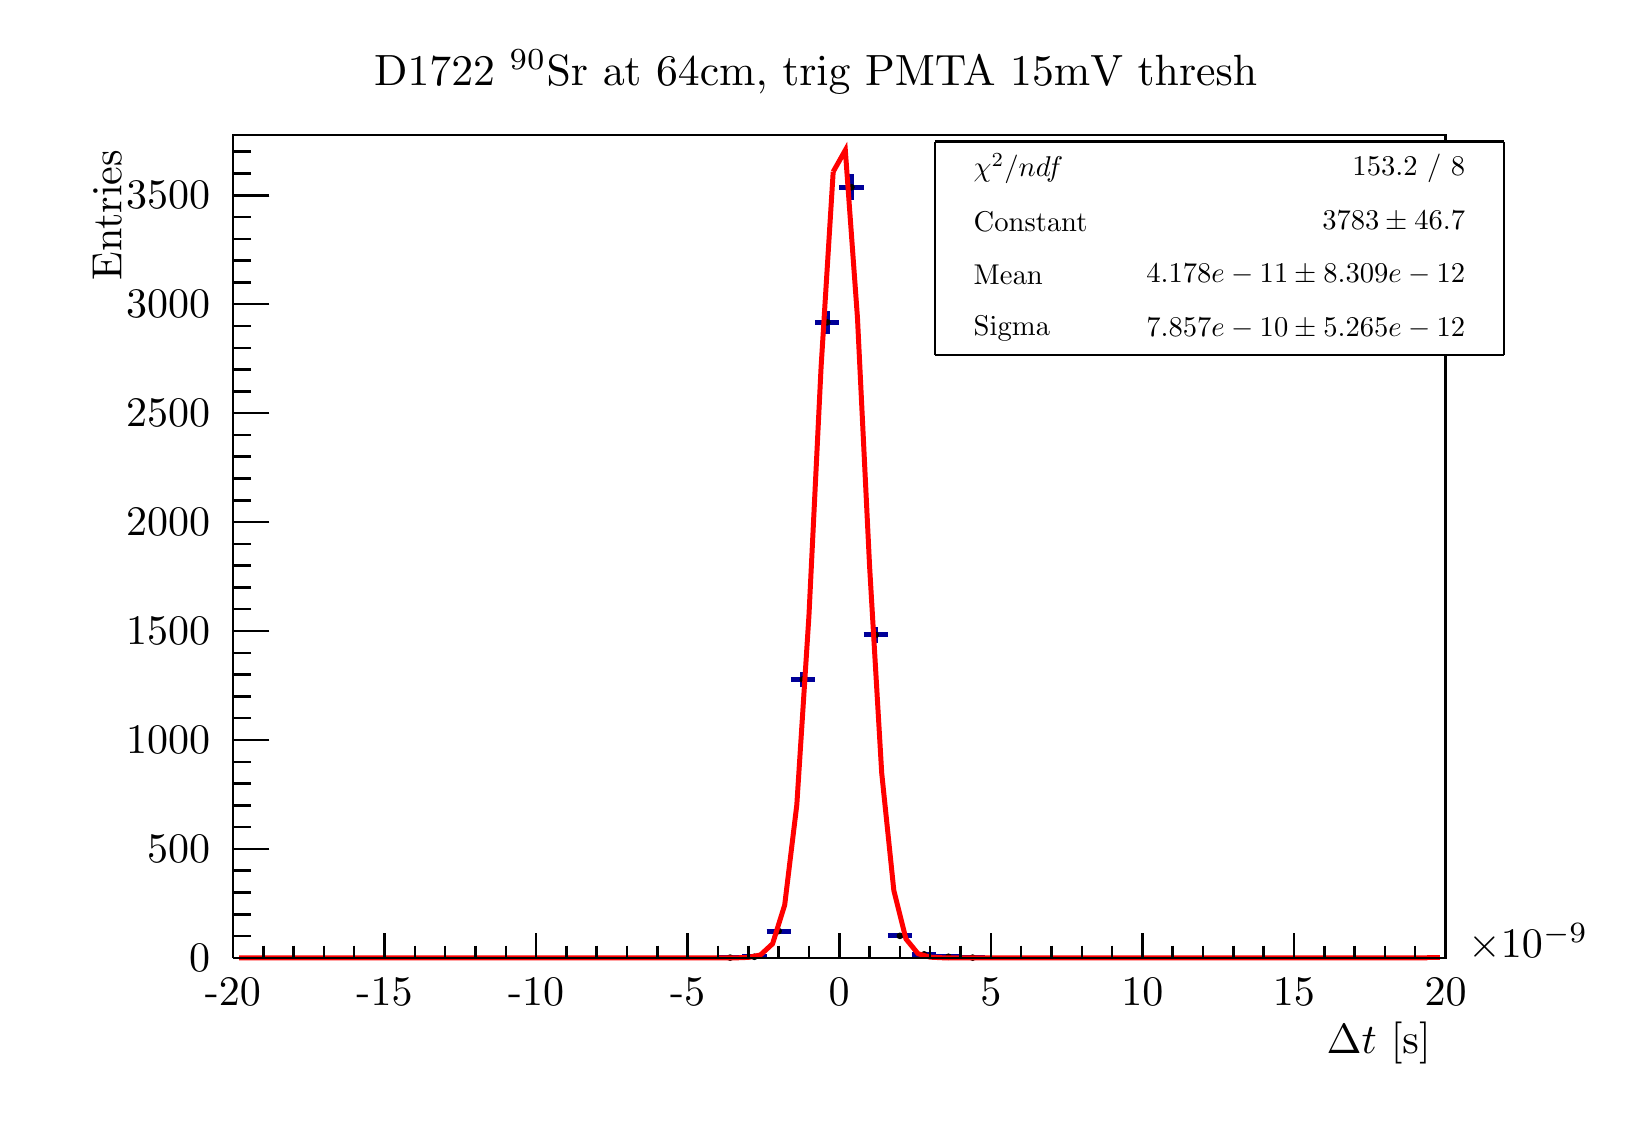
\begin{tikzpicture}
\pgfdeclareplotmark{cross} {
\pgfpathmoveto{\pgfpoint{-0.3\pgfplotmarksize}{\pgfplotmarksize}}
\pgfpathlineto{\pgfpoint{+0.3\pgfplotmarksize}{\pgfplotmarksize}}
\pgfpathlineto{\pgfpoint{+0.3\pgfplotmarksize}{0.3\pgfplotmarksize}}
\pgfpathlineto{\pgfpoint{+1\pgfplotmarksize}{0.3\pgfplotmarksize}}
\pgfpathlineto{\pgfpoint{+1\pgfplotmarksize}{-0.3\pgfplotmarksize}}
\pgfpathlineto{\pgfpoint{+0.3\pgfplotmarksize}{-0.3\pgfplotmarksize}}
\pgfpathlineto{\pgfpoint{+0.3\pgfplotmarksize}{-1.\pgfplotmarksize}}
\pgfpathlineto{\pgfpoint{-0.3\pgfplotmarksize}{-1.\pgfplotmarksize}}
\pgfpathlineto{\pgfpoint{-0.3\pgfplotmarksize}{-0.3\pgfplotmarksize}}
\pgfpathlineto{\pgfpoint{-1.\pgfplotmarksize}{-0.3\pgfplotmarksize}}
\pgfpathlineto{\pgfpoint{-1.\pgfplotmarksize}{0.3\pgfplotmarksize}}
\pgfpathlineto{\pgfpoint{-0.3\pgfplotmarksize}{0.3\pgfplotmarksize}}
\pgfpathclose
\pgfusepathqstroke
}
\pgfdeclareplotmark{cross*} {
\pgfpathmoveto{\pgfpoint{-0.3\pgfplotmarksize}{\pgfplotmarksize}}
\pgfpathlineto{\pgfpoint{+0.3\pgfplotmarksize}{\pgfplotmarksize}}
\pgfpathlineto{\pgfpoint{+0.3\pgfplotmarksize}{0.3\pgfplotmarksize}}
\pgfpathlineto{\pgfpoint{+1\pgfplotmarksize}{0.3\pgfplotmarksize}}
\pgfpathlineto{\pgfpoint{+1\pgfplotmarksize}{-0.3\pgfplotmarksize}}
\pgfpathlineto{\pgfpoint{+0.3\pgfplotmarksize}{-0.3\pgfplotmarksize}}
\pgfpathlineto{\pgfpoint{+0.3\pgfplotmarksize}{-1.\pgfplotmarksize}}
\pgfpathlineto{\pgfpoint{-0.3\pgfplotmarksize}{-1.\pgfplotmarksize}}
\pgfpathlineto{\pgfpoint{-0.3\pgfplotmarksize}{-0.3\pgfplotmarksize}}
\pgfpathlineto{\pgfpoint{-1.\pgfplotmarksize}{-0.3\pgfplotmarksize}}
\pgfpathlineto{\pgfpoint{-1.\pgfplotmarksize}{0.3\pgfplotmarksize}}
\pgfpathlineto{\pgfpoint{-0.3\pgfplotmarksize}{0.3\pgfplotmarksize}}
\pgfpathclose
\pgfusepathqfillstroke
}
\pgfdeclareplotmark{newstar} {
\pgfpathmoveto{\pgfqpoint{0pt}{\pgfplotmarksize}}
\pgfpathlineto{\pgfqpointpolar{44}{0.5\pgfplotmarksize}}
\pgfpathlineto{\pgfqpointpolar{18}{\pgfplotmarksize}}
\pgfpathlineto{\pgfqpointpolar{-20}{0.5\pgfplotmarksize}}
\pgfpathlineto{\pgfqpointpolar{-54}{\pgfplotmarksize}}
\pgfpathlineto{\pgfqpointpolar{-90}{0.5\pgfplotmarksize}}
\pgfpathlineto{\pgfqpointpolar{234}{\pgfplotmarksize}}
\pgfpathlineto{\pgfqpointpolar{198}{0.5\pgfplotmarksize}}
\pgfpathlineto{\pgfqpointpolar{162}{\pgfplotmarksize}}
\pgfpathlineto{\pgfqpointpolar{134}{0.5\pgfplotmarksize}}
\pgfpathclose
\pgfusepathqstroke
}
\pgfdeclareplotmark{newstar*} {
\pgfpathmoveto{\pgfqpoint{0pt}{\pgfplotmarksize}}
\pgfpathlineto{\pgfqpointpolar{44}{0.5\pgfplotmarksize}}
\pgfpathlineto{\pgfqpointpolar{18}{\pgfplotmarksize}}
\pgfpathlineto{\pgfqpointpolar{-20}{0.5\pgfplotmarksize}}
\pgfpathlineto{\pgfqpointpolar{-54}{\pgfplotmarksize}}
\pgfpathlineto{\pgfqpointpolar{-90}{0.5\pgfplotmarksize}}
\pgfpathlineto{\pgfqpointpolar{234}{\pgfplotmarksize}}
\pgfpathlineto{\pgfqpointpolar{198}{0.5\pgfplotmarksize}}
\pgfpathlineto{\pgfqpointpolar{162}{\pgfplotmarksize}}
\pgfpathlineto{\pgfqpointpolar{134}{0.5\pgfplotmarksize}}
\pgfpathclose
\pgfusepathqfillstroke
}
\definecolor{c}{rgb}{1,1,1};
\draw [color=c, fill=c] (0,0) rectangle (20,13.5705);
\draw [color=c, fill=c] (2.6,1.76416) rectangle (18,12.2134);
\definecolor{c}{rgb}{0,0,0};
\draw [c,line width=0.9] (2.6,1.76416) -- (2.6,12.2134) -- (18,12.2134) -- (18,1.76416) -- (2.6,1.76416);
\definecolor{c}{rgb}{1,1,1};
\draw [color=c, fill=c] (2.6,1.76416) rectangle (18,12.2134);
\definecolor{c}{rgb}{0,0,0};
\draw [c,line width=0.9] (2.6,1.76416) -- (2.6,12.2134) -- (18,12.2134) -- (18,1.76416) -- (2.6,1.76416);
\definecolor{c}{rgb}{0,0,0.6};
\draw [c,line width=1.8] (8.914,1.76416) -- (8.914,1.76693);
\draw [c,line width=1.8] (8.914,1.76693) -- (8.914,1.76969);
\draw [c,line width=1.8] (8.76,1.76693) -- (8.914,1.76693);
\draw [c,line width=1.8] (8.914,1.76693) -- (9.068,1.76693);
\definecolor{c}{rgb}{0,0,0};
\foreach \P in {(8.914,1.76693)}{\draw[mark options={color=c,fill=c},mark size=2.402402pt,mark=*,mark size=1pt] plot coordinates {\P};}
\definecolor{c}{rgb}{0,0,0.6};
\draw [c,line width=1.8] (9.222,1.77181) -- (9.222,1.77799);
\draw [c,line width=1.8] (9.222,1.77799) -- (9.222,1.78418);
\draw [c,line width=1.8] (9.068,1.77799) -- (9.222,1.77799);
\draw [c,line width=1.8] (9.222,1.77799) -- (9.376,1.77799);
\definecolor{c}{rgb}{0,0,0};
\foreach \P in {(9.222,1.77799)}{\draw[mark options={color=c,fill=c},mark size=2.402402pt,mark=*,mark size=1pt] plot coordinates {\P};}
\definecolor{c}{rgb}{0,0,0.6};
\draw [c,line width=1.8] (9.53,2.07382) -- (9.53,2.10451);
\draw [c,line width=1.8] (9.53,2.10451) -- (9.53,2.1352);
\draw [c,line width=1.8] (9.376,2.10451) -- (9.53,2.10451);
\draw [c,line width=1.8] (9.53,2.10451) -- (9.684,2.10451);
\definecolor{c}{rgb}{0,0,0};
\foreach \P in {(9.53,2.10451)}{\draw[mark options={color=c,fill=c},mark size=2.402402pt,mark=*,mark size=1pt] plot coordinates {\P};}
\definecolor{c}{rgb}{0,0,0.6};
\draw [c,line width=1.8] (9.838,5.20154) -- (9.838,5.30046);
\draw [c,line width=1.8] (9.838,5.30046) -- (9.838,5.39938);
\draw [c,line width=1.8] (9.684,5.30046) -- (9.838,5.30046);
\draw [c,line width=1.8] (9.838,5.30046) -- (9.992,5.30046);
\definecolor{c}{rgb}{0,0,0};
\foreach \P in {(9.838,5.30046)}{\draw[mark options={color=c,fill=c},mark size=2.402402pt,mark=*,mark size=1pt] plot coordinates {\P};}
\definecolor{c}{rgb}{0,0,0.6};
\draw [c,line width=1.8] (10.146,9.68623) -- (10.146,9.83568);
\draw [c,line width=1.8] (10.146,9.83568) -- (10.146,9.98513);
\draw [c,line width=1.8] (9.992,9.83568) -- (10.146,9.83568);
\draw [c,line width=1.8] (10.146,9.83568) -- (10.3,9.83568);
\definecolor{c}{rgb}{0,0,0};
\foreach \P in {(10.146,9.83568)}{\draw[mark options={color=c,fill=c},mark size=2.402402pt,mark=*,mark size=1pt] plot coordinates {\P};}
\definecolor{c}{rgb}{0,0,0.6};
\draw [c,line width=1.8] (10.454,11.3867) -- (10.454,11.5513);
\draw [c,line width=1.8] (10.454,11.5513) -- (10.454,11.7158);
\draw [c,line width=1.8] (10.3,11.5513) -- (10.454,11.5513);
\draw [c,line width=1.8] (10.454,11.5513) -- (10.608,11.5513);
\definecolor{c}{rgb}{0,0,0};
\foreach \P in {(10.454,11.5513)}{\draw[mark options={color=c,fill=c},mark size=2.402402pt,mark=*,mark size=1pt] plot coordinates {\P};}
\definecolor{c}{rgb}{0,0,0.6};
\draw [c,line width=1.8] (10.762,5.75842) -- (10.762,5.86495);
\draw [c,line width=1.8] (10.762,5.86495) -- (10.762,5.97147);
\draw [c,line width=1.8] (10.608,5.86495) -- (10.762,5.86495);
\draw [c,line width=1.8] (10.762,5.86495) -- (10.916,5.86495);
\definecolor{c}{rgb}{0,0,0};
\foreach \P in {(10.762,5.86495)}{\draw[mark options={color=c,fill=c},mark size=2.402402pt,mark=*,mark size=1pt] plot coordinates {\P};}
\definecolor{c}{rgb}{0,0,0.6};
\draw [c,line width=1.8] (11.07,2.01582) -- (11.07,2.04363);
\draw [c,line width=1.8] (11.07,2.04363) -- (11.07,2.07144);
\draw [c,line width=1.8] (10.916,2.04363) -- (11.07,2.04363);
\draw [c,line width=1.8] (11.07,2.04363) -- (11.224,2.04363);
\definecolor{c}{rgb}{0,0,0};
\foreach \P in {(11.07,2.04363)}{\draw[mark options={color=c,fill=c},mark size=2.402402pt,mark=*,mark size=1pt] plot coordinates {\P};}
\definecolor{c}{rgb}{0,0,0.6};
\draw [c,line width=1.8] (11.378,1.79736) -- (11.378,1.80843);
\draw [c,line width=1.8] (11.378,1.80843) -- (11.378,1.8195);
\draw [c,line width=1.8] (11.224,1.80843) -- (11.378,1.80843);
\draw [c,line width=1.8] (11.378,1.80843) -- (11.532,1.80843);
\definecolor{c}{rgb}{0,0,0};
\foreach \P in {(11.378,1.80843)}{\draw[mark options={color=c,fill=c},mark size=2.402402pt,mark=*,mark size=1pt] plot coordinates {\P};}
\definecolor{c}{rgb}{0,0,0.6};
\draw [c,line width=1.8] (11.686,1.77181) -- (11.686,1.77799);
\draw [c,line width=1.8] (11.686,1.77799) -- (11.686,1.78418);
\draw [c,line width=1.8] (11.532,1.77799) -- (11.686,1.77799);
\draw [c,line width=1.8] (11.686,1.77799) -- (11.84,1.77799);
\definecolor{c}{rgb}{0,0,0};
\foreach \P in {(11.686,1.77799)}{\draw[mark options={color=c,fill=c},mark size=2.402402pt,mark=*,mark size=1pt] plot coordinates {\P};}
\definecolor{c}{rgb}{0,0,0.6};
\draw [c,line width=1.8] (11.994,1.76416) -- (11.994,1.76693);
\draw [c,line width=1.8] (11.994,1.76693) -- (11.994,1.76969);
\draw [c,line width=1.8] (11.84,1.76693) -- (11.994,1.76693);
\draw [c,line width=1.8] (11.994,1.76693) -- (12.148,1.76693);
\definecolor{c}{rgb}{0,0,0};
\foreach \P in {(11.994,1.76693)}{\draw[mark options={color=c,fill=c},mark size=2.402402pt,mark=*,mark size=1pt] plot coordinates {\P};}
\definecolor{c}{rgb}{1,0,0};
\draw [c,line width=1.8] (2.677,1.76416) -- (2.831,1.76416) -- (2.985,1.76416) -- (3.139,1.76416) -- (3.293,1.76416) -- (3.447,1.76416) -- (3.601,1.76416) -- (3.755,1.76416) -- (3.909,1.76416) -- (4.063,1.76416) -- (4.217,1.76416) -- (4.371,1.76416)
 -- (4.525,1.76416) -- (4.679,1.76416) -- (4.833,1.76416) -- (4.987,1.76416) -- (5.141,1.76416) -- (5.295,1.76416) -- (5.449,1.76416) -- (5.603,1.76416) -- (5.757,1.76416) -- (5.911,1.76416) -- (6.065,1.76416) -- (6.219,1.76416) -- (6.373,1.76416) --
 (6.527,1.76416) -- (6.681,1.76416) -- (6.835,1.76416) -- (6.989,1.76416) -- (7.143,1.76416) -- (7.297,1.76416) -- (7.451,1.76416) -- (7.605,1.76416) -- (7.759,1.76416) -- (7.913,1.76416) -- (8.067,1.76416) -- (8.221,1.76416) -- (8.375,1.76416) --
 (8.529,1.76416) -- (8.683,1.76416) -- (8.837,1.76416) -- (8.991,1.76416) -- (9.145,1.76998) -- (9.299,1.80089) -- (9.453,1.94285) -- (9.607,2.43506) -- (9.761,3.70796) -- (9.915,6.11015) -- (10.069,9.26248) -- (10.223,11.7476);
\draw [c,line width=1.8] (10.223,11.7476) -- (10.377,12.0215) -- (10.531,9.89679) -- (10.685,6.74) -- (10.839,4.11347) -- (10.993,2.62012) -- (11.147,2.00482) -- (11.301,1.81637) -- (11.455,1.7729) -- (11.609,1.76529) -- (11.763,1.76416) --
 (11.917,1.76416) -- (12.071,1.76416) -- (12.225,1.76416) -- (12.379,1.76416) -- (12.533,1.76416) -- (12.687,1.76416) -- (12.841,1.76416) -- (12.995,1.76416) -- (13.149,1.76416) -- (13.303,1.76416) -- (13.457,1.76416) -- (13.611,1.76416) --
 (13.765,1.76416) -- (13.919,1.76416) -- (14.073,1.76416) -- (14.227,1.76416) -- (14.381,1.76416) -- (14.535,1.76416) -- (14.689,1.76416) -- (14.843,1.76416) -- (14.997,1.76416) -- (15.151,1.76416) -- (15.305,1.76416) -- (15.459,1.76416) --
 (15.613,1.76416) -- (15.767,1.76416) -- (15.921,1.76416) -- (16.075,1.76416) -- (16.229,1.76416) -- (16.383,1.76416) -- (16.537,1.76416) -- (16.691,1.76416) -- (16.845,1.76416) -- (16.999,1.76416) -- (17.153,1.76416) -- (17.307,1.76416) --
 (17.461,1.76416) -- (17.615,1.76416) -- (17.769,1.76416);
\draw [c,line width=1.8] (17.769,1.76416) -- (17.923,1.76416);
\definecolor{c}{rgb}{1,1,1};
\draw [color=c, fill=c] (11.5186,9.42152) rectangle (18.7393,12.1299);
\definecolor{c}{rgb}{0,0,0};
\draw [c,line width=0.9] (11.5186,9.42152) -- (18.7393,9.42152);
\draw [c,line width=0.9] (18.7393,9.42152) -- (18.7393,12.1299);
\draw [c,line width=0.9] (18.7393,12.1299) -- (11.5186,12.1299);
\draw [c,line width=0.9] (11.5186,12.1299) -- (11.5186,9.42152);
\draw [anchor= west] (11.8797,11.7913) node[scale=1.03301, color=c, rotate=0]{$\chi^{2} / ndf $};
\draw [anchor= east] (18.3782,11.7913) node[scale=1.03301, color=c, rotate=0]{ 153.2 / 8};
\draw [anchor= west] (11.8797,11.1142) node[scale=1.03301, color=c, rotate=0]{Constant };
\draw [anchor= east] (18.3782,11.1142) node[scale=1.03301, color=c, rotate=0]{$  3783 \pm 46.7$};
\draw [anchor= west] (11.8797,10.4371) node[scale=1.03301, color=c, rotate=0]{Mean     };
\draw [anchor= east] (18.3782,10.4371) node[scale=1.03301, color=c, rotate=0]{$ 4.178e-11 \pm 8.309e-12$};
\draw [anchor= west] (11.8797,9.76007) node[scale=1.03301, color=c, rotate=0]{Sigma    };
\draw [anchor= east] (18.3782,9.76007) node[scale=1.03301, color=c, rotate=0]{$ 7.857e-10 \pm 5.265e-12$};
\draw [c,line width=0.9] (2.6,1.76416) -- (18,1.76416);
\draw [c,line width=0.9] (2.6,2.07764) -- (2.6,1.76416);
\draw [c,line width=0.9] (2.985,1.9209) -- (2.985,1.76416);
\draw [c,line width=0.9] (3.37,1.9209) -- (3.37,1.76416);
\draw [c,line width=0.9] (3.755,1.9209) -- (3.755,1.76416);
\draw [c,line width=0.9] (4.14,1.9209) -- (4.14,1.76416);
\draw [c,line width=0.9] (4.525,2.07764) -- (4.525,1.76416);
\draw [c,line width=0.9] (4.91,1.9209) -- (4.91,1.76416);
\draw [c,line width=0.9] (5.295,1.9209) -- (5.295,1.76416);
\draw [c,line width=0.9] (5.68,1.9209) -- (5.68,1.76416);
\draw [c,line width=0.9] (6.065,1.9209) -- (6.065,1.76416);
\draw [c,line width=0.9] (6.45,2.07764) -- (6.45,1.76416);
\draw [c,line width=0.9] (6.835,1.9209) -- (6.835,1.76416);
\draw [c,line width=0.9] (7.22,1.9209) -- (7.22,1.76416);
\draw [c,line width=0.9] (7.605,1.9209) -- (7.605,1.76416);
\draw [c,line width=0.9] (7.99,1.9209) -- (7.99,1.76416);
\draw [c,line width=0.9] (8.375,2.07764) -- (8.375,1.76416);
\draw [c,line width=0.9] (8.76,1.9209) -- (8.76,1.76416);
\draw [c,line width=0.9] (9.145,1.9209) -- (9.145,1.76416);
\draw [c,line width=0.9] (9.53,1.9209) -- (9.53,1.76416);
\draw [c,line width=0.9] (9.915,1.9209) -- (9.915,1.76416);
\draw [c,line width=0.9] (10.3,2.07764) -- (10.3,1.76416);
\draw [c,line width=0.9] (10.685,1.9209) -- (10.685,1.76416);
\draw [c,line width=0.9] (11.07,1.9209) -- (11.07,1.76416);
\draw [c,line width=0.9] (11.455,1.9209) -- (11.455,1.76416);
\draw [c,line width=0.9] (11.84,1.9209) -- (11.84,1.76416);
\draw [c,line width=0.9] (12.225,2.07764) -- (12.225,1.76416);
\draw [c,line width=0.9] (12.61,1.9209) -- (12.61,1.76416);
\draw [c,line width=0.9] (12.995,1.9209) -- (12.995,1.76416);
\draw [c,line width=0.9] (13.38,1.9209) -- (13.38,1.76416);
\draw [c,line width=0.9] (13.765,1.9209) -- (13.765,1.76416);
\draw [c,line width=0.9] (14.15,2.07764) -- (14.15,1.76416);
\draw [c,line width=0.9] (14.535,1.9209) -- (14.535,1.76416);
\draw [c,line width=0.9] (14.92,1.9209) -- (14.92,1.76416);
\draw [c,line width=0.9] (15.305,1.9209) -- (15.305,1.76416);
\draw [c,line width=0.9] (15.69,1.9209) -- (15.69,1.76416);
\draw [c,line width=0.9] (16.075,2.07764) -- (16.075,1.76416);
\draw [c,line width=0.9] (16.46,1.9209) -- (16.46,1.76416);
\draw [c,line width=0.9] (16.845,1.9209) -- (16.845,1.76416);
\draw [c,line width=0.9] (17.23,1.9209) -- (17.23,1.76416);
\draw [c,line width=0.9] (17.615,1.9209) -- (17.615,1.76416);
\draw [c,line width=0.9] (18,2.07764) -- (18,1.76416);
\draw [anchor=base] (2.6,1.15349) node[scale=1.51913, color=c, rotate=0]{-20};
\draw [anchor=base] (4.525,1.15349) node[scale=1.51913, color=c, rotate=0]{-15};
\draw [anchor=base] (6.45,1.15349) node[scale=1.51913, color=c, rotate=0]{-10};
\draw [anchor=base] (8.375,1.15349) node[scale=1.51913, color=c, rotate=0]{-5};
\draw [anchor=base] (10.3,1.15349) node[scale=1.51913, color=c, rotate=0]{0};
\draw [anchor=base] (12.225,1.15349) node[scale=1.51913, color=c, rotate=0]{5};
\draw [anchor=base] (14.15,1.15349) node[scale=1.51913, color=c, rotate=0]{10};
\draw [anchor=base] (16.075,1.15349) node[scale=1.51913, color=c, rotate=0]{15};
\draw [anchor=base] (18,1.15349) node[scale=1.51913, color=c, rotate=0]{20};
\draw [anchor=base west] (18.1,1.76416) node[scale=1.51913, color=c, rotate=0]{$\times10^{-9}$};
\draw [anchor= east] (18,0.678523) node[scale=1.51913, color=c, rotate=0]{$\Delta t$ [s]};
\draw [c,line width=0.9] (2.6,1.76416) -- (2.6,12.2134);
\draw [c,line width=0.9] (3.062,1.76416) -- (2.6,1.76416);
\draw [c,line width=0.9] (2.831,2.04086) -- (2.6,2.04086);
\draw [c,line width=0.9] (2.831,2.31757) -- (2.6,2.31757);
\draw [c,line width=0.9] (2.831,2.59428) -- (2.6,2.59428);
\draw [c,line width=0.9] (2.831,2.87098) -- (2.6,2.87098);
\draw [c,line width=0.9] (3.062,3.14769) -- (2.6,3.14769);
\draw [c,line width=0.9] (2.831,3.4244) -- (2.6,3.4244);
\draw [c,line width=0.9] (2.831,3.7011) -- (2.6,3.7011);
\draw [c,line width=0.9] (2.831,3.97781) -- (2.6,3.97781);
\draw [c,line width=0.9] (2.831,4.25451) -- (2.6,4.25451);
\draw [c,line width=0.9] (3.062,4.53122) -- (2.6,4.53122);
\draw [c,line width=0.9] (2.831,4.80793) -- (2.6,4.80793);
\draw [c,line width=0.9] (2.831,5.08463) -- (2.6,5.08463);
\draw [c,line width=0.9] (2.831,5.36134) -- (2.6,5.36134);
\draw [c,line width=0.9] (2.831,5.63805) -- (2.6,5.63805);
\draw [c,line width=0.9] (3.062,5.91475) -- (2.6,5.91475);
\draw [c,line width=0.9] (2.831,6.19146) -- (2.6,6.19146);
\draw [c,line width=0.9] (2.831,6.46816) -- (2.6,6.46816);
\draw [c,line width=0.9] (2.831,6.74487) -- (2.6,6.74487);
\draw [c,line width=0.9] (2.831,7.02158) -- (2.6,7.02158);
\draw [c,line width=0.9] (3.062,7.29828) -- (2.6,7.29828);
\draw [c,line width=0.9] (2.831,7.57499) -- (2.6,7.57499);
\draw [c,line width=0.9] (2.831,7.8517) -- (2.6,7.8517);
\draw [c,line width=0.9] (2.831,8.1284) -- (2.6,8.1284);
\draw [c,line width=0.9] (2.831,8.40511) -- (2.6,8.40511);
\draw [c,line width=0.9] (3.062,8.68182) -- (2.6,8.68182);
\draw [c,line width=0.9] (2.831,8.95852) -- (2.6,8.95852);
\draw [c,line width=0.9] (2.831,9.23523) -- (2.6,9.23523);
\draw [c,line width=0.9] (2.831,9.51193) -- (2.6,9.51193);
\draw [c,line width=0.9] (2.831,9.78864) -- (2.6,9.78864);
\draw [c,line width=0.9] (3.062,10.0653) -- (2.6,10.0653);
\draw [c,line width=0.9] (2.831,10.3421) -- (2.6,10.3421);
\draw [c,line width=0.9] (2.831,10.6188) -- (2.6,10.6188);
\draw [c,line width=0.9] (2.831,10.8955) -- (2.6,10.8955);
\draw [c,line width=0.9] (2.831,11.1722) -- (2.6,11.1722);
\draw [c,line width=0.9] (3.062,11.4489) -- (2.6,11.4489);
\draw [c,line width=0.9] (3.062,11.4489) -- (2.6,11.4489);
\draw [c,line width=0.9] (2.831,11.7256) -- (2.6,11.7256);
\draw [c,line width=0.9] (2.831,12.0023) -- (2.6,12.0023);
\draw [anchor= east] (2.5,1.76416) node[scale=1.51913, color=c, rotate=0]{0};
\draw [anchor= east] (2.5,3.14769) node[scale=1.51913, color=c, rotate=0]{500};
\draw [anchor= east] (2.5,4.53122) node[scale=1.51913, color=c, rotate=0]{1000};
\draw [anchor= east] (2.5,5.91475) node[scale=1.51913, color=c, rotate=0]{1500};
\draw [anchor= east] (2.5,7.29828) node[scale=1.51913, color=c, rotate=0]{2000};
\draw [anchor= east] (2.5,8.68182) node[scale=1.51913, color=c, rotate=0]{2500};
\draw [anchor= east] (2.5,10.0653) node[scale=1.51913, color=c, rotate=0]{3000};
\draw [anchor= east] (2.5,11.4489) node[scale=1.51913, color=c, rotate=0]{3500};
\draw [anchor= east] (1,12.2134) node[scale=1.51913, color=c, rotate=90]{Entries};
\definecolor{c}{rgb}{1,1,1};
\draw [color=c, fill=c] (11.5186,9.42152) rectangle (18.7393,12.1299);
\definecolor{c}{rgb}{0,0,0};
\draw [c,line width=0.9] (11.5186,9.42152) -- (18.7393,9.42152);
\draw [c,line width=0.9] (18.7393,9.42152) -- (18.7393,12.1299);
\draw [c,line width=0.9] (18.7393,12.1299) -- (11.5186,12.1299);
\draw [c,line width=0.9] (11.5186,12.1299) -- (11.5186,9.42152);
\draw [anchor= west] (11.8797,11.7913) node[scale=1.03301, color=c, rotate=0]{$\chi^{2} / ndf $};
\draw [anchor= east] (18.3782,11.7913) node[scale=1.03301, color=c, rotate=0]{ 153.2 / 8};
\draw [anchor= west] (11.8797,11.1142) node[scale=1.03301, color=c, rotate=0]{Constant };
\draw [anchor= east] (18.3782,11.1142) node[scale=1.03301, color=c, rotate=0]{$  3783 \pm 46.7$};
\draw [anchor= west] (11.8797,10.4371) node[scale=1.03301, color=c, rotate=0]{Mean     };
\draw [anchor= east] (18.3782,10.4371) node[scale=1.03301, color=c, rotate=0]{$ 4.178e-11 \pm 8.309e-12$};
\draw [anchor= west] (11.8797,9.76007) node[scale=1.03301, color=c, rotate=0]{Sigma    };
\draw [anchor= east] (18.3782,9.76007) node[scale=1.03301, color=c, rotate=0]{$ 7.857e-10 \pm 5.265e-12$};
\draw (10,13.0186) node[scale=1.5799, color=c, rotate=0]{D1722 $^{90}$Sr at 64cm, trig PMTA 15mV thresh};
\end{tikzpicture}

  \end{adjustbox}
  \caption{Difference in signal arrival time PMTs at each end of a bar as measured using a $^{90}$Sr source placed 64~cm from one end of the bar.}
  \label{fig:s4Res}	
\end{figure}

\begin{figure}[ht]    
  \centering
  \includegraphics[width=0.5\linewidth]{files/Figures/dstofFront2.png}
  \hfill
  \includegraphics[width=0.35\linewidth]{files/Figures/dstofDiag2.png}
  \caption{Front (left) and rotated (right) view of the $\mathit{S4}$. The rotated view shows more clearly the staggering of the scintillator bars and PMTs.}
  \label{fig:dstofDiagram}
\end{figure}

The anode signals of all 20 of the PMTs are discriminated using LeCroy 620AL NIM discriminators, at a threshold of 20~mV.
The discriminated signals are then fed into a time-to-digital converter (TDC). A signal in $\mathit{S4}$ is deemed to have occurred if a signal is seen in both PMTs, above the discriminator threshold, on the same bar within 20~ns of each other. 
This timing window is determined through testing performed with a $^{90}$Sr source at known positions on the bar.

The $\mathit{S1-S2}$ coincidence signal is digitized by the same TDC. This signal is used to calculate the particle time of flight from $\mathit{S2}$ to $\mathit{S4}$.

\subsection{The HPTPC Prototype}
For the characterisation of the beam using the ToF systems described in this paper, the relevant characteristics of the HPTPC prototype are the location and thickness of the steel vessel walls.
The cylindrical steel vessel has a 142~cm outer diameter; the main body is 60 cm in length and the rounded end caps protrude an additional 37~cm on each end.
With 1~cm thick walls it is rated to 6~barA of pressure.
The vessel wall thickness is equivalent to the range of a proton with a kinetic energy of approximately 80~MeV~\cite{rangeTables}.
The angular position of the center of the TPC is approximately $\theta = -2.5^{\circ}$. 
More details of the position and extent of the TPC are given in Table~\ref{tab:angS1} and Table~\ref{tab:distances}.
 
The active TPC is a cylinder, 111~cm in diameter and 48~cm in length; the TPC comprised thin steel mesh electrodes (one cathode and three anodes), and 12 copper rings to create the uniform drift field. The anodes were supported by a hexagonal aluminium stiffener on the side facing away from the camera.
Data taking with the TPC made use of both optical and charge readout.
The vessel, electrodes, and drift region of the TPC are shown in Figure~\ref{fig:TPC}.

\begin{figure}
  \centering
  \includegraphics[width=.88\linewidth]{files/Figures/vesselView.pdf}
  \caption{Cross-sectional view of the TPC; the thin mesh electrodes and copper ring drift volume can be seen inside the steel vessel. The walls of the vessel shown are 1~cm thick with a vessel outer diameter of 142~cm. At the point of hitting the vessel, the beam centre was 1~cm below the centre of the vessel vertically, where the distance from the inside of the vessel wall to the drift region was 15~cm.}
   \label{fig:TPC}
   %Vessel: wall thickness 1cm, beam centre height -1.14cm, 
\end{figure}

Throughout the run, the TPC was filled with either pure argon, or a combination of argon and a small percentage of quencher.
The performance of this TPC is the subject of a forthcoming publication~\cite{Deisting:2020aaa}.


	% HPTPC description
	\section{Analysis}
\label{hptpcPaper:sec:Analysis}
\subsection{Analysis Goals}

The primary aim of this analysis are to assess the feasibility of using the combination of off-axis positioning and a moderated beam to produce particles with momenta covering the range of momenta of particles produced in GeV-scale neutrino interactions and to characterize the incident flux on the TPC and exiting the TPC, for the TPC data analysis.

The numbers of spills recorded for each number of moderator blocks are shown in Table~\ref{tab:spills}.
More data were collected for 4 blocks as that was the configuration used for the majority of the beam test.

\begin{table}
  \centering
  \caption{Total number of spills recorded for each moderator block configuration included in this paper.}
  \begin{tabular}{c|c}
    \hline
    \hline
    Number of moderator blocks & Recorded spills \\
    \hline
    0 & 257 \\
    1 & 254 \\
    2 & 267 \\
    3 & 220 \\
    4 & 3884 \\
    \hline
  \end{tabular}
  \label{tab:spills}
\end{table}


\subsection{Time of flight analysis}
\label{timeofflightanalysissubsec}

%Protons take longer to travel the distance from \textit{S1} to \textit{S3} or \textit{S4} than lighter particles that are close to being minimum ionising.
%This difference in time of flight can be used to distinguish between the two types of particles.
%Distinguishing these MIPs from one another is more difficult due to their similar masses and can be only determined by the upstream ToF system.
%From the particle flux data, it is possible to measure the ratio of protons to other particles over the range of off-axis angles covered by the \textit{S3} and \textit{S4} walls, and for varying numbers of moderator blocks.

A particle of mass $m$ with momentum $p$ will traverse a distance $d$ in a time
\begin{align}
  t = d \sqrt{\frac{m^2}{p^2} + \frac{1}{c^2}} \,, 
\end{align}
where $c$ is the speed of light in a vacuum.
Therefore, particles with a greater momentum or smaller mass will cross the same distance in a shorter time.
This means that a beam of particles of different species but with the same momenta (as is produced by magnetic selection) can be separated by particle mass by measuring the time of flight, $t$.

For example, a charged pion with a momentum of 0.8~GeV/c will have a time of flight from $\mathit{S1}$ to $\mathit{S3}$ (a distance of 10.8~m) of 37~ns, while a proton with the same momentum will have a time of flight of 55~ns.
For the same two particles travelling between $\mathit{S2}$ and $\mathit{S4}$ (a distance of 12.7~m), the charged pion would have a time of flight of 43~ns and the proton would have a time of flight of 65~ns.
Figure~\ref{fig:s1s3PredTimes} shows the predicted time of flight for various particle species across the $\mathit{S1}-\mathit{S3}$ distance and the $\mathit{S2}-\mathit{S4}$ distance respectively.

\begin{figure}[ht]
  
  \begin{minipage}[t]{0.49\textwidth}
    \begin{adjustbox}{max totalsize={\textwidth}{.5\textheight},center}
      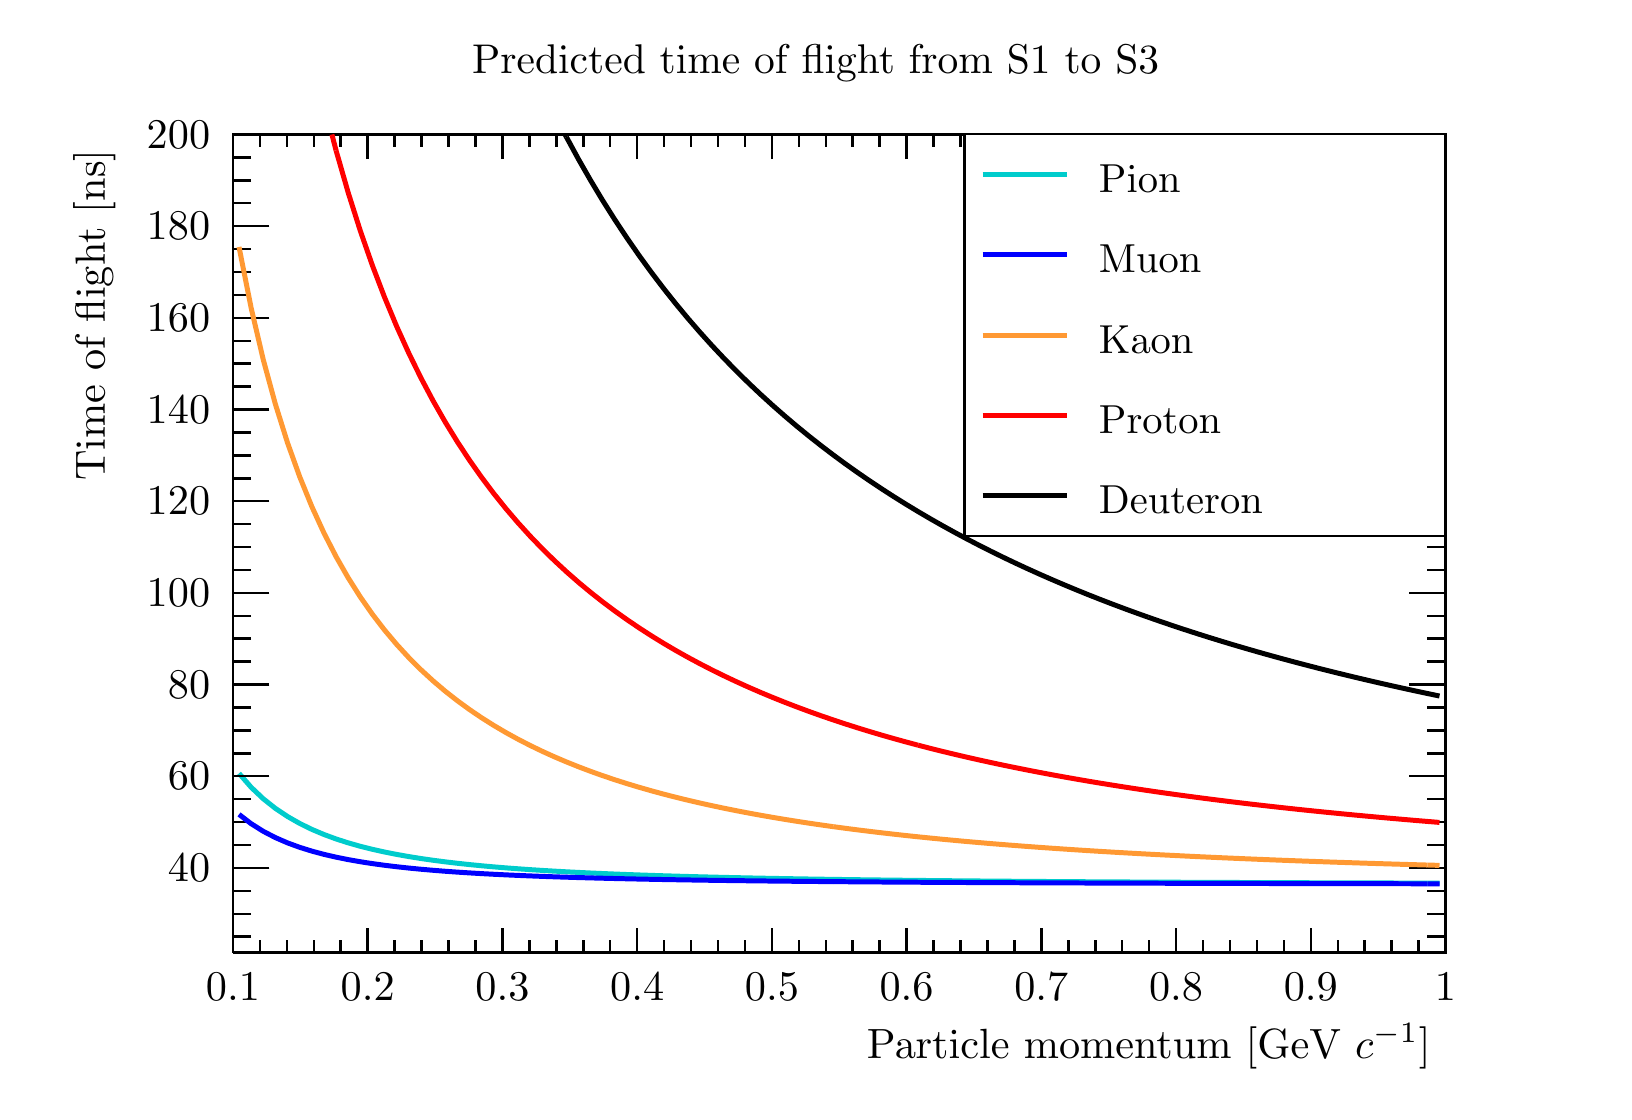
\begin{tikzpicture}
\pgfdeclareplotmark{cross} {
\pgfpathmoveto{\pgfpoint{-0.3\pgfplotmarksize}{\pgfplotmarksize}}
\pgfpathlineto{\pgfpoint{+0.3\pgfplotmarksize}{\pgfplotmarksize}}
\pgfpathlineto{\pgfpoint{+0.3\pgfplotmarksize}{0.3\pgfplotmarksize}}
\pgfpathlineto{\pgfpoint{+1\pgfplotmarksize}{0.3\pgfplotmarksize}}
\pgfpathlineto{\pgfpoint{+1\pgfplotmarksize}{-0.3\pgfplotmarksize}}
\pgfpathlineto{\pgfpoint{+0.3\pgfplotmarksize}{-0.3\pgfplotmarksize}}
\pgfpathlineto{\pgfpoint{+0.3\pgfplotmarksize}{-1.\pgfplotmarksize}}
\pgfpathlineto{\pgfpoint{-0.3\pgfplotmarksize}{-1.\pgfplotmarksize}}
\pgfpathlineto{\pgfpoint{-0.3\pgfplotmarksize}{-0.3\pgfplotmarksize}}
\pgfpathlineto{\pgfpoint{-1.\pgfplotmarksize}{-0.3\pgfplotmarksize}}
\pgfpathlineto{\pgfpoint{-1.\pgfplotmarksize}{0.3\pgfplotmarksize}}
\pgfpathlineto{\pgfpoint{-0.3\pgfplotmarksize}{0.3\pgfplotmarksize}}
\pgfpathclose
\pgfusepathqstroke
}
\pgfdeclareplotmark{cross*} {
\pgfpathmoveto{\pgfpoint{-0.3\pgfplotmarksize}{\pgfplotmarksize}}
\pgfpathlineto{\pgfpoint{+0.3\pgfplotmarksize}{\pgfplotmarksize}}
\pgfpathlineto{\pgfpoint{+0.3\pgfplotmarksize}{0.3\pgfplotmarksize}}
\pgfpathlineto{\pgfpoint{+1\pgfplotmarksize}{0.3\pgfplotmarksize}}
\pgfpathlineto{\pgfpoint{+1\pgfplotmarksize}{-0.3\pgfplotmarksize}}
\pgfpathlineto{\pgfpoint{+0.3\pgfplotmarksize}{-0.3\pgfplotmarksize}}
\pgfpathlineto{\pgfpoint{+0.3\pgfplotmarksize}{-1.\pgfplotmarksize}}
\pgfpathlineto{\pgfpoint{-0.3\pgfplotmarksize}{-1.\pgfplotmarksize}}
\pgfpathlineto{\pgfpoint{-0.3\pgfplotmarksize}{-0.3\pgfplotmarksize}}
\pgfpathlineto{\pgfpoint{-1.\pgfplotmarksize}{-0.3\pgfplotmarksize}}
\pgfpathlineto{\pgfpoint{-1.\pgfplotmarksize}{0.3\pgfplotmarksize}}
\pgfpathlineto{\pgfpoint{-0.3\pgfplotmarksize}{0.3\pgfplotmarksize}}
\pgfpathclose
\pgfusepathqfillstroke
}
\pgfdeclareplotmark{newstar} {
\pgfpathmoveto{\pgfqpoint{0pt}{\pgfplotmarksize}}
\pgfpathlineto{\pgfqpointpolar{44}{0.5\pgfplotmarksize}}
\pgfpathlineto{\pgfqpointpolar{18}{\pgfplotmarksize}}
\pgfpathlineto{\pgfqpointpolar{-20}{0.5\pgfplotmarksize}}
\pgfpathlineto{\pgfqpointpolar{-54}{\pgfplotmarksize}}
\pgfpathlineto{\pgfqpointpolar{-90}{0.5\pgfplotmarksize}}
\pgfpathlineto{\pgfqpointpolar{234}{\pgfplotmarksize}}
\pgfpathlineto{\pgfqpointpolar{198}{0.5\pgfplotmarksize}}
\pgfpathlineto{\pgfqpointpolar{162}{\pgfplotmarksize}}
\pgfpathlineto{\pgfqpointpolar{134}{0.5\pgfplotmarksize}}
\pgfpathclose
\pgfusepathqstroke
}
\pgfdeclareplotmark{newstar*} {
\pgfpathmoveto{\pgfqpoint{0pt}{\pgfplotmarksize}}
\pgfpathlineto{\pgfqpointpolar{44}{0.5\pgfplotmarksize}}
\pgfpathlineto{\pgfqpointpolar{18}{\pgfplotmarksize}}
\pgfpathlineto{\pgfqpointpolar{-20}{0.5\pgfplotmarksize}}
\pgfpathlineto{\pgfqpointpolar{-54}{\pgfplotmarksize}}
\pgfpathlineto{\pgfqpointpolar{-90}{0.5\pgfplotmarksize}}
\pgfpathlineto{\pgfqpointpolar{234}{\pgfplotmarksize}}
\pgfpathlineto{\pgfqpointpolar{198}{0.5\pgfplotmarksize}}
\pgfpathlineto{\pgfqpointpolar{162}{\pgfplotmarksize}}
\pgfpathlineto{\pgfqpointpolar{134}{0.5\pgfplotmarksize}}
\pgfpathclose
\pgfusepathqfillstroke
}
\definecolor{c}{rgb}{1,1,1};
\draw [color=c, fill=c] (0,0) rectangle (20,13.4957);
\draw [color=c, fill=c] (2.6,1.75444) rectangle (18,12.1461);
\definecolor{c}{rgb}{0,0,0};
\draw [c,line width=0.9] (2.6,1.75444) -- (2.6,12.1461) -- (18,12.1461) -- (18,1.75444) -- (2.6,1.75444);
\definecolor{c}{rgb}{1,1,1};
\draw [color=c, fill=c] (2.6,1.75444) rectangle (18,12.1461);
\definecolor{c}{rgb}{0,0,0};
\draw [c,line width=0.9] (2.6,1.75444) -- (2.6,12.1461) -- (18,12.1461) -- (18,1.75444) -- (2.6,1.75444);
\definecolor{c}{rgb}{0,0.8,0.8};
\draw [c,line width=1.8] (2.677,4.03245) -- (2.831,3.85576) -- (2.985,3.70973) -- (3.139,3.58764) -- (3.293,3.48457) -- (3.447,3.39679) -- (3.601,3.32144) -- (3.755,3.2563) -- (3.909,3.19963) -- (4.063,3.15005) -- (4.217,3.10642) -- (4.371,3.06785)
 -- (4.525,3.03359) -- (4.679,3.00304) -- (4.833,2.97568) -- (4.987,2.95108) -- (5.141,2.9289) -- (5.295,2.90884) -- (5.449,2.89062) -- (5.603,2.87404) -- (5.757,2.85891) -- (5.911,2.84507) -- (6.065,2.83237) -- (6.219,2.82069) -- (6.373,2.80993) --
 (6.527,2.8) -- (6.681,2.79081) -- (6.835,2.78229) -- (6.989,2.77438) -- (7.143,2.76702) -- (7.297,2.76017) -- (7.451,2.75377) -- (7.605,2.74779) -- (7.759,2.7422) -- (7.913,2.73696) -- (8.067,2.73203) -- (8.221,2.72741) -- (8.375,2.72306) --
 (8.529,2.71896) -- (8.683,2.7151) -- (8.837,2.71145) -- (8.991,2.708) -- (9.145,2.70474) -- (9.299,2.70165) -- (9.453,2.69873) -- (9.607,2.69595) -- (9.761,2.69331) -- (9.915,2.69081) -- (10.069,2.68842) -- (10.223,2.68615);
\draw [c,line width=1.8] (10.223,2.68615) -- (10.377,2.68399) -- (10.531,2.68193) -- (10.685,2.67997) -- (10.839,2.67809) -- (10.993,2.6763) -- (11.147,2.67458) -- (11.301,2.67294) -- (11.455,2.67137) -- (11.609,2.66986) -- (11.763,2.66842) --
 (11.917,2.66704) -- (12.071,2.66571) -- (12.225,2.66444) -- (12.379,2.66322) -- (12.533,2.66204) -- (12.687,2.66091) -- (12.841,2.65982) -- (12.995,2.65877) -- (13.149,2.65776) -- (13.303,2.65679) -- (13.457,2.65585) -- (13.611,2.65495) --
 (13.765,2.65408) -- (13.919,2.65324) -- (14.073,2.65243) -- (14.227,2.65164) -- (14.381,2.65088) -- (14.535,2.65015) -- (14.689,2.64944) -- (14.843,2.64876) -- (14.997,2.64809) -- (15.151,2.64745) -- (15.305,2.64683) -- (15.459,2.64623) --
 (15.613,2.64564) -- (15.767,2.64508) -- (15.921,2.64453) -- (16.075,2.644) -- (16.229,2.64348) -- (16.383,2.64298) -- (16.537,2.64249) -- (16.691,2.64202) -- (16.845,2.64156) -- (16.999,2.64111) -- (17.153,2.64068) -- (17.307,2.64026) --
 (17.461,2.63985) -- (17.615,2.63945) -- (17.769,2.63906);
\draw [c,line width=1.8] (17.769,2.63906) -- (17.923,2.63869);
\definecolor{c}{rgb}{0,0,0};
\draw [c,line width=0.9] (2.6,1.75444) -- (18,1.75444);
\draw [c,line width=0.9] (2.6,2.06619) -- (2.6,1.75444);
\draw [c,line width=0.9] (2.94222,1.91032) -- (2.94222,1.75444);
\draw [c,line width=0.9] (3.28444,1.91032) -- (3.28444,1.75444);
\draw [c,line width=0.9] (3.62667,1.91032) -- (3.62667,1.75444);
\draw [c,line width=0.9] (3.96889,1.91032) -- (3.96889,1.75444);
\draw [c,line width=0.9] (4.31111,2.06619) -- (4.31111,1.75444);
\draw [c,line width=0.9] (4.65333,1.91032) -- (4.65333,1.75444);
\draw [c,line width=0.9] (4.99556,1.91032) -- (4.99556,1.75444);
\draw [c,line width=0.9] (5.33778,1.91032) -- (5.33778,1.75444);
\draw [c,line width=0.9] (5.68,1.91032) -- (5.68,1.75444);
\draw [c,line width=0.9] (6.02222,2.06619) -- (6.02222,1.75444);
\draw [c,line width=0.9] (6.36444,1.91032) -- (6.36444,1.75444);
\draw [c,line width=0.9] (6.70667,1.91032) -- (6.70667,1.75444);
\draw [c,line width=0.9] (7.04889,1.91032) -- (7.04889,1.75444);
\draw [c,line width=0.9] (7.39111,1.91032) -- (7.39111,1.75444);
\draw [c,line width=0.9] (7.73333,2.06619) -- (7.73333,1.75444);
\draw [c,line width=0.9] (8.07556,1.91032) -- (8.07556,1.75444);
\draw [c,line width=0.9] (8.41778,1.91032) -- (8.41778,1.75444);
\draw [c,line width=0.9] (8.76,1.91032) -- (8.76,1.75444);
\draw [c,line width=0.9] (9.10222,1.91032) -- (9.10222,1.75444);
\draw [c,line width=0.9] (9.44444,2.06619) -- (9.44444,1.75444);
\draw [c,line width=0.9] (9.78667,1.91032) -- (9.78667,1.75444);
\draw [c,line width=0.9] (10.1289,1.91032) -- (10.1289,1.75444);
\draw [c,line width=0.9] (10.4711,1.91032) -- (10.4711,1.75444);
\draw [c,line width=0.9] (10.8133,1.91032) -- (10.8133,1.75444);
\draw [c,line width=0.9] (11.1556,2.06619) -- (11.1556,1.75444);
\draw [c,line width=0.9] (11.4978,1.91032) -- (11.4978,1.75444);
\draw [c,line width=0.9] (11.84,1.91032) -- (11.84,1.75444);
\draw [c,line width=0.9] (12.1822,1.91032) -- (12.1822,1.75444);
\draw [c,line width=0.9] (12.5244,1.91032) -- (12.5244,1.75444);
\draw [c,line width=0.9] (12.8667,2.06619) -- (12.8667,1.75444);
\draw [c,line width=0.9] (13.2089,1.91032) -- (13.2089,1.75444);
\draw [c,line width=0.9] (13.5511,1.91032) -- (13.5511,1.75444);
\draw [c,line width=0.9] (13.8933,1.91032) -- (13.8933,1.75444);
\draw [c,line width=0.9] (14.2356,1.91032) -- (14.2356,1.75444);
\draw [c,line width=0.9] (14.5778,2.06619) -- (14.5778,1.75444);
\draw [c,line width=0.9] (14.92,1.91032) -- (14.92,1.75444);
\draw [c,line width=0.9] (15.2622,1.91032) -- (15.2622,1.75444);
\draw [c,line width=0.9] (15.6044,1.91032) -- (15.6044,1.75444);
\draw [c,line width=0.9] (15.9467,1.91032) -- (15.9467,1.75444);
\draw [c,line width=0.9] (16.2889,2.06619) -- (16.2889,1.75444);
\draw [c,line width=0.9] (16.6311,1.91032) -- (16.6311,1.75444);
\draw [c,line width=0.9] (16.9733,1.91032) -- (16.9733,1.75444);
\draw [c,line width=0.9] (17.3156,1.91032) -- (17.3156,1.75444);
\draw [c,line width=0.9] (17.6578,1.91032) -- (17.6578,1.75444);
\draw [c,line width=0.9] (18,2.06619) -- (18,1.75444);
\draw [anchor=base] (2.6,1.14713) node[scale=1.52731, color=c, rotate=0]{0.1};
\draw [anchor=base] (4.31111,1.14713) node[scale=1.52731, color=c, rotate=0]{0.2};
\draw [anchor=base] (6.02222,1.14713) node[scale=1.52731, color=c, rotate=0]{0.3};
\draw [anchor=base] (7.73333,1.14713) node[scale=1.52731, color=c, rotate=0]{0.4};
\draw [anchor=base] (9.44444,1.14713) node[scale=1.52731, color=c, rotate=0]{0.5};
\draw [anchor=base] (11.1556,1.14713) node[scale=1.52731, color=c, rotate=0]{0.6};
\draw [anchor=base] (12.8667,1.14713) node[scale=1.52731, color=c, rotate=0]{0.7};
\draw [anchor=base] (14.5778,1.14713) node[scale=1.52731, color=c, rotate=0]{0.8};
\draw [anchor=base] (16.2889,1.14713) node[scale=1.52731, color=c, rotate=0]{0.9};
\draw [anchor=base] (18,1.14713) node[scale=1.52731, color=c, rotate=0]{1};
\draw [anchor= east] (18,0.566819) node[scale=1.52731, color=c, rotate=0]{ Particle momentum [GeV $c^{-1}$]};
\draw [c,line width=0.9] (2.6,12.1461) -- (18,12.1461);
\draw [c,line width=0.9] (2.6,11.8344) -- (2.6,12.1461);
\draw [c,line width=0.9] (2.94222,11.9903) -- (2.94222,12.1461);
\draw [c,line width=0.9] (3.28444,11.9903) -- (3.28444,12.1461);
\draw [c,line width=0.9] (3.62667,11.9903) -- (3.62667,12.1461);
\draw [c,line width=0.9] (3.96889,11.9903) -- (3.96889,12.1461);
\draw [c,line width=0.9] (4.31111,11.8344) -- (4.31111,12.1461);
\draw [c,line width=0.9] (4.65333,11.9903) -- (4.65333,12.1461);
\draw [c,line width=0.9] (4.99556,11.9903) -- (4.99556,12.1461);
\draw [c,line width=0.9] (5.33778,11.9903) -- (5.33778,12.1461);
\draw [c,line width=0.9] (5.68,11.9903) -- (5.68,12.1461);
\draw [c,line width=0.9] (6.02222,11.8344) -- (6.02222,12.1461);
\draw [c,line width=0.9] (6.36444,11.9903) -- (6.36444,12.1461);
\draw [c,line width=0.9] (6.70667,11.9903) -- (6.70667,12.1461);
\draw [c,line width=0.9] (7.04889,11.9903) -- (7.04889,12.1461);
\draw [c,line width=0.9] (7.39111,11.9903) -- (7.39111,12.1461);
\draw [c,line width=0.9] (7.73333,11.8344) -- (7.73333,12.1461);
\draw [c,line width=0.9] (8.07556,11.9903) -- (8.07556,12.1461);
\draw [c,line width=0.9] (8.41778,11.9903) -- (8.41778,12.1461);
\draw [c,line width=0.9] (8.76,11.9903) -- (8.76,12.1461);
\draw [c,line width=0.9] (9.10222,11.9903) -- (9.10222,12.1461);
\draw [c,line width=0.9] (9.44444,11.8344) -- (9.44444,12.1461);
\draw [c,line width=0.9] (9.78667,11.9903) -- (9.78667,12.1461);
\draw [c,line width=0.9] (10.1289,11.9903) -- (10.1289,12.1461);
\draw [c,line width=0.9] (10.4711,11.9903) -- (10.4711,12.1461);
\draw [c,line width=0.9] (10.8133,11.9903) -- (10.8133,12.1461);
\draw [c,line width=0.9] (11.1556,11.8344) -- (11.1556,12.1461);
\draw [c,line width=0.9] (11.4978,11.9903) -- (11.4978,12.1461);
\draw [c,line width=0.9] (11.84,11.9903) -- (11.84,12.1461);
\draw [c,line width=0.9] (12.1822,11.9903) -- (12.1822,12.1461);
\draw [c,line width=0.9] (12.5244,11.9903) -- (12.5244,12.1461);
\draw [c,line width=0.9] (12.8667,11.8344) -- (12.8667,12.1461);
\draw [c,line width=0.9] (13.2089,11.9903) -- (13.2089,12.1461);
\draw [c,line width=0.9] (13.5511,11.9903) -- (13.5511,12.1461);
\draw [c,line width=0.9] (13.8933,11.9903) -- (13.8933,12.1461);
\draw [c,line width=0.9] (14.2356,11.9903) -- (14.2356,12.1461);
\draw [c,line width=0.9] (14.5778,11.8344) -- (14.5778,12.1461);
\draw [c,line width=0.9] (14.92,11.9903) -- (14.92,12.1461);
\draw [c,line width=0.9] (15.2622,11.9903) -- (15.2622,12.1461);
\draw [c,line width=0.9] (15.6044,11.9903) -- (15.6044,12.1461);
\draw [c,line width=0.9] (15.9467,11.9903) -- (15.9467,12.1461);
\draw [c,line width=0.9] (16.2889,11.8344) -- (16.2889,12.1461);
\draw [c,line width=0.9] (16.6311,11.9903) -- (16.6311,12.1461);
\draw [c,line width=0.9] (16.9733,11.9903) -- (16.9733,12.1461);
\draw [c,line width=0.9] (17.3156,11.9903) -- (17.3156,12.1461);
\draw [c,line width=0.9] (17.6578,11.9903) -- (17.6578,12.1461);
\draw [c,line width=0.9] (18,11.8344) -- (18,12.1461);
\draw [c,line width=0.9] (2.6,1.75444) -- (2.6,12.1461);
\draw [c,line width=0.9] (3.062,2.83145) -- (2.6,2.83145);
\draw [c,line width=0.9] (2.831,3.12253) -- (2.6,3.12253);
\draw [c,line width=0.9] (2.831,3.41362) -- (2.6,3.41362);
\draw [c,line width=0.9] (2.831,3.7047) -- (2.6,3.7047);
\draw [c,line width=0.9] (3.062,3.99579) -- (2.6,3.99579);
\draw [c,line width=0.9] (2.831,4.28687) -- (2.6,4.28687);
\draw [c,line width=0.9] (2.831,4.57795) -- (2.6,4.57795);
\draw [c,line width=0.9] (2.831,4.86904) -- (2.6,4.86904);
\draw [c,line width=0.9] (3.062,5.16012) -- (2.6,5.16012);
\draw [c,line width=0.9] (2.831,5.4512) -- (2.6,5.4512);
\draw [c,line width=0.9] (2.831,5.74229) -- (2.6,5.74229);
\draw [c,line width=0.9] (2.831,6.03337) -- (2.6,6.03337);
\draw [c,line width=0.9] (3.062,6.32446) -- (2.6,6.32446);
\draw [c,line width=0.9] (2.831,6.61554) -- (2.6,6.61554);
\draw [c,line width=0.9] (2.831,6.90662) -- (2.6,6.90662);
\draw [c,line width=0.9] (2.831,7.19771) -- (2.6,7.19771);
\draw [c,line width=0.9] (3.062,7.48879) -- (2.6,7.48879);
\draw [c,line width=0.9] (2.831,7.77988) -- (2.6,7.77988);
\draw [c,line width=0.9] (2.831,8.07096) -- (2.6,8.07096);
\draw [c,line width=0.9] (2.831,8.36204) -- (2.6,8.36204);
\draw [c,line width=0.9] (3.062,8.65313) -- (2.6,8.65313);
\draw [c,line width=0.9] (2.831,8.94421) -- (2.6,8.94421);
\draw [c,line width=0.9] (2.831,9.23529) -- (2.6,9.23529);
\draw [c,line width=0.9] (2.831,9.52638) -- (2.6,9.52638);
\draw [c,line width=0.9] (3.062,9.81746) -- (2.6,9.81746);
\draw [c,line width=0.9] (2.831,10.1085) -- (2.6,10.1085);
\draw [c,line width=0.9] (2.831,10.3996) -- (2.6,10.3996);
\draw [c,line width=0.9] (2.831,10.6907) -- (2.6,10.6907);
\draw [c,line width=0.9] (3.062,10.9818) -- (2.6,10.9818);
\draw [c,line width=0.9] (2.831,11.2729) -- (2.6,11.2729);
\draw [c,line width=0.9] (2.831,11.564) -- (2.6,11.564);
\draw [c,line width=0.9] (2.831,11.855) -- (2.6,11.855);
\draw [c,line width=0.9] (3.062,12.1461) -- (2.6,12.1461);
\draw [c,line width=0.9] (3.062,2.83145) -- (2.6,2.83145);
\draw [c,line width=0.9] (2.831,2.54037) -- (2.6,2.54037);
\draw [c,line width=0.9] (2.831,2.24928) -- (2.6,2.24928);
\draw [c,line width=0.9] (2.831,1.9582) -- (2.6,1.9582);
\draw [anchor= east] (2.5,2.83145) node[scale=1.52731, color=c, rotate=0]{40};
\draw [anchor= east] (2.5,3.99579) node[scale=1.52731, color=c, rotate=0]{60};
\draw [anchor= east] (2.5,5.16012) node[scale=1.52731, color=c, rotate=0]{80};
\draw [anchor= east] (2.5,6.32446) node[scale=1.52731, color=c, rotate=0]{100};
\draw [anchor= east] (2.5,7.48879) node[scale=1.52731, color=c, rotate=0]{120};
\draw [anchor= east] (2.5,8.65313) node[scale=1.52731, color=c, rotate=0]{140};
\draw [anchor= east] (2.5,9.81746) node[scale=1.52731, color=c, rotate=0]{160};
\draw [anchor= east] (2.5,10.9818) node[scale=1.52731, color=c, rotate=0]{180};
\draw [anchor= east] (2.5,12.1461) node[scale=1.52731, color=c, rotate=0]{200};
\draw [anchor= east] (0.84,12.1461) node[scale=1.52731, color=c, rotate=90]{ Time of flight [ns]};
\draw [c,line width=0.9] (18,1.75444) -- (18,12.1461);
\draw [c,line width=0.9] (17.538,2.83145) -- (18,2.83145);
\draw [c,line width=0.9] (17.769,3.12253) -- (18,3.12253);
\draw [c,line width=0.9] (17.769,3.41362) -- (18,3.41362);
\draw [c,line width=0.9] (17.769,3.7047) -- (18,3.7047);
\draw [c,line width=0.9] (17.538,3.99579) -- (18,3.99579);
\draw [c,line width=0.9] (17.769,4.28687) -- (18,4.28687);
\draw [c,line width=0.9] (17.769,4.57795) -- (18,4.57795);
\draw [c,line width=0.9] (17.769,4.86904) -- (18,4.86904);
\draw [c,line width=0.9] (17.538,5.16012) -- (18,5.16012);
\draw [c,line width=0.9] (17.769,5.4512) -- (18,5.4512);
\draw [c,line width=0.9] (17.769,5.74229) -- (18,5.74229);
\draw [c,line width=0.9] (17.769,6.03337) -- (18,6.03337);
\draw [c,line width=0.9] (17.538,6.32446) -- (18,6.32446);
\draw [c,line width=0.9] (17.769,6.61554) -- (18,6.61554);
\draw [c,line width=0.9] (17.769,6.90662) -- (18,6.90662);
\draw [c,line width=0.9] (17.769,7.19771) -- (18,7.19771);
\draw [c,line width=0.9] (17.538,7.48879) -- (18,7.48879);
\draw [c,line width=0.9] (17.769,7.77988) -- (18,7.77988);
\draw [c,line width=0.9] (17.769,8.07096) -- (18,8.07096);
\draw [c,line width=0.9] (17.769,8.36204) -- (18,8.36204);
\draw [c,line width=0.9] (17.538,8.65313) -- (18,8.65313);
\draw [c,line width=0.9] (17.769,8.94421) -- (18,8.94421);
\draw [c,line width=0.9] (17.769,9.23529) -- (18,9.23529);
\draw [c,line width=0.9] (17.769,9.52638) -- (18,9.52638);
\draw [c,line width=0.9] (17.538,9.81746) -- (18,9.81746);
\draw [c,line width=0.9] (17.769,10.1085) -- (18,10.1085);
\draw [c,line width=0.9] (17.769,10.3996) -- (18,10.3996);
\draw [c,line width=0.9] (17.769,10.6907) -- (18,10.6907);
\draw [c,line width=0.9] (17.538,10.9818) -- (18,10.9818);
\draw [c,line width=0.9] (17.769,11.2729) -- (18,11.2729);
\draw [c,line width=0.9] (17.769,11.564) -- (18,11.564);
\draw [c,line width=0.9] (17.769,11.855) -- (18,11.855);
\draw [c,line width=0.9] (17.538,12.1461) -- (18,12.1461);
\draw [c,line width=0.9] (17.538,2.83145) -- (18,2.83145);
\draw [c,line width=0.9] (17.769,2.54037) -- (18,2.54037);
\draw [c,line width=0.9] (17.769,2.24928) -- (18,2.24928);
\draw [c,line width=0.9] (17.769,1.9582) -- (18,1.9582);
\definecolor{c}{rgb}{1,0,0};
\draw [c,line width=1.8] (3.85682,12.1461) -- (3.909,11.9448);
\draw [c,line width=1.8] (3.909,11.9448) -- (4.063,11.4091) -- (4.217,10.9238) -- (4.371,10.4823) -- (4.525,10.0791) -- (4.679,9.70933) -- (4.833,9.3692) -- (4.987,9.05532) -- (5.141,8.76485) -- (5.295,8.49533) -- (5.449,8.24462) -- (5.603,8.01089)
 -- (5.757,7.7925) -- (5.911,7.58806) -- (6.065,7.39631) -- (6.219,7.21614) -- (6.373,7.04658) -- (6.527,6.88675) -- (6.681,6.73588) -- (6.835,6.59325) -- (6.989,6.45825) -- (7.143,6.33031) -- (7.297,6.20891) -- (7.451,6.09359) -- (7.605,5.98392) --
 (7.759,5.87953) -- (7.913,5.78007) -- (8.067,5.6852) -- (8.221,5.59465) -- (8.375,5.50813) -- (8.529,5.42541) -- (8.683,5.34625) -- (8.837,5.27045) -- (8.991,5.1978) -- (9.145,5.12814) -- (9.299,5.06128) -- (9.453,4.99709) -- (9.607,4.93541) --
 (9.761,4.8761) -- (9.915,4.81906) -- (10.069,4.76415) -- (10.223,4.71128) -- (10.377,4.66033) -- (10.531,4.61122) -- (10.685,4.56385) -- (10.839,4.51815) -- (10.993,4.47402) -- (11.147,4.43141) -- (11.301,4.39024);
\draw [c,line width=1.8] (11.301,4.39024) -- (11.455,4.35044) -- (11.609,4.31196) -- (11.763,4.27473) -- (11.917,4.2387) -- (12.071,4.20382) -- (12.225,4.17004) -- (12.379,4.13731) -- (12.533,4.1056) -- (12.687,4.07485) -- (12.841,4.04503) --
 (12.995,4.0161) -- (13.149,3.98803) -- (13.303,3.96078) -- (13.457,3.93433) -- (13.611,3.90863) -- (13.765,3.88367) -- (13.919,3.85941) -- (14.073,3.83582) -- (14.227,3.81289) -- (14.381,3.79059) -- (14.535,3.76889) -- (14.689,3.74778) --
 (14.843,3.72724) -- (14.997,3.70723) -- (15.151,3.68775) -- (15.305,3.66878) -- (15.459,3.6503) -- (15.613,3.63229) -- (15.767,3.61474) -- (15.921,3.59762) -- (16.075,3.58094) -- (16.229,3.56467) -- (16.383,3.5488) -- (16.537,3.53331) --
 (16.691,3.5182) -- (16.845,3.50346) -- (16.999,3.48906) -- (17.153,3.475) -- (17.307,3.46128) -- (17.461,3.44787) -- (17.615,3.43477) -- (17.769,3.42197) -- (17.923,3.40947);
\definecolor{c}{rgb}{0,0,1};
\draw [c,line width=1.8] (2.677,3.51136) -- (2.831,3.39318) -- (2.985,3.29656) -- (3.139,3.2166) -- (3.293,3.14973) -- (3.447,3.09327) -- (3.601,3.04519) -- (3.755,3.00394) -- (3.909,2.96828) -- (4.063,2.93728) -- (4.217,2.91016) -- (4.371,2.8863) --
 (4.525,2.86521) -- (4.679,2.84649) -- (4.833,2.82978) -- (4.987,2.81483) -- (5.141,2.80139) -- (5.295,2.78926) -- (5.449,2.77829) -- (5.603,2.76833) -- (5.757,2.75926) -- (5.911,2.75098) -- (6.065,2.7434) -- (6.219,2.73645) -- (6.373,2.73005) --
 (6.527,2.72416) -- (6.681,2.71871) -- (6.835,2.71368) -- (6.989,2.709) -- (7.143,2.70466) -- (7.297,2.70063) -- (7.451,2.69686) -- (7.605,2.69335) -- (7.759,2.69006) -- (7.913,2.68699) -- (8.067,2.6841) -- (8.221,2.68139) -- (8.375,2.67885) --
 (8.529,2.67645) -- (8.683,2.67419) -- (8.837,2.67206) -- (8.991,2.67005) -- (9.145,2.66815) -- (9.299,2.66635) -- (9.453,2.66464) -- (9.607,2.66303) -- (9.761,2.66149) -- (9.915,2.66004) -- (10.069,2.65865) -- (10.223,2.65733);
\draw [c,line width=1.8] (10.223,2.65733) -- (10.377,2.65608) -- (10.531,2.65488) -- (10.685,2.65374) -- (10.839,2.65265) -- (10.993,2.65161) -- (11.147,2.65062) -- (11.301,2.64966) -- (11.455,2.64875) -- (11.609,2.64788) -- (11.763,2.64705) --
 (11.917,2.64625) -- (12.071,2.64548) -- (12.225,2.64474) -- (12.379,2.64403) -- (12.533,2.64335) -- (12.687,2.6427) -- (12.841,2.64207) -- (12.995,2.64147) -- (13.149,2.64088) -- (13.303,2.64032) -- (13.457,2.63978) -- (13.611,2.63926) --
 (13.765,2.63875) -- (13.919,2.63827) -- (14.073,2.6378) -- (14.227,2.63735) -- (14.381,2.63691) -- (14.535,2.63649) -- (14.689,2.63608) -- (14.843,2.63568) -- (14.997,2.6353) -- (15.151,2.63493) -- (15.305,2.63457) -- (15.459,2.63422) --
 (15.613,2.63389) -- (15.767,2.63356) -- (15.921,2.63325) -- (16.075,2.63294) -- (16.229,2.63264) -- (16.383,2.63235) -- (16.537,2.63207) -- (16.691,2.6318) -- (16.845,2.63154) -- (16.999,2.63128) -- (17.153,2.63103) -- (17.307,2.63079) --
 (17.461,2.63055) -- (17.615,2.63032) -- (17.769,2.6301);
\draw [c,line width=1.8] (17.769,2.6301) -- (17.923,2.62988);
\definecolor{c}{rgb}{1,0.6,0.2};
\draw [c,line width=1.8] (2.677,10.7173) -- (2.831,9.94348) -- (2.985,9.286) -- (3.139,8.72093) -- (3.293,8.23049) -- (3.447,7.80116) -- (3.601,7.4225) -- (3.755,7.08633) -- (3.909,6.78611) -- (4.063,6.51658) -- (4.217,6.27346) -- (4.371,6.05322) --
 (4.525,5.85292) -- (4.679,5.67011) -- (4.833,5.50273) -- (4.987,5.349) -- (5.141,5.20742) -- (5.295,5.07671) -- (5.449,4.95572) -- (5.603,4.8435) -- (5.757,4.7392) -- (5.911,4.64206) -- (6.065,4.55142) -- (6.219,4.46672) -- (6.373,4.38743) --
 (6.527,4.31309) -- (6.681,4.24329) -- (6.835,4.17767) -- (6.989,4.1159) -- (7.143,4.05767) -- (7.297,4.00273) -- (7.451,3.95082) -- (7.605,3.90172) -- (7.759,3.85524) -- (7.913,3.8112) -- (8.067,3.76942) -- (8.221,3.72975) -- (8.375,3.69206) --
 (8.529,3.65621) -- (8.683,3.62209) -- (8.837,3.58959) -- (8.991,3.55861) -- (9.145,3.52906) -- (9.299,3.50084) -- (9.453,3.47389) -- (9.607,3.44812) -- (9.761,3.42348) -- (9.915,3.39989) -- (10.069,3.3773) -- (10.223,3.35565);
\draw [c,line width=1.8] (10.223,3.35565) -- (10.377,3.33489) -- (10.531,3.31498) -- (10.685,3.29587) -- (10.839,3.27751) -- (10.993,3.25988) -- (11.147,3.24292) -- (11.301,3.22662) -- (11.455,3.21093) -- (11.609,3.19582) -- (11.763,3.18128) --
 (11.917,3.16726) -- (12.071,3.15375) -- (12.225,3.14072) -- (12.379,3.12815) -- (12.533,3.11602) -- (12.687,3.10431) -- (12.841,3.093) -- (12.995,3.08207) -- (13.149,3.0715) -- (13.303,3.06129) -- (13.457,3.05141) -- (13.611,3.04185) --
 (13.765,3.03259) -- (13.919,3.02363) -- (14.073,3.01495) -- (14.227,3.00655) -- (14.381,2.9984) -- (14.535,2.9905) -- (14.689,2.98284) -- (14.843,2.97541) -- (14.997,2.9682) -- (15.151,2.9612) -- (15.305,2.95441) -- (15.459,2.94781) --
 (15.613,2.9414) -- (15.767,2.93517) -- (15.921,2.92912) -- (16.075,2.92324) -- (16.229,2.91752) -- (16.383,2.91196) -- (16.537,2.90654) -- (16.691,2.90128) -- (16.845,2.89615) -- (16.999,2.89116) -- (17.153,2.8863) -- (17.307,2.88157) --
 (17.461,2.87696) -- (17.615,2.87247) -- (17.769,2.86809);
\draw [c,line width=1.8] (17.769,2.86809) -- (17.923,2.86382);
\definecolor{c}{rgb}{0,0,0};
\draw [c,line width=1.8] (6.81829,12.1461) -- (6.835,12.1137);
\draw [c,line width=1.8] (6.835,12.1137) -- (6.989,11.8304) -- (7.143,11.5614) -- (7.297,11.3054) -- (7.451,11.0618) -- (7.605,10.8295) -- (7.759,10.6078) -- (7.913,10.3961) -- (8.067,10.1936) -- (8.221,9.99987) -- (8.375,9.81429) -- (8.529,9.63638)
 -- (8.683,9.46568) -- (8.837,9.30178) -- (8.991,9.14429) -- (9.145,8.99285) -- (9.299,8.84712) -- (9.453,8.70679) -- (9.607,8.57159) -- (9.761,8.44124) -- (9.915,8.31549) -- (10.069,8.19411) -- (10.223,8.07688) -- (10.377,7.96361) -- (10.531,7.8541)
 -- (10.685,7.74817) -- (10.839,7.64566) -- (10.993,7.5464) -- (11.147,7.45026) -- (11.301,7.3571) -- (11.455,7.26677) -- (11.609,7.17917) -- (11.763,7.09417) -- (11.917,7.01166) -- (12.071,6.93155) -- (12.225,6.85373) -- (12.379,6.7781) --
 (12.533,6.7046) -- (12.687,6.63312) -- (12.841,6.56358) -- (12.995,6.49593) -- (13.149,6.43008) -- (13.303,6.36596) -- (13.457,6.30352) -- (13.611,6.24269) -- (13.765,6.18341) -- (13.919,6.12563) -- (14.073,6.06929) -- (14.227,6.01435);
\draw [c,line width=1.8] (14.227,6.01435) -- (14.381,5.96075) -- (14.535,5.90845) -- (14.689,5.85741) -- (14.843,5.80758) -- (14.997,5.75892) -- (15.151,5.7114) -- (15.305,5.66498) -- (15.459,5.61962) -- (15.613,5.57528) -- (15.767,5.53195) --
 (15.921,5.48958) -- (16.075,5.44814) -- (16.229,5.40762) -- (16.383,5.36797) -- (16.537,5.32918) -- (16.691,5.29121) -- (16.845,5.25405) -- (16.999,5.21767) -- (17.153,5.18204) -- (17.307,5.14715) -- (17.461,5.11298) -- (17.615,5.0795) --
 (17.769,5.0467) -- (17.923,5.01455);
\definecolor{c}{rgb}{1,1,1};
\draw [color=c, fill=c] (11.8911,7.04871) rectangle (17.9943,12.149);
\definecolor{c}{rgb}{0,0,0};
\draw [c,line width=0.9] (11.8911,7.04871) -- (17.9943,7.04871);
\draw [c,line width=0.9] (17.9943,7.04871) -- (17.9943,12.149);
\draw [c,line width=0.9] (17.9943,12.149) -- (11.8911,12.149);
\draw [c,line width=0.9] (11.8911,12.149) -- (11.8911,7.04871);
\draw [anchor=base west] (13.4169,11.4095) node[scale=1.46368, color=c, rotate=0]{Pion};
\definecolor{c}{rgb}{0,0.8,0.8};
\draw [c,line width=1.8] (12.12,11.639) -- (13.188,11.639);
\definecolor{c}{rgb}{0,0,0};
\draw [anchor=base west] (13.4169,10.3894) node[scale=1.46368, color=c, rotate=0]{Muon};
\definecolor{c}{rgb}{0,0,1};
\draw [c,line width=1.8] (12.12,10.6189) -- (13.188,10.6189);
\definecolor{c}{rgb}{0,0,0};
\draw [anchor=base west] (13.4169,9.36934) node[scale=1.46368, color=c, rotate=0]{Kaon};
\definecolor{c}{rgb}{1,0.6,0.2};
\draw [c,line width=1.8] (12.12,9.59885) -- (13.188,9.59885);
\definecolor{c}{rgb}{0,0,0};
\draw [anchor=base west] (13.4169,8.34928) node[scale=1.46368, color=c, rotate=0]{Proton};
\definecolor{c}{rgb}{1,0,0};
\draw [c,line width=1.8] (12.12,8.5788) -- (13.188,8.5788);
\definecolor{c}{rgb}{0,0,0};
\draw [anchor=base west] (13.4169,7.32923) node[scale=1.46368, color=c, rotate=0]{Deuteron};
\draw [c,line width=1.8] (12.12,7.55874) -- (13.188,7.55874);
\definecolor{c}{rgb}{1,1,1};
\draw [color=c, fill=c] (2,12.686) rectangle (18,13.4282);
\definecolor{c}{rgb}{0,0,0};
\draw (10,13.0571) node[scale=1.50004, color=c, rotate=0]{Predicted time of flight from S1 to S3};
\end{tikzpicture}

    \end{adjustbox}
  \end{minipage}
  \hfill
  \begin{minipage}[t]{0.49\textwidth}
    \begin{adjustbox}{max totalsize={\textwidth}{.5\textheight},center}
      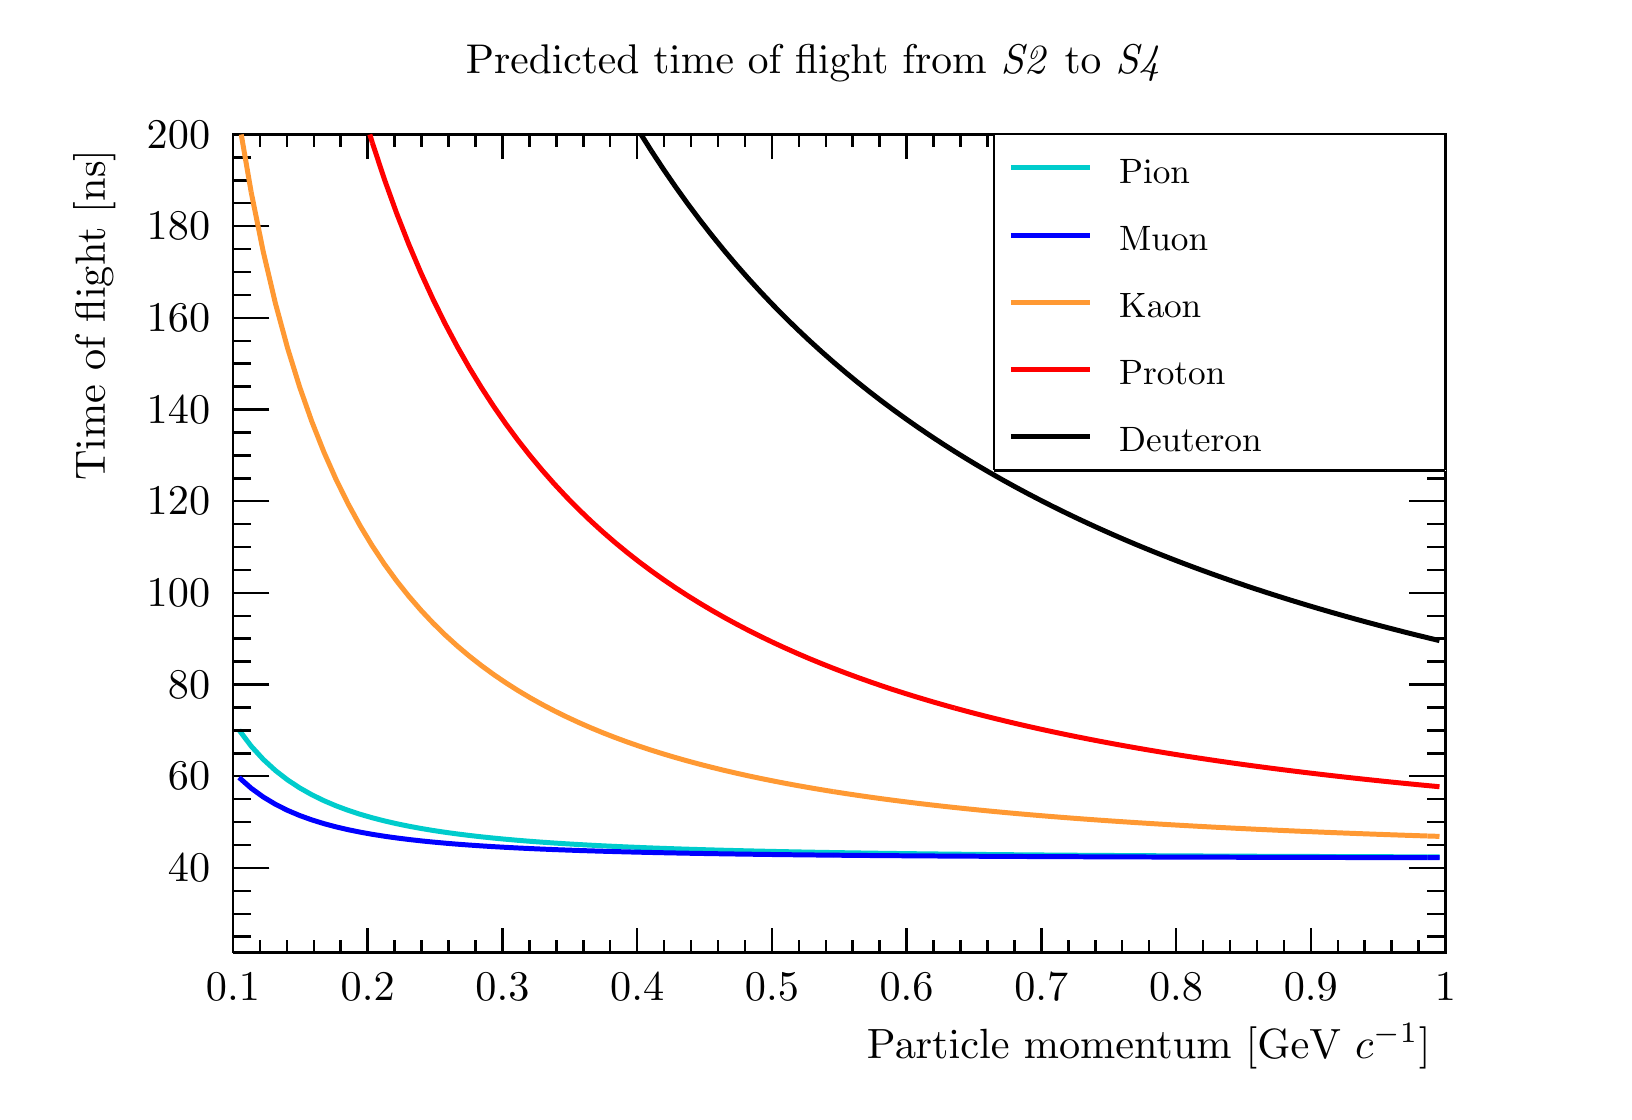
\begin{tikzpicture}
\pgfdeclareplotmark{cross} {
\pgfpathmoveto{\pgfpoint{-0.3\pgfplotmarksize}{\pgfplotmarksize}}
\pgfpathlineto{\pgfpoint{+0.3\pgfplotmarksize}{\pgfplotmarksize}}
\pgfpathlineto{\pgfpoint{+0.3\pgfplotmarksize}{0.3\pgfplotmarksize}}
\pgfpathlineto{\pgfpoint{+1\pgfplotmarksize}{0.3\pgfplotmarksize}}
\pgfpathlineto{\pgfpoint{+1\pgfplotmarksize}{-0.3\pgfplotmarksize}}
\pgfpathlineto{\pgfpoint{+0.3\pgfplotmarksize}{-0.3\pgfplotmarksize}}
\pgfpathlineto{\pgfpoint{+0.3\pgfplotmarksize}{-1.\pgfplotmarksize}}
\pgfpathlineto{\pgfpoint{-0.3\pgfplotmarksize}{-1.\pgfplotmarksize}}
\pgfpathlineto{\pgfpoint{-0.3\pgfplotmarksize}{-0.3\pgfplotmarksize}}
\pgfpathlineto{\pgfpoint{-1.\pgfplotmarksize}{-0.3\pgfplotmarksize}}
\pgfpathlineto{\pgfpoint{-1.\pgfplotmarksize}{0.3\pgfplotmarksize}}
\pgfpathlineto{\pgfpoint{-0.3\pgfplotmarksize}{0.3\pgfplotmarksize}}
\pgfpathclose
\pgfusepathqstroke
}
\pgfdeclareplotmark{cross*} {
\pgfpathmoveto{\pgfpoint{-0.3\pgfplotmarksize}{\pgfplotmarksize}}
\pgfpathlineto{\pgfpoint{+0.3\pgfplotmarksize}{\pgfplotmarksize}}
\pgfpathlineto{\pgfpoint{+0.3\pgfplotmarksize}{0.3\pgfplotmarksize}}
\pgfpathlineto{\pgfpoint{+1\pgfplotmarksize}{0.3\pgfplotmarksize}}
\pgfpathlineto{\pgfpoint{+1\pgfplotmarksize}{-0.3\pgfplotmarksize}}
\pgfpathlineto{\pgfpoint{+0.3\pgfplotmarksize}{-0.3\pgfplotmarksize}}
\pgfpathlineto{\pgfpoint{+0.3\pgfplotmarksize}{-1.\pgfplotmarksize}}
\pgfpathlineto{\pgfpoint{-0.3\pgfplotmarksize}{-1.\pgfplotmarksize}}
\pgfpathlineto{\pgfpoint{-0.3\pgfplotmarksize}{-0.3\pgfplotmarksize}}
\pgfpathlineto{\pgfpoint{-1.\pgfplotmarksize}{-0.3\pgfplotmarksize}}
\pgfpathlineto{\pgfpoint{-1.\pgfplotmarksize}{0.3\pgfplotmarksize}}
\pgfpathlineto{\pgfpoint{-0.3\pgfplotmarksize}{0.3\pgfplotmarksize}}
\pgfpathclose
\pgfusepathqfillstroke
}
\pgfdeclareplotmark{newstar} {
\pgfpathmoveto{\pgfqpoint{0pt}{\pgfplotmarksize}}
\pgfpathlineto{\pgfqpointpolar{44}{0.5\pgfplotmarksize}}
\pgfpathlineto{\pgfqpointpolar{18}{\pgfplotmarksize}}
\pgfpathlineto{\pgfqpointpolar{-20}{0.5\pgfplotmarksize}}
\pgfpathlineto{\pgfqpointpolar{-54}{\pgfplotmarksize}}
\pgfpathlineto{\pgfqpointpolar{-90}{0.5\pgfplotmarksize}}
\pgfpathlineto{\pgfqpointpolar{234}{\pgfplotmarksize}}
\pgfpathlineto{\pgfqpointpolar{198}{0.5\pgfplotmarksize}}
\pgfpathlineto{\pgfqpointpolar{162}{\pgfplotmarksize}}
\pgfpathlineto{\pgfqpointpolar{134}{0.5\pgfplotmarksize}}
\pgfpathclose
\pgfusepathqstroke
}
\pgfdeclareplotmark{newstar*} {
\pgfpathmoveto{\pgfqpoint{0pt}{\pgfplotmarksize}}
\pgfpathlineto{\pgfqpointpolar{44}{0.5\pgfplotmarksize}}
\pgfpathlineto{\pgfqpointpolar{18}{\pgfplotmarksize}}
\pgfpathlineto{\pgfqpointpolar{-20}{0.5\pgfplotmarksize}}
\pgfpathlineto{\pgfqpointpolar{-54}{\pgfplotmarksize}}
\pgfpathlineto{\pgfqpointpolar{-90}{0.5\pgfplotmarksize}}
\pgfpathlineto{\pgfqpointpolar{234}{\pgfplotmarksize}}
\pgfpathlineto{\pgfqpointpolar{198}{0.5\pgfplotmarksize}}
\pgfpathlineto{\pgfqpointpolar{162}{\pgfplotmarksize}}
\pgfpathlineto{\pgfqpointpolar{134}{0.5\pgfplotmarksize}}
\pgfpathclose
\pgfusepathqfillstroke
}
\definecolor{c}{rgb}{1,1,1};
\draw [color=c, fill=c] (0,0) rectangle (20,13.4957);
\draw [color=c, fill=c] (2.6,1.75444) rectangle (18,12.1461);
\definecolor{c}{rgb}{0,0,0};
\draw [c,line width=0.9] (2.6,1.75444) -- (2.6,12.1461) -- (18,12.1461) -- (18,1.75444) -- (2.6,1.75444);
\definecolor{c}{rgb}{1,1,1};
\draw [color=c, fill=c] (2.6,1.75444) rectangle (18,12.1461);
\definecolor{c}{rgb}{0,0,0};
\draw [c,line width=0.9] (2.6,1.75444) -- (2.6,12.1461) -- (18,12.1461) -- (18,1.75444) -- (2.6,1.75444);
\definecolor{c}{rgb}{0,0.8,0.8};
\draw [c,line width=1.8] (2.677,4.58295) -- (2.831,4.37871) -- (2.985,4.20989) -- (3.139,4.06877) -- (3.293,3.94962) -- (3.447,3.84815) -- (3.601,3.76104) -- (3.755,3.68575) -- (3.909,3.62024) -- (4.063,3.56292) -- (4.217,3.51249) -- (4.371,3.46791)
 -- (4.525,3.42831) -- (4.679,3.39299) -- (4.833,3.36136) -- (4.987,3.33293) -- (5.141,3.30729) -- (5.295,3.28409) -- (5.449,3.26304) -- (5.603,3.24387) -- (5.757,3.22638) -- (5.911,3.21038) -- (6.065,3.19569) -- (6.219,3.1822) -- (6.373,3.16976) --
 (6.527,3.15828) -- (6.681,3.14766) -- (6.835,3.13781) -- (6.989,3.12867) -- (7.143,3.12016) -- (7.297,3.11224) -- (7.451,3.10484) -- (7.605,3.09793) -- (7.759,3.09147) -- (7.913,3.08541) -- (8.067,3.07972) -- (8.221,3.07437) -- (8.375,3.06934) --
 (8.529,3.06461) -- (8.683,3.06014) -- (8.837,3.05592) -- (8.991,3.05194) -- (9.145,3.04817) -- (9.299,3.0446) -- (9.453,3.04121) -- (9.607,3.038) -- (9.761,3.03496) -- (9.915,3.03206) -- (10.069,3.0293) -- (10.223,3.02668);
\draw [c,line width=1.8] (10.223,3.02668) -- (10.377,3.02418) -- (10.531,3.0218) -- (10.685,3.01953) -- (10.839,3.01736) -- (10.993,3.01528) -- (11.147,3.0133) -- (11.301,3.0114) -- (11.455,3.00959) -- (11.609,3.00785) -- (11.763,3.00618) --
 (11.917,3.00459) -- (12.071,3.00305) -- (12.225,3.00158) -- (12.379,3.00016) -- (12.533,2.9988) -- (12.687,2.9975) -- (12.841,2.99624) -- (12.995,2.99503) -- (13.149,2.99386) -- (13.303,2.99274) -- (13.457,2.99166) -- (13.611,2.99061) --
 (13.765,2.9896) -- (13.919,2.98863) -- (14.073,2.98769) -- (14.227,2.98679) -- (14.381,2.98591) -- (14.535,2.98506) -- (14.689,2.98424) -- (14.843,2.98345) -- (14.997,2.98268) -- (15.151,2.98194) -- (15.305,2.98122) -- (15.459,2.98053) --
 (15.613,2.97985) -- (15.767,2.9792) -- (15.921,2.97856) -- (16.075,2.97795) -- (16.229,2.97735) -- (16.383,2.97677) -- (16.537,2.97621) -- (16.691,2.97566) -- (16.845,2.97513) -- (16.999,2.97462) -- (17.153,2.97412) -- (17.307,2.97363) --
 (17.461,2.97315) -- (17.615,2.97269) -- (17.769,2.97225);
\draw [c,line width=1.8] (17.769,2.97225) -- (17.923,2.97181);
\definecolor{c}{rgb}{0,0,0};
\draw [c,line width=0.9] (2.6,1.75444) -- (18,1.75444);
\draw [c,line width=0.9] (2.6,2.06619) -- (2.6,1.75444);
\draw [c,line width=0.9] (2.94222,1.91032) -- (2.94222,1.75444);
\draw [c,line width=0.9] (3.28444,1.91032) -- (3.28444,1.75444);
\draw [c,line width=0.9] (3.62667,1.91032) -- (3.62667,1.75444);
\draw [c,line width=0.9] (3.96889,1.91032) -- (3.96889,1.75444);
\draw [c,line width=0.9] (4.31111,2.06619) -- (4.31111,1.75444);
\draw [c,line width=0.9] (4.65333,1.91032) -- (4.65333,1.75444);
\draw [c,line width=0.9] (4.99556,1.91032) -- (4.99556,1.75444);
\draw [c,line width=0.9] (5.33778,1.91032) -- (5.33778,1.75444);
\draw [c,line width=0.9] (5.68,1.91032) -- (5.68,1.75444);
\draw [c,line width=0.9] (6.02222,2.06619) -- (6.02222,1.75444);
\draw [c,line width=0.9] (6.36444,1.91032) -- (6.36444,1.75444);
\draw [c,line width=0.9] (6.70667,1.91032) -- (6.70667,1.75444);
\draw [c,line width=0.9] (7.04889,1.91032) -- (7.04889,1.75444);
\draw [c,line width=0.9] (7.39111,1.91032) -- (7.39111,1.75444);
\draw [c,line width=0.9] (7.73333,2.06619) -- (7.73333,1.75444);
\draw [c,line width=0.9] (8.07556,1.91032) -- (8.07556,1.75444);
\draw [c,line width=0.9] (8.41778,1.91032) -- (8.41778,1.75444);
\draw [c,line width=0.9] (8.76,1.91032) -- (8.76,1.75444);
\draw [c,line width=0.9] (9.10222,1.91032) -- (9.10222,1.75444);
\draw [c,line width=0.9] (9.44444,2.06619) -- (9.44444,1.75444);
\draw [c,line width=0.9] (9.78667,1.91032) -- (9.78667,1.75444);
\draw [c,line width=0.9] (10.1289,1.91032) -- (10.1289,1.75444);
\draw [c,line width=0.9] (10.4711,1.91032) -- (10.4711,1.75444);
\draw [c,line width=0.9] (10.8133,1.91032) -- (10.8133,1.75444);
\draw [c,line width=0.9] (11.1556,2.06619) -- (11.1556,1.75444);
\draw [c,line width=0.9] (11.4978,1.91032) -- (11.4978,1.75444);
\draw [c,line width=0.9] (11.84,1.91032) -- (11.84,1.75444);
\draw [c,line width=0.9] (12.1822,1.91032) -- (12.1822,1.75444);
\draw [c,line width=0.9] (12.5244,1.91032) -- (12.5244,1.75444);
\draw [c,line width=0.9] (12.8667,2.06619) -- (12.8667,1.75444);
\draw [c,line width=0.9] (13.2089,1.91032) -- (13.2089,1.75444);
\draw [c,line width=0.9] (13.5511,1.91032) -- (13.5511,1.75444);
\draw [c,line width=0.9] (13.8933,1.91032) -- (13.8933,1.75444);
\draw [c,line width=0.9] (14.2356,1.91032) -- (14.2356,1.75444);
\draw [c,line width=0.9] (14.5778,2.06619) -- (14.5778,1.75444);
\draw [c,line width=0.9] (14.92,1.91032) -- (14.92,1.75444);
\draw [c,line width=0.9] (15.2622,1.91032) -- (15.2622,1.75444);
\draw [c,line width=0.9] (15.6044,1.91032) -- (15.6044,1.75444);
\draw [c,line width=0.9] (15.9467,1.91032) -- (15.9467,1.75444);
\draw [c,line width=0.9] (16.2889,2.06619) -- (16.2889,1.75444);
\draw [c,line width=0.9] (16.6311,1.91032) -- (16.6311,1.75444);
\draw [c,line width=0.9] (16.9733,1.91032) -- (16.9733,1.75444);
\draw [c,line width=0.9] (17.3156,1.91032) -- (17.3156,1.75444);
\draw [c,line width=0.9] (17.6578,1.91032) -- (17.6578,1.75444);
\draw [c,line width=0.9] (18,2.06619) -- (18,1.75444);
\draw [anchor=base] (2.6,1.14713) node[scale=1.52731, color=c, rotate=0]{0.1};
\draw [anchor=base] (4.31111,1.14713) node[scale=1.52731, color=c, rotate=0]{0.2};
\draw [anchor=base] (6.02222,1.14713) node[scale=1.52731, color=c, rotate=0]{0.3};
\draw [anchor=base] (7.73333,1.14713) node[scale=1.52731, color=c, rotate=0]{0.4};
\draw [anchor=base] (9.44444,1.14713) node[scale=1.52731, color=c, rotate=0]{0.5};
\draw [anchor=base] (11.1556,1.14713) node[scale=1.52731, color=c, rotate=0]{0.6};
\draw [anchor=base] (12.8667,1.14713) node[scale=1.52731, color=c, rotate=0]{0.7};
\draw [anchor=base] (14.5778,1.14713) node[scale=1.52731, color=c, rotate=0]{0.8};
\draw [anchor=base] (16.2889,1.14713) node[scale=1.52731, color=c, rotate=0]{0.9};
\draw [anchor=base] (18,1.14713) node[scale=1.52731, color=c, rotate=0]{1};
\draw [anchor= east] (18,0.566819) node[scale=1.52731, color=c, rotate=0]{ Particle momentum [GeV $c^{-1}$]};
\draw [c,line width=0.9] (2.6,12.1461) -- (18,12.1461);
\draw [c,line width=0.9] (2.6,11.8344) -- (2.6,12.1461);
\draw [c,line width=0.9] (2.94222,11.9903) -- (2.94222,12.1461);
\draw [c,line width=0.9] (3.28444,11.9903) -- (3.28444,12.1461);
\draw [c,line width=0.9] (3.62667,11.9903) -- (3.62667,12.1461);
\draw [c,line width=0.9] (3.96889,11.9903) -- (3.96889,12.1461);
\draw [c,line width=0.9] (4.31111,11.8344) -- (4.31111,12.1461);
\draw [c,line width=0.9] (4.65333,11.9903) -- (4.65333,12.1461);
\draw [c,line width=0.9] (4.99556,11.9903) -- (4.99556,12.1461);
\draw [c,line width=0.9] (5.33778,11.9903) -- (5.33778,12.1461);
\draw [c,line width=0.9] (5.68,11.9903) -- (5.68,12.1461);
\draw [c,line width=0.9] (6.02222,11.8344) -- (6.02222,12.1461);
\draw [c,line width=0.9] (6.36444,11.9903) -- (6.36444,12.1461);
\draw [c,line width=0.9] (6.70667,11.9903) -- (6.70667,12.1461);
\draw [c,line width=0.9] (7.04889,11.9903) -- (7.04889,12.1461);
\draw [c,line width=0.9] (7.39111,11.9903) -- (7.39111,12.1461);
\draw [c,line width=0.9] (7.73333,11.8344) -- (7.73333,12.1461);
\draw [c,line width=0.9] (8.07556,11.9903) -- (8.07556,12.1461);
\draw [c,line width=0.9] (8.41778,11.9903) -- (8.41778,12.1461);
\draw [c,line width=0.9] (8.76,11.9903) -- (8.76,12.1461);
\draw [c,line width=0.9] (9.10222,11.9903) -- (9.10222,12.1461);
\draw [c,line width=0.9] (9.44444,11.8344) -- (9.44444,12.1461);
\draw [c,line width=0.9] (9.78667,11.9903) -- (9.78667,12.1461);
\draw [c,line width=0.9] (10.1289,11.9903) -- (10.1289,12.1461);
\draw [c,line width=0.9] (10.4711,11.9903) -- (10.4711,12.1461);
\draw [c,line width=0.9] (10.8133,11.9903) -- (10.8133,12.1461);
\draw [c,line width=0.9] (11.1556,11.8344) -- (11.1556,12.1461);
\draw [c,line width=0.9] (11.4978,11.9903) -- (11.4978,12.1461);
\draw [c,line width=0.9] (11.84,11.9903) -- (11.84,12.1461);
\draw [c,line width=0.9] (12.1822,11.9903) -- (12.1822,12.1461);
\draw [c,line width=0.9] (12.5244,11.9903) -- (12.5244,12.1461);
\draw [c,line width=0.9] (12.8667,11.8344) -- (12.8667,12.1461);
\draw [c,line width=0.9] (13.2089,11.9903) -- (13.2089,12.1461);
\draw [c,line width=0.9] (13.5511,11.9903) -- (13.5511,12.1461);
\draw [c,line width=0.9] (13.8933,11.9903) -- (13.8933,12.1461);
\draw [c,line width=0.9] (14.2356,11.9903) -- (14.2356,12.1461);
\draw [c,line width=0.9] (14.5778,11.8344) -- (14.5778,12.1461);
\draw [c,line width=0.9] (14.92,11.9903) -- (14.92,12.1461);
\draw [c,line width=0.9] (15.2622,11.9903) -- (15.2622,12.1461);
\draw [c,line width=0.9] (15.6044,11.9903) -- (15.6044,12.1461);
\draw [c,line width=0.9] (15.9467,11.9903) -- (15.9467,12.1461);
\draw [c,line width=0.9] (16.2889,11.8344) -- (16.2889,12.1461);
\draw [c,line width=0.9] (16.6311,11.9903) -- (16.6311,12.1461);
\draw [c,line width=0.9] (16.9733,11.9903) -- (16.9733,12.1461);
\draw [c,line width=0.9] (17.3156,11.9903) -- (17.3156,12.1461);
\draw [c,line width=0.9] (17.6578,11.9903) -- (17.6578,12.1461);
\draw [c,line width=0.9] (18,11.8344) -- (18,12.1461);
\draw [c,line width=0.9] (2.6,1.75444) -- (2.6,12.1461);
\draw [c,line width=0.9] (3.062,2.83145) -- (2.6,2.83145);
\draw [c,line width=0.9] (2.831,3.12253) -- (2.6,3.12253);
\draw [c,line width=0.9] (2.831,3.41362) -- (2.6,3.41362);
\draw [c,line width=0.9] (2.831,3.7047) -- (2.6,3.7047);
\draw [c,line width=0.9] (3.062,3.99579) -- (2.6,3.99579);
\draw [c,line width=0.9] (2.831,4.28687) -- (2.6,4.28687);
\draw [c,line width=0.9] (2.831,4.57795) -- (2.6,4.57795);
\draw [c,line width=0.9] (2.831,4.86904) -- (2.6,4.86904);
\draw [c,line width=0.9] (3.062,5.16012) -- (2.6,5.16012);
\draw [c,line width=0.9] (2.831,5.4512) -- (2.6,5.4512);
\draw [c,line width=0.9] (2.831,5.74229) -- (2.6,5.74229);
\draw [c,line width=0.9] (2.831,6.03337) -- (2.6,6.03337);
\draw [c,line width=0.9] (3.062,6.32446) -- (2.6,6.32446);
\draw [c,line width=0.9] (2.831,6.61554) -- (2.6,6.61554);
\draw [c,line width=0.9] (2.831,6.90662) -- (2.6,6.90662);
\draw [c,line width=0.9] (2.831,7.19771) -- (2.6,7.19771);
\draw [c,line width=0.9] (3.062,7.48879) -- (2.6,7.48879);
\draw [c,line width=0.9] (2.831,7.77988) -- (2.6,7.77988);
\draw [c,line width=0.9] (2.831,8.07096) -- (2.6,8.07096);
\draw [c,line width=0.9] (2.831,8.36204) -- (2.6,8.36204);
\draw [c,line width=0.9] (3.062,8.65313) -- (2.6,8.65313);
\draw [c,line width=0.9] (2.831,8.94421) -- (2.6,8.94421);
\draw [c,line width=0.9] (2.831,9.23529) -- (2.6,9.23529);
\draw [c,line width=0.9] (2.831,9.52638) -- (2.6,9.52638);
\draw [c,line width=0.9] (3.062,9.81746) -- (2.6,9.81746);
\draw [c,line width=0.9] (2.831,10.1085) -- (2.6,10.1085);
\draw [c,line width=0.9] (2.831,10.3996) -- (2.6,10.3996);
\draw [c,line width=0.9] (2.831,10.6907) -- (2.6,10.6907);
\draw [c,line width=0.9] (3.062,10.9818) -- (2.6,10.9818);
\draw [c,line width=0.9] (2.831,11.2729) -- (2.6,11.2729);
\draw [c,line width=0.9] (2.831,11.564) -- (2.6,11.564);
\draw [c,line width=0.9] (2.831,11.855) -- (2.6,11.855);
\draw [c,line width=0.9] (3.062,12.1461) -- (2.6,12.1461);
\draw [c,line width=0.9] (3.062,2.83145) -- (2.6,2.83145);
\draw [c,line width=0.9] (2.831,2.54037) -- (2.6,2.54037);
\draw [c,line width=0.9] (2.831,2.24928) -- (2.6,2.24928);
\draw [c,line width=0.9] (2.831,1.9582) -- (2.6,1.9582);
\draw [anchor= east] (2.5,2.83145) node[scale=1.52731, color=c, rotate=0]{40};
\draw [anchor= east] (2.5,3.99579) node[scale=1.52731, color=c, rotate=0]{60};
\draw [anchor= east] (2.5,5.16012) node[scale=1.52731, color=c, rotate=0]{80};
\draw [anchor= east] (2.5,6.32446) node[scale=1.52731, color=c, rotate=0]{100};
\draw [anchor= east] (2.5,7.48879) node[scale=1.52731, color=c, rotate=0]{120};
\draw [anchor= east] (2.5,8.65313) node[scale=1.52731, color=c, rotate=0]{140};
\draw [anchor= east] (2.5,9.81746) node[scale=1.52731, color=c, rotate=0]{160};
\draw [anchor= east] (2.5,10.9818) node[scale=1.52731, color=c, rotate=0]{180};
\draw [anchor= east] (2.5,12.1461) node[scale=1.52731, color=c, rotate=0]{200};
\draw [anchor= east] (0.84,12.1461) node[scale=1.52731, color=c, rotate=90]{ Time of flight [ns]};
\draw [c,line width=0.9] (18,1.75444) -- (18,12.1461);
\draw [c,line width=0.9] (17.538,2.83145) -- (18,2.83145);
\draw [c,line width=0.9] (17.769,3.12253) -- (18,3.12253);
\draw [c,line width=0.9] (17.769,3.41362) -- (18,3.41362);
\draw [c,line width=0.9] (17.769,3.7047) -- (18,3.7047);
\draw [c,line width=0.9] (17.538,3.99579) -- (18,3.99579);
\draw [c,line width=0.9] (17.769,4.28687) -- (18,4.28687);
\draw [c,line width=0.9] (17.769,4.57795) -- (18,4.57795);
\draw [c,line width=0.9] (17.769,4.86904) -- (18,4.86904);
\draw [c,line width=0.9] (17.538,5.16012) -- (18,5.16012);
\draw [c,line width=0.9] (17.769,5.4512) -- (18,5.4512);
\draw [c,line width=0.9] (17.769,5.74229) -- (18,5.74229);
\draw [c,line width=0.9] (17.769,6.03337) -- (18,6.03337);
\draw [c,line width=0.9] (17.538,6.32446) -- (18,6.32446);
\draw [c,line width=0.9] (17.769,6.61554) -- (18,6.61554);
\draw [c,line width=0.9] (17.769,6.90662) -- (18,6.90662);
\draw [c,line width=0.9] (17.769,7.19771) -- (18,7.19771);
\draw [c,line width=0.9] (17.538,7.48879) -- (18,7.48879);
\draw [c,line width=0.9] (17.769,7.77988) -- (18,7.77988);
\draw [c,line width=0.9] (17.769,8.07096) -- (18,8.07096);
\draw [c,line width=0.9] (17.769,8.36204) -- (18,8.36204);
\draw [c,line width=0.9] (17.538,8.65313) -- (18,8.65313);
\draw [c,line width=0.9] (17.769,8.94421) -- (18,8.94421);
\draw [c,line width=0.9] (17.769,9.23529) -- (18,9.23529);
\draw [c,line width=0.9] (17.769,9.52638) -- (18,9.52638);
\draw [c,line width=0.9] (17.538,9.81746) -- (18,9.81746);
\draw [c,line width=0.9] (17.769,10.1085) -- (18,10.1085);
\draw [c,line width=0.9] (17.769,10.3996) -- (18,10.3996);
\draw [c,line width=0.9] (17.769,10.6907) -- (18,10.6907);
\draw [c,line width=0.9] (17.538,10.9818) -- (18,10.9818);
\draw [c,line width=0.9] (17.769,11.2729) -- (18,11.2729);
\draw [c,line width=0.9] (17.769,11.564) -- (18,11.564);
\draw [c,line width=0.9] (17.769,11.855) -- (18,11.855);
\draw [c,line width=0.9] (17.538,12.1461) -- (18,12.1461);
\draw [c,line width=0.9] (17.538,2.83145) -- (18,2.83145);
\draw [c,line width=0.9] (17.769,2.54037) -- (18,2.54037);
\draw [c,line width=0.9] (17.769,2.24928) -- (18,2.24928);
\draw [c,line width=0.9] (17.769,1.9582) -- (18,1.9582);
\definecolor{c}{rgb}{1,0,0};
\draw [c,line width=1.8] (4.33861,12.1461) -- (4.371,12.0388);
\draw [c,line width=1.8] (4.371,12.0388) -- (4.525,11.5726) -- (4.679,11.1452) -- (4.833,10.752) -- (4.987,10.3892) -- (5.141,10.0534) -- (5.295,9.74187) -- (5.449,9.45206) -- (5.603,9.18187) -- (5.757,8.92943) -- (5.911,8.69311) -- (6.065,8.47145)
 -- (6.219,8.26318) -- (6.373,8.06717) -- (6.527,7.88242) -- (6.681,7.70801) -- (6.835,7.54314) -- (6.989,7.38709) -- (7.143,7.23919) -- (7.297,7.09885) -- (7.451,6.96555) -- (7.605,6.83878) -- (7.759,6.71811) -- (7.913,6.60313) -- (8.067,6.49347) --
 (8.221,6.38879) -- (8.375,6.28879) -- (8.529,6.19316) -- (8.683,6.10166) -- (8.837,6.01403) -- (8.991,5.93005) -- (9.145,5.84952) -- (9.299,5.77224) -- (9.453,5.69803) -- (9.607,5.62673) -- (9.761,5.55818) -- (9.915,5.49224) -- (10.069,5.42877) --
 (10.223,5.36765) -- (10.377,5.30876) -- (10.531,5.25198) -- (10.685,5.19723) -- (10.839,5.1444) -- (10.993,5.09339) -- (11.147,5.04413) -- (11.301,4.99654) -- (11.455,4.95053) -- (11.609,4.90605) -- (11.763,4.86301);
\draw [c,line width=1.8] (11.763,4.86301) -- (11.917,4.82136) -- (12.071,4.78104) -- (12.225,4.74199) -- (12.379,4.70416) -- (12.533,4.6675) -- (12.687,4.63196) -- (12.841,4.59749) -- (12.995,4.56405) -- (13.149,4.5316) -- (13.303,4.50011) --
 (13.457,4.46952) -- (13.611,4.43982) -- (13.765,4.41096) -- (13.919,4.38292) -- (14.073,4.35565) -- (14.227,4.32915) -- (14.381,4.30337) -- (14.535,4.27829) -- (14.689,4.25388) -- (14.843,4.23013) -- (14.997,4.20701) -- (15.151,4.18449) --
 (15.305,4.16256) -- (15.459,4.1412) -- (15.613,4.12038) -- (15.767,4.10009) -- (15.921,4.08031) -- (16.075,4.06102) -- (16.229,4.04221) -- (16.383,4.02386) -- (16.537,4.00596) -- (16.691,3.9885) -- (16.845,3.97145) -- (16.999,3.95481) --
 (17.153,3.93856) -- (17.307,3.92269) -- (17.461,3.90719) -- (17.615,3.89205) -- (17.769,3.87726) -- (17.923,3.86281);
\definecolor{c}{rgb}{0,0,1};
\draw [c,line width=1.8] (2.677,3.98059) -- (2.831,3.84398) -- (2.985,3.73228) -- (3.139,3.63986) -- (3.293,3.56256) -- (3.447,3.49729) -- (3.601,3.44172) -- (3.755,3.39402) -- (3.909,3.35281) -- (4.063,3.31697) -- (4.217,3.28562) -- (4.371,3.25804)
 -- (4.525,3.23367) -- (4.679,3.21202) -- (4.833,3.19271) -- (4.987,3.17542) -- (5.141,3.15988) -- (5.295,3.14587) -- (5.449,3.13318) -- (5.603,3.12167) -- (5.757,3.11119) -- (5.911,3.10161) -- (6.065,3.09285) -- (6.219,3.08482) -- (6.373,3.07743) --
 (6.527,3.07061) -- (6.681,3.06432) -- (6.835,3.05849) -- (6.989,3.05309) -- (7.143,3.04808) -- (7.297,3.04341) -- (7.451,3.03906) -- (7.605,3.035) -- (7.759,3.0312) -- (7.913,3.02764) -- (8.067,3.02431) -- (8.221,3.02118) -- (8.375,3.01823) --
 (8.529,3.01546) -- (8.683,3.01285) -- (8.837,3.01039) -- (8.991,3.00807) -- (9.145,3.00587) -- (9.299,3.00379) -- (9.453,3.00182) -- (9.607,2.99995) -- (9.761,2.99817) -- (9.915,2.99649) -- (10.069,2.99489) -- (10.223,2.99336);
\draw [c,line width=1.8] (10.223,2.99336) -- (10.377,2.99191) -- (10.531,2.99053) -- (10.685,2.98921) -- (10.839,2.98795) -- (10.993,2.98675) -- (11.147,2.9856) -- (11.301,2.9845) -- (11.455,2.98345) -- (11.609,2.98244) -- (11.763,2.98147) --
 (11.917,2.98055) -- (12.071,2.97966) -- (12.225,2.97881) -- (12.379,2.97799) -- (12.533,2.9772) -- (12.687,2.97645) -- (12.841,2.97572) -- (12.995,2.97502) -- (13.149,2.97435) -- (13.303,2.9737) -- (13.457,2.97307) -- (13.611,2.97247) --
 (13.765,2.97189) -- (13.919,2.97133) -- (14.073,2.97079) -- (14.227,2.97026) -- (14.381,2.96976) -- (14.535,2.96927) -- (14.689,2.96879) -- (14.843,2.96834) -- (14.997,2.9679) -- (15.151,2.96747) -- (15.305,2.96705) -- (15.459,2.96665) --
 (15.613,2.96626) -- (15.767,2.96589) -- (15.921,2.96552) -- (16.075,2.96516) -- (16.229,2.96482) -- (16.383,2.96449) -- (16.537,2.96416) -- (16.691,2.96385) -- (16.845,2.96354) -- (16.999,2.96325) -- (17.153,2.96296) -- (17.307,2.96268) --
 (17.461,2.9624) -- (17.615,2.96214) -- (17.769,2.96188);
\draw [c,line width=1.8] (17.769,2.96188) -- (17.923,2.96163);
\definecolor{c}{rgb}{1,0.6,0.2};
\draw [c,line width=1.8] (2.70528,12.1461) -- (2.831,11.4159);
\draw [c,line width=1.8] (2.831,11.4159) -- (2.985,10.6559) -- (3.139,10.0027) -- (3.293,9.43573) -- (3.447,8.93944) -- (3.601,8.50173) -- (3.755,8.11312) -- (3.909,7.76607) -- (4.063,7.45451) -- (4.217,7.17347) -- (4.371,6.91888) -- (4.525,6.68734)
 -- (4.679,6.47603) -- (4.833,6.28254) -- (4.987,6.10483) -- (5.141,5.94118) -- (5.295,5.79007) -- (5.449,5.65022) -- (5.603,5.5205) -- (5.757,5.39992) -- (5.911,5.28763) -- (6.065,5.18287) -- (6.219,5.08495) -- (6.373,4.99329) -- (6.527,4.90736) --
 (6.681,4.82668) -- (6.835,4.75082) -- (6.989,4.67941) -- (7.143,4.61211) -- (7.297,4.54859) -- (7.451,4.48858) -- (7.605,4.43183) -- (7.759,4.37811) -- (7.913,4.32719) -- (8.067,4.27889) -- (8.221,4.23304) -- (8.375,4.18947) -- (8.529,4.14803) --
 (8.683,4.10859) -- (8.837,4.07102) -- (8.991,4.03521) -- (9.145,4.00104) -- (9.299,3.96843) -- (9.453,3.93727) -- (9.607,3.90749) -- (9.761,3.879) -- (9.915,3.85173) -- (10.069,3.82561) -- (10.223,3.80059);
\draw [c,line width=1.8] (10.223,3.80059) -- (10.377,3.7766) -- (10.531,3.75358) -- (10.685,3.73149) -- (10.839,3.71027) -- (10.993,3.68988) -- (11.147,3.67028) -- (11.301,3.65144) -- (11.455,3.6333) -- (11.609,3.61584) -- (11.763,3.59902) --
 (11.917,3.58282) -- (12.071,3.5672) -- (12.225,3.55214) -- (12.379,3.53761) -- (12.533,3.52359) -- (12.687,3.51005) -- (12.841,3.49698) -- (12.995,3.48434) -- (13.149,3.47213) -- (13.303,3.46032) -- (13.457,3.4489) -- (13.611,3.43785) --
 (13.765,3.42715) -- (13.919,3.41679) -- (14.073,3.40676) -- (14.227,3.39704) -- (14.381,3.38762) -- (14.535,3.37849) -- (14.689,3.36964) -- (14.843,3.36105) -- (14.997,3.35271) -- (15.151,3.34462) -- (15.305,3.33677) -- (15.459,3.32914) --
 (15.613,3.32174) -- (15.767,3.31454) -- (15.921,3.30754) -- (16.075,3.30074) -- (16.229,3.29413) -- (16.383,3.2877) -- (16.537,3.28144) -- (16.691,3.27535) -- (16.845,3.26943) -- (16.999,3.26366) -- (17.153,3.25804) -- (17.307,3.25257) --
 (17.461,3.24724) -- (17.615,3.24205) -- (17.769,3.23699);
\draw [c,line width=1.8] (17.769,3.23699) -- (17.923,3.23206);
\definecolor{c}{rgb}{0,0,0};
\draw [c,line width=1.8] (7.78271,12.1461) -- (7.913,11.9391);
\draw [c,line width=1.8] (7.913,11.9391) -- (8.067,11.705) -- (8.221,11.4811) -- (8.375,11.2665) -- (8.529,11.0609) -- (8.683,10.8636) -- (8.837,10.6741) -- (8.991,10.492) -- (9.145,10.317) -- (9.299,10.1485) -- (9.453,9.98632) -- (9.607,9.83002) --
 (9.761,9.67934) -- (9.915,9.53398) -- (10.069,9.39367) -- (10.223,9.25816) -- (10.377,9.12722) -- (10.531,9.00063) -- (10.685,8.87818) -- (10.839,8.75968) -- (10.993,8.64495) -- (11.147,8.53381) -- (11.301,8.42612) -- (11.455,8.32171) --
 (11.609,8.22044) -- (11.763,8.12218) -- (11.917,8.02681) -- (12.071,7.9342) -- (12.225,7.84424) -- (12.379,7.75682) -- (12.533,7.67185) -- (12.687,7.58922) -- (12.841,7.50885) -- (12.995,7.43064) -- (13.149,7.35452) -- (13.303,7.28041) --
 (13.457,7.20823) -- (13.611,7.13791) -- (13.765,7.06938) -- (13.919,7.00259) -- (14.073,6.93746) -- (14.227,6.87395) -- (14.381,6.81199) -- (14.535,6.75154) -- (14.689,6.69253) -- (14.843,6.63493) -- (14.997,6.57869) -- (15.151,6.52375) --
 (15.305,6.47009);
\draw [c,line width=1.8] (15.305,6.47009) -- (15.459,6.41765) -- (15.613,6.36641) -- (15.767,6.31631) -- (15.921,6.26734) -- (16.075,6.21944) -- (16.229,6.17259) -- (16.383,6.12676) -- (16.537,6.08192) -- (16.691,6.03803) -- (16.845,5.99507) --
 (16.999,5.95302) -- (17.153,5.91184) -- (17.307,5.87151) -- (17.461,5.832) -- (17.615,5.7933) -- (17.769,5.75538) -- (17.923,5.71822);
\definecolor{c}{rgb}{1,1,1};
\draw [color=c, fill=c] (12.2636,7.87966) rectangle (17.9943,12.149);
\definecolor{c}{rgb}{0,0,0};
\draw [c,line width=0.9] (12.2636,7.87966) -- (17.9943,7.87966);
\draw [c,line width=0.9] (17.9943,7.87966) -- (17.9943,12.149);
\draw [c,line width=0.9] (17.9943,12.149) -- (12.2636,12.149);
\draw [c,line width=0.9] (12.2636,12.149) -- (12.2636,7.87966);
\draw [anchor=base west] (13.6963,11.5299) node[scale=1.27276, color=c, rotate=0]{Pion};
\definecolor{c}{rgb}{0,0.8,0.8};
\draw [c,line width=1.8] (12.4785,11.7221) -- (13.4814,11.7221);
\definecolor{c}{rgb}{0,0,0};
\draw [anchor=base west] (13.6963,10.6761) node[scale=1.27276, color=c, rotate=0]{Muon};
\definecolor{c}{rgb}{0,0,1};
\draw [c,line width=1.8] (12.4785,10.8682) -- (13.4814,10.8682);
\definecolor{c}{rgb}{0,0,0};
\draw [anchor=base west] (13.6963,9.82221) node[scale=1.27276, color=c, rotate=0]{Kaon};
\definecolor{c}{rgb}{1,0.6,0.2};
\draw [c,line width=1.8] (12.4785,10.0143) -- (13.4814,10.0143);
\definecolor{c}{rgb}{0,0,0};
\draw [anchor=base west] (13.6963,8.96834) node[scale=1.27276, color=c, rotate=0]{Proton};
\definecolor{c}{rgb}{1,0,0};
\draw [c,line width=1.8] (12.4785,9.16046) -- (13.4814,9.16046);
\definecolor{c}{rgb}{0,0,0};
\draw [anchor=base west] (13.6963,8.11447) node[scale=1.27276, color=c, rotate=0]{Deuteron};
\draw [c,line width=1.8] (12.4785,8.30659) -- (13.4814,8.30659);
\definecolor{c}{rgb}{1,1,1};
\draw [color=c, fill=c] (2,12.686) rectangle (18,13.4282);
\definecolor{c}{rgb}{0,0,0};
\draw (10,13.0571) node[scale=1.50004, color=c, rotate=0]{Predicted time of flight from $\mathit{S2}$ to $\mathit{S4}$};
\end{tikzpicture}

    \end{adjustbox}
  \end{minipage}
   \caption{\label{fig:s1s3PredTimes}Calculated time of flight for a number of different particle species as a function of particle momentum. Left: ToF between $\mathit{S1}$ and $\mathit{S3}$. Right: ToF between $\mathit{S2}$ and $\mathit{S4}$.}
\end{figure}

Figure~\ref{fig:s3tof} shows the time of flight spectrum recorded in the $\mathit{S3}$ timing point for varying numbers of moderator blocks.
The quicker peak is formed by minimum ionizing particles, while the peak at higher values of $\mathit{t_{S3}} - \mathit{t_{S1}}$ corresponds to protons.
The proton peaks show a double peak feature, with a smaller delayed peak closely following the main proton peak; this feature appeared after the beam was steered so that the full 2.5 degree off-axis angle could be achieved and is due to beam scattering in the steering magnets.
Figure~\ref{fig:utofNoBend}, left and right, shows the proton peak for unsteered beam and the double peak structure is gone.
In the black curve, which shows the 0 block data, a deuteron peak can be seen centered at 95~ns.
The timing ranges for particle species selection are chosen using the analytic expectations shown in Figure~\ref{fig:s1s3PredTimes}.

\begin{figure}[ht]
  \begin{adjustbox}{max totalsize={.8\textwidth}{.5\textheight},center}
    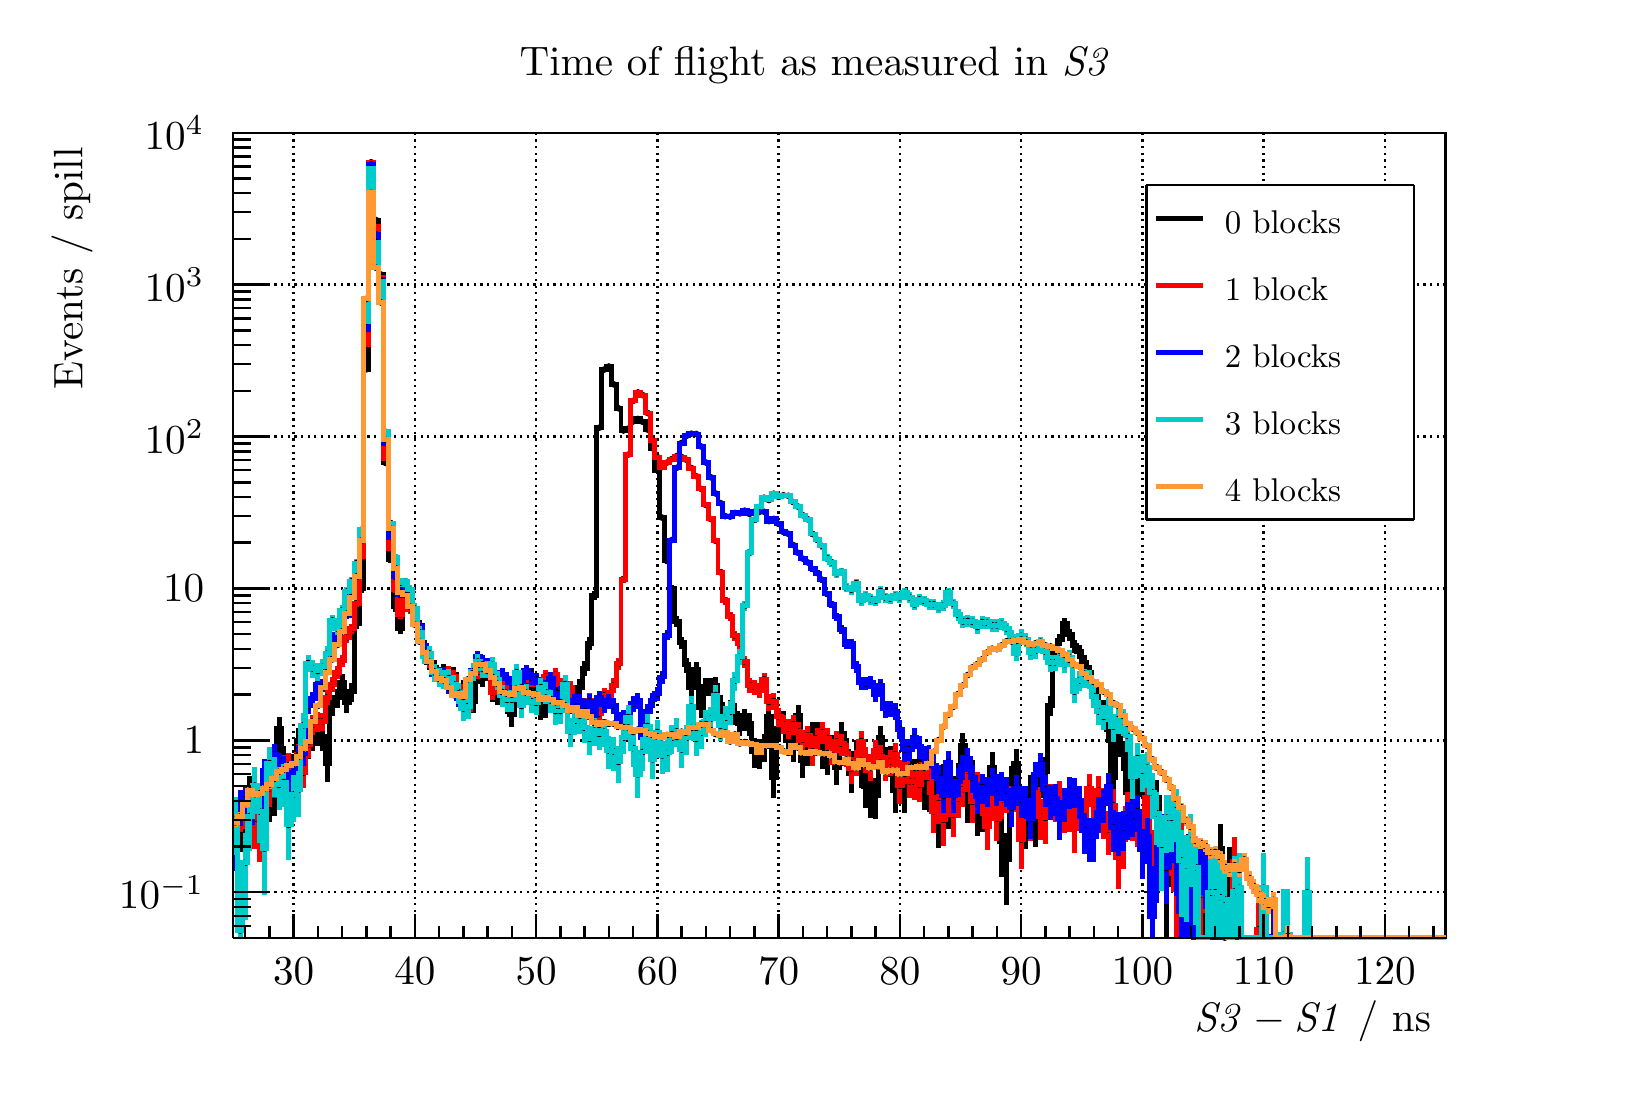
\begin{tikzpicture}
\pgfdeclareplotmark{cross} {
\pgfpathmoveto{\pgfpoint{-0.3\pgfplotmarksize}{\pgfplotmarksize}}
\pgfpathlineto{\pgfpoint{+0.3\pgfplotmarksize}{\pgfplotmarksize}}
\pgfpathlineto{\pgfpoint{+0.3\pgfplotmarksize}{0.3\pgfplotmarksize}}
\pgfpathlineto{\pgfpoint{+1\pgfplotmarksize}{0.3\pgfplotmarksize}}
\pgfpathlineto{\pgfpoint{+1\pgfplotmarksize}{-0.3\pgfplotmarksize}}
\pgfpathlineto{\pgfpoint{+0.3\pgfplotmarksize}{-0.3\pgfplotmarksize}}
\pgfpathlineto{\pgfpoint{+0.3\pgfplotmarksize}{-1.\pgfplotmarksize}}
\pgfpathlineto{\pgfpoint{-0.3\pgfplotmarksize}{-1.\pgfplotmarksize}}
\pgfpathlineto{\pgfpoint{-0.3\pgfplotmarksize}{-0.3\pgfplotmarksize}}
\pgfpathlineto{\pgfpoint{-1.\pgfplotmarksize}{-0.3\pgfplotmarksize}}
\pgfpathlineto{\pgfpoint{-1.\pgfplotmarksize}{0.3\pgfplotmarksize}}
\pgfpathlineto{\pgfpoint{-0.3\pgfplotmarksize}{0.3\pgfplotmarksize}}
\pgfpathclose
\pgfusepathqstroke
}
\pgfdeclareplotmark{cross*} {
\pgfpathmoveto{\pgfpoint{-0.3\pgfplotmarksize}{\pgfplotmarksize}}
\pgfpathlineto{\pgfpoint{+0.3\pgfplotmarksize}{\pgfplotmarksize}}
\pgfpathlineto{\pgfpoint{+0.3\pgfplotmarksize}{0.3\pgfplotmarksize}}
\pgfpathlineto{\pgfpoint{+1\pgfplotmarksize}{0.3\pgfplotmarksize}}
\pgfpathlineto{\pgfpoint{+1\pgfplotmarksize}{-0.3\pgfplotmarksize}}
\pgfpathlineto{\pgfpoint{+0.3\pgfplotmarksize}{-0.3\pgfplotmarksize}}
\pgfpathlineto{\pgfpoint{+0.3\pgfplotmarksize}{-1.\pgfplotmarksize}}
\pgfpathlineto{\pgfpoint{-0.3\pgfplotmarksize}{-1.\pgfplotmarksize}}
\pgfpathlineto{\pgfpoint{-0.3\pgfplotmarksize}{-0.3\pgfplotmarksize}}
\pgfpathlineto{\pgfpoint{-1.\pgfplotmarksize}{-0.3\pgfplotmarksize}}
\pgfpathlineto{\pgfpoint{-1.\pgfplotmarksize}{0.3\pgfplotmarksize}}
\pgfpathlineto{\pgfpoint{-0.3\pgfplotmarksize}{0.3\pgfplotmarksize}}
\pgfpathclose
\pgfusepathqfillstroke
}
\pgfdeclareplotmark{newstar} {
\pgfpathmoveto{\pgfqpoint{0pt}{\pgfplotmarksize}}
\pgfpathlineto{\pgfqpointpolar{44}{0.5\pgfplotmarksize}}
\pgfpathlineto{\pgfqpointpolar{18}{\pgfplotmarksize}}
\pgfpathlineto{\pgfqpointpolar{-20}{0.5\pgfplotmarksize}}
\pgfpathlineto{\pgfqpointpolar{-54}{\pgfplotmarksize}}
\pgfpathlineto{\pgfqpointpolar{-90}{0.5\pgfplotmarksize}}
\pgfpathlineto{\pgfqpointpolar{234}{\pgfplotmarksize}}
\pgfpathlineto{\pgfqpointpolar{198}{0.5\pgfplotmarksize}}
\pgfpathlineto{\pgfqpointpolar{162}{\pgfplotmarksize}}
\pgfpathlineto{\pgfqpointpolar{134}{0.5\pgfplotmarksize}}
\pgfpathclose
\pgfusepathqstroke
}
\pgfdeclareplotmark{newstar*} {
\pgfpathmoveto{\pgfqpoint{0pt}{\pgfplotmarksize}}
\pgfpathlineto{\pgfqpointpolar{44}{0.5\pgfplotmarksize}}
\pgfpathlineto{\pgfqpointpolar{18}{\pgfplotmarksize}}
\pgfpathlineto{\pgfqpointpolar{-20}{0.5\pgfplotmarksize}}
\pgfpathlineto{\pgfqpointpolar{-54}{\pgfplotmarksize}}
\pgfpathlineto{\pgfqpointpolar{-90}{0.5\pgfplotmarksize}}
\pgfpathlineto{\pgfqpointpolar{234}{\pgfplotmarksize}}
\pgfpathlineto{\pgfqpointpolar{198}{0.5\pgfplotmarksize}}
\pgfpathlineto{\pgfqpointpolar{162}{\pgfplotmarksize}}
\pgfpathlineto{\pgfqpointpolar{134}{0.5\pgfplotmarksize}}
\pgfpathclose
\pgfusepathqfillstroke
}
\definecolor{c}{rgb}{1,1,1};
\draw [color=c, fill=c] (0,0) rectangle (20,13.2798);
\draw [color=c, fill=c] (2.6,1.72637) rectangle (18,11.9518);
\definecolor{c}{rgb}{0,0,0};
\draw [c,line width=0.9] (2.6,1.72637) -- (2.6,11.9518) -- (18,11.9518) -- (18,1.72637) -- (2.6,1.72637);
\definecolor{c}{rgb}{1,1,1};
\draw [color=c, fill=c] (2.6,1.72637) rectangle (18,11.9518);
\definecolor{c}{rgb}{0,0,0};
\draw [c,line width=0.9] (2.6,1.72637) -- (2.6,11.9518) -- (18,11.9518) -- (18,1.72637) -- (2.6,1.72637);
\draw [c,line width=0.9] (2.6,1.72637) -- (18,1.72637);
\draw [c,dash pattern=on 0.80pt off 1.60pt ,line width=0.9] (3.37,11.9518) -- (3.37,1.72637);
\draw [c,dash pattern=on 0.80pt off 1.60pt ,line width=0.9] (4.91,11.9518) -- (4.91,1.72637);
\draw [c,dash pattern=on 0.80pt off 1.60pt ,line width=0.9] (6.45,11.9518) -- (6.45,1.72637);
\draw [c,dash pattern=on 0.80pt off 1.60pt ,line width=0.9] (7.99,11.9518) -- (7.99,1.72637);
\draw [c,dash pattern=on 0.80pt off 1.60pt ,line width=0.9] (9.53,11.9518) -- (9.53,1.72637);
\draw [c,dash pattern=on 0.80pt off 1.60pt ,line width=0.9] (11.07,11.9518) -- (11.07,1.72637);
\draw [c,dash pattern=on 0.80pt off 1.60pt ,line width=0.9] (12.61,11.9518) -- (12.61,1.72637);
\draw [c,dash pattern=on 0.80pt off 1.60pt ,line width=0.9] (14.15,11.9518) -- (14.15,1.72637);
\draw [c,dash pattern=on 0.80pt off 1.60pt ,line width=0.9] (15.69,11.9518) -- (15.69,1.72637);
\draw [c,dash pattern=on 0.80pt off 1.60pt ,line width=0.9] (17.23,11.9518) -- (17.23,1.72637);
\draw [c,dash pattern=on 0.80pt off 1.60pt ,line width=0.9] (3.37,11.9518) -- (3.37,1.72637);
\draw [c,dash pattern=on 0.80pt off 1.60pt ,line width=0.9] (17.23,11.9518) -- (17.23,1.72637);
\draw [c,line width=0.9] (2.6,1.72637) -- (2.6,11.9518);
\draw [c,dash pattern=on 0.80pt off 1.60pt ,line width=0.9] (18,2.30705) -- (2.6,2.30705);
\draw [c,dash pattern=on 0.80pt off 1.60pt ,line width=0.9] (18,4.236) -- (2.6,4.236);
\draw [c,dash pattern=on 0.80pt off 1.60pt ,line width=0.9] (18,6.16495) -- (2.6,6.16495);
\draw [c,dash pattern=on 0.80pt off 1.60pt ,line width=0.9] (18,8.0939) -- (2.6,8.0939);
\draw [c,dash pattern=on 0.80pt off 1.60pt ,line width=0.9] (18,10.0229) -- (2.6,10.0229);
\draw [c,dash pattern=on 0.80pt off 1.60pt ,line width=0.9] (18,11.9518) -- (2.6,11.9518);
\definecolor{c}{rgb}{0,0,0.6};
\draw [c,line width=0.9] (2.6,1.72637) -- (2.6616,1.72637) -- (2.6616,1.72637) -- (2.7232,1.72637) -- (2.7232,1.72637) -- (2.7848,1.72637) -- (2.7848,1.72637) -- (2.8464,1.72637) -- (2.8464,1.72637) -- (2.908,1.72637) -- (2.908,1.72637) --
 (2.9696,1.72637) -- (2.9696,1.72637) -- (3.0312,1.72637) -- (3.0312,1.72637) -- (3.0928,1.72637) -- (3.0928,1.72637) -- (3.1544,1.72637) -- (3.1544,1.72637) -- (3.216,1.72637) -- (3.216,1.72637) -- (3.2776,1.72637) -- (3.2776,1.72637) --
 (3.3392,1.72637) -- (3.3392,1.72637) -- (3.4008,1.72637) -- (3.4008,1.72637) -- (3.4624,1.72637) -- (3.4624,1.72637) -- (3.524,1.72637) -- (3.524,1.72637) -- (3.5856,1.72637) -- (3.5856,1.72637) -- (3.6472,1.72637) -- (3.6472,1.72637) --
 (3.7088,1.72637) -- (3.7088,1.72637) -- (3.7704,1.72637) -- (3.7704,1.72637) -- (3.832,1.72637) -- (3.832,1.72637) -- (3.8936,1.72637) -- (3.8936,1.72637) -- (3.9552,1.72637) -- (3.9552,1.72637) -- (4.0168,1.72637) -- (4.0168,1.72637) --
 (4.0784,1.72637) -- (4.0784,1.72637) -- (4.14,1.72637) -- (4.14,1.72637) -- (4.2016,1.72637) -- (4.2016,1.72637) -- (4.2632,1.72637) -- (4.2632,1.72637) -- (4.3248,1.72637) -- (4.3248,1.72637) -- (4.3864,1.72637) -- (4.3864,1.72637) --
 (4.448,1.72637) -- (4.448,1.72637) -- (4.5096,1.72637) -- (4.5096,1.72637) -- (4.5712,1.72637) -- (4.5712,1.72637) -- (4.6328,1.72637) -- (4.6328,1.72637) -- (4.6944,1.72637) -- (4.6944,1.72637) -- (4.756,1.72637) -- (4.756,1.72637) --
 (4.8176,1.72637) -- (4.8176,1.72637) -- (4.8792,1.72637) -- (4.8792,1.72637) -- (4.9408,1.72637) -- (4.9408,1.72637) -- (5.0024,1.72637) -- (5.0024,1.72637) -- (5.064,1.72637) -- (5.064,1.72637) -- (5.1256,1.72637) -- (5.1256,1.72637) --
 (5.1872,1.72637) -- (5.1872,1.72637) -- (5.2488,1.72637) -- (5.2488,1.72637) -- (5.3104,1.72637) -- (5.3104,1.72637) -- (5.372,1.72637) -- (5.372,1.72637) -- (5.4336,1.72637) -- (5.4336,1.72637) -- (5.4952,1.72637) -- (5.4952,1.72637) --
 (5.5568,1.72637) -- (5.5568,1.72637) -- (5.6184,1.72637) -- (5.6184,1.72637) -- (5.68,1.72637) -- (5.68,1.72637) -- (5.7416,1.72637) -- (5.7416,1.72637) -- (5.8032,1.72637) -- (5.8032,1.72637) -- (5.8648,1.72637) -- (5.8648,1.72637) --
 (5.9264,1.72637) -- (5.9264,1.72637) -- (5.988,1.72637) -- (5.988,1.72637) -- (6.0496,1.72637) -- (6.0496,1.72637) -- (6.1112,1.72637) -- (6.1112,1.72637) -- (6.1728,1.72637) -- (6.1728,1.72637) -- (6.2344,1.72637) -- (6.2344,1.72637) --
 (6.296,1.72637) -- (6.296,1.72637) -- (6.3576,1.72637) -- (6.3576,1.72637) -- (6.4192,1.72637) -- (6.4192,1.72637) -- (6.4808,1.72637) -- (6.4808,1.72637) -- (6.5424,1.72637) -- (6.5424,1.72637) -- (6.604,1.72637) -- (6.604,1.72637) --
 (6.6656,1.72637) -- (6.6656,1.72637) -- (6.7272,1.72637) -- (6.7272,1.72637) -- (6.7888,1.72637) -- (6.7888,1.72637) -- (6.8504,1.72637) -- (6.8504,1.72637) -- (6.912,1.72637) -- (6.912,1.72637) -- (6.9736,1.72637) -- (6.9736,1.72637) --
 (7.0352,1.72637) -- (7.0352,1.72637) -- (7.0968,1.72637) -- (7.0968,1.72637) -- (7.1584,1.72637) -- (7.1584,1.72637) -- (7.22,1.72637) -- (7.22,1.72637) -- (7.2816,1.72637) -- (7.2816,1.72637) -- (7.3432,1.72637) -- (7.3432,1.72637) --
 (7.4048,1.72637) -- (7.4048,1.72637) -- (7.4664,1.72637) -- (7.4664,1.72637) -- (7.528,1.72637) -- (7.528,1.72637) -- (7.5896,1.72637) -- (7.5896,1.72637) -- (7.6512,1.72637) -- (7.6512,1.72637) -- (7.7128,1.72637) -- (7.7128,1.72637) --
 (7.7744,1.72637) -- (7.7744,1.72637) -- (7.836,1.72637) -- (7.836,1.72637) -- (7.8976,1.72637) -- (7.8976,1.72637) -- (7.9592,1.72637) -- (7.9592,1.72637) -- (8.0208,1.72637) -- (8.0208,1.72637) -- (8.0824,1.72637) -- (8.0824,1.72637) --
 (8.144,1.72637) -- (8.144,1.72637) -- (8.2056,1.72637) -- (8.2056,1.72637) -- (8.2672,1.72637) -- (8.2672,1.72637) -- (8.3288,1.72637) -- (8.3288,1.72637) -- (8.3904,1.72637) -- (8.3904,1.72637) -- (8.452,1.72637) -- (8.452,1.72637) --
 (8.5136,1.72637) -- (8.5136,1.72637) -- (8.5752,1.72637) -- (8.5752,1.72637) -- (8.6368,1.72637) -- (8.6368,1.72637) -- (8.6984,1.72637) -- (8.6984,1.72637) -- (8.76,1.72637) -- (8.76,1.72637) -- (8.8216,1.72637) -- (8.8216,1.72637) --
 (8.8832,1.72637) -- (8.8832,1.72637) -- (8.9448,1.72637) -- (8.9448,1.72637) -- (9.0064,1.72637) -- (9.0064,1.72637) -- (9.068,1.72637) -- (9.068,1.72637) -- (9.1296,1.72637) -- (9.1296,1.72637) -- (9.1912,1.72637) -- (9.1912,1.72637) --
 (9.2528,1.72637) -- (9.2528,1.72637) -- (9.3144,1.72637) -- (9.3144,1.72637) -- (9.376,1.72637) -- (9.376,1.72637) -- (9.4376,1.72637) -- (9.4376,1.72637) -- (9.4992,1.72637) -- (9.4992,1.72637) -- (9.5608,1.72637) -- (9.5608,1.72637) --
 (9.6224,1.72637) -- (9.6224,1.72637) -- (9.684,1.72637) -- (9.684,1.72637) -- (9.7456,1.72637) -- (9.7456,1.72637) -- (9.8072,1.72637) -- (9.8072,1.72637) -- (9.8688,1.72637) -- (9.8688,1.72637) -- (9.9304,1.72637) -- (9.9304,1.72637) --
 (9.992,1.72637) -- (9.992,1.72637) -- (10.0536,1.72637) -- (10.0536,1.72637) -- (10.1152,1.72637) -- (10.1152,1.72637) -- (10.1768,1.72637) -- (10.1768,1.72637) -- (10.2384,1.72637) -- (10.2384,1.72637) -- (10.3,1.72637) -- (10.3,1.72637) --
 (10.3616,1.72637) -- (10.3616,1.72637) -- (10.4232,1.72637) -- (10.4232,1.72637) -- (10.4848,1.72637) -- (10.4848,1.72637) -- (10.5464,1.72637) -- (10.5464,1.72637) -- (10.608,1.72637) -- (10.608,1.72637) -- (10.6696,1.72637) -- (10.6696,1.72637) --
 (10.7312,1.72637) -- (10.7312,1.72637) -- (10.7928,1.72637) -- (10.7928,1.72637) -- (10.8544,1.72637) -- (10.8544,1.72637) -- (10.916,1.72637) -- (10.916,1.72637) -- (10.9776,1.72637) -- (10.9776,1.72637) -- (11.0392,1.72637) -- (11.0392,1.72637) --
 (11.1008,1.72637) -- (11.1008,1.72637) -- (11.1624,1.72637) -- (11.1624,1.72637) -- (11.224,1.72637) -- (11.224,1.72637) -- (11.2856,1.72637) -- (11.2856,1.72637) -- (11.3472,1.72637) -- (11.3472,1.72637) -- (11.4088,1.72637) -- (11.4088,1.72637) --
 (11.4704,1.72637) -- (11.4704,1.72637) -- (11.532,1.72637) -- (11.532,1.72637) -- (11.5936,1.72637) -- (11.5936,1.72637) -- (11.6552,1.72637) -- (11.6552,1.72637) -- (11.7168,1.72637) -- (11.7168,1.72637) -- (11.7784,1.72637) -- (11.7784,1.72637) --
 (11.84,1.72637) -- (11.84,1.72637) -- (11.9016,1.72637) -- (11.9016,1.72637) -- (11.9632,1.72637) -- (11.9632,1.72637) -- (12.0248,1.72637) -- (12.0248,1.72637) -- (12.0864,1.72637) -- (12.0864,1.72637) -- (12.148,1.72637) -- (12.148,1.72637) --
 (12.2096,1.72637) -- (12.2096,1.72637) -- (12.2712,1.72637) -- (12.2712,1.72637) -- (12.3328,1.72637) -- (12.3328,1.72637) -- (12.3944,1.72637) -- (12.3944,1.72637) -- (12.456,1.72637) -- (12.456,1.72637) -- (12.5176,1.72637) -- (12.5176,1.72637) --
 (12.5792,1.72637) -- (12.5792,1.72637) -- (12.6408,1.72637) -- (12.6408,1.72637) -- (12.7024,1.72637) -- (12.7024,1.72637) -- (12.764,1.72637) -- (12.764,1.72637) -- (12.8256,1.72637) -- (12.8256,1.72637) -- (12.8872,1.72637) -- (12.8872,1.72637) --
 (12.9488,1.72637) -- (12.9488,1.72637) -- (13.0104,1.72637) -- (13.0104,1.72637) -- (13.072,1.72637) -- (13.072,1.72637) -- (13.1336,1.72637) -- (13.1336,1.72637) -- (13.1952,1.72637) -- (13.1952,1.72637) -- (13.2568,1.72637) -- (13.2568,1.72637) --
 (13.3184,1.72637) -- (13.3184,1.72637) -- (13.38,1.72637) -- (13.38,1.72637) -- (13.4416,1.72637) -- (13.4416,1.72637) -- (13.5032,1.72637) -- (13.5032,1.72637) -- (13.5648,1.72637) -- (13.5648,1.72637) -- (13.6264,1.72637) -- (13.6264,1.72637) --
 (13.688,1.72637) -- (13.688,1.72637) -- (13.7496,1.72637) -- (13.7496,1.72637) -- (13.8112,1.72637) -- (13.8112,1.72637) -- (13.8728,1.72637) -- (13.8728,1.72637) -- (13.9344,1.72637) -- (13.9344,1.72637) -- (13.996,1.72637) -- (13.996,1.72637) --
 (14.0576,1.72637) -- (14.0576,1.72637) -- (14.1192,1.72637) -- (14.1192,1.72637) -- (14.1808,1.72637) -- (14.1808,1.72637) -- (14.2424,1.72637) -- (14.2424,1.72637) -- (14.304,1.72637) -- (14.304,1.72637) -- (14.3656,1.72637) -- (14.3656,1.72637) --
 (14.4272,1.72637) -- (14.4272,1.72637) -- (14.4888,1.72637) -- (14.4888,1.72637) -- (14.5504,1.72637) -- (14.5504,1.72637) -- (14.612,1.72637) -- (14.612,1.72637) -- (14.6736,1.72637) -- (14.6736,1.72637) -- (14.7352,1.72637) -- (14.7352,1.72637) --
 (14.7968,1.72637) -- (14.7968,1.72637) -- (14.8584,1.72637) -- (14.8584,1.72637) -- (14.92,1.72637) -- (14.92,1.72637) -- (14.9816,1.72637) -- (14.9816,1.72637) -- (15.0432,1.72637) -- (15.0432,1.72637) -- (15.1048,1.72637) -- (15.1048,1.72637) --
 (15.1664,1.72637) -- (15.1664,1.72637) -- (15.228,1.72637) -- (15.228,1.72637) -- (15.2896,1.72637) -- (15.2896,1.72637) -- (15.3512,1.72637) -- (15.3512,1.72637) -- (15.4128,1.72637) -- (15.4128,1.72637) -- (15.4744,1.72637) -- (15.4744,1.72637) --
 (15.536,1.72637) -- (15.536,1.72637) -- (15.5976,1.72637) -- (15.5976,1.72637) -- (15.6592,1.72637) -- (15.6592,1.72637) -- (15.7208,1.72637) -- (15.7208,1.72637) -- (15.7824,1.72637) -- (15.7824,1.72637) -- (15.844,1.72637) -- (15.844,1.72637) --
 (15.9056,1.72637) -- (15.9056,1.72637) -- (15.9672,1.72637) -- (15.9672,1.72637) -- (16.0288,1.72637) -- (16.0288,1.72637) -- (16.0904,1.72637) -- (16.0904,1.72637) -- (16.152,1.72637) -- (16.152,1.72637) -- (16.2136,1.72637) -- (16.2136,1.72637) --
 (16.2752,1.72637) -- (16.2752,1.72637) -- (16.3368,1.72637) -- (16.3368,1.72637) -- (16.3984,1.72637) -- (16.3984,1.72637) -- (16.46,1.72637) -- (16.46,1.72637) -- (16.5216,1.72637) -- (16.5216,1.72637) -- (16.5832,1.72637) -- (16.5832,1.72637) --
 (16.6448,1.72637) -- (16.6448,1.72637) -- (16.7064,1.72637) -- (16.7064,1.72637) -- (16.768,1.72637) -- (16.768,1.72637) -- (16.8296,1.72637) -- (16.8296,1.72637) -- (16.8912,1.72637) -- (16.8912,1.72637) -- (16.9528,1.72637) -- (16.9528,1.72637) --
 (17.0144,1.72637) -- (17.0144,1.72637) -- (17.076,1.72637) -- (17.076,1.72637) -- (17.1376,1.72637) -- (17.1376,1.72637) -- (17.1992,1.72637) -- (17.1992,1.72637) -- (17.2608,1.72637) -- (17.2608,1.72637) -- (17.3224,1.72637) -- (17.3224,1.72637) --
 (17.384,1.72637) -- (17.384,1.72637) -- (17.4456,1.72637) -- (17.4456,1.72637) -- (17.5072,1.72637) -- (17.5072,1.72637) -- (17.5688,1.72637) -- (17.5688,1.72637) -- (17.6304,1.72637) -- (17.6304,1.72637) -- (17.692,1.72637) -- (17.692,1.72637) --
 (17.7536,1.72637) -- (17.7536,1.72637) -- (17.8152,1.72637) -- (17.8152,1.72637) -- (17.8768,1.72637) -- (17.8768,1.72637) -- (17.9384,1.72637) -- (17.9384,1.72637) -- (18,1.72637);
\definecolor{c}{rgb}{0,0,0};
\draw [c,line width=0.9] (2.6,1.72637) -- (18,1.72637);
\draw [c,line width=0.9] (3.37,2.03314) -- (3.37,1.72637);
\draw [c,line width=0.9] (3.678,1.87975) -- (3.678,1.72637);
\draw [c,line width=0.9] (3.986,1.87975) -- (3.986,1.72637);
\draw [c,line width=0.9] (4.294,1.87975) -- (4.294,1.72637);
\draw [c,line width=0.9] (4.602,1.87975) -- (4.602,1.72637);
\draw [c,line width=0.9] (4.91,2.03314) -- (4.91,1.72637);
\draw [c,line width=0.9] (5.218,1.87975) -- (5.218,1.72637);
\draw [c,line width=0.9] (5.526,1.87975) -- (5.526,1.72637);
\draw [c,line width=0.9] (5.834,1.87975) -- (5.834,1.72637);
\draw [c,line width=0.9] (6.142,1.87975) -- (6.142,1.72637);
\draw [c,line width=0.9] (6.45,2.03314) -- (6.45,1.72637);
\draw [c,line width=0.9] (6.758,1.87975) -- (6.758,1.72637);
\draw [c,line width=0.9] (7.066,1.87975) -- (7.066,1.72637);
\draw [c,line width=0.9] (7.374,1.87975) -- (7.374,1.72637);
\draw [c,line width=0.9] (7.682,1.87975) -- (7.682,1.72637);
\draw [c,line width=0.9] (7.99,2.03314) -- (7.99,1.72637);
\draw [c,line width=0.9] (8.298,1.87975) -- (8.298,1.72637);
\draw [c,line width=0.9] (8.606,1.87975) -- (8.606,1.72637);
\draw [c,line width=0.9] (8.914,1.87975) -- (8.914,1.72637);
\draw [c,line width=0.9] (9.222,1.87975) -- (9.222,1.72637);
\draw [c,line width=0.9] (9.53,2.03314) -- (9.53,1.72637);
\draw [c,line width=0.9] (9.838,1.87975) -- (9.838,1.72637);
\draw [c,line width=0.9] (10.146,1.87975) -- (10.146,1.72637);
\draw [c,line width=0.9] (10.454,1.87975) -- (10.454,1.72637);
\draw [c,line width=0.9] (10.762,1.87975) -- (10.762,1.72637);
\draw [c,line width=0.9] (11.07,2.03314) -- (11.07,1.72637);
\draw [c,line width=0.9] (11.378,1.87975) -- (11.378,1.72637);
\draw [c,line width=0.9] (11.686,1.87975) -- (11.686,1.72637);
\draw [c,line width=0.9] (11.994,1.87975) -- (11.994,1.72637);
\draw [c,line width=0.9] (12.302,1.87975) -- (12.302,1.72637);
\draw [c,line width=0.9] (12.61,2.03314) -- (12.61,1.72637);
\draw [c,line width=0.9] (12.918,1.87975) -- (12.918,1.72637);
\draw [c,line width=0.9] (13.226,1.87975) -- (13.226,1.72637);
\draw [c,line width=0.9] (13.534,1.87975) -- (13.534,1.72637);
\draw [c,line width=0.9] (13.842,1.87975) -- (13.842,1.72637);
\draw [c,line width=0.9] (14.15,2.03314) -- (14.15,1.72637);
\draw [c,line width=0.9] (14.458,1.87975) -- (14.458,1.72637);
\draw [c,line width=0.9] (14.766,1.87975) -- (14.766,1.72637);
\draw [c,line width=0.9] (15.074,1.87975) -- (15.074,1.72637);
\draw [c,line width=0.9] (15.382,1.87975) -- (15.382,1.72637);
\draw [c,line width=0.9] (15.69,2.03314) -- (15.69,1.72637);
\draw [c,line width=0.9] (15.998,1.87975) -- (15.998,1.72637);
\draw [c,line width=0.9] (16.306,1.87975) -- (16.306,1.72637);
\draw [c,line width=0.9] (16.614,1.87975) -- (16.614,1.72637);
\draw [c,line width=0.9] (16.922,1.87975) -- (16.922,1.72637);
\draw [c,line width=0.9] (17.23,2.03314) -- (17.23,1.72637);
\draw [c,line width=0.9] (3.37,2.03314) -- (3.37,1.72637);
\draw [c,line width=0.9] (3.062,1.87975) -- (3.062,1.72637);
\draw [c,line width=0.9] (2.754,1.87975) -- (2.754,1.72637);
\draw [c,line width=0.9] (17.23,2.03314) -- (17.23,1.72637);
\draw [c,line width=0.9] (17.538,1.87975) -- (17.538,1.72637);
\draw [c,line width=0.9] (17.846,1.87975) -- (17.846,1.72637);
\draw [anchor=base] (3.37,1.12878) node[scale=1.48659, color=c, rotate=0]{30};
\draw [anchor=base] (4.91,1.12878) node[scale=1.48659, color=c, rotate=0]{40};
\draw [anchor=base] (6.45,1.12878) node[scale=1.48659, color=c, rotate=0]{50};
\draw [anchor=base] (7.99,1.12878) node[scale=1.48659, color=c, rotate=0]{60};
\draw [anchor=base] (9.53,1.12878) node[scale=1.48659, color=c, rotate=0]{70};
\draw [anchor=base] (11.07,1.12878) node[scale=1.48659, color=c, rotate=0]{80};
\draw [anchor=base] (12.61,1.12878) node[scale=1.48659, color=c, rotate=0]{90};
\draw [anchor=base] (14.15,1.12878) node[scale=1.48659, color=c, rotate=0]{100};
\draw [anchor=base] (15.69,1.12878) node[scale=1.48659, color=c, rotate=0]{110};
\draw [anchor=base] (17.23,1.12878) node[scale=1.48659, color=c, rotate=0]{120};
\draw [anchor= east] (18,0.663989) node[scale=1.48659, color=c, rotate=0]{$\mathit{S3} - \mathit{S1}$ / ns};
\draw [c,line width=0.9] (2.6,1.72637) -- (2.6,11.9518);
\draw [c,line width=0.9] (2.831,1.72637) -- (2.6,1.72637);
\draw [c,line width=0.9] (2.831,1.87911) -- (2.6,1.87911);
\draw [c,line width=0.9] (2.831,2.00825) -- (2.6,2.00825);
\draw [c,line width=0.9] (2.831,2.12011) -- (2.6,2.12011);
\draw [c,line width=0.9] (2.831,2.21878) -- (2.6,2.21878);
\draw [c,line width=0.9] (3.062,2.30705) -- (2.6,2.30705);
\draw [anchor= east] (2.42,2.30705) node[scale=1.48659, color=c, rotate=0]{$10^{-1}$};
\draw [c,line width=0.9] (2.831,2.88772) -- (2.6,2.88772);
\draw [c,line width=0.9] (2.831,3.22739) -- (2.6,3.22739);
\draw [c,line width=0.9] (2.831,3.46839) -- (2.6,3.46839);
\draw [c,line width=0.9] (2.831,3.65533) -- (2.6,3.65533);
\draw [c,line width=0.9] (2.831,3.80806) -- (2.6,3.80806);
\draw [c,line width=0.9] (2.831,3.9372) -- (2.6,3.9372);
\draw [c,line width=0.9] (2.831,4.04906) -- (2.6,4.04906);
\draw [c,line width=0.9] (2.831,4.14773) -- (2.6,4.14773);
\draw [c,line width=0.9] (3.062,4.236) -- (2.6,4.236);
\draw [anchor= east] (2.42,4.236) node[scale=1.48659, color=c, rotate=0]{1};
\draw [c,line width=0.9] (2.831,4.81667) -- (2.6,4.81667);
\draw [c,line width=0.9] (2.831,5.15634) -- (2.6,5.15634);
\draw [c,line width=0.9] (2.831,5.39734) -- (2.6,5.39734);
\draw [c,line width=0.9] (2.831,5.58428) -- (2.6,5.58428);
\draw [c,line width=0.9] (2.831,5.73702) -- (2.6,5.73702);
\draw [c,line width=0.9] (2.831,5.86615) -- (2.6,5.86615);
\draw [c,line width=0.9] (2.831,5.97802) -- (2.6,5.97802);
\draw [c,line width=0.9] (2.831,6.07669) -- (2.6,6.07669);
\draw [c,line width=0.9] (3.062,6.16495) -- (2.6,6.16495);
\draw [anchor= east] (2.42,6.16495) node[scale=1.48659, color=c, rotate=0]{10};
\draw [c,line width=0.9] (2.831,6.74562) -- (2.6,6.74562);
\draw [c,line width=0.9] (2.831,7.0853) -- (2.6,7.0853);
\draw [c,line width=0.9] (2.831,7.3263) -- (2.6,7.3263);
\draw [c,line width=0.9] (2.831,7.51323) -- (2.6,7.51323);
\draw [c,line width=0.9] (2.831,7.66597) -- (2.6,7.66597);
\draw [c,line width=0.9] (2.831,7.7951) -- (2.6,7.7951);
\draw [c,line width=0.9] (2.831,7.90697) -- (2.6,7.90697);
\draw [c,line width=0.9] (2.831,8.00564) -- (2.6,8.00564);
\draw [c,line width=0.9] (3.062,8.0939) -- (2.6,8.0939);
\draw [anchor= east] (2.42,8.0939) node[scale=1.48659, color=c, rotate=0]{$10^{2}$};
\draw [c,line width=0.9] (2.831,8.67458) -- (2.6,8.67458);
\draw [c,line width=0.9] (2.831,9.01425) -- (2.6,9.01425);
\draw [c,line width=0.9] (2.831,9.25525) -- (2.6,9.25525);
\draw [c,line width=0.9] (2.831,9.44218) -- (2.6,9.44218);
\draw [c,line width=0.9] (2.831,9.59492) -- (2.6,9.59492);
\draw [c,line width=0.9] (2.831,9.72406) -- (2.6,9.72406);
\draw [c,line width=0.9] (2.831,9.83592) -- (2.6,9.83592);
\draw [c,line width=0.9] (2.831,9.93459) -- (2.6,9.93459);
\draw [c,line width=0.9] (3.062,10.0229) -- (2.6,10.0229);
\draw [anchor= east] (2.42,10.0229) node[scale=1.48659, color=c, rotate=0]{$10^{3}$};
\draw [c,line width=0.9] (2.831,10.6035) -- (2.6,10.6035);
\draw [c,line width=0.9] (2.831,10.9432) -- (2.6,10.9432);
\draw [c,line width=0.9] (2.831,11.1842) -- (2.6,11.1842);
\draw [c,line width=0.9] (2.831,11.3711) -- (2.6,11.3711);
\draw [c,line width=0.9] (2.831,11.5239) -- (2.6,11.5239);
\draw [c,line width=0.9] (2.831,11.653) -- (2.6,11.653);
\draw [c,line width=0.9] (2.831,11.7649) -- (2.6,11.7649);
\draw [c,line width=0.9] (2.831,11.8635) -- (2.6,11.8635);
\draw [c,line width=0.9] (3.062,11.9518) -- (2.6,11.9518);
\draw [anchor= east] (2.42,11.9518) node[scale=1.48659, color=c, rotate=0]{$10^{4}$};
\draw [anchor= east] (0.555823,11.9518) node[scale=1.48659, color=c, rotate=90]{ Events / spill};
\draw [c,line width=1.8] (2.6308,2.77114) -- (2.6308,3.17174);
\draw [c,line width=1.8] (2.6308,3.17174) -- (2.6308,3.44162);
\foreach \P in {(2.6308,3.17174)}{\draw[mark options={color=c,fill=c},mark size=2.402402pt,mark=*,mark size=1pt] plot coordinates {\P};}
\draw [c,line width=1.8] (2.6924,3.0256) -- (2.6924,3.36758);
\draw [c,line width=1.8] (2.6924,3.36758) -- (2.6924,3.60974);
\foreach \P in {(2.6924,3.36758)}{\draw[mark options={color=c,fill=c},mark size=2.402402pt,mark=*,mark size=1pt] plot coordinates {\P};}
\draw [c,line width=1.8] (2.754,2.34776) -- (2.754,2.8466);
\draw [c,line width=1.8] (2.754,2.8466) -- (2.754,3.15711);
\foreach \P in {(2.754,2.8466)}{\draw[mark options={color=c,fill=c},mark size=2.402402pt,mark=*,mark size=1pt] plot coordinates {\P};}
\draw [c,line width=1.8] (2.8156,3.25286) -- (2.8156,3.5561);
\draw [c,line width=1.8] (2.8156,3.5561) -- (2.8156,3.77828);
\foreach \P in {(2.8156,3.5561)}{\draw[mark options={color=c,fill=c},mark size=2.402402pt,mark=*,mark size=1pt] plot coordinates {\P};}
\draw [c,line width=1.8] (2.8772,3.22715) -- (2.8772,3.53036);
\draw [c,line width=1.8] (2.8772,3.53036) -- (2.8772,3.75252);
\foreach \P in {(2.8772,3.53036)}{\draw[mark options={color=c,fill=c},mark size=2.402402pt,mark=*,mark size=1pt] plot coordinates {\P};}
\draw [c,line width=1.8] (2.9388,2.91016) -- (2.9388,3.27672);
\draw [c,line width=1.8] (2.9388,3.27672) -- (2.9388,3.53085);
\foreach \P in {(2.9388,3.27672)}{\draw[mark options={color=c,fill=c},mark size=2.402402pt,mark=*,mark size=1pt] plot coordinates {\P};}
\draw [c,line width=1.8] (3.0004,3.43134) -- (3.0004,3.70458);
\draw [c,line width=1.8] (3.0004,3.70458) -- (3.0004,3.91027);
\foreach \P in {(3.0004,3.70458)}{\draw[mark options={color=c,fill=c},mark size=2.402402pt,mark=*,mark size=1pt] plot coordinates {\P};}
\draw [c,line width=1.8] (3.062,3.2046) -- (3.062,3.52779);
\draw [c,line width=1.8] (3.062,3.52779) -- (3.062,3.76042);
\foreach \P in {(3.062,3.52779)}{\draw[mark options={color=c,fill=c},mark size=2.402402pt,mark=*,mark size=1pt] plot coordinates {\P};}
\draw [c,line width=1.8] (3.1236,3.27619) -- (3.1236,3.58064);
\draw [c,line width=1.8] (3.1236,3.58064) -- (3.1236,3.80345);
\foreach \P in {(3.1236,3.58064)}{\draw[mark options={color=c,fill=c},mark size=2.402402pt,mark=*,mark size=1pt] plot coordinates {\P};}
\draw [c,line width=1.8] (3.1852,4.21537) -- (3.1852,4.38546);
\draw [c,line width=1.8] (3.1852,4.38546) -- (3.1852,4.52677);
\foreach \P in {(3.1852,4.38546)}{\draw[mark options={color=c,fill=c},mark size=2.402402pt,mark=*,mark size=1pt] plot coordinates {\P};}
\draw [c,line width=1.8] (3.2468,3.75588) -- (3.2468,3.9829);
\draw [c,line width=1.8] (3.2468,3.9829) -- (3.2468,4.16133);
\foreach \P in {(3.2468,3.9829)}{\draw[mark options={color=c,fill=c},mark size=2.402402pt,mark=*,mark size=1pt] plot coordinates {\P};}
\draw [c,line width=1.8] (3.3084,3.23882) -- (3.3084,3.54102);
\draw [c,line width=1.8] (3.3084,3.54102) -- (3.3084,3.76265);
\foreach \P in {(3.3084,3.54102)}{\draw[mark options={color=c,fill=c},mark size=2.402402pt,mark=*,mark size=1pt] plot coordinates {\P};}
\draw [c,line width=1.8] (3.37,3.63627) -- (3.37,3.87885);
\draw [c,line width=1.8] (3.37,3.87885) -- (3.37,4.06673);
\foreach \P in {(3.37,3.87885)}{\draw[mark options={color=c,fill=c},mark size=2.402402pt,mark=*,mark size=1pt] plot coordinates {\P};}
\draw [c,line width=1.8] (3.4316,4.04533) -- (3.4316,4.23339);
\draw [c,line width=1.8] (3.4316,4.23339) -- (3.4316,4.38688);
\foreach \P in {(3.4316,4.23339)}{\draw[mark options={color=c,fill=c},mark size=2.402402pt,mark=*,mark size=1pt] plot coordinates {\P};}
\draw [c,line width=1.8] (3.4932,3.95685) -- (3.4932,4.15415);
\draw [c,line width=1.8] (3.4932,4.15415) -- (3.4932,4.31373);
\foreach \P in {(3.4932,4.15415)}{\draw[mark options={color=c,fill=c},mark size=2.402402pt,mark=*,mark size=1pt] plot coordinates {\P};}
\draw [c,line width=1.8] (3.5548,3.99515) -- (3.5548,4.18816);
\draw [c,line width=1.8] (3.5548,4.18816) -- (3.5548,4.34492);
\foreach \P in {(3.5548,4.18816)}{\draw[mark options={color=c,fill=c},mark size=2.402402pt,mark=*,mark size=1pt] plot coordinates {\P};}
\draw [c,line width=1.8] (3.6164,4.1066) -- (3.6164,4.28665);
\draw [c,line width=1.8] (3.6164,4.28665) -- (3.6164,4.43476);
\foreach \P in {(3.6164,4.28665)}{\draw[mark options={color=c,fill=c},mark size=2.402402pt,mark=*,mark size=1pt] plot coordinates {\P};}
\draw [c,line width=1.8] (3.678,4.1654) -- (3.678,4.33867);
\draw [c,line width=1.8] (3.678,4.33867) -- (3.678,4.48218);
\foreach \P in {(3.678,4.33867)}{\draw[mark options={color=c,fill=c},mark size=2.402402pt,mark=*,mark size=1pt] plot coordinates {\P};}
\draw [c,line width=1.8] (3.7396,4.09828) -- (3.7396,4.27861);
\draw [c,line width=1.8] (3.7396,4.27861) -- (3.7396,4.42692);
\foreach \P in {(3.7396,4.27861)}{\draw[mark options={color=c,fill=c},mark size=2.402402pt,mark=*,mark size=1pt] plot coordinates {\P};}
\draw [c,line width=1.8] (3.8012,3.71294) -- (3.8012,3.93969);
\draw [c,line width=1.8] (3.8012,3.93969) -- (3.8012,4.11796);
\foreach \P in {(3.8012,3.93969)}{\draw[mark options={color=c,fill=c},mark size=2.402402pt,mark=*,mark size=1pt] plot coordinates {\P};}
\draw [c,line width=1.8] (3.8628,4.54888) -- (3.8628,4.68877);
\draw [c,line width=1.8] (3.8628,4.68877) -- (3.8628,4.80861);
\foreach \P in {(3.8628,4.68877)}{\draw[mark options={color=c,fill=c},mark size=2.402402pt,mark=*,mark size=1pt] plot coordinates {\P};}
\draw [c,line width=1.8] (3.9244,4.64709) -- (3.9244,4.77849);
\draw [c,line width=1.8] (3.9244,4.77849) -- (3.9244,4.89204);
\foreach \P in {(3.9244,4.77849)}{\draw[mark options={color=c,fill=c},mark size=2.402402pt,mark=*,mark size=1pt] plot coordinates {\P};}
\draw [c,line width=1.8] (3.986,4.859) -- (3.986,4.97676);
\draw [c,line width=1.8] (3.986,4.97676) -- (3.986,5.07999);
\foreach \P in {(3.986,4.97676)}{\draw[mark options={color=c,fill=c},mark size=2.402402pt,mark=*,mark size=1pt] plot coordinates {\P};}
\draw [c,line width=1.8] (4.0476,4.58011) -- (4.0476,4.71618);
\draw [c,line width=1.8] (4.0476,4.71618) -- (4.0476,4.83322);
\foreach \P in {(4.0476,4.71618)}{\draw[mark options={color=c,fill=c},mark size=2.402402pt,mark=*,mark size=1pt] plot coordinates {\P};}
\draw [c,line width=1.8] (4.1092,4.72834) -- (4.1092,4.85537);
\draw [c,line width=1.8] (4.1092,4.85537) -- (4.1092,4.96565);
\foreach \P in {(4.1092,4.85537)}{\draw[mark options={color=c,fill=c},mark size=2.402402pt,mark=*,mark size=1pt] plot coordinates {\P};}
\draw [c,line width=1.8] (4.1708,5.65374) -- (4.1708,5.72543);
\draw [c,line width=1.8] (4.1708,5.72543) -- (4.1708,5.79147);
\foreach \P in {(4.1708,5.72543)}{\draw[mark options={color=c,fill=c},mark size=2.402402pt,mark=*,mark size=1pt] plot coordinates {\P};}
\draw [c,line width=1.8] (4.2324,6.10386) -- (4.2324,6.15917);
\draw [c,line width=1.8] (4.2324,6.15917) -- (4.2324,6.21105);
\foreach \P in {(4.2324,6.15917)}{\draw[mark options={color=c,fill=c},mark size=2.402402pt,mark=*,mark size=1pt] plot coordinates {\P};}
\draw [c,line width=1.8] (4.294,8.93869) -- (4.294,8.94885);
\draw [c,line width=1.8] (4.294,8.94885) -- (4.294,8.95888);
\foreach \P in {(4.294,8.94885)}{\draw[mark options={color=c,fill=c},mark size=2.402402pt,mark=*,mark size=1pt] plot coordinates {\P};}
\draw [c,line width=1.8] (4.3556,11.504) -- (4.3556,11.5062);
\draw [c,line width=1.8] (4.3556,11.5062) -- (4.3556,11.5084);
\foreach \P in {(4.3556,11.5062)}{\draw[mark options={color=c,fill=c},mark size=2.402402pt,mark=*,mark size=1pt] plot coordinates {\P};}
\draw [c,line width=1.8] (4.4172,10.8406) -- (4.4172,10.8439);
\draw [c,line width=1.8] (4.4172,10.8439) -- (4.4172,10.8471);
\foreach \P in {(4.4172,10.8439)}{\draw[mark options={color=c,fill=c},mark size=2.402402pt,mark=*,mark size=1pt] plot coordinates {\P};}
\draw [c,line width=1.8] (4.4788,10.1466) -- (4.4788,10.1516);
\draw [c,line width=1.8] (4.4788,10.1516) -- (4.4788,10.1565);
\foreach \P in {(4.4788,10.1516)}{\draw[mark options={color=c,fill=c},mark size=2.402402pt,mark=*,mark size=1pt] plot coordinates {\P};}
\draw [c,line width=1.8] (4.5404,7.73751) -- (4.5404,7.75836);
\draw [c,line width=1.8] (4.5404,7.75836) -- (4.5404,7.77871);
\foreach \P in {(4.5404,7.75836)}{\draw[mark options={color=c,fill=c},mark size=2.402402pt,mark=*,mark size=1pt] plot coordinates {\P};}
\draw [c,line width=1.8] (4.602,6.48883) -- (4.602,6.53272);
\draw [c,line width=1.8] (4.602,6.53272) -- (4.602,6.57441);
\foreach \P in {(4.602,6.53272)}{\draw[mark options={color=c,fill=c},mark size=2.402402pt,mark=*,mark size=1pt] plot coordinates {\P};}
\draw [c,line width=1.8] (4.6636,5.86866) -- (4.6636,5.93192);
\draw [c,line width=1.8] (4.6636,5.93192) -- (4.6636,5.99073);
\foreach \P in {(4.6636,5.93192)}{\draw[mark options={color=c,fill=c},mark size=2.402402pt,mark=*,mark size=1pt] plot coordinates {\P};}
\draw [c,line width=1.8] (4.7252,5.58199) -- (4.7252,5.6573);
\draw [c,line width=1.8] (4.7252,5.6573) -- (4.7252,5.72639);
\foreach \P in {(4.7252,5.6573)}{\draw[mark options={color=c,fill=c},mark size=2.402402pt,mark=*,mark size=1pt] plot coordinates {\P};}
\draw [c,line width=1.8] (4.7868,5.88517) -- (4.7868,5.94854);
\draw [c,line width=1.8] (4.7868,5.94854) -- (4.7868,6.00745);
\foreach \P in {(4.7868,5.94854)}{\draw[mark options={color=c,fill=c},mark size=2.402402pt,mark=*,mark size=1pt] plot coordinates {\P};}
\draw [c,line width=1.8] (4.8484,5.90557) -- (4.8484,5.96755);
\draw [c,line width=1.8] (4.8484,5.96755) -- (4.8484,6.02526);
\foreach \P in {(4.8484,5.96755)}{\draw[mark options={color=c,fill=c},mark size=2.402402pt,mark=*,mark size=1pt] plot coordinates {\P};}
\draw [c,line width=1.8] (4.91,5.78448) -- (4.91,5.85183);
\draw [c,line width=1.8] (4.91,5.85183) -- (4.91,5.91418);
\foreach \P in {(4.91,5.85183)}{\draw[mark options={color=c,fill=c},mark size=2.402402pt,mark=*,mark size=1pt] plot coordinates {\P};}
\draw [c,line width=1.8] (4.9716,5.61573) -- (4.9716,5.68994);
\draw [c,line width=1.8] (4.9716,5.68994) -- (4.9716,5.75811);
\foreach \P in {(4.9716,5.68994)}{\draw[mark options={color=c,fill=c},mark size=2.402402pt,mark=*,mark size=1pt] plot coordinates {\P};}
\draw [c,line width=1.8] (5.0332,5.34298) -- (5.0332,5.42911);
\draw [c,line width=1.8] (5.0332,5.42911) -- (5.0332,5.50721);
\foreach \P in {(5.0332,5.42911)}{\draw[mark options={color=c,fill=c},mark size=2.402402pt,mark=*,mark size=1pt] plot coordinates {\P};}
\draw [c,line width=1.8] (5.0948,5.1288) -- (5.0948,5.22752);
\draw [c,line width=1.8] (5.0948,5.22752) -- (5.0948,5.31581);
\foreach \P in {(5.0948,5.22752)}{\draw[mark options={color=c,fill=c},mark size=2.402402pt,mark=*,mark size=1pt] plot coordinates {\P};}
\draw [c,line width=1.8] (5.1564,5.06123) -- (5.1564,5.16455);
\draw [c,line width=1.8] (5.1564,5.16455) -- (5.1564,5.25652);
\foreach \P in {(5.1564,5.16455)}{\draw[mark options={color=c,fill=c},mark size=2.402402pt,mark=*,mark size=1pt] plot coordinates {\P};}
\draw [c,line width=1.8] (5.218,4.95813) -- (5.218,5.06797);
\draw [c,line width=1.8] (5.218,5.06797) -- (5.218,5.16506);
\foreach \P in {(5.218,5.06797)}{\draw[mark options={color=c,fill=c},mark size=2.402402pt,mark=*,mark size=1pt] plot coordinates {\P};}
\draw [c,line width=1.8] (5.2796,5.00125) -- (5.2796,5.10673);
\draw [c,line width=1.8] (5.2796,5.10673) -- (5.2796,5.2004);
\foreach \P in {(5.2796,5.10673)}{\draw[mark options={color=c,fill=c},mark size=2.402402pt,mark=*,mark size=1pt] plot coordinates {\P};}
\draw [c,line width=1.8] (5.3412,4.93134) -- (5.3412,5.04287);
\draw [c,line width=1.8] (5.3412,5.04287) -- (5.3412,5.14128);
\foreach \P in {(5.3412,5.04287)}{\draw[mark options={color=c,fill=c},mark size=2.402402pt,mark=*,mark size=1pt] plot coordinates {\P};}
\draw [c,line width=1.8] (5.4028,4.96111) -- (5.4028,5.06814);
\draw [c,line width=1.8] (5.4028,5.06814) -- (5.4028,5.16302);
\foreach \P in {(5.4028,5.06814)}{\draw[mark options={color=c,fill=c},mark size=2.402402pt,mark=*,mark size=1pt] plot coordinates {\P};}
\draw [c,line width=1.8] (5.4644,4.65496) -- (5.4644,4.78549);
\draw [c,line width=1.8] (5.4644,4.78549) -- (5.4644,4.8984);
\foreach \P in {(5.4644,4.78549)}{\draw[mark options={color=c,fill=c},mark size=2.402402pt,mark=*,mark size=1pt] plot coordinates {\P};}
\draw [c,line width=1.8] (5.526,4.77262) -- (5.526,4.89478);
\draw [c,line width=1.8] (5.526,4.89478) -- (5.526,5.00137);
\foreach \P in {(5.526,4.89478)}{\draw[mark options={color=c,fill=c},mark size=2.402402pt,mark=*,mark size=1pt] plot coordinates {\P};}
\draw [c,line width=1.8] (5.5876,4.60024) -- (5.5876,4.73458);
\draw [c,line width=1.8] (5.5876,4.73458) -- (5.5876,4.85033);
\foreach \P in {(5.5876,4.73458)}{\draw[mark options={color=c,fill=c},mark size=2.402402pt,mark=*,mark size=1pt] plot coordinates {\P};}
\draw [c,line width=1.8] (5.6492,4.58762) -- (5.6492,4.72357);
\draw [c,line width=1.8] (5.6492,4.72357) -- (5.6492,4.84051);
\foreach \P in {(5.6492,4.72357)}{\draw[mark options={color=c,fill=c},mark size=2.402402pt,mark=*,mark size=1pt] plot coordinates {\P};}
\draw [c,line width=1.8] (5.7108,4.94903) -- (5.7108,5.0579);
\draw [c,line width=1.8] (5.7108,5.0579) -- (5.7108,5.15423);
\foreach \P in {(5.7108,5.0579)}{\draw[mark options={color=c,fill=c},mark size=2.402402pt,mark=*,mark size=1pt] plot coordinates {\P};}
\draw [c,line width=1.8] (5.7724,4.91488) -- (5.7724,5.02735);
\draw [c,line width=1.8] (5.7724,5.02735) -- (5.7724,5.1265);
\foreach \P in {(5.7724,5.02735)}{\draw[mark options={color=c,fill=c},mark size=2.402402pt,mark=*,mark size=1pt] plot coordinates {\P};}
\draw [c,line width=1.8] (5.834,5.00032) -- (5.834,5.10698);
\draw [c,line width=1.8] (5.834,5.10698) -- (5.834,5.20158);
\foreach \P in {(5.834,5.10698)}{\draw[mark options={color=c,fill=c},mark size=2.402402pt,mark=*,mark size=1pt] plot coordinates {\P};}
\draw [c,line width=1.8] (5.8956,4.72392) -- (5.8956,4.84822);
\draw [c,line width=1.8] (5.8956,4.84822) -- (5.8956,4.95644);
\foreach \P in {(5.8956,4.84822)}{\draw[mark options={color=c,fill=c},mark size=2.402402pt,mark=*,mark size=1pt] plot coordinates {\P};}
\draw [c,line width=1.8] (5.9572,4.69055) -- (5.9572,4.8175);
\draw [c,line width=1.8] (5.9572,4.8175) -- (5.9572,4.92772);
\foreach \P in {(5.9572,4.8175)}{\draw[mark options={color=c,fill=c},mark size=2.402402pt,mark=*,mark size=1pt] plot coordinates {\P};}
\draw [c,line width=1.8] (6.0188,4.66098) -- (6.0188,4.79079);
\draw [c,line width=1.8] (6.0188,4.79079) -- (6.0188,4.90315);
\foreach \P in {(6.0188,4.79079)}{\draw[mark options={color=c,fill=c},mark size=2.402402pt,mark=*,mark size=1pt] plot coordinates {\P};}
\draw [c,line width=1.8] (6.0804,4.56573) -- (6.0804,4.7031);
\draw [c,line width=1.8] (6.0804,4.7031) -- (6.0804,4.82109);
\foreach \P in {(6.0804,4.7031)}{\draw[mark options={color=c,fill=c},mark size=2.402402pt,mark=*,mark size=1pt] plot coordinates {\P};}
\draw [c,line width=1.8] (6.142,4.40434) -- (6.142,4.55794);
\draw [c,line width=1.8] (6.142,4.55794) -- (6.142,4.68769);
\foreach \P in {(6.142,4.55794)}{\draw[mark options={color=c,fill=c},mark size=2.402402pt,mark=*,mark size=1pt] plot coordinates {\P};}
\draw [c,line width=1.8] (6.2036,4.67841) -- (6.2036,4.80833);
\draw [c,line width=1.8] (6.2036,4.80833) -- (6.2036,4.92077);
\foreach \P in {(6.2036,4.80833)}{\draw[mark options={color=c,fill=c},mark size=2.402402pt,mark=*,mark size=1pt] plot coordinates {\P};}
\draw [c,line width=1.8] (6.2652,4.78641) -- (6.2652,4.90829);
\draw [c,line width=1.8] (6.2652,4.90829) -- (6.2652,5.01467);
\foreach \P in {(6.2652,4.90829)}{\draw[mark options={color=c,fill=c},mark size=2.402402pt,mark=*,mark size=1pt] plot coordinates {\P};}
\draw [c,line width=1.8] (6.3268,4.70274) -- (6.3268,4.82977);
\draw [c,line width=1.8] (6.3268,4.82977) -- (6.3268,4.94005);
\foreach \P in {(6.3268,4.82977)}{\draw[mark options={color=c,fill=c},mark size=2.402402pt,mark=*,mark size=1pt] plot coordinates {\P};}
\draw [c,line width=1.8] (6.3884,4.94104) -- (6.3884,5.05167);
\draw [c,line width=1.8] (6.3884,5.05167) -- (6.3884,5.14939);
\foreach \P in {(6.3884,5.05167)}{\draw[mark options={color=c,fill=c},mark size=2.402402pt,mark=*,mark size=1pt] plot coordinates {\P};}
\draw [c,line width=1.8] (6.45,4.6944) -- (6.45,4.82262);
\draw [c,line width=1.8] (6.45,4.82262) -- (6.45,4.93379);
\foreach \P in {(6.45,4.82262)}{\draw[mark options={color=c,fill=c},mark size=2.402402pt,mark=*,mark size=1pt] plot coordinates {\P};}
\draw [c,line width=1.8] (6.5116,4.49336) -- (6.5116,4.63639);
\draw [c,line width=1.8] (6.5116,4.63639) -- (6.5116,4.75852);
\foreach \P in {(6.5116,4.63639)}{\draw[mark options={color=c,fill=c},mark size=2.402402pt,mark=*,mark size=1pt] plot coordinates {\P};}
\draw [c,line width=1.8] (6.5732,4.51751) -- (6.5732,4.66116);
\draw [c,line width=1.8] (6.5732,4.66116) -- (6.5732,4.78375);
\foreach \P in {(6.5732,4.66116)}{\draw[mark options={color=c,fill=c},mark size=2.402402pt,mark=*,mark size=1pt] plot coordinates {\P};}
\draw [c,line width=1.8] (6.6348,4.80263) -- (6.6348,4.9224);
\draw [c,line width=1.8] (6.6348,4.9224) -- (6.6348,5.02718);
\foreach \P in {(6.6348,4.9224)}{\draw[mark options={color=c,fill=c},mark size=2.402402pt,mark=*,mark size=1pt] plot coordinates {\P};}
\draw [c,line width=1.8] (6.6964,4.78141) -- (6.6964,4.90253);
\draw [c,line width=1.8] (6.6964,4.90253) -- (6.6964,5.00834);
\foreach \P in {(6.6964,4.90253)}{\draw[mark options={color=c,fill=c},mark size=2.402402pt,mark=*,mark size=1pt] plot coordinates {\P};}
\draw [c,line width=1.8] (6.758,4.74179) -- (6.758,4.86488);
\draw [c,line width=1.8] (6.758,4.86488) -- (6.758,4.97219);
\foreach \P in {(6.758,4.86488)}{\draw[mark options={color=c,fill=c},mark size=2.402402pt,mark=*,mark size=1pt] plot coordinates {\P};}
\draw [c,line width=1.8] (6.8196,4.67817) -- (6.8196,4.80702);
\draw [c,line width=1.8] (6.8196,4.80702) -- (6.8196,4.91867);
\foreach \P in {(6.8196,4.80702)}{\draw[mark options={color=c,fill=c},mark size=2.402402pt,mark=*,mark size=1pt] plot coordinates {\P};}
\draw [c,line width=1.8] (6.8812,4.75739) -- (6.8812,4.88075);
\draw [c,line width=1.8] (6.8812,4.88075) -- (6.8812,4.98825);
\foreach \P in {(6.8812,4.88075)}{\draw[mark options={color=c,fill=c},mark size=2.402402pt,mark=*,mark size=1pt] plot coordinates {\P};}
\draw [c,line width=1.8] (6.9428,4.6853) -- (6.9428,4.81368);
\draw [c,line width=1.8] (6.9428,4.81368) -- (6.9428,4.92498);
\foreach \P in {(6.9428,4.81368)}{\draw[mark options={color=c,fill=c},mark size=2.402402pt,mark=*,mark size=1pt] plot coordinates {\P};}
\draw [c,line width=1.8] (7.0044,4.78733) -- (7.0044,4.9068);
\draw [c,line width=1.8] (7.0044,4.9068) -- (7.0044,5.01135);
\foreach \P in {(7.0044,4.9068)}{\draw[mark options={color=c,fill=c},mark size=2.402402pt,mark=*,mark size=1pt] plot coordinates {\P};}
\draw [c,line width=1.8] (7.066,5.05086) -- (7.066,5.15431);
\draw [c,line width=1.8] (7.066,5.15431) -- (7.066,5.24638);
\foreach \P in {(7.066,5.15431)}{\draw[mark options={color=c,fill=c},mark size=2.402402pt,mark=*,mark size=1pt] plot coordinates {\P};}
\draw [c,line width=1.8] (7.1276,5.38132) -- (7.1276,5.46616);
\draw [c,line width=1.8] (7.1276,5.46616) -- (7.1276,5.54319);
\foreach \P in {(7.1276,5.46616)}{\draw[mark options={color=c,fill=c},mark size=2.402402pt,mark=*,mark size=1pt] plot coordinates {\P};}
\draw [c,line width=1.8] (7.1892,6.01502) -- (7.1892,6.073);
\draw [c,line width=1.8] (7.1892,6.073) -- (7.1892,6.12723);
\foreach \P in {(7.1892,6.073)}{\draw[mark options={color=c,fill=c},mark size=2.402402pt,mark=*,mark size=1pt] plot coordinates {\P};}
\draw [c,line width=1.8] (7.2508,8.19036) -- (7.2508,8.20624);
\draw [c,line width=1.8] (7.2508,8.20624) -- (7.2508,8.22183);
\foreach \P in {(7.2508,8.20624)}{\draw[mark options={color=c,fill=c},mark size=2.402402pt,mark=*,mark size=1pt] plot coordinates {\P};}
\draw [c,line width=1.8] (7.3124,8.93389) -- (7.3124,8.9441);
\draw [c,line width=1.8] (7.3124,8.9441) -- (7.3124,8.95418);
\foreach \P in {(7.3124,8.9441)}{\draw[mark options={color=c,fill=c},mark size=2.402402pt,mark=*,mark size=1pt] plot coordinates {\P};}
\draw [c,line width=1.8] (7.374,8.97304) -- (7.374,8.983);
\draw [c,line width=1.8] (7.374,8.983) -- (7.374,8.99285);
\foreach \P in {(7.374,8.983)}{\draw[mark options={color=c,fill=c},mark size=2.402402pt,mark=*,mark size=1pt] plot coordinates {\P};}
\draw [c,line width=1.8] (7.4356,8.74529) -- (7.4356,8.75672);
\draw [c,line width=1.8] (7.4356,8.75672) -- (7.4356,8.76799);
\foreach \P in {(7.4356,8.75672)}{\draw[mark options={color=c,fill=c},mark size=2.402402pt,mark=*,mark size=1pt] plot coordinates {\P};}
\draw [c,line width=1.8] (7.4972,8.43925) -- (7.4972,8.45295);
\draw [c,line width=1.8] (7.4972,8.45295) -- (7.4972,8.46642);
\foreach \P in {(7.4972,8.45295)}{\draw[mark options={color=c,fill=c},mark size=2.402402pt,mark=*,mark size=1pt] plot coordinates {\P};}
\draw [c,line width=1.8] (7.5588,8.15521) -- (7.5588,8.17144);
\draw [c,line width=1.8] (7.5588,8.17144) -- (7.5588,8.18737);
\foreach \P in {(7.5588,8.17144)}{\draw[mark options={color=c,fill=c},mark size=2.402402pt,mark=*,mark size=1pt] plot coordinates {\P};}
\draw [c,line width=1.8] (7.6204,8.17862) -- (7.6204,8.19461);
\draw [c,line width=1.8] (7.6204,8.19461) -- (7.6204,8.21031);
\foreach \P in {(7.6204,8.19461)}{\draw[mark options={color=c,fill=c},mark size=2.402402pt,mark=*,mark size=1pt] plot coordinates {\P};}
\draw [c,line width=1.8] (7.682,8.27073) -- (7.682,8.28584);
\draw [c,line width=1.8] (7.682,8.28584) -- (7.682,8.30068);
\foreach \P in {(7.682,8.28584)}{\draw[mark options={color=c,fill=c},mark size=2.402402pt,mark=*,mark size=1pt] plot coordinates {\P};}
\draw [c,line width=1.8] (7.7436,8.30273) -- (7.7436,8.31755);
\draw [c,line width=1.8] (7.7436,8.31755) -- (7.7436,8.33211);
\foreach \P in {(7.7436,8.31755)}{\draw[mark options={color=c,fill=c},mark size=2.402402pt,mark=*,mark size=1pt] plot coordinates {\P};}
\draw [c,line width=1.8] (7.8052,8.26547) -- (7.8052,8.28066);
\draw [c,line width=1.8] (7.8052,8.28066) -- (7.8052,8.29558);
\foreach \P in {(7.8052,8.28066)}{\draw[mark options={color=c,fill=c},mark size=2.402402pt,mark=*,mark size=1pt] plot coordinates {\P};}
\draw [c,line width=1.8] (7.8668,8.16593) -- (7.8668,8.18206);
\draw [c,line width=1.8] (7.8668,8.18206) -- (7.8668,8.19788);
\foreach \P in {(7.8668,8.18206)}{\draw[mark options={color=c,fill=c},mark size=2.402402pt,mark=*,mark size=1pt] plot coordinates {\P};}
\draw [c,line width=1.8] (7.9284,7.92687) -- (7.9284,7.94549);
\draw [c,line width=1.8] (7.9284,7.94549) -- (7.9284,7.96369);
\foreach \P in {(7.9284,7.94549)}{\draw[mark options={color=c,fill=c},mark size=2.402402pt,mark=*,mark size=1pt] plot coordinates {\P};}
\draw [c,line width=1.8] (7.99,7.64598) -- (7.99,7.66798);
\draw [c,line width=1.8] (7.99,7.66798) -- (7.99,7.68941);
\foreach \P in {(7.99,7.66798)}{\draw[mark options={color=c,fill=c},mark size=2.402402pt,mark=*,mark size=1pt] plot coordinates {\P};}
\draw [c,line width=1.8] (8.0516,7.03198) -- (8.0516,7.06374);
\draw [c,line width=1.8] (8.0516,7.06374) -- (8.0516,7.09434);
\foreach \P in {(8.0516,7.06374)}{\draw[mark options={color=c,fill=c},mark size=2.402402pt,mark=*,mark size=1pt] plot coordinates {\P};}
\draw [c,line width=1.8] (8.1132,6.46976) -- (8.1132,6.51422);
\draw [c,line width=1.8] (8.1132,6.51422) -- (8.1132,6.55645);
\foreach \P in {(8.1132,6.51422)}{\draw[mark options={color=c,fill=c},mark size=2.402402pt,mark=*,mark size=1pt] plot coordinates {\P};}
\draw [c,line width=1.8] (8.1748,6.10407) -- (8.1748,6.1591);
\draw [c,line width=1.8] (8.1748,6.1591) -- (8.1748,6.21073);
\foreach \P in {(8.1748,6.1591)}{\draw[mark options={color=c,fill=c},mark size=2.402402pt,mark=*,mark size=1pt] plot coordinates {\P};}
\draw [c,line width=1.8] (8.2364,5.67393) -- (8.2364,5.74523);
\draw [c,line width=1.8] (8.2364,5.74523) -- (8.2364,5.81093);
\foreach \P in {(8.2364,5.74523)}{\draw[mark options={color=c,fill=c},mark size=2.402402pt,mark=*,mark size=1pt] plot coordinates {\P};}
\draw [c,line width=1.8] (8.298,5.39055) -- (8.298,5.47453);
\draw [c,line width=1.8] (8.298,5.47453) -- (8.298,5.55085);
\foreach \P in {(8.298,5.47453)}{\draw[mark options={color=c,fill=c},mark size=2.402402pt,mark=*,mark size=1pt] plot coordinates {\P};}
\draw [c,line width=1.8] (8.3596,5.09285) -- (8.3596,5.19291);
\draw [c,line width=1.8] (8.3596,5.19291) -- (8.3596,5.28229);
\foreach \P in {(8.3596,5.19291)}{\draw[mark options={color=c,fill=c},mark size=2.402402pt,mark=*,mark size=1pt] plot coordinates {\P};}
\draw [c,line width=1.8] (8.4212,4.78695) -- (8.4212,4.9089);
\draw [c,line width=1.8] (8.4212,4.9089) -- (8.4212,5.01533);
\foreach \P in {(8.4212,4.9089)}{\draw[mark options={color=c,fill=c},mark size=2.402402pt,mark=*,mark size=1pt] plot coordinates {\P};}
\draw [c,line width=1.8] (8.4828,5.02955) -- (8.4828,5.13454);
\draw [c,line width=1.8] (8.4828,5.13454) -- (8.4828,5.22783);
\foreach \P in {(8.4828,5.13454)}{\draw[mark options={color=c,fill=c},mark size=2.402402pt,mark=*,mark size=1pt] plot coordinates {\P};}
\draw [c,line width=1.8] (8.5444,4.51547) -- (8.5444,4.65847);
\draw [c,line width=1.8] (8.5444,4.65847) -- (8.5444,4.78059);
\foreach \P in {(8.5444,4.65847)}{\draw[mark options={color=c,fill=c},mark size=2.402402pt,mark=*,mark size=1pt] plot coordinates {\P};}
\draw [c,line width=1.8] (8.606,4.79958) -- (8.606,4.91825);
\draw [c,line width=1.8] (8.606,4.91825) -- (8.606,5.02218);
\foreach \P in {(8.606,4.91825)}{\draw[mark options={color=c,fill=c},mark size=2.402402pt,mark=*,mark size=1pt] plot coordinates {\P};}
\draw [c,line width=1.8] (8.6676,4.79927) -- (8.6676,4.91902);
\draw [c,line width=1.8] (8.6676,4.91902) -- (8.6676,5.02377);
\foreach \P in {(8.6676,4.91902)}{\draw[mark options={color=c,fill=c},mark size=2.402402pt,mark=*,mark size=1pt] plot coordinates {\P};}
\draw [c,line width=1.8] (8.7292,4.81214) -- (8.7292,4.93323);
\draw [c,line width=1.8] (8.7292,4.93323) -- (8.7292,5.039);
\foreach \P in {(8.7292,4.93323)}{\draw[mark options={color=c,fill=c},mark size=2.402402pt,mark=*,mark size=1pt] plot coordinates {\P};}
\draw [c,line width=1.8] (8.7908,4.54994) -- (8.7908,4.68923);
\draw [c,line width=1.8] (8.7908,4.68923) -- (8.7908,4.80863);
\foreach \P in {(8.7908,4.68923)}{\draw[mark options={color=c,fill=c},mark size=2.402402pt,mark=*,mark size=1pt] plot coordinates {\P};}
\draw [c,line width=1.8] (8.8524,4.37387) -- (8.8524,4.52733);
\draw [c,line width=1.8] (8.8524,4.52733) -- (8.8524,4.65699);
\foreach \P in {(8.8524,4.52733)}{\draw[mark options={color=c,fill=c},mark size=2.402402pt,mark=*,mark size=1pt] plot coordinates {\P};}
\draw [c,line width=1.8] (8.914,4.47488) -- (8.914,4.6198);
\draw [c,line width=1.8] (8.914,4.6198) -- (8.914,4.74331);
\foreach \P in {(8.914,4.6198)}{\draw[mark options={color=c,fill=c},mark size=2.402402pt,mark=*,mark size=1pt] plot coordinates {\P};}
\draw [c,line width=1.8] (8.9756,4.42552) -- (8.9756,4.57708);
\draw [c,line width=1.8] (8.9756,4.57708) -- (8.9756,4.70538);
\foreach \P in {(8.9756,4.57708)}{\draw[mark options={color=c,fill=c},mark size=2.402402pt,mark=*,mark size=1pt] plot coordinates {\P};}
\draw [c,line width=1.8] (9.0372,4.28551) -- (9.0372,4.44648);
\draw [c,line width=1.8] (9.0372,4.44648) -- (9.0372,4.58144);
\foreach \P in {(9.0372,4.44648)}{\draw[mark options={color=c,fill=c},mark size=2.402402pt,mark=*,mark size=1pt] plot coordinates {\P};}
\draw [c,line width=1.8] (9.0988,4.34856) -- (9.0988,4.50451);
\draw [c,line width=1.8] (9.0988,4.50451) -- (9.0988,4.63592);
\foreach \P in {(9.0988,4.50451)}{\draw[mark options={color=c,fill=c},mark size=2.402402pt,mark=*,mark size=1pt] plot coordinates {\P};}
\draw [c,line width=1.8] (9.1604,4.2866) -- (9.1604,4.45067);
\draw [c,line width=1.8] (9.1604,4.45067) -- (9.1604,4.58782);
\foreach \P in {(9.1604,4.45067)}{\draw[mark options={color=c,fill=c},mark size=2.402402pt,mark=*,mark size=1pt] plot coordinates {\P};}
\draw [c,line width=1.8] (9.222,3.89053) -- (9.222,4.09755);
\draw [c,line width=1.8] (9.222,4.09755) -- (9.222,4.26342);
\foreach \P in {(9.222,4.09755)}{\draw[mark options={color=c,fill=c},mark size=2.402402pt,mark=*,mark size=1pt] plot coordinates {\P};}
\draw [c,line width=1.8] (9.2836,3.87802) -- (9.2836,4.08656);
\draw [c,line width=1.8] (9.2836,4.08656) -- (9.2836,4.25339);
\foreach \P in {(9.2836,4.08656)}{\draw[mark options={color=c,fill=c},mark size=2.402402pt,mark=*,mark size=1pt] plot coordinates {\P};}
\draw [c,line width=1.8] (9.3452,3.9612) -- (9.3452,4.15811);
\draw [c,line width=1.8] (9.3452,4.15811) -- (9.3452,4.31744);
\foreach \P in {(9.3452,4.15811)}{\draw[mark options={color=c,fill=c},mark size=2.402402pt,mark=*,mark size=1pt] plot coordinates {\P};}
\draw [c,line width=1.8] (9.4068,4.38699) -- (9.4068,4.54046);
\draw [c,line width=1.8] (9.4068,4.54046) -- (9.4068,4.67012);
\foreach \P in {(9.4068,4.54046)}{\draw[mark options={color=c,fill=c},mark size=2.402402pt,mark=*,mark size=1pt] plot coordinates {\P};}
\draw [c,line width=1.8] (9.4684,3.49866) -- (9.4684,3.76088);
\draw [c,line width=1.8] (9.4684,3.76088) -- (9.4684,3.96029);
\foreach \P in {(9.4684,3.76088)}{\draw[mark options={color=c,fill=c},mark size=2.402402pt,mark=*,mark size=1pt] plot coordinates {\P};}
\draw [c,line width=1.8] (9.53,4.21914) -- (9.53,4.38904);
\draw [c,line width=1.8] (9.53,4.38904) -- (9.53,4.53023);
\foreach \P in {(9.53,4.38904)}{\draw[mark options={color=c,fill=c},mark size=2.402402pt,mark=*,mark size=1pt] plot coordinates {\P};}
\draw [c,line width=1.8] (9.5916,4.31836) -- (9.5916,4.47672);
\draw [c,line width=1.8] (9.5916,4.47672) -- (9.5916,4.60986);
\foreach \P in {(9.5916,4.47672)}{\draw[mark options={color=c,fill=c},mark size=2.402402pt,mark=*,mark size=1pt] plot coordinates {\P};}
\draw [c,line width=1.8] (9.6532,4.04184) -- (9.6532,4.22995);
\draw [c,line width=1.8] (9.6532,4.22995) -- (9.6532,4.38346);
\foreach \P in {(9.6532,4.22995)}{\draw[mark options={color=c,fill=c},mark size=2.402402pt,mark=*,mark size=1pt] plot coordinates {\P};}
\draw [c,line width=1.8] (9.7148,3.96338) -- (9.7148,4.16016);
\draw [c,line width=1.8] (9.7148,4.16016) -- (9.7148,4.31939);
\foreach \P in {(9.7148,4.16016)}{\draw[mark options={color=c,fill=c},mark size=2.402402pt,mark=*,mark size=1pt] plot coordinates {\P};}
\draw [c,line width=1.8] (9.7764,4.39955) -- (9.7764,4.5532);
\draw [c,line width=1.8] (9.7764,4.5532) -- (9.7764,4.68298);
\foreach \P in {(9.7764,4.5532)}{\draw[mark options={color=c,fill=c},mark size=2.402402pt,mark=*,mark size=1pt] plot coordinates {\P};}
\draw [c,line width=1.8] (9.838,3.75245) -- (9.838,3.97902);
\draw [c,line width=1.8] (9.838,3.97902) -- (9.838,4.15717);
\foreach \P in {(9.838,3.97902)}{\draw[mark options={color=c,fill=c},mark size=2.402402pt,mark=*,mark size=1pt] plot coordinates {\P};}
\draw [c,line width=1.8] (9.8996,3.90569) -- (9.8996,4.10805);
\draw [c,line width=1.8] (9.8996,4.10805) -- (9.8996,4.27091);
\foreach \P in {(9.8996,4.10805)}{\draw[mark options={color=c,fill=c},mark size=2.402402pt,mark=*,mark size=1pt] plot coordinates {\P};}
\draw [c,line width=1.8] (9.9612,4.14543) -- (9.9612,4.32159);
\draw [c,line width=1.8] (9.9612,4.32159) -- (9.9612,4.46707);
\foreach \P in {(9.9612,4.32159)}{\draw[mark options={color=c,fill=c},mark size=2.402402pt,mark=*,mark size=1pt] plot coordinates {\P};}
\draw [c,line width=1.8] (10.0228,4.13594) -- (10.0228,4.31602);
\draw [c,line width=1.8] (10.0228,4.31602) -- (10.0228,4.46416);
\foreach \P in {(10.0228,4.31602)}{\draw[mark options={color=c,fill=c},mark size=2.402402pt,mark=*,mark size=1pt] plot coordinates {\P};}
\draw [c,line width=1.8] (10.0844,3.86802) -- (10.0844,4.07505);
\draw [c,line width=1.8] (10.0844,4.07505) -- (10.0844,4.24092);
\foreach \P in {(10.0844,4.07505)}{\draw[mark options={color=c,fill=c},mark size=2.402402pt,mark=*,mark size=1pt] plot coordinates {\P};}
\draw [c,line width=1.8] (10.146,3.79642) -- (10.146,4.01613);
\draw [c,line width=1.8] (10.146,4.01613) -- (10.146,4.19003);
\foreach \P in {(10.146,4.01613)}{\draw[mark options={color=c,fill=c},mark size=2.402402pt,mark=*,mark size=1pt] plot coordinates {\P};}
\draw [c,line width=1.8] (10.2076,3.93425) -- (10.2076,4.14161);
\draw [c,line width=1.8] (10.2076,4.14161) -- (10.2076,4.3077);
\foreach \P in {(10.2076,4.14161)}{\draw[mark options={color=c,fill=c},mark size=2.402402pt,mark=*,mark size=1pt] plot coordinates {\P};}
\draw [c,line width=1.8] (10.2692,3.66284) -- (10.2692,3.89628);
\draw [c,line width=1.8] (10.2692,3.89628) -- (10.2692,4.07865);
\foreach \P in {(10.2692,3.89628)}{\draw[mark options={color=c,fill=c},mark size=2.402402pt,mark=*,mark size=1pt] plot coordinates {\P};}
\draw [c,line width=1.8] (10.3308,4.14486) -- (10.3308,4.32137);
\draw [c,line width=1.8] (10.3308,4.32137) -- (10.3308,4.46709);
\foreach \P in {(10.3308,4.32137)}{\draw[mark options={color=c,fill=c},mark size=2.402402pt,mark=*,mark size=1pt] plot coordinates {\P};}
\draw [c,line width=1.8] (10.3924,3.89773) -- (10.3924,4.0996);
\draw [c,line width=1.8] (10.3924,4.0996) -- (10.3924,4.26215);
\foreach \P in {(10.3924,4.0996)}{\draw[mark options={color=c,fill=c},mark size=2.402402pt,mark=*,mark size=1pt] plot coordinates {\P};}
\draw [c,line width=1.8] (10.454,3.56916) -- (10.454,3.81107);
\draw [c,line width=1.8] (10.454,3.81107) -- (10.454,3.99855);
\foreach \P in {(10.454,3.81107)}{\draw[mark options={color=c,fill=c},mark size=2.402402pt,mark=*,mark size=1pt] plot coordinates {\P};}
\draw [c,line width=1.8] (10.5156,3.86618) -- (10.5156,4.0739);
\draw [c,line width=1.8] (10.5156,4.0739) -- (10.5156,4.24022);
\foreach \P in {(10.5156,4.0739)}{\draw[mark options={color=c,fill=c},mark size=2.402402pt,mark=*,mark size=1pt] plot coordinates {\P};}
\draw [c,line width=1.8] (10.5772,3.63137) -- (10.5772,3.87413);
\draw [c,line width=1.8] (10.5772,3.87413) -- (10.5772,4.06211);
\foreach \P in {(10.5772,3.87413)}{\draw[mark options={color=c,fill=c},mark size=2.402402pt,mark=*,mark size=1pt] plot coordinates {\P};}
\draw [c,line width=1.8] (10.6388,3.37847) -- (10.6388,3.65198);
\draw [c,line width=1.8] (10.6388,3.65198) -- (10.6388,3.85783);
\foreach \P in {(10.6388,3.65198)}{\draw[mark options={color=c,fill=c},mark size=2.402402pt,mark=*,mark size=1pt] plot coordinates {\P};}
\draw [c,line width=1.8] (10.7004,3.25309) -- (10.7004,3.55535);
\draw [c,line width=1.8] (10.7004,3.55535) -- (10.7004,3.777);
\foreach \P in {(10.7004,3.55535)}{\draw[mark options={color=c,fill=c},mark size=2.402402pt,mark=*,mark size=1pt] plot coordinates {\P};}
\draw [c,line width=1.8] (10.762,3.2373) -- (10.762,3.53934);
\draw [c,line width=1.8] (10.762,3.53934) -- (10.762,3.76086);
\foreach \P in {(10.762,3.53934)}{\draw[mark options={color=c,fill=c},mark size=2.402402pt,mark=*,mark size=1pt] plot coordinates {\P};}
\draw [c,line width=1.8] (10.8236,4.08631) -- (10.8236,4.27013);
\draw [c,line width=1.8] (10.8236,4.27013) -- (10.8236,4.42079);
\foreach \P in {(10.8236,4.27013)}{\draw[mark options={color=c,fill=c},mark size=2.402402pt,mark=*,mark size=1pt] plot coordinates {\P};}
\draw [c,line width=1.8] (10.8852,3.75871) -- (10.8852,3.97795);
\draw [c,line width=1.8] (10.8852,3.97795) -- (10.8852,4.15155);
\foreach \P in {(10.8852,3.97795)}{\draw[mark options={color=c,fill=c},mark size=2.402402pt,mark=*,mark size=1pt] plot coordinates {\P};}
\draw [c,line width=1.8] (10.9468,3.77301) -- (10.9468,3.99247);
\draw [c,line width=1.8] (10.9468,3.99247) -- (10.9468,4.16621);
\foreach \P in {(10.9468,3.99247)}{\draw[mark options={color=c,fill=c},mark size=2.402402pt,mark=*,mark size=1pt] plot coordinates {\P};}
\draw [c,line width=1.8] (11.0084,3.31758) -- (11.0084,3.60386);
\draw [c,line width=1.8] (11.0084,3.60386) -- (11.0084,3.81684);
\foreach \P in {(11.0084,3.60386)}{\draw[mark options={color=c,fill=c},mark size=2.402402pt,mark=*,mark size=1pt] plot coordinates {\P};}
\draw [c,line width=1.8] (11.07,3.47415) -- (11.07,3.73653);
\draw [c,line width=1.8] (11.07,3.73653) -- (11.07,3.93603);
\foreach \P in {(11.07,3.73653)}{\draw[mark options={color=c,fill=c},mark size=2.402402pt,mark=*,mark size=1pt] plot coordinates {\P};}
\draw [c,line width=1.8] (11.1316,3.31388) -- (11.1316,3.60073);
\draw [c,line width=1.8] (11.1316,3.60073) -- (11.1316,3.81401);
\foreach \P in {(11.1316,3.60073)}{\draw[mark options={color=c,fill=c},mark size=2.402402pt,mark=*,mark size=1pt] plot coordinates {\P};}
\draw [c,line width=1.8] (11.1932,3.61169) -- (11.1932,3.85411);
\draw [c,line width=1.8] (11.1932,3.85411) -- (11.1932,4.0419);
\foreach \P in {(11.1932,3.85411)}{\draw[mark options={color=c,fill=c},mark size=2.402402pt,mark=*,mark size=1pt] plot coordinates {\P};}
\draw [c,line width=1.8] (11.2548,3.55174) -- (11.2548,3.80321);
\draw [c,line width=1.8] (11.2548,3.80321) -- (11.2548,3.99636);
\foreach \P in {(11.2548,3.80321)}{\draw[mark options={color=c,fill=c},mark size=2.402402pt,mark=*,mark size=1pt] plot coordinates {\P};}
\draw [c,line width=1.8] (11.3164,3.60675) -- (11.3164,3.8495);
\draw [c,line width=1.8] (11.3164,3.8495) -- (11.3164,4.03748);
\foreach \P in {(11.3164,3.8495)}{\draw[mark options={color=c,fill=c},mark size=2.402402pt,mark=*,mark size=1pt] plot coordinates {\P};}
\draw [c,line width=1.8] (11.378,3.35197) -- (11.378,3.63826);
\draw [c,line width=1.8] (11.378,3.63826) -- (11.378,3.85124);
\foreach \P in {(11.378,3.63826)}{\draw[mark options={color=c,fill=c},mark size=2.402402pt,mark=*,mark size=1pt] plot coordinates {\P};}
\draw [c,line width=1.8] (11.4396,3.32554) -- (11.4396,3.61163);
\draw [c,line width=1.8] (11.4396,3.61163) -- (11.4396,3.82449);
\foreach \P in {(11.4396,3.61163)}{\draw[mark options={color=c,fill=c},mark size=2.402402pt,mark=*,mark size=1pt] plot coordinates {\P};}
\draw [c,line width=1.8] (11.5012,3.48109) -- (11.5012,3.74286);
\draw [c,line width=1.8] (11.5012,3.74286) -- (11.5012,3.94202);
\foreach \P in {(11.5012,3.74286)}{\draw[mark options={color=c,fill=c},mark size=2.402402pt,mark=*,mark size=1pt] plot coordinates {\P};}
\draw [c,line width=1.8] (11.5628,2.86304) -- (11.5628,3.22913);
\draw [c,line width=1.8] (11.5628,3.22913) -- (11.5628,3.48303);
\foreach \P in {(11.5628,3.22913)}{\draw[mark options={color=c,fill=c},mark size=2.402402pt,mark=*,mark size=1pt] plot coordinates {\P};}
\draw [c,line width=1.8] (11.6244,3.47373) -- (11.6244,3.73573);
\draw [c,line width=1.8] (11.6244,3.73573) -- (11.6244,3.93501);
\foreach \P in {(11.6244,3.73573)}{\draw[mark options={color=c,fill=c},mark size=2.402402pt,mark=*,mark size=1pt] plot coordinates {\P};}
\draw [c,line width=1.8] (11.686,3.11564) -- (11.686,3.43517);
\draw [c,line width=1.8] (11.686,3.43517) -- (11.686,3.66591);
\foreach \P in {(11.686,3.43517)}{\draw[mark options={color=c,fill=c},mark size=2.402402pt,mark=*,mark size=1pt] plot coordinates {\P};}
\draw [c,line width=1.8] (11.7476,3.12805) -- (11.7476,3.44801);
\draw [c,line width=1.8] (11.7476,3.44801) -- (11.7476,3.67898);
\foreach \P in {(11.7476,3.44801)}{\draw[mark options={color=c,fill=c},mark size=2.402402pt,mark=*,mark size=1pt] plot coordinates {\P};}
\draw [c,line width=1.8] (11.8092,3.49154) -- (11.8092,3.75306);
\draw [c,line width=1.8] (11.8092,3.75306) -- (11.8092,3.95207);
\foreach \P in {(11.8092,3.75306)}{\draw[mark options={color=c,fill=c},mark size=2.402402pt,mark=*,mark size=1pt] plot coordinates {\P};}
\draw [c,line width=1.8] (11.8708,3.9717) -- (11.8708,4.16867);
\draw [c,line width=1.8] (11.8708,4.16867) -- (11.8708,4.32803);
\foreach \P in {(11.8708,4.16867)}{\draw[mark options={color=c,fill=c},mark size=2.402402pt,mark=*,mark size=1pt] plot coordinates {\P};}
\draw [c,line width=1.8] (11.9324,3.19194) -- (11.9324,3.49339);
\draw [c,line width=1.8] (11.9324,3.49339) -- (11.9324,3.71461);
\foreach \P in {(11.9324,3.49339)}{\draw[mark options={color=c,fill=c},mark size=2.402402pt,mark=*,mark size=1pt] plot coordinates {\P};}
\draw [c,line width=1.8] (11.994,3.53764) -- (11.994,3.78854);
\draw [c,line width=1.8] (11.994,3.78854) -- (11.994,3.98137);
\foreach \P in {(11.994,3.78854)}{\draw[mark options={color=c,fill=c},mark size=2.402402pt,mark=*,mark size=1pt] plot coordinates {\P};}
\draw [c,line width=1.8] (12.0556,3.02535) -- (12.0556,3.36602);
\draw [c,line width=1.8] (12.0556,3.36602) -- (12.0556,3.60752);
\foreach \P in {(12.0556,3.36602)}{\draw[mark options={color=c,fill=c},mark size=2.402402pt,mark=*,mark size=1pt] plot coordinates {\P};}
\draw [c,line width=1.8] (12.1172,3.07758) -- (12.1172,3.39714);
\draw [c,line width=1.8] (12.1172,3.39714) -- (12.1172,3.6279);
\foreach \P in {(12.1172,3.39714)}{\draw[mark options={color=c,fill=c},mark size=2.402402pt,mark=*,mark size=1pt] plot coordinates {\P};}
\draw [c,line width=1.8] (12.1788,3.22696) -- (12.1788,3.52819);
\draw [c,line width=1.8] (12.1788,3.52819) -- (12.1788,3.74929);
\foreach \P in {(12.1788,3.52819)}{\draw[mark options={color=c,fill=c},mark size=2.402402pt,mark=*,mark size=1pt] plot coordinates {\P};}
\draw [c,line width=1.8] (12.2404,3.65182) -- (12.2404,3.8946);
\draw [c,line width=1.8] (12.2404,3.8946) -- (12.2404,4.0826);
\foreach \P in {(12.2404,3.8946)}{\draw[mark options={color=c,fill=c},mark size=2.402402pt,mark=*,mark size=1pt] plot coordinates {\P};}
\draw [c,line width=1.8] (12.302,3.19654) -- (12.302,3.51621);
\draw [c,line width=1.8] (12.302,3.51621) -- (12.302,3.74702);
\foreach \P in {(12.302,3.51621)}{\draw[mark options={color=c,fill=c},mark size=2.402402pt,mark=*,mark size=1pt] plot coordinates {\P};}
\draw [c,line width=1.8] (12.3636,2.50419) -- (12.3636,2.94615);
\draw [c,line width=1.8] (12.3636,2.94615) -- (12.3636,3.23397);
\foreach \P in {(12.3636,2.94615)}{\draw[mark options={color=c,fill=c},mark size=2.402402pt,mark=*,mark size=1pt] plot coordinates {\P};}
\draw [c,line width=1.8] (12.4252,2.13978) -- (12.4252,2.72175);
\draw [c,line width=1.8] (12.4252,2.72175) -- (12.4252,3.06186);
\foreach \P in {(12.4252,2.72175)}{\draw[mark options={color=c,fill=c},mark size=2.402402pt,mark=*,mark size=1pt] plot coordinates {\P};}
\draw [c,line width=1.8] (12.4868,3.42546) -- (12.4868,3.70033);
\draw [c,line width=1.8] (12.4868,3.70033) -- (12.4868,3.90694);
\foreach \P in {(12.4868,3.70033)}{\draw[mark options={color=c,fill=c},mark size=2.402402pt,mark=*,mark size=1pt] plot coordinates {\P};}
\draw [c,line width=1.8] (12.5484,3.70648) -- (12.5484,3.94017);
\draw [c,line width=1.8] (12.5484,3.94017) -- (12.5484,4.1227);
\foreach \P in {(12.5484,3.94017)}{\draw[mark options={color=c,fill=c},mark size=2.402402pt,mark=*,mark size=1pt] plot coordinates {\P};}
\draw [c,line width=1.8] (12.61,3.04151) -- (12.61,3.3842);
\draw [c,line width=1.8] (12.61,3.3842) -- (12.61,3.6267);
\foreach \P in {(12.61,3.3842)}{\draw[mark options={color=c,fill=c},mark size=2.402402pt,mark=*,mark size=1pt] plot coordinates {\P};}
\draw [c,line width=1.8] (12.6716,2.85833) -- (12.6716,3.26263);
\draw [c,line width=1.8] (12.6716,3.26263) -- (12.6716,3.53417);
\foreach \P in {(12.6716,3.26263)}{\draw[mark options={color=c,fill=c},mark size=2.402402pt,mark=*,mark size=1pt] plot coordinates {\P};}
\draw [c,line width=1.8] (12.7332,3.30115) -- (12.7332,3.58772);
\draw [c,line width=1.8] (12.7332,3.58772) -- (12.7332,3.80085);
\foreach \P in {(12.7332,3.58772)}{\draw[mark options={color=c,fill=c},mark size=2.402402pt,mark=*,mark size=1pt] plot coordinates {\P};}
\draw [c,line width=1.8] (12.7948,2.88551) -- (12.7948,3.25447);
\draw [c,line width=1.8] (12.7948,3.25447) -- (12.7948,3.50974);
\foreach \P in {(12.7948,3.25447)}{\draw[mark options={color=c,fill=c},mark size=2.402402pt,mark=*,mark size=1pt] plot coordinates {\P};}
\draw [c,line width=1.8] (12.8564,3.50618) -- (12.8564,3.76833);
\draw [c,line width=1.8] (12.8564,3.76833) -- (12.8564,3.96771);
\foreach \P in {(12.8564,3.76833)}{\draw[mark options={color=c,fill=c},mark size=2.402402pt,mark=*,mark size=1pt] plot coordinates {\P};}
\draw [c,line width=1.8] (12.918,3.59118) -- (12.918,3.83374);
\draw [c,line width=1.8] (12.918,3.83374) -- (12.918,4.02161);
\foreach \P in {(12.918,3.83374)}{\draw[mark options={color=c,fill=c},mark size=2.402402pt,mark=*,mark size=1pt] plot coordinates {\P};}
\draw [c,line width=1.8] (12.9796,4.54247) -- (12.9796,4.68169);
\draw [c,line width=1.8] (12.9796,4.68169) -- (12.9796,4.80103);
\foreach \P in {(12.9796,4.68169)}{\draw[mark options={color=c,fill=c},mark size=2.402402pt,mark=*,mark size=1pt] plot coordinates {\P};}
\draw [c,line width=1.8] (13.0412,5.26888) -- (13.0412,5.36024);
\draw [c,line width=1.8] (13.0412,5.36024) -- (13.0412,5.4426);
\foreach \P in {(13.0412,5.36024)}{\draw[mark options={color=c,fill=c},mark size=2.402402pt,mark=*,mark size=1pt] plot coordinates {\P};}
\draw [c,line width=1.8] (13.1028,5.42792) -- (13.1028,5.51031);
\draw [c,line width=1.8] (13.1028,5.51031) -- (13.1028,5.58532);
\foreach \P in {(13.1028,5.51031)}{\draw[mark options={color=c,fill=c},mark size=2.402402pt,mark=*,mark size=1pt] plot coordinates {\P};}
\draw [c,line width=1.8] (13.1644,5.65032) -- (13.1644,5.72285);
\draw [c,line width=1.8] (13.1644,5.72285) -- (13.1644,5.78959);
\foreach \P in {(13.1644,5.72285)}{\draw[mark options={color=c,fill=c},mark size=2.402402pt,mark=*,mark size=1pt] plot coordinates {\P};}
\draw [c,line width=1.8] (13.226,5.49976) -- (13.226,5.57836);
\draw [c,line width=1.8] (13.226,5.57836) -- (13.226,5.6502);
\foreach \P in {(13.226,5.57836)}{\draw[mark options={color=c,fill=c},mark size=2.402402pt,mark=*,mark size=1pt] plot coordinates {\P};}
\draw [c,line width=1.8] (13.2876,5.34821) -- (13.2876,5.43469);
\draw [c,line width=1.8] (13.2876,5.43469) -- (13.2876,5.51307);
\foreach \P in {(13.2876,5.43469)}{\draw[mark options={color=c,fill=c},mark size=2.402402pt,mark=*,mark size=1pt] plot coordinates {\P};}
\draw [c,line width=1.8] (13.3492,5.26991) -- (13.3492,5.36063);
\draw [c,line width=1.8] (13.3492,5.36063) -- (13.3492,5.44248);
\foreach \P in {(13.3492,5.36063)}{\draw[mark options={color=c,fill=c},mark size=2.402402pt,mark=*,mark size=1pt] plot coordinates {\P};}
\draw [c,line width=1.8] (13.4108,5.12885) -- (13.4108,5.22802);
\draw [c,line width=1.8] (13.4108,5.22802) -- (13.4108,5.31668);
\foreach \P in {(13.4108,5.22802)}{\draw[mark options={color=c,fill=c},mark size=2.402402pt,mark=*,mark size=1pt] plot coordinates {\P};}
\draw [c,line width=1.8] (13.4724,4.99004) -- (13.4724,5.09723);
\draw [c,line width=1.8] (13.4724,5.09723) -- (13.4724,5.19226);
\foreach \P in {(13.4724,5.09723)}{\draw[mark options={color=c,fill=c},mark size=2.402402pt,mark=*,mark size=1pt] plot coordinates {\P};}
\draw [c,line width=1.8] (13.534,4.73841) -- (13.534,4.86461);
\draw [c,line width=1.8] (13.534,4.86461) -- (13.534,4.97426);
\foreach \P in {(13.534,4.86461)}{\draw[mark options={color=c,fill=c},mark size=2.402402pt,mark=*,mark size=1pt] plot coordinates {\P};}
\draw [c,line width=1.8] (13.5956,4.56692) -- (13.5956,4.70499);
\draw [c,line width=1.8] (13.5956,4.70499) -- (13.5956,4.8235);
\foreach \P in {(13.5956,4.70499)}{\draw[mark options={color=c,fill=c},mark size=2.402402pt,mark=*,mark size=1pt] plot coordinates {\P};}
\draw [c,line width=1.8] (13.6572,4.47505) -- (13.6572,4.61993);
\draw [c,line width=1.8] (13.6572,4.61993) -- (13.6572,4.74341);
\foreach \P in {(13.6572,4.61993)}{\draw[mark options={color=c,fill=c},mark size=2.402402pt,mark=*,mark size=1pt] plot coordinates {\P};}
\draw [c,line width=1.8] (13.7188,4.20023) -- (13.7188,4.36977);
\draw [c,line width=1.8] (13.7188,4.36977) -- (13.7188,4.51071);
\foreach \P in {(13.7188,4.36977)}{\draw[mark options={color=c,fill=c},mark size=2.402402pt,mark=*,mark size=1pt] plot coordinates {\P};}
\draw [c,line width=1.8] (13.7804,3.5036) -- (13.7804,3.76512);
\draw [c,line width=1.8] (13.7804,3.76512) -- (13.7804,3.96413);
\foreach \P in {(13.7804,3.76512)}{\draw[mark options={color=c,fill=c},mark size=2.402402pt,mark=*,mark size=1pt] plot coordinates {\P};}
\draw [c,line width=1.8] (13.842,4.1507) -- (13.842,4.33096);
\draw [c,line width=1.8] (13.842,4.33096) -- (13.842,4.47923);
\foreach \P in {(13.842,4.33096)}{\draw[mark options={color=c,fill=c},mark size=2.402402pt,mark=*,mark size=1pt] plot coordinates {\P};}
\draw [c,line width=1.8] (13.9036,3.84552) -- (13.9036,4.05864);
\draw [c,line width=1.8] (13.9036,4.05864) -- (13.9036,4.2284);
\foreach \P in {(13.9036,4.05864)}{\draw[mark options={color=c,fill=c},mark size=2.402402pt,mark=*,mark size=1pt] plot coordinates {\P};}
\draw [c,line width=1.8] (13.9652,3.2678) -- (13.9652,3.57079);
\draw [c,line width=1.8] (13.9652,3.57079) -- (13.9652,3.79284);
\foreach \P in {(13.9652,3.57079)}{\draw[mark options={color=c,fill=c},mark size=2.402402pt,mark=*,mark size=1pt] plot coordinates {\P};}
\draw [c,line width=1.8] (14.0268,3.18978) -- (14.0268,3.50983);
\draw [c,line width=1.8] (14.0268,3.50983) -- (14.0268,3.74085);
\foreach \P in {(14.0268,3.50983)}{\draw[mark options={color=c,fill=c},mark size=2.402402pt,mark=*,mark size=1pt] plot coordinates {\P};}
\draw [c,line width=1.8] (14.0884,3.47668) -- (14.0884,3.73794);
\draw [c,line width=1.8] (14.0884,3.73794) -- (14.0884,3.9368);
\foreach \P in {(14.0884,3.73794)}{\draw[mark options={color=c,fill=c},mark size=2.402402pt,mark=*,mark size=1pt] plot coordinates {\P};}
\draw [c,line width=1.8] (14.15,3.522) -- (14.15,3.77327);
\draw [c,line width=1.8] (14.15,3.77327) -- (14.15,3.96631);
\foreach \P in {(14.15,3.77327)}{\draw[mark options={color=c,fill=c},mark size=2.402402pt,mark=*,mark size=1pt] plot coordinates {\P};}
\draw [c,line width=1.8] (14.2116,3.25272) -- (14.2116,3.55504);
\draw [c,line width=1.8] (14.2116,3.55504) -- (14.2116,3.77672);
\foreach \P in {(14.2116,3.55504)}{\draw[mark options={color=c,fill=c},mark size=2.402402pt,mark=*,mark size=1pt] plot coordinates {\P};}
\draw [c,line width=1.8] (14.2732,3.28542) -- (14.2732,3.58839);
\draw [c,line width=1.8] (14.2732,3.58839) -- (14.2732,3.81042);
\foreach \P in {(14.2732,3.58839)}{\draw[mark options={color=c,fill=c},mark size=2.402402pt,mark=*,mark size=1pt] plot coordinates {\P};}
\draw [c,line width=1.8] (14.3348,3.20979) -- (14.3348,3.51175);
\draw [c,line width=1.8] (14.3348,3.51175) -- (14.3348,3.73323);
\foreach \P in {(14.3348,3.51175)}{\draw[mark options={color=c,fill=c},mark size=2.402402pt,mark=*,mark size=1pt] plot coordinates {\P};}
\draw [c,line width=1.8] (14.3964,2.5453) -- (14.3964,2.98733);
\draw [c,line width=1.8] (14.3964,2.98733) -- (14.3964,3.27517);
\foreach \P in {(14.3964,2.98733)}{\draw[mark options={color=c,fill=c},mark size=2.402402pt,mark=*,mark size=1pt] plot coordinates {\P};}
\draw [c,line width=1.8] (14.458,1.72637) -- (14.458,2.4489);
\draw [c,line width=1.8] (14.458,2.4489) -- (14.458,2.83174);
\foreach \P in {(14.458,2.4489)}{\draw[mark options={color=c,fill=c},mark size=2.402402pt,mark=*,mark size=1pt] plot coordinates {\P};}
\draw [c,line width=1.8] (14.5196,2.36932) -- (14.5196,2.86864);
\draw [c,line width=1.8] (14.5196,2.86864) -- (14.5196,3.17934);
\foreach \P in {(14.5196,2.86864)}{\draw[mark options={color=c,fill=c},mark size=2.402402pt,mark=*,mark size=1pt] plot coordinates {\P};}
\draw [c,line width=1.8] (14.5812,2.76724) -- (14.5812,3.16647);
\draw [c,line width=1.8] (14.5812,3.16647) -- (14.5812,3.43573);
\foreach \P in {(14.5812,3.16647)}{\draw[mark options={color=c,fill=c},mark size=2.402402pt,mark=*,mark size=1pt] plot coordinates {\P};}
\draw [c,line width=1.8] (14.6428,2.39593) -- (14.6428,2.89541);
\draw [c,line width=1.8] (14.6428,2.89541) -- (14.6428,3.20617);
\foreach \P in {(14.6428,2.89541)}{\draw[mark options={color=c,fill=c},mark size=2.402402pt,mark=*,mark size=1pt] plot coordinates {\P};}
\draw [c,line width=1.8] (14.7044,2.11542) -- (14.7044,2.69802);
\draw [c,line width=1.8] (14.7044,2.69802) -- (14.7044,3.03833);
\foreach \P in {(14.7044,2.69802)}{\draw[mark options={color=c,fill=c},mark size=2.402402pt,mark=*,mark size=1pt] plot coordinates {\P};}
\draw [c,line width=1.8] (14.766,2.57091) -- (14.766,3.01317);
\draw [c,line width=1.8] (14.766,3.01317) -- (14.766,3.30111);
\foreach \P in {(14.766,3.01317)}{\draw[mark options={color=c,fill=c},mark size=2.402402pt,mark=*,mark size=1pt] plot coordinates {\P};}
\draw [c,line width=1.8] (14.8276,1.72637) -- (14.8276,2.13448);
\draw [c,line width=1.8] (14.8276,2.13448) -- (14.8276,2.58251);
\foreach \P in {(14.8276,2.13448)}{\draw[mark options={color=c,fill=c},mark size=2.402402pt,mark=*,mark size=1pt] plot coordinates {\P};}
\draw [c,line width=1.8] (14.9508,1.75655) -- (14.9508,2.48694);
\draw [c,line width=1.8] (14.9508,2.48694) -- (14.9508,2.87111);
\foreach \P in {(14.9508,2.48694)}{\draw[mark options={color=c,fill=c},mark size=2.402402pt,mark=*,mark size=1pt] plot coordinates {\P};}
\draw [c,line width=1.8] (15.074,1.72637) -- (15.074,2.36387);
\draw [c,line width=1.8] (15.074,2.36387) -- (15.074,2.74571);
\foreach \P in {(15.074,2.36387)}{\draw[mark options={color=c,fill=c},mark size=2.402402pt,mark=*,mark size=1pt] plot coordinates {\P};}
\draw [c,line width=1.8] (15.1356,2.35343) -- (15.1356,2.85618);
\draw [c,line width=1.8] (15.1356,2.85618) -- (15.1356,3.16818);
\foreach \P in {(15.1356,2.85618)}{\draw[mark options={color=c,fill=c},mark size=2.402402pt,mark=*,mark size=1pt] plot coordinates {\P};}
\draw [c,line width=1.8] (15.2588,1.76713) -- (15.2588,2.49649);
\draw [c,line width=1.8] (15.2588,2.49649) -- (15.2588,2.88039);
\foreach \P in {(15.2588,2.49649)}{\draw[mark options={color=c,fill=c},mark size=2.402402pt,mark=*,mark size=1pt] plot coordinates {\P};}
\draw [c,line width=1.8] (2.6,3.17174) -- (2.6616,3.17174) -- (2.6616,3.36758) -- (2.7232,3.36758) -- (2.7232,2.8466) -- (2.7848,2.8466) -- (2.7848,3.5561) -- (2.8464,3.5561) -- (2.8464,3.53036) -- (2.908,3.53036) -- (2.908,3.27672) --
 (2.9696,3.27672) -- (2.9696,3.70458) -- (3.0312,3.70458) -- (3.0312,3.52779) -- (3.0928,3.52779) -- (3.0928,3.58064) -- (3.1544,3.58064) -- (3.1544,4.38546) -- (3.216,4.38546) -- (3.216,3.9829) -- (3.2776,3.9829) -- (3.2776,3.54102) --
 (3.3392,3.54102) -- (3.3392,3.87885) -- (3.4008,3.87885) -- (3.4008,4.23339) -- (3.4624,4.23339) -- (3.4624,4.15415) -- (3.524,4.15415) -- (3.524,4.18816) -- (3.5856,4.18816) -- (3.5856,4.28665) -- (3.6472,4.28665) -- (3.6472,4.33867) --
 (3.7088,4.33867) -- (3.7088,4.27861) -- (3.7704,4.27861) -- (3.7704,3.93969) -- (3.832,3.93969) -- (3.832,4.68877) -- (3.8936,4.68877) -- (3.8936,4.77849) -- (3.9552,4.77849) -- (3.9552,4.97676) -- (4.0168,4.97676) -- (4.0168,4.71618) --
 (4.0784,4.71618) -- (4.0784,4.85537) -- (4.14,4.85537) -- (4.14,5.72543) -- (4.2016,5.72543) -- (4.2016,6.15917) -- (4.2632,6.15917) -- (4.2632,8.94885) -- (4.3248,8.94885) -- (4.3248,11.5062) -- (4.3864,11.5062) -- (4.3864,10.8439) --
 (4.448,10.8439) -- (4.448,10.1516) -- (4.5096,10.1516) -- (4.5096,7.75836) -- (4.5712,7.75836) -- (4.5712,6.53272) -- (4.6328,6.53272) -- (4.6328,5.93192) -- (4.6944,5.93192) -- (4.6944,5.6573) -- (4.756,5.6573) -- (4.756,5.94854) --
 (4.8176,5.94854) -- (4.8176,5.96755) -- (4.8792,5.96755) -- (4.8792,5.85183) -- (4.9408,5.85183) -- (4.9408,5.68994) -- (5.0024,5.68994) -- (5.0024,5.42911) -- (5.064,5.42911) -- (5.064,5.22752) -- (5.1256,5.22752) -- (5.1256,5.16455) --
 (5.1872,5.16455) -- (5.1872,5.06797) -- (5.2488,5.06797) -- (5.2488,5.10673) -- (5.3104,5.10673) -- (5.3104,5.04287) -- (5.372,5.04287) -- (5.372,5.06814) -- (5.4336,5.06814) -- (5.4336,4.78549) -- (5.4952,4.78549) -- (5.4952,4.89478) --
 (5.5568,4.89478) -- (5.5568,4.73458) -- (5.6184,4.73458) -- (5.6184,4.72357) -- (5.68,4.72357) -- (5.68,5.0579) -- (5.7416,5.0579) -- (5.7416,5.02735) -- (5.8032,5.02735) -- (5.8032,5.10698) -- (5.8648,5.10698) -- (5.8648,4.84822) --
 (5.9264,4.84822) -- (5.9264,4.8175) -- (5.988,4.8175) -- (5.988,4.79079) -- (6.0496,4.79079) -- (6.0496,4.7031) -- (6.1112,4.7031) -- (6.1112,4.55794) -- (6.1728,4.55794) -- (6.1728,4.80833) -- (6.2344,4.80833) -- (6.2344,4.90829) -- (6.296,4.90829)
 -- (6.296,4.82977) -- (6.3576,4.82977) -- (6.3576,5.05167) -- (6.4192,5.05167) -- (6.4192,4.82262) -- (6.4808,4.82262) -- (6.4808,4.63639) -- (6.5424,4.63639) -- (6.5424,4.66116) -- (6.604,4.66116) -- (6.604,4.9224) -- (6.6656,4.9224) --
 (6.6656,4.90253) -- (6.7272,4.90253) -- (6.7272,4.86488) -- (6.7888,4.86488) -- (6.7888,4.80702) -- (6.8504,4.80702) -- (6.8504,4.88075) -- (6.912,4.88075) -- (6.912,4.81368) -- (6.9736,4.81368) -- (6.9736,4.9068) -- (7.0352,4.9068) --
 (7.0352,5.15431) -- (7.0968,5.15431) -- (7.0968,5.46616) -- (7.1584,5.46616) -- (7.1584,6.073) -- (7.22,6.073) -- (7.22,8.20624) -- (7.2816,8.20624) -- (7.2816,8.9441) -- (7.3432,8.9441) -- (7.3432,8.983) -- (7.4048,8.983) -- (7.4048,8.75672) --
 (7.4664,8.75672) -- (7.4664,8.45295) -- (7.528,8.45295) -- (7.528,8.17144) -- (7.5896,8.17144) -- (7.5896,8.19461) -- (7.6512,8.19461) -- (7.6512,8.28584) -- (7.7128,8.28584) -- (7.7128,8.31755) -- (7.7744,8.31755) -- (7.7744,8.28066) --
 (7.836,8.28066) -- (7.836,8.18206) -- (7.8976,8.18206) -- (7.8976,7.94549) -- (7.9592,7.94549) -- (7.9592,7.66798) -- (8.0208,7.66798) -- (8.0208,7.06374) -- (8.0824,7.06374) -- (8.0824,6.51422) -- (8.144,6.51422) -- (8.144,6.1591) --
 (8.2056,6.1591) -- (8.2056,5.74523) -- (8.2672,5.74523) -- (8.2672,5.47453) -- (8.3288,5.47453) -- (8.3288,5.19291) -- (8.3904,5.19291) -- (8.3904,4.9089) -- (8.452,4.9089) -- (8.452,5.13454) -- (8.5136,5.13454) -- (8.5136,4.65847) --
 (8.5752,4.65847) -- (8.5752,4.91825) -- (8.6368,4.91825) -- (8.6368,4.91902) -- (8.6984,4.91902) -- (8.6984,4.93323) -- (8.76,4.93323) -- (8.76,4.68923) -- (8.8216,4.68923) -- (8.8216,4.52733) -- (8.8832,4.52733) -- (8.8832,4.6198) --
 (8.9448,4.6198) -- (8.9448,4.57708) -- (9.0064,4.57708) -- (9.0064,4.44648) -- (9.068,4.44648) -- (9.068,4.50451) -- (9.1296,4.50451) -- (9.1296,4.45067) -- (9.1912,4.45067) -- (9.1912,4.09755) -- (9.2528,4.09755) -- (9.2528,4.08656) --
 (9.3144,4.08656) -- (9.3144,4.15811) -- (9.376,4.15811) -- (9.376,4.54046) -- (9.4376,4.54046) -- (9.4376,3.76088) -- (9.4992,3.76088) -- (9.4992,4.38904) -- (9.5608,4.38904) -- (9.5608,4.47672) -- (9.6224,4.47672) -- (9.6224,4.22995) --
 (9.684,4.22995) -- (9.684,4.16016) -- (9.7456,4.16016) -- (9.7456,4.5532) -- (9.8072,4.5532) -- (9.8072,3.97902) -- (9.8688,3.97902) -- (9.8688,4.10805) -- (9.9304,4.10805) -- (9.9304,4.32159) -- (9.992,4.32159) -- (9.992,4.31602) --
 (10.0536,4.31602) -- (10.0536,4.07505) -- (10.1152,4.07505) -- (10.1152,4.01613) -- (10.1768,4.01613) -- (10.1768,4.14161) -- (10.2384,4.14161) -- (10.2384,3.89628) -- (10.3,3.89628) -- (10.3,4.32137) -- (10.3616,4.32137) -- (10.3616,4.0996) --
 (10.4232,4.0996) -- (10.4232,3.81107) -- (10.4848,3.81107) -- (10.4848,4.0739) -- (10.5464,4.0739) -- (10.5464,3.87413) -- (10.608,3.87413) -- (10.608,3.65198) -- (10.6696,3.65198) -- (10.6696,3.55535) -- (10.7312,3.55535) -- (10.7312,3.53934) --
 (10.7928,3.53934) -- (10.7928,4.27013) -- (10.8544,4.27013) -- (10.8544,3.97795) -- (10.916,3.97795) -- (10.916,3.99247) -- (10.9776,3.99247) -- (10.9776,3.60386) -- (11.0392,3.60386) -- (11.0392,3.73653) -- (11.1008,3.73653) -- (11.1008,3.60073) --
 (11.1624,3.60073) -- (11.1624,3.85411) -- (11.224,3.85411) -- (11.224,3.80321) -- (11.2856,3.80321) -- (11.2856,3.8495) -- (11.3472,3.8495) -- (11.3472,3.63826) -- (11.4088,3.63826) -- (11.4088,3.61163) -- (11.4704,3.61163) -- (11.4704,3.74286) --
 (11.532,3.74286) -- (11.532,3.22913) -- (11.5936,3.22913) -- (11.5936,3.73573) -- (11.6552,3.73573) -- (11.6552,3.43517) -- (11.7168,3.43517) -- (11.7168,3.44801) -- (11.7784,3.44801) -- (11.7784,3.75306) -- (11.84,3.75306) -- (11.84,4.16867) --
 (11.9016,4.16867) -- (11.9016,3.49339) -- (11.9632,3.49339) -- (11.9632,3.78854) -- (12.0248,3.78854) -- (12.0248,3.36602) -- (12.0864,3.36602) -- (12.0864,3.39714) -- (12.148,3.39714) -- (12.148,3.52819) -- (12.2096,3.52819) -- (12.2096,3.8946) --
 (12.2712,3.8946) -- (12.2712,3.51621) -- (12.3328,3.51621) -- (12.3328,2.94615) -- (12.3944,2.94615) -- (12.3944,2.72175) -- (12.456,2.72175) -- (12.456,3.70033) -- (12.5176,3.70033) -- (12.5176,3.94017) -- (12.5792,3.94017) -- (12.5792,3.3842) --
 (12.6408,3.3842) -- (12.6408,3.26263) -- (12.7024,3.26263) -- (12.7024,3.58772) -- (12.764,3.58772) -- (12.764,3.25447) -- (12.8256,3.25447) -- (12.8256,3.76833) -- (12.8872,3.76833) -- (12.8872,3.83374) -- (12.9488,3.83374) -- (12.9488,4.68169) --
 (13.0104,4.68169) -- (13.0104,5.36024) -- (13.072,5.36024) -- (13.072,5.51031) -- (13.1336,5.51031) -- (13.1336,5.72285) -- (13.1952,5.72285) -- (13.1952,5.57836) -- (13.2568,5.57836) -- (13.2568,5.43469) -- (13.3184,5.43469) -- (13.3184,5.36063) --
 (13.38,5.36063) -- (13.38,5.22802) -- (13.4416,5.22802) -- (13.4416,5.09723) -- (13.5032,5.09723) -- (13.5032,4.86461) -- (13.5648,4.86461) -- (13.5648,4.70499) -- (13.6264,4.70499) -- (13.6264,4.61993) -- (13.688,4.61993) -- (13.688,4.36977) --
 (13.7496,4.36977) -- (13.7496,3.76512) -- (13.8112,3.76512) -- (13.8112,4.33096) -- (13.8728,4.33096) -- (13.8728,4.05864) -- (13.9344,4.05864) -- (13.9344,3.57079) -- (13.996,3.57079) -- (13.996,3.50983) -- (14.0576,3.50983) -- (14.0576,3.73794) --
 (14.1192,3.73794) -- (14.1192,3.77327) -- (14.1808,3.77327) -- (14.1808,3.55504) -- (14.2424,3.55504) -- (14.2424,3.58839) -- (14.304,3.58839) -- (14.304,3.51175) -- (14.3656,3.51175) -- (14.3656,2.98733) -- (14.4272,2.98733) -- (14.4272,2.4489) --
 (14.4888,2.4489) -- (14.4888,2.86864) -- (14.5504,2.86864) -- (14.5504,3.16647) -- (14.612,3.16647) -- (14.612,2.89541) -- (14.6736,2.89541) -- (14.6736,2.69802) -- (14.7352,2.69802) -- (14.7352,3.01317) -- (14.7968,3.01317) -- (14.7968,2.13448) --
 (14.8584,2.13448) -- (14.8584,1.72637) -- (14.92,1.72637) -- (14.92,2.48694) -- (14.9816,2.48694) -- (14.9816,1.72637) -- (15.0432,1.72637) -- (15.0432,2.36387) -- (15.1048,2.36387) -- (15.1048,2.85618) -- (15.1664,2.85618) -- (15.1664,1.72637) --
 (15.228,1.72637) -- (15.228,2.49649) -- (15.2896,2.49649) -- (15.2896,1.72637) -- (15.3512,1.72637) -- (15.3512,1.72637) -- (15.4128,1.72637) -- (15.4128,1.72637) -- (15.4744,1.72637) -- (15.4744,1.72637) -- (15.536,1.72637) -- (15.536,1.72637) --
 (15.5976,1.72637) -- (15.5976,1.72637) -- (15.6592,1.72637) -- (15.6592,1.72637) -- (15.7208,1.72637) -- (15.7208,1.72637) -- (15.7824,1.72637) -- (15.7824,1.72637) -- (15.844,1.72637) -- (15.844,1.72637) -- (15.9056,1.72637) -- (15.9056,1.72637) --
 (15.9672,1.72637) -- (15.9672,1.72637) -- (16.0288,1.72637) -- (16.0288,1.72637) -- (16.0904,1.72637) -- (16.0904,1.72637) -- (16.152,1.72637) -- (16.152,1.72637) -- (16.2136,1.72637) -- (16.2136,1.72637) -- (16.2752,1.72637) -- (16.2752,1.72637) --
 (16.3368,1.72637) -- (16.3368,1.72637) -- (16.3984,1.72637) -- (16.3984,1.72637) -- (16.46,1.72637) -- (16.46,1.72637) -- (16.5216,1.72637) -- (16.5216,1.72637) -- (16.5832,1.72637) -- (16.5832,1.72637) -- (16.6448,1.72637) -- (16.6448,1.72637) --
 (16.7064,1.72637) -- (16.7064,1.72637) -- (16.768,1.72637) -- (16.768,1.72637) -- (16.8296,1.72637) -- (16.8296,1.72637) -- (16.8912,1.72637) -- (16.8912,1.72637) -- (16.9528,1.72637) -- (16.9528,1.72637) -- (17.0144,1.72637) -- (17.0144,1.72637) --
 (17.076,1.72637) -- (17.076,1.72637) -- (17.1376,1.72637) -- (17.1376,1.72637) -- (17.1992,1.72637) -- (17.1992,1.72637) -- (17.2608,1.72637) -- (17.2608,1.72637) -- (17.3224,1.72637) -- (17.3224,1.72637) -- (17.384,1.72637) -- (17.384,1.72637) --
 (17.4456,1.72637) -- (17.4456,1.72637) -- (17.5072,1.72637) -- (17.5072,1.72637) -- (17.5688,1.72637) -- (17.5688,1.72637) -- (17.6304,1.72637) -- (17.6304,1.72637) -- (17.692,1.72637) -- (17.692,1.72637) -- (17.7536,1.72637) -- (17.7536,1.72637) --
 (17.8152,1.72637) -- (17.8152,1.72637) -- (17.8768,1.72637) -- (17.8768,1.72637) -- (17.9384,1.72637) -- (17.9384,1.72637) -- (18,1.72637);
\definecolor{c}{rgb}{1,0,0};
\draw [c,line width=1.8] (2.6308,2.69558) -- (2.6308,3.03867);
\draw [c,line width=1.8] (2.6308,3.03867) -- (2.6308,3.28137);
\definecolor{c}{rgb}{0,0,0};
\foreach \P in {(2.6308,3.03867)}{\draw[mark options={color=c,fill=c},mark size=2.402402pt,mark=*,mark size=1pt] plot coordinates {\P};}
\definecolor{c}{rgb}{1,0,0};
\draw [c,line width=1.8] (2.6924,3.07672) -- (2.6924,3.35062);
\draw [c,line width=1.8] (2.6924,3.35062) -- (2.6924,3.5567);
\definecolor{c}{rgb}{0,0,0};
\foreach \P in {(2.6924,3.35062)}{\draw[mark options={color=c,fill=c},mark size=2.402402pt,mark=*,mark size=1pt] plot coordinates {\P};}
\definecolor{c}{rgb}{1,0,0};
\draw [c,line width=1.8] (2.754,3.10478) -- (2.754,3.36852);
\draw [c,line width=1.8] (2.754,3.36852) -- (2.754,3.56882);
\definecolor{c}{rgb}{0,0,0};
\foreach \P in {(2.754,3.36852)}{\draw[mark options={color=c,fill=c},mark size=2.402402pt,mark=*,mark size=1pt] plot coordinates {\P};}
\definecolor{c}{rgb}{1,0,0};
\draw [c,line width=1.8] (2.8156,3.04776) -- (2.8156,3.32287);
\draw [c,line width=1.8] (2.8156,3.32287) -- (2.8156,3.52962);
\definecolor{c}{rgb}{0,0,0};
\foreach \P in {(2.8156,3.32287)}{\draw[mark options={color=c,fill=c},mark size=2.402402pt,mark=*,mark size=1pt] plot coordinates {\P};}
\definecolor{c}{rgb}{1,0,0};
\draw [c,line width=1.8] (2.8772,2.8497) -- (2.8772,3.17312);
\draw [c,line width=1.8] (2.8772,3.17312) -- (2.8772,3.40588);
\definecolor{c}{rgb}{0,0,0};
\foreach \P in {(2.8772,3.17312)}{\draw[mark options={color=c,fill=c},mark size=2.402402pt,mark=*,mark size=1pt] plot coordinates {\P};}
\definecolor{c}{rgb}{1,0,0};
\draw [c,line width=1.8] (2.9388,2.68518) -- (2.9388,3.0286);
\draw [c,line width=1.8] (2.9388,3.0286) -- (2.9388,3.27146);
\definecolor{c}{rgb}{0,0,0};
\foreach \P in {(2.9388,3.0286)}{\draw[mark options={color=c,fill=c},mark size=2.402402pt,mark=*,mark size=1pt] plot coordinates {\P};}
\definecolor{c}{rgb}{1,0,0};
\draw [c,line width=1.8] (3.0004,3.36725) -- (3.0004,3.59486);
\draw [c,line width=1.8] (3.0004,3.59486) -- (3.0004,3.77366);
\definecolor{c}{rgb}{0,0,0};
\foreach \P in {(3.0004,3.59486)}{\draw[mark options={color=c,fill=c},mark size=2.402402pt,mark=*,mark size=1pt] plot coordinates {\P};}
\definecolor{c}{rgb}{1,0,0};
\draw [c,line width=1.8] (3.062,3.38967) -- (3.062,3.62476);
\draw [c,line width=1.8] (3.062,3.62476) -- (3.062,3.80813);
\definecolor{c}{rgb}{0,0,0};
\foreach \P in {(3.062,3.62476)}{\draw[mark options={color=c,fill=c},mark size=2.402402pt,mark=*,mark size=1pt] plot coordinates {\P};}
\definecolor{c}{rgb}{1,0,0};
\draw [c,line width=1.8] (3.1236,3.50677) -- (3.1236,3.72175);
\draw [c,line width=1.8] (3.1236,3.72175) -- (3.1236,3.89267);
\definecolor{c}{rgb}{0,0,0};
\foreach \P in {(3.1236,3.72175)}{\draw[mark options={color=c,fill=c},mark size=2.402402pt,mark=*,mark size=1pt] plot coordinates {\P};}
\definecolor{c}{rgb}{1,0,0};
\draw [c,line width=1.8] (3.1852,3.53619) -- (3.1852,3.74476);
\draw [c,line width=1.8] (3.1852,3.74476) -- (3.1852,3.91161);
\definecolor{c}{rgb}{0,0,0};
\foreach \P in {(3.1852,3.74476)}{\draw[mark options={color=c,fill=c},mark size=2.402402pt,mark=*,mark size=1pt] plot coordinates {\P};}
\definecolor{c}{rgb}{1,0,0};
\draw [c,line width=1.8] (3.2468,3.70333) -- (3.2468,3.89648);
\draw [c,line width=1.8] (3.2468,3.89648) -- (3.2468,4.05334);
\definecolor{c}{rgb}{0,0,0};
\foreach \P in {(3.2468,3.89648)}{\draw[mark options={color=c,fill=c},mark size=2.402402pt,mark=*,mark size=1pt] plot coordinates {\P};}
\definecolor{c}{rgb}{1,0,0};
\draw [c,line width=1.8] (3.3084,3.73516) -- (3.3084,3.92072);
\draw [c,line width=1.8] (3.3084,3.92072) -- (3.3084,4.07254);
\definecolor{c}{rgb}{0,0,0};
\foreach \P in {(3.3084,3.92072)}{\draw[mark options={color=c,fill=c},mark size=2.402402pt,mark=*,mark size=1pt] plot coordinates {\P};}
\definecolor{c}{rgb}{1,0,0};
\draw [c,line width=1.8] (3.37,3.64065) -- (3.37,3.8342);
\draw [c,line width=1.8] (3.37,3.8342) -- (3.37,3.99132);
\definecolor{c}{rgb}{0,0,0};
\foreach \P in {(3.37,3.8342)}{\draw[mark options={color=c,fill=c},mark size=2.402402pt,mark=*,mark size=1pt] plot coordinates {\P};}
\definecolor{c}{rgb}{1,0,0};
\draw [c,line width=1.8] (3.4316,3.88783) -- (3.4316,4.05528);
\draw [c,line width=1.8] (3.4316,4.05528) -- (3.4316,4.19478);
\definecolor{c}{rgb}{0,0,0};
\foreach \P in {(3.4316,4.05528)}{\draw[mark options={color=c,fill=c},mark size=2.402402pt,mark=*,mark size=1pt] plot coordinates {\P};}
\definecolor{c}{rgb}{1,0,0};
\draw [c,line width=1.8] (3.4932,3.62803) -- (3.4932,3.82328);
\draw [c,line width=1.8] (3.4932,3.82328) -- (3.4932,3.98151);
\definecolor{c}{rgb}{0,0,0};
\foreach \P in {(3.4932,3.82328)}{\draw[mark options={color=c,fill=c},mark size=2.402402pt,mark=*,mark size=1pt] plot coordinates {\P};}
\definecolor{c}{rgb}{1,0,0};
\draw [c,line width=1.8] (3.5548,4.01703) -- (3.5548,4.17737);
\draw [c,line width=1.8] (3.5548,4.17737) -- (3.5548,4.31189);
\definecolor{c}{rgb}{0,0,0};
\foreach \P in {(3.5548,4.17737)}{\draw[mark options={color=c,fill=c},mark size=2.402402pt,mark=*,mark size=1pt] plot coordinates {\P};}
\definecolor{c}{rgb}{1,0,0};
\draw [c,line width=1.8] (3.6164,4.30209) -- (3.6164,4.43602);
\draw [c,line width=1.8] (3.6164,4.43602) -- (3.6164,4.55146);
\definecolor{c}{rgb}{0,0,0};
\foreach \P in {(3.6164,4.43602)}{\draw[mark options={color=c,fill=c},mark size=2.402402pt,mark=*,mark size=1pt] plot coordinates {\P};}
\definecolor{c}{rgb}{1,0,0};
\draw [c,line width=1.8] (3.678,4.34671) -- (3.678,4.47751);
\draw [c,line width=1.8] (3.678,4.47751) -- (3.678,4.59062);
\definecolor{c}{rgb}{0,0,0};
\foreach \P in {(3.678,4.47751)}{\draw[mark options={color=c,fill=c},mark size=2.402402pt,mark=*,mark size=1pt] plot coordinates {\P};}
\definecolor{c}{rgb}{1,0,0};
\draw [c,line width=1.8] (3.7396,4.35232) -- (3.7396,4.47901);
\draw [c,line width=1.8] (3.7396,4.47901) -- (3.7396,4.58903);
\definecolor{c}{rgb}{0,0,0};
\foreach \P in {(3.7396,4.47901)}{\draw[mark options={color=c,fill=c},mark size=2.402402pt,mark=*,mark size=1pt] plot coordinates {\P};}
\definecolor{c}{rgb}{1,0,0};
\draw [c,line width=1.8] (3.8012,4.67897) -- (3.8012,4.78497);
\draw [c,line width=1.8] (3.8012,4.78497) -- (3.8012,4.87906);
\definecolor{c}{rgb}{0,0,0};
\foreach \P in {(3.8012,4.78497)}{\draw[mark options={color=c,fill=c},mark size=2.402402pt,mark=*,mark size=1pt] plot coordinates {\P};}
\definecolor{c}{rgb}{1,0,0};
\draw [c,line width=1.8] (3.8628,4.8528) -- (3.8628,4.94873);
\draw [c,line width=1.8] (3.8628,4.94873) -- (3.8628,5.0348);
\definecolor{c}{rgb}{0,0,0};
\foreach \P in {(3.8628,4.94873)}{\draw[mark options={color=c,fill=c},mark size=2.402402pt,mark=*,mark size=1pt] plot coordinates {\P};}
\definecolor{c}{rgb}{1,0,0};
\draw [c,line width=1.8] (3.9244,5.01076) -- (3.9244,5.09893);
\draw [c,line width=1.8] (3.9244,5.09893) -- (3.9244,5.1787);
\definecolor{c}{rgb}{0,0,0};
\foreach \P in {(3.9244,5.09893)}{\draw[mark options={color=c,fill=c},mark size=2.402402pt,mark=*,mark size=1pt] plot coordinates {\P};}
\definecolor{c}{rgb}{1,0,0};
\draw [c,line width=1.8] (3.986,5.16808) -- (3.986,5.24932);
\draw [c,line width=1.8] (3.986,5.24932) -- (3.986,5.32337);
\definecolor{c}{rgb}{0,0,0};
\foreach \P in {(3.986,5.24932)}{\draw[mark options={color=c,fill=c},mark size=2.402402pt,mark=*,mark size=1pt] plot coordinates {\P};}
\definecolor{c}{rgb}{1,0,0};
\draw [c,line width=1.8] (4.0476,5.47238) -- (4.0476,5.53868);
\draw [c,line width=1.8] (4.0476,5.53868) -- (4.0476,5.60012);
\definecolor{c}{rgb}{0,0,0};
\foreach \P in {(4.0476,5.53868)}{\draw[mark options={color=c,fill=c},mark size=2.402402pt,mark=*,mark size=1pt] plot coordinates {\P};}
\definecolor{c}{rgb}{1,0,0};
\draw [c,line width=1.8] (4.1092,5.59108) -- (4.1092,5.65354);
\draw [c,line width=1.8] (4.1092,5.65354) -- (4.1092,5.71167);
\definecolor{c}{rgb}{0,0,0};
\foreach \P in {(4.1092,5.65354)}{\draw[mark options={color=c,fill=c},mark size=2.402402pt,mark=*,mark size=1pt] plot coordinates {\P};}
\definecolor{c}{rgb}{1,0,0};
\draw [c,line width=1.8] (4.1708,5.92894) -- (4.1708,5.9792);
\draw [c,line width=1.8] (4.1708,5.9792) -- (4.1708,6.02662);
\definecolor{c}{rgb}{0,0,0};
\foreach \P in {(4.1708,5.9792)}{\draw[mark options={color=c,fill=c},mark size=2.402402pt,mark=*,mark size=1pt] plot coordinates {\P};}
\definecolor{c}{rgb}{1,0,0};
\draw [c,line width=1.8] (4.2324,6.53169) -- (4.2324,6.56686);
\draw [c,line width=1.8] (4.2324,6.56686) -- (4.2324,6.60061);
\definecolor{c}{rgb}{0,0,0};
\foreach \P in {(4.2324,6.56686)}{\draw[mark options={color=c,fill=c},mark size=2.402402pt,mark=*,mark size=1pt] plot coordinates {\P};}
\definecolor{c}{rgb}{1,0,0};
\draw [c,line width=1.8] (4.294,9.25326) -- (4.294,9.26023);
\draw [c,line width=1.8] (4.294,9.26023) -- (4.294,9.26715);
\definecolor{c}{rgb}{0,0,0};
\foreach \P in {(4.294,9.26023)}{\draw[mark options={color=c,fill=c},mark size=2.402402pt,mark=*,mark size=1pt] plot coordinates {\P};}
\definecolor{c}{rgb}{1,0,0};
\draw [c,line width=1.8] (4.3556,11.5754) -- (4.3556,11.5771);
\draw [c,line width=1.8] (4.3556,11.5771) -- (4.3556,11.5789);
\definecolor{c}{rgb}{0,0,0};
\foreach \P in {(4.3556,11.5771)}{\draw[mark options={color=c,fill=c},mark size=2.402402pt,mark=*,mark size=1pt] plot coordinates {\P};}
\definecolor{c}{rgb}{1,0,0};
\draw [c,line width=1.8] (4.4172,10.7618) -- (4.4172,10.7646);
\draw [c,line width=1.8] (4.4172,10.7646) -- (4.4172,10.7674);
\definecolor{c}{rgb}{0,0,0};
\foreach \P in {(4.4172,10.7646)}{\draw[mark options={color=c,fill=c},mark size=2.402402pt,mark=*,mark size=1pt] plot coordinates {\P};}
\definecolor{c}{rgb}{1,0,0};
\draw [c,line width=1.8] (4.4788,10.1047) -- (4.4788,10.1088);
\draw [c,line width=1.8] (4.4788,10.1088) -- (4.4788,10.113);
\definecolor{c}{rgb}{0,0,0};
\foreach \P in {(4.4788,10.1088)}{\draw[mark options={color=c,fill=c},mark size=2.402402pt,mark=*,mark size=1pt] plot coordinates {\P};}
\definecolor{c}{rgb}{1,0,0};
\draw [c,line width=1.8] (4.5404,7.8015) -- (4.5404,7.8181);
\draw [c,line width=1.8] (4.5404,7.8181) -- (4.5404,7.83438);
\definecolor{c}{rgb}{0,0,0};
\foreach \P in {(4.5404,7.8181)}{\draw[mark options={color=c,fill=c},mark size=2.402402pt,mark=*,mark size=1pt] plot coordinates {\P};}
\definecolor{c}{rgb}{1,0,0};
\draw [c,line width=1.8] (4.602,6.64098) -- (4.602,6.67413);
\draw [c,line width=1.8] (4.602,6.67413) -- (4.602,6.70602);
\definecolor{c}{rgb}{0,0,0};
\foreach \P in {(4.602,6.67413)}{\draw[mark options={color=c,fill=c},mark size=2.402402pt,mark=*,mark size=1pt] plot coordinates {\P};}
\definecolor{c}{rgb}{1,0,0};
\draw [c,line width=1.8] (4.6636,6.10934) -- (4.6636,6.15447);
\draw [c,line width=1.8] (4.6636,6.15447) -- (4.6636,6.19729);
\definecolor{c}{rgb}{0,0,0};
\foreach \P in {(4.6636,6.15447)}{\draw[mark options={color=c,fill=c},mark size=2.402402pt,mark=*,mark size=1pt] plot coordinates {\P};}
\definecolor{c}{rgb}{1,0,0};
\draw [c,line width=1.8] (4.7252,5.77821) -- (4.7252,5.83367);
\draw [c,line width=1.8] (4.7252,5.83367) -- (4.7252,5.8857);
\definecolor{c}{rgb}{0,0,0};
\foreach \P in {(4.7252,5.83367)}{\draw[mark options={color=c,fill=c},mark size=2.402402pt,mark=*,mark size=1pt] plot coordinates {\P};}
\definecolor{c}{rgb}{1,0,0};
\draw [c,line width=1.8] (4.7868,6.02985) -- (4.7868,6.07747);
\draw [c,line width=1.8] (4.7868,6.07747) -- (4.7868,6.12252);
\definecolor{c}{rgb}{0,0,0};
\foreach \P in {(4.7868,6.07747)}{\draw[mark options={color=c,fill=c},mark size=2.402402pt,mark=*,mark size=1pt] plot coordinates {\P};}
\definecolor{c}{rgb}{1,0,0};
\draw [c,line width=1.8] (4.8484,5.84477) -- (4.8484,5.89812);
\draw [c,line width=1.8] (4.8484,5.89812) -- (4.8484,5.94828);
\definecolor{c}{rgb}{0,0,0};
\foreach \P in {(4.8484,5.89812)}{\draw[mark options={color=c,fill=c},mark size=2.402402pt,mark=*,mark size=1pt] plot coordinates {\P};}
\definecolor{c}{rgb}{1,0,0};
\draw [c,line width=1.8] (4.91,5.75513) -- (4.91,5.81162);
\draw [c,line width=1.8] (4.91,5.81162) -- (4.91,5.86454);
\definecolor{c}{rgb}{0,0,0};
\foreach \P in {(4.91,5.81162)}{\draw[mark options={color=c,fill=c},mark size=2.402402pt,mark=*,mark size=1pt] plot coordinates {\P};}
\definecolor{c}{rgb}{1,0,0};
\draw [c,line width=1.8] (4.9716,5.54424) -- (4.9716,5.60836);
\draw [c,line width=1.8] (4.9716,5.60836) -- (4.9716,5.66793);
\definecolor{c}{rgb}{0,0,0};
\foreach \P in {(4.9716,5.60836)}{\draw[mark options={color=c,fill=c},mark size=2.402402pt,mark=*,mark size=1pt] plot coordinates {\P};}
\definecolor{c}{rgb}{1,0,0};
\draw [c,line width=1.8] (5.0332,5.31158) -- (5.0332,5.38451);
\draw [c,line width=1.8] (5.0332,5.38451) -- (5.0332,5.45159);
\definecolor{c}{rgb}{0,0,0};
\foreach \P in {(5.0332,5.38451)}{\draw[mark options={color=c,fill=c},mark size=2.402402pt,mark=*,mark size=1pt] plot coordinates {\P};}
\definecolor{c}{rgb}{1,0,0};
\draw [c,line width=1.8] (5.0948,5.15519) -- (5.0948,5.23581);
\draw [c,line width=1.8] (5.0948,5.23581) -- (5.0948,5.30935);
\definecolor{c}{rgb}{0,0,0};
\foreach \P in {(5.0948,5.23581)}{\draw[mark options={color=c,fill=c},mark size=2.402402pt,mark=*,mark size=1pt] plot coordinates {\P};}
\definecolor{c}{rgb}{1,0,0};
\draw [c,line width=1.8] (5.1564,5.03548) -- (5.1564,5.12182);
\draw [c,line width=1.8] (5.1564,5.12182) -- (5.1564,5.20008);
\definecolor{c}{rgb}{0,0,0};
\foreach \P in {(5.1564,5.12182)}{\draw[mark options={color=c,fill=c},mark size=2.402402pt,mark=*,mark size=1pt] plot coordinates {\P};}
\definecolor{c}{rgb}{1,0,0};
\draw [c,line width=1.8] (5.218,4.97947) -- (5.218,5.069);
\draw [c,line width=1.8] (5.218,5.069) -- (5.218,5.14988);
\definecolor{c}{rgb}{0,0,0};
\foreach \P in {(5.218,5.069)}{\draw[mark options={color=c,fill=c},mark size=2.402402pt,mark=*,mark size=1pt] plot coordinates {\P};}
\definecolor{c}{rgb}{1,0,0};
\draw [c,line width=1.8] (5.2796,4.97596) -- (5.2796,5.06496);
\draw [c,line width=1.8] (5.2796,5.06496) -- (5.2796,5.1454);
\definecolor{c}{rgb}{0,0,0};
\foreach \P in {(5.2796,5.06496)}{\draw[mark options={color=c,fill=c},mark size=2.402402pt,mark=*,mark size=1pt] plot coordinates {\P};}
\definecolor{c}{rgb}{1,0,0};
\draw [c,line width=1.8] (5.3412,5.01334) -- (5.3412,5.09998);
\draw [c,line width=1.8] (5.3412,5.09998) -- (5.3412,5.17849);
\definecolor{c}{rgb}{0,0,0};
\foreach \P in {(5.3412,5.09998)}{\draw[mark options={color=c,fill=c},mark size=2.402402pt,mark=*,mark size=1pt] plot coordinates {\P};}
\definecolor{c}{rgb}{1,0,0};
\draw [c,line width=1.8] (5.4028,4.95681) -- (5.4028,5.0473);
\draw [c,line width=1.8] (5.4028,5.0473) -- (5.4028,5.12896);
\definecolor{c}{rgb}{0,0,0};
\foreach \P in {(5.4028,5.0473)}{\draw[mark options={color=c,fill=c},mark size=2.402402pt,mark=*,mark size=1pt] plot coordinates {\P};}
\definecolor{c}{rgb}{1,0,0};
\draw [c,line width=1.8] (5.4644,4.72088) -- (5.4644,4.82441);
\draw [c,line width=1.8] (5.4644,4.82441) -- (5.4644,4.91655);
\definecolor{c}{rgb}{0,0,0};
\foreach \P in {(5.4644,4.82441)}{\draw[mark options={color=c,fill=c},mark size=2.402402pt,mark=*,mark size=1pt] plot coordinates {\P};}
\definecolor{c}{rgb}{1,0,0};
\draw [c,line width=1.8] (5.526,4.765) -- (5.526,4.86577);
\draw [c,line width=1.8] (5.526,4.86577) -- (5.526,4.95572);
\definecolor{c}{rgb}{0,0,0};
\foreach \P in {(5.526,4.86577)}{\draw[mark options={color=c,fill=c},mark size=2.402402pt,mark=*,mark size=1pt] plot coordinates {\P};}
\definecolor{c}{rgb}{1,0,0};
\draw [c,line width=1.8] (5.5876,4.5108) -- (5.5876,4.62731);
\draw [c,line width=1.8] (5.5876,4.62731) -- (5.5876,4.72957);
\definecolor{c}{rgb}{0,0,0};
\foreach \P in {(5.5876,4.62731)}{\draw[mark options={color=c,fill=c},mark size=2.402402pt,mark=*,mark size=1pt] plot coordinates {\P};}
\definecolor{c}{rgb}{1,0,0};
\draw [c,line width=1.8] (5.6492,5.02285) -- (5.6492,5.10982);
\draw [c,line width=1.8] (5.6492,5.10982) -- (5.6492,5.18859);
\definecolor{c}{rgb}{0,0,0};
\foreach \P in {(5.6492,5.10982)}{\draw[mark options={color=c,fill=c},mark size=2.402402pt,mark=*,mark size=1pt] plot coordinates {\P};}
\definecolor{c}{rgb}{1,0,0};
\draw [c,line width=1.8] (5.7108,5.0207) -- (5.7108,5.1064);
\draw [c,line width=1.8] (5.7108,5.1064) -- (5.7108,5.18414);
\definecolor{c}{rgb}{0,0,0};
\foreach \P in {(5.7108,5.1064)}{\draw[mark options={color=c,fill=c},mark size=2.402402pt,mark=*,mark size=1pt] plot coordinates {\P};}
\definecolor{c}{rgb}{1,0,0};
\draw [c,line width=1.8] (5.7724,5.14937) -- (5.7724,5.23007);
\draw [c,line width=1.8] (5.7724,5.23007) -- (5.7724,5.30368);
\definecolor{c}{rgb}{0,0,0};
\foreach \P in {(5.7724,5.23007)}{\draw[mark options={color=c,fill=c},mark size=2.402402pt,mark=*,mark size=1pt] plot coordinates {\P};}
\definecolor{c}{rgb}{1,0,0};
\draw [c,line width=1.8] (5.834,5.125) -- (5.834,5.20698);
\draw [c,line width=1.8] (5.834,5.20698) -- (5.834,5.28164);
\definecolor{c}{rgb}{0,0,0};
\foreach \P in {(5.834,5.20698)}{\draw[mark options={color=c,fill=c},mark size=2.402402pt,mark=*,mark size=1pt] plot coordinates {\P};}
\definecolor{c}{rgb}{1,0,0};
\draw [c,line width=1.8] (5.8956,4.74285) -- (5.8956,4.84444);
\draw [c,line width=1.8] (5.8956,4.84444) -- (5.8956,4.93502);
\definecolor{c}{rgb}{0,0,0};
\foreach \P in {(5.8956,4.84444)}{\draw[mark options={color=c,fill=c},mark size=2.402402pt,mark=*,mark size=1pt] plot coordinates {\P};}
\definecolor{c}{rgb}{1,0,0};
\draw [c,line width=1.8] (5.9572,4.81289) -- (5.9572,4.91163);
\draw [c,line width=1.8] (5.9572,4.91163) -- (5.9572,4.99995);
\definecolor{c}{rgb}{0,0,0};
\foreach \P in {(5.9572,4.91163)}{\draw[mark options={color=c,fill=c},mark size=2.402402pt,mark=*,mark size=1pt] plot coordinates {\P};}
\definecolor{c}{rgb}{1,0,0};
\draw [c,line width=1.8] (6.0188,4.85793) -- (6.0188,4.95504);
\draw [c,line width=1.8] (6.0188,4.95504) -- (6.0188,5.04205);
\definecolor{c}{rgb}{0,0,0};
\foreach \P in {(6.0188,4.95504)}{\draw[mark options={color=c,fill=c},mark size=2.402402pt,mark=*,mark size=1pt] plot coordinates {\P};}
\definecolor{c}{rgb}{1,0,0};
\draw [c,line width=1.8] (6.0804,4.82097) -- (6.0804,4.91764);
\draw [c,line width=1.8] (6.0804,4.91764) -- (6.0804,5.0043);
\definecolor{c}{rgb}{0,0,0};
\foreach \P in {(6.0804,4.91764)}{\draw[mark options={color=c,fill=c},mark size=2.402402pt,mark=*,mark size=1pt] plot coordinates {\P};}
\definecolor{c}{rgb}{1,0,0};
\draw [c,line width=1.8] (6.142,4.73275) -- (6.142,4.83575);
\draw [c,line width=1.8] (6.142,4.83575) -- (6.142,4.92747);
\definecolor{c}{rgb}{0,0,0};
\foreach \P in {(6.142,4.83575)}{\draw[mark options={color=c,fill=c},mark size=2.402402pt,mark=*,mark size=1pt] plot coordinates {\P};}
\definecolor{c}{rgb}{1,0,0};
\draw [c,line width=1.8] (6.2036,4.90618) -- (6.2036,4.99963);
\draw [c,line width=1.8] (6.2036,4.99963) -- (6.2036,5.08369);
\definecolor{c}{rgb}{0,0,0};
\foreach \P in {(6.2036,4.99963)}{\draw[mark options={color=c,fill=c},mark size=2.402402pt,mark=*,mark size=1pt] plot coordinates {\P};}
\definecolor{c}{rgb}{1,0,0};
\draw [c,line width=1.8] (6.2652,4.77519) -- (6.2652,4.87466);
\draw [c,line width=1.8] (6.2652,4.87466) -- (6.2652,4.96356);
\definecolor{c}{rgb}{0,0,0};
\foreach \P in {(6.2652,4.87466)}{\draw[mark options={color=c,fill=c},mark size=2.402402pt,mark=*,mark size=1pt] plot coordinates {\P};}
\definecolor{c}{rgb}{1,0,0};
\draw [c,line width=1.8] (6.3268,4.89822) -- (6.3268,4.99059);
\draw [c,line width=1.8] (6.3268,4.99059) -- (6.3268,5.07378);
\definecolor{c}{rgb}{0,0,0};
\foreach \P in {(6.3268,4.99059)}{\draw[mark options={color=c,fill=c},mark size=2.402402pt,mark=*,mark size=1pt] plot coordinates {\P};}
\definecolor{c}{rgb}{1,0,0};
\draw [c,line width=1.8] (6.3884,4.9184) -- (6.3884,5.0114);
\draw [c,line width=1.8] (6.3884,5.0114) -- (6.3884,5.09511);
\definecolor{c}{rgb}{0,0,0};
\foreach \P in {(6.3884,5.0114)}{\draw[mark options={color=c,fill=c},mark size=2.402402pt,mark=*,mark size=1pt] plot coordinates {\P};}
\definecolor{c}{rgb}{1,0,0};
\draw [c,line width=1.8] (6.45,4.91125) -- (6.45,5.00604);
\draw [c,line width=1.8] (6.45,5.00604) -- (6.45,5.09119);
\definecolor{c}{rgb}{0,0,0};
\foreach \P in {(6.45,5.00604)}{\draw[mark options={color=c,fill=c},mark size=2.402402pt,mark=*,mark size=1pt] plot coordinates {\P};}
\definecolor{c}{rgb}{1,0,0};
\draw [c,line width=1.8] (6.5116,4.82983) -- (6.5116,4.92479);
\draw [c,line width=1.8] (6.5116,4.92479) -- (6.5116,5.01007);
\definecolor{c}{rgb}{0,0,0};
\foreach \P in {(6.5116,4.92479)}{\draw[mark options={color=c,fill=c},mark size=2.402402pt,mark=*,mark size=1pt] plot coordinates {\P};}
\definecolor{c}{rgb}{1,0,0};
\draw [c,line width=1.8] (6.5732,4.95412) -- (6.5732,5.04681);
\draw [c,line width=1.8] (6.5732,5.04681) -- (6.5732,5.13026);
\definecolor{c}{rgb}{0,0,0};
\foreach \P in {(6.5732,5.04681)}{\draw[mark options={color=c,fill=c},mark size=2.402402pt,mark=*,mark size=1pt] plot coordinates {\P};}
\definecolor{c}{rgb}{1,0,0};
\draw [c,line width=1.8] (6.6348,4.79206) -- (6.6348,4.89222);
\draw [c,line width=1.8] (6.6348,4.89222) -- (6.6348,4.98167);
\definecolor{c}{rgb}{0,0,0};
\foreach \P in {(6.6348,4.89222)}{\draw[mark options={color=c,fill=c},mark size=2.402402pt,mark=*,mark size=1pt] plot coordinates {\P};}
\definecolor{c}{rgb}{1,0,0};
\draw [c,line width=1.8] (6.6964,4.97891) -- (6.6964,5.06887);
\draw [c,line width=1.8] (6.6964,5.06887) -- (6.6964,5.15009);
\definecolor{c}{rgb}{0,0,0};
\foreach \P in {(6.6964,5.06887)}{\draw[mark options={color=c,fill=c},mark size=2.402402pt,mark=*,mark size=1pt] plot coordinates {\P};}
\definecolor{c}{rgb}{1,0,0};
\draw [c,line width=1.8] (6.758,4.84184) -- (6.758,4.93933);
\draw [c,line width=1.8] (6.758,4.93933) -- (6.758,5.02664);
\definecolor{c}{rgb}{0,0,0};
\foreach \P in {(6.758,4.93933)}{\draw[mark options={color=c,fill=c},mark size=2.402402pt,mark=*,mark size=1pt] plot coordinates {\P};}
\definecolor{c}{rgb}{1,0,0};
\draw [c,line width=1.8] (6.8196,4.75053) -- (6.8196,4.8523);
\draw [c,line width=1.8] (6.8196,4.8523) -- (6.8196,4.94303);
\definecolor{c}{rgb}{0,0,0};
\foreach \P in {(6.8196,4.8523)}{\draw[mark options={color=c,fill=c},mark size=2.402402pt,mark=*,mark size=1pt] plot coordinates {\P};}
\definecolor{c}{rgb}{1,0,0};
\draw [c,line width=1.8] (6.8812,4.80105) -- (6.8812,4.90197);
\draw [c,line width=1.8] (6.8812,4.90197) -- (6.8812,4.99203);
\definecolor{c}{rgb}{0,0,0};
\foreach \P in {(6.8812,4.90197)}{\draw[mark options={color=c,fill=c},mark size=2.402402pt,mark=*,mark size=1pt] plot coordinates {\P};}
\definecolor{c}{rgb}{1,0,0};
\draw [c,line width=1.8] (6.9428,4.53538) -- (6.9428,4.65095);
\draw [c,line width=1.8] (6.9428,4.65095) -- (6.9428,4.7525);
\definecolor{c}{rgb}{0,0,0};
\foreach \P in {(6.9428,4.65095)}{\draw[mark options={color=c,fill=c},mark size=2.402402pt,mark=*,mark size=1pt] plot coordinates {\P};}
\definecolor{c}{rgb}{1,0,0};
\draw [c,line width=1.8] (7.0044,4.51277) -- (7.0044,4.63017);
\draw [c,line width=1.8] (7.0044,4.63017) -- (7.0044,4.73313);
\definecolor{c}{rgb}{0,0,0};
\foreach \P in {(7.0044,4.63017)}{\draw[mark options={color=c,fill=c},mark size=2.402402pt,mark=*,mark size=1pt] plot coordinates {\P};}
\definecolor{c}{rgb}{1,0,0};
\draw [c,line width=1.8] (7.066,4.40536) -- (7.066,4.5309);
\draw [c,line width=1.8] (7.066,4.5309) -- (7.066,4.64005);
\definecolor{c}{rgb}{0,0,0};
\foreach \P in {(7.066,4.5309)}{\draw[mark options={color=c,fill=c},mark size=2.402402pt,mark=*,mark size=1pt] plot coordinates {\P};}
\definecolor{c}{rgb}{1,0,0};
\draw [c,line width=1.8] (7.1276,4.62799) -- (7.1276,4.73876);
\draw [c,line width=1.8] (7.1276,4.73876) -- (7.1276,4.83658);
\definecolor{c}{rgb}{0,0,0};
\foreach \P in {(7.1276,4.73876)}{\draw[mark options={color=c,fill=c},mark size=2.402402pt,mark=*,mark size=1pt] plot coordinates {\P};}
\definecolor{c}{rgb}{1,0,0};
\draw [c,line width=1.8] (7.1892,4.45807) -- (7.1892,4.5812);
\draw [c,line width=1.8] (7.1892,4.5812) -- (7.1892,4.68853);
\definecolor{c}{rgb}{0,0,0};
\foreach \P in {(7.1892,4.5812)}{\draw[mark options={color=c,fill=c},mark size=2.402402pt,mark=*,mark size=1pt] plot coordinates {\P};}
\definecolor{c}{rgb}{1,0,0};
\draw [c,line width=1.8] (7.2508,4.45361) -- (7.2508,4.57606);
\draw [c,line width=1.8] (7.2508,4.57606) -- (7.2508,4.68288);
\definecolor{c}{rgb}{0,0,0};
\foreach \P in {(7.2508,4.57606)}{\draw[mark options={color=c,fill=c},mark size=2.402402pt,mark=*,mark size=1pt] plot coordinates {\P};}
\definecolor{c}{rgb}{1,0,0};
\draw [c,line width=1.8] (7.3124,4.70149) -- (7.3124,4.80677);
\draw [c,line width=1.8] (7.3124,4.80677) -- (7.3124,4.90029);
\definecolor{c}{rgb}{0,0,0};
\foreach \P in {(7.3124,4.80677)}{\draw[mark options={color=c,fill=c},mark size=2.402402pt,mark=*,mark size=1pt] plot coordinates {\P};}
\definecolor{c}{rgb}{1,0,0};
\draw [c,line width=1.8] (7.374,4.67133) -- (7.374,4.77913);
\draw [c,line width=1.8] (7.374,4.77913) -- (7.374,4.87463);
\definecolor{c}{rgb}{0,0,0};
\foreach \P in {(7.374,4.77913)}{\draw[mark options={color=c,fill=c},mark size=2.402402pt,mark=*,mark size=1pt] plot coordinates {\P};}
\definecolor{c}{rgb}{1,0,0};
\draw [c,line width=1.8] (7.4356,4.83603) -- (7.4356,4.93378);
\draw [c,line width=1.8] (7.4356,4.93378) -- (7.4356,5.02131);
\definecolor{c}{rgb}{0,0,0};
\foreach \P in {(7.4356,4.93378)}{\draw[mark options={color=c,fill=c},mark size=2.402402pt,mark=*,mark size=1pt] plot coordinates {\P};}
\definecolor{c}{rgb}{1,0,0};
\draw [c,line width=1.8] (7.4972,5.12662) -- (7.4972,5.20806);
\draw [c,line width=1.8] (7.4972,5.20806) -- (7.4972,5.28227);
\definecolor{c}{rgb}{0,0,0};
\foreach \P in {(7.4972,5.20806)}{\draw[mark options={color=c,fill=c},mark size=2.402402pt,mark=*,mark size=1pt] plot coordinates {\P};}
\definecolor{c}{rgb}{1,0,0};
\draw [c,line width=1.8] (7.5588,6.23935) -- (7.5588,6.28147);
\draw [c,line width=1.8] (7.5588,6.28147) -- (7.5588,6.32158);
\definecolor{c}{rgb}{0,0,0};
\foreach \P in {(7.5588,6.28147)}{\draw[mark options={color=c,fill=c},mark size=2.402402pt,mark=*,mark size=1pt] plot coordinates {\P};}
\definecolor{c}{rgb}{1,0,0};
\draw [c,line width=1.8] (7.6204,7.84854) -- (7.6204,7.86463);
\draw [c,line width=1.8] (7.6204,7.86463) -- (7.6204,7.88041);
\definecolor{c}{rgb}{0,0,0};
\foreach \P in {(7.6204,7.86463)}{\draw[mark options={color=c,fill=c},mark size=2.402402pt,mark=*,mark size=1pt] plot coordinates {\P};}
\definecolor{c}{rgb}{1,0,0};
\draw [c,line width=1.8] (7.682,8.53651) -- (7.682,8.5472);
\draw [c,line width=1.8] (7.682,8.5472) -- (7.682,8.55775);
\definecolor{c}{rgb}{0,0,0};
\foreach \P in {(7.682,8.5472)}{\draw[mark options={color=c,fill=c},mark size=2.402402pt,mark=*,mark size=1pt] plot coordinates {\P};}
\definecolor{c}{rgb}{1,0,0};
\draw [c,line width=1.8] (7.7436,8.64408) -- (7.7436,8.65411);
\draw [c,line width=1.8] (7.7436,8.65411) -- (7.7436,8.66401);
\definecolor{c}{rgb}{0,0,0};
\foreach \P in {(7.7436,8.65411)}{\draw[mark options={color=c,fill=c},mark size=2.402402pt,mark=*,mark size=1pt] plot coordinates {\P};}
\definecolor{c}{rgb}{1,0,0};
\draw [c,line width=1.8] (7.8052,8.60941) -- (7.8052,8.61965);
\draw [c,line width=1.8] (7.8052,8.61965) -- (7.8052,8.62976);
\definecolor{c}{rgb}{0,0,0};
\foreach \P in {(7.8052,8.61965)}{\draw[mark options={color=c,fill=c},mark size=2.402402pt,mark=*,mark size=1pt] plot coordinates {\P};}
\definecolor{c}{rgb}{1,0,0};
\draw [c,line width=1.8] (7.8668,8.38143) -- (7.8668,8.39317);
\draw [c,line width=1.8] (7.8668,8.39317) -- (7.8668,8.40475);
\definecolor{c}{rgb}{0,0,0};
\foreach \P in {(7.8668,8.39317)}{\draw[mark options={color=c,fill=c},mark size=2.402402pt,mark=*,mark size=1pt] plot coordinates {\P};}
\definecolor{c}{rgb}{1,0,0};
\draw [c,line width=1.8] (7.9284,8.03507) -- (7.9284,8.0495);
\draw [c,line width=1.8] (7.9284,8.0495) -- (7.9284,8.06368);
\definecolor{c}{rgb}{0,0,0};
\foreach \P in {(7.9284,8.0495)}{\draw[mark options={color=c,fill=c},mark size=2.402402pt,mark=*,mark size=1pt] plot coordinates {\P};}
\definecolor{c}{rgb}{1,0,0};
\draw [c,line width=1.8] (7.99,7.81649) -- (7.99,7.83294);
\draw [c,line width=1.8] (7.99,7.83294) -- (7.99,7.84907);
\definecolor{c}{rgb}{0,0,0};
\foreach \P in {(7.99,7.83294)}{\draw[mark options={color=c,fill=c},mark size=2.402402pt,mark=*,mark size=1pt] plot coordinates {\P};}
\definecolor{c}{rgb}{1,0,0};
\draw [c,line width=1.8] (8.0516,7.68914) -- (8.0516,7.70683);
\draw [c,line width=1.8] (8.0516,7.70683) -- (8.0516,7.72416);
\definecolor{c}{rgb}{0,0,0};
\foreach \P in {(8.0516,7.70683)}{\draw[mark options={color=c,fill=c},mark size=2.402402pt,mark=*,mark size=1pt] plot coordinates {\P};}
\definecolor{c}{rgb}{1,0,0};
\draw [c,line width=1.8] (8.1132,7.74654) -- (8.1132,7.7637);
\draw [c,line width=1.8] (8.1132,7.7637) -- (8.1132,7.78052);
\definecolor{c}{rgb}{0,0,0};
\foreach \P in {(8.1132,7.7637)}{\draw[mark options={color=c,fill=c},mark size=2.402402pt,mark=*,mark size=1pt] plot coordinates {\P};}
\definecolor{c}{rgb}{1,0,0};
\draw [c,line width=1.8] (8.1748,7.79073) -- (8.1748,7.8074);
\draw [c,line width=1.8] (8.1748,7.8074) -- (8.1748,7.82374);
\definecolor{c}{rgb}{0,0,0};
\foreach \P in {(8.1748,7.8074)}{\draw[mark options={color=c,fill=c},mark size=2.402402pt,mark=*,mark size=1pt] plot coordinates {\P};}
\definecolor{c}{rgb}{1,0,0};
\draw [c,line width=1.8] (8.2364,7.82994) -- (8.2364,7.84624);
\draw [c,line width=1.8] (8.2364,7.84624) -- (8.2364,7.86223);
\definecolor{c}{rgb}{0,0,0};
\foreach \P in {(8.2364,7.84624)}{\draw[mark options={color=c,fill=c},mark size=2.402402pt,mark=*,mark size=1pt] plot coordinates {\P};}
\definecolor{c}{rgb}{1,0,0};
\draw [c,line width=1.8] (8.298,7.81735) -- (8.298,7.83373);
\draw [c,line width=1.8] (8.298,7.83373) -- (8.298,7.84979);
\definecolor{c}{rgb}{0,0,0};
\foreach \P in {(8.298,7.83373)}{\draw[mark options={color=c,fill=c},mark size=2.402402pt,mark=*,mark size=1pt] plot coordinates {\P};}
\definecolor{c}{rgb}{1,0,0};
\draw [c,line width=1.8] (8.3596,7.78237) -- (8.3596,7.79913);
\draw [c,line width=1.8] (8.3596,7.79913) -- (8.3596,7.81556);
\definecolor{c}{rgb}{0,0,0};
\foreach \P in {(8.3596,7.79913)}{\draw[mark options={color=c,fill=c},mark size=2.402402pt,mark=*,mark size=1pt] plot coordinates {\P};}
\definecolor{c}{rgb}{1,0,0};
\draw [c,line width=1.8] (8.4212,7.67642) -- (8.4212,7.69427);
\draw [c,line width=1.8] (8.4212,7.69427) -- (8.4212,7.71175);
\definecolor{c}{rgb}{0,0,0};
\foreach \P in {(8.4212,7.69427)}{\draw[mark options={color=c,fill=c},mark size=2.402402pt,mark=*,mark size=1pt] plot coordinates {\P};}
\definecolor{c}{rgb}{1,0,0};
\draw [c,line width=1.8] (8.4828,7.57177) -- (8.4828,7.59076);
\draw [c,line width=1.8] (8.4828,7.59076) -- (8.4828,7.60932);
\definecolor{c}{rgb}{0,0,0};
\foreach \P in {(8.4828,7.59076)}{\draw[mark options={color=c,fill=c},mark size=2.402402pt,mark=*,mark size=1pt] plot coordinates {\P};}
\definecolor{c}{rgb}{1,0,0};
\draw [c,line width=1.8] (8.5444,7.40971) -- (8.5444,7.43064);
\draw [c,line width=1.8] (8.5444,7.43064) -- (8.5444,7.45105);
\definecolor{c}{rgb}{0,0,0};
\foreach \P in {(8.5444,7.43064)}{\draw[mark options={color=c,fill=c},mark size=2.402402pt,mark=*,mark size=1pt] plot coordinates {\P};}
\definecolor{c}{rgb}{1,0,0};
\draw [c,line width=1.8] (8.606,7.20133) -- (8.606,7.22507);
\draw [c,line width=1.8] (8.606,7.22507) -- (8.606,7.24816);
\definecolor{c}{rgb}{0,0,0};
\foreach \P in {(8.606,7.22507)}{\draw[mark options={color=c,fill=c},mark size=2.402402pt,mark=*,mark size=1pt] plot coordinates {\P};}
\definecolor{c}{rgb}{1,0,0};
\draw [c,line width=1.8] (8.6676,7.02076) -- (8.6676,7.04718);
\draw [c,line width=1.8] (8.6676,7.04718) -- (8.6676,7.07279);
\definecolor{c}{rgb}{0,0,0};
\foreach \P in {(8.6676,7.04718)}{\draw[mark options={color=c,fill=c},mark size=2.402402pt,mark=*,mark size=1pt] plot coordinates {\P};}
\definecolor{c}{rgb}{1,0,0};
\draw [c,line width=1.8] (8.7292,6.73935) -- (8.7292,6.77064);
\draw [c,line width=1.8] (8.7292,6.77064) -- (8.7292,6.80081);
\definecolor{c}{rgb}{0,0,0};
\foreach \P in {(8.7292,6.77064)}{\draw[mark options={color=c,fill=c},mark size=2.402402pt,mark=*,mark size=1pt] plot coordinates {\P};}
\definecolor{c}{rgb}{1,0,0};
\draw [c,line width=1.8] (8.7908,6.32982) -- (8.7908,6.36959);
\draw [c,line width=1.8] (8.7908,6.36959) -- (8.7908,6.40755);
\definecolor{c}{rgb}{0,0,0};
\foreach \P in {(8.7908,6.36959)}{\draw[mark options={color=c,fill=c},mark size=2.402402pt,mark=*,mark size=1pt] plot coordinates {\P};}
\definecolor{c}{rgb}{1,0,0};
\draw [c,line width=1.8] (8.8524,5.96061) -- (8.8524,6.01052);
\draw [c,line width=1.8] (8.8524,6.01052) -- (8.8524,6.05762);
\definecolor{c}{rgb}{0,0,0};
\foreach \P in {(8.8524,6.01052)}{\draw[mark options={color=c,fill=c},mark size=2.402402pt,mark=*,mark size=1pt] plot coordinates {\P};}
\definecolor{c}{rgb}{1,0,0};
\draw [c,line width=1.8] (8.914,5.75645) -- (8.914,5.81256);
\draw [c,line width=1.8] (8.914,5.81256) -- (8.914,5.86515);
\definecolor{c}{rgb}{0,0,0};
\foreach \P in {(8.914,5.81256)}{\draw[mark options={color=c,fill=c},mark size=2.402402pt,mark=*,mark size=1pt] plot coordinates {\P};}
\definecolor{c}{rgb}{1,0,0};
\draw [c,line width=1.8] (8.9756,5.50042) -- (8.9756,5.5656);
\draw [c,line width=1.8] (8.9756,5.5656) -- (8.9756,5.62607);
\definecolor{c}{rgb}{0,0,0};
\foreach \P in {(8.9756,5.5656)}{\draw[mark options={color=c,fill=c},mark size=2.402402pt,mark=*,mark size=1pt] plot coordinates {\P};}
\definecolor{c}{rgb}{1,0,0};
\draw [c,line width=1.8] (9.0372,5.39791) -- (9.0372,5.46826);
\draw [c,line width=1.8] (9.0372,5.46826) -- (9.0372,5.53315);
\definecolor{c}{rgb}{0,0,0};
\foreach \P in {(9.0372,5.46826)}{\draw[mark options={color=c,fill=c},mark size=2.402402pt,mark=*,mark size=1pt] plot coordinates {\P};}
\definecolor{c}{rgb}{1,0,0};
\draw [c,line width=1.8] (9.0988,5.15728) -- (9.0988,5.23736);
\draw [c,line width=1.8] (9.0988,5.23736) -- (9.0988,5.31045);
\definecolor{c}{rgb}{0,0,0};
\foreach \P in {(9.0988,5.23736)}{\draw[mark options={color=c,fill=c},mark size=2.402402pt,mark=*,mark size=1pt] plot coordinates {\P};}
\definecolor{c}{rgb}{1,0,0};
\draw [c,line width=1.8] (9.1604,4.83636) -- (9.1604,4.9341);
\draw [c,line width=1.8] (9.1604,4.9341) -- (9.1604,5.02162);
\definecolor{c}{rgb}{0,0,0};
\foreach \P in {(9.1604,4.9341)}{\draw[mark options={color=c,fill=c},mark size=2.402402pt,mark=*,mark size=1pt] plot coordinates {\P};}
\definecolor{c}{rgb}{1,0,0};
\draw [c,line width=1.8] (9.222,4.81603) -- (9.222,4.91535);
\draw [c,line width=1.8] (9.222,4.91535) -- (9.222,5.00414);
\definecolor{c}{rgb}{0,0,0};
\foreach \P in {(9.222,4.91535)}{\draw[mark options={color=c,fill=c},mark size=2.402402pt,mark=*,mark size=1pt] plot coordinates {\P};}
\definecolor{c}{rgb}{1,0,0};
\draw [c,line width=1.8] (9.2836,4.77194) -- (9.2836,4.87265);
\draw [c,line width=1.8] (9.2836,4.87265) -- (9.2836,4.96254);
\definecolor{c}{rgb}{0,0,0};
\foreach \P in {(9.2836,4.87265)}{\draw[mark options={color=c,fill=c},mark size=2.402402pt,mark=*,mark size=1pt] plot coordinates {\P};}
\definecolor{c}{rgb}{1,0,0};
\draw [c,line width=1.8] (9.3452,4.91682) -- (9.3452,5.01045);
\draw [c,line width=1.8] (9.3452,5.01045) -- (9.3452,5.09466);
\definecolor{c}{rgb}{0,0,0};
\foreach \P in {(9.3452,5.01045)}{\draw[mark options={color=c,fill=c},mark size=2.402402pt,mark=*,mark size=1pt] plot coordinates {\P};}
\definecolor{c}{rgb}{1,0,0};
\draw [c,line width=1.8] (9.4068,4.61202) -- (9.4068,4.72302);
\draw [c,line width=1.8] (9.4068,4.72302) -- (9.4068,4.82103);
\definecolor{c}{rgb}{0,0,0};
\foreach \P in {(9.4068,4.72302)}{\draw[mark options={color=c,fill=c},mark size=2.402402pt,mark=*,mark size=1pt] plot coordinates {\P};}
\definecolor{c}{rgb}{1,0,0};
\draw [c,line width=1.8] (9.4684,4.62462) -- (9.4684,4.73518);
\draw [c,line width=1.8] (9.4684,4.73518) -- (9.4684,4.83284);
\definecolor{c}{rgb}{0,0,0};
\foreach \P in {(9.4684,4.73518)}{\draw[mark options={color=c,fill=c},mark size=2.402402pt,mark=*,mark size=1pt] plot coordinates {\P};}
\definecolor{c}{rgb}{1,0,0};
\draw [c,line width=1.8] (9.53,4.41111) -- (9.53,4.53529);
\draw [c,line width=1.8] (9.53,4.53529) -- (9.53,4.64341);
\definecolor{c}{rgb}{0,0,0};
\foreach \P in {(9.53,4.53529)}{\draw[mark options={color=c,fill=c},mark size=2.402402pt,mark=*,mark size=1pt] plot coordinates {\P};}
\definecolor{c}{rgb}{1,0,0};
\draw [c,line width=1.8] (9.5916,4.31183) -- (9.5916,4.44268);
\draw [c,line width=1.8] (9.5916,4.44268) -- (9.5916,4.55584);
\definecolor{c}{rgb}{0,0,0};
\foreach \P in {(9.5916,4.44268)}{\draw[mark options={color=c,fill=c},mark size=2.402402pt,mark=*,mark size=1pt] plot coordinates {\P};}
\definecolor{c}{rgb}{1,0,0};
\draw [c,line width=1.8] (9.6532,4.24953) -- (9.6532,4.38744);
\draw [c,line width=1.8] (9.6532,4.38744) -- (9.6532,4.50582);
\definecolor{c}{rgb}{0,0,0};
\foreach \P in {(9.6532,4.38744)}{\draw[mark options={color=c,fill=c},mark size=2.402402pt,mark=*,mark size=1pt] plot coordinates {\P};}
\definecolor{c}{rgb}{1,0,0};
\draw [c,line width=1.8] (9.7148,4.30396) -- (9.7148,4.44122);
\draw [c,line width=1.8] (9.7148,4.44122) -- (9.7148,4.55913);
\definecolor{c}{rgb}{0,0,0};
\foreach \P in {(9.7148,4.44122)}{\draw[mark options={color=c,fill=c},mark size=2.402402pt,mark=*,mark size=1pt] plot coordinates {\P};}
\definecolor{c}{rgb}{1,0,0};
\draw [c,line width=1.8] (9.7764,4.20742) -- (9.7764,4.35013);
\draw [c,line width=1.8] (9.7764,4.35013) -- (9.7764,4.47203);
\definecolor{c}{rgb}{0,0,0};
\foreach \P in {(9.7764,4.35013)}{\draw[mark options={color=c,fill=c},mark size=2.402402pt,mark=*,mark size=1pt] plot coordinates {\P};}
\definecolor{c}{rgb}{1,0,0};
\draw [c,line width=1.8] (9.838,4.09832) -- (9.838,4.24576);
\draw [c,line width=1.8] (9.838,4.24576) -- (9.838,4.3711);
\definecolor{c}{rgb}{0,0,0};
\foreach \P in {(9.838,4.24576)}{\draw[mark options={color=c,fill=c},mark size=2.402402pt,mark=*,mark size=1pt] plot coordinates {\P};}
\definecolor{c}{rgb}{1,0,0};
\draw [c,line width=1.8] (9.8996,4.15128) -- (9.8996,4.29745);
\draw [c,line width=1.8] (9.8996,4.29745) -- (9.8996,4.42186);
\definecolor{c}{rgb}{0,0,0};
\foreach \P in {(9.8996,4.29745)}{\draw[mark options={color=c,fill=c},mark size=2.402402pt,mark=*,mark size=1pt] plot coordinates {\P};}
\definecolor{c}{rgb}{1,0,0};
\draw [c,line width=1.8] (9.9612,3.91239) -- (9.9612,4.07774);
\draw [c,line width=1.8] (9.9612,4.07774) -- (9.9612,4.21578);
\definecolor{c}{rgb}{0,0,0};
\foreach \P in {(9.9612,4.07774)}{\draw[mark options={color=c,fill=c},mark size=2.402402pt,mark=*,mark size=1pt] plot coordinates {\P};}
\definecolor{c}{rgb}{1,0,0};
\draw [c,line width=1.8] (10.0228,4.11783) -- (10.0228,4.26543);
\draw [c,line width=1.8] (10.0228,4.26543) -- (10.0228,4.39088);
\definecolor{c}{rgb}{0,0,0};
\foreach \P in {(10.0228,4.26543)}{\draw[mark options={color=c,fill=c},mark size=2.402402pt,mark=*,mark size=1pt] plot coordinates {\P};}
\definecolor{c}{rgb}{1,0,0};
\draw [c,line width=1.8] (10.0844,4.19286) -- (10.0844,4.3398);
\draw [c,line width=1.8] (10.0844,4.3398) -- (10.0844,4.46478);
\definecolor{c}{rgb}{0,0,0};
\foreach \P in {(10.0844,4.3398)}{\draw[mark options={color=c,fill=c},mark size=2.402402pt,mark=*,mark size=1pt] plot coordinates {\P};}
\definecolor{c}{rgb}{1,0,0};
\draw [c,line width=1.8] (10.146,4.1149) -- (10.146,4.26528);
\draw [c,line width=1.8] (10.146,4.26528) -- (10.146,4.39273);
\definecolor{c}{rgb}{0,0,0};
\foreach \P in {(10.146,4.26528)}{\draw[mark options={color=c,fill=c},mark size=2.402402pt,mark=*,mark size=1pt] plot coordinates {\P};}
\definecolor{c}{rgb}{1,0,0};
\draw [c,line width=1.8] (10.2076,3.92112) -- (10.2076,4.09305);
\draw [c,line width=1.8] (10.2076,4.09305) -- (10.2076,4.23564);
\definecolor{c}{rgb}{0,0,0};
\foreach \P in {(10.2076,4.09305)}{\draw[mark options={color=c,fill=c},mark size=2.402402pt,mark=*,mark size=1pt] plot coordinates {\P};}
\definecolor{c}{rgb}{1,0,0};
\draw [c,line width=1.8] (10.2692,4.06971) -- (10.2692,4.22236);
\draw [c,line width=1.8] (10.2692,4.22236) -- (10.2692,4.35144);
\definecolor{c}{rgb}{0,0,0};
\foreach \P in {(10.2692,4.22236)}{\draw[mark options={color=c,fill=c},mark size=2.402402pt,mark=*,mark size=1pt] plot coordinates {\P};}
\definecolor{c}{rgb}{1,0,0};
\draw [c,line width=1.8] (10.3308,4.03493) -- (10.3308,4.18968);
\draw [c,line width=1.8] (10.3308,4.18968) -- (10.3308,4.32025);
\definecolor{c}{rgb}{0,0,0};
\foreach \P in {(10.3308,4.18968)}{\draw[mark options={color=c,fill=c},mark size=2.402402pt,mark=*,mark size=1pt] plot coordinates {\P};}
\definecolor{c}{rgb}{1,0,0};
\draw [c,line width=1.8] (10.3924,3.89176) -- (10.3924,4.06348);
\draw [c,line width=1.8] (10.3924,4.06348) -- (10.3924,4.20591);
\definecolor{c}{rgb}{0,0,0};
\foreach \P in {(10.3924,4.06348)}{\draw[mark options={color=c,fill=c},mark size=2.402402pt,mark=*,mark size=1pt] plot coordinates {\P};}
\definecolor{c}{rgb}{1,0,0};
\draw [c,line width=1.8] (10.454,3.67823) -- (10.454,3.8722);
\draw [c,line width=1.8] (10.454,3.8722) -- (10.454,4.0296);
\definecolor{c}{rgb}{0,0,0};
\foreach \P in {(10.454,3.8722)}{\draw[mark options={color=c,fill=c},mark size=2.402402pt,mark=*,mark size=1pt] plot coordinates {\P};}
\definecolor{c}{rgb}{1,0,0};
\draw [c,line width=1.8] (10.5156,3.78456) -- (10.5156,3.96677);
\draw [c,line width=1.8] (10.5156,3.96677) -- (10.5156,4.11634);
\definecolor{c}{rgb}{0,0,0};
\foreach \P in {(10.5156,3.96677)}{\draw[mark options={color=c,fill=c},mark size=2.402402pt,mark=*,mark size=1pt] plot coordinates {\P};}
\definecolor{c}{rgb}{1,0,0};
\draw [c,line width=1.8] (10.5772,4.07528) -- (10.5772,4.22729);
\draw [c,line width=1.8] (10.5772,4.22729) -- (10.5772,4.3559);
\definecolor{c}{rgb}{0,0,0};
\foreach \P in {(10.5772,4.22729)}{\draw[mark options={color=c,fill=c},mark size=2.402402pt,mark=*,mark size=1pt] plot coordinates {\P};}
\definecolor{c}{rgb}{1,0,0};
\draw [c,line width=1.8] (10.6388,3.82575) -- (10.6388,4.0033);
\draw [c,line width=1.8] (10.6388,4.0033) -- (10.6388,4.14972);
\definecolor{c}{rgb}{0,0,0};
\foreach \P in {(10.6388,4.0033)}{\draw[mark options={color=c,fill=c},mark size=2.402402pt,mark=*,mark size=1pt] plot coordinates {\P};}
\definecolor{c}{rgb}{1,0,0};
\draw [c,line width=1.8] (10.7004,3.71521) -- (10.7004,3.9056);
\draw [c,line width=1.8] (10.7004,3.9056) -- (10.7004,4.06064);
\definecolor{c}{rgb}{0,0,0};
\foreach \P in {(10.7004,3.9056)}{\draw[mark options={color=c,fill=c},mark size=2.402402pt,mark=*,mark size=1pt] plot coordinates {\P};}
\definecolor{c}{rgb}{1,0,0};
\draw [c,line width=1.8] (10.762,3.93518) -- (10.762,4.10296);
\draw [c,line width=1.8] (10.762,4.10296) -- (10.762,4.24268);
\definecolor{c}{rgb}{0,0,0};
\foreach \P in {(10.762,4.10296)}{\draw[mark options={color=c,fill=c},mark size=2.402402pt,mark=*,mark size=1pt] plot coordinates {\P};}
\definecolor{c}{rgb}{1,0,0};
\draw [c,line width=1.8] (10.8236,3.857) -- (10.8236,4.0316);
\draw [c,line width=1.8] (10.8236,4.0316) -- (10.8236,4.17601);
\definecolor{c}{rgb}{0,0,0};
\foreach \P in {(10.8236,4.0316)}{\draw[mark options={color=c,fill=c},mark size=2.402402pt,mark=*,mark size=1pt] plot coordinates {\P};}
\definecolor{c}{rgb}{1,0,0};
\draw [c,line width=1.8] (10.8852,3.71858) -- (10.8852,3.90254);
\draw [c,line width=1.8] (10.8852,3.90254) -- (10.8852,4.05329);
\definecolor{c}{rgb}{0,0,0};
\foreach \P in {(10.8852,3.90254)}{\draw[mark options={color=c,fill=c},mark size=2.402402pt,mark=*,mark size=1pt] plot coordinates {\P};}
\definecolor{c}{rgb}{1,0,0};
\draw [c,line width=1.8] (10.9468,3.78787) -- (10.9468,3.96671);
\draw [c,line width=1.8] (10.9468,3.96671) -- (10.9468,4.114);
\definecolor{c}{rgb}{0,0,0};
\foreach \P in {(10.9468,3.96671)}{\draw[mark options={color=c,fill=c},mark size=2.402402pt,mark=*,mark size=1pt] plot coordinates {\P};}
\definecolor{c}{rgb}{1,0,0};
\draw [c,line width=1.8] (11.0084,3.89449) -- (11.0084,4.06189);
\draw [c,line width=1.8] (11.0084,4.06189) -- (11.0084,4.20134);
\definecolor{c}{rgb}{0,0,0};
\foreach \P in {(11.0084,4.06189)}{\draw[mark options={color=c,fill=c},mark size=2.402402pt,mark=*,mark size=1pt] plot coordinates {\P};}
\definecolor{c}{rgb}{1,0,0};
\draw [c,line width=1.8] (11.07,3.43093) -- (11.07,3.65918);
\draw [c,line width=1.8] (11.07,3.65918) -- (11.07,3.83837);
\definecolor{c}{rgb}{0,0,0};
\foreach \P in {(11.07,3.65918)}{\draw[mark options={color=c,fill=c},mark size=2.402402pt,mark=*,mark size=1pt] plot coordinates {\P};}
\definecolor{c}{rgb}{1,0,0};
\draw [c,line width=1.8] (11.1316,3.77416) -- (11.1316,3.9559);
\draw [c,line width=1.8] (11.1316,3.9559) -- (11.1316,4.10516);
\definecolor{c}{rgb}{0,0,0};
\foreach \P in {(11.1316,3.9559)}{\draw[mark options={color=c,fill=c},mark size=2.402402pt,mark=*,mark size=1pt] plot coordinates {\P};}
\definecolor{c}{rgb}{1,0,0};
\draw [c,line width=1.8] (11.1932,3.50057) -- (11.1932,3.71522);
\draw [c,line width=1.8] (11.1932,3.71522) -- (11.1932,3.88593);
\definecolor{c}{rgb}{0,0,0};
\foreach \P in {(11.1932,3.71522)}{\draw[mark options={color=c,fill=c},mark size=2.402402pt,mark=*,mark size=1pt] plot coordinates {\P};}
\definecolor{c}{rgb}{1,0,0};
\draw [c,line width=1.8] (11.2548,3.48403) -- (11.2548,3.7083);
\draw [c,line width=1.8] (11.2548,3.7083) -- (11.2548,3.88503);
\definecolor{c}{rgb}{0,0,0};
\foreach \P in {(11.2548,3.7083)}{\draw[mark options={color=c,fill=c},mark size=2.402402pt,mark=*,mark size=1pt] plot coordinates {\P};}
\definecolor{c}{rgb}{1,0,0};
\draw [c,line width=1.8] (11.3164,3.44689) -- (11.3164,3.67008);
\draw [c,line width=1.8] (11.3164,3.67008) -- (11.3164,3.84615);
\definecolor{c}{rgb}{0,0,0};
\foreach \P in {(11.3164,3.67008)}{\draw[mark options={color=c,fill=c},mark size=2.402402pt,mark=*,mark size=1pt] plot coordinates {\P};}
\definecolor{c}{rgb}{1,0,0};
\draw [c,line width=1.8] (11.378,3.74025) -- (11.378,3.93029);
\draw [c,line width=1.8] (11.378,3.93029) -- (11.378,4.0851);
\definecolor{c}{rgb}{0,0,0};
\foreach \P in {(11.378,3.93029)}{\draw[mark options={color=c,fill=c},mark size=2.402402pt,mark=*,mark size=1pt] plot coordinates {\P};}
\definecolor{c}{rgb}{1,0,0};
\draw [c,line width=1.8] (11.4396,3.54274) -- (11.4396,3.7583);
\draw [c,line width=1.8] (11.4396,3.7583) -- (11.4396,3.9296);
\definecolor{c}{rgb}{0,0,0};
\foreach \P in {(11.4396,3.7583)}{\draw[mark options={color=c,fill=c},mark size=2.402402pt,mark=*,mark size=1pt] plot coordinates {\P};}
\definecolor{c}{rgb}{1,0,0};
\draw [c,line width=1.8] (11.5012,3.05916) -- (11.5012,3.33592);
\draw [c,line width=1.8] (11.5012,3.33592) -- (11.5012,3.54361);
\definecolor{c}{rgb}{0,0,0};
\foreach \P in {(11.5012,3.33592)}{\draw[mark options={color=c,fill=c},mark size=2.402402pt,mark=*,mark size=1pt] plot coordinates {\P};}
\definecolor{c}{rgb}{1,0,0};
\draw [c,line width=1.8] (11.5628,3.1736) -- (11.5628,3.43766);
\draw [c,line width=1.8] (11.5628,3.43766) -- (11.5628,3.63813);
\definecolor{c}{rgb}{0,0,0};
\foreach \P in {(11.5628,3.43766)}{\draw[mark options={color=c,fill=c},mark size=2.402402pt,mark=*,mark size=1pt] plot coordinates {\P};}
\definecolor{c}{rgb}{1,0,0};
\draw [c,line width=1.8] (11.6244,2.89933) -- (11.6244,3.2259);
\draw [c,line width=1.8] (11.6244,3.2259) -- (11.6244,3.46026);
\definecolor{c}{rgb}{0,0,0};
\foreach \P in {(11.6244,3.2259)}{\draw[mark options={color=c,fill=c},mark size=2.402402pt,mark=*,mark size=1pt] plot coordinates {\P};}
\definecolor{c}{rgb}{1,0,0};
\draw [c,line width=1.8] (11.686,3.48817) -- (11.686,3.71122);
\draw [c,line width=1.8] (11.686,3.71122) -- (11.686,3.8872);
\definecolor{c}{rgb}{0,0,0};
\foreach \P in {(11.686,3.71122)}{\draw[mark options={color=c,fill=c},mark size=2.402402pt,mark=*,mark size=1pt] plot coordinates {\P};}
\definecolor{c}{rgb}{1,0,0};
\draw [c,line width=1.8] (11.7476,3.00271) -- (11.7476,3.29099);
\draw [c,line width=1.8] (11.7476,3.29099) -- (11.7476,3.50506);
\definecolor{c}{rgb}{0,0,0};
\foreach \P in {(11.7476,3.29099)}{\draw[mark options={color=c,fill=c},mark size=2.402402pt,mark=*,mark size=1pt] plot coordinates {\P};}
\definecolor{c}{rgb}{1,0,0};
\draw [c,line width=1.8] (11.8092,3.25252) -- (11.8092,3.49574);
\draw [c,line width=1.8] (11.8092,3.49574) -- (11.8092,3.68401);
\definecolor{c}{rgb}{0,0,0};
\foreach \P in {(11.8092,3.49574)}{\draw[mark options={color=c,fill=c},mark size=2.402402pt,mark=*,mark size=1pt] plot coordinates {\P};}
\definecolor{c}{rgb}{1,0,0};
\draw [c,line width=1.8] (11.8708,3.38478) -- (11.8708,3.61342);
\draw [c,line width=1.8] (11.8708,3.61342) -- (11.8708,3.79285);
\definecolor{c}{rgb}{0,0,0};
\foreach \P in {(11.8708,3.61342)}{\draw[mark options={color=c,fill=c},mark size=2.402402pt,mark=*,mark size=1pt] plot coordinates {\P};}
\definecolor{c}{rgb}{1,0,0};
\draw [c,line width=1.8] (11.9324,3.57358) -- (11.9324,3.77689);
\draw [c,line width=1.8] (11.9324,3.77689) -- (11.9324,3.94037);
\definecolor{c}{rgb}{0,0,0};
\foreach \P in {(11.9324,3.77689)}{\draw[mark options={color=c,fill=c},mark size=2.402402pt,mark=*,mark size=1pt] plot coordinates {\P};}
\definecolor{c}{rgb}{1,0,0};
\draw [c,line width=1.8] (11.994,3.19117) -- (11.994,3.45473);
\draw [c,line width=1.8] (11.994,3.45473) -- (11.994,3.65491);
\definecolor{c}{rgb}{0,0,0};
\foreach \P in {(11.994,3.45473)}{\draw[mark options={color=c,fill=c},mark size=2.402402pt,mark=*,mark size=1pt] plot coordinates {\P};}
\definecolor{c}{rgb}{1,0,0};
\draw [c,line width=1.8] (12.0556,3.42949) -- (12.0556,3.65197);
\draw [c,line width=1.8] (12.0556,3.65197) -- (12.0556,3.82759);
\definecolor{c}{rgb}{0,0,0};
\foreach \P in {(12.0556,3.65197)}{\draw[mark options={color=c,fill=c},mark size=2.402402pt,mark=*,mark size=1pt] plot coordinates {\P};}
\definecolor{c}{rgb}{1,0,0};
\draw [c,line width=1.8] (12.1172,3.2739) -- (12.1172,3.52303);
\draw [c,line width=1.8] (12.1172,3.52303) -- (12.1172,3.7148);
\definecolor{c}{rgb}{0,0,0};
\foreach \P in {(12.1172,3.52303)}{\draw[mark options={color=c,fill=c},mark size=2.402402pt,mark=*,mark size=1pt] plot coordinates {\P};}
\definecolor{c}{rgb}{1,0,0};
\draw [c,line width=1.8] (12.1788,2.84228) -- (12.1788,3.14745);
\draw [c,line width=1.8] (12.1788,3.14745) -- (12.1788,3.37065);
\definecolor{c}{rgb}{0,0,0};
\foreach \P in {(12.1788,3.14745)}{\draw[mark options={color=c,fill=c},mark size=2.402402pt,mark=*,mark size=1pt] plot coordinates {\P};}
\definecolor{c}{rgb}{1,0,0};
\draw [c,line width=1.8] (12.2404,3.30783) -- (12.2404,3.55262);
\draw [c,line width=1.8] (12.2404,3.55262) -- (12.2404,3.74181);
\definecolor{c}{rgb}{0,0,0};
\foreach \P in {(12.2404,3.55262)}{\draw[mark options={color=c,fill=c},mark size=2.402402pt,mark=*,mark size=1pt] plot coordinates {\P};}
\definecolor{c}{rgb}{1,0,0};
\draw [c,line width=1.8] (12.302,2.95368) -- (12.302,3.24156);
\draw [c,line width=1.8] (12.302,3.24156) -- (12.302,3.45542);
\definecolor{c}{rgb}{0,0,0};
\foreach \P in {(12.302,3.24156)}{\draw[mark options={color=c,fill=c},mark size=2.402402pt,mark=*,mark size=1pt] plot coordinates {\P};}
\definecolor{c}{rgb}{1,0,0};
\draw [c,line width=1.8] (12.3636,3.24215) -- (12.3636,3.48472);
\draw [c,line width=1.8] (12.3636,3.48472) -- (12.3636,3.6726);
\definecolor{c}{rgb}{0,0,0};
\foreach \P in {(12.3636,3.48472)}{\draw[mark options={color=c,fill=c},mark size=2.402402pt,mark=*,mark size=1pt] plot coordinates {\P};}
\definecolor{c}{rgb}{1,0,0};
\draw [c,line width=1.8] (12.4252,3.31261) -- (12.4252,3.55739);
\draw [c,line width=1.8] (12.4252,3.55739) -- (12.4252,3.74658);
\definecolor{c}{rgb}{0,0,0};
\foreach \P in {(12.4252,3.55739)}{\draw[mark options={color=c,fill=c},mark size=2.402402pt,mark=*,mark size=1pt] plot coordinates {\P};}
\definecolor{c}{rgb}{1,0,0};
\draw [c,line width=1.8] (12.4868,3.19486) -- (12.4868,3.45856);
\draw [c,line width=1.8] (12.4868,3.45856) -- (12.4868,3.65883);
\definecolor{c}{rgb}{0,0,0};
\foreach \P in {(12.4868,3.45856)}{\draw[mark options={color=c,fill=c},mark size=2.402402pt,mark=*,mark size=1pt] plot coordinates {\P};}
\definecolor{c}{rgb}{1,0,0};
\draw [c,line width=1.8] (12.5484,3.32351) -- (12.5484,3.55814);
\draw [c,line width=1.8] (12.5484,3.55814) -- (12.5484,3.74124);
\definecolor{c}{rgb}{0,0,0};
\foreach \P in {(12.5484,3.55814)}{\draw[mark options={color=c,fill=c},mark size=2.402402pt,mark=*,mark size=1pt] plot coordinates {\P};}
\definecolor{c}{rgb}{1,0,0};
\draw [c,line width=1.8] (12.61,2.60326) -- (12.61,2.97556);
\draw [c,line width=1.8] (12.61,2.97556) -- (12.61,3.23241);
\definecolor{c}{rgb}{0,0,0};
\foreach \P in {(12.61,2.97556)}{\draw[mark options={color=c,fill=c},mark size=2.402402pt,mark=*,mark size=1pt] plot coordinates {\P};}
\definecolor{c}{rgb}{1,0,0};
\draw [c,line width=1.8] (12.6716,3.2064) -- (12.6716,3.45848);
\draw [c,line width=1.8] (12.6716,3.45848) -- (12.6716,3.65199);
\definecolor{c}{rgb}{0,0,0};
\foreach \P in {(12.6716,3.45848)}{\draw[mark options={color=c,fill=c},mark size=2.402402pt,mark=*,mark size=1pt] plot coordinates {\P};}
\definecolor{c}{rgb}{1,0,0};
\draw [c,line width=1.8] (12.7332,2.95996) -- (12.7332,3.24842);
\draw [c,line width=1.8] (12.7332,3.24842) -- (12.7332,3.4626);
\definecolor{c}{rgb}{0,0,0};
\foreach \P in {(12.7332,3.24842)}{\draw[mark options={color=c,fill=c},mark size=2.402402pt,mark=*,mark size=1pt] plot coordinates {\P};}
\definecolor{c}{rgb}{1,0,0};
\draw [c,line width=1.8] (12.7948,3.36413) -- (12.7948,3.60845);
\draw [c,line width=1.8] (12.7948,3.60845) -- (12.7948,3.79738);
\definecolor{c}{rgb}{0,0,0};
\foreach \P in {(12.7948,3.60845)}{\draw[mark options={color=c,fill=c},mark size=2.402402pt,mark=*,mark size=1pt] plot coordinates {\P};}
\definecolor{c}{rgb}{1,0,0};
\draw [c,line width=1.8] (12.8564,2.97631) -- (12.8564,3.26993);
\draw [c,line width=1.8] (12.8564,3.26993) -- (12.8564,3.48691);
\definecolor{c}{rgb}{0,0,0};
\foreach \P in {(12.8564,3.26993)}{\draw[mark options={color=c,fill=c},mark size=2.402402pt,mark=*,mark size=1pt] plot coordinates {\P};}
\definecolor{c}{rgb}{1,0,0};
\draw [c,line width=1.8] (12.918,2.9244) -- (12.918,3.25027);
\draw [c,line width=1.8] (12.918,3.25027) -- (12.918,3.48428);
\definecolor{c}{rgb}{0,0,0};
\foreach \P in {(12.918,3.25027)}{\draw[mark options={color=c,fill=c},mark size=2.402402pt,mark=*,mark size=1pt] plot coordinates {\P};}
\definecolor{c}{rgb}{1,0,0};
\draw [c,line width=1.8] (12.9796,3.24414) -- (12.9796,3.48813);
\draw [c,line width=1.8] (12.9796,3.48813) -- (12.9796,3.67685);
\definecolor{c}{rgb}{0,0,0};
\foreach \P in {(12.9796,3.48813)}{\draw[mark options={color=c,fill=c},mark size=2.402402pt,mark=*,mark size=1pt] plot coordinates {\P};}
\definecolor{c}{rgb}{1,0,0};
\draw [c,line width=1.8] (13.0412,3.1993) -- (13.0412,3.45305);
\draw [c,line width=1.8] (13.0412,3.45305) -- (13.0412,3.64755);
\definecolor{c}{rgb}{0,0,0};
\foreach \P in {(13.0412,3.45305)}{\draw[mark options={color=c,fill=c},mark size=2.402402pt,mark=*,mark size=1pt] plot coordinates {\P};}
\definecolor{c}{rgb}{1,0,0};
\draw [c,line width=1.8] (13.1028,3.29359) -- (13.1028,3.5298);
\draw [c,line width=1.8] (13.1028,3.5298) -- (13.1028,3.71384);
\definecolor{c}{rgb}{0,0,0};
\foreach \P in {(13.1028,3.5298)}{\draw[mark options={color=c,fill=c},mark size=2.402402pt,mark=*,mark size=1pt] plot coordinates {\P};}
\definecolor{c}{rgb}{1,0,0};
\draw [c,line width=1.8] (13.1644,3.05913) -- (13.1644,3.32271);
\draw [c,line width=1.8] (13.1644,3.32271) -- (13.1644,3.52291);
\definecolor{c}{rgb}{0,0,0};
\foreach \P in {(13.1644,3.32271)}{\draw[mark options={color=c,fill=c},mark size=2.402402pt,mark=*,mark size=1pt] plot coordinates {\P};}
\definecolor{c}{rgb}{1,0,0};
\draw [c,line width=1.8] (13.226,3.0694) -- (13.226,3.36068);
\draw [c,line width=1.8] (13.226,3.36068) -- (13.226,3.57639);
\definecolor{c}{rgb}{0,0,0};
\foreach \P in {(13.226,3.36068)}{\draw[mark options={color=c,fill=c},mark size=2.402402pt,mark=*,mark size=1pt] plot coordinates {\P};}
\definecolor{c}{rgb}{1,0,0};
\draw [c,line width=1.8] (13.2876,2.80143) -- (13.2876,3.12152);
\draw [c,line width=1.8] (13.2876,3.12152) -- (13.2876,3.35255);
\definecolor{c}{rgb}{0,0,0};
\foreach \P in {(13.2876,3.12152)}{\draw[mark options={color=c,fill=c},mark size=2.402402pt,mark=*,mark size=1pt] plot coordinates {\P};}
\definecolor{c}{rgb}{1,0,0};
\draw [c,line width=1.8] (13.3492,3.09327) -- (13.3492,3.36891);
\draw [c,line width=1.8] (13.3492,3.36891) -- (13.3492,3.57597);
\definecolor{c}{rgb}{0,0,0};
\foreach \P in {(13.3492,3.36891)}{\draw[mark options={color=c,fill=c},mark size=2.402402pt,mark=*,mark size=1pt] plot coordinates {\P};}
\definecolor{c}{rgb}{1,0,0};
\draw [c,line width=1.8] (13.4108,2.94858) -- (13.4108,3.23899);
\draw [c,line width=1.8] (13.4108,3.23899) -- (13.4108,3.45424);
\definecolor{c}{rgb}{0,0,0};
\foreach \P in {(13.4108,3.23899)}{\draw[mark options={color=c,fill=c},mark size=2.402402pt,mark=*,mark size=1pt] plot coordinates {\P};}
\definecolor{c}{rgb}{1,0,0};
\draw [c,line width=1.8] (13.4724,3.3865) -- (13.4724,3.62353);
\draw [c,line width=1.8] (13.4724,3.62353) -- (13.4724,3.80807);
\definecolor{c}{rgb}{0,0,0};
\foreach \P in {(13.4724,3.62353)}{\draw[mark options={color=c,fill=c},mark size=2.402402pt,mark=*,mark size=1pt] plot coordinates {\P};}
\definecolor{c}{rgb}{1,0,0};
\draw [c,line width=1.8] (13.534,3.16172) -- (13.534,3.42509);
\draw [c,line width=1.8] (13.534,3.42509) -- (13.534,3.62516);
\definecolor{c}{rgb}{0,0,0};
\foreach \P in {(13.534,3.42509)}{\draw[mark options={color=c,fill=c},mark size=2.402402pt,mark=*,mark size=1pt] plot coordinates {\P};}
\definecolor{c}{rgb}{1,0,0};
\draw [c,line width=1.8] (13.5956,3.36328) -- (13.5956,3.60033);
\draw [c,line width=1.8] (13.5956,3.60033) -- (13.5956,3.78489);
\definecolor{c}{rgb}{0,0,0};
\foreach \P in {(13.5956,3.60033)}{\draw[mark options={color=c,fill=c},mark size=2.402402pt,mark=*,mark size=1pt] plot coordinates {\P};}
\definecolor{c}{rgb}{1,0,0};
\draw [c,line width=1.8] (13.6572,2.9818) -- (13.6572,3.28784);
\draw [c,line width=1.8] (13.6572,3.28784) -- (13.6572,3.5115);
\definecolor{c}{rgb}{0,0,0};
\foreach \P in {(13.6572,3.28784)}{\draw[mark options={color=c,fill=c},mark size=2.402402pt,mark=*,mark size=1pt] plot coordinates {\P};}
\definecolor{c}{rgb}{1,0,0};
\draw [c,line width=1.8] (13.7188,2.77976) -- (13.7188,3.10632);
\draw [c,line width=1.8] (13.7188,3.10632) -- (13.7188,3.34069);
\definecolor{c}{rgb}{0,0,0};
\foreach \P in {(13.7188,3.10632)}{\draw[mark options={color=c,fill=c},mark size=2.402402pt,mark=*,mark size=1pt] plot coordinates {\P};}
\definecolor{c}{rgb}{1,0,0};
\draw [c,line width=1.8] (13.7804,3.14728) -- (13.7804,3.41222);
\draw [c,line width=1.8] (13.7804,3.41222) -- (13.7804,3.6132);
\definecolor{c}{rgb}{0,0,0};
\foreach \P in {(13.7804,3.41222)}{\draw[mark options={color=c,fill=c},mark size=2.402402pt,mark=*,mark size=1pt] plot coordinates {\P};}
\definecolor{c}{rgb}{1,0,0};
\draw [c,line width=1.8] (13.842,2.3476) -- (13.842,2.754);
\draw [c,line width=1.8] (13.842,2.754) -- (13.842,3.02647);
\definecolor{c}{rgb}{0,0,0};
\foreach \P in {(13.842,2.754)}{\draw[mark options={color=c,fill=c},mark size=2.402402pt,mark=*,mark size=1pt] plot coordinates {\P};}
\definecolor{c}{rgb}{1,0,0};
\draw [c,line width=1.8] (13.9036,2.59935) -- (13.9036,2.972);
\draw [c,line width=1.8] (13.9036,2.972) -- (13.9036,3.22902);
\definecolor{c}{rgb}{0,0,0};
\foreach \P in {(13.9036,2.972)}{\draw[mark options={color=c,fill=c},mark size=2.402402pt,mark=*,mark size=1pt] plot coordinates {\P};}
\definecolor{c}{rgb}{1,0,0};
\draw [c,line width=1.8] (13.9652,3.10012) -- (13.9652,3.37588);
\draw [c,line width=1.8] (13.9652,3.37588) -- (13.9652,3.58299);
\definecolor{c}{rgb}{0,0,0};
\foreach \P in {(13.9652,3.37588)}{\draw[mark options={color=c,fill=c},mark size=2.402402pt,mark=*,mark size=1pt] plot coordinates {\P};}
\definecolor{c}{rgb}{1,0,0};
\draw [c,line width=1.8] (14.0268,2.95524) -- (14.0268,3.24636);
\draw [c,line width=1.8] (14.0268,3.24636) -- (14.0268,3.46198);
\definecolor{c}{rgb}{0,0,0};
\foreach \P in {(14.0268,3.24636)}{\draw[mark options={color=c,fill=c},mark size=2.402402pt,mark=*,mark size=1pt] plot coordinates {\P};}
\definecolor{c}{rgb}{1,0,0};
\draw [c,line width=1.8] (14.0884,2.88229) -- (14.0884,3.18742);
\draw [c,line width=1.8] (14.0884,3.18742) -- (14.0884,3.4106);
\definecolor{c}{rgb}{0,0,0};
\foreach \P in {(14.0884,3.18742)}{\draw[mark options={color=c,fill=c},mark size=2.402402pt,mark=*,mark size=1pt] plot coordinates {\P};}
\definecolor{c}{rgb}{1,0,0};
\draw [c,line width=1.8] (14.15,2.68433) -- (14.15,3.03143);
\draw [c,line width=1.8] (14.15,3.03143) -- (14.15,3.27613);
\definecolor{c}{rgb}{0,0,0};
\foreach \P in {(14.15,3.03143)}{\draw[mark options={color=c,fill=c},mark size=2.402402pt,mark=*,mark size=1pt] plot coordinates {\P};}
\definecolor{c}{rgb}{1,0,0};
\draw [c,line width=1.8] (14.2116,3.25466) -- (14.2116,3.50701);
\draw [c,line width=1.8] (14.2116,3.50701) -- (14.2116,3.70068);
\definecolor{c}{rgb}{0,0,0};
\foreach \P in {(14.2116,3.50701)}{\draw[mark options={color=c,fill=c},mark size=2.402402pt,mark=*,mark size=1pt] plot coordinates {\P};}
\definecolor{c}{rgb}{1,0,0};
\draw [c,line width=1.8] (14.2732,1.77394) -- (14.2732,2.35831);
\draw [c,line width=1.8] (14.2732,2.35831) -- (14.2732,2.69921);
\definecolor{c}{rgb}{0,0,0};
\foreach \P in {(14.2732,2.35831)}{\draw[mark options={color=c,fill=c},mark size=2.402402pt,mark=*,mark size=1pt] plot coordinates {\P};}
\definecolor{c}{rgb}{1,0,0};
\draw [c,line width=1.8] (14.3348,2.72358) -- (14.3348,3.06931);
\draw [c,line width=1.8] (14.3348,3.06931) -- (14.3348,3.31333);
\definecolor{c}{rgb}{0,0,0};
\foreach \P in {(14.3348,3.06931)}{\draw[mark options={color=c,fill=c},mark size=2.402402pt,mark=*,mark size=1pt] plot coordinates {\P};}
\definecolor{c}{rgb}{1,0,0};
\draw [c,line width=1.8] (14.3964,2.52165) -- (14.3964,2.92857);
\draw [c,line width=1.8] (14.3964,2.92857) -- (14.3964,3.20128);
\definecolor{c}{rgb}{0,0,0};
\foreach \P in {(14.3964,2.92857)}{\draw[mark options={color=c,fill=c},mark size=2.402402pt,mark=*,mark size=1pt] plot coordinates {\P};}
\definecolor{c}{rgb}{1,0,0};
\draw [c,line width=1.8] (14.458,2.42103) -- (14.458,2.82036);
\draw [c,line width=1.8] (14.458,2.82036) -- (14.458,3.08966);
\definecolor{c}{rgb}{0,0,0};
\foreach \P in {(14.458,2.82036)}{\draw[mark options={color=c,fill=c},mark size=2.402402pt,mark=*,mark size=1pt] plot coordinates {\P};}
\definecolor{c}{rgb}{1,0,0};
\draw [c,line width=1.8] (14.5196,2.50718) -- (14.5196,2.91143);
\draw [c,line width=1.8] (14.5196,2.91143) -- (14.5196,3.18295);
\definecolor{c}{rgb}{0,0,0};
\foreach \P in {(14.5196,2.91143)}{\draw[mark options={color=c,fill=c},mark size=2.402402pt,mark=*,mark size=1pt] plot coordinates {\P};}
\definecolor{c}{rgb}{1,0,0};
\draw [c,line width=1.8] (14.5812,1.72637) -- (14.5812,2.34107);
\draw [c,line width=1.8] (14.5812,2.34107) -- (14.5812,2.72549);
\definecolor{c}{rgb}{0,0,0};
\foreach \P in {(14.5812,2.34107)}{\draw[mark options={color=c,fill=c},mark size=2.402402pt,mark=*,mark size=1pt] plot coordinates {\P};}
\definecolor{c}{rgb}{1,0,0};
\draw [c,line width=1.8] (14.6428,2.5753) -- (14.6428,2.95075);
\draw [c,line width=1.8] (14.6428,2.95075) -- (14.6428,3.20908);
\definecolor{c}{rgb}{0,0,0};
\foreach \P in {(14.6428,2.95075)}{\draw[mark options={color=c,fill=c},mark size=2.402402pt,mark=*,mark size=1pt] plot coordinates {\P};}
\definecolor{c}{rgb}{1,0,0};
\draw [c,line width=1.8] (14.7044,1.73113) -- (14.7044,2.32013);
\draw [c,line width=1.8] (14.7044,2.32013) -- (14.7044,2.66256);
\definecolor{c}{rgb}{0,0,0};
\foreach \P in {(14.7044,2.32013)}{\draw[mark options={color=c,fill=c},mark size=2.402402pt,mark=*,mark size=1pt] plot coordinates {\P};}
\definecolor{c}{rgb}{1,0,0};
\draw [c,line width=1.8] (14.766,1.99644) -- (14.766,2.49974);
\draw [c,line width=1.8] (14.766,2.49974) -- (14.766,2.81195);
\definecolor{c}{rgb}{0,0,0};
\foreach \P in {(14.766,2.49974)}{\draw[mark options={color=c,fill=c},mark size=2.402402pt,mark=*,mark size=1pt] plot coordinates {\P};}
\definecolor{c}{rgb}{1,0,0};
\draw [c,line width=1.8] (14.8892,1.72637) -- (14.8892,2.27562);
\draw [c,line width=1.8] (14.8892,2.27562) -- (14.8892,2.61763);
\definecolor{c}{rgb}{0,0,0};
\foreach \P in {(14.8892,2.27562)}{\draw[mark options={color=c,fill=c},mark size=2.402402pt,mark=*,mark size=1pt] plot coordinates {\P};}
\definecolor{c}{rgb}{1,0,0};
\draw [c,line width=1.8] (14.9508,2.04876) -- (14.9508,2.55178);
\draw [c,line width=1.8] (14.9508,2.55178) -- (14.9508,2.86388);
\definecolor{c}{rgb}{0,0,0};
\foreach \P in {(14.9508,2.55178)}{\draw[mark options={color=c,fill=c},mark size=2.402402pt,mark=*,mark size=1pt] plot coordinates {\P};}
\definecolor{c}{rgb}{1,0,0};
\draw [c,line width=1.8] (15.074,2.06169) -- (15.074,2.56085);
\draw [c,line width=1.8] (15.074,2.56085) -- (15.074,2.87149);
\definecolor{c}{rgb}{0,0,0};
\foreach \P in {(15.074,2.56085)}{\draw[mark options={color=c,fill=c},mark size=2.402402pt,mark=*,mark size=1pt] plot coordinates {\P};}
\definecolor{c}{rgb}{1,0,0};
\draw [c,line width=1.8] (15.1356,1.72637) -- (15.1356,2.0061);
\draw [c,line width=1.8] (15.1356,2.0061) -- (15.1356,2.3897);
\definecolor{c}{rgb}{0,0,0};
\foreach \P in {(15.1356,2.0061)}{\draw[mark options={color=c,fill=c},mark size=2.402402pt,mark=*,mark size=1pt] plot coordinates {\P};}
\definecolor{c}{rgb}{1,0,0};
\draw [c,line width=1.8] (15.1972,1.72637) -- (15.1972,1.73046);
\draw [c,line width=1.8] (15.1972,1.73046) -- (15.1972,2.17905);
\definecolor{c}{rgb}{0,0,0};
\foreach \P in {(15.1972,1.73046)}{\draw[mark options={color=c,fill=c},mark size=2.402402pt,mark=*,mark size=1pt] plot coordinates {\P};}
\definecolor{c}{rgb}{1,0,0};
\draw [c,line width=1.8] (15.3204,2.19851) -- (15.3204,2.69953);
\draw [c,line width=1.8] (15.3204,2.69953) -- (15.3204,3.01087);
\definecolor{c}{rgb}{0,0,0};
\foreach \P in {(15.3204,2.69953)}{\draw[mark options={color=c,fill=c},mark size=2.402402pt,mark=*,mark size=1pt] plot coordinates {\P};}
\definecolor{c}{rgb}{1,0,0};
\draw [c,line width=1.8] (15.6284,1.72637) -- (15.6284,1.83547);
\draw [c,line width=1.8] (15.6284,1.83547) -- (15.6284,2.28491);
\definecolor{c}{rgb}{0,0,0};
\foreach \P in {(15.6284,1.83547)}{\draw[mark options={color=c,fill=c},mark size=2.402402pt,mark=*,mark size=1pt] plot coordinates {\P};}
\definecolor{c}{rgb}{1,0,0};
\draw [c,line width=1.8] (2.6,3.03867) -- (2.6616,3.03867) -- (2.6616,3.35062) -- (2.7232,3.35062) -- (2.7232,3.36852) -- (2.7848,3.36852) -- (2.7848,3.32287) -- (2.8464,3.32287) -- (2.8464,3.17312) -- (2.908,3.17312) -- (2.908,3.0286) --
 (2.9696,3.0286) -- (2.9696,3.59486) -- (3.0312,3.59486) -- (3.0312,3.62476) -- (3.0928,3.62476) -- (3.0928,3.72175) -- (3.1544,3.72175) -- (3.1544,3.74476) -- (3.216,3.74476) -- (3.216,3.89648) -- (3.2776,3.89648) -- (3.2776,3.92072) --
 (3.3392,3.92072) -- (3.3392,3.8342) -- (3.4008,3.8342) -- (3.4008,4.05528) -- (3.4624,4.05528) -- (3.4624,3.82328) -- (3.524,3.82328) -- (3.524,4.17737) -- (3.5856,4.17737) -- (3.5856,4.43602) -- (3.6472,4.43602) -- (3.6472,4.47751) --
 (3.7088,4.47751) -- (3.7088,4.47901) -- (3.7704,4.47901) -- (3.7704,4.78497) -- (3.832,4.78497) -- (3.832,4.94873) -- (3.8936,4.94873) -- (3.8936,5.09893) -- (3.9552,5.09893) -- (3.9552,5.24932) -- (4.0168,5.24932) -- (4.0168,5.53868) --
 (4.0784,5.53868) -- (4.0784,5.65354) -- (4.14,5.65354) -- (4.14,5.9792) -- (4.2016,5.9792) -- (4.2016,6.56686) -- (4.2632,6.56686) -- (4.2632,9.26023) -- (4.3248,9.26023) -- (4.3248,11.5771) -- (4.3864,11.5771) -- (4.3864,10.7646) -- (4.448,10.7646)
 -- (4.448,10.1088) -- (4.5096,10.1088) -- (4.5096,7.8181) -- (4.5712,7.8181) -- (4.5712,6.67413) -- (4.6328,6.67413) -- (4.6328,6.15447) -- (4.6944,6.15447) -- (4.6944,5.83367) -- (4.756,5.83367) -- (4.756,6.07747) -- (4.8176,6.07747) --
 (4.8176,5.89812) -- (4.8792,5.89812) -- (4.8792,5.81162) -- (4.9408,5.81162) -- (4.9408,5.60836) -- (5.0024,5.60836) -- (5.0024,5.38451) -- (5.064,5.38451) -- (5.064,5.23581) -- (5.1256,5.23581) -- (5.1256,5.12182) -- (5.1872,5.12182) --
 (5.1872,5.069) -- (5.2488,5.069) -- (5.2488,5.06496) -- (5.3104,5.06496) -- (5.3104,5.09998) -- (5.372,5.09998) -- (5.372,5.0473) -- (5.4336,5.0473) -- (5.4336,4.82441) -- (5.4952,4.82441) -- (5.4952,4.86577) -- (5.5568,4.86577) -- (5.5568,4.62731)
 -- (5.6184,4.62731) -- (5.6184,5.10982) -- (5.68,5.10982) -- (5.68,5.1064) -- (5.7416,5.1064) -- (5.7416,5.23007) -- (5.8032,5.23007) -- (5.8032,5.20698) -- (5.8648,5.20698) -- (5.8648,4.84444) -- (5.9264,4.84444) -- (5.9264,4.91163) --
 (5.988,4.91163) -- (5.988,4.95504) -- (6.0496,4.95504) -- (6.0496,4.91764) -- (6.1112,4.91764) -- (6.1112,4.83575) -- (6.1728,4.83575) -- (6.1728,4.99963) -- (6.2344,4.99963) -- (6.2344,4.87466) -- (6.296,4.87466) -- (6.296,4.99059) --
 (6.3576,4.99059) -- (6.3576,5.0114) -- (6.4192,5.0114) -- (6.4192,5.00604) -- (6.4808,5.00604) -- (6.4808,4.92479) -- (6.5424,4.92479) -- (6.5424,5.04681) -- (6.604,5.04681) -- (6.604,4.89222) -- (6.6656,4.89222) -- (6.6656,5.06887) --
 (6.7272,5.06887) -- (6.7272,4.93933) -- (6.7888,4.93933) -- (6.7888,4.8523) -- (6.8504,4.8523) -- (6.8504,4.90197) -- (6.912,4.90197) -- (6.912,4.65095) -- (6.9736,4.65095) -- (6.9736,4.63017) -- (7.0352,4.63017) -- (7.0352,4.5309) --
 (7.0968,4.5309) -- (7.0968,4.73876) -- (7.1584,4.73876) -- (7.1584,4.5812) -- (7.22,4.5812) -- (7.22,4.57606) -- (7.2816,4.57606) -- (7.2816,4.80677) -- (7.3432,4.80677) -- (7.3432,4.77913) -- (7.4048,4.77913) -- (7.4048,4.93378) -- (7.4664,4.93378)
 -- (7.4664,5.20806) -- (7.528,5.20806) -- (7.528,6.28147) -- (7.5896,6.28147) -- (7.5896,7.86463) -- (7.6512,7.86463) -- (7.6512,8.5472) -- (7.7128,8.5472) -- (7.7128,8.65411) -- (7.7744,8.65411) -- (7.7744,8.61965) -- (7.836,8.61965) --
 (7.836,8.39317) -- (7.8976,8.39317) -- (7.8976,8.0495) -- (7.9592,8.0495) -- (7.9592,7.83294) -- (8.0208,7.83294) -- (8.0208,7.70683) -- (8.0824,7.70683) -- (8.0824,7.7637) -- (8.144,7.7637) -- (8.144,7.8074) -- (8.2056,7.8074) -- (8.2056,7.84624)
 -- (8.2672,7.84624) -- (8.2672,7.83373) -- (8.3288,7.83373) -- (8.3288,7.79913) -- (8.3904,7.79913) -- (8.3904,7.69427) -- (8.452,7.69427) -- (8.452,7.59076) -- (8.5136,7.59076) -- (8.5136,7.43064) -- (8.5752,7.43064) -- (8.5752,7.22507) --
 (8.6368,7.22507) -- (8.6368,7.04718) -- (8.6984,7.04718) -- (8.6984,6.77064) -- (8.76,6.77064) -- (8.76,6.36959) -- (8.8216,6.36959) -- (8.8216,6.01052) -- (8.8832,6.01052) -- (8.8832,5.81256) -- (8.9448,5.81256) -- (8.9448,5.5656) --
 (9.0064,5.5656) -- (9.0064,5.46826) -- (9.068,5.46826) -- (9.068,5.23736) -- (9.1296,5.23736) -- (9.1296,4.9341) -- (9.1912,4.9341) -- (9.1912,4.91535) -- (9.2528,4.91535) -- (9.2528,4.87265) -- (9.3144,4.87265) -- (9.3144,5.01045) --
 (9.376,5.01045) -- (9.376,4.72302) -- (9.4376,4.72302) -- (9.4376,4.73518) -- (9.4992,4.73518) -- (9.4992,4.53529) -- (9.5608,4.53529) -- (9.5608,4.44268) -- (9.6224,4.44268) -- (9.6224,4.38744) -- (9.684,4.38744) -- (9.684,4.44122) --
 (9.7456,4.44122) -- (9.7456,4.35013) -- (9.8072,4.35013) -- (9.8072,4.24576) -- (9.8688,4.24576) -- (9.8688,4.29745) -- (9.9304,4.29745) -- (9.9304,4.07774) -- (9.992,4.07774) -- (9.992,4.26543) -- (10.0536,4.26543) -- (10.0536,4.3398) --
 (10.1152,4.3398) -- (10.1152,4.26528) -- (10.1768,4.26528) -- (10.1768,4.09305) -- (10.2384,4.09305) -- (10.2384,4.22236) -- (10.3,4.22236) -- (10.3,4.18968) -- (10.3616,4.18968) -- (10.3616,4.06348) -- (10.4232,4.06348) -- (10.4232,3.8722) --
 (10.4848,3.8722) -- (10.4848,3.96677) -- (10.5464,3.96677) -- (10.5464,4.22729) -- (10.608,4.22729) -- (10.608,4.0033) -- (10.6696,4.0033) -- (10.6696,3.9056) -- (10.7312,3.9056) -- (10.7312,4.10296) -- (10.7928,4.10296) -- (10.7928,4.0316) --
 (10.8544,4.0316) -- (10.8544,3.90254) -- (10.916,3.90254) -- (10.916,3.96671) -- (10.9776,3.96671) -- (10.9776,4.06189) -- (11.0392,4.06189) -- (11.0392,3.65918) -- (11.1008,3.65918) -- (11.1008,3.9559) -- (11.1624,3.9559) -- (11.1624,3.71522) --
 (11.224,3.71522) -- (11.224,3.7083) -- (11.2856,3.7083) -- (11.2856,3.67008) -- (11.3472,3.67008) -- (11.3472,3.93029) -- (11.4088,3.93029) -- (11.4088,3.7583) -- (11.4704,3.7583) -- (11.4704,3.33592) -- (11.532,3.33592) -- (11.532,3.43766) --
 (11.5936,3.43766) -- (11.5936,3.2259) -- (11.6552,3.2259) -- (11.6552,3.71122) -- (11.7168,3.71122) -- (11.7168,3.29099) -- (11.7784,3.29099) -- (11.7784,3.49574) -- (11.84,3.49574) -- (11.84,3.61342) -- (11.9016,3.61342) -- (11.9016,3.77689) --
 (11.9632,3.77689) -- (11.9632,3.45473) -- (12.0248,3.45473) -- (12.0248,3.65197) -- (12.0864,3.65197) -- (12.0864,3.52303) -- (12.148,3.52303) -- (12.148,3.14745) -- (12.2096,3.14745) -- (12.2096,3.55262) -- (12.2712,3.55262) -- (12.2712,3.24156) --
 (12.3328,3.24156) -- (12.3328,3.48472) -- (12.3944,3.48472) -- (12.3944,3.55739) -- (12.456,3.55739) -- (12.456,3.45856) -- (12.5176,3.45856) -- (12.5176,3.55814) -- (12.5792,3.55814) -- (12.5792,2.97556) -- (12.6408,2.97556) -- (12.6408,3.45848) --
 (12.7024,3.45848) -- (12.7024,3.24842) -- (12.764,3.24842) -- (12.764,3.60845) -- (12.8256,3.60845) -- (12.8256,3.26993) -- (12.8872,3.26993) -- (12.8872,3.25027) -- (12.9488,3.25027) -- (12.9488,3.48813) -- (13.0104,3.48813) -- (13.0104,3.45305) --
 (13.072,3.45305) -- (13.072,3.5298) -- (13.1336,3.5298) -- (13.1336,3.32271) -- (13.1952,3.32271) -- (13.1952,3.36068) -- (13.2568,3.36068) -- (13.2568,3.12152) -- (13.3184,3.12152) -- (13.3184,3.36891) -- (13.38,3.36891) -- (13.38,3.23899) --
 (13.4416,3.23899) -- (13.4416,3.62353) -- (13.5032,3.62353) -- (13.5032,3.42509) -- (13.5648,3.42509) -- (13.5648,3.60033) -- (13.6264,3.60033) -- (13.6264,3.28784) -- (13.688,3.28784) -- (13.688,3.10632) -- (13.7496,3.10632) -- (13.7496,3.41222) --
 (13.8112,3.41222) -- (13.8112,2.754) -- (13.8728,2.754) -- (13.8728,2.972) -- (13.9344,2.972) -- (13.9344,3.37588) -- (13.996,3.37588) -- (13.996,3.24636) -- (14.0576,3.24636) -- (14.0576,3.18742) -- (14.1192,3.18742) -- (14.1192,3.03143) --
 (14.1808,3.03143) -- (14.1808,3.50701) -- (14.2424,3.50701) -- (14.2424,2.35831) -- (14.304,2.35831) -- (14.304,3.06931) -- (14.3656,3.06931) -- (14.3656,2.92857) -- (14.4272,2.92857) -- (14.4272,2.82036) -- (14.4888,2.82036) -- (14.4888,2.91143) --
 (14.5504,2.91143) -- (14.5504,2.34107) -- (14.612,2.34107) -- (14.612,2.95075) -- (14.6736,2.95075) -- (14.6736,2.32013) -- (14.7352,2.32013) -- (14.7352,2.49974) -- (14.7968,2.49974) -- (14.7968,1.72637) -- (14.8584,1.72637) -- (14.8584,2.27562) --
 (14.92,2.27562) -- (14.92,2.55178) -- (14.9816,2.55178) -- (14.9816,1.72637) -- (15.0432,1.72637) -- (15.0432,2.56085) -- (15.1048,2.56085) -- (15.1048,2.0061) -- (15.1664,2.0061) -- (15.1664,1.73046) -- (15.228,1.73046) -- (15.228,1.72637) --
 (15.2896,1.72637) -- (15.2896,2.69953) -- (15.3512,2.69953) -- (15.3512,1.72637) -- (15.4128,1.72637) -- (15.4128,1.72637) -- (15.4744,1.72637) -- (15.4744,1.72637) -- (15.536,1.72637) -- (15.536,1.72637) -- (15.5976,1.72637) -- (15.5976,1.83547) --
 (15.6592,1.83547) -- (15.6592,1.72637) -- (15.7208,1.72637) -- (15.7208,1.72637) -- (15.7824,1.72637) -- (15.7824,1.72637) -- (15.844,1.72637) -- (15.844,1.72637) -- (15.9056,1.72637) -- (15.9056,1.72637) -- (15.9672,1.72637) -- (15.9672,1.72637) --
 (16.0288,1.72637) -- (16.0288,1.72637) -- (16.0904,1.72637) -- (16.0904,1.72637) -- (16.152,1.72637) -- (16.152,1.72637) -- (16.2136,1.72637) -- (16.2136,1.72637) -- (16.2752,1.72637) -- (16.2752,1.72637) -- (16.3368,1.72637) -- (16.3368,1.72637) --
 (16.3984,1.72637) -- (16.3984,1.72637) -- (16.46,1.72637) -- (16.46,1.72637) -- (16.5216,1.72637) -- (16.5216,1.72637) -- (16.5832,1.72637) -- (16.5832,1.72637) -- (16.6448,1.72637) -- (16.6448,1.72637) -- (16.7064,1.72637) -- (16.7064,1.72637) --
 (16.768,1.72637) -- (16.768,1.72637) -- (16.8296,1.72637) -- (16.8296,1.72637) -- (16.8912,1.72637) -- (16.8912,1.72637) -- (16.9528,1.72637) -- (16.9528,1.72637) -- (17.0144,1.72637) -- (17.0144,1.72637) -- (17.076,1.72637) -- (17.076,1.72637) --
 (17.1376,1.72637) -- (17.1376,1.72637) -- (17.1992,1.72637) -- (17.1992,1.72637) -- (17.2608,1.72637) -- (17.2608,1.72637) -- (17.3224,1.72637) -- (17.3224,1.72637) -- (17.384,1.72637) -- (17.384,1.72637) -- (17.4456,1.72637) -- (17.4456,1.72637) --
 (17.5072,1.72637) -- (17.5072,1.72637) -- (17.5688,1.72637) -- (17.5688,1.72637) -- (17.6304,1.72637) -- (17.6304,1.72637) -- (17.692,1.72637) -- (17.692,1.72637) -- (17.7536,1.72637) -- (17.7536,1.72637) -- (17.8152,1.72637) -- (17.8152,1.72637) --
 (17.8768,1.72637) -- (17.8768,1.72637) -- (17.9384,1.72637) -- (17.9384,1.72637) -- (18,1.72637);
\definecolor{c}{rgb}{0,0,1};
\draw [c,line width=1.8] (2.6308,2.57065) -- (2.6308,2.91504);
\draw [c,line width=1.8] (2.6308,2.91504) -- (2.6308,3.15839);
\definecolor{c}{rgb}{0,0,0};
\foreach \P in {(2.6308,2.91504)}{\draw[mark options={color=c,fill=c},mark size=2.402402pt,mark=*,mark size=1pt] plot coordinates {\P};}
\definecolor{c}{rgb}{0,0,1};
\draw [c,line width=1.8] (2.6924,3.14481) -- (2.6924,3.40229);
\draw [c,line width=1.8] (2.6924,3.40229) -- (2.6924,3.59896);
\definecolor{c}{rgb}{0,0,0};
\foreach \P in {(2.6924,3.40229)}{\draw[mark options={color=c,fill=c},mark size=2.402402pt,mark=*,mark size=1pt] plot coordinates {\P};}
\definecolor{c}{rgb}{0,0,1};
\draw [c,line width=1.8] (2.754,3.25) -- (2.754,3.48653);
\draw [c,line width=1.8] (2.754,3.48653) -- (2.754,3.67077);
\definecolor{c}{rgb}{0,0,0};
\foreach \P in {(2.754,3.48653)}{\draw[mark options={color=c,fill=c},mark size=2.402402pt,mark=*,mark size=1pt] plot coordinates {\P};}
\definecolor{c}{rgb}{0,0,1};
\draw [c,line width=1.8] (2.8156,2.89535) -- (2.8156,3.18693);
\draw [c,line width=1.8] (2.8156,3.18693) -- (2.8156,3.40281);
\definecolor{c}{rgb}{0,0,0};
\foreach \P in {(2.8156,3.18693)}{\draw[mark options={color=c,fill=c},mark size=2.402402pt,mark=*,mark size=1pt] plot coordinates {\P};}
\definecolor{c}{rgb}{0,0,1};
\draw [c,line width=1.8] (2.8772,3.30145) -- (2.8772,3.52945);
\draw [c,line width=1.8] (2.8772,3.52945) -- (2.8772,3.7085);
\definecolor{c}{rgb}{0,0,0};
\foreach \P in {(2.8772,3.52945)}{\draw[mark options={color=c,fill=c},mark size=2.402402pt,mark=*,mark size=1pt] plot coordinates {\P};}
\definecolor{c}{rgb}{0,0,1};
\draw [c,line width=1.8] (2.9388,3.10335) -- (2.9388,3.35981);
\draw [c,line width=1.8] (2.9388,3.35981) -- (2.9388,3.55589);
\definecolor{c}{rgb}{0,0,0};
\foreach \P in {(2.9388,3.35981)}{\draw[mark options={color=c,fill=c},mark size=2.402402pt,mark=*,mark size=1pt] plot coordinates {\P};}
\definecolor{c}{rgb}{0,0,1};
\draw [c,line width=1.8] (3.0004,3.66497) -- (3.0004,3.85166);
\draw [c,line width=1.8] (3.0004,3.85166) -- (3.0004,4.00423);
\definecolor{c}{rgb}{0,0,0};
\foreach \P in {(3.0004,3.85166)}{\draw[mark options={color=c,fill=c},mark size=2.402402pt,mark=*,mark size=1pt] plot coordinates {\P};}
\definecolor{c}{rgb}{0,0,1};
\draw [c,line width=1.8] (3.062,3.69398) -- (3.062,3.87413);
\draw [c,line width=1.8] (3.062,3.87413) -- (3.062,4.02231);
\definecolor{c}{rgb}{0,0,0};
\foreach \P in {(3.062,3.87413)}{\draw[mark options={color=c,fill=c},mark size=2.402402pt,mark=*,mark size=1pt] plot coordinates {\P};}
\definecolor{c}{rgb}{0,0,1};
\draw [c,line width=1.8] (3.1236,3.89978) -- (3.1236,4.05713);
\draw [c,line width=1.8] (3.1236,4.05713) -- (3.1236,4.18955);
\definecolor{c}{rgb}{0,0,0};
\foreach \P in {(3.1236,4.05713)}{\draw[mark options={color=c,fill=c},mark size=2.402402pt,mark=*,mark size=1pt] plot coordinates {\P};}
\definecolor{c}{rgb}{0,0,1};
\draw [c,line width=1.8] (3.1852,3.75421) -- (3.1852,3.92909);
\draw [c,line width=1.8] (3.1852,3.92909) -- (3.1852,4.0737);
\definecolor{c}{rgb}{0,0,0};
\foreach \P in {(3.1852,3.92909)}{\draw[mark options={color=c,fill=c},mark size=2.402402pt,mark=*,mark size=1pt] plot coordinates {\P};}
\definecolor{c}{rgb}{0,0,1};
\draw [c,line width=1.8] (3.2468,3.70304) -- (3.2468,3.88503);
\draw [c,line width=1.8] (3.2468,3.88503) -- (3.2468,4.03445);
\definecolor{c}{rgb}{0,0,0};
\foreach \P in {(3.2468,3.88503)}{\draw[mark options={color=c,fill=c},mark size=2.402402pt,mark=*,mark size=1pt] plot coordinates {\P};}
\definecolor{c}{rgb}{0,0,1};
\draw [c,line width=1.8] (3.3084,3.43241) -- (3.3084,3.64233);
\draw [c,line width=1.8] (3.3084,3.64233) -- (3.3084,3.81005);
\definecolor{c}{rgb}{0,0,0};
\foreach \P in {(3.3084,3.64233)}{\draw[mark options={color=c,fill=c},mark size=2.402402pt,mark=*,mark size=1pt] plot coordinates {\P};}
\definecolor{c}{rgb}{0,0,1};
\draw [c,line width=1.8] (3.37,3.63482) -- (3.37,3.82957);
\draw [c,line width=1.8] (3.37,3.82957) -- (3.37,3.98748);
\definecolor{c}{rgb}{0,0,0};
\foreach \P in {(3.37,3.82957)}{\draw[mark options={color=c,fill=c},mark size=2.402402pt,mark=*,mark size=1pt] plot coordinates {\P};}
\definecolor{c}{rgb}{0,0,1};
\draw [c,line width=1.8] (3.4316,3.88752) -- (3.4316,4.04791);
\draw [c,line width=1.8] (3.4316,4.04791) -- (3.4316,4.18247);
\definecolor{c}{rgb}{0,0,0};
\foreach \P in {(3.4316,4.04791)}{\draw[mark options={color=c,fill=c},mark size=2.402402pt,mark=*,mark size=1pt] plot coordinates {\P};}
\definecolor{c}{rgb}{0,0,1};
\draw [c,line width=1.8] (3.4932,3.91061) -- (3.4932,4.06714);
\draw [c,line width=1.8] (3.4932,4.06714) -- (3.4932,4.19898);
\definecolor{c}{rgb}{0,0,0};
\foreach \P in {(3.4932,4.06714)}{\draw[mark options={color=c,fill=c},mark size=2.402402pt,mark=*,mark size=1pt] plot coordinates {\P};}
\definecolor{c}{rgb}{0,0,1};
\draw [c,line width=1.8] (3.5548,4.56846) -- (3.5548,4.67585);
\draw [c,line width=1.8] (3.5548,4.67585) -- (3.5548,4.77102);
\definecolor{c}{rgb}{0,0,0};
\foreach \P in {(3.5548,4.67585)}{\draw[mark options={color=c,fill=c},mark size=2.402402pt,mark=*,mark size=1pt] plot coordinates {\P};}
\definecolor{c}{rgb}{0,0,1};
\draw [c,line width=1.8] (3.6164,4.66409) -- (3.6164,4.76514);
\draw [c,line width=1.8] (3.6164,4.76514) -- (3.6164,4.8553);
\definecolor{c}{rgb}{0,0,0};
\foreach \P in {(3.6164,4.76514)}{\draw[mark options={color=c,fill=c},mark size=2.402402pt,mark=*,mark size=1pt] plot coordinates {\P};}
\definecolor{c}{rgb}{0,0,1};
\draw [c,line width=1.8] (3.678,4.85825) -- (3.678,4.94841);
\draw [c,line width=1.8] (3.678,4.94841) -- (3.678,5.0298);
\definecolor{c}{rgb}{0,0,0};
\foreach \P in {(3.678,4.94841)}{\draw[mark options={color=c,fill=c},mark size=2.402402pt,mark=*,mark size=1pt] plot coordinates {\P};}
\definecolor{c}{rgb}{0,0,1};
\draw [c,line width=1.8] (3.7396,4.84891) -- (3.7396,4.93945);
\draw [c,line width=1.8] (3.7396,4.93945) -- (3.7396,5.02116);
\definecolor{c}{rgb}{0,0,0};
\foreach \P in {(3.7396,4.93945)}{\draw[mark options={color=c,fill=c},mark size=2.402402pt,mark=*,mark size=1pt] plot coordinates {\P};}
\definecolor{c}{rgb}{0,0,1};
\draw [c,line width=1.8] (3.8012,5.14734) -- (3.8012,5.22273);
\draw [c,line width=1.8] (3.8012,5.22273) -- (3.8012,5.2919);
\definecolor{c}{rgb}{0,0,0};
\foreach \P in {(3.8012,5.22273)}{\draw[mark options={color=c,fill=c},mark size=2.402402pt,mark=*,mark size=1pt] plot coordinates {\P};}
\definecolor{c}{rgb}{0,0,1};
\draw [c,line width=1.8] (3.8628,5.40387) -- (3.8628,5.46933);
\draw [c,line width=1.8] (3.8628,5.46933) -- (3.8628,5.53005);
\definecolor{c}{rgb}{0,0,0};
\foreach \P in {(3.8628,5.46933)}{\draw[mark options={color=c,fill=c},mark size=2.402402pt,mark=*,mark size=1pt] plot coordinates {\P};}
\definecolor{c}{rgb}{0,0,1};
\draw [c,line width=1.8] (3.9244,5.52173) -- (3.9244,5.58341);
\draw [c,line width=1.8] (3.9244,5.58341) -- (3.9244,5.64085);
\definecolor{c}{rgb}{0,0,0};
\foreach \P in {(3.9244,5.58341)}{\draw[mark options={color=c,fill=c},mark size=2.402402pt,mark=*,mark size=1pt] plot coordinates {\P};}
\definecolor{c}{rgb}{0,0,1};
\draw [c,line width=1.8] (3.986,5.63385) -- (3.986,5.69072);
\draw [c,line width=1.8] (3.986,5.69072) -- (3.986,5.74397);
\definecolor{c}{rgb}{0,0,0};
\foreach \P in {(3.986,5.69072)}{\draw[mark options={color=c,fill=c},mark size=2.402402pt,mark=*,mark size=1pt] plot coordinates {\P};}
\definecolor{c}{rgb}{0,0,1};
\draw [c,line width=1.8] (4.0476,5.7737) -- (4.0476,5.82622);
\draw [c,line width=1.8] (4.0476,5.82622) -- (4.0476,5.87565);
\definecolor{c}{rgb}{0,0,0};
\foreach \P in {(4.0476,5.82622)}{\draw[mark options={color=c,fill=c},mark size=2.402402pt,mark=*,mark size=1pt] plot coordinates {\P};}
\definecolor{c}{rgb}{0,0,1};
\draw [c,line width=1.8] (4.1092,6.07542) -- (4.1092,6.11917);
\draw [c,line width=1.8] (4.1092,6.11917) -- (4.1092,6.16074);
\definecolor{c}{rgb}{0,0,0};
\foreach \P in {(4.1092,6.11917)}{\draw[mark options={color=c,fill=c},mark size=2.402402pt,mark=*,mark size=1pt] plot coordinates {\P};}
\definecolor{c}{rgb}{0,0,1};
\draw [c,line width=1.8] (4.1708,6.27215) -- (4.1708,6.31074);
\draw [c,line width=1.8] (4.1708,6.31074) -- (4.1708,6.34763);
\definecolor{c}{rgb}{0,0,0};
\foreach \P in {(4.1708,6.31074)}{\draw[mark options={color=c,fill=c},mark size=2.402402pt,mark=*,mark size=1pt] plot coordinates {\P};}
\definecolor{c}{rgb}{0,0,1};
\draw [c,line width=1.8] (4.2324,6.84484) -- (4.2324,6.87251);
\draw [c,line width=1.8] (4.2324,6.87251) -- (4.2324,6.8993);
\definecolor{c}{rgb}{0,0,0};
\foreach \P in {(4.2324,6.87251)}{\draw[mark options={color=c,fill=c},mark size=2.402402pt,mark=*,mark size=1pt] plot coordinates {\P};}
\definecolor{c}{rgb}{0,0,1};
\draw [c,line width=1.8] (4.294,9.45389) -- (4.294,9.45972);
\draw [c,line width=1.8] (4.294,9.45972) -- (4.294,9.46551);
\definecolor{c}{rgb}{0,0,0};
\foreach \P in {(4.294,9.45972)}{\draw[mark options={color=c,fill=c},mark size=2.402402pt,mark=*,mark size=1pt] plot coordinates {\P};}
\definecolor{c}{rgb}{0,0,1};
\draw [c,line width=1.8] (4.3556,11.5486) -- (4.3556,11.5503);
\draw [c,line width=1.8] (4.3556,11.5503) -- (4.3556,11.5519);
\definecolor{c}{rgb}{0,0,0};
\foreach \P in {(4.3556,11.5503)}{\draw[mark options={color=c,fill=c},mark size=2.402402pt,mark=*,mark size=1pt] plot coordinates {\P};}
\definecolor{c}{rgb}{0,0,1};
\draw [c,line width=1.8] (4.4172,10.6595) -- (4.4172,10.6624);
\draw [c,line width=1.8] (4.4172,10.6624) -- (4.4172,10.6652);
\definecolor{c}{rgb}{0,0,0};
\foreach \P in {(4.4172,10.6624)}{\draw[mark options={color=c,fill=c},mark size=2.402402pt,mark=*,mark size=1pt] plot coordinates {\P};}
\definecolor{c}{rgb}{0,0,1};
\draw [c,line width=1.8] (4.4788,10.0807) -- (4.4788,10.0847);
\draw [c,line width=1.8] (4.4788,10.0847) -- (4.4788,10.0887);
\definecolor{c}{rgb}{0,0,0};
\foreach \P in {(4.4788,10.0847)}{\draw[mark options={color=c,fill=c},mark size=2.402402pt,mark=*,mark size=1pt] plot coordinates {\P};}
\definecolor{c}{rgb}{0,0,1};
\draw [c,line width=1.8] (4.5404,7.99713) -- (4.5404,8.011);
\draw [c,line width=1.8] (4.5404,8.011) -- (4.5404,8.02463);
\definecolor{c}{rgb}{0,0,0};
\foreach \P in {(4.5404,8.011)}{\draw[mark options={color=c,fill=c},mark size=2.402402pt,mark=*,mark size=1pt] plot coordinates {\P};}
\definecolor{c}{rgb}{0,0,1};
\draw [c,line width=1.8] (4.602,6.78821) -- (4.602,6.81678);
\draw [c,line width=1.8] (4.602,6.81678) -- (4.602,6.8444);
\definecolor{c}{rgb}{0,0,0};
\foreach \P in {(4.602,6.81678)}{\draw[mark options={color=c,fill=c},mark size=2.402402pt,mark=*,mark size=1pt] plot coordinates {\P};}
\definecolor{c}{rgb}{0,0,1};
\draw [c,line width=1.8] (4.6636,6.27657) -- (4.6636,6.31514);
\draw [c,line width=1.8] (4.6636,6.31514) -- (4.6636,6.35201);
\definecolor{c}{rgb}{0,0,0};
\foreach \P in {(4.6636,6.31514)}{\draw[mark options={color=c,fill=c},mark size=2.402402pt,mark=*,mark size=1pt] plot coordinates {\P};}
\definecolor{c}{rgb}{0,0,1};
\draw [c,line width=1.8] (4.7252,6.04185) -- (4.7252,6.08623);
\draw [c,line width=1.8] (4.7252,6.08623) -- (4.7252,6.12838);
\definecolor{c}{rgb}{0,0,0};
\foreach \P in {(4.7252,6.08623)}{\draw[mark options={color=c,fill=c},mark size=2.402402pt,mark=*,mark size=1pt] plot coordinates {\P};}
\definecolor{c}{rgb}{0,0,1};
\draw [c,line width=1.8] (4.7868,6.11081) -- (4.7868,6.15336);
\draw [c,line width=1.8] (4.7868,6.15336) -- (4.7868,6.19385);
\definecolor{c}{rgb}{0,0,0};
\foreach \P in {(4.7868,6.15336)}{\draw[mark options={color=c,fill=c},mark size=2.402402pt,mark=*,mark size=1pt] plot coordinates {\P};}
\definecolor{c}{rgb}{0,0,1};
\draw [c,line width=1.8] (4.8484,6.03907) -- (4.8484,6.08399);
\draw [c,line width=1.8] (4.8484,6.08399) -- (4.8484,6.12662);
\definecolor{c}{rgb}{0,0,0};
\foreach \P in {(4.8484,6.08399)}{\draw[mark options={color=c,fill=c},mark size=2.402402pt,mark=*,mark size=1pt] plot coordinates {\P};}
\definecolor{c}{rgb}{0,0,1};
\draw [c,line width=1.8] (4.91,5.7906) -- (4.91,5.8423);
\draw [c,line width=1.8] (4.91,5.8423) -- (4.91,5.89099);
\definecolor{c}{rgb}{0,0,0};
\foreach \P in {(4.91,5.8423)}{\draw[mark options={color=c,fill=c},mark size=2.402402pt,mark=*,mark size=1pt] plot coordinates {\P};}
\definecolor{c}{rgb}{0,0,1};
\draw [c,line width=1.8] (4.9716,5.63025) -- (4.9716,5.68746);
\draw [c,line width=1.8] (4.9716,5.68746) -- (4.9716,5.74101);
\definecolor{c}{rgb}{0,0,0};
\foreach \P in {(4.9716,5.68746)}{\draw[mark options={color=c,fill=c},mark size=2.402402pt,mark=*,mark size=1pt] plot coordinates {\P};}
\definecolor{c}{rgb}{0,0,1};
\draw [c,line width=1.8] (5.0332,5.37612) -- (5.0332,5.44232);
\draw [c,line width=1.8] (5.0332,5.44232) -- (5.0332,5.50367);
\definecolor{c}{rgb}{0,0,0};
\foreach \P in {(5.0332,5.44232)}{\draw[mark options={color=c,fill=c},mark size=2.402402pt,mark=*,mark size=1pt] plot coordinates {\P};}
\definecolor{c}{rgb}{0,0,1};
\draw [c,line width=1.8] (5.0948,5.24145) -- (5.0948,5.31234);
\draw [c,line width=1.8] (5.0948,5.31234) -- (5.0948,5.3777);
\definecolor{c}{rgb}{0,0,0};
\foreach \P in {(5.0948,5.31234)}{\draw[mark options={color=c,fill=c},mark size=2.402402pt,mark=*,mark size=1pt] plot coordinates {\P};}
\definecolor{c}{rgb}{0,0,1};
\draw [c,line width=1.8] (5.1564,4.99187) -- (5.1564,5.07408);
\draw [c,line width=1.8] (5.1564,5.07408) -- (5.1564,5.14894);
\definecolor{c}{rgb}{0,0,0};
\foreach \P in {(5.1564,5.07408)}{\draw[mark options={color=c,fill=c},mark size=2.402402pt,mark=*,mark size=1pt] plot coordinates {\P};}
\definecolor{c}{rgb}{0,0,1};
\draw [c,line width=1.8] (5.218,5.00553) -- (5.218,5.08855);
\draw [c,line width=1.8] (5.218,5.08855) -- (5.218,5.16407);
\definecolor{c}{rgb}{0,0,0};
\foreach \P in {(5.218,5.08855)}{\draw[mark options={color=c,fill=c},mark size=2.402402pt,mark=*,mark size=1pt] plot coordinates {\P};}
\definecolor{c}{rgb}{0,0,1};
\draw [c,line width=1.8] (5.2796,5.00467) -- (5.2796,5.08755);
\draw [c,line width=1.8] (5.2796,5.08755) -- (5.2796,5.16297);
\definecolor{c}{rgb}{0,0,0};
\foreach \P in {(5.2796,5.08755)}{\draw[mark options={color=c,fill=c},mark size=2.402402pt,mark=*,mark size=1pt] plot coordinates {\P};}
\definecolor{c}{rgb}{0,0,1};
\draw [c,line width=1.8] (5.3412,4.82498) -- (5.3412,4.91685);
\draw [c,line width=1.8] (5.3412,4.91685) -- (5.3412,4.99962);
\definecolor{c}{rgb}{0,0,0};
\foreach \P in {(5.3412,4.91685)}{\draw[mark options={color=c,fill=c},mark size=2.402402pt,mark=*,mark size=1pt] plot coordinates {\P};}
\definecolor{c}{rgb}{0,0,1};
\draw [c,line width=1.8] (5.4028,4.81887) -- (5.4028,4.90979);
\draw [c,line width=1.8] (5.4028,4.90979) -- (5.4028,4.9918);
\definecolor{c}{rgb}{0,0,0};
\foreach \P in {(5.4028,4.90979)}{\draw[mark options={color=c,fill=c},mark size=2.402402pt,mark=*,mark size=1pt] plot coordinates {\P};}
\definecolor{c}{rgb}{0,0,1};
\draw [c,line width=1.8] (5.4644,4.66786) -- (5.4644,4.76948);
\draw [c,line width=1.8] (5.4644,4.76948) -- (5.4644,4.86009);
\definecolor{c}{rgb}{0,0,0};
\foreach \P in {(5.4644,4.76948)}{\draw[mark options={color=c,fill=c},mark size=2.402402pt,mark=*,mark size=1pt] plot coordinates {\P};}
\definecolor{c}{rgb}{0,0,1};
\draw [c,line width=1.8] (5.526,4.59058) -- (5.526,4.69657);
\draw [c,line width=1.8] (5.526,4.69657) -- (5.526,4.79064);
\definecolor{c}{rgb}{0,0,0};
\foreach \P in {(5.526,4.69657)}{\draw[mark options={color=c,fill=c},mark size=2.402402pt,mark=*,mark size=1pt] plot coordinates {\P};}
\definecolor{c}{rgb}{0,0,1};
\draw [c,line width=1.8] (5.5876,4.87254) -- (5.5876,4.96326);
\draw [c,line width=1.8] (5.5876,4.96326) -- (5.5876,5.04511);
\definecolor{c}{rgb}{0,0,0};
\foreach \P in {(5.5876,4.96326)}{\draw[mark options={color=c,fill=c},mark size=2.402402pt,mark=*,mark size=1pt] plot coordinates {\P};}
\definecolor{c}{rgb}{0,0,1};
\draw [c,line width=1.8] (5.6492,5.0425) -- (5.6492,5.12338);
\draw [c,line width=1.8] (5.6492,5.12338) -- (5.6492,5.19713);
\definecolor{c}{rgb}{0,0,0};
\foreach \P in {(5.6492,5.12338)}{\draw[mark options={color=c,fill=c},mark size=2.402402pt,mark=*,mark size=1pt] plot coordinates {\P};}
\definecolor{c}{rgb}{0,0,1};
\draw [c,line width=1.8] (5.7108,5.22962) -- (5.7108,5.30213);
\draw [c,line width=1.8] (5.7108,5.30213) -- (5.7108,5.36887);
\definecolor{c}{rgb}{0,0,0};
\foreach \P in {(5.7108,5.30213)}{\draw[mark options={color=c,fill=c},mark size=2.402402pt,mark=*,mark size=1pt] plot coordinates {\P};}
\definecolor{c}{rgb}{0,0,1};
\draw [c,line width=1.8] (5.7724,5.17406) -- (5.7724,5.24953);
\draw [c,line width=1.8] (5.7724,5.24953) -- (5.7724,5.31877);
\definecolor{c}{rgb}{0,0,0};
\foreach \P in {(5.7724,5.24953)}{\draw[mark options={color=c,fill=c},mark size=2.402402pt,mark=*,mark size=1pt] plot coordinates {\P};}
\definecolor{c}{rgb}{0,0,1};
\draw [c,line width=1.8] (5.834,5.12979) -- (5.834,5.20611);
\draw [c,line width=1.8] (5.834,5.20611) -- (5.834,5.27606);
\definecolor{c}{rgb}{0,0,0};
\foreach \P in {(5.834,5.20611)}{\draw[mark options={color=c,fill=c},mark size=2.402402pt,mark=*,mark size=1pt] plot coordinates {\P};}
\definecolor{c}{rgb}{0,0,1};
\draw [c,line width=1.8] (5.8956,5.0215) -- (5.8956,5.1025);
\draw [c,line width=1.8] (5.8956,5.1025) -- (5.8956,5.17635);
\definecolor{c}{rgb}{0,0,0};
\foreach \P in {(5.8956,5.1025)}{\draw[mark options={color=c,fill=c},mark size=2.402402pt,mark=*,mark size=1pt] plot coordinates {\P};}
\definecolor{c}{rgb}{0,0,1};
\draw [c,line width=1.8] (5.9572,4.97417) -- (5.9572,5.05756);
\draw [c,line width=1.8] (5.9572,5.05756) -- (5.9572,5.1334);
\definecolor{c}{rgb}{0,0,0};
\foreach \P in {(5.9572,5.05756)}{\draw[mark options={color=c,fill=c},mark size=2.402402pt,mark=*,mark size=1pt] plot coordinates {\P};}
\definecolor{c}{rgb}{0,0,1};
\draw [c,line width=1.8] (6.0188,4.99264) -- (6.0188,5.07568);
\draw [c,line width=1.8] (6.0188,5.07568) -- (6.0188,5.15121);
\definecolor{c}{rgb}{0,0,0};
\foreach \P in {(6.0188,5.07568)}{\draw[mark options={color=c,fill=c},mark size=2.402402pt,mark=*,mark size=1pt] plot coordinates {\P};}
\definecolor{c}{rgb}{0,0,1};
\draw [c,line width=1.8] (6.0804,4.94168) -- (6.0804,5.02743);
\draw [c,line width=1.8] (6.0804,5.02743) -- (6.0804,5.10521);
\definecolor{c}{rgb}{0,0,0};
\foreach \P in {(6.0804,5.02743)}{\draw[mark options={color=c,fill=c},mark size=2.402402pt,mark=*,mark size=1pt] plot coordinates {\P};}
\definecolor{c}{rgb}{0,0,1};
\draw [c,line width=1.8] (6.142,4.87416) -- (6.142,4.96454);
\draw [c,line width=1.8] (6.142,4.96454) -- (6.142,5.04612);
\definecolor{c}{rgb}{0,0,0};
\foreach \P in {(6.142,4.96454)}{\draw[mark options={color=c,fill=c},mark size=2.402402pt,mark=*,mark size=1pt] plot coordinates {\P};}
\definecolor{c}{rgb}{0,0,1};
\draw [c,line width=1.8] (6.2036,4.78015) -- (6.2036,4.87591);
\draw [c,line width=1.8] (6.2036,4.87591) -- (6.2036,4.96183);
\definecolor{c}{rgb}{0,0,0};
\foreach \P in {(6.2036,4.87591)}{\draw[mark options={color=c,fill=c},mark size=2.402402pt,mark=*,mark size=1pt] plot coordinates {\P};}
\definecolor{c}{rgb}{0,0,1};
\draw [c,line width=1.8] (6.2652,4.86699) -- (6.2652,4.95842);
\draw [c,line width=1.8] (6.2652,4.95842) -- (6.2652,5.04085);
\definecolor{c}{rgb}{0,0,0};
\foreach \P in {(6.2652,4.95842)}{\draw[mark options={color=c,fill=c},mark size=2.402402pt,mark=*,mark size=1pt] plot coordinates {\P};}
\definecolor{c}{rgb}{0,0,1};
\draw [c,line width=1.8] (6.3268,5.0354) -- (6.3268,5.11736);
\draw [c,line width=1.8] (6.3268,5.11736) -- (6.3268,5.19202);
\definecolor{c}{rgb}{0,0,0};
\foreach \P in {(6.3268,5.11736)}{\draw[mark options={color=c,fill=c},mark size=2.402402pt,mark=*,mark size=1pt] plot coordinates {\P};}
\definecolor{c}{rgb}{0,0,1};
\draw [c,line width=1.8] (6.3884,4.94453) -- (6.3884,5.02982);
\draw [c,line width=1.8] (6.3884,5.02982) -- (6.3884,5.10722);
\definecolor{c}{rgb}{0,0,0};
\foreach \P in {(6.3884,5.02982)}{\draw[mark options={color=c,fill=c},mark size=2.402402pt,mark=*,mark size=1pt] plot coordinates {\P};}
\definecolor{c}{rgb}{0,0,1};
\draw [c,line width=1.8] (6.45,4.92815) -- (6.45,5.01468);
\draw [c,line width=1.8] (6.45,5.01468) -- (6.45,5.0931);
\definecolor{c}{rgb}{0,0,0};
\foreach \P in {(6.45,5.01468)}{\draw[mark options={color=c,fill=c},mark size=2.402402pt,mark=*,mark size=1pt] plot coordinates {\P};}
\definecolor{c}{rgb}{0,0,1};
\draw [c,line width=1.8] (6.5116,4.8268) -- (6.5116,4.91843);
\draw [c,line width=1.8] (6.5116,4.91843) -- (6.5116,5.00102);
\definecolor{c}{rgb}{0,0,0};
\foreach \P in {(6.5116,4.91843)}{\draw[mark options={color=c,fill=c},mark size=2.402402pt,mark=*,mark size=1pt] plot coordinates {\P};}
\definecolor{c}{rgb}{0,0,1};
\draw [c,line width=1.8] (6.5732,4.82638) -- (6.5732,4.91848);
\draw [c,line width=1.8] (6.5732,4.91848) -- (6.5732,5.00145);
\definecolor{c}{rgb}{0,0,0};
\foreach \P in {(6.5732,4.91848)}{\draw[mark options={color=c,fill=c},mark size=2.402402pt,mark=*,mark size=1pt] plot coordinates {\P};}
\definecolor{c}{rgb}{0,0,1};
\draw [c,line width=1.8] (6.6348,4.934) -- (6.6348,5.02032);
\draw [c,line width=1.8] (6.6348,5.02032) -- (6.6348,5.09858);
\definecolor{c}{rgb}{0,0,0};
\foreach \P in {(6.6348,5.02032)}{\draw[mark options={color=c,fill=c},mark size=2.402402pt,mark=*,mark size=1pt] plot coordinates {\P};}
\definecolor{c}{rgb}{0,0,1};
\draw [c,line width=1.8] (6.6964,4.63848) -- (6.6964,4.73941);
\draw [c,line width=1.8] (6.6964,4.73941) -- (6.6964,4.82947);
\definecolor{c}{rgb}{0,0,0};
\foreach \P in {(6.6964,4.73941)}{\draw[mark options={color=c,fill=c},mark size=2.402402pt,mark=*,mark size=1pt] plot coordinates {\P};}
\definecolor{c}{rgb}{0,0,1};
\draw [c,line width=1.8] (6.758,4.73893) -- (6.758,4.83536);
\draw [c,line width=1.8] (6.758,4.83536) -- (6.758,4.92183);
\definecolor{c}{rgb}{0,0,0};
\foreach \P in {(6.758,4.83536)}{\draw[mark options={color=c,fill=c},mark size=2.402402pt,mark=*,mark size=1pt] plot coordinates {\P};}
\definecolor{c}{rgb}{0,0,1};
\draw [c,line width=1.8] (6.8196,4.66783) -- (6.8196,4.76861);
\draw [c,line width=1.8] (6.8196,4.76861) -- (6.8196,4.85856);
\definecolor{c}{rgb}{0,0,0};
\foreach \P in {(6.8196,4.76861)}{\draw[mark options={color=c,fill=c},mark size=2.402402pt,mark=*,mark size=1pt] plot coordinates {\P};}
\definecolor{c}{rgb}{0,0,1};
\draw [c,line width=1.8] (6.8812,4.57379) -- (6.8812,4.68103);
\draw [c,line width=1.8] (6.8812,4.68103) -- (6.8812,4.77609);
\definecolor{c}{rgb}{0,0,0};
\foreach \P in {(6.8812,4.68103)}{\draw[mark options={color=c,fill=c},mark size=2.402402pt,mark=*,mark size=1pt] plot coordinates {\P};}
\definecolor{c}{rgb}{0,0,1};
\draw [c,line width=1.8] (6.9428,4.63225) -- (6.9428,4.73598);
\draw [c,line width=1.8] (6.9428,4.73598) -- (6.9428,4.82826);
\definecolor{c}{rgb}{0,0,0};
\foreach \P in {(6.9428,4.73598)}{\draw[mark options={color=c,fill=c},mark size=2.402402pt,mark=*,mark size=1pt] plot coordinates {\P};}
\definecolor{c}{rgb}{0,0,1};
\draw [c,line width=1.8] (7.0044,4.63451) -- (7.0044,4.73686);
\draw [c,line width=1.8] (7.0044,4.73686) -- (7.0044,4.82805);
\definecolor{c}{rgb}{0,0,0};
\foreach \P in {(7.0044,4.73686)}{\draw[mark options={color=c,fill=c},mark size=2.402402pt,mark=*,mark size=1pt] plot coordinates {\P};}
\definecolor{c}{rgb}{0,0,1};
\draw [c,line width=1.8] (7.066,4.48654) -- (7.066,4.59972);
\draw [c,line width=1.8] (7.066,4.59972) -- (7.066,4.69941);
\definecolor{c}{rgb}{0,0,0};
\foreach \P in {(7.066,4.59972)}{\draw[mark options={color=c,fill=c},mark size=2.402402pt,mark=*,mark size=1pt] plot coordinates {\P};}
\definecolor{c}{rgb}{0,0,1};
\draw [c,line width=1.8] (7.1276,4.62578) -- (7.1276,4.73077);
\draw [c,line width=1.8] (7.1276,4.73077) -- (7.1276,4.82405);
\definecolor{c}{rgb}{0,0,0};
\foreach \P in {(7.1276,4.73077)}{\draw[mark options={color=c,fill=c},mark size=2.402402pt,mark=*,mark size=1pt] plot coordinates {\P};}
\definecolor{c}{rgb}{0,0,1};
\draw [c,line width=1.8] (7.1892,4.43848) -- (7.1892,4.55444);
\draw [c,line width=1.8] (7.1892,4.55444) -- (7.1892,4.65628);
\definecolor{c}{rgb}{0,0,0};
\foreach \P in {(7.1892,4.55444)}{\draw[mark options={color=c,fill=c},mark size=2.402402pt,mark=*,mark size=1pt] plot coordinates {\P};}
\definecolor{c}{rgb}{0,0,1};
\draw [c,line width=1.8] (7.2508,4.67402) -- (7.2508,4.77619);
\draw [c,line width=1.8] (7.2508,4.77619) -- (7.2508,4.86723);
\definecolor{c}{rgb}{0,0,0};
\foreach \P in {(7.2508,4.77619)}{\draw[mark options={color=c,fill=c},mark size=2.402402pt,mark=*,mark size=1pt] plot coordinates {\P};}
\definecolor{c}{rgb}{0,0,1};
\draw [c,line width=1.8] (7.3124,4.58304) -- (7.3124,4.68652);
\draw [c,line width=1.8] (7.3124,4.68652) -- (7.3124,4.7786);
\definecolor{c}{rgb}{0,0,0};
\foreach \P in {(7.3124,4.68652)}{\draw[mark options={color=c,fill=c},mark size=2.402402pt,mark=*,mark size=1pt] plot coordinates {\P};}
\definecolor{c}{rgb}{0,0,1};
\draw [c,line width=1.8] (7.374,4.63221) -- (7.374,4.73591);
\draw [c,line width=1.8] (7.374,4.73591) -- (7.374,4.82818);
\definecolor{c}{rgb}{0,0,0};
\foreach \P in {(7.374,4.73591)}{\draw[mark options={color=c,fill=c},mark size=2.402402pt,mark=*,mark size=1pt] plot coordinates {\P};}
\definecolor{c}{rgb}{0,0,1};
\draw [c,line width=1.8] (7.4356,4.56983) -- (7.4356,4.67722);
\draw [c,line width=1.8] (7.4356,4.67722) -- (7.4356,4.77239);
\definecolor{c}{rgb}{0,0,0};
\foreach \P in {(7.4356,4.67722)}{\draw[mark options={color=c,fill=c},mark size=2.402402pt,mark=*,mark size=1pt] plot coordinates {\P};}
\definecolor{c}{rgb}{0,0,1};
\draw [c,line width=1.8] (7.4972,4.36622) -- (7.4972,4.48698);
\draw [c,line width=1.8] (7.4972,4.48698) -- (7.4972,4.59249);
\definecolor{c}{rgb}{0,0,0};
\foreach \P in {(7.4972,4.48698)}{\draw[mark options={color=c,fill=c},mark size=2.402402pt,mark=*,mark size=1pt] plot coordinates {\P};}
\definecolor{c}{rgb}{0,0,1};
\draw [c,line width=1.8] (7.5588,4.3975) -- (7.5588,4.5166);
\draw [c,line width=1.8] (7.5588,4.5166) -- (7.5588,4.62085);
\definecolor{c}{rgb}{0,0,0};
\foreach \P in {(7.5588,4.5166)}{\draw[mark options={color=c,fill=c},mark size=2.402402pt,mark=*,mark size=1pt] plot coordinates {\P};}
\definecolor{c}{rgb}{0,0,1};
\draw [c,line width=1.8] (7.6204,4.2652) -- (7.6204,4.39423);
\draw [c,line width=1.8] (7.6204,4.39423) -- (7.6204,4.50601);
\definecolor{c}{rgb}{0,0,0};
\foreach \P in {(7.6204,4.39423)}{\draw[mark options={color=c,fill=c},mark size=2.402402pt,mark=*,mark size=1pt] plot coordinates {\P};}
\definecolor{c}{rgb}{0,0,1};
\draw [c,line width=1.8] (7.682,4.59143) -- (7.682,4.70033);
\draw [c,line width=1.8] (7.682,4.70033) -- (7.682,4.79668);
\definecolor{c}{rgb}{0,0,0};
\foreach \P in {(7.682,4.70033)}{\draw[mark options={color=c,fill=c},mark size=2.402402pt,mark=*,mark size=1pt] plot coordinates {\P};}
\definecolor{c}{rgb}{0,0,1};
\draw [c,line width=1.8] (7.7436,4.63167) -- (7.7436,4.73792);
\draw [c,line width=1.8] (7.7436,4.73792) -- (7.7436,4.83221);
\definecolor{c}{rgb}{0,0,0};
\foreach \P in {(7.7436,4.73792)}{\draw[mark options={color=c,fill=c},mark size=2.402402pt,mark=*,mark size=1pt] plot coordinates {\P};}
\definecolor{c}{rgb}{0,0,1};
\draw [c,line width=1.8] (7.8052,4.13355) -- (7.8052,4.27325);
\draw [c,line width=1.8] (7.8052,4.27325) -- (7.8052,4.39295);
\definecolor{c}{rgb}{0,0,0};
\foreach \P in {(7.8052,4.27325)}{\draw[mark options={color=c,fill=c},mark size=2.402402pt,mark=*,mark size=1pt] plot coordinates {\P};}
\definecolor{c}{rgb}{0,0,1};
\draw [c,line width=1.8] (7.8668,4.48307) -- (7.8668,4.59602);
\draw [c,line width=1.8] (7.8668,4.59602) -- (7.8668,4.69554);
\definecolor{c}{rgb}{0,0,0};
\foreach \P in {(7.8668,4.59602)}{\draw[mark options={color=c,fill=c},mark size=2.402402pt,mark=*,mark size=1pt] plot coordinates {\P};}
\definecolor{c}{rgb}{0,0,1};
\draw [c,line width=1.8] (7.9284,4.64497) -- (7.9284,4.74816);
\draw [c,line width=1.8] (7.9284,4.74816) -- (7.9284,4.84002);
\definecolor{c}{rgb}{0,0,0};
\foreach \P in {(7.9284,4.74816)}{\draw[mark options={color=c,fill=c},mark size=2.402402pt,mark=*,mark size=1pt] plot coordinates {\P};}
\definecolor{c}{rgb}{0,0,1};
\draw [c,line width=1.8] (7.99,4.72939) -- (7.99,4.82579);
\draw [c,line width=1.8] (7.99,4.82579) -- (7.99,4.91223);
\definecolor{c}{rgb}{0,0,0};
\foreach \P in {(7.99,4.82579)}{\draw[mark options={color=c,fill=c},mark size=2.402402pt,mark=*,mark size=1pt] plot coordinates {\P};}
\definecolor{c}{rgb}{0,0,1};
\draw [c,line width=1.8] (8.0516,4.95391) -- (8.0516,5.04035);
\draw [c,line width=1.8] (8.0516,5.04035) -- (8.0516,5.1187);
\definecolor{c}{rgb}{0,0,0};
\foreach \P in {(8.0516,5.04035)}{\draw[mark options={color=c,fill=c},mark size=2.402402pt,mark=*,mark size=1pt] plot coordinates {\P};}
\definecolor{c}{rgb}{0,0,1};
\draw [c,line width=1.8] (8.1132,5.51166) -- (8.1132,5.57352);
\draw [c,line width=1.8] (8.1132,5.57352) -- (8.1132,5.63113);
\definecolor{c}{rgb}{0,0,0};
\foreach \P in {(8.1132,5.57352)}{\draw[mark options={color=c,fill=c},mark size=2.402402pt,mark=*,mark size=1pt] plot coordinates {\P};}
\definecolor{c}{rgb}{0,0,1};
\draw [c,line width=1.8] (8.1748,6.75054) -- (8.1748,6.77971);
\draw [c,line width=1.8] (8.1748,6.77971) -- (8.1748,6.8079);
\definecolor{c}{rgb}{0,0,0};
\foreach \P in {(8.1748,6.77971)}{\draw[mark options={color=c,fill=c},mark size=2.402402pt,mark=*,mark size=1pt] plot coordinates {\P};}
\definecolor{c}{rgb}{0,0,1};
\draw [c,line width=1.8] (8.2364,7.68069) -- (8.2364,7.6975);
\draw [c,line width=1.8] (8.2364,7.6975) -- (8.2364,7.71399);
\definecolor{c}{rgb}{0,0,0};
\foreach \P in {(8.2364,7.6975)}{\draw[mark options={color=c,fill=c},mark size=2.402402pt,mark=*,mark size=1pt] plot coordinates {\P};}
\definecolor{c}{rgb}{0,0,1};
\draw [c,line width=1.8] (8.298,7.99779) -- (8.298,8.01167);
\draw [c,line width=1.8] (8.298,8.01167) -- (8.298,8.02533);
\definecolor{c}{rgb}{0,0,0};
\foreach \P in {(8.298,8.01167)}{\draw[mark options={color=c,fill=c},mark size=2.402402pt,mark=*,mark size=1pt] plot coordinates {\P};}
\definecolor{c}{rgb}{0,0,1};
\draw [c,line width=1.8] (8.3596,8.09018) -- (8.3596,8.10334);
\draw [c,line width=1.8] (8.3596,8.10334) -- (8.3596,8.11629);
\definecolor{c}{rgb}{0,0,0};
\foreach \P in {(8.3596,8.10334)}{\draw[mark options={color=c,fill=c},mark size=2.402402pt,mark=*,mark size=1pt] plot coordinates {\P};}
\definecolor{c}{rgb}{0,0,1};
\draw [c,line width=1.8] (8.4212,8.11701) -- (8.4212,8.12998);
\draw [c,line width=1.8] (8.4212,8.12998) -- (8.4212,8.14275);
\definecolor{c}{rgb}{0,0,0};
\foreach \P in {(8.4212,8.12998)}{\draw[mark options={color=c,fill=c},mark size=2.402402pt,mark=*,mark size=1pt] plot coordinates {\P};}
\definecolor{c}{rgb}{0,0,1};
\draw [c,line width=1.8] (8.4828,8.11345) -- (8.4828,8.12644);
\draw [c,line width=1.8] (8.4828,8.12644) -- (8.4828,8.13924);
\definecolor{c}{rgb}{0,0,0};
\foreach \P in {(8.4828,8.12644)}{\draw[mark options={color=c,fill=c},mark size=2.402402pt,mark=*,mark size=1pt] plot coordinates {\P};}
\definecolor{c}{rgb}{0,0,1};
\draw [c,line width=1.8] (8.5444,7.9544) -- (8.5444,7.96867);
\draw [c,line width=1.8] (8.5444,7.96867) -- (8.5444,7.9827);
\definecolor{c}{rgb}{0,0,0};
\foreach \P in {(8.5444,7.96867)}{\draw[mark options={color=c,fill=c},mark size=2.402402pt,mark=*,mark size=1pt] plot coordinates {\P};}
\definecolor{c}{rgb}{0,0,1};
\draw [c,line width=1.8] (8.606,7.74773) -- (8.606,7.76388);
\draw [c,line width=1.8] (8.606,7.76388) -- (8.606,7.77973);
\definecolor{c}{rgb}{0,0,0};
\foreach \P in {(8.606,7.76388)}{\draw[mark options={color=c,fill=c},mark size=2.402402pt,mark=*,mark size=1pt] plot coordinates {\P};}
\definecolor{c}{rgb}{0,0,1};
\draw [c,line width=1.8] (8.6676,7.55876) -- (8.6676,7.57678);
\draw [c,line width=1.8] (8.6676,7.57678) -- (8.6676,7.59442);
\definecolor{c}{rgb}{0,0,0};
\foreach \P in {(8.6676,7.57678)}{\draw[mark options={color=c,fill=c},mark size=2.402402pt,mark=*,mark size=1pt] plot coordinates {\P};}
\definecolor{c}{rgb}{0,0,1};
\draw [c,line width=1.8] (8.7292,7.3512) -- (8.7292,7.37157);
\draw [c,line width=1.8] (8.7292,7.37157) -- (8.7292,7.39144);
\definecolor{c}{rgb}{0,0,0};
\foreach \P in {(8.7292,7.37157)}{\draw[mark options={color=c,fill=c},mark size=2.402402pt,mark=*,mark size=1pt] plot coordinates {\P};}
\definecolor{c}{rgb}{0,0,1};
\draw [c,line width=1.8] (8.7908,7.22682) -- (8.7908,7.24876);
\draw [c,line width=1.8] (8.7908,7.24876) -- (8.7908,7.27014);
\definecolor{c}{rgb}{0,0,0};
\foreach \P in {(8.7908,7.24876)}{\draw[mark options={color=c,fill=c},mark size=2.402402pt,mark=*,mark size=1pt] plot coordinates {\P};}
\definecolor{c}{rgb}{0,0,1};
\draw [c,line width=1.8] (8.8524,7.05895) -- (8.8524,7.08327);
\draw [c,line width=1.8] (8.8524,7.08327) -- (8.8524,7.10691);
\definecolor{c}{rgb}{0,0,0};
\foreach \P in {(8.8524,7.08327)}{\draw[mark options={color=c,fill=c},mark size=2.402402pt,mark=*,mark size=1pt] plot coordinates {\P};}
\definecolor{c}{rgb}{0,0,1};
\draw [c,line width=1.8] (8.914,7.05339) -- (8.914,7.07779);
\draw [c,line width=1.8] (8.914,7.07779) -- (8.914,7.10151);
\definecolor{c}{rgb}{0,0,0};
\foreach \P in {(8.914,7.07779)}{\draw[mark options={color=c,fill=c},mark size=2.402402pt,mark=*,mark size=1pt] plot coordinates {\P};}
\definecolor{c}{rgb}{0,0,1};
\draw [c,line width=1.8] (8.9756,7.09955) -- (8.9756,7.12335);
\draw [c,line width=1.8] (8.9756,7.12335) -- (8.9756,7.1465);
\definecolor{c}{rgb}{0,0,0};
\foreach \P in {(8.9756,7.12335)}{\draw[mark options={color=c,fill=c},mark size=2.402402pt,mark=*,mark size=1pt] plot coordinates {\P};}
\definecolor{c}{rgb}{0,0,1};
\draw [c,line width=1.8] (9.0372,7.09504) -- (9.0372,7.11867);
\draw [c,line width=1.8] (9.0372,7.11867) -- (9.0372,7.14165);
\definecolor{c}{rgb}{0,0,0};
\foreach \P in {(9.0372,7.11867)}{\draw[mark options={color=c,fill=c},mark size=2.402402pt,mark=*,mark size=1pt] plot coordinates {\P};}
\definecolor{c}{rgb}{0,0,1};
\draw [c,line width=1.8] (9.0988,7.12914) -- (9.0988,7.15236);
\draw [c,line width=1.8] (9.0988,7.15236) -- (9.0988,7.17496);
\definecolor{c}{rgb}{0,0,0};
\foreach \P in {(9.0988,7.15236)}{\draw[mark options={color=c,fill=c},mark size=2.402402pt,mark=*,mark size=1pt] plot coordinates {\P};}
\definecolor{c}{rgb}{0,0,1};
\draw [c,line width=1.8] (9.1604,7.0885) -- (9.1604,7.1124);
\draw [c,line width=1.8] (9.1604,7.1124) -- (9.1604,7.13564);
\definecolor{c}{rgb}{0,0,0};
\foreach \P in {(9.1604,7.1124)}{\draw[mark options={color=c,fill=c},mark size=2.402402pt,mark=*,mark size=1pt] plot coordinates {\P};}
\definecolor{c}{rgb}{0,0,1};
\draw [c,line width=1.8] (9.222,7.11473) -- (9.222,7.13817);
\draw [c,line width=1.8] (9.222,7.13817) -- (9.222,7.16096);
\definecolor{c}{rgb}{0,0,0};
\foreach \P in {(9.222,7.13817)}{\draw[mark options={color=c,fill=c},mark size=2.402402pt,mark=*,mark size=1pt] plot coordinates {\P};}
\definecolor{c}{rgb}{0,0,1};
\draw [c,line width=1.8] (9.2836,7.11306) -- (9.2836,7.13661);
\draw [c,line width=1.8] (9.2836,7.13661) -- (9.2836,7.15952);
\definecolor{c}{rgb}{0,0,0};
\foreach \P in {(9.2836,7.13661)}{\draw[mark options={color=c,fill=c},mark size=2.402402pt,mark=*,mark size=1pt] plot coordinates {\P};}
\definecolor{c}{rgb}{0,0,1};
\draw [c,line width=1.8] (9.3452,7.11614) -- (9.3452,7.13964);
\draw [c,line width=1.8] (9.3452,7.13964) -- (9.3452,7.1625);
\definecolor{c}{rgb}{0,0,0};
\foreach \P in {(9.3452,7.13964)}{\draw[mark options={color=c,fill=c},mark size=2.402402pt,mark=*,mark size=1pt] plot coordinates {\P};}
\definecolor{c}{rgb}{0,0,1};
\draw [c,line width=1.8] (9.4068,6.99486) -- (9.4068,7.0199);
\draw [c,line width=1.8] (9.4068,7.0199) -- (9.4068,7.0442);
\definecolor{c}{rgb}{0,0,0};
\foreach \P in {(9.4068,7.0199)}{\draw[mark options={color=c,fill=c},mark size=2.402402pt,mark=*,mark size=1pt] plot coordinates {\P};}
\definecolor{c}{rgb}{0,0,1};
\draw [c,line width=1.8] (9.4684,7.02375) -- (9.4684,7.0485);
\draw [c,line width=1.8] (9.4684,7.0485) -- (9.4684,7.07253);
\definecolor{c}{rgb}{0,0,0};
\foreach \P in {(9.4684,7.0485)}{\draw[mark options={color=c,fill=c},mark size=2.402402pt,mark=*,mark size=1pt] plot coordinates {\P};}
\definecolor{c}{rgb}{0,0,1};
\draw [c,line width=1.8] (9.53,6.95904) -- (9.53,6.98489);
\draw [c,line width=1.8] (9.53,6.98489) -- (9.53,7.00997);
\definecolor{c}{rgb}{0,0,0};
\foreach \P in {(9.53,6.98489)}{\draw[mark options={color=c,fill=c},mark size=2.402402pt,mark=*,mark size=1pt] plot coordinates {\P};}
\definecolor{c}{rgb}{0,0,1};
\draw [c,line width=1.8] (9.5916,6.85565) -- (9.5916,6.8831);
\draw [c,line width=1.8] (9.5916,6.8831) -- (9.5916,6.90967);
\definecolor{c}{rgb}{0,0,0};
\foreach \P in {(9.5916,6.8831)}{\draw[mark options={color=c,fill=c},mark size=2.402402pt,mark=*,mark size=1pt] plot coordinates {\P};}
\definecolor{c}{rgb}{0,0,1};
\draw [c,line width=1.8] (9.6532,6.83092) -- (9.6532,6.85872);
\draw [c,line width=1.8] (9.6532,6.85872) -- (9.6532,6.88564);
\definecolor{c}{rgb}{0,0,0};
\foreach \P in {(9.6532,6.85872)}{\draw[mark options={color=c,fill=c},mark size=2.402402pt,mark=*,mark size=1pt] plot coordinates {\P};}
\definecolor{c}{rgb}{0,0,1};
\draw [c,line width=1.8] (9.7148,6.68629) -- (9.7148,6.71636);
\draw [c,line width=1.8] (9.7148,6.71636) -- (9.7148,6.74539);
\definecolor{c}{rgb}{0,0,0};
\foreach \P in {(9.7148,6.71636)}{\draw[mark options={color=c,fill=c},mark size=2.402402pt,mark=*,mark size=1pt] plot coordinates {\P};}
\definecolor{c}{rgb}{0,0,1};
\draw [c,line width=1.8] (9.7764,6.58489) -- (9.7764,6.61726);
\draw [c,line width=1.8] (9.7764,6.61726) -- (9.7764,6.64843);
\definecolor{c}{rgb}{0,0,0};
\foreach \P in {(9.7764,6.61726)}{\draw[mark options={color=c,fill=c},mark size=2.402402pt,mark=*,mark size=1pt] plot coordinates {\P};}
\definecolor{c}{rgb}{0,0,1};
\draw [c,line width=1.8] (9.838,6.50969) -- (9.838,6.54361);
\draw [c,line width=1.8] (9.838,6.54361) -- (9.838,6.57621);
\definecolor{c}{rgb}{0,0,0};
\foreach \P in {(9.838,6.54361)}{\draw[mark options={color=c,fill=c},mark size=2.402402pt,mark=*,mark size=1pt] plot coordinates {\P};}
\definecolor{c}{rgb}{0,0,1};
\draw [c,line width=1.8] (9.8996,6.46102) -- (9.8996,6.49566);
\draw [c,line width=1.8] (9.8996,6.49566) -- (9.8996,6.52892);
\definecolor{c}{rgb}{0,0,0};
\foreach \P in {(9.8996,6.49566)}{\draw[mark options={color=c,fill=c},mark size=2.402402pt,mark=*,mark size=1pt] plot coordinates {\P};}
\definecolor{c}{rgb}{0,0,1};
\draw [c,line width=1.8] (9.9612,6.37584) -- (9.9612,6.41256);
\draw [c,line width=1.8] (9.9612,6.41256) -- (9.9612,6.44773);
\definecolor{c}{rgb}{0,0,0};
\foreach \P in {(9.9612,6.41256)}{\draw[mark options={color=c,fill=c},mark size=2.402402pt,mark=*,mark size=1pt] plot coordinates {\P};}
\definecolor{c}{rgb}{0,0,1};
\draw [c,line width=1.8] (10.0228,6.32244) -- (10.0228,6.35999);
\draw [c,line width=1.8] (10.0228,6.35999) -- (10.0228,6.39594);
\definecolor{c}{rgb}{0,0,0};
\foreach \P in {(10.0228,6.35999)}{\draw[mark options={color=c,fill=c},mark size=2.402402pt,mark=*,mark size=1pt] plot coordinates {\P};}
\definecolor{c}{rgb}{0,0,1};
\draw [c,line width=1.8] (10.0844,6.23542) -- (10.0844,6.27508);
\draw [c,line width=1.8] (10.0844,6.27508) -- (10.0844,6.31295);
\definecolor{c}{rgb}{0,0,0};
\foreach \P in {(10.0844,6.27508)}{\draw[mark options={color=c,fill=c},mark size=2.402402pt,mark=*,mark size=1pt] plot coordinates {\P};}
\definecolor{c}{rgb}{0,0,1};
\draw [c,line width=1.8] (10.146,6.05078) -- (10.146,6.09509);
\draw [c,line width=1.8] (10.146,6.09509) -- (10.146,6.13718);
\definecolor{c}{rgb}{0,0,0};
\foreach \P in {(10.146,6.09509)}{\draw[mark options={color=c,fill=c},mark size=2.402402pt,mark=*,mark size=1pt] plot coordinates {\P};}
\definecolor{c}{rgb}{0,0,1};
\draw [c,line width=1.8] (10.2076,5.91784) -- (10.2076,5.96569);
\draw [c,line width=1.8] (10.2076,5.96569) -- (10.2076,6.01096);
\definecolor{c}{rgb}{0,0,0};
\foreach \P in {(10.2076,5.96569)}{\draw[mark options={color=c,fill=c},mark size=2.402402pt,mark=*,mark size=1pt] plot coordinates {\P};}
\definecolor{c}{rgb}{0,0,1};
\draw [c,line width=1.8] (10.2692,5.75407) -- (10.2692,5.80679);
\draw [c,line width=1.8] (10.2692,5.80679) -- (10.2692,5.85639);
\definecolor{c}{rgb}{0,0,0};
\foreach \P in {(10.2692,5.80679)}{\draw[mark options={color=c,fill=c},mark size=2.402402pt,mark=*,mark size=1pt] plot coordinates {\P};}
\definecolor{c}{rgb}{0,0,1};
\draw [c,line width=1.8] (10.3308,5.59109) -- (10.3308,5.64914);
\draw [c,line width=1.8] (10.3308,5.64914) -- (10.3308,5.70342);
\definecolor{c}{rgb}{0,0,0};
\foreach \P in {(10.3308,5.64914)}{\draw[mark options={color=c,fill=c},mark size=2.402402pt,mark=*,mark size=1pt] plot coordinates {\P};}
\definecolor{c}{rgb}{0,0,1};
\draw [c,line width=1.8] (10.3924,5.39137) -- (10.3924,5.45701);
\draw [c,line width=1.8] (10.3924,5.45701) -- (10.3924,5.51788);
\definecolor{c}{rgb}{0,0,0};
\foreach \P in {(10.3924,5.45701)}{\draw[mark options={color=c,fill=c},mark size=2.402402pt,mark=*,mark size=1pt] plot coordinates {\P};}
\definecolor{c}{rgb}{0,0,1};
\draw [c,line width=1.8] (10.454,5.39385) -- (10.454,5.45997);
\draw [c,line width=1.8] (10.454,5.45997) -- (10.454,5.52126);
\definecolor{c}{rgb}{0,0,0};
\foreach \P in {(10.454,5.45997)}{\draw[mark options={color=c,fill=c},mark size=2.402402pt,mark=*,mark size=1pt] plot coordinates {\P};}
\definecolor{c}{rgb}{0,0,1};
\draw [c,line width=1.8] (10.5156,5.09681) -- (10.5156,5.1748);
\draw [c,line width=1.8] (10.5156,5.1748) -- (10.5156,5.24615);
\definecolor{c}{rgb}{0,0,0};
\foreach \P in {(10.5156,5.1748)}{\draw[mark options={color=c,fill=c},mark size=2.402402pt,mark=*,mark size=1pt] plot coordinates {\P};}
\definecolor{c}{rgb}{0,0,1};
\draw [c,line width=1.8] (10.5772,4.8764) -- (10.5772,4.96562);
\draw [c,line width=1.8] (10.5772,4.96562) -- (10.5772,5.04625);
\definecolor{c}{rgb}{0,0,0};
\foreach \P in {(10.5772,4.96562)}{\draw[mark options={color=c,fill=c},mark size=2.402402pt,mark=*,mark size=1pt] plot coordinates {\P};}
\definecolor{c}{rgb}{0,0,1};
\draw [c,line width=1.8] (10.6388,4.8703) -- (10.6388,4.95986);
\draw [c,line width=1.8] (10.6388,4.95986) -- (10.6388,5.04077);
\definecolor{c}{rgb}{0,0,0};
\foreach \P in {(10.6388,4.95986)}{\draw[mark options={color=c,fill=c},mark size=2.402402pt,mark=*,mark size=1pt] plot coordinates {\P};}
\definecolor{c}{rgb}{0,0,1};
\draw [c,line width=1.8] (10.7004,4.88557) -- (10.7004,4.97332);
\draw [c,line width=1.8] (10.7004,4.97332) -- (10.7004,5.05274);
\definecolor{c}{rgb}{0,0,0};
\foreach \P in {(10.7004,4.97332)}{\draw[mark options={color=c,fill=c},mark size=2.402402pt,mark=*,mark size=1pt] plot coordinates {\P};}
\definecolor{c}{rgb}{0,0,1};
\draw [c,line width=1.8] (10.762,4.72357) -- (10.762,4.82099);
\draw [c,line width=1.8] (10.762,4.82099) -- (10.762,4.90824);
\definecolor{c}{rgb}{0,0,0};
\foreach \P in {(10.762,4.82099)}{\draw[mark options={color=c,fill=c},mark size=2.402402pt,mark=*,mark size=1pt] plot coordinates {\P};}
\definecolor{c}{rgb}{0,0,1};
\draw [c,line width=1.8] (10.8236,4.84126) -- (10.8236,4.93248);
\draw [c,line width=1.8] (10.8236,4.93248) -- (10.8236,5.01473);
\definecolor{c}{rgb}{0,0,0};
\foreach \P in {(10.8236,4.93248)}{\draw[mark options={color=c,fill=c},mark size=2.402402pt,mark=*,mark size=1pt] plot coordinates {\P};}
\definecolor{c}{rgb}{0,0,1};
\draw [c,line width=1.8] (10.8852,4.52568) -- (10.8852,4.63567);
\draw [c,line width=1.8] (10.8852,4.63567) -- (10.8852,4.73289);
\definecolor{c}{rgb}{0,0,0};
\foreach \P in {(10.8852,4.63567)}{\draw[mark options={color=c,fill=c},mark size=2.402402pt,mark=*,mark size=1pt] plot coordinates {\P};}
\definecolor{c}{rgb}{0,0,1};
\draw [c,line width=1.8] (10.9468,4.53319) -- (10.9468,4.64219);
\draw [c,line width=1.8] (10.9468,4.64219) -- (10.9468,4.73863);
\definecolor{c}{rgb}{0,0,0};
\foreach \P in {(10.9468,4.64219)}{\draw[mark options={color=c,fill=c},mark size=2.402402pt,mark=*,mark size=1pt] plot coordinates {\P};}
\definecolor{c}{rgb}{0,0,1};
\draw [c,line width=1.8] (11.0084,4.49408) -- (11.0084,4.60775);
\draw [c,line width=1.8] (11.0084,4.60775) -- (11.0084,4.70783);
\definecolor{c}{rgb}{0,0,0};
\foreach \P in {(11.0084,4.60775)}{\draw[mark options={color=c,fill=c},mark size=2.402402pt,mark=*,mark size=1pt] plot coordinates {\P};}
\definecolor{c}{rgb}{0,0,1};
\draw [c,line width=1.8] (11.07,4.24761) -- (11.07,4.37963);
\draw [c,line width=1.8] (11.07,4.37963) -- (11.07,4.49364);
\definecolor{c}{rgb}{0,0,0};
\foreach \P in {(11.07,4.37963)}{\draw[mark options={color=c,fill=c},mark size=2.402402pt,mark=*,mark size=1pt] plot coordinates {\P};}
\definecolor{c}{rgb}{0,0,1};
\draw [c,line width=1.8] (11.1316,3.96426) -- (11.1316,4.11773);
\draw [c,line width=1.8] (11.1316,4.11773) -- (11.1316,4.2474);
\definecolor{c}{rgb}{0,0,0};
\foreach \P in {(11.1316,4.11773)}{\draw[mark options={color=c,fill=c},mark size=2.402402pt,mark=*,mark size=1pt] plot coordinates {\P};}
\definecolor{c}{rgb}{0,0,1};
\draw [c,line width=1.8] (11.1932,3.97403) -- (11.1932,4.12513);
\draw [c,line width=1.8] (11.1932,4.12513) -- (11.1932,4.2531);
\definecolor{c}{rgb}{0,0,0};
\foreach \P in {(11.1932,4.12513)}{\draw[mark options={color=c,fill=c},mark size=2.402402pt,mark=*,mark size=1pt] plot coordinates {\P};}
\definecolor{c}{rgb}{0,0,1};
\draw [c,line width=1.8] (11.2548,4.12908) -- (11.2548,4.27002);
\draw [c,line width=1.8] (11.2548,4.27002) -- (11.2548,4.39062);
\definecolor{c}{rgb}{0,0,0};
\foreach \P in {(11.2548,4.27002)}{\draw[mark options={color=c,fill=c},mark size=2.402402pt,mark=*,mark size=1pt] plot coordinates {\P};}
\definecolor{c}{rgb}{0,0,1};
\draw [c,line width=1.8] (11.3164,4.00385) -- (11.3164,4.15623);
\draw [c,line width=1.8] (11.3164,4.15623) -- (11.3164,4.28511);
\definecolor{c}{rgb}{0,0,0};
\foreach \P in {(11.3164,4.15623)}{\draw[mark options={color=c,fill=c},mark size=2.402402pt,mark=*,mark size=1pt] plot coordinates {\P};}
\definecolor{c}{rgb}{0,0,1};
\draw [c,line width=1.8] (11.378,3.86596) -- (11.378,4.03179);
\draw [c,line width=1.8] (11.378,4.03179) -- (11.378,4.17015);
\definecolor{c}{rgb}{0,0,0};
\foreach \P in {(11.378,4.03179)}{\draw[mark options={color=c,fill=c},mark size=2.402402pt,mark=*,mark size=1pt] plot coordinates {\P};}
\definecolor{c}{rgb}{0,0,1};
\draw [c,line width=1.8] (11.4396,3.88159) -- (11.4396,4.04165);
\draw [c,line width=1.8] (11.4396,4.04165) -- (11.4396,4.17598);
\definecolor{c}{rgb}{0,0,0};
\foreach \P in {(11.4396,4.04165)}{\draw[mark options={color=c,fill=c},mark size=2.402402pt,mark=*,mark size=1pt] plot coordinates {\P};}
\definecolor{c}{rgb}{0,0,1};
\draw [c,line width=1.8] (11.5012,3.74454) -- (11.5012,3.91948);
\draw [c,line width=1.8] (11.5012,3.91948) -- (11.5012,4.06412);
\definecolor{c}{rgb}{0,0,0};
\foreach \P in {(11.5012,3.91948)}{\draw[mark options={color=c,fill=c},mark size=2.402402pt,mark=*,mark size=1pt] plot coordinates {\P};}
\definecolor{c}{rgb}{0,0,1};
\draw [c,line width=1.8] (11.5628,3.55481) -- (11.5628,3.75518);
\draw [c,line width=1.8] (11.5628,3.75518) -- (11.5628,3.91675);
\definecolor{c}{rgb}{0,0,0};
\foreach \P in {(11.5628,3.75518)}{\draw[mark options={color=c,fill=c},mark size=2.402402pt,mark=*,mark size=1pt] plot coordinates {\P};}
\definecolor{c}{rgb}{0,0,1};
\draw [c,line width=1.8] (11.6244,3.31079) -- (11.6244,3.53216);
\draw [c,line width=1.8] (11.6244,3.53216) -- (11.6244,3.70709);
\definecolor{c}{rgb}{0,0,0};
\foreach \P in {(11.6244,3.53216)}{\draw[mark options={color=c,fill=c},mark size=2.402402pt,mark=*,mark size=1pt] plot coordinates {\P};}
\definecolor{c}{rgb}{0,0,1};
\draw [c,line width=1.8] (11.686,3.78721) -- (11.686,3.95854);
\draw [c,line width=1.8] (11.686,3.95854) -- (11.686,4.10071);
\definecolor{c}{rgb}{0,0,0};
\foreach \P in {(11.686,3.95854)}{\draw[mark options={color=c,fill=c},mark size=2.402402pt,mark=*,mark size=1pt] plot coordinates {\P};}
\definecolor{c}{rgb}{0,0,1};
\draw [c,line width=1.8] (11.7476,3.31597) -- (11.7476,3.53854);
\draw [c,line width=1.8] (11.7476,3.53854) -- (11.7476,3.71421);
\definecolor{c}{rgb}{0,0,0};
\foreach \P in {(11.7476,3.53854)}{\draw[mark options={color=c,fill=c},mark size=2.402402pt,mark=*,mark size=1pt] plot coordinates {\P};}
\definecolor{c}{rgb}{0,0,1};
\draw [c,line width=1.8] (11.8092,3.52008) -- (11.8092,3.71933);
\draw [c,line width=1.8] (11.8092,3.71933) -- (11.8092,3.88017);
\definecolor{c}{rgb}{0,0,0};
\foreach \P in {(11.8092,3.71933)}{\draw[mark options={color=c,fill=c},mark size=2.402402pt,mark=*,mark size=1pt] plot coordinates {\P};}
\definecolor{c}{rgb}{0,0,1};
\draw [c,line width=1.8] (11.8708,3.72731) -- (11.8708,3.90247);
\draw [c,line width=1.8] (11.8708,3.90247) -- (11.8708,4.04727);
\definecolor{c}{rgb}{0,0,0};
\foreach \P in {(11.8708,3.90247)}{\draw[mark options={color=c,fill=c},mark size=2.402402pt,mark=*,mark size=1pt] plot coordinates {\P};}
\definecolor{c}{rgb}{0,0,1};
\draw [c,line width=1.8] (11.9324,3.83564) -- (11.9324,4.00425);
\draw [c,line width=1.8] (11.9324,4.00425) -- (11.9324,4.14454);
\definecolor{c}{rgb}{0,0,0};
\foreach \P in {(11.9324,4.00425)}{\draw[mark options={color=c,fill=c},mark size=2.402402pt,mark=*,mark size=1pt] plot coordinates {\P};}
\definecolor{c}{rgb}{0,0,1};
\draw [c,line width=1.8] (11.994,3.56496) -- (11.994,3.75913);
\draw [c,line width=1.8] (11.994,3.75913) -- (11.994,3.91666);
\definecolor{c}{rgb}{0,0,0};
\foreach \P in {(11.994,3.75913)}{\draw[mark options={color=c,fill=c},mark size=2.402402pt,mark=*,mark size=1pt] plot coordinates {\P};}
\definecolor{c}{rgb}{0,0,1};
\draw [c,line width=1.8] (12.0556,3.30574) -- (12.0556,3.52743);
\draw [c,line width=1.8] (12.0556,3.52743) -- (12.0556,3.70255);
\definecolor{c}{rgb}{0,0,0};
\foreach \P in {(12.0556,3.52743)}{\draw[mark options={color=c,fill=c},mark size=2.402402pt,mark=*,mark size=1pt] plot coordinates {\P};}
\definecolor{c}{rgb}{0,0,1};
\draw [c,line width=1.8] (12.1172,3.43078) -- (12.1172,3.64324);
\draw [c,line width=1.8] (12.1172,3.64324) -- (12.1172,3.81257);
\definecolor{c}{rgb}{0,0,0};
\foreach \P in {(12.1172,3.64324)}{\draw[mark options={color=c,fill=c},mark size=2.402402pt,mark=*,mark size=1pt] plot coordinates {\P};}
\definecolor{c}{rgb}{0,0,1};
\draw [c,line width=1.8] (12.1788,3.39037) -- (12.1788,3.59905);
\draw [c,line width=1.8] (12.1788,3.59905) -- (12.1788,3.76598);
\definecolor{c}{rgb}{0,0,0};
\foreach \P in {(12.1788,3.59905)}{\draw[mark options={color=c,fill=c},mark size=2.402402pt,mark=*,mark size=1pt] plot coordinates {\P};}
\definecolor{c}{rgb}{0,0,1};
\draw [c,line width=1.8] (12.2404,3.52937) -- (12.2404,3.72304);
\draw [c,line width=1.8] (12.2404,3.72304) -- (12.2404,3.88023);
\definecolor{c}{rgb}{0,0,0};
\foreach \P in {(12.2404,3.72304)}{\draw[mark options={color=c,fill=c},mark size=2.402402pt,mark=*,mark size=1pt] plot coordinates {\P};}
\definecolor{c}{rgb}{0,0,1};
\draw [c,line width=1.8] (12.302,3.4038) -- (12.302,3.62753);
\draw [c,line width=1.8] (12.302,3.62753) -- (12.302,3.80392);
\definecolor{c}{rgb}{0,0,0};
\foreach \P in {(12.302,3.62753)}{\draw[mark options={color=c,fill=c},mark size=2.402402pt,mark=*,mark size=1pt] plot coordinates {\P};}
\definecolor{c}{rgb}{0,0,1};
\draw [c,line width=1.8] (12.3636,3.46748) -- (12.3636,3.67128);
\draw [c,line width=1.8] (12.3636,3.67128) -- (12.3636,3.83508);
\definecolor{c}{rgb}{0,0,0};
\foreach \P in {(12.3636,3.67128)}{\draw[mark options={color=c,fill=c},mark size=2.402402pt,mark=*,mark size=1pt] plot coordinates {\P};}
\definecolor{c}{rgb}{0,0,1};
\draw [c,line width=1.8] (12.4252,3.38559) -- (12.4252,3.5967);
\draw [c,line width=1.8] (12.4252,3.5967) -- (12.4252,3.76516);
\definecolor{c}{rgb}{0,0,0};
\foreach \P in {(12.4252,3.5967)}{\draw[mark options={color=c,fill=c},mark size=2.402402pt,mark=*,mark size=1pt] plot coordinates {\P};}
\definecolor{c}{rgb}{0,0,1};
\draw [c,line width=1.8] (12.4868,3.1367) -- (12.4868,3.38086);
\draw [c,line width=1.8] (12.4868,3.38086) -- (12.4868,3.56968);
\definecolor{c}{rgb}{0,0,0};
\foreach \P in {(12.4868,3.38086)}{\draw[mark options={color=c,fill=c},mark size=2.402402pt,mark=*,mark size=1pt] plot coordinates {\P};}
\definecolor{c}{rgb}{0,0,1};
\draw [c,line width=1.8] (12.5484,3.40592) -- (12.5484,3.6214);
\draw [c,line width=1.8] (12.5484,3.6214) -- (12.5484,3.79264);
\definecolor{c}{rgb}{0,0,0};
\foreach \P in {(12.5484,3.6214)}{\draw[mark options={color=c,fill=c},mark size=2.402402pt,mark=*,mark size=1pt] plot coordinates {\P};}
\definecolor{c}{rgb}{0,0,1};
\draw [c,line width=1.8] (12.61,3.25031) -- (12.61,3.47931);
\draw [c,line width=1.8] (12.61,3.47931) -- (12.61,3.65896);
\definecolor{c}{rgb}{0,0,0};
\foreach \P in {(12.61,3.47931)}{\draw[mark options={color=c,fill=c},mark size=2.402402pt,mark=*,mark size=1pt] plot coordinates {\P};}
\definecolor{c}{rgb}{0,0,1};
\draw [c,line width=1.8] (12.6716,3.23883) -- (12.6716,3.47518);
\draw [c,line width=1.8] (12.6716,3.47518) -- (12.6716,3.65932);
\definecolor{c}{rgb}{0,0,0};
\foreach \P in {(12.6716,3.47518)}{\draw[mark options={color=c,fill=c},mark size=2.402402pt,mark=*,mark size=1pt] plot coordinates {\P};}
\definecolor{c}{rgb}{0,0,1};
\draw [c,line width=1.8] (12.7332,2.98149) -- (12.7332,3.24386);
\draw [c,line width=1.8] (12.7332,3.24386) -- (12.7332,3.44335);
\definecolor{c}{rgb}{0,0,0};
\foreach \P in {(12.7332,3.24386)}{\draw[mark options={color=c,fill=c},mark size=2.402402pt,mark=*,mark size=1pt] plot coordinates {\P};}
\definecolor{c}{rgb}{0,0,1};
\draw [c,line width=1.8] (12.7948,3.60622) -- (12.7948,3.80104);
\draw [c,line width=1.8] (12.7948,3.80104) -- (12.7948,3.95899);
\definecolor{c}{rgb}{0,0,0};
\foreach \P in {(12.7948,3.80104)}{\draw[mark options={color=c,fill=c},mark size=2.402402pt,mark=*,mark size=1pt] plot coordinates {\P};}
\definecolor{c}{rgb}{0,0,1};
\draw [c,line width=1.8] (12.8564,3.7653) -- (12.8564,3.9336);
\draw [c,line width=1.8] (12.8564,3.9336) -- (12.8564,4.07369);
\definecolor{c}{rgb}{0,0,0};
\foreach \P in {(12.8564,3.9336)}{\draw[mark options={color=c,fill=c},mark size=2.402402pt,mark=*,mark size=1pt] plot coordinates {\P};}
\definecolor{c}{rgb}{0,0,1};
\draw [c,line width=1.8] (12.918,3.39212) -- (12.918,3.61441);
\draw [c,line width=1.8] (12.918,3.61441) -- (12.918,3.78991);
\definecolor{c}{rgb}{0,0,0};
\foreach \P in {(12.918,3.61441)}{\draw[mark options={color=c,fill=c},mark size=2.402402pt,mark=*,mark size=1pt] plot coordinates {\P};}
\definecolor{c}{rgb}{0,0,1};
\draw [c,line width=1.8] (12.9796,3.22874) -- (12.9796,3.47357);
\draw [c,line width=1.8] (12.9796,3.47357) -- (12.9796,3.66279);
\definecolor{c}{rgb}{0,0,0};
\foreach \P in {(12.9796,3.47357)}{\draw[mark options={color=c,fill=c},mark size=2.402402pt,mark=*,mark size=1pt] plot coordinates {\P};}
\definecolor{c}{rgb}{0,0,1};
\draw [c,line width=1.8] (13.0412,3.2688) -- (13.0412,3.49817);
\draw [c,line width=1.8] (13.0412,3.49817) -- (13.0412,3.67805);
\definecolor{c}{rgb}{0,0,0};
\foreach \P in {(13.0412,3.49817)}{\draw[mark options={color=c,fill=c},mark size=2.402402pt,mark=*,mark size=1pt] plot coordinates {\P};}
\definecolor{c}{rgb}{0,0,1};
\draw [c,line width=1.8] (13.1028,2.97048) -- (13.1028,3.24711);
\draw [c,line width=1.8] (13.1028,3.24711) -- (13.1028,3.45472);
\definecolor{c}{rgb}{0,0,0};
\foreach \P in {(13.1028,3.24711)}{\draw[mark options={color=c,fill=c},mark size=2.402402pt,mark=*,mark size=1pt] plot coordinates {\P};}
\definecolor{c}{rgb}{0,0,1};
\draw [c,line width=1.8] (13.1644,3.19799) -- (13.1644,3.44579);
\draw [c,line width=1.8] (13.1644,3.44579) -- (13.1644,3.63677);
\definecolor{c}{rgb}{0,0,0};
\foreach \P in {(13.1644,3.44579)}{\draw[mark options={color=c,fill=c},mark size=2.402402pt,mark=*,mark size=1pt] plot coordinates {\P};}
\definecolor{c}{rgb}{0,0,1};
\draw [c,line width=1.8] (13.226,3.36902) -- (13.226,3.59674);
\draw [c,line width=1.8] (13.226,3.59674) -- (13.226,3.7756);
\definecolor{c}{rgb}{0,0,0};
\foreach \P in {(13.226,3.59674)}{\draw[mark options={color=c,fill=c},mark size=2.402402pt,mark=*,mark size=1pt] plot coordinates {\P};}
\definecolor{c}{rgb}{0,0,1};
\draw [c,line width=1.8] (13.2876,3.37304) -- (13.2876,3.58764);
\draw [c,line width=1.8] (13.2876,3.58764) -- (13.2876,3.75832);
\definecolor{c}{rgb}{0,0,0};
\foreach \P in {(13.2876,3.58764)}{\draw[mark options={color=c,fill=c},mark size=2.402402pt,mark=*,mark size=1pt] plot coordinates {\P};}
\definecolor{c}{rgb}{0,0,1};
\draw [c,line width=1.8] (13.3492,3.23784) -- (13.3492,3.4741);
\draw [c,line width=1.8] (13.3492,3.4741) -- (13.3492,3.65818);
\definecolor{c}{rgb}{0,0,0};
\foreach \P in {(13.3492,3.4741)}{\draw[mark options={color=c,fill=c},mark size=2.402402pt,mark=*,mark size=1pt] plot coordinates {\P};}
\definecolor{c}{rgb}{0,0,1};
\draw [c,line width=1.8] (13.4108,2.79302) -- (13.4108,3.09532);
\draw [c,line width=1.8] (13.4108,3.09532) -- (13.4108,3.31699);
\definecolor{c}{rgb}{0,0,0};
\foreach \P in {(13.4108,3.09532)}{\draw[mark options={color=c,fill=c},mark size=2.402402pt,mark=*,mark size=1pt] plot coordinates {\P};}
\definecolor{c}{rgb}{0,0,1};
\draw [c,line width=1.8] (13.4724,2.6914) -- (13.4724,3.01409);
\draw [c,line width=1.8] (13.4724,3.01409) -- (13.4724,3.24647);
\definecolor{c}{rgb}{0,0,0};
\foreach \P in {(13.4724,3.01409)}{\draw[mark options={color=c,fill=c},mark size=2.402402pt,mark=*,mark size=1pt] plot coordinates {\P};}
\definecolor{c}{rgb}{0,0,1};
\draw [c,line width=1.8] (13.534,2.68642) -- (13.534,3.01147);
\draw [c,line width=1.8] (13.534,3.01147) -- (13.534,3.24506);
\definecolor{c}{rgb}{0,0,0};
\foreach \P in {(13.534,3.01147)}{\draw[mark options={color=c,fill=c},mark size=2.402402pt,mark=*,mark size=1pt] plot coordinates {\P};}
\definecolor{c}{rgb}{0,0,1};
\draw [c,line width=1.8] (13.5956,3.05461) -- (13.5956,3.31841);
\draw [c,line width=1.8] (13.5956,3.31841) -- (13.5956,3.51873);
\definecolor{c}{rgb}{0,0,0};
\foreach \P in {(13.5956,3.31841)}{\draw[mark options={color=c,fill=c},mark size=2.402402pt,mark=*,mark size=1pt] plot coordinates {\P};}
\definecolor{c}{rgb}{0,0,1};
\draw [c,line width=1.8] (13.6572,3.18353) -- (13.6572,3.4279);
\draw [c,line width=1.8] (13.6572,3.4279) -- (13.6572,3.61685);
\definecolor{c}{rgb}{0,0,0};
\foreach \P in {(13.6572,3.4279)}{\draw[mark options={color=c,fill=c},mark size=2.402402pt,mark=*,mark size=1pt] plot coordinates {\P};}
\definecolor{c}{rgb}{0,0,1};
\draw [c,line width=1.8] (13.7188,3.44713) -- (13.7188,3.6558);
\draw [c,line width=1.8] (13.7188,3.6558) -- (13.7188,3.82271);
\definecolor{c}{rgb}{0,0,0};
\foreach \P in {(13.7188,3.6558)}{\draw[mark options={color=c,fill=c},mark size=2.402402pt,mark=*,mark size=1pt] plot coordinates {\P};}
\definecolor{c}{rgb}{0,0,1};
\draw [c,line width=1.8] (13.7804,2.82304) -- (13.7804,3.13127);
\draw [c,line width=1.8] (13.7804,3.13127) -- (13.7804,3.35609);
\definecolor{c}{rgb}{0,0,0};
\foreach \P in {(13.7804,3.13127)}{\draw[mark options={color=c,fill=c},mark size=2.402402pt,mark=*,mark size=1pt] plot coordinates {\P};}
\definecolor{c}{rgb}{0,0,1};
\draw [c,line width=1.8] (13.842,2.77003) -- (13.842,3.09609);
\draw [c,line width=1.8] (13.842,3.09609) -- (13.842,3.3302);
\definecolor{c}{rgb}{0,0,0};
\foreach \P in {(13.842,3.09609)}{\draw[mark options={color=c,fill=c},mark size=2.402402pt,mark=*,mark size=1pt] plot coordinates {\P};}
\definecolor{c}{rgb}{0,0,1};
\draw [c,line width=1.8] (13.9036,2.83396) -- (13.9036,3.12396);
\draw [c,line width=1.8] (13.9036,3.12396) -- (13.9036,3.33897);
\definecolor{c}{rgb}{0,0,0};
\foreach \P in {(13.9036,3.12396)}{\draw[mark options={color=c,fill=c},mark size=2.402402pt,mark=*,mark size=1pt] plot coordinates {\P};}
\definecolor{c}{rgb}{0,0,1};
\draw [c,line width=1.8] (13.9652,2.96856) -- (13.9652,3.24776);
\draw [c,line width=1.8] (13.9652,3.24776) -- (13.9652,3.4568);
\definecolor{c}{rgb}{0,0,0};
\foreach \P in {(13.9652,3.24776)}{\draw[mark options={color=c,fill=c},mark size=2.402402pt,mark=*,mark size=1pt] plot coordinates {\P};}
\definecolor{c}{rgb}{0,0,1};
\draw [c,line width=1.8] (14.0268,3.00895) -- (14.0268,3.27706);
\draw [c,line width=1.8] (14.0268,3.27706) -- (14.0268,3.47986);
\definecolor{c}{rgb}{0,0,0};
\foreach \P in {(14.0268,3.27706)}{\draw[mark options={color=c,fill=c},mark size=2.402402pt,mark=*,mark size=1pt] plot coordinates {\P};}
\definecolor{c}{rgb}{0,0,1};
\draw [c,line width=1.8] (14.0884,3.07293) -- (14.0884,3.33738);
\draw [c,line width=1.8] (14.0884,3.33738) -- (14.0884,3.53807);
\definecolor{c}{rgb}{0,0,0};
\foreach \P in {(14.0884,3.33738)}{\draw[mark options={color=c,fill=c},mark size=2.402402pt,mark=*,mark size=1pt] plot coordinates {\P};}
\definecolor{c}{rgb}{0,0,1};
\draw [c,line width=1.8] (14.15,2.47827) -- (14.15,2.8526);
\draw [c,line width=1.8] (14.15,2.8526) -- (14.15,3.11041);
\definecolor{c}{rgb}{0,0,0};
\foreach \P in {(14.15,2.8526)}{\draw[mark options={color=c,fill=c},mark size=2.402402pt,mark=*,mark size=1pt] plot coordinates {\P};}
\definecolor{c}{rgb}{0,0,1};
\draw [c,line width=1.8] (14.2116,2.6612) -- (14.2116,3.01012);
\draw [c,line width=1.8] (14.2116,3.01012) -- (14.2116,3.25571);
\definecolor{c}{rgb}{0,0,0};
\foreach \P in {(14.2116,3.01012)}{\draw[mark options={color=c,fill=c},mark size=2.402402pt,mark=*,mark size=1pt] plot coordinates {\P};}
\definecolor{c}{rgb}{0,0,1};
\draw [c,line width=1.8] (14.2732,1.72637) -- (14.2732,1.99658);
\draw [c,line width=1.8] (14.2732,1.99658) -- (14.2732,2.3806);
\definecolor{c}{rgb}{0,0,0};
\foreach \P in {(14.2732,1.99658)}{\draw[mark options={color=c,fill=c},mark size=2.402402pt,mark=*,mark size=1pt] plot coordinates {\P};}
\definecolor{c}{rgb}{0,0,1};
\draw [c,line width=1.8] (14.3348,2.16682) -- (14.3348,2.61288);
\draw [c,line width=1.8] (14.3348,2.61288) -- (14.3348,2.9024);
\definecolor{c}{rgb}{0,0,0};
\foreach \P in {(14.3348,2.61288)}{\draw[mark options={color=c,fill=c},mark size=2.402402pt,mark=*,mark size=1pt] plot coordinates {\P};}
\definecolor{c}{rgb}{0,0,1};
\draw [c,line width=1.8] (14.3964,2.77814) -- (14.3964,3.08324);
\draw [c,line width=1.8] (14.3964,3.08324) -- (14.3964,3.3064);
\definecolor{c}{rgb}{0,0,0};
\foreach \P in {(14.3964,3.08324)}{\draw[mark options={color=c,fill=c},mark size=2.402402pt,mark=*,mark size=1pt] plot coordinates {\P};}
\definecolor{c}{rgb}{0,0,1};
\draw [c,line width=1.8] (14.458,2.15995) -- (14.458,2.61572);
\draw [c,line width=1.8] (14.458,2.61572) -- (14.458,2.90924);
\definecolor{c}{rgb}{0,0,0};
\foreach \P in {(14.458,2.61572)}{\draw[mark options={color=c,fill=c},mark size=2.402402pt,mark=*,mark size=1pt] plot coordinates {\P};}
\definecolor{c}{rgb}{0,0,1};
\draw [c,line width=1.8] (14.5196,2.78694) -- (14.5196,3.09196);
\draw [c,line width=1.8] (14.5196,3.09196) -- (14.5196,3.31508);
\definecolor{c}{rgb}{0,0,0};
\foreach \P in {(14.5196,3.09196)}{\draw[mark options={color=c,fill=c},mark size=2.402402pt,mark=*,mark size=1pt] plot coordinates {\P};}
\definecolor{c}{rgb}{0,0,1};
\draw [c,line width=1.8] (14.5812,2.2555) -- (14.5812,2.70631);
\draw [c,line width=1.8] (14.5812,2.70631) -- (14.5812,2.9978);
\definecolor{c}{rgb}{0,0,0};
\foreach \P in {(14.5812,2.70631)}{\draw[mark options={color=c,fill=c},mark size=2.402402pt,mark=*,mark size=1pt] plot coordinates {\P};}
\definecolor{c}{rgb}{0,0,1};
\draw [c,line width=1.8] (14.6428,1.72637) -- (14.6428,2.06067);
\draw [c,line width=1.8] (14.6428,2.06067) -- (14.6428,2.4463);
\definecolor{c}{rgb}{0,0,0};
\foreach \P in {(14.6428,2.06067)}{\draw[mark options={color=c,fill=c},mark size=2.402402pt,mark=*,mark size=1pt] plot coordinates {\P};}
\definecolor{c}{rgb}{0,0,1};
\draw [c,line width=1.8] (14.7044,1.72637) -- (14.7044,1.77549);
\draw [c,line width=1.8] (14.7044,1.77549) -- (14.7044,2.23204);
\definecolor{c}{rgb}{0,0,0};
\foreach \P in {(14.7044,1.77549)}{\draw[mark options={color=c,fill=c},mark size=2.402402pt,mark=*,mark size=1pt] plot coordinates {\P};}
\definecolor{c}{rgb}{0,0,1};
\draw [c,line width=1.8] (14.766,1.77115) -- (14.766,2.36101);
\draw [c,line width=1.8] (14.766,2.36101) -- (14.766,2.70373);
\definecolor{c}{rgb}{0,0,0};
\foreach \P in {(14.766,2.36101)}{\draw[mark options={color=c,fill=c},mark size=2.402402pt,mark=*,mark size=1pt] plot coordinates {\P};}
\definecolor{c}{rgb}{0,0,1};
\draw [c,line width=1.8] (14.8892,2.26617) -- (14.8892,2.70669);
\draw [c,line width=1.8] (14.8892,2.70669) -- (14.8892,2.9939);
\definecolor{c}{rgb}{0,0,0};
\foreach \P in {(14.8892,2.70669)}{\draw[mark options={color=c,fill=c},mark size=2.402402pt,mark=*,mark size=1pt] plot coordinates {\P};}
\definecolor{c}{rgb}{0,0,1};
\draw [c,line width=1.8] (14.9508,2.09996) -- (14.9508,2.54177);
\draw [c,line width=1.8] (14.9508,2.54177) -- (14.9508,2.82953);
\definecolor{c}{rgb}{0,0,0};
\foreach \P in {(14.9508,2.54177)}{\draw[mark options={color=c,fill=c},mark size=2.402402pt,mark=*,mark size=1pt] plot coordinates {\P};}
\definecolor{c}{rgb}{0,0,1};
\draw [c,line width=1.8] (15.0124,1.72637) -- (15.0124,1.99624);
\draw [c,line width=1.8] (15.0124,1.99624) -- (15.0124,2.38041);
\definecolor{c}{rgb}{0,0,0};
\foreach \P in {(15.0124,1.99624)}{\draw[mark options={color=c,fill=c},mark size=2.402402pt,mark=*,mark size=1pt] plot coordinates {\P};}
\definecolor{c}{rgb}{0,0,1};
\draw [c,line width=1.8] (15.8132,1.72637) -- (15.8132,1.74999);
\draw [c,line width=1.8] (15.8132,1.74999) -- (15.8132,2.20499);
\definecolor{c}{rgb}{0,0,0};
\foreach \P in {(15.8132,1.74999)}{\draw[mark options={color=c,fill=c},mark size=2.402402pt,mark=*,mark size=1pt] plot coordinates {\P};}
\definecolor{c}{rgb}{0,0,1};
\draw [c,line width=1.8] (2.6,2.91504) -- (2.6616,2.91504) -- (2.6616,3.40229) -- (2.7232,3.40229) -- (2.7232,3.48653) -- (2.7848,3.48653) -- (2.7848,3.18693) -- (2.8464,3.18693) -- (2.8464,3.52945) -- (2.908,3.52945) -- (2.908,3.35981) --
 (2.9696,3.35981) -- (2.9696,3.85166) -- (3.0312,3.85166) -- (3.0312,3.87413) -- (3.0928,3.87413) -- (3.0928,4.05713) -- (3.1544,4.05713) -- (3.1544,3.92909) -- (3.216,3.92909) -- (3.216,3.88503) -- (3.2776,3.88503) -- (3.2776,3.64233) --
 (3.3392,3.64233) -- (3.3392,3.82957) -- (3.4008,3.82957) -- (3.4008,4.04791) -- (3.4624,4.04791) -- (3.4624,4.06714) -- (3.524,4.06714) -- (3.524,4.67585) -- (3.5856,4.67585) -- (3.5856,4.76514) -- (3.6472,4.76514) -- (3.6472,4.94841) --
 (3.7088,4.94841) -- (3.7088,4.93945) -- (3.7704,4.93945) -- (3.7704,5.22273) -- (3.832,5.22273) -- (3.832,5.46933) -- (3.8936,5.46933) -- (3.8936,5.58341) -- (3.9552,5.58341) -- (3.9552,5.69072) -- (4.0168,5.69072) -- (4.0168,5.82622) --
 (4.0784,5.82622) -- (4.0784,6.11917) -- (4.14,6.11917) -- (4.14,6.31074) -- (4.2016,6.31074) -- (4.2016,6.87251) -- (4.2632,6.87251) -- (4.2632,9.45972) -- (4.3248,9.45972) -- (4.3248,11.5503) -- (4.3864,11.5503) -- (4.3864,10.6624) --
 (4.448,10.6624) -- (4.448,10.0847) -- (4.5096,10.0847) -- (4.5096,8.011) -- (4.5712,8.011) -- (4.5712,6.81678) -- (4.6328,6.81678) -- (4.6328,6.31514) -- (4.6944,6.31514) -- (4.6944,6.08623) -- (4.756,6.08623) -- (4.756,6.15336) -- (4.8176,6.15336)
 -- (4.8176,6.08399) -- (4.8792,6.08399) -- (4.8792,5.8423) -- (4.9408,5.8423) -- (4.9408,5.68746) -- (5.0024,5.68746) -- (5.0024,5.44232) -- (5.064,5.44232) -- (5.064,5.31234) -- (5.1256,5.31234) -- (5.1256,5.07408) -- (5.1872,5.07408) --
 (5.1872,5.08855) -- (5.2488,5.08855) -- (5.2488,5.08755) -- (5.3104,5.08755) -- (5.3104,4.91685) -- (5.372,4.91685) -- (5.372,4.90979) -- (5.4336,4.90979) -- (5.4336,4.76948) -- (5.4952,4.76948) -- (5.4952,4.69657) -- (5.5568,4.69657) --
 (5.5568,4.96326) -- (5.6184,4.96326) -- (5.6184,5.12338) -- (5.68,5.12338) -- (5.68,5.30213) -- (5.7416,5.30213) -- (5.7416,5.24953) -- (5.8032,5.24953) -- (5.8032,5.20611) -- (5.8648,5.20611) -- (5.8648,5.1025) -- (5.9264,5.1025) --
 (5.9264,5.05756) -- (5.988,5.05756) -- (5.988,5.07568) -- (6.0496,5.07568) -- (6.0496,5.02743) -- (6.1112,5.02743) -- (6.1112,4.96454) -- (6.1728,4.96454) -- (6.1728,4.87591) -- (6.2344,4.87591) -- (6.2344,4.95842) -- (6.296,4.95842) --
 (6.296,5.11736) -- (6.3576,5.11736) -- (6.3576,5.02982) -- (6.4192,5.02982) -- (6.4192,5.01468) -- (6.4808,5.01468) -- (6.4808,4.91843) -- (6.5424,4.91843) -- (6.5424,4.91848) -- (6.604,4.91848) -- (6.604,5.02032) -- (6.6656,5.02032) --
 (6.6656,4.73941) -- (6.7272,4.73941) -- (6.7272,4.83536) -- (6.7888,4.83536) -- (6.7888,4.76861) -- (6.8504,4.76861) -- (6.8504,4.68103) -- (6.912,4.68103) -- (6.912,4.73598) -- (6.9736,4.73598) -- (6.9736,4.73686) -- (7.0352,4.73686) --
 (7.0352,4.59972) -- (7.0968,4.59972) -- (7.0968,4.73077) -- (7.1584,4.73077) -- (7.1584,4.55444) -- (7.22,4.55444) -- (7.22,4.77619) -- (7.2816,4.77619) -- (7.2816,4.68652) -- (7.3432,4.68652) -- (7.3432,4.73591) -- (7.4048,4.73591) --
 (7.4048,4.67722) -- (7.4664,4.67722) -- (7.4664,4.48698) -- (7.528,4.48698) -- (7.528,4.5166) -- (7.5896,4.5166) -- (7.5896,4.39423) -- (7.6512,4.39423) -- (7.6512,4.70033) -- (7.7128,4.70033) -- (7.7128,4.73792) -- (7.7744,4.73792) --
 (7.7744,4.27325) -- (7.836,4.27325) -- (7.836,4.59602) -- (7.8976,4.59602) -- (7.8976,4.74816) -- (7.9592,4.74816) -- (7.9592,4.82579) -- (8.0208,4.82579) -- (8.0208,5.04035) -- (8.0824,5.04035) -- (8.0824,5.57352) -- (8.144,5.57352) --
 (8.144,6.77971) -- (8.2056,6.77971) -- (8.2056,7.6975) -- (8.2672,7.6975) -- (8.2672,8.01167) -- (8.3288,8.01167) -- (8.3288,8.10334) -- (8.3904,8.10334) -- (8.3904,8.12998) -- (8.452,8.12998) -- (8.452,8.12644) -- (8.5136,8.12644) --
 (8.5136,7.96867) -- (8.5752,7.96867) -- (8.5752,7.76388) -- (8.6368,7.76388) -- (8.6368,7.57678) -- (8.6984,7.57678) -- (8.6984,7.37157) -- (8.76,7.37157) -- (8.76,7.24876) -- (8.8216,7.24876) -- (8.8216,7.08327) -- (8.8832,7.08327) --
 (8.8832,7.07779) -- (8.9448,7.07779) -- (8.9448,7.12335) -- (9.0064,7.12335) -- (9.0064,7.11867) -- (9.068,7.11867) -- (9.068,7.15236) -- (9.1296,7.15236) -- (9.1296,7.1124) -- (9.1912,7.1124) -- (9.1912,7.13817) -- (9.2528,7.13817) --
 (9.2528,7.13661) -- (9.3144,7.13661) -- (9.3144,7.13964) -- (9.376,7.13964) -- (9.376,7.0199) -- (9.4376,7.0199) -- (9.4376,7.0485) -- (9.4992,7.0485) -- (9.4992,6.98489) -- (9.5608,6.98489) -- (9.5608,6.8831) -- (9.6224,6.8831) -- (9.6224,6.85872)
 -- (9.684,6.85872) -- (9.684,6.71636) -- (9.7456,6.71636) -- (9.7456,6.61726) -- (9.8072,6.61726) -- (9.8072,6.54361) -- (9.8688,6.54361) -- (9.8688,6.49566) -- (9.9304,6.49566) -- (9.9304,6.41256) -- (9.992,6.41256) -- (9.992,6.35999) --
 (10.0536,6.35999) -- (10.0536,6.27508) -- (10.1152,6.27508) -- (10.1152,6.09509) -- (10.1768,6.09509) -- (10.1768,5.96569) -- (10.2384,5.96569) -- (10.2384,5.80679) -- (10.3,5.80679) -- (10.3,5.64914) -- (10.3616,5.64914) -- (10.3616,5.45701) --
 (10.4232,5.45701) -- (10.4232,5.45997) -- (10.4848,5.45997) -- (10.4848,5.1748) -- (10.5464,5.1748) -- (10.5464,4.96562) -- (10.608,4.96562) -- (10.608,4.95986) -- (10.6696,4.95986) -- (10.6696,4.97332) -- (10.7312,4.97332) -- (10.7312,4.82099) --
 (10.7928,4.82099) -- (10.7928,4.93248) -- (10.8544,4.93248) -- (10.8544,4.63567) -- (10.916,4.63567) -- (10.916,4.64219) -- (10.9776,4.64219) -- (10.9776,4.60775) -- (11.0392,4.60775) -- (11.0392,4.37963) -- (11.1008,4.37963) -- (11.1008,4.11773) --
 (11.1624,4.11773) -- (11.1624,4.12513) -- (11.224,4.12513) -- (11.224,4.27002) -- (11.2856,4.27002) -- (11.2856,4.15623) -- (11.3472,4.15623) -- (11.3472,4.03179) -- (11.4088,4.03179) -- (11.4088,4.04165) -- (11.4704,4.04165) -- (11.4704,3.91948) --
 (11.532,3.91948) -- (11.532,3.75518) -- (11.5936,3.75518) -- (11.5936,3.53216) -- (11.6552,3.53216) -- (11.6552,3.95854) -- (11.7168,3.95854) -- (11.7168,3.53854) -- (11.7784,3.53854) -- (11.7784,3.71933) -- (11.84,3.71933) -- (11.84,3.90247) --
 (11.9016,3.90247) -- (11.9016,4.00425) -- (11.9632,4.00425) -- (11.9632,3.75913) -- (12.0248,3.75913) -- (12.0248,3.52743) -- (12.0864,3.52743) -- (12.0864,3.64324) -- (12.148,3.64324) -- (12.148,3.59905) -- (12.2096,3.59905) -- (12.2096,3.72304) --
 (12.2712,3.72304) -- (12.2712,3.62753) -- (12.3328,3.62753) -- (12.3328,3.67128) -- (12.3944,3.67128) -- (12.3944,3.5967) -- (12.456,3.5967) -- (12.456,3.38086) -- (12.5176,3.38086) -- (12.5176,3.6214) -- (12.5792,3.6214) -- (12.5792,3.47931) --
 (12.6408,3.47931) -- (12.6408,3.47518) -- (12.7024,3.47518) -- (12.7024,3.24386) -- (12.764,3.24386) -- (12.764,3.80104) -- (12.8256,3.80104) -- (12.8256,3.9336) -- (12.8872,3.9336) -- (12.8872,3.61441) -- (12.9488,3.61441) -- (12.9488,3.47357) --
 (13.0104,3.47357) -- (13.0104,3.49817) -- (13.072,3.49817) -- (13.072,3.24711) -- (13.1336,3.24711) -- (13.1336,3.44579) -- (13.1952,3.44579) -- (13.1952,3.59674) -- (13.2568,3.59674) -- (13.2568,3.58764) -- (13.3184,3.58764) -- (13.3184,3.4741) --
 (13.38,3.4741) -- (13.38,3.09532) -- (13.4416,3.09532) -- (13.4416,3.01409) -- (13.5032,3.01409) -- (13.5032,3.01147) -- (13.5648,3.01147) -- (13.5648,3.31841) -- (13.6264,3.31841) -- (13.6264,3.4279) -- (13.688,3.4279) -- (13.688,3.6558) --
 (13.7496,3.6558) -- (13.7496,3.13127) -- (13.8112,3.13127) -- (13.8112,3.09609) -- (13.8728,3.09609) -- (13.8728,3.12396) -- (13.9344,3.12396) -- (13.9344,3.24776) -- (13.996,3.24776) -- (13.996,3.27706) -- (14.0576,3.27706) -- (14.0576,3.33738) --
 (14.1192,3.33738) -- (14.1192,2.8526) -- (14.1808,2.8526) -- (14.1808,3.01012) -- (14.2424,3.01012) -- (14.2424,1.99658) -- (14.304,1.99658) -- (14.304,2.61288) -- (14.3656,2.61288) -- (14.3656,3.08324) -- (14.4272,3.08324) -- (14.4272,2.61572) --
 (14.4888,2.61572) -- (14.4888,3.09196) -- (14.5504,3.09196) -- (14.5504,2.70631) -- (14.612,2.70631) -- (14.612,2.06067) -- (14.6736,2.06067) -- (14.6736,1.77549) -- (14.7352,1.77549) -- (14.7352,2.36101) -- (14.7968,2.36101) -- (14.7968,1.72637) --
 (14.8584,1.72637) -- (14.8584,2.70669) -- (14.92,2.70669) -- (14.92,2.54177) -- (14.9816,2.54177) -- (14.9816,1.99624) -- (15.0432,1.99624) -- (15.0432,1.72637) -- (15.1048,1.72637) -- (15.1048,1.72637) -- (15.1664,1.72637) -- (15.1664,1.72637) --
 (15.228,1.72637) -- (15.228,1.72637) -- (15.2896,1.72637) -- (15.2896,1.72637) -- (15.3512,1.72637) -- (15.3512,1.72637) -- (15.4128,1.72637) -- (15.4128,1.72637) -- (15.4744,1.72637) -- (15.4744,1.72637) -- (15.536,1.72637) -- (15.536,1.72637) --
 (15.5976,1.72637) -- (15.5976,1.72637) -- (15.6592,1.72637) -- (15.6592,1.72637) -- (15.7208,1.72637) -- (15.7208,1.72637) -- (15.7824,1.72637) -- (15.7824,1.74999) -- (15.844,1.74999) -- (15.844,1.72637) -- (15.9056,1.72637) -- (15.9056,1.72637) --
 (15.9672,1.72637) -- (15.9672,1.72637) -- (16.0288,1.72637) -- (16.0288,1.72637) -- (16.0904,1.72637) -- (16.0904,1.72637) -- (16.152,1.72637) -- (16.152,1.72637) -- (16.2136,1.72637) -- (16.2136,1.72637) -- (16.2752,1.72637) -- (16.2752,1.72637) --
 (16.3368,1.72637) -- (16.3368,1.72637) -- (16.3984,1.72637) -- (16.3984,1.72637) -- (16.46,1.72637) -- (16.46,1.72637) -- (16.5216,1.72637) -- (16.5216,1.72637) -- (16.5832,1.72637) -- (16.5832,1.72637) -- (16.6448,1.72637) -- (16.6448,1.72637) --
 (16.7064,1.72637) -- (16.7064,1.72637) -- (16.768,1.72637) -- (16.768,1.72637) -- (16.8296,1.72637) -- (16.8296,1.72637) -- (16.8912,1.72637) -- (16.8912,1.72637) -- (16.9528,1.72637) -- (16.9528,1.72637) -- (17.0144,1.72637) -- (17.0144,1.72637) --
 (17.076,1.72637) -- (17.076,1.72637) -- (17.1376,1.72637) -- (17.1376,1.72637) -- (17.1992,1.72637) -- (17.1992,1.72637) -- (17.2608,1.72637) -- (17.2608,1.72637) -- (17.3224,1.72637) -- (17.3224,1.72637) -- (17.384,1.72637) -- (17.384,1.72637) --
 (17.4456,1.72637) -- (17.4456,1.72637) -- (17.5072,1.72637) -- (17.5072,1.72637) -- (17.5688,1.72637) -- (17.5688,1.72637) -- (17.6304,1.72637) -- (17.6304,1.72637) -- (17.692,1.72637) -- (17.692,1.72637) -- (17.7536,1.72637) -- (17.7536,1.72637) --
 (17.8152,1.72637) -- (17.8152,1.72637) -- (17.8768,1.72637) -- (17.8768,1.72637) -- (17.9384,1.72637) -- (17.9384,1.72637) -- (18,1.72637);
\definecolor{c}{rgb}{0,0.8,0.8};
\draw [c,line width=1.8] (2.6308,2.78243) -- (2.6308,3.22656);
\draw [c,line width=1.8] (2.6308,3.22656) -- (2.6308,3.51528);
\definecolor{c}{rgb}{0,0,0};
\foreach \P in {(2.6308,3.22656)}{\draw[mark options={color=c,fill=c},mark size=2.402402pt,mark=*,mark size=1pt] plot coordinates {\P};}
\definecolor{c}{rgb}{0,0.8,0.8};
\draw [c,line width=1.8] (2.6924,1.72637) -- (2.6924,1.82109);
\draw [c,line width=1.8] (2.6924,1.82109) -- (2.6924,2.40177);
\definecolor{c}{rgb}{0,0,0};
\foreach \P in {(2.6924,1.82109)}{\draw[mark options={color=c,fill=c},mark size=2.402402pt,mark=*,mark size=1pt] plot coordinates {\P};}
\definecolor{c}{rgb}{0,0.8,0.8};
\draw [c,line width=1.8] (2.754,1.95749) -- (2.754,2.68032);
\draw [c,line width=1.8] (2.754,2.68032) -- (2.754,3.06248);
\definecolor{c}{rgb}{0,0,0};
\foreach \P in {(2.754,2.68032)}{\draw[mark options={color=c,fill=c},mark size=2.402402pt,mark=*,mark size=1pt] plot coordinates {\P};}
\definecolor{c}{rgb}{0,0.8,0.8};
\draw [c,line width=1.8] (2.8156,2.83295) -- (2.8156,3.27489);
\draw [c,line width=1.8] (2.8156,3.27489) -- (2.8156,3.5627);
\definecolor{c}{rgb}{0,0,0};
\foreach \P in {(2.8156,3.27489)}{\draw[mark options={color=c,fill=c},mark size=2.402402pt,mark=*,mark size=1pt] plot coordinates {\P};}
\definecolor{c}{rgb}{0,0.8,0.8};
\draw [c,line width=1.8] (2.8772,3.33948) -- (2.8772,3.66144);
\draw [c,line width=1.8] (2.8772,3.66144) -- (2.8772,3.89343);
\definecolor{c}{rgb}{0,0,0};
\foreach \P in {(2.8772,3.66144)}{\draw[mark options={color=c,fill=c},mark size=2.402402pt,mark=*,mark size=1pt] plot coordinates {\P};}
\definecolor{c}{rgb}{0,0.8,0.8};
\draw [c,line width=1.8] (2.9388,2.93095) -- (2.9388,3.33253);
\draw [c,line width=1.8] (2.9388,3.33253) -- (2.9388,3.60285);
\definecolor{c}{rgb}{0,0,0};
\foreach \P in {(2.9388,3.33253)}{\draw[mark options={color=c,fill=c},mark size=2.402402pt,mark=*,mark size=1pt] plot coordinates {\P};}
\definecolor{c}{rgb}{0,0.8,0.8};
\draw [c,line width=1.8] (3.0004,2.2721) -- (3.0004,2.8608);
\draw [c,line width=1.8] (3.0004,2.8608) -- (3.0004,3.20312);
\definecolor{c}{rgb}{0,0,0};
\foreach \P in {(3.0004,2.8608)}{\draw[mark options={color=c,fill=c},mark size=2.402402pt,mark=*,mark size=1pt] plot coordinates {\P};}
\definecolor{c}{rgb}{0,0.8,0.8};
\draw [c,line width=1.8] (3.062,3.68368) -- (3.062,3.94612);
\draw [c,line width=1.8] (3.062,3.94612) -- (3.062,4.14565);
\definecolor{c}{rgb}{0,0,0};
\foreach \P in {(3.062,3.94612)}{\draw[mark options={color=c,fill=c},mark size=2.402402pt,mark=*,mark size=1pt] plot coordinates {\P};}
\definecolor{c}{rgb}{0,0.8,0.8};
\draw [c,line width=1.8] (3.1236,3.51744) -- (3.1236,3.80598);
\draw [c,line width=1.8] (3.1236,3.80598) -- (3.1236,4.0202);
\definecolor{c}{rgb}{0,0,0};
\foreach \P in {(3.1236,3.80598)}{\draw[mark options={color=c,fill=c},mark size=2.402402pt,mark=*,mark size=1pt] plot coordinates {\P};}
\definecolor{c}{rgb}{0,0.8,0.8};
\draw [c,line width=1.8] (3.1852,3.34825) -- (3.1852,3.66979);
\draw [c,line width=1.8] (3.1852,3.66979) -- (3.1852,3.90157);
\definecolor{c}{rgb}{0,0,0};
\foreach \P in {(3.1852,3.66979)}{\draw[mark options={color=c,fill=c},mark size=2.402402pt,mark=*,mark size=1pt] plot coordinates {\P};}
\definecolor{c}{rgb}{0,0.8,0.8};
\draw [c,line width=1.8] (3.2468,3.38566) -- (3.2468,3.70687);
\draw [c,line width=1.8] (3.2468,3.70687) -- (3.2468,3.93848);
\definecolor{c}{rgb}{0,0,0};
\foreach \P in {(3.2468,3.70687)}{\draw[mark options={color=c,fill=c},mark size=2.402402pt,mark=*,mark size=1pt] plot coordinates {\P};}
\definecolor{c}{rgb}{0,0.8,0.8};
\draw [c,line width=1.8] (3.3084,2.71936) -- (3.3084,3.1611);
\draw [c,line width=1.8] (3.3084,3.1611) -- (3.3084,3.44882);
\definecolor{c}{rgb}{0,0,0};
\foreach \P in {(3.3084,3.1611)}{\draw[mark options={color=c,fill=c},mark size=2.402402pt,mark=*,mark size=1pt] plot coordinates {\P};}
\definecolor{c}{rgb}{0,0.8,0.8};
\draw [c,line width=1.8] (3.37,3.20392) -- (3.37,3.54912);
\draw [c,line width=1.8] (3.37,3.54912) -- (3.37,3.79287);
\definecolor{c}{rgb}{0,0,0};
\foreach \P in {(3.37,3.54912)}{\draw[mark options={color=c,fill=c},mark size=2.402402pt,mark=*,mark size=1pt] plot coordinates {\P};}
\definecolor{c}{rgb}{0,0.8,0.8};
\draw [c,line width=1.8] (3.4316,3.26861) -- (3.4316,3.60954);
\draw [c,line width=1.8] (3.4316,3.60954) -- (3.4316,3.85117);
\definecolor{c}{rgb}{0,0,0};
\foreach \P in {(3.4316,3.60954)}{\draw[mark options={color=c,fill=c},mark size=2.402402pt,mark=*,mark size=1pt] plot coordinates {\P};}
\definecolor{c}{rgb}{0,0.8,0.8};
\draw [c,line width=1.8] (3.4932,4.23361) -- (3.4932,4.42612);
\draw [c,line width=1.8] (3.4932,4.42612) -- (3.4932,4.58256);
\definecolor{c}{rgb}{0,0,0};
\foreach \P in {(3.4932,4.42612)}{\draw[mark options={color=c,fill=c},mark size=2.402402pt,mark=*,mark size=1pt] plot coordinates {\P};}
\definecolor{c}{rgb}{0,0.8,0.8};
\draw [c,line width=1.8] (3.5548,5.10477) -- (3.5548,5.21775);
\draw [c,line width=1.8] (3.5548,5.21775) -- (3.5548,5.31728);
\definecolor{c}{rgb}{0,0,0};
\foreach \P in {(3.5548,5.21775)}{\draw[mark options={color=c,fill=c},mark size=2.402402pt,mark=*,mark size=1pt] plot coordinates {\P};}
\definecolor{c}{rgb}{0,0.8,0.8};
\draw [c,line width=1.8] (3.6164,5.02503) -- (3.6164,5.14606);
\draw [c,line width=1.8] (3.6164,5.14606) -- (3.6164,5.25179);
\definecolor{c}{rgb}{0,0,0};
\foreach \P in {(3.6164,5.14606)}{\draw[mark options={color=c,fill=c},mark size=2.402402pt,mark=*,mark size=1pt] plot coordinates {\P};}
\definecolor{c}{rgb}{0,0.8,0.8};
\draw [c,line width=1.8] (3.678,4.99587) -- (3.678,5.11727);
\draw [c,line width=1.8] (3.678,5.11727) -- (3.678,5.22329);
\definecolor{c}{rgb}{0,0,0};
\foreach \P in {(3.678,5.11727)}{\draw[mark options={color=c,fill=c},mark size=2.402402pt,mark=*,mark size=1pt] plot coordinates {\P};}
\definecolor{c}{rgb}{0,0.8,0.8};
\draw [c,line width=1.8] (3.7396,5.05238) -- (3.7396,5.16939);
\draw [c,line width=1.8] (3.7396,5.16939) -- (3.7396,5.27205);
\definecolor{c}{rgb}{0,0,0};
\foreach \P in {(3.7396,5.16939)}{\draw[mark options={color=c,fill=c},mark size=2.402402pt,mark=*,mark size=1pt] plot coordinates {\P};}
\definecolor{c}{rgb}{0,0.8,0.8};
\draw [c,line width=1.8] (3.8012,5.2347) -- (3.8012,5.33915);
\draw [c,line width=1.8] (3.8012,5.33915) -- (3.8012,5.432);
\definecolor{c}{rgb}{0,0,0};
\foreach \P in {(3.8012,5.33915)}{\draw[mark options={color=c,fill=c},mark size=2.402402pt,mark=*,mark size=1pt] plot coordinates {\P};}
\definecolor{c}{rgb}{0,0.8,0.8};
\draw [c,line width=1.8] (3.8628,5.67829) -- (3.8628,5.75892);
\draw [c,line width=1.8] (3.8628,5.75892) -- (3.8628,5.83247);
\definecolor{c}{rgb}{0,0,0};
\foreach \P in {(3.8628,5.75892)}{\draw[mark options={color=c,fill=c},mark size=2.402402pt,mark=*,mark size=1pt] plot coordinates {\P};}
\definecolor{c}{rgb}{0,0.8,0.8};
\draw [c,line width=1.8] (3.9244,5.56868) -- (3.9244,5.65564);
\draw [c,line width=1.8] (3.9244,5.65564) -- (3.9244,5.73441);
\definecolor{c}{rgb}{0,0,0};
\foreach \P in {(3.9244,5.65564)}{\draw[mark options={color=c,fill=c},mark size=2.402402pt,mark=*,mark size=1pt] plot coordinates {\P};}
\definecolor{c}{rgb}{0,0.8,0.8};
\draw [c,line width=1.8] (3.986,5.80949) -- (3.986,5.88588);
\draw [c,line width=1.8] (3.986,5.88588) -- (3.986,5.95589);
\definecolor{c}{rgb}{0,0,0};
\foreach \P in {(3.986,5.88588)}{\draw[mark options={color=c,fill=c},mark size=2.402402pt,mark=*,mark size=1pt] plot coordinates {\P};}
\definecolor{c}{rgb}{0,0.8,0.8};
\draw [c,line width=1.8] (4.0476,6.06095) -- (4.0476,6.12571);
\draw [c,line width=1.8] (4.0476,6.12571) -- (4.0476,6.18582);
\definecolor{c}{rgb}{0,0,0};
\foreach \P in {(4.0476,6.12571)}{\draw[mark options={color=c,fill=c},mark size=2.402402pt,mark=*,mark size=1pt] plot coordinates {\P};}
\definecolor{c}{rgb}{0,0.8,0.8};
\draw [c,line width=1.8] (4.1092,6.19825) -- (4.1092,6.25758);
\draw [c,line width=1.8] (4.1092,6.25758) -- (4.1092,6.31299);
\definecolor{c}{rgb}{0,0,0};
\foreach \P in {(4.1092,6.25758)}{\draw[mark options={color=c,fill=c},mark size=2.402402pt,mark=*,mark size=1pt] plot coordinates {\P};}
\definecolor{c}{rgb}{0,0.8,0.8};
\draw [c,line width=1.8] (4.1708,6.43594) -- (4.1708,6.48758);
\draw [c,line width=1.8] (4.1708,6.48758) -- (4.1708,6.53622);
\definecolor{c}{rgb}{0,0,0};
\foreach \P in {(4.1708,6.48758)}{\draw[mark options={color=c,fill=c},mark size=2.402402pt,mark=*,mark size=1pt] plot coordinates {\P};}
\definecolor{c}{rgb}{0,0.8,0.8};
\draw [c,line width=1.8] (4.2324,6.87107) -- (4.2324,6.9108);
\draw [c,line width=1.8] (4.2324,6.9108) -- (4.2324,6.94873);
\definecolor{c}{rgb}{0,0,0};
\foreach \P in {(4.2324,6.9108)}{\draw[mark options={color=c,fill=c},mark size=2.402402pt,mark=*,mark size=1pt] plot coordinates {\P};}
\definecolor{c}{rgb}{0,0.8,0.8};
\draw [c,line width=1.8] (4.294,9.5473) -- (4.294,9.55534);
\draw [c,line width=1.8] (4.294,9.55534) -- (4.294,9.56331);
\definecolor{c}{rgb}{0,0,0};
\foreach \P in {(4.294,9.55534)}{\draw[mark options={color=c,fill=c},mark size=2.402402pt,mark=*,mark size=1pt] plot coordinates {\P};}
\definecolor{c}{rgb}{0,0.8,0.8};
\draw [c,line width=1.8] (4.3556,11.5005) -- (4.3556,11.503);
\draw [c,line width=1.8] (4.3556,11.503) -- (4.3556,11.5055);
\definecolor{c}{rgb}{0,0,0};
\foreach \P in {(4.3556,11.503)}{\draw[mark options={color=c,fill=c},mark size=2.402402pt,mark=*,mark size=1pt] plot coordinates {\P};}
\definecolor{c}{rgb}{0,0.8,0.8};
\draw [c,line width=1.8] (4.4172,10.5599) -- (4.4172,10.5643);
\draw [c,line width=1.8] (4.4172,10.5643) -- (4.4172,10.5687);
\definecolor{c}{rgb}{0,0,0};
\foreach \P in {(4.4172,10.5643)}{\draw[mark options={color=c,fill=c},mark size=2.402402pt,mark=*,mark size=1pt] plot coordinates {\P};}
\definecolor{c}{rgb}{0,0.8,0.8};
\draw [c,line width=1.8] (4.4788,10.0636) -- (4.4788,10.0695);
\draw [c,line width=1.8] (4.4788,10.0695) -- (4.4788,10.0754);
\definecolor{c}{rgb}{0,0,0};
\foreach \P in {(4.4788,10.0695)}{\draw[mark options={color=c,fill=c},mark size=2.402402pt,mark=*,mark size=1pt] plot coordinates {\P};}
\definecolor{c}{rgb}{0,0.8,0.8};
\draw [c,line width=1.8] (4.5404,8.13438) -- (4.5404,8.15301);
\draw [c,line width=1.8] (4.5404,8.15301) -- (4.5404,8.17123);
\definecolor{c}{rgb}{0,0,0};
\foreach \P in {(4.5404,8.15301)}{\draw[mark options={color=c,fill=c},mark size=2.402402pt,mark=*,mark size=1pt] plot coordinates {\P};}
\definecolor{c}{rgb}{0,0.8,0.8};
\draw [c,line width=1.8] (4.602,6.95742) -- (4.602,6.99506);
\draw [c,line width=1.8] (4.602,6.99506) -- (4.602,7.03109);
\definecolor{c}{rgb}{0,0,0};
\foreach \P in {(4.602,6.99506)}{\draw[mark options={color=c,fill=c},mark size=2.402402pt,mark=*,mark size=1pt] plot coordinates {\P};}
\definecolor{c}{rgb}{0,0.8,0.8};
\draw [c,line width=1.8] (4.6636,6.5043) -- (4.6636,6.55337);
\draw [c,line width=1.8] (4.6636,6.55337) -- (4.6636,6.59972);
\definecolor{c}{rgb}{0,0,0};
\foreach \P in {(4.6636,6.55337)}{\draw[mark options={color=c,fill=c},mark size=2.402402pt,mark=*,mark size=1pt] plot coordinates {\P};}
\definecolor{c}{rgb}{0,0.8,0.8};
\draw [c,line width=1.8] (4.7252,6.17942) -- (4.7252,6.23959);
\draw [c,line width=1.8] (4.7252,6.23959) -- (4.7252,6.29572);
\definecolor{c}{rgb}{0,0,0};
\foreach \P in {(4.7252,6.23959)}{\draw[mark options={color=c,fill=c},mark size=2.402402pt,mark=*,mark size=1pt] plot coordinates {\P};}
\definecolor{c}{rgb}{0,0.8,0.8};
\draw [c,line width=1.8] (4.7868,6.18871) -- (4.7868,6.24799);
\draw [c,line width=1.8] (4.7868,6.24799) -- (4.7868,6.30336);
\definecolor{c}{rgb}{0,0,0};
\foreach \P in {(4.7868,6.24799)}{\draw[mark options={color=c,fill=c},mark size=2.402402pt,mark=*,mark size=1pt] plot coordinates {\P};}
\definecolor{c}{rgb}{0,0.8,0.8};
\draw [c,line width=1.8] (4.8484,6.08259) -- (4.8484,6.1459);
\draw [c,line width=1.8] (4.8484,6.1459) -- (4.8484,6.20477);
\definecolor{c}{rgb}{0,0,0};
\foreach \P in {(4.8484,6.1459)}{\draw[mark options={color=c,fill=c},mark size=2.402402pt,mark=*,mark size=1pt] plot coordinates {\P};}
\definecolor{c}{rgb}{0,0.8,0.8};
\draw [c,line width=1.8] (4.91,5.83572) -- (4.91,5.90974);
\draw [c,line width=1.8] (4.91,5.90974) -- (4.91,5.97774);
\definecolor{c}{rgb}{0,0,0};
\foreach \P in {(4.91,5.90974)}{\draw[mark options={color=c,fill=c},mark size=2.402402pt,mark=*,mark size=1pt] plot coordinates {\P};}
\definecolor{c}{rgb}{0,0.8,0.8};
\draw [c,line width=1.8] (4.9716,5.51872) -- (4.9716,5.60691);
\draw [c,line width=1.8] (4.9716,5.60691) -- (4.9716,5.68669);
\definecolor{c}{rgb}{0,0,0};
\foreach \P in {(4.9716,5.60691)}{\draw[mark options={color=c,fill=c},mark size=2.402402pt,mark=*,mark size=1pt] plot coordinates {\P};}
\definecolor{c}{rgb}{0,0.8,0.8};
\draw [c,line width=1.8] (5.0332,5.20013) -- (5.0332,5.30678);
\draw [c,line width=1.8] (5.0332,5.30678) -- (5.0332,5.40138);
\definecolor{c}{rgb}{0,0,0};
\foreach \P in {(5.0332,5.30678)}{\draw[mark options={color=c,fill=c},mark size=2.402402pt,mark=*,mark size=1pt] plot coordinates {\P};}
\definecolor{c}{rgb}{0,0.8,0.8};
\draw [c,line width=1.8] (5.0948,5.23312) -- (5.0948,5.33908);
\draw [c,line width=1.8] (5.0948,5.33908) -- (5.0948,5.43313);
\definecolor{c}{rgb}{0,0,0};
\foreach \P in {(5.0948,5.33908)}{\draw[mark options={color=c,fill=c},mark size=2.402402pt,mark=*,mark size=1pt] plot coordinates {\P};}
\definecolor{c}{rgb}{0,0.8,0.8};
\draw [c,line width=1.8] (5.1564,4.97491) -- (5.1564,5.09871);
\draw [c,line width=1.8] (5.1564,5.09871) -- (5.1564,5.20654);
\definecolor{c}{rgb}{0,0,0};
\foreach \P in {(5.1564,5.09871)}{\draw[mark options={color=c,fill=c},mark size=2.402402pt,mark=*,mark size=1pt] plot coordinates {\P};}
\definecolor{c}{rgb}{0,0.8,0.8};
\draw [c,line width=1.8] (5.218,4.9159) -- (5.218,5.04057);
\draw [c,line width=1.8] (5.218,5.04057) -- (5.218,5.14906);
\definecolor{c}{rgb}{0,0,0};
\foreach \P in {(5.218,5.04057)}{\draw[mark options={color=c,fill=c},mark size=2.402402pt,mark=*,mark size=1pt] plot coordinates {\P};}
\definecolor{c}{rgb}{0,0.8,0.8};
\draw [c,line width=1.8] (5.2796,4.88287) -- (5.2796,5.01345);
\draw [c,line width=1.8] (5.2796,5.01345) -- (5.2796,5.12639);
\definecolor{c}{rgb}{0,0,0};
\foreach \P in {(5.2796,5.01345)}{\draw[mark options={color=c,fill=c},mark size=2.402402pt,mark=*,mark size=1pt] plot coordinates {\P};}
\definecolor{c}{rgb}{0,0.8,0.8};
\draw [c,line width=1.8] (5.3412,4.89874) -- (5.3412,5.02552);
\draw [c,line width=1.8] (5.3412,5.02552) -- (5.3412,5.13561);
\definecolor{c}{rgb}{0,0,0};
\foreach \P in {(5.3412,5.02552)}{\draw[mark options={color=c,fill=c},mark size=2.402402pt,mark=*,mark size=1pt] plot coordinates {\P};}
\definecolor{c}{rgb}{0,0.8,0.8};
\draw [c,line width=1.8] (5.4028,4.81407) -- (5.4028,4.94916);
\draw [c,line width=1.8] (5.4028,4.94916) -- (5.4028,5.06546);
\definecolor{c}{rgb}{0,0,0};
\foreach \P in {(5.4028,4.94916)}{\draw[mark options={color=c,fill=c},mark size=2.402402pt,mark=*,mark size=1pt] plot coordinates {\P};}
\definecolor{c}{rgb}{0,0.8,0.8};
\draw [c,line width=1.8] (5.4644,4.70333) -- (5.4644,4.847);
\draw [c,line width=1.8] (5.4644,4.847) -- (5.4644,4.96961);
\definecolor{c}{rgb}{0,0,0};
\foreach \P in {(5.4644,4.847)}{\draw[mark options={color=c,fill=c},mark size=2.402402pt,mark=*,mark size=1pt] plot coordinates {\P};}
\definecolor{c}{rgb}{0,0.8,0.8};
\draw [c,line width=1.8] (5.526,4.47949) -- (5.526,4.64111);
\draw [c,line width=1.8] (5.526,4.64111) -- (5.526,4.77653);
\definecolor{c}{rgb}{0,0,0};
\foreach \P in {(5.526,4.64111)}{\draw[mark options={color=c,fill=c},mark size=2.402402pt,mark=*,mark size=1pt] plot coordinates {\P};}
\definecolor{c}{rgb}{0,0.8,0.8};
\draw [c,line width=1.8] (5.5876,4.50962) -- (5.5876,4.67133);
\draw [c,line width=1.8] (5.5876,4.67133) -- (5.5876,4.80682);
\definecolor{c}{rgb}{0,0,0};
\foreach \P in {(5.5876,4.67133)}{\draw[mark options={color=c,fill=c},mark size=2.402402pt,mark=*,mark size=1pt] plot coordinates {\P};}
\definecolor{c}{rgb}{0,0.8,0.8};
\draw [c,line width=1.8] (5.6492,4.98869) -- (5.6492,5.11219);
\draw [c,line width=1.8] (5.6492,5.11219) -- (5.6492,5.2198);
\definecolor{c}{rgb}{0,0,0};
\foreach \P in {(5.6492,5.11219)}{\draw[mark options={color=c,fill=c},mark size=2.402402pt,mark=*,mark size=1pt] plot coordinates {\P};}
\definecolor{c}{rgb}{0,0.8,0.8};
\draw [c,line width=1.8] (5.7108,5.12524) -- (5.7108,5.23733);
\draw [c,line width=1.8] (5.7108,5.23733) -- (5.7108,5.33618);
\definecolor{c}{rgb}{0,0,0};
\foreach \P in {(5.7108,5.23733)}{\draw[mark options={color=c,fill=c},mark size=2.402402pt,mark=*,mark size=1pt] plot coordinates {\P};}
\definecolor{c}{rgb}{0,0.8,0.8};
\draw [c,line width=1.8] (5.7724,5.02358) -- (5.7724,5.14244);
\draw [c,line width=1.8] (5.7724,5.14244) -- (5.7724,5.24652);
\definecolor{c}{rgb}{0,0,0};
\foreach \P in {(5.7724,5.14244)}{\draw[mark options={color=c,fill=c},mark size=2.402402pt,mark=*,mark size=1pt] plot coordinates {\P};}
\definecolor{c}{rgb}{0,0.8,0.8};
\draw [c,line width=1.8] (5.834,5.02287) -- (5.834,5.14187);
\draw [c,line width=1.8] (5.834,5.14187) -- (5.834,5.24604);
\definecolor{c}{rgb}{0,0,0};
\foreach \P in {(5.834,5.14187)}{\draw[mark options={color=c,fill=c},mark size=2.402402pt,mark=*,mark size=1pt] plot coordinates {\P};}
\definecolor{c}{rgb}{0,0.8,0.8};
\draw [c,line width=1.8] (5.8956,5.07976) -- (5.8956,5.19431);
\draw [c,line width=1.8] (5.8956,5.19431) -- (5.8956,5.29507);
\definecolor{c}{rgb}{0,0,0};
\foreach \P in {(5.8956,5.19431)}{\draw[mark options={color=c,fill=c},mark size=2.402402pt,mark=*,mark size=1pt] plot coordinates {\P};}
\definecolor{c}{rgb}{0,0.8,0.8};
\draw [c,line width=1.8] (5.9572,4.87481) -- (5.9572,5.00537);
\draw [c,line width=1.8] (5.9572,5.00537) -- (5.9572,5.1183);
\definecolor{c}{rgb}{0,0,0};
\foreach \P in {(5.9572,5.00537)}{\draw[mark options={color=c,fill=c},mark size=2.402402pt,mark=*,mark size=1pt] plot coordinates {\P};}
\definecolor{c}{rgb}{0,0.8,0.8};
\draw [c,line width=1.8] (6.0188,4.66226) -- (6.0188,4.80943);
\draw [c,line width=1.8] (6.0188,4.80943) -- (6.0188,4.93456);
\definecolor{c}{rgb}{0,0,0};
\foreach \P in {(6.0188,4.80943)}{\draw[mark options={color=c,fill=c},mark size=2.402402pt,mark=*,mark size=1pt] plot coordinates {\P};}
\definecolor{c}{rgb}{0,0.8,0.8};
\draw [c,line width=1.8] (6.0804,4.59643) -- (6.0804,4.75034);
\draw [c,line width=1.8] (6.0804,4.75034) -- (6.0804,4.88032);
\definecolor{c}{rgb}{0,0,0};
\foreach \P in {(6.0804,4.75034)}{\draw[mark options={color=c,fill=c},mark size=2.402402pt,mark=*,mark size=1pt] plot coordinates {\P};}
\definecolor{c}{rgb}{0,0.8,0.8};
\draw [c,line width=1.8] (6.142,4.5954) -- (6.142,4.75001);
\draw [c,line width=1.8] (6.142,4.75001) -- (6.142,4.88048);
\definecolor{c}{rgb}{0,0,0};
\foreach \P in {(6.142,4.75001)}{\draw[mark options={color=c,fill=c},mark size=2.402402pt,mark=*,mark size=1pt] plot coordinates {\P};}
\definecolor{c}{rgb}{0,0.8,0.8};
\draw [c,line width=1.8] (6.2036,4.97874) -- (6.2036,5.10209);
\draw [c,line width=1.8] (6.2036,5.10209) -- (6.2036,5.20959);
\definecolor{c}{rgb}{0,0,0};
\foreach \P in {(6.2036,5.10209)}{\draw[mark options={color=c,fill=c},mark size=2.402402pt,mark=*,mark size=1pt] plot coordinates {\P};}
\definecolor{c}{rgb}{0,0.8,0.8};
\draw [c,line width=1.8] (6.2652,4.51351) -- (6.2652,4.67203);
\draw [c,line width=1.8] (6.2652,4.67203) -- (6.2652,4.80526);
\definecolor{c}{rgb}{0,0,0};
\foreach \P in {(6.2652,4.67203)}{\draw[mark options={color=c,fill=c},mark size=2.402402pt,mark=*,mark size=1pt] plot coordinates {\P};}
\definecolor{c}{rgb}{0,0.8,0.8};
\draw [c,line width=1.8] (6.3268,4.68239) -- (6.3268,4.8279);
\draw [c,line width=1.8] (6.3268,4.8279) -- (6.3268,4.95183);
\definecolor{c}{rgb}{0,0,0};
\foreach \P in {(6.3268,4.8279)}{\draw[mark options={color=c,fill=c},mark size=2.402402pt,mark=*,mark size=1pt] plot coordinates {\P};}
\definecolor{c}{rgb}{0,0.8,0.8};
\draw [c,line width=1.8] (6.3884,4.57729) -- (6.3884,4.73335);
\draw [c,line width=1.8] (6.3884,4.73335) -- (6.3884,4.86485);
\definecolor{c}{rgb}{0,0,0};
\foreach \P in {(6.3884,4.73335)}{\draw[mark options={color=c,fill=c},mark size=2.402402pt,mark=*,mark size=1pt] plot coordinates {\P};}
\definecolor{c}{rgb}{0,0.8,0.8};
\draw [c,line width=1.8] (6.45,4.55248) -- (6.45,4.71161);
\draw [c,line width=1.8] (6.45,4.71161) -- (6.45,4.84529);
\definecolor{c}{rgb}{0,0,0};
\foreach \P in {(6.45,4.71161)}{\draw[mark options={color=c,fill=c},mark size=2.402402pt,mark=*,mark size=1pt] plot coordinates {\P};}
\definecolor{c}{rgb}{0,0.8,0.8};
\draw [c,line width=1.8] (6.5116,4.77116) -- (6.5116,4.91087);
\draw [c,line width=1.8] (6.5116,4.91087) -- (6.5116,5.03057);
\definecolor{c}{rgb}{0,0,0};
\foreach \P in {(6.5116,4.91087)}{\draw[mark options={color=c,fill=c},mark size=2.402402pt,mark=*,mark size=1pt] plot coordinates {\P};}
\definecolor{c}{rgb}{0,0.8,0.8};
\draw [c,line width=1.8] (6.5732,4.70166) -- (6.5732,4.8473);
\draw [c,line width=1.8] (6.5732,4.8473) -- (6.5732,4.97132);
\definecolor{c}{rgb}{0,0,0};
\foreach \P in {(6.5732,4.8473)}{\draw[mark options={color=c,fill=c},mark size=2.402402pt,mark=*,mark size=1pt] plot coordinates {\P};}
\definecolor{c}{rgb}{0,0.8,0.8};
\draw [c,line width=1.8] (6.6348,4.58534) -- (6.6348,4.73969);
\draw [c,line width=1.8] (6.6348,4.73969) -- (6.6348,4.86999);
\definecolor{c}{rgb}{0,0,0};
\foreach \P in {(6.6348,4.73969)}{\draw[mark options={color=c,fill=c},mark size=2.402402pt,mark=*,mark size=1pt] plot coordinates {\P};}
\definecolor{c}{rgb}{0,0.8,0.8};
\draw [c,line width=1.8] (6.6964,4.43519) -- (6.6964,4.60845);
\draw [c,line width=1.8] (6.6964,4.60845) -- (6.6964,4.75195);
\definecolor{c}{rgb}{0,0,0};
\foreach \P in {(6.6964,4.60845)}{\draw[mark options={color=c,fill=c},mark size=2.402402pt,mark=*,mark size=1pt] plot coordinates {\P};}
\definecolor{c}{rgb}{0,0.8,0.8};
\draw [c,line width=1.8] (6.758,4.44166) -- (6.758,4.60855);
\draw [c,line width=1.8] (6.758,4.60855) -- (6.758,4.74766);
\definecolor{c}{rgb}{0,0,0};
\foreach \P in {(6.758,4.60855)}{\draw[mark options={color=c,fill=c},mark size=2.402402pt,mark=*,mark size=1pt] plot coordinates {\P};}
\definecolor{c}{rgb}{0,0.8,0.8};
\draw [c,line width=1.8] (6.8196,4.81482) -- (6.8196,4.95019);
\draw [c,line width=1.8] (6.8196,4.95019) -- (6.8196,5.0667);
\definecolor{c}{rgb}{0,0,0};
\foreach \P in {(6.8196,4.95019)}{\draw[mark options={color=c,fill=c},mark size=2.402402pt,mark=*,mark size=1pt] plot coordinates {\P};}
\definecolor{c}{rgb}{0,0.8,0.8};
\draw [c,line width=1.8] (6.8812,4.14819) -- (6.8812,4.35088);
\draw [c,line width=1.8] (6.8812,4.35088) -- (6.8812,4.51396);
\definecolor{c}{rgb}{0,0,0};
\foreach \P in {(6.8812,4.35088)}{\draw[mark options={color=c,fill=c},mark size=2.402402pt,mark=*,mark size=1pt] plot coordinates {\P};}
\definecolor{c}{rgb}{0,0.8,0.8};
\draw [c,line width=1.8] (6.9428,4.29849) -- (6.9428,4.48295);
\draw [c,line width=1.8] (6.9428,4.48295) -- (6.9428,4.63403);
\definecolor{c}{rgb}{0,0,0};
\foreach \P in {(6.9428,4.48295)}{\draw[mark options={color=c,fill=c},mark size=2.402402pt,mark=*,mark size=1pt] plot coordinates {\P};}
\definecolor{c}{rgb}{0,0.8,0.8};
\draw [c,line width=1.8] (7.0044,4.32241) -- (7.0044,4.49554);
\draw [c,line width=1.8] (7.0044,4.49554) -- (7.0044,4.63894);
\definecolor{c}{rgb}{0,0,0};
\foreach \P in {(7.0044,4.49554)}{\draw[mark options={color=c,fill=c},mark size=2.402402pt,mark=*,mark size=1pt] plot coordinates {\P};}
\definecolor{c}{rgb}{0,0.8,0.8};
\draw [c,line width=1.8] (7.066,4.19689) -- (7.066,4.39473);
\draw [c,line width=1.8] (7.066,4.39473) -- (7.066,4.55466);
\definecolor{c}{rgb}{0,0,0};
\foreach \P in {(7.066,4.39473)}{\draw[mark options={color=c,fill=c},mark size=2.402402pt,mark=*,mark size=1pt] plot coordinates {\P};}
\definecolor{c}{rgb}{0,0.8,0.8};
\draw [c,line width=1.8] (7.1276,4.04887) -- (7.1276,4.25624);
\draw [c,line width=1.8] (7.1276,4.25624) -- (7.1276,4.42233);
\definecolor{c}{rgb}{0,0,0};
\foreach \P in {(7.1276,4.25624)}{\draw[mark options={color=c,fill=c},mark size=2.402402pt,mark=*,mark size=1pt] plot coordinates {\P};}
\definecolor{c}{rgb}{0,0.8,0.8};
\draw [c,line width=1.8] (7.1892,4.16539) -- (7.1892,4.35917);
\draw [c,line width=1.8] (7.1892,4.35917) -- (7.1892,4.51644);
\definecolor{c}{rgb}{0,0,0};
\foreach \P in {(7.1892,4.35917)}{\draw[mark options={color=c,fill=c},mark size=2.402402pt,mark=*,mark size=1pt] plot coordinates {\P};}
\definecolor{c}{rgb}{0,0.8,0.8};
\draw [c,line width=1.8] (7.2508,4.11419) -- (7.2508,4.31802);
\draw [c,line width=1.8] (7.2508,4.31802) -- (7.2508,4.48183);
\definecolor{c}{rgb}{0,0,0};
\foreach \P in {(7.2508,4.31802)}{\draw[mark options={color=c,fill=c},mark size=2.402402pt,mark=*,mark size=1pt] plot coordinates {\P};}
\definecolor{c}{rgb}{0,0.8,0.8};
\draw [c,line width=1.8] (7.3124,4.14742) -- (7.3124,4.34492);
\draw [c,line width=1.8] (7.3124,4.34492) -- (7.3124,4.50462);
\definecolor{c}{rgb}{0,0,0};
\foreach \P in {(7.3124,4.34492)}{\draw[mark options={color=c,fill=c},mark size=2.402402pt,mark=*,mark size=1pt] plot coordinates {\P};}
\definecolor{c}{rgb}{0,0.8,0.8};
\draw [c,line width=1.8] (7.374,3.87089) -- (7.374,4.10495);
\draw [c,line width=1.8] (7.374,4.10495) -- (7.374,4.28769);
\definecolor{c}{rgb}{0,0,0};
\foreach \P in {(7.374,4.10495)}{\draw[mark options={color=c,fill=c},mark size=2.402402pt,mark=*,mark size=1pt] plot coordinates {\P};}
\definecolor{c}{rgb}{0,0.8,0.8};
\draw [c,line width=1.8] (7.4356,3.85112) -- (7.4356,4.09385);
\draw [c,line width=1.8] (7.4356,4.09385) -- (7.4356,4.28182);
\definecolor{c}{rgb}{0,0,0};
\foreach \P in {(7.4356,4.09385)}{\draw[mark options={color=c,fill=c},mark size=2.402402pt,mark=*,mark size=1pt] plot coordinates {\P};}
\definecolor{c}{rgb}{0,0.8,0.8};
\draw [c,line width=1.8] (7.4972,3.69936) -- (7.4972,3.96219);
\draw [c,line width=1.8] (7.4972,3.96219) -- (7.4972,4.16195);
\definecolor{c}{rgb}{0,0,0};
\foreach \P in {(7.4972,3.96219)}{\draw[mark options={color=c,fill=c},mark size=2.402402pt,mark=*,mark size=1pt] plot coordinates {\P};}
\definecolor{c}{rgb}{0,0.8,0.8};
\draw [c,line width=1.8] (7.5588,4.05861) -- (7.5588,4.26718);
\draw [c,line width=1.8] (7.5588,4.26718) -- (7.5588,4.43403);
\definecolor{c}{rgb}{0,0,0};
\foreach \P in {(7.5588,4.26718)}{\draw[mark options={color=c,fill=c},mark size=2.402402pt,mark=*,mark size=1pt] plot coordinates {\P};}
\definecolor{c}{rgb}{0,0.8,0.8};
\draw [c,line width=1.8] (7.6204,4.35124) -- (7.6204,4.53218);
\draw [c,line width=1.8] (7.6204,4.53218) -- (7.6204,4.6809);
\definecolor{c}{rgb}{0,0,0};
\foreach \P in {(7.6204,4.53218)}{\draw[mark options={color=c,fill=c},mark size=2.402402pt,mark=*,mark size=1pt] plot coordinates {\P};}
\definecolor{c}{rgb}{0,0.8,0.8};
\draw [c,line width=1.8] (7.682,3.9015) -- (7.682,4.13632);
\draw [c,line width=1.8] (7.682,4.13632) -- (7.682,4.31953);
\definecolor{c}{rgb}{0,0,0};
\foreach \P in {(7.682,4.13632)}{\draw[mark options={color=c,fill=c},mark size=2.402402pt,mark=*,mark size=1pt] plot coordinates {\P};}
\definecolor{c}{rgb}{0,0.8,0.8};
\draw [c,line width=1.8] (7.7436,3.50241) -- (7.7436,3.80459);
\draw [c,line width=1.8] (7.7436,3.80459) -- (7.7436,4.02619);
\definecolor{c}{rgb}{0,0,0};
\foreach \P in {(7.7436,3.80459)}{\draw[mark options={color=c,fill=c},mark size=2.402402pt,mark=*,mark size=1pt] plot coordinates {\P};}
\definecolor{c}{rgb}{0,0.8,0.8};
\draw [c,line width=1.8] (7.8052,3.84453) -- (7.8052,4.08776);
\draw [c,line width=1.8] (7.8052,4.08776) -- (7.8052,4.27602);
\definecolor{c}{rgb}{0,0,0};
\foreach \P in {(7.8052,4.08776)}{\draw[mark options={color=c,fill=c},mark size=2.402402pt,mark=*,mark size=1pt] plot coordinates {\P};}
\definecolor{c}{rgb}{0,0.8,0.8};
\draw [c,line width=1.8] (7.8668,4.22922) -- (7.8668,4.41782);
\draw [c,line width=1.8] (7.8668,4.41782) -- (7.8668,4.57167);
\definecolor{c}{rgb}{0,0,0};
\foreach \P in {(7.8668,4.41782)}{\draw[mark options={color=c,fill=c},mark size=2.402402pt,mark=*,mark size=1pt] plot coordinates {\P};}
\definecolor{c}{rgb}{0,0.8,0.8};
\draw [c,line width=1.8] (7.9284,3.74203) -- (7.9284,3.99542);
\draw [c,line width=1.8] (7.9284,3.99542) -- (7.9284,4.18969);
\definecolor{c}{rgb}{0,0,0};
\foreach \P in {(7.9284,3.99542)}{\draw[mark options={color=c,fill=c},mark size=2.402402pt,mark=*,mark size=1pt] plot coordinates {\P};}
\definecolor{c}{rgb}{0,0.8,0.8};
\draw [c,line width=1.8] (7.99,4.14268) -- (7.99,4.34);
\draw [c,line width=1.8] (7.99,4.34) -- (7.99,4.49959);
\definecolor{c}{rgb}{0,0,0};
\foreach \P in {(7.99,4.34)}{\draw[mark options={color=c,fill=c},mark size=2.402402pt,mark=*,mark size=1pt] plot coordinates {\P};}
\definecolor{c}{rgb}{0,0.8,0.8};
\draw [c,line width=1.8] (8.0516,3.80211) -- (8.0516,4.04432);
\draw [c,line width=1.8] (8.0516,4.04432) -- (8.0516,4.23199);
\definecolor{c}{rgb}{0,0,0};
\foreach \P in {(8.0516,4.04432)}{\draw[mark options={color=c,fill=c},mark size=2.402402pt,mark=*,mark size=1pt] plot coordinates {\P};}
\definecolor{c}{rgb}{0,0.8,0.8};
\draw [c,line width=1.8] (8.1132,3.83999) -- (8.1132,4.07574);
\draw [c,line width=1.8] (8.1132,4.07574) -- (8.1132,4.2595);
\definecolor{c}{rgb}{0,0,0};
\foreach \P in {(8.1132,4.07574)}{\draw[mark options={color=c,fill=c},mark size=2.402402pt,mark=*,mark size=1pt] plot coordinates {\P};}
\definecolor{c}{rgb}{0,0.8,0.8};
\draw [c,line width=1.8] (8.1748,4.0608) -- (8.1748,4.26905);
\draw [c,line width=1.8] (8.1748,4.26905) -- (8.1748,4.43571);
\definecolor{c}{rgb}{0,0,0};
\foreach \P in {(8.1748,4.26905)}{\draw[mark options={color=c,fill=c},mark size=2.402402pt,mark=*,mark size=1pt] plot coordinates {\P};}
\definecolor{c}{rgb}{0,0.8,0.8};
\draw [c,line width=1.8] (8.2364,4.14574) -- (8.2364,4.34983);
\draw [c,line width=1.8] (8.2364,4.34983) -- (8.2364,4.51381);
\definecolor{c}{rgb}{0,0,0};
\foreach \P in {(8.2364,4.34983)}{\draw[mark options={color=c,fill=c},mark size=2.402402pt,mark=*,mark size=1pt] plot coordinates {\P};}
\definecolor{c}{rgb}{0,0.8,0.8};
\draw [c,line width=1.8] (8.298,3.88619) -- (8.298,4.12035);
\draw [c,line width=1.8] (8.298,4.12035) -- (8.298,4.30316);
\definecolor{c}{rgb}{0,0,0};
\foreach \P in {(8.298,4.12035)}{\draw[mark options={color=c,fill=c},mark size=2.402402pt,mark=*,mark size=1pt] plot coordinates {\P};}
\definecolor{c}{rgb}{0,0.8,0.8};
\draw [c,line width=1.8] (8.3596,4.05258) -- (8.3596,4.26566);
\draw [c,line width=1.8] (8.3596,4.26566) -- (8.3596,4.43538);
\definecolor{c}{rgb}{0,0,0};
\foreach \P in {(8.3596,4.26566)}{\draw[mark options={color=c,fill=c},mark size=2.402402pt,mark=*,mark size=1pt] plot coordinates {\P};}
\definecolor{c}{rgb}{0,0.8,0.8};
\draw [c,line width=1.8] (8.4212,4.50106) -- (8.4212,4.66536);
\draw [c,line width=1.8] (8.4212,4.66536) -- (8.4212,4.80266);
\definecolor{c}{rgb}{0,0,0};
\foreach \P in {(8.4212,4.66536)}{\draw[mark options={color=c,fill=c},mark size=2.402402pt,mark=*,mark size=1pt] plot coordinates {\P};}
\definecolor{c}{rgb}{0,0.8,0.8};
\draw [c,line width=1.8] (8.4828,4.04076) -- (8.4828,4.25514);
\draw [c,line width=1.8] (8.4828,4.25514) -- (8.4828,4.4257);
\definecolor{c}{rgb}{0,0,0};
\foreach \P in {(8.4828,4.25514)}{\draw[mark options={color=c,fill=c},mark size=2.402402pt,mark=*,mark size=1pt] plot coordinates {\P};}
\definecolor{c}{rgb}{0,0.8,0.8};
\draw [c,line width=1.8] (8.5444,4.12417) -- (8.5444,4.33149);
\draw [c,line width=1.8] (8.5444,4.33149) -- (8.5444,4.49755);
\definecolor{c}{rgb}{0,0,0};
\foreach \P in {(8.5444,4.33149)}{\draw[mark options={color=c,fill=c},mark size=2.402402pt,mark=*,mark size=1pt] plot coordinates {\P};}
\definecolor{c}{rgb}{0,0.8,0.8};
\draw [c,line width=1.8] (8.606,4.28187) -- (8.606,4.47112);
\draw [c,line width=1.8] (8.606,4.47112) -- (8.606,4.6254);
\definecolor{c}{rgb}{0,0,0};
\foreach \P in {(8.606,4.47112)}{\draw[mark options={color=c,fill=c},mark size=2.402402pt,mark=*,mark size=1pt] plot coordinates {\P};}
\definecolor{c}{rgb}{0,0.8,0.8};
\draw [c,line width=1.8] (8.6676,4.32811) -- (8.6676,4.50896);
\draw [c,line width=1.8] (8.6676,4.50896) -- (8.6676,4.65762);
\definecolor{c}{rgb}{0,0,0};
\foreach \P in {(8.6676,4.50896)}{\draw[mark options={color=c,fill=c},mark size=2.402402pt,mark=*,mark size=1pt] plot coordinates {\P};}
\definecolor{c}{rgb}{0,0.8,0.8};
\draw [c,line width=1.8] (8.7292,4.66588) -- (8.7292,4.81146);
\draw [c,line width=1.8] (8.7292,4.81146) -- (8.7292,4.93544);
\definecolor{c}{rgb}{0,0,0};
\foreach \P in {(8.7292,4.81146)}{\draw[mark options={color=c,fill=c},mark size=2.402402pt,mark=*,mark size=1pt] plot coordinates {\P};}
\definecolor{c}{rgb}{0,0.8,0.8};
\draw [c,line width=1.8] (8.7908,4.23335) -- (8.7908,4.42205);
\draw [c,line width=1.8] (8.7908,4.42205) -- (8.7908,4.57596);
\definecolor{c}{rgb}{0,0,0};
\foreach \P in {(8.7908,4.42205)}{\draw[mark options={color=c,fill=c},mark size=2.402402pt,mark=*,mark size=1pt] plot coordinates {\P};}
\definecolor{c}{rgb}{0,0.8,0.8};
\draw [c,line width=1.8] (8.8524,4.34431) -- (8.8524,4.52154);
\draw [c,line width=1.8] (8.8524,4.52154) -- (8.8524,4.66774);
\definecolor{c}{rgb}{0,0,0};
\foreach \P in {(8.8524,4.52154)}{\draw[mark options={color=c,fill=c},mark size=2.402402pt,mark=*,mark size=1pt] plot coordinates {\P};}
\definecolor{c}{rgb}{0,0.8,0.8};
\draw [c,line width=1.8] (8.914,4.43264) -- (8.914,4.59714);
\draw [c,line width=1.8] (8.914,4.59714) -- (8.914,4.73458);
\definecolor{c}{rgb}{0,0,0};
\foreach \P in {(8.914,4.59714)}{\draw[mark options={color=c,fill=c},mark size=2.402402pt,mark=*,mark size=1pt] plot coordinates {\P};}
\definecolor{c}{rgb}{0,0.8,0.8};
\draw [c,line width=1.8] (8.9756,4.86313) -- (8.9756,4.99499);
\draw [c,line width=1.8] (8.9756,4.99499) -- (8.9756,5.10889);
\definecolor{c}{rgb}{0,0,0};
\foreach \P in {(8.9756,4.99499)}{\draw[mark options={color=c,fill=c},mark size=2.402402pt,mark=*,mark size=1pt] plot coordinates {\P};}
\definecolor{c}{rgb}{0,0.8,0.8};
\draw [c,line width=1.8] (9.0372,5.18997) -- (9.0372,5.29748);
\draw [c,line width=1.8] (9.0372,5.29748) -- (9.0372,5.39276);
\definecolor{c}{rgb}{0,0,0};
\foreach \P in {(9.0372,5.29748)}{\draw[mark options={color=c,fill=c},mark size=2.402402pt,mark=*,mark size=1pt] plot coordinates {\P};}
\definecolor{c}{rgb}{0,0.8,0.8};
\draw [c,line width=1.8] (9.0988,5.87333) -- (9.0988,5.94482);
\draw [c,line width=1.8] (9.0988,5.94482) -- (9.0988,6.01068);
\definecolor{c}{rgb}{0,0,0};
\foreach \P in {(9.0988,5.94482)}{\draw[mark options={color=c,fill=c},mark size=2.402402pt,mark=*,mark size=1pt] plot coordinates {\P};}
\definecolor{c}{rgb}{0,0.8,0.8};
\draw [c,line width=1.8] (9.1604,6.57349) -- (9.1604,6.62083);
\draw [c,line width=1.8] (9.1604,6.62083) -- (9.1604,6.66563);
\definecolor{c}{rgb}{0,0,0};
\foreach \P in {(9.1604,6.62083)}{\draw[mark options={color=c,fill=c},mark size=2.402402pt,mark=*,mark size=1pt] plot coordinates {\P};}
\definecolor{c}{rgb}{0,0.8,0.8};
\draw [c,line width=1.8] (9.222,7.00134) -- (9.222,7.03803);
\draw [c,line width=1.8] (9.222,7.03803) -- (9.222,7.07318);
\definecolor{c}{rgb}{0,0,0};
\foreach \P in {(9.222,7.03803)}{\draw[mark options={color=c,fill=c},mark size=2.402402pt,mark=*,mark size=1pt] plot coordinates {\P};}
\definecolor{c}{rgb}{0,0.8,0.8};
\draw [c,line width=1.8] (9.2836,7.16736) -- (9.2836,7.20063);
\draw [c,line width=1.8] (9.2836,7.20063) -- (9.2836,7.23263);
\definecolor{c}{rgb}{0,0,0};
\foreach \P in {(9.2836,7.20063)}{\draw[mark options={color=c,fill=c},mark size=2.402402pt,mark=*,mark size=1pt] plot coordinates {\P};}
\definecolor{c}{rgb}{0,0.8,0.8};
\draw [c,line width=1.8] (9.3452,7.28561) -- (9.3452,7.3166);
\draw [c,line width=1.8] (9.3452,7.3166) -- (9.3452,7.34649);
\definecolor{c}{rgb}{0,0,0};
\foreach \P in {(9.3452,7.3166)}{\draw[mark options={color=c,fill=c},mark size=2.402402pt,mark=*,mark size=1pt] plot coordinates {\P};}
\definecolor{c}{rgb}{0,0.8,0.8};
\draw [c,line width=1.8] (9.4068,7.25671) -- (9.4068,7.28823);
\draw [c,line width=1.8] (9.4068,7.28823) -- (9.4068,7.3186);
\definecolor{c}{rgb}{0,0,0};
\foreach \P in {(9.4068,7.28823)}{\draw[mark options={color=c,fill=c},mark size=2.402402pt,mark=*,mark size=1pt] plot coordinates {\P};}
\definecolor{c}{rgb}{0,0.8,0.8};
\draw [c,line width=1.8] (9.4684,7.33752) -- (9.4684,7.36757);
\draw [c,line width=1.8] (9.4684,7.36757) -- (9.4684,7.39659);
\definecolor{c}{rgb}{0,0,0};
\foreach \P in {(9.4684,7.36757)}{\draw[mark options={color=c,fill=c},mark size=2.402402pt,mark=*,mark size=1pt] plot coordinates {\P};}
\definecolor{c}{rgb}{0,0.8,0.8};
\draw [c,line width=1.8] (9.53,7.29793) -- (9.53,7.32863);
\draw [c,line width=1.8] (9.53,7.32863) -- (9.53,7.35825);
\definecolor{c}{rgb}{0,0,0};
\foreach \P in {(9.53,7.32863)}{\draw[mark options={color=c,fill=c},mark size=2.402402pt,mark=*,mark size=1pt] plot coordinates {\P};}
\definecolor{c}{rgb}{0,0.8,0.8};
\draw [c,line width=1.8] (9.5916,7.31754) -- (9.5916,7.34784);
\draw [c,line width=1.8] (9.5916,7.34784) -- (9.5916,7.37708);
\definecolor{c}{rgb}{0,0,0};
\foreach \P in {(9.5916,7.34784)}{\draw[mark options={color=c,fill=c},mark size=2.402402pt,mark=*,mark size=1pt] plot coordinates {\P};}
\definecolor{c}{rgb}{0,0.8,0.8};
\draw [c,line width=1.8] (9.6532,7.3112) -- (9.6532,7.34163);
\draw [c,line width=1.8] (9.6532,7.34163) -- (9.6532,7.37099);
\definecolor{c}{rgb}{0,0,0};
\foreach \P in {(9.6532,7.34163)}{\draw[mark options={color=c,fill=c},mark size=2.402402pt,mark=*,mark size=1pt] plot coordinates {\P};}
\definecolor{c}{rgb}{0,0.8,0.8};
\draw [c,line width=1.8] (9.7148,7.23094) -- (9.7148,7.26294);
\draw [c,line width=1.8] (9.7148,7.26294) -- (9.7148,7.29375);
\definecolor{c}{rgb}{0,0,0};
\foreach \P in {(9.7148,7.26294)}{\draw[mark options={color=c,fill=c},mark size=2.402402pt,mark=*,mark size=1pt] plot coordinates {\P};}
\definecolor{c}{rgb}{0,0.8,0.8};
\draw [c,line width=1.8] (9.7764,7.17133) -- (9.7764,7.20458);
\draw [c,line width=1.8] (9.7764,7.20458) -- (9.7764,7.23656);
\definecolor{c}{rgb}{0,0,0};
\foreach \P in {(9.7764,7.20458)}{\draw[mark options={color=c,fill=c},mark size=2.402402pt,mark=*,mark size=1pt] plot coordinates {\P};}
\definecolor{c}{rgb}{0,0.8,0.8};
\draw [c,line width=1.8] (9.838,7.05887) -- (9.838,7.09433);
\draw [c,line width=1.8] (9.838,7.09433) -- (9.838,7.12835);
\definecolor{c}{rgb}{0,0,0};
\foreach \P in {(9.838,7.09433)}{\draw[mark options={color=c,fill=c},mark size=2.402402pt,mark=*,mark size=1pt] plot coordinates {\P};}
\definecolor{c}{rgb}{0,0.8,0.8};
\draw [c,line width=1.8] (9.8996,7.00678) -- (9.8996,7.04317);
\draw [c,line width=1.8] (9.8996,7.04317) -- (9.8996,7.07806);
\definecolor{c}{rgb}{0,0,0};
\foreach \P in {(9.8996,7.04317)}{\draw[mark options={color=c,fill=c},mark size=2.402402pt,mark=*,mark size=1pt] plot coordinates {\P};}
\definecolor{c}{rgb}{0,0.8,0.8};
\draw [c,line width=1.8] (9.9612,6.8153) -- (9.9612,6.85651);
\draw [c,line width=1.8] (9.9612,6.85651) -- (9.9612,6.89578);
\definecolor{c}{rgb}{0,0,0};
\foreach \P in {(9.9612,6.85651)}{\draw[mark options={color=c,fill=c},mark size=2.402402pt,mark=*,mark size=1pt] plot coordinates {\P};}
\definecolor{c}{rgb}{0,0.8,0.8};
\draw [c,line width=1.8] (10.0228,6.74032) -- (10.0228,6.78305);
\draw [c,line width=1.8] (10.0228,6.78305) -- (10.0228,6.82371);
\definecolor{c}{rgb}{0,0,0};
\foreach \P in {(10.0228,6.78305)}{\draw[mark options={color=c,fill=c},mark size=2.402402pt,mark=*,mark size=1pt] plot coordinates {\P};}
\definecolor{c}{rgb}{0,0.8,0.8};
\draw [c,line width=1.8] (10.0844,6.65914) -- (10.0844,6.70436);
\draw [c,line width=1.8] (10.0844,6.70436) -- (10.0844,6.74726);
\definecolor{c}{rgb}{0,0,0};
\foreach \P in {(10.0844,6.70436)}{\draw[mark options={color=c,fill=c},mark size=2.402402pt,mark=*,mark size=1pt] plot coordinates {\P};}
\definecolor{c}{rgb}{0,0.8,0.8};
\draw [c,line width=1.8] (10.146,6.50055) -- (10.146,6.54991);
\draw [c,line width=1.8] (10.146,6.54991) -- (10.146,6.59652);
\definecolor{c}{rgb}{0,0,0};
\foreach \P in {(10.146,6.54991)}{\draw[mark options={color=c,fill=c},mark size=2.402402pt,mark=*,mark size=1pt] plot coordinates {\P};}
\definecolor{c}{rgb}{0,0.8,0.8};
\draw [c,line width=1.8] (10.2076,6.44277) -- (10.2076,6.49431);
\draw [c,line width=1.8] (10.2076,6.49431) -- (10.2076,6.54285);
\definecolor{c}{rgb}{0,0,0};
\foreach \P in {(10.2076,6.49431)}{\draw[mark options={color=c,fill=c},mark size=2.402402pt,mark=*,mark size=1pt] plot coordinates {\P};}
\definecolor{c}{rgb}{0,0.8,0.8};
\draw [c,line width=1.8] (10.2692,6.30216) -- (10.2692,6.35744);
\draw [c,line width=1.8] (10.2692,6.35744) -- (10.2692,6.40929);
\definecolor{c}{rgb}{0,0,0};
\foreach \P in {(10.2692,6.35744)}{\draw[mark options={color=c,fill=c},mark size=2.402402pt,mark=*,mark size=1pt] plot coordinates {\P};}
\definecolor{c}{rgb}{0,0.8,0.8};
\draw [c,line width=1.8] (10.3308,6.31976) -- (10.3308,6.37477);
\draw [c,line width=1.8] (10.3308,6.37477) -- (10.3308,6.42639);
\definecolor{c}{rgb}{0,0,0};
\foreach \P in {(10.3308,6.37477)}{\draw[mark options={color=c,fill=c},mark size=2.402402pt,mark=*,mark size=1pt] plot coordinates {\P};}
\definecolor{c}{rgb}{0,0.8,0.8};
\draw [c,line width=1.8] (10.3924,6.11358) -- (10.3924,6.17587);
\draw [c,line width=1.8] (10.3924,6.17587) -- (10.3924,6.23384);
\definecolor{c}{rgb}{0,0,0};
\foreach \P in {(10.3924,6.17587)}{\draw[mark options={color=c,fill=c},mark size=2.402402pt,mark=*,mark size=1pt] plot coordinates {\P};}
\definecolor{c}{rgb}{0,0.8,0.8};
\draw [c,line width=1.8] (10.454,6.08548) -- (10.454,6.14957);
\draw [c,line width=1.8] (10.454,6.14957) -- (10.454,6.2091);
\definecolor{c}{rgb}{0,0,0};
\foreach \P in {(10.454,6.14957)}{\draw[mark options={color=c,fill=c},mark size=2.402402pt,mark=*,mark size=1pt] plot coordinates {\P};}
\definecolor{c}{rgb}{0,0.8,0.8};
\draw [c,line width=1.8] (10.5156,6.17232) -- (10.5156,6.23264);
\draw [c,line width=1.8] (10.5156,6.23264) -- (10.5156,6.28892);
\definecolor{c}{rgb}{0,0,0};
\foreach \P in {(10.5156,6.23264)}{\draw[mark options={color=c,fill=c},mark size=2.402402pt,mark=*,mark size=1pt] plot coordinates {\P};}
\definecolor{c}{rgb}{0,0.8,0.8};
\draw [c,line width=1.8] (10.5772,5.94802) -- (10.5772,6.01604);
\draw [c,line width=1.8] (10.5772,6.01604) -- (10.5772,6.07895);
\definecolor{c}{rgb}{0,0,0};
\foreach \P in {(10.5772,6.01604)}{\draw[mark options={color=c,fill=c},mark size=2.402402pt,mark=*,mark size=1pt] plot coordinates {\P};}
\definecolor{c}{rgb}{0,0.8,0.8};
\draw [c,line width=1.8] (10.6388,6.00387) -- (10.6388,6.07049);
\draw [c,line width=1.8] (10.6388,6.07049) -- (10.6388,6.13221);
\definecolor{c}{rgb}{0,0,0};
\foreach \P in {(10.6388,6.07049)}{\draw[mark options={color=c,fill=c},mark size=2.402402pt,mark=*,mark size=1pt] plot coordinates {\P};}
\definecolor{c}{rgb}{0,0.8,0.8};
\draw [c,line width=1.8] (10.7004,5.95763) -- (10.7004,6.02672);
\draw [c,line width=1.8] (10.7004,6.02672) -- (10.7004,6.09056);
\definecolor{c}{rgb}{0,0,0};
\foreach \P in {(10.7004,6.02672)}{\draw[mark options={color=c,fill=c},mark size=2.402402pt,mark=*,mark size=1pt] plot coordinates {\P};}
\definecolor{c}{rgb}{0,0.8,0.8};
\draw [c,line width=1.8] (10.762,5.94181) -- (10.762,6.01062);
\draw [c,line width=1.8] (10.762,6.01062) -- (10.762,6.0742);
\definecolor{c}{rgb}{0,0,0};
\foreach \P in {(10.762,6.01062)}{\draw[mark options={color=c,fill=c},mark size=2.402402pt,mark=*,mark size=1pt] plot coordinates {\P};}
\definecolor{c}{rgb}{0,0.8,0.8};
\draw [c,line width=1.8] (10.8236,6.06819) -- (10.8236,6.1326);
\draw [c,line width=1.8] (10.8236,6.1326) -- (10.8236,6.19241);
\definecolor{c}{rgb}{0,0,0};
\foreach \P in {(10.8236,6.1326)}{\draw[mark options={color=c,fill=c},mark size=2.402402pt,mark=*,mark size=1pt] plot coordinates {\P};}
\definecolor{c}{rgb}{0,0.8,0.8};
\draw [c,line width=1.8] (10.8852,5.98113) -- (10.8852,6.04858);
\draw [c,line width=1.8] (10.8852,6.04858) -- (10.8852,6.111);
\definecolor{c}{rgb}{0,0,0};
\foreach \P in {(10.8852,6.04858)}{\draw[mark options={color=c,fill=c},mark size=2.402402pt,mark=*,mark size=1pt] plot coordinates {\P};}
\definecolor{c}{rgb}{0,0.8,0.8};
\draw [c,line width=1.8] (10.9468,5.96882) -- (10.9468,6.03673);
\draw [c,line width=1.8] (10.9468,6.03673) -- (10.9468,6.09954);
\definecolor{c}{rgb}{0,0,0};
\foreach \P in {(10.9468,6.03673)}{\draw[mark options={color=c,fill=c},mark size=2.402402pt,mark=*,mark size=1pt] plot coordinates {\P};}
\definecolor{c}{rgb}{0,0.8,0.8};
\draw [c,line width=1.8] (11.0084,6.00507) -- (11.0084,6.07156);
\draw [c,line width=1.8] (11.0084,6.07156) -- (11.0084,6.13315);
\definecolor{c}{rgb}{0,0,0};
\foreach \P in {(11.0084,6.07156)}{\draw[mark options={color=c,fill=c},mark size=2.402402pt,mark=*,mark size=1pt] plot coordinates {\P};}
\definecolor{c}{rgb}{0,0.8,0.8};
\draw [c,line width=1.8] (11.07,5.98451) -- (11.07,6.05237);
\draw [c,line width=1.8] (11.07,6.05237) -- (11.07,6.11514);
\definecolor{c}{rgb}{0,0,0};
\foreach \P in {(11.07,6.05237)}{\draw[mark options={color=c,fill=c},mark size=2.402402pt,mark=*,mark size=1pt] plot coordinates {\P};}
\definecolor{c}{rgb}{0,0.8,0.8};
\draw [c,line width=1.8] (11.1316,6.04308) -- (11.1316,6.10821);
\draw [c,line width=1.8] (11.1316,6.10821) -- (11.1316,6.16864);
\definecolor{c}{rgb}{0,0,0};
\foreach \P in {(11.1316,6.10821)}{\draw[mark options={color=c,fill=c},mark size=2.402402pt,mark=*,mark size=1pt] plot coordinates {\P};}
\definecolor{c}{rgb}{0,0.8,0.8};
\draw [c,line width=1.8] (11.1932,5.98479) -- (11.1932,6.05161);
\draw [c,line width=1.8] (11.1932,6.05161) -- (11.1932,6.11348);
\definecolor{c}{rgb}{0,0,0};
\foreach \P in {(11.1932,6.05161)}{\draw[mark options={color=c,fill=c},mark size=2.402402pt,mark=*,mark size=1pt] plot coordinates {\P};}
\definecolor{c}{rgb}{0,0.8,0.8};
\draw [c,line width=1.8] (11.2548,5.89074) -- (11.2548,5.96198);
\draw [c,line width=1.8] (11.2548,5.96198) -- (11.2548,6.02764);
\definecolor{c}{rgb}{0,0,0};
\foreach \P in {(11.2548,5.96198)}{\draw[mark options={color=c,fill=c},mark size=2.402402pt,mark=*,mark size=1pt] plot coordinates {\P};}
\definecolor{c}{rgb}{0,0.8,0.8};
\draw [c,line width=1.8] (11.3164,5.95625) -- (11.3164,6.02498);
\draw [c,line width=1.8] (11.3164,6.02498) -- (11.3164,6.0885);
\definecolor{c}{rgb}{0,0,0};
\foreach \P in {(11.3164,6.02498)}{\draw[mark options={color=c,fill=c},mark size=2.402402pt,mark=*,mark size=1pt] plot coordinates {\P};}
\definecolor{c}{rgb}{0,0.8,0.8};
\draw [c,line width=1.8] (11.378,5.93843) -- (11.378,6.00752);
\draw [c,line width=1.8] (11.378,6.00752) -- (11.378,6.07135);
\definecolor{c}{rgb}{0,0,0};
\foreach \P in {(11.378,6.00752)}{\draw[mark options={color=c,fill=c},mark size=2.402402pt,mark=*,mark size=1pt] plot coordinates {\P};}
\definecolor{c}{rgb}{0,0.8,0.8};
\draw [c,line width=1.8] (11.4396,5.89545) -- (11.4396,5.96616);
\draw [c,line width=1.8] (11.4396,5.96616) -- (11.4396,6.03136);
\definecolor{c}{rgb}{0,0,0};
\foreach \P in {(11.4396,5.96616)}{\draw[mark options={color=c,fill=c},mark size=2.402402pt,mark=*,mark size=1pt] plot coordinates {\P};}
\definecolor{c}{rgb}{0,0.8,0.8};
\draw [c,line width=1.8] (11.5012,5.89235) -- (11.5012,5.96286);
\draw [c,line width=1.8] (11.5012,5.96286) -- (11.5012,6.0279);
\definecolor{c}{rgb}{0,0,0};
\foreach \P in {(11.5012,5.96286)}{\draw[mark options={color=c,fill=c},mark size=2.402402pt,mark=*,mark size=1pt] plot coordinates {\P};}
\definecolor{c}{rgb}{0,0.8,0.8};
\draw [c,line width=1.8] (11.5628,5.85519) -- (11.5628,5.92766);
\draw [c,line width=1.8] (11.5628,5.92766) -- (11.5628,5.99436);
\definecolor{c}{rgb}{0,0,0};
\foreach \P in {(11.5628,5.92766)}{\draw[mark options={color=c,fill=c},mark size=2.402402pt,mark=*,mark size=1pt] plot coordinates {\P};}
\definecolor{c}{rgb}{0,0.8,0.8};
\draw [c,line width=1.8] (11.6244,5.87684) -- (11.6244,5.9497);
\draw [c,line width=1.8] (11.6244,5.9497) -- (11.6244,6.01672);
\definecolor{c}{rgb}{0,0,0};
\foreach \P in {(11.6244,5.9497)}{\draw[mark options={color=c,fill=c},mark size=2.402402pt,mark=*,mark size=1pt] plot coordinates {\P};}
\definecolor{c}{rgb}{0,0.8,0.8};
\draw [c,line width=1.8] (11.686,6.04529) -- (11.686,6.11029);
\draw [c,line width=1.8] (11.686,6.11029) -- (11.686,6.17062);
\definecolor{c}{rgb}{0,0,0};
\foreach \P in {(11.686,6.11029)}{\draw[mark options={color=c,fill=c},mark size=2.402402pt,mark=*,mark size=1pt] plot coordinates {\P};}
\definecolor{c}{rgb}{0,0.8,0.8};
\draw [c,line width=1.8] (11.7476,5.90016) -- (11.7476,5.97083);
\draw [c,line width=1.8] (11.7476,5.97083) -- (11.7476,6.03601);
\definecolor{c}{rgb}{0,0,0};
\foreach \P in {(11.7476,5.97083)}{\draw[mark options={color=c,fill=c},mark size=2.402402pt,mark=*,mark size=1pt] plot coordinates {\P};}
\definecolor{c}{rgb}{0,0.8,0.8};
\draw [c,line width=1.8] (11.8092,5.75086) -- (11.8092,5.82808);
\draw [c,line width=1.8] (11.8092,5.82808) -- (11.8092,5.89878);
\definecolor{c}{rgb}{0,0,0};
\foreach \P in {(11.8092,5.82808)}{\draw[mark options={color=c,fill=c},mark size=2.402402pt,mark=*,mark size=1pt] plot coordinates {\P};}
\definecolor{c}{rgb}{0,0.8,0.8};
\draw [c,line width=1.8] (11.8708,5.66366) -- (11.8708,5.74573);
\draw [c,line width=1.8] (11.8708,5.74573) -- (11.8708,5.82046);
\definecolor{c}{rgb}{0,0,0};
\foreach \P in {(11.8708,5.74573)}{\draw[mark options={color=c,fill=c},mark size=2.402402pt,mark=*,mark size=1pt] plot coordinates {\P};}
\definecolor{c}{rgb}{0,0.8,0.8};
\draw [c,line width=1.8] (11.9324,5.66928) -- (11.9324,5.75094);
\draw [c,line width=1.8] (11.9324,5.75094) -- (11.9324,5.82534);
\definecolor{c}{rgb}{0,0,0};
\foreach \P in {(11.9324,5.75094)}{\draw[mark options={color=c,fill=c},mark size=2.402402pt,mark=*,mark size=1pt] plot coordinates {\P};}
\definecolor{c}{rgb}{0,0.8,0.8};
\draw [c,line width=1.8] (11.994,5.65877) -- (11.994,5.74007);
\draw [c,line width=1.8] (11.994,5.74007) -- (11.994,5.81418);
\definecolor{c}{rgb}{0,0,0};
\foreach \P in {(11.994,5.74007)}{\draw[mark options={color=c,fill=c},mark size=2.402402pt,mark=*,mark size=1pt] plot coordinates {\P};}
\definecolor{c}{rgb}{0,0.8,0.8};
\draw [c,line width=1.8] (12.0556,5.59111) -- (12.0556,5.67583);
\draw [c,line width=1.8] (12.0556,5.67583) -- (12.0556,5.75276);
\definecolor{c}{rgb}{0,0,0};
\foreach \P in {(12.0556,5.67583)}{\draw[mark options={color=c,fill=c},mark size=2.402402pt,mark=*,mark size=1pt] plot coordinates {\P};}
\definecolor{c}{rgb}{0,0.8,0.8};
\draw [c,line width=1.8] (12.1172,5.65567) -- (12.1172,5.73635);
\draw [c,line width=1.8] (12.1172,5.73635) -- (12.1172,5.80993);
\definecolor{c}{rgb}{0,0,0};
\foreach \P in {(12.1172,5.73635)}{\draw[mark options={color=c,fill=c},mark size=2.402402pt,mark=*,mark size=1pt] plot coordinates {\P};}
\definecolor{c}{rgb}{0,0.8,0.8};
\draw [c,line width=1.8] (12.1788,5.64775) -- (12.1788,5.72978);
\draw [c,line width=1.8] (12.1788,5.72978) -- (12.1788,5.80448);
\definecolor{c}{rgb}{0,0,0};
\foreach \P in {(12.1788,5.72978)}{\draw[mark options={color=c,fill=c},mark size=2.402402pt,mark=*,mark size=1pt] plot coordinates {\P};}
\definecolor{c}{rgb}{0,0.8,0.8};
\draw [c,line width=1.8] (12.2404,5.61447) -- (12.2404,5.69794);
\draw [c,line width=1.8] (12.2404,5.69794) -- (12.2404,5.77384);
\definecolor{c}{rgb}{0,0,0};
\foreach \P in {(12.2404,5.69794)}{\draw[mark options={color=c,fill=c},mark size=2.402402pt,mark=*,mark size=1pt] plot coordinates {\P};}
\definecolor{c}{rgb}{0,0.8,0.8};
\draw [c,line width=1.8] (12.302,5.61178) -- (12.302,5.69682);
\draw [c,line width=1.8] (12.302,5.69682) -- (12.302,5.77402);
\definecolor{c}{rgb}{0,0,0};
\foreach \P in {(12.302,5.69682)}{\draw[mark options={color=c,fill=c},mark size=2.402402pt,mark=*,mark size=1pt] plot coordinates {\P};}
\definecolor{c}{rgb}{0,0.8,0.8};
\draw [c,line width=1.8] (12.3636,5.63273) -- (12.3636,5.71588);
\draw [c,line width=1.8] (12.3636,5.71588) -- (12.3636,5.79152);
\definecolor{c}{rgb}{0,0,0};
\foreach \P in {(12.3636,5.71588)}{\draw[mark options={color=c,fill=c},mark size=2.402402pt,mark=*,mark size=1pt] plot coordinates {\P};}
\definecolor{c}{rgb}{0,0.8,0.8};
\draw [c,line width=1.8] (12.4252,5.56968) -- (12.4252,5.65497);
\draw [c,line width=1.8] (12.4252,5.65497) -- (12.4252,5.73237);
\definecolor{c}{rgb}{0,0,0};
\foreach \P in {(12.4252,5.65497)}{\draw[mark options={color=c,fill=c},mark size=2.402402pt,mark=*,mark size=1pt] plot coordinates {\P};}
\definecolor{c}{rgb}{0,0.8,0.8};
\draw [c,line width=1.8] (12.4868,5.45798) -- (12.4868,5.55037);
\draw [c,line width=1.8] (12.4868,5.55037) -- (12.4868,5.63359);
\definecolor{c}{rgb}{0,0,0};
\foreach \P in {(12.4868,5.55037)}{\draw[mark options={color=c,fill=c},mark size=2.402402pt,mark=*,mark size=1pt] plot coordinates {\P};}
\definecolor{c}{rgb}{0,0.8,0.8};
\draw [c,line width=1.8] (12.5484,5.24079) -- (12.5484,5.3446);
\draw [c,line width=1.8] (12.5484,5.3446) -- (12.5484,5.43696);
\definecolor{c}{rgb}{0,0,0};
\foreach \P in {(12.5484,5.3446)}{\draw[mark options={color=c,fill=c},mark size=2.402402pt,mark=*,mark size=1pt] plot coordinates {\P};}
\definecolor{c}{rgb}{0,0.8,0.8};
\draw [c,line width=1.8] (12.61,5.47025) -- (12.61,5.56176);
\draw [c,line width=1.8] (12.61,5.56176) -- (12.61,5.64425);
\definecolor{c}{rgb}{0,0,0};
\foreach \P in {(12.61,5.56176)}{\draw[mark options={color=c,fill=c},mark size=2.402402pt,mark=*,mark size=1pt] plot coordinates {\P};}
\definecolor{c}{rgb}{0,0.8,0.8};
\draw [c,line width=1.8] (12.6716,5.42129) -- (12.6716,5.5155);
\draw [c,line width=1.8] (12.6716,5.5155) -- (12.6716,5.60018);
\definecolor{c}{rgb}{0,0,0};
\foreach \P in {(12.6716,5.5155)}{\draw[mark options={color=c,fill=c},mark size=2.402402pt,mark=*,mark size=1pt] plot coordinates {\P};}
\definecolor{c}{rgb}{0,0.8,0.8};
\draw [c,line width=1.8] (12.7332,5.25059) -- (12.7332,5.35583);
\draw [c,line width=1.8] (12.7332,5.35583) -- (12.7332,5.44931);
\definecolor{c}{rgb}{0,0,0};
\foreach \P in {(12.7332,5.35583)}{\draw[mark options={color=c,fill=c},mark size=2.402402pt,mark=*,mark size=1pt] plot coordinates {\P};}
\definecolor{c}{rgb}{0,0.8,0.8};
\draw [c,line width=1.8] (12.7948,5.2725) -- (12.7948,5.37487);
\draw [c,line width=1.8] (12.7948,5.37487) -- (12.7948,5.46608);
\definecolor{c}{rgb}{0,0,0};
\foreach \P in {(12.7948,5.37487)}{\draw[mark options={color=c,fill=c},mark size=2.402402pt,mark=*,mark size=1pt] plot coordinates {\P};}
\definecolor{c}{rgb}{0,0.8,0.8};
\draw [c,line width=1.8] (12.8564,5.35763) -- (12.8564,5.45527);
\draw [c,line width=1.8] (12.8564,5.45527) -- (12.8564,5.54271);
\definecolor{c}{rgb}{0,0,0};
\foreach \P in {(12.8564,5.45527)}{\draw[mark options={color=c,fill=c},mark size=2.402402pt,mark=*,mark size=1pt] plot coordinates {\P};}
\definecolor{c}{rgb}{0,0.8,0.8};
\draw [c,line width=1.8] (12.918,5.25851) -- (12.918,5.36217);
\draw [c,line width=1.8] (12.918,5.36217) -- (12.918,5.4544);
\definecolor{c}{rgb}{0,0,0};
\foreach \P in {(12.918,5.36217)}{\draw[mark options={color=c,fill=c},mark size=2.402402pt,mark=*,mark size=1pt] plot coordinates {\P};}
\definecolor{c}{rgb}{0,0.8,0.8};
\draw [c,line width=1.8] (12.9796,5.10949) -- (12.9796,5.22444);
\draw [c,line width=1.8] (12.9796,5.22444) -- (12.9796,5.3255);
\definecolor{c}{rgb}{0,0,0};
\foreach \P in {(12.9796,5.22444)}{\draw[mark options={color=c,fill=c},mark size=2.402402pt,mark=*,mark size=1pt] plot coordinates {\P};}
\definecolor{c}{rgb}{0,0.8,0.8};
\draw [c,line width=1.8] (13.0412,5.11407) -- (13.0412,5.22668);
\draw [c,line width=1.8] (13.0412,5.22668) -- (13.0412,5.32593);
\definecolor{c}{rgb}{0,0,0};
\foreach \P in {(13.0412,5.22668)}{\draw[mark options={color=c,fill=c},mark size=2.402402pt,mark=*,mark size=1pt] plot coordinates {\P};}
\definecolor{c}{rgb}{0,0.8,0.8};
\draw [c,line width=1.8] (13.1028,5.16368) -- (13.1028,5.27289);
\draw [c,line width=1.8] (13.1028,5.27289) -- (13.1028,5.36949);
\definecolor{c}{rgb}{0,0,0};
\foreach \P in {(13.1028,5.27289)}{\draw[mark options={color=c,fill=c},mark size=2.402402pt,mark=*,mark size=1pt] plot coordinates {\P};}
\definecolor{c}{rgb}{0,0.8,0.8};
\draw [c,line width=1.8] (13.1644,5.08833) -- (13.1644,5.20391);
\draw [c,line width=1.8] (13.1644,5.20391) -- (13.1644,5.30545);
\definecolor{c}{rgb}{0,0,0};
\foreach \P in {(13.1644,5.20391)}{\draw[mark options={color=c,fill=c},mark size=2.402402pt,mark=*,mark size=1pt] plot coordinates {\P};}
\definecolor{c}{rgb}{0,0.8,0.8};
\draw [c,line width=1.8] (13.226,5.17971) -- (13.226,5.28812);
\draw [c,line width=1.8] (13.226,5.28812) -- (13.226,5.38409);
\definecolor{c}{rgb}{0,0,0};
\foreach \P in {(13.226,5.28812)}{\draw[mark options={color=c,fill=c},mark size=2.402402pt,mark=*,mark size=1pt] plot coordinates {\P};}
\definecolor{c}{rgb}{0,0.8,0.8};
\draw [c,line width=1.8] (13.2876,4.70966) -- (13.2876,4.85487);
\draw [c,line width=1.8] (13.2876,4.85487) -- (13.2876,4.9786);
\definecolor{c}{rgb}{0,0,0};
\foreach \P in {(13.2876,4.85487)}{\draw[mark options={color=c,fill=c},mark size=2.402402pt,mark=*,mark size=1pt] plot coordinates {\P};}
\definecolor{c}{rgb}{0,0.8,0.8};
\draw [c,line width=1.8] (13.3492,4.86243) -- (13.3492,4.99619);
\draw [c,line width=1.8] (13.3492,4.99619) -- (13.3492,5.1115);
\definecolor{c}{rgb}{0,0,0};
\foreach \P in {(13.3492,4.99619)}{\draw[mark options={color=c,fill=c},mark size=2.402402pt,mark=*,mark size=1pt] plot coordinates {\P};}
\definecolor{c}{rgb}{0,0.8,0.8};
\draw [c,line width=1.8] (13.4108,4.89574) -- (13.4108,5.02594);
\draw [c,line width=1.8] (13.4108,5.02594) -- (13.4108,5.1386);
\definecolor{c}{rgb}{0,0,0};
\foreach \P in {(13.4108,5.02594)}{\draw[mark options={color=c,fill=c},mark size=2.402402pt,mark=*,mark size=1pt] plot coordinates {\P};}
\definecolor{c}{rgb}{0,0.8,0.8};
\draw [c,line width=1.8] (13.4724,4.88371) -- (13.4724,5.01407);
\draw [c,line width=1.8] (13.4724,5.01407) -- (13.4724,5.12685);
\definecolor{c}{rgb}{0,0,0};
\foreach \P in {(13.4724,5.01407)}{\draw[mark options={color=c,fill=c},mark size=2.402402pt,mark=*,mark size=1pt] plot coordinates {\P};}
\definecolor{c}{rgb}{0,0.8,0.8};
\draw [c,line width=1.8] (13.534,4.64966) -- (13.534,4.79721);
\draw [c,line width=1.8] (13.534,4.79721) -- (13.534,4.92262);
\definecolor{c}{rgb}{0,0,0};
\foreach \P in {(13.534,4.79721)}{\draw[mark options={color=c,fill=c},mark size=2.402402pt,mark=*,mark size=1pt] plot coordinates {\P};}
\definecolor{c}{rgb}{0,0.8,0.8};
\draw [c,line width=1.8] (13.5956,4.43023) -- (13.5956,4.60052);
\draw [c,line width=1.8] (13.5956,4.60052) -- (13.5956,4.74197);
\definecolor{c}{rgb}{0,0,0};
\foreach \P in {(13.5956,4.60052)}{\draw[mark options={color=c,fill=c},mark size=2.402402pt,mark=*,mark size=1pt] plot coordinates {\P};}
\definecolor{c}{rgb}{0,0.8,0.8};
\draw [c,line width=1.8] (13.6572,4.36091) -- (13.6572,4.53463);
\draw [c,line width=1.8] (13.6572,4.53463) -- (13.6572,4.67843);
\definecolor{c}{rgb}{0,0,0};
\foreach \P in {(13.6572,4.53463)}{\draw[mark options={color=c,fill=c},mark size=2.402402pt,mark=*,mark size=1pt] plot coordinates {\P};}
\definecolor{c}{rgb}{0,0.8,0.8};
\draw [c,line width=1.8] (13.7188,4.47041) -- (13.7188,4.63843);
\draw [c,line width=1.8] (13.7188,4.63843) -- (13.7188,4.77832);
\definecolor{c}{rgb}{0,0,0};
\foreach \P in {(13.7188,4.63843)}{\draw[mark options={color=c,fill=c},mark size=2.402402pt,mark=*,mark size=1pt] plot coordinates {\P};}
\definecolor{c}{rgb}{0,0.8,0.8};
\draw [c,line width=1.8] (13.7804,4.21651) -- (13.7804,4.40951);
\draw [c,line width=1.8] (13.7804,4.40951) -- (13.7804,4.56627);
\definecolor{c}{rgb}{0,0,0};
\foreach \P in {(13.7804,4.40951)}{\draw[mark options={color=c,fill=c},mark size=2.402402pt,mark=*,mark size=1pt] plot coordinates {\P};}
\definecolor{c}{rgb}{0,0.8,0.8};
\draw [c,line width=1.8] (13.842,4.31853) -- (13.842,4.50331);
\draw [c,line width=1.8] (13.842,4.50331) -- (13.842,4.6546);
\definecolor{c}{rgb}{0,0,0};
\foreach \P in {(13.842,4.50331)}{\draw[mark options={color=c,fill=c},mark size=2.402402pt,mark=*,mark size=1pt] plot coordinates {\P};}
\definecolor{c}{rgb}{0,0.8,0.8};
\draw [c,line width=1.8] (13.9036,4.29529) -- (13.9036,4.4803);
\draw [c,line width=1.8] (13.9036,4.4803) -- (13.9036,4.63174);
\definecolor{c}{rgb}{0,0,0};
\foreach \P in {(13.9036,4.4803)}{\draw[mark options={color=c,fill=c},mark size=2.402402pt,mark=*,mark size=1pt] plot coordinates {\P};}
\definecolor{c}{rgb}{0,0.8,0.8};
\draw [c,line width=1.8] (13.9652,4.08231) -- (13.9652,4.29106);
\draw [c,line width=1.8] (13.9652,4.29106) -- (13.9652,4.45803);
\definecolor{c}{rgb}{0,0,0};
\foreach \P in {(13.9652,4.29106)}{\draw[mark options={color=c,fill=c},mark size=2.402402pt,mark=*,mark size=1pt] plot coordinates {\P};}
\definecolor{c}{rgb}{0,0.8,0.8};
\draw [c,line width=1.8] (14.0268,3.49316) -- (14.0268,3.78171);
\draw [c,line width=1.8] (14.0268,3.78171) -- (14.0268,3.99592);
\definecolor{c}{rgb}{0,0,0};
\foreach \P in {(14.0268,3.78171)}{\draw[mark options={color=c,fill=c},mark size=2.402402pt,mark=*,mark size=1pt] plot coordinates {\P};}
\definecolor{c}{rgb}{0,0.8,0.8};
\draw [c,line width=1.8] (14.0884,3.75684) -- (14.0884,4.00952);
\draw [c,line width=1.8] (14.0884,4.00952) -- (14.0884,4.20338);
\definecolor{c}{rgb}{0,0,0};
\foreach \P in {(14.0884,4.00952)}{\draw[mark options={color=c,fill=c},mark size=2.402402pt,mark=*,mark size=1pt] plot coordinates {\P};}
\definecolor{c}{rgb}{0,0.8,0.8};
\draw [c,line width=1.8] (14.15,3.57752) -- (14.15,3.85183);
\draw [c,line width=1.8] (14.15,3.85183) -- (14.15,4.05813);
\definecolor{c}{rgb}{0,0,0};
\foreach \P in {(14.15,3.85183)}{\draw[mark options={color=c,fill=c},mark size=2.402402pt,mark=*,mark size=1pt] plot coordinates {\P};}
\definecolor{c}{rgb}{0,0.8,0.8};
\draw [c,line width=1.8] (14.2116,3.6267) -- (14.2116,3.88915);
\draw [c,line width=1.8] (14.2116,3.88915) -- (14.2116,4.0887);
\definecolor{c}{rgb}{0,0,0};
\foreach \P in {(14.2116,3.88915)}{\draw[mark options={color=c,fill=c},mark size=2.402402pt,mark=*,mark size=1pt] plot coordinates {\P};}
\definecolor{c}{rgb}{0,0.8,0.8};
\draw [c,line width=1.8] (14.2732,3.23091) -- (14.2732,3.57555);
\draw [c,line width=1.8] (14.2732,3.57555) -- (14.2732,3.81903);
\definecolor{c}{rgb}{0,0,0};
\foreach \P in {(14.2732,3.57555)}{\draw[mark options={color=c,fill=c},mark size=2.402402pt,mark=*,mark size=1pt] plot coordinates {\P};}
\definecolor{c}{rgb}{0,0.8,0.8};
\draw [c,line width=1.8] (14.3348,2.90606) -- (14.3348,3.3091);
\draw [c,line width=1.8] (14.3348,3.3091) -- (14.3348,3.58007);
\definecolor{c}{rgb}{0,0,0};
\foreach \P in {(14.3348,3.3091)}{\draw[mark options={color=c,fill=c},mark size=2.402402pt,mark=*,mark size=1pt] plot coordinates {\P};}
\definecolor{c}{rgb}{0,0.8,0.8};
\draw [c,line width=1.8] (14.3964,2.32207) -- (14.3964,2.91019);
\draw [c,line width=1.8] (14.3964,2.91019) -- (14.3964,3.25233);
\definecolor{c}{rgb}{0,0,0};
\foreach \P in {(14.3964,2.91019)}{\draw[mark options={color=c,fill=c},mark size=2.402402pt,mark=*,mark size=1pt] plot coordinates {\P};}
\definecolor{c}{rgb}{0,0.8,0.8};
\draw [c,line width=1.8] (14.458,2.80897) -- (14.458,3.25405);
\draw [c,line width=1.8] (14.458,3.25405) -- (14.458,3.54317);
\definecolor{c}{rgb}{0,0,0};
\foreach \P in {(14.458,3.25405)}{\draw[mark options={color=c,fill=c},mark size=2.402402pt,mark=*,mark size=1pt] plot coordinates {\P};}
\definecolor{c}{rgb}{0,0.8,0.8};
\draw [c,line width=1.8] (14.5196,2.81162) -- (14.5196,3.25286);
\draw [c,line width=1.8] (14.5196,3.25286) -- (14.5196,3.54037);
\definecolor{c}{rgb}{0,0,0};
\foreach \P in {(14.5196,3.25286)}{\draw[mark options={color=c,fill=c},mark size=2.402402pt,mark=*,mark size=1pt] plot coordinates {\P};}
\definecolor{c}{rgb}{0,0.8,0.8};
\draw [c,line width=1.8] (14.5812,2.94466) -- (14.5812,3.34862);
\draw [c,line width=1.8] (14.5812,3.34862) -- (14.5812,3.62);
\definecolor{c}{rgb}{0,0,0};
\foreach \P in {(14.5812,3.34862)}{\draw[mark options={color=c,fill=c},mark size=2.402402pt,mark=*,mark size=1pt] plot coordinates {\P};}
\definecolor{c}{rgb}{0,0.8,0.8};
\draw [c,line width=1.8] (14.6428,1.98666) -- (14.6428,2.71123);
\draw [c,line width=1.8] (14.6428,2.71123) -- (14.6428,3.09385);
\definecolor{c}{rgb}{0,0,0};
\foreach \P in {(14.6428,2.71123)}{\draw[mark options={color=c,fill=c},mark size=2.402402pt,mark=*,mark size=1pt] plot coordinates {\P};}
\definecolor{c}{rgb}{0,0.8,0.8};
\draw [c,line width=1.8] (14.7044,1.9234) -- (14.7044,2.65099);
\draw [c,line width=1.8] (14.7044,2.65099) -- (14.7044,3.03442);
\definecolor{c}{rgb}{0,0,0};
\foreach \P in {(14.7044,2.65099)}{\draw[mark options={color=c,fill=c},mark size=2.402402pt,mark=*,mark size=1pt] plot coordinates {\P};}
\definecolor{c}{rgb}{0,0.8,0.8};
\draw [c,line width=1.8] (14.766,2.37503) -- (14.766,2.95969);
\draw [c,line width=1.8] (14.766,2.95969) -- (14.766,3.30069);
\definecolor{c}{rgb}{0,0,0};
\foreach \P in {(14.766,2.95969)}{\draw[mark options={color=c,fill=c},mark size=2.402402pt,mark=*,mark size=1pt] plot coordinates {\P};}
\definecolor{c}{rgb}{0,0.8,0.8};
\draw [c,line width=1.8] (14.8276,1.89592) -- (14.8276,2.62493);
\draw [c,line width=1.8] (14.8276,2.62493) -- (14.8276,3.00873);
\definecolor{c}{rgb}{0,0,0};
\foreach \P in {(14.8276,2.62493)}{\draw[mark options={color=c,fill=c},mark size=2.402402pt,mark=*,mark size=1pt] plot coordinates {\P};}
\definecolor{c}{rgb}{0,0.8,0.8};
\draw [c,line width=1.8] (15.0124,1.72637) -- (15.0124,2.30169);
\draw [c,line width=1.8] (15.0124,2.30169) -- (15.0124,2.74972);
\definecolor{c}{rgb}{0,0,0};
\foreach \P in {(15.0124,2.30169)}{\draw[mark options={color=c,fill=c},mark size=2.402402pt,mark=*,mark size=1pt] plot coordinates {\P};}
\definecolor{c}{rgb}{0,0.8,0.8};
\draw [c,line width=1.8] (15.074,1.72637) -- (15.074,2.30643);
\draw [c,line width=1.8] (15.074,2.30643) -- (15.074,2.75544);
\definecolor{c}{rgb}{0,0,0};
\foreach \P in {(15.074,2.30643)}{\draw[mark options={color=c,fill=c},mark size=2.402402pt,mark=*,mark size=1pt] plot coordinates {\P};}
\definecolor{c}{rgb}{0,0.8,0.8};
\draw [c,line width=1.8] (15.1356,1.72637) -- (15.1356,2.24466);
\draw [c,line width=1.8] (15.1356,2.24466) -- (15.1356,2.69642);
\definecolor{c}{rgb}{0,0,0};
\foreach \P in {(15.1356,2.24466)}{\draw[mark options={color=c,fill=c},mark size=2.402402pt,mark=*,mark size=1pt] plot coordinates {\P};}
\definecolor{c}{rgb}{0,0.8,0.8};
\draw [c,line width=1.8] (15.1972,1.72637) -- (15.1972,2.21508);
\draw [c,line width=1.8] (15.1972,2.21508) -- (15.1972,2.66363);
\definecolor{c}{rgb}{0,0,0};
\foreach \P in {(15.1972,2.21508)}{\draw[mark options={color=c,fill=c},mark size=2.402402pt,mark=*,mark size=1pt] plot coordinates {\P};}
\definecolor{c}{rgb}{0,0.8,0.8};
\draw [c,line width=1.8] (15.3204,1.72637) -- (15.3204,2.31889);
\draw [c,line width=1.8] (15.3204,2.31889) -- (15.3204,2.76849);
\definecolor{c}{rgb}{0,0,0};
\foreach \P in {(15.3204,2.31889)}{\draw[mark options={color=c,fill=c},mark size=2.402402pt,mark=*,mark size=1pt] plot coordinates {\P};}
\definecolor{c}{rgb}{0,0.8,0.8};
\draw [c,line width=1.8] (15.382,1.72637) -- (15.382,2.36209);
\draw [c,line width=1.8] (15.382,2.36209) -- (15.382,2.8104);
\definecolor{c}{rgb}{0,0,0};
\foreach \P in {(15.382,2.36209)}{\draw[mark options={color=c,fill=c},mark size=2.402402pt,mark=*,mark size=1pt] plot coordinates {\P};}
\definecolor{c}{rgb}{0,0.8,0.8};
\draw [c,line width=1.8] (15.69,1.72637) -- (15.69,2.36292);
\draw [c,line width=1.8] (15.69,2.36292) -- (15.69,2.81123);
\definecolor{c}{rgb}{0,0,0};
\foreach \P in {(15.69,2.36292)}{\draw[mark options={color=c,fill=c},mark size=2.402402pt,mark=*,mark size=1pt] plot coordinates {\P};}
\definecolor{c}{rgb}{0,0.8,0.8};
\draw [c,line width=1.8] (15.9364,1.72637) -- (15.9364,1.76431);
\draw [c,line width=1.8] (15.9364,1.76431) -- (15.9364,2.34499);
\definecolor{c}{rgb}{0,0,0};
\foreach \P in {(15.9364,1.76431)}{\draw[mark options={color=c,fill=c},mark size=2.402402pt,mark=*,mark size=1pt] plot coordinates {\P};}
\definecolor{c}{rgb}{0,0.8,0.8};
\draw [c,line width=1.8] (15.998,1.72637) -- (15.998,1.76952);
\draw [c,line width=1.8] (15.998,1.76952) -- (15.998,2.3502);
\definecolor{c}{rgb}{0,0,0};
\foreach \P in {(15.998,1.76952)}{\draw[mark options={color=c,fill=c},mark size=2.402402pt,mark=*,mark size=1pt] plot coordinates {\P};}
\definecolor{c}{rgb}{0,0.8,0.8};
\draw [c,line width=1.8] (16.2444,1.72637) -- (16.2444,2.30413);
\draw [c,line width=1.8] (16.2444,2.30413) -- (16.2444,2.75325);
\definecolor{c}{rgb}{0,0,0};
\foreach \P in {(16.2444,2.30413)}{\draw[mark options={color=c,fill=c},mark size=2.402402pt,mark=*,mark size=1pt] plot coordinates {\P};}
\definecolor{c}{rgb}{0,0.8,0.8};
\draw [c,line width=1.8] (2.6,3.22656) -- (2.6616,3.22656) -- (2.6616,1.82109) -- (2.7232,1.82109) -- (2.7232,2.68032) -- (2.7848,2.68032) -- (2.7848,3.27489) -- (2.8464,3.27489) -- (2.8464,3.66144) -- (2.908,3.66144) -- (2.908,3.33253) --
 (2.9696,3.33253) -- (2.9696,2.8608) -- (3.0312,2.8608) -- (3.0312,3.94612) -- (3.0928,3.94612) -- (3.0928,3.80598) -- (3.1544,3.80598) -- (3.1544,3.66979) -- (3.216,3.66979) -- (3.216,3.70687) -- (3.2776,3.70687) -- (3.2776,3.1611) --
 (3.3392,3.1611) -- (3.3392,3.54912) -- (3.4008,3.54912) -- (3.4008,3.60954) -- (3.4624,3.60954) -- (3.4624,4.42612) -- (3.524,4.42612) -- (3.524,5.21775) -- (3.5856,5.21775) -- (3.5856,5.14606) -- (3.6472,5.14606) -- (3.6472,5.11727) --
 (3.7088,5.11727) -- (3.7088,5.16939) -- (3.7704,5.16939) -- (3.7704,5.33915) -- (3.832,5.33915) -- (3.832,5.75892) -- (3.8936,5.75892) -- (3.8936,5.65564) -- (3.9552,5.65564) -- (3.9552,5.88588) -- (4.0168,5.88588) -- (4.0168,6.12571) --
 (4.0784,6.12571) -- (4.0784,6.25758) -- (4.14,6.25758) -- (4.14,6.48758) -- (4.2016,6.48758) -- (4.2016,6.9108) -- (4.2632,6.9108) -- (4.2632,9.55534) -- (4.3248,9.55534) -- (4.3248,11.503) -- (4.3864,11.503) -- (4.3864,10.5643) -- (4.448,10.5643)
 -- (4.448,10.0695) -- (4.5096,10.0695) -- (4.5096,8.15301) -- (4.5712,8.15301) -- (4.5712,6.99506) -- (4.6328,6.99506) -- (4.6328,6.55337) -- (4.6944,6.55337) -- (4.6944,6.23959) -- (4.756,6.23959) -- (4.756,6.24799) -- (4.8176,6.24799) --
 (4.8176,6.1459) -- (4.8792,6.1459) -- (4.8792,5.90974) -- (4.9408,5.90974) -- (4.9408,5.60691) -- (5.0024,5.60691) -- (5.0024,5.30678) -- (5.064,5.30678) -- (5.064,5.33908) -- (5.1256,5.33908) -- (5.1256,5.09871) -- (5.1872,5.09871) --
 (5.1872,5.04057) -- (5.2488,5.04057) -- (5.2488,5.01345) -- (5.3104,5.01345) -- (5.3104,5.02552) -- (5.372,5.02552) -- (5.372,4.94916) -- (5.4336,4.94916) -- (5.4336,4.847) -- (5.4952,4.847) -- (5.4952,4.64111) -- (5.5568,4.64111) --
 (5.5568,4.67133) -- (5.6184,4.67133) -- (5.6184,5.11219) -- (5.68,5.11219) -- (5.68,5.23733) -- (5.7416,5.23733) -- (5.7416,5.14244) -- (5.8032,5.14244) -- (5.8032,5.14187) -- (5.8648,5.14187) -- (5.8648,5.19431) -- (5.9264,5.19431) --
 (5.9264,5.00537) -- (5.988,5.00537) -- (5.988,4.80943) -- (6.0496,4.80943) -- (6.0496,4.75034) -- (6.1112,4.75034) -- (6.1112,4.75001) -- (6.1728,4.75001) -- (6.1728,5.10209) -- (6.2344,5.10209) -- (6.2344,4.67203) -- (6.296,4.67203) --
 (6.296,4.8279) -- (6.3576,4.8279) -- (6.3576,4.73335) -- (6.4192,4.73335) -- (6.4192,4.71161) -- (6.4808,4.71161) -- (6.4808,4.91087) -- (6.5424,4.91087) -- (6.5424,4.8473) -- (6.604,4.8473) -- (6.604,4.73969) -- (6.6656,4.73969) -- (6.6656,4.60845)
 -- (6.7272,4.60845) -- (6.7272,4.60855) -- (6.7888,4.60855) -- (6.7888,4.95019) -- (6.8504,4.95019) -- (6.8504,4.35088) -- (6.912,4.35088) -- (6.912,4.48295) -- (6.9736,4.48295) -- (6.9736,4.49554) -- (7.0352,4.49554) -- (7.0352,4.39473) --
 (7.0968,4.39473) -- (7.0968,4.25624) -- (7.1584,4.25624) -- (7.1584,4.35917) -- (7.22,4.35917) -- (7.22,4.31802) -- (7.2816,4.31802) -- (7.2816,4.34492) -- (7.3432,4.34492) -- (7.3432,4.10495) -- (7.4048,4.10495) -- (7.4048,4.09385) --
 (7.4664,4.09385) -- (7.4664,3.96219) -- (7.528,3.96219) -- (7.528,4.26718) -- (7.5896,4.26718) -- (7.5896,4.53218) -- (7.6512,4.53218) -- (7.6512,4.13632) -- (7.7128,4.13632) -- (7.7128,3.80459) -- (7.7744,3.80459) -- (7.7744,4.08776) --
 (7.836,4.08776) -- (7.836,4.41782) -- (7.8976,4.41782) -- (7.8976,3.99542) -- (7.9592,3.99542) -- (7.9592,4.34) -- (8.0208,4.34) -- (8.0208,4.04432) -- (8.0824,4.04432) -- (8.0824,4.07574) -- (8.144,4.07574) -- (8.144,4.26905) -- (8.2056,4.26905) --
 (8.2056,4.34983) -- (8.2672,4.34983) -- (8.2672,4.12035) -- (8.3288,4.12035) -- (8.3288,4.26566) -- (8.3904,4.26566) -- (8.3904,4.66536) -- (8.452,4.66536) -- (8.452,4.25514) -- (8.5136,4.25514) -- (8.5136,4.33149) -- (8.5752,4.33149) --
 (8.5752,4.47112) -- (8.6368,4.47112) -- (8.6368,4.50896) -- (8.6984,4.50896) -- (8.6984,4.81146) -- (8.76,4.81146) -- (8.76,4.42205) -- (8.8216,4.42205) -- (8.8216,4.52154) -- (8.8832,4.52154) -- (8.8832,4.59714) -- (8.9448,4.59714) --
 (8.9448,4.99499) -- (9.0064,4.99499) -- (9.0064,5.29748) -- (9.068,5.29748) -- (9.068,5.94482) -- (9.1296,5.94482) -- (9.1296,6.62083) -- (9.1912,6.62083) -- (9.1912,7.03803) -- (9.2528,7.03803) -- (9.2528,7.20063) -- (9.3144,7.20063) --
 (9.3144,7.3166) -- (9.376,7.3166) -- (9.376,7.28823) -- (9.4376,7.28823) -- (9.4376,7.36757) -- (9.4992,7.36757) -- (9.4992,7.32863) -- (9.5608,7.32863) -- (9.5608,7.34784) -- (9.6224,7.34784) -- (9.6224,7.34163) -- (9.684,7.34163) --
 (9.684,7.26294) -- (9.7456,7.26294) -- (9.7456,7.20458) -- (9.8072,7.20458) -- (9.8072,7.09433) -- (9.8688,7.09433) -- (9.8688,7.04317) -- (9.9304,7.04317) -- (9.9304,6.85651) -- (9.992,6.85651) -- (9.992,6.78305) -- (10.0536,6.78305) --
 (10.0536,6.70436) -- (10.1152,6.70436) -- (10.1152,6.54991) -- (10.1768,6.54991) -- (10.1768,6.49431) -- (10.2384,6.49431) -- (10.2384,6.35744) -- (10.3,6.35744) -- (10.3,6.37477) -- (10.3616,6.37477) -- (10.3616,6.17587) -- (10.4232,6.17587) --
 (10.4232,6.14957) -- (10.4848,6.14957) -- (10.4848,6.23264) -- (10.5464,6.23264) -- (10.5464,6.01604) -- (10.608,6.01604) -- (10.608,6.07049) -- (10.6696,6.07049) -- (10.6696,6.02672) -- (10.7312,6.02672) -- (10.7312,6.01062) -- (10.7928,6.01062) --
 (10.7928,6.1326) -- (10.8544,6.1326) -- (10.8544,6.04858) -- (10.916,6.04858) -- (10.916,6.03673) -- (10.9776,6.03673) -- (10.9776,6.07156) -- (11.0392,6.07156) -- (11.0392,6.05237) -- (11.1008,6.05237) -- (11.1008,6.10821) -- (11.1624,6.10821) --
 (11.1624,6.05161) -- (11.224,6.05161) -- (11.224,5.96198) -- (11.2856,5.96198) -- (11.2856,6.02498) -- (11.3472,6.02498) -- (11.3472,6.00752) -- (11.4088,6.00752) -- (11.4088,5.96616) -- (11.4704,5.96616) -- (11.4704,5.96286) -- (11.532,5.96286) --
 (11.532,5.92766) -- (11.5936,5.92766) -- (11.5936,5.9497) -- (11.6552,5.9497) -- (11.6552,6.11029) -- (11.7168,6.11029) -- (11.7168,5.97083) -- (11.7784,5.97083) -- (11.7784,5.82808) -- (11.84,5.82808) -- (11.84,5.74573) -- (11.9016,5.74573) --
 (11.9016,5.75094) -- (11.9632,5.75094) -- (11.9632,5.74007) -- (12.0248,5.74007) -- (12.0248,5.67583) -- (12.0864,5.67583) -- (12.0864,5.73635) -- (12.148,5.73635) -- (12.148,5.72978) -- (12.2096,5.72978) -- (12.2096,5.69794) -- (12.2712,5.69794) --
 (12.2712,5.69682) -- (12.3328,5.69682) -- (12.3328,5.71588) -- (12.3944,5.71588) -- (12.3944,5.65497) -- (12.456,5.65497) -- (12.456,5.55037) -- (12.5176,5.55037) -- (12.5176,5.3446) -- (12.5792,5.3446) -- (12.5792,5.56176) -- (12.6408,5.56176) --
 (12.6408,5.5155) -- (12.7024,5.5155) -- (12.7024,5.35583) -- (12.764,5.35583) -- (12.764,5.37487) -- (12.8256,5.37487) -- (12.8256,5.45527) -- (12.8872,5.45527) -- (12.8872,5.36217) -- (12.9488,5.36217) -- (12.9488,5.22444) -- (13.0104,5.22444) --
 (13.0104,5.22668) -- (13.072,5.22668) -- (13.072,5.27289) -- (13.1336,5.27289) -- (13.1336,5.20391) -- (13.1952,5.20391) -- (13.1952,5.28812) -- (13.2568,5.28812) -- (13.2568,4.85487) -- (13.3184,4.85487) -- (13.3184,4.99619) -- (13.38,4.99619) --
 (13.38,5.02594) -- (13.4416,5.02594) -- (13.4416,5.01407) -- (13.5032,5.01407) -- (13.5032,4.79721) -- (13.5648,4.79721) -- (13.5648,4.60052) -- (13.6264,4.60052) -- (13.6264,4.53463) -- (13.688,4.53463) -- (13.688,4.63843) -- (13.7496,4.63843) --
 (13.7496,4.40951) -- (13.8112,4.40951) -- (13.8112,4.50331) -- (13.8728,4.50331) -- (13.8728,4.4803) -- (13.9344,4.4803) -- (13.9344,4.29106) -- (13.996,4.29106) -- (13.996,3.78171) -- (14.0576,3.78171) -- (14.0576,4.00952) -- (14.1192,4.00952) --
 (14.1192,3.85183) -- (14.1808,3.85183) -- (14.1808,3.88915) -- (14.2424,3.88915) -- (14.2424,3.57555) -- (14.304,3.57555) -- (14.304,3.3091) -- (14.3656,3.3091) -- (14.3656,2.91019) -- (14.4272,2.91019) -- (14.4272,3.25405) -- (14.4888,3.25405) --
 (14.4888,3.25286) -- (14.5504,3.25286) -- (14.5504,3.34862) -- (14.612,3.34862) -- (14.612,2.71123) -- (14.6736,2.71123) -- (14.6736,2.65099) -- (14.7352,2.65099) -- (14.7352,2.95969) -- (14.7968,2.95969) -- (14.7968,2.62493) -- (14.8584,2.62493) --
 (14.8584,1.72637) -- (14.92,1.72637) -- (14.92,1.72637) -- (14.9816,1.72637) -- (14.9816,2.30169) -- (15.0432,2.30169) -- (15.0432,2.30643) -- (15.1048,2.30643) -- (15.1048,2.24466) -- (15.1664,2.24466) -- (15.1664,2.21508) -- (15.228,2.21508) --
 (15.228,1.72637) -- (15.2896,1.72637) -- (15.2896,2.31889) -- (15.3512,2.31889) -- (15.3512,2.36209) -- (15.4128,2.36209) -- (15.4128,1.72637) -- (15.4744,1.72637) -- (15.4744,1.72637) -- (15.536,1.72637) -- (15.536,1.72637) -- (15.5976,1.72637) --
 (15.5976,1.72637) -- (15.6592,1.72637) -- (15.6592,2.36292) -- (15.7208,2.36292) -- (15.7208,1.72637) -- (15.7824,1.72637) -- (15.7824,1.72637) -- (15.844,1.72637) -- (15.844,1.72637) -- (15.9056,1.72637) -- (15.9056,1.76431) -- (15.9672,1.76431) --
 (15.9672,1.76952) -- (16.0288,1.76952) -- (16.0288,1.72637) -- (16.0904,1.72637) -- (16.0904,1.72637) -- (16.152,1.72637) -- (16.152,1.72637) -- (16.2136,1.72637) -- (16.2136,2.30413) -- (16.2752,2.30413) -- (16.2752,1.72637) -- (16.3368,1.72637) --
 (16.3368,1.72637) -- (16.3984,1.72637) -- (16.3984,1.72637) -- (16.46,1.72637) -- (16.46,1.72637) -- (16.5216,1.72637) -- (16.5216,1.72637) -- (16.5832,1.72637) -- (16.5832,1.72637) -- (16.6448,1.72637) -- (16.6448,1.72637) -- (16.7064,1.72637) --
 (16.7064,1.72637) -- (16.768,1.72637) -- (16.768,1.72637) -- (16.8296,1.72637) -- (16.8296,1.72637) -- (16.8912,1.72637) -- (16.8912,1.72637) -- (16.9528,1.72637) -- (16.9528,1.72637) -- (17.0144,1.72637) -- (17.0144,1.72637) -- (17.076,1.72637) --
 (17.076,1.72637) -- (17.1376,1.72637) -- (17.1376,1.72637) -- (17.1992,1.72637) -- (17.1992,1.72637) -- (17.2608,1.72637) -- (17.2608,1.72637) -- (17.3224,1.72637) -- (17.3224,1.72637) -- (17.384,1.72637) -- (17.384,1.72637) -- (17.4456,1.72637) --
 (17.4456,1.72637) -- (17.5072,1.72637) -- (17.5072,1.72637) -- (17.5688,1.72637) -- (17.5688,1.72637) -- (17.6304,1.72637) -- (17.6304,1.72637) -- (17.692,1.72637) -- (17.692,1.72637) -- (17.7536,1.72637) -- (17.7536,1.72637) -- (17.8152,1.72637) --
 (17.8152,1.72637) -- (17.8768,1.72637) -- (17.8768,1.72637) -- (17.9384,1.72637) -- (17.9384,1.72637) -- (18,1.72637);
\definecolor{c}{rgb}{1,0.6,0.2};
\draw [c,line width=1.8] (2.6308,3.13109) -- (2.6308,3.19512);
\draw [c,line width=1.8] (2.6308,3.19512) -- (2.6308,3.2546);
\definecolor{c}{rgb}{0,0,0};
\foreach \P in {(2.6308,3.19512)}{\draw[mark options={color=c,fill=c},mark size=2.402402pt,mark=*,mark size=1pt] plot coordinates {\P};}
\definecolor{c}{rgb}{1,0.6,0.2};
\draw [c,line width=1.8] (2.6924,3.20924) -- (2.6924,3.26955);
\draw [c,line width=1.8] (2.6924,3.26955) -- (2.6924,3.32582);
\definecolor{c}{rgb}{0,0,0};
\foreach \P in {(2.6924,3.26955)}{\draw[mark options={color=c,fill=c},mark size=2.402402pt,mark=*,mark size=1pt] plot coordinates {\P};}
\definecolor{c}{rgb}{1,0.6,0.2};
\draw [c,line width=1.8] (2.754,3.37145) -- (2.754,3.42586);
\draw [c,line width=1.8] (2.754,3.42586) -- (2.754,3.47695);
\definecolor{c}{rgb}{0,0,0};
\foreach \P in {(2.754,3.42586)}{\draw[mark options={color=c,fill=c},mark size=2.402402pt,mark=*,mark size=1pt] plot coordinates {\P};}
\definecolor{c}{rgb}{1,0.6,0.2};
\draw [c,line width=1.8] (2.8156,3.54886) -- (2.8156,3.59996);
\draw [c,line width=1.8] (2.8156,3.59996) -- (2.8156,3.64812);
\definecolor{c}{rgb}{0,0,0};
\foreach \P in {(2.8156,3.59996)}{\draw[mark options={color=c,fill=c},mark size=2.402402pt,mark=*,mark size=1pt] plot coordinates {\P};}
\definecolor{c}{rgb}{1,0.6,0.2};
\draw [c,line width=1.8] (2.8772,3.50163) -- (2.8772,3.55157);
\draw [c,line width=1.8] (2.8772,3.55157) -- (2.8772,3.59869);
\definecolor{c}{rgb}{0,0,0};
\foreach \P in {(2.8772,3.55157)}{\draw[mark options={color=c,fill=c},mark size=2.402402pt,mark=*,mark size=1pt] plot coordinates {\P};}
\definecolor{c}{rgb}{1,0.6,0.2};
\draw [c,line width=1.8] (2.9388,3.51279) -- (2.9388,3.563);
\draw [c,line width=1.8] (2.9388,3.563) -- (2.9388,3.61037);
\definecolor{c}{rgb}{0,0,0};
\foreach \P in {(2.9388,3.563)}{\draw[mark options={color=c,fill=c},mark size=2.402402pt,mark=*,mark size=1pt] plot coordinates {\P};}
\definecolor{c}{rgb}{1,0.6,0.2};
\draw [c,line width=1.8] (3.0004,3.57587) -- (3.0004,3.6239);
\draw [c,line width=1.8] (3.0004,3.6239) -- (3.0004,3.66931);
\definecolor{c}{rgb}{0,0,0};
\foreach \P in {(3.0004,3.6239)}{\draw[mark options={color=c,fill=c},mark size=2.402402pt,mark=*,mark size=1pt] plot coordinates {\P};}
\definecolor{c}{rgb}{1,0.6,0.2};
\draw [c,line width=1.8] (3.062,3.62392) -- (3.062,3.6719);
\draw [c,line width=1.8] (3.062,3.6719) -- (3.062,3.71729);
\definecolor{c}{rgb}{0,0,0};
\foreach \P in {(3.062,3.6719)}{\draw[mark options={color=c,fill=c},mark size=2.402402pt,mark=*,mark size=1pt] plot coordinates {\P};}
\definecolor{c}{rgb}{1,0.6,0.2};
\draw [c,line width=1.8] (3.1236,3.70222) -- (3.1236,3.74739);
\draw [c,line width=1.8] (3.1236,3.74739) -- (3.1236,3.79025);
\definecolor{c}{rgb}{0,0,0};
\foreach \P in {(3.1236,3.74739)}{\draw[mark options={color=c,fill=c},mark size=2.402402pt,mark=*,mark size=1pt] plot coordinates {\P};}
\definecolor{c}{rgb}{1,0.6,0.2};
\draw [c,line width=1.8] (3.1852,3.79421) -- (3.1852,3.83782);
\draw [c,line width=1.8] (3.1852,3.83782) -- (3.1852,3.87927);
\definecolor{c}{rgb}{0,0,0};
\foreach \P in {(3.1852,3.83782)}{\draw[mark options={color=c,fill=c},mark size=2.402402pt,mark=*,mark size=1pt] plot coordinates {\P};}
\definecolor{c}{rgb}{1,0.6,0.2};
\draw [c,line width=1.8] (3.2468,3.82187) -- (3.2468,3.86489);
\draw [c,line width=1.8] (3.2468,3.86489) -- (3.2468,3.90582);
\definecolor{c}{rgb}{0,0,0};
\foreach \P in {(3.2468,3.86489)}{\draw[mark options={color=c,fill=c},mark size=2.402402pt,mark=*,mark size=1pt] plot coordinates {\P};}
\definecolor{c}{rgb}{1,0.6,0.2};
\draw [c,line width=1.8] (3.3084,3.88175) -- (3.3084,3.92253);
\draw [c,line width=1.8] (3.3084,3.92253) -- (3.3084,3.96142);
\definecolor{c}{rgb}{0,0,0};
\foreach \P in {(3.3084,3.92253)}{\draw[mark options={color=c,fill=c},mark size=2.402402pt,mark=*,mark size=1pt] plot coordinates {\P};}
\definecolor{c}{rgb}{1,0.6,0.2};
\draw [c,line width=1.8] (3.37,3.89774) -- (3.37,3.93796);
\draw [c,line width=1.8] (3.37,3.93796) -- (3.37,3.97634);
\definecolor{c}{rgb}{0,0,0};
\foreach \P in {(3.37,3.93796)}{\draw[mark options={color=c,fill=c},mark size=2.402402pt,mark=*,mark size=1pt] plot coordinates {\P};}
\definecolor{c}{rgb}{1,0.6,0.2};
\draw [c,line width=1.8] (3.4316,3.98932) -- (3.4316,4.02729);
\draw [c,line width=1.8] (3.4316,4.02729) -- (3.4316,4.06361);
\definecolor{c}{rgb}{0,0,0};
\foreach \P in {(3.4316,4.02729)}{\draw[mark options={color=c,fill=c},mark size=2.402402pt,mark=*,mark size=1pt] plot coordinates {\P};}
\definecolor{c}{rgb}{1,0.6,0.2};
\draw [c,line width=1.8] (3.4932,4.09222) -- (3.4932,4.12824);
\draw [c,line width=1.8] (3.4932,4.12824) -- (3.4932,4.16278);
\definecolor{c}{rgb}{0,0,0};
\foreach \P in {(3.4932,4.12824)}{\draw[mark options={color=c,fill=c},mark size=2.402402pt,mark=*,mark size=1pt] plot coordinates {\P};}
\definecolor{c}{rgb}{1,0.6,0.2};
\draw [c,line width=1.8] (3.5548,4.18347) -- (3.5548,4.21767);
\draw [c,line width=1.8] (3.5548,4.21767) -- (3.5548,4.25052);
\definecolor{c}{rgb}{0,0,0};
\foreach \P in {(3.5548,4.21767)}{\draw[mark options={color=c,fill=c},mark size=2.402402pt,mark=*,mark size=1pt] plot coordinates {\P};}
\definecolor{c}{rgb}{1,0.6,0.2};
\draw [c,line width=1.8] (3.6164,4.44882) -- (3.6164,4.478);
\draw [c,line width=1.8] (3.6164,4.478) -- (3.6164,4.50619);
\definecolor{c}{rgb}{0,0,0};
\foreach \P in {(3.6164,4.478)}{\draw[mark options={color=c,fill=c},mark size=2.402402pt,mark=*,mark size=1pt] plot coordinates {\P};}
\definecolor{c}{rgb}{1,0.6,0.2};
\draw [c,line width=1.8] (3.678,4.64692) -- (3.678,4.67293);
\draw [c,line width=1.8] (3.678,4.67293) -- (3.678,4.69816);
\definecolor{c}{rgb}{0,0,0};
\foreach \P in {(3.678,4.67293)}{\draw[mark options={color=c,fill=c},mark size=2.402402pt,mark=*,mark size=1pt] plot coordinates {\P};}
\definecolor{c}{rgb}{1,0.6,0.2};
\draw [c,line width=1.8] (3.7396,4.88884) -- (3.7396,4.91103);
\draw [c,line width=1.8] (3.7396,4.91103) -- (3.7396,4.93265);
\definecolor{c}{rgb}{0,0,0};
\foreach \P in {(3.7396,4.91103)}{\draw[mark options={color=c,fill=c},mark size=2.402402pt,mark=*,mark size=1pt] plot coordinates {\P};}
\definecolor{c}{rgb}{1,0.6,0.2};
\draw [c,line width=1.8] (3.8012,5.08278) -- (3.8012,5.10267);
\draw [c,line width=1.8] (3.8012,5.10267) -- (3.8012,5.1221);
\definecolor{c}{rgb}{0,0,0};
\foreach \P in {(3.8012,5.10267)}{\draw[mark options={color=c,fill=c},mark size=2.402402pt,mark=*,mark size=1pt] plot coordinates {\P};}
\definecolor{c}{rgb}{1,0.6,0.2};
\draw [c,line width=1.8] (3.8628,5.24563) -- (3.8628,5.26364);
\draw [c,line width=1.8] (3.8628,5.26364) -- (3.8628,5.28127);
\definecolor{c}{rgb}{0,0,0};
\foreach \P in {(3.8628,5.26364)}{\draw[mark options={color=c,fill=c},mark size=2.402402pt,mark=*,mark size=1pt] plot coordinates {\P};}
\definecolor{c}{rgb}{1,0.6,0.2};
\draw [c,line width=1.8] (3.9244,5.43097) -- (3.9244,5.44707);
\draw [c,line width=1.8] (3.9244,5.44707) -- (3.9244,5.46288);
\definecolor{c}{rgb}{0,0,0};
\foreach \P in {(3.9244,5.44707)}{\draw[mark options={color=c,fill=c},mark size=2.402402pt,mark=*,mark size=1pt] plot coordinates {\P};}
\definecolor{c}{rgb}{1,0.6,0.2};
\draw [c,line width=1.8] (3.986,5.60337) -- (3.986,5.61793);
\draw [c,line width=1.8] (3.986,5.61793) -- (3.986,5.63225);
\definecolor{c}{rgb}{0,0,0};
\foreach \P in {(3.986,5.61793)}{\draw[mark options={color=c,fill=c},mark size=2.402402pt,mark=*,mark size=1pt] plot coordinates {\P};}
\definecolor{c}{rgb}{1,0.6,0.2};
\draw [c,line width=1.8] (4.0476,5.83228) -- (4.0476,5.84502);
\draw [c,line width=1.8] (4.0476,5.84502) -- (4.0476,5.85757);
\definecolor{c}{rgb}{0,0,0};
\foreach \P in {(4.0476,5.84502)}{\draw[mark options={color=c,fill=c},mark size=2.402402pt,mark=*,mark size=1pt] plot coordinates {\P};}
\definecolor{c}{rgb}{1,0.6,0.2};
\draw [c,line width=1.8] (4.1092,6.04424) -- (4.1092,6.05539);
\draw [c,line width=1.8] (4.1092,6.05539) -- (4.1092,6.0664);
\definecolor{c}{rgb}{0,0,0};
\foreach \P in {(4.1092,6.05539)}{\draw[mark options={color=c,fill=c},mark size=2.402402pt,mark=*,mark size=1pt] plot coordinates {\P};}
\definecolor{c}{rgb}{1,0.6,0.2};
\draw [c,line width=1.8] (4.1708,6.30748) -- (4.1708,6.31706);
\draw [c,line width=1.8] (4.1708,6.31706) -- (4.1708,6.32653);
\definecolor{c}{rgb}{0,0,0};
\foreach \P in {(4.1708,6.31706)}{\draw[mark options={color=c,fill=c},mark size=2.402402pt,mark=*,mark size=1pt] plot coordinates {\P};}
\definecolor{c}{rgb}{1,0.6,0.2};
\draw [c,line width=1.8] (4.2324,6.76616) -- (4.2324,6.77346);
\draw [c,line width=1.8] (4.2324,6.77346) -- (4.2324,6.7807);
\definecolor{c}{rgb}{0,0,0};
\foreach \P in {(4.2324,6.77346)}{\draw[mark options={color=c,fill=c},mark size=2.402402pt,mark=*,mark size=1pt] plot coordinates {\P};}
\definecolor{c}{rgb}{1,0.6,0.2};
\draw [c,line width=1.8] (4.294,9.8415) -- (4.294,9.84266);
\draw [c,line width=1.8] (4.294,9.84266) -- (4.294,9.84382);
\definecolor{c}{rgb}{0,0,0};
\foreach \P in {(4.294,9.84266)}{\draw[mark options={color=c,fill=c},mark size=2.402402pt,mark=*,mark size=1pt] plot coordinates {\P};}
\definecolor{c}{rgb}{1,0.6,0.2};
\draw [c,line width=1.8] (4.3556,11.1879) -- (4.3556,11.1884);
\draw [c,line width=1.8] (4.3556,11.1884) -- (4.3556,11.1889);
\definecolor{c}{rgb}{0,0,0};
\foreach \P in {(4.3556,11.1884)}{\draw[mark options={color=c,fill=c},mark size=2.402402pt,mark=*,mark size=1pt] plot coordinates {\P};}
\definecolor{c}{rgb}{1,0.6,0.2};
\draw [c,line width=1.8] (4.4172,10.2376) -- (4.4172,10.2385);
\draw [c,line width=1.8] (4.4172,10.2385) -- (4.4172,10.2394);
\definecolor{c}{rgb}{0,0,0};
\foreach \P in {(4.4172,10.2385)}{\draw[mark options={color=c,fill=c},mark size=2.402402pt,mark=*,mark size=1pt] plot coordinates {\P};}
\definecolor{c}{rgb}{1,0.6,0.2};
\draw [c,line width=1.8] (4.4788,9.79555) -- (4.4788,9.79674);
\draw [c,line width=1.8] (4.4788,9.79674) -- (4.4788,9.79793);
\definecolor{c}{rgb}{0,0,0};
\foreach \P in {(4.4788,9.79674)}{\draw[mark options={color=c,fill=c},mark size=2.402402pt,mark=*,mark size=1pt] plot coordinates {\P};}
\definecolor{c}{rgb}{1,0.6,0.2};
\draw [c,line width=1.8] (4.5404,8.0496) -- (4.5404,8.05298);
\draw [c,line width=1.8] (4.5404,8.05298) -- (4.5404,8.05635);
\definecolor{c}{rgb}{0,0,0};
\foreach \P in {(4.5404,8.05298)}{\draw[mark options={color=c,fill=c},mark size=2.402402pt,mark=*,mark size=1pt] plot coordinates {\P};}
\definecolor{c}{rgb}{1,0.6,0.2};
\draw [c,line width=1.8] (4.602,6.91697) -- (4.602,6.92361);
\draw [c,line width=1.8] (4.602,6.92361) -- (4.602,6.9302);
\definecolor{c}{rgb}{0,0,0};
\foreach \P in {(4.602,6.92361)}{\draw[mark options={color=c,fill=c},mark size=2.402402pt,mark=*,mark size=1pt] plot coordinates {\P};}
\definecolor{c}{rgb}{1,0.6,0.2};
\draw [c,line width=1.8] (4.6636,6.4125) -- (4.6636,6.42148);
\draw [c,line width=1.8] (4.6636,6.42148) -- (4.6636,6.43037);
\definecolor{c}{rgb}{0,0,0};
\foreach \P in {(4.6636,6.42148)}{\draw[mark options={color=c,fill=c},mark size=2.402402pt,mark=*,mark size=1pt] plot coordinates {\P};}
\definecolor{c}{rgb}{1,0.6,0.2};
\draw [c,line width=1.8] (4.7252,6.10885) -- (4.7252,6.1196);
\draw [c,line width=1.8] (4.7252,6.1196) -- (4.7252,6.13022);
\definecolor{c}{rgb}{0,0,0};
\foreach \P in {(4.7252,6.1196)}{\draw[mark options={color=c,fill=c},mark size=2.402402pt,mark=*,mark size=1pt] plot coordinates {\P};}
\definecolor{c}{rgb}{1,0.6,0.2};
\draw [c,line width=1.8] (4.7868,6.07058) -- (4.7868,6.0816);
\draw [c,line width=1.8] (4.7868,6.0816) -- (4.7868,6.09247);
\definecolor{c}{rgb}{0,0,0};
\foreach \P in {(4.7868,6.0816)}{\draw[mark options={color=c,fill=c},mark size=2.402402pt,mark=*,mark size=1pt] plot coordinates {\P};}
\definecolor{c}{rgb}{1,0.6,0.2};
\draw [c,line width=1.8] (4.8484,5.92066) -- (4.8484,5.93271);
\draw [c,line width=1.8] (4.8484,5.93271) -- (4.8484,5.9446);
\definecolor{c}{rgb}{0,0,0};
\foreach \P in {(4.8484,5.93271)}{\draw[mark options={color=c,fill=c},mark size=2.402402pt,mark=*,mark size=1pt] plot coordinates {\P};}
\definecolor{c}{rgb}{1,0.6,0.2};
\draw [c,line width=1.8] (4.91,5.69036) -- (4.91,5.70416);
\draw [c,line width=1.8] (4.91,5.70416) -- (4.91,5.71772);
\definecolor{c}{rgb}{0,0,0};
\foreach \P in {(4.91,5.70416)}{\draw[mark options={color=c,fill=c},mark size=2.402402pt,mark=*,mark size=1pt] plot coordinates {\P};}
\definecolor{c}{rgb}{1,0.6,0.2};
\draw [c,line width=1.8] (4.9716,5.47296) -- (4.9716,5.48872);
\draw [c,line width=1.8] (4.9716,5.48872) -- (4.9716,5.5042);
\definecolor{c}{rgb}{0,0,0};
\foreach \P in {(4.9716,5.48872)}{\draw[mark options={color=c,fill=c},mark size=2.402402pt,mark=*,mark size=1pt] plot coordinates {\P};}
\definecolor{c}{rgb}{1,0.6,0.2};
\draw [c,line width=1.8] (5.0332,5.33972) -- (5.0332,5.35688);
\draw [c,line width=1.8] (5.0332,5.35688) -- (5.0332,5.3737);
\definecolor{c}{rgb}{0,0,0};
\foreach \P in {(5.0332,5.35688)}{\draw[mark options={color=c,fill=c},mark size=2.402402pt,mark=*,mark size=1pt] plot coordinates {\P};}
\definecolor{c}{rgb}{1,0.6,0.2};
\draw [c,line width=1.8] (5.0948,5.21507) -- (5.0948,5.23354);
\draw [c,line width=1.8] (5.0948,5.23354) -- (5.0948,5.25161);
\definecolor{c}{rgb}{0,0,0};
\foreach \P in {(5.0948,5.23354)}{\draw[mark options={color=c,fill=c},mark size=2.402402pt,mark=*,mark size=1pt] plot coordinates {\P};}
\definecolor{c}{rgb}{1,0.6,0.2};
\draw [c,line width=1.8] (5.1564,5.09147) -- (5.1564,5.11121);
\draw [c,line width=1.8] (5.1564,5.11121) -- (5.1564,5.1305);
\definecolor{c}{rgb}{0,0,0};
\foreach \P in {(5.1564,5.11121)}{\draw[mark options={color=c,fill=c},mark size=2.402402pt,mark=*,mark size=1pt] plot coordinates {\P};}
\definecolor{c}{rgb}{1,0.6,0.2};
\draw [c,line width=1.8] (5.218,4.99651) -- (5.218,5.01737);
\draw [c,line width=1.8] (5.218,5.01737) -- (5.218,5.03773);
\definecolor{c}{rgb}{0,0,0};
\foreach \P in {(5.218,5.01737)}{\draw[mark options={color=c,fill=c},mark size=2.402402pt,mark=*,mark size=1pt] plot coordinates {\P};}
\definecolor{c}{rgb}{1,0.6,0.2};
\draw [c,line width=1.8] (5.2796,4.9766) -- (5.2796,4.99779);
\draw [c,line width=1.8] (5.2796,4.99779) -- (5.2796,5.01847);
\definecolor{c}{rgb}{0,0,0};
\foreach \P in {(5.2796,4.99779)}{\draw[mark options={color=c,fill=c},mark size=2.402402pt,mark=*,mark size=1pt] plot coordinates {\P};}
\definecolor{c}{rgb}{1,0.6,0.2};
\draw [c,line width=1.8] (5.3412,4.88394) -- (5.3412,4.90655);
\draw [c,line width=1.8] (5.3412,4.90655) -- (5.3412,4.92857);
\definecolor{c}{rgb}{0,0,0};
\foreach \P in {(5.3412,4.90655)}{\draw[mark options={color=c,fill=c},mark size=2.402402pt,mark=*,mark size=1pt] plot coordinates {\P};}
\definecolor{c}{rgb}{1,0.6,0.2};
\draw [c,line width=1.8] (5.4028,4.78674) -- (5.4028,4.81018);
\draw [c,line width=1.8] (5.4028,4.81018) -- (5.4028,4.83298);
\definecolor{c}{rgb}{0,0,0};
\foreach \P in {(5.4028,4.81018)}{\draw[mark options={color=c,fill=c},mark size=2.402402pt,mark=*,mark size=1pt] plot coordinates {\P};}
\definecolor{c}{rgb}{1,0.6,0.2};
\draw [c,line width=1.8] (5.4644,4.80842) -- (5.4644,4.83177);
\draw [c,line width=1.8] (5.4644,4.83177) -- (5.4644,4.85448);
\definecolor{c}{rgb}{0,0,0};
\foreach \P in {(5.4644,4.83177)}{\draw[mark options={color=c,fill=c},mark size=2.402402pt,mark=*,mark size=1pt] plot coordinates {\P};}
\definecolor{c}{rgb}{1,0.6,0.2};
\draw [c,line width=1.8] (5.526,4.76495) -- (5.526,4.789);
\draw [c,line width=1.8] (5.526,4.789) -- (5.526,4.81237);
\definecolor{c}{rgb}{0,0,0};
\foreach \P in {(5.526,4.789)}{\draw[mark options={color=c,fill=c},mark size=2.402402pt,mark=*,mark size=1pt] plot coordinates {\P};}
\definecolor{c}{rgb}{1,0.6,0.2};
\draw [c,line width=1.8] (5.5876,4.99151) -- (5.5876,5.01274);
\draw [c,line width=1.8] (5.5876,5.01274) -- (5.5876,5.03344);
\definecolor{c}{rgb}{0,0,0};
\foreach \P in {(5.5876,5.01274)}{\draw[mark options={color=c,fill=c},mark size=2.402402pt,mark=*,mark size=1pt] plot coordinates {\P};}
\definecolor{c}{rgb}{1,0.6,0.2};
\draw [c,line width=1.8] (5.6492,5.07019) -- (5.6492,5.09024);
\draw [c,line width=1.8] (5.6492,5.09024) -- (5.6492,5.10982);
\definecolor{c}{rgb}{0,0,0};
\foreach \P in {(5.6492,5.09024)}{\draw[mark options={color=c,fill=c},mark size=2.402402pt,mark=*,mark size=1pt] plot coordinates {\P};}
\definecolor{c}{rgb}{1,0.6,0.2};
\draw [c,line width=1.8] (5.7108,5.17432) -- (5.7108,5.19309);
\draw [c,line width=1.8] (5.7108,5.19309) -- (5.7108,5.21145);
\definecolor{c}{rgb}{0,0,0};
\foreach \P in {(5.7108,5.19309)}{\draw[mark options={color=c,fill=c},mark size=2.402402pt,mark=*,mark size=1pt] plot coordinates {\P};}
\definecolor{c}{rgb}{1,0.6,0.2};
\draw [c,line width=1.8] (5.7724,5.18421) -- (5.7724,5.20306);
\draw [c,line width=1.8] (5.7724,5.20306) -- (5.7724,5.2215);
\definecolor{c}{rgb}{0,0,0};
\foreach \P in {(5.7724,5.20306)}{\draw[mark options={color=c,fill=c},mark size=2.402402pt,mark=*,mark size=1pt] plot coordinates {\P};}
\definecolor{c}{rgb}{1,0.6,0.2};
\draw [c,line width=1.8] (5.834,5.09816) -- (5.834,5.1181);
\draw [c,line width=1.8] (5.834,5.1181) -- (5.834,5.13759);
\definecolor{c}{rgb}{0,0,0};
\foreach \P in {(5.834,5.1181)}{\draw[mark options={color=c,fill=c},mark size=2.402402pt,mark=*,mark size=1pt] plot coordinates {\P};}
\definecolor{c}{rgb}{1,0.6,0.2};
\draw [c,line width=1.8] (5.8956,5.01927) -- (5.8956,5.03998);
\draw [c,line width=1.8] (5.8956,5.03998) -- (5.8956,5.06019);
\definecolor{c}{rgb}{0,0,0};
\foreach \P in {(5.8956,5.03998)}{\draw[mark options={color=c,fill=c},mark size=2.402402pt,mark=*,mark size=1pt] plot coordinates {\P};}
\definecolor{c}{rgb}{1,0.6,0.2};
\draw [c,line width=1.8] (5.9572,4.9342) -- (5.9572,4.95593);
\draw [c,line width=1.8] (5.9572,4.95593) -- (5.9572,4.97711);
\definecolor{c}{rgb}{0,0,0};
\foreach \P in {(5.9572,4.95593)}{\draw[mark options={color=c,fill=c},mark size=2.402402pt,mark=*,mark size=1pt] plot coordinates {\P};}
\definecolor{c}{rgb}{1,0.6,0.2};
\draw [c,line width=1.8] (6.0188,4.82648) -- (6.0188,4.84972);
\draw [c,line width=1.8] (6.0188,4.84972) -- (6.0188,4.87234);
\definecolor{c}{rgb}{0,0,0};
\foreach \P in {(6.0188,4.84972)}{\draw[mark options={color=c,fill=c},mark size=2.402402pt,mark=*,mark size=1pt] plot coordinates {\P};}
\definecolor{c}{rgb}{1,0.6,0.2};
\draw [c,line width=1.8] (6.0804,4.80456) -- (6.0804,4.82784);
\draw [c,line width=1.8] (6.0804,4.82784) -- (6.0804,4.85048);
\definecolor{c}{rgb}{0,0,0};
\foreach \P in {(6.0804,4.82784)}{\draw[mark options={color=c,fill=c},mark size=2.402402pt,mark=*,mark size=1pt] plot coordinates {\P};}
\definecolor{c}{rgb}{1,0.6,0.2};
\draw [c,line width=1.8] (6.142,4.79167) -- (6.142,4.81565);
\draw [c,line width=1.8] (6.142,4.81565) -- (6.142,4.83897);
\definecolor{c}{rgb}{0,0,0};
\foreach \P in {(6.142,4.81565)}{\draw[mark options={color=c,fill=c},mark size=2.402402pt,mark=*,mark size=1pt] plot coordinates {\P};}
\definecolor{c}{rgb}{1,0.6,0.2};
\draw [c,line width=1.8] (6.2036,4.86929) -- (6.2036,4.89192);
\draw [c,line width=1.8] (6.2036,4.89192) -- (6.2036,4.91396);
\definecolor{c}{rgb}{0,0,0};
\foreach \P in {(6.2036,4.89192)}{\draw[mark options={color=c,fill=c},mark size=2.402402pt,mark=*,mark size=1pt] plot coordinates {\P};}
\definecolor{c}{rgb}{1,0.6,0.2};
\draw [c,line width=1.8] (6.2652,4.8879) -- (6.2652,4.91023);
\draw [c,line width=1.8] (6.2652,4.91023) -- (6.2652,4.93198);
\definecolor{c}{rgb}{0,0,0};
\foreach \P in {(6.2652,4.91023)}{\draw[mark options={color=c,fill=c},mark size=2.402402pt,mark=*,mark size=1pt] plot coordinates {\P};}
\definecolor{c}{rgb}{1,0.6,0.2};
\draw [c,line width=1.8] (6.3268,4.81773) -- (6.3268,4.84104);
\draw [c,line width=1.8] (6.3268,4.84104) -- (6.3268,4.86372);
\definecolor{c}{rgb}{0,0,0};
\foreach \P in {(6.3268,4.84104)}{\draw[mark options={color=c,fill=c},mark size=2.402402pt,mark=*,mark size=1pt] plot coordinates {\P};}
\definecolor{c}{rgb}{1,0.6,0.2};
\draw [c,line width=1.8] (6.3884,4.80834) -- (6.3884,4.83166);
\draw [c,line width=1.8] (6.3884,4.83166) -- (6.3884,4.85435);
\definecolor{c}{rgb}{0,0,0};
\foreach \P in {(6.3884,4.83166)}{\draw[mark options={color=c,fill=c},mark size=2.402402pt,mark=*,mark size=1pt] plot coordinates {\P};}
\definecolor{c}{rgb}{1,0.6,0.2};
\draw [c,line width=1.8] (6.45,4.79277) -- (6.45,4.8162);
\draw [c,line width=1.8] (6.45,4.8162) -- (6.45,4.839);
\definecolor{c}{rgb}{0,0,0};
\foreach \P in {(6.45,4.8162)}{\draw[mark options={color=c,fill=c},mark size=2.402402pt,mark=*,mark size=1pt] plot coordinates {\P};}
\definecolor{c}{rgb}{1,0.6,0.2};
\draw [c,line width=1.8] (6.5116,4.73579) -- (6.5116,4.76014);
\draw [c,line width=1.8] (6.5116,4.76014) -- (6.5116,4.7838);
\definecolor{c}{rgb}{0,0,0};
\foreach \P in {(6.5116,4.76014)}{\draw[mark options={color=c,fill=c},mark size=2.402402pt,mark=*,mark size=1pt] plot coordinates {\P};}
\definecolor{c}{rgb}{1,0.6,0.2};
\draw [c,line width=1.8] (6.5732,4.7546) -- (6.5732,4.77882);
\draw [c,line width=1.8] (6.5732,4.77882) -- (6.5732,4.80237);
\definecolor{c}{rgb}{0,0,0};
\foreach \P in {(6.5732,4.77882)}{\draw[mark options={color=c,fill=c},mark size=2.402402pt,mark=*,mark size=1pt] plot coordinates {\P};}
\definecolor{c}{rgb}{1,0.6,0.2};
\draw [c,line width=1.8] (6.6348,4.73646) -- (6.6348,4.76077);
\draw [c,line width=1.8] (6.6348,4.76077) -- (6.6348,4.78439);
\definecolor{c}{rgb}{0,0,0};
\foreach \P in {(6.6348,4.76077)}{\draw[mark options={color=c,fill=c},mark size=2.402402pt,mark=*,mark size=1pt] plot coordinates {\P};}
\definecolor{c}{rgb}{1,0.6,0.2};
\draw [c,line width=1.8] (6.6964,4.69385) -- (6.6964,4.71902);
\draw [c,line width=1.8] (6.6964,4.71902) -- (6.6964,4.74345);
\definecolor{c}{rgb}{0,0,0};
\foreach \P in {(6.6964,4.71902)}{\draw[mark options={color=c,fill=c},mark size=2.402402pt,mark=*,mark size=1pt] plot coordinates {\P};}
\definecolor{c}{rgb}{1,0.6,0.2};
\draw [c,line width=1.8] (6.758,4.69623) -- (6.758,4.72145);
\draw [c,line width=1.8] (6.758,4.72145) -- (6.758,4.74594);
\definecolor{c}{rgb}{0,0,0};
\foreach \P in {(6.758,4.72145)}{\draw[mark options={color=c,fill=c},mark size=2.402402pt,mark=*,mark size=1pt] plot coordinates {\P};}
\definecolor{c}{rgb}{1,0.6,0.2};
\draw [c,line width=1.8] (6.8196,4.65356) -- (6.8196,4.67943);
\draw [c,line width=1.8] (6.8196,4.67943) -- (6.8196,4.70454);
\definecolor{c}{rgb}{0,0,0};
\foreach \P in {(6.8196,4.67943)}{\draw[mark options={color=c,fill=c},mark size=2.402402pt,mark=*,mark size=1pt] plot coordinates {\P};}
\definecolor{c}{rgb}{1,0.6,0.2};
\draw [c,line width=1.8] (6.8812,4.59437) -- (6.8812,4.62088);
\draw [c,line width=1.8] (6.8812,4.62088) -- (6.8812,4.64658);
\definecolor{c}{rgb}{0,0,0};
\foreach \P in {(6.8812,4.62088)}{\draw[mark options={color=c,fill=c},mark size=2.402402pt,mark=*,mark size=1pt] plot coordinates {\P};}
\definecolor{c}{rgb}{1,0.6,0.2};
\draw [c,line width=1.8] (6.9428,4.62309) -- (6.9428,4.64915);
\draw [c,line width=1.8] (6.9428,4.64915) -- (6.9428,4.67442);
\definecolor{c}{rgb}{0,0,0};
\foreach \P in {(6.9428,4.64915)}{\draw[mark options={color=c,fill=c},mark size=2.402402pt,mark=*,mark size=1pt] plot coordinates {\P};}
\definecolor{c}{rgb}{1,0.6,0.2};
\draw [c,line width=1.8] (7.0044,4.52105) -- (7.0044,4.54905);
\draw [c,line width=1.8] (7.0044,4.54905) -- (7.0044,4.57614);
\definecolor{c}{rgb}{0,0,0};
\foreach \P in {(7.0044,4.54905)}{\draw[mark options={color=c,fill=c},mark size=2.402402pt,mark=*,mark size=1pt] plot coordinates {\P};}
\definecolor{c}{rgb}{1,0.6,0.2};
\draw [c,line width=1.8] (7.066,4.58122) -- (7.066,4.60807);
\draw [c,line width=1.8] (7.066,4.60807) -- (7.066,4.63409);
\definecolor{c}{rgb}{0,0,0};
\foreach \P in {(7.066,4.60807)}{\draw[mark options={color=c,fill=c},mark size=2.402402pt,mark=*,mark size=1pt] plot coordinates {\P};}
\definecolor{c}{rgb}{1,0.6,0.2};
\draw [c,line width=1.8] (7.1276,4.51306) -- (7.1276,4.54072);
\draw [c,line width=1.8] (7.1276,4.54072) -- (7.1276,4.5675);
\definecolor{c}{rgb}{0,0,0};
\foreach \P in {(7.1276,4.54072)}{\draw[mark options={color=c,fill=c},mark size=2.402402pt,mark=*,mark size=1pt] plot coordinates {\P};}
\definecolor{c}{rgb}{1,0.6,0.2};
\draw [c,line width=1.8] (7.1892,4.42803) -- (7.1892,4.45702);
\draw [c,line width=1.8] (7.1892,4.45702) -- (7.1892,4.48504);
\definecolor{c}{rgb}{0,0,0};
\foreach \P in {(7.1892,4.45702)}{\draw[mark options={color=c,fill=c},mark size=2.402402pt,mark=*,mark size=1pt] plot coordinates {\P};}
\definecolor{c}{rgb}{1,0.6,0.2};
\draw [c,line width=1.8] (7.2508,4.4025) -- (7.2508,4.43231);
\draw [c,line width=1.8] (7.2508,4.43231) -- (7.2508,4.4611);
\definecolor{c}{rgb}{0,0,0};
\foreach \P in {(7.2508,4.43231)}{\draw[mark options={color=c,fill=c},mark size=2.402402pt,mark=*,mark size=1pt] plot coordinates {\P};}
\definecolor{c}{rgb}{1,0.6,0.2};
\draw [c,line width=1.8] (7.3124,4.43524) -- (7.3124,4.46491);
\draw [c,line width=1.8] (7.3124,4.46491) -- (7.3124,4.49357);
\definecolor{c}{rgb}{0,0,0};
\foreach \P in {(7.3124,4.46491)}{\draw[mark options={color=c,fill=c},mark size=2.402402pt,mark=*,mark size=1pt] plot coordinates {\P};}
\definecolor{c}{rgb}{1,0.6,0.2};
\draw [c,line width=1.8] (7.374,4.41569) -- (7.374,4.44524);
\draw [c,line width=1.8] (7.374,4.44524) -- (7.374,4.47377);
\definecolor{c}{rgb}{0,0,0};
\foreach \P in {(7.374,4.44524)}{\draw[mark options={color=c,fill=c},mark size=2.402402pt,mark=*,mark size=1pt] plot coordinates {\P};}
\definecolor{c}{rgb}{1,0.6,0.2};
\draw [c,line width=1.8] (7.4356,4.41724) -- (7.4356,4.44673);
\draw [c,line width=1.8] (7.4356,4.44673) -- (7.4356,4.47521);
\definecolor{c}{rgb}{0,0,0};
\foreach \P in {(7.4356,4.44673)}{\draw[mark options={color=c,fill=c},mark size=2.402402pt,mark=*,mark size=1pt] plot coordinates {\P};}
\definecolor{c}{rgb}{1,0.6,0.2};
\draw [c,line width=1.8] (7.4972,4.37938) -- (7.4972,4.4097);
\draw [c,line width=1.8] (7.4972,4.4097) -- (7.4972,4.43897);
\definecolor{c}{rgb}{0,0,0};
\foreach \P in {(7.4972,4.4097)}{\draw[mark options={color=c,fill=c},mark size=2.402402pt,mark=*,mark size=1pt] plot coordinates {\P};}
\definecolor{c}{rgb}{1,0.6,0.2};
\draw [c,line width=1.8] (7.5588,4.37343) -- (7.5588,4.40414);
\draw [c,line width=1.8] (7.5588,4.40414) -- (7.5588,4.43376);
\definecolor{c}{rgb}{0,0,0};
\foreach \P in {(7.5588,4.40414)}{\draw[mark options={color=c,fill=c},mark size=2.402402pt,mark=*,mark size=1pt] plot coordinates {\P};}
\definecolor{c}{rgb}{1,0.6,0.2};
\draw [c,line width=1.8] (7.6204,4.36947) -- (7.6204,4.39991);
\draw [c,line width=1.8] (7.6204,4.39991) -- (7.6204,4.42929);
\definecolor{c}{rgb}{0,0,0};
\foreach \P in {(7.6204,4.39991)}{\draw[mark options={color=c,fill=c},mark size=2.402402pt,mark=*,mark size=1pt] plot coordinates {\P};}
\definecolor{c}{rgb}{1,0.6,0.2};
\draw [c,line width=1.8] (7.682,4.3119) -- (7.682,4.34316);
\draw [c,line width=1.8] (7.682,4.34316) -- (7.682,4.37329);
\definecolor{c}{rgb}{0,0,0};
\foreach \P in {(7.682,4.34316)}{\draw[mark options={color=c,fill=c},mark size=2.402402pt,mark=*,mark size=1pt] plot coordinates {\P};}
\definecolor{c}{rgb}{1,0.6,0.2};
\draw [c,line width=1.8] (7.7436,4.34184) -- (7.7436,4.37296);
\draw [c,line width=1.8] (7.7436,4.37296) -- (7.7436,4.40296);
\definecolor{c}{rgb}{0,0,0};
\foreach \P in {(7.7436,4.37296)}{\draw[mark options={color=c,fill=c},mark size=2.402402pt,mark=*,mark size=1pt] plot coordinates {\P};}
\definecolor{c}{rgb}{1,0.6,0.2};
\draw [c,line width=1.8] (7.8052,4.32527) -- (7.8052,4.35643);
\draw [c,line width=1.8] (7.8052,4.35643) -- (7.8052,4.38648);
\definecolor{c}{rgb}{0,0,0};
\foreach \P in {(7.8052,4.35643)}{\draw[mark options={color=c,fill=c},mark size=2.402402pt,mark=*,mark size=1pt] plot coordinates {\P};}
\definecolor{c}{rgb}{1,0.6,0.2};
\draw [c,line width=1.8] (7.8668,4.29116) -- (7.8668,4.32301);
\draw [c,line width=1.8] (7.8668,4.32301) -- (7.8668,4.3537);
\definecolor{c}{rgb}{0,0,0};
\foreach \P in {(7.8668,4.32301)}{\draw[mark options={color=c,fill=c},mark size=2.402402pt,mark=*,mark size=1pt] plot coordinates {\P};}
\definecolor{c}{rgb}{1,0.6,0.2};
\draw [c,line width=1.8] (7.9284,4.27243) -- (7.9284,4.30491);
\draw [c,line width=1.8] (7.9284,4.30491) -- (7.9284,4.33618);
\definecolor{c}{rgb}{0,0,0};
\foreach \P in {(7.9284,4.30491)}{\draw[mark options={color=c,fill=c},mark size=2.402402pt,mark=*,mark size=1pt] plot coordinates {\P};}
\definecolor{c}{rgb}{1,0.6,0.2};
\draw [c,line width=1.8] (7.99,4.25181) -- (7.99,4.28445);
\draw [c,line width=1.8] (7.99,4.28445) -- (7.99,4.31587);
\definecolor{c}{rgb}{0,0,0};
\foreach \P in {(7.99,4.28445)}{\draw[mark options={color=c,fill=c},mark size=2.402402pt,mark=*,mark size=1pt] plot coordinates {\P};}
\definecolor{c}{rgb}{1,0.6,0.2};
\draw [c,line width=1.8] (8.0516,4.24202) -- (8.0516,4.27477);
\draw [c,line width=1.8] (8.0516,4.27477) -- (8.0516,4.30629);
\definecolor{c}{rgb}{0,0,0};
\foreach \P in {(8.0516,4.27477)}{\draw[mark options={color=c,fill=c},mark size=2.402402pt,mark=*,mark size=1pt] plot coordinates {\P};}
\definecolor{c}{rgb}{1,0.6,0.2};
\draw [c,line width=1.8] (8.1132,4.273) -- (8.1132,4.30519);
\draw [c,line width=1.8] (8.1132,4.30519) -- (8.1132,4.33619);
\definecolor{c}{rgb}{0,0,0};
\foreach \P in {(8.1132,4.30519)}{\draw[mark options={color=c,fill=c},mark size=2.402402pt,mark=*,mark size=1pt] plot coordinates {\P};}
\definecolor{c}{rgb}{1,0.6,0.2};
\draw [c,line width=1.8] (8.1748,4.28101) -- (8.1748,4.31354);
\draw [c,line width=1.8] (8.1748,4.31354) -- (8.1748,4.34485);
\definecolor{c}{rgb}{0,0,0};
\foreach \P in {(8.1748,4.31354)}{\draw[mark options={color=c,fill=c},mark size=2.402402pt,mark=*,mark size=1pt] plot coordinates {\P};}
\definecolor{c}{rgb}{1,0.6,0.2};
\draw [c,line width=1.8] (8.2364,4.24654) -- (8.2364,4.27917);
\draw [c,line width=1.8] (8.2364,4.27917) -- (8.2364,4.31059);
\definecolor{c}{rgb}{0,0,0};
\foreach \P in {(8.2364,4.27917)}{\draw[mark options={color=c,fill=c},mark size=2.402402pt,mark=*,mark size=1pt] plot coordinates {\P};}
\definecolor{c}{rgb}{1,0.6,0.2};
\draw [c,line width=1.8] (8.298,4.31485) -- (8.298,4.34603);
\draw [c,line width=1.8] (8.298,4.34603) -- (8.298,4.37608);
\definecolor{c}{rgb}{0,0,0};
\foreach \P in {(8.298,4.34603)}{\draw[mark options={color=c,fill=c},mark size=2.402402pt,mark=*,mark size=1pt] plot coordinates {\P};}
\definecolor{c}{rgb}{1,0.6,0.2};
\draw [c,line width=1.8] (8.3596,4.30487) -- (8.3596,4.3367);
\draw [c,line width=1.8] (8.3596,4.3367) -- (8.3596,4.36737);
\definecolor{c}{rgb}{0,0,0};
\foreach \P in {(8.3596,4.3367)}{\draw[mark options={color=c,fill=c},mark size=2.402402pt,mark=*,mark size=1pt] plot coordinates {\P};}
\definecolor{c}{rgb}{1,0.6,0.2};
\draw [c,line width=1.8] (8.4212,4.36292) -- (8.4212,4.3932);
\draw [c,line width=1.8] (8.4212,4.3932) -- (8.4212,4.42243);
\definecolor{c}{rgb}{0,0,0};
\foreach \P in {(8.4212,4.3932)}{\draw[mark options={color=c,fill=c},mark size=2.402402pt,mark=*,mark size=1pt] plot coordinates {\P};}
\definecolor{c}{rgb}{1,0.6,0.2};
\draw [c,line width=1.8] (8.4828,4.36418) -- (8.4828,4.39451);
\draw [c,line width=1.8] (8.4828,4.39451) -- (8.4828,4.42378);
\definecolor{c}{rgb}{0,0,0};
\foreach \P in {(8.4828,4.39451)}{\draw[mark options={color=c,fill=c},mark size=2.402402pt,mark=*,mark size=1pt] plot coordinates {\P};}
\definecolor{c}{rgb}{1,0.6,0.2};
\draw [c,line width=1.8] (8.5444,4.40677) -- (8.5444,4.43656);
\draw [c,line width=1.8] (8.5444,4.43656) -- (8.5444,4.46532);
\definecolor{c}{rgb}{0,0,0};
\foreach \P in {(8.5444,4.43656)}{\draw[mark options={color=c,fill=c},mark size=2.402402pt,mark=*,mark size=1pt] plot coordinates {\P};}
\definecolor{c}{rgb}{1,0.6,0.2};
\draw [c,line width=1.8] (8.606,4.41274) -- (8.606,4.44247);
\draw [c,line width=1.8] (8.606,4.44247) -- (8.606,4.47119);
\definecolor{c}{rgb}{0,0,0};
\foreach \P in {(8.606,4.44247)}{\draw[mark options={color=c,fill=c},mark size=2.402402pt,mark=*,mark size=1pt] plot coordinates {\P};}
\definecolor{c}{rgb}{1,0.6,0.2};
\draw [c,line width=1.8] (8.6676,4.33552) -- (8.6676,4.36684);
\draw [c,line width=1.8] (8.6676,4.36684) -- (8.6676,4.39702);
\definecolor{c}{rgb}{0,0,0};
\foreach \P in {(8.6676,4.36684)}{\draw[mark options={color=c,fill=c},mark size=2.402402pt,mark=*,mark size=1pt] plot coordinates {\P};}
\definecolor{c}{rgb}{1,0.6,0.2};
\draw [c,line width=1.8] (8.7292,4.28544) -- (8.7292,4.31726);
\draw [c,line width=1.8] (8.7292,4.31726) -- (8.7292,4.34791);
\definecolor{c}{rgb}{0,0,0};
\foreach \P in {(8.7292,4.31726)}{\draw[mark options={color=c,fill=c},mark size=2.402402pt,mark=*,mark size=1pt] plot coordinates {\P};}
\definecolor{c}{rgb}{1,0.6,0.2};
\draw [c,line width=1.8] (8.7908,4.26371) -- (8.7908,4.29585);
\draw [c,line width=1.8] (8.7908,4.29585) -- (8.7908,4.32679);
\definecolor{c}{rgb}{0,0,0};
\foreach \P in {(8.7908,4.29585)}{\draw[mark options={color=c,fill=c},mark size=2.402402pt,mark=*,mark size=1pt] plot coordinates {\P};}
\definecolor{c}{rgb}{1,0.6,0.2};
\draw [c,line width=1.8] (8.8524,4.3037) -- (8.8524,4.3353);
\draw [c,line width=1.8] (8.8524,4.3353) -- (8.8524,4.36575);
\definecolor{c}{rgb}{0,0,0};
\foreach \P in {(8.8524,4.3353)}{\draw[mark options={color=c,fill=c},mark size=2.402402pt,mark=*,mark size=1pt] plot coordinates {\P};}
\definecolor{c}{rgb}{1,0.6,0.2};
\draw [c,line width=1.8] (8.914,4.1877) -- (8.914,4.22134);
\draw [c,line width=1.8] (8.914,4.22134) -- (8.914,4.25369);
\definecolor{c}{rgb}{0,0,0};
\foreach \P in {(8.914,4.22134)}{\draw[mark options={color=c,fill=c},mark size=2.402402pt,mark=*,mark size=1pt] plot coordinates {\P};}
\definecolor{c}{rgb}{1,0.6,0.2};
\draw [c,line width=1.8] (8.9756,4.27696) -- (8.9756,4.30985);
\draw [c,line width=1.8] (8.9756,4.30985) -- (8.9756,4.34149);
\definecolor{c}{rgb}{0,0,0};
\foreach \P in {(8.9756,4.30985)}{\draw[mark options={color=c,fill=c},mark size=2.402402pt,mark=*,mark size=1pt] plot coordinates {\P};}
\definecolor{c}{rgb}{1,0.6,0.2};
\draw [c,line width=1.8] (9.0372,4.16196) -- (9.0372,4.19637);
\draw [c,line width=1.8] (9.0372,4.19637) -- (9.0372,4.22943);
\definecolor{c}{rgb}{0,0,0};
\foreach \P in {(9.0372,4.19637)}{\draw[mark options={color=c,fill=c},mark size=2.402402pt,mark=*,mark size=1pt] plot coordinates {\P};}
\definecolor{c}{rgb}{1,0.6,0.2};
\draw [c,line width=1.8] (9.0988,4.17911) -- (9.0988,4.21337);
\draw [c,line width=1.8] (9.0988,4.21337) -- (9.0988,4.24629);
\definecolor{c}{rgb}{0,0,0};
\foreach \P in {(9.0988,4.21337)}{\draw[mark options={color=c,fill=c},mark size=2.402402pt,mark=*,mark size=1pt] plot coordinates {\P};}
\definecolor{c}{rgb}{1,0.6,0.2};
\draw [c,line width=1.8] (9.1604,4.16224) -- (9.1604,4.19667);
\draw [c,line width=1.8] (9.1604,4.19667) -- (9.1604,4.22974);
\definecolor{c}{rgb}{0,0,0};
\foreach \P in {(9.1604,4.19667)}{\draw[mark options={color=c,fill=c},mark size=2.402402pt,mark=*,mark size=1pt] plot coordinates {\P};}
\definecolor{c}{rgb}{1,0.6,0.2};
\draw [c,line width=1.8] (9.222,4.14896) -- (9.222,4.18351);
\draw [c,line width=1.8] (9.222,4.18351) -- (9.222,4.21669);
\definecolor{c}{rgb}{0,0,0};
\foreach \P in {(9.222,4.18351)}{\draw[mark options={color=c,fill=c},mark size=2.402402pt,mark=*,mark size=1pt] plot coordinates {\P};}
\definecolor{c}{rgb}{1,0.6,0.2};
\draw [c,line width=1.8] (9.2836,4.05073) -- (9.2836,4.08722);
\draw [c,line width=1.8] (9.2836,4.08722) -- (9.2836,4.12219);
\definecolor{c}{rgb}{0,0,0};
\foreach \P in {(9.2836,4.08722)}{\draw[mark options={color=c,fill=c},mark size=2.402402pt,mark=*,mark size=1pt] plot coordinates {\P};}
\definecolor{c}{rgb}{1,0.6,0.2};
\draw [c,line width=1.8] (9.3452,4.12965) -- (9.3452,4.16491);
\draw [c,line width=1.8] (9.3452,4.16491) -- (9.3452,4.19875);
\definecolor{c}{rgb}{0,0,0};
\foreach \P in {(9.3452,4.16491)}{\draw[mark options={color=c,fill=c},mark size=2.402402pt,mark=*,mark size=1pt] plot coordinates {\P};}
\definecolor{c}{rgb}{1,0.6,0.2};
\draw [c,line width=1.8] (9.4068,4.13553) -- (9.4068,4.17061);
\draw [c,line width=1.8] (9.4068,4.17061) -- (9.4068,4.20428);
\definecolor{c}{rgb}{0,0,0};
\foreach \P in {(9.4068,4.17061)}{\draw[mark options={color=c,fill=c},mark size=2.402402pt,mark=*,mark size=1pt] plot coordinates {\P};}
\definecolor{c}{rgb}{1,0.6,0.2};
\draw [c,line width=1.8] (9.4684,4.13805) -- (9.4684,4.17288);
\draw [c,line width=1.8] (9.4684,4.17288) -- (9.4684,4.20633);
\definecolor{c}{rgb}{0,0,0};
\foreach \P in {(9.4684,4.17288)}{\draw[mark options={color=c,fill=c},mark size=2.402402pt,mark=*,mark size=1pt] plot coordinates {\P};}
\definecolor{c}{rgb}{1,0.6,0.2};
\draw [c,line width=1.8] (9.53,4.11526) -- (9.53,4.1509);
\draw [c,line width=1.8] (9.53,4.1509) -- (9.53,4.18509);
\definecolor{c}{rgb}{0,0,0};
\foreach \P in {(9.53,4.1509)}{\draw[mark options={color=c,fill=c},mark size=2.402402pt,mark=*,mark size=1pt] plot coordinates {\P};}
\definecolor{c}{rgb}{1,0.6,0.2};
\draw [c,line width=1.8] (9.5916,4.06112) -- (9.5916,4.09717);
\draw [c,line width=1.8] (9.5916,4.09717) -- (9.5916,4.13174);
\definecolor{c}{rgb}{0,0,0};
\foreach \P in {(9.5916,4.09717)}{\draw[mark options={color=c,fill=c},mark size=2.402402pt,mark=*,mark size=1pt] plot coordinates {\P};}
\definecolor{c}{rgb}{1,0.6,0.2};
\draw [c,line width=1.8] (9.6532,4.04002) -- (9.6532,4.07705);
\draw [c,line width=1.8] (9.6532,4.07705) -- (9.6532,4.11251);
\definecolor{c}{rgb}{0,0,0};
\foreach \P in {(9.6532,4.07705)}{\draw[mark options={color=c,fill=c},mark size=2.402402pt,mark=*,mark size=1pt] plot coordinates {\P};}
\definecolor{c}{rgb}{1,0.6,0.2};
\draw [c,line width=1.8] (9.7148,4.13727) -- (9.7148,4.17232);
\draw [c,line width=1.8] (9.7148,4.17232) -- (9.7148,4.20596);
\definecolor{c}{rgb}{0,0,0};
\foreach \P in {(9.7148,4.17232)}{\draw[mark options={color=c,fill=c},mark size=2.402402pt,mark=*,mark size=1pt] plot coordinates {\P};}
\definecolor{c}{rgb}{1,0.6,0.2};
\draw [c,line width=1.8] (9.7764,4.10738) -- (9.7764,4.14305);
\draw [c,line width=1.8] (9.7764,4.14305) -- (9.7764,4.17726);
\definecolor{c}{rgb}{0,0,0};
\foreach \P in {(9.7764,4.14305)}{\draw[mark options={color=c,fill=c},mark size=2.402402pt,mark=*,mark size=1pt] plot coordinates {\P};}
\definecolor{c}{rgb}{1,0.6,0.2};
\draw [c,line width=1.8] (9.838,4.04243) -- (9.838,4.07925);
\draw [c,line width=1.8] (9.838,4.07925) -- (9.838,4.11451);
\definecolor{c}{rgb}{0,0,0};
\foreach \P in {(9.838,4.07925)}{\draw[mark options={color=c,fill=c},mark size=2.402402pt,mark=*,mark size=1pt] plot coordinates {\P};}
\definecolor{c}{rgb}{1,0.6,0.2};
\draw [c,line width=1.8] (9.8996,4.03629) -- (9.8996,4.07365);
\draw [c,line width=1.8] (9.8996,4.07365) -- (9.8996,4.10941);
\definecolor{c}{rgb}{0,0,0};
\foreach \P in {(9.8996,4.07365)}{\draw[mark options={color=c,fill=c},mark size=2.402402pt,mark=*,mark size=1pt] plot coordinates {\P};}
\definecolor{c}{rgb}{1,0.6,0.2};
\draw [c,line width=1.8] (9.9612,4.05972) -- (9.9612,4.09625);
\draw [c,line width=1.8] (9.9612,4.09625) -- (9.9612,4.13126);
\definecolor{c}{rgb}{0,0,0};
\foreach \P in {(9.9612,4.09625)}{\draw[mark options={color=c,fill=c},mark size=2.402402pt,mark=*,mark size=1pt] plot coordinates {\P};}
\definecolor{c}{rgb}{1,0.6,0.2};
\draw [c,line width=1.8] (10.0228,4.03992) -- (10.0228,4.07709);
\draw [c,line width=1.8] (10.0228,4.07709) -- (10.0228,4.11268);
\definecolor{c}{rgb}{0,0,0};
\foreach \P in {(10.0228,4.07709)}{\draw[mark options={color=c,fill=c},mark size=2.402402pt,mark=*,mark size=1pt] plot coordinates {\P};}
\definecolor{c}{rgb}{1,0.6,0.2};
\draw [c,line width=1.8] (10.0844,4.02947) -- (10.0844,4.06664);
\draw [c,line width=1.8] (10.0844,4.06664) -- (10.0844,4.10224);
\definecolor{c}{rgb}{0,0,0};
\foreach \P in {(10.0844,4.06664)}{\draw[mark options={color=c,fill=c},mark size=2.402402pt,mark=*,mark size=1pt] plot coordinates {\P};}
\definecolor{c}{rgb}{1,0.6,0.2};
\draw [c,line width=1.8] (10.146,4.03589) -- (10.146,4.07362);
\draw [c,line width=1.8] (10.146,4.07362) -- (10.146,4.10972);
\definecolor{c}{rgb}{0,0,0};
\foreach \P in {(10.146,4.07362)}{\draw[mark options={color=c,fill=c},mark size=2.402402pt,mark=*,mark size=1pt] plot coordinates {\P};}
\definecolor{c}{rgb}{1,0.6,0.2};
\draw [c,line width=1.8] (10.2076,4.00403) -- (10.2076,4.04254);
\draw [c,line width=1.8] (10.2076,4.04254) -- (10.2076,4.07936);
\definecolor{c}{rgb}{0,0,0};
\foreach \P in {(10.2076,4.04254)}{\draw[mark options={color=c,fill=c},mark size=2.402402pt,mark=*,mark size=1pt] plot coordinates {\P};}
\definecolor{c}{rgb}{1,0.6,0.2};
\draw [c,line width=1.8] (10.2692,3.92086) -- (10.2692,3.96083);
\draw [c,line width=1.8] (10.2692,3.96083) -- (10.2692,3.99898);
\definecolor{c}{rgb}{0,0,0};
\foreach \P in {(10.2692,3.96083)}{\draw[mark options={color=c,fill=c},mark size=2.402402pt,mark=*,mark size=1pt] plot coordinates {\P};}
\definecolor{c}{rgb}{1,0.6,0.2};
\draw [c,line width=1.8] (10.3308,3.9086) -- (10.3308,3.94929);
\draw [c,line width=1.8] (10.3308,3.94929) -- (10.3308,3.98808);
\definecolor{c}{rgb}{0,0,0};
\foreach \P in {(10.3308,3.94929)}{\draw[mark options={color=c,fill=c},mark size=2.402402pt,mark=*,mark size=1pt] plot coordinates {\P};}
\definecolor{c}{rgb}{1,0.6,0.2};
\draw [c,line width=1.8] (10.3924,3.95446) -- (10.3924,3.99351);
\draw [c,line width=1.8] (10.3924,3.99351) -- (10.3924,4.03081);
\definecolor{c}{rgb}{0,0,0};
\foreach \P in {(10.3924,3.99351)}{\draw[mark options={color=c,fill=c},mark size=2.402402pt,mark=*,mark size=1pt] plot coordinates {\P};}
\definecolor{c}{rgb}{1,0.6,0.2};
\draw [c,line width=1.8] (10.454,3.90728) -- (10.454,3.94775);
\draw [c,line width=1.8] (10.454,3.94775) -- (10.454,3.98635);
\definecolor{c}{rgb}{0,0,0};
\foreach \P in {(10.454,3.94775)}{\draw[mark options={color=c,fill=c},mark size=2.402402pt,mark=*,mark size=1pt] plot coordinates {\P};}
\definecolor{c}{rgb}{1,0.6,0.2};
\draw [c,line width=1.8] (10.5156,3.85271) -- (10.5156,3.8938);
\draw [c,line width=1.8] (10.5156,3.8938) -- (10.5156,3.93298);
\definecolor{c}{rgb}{0,0,0};
\foreach \P in {(10.5156,3.8938)}{\draw[mark options={color=c,fill=c},mark size=2.402402pt,mark=*,mark size=1pt] plot coordinates {\P};}
\definecolor{c}{rgb}{1,0.6,0.2};
\draw [c,line width=1.8] (10.5772,3.93694) -- (10.5772,3.97617);
\draw [c,line width=1.8] (10.5772,3.97617) -- (10.5772,4.01364);
\definecolor{c}{rgb}{0,0,0};
\foreach \P in {(10.5772,3.97617)}{\draw[mark options={color=c,fill=c},mark size=2.402402pt,mark=*,mark size=1pt] plot coordinates {\P};}
\definecolor{c}{rgb}{1,0.6,0.2};
\draw [c,line width=1.8] (10.6388,3.8851) -- (10.6388,3.926);
\draw [c,line width=1.8] (10.6388,3.926) -- (10.6388,3.96499);
\definecolor{c}{rgb}{0,0,0};
\foreach \P in {(10.6388,3.926)}{\draw[mark options={color=c,fill=c},mark size=2.402402pt,mark=*,mark size=1pt] plot coordinates {\P};}
\definecolor{c}{rgb}{1,0.6,0.2};
\draw [c,line width=1.8] (10.7004,3.84937) -- (10.7004,3.89085);
\draw [c,line width=1.8] (10.7004,3.89085) -- (10.7004,3.93037);
\definecolor{c}{rgb}{0,0,0};
\foreach \P in {(10.7004,3.89085)}{\draw[mark options={color=c,fill=c},mark size=2.402402pt,mark=*,mark size=1pt] plot coordinates {\P};}
\definecolor{c}{rgb}{1,0.6,0.2};
\draw [c,line width=1.8] (10.762,3.85913) -- (10.762,3.90016);
\draw [c,line width=1.8] (10.762,3.90016) -- (10.762,3.93928);
\definecolor{c}{rgb}{0,0,0};
\foreach \P in {(10.762,3.90016)}{\draw[mark options={color=c,fill=c},mark size=2.402402pt,mark=*,mark size=1pt] plot coordinates {\P};}
\definecolor{c}{rgb}{1,0.6,0.2};
\draw [c,line width=1.8] (10.8236,3.91294) -- (10.8236,3.95307);
\draw [c,line width=1.8] (10.8236,3.95307) -- (10.8236,3.99137);
\definecolor{c}{rgb}{0,0,0};
\foreach \P in {(10.8236,3.95307)}{\draw[mark options={color=c,fill=c},mark size=2.402402pt,mark=*,mark size=1pt] plot coordinates {\P};}
\definecolor{c}{rgb}{1,0.6,0.2};
\draw [c,line width=1.8] (10.8852,3.80135) -- (10.8852,3.84399);
\draw [c,line width=1.8] (10.8852,3.84399) -- (10.8852,3.88458);
\definecolor{c}{rgb}{0,0,0};
\foreach \P in {(10.8852,3.84399)}{\draw[mark options={color=c,fill=c},mark size=2.402402pt,mark=*,mark size=1pt] plot coordinates {\P};}
\definecolor{c}{rgb}{1,0.6,0.2};
\draw [c,line width=1.8] (10.9468,3.80979) -- (10.9468,3.85178);
\draw [c,line width=1.8] (10.9468,3.85178) -- (10.9468,3.89177);
\definecolor{c}{rgb}{0,0,0};
\foreach \P in {(10.9468,3.85178)}{\draw[mark options={color=c,fill=c},mark size=2.402402pt,mark=*,mark size=1pt] plot coordinates {\P};}
\definecolor{c}{rgb}{1,0.6,0.2};
\draw [c,line width=1.8] (11.0084,3.80867) -- (11.0084,3.85097);
\draw [c,line width=1.8] (11.0084,3.85097) -- (11.0084,3.89124);
\definecolor{c}{rgb}{0,0,0};
\foreach \P in {(11.0084,3.85097)}{\draw[mark options={color=c,fill=c},mark size=2.402402pt,mark=*,mark size=1pt] plot coordinates {\P};}
\definecolor{c}{rgb}{1,0.6,0.2};
\draw [c,line width=1.8] (11.07,3.77396) -- (11.07,3.81768);
\draw [c,line width=1.8] (11.07,3.81768) -- (11.07,3.85924);
\definecolor{c}{rgb}{0,0,0};
\foreach \P in {(11.07,3.81768)}{\draw[mark options={color=c,fill=c},mark size=2.402402pt,mark=*,mark size=1pt] plot coordinates {\P};}
\definecolor{c}{rgb}{1,0.6,0.2};
\draw [c,line width=1.8] (11.1316,3.76517) -- (11.1316,3.80877);
\draw [c,line width=1.8] (11.1316,3.80877) -- (11.1316,3.85022);
\definecolor{c}{rgb}{0,0,0};
\foreach \P in {(11.1316,3.80877)}{\draw[mark options={color=c,fill=c},mark size=2.402402pt,mark=*,mark size=1pt] plot coordinates {\P};}
\definecolor{c}{rgb}{1,0.6,0.2};
\draw [c,line width=1.8] (11.1932,3.85502) -- (11.1932,3.89587);
\draw [c,line width=1.8] (11.1932,3.89587) -- (11.1932,3.93481);
\definecolor{c}{rgb}{0,0,0};
\foreach \P in {(11.1932,3.89587)}{\draw[mark options={color=c,fill=c},mark size=2.402402pt,mark=*,mark size=1pt] plot coordinates {\P};}
\definecolor{c}{rgb}{1,0.6,0.2};
\draw [c,line width=1.8] (11.2548,3.84415) -- (11.2548,3.88568);
\draw [c,line width=1.8] (11.2548,3.88568) -- (11.2548,3.92525);
\definecolor{c}{rgb}{0,0,0};
\foreach \P in {(11.2548,3.88568)}{\draw[mark options={color=c,fill=c},mark size=2.402402pt,mark=*,mark size=1pt] plot coordinates {\P};}
\definecolor{c}{rgb}{1,0.6,0.2};
\draw [c,line width=1.8] (11.3164,3.86471) -- (11.3164,3.9056);
\draw [c,line width=1.8] (11.3164,3.9056) -- (11.3164,3.94459);
\definecolor{c}{rgb}{0,0,0};
\foreach \P in {(11.3164,3.9056)}{\draw[mark options={color=c,fill=c},mark size=2.402402pt,mark=*,mark size=1pt] plot coordinates {\P};}
\definecolor{c}{rgb}{1,0.6,0.2};
\draw [c,line width=1.8] (11.378,3.84488) -- (11.378,3.88598);
\draw [c,line width=1.8] (11.378,3.88598) -- (11.378,3.92516);
\definecolor{c}{rgb}{0,0,0};
\foreach \P in {(11.378,3.88598)}{\draw[mark options={color=c,fill=c},mark size=2.402402pt,mark=*,mark size=1pt] plot coordinates {\P};}
\definecolor{c}{rgb}{1,0.6,0.2};
\draw [c,line width=1.8] (11.4396,3.90406) -- (11.4396,3.94447);
\draw [c,line width=1.8] (11.4396,3.94447) -- (11.4396,3.98302);
\definecolor{c}{rgb}{0,0,0};
\foreach \P in {(11.4396,3.94447)}{\draw[mark options={color=c,fill=c},mark size=2.402402pt,mark=*,mark size=1pt] plot coordinates {\P};}
\definecolor{c}{rgb}{1,0.6,0.2};
\draw [c,line width=1.8] (11.5012,4.05431) -- (11.5012,4.091);
\draw [c,line width=1.8] (11.5012,4.091) -- (11.5012,4.12614);
\definecolor{c}{rgb}{0,0,0};
\foreach \P in {(11.5012,4.091)}{\draw[mark options={color=c,fill=c},mark size=2.402402pt,mark=*,mark size=1pt] plot coordinates {\P};}
\definecolor{c}{rgb}{1,0.6,0.2};
\draw [c,line width=1.8] (11.5628,4.20543) -- (11.5628,4.23879);
\draw [c,line width=1.8] (11.5628,4.23879) -- (11.5628,4.27088);
\definecolor{c}{rgb}{0,0,0};
\foreach \P in {(11.5628,4.23879)}{\draw[mark options={color=c,fill=c},mark size=2.402402pt,mark=*,mark size=1pt] plot coordinates {\P};}
\definecolor{c}{rgb}{1,0.6,0.2};
\draw [c,line width=1.8] (11.6244,4.37987) -- (11.6244,4.41039);
\draw [c,line width=1.8] (11.6244,4.41039) -- (11.6244,4.43983);
\definecolor{c}{rgb}{0,0,0};
\foreach \P in {(11.6244,4.41039)}{\draw[mark options={color=c,fill=c},mark size=2.402402pt,mark=*,mark size=1pt] plot coordinates {\P};}
\definecolor{c}{rgb}{1,0.6,0.2};
\draw [c,line width=1.8] (11.686,4.5332) -- (11.686,4.56092);
\draw [c,line width=1.8] (11.686,4.56092) -- (11.686,4.58775);
\definecolor{c}{rgb}{0,0,0};
\foreach \P in {(11.686,4.56092)}{\draw[mark options={color=c,fill=c},mark size=2.402402pt,mark=*,mark size=1pt] plot coordinates {\P};}
\definecolor{c}{rgb}{1,0.6,0.2};
\draw [c,line width=1.8] (11.7476,4.6359) -- (11.7476,4.66169);
\draw [c,line width=1.8] (11.7476,4.66169) -- (11.7476,4.6867);
\definecolor{c}{rgb}{0,0,0};
\foreach \P in {(11.7476,4.66169)}{\draw[mark options={color=c,fill=c},mark size=2.402402pt,mark=*,mark size=1pt] plot coordinates {\P};}
\definecolor{c}{rgb}{1,0.6,0.2};
\draw [c,line width=1.8] (11.8092,4.80003) -- (11.8092,4.8236);
\draw [c,line width=1.8] (11.8092,4.8236) -- (11.8092,4.84652);
\definecolor{c}{rgb}{0,0,0};
\foreach \P in {(11.8092,4.8236)}{\draw[mark options={color=c,fill=c},mark size=2.402402pt,mark=*,mark size=1pt] plot coordinates {\P};}
\definecolor{c}{rgb}{1,0.6,0.2};
\draw [c,line width=1.8] (11.8708,4.91142) -- (11.8708,4.93346);
\draw [c,line width=1.8] (11.8708,4.93346) -- (11.8708,4.95494);
\definecolor{c}{rgb}{0,0,0};
\foreach \P in {(11.8708,4.93346)}{\draw[mark options={color=c,fill=c},mark size=2.402402pt,mark=*,mark size=1pt] plot coordinates {\P};}
\definecolor{c}{rgb}{1,0.6,0.2};
\draw [c,line width=1.8] (11.9324,5.04523) -- (11.9324,5.06569);
\draw [c,line width=1.8] (11.9324,5.06569) -- (11.9324,5.08566);
\definecolor{c}{rgb}{0,0,0};
\foreach \P in {(11.9324,5.06569)}{\draw[mark options={color=c,fill=c},mark size=2.402402pt,mark=*,mark size=1pt] plot coordinates {\P};}
\definecolor{c}{rgb}{1,0.6,0.2};
\draw [c,line width=1.8] (11.994,5.14429) -- (11.994,5.16362);
\draw [c,line width=1.8] (11.994,5.16362) -- (11.994,5.18251);
\definecolor{c}{rgb}{0,0,0};
\foreach \P in {(11.994,5.16362)}{\draw[mark options={color=c,fill=c},mark size=2.402402pt,mark=*,mark size=1pt] plot coordinates {\P};}
\definecolor{c}{rgb}{1,0.6,0.2};
\draw [c,line width=1.8] (12.0556,5.18626) -- (12.0556,5.20508);
\draw [c,line width=1.8] (12.0556,5.20508) -- (12.0556,5.22349);
\definecolor{c}{rgb}{0,0,0};
\foreach \P in {(12.0556,5.20508)}{\draw[mark options={color=c,fill=c},mark size=2.402402pt,mark=*,mark size=1pt] plot coordinates {\P};}
\definecolor{c}{rgb}{1,0.6,0.2};
\draw [c,line width=1.8] (12.1172,5.24779) -- (12.1172,5.26577);
\draw [c,line width=1.8] (12.1172,5.26577) -- (12.1172,5.28337);
\definecolor{c}{rgb}{0,0,0};
\foreach \P in {(12.1172,5.26577)}{\draw[mark options={color=c,fill=c},mark size=2.402402pt,mark=*,mark size=1pt] plot coordinates {\P};}
\definecolor{c}{rgb}{1,0.6,0.2};
\draw [c,line width=1.8] (12.1788,5.33501) -- (12.1788,5.3521);
\draw [c,line width=1.8] (12.1788,5.3521) -- (12.1788,5.36884);
\definecolor{c}{rgb}{0,0,0};
\foreach \P in {(12.1788,5.3521)}{\draw[mark options={color=c,fill=c},mark size=2.402402pt,mark=*,mark size=1pt] plot coordinates {\P};}
\definecolor{c}{rgb}{1,0.6,0.2};
\draw [c,line width=1.8] (12.2404,5.38355) -- (12.2404,5.40004);
\draw [c,line width=1.8] (12.2404,5.40004) -- (12.2404,5.41621);
\definecolor{c}{rgb}{0,0,0};
\foreach \P in {(12.2404,5.40004)}{\draw[mark options={color=c,fill=c},mark size=2.402402pt,mark=*,mark size=1pt] plot coordinates {\P};}
\definecolor{c}{rgb}{1,0.6,0.2};
\draw [c,line width=1.8] (12.302,5.3774) -- (12.302,5.39393);
\draw [c,line width=1.8] (12.302,5.39393) -- (12.302,5.41014);
\definecolor{c}{rgb}{0,0,0};
\foreach \P in {(12.302,5.39393)}{\draw[mark options={color=c,fill=c},mark size=2.402402pt,mark=*,mark size=1pt] plot coordinates {\P};}
\definecolor{c}{rgb}{1,0.6,0.2};
\draw [c,line width=1.8] (12.3636,5.42642) -- (12.3636,5.44262);
\draw [c,line width=1.8] (12.3636,5.44262) -- (12.3636,5.45851);
\definecolor{c}{rgb}{0,0,0};
\foreach \P in {(12.3636,5.44262)}{\draw[mark options={color=c,fill=c},mark size=2.402402pt,mark=*,mark size=1pt] plot coordinates {\P};}
\definecolor{c}{rgb}{1,0.6,0.2};
\draw [c,line width=1.8] (12.4252,5.47846) -- (12.4252,5.49415);
\draw [c,line width=1.8] (12.4252,5.49415) -- (12.4252,5.50956);
\definecolor{c}{rgb}{0,0,0};
\foreach \P in {(12.4252,5.49415)}{\draw[mark options={color=c,fill=c},mark size=2.402402pt,mark=*,mark size=1pt] plot coordinates {\P};}
\definecolor{c}{rgb}{1,0.6,0.2};
\draw [c,line width=1.8] (12.4868,5.47651) -- (12.4868,5.49216);
\draw [c,line width=1.8] (12.4868,5.49216) -- (12.4868,5.50753);
\definecolor{c}{rgb}{0,0,0};
\foreach \P in {(12.4868,5.49216)}{\draw[mark options={color=c,fill=c},mark size=2.402402pt,mark=*,mark size=1pt] plot coordinates {\P};}
\definecolor{c}{rgb}{1,0.6,0.2};
\draw [c,line width=1.8] (12.5484,5.48326) -- (12.5484,5.49881);
\draw [c,line width=1.8] (12.5484,5.49881) -- (12.5484,5.51408);
\definecolor{c}{rgb}{0,0,0};
\foreach \P in {(12.5484,5.49881)}{\draw[mark options={color=c,fill=c},mark size=2.402402pt,mark=*,mark size=1pt] plot coordinates {\P};}
\definecolor{c}{rgb}{1,0.6,0.2};
\draw [c,line width=1.8] (12.61,5.5011) -- (12.61,5.5166);
\draw [c,line width=1.8] (12.61,5.5166) -- (12.61,5.53182);
\definecolor{c}{rgb}{0,0,0};
\foreach \P in {(12.61,5.5166)}{\draw[mark options={color=c,fill=c},mark size=2.402402pt,mark=*,mark size=1pt] plot coordinates {\P};}
\definecolor{c}{rgb}{1,0.6,0.2};
\draw [c,line width=1.8] (12.6716,5.46353) -- (12.6716,5.47932);
\draw [c,line width=1.8] (12.6716,5.47932) -- (12.6716,5.49482);
\definecolor{c}{rgb}{0,0,0};
\foreach \P in {(12.6716,5.47932)}{\draw[mark options={color=c,fill=c},mark size=2.402402pt,mark=*,mark size=1pt] plot coordinates {\P};}
\definecolor{c}{rgb}{1,0.6,0.2};
\draw [c,line width=1.8] (12.7332,5.43956) -- (12.7332,5.45559);
\draw [c,line width=1.8] (12.7332,5.45559) -- (12.7332,5.47132);
\definecolor{c}{rgb}{0,0,0};
\foreach \P in {(12.7332,5.45559)}{\draw[mark options={color=c,fill=c},mark size=2.402402pt,mark=*,mark size=1pt] plot coordinates {\P};}
\definecolor{c}{rgb}{1,0.6,0.2};
\draw [c,line width=1.8] (12.7948,5.45336) -- (12.7948,5.46931);
\draw [c,line width=1.8] (12.7948,5.46931) -- (12.7948,5.48496);
\definecolor{c}{rgb}{0,0,0};
\foreach \P in {(12.7948,5.46931)}{\draw[mark options={color=c,fill=c},mark size=2.402402pt,mark=*,mark size=1pt] plot coordinates {\P};}
\definecolor{c}{rgb}{1,0.6,0.2};
\draw [c,line width=1.8] (12.8564,5.47282) -- (12.8564,5.48864);
\draw [c,line width=1.8] (12.8564,5.48864) -- (12.8564,5.50416);
\definecolor{c}{rgb}{0,0,0};
\foreach \P in {(12.8564,5.48864)}{\draw[mark options={color=c,fill=c},mark size=2.402402pt,mark=*,mark size=1pt] plot coordinates {\P};}
\definecolor{c}{rgb}{1,0.6,0.2};
\draw [c,line width=1.8] (12.918,5.42647) -- (12.918,5.44259);
\draw [c,line width=1.8] (12.918,5.44259) -- (12.918,5.4584);
\definecolor{c}{rgb}{0,0,0};
\foreach \P in {(12.918,5.44259)}{\draw[mark options={color=c,fill=c},mark size=2.402402pt,mark=*,mark size=1pt] plot coordinates {\P};}
\definecolor{c}{rgb}{1,0.6,0.2};
\draw [c,line width=1.8] (12.9796,5.41442) -- (12.9796,5.43072);
\draw [c,line width=1.8] (12.9796,5.43072) -- (12.9796,5.44671);
\definecolor{c}{rgb}{0,0,0};
\foreach \P in {(12.9796,5.43072)}{\draw[mark options={color=c,fill=c},mark size=2.402402pt,mark=*,mark size=1pt] plot coordinates {\P};}
\definecolor{c}{rgb}{1,0.6,0.2};
\draw [c,line width=1.8] (13.0412,5.38491) -- (13.0412,5.40146);
\draw [c,line width=1.8] (13.0412,5.40146) -- (13.0412,5.41768);
\definecolor{c}{rgb}{0,0,0};
\foreach \P in {(13.0412,5.40146)}{\draw[mark options={color=c,fill=c},mark size=2.402402pt,mark=*,mark size=1pt] plot coordinates {\P};}
\definecolor{c}{rgb}{1,0.6,0.2};
\draw [c,line width=1.8] (13.1028,5.35545) -- (13.1028,5.37242);
\draw [c,line width=1.8] (13.1028,5.37242) -- (13.1028,5.38906);
\definecolor{c}{rgb}{0,0,0};
\foreach \P in {(13.1028,5.37242)}{\draw[mark options={color=c,fill=c},mark size=2.402402pt,mark=*,mark size=1pt] plot coordinates {\P};}
\definecolor{c}{rgb}{1,0.6,0.2};
\draw [c,line width=1.8] (13.1644,5.3055) -- (13.1644,5.32287);
\draw [c,line width=1.8] (13.1644,5.32287) -- (13.1644,5.33989);
\definecolor{c}{rgb}{0,0,0};
\foreach \P in {(13.1644,5.32287)}{\draw[mark options={color=c,fill=c},mark size=2.402402pt,mark=*,mark size=1pt] plot coordinates {\P};}
\definecolor{c}{rgb}{1,0.6,0.2};
\draw [c,line width=1.8] (13.226,5.23955) -- (13.226,5.25776);
\draw [c,line width=1.8] (13.226,5.25776) -- (13.226,5.27559);
\definecolor{c}{rgb}{0,0,0};
\foreach \P in {(13.226,5.25776)}{\draw[mark options={color=c,fill=c},mark size=2.402402pt,mark=*,mark size=1pt] plot coordinates {\P};}
\definecolor{c}{rgb}{1,0.6,0.2};
\draw [c,line width=1.8] (13.2876,5.17951) -- (13.2876,5.19807);
\draw [c,line width=1.8] (13.2876,5.19807) -- (13.2876,5.21622);
\definecolor{c}{rgb}{0,0,0};
\foreach \P in {(13.2876,5.19807)}{\draw[mark options={color=c,fill=c},mark size=2.402402pt,mark=*,mark size=1pt] plot coordinates {\P};}
\definecolor{c}{rgb}{1,0.6,0.2};
\draw [c,line width=1.8] (13.3492,5.15575) -- (13.3492,5.17486);
\draw [c,line width=1.8] (13.3492,5.17486) -- (13.3492,5.19355);
\definecolor{c}{rgb}{0,0,0};
\foreach \P in {(13.3492,5.17486)}{\draw[mark options={color=c,fill=c},mark size=2.402402pt,mark=*,mark size=1pt] plot coordinates {\P};}
\definecolor{c}{rgb}{1,0.6,0.2};
\draw [c,line width=1.8] (13.4108,5.0633) -- (13.4108,5.08333);
\draw [c,line width=1.8] (13.4108,5.08333) -- (13.4108,5.1029);
\definecolor{c}{rgb}{0,0,0};
\foreach \P in {(13.4108,5.08333)}{\draw[mark options={color=c,fill=c},mark size=2.402402pt,mark=*,mark size=1pt] plot coordinates {\P};}
\definecolor{c}{rgb}{1,0.6,0.2};
\draw [c,line width=1.8] (13.4724,5.0071) -- (13.4724,5.02802);
\draw [c,line width=1.8] (13.4724,5.02802) -- (13.4724,5.04844);
\definecolor{c}{rgb}{0,0,0};
\foreach \P in {(13.4724,5.02802)}{\draw[mark options={color=c,fill=c},mark size=2.402402pt,mark=*,mark size=1pt] plot coordinates {\P};}
\definecolor{c}{rgb}{1,0.6,0.2};
\draw [c,line width=1.8] (13.534,4.95619) -- (13.534,4.97755);
\draw [c,line width=1.8] (13.534,4.97755) -- (13.534,4.99838);
\definecolor{c}{rgb}{0,0,0};
\foreach \P in {(13.534,4.97755)}{\draw[mark options={color=c,fill=c},mark size=2.402402pt,mark=*,mark size=1pt] plot coordinates {\P};}
\definecolor{c}{rgb}{1,0.6,0.2};
\draw [c,line width=1.8] (13.5956,4.91688) -- (13.5956,4.93884);
\draw [c,line width=1.8] (13.5956,4.93884) -- (13.5956,4.96023);
\definecolor{c}{rgb}{0,0,0};
\foreach \P in {(13.5956,4.93884)}{\draw[mark options={color=c,fill=c},mark size=2.402402pt,mark=*,mark size=1pt] plot coordinates {\P};}
\definecolor{c}{rgb}{1,0.6,0.2};
\draw [c,line width=1.8] (13.6572,4.83164) -- (13.6572,4.8547);
\draw [c,line width=1.8] (13.6572,4.8547) -- (13.6572,4.87714);
\definecolor{c}{rgb}{0,0,0};
\foreach \P in {(13.6572,4.8547)}{\draw[mark options={color=c,fill=c},mark size=2.402402pt,mark=*,mark size=1pt] plot coordinates {\P};}
\definecolor{c}{rgb}{1,0.6,0.2};
\draw [c,line width=1.8] (13.7188,4.79259) -- (13.7188,4.81607);
\draw [c,line width=1.8] (13.7188,4.81607) -- (13.7188,4.8389);
\definecolor{c}{rgb}{0,0,0};
\foreach \P in {(13.7188,4.81607)}{\draw[mark options={color=c,fill=c},mark size=2.402402pt,mark=*,mark size=1pt] plot coordinates {\P};}
\definecolor{c}{rgb}{1,0.6,0.2};
\draw [c,line width=1.8] (13.7804,4.68353) -- (13.7804,4.7089);
\draw [c,line width=1.8] (13.7804,4.7089) -- (13.7804,4.73352);
\definecolor{c}{rgb}{0,0,0};
\foreach \P in {(13.7804,4.7089)}{\draw[mark options={color=c,fill=c},mark size=2.402402pt,mark=*,mark size=1pt] plot coordinates {\P};}
\definecolor{c}{rgb}{1,0.6,0.2};
\draw [c,line width=1.8] (13.842,4.6499) -- (13.842,4.67551);
\draw [c,line width=1.8] (13.842,4.67551) -- (13.842,4.70036);
\definecolor{c}{rgb}{0,0,0};
\foreach \P in {(13.842,4.67551)}{\draw[mark options={color=c,fill=c},mark size=2.402402pt,mark=*,mark size=1pt] plot coordinates {\P};}
\definecolor{c}{rgb}{1,0.6,0.2};
\draw [c,line width=1.8] (13.9036,4.51961) -- (13.9036,4.54745);
\draw [c,line width=1.8] (13.9036,4.54745) -- (13.9036,4.57439);
\definecolor{c}{rgb}{0,0,0};
\foreach \P in {(13.9036,4.54745)}{\draw[mark options={color=c,fill=c},mark size=2.402402pt,mark=*,mark size=1pt] plot coordinates {\P};}
\definecolor{c}{rgb}{1,0.6,0.2};
\draw [c,line width=1.8] (13.9652,4.41556) -- (13.9652,4.4451);
\draw [c,line width=1.8] (13.9652,4.4451) -- (13.9652,4.47363);
\definecolor{c}{rgb}{0,0,0};
\foreach \P in {(13.9652,4.4451)}{\draw[mark options={color=c,fill=c},mark size=2.402402pt,mark=*,mark size=1pt] plot coordinates {\P};}
\definecolor{c}{rgb}{1,0.6,0.2};
\draw [c,line width=1.8] (14.0268,4.35502) -- (14.0268,4.3854);
\draw [c,line width=1.8] (14.0268,4.3854) -- (14.0268,4.41472);
\definecolor{c}{rgb}{0,0,0};
\foreach \P in {(14.0268,4.3854)}{\draw[mark options={color=c,fill=c},mark size=2.402402pt,mark=*,mark size=1pt] plot coordinates {\P};}
\definecolor{c}{rgb}{1,0.6,0.2};
\draw [c,line width=1.8] (14.0884,4.29944) -- (14.0884,4.33158);
\draw [c,line width=1.8] (14.0884,4.33158) -- (14.0884,4.36253);
\definecolor{c}{rgb}{0,0,0};
\foreach \P in {(14.0884,4.33158)}{\draw[mark options={color=c,fill=c},mark size=2.402402pt,mark=*,mark size=1pt] plot coordinates {\P};}
\definecolor{c}{rgb}{1,0.6,0.2};
\draw [c,line width=1.8] (14.15,4.22938) -- (14.15,4.26259);
\draw [c,line width=1.8] (14.15,4.26259) -- (14.15,4.29453);
\definecolor{c}{rgb}{0,0,0};
\foreach \P in {(14.15,4.26259)}{\draw[mark options={color=c,fill=c},mark size=2.402402pt,mark=*,mark size=1pt] plot coordinates {\P};}
\definecolor{c}{rgb}{1,0.6,0.2};
\draw [c,line width=1.8] (14.2116,4.1313) -- (14.2116,4.16593);
\draw [c,line width=1.8] (14.2116,4.16593) -- (14.2116,4.19918);
\definecolor{c}{rgb}{0,0,0};
\foreach \P in {(14.2116,4.16593)}{\draw[mark options={color=c,fill=c},mark size=2.402402pt,mark=*,mark size=1pt] plot coordinates {\P};}
\definecolor{c}{rgb}{1,0.6,0.2};
\draw [c,line width=1.8] (14.2732,3.9551) -- (14.2732,3.99412);
\draw [c,line width=1.8] (14.2732,3.99412) -- (14.2732,4.0314);
\definecolor{c}{rgb}{0,0,0};
\foreach \P in {(14.2732,3.99412)}{\draw[mark options={color=c,fill=c},mark size=2.402402pt,mark=*,mark size=1pt] plot coordinates {\P};}
\definecolor{c}{rgb}{1,0.6,0.2};
\draw [c,line width=1.8] (14.3348,3.85086) -- (14.3348,3.89205);
\draw [c,line width=1.8] (14.3348,3.89205) -- (14.3348,3.93131);
\definecolor{c}{rgb}{0,0,0};
\foreach \P in {(14.3348,3.89205)}{\draw[mark options={color=c,fill=c},mark size=2.402402pt,mark=*,mark size=1pt] plot coordinates {\P};}
\definecolor{c}{rgb}{1,0.6,0.2};
\draw [c,line width=1.8] (14.3964,3.78591) -- (14.3964,3.82873);
\draw [c,line width=1.8] (14.3964,3.82873) -- (14.3964,3.86947);
\definecolor{c}{rgb}{0,0,0};
\foreach \P in {(14.3964,3.82873)}{\draw[mark options={color=c,fill=c},mark size=2.402402pt,mark=*,mark size=1pt] plot coordinates {\P};}
\definecolor{c}{rgb}{1,0.6,0.2};
\draw [c,line width=1.8] (14.458,3.69167) -- (14.458,3.73757);
\draw [c,line width=1.8] (14.458,3.73757) -- (14.458,3.78109);
\definecolor{c}{rgb}{0,0,0};
\foreach \P in {(14.458,3.73757)}{\draw[mark options={color=c,fill=c},mark size=2.402402pt,mark=*,mark size=1pt] plot coordinates {\P};}
\definecolor{c}{rgb}{1,0.6,0.2};
\draw [c,line width=1.8] (14.5196,3.5876) -- (14.5196,3.63542);
\draw [c,line width=1.8] (14.5196,3.63542) -- (14.5196,3.68065);
\definecolor{c}{rgb}{0,0,0};
\foreach \P in {(14.5196,3.63542)}{\draw[mark options={color=c,fill=c},mark size=2.402402pt,mark=*,mark size=1pt] plot coordinates {\P};}
\definecolor{c}{rgb}{1,0.6,0.2};
\draw [c,line width=1.8] (14.5812,3.43923) -- (14.5812,3.49191);
\draw [c,line width=1.8] (14.5812,3.49191) -- (14.5812,3.54147);
\definecolor{c}{rgb}{0,0,0};
\foreach \P in {(14.5812,3.49191)}{\draw[mark options={color=c,fill=c},mark size=2.402402pt,mark=*,mark size=1pt] plot coordinates {\P};}
\definecolor{c}{rgb}{1,0.6,0.2};
\draw [c,line width=1.8] (14.6428,3.32893) -- (14.6428,3.38576);
\draw [c,line width=1.8] (14.6428,3.38576) -- (14.6428,3.43899);
\definecolor{c}{rgb}{0,0,0};
\foreach \P in {(14.6428,3.38576)}{\draw[mark options={color=c,fill=c},mark size=2.402402pt,mark=*,mark size=1pt] plot coordinates {\P};}
\definecolor{c}{rgb}{1,0.6,0.2};
\draw [c,line width=1.8] (14.7044,3.15299) -- (14.7044,3.2161);
\draw [c,line width=1.8] (14.7044,3.2161) -- (14.7044,3.27479);
\definecolor{c}{rgb}{0,0,0};
\foreach \P in {(14.7044,3.2161)}{\draw[mark options={color=c,fill=c},mark size=2.402402pt,mark=*,mark size=1pt] plot coordinates {\P};}
\definecolor{c}{rgb}{1,0.6,0.2};
\draw [c,line width=1.8] (14.766,3.07071) -- (14.766,3.13585);
\draw [c,line width=1.8] (14.766,3.13585) -- (14.766,3.19628);
\definecolor{c}{rgb}{0,0,0};
\foreach \P in {(14.766,3.13585)}{\draw[mark options={color=c,fill=c},mark size=2.402402pt,mark=*,mark size=1pt] plot coordinates {\P};}
\definecolor{c}{rgb}{1,0.6,0.2};
\draw [c,line width=1.8] (14.8276,2.88612) -- (14.8276,2.95916);
\draw [c,line width=1.8] (14.8276,2.95916) -- (14.8276,3.02633);
\definecolor{c}{rgb}{0,0,0};
\foreach \P in {(14.8276,2.95916)}{\draw[mark options={color=c,fill=c},mark size=2.402402pt,mark=*,mark size=1pt] plot coordinates {\P};}
\definecolor{c}{rgb}{1,0.6,0.2};
\draw [c,line width=1.8] (14.8892,2.85654) -- (14.8892,2.93112);
\draw [c,line width=1.8] (14.8892,2.93112) -- (14.8892,2.99959);
\definecolor{c}{rgb}{0,0,0};
\foreach \P in {(14.8892,2.93112)}{\draw[mark options={color=c,fill=c},mark size=2.402402pt,mark=*,mark size=1pt] plot coordinates {\P};}
\definecolor{c}{rgb}{1,0.6,0.2};
\draw [c,line width=1.8] (14.9508,2.81741) -- (14.9508,2.89407);
\draw [c,line width=1.8] (14.9508,2.89407) -- (14.9508,2.9643);
\definecolor{c}{rgb}{0,0,0};
\foreach \P in {(14.9508,2.89407)}{\draw[mark options={color=c,fill=c},mark size=2.402402pt,mark=*,mark size=1pt] plot coordinates {\P};}
\definecolor{c}{rgb}{1,0.6,0.2};
\draw [c,line width=1.8] (15.0124,2.73168) -- (15.0124,2.81237);
\draw [c,line width=1.8] (15.0124,2.81237) -- (15.0124,2.88598);
\definecolor{c}{rgb}{0,0,0};
\foreach \P in {(15.0124,2.81237)}{\draw[mark options={color=c,fill=c},mark size=2.402402pt,mark=*,mark size=1pt] plot coordinates {\P};}
\definecolor{c}{rgb}{1,0.6,0.2};
\draw [c,line width=1.8] (15.074,2.73601) -- (15.074,2.81687);
\draw [c,line width=1.8] (15.074,2.81687) -- (15.074,2.8906);
\definecolor{c}{rgb}{0,0,0};
\foreach \P in {(15.074,2.81687)}{\draw[mark options={color=c,fill=c},mark size=2.402402pt,mark=*,mark size=1pt] plot coordinates {\P};}
\definecolor{c}{rgb}{1,0.6,0.2};
\draw [c,line width=1.8] (15.1356,2.67369) -- (15.1356,2.75539);
\draw [c,line width=1.8] (15.1356,2.75539) -- (15.1356,2.82983);
\definecolor{c}{rgb}{0,0,0};
\foreach \P in {(15.1356,2.75539)}{\draw[mark options={color=c,fill=c},mark size=2.402402pt,mark=*,mark size=1pt] plot coordinates {\P};}
\definecolor{c}{rgb}{1,0.6,0.2};
\draw [c,line width=1.8] (15.1972,2.53325) -- (15.1972,2.62715);
\draw [c,line width=1.8] (15.1972,2.62715) -- (15.1972,2.71159);
\definecolor{c}{rgb}{0,0,0};
\foreach \P in {(15.1972,2.62715)}{\draw[mark options={color=c,fill=c},mark size=2.402402pt,mark=*,mark size=1pt] plot coordinates {\P};}
\definecolor{c}{rgb}{1,0.6,0.2};
\draw [c,line width=1.8] (15.2588,2.50669) -- (15.2588,2.59824);
\draw [c,line width=1.8] (15.2588,2.59824) -- (15.2588,2.68077);
\definecolor{c}{rgb}{0,0,0};
\foreach \P in {(15.2588,2.59824)}{\draw[mark options={color=c,fill=c},mark size=2.402402pt,mark=*,mark size=1pt] plot coordinates {\P};}
\definecolor{c}{rgb}{1,0.6,0.2};
\draw [c,line width=1.8] (15.3204,2.55963) -- (15.3204,2.64859);
\draw [c,line width=1.8] (15.3204,2.64859) -- (15.3204,2.729);
\definecolor{c}{rgb}{0,0,0};
\foreach \P in {(15.3204,2.64859)}{\draw[mark options={color=c,fill=c},mark size=2.402402pt,mark=*,mark size=1pt] plot coordinates {\P};}
\definecolor{c}{rgb}{1,0.6,0.2};
\draw [c,line width=1.8] (15.382,2.49542) -- (15.382,2.5899);
\draw [c,line width=1.8] (15.382,2.5899) -- (15.382,2.6748);
\definecolor{c}{rgb}{0,0,0};
\foreach \P in {(15.382,2.5899)}{\draw[mark options={color=c,fill=c},mark size=2.402402pt,mark=*,mark size=1pt] plot coordinates {\P};}
\definecolor{c}{rgb}{1,0.6,0.2};
\draw [c,line width=1.8] (15.4436,2.63429) -- (15.4436,2.72204);
\draw [c,line width=1.8] (15.4436,2.72204) -- (15.4436,2.80146);
\definecolor{c}{rgb}{0,0,0};
\foreach \P in {(15.4436,2.72204)}{\draw[mark options={color=c,fill=c},mark size=2.402402pt,mark=*,mark size=1pt] plot coordinates {\P};}
\definecolor{c}{rgb}{1,0.6,0.2};
\draw [c,line width=1.8] (15.5052,2.38974) -- (15.5052,2.48597);
\draw [c,line width=1.8] (15.5052,2.48597) -- (15.5052,2.57228);
\definecolor{c}{rgb}{0,0,0};
\foreach \P in {(15.5052,2.48597)}{\draw[mark options={color=c,fill=c},mark size=2.402402pt,mark=*,mark size=1pt] plot coordinates {\P};}
\definecolor{c}{rgb}{1,0.6,0.2};
\draw [c,line width=1.8] (15.5668,2.28031) -- (15.5668,2.38414);
\draw [c,line width=1.8] (15.5668,2.38414) -- (15.5668,2.47651);
\definecolor{c}{rgb}{0,0,0};
\foreach \P in {(15.5668,2.38414)}{\draw[mark options={color=c,fill=c},mark size=2.402402pt,mark=*,mark size=1pt] plot coordinates {\P};}
\definecolor{c}{rgb}{1,0.6,0.2};
\draw [c,line width=1.8] (15.6284,2.16618) -- (15.6284,2.27775);
\draw [c,line width=1.8] (15.6284,2.27775) -- (15.6284,2.37619);
\definecolor{c}{rgb}{0,0,0};
\foreach \P in {(15.6284,2.27775)}{\draw[mark options={color=c,fill=c},mark size=2.402402pt,mark=*,mark size=1pt] plot coordinates {\P};}
\definecolor{c}{rgb}{1,0.6,0.2};
\draw [c,line width=1.8] (15.69,2.07886) -- (15.69,2.1946);
\draw [c,line width=1.8] (15.69,2.1946) -- (15.69,2.29627);
\definecolor{c}{rgb}{0,0,0};
\foreach \P in {(15.69,2.1946)}{\draw[mark options={color=c,fill=c},mark size=2.402402pt,mark=*,mark size=1pt] plot coordinates {\P};}
\definecolor{c}{rgb}{1,0.6,0.2};
\draw [c,line width=1.8] (15.7516,2.02793) -- (15.7516,2.14668);
\draw [c,line width=1.8] (15.7516,2.14668) -- (15.7516,2.25067);
\definecolor{c}{rgb}{0,0,0};
\foreach \P in {(15.7516,2.14668)}{\draw[mark options={color=c,fill=c},mark size=2.402402pt,mark=*,mark size=1pt] plot coordinates {\P};}
\definecolor{c}{rgb}{1,0.6,0.2};
\draw [c,line width=1.8] (15.8132,2.08792) -- (15.8132,2.20846);
\draw [c,line width=1.8] (15.8132,2.20846) -- (15.8132,2.31381);
\definecolor{c}{rgb}{0,0,0};
\foreach \P in {(15.8132,2.20846)}{\draw[mark options={color=c,fill=c},mark size=2.402402pt,mark=*,mark size=1pt] plot coordinates {\P};}
\definecolor{c}{rgb}{1,0.6,0.2};
\draw [c,line width=1.8] (15.998,1.72637) -- (15.998,1.75072);
\draw [c,line width=1.8] (15.998,1.75072) -- (15.998,1.888);
\definecolor{c}{rgb}{0,0,0};
\foreach \P in {(15.998,1.75072)}{\draw[mark options={color=c,fill=c},mark size=2.402402pt,mark=*,mark size=1pt] plot coordinates {\P};}
\definecolor{c}{rgb}{1,0.6,0.2};
\draw [c,line width=1.8] (2.6,3.19512) -- (2.6616,3.19512) -- (2.6616,3.26955) -- (2.7232,3.26955) -- (2.7232,3.42586) -- (2.7848,3.42586) -- (2.7848,3.59996) -- (2.8464,3.59996) -- (2.8464,3.55157) -- (2.908,3.55157) -- (2.908,3.563) --
 (2.9696,3.563) -- (2.9696,3.6239) -- (3.0312,3.6239) -- (3.0312,3.6719) -- (3.0928,3.6719) -- (3.0928,3.74739) -- (3.1544,3.74739) -- (3.1544,3.83782) -- (3.216,3.83782) -- (3.216,3.86489) -- (3.2776,3.86489) -- (3.2776,3.92253) -- (3.3392,3.92253)
 -- (3.3392,3.93796) -- (3.4008,3.93796) -- (3.4008,4.02729) -- (3.4624,4.02729) -- (3.4624,4.12824) -- (3.524,4.12824) -- (3.524,4.21767) -- (3.5856,4.21767) -- (3.5856,4.478) -- (3.6472,4.478) -- (3.6472,4.67293) -- (3.7088,4.67293) --
 (3.7088,4.91103) -- (3.7704,4.91103) -- (3.7704,5.10267) -- (3.832,5.10267) -- (3.832,5.26364) -- (3.8936,5.26364) -- (3.8936,5.44707) -- (3.9552,5.44707) -- (3.9552,5.61793) -- (4.0168,5.61793) -- (4.0168,5.84502) -- (4.0784,5.84502) --
 (4.0784,6.05539) -- (4.14,6.05539) -- (4.14,6.31706) -- (4.2016,6.31706) -- (4.2016,6.77346) -- (4.2632,6.77346) -- (4.2632,9.84266) -- (4.3248,9.84266) -- (4.3248,11.1884) -- (4.3864,11.1884) -- (4.3864,10.2385) -- (4.448,10.2385) --
 (4.448,9.79674) -- (4.5096,9.79674) -- (4.5096,8.05298) -- (4.5712,8.05298) -- (4.5712,6.92361) -- (4.6328,6.92361) -- (4.6328,6.42148) -- (4.6944,6.42148) -- (4.6944,6.1196) -- (4.756,6.1196) -- (4.756,6.0816) -- (4.8176,6.0816) -- (4.8176,5.93271)
 -- (4.8792,5.93271) -- (4.8792,5.70416) -- (4.9408,5.70416) -- (4.9408,5.48872) -- (5.0024,5.48872) -- (5.0024,5.35688) -- (5.064,5.35688) -- (5.064,5.23354) -- (5.1256,5.23354) -- (5.1256,5.11121) -- (5.1872,5.11121) -- (5.1872,5.01737) --
 (5.2488,5.01737) -- (5.2488,4.99779) -- (5.3104,4.99779) -- (5.3104,4.90655) -- (5.372,4.90655) -- (5.372,4.81018) -- (5.4336,4.81018) -- (5.4336,4.83177) -- (5.4952,4.83177) -- (5.4952,4.789) -- (5.5568,4.789) -- (5.5568,5.01274) --
 (5.6184,5.01274) -- (5.6184,5.09024) -- (5.68,5.09024) -- (5.68,5.19309) -- (5.7416,5.19309) -- (5.7416,5.20306) -- (5.8032,5.20306) -- (5.8032,5.1181) -- (5.8648,5.1181) -- (5.8648,5.03998) -- (5.9264,5.03998) -- (5.9264,4.95593) -- (5.988,4.95593)
 -- (5.988,4.84972) -- (6.0496,4.84972) -- (6.0496,4.82784) -- (6.1112,4.82784) -- (6.1112,4.81565) -- (6.1728,4.81565) -- (6.1728,4.89192) -- (6.2344,4.89192) -- (6.2344,4.91023) -- (6.296,4.91023) -- (6.296,4.84104) -- (6.3576,4.84104) --
 (6.3576,4.83166) -- (6.4192,4.83166) -- (6.4192,4.8162) -- (6.4808,4.8162) -- (6.4808,4.76014) -- (6.5424,4.76014) -- (6.5424,4.77882) -- (6.604,4.77882) -- (6.604,4.76077) -- (6.6656,4.76077) -- (6.6656,4.71902) -- (6.7272,4.71902) --
 (6.7272,4.72145) -- (6.7888,4.72145) -- (6.7888,4.67943) -- (6.8504,4.67943) -- (6.8504,4.62088) -- (6.912,4.62088) -- (6.912,4.64915) -- (6.9736,4.64915) -- (6.9736,4.54905) -- (7.0352,4.54905) -- (7.0352,4.60807) -- (7.0968,4.60807) --
 (7.0968,4.54072) -- (7.1584,4.54072) -- (7.1584,4.45702) -- (7.22,4.45702) -- (7.22,4.43231) -- (7.2816,4.43231) -- (7.2816,4.46491) -- (7.3432,4.46491) -- (7.3432,4.44524) -- (7.4048,4.44524) -- (7.4048,4.44673) -- (7.4664,4.44673) --
 (7.4664,4.4097) -- (7.528,4.4097) -- (7.528,4.40414) -- (7.5896,4.40414) -- (7.5896,4.39991) -- (7.6512,4.39991) -- (7.6512,4.34316) -- (7.7128,4.34316) -- (7.7128,4.37296) -- (7.7744,4.37296) -- (7.7744,4.35643) -- (7.836,4.35643) --
 (7.836,4.32301) -- (7.8976,4.32301) -- (7.8976,4.30491) -- (7.9592,4.30491) -- (7.9592,4.28445) -- (8.0208,4.28445) -- (8.0208,4.27477) -- (8.0824,4.27477) -- (8.0824,4.30519) -- (8.144,4.30519) -- (8.144,4.31354) -- (8.2056,4.31354) --
 (8.2056,4.27917) -- (8.2672,4.27917) -- (8.2672,4.34603) -- (8.3288,4.34603) -- (8.3288,4.3367) -- (8.3904,4.3367) -- (8.3904,4.3932) -- (8.452,4.3932) -- (8.452,4.39451) -- (8.5136,4.39451) -- (8.5136,4.43656) -- (8.5752,4.43656) --
 (8.5752,4.44247) -- (8.6368,4.44247) -- (8.6368,4.36684) -- (8.6984,4.36684) -- (8.6984,4.31726) -- (8.76,4.31726) -- (8.76,4.29585) -- (8.8216,4.29585) -- (8.8216,4.3353) -- (8.8832,4.3353) -- (8.8832,4.22134) -- (8.9448,4.22134) --
 (8.9448,4.30985) -- (9.0064,4.30985) -- (9.0064,4.19637) -- (9.068,4.19637) -- (9.068,4.21337) -- (9.1296,4.21337) -- (9.1296,4.19667) -- (9.1912,4.19667) -- (9.1912,4.18351) -- (9.2528,4.18351) -- (9.2528,4.08722) -- (9.3144,4.08722) --
 (9.3144,4.16491) -- (9.376,4.16491) -- (9.376,4.17061) -- (9.4376,4.17061) -- (9.4376,4.17288) -- (9.4992,4.17288) -- (9.4992,4.1509) -- (9.5608,4.1509) -- (9.5608,4.09717) -- (9.6224,4.09717) -- (9.6224,4.07705) -- (9.684,4.07705) --
 (9.684,4.17232) -- (9.7456,4.17232) -- (9.7456,4.14305) -- (9.8072,4.14305) -- (9.8072,4.07925) -- (9.8688,4.07925) -- (9.8688,4.07365) -- (9.9304,4.07365) -- (9.9304,4.09625) -- (9.992,4.09625) -- (9.992,4.07709) -- (10.0536,4.07709) --
 (10.0536,4.06664) -- (10.1152,4.06664) -- (10.1152,4.07362) -- (10.1768,4.07362) -- (10.1768,4.04254) -- (10.2384,4.04254) -- (10.2384,3.96083) -- (10.3,3.96083) -- (10.3,3.94929) -- (10.3616,3.94929) -- (10.3616,3.99351) -- (10.4232,3.99351) --
 (10.4232,3.94775) -- (10.4848,3.94775) -- (10.4848,3.8938) -- (10.5464,3.8938) -- (10.5464,3.97617) -- (10.608,3.97617) -- (10.608,3.926) -- (10.6696,3.926) -- (10.6696,3.89085) -- (10.7312,3.89085) -- (10.7312,3.90016) -- (10.7928,3.90016) --
 (10.7928,3.95307) -- (10.8544,3.95307) -- (10.8544,3.84399) -- (10.916,3.84399) -- (10.916,3.85178) -- (10.9776,3.85178) -- (10.9776,3.85097) -- (11.0392,3.85097) -- (11.0392,3.81768) -- (11.1008,3.81768) -- (11.1008,3.80877) -- (11.1624,3.80877) --
 (11.1624,3.89587) -- (11.224,3.89587) -- (11.224,3.88568) -- (11.2856,3.88568) -- (11.2856,3.9056) -- (11.3472,3.9056) -- (11.3472,3.88598) -- (11.4088,3.88598) -- (11.4088,3.94447) -- (11.4704,3.94447) -- (11.4704,4.091) -- (11.532,4.091) --
 (11.532,4.23879) -- (11.5936,4.23879) -- (11.5936,4.41039) -- (11.6552,4.41039) -- (11.6552,4.56092) -- (11.7168,4.56092) -- (11.7168,4.66169) -- (11.7784,4.66169) -- (11.7784,4.8236) -- (11.84,4.8236) -- (11.84,4.93346) -- (11.9016,4.93346) --
 (11.9016,5.06569) -- (11.9632,5.06569) -- (11.9632,5.16362) -- (12.0248,5.16362) -- (12.0248,5.20508) -- (12.0864,5.20508) -- (12.0864,5.26577) -- (12.148,5.26577) -- (12.148,5.3521) -- (12.2096,5.3521) -- (12.2096,5.40004) -- (12.2712,5.40004) --
 (12.2712,5.39393) -- (12.3328,5.39393) -- (12.3328,5.44262) -- (12.3944,5.44262) -- (12.3944,5.49415) -- (12.456,5.49415) -- (12.456,5.49216) -- (12.5176,5.49216) -- (12.5176,5.49881) -- (12.5792,5.49881) -- (12.5792,5.5166) -- (12.6408,5.5166) --
 (12.6408,5.47932) -- (12.7024,5.47932) -- (12.7024,5.45559) -- (12.764,5.45559) -- (12.764,5.46931) -- (12.8256,5.46931) -- (12.8256,5.48864) -- (12.8872,5.48864) -- (12.8872,5.44259) -- (12.9488,5.44259) -- (12.9488,5.43072) -- (13.0104,5.43072) --
 (13.0104,5.40146) -- (13.072,5.40146) -- (13.072,5.37242) -- (13.1336,5.37242) -- (13.1336,5.32287) -- (13.1952,5.32287) -- (13.1952,5.25776) -- (13.2568,5.25776) -- (13.2568,5.19807) -- (13.3184,5.19807) -- (13.3184,5.17486) -- (13.38,5.17486) --
 (13.38,5.08333) -- (13.4416,5.08333) -- (13.4416,5.02802) -- (13.5032,5.02802) -- (13.5032,4.97755) -- (13.5648,4.97755) -- (13.5648,4.93884) -- (13.6264,4.93884) -- (13.6264,4.8547) -- (13.688,4.8547) -- (13.688,4.81607) -- (13.7496,4.81607) --
 (13.7496,4.7089) -- (13.8112,4.7089) -- (13.8112,4.67551) -- (13.8728,4.67551) -- (13.8728,4.54745) -- (13.9344,4.54745) -- (13.9344,4.4451) -- (13.996,4.4451) -- (13.996,4.3854) -- (14.0576,4.3854) -- (14.0576,4.33158) -- (14.1192,4.33158) --
 (14.1192,4.26259) -- (14.1808,4.26259) -- (14.1808,4.16593) -- (14.2424,4.16593) -- (14.2424,3.99412) -- (14.304,3.99412) -- (14.304,3.89205) -- (14.3656,3.89205) -- (14.3656,3.82873) -- (14.4272,3.82873) -- (14.4272,3.73757) -- (14.4888,3.73757) --
 (14.4888,3.63542) -- (14.5504,3.63542) -- (14.5504,3.49191) -- (14.612,3.49191) -- (14.612,3.38576) -- (14.6736,3.38576) -- (14.6736,3.2161) -- (14.7352,3.2161) -- (14.7352,3.13585) -- (14.7968,3.13585) -- (14.7968,2.95916) -- (14.8584,2.95916) --
 (14.8584,2.93112) -- (14.92,2.93112) -- (14.92,2.89407) -- (14.9816,2.89407) -- (14.9816,2.81237) -- (15.0432,2.81237) -- (15.0432,2.81687) -- (15.1048,2.81687) -- (15.1048,2.75539) -- (15.1664,2.75539) -- (15.1664,2.62715) -- (15.228,2.62715) --
 (15.228,2.59824) -- (15.2896,2.59824) -- (15.2896,2.64859) -- (15.3512,2.64859) -- (15.3512,2.5899) -- (15.4128,2.5899) -- (15.4128,2.72204) -- (15.4744,2.72204) -- (15.4744,2.48597) -- (15.536,2.48597) -- (15.536,2.38414) -- (15.5976,2.38414) --
 (15.5976,2.27775) -- (15.6592,2.27775) -- (15.6592,2.1946) -- (15.7208,2.1946) -- (15.7208,2.14668) -- (15.7824,2.14668) -- (15.7824,2.20846) -- (15.844,2.20846) -- (15.844,1.72637) -- (15.9056,1.72637) -- (15.9056,1.72637) -- (15.9672,1.72637) --
 (15.9672,1.75072) -- (16.0288,1.75072) -- (16.0288,1.72637) -- (16.0904,1.72637) -- (16.0904,1.72637) -- (16.152,1.72637) -- (16.152,1.72637) -- (16.2136,1.72637) -- (16.2136,1.72637) -- (16.2752,1.72637) -- (16.2752,1.72637) -- (16.3368,1.72637) --
 (16.3368,1.72637) -- (16.3984,1.72637) -- (16.3984,1.72637) -- (16.46,1.72637) -- (16.46,1.72637) -- (16.5216,1.72637) -- (16.5216,1.72637) -- (16.5832,1.72637) -- (16.5832,1.72637) -- (16.6448,1.72637) -- (16.6448,1.72637) -- (16.7064,1.72637) --
 (16.7064,1.72637) -- (16.768,1.72637) -- (16.768,1.72637) -- (16.8296,1.72637) -- (16.8296,1.72637) -- (16.8912,1.72637) -- (16.8912,1.72637) -- (16.9528,1.72637) -- (16.9528,1.72637) -- (17.0144,1.72637) -- (17.0144,1.72637) -- (17.076,1.72637) --
 (17.076,1.72637) -- (17.1376,1.72637) -- (17.1376,1.72637) -- (17.1992,1.72637) -- (17.1992,1.72637) -- (17.2608,1.72637) -- (17.2608,1.72637) -- (17.3224,1.72637) -- (17.3224,1.72637) -- (17.384,1.72637) -- (17.384,1.72637) -- (17.4456,1.72637) --
 (17.4456,1.72637) -- (17.5072,1.72637) -- (17.5072,1.72637) -- (17.5688,1.72637) -- (17.5688,1.72637) -- (17.6304,1.72637) -- (17.6304,1.72637) -- (17.692,1.72637) -- (17.692,1.72637) -- (17.7536,1.72637) -- (17.7536,1.72637) -- (17.8152,1.72637) --
 (17.8152,1.72637) -- (17.8768,1.72637) -- (17.8768,1.72637) -- (17.9384,1.72637) -- (17.9384,1.72637) -- (18,1.72637);
\definecolor{c}{rgb}{0,0,0};
\draw [c,line width=0.9] (2.6,1.72637) -- (18,1.72637);
\draw [c,line width=0.9] (3.37,2.03314) -- (3.37,1.72637);
\draw [c,line width=0.9] (3.678,1.87975) -- (3.678,1.72637);
\draw [c,line width=0.9] (3.986,1.87975) -- (3.986,1.72637);
\draw [c,line width=0.9] (4.294,1.87975) -- (4.294,1.72637);
\draw [c,line width=0.9] (4.602,1.87975) -- (4.602,1.72637);
\draw [c,line width=0.9] (4.91,2.03314) -- (4.91,1.72637);
\draw [c,line width=0.9] (5.218,1.87975) -- (5.218,1.72637);
\draw [c,line width=0.9] (5.526,1.87975) -- (5.526,1.72637);
\draw [c,line width=0.9] (5.834,1.87975) -- (5.834,1.72637);
\draw [c,line width=0.9] (6.142,1.87975) -- (6.142,1.72637);
\draw [c,line width=0.9] (6.45,2.03314) -- (6.45,1.72637);
\draw [c,line width=0.9] (6.758,1.87975) -- (6.758,1.72637);
\draw [c,line width=0.9] (7.066,1.87975) -- (7.066,1.72637);
\draw [c,line width=0.9] (7.374,1.87975) -- (7.374,1.72637);
\draw [c,line width=0.9] (7.682,1.87975) -- (7.682,1.72637);
\draw [c,line width=0.9] (7.99,2.03314) -- (7.99,1.72637);
\draw [c,line width=0.9] (8.298,1.87975) -- (8.298,1.72637);
\draw [c,line width=0.9] (8.606,1.87975) -- (8.606,1.72637);
\draw [c,line width=0.9] (8.914,1.87975) -- (8.914,1.72637);
\draw [c,line width=0.9] (9.222,1.87975) -- (9.222,1.72637);
\draw [c,line width=0.9] (9.53,2.03314) -- (9.53,1.72637);
\draw [c,line width=0.9] (9.838,1.87975) -- (9.838,1.72637);
\draw [c,line width=0.9] (10.146,1.87975) -- (10.146,1.72637);
\draw [c,line width=0.9] (10.454,1.87975) -- (10.454,1.72637);
\draw [c,line width=0.9] (10.762,1.87975) -- (10.762,1.72637);
\draw [c,line width=0.9] (11.07,2.03314) -- (11.07,1.72637);
\draw [c,line width=0.9] (11.378,1.87975) -- (11.378,1.72637);
\draw [c,line width=0.9] (11.686,1.87975) -- (11.686,1.72637);
\draw [c,line width=0.9] (11.994,1.87975) -- (11.994,1.72637);
\draw [c,line width=0.9] (12.302,1.87975) -- (12.302,1.72637);
\draw [c,line width=0.9] (12.61,2.03314) -- (12.61,1.72637);
\draw [c,line width=0.9] (12.918,1.87975) -- (12.918,1.72637);
\draw [c,line width=0.9] (13.226,1.87975) -- (13.226,1.72637);
\draw [c,line width=0.9] (13.534,1.87975) -- (13.534,1.72637);
\draw [c,line width=0.9] (13.842,1.87975) -- (13.842,1.72637);
\draw [c,line width=0.9] (14.15,2.03314) -- (14.15,1.72637);
\draw [c,line width=0.9] (14.458,1.87975) -- (14.458,1.72637);
\draw [c,line width=0.9] (14.766,1.87975) -- (14.766,1.72637);
\draw [c,line width=0.9] (15.074,1.87975) -- (15.074,1.72637);
\draw [c,line width=0.9] (15.382,1.87975) -- (15.382,1.72637);
\draw [c,line width=0.9] (15.69,2.03314) -- (15.69,1.72637);
\draw [c,line width=0.9] (15.998,1.87975) -- (15.998,1.72637);
\draw [c,line width=0.9] (16.306,1.87975) -- (16.306,1.72637);
\draw [c,line width=0.9] (16.614,1.87975) -- (16.614,1.72637);
\draw [c,line width=0.9] (16.922,1.87975) -- (16.922,1.72637);
\draw [c,line width=0.9] (17.23,2.03314) -- (17.23,1.72637);
\draw [c,line width=0.9] (3.37,2.03314) -- (3.37,1.72637);
\draw [c,line width=0.9] (3.062,1.87975) -- (3.062,1.72637);
\draw [c,line width=0.9] (2.754,1.87975) -- (2.754,1.72637);
\draw [c,line width=0.9] (17.23,2.03314) -- (17.23,1.72637);
\draw [c,line width=0.9] (17.538,1.87975) -- (17.538,1.72637);
\draw [c,line width=0.9] (17.846,1.87975) -- (17.846,1.72637);
\draw [c,line width=0.9] (2.6,1.72637) -- (2.6,11.9518);
\draw [c,line width=0.9] (2.831,1.72637) -- (2.6,1.72637);
\draw [c,line width=0.9] (2.831,1.87911) -- (2.6,1.87911);
\draw [c,line width=0.9] (2.831,2.00825) -- (2.6,2.00825);
\draw [c,line width=0.9] (2.831,2.12011) -- (2.6,2.12011);
\draw [c,line width=0.9] (2.831,2.21878) -- (2.6,2.21878);
\draw [c,line width=0.9] (3.062,2.30705) -- (2.6,2.30705);
\draw [c,line width=0.9] (2.831,2.88772) -- (2.6,2.88772);
\draw [c,line width=0.9] (2.831,3.22739) -- (2.6,3.22739);
\draw [c,line width=0.9] (2.831,3.46839) -- (2.6,3.46839);
\draw [c,line width=0.9] (2.831,3.65533) -- (2.6,3.65533);
\draw [c,line width=0.9] (2.831,3.80806) -- (2.6,3.80806);
\draw [c,line width=0.9] (2.831,3.9372) -- (2.6,3.9372);
\draw [c,line width=0.9] (2.831,4.04906) -- (2.6,4.04906);
\draw [c,line width=0.9] (2.831,4.14773) -- (2.6,4.14773);
\draw [c,line width=0.9] (3.062,4.236) -- (2.6,4.236);
\draw [c,line width=0.9] (2.831,4.81667) -- (2.6,4.81667);
\draw [c,line width=0.9] (2.831,5.15634) -- (2.6,5.15634);
\draw [c,line width=0.9] (2.831,5.39734) -- (2.6,5.39734);
\draw [c,line width=0.9] (2.831,5.58428) -- (2.6,5.58428);
\draw [c,line width=0.9] (2.831,5.73702) -- (2.6,5.73702);
\draw [c,line width=0.9] (2.831,5.86615) -- (2.6,5.86615);
\draw [c,line width=0.9] (2.831,5.97802) -- (2.6,5.97802);
\draw [c,line width=0.9] (2.831,6.07669) -- (2.6,6.07669);
\draw [c,line width=0.9] (3.062,6.16495) -- (2.6,6.16495);
\draw [c,line width=0.9] (2.831,6.74562) -- (2.6,6.74562);
\draw [c,line width=0.9] (2.831,7.0853) -- (2.6,7.0853);
\draw [c,line width=0.9] (2.831,7.3263) -- (2.6,7.3263);
\draw [c,line width=0.9] (2.831,7.51323) -- (2.6,7.51323);
\draw [c,line width=0.9] (2.831,7.66597) -- (2.6,7.66597);
\draw [c,line width=0.9] (2.831,7.7951) -- (2.6,7.7951);
\draw [c,line width=0.9] (2.831,7.90697) -- (2.6,7.90697);
\draw [c,line width=0.9] (2.831,8.00564) -- (2.6,8.00564);
\draw [c,line width=0.9] (3.062,8.0939) -- (2.6,8.0939);
\draw [c,line width=0.9] (2.831,8.67458) -- (2.6,8.67458);
\draw [c,line width=0.9] (2.831,9.01425) -- (2.6,9.01425);
\draw [c,line width=0.9] (2.831,9.25525) -- (2.6,9.25525);
\draw [c,line width=0.9] (2.831,9.44218) -- (2.6,9.44218);
\draw [c,line width=0.9] (2.831,9.59492) -- (2.6,9.59492);
\draw [c,line width=0.9] (2.831,9.72406) -- (2.6,9.72406);
\draw [c,line width=0.9] (2.831,9.83592) -- (2.6,9.83592);
\draw [c,line width=0.9] (2.831,9.93459) -- (2.6,9.93459);
\draw [c,line width=0.9] (3.062,10.0229) -- (2.6,10.0229);
\draw [c,line width=0.9] (2.831,10.6035) -- (2.6,10.6035);
\draw [c,line width=0.9] (2.831,10.9432) -- (2.6,10.9432);
\draw [c,line width=0.9] (2.831,11.1842) -- (2.6,11.1842);
\draw [c,line width=0.9] (2.831,11.3711) -- (2.6,11.3711);
\draw [c,line width=0.9] (2.831,11.5239) -- (2.6,11.5239);
\draw [c,line width=0.9] (2.831,11.653) -- (2.6,11.653);
\draw [c,line width=0.9] (2.831,11.7649) -- (2.6,11.7649);
\draw [c,line width=0.9] (2.831,11.8635) -- (2.6,11.8635);
\draw [c,line width=0.9] (3.062,11.9518) -- (2.6,11.9518);
\draw (10,12.8074) node[scale=1.48713, color=c, rotate=0]{Time of flight as measured in $\mathit{S3}$};
\definecolor{c}{rgb}{1,1,1};
\draw [color=c, fill=c] (14.2,7.03829) rectangle (17.6,11.2878);
\definecolor{c}{rgb}{0,0,0};
\draw [c,line width=0.9] (14.2,7.03829) -- (17.6,7.03829);
\draw [c,line width=0.9] (17.6,7.03829) -- (17.6,11.2878);
\draw [c,line width=0.9] (17.6,11.2878) -- (14.2,11.2878);
\draw [c,line width=0.9] (14.2,11.2878) -- (14.2,7.03829);
\draw [anchor=base west] (15.05,10.6716) node[scale=1.18927, color=c, rotate=0]{0 blocks};
\draw [c,line width=1.8] (14.3275,10.8629) -- (14.9225,10.8629);
\draw [anchor=base west] (15.05,9.82173) node[scale=1.18927, color=c, rotate=0]{1 block};
\definecolor{c}{rgb}{1,0,0};
\draw [c,line width=1.8] (14.3275,10.013) -- (14.9225,10.013);
\definecolor{c}{rgb}{0,0,0};
\draw [anchor=base west] (15.05,8.97182) node[scale=1.18927, color=c, rotate=0]{2 blocks};
\definecolor{c}{rgb}{0,0,1};
\draw [c,line width=1.8] (14.3275,9.16305) -- (14.9225,9.16305);
\definecolor{c}{rgb}{0,0,0};
\draw [anchor=base west] (15.05,8.12192) node[scale=1.18927, color=c, rotate=0]{3 blocks};
\definecolor{c}{rgb}{0,0.8,0.8};
\draw [c,line width=1.8] (14.3275,8.31315) -- (14.9225,8.31315);
\definecolor{c}{rgb}{0,0,0};
\draw [anchor=base west] (15.05,7.27201) node[scale=1.18927, color=c, rotate=0]{4 blocks};
\definecolor{c}{rgb}{1,0.6,0.2};
\draw [c,line width=1.8] (14.3275,7.46324) -- (14.9225,7.46324);
\end{tikzpicture}

  \end{adjustbox}
  \caption{$\mathit{S3}$ time of flight spectra for varying numbers of moderator blocks.}
  \label{fig:s3tof}
\end{figure}

To calculate the correct time of flight, timing delays caused by cabling and equipment are taken into account.
The same method is used to correct the measurements of the time of flight between $\mathit{S1}$ and $\mathit{S3}$, and $\mathit{S2}$ and $\mathit{S4}$.
The initial recorded time, $t_i$, is either $t_{\mathit{S1}}$ or $t_{\mathit{S2}}$ while the final recorded time, $t_f$ is then $t_{\mathit{S3}}$ or $t_{\mathit{S4}}$ respectively.

A signal measured in the more downstream of the detectors ($\mathit{S3}$ or $\mathit{S4}$) which occurs at a true time $t_f$ will be recorded as happening at a time
\begin{align}
  t_{f_{\text{rec}}} = t_f + t_{f_{\text{delay}}} \,,
  \label{eq:delayS4}
\end{align}
while a signal measured in the same DAQ from the more upstream of the detectors ($\mathit{S1}$ or $\mathit{S2}$) will be recorded at a time
\begin{align}
  t_{i_{\text{rec}}} = t_{i} + t_{i_{\text{delay}}} \,,
  \label{eq:delayS2}
\end{align}
where $t_{f_{\text{delay}}}$ and $t_{i_{\text{delay}}}$ are the total delays caused by cabling and equipment between the respective detectors and the DAQ.
Therefore, the true time of flight, $t_{f} - t_{i}$, will be given by
\begin{align}
  t_{f} - t_{i} = t_{f_{\text{rec}}} - t_{i_{\text{rec}}} - \left( t_{f_{\text{delay}}} - t_{i_{\text{delay}}} \right) \,,
  \label{eq:delayTof}
\end{align}
where $t_{f_{\text{delay}}} - t_{i_{\text{delay}}}$ is to be determined.
In order to determine $t_{f_{\text{delay}}} - t_{i_{\text{delay}}}$, a Gaussian is fitted to the faster peak observed in the 0 block data which is thought to be produced by minimum ionizing particles.

A charged pion with a momentum of 0.8~GeV/c will have a speed of $0.985c$ and will therefore traverse the distance between $\mathit{S2}$ and $\mathit{S4}$ (12.7~m) in a time of 42.6~ns.
When a Gaussian is fitted to the data, the mean of the MIP peak lies at $(86.31 \pm 0.02)~\text{ns}$.
Rearranging Equation~\ref{eq:delayTof} and substituting in 86.31~ns for $t_{\mathit{S4}_{\text{rec}}} - t_{\mathit{S2}_{\text{rec}}}$ gives a value for $t_{\mathit{S4}_{\text{delay}}} - t_{\mathit{S2}_{\text{delay}}}$ of 43.7~ns.
This shift is applied to all measured times to give the value of $t_{\mathit{S4}} - t_{\mathit{S2}}$ used in the analysis.
The process is repeated for the $\mathit{S3}$ data.
In this case the required shift is 65.0~ns.

The mass distribution calculated for the dataset without moderator blocks is shown in Figure~\ref{fig:s3tof_mass}.
The time difference between $\mathit{S3}$ and $\mathit{S1}$ counters corresponding to a single particle was converted to the mass of the particle.
Starting from the equation for relativistic momentum
\begin{align}
p = \gamma m v \,,
\end{align}
where $m$ is the mass of the particle, $v$ is the speed of particle and $\gamma$ is the Lorentz factor.
Squaring and rearranging gives
\begin{align}
  m^{2} = \frac{p^{2}}{\gamma^{2} v^{2}} \,,
\end{align}
before the Lorentz factor is expanded to give
\begin{align}
  m^{2} = p^{2}\left(\frac{1}{v^{2}} - \frac{1}{c^{2}}\right) \,,
\end{align}
where $c$ is the speed of light in a vacuum. Expressing $v$ as the distance between $\mathit{S1}$ and $\mathit{S3}$ ($x_{\mathit{S3}}-x_{\mathit{S1}} = 10.8~\text{m}$) divided by the time difference between the $\mathit{S1}$ and $\mathit{S3}$ counters ($t_{\mathit{S3}} - t_{\mathit{S1}}$) and expressing in natural units 
\begin{equation} 
  m^2 = p^2 \left( 
  \left(\frac{t_{\mathit{S3}}-t_{\mathit{S1}}}{x_{\mathit{S3}}-x_{\mathit{S1}}} \right)^2
  - 1  \right) \,,
  \label{eq:recoMass}
\end{equation}
where the particle momentum $p$ is assumed to be 0.8~GeV/c.
The proton and pion mass positions in Figure~\ref{fig:s3tof_mass} are indicated by vertical arrows.
One can clearly observe distinct peaks corresponding to protons and deuterons. 
The insert in the figure shows a zoomed region corresponding to the MIPs. 

\begin{figure}[ht]
  \centering
  \includegraphics[width=0.9\linewidth]{files/Figures/Data_2018_8_31_b2_800MeV_0block_All.pdf}
  \caption{Reconstructed mass spectrum for the data taken without moderator blocks. The spectrum was calculated using the time difference between $\mathit{S3}$ and $\mathit{S1}$. Vertical arrows show predicted position of particles given a momentum of 0.8~GeV/c.}
  \label{fig:s3tof_mass}
\end{figure}

For the data collected in $\mathit{S3}$, both timing and signal amplitude cuts were used to select protons and MIPs.
Figure~\ref{fig:TvsA} shows an example of the signal size recorded in one of the SiPMs on one of the scintillator bars against the measured value of $t_{\mathit{S3}} - t_{\mathit{S1}}$.
At the beam energies used, due to their higher mass, the protons typically deposit more energy in the detector, resulting in the observation of greater amplitudes.
Therefore, to reduce the number of background events in the proton sample, a minimum signal amplitude is required.
This cut varies, depending on the SiPM in question and is determined from distributions such as those shown in Figure~\ref{fig:TvsA}. 
The cut values vary in the range 0.125~V to 0.3~V.

\begin{figure}[ht]
  \centering
  \includegraphics[width=\linewidth]{files/Figures/tvsa.pdf}
  \caption{Examples of SiPM signal amplitude plotted against $\mathit{S1}$ to $\mathit{S3}$ time of flight for different numbers of moderator blocks. Clockwise from top left 0, 1, 3 and 2 moderator blocks are shown. A1 is the voltage recorded in the SiPM at the end of the bar. The red horizontal dashed line shows the amplitude cut used for this particular SiPM. Events in the area enclosed by the red dashed lines are selected as protons. Events enclosed by the green dashed lines are selected as MIPs.}
  \label{fig:TvsA}
\end{figure}

Figure~\ref{fig:s4tof} shows the variation in the time of flight spectrum as recorded by $\mathit{S4}$ with a changing number of moderator blocks.
This spectrum is given by the difference in time between observation of a coincidence in the $\mathit{S1}$ and $\mathit{S2}$ timing points and a signal being recorded in $\mathit{S4}$ (the definition of an $\mathit{S4}$ signal is given above).

\begin{figure}[ht]
  \begin{adjustbox}{max totalsize={\textwidth}{.5\textheight},center}
    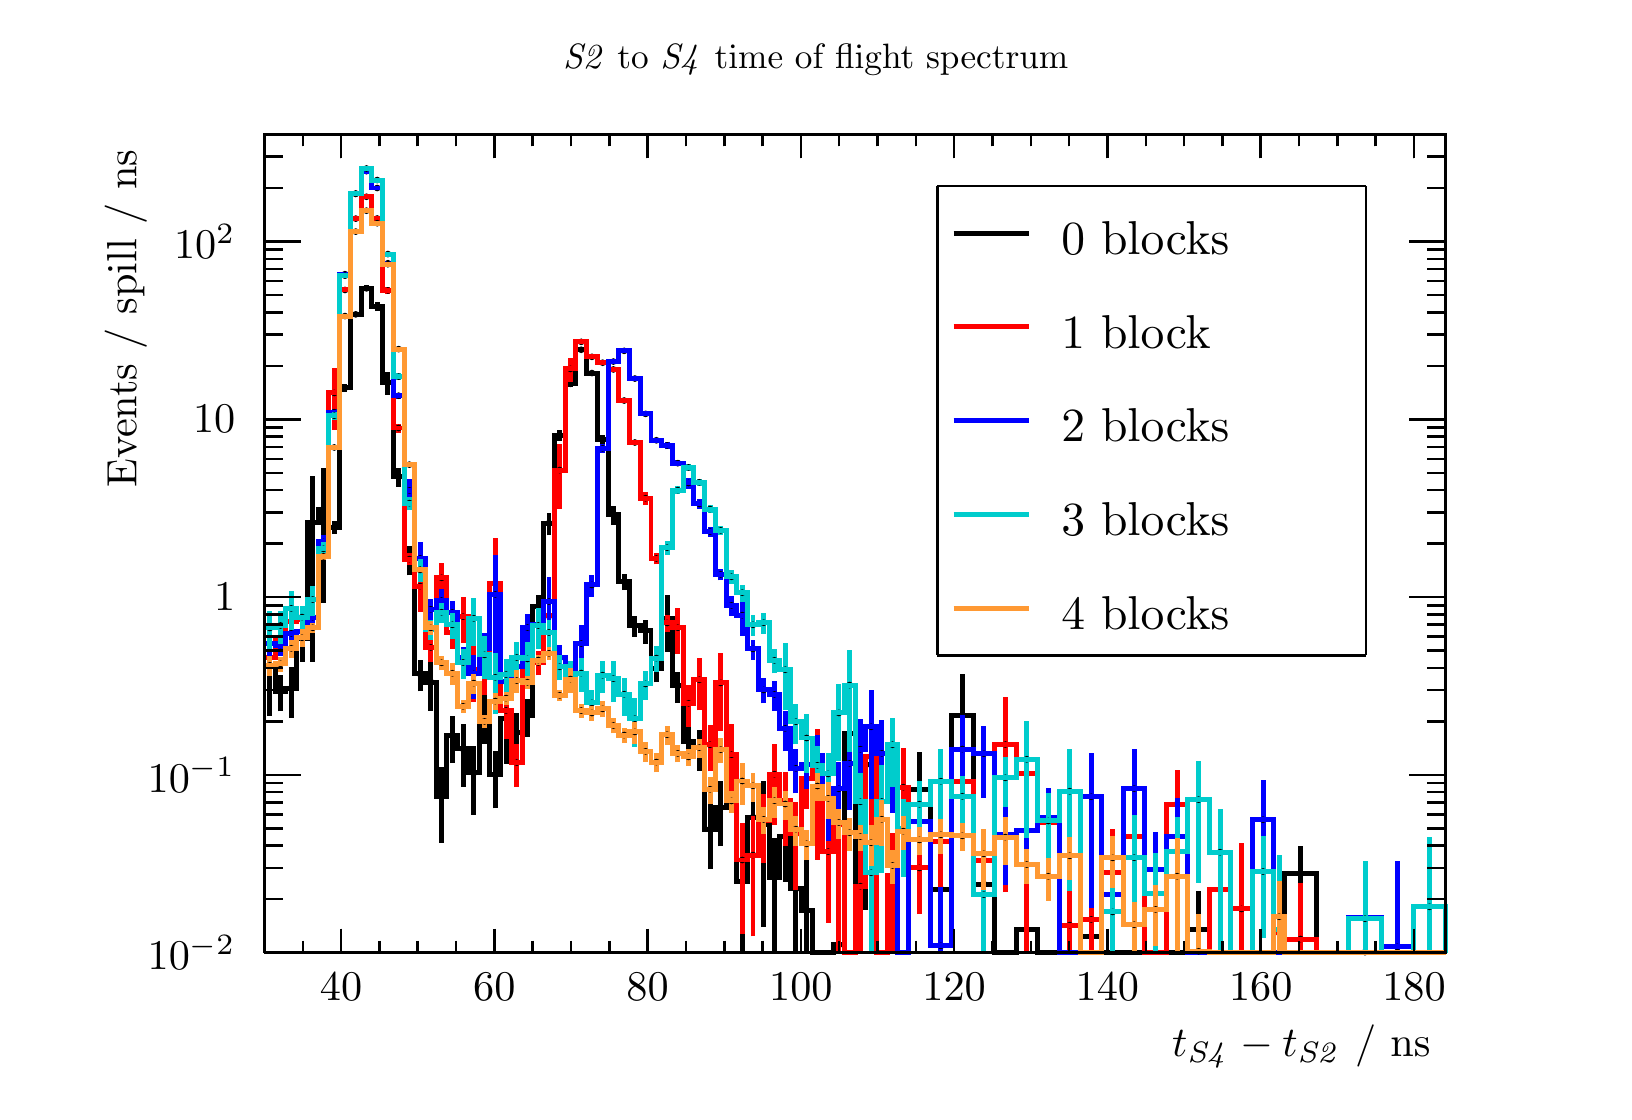
\begin{tikzpicture}
\pgfdeclareplotmark{cross} {
\pgfpathmoveto{\pgfpoint{-0.3\pgfplotmarksize}{\pgfplotmarksize}}
\pgfpathlineto{\pgfpoint{+0.3\pgfplotmarksize}{\pgfplotmarksize}}
\pgfpathlineto{\pgfpoint{+0.3\pgfplotmarksize}{0.3\pgfplotmarksize}}
\pgfpathlineto{\pgfpoint{+1\pgfplotmarksize}{0.3\pgfplotmarksize}}
\pgfpathlineto{\pgfpoint{+1\pgfplotmarksize}{-0.3\pgfplotmarksize}}
\pgfpathlineto{\pgfpoint{+0.3\pgfplotmarksize}{-0.3\pgfplotmarksize}}
\pgfpathlineto{\pgfpoint{+0.3\pgfplotmarksize}{-1.\pgfplotmarksize}}
\pgfpathlineto{\pgfpoint{-0.3\pgfplotmarksize}{-1.\pgfplotmarksize}}
\pgfpathlineto{\pgfpoint{-0.3\pgfplotmarksize}{-0.3\pgfplotmarksize}}
\pgfpathlineto{\pgfpoint{-1.\pgfplotmarksize}{-0.3\pgfplotmarksize}}
\pgfpathlineto{\pgfpoint{-1.\pgfplotmarksize}{0.3\pgfplotmarksize}}
\pgfpathlineto{\pgfpoint{-0.3\pgfplotmarksize}{0.3\pgfplotmarksize}}
\pgfpathclose
\pgfusepathqstroke
}
\pgfdeclareplotmark{cross*} {
\pgfpathmoveto{\pgfpoint{-0.3\pgfplotmarksize}{\pgfplotmarksize}}
\pgfpathlineto{\pgfpoint{+0.3\pgfplotmarksize}{\pgfplotmarksize}}
\pgfpathlineto{\pgfpoint{+0.3\pgfplotmarksize}{0.3\pgfplotmarksize}}
\pgfpathlineto{\pgfpoint{+1\pgfplotmarksize}{0.3\pgfplotmarksize}}
\pgfpathlineto{\pgfpoint{+1\pgfplotmarksize}{-0.3\pgfplotmarksize}}
\pgfpathlineto{\pgfpoint{+0.3\pgfplotmarksize}{-0.3\pgfplotmarksize}}
\pgfpathlineto{\pgfpoint{+0.3\pgfplotmarksize}{-1.\pgfplotmarksize}}
\pgfpathlineto{\pgfpoint{-0.3\pgfplotmarksize}{-1.\pgfplotmarksize}}
\pgfpathlineto{\pgfpoint{-0.3\pgfplotmarksize}{-0.3\pgfplotmarksize}}
\pgfpathlineto{\pgfpoint{-1.\pgfplotmarksize}{-0.3\pgfplotmarksize}}
\pgfpathlineto{\pgfpoint{-1.\pgfplotmarksize}{0.3\pgfplotmarksize}}
\pgfpathlineto{\pgfpoint{-0.3\pgfplotmarksize}{0.3\pgfplotmarksize}}
\pgfpathclose
\pgfusepathqfillstroke
}
\pgfdeclareplotmark{newstar} {
\pgfpathmoveto{\pgfqpoint{0pt}{\pgfplotmarksize}}
\pgfpathlineto{\pgfqpointpolar{44}{0.5\pgfplotmarksize}}
\pgfpathlineto{\pgfqpointpolar{18}{\pgfplotmarksize}}
\pgfpathlineto{\pgfqpointpolar{-20}{0.5\pgfplotmarksize}}
\pgfpathlineto{\pgfqpointpolar{-54}{\pgfplotmarksize}}
\pgfpathlineto{\pgfqpointpolar{-90}{0.5\pgfplotmarksize}}
\pgfpathlineto{\pgfqpointpolar{234}{\pgfplotmarksize}}
\pgfpathlineto{\pgfqpointpolar{198}{0.5\pgfplotmarksize}}
\pgfpathlineto{\pgfqpointpolar{162}{\pgfplotmarksize}}
\pgfpathlineto{\pgfqpointpolar{134}{0.5\pgfplotmarksize}}
\pgfpathclose
\pgfusepathqstroke
}
\pgfdeclareplotmark{newstar*} {
\pgfpathmoveto{\pgfqpoint{0pt}{\pgfplotmarksize}}
\pgfpathlineto{\pgfqpointpolar{44}{0.5\pgfplotmarksize}}
\pgfpathlineto{\pgfqpointpolar{18}{\pgfplotmarksize}}
\pgfpathlineto{\pgfqpointpolar{-20}{0.5\pgfplotmarksize}}
\pgfpathlineto{\pgfqpointpolar{-54}{\pgfplotmarksize}}
\pgfpathlineto{\pgfqpointpolar{-90}{0.5\pgfplotmarksize}}
\pgfpathlineto{\pgfqpointpolar{234}{\pgfplotmarksize}}
\pgfpathlineto{\pgfqpointpolar{198}{0.5\pgfplotmarksize}}
\pgfpathlineto{\pgfqpointpolar{162}{\pgfplotmarksize}}
\pgfpathlineto{\pgfqpointpolar{134}{0.5\pgfplotmarksize}}
\pgfpathclose
\pgfusepathqfillstroke
}
\definecolor{c}{rgb}{1,1,1};
\draw [color=c, fill=c] (0,0) rectangle (20,13.4957);
\draw [color=c, fill=c] (3,1.75444) rectangle (18,12.1461);
\definecolor{c}{rgb}{0,0,0};
\draw [c,line width=0.9] (3,1.75444) -- (3,12.1461) -- (18,12.1461) -- (18,1.75444) -- (3,1.75444);
\definecolor{c}{rgb}{1,1,1};
\draw [color=c, fill=c] (3,1.75444) rectangle (18,12.1461);
\definecolor{c}{rgb}{0,0,0};
\draw [c,line width=0.9] (3,1.75444) -- (3,12.1461) -- (18,12.1461) -- (18,1.75444) -- (3,1.75444);
\draw [c,line width=0.9] (3,1.75444) -- (3.13636,1.75444) -- (3.13636,1.75444) -- (3.27273,1.75444) -- (3.27273,1.75444) -- (3.40909,1.75444) -- (3.40909,1.75444) -- (3.54545,1.75444) -- (3.54545,1.75444) -- (3.68182,1.75444) -- (3.68182,1.75444) --
 (3.81818,1.75444) -- (3.81818,1.75444) -- (3.95455,1.75444) -- (3.95455,1.75444) -- (4.09091,1.75444) -- (4.09091,1.75444) -- (4.22727,1.75444) -- (4.22727,1.75444) -- (4.36364,1.75444) -- (4.36364,1.75444) -- (4.5,1.75444) -- (4.5,1.75444) --
 (4.63636,1.75444) -- (4.63636,1.75444) -- (4.77273,1.75444) -- (4.77273,1.75444) -- (4.90909,1.75444) -- (4.90909,1.75444) -- (5.04545,1.75444) -- (5.04545,1.75444) -- (5.18182,1.75444) -- (5.18182,1.75444) -- (5.31818,1.75444) -- (5.31818,1.75444)
 -- (5.45455,1.75444) -- (5.45455,1.75444) -- (5.59091,1.75444) -- (5.59091,1.75444) -- (5.72727,1.75444) -- (5.72727,1.75444) -- (5.86364,1.75444) -- (5.86364,1.75444) -- (6,1.75444) -- (6,1.75444) -- (6.13636,1.75444) -- (6.13636,1.75444) --
 (6.27273,1.75444) -- (6.27273,1.75444) -- (6.40909,1.75444) -- (6.40909,1.75444) -- (6.54545,1.75444) -- (6.54545,1.75444) -- (6.68182,1.75444) -- (6.68182,1.75444) -- (6.81818,1.75444) -- (6.81818,1.75444) -- (6.95455,1.75444) -- (6.95455,1.75444)
 -- (7.09091,1.75444) -- (7.09091,1.75444) -- (7.22727,1.75444) -- (7.22727,1.75444) -- (7.36364,1.75444) -- (7.36364,1.75444) -- (7.5,1.75444) -- (7.5,1.75444) -- (7.63636,1.75444) -- (7.63636,1.75444) -- (7.77273,1.75444) -- (7.77273,1.75444) --
 (7.90909,1.75444) -- (7.90909,1.75444) -- (8.04545,1.75444) -- (8.04545,1.75444) -- (8.18182,1.75444) -- (8.18182,1.75444) -- (8.31818,1.75444) -- (8.31818,1.75444) -- (8.45455,1.75444) -- (8.45455,1.75444) -- (8.59091,1.75444) -- (8.59091,1.75444)
 -- (8.72727,1.75444) -- (8.72727,1.75444) -- (8.86364,1.75444) -- (8.86364,1.75444) -- (9,1.75444) -- (9,1.75444) -- (9.13636,1.75444) -- (9.13636,1.75444) -- (9.27273,1.75444) -- (9.27273,1.75444) -- (9.40909,1.75444) -- (9.40909,1.75444) --
 (9.54545,1.75444) -- (9.54545,1.75444) -- (9.68182,1.75444) -- (9.68182,1.75444) -- (9.81818,1.75444) -- (9.81818,1.75444) -- (9.95455,1.75444) -- (9.95455,1.75444) -- (10.0909,1.75444) -- (10.0909,1.75444) -- (10.2273,1.75444) -- (10.2273,1.75444)
 -- (10.3636,1.75444) -- (10.3636,1.75444) -- (10.5,1.75444) -- (10.5,1.75444) -- (10.6364,1.75444) -- (10.6364,1.75444) -- (10.7727,1.75444) -- (10.7727,1.75444) -- (10.9091,1.75444) -- (10.9091,1.75444) -- (11.0455,1.75444) -- (11.0455,1.75444) --
 (11.1818,1.75444) -- (11.1818,1.75444) -- (11.4545,1.75444) -- (11.4545,1.75444) -- (11.7273,1.75444) -- (11.7273,1.75444) -- (12,1.75444) -- (12,1.75444) -- (12.2727,1.75444) -- (12.2727,1.75444) -- (12.5455,1.75444) -- (12.5455,1.75444) --
 (12.8182,1.75444) -- (12.8182,1.75444) -- (13.0909,1.75444) -- (13.0909,1.75444) -- (13.3636,1.75444) -- (13.3636,1.75444) -- (13.6364,1.75444) -- (13.6364,1.75444) -- (13.9091,1.75444) -- (13.9091,1.75444) -- (14.1818,1.75444) -- (14.1818,1.75444)
 -- (14.4545,1.75444) -- (14.4545,1.75444) -- (14.7273,1.75444) -- (14.7273,1.75444) -- (15,1.75444) -- (15,1.75444) -- (15.2727,1.75444) -- (15.2727,1.75444) -- (15.5455,1.75444) -- (15.5455,1.75444) -- (15.8182,1.75444) -- (15.8182,1.75444) --
 (15.9545,1.75444) -- (15.9545,1.75444) -- (16.3636,1.75444) -- (16.3636,1.75444) -- (16.7727,1.75444) -- (16.7727,1.75444) -- (17.1818,1.75444) -- (17.1818,1.75444) -- (17.5909,1.75444) -- (17.5909,1.75444) -- (18,1.75444);
\draw [c,line width=0.9] (3,1.75444) -- (18,1.75444);
\draw [c,line width=0.9] (3.97326,2.05809) -- (3.97326,1.75444);
\draw [c,line width=0.9] (4.45989,1.90627) -- (4.45989,1.75444);
\draw [c,line width=0.9] (4.94652,1.90627) -- (4.94652,1.75444);
\draw [c,line width=0.9] (5.43316,1.90627) -- (5.43316,1.75444);
\draw [c,line width=0.9] (5.91979,2.05809) -- (5.91979,1.75444);
\draw [c,line width=0.9] (6.40642,1.90627) -- (6.40642,1.75444);
\draw [c,line width=0.9] (6.89305,1.90627) -- (6.89305,1.75444);
\draw [c,line width=0.9] (7.37968,1.90627) -- (7.37968,1.75444);
\draw [c,line width=0.9] (7.86631,2.05809) -- (7.86631,1.75444);
\draw [c,line width=0.9] (8.35294,1.90627) -- (8.35294,1.75444);
\draw [c,line width=0.9] (8.83957,1.90627) -- (8.83957,1.75444);
\draw [c,line width=0.9] (9.3262,1.90627) -- (9.3262,1.75444);
\draw [c,line width=0.9] (9.81283,2.05809) -- (9.81283,1.75444);
\draw [c,line width=0.9] (10.2995,1.90627) -- (10.2995,1.75444);
\draw [c,line width=0.9] (10.7861,1.90627) -- (10.7861,1.75444);
\draw [c,line width=0.9] (11.2727,1.90627) -- (11.2727,1.75444);
\draw [c,line width=0.9] (11.7594,2.05809) -- (11.7594,1.75444);
\draw [c,line width=0.9] (12.246,1.90627) -- (12.246,1.75444);
\draw [c,line width=0.9] (12.7326,1.90627) -- (12.7326,1.75444);
\draw [c,line width=0.9] (13.2193,1.90627) -- (13.2193,1.75444);
\draw [c,line width=0.9] (13.7059,2.05809) -- (13.7059,1.75444);
\draw [c,line width=0.9] (14.1925,1.90627) -- (14.1925,1.75444);
\draw [c,line width=0.9] (14.6791,1.90627) -- (14.6791,1.75444);
\draw [c,line width=0.9] (15.1658,1.90627) -- (15.1658,1.75444);
\draw [c,line width=0.9] (15.6524,2.05809) -- (15.6524,1.75444);
\draw [c,line width=0.9] (16.139,1.90627) -- (16.139,1.75444);
\draw [c,line width=0.9] (16.6257,1.90627) -- (16.6257,1.75444);
\draw [c,line width=0.9] (17.1123,1.90627) -- (17.1123,1.75444);
\draw [c,line width=0.9] (17.5989,2.05809) -- (17.5989,1.75444);
\draw [c,line width=0.9] (3.97326,2.05809) -- (3.97326,1.75444);
\draw [c,line width=0.9] (3.48663,1.90627) -- (3.48663,1.75444);
\draw [c,line width=0.9] (3,1.90627) -- (3,1.75444);
\draw [c,line width=0.9] (17.5989,2.05809) -- (17.5989,1.75444);
\draw [anchor=base] (3.97326,1.14713) node[scale=1.52731, color=c, rotate=0]{40};
\draw [anchor=base] (5.91979,1.14713) node[scale=1.52731, color=c, rotate=0]{60};
\draw [anchor=base] (7.86631,1.14713) node[scale=1.52731, color=c, rotate=0]{80};
\draw [anchor=base] (9.81283,1.14713) node[scale=1.52731, color=c, rotate=0]{100};
\draw [anchor=base] (11.7594,1.14713) node[scale=1.52731, color=c, rotate=0]{120};
\draw [anchor=base] (13.7059,1.14713) node[scale=1.52731, color=c, rotate=0]{140};
\draw [anchor=base] (15.6524,1.14713) node[scale=1.52731, color=c, rotate=0]{160};
\draw [anchor=base] (17.5989,1.14713) node[scale=1.52731, color=c, rotate=0]{180};
\draw [anchor= east] (18,0.566819) node[scale=1.52731, color=c, rotate=0]{$ t_{\mathit{S4}} - t_{\mathit{S2}}$ / ns};
\draw [c,line width=0.9] (3,12.1461) -- (18,12.1461);
\draw [c,line width=0.9] (3.97326,11.8425) -- (3.97326,12.1461);
\draw [c,line width=0.9] (4.45989,11.9943) -- (4.45989,12.1461);
\draw [c,line width=0.9] (4.94652,11.9943) -- (4.94652,12.1461);
\draw [c,line width=0.9] (5.43316,11.9943) -- (5.43316,12.1461);
\draw [c,line width=0.9] (5.91979,11.8425) -- (5.91979,12.1461);
\draw [c,line width=0.9] (6.40642,11.9943) -- (6.40642,12.1461);
\draw [c,line width=0.9] (6.89305,11.9943) -- (6.89305,12.1461);
\draw [c,line width=0.9] (7.37968,11.9943) -- (7.37968,12.1461);
\draw [c,line width=0.9] (7.86631,11.8425) -- (7.86631,12.1461);
\draw [c,line width=0.9] (8.35294,11.9943) -- (8.35294,12.1461);
\draw [c,line width=0.9] (8.83957,11.9943) -- (8.83957,12.1461);
\draw [c,line width=0.9] (9.3262,11.9943) -- (9.3262,12.1461);
\draw [c,line width=0.9] (9.81283,11.8425) -- (9.81283,12.1461);
\draw [c,line width=0.9] (10.2995,11.9943) -- (10.2995,12.1461);
\draw [c,line width=0.9] (10.7861,11.9943) -- (10.7861,12.1461);
\draw [c,line width=0.9] (11.2727,11.9943) -- (11.2727,12.1461);
\draw [c,line width=0.9] (11.7594,11.8425) -- (11.7594,12.1461);
\draw [c,line width=0.9] (12.246,11.9943) -- (12.246,12.1461);
\draw [c,line width=0.9] (12.7326,11.9943) -- (12.7326,12.1461);
\draw [c,line width=0.9] (13.2193,11.9943) -- (13.2193,12.1461);
\draw [c,line width=0.9] (13.7059,11.8425) -- (13.7059,12.1461);
\draw [c,line width=0.9] (14.1925,11.9943) -- (14.1925,12.1461);
\draw [c,line width=0.9] (14.6791,11.9943) -- (14.6791,12.1461);
\draw [c,line width=0.9] (15.1658,11.9943) -- (15.1658,12.1461);
\draw [c,line width=0.9] (15.6524,11.8425) -- (15.6524,12.1461);
\draw [c,line width=0.9] (16.139,11.9943) -- (16.139,12.1461);
\draw [c,line width=0.9] (16.6257,11.9943) -- (16.6257,12.1461);
\draw [c,line width=0.9] (17.1123,11.9943) -- (17.1123,12.1461);
\draw [c,line width=0.9] (17.5989,11.8425) -- (17.5989,12.1461);
\draw [c,line width=0.9] (3.97326,11.8425) -- (3.97326,12.1461);
\draw [c,line width=0.9] (3.48663,11.9943) -- (3.48663,12.1461);
\draw [c,line width=0.9] (3,11.9943) -- (3,12.1461);
\draw [c,line width=0.9] (17.5989,11.8425) -- (17.5989,12.1461);
\draw [c,line width=0.9] (3,1.75444) -- (3,12.1461);
\draw [c,line width=0.9] (3.462,1.75444) -- (3,1.75444);
\draw [anchor= east] (2.82,1.75444) node[scale=1.52731, color=c, rotate=0]{$10^{-2}$};
\draw [c,line width=0.9] (3.231,2.43418) -- (3,2.43418);
\draw [c,line width=0.9] (3.231,2.83181) -- (3,2.83181);
\draw [c,line width=0.9] (3.231,3.11393) -- (3,3.11393);
\draw [c,line width=0.9] (3.231,3.33275) -- (3,3.33275);
\draw [c,line width=0.9] (3.231,3.51155) -- (3,3.51155);
\draw [c,line width=0.9] (3.231,3.66272) -- (3,3.66272);
\draw [c,line width=0.9] (3.231,3.79367) -- (3,3.79367);
\draw [c,line width=0.9] (3.231,3.90917) -- (3,3.90917);
\draw [c,line width=0.9] (3.462,4.0125) -- (3,4.0125);
\draw [anchor= east] (2.82,4.0125) node[scale=1.52731, color=c, rotate=0]{$10^{-1}$};
\draw [c,line width=0.9] (3.231,4.69224) -- (3,4.69224);
\draw [c,line width=0.9] (3.231,5.08986) -- (3,5.08986);
\draw [c,line width=0.9] (3.231,5.37198) -- (3,5.37198);
\draw [c,line width=0.9] (3.231,5.59081) -- (3,5.59081);
\draw [c,line width=0.9] (3.231,5.7696) -- (3,5.7696);
\draw [c,line width=0.9] (3.231,5.92077) -- (3,5.92077);
\draw [c,line width=0.9] (3.231,6.05172) -- (3,6.05172);
\draw [c,line width=0.9] (3.231,6.16722) -- (3,6.16722);
\draw [c,line width=0.9] (3.462,6.27055) -- (3,6.27055);
\draw [anchor= east] (2.82,6.27055) node[scale=1.52731, color=c, rotate=0]{1};
\draw [c,line width=0.9] (3.231,6.95029) -- (3,6.95029);
\draw [c,line width=0.9] (3.231,7.34791) -- (3,7.34791);
\draw [c,line width=0.9] (3.231,7.63003) -- (3,7.63003);
\draw [c,line width=0.9] (3.231,7.84886) -- (3,7.84886);
\draw [c,line width=0.9] (3.231,8.02765) -- (3,8.02765);
\draw [c,line width=0.9] (3.231,8.17882) -- (3,8.17882);
\draw [c,line width=0.9] (3.231,8.30977) -- (3,8.30977);
\draw [c,line width=0.9] (3.231,8.42527) -- (3,8.42527);
\draw [c,line width=0.9] (3.462,8.5286) -- (3,8.5286);
\draw [anchor= east] (2.82,8.5286) node[scale=1.52731, color=c, rotate=0]{10};
\draw [c,line width=0.9] (3.231,9.20834) -- (3,9.20834);
\draw [c,line width=0.9] (3.231,9.60596) -- (3,9.60596);
\draw [c,line width=0.9] (3.231,9.88808) -- (3,9.88808);
\draw [c,line width=0.9] (3.231,10.1069) -- (3,10.1069);
\draw [c,line width=0.9] (3.231,10.2857) -- (3,10.2857);
\draw [c,line width=0.9] (3.231,10.4369) -- (3,10.4369);
\draw [c,line width=0.9] (3.231,10.5678) -- (3,10.5678);
\draw [c,line width=0.9] (3.231,10.6833) -- (3,10.6833);
\draw [c,line width=0.9] (3.462,10.7866) -- (3,10.7866);
\draw [anchor= east] (2.82,10.7866) node[scale=1.52731, color=c, rotate=0]{$10^{2}$};
\draw [c,line width=0.9] (3.231,11.4664) -- (3,11.4664);
\draw [c,line width=0.9] (3.231,11.864) -- (3,11.864);
\draw [c,line width=0.9] (3.231,12.1461) -- (3,12.1461);
\draw [anchor= east] (1.24,12.1461) node[scale=1.52731, color=c, rotate=90]{ Events / spill / ns};
\draw [c,line width=0.9] (18,1.75444) -- (18,12.1461);
\draw [c,line width=0.9] (17.538,1.75444) -- (18,1.75444);
\draw [c,line width=0.9] (17.769,2.43418) -- (18,2.43418);
\draw [c,line width=0.9] (17.769,2.83181) -- (18,2.83181);
\draw [c,line width=0.9] (17.769,3.11393) -- (18,3.11393);
\draw [c,line width=0.9] (17.769,3.33275) -- (18,3.33275);
\draw [c,line width=0.9] (17.769,3.51155) -- (18,3.51155);
\draw [c,line width=0.9] (17.769,3.66272) -- (18,3.66272);
\draw [c,line width=0.9] (17.769,3.79367) -- (18,3.79367);
\draw [c,line width=0.9] (17.769,3.90917) -- (18,3.90917);
\draw [c,line width=0.9] (17.538,4.0125) -- (18,4.0125);
\draw [c,line width=0.9] (17.769,4.69224) -- (18,4.69224);
\draw [c,line width=0.9] (17.769,5.08986) -- (18,5.08986);
\draw [c,line width=0.9] (17.769,5.37198) -- (18,5.37198);
\draw [c,line width=0.9] (17.769,5.59081) -- (18,5.59081);
\draw [c,line width=0.9] (17.769,5.7696) -- (18,5.7696);
\draw [c,line width=0.9] (17.769,5.92077) -- (18,5.92077);
\draw [c,line width=0.9] (17.769,6.05172) -- (18,6.05172);
\draw [c,line width=0.9] (17.769,6.16722) -- (18,6.16722);
\draw [c,line width=0.9] (17.538,6.27055) -- (18,6.27055);
\draw [c,line width=0.9] (17.769,6.95029) -- (18,6.95029);
\draw [c,line width=0.9] (17.769,7.34791) -- (18,7.34791);
\draw [c,line width=0.9] (17.769,7.63003) -- (18,7.63003);
\draw [c,line width=0.9] (17.769,7.84886) -- (18,7.84886);
\draw [c,line width=0.9] (17.769,8.02765) -- (18,8.02765);
\draw [c,line width=0.9] (17.769,8.17882) -- (18,8.17882);
\draw [c,line width=0.9] (17.769,8.30977) -- (18,8.30977);
\draw [c,line width=0.9] (17.769,8.42527) -- (18,8.42527);
\draw [c,line width=0.9] (17.538,8.5286) -- (18,8.5286);
\draw [c,line width=0.9] (17.769,9.20834) -- (18,9.20834);
\draw [c,line width=0.9] (17.769,9.60596) -- (18,9.60596);
\draw [c,line width=0.9] (17.769,9.88808) -- (18,9.88808);
\draw [c,line width=0.9] (17.769,10.1069) -- (18,10.1069);
\draw [c,line width=0.9] (17.769,10.2857) -- (18,10.2857);
\draw [c,line width=0.9] (17.769,10.4369) -- (18,10.4369);
\draw [c,line width=0.9] (17.769,10.5678) -- (18,10.5678);
\draw [c,line width=0.9] (17.769,10.6833) -- (18,10.6833);
\draw [c,line width=0.9] (17.538,10.7866) -- (18,10.7866);
\draw [c,line width=0.9] (17.769,11.4664) -- (18,11.4664);
\draw [c,line width=0.9] (17.769,11.864) -- (18,11.864);
\draw [c,line width=0.9] (17.769,12.1461) -- (18,12.1461);
\draw [c,line width=1.8] (3.06818,4.76609) -- (3.06818,5.40071);
\draw [c,line width=1.8] (3.06818,5.40071) -- (3.06818,5.78282);
\foreach \P in {(3.06818,5.40071)}{\draw[mark options={color=c,fill=c},mark size=2.402402pt,mark=*,mark size=1pt] plot coordinates {\P};}
\draw [c,line width=1.8] (3.20455,4.81813) -- (3.20455,5.07538);
\draw [c,line width=1.8] (3.20455,5.07538) -- (3.20455,5.27899);
\foreach \P in {(3.20455,5.07538)}{\draw[mark options={color=c,fill=c},mark size=2.402402pt,mark=*,mark size=1pt] plot coordinates {\P};}
\draw [c,line width=1.8] (3.34091,4.73992) -- (3.34091,5.11562);
\draw [c,line width=1.8] (3.34091,5.11562) -- (3.34091,5.38659);
\foreach \P in {(3.34091,5.11562)}{\draw[mark options={color=c,fill=c},mark size=2.402402pt,mark=*,mark size=1pt] plot coordinates {\P};}
\draw [c,line width=1.8] (3.47727,5.45284) -- (3.47727,5.75063);
\draw [c,line width=1.8] (3.47727,5.75063) -- (3.47727,5.97875);
\foreach \P in {(3.47727,5.75063)}{\draw[mark options={color=c,fill=c},mark size=2.402402pt,mark=*,mark size=1pt] plot coordinates {\P};}
\draw [c,line width=1.8] (3.61364,5.449) -- (3.61364,7.21647);
\draw [c,line width=1.8] (3.61364,7.21647) -- (3.61364,7.81182);
\foreach \P in {(3.61364,7.21647)}{\draw[mark options={color=c,fill=c},mark size=2.402402pt,mark=*,mark size=1pt] plot coordinates {\P};}
\draw [c,line width=1.8] (3.75,6.19486) -- (3.75,7.38813);
\draw [c,line width=1.8] (3.75,7.38813) -- (3.75,7.9107);
\foreach \P in {(3.75,7.38813)}{\draw[mark options={color=c,fill=c},mark size=2.402402pt,mark=*,mark size=1pt] plot coordinates {\P};}
\draw [c,line width=1.8] (3.88636,7.07197) -- (3.88636,7.15962);
\draw [c,line width=1.8] (3.88636,7.15962) -- (3.88636,7.24007);
\foreach \P in {(3.88636,7.15962)}{\draw[mark options={color=c,fill=c},mark size=2.402402pt,mark=*,mark size=1pt] plot coordinates {\P};}
\draw [c,line width=1.8] (4.02273,8.88003) -- (4.02273,8.92947);
\draw [c,line width=1.8] (4.02273,8.92947) -- (4.02273,8.97653);
\foreach \P in {(4.02273,8.92947)}{\draw[mark options={color=c,fill=c},mark size=2.402402pt,mark=*,mark size=1pt] plot coordinates {\P};}
\draw [c,line width=1.8] (4.15909,9.82942) -- (4.15909,9.86175);
\draw [c,line width=1.8] (4.15909,9.86175) -- (4.15909,9.89304);
\foreach \P in {(4.15909,9.86175)}{\draw[mark options={color=c,fill=c},mark size=2.402402pt,mark=*,mark size=1pt] plot coordinates {\P};}
\draw [c,line width=1.8] (4.29545,10.154) -- (4.29545,10.1919);
\draw [c,line width=1.8] (4.29545,10.1919) -- (4.29545,10.2284);
\foreach \P in {(4.29545,10.1919)}{\draw[mark options={color=c,fill=c},mark size=2.402402pt,mark=*,mark size=1pt] plot coordinates {\P};}
\draw [c,line width=1.8] (4.43182,9.90216) -- (4.43182,9.96086);
\draw [c,line width=1.8] (4.43182,9.96086) -- (4.43182,10.0162);
\foreach \P in {(4.43182,9.96086)}{\draw[mark options={color=c,fill=c},mark size=2.402402pt,mark=*,mark size=1pt] plot coordinates {\P};}
\draw [c,line width=1.8] (4.56818,8.83982) -- (4.56818,8.9955);
\draw [c,line width=1.8] (4.56818,8.9955) -- (4.56818,9.12983);
\foreach \P in {(4.56818,8.9955)}{\draw[mark options={color=c,fill=c},mark size=2.402402pt,mark=*,mark size=1pt] plot coordinates {\P};}
\draw [c,line width=1.8] (4.70455,7.67461) -- (4.70455,7.80053);
\draw [c,line width=1.8] (4.70455,7.80053) -- (4.70455,7.9121);
\foreach \P in {(4.70455,7.80053)}{\draw[mark options={color=c,fill=c},mark size=2.402402pt,mark=*,mark size=1pt] plot coordinates {\P};}
\draw [c,line width=1.8] (4.84091,6.54749) -- (4.84091,6.75203);
\draw [c,line width=1.8] (4.84091,6.75203) -- (4.84091,6.92119);
\foreach \P in {(4.84091,6.75203)}{\draw[mark options={color=c,fill=c},mark size=2.402402pt,mark=*,mark size=1pt] plot coordinates {\P};}
\draw [c,line width=1.8] (4.97727,5.07239) -- (4.97727,5.29551);
\draw [c,line width=1.8] (4.97727,5.29551) -- (4.97727,5.47715);
\foreach \P in {(4.97727,5.29551)}{\draw[mark options={color=c,fill=c},mark size=2.402402pt,mark=*,mark size=1pt] plot coordinates {\P};}
\draw [c,line width=1.8] (5.11364,4.82747) -- (5.11364,5.19232);
\draw [c,line width=1.8] (5.11364,5.19232) -- (5.11364,5.45764);
\foreach \P in {(5.11364,5.19232)}{\draw[mark options={color=c,fill=c},mark size=2.402402pt,mark=*,mark size=1pt] plot coordinates {\P};}
\draw [c,line width=1.8] (5.25,3.1514) -- (5.25,3.74222);
\draw [c,line width=1.8] (5.25,3.74222) -- (5.25,4.10832);
\foreach \P in {(5.25,3.74222)}{\draw[mark options={color=c,fill=c},mark size=2.402402pt,mark=*,mark size=1pt] plot coordinates {\P};}
\draw [c,line width=1.8] (5.38636,4.16357) -- (5.38636,4.5075);
\draw [c,line width=1.8] (5.38636,4.5075) -- (5.38636,4.76162);
\foreach \P in {(5.38636,4.5075)}{\draw[mark options={color=c,fill=c},mark size=2.402402pt,mark=*,mark size=1pt] plot coordinates {\P};}
\draw [c,line width=1.8] (5.52273,3.86174) -- (5.52273,4.34356);
\draw [c,line width=1.8] (5.52273,4.34356) -- (5.52273,4.66522);
\foreach \P in {(5.52273,4.34356)}{\draw[mark options={color=c,fill=c},mark size=2.402402pt,mark=*,mark size=1pt] plot coordinates {\P};}
\draw [c,line width=1.8] (5.65909,3.50879) -- (5.65909,4.03798);
\draw [c,line width=1.8] (5.65909,4.03798) -- (5.65909,4.3798);
\foreach \P in {(5.65909,4.03798)}{\draw[mark options={color=c,fill=c},mark size=2.402402pt,mark=*,mark size=1pt] plot coordinates {\P};}
\draw [c,line width=1.8] (5.79545,4.41003) -- (5.79545,4.93593);
\draw [c,line width=1.8] (5.79545,4.93593) -- (5.79545,5.2764);
\foreach \P in {(5.79545,4.93593)}{\draw[mark options={color=c,fill=c},mark size=2.402402pt,mark=*,mark size=1pt] plot coordinates {\P};}
\draw [c,line width=1.8] (5.93182,3.5884) -- (5.93182,4.01749);
\draw [c,line width=1.8] (5.93182,4.01749) -- (5.93182,4.31497);
\foreach \P in {(5.93182,4.01749)}{\draw[mark options={color=c,fill=c},mark size=2.402402pt,mark=*,mark size=1pt] plot coordinates {\P};}
\draw [c,line width=1.8] (6.06818,4.15217) -- (6.06818,4.72752);
\draw [c,line width=1.8] (6.06818,4.72752) -- (6.06818,5.08772);
\foreach \P in {(6.06818,4.72752)}{\draw[mark options={color=c,fill=c},mark size=2.402402pt,mark=*,mark size=1pt] plot coordinates {\P};}
\draw [c,line width=1.8] (6.20455,4.21678) -- (6.20455,4.54867);
\draw [c,line width=1.8] (6.20455,4.54867) -- (6.20455,4.79619);
\foreach \P in {(6.20455,4.54867)}{\draw[mark options={color=c,fill=c},mark size=2.402402pt,mark=*,mark size=1pt] plot coordinates {\P};}
\draw [c,line width=1.8] (6.34091,4.49376) -- (6.34091,4.76233);
\draw [c,line width=1.8] (6.34091,4.76233) -- (6.34091,4.97294);
\foreach \P in {(6.34091,4.76233)}{\draw[mark options={color=c,fill=c},mark size=2.402402pt,mark=*,mark size=1pt] plot coordinates {\P};}
\draw [c,line width=1.8] (6.47727,5.96589) -- (6.47727,6.14792);
\draw [c,line width=1.8] (6.47727,6.14792) -- (6.47727,6.30138);
\foreach \P in {(6.47727,6.14792)}{\draw[mark options={color=c,fill=c},mark size=2.402402pt,mark=*,mark size=1pt] plot coordinates {\P};}
\draw [c,line width=1.8] (6.61364,7.05608) -- (6.61364,7.21099);
\draw [c,line width=1.8] (6.61364,7.21099) -- (6.61364,7.34473);
\foreach \P in {(6.61364,7.21099)}{\draw[mark options={color=c,fill=c},mark size=2.402402pt,mark=*,mark size=1pt] plot coordinates {\P};}
\draw [c,line width=1.8] (6.75,8.25554) -- (6.75,8.32543);
\draw [c,line width=1.8] (6.75,8.32543) -- (6.75,8.39067);
\foreach \P in {(6.75,8.32543)}{\draw[mark options={color=c,fill=c},mark size=2.402402pt,mark=*,mark size=1pt] plot coordinates {\P};}
\draw [c,line width=1.8] (6.88636,8.93919) -- (6.88636,8.9794);
\draw [c,line width=1.8] (6.88636,8.9794) -- (6.88636,9.01803);
\foreach \P in {(6.88636,8.9794)}{\draw[mark options={color=c,fill=c},mark size=2.402402pt,mark=*,mark size=1pt] plot coordinates {\P};}
\draw [c,line width=1.8] (7.02273,9.38097) -- (7.02273,9.4121);
\draw [c,line width=1.8] (7.02273,9.4121) -- (7.02273,9.44229);
\foreach \P in {(7.02273,9.4121)}{\draw[mark options={color=c,fill=c},mark size=2.402402pt,mark=*,mark size=1pt] plot coordinates {\P};}
\draw [c,line width=1.8] (7.15909,9.08494) -- (7.15909,9.11642);
\draw [c,line width=1.8] (7.15909,9.11642) -- (7.15909,9.14691);
\foreach \P in {(7.15909,9.11642)}{\draw[mark options={color=c,fill=c},mark size=2.402402pt,mark=*,mark size=1pt] plot coordinates {\P};}
\draw [c,line width=1.8] (7.29545,8.21148) -- (7.29545,8.26959);
\draw [c,line width=1.8] (7.29545,8.26959) -- (7.29545,8.32444);
\foreach \P in {(7.29545,8.26959)}{\draw[mark options={color=c,fill=c},mark size=2.402402pt,mark=*,mark size=1pt] plot coordinates {\P};}
\draw [c,line width=1.8] (7.43182,7.18629) -- (7.43182,7.31557);
\draw [c,line width=1.8] (7.43182,7.31557) -- (7.43182,7.42978);
\foreach \P in {(7.43182,7.31557)}{\draw[mark options={color=c,fill=c},mark size=2.402402pt,mark=*,mark size=1pt] plot coordinates {\P};}
\draw [c,line width=1.8] (7.56818,6.36075) -- (7.56818,6.46737);
\draw [c,line width=1.8] (7.56818,6.46737) -- (7.56818,6.56353);
\foreach \P in {(7.56818,6.46737)}{\draw[mark options={color=c,fill=c},mark size=2.402402pt,mark=*,mark size=1pt] plot coordinates {\P};}
\draw [c,line width=1.8] (7.70455,5.76677) -- (7.70455,5.90731);
\draw [c,line width=1.8] (7.70455,5.90731) -- (7.70455,6.03021);
\foreach \P in {(7.70455,5.90731)}{\draw[mark options={color=c,fill=c},mark size=2.402402pt,mark=*,mark size=1pt] plot coordinates {\P};}
\draw [c,line width=1.8] (7.84091,5.68052) -- (7.84091,5.84053);
\draw [c,line width=1.8] (7.84091,5.84053) -- (7.84091,5.97806);
\foreach \P in {(7.84091,5.84053)}{\draw[mark options={color=c,fill=c},mark size=2.402402pt,mark=*,mark size=1pt] plot coordinates {\P};}
\draw [c,line width=1.8] (7.97727,5.18881) -- (7.97727,5.36403);
\draw [c,line width=1.8] (7.97727,5.36403) -- (7.97727,5.51263);
\foreach \P in {(7.97727,5.36403)}{\draw[mark options={color=c,fill=c},mark size=2.402402pt,mark=*,mark size=1pt] plot coordinates {\P};}
\draw [c,line width=1.8] (8.11364,5.57089) -- (8.11364,5.99723);
\draw [c,line width=1.8] (8.11364,5.99723) -- (8.11364,6.2934);
\foreach \P in {(8.11364,5.99723)}{\draw[mark options={color=c,fill=c},mark size=2.402402pt,mark=*,mark size=1pt] plot coordinates {\P};}
\draw [c,line width=1.8] (8.25,4.92407) -- (8.25,5.14459);
\draw [c,line width=1.8] (8.25,5.14459) -- (8.25,5.32452);
\foreach \P in {(8.25,5.14459)}{\draw[mark options={color=c,fill=c},mark size=2.402402pt,mark=*,mark size=1pt] plot coordinates {\P};}
\draw [c,line width=1.8] (8.38636,4.16029) -- (8.38636,4.44129);
\draw [c,line width=1.8] (8.38636,4.44129) -- (8.38636,4.65946);
\foreach \P in {(8.38636,4.44129)}{\draw[mark options={color=c,fill=c},mark size=2.402402pt,mark=*,mark size=1pt] plot coordinates {\P};}
\draw [c,line width=1.8] (8.52273,4.06661) -- (8.52273,4.36117);
\draw [c,line width=1.8] (8.52273,4.36117) -- (8.52273,4.58738);
\foreach \P in {(8.52273,4.36117)}{\draw[mark options={color=c,fill=c},mark size=2.402402pt,mark=*,mark size=1pt] plot coordinates {\P};}
\draw [c,line width=1.8] (8.65909,2.81519) -- (8.65909,3.32407);
\draw [c,line width=1.8] (8.65909,3.32407) -- (8.65909,3.65741);
\foreach \P in {(8.65909,3.32407)}{\draw[mark options={color=c,fill=c},mark size=2.402402pt,mark=*,mark size=1pt] plot coordinates {\P};}
\draw [c,line width=1.8] (8.79545,3.10577) -- (8.79545,3.60233);
\draw [c,line width=1.8] (8.79545,3.60233) -- (8.79545,3.93041);
\foreach \P in {(8.79545,3.60233)}{\draw[mark options={color=c,fill=c},mark size=2.402402pt,mark=*,mark size=1pt] plot coordinates {\P};}
\draw [c,line width=1.8] (8.93182,3.55905) -- (8.93182,3.96429);
\draw [c,line width=1.8] (8.93182,3.96429) -- (8.93182,4.2502);
\foreach \P in {(8.93182,3.96429)}{\draw[mark options={color=c,fill=c},mark size=2.402402pt,mark=*,mark size=1pt] plot coordinates {\P};}
\draw [c,line width=1.8] (9.06818,1.75444) -- (9.06818,2.66362);
\draw [c,line width=1.8] (9.06818,2.66362) -- (9.06818,3.13843);
\foreach \P in {(9.06818,2.66362)}{\draw[mark options={color=c,fill=c},mark size=2.402402pt,mark=*,mark size=1pt] plot coordinates {\P};}
\draw [c,line width=1.8] (9.20455,2.5118) -- (9.20455,3.47595);
\draw [c,line width=1.8] (9.20455,3.47595) -- (9.20455,3.95259);
\foreach \P in {(9.20455,3.47595)}{\draw[mark options={color=c,fill=c},mark size=2.402402pt,mark=*,mark size=1pt] plot coordinates {\P};}
\draw [c,line width=1.8] (9.34091,2.07979) -- (9.34091,3.38794);
\draw [c,line width=1.8] (9.34091,3.38794) -- (9.34091,3.92918);
\foreach \P in {(9.34091,3.38794)}{\draw[mark options={color=c,fill=c},mark size=2.402402pt,mark=*,mark size=1pt] plot coordinates {\P};}
\draw [c,line width=1.8] (9.47727,1.75444) -- (9.47727,2.70847);
\draw [c,line width=1.8] (9.47727,2.70847) -- (9.47727,3.20782);
\foreach \P in {(9.47727,2.70847)}{\draw[mark options={color=c,fill=c},mark size=2.402402pt,mark=*,mark size=1pt] plot coordinates {\P};}
\draw [c,line width=1.8] (9.61364,2.65473) -- (9.61364,3.22579);
\draw [c,line width=1.8] (9.61364,3.22579) -- (9.61364,3.58434);
\foreach \P in {(9.61364,3.22579)}{\draw[mark options={color=c,fill=c},mark size=2.402402pt,mark=*,mark size=1pt] plot coordinates {\P};}
\draw [c,line width=1.8] (9.75,1.75444) -- (9.75,2.5657);
\draw [c,line width=1.8] (9.75,2.5657) -- (9.75,3.13049);
\foreach \P in {(9.75,2.5657)}{\draw[mark options={color=c,fill=c},mark size=2.402402pt,mark=*,mark size=1pt] plot coordinates {\P};}
\draw [c,line width=1.8] (9.88636,1.75444) -- (9.88636,2.29435);
\draw [c,line width=1.8] (9.88636,2.29435) -- (9.88636,2.93345);
\foreach \P in {(9.88636,2.29435)}{\draw[mark options={color=c,fill=c},mark size=2.402402pt,mark=*,mark size=1pt] plot coordinates {\P};}
\draw [c,line width=1.8] (10.2955,1.75444) -- (10.2955,1.85363);
\draw [c,line width=1.8] (10.2955,1.85363) -- (10.2955,2.70931);
\foreach \P in {(10.2955,1.85363)}{\draw[mark options={color=c,fill=c},mark size=2.402402pt,mark=*,mark size=1pt] plot coordinates {\P};}
\draw [c,line width=1.8] (10.4318,3.89762) -- (10.4318,4.53775);
\draw [c,line width=1.8] (10.4318,4.53775) -- (10.4318,4.9218);
\foreach \P in {(10.4318,4.53775)}{\draw[mark options={color=c,fill=c},mark size=2.402402pt,mark=*,mark size=1pt] plot coordinates {\P};}
\draw [c,line width=1.8] (10.5682,1.75444) -- (10.5682,2.32852);
\draw [c,line width=1.8] (10.5682,2.32852) -- (10.5682,2.95257);
\foreach \P in {(10.5682,2.32852)}{\draw[mark options={color=c,fill=c},mark size=2.402402pt,mark=*,mark size=1pt] plot coordinates {\P};}
\draw [c,line width=1.8] (10.7045,2.48834) -- (10.7045,4.13941);
\draw [c,line width=1.8] (10.7045,4.13941) -- (10.7045,4.72359);
\foreach \P in {(10.7045,4.13941)}{\draw[mark options={color=c,fill=c},mark size=2.402402pt,mark=*,mark size=1pt] plot coordinates {\P};}
\draw [c,line width=1.8] (10.9773,1.75444) -- (10.9773,1.87341);
\draw [c,line width=1.8] (10.9773,1.87341) -- (10.9773,2.5613);
\foreach \P in {(10.9773,1.87341)}{\draw[mark options={color=c,fill=c},mark size=2.402402pt,mark=*,mark size=1pt] plot coordinates {\P};}
\draw [c,line width=1.8] (11.3182,2.84284) -- (11.3182,3.82365);
\draw [c,line width=1.8] (11.3182,3.82365) -- (11.3182,4.30409);
\foreach \P in {(11.3182,3.82365)}{\draw[mark options={color=c,fill=c},mark size=2.402402pt,mark=*,mark size=1pt] plot coordinates {\P};}
\draw [c,line width=1.8] (11.5909,1.75444) -- (11.5909,2.56333);
\draw [c,line width=1.8] (11.5909,2.56333) -- (11.5909,3.10203);
\foreach \P in {(11.5909,2.56333)}{\draw[mark options={color=c,fill=c},mark size=2.402402pt,mark=*,mark size=1pt] plot coordinates {\P};}
\draw [c,line width=1.8] (11.8636,3.55441) -- (11.8636,4.76849);
\draw [c,line width=1.8] (11.8636,4.76849) -- (11.8636,5.29463);
\foreach \P in {(11.8636,4.76849)}{\draw[mark options={color=c,fill=c},mark size=2.402402pt,mark=*,mark size=1pt] plot coordinates {\P};}
\draw [c,line width=1.8] (12.1364,2.01506) -- (12.1364,2.62662);
\draw [c,line width=1.8] (12.1364,2.62662) -- (12.1364,3.00042);
\foreach \P in {(12.1364,2.62662)}{\draw[mark options={color=c,fill=c},mark size=2.402402pt,mark=*,mark size=1pt] plot coordinates {\P};}
\draw [c,line width=1.8] (12.6818,1.75444) -- (12.6818,2.04415);
\draw [c,line width=1.8] (12.6818,2.04415) -- (12.6818,2.63026);
\foreach \P in {(12.6818,2.04415)}{\draw[mark options={color=c,fill=c},mark size=2.402402pt,mark=*,mark size=1pt] plot coordinates {\P};}
\draw [c,line width=1.8] (13.5,1.75444) -- (13.5,1.96165);
\draw [c,line width=1.8] (13.5,1.96165) -- (13.5,2.49672);
\foreach \P in {(13.5,1.96165)}{\draw[mark options={color=c,fill=c},mark size=2.402402pt,mark=*,mark size=1pt] plot coordinates {\P};}
\draw [c,line width=1.8] (14.8636,1.75444) -- (14.8636,2.05116);
\draw [c,line width=1.8] (14.8636,2.05116) -- (14.8636,2.5321);
\foreach \P in {(14.8636,2.05116)}{\draw[mark options={color=c,fill=c},mark size=2.402402pt,mark=*,mark size=1pt] plot coordinates {\P};}
\draw [c,line width=1.8] (16.1591,2.1963) -- (16.1591,2.75613);
\draw [c,line width=1.8] (16.1591,2.75613) -- (16.1591,3.11029);
\foreach \P in {(16.1591,2.75613)}{\draw[mark options={color=c,fill=c},mark size=2.402402pt,mark=*,mark size=1pt] plot coordinates {\P};}
\draw [c,line width=1.8] (16.9773,1.75444) -- (16.9773,1.76166);
\draw [c,line width=1.8] (16.9773,1.76166) -- (16.9773,2.23418);
\foreach \P in {(16.9773,1.76166)}{\draw[mark options={color=c,fill=c},mark size=2.402402pt,mark=*,mark size=1pt] plot coordinates {\P};}
\draw [c,line width=1.8] (3,5.40071) -- (3.13636,5.40071) -- (3.13636,5.07538) -- (3.27273,5.07538) -- (3.27273,5.11562) -- (3.40909,5.11562) -- (3.40909,5.75063) -- (3.54545,5.75063) -- (3.54545,7.21647) -- (3.68182,7.21647) -- (3.68182,7.38813) --
 (3.81818,7.38813) -- (3.81818,7.15962) -- (3.95455,7.15962) -- (3.95455,8.92947) -- (4.09091,8.92947) -- (4.09091,9.86175) -- (4.22727,9.86175) -- (4.22727,10.1919) -- (4.36364,10.1919) -- (4.36364,9.96086) -- (4.5,9.96086) -- (4.5,8.9955) --
 (4.63636,8.9955) -- (4.63636,7.80053) -- (4.77273,7.80053) -- (4.77273,6.75203) -- (4.90909,6.75203) -- (4.90909,5.29551) -- (5.04545,5.29551) -- (5.04545,5.19232) -- (5.18182,5.19232) -- (5.18182,3.74222) -- (5.31818,3.74222) -- (5.31818,4.5075) --
 (5.45455,4.5075) -- (5.45455,4.34356) -- (5.59091,4.34356) -- (5.59091,4.03798) -- (5.72727,4.03798) -- (5.72727,4.93593) -- (5.86364,4.93593) -- (5.86364,4.01749) -- (6,4.01749) -- (6,4.72752) -- (6.13636,4.72752) -- (6.13636,4.54867) --
 (6.27273,4.54867) -- (6.27273,4.76233) -- (6.40909,4.76233) -- (6.40909,6.14792) -- (6.54545,6.14792) -- (6.54545,7.21099) -- (6.68182,7.21099) -- (6.68182,8.32543) -- (6.81818,8.32543) -- (6.81818,8.9794) -- (6.95455,8.9794) -- (6.95455,9.4121) --
 (7.09091,9.4121) -- (7.09091,9.11642) -- (7.22727,9.11642) -- (7.22727,8.26959) -- (7.36364,8.26959) -- (7.36364,7.31557) -- (7.5,7.31557) -- (7.5,6.46737) -- (7.63636,6.46737) -- (7.63636,5.90731) -- (7.77273,5.90731) -- (7.77273,5.84053) --
 (7.90909,5.84053) -- (7.90909,5.36403) -- (8.04545,5.36403) -- (8.04545,5.99723) -- (8.18182,5.99723) -- (8.18182,5.14459) -- (8.31818,5.14459) -- (8.31818,4.44129) -- (8.45455,4.44129) -- (8.45455,4.36117) -- (8.59091,4.36117) -- (8.59091,3.32407)
 -- (8.72727,3.32407) -- (8.72727,3.60233) -- (8.86364,3.60233) -- (8.86364,3.96429) -- (9,3.96429) -- (9,2.66362) -- (9.13636,2.66362) -- (9.13636,3.47595) -- (9.27273,3.47595) -- (9.27273,3.38794) -- (9.40909,3.38794) -- (9.40909,2.70847) --
 (9.54545,2.70847) -- (9.54545,3.22579) -- (9.68182,3.22579) -- (9.68182,2.5657) -- (9.81818,2.5657) -- (9.81818,2.29435) -- (9.95455,2.29435) -- (9.95455,1.75444) -- (10.0909,1.75444) -- (10.0909,1.75444) -- (10.2273,1.75444) -- (10.2273,1.85363) --
 (10.3636,1.85363) -- (10.3636,4.53775) -- (10.5,4.53775) -- (10.5,2.32852) -- (10.6364,2.32852) -- (10.6364,4.13941) -- (10.7727,4.13941) -- (10.7727,1.75444) -- (10.9091,1.75444) -- (10.9091,1.87341) -- (11.0455,1.87341) -- (11.0455,1.75444) --
 (11.1818,1.75444) -- (11.1818,3.82365) -- (11.4545,3.82365) -- (11.4545,2.56333) -- (11.7273,2.56333) -- (11.7273,4.76849) -- (12,4.76849) -- (12,2.62662) -- (12.2727,2.62662) -- (12.2727,1.75444) -- (12.5455,1.75444) -- (12.5455,2.04415) --
 (12.8182,2.04415) -- (12.8182,1.75444) -- (13.0909,1.75444) -- (13.0909,1.75444) -- (13.3636,1.75444) -- (13.3636,1.96165) -- (13.6364,1.96165) -- (13.6364,1.75444) -- (13.9091,1.75444) -- (13.9091,1.75444) -- (14.1818,1.75444) -- (14.1818,1.75444)
 -- (14.4545,1.75444) -- (14.4545,1.75444) -- (14.7273,1.75444) -- (14.7273,2.05116) -- (15,2.05116) -- (15,1.75444) -- (15.2727,1.75444) -- (15.2727,1.75444) -- (15.5455,1.75444) -- (15.5455,1.75444) -- (15.8182,1.75444) -- (15.8182,1.75444) --
 (15.9545,1.75444) -- (15.9545,2.75613) -- (16.3636,2.75613) -- (16.3636,1.75444) -- (16.7727,1.75444) -- (16.7727,1.76166) -- (17.1818,1.76166) -- (17.1818,1.75444) -- (17.5909,1.75444) -- (17.5909,1.75444) -- (18,1.75444) -- (18,1.75444) --
 (18,1.75444);
\definecolor{c}{rgb}{1,0,0};
\draw [c,line width=1.8] (3.06818,5.31503) -- (3.06818,5.50359);
\draw [c,line width=1.8] (3.06818,5.50359) -- (3.06818,5.66167);
\definecolor{c}{rgb}{0,0,0};
\foreach \P in {(3.06818,5.50359)}{\draw[mark options={color=c,fill=c},mark size=2.402402pt,mark=*,mark size=1pt] plot coordinates {\P};}
\definecolor{c}{rgb}{1,0,0};
\draw [c,line width=1.8] (3.20455,5.51789) -- (3.20455,5.73081);
\draw [c,line width=1.8] (3.20455,5.73081) -- (3.20455,5.90565);
\definecolor{c}{rgb}{0,0,0};
\foreach \P in {(3.20455,5.73081)}{\draw[mark options={color=c,fill=c},mark size=2.402402pt,mark=*,mark size=1pt] plot coordinates {\P};}
\definecolor{c}{rgb}{1,0,0};
\draw [c,line width=1.8] (3.34091,5.71062) -- (3.34091,5.9602);
\draw [c,line width=1.8] (3.34091,5.9602) -- (3.34091,6.15898);
\definecolor{c}{rgb}{0,0,0};
\foreach \P in {(3.34091,5.9602)}{\draw[mark options={color=c,fill=c},mark size=2.402402pt,mark=*,mark size=1pt] plot coordinates {\P};}
\definecolor{c}{rgb}{1,0,0};
\draw [c,line width=1.8] (3.47727,5.80459) -- (3.47727,5.99176);
\draw [c,line width=1.8] (3.47727,5.99176) -- (3.47727,6.14886);
\definecolor{c}{rgb}{0,0,0};
\foreach \P in {(3.47727,5.99176)}{\draw[mark options={color=c,fill=c},mark size=2.402402pt,mark=*,mark size=1pt] plot coordinates {\P};}
\definecolor{c}{rgb}{1,0,0};
\draw [c,line width=1.8] (3.61364,6.04894) -- (3.61364,6.24003);
\draw [c,line width=1.8] (3.61364,6.24003) -- (3.61364,6.39989);
\definecolor{c}{rgb}{0,0,0};
\foreach \P in {(3.61364,6.24003)}{\draw[mark options={color=c,fill=c},mark size=2.402402pt,mark=*,mark size=1pt] plot coordinates {\P};}
\definecolor{c}{rgb}{1,0,0};
\draw [c,line width=1.8] (3.75,6.78762) -- (3.75,6.8854);
\draw [c,line width=1.8] (3.75,6.8854) -- (3.75,6.97431);
\definecolor{c}{rgb}{0,0,0};
\foreach \P in {(3.75,6.8854)}{\draw[mark options={color=c,fill=c},mark size=2.402402pt,mark=*,mark size=1pt] plot coordinates {\P};}
\definecolor{c}{rgb}{1,0,0};
\draw [c,line width=1.8] (3.88636,8.39459) -- (3.88636,8.86392);
\draw [c,line width=1.8] (3.88636,8.86392) -- (3.88636,9.18001);
\definecolor{c}{rgb}{0,0,0};
\foreach \P in {(3.88636,8.86392)}{\draw[mark options={color=c,fill=c},mark size=2.402402pt,mark=*,mark size=1pt] plot coordinates {\P};}
\definecolor{c}{rgb}{1,0,0};
\draw [c,line width=1.8] (4.02273,10.1503) -- (4.02273,10.1714);
\draw [c,line width=1.8] (4.02273,10.1714) -- (4.02273,10.192);
\definecolor{c}{rgb}{0,0,0};
\foreach \P in {(4.02273,10.1714)}{\draw[mark options={color=c,fill=c},mark size=2.402402pt,mark=*,mark size=1pt] plot coordinates {\P};}
\definecolor{c}{rgb}{1,0,0};
\draw [c,line width=1.8] (4.15909,11.0601) -- (4.15909,11.0775);
\draw [c,line width=1.8] (4.15909,11.0775) -- (4.15909,11.0945);
\definecolor{c}{rgb}{0,0,0};
\foreach \P in {(4.15909,11.0775)}{\draw[mark options={color=c,fill=c},mark size=2.402402pt,mark=*,mark size=1pt] plot coordinates {\P};}
\definecolor{c}{rgb}{1,0,0};
\draw [c,line width=1.8] (4.29545,11.3343) -- (4.29545,11.3553);
\draw [c,line width=1.8] (4.29545,11.3553) -- (4.29545,11.3759);
\definecolor{c}{rgb}{0,0,0};
\foreach \P in {(4.29545,11.3553)}{\draw[mark options={color=c,fill=c},mark size=2.402402pt,mark=*,mark size=1pt] plot coordinates {\P};}
\definecolor{c}{rgb}{1,0,0};
\draw [c,line width=1.8] (4.43182,11.0544) -- (4.43182,11.079);
\draw [c,line width=1.8] (4.43182,11.079) -- (4.43182,11.103);
\definecolor{c}{rgb}{0,0,0};
\foreach \P in {(4.43182,11.079)}{\draw[mark options={color=c,fill=c},mark size=2.402402pt,mark=*,mark size=1pt] plot coordinates {\P};}
\definecolor{c}{rgb}{1,0,0};
\draw [c,line width=1.8] (4.56818,10.1229) -- (4.56818,10.1655);
\draw [c,line width=1.8] (4.56818,10.1655) -- (4.56818,10.2063);
\definecolor{c}{rgb}{0,0,0};
\foreach \P in {(4.56818,10.1655)}{\draw[mark options={color=c,fill=c},mark size=2.402402pt,mark=*,mark size=1pt] plot coordinates {\P};}
\definecolor{c}{rgb}{1,0,0};
\draw [c,line width=1.8] (4.70455,8.36012) -- (4.70455,8.4186);
\draw [c,line width=1.8] (4.70455,8.4186) -- (4.70455,8.47379);
\definecolor{c}{rgb}{0,0,0};
\foreach \P in {(4.70455,8.4186)}{\draw[mark options={color=c,fill=c},mark size=2.402402pt,mark=*,mark size=1pt] plot coordinates {\P};}
\definecolor{c}{rgb}{1,0,0};
\draw [c,line width=1.8] (4.84091,6.6771) -- (4.84091,6.75366);
\draw [c,line width=1.8] (4.84091,6.75366) -- (4.84091,6.82467);
\definecolor{c}{rgb}{0,0,0};
\foreach \P in {(4.84091,6.75366)}{\draw[mark options={color=c,fill=c},mark size=2.402402pt,mark=*,mark size=1pt] plot coordinates {\P};}
\definecolor{c}{rgb}{1,0,0};
\draw [c,line width=1.8] (4.97727,6.08206) -- (4.97727,6.41083);
\draw [c,line width=1.8] (4.97727,6.41083) -- (4.97727,6.65661);
\definecolor{c}{rgb}{0,0,0};
\foreach \P in {(4.97727,6.41083)}{\draw[mark options={color=c,fill=c},mark size=2.402402pt,mark=*,mark size=1pt] plot coordinates {\P};}
\definecolor{c}{rgb}{1,0,0};
\draw [c,line width=1.8] (5.11364,5.45222) -- (5.11364,5.63151);
\draw [c,line width=1.8] (5.11364,5.63151) -- (5.11364,5.78302);
\definecolor{c}{rgb}{0,0,0};
\foreach \P in {(5.11364,5.63151)}{\draw[mark options={color=c,fill=c},mark size=2.402402pt,mark=*,mark size=1pt] plot coordinates {\P};}
\definecolor{c}{rgb}{1,0,0};
\draw [c,line width=1.8] (5.25,6.29114) -- (5.25,6.51584);
\draw [c,line width=1.8] (5.25,6.51584) -- (5.25,6.69853);
\definecolor{c}{rgb}{0,0,0};
\foreach \P in {(5.25,6.51584)}{\draw[mark options={color=c,fill=c},mark size=2.402402pt,mark=*,mark size=1pt] plot coordinates {\P};}
\definecolor{c}{rgb}{1,0,0};
\draw [c,line width=1.8] (5.38636,5.61417) -- (5.38636,5.81781);
\draw [c,line width=1.8] (5.38636,5.81781) -- (5.38636,5.98635);
\definecolor{c}{rgb}{0,0,0};
\foreach \P in {(5.38636,5.81781)}{\draw[mark options={color=c,fill=c},mark size=2.402402pt,mark=*,mark size=1pt] plot coordinates {\P};}
\definecolor{c}{rgb}{1,0,0};
\draw [c,line width=1.8] (5.52273,5.69254) -- (5.52273,6.02221);
\draw [c,line width=1.8] (5.52273,6.02221) -- (5.52273,6.2685);
\definecolor{c}{rgb}{0,0,0};
\foreach \P in {(5.52273,6.02221)}{\draw[mark options={color=c,fill=c},mark size=2.402402pt,mark=*,mark size=1pt] plot coordinates {\P};}
\definecolor{c}{rgb}{1,0,0};
\draw [c,line width=1.8] (5.65909,4.93669) -- (5.65909,5.35387);
\draw [c,line width=1.8] (5.65909,5.35387) -- (5.65909,5.64561);
\definecolor{c}{rgb}{0,0,0};
\foreach \P in {(5.65909,5.35387)}{\draw[mark options={color=c,fill=c},mark size=2.402402pt,mark=*,mark size=1pt] plot coordinates {\P};}
\definecolor{c}{rgb}{1,0,0};
\draw [c,line width=1.8] (5.79545,5.02265) -- (5.79545,5.43773);
\draw [c,line width=1.8] (5.79545,5.43773) -- (5.79545,5.72846);
\definecolor{c}{rgb}{0,0,0};
\foreach \P in {(5.79545,5.43773)}{\draw[mark options={color=c,fill=c},mark size=2.402402pt,mark=*,mark size=1pt] plot coordinates {\P};}
\definecolor{c}{rgb}{1,0,0};
\draw [c,line width=1.8] (5.93182,4.88825) -- (5.93182,6.44739);
\draw [c,line width=1.8] (5.93182,6.44739) -- (5.93182,7.02165);
\definecolor{c}{rgb}{0,0,0};
\foreach \P in {(5.93182,6.44739)}{\draw[mark options={color=c,fill=c},mark size=2.402402pt,mark=*,mark size=1pt] plot coordinates {\P};}
\definecolor{c}{rgb}{1,0,0};
\draw [c,line width=1.8] (6.06818,4.46708) -- (6.06818,4.83177);
\draw [c,line width=1.8] (6.06818,4.83177) -- (6.06818,5.097);
\definecolor{c}{rgb}{0,0,0};
\foreach \P in {(6.06818,4.83177)}{\draw[mark options={color=c,fill=c},mark size=2.402402pt,mark=*,mark size=1pt] plot coordinates {\P};}
\definecolor{c}{rgb}{1,0,0};
\draw [c,line width=1.8] (6.20455,3.85771) -- (6.20455,4.16919);
\draw [c,line width=1.8] (6.20455,4.16919) -- (6.20455,4.40522);
\definecolor{c}{rgb}{0,0,0};
\foreach \P in {(6.20455,4.16919)}{\draw[mark options={color=c,fill=c},mark size=2.402402pt,mark=*,mark size=1pt] plot coordinates {\P};}
\definecolor{c}{rgb}{1,0,0};
\draw [c,line width=1.8] (6.34091,5.15011) -- (6.34091,5.39199);
\draw [c,line width=1.8] (6.34091,5.39199) -- (6.34091,5.58587);
\definecolor{c}{rgb}{0,0,0};
\foreach \P in {(6.34091,5.39199)}{\draw[mark options={color=c,fill=c},mark size=2.402402pt,mark=*,mark size=1pt] plot coordinates {\P};}
\definecolor{c}{rgb}{1,0,0};
\draw [c,line width=1.8] (6.47727,5.2783) -- (6.47727,5.44089);
\draw [c,line width=1.8] (6.47727,5.44089) -- (6.47727,5.58033);
\definecolor{c}{rgb}{0,0,0};
\foreach \P in {(6.47727,5.44089)}{\draw[mark options={color=c,fill=c},mark size=2.402402pt,mark=*,mark size=1pt] plot coordinates {\P};}
\definecolor{c}{rgb}{1,0,0};
\draw [c,line width=1.8] (6.61364,5.878) -- (6.61364,6.03147);
\draw [c,line width=1.8] (6.61364,6.03147) -- (6.61364,6.16414);
\definecolor{c}{rgb}{0,0,0};
\foreach \P in {(6.61364,6.03147)}{\draw[mark options={color=c,fill=c},mark size=2.402402pt,mark=*,mark size=1pt] plot coordinates {\P};}
\definecolor{c}{rgb}{1,0,0};
\draw [c,line width=1.8] (6.75,7.39245) -- (6.75,7.884);
\draw [c,line width=1.8] (6.75,7.884) -- (6.75,8.20992);
\definecolor{c}{rgb}{0,0,0};
\foreach \P in {(6.75,7.884)}{\draw[mark options={color=c,fill=c},mark size=2.402402pt,mark=*,mark size=1pt] plot coordinates {\P};}
\definecolor{c}{rgb}{1,0,0};
\draw [c,line width=1.8] (6.88636,9.00467) -- (6.88636,9.16905);
\draw [c,line width=1.8] (6.88636,9.16905) -- (6.88636,9.30979);
\definecolor{c}{rgb}{0,0,0};
\foreach \P in {(6.88636,9.16905)}{\draw[mark options={color=c,fill=c},mark size=2.402402pt,mark=*,mark size=1pt] plot coordinates {\P};}
\definecolor{c}{rgb}{1,0,0};
\draw [c,line width=1.8] (7.02273,9.48583) -- (7.02273,9.51269);
\draw [c,line width=1.8] (7.02273,9.51269) -- (7.02273,9.53882);
\definecolor{c}{rgb}{0,0,0};
\foreach \P in {(7.02273,9.51269)}{\draw[mark options={color=c,fill=c},mark size=2.402402pt,mark=*,mark size=1pt] plot coordinates {\P};}
\definecolor{c}{rgb}{1,0,0};
\draw [c,line width=1.8] (7.15909,9.29175) -- (7.15909,9.3222);
\draw [c,line width=1.8] (7.15909,9.3222) -- (7.15909,9.35173);
\definecolor{c}{rgb}{0,0,0};
\foreach \P in {(7.15909,9.3222)}{\draw[mark options={color=c,fill=c},mark size=2.402402pt,mark=*,mark size=1pt] plot coordinates {\P};}
\definecolor{c}{rgb}{1,0,0};
\draw [c,line width=1.8] (7.29545,9.21863) -- (7.29545,9.24753);
\draw [c,line width=1.8] (7.29545,9.24753) -- (7.29545,9.27561);
\definecolor{c}{rgb}{0,0,0};
\foreach \P in {(7.29545,9.24753)}{\draw[mark options={color=c,fill=c},mark size=2.402402pt,mark=*,mark size=1pt] plot coordinates {\P};}
\definecolor{c}{rgb}{1,0,0};
\draw [c,line width=1.8] (7.43182,9.13483) -- (7.43182,9.16219);
\draw [c,line width=1.8] (7.43182,9.16219) -- (7.43182,9.18881);
\definecolor{c}{rgb}{0,0,0};
\foreach \P in {(7.43182,9.16219)}{\draw[mark options={color=c,fill=c},mark size=2.402402pt,mark=*,mark size=1pt] plot coordinates {\P};}
\definecolor{c}{rgb}{1,0,0};
\draw [c,line width=1.8] (7.56818,8.73728) -- (7.56818,8.76715);
\draw [c,line width=1.8] (7.56818,8.76715) -- (7.56818,8.79613);
\definecolor{c}{rgb}{0,0,0};
\foreach \P in {(7.56818,8.76715)}{\draw[mark options={color=c,fill=c},mark size=2.402402pt,mark=*,mark size=1pt] plot coordinates {\P};}
\definecolor{c}{rgb}{1,0,0};
\draw [c,line width=1.8] (7.70455,8.19978) -- (7.70455,8.23435);
\draw [c,line width=1.8] (7.70455,8.23435) -- (7.70455,8.26775);
\definecolor{c}{rgb}{0,0,0};
\foreach \P in {(7.70455,8.23435)}{\draw[mark options={color=c,fill=c},mark size=2.402402pt,mark=*,mark size=1pt] plot coordinates {\P};}
\definecolor{c}{rgb}{1,0,0};
\draw [c,line width=1.8] (7.84091,7.44015) -- (7.84091,7.52641);
\draw [c,line width=1.8] (7.84091,7.52641) -- (7.84091,7.60568);
\definecolor{c}{rgb}{0,0,0};
\foreach \P in {(7.84091,7.52641)}{\draw[mark options={color=c,fill=c},mark size=2.402402pt,mark=*,mark size=1pt] plot coordinates {\P};}
\definecolor{c}{rgb}{1,0,0};
\draw [c,line width=1.8] (7.97727,6.68746) -- (7.97727,6.76192);
\draw [c,line width=1.8] (7.97727,6.76192) -- (7.97727,6.83111);
\definecolor{c}{rgb}{0,0,0};
\foreach \P in {(7.97727,6.76192)}{\draw[mark options={color=c,fill=c},mark size=2.402402pt,mark=*,mark size=1pt] plot coordinates {\P};}
\definecolor{c}{rgb}{1,0,0};
\draw [c,line width=1.8] (8.11364,5.82529) -- (8.11364,5.94243);
\draw [c,line width=1.8] (8.11364,5.94243) -- (8.11364,6.04706);
\definecolor{c}{rgb}{0,0,0};
\foreach \P in {(8.11364,5.94243)}{\draw[mark options={color=c,fill=c},mark size=2.402402pt,mark=*,mark size=1pt] plot coordinates {\P};}
\definecolor{c}{rgb}{1,0,0};
\draw [c,line width=1.8] (8.25,5.55109) -- (8.25,5.88138);
\draw [c,line width=1.8] (8.25,5.88138) -- (8.25,6.12802);
\definecolor{c}{rgb}{0,0,0};
\foreach \P in {(8.25,5.88138)}{\draw[mark options={color=c,fill=c},mark size=2.402402pt,mark=*,mark size=1pt] plot coordinates {\P};}
\definecolor{c}{rgb}{1,0,0};
\draw [c,line width=1.8] (8.38636,4.62248) -- (8.38636,4.92187);
\draw [c,line width=1.8] (8.38636,4.92187) -- (8.38636,5.15091);
\definecolor{c}{rgb}{0,0,0};
\foreach \P in {(8.38636,4.92187)}{\draw[mark options={color=c,fill=c},mark size=2.402402pt,mark=*,mark size=1pt] plot coordinates {\P};}
\definecolor{c}{rgb}{1,0,0};
\draw [c,line width=1.8] (8.52273,4.83362) -- (8.52273,5.22135);
\draw [c,line width=1.8] (8.52273,5.22135) -- (8.52273,5.49848);
\definecolor{c}{rgb}{0,0,0};
\foreach \P in {(8.52273,5.22135)}{\draw[mark options={color=c,fill=c},mark size=2.402402pt,mark=*,mark size=1pt] plot coordinates {\P};}
\definecolor{c}{rgb}{1,0,0};
\draw [c,line width=1.8] (8.65909,4.0565) -- (8.65909,4.39549);
\draw [c,line width=1.8] (8.65909,4.39549) -- (8.65909,4.64692);
\definecolor{c}{rgb}{0,0,0};
\foreach \P in {(8.65909,4.39549)}{\draw[mark options={color=c,fill=c},mark size=2.402402pt,mark=*,mark size=1pt] plot coordinates {\P};}
\definecolor{c}{rgb}{1,0,0};
\draw [c,line width=1.8] (8.79545,4.56812) -- (8.79545,5.18096);
\draw [c,line width=1.8] (8.79545,5.18096) -- (8.79545,5.55524);
\definecolor{c}{rgb}{0,0,0};
\foreach \P in {(8.79545,5.18096)}{\draw[mark options={color=c,fill=c},mark size=2.402402pt,mark=*,mark size=1pt] plot coordinates {\P};}
\definecolor{c}{rgb}{1,0,0};
\draw [c,line width=1.8] (8.93182,3.62723) -- (8.93182,4.26946);
\draw [c,line width=1.8] (8.93182,4.26946) -- (8.93182,4.65425);
\definecolor{c}{rgb}{0,0,0};
\foreach \P in {(8.93182,4.26946)}{\draw[mark options={color=c,fill=c},mark size=2.402402pt,mark=*,mark size=1pt] plot coordinates {\P};}
\definecolor{c}{rgb}{1,0,0};
\draw [c,line width=1.8] (9.06818,1.99181) -- (9.06818,2.93217);
\draw [c,line width=1.8] (9.06818,2.93217) -- (9.06818,3.40326);
\definecolor{c}{rgb}{0,0,0};
\foreach \P in {(9.06818,2.93217)}{\draw[mark options={color=c,fill=c},mark size=2.402402pt,mark=*,mark size=1pt] plot coordinates {\P};}
\definecolor{c}{rgb}{1,0,0};
\draw [c,line width=1.8] (9.20455,1.96216) -- (9.20455,2.99476);
\draw [c,line width=1.8] (9.20455,2.99476) -- (9.20455,3.4865);
\definecolor{c}{rgb}{0,0,0};
\foreach \P in {(9.20455,2.99476)}{\draw[mark options={color=c,fill=c},mark size=2.402402pt,mark=*,mark size=1pt] plot coordinates {\P};}
\definecolor{c}{rgb}{1,0,0};
\draw [c,line width=1.8] (9.34091,2.89514) -- (9.34091,3.43158);
\draw [c,line width=1.8] (9.34091,3.43158) -- (9.34091,3.77638);
\definecolor{c}{rgb}{0,0,0};
\foreach \P in {(9.34091,3.43158)}{\draw[mark options={color=c,fill=c},mark size=2.402402pt,mark=*,mark size=1pt] plot coordinates {\P};}
\definecolor{c}{rgb}{1,0,0};
\draw [c,line width=1.8] (9.47727,3.3736) -- (9.47727,4.02194);
\draw [c,line width=1.8] (9.47727,4.02194) -- (9.47727,4.40888);
\definecolor{c}{rgb}{0,0,0};
\foreach \P in {(9.47727,4.02194)}{\draw[mark options={color=c,fill=c},mark size=2.402402pt,mark=*,mark size=1pt] plot coordinates {\P};}
\definecolor{c}{rgb}{1,0,0};
\draw [c,line width=1.8] (9.61364,3.11422) -- (9.61364,3.6851);
\draw [c,line width=1.8] (9.61364,3.6851) -- (9.61364,4.04357);
\definecolor{c}{rgb}{0,0,0};
\foreach \P in {(9.61364,3.6851)}{\draw[mark options={color=c,fill=c},mark size=2.402402pt,mark=*,mark size=1pt] plot coordinates {\P};}
\definecolor{c}{rgb}{1,0,0};
\draw [c,line width=1.8] (9.75,2.55114) -- (9.75,3.26564);
\draw [c,line width=1.8] (9.75,3.26564) -- (9.75,3.67458);
\definecolor{c}{rgb}{0,0,0};
\foreach \P in {(9.75,3.26564)}{\draw[mark options={color=c,fill=c},mark size=2.402402pt,mark=*,mark size=1pt] plot coordinates {\P};}
\definecolor{c}{rgb}{1,0,0};
\draw [c,line width=1.8] (9.88636,3.57922) -- (9.88636,3.96407);
\draw [c,line width=1.8] (9.88636,3.96407) -- (9.88636,4.23974);
\definecolor{c}{rgb}{0,0,0};
\foreach \P in {(9.88636,3.96407)}{\draw[mark options={color=c,fill=c},mark size=2.402402pt,mark=*,mark size=1pt] plot coordinates {\P};}
\definecolor{c}{rgb}{1,0,0};
\draw [c,line width=1.8] (10.0227,2.93453) -- (10.0227,4.07782);
\draw [c,line width=1.8] (10.0227,4.07782) -- (10.0227,4.59143);
\definecolor{c}{rgb}{0,0,0};
\foreach \P in {(10.0227,4.07782)}{\draw[mark options={color=c,fill=c},mark size=2.402402pt,mark=*,mark size=1pt] plot coordinates {\P};}
\definecolor{c}{rgb}{1,0,0};
\draw [c,line width=1.8] (10.1591,2.13716) -- (10.1591,3.039);
\draw [c,line width=1.8] (10.1591,3.039) -- (10.1591,3.50072);
\definecolor{c}{rgb}{0,0,0};
\foreach \P in {(10.1591,3.039)}{\draw[mark options={color=c,fill=c},mark size=2.402402pt,mark=*,mark size=1pt] plot coordinates {\P};}
\definecolor{c}{rgb}{1,0,0};
\draw [c,line width=1.8] (10.2955,1.75444) -- (10.2955,3.38027);
\draw [c,line width=1.8] (10.2955,3.38027) -- (10.2955,4.07624);
\definecolor{c}{rgb}{0,0,0};
\foreach \P in {(10.2955,3.38027)}{\draw[mark options={color=c,fill=c},mark size=2.402402pt,mark=*,mark size=1pt] plot coordinates {\P};}
\definecolor{c}{rgb}{1,0,0};
\draw [c,line width=1.8] (10.5682,1.75444) -- (10.5682,2.59929);
\draw [c,line width=1.8] (10.5682,2.59929) -- (10.5682,3.14414);
\definecolor{c}{rgb}{0,0,0};
\foreach \P in {(10.5682,2.59929)}{\draw[mark options={color=c,fill=c},mark size=2.402402pt,mark=*,mark size=1pt] plot coordinates {\P};}
\definecolor{c}{rgb}{1,0,0};
\draw [c,line width=1.8] (10.7045,3.30317) -- (10.7045,4.24102);
\draw [c,line width=1.8] (10.7045,4.24102) -- (10.7045,4.71151);
\definecolor{c}{rgb}{0,0,0};
\foreach \P in {(10.7045,4.24102)}{\draw[mark options={color=c,fill=c},mark size=2.402402pt,mark=*,mark size=1pt] plot coordinates {\P};}
\definecolor{c}{rgb}{1,0,0};
\draw [c,line width=1.8] (10.9773,1.75444) -- (10.9773,2.72934);
\draw [c,line width=1.8] (10.9773,2.72934) -- (10.9773,3.28008);
\definecolor{c}{rgb}{0,0,0};
\foreach \P in {(10.9773,2.72934)}{\draw[mark options={color=c,fill=c},mark size=2.402402pt,mark=*,mark size=1pt] plot coordinates {\P};}
\definecolor{c}{rgb}{1,0,0};
\draw [c,line width=1.8] (11.1136,2.82192) -- (11.1136,3.85686);
\draw [c,line width=1.8] (11.1136,3.85686) -- (11.1136,4.34909);
\definecolor{c}{rgb}{0,0,0};
\foreach \P in {(11.1136,3.85686)}{\draw[mark options={color=c,fill=c},mark size=2.402402pt,mark=*,mark size=1pt] plot coordinates {\P};}
\definecolor{c}{rgb}{1,0,0};
\draw [c,line width=1.8] (11.3182,2.24617) -- (11.3182,2.8313);
\draw [c,line width=1.8] (11.3182,2.8313) -- (11.3182,3.19525);
\definecolor{c}{rgb}{0,0,0};
\foreach \P in {(11.3182,2.8313)}{\draw[mark options={color=c,fill=c},mark size=2.402402pt,mark=*,mark size=1pt] plot coordinates {\P};}
\definecolor{c}{rgb}{1,0,0};
\draw [c,line width=1.8] (11.5909,1.97026) -- (11.5909,3.16992);
\draw [c,line width=1.8] (11.5909,3.16992) -- (11.5909,3.69359);
\definecolor{c}{rgb}{0,0,0};
\foreach \P in {(11.5909,3.16992)}{\draw[mark options={color=c,fill=c},mark size=2.402402pt,mark=*,mark size=1pt] plot coordinates {\P};}
\definecolor{c}{rgb}{1,0,0};
\draw [c,line width=1.8] (11.8636,3.33277) -- (11.8636,3.93387);
\draw [c,line width=1.8] (11.8636,3.93387) -- (11.8636,4.30382);
\definecolor{c}{rgb}{0,0,0};
\foreach \P in {(11.8636,3.93387)}{\draw[mark options={color=c,fill=c},mark size=2.402402pt,mark=*,mark size=1pt] plot coordinates {\P};}
\definecolor{c}{rgb}{1,0,0};
\draw [c,line width=1.8] (12.1364,2.34881) -- (12.1364,2.93171);
\draw [c,line width=1.8] (12.1364,2.93171) -- (12.1364,3.2948);
\definecolor{c}{rgb}{0,0,0};
\foreach \P in {(12.1364,2.93171)}{\draw[mark options={color=c,fill=c},mark size=2.402402pt,mark=*,mark size=1pt] plot coordinates {\P};}
\definecolor{c}{rgb}{1,0,0};
\draw [c,line width=1.8] (12.4091,2.52492) -- (12.4091,4.39862);
\draw [c,line width=1.8] (12.4091,4.39862) -- (12.4091,5.00298);
\definecolor{c}{rgb}{0,0,0};
\foreach \P in {(12.4091,4.39862)}{\draw[mark options={color=c,fill=c},mark size=2.402402pt,mark=*,mark size=1pt] plot coordinates {\P};}
\definecolor{c}{rgb}{1,0,0};
\draw [c,line width=1.8] (12.6818,1.75444) -- (12.6818,4.0297);
\draw [c,line width=1.8] (12.6818,4.0297) -- (12.6818,4.67721);
\definecolor{c}{rgb}{0,0,0};
\foreach \P in {(12.6818,4.0297)}{\draw[mark options={color=c,fill=c},mark size=2.402402pt,mark=*,mark size=1pt] plot coordinates {\P};}
\definecolor{c}{rgb}{1,0,0};
\draw [c,line width=1.8] (12.9545,2.93304) -- (12.9545,3.40803);
\draw [c,line width=1.8] (12.9545,3.40803) -- (12.9545,3.72666);
\definecolor{c}{rgb}{0,0,0};
\foreach \P in {(12.9545,3.40803)}{\draw[mark options={color=c,fill=c},mark size=2.402402pt,mark=*,mark size=1pt] plot coordinates {\P};}
\definecolor{c}{rgb}{1,0,0};
\draw [c,line width=1.8] (13.2273,1.75444) -- (13.2273,2.10505);
\draw [c,line width=1.8] (13.2273,2.10505) -- (13.2273,2.65928);
\definecolor{c}{rgb}{0,0,0};
\foreach \P in {(13.2273,2.10505)}{\draw[mark options={color=c,fill=c},mark size=2.402402pt,mark=*,mark size=1pt] plot coordinates {\P};}
\definecolor{c}{rgb}{1,0,0};
\draw [c,line width=1.8] (13.5,1.75444) -- (13.5,2.17729);
\draw [c,line width=1.8] (13.5,2.17729) -- (13.5,2.80687);
\definecolor{c}{rgb}{0,0,0};
\foreach \P in {(13.5,2.17729)}{\draw[mark options={color=c,fill=c},mark size=2.402402pt,mark=*,mark size=1pt] plot coordinates {\P};}
\definecolor{c}{rgb}{1,0,0};
\draw [c,line width=1.8] (13.7727,1.75444) -- (13.7727,2.774);
\draw [c,line width=1.8] (13.7727,2.774) -- (13.7727,3.32052);
\definecolor{c}{rgb}{0,0,0};
\foreach \P in {(13.7727,2.774)}{\draw[mark options={color=c,fill=c},mark size=2.402402pt,mark=*,mark size=1pt] plot coordinates {\P};}
\definecolor{c}{rgb}{1,0,0};
\draw [c,line width=1.8] (14.0455,2.66441) -- (14.0455,3.22951);
\draw [c,line width=1.8] (14.0455,3.22951) -- (14.0455,3.58574);
\definecolor{c}{rgb}{0,0,0};
\foreach \P in {(14.0455,3.22951)}{\draw[mark options={color=c,fill=c},mark size=2.402402pt,mark=*,mark size=1pt] plot coordinates {\P};}
\definecolor{c}{rgb}{1,0,0};
\draw [c,line width=1.8] (14.5909,2.83531) -- (14.5909,3.6405);
\draw [c,line width=1.8] (14.5909,3.6405) -- (14.5909,4.07661);
\definecolor{c}{rgb}{0,0,0};
\foreach \P in {(14.5909,3.6405)}{\draw[mark options={color=c,fill=c},mark size=2.402402pt,mark=*,mark size=1pt] plot coordinates {\P};}
\definecolor{c}{rgb}{1,0,0};
\draw [c,line width=1.8] (15.1364,1.75444) -- (15.1364,2.55671);
\draw [c,line width=1.8] (15.1364,2.55671) -- (15.1364,3.2205);
\definecolor{c}{rgb}{0,0,0};
\foreach \P in {(15.1364,2.55671)}{\draw[mark options={color=c,fill=c},mark size=2.402402pt,mark=*,mark size=1pt] plot coordinates {\P};}
\definecolor{c}{rgb}{1,0,0};
\draw [c,line width=1.8] (15.4091,1.75444) -- (15.4091,2.31003);
\draw [c,line width=1.8] (15.4091,2.31003) -- (15.4091,3.1529);
\definecolor{c}{rgb}{0,0,0};
\foreach \P in {(15.4091,2.31003)}{\draw[mark options={color=c,fill=c},mark size=2.402402pt,mark=*,mark size=1pt] plot coordinates {\P};}
\definecolor{c}{rgb}{1,0,0};
\draw [c,line width=1.8] (15.8864,1.75444) -- (15.8864,2.00647);
\draw [c,line width=1.8] (15.8864,2.00647) -- (15.8864,2.74961);
\definecolor{c}{rgb}{0,0,0};
\foreach \P in {(15.8864,2.00647)}{\draw[mark options={color=c,fill=c},mark size=2.402402pt,mark=*,mark size=1pt] plot coordinates {\P};}
\definecolor{c}{rgb}{1,0,0};
\draw [c,line width=1.8] (16.1591,1.75444) -- (16.1591,1.92822);
\draw [c,line width=1.8] (16.1591,1.92822) -- (16.1591,2.64012);
\definecolor{c}{rgb}{0,0,0};
\foreach \P in {(16.1591,1.92822)}{\draw[mark options={color=c,fill=c},mark size=2.402402pt,mark=*,mark size=1pt] plot coordinates {\P};}
\definecolor{c}{rgb}{1,0,0};
\draw [c,line width=1.8] (3,5.50359) -- (3.13636,5.50359) -- (3.13636,5.73081) -- (3.27273,5.73081) -- (3.27273,5.9602) -- (3.40909,5.9602) -- (3.40909,5.99176) -- (3.54545,5.99176) -- (3.54545,6.24003) -- (3.68182,6.24003) -- (3.68182,6.8854) --
 (3.81818,6.8854) -- (3.81818,8.86392) -- (3.95455,8.86392) -- (3.95455,10.1714) -- (4.09091,10.1714) -- (4.09091,11.0775) -- (4.22727,11.0775) -- (4.22727,11.3553) -- (4.36364,11.3553) -- (4.36364,11.079) -- (4.5,11.079) -- (4.5,10.1655) --
 (4.63636,10.1655) -- (4.63636,8.4186) -- (4.77273,8.4186) -- (4.77273,6.75366) -- (4.90909,6.75366) -- (4.90909,6.41083) -- (5.04545,6.41083) -- (5.04545,5.63151) -- (5.18182,5.63151) -- (5.18182,6.51584) -- (5.31818,6.51584) -- (5.31818,5.81781) --
 (5.45455,5.81781) -- (5.45455,6.02221) -- (5.59091,6.02221) -- (5.59091,5.35387) -- (5.72727,5.35387) -- (5.72727,5.43773) -- (5.86364,5.43773) -- (5.86364,6.44739) -- (6,6.44739) -- (6,4.83177) -- (6.13636,4.83177) -- (6.13636,4.16919) --
 (6.27273,4.16919) -- (6.27273,5.39199) -- (6.40909,5.39199) -- (6.40909,5.44089) -- (6.54545,5.44089) -- (6.54545,6.03147) -- (6.68182,6.03147) -- (6.68182,7.884) -- (6.81818,7.884) -- (6.81818,9.16905) -- (6.95455,9.16905) -- (6.95455,9.51269) --
 (7.09091,9.51269) -- (7.09091,9.3222) -- (7.22727,9.3222) -- (7.22727,9.24753) -- (7.36364,9.24753) -- (7.36364,9.16219) -- (7.5,9.16219) -- (7.5,8.76715) -- (7.63636,8.76715) -- (7.63636,8.23435) -- (7.77273,8.23435) -- (7.77273,7.52641) --
 (7.90909,7.52641) -- (7.90909,6.76192) -- (8.04545,6.76192) -- (8.04545,5.94243) -- (8.18182,5.94243) -- (8.18182,5.88138) -- (8.31818,5.88138) -- (8.31818,4.92187) -- (8.45455,4.92187) -- (8.45455,5.22135) -- (8.59091,5.22135) -- (8.59091,4.39549)
 -- (8.72727,4.39549) -- (8.72727,5.18096) -- (8.86364,5.18096) -- (8.86364,4.26946) -- (9,4.26946) -- (9,2.93217) -- (9.13636,2.93217) -- (9.13636,2.99476) -- (9.27273,2.99476) -- (9.27273,3.43158) -- (9.40909,3.43158) -- (9.40909,4.02194) --
 (9.54545,4.02194) -- (9.54545,3.6851) -- (9.68182,3.6851) -- (9.68182,3.26564) -- (9.81818,3.26564) -- (9.81818,3.96407) -- (9.95455,3.96407) -- (9.95455,4.07782) -- (10.0909,4.07782) -- (10.0909,3.039) -- (10.2273,3.039) -- (10.2273,3.38027) --
 (10.3636,3.38027) -- (10.3636,1.75444) -- (10.5,1.75444) -- (10.5,2.59929) -- (10.6364,2.59929) -- (10.6364,4.24102) -- (10.7727,4.24102) -- (10.7727,1.75444) -- (10.9091,1.75444) -- (10.9091,2.72934) -- (11.0455,2.72934) -- (11.0455,3.85686) --
 (11.1818,3.85686) -- (11.1818,2.8313) -- (11.4545,2.8313) -- (11.4545,3.16992) -- (11.7273,3.16992) -- (11.7273,3.93387) -- (12,3.93387) -- (12,2.93171) -- (12.2727,2.93171) -- (12.2727,4.39862) -- (12.5455,4.39862) -- (12.5455,4.0297) --
 (12.8182,4.0297) -- (12.8182,3.40803) -- (13.0909,3.40803) -- (13.0909,2.10505) -- (13.3636,2.10505) -- (13.3636,2.17729) -- (13.6364,2.17729) -- (13.6364,2.774) -- (13.9091,2.774) -- (13.9091,3.22951) -- (14.1818,3.22951) -- (14.1818,1.75444) --
 (14.4545,1.75444) -- (14.4545,3.6405) -- (14.7273,3.6405) -- (14.7273,1.75444) -- (15,1.75444) -- (15,2.55671) -- (15.2727,2.55671) -- (15.2727,2.31003) -- (15.5455,2.31003) -- (15.5455,1.75444) -- (15.8182,1.75444) -- (15.8182,2.00647) --
 (15.9545,2.00647) -- (15.9545,1.92822) -- (16.3636,1.92822) -- (16.3636,1.75444) -- (16.7727,1.75444) -- (16.7727,1.75444) -- (17.1818,1.75444) -- (17.1818,1.75444) -- (17.5909,1.75444) -- (17.5909,1.75444) -- (18,1.75444) -- (18,1.75444) --
 (18,1.75444);
\definecolor{c}{rgb}{0,0,1};
\draw [c,line width=1.8] (3.06818,5.48063) -- (3.06818,5.68161);
\draw [c,line width=1.8] (3.06818,5.68161) -- (3.06818,5.84832);
\definecolor{c}{rgb}{0,0,0};
\foreach \P in {(3.06818,5.68161)}{\draw[mark options={color=c,fill=c},mark size=2.402402pt,mark=*,mark size=1pt] plot coordinates {\P};}
\definecolor{c}{rgb}{0,0,1};
\draw [c,line width=1.8] (3.20455,5.52619) -- (3.20455,5.66112);
\draw [c,line width=1.8] (3.20455,5.66112) -- (3.20455,5.77971);
\definecolor{c}{rgb}{0,0,0};
\foreach \P in {(3.20455,5.66112)}{\draw[mark options={color=c,fill=c},mark size=2.402402pt,mark=*,mark size=1pt] plot coordinates {\P};}
\definecolor{c}{rgb}{0,0,1};
\draw [c,line width=1.8] (3.34091,5.62706) -- (3.34091,5.81011);
\draw [c,line width=1.8] (3.34091,5.81011) -- (3.34091,5.96432);
\definecolor{c}{rgb}{0,0,0};
\foreach \P in {(3.34091,5.81011)}{\draw[mark options={color=c,fill=c},mark size=2.402402pt,mark=*,mark size=1pt] plot coordinates {\P};}
\definecolor{c}{rgb}{0,0,1};
\draw [c,line width=1.8] (3.47727,5.69497) -- (3.47727,5.83688);
\draw [c,line width=1.8] (3.47727,5.83688) -- (3.47727,5.96082);
\definecolor{c}{rgb}{0,0,0};
\foreach \P in {(3.47727,5.83688)}{\draw[mark options={color=c,fill=c},mark size=2.402402pt,mark=*,mark size=1pt] plot coordinates {\P};}
\definecolor{c}{rgb}{0,0,1};
\draw [c,line width=1.8] (3.61364,5.84383) -- (3.61364,6.01627);
\draw [c,line width=1.8] (3.61364,6.01627) -- (3.61364,6.16288);
\definecolor{c}{rgb}{0,0,0};
\foreach \P in {(3.61364,6.01627)}{\draw[mark options={color=c,fill=c},mark size=2.402402pt,mark=*,mark size=1pt] plot coordinates {\P};}
\definecolor{c}{rgb}{0,0,1};
\draw [c,line width=1.8] (3.75,6.87297) -- (3.75,6.97176);
\draw [c,line width=1.8] (3.75,6.97176) -- (3.75,7.0615);
\definecolor{c}{rgb}{0,0,0};
\foreach \P in {(3.75,6.97176)}{\draw[mark options={color=c,fill=c},mark size=2.402402pt,mark=*,mark size=1pt] plot coordinates {\P};}
\definecolor{c}{rgb}{0,0,1};
\draw [c,line width=1.8] (3.88636,8.57938) -- (3.88636,8.61882);
\draw [c,line width=1.8] (3.88636,8.61882) -- (3.88636,8.65674);
\definecolor{c}{rgb}{0,0,0};
\foreach \P in {(3.88636,8.61882)}{\draw[mark options={color=c,fill=c},mark size=2.402402pt,mark=*,mark size=1pt] plot coordinates {\P};}
\definecolor{c}{rgb}{0,0,1};
\draw [c,line width=1.8] (4.02273,10.3519) -- (4.02273,10.3722);
\draw [c,line width=1.8] (4.02273,10.3722) -- (4.02273,10.3921);
\definecolor{c}{rgb}{0,0,0};
\foreach \P in {(4.02273,10.3722)}{\draw[mark options={color=c,fill=c},mark size=2.402402pt,mark=*,mark size=1pt] plot coordinates {\P};}
\definecolor{c}{rgb}{0,0,1};
\draw [c,line width=1.8] (4.15909,11.3726) -- (4.15909,11.3911);
\draw [c,line width=1.8] (4.15909,11.3911) -- (4.15909,11.4092);
\definecolor{c}{rgb}{0,0,0};
\foreach \P in {(4.15909,11.3911)}{\draw[mark options={color=c,fill=c},mark size=2.402402pt,mark=*,mark size=1pt] plot coordinates {\P};}
\definecolor{c}{rgb}{0,0,1};
\draw [c,line width=1.8] (4.29545,11.6638) -- (4.29545,11.6804);
\draw [c,line width=1.8] (4.29545,11.6804) -- (4.29545,11.6967);
\definecolor{c}{rgb}{0,0,0};
\foreach \P in {(4.29545,11.6804)}{\draw[mark options={color=c,fill=c},mark size=2.402402pt,mark=*,mark size=1pt] plot coordinates {\P};}
\definecolor{c}{rgb}{0,0,1};
\draw [c,line width=1.8] (4.43182,11.4503) -- (4.43182,11.4665);
\draw [c,line width=1.8] (4.43182,11.4665) -- (4.43182,11.4824);
\definecolor{c}{rgb}{0,0,0};
\foreach \P in {(4.43182,11.4665)}{\draw[mark options={color=c,fill=c},mark size=2.402402pt,mark=*,mark size=1pt] plot coordinates {\P};}
\definecolor{c}{rgb}{0,0,1};
\draw [c,line width=1.8] (4.56818,10.4893) -- (4.56818,10.5111);
\draw [c,line width=1.8] (4.56818,10.5111) -- (4.56818,10.5324);
\definecolor{c}{rgb}{0,0,0};
\foreach \P in {(4.56818,10.5111)}{\draw[mark options={color=c,fill=c},mark size=2.402402pt,mark=*,mark size=1pt] plot coordinates {\P};}
\definecolor{c}{rgb}{0,0,1};
\draw [c,line width=1.8] (4.70455,8.78794) -- (4.70455,8.82897);
\draw [c,line width=1.8] (4.70455,8.82897) -- (4.70455,8.86836);
\definecolor{c}{rgb}{0,0,0};
\foreach \P in {(4.70455,8.82897)}{\draw[mark options={color=c,fill=c},mark size=2.402402pt,mark=*,mark size=1pt] plot coordinates {\P};}
\definecolor{c}{rgb}{0,0,1};
\draw [c,line width=1.8] (4.84091,7.45108) -- (4.84091,7.6259);
\draw [c,line width=1.8] (4.84091,7.6259) -- (4.84091,7.77421);
\definecolor{c}{rgb}{0,0,0};
\foreach \P in {(4.84091,7.6259)}{\draw[mark options={color=c,fill=c},mark size=2.402402pt,mark=*,mark size=1pt] plot coordinates {\P};}
\definecolor{c}{rgb}{0,0,1};
\draw [c,line width=1.8] (4.97727,6.49411) -- (4.97727,6.76258);
\draw [c,line width=1.8] (4.97727,6.76258) -- (4.97727,6.97313);
\definecolor{c}{rgb}{0,0,0};
\foreach \P in {(4.97727,6.76258)}{\draw[mark options={color=c,fill=c},mark size=2.402402pt,mark=*,mark size=1pt] plot coordinates {\P};}
\definecolor{c}{rgb}{0,0,1};
\draw [c,line width=1.8] (5.11364,5.97351) -- (5.11364,6.1163);
\draw [c,line width=1.8] (5.11364,6.1163) -- (5.11364,6.24092);
\definecolor{c}{rgb}{0,0,0};
\foreach \P in {(5.11364,6.1163)}{\draw[mark options={color=c,fill=c},mark size=2.402402pt,mark=*,mark size=1pt] plot coordinates {\P};}
\definecolor{c}{rgb}{0,0,1};
\draw [c,line width=1.8] (5.25,6.05129) -- (5.25,6.22762);
\draw [c,line width=1.8] (5.25,6.22762) -- (5.25,6.37703);
\definecolor{c}{rgb}{0,0,0};
\foreach \P in {(5.25,6.22762)}{\draw[mark options={color=c,fill=c},mark size=2.402402pt,mark=*,mark size=1pt] plot coordinates {\P};}
\definecolor{c}{rgb}{0,0,1};
\draw [c,line width=1.8] (5.38636,5.89942) -- (5.38636,6.07587);
\draw [c,line width=1.8] (5.38636,6.07587) -- (5.38636,6.22537);
\definecolor{c}{rgb}{0,0,0};
\foreach \P in {(5.38636,6.07587)}{\draw[mark options={color=c,fill=c},mark size=2.402402pt,mark=*,mark size=1pt] plot coordinates {\P};}
\definecolor{c}{rgb}{0,0,1};
\draw [c,line width=1.8] (5.52273,5.3284) -- (5.52273,5.49835);
\draw [c,line width=1.8] (5.52273,5.49835) -- (5.52273,5.64315);
\definecolor{c}{rgb}{0,0,0};
\foreach \P in {(5.52273,5.49835)}{\draw[mark options={color=c,fill=c},mark size=2.402402pt,mark=*,mark size=1pt] plot coordinates {\P};}
\definecolor{c}{rgb}{0,0,1};
\draw [c,line width=1.8] (5.65909,4.97364) -- (5.65909,5.29632);
\draw [c,line width=1.8] (5.65909,5.29632) -- (5.65909,5.53869);
\definecolor{c}{rgb}{0,0,0};
\foreach \P in {(5.65909,5.29632)}{\draw[mark options={color=c,fill=c},mark size=2.402402pt,mark=*,mark size=1pt] plot coordinates {\P};}
\definecolor{c}{rgb}{0,0,1};
\draw [c,line width=1.8] (5.79545,5.36562) -- (5.79545,5.61379);
\draw [c,line width=1.8] (5.79545,5.61379) -- (5.79545,5.81166);
\definecolor{c}{rgb}{0,0,0};
\foreach \P in {(5.79545,5.61379)}{\draw[mark options={color=c,fill=c},mark size=2.402402pt,mark=*,mark size=1pt] plot coordinates {\P};}
\definecolor{c}{rgb}{0,0,1};
\draw [c,line width=1.8] (5.93182,5.24504) -- (5.93182,6.30535);
\draw [c,line width=1.8] (5.93182,6.30535) -- (5.93182,6.80285);
\definecolor{c}{rgb}{0,0,0};
\foreach \P in {(5.93182,6.30535)}{\draw[mark options={color=c,fill=c},mark size=2.402402pt,mark=*,mark size=1pt] plot coordinates {\P};}
\definecolor{c}{rgb}{0,0,1};
\draw [c,line width=1.8] (6.06818,5.0163) -- (6.06818,5.19574);
\draw [c,line width=1.8] (6.06818,5.19574) -- (6.06818,5.34737);
\definecolor{c}{rgb}{0,0,0};
\foreach \P in {(6.06818,5.19574)}{\draw[mark options={color=c,fill=c},mark size=2.402402pt,mark=*,mark size=1pt] plot coordinates {\P};}
\definecolor{c}{rgb}{0,0,1};
\draw [c,line width=1.8] (6.20455,5.16549) -- (6.20455,5.39148);
\draw [c,line width=1.8] (6.20455,5.39148) -- (6.20455,5.57502);
\definecolor{c}{rgb}{0,0,0};
\foreach \P in {(6.20455,5.39148)}{\draw[mark options={color=c,fill=c},mark size=2.402402pt,mark=*,mark size=1pt] plot coordinates {\P};}
\definecolor{c}{rgb}{0,0,1};
\draw [c,line width=1.8] (6.34091,5.68215) -- (6.34091,5.88382);
\draw [c,line width=1.8] (6.34091,5.88382) -- (6.34091,6.051);
\definecolor{c}{rgb}{0,0,0};
\foreach \P in {(6.34091,5.88382)}{\draw[mark options={color=c,fill=c},mark size=2.402402pt,mark=*,mark size=1pt] plot coordinates {\P};}
\definecolor{c}{rgb}{0,0,1};
\draw [c,line width=1.8] (6.47727,5.79134) -- (6.47727,5.92535);
\draw [c,line width=1.8] (6.47727,5.92535) -- (6.47727,6.04323);
\definecolor{c}{rgb}{0,0,0};
\foreach \P in {(6.47727,5.92535)}{\draw[mark options={color=c,fill=c},mark size=2.402402pt,mark=*,mark size=1pt] plot coordinates {\P};}
\definecolor{c}{rgb}{0,0,1};
\draw [c,line width=1.8] (6.61364,5.75665) -- (6.61364,6.21451);
\draw [c,line width=1.8] (6.61364,6.21451) -- (6.61364,6.52541);
\definecolor{c}{rgb}{0,0,0};
\foreach \P in {(6.61364,6.21451)}{\draw[mark options={color=c,fill=c},mark size=2.402402pt,mark=*,mark size=1pt] plot coordinates {\P};}
\definecolor{c}{rgb}{0,0,1};
\draw [c,line width=1.8] (6.75,5.30384) -- (6.75,5.49794);
\draw [c,line width=1.8] (6.75,5.49794) -- (6.75,5.65989);
\definecolor{c}{rgb}{0,0,0};
\foreach \P in {(6.75,5.49794)}{\draw[mark options={color=c,fill=c},mark size=2.402402pt,mark=*,mark size=1pt] plot coordinates {\P};}
\definecolor{c}{rgb}{0,0,1};
\draw [c,line width=1.8] (6.88636,5.11688) -- (6.88636,5.29989);
\draw [c,line width=1.8] (6.88636,5.29989) -- (6.88636,5.45406);
\definecolor{c}{rgb}{0,0,0};
\foreach \P in {(6.88636,5.29989)}{\draw[mark options={color=c,fill=c},mark size=2.402402pt,mark=*,mark size=1pt] plot coordinates {\P};}
\definecolor{c}{rgb}{0,0,1};
\draw [c,line width=1.8] (7.02273,5.37996) -- (7.02273,5.68099);
\draw [c,line width=1.8] (7.02273,5.68099) -- (7.02273,5.91099);
\definecolor{c}{rgb}{0,0,0};
\foreach \P in {(7.02273,5.68099)}{\draw[mark options={color=c,fill=c},mark size=2.402402pt,mark=*,mark size=1pt] plot coordinates {\P};}
\definecolor{c}{rgb}{0,0,1};
\draw [c,line width=1.8] (7.15909,6.27732) -- (7.15909,6.42481);
\draw [c,line width=1.8] (7.15909,6.42481) -- (7.15909,6.55299);
\definecolor{c}{rgb}{0,0,0};
\foreach \P in {(7.15909,6.42481)}{\draw[mark options={color=c,fill=c},mark size=2.402402pt,mark=*,mark size=1pt] plot coordinates {\P};}
\definecolor{c}{rgb}{0,0,1};
\draw [c,line width=1.8] (7.29545,8.10144) -- (7.29545,8.16032);
\draw [c,line width=1.8] (7.29545,8.16032) -- (7.29545,8.21587);
\definecolor{c}{rgb}{0,0,0};
\foreach \P in {(7.29545,8.16032)}{\draw[mark options={color=c,fill=c},mark size=2.402402pt,mark=*,mark size=1pt] plot coordinates {\P};}
\definecolor{c}{rgb}{0,0,1};
\draw [c,line width=1.8] (7.43182,9.23443) -- (7.43182,9.2621);
\draw [c,line width=1.8] (7.43182,9.2621) -- (7.43182,9.28901);
\definecolor{c}{rgb}{0,0,0};
\foreach \P in {(7.43182,9.2621)}{\draw[mark options={color=c,fill=c},mark size=2.402402pt,mark=*,mark size=1pt] plot coordinates {\P};}
\definecolor{c}{rgb}{0,0,1};
\draw [c,line width=1.8] (7.56818,9.37635) -- (7.56818,9.39829);
\draw [c,line width=1.8] (7.56818,9.39829) -- (7.56818,9.41975);
\definecolor{c}{rgb}{0,0,0};
\foreach \P in {(7.56818,9.39829)}{\draw[mark options={color=c,fill=c},mark size=2.402402pt,mark=*,mark size=1pt] plot coordinates {\P};}
\definecolor{c}{rgb}{0,0,1};
\draw [c,line width=1.8] (7.70455,9.02333) -- (7.70455,9.04635);
\draw [c,line width=1.8] (7.70455,9.04635) -- (7.70455,9.06884);
\definecolor{c}{rgb}{0,0,0};
\foreach \P in {(7.70455,9.04635)}{\draw[mark options={color=c,fill=c},mark size=2.402402pt,mark=*,mark size=1pt] plot coordinates {\P};}
\definecolor{c}{rgb}{0,0,1};
\draw [c,line width=1.8] (7.84091,8.56915) -- (7.84091,8.59789);
\draw [c,line width=1.8] (7.84091,8.59789) -- (7.84091,8.62582);
\definecolor{c}{rgb}{0,0,0};
\foreach \P in {(7.84091,8.59789)}{\draw[mark options={color=c,fill=c},mark size=2.402402pt,mark=*,mark size=1pt] plot coordinates {\P};}
\definecolor{c}{rgb}{0,0,1};
\draw [c,line width=1.8] (7.97727,8.23022) -- (7.97727,8.26238);
\draw [c,line width=1.8] (7.97727,8.26238) -- (7.97727,8.29352);
\definecolor{c}{rgb}{0,0,0};
\foreach \P in {(7.97727,8.26238)}{\draw[mark options={color=c,fill=c},mark size=2.402402pt,mark=*,mark size=1pt] plot coordinates {\P};}
\definecolor{c}{rgb}{0,0,1};
\draw [c,line width=1.8] (8.11364,8.14774) -- (8.11364,8.19729);
\draw [c,line width=1.8] (8.11364,8.19729) -- (8.11364,8.24446);
\definecolor{c}{rgb}{0,0,0};
\foreach \P in {(8.11364,8.19729)}{\draw[mark options={color=c,fill=c},mark size=2.402402pt,mark=*,mark size=1pt] plot coordinates {\P};}
\definecolor{c}{rgb}{0,0,1};
\draw [c,line width=1.8] (8.25,7.9334) -- (8.25,7.97154);
\draw [c,line width=1.8] (8.25,7.97154) -- (8.25,8.00826);
\definecolor{c}{rgb}{0,0,0};
\foreach \P in {(8.25,7.97154)}{\draw[mark options={color=c,fill=c},mark size=2.402402pt,mark=*,mark size=1pt] plot coordinates {\P};}
\definecolor{c}{rgb}{0,0,1};
\draw [c,line width=1.8] (8.38636,7.64594) -- (8.38636,7.72033);
\draw [c,line width=1.8] (8.38636,7.72033) -- (8.38636,7.78948);
\definecolor{c}{rgb}{0,0,0};
\foreach \P in {(8.38636,7.72033)}{\draw[mark options={color=c,fill=c},mark size=2.402402pt,mark=*,mark size=1pt] plot coordinates {\P};}
\definecolor{c}{rgb}{0,0,1};
\draw [c,line width=1.8] (8.52273,7.3919) -- (8.52273,7.45373);
\draw [c,line width=1.8] (8.52273,7.45373) -- (8.52273,7.5119);
\definecolor{c}{rgb}{0,0,0};
\foreach \P in {(8.52273,7.45373)}{\draw[mark options={color=c,fill=c},mark size=2.402402pt,mark=*,mark size=1pt] plot coordinates {\P};}
\definecolor{c}{rgb}{0,0,1};
\draw [c,line width=1.8] (8.65909,7.03547) -- (8.65909,7.10355);
\draw [c,line width=1.8] (8.65909,7.10355) -- (8.65909,7.16721);
\definecolor{c}{rgb}{0,0,0};
\foreach \P in {(8.65909,7.10355)}{\draw[mark options={color=c,fill=c},mark size=2.402402pt,mark=*,mark size=1pt] plot coordinates {\P};}
\definecolor{c}{rgb}{0,0,1};
\draw [c,line width=1.8] (8.79545,6.48206) -- (8.79545,6.55846);
\draw [c,line width=1.8] (8.79545,6.55846) -- (8.79545,6.62935);
\definecolor{c}{rgb}{0,0,0};
\foreach \P in {(8.79545,6.55846)}{\draw[mark options={color=c,fill=c},mark size=2.402402pt,mark=*,mark size=1pt] plot coordinates {\P};}
\definecolor{c}{rgb}{0,0,1};
\draw [c,line width=1.8] (8.93182,6.03229) -- (8.93182,6.16561);
\draw [c,line width=1.8] (8.93182,6.16561) -- (8.93182,6.28296);
\definecolor{c}{rgb}{0,0,0};
\foreach \P in {(8.93182,6.16561)}{\draw[mark options={color=c,fill=c},mark size=2.402402pt,mark=*,mark size=1pt] plot coordinates {\P};}
\definecolor{c}{rgb}{0,0,1};
\draw [c,line width=1.8] (9.06818,5.78323) -- (9.06818,6.04176);
\draw [c,line width=1.8] (9.06818,6.04176) -- (9.06818,6.24616);
\definecolor{c}{rgb}{0,0,0};
\foreach \P in {(9.06818,6.04176)}{\draw[mark options={color=c,fill=c},mark size=2.402402pt,mark=*,mark size=1pt] plot coordinates {\P};}
\definecolor{c}{rgb}{0,0,1};
\draw [c,line width=1.8] (9.20455,5.47671) -- (9.20455,5.61243);
\draw [c,line width=1.8] (9.20455,5.61243) -- (9.20455,5.73163);
\definecolor{c}{rgb}{0,0,0};
\foreach \P in {(9.20455,5.61243)}{\draw[mark options={color=c,fill=c},mark size=2.402402pt,mark=*,mark size=1pt] plot coordinates {\P};}
\definecolor{c}{rgb}{0,0,1};
\draw [c,line width=1.8] (9.34091,4.91987) -- (9.34091,5.09132);
\draw [c,line width=1.8] (9.34091,5.09132) -- (9.34091,5.2372);
\definecolor{c}{rgb}{0,0,0};
\foreach \P in {(9.34091,5.09132)}{\draw[mark options={color=c,fill=c},mark size=2.402402pt,mark=*,mark size=1pt] plot coordinates {\P};}
\definecolor{c}{rgb}{0,0,1};
\draw [c,line width=1.8] (9.47727,4.82157) -- (9.47727,5.03521);
\draw [c,line width=1.8] (9.47727,5.03521) -- (9.47727,5.21053);
\definecolor{c}{rgb}{0,0,0};
\foreach \P in {(9.47727,5.03521)}{\draw[mark options={color=c,fill=c},mark size=2.402402pt,mark=*,mark size=1pt] plot coordinates {\P};}
\definecolor{c}{rgb}{0,0,1};
\draw [c,line width=1.8] (9.61364,4.31132) -- (9.61364,4.60414);
\draw [c,line width=1.8] (9.61364,4.60414) -- (9.61364,4.82934);
\definecolor{c}{rgb}{0,0,0};
\foreach \P in {(9.61364,4.60414)}{\draw[mark options={color=c,fill=c},mark size=2.402402pt,mark=*,mark size=1pt] plot coordinates {\P};}
\definecolor{c}{rgb}{0,0,1};
\draw [c,line width=1.8] (9.75,3.77923) -- (9.75,4.09673);
\draw [c,line width=1.8] (9.75,4.09673) -- (9.75,4.33619);
\definecolor{c}{rgb}{0,0,0};
\foreach \P in {(9.75,4.09673)}{\draw[mark options={color=c,fill=c},mark size=2.402402pt,mark=*,mark size=1pt] plot coordinates {\P};}
\definecolor{c}{rgb}{0,0,1};
\draw [c,line width=1.8] (9.88636,3.83137) -- (9.88636,4.14256);
\draw [c,line width=1.8] (9.88636,4.14256) -- (9.88636,4.37842);
\definecolor{c}{rgb}{0,0,0};
\foreach \P in {(9.88636,4.14256)}{\draw[mark options={color=c,fill=c},mark size=2.402402pt,mark=*,mark size=1pt] plot coordinates {\P};}
\definecolor{c}{rgb}{0,0,1};
\draw [c,line width=1.8] (10.0227,3.89174) -- (10.0227,4.25384);
\draw [c,line width=1.8] (10.0227,4.25384) -- (10.0227,4.5177);
\definecolor{c}{rgb}{0,0,0};
\foreach \P in {(10.0227,4.25384)}{\draw[mark options={color=c,fill=c},mark size=2.402402pt,mark=*,mark size=1pt] plot coordinates {\P};}
\definecolor{c}{rgb}{0,0,1};
\draw [c,line width=1.8] (10.1591,3.17501) -- (10.1591,3.71171);
\draw [c,line width=1.8] (10.1591,3.71171) -- (10.1591,4.05661);
\definecolor{c}{rgb}{0,0,0};
\foreach \P in {(10.1591,3.71171)}{\draw[mark options={color=c,fill=c},mark size=2.402402pt,mark=*,mark size=1pt] plot coordinates {\P};}
\definecolor{c}{rgb}{0,0,1};
\draw [c,line width=1.8] (10.2955,3.32237) -- (10.2955,3.83609);
\draw [c,line width=1.8] (10.2955,3.83609) -- (10.2955,4.17147);
\definecolor{c}{rgb}{0,0,0};
\foreach \P in {(10.2955,3.83609)}{\draw[mark options={color=c,fill=c},mark size=2.402402pt,mark=*,mark size=1pt] plot coordinates {\P};}
\definecolor{c}{rgb}{0,0,1};
\draw [c,line width=1.8] (10.4318,3.57159) -- (10.4318,4.15986);
\draw [c,line width=1.8] (10.4318,4.15986) -- (10.4318,4.52499);
\definecolor{c}{rgb}{0,0,0};
\foreach \P in {(10.4318,4.15986)}{\draw[mark options={color=c,fill=c},mark size=2.402402pt,mark=*,mark size=1pt] plot coordinates {\P};}
\definecolor{c}{rgb}{0,0,1};
\draw [c,line width=1.8] (10.5682,3.6893) -- (10.5682,4.33903);
\draw [c,line width=1.8] (10.5682,4.33903) -- (10.5682,4.72644);
\definecolor{c}{rgb}{0,0,0};
\foreach \P in {(10.5682,4.33903)}{\draw[mark options={color=c,fill=c},mark size=2.402402pt,mark=*,mark size=1pt] plot coordinates {\P};}
\definecolor{c}{rgb}{0,0,1};
\draw [c,line width=1.8] (10.7045,3.70258) -- (10.7045,4.62331);
\draw [c,line width=1.8] (10.7045,4.62331) -- (10.7045,5.08969);
\definecolor{c}{rgb}{0,0,0};
\foreach \P in {(10.7045,4.62331)}{\draw[mark options={color=c,fill=c},mark size=2.402402pt,mark=*,mark size=1pt] plot coordinates {\P};}
\definecolor{c}{rgb}{0,0,1};
\draw [c,line width=1.8] (10.8409,3.52276) -- (10.8409,4.28705);
\draw [c,line width=1.8] (10.8409,4.28705) -- (10.8409,4.71131);
\definecolor{c}{rgb}{0,0,0};
\foreach \P in {(10.8409,4.28705)}{\draw[mark options={color=c,fill=c},mark size=2.402402pt,mark=*,mark size=1pt] plot coordinates {\P};}
\definecolor{c}{rgb}{0,0,1};
\draw [c,line width=1.8] (10.9773,3.52951) -- (10.9773,3.98565);
\draw [c,line width=1.8] (10.9773,3.98565) -- (10.9773,4.29577);
\definecolor{c}{rgb}{0,0,0};
\foreach \P in {(10.9773,3.98565)}{\draw[mark options={color=c,fill=c},mark size=2.402402pt,mark=*,mark size=1pt] plot coordinates {\P};}
\definecolor{c}{rgb}{0,0,1};
\draw [c,line width=1.8] (11.3182,3.08142) -- (11.3182,3.41561);
\draw [c,line width=1.8] (11.3182,3.41561) -- (11.3182,3.66441);
\definecolor{c}{rgb}{0,0,0};
\foreach \P in {(11.3182,3.41561)}{\draw[mark options={color=c,fill=c},mark size=2.402402pt,mark=*,mark size=1pt] plot coordinates {\P};}
\definecolor{c}{rgb}{0,0,1};
\draw [c,line width=1.8] (11.5909,1.75444) -- (11.5909,1.84169);
\draw [c,line width=1.8] (11.5909,1.84169) -- (11.5909,2.59524);
\definecolor{c}{rgb}{0,0,0};
\foreach \P in {(11.5909,1.84169)}{\draw[mark options={color=c,fill=c},mark size=2.402402pt,mark=*,mark size=1pt] plot coordinates {\P};}
\definecolor{c}{rgb}{0,0,1};
\draw [c,line width=1.8] (11.8636,3.53376) -- (11.8636,4.34109);
\draw [c,line width=1.8] (11.8636,4.34109) -- (11.8636,4.7778);
\definecolor{c}{rgb}{0,0,0};
\foreach \P in {(11.8636,4.34109)}{\draw[mark options={color=c,fill=c},mark size=2.402402pt,mark=*,mark size=1pt] plot coordinates {\P};}
\definecolor{c}{rgb}{0,0,1};
\draw [c,line width=1.8] (12.1364,3.72055) -- (12.1364,4.28184);
\draw [c,line width=1.8] (12.1364,4.28184) -- (12.1364,4.63657);
\definecolor{c}{rgb}{0,0,0};
\foreach \P in {(12.1364,4.28184)}{\draw[mark options={color=c,fill=c},mark size=2.402402pt,mark=*,mark size=1pt] plot coordinates {\P};}
\definecolor{c}{rgb}{0,0,1};
\draw [c,line width=1.8] (12.4091,2.6118) -- (12.4091,3.25523);
\draw [c,line width=1.8] (12.4091,3.25523) -- (12.4091,3.64044);
\definecolor{c}{rgb}{0,0,0};
\foreach \P in {(12.4091,3.25523)}{\draw[mark options={color=c,fill=c},mark size=2.402402pt,mark=*,mark size=1pt] plot coordinates {\P};}
\definecolor{c}{rgb}{0,0,1};
\draw [c,line width=1.8] (12.6818,2.74783) -- (12.6818,3.30166);
\draw [c,line width=1.8] (12.6818,3.30166) -- (12.6818,3.65344);
\definecolor{c}{rgb}{0,0,0};
\foreach \P in {(12.6818,3.30166)}{\draw[mark options={color=c,fill=c},mark size=2.402402pt,mark=*,mark size=1pt] plot coordinates {\P};}
\definecolor{c}{rgb}{0,0,1};
\draw [c,line width=1.8] (12.9545,2.85052) -- (12.9545,3.46691);
\draw [c,line width=1.8] (12.9545,3.46691) -- (12.9545,3.84248);
\definecolor{c}{rgb}{0,0,0};
\foreach \P in {(12.9545,3.46691)}{\draw[mark options={color=c,fill=c},mark size=2.402402pt,mark=*,mark size=1pt] plot coordinates {\P};}
\definecolor{c}{rgb}{0,0,1};
\draw [c,line width=1.8] (13.5,2.32571) -- (13.5,3.7348);
\draw [c,line width=1.8] (13.5,3.7348) -- (13.5,4.29047);
\definecolor{c}{rgb}{0,0,0};
\foreach \P in {(13.5,3.7348)}{\draw[mark options={color=c,fill=c},mark size=2.402402pt,mark=*,mark size=1pt] plot coordinates {\P};}
\definecolor{c}{rgb}{0,0,1};
\draw [c,line width=1.8] (13.7727,1.75444) -- (13.7727,2.4933);
\draw [c,line width=1.8] (13.7727,2.4933) -- (13.7727,3.15451);
\definecolor{c}{rgb}{0,0,0};
\foreach \P in {(13.7727,2.4933)}{\draw[mark options={color=c,fill=c},mark size=2.402402pt,mark=*,mark size=1pt] plot coordinates {\P};}
\definecolor{c}{rgb}{0,0,1};
\draw [c,line width=1.8] (14.0455,2.75126) -- (14.0455,3.83826);
\draw [c,line width=1.8] (14.0455,3.83826) -- (14.0455,4.34113);
\definecolor{c}{rgb}{0,0,0};
\foreach \P in {(14.0455,3.83826)}{\draw[mark options={color=c,fill=c},mark size=2.402402pt,mark=*,mark size=1pt] plot coordinates {\P};}
\definecolor{c}{rgb}{0,0,1};
\draw [c,line width=1.8] (14.3182,1.87188) -- (14.3182,2.81667);
\draw [c,line width=1.8] (14.3182,2.81667) -- (14.3182,3.28881);
\definecolor{c}{rgb}{0,0,0};
\foreach \P in {(14.3182,2.81667)}{\draw[mark options={color=c,fill=c},mark size=2.402402pt,mark=*,mark size=1pt] plot coordinates {\P};}
\definecolor{c}{rgb}{0,0,1};
\draw [c,line width=1.8] (14.5909,2.22832) -- (14.5909,3.22863);
\draw [c,line width=1.8] (14.5909,3.22863) -- (14.5909,3.71341);
\definecolor{c}{rgb}{0,0,0};
\foreach \P in {(14.5909,3.22863)}{\draw[mark options={color=c,fill=c},mark size=2.402402pt,mark=*,mark size=1pt] plot coordinates {\P};}
\definecolor{c}{rgb}{0,0,1};
\draw [c,line width=1.8] (15.6818,2.32545) -- (15.6818,3.44356);
\draw [c,line width=1.8] (15.6818,3.44356) -- (15.6818,3.95246);
\definecolor{c}{rgb}{0,0,0};
\foreach \P in {(15.6818,3.44356)}{\draw[mark options={color=c,fill=c},mark size=2.402402pt,mark=*,mark size=1pt] plot coordinates {\P};}
\definecolor{c}{rgb}{0,0,1};
\draw [c,line width=1.8] (16.9773,1.75444) -- (16.9773,2.19993);
\draw [c,line width=1.8] (16.9773,2.19993) -- (16.9773,2.71058);
\definecolor{c}{rgb}{0,0,0};
\foreach \P in {(16.9773,2.19993)}{\draw[mark options={color=c,fill=c},mark size=2.402402pt,mark=*,mark size=1pt] plot coordinates {\P};}
\definecolor{c}{rgb}{0,0,1};
\draw [c,line width=1.8] (17.3864,1.75444) -- (17.3864,1.82847);
\draw [c,line width=1.8] (17.3864,1.82847) -- (17.3864,2.91808);
\definecolor{c}{rgb}{0,0,0};
\foreach \P in {(17.3864,1.82847)}{\draw[mark options={color=c,fill=c},mark size=2.402402pt,mark=*,mark size=1pt] plot coordinates {\P};}
\definecolor{c}{rgb}{0,0,1};
\draw [c,line width=1.8] (3,5.68161) -- (3.13636,5.68161) -- (3.13636,5.66112) -- (3.27273,5.66112) -- (3.27273,5.81011) -- (3.40909,5.81011) -- (3.40909,5.83688) -- (3.54545,5.83688) -- (3.54545,6.01627) -- (3.68182,6.01627) -- (3.68182,6.97176) --
 (3.81818,6.97176) -- (3.81818,8.61882) -- (3.95455,8.61882) -- (3.95455,10.3722) -- (4.09091,10.3722) -- (4.09091,11.3911) -- (4.22727,11.3911) -- (4.22727,11.6804) -- (4.36364,11.6804) -- (4.36364,11.4665) -- (4.5,11.4665) -- (4.5,10.5111) --
 (4.63636,10.5111) -- (4.63636,8.82897) -- (4.77273,8.82897) -- (4.77273,7.6259) -- (4.90909,7.6259) -- (4.90909,6.76258) -- (5.04545,6.76258) -- (5.04545,6.1163) -- (5.18182,6.1163) -- (5.18182,6.22762) -- (5.31818,6.22762) -- (5.31818,6.07587) --
 (5.45455,6.07587) -- (5.45455,5.49835) -- (5.59091,5.49835) -- (5.59091,5.29632) -- (5.72727,5.29632) -- (5.72727,5.61379) -- (5.86364,5.61379) -- (5.86364,6.30535) -- (6,6.30535) -- (6,5.19574) -- (6.13636,5.19574) -- (6.13636,5.39148) --
 (6.27273,5.39148) -- (6.27273,5.88382) -- (6.40909,5.88382) -- (6.40909,5.92535) -- (6.54545,5.92535) -- (6.54545,6.21451) -- (6.68182,6.21451) -- (6.68182,5.49794) -- (6.81818,5.49794) -- (6.81818,5.29989) -- (6.95455,5.29989) -- (6.95455,5.68099)
 -- (7.09091,5.68099) -- (7.09091,6.42481) -- (7.22727,6.42481) -- (7.22727,8.16032) -- (7.36364,8.16032) -- (7.36364,9.2621) -- (7.5,9.2621) -- (7.5,9.39829) -- (7.63636,9.39829) -- (7.63636,9.04635) -- (7.77273,9.04635) -- (7.77273,8.59789) --
 (7.90909,8.59789) -- (7.90909,8.26238) -- (8.04545,8.26238) -- (8.04545,8.19729) -- (8.18182,8.19729) -- (8.18182,7.97154) -- (8.31818,7.97154) -- (8.31818,7.72033) -- (8.45455,7.72033) -- (8.45455,7.45373) -- (8.59091,7.45373) -- (8.59091,7.10355)
 -- (8.72727,7.10355) -- (8.72727,6.55846) -- (8.86364,6.55846) -- (8.86364,6.16561) -- (9,6.16561) -- (9,6.04176) -- (9.13636,6.04176) -- (9.13636,5.61243) -- (9.27273,5.61243) -- (9.27273,5.09132) -- (9.40909,5.09132) -- (9.40909,5.03521) --
 (9.54545,5.03521) -- (9.54545,4.60414) -- (9.68182,4.60414) -- (9.68182,4.09673) -- (9.81818,4.09673) -- (9.81818,4.14256) -- (9.95455,4.14256) -- (9.95455,4.25384) -- (10.0909,4.25384) -- (10.0909,3.71171) -- (10.2273,3.71171) -- (10.2273,3.83609)
 -- (10.3636,3.83609) -- (10.3636,4.15986) -- (10.5,4.15986) -- (10.5,4.33903) -- (10.6364,4.33903) -- (10.6364,4.62331) -- (10.7727,4.62331) -- (10.7727,4.28705) -- (10.9091,4.28705) -- (10.9091,3.98565) -- (11.0455,3.98565) -- (11.0455,1.75444) --
 (11.1818,1.75444) -- (11.1818,3.41561) -- (11.4545,3.41561) -- (11.4545,1.84169) -- (11.7273,1.84169) -- (11.7273,4.34109) -- (12,4.34109) -- (12,4.28184) -- (12.2727,4.28184) -- (12.2727,3.25523) -- (12.5455,3.25523) -- (12.5455,3.30166) --
 (12.8182,3.30166) -- (12.8182,3.46691) -- (13.0909,3.46691) -- (13.0909,1.75444) -- (13.3636,1.75444) -- (13.3636,3.7348) -- (13.6364,3.7348) -- (13.6364,2.4933) -- (13.9091,2.4933) -- (13.9091,3.83826) -- (14.1818,3.83826) -- (14.1818,2.81667) --
 (14.4545,2.81667) -- (14.4545,3.22863) -- (14.7273,3.22863) -- (14.7273,1.75444) -- (15,1.75444) -- (15,1.75444) -- (15.2727,1.75444) -- (15.2727,1.75444) -- (15.5455,1.75444) -- (15.5455,3.44356) -- (15.8182,3.44356) -- (15.8182,1.75444) --
 (15.9545,1.75444) -- (15.9545,1.75444) -- (16.3636,1.75444) -- (16.3636,1.75444) -- (16.7727,1.75444) -- (16.7727,2.19993) -- (17.1818,2.19993) -- (17.1818,1.82847) -- (17.5909,1.82847) -- (17.5909,1.75444) -- (18,1.75444) -- (18,1.75444) --
 (18,1.75444);
\definecolor{c}{rgb}{0,0.8,0.8};
\draw [c,line width=1.8] (3.06818,5.6078) -- (3.06818,5.87855);
\draw [c,line width=1.8] (3.06818,5.87855) -- (3.06818,6.09049);
\definecolor{c}{rgb}{0,0,0};
\foreach \P in {(3.06818,5.87855)}{\draw[mark options={color=c,fill=c},mark size=2.402402pt,mark=*,mark size=1pt] plot coordinates {\P};}
\definecolor{c}{rgb}{0,0.8,0.8};
\draw [c,line width=1.8] (3.20455,5.67585) -- (3.20455,5.91085);
\draw [c,line width=1.8] (3.20455,5.91085) -- (3.20455,6.10029);
\definecolor{c}{rgb}{0,0,0};
\foreach \P in {(3.20455,5.91085)}{\draw[mark options={color=c,fill=c},mark size=2.402402pt,mark=*,mark size=1pt] plot coordinates {\P};}
\definecolor{c}{rgb}{0,0.8,0.8};
\draw [c,line width=1.8] (3.34091,5.84941) -- (3.34091,6.12765);
\draw [c,line width=1.8] (3.34091,6.12765) -- (3.34091,6.34414);
\definecolor{c}{rgb}{0,0,0};
\foreach \P in {(3.34091,6.12765)}{\draw[mark options={color=c,fill=c},mark size=2.402402pt,mark=*,mark size=1pt] plot coordinates {\P};}
\definecolor{c}{rgb}{0,0.8,0.8};
\draw [c,line width=1.8] (3.47727,5.84858) -- (3.47727,6.01703);
\draw [c,line width=1.8] (3.47727,6.01703) -- (3.47727,6.16074);
\definecolor{c}{rgb}{0,0,0};
\foreach \P in {(3.47727,6.01703)}{\draw[mark options={color=c,fill=c},mark size=2.402402pt,mark=*,mark size=1pt] plot coordinates {\P};}
\definecolor{c}{rgb}{0,0.8,0.8};
\draw [c,line width=1.8] (3.61364,6.02909) -- (3.61364,6.23995);
\draw [c,line width=1.8] (3.61364,6.23995) -- (3.61364,6.4134);
\definecolor{c}{rgb}{0,0,0};
\foreach \P in {(3.61364,6.23995)}{\draw[mark options={color=c,fill=c},mark size=2.402402pt,mark=*,mark size=1pt] plot coordinates {\P};}
\definecolor{c}{rgb}{0,0.8,0.8};
\draw [c,line width=1.8] (3.75,6.79609) -- (3.75,6.88408);
\draw [c,line width=1.8] (3.75,6.88408) -- (3.75,6.96482);
\definecolor{c}{rgb}{0,0,0};
\foreach \P in {(3.75,6.88408)}{\draw[mark options={color=c,fill=c},mark size=2.402402pt,mark=*,mark size=1pt] plot coordinates {\P};}
\definecolor{c}{rgb}{0,0.8,0.8};
\draw [c,line width=1.8] (3.88636,8.51931) -- (3.88636,8.57421);
\draw [c,line width=1.8] (3.88636,8.57421) -- (3.88636,8.62619);
\definecolor{c}{rgb}{0,0,0};
\foreach \P in {(3.88636,8.57421)}{\draw[mark options={color=c,fill=c},mark size=2.402402pt,mark=*,mark size=1pt] plot coordinates {\P};}
\definecolor{c}{rgb}{0,0.8,0.8};
\draw [c,line width=1.8] (4.02273,10.3333) -- (4.02273,10.353);
\draw [c,line width=1.8] (4.02273,10.353) -- (4.02273,10.3723);
\definecolor{c}{rgb}{0,0,0};
\foreach \P in {(4.02273,10.353)}{\draw[mark options={color=c,fill=c},mark size=2.402402pt,mark=*,mark size=1pt] plot coordinates {\P};}
\definecolor{c}{rgb}{0,0.8,0.8};
\draw [c,line width=1.8] (4.15909,11.3846) -- (4.15909,11.3966);
\draw [c,line width=1.8] (4.15909,11.3966) -- (4.15909,11.4084);
\definecolor{c}{rgb}{0,0,0};
\foreach \P in {(4.15909,11.3966)}{\draw[mark options={color=c,fill=c},mark size=2.402402pt,mark=*,mark size=1pt] plot coordinates {\P};}
\definecolor{c}{rgb}{0,0.8,0.8};
\draw [c,line width=1.8] (4.29545,11.7023) -- (4.29545,11.7139);
\draw [c,line width=1.8] (4.29545,11.7139) -- (4.29545,11.7254);
\definecolor{c}{rgb}{0,0,0};
\foreach \P in {(4.29545,11.7139)}{\draw[mark options={color=c,fill=c},mark size=2.402402pt,mark=*,mark size=1pt] plot coordinates {\P};}
\definecolor{c}{rgb}{0,0.8,0.8};
\draw [c,line width=1.8] (4.43182,11.5526) -- (4.43182,11.5673);
\draw [c,line width=1.8] (4.43182,11.5673) -- (4.43182,11.5817);
\definecolor{c}{rgb}{0,0,0};
\foreach \P in {(4.43182,11.5673)}{\draw[mark options={color=c,fill=c},mark size=2.402402pt,mark=*,mark size=1pt] plot coordinates {\P};}
\definecolor{c}{rgb}{0,0.8,0.8};
\draw [c,line width=1.8] (4.56818,10.6079) -- (4.56818,10.6273);
\draw [c,line width=1.8] (4.56818,10.6273) -- (4.56818,10.6462);
\definecolor{c}{rgb}{0,0,0};
\foreach \P in {(4.56818,10.6273)}{\draw[mark options={color=c,fill=c},mark size=2.402402pt,mark=*,mark size=1pt] plot coordinates {\P};}
\definecolor{c}{rgb}{0,0.8,0.8};
\draw [c,line width=1.8] (4.70455,9.02683) -- (4.70455,9.07074);
\draw [c,line width=1.8] (4.70455,9.07074) -- (4.70455,9.11277);
\definecolor{c}{rgb}{0,0,0};
\foreach \P in {(4.70455,9.07074)}{\draw[mark options={color=c,fill=c},mark size=2.402402pt,mark=*,mark size=1pt] plot coordinates {\P};}
\definecolor{c}{rgb}{0,0.8,0.8};
\draw [c,line width=1.8] (4.84091,7.37188) -- (4.84091,7.46415);
\draw [c,line width=1.8] (4.84091,7.46415) -- (4.84091,7.54848);
\definecolor{c}{rgb}{0,0,0};
\foreach \P in {(4.84091,7.46415)}{\draw[mark options={color=c,fill=c},mark size=2.402402pt,mark=*,mark size=1pt] plot coordinates {\P};}
\definecolor{c}{rgb}{0,0.8,0.8};
\draw [c,line width=1.8] (4.97727,6.45828) -- (4.97727,6.61747);
\draw [c,line width=1.8] (4.97727,6.61747) -- (4.97727,6.7544);
\definecolor{c}{rgb}{0,0,0};
\foreach \P in {(4.97727,6.61747)}{\draw[mark options={color=c,fill=c},mark size=2.402402pt,mark=*,mark size=1pt] plot coordinates {\P};}
\definecolor{c}{rgb}{0,0.8,0.8};
\draw [c,line width=1.8] (5.11364,5.72442) -- (5.11364,5.85785);
\draw [c,line width=1.8] (5.11364,5.85785) -- (5.11364,5.97529);
\definecolor{c}{rgb}{0,0,0};
\foreach \P in {(5.11364,5.85785)}{\draw[mark options={color=c,fill=c},mark size=2.402402pt,mark=*,mark size=1pt] plot coordinates {\P};}
\definecolor{c}{rgb}{0,0.8,0.8};
\draw [c,line width=1.8] (5.25,5.94457) -- (5.25,6.07898);
\draw [c,line width=1.8] (5.25,6.07898) -- (5.25,6.19717);
\definecolor{c}{rgb}{0,0,0};
\foreach \P in {(5.25,6.07898)}{\draw[mark options={color=c,fill=c},mark size=2.402402pt,mark=*,mark size=1pt] plot coordinates {\P};}
\definecolor{c}{rgb}{0,0.8,0.8};
\draw [c,line width=1.8] (5.38636,5.74491) -- (5.38636,5.91941);
\draw [c,line width=1.8] (5.38636,5.91941) -- (5.38636,6.0675);
\definecolor{c}{rgb}{0,0,0};
\foreach \P in {(5.38636,5.91941)}{\draw[mark options={color=c,fill=c},mark size=2.402402pt,mark=*,mark size=1pt] plot coordinates {\P};}
\definecolor{c}{rgb}{0,0.8,0.8};
\draw [c,line width=1.8] (5.52273,5.23495) -- (5.52273,5.44083);
\draw [c,line width=1.8] (5.52273,5.44083) -- (5.52273,5.6109);
\definecolor{c}{rgb}{0,0,0};
\foreach \P in {(5.52273,5.44083)}{\draw[mark options={color=c,fill=c},mark size=2.402402pt,mark=*,mark size=1pt] plot coordinates {\P};}
\definecolor{c}{rgb}{0,0.8,0.8};
\draw [c,line width=1.8] (5.65909,5.65584) -- (5.65909,6.00146);
\draw [c,line width=1.8] (5.65909,6.00146) -- (5.65909,6.25651);
\definecolor{c}{rgb}{0,0,0};
\foreach \P in {(5.65909,6.00146)}{\draw[mark options={color=c,fill=c},mark size=2.402402pt,mark=*,mark size=1pt] plot coordinates {\P};}
\definecolor{c}{rgb}{0,0.8,0.8};
\draw [c,line width=1.8] (5.79545,5.22843) -- (5.79545,5.53749);
\draw [c,line width=1.8] (5.79545,5.53749) -- (5.79545,5.77213);
\definecolor{c}{rgb}{0,0,0};
\foreach \P in {(5.79545,5.53749)}{\draw[mark options={color=c,fill=c},mark size=2.402402pt,mark=*,mark size=1pt] plot coordinates {\P};}
\definecolor{c}{rgb}{0,0.8,0.8};
\draw [c,line width=1.8] (5.93182,4.78587) -- (5.93182,5.25221);
\draw [c,line width=1.8] (5.93182,5.25221) -- (5.93182,5.56697);
\definecolor{c}{rgb}{0,0,0};
\foreach \P in {(5.93182,5.25221)}{\draw[mark options={color=c,fill=c},mark size=2.402402pt,mark=*,mark size=1pt] plot coordinates {\P};}
\definecolor{c}{rgb}{0,0.8,0.8};
\draw [c,line width=1.8] (6.06818,5.03706) -- (6.06818,5.28709);
\draw [c,line width=1.8] (6.06818,5.28709) -- (6.06818,5.48614);
\definecolor{c}{rgb}{0,0,0};
\foreach \P in {(6.06818,5.28709)}{\draw[mark options={color=c,fill=c},mark size=2.402402pt,mark=*,mark size=1pt] plot coordinates {\P};}
\definecolor{c}{rgb}{0,0.8,0.8};
\draw [c,line width=1.8] (6.20455,5.25331) -- (6.20455,5.5038);
\draw [c,line width=1.8] (6.20455,5.5038) -- (6.20455,5.70315);
\definecolor{c}{rgb}{0,0,0};
\foreach \P in {(6.20455,5.5038)}{\draw[mark options={color=c,fill=c},mark size=2.402402pt,mark=*,mark size=1pt] plot coordinates {\P};}
\definecolor{c}{rgb}{0,0.8,0.8};
\draw [c,line width=1.8] (6.34091,5.20401) -- (6.34091,5.48571);
\draw [c,line width=1.8] (6.34091,5.48571) -- (6.34091,5.70428);
\definecolor{c}{rgb}{0,0,0};
\foreach \P in {(6.34091,5.48571)}{\draw[mark options={color=c,fill=c},mark size=2.402402pt,mark=*,mark size=1pt] plot coordinates {\P};}
\definecolor{c}{rgb}{0,0.8,0.8};
\draw [c,line width=1.8] (6.47727,5.61663) -- (6.47727,5.91028);
\draw [c,line width=1.8] (6.47727,5.91028) -- (6.47727,6.13596);
\definecolor{c}{rgb}{0,0,0};
\foreach \P in {(6.47727,5.91028)}{\draw[mark options={color=c,fill=c},mark size=2.402402pt,mark=*,mark size=1pt] plot coordinates {\P};}
\definecolor{c}{rgb}{0,0.8,0.8};
\draw [c,line width=1.8] (6.61364,5.63915) -- (6.61364,5.82199);
\draw [c,line width=1.8] (6.61364,5.82199) -- (6.61364,5.97604);
\definecolor{c}{rgb}{0,0,0};
\foreach \P in {(6.61364,5.82199)}{\draw[mark options={color=c,fill=c},mark size=2.402402pt,mark=*,mark size=1pt] plot coordinates {\P};}
\definecolor{c}{rgb}{0,0.8,0.8};
\draw [c,line width=1.8] (6.75,5.21418) -- (6.75,5.38637);
\draw [c,line width=1.8] (6.75,5.38637) -- (6.75,5.5328);
\definecolor{c}{rgb}{0,0,0};
\foreach \P in {(6.75,5.38637)}{\draw[mark options={color=c,fill=c},mark size=2.402402pt,mark=*,mark size=1pt] plot coordinates {\P};}
\definecolor{c}{rgb}{0,0.8,0.8};
\draw [c,line width=1.8] (6.88636,5.09587) -- (6.88636,5.29274);
\draw [c,line width=1.8] (6.88636,5.29274) -- (6.88636,5.45662);
\definecolor{c}{rgb}{0,0,0};
\foreach \P in {(6.88636,5.29274)}{\draw[mark options={color=c,fill=c},mark size=2.402402pt,mark=*,mark size=1pt] plot coordinates {\P};}
\definecolor{c}{rgb}{0,0.8,0.8};
\draw [c,line width=1.8] (7.02273,5.06542) -- (7.02273,5.3062);
\draw [c,line width=1.8] (7.02273,5.3062) -- (7.02273,5.49936);
\definecolor{c}{rgb}{0,0,0};
\foreach \P in {(7.02273,5.3062)}{\draw[mark options={color=c,fill=c},mark size=2.402402pt,mark=*,mark size=1pt] plot coordinates {\P};}
\definecolor{c}{rgb}{0,0.8,0.8};
\draw [c,line width=1.8] (7.15909,4.72301) -- (7.15909,4.92724);
\draw [c,line width=1.8] (7.15909,4.92724) -- (7.15909,5.09618);
\definecolor{c}{rgb}{0,0,0};
\foreach \P in {(7.15909,4.92724)}{\draw[mark options={color=c,fill=c},mark size=2.402402pt,mark=*,mark size=1pt] plot coordinates {\P};}
\definecolor{c}{rgb}{0,0.8,0.8};
\draw [c,line width=1.8] (7.29545,5.0525) -- (7.29545,5.27924);
\draw [c,line width=1.8] (7.29545,5.27924) -- (7.29545,5.46327);
\definecolor{c}{rgb}{0,0,0};
\foreach \P in {(7.29545,5.27924)}{\draw[mark options={color=c,fill=c},mark size=2.402402pt,mark=*,mark size=1pt] plot coordinates {\P};}
\definecolor{c}{rgb}{0,0.8,0.8};
\draw [c,line width=1.8] (7.43182,4.93703) -- (7.43182,5.2355);
\draw [c,line width=1.8] (7.43182,5.2355) -- (7.43182,5.46401);
\definecolor{c}{rgb}{0,0,0};
\foreach \P in {(7.43182,5.2355)}{\draw[mark options={color=c,fill=c},mark size=2.402402pt,mark=*,mark size=1pt] plot coordinates {\P};}
\definecolor{c}{rgb}{0,0.8,0.8};
\draw [c,line width=1.8] (7.56818,4.76684) -- (7.56818,5.03776);
\draw [c,line width=1.8] (7.56818,5.03776) -- (7.56818,5.24981);
\definecolor{c}{rgb}{0,0,0};
\foreach \P in {(7.56818,5.03776)}{\draw[mark options={color=c,fill=c},mark size=2.402402pt,mark=*,mark size=1pt] plot coordinates {\P};}
\definecolor{c}{rgb}{0,0.8,0.8};
\draw [c,line width=1.8] (7.70455,4.36971) -- (7.70455,4.726);
\draw [c,line width=1.8] (7.70455,4.726) -- (7.70455,4.98678);
\definecolor{c}{rgb}{0,0,0};
\foreach \P in {(7.70455,4.726)}{\draw[mark options={color=c,fill=c},mark size=2.402402pt,mark=*,mark size=1pt] plot coordinates {\P};}
\definecolor{c}{rgb}{0,0.8,0.8};
\draw [c,line width=1.8] (7.84091,4.96308) -- (7.84091,5.16814);
\draw [c,line width=1.8] (7.84091,5.16814) -- (7.84091,5.33764);
\definecolor{c}{rgb}{0,0,0};
\foreach \P in {(7.84091,5.16814)}{\draw[mark options={color=c,fill=c},mark size=2.402402pt,mark=*,mark size=1pt] plot coordinates {\P};}
\definecolor{c}{rgb}{0,0.8,0.8};
\draw [c,line width=1.8] (7.97727,5.32255) -- (7.97727,5.4962);
\draw [c,line width=1.8] (7.97727,5.4962) -- (7.97727,5.64367);
\definecolor{c}{rgb}{0,0,0};
\foreach \P in {(7.97727,5.4962)}{\draw[mark options={color=c,fill=c},mark size=2.402402pt,mark=*,mark size=1pt] plot coordinates {\P};}
\definecolor{c}{rgb}{0,0.8,0.8};
\draw [c,line width=1.8] (8.11364,6.80283) -- (8.11364,6.89842);
\draw [c,line width=1.8] (8.11364,6.89842) -- (8.11364,6.98552);
\definecolor{c}{rgb}{0,0,0};
\foreach \P in {(8.11364,6.89842)}{\draw[mark options={color=c,fill=c},mark size=2.402402pt,mark=*,mark size=1pt] plot coordinates {\P};}
\definecolor{c}{rgb}{0,0.8,0.8};
\draw [c,line width=1.8] (8.25,7.58027) -- (8.25,7.62991);
\draw [c,line width=1.8] (8.25,7.62991) -- (8.25,7.67716);
\definecolor{c}{rgb}{0,0,0};
\foreach \P in {(8.25,7.62991)}{\draw[mark options={color=c,fill=c},mark size=2.402402pt,mark=*,mark size=1pt] plot coordinates {\P};}
\definecolor{c}{rgb}{0,0.8,0.8};
\draw [c,line width=1.8] (8.38636,7.87426) -- (8.38636,7.91808);
\draw [c,line width=1.8] (8.38636,7.91808) -- (8.38636,7.96002);
\definecolor{c}{rgb}{0,0,0};
\foreach \P in {(8.38636,7.91808)}{\draw[mark options={color=c,fill=c},mark size=2.402402pt,mark=*,mark size=1pt] plot coordinates {\P};}
\definecolor{c}{rgb}{0,0.8,0.8};
\draw [c,line width=1.8] (8.52273,7.68414) -- (8.52273,7.7289);
\draw [c,line width=1.8] (8.52273,7.7289) -- (8.52273,7.7717);
\definecolor{c}{rgb}{0,0,0};
\foreach \P in {(8.52273,7.7289)}{\draw[mark options={color=c,fill=c},mark size=2.402402pt,mark=*,mark size=1pt] plot coordinates {\P};}
\definecolor{c}{rgb}{0,0.8,0.8};
\draw [c,line width=1.8] (8.65909,7.33693) -- (8.65909,7.38931);
\draw [c,line width=1.8] (8.65909,7.38931) -- (8.65909,7.43904);
\definecolor{c}{rgb}{0,0,0};
\foreach \P in {(8.65909,7.38931)}{\draw[mark options={color=c,fill=c},mark size=2.402402pt,mark=*,mark size=1pt] plot coordinates {\P};}
\definecolor{c}{rgb}{0,0.8,0.8};
\draw [c,line width=1.8] (8.79545,7.05708) -- (8.79545,7.11851);
\draw [c,line width=1.8] (8.79545,7.11851) -- (8.79545,7.17632);
\definecolor{c}{rgb}{0,0,0};
\foreach \P in {(8.79545,7.11851)}{\draw[mark options={color=c,fill=c},mark size=2.402402pt,mark=*,mark size=1pt] plot coordinates {\P};}
\definecolor{c}{rgb}{0,0.8,0.8};
\draw [c,line width=1.8] (8.93182,6.44318) -- (8.93182,6.52949);
\draw [c,line width=1.8] (8.93182,6.52949) -- (8.93182,6.60882);
\definecolor{c}{rgb}{0,0,0};
\foreach \P in {(8.93182,6.52949)}{\draw[mark options={color=c,fill=c},mark size=2.402402pt,mark=*,mark size=1pt] plot coordinates {\P};}
\definecolor{c}{rgb}{0,0.8,0.8};
\draw [c,line width=1.8] (9.06818,6.214) -- (9.06818,6.32703);
\draw [c,line width=1.8] (9.06818,6.32703) -- (9.06818,6.42838);
\definecolor{c}{rgb}{0,0,0};
\foreach \P in {(9.06818,6.32703)}{\draw[mark options={color=c,fill=c},mark size=2.402402pt,mark=*,mark size=1pt] plot coordinates {\P};}
\definecolor{c}{rgb}{0,0.8,0.8};
\draw [c,line width=1.8] (9.20455,5.7811) -- (9.20455,5.91849);
\draw [c,line width=1.8] (9.20455,5.91849) -- (9.20455,6.03898);
\definecolor{c}{rgb}{0,0,0};
\foreach \P in {(9.20455,5.91849)}{\draw[mark options={color=c,fill=c},mark size=2.402402pt,mark=*,mark size=1pt] plot coordinates {\P};}
\definecolor{c}{rgb}{0,0.8,0.8};
\draw [c,line width=1.8] (9.34091,5.80743) -- (9.34091,5.94567);
\draw [c,line width=1.8] (9.34091,5.94567) -- (9.34091,6.06682);
\definecolor{c}{rgb}{0,0,0};
\foreach \P in {(9.34091,5.94567)}{\draw[mark options={color=c,fill=c},mark size=2.402402pt,mark=*,mark size=1pt] plot coordinates {\P};}
\definecolor{c}{rgb}{0,0.8,0.8};
\draw [c,line width=1.8] (9.47727,5.30324) -- (9.47727,5.46783);
\draw [c,line width=1.8] (9.47727,5.46783) -- (9.47727,5.60873);
\definecolor{c}{rgb}{0,0,0};
\foreach \P in {(9.47727,5.46783)}{\draw[mark options={color=c,fill=c},mark size=2.402402pt,mark=*,mark size=1pt] plot coordinates {\P};}
\definecolor{c}{rgb}{0,0.8,0.8};
\draw [c,line width=1.8] (9.61364,4.83366) -- (9.61364,5.34854);
\draw [c,line width=1.8] (9.61364,5.34854) -- (9.61364,5.68442);
\definecolor{c}{rgb}{0,0,0};
\foreach \P in {(9.61364,5.34854)}{\draw[mark options={color=c,fill=c},mark size=2.402402pt,mark=*,mark size=1pt] plot coordinates {\P};}
\definecolor{c}{rgb}{0,0.8,0.8};
\draw [c,line width=1.8] (9.75,4.39903) -- (9.75,4.68812);
\draw [c,line width=1.8] (9.75,4.68812) -- (9.75,4.91112);
\definecolor{c}{rgb}{0,0,0};
\foreach \P in {(9.75,4.68812)}{\draw[mark options={color=c,fill=c},mark size=2.402402pt,mark=*,mark size=1pt] plot coordinates {\P};}
\definecolor{c}{rgb}{0,0.8,0.8};
\draw [c,line width=1.8] (9.88636,4.03867) -- (9.88636,4.48153);
\draw [c,line width=1.8] (9.88636,4.48153) -- (9.88636,4.78551);
\definecolor{c}{rgb}{0,0,0};
\foreach \P in {(9.88636,4.48153)}{\draw[mark options={color=c,fill=c},mark size=2.402402pt,mark=*,mark size=1pt] plot coordinates {\P};}
\definecolor{c}{rgb}{0,0.8,0.8};
\draw [c,line width=1.8] (10.0227,3.80882) -- (10.0227,4.13459);
\draw [c,line width=1.8] (10.0227,4.13459) -- (10.0227,4.3787);
\definecolor{c}{rgb}{0,0,0};
\foreach \P in {(10.0227,4.13459)}{\draw[mark options={color=c,fill=c},mark size=2.402402pt,mark=*,mark size=1pt] plot coordinates {\P};}
\definecolor{c}{rgb}{0,0.8,0.8};
\draw [c,line width=1.8] (10.1591,3.65256) -- (10.1591,4.02512);
\draw [c,line width=1.8] (10.1591,4.02512) -- (10.1591,4.29446);
\definecolor{c}{rgb}{0,0,0};
\foreach \P in {(10.1591,4.02512)}{\draw[mark options={color=c,fill=c},mark size=2.402402pt,mark=*,mark size=1pt] plot coordinates {\P};}
\definecolor{c}{rgb}{0,0.8,0.8};
\draw [c,line width=1.8] (10.2955,4.18894) -- (10.2955,4.79992);
\draw [c,line width=1.8] (10.2955,4.79992) -- (10.2955,5.17351);
\definecolor{c}{rgb}{0,0,0};
\foreach \P in {(10.2955,4.79992)}{\draw[mark options={color=c,fill=c},mark size=2.402402pt,mark=*,mark size=1pt] plot coordinates {\P};}
\definecolor{c}{rgb}{0,0.8,0.8};
\draw [c,line width=1.8] (10.4318,4.30463) -- (10.4318,5.15361);
\draw [c,line width=1.8] (10.4318,5.15361) -- (10.4318,5.60172);
\definecolor{c}{rgb}{0,0,0};
\foreach \P in {(10.4318,5.15361)}{\draw[mark options={color=c,fill=c},mark size=2.402402pt,mark=*,mark size=1pt] plot coordinates {\P};}
\definecolor{c}{rgb}{0,0.8,0.8};
\draw [c,line width=1.8] (10.5682,3.09541) -- (10.5682,3.67158);
\draw [c,line width=1.8] (10.5682,3.67158) -- (10.5682,4.0321);
\definecolor{c}{rgb}{0,0,0};
\foreach \P in {(10.5682,3.67158)}{\draw[mark options={color=c,fill=c},mark size=2.402402pt,mark=*,mark size=1pt] plot coordinates {\P};}
\definecolor{c}{rgb}{0,0.8,0.8};
\draw [c,line width=1.8] (10.7045,1.75444) -- (10.7045,2.76988);
\draw [c,line width=1.8] (10.7045,2.76988) -- (10.7045,3.33463);
\definecolor{c}{rgb}{0,0,0};
\foreach \P in {(10.7045,2.76988)}{\draw[mark options={color=c,fill=c},mark size=2.402402pt,mark=*,mark size=1pt] plot coordinates {\P};}
\definecolor{c}{rgb}{0,0.8,0.8};
\draw [c,line width=1.8] (10.8409,2.7728) -- (10.8409,3.6747);
\draw [c,line width=1.8] (10.8409,3.6747) -- (10.8409,4.13645);
\definecolor{c}{rgb}{0,0,0};
\foreach \P in {(10.8409,3.6747)}{\draw[mark options={color=c,fill=c},mark size=2.402402pt,mark=*,mark size=1pt] plot coordinates {\P};}
\definecolor{c}{rgb}{0,0.8,0.8};
\draw [c,line width=1.8] (10.9773,3.86327) -- (10.9773,4.39643);
\draw [c,line width=1.8] (10.9773,4.39643) -- (10.9773,4.73988);
\definecolor{c}{rgb}{0,0,0};
\foreach \P in {(10.9773,4.39643)}{\draw[mark options={color=c,fill=c},mark size=2.402402pt,mark=*,mark size=1pt] plot coordinates {\P};}
\definecolor{c}{rgb}{0,0.8,0.8};
\draw [c,line width=1.8] (11.1136,2.7163) -- (11.1136,3.3336);
\draw [c,line width=1.8] (11.1136,3.3336) -- (11.1136,3.70949);
\definecolor{c}{rgb}{0,0,0};
\foreach \P in {(11.1136,3.3336)}{\draw[mark options={color=c,fill=c},mark size=2.402402pt,mark=*,mark size=1pt] plot coordinates {\P};}
\definecolor{c}{rgb}{0,0.8,0.8};
\draw [c,line width=1.8] (11.3182,3.21586) -- (11.3182,3.64051);
\draw [c,line width=1.8] (11.3182,3.64051) -- (11.3182,3.93586);
\definecolor{c}{rgb}{0,0,0};
\foreach \P in {(11.3182,3.64051)}{\draw[mark options={color=c,fill=c},mark size=2.402402pt,mark=*,mark size=1pt] plot coordinates {\P};}
\definecolor{c}{rgb}{0,0.8,0.8};
\draw [c,line width=1.8] (11.5909,3.22278) -- (11.5909,3.93292);
\draw [c,line width=1.8] (11.5909,3.93292) -- (11.5909,4.34047);
\definecolor{c}{rgb}{0,0,0};
\foreach \P in {(11.5909,3.93292)}{\draw[mark options={color=c,fill=c},mark size=2.402402pt,mark=*,mark size=1pt] plot coordinates {\P};}
\definecolor{c}{rgb}{0,0.8,0.8};
\draw [c,line width=1.8] (11.8636,3.38346) -- (11.8636,3.74108);
\draw [c,line width=1.8] (11.8636,3.74108) -- (11.8636,4.00256);
\definecolor{c}{rgb}{0,0,0};
\foreach \P in {(11.8636,3.74108)}{\draw[mark options={color=c,fill=c},mark size=2.402402pt,mark=*,mark size=1pt] plot coordinates {\P};}
\definecolor{c}{rgb}{0,0.8,0.8};
\draw [c,line width=1.8] (12.1364,1.75444) -- (12.1364,2.49245);
\draw [c,line width=1.8] (12.1364,2.49245) -- (12.1364,3.08164);
\definecolor{c}{rgb}{0,0,0};
\foreach \P in {(12.1364,2.49245)}{\draw[mark options={color=c,fill=c},mark size=2.402402pt,mark=*,mark size=1pt] plot coordinates {\P};}
\definecolor{c}{rgb}{0,0.8,0.8};
\draw [c,line width=1.8] (12.4091,3.61098) -- (12.4091,3.97574);
\draw [c,line width=1.8] (12.4091,3.97574) -- (12.4091,4.241);
\definecolor{c}{rgb}{0,0,0};
\foreach \P in {(12.4091,3.97574)}{\draw[mark options={color=c,fill=c},mark size=2.402402pt,mark=*,mark size=1pt] plot coordinates {\P};}
\definecolor{c}{rgb}{0,0.8,0.8};
\draw [c,line width=1.8] (12.6818,3.21585) -- (12.6818,4.21126);
\draw [c,line width=1.8] (12.6818,4.21126) -- (12.6818,4.69496);
\definecolor{c}{rgb}{0,0,0};
\foreach \P in {(12.6818,4.21126)}{\draw[mark options={color=c,fill=c},mark size=2.402402pt,mark=*,mark size=1pt] plot coordinates {\P};}
\definecolor{c}{rgb}{0,0.8,0.8};
\draw [c,line width=1.8] (12.9545,2.86403) -- (12.9545,3.42775);
\draw [c,line width=1.8] (12.9545,3.42775) -- (12.9545,3.78344);
\definecolor{c}{rgb}{0,0,0};
\foreach \P in {(12.9545,3.42775)}{\draw[mark options={color=c,fill=c},mark size=2.402402pt,mark=*,mark size=1pt] plot coordinates {\P};}
\definecolor{c}{rgb}{0,0.8,0.8};
\draw [c,line width=1.8] (13.2273,2.53222) -- (13.2273,3.80546);
\draw [c,line width=1.8] (13.2273,3.80546) -- (13.2273,4.34129);
\definecolor{c}{rgb}{0,0,0};
\foreach \P in {(13.2273,3.80546)}{\draw[mark options={color=c,fill=c},mark size=2.402402pt,mark=*,mark size=1pt] plot coordinates {\P};}
\definecolor{c}{rgb}{0,0.8,0.8};
\draw [c,line width=1.8] (13.7727,1.75444) -- (13.7727,2.27264);
\draw [c,line width=1.8] (13.7727,2.27264) -- (13.7727,2.98473);
\definecolor{c}{rgb}{0,0,0};
\foreach \P in {(13.7727,2.27264)}{\draw[mark options={color=c,fill=c},mark size=2.402402pt,mark=*,mark size=1pt] plot coordinates {\P};}
\definecolor{c}{rgb}{0,0.8,0.8};
\draw [c,line width=1.8] (14.0455,1.75444) -- (14.0455,2.961);
\draw [c,line width=1.8] (14.0455,2.961) -- (14.0455,3.50446);
\definecolor{c}{rgb}{0,0,0};
\foreach \P in {(14.0455,2.961)}{\draw[mark options={color=c,fill=c},mark size=2.402402pt,mark=*,mark size=1pt] plot coordinates {\P};}
\definecolor{c}{rgb}{0,0.8,0.8};
\draw [c,line width=1.8] (14.3182,1.75444) -- (14.3182,2.51226);
\draw [c,line width=1.8] (14.3182,2.51226) -- (14.3182,3.02518);
\definecolor{c}{rgb}{0,0,0};
\foreach \P in {(14.3182,2.51226)}{\draw[mark options={color=c,fill=c},mark size=2.402402pt,mark=*,mark size=1pt] plot coordinates {\P};}
\definecolor{c}{rgb}{0,0.8,0.8};
\draw [c,line width=1.8] (14.5909,2.22484) -- (14.5909,3.04213);
\draw [c,line width=1.8] (14.5909,3.04213) -- (14.5909,3.48163);
\definecolor{c}{rgb}{0,0,0};
\foreach \P in {(14.5909,3.04213)}{\draw[mark options={color=c,fill=c},mark size=2.402402pt,mark=*,mark size=1pt] plot coordinates {\P};}
\definecolor{c}{rgb}{0,0.8,0.8};
\draw [c,line width=1.8] (14.8636,2.64071) -- (14.8636,3.69855);
\draw [c,line width=1.8] (14.8636,3.69855) -- (14.8636,4.19554);
\definecolor{c}{rgb}{0,0,0};
\foreach \P in {(14.8636,3.69855)}{\draw[mark options={color=c,fill=c},mark size=2.402402pt,mark=*,mark size=1pt] plot coordinates {\P};}
\definecolor{c}{rgb}{0,0.8,0.8};
\draw [c,line width=1.8] (15.1364,1.75444) -- (15.1364,3.03124);
\draw [c,line width=1.8] (15.1364,3.03124) -- (15.1364,3.57635);
\definecolor{c}{rgb}{0,0,0};
\foreach \P in {(15.1364,3.03124)}{\draw[mark options={color=c,fill=c},mark size=2.402402pt,mark=*,mark size=1pt] plot coordinates {\P};}
\definecolor{c}{rgb}{0,0.8,0.8};
\draw [c,line width=1.8] (15.6818,1.938) -- (15.6818,2.78601);
\draw [c,line width=1.8] (15.6818,2.78601) -- (15.6818,3.23387);
\definecolor{c}{rgb}{0,0,0};
\foreach \P in {(15.6818,2.78601)}{\draw[mark options={color=c,fill=c},mark size=2.402402pt,mark=*,mark size=1pt] plot coordinates {\P};}
\definecolor{c}{rgb}{0,0.8,0.8};
\draw [c,line width=1.8] (15.8864,1.75444) -- (15.8864,2.04675);
\draw [c,line width=1.8] (15.8864,2.04675) -- (15.8864,2.99037);
\definecolor{c}{rgb}{0,0,0};
\foreach \P in {(15.8864,2.04675)}{\draw[mark options={color=c,fill=c},mark size=2.402402pt,mark=*,mark size=1pt] plot coordinates {\P};}
\definecolor{c}{rgb}{0,0.8,0.8};
\draw [c,line width=1.8] (16.9773,1.75444) -- (16.9773,2.1863);
\draw [c,line width=1.8] (16.9773,2.1863) -- (16.9773,2.91774);
\definecolor{c}{rgb}{0,0,0};
\foreach \P in {(16.9773,2.1863)}{\draw[mark options={color=c,fill=c},mark size=2.402402pt,mark=*,mark size=1pt] plot coordinates {\P};}
\definecolor{c}{rgb}{0,0.8,0.8};
\draw [c,line width=1.8] (17.7955,1.75444) -- (17.7955,2.33791);
\draw [c,line width=1.8] (17.7955,2.33791) -- (17.7955,3.22446);
\definecolor{c}{rgb}{0,0,0};
\foreach \P in {(17.7955,2.33791)}{\draw[mark options={color=c,fill=c},mark size=2.402402pt,mark=*,mark size=1pt] plot coordinates {\P};}
\definecolor{c}{rgb}{0,0.8,0.8};
\draw [c,line width=1.8] (3,5.87855) -- (3.13636,5.87855) -- (3.13636,5.91085) -- (3.27273,5.91085) -- (3.27273,6.12765) -- (3.40909,6.12765) -- (3.40909,6.01703) -- (3.54545,6.01703) -- (3.54545,6.23995) -- (3.68182,6.23995) -- (3.68182,6.88408) --
 (3.81818,6.88408) -- (3.81818,8.57421) -- (3.95455,8.57421) -- (3.95455,10.353) -- (4.09091,10.353) -- (4.09091,11.3966) -- (4.22727,11.3966) -- (4.22727,11.7139) -- (4.36364,11.7139) -- (4.36364,11.5673) -- (4.5,11.5673) -- (4.5,10.6273) --
 (4.63636,10.6273) -- (4.63636,9.07074) -- (4.77273,9.07074) -- (4.77273,7.46415) -- (4.90909,7.46415) -- (4.90909,6.61747) -- (5.04545,6.61747) -- (5.04545,5.85785) -- (5.18182,5.85785) -- (5.18182,6.07898) -- (5.31818,6.07898) -- (5.31818,5.91941)
 -- (5.45455,5.91941) -- (5.45455,5.44083) -- (5.59091,5.44083) -- (5.59091,6.00146) -- (5.72727,6.00146) -- (5.72727,5.53749) -- (5.86364,5.53749) -- (5.86364,5.25221) -- (6,5.25221) -- (6,5.28709) -- (6.13636,5.28709) -- (6.13636,5.5038) --
 (6.27273,5.5038) -- (6.27273,5.48571) -- (6.40909,5.48571) -- (6.40909,5.91028) -- (6.54545,5.91028) -- (6.54545,5.82199) -- (6.68182,5.82199) -- (6.68182,5.38637) -- (6.81818,5.38637) -- (6.81818,5.29274) -- (6.95455,5.29274) -- (6.95455,5.3062) --
 (7.09091,5.3062) -- (7.09091,4.92724) -- (7.22727,4.92724) -- (7.22727,5.27924) -- (7.36364,5.27924) -- (7.36364,5.2355) -- (7.5,5.2355) -- (7.5,5.03776) -- (7.63636,5.03776) -- (7.63636,4.726) -- (7.77273,4.726) -- (7.77273,5.16814) --
 (7.90909,5.16814) -- (7.90909,5.4962) -- (8.04545,5.4962) -- (8.04545,6.89842) -- (8.18182,6.89842) -- (8.18182,7.62991) -- (8.31818,7.62991) -- (8.31818,7.91808) -- (8.45455,7.91808) -- (8.45455,7.7289) -- (8.59091,7.7289) -- (8.59091,7.38931) --
 (8.72727,7.38931) -- (8.72727,7.11851) -- (8.86364,7.11851) -- (8.86364,6.52949) -- (9,6.52949) -- (9,6.32703) -- (9.13636,6.32703) -- (9.13636,5.91849) -- (9.27273,5.91849) -- (9.27273,5.94567) -- (9.40909,5.94567) -- (9.40909,5.46783) --
 (9.54545,5.46783) -- (9.54545,5.34854) -- (9.68182,5.34854) -- (9.68182,4.68812) -- (9.81818,4.68812) -- (9.81818,4.48153) -- (9.95455,4.48153) -- (9.95455,4.13459) -- (10.0909,4.13459) -- (10.0909,4.02512) -- (10.2273,4.02512) -- (10.2273,4.79992)
 -- (10.3636,4.79992) -- (10.3636,5.15361) -- (10.5,5.15361) -- (10.5,3.67158) -- (10.6364,3.67158) -- (10.6364,2.76988) -- (10.7727,2.76988) -- (10.7727,3.6747) -- (10.9091,3.6747) -- (10.9091,4.39643) -- (11.0455,4.39643) -- (11.0455,3.3336) --
 (11.1818,3.3336) -- (11.1818,3.64051) -- (11.4545,3.64051) -- (11.4545,3.93292) -- (11.7273,3.93292) -- (11.7273,3.74108) -- (12,3.74108) -- (12,2.49245) -- (12.2727,2.49245) -- (12.2727,3.97574) -- (12.5455,3.97574) -- (12.5455,4.21126) --
 (12.8182,4.21126) -- (12.8182,3.42775) -- (13.0909,3.42775) -- (13.0909,3.80546) -- (13.3636,3.80546) -- (13.3636,1.75444) -- (13.6364,1.75444) -- (13.6364,2.27264) -- (13.9091,2.27264) -- (13.9091,2.961) -- (14.1818,2.961) -- (14.1818,2.51226) --
 (14.4545,2.51226) -- (14.4545,3.04213) -- (14.7273,3.04213) -- (14.7273,3.69855) -- (15,3.69855) -- (15,3.03124) -- (15.2727,3.03124) -- (15.2727,1.75444) -- (15.5455,1.75444) -- (15.5455,2.78601) -- (15.8182,2.78601) -- (15.8182,2.04675) --
 (15.9545,2.04675) -- (15.9545,1.75444) -- (16.3636,1.75444) -- (16.3636,1.75444) -- (16.7727,1.75444) -- (16.7727,2.1863) -- (17.1818,2.1863) -- (17.1818,1.75444) -- (17.5909,1.75444) -- (17.5909,2.33791) -- (18,2.33791) -- (18,1.75444) --
 (18,1.75444);
\definecolor{c}{rgb}{1,0.6,0.2};
\draw [c,line width=1.8] (3.06818,5.27055) -- (3.06818,5.40482);
\draw [c,line width=1.8] (3.06818,5.40482) -- (3.06818,5.5229);
\definecolor{c}{rgb}{0,0,0};
\foreach \P in {(3.06818,5.40482)}{\draw[mark options={color=c,fill=c},mark size=2.402402pt,mark=*,mark size=1pt] plot coordinates {\P};}
\definecolor{c}{rgb}{1,0.6,0.2};
\draw [c,line width=1.8] (3.20455,5.32118) -- (3.20455,5.42358);
\draw [c,line width=1.8] (3.20455,5.42358) -- (3.20455,5.5163);
\definecolor{c}{rgb}{0,0,0};
\foreach \P in {(3.20455,5.42358)}{\draw[mark options={color=c,fill=c},mark size=2.402402pt,mark=*,mark size=1pt] plot coordinates {\P};}
\definecolor{c}{rgb}{1,0.6,0.2};
\draw [c,line width=1.8] (3.34091,5.49687) -- (3.34091,5.62031);
\draw [c,line width=1.8] (3.34091,5.62031) -- (3.34091,5.72994);
\definecolor{c}{rgb}{0,0,0};
\foreach \P in {(3.34091,5.62031)}{\draw[mark options={color=c,fill=c},mark size=2.402402pt,mark=*,mark size=1pt] plot coordinates {\P};}
\definecolor{c}{rgb}{1,0.6,0.2};
\draw [c,line width=1.8] (3.47727,5.63501) -- (3.47727,5.75432);
\draw [c,line width=1.8] (3.47727,5.75432) -- (3.47727,5.86068);
\definecolor{c}{rgb}{0,0,0};
\foreach \P in {(3.47727,5.75432)}{\draw[mark options={color=c,fill=c},mark size=2.402402pt,mark=*,mark size=1pt] plot coordinates {\P};}
\definecolor{c}{rgb}{1,0.6,0.2};
\draw [c,line width=1.8] (3.61364,5.81517) -- (3.61364,5.88112);
\draw [c,line width=1.8] (3.61364,5.88112) -- (3.61364,5.94291);
\definecolor{c}{rgb}{0,0,0};
\foreach \P in {(3.61364,5.88112)}{\draw[mark options={color=c,fill=c},mark size=2.402402pt,mark=*,mark size=1pt] plot coordinates {\P};}
\definecolor{c}{rgb}{1,0.6,0.2};
\draw [c,line width=1.8] (3.75,6.74557) -- (3.75,6.78874);
\draw [c,line width=1.8] (3.75,6.78874) -- (3.75,6.83008);
\definecolor{c}{rgb}{0,0,0};
\foreach \P in {(3.75,6.78874)}{\draw[mark options={color=c,fill=c},mark size=2.402402pt,mark=*,mark size=1pt] plot coordinates {\P};}
\definecolor{c}{rgb}{1,0.6,0.2};
\draw [c,line width=1.8] (3.88636,8.15182) -- (3.88636,8.17136);
\draw [c,line width=1.8] (3.88636,8.17136) -- (3.88636,8.19051);
\definecolor{c}{rgb}{0,0,0};
\foreach \P in {(3.88636,8.17136)}{\draw[mark options={color=c,fill=c},mark size=2.402402pt,mark=*,mark size=1pt] plot coordinates {\P};}
\definecolor{c}{rgb}{1,0.6,0.2};
\draw [c,line width=1.8] (4.02273,9.83196) -- (4.02273,9.83996);
\draw [c,line width=1.8] (4.02273,9.83996) -- (4.02273,9.8479);
\definecolor{c}{rgb}{0,0,0};
\foreach \P in {(4.02273,9.83996)}{\draw[mark options={color=c,fill=c},mark size=2.402402pt,mark=*,mark size=1pt] plot coordinates {\P};}
\definecolor{c}{rgb}{1,0.6,0.2};
\draw [c,line width=1.8] (4.15909,10.9075) -- (4.15909,10.9125);
\draw [c,line width=1.8] (4.15909,10.9125) -- (4.15909,10.9173);
\definecolor{c}{rgb}{0,0,0};
\foreach \P in {(4.15909,10.9125)}{\draw[mark options={color=c,fill=c},mark size=2.402402pt,mark=*,mark size=1pt] plot coordinates {\P};}
\definecolor{c}{rgb}{1,0.6,0.2};
\draw [c,line width=1.8] (4.29545,11.1739) -- (4.29545,11.1785);
\draw [c,line width=1.8] (4.29545,11.1785) -- (4.29545,11.183);
\definecolor{c}{rgb}{0,0,0};
\foreach \P in {(4.29545,11.1785)}{\draw[mark options={color=c,fill=c},mark size=2.402402pt,mark=*,mark size=1pt] plot coordinates {\P};}
\definecolor{c}{rgb}{1,0.6,0.2};
\draw [c,line width=1.8] (4.43182,11.0144) -- (4.43182,11.0193);
\draw [c,line width=1.8] (4.43182,11.0193) -- (4.43182,11.0241);
\definecolor{c}{rgb}{0,0,0};
\foreach \P in {(4.43182,11.0193)}{\draw[mark options={color=c,fill=c},mark size=2.402402pt,mark=*,mark size=1pt] plot coordinates {\P};}
\definecolor{c}{rgb}{1,0.6,0.2};
\draw [c,line width=1.8] (4.56818,10.4925) -- (4.56818,10.4985);
\draw [c,line width=1.8] (4.56818,10.4985) -- (4.56818,10.5045);
\definecolor{c}{rgb}{0,0,0};
\foreach \P in {(4.56818,10.4985)}{\draw[mark options={color=c,fill=c},mark size=2.402402pt,mark=*,mark size=1pt] plot coordinates {\P};}
\definecolor{c}{rgb}{1,0.6,0.2};
\draw [c,line width=1.8] (4.70455,9.41125) -- (4.70455,9.42025);
\draw [c,line width=1.8] (4.70455,9.42025) -- (4.70455,9.42916);
\definecolor{c}{rgb}{0,0,0};
\foreach \P in {(4.70455,9.42025)}{\draw[mark options={color=c,fill=c},mark size=2.402402pt,mark=*,mark size=1pt] plot coordinates {\P};}
\definecolor{c}{rgb}{1,0.6,0.2};
\draw [c,line width=1.8] (4.84091,7.93408) -- (4.84091,7.95321);
\draw [c,line width=1.8] (4.84091,7.95321) -- (4.84091,7.97198);
\definecolor{c}{rgb}{0,0,0};
\foreach \P in {(4.84091,7.95321)}{\draw[mark options={color=c,fill=c},mark size=2.402402pt,mark=*,mark size=1pt] plot coordinates {\P};}
\definecolor{c}{rgb}{1,0.6,0.2};
\draw [c,line width=1.8] (4.97727,6.57634) -- (4.97727,6.61726);
\draw [c,line width=1.8] (4.97727,6.61726) -- (4.97727,6.65654);
\definecolor{c}{rgb}{0,0,0};
\foreach \P in {(4.97727,6.61726)}{\draw[mark options={color=c,fill=c},mark size=2.402402pt,mark=*,mark size=1pt] plot coordinates {\P};}
\definecolor{c}{rgb}{1,0.6,0.2};
\draw [c,line width=1.8] (5.11364,5.7841) -- (5.11364,5.88011);
\draw [c,line width=1.8] (5.11364,5.88011) -- (5.11364,5.96755);
\definecolor{c}{rgb}{0,0,0};
\foreach \P in {(5.11364,5.88011)}{\draw[mark options={color=c,fill=c},mark size=2.402402pt,mark=*,mark size=1pt] plot coordinates {\P};}
\definecolor{c}{rgb}{1,0.6,0.2};
\draw [c,line width=1.8] (5.25,5.34167) -- (5.25,5.4369);
\draw [c,line width=1.8] (5.25,5.4369) -- (5.25,5.5237);
\definecolor{c}{rgb}{0,0,0};
\foreach \P in {(5.25,5.4369)}{\draw[mark options={color=c,fill=c},mark size=2.402402pt,mark=*,mark size=1pt] plot coordinates {\P};}
\definecolor{c}{rgb}{1,0.6,0.2};
\draw [c,line width=1.8] (5.38636,5.15417) -- (5.38636,5.30359);
\draw [c,line width=1.8] (5.38636,5.30359) -- (5.38636,5.43322);
\definecolor{c}{rgb}{0,0,0};
\foreach \P in {(5.38636,5.30359)}{\draw[mark options={color=c,fill=c},mark size=2.402402pt,mark=*,mark size=1pt] plot coordinates {\P};}
\definecolor{c}{rgb}{1,0.6,0.2};
\draw [c,line width=1.8] (5.52273,4.80455) -- (5.52273,4.88428);
\draw [c,line width=1.8] (5.52273,4.88428) -- (5.52273,4.95801);
\definecolor{c}{rgb}{0,0,0};
\foreach \P in {(5.52273,4.88428)}{\draw[mark options={color=c,fill=c},mark size=2.402402pt,mark=*,mark size=1pt] plot coordinates {\P};}
\definecolor{c}{rgb}{1,0.6,0.2};
\draw [c,line width=1.8] (5.65909,5.04133) -- (5.65909,5.17869);
\draw [c,line width=1.8] (5.65909,5.17869) -- (5.65909,5.29916);
\definecolor{c}{rgb}{0,0,0};
\foreach \P in {(5.65909,5.17869)}{\draw[mark options={color=c,fill=c},mark size=2.402402pt,mark=*,mark size=1pt] plot coordinates {\P};}
\definecolor{c}{rgb}{1,0.6,0.2};
\draw [c,line width=1.8] (5.79545,4.60311) -- (5.79545,4.69232);
\draw [c,line width=1.8] (5.79545,4.69232) -- (5.79545,4.77408);
\definecolor{c}{rgb}{0,0,0};
\foreach \P in {(5.79545,4.69232)}{\draw[mark options={color=c,fill=c},mark size=2.402402pt,mark=*,mark size=1pt] plot coordinates {\P};}
\definecolor{c}{rgb}{1,0.6,0.2};
\draw [c,line width=1.8] (5.93182,4.8324) -- (5.93182,4.95048);
\draw [c,line width=1.8] (5.93182,4.95048) -- (5.93182,5.05586);
\definecolor{c}{rgb}{0,0,0};
\foreach \P in {(5.93182,4.95048)}{\draw[mark options={color=c,fill=c},mark size=2.402402pt,mark=*,mark size=1pt] plot coordinates {\P};}
\definecolor{c}{rgb}{1,0.6,0.2};
\draw [c,line width=1.8] (6.06818,4.90614) -- (6.06818,4.98806);
\draw [c,line width=1.8] (6.06818,4.98806) -- (6.06818,5.06366);
\definecolor{c}{rgb}{0,0,0};
\foreach \P in {(6.06818,4.98806)}{\draw[mark options={color=c,fill=c},mark size=2.402402pt,mark=*,mark size=1pt] plot coordinates {\P};}
\definecolor{c}{rgb}{1,0.6,0.2};
\draw [c,line width=1.8] (6.20455,5.05358) -- (6.20455,5.21109);
\draw [c,line width=1.8] (6.20455,5.21109) -- (6.20455,5.34677);
\definecolor{c}{rgb}{0,0,0};
\foreach \P in {(6.20455,5.21109)}{\draw[mark options={color=c,fill=c},mark size=2.402402pt,mark=*,mark size=1pt] plot coordinates {\P};}
\definecolor{c}{rgb}{1,0.6,0.2};
\draw [c,line width=1.8] (6.34091,5.10969) -- (6.34091,5.18946);
\draw [c,line width=1.8] (6.34091,5.18946) -- (6.34091,5.26323);
\definecolor{c}{rgb}{0,0,0};
\foreach \P in {(6.34091,5.18946)}{\draw[mark options={color=c,fill=c},mark size=2.402402pt,mark=*,mark size=1pt] plot coordinates {\P};}
\definecolor{c}{rgb}{1,0.6,0.2};
\draw [c,line width=1.8] (6.47727,5.40565) -- (6.47727,5.47096);
\draw [c,line width=1.8] (6.47727,5.47096) -- (6.47727,5.53219);
\definecolor{c}{rgb}{0,0,0};
\foreach \P in {(6.47727,5.47096)}{\draw[mark options={color=c,fill=c},mark size=2.402402pt,mark=*,mark size=1pt] plot coordinates {\P};}
\definecolor{c}{rgb}{1,0.6,0.2};
\draw [c,line width=1.8] (6.61364,5.47835) -- (6.61364,5.5576);
\draw [c,line width=1.8] (6.61364,5.5576) -- (6.61364,5.63091);
\definecolor{c}{rgb}{0,0,0};
\foreach \P in {(6.61364,5.5576)}{\draw[mark options={color=c,fill=c},mark size=2.402402pt,mark=*,mark size=1pt] plot coordinates {\P};}
\definecolor{c}{rgb}{1,0.6,0.2};
\draw [c,line width=1.8] (6.75,4.9533) -- (6.75,5.02311);
\draw [c,line width=1.8] (6.75,5.02311) -- (6.75,5.08827);
\definecolor{c}{rgb}{0,0,0};
\foreach \P in {(6.75,5.02311)}{\draw[mark options={color=c,fill=c},mark size=2.402402pt,mark=*,mark size=1pt] plot coordinates {\P};}
\definecolor{c}{rgb}{1,0.6,0.2};
\draw [c,line width=1.8] (6.88636,5.05912) -- (6.88636,5.23046);
\draw [c,line width=1.8] (6.88636,5.23046) -- (6.88636,5.37627);
\definecolor{c}{rgb}{0,0,0};
\foreach \P in {(6.88636,5.23046)}{\draw[mark options={color=c,fill=c},mark size=2.402402pt,mark=*,mark size=1pt] plot coordinates {\P};}
\definecolor{c}{rgb}{1,0.6,0.2};
\draw [c,line width=1.8] (7.02273,4.74021) -- (7.02273,4.8302);
\draw [c,line width=1.8] (7.02273,4.8302) -- (7.02273,4.91262);
\definecolor{c}{rgb}{0,0,0};
\foreach \P in {(7.02273,4.8302)}{\draw[mark options={color=c,fill=c},mark size=2.402402pt,mark=*,mark size=1pt] plot coordinates {\P};}
\definecolor{c}{rgb}{1,0.6,0.2};
\draw [c,line width=1.8] (7.15909,4.69929) -- (7.15909,4.7994);
\draw [c,line width=1.8] (7.15909,4.7994) -- (7.15909,4.89024);
\definecolor{c}{rgb}{0,0,0};
\foreach \P in {(7.15909,4.7994)}{\draw[mark options={color=c,fill=c},mark size=2.402402pt,mark=*,mark size=1pt] plot coordinates {\P};}
\definecolor{c}{rgb}{1,0.6,0.2};
\draw [c,line width=1.8] (7.29545,4.74544) -- (7.29545,4.85146);
\draw [c,line width=1.8] (7.29545,4.85146) -- (7.29545,4.94713);
\definecolor{c}{rgb}{0,0,0};
\foreach \P in {(7.29545,4.85146)}{\draw[mark options={color=c,fill=c},mark size=2.402402pt,mark=*,mark size=1pt] plot coordinates {\P};}
\definecolor{c}{rgb}{1,0.6,0.2};
\draw [c,line width=1.8] (7.43182,4.53905) -- (7.43182,4.64001);
\draw [c,line width=1.8] (7.43182,4.64001) -- (7.43182,4.73153);
\definecolor{c}{rgb}{0,0,0};
\foreach \P in {(7.43182,4.64001)}{\draw[mark options={color=c,fill=c},mark size=2.402402pt,mark=*,mark size=1pt] plot coordinates {\P};}
\definecolor{c}{rgb}{1,0.6,0.2};
\draw [c,line width=1.8] (7.56818,4.41683) -- (7.56818,4.51892);
\draw [c,line width=1.8] (7.56818,4.51892) -- (7.56818,4.61138);
\definecolor{c}{rgb}{0,0,0};
\foreach \P in {(7.56818,4.51892)}{\draw[mark options={color=c,fill=c},mark size=2.402402pt,mark=*,mark size=1pt] plot coordinates {\P};}
\definecolor{c}{rgb}{1,0.6,0.2};
\draw [c,line width=1.8] (7.70455,4.41146) -- (7.70455,4.55885);
\draw [c,line width=1.8] (7.70455,4.55885) -- (7.70455,4.68696);
\definecolor{c}{rgb}{0,0,0};
\foreach \P in {(7.70455,4.55885)}{\draw[mark options={color=c,fill=c},mark size=2.402402pt,mark=*,mark size=1pt] plot coordinates {\P};}
\definecolor{c}{rgb}{1,0.6,0.2};
\draw [c,line width=1.8] (7.84091,4.18008) -- (7.84091,4.31196);
\draw [c,line width=1.8] (7.84091,4.31196) -- (7.84091,4.42819);
\definecolor{c}{rgb}{0,0,0};
\foreach \P in {(7.84091,4.31196)}{\draw[mark options={color=c,fill=c},mark size=2.402402pt,mark=*,mark size=1pt] plot coordinates {\P};}
\definecolor{c}{rgb}{1,0.6,0.2};
\draw [c,line width=1.8] (7.97727,4.04495) -- (7.97727,4.17582);
\draw [c,line width=1.8] (7.97727,4.17582) -- (7.97727,4.29125);
\definecolor{c}{rgb}{0,0,0};
\foreach \P in {(7.97727,4.17582)}{\draw[mark options={color=c,fill=c},mark size=2.402402pt,mark=*,mark size=1pt] plot coordinates {\P};}
\definecolor{c}{rgb}{1,0.6,0.2};
\draw [c,line width=1.8] (8.11364,4.39148) -- (8.11364,4.52333);
\draw [c,line width=1.8] (8.11364,4.52333) -- (8.11364,4.63954);
\definecolor{c}{rgb}{0,0,0};
\foreach \P in {(8.11364,4.52333)}{\draw[mark options={color=c,fill=c},mark size=2.402402pt,mark=*,mark size=1pt] plot coordinates {\P};}
\definecolor{c}{rgb}{1,0.6,0.2};
\draw [c,line width=1.8] (8.25,4.17244) -- (8.25,4.2858);
\draw [c,line width=1.8] (8.25,4.2858) -- (8.25,4.3874);
\definecolor{c}{rgb}{0,0,0};
\foreach \P in {(8.25,4.2858)}{\draw[mark options={color=c,fill=c},mark size=2.402402pt,mark=*,mark size=1pt] plot coordinates {\P};}
\definecolor{c}{rgb}{1,0.6,0.2};
\draw [c,line width=1.8] (8.38636,4.13001) -- (8.38636,4.24137);
\draw [c,line width=1.8] (8.38636,4.24137) -- (8.38636,4.34136);
\definecolor{c}{rgb}{0,0,0};
\foreach \P in {(8.38636,4.24137)}{\draw[mark options={color=c,fill=c},mark size=2.402402pt,mark=*,mark size=1pt] plot coordinates {\P};}
\definecolor{c}{rgb}{1,0.6,0.2};
\draw [c,line width=1.8] (8.52273,4.23201) -- (8.52273,4.35997);
\draw [c,line width=1.8] (8.52273,4.35997) -- (8.52273,4.47315);
\definecolor{c}{rgb}{0,0,0};
\foreach \P in {(8.52273,4.35997)}{\draw[mark options={color=c,fill=c},mark size=2.402402pt,mark=*,mark size=1pt] plot coordinates {\P};}
\definecolor{c}{rgb}{1,0.6,0.2};
\draw [c,line width=1.8] (8.65909,3.63912) -- (8.65909,3.83076);
\draw [c,line width=1.8] (8.65909,3.83076) -- (8.65909,3.99099);
\definecolor{c}{rgb}{0,0,0};
\foreach \P in {(8.65909,3.83076)}{\draw[mark options={color=c,fill=c},mark size=2.402402pt,mark=*,mark size=1pt] plot coordinates {\P};}
\definecolor{c}{rgb}{1,0.6,0.2};
\draw [c,line width=1.8] (8.79545,4.16209) -- (8.79545,4.33353);
\draw [c,line width=1.8] (8.79545,4.33353) -- (8.79545,4.47941);
\definecolor{c}{rgb}{0,0,0};
\foreach \P in {(8.79545,4.33353)}{\draw[mark options={color=c,fill=c},mark size=2.402402pt,mark=*,mark size=1pt] plot coordinates {\P};}
\definecolor{c}{rgb}{1,0.6,0.2};
\draw [c,line width=1.8] (8.93182,3.53253) -- (8.93182,3.6825);
\draw [c,line width=1.8] (8.93182,3.6825) -- (8.93182,3.81254);
\definecolor{c}{rgb}{0,0,0};
\foreach \P in {(8.93182,3.6825)}{\draw[mark options={color=c,fill=c},mark size=2.402402pt,mark=*,mark size=1pt] plot coordinates {\P};}
\definecolor{c}{rgb}{1,0.6,0.2};
\draw [c,line width=1.8] (9.06818,3.6322) -- (9.06818,3.93551);
\draw [c,line width=1.8] (9.06818,3.93551) -- (9.06818,4.16683);
\definecolor{c}{rgb}{0,0,0};
\foreach \P in {(9.06818,3.93551)}{\draw[mark options={color=c,fill=c},mark size=2.402402pt,mark=*,mark size=1pt] plot coordinates {\P};}
\definecolor{c}{rgb}{1,0.6,0.2};
\draw [c,line width=1.8] (9.20455,3.67211) -- (9.20455,3.8743);
\draw [c,line width=1.8] (9.20455,3.8743) -- (9.20455,4.04185);
\definecolor{c}{rgb}{0,0,0};
\foreach \P in {(9.20455,3.8743)}{\draw[mark options={color=c,fill=c},mark size=2.402402pt,mark=*,mark size=1pt] plot coordinates {\P};}
\definecolor{c}{rgb}{1,0.6,0.2};
\draw [c,line width=1.8] (9.34091,3.26023) -- (9.34091,3.44772);
\draw [c,line width=1.8] (9.34091,3.44772) -- (9.34091,3.60506);
\definecolor{c}{rgb}{0,0,0};
\foreach \P in {(9.34091,3.44772)}{\draw[mark options={color=c,fill=c},mark size=2.402402pt,mark=*,mark size=1pt] plot coordinates {\P};}
\definecolor{c}{rgb}{1,0.6,0.2};
\draw [c,line width=1.8] (9.47727,3.46562) -- (9.47727,3.68557);
\draw [c,line width=1.8] (9.47727,3.68557) -- (9.47727,3.86511);
\definecolor{c}{rgb}{0,0,0};
\foreach \P in {(9.47727,3.68557)}{\draw[mark options={color=c,fill=c},mark size=2.402402pt,mark=*,mark size=1pt] plot coordinates {\P};}
\definecolor{c}{rgb}{1,0.6,0.2};
\draw [c,line width=1.8] (9.61364,3.44554) -- (9.61364,3.64339);
\draw [c,line width=1.8] (9.61364,3.64339) -- (9.61364,3.80795);
\definecolor{c}{rgb}{0,0,0};
\foreach \P in {(9.61364,3.64339)}{\draw[mark options={color=c,fill=c},mark size=2.402402pt,mark=*,mark size=1pt] plot coordinates {\P};}
\definecolor{c}{rgb}{1,0.6,0.2};
\draw [c,line width=1.8] (9.75,3.11584) -- (9.75,3.32379);
\draw [c,line width=1.8] (9.75,3.32379) -- (9.75,3.49526);
\definecolor{c}{rgb}{0,0,0};
\foreach \P in {(9.75,3.32379)}{\draw[mark options={color=c,fill=c},mark size=2.402402pt,mark=*,mark size=1pt] plot coordinates {\P};}
\definecolor{c}{rgb}{1,0.6,0.2};
\draw [c,line width=1.8] (9.88636,2.92695) -- (9.88636,3.13759);
\draw [c,line width=1.8] (9.88636,3.13759) -- (9.88636,3.3109);
\definecolor{c}{rgb}{0,0,0};
\foreach \P in {(9.88636,3.13759)}{\draw[mark options={color=c,fill=c},mark size=2.402402pt,mark=*,mark size=1pt] plot coordinates {\P};}
\definecolor{c}{rgb}{1,0.6,0.2};
\draw [c,line width=1.8] (10.0227,3.6797) -- (10.0227,3.87182);
\draw [c,line width=1.8] (10.0227,3.87182) -- (10.0227,4.0324);
\definecolor{c}{rgb}{0,0,0};
\foreach \P in {(10.0227,3.87182)}{\draw[mark options={color=c,fill=c},mark size=2.402402pt,mark=*,mark size=1pt] plot coordinates {\P};}
\definecolor{c}{rgb}{1,0.6,0.2};
\draw [c,line width=1.8] (10.1591,3.45489) -- (10.1591,3.7145);
\draw [c,line width=1.8] (10.1591,3.7145) -- (10.1591,3.91956);
\definecolor{c}{rgb}{0,0,0};
\foreach \P in {(10.1591,3.7145)}{\draw[mark options={color=c,fill=c},mark size=2.402402pt,mark=*,mark size=1pt] plot coordinates {\P};}
\definecolor{c}{rgb}{1,0.6,0.2};
\draw [c,line width=1.8] (10.2955,3.20031) -- (10.2955,3.40819);
\draw [c,line width=1.8] (10.2955,3.40819) -- (10.2955,3.57961);
\definecolor{c}{rgb}{0,0,0};
\foreach \P in {(10.2955,3.40819)}{\draw[mark options={color=c,fill=c},mark size=2.402402pt,mark=*,mark size=1pt] plot coordinates {\P};}
\definecolor{c}{rgb}{1,0.6,0.2};
\draw [c,line width=1.8] (10.4318,3.04328) -- (10.4318,3.27839);
\draw [c,line width=1.8] (10.4318,3.27839) -- (10.4318,3.46789);
\definecolor{c}{rgb}{0,0,0};
\foreach \P in {(10.4318,3.27839)}{\draw[mark options={color=c,fill=c},mark size=2.402402pt,mark=*,mark size=1pt] plot coordinates {\P};}
\definecolor{c}{rgb}{1,0.6,0.2};
\draw [c,line width=1.8] (10.5682,3.05205) -- (10.5682,3.22954);
\draw [c,line width=1.8] (10.5682,3.22954) -- (10.5682,3.37978);
\definecolor{c}{rgb}{0,0,0};
\foreach \P in {(10.5682,3.22954)}{\draw[mark options={color=c,fill=c},mark size=2.402402pt,mark=*,mark size=1pt] plot coordinates {\P};}
\definecolor{c}{rgb}{1,0.6,0.2};
\draw [c,line width=1.8] (10.7045,2.85593) -- (10.7045,3.15177);
\draw [c,line width=1.8] (10.7045,3.15177) -- (10.7045,3.37874);
\definecolor{c}{rgb}{0,0,0};
\foreach \P in {(10.7045,3.15177)}{\draw[mark options={color=c,fill=c},mark size=2.402402pt,mark=*,mark size=1pt] plot coordinates {\P};}
\definecolor{c}{rgb}{1,0.6,0.2};
\draw [c,line width=1.8] (10.8409,3.11497) -- (10.8409,3.44954);
\draw [c,line width=1.8] (10.8409,3.44954) -- (10.8409,3.69854);
\definecolor{c}{rgb}{0,0,0};
\foreach \P in {(10.8409,3.44954)}{\draw[mark options={color=c,fill=c},mark size=2.402402pt,mark=*,mark size=1pt] plot coordinates {\P};}
\definecolor{c}{rgb}{1,0.6,0.2};
\draw [c,line width=1.8] (10.9773,2.6262) -- (10.9773,2.8626);
\draw [c,line width=1.8] (10.9773,2.8626) -- (10.9773,3.05295);
\definecolor{c}{rgb}{0,0,0};
\foreach \P in {(10.9773,2.8626)}{\draw[mark options={color=c,fill=c},mark size=2.402402pt,mark=*,mark size=1pt] plot coordinates {\P};}
\definecolor{c}{rgb}{1,0.6,0.2};
\draw [c,line width=1.8] (11.1136,3.05812) -- (11.1136,3.29889);
\draw [c,line width=1.8] (11.1136,3.29889) -- (11.1136,3.49205);
\definecolor{c}{rgb}{0,0,0};
\foreach \P in {(11.1136,3.29889)}{\draw[mark options={color=c,fill=c},mark size=2.402402pt,mark=*,mark size=1pt] plot coordinates {\P};}
\definecolor{c}{rgb}{1,0.6,0.2};
\draw [c,line width=1.8] (11.3182,2.99053) -- (11.3182,3.18755);
\draw [c,line width=1.8] (11.3182,3.18755) -- (11.3182,3.35153);
\definecolor{c}{rgb}{0,0,0};
\foreach \P in {(11.3182,3.18755)}{\draw[mark options={color=c,fill=c},mark size=2.402402pt,mark=*,mark size=1pt] plot coordinates {\P};}
\definecolor{c}{rgb}{1,0.6,0.2};
\draw [c,line width=1.8] (11.5909,3.0038) -- (11.5909,3.25209);
\draw [c,line width=1.8] (11.5909,3.25209) -- (11.5909,3.45005);
\definecolor{c}{rgb}{0,0,0};
\foreach \P in {(11.5909,3.25209)}{\draw[mark options={color=c,fill=c},mark size=2.402402pt,mark=*,mark size=1pt] plot coordinates {\P};}
\definecolor{c}{rgb}{1,0.6,0.2};
\draw [c,line width=1.8] (11.8636,3.04726) -- (11.8636,3.23912);
\draw [c,line width=1.8] (11.8636,3.23912) -- (11.8636,3.39951);
\definecolor{c}{rgb}{0,0,0};
\foreach \P in {(11.8636,3.23912)}{\draw[mark options={color=c,fill=c},mark size=2.402402pt,mark=*,mark size=1pt] plot coordinates {\P};}
\definecolor{c}{rgb}{1,0.6,0.2};
\draw [c,line width=1.8] (12.1364,2.55533) -- (12.1364,3.01024);
\draw [c,line width=1.8] (12.1364,3.01024) -- (12.1364,3.3198);
\definecolor{c}{rgb}{0,0,0};
\foreach \P in {(12.1364,3.01024)}{\draw[mark options={color=c,fill=c},mark size=2.402402pt,mark=*,mark size=1pt] plot coordinates {\P};}
\definecolor{c}{rgb}{1,0.6,0.2};
\draw [c,line width=1.8] (12.4091,2.86799) -- (12.4091,3.22285);
\draw [c,line width=1.8] (12.4091,3.22285) -- (12.4091,3.48287);
\definecolor{c}{rgb}{0,0,0};
\foreach \P in {(12.4091,3.22285)}{\draw[mark options={color=c,fill=c},mark size=2.402402pt,mark=*,mark size=1pt] plot coordinates {\P};}
\definecolor{c}{rgb}{1,0.6,0.2};
\draw [c,line width=1.8] (12.6818,2.62812) -- (12.6818,2.87431);
\draw [c,line width=1.8] (12.6818,2.87431) -- (12.6818,3.07094);
\definecolor{c}{rgb}{0,0,0};
\foreach \P in {(12.6818,2.87431)}{\draw[mark options={color=c,fill=c},mark size=2.402402pt,mark=*,mark size=1pt] plot coordinates {\P};}
\definecolor{c}{rgb}{1,0.6,0.2};
\draw [c,line width=1.8] (12.9545,2.41308) -- (12.9545,2.72511);
\draw [c,line width=1.8] (12.9545,2.72511) -- (12.9545,2.96146);
\definecolor{c}{rgb}{0,0,0};
\foreach \P in {(12.9545,2.72511)}{\draw[mark options={color=c,fill=c},mark size=2.402402pt,mark=*,mark size=1pt] plot coordinates {\P};}
\definecolor{c}{rgb}{1,0.6,0.2};
\draw [c,line width=1.8] (13.2273,2.67695) -- (13.2273,2.98554);
\draw [c,line width=1.8] (13.2273,2.98554) -- (13.2273,3.21991);
\definecolor{c}{rgb}{0,0,0};
\foreach \P in {(13.2273,2.98554)}{\draw[mark options={color=c,fill=c},mark size=2.402402pt,mark=*,mark size=1pt] plot coordinates {\P};}
\definecolor{c}{rgb}{1,0.6,0.2};
\draw [c,line width=1.8] (13.7727,2.58072) -- (13.7727,2.95922);
\draw [c,line width=1.8] (13.7727,2.95922) -- (13.7727,3.23163);
\definecolor{c}{rgb}{0,0,0};
\foreach \P in {(13.7727,2.95922)}{\draw[mark options={color=c,fill=c},mark size=2.402402pt,mark=*,mark size=1pt] plot coordinates {\P};}
\definecolor{c}{rgb}{1,0.6,0.2};
\draw [c,line width=1.8] (14.0455,1.75444) -- (14.0455,2.11018);
\draw [c,line width=1.8] (14.0455,2.11018) -- (14.0455,2.39434);
\definecolor{c}{rgb}{0,0,0};
\foreach \P in {(14.0455,2.11018)}{\draw[mark options={color=c,fill=c},mark size=2.402402pt,mark=*,mark size=1pt] plot coordinates {\P};}
\definecolor{c}{rgb}{1,0.6,0.2};
\draw [c,line width=1.8] (14.3182,1.83709) -- (14.3182,2.30465);
\draw [c,line width=1.8] (14.3182,2.30465) -- (14.3182,2.61995);
\definecolor{c}{rgb}{0,0,0};
\foreach \P in {(14.3182,2.30465)}{\draw[mark options={color=c,fill=c},mark size=2.402402pt,mark=*,mark size=1pt] plot coordinates {\P};}
\definecolor{c}{rgb}{1,0.6,0.2};
\draw [c,line width=1.8] (14.5909,1.75444) -- (14.5909,2.72631);
\draw [c,line width=1.8] (14.5909,2.72631) -- (14.5909,3.21581);
\definecolor{c}{rgb}{0,0,0};
\foreach \P in {(14.5909,2.72631)}{\draw[mark options={color=c,fill=c},mark size=2.402402pt,mark=*,mark size=1pt] plot coordinates {\P};}
\definecolor{c}{rgb}{1,0.6,0.2};
\draw [c,line width=1.8] (14.8636,1.75444) -- (14.8636,1.77256);
\draw [c,line width=1.8] (14.8636,1.77256) -- (14.8636,2.24598);
\definecolor{c}{rgb}{0,0,0};
\foreach \P in {(14.8636,1.77256)}{\draw[mark options={color=c,fill=c},mark size=2.402402pt,mark=*,mark size=1pt] plot coordinates {\P};}
\definecolor{c}{rgb}{1,0.6,0.2};
\draw [c,line width=1.8] (15.8864,1.75444) -- (15.8864,2.21161);
\draw [c,line width=1.8] (15.8864,2.21161) -- (15.8864,2.66443);
\definecolor{c}{rgb}{0,0,0};
\foreach \P in {(15.8864,2.21161)}{\draw[mark options={color=c,fill=c},mark size=2.402402pt,mark=*,mark size=1pt] plot coordinates {\P};}
\definecolor{c}{rgb}{1,0.6,0.2};
\draw [c,line width=1.8] (3,5.40482) -- (3.13636,5.40482) -- (3.13636,5.42358) -- (3.27273,5.42358) -- (3.27273,5.62031) -- (3.40909,5.62031) -- (3.40909,5.75432) -- (3.54545,5.75432) -- (3.54545,5.88112) -- (3.68182,5.88112) -- (3.68182,6.78874) --
 (3.81818,6.78874) -- (3.81818,8.17136) -- (3.95455,8.17136) -- (3.95455,9.83996) -- (4.09091,9.83996) -- (4.09091,10.9125) -- (4.22727,10.9125) -- (4.22727,11.1785) -- (4.36364,11.1785) -- (4.36364,11.0193) -- (4.5,11.0193) -- (4.5,10.4985) --
 (4.63636,10.4985) -- (4.63636,9.42025) -- (4.77273,9.42025) -- (4.77273,7.95321) -- (4.90909,7.95321) -- (4.90909,6.61726) -- (5.04545,6.61726) -- (5.04545,5.88011) -- (5.18182,5.88011) -- (5.18182,5.4369) -- (5.31818,5.4369) -- (5.31818,5.30359) --
 (5.45455,5.30359) -- (5.45455,4.88428) -- (5.59091,4.88428) -- (5.59091,5.17869) -- (5.72727,5.17869) -- (5.72727,4.69232) -- (5.86364,4.69232) -- (5.86364,4.95048) -- (6,4.95048) -- (6,4.98806) -- (6.13636,4.98806) -- (6.13636,5.21109) --
 (6.27273,5.21109) -- (6.27273,5.18946) -- (6.40909,5.18946) -- (6.40909,5.47096) -- (6.54545,5.47096) -- (6.54545,5.5576) -- (6.68182,5.5576) -- (6.68182,5.02311) -- (6.81818,5.02311) -- (6.81818,5.23046) -- (6.95455,5.23046) -- (6.95455,4.8302) --
 (7.09091,4.8302) -- (7.09091,4.7994) -- (7.22727,4.7994) -- (7.22727,4.85146) -- (7.36364,4.85146) -- (7.36364,4.64001) -- (7.5,4.64001) -- (7.5,4.51892) -- (7.63636,4.51892) -- (7.63636,4.55885) -- (7.77273,4.55885) -- (7.77273,4.31196) --
 (7.90909,4.31196) -- (7.90909,4.17582) -- (8.04545,4.17582) -- (8.04545,4.52333) -- (8.18182,4.52333) -- (8.18182,4.2858) -- (8.31818,4.2858) -- (8.31818,4.24137) -- (8.45455,4.24137) -- (8.45455,4.35997) -- (8.59091,4.35997) -- (8.59091,3.83076) --
 (8.72727,3.83076) -- (8.72727,4.33353) -- (8.86364,4.33353) -- (8.86364,3.6825) -- (9,3.6825) -- (9,3.93551) -- (9.13636,3.93551) -- (9.13636,3.8743) -- (9.27273,3.8743) -- (9.27273,3.44772) -- (9.40909,3.44772) -- (9.40909,3.68557) --
 (9.54545,3.68557) -- (9.54545,3.64339) -- (9.68182,3.64339) -- (9.68182,3.32379) -- (9.81818,3.32379) -- (9.81818,3.13759) -- (9.95455,3.13759) -- (9.95455,3.87182) -- (10.0909,3.87182) -- (10.0909,3.7145) -- (10.2273,3.7145) -- (10.2273,3.40819) --
 (10.3636,3.40819) -- (10.3636,3.27839) -- (10.5,3.27839) -- (10.5,3.22954) -- (10.6364,3.22954) -- (10.6364,3.15177) -- (10.7727,3.15177) -- (10.7727,3.44954) -- (10.9091,3.44954) -- (10.9091,2.8626) -- (11.0455,2.8626) -- (11.0455,3.29889) --
 (11.1818,3.29889) -- (11.1818,3.18755) -- (11.4545,3.18755) -- (11.4545,3.25209) -- (11.7273,3.25209) -- (11.7273,3.23912) -- (12,3.23912) -- (12,3.01024) -- (12.2727,3.01024) -- (12.2727,3.22285) -- (12.5455,3.22285) -- (12.5455,2.87431) --
 (12.8182,2.87431) -- (12.8182,2.72511) -- (13.0909,2.72511) -- (13.0909,2.98554) -- (13.3636,2.98554) -- (13.3636,1.75444) -- (13.6364,1.75444) -- (13.6364,2.95922) -- (13.9091,2.95922) -- (13.9091,2.11018) -- (14.1818,2.11018) -- (14.1818,2.30465)
 -- (14.4545,2.30465) -- (14.4545,2.72631) -- (14.7273,2.72631) -- (14.7273,1.77256) -- (15,1.77256) -- (15,1.75444) -- (15.2727,1.75444) -- (15.2727,1.75444) -- (15.5455,1.75444) -- (15.5455,1.75444) -- (15.8182,1.75444) -- (15.8182,2.21161) --
 (15.9545,2.21161) -- (15.9545,1.75444) -- (16.3636,1.75444) -- (16.3636,1.75444) -- (16.7727,1.75444) -- (16.7727,1.75444) -- (17.1818,1.75444) -- (17.1818,1.75444) -- (17.5909,1.75444) -- (17.5909,1.75444) -- (18,1.75444) -- (18,1.75444) --
 (18,1.75444);
\definecolor{c}{rgb}{0,0,0};
\draw [c,line width=0.9] (3,1.75444) -- (18,1.75444);
\draw [c,line width=0.9] (3.97326,2.05809) -- (3.97326,1.75444);
\draw [c,line width=0.9] (4.45989,1.90627) -- (4.45989,1.75444);
\draw [c,line width=0.9] (4.94652,1.90627) -- (4.94652,1.75444);
\draw [c,line width=0.9] (5.43316,1.90627) -- (5.43316,1.75444);
\draw [c,line width=0.9] (5.91979,2.05809) -- (5.91979,1.75444);
\draw [c,line width=0.9] (6.40642,1.90627) -- (6.40642,1.75444);
\draw [c,line width=0.9] (6.89305,1.90627) -- (6.89305,1.75444);
\draw [c,line width=0.9] (7.37968,1.90627) -- (7.37968,1.75444);
\draw [c,line width=0.9] (7.86631,2.05809) -- (7.86631,1.75444);
\draw [c,line width=0.9] (8.35294,1.90627) -- (8.35294,1.75444);
\draw [c,line width=0.9] (8.83957,1.90627) -- (8.83957,1.75444);
\draw [c,line width=0.9] (9.3262,1.90627) -- (9.3262,1.75444);
\draw [c,line width=0.9] (9.81283,2.05809) -- (9.81283,1.75444);
\draw [c,line width=0.9] (10.2995,1.90627) -- (10.2995,1.75444);
\draw [c,line width=0.9] (10.7861,1.90627) -- (10.7861,1.75444);
\draw [c,line width=0.9] (11.2727,1.90627) -- (11.2727,1.75444);
\draw [c,line width=0.9] (11.7594,2.05809) -- (11.7594,1.75444);
\draw [c,line width=0.9] (12.246,1.90627) -- (12.246,1.75444);
\draw [c,line width=0.9] (12.7326,1.90627) -- (12.7326,1.75444);
\draw [c,line width=0.9] (13.2193,1.90627) -- (13.2193,1.75444);
\draw [c,line width=0.9] (13.7059,2.05809) -- (13.7059,1.75444);
\draw [c,line width=0.9] (14.1925,1.90627) -- (14.1925,1.75444);
\draw [c,line width=0.9] (14.6791,1.90627) -- (14.6791,1.75444);
\draw [c,line width=0.9] (15.1658,1.90627) -- (15.1658,1.75444);
\draw [c,line width=0.9] (15.6524,2.05809) -- (15.6524,1.75444);
\draw [c,line width=0.9] (16.139,1.90627) -- (16.139,1.75444);
\draw [c,line width=0.9] (16.6257,1.90627) -- (16.6257,1.75444);
\draw [c,line width=0.9] (17.1123,1.90627) -- (17.1123,1.75444);
\draw [c,line width=0.9] (17.5989,2.05809) -- (17.5989,1.75444);
\draw [c,line width=0.9] (3.97326,2.05809) -- (3.97326,1.75444);
\draw [c,line width=0.9] (3.48663,1.90627) -- (3.48663,1.75444);
\draw [c,line width=0.9] (3,1.90627) -- (3,1.75444);
\draw [c,line width=0.9] (17.5989,2.05809) -- (17.5989,1.75444);
\draw [c,line width=0.9] (3,12.1461) -- (18,12.1461);
\draw [c,line width=0.9] (3.97326,11.8425) -- (3.97326,12.1461);
\draw [c,line width=0.9] (4.45989,11.9943) -- (4.45989,12.1461);
\draw [c,line width=0.9] (4.94652,11.9943) -- (4.94652,12.1461);
\draw [c,line width=0.9] (5.43316,11.9943) -- (5.43316,12.1461);
\draw [c,line width=0.9] (5.91979,11.8425) -- (5.91979,12.1461);
\draw [c,line width=0.9] (6.40642,11.9943) -- (6.40642,12.1461);
\draw [c,line width=0.9] (6.89305,11.9943) -- (6.89305,12.1461);
\draw [c,line width=0.9] (7.37968,11.9943) -- (7.37968,12.1461);
\draw [c,line width=0.9] (7.86631,11.8425) -- (7.86631,12.1461);
\draw [c,line width=0.9] (8.35294,11.9943) -- (8.35294,12.1461);
\draw [c,line width=0.9] (8.83957,11.9943) -- (8.83957,12.1461);
\draw [c,line width=0.9] (9.3262,11.9943) -- (9.3262,12.1461);
\draw [c,line width=0.9] (9.81283,11.8425) -- (9.81283,12.1461);
\draw [c,line width=0.9] (10.2995,11.9943) -- (10.2995,12.1461);
\draw [c,line width=0.9] (10.7861,11.9943) -- (10.7861,12.1461);
\draw [c,line width=0.9] (11.2727,11.9943) -- (11.2727,12.1461);
\draw [c,line width=0.9] (11.7594,11.8425) -- (11.7594,12.1461);
\draw [c,line width=0.9] (12.246,11.9943) -- (12.246,12.1461);
\draw [c,line width=0.9] (12.7326,11.9943) -- (12.7326,12.1461);
\draw [c,line width=0.9] (13.2193,11.9943) -- (13.2193,12.1461);
\draw [c,line width=0.9] (13.7059,11.8425) -- (13.7059,12.1461);
\draw [c,line width=0.9] (14.1925,11.9943) -- (14.1925,12.1461);
\draw [c,line width=0.9] (14.6791,11.9943) -- (14.6791,12.1461);
\draw [c,line width=0.9] (15.1658,11.9943) -- (15.1658,12.1461);
\draw [c,line width=0.9] (15.6524,11.8425) -- (15.6524,12.1461);
\draw [c,line width=0.9] (16.139,11.9943) -- (16.139,12.1461);
\draw [c,line width=0.9] (16.6257,11.9943) -- (16.6257,12.1461);
\draw [c,line width=0.9] (17.1123,11.9943) -- (17.1123,12.1461);
\draw [c,line width=0.9] (17.5989,11.8425) -- (17.5989,12.1461);
\draw [c,line width=0.9] (3.97326,11.8425) -- (3.97326,12.1461);
\draw [c,line width=0.9] (3.48663,11.9943) -- (3.48663,12.1461);
\draw [c,line width=0.9] (3,11.9943) -- (3,12.1461);
\draw [c,line width=0.9] (17.5989,11.8425) -- (17.5989,12.1461);
\draw [c,line width=0.9] (3,1.75444) -- (3,12.1461);
\draw [c,line width=0.9] (3.462,1.75444) -- (3,1.75444);
\draw [c,line width=0.9] (3.231,2.43418) -- (3,2.43418);
\draw [c,line width=0.9] (3.231,2.83181) -- (3,2.83181);
\draw [c,line width=0.9] (3.231,3.11393) -- (3,3.11393);
\draw [c,line width=0.9] (3.231,3.33275) -- (3,3.33275);
\draw [c,line width=0.9] (3.231,3.51155) -- (3,3.51155);
\draw [c,line width=0.9] (3.231,3.66272) -- (3,3.66272);
\draw [c,line width=0.9] (3.231,3.79367) -- (3,3.79367);
\draw [c,line width=0.9] (3.231,3.90917) -- (3,3.90917);
\draw [c,line width=0.9] (3.462,4.0125) -- (3,4.0125);
\draw [c,line width=0.9] (3.231,4.69224) -- (3,4.69224);
\draw [c,line width=0.9] (3.231,5.08986) -- (3,5.08986);
\draw [c,line width=0.9] (3.231,5.37198) -- (3,5.37198);
\draw [c,line width=0.9] (3.231,5.59081) -- (3,5.59081);
\draw [c,line width=0.9] (3.231,5.7696) -- (3,5.7696);
\draw [c,line width=0.9] (3.231,5.92077) -- (3,5.92077);
\draw [c,line width=0.9] (3.231,6.05172) -- (3,6.05172);
\draw [c,line width=0.9] (3.231,6.16722) -- (3,6.16722);
\draw [c,line width=0.9] (3.462,6.27055) -- (3,6.27055);
\draw [c,line width=0.9] (3.231,6.95029) -- (3,6.95029);
\draw [c,line width=0.9] (3.231,7.34791) -- (3,7.34791);
\draw [c,line width=0.9] (3.231,7.63003) -- (3,7.63003);
\draw [c,line width=0.9] (3.231,7.84886) -- (3,7.84886);
\draw [c,line width=0.9] (3.231,8.02765) -- (3,8.02765);
\draw [c,line width=0.9] (3.231,8.17882) -- (3,8.17882);
\draw [c,line width=0.9] (3.231,8.30977) -- (3,8.30977);
\draw [c,line width=0.9] (3.231,8.42527) -- (3,8.42527);
\draw [c,line width=0.9] (3.462,8.5286) -- (3,8.5286);
\draw [c,line width=0.9] (3.231,9.20834) -- (3,9.20834);
\draw [c,line width=0.9] (3.231,9.60596) -- (3,9.60596);
\draw [c,line width=0.9] (3.231,9.88808) -- (3,9.88808);
\draw [c,line width=0.9] (3.231,10.1069) -- (3,10.1069);
\draw [c,line width=0.9] (3.231,10.2857) -- (3,10.2857);
\draw [c,line width=0.9] (3.231,10.4369) -- (3,10.4369);
\draw [c,line width=0.9] (3.231,10.5678) -- (3,10.5678);
\draw [c,line width=0.9] (3.231,10.6833) -- (3,10.6833);
\draw [c,line width=0.9] (3.462,10.7866) -- (3,10.7866);
\draw [c,line width=0.9] (3.231,11.4664) -- (3,11.4664);
\draw [c,line width=0.9] (3.231,11.864) -- (3,11.864);
\draw [c,line width=0.9] (3.231,12.1461) -- (3,12.1461);
\draw [c,line width=0.9] (18,1.75444) -- (18,12.1461);
\draw [c,line width=0.9] (17.538,1.75444) -- (18,1.75444);
\draw [c,line width=0.9] (17.769,2.43418) -- (18,2.43418);
\draw [c,line width=0.9] (17.769,2.83181) -- (18,2.83181);
\draw [c,line width=0.9] (17.769,3.11393) -- (18,3.11393);
\draw [c,line width=0.9] (17.769,3.33275) -- (18,3.33275);
\draw [c,line width=0.9] (17.769,3.51155) -- (18,3.51155);
\draw [c,line width=0.9] (17.769,3.66272) -- (18,3.66272);
\draw [c,line width=0.9] (17.769,3.79367) -- (18,3.79367);
\draw [c,line width=0.9] (17.769,3.90917) -- (18,3.90917);
\draw [c,line width=0.9] (17.538,4.0125) -- (18,4.0125);
\draw [c,line width=0.9] (17.769,4.69224) -- (18,4.69224);
\draw [c,line width=0.9] (17.769,5.08986) -- (18,5.08986);
\draw [c,line width=0.9] (17.769,5.37198) -- (18,5.37198);
\draw [c,line width=0.9] (17.769,5.59081) -- (18,5.59081);
\draw [c,line width=0.9] (17.769,5.7696) -- (18,5.7696);
\draw [c,line width=0.9] (17.769,5.92077) -- (18,5.92077);
\draw [c,line width=0.9] (17.769,6.05172) -- (18,6.05172);
\draw [c,line width=0.9] (17.769,6.16722) -- (18,6.16722);
\draw [c,line width=0.9] (17.538,6.27055) -- (18,6.27055);
\draw [c,line width=0.9] (17.769,6.95029) -- (18,6.95029);
\draw [c,line width=0.9] (17.769,7.34791) -- (18,7.34791);
\draw [c,line width=0.9] (17.769,7.63003) -- (18,7.63003);
\draw [c,line width=0.9] (17.769,7.84886) -- (18,7.84886);
\draw [c,line width=0.9] (17.769,8.02765) -- (18,8.02765);
\draw [c,line width=0.9] (17.769,8.17882) -- (18,8.17882);
\draw [c,line width=0.9] (17.769,8.30977) -- (18,8.30977);
\draw [c,line width=0.9] (17.769,8.42527) -- (18,8.42527);
\draw [c,line width=0.9] (17.538,8.5286) -- (18,8.5286);
\draw [c,line width=0.9] (17.769,9.20834) -- (18,9.20834);
\draw [c,line width=0.9] (17.769,9.60596) -- (18,9.60596);
\draw [c,line width=0.9] (17.769,9.88808) -- (18,9.88808);
\draw [c,line width=0.9] (17.769,10.1069) -- (18,10.1069);
\draw [c,line width=0.9] (17.769,10.2857) -- (18,10.2857);
\draw [c,line width=0.9] (17.769,10.4369) -- (18,10.4369);
\draw [c,line width=0.9] (17.769,10.5678) -- (18,10.5678);
\draw [c,line width=0.9] (17.769,10.6833) -- (18,10.6833);
\draw [c,line width=0.9] (17.538,10.7866) -- (18,10.7866);
\draw [c,line width=0.9] (17.769,11.4664) -- (18,11.4664);
\draw [c,line width=0.9] (17.769,11.864) -- (18,11.864);
\draw [c,line width=0.9] (17.769,12.1461) -- (18,12.1461);
\definecolor{c}{rgb}{1,1,1};
\draw [color=c, fill=c] (2,12.7534) rectangle (18,13.4282);
\definecolor{c}{rgb}{0,0,0};
\draw (10,13.0908) node[scale=1.27276, color=c, rotate=0]{$\mathit{S2}$ to $\mathit{S4}$ time of flight spectrum};
\definecolor{c}{rgb}{1,1,1};
\draw [color=c, fill=c] (11.5473,5.53009) rectangle (16.9914,11.49);
\definecolor{c}{rgb}{0,0,0};
\draw [c,line width=0.9] (11.5473,5.53009) -- (16.9914,5.53009);
\draw [c,line width=0.9] (16.9914,5.53009) -- (16.9914,11.49);
\draw [c,line width=0.9] (16.9914,11.49) -- (11.5473,11.49);
\draw [c,line width=0.9] (11.5473,11.49) -- (11.5473,5.53009);
\draw [anchor=base west] (12.9083,10.6258) node[scale=1.71823, color=c, rotate=0]{0 blocks};
\draw [c,line width=1.8] (11.7514,10.894) -- (12.7042,10.894);
\draw [anchor=base west] (12.9083,9.43381) node[scale=1.71823, color=c, rotate=0]{1 block};
\definecolor{c}{rgb}{1,0,0};
\draw [c,line width=1.8] (11.7514,9.70201) -- (12.7042,9.70201);
\definecolor{c}{rgb}{0,0,0};
\draw [anchor=base west] (12.9083,8.24183) node[scale=1.71823, color=c, rotate=0]{2 blocks};
\definecolor{c}{rgb}{0,0,1};
\draw [c,line width=1.8] (11.7514,8.51003) -- (12.7042,8.51003);
\definecolor{c}{rgb}{0,0,0};
\draw [anchor=base west] (12.9083,7.04986) node[scale=1.71823, color=c, rotate=0]{3 blocks};
\definecolor{c}{rgb}{0,0.8,0.8};
\draw [c,line width=1.8] (11.7514,7.31805) -- (12.7042,7.31805);
\definecolor{c}{rgb}{0,0,0};
\draw [anchor=base west] (12.9083,5.85788) node[scale=1.71823, color=c, rotate=0]{4 blocks};
\definecolor{c}{rgb}{1,0.6,0.2};
\draw [c,line width=1.8] (11.7514,6.12607) -- (12.7042,6.12607);
\end{tikzpicture}

  \end{adjustbox}
  \caption{$\mathit{S4}$ time-of-flight spectra for varying numbers of moderator blocks. For all configurations, a flat background has been fitted and subtracted from the data. Additionally, the plot has also been corrected for the differing efficiencies of the various bars and for the variation in efficiency as a function of position along the bar, as described in Section~\ref{timeofflightanalysissubsec}.}
  \label{fig:s4tof}	
\end{figure}

Additionally, the reconstructed mass distribution for particles travelling from $\mathit{S2}$ to $\mathit{S4}$ is shown in Figure~\ref{fig:s4tof_mass}, produced using Equation~\ref{eq:recoMass}.
%In this case, $x_{\mathit{S4}}-x_{\mathit{S2}} = 12.7~\text{m}$.
Unlike the same distribution produced for particles travelling from $\mathit{S1}$ to $\mathit{S3}$ (see Figure~\ref{fig:s3tof_mass}), no deuteron peak is visible.
This is thought to be due to the attenuation of deuterons within the walls of the TPC.
Additionally, the predicted proton position does not line up with the measured proton position. 
This is again thought to be caused by the positioning of the TPC in front of $\mathit{S4}$.
Protons passing through the TPC lose energy, resulting in them having less than the original 0.8~GeV/c beam momentum.
In turn, this leads to protons having a larger reconstructed mass than predicted.
The displacement of the proton mass peak in Figure~\ref{fig:s4tof_mass} is consistent with the expected energy loss in the vessel walls.

\begin{figure}[ht]
  \centering
  \begin{adjustbox}{max totalsize={.9\textwidth}{.5\textheight},center}
    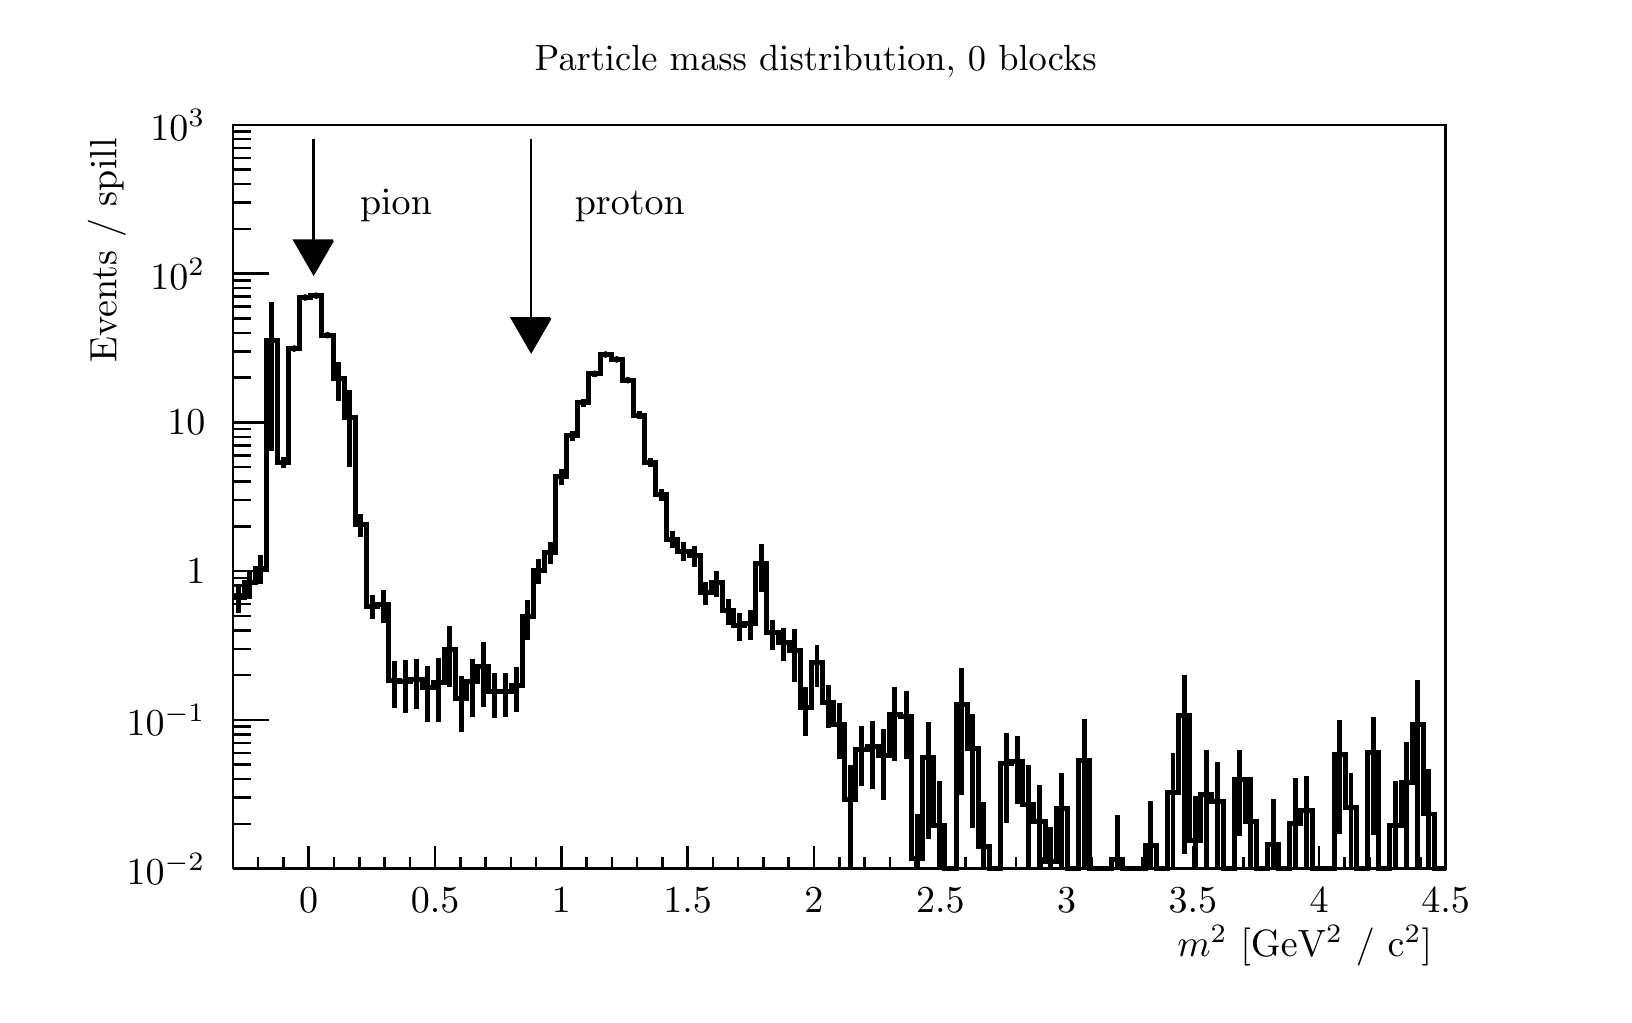
\begin{tikzpicture}
\pgfdeclareplotmark{cross} {
\pgfpathmoveto{\pgfpoint{-0.3\pgfplotmarksize}{\pgfplotmarksize}}
\pgfpathlineto{\pgfpoint{+0.3\pgfplotmarksize}{\pgfplotmarksize}}
\pgfpathlineto{\pgfpoint{+0.3\pgfplotmarksize}{0.3\pgfplotmarksize}}
\pgfpathlineto{\pgfpoint{+1\pgfplotmarksize}{0.3\pgfplotmarksize}}
\pgfpathlineto{\pgfpoint{+1\pgfplotmarksize}{-0.3\pgfplotmarksize}}
\pgfpathlineto{\pgfpoint{+0.3\pgfplotmarksize}{-0.3\pgfplotmarksize}}
\pgfpathlineto{\pgfpoint{+0.3\pgfplotmarksize}{-1.\pgfplotmarksize}}
\pgfpathlineto{\pgfpoint{-0.3\pgfplotmarksize}{-1.\pgfplotmarksize}}
\pgfpathlineto{\pgfpoint{-0.3\pgfplotmarksize}{-0.3\pgfplotmarksize}}
\pgfpathlineto{\pgfpoint{-1.\pgfplotmarksize}{-0.3\pgfplotmarksize}}
\pgfpathlineto{\pgfpoint{-1.\pgfplotmarksize}{0.3\pgfplotmarksize}}
\pgfpathlineto{\pgfpoint{-0.3\pgfplotmarksize}{0.3\pgfplotmarksize}}
\pgfpathclose
\pgfusepathqstroke
}
\pgfdeclareplotmark{cross*} {
\pgfpathmoveto{\pgfpoint{-0.3\pgfplotmarksize}{\pgfplotmarksize}}
\pgfpathlineto{\pgfpoint{+0.3\pgfplotmarksize}{\pgfplotmarksize}}
\pgfpathlineto{\pgfpoint{+0.3\pgfplotmarksize}{0.3\pgfplotmarksize}}
\pgfpathlineto{\pgfpoint{+1\pgfplotmarksize}{0.3\pgfplotmarksize}}
\pgfpathlineto{\pgfpoint{+1\pgfplotmarksize}{-0.3\pgfplotmarksize}}
\pgfpathlineto{\pgfpoint{+0.3\pgfplotmarksize}{-0.3\pgfplotmarksize}}
\pgfpathlineto{\pgfpoint{+0.3\pgfplotmarksize}{-1.\pgfplotmarksize}}
\pgfpathlineto{\pgfpoint{-0.3\pgfplotmarksize}{-1.\pgfplotmarksize}}
\pgfpathlineto{\pgfpoint{-0.3\pgfplotmarksize}{-0.3\pgfplotmarksize}}
\pgfpathlineto{\pgfpoint{-1.\pgfplotmarksize}{-0.3\pgfplotmarksize}}
\pgfpathlineto{\pgfpoint{-1.\pgfplotmarksize}{0.3\pgfplotmarksize}}
\pgfpathlineto{\pgfpoint{-0.3\pgfplotmarksize}{0.3\pgfplotmarksize}}
\pgfpathclose
\pgfusepathqfillstroke
}
\pgfdeclareplotmark{newstar} {
\pgfpathmoveto{\pgfqpoint{0pt}{\pgfplotmarksize}}
\pgfpathlineto{\pgfqpointpolar{44}{0.5\pgfplotmarksize}}
\pgfpathlineto{\pgfqpointpolar{18}{\pgfplotmarksize}}
\pgfpathlineto{\pgfqpointpolar{-20}{0.5\pgfplotmarksize}}
\pgfpathlineto{\pgfqpointpolar{-54}{\pgfplotmarksize}}
\pgfpathlineto{\pgfqpointpolar{-90}{0.5\pgfplotmarksize}}
\pgfpathlineto{\pgfqpointpolar{234}{\pgfplotmarksize}}
\pgfpathlineto{\pgfqpointpolar{198}{0.5\pgfplotmarksize}}
\pgfpathlineto{\pgfqpointpolar{162}{\pgfplotmarksize}}
\pgfpathlineto{\pgfqpointpolar{134}{0.5\pgfplotmarksize}}
\pgfpathclose
\pgfusepathqstroke
}
\pgfdeclareplotmark{newstar*} {
\pgfpathmoveto{\pgfqpoint{0pt}{\pgfplotmarksize}}
\pgfpathlineto{\pgfqpointpolar{44}{0.5\pgfplotmarksize}}
\pgfpathlineto{\pgfqpointpolar{18}{\pgfplotmarksize}}
\pgfpathlineto{\pgfqpointpolar{-20}{0.5\pgfplotmarksize}}
\pgfpathlineto{\pgfqpointpolar{-54}{\pgfplotmarksize}}
\pgfpathlineto{\pgfqpointpolar{-90}{0.5\pgfplotmarksize}}
\pgfpathlineto{\pgfqpointpolar{234}{\pgfplotmarksize}}
\pgfpathlineto{\pgfqpointpolar{198}{0.5\pgfplotmarksize}}
\pgfpathlineto{\pgfqpointpolar{162}{\pgfplotmarksize}}
\pgfpathlineto{\pgfqpointpolar{134}{0.5\pgfplotmarksize}}
\pgfpathclose
\pgfusepathqfillstroke
}
\definecolor{c}{rgb}{1,1,1};
\draw [color=c, fill=c] (0,0) rectangle (20,12.268);
\draw [color=c, fill=c] (2.6,1.59485) rectangle (18,11.0412);
\definecolor{c}{rgb}{0,0,0};
\draw [c,line width=0.9] (2.6,1.59485) -- (2.6,11.0412) -- (18,11.0412) -- (18,1.59485) -- (2.6,1.59485);
\definecolor{c}{rgb}{1,1,1};
\draw [color=c, fill=c] (2.6,1.59485) rectangle (18,11.0412);
\definecolor{c}{rgb}{0,0,0};
\draw [c,line width=0.9] (2.6,1.59485) -- (2.6,11.0412) -- (18,11.0412) -- (18,1.59485) -- (2.6,1.59485);
\draw [c,line width=1.8] (2.67064,4.83835) -- (2.67064,5.03878);
\draw [c,line width=1.8] (2.67064,5.03878) -- (2.67064,5.19974);
\foreach \P in {(2.67064,5.03878)}{\draw[mark options={color=c,fill=c},mark size=2.402402pt,mark=*,mark size=1pt] plot coordinates {\P};}
\draw [c,line width=1.8] (2.81193,5.02388) -- (2.81193,5.22754);
\draw [c,line width=1.8] (2.81193,5.22754) -- (2.81193,5.39056);
\foreach \P in {(2.81193,5.22754)}{\draw[mark options={color=c,fill=c},mark size=2.402402pt,mark=*,mark size=1pt] plot coordinates {\P};}
\draw [c,line width=1.8] (2.95321,5.20394) -- (2.95321,5.40915);
\draw [c,line width=1.8] (2.95321,5.40915) -- (2.95321,5.57317);
\foreach \P in {(2.95321,5.40915)}{\draw[mark options={color=c,fill=c},mark size=2.402402pt,mark=*,mark size=1pt] plot coordinates {\P};}
\draw [c,line width=1.8] (3.0945,6.89726) -- (3.0945,8.29886);
\draw [c,line width=1.8] (3.0945,8.29886) -- (3.0945,8.78967);
\foreach \P in {(3.0945,8.29886)}{\draw[mark options={color=c,fill=c},mark size=2.402402pt,mark=*,mark size=1pt] plot coordinates {\P};}
\draw [c,line width=1.8] (3.23578,6.67678) -- (3.23578,6.74991);
\draw [c,line width=1.8] (3.23578,6.74991) -- (3.23578,6.81705);
\foreach \P in {(3.23578,6.74991)}{\draw[mark options={color=c,fill=c},mark size=2.402402pt,mark=*,mark size=1pt] plot coordinates {\P};}
\draw [c,line width=1.8] (3.37706,8.16831) -- (3.37706,8.19982);
\draw [c,line width=1.8] (3.37706,8.19982) -- (3.37706,8.23016);
\foreach \P in {(3.37706,8.19982)}{\draw[mark options={color=c,fill=c},mark size=2.402402pt,mark=*,mark size=1pt] plot coordinates {\P};}
\draw [c,line width=1.8] (3.51835,8.82543) -- (3.51835,8.84804);
\draw [c,line width=1.8] (3.51835,8.84804) -- (3.51835,8.87003);
\foreach \P in {(3.51835,8.84804)}{\draw[mark options={color=c,fill=c},mark size=2.402402pt,mark=*,mark size=1pt] plot coordinates {\P};}
\draw [c,line width=1.8] (3.65963,8.85293) -- (3.65963,8.87184);
\draw [c,line width=1.8] (3.65963,8.87184) -- (3.65963,8.89033);
\foreach \P in {(3.65963,8.87184)}{\draw[mark options={color=c,fill=c},mark size=2.402402pt,mark=*,mark size=1pt] plot coordinates {\P};}
\draw [c,line width=1.8] (3.80092,8.34335) -- (3.80092,8.36936);
\draw [c,line width=1.8] (3.80092,8.36936) -- (3.80092,8.39457);
\foreach \P in {(3.80092,8.36936)}{\draw[mark options={color=c,fill=c},mark size=2.402402pt,mark=*,mark size=1pt] plot coordinates {\P};}
\draw [c,line width=1.8] (3.9422,7.53614) -- (3.9422,7.81768);
\draw [c,line width=1.8] (3.9422,7.81768) -- (3.9422,8.0269);
\foreach \P in {(3.9422,7.81768)}{\draw[mark options={color=c,fill=c},mark size=2.402402pt,mark=*,mark size=1pt] plot coordinates {\P};}
\draw [c,line width=1.8] (4.08349,6.6976) -- (4.08349,7.31909);
\draw [c,line width=1.8] (4.08349,7.31909) -- (4.08349,7.66863);
\foreach \P in {(4.08349,7.31909)}{\draw[mark options={color=c,fill=c},mark size=2.402402pt,mark=*,mark size=1pt] plot coordinates {\P};}
\draw [c,line width=1.8] (4.22477,5.80704) -- (4.22477,5.96886);
\draw [c,line width=1.8] (4.22477,5.96886) -- (4.22477,6.10395);
\foreach \P in {(4.22477,5.96886)}{\draw[mark options={color=c,fill=c},mark size=2.402402pt,mark=*,mark size=1pt] plot coordinates {\P};}
\draw [c,line width=1.8] (4.36606,4.76465) -- (4.36606,4.92769);
\draw [c,line width=1.8] (4.36606,4.92769) -- (4.36606,5.06364);
\foreach \P in {(4.36606,4.92769)}{\draw[mark options={color=c,fill=c},mark size=2.402402pt,mark=*,mark size=1pt] plot coordinates {\P};}
\draw [c,line width=1.8] (4.50734,4.70929) -- (4.50734,4.95225);
\draw [c,line width=1.8] (4.50734,4.95225) -- (4.50734,5.13946);
\foreach \P in {(4.50734,4.95225)}{\draw[mark options={color=c,fill=c},mark size=2.402402pt,mark=*,mark size=1pt] plot coordinates {\P};}
\draw [c,line width=1.8] (4.64862,3.63921) -- (4.64862,3.98727);
\draw [c,line width=1.8] (4.64862,3.98727) -- (4.64862,4.2309);
\foreach \P in {(4.64862,3.98727)}{\draw[mark options={color=c,fill=c},mark size=2.402402pt,mark=*,mark size=1pt] plot coordinates {\P};}
\draw [c,line width=1.8] (4.78991,3.57385) -- (4.78991,3.97748);
\draw [c,line width=1.8] (4.78991,3.97748) -- (4.78991,4.24682);
\foreach \P in {(4.78991,3.97748)}{\draw[mark options={color=c,fill=c},mark size=2.402402pt,mark=*,mark size=1pt] plot coordinates {\P};}
\draw [c,line width=1.8] (4.93119,3.61791) -- (4.93119,4.00227);
\draw [c,line width=1.8] (4.93119,4.00227) -- (4.93119,4.26298);
\foreach \P in {(4.93119,4.00227)}{\draw[mark options={color=c,fill=c},mark size=2.402402pt,mark=*,mark size=1pt] plot coordinates {\P};}
\draw [c,line width=1.8] (5.07248,3.45883) -- (5.07248,3.89031);
\draw [c,line width=1.8] (5.07248,3.89031) -- (5.07248,4.17163);
\foreach \P in {(5.07248,3.89031)}{\draw[mark options={color=c,fill=c},mark size=2.402402pt,mark=*,mark size=1pt] plot coordinates {\P};}
\draw [c,line width=1.8] (5.21376,3.4566) -- (5.21376,3.96471);
\draw [c,line width=1.8] (5.21376,3.96471) -- (5.21376,4.27615);
\foreach \P in {(5.21376,3.96471)}{\draw[mark options={color=c,fill=c},mark size=2.402402pt,mark=*,mark size=1pt] plot coordinates {\P};}
\draw [c,line width=1.8] (5.35505,3.89726) -- (5.35505,4.37437);
\draw [c,line width=1.8] (5.35505,4.37437) -- (5.35505,4.67409);
\foreach \P in {(5.35505,4.37437)}{\draw[mark options={color=c,fill=c},mark size=2.402402pt,mark=*,mark size=1pt] plot coordinates {\P};}
\draw [c,line width=1.8] (5.49633,3.32673) -- (5.49633,3.75962);
\draw [c,line width=1.8] (5.49633,3.75962) -- (5.49633,4.04152);
\foreach \P in {(5.49633,3.75962)}{\draw[mark options={color=c,fill=c},mark size=2.402402pt,mark=*,mark size=1pt] plot coordinates {\P};}
\draw [c,line width=1.8] (5.63761,3.52578) -- (5.63761,3.96588);
\draw [c,line width=1.8] (5.63761,3.96588) -- (5.63761,4.25079);
\foreach \P in {(5.63761,3.96588)}{\draw[mark options={color=c,fill=c},mark size=2.402402pt,mark=*,mark size=1pt] plot coordinates {\P};}
\draw [c,line width=1.8] (5.7789,3.65191) -- (5.7789,4.16508);
\draw [c,line width=1.8] (5.7789,4.16508) -- (5.7789,4.47837);
\foreach \P in {(5.7789,4.16508)}{\draw[mark options={color=c,fill=c},mark size=2.402402pt,mark=*,mark size=1pt] plot coordinates {\P};}
\draw [c,line width=1.8] (5.92018,3.50311) -- (5.92018,3.84313);
\draw [c,line width=1.8] (5.92018,3.84313) -- (5.92018,4.08282);
\foreach \P in {(5.92018,3.84313)}{\draw[mark options={color=c,fill=c},mark size=2.402402pt,mark=*,mark size=1pt] plot coordinates {\P};}
\draw [c,line width=1.8] (6.06147,3.52606) -- (6.06147,3.84806);
\draw [c,line width=1.8] (6.06147,3.84806) -- (6.06147,4.07871);
\foreach \P in {(6.06147,3.84806)}{\draw[mark options={color=c,fill=c},mark size=2.402402pt,mark=*,mark size=1pt] plot coordinates {\P};}
\draw [c,line width=1.8] (6.20275,3.58333) -- (6.20275,3.91725);
\draw [c,line width=1.8] (6.20275,3.91725) -- (6.20275,4.15391);
\foreach \P in {(6.20275,3.91725)}{\draw[mark options={color=c,fill=c},mark size=2.402402pt,mark=*,mark size=1pt] plot coordinates {\P};}
\draw [c,line width=1.8] (6.34404,4.49729) -- (6.34404,4.79092);
\draw [c,line width=1.8] (6.34404,4.79092) -- (6.34404,5.00671);
\foreach \P in {(6.34404,4.79092)}{\draw[mark options={color=c,fill=c},mark size=2.402402pt,mark=*,mark size=1pt] plot coordinates {\P};}
\draw [c,line width=1.8] (6.48532,5.21427) -- (6.48532,5.38521);
\draw [c,line width=1.8] (6.48532,5.38521) -- (6.48532,5.52661);
\foreach \P in {(6.48532,5.38521)}{\draw[mark options={color=c,fill=c},mark size=2.402402pt,mark=*,mark size=1pt] plot coordinates {\P};}
\draw [c,line width=1.8] (6.62661,5.45876) -- (6.62661,5.60996);
\draw [c,line width=1.8] (6.62661,5.60996) -- (6.62661,5.73757);
\foreach \P in {(6.62661,5.60996)}{\draw[mark options={color=c,fill=c},mark size=2.402402pt,mark=*,mark size=1pt] plot coordinates {\P};}
\draw [c,line width=1.8] (6.76789,6.46087) -- (6.76789,6.56975);
\draw [c,line width=1.8] (6.76789,6.56975) -- (6.76789,6.66587);
\foreach \P in {(6.76789,6.56975)}{\draw[mark options={color=c,fill=c},mark size=2.402402pt,mark=*,mark size=1pt] plot coordinates {\P};}
\draw [c,line width=1.8] (6.90917,7.02428) -- (6.90917,7.09333);
\draw [c,line width=1.8] (6.90917,7.09333) -- (6.90917,7.15701);
\foreach \P in {(6.90917,7.09333)}{\draw[mark options={color=c,fill=c},mark size=2.402402pt,mark=*,mark size=1pt] plot coordinates {\P};}
\draw [c,line width=1.8] (7.05046,7.46269) -- (7.05046,7.51223);
\draw [c,line width=1.8] (7.05046,7.51223) -- (7.05046,7.55895);
\foreach \P in {(7.05046,7.51223)}{\draw[mark options={color=c,fill=c},mark size=2.402402pt,mark=*,mark size=1pt] plot coordinates {\P};}
\draw [c,line width=1.8] (7.19174,7.84097) -- (7.19174,7.87899);
\draw [c,line width=1.8] (7.19174,7.87899) -- (7.19174,7.91532);
\foreach \P in {(7.19174,7.87899)}{\draw[mark options={color=c,fill=c},mark size=2.402402pt,mark=*,mark size=1pt] plot coordinates {\P};}
\draw [c,line width=1.8] (7.33303,8.08654) -- (7.33303,8.12401);
\draw [c,line width=1.8] (7.33303,8.12401) -- (7.33303,8.15984);
\foreach \P in {(7.33303,8.12401)}{\draw[mark options={color=c,fill=c},mark size=2.402402pt,mark=*,mark size=1pt] plot coordinates {\P};}
\draw [c,line width=1.8] (7.47431,8.03213) -- (7.47431,8.06216);
\draw [c,line width=1.8] (7.47431,8.06216) -- (7.47431,8.09112);
\foreach \P in {(7.47431,8.06216)}{\draw[mark options={color=c,fill=c},mark size=2.402402pt,mark=*,mark size=1pt] plot coordinates {\P};}
\draw [c,line width=1.8] (7.6156,7.76525) -- (7.6156,7.79819);
\draw [c,line width=1.8] (7.6156,7.79819) -- (7.6156,7.82986);
\foreach \P in {(7.6156,7.79819)}{\draw[mark options={color=c,fill=c},mark size=2.402402pt,mark=*,mark size=1pt] plot coordinates {\P};}
\draw [c,line width=1.8] (7.75688,7.30594) -- (7.75688,7.35538);
\draw [c,line width=1.8] (7.75688,7.35538) -- (7.75688,7.40201);
\foreach \P in {(7.75688,7.35538)}{\draw[mark options={color=c,fill=c},mark size=2.402402pt,mark=*,mark size=1pt] plot coordinates {\P};}
\draw [c,line width=1.8] (7.89817,6.6923) -- (7.89817,6.75283);
\draw [c,line width=1.8] (7.89817,6.75283) -- (7.89817,6.8092);
\foreach \P in {(7.89817,6.75283)}{\draw[mark options={color=c,fill=c},mark size=2.402402pt,mark=*,mark size=1pt] plot coordinates {\P};}
\draw [c,line width=1.8] (8.03945,6.26213) -- (8.03945,6.34253);
\draw [c,line width=1.8] (8.03945,6.34253) -- (8.03945,6.41575);
\foreach \P in {(8.03945,6.34253)}{\draw[mark options={color=c,fill=c},mark size=2.402402pt,mark=*,mark size=1pt] plot coordinates {\P};}
\draw [c,line width=1.8] (8.18073,5.66331) -- (8.18073,5.77852);
\draw [c,line width=1.8] (8.18073,5.77852) -- (8.18073,5.87952);
\foreach \P in {(8.18073,5.77852)}{\draw[mark options={color=c,fill=c},mark size=2.402402pt,mark=*,mark size=1pt] plot coordinates {\P};}
\draw [c,line width=1.8] (8.32202,5.49675) -- (8.32202,5.62806);
\draw [c,line width=1.8] (8.32202,5.62806) -- (8.32202,5.74122);
\foreach \P in {(8.32202,5.62806)}{\draw[mark options={color=c,fill=c},mark size=2.402402pt,mark=*,mark size=1pt] plot coordinates {\P};}
\draw [c,line width=1.8] (8.4633,5.4312) -- (8.4633,5.56853);
\draw [c,line width=1.8] (8.4633,5.56853) -- (8.4633,5.68614);
\foreach \P in {(8.4633,5.56853)}{\draw[mark options={color=c,fill=c},mark size=2.402402pt,mark=*,mark size=1pt] plot coordinates {\P};}
\draw [c,line width=1.8] (8.60459,4.93703) -- (8.60459,5.10131);
\draw [c,line width=1.8] (8.60459,5.10131) -- (8.60459,5.23811);
\foreach \P in {(8.60459,5.10131)}{\draw[mark options={color=c,fill=c},mark size=2.402402pt,mark=*,mark size=1pt] plot coordinates {\P};}
\draw [c,line width=1.8] (8.74587,5.04831) -- (8.74587,5.225);
\draw [c,line width=1.8] (8.74587,5.225) -- (8.74587,5.3703);
\foreach \P in {(8.74587,5.225)}{\draw[mark options={color=c,fill=c},mark size=2.402402pt,mark=*,mark size=1pt] plot coordinates {\P};}
\draw [c,line width=1.8] (8.88716,4.69464) -- (8.88716,4.87042);
\draw [c,line width=1.8] (8.88716,4.87042) -- (8.88716,5.01511);
\foreach \P in {(8.88716,4.87042)}{\draw[mark options={color=c,fill=c},mark size=2.402402pt,mark=*,mark size=1pt] plot coordinates {\P};}
\draw [c,line width=1.8] (9.02844,4.4874) -- (9.02844,4.68535);
\draw [c,line width=1.8] (9.02844,4.68535) -- (9.02844,4.8447);
\foreach \P in {(9.02844,4.68535)}{\draw[mark options={color=c,fill=c},mark size=2.402402pt,mark=*,mark size=1pt] plot coordinates {\P};}
\draw [c,line width=1.8] (9.16972,4.49569) -- (9.16972,4.71155);
\draw [c,line width=1.8] (9.16972,4.71155) -- (9.16972,4.88229);
\foreach \P in {(9.16972,4.71155)}{\draw[mark options={color=c,fill=c},mark size=2.402402pt,mark=*,mark size=1pt] plot coordinates {\P};}
\draw [c,line width=1.8] (9.31101,5.10451) -- (9.31101,5.46375);
\draw [c,line width=1.8] (9.31101,5.46375) -- (9.31101,5.71275);
\foreach \P in {(9.31101,5.46375)}{\draw[mark options={color=c,fill=c},mark size=2.402402pt,mark=*,mark size=1pt] plot coordinates {\P};}
\draw [c,line width=1.8] (9.45229,4.3732) -- (9.45229,4.58756);
\draw [c,line width=1.8] (9.45229,4.58756) -- (9.45229,4.75736);
\foreach \P in {(9.45229,4.58756)}{\draw[mark options={color=c,fill=c},mark size=2.402402pt,mark=*,mark size=1pt] plot coordinates {\P};}
\draw [c,line width=1.8] (9.59358,4.23243) -- (9.59358,4.46821);
\draw [c,line width=1.8] (9.59358,4.46821) -- (9.59358,4.65113);
\foreach \P in {(9.59358,4.46821)}{\draw[mark options={color=c,fill=c},mark size=2.402402pt,mark=*,mark size=1pt] plot coordinates {\P};}
\draw [c,line width=1.8] (9.73486,3.95946) -- (9.73486,4.37117);
\draw [c,line width=1.8] (9.73486,4.37117) -- (9.73486,4.64405);
\foreach \P in {(9.73486,4.37117)}{\draw[mark options={color=c,fill=c},mark size=2.402402pt,mark=*,mark size=1pt] plot coordinates {\P};}
\draw [c,line width=1.8] (9.87615,3.27572) -- (9.87615,3.64567);
\draw [c,line width=1.8] (9.87615,3.64567) -- (9.87615,3.89972);
\foreach \P in {(9.87615,3.64567)}{\draw[mark options={color=c,fill=c},mark size=2.402402pt,mark=*,mark size=1pt] plot coordinates {\P};}
\draw [c,line width=1.8] (10.0174,3.90501) -- (10.0174,4.21346);
\draw [c,line width=1.8] (10.0174,4.21346) -- (10.0174,4.43711);
\foreach \P in {(10.0174,4.21346)}{\draw[mark options={color=c,fill=c},mark size=2.402402pt,mark=*,mark size=1pt] plot coordinates {\P};}
\draw [c,line width=1.8] (10.1587,3.37914) -- (10.1587,3.69867);
\draw [c,line width=1.8] (10.1587,3.69867) -- (10.1587,3.92806);
\foreach \P in {(10.1587,3.69867)}{\draw[mark options={color=c,fill=c},mark size=2.402402pt,mark=*,mark size=1pt] plot coordinates {\P};}
\draw [c,line width=1.8] (10.3,2.98811) -- (10.3,3.42043);
\draw [c,line width=1.8] (10.3,3.42043) -- (10.3,3.70209);
\foreach \P in {(10.3,3.42043)}{\draw[mark options={color=c,fill=c},mark size=2.402402pt,mark=*,mark size=1pt] plot coordinates {\P};}
\draw [c,line width=1.8] (10.4413,1.59485) -- (10.4413,2.46862);
\draw [c,line width=1.8] (10.4413,2.46862) -- (10.4413,2.90743);
\foreach \P in {(10.4413,2.46862)}{\draw[mark options={color=c,fill=c},mark size=2.402402pt,mark=*,mark size=1pt] plot coordinates {\P};}
\draw [c,line width=1.8] (10.5826,2.64925) -- (10.5826,3.11372);
\draw [c,line width=1.8] (10.5826,3.11372) -- (10.5826,3.40849);
\foreach \P in {(10.5826,3.11372)}{\draw[mark options={color=c,fill=c},mark size=2.402402pt,mark=*,mark size=1pt] plot coordinates {\P};}
\draw [c,line width=1.8] (10.7239,2.6029) -- (10.7239,3.14556);
\draw [c,line width=1.8] (10.7239,3.14556) -- (10.7239,3.46937);
\foreach \P in {(10.7239,3.14556)}{\draw[mark options={color=c,fill=c},mark size=2.402402pt,mark=*,mark size=1pt] plot coordinates {\P};}
\draw [c,line width=1.8] (10.8651,2.462) -- (10.8651,3.03474);
\draw [c,line width=1.8] (10.8651,3.03474) -- (10.8651,3.36876);
\foreach \P in {(10.8651,3.03474)}{\draw[mark options={color=c,fill=c},mark size=2.402402pt,mark=*,mark size=1pt] plot coordinates {\P};}
\draw [c,line width=1.8] (11.0064,2.9672) -- (11.0064,3.55656);
\draw [c,line width=1.8] (11.0064,3.55656) -- (11.0064,3.896);
\foreach \P in {(11.0064,3.55656)}{\draw[mark options={color=c,fill=c},mark size=2.402402pt,mark=*,mark size=1pt] plot coordinates {\P};}
\draw [c,line width=1.8] (11.1477,2.98208) -- (11.1477,3.52359);
\draw [c,line width=1.8] (11.1477,3.52359) -- (11.1477,3.847);
\foreach \P in {(11.1477,3.52359)}{\draw[mark options={color=c,fill=c},mark size=2.402402pt,mark=*,mark size=1pt] plot coordinates {\P};}
\draw [c,line width=1.8] (11.289,1.59485) -- (11.289,1.72064);
\draw [c,line width=1.8] (11.289,1.72064) -- (11.289,2.28937);
\foreach \P in {(11.289,1.72064)}{\draw[mark options={color=c,fill=c},mark size=2.402402pt,mark=*,mark size=1pt] plot coordinates {\P};}
\draw [c,line width=1.8] (11.4303,1.97434) -- (11.4303,3.01);
\draw [c,line width=1.8] (11.4303,3.01) -- (11.4303,3.45354);
\foreach \P in {(11.4303,3.01)}{\draw[mark options={color=c,fill=c},mark size=2.402402pt,mark=*,mark size=1pt] plot coordinates {\P};}
\draw [c,line width=1.8] (11.5716,1.59485) -- (11.5716,2.13924);
\draw [c,line width=1.8] (11.5716,2.13924) -- (11.5716,2.70797);
\foreach \P in {(11.5716,2.13924)}{\draw[mark options={color=c,fill=c},mark size=2.402402pt,mark=*,mark size=1pt] plot coordinates {\P};}
\draw [c,line width=1.8] (11.8541,2.52934) -- (11.8541,3.6822);
\draw [c,line width=1.8] (11.8541,3.6822) -- (11.8541,4.14354);
\foreach \P in {(11.8541,3.6822)}{\draw[mark options={color=c,fill=c},mark size=2.402402pt,mark=*,mark size=1pt] plot coordinates {\P};}
\draw [c,line width=1.8] (11.9954,2.10703) -- (11.9954,3.12444);
\draw [c,line width=1.8] (11.9954,3.12444) -- (11.9954,3.56493);
\foreach \P in {(11.9954,3.12444)}{\draw[mark options={color=c,fill=c},mark size=2.402402pt,mark=*,mark size=1pt] plot coordinates {\P};}
\draw [c,line width=1.8] (12.1367,1.59485) -- (12.1367,1.87338);
\draw [c,line width=1.8] (12.1367,1.87338) -- (12.1367,2.44211);
\foreach \P in {(12.1367,1.87338)}{\draw[mark options={color=c,fill=c},mark size=2.402402pt,mark=*,mark size=1pt] plot coordinates {\P};}
\draw [c,line width=1.8] (12.4193,2.17688) -- (12.4193,2.93019);
\draw [c,line width=1.8] (12.4193,2.93019) -- (12.4193,3.3162);
\foreach \P in {(12.4193,2.93019)}{\draw[mark options={color=c,fill=c},mark size=2.402402pt,mark=*,mark size=1pt] plot coordinates {\P};}
\draw [c,line width=1.8] (12.5606,2.41698) -- (12.5606,2.9556);
\draw [c,line width=1.8] (12.5606,2.9556) -- (12.5606,3.278);
\foreach \P in {(12.5606,2.9556)}{\draw[mark options={color=c,fill=c},mark size=2.402402pt,mark=*,mark size=1pt] plot coordinates {\P};}
\draw [c,line width=1.8] (12.7018,1.59485) -- (12.7018,2.41357);
\draw [c,line width=1.8] (12.7018,2.41357) -- (12.7018,2.90521);
\foreach \P in {(12.7018,2.41357)}{\draw[mark options={color=c,fill=c},mark size=2.402402pt,mark=*,mark size=1pt] plot coordinates {\P};}
\draw [c,line width=1.8] (12.8431,1.59485) -- (12.8431,2.19842);
\draw [c,line width=1.8] (12.8431,2.19842) -- (12.8431,2.65912);
\foreach \P in {(12.8431,2.19842)}{\draw[mark options={color=c,fill=c},mark size=2.402402pt,mark=*,mark size=1pt] plot coordinates {\P};}
\draw [c,line width=1.8] (12.9844,1.59485) -- (12.9844,1.6838);
\draw [c,line width=1.8] (12.9844,1.6838) -- (12.9844,2.12472);
\foreach \P in {(12.9844,1.6838)}{\draw[mark options={color=c,fill=c},mark size=2.402402pt,mark=*,mark size=1pt] plot coordinates {\P};}
\draw [c,line width=1.8] (13.1257,1.59485) -- (13.1257,2.36408);
\draw [c,line width=1.8] (13.1257,2.36408) -- (13.1257,2.8032);
\foreach \P in {(13.1257,2.36408)}{\draw[mark options={color=c,fill=c},mark size=2.402402pt,mark=*,mark size=1pt] plot coordinates {\P};}
\draw [c,line width=1.8] (13.4083,1.59485) -- (13.4083,2.96797);
\draw [c,line width=1.8] (13.4083,2.96797) -- (13.4083,3.49089);
\foreach \P in {(13.4083,2.96797)}{\draw[mark options={color=c,fill=c},mark size=2.402402pt,mark=*,mark size=1pt] plot coordinates {\P};}
\draw [c,line width=1.8] (13.8321,1.59485) -- (13.8321,1.70796);
\draw [c,line width=1.8] (13.8321,1.70796) -- (13.8321,2.27669);
\foreach \P in {(13.8321,1.70796)}{\draw[mark options={color=c,fill=c},mark size=2.402402pt,mark=*,mark size=1pt] plot coordinates {\P};}
\draw [c,line width=1.8] (14.256,1.59485) -- (14.256,1.88635);
\draw [c,line width=1.8] (14.256,1.88635) -- (14.256,2.45508);
\foreach \P in {(14.256,1.88635)}{\draw[mark options={color=c,fill=c},mark size=2.402402pt,mark=*,mark size=1pt] plot coordinates {\P};}
\draw [c,line width=1.8] (14.5385,1.59485) -- (14.5385,2.56214);
\draw [c,line width=1.8] (14.5385,2.56214) -- (14.5385,3.05869);
\foreach \P in {(14.5385,2.56214)}{\draw[mark options={color=c,fill=c},mark size=2.402402pt,mark=*,mark size=1pt] plot coordinates {\P};}
\draw [c,line width=1.8] (14.6798,1.77804) -- (14.6798,3.53455);
\draw [c,line width=1.8] (14.6798,3.53455) -- (14.6798,4.05358);
\foreach \P in {(14.6798,3.53455)}{\draw[mark options={color=c,fill=c},mark size=2.402402pt,mark=*,mark size=1pt] plot coordinates {\P};}
\draw [c,line width=1.8] (14.8211,1.59485) -- (14.8211,1.95322);
\draw [c,line width=1.8] (14.8211,1.95322) -- (14.8211,2.52195);
\foreach \P in {(14.8211,1.95322)}{\draw[mark options={color=c,fill=c},mark size=2.402402pt,mark=*,mark size=1pt] plot coordinates {\P};}
\draw [c,line width=1.8] (14.9624,1.59485) -- (14.9624,2.53325);
\draw [c,line width=1.8] (14.9624,2.53325) -- (14.9624,3.10198);
\foreach \P in {(14.9624,2.53325)}{\draw[mark options={color=c,fill=c},mark size=2.402402pt,mark=*,mark size=1pt] plot coordinates {\P};}
\draw [c,line width=1.8] (15.1037,1.59485) -- (15.1037,2.44678);
\draw [c,line width=1.8] (15.1037,2.44678) -- (15.1037,2.94849);
\foreach \P in {(15.1037,2.44678)}{\draw[mark options={color=c,fill=c},mark size=2.402402pt,mark=*,mark size=1pt] plot coordinates {\P};}
\draw [c,line width=1.8] (15.3862,2.00303) -- (15.3862,2.72073);
\draw [c,line width=1.8] (15.3862,2.72073) -- (15.3862,3.09761);
\foreach \P in {(15.3862,2.72073)}{\draw[mark options={color=c,fill=c},mark size=2.402402pt,mark=*,mark size=1pt] plot coordinates {\P};}
\draw [c,line width=1.8] (15.5275,1.59485) -- (15.5275,2.18974);
\draw [c,line width=1.8] (15.5275,2.18974) -- (15.5275,2.75847);
\foreach \P in {(15.5275,2.18974)}{\draw[mark options={color=c,fill=c},mark size=2.402402pt,mark=*,mark size=1pt] plot coordinates {\P};}
\draw [c,line width=1.8] (15.8101,1.59485) -- (15.8101,1.90579);
\draw [c,line width=1.8] (15.8101,1.90579) -- (15.8101,2.47452);
\foreach \P in {(15.8101,1.90579)}{\draw[mark options={color=c,fill=c},mark size=2.402402pt,mark=*,mark size=1pt] plot coordinates {\P};}
\draw [c,line width=1.8] (16.0927,1.59485) -- (16.0927,2.17394);
\draw [c,line width=1.8] (16.0927,2.17394) -- (16.0927,2.74267);
\foreach \P in {(16.0927,2.17394)}{\draw[mark options={color=c,fill=c},mark size=2.402402pt,mark=*,mark size=1pt] plot coordinates {\P};}
\draw [c,line width=1.8] (16.2339,1.59485) -- (16.2339,2.33531);
\draw [c,line width=1.8] (16.2339,2.33531) -- (16.2339,2.77492);
\foreach \P in {(16.2339,2.33531)}{\draw[mark options={color=c,fill=c},mark size=2.402402pt,mark=*,mark size=1pt] plot coordinates {\P};}
\draw [c,line width=1.8] (16.6578,2.03451) -- (16.6578,3.04204);
\draw [c,line width=1.8] (16.6578,3.04204) -- (16.6578,3.48085);
\foreach \P in {(16.6578,3.04204)}{\draw[mark options={color=c,fill=c},mark size=2.402402pt,mark=*,mark size=1pt] plot coordinates {\P};}
\draw [c,line width=1.8] (16.7991,1.59485) -- (16.7991,2.36988);
\draw [c,line width=1.8] (16.7991,2.36988) -- (16.7991,2.81071);
\foreach \P in {(16.7991,2.36988)}{\draw[mark options={color=c,fill=c},mark size=2.402402pt,mark=*,mark size=1pt] plot coordinates {\P};}
\draw [c,line width=1.8] (17.0817,2.02663) -- (17.0817,3.07539);
\draw [c,line width=1.8] (17.0817,3.07539) -- (17.0817,3.52107);
\foreach \P in {(17.0817,3.07539)}{\draw[mark options={color=c,fill=c},mark size=2.402402pt,mark=*,mark size=1pt] plot coordinates {\P};}
\draw [c,line width=1.8] (17.3642,1.59485) -- (17.3642,2.13924);
\draw [c,line width=1.8] (17.3642,2.13924) -- (17.3642,2.70797);
\foreach \P in {(17.3642,2.13924)}{\draw[mark options={color=c,fill=c},mark size=2.402402pt,mark=*,mark size=1pt] plot coordinates {\P};}
\draw [c,line width=1.8] (17.5055,1.59485) -- (17.5055,2.6833);
\draw [c,line width=1.8] (17.5055,2.6833) -- (17.5055,3.19738);
\foreach \P in {(17.5055,2.6833)}{\draw[mark options={color=c,fill=c},mark size=2.402402pt,mark=*,mark size=1pt] plot coordinates {\P};}
\draw [c,line width=1.8] (17.6468,1.59485) -- (17.6468,3.42339);
\draw [c,line width=1.8] (17.6468,3.42339) -- (17.6468,3.99212);
\foreach \P in {(17.6468,3.42339)}{\draw[mark options={color=c,fill=c},mark size=2.402402pt,mark=*,mark size=1pt] plot coordinates {\P};}
\draw [c,line width=1.8] (17.7881,1.59485) -- (17.7881,2.28866);
\draw [c,line width=1.8] (17.7881,2.28866) -- (17.7881,2.85738);
\foreach \P in {(17.7881,2.28866)}{\draw[mark options={color=c,fill=c},mark size=2.402402pt,mark=*,mark size=1pt] plot coordinates {\P};}
\draw [c,line width=1.8] (2.6,5.03878) -- (2.74128,5.03878) -- (2.74128,5.22754) -- (2.88257,5.22754) -- (2.88257,5.40915) -- (3.02385,5.40915) -- (3.02385,8.29886) -- (3.16514,8.29886) -- (3.16514,6.74991) -- (3.30642,6.74991) -- (3.30642,8.19982)
 -- (3.44771,8.19982) -- (3.44771,8.84804) -- (3.58899,8.84804) -- (3.58899,8.87184) -- (3.73028,8.87184) -- (3.73028,8.36936) -- (3.87156,8.36936) -- (3.87156,7.81768) -- (4.01284,7.81768) -- (4.01284,7.31909) -- (4.15413,7.31909) --
 (4.15413,5.96886) -- (4.29541,5.96886) -- (4.29541,4.92769) -- (4.4367,4.92769) -- (4.4367,4.95225) -- (4.57798,4.95225) -- (4.57798,3.98727) -- (4.71927,3.98727) -- (4.71927,3.97748) -- (4.86055,3.97748) -- (4.86055,4.00227) -- (5.00183,4.00227) --
 (5.00183,3.89031) -- (5.14312,3.89031) -- (5.14312,3.96471) -- (5.2844,3.96471) -- (5.2844,4.37437) -- (5.42569,4.37437) -- (5.42569,3.75962) -- (5.56697,3.75962) -- (5.56697,3.96588) -- (5.70826,3.96588) -- (5.70826,4.16508) -- (5.84954,4.16508) --
 (5.84954,3.84313) -- (5.99083,3.84313) -- (5.99083,3.84806) -- (6.13211,3.84806) -- (6.13211,3.91725) -- (6.27339,3.91725) -- (6.27339,4.79092) -- (6.41468,4.79092) -- (6.41468,5.38521) -- (6.55596,5.38521) -- (6.55596,5.60996) -- (6.69725,5.60996)
 -- (6.69725,6.56975) -- (6.83853,6.56975) -- (6.83853,7.09333) -- (6.97982,7.09333) -- (6.97982,7.51223) -- (7.1211,7.51223) -- (7.1211,7.87899) -- (7.26239,7.87899) -- (7.26239,8.12401) -- (7.40367,8.12401) -- (7.40367,8.06216) -- (7.54495,8.06216)
 -- (7.54495,7.79819) -- (7.68624,7.79819) -- (7.68624,7.35538) -- (7.82752,7.35538) -- (7.82752,6.75283) -- (7.96881,6.75283) -- (7.96881,6.34253) -- (8.11009,6.34253) -- (8.11009,5.77852) -- (8.25138,5.77852) -- (8.25138,5.62806) --
 (8.39266,5.62806) -- (8.39266,5.56853) -- (8.53395,5.56853) -- (8.53395,5.10131) -- (8.67523,5.10131) -- (8.67523,5.225) -- (8.81651,5.225) -- (8.81651,4.87042) -- (8.9578,4.87042) -- (8.9578,4.68535) -- (9.09908,4.68535) -- (9.09908,4.71155) --
 (9.24037,4.71155) -- (9.24037,5.46375) -- (9.38165,5.46375) -- (9.38165,4.58756) -- (9.52294,4.58756) -- (9.52294,4.46821) -- (9.66422,4.46821) -- (9.66422,4.37117) -- (9.8055,4.37117) -- (9.8055,3.64567) -- (9.94679,3.64567) -- (9.94679,4.21346) --
 (10.0881,4.21346) -- (10.0881,3.69867) -- (10.2294,3.69867) -- (10.2294,3.42043) -- (10.3706,3.42043) -- (10.3706,2.46862) -- (10.5119,2.46862) -- (10.5119,3.11372) -- (10.6532,3.11372) -- (10.6532,3.14556) -- (10.7945,3.14556) -- (10.7945,3.03474)
 -- (10.9358,3.03474) -- (10.9358,3.55656) -- (11.0771,3.55656) -- (11.0771,3.52359) -- (11.2183,3.52359) -- (11.2183,1.72064) -- (11.3596,1.72064) -- (11.3596,3.01) -- (11.5009,3.01) -- (11.5009,2.13924) -- (11.6422,2.13924) -- (11.6422,1.59485) --
 (11.7835,1.59485) -- (11.7835,3.6822) -- (11.9248,3.6822) -- (11.9248,3.12444) -- (12.0661,3.12444) -- (12.0661,1.87338) -- (12.2073,1.87338) -- (12.2073,1.59485) -- (12.3486,1.59485) -- (12.3486,2.93019) -- (12.4899,2.93019) -- (12.4899,2.9556) --
 (12.6312,2.9556) -- (12.6312,2.41357) -- (12.7725,2.41357) -- (12.7725,2.19842) -- (12.9138,2.19842) -- (12.9138,1.6838) -- (13.055,1.6838) -- (13.055,2.36408) -- (13.1963,2.36408) -- (13.1963,1.59485) -- (13.3376,1.59485) -- (13.3376,2.96797) --
 (13.4789,2.96797) -- (13.4789,1.59485) -- (13.6202,1.59485) -- (13.6202,1.59485) -- (13.7615,1.59485) -- (13.7615,1.70796) -- (13.9028,1.70796) -- (13.9028,1.59485) -- (14.044,1.59485) -- (14.044,1.59485) -- (14.1853,1.59485) -- (14.1853,1.88635) --
 (14.3266,1.88635) -- (14.3266,1.59485) -- (14.4679,1.59485) -- (14.4679,2.56214) -- (14.6092,2.56214) -- (14.6092,3.53455) -- (14.7505,3.53455) -- (14.7505,1.95322) -- (14.8917,1.95322) -- (14.8917,2.53325) -- (15.033,2.53325) -- (15.033,2.44678) --
 (15.1743,2.44678) -- (15.1743,1.59485) -- (15.3156,1.59485) -- (15.3156,2.72073) -- (15.4569,2.72073) -- (15.4569,2.18974) -- (15.5982,2.18974) -- (15.5982,1.59485) -- (15.7394,1.59485) -- (15.7394,1.90579) -- (15.8807,1.90579) -- (15.8807,1.59485)
 -- (16.022,1.59485) -- (16.022,2.17394) -- (16.1633,2.17394) -- (16.1633,2.33531) -- (16.3046,2.33531) -- (16.3046,1.59485) -- (16.4459,1.59485) -- (16.4459,1.59485) -- (16.5872,1.59485) -- (16.5872,3.04204) -- (16.7284,3.04204) -- (16.7284,2.36988)
 -- (16.8697,2.36988) -- (16.8697,1.59485) -- (17.011,1.59485) -- (17.011,3.07539) -- (17.1523,3.07539) -- (17.1523,1.59485) -- (17.2936,1.59485) -- (17.2936,2.13924) -- (17.4349,2.13924) -- (17.4349,2.6833) -- (17.5761,2.6833) -- (17.5761,3.42339)
 -- (17.7174,3.42339) -- (17.7174,2.28866) -- (17.8587,2.28866) -- (17.8587,1.59485) -- (18,1.59485);
\draw [c,line width=0.9] (2.6,1.59485) -- (18,1.59485);
\draw [c,line width=0.9] (3.5625,1.87824) -- (3.5625,1.59485);
\draw [c,line width=0.9] (3.88333,1.73654) -- (3.88333,1.59485);
\draw [c,line width=0.9] (4.20417,1.73654) -- (4.20417,1.59485);
\draw [c,line width=0.9] (4.525,1.73654) -- (4.525,1.59485);
\draw [c,line width=0.9] (4.84583,1.73654) -- (4.84583,1.59485);
\draw [c,line width=0.9] (5.16667,1.87824) -- (5.16667,1.59485);
\draw [c,line width=0.9] (5.4875,1.73654) -- (5.4875,1.59485);
\draw [c,line width=0.9] (5.80833,1.73654) -- (5.80833,1.59485);
\draw [c,line width=0.9] (6.12917,1.73654) -- (6.12917,1.59485);
\draw [c,line width=0.9] (6.45,1.73654) -- (6.45,1.59485);
\draw [c,line width=0.9] (6.77083,1.87824) -- (6.77083,1.59485);
\draw [c,line width=0.9] (7.09167,1.73654) -- (7.09167,1.59485);
\draw [c,line width=0.9] (7.4125,1.73654) -- (7.4125,1.59485);
\draw [c,line width=0.9] (7.73333,1.73654) -- (7.73333,1.59485);
\draw [c,line width=0.9] (8.05417,1.73654) -- (8.05417,1.59485);
\draw [c,line width=0.9] (8.375,1.87824) -- (8.375,1.59485);
\draw [c,line width=0.9] (8.69583,1.73654) -- (8.69583,1.59485);
\draw [c,line width=0.9] (9.01667,1.73654) -- (9.01667,1.59485);
\draw [c,line width=0.9] (9.3375,1.73654) -- (9.3375,1.59485);
\draw [c,line width=0.9] (9.65833,1.73654) -- (9.65833,1.59485);
\draw [c,line width=0.9] (9.97917,1.87824) -- (9.97917,1.59485);
\draw [c,line width=0.9] (10.3,1.73654) -- (10.3,1.59485);
\draw [c,line width=0.9] (10.6208,1.73654) -- (10.6208,1.59485);
\draw [c,line width=0.9] (10.9417,1.73654) -- (10.9417,1.59485);
\draw [c,line width=0.9] (11.2625,1.73654) -- (11.2625,1.59485);
\draw [c,line width=0.9] (11.5833,1.87824) -- (11.5833,1.59485);
\draw [c,line width=0.9] (11.9042,1.73654) -- (11.9042,1.59485);
\draw [c,line width=0.9] (12.225,1.73654) -- (12.225,1.59485);
\draw [c,line width=0.9] (12.5458,1.73654) -- (12.5458,1.59485);
\draw [c,line width=0.9] (12.8667,1.73654) -- (12.8667,1.59485);
\draw [c,line width=0.9] (13.1875,1.87824) -- (13.1875,1.59485);
\draw [c,line width=0.9] (13.5083,1.73654) -- (13.5083,1.59485);
\draw [c,line width=0.9] (13.8292,1.73654) -- (13.8292,1.59485);
\draw [c,line width=0.9] (14.15,1.73654) -- (14.15,1.59485);
\draw [c,line width=0.9] (14.4708,1.73654) -- (14.4708,1.59485);
\draw [c,line width=0.9] (14.7917,1.87824) -- (14.7917,1.59485);
\draw [c,line width=0.9] (15.1125,1.73654) -- (15.1125,1.59485);
\draw [c,line width=0.9] (15.4333,1.73654) -- (15.4333,1.59485);
\draw [c,line width=0.9] (15.7542,1.73654) -- (15.7542,1.59485);
\draw [c,line width=0.9] (16.075,1.73654) -- (16.075,1.59485);
\draw [c,line width=0.9] (16.3958,1.87824) -- (16.3958,1.59485);
\draw [c,line width=0.9] (16.7167,1.73654) -- (16.7167,1.59485);
\draw [c,line width=0.9] (17.0375,1.73654) -- (17.0375,1.59485);
\draw [c,line width=0.9] (17.3583,1.73654) -- (17.3583,1.59485);
\draw [c,line width=0.9] (17.6792,1.73654) -- (17.6792,1.59485);
\draw [c,line width=0.9] (18,1.87824) -- (18,1.59485);
\draw [c,line width=0.9] (3.5625,1.87824) -- (3.5625,1.59485);
\draw [c,line width=0.9] (3.24167,1.73654) -- (3.24167,1.59485);
\draw [c,line width=0.9] (2.92083,1.73654) -- (2.92083,1.59485);
\draw [c,line width=0.9] (2.6,1.73654) -- (2.6,1.59485);
\draw [c,line width=0.9] (18,1.87824) -- (18,1.59485);
\draw [anchor=base] (3.5625,1.04278) node[scale=1.3738, color=c, rotate=0]{0};
\draw [anchor=base] (5.16667,1.04278) node[scale=1.3738, color=c, rotate=0]{0.5};
\draw [anchor=base] (6.77083,1.04278) node[scale=1.3738, color=c, rotate=0]{1};
\draw [anchor=base] (8.375,1.04278) node[scale=1.3738, color=c, rotate=0]{1.5};
\draw [anchor=base] (9.97917,1.04278) node[scale=1.3738, color=c, rotate=0]{2};
\draw [anchor=base] (11.5833,1.04278) node[scale=1.3738, color=c, rotate=0]{2.5};
\draw [anchor=base] (13.1875,1.04278) node[scale=1.3738, color=c, rotate=0]{3};
\draw [anchor=base] (14.7917,1.04278) node[scale=1.3738, color=c, rotate=0]{3.5};
\draw [anchor=base] (16.3958,1.04278) node[scale=1.3738, color=c, rotate=0]{4};
\draw [anchor=base] (18,1.04278) node[scale=1.3738, color=c, rotate=0]{4.5};
\draw [anchor= east] (18,0.613402) node[scale=1.3738, color=c, rotate=0]{$m^{2}$ [GeV$^{2}$ / c$^{2}$]};
\draw [c,line width=0.9] (2.6,1.59485) -- (2.6,11.0412);
\draw [c,line width=0.9] (3.062,1.59485) -- (2.6,1.59485);
\draw [anchor= east] (2.42,1.59485) node[scale=1.3738, color=c, rotate=0]{$10^{-2}$};
\draw [c,line width=0.9] (2.831,2.16358) -- (2.6,2.16358);
\draw [c,line width=0.9] (2.831,2.49626) -- (2.6,2.49626);
\draw [c,line width=0.9] (2.831,2.73231) -- (2.6,2.73231);
\draw [c,line width=0.9] (2.831,2.9154) -- (2.6,2.9154);
\draw [c,line width=0.9] (2.831,3.06499) -- (2.6,3.06499);
\draw [c,line width=0.9] (2.831,3.19147) -- (2.6,3.19147);
\draw [c,line width=0.9] (2.831,3.30104) -- (2.6,3.30104);
\draw [c,line width=0.9] (2.831,3.39768) -- (2.6,3.39768);
\draw [c,line width=0.9] (3.062,3.48413) -- (2.6,3.48413);
\draw [anchor= east] (2.42,3.48413) node[scale=1.3738, color=c, rotate=0]{$10^{-1}$};
\draw [c,line width=0.9] (2.831,4.05285) -- (2.6,4.05285);
\draw [c,line width=0.9] (2.831,4.38554) -- (2.6,4.38554);
\draw [c,line width=0.9] (2.831,4.62158) -- (2.6,4.62158);
\draw [c,line width=0.9] (2.831,4.80467) -- (2.6,4.80467);
\draw [c,line width=0.9] (2.831,4.95427) -- (2.6,4.95427);
\draw [c,line width=0.9] (2.831,5.08075) -- (2.6,5.08075);
\draw [c,line width=0.9] (2.831,5.19031) -- (2.6,5.19031);
\draw [c,line width=0.9] (2.831,5.28695) -- (2.6,5.28695);
\draw [c,line width=0.9] (3.062,5.3734) -- (2.6,5.3734);
\draw [anchor= east] (2.42,5.3734) node[scale=1.3738, color=c, rotate=0]{1};
\draw [c,line width=0.9] (2.831,5.94213) -- (2.6,5.94213);
\draw [c,line width=0.9] (2.831,6.27482) -- (2.6,6.27482);
\draw [c,line width=0.9] (2.831,6.51086) -- (2.6,6.51086);
\draw [c,line width=0.9] (2.831,6.69395) -- (2.6,6.69395);
\draw [c,line width=0.9] (2.831,6.84355) -- (2.6,6.84355);
\draw [c,line width=0.9] (2.831,6.97003) -- (2.6,6.97003);
\draw [c,line width=0.9] (2.831,7.07959) -- (2.6,7.07959);
\draw [c,line width=0.9] (2.831,7.17623) -- (2.6,7.17623);
\draw [c,line width=0.9] (3.062,7.26268) -- (2.6,7.26268);
\draw [anchor= east] (2.42,7.26268) node[scale=1.3738, color=c, rotate=0]{10};
\draw [c,line width=0.9] (2.831,7.83141) -- (2.6,7.83141);
\draw [c,line width=0.9] (2.831,8.1641) -- (2.6,8.1641);
\draw [c,line width=0.9] (2.831,8.40014) -- (2.6,8.40014);
\draw [c,line width=0.9] (2.831,8.58323) -- (2.6,8.58323);
\draw [c,line width=0.9] (2.831,8.73283) -- (2.6,8.73283);
\draw [c,line width=0.9] (2.831,8.85931) -- (2.6,8.85931);
\draw [c,line width=0.9] (2.831,8.96887) -- (2.6,8.96887);
\draw [c,line width=0.9] (2.831,9.06551) -- (2.6,9.06551);
\draw [c,line width=0.9] (3.062,9.15196) -- (2.6,9.15196);
\draw [anchor= east] (2.42,9.15196) node[scale=1.3738, color=c, rotate=0]{$10^{2}$};
\draw [c,line width=0.9] (2.831,9.72069) -- (2.6,9.72069);
\draw [c,line width=0.9] (2.831,10.0534) -- (2.6,10.0534);
\draw [c,line width=0.9] (2.831,10.2894) -- (2.6,10.2894);
\draw [c,line width=0.9] (2.831,10.4725) -- (2.6,10.4725);
\draw [c,line width=0.9] (2.831,10.6221) -- (2.6,10.6221);
\draw [c,line width=0.9] (2.831,10.7486) -- (2.6,10.7486);
\draw [c,line width=0.9] (2.831,10.8581) -- (2.6,10.8581);
\draw [c,line width=0.9] (2.831,10.9548) -- (2.6,10.9548);
\draw [c,line width=0.9] (3.062,11.0412) -- (2.6,11.0412);
\draw [anchor= east] (2.42,11.0412) node[scale=1.3738, color=c, rotate=0]{$10^{3}$};
\draw [anchor= east] (1,11.0412) node[scale=1.3738, color=c, rotate=90]{ Events / spill};
\draw (10,11.851) node[scale=1.31655, color=c, rotate=0]{Particle mass distribution, 0 blocks};
\draw [c,line width=0.9] (3.62506,10.8581) -- (3.62506,9.57196);
\draw [c, fill=c] (3.86755,9.57196) -- (3.62506,9.15196) -- (3.38258,9.57196);
\draw [c,line width=0.9] (3.86755,9.57196) -- (3.62506,9.15196) -- (3.38258,9.57196) -- (3.86755,9.57196);
\draw [c,line width=0.9] (6.38712,10.8581) -- (6.38712,8.5841);
\draw [c, fill=c] (6.6296,8.5841) -- (6.38712,8.1641) -- (6.14463,8.5841);
\draw [c,line width=0.9] (6.6296,8.5841) -- (6.38712,8.1641) -- (6.14463,8.5841) -- (6.6296,8.5841);
\draw [anchor=base west] (4.04375,9.90378) node[scale=1.3738, color=c, rotate=0]{pion};
\draw [anchor=base west] (6.77083,9.90378) node[scale=1.3738, color=c, rotate=0]{proton};
\end{tikzpicture}

  \end{adjustbox}
  \caption{Reconstructed mass spectrum for the data taken without moderator blocks. The spectrum was calculated using the time difference between $\mathit{S4}$ and $\mathit{S2}$. Vertical arrows show predicted position of particles.}
  \label{fig:s4tof_mass}
\end{figure}

A correction is made for the variation in particle detection efficiency between the bars and for the variation in this efficiency as a function of the position along each bar.
This correction is performed using the cosmic ray flux.
It is assumed that the flux of cosmic rays passing through each part of $\mathit{S4}$ is equal.
Each $\mathit{S4}$ bar is divided into 7~cm segments for analysis, and the number of cosmic rays passing through each segment is measured by assuming that all signals occurring outside of beam spills are produced by cosmic rays.
The efficiency is then found from this distribution by normalising the bin with the highest number of cosmic ray signals to 1.
An example of one of these distributions is shown in Figure~\ref{fig:s4PosEff}.
Events are then weighted according to the bar in which they are observed and their measured position along this bar.
The weight applied is the inverse of the value shown in Figure~\ref{fig:s4PosEff}.
Additionally, a further weight is applied to all $\mathit{S4}$ events of 1.25.
This weight is derived from tests performed on the $\mathit{S4}$ bars with a $^{90}$Sr source.
Using this source, it was determined that the maximum measured rate of signals produced by the $^{90}$Sr source was equal to 0.8 of the true rate.


\begin{figure}
  \begin{adjustbox}{width=.7\textwidth, center}
    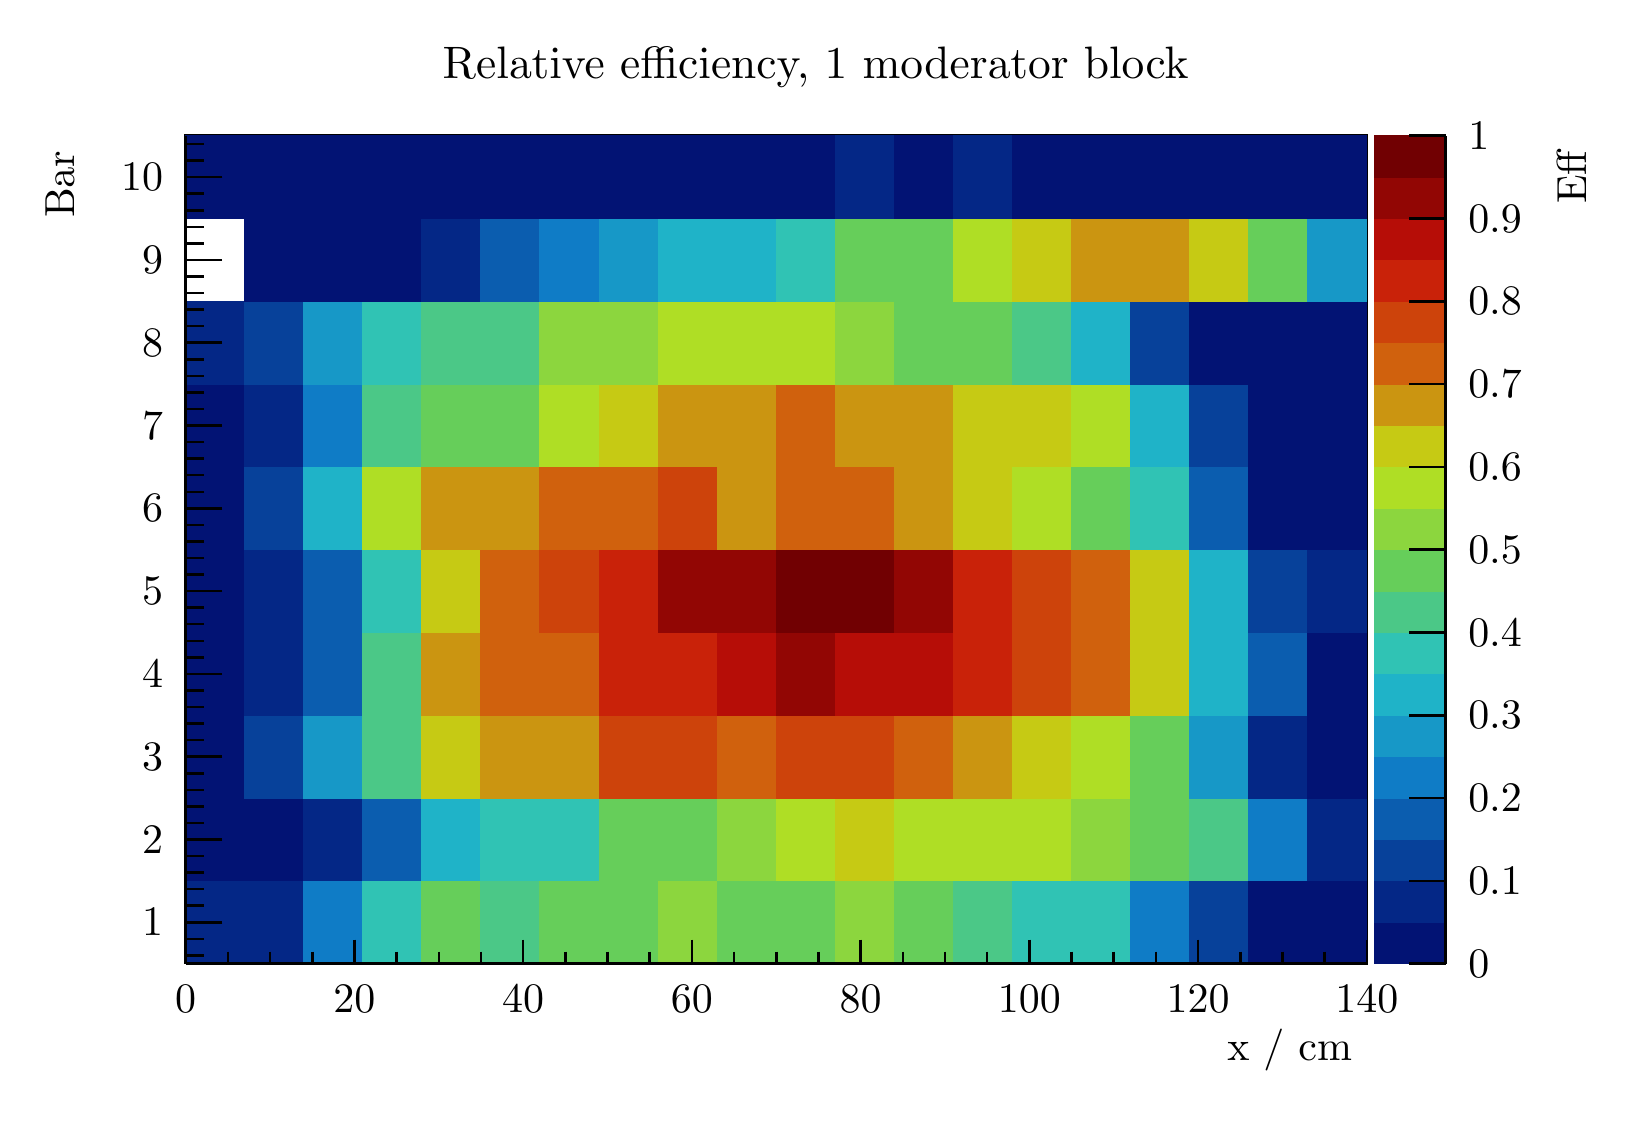
\begin{tikzpicture}
\pgfdeclareplotmark{cross} {
\pgfpathmoveto{\pgfpoint{-0.3\pgfplotmarksize}{\pgfplotmarksize}}
\pgfpathlineto{\pgfpoint{+0.3\pgfplotmarksize}{\pgfplotmarksize}}
\pgfpathlineto{\pgfpoint{+0.3\pgfplotmarksize}{0.3\pgfplotmarksize}}
\pgfpathlineto{\pgfpoint{+1\pgfplotmarksize}{0.3\pgfplotmarksize}}
\pgfpathlineto{\pgfpoint{+1\pgfplotmarksize}{-0.3\pgfplotmarksize}}
\pgfpathlineto{\pgfpoint{+0.3\pgfplotmarksize}{-0.3\pgfplotmarksize}}
\pgfpathlineto{\pgfpoint{+0.3\pgfplotmarksize}{-1.\pgfplotmarksize}}
\pgfpathlineto{\pgfpoint{-0.3\pgfplotmarksize}{-1.\pgfplotmarksize}}
\pgfpathlineto{\pgfpoint{-0.3\pgfplotmarksize}{-0.3\pgfplotmarksize}}
\pgfpathlineto{\pgfpoint{-1.\pgfplotmarksize}{-0.3\pgfplotmarksize}}
\pgfpathlineto{\pgfpoint{-1.\pgfplotmarksize}{0.3\pgfplotmarksize}}
\pgfpathlineto{\pgfpoint{-0.3\pgfplotmarksize}{0.3\pgfplotmarksize}}
\pgfpathclose
\pgfusepathqstroke
}
\pgfdeclareplotmark{cross*} {
\pgfpathmoveto{\pgfpoint{-0.3\pgfplotmarksize}{\pgfplotmarksize}}
\pgfpathlineto{\pgfpoint{+0.3\pgfplotmarksize}{\pgfplotmarksize}}
\pgfpathlineto{\pgfpoint{+0.3\pgfplotmarksize}{0.3\pgfplotmarksize}}
\pgfpathlineto{\pgfpoint{+1\pgfplotmarksize}{0.3\pgfplotmarksize}}
\pgfpathlineto{\pgfpoint{+1\pgfplotmarksize}{-0.3\pgfplotmarksize}}
\pgfpathlineto{\pgfpoint{+0.3\pgfplotmarksize}{-0.3\pgfplotmarksize}}
\pgfpathlineto{\pgfpoint{+0.3\pgfplotmarksize}{-1.\pgfplotmarksize}}
\pgfpathlineto{\pgfpoint{-0.3\pgfplotmarksize}{-1.\pgfplotmarksize}}
\pgfpathlineto{\pgfpoint{-0.3\pgfplotmarksize}{-0.3\pgfplotmarksize}}
\pgfpathlineto{\pgfpoint{-1.\pgfplotmarksize}{-0.3\pgfplotmarksize}}
\pgfpathlineto{\pgfpoint{-1.\pgfplotmarksize}{0.3\pgfplotmarksize}}
\pgfpathlineto{\pgfpoint{-0.3\pgfplotmarksize}{0.3\pgfplotmarksize}}
\pgfpathclose
\pgfusepathqfillstroke
}
\pgfdeclareplotmark{newstar} {
\pgfpathmoveto{\pgfqpoint{0pt}{\pgfplotmarksize}}
\pgfpathlineto{\pgfqpointpolar{44}{0.5\pgfplotmarksize}}
\pgfpathlineto{\pgfqpointpolar{18}{\pgfplotmarksize}}
\pgfpathlineto{\pgfqpointpolar{-20}{0.5\pgfplotmarksize}}
\pgfpathlineto{\pgfqpointpolar{-54}{\pgfplotmarksize}}
\pgfpathlineto{\pgfqpointpolar{-90}{0.5\pgfplotmarksize}}
\pgfpathlineto{\pgfqpointpolar{234}{\pgfplotmarksize}}
\pgfpathlineto{\pgfqpointpolar{198}{0.5\pgfplotmarksize}}
\pgfpathlineto{\pgfqpointpolar{162}{\pgfplotmarksize}}
\pgfpathlineto{\pgfqpointpolar{134}{0.5\pgfplotmarksize}}
\pgfpathclose
\pgfusepathqstroke
}
\pgfdeclareplotmark{newstar*} {
\pgfpathmoveto{\pgfqpoint{0pt}{\pgfplotmarksize}}
\pgfpathlineto{\pgfqpointpolar{44}{0.5\pgfplotmarksize}}
\pgfpathlineto{\pgfqpointpolar{18}{\pgfplotmarksize}}
\pgfpathlineto{\pgfqpointpolar{-20}{0.5\pgfplotmarksize}}
\pgfpathlineto{\pgfqpointpolar{-54}{\pgfplotmarksize}}
\pgfpathlineto{\pgfqpointpolar{-90}{0.5\pgfplotmarksize}}
\pgfpathlineto{\pgfqpointpolar{234}{\pgfplotmarksize}}
\pgfpathlineto{\pgfqpointpolar{198}{0.5\pgfplotmarksize}}
\pgfpathlineto{\pgfqpointpolar{162}{\pgfplotmarksize}}
\pgfpathlineto{\pgfqpointpolar{134}{0.5\pgfplotmarksize}}
\pgfpathclose
\pgfusepathqfillstroke
}
\definecolor{c}{rgb}{1,1,1};
\draw [color=c, fill=c] (0,0) rectangle (20,13.6558);
\draw [color=c, fill=c] (2,1.77525) rectangle (17,12.2902);
\definecolor{c}{rgb}{0,0,0};
\draw [c,line width=0.9] (2,1.77525) -- (2,12.2902) -- (17,12.2902) -- (17,1.77525) -- (2,1.77525);
\definecolor{c}{rgb}{1,1,1};
\draw [color=c, fill=c] (2,1.77525) rectangle (17,12.2902);
\definecolor{c}{rgb}{0,0,0};
\draw [c,line width=0.9] (2,1.77525) -- (2,12.2902) -- (17,12.2902) -- (17,1.77525) -- (2,1.77525);
\definecolor{c}{rgb}{0.0158128,0.151803,0.524225};
\draw [color=c, fill=c] (2,1.77525) rectangle (2.75,2.82674);
\draw [color=c, fill=c] (2.75,1.77525) rectangle (3.5,2.82674);
\definecolor{c}{rgb}{0.0588235,0.486275,0.776471};
\draw [color=c, fill=c] (3.5,1.77525) rectangle (4.25,2.82674);
\definecolor{c}{rgb}{0.18652,0.763235,0.706618};
\draw [color=c, fill=c] (4.25,1.77525) rectangle (5,2.82674);
\definecolor{c}{rgb}{0.4,0.807843,0.352941};
\draw [color=c, fill=c] (5,1.77525) rectangle (5.75,2.82674);
\definecolor{c}{rgb}{0.29326,0.785539,0.529779};
\draw [color=c, fill=c] (5.75,1.77525) rectangle (6.5,2.82674);
\definecolor{c}{rgb}{0.4,0.807843,0.352941};
\draw [color=c, fill=c] (6.5,1.77525) rectangle (7.25,2.82674);
\draw [color=c, fill=c] (7.25,1.77525) rectangle (8,2.82674);
\definecolor{c}{rgb}{0.549755,0.839706,0.244608};
\draw [color=c, fill=c] (8,1.77525) rectangle (8.75,2.82674);
\definecolor{c}{rgb}{0.4,0.807843,0.352941};
\draw [color=c, fill=c] (8.75,1.77525) rectangle (9.5,2.82674);
\draw [color=c, fill=c] (9.5,1.77525) rectangle (10.25,2.82674);
\definecolor{c}{rgb}{0.549755,0.839706,0.244608};
\draw [color=c, fill=c] (10.25,1.77525) rectangle (11,2.82674);
\definecolor{c}{rgb}{0.4,0.807843,0.352941};
\draw [color=c, fill=c] (11,1.77525) rectangle (11.75,2.82674);
\definecolor{c}{rgb}{0.29326,0.785539,0.529779};
\draw [color=c, fill=c] (11.75,1.77525) rectangle (12.5,2.82674);
\definecolor{c}{rgb}{0.18652,0.763235,0.706618};
\draw [color=c, fill=c] (12.5,1.77525) rectangle (13.25,2.82674);
\draw [color=c, fill=c] (13.25,1.77525) rectangle (14,2.82674);
\definecolor{c}{rgb}{0.0588235,0.486275,0.776471};
\draw [color=c, fill=c] (14,1.77525) rectangle (14.75,2.82674);
\definecolor{c}{rgb}{0.0281863,0.253431,0.604902};
\draw [color=c, fill=c] (14.75,1.77525) rectangle (15.5,2.82674);
\definecolor{c}{rgb}{0.00759013,0.0728653,0.45351};
\draw [color=c, fill=c] (15.5,1.77525) rectangle (16.25,2.82674);
\draw [color=c, fill=c] (16.25,1.77525) rectangle (17,2.82674);
\draw [color=c, fill=c] (2,2.82674) rectangle (2.75,3.87824);
\draw [color=c, fill=c] (2.75,2.82674) rectangle (3.5,3.87824);
\definecolor{c}{rgb}{0.0158128,0.151803,0.524225};
\draw [color=c, fill=c] (3.5,2.82674) rectangle (4.25,3.87824);
\definecolor{c}{rgb}{0.0428922,0.365196,0.687255};
\draw [color=c, fill=c] (4.25,2.82674) rectangle (5,3.87824);
\definecolor{c}{rgb}{0.122549,0.702941,0.786029};
\draw [color=c, fill=c] (5,2.82674) rectangle (5.75,3.87824);
\definecolor{c}{rgb}{0.18652,0.763235,0.706618};
\draw [color=c, fill=c] (5.75,2.82674) rectangle (6.5,3.87824);
\draw [color=c, fill=c] (6.5,2.82674) rectangle (7.25,3.87824);
\definecolor{c}{rgb}{0.4,0.807843,0.352941};
\draw [color=c, fill=c] (7.25,2.82674) rectangle (8,3.87824);
\draw [color=c, fill=c] (8,2.82674) rectangle (8.75,3.87824);
\definecolor{c}{rgb}{0.549755,0.839706,0.244608};
\draw [color=c, fill=c] (8.75,2.82674) rectangle (9.5,3.87824);
\definecolor{c}{rgb}{0.68799,0.869118,0.144608};
\draw [color=c, fill=c] (9.5,2.82674) rectangle (10.25,3.87824);
\definecolor{c}{rgb}{0.777451,0.791422,0.0796569};
\draw [color=c, fill=c] (10.25,2.82674) rectangle (11,3.87824);
\definecolor{c}{rgb}{0.68799,0.869118,0.144608};
\draw [color=c, fill=c] (11,2.82674) rectangle (11.75,3.87824);
\draw [color=c, fill=c] (11.75,2.82674) rectangle (12.5,3.87824);
\draw [color=c, fill=c] (12.5,2.82674) rectangle (13.25,3.87824);
\definecolor{c}{rgb}{0.549755,0.839706,0.244608};
\draw [color=c, fill=c] (13.25,2.82674) rectangle (14,3.87824);
\definecolor{c}{rgb}{0.4,0.807843,0.352941};
\draw [color=c, fill=c] (14,2.82674) rectangle (14.75,3.87824);
\definecolor{c}{rgb}{0.29326,0.785539,0.529779};
\draw [color=c, fill=c] (14.75,2.82674) rectangle (15.5,3.87824);
\definecolor{c}{rgb}{0.0588235,0.486275,0.776471};
\draw [color=c, fill=c] (15.5,2.82674) rectangle (16.25,3.87824);
\definecolor{c}{rgb}{0.0158128,0.151803,0.524225};
\draw [color=c, fill=c] (16.25,2.82674) rectangle (17,3.87824);
\definecolor{c}{rgb}{0.00759013,0.0728653,0.45351};
\draw [color=c, fill=c] (2,3.87824) rectangle (2.75,4.92973);
\definecolor{c}{rgb}{0.0281863,0.253431,0.604902};
\draw [color=c, fill=c] (2.75,3.87824) rectangle (3.5,4.92973);
\definecolor{c}{rgb}{0.0906863,0.594608,0.78125};
\draw [color=c, fill=c] (3.5,3.87824) rectangle (4.25,4.92973);
\definecolor{c}{rgb}{0.29326,0.785539,0.529779};
\draw [color=c, fill=c] (4.25,3.87824) rectangle (5,4.92973);
\definecolor{c}{rgb}{0.777451,0.791422,0.0796569};
\draw [color=c, fill=c] (5,3.87824) rectangle (5.75,4.92973);
\definecolor{c}{rgb}{0.796569,0.585907,0.0653186};
\draw [color=c, fill=c] (5.75,3.87824) rectangle (6.5,4.92973);
\draw [color=c, fill=c] (6.5,3.87824) rectangle (7.25,4.92973);
\definecolor{c}{rgb}{0.802451,0.261275,0.0436275};
\draw [color=c, fill=c] (7.25,3.87824) rectangle (8,4.92973);
\draw [color=c, fill=c] (8,3.87824) rectangle (8.75,4.92973);
\definecolor{c}{rgb}{0.815686,0.380392,0.0509804};
\draw [color=c, fill=c] (8.75,3.87824) rectangle (9.5,4.92973);
\definecolor{c}{rgb}{0.802451,0.261275,0.0436275};
\draw [color=c, fill=c] (9.5,3.87824) rectangle (10.25,4.92973);
\draw [color=c, fill=c] (10.25,3.87824) rectangle (11,4.92973);
\definecolor{c}{rgb}{0.815686,0.380392,0.0509804};
\draw [color=c, fill=c] (11,3.87824) rectangle (11.75,4.92973);
\definecolor{c}{rgb}{0.796569,0.585907,0.0653186};
\draw [color=c, fill=c] (11.75,3.87824) rectangle (12.5,4.92973);
\definecolor{c}{rgb}{0.777451,0.791422,0.0796569};
\draw [color=c, fill=c] (12.5,3.87824) rectangle (13.25,4.92973);
\definecolor{c}{rgb}{0.68799,0.869118,0.144608};
\draw [color=c, fill=c] (13.25,3.87824) rectangle (14,4.92973);
\definecolor{c}{rgb}{0.4,0.807843,0.352941};
\draw [color=c, fill=c] (14,3.87824) rectangle (14.75,4.92973);
\definecolor{c}{rgb}{0.0906863,0.594608,0.78125};
\draw [color=c, fill=c] (14.75,3.87824) rectangle (15.5,4.92973);
\definecolor{c}{rgb}{0.0158128,0.151803,0.524225};
\draw [color=c, fill=c] (15.5,3.87824) rectangle (16.25,4.92973);
\definecolor{c}{rgb}{0.00759013,0.0728653,0.45351};
\draw [color=c, fill=c] (16.25,3.87824) rectangle (17,4.92973);
\draw [color=c, fill=c] (2,4.92973) rectangle (2.75,5.98122);
\definecolor{c}{rgb}{0.0158128,0.151803,0.524225};
\draw [color=c, fill=c] (2.75,4.92973) rectangle (3.5,5.98122);
\definecolor{c}{rgb}{0.0428922,0.365196,0.687255};
\draw [color=c, fill=c] (3.5,4.92973) rectangle (4.25,5.98122);
\definecolor{c}{rgb}{0.29326,0.785539,0.529779};
\draw [color=c, fill=c] (4.25,4.92973) rectangle (5,5.98122);
\definecolor{c}{rgb}{0.796569,0.585907,0.0653186};
\draw [color=c, fill=c] (5,4.92973) rectangle (5.75,5.98122);
\definecolor{c}{rgb}{0.815686,0.380392,0.0509804};
\draw [color=c, fill=c] (5.75,4.92973) rectangle (6.5,5.98122);
\draw [color=c, fill=c] (6.5,4.92973) rectangle (7.25,5.98122);
\definecolor{c}{rgb}{0.788113,0.13223,0.0356618};
\draw [color=c, fill=c] (7.25,4.92973) rectangle (8,5.98122);
\draw [color=c, fill=c] (8,4.92973) rectangle (8.75,5.98122);
\definecolor{c}{rgb}{0.714951,0.0509804,0.0269608};
\draw [color=c, fill=c] (8.75,4.92973) rectangle (9.5,5.98122);
\definecolor{c}{rgb}{0.573162,0.0254902,0.017402};
\draw [color=c, fill=c] (9.5,4.92973) rectangle (10.25,5.98122);
\definecolor{c}{rgb}{0.714951,0.0509804,0.0269608};
\draw [color=c, fill=c] (10.25,4.92973) rectangle (11,5.98122);
\draw [color=c, fill=c] (11,4.92973) rectangle (11.75,5.98122);
\definecolor{c}{rgb}{0.788113,0.13223,0.0356618};
\draw [color=c, fill=c] (11.75,4.92973) rectangle (12.5,5.98122);
\definecolor{c}{rgb}{0.802451,0.261275,0.0436275};
\draw [color=c, fill=c] (12.5,4.92973) rectangle (13.25,5.98122);
\definecolor{c}{rgb}{0.815686,0.380392,0.0509804};
\draw [color=c, fill=c] (13.25,4.92973) rectangle (14,5.98122);
\definecolor{c}{rgb}{0.777451,0.791422,0.0796569};
\draw [color=c, fill=c] (14,4.92973) rectangle (14.75,5.98122);
\definecolor{c}{rgb}{0.122549,0.702941,0.786029};
\draw [color=c, fill=c] (14.75,4.92973) rectangle (15.5,5.98122);
\definecolor{c}{rgb}{0.0428922,0.365196,0.687255};
\draw [color=c, fill=c] (15.5,4.92973) rectangle (16.25,5.98122);
\definecolor{c}{rgb}{0.00759013,0.0728653,0.45351};
\draw [color=c, fill=c] (16.25,4.92973) rectangle (17,5.98122);
\draw [color=c, fill=c] (2,5.98122) rectangle (2.75,7.03272);
\definecolor{c}{rgb}{0.0158128,0.151803,0.524225};
\draw [color=c, fill=c] (2.75,5.98122) rectangle (3.5,7.03272);
\definecolor{c}{rgb}{0.0428922,0.365196,0.687255};
\draw [color=c, fill=c] (3.5,5.98122) rectangle (4.25,7.03272);
\definecolor{c}{rgb}{0.18652,0.763235,0.706618};
\draw [color=c, fill=c] (4.25,5.98122) rectangle (5,7.03272);
\definecolor{c}{rgb}{0.777451,0.791422,0.0796569};
\draw [color=c, fill=c] (5,5.98122) rectangle (5.75,7.03272);
\definecolor{c}{rgb}{0.815686,0.380392,0.0509804};
\draw [color=c, fill=c] (5.75,5.98122) rectangle (6.5,7.03272);
\definecolor{c}{rgb}{0.802451,0.261275,0.0436275};
\draw [color=c, fill=c] (6.5,5.98122) rectangle (7.25,7.03272);
\definecolor{c}{rgb}{0.788113,0.13223,0.0356618};
\draw [color=c, fill=c] (7.25,5.98122) rectangle (8,7.03272);
\definecolor{c}{rgb}{0.573162,0.0254902,0.017402};
\draw [color=c, fill=c] (8,5.98122) rectangle (8.75,7.03272);
\draw [color=c, fill=c] (8.75,5.98122) rectangle (9.5,7.03272);
\definecolor{c}{rgb}{0.442279,0.00196078,0.00857843};
\draw [color=c, fill=c] (9.5,5.98122) rectangle (10.25,7.03272);
\draw [color=c, fill=c] (10.25,5.98122) rectangle (11,7.03272);
\definecolor{c}{rgb}{0.573162,0.0254902,0.017402};
\draw [color=c, fill=c] (11,5.98122) rectangle (11.75,7.03272);
\definecolor{c}{rgb}{0.788113,0.13223,0.0356618};
\draw [color=c, fill=c] (11.75,5.98122) rectangle (12.5,7.03272);
\definecolor{c}{rgb}{0.802451,0.261275,0.0436275};
\draw [color=c, fill=c] (12.5,5.98122) rectangle (13.25,7.03272);
\definecolor{c}{rgb}{0.815686,0.380392,0.0509804};
\draw [color=c, fill=c] (13.25,5.98122) rectangle (14,7.03272);
\definecolor{c}{rgb}{0.777451,0.791422,0.0796569};
\draw [color=c, fill=c] (14,5.98122) rectangle (14.75,7.03272);
\definecolor{c}{rgb}{0.122549,0.702941,0.786029};
\draw [color=c, fill=c] (14.75,5.98122) rectangle (15.5,7.03272);
\definecolor{c}{rgb}{0.0281863,0.253431,0.604902};
\draw [color=c, fill=c] (15.5,5.98122) rectangle (16.25,7.03272);
\definecolor{c}{rgb}{0.0158128,0.151803,0.524225};
\draw [color=c, fill=c] (16.25,5.98122) rectangle (17,7.03272);
\definecolor{c}{rgb}{0.00759013,0.0728653,0.45351};
\draw [color=c, fill=c] (2,7.03272) rectangle (2.75,8.08421);
\definecolor{c}{rgb}{0.0281863,0.253431,0.604902};
\draw [color=c, fill=c] (2.75,7.03272) rectangle (3.5,8.08421);
\definecolor{c}{rgb}{0.122549,0.702941,0.786029};
\draw [color=c, fill=c] (3.5,7.03272) rectangle (4.25,8.08421);
\definecolor{c}{rgb}{0.68799,0.869118,0.144608};
\draw [color=c, fill=c] (4.25,7.03272) rectangle (5,8.08421);
\definecolor{c}{rgb}{0.796569,0.585907,0.0653186};
\draw [color=c, fill=c] (5,7.03272) rectangle (5.75,8.08421);
\draw [color=c, fill=c] (5.75,7.03272) rectangle (6.5,8.08421);
\definecolor{c}{rgb}{0.815686,0.380392,0.0509804};
\draw [color=c, fill=c] (6.5,7.03272) rectangle (7.25,8.08421);
\draw [color=c, fill=c] (7.25,7.03272) rectangle (8,8.08421);
\definecolor{c}{rgb}{0.802451,0.261275,0.0436275};
\draw [color=c, fill=c] (8,7.03272) rectangle (8.75,8.08421);
\definecolor{c}{rgb}{0.796569,0.585907,0.0653186};
\draw [color=c, fill=c] (8.75,7.03272) rectangle (9.5,8.08421);
\definecolor{c}{rgb}{0.815686,0.380392,0.0509804};
\draw [color=c, fill=c] (9.5,7.03272) rectangle (10.25,8.08421);
\draw [color=c, fill=c] (10.25,7.03272) rectangle (11,8.08421);
\definecolor{c}{rgb}{0.796569,0.585907,0.0653186};
\draw [color=c, fill=c] (11,7.03272) rectangle (11.75,8.08421);
\definecolor{c}{rgb}{0.777451,0.791422,0.0796569};
\draw [color=c, fill=c] (11.75,7.03272) rectangle (12.5,8.08421);
\definecolor{c}{rgb}{0.68799,0.869118,0.144608};
\draw [color=c, fill=c] (12.5,7.03272) rectangle (13.25,8.08421);
\definecolor{c}{rgb}{0.4,0.807843,0.352941};
\draw [color=c, fill=c] (13.25,7.03272) rectangle (14,8.08421);
\definecolor{c}{rgb}{0.18652,0.763235,0.706618};
\draw [color=c, fill=c] (14,7.03272) rectangle (14.75,8.08421);
\definecolor{c}{rgb}{0.0428922,0.365196,0.687255};
\draw [color=c, fill=c] (14.75,7.03272) rectangle (15.5,8.08421);
\definecolor{c}{rgb}{0.00759013,0.0728653,0.45351};
\draw [color=c, fill=c] (15.5,7.03272) rectangle (16.25,8.08421);
\draw [color=c, fill=c] (16.25,7.03272) rectangle (17,8.08421);
\draw [color=c, fill=c] (2,8.08421) rectangle (2.75,9.1357);
\definecolor{c}{rgb}{0.0158128,0.151803,0.524225};
\draw [color=c, fill=c] (2.75,8.08421) rectangle (3.5,9.1357);
\definecolor{c}{rgb}{0.0588235,0.486275,0.776471};
\draw [color=c, fill=c] (3.5,8.08421) rectangle (4.25,9.1357);
\definecolor{c}{rgb}{0.29326,0.785539,0.529779};
\draw [color=c, fill=c] (4.25,8.08421) rectangle (5,9.1357);
\definecolor{c}{rgb}{0.4,0.807843,0.352941};
\draw [color=c, fill=c] (5,8.08421) rectangle (5.75,9.1357);
\draw [color=c, fill=c] (5.75,8.08421) rectangle (6.5,9.1357);
\definecolor{c}{rgb}{0.68799,0.869118,0.144608};
\draw [color=c, fill=c] (6.5,8.08421) rectangle (7.25,9.1357);
\definecolor{c}{rgb}{0.777451,0.791422,0.0796569};
\draw [color=c, fill=c] (7.25,8.08421) rectangle (8,9.1357);
\definecolor{c}{rgb}{0.796569,0.585907,0.0653186};
\draw [color=c, fill=c] (8,8.08421) rectangle (8.75,9.1357);
\draw [color=c, fill=c] (8.75,8.08421) rectangle (9.5,9.1357);
\definecolor{c}{rgb}{0.815686,0.380392,0.0509804};
\draw [color=c, fill=c] (9.5,8.08421) rectangle (10.25,9.1357);
\definecolor{c}{rgb}{0.796569,0.585907,0.0653186};
\draw [color=c, fill=c] (10.25,8.08421) rectangle (11,9.1357);
\draw [color=c, fill=c] (11,8.08421) rectangle (11.75,9.1357);
\definecolor{c}{rgb}{0.777451,0.791422,0.0796569};
\draw [color=c, fill=c] (11.75,8.08421) rectangle (12.5,9.1357);
\draw [color=c, fill=c] (12.5,8.08421) rectangle (13.25,9.1357);
\definecolor{c}{rgb}{0.68799,0.869118,0.144608};
\draw [color=c, fill=c] (13.25,8.08421) rectangle (14,9.1357);
\definecolor{c}{rgb}{0.122549,0.702941,0.786029};
\draw [color=c, fill=c] (14,8.08421) rectangle (14.75,9.1357);
\definecolor{c}{rgb}{0.0281863,0.253431,0.604902};
\draw [color=c, fill=c] (14.75,8.08421) rectangle (15.5,9.1357);
\definecolor{c}{rgb}{0.00759013,0.0728653,0.45351};
\draw [color=c, fill=c] (15.5,8.08421) rectangle (16.25,9.1357);
\draw [color=c, fill=c] (16.25,8.08421) rectangle (17,9.1357);
\definecolor{c}{rgb}{0.0158128,0.151803,0.524225};
\draw [color=c, fill=c] (2,9.1357) rectangle (2.75,10.1872);
\definecolor{c}{rgb}{0.0281863,0.253431,0.604902};
\draw [color=c, fill=c] (2.75,9.1357) rectangle (3.5,10.1872);
\definecolor{c}{rgb}{0.0906863,0.594608,0.78125};
\draw [color=c, fill=c] (3.5,9.1357) rectangle (4.25,10.1872);
\definecolor{c}{rgb}{0.18652,0.763235,0.706618};
\draw [color=c, fill=c] (4.25,9.1357) rectangle (5,10.1872);
\definecolor{c}{rgb}{0.29326,0.785539,0.529779};
\draw [color=c, fill=c] (5,9.1357) rectangle (5.75,10.1872);
\draw [color=c, fill=c] (5.75,9.1357) rectangle (6.5,10.1872);
\definecolor{c}{rgb}{0.549755,0.839706,0.244608};
\draw [color=c, fill=c] (6.5,9.1357) rectangle (7.25,10.1872);
\draw [color=c, fill=c] (7.25,9.1357) rectangle (8,10.1872);
\definecolor{c}{rgb}{0.68799,0.869118,0.144608};
\draw [color=c, fill=c] (8,9.1357) rectangle (8.75,10.1872);
\draw [color=c, fill=c] (8.75,9.1357) rectangle (9.5,10.1872);
\draw [color=c, fill=c] (9.5,9.1357) rectangle (10.25,10.1872);
\definecolor{c}{rgb}{0.549755,0.839706,0.244608};
\draw [color=c, fill=c] (10.25,9.1357) rectangle (11,10.1872);
\definecolor{c}{rgb}{0.4,0.807843,0.352941};
\draw [color=c, fill=c] (11,9.1357) rectangle (11.75,10.1872);
\draw [color=c, fill=c] (11.75,9.1357) rectangle (12.5,10.1872);
\definecolor{c}{rgb}{0.29326,0.785539,0.529779};
\draw [color=c, fill=c] (12.5,9.1357) rectangle (13.25,10.1872);
\definecolor{c}{rgb}{0.122549,0.702941,0.786029};
\draw [color=c, fill=c] (13.25,9.1357) rectangle (14,10.1872);
\definecolor{c}{rgb}{0.0281863,0.253431,0.604902};
\draw [color=c, fill=c] (14,9.1357) rectangle (14.75,10.1872);
\definecolor{c}{rgb}{0.00759013,0.0728653,0.45351};
\draw [color=c, fill=c] (14.75,9.1357) rectangle (15.5,10.1872);
\draw [color=c, fill=c] (15.5,9.1357) rectangle (16.25,10.1872);
\draw [color=c, fill=c] (16.25,9.1357) rectangle (17,10.1872);
\draw [color=c, fill=c] (2.75,10.1872) rectangle (3.5,11.2387);
\draw [color=c, fill=c] (3.5,10.1872) rectangle (4.25,11.2387);
\draw [color=c, fill=c] (4.25,10.1872) rectangle (5,11.2387);
\definecolor{c}{rgb}{0.0158128,0.151803,0.524225};
\draw [color=c, fill=c] (5,10.1872) rectangle (5.75,11.2387);
\definecolor{c}{rgb}{0.0428922,0.365196,0.687255};
\draw [color=c, fill=c] (5.75,10.1872) rectangle (6.5,11.2387);
\definecolor{c}{rgb}{0.0588235,0.486275,0.776471};
\draw [color=c, fill=c] (6.5,10.1872) rectangle (7.25,11.2387);
\definecolor{c}{rgb}{0.0906863,0.594608,0.78125};
\draw [color=c, fill=c] (7.25,10.1872) rectangle (8,11.2387);
\definecolor{c}{rgb}{0.122549,0.702941,0.786029};
\draw [color=c, fill=c] (8,10.1872) rectangle (8.75,11.2387);
\draw [color=c, fill=c] (8.75,10.1872) rectangle (9.5,11.2387);
\definecolor{c}{rgb}{0.18652,0.763235,0.706618};
\draw [color=c, fill=c] (9.5,10.1872) rectangle (10.25,11.2387);
\definecolor{c}{rgb}{0.4,0.807843,0.352941};
\draw [color=c, fill=c] (10.25,10.1872) rectangle (11,11.2387);
\draw [color=c, fill=c] (11,10.1872) rectangle (11.75,11.2387);
\definecolor{c}{rgb}{0.68799,0.869118,0.144608};
\draw [color=c, fill=c] (11.75,10.1872) rectangle (12.5,11.2387);
\definecolor{c}{rgb}{0.777451,0.791422,0.0796569};
\draw [color=c, fill=c] (12.5,10.1872) rectangle (13.25,11.2387);
\definecolor{c}{rgb}{0.796569,0.585907,0.0653186};
\draw [color=c, fill=c] (13.25,10.1872) rectangle (14,11.2387);
\draw [color=c, fill=c] (14,10.1872) rectangle (14.75,11.2387);
\definecolor{c}{rgb}{0.777451,0.791422,0.0796569};
\draw [color=c, fill=c] (14.75,10.1872) rectangle (15.5,11.2387);
\definecolor{c}{rgb}{0.4,0.807843,0.352941};
\draw [color=c, fill=c] (15.5,10.1872) rectangle (16.25,11.2387);
\definecolor{c}{rgb}{0.0906863,0.594608,0.78125};
\draw [color=c, fill=c] (16.25,10.1872) rectangle (17,11.2387);
\definecolor{c}{rgb}{0.00759013,0.0728653,0.45351};
\draw [color=c, fill=c] (2,11.2387) rectangle (2.75,12.2902);
\draw [color=c, fill=c] (2.75,11.2387) rectangle (3.5,12.2902);
\draw [color=c, fill=c] (3.5,11.2387) rectangle (4.25,12.2902);
\draw [color=c, fill=c] (4.25,11.2387) rectangle (5,12.2902);
\draw [color=c, fill=c] (5,11.2387) rectangle (5.75,12.2902);
\draw [color=c, fill=c] (5.75,11.2387) rectangle (6.5,12.2902);
\draw [color=c, fill=c] (6.5,11.2387) rectangle (7.25,12.2902);
\draw [color=c, fill=c] (7.25,11.2387) rectangle (8,12.2902);
\draw [color=c, fill=c] (8,11.2387) rectangle (8.75,12.2902);
\draw [color=c, fill=c] (8.75,11.2387) rectangle (9.5,12.2902);
\draw [color=c, fill=c] (9.5,11.2387) rectangle (10.25,12.2902);
\definecolor{c}{rgb}{0.0158128,0.151803,0.524225};
\draw [color=c, fill=c] (10.25,11.2387) rectangle (11,12.2902);
\definecolor{c}{rgb}{0.00759013,0.0728653,0.45351};
\draw [color=c, fill=c] (11,11.2387) rectangle (11.75,12.2902);
\definecolor{c}{rgb}{0.0158128,0.151803,0.524225};
\draw [color=c, fill=c] (11.75,11.2387) rectangle (12.5,12.2902);
\definecolor{c}{rgb}{0.00759013,0.0728653,0.45351};
\draw [color=c, fill=c] (12.5,11.2387) rectangle (13.25,12.2902);
\draw [color=c, fill=c] (13.25,11.2387) rectangle (14,12.2902);
\draw [color=c, fill=c] (14,11.2387) rectangle (14.75,12.2902);
\draw [color=c, fill=c] (14.75,11.2387) rectangle (15.5,12.2902);
\draw [color=c, fill=c] (15.5,11.2387) rectangle (16.25,12.2902);
\draw [color=c, fill=c] (16.25,11.2387) rectangle (17,12.2902);
\definecolor{c}{rgb}{0,0,0};
\draw [c,line width=0.9] (2,1.77525) -- (17,1.77525);
\draw [c,line width=0.9] (2,2.0825) -- (2,1.77525);
\draw [c,line width=0.9] (2.53571,1.92888) -- (2.53571,1.77525);
\draw [c,line width=0.9] (3.07143,1.92888) -- (3.07143,1.77525);
\draw [c,line width=0.9] (3.60714,1.92888) -- (3.60714,1.77525);
\draw [c,line width=0.9] (4.14286,2.0825) -- (4.14286,1.77525);
\draw [c,line width=0.9] (4.67857,1.92888) -- (4.67857,1.77525);
\draw [c,line width=0.9] (5.21429,1.92888) -- (5.21429,1.77525);
\draw [c,line width=0.9] (5.75,1.92888) -- (5.75,1.77525);
\draw [c,line width=0.9] (6.28571,2.0825) -- (6.28571,1.77525);
\draw [c,line width=0.9] (6.82143,1.92888) -- (6.82143,1.77525);
\draw [c,line width=0.9] (7.35714,1.92888) -- (7.35714,1.77525);
\draw [c,line width=0.9] (7.89286,1.92888) -- (7.89286,1.77525);
\draw [c,line width=0.9] (8.42857,2.0825) -- (8.42857,1.77525);
\draw [c,line width=0.9] (8.96429,1.92888) -- (8.96429,1.77525);
\draw [c,line width=0.9] (9.5,1.92888) -- (9.5,1.77525);
\draw [c,line width=0.9] (10.0357,1.92888) -- (10.0357,1.77525);
\draw [c,line width=0.9] (10.5714,2.0825) -- (10.5714,1.77525);
\draw [c,line width=0.9] (11.1071,1.92888) -- (11.1071,1.77525);
\draw [c,line width=0.9] (11.6429,1.92888) -- (11.6429,1.77525);
\draw [c,line width=0.9] (12.1786,1.92888) -- (12.1786,1.77525);
\draw [c,line width=0.9] (12.7143,2.0825) -- (12.7143,1.77525);
\draw [c,line width=0.9] (13.25,1.92888) -- (13.25,1.77525);
\draw [c,line width=0.9] (13.7857,1.92888) -- (13.7857,1.77525);
\draw [c,line width=0.9] (14.3214,1.92888) -- (14.3214,1.77525);
\draw [c,line width=0.9] (14.8571,2.0825) -- (14.8571,1.77525);
\draw [c,line width=0.9] (15.3929,1.92888) -- (15.3929,1.77525);
\draw [c,line width=0.9] (15.9286,1.92888) -- (15.9286,1.77525);
\draw [c,line width=0.9] (16.4643,1.92888) -- (16.4643,1.77525);
\draw [c,line width=0.9] (17,2.0825) -- (17,1.77525);
\draw [anchor=base] (2,1.16074) node[scale=1.51645, color=c, rotate=0]{0};
\draw [anchor=base] (4.14286,1.16074) node[scale=1.51645, color=c, rotate=0]{20};
\draw [anchor=base] (6.28571,1.16074) node[scale=1.51645, color=c, rotate=0]{40};
\draw [anchor=base] (8.42857,1.16074) node[scale=1.51645, color=c, rotate=0]{60};
\draw [anchor=base] (10.5714,1.16074) node[scale=1.51645, color=c, rotate=0]{80};
\draw [anchor=base] (12.7143,1.16074) node[scale=1.51645, color=c, rotate=0]{100};
\draw [anchor=base] (14.8571,1.16074) node[scale=1.51645, color=c, rotate=0]{120};
\draw [anchor=base] (17,1.16074) node[scale=1.51645, color=c, rotate=0]{140};
\draw [anchor= east] (17,0.682788) node[scale=1.51645, color=c, rotate=0]{ x / cm};
\draw [c,line width=0.9] (2,1.77525) -- (2,12.2902);
\draw [c,line width=0.9] (2.462,2.301) -- (2,2.301);
\draw [c,line width=0.9] (2.231,2.51129) -- (2,2.51129);
\draw [c,line width=0.9] (2.231,2.72159) -- (2,2.72159);
\draw [c,line width=0.9] (2.231,2.93189) -- (2,2.93189);
\draw [c,line width=0.9] (2.231,3.14219) -- (2,3.14219);
\draw [c,line width=0.9] (2.462,3.35249) -- (2,3.35249);
\draw [c,line width=0.9] (2.231,3.56279) -- (2,3.56279);
\draw [c,line width=0.9] (2.231,3.77309) -- (2,3.77309);
\draw [c,line width=0.9] (2.231,3.98339) -- (2,3.98339);
\draw [c,line width=0.9] (2.231,4.19368) -- (2,4.19368);
\draw [c,line width=0.9] (2.462,4.40398) -- (2,4.40398);
\draw [c,line width=0.9] (2.231,4.61428) -- (2,4.61428);
\draw [c,line width=0.9] (2.231,4.82458) -- (2,4.82458);
\draw [c,line width=0.9] (2.231,5.03488) -- (2,5.03488);
\draw [c,line width=0.9] (2.231,5.24518) -- (2,5.24518);
\draw [c,line width=0.9] (2.462,5.45548) -- (2,5.45548);
\draw [c,line width=0.9] (2.231,5.66578) -- (2,5.66578);
\draw [c,line width=0.9] (2.231,5.87607) -- (2,5.87607);
\draw [c,line width=0.9] (2.231,6.08637) -- (2,6.08637);
\draw [c,line width=0.9] (2.231,6.29667) -- (2,6.29667);
\draw [c,line width=0.9] (2.462,6.50697) -- (2,6.50697);
\draw [c,line width=0.9] (2.231,6.71727) -- (2,6.71727);
\draw [c,line width=0.9] (2.231,6.92757) -- (2,6.92757);
\draw [c,line width=0.9] (2.231,7.13787) -- (2,7.13787);
\draw [c,line width=0.9] (2.231,7.34817) -- (2,7.34817);
\draw [c,line width=0.9] (2.462,7.55846) -- (2,7.55846);
\draw [c,line width=0.9] (2.231,7.76876) -- (2,7.76876);
\draw [c,line width=0.9] (2.231,7.97906) -- (2,7.97906);
\draw [c,line width=0.9] (2.231,8.18936) -- (2,8.18936);
\draw [c,line width=0.9] (2.231,8.39966) -- (2,8.39966);
\draw [c,line width=0.9] (2.462,8.60996) -- (2,8.60996);
\draw [c,line width=0.9] (2.231,8.82026) -- (2,8.82026);
\draw [c,line width=0.9] (2.231,9.03055) -- (2,9.03055);
\draw [c,line width=0.9] (2.231,9.24085) -- (2,9.24085);
\draw [c,line width=0.9] (2.231,9.45115) -- (2,9.45115);
\draw [c,line width=0.9] (2.462,9.66145) -- (2,9.66145);
\draw [c,line width=0.9] (2.231,9.87175) -- (2,9.87175);
\draw [c,line width=0.9] (2.231,10.082) -- (2,10.082);
\draw [c,line width=0.9] (2.231,10.2923) -- (2,10.2923);
\draw [c,line width=0.9] (2.231,10.5026) -- (2,10.5026);
\draw [c,line width=0.9] (2.462,10.7129) -- (2,10.7129);
\draw [c,line width=0.9] (2.231,10.9232) -- (2,10.9232);
\draw [c,line width=0.9] (2.231,11.1335) -- (2,11.1335);
\draw [c,line width=0.9] (2.231,11.3438) -- (2,11.3438);
\draw [c,line width=0.9] (2.231,11.5541) -- (2,11.5541);
\draw [c,line width=0.9] (2.462,11.7644) -- (2,11.7644);
\draw [c,line width=0.9] (2.462,2.301) -- (2,2.301);
\draw [c,line width=0.9] (2.231,2.0907) -- (2,2.0907);
\draw [c,line width=0.9] (2.231,1.8804) -- (2,1.8804);
\draw [c,line width=0.9] (2.462,11.7644) -- (2,11.7644);
\draw [c,line width=0.9] (2.231,11.9747) -- (2,11.9747);
\draw [c,line width=0.9] (2.231,12.185) -- (2,12.185);
\draw [anchor= east] (1.9,2.301) node[scale=1.51645, color=c, rotate=0]{1};
\draw [anchor= east] (1.9,3.35249) node[scale=1.51645, color=c, rotate=0]{2};
\draw [anchor= east] (1.9,4.40398) node[scale=1.51645, color=c, rotate=0]{3};
\draw [anchor= east] (1.9,5.45548) node[scale=1.51645, color=c, rotate=0]{4};
\draw [anchor= east] (1.9,6.50697) node[scale=1.51645, color=c, rotate=0]{5};
\draw [anchor= east] (1.9,7.55846) node[scale=1.51645, color=c, rotate=0]{6};
\draw [anchor= east] (1.9,8.60996) node[scale=1.51645, color=c, rotate=0]{7};
\draw [anchor= east] (1.9,9.66145) node[scale=1.51645, color=c, rotate=0]{8};
\draw [anchor= east] (1.9,10.7129) node[scale=1.51645, color=c, rotate=0]{9};
\draw [anchor= east] (1.9,11.7644) node[scale=1.51645, color=c, rotate=0]{10};
\draw [anchor= east] (0.4,12.2902) node[scale=1.51645, color=c, rotate=90]{ Bar};
\definecolor{c}{rgb}{0.00759013,0.0728653,0.45351};
\draw [color=c, fill=c] (17.1,1.77525) rectangle (18,2.301);
\definecolor{c}{rgb}{0.0158128,0.151803,0.524225};
\draw [color=c, fill=c] (17.1,2.301) rectangle (18,2.82674);
\definecolor{c}{rgb}{0.0281863,0.253431,0.604902};
\draw [color=c, fill=c] (17.1,2.82674) rectangle (18,3.35249);
\definecolor{c}{rgb}{0.0428922,0.365196,0.687255};
\draw [color=c, fill=c] (17.1,3.35249) rectangle (18,3.87824);
\definecolor{c}{rgb}{0.0588235,0.486275,0.776471};
\draw [color=c, fill=c] (17.1,3.87824) rectangle (18,4.40398);
\definecolor{c}{rgb}{0.0906863,0.594608,0.78125};
\draw [color=c, fill=c] (17.1,4.40398) rectangle (18,4.92973);
\definecolor{c}{rgb}{0.122549,0.702941,0.786029};
\draw [color=c, fill=c] (17.1,4.92973) rectangle (18,5.45548);
\definecolor{c}{rgb}{0.18652,0.763235,0.706618};
\draw [color=c, fill=c] (17.1,5.45548) rectangle (18,5.98122);
\definecolor{c}{rgb}{0.29326,0.785539,0.529779};
\draw [color=c, fill=c] (17.1,5.98122) rectangle (18,6.50697);
\definecolor{c}{rgb}{0.4,0.807843,0.352941};
\draw [color=c, fill=c] (17.1,6.50697) rectangle (18,7.03272);
\definecolor{c}{rgb}{0.549755,0.839706,0.244608};
\draw [color=c, fill=c] (17.1,7.03272) rectangle (18,7.55846);
\definecolor{c}{rgb}{0.68799,0.869118,0.144608};
\draw [color=c, fill=c] (17.1,7.55846) rectangle (18,8.08421);
\definecolor{c}{rgb}{0.777451,0.791422,0.0796569};
\draw [color=c, fill=c] (17.1,8.08421) rectangle (18,8.60996);
\definecolor{c}{rgb}{0.796569,0.585907,0.0653186};
\draw [color=c, fill=c] (17.1,8.60996) rectangle (18,9.1357);
\definecolor{c}{rgb}{0.815686,0.380392,0.0509804};
\draw [color=c, fill=c] (17.1,9.1357) rectangle (18,9.66145);
\definecolor{c}{rgb}{0.802451,0.261275,0.0436275};
\draw [color=c, fill=c] (17.1,9.66145) rectangle (18,10.1872);
\definecolor{c}{rgb}{0.788113,0.13223,0.0356618};
\draw [color=c, fill=c] (17.1,10.1872) rectangle (18,10.7129);
\definecolor{c}{rgb}{0.714951,0.0509804,0.0269608};
\draw [color=c, fill=c] (17.1,10.7129) rectangle (18,11.2387);
\definecolor{c}{rgb}{0.573162,0.0254902,0.017402};
\draw [color=c, fill=c] (17.1,11.2387) rectangle (18,11.7644);
\definecolor{c}{rgb}{0.442279,0.00196078,0.00857843};
\draw [color=c, fill=c] (17.1,11.7644) rectangle (18,12.2902);
\definecolor{c}{rgb}{0,0,0};
\draw [c,line width=0.9] (18,1.77525) -- (18,12.2902);
\draw [c,line width=0.9] (17.538,1.77525) -- (18,1.77525);
\draw [c,line width=0.9] (17.538,2.82674) -- (18,2.82674);
\draw [c,line width=0.9] (17.538,3.87824) -- (18,3.87824);
\draw [c,line width=0.9] (17.538,4.92973) -- (18,4.92973);
\draw [c,line width=0.9] (17.538,5.98122) -- (18,5.98122);
\draw [c,line width=0.9] (17.538,7.03272) -- (18,7.03272);
\draw [c,line width=0.9] (17.538,8.08421) -- (18,8.08421);
\draw [c,line width=0.9] (17.538,9.1357) -- (18,9.1357);
\draw [c,line width=0.9] (17.538,10.1872) -- (18,10.1872);
\draw [c,line width=0.9] (17.538,11.2387) -- (18,11.2387);
\draw [c,line width=0.9] (17.538,12.2902) -- (18,12.2902);
\draw [anchor= west] (18.1,1.77525) node[scale=1.51645, color=c, rotate=0]{0};
\draw [anchor= west] (18.1,2.82674) node[scale=1.51645, color=c, rotate=0]{0.1};
\draw [anchor= west] (18.1,3.87824) node[scale=1.51645, color=c, rotate=0]{0.2};
\draw [anchor= west] (18.1,4.92973) node[scale=1.51645, color=c, rotate=0]{0.3};
\draw [anchor= west] (18.1,5.98122) node[scale=1.51645, color=c, rotate=0]{0.4};
\draw [anchor= west] (18.1,7.03272) node[scale=1.51645, color=c, rotate=0]{0.5};
\draw [anchor= west] (18.1,8.08421) node[scale=1.51645, color=c, rotate=0]{0.6};
\draw [anchor= west] (18.1,9.1357) node[scale=1.51645, color=c, rotate=0]{0.7};
\draw [anchor= west] (18.1,10.1872) node[scale=1.51645, color=c, rotate=0]{0.8};
\draw [anchor= west] (18.1,11.2387) node[scale=1.51645, color=c, rotate=0]{0.9};
\draw [anchor= west] (18.1,12.2902) node[scale=1.51645, color=c, rotate=0]{1};
\draw [anchor= east] (19.6,12.2902) node[scale=1.51645, color=c, rotate=90]{ Eff};
\draw (10,13.1607) node[scale=1.64282, color=c, rotate=0]{Relative efficiency, 1 moderator block};
\end{tikzpicture}

  \end{adjustbox}
  \caption{Relative detection efficiency of $\mathit{S4}$ as a function of bar number and position along each bar as measured with cosmic rays. The data from bar 10 was not used in the analysis due to the poor efficiency along the bar.}
  \label{fig:s4PosEff}
\end{figure}

Using Figure~\ref{fig:s4tof}, protons and MIPs are selected with timing cuts. 
These timing cuts are chosen by fitting a sum of signal and background functions to the time of flight spectra shown in Figure~\ref{fig:s4tof}. 
The signal functions are taken to be Gaussians while the background is taken to be flat. 
An example of this is shown in Figure~\ref{fig:fitEx}.
The particles in the quicker timing window (those for which $36~\text{ns}<t_{\mathit{S4}}-t_{\mathit{S2}}<51~\text{ns}$) are considered to be minimum ionizing particles while those in the slower timing window (those for which $62~\text{ns}<t_{\mathit{S4}}-t_{\mathit{S2}}<125~\text{ns}$) are considered to be protons.

\begin{figure}[ht]
  \begin{adjustbox}{max totalsize={\textwidth}{.62\textheight},center}
    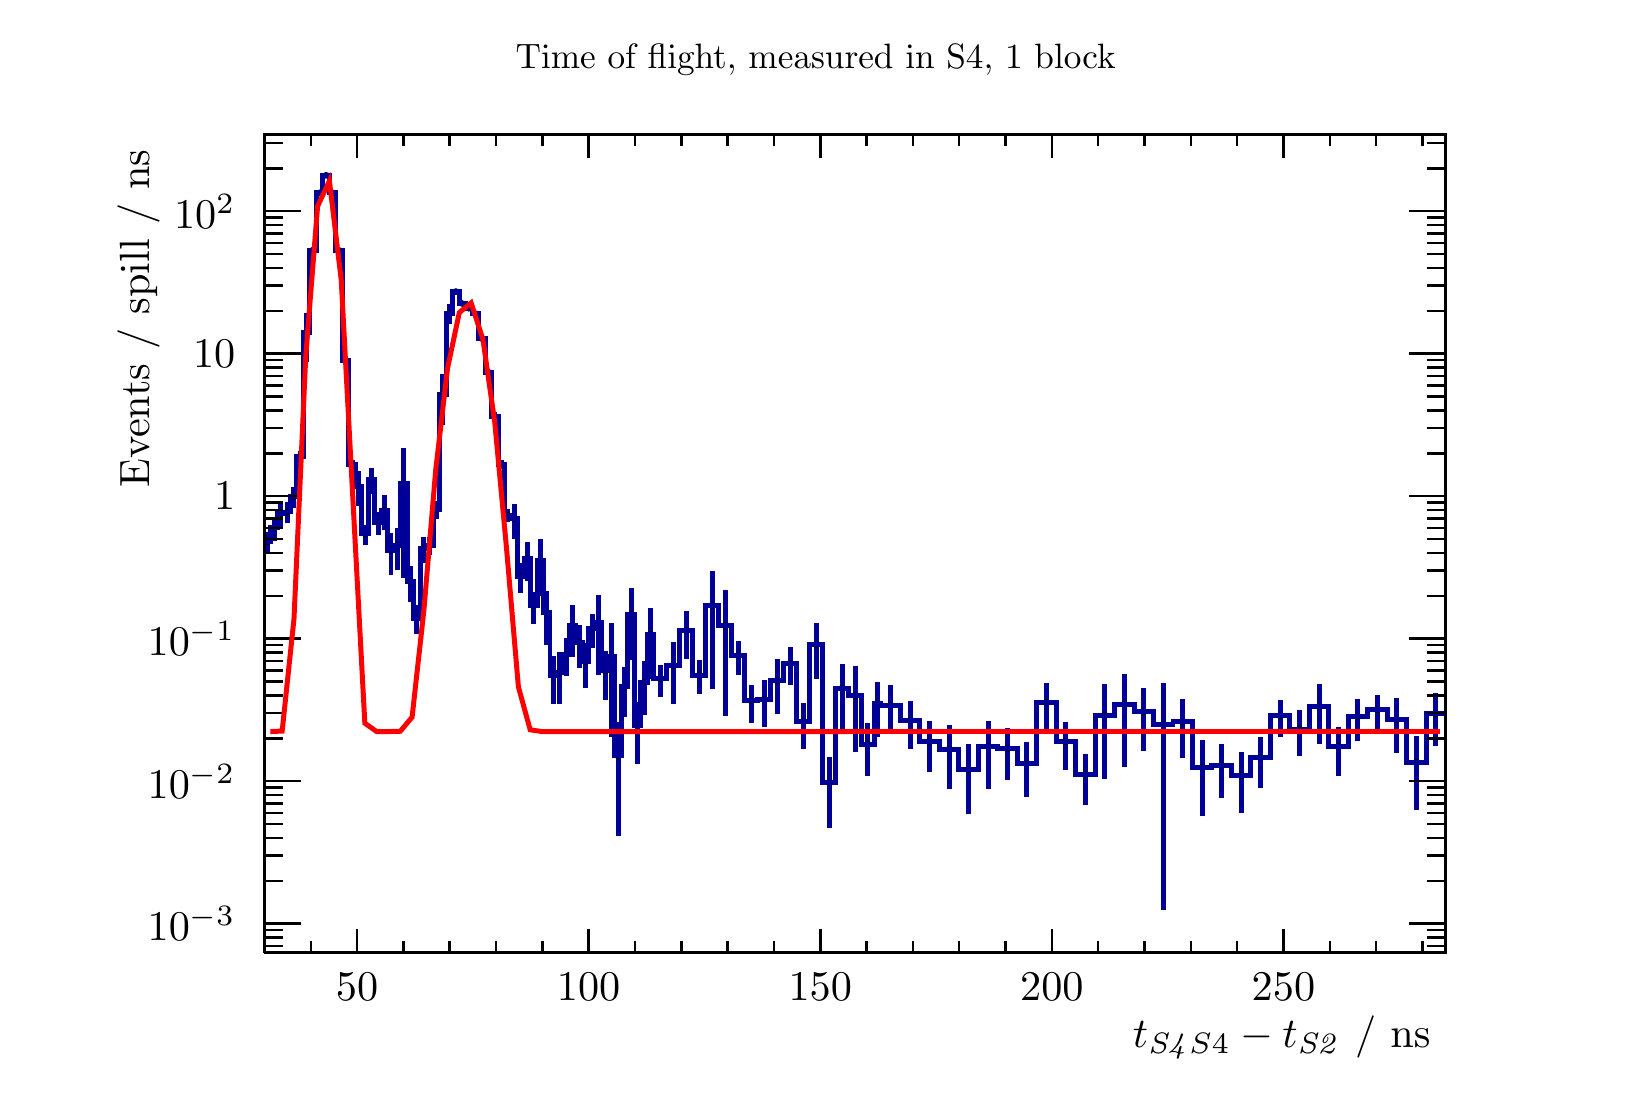
\begin{tikzpicture}
\pgfdeclareplotmark{cross} {
\pgfpathmoveto{\pgfpoint{-0.3\pgfplotmarksize}{\pgfplotmarksize}}
\pgfpathlineto{\pgfpoint{+0.3\pgfplotmarksize}{\pgfplotmarksize}}
\pgfpathlineto{\pgfpoint{+0.3\pgfplotmarksize}{0.3\pgfplotmarksize}}
\pgfpathlineto{\pgfpoint{+1\pgfplotmarksize}{0.3\pgfplotmarksize}}
\pgfpathlineto{\pgfpoint{+1\pgfplotmarksize}{-0.3\pgfplotmarksize}}
\pgfpathlineto{\pgfpoint{+0.3\pgfplotmarksize}{-0.3\pgfplotmarksize}}
\pgfpathlineto{\pgfpoint{+0.3\pgfplotmarksize}{-1.\pgfplotmarksize}}
\pgfpathlineto{\pgfpoint{-0.3\pgfplotmarksize}{-1.\pgfplotmarksize}}
\pgfpathlineto{\pgfpoint{-0.3\pgfplotmarksize}{-0.3\pgfplotmarksize}}
\pgfpathlineto{\pgfpoint{-1.\pgfplotmarksize}{-0.3\pgfplotmarksize}}
\pgfpathlineto{\pgfpoint{-1.\pgfplotmarksize}{0.3\pgfplotmarksize}}
\pgfpathlineto{\pgfpoint{-0.3\pgfplotmarksize}{0.3\pgfplotmarksize}}
\pgfpathclose
\pgfusepathqstroke
}
\pgfdeclareplotmark{cross*} {
\pgfpathmoveto{\pgfpoint{-0.3\pgfplotmarksize}{\pgfplotmarksize}}
\pgfpathlineto{\pgfpoint{+0.3\pgfplotmarksize}{\pgfplotmarksize}}
\pgfpathlineto{\pgfpoint{+0.3\pgfplotmarksize}{0.3\pgfplotmarksize}}
\pgfpathlineto{\pgfpoint{+1\pgfplotmarksize}{0.3\pgfplotmarksize}}
\pgfpathlineto{\pgfpoint{+1\pgfplotmarksize}{-0.3\pgfplotmarksize}}
\pgfpathlineto{\pgfpoint{+0.3\pgfplotmarksize}{-0.3\pgfplotmarksize}}
\pgfpathlineto{\pgfpoint{+0.3\pgfplotmarksize}{-1.\pgfplotmarksize}}
\pgfpathlineto{\pgfpoint{-0.3\pgfplotmarksize}{-1.\pgfplotmarksize}}
\pgfpathlineto{\pgfpoint{-0.3\pgfplotmarksize}{-0.3\pgfplotmarksize}}
\pgfpathlineto{\pgfpoint{-1.\pgfplotmarksize}{-0.3\pgfplotmarksize}}
\pgfpathlineto{\pgfpoint{-1.\pgfplotmarksize}{0.3\pgfplotmarksize}}
\pgfpathlineto{\pgfpoint{-0.3\pgfplotmarksize}{0.3\pgfplotmarksize}}
\pgfpathclose
\pgfusepathqfillstroke
}
\pgfdeclareplotmark{newstar} {
\pgfpathmoveto{\pgfqpoint{0pt}{\pgfplotmarksize}}
\pgfpathlineto{\pgfqpointpolar{44}{0.5\pgfplotmarksize}}
\pgfpathlineto{\pgfqpointpolar{18}{\pgfplotmarksize}}
\pgfpathlineto{\pgfqpointpolar{-20}{0.5\pgfplotmarksize}}
\pgfpathlineto{\pgfqpointpolar{-54}{\pgfplotmarksize}}
\pgfpathlineto{\pgfqpointpolar{-90}{0.5\pgfplotmarksize}}
\pgfpathlineto{\pgfqpointpolar{234}{\pgfplotmarksize}}
\pgfpathlineto{\pgfqpointpolar{198}{0.5\pgfplotmarksize}}
\pgfpathlineto{\pgfqpointpolar{162}{\pgfplotmarksize}}
\pgfpathlineto{\pgfqpointpolar{134}{0.5\pgfplotmarksize}}
\pgfpathclose
\pgfusepathqstroke
}
\pgfdeclareplotmark{newstar*} {
\pgfpathmoveto{\pgfqpoint{0pt}{\pgfplotmarksize}}
\pgfpathlineto{\pgfqpointpolar{44}{0.5\pgfplotmarksize}}
\pgfpathlineto{\pgfqpointpolar{18}{\pgfplotmarksize}}
\pgfpathlineto{\pgfqpointpolar{-20}{0.5\pgfplotmarksize}}
\pgfpathlineto{\pgfqpointpolar{-54}{\pgfplotmarksize}}
\pgfpathlineto{\pgfqpointpolar{-90}{0.5\pgfplotmarksize}}
\pgfpathlineto{\pgfqpointpolar{234}{\pgfplotmarksize}}
\pgfpathlineto{\pgfqpointpolar{198}{0.5\pgfplotmarksize}}
\pgfpathlineto{\pgfqpointpolar{162}{\pgfplotmarksize}}
\pgfpathlineto{\pgfqpointpolar{134}{0.5\pgfplotmarksize}}
\pgfpathclose
\pgfusepathqfillstroke
}
\definecolor{c}{rgb}{1,1,1};
\draw [color=c, fill=c] (0,0) rectangle (20,13.4957);
\draw [color=c, fill=c] (3,1.75444) rectangle (18,12.1461);
\definecolor{c}{rgb}{0,0,0};
\draw [c,line width=0.9] (3,1.75444) -- (3,12.1461) -- (18,12.1461) -- (18,1.75444) -- (3,1.75444);
\definecolor{c}{rgb}{1,1,1};
\draw [color=c, fill=c] (3,1.75444) rectangle (18,12.1461);
\definecolor{c}{rgb}{0,0,0};
\draw [c,line width=0.9] (3,1.75444) -- (3,12.1461) -- (18,12.1461) -- (18,1.75444) -- (3,1.75444);
\definecolor{c}{rgb}{0,0,0.6};
\draw [c,line width=1.8] (3.04121,6.83153) -- (3.04121,6.97494);
\draw [c,line width=1.8] (3.04121,6.97494) -- (3.04121,7.09618);
\definecolor{c}{rgb}{0,0,0};
\foreach \P in {(3.04121,6.97494)}{\draw[mark options={color=c,fill=c},mark size=2.402402pt,mark=*,mark size=1pt] plot coordinates {\P};}
\definecolor{c}{rgb}{0,0,0.6};
\draw [c,line width=1.8] (3.12363,6.98587) -- (3.12363,7.14945);
\draw [c,line width=1.8] (3.12363,7.14945) -- (3.12363,7.28478);
\definecolor{c}{rgb}{0,0,0};
\foreach \P in {(3.12363,7.14945)}{\draw[mark options={color=c,fill=c},mark size=2.402402pt,mark=*,mark size=1pt] plot coordinates {\P};}
\definecolor{c}{rgb}{0,0,0.6};
\draw [c,line width=1.8] (3.20604,7.13388) -- (3.20604,7.32717);
\draw [c,line width=1.8] (3.20604,7.32717) -- (3.20604,7.48218);
\definecolor{c}{rgb}{0,0,0};
\foreach \P in {(3.20604,7.32717)}{\draw[mark options={color=c,fill=c},mark size=2.402402pt,mark=*,mark size=1pt] plot coordinates {\P};}
\definecolor{c}{rgb}{0,0,0.6};
\draw [c,line width=1.8] (3.28846,7.20645) -- (3.28846,7.35172);
\draw [c,line width=1.8] (3.28846,7.35172) -- (3.28846,7.47427);
\definecolor{c}{rgb}{0,0,0};
\foreach \P in {(3.28846,7.35172)}{\draw[mark options={color=c,fill=c},mark size=2.402402pt,mark=*,mark size=1pt] plot coordinates {\P};}
\definecolor{c}{rgb}{0,0,0.6};
\draw [c,line width=1.8] (3.37088,7.39627) -- (3.37088,7.54562);
\draw [c,line width=1.8] (3.37088,7.54562) -- (3.37088,7.67107);
\definecolor{c}{rgb}{0,0,0};
\foreach \P in {(3.37088,7.54562)}{\draw[mark options={color=c,fill=c},mark size=2.402402pt,mark=*,mark size=1pt] plot coordinates {\P};}
\definecolor{c}{rgb}{0,0,0.6};
\draw [c,line width=1.8] (3.4533,7.97687) -- (3.4533,8.05427);
\draw [c,line width=1.8] (3.4533,8.05427) -- (3.4533,8.12472);
\definecolor{c}{rgb}{0,0,0};
\foreach \P in {(3.4533,8.05427)}{\draw[mark options={color=c,fill=c},mark size=2.402402pt,mark=*,mark size=1pt] plot coordinates {\P};}
\definecolor{c}{rgb}{0,0,0.6};
\draw [c,line width=1.8] (3.53571,9.25647) -- (3.53571,9.63184);
\draw [c,line width=1.8] (3.53571,9.63184) -- (3.53571,9.88483);
\definecolor{c}{rgb}{0,0,0};
\foreach \P in {(3.53571,9.63184)}{\draw[mark options={color=c,fill=c},mark size=2.402402pt,mark=*,mark size=1pt] plot coordinates {\P};}
\definecolor{c}{rgb}{0,0,0.6};
\draw [c,line width=1.8] (3.61813,10.6619) -- (3.61813,10.6787);
\draw [c,line width=1.8] (3.61813,10.6787) -- (3.61813,10.6953);
\definecolor{c}{rgb}{0,0,0};
\foreach \P in {(3.61813,10.6787)}{\draw[mark options={color=c,fill=c},mark size=2.402402pt,mark=*,mark size=1pt] plot coordinates {\P};}
\definecolor{c}{rgb}{0,0,0.6};
\draw [c,line width=1.8] (3.70055,11.3908) -- (3.70055,11.4047);
\draw [c,line width=1.8] (3.70055,11.4047) -- (3.70055,11.4184);
\definecolor{c}{rgb}{0,0,0};
\foreach \P in {(3.70055,11.4047)}{\draw[mark options={color=c,fill=c},mark size=2.402402pt,mark=*,mark size=1pt] plot coordinates {\P};}
\definecolor{c}{rgb}{0,0,0.6};
\draw [c,line width=1.8] (3.78297,11.6105) -- (3.78297,11.6274);
\draw [c,line width=1.8] (3.78297,11.6274) -- (3.78297,11.6439);
\definecolor{c}{rgb}{0,0,0};
\foreach \P in {(3.78297,11.6274)}{\draw[mark options={color=c,fill=c},mark size=2.402402pt,mark=*,mark size=1pt] plot coordinates {\P};}
\definecolor{c}{rgb}{0,0,0.6};
\draw [c,line width=1.8] (3.86538,11.3862) -- (3.86538,11.406);
\draw [c,line width=1.8] (3.86538,11.406) -- (3.86538,11.4252);
\definecolor{c}{rgb}{0,0,0};
\foreach \P in {(3.86538,11.406)}{\draw[mark options={color=c,fill=c},mark size=2.402402pt,mark=*,mark size=1pt] plot coordinates {\P};}
\definecolor{c}{rgb}{0,0,0.6};
\draw [c,line width=1.8] (3.9478,10.6399) -- (3.9478,10.674);
\draw [c,line width=1.8] (3.9478,10.674) -- (3.9478,10.7067);
\definecolor{c}{rgb}{0,0,0};
\foreach \P in {(3.9478,10.674)}{\draw[mark options={color=c,fill=c},mark size=2.402402pt,mark=*,mark size=1pt] plot coordinates {\P};}
\definecolor{c}{rgb}{0,0,0.6};
\draw [c,line width=1.8] (4.03022,9.22892) -- (4.03022,9.27567);
\draw [c,line width=1.8] (4.03022,9.27567) -- (4.03022,9.31979);
\definecolor{c}{rgb}{0,0,0};
\foreach \P in {(4.03022,9.27567)}{\draw[mark options={color=c,fill=c},mark size=2.402402pt,mark=*,mark size=1pt] plot coordinates {\P};}
\definecolor{c}{rgb}{0,0,0.6};
\draw [c,line width=1.8] (4.11264,7.88952) -- (4.11264,7.95002);
\draw [c,line width=1.8] (4.11264,7.95002) -- (4.11264,8.00619);
\definecolor{c}{rgb}{0,0,0};
\foreach \P in {(4.11264,7.95002)}{\draw[mark options={color=c,fill=c},mark size=2.402402pt,mark=*,mark size=1pt] plot coordinates {\P};}
\definecolor{c}{rgb}{0,0,0.6};
\draw [c,line width=1.8] (4.19506,7.4221) -- (4.19506,7.67967);
\draw [c,line width=1.8] (4.19506,7.67967) -- (4.19506,7.87334);
\definecolor{c}{rgb}{0,0,0};
\foreach \P in {(4.19506,7.67967)}{\draw[mark options={color=c,fill=c},mark size=2.402402pt,mark=*,mark size=1pt] plot coordinates {\P};}
\definecolor{c}{rgb}{0,0,0.6};
\draw [c,line width=1.8] (4.27747,6.93574) -- (4.27747,7.07298);
\draw [c,line width=1.8] (4.27747,7.07298) -- (4.27747,7.18978);
\definecolor{c}{rgb}{0,0,0};
\foreach \P in {(4.27747,7.07298)}{\draw[mark options={color=c,fill=c},mark size=2.402402pt,mark=*,mark size=1pt] plot coordinates {\P};}
\definecolor{c}{rgb}{0,0,0.6};
\draw [c,line width=1.8] (4.35989,7.58568) -- (4.35989,7.76231);
\draw [c,line width=1.8] (4.35989,7.76231) -- (4.35989,7.90644);
\definecolor{c}{rgb}{0,0,0};
\foreach \P in {(4.35989,7.76231)}{\draw[mark options={color=c,fill=c},mark size=2.402402pt,mark=*,mark size=1pt] plot coordinates {\P};}
\definecolor{c}{rgb}{0,0,0.6};
\draw [c,line width=1.8] (4.44231,7.05966) -- (4.44231,7.21669);
\draw [c,line width=1.8] (4.44231,7.21669) -- (4.44231,7.34751);
\definecolor{c}{rgb}{0,0,0};
\foreach \P in {(4.44231,7.21669)}{\draw[mark options={color=c,fill=c},mark size=2.402402pt,mark=*,mark size=1pt] plot coordinates {\P};}
\definecolor{c}{rgb}{0,0,0.6};
\draw [c,line width=1.8] (4.52473,7.11995) -- (4.52473,7.37543);
\draw [c,line width=1.8] (4.52473,7.37543) -- (4.52473,7.56793);
\definecolor{c}{rgb}{0,0,0};
\foreach \P in {(4.52473,7.37543)}{\draw[mark options={color=c,fill=c},mark size=2.402402pt,mark=*,mark size=1pt] plot coordinates {\P};}
\definecolor{c}{rgb}{0,0,0.6};
\draw [c,line width=1.8] (4.60714,6.54869) -- (4.60714,6.86095);
\draw [c,line width=1.8] (4.60714,6.86095) -- (4.60714,7.08382);
\definecolor{c}{rgb}{0,0,0};
\foreach \P in {(4.60714,6.86095)}{\draw[mark options={color=c,fill=c},mark size=2.402402pt,mark=*,mark size=1pt] plot coordinates {\P};}
\definecolor{c}{rgb}{0,0,0.6};
\draw [c,line width=1.8] (4.68956,6.61229) -- (4.68956,6.92469);
\draw [c,line width=1.8] (4.68956,6.92469) -- (4.68956,7.14764);
\definecolor{c}{rgb}{0,0,0};
\foreach \P in {(4.68956,6.92469)}{\draw[mark options={color=c,fill=c},mark size=2.402402pt,mark=*,mark size=1pt] plot coordinates {\P};}
\definecolor{c}{rgb}{0,0,0.6};
\draw [c,line width=1.8] (4.77198,6.51304) -- (4.77198,7.70842);
\draw [c,line width=1.8] (4.77198,7.70842) -- (4.77198,8.16226);
\definecolor{c}{rgb}{0,0,0};
\foreach \P in {(4.77198,7.70842)}{\draw[mark options={color=c,fill=c},mark size=2.402402pt,mark=*,mark size=1pt] plot coordinates {\P};}
\definecolor{c}{rgb}{0,0,0.6};
\draw [c,line width=1.8] (4.8544,6.21) -- (4.8544,6.47167);
\draw [c,line width=1.8] (4.8544,6.47167) -- (4.8544,6.66764);
\definecolor{c}{rgb}{0,0,0};
\foreach \P in {(4.8544,6.47167)}{\draw[mark options={color=c,fill=c},mark size=2.402402pt,mark=*,mark size=1pt] plot coordinates {\P};}
\definecolor{c}{rgb}{0,0,0.6};
\draw [c,line width=1.8] (4.93681,5.8008) -- (4.93681,6.00485);
\draw [c,line width=1.8] (4.93681,6.00485) -- (4.93681,6.1667);
\definecolor{c}{rgb}{0,0,0};
\foreach \P in {(4.93681,6.00485)}{\draw[mark options={color=c,fill=c},mark size=2.402402pt,mark=*,mark size=1pt] plot coordinates {\P};}
\definecolor{c}{rgb}{0,0,0.6};
\draw [c,line width=1.8] (5.01923,6.70734) -- (5.01923,6.8899);
\draw [c,line width=1.8] (5.01923,6.8899) -- (5.01923,7.03794);
\definecolor{c}{rgb}{0,0,0};
\foreach \P in {(5.01923,6.8899)}{\draw[mark options={color=c,fill=c},mark size=2.402402pt,mark=*,mark size=1pt] plot coordinates {\P};}
\definecolor{c}{rgb}{0,0,0.6};
\draw [c,line width=1.8] (5.10165,6.80376) -- (5.10165,6.9271);
\draw [c,line width=1.8] (5.10165,6.9271) -- (5.10165,7.03369);
\definecolor{c}{rgb}{0,0,0};
\foreach \P in {(5.10165,6.9271)}{\draw[mark options={color=c,fill=c},mark size=2.402402pt,mark=*,mark size=1pt] plot coordinates {\P};}
\definecolor{c}{rgb}{0,0,0.6};
\draw [c,line width=1.8] (5.18407,7.26333) -- (5.18407,7.38265);
\draw [c,line width=1.8] (5.18407,7.38265) -- (5.18407,7.48622);
\definecolor{c}{rgb}{0,0,0};
\foreach \P in {(5.18407,7.38265)}{\draw[mark options={color=c,fill=c},mark size=2.402402pt,mark=*,mark size=1pt] plot coordinates {\P};}
\definecolor{c}{rgb}{0,0,0.6};
\draw [c,line width=1.8] (5.26648,8.45688) -- (5.26648,8.84864);
\draw [c,line width=1.8] (5.26648,8.84864) -- (5.26648,9.10889);
\definecolor{c}{rgb}{0,0,0};
\foreach \P in {(5.26648,8.84864)}{\draw[mark options={color=c,fill=c},mark size=2.402402pt,mark=*,mark size=1pt] plot coordinates {\P};}
\definecolor{c}{rgb}{0,0,0.6};
\draw [c,line width=1.8] (5.3489,9.74448) -- (5.3489,9.87605);
\draw [c,line width=1.8] (5.3489,9.87605) -- (5.3489,9.98873);
\definecolor{c}{rgb}{0,0,0};
\foreach \P in {(5.3489,9.87605)}{\draw[mark options={color=c,fill=c},mark size=2.402402pt,mark=*,mark size=1pt] plot coordinates {\P};}
\definecolor{c}{rgb}{0,0,0.6};
\draw [c,line width=1.8] (5.43132,10.1297) -- (5.43132,10.1512);
\draw [c,line width=1.8] (5.43132,10.1512) -- (5.43132,10.1721);
\definecolor{c}{rgb}{0,0,0};
\foreach \P in {(5.43132,10.1512)}{\draw[mark options={color=c,fill=c},mark size=2.402402pt,mark=*,mark size=1pt] plot coordinates {\P};}
\definecolor{c}{rgb}{0,0,0.6};
\draw [c,line width=1.8] (5.51374,9.97428) -- (5.51374,9.99866);
\draw [c,line width=1.8] (5.51374,9.99866) -- (5.51374,10.0223);
\definecolor{c}{rgb}{0,0,0};
\foreach \P in {(5.51374,9.99866)}{\draw[mark options={color=c,fill=c},mark size=2.402402pt,mark=*,mark size=1pt] plot coordinates {\P};}
\definecolor{c}{rgb}{0,0,0.6};
\draw [c,line width=1.8] (5.59615,9.91574) -- (5.59615,9.93888);
\draw [c,line width=1.8] (5.59615,9.93888) -- (5.59615,9.96136);
\definecolor{c}{rgb}{0,0,0};
\foreach \P in {(5.59615,9.93888)}{\draw[mark options={color=c,fill=c},mark size=2.402402pt,mark=*,mark size=1pt] plot coordinates {\P};}
\definecolor{c}{rgb}{0,0,0.6};
\draw [c,line width=1.8] (5.67857,9.84866) -- (5.67857,9.87056);
\draw [c,line width=1.8] (5.67857,9.87056) -- (5.67857,9.89187);
\definecolor{c}{rgb}{0,0,0};
\foreach \P in {(5.67857,9.87056)}{\draw[mark options={color=c,fill=c},mark size=2.402402pt,mark=*,mark size=1pt] plot coordinates {\P};}
\definecolor{c}{rgb}{0,0,0.6};
\draw [c,line width=1.8] (5.76099,9.53052) -- (5.76099,9.55442);
\draw [c,line width=1.8] (5.76099,9.55442) -- (5.76099,9.57761);
\definecolor{c}{rgb}{0,0,0};
\foreach \P in {(5.76099,9.55442)}{\draw[mark options={color=c,fill=c},mark size=2.402402pt,mark=*,mark size=1pt] plot coordinates {\P};}
\definecolor{c}{rgb}{0,0,0.6};
\draw [c,line width=1.8] (5.84341,9.10079) -- (5.84341,9.12841);
\draw [c,line width=1.8] (5.84341,9.12841) -- (5.84341,9.15509);
\definecolor{c}{rgb}{0,0,0};
\foreach \P in {(5.84341,9.12841)}{\draw[mark options={color=c,fill=c},mark size=2.402402pt,mark=*,mark size=1pt] plot coordinates {\P};}
\definecolor{c}{rgb}{0,0,0.6};
\draw [c,line width=1.8] (5.92582,8.49485) -- (5.92582,8.56353);
\draw [c,line width=1.8] (5.92582,8.56353) -- (5.92582,8.62669);
\definecolor{c}{rgb}{0,0,0};
\foreach \P in {(5.92582,8.56353)}{\draw[mark options={color=c,fill=c},mark size=2.402402pt,mark=*,mark size=1pt] plot coordinates {\P};}
\definecolor{c}{rgb}{0,0,0.6};
\draw [c,line width=1.8] (6.00824,7.8977) -- (6.00824,7.95654);
\draw [c,line width=1.8] (6.00824,7.95654) -- (6.00824,8.01129);
\definecolor{c}{rgb}{0,0,0};
\foreach \P in {(6.00824,7.95654)}{\draw[mark options={color=c,fill=c},mark size=2.402402pt,mark=*,mark size=1pt] plot coordinates {\P};}
\definecolor{c}{rgb}{0,0,0.6};
\draw [c,line width=1.8] (6.09066,7.22248) -- (6.09066,7.31335);
\draw [c,line width=1.8] (6.09066,7.31335) -- (6.09066,7.3948);
\definecolor{c}{rgb}{0,0,0};
\foreach \P in {(6.09066,7.31335)}{\draw[mark options={color=c,fill=c},mark size=2.402402pt,mark=*,mark size=1pt] plot coordinates {\P};}
\definecolor{c}{rgb}{0,0,0.6};
\draw [c,line width=1.8] (6.17308,7.01128) -- (6.17308,7.26595);
\draw [c,line width=1.8] (6.17308,7.26595) -- (6.17308,7.45798);
\definecolor{c}{rgb}{0,0,0};
\foreach \P in {(6.17308,7.26595)}{\draw[mark options={color=c,fill=c},mark size=2.402402pt,mark=*,mark size=1pt] plot coordinates {\P};}
\definecolor{c}{rgb}{0,0,0.6};
\draw [c,line width=1.8] (6.25549,6.32025) -- (6.25549,6.53777);
\draw [c,line width=1.8] (6.25549,6.53777) -- (6.25549,6.70795);
\definecolor{c}{rgb}{0,0,0};
\foreach \P in {(6.25549,6.53777)}{\draw[mark options={color=c,fill=c},mark size=2.402402pt,mark=*,mark size=1pt] plot coordinates {\P};}
\definecolor{c}{rgb}{0,0,0.6};
\draw [c,line width=1.8] (6.33791,6.47302) -- (6.33791,6.76083);
\draw [c,line width=1.8] (6.33791,6.76083) -- (6.33791,6.97104);
\definecolor{c}{rgb}{0,0,0};
\foreach \P in {(6.33791,6.76083)}{\draw[mark options={color=c,fill=c},mark size=2.402402pt,mark=*,mark size=1pt] plot coordinates {\P};}
\definecolor{c}{rgb}{0,0,0.6};
\draw [c,line width=1.8] (6.42033,5.92967) -- (6.42033,6.15992);
\draw [c,line width=1.8] (6.42033,6.15992) -- (6.42033,6.33777);
\definecolor{c}{rgb}{0,0,0};
\foreach \P in {(6.42033,6.15992)}{\draw[mark options={color=c,fill=c},mark size=2.402402pt,mark=*,mark size=1pt] plot coordinates {\P};}
\definecolor{c}{rgb}{0,0,0.6};
\draw [c,line width=1.8] (6.50275,6.28146) -- (6.50275,6.73048);
\draw [c,line width=1.8] (6.50275,6.73048) -- (6.50275,7.01446);
\definecolor{c}{rgb}{0,0,0};
\foreach \P in {(6.50275,6.73048)}{\draw[mark options={color=c,fill=c},mark size=2.402402pt,mark=*,mark size=1pt] plot coordinates {\P};}
\definecolor{c}{rgb}{0,0,0.6};
\draw [c,line width=1.8] (6.58517,5.65805) -- (6.58517,6.07292);
\draw [c,line width=1.8] (6.58517,6.07292) -- (6.58517,6.34303);
\definecolor{c}{rgb}{0,0,0};
\foreach \P in {(6.58517,6.07292)}{\draw[mark options={color=c,fill=c},mark size=2.402402pt,mark=*,mark size=1pt] plot coordinates {\P};}
\definecolor{c}{rgb}{0,0,0.6};
\draw [c,line width=1.8] (6.66758,4.91822) -- (6.66758,5.2802);
\draw [c,line width=1.8] (6.66758,5.2802) -- (6.66758,5.52709);
\definecolor{c}{rgb}{0,0,0};
\foreach \P in {(6.66758,5.2802)}{\draw[mark options={color=c,fill=c},mark size=2.402402pt,mark=*,mark size=1pt] plot coordinates {\P};}
\definecolor{c}{rgb}{0,0,0.6};
\draw [c,line width=1.8] (6.75,4.90966) -- (6.75,5.3106);
\draw [c,line width=1.8] (6.75,5.3106) -- (6.75,5.57481);
\definecolor{c}{rgb}{0,0,0};
\foreach \P in {(6.75,5.3106)}{\draw[mark options={color=c,fill=c},mark size=2.402402pt,mark=*,mark size=1pt] plot coordinates {\P};}
\definecolor{c}{rgb}{0,0,0.6};
\draw [c,line width=1.8] (6.83242,5.26257) -- (6.83242,5.54319);
\draw [c,line width=1.8] (6.83242,5.54319) -- (6.83242,5.74956);
\definecolor{c}{rgb}{0,0,0};
\foreach \P in {(6.83242,5.54319)}{\draw[mark options={color=c,fill=c},mark size=2.402402pt,mark=*,mark size=1pt] plot coordinates {\P};}
\definecolor{c}{rgb}{0,0,0.6};
\draw [c,line width=1.8] (6.91484,5.51036) -- (6.91484,5.90692);
\draw [c,line width=1.8] (6.91484,5.90692) -- (6.91484,6.16925);
\definecolor{c}{rgb}{0,0,0};
\foreach \P in {(6.91484,5.90692)}{\draw[mark options={color=c,fill=c},mark size=2.402402pt,mark=*,mark size=1pt] plot coordinates {\P};}
\definecolor{c}{rgb}{0,0,0.6};
\draw [c,line width=1.8] (6.99725,5.37072) -- (6.99725,5.69317);
\draw [c,line width=1.8] (6.99725,5.69317) -- (6.99725,5.92115);
\definecolor{c}{rgb}{0,0,0};
\foreach \P in {(6.99725,5.69317)}{\draw[mark options={color=c,fill=c},mark size=2.402402pt,mark=*,mark size=1pt] plot coordinates {\P};}
\definecolor{c}{rgb}{0,0,0.6};
\draw [c,line width=1.8] (7.07967,5.11197) -- (7.07967,5.45077);
\draw [c,line width=1.8] (7.07967,5.45077) -- (7.07967,5.68675);
\definecolor{c}{rgb}{0,0,0};
\foreach \P in {(7.07967,5.45077)}{\draw[mark options={color=c,fill=c},mark size=2.402402pt,mark=*,mark size=1pt] plot coordinates {\P};}
\definecolor{c}{rgb}{0,0,0.6};
\draw [c,line width=1.8] (7.16209,5.6293) -- (7.16209,5.86913);
\draw [c,line width=1.8] (7.16209,5.86913) -- (7.16209,6.05263);
\definecolor{c}{rgb}{0,0,0};
\foreach \P in {(7.16209,5.86913)}{\draw[mark options={color=c,fill=c},mark size=2.402402pt,mark=*,mark size=1pt] plot coordinates {\P};}
\definecolor{c}{rgb}{0,0,0.6};
\draw [c,line width=1.8] (7.24451,5.28133) -- (7.24451,5.94378);
\draw [c,line width=1.8] (7.24451,5.94378) -- (7.24451,6.29807);
\definecolor{c}{rgb}{0,0,0};
\foreach \P in {(7.24451,5.94378)}{\draw[mark options={color=c,fill=c},mark size=2.402402pt,mark=*,mark size=1pt] plot coordinates {\P};}
\definecolor{c}{rgb}{0,0,0.6};
\draw [c,line width=1.8] (7.32692,4.9626) -- (7.32692,5.33255);
\draw [c,line width=1.8] (7.32692,5.33255) -- (7.32692,5.58308);
\definecolor{c}{rgb}{0,0,0};
\foreach \P in {(7.32692,5.33255)}{\draw[mark options={color=c,fill=c},mark size=2.402402pt,mark=*,mark size=1pt] plot coordinates {\P};}
\definecolor{c}{rgb}{0,0,0.6};
\draw [c,line width=1.8] (7.40934,4.49871) -- (7.40934,5.51411);
\draw [c,line width=1.8] (7.40934,5.51411) -- (7.40934,5.94274);
\definecolor{c}{rgb}{0,0,0};
\foreach \P in {(7.40934,5.51411)}{\draw[mark options={color=c,fill=c},mark size=2.402402pt,mark=*,mark size=1pt] plot coordinates {\P};}
\definecolor{c}{rgb}{0,0,0.6};
\draw [c,line width=1.8] (7.49176,3.23767) -- (7.49176,4.25386);
\draw [c,line width=1.8] (7.49176,4.25386) -- (7.49176,4.68261);
\definecolor{c}{rgb}{0,0,0};
\foreach \P in {(7.49176,4.25386)}{\draw[mark options={color=c,fill=c},mark size=2.402402pt,mark=*,mark size=1pt] plot coordinates {\P};}
\definecolor{c}{rgb}{0,0,0.6};
\draw [c,line width=1.8] (7.57418,4.75264) -- (7.57418,5.13161);
\draw [c,line width=1.8] (7.57418,5.13161) -- (7.57418,5.3862);
\definecolor{c}{rgb}{0,0,0};
\foreach \P in {(7.57418,5.13161)}{\draw[mark options={color=c,fill=c},mark size=2.402402pt,mark=*,mark size=1pt] plot coordinates {\P};}
\definecolor{c}{rgb}{0,0,0.6};
\draw [c,line width=1.8] (7.65659,5.47125) -- (7.65659,6.0535);
\draw [c,line width=1.8] (7.65659,6.0535) -- (7.65659,6.38428);
\definecolor{c}{rgb}{0,0,0};
\foreach \P in {(7.65659,6.0535)}{\draw[mark options={color=c,fill=c},mark size=2.402402pt,mark=*,mark size=1pt] plot coordinates {\P};}
\definecolor{c}{rgb}{0,0,0.6};
\draw [c,line width=1.8] (7.73901,4.1564) -- (7.73901,4.64278);
\draw [c,line width=1.8] (7.73901,4.64278) -- (7.73901,4.94098);
\definecolor{c}{rgb}{0,0,0};
\foreach \P in {(7.73901,4.64278)}{\draw[mark options={color=c,fill=c},mark size=2.402402pt,mark=*,mark size=1pt] plot coordinates {\P};}
\definecolor{c}{rgb}{0,0,0.6};
\draw [c,line width=1.8] (7.82143,4.76851) -- (7.82143,5.187);
\draw [c,line width=1.8] (7.82143,5.187) -- (7.82143,5.45862);
\definecolor{c}{rgb}{0,0,0};
\foreach \P in {(7.82143,5.187)}{\draw[mark options={color=c,fill=c},mark size=2.402402pt,mark=*,mark size=1pt] plot coordinates {\P};}
\definecolor{c}{rgb}{0,0,0.6};
\draw [c,line width=1.8] (7.90385,5.22852) -- (7.90385,5.80025);
\draw [c,line width=1.8] (7.90385,5.80025) -- (7.90385,6.12771);
\definecolor{c}{rgb}{0,0,0};
\foreach \P in {(7.90385,5.80025)}{\draw[mark options={color=c,fill=c},mark size=2.402402pt,mark=*,mark size=1pt] plot coordinates {\P};}
\definecolor{c}{rgb}{0,0,0.6};
\draw [c,line width=1.8] (8.02747,4.99859) -- (8.02747,5.23282);
\draw [c,line width=1.8] (8.02747,5.23282) -- (8.02747,5.41304);
\definecolor{c}{rgb}{0,0,0};
\foreach \P in {(8.02747,5.23282)}{\draw[mark options={color=c,fill=c},mark size=2.402402pt,mark=*,mark size=1pt] plot coordinates {\P};}
\definecolor{c}{rgb}{0,0,0.6};
\draw [c,line width=1.8] (8.19231,4.91198) -- (8.19231,5.39968);
\draw [c,line width=1.8] (8.19231,5.39968) -- (8.19231,5.69836);
\definecolor{c}{rgb}{0,0,0};
\foreach \P in {(8.19231,5.39968)}{\draw[mark options={color=c,fill=c},mark size=2.402402pt,mark=*,mark size=1pt] plot coordinates {\P};}
\definecolor{c}{rgb}{0,0,0.6};
\draw [c,line width=1.8] (8.35714,5.48759) -- (8.35714,5.84958);
\draw [c,line width=1.8] (8.35714,5.84958) -- (8.35714,6.09648);
\definecolor{c}{rgb}{0,0,0};
\foreach \P in {(8.35714,5.84958)}{\draw[mark options={color=c,fill=c},mark size=2.402402pt,mark=*,mark size=1pt] plot coordinates {\P};}
\definecolor{c}{rgb}{0,0,0.6};
\draw [c,line width=1.8] (8.52198,5.03464) -- (8.52198,5.27997);
\draw [c,line width=1.8] (8.52198,5.27997) -- (8.52198,5.46667);
\definecolor{c}{rgb}{0,0,0};
\foreach \P in {(8.52198,5.27997)}{\draw[mark options={color=c,fill=c},mark size=2.402402pt,mark=*,mark size=1pt] plot coordinates {\P};}
\definecolor{c}{rgb}{0,0,0.6};
\draw [c,line width=1.8] (8.68681,5.10148) -- (8.68681,6.1621);
\draw [c,line width=1.8] (8.68681,6.1621) -- (8.68681,6.5977);
\definecolor{c}{rgb}{0,0,0};
\foreach \P in {(8.68681,6.1621)}{\draw[mark options={color=c,fill=c},mark size=2.402402pt,mark=*,mark size=1pt] plot coordinates {\P};}
\definecolor{c}{rgb}{0,0,0.6};
\draw [c,line width=1.8] (8.85165,4.76629) -- (8.85165,5.91201);
\draw [c,line width=1.8] (8.85165,5.91201) -- (8.85165,6.35954);
\definecolor{c}{rgb}{0,0,0};
\foreach \P in {(8.85165,5.91201)}{\draw[mark options={color=c,fill=c},mark size=2.402402pt,mark=*,mark size=1pt] plot coordinates {\P};}
\definecolor{c}{rgb}{0,0,0.6};
\draw [c,line width=1.8] (9.01648,5.28062) -- (9.01648,5.52979);
\draw [c,line width=1.8] (9.01648,5.52979) -- (9.01648,5.71869);
\definecolor{c}{rgb}{0,0,0};
\foreach \P in {(9.01648,5.52979)}{\draw[mark options={color=c,fill=c},mark size=2.402402pt,mark=*,mark size=1pt] plot coordinates {\P};}
\definecolor{c}{rgb}{0,0,0.6};
\draw [c,line width=1.8] (9.18132,4.67566) -- (9.18132,4.95244);
\draw [c,line width=1.8] (9.18132,4.95244) -- (9.18132,5.15673);
\definecolor{c}{rgb}{0,0,0};
\foreach \P in {(9.18132,4.95244)}{\draw[mark options={color=c,fill=c},mark size=2.402402pt,mark=*,mark size=1pt] plot coordinates {\P};}
\definecolor{c}{rgb}{0,0,0.6};
\draw [c,line width=1.8] (9.34615,4.61535) -- (9.34615,4.97557);
\draw [c,line width=1.8] (9.34615,4.97557) -- (9.34615,5.22165);
\definecolor{c}{rgb}{0,0,0};
\foreach \P in {(9.34615,4.97557)}{\draw[mark options={color=c,fill=c},mark size=2.402402pt,mark=*,mark size=1pt] plot coordinates {\P};}
\definecolor{c}{rgb}{0,0,0.6};
\draw [c,line width=1.8] (9.51099,4.78259) -- (9.51099,5.20681);
\draw [c,line width=1.8] (9.51099,5.20681) -- (9.51099,5.48081);
\definecolor{c}{rgb}{0,0,0};
\foreach \P in {(9.51099,5.20681)}{\draw[mark options={color=c,fill=c},mark size=2.402402pt,mark=*,mark size=1pt] plot coordinates {\P};}
\definecolor{c}{rgb}{0,0,0.6};
\draw [c,line width=1.8] (9.67582,5.15891) -- (9.67582,5.43129);
\draw [c,line width=1.8] (9.67582,5.43129) -- (9.67582,5.63318);
\definecolor{c}{rgb}{0,0,0};
\foreach \P in {(9.67582,5.43129)}{\draw[mark options={color=c,fill=c},mark size=2.402402pt,mark=*,mark size=1pt] plot coordinates {\P};}
\definecolor{c}{rgb}{0,0,0.6};
\draw [c,line width=1.8] (9.84066,4.34735) -- (9.84066,4.6926);
\draw [c,line width=1.8] (9.84066,4.6926) -- (9.84066,4.93166);
\definecolor{c}{rgb}{0,0,0};
\foreach \P in {(9.84066,4.6926)}{\draw[mark options={color=c,fill=c},mark size=2.402402pt,mark=*,mark size=1pt] plot coordinates {\P};}
\definecolor{c}{rgb}{0,0,0.6};
\draw [c,line width=1.8] (10.0055,5.23466) -- (10.0055,5.66606);
\draw [c,line width=1.8] (10.0055,5.66606) -- (10.0055,5.94298);
\definecolor{c}{rgb}{0,0,0};
\foreach \P in {(10.0055,5.66606)}{\draw[mark options={color=c,fill=c},mark size=2.402402pt,mark=*,mark size=1pt] plot coordinates {\P};}
\definecolor{c}{rgb}{0,0,0.6};
\draw [c,line width=1.8] (10.1703,3.34253) -- (10.1703,3.91602);
\draw [c,line width=1.8] (10.1703,3.91602) -- (10.1703,4.24403);
\definecolor{c}{rgb}{0,0,0};
\foreach \P in {(10.1703,3.91602)}{\draw[mark options={color=c,fill=c},mark size=2.402402pt,mark=*,mark size=1pt] plot coordinates {\P};}
\definecolor{c}{rgb}{0,0,0.6};
\draw [c,line width=1.8] (10.3352,4.5884) -- (10.3352,5.11422);
\draw [c,line width=1.8] (10.3352,5.11422) -- (10.3352,5.42647);
\definecolor{c}{rgb}{0,0,0};
\foreach \P in {(10.3352,5.11422)}{\draw[mark options={color=c,fill=c},mark size=2.402402pt,mark=*,mark size=1pt] plot coordinates {\P};}
\definecolor{c}{rgb}{0,0,0.6};
\draw [c,line width=1.8] (10.5,4.29818) -- (10.5,5.02077);
\draw [c,line width=1.8] (10.5,5.02077) -- (10.5,5.39077);
\definecolor{c}{rgb}{0,0,0};
\foreach \P in {(10.5,5.02077)}{\draw[mark options={color=c,fill=c},mark size=2.402402pt,mark=*,mark size=1pt] plot coordinates {\P};}
\definecolor{c}{rgb}{0,0,0.6};
\draw [c,line width=1.8] (10.6648,3.99921) -- (10.6648,4.40438);
\draw [c,line width=1.8] (10.6648,4.40438) -- (10.6648,4.6704);
\definecolor{c}{rgb}{0,0,0};
\foreach \P in {(10.6648,4.40438)}{\draw[mark options={color=c,fill=c},mark size=2.402402pt,mark=*,mark size=1pt] plot coordinates {\P};}
\definecolor{c}{rgb}{0,0,0.6};
\draw [c,line width=1.8] (10.7885,4.49966) -- (10.7885,4.92251);
\draw [c,line width=1.8] (10.7885,4.92251) -- (10.7885,5.19594);
\definecolor{c}{rgb}{0,0,0};
\foreach \P in {(10.7885,4.92251)}{\draw[mark options={color=c,fill=c},mark size=2.402402pt,mark=*,mark size=1pt] plot coordinates {\P};}
\definecolor{c}{rgb}{0,0,0.6};
\draw [c,line width=1.8] (10.9533,4.53446) -- (10.9533,4.90007);
\draw [c,line width=1.8] (10.9533,4.90007) -- (10.9533,5.14863);
\definecolor{c}{rgb}{0,0,0};
\foreach \P in {(10.9533,4.90007)}{\draw[mark options={color=c,fill=c},mark size=2.402402pt,mark=*,mark size=1pt] plot coordinates {\P};}
\definecolor{c}{rgb}{0,0,0.6};
\draw [c,line width=1.8] (11.2005,4.3442) -- (11.2005,4.7025);
\draw [c,line width=1.8] (11.2005,4.7025) -- (11.2005,4.94769);
\definecolor{c}{rgb}{0,0,0};
\foreach \P in {(11.2005,4.7025)}{\draw[mark options={color=c,fill=c},mark size=2.402402pt,mark=*,mark size=1pt] plot coordinates {\P};}
\definecolor{c}{rgb}{0,0,0.6};
\draw [c,line width=1.8] (11.4478,4.0475) -- (11.4478,4.43916);
\draw [c,line width=1.8] (11.4478,4.43916) -- (11.4478,4.69935);
\definecolor{c}{rgb}{0,0,0};
\foreach \P in {(11.4478,4.43916)}{\draw[mark options={color=c,fill=c},mark size=2.402402pt,mark=*,mark size=1pt] plot coordinates {\P};}
\definecolor{c}{rgb}{0,0,0.6};
\draw [c,line width=1.8] (11.6951,3.83264) -- (11.6951,4.34017);
\draw [c,line width=1.8] (11.6951,4.34017) -- (11.6951,4.64602);
\definecolor{c}{rgb}{0,0,0};
\foreach \P in {(11.6951,4.34017)}{\draw[mark options={color=c,fill=c},mark size=2.402402pt,mark=*,mark size=1pt] plot coordinates {\P};}
\definecolor{c}{rgb}{0,0,0.6};
\draw [c,line width=1.8] (11.9423,3.51775) -- (11.9423,4.07891);
\draw [c,line width=1.8] (11.9423,4.07891) -- (11.9423,4.40297);
\definecolor{c}{rgb}{0,0,0};
\foreach \P in {(11.9423,4.07891)}{\draw[mark options={color=c,fill=c},mark size=2.402402pt,mark=*,mark size=1pt] plot coordinates {\P};}
\definecolor{c}{rgb}{0,0,0.6};
\draw [c,line width=1.8] (12.1896,3.83067) -- (12.1896,4.37541);
\draw [c,line width=1.8] (12.1896,4.37541) -- (12.1896,4.69406);
\definecolor{c}{rgb}{0,0,0};
\foreach \P in {(12.1896,4.37541)}{\draw[mark options={color=c,fill=c},mark size=2.402402pt,mark=*,mark size=1pt] plot coordinates {\P};}
\definecolor{c}{rgb}{0,0,0.6};
\draw [c,line width=1.8] (12.4368,3.95313) -- (12.4368,4.34626);
\draw [c,line width=1.8] (12.4368,4.34626) -- (12.4368,4.6071);
\definecolor{c}{rgb}{0,0,0};
\foreach \P in {(12.4368,4.34626)}{\draw[mark options={color=c,fill=c},mark size=2.402402pt,mark=*,mark size=1pt] plot coordinates {\P};}
\definecolor{c}{rgb}{0,0,0.6};
\draw [c,line width=1.8] (12.6841,3.73837) -- (12.6841,4.16193);
\draw [c,line width=1.8] (12.6841,4.16193) -- (12.6841,4.43565);
\definecolor{c}{rgb}{0,0,0};
\foreach \P in {(12.6841,4.16193)}{\draw[mark options={color=c,fill=c},mark size=2.402402pt,mark=*,mark size=1pt] plot coordinates {\P};}
\definecolor{c}{rgb}{0,0,0.6};
\draw [c,line width=1.8] (12.9313,4.57608) -- (12.9313,4.93493);
\draw [c,line width=1.8] (12.9313,4.93493) -- (12.9313,5.18037);
\definecolor{c}{rgb}{0,0,0};
\foreach \P in {(12.9313,4.93493)}{\draw[mark options={color=c,fill=c},mark size=2.402402pt,mark=*,mark size=1pt] plot coordinates {\P};}
\definecolor{c}{rgb}{0,0,0.6};
\draw [c,line width=1.8] (13.1786,4.0733) -- (13.1786,4.43493);
\draw [c,line width=1.8] (13.1786,4.43493) -- (13.1786,4.68166);
\definecolor{c}{rgb}{0,0,0};
\foreach \P in {(13.1786,4.43493)}{\draw[mark options={color=c,fill=c},mark size=2.402402pt,mark=*,mark size=1pt] plot coordinates {\P};}
\definecolor{c}{rgb}{0,0,0.6};
\draw [c,line width=1.8] (13.4258,3.6271) -- (13.4258,4.0192);
\draw [c,line width=1.8] (13.4258,4.0192) -- (13.4258,4.27959);
\definecolor{c}{rgb}{0,0,0};
\foreach \P in {(13.4258,4.0192)}{\draw[mark options={color=c,fill=c},mark size=2.402402pt,mark=*,mark size=1pt] plot coordinates {\P};}
\definecolor{c}{rgb}{0,0,0.6};
\draw [c,line width=1.8] (13.6731,3.96106) -- (13.6731,4.77307);
\draw [c,line width=1.8] (13.6731,4.77307) -- (13.6731,5.16385);
\definecolor{c}{rgb}{0,0,0};
\foreach \P in {(13.6731,4.77307)}{\draw[mark options={color=c,fill=c},mark size=2.402402pt,mark=*,mark size=1pt] plot coordinates {\P};}
\definecolor{c}{rgb}{0,0,0.6};
\draw [c,line width=1.8] (13.9203,4.11796) -- (13.9203,4.90913);
\draw [c,line width=1.8] (13.9203,4.90913) -- (13.9203,5.29532);
\definecolor{c}{rgb}{0,0,0};
\foreach \P in {(13.9203,4.90913)}{\draw[mark options={color=c,fill=c},mark size=2.402402pt,mark=*,mark size=1pt] plot coordinates {\P};}
\definecolor{c}{rgb}{0,0,0.6};
\draw [c,line width=1.8] (14.1676,4.31847) -- (14.1676,4.81536);
\draw [c,line width=1.8] (14.1676,4.81536) -- (14.1676,5.1174);
\definecolor{c}{rgb}{0,0,0};
\foreach \P in {(14.1676,4.81536)}{\draw[mark options={color=c,fill=c},mark size=2.402402pt,mark=*,mark size=1pt] plot coordinates {\P};}
\definecolor{c}{rgb}{0,0,0.6};
\draw [c,line width=1.8] (14.4148,2.2992) -- (14.4148,4.65516);
\draw [c,line width=1.8] (14.4148,4.65516) -- (14.4148,5.18006);
\definecolor{c}{rgb}{0,0,0};
\foreach \P in {(14.4148,4.65516)}{\draw[mark options={color=c,fill=c},mark size=2.402402pt,mark=*,mark size=1pt] plot coordinates {\P};}
\definecolor{c}{rgb}{0,0,0.6};
\draw [c,line width=1.8] (14.6621,4.22133) -- (14.6621,4.68641);
\draw [c,line width=1.8] (14.6621,4.68641) -- (14.6621,4.97662);
\definecolor{c}{rgb}{0,0,0};
\foreach \P in {(14.6621,4.68641)}{\draw[mark options={color=c,fill=c},mark size=2.402402pt,mark=*,mark size=1pt] plot coordinates {\P};}
\definecolor{c}{rgb}{0,0,0.6};
\draw [c,line width=1.8] (14.9093,3.48514) -- (14.9093,4.1105);
\draw [c,line width=1.8] (14.9093,4.1105) -- (14.9093,4.45429);
\definecolor{c}{rgb}{0,0,0};
\foreach \P in {(14.9093,4.1105)}{\draw[mark options={color=c,fill=c},mark size=2.402402pt,mark=*,mark size=1pt] plot coordinates {\P};}
\definecolor{c}{rgb}{0,0,0.6};
\draw [c,line width=1.8] (15.1566,3.71651) -- (15.1566,4.13529);
\draw [c,line width=1.8] (15.1566,4.13529) -- (15.1566,4.40704);
\definecolor{c}{rgb}{0,0,0};
\foreach \P in {(15.1566,4.13529)}{\draw[mark options={color=c,fill=c},mark size=2.402402pt,mark=*,mark size=1pt] plot coordinates {\P};}
\definecolor{c}{rgb}{0,0,0.6};
\draw [c,line width=1.8] (15.4038,3.53077) -- (15.4038,4.00579);
\draw [c,line width=1.8] (15.4038,4.00579) -- (15.4038,4.29977);
\definecolor{c}{rgb}{0,0,0};
\foreach \P in {(15.4038,4.00579)}{\draw[mark options={color=c,fill=c},mark size=2.402402pt,mark=*,mark size=1pt] plot coordinates {\P};}
\definecolor{c}{rgb}{0,0,0.6};
\draw [c,line width=1.8] (15.6511,3.84814) -- (15.6511,4.23669);
\draw [c,line width=1.8] (15.6511,4.23669) -- (15.6511,4.49553);
\definecolor{c}{rgb}{0,0,0};
\foreach \P in {(15.6511,4.23669)}{\draw[mark options={color=c,fill=c},mark size=2.402402pt,mark=*,mark size=1pt] plot coordinates {\P};}
\definecolor{c}{rgb}{0,0,0.6};
\draw [c,line width=1.8] (15.8984,4.48836) -- (15.8984,4.76396);
\draw [c,line width=1.8] (15.8984,4.76396) -- (15.8984,4.96761);
\definecolor{c}{rgb}{0,0,0};
\foreach \P in {(15.8984,4.76396)}{\draw[mark options={color=c,fill=c},mark size=2.402402pt,mark=*,mark size=1pt] plot coordinates {\P};}
\definecolor{c}{rgb}{0,0,0.6};
\draw [c,line width=1.8] (16.1456,4.25467) -- (16.1456,4.59548);
\draw [c,line width=1.8] (16.1456,4.59548) -- (16.1456,4.83242);
\definecolor{c}{rgb}{0,0,0};
\foreach \P in {(16.1456,4.59548)}{\draw[mark options={color=c,fill=c},mark size=2.402402pt,mark=*,mark size=1pt] plot coordinates {\P};}
\definecolor{c}{rgb}{0,0,0.6};
\draw [c,line width=1.8] (16.3929,4.40576) -- (16.3929,4.87627);
\draw [c,line width=1.8] (16.3929,4.87627) -- (16.3929,5.16853);
\definecolor{c}{rgb}{0,0,0};
\foreach \P in {(16.3929,4.87627)}{\draw[mark options={color=c,fill=c},mark size=2.402402pt,mark=*,mark size=1pt] plot coordinates {\P};}
\definecolor{c}{rgb}{0,0,0.6};
\draw [c,line width=1.8] (16.6401,4.00145) -- (16.6401,4.37274);
\draw [c,line width=1.8] (16.6401,4.37274) -- (16.6401,4.62389);
\definecolor{c}{rgb}{0,0,0};
\foreach \P in {(16.6401,4.37274)}{\draw[mark options={color=c,fill=c},mark size=2.402402pt,mark=*,mark size=1pt] plot coordinates {\P};}
\definecolor{c}{rgb}{0,0,0.6};
\draw [c,line width=1.8] (16.8874,4.4391) -- (16.8874,4.75221);
\draw [c,line width=1.8] (16.8874,4.75221) -- (16.8874,4.97552);
\definecolor{c}{rgb}{0,0,0};
\foreach \P in {(16.8874,4.75221)}{\draw[mark options={color=c,fill=c},mark size=2.402402pt,mark=*,mark size=1pt] plot coordinates {\P};}
\definecolor{c}{rgb}{0,0,0.6};
\draw [c,line width=1.8] (17.1346,4.59992) -- (17.1346,4.84154);
\draw [c,line width=1.8] (17.1346,4.84154) -- (17.1346,5.02608);
\definecolor{c}{rgb}{0,0,0};
\foreach \P in {(17.1346,4.84154)}{\draw[mark options={color=c,fill=c},mark size=2.402402pt,mark=*,mark size=1pt] plot coordinates {\P};}
\definecolor{c}{rgb}{0,0,0.6};
\draw [c,line width=1.8] (17.3819,4.29493) -- (17.3819,4.71308);
\draw [c,line width=1.8] (17.3819,4.71308) -- (17.3819,4.98456);
\definecolor{c}{rgb}{0,0,0};
\foreach \P in {(17.3819,4.71308)}{\draw[mark options={color=c,fill=c},mark size=2.402402pt,mark=*,mark size=1pt] plot coordinates {\P};}
\definecolor{c}{rgb}{0,0,0.6};
\draw [c,line width=1.8] (17.6291,3.56878) -- (17.6291,4.17241);
\draw [c,line width=1.8] (17.6291,4.17241) -- (17.6291,4.50976);
\definecolor{c}{rgb}{0,0,0};
\foreach \P in {(17.6291,4.17241)}{\draw[mark options={color=c,fill=c},mark size=2.402402pt,mark=*,mark size=1pt] plot coordinates {\P};}
\definecolor{c}{rgb}{0,0,0.6};
\draw [c,line width=1.8] (17.8764,4.37746) -- (17.8764,4.78992);
\draw [c,line width=1.8] (17.8764,4.78992) -- (17.8764,5.05902);
\definecolor{c}{rgb}{0,0,0};
\foreach \P in {(17.8764,4.78992)}{\draw[mark options={color=c,fill=c},mark size=2.402402pt,mark=*,mark size=1pt] plot coordinates {\P};}
\definecolor{c}{rgb}{0,0,0.6};
\draw [c,line width=1.8] (3,6.97494) -- (3.08242,6.97494) -- (3.08242,7.14945) -- (3.16484,7.14945) -- (3.16484,7.32717) -- (3.24725,7.32717) -- (3.24725,7.35172) -- (3.32967,7.35172) -- (3.32967,7.54562) -- (3.41209,7.54562) -- (3.41209,8.05427) --
 (3.49451,8.05427) -- (3.49451,9.63184) -- (3.57692,9.63184) -- (3.57692,10.6787) -- (3.65934,10.6787) -- (3.65934,11.4047) -- (3.74176,11.4047) -- (3.74176,11.6274) -- (3.82418,11.6274) -- (3.82418,11.406) -- (3.90659,11.406) -- (3.90659,10.674) --
 (3.98901,10.674) -- (3.98901,9.27567) -- (4.07143,9.27567) -- (4.07143,7.95002) -- (4.15385,7.95002) -- (4.15385,7.67967) -- (4.23626,7.67967) -- (4.23626,7.07298) -- (4.31868,7.07298) -- (4.31868,7.76231) -- (4.4011,7.76231) -- (4.4011,7.21669) --
 (4.48352,7.21669) -- (4.48352,7.37543) -- (4.56593,7.37543) -- (4.56593,6.86095) -- (4.64835,6.86095) -- (4.64835,6.92469) -- (4.73077,6.92469) -- (4.73077,7.70842) -- (4.81319,7.70842) -- (4.81319,6.47167) -- (4.8956,6.47167) -- (4.8956,6.00485) --
 (4.97802,6.00485) -- (4.97802,6.8899) -- (5.06044,6.8899) -- (5.06044,6.9271) -- (5.14286,6.9271) -- (5.14286,7.38265) -- (5.22528,7.38265) -- (5.22528,8.84864) -- (5.30769,8.84864) -- (5.30769,9.87605) -- (5.39011,9.87605) -- (5.39011,10.1512) --
 (5.47253,10.1512) -- (5.47253,9.99866) -- (5.55494,9.99866) -- (5.55494,9.93888) -- (5.63736,9.93888) -- (5.63736,9.87056) -- (5.71978,9.87056) -- (5.71978,9.55442) -- (5.8022,9.55442) -- (5.8022,9.12841) -- (5.88462,9.12841) -- (5.88462,8.56353) --
 (5.96703,8.56353) -- (5.96703,7.95654) -- (6.04945,7.95654) -- (6.04945,7.31335) -- (6.13187,7.31335) -- (6.13187,7.26595) -- (6.21429,7.26595) -- (6.21429,6.53777) -- (6.2967,6.53777) -- (6.2967,6.76083) -- (6.37912,6.76083) -- (6.37912,6.15992) --
 (6.46154,6.15992) -- (6.46154,6.73048) -- (6.54396,6.73048) -- (6.54396,6.07292) -- (6.62637,6.07292) -- (6.62637,5.2802) -- (6.70879,5.2802) -- (6.70879,5.3106) -- (6.79121,5.3106) -- (6.79121,5.54319) -- (6.87363,5.54319) -- (6.87363,5.90692) --
 (6.95604,5.90692) -- (6.95604,5.69317) -- (7.03846,5.69317) -- (7.03846,5.45077) -- (7.12088,5.45077) -- (7.12088,5.86913) -- (7.2033,5.86913) -- (7.2033,5.94378) -- (7.28571,5.94378) -- (7.28571,5.33255) -- (7.36813,5.33255) -- (7.36813,5.51411) --
 (7.45055,5.51411) -- (7.45055,4.25386) -- (7.53297,4.25386) -- (7.53297,5.13161) -- (7.61538,5.13161) -- (7.61538,6.0535) -- (7.6978,6.0535) -- (7.6978,4.64278) -- (7.78022,4.64278) -- (7.78022,5.187) -- (7.86264,5.187) -- (7.86264,5.80025) --
 (7.94506,5.80025) -- (7.94506,5.23282) -- (8.10989,5.23282) -- (8.10989,5.39968) -- (8.27472,5.39968) -- (8.27472,5.84958) -- (8.43956,5.84958) -- (8.43956,5.27997) -- (8.6044,5.27997) -- (8.6044,6.1621) -- (8.76923,6.1621) -- (8.76923,5.91201) --
 (8.93407,5.91201) -- (8.93407,5.52979) -- (9.0989,5.52979) -- (9.0989,4.95244) -- (9.26374,4.95244) -- (9.26374,4.97557) -- (9.42857,4.97557) -- (9.42857,5.20681) -- (9.59341,5.20681) -- (9.59341,5.43129) -- (9.75824,5.43129) -- (9.75824,4.6926) --
 (9.92308,4.6926) -- (9.92308,5.66606) -- (10.0879,5.66606) -- (10.0879,3.91602) -- (10.2527,3.91602) -- (10.2527,5.11422) -- (10.4176,5.11422) -- (10.4176,5.02077) -- (10.5824,5.02077) -- (10.5824,4.40438) -- (10.7473,4.40438) -- (10.7473,4.92251)
 -- (10.8297,4.92251) -- (10.8297,4.90007) -- (11.0769,4.90007) -- (11.0769,4.7025) -- (11.3242,4.7025) -- (11.3242,4.43916) -- (11.5714,4.43916) -- (11.5714,4.34017) -- (11.8187,4.34017) -- (11.8187,4.07891) -- (12.0659,4.07891) -- (12.0659,4.37541)
 -- (12.3132,4.37541) -- (12.3132,4.34626) -- (12.5604,4.34626) -- (12.5604,4.16193) -- (12.8077,4.16193) -- (12.8077,4.93493) -- (13.0549,4.93493) -- (13.0549,4.43493) -- (13.3022,4.43493) -- (13.3022,4.0192) -- (13.5495,4.0192) -- (13.5495,4.77307)
 -- (13.7967,4.77307) -- (13.7967,4.90913) -- (14.044,4.90913) -- (14.044,4.81536) -- (14.2912,4.81536) -- (14.2912,4.65516) -- (14.5385,4.65516) -- (14.5385,4.68641) -- (14.7857,4.68641) -- (14.7857,4.1105) -- (15.033,4.1105) -- (15.033,4.13529) --
 (15.2802,4.13529) -- (15.2802,4.00579) -- (15.5275,4.00579) -- (15.5275,4.23669) -- (15.7747,4.23669) -- (15.7747,4.76396) -- (16.022,4.76396) -- (16.022,4.59548) -- (16.2692,4.59548) -- (16.2692,4.87627) -- (16.5165,4.87627) -- (16.5165,4.37274) --
 (16.7637,4.37274) -- (16.7637,4.75221) -- (17.011,4.75221) -- (17.011,4.84154) -- (17.2582,4.84154) -- (17.2582,4.71308) -- (17.5055,4.71308) -- (17.5055,4.17241) -- (17.7527,4.17241) -- (17.7527,4.78992) -- (18,4.78992);
\definecolor{c}{rgb}{0,0,0};
\draw [c,line width=0.9] (3,1.75444) -- (18,1.75444);
\draw [c,line width=0.9] (4.17647,2.05809) -- (4.17647,1.75444);
\draw [c,line width=0.9] (4.76471,1.90627) -- (4.76471,1.75444);
\draw [c,line width=0.9] (5.35294,1.90627) -- (5.35294,1.75444);
\draw [c,line width=0.9] (5.94118,1.90627) -- (5.94118,1.75444);
\draw [c,line width=0.9] (6.52941,1.90627) -- (6.52941,1.75444);
\draw [c,line width=0.9] (7.11765,2.05809) -- (7.11765,1.75444);
\draw [c,line width=0.9] (7.70588,1.90627) -- (7.70588,1.75444);
\draw [c,line width=0.9] (8.29412,1.90627) -- (8.29412,1.75444);
\draw [c,line width=0.9] (8.88235,1.90627) -- (8.88235,1.75444);
\draw [c,line width=0.9] (9.47059,1.90627) -- (9.47059,1.75444);
\draw [c,line width=0.9] (10.0588,2.05809) -- (10.0588,1.75444);
\draw [c,line width=0.9] (10.6471,1.90627) -- (10.6471,1.75444);
\draw [c,line width=0.9] (11.2353,1.90627) -- (11.2353,1.75444);
\draw [c,line width=0.9] (11.8235,1.90627) -- (11.8235,1.75444);
\draw [c,line width=0.9] (12.4118,1.90627) -- (12.4118,1.75444);
\draw [c,line width=0.9] (13,2.05809) -- (13,1.75444);
\draw [c,line width=0.9] (13.5882,1.90627) -- (13.5882,1.75444);
\draw [c,line width=0.9] (14.1765,1.90627) -- (14.1765,1.75444);
\draw [c,line width=0.9] (14.7647,1.90627) -- (14.7647,1.75444);
\draw [c,line width=0.9] (15.3529,1.90627) -- (15.3529,1.75444);
\draw [c,line width=0.9] (15.9412,2.05809) -- (15.9412,1.75444);
\draw [c,line width=0.9] (4.17647,2.05809) -- (4.17647,1.75444);
\draw [c,line width=0.9] (3.58824,1.90627) -- (3.58824,1.75444);
\draw [c,line width=0.9] (15.9412,2.05809) -- (15.9412,1.75444);
\draw [c,line width=0.9] (16.5294,1.90627) -- (16.5294,1.75444);
\draw [c,line width=0.9] (17.1176,1.90627) -- (17.1176,1.75444);
\draw [c,line width=0.9] (17.7059,1.90627) -- (17.7059,1.75444);
\draw [anchor=base] (4.17647,1.14713) node[scale=1.52731, color=c, rotate=0]{50};
\draw [anchor=base] (7.11765,1.14713) node[scale=1.52731, color=c, rotate=0]{100};
\draw [anchor=base] (10.0588,1.14713) node[scale=1.52731, color=c, rotate=0]{150};
\draw [anchor=base] (13,1.14713) node[scale=1.52731, color=c, rotate=0]{200};
\draw [anchor=base] (15.9412,1.14713) node[scale=1.52731, color=c, rotate=0]{250};
\draw [anchor= east] (18,0.674785) node[scale=1.52731, color=c, rotate=0]{$ t_{\mathit{S4}S4} - t_{\mathit{S2}}$ / ns};
\draw [c,line width=0.9] (3,12.1461) -- (18,12.1461);
\draw [c,line width=0.9] (4.17647,11.8425) -- (4.17647,12.1461);
\draw [c,line width=0.9] (4.76471,11.9943) -- (4.76471,12.1461);
\draw [c,line width=0.9] (5.35294,11.9943) -- (5.35294,12.1461);
\draw [c,line width=0.9] (5.94118,11.9943) -- (5.94118,12.1461);
\draw [c,line width=0.9] (6.52941,11.9943) -- (6.52941,12.1461);
\draw [c,line width=0.9] (7.11765,11.8425) -- (7.11765,12.1461);
\draw [c,line width=0.9] (7.70588,11.9943) -- (7.70588,12.1461);
\draw [c,line width=0.9] (8.29412,11.9943) -- (8.29412,12.1461);
\draw [c,line width=0.9] (8.88235,11.9943) -- (8.88235,12.1461);
\draw [c,line width=0.9] (9.47059,11.9943) -- (9.47059,12.1461);
\draw [c,line width=0.9] (10.0588,11.8425) -- (10.0588,12.1461);
\draw [c,line width=0.9] (10.6471,11.9943) -- (10.6471,12.1461);
\draw [c,line width=0.9] (11.2353,11.9943) -- (11.2353,12.1461);
\draw [c,line width=0.9] (11.8235,11.9943) -- (11.8235,12.1461);
\draw [c,line width=0.9] (12.4118,11.9943) -- (12.4118,12.1461);
\draw [c,line width=0.9] (13,11.8425) -- (13,12.1461);
\draw [c,line width=0.9] (13.5882,11.9943) -- (13.5882,12.1461);
\draw [c,line width=0.9] (14.1765,11.9943) -- (14.1765,12.1461);
\draw [c,line width=0.9] (14.7647,11.9943) -- (14.7647,12.1461);
\draw [c,line width=0.9] (15.3529,11.9943) -- (15.3529,12.1461);
\draw [c,line width=0.9] (15.9412,11.8425) -- (15.9412,12.1461);
\draw [c,line width=0.9] (4.17647,11.8425) -- (4.17647,12.1461);
\draw [c,line width=0.9] (3.58824,11.9943) -- (3.58824,12.1461);
\draw [c,line width=0.9] (15.9412,11.8425) -- (15.9412,12.1461);
\draw [c,line width=0.9] (16.5294,11.9943) -- (16.5294,12.1461);
\draw [c,line width=0.9] (17.1176,11.9943) -- (17.1176,12.1461);
\draw [c,line width=0.9] (17.7059,11.9943) -- (17.7059,12.1461);
\draw [c,line width=0.9] (3,1.75444) -- (3,12.1461);
\draw [c,line width=0.9] (3.231,1.84289) -- (3,1.84289);
\draw [c,line width=0.9] (3.231,1.94783) -- (3,1.94783);
\draw [c,line width=0.9] (3.231,2.0404) -- (3,2.0404);
\draw [c,line width=0.9] (3.462,2.12321) -- (3,2.12321);
\draw [anchor= east] (2.82,2.12321) node[scale=1.52731, color=c, rotate=0]{$10^{-3}$};
\draw [c,line width=0.9] (3.231,2.66797) -- (3,2.66797);
\draw [c,line width=0.9] (3.231,2.98664) -- (3,2.98664);
\draw [c,line width=0.9] (3.231,3.21273) -- (3,3.21273);
\draw [c,line width=0.9] (3.231,3.38811) -- (3,3.38811);
\draw [c,line width=0.9] (3.231,3.5314) -- (3,3.5314);
\draw [c,line width=0.9] (3.231,3.65255) -- (3,3.65255);
\draw [c,line width=0.9] (3.231,3.7575) -- (3,3.7575);
\draw [c,line width=0.9] (3.231,3.85007) -- (3,3.85007);
\draw [c,line width=0.9] (3.462,3.93287) -- (3,3.93287);
\draw [anchor= east] (2.82,3.93287) node[scale=1.52731, color=c, rotate=0]{$10^{-2}$};
\draw [c,line width=0.9] (3.231,4.47764) -- (3,4.47764);
\draw [c,line width=0.9] (3.231,4.7963) -- (3,4.7963);
\draw [c,line width=0.9] (3.231,5.0224) -- (3,5.0224);
\draw [c,line width=0.9] (3.231,5.19777) -- (3,5.19777);
\draw [c,line width=0.9] (3.231,5.34106) -- (3,5.34106);
\draw [c,line width=0.9] (3.231,5.46222) -- (3,5.46222);
\draw [c,line width=0.9] (3.231,5.56716) -- (3,5.56716);
\draw [c,line width=0.9] (3.231,5.65973) -- (3,5.65973);
\draw [c,line width=0.9] (3.462,5.74254) -- (3,5.74254);
\draw [anchor= east] (2.82,5.74254) node[scale=1.52731, color=c, rotate=0]{$10^{-1}$};
\draw [c,line width=0.9] (3.231,6.2873) -- (3,6.2873);
\draw [c,line width=0.9] (3.231,6.60597) -- (3,6.60597);
\draw [c,line width=0.9] (3.231,6.83206) -- (3,6.83206);
\draw [c,line width=0.9] (3.231,7.00744) -- (3,7.00744);
\draw [c,line width=0.9] (3.231,7.15073) -- (3,7.15073);
\draw [c,line width=0.9] (3.231,7.27188) -- (3,7.27188);
\draw [c,line width=0.9] (3.231,7.37683) -- (3,7.37683);
\draw [c,line width=0.9] (3.231,7.4694) -- (3,7.4694);
\draw [c,line width=0.9] (3.462,7.5522) -- (3,7.5522);
\draw [anchor= east] (2.82,7.5522) node[scale=1.52731, color=c, rotate=0]{1};
\draw [c,line width=0.9] (3.231,8.09696) -- (3,8.09696);
\draw [c,line width=0.9] (3.231,8.41563) -- (3,8.41563);
\draw [c,line width=0.9] (3.231,8.64173) -- (3,8.64173);
\draw [c,line width=0.9] (3.231,8.8171) -- (3,8.8171);
\draw [c,line width=0.9] (3.231,8.96039) -- (3,8.96039);
\draw [c,line width=0.9] (3.231,9.08154) -- (3,9.08154);
\draw [c,line width=0.9] (3.231,9.18649) -- (3,9.18649);
\draw [c,line width=0.9] (3.231,9.27906) -- (3,9.27906);
\draw [c,line width=0.9] (3.462,9.36187) -- (3,9.36187);
\draw [anchor= east] (2.82,9.36187) node[scale=1.52731, color=c, rotate=0]{10};
\draw [c,line width=0.9] (3.231,9.90663) -- (3,9.90663);
\draw [c,line width=0.9] (3.231,10.2253) -- (3,10.2253);
\draw [c,line width=0.9] (3.231,10.4514) -- (3,10.4514);
\draw [c,line width=0.9] (3.231,10.6268) -- (3,10.6268);
\draw [c,line width=0.9] (3.231,10.7701) -- (3,10.7701);
\draw [c,line width=0.9] (3.231,10.8912) -- (3,10.8912);
\draw [c,line width=0.9] (3.231,10.9962) -- (3,10.9962);
\draw [c,line width=0.9] (3.231,11.0887) -- (3,11.0887);
\draw [c,line width=0.9] (3.462,11.1715) -- (3,11.1715);
\draw [anchor= east] (2.82,11.1715) node[scale=1.52731, color=c, rotate=0]{$10^{2}$};
\draw [c,line width=0.9] (3.231,11.7163) -- (3,11.7163);
\draw [c,line width=0.9] (3.231,12.035) -- (3,12.035);
\draw [anchor= east] (1.4,12.1461) node[scale=1.52731, color=c, rotate=90]{ Events / spill / ns};
\draw [c,line width=0.9] (18,1.75444) -- (18,12.1461);
\draw [c,line width=0.9] (17.769,1.84289) -- (18,1.84289);
\draw [c,line width=0.9] (17.769,1.94783) -- (18,1.94783);
\draw [c,line width=0.9] (17.769,2.0404) -- (18,2.0404);
\draw [c,line width=0.9] (17.538,2.12321) -- (18,2.12321);
\draw [c,line width=0.9] (17.769,2.66797) -- (18,2.66797);
\draw [c,line width=0.9] (17.769,2.98664) -- (18,2.98664);
\draw [c,line width=0.9] (17.769,3.21273) -- (18,3.21273);
\draw [c,line width=0.9] (17.769,3.38811) -- (18,3.38811);
\draw [c,line width=0.9] (17.769,3.5314) -- (18,3.5314);
\draw [c,line width=0.9] (17.769,3.65255) -- (18,3.65255);
\draw [c,line width=0.9] (17.769,3.7575) -- (18,3.7575);
\draw [c,line width=0.9] (17.769,3.85007) -- (18,3.85007);
\draw [c,line width=0.9] (17.538,3.93287) -- (18,3.93287);
\draw [c,line width=0.9] (17.769,4.47764) -- (18,4.47764);
\draw [c,line width=0.9] (17.769,4.7963) -- (18,4.7963);
\draw [c,line width=0.9] (17.769,5.0224) -- (18,5.0224);
\draw [c,line width=0.9] (17.769,5.19777) -- (18,5.19777);
\draw [c,line width=0.9] (17.769,5.34106) -- (18,5.34106);
\draw [c,line width=0.9] (17.769,5.46222) -- (18,5.46222);
\draw [c,line width=0.9] (17.769,5.56716) -- (18,5.56716);
\draw [c,line width=0.9] (17.769,5.65973) -- (18,5.65973);
\draw [c,line width=0.9] (17.538,5.74254) -- (18,5.74254);
\draw [c,line width=0.9] (17.769,6.2873) -- (18,6.2873);
\draw [c,line width=0.9] (17.769,6.60597) -- (18,6.60597);
\draw [c,line width=0.9] (17.769,6.83206) -- (18,6.83206);
\draw [c,line width=0.9] (17.769,7.00744) -- (18,7.00744);
\draw [c,line width=0.9] (17.769,7.15073) -- (18,7.15073);
\draw [c,line width=0.9] (17.769,7.27188) -- (18,7.27188);
\draw [c,line width=0.9] (17.769,7.37683) -- (18,7.37683);
\draw [c,line width=0.9] (17.769,7.4694) -- (18,7.4694);
\draw [c,line width=0.9] (17.538,7.5522) -- (18,7.5522);
\draw [c,line width=0.9] (17.769,8.09696) -- (18,8.09696);
\draw [c,line width=0.9] (17.769,8.41563) -- (18,8.41563);
\draw [c,line width=0.9] (17.769,8.64173) -- (18,8.64173);
\draw [c,line width=0.9] (17.769,8.8171) -- (18,8.8171);
\draw [c,line width=0.9] (17.769,8.96039) -- (18,8.96039);
\draw [c,line width=0.9] (17.769,9.08154) -- (18,9.08154);
\draw [c,line width=0.9] (17.769,9.18649) -- (18,9.18649);
\draw [c,line width=0.9] (17.769,9.27906) -- (18,9.27906);
\draw [c,line width=0.9] (17.538,9.36187) -- (18,9.36187);
\draw [c,line width=0.9] (17.769,9.90663) -- (18,9.90663);
\draw [c,line width=0.9] (17.769,10.2253) -- (18,10.2253);
\draw [c,line width=0.9] (17.769,10.4514) -- (18,10.4514);
\draw [c,line width=0.9] (17.769,10.6268) -- (18,10.6268);
\draw [c,line width=0.9] (17.769,10.7701) -- (18,10.7701);
\draw [c,line width=0.9] (17.769,10.8912) -- (18,10.8912);
\draw [c,line width=0.9] (17.769,10.9962) -- (18,10.9962);
\draw [c,line width=0.9] (17.769,11.0887) -- (18,11.0887);
\draw [c,line width=0.9] (17.538,11.1715) -- (18,11.1715);
\draw [c,line width=0.9] (17.769,11.7163) -- (18,11.7163);
\draw [c,line width=0.9] (17.769,12.035) -- (18,12.035);
\definecolor{c}{rgb}{1,1,1};
\draw [color=c, fill=c] (2,12.7534) rectangle (18,13.4282);
\definecolor{c}{rgb}{0,0,0};
\draw (10,13.0908) node[scale=1.27276, color=c, rotate=0]{Time of flight, measured in S4, 1 block};
\definecolor{c}{rgb}{1,0,0};
\draw [c,line width=1.8] (3.075,4.56303) -- (3.225,4.56949) -- (3.375,5.99244) -- (3.525,9.33607) -- (3.675,11.2356) -- (3.825,11.5569) -- (3.975,10.2989) -- (4.125,7.47965) -- (4.275,4.66905) -- (4.425,4.56309) -- (4.575,4.56307) -- (4.725,4.56717)
 -- (4.875,4.74538) -- (5.025,6.10415) -- (5.175,7.88499) -- (5.325,9.17544) -- (5.475,9.8852) -- (5.625,10.0074) -- (5.775,9.54175) -- (5.925,8.49065) -- (6.075,6.88372) -- (6.225,5.1312) -- (6.375,4.58571) -- (6.525,4.56333) -- (6.675,4.56303) --
 (6.825,4.56303) -- (6.975,4.56303) -- (7.125,4.56303) -- (7.275,4.56303) -- (7.425,4.56303) -- (7.575,4.56303) -- (7.725,4.56303) -- (7.875,4.56303) -- (8.025,4.56303) -- (8.175,4.56303) -- (8.325,4.56303) -- (8.475,4.56303) -- (8.625,4.56303) --
 (8.775,4.56303) -- (8.925,4.56303) -- (9.075,4.56303) -- (9.225,4.56303) -- (9.375,4.56303) -- (9.525,4.56303) -- (9.675,4.56303) -- (9.825,4.56303) -- (9.975,4.56303) -- (10.125,4.56303) -- (10.275,4.56303) -- (10.425,4.56303);
\draw [c,line width=1.8] (10.425,4.56303) -- (10.575,4.56303) -- (10.725,4.56303) -- (10.875,4.56303) -- (11.025,4.56303) -- (11.175,4.56303) -- (11.325,4.56303) -- (11.475,4.56303) -- (11.625,4.56303) -- (11.775,4.56303) -- (11.925,4.56303) --
 (12.075,4.56303) -- (12.225,4.56303) -- (12.375,4.56303) -- (12.525,4.56303) -- (12.675,4.56303) -- (12.825,4.56303) -- (12.975,4.56303) -- (13.125,4.56303) -- (13.275,4.56303) -- (13.425,4.56303) -- (13.575,4.56303) -- (13.725,4.56303) --
 (13.875,4.56303) -- (14.025,4.56303) -- (14.175,4.56303) -- (14.325,4.56303) -- (14.475,4.56303) -- (14.625,4.56303) -- (14.775,4.56303) -- (14.925,4.56303) -- (15.075,4.56303) -- (15.225,4.56303) -- (15.375,4.56303) -- (15.525,4.56303) --
 (15.675,4.56303) -- (15.825,4.56303) -- (15.975,4.56303) -- (16.125,4.56303) -- (16.275,4.56303) -- (16.425,4.56303) -- (16.575,4.56303) -- (16.725,4.56303) -- (16.875,4.56303) -- (17.025,4.56303) -- (17.175,4.56303) -- (17.325,4.56303) --
 (17.475,4.56303) -- (17.625,4.56303) -- (17.775,4.56303);
\draw [c,line width=1.8] (17.775,4.56303) -- (17.925,4.56303);
\end{tikzpicture}

  \end{adjustbox}
  \caption{Example of the time of flight spectrum observed in $\mathit{S4}$ with combined signal and background functions fitted (shown in red).}
  \label{fig:fitEx}
\end{figure}


	% Outlook and Summary
	\section{Beam Flux Measurement}
\label{hptpcPaper:sec:Results}

\subsection{Flux measurements with S3}

The ToF systems are at an off-axis angle with respect to the beam axis (see Table~\ref{tab:angS1}), in order to probe the reduced proton momentum spectrum, to cover the region most relevant for neutrino experiments and the measure the flux passing through the TPC.
This is quantified in terms of $\theta$ and $\phi$ (see Section~\ref{sec:coord}).

\begin{figure}[ht]
  \centering
  \begin{minipage}[t]{0.49\textwidth}
    \begin{adjustbox}{max totalsize={\textwidth}, center}
      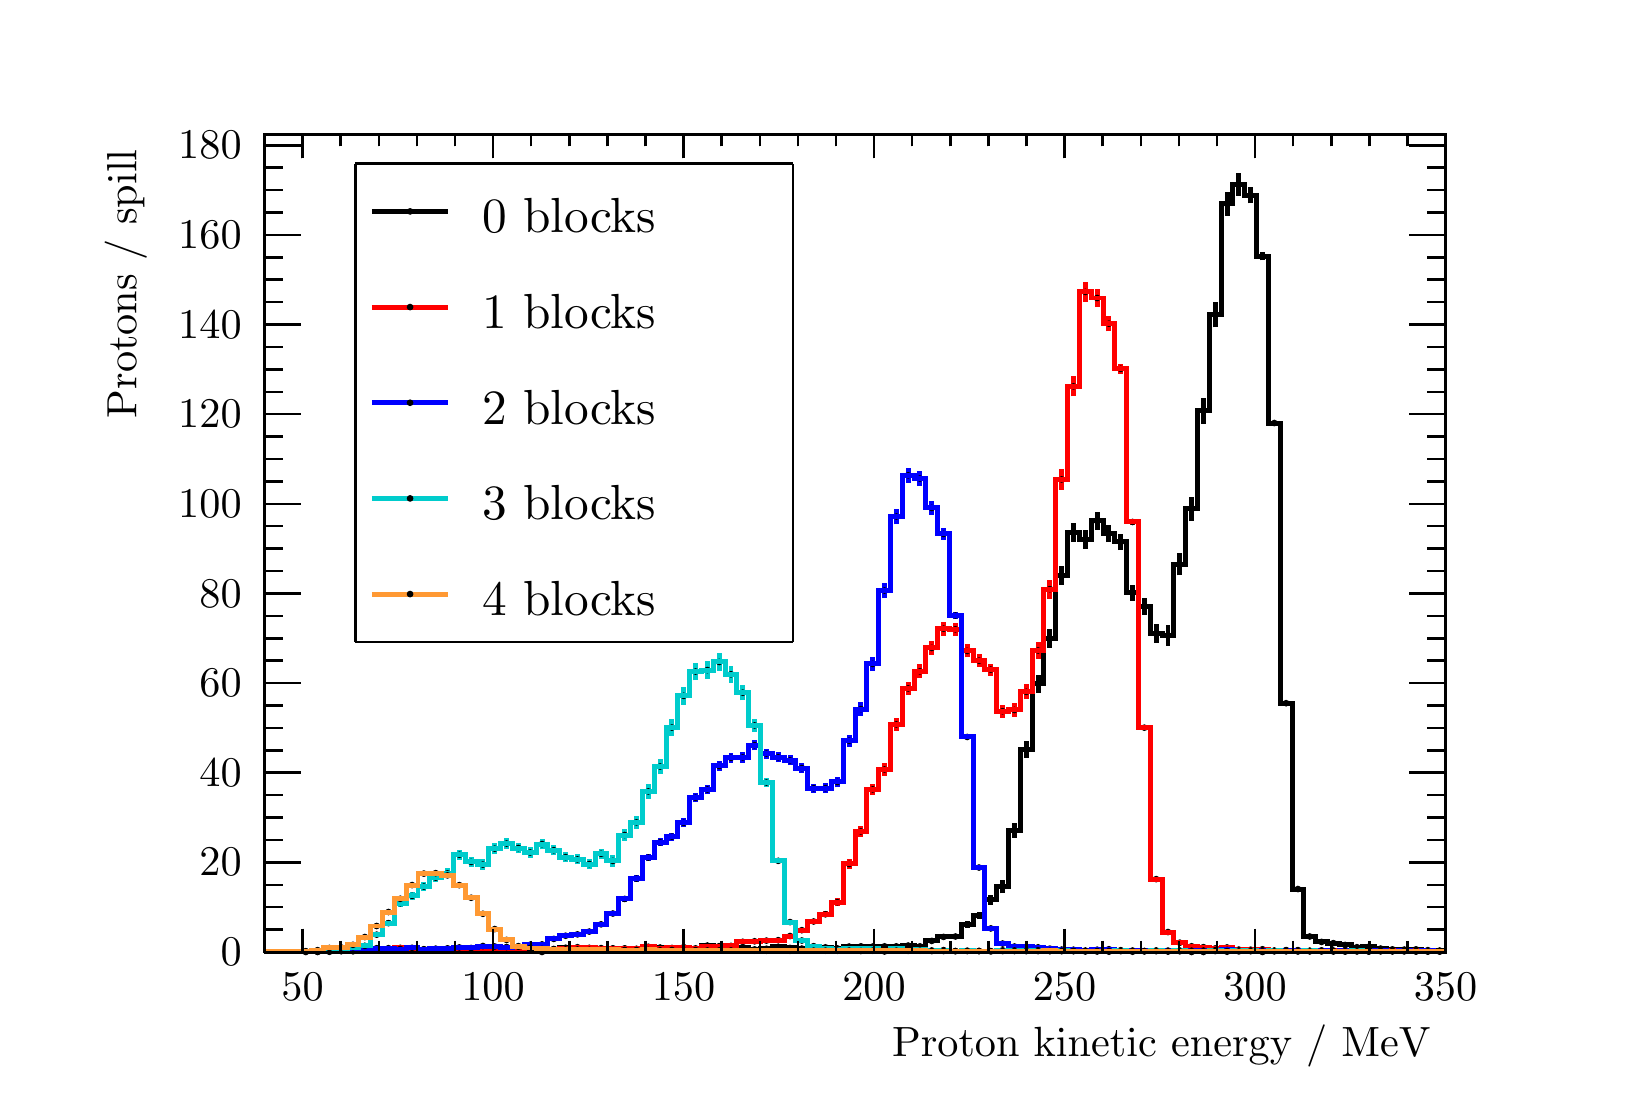
\begin{tikzpicture}
\pgfdeclareplotmark{cross} {
\pgfpathmoveto{\pgfpoint{-0.3\pgfplotmarksize}{\pgfplotmarksize}}
\pgfpathlineto{\pgfpoint{+0.3\pgfplotmarksize}{\pgfplotmarksize}}
\pgfpathlineto{\pgfpoint{+0.3\pgfplotmarksize}{0.3\pgfplotmarksize}}
\pgfpathlineto{\pgfpoint{+1\pgfplotmarksize}{0.3\pgfplotmarksize}}
\pgfpathlineto{\pgfpoint{+1\pgfplotmarksize}{-0.3\pgfplotmarksize}}
\pgfpathlineto{\pgfpoint{+0.3\pgfplotmarksize}{-0.3\pgfplotmarksize}}
\pgfpathlineto{\pgfpoint{+0.3\pgfplotmarksize}{-1.\pgfplotmarksize}}
\pgfpathlineto{\pgfpoint{-0.3\pgfplotmarksize}{-1.\pgfplotmarksize}}
\pgfpathlineto{\pgfpoint{-0.3\pgfplotmarksize}{-0.3\pgfplotmarksize}}
\pgfpathlineto{\pgfpoint{-1.\pgfplotmarksize}{-0.3\pgfplotmarksize}}
\pgfpathlineto{\pgfpoint{-1.\pgfplotmarksize}{0.3\pgfplotmarksize}}
\pgfpathlineto{\pgfpoint{-0.3\pgfplotmarksize}{0.3\pgfplotmarksize}}
\pgfpathclose
\pgfusepathqstroke
}
\pgfdeclareplotmark{cross*} {
\pgfpathmoveto{\pgfpoint{-0.3\pgfplotmarksize}{\pgfplotmarksize}}
\pgfpathlineto{\pgfpoint{+0.3\pgfplotmarksize}{\pgfplotmarksize}}
\pgfpathlineto{\pgfpoint{+0.3\pgfplotmarksize}{0.3\pgfplotmarksize}}
\pgfpathlineto{\pgfpoint{+1\pgfplotmarksize}{0.3\pgfplotmarksize}}
\pgfpathlineto{\pgfpoint{+1\pgfplotmarksize}{-0.3\pgfplotmarksize}}
\pgfpathlineto{\pgfpoint{+0.3\pgfplotmarksize}{-0.3\pgfplotmarksize}}
\pgfpathlineto{\pgfpoint{+0.3\pgfplotmarksize}{-1.\pgfplotmarksize}}
\pgfpathlineto{\pgfpoint{-0.3\pgfplotmarksize}{-1.\pgfplotmarksize}}
\pgfpathlineto{\pgfpoint{-0.3\pgfplotmarksize}{-0.3\pgfplotmarksize}}
\pgfpathlineto{\pgfpoint{-1.\pgfplotmarksize}{-0.3\pgfplotmarksize}}
\pgfpathlineto{\pgfpoint{-1.\pgfplotmarksize}{0.3\pgfplotmarksize}}
\pgfpathlineto{\pgfpoint{-0.3\pgfplotmarksize}{0.3\pgfplotmarksize}}
\pgfpathclose
\pgfusepathqfillstroke
}
\pgfdeclareplotmark{newstar} {
\pgfpathmoveto{\pgfqpoint{0pt}{\pgfplotmarksize}}
\pgfpathlineto{\pgfqpointpolar{44}{0.5\pgfplotmarksize}}
\pgfpathlineto{\pgfqpointpolar{18}{\pgfplotmarksize}}
\pgfpathlineto{\pgfqpointpolar{-20}{0.5\pgfplotmarksize}}
\pgfpathlineto{\pgfqpointpolar{-54}{\pgfplotmarksize}}
\pgfpathlineto{\pgfqpointpolar{-90}{0.5\pgfplotmarksize}}
\pgfpathlineto{\pgfqpointpolar{234}{\pgfplotmarksize}}
\pgfpathlineto{\pgfqpointpolar{198}{0.5\pgfplotmarksize}}
\pgfpathlineto{\pgfqpointpolar{162}{\pgfplotmarksize}}
\pgfpathlineto{\pgfqpointpolar{134}{0.5\pgfplotmarksize}}
\pgfpathclose
\pgfusepathqstroke
}
\pgfdeclareplotmark{newstar*} {
\pgfpathmoveto{\pgfqpoint{0pt}{\pgfplotmarksize}}
\pgfpathlineto{\pgfqpointpolar{44}{0.5\pgfplotmarksize}}
\pgfpathlineto{\pgfqpointpolar{18}{\pgfplotmarksize}}
\pgfpathlineto{\pgfqpointpolar{-20}{0.5\pgfplotmarksize}}
\pgfpathlineto{\pgfqpointpolar{-54}{\pgfplotmarksize}}
\pgfpathlineto{\pgfqpointpolar{-90}{0.5\pgfplotmarksize}}
\pgfpathlineto{\pgfqpointpolar{234}{\pgfplotmarksize}}
\pgfpathlineto{\pgfqpointpolar{198}{0.5\pgfplotmarksize}}
\pgfpathlineto{\pgfqpointpolar{162}{\pgfplotmarksize}}
\pgfpathlineto{\pgfqpointpolar{134}{0.5\pgfplotmarksize}}
\pgfpathclose
\pgfusepathqfillstroke
}
\definecolor{c}{rgb}{1,1,1};
\draw [color=c, fill=c] (0,0) rectangle (20,13.4957);
\draw [color=c, fill=c] (3,1.75444) rectangle (18,12.1461);
\definecolor{c}{rgb}{0,0,0};
\draw [c,line width=0.9] (3,1.75444) -- (3,12.1461) -- (18,12.1461) -- (18,1.75444) -- (3,1.75444);
\definecolor{c}{rgb}{1,1,1};
\draw [color=c, fill=c] (3,1.75444) rectangle (18,12.1461);
\definecolor{c}{rgb}{0,0,0};
\draw [c,line width=0.9] (3,1.75444) -- (3,12.1461) -- (18,12.1461) -- (18,1.75444) -- (3,1.75444);
\draw [c,line width=0.9] (3,1.764) -- (3.15,1.764) -- (3.15,1.764) -- (3.3,1.764) -- (3.3,1.764) -- (3.45,1.764) -- (3.45,1.764) -- (3.6,1.764) -- (3.6,1.764) -- (3.75,1.764) -- (3.75,1.764) -- (3.9,1.764) -- (3.9,1.764) -- (4.05,1.764) --
 (4.05,1.764) -- (4.2,1.764) -- (4.2,1.764) -- (4.35,1.764) -- (4.35,1.764) -- (4.5,1.764) -- (4.5,1.764) -- (4.65,1.764) -- (4.65,1.764) -- (4.8,1.764) -- (4.8,1.764) -- (4.95,1.764) -- (4.95,1.764) -- (5.1,1.764) -- (5.1,1.764) -- (5.25,1.764) --
 (5.25,1.764) -- (5.4,1.764) -- (5.4,1.764) -- (5.55,1.764) -- (5.55,1.764) -- (5.7,1.764) -- (5.7,1.764) -- (5.85,1.764) -- (5.85,1.764) -- (6,1.764) -- (6,1.764) -- (6.15,1.764) -- (6.15,1.764) -- (6.3,1.764) -- (6.3,1.764) -- (6.45,1.764) --
 (6.45,1.764) -- (6.6,1.764) -- (6.6,1.764) -- (6.75,1.764) -- (6.75,1.764) -- (6.9,1.764) -- (6.9,1.764) -- (7.05,1.764) -- (7.05,1.764) -- (7.2,1.764) -- (7.2,1.764) -- (7.35,1.764) -- (7.35,1.764) -- (7.5,1.764) -- (7.5,1.764) -- (7.65,1.764) --
 (7.65,1.764) -- (7.8,1.764) -- (7.8,1.764) -- (7.95,1.764) -- (7.95,1.764) -- (8.1,1.764) -- (8.1,1.764) -- (8.25,1.764) -- (8.25,1.764) -- (8.4,1.764) -- (8.4,1.764) -- (8.55,1.764) -- (8.55,1.764) -- (8.7,1.764) -- (8.7,1.764) -- (8.85,1.764) --
 (8.85,1.764) -- (9,1.764) -- (9,1.764) -- (9.15,1.764) -- (9.15,1.764) -- (9.3,1.764) -- (9.3,1.764) -- (9.45,1.764) -- (9.45,1.764) -- (9.6,1.764) -- (9.6,1.764) -- (9.75,1.764) -- (9.75,1.764) -- (9.9,1.764) -- (9.9,1.764) -- (10.05,1.764) --
 (10.05,1.764) -- (10.2,1.764) -- (10.2,1.764) -- (10.35,1.764) -- (10.35,1.764) -- (10.5,1.764) -- (10.5,1.764) -- (10.65,1.764) -- (10.65,1.764) -- (10.8,1.764) -- (10.8,1.764) -- (10.95,1.764) -- (10.95,1.764) -- (11.1,1.764) -- (11.1,1.764) --
 (11.25,1.764) -- (11.25,1.764) -- (11.4,1.764) -- (11.4,1.764) -- (11.55,1.764) -- (11.55,1.764) -- (11.7,1.764) -- (11.7,1.764) -- (11.85,1.764) -- (11.85,1.764) -- (12,1.764) -- (12,1.764) -- (12.15,1.764) -- (12.15,1.764) -- (12.3,1.764) --
 (12.3,1.764) -- (12.45,1.764) -- (12.45,1.764) -- (12.6,1.764) -- (12.6,1.764) -- (12.75,1.764) -- (12.75,1.764) -- (12.9,1.764) -- (12.9,1.764) -- (13.05,1.764) -- (13.05,1.764) -- (13.2,1.764) -- (13.2,1.764) -- (13.35,1.764) -- (13.35,1.764) --
 (13.5,1.764) -- (13.5,1.764) -- (13.65,1.764) -- (13.65,1.764) -- (13.8,1.764) -- (13.8,1.764) -- (13.95,1.764) -- (13.95,1.764) -- (14.1,1.764) -- (14.1,1.764) -- (14.25,1.764) -- (14.25,1.764) -- (14.4,1.764) -- (14.4,1.764) -- (14.55,1.764) --
 (14.55,1.764) -- (14.7,1.764) -- (14.7,1.764) -- (14.85,1.764) -- (14.85,1.764) -- (15,1.764) -- (15,1.764) -- (15.15,1.764) -- (15.15,1.764) -- (15.3,1.764) -- (15.3,1.764) -- (15.45,1.764) -- (15.45,1.764) -- (15.6,1.764) -- (15.6,1.764) --
 (15.75,1.764) -- (15.75,1.764) -- (15.9,1.764) -- (15.9,1.764) -- (16.05,1.764) -- (16.05,1.764) -- (16.2,1.764) -- (16.2,1.764) -- (16.35,1.764) -- (16.35,1.764) -- (16.5,1.764) -- (16.5,1.764) -- (16.65,1.764) -- (16.65,1.764) -- (16.8,1.764) --
 (16.8,1.764) -- (16.95,1.764) -- (16.95,1.764) -- (17.1,1.764) -- (17.1,1.764) -- (17.25,1.764) -- (17.25,1.764) -- (17.4,1.764) -- (17.4,1.764) -- (17.55,1.764) -- (17.55,1.764) -- (17.7,1.764) -- (17.7,1.764) -- (17.85,1.764) -- (17.85,1.764) --
 (18,1.764);
\draw [c,line width=0.9] (3,1.75444) -- (18,1.75444);
\draw [c,line width=0.9] (3.48387,2.05809) -- (3.48387,1.75444);
\draw [c,line width=0.9] (3.96774,1.90627) -- (3.96774,1.75444);
\draw [c,line width=0.9] (4.45161,1.90627) -- (4.45161,1.75444);
\draw [c,line width=0.9] (4.93548,1.90627) -- (4.93548,1.75444);
\draw [c,line width=0.9] (5.41935,1.90627) -- (5.41935,1.75444);
\draw [c,line width=0.9] (5.90323,2.05809) -- (5.90323,1.75444);
\draw [c,line width=0.9] (6.3871,1.90627) -- (6.3871,1.75444);
\draw [c,line width=0.9] (6.87097,1.90627) -- (6.87097,1.75444);
\draw [c,line width=0.9] (7.35484,1.90627) -- (7.35484,1.75444);
\draw [c,line width=0.9] (7.83871,1.90627) -- (7.83871,1.75444);
\draw [c,line width=0.9] (8.32258,2.05809) -- (8.32258,1.75444);
\draw [c,line width=0.9] (8.80645,1.90627) -- (8.80645,1.75444);
\draw [c,line width=0.9] (9.29032,1.90627) -- (9.29032,1.75444);
\draw [c,line width=0.9] (9.77419,1.90627) -- (9.77419,1.75444);
\draw [c,line width=0.9] (10.2581,1.90627) -- (10.2581,1.75444);
\draw [c,line width=0.9] (10.7419,2.05809) -- (10.7419,1.75444);
\draw [c,line width=0.9] (11.2258,1.90627) -- (11.2258,1.75444);
\draw [c,line width=0.9] (11.7097,1.90627) -- (11.7097,1.75444);
\draw [c,line width=0.9] (12.1935,1.90627) -- (12.1935,1.75444);
\draw [c,line width=0.9] (12.6774,1.90627) -- (12.6774,1.75444);
\draw [c,line width=0.9] (13.1613,2.05809) -- (13.1613,1.75444);
\draw [c,line width=0.9] (13.6452,1.90627) -- (13.6452,1.75444);
\draw [c,line width=0.9] (14.129,1.90627) -- (14.129,1.75444);
\draw [c,line width=0.9] (14.6129,1.90627) -- (14.6129,1.75444);
\draw [c,line width=0.9] (15.0968,1.90627) -- (15.0968,1.75444);
\draw [c,line width=0.9] (15.5806,2.05809) -- (15.5806,1.75444);
\draw [c,line width=0.9] (16.0645,1.90627) -- (16.0645,1.75444);
\draw [c,line width=0.9] (16.5484,1.90627) -- (16.5484,1.75444);
\draw [c,line width=0.9] (17.0323,1.90627) -- (17.0323,1.75444);
\draw [c,line width=0.9] (17.5161,1.90627) -- (17.5161,1.75444);
\draw [c,line width=0.9] (18,2.05809) -- (18,1.75444);
\draw [c,line width=0.9] (3.48387,2.05809) -- (3.48387,1.75444);
\draw [c,line width=0.9] (18,2.05809) -- (18,1.75444);
\draw [anchor=base] (3.48387,1.14713) node[scale=1.52731, color=c, rotate=0]{50};
\draw [anchor=base] (5.90323,1.14713) node[scale=1.52731, color=c, rotate=0]{100};
\draw [anchor=base] (8.32258,1.14713) node[scale=1.52731, color=c, rotate=0]{150};
\draw [anchor=base] (10.7419,1.14713) node[scale=1.52731, color=c, rotate=0]{200};
\draw [anchor=base] (13.1613,1.14713) node[scale=1.52731, color=c, rotate=0]{250};
\draw [anchor=base] (15.5806,1.14713) node[scale=1.52731, color=c, rotate=0]{300};
\draw [anchor=base] (18,1.14713) node[scale=1.52731, color=c, rotate=0]{350};
\draw [anchor= east] (18,0.566819) node[scale=1.52731, color=c, rotate=0]{ Proton kinetic energy / MeV};
\draw [c,line width=0.9] (3,12.1461) -- (18,12.1461);
\draw [c,line width=0.9] (3.48387,11.8425) -- (3.48387,12.1461);
\draw [c,line width=0.9] (3.96774,11.9943) -- (3.96774,12.1461);
\draw [c,line width=0.9] (4.45161,11.9943) -- (4.45161,12.1461);
\draw [c,line width=0.9] (4.93548,11.9943) -- (4.93548,12.1461);
\draw [c,line width=0.9] (5.41935,11.9943) -- (5.41935,12.1461);
\draw [c,line width=0.9] (5.90323,11.8425) -- (5.90323,12.1461);
\draw [c,line width=0.9] (6.3871,11.9943) -- (6.3871,12.1461);
\draw [c,line width=0.9] (6.87097,11.9943) -- (6.87097,12.1461);
\draw [c,line width=0.9] (7.35484,11.9943) -- (7.35484,12.1461);
\draw [c,line width=0.9] (7.83871,11.9943) -- (7.83871,12.1461);
\draw [c,line width=0.9] (8.32258,11.8425) -- (8.32258,12.1461);
\draw [c,line width=0.9] (8.80645,11.9943) -- (8.80645,12.1461);
\draw [c,line width=0.9] (9.29032,11.9943) -- (9.29032,12.1461);
\draw [c,line width=0.9] (9.77419,11.9943) -- (9.77419,12.1461);
\draw [c,line width=0.9] (10.2581,11.9943) -- (10.2581,12.1461);
\draw [c,line width=0.9] (10.7419,11.8425) -- (10.7419,12.1461);
\draw [c,line width=0.9] (11.2258,11.9943) -- (11.2258,12.1461);
\draw [c,line width=0.9] (11.7097,11.9943) -- (11.7097,12.1461);
\draw [c,line width=0.9] (12.1935,11.9943) -- (12.1935,12.1461);
\draw [c,line width=0.9] (12.6774,11.9943) -- (12.6774,12.1461);
\draw [c,line width=0.9] (13.1613,11.8425) -- (13.1613,12.1461);
\draw [c,line width=0.9] (13.6452,11.9943) -- (13.6452,12.1461);
\draw [c,line width=0.9] (14.129,11.9943) -- (14.129,12.1461);
\draw [c,line width=0.9] (14.6129,11.9943) -- (14.6129,12.1461);
\draw [c,line width=0.9] (15.0968,11.9943) -- (15.0968,12.1461);
\draw [c,line width=0.9] (15.5806,11.8425) -- (15.5806,12.1461);
\draw [c,line width=0.9] (16.0645,11.9943) -- (16.0645,12.1461);
\draw [c,line width=0.9] (16.5484,11.9943) -- (16.5484,12.1461);
\draw [c,line width=0.9] (17.0323,11.9943) -- (17.0323,12.1461);
\draw [c,line width=0.9] (17.5161,11.9943) -- (17.5161,12.1461);
\draw [c,line width=0.9] (18,11.8425) -- (18,12.1461);
\draw [c,line width=0.9] (3.48387,11.8425) -- (3.48387,12.1461);
\draw [c,line width=0.9] (18,11.8425) -- (18,12.1461);
\draw [c,line width=0.9] (3,1.75444) -- (3,12.1461);
\draw [c,line width=0.9] (3.462,1.764) -- (3,1.764);
\draw [c,line width=0.9] (3.231,2.04858) -- (3,2.04858);
\draw [c,line width=0.9] (3.231,2.33317) -- (3,2.33317);
\draw [c,line width=0.9] (3.231,2.61775) -- (3,2.61775);
\draw [c,line width=0.9] (3.462,2.90234) -- (3,2.90234);
\draw [c,line width=0.9] (3.231,3.18692) -- (3,3.18692);
\draw [c,line width=0.9] (3.231,3.4715) -- (3,3.4715);
\draw [c,line width=0.9] (3.231,3.75609) -- (3,3.75609);
\draw [c,line width=0.9] (3.462,4.04067) -- (3,4.04067);
\draw [c,line width=0.9] (3.231,4.32526) -- (3,4.32526);
\draw [c,line width=0.9] (3.231,4.60984) -- (3,4.60984);
\draw [c,line width=0.9] (3.231,4.89442) -- (3,4.89442);
\draw [c,line width=0.9] (3.462,5.17901) -- (3,5.17901);
\draw [c,line width=0.9] (3.231,5.46359) -- (3,5.46359);
\draw [c,line width=0.9] (3.231,5.74818) -- (3,5.74818);
\draw [c,line width=0.9] (3.231,6.03276) -- (3,6.03276);
\draw [c,line width=0.9] (3.462,6.31734) -- (3,6.31734);
\draw [c,line width=0.9] (3.231,6.60193) -- (3,6.60193);
\draw [c,line width=0.9] (3.231,6.88651) -- (3,6.88651);
\draw [c,line width=0.9] (3.231,7.1711) -- (3,7.1711);
\draw [c,line width=0.9] (3.462,7.45568) -- (3,7.45568);
\draw [c,line width=0.9] (3.231,7.74026) -- (3,7.74026);
\draw [c,line width=0.9] (3.231,8.02485) -- (3,8.02485);
\draw [c,line width=0.9] (3.231,8.30943) -- (3,8.30943);
\draw [c,line width=0.9] (3.462,8.59402) -- (3,8.59402);
\draw [c,line width=0.9] (3.231,8.8786) -- (3,8.8786);
\draw [c,line width=0.9] (3.231,9.16319) -- (3,9.16319);
\draw [c,line width=0.9] (3.231,9.44777) -- (3,9.44777);
\draw [c,line width=0.9] (3.462,9.73235) -- (3,9.73235);
\draw [c,line width=0.9] (3.231,10.0169) -- (3,10.0169);
\draw [c,line width=0.9] (3.231,10.3015) -- (3,10.3015);
\draw [c,line width=0.9] (3.231,10.5861) -- (3,10.5861);
\draw [c,line width=0.9] (3.462,10.8707) -- (3,10.8707);
\draw [c,line width=0.9] (3.231,11.1553) -- (3,11.1553);
\draw [c,line width=0.9] (3.231,11.4399) -- (3,11.4399);
\draw [c,line width=0.9] (3.231,11.7244) -- (3,11.7244);
\draw [c,line width=0.9] (3.462,12.009) -- (3,12.009);
\draw [c,line width=0.9] (3.462,1.764) -- (3,1.764);
\draw [c,line width=0.9] (3.462,12.009) -- (3,12.009);
\draw [anchor= east] (2.9,1.764) node[scale=1.52731, color=c, rotate=0]{0};
\draw [anchor= east] (2.9,2.90234) node[scale=1.52731, color=c, rotate=0]{20};
\draw [anchor= east] (2.9,4.04067) node[scale=1.52731, color=c, rotate=0]{40};
\draw [anchor= east] (2.9,5.17901) node[scale=1.52731, color=c, rotate=0]{60};
\draw [anchor= east] (2.9,6.31734) node[scale=1.52731, color=c, rotate=0]{80};
\draw [anchor= east] (2.9,7.45568) node[scale=1.52731, color=c, rotate=0]{100};
\draw [anchor= east] (2.9,8.59402) node[scale=1.52731, color=c, rotate=0]{120};
\draw [anchor= east] (2.9,9.73235) node[scale=1.52731, color=c, rotate=0]{140};
\draw [anchor= east] (2.9,10.8707) node[scale=1.52731, color=c, rotate=0]{160};
\draw [anchor= east] (2.9,12.009) node[scale=1.52731, color=c, rotate=0]{180};
\draw [anchor= east] (1.24,12.1461) node[scale=1.52731, color=c, rotate=90]{Protons / spill};
\draw [c,line width=0.9] (18,1.75444) -- (18,12.1461);
\draw [c,line width=0.9] (17.538,1.764) -- (18,1.764);
\draw [c,line width=0.9] (17.769,2.04858) -- (18,2.04858);
\draw [c,line width=0.9] (17.769,2.33317) -- (18,2.33317);
\draw [c,line width=0.9] (17.769,2.61775) -- (18,2.61775);
\draw [c,line width=0.9] (17.538,2.90234) -- (18,2.90234);
\draw [c,line width=0.9] (17.769,3.18692) -- (18,3.18692);
\draw [c,line width=0.9] (17.769,3.4715) -- (18,3.4715);
\draw [c,line width=0.9] (17.769,3.75609) -- (18,3.75609);
\draw [c,line width=0.9] (17.538,4.04067) -- (18,4.04067);
\draw [c,line width=0.9] (17.769,4.32526) -- (18,4.32526);
\draw [c,line width=0.9] (17.769,4.60984) -- (18,4.60984);
\draw [c,line width=0.9] (17.769,4.89442) -- (18,4.89442);
\draw [c,line width=0.9] (17.538,5.17901) -- (18,5.17901);
\draw [c,line width=0.9] (17.769,5.46359) -- (18,5.46359);
\draw [c,line width=0.9] (17.769,5.74818) -- (18,5.74818);
\draw [c,line width=0.9] (17.769,6.03276) -- (18,6.03276);
\draw [c,line width=0.9] (17.538,6.31734) -- (18,6.31734);
\draw [c,line width=0.9] (17.769,6.60193) -- (18,6.60193);
\draw [c,line width=0.9] (17.769,6.88651) -- (18,6.88651);
\draw [c,line width=0.9] (17.769,7.1711) -- (18,7.1711);
\draw [c,line width=0.9] (17.538,7.45568) -- (18,7.45568);
\draw [c,line width=0.9] (17.769,7.74026) -- (18,7.74026);
\draw [c,line width=0.9] (17.769,8.02485) -- (18,8.02485);
\draw [c,line width=0.9] (17.769,8.30943) -- (18,8.30943);
\draw [c,line width=0.9] (17.538,8.59402) -- (18,8.59402);
\draw [c,line width=0.9] (17.769,8.8786) -- (18,8.8786);
\draw [c,line width=0.9] (17.769,9.16319) -- (18,9.16319);
\draw [c,line width=0.9] (17.769,9.44777) -- (18,9.44777);
\draw [c,line width=0.9] (17.538,9.73235) -- (18,9.73235);
\draw [c,line width=0.9] (17.769,10.0169) -- (18,10.0169);
\draw [c,line width=0.9] (17.769,10.3015) -- (18,10.3015);
\draw [c,line width=0.9] (17.769,10.5861) -- (18,10.5861);
\draw [c,line width=0.9] (17.538,10.8707) -- (18,10.8707);
\draw [c,line width=0.9] (17.769,11.1553) -- (18,11.1553);
\draw [c,line width=0.9] (17.769,11.4399) -- (18,11.4399);
\draw [c,line width=0.9] (17.769,11.7244) -- (18,11.7244);
\draw [c,line width=0.9] (17.538,12.009) -- (18,12.009);
\draw [c,line width=0.9] (17.538,1.764) -- (18,1.764);
\draw [c,line width=0.9] (17.538,12.009) -- (18,12.009);
\draw [c,line width=1.8] (6.525,1.75444) -- (6.525,1.764);
\draw [c,line width=1.8] (6.525,1.764) -- (6.525,1.77356);
\foreach \P in {(6.525,1.764)}{\draw[mark options={color=c,fill=c},mark size=2.402402pt,mark=*,mark size=1pt] plot coordinates {\P};}
\draw [c,line width=1.8] (6.675,1.78862) -- (6.675,1.79976);
\draw [c,line width=1.8] (6.675,1.79976) -- (6.675,1.81089);
\foreach \P in {(6.675,1.79976)}{\draw[mark options={color=c,fill=c},mark size=2.402402pt,mark=*,mark size=1pt] plot coordinates {\P};}
\draw [c,line width=1.8] (6.825,1.80879) -- (6.825,1.81764);
\draw [c,line width=1.8] (6.825,1.81764) -- (6.825,1.82649);
\foreach \P in {(6.825,1.81764)}{\draw[mark options={color=c,fill=c},mark size=2.402402pt,mark=*,mark size=1pt] plot coordinates {\P};}
\draw [c,line width=1.8] (6.975,1.78289) -- (6.975,1.7921);
\draw [c,line width=1.8] (6.975,1.7921) -- (6.975,1.80131);
\foreach \P in {(6.975,1.7921)}{\draw[mark options={color=c,fill=c},mark size=2.402402pt,mark=*,mark size=1pt] plot coordinates {\P};}
\draw [c,line width=1.8] (7.125,1.78836) -- (7.125,1.7972);
\draw [c,line width=1.8] (7.125,1.7972) -- (7.125,1.80605);
\foreach \P in {(7.125,1.7972)}{\draw[mark options={color=c,fill=c},mark size=2.402402pt,mark=*,mark size=1pt] plot coordinates {\P};}
\draw [c,line width=1.8] (7.275,1.78578) -- (7.275,1.7972);
\draw [c,line width=1.8] (7.275,1.7972) -- (7.275,1.80863);
\foreach \P in {(7.275,1.7972)}{\draw[mark options={color=c,fill=c},mark size=2.402402pt,mark=*,mark size=1pt] plot coordinates {\P};}
\draw [c,line width=1.8] (7.425,1.79976) -- (7.425,1.80998);
\draw [c,line width=1.8] (7.425,1.80998) -- (7.425,1.82019);
\foreach \P in {(7.425,1.80998)}{\draw[mark options={color=c,fill=c},mark size=2.402402pt,mark=*,mark size=1pt] plot coordinates {\P};}
\draw [c,line width=1.8] (7.575,1.7972) -- (7.575,1.80742);
\draw [c,line width=1.8] (7.575,1.80742) -- (7.575,1.81764);
\foreach \P in {(7.575,1.80742)}{\draw[mark options={color=c,fill=c},mark size=2.402402pt,mark=*,mark size=1pt] plot coordinates {\P};}
\draw [c,line width=1.8] (7.725,1.79178) -- (7.725,1.80231);
\draw [c,line width=1.8] (7.725,1.80231) -- (7.725,1.81284);
\foreach \P in {(7.725,1.80231)}{\draw[mark options={color=c,fill=c},mark size=2.402402pt,mark=*,mark size=1pt] plot coordinates {\P};}
\draw [c,line width=1.8] (7.875,1.79289) -- (7.875,1.80487);
\draw [c,line width=1.8] (7.875,1.80487) -- (7.875,1.81685);
\foreach \P in {(7.875,1.80487)}{\draw[mark options={color=c,fill=c},mark size=2.402402pt,mark=*,mark size=1pt] plot coordinates {\P};}
\draw [c,line width=1.8] (8.025,1.80966) -- (8.025,1.82019);
\draw [c,line width=1.8] (8.025,1.82019) -- (8.025,1.83072);
\foreach \P in {(8.025,1.82019)}{\draw[mark options={color=c,fill=c},mark size=2.402402pt,mark=*,mark size=1pt] plot coordinates {\P};}
\draw [c,line width=1.8] (8.175,1.79517) -- (8.175,1.80742);
\draw [c,line width=1.8] (8.175,1.80742) -- (8.175,1.81967);
\foreach \P in {(8.175,1.80742)}{\draw[mark options={color=c,fill=c},mark size=2.402402pt,mark=*,mark size=1pt] plot coordinates {\P};}
\draw [c,line width=1.8] (8.325,1.81477) -- (8.325,1.8253);
\draw [c,line width=1.8] (8.325,1.8253) -- (8.325,1.83583);
\foreach \P in {(8.325,1.8253)}{\draw[mark options={color=c,fill=c},mark size=2.402402pt,mark=*,mark size=1pt] plot coordinates {\P};}
\draw [c,line width=1.8] (8.475,1.78321) -- (8.475,1.7972);
\draw [c,line width=1.8] (8.475,1.7972) -- (8.475,1.8112);
\foreach \P in {(8.475,1.7972)}{\draw[mark options={color=c,fill=c},mark size=2.402402pt,mark=*,mark size=1pt] plot coordinates {\P};}
\draw [c,line width=1.8] (8.625,1.83403) -- (8.625,1.84573);
\draw [c,line width=1.8] (8.625,1.84573) -- (8.625,1.85744);
\foreach \P in {(8.625,1.84573)}{\draw[mark options={color=c,fill=c},mark size=2.402402pt,mark=*,mark size=1pt] plot coordinates {\P};}
\draw [c,line width=1.8] (8.775,1.81023) -- (8.775,1.82275);
\draw [c,line width=1.8] (8.775,1.82275) -- (8.775,1.83526);
\foreach \P in {(8.775,1.82275)}{\draw[mark options={color=c,fill=c},mark size=2.402402pt,mark=*,mark size=1pt] plot coordinates {\P};}
\draw [c,line width=1.8] (8.925,1.79373) -- (8.925,1.80487);
\draw [c,line width=1.8] (8.925,1.80487) -- (8.925,1.816);
\foreach \P in {(8.925,1.80487)}{\draw[mark options={color=c,fill=c},mark size=2.402402pt,mark=*,mark size=1pt] plot coordinates {\P};}
\draw [c,line width=1.8] (9.075,1.81354) -- (9.075,1.82275);
\draw [c,line width=1.8] (9.075,1.82275) -- (9.075,1.83196);
\foreach \P in {(9.075,1.82275)}{\draw[mark options={color=c,fill=c},mark size=2.402402pt,mark=*,mark size=1pt] plot coordinates {\P};}
\draw [c,line width=1.8] (9.225,1.78607) -- (9.225,1.7972);
\draw [c,line width=1.8] (9.225,1.7972) -- (9.225,1.80834);
\foreach \P in {(9.225,1.7972)}{\draw[mark options={color=c,fill=c},mark size=2.402402pt,mark=*,mark size=1pt] plot coordinates {\P};}
\draw [c,line width=1.8] (9.375,1.79209) -- (9.375,1.80487);
\draw [c,line width=1.8] (9.375,1.80487) -- (9.375,1.81764);
\foreach \P in {(9.375,1.80487)}{\draw[mark options={color=c,fill=c},mark size=2.402402pt,mark=*,mark size=1pt] plot coordinates {\P};}
\draw [c,line width=1.8] (9.525,1.81643) -- (9.525,1.82785);
\draw [c,line width=1.8] (9.525,1.82785) -- (9.525,1.83928);
\foreach \P in {(9.525,1.82785)}{\draw[mark options={color=c,fill=c},mark size=2.402402pt,mark=*,mark size=1pt] plot coordinates {\P};}
\draw [c,line width=1.8] (9.675,1.80231) -- (9.675,1.81508);
\draw [c,line width=1.8] (9.675,1.81508) -- (9.675,1.82786);
\foreach \P in {(9.675,1.81508)}{\draw[mark options={color=c,fill=c},mark size=2.402402pt,mark=*,mark size=1pt] plot coordinates {\P};}
\draw [c,line width=1.8] (9.825,1.79491) -- (9.825,1.80742);
\draw [c,line width=1.8] (9.825,1.80742) -- (9.825,1.81994);
\foreach \P in {(9.825,1.80742)}{\draw[mark options={color=c,fill=c},mark size=2.402402pt,mark=*,mark size=1pt] plot coordinates {\P};}
\draw [c,line width=1.8] (9.975,1.8187) -- (9.975,1.83041);
\draw [c,line width=1.8] (9.975,1.83041) -- (9.975,1.84212);
\foreach \P in {(9.975,1.83041)}{\draw[mark options={color=c,fill=c},mark size=2.402402pt,mark=*,mark size=1pt] plot coordinates {\P};}
\draw [c,line width=1.8] (10.125,1.81023) -- (10.125,1.82275);
\draw [c,line width=1.8] (10.125,1.82275) -- (10.125,1.83526);
\foreach \P in {(10.125,1.82275)}{\draw[mark options={color=c,fill=c},mark size=2.402402pt,mark=*,mark size=1pt] plot coordinates {\P};}
\draw [c,line width=1.8] (10.275,1.79646) -- (10.275,1.80998);
\draw [c,line width=1.8] (10.275,1.80998) -- (10.275,1.82349);
\foreach \P in {(10.275,1.80998)}{\draw[mark options={color=c,fill=c},mark size=2.402402pt,mark=*,mark size=1pt] plot coordinates {\P};}
\draw [c,line width=1.8] (10.425,1.81994) -- (10.425,1.83296);
\draw [c,line width=1.8] (10.425,1.83296) -- (10.425,1.84599);
\foreach \P in {(10.425,1.83296)}{\draw[mark options={color=c,fill=c},mark size=2.402402pt,mark=*,mark size=1pt] plot coordinates {\P};}
\draw [c,line width=1.8] (10.575,1.82107) -- (10.575,1.83552);
\draw [c,line width=1.8] (10.575,1.83552) -- (10.575,1.84997);
\foreach \P in {(10.575,1.83552)}{\draw[mark options={color=c,fill=c},mark size=2.402402pt,mark=*,mark size=1pt] plot coordinates {\P};}
\draw [c,line width=1.8] (10.725,1.82098) -- (10.725,1.83296);
\draw [c,line width=1.8] (10.725,1.83296) -- (10.725,1.84494);
\foreach \P in {(10.725,1.83296)}{\draw[mark options={color=c,fill=c},mark size=2.402402pt,mark=*,mark size=1pt] plot coordinates {\P};}
\draw [c,line width=1.8] (10.875,1.81936) -- (10.875,1.83552);
\draw [c,line width=1.8] (10.875,1.83552) -- (10.875,1.85167);
\foreach \P in {(10.875,1.83552)}{\draw[mark options={color=c,fill=c},mark size=2.402402pt,mark=*,mark size=1pt] plot coordinates {\P};}
\draw [c,line width=1.8] (11.025,1.82249) -- (11.025,1.83552);
\draw [c,line width=1.8] (11.025,1.83552) -- (11.025,1.84854);
\foreach \P in {(11.025,1.83552)}{\draw[mark options={color=c,fill=c},mark size=2.402402pt,mark=*,mark size=1pt] plot coordinates {\P};}
\draw [c,line width=1.8] (11.175,1.82938) -- (11.175,1.84573);
\draw [c,line width=1.8] (11.175,1.84573) -- (11.175,1.86209);
\foreach \P in {(11.175,1.84573)}{\draw[mark options={color=c,fill=c},mark size=2.402402pt,mark=*,mark size=1pt] plot coordinates {\P};}
\draw [c,line width=1.8] (11.325,1.81296) -- (11.325,1.83552);
\draw [c,line width=1.8] (11.325,1.83552) -- (11.325,1.85808);
\foreach \P in {(11.325,1.83552)}{\draw[mark options={color=c,fill=c},mark size=2.402402pt,mark=*,mark size=1pt] plot coordinates {\P};}
\draw [c,line width=1.8] (11.475,1.88192) -- (11.475,1.90448);
\draw [c,line width=1.8] (11.475,1.90448) -- (11.475,1.92704);
\foreach \P in {(11.475,1.90448)}{\draw[mark options={color=c,fill=c},mark size=2.402402pt,mark=*,mark size=1pt] plot coordinates {\P};}
\draw [c,line width=1.8] (11.625,1.92667) -- (11.625,1.95557);
\draw [c,line width=1.8] (11.625,1.95557) -- (11.625,1.98447);
\foreach \P in {(11.625,1.95557)}{\draw[mark options={color=c,fill=c},mark size=2.402402pt,mark=*,mark size=1pt] plot coordinates {\P};}
\draw [c,line width=1.8] (11.775,1.92593) -- (11.775,1.96068);
\draw [c,line width=1.8] (11.775,1.96068) -- (11.775,1.99542);
\foreach \P in {(11.775,1.96068)}{\draw[mark options={color=c,fill=c},mark size=2.402402pt,mark=*,mark size=1pt] plot coordinates {\P};}
\draw [c,line width=1.8] (11.925,2.07131) -- (11.925,2.11138);
\draw [c,line width=1.8] (11.925,2.11138) -- (11.925,2.15144);
\foreach \P in {(11.925,2.11138)}{\draw[mark options={color=c,fill=c},mark size=2.402402pt,mark=*,mark size=1pt] plot coordinates {\P};}
\draw [c,line width=1.8] (12.075,2.1797) -- (12.075,2.22632);
\draw [c,line width=1.8] (12.075,2.22632) -- (12.075,2.27293);
\foreach \P in {(12.075,2.22632)}{\draw[mark options={color=c,fill=c},mark size=2.402402pt,mark=*,mark size=1pt] plot coordinates {\P};}
\draw [c,line width=1.8] (12.225,2.36501) -- (12.225,2.4281);
\draw [c,line width=1.8] (12.225,2.4281) -- (12.225,2.49119);
\foreach \P in {(12.225,2.4281)}{\draw[mark options={color=c,fill=c},mark size=2.402402pt,mark=*,mark size=1pt] plot coordinates {\P};}
\draw [c,line width=1.8] (12.375,2.50943) -- (12.375,2.59157);
\draw [c,line width=1.8] (12.375,2.59157) -- (12.375,2.67371);
\foreach \P in {(12.375,2.59157)}{\draw[mark options={color=c,fill=c},mark size=2.402402pt,mark=*,mark size=1pt] plot coordinates {\P};}
\draw [c,line width=1.8] (12.525,3.2117) -- (12.525,3.30676);
\draw [c,line width=1.8] (12.525,3.30676) -- (12.525,3.40183);
\foreach \P in {(12.525,3.30676)}{\draw[mark options={color=c,fill=c},mark size=2.402402pt,mark=*,mark size=1pt] plot coordinates {\P};}
\draw [c,line width=1.8] (12.675,4.2329) -- (12.675,4.33612);
\draw [c,line width=1.8] (12.675,4.33612) -- (12.675,4.43935);
\foreach \P in {(12.675,4.33612)}{\draw[mark options={color=c,fill=c},mark size=2.402402pt,mark=*,mark size=1pt] plot coordinates {\P};}
\draw [c,line width=1.8] (12.825,5.05822) -- (12.825,5.17136);
\draw [c,line width=1.8] (12.825,5.17136) -- (12.825,5.28451);
\foreach \P in {(12.825,5.17136)}{\draw[mark options={color=c,fill=c},mark size=2.402402pt,mark=*,mark size=1pt] plot coordinates {\P};}
\draw [c,line width=1.8] (12.975,5.62743) -- (12.975,5.74607);
\draw [c,line width=1.8] (12.975,5.74607) -- (12.975,5.8647);
\foreach \P in {(12.975,5.74607)}{\draw[mark options={color=c,fill=c},mark size=2.402402pt,mark=*,mark size=1pt] plot coordinates {\P};}
\draw [c,line width=1.8] (13.125,6.42458) -- (13.125,6.54299);
\draw [c,line width=1.8] (13.125,6.54299) -- (13.125,6.66141);
\foreach \P in {(13.125,6.54299)}{\draw[mark options={color=c,fill=c},mark size=2.402402pt,mark=*,mark size=1pt] plot coordinates {\P};}
\draw [c,line width=1.8] (13.275,6.97517) -- (13.275,7.09471);
\draw [c,line width=1.8] (13.275,7.09471) -- (13.275,7.21425);
\foreach \P in {(13.275,7.09471)}{\draw[mark options={color=c,fill=c},mark size=2.402402pt,mark=*,mark size=1pt] plot coordinates {\P};}
\draw [c,line width=1.8] (13.425,6.88463) -- (13.425,7.00531);
\draw [c,line width=1.8] (13.425,7.00531) -- (13.425,7.12599);
\foreach \P in {(13.425,7.00531)}{\draw[mark options={color=c,fill=c},mark size=2.402402pt,mark=*,mark size=1pt] plot coordinates {\P};}
\draw [c,line width=1.8] (13.575,7.12466) -- (13.575,7.23775);
\draw [c,line width=1.8] (13.575,7.23775) -- (13.575,7.35083);
\foreach \P in {(13.575,7.23775)}{\draw[mark options={color=c,fill=c},mark size=2.402402pt,mark=*,mark size=1pt] plot coordinates {\P};}
\draw [c,line width=1.8] (13.725,6.96898) -- (13.725,7.07938);
\draw [c,line width=1.8] (13.725,7.07938) -- (13.725,7.18978);
\foreach \P in {(13.725,7.07938)}{\draw[mark options={color=c,fill=c},mark size=2.402402pt,mark=*,mark size=1pt] plot coordinates {\P};}
\draw [c,line width=1.8] (13.875,6.86691) -- (13.875,6.9721);
\draw [c,line width=1.8] (13.875,6.9721) -- (13.875,7.0773);
\foreach \P in {(13.875,6.9721)}{\draw[mark options={color=c,fill=c},mark size=2.402402pt,mark=*,mark size=1pt] plot coordinates {\P};}
\draw [c,line width=1.8] (14.025,6.22607) -- (14.025,6.32843);
\draw [c,line width=1.8] (14.025,6.32843) -- (14.025,6.4308);
\foreach \P in {(14.025,6.32843)}{\draw[mark options={color=c,fill=c},mark size=2.402402pt,mark=*,mark size=1pt] plot coordinates {\P};}
\draw [c,line width=1.8] (14.175,6.04448) -- (14.175,6.15219);
\draw [c,line width=1.8] (14.175,6.15219) -- (14.175,6.2599);
\foreach \P in {(14.175,6.15219)}{\draw[mark options={color=c,fill=c},mark size=2.402402pt,mark=*,mark size=1pt] plot coordinates {\P};}
\draw [c,line width=1.8] (14.325,5.68981) -- (14.325,5.80737);
\draw [c,line width=1.8] (14.325,5.80737) -- (14.325,5.92493);
\foreach \P in {(14.325,5.80737)}{\draw[mark options={color=c,fill=c},mark size=2.402402pt,mark=*,mark size=1pt] plot coordinates {\P};}
\draw [c,line width=1.8] (14.475,5.65582) -- (14.475,5.78438);
\draw [c,line width=1.8] (14.475,5.78438) -- (14.475,5.91294);
\foreach \P in {(14.475,5.78438)}{\draw[mark options={color=c,fill=c},mark size=2.402402pt,mark=*,mark size=1pt] plot coordinates {\P};}
\draw [c,line width=1.8] (14.625,6.54781) -- (14.625,6.68858);
\draw [c,line width=1.8] (14.625,6.68858) -- (14.625,6.82935);
\foreach \P in {(14.625,6.68858)}{\draw[mark options={color=c,fill=c},mark size=2.402402pt,mark=*,mark size=1pt] plot coordinates {\P};}
\draw [c,line width=1.8] (14.775,7.23695) -- (14.775,7.391);
\draw [c,line width=1.8] (14.775,7.391) -- (14.775,7.54505);
\foreach \P in {(14.775,7.391)}{\draw[mark options={color=c,fill=c},mark size=2.402402pt,mark=*,mark size=1pt] plot coordinates {\P};}
\draw [c,line width=1.8] (14.925,8.47236) -- (14.925,8.63492);
\draw [c,line width=1.8] (14.925,8.63492) -- (14.925,8.79748);
\foreach \P in {(14.925,8.63492)}{\draw[mark options={color=c,fill=c},mark size=2.402402pt,mark=*,mark size=1pt] plot coordinates {\P};}
\draw [c,line width=1.8] (15.075,9.69782) -- (15.075,9.8584);
\draw [c,line width=1.8] (15.075,9.8584) -- (15.075,10.019);
\foreach \P in {(15.075,9.8584)}{\draw[mark options={color=c,fill=c},mark size=2.402402pt,mark=*,mark size=1pt] plot coordinates {\P};}
\draw [c,line width=1.8] (15.225,11.1112) -- (15.225,11.2658);
\draw [c,line width=1.8] (15.225,11.2658) -- (15.225,11.4204);
\foreach \P in {(15.225,11.2658)}{\draw[mark options={color=c,fill=c},mark size=2.402402pt,mark=*,mark size=1pt] plot coordinates {\P};}
\draw [c,line width=1.8] (15.375,11.3702) -- (15.375,11.511);
\draw [c,line width=1.8] (15.375,11.511) -- (15.375,11.6517);
\foreach \P in {(15.375,11.511)}{\draw[mark options={color=c,fill=c},mark size=2.402402pt,mark=*,mark size=1pt] plot coordinates {\P};}
\draw [c,line width=1.8] (15.525,11.2696) -- (15.525,11.3731);
\draw [c,line width=1.8] (15.525,11.3731) -- (15.525,11.4765);
\foreach \P in {(15.525,11.3731)}{\draw[mark options={color=c,fill=c},mark size=2.402402pt,mark=*,mark size=1pt] plot coordinates {\P};}
\draw [c,line width=1.8] (15.675,10.5474) -- (15.675,10.6017);
\draw [c,line width=1.8] (15.675,10.6017) -- (15.675,10.6559);
\foreach \P in {(15.675,10.6017)}{\draw[mark options={color=c,fill=c},mark size=2.402402pt,mark=*,mark size=1pt] plot coordinates {\P};}
\draw [c,line width=1.8] (15.825,8.45825) -- (15.825,8.48166);
\draw [c,line width=1.8] (15.825,8.48166) -- (15.825,8.50507);
\foreach \P in {(15.825,8.48166)}{\draw[mark options={color=c,fill=c},mark size=2.402402pt,mark=*,mark size=1pt] plot coordinates {\P};}
\draw [c,line width=1.8] (15.975,4.905) -- (15.975,4.9236);
\draw [c,line width=1.8] (15.975,4.9236) -- (15.975,4.9422);
\foreach \P in {(15.975,4.9236)}{\draw[mark options={color=c,fill=c},mark size=2.402402pt,mark=*,mark size=1pt] plot coordinates {\P};}
\draw [c,line width=1.8] (16.125,2.54578) -- (16.125,2.56348);
\draw [c,line width=1.8] (16.125,2.56348) -- (16.125,2.58117);
\foreach \P in {(16.125,2.56348)}{\draw[mark options={color=c,fill=c},mark size=2.402402pt,mark=*,mark size=1pt] plot coordinates {\P};}
\draw [c,line width=1.8] (16.275,1.94514) -- (16.275,1.96068);
\draw [c,line width=1.8] (16.275,1.96068) -- (16.275,1.97621);
\foreach \P in {(16.275,1.96068)}{\draw[mark options={color=c,fill=c},mark size=2.402402pt,mark=*,mark size=1pt] plot coordinates {\P};}
\draw [c,line width=1.8] (16.425,1.87894) -- (16.425,1.89171);
\draw [c,line width=1.8] (16.425,1.89171) -- (16.425,1.90448);
\foreach \P in {(16.425,1.89171)}{\draw[mark options={color=c,fill=c},mark size=2.402402pt,mark=*,mark size=1pt] plot coordinates {\P};}
\draw [c,line width=1.8] (16.575,1.86311) -- (16.575,1.87639);
\draw [c,line width=1.8] (16.575,1.87639) -- (16.575,1.88966);
\foreach \P in {(16.575,1.87639)}{\draw[mark options={color=c,fill=c},mark size=2.402402pt,mark=*,mark size=1pt] plot coordinates {\P};}
\draw [c,line width=1.8] (16.725,1.84287) -- (16.725,1.8534);
\draw [c,line width=1.8] (16.725,1.8534) -- (16.725,1.86393);
\foreach \P in {(16.725,1.8534)}{\draw[mark options={color=c,fill=c},mark size=2.402402pt,mark=*,mark size=1pt] plot coordinates {\P};}
\draw [c,line width=1.8] (16.875,1.81541) -- (16.875,1.8253);
\draw [c,line width=1.8] (16.875,1.8253) -- (16.875,1.83519);
\foreach \P in {(16.875,1.8253)}{\draw[mark options={color=c,fill=c},mark size=2.402402pt,mark=*,mark size=1pt] plot coordinates {\P};}
\draw [c,line width=1.8] (17.025,1.82275) -- (17.025,1.83041);
\draw [c,line width=1.8] (17.025,1.83041) -- (17.025,1.83807);
\foreach \P in {(17.025,1.83041)}{\draw[mark options={color=c,fill=c},mark size=2.402402pt,mark=*,mark size=1pt] plot coordinates {\P};}
\draw [c,line width=1.8] (17.175,1.79786) -- (17.175,1.80742);
\draw [c,line width=1.8] (17.175,1.80742) -- (17.175,1.81698);
\foreach \P in {(17.175,1.80742)}{\draw[mark options={color=c,fill=c},mark size=2.402402pt,mark=*,mark size=1pt] plot coordinates {\P};}
\draw [c,line width=1.8] (17.325,1.78836) -- (17.325,1.7972);
\draw [c,line width=1.8] (17.325,1.7972) -- (17.325,1.80605);
\foreach \P in {(17.325,1.7972)}{\draw[mark options={color=c,fill=c},mark size=2.402402pt,mark=*,mark size=1pt] plot coordinates {\P};}
\draw [c,line width=1.8] (17.475,1.79104) -- (17.475,1.79465);
\draw [c,line width=1.8] (17.475,1.79465) -- (17.475,1.79826);
\foreach \P in {(17.475,1.79465)}{\draw[mark options={color=c,fill=c},mark size=2.402402pt,mark=*,mark size=1pt] plot coordinates {\P};}
\foreach \P in {(17.625,1.7972)}{\draw[mark options={color=c,fill=c},mark size=2.402402pt,mark=*,mark size=1pt] plot coordinates {\P};}
\foreach \P in {(17.775,1.78699)}{\draw[mark options={color=c,fill=c},mark size=2.402402pt,mark=*,mark size=1pt] plot coordinates {\P};}
\foreach \P in {(17.925,1.78188)}{\draw[mark options={color=c,fill=c},mark size=2.402402pt,mark=*,mark size=1pt] plot coordinates {\P};}
\draw [c,line width=1.8] (3,1.764) -- (3.15,1.764) -- (3.15,1.764) -- (3.3,1.764) -- (3.3,1.764) -- (3.45,1.764) -- (3.45,1.764) -- (3.6,1.764) -- (3.6,1.764) -- (3.75,1.764) -- (3.75,1.764) -- (3.9,1.764) -- (3.9,1.764) -- (4.05,1.764) --
 (4.05,1.764) -- (4.2,1.764) -- (4.2,1.764) -- (4.35,1.764) -- (4.35,1.764) -- (4.5,1.764) -- (4.5,1.764) -- (4.65,1.764) -- (4.65,1.764) -- (4.8,1.764) -- (4.8,1.764) -- (4.95,1.764) -- (4.95,1.764) -- (5.1,1.764) -- (5.1,1.764) -- (5.25,1.764) --
 (5.25,1.764) -- (5.4,1.764) -- (5.4,1.764) -- (5.55,1.764) -- (5.55,1.764) -- (5.7,1.764) -- (5.7,1.764) -- (5.85,1.764) -- (5.85,1.764) -- (6,1.764) -- (6,1.764) -- (6.15,1.764) -- (6.15,1.764) -- (6.3,1.764) -- (6.3,1.764) -- (6.45,1.764) --
 (6.45,1.764) -- (6.6,1.764) -- (6.6,1.79976) -- (6.75,1.79976) -- (6.75,1.81764) -- (6.9,1.81764) -- (6.9,1.7921) -- (7.05,1.7921) -- (7.05,1.7972) -- (7.2,1.7972) -- (7.2,1.7972) -- (7.35,1.7972) -- (7.35,1.80998) -- (7.5,1.80998) -- (7.5,1.80742)
 -- (7.65,1.80742) -- (7.65,1.80231) -- (7.8,1.80231) -- (7.8,1.80487) -- (7.95,1.80487) -- (7.95,1.82019) -- (8.1,1.82019) -- (8.1,1.80742) -- (8.25,1.80742) -- (8.25,1.8253) -- (8.4,1.8253) -- (8.4,1.7972) -- (8.55,1.7972) -- (8.55,1.84573) --
 (8.7,1.84573) -- (8.7,1.82275) -- (8.85,1.82275) -- (8.85,1.80487) -- (9,1.80487) -- (9,1.82275) -- (9.15,1.82275) -- (9.15,1.7972) -- (9.3,1.7972) -- (9.3,1.80487) -- (9.45,1.80487) -- (9.45,1.82785) -- (9.6,1.82785) -- (9.6,1.81508) --
 (9.75,1.81508) -- (9.75,1.80742) -- (9.9,1.80742) -- (9.9,1.83041) -- (10.05,1.83041) -- (10.05,1.82275) -- (10.2,1.82275) -- (10.2,1.80998) -- (10.35,1.80998) -- (10.35,1.83296) -- (10.5,1.83296) -- (10.5,1.83552) -- (10.65,1.83552) --
 (10.65,1.83296) -- (10.8,1.83296) -- (10.8,1.83552) -- (10.95,1.83552) -- (10.95,1.83552) -- (11.1,1.83552) -- (11.1,1.84573) -- (11.25,1.84573) -- (11.25,1.83552) -- (11.4,1.83552) -- (11.4,1.90448) -- (11.55,1.90448) -- (11.55,1.95557) --
 (11.7,1.95557) -- (11.7,1.96068) -- (11.85,1.96068) -- (11.85,2.11138) -- (12,2.11138) -- (12,2.22632) -- (12.15,2.22632) -- (12.15,2.4281) -- (12.3,2.4281) -- (12.3,2.59157) -- (12.45,2.59157) -- (12.45,3.30676) -- (12.6,3.30676) -- (12.6,4.33612)
 -- (12.75,4.33612) -- (12.75,5.17136) -- (12.9,5.17136) -- (12.9,5.74607) -- (13.05,5.74607) -- (13.05,6.54299) -- (13.2,6.54299) -- (13.2,7.09471) -- (13.35,7.09471) -- (13.35,7.00531) -- (13.5,7.00531) -- (13.5,7.23775) -- (13.65,7.23775) --
 (13.65,7.07938) -- (13.8,7.07938) -- (13.8,6.9721) -- (13.95,6.9721) -- (13.95,6.32843) -- (14.1,6.32843) -- (14.1,6.15219) -- (14.25,6.15219) -- (14.25,5.80737) -- (14.4,5.80737) -- (14.4,5.78438) -- (14.55,5.78438) -- (14.55,6.68858) --
 (14.7,6.68858) -- (14.7,7.391) -- (14.85,7.391) -- (14.85,8.63492) -- (15,8.63492) -- (15,9.8584) -- (15.15,9.8584) -- (15.15,11.2658) -- (15.3,11.2658) -- (15.3,11.511) -- (15.45,11.511) -- (15.45,11.3731) -- (15.6,11.3731) -- (15.6,10.6017) --
 (15.75,10.6017) -- (15.75,8.48166) -- (15.9,8.48166) -- (15.9,4.9236) -- (16.05,4.9236) -- (16.05,2.56348) -- (16.2,2.56348) -- (16.2,1.96068) -- (16.35,1.96068) -- (16.35,1.89171) -- (16.5,1.89171) -- (16.5,1.87639) -- (16.65,1.87639) --
 (16.65,1.8534) -- (16.8,1.8534) -- (16.8,1.8253) -- (16.95,1.8253) -- (16.95,1.83041) -- (17.1,1.83041) -- (17.1,1.80742) -- (17.25,1.80742) -- (17.25,1.7972) -- (17.4,1.7972) -- (17.4,1.79465) -- (17.55,1.79465) -- (17.55,1.7972) -- (17.7,1.7972)
 -- (17.7,1.78699) -- (17.85,1.78699) -- (17.85,1.78188) -- (18,1.78188);
\definecolor{c}{rgb}{1,0,0};
\draw [c,line width=1.8] (3.675,1.76232) -- (3.675,1.764);
\draw [c,line width=1.8] (3.675,1.764) -- (3.675,1.76568);
\definecolor{c}{rgb}{0,0,0};
\foreach \P in {(3.675,1.764)}{\draw[mark options={color=c,fill=c},mark size=2.402402pt,mark=*,mark size=1pt] plot coordinates {\P};}
\definecolor{c}{rgb}{1,0,0};
\draw [c,line width=1.8] (3.825,1.76692) -- (3.825,1.77103);
\draw [c,line width=1.8] (3.825,1.77103) -- (3.825,1.77513);
\definecolor{c}{rgb}{0,0,0};
\foreach \P in {(3.825,1.77103)}{\draw[mark options={color=c,fill=c},mark size=2.402402pt,mark=*,mark size=1pt] plot coordinates {\P};}
\definecolor{c}{rgb}{1,0,0};
\draw [c,line width=1.8] (3.975,1.77194) -- (3.975,1.77704);
\draw [c,line width=1.8] (3.975,1.77704) -- (3.975,1.78214);
\definecolor{c}{rgb}{0,0,0};
\foreach \P in {(3.975,1.77704)}{\draw[mark options={color=c,fill=c},mark size=2.402402pt,mark=*,mark size=1pt] plot coordinates {\P};}
\definecolor{c}{rgb}{1,0,0};
\draw [c,line width=1.8] (4.125,1.78028) -- (4.125,1.78818);
\draw [c,line width=1.8] (4.125,1.78818) -- (4.125,1.79609);
\definecolor{c}{rgb}{0,0,0};
\foreach \P in {(4.125,1.78818)}{\draw[mark options={color=c,fill=c},mark size=2.402402pt,mark=*,mark size=1pt] plot coordinates {\P};}
\definecolor{c}{rgb}{1,0,0};
\draw [c,line width=1.8] (4.275,1.79219) -- (4.275,1.80221);
\draw [c,line width=1.8] (4.275,1.80221) -- (4.275,1.81223);
\definecolor{c}{rgb}{0,0,0};
\foreach \P in {(4.275,1.80221)}{\draw[mark options={color=c,fill=c},mark size=2.402402pt,mark=*,mark size=1pt] plot coordinates {\P};}
\definecolor{c}{rgb}{1,0,0};
\draw [c,line width=1.8] (4.425,1.79972) -- (4.425,1.8082);
\draw [c,line width=1.8] (4.425,1.8082) -- (4.425,1.81667);
\definecolor{c}{rgb}{0,0,0};
\foreach \P in {(4.425,1.8082)}{\draw[mark options={color=c,fill=c},mark size=2.402402pt,mark=*,mark size=1pt] plot coordinates {\P};}
\definecolor{c}{rgb}{1,0,0};
\draw [c,line width=1.8] (4.575,1.80112) -- (4.575,1.81192);
\draw [c,line width=1.8] (4.575,1.81192) -- (4.575,1.82272);
\definecolor{c}{rgb}{0,0,0};
\foreach \P in {(4.575,1.81192)}{\draw[mark options={color=c,fill=c},mark size=2.402402pt,mark=*,mark size=1pt] plot coordinates {\P};}
\definecolor{c}{rgb}{1,0,0};
\draw [c,line width=1.8] (4.725,1.80718) -- (4.725,1.81639);
\draw [c,line width=1.8] (4.725,1.81639) -- (4.725,1.8256);
\definecolor{c}{rgb}{0,0,0};
\foreach \P in {(4.725,1.81639)}{\draw[mark options={color=c,fill=c},mark size=2.402402pt,mark=*,mark size=1pt] plot coordinates {\P};}
\definecolor{c}{rgb}{1,0,0};
\draw [c,line width=1.8] (4.875,1.79102) -- (4.875,1.799);
\draw [c,line width=1.8] (4.875,1.799) -- (4.875,1.80697);
\definecolor{c}{rgb}{0,0,0};
\foreach \P in {(4.875,1.799)}{\draw[mark options={color=c,fill=c},mark size=2.402402pt,mark=*,mark size=1pt] plot coordinates {\P};}
\definecolor{c}{rgb}{1,0,0};
\draw [c,line width=1.8] (5.025,1.79041) -- (5.025,1.79879);
\draw [c,line width=1.8] (5.025,1.79879) -- (5.025,1.80716);
\definecolor{c}{rgb}{0,0,0};
\foreach \P in {(5.025,1.79879)}{\draw[mark options={color=c,fill=c},mark size=2.402402pt,mark=*,mark size=1pt] plot coordinates {\P};}
\definecolor{c}{rgb}{1,0,0};
\draw [c,line width=1.8] (5.175,1.78817) -- (5.175,1.79617);
\draw [c,line width=1.8] (5.175,1.79617) -- (5.175,1.80417);
\definecolor{c}{rgb}{0,0,0};
\foreach \P in {(5.175,1.79617)}{\draw[mark options={color=c,fill=c},mark size=2.402402pt,mark=*,mark size=1pt] plot coordinates {\P};}
\definecolor{c}{rgb}{1,0,0};
\draw [c,line width=1.8] (5.325,1.7993) -- (5.325,1.80841);
\draw [c,line width=1.8] (5.325,1.80841) -- (5.325,1.81753);
\definecolor{c}{rgb}{0,0,0};
\foreach \P in {(5.325,1.80841)}{\draw[mark options={color=c,fill=c},mark size=2.402402pt,mark=*,mark size=1pt] plot coordinates {\P};}
\definecolor{c}{rgb}{1,0,0};
\draw [c,line width=1.8] (5.475,1.78882) -- (5.475,1.79611);
\draw [c,line width=1.8] (5.475,1.79611) -- (5.475,1.80341);
\definecolor{c}{rgb}{0,0,0};
\foreach \P in {(5.475,1.79611)}{\draw[mark options={color=c,fill=c},mark size=2.402402pt,mark=*,mark size=1pt] plot coordinates {\P};}
\definecolor{c}{rgb}{1,0,0};
\draw [c,line width=1.8] (5.625,1.79229) -- (5.625,1.80146);
\draw [c,line width=1.8] (5.625,1.80146) -- (5.625,1.81062);
\definecolor{c}{rgb}{0,0,0};
\foreach \P in {(5.625,1.80146)}{\draw[mark options={color=c,fill=c},mark size=2.402402pt,mark=*,mark size=1pt] plot coordinates {\P};}
\definecolor{c}{rgb}{1,0,0};
\draw [c,line width=1.8] (5.775,1.80037) -- (5.775,1.80879);
\draw [c,line width=1.8] (5.775,1.80879) -- (5.775,1.81721);
\definecolor{c}{rgb}{0,0,0};
\foreach \P in {(5.775,1.80879)}{\draw[mark options={color=c,fill=c},mark size=2.402402pt,mark=*,mark size=1pt] plot coordinates {\P};}
\definecolor{c}{rgb}{1,0,0};
\draw [c,line width=1.8] (5.925,1.79207) -- (5.925,1.80087);
\draw [c,line width=1.8] (5.925,1.80087) -- (5.925,1.80967);
\definecolor{c}{rgb}{0,0,0};
\foreach \P in {(5.925,1.80087)}{\draw[mark options={color=c,fill=c},mark size=2.402402pt,mark=*,mark size=1pt] plot coordinates {\P};}
\definecolor{c}{rgb}{1,0,0};
\draw [c,line width=1.8] (6.075,1.78003) -- (6.075,1.78818);
\draw [c,line width=1.8] (6.075,1.78818) -- (6.075,1.79632);
\definecolor{c}{rgb}{0,0,0};
\foreach \P in {(6.075,1.78818)}{\draw[mark options={color=c,fill=c},mark size=2.402402pt,mark=*,mark size=1pt] plot coordinates {\P};}
\definecolor{c}{rgb}{1,0,0};
\draw [c,line width=1.8] (6.225,1.79725) -- (6.225,1.80814);
\draw [c,line width=1.8] (6.225,1.80814) -- (6.225,1.81902);
\definecolor{c}{rgb}{0,0,0};
\foreach \P in {(6.225,1.80814)}{\draw[mark options={color=c,fill=c},mark size=2.402402pt,mark=*,mark size=1pt] plot coordinates {\P};}
\definecolor{c}{rgb}{1,0,0};
\draw [c,line width=1.8] (6.375,1.8093) -- (6.375,1.81971);
\draw [c,line width=1.8] (6.375,1.81971) -- (6.375,1.83011);
\definecolor{c}{rgb}{0,0,0};
\foreach \P in {(6.375,1.81971)}{\draw[mark options={color=c,fill=c},mark size=2.402402pt,mark=*,mark size=1pt] plot coordinates {\P};}
\definecolor{c}{rgb}{1,0,0};
\draw [c,line width=1.8] (6.525,1.80777) -- (6.525,1.81583);
\draw [c,line width=1.8] (6.525,1.81583) -- (6.525,1.82389);
\definecolor{c}{rgb}{0,0,0};
\foreach \P in {(6.525,1.81583)}{\draw[mark options={color=c,fill=c},mark size=2.402402pt,mark=*,mark size=1pt] plot coordinates {\P};}
\definecolor{c}{rgb}{1,0,0};
\draw [c,line width=1.8] (6.675,1.79017) -- (6.675,1.79888);
\draw [c,line width=1.8] (6.675,1.79888) -- (6.675,1.8076);
\definecolor{c}{rgb}{0,0,0};
\foreach \P in {(6.675,1.79888)}{\draw[mark options={color=c,fill=c},mark size=2.402402pt,mark=*,mark size=1pt] plot coordinates {\P};}
\definecolor{c}{rgb}{1,0,0};
\draw [c,line width=1.8] (6.825,1.79816) -- (6.825,1.80951);
\draw [c,line width=1.8] (6.825,1.80951) -- (6.825,1.82085);
\definecolor{c}{rgb}{0,0,0};
\foreach \P in {(6.825,1.80951)}{\draw[mark options={color=c,fill=c},mark size=2.402402pt,mark=*,mark size=1pt] plot coordinates {\P};}
\definecolor{c}{rgb}{1,0,0};
\draw [c,line width=1.8] (6.975,1.81454) -- (6.975,1.8243);
\draw [c,line width=1.8] (6.975,1.8243) -- (6.975,1.83406);
\definecolor{c}{rgb}{0,0,0};
\foreach \P in {(6.975,1.8243)}{\draw[mark options={color=c,fill=c},mark size=2.402402pt,mark=*,mark size=1pt] plot coordinates {\P};}
\definecolor{c}{rgb}{1,0,0};
\draw [c,line width=1.8] (7.125,1.80666) -- (7.125,1.81694);
\draw [c,line width=1.8] (7.125,1.81694) -- (7.125,1.82723);
\definecolor{c}{rgb}{0,0,0};
\foreach \P in {(7.125,1.81694)}{\draw[mark options={color=c,fill=c},mark size=2.402402pt,mark=*,mark size=1pt] plot coordinates {\P};}
\definecolor{c}{rgb}{1,0,0};
\draw [c,line width=1.8] (7.275,1.80382) -- (7.275,1.8131);
\draw [c,line width=1.8] (7.275,1.8131) -- (7.275,1.82237);
\definecolor{c}{rgb}{0,0,0};
\foreach \P in {(7.275,1.8131)}{\draw[mark options={color=c,fill=c},mark size=2.402402pt,mark=*,mark size=1pt] plot coordinates {\P};}
\definecolor{c}{rgb}{1,0,0};
\draw [c,line width=1.8] (7.425,1.79882) -- (7.425,1.80809);
\draw [c,line width=1.8] (7.425,1.80809) -- (7.425,1.81735);
\definecolor{c}{rgb}{0,0,0};
\foreach \P in {(7.425,1.80809)}{\draw[mark options={color=c,fill=c},mark size=2.402402pt,mark=*,mark size=1pt] plot coordinates {\P};}
\definecolor{c}{rgb}{1,0,0};
\draw [c,line width=1.8] (7.575,1.80038) -- (7.575,1.80977);
\draw [c,line width=1.8] (7.575,1.80977) -- (7.575,1.81916);
\definecolor{c}{rgb}{0,0,0};
\foreach \P in {(7.575,1.80977)}{\draw[mark options={color=c,fill=c},mark size=2.402402pt,mark=*,mark size=1pt] plot coordinates {\P};}
\definecolor{c}{rgb}{1,0,0};
\draw [c,line width=1.8] (7.725,1.79195) -- (7.725,1.80325);
\draw [c,line width=1.8] (7.725,1.80325) -- (7.725,1.81456);
\definecolor{c}{rgb}{0,0,0};
\foreach \P in {(7.725,1.80325)}{\draw[mark options={color=c,fill=c},mark size=2.402402pt,mark=*,mark size=1pt] plot coordinates {\P};}
\definecolor{c}{rgb}{1,0,0};
\draw [c,line width=1.8] (7.875,1.82118) -- (7.875,1.83017);
\draw [c,line width=1.8] (7.875,1.83017) -- (7.875,1.83916);
\definecolor{c}{rgb}{0,0,0};
\foreach \P in {(7.875,1.83017)}{\draw[mark options={color=c,fill=c},mark size=2.402402pt,mark=*,mark size=1pt] plot coordinates {\P};}
\definecolor{c}{rgb}{1,0,0};
\draw [c,line width=1.8] (8.025,1.79611) -- (8.025,1.8061);
\draw [c,line width=1.8] (8.025,1.8061) -- (8.025,1.81608);
\definecolor{c}{rgb}{0,0,0};
\foreach \P in {(8.025,1.8061)}{\draw[mark options={color=c,fill=c},mark size=2.402402pt,mark=*,mark size=1pt] plot coordinates {\P};}
\definecolor{c}{rgb}{1,0,0};
\draw [c,line width=1.8] (8.175,1.80446) -- (8.175,1.81483);
\draw [c,line width=1.8] (8.175,1.81483) -- (8.175,1.8252);
\definecolor{c}{rgb}{0,0,0};
\foreach \P in {(8.175,1.81483)}{\draw[mark options={color=c,fill=c},mark size=2.402402pt,mark=*,mark size=1pt] plot coordinates {\P};}
\definecolor{c}{rgb}{1,0,0};
\draw [c,line width=1.8] (8.325,1.81126) -- (8.325,1.82017);
\draw [c,line width=1.8] (8.325,1.82017) -- (8.325,1.82907);
\definecolor{c}{rgb}{0,0,0};
\foreach \P in {(8.325,1.82017)}{\draw[mark options={color=c,fill=c},mark size=2.402402pt,mark=*,mark size=1pt] plot coordinates {\P};}
\definecolor{c}{rgb}{1,0,0};
\draw [c,line width=1.8] (8.475,1.79818) -- (8.475,1.81018);
\draw [c,line width=1.8] (8.475,1.81018) -- (8.475,1.82218);
\definecolor{c}{rgb}{0,0,0};
\foreach \P in {(8.475,1.81018)}{\draw[mark options={color=c,fill=c},mark size=2.402402pt,mark=*,mark size=1pt] plot coordinates {\P};}
\definecolor{c}{rgb}{1,0,0};
\draw [c,line width=1.8] (8.625,1.82047) -- (8.625,1.83259);
\draw [c,line width=1.8] (8.625,1.83259) -- (8.625,1.8447);
\definecolor{c}{rgb}{0,0,0};
\foreach \P in {(8.625,1.83259)}{\draw[mark options={color=c,fill=c},mark size=2.402402pt,mark=*,mark size=1pt] plot coordinates {\P};}
\definecolor{c}{rgb}{1,0,0};
\draw [c,line width=1.8] (8.775,1.82535) -- (8.775,1.83805);
\draw [c,line width=1.8] (8.775,1.83805) -- (8.775,1.85076);
\definecolor{c}{rgb}{0,0,0};
\foreach \P in {(8.775,1.83805)}{\draw[mark options={color=c,fill=c},mark size=2.402402pt,mark=*,mark size=1pt] plot coordinates {\P};}
\definecolor{c}{rgb}{1,0,0};
\draw [c,line width=1.8] (8.925,1.82447) -- (8.925,1.84119);
\draw [c,line width=1.8] (8.925,1.84119) -- (8.925,1.85791);
\definecolor{c}{rgb}{0,0,0};
\foreach \P in {(8.925,1.84119)}{\draw[mark options={color=c,fill=c},mark size=2.402402pt,mark=*,mark size=1pt] plot coordinates {\P};}
\definecolor{c}{rgb}{1,0,0};
\draw [c,line width=1.8] (9.075,1.87655) -- (9.075,1.89313);
\draw [c,line width=1.8] (9.075,1.89313) -- (9.075,1.90972);
\definecolor{c}{rgb}{0,0,0};
\foreach \P in {(9.075,1.89313)}{\draw[mark options={color=c,fill=c},mark size=2.402402pt,mark=*,mark size=1pt] plot coordinates {\P};}
\definecolor{c}{rgb}{1,0,0};
\draw [c,line width=1.8] (9.225,1.88377) -- (9.225,1.89968);
\draw [c,line width=1.8] (9.225,1.89968) -- (9.225,1.91559);
\definecolor{c}{rgb}{0,0,0};
\foreach \P in {(9.225,1.89968)}{\draw[mark options={color=c,fill=c},mark size=2.402402pt,mark=*,mark size=1pt] plot coordinates {\P};}
\definecolor{c}{rgb}{1,0,0};
\draw [c,line width=1.8] (9.375,1.88963) -- (9.375,1.90852);
\draw [c,line width=1.8] (9.375,1.90852) -- (9.375,1.92741);
\definecolor{c}{rgb}{0,0,0};
\foreach \P in {(9.375,1.90852)}{\draw[mark options={color=c,fill=c},mark size=2.402402pt,mark=*,mark size=1pt] plot coordinates {\P};}
\definecolor{c}{rgb}{1,0,0};
\draw [c,line width=1.8] (9.525,1.89241) -- (9.525,1.91415);
\draw [c,line width=1.8] (9.525,1.91415) -- (9.525,1.93588);
\definecolor{c}{rgb}{0,0,0};
\foreach \P in {(9.525,1.91415)}{\draw[mark options={color=c,fill=c},mark size=2.402402pt,mark=*,mark size=1pt] plot coordinates {\P};}
\definecolor{c}{rgb}{1,0,0};
\draw [c,line width=1.8] (9.675,1.94181) -- (9.675,1.96653);
\draw [c,line width=1.8] (9.675,1.96653) -- (9.675,1.99125);
\definecolor{c}{rgb}{0,0,0};
\foreach \P in {(9.675,1.96653)}{\draw[mark options={color=c,fill=c},mark size=2.402402pt,mark=*,mark size=1pt] plot coordinates {\P};}
\definecolor{c}{rgb}{1,0,0};
\draw [c,line width=1.8] (9.825,2.01174) -- (9.825,2.04084);
\draw [c,line width=1.8] (9.825,2.04084) -- (9.825,2.06994);
\definecolor{c}{rgb}{0,0,0};
\foreach \P in {(9.825,2.04084)}{\draw[mark options={color=c,fill=c},mark size=2.402402pt,mark=*,mark size=1pt] plot coordinates {\P};}
\definecolor{c}{rgb}{1,0,0};
\draw [c,line width=1.8] (9.975,2.11956) -- (9.975,2.15123);
\draw [c,line width=1.8] (9.975,2.15123) -- (9.975,2.1829);
\definecolor{c}{rgb}{0,0,0};
\foreach \P in {(9.975,2.15123)}{\draw[mark options={color=c,fill=c},mark size=2.402402pt,mark=*,mark size=1pt] plot coordinates {\P};}
\definecolor{c}{rgb}{1,0,0};
\draw [c,line width=1.8] (10.125,2.20273) -- (10.125,2.24266);
\draw [c,line width=1.8] (10.125,2.24266) -- (10.125,2.28259);
\definecolor{c}{rgb}{0,0,0};
\foreach \P in {(10.125,2.24266)}{\draw[mark options={color=c,fill=c},mark size=2.402402pt,mark=*,mark size=1pt] plot coordinates {\P};}
\definecolor{c}{rgb}{1,0,0};
\draw [c,line width=1.8] (10.275,2.34476) -- (10.275,2.39623);
\draw [c,line width=1.8] (10.275,2.39623) -- (10.275,2.44771);
\definecolor{c}{rgb}{0,0,0};
\foreach \P in {(10.275,2.39623)}{\draw[mark options={color=c,fill=c},mark size=2.402402pt,mark=*,mark size=1pt] plot coordinates {\P};}
\definecolor{c}{rgb}{1,0,0};
\draw [c,line width=1.8] (10.425,2.82106) -- (10.425,2.88152);
\draw [c,line width=1.8] (10.425,2.88152) -- (10.425,2.94198);
\definecolor{c}{rgb}{0,0,0};
\foreach \P in {(10.425,2.88152)}{\draw[mark options={color=c,fill=c},mark size=2.402402pt,mark=*,mark size=1pt] plot coordinates {\P};}
\definecolor{c}{rgb}{1,0,0};
\draw [c,line width=1.8] (10.575,3.22955) -- (10.575,3.29513);
\draw [c,line width=1.8] (10.575,3.29513) -- (10.575,3.36072);
\definecolor{c}{rgb}{0,0,0};
\foreach \P in {(10.575,3.29513)}{\draw[mark options={color=c,fill=c},mark size=2.402402pt,mark=*,mark size=1pt] plot coordinates {\P};}
\definecolor{c}{rgb}{1,0,0};
\draw [c,line width=1.8] (10.725,3.75646) -- (10.725,3.82894);
\draw [c,line width=1.8] (10.725,3.82894) -- (10.725,3.90141);
\definecolor{c}{rgb}{0,0,0};
\foreach \P in {(10.725,3.82894)}{\draw[mark options={color=c,fill=c},mark size=2.402402pt,mark=*,mark size=1pt] plot coordinates {\P};}
\definecolor{c}{rgb}{1,0,0};
\draw [c,line width=1.8] (10.875,4.00373) -- (10.875,4.08185);
\draw [c,line width=1.8] (10.875,4.08185) -- (10.875,4.15998);
\definecolor{c}{rgb}{0,0,0};
\foreach \P in {(10.875,4.08185)}{\draw[mark options={color=c,fill=c},mark size=2.402402pt,mark=*,mark size=1pt] plot coordinates {\P};}
\definecolor{c}{rgb}{1,0,0};
\draw [c,line width=1.8] (11.025,4.57168) -- (11.025,4.65424);
\draw [c,line width=1.8] (11.025,4.65424) -- (11.025,4.7368);
\definecolor{c}{rgb}{0,0,0};
\foreach \P in {(11.025,4.65424)}{\draw[mark options={color=c,fill=c},mark size=2.402402pt,mark=*,mark size=1pt] plot coordinates {\P};}
\definecolor{c}{rgb}{1,0,0};
\draw [c,line width=1.8] (11.175,5.02466) -- (11.175,5.11085);
\draw [c,line width=1.8] (11.175,5.11085) -- (11.175,5.19704);
\definecolor{c}{rgb}{0,0,0};
\foreach \P in {(11.175,5.11085)}{\draw[mark options={color=c,fill=c},mark size=2.402402pt,mark=*,mark size=1pt] plot coordinates {\P};}
\definecolor{c}{rgb}{1,0,0};
\draw [c,line width=1.8] (11.325,5.23949) -- (11.325,5.32818);
\draw [c,line width=1.8] (11.325,5.32818) -- (11.325,5.41687);
\definecolor{c}{rgb}{0,0,0};
\foreach \P in {(11.325,5.32818)}{\draw[mark options={color=c,fill=c},mark size=2.402402pt,mark=*,mark size=1pt] plot coordinates {\P};}
\definecolor{c}{rgb}{1,0,0};
\draw [c,line width=1.8] (11.475,5.53683) -- (11.475,5.62566);
\draw [c,line width=1.8] (11.475,5.62566) -- (11.475,5.71449);
\definecolor{c}{rgb}{0,0,0};
\foreach \P in {(11.475,5.62566)}{\draw[mark options={color=c,fill=c},mark size=2.402402pt,mark=*,mark size=1pt] plot coordinates {\P};}
\definecolor{c}{rgb}{1,0,0};
\draw [c,line width=1.8] (11.625,5.78207) -- (11.625,5.86964);
\draw [c,line width=1.8] (11.625,5.86964) -- (11.625,5.9572);
\definecolor{c}{rgb}{0,0,0};
\foreach \P in {(11.625,5.86964)}{\draw[mark options={color=c,fill=c},mark size=2.402402pt,mark=*,mark size=1pt] plot coordinates {\P};}
\definecolor{c}{rgb}{1,0,0};
\draw [c,line width=1.8] (11.775,5.77602) -- (11.775,5.86191);
\draw [c,line width=1.8] (11.775,5.86191) -- (11.775,5.9478);
\definecolor{c}{rgb}{0,0,0};
\foreach \P in {(11.775,5.86191)}{\draw[mark options={color=c,fill=c},mark size=2.402402pt,mark=*,mark size=1pt] plot coordinates {\P};}
\definecolor{c}{rgb}{1,0,0};
\draw [c,line width=1.8] (11.925,5.50461) -- (11.925,5.58766);
\draw [c,line width=1.8] (11.925,5.58766) -- (11.925,5.67071);
\definecolor{c}{rgb}{0,0,0};
\foreach \P in {(11.925,5.58766)}{\draw[mark options={color=c,fill=c},mark size=2.402402pt,mark=*,mark size=1pt] plot coordinates {\P};}
\definecolor{c}{rgb}{1,0,0};
\draw [c,line width=1.8] (12.075,5.38556) -- (12.075,5.46392);
\draw [c,line width=1.8] (12.075,5.46392) -- (12.075,5.54229);
\definecolor{c}{rgb}{0,0,0};
\foreach \P in {(12.075,5.46392)}{\draw[mark options={color=c,fill=c},mark size=2.402402pt,mark=*,mark size=1pt] plot coordinates {\P};}
\definecolor{c}{rgb}{1,0,0};
\draw [c,line width=1.8] (12.225,5.2731) -- (12.225,5.35024);
\draw [c,line width=1.8] (12.225,5.35024) -- (12.225,5.42738);
\definecolor{c}{rgb}{0,0,0};
\foreach \P in {(12.225,5.35024)}{\draw[mark options={color=c,fill=c},mark size=2.402402pt,mark=*,mark size=1pt] plot coordinates {\P};}
\definecolor{c}{rgb}{1,0,0};
\draw [c,line width=1.8] (12.375,4.7413) -- (12.375,4.82168);
\draw [c,line width=1.8] (12.375,4.82168) -- (12.375,4.90206);
\definecolor{c}{rgb}{0,0,0};
\foreach \P in {(12.375,4.82168)}{\draw[mark options={color=c,fill=c},mark size=2.402402pt,mark=*,mark size=1pt] plot coordinates {\P};}
\definecolor{c}{rgb}{1,0,0};
\draw [c,line width=1.8] (12.525,4.75052) -- (12.525,4.8375);
\draw [c,line width=1.8] (12.525,4.8375) -- (12.525,4.92448);
\definecolor{c}{rgb}{0,0,0};
\foreach \P in {(12.525,4.8375)}{\draw[mark options={color=c,fill=c},mark size=2.402402pt,mark=*,mark size=1pt] plot coordinates {\P};}
\definecolor{c}{rgb}{1,0,0};
\draw [c,line width=1.8] (12.675,4.97159) -- (12.675,5.06765);
\draw [c,line width=1.8] (12.675,5.06765) -- (12.675,5.1637);
\definecolor{c}{rgb}{0,0,0};
\foreach \P in {(12.675,5.06765)}{\draw[mark options={color=c,fill=c},mark size=2.402402pt,mark=*,mark size=1pt] plot coordinates {\P};}
\definecolor{c}{rgb}{1,0,0};
\draw [c,line width=1.8] (12.825,5.48383) -- (12.825,5.59325);
\draw [c,line width=1.8] (12.825,5.59325) -- (12.825,5.70267);
\definecolor{c}{rgb}{0,0,0};
\foreach \P in {(12.825,5.59325)}{\draw[mark options={color=c,fill=c},mark size=2.402402pt,mark=*,mark size=1pt] plot coordinates {\P};}
\definecolor{c}{rgb}{1,0,0};
\draw [c,line width=1.8] (12.975,6.25237) -- (12.975,6.37207);
\draw [c,line width=1.8] (12.975,6.37207) -- (12.975,6.49176);
\definecolor{c}{rgb}{0,0,0};
\foreach \P in {(12.975,6.37207)}{\draw[mark options={color=c,fill=c},mark size=2.402402pt,mark=*,mark size=1pt] plot coordinates {\P};}
\definecolor{c}{rgb}{1,0,0};
\draw [c,line width=1.8] (13.125,7.63679) -- (13.125,7.76536);
\draw [c,line width=1.8] (13.125,7.76536) -- (13.125,7.89394);
\definecolor{c}{rgb}{0,0,0};
\foreach \P in {(13.125,7.76536)}{\draw[mark options={color=c,fill=c},mark size=2.402402pt,mark=*,mark size=1pt] plot coordinates {\P};}
\definecolor{c}{rgb}{1,0,0};
\draw [c,line width=1.8] (13.275,8.81964) -- (13.275,8.94725);
\draw [c,line width=1.8] (13.275,8.94725) -- (13.275,9.07486);
\definecolor{c}{rgb}{0,0,0};
\foreach \P in {(13.275,8.94725)}{\draw[mark options={color=c,fill=c},mark size=2.402402pt,mark=*,mark size=1pt] plot coordinates {\P};}
\definecolor{c}{rgb}{1,0,0};
\draw [c,line width=1.8] (13.425,10.0228) -- (13.425,10.1466);
\draw [c,line width=1.8] (13.425,10.1466) -- (13.425,10.2703);
\definecolor{c}{rgb}{0,0,0};
\foreach \P in {(13.425,10.1466)}{\draw[mark options={color=c,fill=c},mark size=2.402402pt,mark=*,mark size=1pt] plot coordinates {\P};}
\definecolor{c}{rgb}{1,0,0};
\draw [c,line width=1.8] (13.575,9.95232) -- (13.575,10.0695);
\draw [c,line width=1.8] (13.575,10.0695) -- (13.575,10.1866);
\definecolor{c}{rgb}{0,0,0};
\foreach \P in {(13.575,10.0695)}{\draw[mark options={color=c,fill=c},mark size=2.402402pt,mark=*,mark size=1pt] plot coordinates {\P};}
\definecolor{c}{rgb}{1,0,0};
\draw [c,line width=1.8] (13.725,9.64712) -- (13.725,9.7433);
\draw [c,line width=1.8] (13.725,9.7433) -- (13.725,9.83947);
\definecolor{c}{rgb}{0,0,0};
\foreach \P in {(13.725,9.7433)}{\draw[mark options={color=c,fill=c},mark size=2.402402pt,mark=*,mark size=1pt] plot coordinates {\P};}
\definecolor{c}{rgb}{1,0,0};
\draw [c,line width=1.8] (13.875,9.10728) -- (13.875,9.1695);
\draw [c,line width=1.8] (13.875,9.1695) -- (13.875,9.23172);
\definecolor{c}{rgb}{0,0,0};
\foreach \P in {(13.875,9.1695)}{\draw[mark options={color=c,fill=c},mark size=2.402402pt,mark=*,mark size=1pt] plot coordinates {\P};}
\definecolor{c}{rgb}{1,0,0};
\draw [c,line width=1.8] (14.025,7.1921) -- (14.025,7.22517);
\draw [c,line width=1.8] (14.025,7.22517) -- (14.025,7.25823);
\definecolor{c}{rgb}{0,0,0};
\foreach \P in {(14.025,7.22517)}{\draw[mark options={color=c,fill=c},mark size=2.402402pt,mark=*,mark size=1pt] plot coordinates {\P};}
\definecolor{c}{rgb}{1,0,0};
\draw [c,line width=1.8] (14.175,4.59444) -- (14.175,4.61287);
\draw [c,line width=1.8] (14.175,4.61287) -- (14.175,4.6313);
\definecolor{c}{rgb}{0,0,0};
\foreach \P in {(14.175,4.61287)}{\draw[mark options={color=c,fill=c},mark size=2.402402pt,mark=*,mark size=1pt] plot coordinates {\P};}
\definecolor{c}{rgb}{1,0,0};
\draw [c,line width=1.8] (14.325,2.67685) -- (14.325,2.68928);
\draw [c,line width=1.8] (14.325,2.68928) -- (14.325,2.70171);
\definecolor{c}{rgb}{0,0,0};
\foreach \P in {(14.325,2.68928)}{\draw[mark options={color=c,fill=c},mark size=2.402402pt,mark=*,mark size=1pt] plot coordinates {\P};}
\definecolor{c}{rgb}{1,0,0};
\draw [c,line width=1.8] (14.475,2.00457) -- (14.475,2.01712);
\draw [c,line width=1.8] (14.475,2.01712) -- (14.475,2.02967);
\definecolor{c}{rgb}{0,0,0};
\foreach \P in {(14.475,2.01712)}{\draw[mark options={color=c,fill=c},mark size=2.402402pt,mark=*,mark size=1pt] plot coordinates {\P};}
\definecolor{c}{rgb}{1,0,0};
\draw [c,line width=1.8] (14.625,1.8728) -- (14.625,1.88207);
\draw [c,line width=1.8] (14.625,1.88207) -- (14.625,1.89134);
\definecolor{c}{rgb}{0,0,0};
\foreach \P in {(14.625,1.88207)}{\draw[mark options={color=c,fill=c},mark size=2.402402pt,mark=*,mark size=1pt] plot coordinates {\P};}
\definecolor{c}{rgb}{1,0,0};
\draw [c,line width=1.8] (14.775,1.82442) -- (14.775,1.83621);
\draw [c,line width=1.8] (14.775,1.83621) -- (14.775,1.848);
\definecolor{c}{rgb}{0,0,0};
\foreach \P in {(14.775,1.83621)}{\draw[mark options={color=c,fill=c},mark size=2.402402pt,mark=*,mark size=1pt] plot coordinates {\P};}
\definecolor{c}{rgb}{1,0,0};
\draw [c,line width=1.8] (14.925,1.8172) -- (14.925,1.8251);
\draw [c,line width=1.8] (14.925,1.8251) -- (14.925,1.83299);
\definecolor{c}{rgb}{0,0,0};
\foreach \P in {(14.925,1.8251)}{\draw[mark options={color=c,fill=c},mark size=2.402402pt,mark=*,mark size=1pt] plot coordinates {\P};}
\definecolor{c}{rgb}{1,0,0};
\draw [c,line width=1.8] (15.075,1.80189) -- (15.075,1.80933);
\draw [c,line width=1.8] (15.075,1.80933) -- (15.075,1.81677);
\definecolor{c}{rgb}{0,0,0};
\foreach \P in {(15.075,1.80933)}{\draw[mark options={color=c,fill=c},mark size=2.402402pt,mark=*,mark size=1pt] plot coordinates {\P};}
\definecolor{c}{rgb}{1,0,0};
\draw [c,line width=1.8] (15.225,1.81396) -- (15.225,1.82166);
\draw [c,line width=1.8] (15.225,1.82166) -- (15.225,1.82937);
\definecolor{c}{rgb}{0,0,0};
\foreach \P in {(15.225,1.82166)}{\draw[mark options={color=c,fill=c},mark size=2.402402pt,mark=*,mark size=1pt] plot coordinates {\P};}
\definecolor{c}{rgb}{1,0,0};
\draw [c,line width=1.8] (15.375,1.78884) -- (15.375,1.79438);
\draw [c,line width=1.8] (15.375,1.79438) -- (15.375,1.79991);
\definecolor{c}{rgb}{0,0,0};
\foreach \P in {(15.375,1.79438)}{\draw[mark options={color=c,fill=c},mark size=2.402402pt,mark=*,mark size=1pt] plot coordinates {\P};}
\definecolor{c}{rgb}{1,0,0};
\draw [c,line width=1.8] (15.525,1.78582) -- (15.525,1.79286);
\draw [c,line width=1.8] (15.525,1.79286) -- (15.525,1.7999);
\definecolor{c}{rgb}{0,0,0};
\foreach \P in {(15.525,1.79286)}{\draw[mark options={color=c,fill=c},mark size=2.402402pt,mark=*,mark size=1pt] plot coordinates {\P};}
\definecolor{c}{rgb}{1,0,0};
\draw [c,line width=1.8] (15.675,1.79193) -- (15.675,1.79845);
\draw [c,line width=1.8] (15.675,1.79845) -- (15.675,1.80497);
\definecolor{c}{rgb}{0,0,0};
\foreach \P in {(15.675,1.79845)}{\draw[mark options={color=c,fill=c},mark size=2.402402pt,mark=*,mark size=1pt] plot coordinates {\P};}
\definecolor{c}{rgb}{1,0,0};
\draw [c,line width=1.8] (15.825,1.77202) -- (15.825,1.77785);
\draw [c,line width=1.8] (15.825,1.77785) -- (15.825,1.78367);
\definecolor{c}{rgb}{0,0,0};
\foreach \P in {(15.825,1.77785)}{\draw[mark options={color=c,fill=c},mark size=2.402402pt,mark=*,mark size=1pt] plot coordinates {\P};}
\definecolor{c}{rgb}{1,0,0};
\draw [c,line width=1.8] (15.975,1.77993) -- (15.975,1.78573);
\draw [c,line width=1.8] (15.975,1.78573) -- (15.975,1.79154);
\definecolor{c}{rgb}{0,0,0};
\foreach \P in {(15.975,1.78573)}{\draw[mark options={color=c,fill=c},mark size=2.402402pt,mark=*,mark size=1pt] plot coordinates {\P};}
\definecolor{c}{rgb}{1,0,0};
\draw [c,line width=1.8] (16.125,1.78132) -- (16.125,1.78755);
\draw [c,line width=1.8] (16.125,1.78755) -- (16.125,1.79378);
\definecolor{c}{rgb}{0,0,0};
\foreach \P in {(16.125,1.78755)}{\draw[mark options={color=c,fill=c},mark size=2.402402pt,mark=*,mark size=1pt] plot coordinates {\P};}
\definecolor{c}{rgb}{1,0,0};
\draw [c,line width=1.8] (16.275,1.77306) -- (16.275,1.77942);
\draw [c,line width=1.8] (16.275,1.77942) -- (16.275,1.78578);
\definecolor{c}{rgb}{0,0,0};
\foreach \P in {(16.275,1.77942)}{\draw[mark options={color=c,fill=c},mark size=2.402402pt,mark=*,mark size=1pt] plot coordinates {\P};}
\definecolor{c}{rgb}{1,0,0};
\draw [c,line width=1.8] (16.425,1.77832) -- (16.425,1.78319);
\draw [c,line width=1.8] (16.425,1.78319) -- (16.425,1.78806);
\definecolor{c}{rgb}{0,0,0};
\foreach \P in {(16.425,1.78319)}{\draw[mark options={color=c,fill=c},mark size=2.402402pt,mark=*,mark size=1pt] plot coordinates {\P};}
\definecolor{c}{rgb}{1,0,0};
\draw [c,line width=1.8] (16.575,1.77858) -- (16.575,1.7824);
\draw [c,line width=1.8] (16.575,1.7824) -- (16.575,1.78622);
\definecolor{c}{rgb}{0,0,0};
\foreach \P in {(16.575,1.7824)}{\draw[mark options={color=c,fill=c},mark size=2.402402pt,mark=*,mark size=1pt] plot coordinates {\P};}
\definecolor{c}{rgb}{1,0,0};
\draw [c,line width=1.8] (16.725,1.77909) -- (16.725,1.78554);
\draw [c,line width=1.8] (16.725,1.78554) -- (16.725,1.792);
\definecolor{c}{rgb}{0,0,0};
\foreach \P in {(16.725,1.78554)}{\draw[mark options={color=c,fill=c},mark size=2.402402pt,mark=*,mark size=1pt] plot coordinates {\P};}
\definecolor{c}{rgb}{1,0,0};
\draw [c,line width=1.8] (16.875,1.77147) -- (16.875,1.77717);
\draw [c,line width=1.8] (16.875,1.77717) -- (16.875,1.78287);
\definecolor{c}{rgb}{0,0,0};
\foreach \P in {(16.875,1.77717)}{\draw[mark options={color=c,fill=c},mark size=2.402402pt,mark=*,mark size=1pt] plot coordinates {\P};}
\definecolor{c}{rgb}{1,0,0};
\draw [c,line width=1.8] (17.025,1.76423) -- (17.025,1.76956);
\draw [c,line width=1.8] (17.025,1.76956) -- (17.025,1.7749);
\definecolor{c}{rgb}{0,0,0};
\foreach \P in {(17.025,1.76956)}{\draw[mark options={color=c,fill=c},mark size=2.402402pt,mark=*,mark size=1pt] plot coordinates {\P};}
\definecolor{c}{rgb}{1,0,0};
\draw [c,line width=1.8] (17.175,1.77942) -- (17.175,1.78491);
\draw [c,line width=1.8] (17.175,1.78491) -- (17.175,1.7904);
\definecolor{c}{rgb}{0,0,0};
\foreach \P in {(17.175,1.78491)}{\draw[mark options={color=c,fill=c},mark size=2.402402pt,mark=*,mark size=1pt] plot coordinates {\P};}
\definecolor{c}{rgb}{1,0,0};
\draw [c,line width=1.8] (17.325,1.77387) -- (17.325,1.77959);
\draw [c,line width=1.8] (17.325,1.77959) -- (17.325,1.78532);
\definecolor{c}{rgb}{0,0,0};
\foreach \P in {(17.325,1.77959)}{\draw[mark options={color=c,fill=c},mark size=2.402402pt,mark=*,mark size=1pt] plot coordinates {\P};}
\definecolor{c}{rgb}{1,0,0};
\draw [c,line width=1.8] (17.475,1.77623) -- (17.475,1.78039);
\draw [c,line width=1.8] (17.475,1.78039) -- (17.475,1.78455);
\definecolor{c}{rgb}{0,0,0};
\foreach \P in {(17.475,1.78039)}{\draw[mark options={color=c,fill=c},mark size=2.402402pt,mark=*,mark size=1pt] plot coordinates {\P};}
\foreach \P in {(17.625,1.77928)}{\draw[mark options={color=c,fill=c},mark size=2.402402pt,mark=*,mark size=1pt] plot coordinates {\P};}
\foreach \P in {(17.775,1.77925)}{\draw[mark options={color=c,fill=c},mark size=2.402402pt,mark=*,mark size=1pt] plot coordinates {\P};}
\foreach \P in {(17.925,1.77433)}{\draw[mark options={color=c,fill=c},mark size=2.402402pt,mark=*,mark size=1pt] plot coordinates {\P};}
\definecolor{c}{rgb}{1,0,0};
\draw [c,line width=1.8] (3,1.764) -- (3.15,1.764) -- (3.15,1.764) -- (3.3,1.764) -- (3.3,1.764) -- (3.45,1.764) -- (3.45,1.764) -- (3.6,1.764) -- (3.6,1.764) -- (3.75,1.764) -- (3.75,1.77103) -- (3.9,1.77103) -- (3.9,1.77704) -- (4.05,1.77704) --
 (4.05,1.78818) -- (4.2,1.78818) -- (4.2,1.80221) -- (4.35,1.80221) -- (4.35,1.8082) -- (4.5,1.8082) -- (4.5,1.81192) -- (4.65,1.81192) -- (4.65,1.81639) -- (4.8,1.81639) -- (4.8,1.799) -- (4.95,1.799) -- (4.95,1.79879) -- (5.1,1.79879) --
 (5.1,1.79617) -- (5.25,1.79617) -- (5.25,1.80841) -- (5.4,1.80841) -- (5.4,1.79611) -- (5.55,1.79611) -- (5.55,1.80146) -- (5.7,1.80146) -- (5.7,1.80879) -- (5.85,1.80879) -- (5.85,1.80087) -- (6,1.80087) -- (6,1.78818) -- (6.15,1.78818) --
 (6.15,1.80814) -- (6.3,1.80814) -- (6.3,1.81971) -- (6.45,1.81971) -- (6.45,1.81583) -- (6.6,1.81583) -- (6.6,1.79888) -- (6.75,1.79888) -- (6.75,1.80951) -- (6.9,1.80951) -- (6.9,1.8243) -- (7.05,1.8243) -- (7.05,1.81694) -- (7.2,1.81694) --
 (7.2,1.8131) -- (7.35,1.8131) -- (7.35,1.80809) -- (7.5,1.80809) -- (7.5,1.80977) -- (7.65,1.80977) -- (7.65,1.80325) -- (7.8,1.80325) -- (7.8,1.83017) -- (7.95,1.83017) -- (7.95,1.8061) -- (8.1,1.8061) -- (8.1,1.81483) -- (8.25,1.81483) --
 (8.25,1.82017) -- (8.4,1.82017) -- (8.4,1.81018) -- (8.55,1.81018) -- (8.55,1.83259) -- (8.7,1.83259) -- (8.7,1.83805) -- (8.85,1.83805) -- (8.85,1.84119) -- (9,1.84119) -- (9,1.89313) -- (9.15,1.89313) -- (9.15,1.89968) -- (9.3,1.89968) --
 (9.3,1.90852) -- (9.45,1.90852) -- (9.45,1.91415) -- (9.6,1.91415) -- (9.6,1.96653) -- (9.75,1.96653) -- (9.75,2.04084) -- (9.9,2.04084) -- (9.9,2.15123) -- (10.05,2.15123) -- (10.05,2.24266) -- (10.2,2.24266) -- (10.2,2.39623) -- (10.35,2.39623) --
 (10.35,2.88152) -- (10.5,2.88152) -- (10.5,3.29513) -- (10.65,3.29513) -- (10.65,3.82894) -- (10.8,3.82894) -- (10.8,4.08185) -- (10.95,4.08185) -- (10.95,4.65424) -- (11.1,4.65424) -- (11.1,5.11085) -- (11.25,5.11085) -- (11.25,5.32818) --
 (11.4,5.32818) -- (11.4,5.62566) -- (11.55,5.62566) -- (11.55,5.86964) -- (11.7,5.86964) -- (11.7,5.86191) -- (11.85,5.86191) -- (11.85,5.58766) -- (12,5.58766) -- (12,5.46392) -- (12.15,5.46392) -- (12.15,5.35024) -- (12.3,5.35024) --
 (12.3,4.82168) -- (12.45,4.82168) -- (12.45,4.8375) -- (12.6,4.8375) -- (12.6,5.06765) -- (12.75,5.06765) -- (12.75,5.59325) -- (12.9,5.59325) -- (12.9,6.37207) -- (13.05,6.37207) -- (13.05,7.76536) -- (13.2,7.76536) -- (13.2,8.94725) --
 (13.35,8.94725) -- (13.35,10.1466) -- (13.5,10.1466) -- (13.5,10.0695) -- (13.65,10.0695) -- (13.65,9.7433) -- (13.8,9.7433) -- (13.8,9.1695) -- (13.95,9.1695) -- (13.95,7.22517) -- (14.1,7.22517) -- (14.1,4.61287) -- (14.25,4.61287) --
 (14.25,2.68928) -- (14.4,2.68928) -- (14.4,2.01712) -- (14.55,2.01712) -- (14.55,1.88207) -- (14.7,1.88207) -- (14.7,1.83621) -- (14.85,1.83621) -- (14.85,1.8251) -- (15,1.8251) -- (15,1.80933) -- (15.15,1.80933) -- (15.15,1.82166) -- (15.3,1.82166)
 -- (15.3,1.79438) -- (15.45,1.79438) -- (15.45,1.79286) -- (15.6,1.79286) -- (15.6,1.79845) -- (15.75,1.79845) -- (15.75,1.77785) -- (15.9,1.77785) -- (15.9,1.78573) -- (16.05,1.78573) -- (16.05,1.78755) -- (16.2,1.78755) -- (16.2,1.77942) --
 (16.35,1.77942) -- (16.35,1.78319) -- (16.5,1.78319) -- (16.5,1.7824) -- (16.65,1.7824) -- (16.65,1.78554) -- (16.8,1.78554) -- (16.8,1.77717) -- (16.95,1.77717) -- (16.95,1.76956) -- (17.1,1.76956) -- (17.1,1.78491) -- (17.25,1.78491) --
 (17.25,1.77959) -- (17.4,1.77959) -- (17.4,1.78039) -- (17.55,1.78039) -- (17.55,1.77928) -- (17.7,1.77928) -- (17.7,1.77925) -- (17.85,1.77925) -- (17.85,1.77433) -- (18,1.77433);
\definecolor{c}{rgb}{0,0,1};
\draw [c,line width=1.8] (3.525,1.76273) -- (3.525,1.764);
\draw [c,line width=1.8] (3.525,1.764) -- (3.525,1.76527);
\definecolor{c}{rgb}{0,0,0};
\foreach \P in {(3.525,1.764)}{\draw[mark options={color=c,fill=c},mark size=2.402402pt,mark=*,mark size=1pt] plot coordinates {\P};}
\definecolor{c}{rgb}{0,0,1};
\draw [c,line width=1.8] (3.675,1.76614) -- (3.675,1.76854);
\draw [c,line width=1.8] (3.675,1.76854) -- (3.675,1.77095);
\definecolor{c}{rgb}{0,0,0};
\foreach \P in {(3.675,1.76854)}{\draw[mark options={color=c,fill=c},mark size=2.402402pt,mark=*,mark size=1pt] plot coordinates {\P};}
\definecolor{c}{rgb}{0,0,1};
\draw [c,line width=1.8] (3.825,1.76435) -- (3.825,1.76745);
\draw [c,line width=1.8] (3.825,1.76745) -- (3.825,1.77056);
\definecolor{c}{rgb}{0,0,0};
\foreach \P in {(3.825,1.76745)}{\draw[mark options={color=c,fill=c},mark size=2.402402pt,mark=*,mark size=1pt] plot coordinates {\P};}
\definecolor{c}{rgb}{0,0,1};
\draw [c,line width=1.8] (3.975,1.77063) -- (3.975,1.77494);
\draw [c,line width=1.8] (3.975,1.77494) -- (3.975,1.77925);
\definecolor{c}{rgb}{0,0,0};
\foreach \P in {(3.975,1.77494)}{\draw[mark options={color=c,fill=c},mark size=2.402402pt,mark=*,mark size=1pt] plot coordinates {\P};}
\definecolor{c}{rgb}{0,0,1};
\draw [c,line width=1.8] (4.125,1.76722) -- (4.125,1.77318);
\draw [c,line width=1.8] (4.125,1.77318) -- (4.125,1.77914);
\definecolor{c}{rgb}{0,0,0};
\foreach \P in {(4.125,1.77318)}{\draw[mark options={color=c,fill=c},mark size=2.402402pt,mark=*,mark size=1pt] plot coordinates {\P};}
\definecolor{c}{rgb}{0,0,1};
\draw [c,line width=1.8] (4.275,1.78233) -- (4.275,1.78967);
\draw [c,line width=1.8] (4.275,1.78967) -- (4.275,1.797);
\definecolor{c}{rgb}{0,0,0};
\foreach \P in {(4.275,1.78967)}{\draw[mark options={color=c,fill=c},mark size=2.402402pt,mark=*,mark size=1pt] plot coordinates {\P};}
\definecolor{c}{rgb}{0,0,1};
\draw [c,line width=1.8] (4.425,1.80199) -- (4.425,1.81089);
\draw [c,line width=1.8] (4.425,1.81089) -- (4.425,1.81979);
\definecolor{c}{rgb}{0,0,0};
\foreach \P in {(4.425,1.81089)}{\draw[mark options={color=c,fill=c},mark size=2.402402pt,mark=*,mark size=1pt] plot coordinates {\P};}
\definecolor{c}{rgb}{0,0,1};
\draw [c,line width=1.8] (4.575,1.79416) -- (4.575,1.80248);
\draw [c,line width=1.8] (4.575,1.80248) -- (4.575,1.81081);
\definecolor{c}{rgb}{0,0,0};
\foreach \P in {(4.575,1.80248)}{\draw[mark options={color=c,fill=c},mark size=2.402402pt,mark=*,mark size=1pt] plot coordinates {\P};}
\definecolor{c}{rgb}{0,0,1};
\draw [c,line width=1.8] (4.725,1.79484) -- (4.725,1.80163);
\draw [c,line width=1.8] (4.725,1.80163) -- (4.725,1.80842);
\definecolor{c}{rgb}{0,0,0};
\foreach \P in {(4.725,1.80163)}{\draw[mark options={color=c,fill=c},mark size=2.402402pt,mark=*,mark size=1pt] plot coordinates {\P};}
\definecolor{c}{rgb}{0,0,1};
\draw [c,line width=1.8] (4.875,1.80781) -- (4.875,1.81702);
\draw [c,line width=1.8] (4.875,1.81702) -- (4.875,1.82624);
\definecolor{c}{rgb}{0,0,0};
\foreach \P in {(4.875,1.81702)}{\draw[mark options={color=c,fill=c},mark size=2.402402pt,mark=*,mark size=1pt] plot coordinates {\P};}
\definecolor{c}{rgb}{0,0,1};
\draw [c,line width=1.8] (5.025,1.79011) -- (5.025,1.79752);
\draw [c,line width=1.8] (5.025,1.79752) -- (5.025,1.80493);
\definecolor{c}{rgb}{0,0,0};
\foreach \P in {(5.025,1.79752)}{\draw[mark options={color=c,fill=c},mark size=2.402402pt,mark=*,mark size=1pt] plot coordinates {\P};}
\definecolor{c}{rgb}{0,0,1};
\draw [c,line width=1.8] (5.175,1.79744) -- (5.175,1.80609);
\draw [c,line width=1.8] (5.175,1.80609) -- (5.175,1.81474);
\definecolor{c}{rgb}{0,0,0};
\foreach \P in {(5.175,1.80609)}{\draw[mark options={color=c,fill=c},mark size=2.402402pt,mark=*,mark size=1pt] plot coordinates {\P};}
\definecolor{c}{rgb}{0,0,1};
\draw [c,line width=1.8] (5.325,1.79983) -- (5.325,1.8082);
\draw [c,line width=1.8] (5.325,1.8082) -- (5.325,1.81658);
\definecolor{c}{rgb}{0,0,0};
\foreach \P in {(5.325,1.8082)}{\draw[mark options={color=c,fill=c},mark size=2.402402pt,mark=*,mark size=1pt] plot coordinates {\P};}
\definecolor{c}{rgb}{0,0,1};
\draw [c,line width=1.8] (5.475,1.81228) -- (5.475,1.82209);
\draw [c,line width=1.8] (5.475,1.82209) -- (5.475,1.8319);
\definecolor{c}{rgb}{0,0,0};
\foreach \P in {(5.475,1.82209)}{\draw[mark options={color=c,fill=c},mark size=2.402402pt,mark=*,mark size=1pt] plot coordinates {\P};}
\definecolor{c}{rgb}{0,0,1};
\draw [c,line width=1.8] (5.625,1.80524) -- (5.625,1.81469);
\draw [c,line width=1.8] (5.625,1.81469) -- (5.625,1.82415);
\definecolor{c}{rgb}{0,0,0};
\foreach \P in {(5.625,1.81469)}{\draw[mark options={color=c,fill=c},mark size=2.402402pt,mark=*,mark size=1pt] plot coordinates {\P};}
\definecolor{c}{rgb}{0,0,1};
\draw [c,line width=1.8] (5.775,1.8282) -- (5.775,1.83962);
\draw [c,line width=1.8] (5.775,1.83962) -- (5.775,1.85103);
\definecolor{c}{rgb}{0,0,0};
\foreach \P in {(5.775,1.83962)}{\draw[mark options={color=c,fill=c},mark size=2.402402pt,mark=*,mark size=1pt] plot coordinates {\P};}
\definecolor{c}{rgb}{0,0,1};
\draw [c,line width=1.8] (5.925,1.82385) -- (5.925,1.83385);
\draw [c,line width=1.8] (5.925,1.83385) -- (5.925,1.84385);
\definecolor{c}{rgb}{0,0,0};
\foreach \P in {(5.925,1.83385)}{\draw[mark options={color=c,fill=c},mark size=2.402402pt,mark=*,mark size=1pt] plot coordinates {\P};}
\definecolor{c}{rgb}{0,0,1};
\draw [c,line width=1.8] (6.075,1.81615) -- (6.075,1.82693);
\draw [c,line width=1.8] (6.075,1.82693) -- (6.075,1.8377);
\definecolor{c}{rgb}{0,0,0};
\foreach \P in {(6.075,1.82693)}{\draw[mark options={color=c,fill=c},mark size=2.402402pt,mark=*,mark size=1pt] plot coordinates {\P};}
\definecolor{c}{rgb}{0,0,1};
\draw [c,line width=1.8] (6.225,1.81993) -- (6.225,1.83136);
\draw [c,line width=1.8] (6.225,1.83136) -- (6.225,1.84279);
\definecolor{c}{rgb}{0,0,0};
\foreach \P in {(6.225,1.83136)}{\draw[mark options={color=c,fill=c},mark size=2.402402pt,mark=*,mark size=1pt] plot coordinates {\P};}
\definecolor{c}{rgb}{0,0,1};
\draw [c,line width=1.8] (6.375,1.84398) -- (6.375,1.8565);
\draw [c,line width=1.8] (6.375,1.8565) -- (6.375,1.86901);
\definecolor{c}{rgb}{0,0,0};
\foreach \P in {(6.375,1.8565)}{\draw[mark options={color=c,fill=c},mark size=2.402402pt,mark=*,mark size=1pt] plot coordinates {\P};}
\definecolor{c}{rgb}{0,0,1};
\draw [c,line width=1.8] (6.525,1.8446) -- (6.525,1.86037);
\draw [c,line width=1.8] (6.525,1.86037) -- (6.525,1.87613);
\definecolor{c}{rgb}{0,0,0};
\foreach \P in {(6.525,1.86037)}{\draw[mark options={color=c,fill=c},mark size=2.402402pt,mark=*,mark size=1pt] plot coordinates {\P};}
\definecolor{c}{rgb}{0,0,1};
\draw [c,line width=1.8] (6.675,1.9124) -- (6.675,1.93015);
\draw [c,line width=1.8] (6.675,1.93015) -- (6.675,1.94791);
\definecolor{c}{rgb}{0,0,0};
\foreach \P in {(6.675,1.93015)}{\draw[mark options={color=c,fill=c},mark size=2.402402pt,mark=*,mark size=1pt] plot coordinates {\P};}
\definecolor{c}{rgb}{0,0,1};
\draw [c,line width=1.8] (6.825,1.95105) -- (6.825,1.97042);
\draw [c,line width=1.8] (6.825,1.97042) -- (6.825,1.98979);
\definecolor{c}{rgb}{0,0,0};
\foreach \P in {(6.825,1.97042)}{\draw[mark options={color=c,fill=c},mark size=2.402402pt,mark=*,mark size=1pt] plot coordinates {\P};}
\definecolor{c}{rgb}{0,0,1};
\draw [c,line width=1.8] (6.975,1.96734) -- (6.975,1.98762);
\draw [c,line width=1.8] (6.975,1.98762) -- (6.975,2.0079);
\definecolor{c}{rgb}{0,0,0};
\foreach \P in {(6.975,1.98762)}{\draw[mark options={color=c,fill=c},mark size=2.402402pt,mark=*,mark size=1pt] plot coordinates {\P};}
\definecolor{c}{rgb}{0,0,1};
\draw [c,line width=1.8] (7.125,1.99946) -- (7.125,2.02314);
\draw [c,line width=1.8] (7.125,2.02314) -- (7.125,2.04683);
\definecolor{c}{rgb}{0,0,0};
\foreach \P in {(7.125,2.02314)}{\draw[mark options={color=c,fill=c},mark size=2.402402pt,mark=*,mark size=1pt] plot coordinates {\P};}
\definecolor{c}{rgb}{0,0,1};
\draw [c,line width=1.8] (7.275,2.08681) -- (7.275,2.1152);
\draw [c,line width=1.8] (7.275,2.1152) -- (7.275,2.14358);
\definecolor{c}{rgb}{0,0,0};
\foreach \P in {(7.275,2.1152)}{\draw[mark options={color=c,fill=c},mark size=2.402402pt,mark=*,mark size=1pt] plot coordinates {\P};}
\definecolor{c}{rgb}{0,0,1};
\draw [c,line width=1.8] (7.425,2.21948) -- (7.425,2.25259);
\draw [c,line width=1.8] (7.425,2.25259) -- (7.425,2.28569);
\definecolor{c}{rgb}{0,0,0};
\foreach \P in {(7.425,2.25259)}{\draw[mark options={color=c,fill=c},mark size=2.402402pt,mark=*,mark size=1pt] plot coordinates {\P};}
\definecolor{c}{rgb}{0,0,1};
\draw [c,line width=1.8] (7.575,2.39955) -- (7.575,2.43821);
\draw [c,line width=1.8] (7.575,2.43821) -- (7.575,2.47687);
\definecolor{c}{rgb}{0,0,0};
\foreach \P in {(7.575,2.43821)}{\draw[mark options={color=c,fill=c},mark size=2.402402pt,mark=*,mark size=1pt] plot coordinates {\P};}
\definecolor{c}{rgb}{0,0,1};
\draw [c,line width=1.8] (7.725,2.65144) -- (7.725,2.69564);
\draw [c,line width=1.8] (7.725,2.69564) -- (7.725,2.73985);
\definecolor{c}{rgb}{0,0,0};
\foreach \P in {(7.725,2.69564)}{\draw[mark options={color=c,fill=c},mark size=2.402402pt,mark=*,mark size=1pt] plot coordinates {\P};}
\definecolor{c}{rgb}{0,0,1};
\draw [c,line width=1.8] (7.875,2.91402) -- (7.875,2.96279);
\draw [c,line width=1.8] (7.875,2.96279) -- (7.875,3.01155);
\definecolor{c}{rgb}{0,0,0};
\foreach \P in {(7.875,2.96279)}{\draw[mark options={color=c,fill=c},mark size=2.402402pt,mark=*,mark size=1pt] plot coordinates {\P};}
\definecolor{c}{rgb}{0,0,1};
\draw [c,line width=1.8] (8.025,3.10696) -- (8.025,3.15614);
\draw [c,line width=1.8] (8.025,3.15614) -- (8.025,3.20531);
\definecolor{c}{rgb}{0,0,0};
\foreach \P in {(8.025,3.15614)}{\draw[mark options={color=c,fill=c},mark size=2.402402pt,mark=*,mark size=1pt] plot coordinates {\P};}
\definecolor{c}{rgb}{0,0,1};
\draw [c,line width=1.8] (8.175,3.17591) -- (8.175,3.22797);
\draw [c,line width=1.8] (8.175,3.22797) -- (8.175,3.28003);
\definecolor{c}{rgb}{0,0,0};
\foreach \P in {(8.175,3.22797)}{\draw[mark options={color=c,fill=c},mark size=2.402402pt,mark=*,mark size=1pt] plot coordinates {\P};}
\definecolor{c}{rgb}{0,0,1};
\draw [c,line width=1.8] (8.325,3.34748) -- (8.325,3.40427);
\draw [c,line width=1.8] (8.325,3.40427) -- (8.325,3.46105);
\definecolor{c}{rgb}{0,0,0};
\foreach \P in {(8.325,3.40427)}{\draw[mark options={color=c,fill=c},mark size=2.402402pt,mark=*,mark size=1pt] plot coordinates {\P};}
\definecolor{c}{rgb}{0,0,1};
\draw [c,line width=1.8] (8.475,3.66293) -- (8.475,3.72243);
\draw [c,line width=1.8] (8.475,3.72243) -- (8.475,3.78193);
\definecolor{c}{rgb}{0,0,0};
\foreach \P in {(8.475,3.72243)}{\draw[mark options={color=c,fill=c},mark size=2.402402pt,mark=*,mark size=1pt] plot coordinates {\P};}
\definecolor{c}{rgb}{0,0,1};
\draw [c,line width=1.8] (8.625,3.76472) -- (8.625,3.82746);
\draw [c,line width=1.8] (8.625,3.82746) -- (8.625,3.89021);
\definecolor{c}{rgb}{0,0,0};
\foreach \P in {(8.625,3.82746)}{\draw[mark options={color=c,fill=c},mark size=2.402402pt,mark=*,mark size=1pt] plot coordinates {\P};}
\definecolor{c}{rgb}{0,0,1};
\draw [c,line width=1.8] (8.775,4.06325) -- (8.775,4.1261);
\draw [c,line width=1.8] (8.775,4.1261) -- (8.775,4.18894);
\definecolor{c}{rgb}{0,0,0};
\foreach \P in {(8.775,4.1261)}{\draw[mark options={color=c,fill=c},mark size=2.402402pt,mark=*,mark size=1pt] plot coordinates {\P};}
\definecolor{c}{rgb}{0,0,1};
\draw [c,line width=1.8] (8.925,4.16445) -- (8.925,4.22965);
\draw [c,line width=1.8] (8.925,4.22965) -- (8.925,4.29486);
\definecolor{c}{rgb}{0,0,0};
\foreach \P in {(8.925,4.22965)}{\draw[mark options={color=c,fill=c},mark size=2.402402pt,mark=*,mark size=1pt] plot coordinates {\P};}
\definecolor{c}{rgb}{0,0,1};
\draw [c,line width=1.8] (9.075,4.1697) -- (9.075,4.23471);
\draw [c,line width=1.8] (9.075,4.23471) -- (9.075,4.29972);
\definecolor{c}{rgb}{0,0,0};
\foreach \P in {(9.075,4.23471)}{\draw[mark options={color=c,fill=c},mark size=2.402402pt,mark=*,mark size=1pt] plot coordinates {\P};}
\definecolor{c}{rgb}{0,0,1};
\draw [c,line width=1.8] (9.225,4.32564) -- (9.225,4.38972);
\draw [c,line width=1.8] (9.225,4.38972) -- (9.225,4.4538);
\definecolor{c}{rgb}{0,0,0};
\foreach \P in {(9.225,4.38972)}{\draw[mark options={color=c,fill=c},mark size=2.402402pt,mark=*,mark size=1pt] plot coordinates {\P};}
\definecolor{c}{rgb}{0,0,1};
\draw [c,line width=1.8] (9.375,4.21891) -- (9.375,4.28319);
\draw [c,line width=1.8] (9.375,4.28319) -- (9.375,4.34747);
\definecolor{c}{rgb}{0,0,0};
\foreach \P in {(9.375,4.28319)}{\draw[mark options={color=c,fill=c},mark size=2.402402pt,mark=*,mark size=1pt] plot coordinates {\P};}
\definecolor{c}{rgb}{0,0,1};
\draw [c,line width=1.8] (9.525,4.17461) -- (9.525,4.23628);
\draw [c,line width=1.8] (9.525,4.23628) -- (9.525,4.29796);
\definecolor{c}{rgb}{0,0,0};
\foreach \P in {(9.525,4.23628)}{\draw[mark options={color=c,fill=c},mark size=2.402402pt,mark=*,mark size=1pt] plot coordinates {\P};}
\definecolor{c}{rgb}{0,0,1};
\draw [c,line width=1.8] (9.675,4.13627) -- (9.675,4.19783);
\draw [c,line width=1.8] (9.675,4.19783) -- (9.675,4.2594);
\definecolor{c}{rgb}{0,0,0};
\foreach \P in {(9.675,4.19783)}{\draw[mark options={color=c,fill=c},mark size=2.402402pt,mark=*,mark size=1pt] plot coordinates {\P};}
\definecolor{c}{rgb}{0,0,1};
\draw [c,line width=1.8] (9.825,4.04095) -- (9.825,4.09949);
\draw [c,line width=1.8] (9.825,4.09949) -- (9.825,4.15803);
\definecolor{c}{rgb}{0,0,0};
\foreach \P in {(9.825,4.09949)}{\draw[mark options={color=c,fill=c},mark size=2.402402pt,mark=*,mark size=1pt] plot coordinates {\P};}
\definecolor{c}{rgb}{0,0,1};
\draw [c,line width=1.8] (9.975,3.78525) -- (9.975,3.84335);
\draw [c,line width=1.8] (9.975,3.84335) -- (9.975,3.90145);
\definecolor{c}{rgb}{0,0,0};
\foreach \P in {(9.975,3.84335)}{\draw[mark options={color=c,fill=c},mark size=2.402402pt,mark=*,mark size=1pt] plot coordinates {\P};}
\definecolor{c}{rgb}{0,0,1};
\draw [c,line width=1.8] (10.125,3.78085) -- (10.125,3.84393);
\draw [c,line width=1.8] (10.125,3.84393) -- (10.125,3.90701);
\definecolor{c}{rgb}{0,0,0};
\foreach \P in {(10.125,3.84393)}{\draw[mark options={color=c,fill=c},mark size=2.402402pt,mark=*,mark size=1pt] plot coordinates {\P};}
\definecolor{c}{rgb}{0,0,1};
\draw [c,line width=1.8] (10.275,3.85538) -- (10.275,3.92327);
\draw [c,line width=1.8] (10.275,3.92327) -- (10.275,3.99115);
\definecolor{c}{rgb}{0,0,0};
\foreach \P in {(10.275,3.92327)}{\draw[mark options={color=c,fill=c},mark size=2.402402pt,mark=*,mark size=1pt] plot coordinates {\P};}
\definecolor{c}{rgb}{0,0,1};
\draw [c,line width=1.8] (10.425,4.37156) -- (10.425,4.44697);
\draw [c,line width=1.8] (10.425,4.44697) -- (10.425,4.52239);
\definecolor{c}{rgb}{0,0,0};
\foreach \P in {(10.425,4.44697)}{\draw[mark options={color=c,fill=c},mark size=2.402402pt,mark=*,mark size=1pt] plot coordinates {\P};}
\definecolor{c}{rgb}{0,0,1};
\draw [c,line width=1.8] (10.575,4.76554) -- (10.575,4.84913);
\draw [c,line width=1.8] (10.575,4.84913) -- (10.575,4.93272);
\definecolor{c}{rgb}{0,0,0};
\foreach \P in {(10.575,4.84913)}{\draw[mark options={color=c,fill=c},mark size=2.402402pt,mark=*,mark size=1pt] plot coordinates {\P};}
\definecolor{c}{rgb}{0,0,1};
\draw [c,line width=1.8] (10.725,5.32999) -- (10.725,5.42251);
\draw [c,line width=1.8] (10.725,5.42251) -- (10.725,5.51502);
\definecolor{c}{rgb}{0,0,0};
\foreach \P in {(10.725,5.42251)}{\draw[mark options={color=c,fill=c},mark size=2.402402pt,mark=*,mark size=1pt] plot coordinates {\P};}
\definecolor{c}{rgb}{0,0,1};
\draw [c,line width=1.8] (10.875,6.25541) -- (10.875,6.35463);
\draw [c,line width=1.8] (10.875,6.35463) -- (10.875,6.45384);
\definecolor{c}{rgb}{0,0,0};
\foreach \P in {(10.875,6.35463)}{\draw[mark options={color=c,fill=c},mark size=2.402402pt,mark=*,mark size=1pt] plot coordinates {\P};}
\definecolor{c}{rgb}{0,0,1};
\draw [c,line width=1.8] (11.025,7.1935) -- (11.025,7.29425);
\draw [c,line width=1.8] (11.025,7.29425) -- (11.025,7.39501);
\definecolor{c}{rgb}{0,0,0};
\foreach \P in {(11.025,7.29425)}{\draw[mark options={color=c,fill=c},mark size=2.402402pt,mark=*,mark size=1pt] plot coordinates {\P};}
\definecolor{c}{rgb}{0,0,1};
\draw [c,line width=1.8] (11.175,7.72029) -- (11.175,7.81782);
\draw [c,line width=1.8] (11.175,7.81782) -- (11.175,7.91535);
\definecolor{c}{rgb}{0,0,0};
\foreach \P in {(11.175,7.81782)}{\draw[mark options={color=c,fill=c},mark size=2.402402pt,mark=*,mark size=1pt] plot coordinates {\P};}
\definecolor{c}{rgb}{0,0,1};
\draw [c,line width=1.8] (11.325,7.68164) -- (11.325,7.77656);
\draw [c,line width=1.8] (11.325,7.77656) -- (11.325,7.87148);
\definecolor{c}{rgb}{0,0,0};
\foreach \P in {(11.325,7.77656)}{\draw[mark options={color=c,fill=c},mark size=2.402402pt,mark=*,mark size=1pt] plot coordinates {\P};}
\definecolor{c}{rgb}{0,0,1};
\draw [c,line width=1.8] (11.475,7.31559) -- (11.475,7.40313);
\draw [c,line width=1.8] (11.475,7.40313) -- (11.475,7.49066);
\definecolor{c}{rgb}{0,0,0};
\foreach \P in {(11.475,7.40313)}{\draw[mark options={color=c,fill=c},mark size=2.402402pt,mark=*,mark size=1pt] plot coordinates {\P};}
\definecolor{c}{rgb}{0,0,1};
\draw [c,line width=1.8] (11.625,7.00217) -- (11.625,7.07367);
\draw [c,line width=1.8] (11.625,7.07367) -- (11.625,7.14517);
\definecolor{c}{rgb}{0,0,0};
\foreach \P in {(11.625,7.07367)}{\draw[mark options={color=c,fill=c},mark size=2.402402pt,mark=*,mark size=1pt] plot coordinates {\P};}
\definecolor{c}{rgb}{0,0,1};
\draw [c,line width=1.8] (11.775,5.99193) -- (11.775,6.03723);
\draw [c,line width=1.8] (11.775,6.03723) -- (11.775,6.08253);
\definecolor{c}{rgb}{0,0,0};
\foreach \P in {(11.775,6.03723)}{\draw[mark options={color=c,fill=c},mark size=2.402402pt,mark=*,mark size=1pt] plot coordinates {\P};}
\definecolor{c}{rgb}{0,0,1};
\draw [c,line width=1.8] (11.925,4.4701) -- (11.925,4.49464);
\draw [c,line width=1.8] (11.925,4.49464) -- (11.925,4.51918);
\definecolor{c}{rgb}{0,0,0};
\foreach \P in {(11.925,4.49464)}{\draw[mark options={color=c,fill=c},mark size=2.402402pt,mark=*,mark size=1pt] plot coordinates {\P};}
\definecolor{c}{rgb}{0,0,1};
\draw [c,line width=1.8] (12.075,2.82231) -- (12.075,2.83646);
\draw [c,line width=1.8] (12.075,2.83646) -- (12.075,2.85062);
\definecolor{c}{rgb}{0,0,0};
\foreach \P in {(12.075,2.83646)}{\draw[mark options={color=c,fill=c},mark size=2.402402pt,mark=*,mark size=1pt] plot coordinates {\P};}
\definecolor{c}{rgb}{0,0,1};
\draw [c,line width=1.8] (12.225,2.05201) -- (12.225,2.0632);
\draw [c,line width=1.8] (12.225,2.0632) -- (12.225,2.07439);
\definecolor{c}{rgb}{0,0,0};
\foreach \P in {(12.225,2.0632)}{\draw[mark options={color=c,fill=c},mark size=2.402402pt,mark=*,mark size=1pt] plot coordinates {\P};}
\definecolor{c}{rgb}{0,0,1};
\draw [c,line width=1.8] (12.375,1.86088) -- (12.375,1.87126);
\draw [c,line width=1.8] (12.375,1.87126) -- (12.375,1.88164);
\definecolor{c}{rgb}{0,0,0};
\foreach \P in {(12.375,1.87126)}{\draw[mark options={color=c,fill=c},mark size=2.402402pt,mark=*,mark size=1pt] plot coordinates {\P};}
\definecolor{c}{rgb}{0,0,1};
\draw [c,line width=1.8] (12.525,1.82402) -- (12.525,1.83365);
\draw [c,line width=1.8] (12.525,1.83365) -- (12.525,1.84327);
\definecolor{c}{rgb}{0,0,0};
\foreach \P in {(12.525,1.83365)}{\draw[mark options={color=c,fill=c},mark size=2.402402pt,mark=*,mark size=1pt] plot coordinates {\P};}
\definecolor{c}{rgb}{0,0,1};
\draw [c,line width=1.8] (12.675,1.82279) -- (12.675,1.83158);
\draw [c,line width=1.8] (12.675,1.83158) -- (12.675,1.84038);
\definecolor{c}{rgb}{0,0,0};
\foreach \P in {(12.675,1.83158)}{\draw[mark options={color=c,fill=c},mark size=2.402402pt,mark=*,mark size=1pt] plot coordinates {\P};}
\definecolor{c}{rgb}{0,0,1};
\draw [c,line width=1.8] (12.825,1.81672) -- (12.825,1.82315);
\draw [c,line width=1.8] (12.825,1.82315) -- (12.825,1.82958);
\definecolor{c}{rgb}{0,0,0};
\foreach \P in {(12.825,1.82315)}{\draw[mark options={color=c,fill=c},mark size=2.402402pt,mark=*,mark size=1pt] plot coordinates {\P};}
\definecolor{c}{rgb}{0,0,1};
\draw [c,line width=1.8] (12.975,1.79957) -- (12.975,1.80659);
\draw [c,line width=1.8] (12.975,1.80659) -- (12.975,1.81361);
\definecolor{c}{rgb}{0,0,0};
\foreach \P in {(12.975,1.80659)}{\draw[mark options={color=c,fill=c},mark size=2.402402pt,mark=*,mark size=1pt] plot coordinates {\P};}
\definecolor{c}{rgb}{0,0,1};
\draw [c,line width=1.8] (13.125,1.789) -- (13.125,1.79455);
\draw [c,line width=1.8] (13.125,1.79455) -- (13.125,1.8001);
\definecolor{c}{rgb}{0,0,0};
\foreach \P in {(13.125,1.79455)}{\draw[mark options={color=c,fill=c},mark size=2.402402pt,mark=*,mark size=1pt] plot coordinates {\P};}
\definecolor{c}{rgb}{0,0,1};
\draw [c,line width=1.8] (13.275,1.78512) -- (13.275,1.79241);
\draw [c,line width=1.8] (13.275,1.79241) -- (13.275,1.7997);
\definecolor{c}{rgb}{0,0,0};
\foreach \P in {(13.275,1.79241)}{\draw[mark options={color=c,fill=c},mark size=2.402402pt,mark=*,mark size=1pt] plot coordinates {\P};}
\definecolor{c}{rgb}{0,0,1};
\draw [c,line width=1.8] (13.425,1.77506) -- (13.425,1.78236);
\draw [c,line width=1.8] (13.425,1.78236) -- (13.425,1.78966);
\definecolor{c}{rgb}{0,0,0};
\foreach \P in {(13.425,1.78236)}{\draw[mark options={color=c,fill=c},mark size=2.402402pt,mark=*,mark size=1pt] plot coordinates {\P};}
\definecolor{c}{rgb}{0,0,1};
\draw [c,line width=1.8] (13.575,1.7867) -- (13.575,1.79286);
\draw [c,line width=1.8] (13.575,1.79286) -- (13.575,1.79902);
\definecolor{c}{rgb}{0,0,0};
\foreach \P in {(13.575,1.79286)}{\draw[mark options={color=c,fill=c},mark size=2.402402pt,mark=*,mark size=1pt] plot coordinates {\P};}
\definecolor{c}{rgb}{0,0,1};
\draw [c,line width=1.8] (13.725,1.79281) -- (13.725,1.79926);
\draw [c,line width=1.8] (13.725,1.79926) -- (13.725,1.80571);
\definecolor{c}{rgb}{0,0,0};
\foreach \P in {(13.725,1.79926)}{\draw[mark options={color=c,fill=c},mark size=2.402402pt,mark=*,mark size=1pt] plot coordinates {\P};}
\definecolor{c}{rgb}{0,0,1};
\draw [c,line width=1.8] (13.875,1.78221) -- (13.875,1.78625);
\draw [c,line width=1.8] (13.875,1.78625) -- (13.875,1.7903);
\definecolor{c}{rgb}{0,0,0};
\foreach \P in {(13.875,1.78625)}{\draw[mark options={color=c,fill=c},mark size=2.402402pt,mark=*,mark size=1pt] plot coordinates {\P};}
\definecolor{c}{rgb}{0,0,1};
\draw [c,line width=1.8] (14.025,1.77793) -- (14.025,1.78217);
\draw [c,line width=1.8] (14.025,1.78217) -- (14.025,1.78641);
\definecolor{c}{rgb}{0,0,0};
\foreach \P in {(14.025,1.78217)}{\draw[mark options={color=c,fill=c},mark size=2.402402pt,mark=*,mark size=1pt] plot coordinates {\P};}
\definecolor{c}{rgb}{0,0,1};
\draw [c,line width=1.8] (14.175,1.77143) -- (14.175,1.77692);
\draw [c,line width=1.8] (14.175,1.77692) -- (14.175,1.7824);
\definecolor{c}{rgb}{0,0,0};
\foreach \P in {(14.175,1.77692)}{\draw[mark options={color=c,fill=c},mark size=2.402402pt,mark=*,mark size=1pt] plot coordinates {\P};}
\definecolor{c}{rgb}{0,0,1};
\draw [c,line width=1.8] (14.325,1.7713) -- (14.325,1.77782);
\draw [c,line width=1.8] (14.325,1.77782) -- (14.325,1.78434);
\definecolor{c}{rgb}{0,0,0};
\foreach \P in {(14.325,1.77782)}{\draw[mark options={color=c,fill=c},mark size=2.402402pt,mark=*,mark size=1pt] plot coordinates {\P};}
\definecolor{c}{rgb}{0,0,1};
\draw [c,line width=1.8] (14.475,1.77637) -- (14.475,1.78153);
\draw [c,line width=1.8] (14.475,1.78153) -- (14.475,1.78668);
\definecolor{c}{rgb}{0,0,0};
\foreach \P in {(14.475,1.78153)}{\draw[mark options={color=c,fill=c},mark size=2.402402pt,mark=*,mark size=1pt] plot coordinates {\P};}
\definecolor{c}{rgb}{0,0,1};
\draw [c,line width=1.8] (14.625,1.77654) -- (14.625,1.78191);
\draw [c,line width=1.8] (14.625,1.78191) -- (14.625,1.78729);
\definecolor{c}{rgb}{0,0,0};
\foreach \P in {(14.625,1.78191)}{\draw[mark options={color=c,fill=c},mark size=2.402402pt,mark=*,mark size=1pt] plot coordinates {\P};}
\definecolor{c}{rgb}{0,0,1};
\draw [c,line width=1.8] (14.775,1.77399) -- (14.775,1.78018);
\draw [c,line width=1.8] (14.775,1.78018) -- (14.775,1.78638);
\definecolor{c}{rgb}{0,0,0};
\foreach \P in {(14.775,1.78018)}{\draw[mark options={color=c,fill=c},mark size=2.402402pt,mark=*,mark size=1pt] plot coordinates {\P};}
\definecolor{c}{rgb}{0,0,1};
\draw [c,line width=1.8] (14.925,1.77668) -- (14.925,1.78262);
\draw [c,line width=1.8] (14.925,1.78262) -- (14.925,1.78856);
\definecolor{c}{rgb}{0,0,0};
\foreach \P in {(14.925,1.78262)}{\draw[mark options={color=c,fill=c},mark size=2.402402pt,mark=*,mark size=1pt] plot coordinates {\P};}
\definecolor{c}{rgb}{0,0,1};
\draw [c,line width=1.8] (15.075,1.7796) -- (15.075,1.78508);
\draw [c,line width=1.8] (15.075,1.78508) -- (15.075,1.79056);
\definecolor{c}{rgb}{0,0,0};
\foreach \P in {(15.075,1.78508)}{\draw[mark options={color=c,fill=c},mark size=2.402402pt,mark=*,mark size=1pt] plot coordinates {\P};}
\definecolor{c}{rgb}{0,0,1};
\draw [c,line width=1.8] (15.225,1.78631) -- (15.225,1.79106);
\draw [c,line width=1.8] (15.225,1.79106) -- (15.225,1.79581);
\definecolor{c}{rgb}{0,0,0};
\foreach \P in {(15.225,1.79106)}{\draw[mark options={color=c,fill=c},mark size=2.402402pt,mark=*,mark size=1pt] plot coordinates {\P};}
\definecolor{c}{rgb}{0,0,1};
\draw [c,line width=1.8] (15.375,1.77742) -- (15.375,1.78403);
\draw [c,line width=1.8] (15.375,1.78403) -- (15.375,1.79065);
\definecolor{c}{rgb}{0,0,0};
\foreach \P in {(15.375,1.78403)}{\draw[mark options={color=c,fill=c},mark size=2.402402pt,mark=*,mark size=1pt] plot coordinates {\P};}
\definecolor{c}{rgb}{0,0,1};
\draw [c,line width=1.8] (15.525,1.77619) -- (15.525,1.78142);
\draw [c,line width=1.8] (15.525,1.78142) -- (15.525,1.78666);
\definecolor{c}{rgb}{0,0,0};
\foreach \P in {(15.525,1.78142)}{\draw[mark options={color=c,fill=c},mark size=2.402402pt,mark=*,mark size=1pt] plot coordinates {\P};}
\definecolor{c}{rgb}{0,0,1};
\draw [c,line width=1.8] (15.675,1.78006) -- (15.675,1.78658);
\draw [c,line width=1.8] (15.675,1.78658) -- (15.675,1.7931);
\definecolor{c}{rgb}{0,0,0};
\foreach \P in {(15.675,1.78658)}{\draw[mark options={color=c,fill=c},mark size=2.402402pt,mark=*,mark size=1pt] plot coordinates {\P};}
\definecolor{c}{rgb}{0,0,1};
\draw [c,line width=1.8] (15.825,1.77715) -- (15.825,1.78171);
\draw [c,line width=1.8] (15.825,1.78171) -- (15.825,1.78628);
\definecolor{c}{rgb}{0,0,0};
\foreach \P in {(15.825,1.78171)}{\draw[mark options={color=c,fill=c},mark size=2.402402pt,mark=*,mark size=1pt] plot coordinates {\P};}
\definecolor{c}{rgb}{0,0,1};
\draw [c,line width=1.8] (15.975,1.78152) -- (15.975,1.78737);
\draw [c,line width=1.8] (15.975,1.78737) -- (15.975,1.79322);
\definecolor{c}{rgb}{0,0,0};
\foreach \P in {(15.975,1.78737)}{\draw[mark options={color=c,fill=c},mark size=2.402402pt,mark=*,mark size=1pt] plot coordinates {\P};}
\definecolor{c}{rgb}{0,0,1};
\draw [c,line width=1.8] (16.125,1.779) -- (16.125,1.78323);
\draw [c,line width=1.8] (16.125,1.78323) -- (16.125,1.78745);
\definecolor{c}{rgb}{0,0,0};
\foreach \P in {(16.125,1.78323)}{\draw[mark options={color=c,fill=c},mark size=2.402402pt,mark=*,mark size=1pt] plot coordinates {\P};}
\definecolor{c}{rgb}{0,0,1};
\draw [c,line width=1.8] (16.275,1.77031) -- (16.275,1.77597);
\draw [c,line width=1.8] (16.275,1.77597) -- (16.275,1.78164);
\definecolor{c}{rgb}{0,0,0};
\foreach \P in {(16.275,1.77597)}{\draw[mark options={color=c,fill=c},mark size=2.402402pt,mark=*,mark size=1pt] plot coordinates {\P};}
\definecolor{c}{rgb}{0,0,1};
\draw [c,line width=1.8] (16.425,1.77788) -- (16.425,1.7821);
\draw [c,line width=1.8] (16.425,1.7821) -- (16.425,1.78633);
\definecolor{c}{rgb}{0,0,0};
\foreach \P in {(16.425,1.7821)}{\draw[mark options={color=c,fill=c},mark size=2.402402pt,mark=*,mark size=1pt] plot coordinates {\P};}
\definecolor{c}{rgb}{0,0,1};
\draw [c,line width=1.8] (16.575,1.77206) -- (16.575,1.77569);
\draw [c,line width=1.8] (16.575,1.77569) -- (16.575,1.77933);
\definecolor{c}{rgb}{0,0,0};
\foreach \P in {(16.575,1.77569)}{\draw[mark options={color=c,fill=c},mark size=2.402402pt,mark=*,mark size=1pt] plot coordinates {\P};}
\definecolor{c}{rgb}{0,0,1};
\draw [c,line width=1.8] (16.725,1.77628) -- (16.725,1.78278);
\draw [c,line width=1.8] (16.725,1.78278) -- (16.725,1.78928);
\definecolor{c}{rgb}{0,0,0};
\foreach \P in {(16.725,1.78278)}{\draw[mark options={color=c,fill=c},mark size=2.402402pt,mark=*,mark size=1pt] plot coordinates {\P};}
\definecolor{c}{rgb}{0,0,1};
\draw [c,line width=1.8] (16.875,1.77073) -- (16.875,1.77449);
\draw [c,line width=1.8] (16.875,1.77449) -- (16.875,1.77825);
\definecolor{c}{rgb}{0,0,0};
\foreach \P in {(16.875,1.77449)}{\draw[mark options={color=c,fill=c},mark size=2.402402pt,mark=*,mark size=1pt] plot coordinates {\P};}
\definecolor{c}{rgb}{0,0,1};
\draw [c,line width=1.8] (17.025,1.76777) -- (17.025,1.7728);
\draw [c,line width=1.8] (17.025,1.7728) -- (17.025,1.77783);
\definecolor{c}{rgb}{0,0,0};
\foreach \P in {(17.025,1.7728)}{\draw[mark options={color=c,fill=c},mark size=2.402402pt,mark=*,mark size=1pt] plot coordinates {\P};}
\definecolor{c}{rgb}{0,0,1};
\draw [c,line width=1.8] (17.175,1.78408) -- (17.175,1.78874);
\draw [c,line width=1.8] (17.175,1.78874) -- (17.175,1.7934);
\definecolor{c}{rgb}{0,0,0};
\foreach \P in {(17.175,1.78874)}{\draw[mark options={color=c,fill=c},mark size=2.402402pt,mark=*,mark size=1pt] plot coordinates {\P};}
\definecolor{c}{rgb}{0,0,1};
\draw [c,line width=1.8] (17.325,1.77121) -- (17.325,1.77538);
\draw [c,line width=1.8] (17.325,1.77538) -- (17.325,1.77955);
\definecolor{c}{rgb}{0,0,0};
\foreach \P in {(17.325,1.77538)}{\draw[mark options={color=c,fill=c},mark size=2.402402pt,mark=*,mark size=1pt] plot coordinates {\P};}
\definecolor{c}{rgb}{0,0,1};
\draw [c,line width=1.8] (17.475,1.77667) -- (17.475,1.78097);
\draw [c,line width=1.8] (17.475,1.78097) -- (17.475,1.78527);
\definecolor{c}{rgb}{0,0,0};
\foreach \P in {(17.475,1.78097)}{\draw[mark options={color=c,fill=c},mark size=2.402402pt,mark=*,mark size=1pt] plot coordinates {\P};}
\foreach \P in {(17.625,1.77656)}{\draw[mark options={color=c,fill=c},mark size=2.402402pt,mark=*,mark size=1pt] plot coordinates {\P};}
\foreach \P in {(17.775,1.77744)}{\draw[mark options={color=c,fill=c},mark size=2.402402pt,mark=*,mark size=1pt] plot coordinates {\P};}
\foreach \P in {(17.925,1.77558)}{\draw[mark options={color=c,fill=c},mark size=2.402402pt,mark=*,mark size=1pt] plot coordinates {\P};}
\definecolor{c}{rgb}{0,0,1};
\draw [c,line width=1.8] (3,1.764) -- (3.15,1.764) -- (3.15,1.764) -- (3.3,1.764) -- (3.3,1.764) -- (3.45,1.764) -- (3.45,1.764) -- (3.6,1.764) -- (3.6,1.76854) -- (3.75,1.76854) -- (3.75,1.76745) -- (3.9,1.76745) -- (3.9,1.77494) -- (4.05,1.77494)
 -- (4.05,1.77318) -- (4.2,1.77318) -- (4.2,1.78967) -- (4.35,1.78967) -- (4.35,1.81089) -- (4.5,1.81089) -- (4.5,1.80248) -- (4.65,1.80248) -- (4.65,1.80163) -- (4.8,1.80163) -- (4.8,1.81702) -- (4.95,1.81702) -- (4.95,1.79752) -- (5.1,1.79752) --
 (5.1,1.80609) -- (5.25,1.80609) -- (5.25,1.8082) -- (5.4,1.8082) -- (5.4,1.82209) -- (5.55,1.82209) -- (5.55,1.81469) -- (5.7,1.81469) -- (5.7,1.83962) -- (5.85,1.83962) -- (5.85,1.83385) -- (6,1.83385) -- (6,1.82693) -- (6.15,1.82693) --
 (6.15,1.83136) -- (6.3,1.83136) -- (6.3,1.8565) -- (6.45,1.8565) -- (6.45,1.86037) -- (6.6,1.86037) -- (6.6,1.93015) -- (6.75,1.93015) -- (6.75,1.97042) -- (6.9,1.97042) -- (6.9,1.98762) -- (7.05,1.98762) -- (7.05,2.02314) -- (7.2,2.02314) --
 (7.2,2.1152) -- (7.35,2.1152) -- (7.35,2.25259) -- (7.5,2.25259) -- (7.5,2.43821) -- (7.65,2.43821) -- (7.65,2.69564) -- (7.8,2.69564) -- (7.8,2.96279) -- (7.95,2.96279) -- (7.95,3.15614) -- (8.1,3.15614) -- (8.1,3.22797) -- (8.25,3.22797) --
 (8.25,3.40427) -- (8.4,3.40427) -- (8.4,3.72243) -- (8.55,3.72243) -- (8.55,3.82746) -- (8.7,3.82746) -- (8.7,4.1261) -- (8.85,4.1261) -- (8.85,4.22965) -- (9,4.22965) -- (9,4.23471) -- (9.15,4.23471) -- (9.15,4.38972) -- (9.3,4.38972) --
 (9.3,4.28319) -- (9.45,4.28319) -- (9.45,4.23628) -- (9.6,4.23628) -- (9.6,4.19783) -- (9.75,4.19783) -- (9.75,4.09949) -- (9.9,4.09949) -- (9.9,3.84335) -- (10.05,3.84335) -- (10.05,3.84393) -- (10.2,3.84393) -- (10.2,3.92327) -- (10.35,3.92327) --
 (10.35,4.44697) -- (10.5,4.44697) -- (10.5,4.84913) -- (10.65,4.84913) -- (10.65,5.42251) -- (10.8,5.42251) -- (10.8,6.35463) -- (10.95,6.35463) -- (10.95,7.29425) -- (11.1,7.29425) -- (11.1,7.81782) -- (11.25,7.81782) -- (11.25,7.77656) --
 (11.4,7.77656) -- (11.4,7.40313) -- (11.55,7.40313) -- (11.55,7.07367) -- (11.7,7.07367) -- (11.7,6.03723) -- (11.85,6.03723) -- (11.85,4.49464) -- (12,4.49464) -- (12,2.83646) -- (12.15,2.83646) -- (12.15,2.0632) -- (12.3,2.0632) -- (12.3,1.87126)
 -- (12.45,1.87126) -- (12.45,1.83365) -- (12.6,1.83365) -- (12.6,1.83158) -- (12.75,1.83158) -- (12.75,1.82315) -- (12.9,1.82315) -- (12.9,1.80659) -- (13.05,1.80659) -- (13.05,1.79455) -- (13.2,1.79455) -- (13.2,1.79241) -- (13.35,1.79241) --
 (13.35,1.78236) -- (13.5,1.78236) -- (13.5,1.79286) -- (13.65,1.79286) -- (13.65,1.79926) -- (13.8,1.79926) -- (13.8,1.78625) -- (13.95,1.78625) -- (13.95,1.78217) -- (14.1,1.78217) -- (14.1,1.77692) -- (14.25,1.77692) -- (14.25,1.77782) --
 (14.4,1.77782) -- (14.4,1.78153) -- (14.55,1.78153) -- (14.55,1.78191) -- (14.7,1.78191) -- (14.7,1.78018) -- (14.85,1.78018) -- (14.85,1.78262) -- (15,1.78262) -- (15,1.78508) -- (15.15,1.78508) -- (15.15,1.79106) -- (15.3,1.79106) --
 (15.3,1.78403) -- (15.45,1.78403) -- (15.45,1.78142) -- (15.6,1.78142) -- (15.6,1.78658) -- (15.75,1.78658) -- (15.75,1.78171) -- (15.9,1.78171) -- (15.9,1.78737) -- (16.05,1.78737) -- (16.05,1.78323) -- (16.2,1.78323) -- (16.2,1.77597) --
 (16.35,1.77597) -- (16.35,1.7821) -- (16.5,1.7821) -- (16.5,1.77569) -- (16.65,1.77569) -- (16.65,1.78278) -- (16.8,1.78278) -- (16.8,1.77449) -- (16.95,1.77449) -- (16.95,1.7728) -- (17.1,1.7728) -- (17.1,1.78874) -- (17.25,1.78874) --
 (17.25,1.77538) -- (17.4,1.77538) -- (17.4,1.78097) -- (17.55,1.78097) -- (17.55,1.77656) -- (17.7,1.77656) -- (17.7,1.77744) -- (17.85,1.77744) -- (17.85,1.77558) -- (18,1.77558);
\definecolor{c}{rgb}{0,0.8,0.8};
\draw [c,line width=1.8] (3.525,1.76786) -- (3.525,1.77337);
\draw [c,line width=1.8] (3.525,1.77337) -- (3.525,1.77888);
\definecolor{c}{rgb}{0,0,0};
\foreach \P in {(3.525,1.77337)}{\draw[mark options={color=c,fill=c},mark size=2.402402pt,mark=*,mark size=1pt] plot coordinates {\P};}
\definecolor{c}{rgb}{0,0.8,0.8};
\draw [c,line width=1.8] (3.675,1.76612) -- (3.675,1.77344);
\draw [c,line width=1.8] (3.675,1.77344) -- (3.675,1.78076);
\definecolor{c}{rgb}{0,0,0};
\foreach \P in {(3.675,1.77344)}{\draw[mark options={color=c,fill=c},mark size=2.402402pt,mark=*,mark size=1pt] plot coordinates {\P};}
\definecolor{c}{rgb}{0,0.8,0.8};
\draw [c,line width=1.8] (3.825,1.76784) -- (3.825,1.77415);
\draw [c,line width=1.8] (3.825,1.77415) -- (3.825,1.78046);
\definecolor{c}{rgb}{0,0,0};
\foreach \P in {(3.825,1.77415)}{\draw[mark options={color=c,fill=c},mark size=2.402402pt,mark=*,mark size=1pt] plot coordinates {\P};}
\definecolor{c}{rgb}{0,0.8,0.8};
\draw [c,line width=1.8] (3.975,1.77087) -- (3.975,1.77893);
\draw [c,line width=1.8] (3.975,1.77893) -- (3.975,1.78699);
\definecolor{c}{rgb}{0,0,0};
\foreach \P in {(3.975,1.77893)}{\draw[mark options={color=c,fill=c},mark size=2.402402pt,mark=*,mark size=1pt] plot coordinates {\P};}
\definecolor{c}{rgb}{0,0.8,0.8};
\draw [c,line width=1.8] (4.125,1.80865) -- (4.125,1.82329);
\draw [c,line width=1.8] (4.125,1.82329) -- (4.125,1.83793);
\definecolor{c}{rgb}{0,0,0};
\foreach \P in {(4.125,1.82329)}{\draw[mark options={color=c,fill=c},mark size=2.402402pt,mark=*,mark size=1pt] plot coordinates {\P};}
\definecolor{c}{rgb}{0,0.8,0.8};
\draw [c,line width=1.8] (4.275,1.81958) -- (4.275,1.84222);
\draw [c,line width=1.8] (4.275,1.84222) -- (4.275,1.86485);
\definecolor{c}{rgb}{0,0,0};
\foreach \P in {(4.275,1.84222)}{\draw[mark options={color=c,fill=c},mark size=2.402402pt,mark=*,mark size=1pt] plot coordinates {\P};}
\definecolor{c}{rgb}{0,0.8,0.8};
\draw [c,line width=1.8] (4.425,1.95297) -- (4.425,1.98409);
\draw [c,line width=1.8] (4.425,1.98409) -- (4.425,2.01521);
\definecolor{c}{rgb}{0,0,0};
\foreach \P in {(4.425,1.98409)}{\draw[mark options={color=c,fill=c},mark size=2.402402pt,mark=*,mark size=1pt] plot coordinates {\P};}
\definecolor{c}{rgb}{0,0.8,0.8};
\draw [c,line width=1.8] (4.575,2.09044) -- (4.575,2.13036);
\draw [c,line width=1.8] (4.575,2.13036) -- (4.575,2.17028);
\definecolor{c}{rgb}{0,0,0};
\foreach \P in {(4.575,2.13036)}{\draw[mark options={color=c,fill=c},mark size=2.402402pt,mark=*,mark size=1pt] plot coordinates {\P};}
\definecolor{c}{rgb}{0,0.8,0.8};
\draw [c,line width=1.8] (4.725,2.33429) -- (4.725,2.38317);
\draw [c,line width=1.8] (4.725,2.38317) -- (4.725,2.43204);
\definecolor{c}{rgb}{0,0,0};
\foreach \P in {(4.725,2.38317)}{\draw[mark options={color=c,fill=c},mark size=2.402402pt,mark=*,mark size=1pt] plot coordinates {\P};}
\definecolor{c}{rgb}{0,0.8,0.8};
\draw [c,line width=1.8] (4.875,2.42424) -- (4.875,2.47632);
\draw [c,line width=1.8] (4.875,2.47632) -- (4.875,2.5284);
\definecolor{c}{rgb}{0,0,0};
\foreach \P in {(4.875,2.47632)}{\draw[mark options={color=c,fill=c},mark size=2.402402pt,mark=*,mark size=1pt] plot coordinates {\P};}
\definecolor{c}{rgb}{0,0.8,0.8};
\draw [c,line width=1.8] (5.025,2.53819) -- (5.025,2.5947);
\draw [c,line width=1.8] (5.025,2.5947) -- (5.025,2.6512);
\definecolor{c}{rgb}{0,0,0};
\foreach \P in {(5.025,2.5947)}{\draw[mark options={color=c,fill=c},mark size=2.402402pt,mark=*,mark size=1pt] plot coordinates {\P};}
\definecolor{c}{rgb}{0,0.8,0.8};
\draw [c,line width=1.8] (5.175,2.65089) -- (5.175,2.70804);
\draw [c,line width=1.8] (5.175,2.70804) -- (5.175,2.76519);
\definecolor{c}{rgb}{0,0,0};
\foreach \P in {(5.175,2.70804)}{\draw[mark options={color=c,fill=c},mark size=2.402402pt,mark=*,mark size=1pt] plot coordinates {\P};}
\definecolor{c}{rgb}{0,0.8,0.8};
\draw [c,line width=1.8] (5.325,2.69944) -- (5.325,2.76238);
\draw [c,line width=1.8] (5.325,2.76238) -- (5.325,2.82533);
\definecolor{c}{rgb}{0,0,0};
\foreach \P in {(5.325,2.76238)}{\draw[mark options={color=c,fill=c},mark size=2.402402pt,mark=*,mark size=1pt] plot coordinates {\P};}
\definecolor{c}{rgb}{0,0.8,0.8};
\draw [c,line width=1.8] (5.475,2.93436) -- (5.475,2.99908);
\draw [c,line width=1.8] (5.475,2.99908) -- (5.475,3.06381);
\definecolor{c}{rgb}{0,0,0};
\foreach \P in {(5.475,2.99908)}{\draw[mark options={color=c,fill=c},mark size=2.402402pt,mark=*,mark size=1pt] plot coordinates {\P};}
\definecolor{c}{rgb}{0,0.8,0.8};
\draw [c,line width=1.8] (5.625,2.84645) -- (5.625,2.90782);
\draw [c,line width=1.8] (5.625,2.90782) -- (5.625,2.9692);
\definecolor{c}{rgb}{0,0,0};
\foreach \P in {(5.625,2.90782)}{\draw[mark options={color=c,fill=c},mark size=2.402402pt,mark=*,mark size=1pt] plot coordinates {\P};}
\definecolor{c}{rgb}{0,0.8,0.8};
\draw [c,line width=1.8] (5.775,2.80833) -- (5.775,2.87374);
\draw [c,line width=1.8] (5.775,2.87374) -- (5.775,2.93914);
\definecolor{c}{rgb}{0,0,0};
\foreach \P in {(5.775,2.87374)}{\draw[mark options={color=c,fill=c},mark size=2.402402pt,mark=*,mark size=1pt] plot coordinates {\P};}
\definecolor{c}{rgb}{0,0.8,0.8};
\draw [c,line width=1.8] (5.925,3.00493) -- (5.925,3.07601);
\draw [c,line width=1.8] (5.925,3.07601) -- (5.925,3.14708);
\definecolor{c}{rgb}{0,0,0};
\foreach \P in {(5.925,3.07601)}{\draw[mark options={color=c,fill=c},mark size=2.402402pt,mark=*,mark size=1pt] plot coordinates {\P};}
\definecolor{c}{rgb}{0,0.8,0.8};
\draw [c,line width=1.8] (6.075,3.07429) -- (6.075,3.14091);
\draw [c,line width=1.8] (6.075,3.14091) -- (6.075,3.20753);
\definecolor{c}{rgb}{0,0,0};
\foreach \P in {(6.075,3.14091)}{\draw[mark options={color=c,fill=c},mark size=2.402402pt,mark=*,mark size=1pt] plot coordinates {\P};}
\definecolor{c}{rgb}{0,0.8,0.8};
\draw [c,line width=1.8] (6.225,3.01723) -- (6.225,3.08365);
\draw [c,line width=1.8] (6.225,3.08365) -- (6.225,3.15007);
\definecolor{c}{rgb}{0,0,0};
\foreach \P in {(6.225,3.08365)}{\draw[mark options={color=c,fill=c},mark size=2.402402pt,mark=*,mark size=1pt] plot coordinates {\P};}
\definecolor{c}{rgb}{0,0.8,0.8};
\draw [c,line width=1.8] (6.375,2.95899) -- (6.375,3.02743);
\draw [c,line width=1.8] (6.375,3.02743) -- (6.375,3.09587);
\definecolor{c}{rgb}{0,0,0};
\foreach \P in {(6.375,3.02743)}{\draw[mark options={color=c,fill=c},mark size=2.402402pt,mark=*,mark size=1pt] plot coordinates {\P};}
\definecolor{c}{rgb}{0,0.8,0.8};
\draw [c,line width=1.8] (6.525,3.06597) -- (6.525,3.13407);
\draw [c,line width=1.8] (6.525,3.13407) -- (6.525,3.20217);
\definecolor{c}{rgb}{0,0,0};
\foreach \P in {(6.525,3.13407)}{\draw[mark options={color=c,fill=c},mark size=2.402402pt,mark=*,mark size=1pt] plot coordinates {\P};}
\definecolor{c}{rgb}{0,0.8,0.8};
\draw [c,line width=1.8] (6.675,2.99235) -- (6.675,3.05666);
\draw [c,line width=1.8] (6.675,3.05666) -- (6.675,3.12097);
\definecolor{c}{rgb}{0,0,0};
\foreach \P in {(6.675,3.05666)}{\draw[mark options={color=c,fill=c},mark size=2.402402pt,mark=*,mark size=1pt] plot coordinates {\P};}
\definecolor{c}{rgb}{0,0.8,0.8};
\draw [c,line width=1.8] (6.825,2.90319) -- (6.825,2.96813);
\draw [c,line width=1.8] (6.825,2.96813) -- (6.825,3.03306);
\definecolor{c}{rgb}{0,0,0};
\foreach \P in {(6.825,2.96813)}{\draw[mark options={color=c,fill=c},mark size=2.402402pt,mark=*,mark size=1pt] plot coordinates {\P};}
\definecolor{c}{rgb}{0,0.8,0.8};
\draw [c,line width=1.8] (6.975,2.87706) -- (6.975,2.93975);
\draw [c,line width=1.8] (6.975,2.93975) -- (6.975,3.00244);
\definecolor{c}{rgb}{0,0,0};
\foreach \P in {(6.975,2.93975)}{\draw[mark options={color=c,fill=c},mark size=2.402402pt,mark=*,mark size=1pt] plot coordinates {\P};}
\definecolor{c}{rgb}{0,0.8,0.8};
\draw [c,line width=1.8] (7.125,2.8163) -- (7.125,2.88082);
\draw [c,line width=1.8] (7.125,2.88082) -- (7.125,2.94534);
\definecolor{c}{rgb}{0,0,0};
\foreach \P in {(7.125,2.88082)}{\draw[mark options={color=c,fill=c},mark size=2.402402pt,mark=*,mark size=1pt] plot coordinates {\P};}
\definecolor{c}{rgb}{0,0.8,0.8};
\draw [c,line width=1.8] (7.275,2.94716) -- (7.275,3.01095);
\draw [c,line width=1.8] (7.275,3.01095) -- (7.275,3.07474);
\definecolor{c}{rgb}{0,0,0};
\foreach \P in {(7.275,3.01095)}{\draw[mark options={color=c,fill=c},mark size=2.402402pt,mark=*,mark size=1pt] plot coordinates {\P};}
\definecolor{c}{rgb}{0,0.8,0.8};
\draw [c,line width=1.8] (7.425,2.84889) -- (7.425,2.92053);
\draw [c,line width=1.8] (7.425,2.92053) -- (7.425,2.99216);
\definecolor{c}{rgb}{0,0,0};
\foreach \P in {(7.425,2.92053)}{\draw[mark options={color=c,fill=c},mark size=2.402402pt,mark=*,mark size=1pt] plot coordinates {\P};}
\definecolor{c}{rgb}{0,0.8,0.8};
\draw [c,line width=1.8] (7.575,3.17372) -- (7.575,3.24919);
\draw [c,line width=1.8] (7.575,3.24919) -- (7.575,3.32466);
\definecolor{c}{rgb}{0,0,0};
\foreach \P in {(7.575,3.24919)}{\draw[mark options={color=c,fill=c},mark size=2.402402pt,mark=*,mark size=1pt] plot coordinates {\P};}
\definecolor{c}{rgb}{0,0.8,0.8};
\draw [c,line width=1.8] (7.725,3.32537) -- (7.725,3.41004);
\draw [c,line width=1.8] (7.725,3.41004) -- (7.725,3.49472);
\definecolor{c}{rgb}{0,0,0};
\foreach \P in {(7.725,3.41004)}{\draw[mark options={color=c,fill=c},mark size=2.402402pt,mark=*,mark size=1pt] plot coordinates {\P};}
\definecolor{c}{rgb}{0,0.8,0.8};
\draw [c,line width=1.8] (7.875,3.71224) -- (7.875,3.80341);
\draw [c,line width=1.8] (7.875,3.80341) -- (7.875,3.89458);
\definecolor{c}{rgb}{0,0,0};
\foreach \P in {(7.875,3.80341)}{\draw[mark options={color=c,fill=c},mark size=2.402402pt,mark=*,mark size=1pt] plot coordinates {\P};}
\definecolor{c}{rgb}{0,0.8,0.8};
\draw [c,line width=1.8] (8.025,4.01923) -- (8.025,4.11899);
\draw [c,line width=1.8] (8.025,4.11899) -- (8.025,4.21875);
\definecolor{c}{rgb}{0,0,0};
\foreach \P in {(8.025,4.11899)}{\draw[mark options={color=c,fill=c},mark size=2.402402pt,mark=*,mark size=1pt] plot coordinates {\P};}
\definecolor{c}{rgb}{0,0.8,0.8};
\draw [c,line width=1.8] (8.175,4.50725) -- (8.175,4.61403);
\draw [c,line width=1.8] (8.175,4.61403) -- (8.175,4.7208);
\definecolor{c}{rgb}{0,0,0};
\foreach \P in {(8.175,4.61403)}{\draw[mark options={color=c,fill=c},mark size=2.402402pt,mark=*,mark size=1pt] plot coordinates {\P};}
\definecolor{c}{rgb}{0,0.8,0.8};
\draw [c,line width=1.8] (8.325,4.90404) -- (8.325,5.01678);
\draw [c,line width=1.8] (8.325,5.01678) -- (8.325,5.12952);
\definecolor{c}{rgb}{0,0,0};
\foreach \P in {(8.325,5.01678)}{\draw[mark options={color=c,fill=c},mark size=2.402402pt,mark=*,mark size=1pt] plot coordinates {\P};}
\definecolor{c}{rgb}{0,0.8,0.8};
\draw [c,line width=1.8] (8.475,5.21388) -- (8.475,5.32542);
\draw [c,line width=1.8] (8.475,5.32542) -- (8.475,5.43696);
\definecolor{c}{rgb}{0,0,0};
\foreach \P in {(8.475,5.32542)}{\draw[mark options={color=c,fill=c},mark size=2.402402pt,mark=*,mark size=1pt] plot coordinates {\P};}
\definecolor{c}{rgb}{0,0.8,0.8};
\draw [c,line width=1.8] (8.625,5.23254) -- (8.625,5.34406);
\draw [c,line width=1.8] (8.625,5.34406) -- (8.625,5.45559);
\definecolor{c}{rgb}{0,0,0};
\foreach \P in {(8.625,5.34406)}{\draw[mark options={color=c,fill=c},mark size=2.402402pt,mark=*,mark size=1pt] plot coordinates {\P};}
\definecolor{c}{rgb}{0,0.8,0.8};
\draw [c,line width=1.8] (8.775,5.33722) -- (8.775,5.44746);
\draw [c,line width=1.8] (8.775,5.44746) -- (8.775,5.5577);
\definecolor{c}{rgb}{0,0,0};
\foreach \P in {(8.775,5.44746)}{\draw[mark options={color=c,fill=c},mark size=2.402402pt,mark=*,mark size=1pt] plot coordinates {\P};}
\definecolor{c}{rgb}{0,0.8,0.8};
\draw [c,line width=1.8] (8.925,5.1838) -- (8.925,5.29087);
\draw [c,line width=1.8] (8.925,5.29087) -- (8.925,5.39795);
\definecolor{c}{rgb}{0,0,0};
\foreach \P in {(8.925,5.29087)}{\draw[mark options={color=c,fill=c},mark size=2.402402pt,mark=*,mark size=1pt] plot coordinates {\P};}
\definecolor{c}{rgb}{0,0.8,0.8};
\draw [c,line width=1.8] (9.075,4.96056) -- (9.075,5.05663);
\draw [c,line width=1.8] (9.075,5.05663) -- (9.075,5.15271);
\definecolor{c}{rgb}{0,0,0};
\foreach \P in {(9.075,5.05663)}{\draw[mark options={color=c,fill=c},mark size=2.402402pt,mark=*,mark size=1pt] plot coordinates {\P};}
\definecolor{c}{rgb}{0,0.8,0.8};
\draw [c,line width=1.8] (9.225,4.55904) -- (9.225,4.64115);
\draw [c,line width=1.8] (9.225,4.64115) -- (9.225,4.72325);
\definecolor{c}{rgb}{0,0,0};
\foreach \P in {(9.225,4.64115)}{\draw[mark options={color=c,fill=c},mark size=2.402402pt,mark=*,mark size=1pt] plot coordinates {\P};}
\definecolor{c}{rgb}{0,0.8,0.8};
\draw [c,line width=1.8] (9.375,3.86387) -- (9.375,3.91575);
\draw [c,line width=1.8] (9.375,3.91575) -- (9.375,3.96764);
\definecolor{c}{rgb}{0,0,0};
\foreach \P in {(9.375,3.91575)}{\draw[mark options={color=c,fill=c},mark size=2.402402pt,mark=*,mark size=1pt] plot coordinates {\P};}
\definecolor{c}{rgb}{0,0.8,0.8};
\draw [c,line width=1.8] (9.525,2.89079) -- (9.525,2.92145);
\draw [c,line width=1.8] (9.525,2.92145) -- (9.525,2.95212);
\definecolor{c}{rgb}{0,0,0};
\foreach \P in {(9.525,2.92145)}{\draw[mark options={color=c,fill=c},mark size=2.402402pt,mark=*,mark size=1pt] plot coordinates {\P};}
\definecolor{c}{rgb}{0,0.8,0.8};
\draw [c,line width=1.8] (9.675,2.12353) -- (9.675,2.14376);
\draw [c,line width=1.8] (9.675,2.14376) -- (9.675,2.16399);
\definecolor{c}{rgb}{0,0,0};
\foreach \P in {(9.675,2.14376)}{\draw[mark options={color=c,fill=c},mark size=2.402402pt,mark=*,mark size=1pt] plot coordinates {\P};}
\definecolor{c}{rgb}{0,0.8,0.8};
\draw [c,line width=1.8] (9.825,1.89735) -- (9.825,1.90965);
\draw [c,line width=1.8] (9.825,1.90965) -- (9.825,1.92194);
\definecolor{c}{rgb}{0,0,0};
\foreach \P in {(9.825,1.90965)}{\draw[mark options={color=c,fill=c},mark size=2.402402pt,mark=*,mark size=1pt] plot coordinates {\P};}
\definecolor{c}{rgb}{0,0.8,0.8};
\draw [c,line width=1.8] (9.975,1.82573) -- (9.975,1.83734);
\draw [c,line width=1.8] (9.975,1.83734) -- (9.975,1.84896);
\definecolor{c}{rgb}{0,0,0};
\foreach \P in {(9.975,1.83734)}{\draw[mark options={color=c,fill=c},mark size=2.402402pt,mark=*,mark size=1pt] plot coordinates {\P};}
\definecolor{c}{rgb}{0,0.8,0.8};
\draw [c,line width=1.8] (10.125,1.79964) -- (10.125,1.80959);
\draw [c,line width=1.8] (10.125,1.80959) -- (10.125,1.81954);
\definecolor{c}{rgb}{0,0,0};
\foreach \P in {(10.125,1.80959)}{\draw[mark options={color=c,fill=c},mark size=2.402402pt,mark=*,mark size=1pt] plot coordinates {\P};}
\definecolor{c}{rgb}{0,0.8,0.8};
\draw [c,line width=1.8] (10.275,1.78328) -- (10.275,1.79677);
\draw [c,line width=1.8] (10.275,1.79677) -- (10.275,1.81025);
\definecolor{c}{rgb}{0,0,0};
\foreach \P in {(10.275,1.79677)}{\draw[mark options={color=c,fill=c},mark size=2.402402pt,mark=*,mark size=1pt] plot coordinates {\P};}
\definecolor{c}{rgb}{0,0.8,0.8};
\draw [c,line width=1.8] (10.425,1.79566) -- (10.425,1.80707);
\draw [c,line width=1.8] (10.425,1.80707) -- (10.425,1.81849);
\definecolor{c}{rgb}{0,0,0};
\foreach \P in {(10.425,1.80707)}{\draw[mark options={color=c,fill=c},mark size=2.402402pt,mark=*,mark size=1pt] plot coordinates {\P};}
\definecolor{c}{rgb}{0,0.8,0.8};
\draw [c,line width=1.8] (10.575,1.80438) -- (10.575,1.81338);
\draw [c,line width=1.8] (10.575,1.81338) -- (10.575,1.82237);
\definecolor{c}{rgb}{0,0,0};
\foreach \P in {(10.575,1.81338)}{\draw[mark options={color=c,fill=c},mark size=2.402402pt,mark=*,mark size=1pt] plot coordinates {\P};}
\definecolor{c}{rgb}{0,0.8,0.8};
\draw [c,line width=1.8] (10.725,1.79439) -- (10.725,1.80599);
\draw [c,line width=1.8] (10.725,1.80599) -- (10.725,1.8176);
\definecolor{c}{rgb}{0,0,0};
\foreach \P in {(10.725,1.80599)}{\draw[mark options={color=c,fill=c},mark size=2.402402pt,mark=*,mark size=1pt] plot coordinates {\P};}
\definecolor{c}{rgb}{0,0.8,0.8};
\draw [c,line width=1.8] (10.875,1.76049) -- (10.875,1.77024);
\draw [c,line width=1.8] (10.875,1.77024) -- (10.875,1.77999);
\definecolor{c}{rgb}{0,0,0};
\foreach \P in {(10.875,1.77024)}{\draw[mark options={color=c,fill=c},mark size=2.402402pt,mark=*,mark size=1pt] plot coordinates {\P};}
\definecolor{c}{rgb}{0,0.8,0.8};
\draw [c,line width=1.8] (11.025,1.79763) -- (11.025,1.80513);
\draw [c,line width=1.8] (11.025,1.80513) -- (11.025,1.81262);
\definecolor{c}{rgb}{0,0,0};
\foreach \P in {(11.025,1.80513)}{\draw[mark options={color=c,fill=c},mark size=2.402402pt,mark=*,mark size=1pt] plot coordinates {\P};}
\definecolor{c}{rgb}{0,0.8,0.8};
\draw [c,line width=1.8] (11.175,1.77436) -- (11.175,1.78404);
\draw [c,line width=1.8] (11.175,1.78404) -- (11.175,1.79372);
\definecolor{c}{rgb}{0,0,0};
\foreach \P in {(11.175,1.78404)}{\draw[mark options={color=c,fill=c},mark size=2.402402pt,mark=*,mark size=1pt] plot coordinates {\P};}
\definecolor{c}{rgb}{0,0.8,0.8};
\draw [c,line width=1.8] (11.325,1.78417) -- (11.325,1.79313);
\draw [c,line width=1.8] (11.325,1.79313) -- (11.325,1.80209);
\definecolor{c}{rgb}{0,0,0};
\foreach \P in {(11.325,1.79313)}{\draw[mark options={color=c,fill=c},mark size=2.402402pt,mark=*,mark size=1pt] plot coordinates {\P};}
\definecolor{c}{rgb}{0,0.8,0.8};
\draw [c,line width=1.8] (11.475,1.77886) -- (11.475,1.78321);
\draw [c,line width=1.8] (11.475,1.78321) -- (11.475,1.78755);
\definecolor{c}{rgb}{0,0,0};
\foreach \P in {(11.475,1.78321)}{\draw[mark options={color=c,fill=c},mark size=2.402402pt,mark=*,mark size=1pt] plot coordinates {\P};}
\definecolor{c}{rgb}{0,0.8,0.8};
\draw [c,line width=1.8] (11.625,1.77912) -- (11.625,1.78771);
\draw [c,line width=1.8] (11.625,1.78771) -- (11.625,1.7963);
\definecolor{c}{rgb}{0,0,0};
\foreach \P in {(11.625,1.78771)}{\draw[mark options={color=c,fill=c},mark size=2.402402pt,mark=*,mark size=1pt] plot coordinates {\P};}
\definecolor{c}{rgb}{0,0.8,0.8};
\draw [c,line width=1.8] (11.775,1.76853) -- (11.775,1.77447);
\draw [c,line width=1.8] (11.775,1.77447) -- (11.775,1.78042);
\definecolor{c}{rgb}{0,0,0};
\foreach \P in {(11.775,1.77447)}{\draw[mark options={color=c,fill=c},mark size=2.402402pt,mark=*,mark size=1pt] plot coordinates {\P};}
\definecolor{c}{rgb}{0,0.8,0.8};
\draw [c,line width=1.8] (11.925,1.77416) -- (11.925,1.77998);
\draw [c,line width=1.8] (11.925,1.77998) -- (11.925,1.78581);
\definecolor{c}{rgb}{0,0,0};
\foreach \P in {(11.925,1.77998)}{\draw[mark options={color=c,fill=c},mark size=2.402402pt,mark=*,mark size=1pt] plot coordinates {\P};}
\definecolor{c}{rgb}{0,0.8,0.8};
\draw [c,line width=1.8] (12.075,1.76854) -- (12.075,1.77609);
\draw [c,line width=1.8] (12.075,1.77609) -- (12.075,1.78364);
\definecolor{c}{rgb}{0,0,0};
\foreach \P in {(12.075,1.77609)}{\draw[mark options={color=c,fill=c},mark size=2.402402pt,mark=*,mark size=1pt] plot coordinates {\P};}
\definecolor{c}{rgb}{0,0.8,0.8};
\draw [c,line width=1.8] (12.225,1.76365) -- (12.225,1.77176);
\draw [c,line width=1.8] (12.225,1.77176) -- (12.225,1.77988);
\definecolor{c}{rgb}{0,0,0};
\foreach \P in {(12.225,1.77176)}{\draw[mark options={color=c,fill=c},mark size=2.402402pt,mark=*,mark size=1pt] plot coordinates {\P};}
\definecolor{c}{rgb}{0,0.8,0.8};
\draw [c,line width=1.8] (12.375,1.77758) -- (12.375,1.78541);
\draw [c,line width=1.8] (12.375,1.78541) -- (12.375,1.79324);
\definecolor{c}{rgb}{0,0,0};
\foreach \P in {(12.375,1.78541)}{\draw[mark options={color=c,fill=c},mark size=2.402402pt,mark=*,mark size=1pt] plot coordinates {\P};}
\definecolor{c}{rgb}{0,0.8,0.8};
\draw [c,line width=1.8] (12.525,1.77491) -- (12.525,1.78368);
\draw [c,line width=1.8] (12.525,1.78368) -- (12.525,1.79245);
\definecolor{c}{rgb}{0,0,0};
\foreach \P in {(12.525,1.78368)}{\draw[mark options={color=c,fill=c},mark size=2.402402pt,mark=*,mark size=1pt] plot coordinates {\P};}
\definecolor{c}{rgb}{0,0.8,0.8};
\draw [c,line width=1.8] (12.675,1.77343) -- (12.675,1.77931);
\draw [c,line width=1.8] (12.675,1.77931) -- (12.675,1.78519);
\definecolor{c}{rgb}{0,0,0};
\foreach \P in {(12.675,1.77931)}{\draw[mark options={color=c,fill=c},mark size=2.402402pt,mark=*,mark size=1pt] plot coordinates {\P};}
\definecolor{c}{rgb}{0,0.8,0.8};
\draw [c,line width=1.8] (12.825,1.77959) -- (12.825,1.78656);
\draw [c,line width=1.8] (12.825,1.78656) -- (12.825,1.79353);
\definecolor{c}{rgb}{0,0,0};
\foreach \P in {(12.825,1.78656)}{\draw[mark options={color=c,fill=c},mark size=2.402402pt,mark=*,mark size=1pt] plot coordinates {\P};}
\definecolor{c}{rgb}{0,0.8,0.8};
\draw [c,line width=1.8] (12.975,1.76888) -- (12.975,1.77549);
\draw [c,line width=1.8] (12.975,1.77549) -- (12.975,1.78211);
\definecolor{c}{rgb}{0,0,0};
\foreach \P in {(12.975,1.77549)}{\draw[mark options={color=c,fill=c},mark size=2.402402pt,mark=*,mark size=1pt] plot coordinates {\P};}
\definecolor{c}{rgb}{0,0.8,0.8};
\draw [c,line width=1.8] (13.125,1.77345) -- (13.125,1.77667);
\draw [c,line width=1.8] (13.125,1.77667) -- (13.125,1.7799);
\definecolor{c}{rgb}{0,0,0};
\foreach \P in {(13.125,1.77667)}{\draw[mark options={color=c,fill=c},mark size=2.402402pt,mark=*,mark size=1pt] plot coordinates {\P};}
\definecolor{c}{rgb}{0,0.8,0.8};
\draw [c,line width=1.8] (13.275,1.77164) -- (13.275,1.7762);
\draw [c,line width=1.8] (13.275,1.7762) -- (13.275,1.78076);
\definecolor{c}{rgb}{0,0,0};
\foreach \P in {(13.275,1.7762)}{\draw[mark options={color=c,fill=c},mark size=2.402402pt,mark=*,mark size=1pt] plot coordinates {\P};}
\definecolor{c}{rgb}{0,0.8,0.8};
\draw [c,line width=1.8] (13.425,1.76375) -- (13.425,1.77036);
\draw [c,line width=1.8] (13.425,1.77036) -- (13.425,1.77697);
\definecolor{c}{rgb}{0,0,0};
\foreach \P in {(13.425,1.77036)}{\draw[mark options={color=c,fill=c},mark size=2.402402pt,mark=*,mark size=1pt] plot coordinates {\P};}
\definecolor{c}{rgb}{0,0.8,0.8};
\draw [c,line width=1.8] (13.575,1.76466) -- (13.575,1.77029);
\draw [c,line width=1.8] (13.575,1.77029) -- (13.575,1.77591);
\definecolor{c}{rgb}{0,0,0};
\foreach \P in {(13.575,1.77029)}{\draw[mark options={color=c,fill=c},mark size=2.402402pt,mark=*,mark size=1pt] plot coordinates {\P};}
\definecolor{c}{rgb}{0,0.8,0.8};
\draw [c,line width=1.8] (13.725,1.76282) -- (13.725,1.76794);
\draw [c,line width=1.8] (13.725,1.76794) -- (13.725,1.77305);
\definecolor{c}{rgb}{0,0,0};
\foreach \P in {(13.725,1.76794)}{\draw[mark options={color=c,fill=c},mark size=2.402402pt,mark=*,mark size=1pt] plot coordinates {\P};}
\definecolor{c}{rgb}{0,0.8,0.8};
\draw [c,line width=1.8] (13.875,1.77328) -- (13.875,1.78078);
\draw [c,line width=1.8] (13.875,1.78078) -- (13.875,1.78828);
\definecolor{c}{rgb}{0,0,0};
\foreach \P in {(13.875,1.78078)}{\draw[mark options={color=c,fill=c},mark size=2.402402pt,mark=*,mark size=1pt] plot coordinates {\P};}
\definecolor{c}{rgb}{0,0.8,0.8};
\draw [c,line width=1.8] (14.025,1.76204) -- (14.025,1.76746);
\draw [c,line width=1.8] (14.025,1.76746) -- (14.025,1.77288);
\definecolor{c}{rgb}{0,0,0};
\foreach \P in {(14.025,1.76746)}{\draw[mark options={color=c,fill=c},mark size=2.402402pt,mark=*,mark size=1pt] plot coordinates {\P};}
\definecolor{c}{rgb}{0,0.8,0.8};
\draw [c,line width=1.8] (14.175,1.76696) -- (14.175,1.77193);
\draw [c,line width=1.8] (14.175,1.77193) -- (14.175,1.77691);
\definecolor{c}{rgb}{0,0,0};
\foreach \P in {(14.175,1.77193)}{\draw[mark options={color=c,fill=c},mark size=2.402402pt,mark=*,mark size=1pt] plot coordinates {\P};}
\definecolor{c}{rgb}{0,0.8,0.8};
\draw [c,line width=1.8] (14.325,1.7769) -- (14.325,1.78316);
\draw [c,line width=1.8] (14.325,1.78316) -- (14.325,1.78943);
\definecolor{c}{rgb}{0,0,0};
\foreach \P in {(14.325,1.78316)}{\draw[mark options={color=c,fill=c},mark size=2.402402pt,mark=*,mark size=1pt] plot coordinates {\P};}
\foreach \P in {(14.475,1.76949)}{\draw[mark options={color=c,fill=c},mark size=2.402402pt,mark=*,mark size=1pt] plot coordinates {\P};}
\definecolor{c}{rgb}{0,0.8,0.8};
\draw [c,line width=1.8] (14.625,1.77404) -- (14.625,1.7776);
\draw [c,line width=1.8] (14.625,1.7776) -- (14.625,1.78116);
\definecolor{c}{rgb}{0,0,0};
\foreach \P in {(14.625,1.7776)}{\draw[mark options={color=c,fill=c},mark size=2.402402pt,mark=*,mark size=1pt] plot coordinates {\P};}
\definecolor{c}{rgb}{0,0.8,0.8};
\draw [c,line width=1.8] (14.775,1.75571) -- (14.775,1.764);
\draw [c,line width=1.8] (14.775,1.764) -- (14.775,1.77229);
\definecolor{c}{rgb}{0,0,0};
\foreach \P in {(14.775,1.764)}{\draw[mark options={color=c,fill=c},mark size=2.402402pt,mark=*,mark size=1pt] plot coordinates {\P};}
\definecolor{c}{rgb}{0,0.8,0.8};
\draw [c,line width=1.8] (14.925,1.75782) -- (14.925,1.764);
\draw [c,line width=1.8] (14.925,1.764) -- (14.925,1.77018);
\definecolor{c}{rgb}{0,0,0};
\foreach \P in {(14.925,1.764)}{\draw[mark options={color=c,fill=c},mark size=2.402402pt,mark=*,mark size=1pt] plot coordinates {\P};}
\definecolor{c}{rgb}{0,0.8,0.8};
\draw [c,line width=1.8] (15.075,1.77605) -- (15.075,1.78228);
\draw [c,line width=1.8] (15.075,1.78228) -- (15.075,1.78851);
\definecolor{c}{rgb}{0,0,0};
\foreach \P in {(15.075,1.78228)}{\draw[mark options={color=c,fill=c},mark size=2.402402pt,mark=*,mark size=1pt] plot coordinates {\P};}
\definecolor{c}{rgb}{0,0.8,0.8};
\draw [c,line width=1.8] (15.225,1.76244) -- (15.225,1.76733);
\draw [c,line width=1.8] (15.225,1.76733) -- (15.225,1.77222);
\definecolor{c}{rgb}{0,0,0};
\foreach \P in {(15.225,1.76733)}{\draw[mark options={color=c,fill=c},mark size=2.402402pt,mark=*,mark size=1pt] plot coordinates {\P};}
\definecolor{c}{rgb}{0,0.8,0.8};
\draw [c,line width=1.8] (15.375,1.77218) -- (15.375,1.77877);
\draw [c,line width=1.8] (15.375,1.77877) -- (15.375,1.78536);
\definecolor{c}{rgb}{0,0,0};
\foreach \P in {(15.375,1.77877)}{\draw[mark options={color=c,fill=c},mark size=2.402402pt,mark=*,mark size=1pt] plot coordinates {\P};}
\definecolor{c}{rgb}{0,0.8,0.8};
\draw [c,line width=1.8] (15.525,1.77445) -- (15.525,1.78022);
\draw [c,line width=1.8] (15.525,1.78022) -- (15.525,1.786);
\definecolor{c}{rgb}{0,0,0};
\foreach \P in {(15.525,1.78022)}{\draw[mark options={color=c,fill=c},mark size=2.402402pt,mark=*,mark size=1pt] plot coordinates {\P};}
\definecolor{c}{rgb}{0,0.8,0.8};
\draw [c,line width=1.8] (15.675,1.75873) -- (15.675,1.764);
\draw [c,line width=1.8] (15.675,1.764) -- (15.675,1.76927);
\definecolor{c}{rgb}{0,0,0};
\foreach \P in {(15.675,1.764)}{\draw[mark options={color=c,fill=c},mark size=2.402402pt,mark=*,mark size=1pt] plot coordinates {\P};}
\definecolor{c}{rgb}{0,0.8,0.8};
\draw [c,line width=1.8] (15.825,1.77172) -- (15.825,1.77837);
\draw [c,line width=1.8] (15.825,1.77837) -- (15.825,1.78502);
\definecolor{c}{rgb}{0,0,0};
\foreach \P in {(15.825,1.77837)}{\draw[mark options={color=c,fill=c},mark size=2.402402pt,mark=*,mark size=1pt] plot coordinates {\P};}
\definecolor{c}{rgb}{0,0.8,0.8};
\draw [c,line width=1.8] (15.975,1.77006) -- (15.975,1.77534);
\draw [c,line width=1.8] (15.975,1.77534) -- (15.975,1.78063);
\definecolor{c}{rgb}{0,0,0};
\foreach \P in {(15.975,1.77534)}{\draw[mark options={color=c,fill=c},mark size=2.402402pt,mark=*,mark size=1pt] plot coordinates {\P};}
\definecolor{c}{rgb}{0,0.8,0.8};
\draw [c,line width=1.8] (16.125,1.76842) -- (16.125,1.77288);
\draw [c,line width=1.8] (16.125,1.77288) -- (16.125,1.77733);
\definecolor{c}{rgb}{0,0,0};
\foreach \P in {(16.125,1.77288)}{\draw[mark options={color=c,fill=c},mark size=2.402402pt,mark=*,mark size=1pt] plot coordinates {\P};}
\definecolor{c}{rgb}{0,0.8,0.8};
\draw [c,line width=1.8] (16.275,1.77228) -- (16.275,1.77775);
\draw [c,line width=1.8] (16.275,1.77775) -- (16.275,1.78323);
\definecolor{c}{rgb}{0,0,0};
\foreach \P in {(16.275,1.77775)}{\draw[mark options={color=c,fill=c},mark size=2.402402pt,mark=*,mark size=1pt] plot coordinates {\P};}
\definecolor{c}{rgb}{0,0.8,0.8};
\draw [c,line width=1.8] (16.425,1.76267) -- (16.425,1.7718);
\draw [c,line width=1.8] (16.425,1.7718) -- (16.425,1.78094);
\definecolor{c}{rgb}{0,0,0};
\foreach \P in {(16.425,1.7718)}{\draw[mark options={color=c,fill=c},mark size=2.402402pt,mark=*,mark size=1pt] plot coordinates {\P};}
\definecolor{c}{rgb}{0,0.8,0.8};
\draw [c,line width=1.8] (16.575,1.76822) -- (16.575,1.77347);
\draw [c,line width=1.8] (16.575,1.77347) -- (16.575,1.77871);
\definecolor{c}{rgb}{0,0,0};
\foreach \P in {(16.575,1.77347)}{\draw[mark options={color=c,fill=c},mark size=2.402402pt,mark=*,mark size=1pt] plot coordinates {\P};}
\definecolor{c}{rgb}{0,0.8,0.8};
\draw [c,line width=1.8] (16.725,1.76419) -- (16.725,1.77008);
\draw [c,line width=1.8] (16.725,1.77008) -- (16.725,1.77598);
\definecolor{c}{rgb}{0,0,0};
\foreach \P in {(16.725,1.77008)}{\draw[mark options={color=c,fill=c},mark size=2.402402pt,mark=*,mark size=1pt] plot coordinates {\P};}
\definecolor{c}{rgb}{0,0.8,0.8};
\draw [c,line width=1.8] (16.875,1.77914) -- (16.875,1.78428);
\draw [c,line width=1.8] (16.875,1.78428) -- (16.875,1.78942);
\definecolor{c}{rgb}{0,0,0};
\foreach \P in {(16.875,1.78428)}{\draw[mark options={color=c,fill=c},mark size=2.402402pt,mark=*,mark size=1pt] plot coordinates {\P};}
\definecolor{c}{rgb}{0,0.8,0.8};
\draw [c,line width=1.8] (17.025,1.76812) -- (17.025,1.77415);
\draw [c,line width=1.8] (17.025,1.77415) -- (17.025,1.78019);
\definecolor{c}{rgb}{0,0,0};
\foreach \P in {(17.025,1.77415)}{\draw[mark options={color=c,fill=c},mark size=2.402402pt,mark=*,mark size=1pt] plot coordinates {\P};}
\definecolor{c}{rgb}{0,0.8,0.8};
\draw [c,line width=1.8] (17.175,1.7702) -- (17.175,1.77558);
\draw [c,line width=1.8] (17.175,1.77558) -- (17.175,1.78095);
\definecolor{c}{rgb}{0,0,0};
\foreach \P in {(17.175,1.77558)}{\draw[mark options={color=c,fill=c},mark size=2.402402pt,mark=*,mark size=1pt] plot coordinates {\P};}
\definecolor{c}{rgb}{0,0.8,0.8};
\draw [c,line width=1.8] (17.325,1.76909) -- (17.325,1.77269);
\draw [c,line width=1.8] (17.325,1.77269) -- (17.325,1.7763);
\definecolor{c}{rgb}{0,0,0};
\foreach \P in {(17.325,1.77269)}{\draw[mark options={color=c,fill=c},mark size=2.402402pt,mark=*,mark size=1pt] plot coordinates {\P};}
\definecolor{c}{rgb}{0,0.8,0.8};
\draw [c,line width=1.8] (17.475,1.77194) -- (17.475,1.77579);
\draw [c,line width=1.8] (17.475,1.77579) -- (17.475,1.77963);
\definecolor{c}{rgb}{0,0,0};
\foreach \P in {(17.475,1.77579)}{\draw[mark options={color=c,fill=c},mark size=2.402402pt,mark=*,mark size=1pt] plot coordinates {\P};}
\foreach \P in {(17.625,1.77054)}{\draw[mark options={color=c,fill=c},mark size=2.402402pt,mark=*,mark size=1pt] plot coordinates {\P};}
\foreach \P in {(17.775,1.76888)}{\draw[mark options={color=c,fill=c},mark size=2.402402pt,mark=*,mark size=1pt] plot coordinates {\P};}
\foreach \P in {(17.925,1.76903)}{\draw[mark options={color=c,fill=c},mark size=2.402402pt,mark=*,mark size=1pt] plot coordinates {\P};}
\definecolor{c}{rgb}{0,0.8,0.8};
\draw [c,line width=1.8] (3,1.764) -- (3.15,1.764) -- (3.15,1.764) -- (3.3,1.764) -- (3.3,1.764) -- (3.45,1.764) -- (3.45,1.77337) -- (3.6,1.77337) -- (3.6,1.77344) -- (3.75,1.77344) -- (3.75,1.77415) -- (3.9,1.77415) -- (3.9,1.77893) --
 (4.05,1.77893) -- (4.05,1.82329) -- (4.2,1.82329) -- (4.2,1.84222) -- (4.35,1.84222) -- (4.35,1.98409) -- (4.5,1.98409) -- (4.5,2.13036) -- (4.65,2.13036) -- (4.65,2.38317) -- (4.8,2.38317) -- (4.8,2.47632) -- (4.95,2.47632) -- (4.95,2.5947) --
 (5.1,2.5947) -- (5.1,2.70804) -- (5.25,2.70804) -- (5.25,2.76238) -- (5.4,2.76238) -- (5.4,2.99908) -- (5.55,2.99908) -- (5.55,2.90782) -- (5.7,2.90782) -- (5.7,2.87374) -- (5.85,2.87374) -- (5.85,3.07601) -- (6,3.07601) -- (6,3.14091) --
 (6.15,3.14091) -- (6.15,3.08365) -- (6.3,3.08365) -- (6.3,3.02743) -- (6.45,3.02743) -- (6.45,3.13407) -- (6.6,3.13407) -- (6.6,3.05666) -- (6.75,3.05666) -- (6.75,2.96813) -- (6.9,2.96813) -- (6.9,2.93975) -- (7.05,2.93975) -- (7.05,2.88082) --
 (7.2,2.88082) -- (7.2,3.01095) -- (7.35,3.01095) -- (7.35,2.92053) -- (7.5,2.92053) -- (7.5,3.24919) -- (7.65,3.24919) -- (7.65,3.41004) -- (7.8,3.41004) -- (7.8,3.80341) -- (7.95,3.80341) -- (7.95,4.11899) -- (8.1,4.11899) -- (8.1,4.61403) --
 (8.25,4.61403) -- (8.25,5.01678) -- (8.4,5.01678) -- (8.4,5.32542) -- (8.55,5.32542) -- (8.55,5.34406) -- (8.7,5.34406) -- (8.7,5.44746) -- (8.85,5.44746) -- (8.85,5.29087) -- (9,5.29087) -- (9,5.05663) -- (9.15,5.05663) -- (9.15,4.64115) --
 (9.3,4.64115) -- (9.3,3.91575) -- (9.45,3.91575) -- (9.45,2.92145) -- (9.6,2.92145) -- (9.6,2.14376) -- (9.75,2.14376) -- (9.75,1.90965) -- (9.9,1.90965) -- (9.9,1.83734) -- (10.05,1.83734) -- (10.05,1.80959) -- (10.2,1.80959) -- (10.2,1.79677) --
 (10.35,1.79677) -- (10.35,1.80707) -- (10.5,1.80707) -- (10.5,1.81338) -- (10.65,1.81338) -- (10.65,1.80599) -- (10.8,1.80599) -- (10.8,1.77024) -- (10.95,1.77024) -- (10.95,1.80513) -- (11.1,1.80513) -- (11.1,1.78404) -- (11.25,1.78404) --
 (11.25,1.79313) -- (11.4,1.79313) -- (11.4,1.78321) -- (11.55,1.78321) -- (11.55,1.78771) -- (11.7,1.78771) -- (11.7,1.77447) -- (11.85,1.77447) -- (11.85,1.77998) -- (12,1.77998) -- (12,1.77609) -- (12.15,1.77609) -- (12.15,1.77176) --
 (12.3,1.77176) -- (12.3,1.78541) -- (12.45,1.78541) -- (12.45,1.78368) -- (12.6,1.78368) -- (12.6,1.77931) -- (12.75,1.77931) -- (12.75,1.78656) -- (12.9,1.78656) -- (12.9,1.77549) -- (13.05,1.77549) -- (13.05,1.77667) -- (13.2,1.77667) --
 (13.2,1.7762) -- (13.35,1.7762) -- (13.35,1.77036) -- (13.5,1.77036) -- (13.5,1.77029) -- (13.65,1.77029) -- (13.65,1.76794) -- (13.8,1.76794) -- (13.8,1.78078) -- (13.95,1.78078) -- (13.95,1.76746) -- (14.1,1.76746) -- (14.1,1.77193) --
 (14.25,1.77193) -- (14.25,1.78316) -- (14.4,1.78316) -- (14.4,1.76949) -- (14.55,1.76949) -- (14.55,1.7776) -- (14.7,1.7776) -- (14.7,1.764) -- (14.85,1.764) -- (14.85,1.764) -- (15,1.764) -- (15,1.78228) -- (15.15,1.78228) -- (15.15,1.76733) --
 (15.3,1.76733) -- (15.3,1.77877) -- (15.45,1.77877) -- (15.45,1.78022) -- (15.6,1.78022) -- (15.6,1.764) -- (15.75,1.764) -- (15.75,1.77837) -- (15.9,1.77837) -- (15.9,1.77534) -- (16.05,1.77534) -- (16.05,1.77288) -- (16.2,1.77288) --
 (16.2,1.77775) -- (16.35,1.77775) -- (16.35,1.7718) -- (16.5,1.7718) -- (16.5,1.77347) -- (16.65,1.77347) -- (16.65,1.77008) -- (16.8,1.77008) -- (16.8,1.78428) -- (16.95,1.78428) -- (16.95,1.77415) -- (17.1,1.77415) -- (17.1,1.77558) --
 (17.25,1.77558) -- (17.25,1.77269) -- (17.4,1.77269) -- (17.4,1.77579) -- (17.55,1.77579) -- (17.55,1.77054) -- (17.7,1.77054) -- (17.7,1.76888) -- (17.85,1.76888) -- (17.85,1.76903) -- (18,1.76903);
\definecolor{c}{rgb}{1,0.6,0.2};
\draw [c,line width=1.8] (3.525,1.76983) -- (3.525,1.77097);
\draw [c,line width=1.8] (3.525,1.77097) -- (3.525,1.77211);
\definecolor{c}{rgb}{0,0,0};
\foreach \P in {(3.525,1.77097)}{\draw[mark options={color=c,fill=c},mark size=2.402402pt,mark=*,mark size=1pt] plot coordinates {\P};}
\definecolor{c}{rgb}{1,0.6,0.2};
\draw [c,line width=1.8] (3.675,1.7853) -- (3.675,1.7872);
\draw [c,line width=1.8] (3.675,1.7872) -- (3.675,1.78909);
\definecolor{c}{rgb}{0,0,0};
\foreach \P in {(3.675,1.7872)}{\draw[mark options={color=c,fill=c},mark size=2.402402pt,mark=*,mark size=1pt] plot coordinates {\P};}
\definecolor{c}{rgb}{1,0.6,0.2};
\draw [c,line width=1.8] (3.825,1.81244) -- (3.825,1.81489);
\draw [c,line width=1.8] (3.825,1.81489) -- (3.825,1.81734);
\definecolor{c}{rgb}{0,0,0};
\foreach \P in {(3.825,1.81489)}{\draw[mark options={color=c,fill=c},mark size=2.402402pt,mark=*,mark size=1pt] plot coordinates {\P};}
\definecolor{c}{rgb}{1,0.6,0.2};
\draw [c,line width=1.8] (3.975,1.8189) -- (3.975,1.82158);
\draw [c,line width=1.8] (3.975,1.82158) -- (3.975,1.82427);
\definecolor{c}{rgb}{0,0,0};
\foreach \P in {(3.975,1.82158)}{\draw[mark options={color=c,fill=c},mark size=2.402402pt,mark=*,mark size=1pt] plot coordinates {\P};}
\definecolor{c}{rgb}{1,0.6,0.2};
\draw [c,line width=1.8] (4.125,1.85124) -- (4.125,1.85494);
\draw [c,line width=1.8] (4.125,1.85494) -- (4.125,1.85864);
\definecolor{c}{rgb}{0,0,0};
\foreach \P in {(4.125,1.85494)}{\draw[mark options={color=c,fill=c},mark size=2.402402pt,mark=*,mark size=1pt] plot coordinates {\P};}
\definecolor{c}{rgb}{1,0.6,0.2};
\draw [c,line width=1.8] (4.275,1.94859) -- (4.275,1.95385);
\draw [c,line width=1.8] (4.275,1.95385) -- (4.275,1.95911);
\definecolor{c}{rgb}{0,0,0};
\foreach \P in {(4.275,1.95385)}{\draw[mark options={color=c,fill=c},mark size=2.402402pt,mark=*,mark size=1pt] plot coordinates {\P};}
\definecolor{c}{rgb}{1,0.6,0.2};
\draw [c,line width=1.8] (4.425,2.08735) -- (4.425,2.09401);
\draw [c,line width=1.8] (4.425,2.09401) -- (4.425,2.10068);
\definecolor{c}{rgb}{0,0,0};
\foreach \P in {(4.425,2.09401)}{\draw[mark options={color=c,fill=c},mark size=2.402402pt,mark=*,mark size=1pt] plot coordinates {\P};}
\definecolor{c}{rgb}{1,0.6,0.2};
\draw [c,line width=1.8] (4.575,2.26352) -- (4.575,2.27156);
\draw [c,line width=1.8] (4.575,2.27156) -- (4.575,2.2796);
\definecolor{c}{rgb}{0,0,0};
\foreach \P in {(4.575,2.27156)}{\draw[mark options={color=c,fill=c},mark size=2.402402pt,mark=*,mark size=1pt] plot coordinates {\P};}
\definecolor{c}{rgb}{1,0.6,0.2};
\draw [c,line width=1.8] (4.725,2.4307) -- (4.725,2.43981);
\draw [c,line width=1.8] (4.725,2.43981) -- (4.725,2.44892);
\definecolor{c}{rgb}{0,0,0};
\foreach \P in {(4.725,2.43981)}{\draw[mark options={color=c,fill=c},mark size=2.402402pt,mark=*,mark size=1pt] plot coordinates {\P};}
\definecolor{c}{rgb}{1,0.6,0.2};
\draw [c,line width=1.8] (4.875,2.60351) -- (4.875,2.61362);
\draw [c,line width=1.8] (4.875,2.61362) -- (4.875,2.62373);
\definecolor{c}{rgb}{0,0,0};
\foreach \P in {(4.875,2.61362)}{\draw[mark options={color=c,fill=c},mark size=2.402402pt,mark=*,mark size=1pt] plot coordinates {\P};}
\definecolor{c}{rgb}{1,0.6,0.2};
\draw [c,line width=1.8] (5.025,2.7487) -- (5.025,2.75929);
\draw [c,line width=1.8] (5.025,2.75929) -- (5.025,2.76987);
\definecolor{c}{rgb}{0,0,0};
\foreach \P in {(5.025,2.75929)}{\draw[mark options={color=c,fill=c},mark size=2.402402pt,mark=*,mark size=1pt] plot coordinates {\P};}
\definecolor{c}{rgb}{1,0.6,0.2};
\draw [c,line width=1.8] (5.175,2.75458) -- (5.175,2.76495);
\draw [c,line width=1.8] (5.175,2.76495) -- (5.175,2.77531);
\definecolor{c}{rgb}{0,0,0};
\foreach \P in {(5.175,2.76495)}{\draw[mark options={color=c,fill=c},mark size=2.402402pt,mark=*,mark size=1pt] plot coordinates {\P};}
\definecolor{c}{rgb}{1,0.6,0.2};
\draw [c,line width=1.8] (5.325,2.72701) -- (5.325,2.73693);
\draw [c,line width=1.8] (5.325,2.73693) -- (5.325,2.74684);
\definecolor{c}{rgb}{0,0,0};
\foreach \P in {(5.325,2.73693)}{\draw[mark options={color=c,fill=c},mark size=2.402402pt,mark=*,mark size=1pt] plot coordinates {\P};}
\definecolor{c}{rgb}{1,0.6,0.2};
\draw [c,line width=1.8] (5.475,2.60378) -- (5.475,2.61285);
\draw [c,line width=1.8] (5.475,2.61285) -- (5.475,2.62191);
\definecolor{c}{rgb}{0,0,0};
\foreach \P in {(5.475,2.61285)}{\draw[mark options={color=c,fill=c},mark size=2.402402pt,mark=*,mark size=1pt] plot coordinates {\P};}
\definecolor{c}{rgb}{1,0.6,0.2};
\draw [c,line width=1.8] (5.625,2.44489) -- (5.625,2.45265);
\draw [c,line width=1.8] (5.625,2.45265) -- (5.625,2.4604);
\definecolor{c}{rgb}{0,0,0};
\foreach \P in {(5.625,2.45265)}{\draw[mark options={color=c,fill=c},mark size=2.402402pt,mark=*,mark size=1pt] plot coordinates {\P};}
\definecolor{c}{rgb}{1,0.6,0.2};
\draw [c,line width=1.8] (5.775,2.24278) -- (5.775,2.24893);
\draw [c,line width=1.8] (5.775,2.24893) -- (5.775,2.25509);
\definecolor{c}{rgb}{0,0,0};
\foreach \P in {(5.775,2.24893)}{\draw[mark options={color=c,fill=c},mark size=2.402402pt,mark=*,mark size=1pt] plot coordinates {\P};}
\definecolor{c}{rgb}{1,0.6,0.2};
\draw [c,line width=1.8] (5.925,2.05048) -- (5.925,2.05501);
\draw [c,line width=1.8] (5.925,2.05501) -- (5.925,2.05954);
\definecolor{c}{rgb}{0,0,0};
\foreach \P in {(5.925,2.05501)}{\draw[mark options={color=c,fill=c},mark size=2.402402pt,mark=*,mark size=1pt] plot coordinates {\P};}
\definecolor{c}{rgb}{1,0.6,0.2};
\draw [c,line width=1.8] (6.075,1.91452) -- (6.075,1.91762);
\draw [c,line width=1.8] (6.075,1.91762) -- (6.075,1.92073);
\definecolor{c}{rgb}{0,0,0};
\foreach \P in {(6.075,1.91762)}{\draw[mark options={color=c,fill=c},mark size=2.402402pt,mark=*,mark size=1pt] plot coordinates {\P};}
\definecolor{c}{rgb}{1,0.6,0.2};
\draw [c,line width=1.8] (6.225,1.83554) -- (6.225,1.83795);
\draw [c,line width=1.8] (6.225,1.83795) -- (6.225,1.84037);
\definecolor{c}{rgb}{0,0,0};
\foreach \P in {(6.225,1.83795)}{\draw[mark options={color=c,fill=c},mark size=2.402402pt,mark=*,mark size=1pt] plot coordinates {\P};}
\definecolor{c}{rgb}{1,0.6,0.2};
\draw [c,line width=1.8] (6.375,1.81241) -- (6.375,1.81455);
\draw [c,line width=1.8] (6.375,1.81455) -- (6.375,1.81668);
\definecolor{c}{rgb}{0,0,0};
\foreach \P in {(6.375,1.81455)}{\draw[mark options={color=c,fill=c},mark size=2.402402pt,mark=*,mark size=1pt] plot coordinates {\P};}
\definecolor{c}{rgb}{1,0.6,0.2};
\draw [c,line width=1.8] (6.525,1.80071) -- (6.525,1.80269);
\draw [c,line width=1.8] (6.525,1.80269) -- (6.525,1.80466);
\definecolor{c}{rgb}{0,0,0};
\foreach \P in {(6.525,1.80269)}{\draw[mark options={color=c,fill=c},mark size=2.402402pt,mark=*,mark size=1pt] plot coordinates {\P};}
\definecolor{c}{rgb}{1,0.6,0.2};
\draw [c,line width=1.8] (6.675,1.79887) -- (6.675,1.80074);
\draw [c,line width=1.8] (6.675,1.80074) -- (6.675,1.80261);
\definecolor{c}{rgb}{0,0,0};
\foreach \P in {(6.675,1.80074)}{\draw[mark options={color=c,fill=c},mark size=2.402402pt,mark=*,mark size=1pt] plot coordinates {\P};}
\definecolor{c}{rgb}{1,0.6,0.2};
\draw [c,line width=1.8] (6.825,1.79366) -- (6.825,1.79556);
\draw [c,line width=1.8] (6.825,1.79556) -- (6.825,1.79747);
\definecolor{c}{rgb}{0,0,0};
\foreach \P in {(6.825,1.79556)}{\draw[mark options={color=c,fill=c},mark size=2.402402pt,mark=*,mark size=1pt] plot coordinates {\P};}
\definecolor{c}{rgb}{1,0.6,0.2};
\draw [c,line width=1.8] (6.975,1.79373) -- (6.975,1.79543);
\draw [c,line width=1.8] (6.975,1.79543) -- (6.975,1.79713);
\definecolor{c}{rgb}{0,0,0};
\foreach \P in {(6.975,1.79543)}{\draw[mark options={color=c,fill=c},mark size=2.402402pt,mark=*,mark size=1pt] plot coordinates {\P};}
\definecolor{c}{rgb}{1,0.6,0.2};
\draw [c,line width=1.8] (7.125,1.78942) -- (7.125,1.79116);
\draw [c,line width=1.8] (7.125,1.79116) -- (7.125,1.79291);
\definecolor{c}{rgb}{0,0,0};
\foreach \P in {(7.125,1.79116)}{\draw[mark options={color=c,fill=c},mark size=2.402402pt,mark=*,mark size=1pt] plot coordinates {\P};}
\definecolor{c}{rgb}{1,0.6,0.2};
\draw [c,line width=1.8] (7.275,1.78904) -- (7.275,1.79073);
\draw [c,line width=1.8] (7.275,1.79073) -- (7.275,1.79241);
\definecolor{c}{rgb}{0,0,0};
\foreach \P in {(7.275,1.79073)}{\draw[mark options={color=c,fill=c},mark size=2.402402pt,mark=*,mark size=1pt] plot coordinates {\P};}
\definecolor{c}{rgb}{1,0.6,0.2};
\draw [c,line width=1.8] (7.425,1.78897) -- (7.425,1.7906);
\draw [c,line width=1.8] (7.425,1.7906) -- (7.425,1.79224);
\definecolor{c}{rgb}{0,0,0};
\foreach \P in {(7.425,1.7906)}{\draw[mark options={color=c,fill=c},mark size=2.402402pt,mark=*,mark size=1pt] plot coordinates {\P};}
\definecolor{c}{rgb}{1,0.6,0.2};
\draw [c,line width=1.8] (7.575,1.78757) -- (7.575,1.78924);
\draw [c,line width=1.8] (7.575,1.78924) -- (7.575,1.79091);
\definecolor{c}{rgb}{0,0,0};
\foreach \P in {(7.575,1.78924)}{\draw[mark options={color=c,fill=c},mark size=2.402402pt,mark=*,mark size=1pt] plot coordinates {\P};}
\definecolor{c}{rgb}{1,0.6,0.2};
\draw [c,line width=1.8] (7.725,1.78747) -- (7.725,1.78913);
\draw [c,line width=1.8] (7.725,1.78913) -- (7.725,1.7908);
\definecolor{c}{rgb}{0,0,0};
\foreach \P in {(7.725,1.78913)}{\draw[mark options={color=c,fill=c},mark size=2.402402pt,mark=*,mark size=1pt] plot coordinates {\P};}
\definecolor{c}{rgb}{1,0.6,0.2};
\draw [c,line width=1.8] (7.875,1.78793) -- (7.875,1.78942);
\draw [c,line width=1.8] (7.875,1.78942) -- (7.875,1.7909);
\definecolor{c}{rgb}{0,0,0};
\foreach \P in {(7.875,1.78942)}{\draw[mark options={color=c,fill=c},mark size=2.402402pt,mark=*,mark size=1pt] plot coordinates {\P};}
\definecolor{c}{rgb}{1,0.6,0.2};
\draw [c,line width=1.8] (8.025,1.78243) -- (8.025,1.78411);
\draw [c,line width=1.8] (8.025,1.78411) -- (8.025,1.78579);
\definecolor{c}{rgb}{0,0,0};
\foreach \P in {(8.025,1.78411)}{\draw[mark options={color=c,fill=c},mark size=2.402402pt,mark=*,mark size=1pt] plot coordinates {\P};}
\definecolor{c}{rgb}{1,0.6,0.2};
\draw [c,line width=1.8] (8.175,1.78774) -- (8.175,1.78921);
\draw [c,line width=1.8] (8.175,1.78921) -- (8.175,1.79068);
\definecolor{c}{rgb}{0,0,0};
\foreach \P in {(8.175,1.78921)}{\draw[mark options={color=c,fill=c},mark size=2.402402pt,mark=*,mark size=1pt] plot coordinates {\P};}
\definecolor{c}{rgb}{1,0.6,0.2};
\draw [c,line width=1.8] (8.325,1.78281) -- (8.325,1.78442);
\draw [c,line width=1.8] (8.325,1.78442) -- (8.325,1.78603);
\definecolor{c}{rgb}{0,0,0};
\foreach \P in {(8.325,1.78442)}{\draw[mark options={color=c,fill=c},mark size=2.402402pt,mark=*,mark size=1pt] plot coordinates {\P};}
\definecolor{c}{rgb}{1,0.6,0.2};
\draw [c,line width=1.8] (8.475,1.78593) -- (8.475,1.78737);
\draw [c,line width=1.8] (8.475,1.78737) -- (8.475,1.78882);
\definecolor{c}{rgb}{0,0,0};
\foreach \P in {(8.475,1.78737)}{\draw[mark options={color=c,fill=c},mark size=2.402402pt,mark=*,mark size=1pt] plot coordinates {\P};}
\definecolor{c}{rgb}{1,0.6,0.2};
\draw [c,line width=1.8] (8.625,1.78156) -- (8.625,1.78299);
\draw [c,line width=1.8] (8.625,1.78299) -- (8.625,1.78441);
\definecolor{c}{rgb}{0,0,0};
\foreach \P in {(8.625,1.78299)}{\draw[mark options={color=c,fill=c},mark size=2.402402pt,mark=*,mark size=1pt] plot coordinates {\P};}
\definecolor{c}{rgb}{1,0.6,0.2};
\draw [c,line width=1.8] (8.775,1.78173) -- (8.775,1.78321);
\draw [c,line width=1.8] (8.775,1.78321) -- (8.775,1.7847);
\definecolor{c}{rgb}{0,0,0};
\foreach \P in {(8.775,1.78321)}{\draw[mark options={color=c,fill=c},mark size=2.402402pt,mark=*,mark size=1pt] plot coordinates {\P};}
\definecolor{c}{rgb}{1,0.6,0.2};
\draw [c,line width=1.8] (8.925,1.78172) -- (8.925,1.78323);
\draw [c,line width=1.8] (8.925,1.78323) -- (8.925,1.78474);
\definecolor{c}{rgb}{0,0,0};
\foreach \P in {(8.925,1.78323)}{\draw[mark options={color=c,fill=c},mark size=2.402402pt,mark=*,mark size=1pt] plot coordinates {\P};}
\definecolor{c}{rgb}{1,0.6,0.2};
\draw [c,line width=1.8] (9.075,1.78523) -- (9.075,1.78651);
\draw [c,line width=1.8] (9.075,1.78651) -- (9.075,1.78779);
\definecolor{c}{rgb}{0,0,0};
\foreach \P in {(9.075,1.78651)}{\draw[mark options={color=c,fill=c},mark size=2.402402pt,mark=*,mark size=1pt] plot coordinates {\P};}
\definecolor{c}{rgb}{1,0.6,0.2};
\draw [c,line width=1.8] (9.225,1.77936) -- (9.225,1.78078);
\draw [c,line width=1.8] (9.225,1.78078) -- (9.225,1.7822);
\definecolor{c}{rgb}{0,0,0};
\foreach \P in {(9.225,1.78078)}{\draw[mark options={color=c,fill=c},mark size=2.402402pt,mark=*,mark size=1pt] plot coordinates {\P};}
\definecolor{c}{rgb}{1,0.6,0.2};
\draw [c,line width=1.8] (9.375,1.77834) -- (9.375,1.77978);
\draw [c,line width=1.8] (9.375,1.77978) -- (9.375,1.78121);
\definecolor{c}{rgb}{0,0,0};
\foreach \P in {(9.375,1.77978)}{\draw[mark options={color=c,fill=c},mark size=2.402402pt,mark=*,mark size=1pt] plot coordinates {\P};}
\definecolor{c}{rgb}{1,0.6,0.2};
\draw [c,line width=1.8] (9.525,1.78082) -- (9.525,1.78208);
\draw [c,line width=1.8] (9.525,1.78208) -- (9.525,1.78334);
\definecolor{c}{rgb}{0,0,0};
\foreach \P in {(9.525,1.78208)}{\draw[mark options={color=c,fill=c},mark size=2.402402pt,mark=*,mark size=1pt] plot coordinates {\P};}
\definecolor{c}{rgb}{1,0.6,0.2};
\draw [c,line width=1.8] (9.675,1.77807) -- (9.675,1.77948);
\draw [c,line width=1.8] (9.675,1.77948) -- (9.675,1.78088);
\definecolor{c}{rgb}{0,0,0};
\foreach \P in {(9.675,1.77948)}{\draw[mark options={color=c,fill=c},mark size=2.402402pt,mark=*,mark size=1pt] plot coordinates {\P};}
\definecolor{c}{rgb}{1,0.6,0.2};
\draw [c,line width=1.8] (9.825,1.77992) -- (9.825,1.78126);
\draw [c,line width=1.8] (9.825,1.78126) -- (9.825,1.7826);
\definecolor{c}{rgb}{0,0,0};
\foreach \P in {(9.825,1.78126)}{\draw[mark options={color=c,fill=c},mark size=2.402402pt,mark=*,mark size=1pt] plot coordinates {\P};}
\definecolor{c}{rgb}{1,0.6,0.2};
\draw [c,line width=1.8] (9.975,1.77976) -- (9.975,1.78117);
\draw [c,line width=1.8] (9.975,1.78117) -- (9.975,1.78258);
\definecolor{c}{rgb}{0,0,0};
\foreach \P in {(9.975,1.78117)}{\draw[mark options={color=c,fill=c},mark size=2.402402pt,mark=*,mark size=1pt] plot coordinates {\P};}
\definecolor{c}{rgb}{1,0.6,0.2};
\draw [c,line width=1.8] (10.125,1.77955) -- (10.125,1.78091);
\draw [c,line width=1.8] (10.125,1.78091) -- (10.125,1.78227);
\definecolor{c}{rgb}{0,0,0};
\foreach \P in {(10.125,1.78091)}{\draw[mark options={color=c,fill=c},mark size=2.402402pt,mark=*,mark size=1pt] plot coordinates {\P};}
\definecolor{c}{rgb}{1,0.6,0.2};
\draw [c,line width=1.8] (10.275,1.77842) -- (10.275,1.77971);
\draw [c,line width=1.8] (10.275,1.77971) -- (10.275,1.781);
\definecolor{c}{rgb}{0,0,0};
\foreach \P in {(10.275,1.77971)}{\draw[mark options={color=c,fill=c},mark size=2.402402pt,mark=*,mark size=1pt] plot coordinates {\P};}
\definecolor{c}{rgb}{1,0.6,0.2};
\draw [c,line width=1.8] (10.425,1.7805) -- (10.425,1.7818);
\draw [c,line width=1.8] (10.425,1.7818) -- (10.425,1.78309);
\definecolor{c}{rgb}{0,0,0};
\foreach \P in {(10.425,1.7818)}{\draw[mark options={color=c,fill=c},mark size=2.402402pt,mark=*,mark size=1pt] plot coordinates {\P};}
\definecolor{c}{rgb}{1,0.6,0.2};
\draw [c,line width=1.8] (10.575,1.7757) -- (10.575,1.77704);
\draw [c,line width=1.8] (10.575,1.77704) -- (10.575,1.77837);
\definecolor{c}{rgb}{0,0,0};
\foreach \P in {(10.575,1.77704)}{\draw[mark options={color=c,fill=c},mark size=2.402402pt,mark=*,mark size=1pt] plot coordinates {\P};}
\definecolor{c}{rgb}{1,0.6,0.2};
\draw [c,line width=1.8] (10.725,1.77942) -- (10.725,1.78078);
\draw [c,line width=1.8] (10.725,1.78078) -- (10.725,1.78215);
\definecolor{c}{rgb}{0,0,0};
\foreach \P in {(10.725,1.78078)}{\draw[mark options={color=c,fill=c},mark size=2.402402pt,mark=*,mark size=1pt] plot coordinates {\P};}
\definecolor{c}{rgb}{1,0.6,0.2};
\draw [c,line width=1.8] (10.875,1.77822) -- (10.875,1.77956);
\draw [c,line width=1.8] (10.875,1.77956) -- (10.875,1.7809);
\definecolor{c}{rgb}{0,0,0};
\foreach \P in {(10.875,1.77956)}{\draw[mark options={color=c,fill=c},mark size=2.402402pt,mark=*,mark size=1pt] plot coordinates {\P};}
\definecolor{c}{rgb}{1,0.6,0.2};
\draw [c,line width=1.8] (11.025,1.77987) -- (11.025,1.78118);
\draw [c,line width=1.8] (11.025,1.78118) -- (11.025,1.7825);
\definecolor{c}{rgb}{0,0,0};
\foreach \P in {(11.025,1.78118)}{\draw[mark options={color=c,fill=c},mark size=2.402402pt,mark=*,mark size=1pt] plot coordinates {\P};}
\definecolor{c}{rgb}{1,0.6,0.2};
\draw [c,line width=1.8] (11.175,1.77772) -- (11.175,1.77888);
\draw [c,line width=1.8] (11.175,1.77888) -- (11.175,1.78005);
\definecolor{c}{rgb}{0,0,0};
\foreach \P in {(11.175,1.77888)}{\draw[mark options={color=c,fill=c},mark size=2.402402pt,mark=*,mark size=1pt] plot coordinates {\P};}
\definecolor{c}{rgb}{1,0.6,0.2};
\draw [c,line width=1.8] (11.325,1.77905) -- (11.325,1.78017);
\draw [c,line width=1.8] (11.325,1.78017) -- (11.325,1.78128);
\definecolor{c}{rgb}{0,0,0};
\foreach \P in {(11.325,1.78017)}{\draw[mark options={color=c,fill=c},mark size=2.402402pt,mark=*,mark size=1pt] plot coordinates {\P};}
\definecolor{c}{rgb}{1,0.6,0.2};
\draw [c,line width=1.8] (11.475,1.77481) -- (11.475,1.776);
\draw [c,line width=1.8] (11.475,1.776) -- (11.475,1.77719);
\definecolor{c}{rgb}{0,0,0};
\foreach \P in {(11.475,1.776)}{\draw[mark options={color=c,fill=c},mark size=2.402402pt,mark=*,mark size=1pt] plot coordinates {\P};}
\definecolor{c}{rgb}{1,0.6,0.2};
\draw [c,line width=1.8] (11.625,1.77495) -- (11.625,1.77615);
\draw [c,line width=1.8] (11.625,1.77615) -- (11.625,1.77734);
\definecolor{c}{rgb}{0,0,0};
\foreach \P in {(11.625,1.77615)}{\draw[mark options={color=c,fill=c},mark size=2.402402pt,mark=*,mark size=1pt] plot coordinates {\P};}
\definecolor{c}{rgb}{1,0.6,0.2};
\draw [c,line width=1.8] (11.775,1.77508) -- (11.775,1.77622);
\draw [c,line width=1.8] (11.775,1.77622) -- (11.775,1.77735);
\definecolor{c}{rgb}{0,0,0};
\foreach \P in {(11.775,1.77622)}{\draw[mark options={color=c,fill=c},mark size=2.402402pt,mark=*,mark size=1pt] plot coordinates {\P};}
\definecolor{c}{rgb}{1,0.6,0.2};
\draw [c,line width=1.8] (11.925,1.77525) -- (11.925,1.77637);
\draw [c,line width=1.8] (11.925,1.77637) -- (11.925,1.77749);
\definecolor{c}{rgb}{0,0,0};
\foreach \P in {(11.925,1.77637)}{\draw[mark options={color=c,fill=c},mark size=2.402402pt,mark=*,mark size=1pt] plot coordinates {\P};}
\definecolor{c}{rgb}{1,0.6,0.2};
\draw [c,line width=1.8] (12.075,1.77515) -- (12.075,1.7763);
\draw [c,line width=1.8] (12.075,1.7763) -- (12.075,1.77745);
\definecolor{c}{rgb}{0,0,0};
\foreach \P in {(12.075,1.7763)}{\draw[mark options={color=c,fill=c},mark size=2.402402pt,mark=*,mark size=1pt] plot coordinates {\P};}
\definecolor{c}{rgb}{1,0.6,0.2};
\draw [c,line width=1.8] (12.225,1.77406) -- (12.225,1.77521);
\draw [c,line width=1.8] (12.225,1.77521) -- (12.225,1.77635);
\definecolor{c}{rgb}{0,0,0};
\foreach \P in {(12.225,1.77521)}{\draw[mark options={color=c,fill=c},mark size=2.402402pt,mark=*,mark size=1pt] plot coordinates {\P};}
\definecolor{c}{rgb}{1,0.6,0.2};
\draw [c,line width=1.8] (12.375,1.77475) -- (12.375,1.77588);
\draw [c,line width=1.8] (12.375,1.77588) -- (12.375,1.777);
\definecolor{c}{rgb}{0,0,0};
\foreach \P in {(12.375,1.77588)}{\draw[mark options={color=c,fill=c},mark size=2.402402pt,mark=*,mark size=1pt] plot coordinates {\P};}
\definecolor{c}{rgb}{1,0.6,0.2};
\draw [c,line width=1.8] (12.525,1.77505) -- (12.525,1.77617);
\draw [c,line width=1.8] (12.525,1.77617) -- (12.525,1.77729);
\definecolor{c}{rgb}{0,0,0};
\foreach \P in {(12.525,1.77617)}{\draw[mark options={color=c,fill=c},mark size=2.402402pt,mark=*,mark size=1pt] plot coordinates {\P};}
\definecolor{c}{rgb}{1,0.6,0.2};
\draw [c,line width=1.8] (12.675,1.77423) -- (12.675,1.77541);
\draw [c,line width=1.8] (12.675,1.77541) -- (12.675,1.77659);
\definecolor{c}{rgb}{0,0,0};
\foreach \P in {(12.675,1.77541)}{\draw[mark options={color=c,fill=c},mark size=2.402402pt,mark=*,mark size=1pt] plot coordinates {\P};}
\definecolor{c}{rgb}{1,0.6,0.2};
\draw [c,line width=1.8] (12.825,1.7742) -- (12.825,1.77537);
\draw [c,line width=1.8] (12.825,1.77537) -- (12.825,1.77654);
\definecolor{c}{rgb}{0,0,0};
\foreach \P in {(12.825,1.77537)}{\draw[mark options={color=c,fill=c},mark size=2.402402pt,mark=*,mark size=1pt] plot coordinates {\P};}
\definecolor{c}{rgb}{1,0.6,0.2};
\draw [c,line width=1.8] (12.975,1.77563) -- (12.975,1.77669);
\draw [c,line width=1.8] (12.975,1.77669) -- (12.975,1.77775);
\definecolor{c}{rgb}{0,0,0};
\foreach \P in {(12.975,1.77669)}{\draw[mark options={color=c,fill=c},mark size=2.402402pt,mark=*,mark size=1pt] plot coordinates {\P};}
\definecolor{c}{rgb}{1,0.6,0.2};
\draw [c,line width=1.8] (13.125,1.77487) -- (13.125,1.77607);
\draw [c,line width=1.8] (13.125,1.77607) -- (13.125,1.77728);
\definecolor{c}{rgb}{0,0,0};
\foreach \P in {(13.125,1.77607)}{\draw[mark options={color=c,fill=c},mark size=2.402402pt,mark=*,mark size=1pt] plot coordinates {\P};}
\definecolor{c}{rgb}{1,0.6,0.2};
\draw [c,line width=1.8] (13.275,1.77374) -- (13.275,1.77485);
\draw [c,line width=1.8] (13.275,1.77485) -- (13.275,1.77595);
\definecolor{c}{rgb}{0,0,0};
\foreach \P in {(13.275,1.77485)}{\draw[mark options={color=c,fill=c},mark size=2.402402pt,mark=*,mark size=1pt] plot coordinates {\P};}
\definecolor{c}{rgb}{1,0.6,0.2};
\draw [c,line width=1.8] (13.425,1.77493) -- (13.425,1.77603);
\draw [c,line width=1.8] (13.425,1.77603) -- (13.425,1.77714);
\definecolor{c}{rgb}{0,0,0};
\foreach \P in {(13.425,1.77603)}{\draw[mark options={color=c,fill=c},mark size=2.402402pt,mark=*,mark size=1pt] plot coordinates {\P};}
\definecolor{c}{rgb}{1,0.6,0.2};
\draw [c,line width=1.8] (13.575,1.77373) -- (13.575,1.77483);
\draw [c,line width=1.8] (13.575,1.77483) -- (13.575,1.77594);
\definecolor{c}{rgb}{0,0,0};
\foreach \P in {(13.575,1.77483)}{\draw[mark options={color=c,fill=c},mark size=2.402402pt,mark=*,mark size=1pt] plot coordinates {\P};}
\definecolor{c}{rgb}{1,0.6,0.2};
\draw [c,line width=1.8] (13.725,1.77396) -- (13.725,1.77502);
\draw [c,line width=1.8] (13.725,1.77502) -- (13.725,1.77607);
\definecolor{c}{rgb}{0,0,0};
\foreach \P in {(13.725,1.77502)}{\draw[mark options={color=c,fill=c},mark size=2.402402pt,mark=*,mark size=1pt] plot coordinates {\P};}
\definecolor{c}{rgb}{1,0.6,0.2};
\draw [c,line width=1.8] (13.875,1.77377) -- (13.875,1.77488);
\draw [c,line width=1.8] (13.875,1.77488) -- (13.875,1.77599);
\definecolor{c}{rgb}{0,0,0};
\foreach \P in {(13.875,1.77488)}{\draw[mark options={color=c,fill=c},mark size=2.402402pt,mark=*,mark size=1pt] plot coordinates {\P};}
\definecolor{c}{rgb}{1,0.6,0.2};
\draw [c,line width=1.8] (14.025,1.77424) -- (14.025,1.77531);
\draw [c,line width=1.8] (14.025,1.77531) -- (14.025,1.77639);
\definecolor{c}{rgb}{0,0,0};
\foreach \P in {(14.025,1.77531)}{\draw[mark options={color=c,fill=c},mark size=2.402402pt,mark=*,mark size=1pt] plot coordinates {\P};}
\definecolor{c}{rgb}{1,0.6,0.2};
\draw [c,line width=1.8] (14.175,1.77253) -- (14.175,1.77352);
\draw [c,line width=1.8] (14.175,1.77352) -- (14.175,1.77452);
\definecolor{c}{rgb}{0,0,0};
\foreach \P in {(14.175,1.77352)}{\draw[mark options={color=c,fill=c},mark size=2.402402pt,mark=*,mark size=1pt] plot coordinates {\P};}
\definecolor{c}{rgb}{1,0.6,0.2};
\draw [c,line width=1.8] (14.325,1.7743) -- (14.325,1.77533);
\draw [c,line width=1.8] (14.325,1.77533) -- (14.325,1.77636);
\definecolor{c}{rgb}{0,0,0};
\foreach \P in {(14.325,1.77533)}{\draw[mark options={color=c,fill=c},mark size=2.402402pt,mark=*,mark size=1pt] plot coordinates {\P};}
\definecolor{c}{rgb}{1,0.6,0.2};
\draw [c,line width=1.8] (14.475,1.77215) -- (14.475,1.77327);
\draw [c,line width=1.8] (14.475,1.77327) -- (14.475,1.77438);
\definecolor{c}{rgb}{0,0,0};
\foreach \P in {(14.475,1.77327)}{\draw[mark options={color=c,fill=c},mark size=2.402402pt,mark=*,mark size=1pt] plot coordinates {\P};}
\definecolor{c}{rgb}{1,0.6,0.2};
\draw [c,line width=1.8] (14.625,1.77207) -- (14.625,1.77315);
\draw [c,line width=1.8] (14.625,1.77315) -- (14.625,1.77423);
\definecolor{c}{rgb}{0,0,0};
\foreach \P in {(14.625,1.77315)}{\draw[mark options={color=c,fill=c},mark size=2.402402pt,mark=*,mark size=1pt] plot coordinates {\P};}
\definecolor{c}{rgb}{1,0.6,0.2};
\draw [c,line width=1.8] (14.775,1.77305) -- (14.775,1.77413);
\draw [c,line width=1.8] (14.775,1.77413) -- (14.775,1.77522);
\definecolor{c}{rgb}{0,0,0};
\foreach \P in {(14.775,1.77413)}{\draw[mark options={color=c,fill=c},mark size=2.402402pt,mark=*,mark size=1pt] plot coordinates {\P};}
\definecolor{c}{rgb}{1,0.6,0.2};
\draw [c,line width=1.8] (14.925,1.77311) -- (14.925,1.7741);
\draw [c,line width=1.8] (14.925,1.7741) -- (14.925,1.7751);
\definecolor{c}{rgb}{0,0,0};
\foreach \P in {(14.925,1.7741)}{\draw[mark options={color=c,fill=c},mark size=2.402402pt,mark=*,mark size=1pt] plot coordinates {\P};}
\definecolor{c}{rgb}{1,0.6,0.2};
\draw [c,line width=1.8] (15.075,1.77439) -- (15.075,1.77536);
\draw [c,line width=1.8] (15.075,1.77536) -- (15.075,1.77634);
\definecolor{c}{rgb}{0,0,0};
\foreach \P in {(15.075,1.77536)}{\draw[mark options={color=c,fill=c},mark size=2.402402pt,mark=*,mark size=1pt] plot coordinates {\P};}
\definecolor{c}{rgb}{1,0.6,0.2};
\draw [c,line width=1.8] (15.225,1.77362) -- (15.225,1.77466);
\draw [c,line width=1.8] (15.225,1.77466) -- (15.225,1.7757);
\definecolor{c}{rgb}{0,0,0};
\foreach \P in {(15.225,1.77466)}{\draw[mark options={color=c,fill=c},mark size=2.402402pt,mark=*,mark size=1pt] plot coordinates {\P};}
\definecolor{c}{rgb}{1,0.6,0.2};
\draw [c,line width=1.8] (15.375,1.77066) -- (15.375,1.77161);
\draw [c,line width=1.8] (15.375,1.77161) -- (15.375,1.77256);
\definecolor{c}{rgb}{0,0,0};
\foreach \P in {(15.375,1.77161)}{\draw[mark options={color=c,fill=c},mark size=2.402402pt,mark=*,mark size=1pt] plot coordinates {\P};}
\definecolor{c}{rgb}{1,0.6,0.2};
\draw [c,line width=1.8] (15.525,1.77339) -- (15.525,1.77442);
\draw [c,line width=1.8] (15.525,1.77442) -- (15.525,1.77544);
\definecolor{c}{rgb}{0,0,0};
\foreach \P in {(15.525,1.77442)}{\draw[mark options={color=c,fill=c},mark size=2.402402pt,mark=*,mark size=1pt] plot coordinates {\P};}
\definecolor{c}{rgb}{1,0.6,0.2};
\draw [c,line width=1.8] (15.675,1.77172) -- (15.675,1.77264);
\draw [c,line width=1.8] (15.675,1.77264) -- (15.675,1.77355);
\definecolor{c}{rgb}{0,0,0};
\foreach \P in {(15.675,1.77264)}{\draw[mark options={color=c,fill=c},mark size=2.402402pt,mark=*,mark size=1pt] plot coordinates {\P};}
\definecolor{c}{rgb}{1,0.6,0.2};
\draw [c,line width=1.8] (15.825,1.77116) -- (15.825,1.77208);
\draw [c,line width=1.8] (15.825,1.77208) -- (15.825,1.773);
\definecolor{c}{rgb}{0,0,0};
\foreach \P in {(15.825,1.77208)}{\draw[mark options={color=c,fill=c},mark size=2.402402pt,mark=*,mark size=1pt] plot coordinates {\P};}
\definecolor{c}{rgb}{1,0.6,0.2};
\draw [c,line width=1.8] (15.975,1.77247) -- (15.975,1.77347);
\draw [c,line width=1.8] (15.975,1.77347) -- (15.975,1.77448);
\definecolor{c}{rgb}{0,0,0};
\foreach \P in {(15.975,1.77347)}{\draw[mark options={color=c,fill=c},mark size=2.402402pt,mark=*,mark size=1pt] plot coordinates {\P};}
\definecolor{c}{rgb}{1,0.6,0.2};
\draw [c,line width=1.8] (16.125,1.77046) -- (16.125,1.7713);
\draw [c,line width=1.8] (16.125,1.7713) -- (16.125,1.77215);
\definecolor{c}{rgb}{0,0,0};
\foreach \P in {(16.125,1.7713)}{\draw[mark options={color=c,fill=c},mark size=2.402402pt,mark=*,mark size=1pt] plot coordinates {\P};}
\definecolor{c}{rgb}{1,0.6,0.2};
\draw [c,line width=1.8] (16.275,1.77073) -- (16.275,1.77163);
\draw [c,line width=1.8] (16.275,1.77163) -- (16.275,1.77252);
\definecolor{c}{rgb}{0,0,0};
\foreach \P in {(16.275,1.77163)}{\draw[mark options={color=c,fill=c},mark size=2.402402pt,mark=*,mark size=1pt] plot coordinates {\P};}
\definecolor{c}{rgb}{1,0.6,0.2};
\draw [c,line width=1.8] (16.425,1.77231) -- (16.425,1.77322);
\draw [c,line width=1.8] (16.425,1.77322) -- (16.425,1.77413);
\definecolor{c}{rgb}{0,0,0};
\foreach \P in {(16.425,1.77322)}{\draw[mark options={color=c,fill=c},mark size=2.402402pt,mark=*,mark size=1pt] plot coordinates {\P};}
\definecolor{c}{rgb}{1,0.6,0.2};
\draw [c,line width=1.8] (16.575,1.76957) -- (16.575,1.77053);
\draw [c,line width=1.8] (16.575,1.77053) -- (16.575,1.77149);
\definecolor{c}{rgb}{0,0,0};
\foreach \P in {(16.575,1.77053)}{\draw[mark options={color=c,fill=c},mark size=2.402402pt,mark=*,mark size=1pt] plot coordinates {\P};}
\definecolor{c}{rgb}{1,0.6,0.2};
\draw [c,line width=1.8] (16.725,1.77016) -- (16.725,1.7711);
\draw [c,line width=1.8] (16.725,1.7711) -- (16.725,1.77204);
\definecolor{c}{rgb}{0,0,0};
\foreach \P in {(16.725,1.7711)}{\draw[mark options={color=c,fill=c},mark size=2.402402pt,mark=*,mark size=1pt] plot coordinates {\P};}
\definecolor{c}{rgb}{1,0.6,0.2};
\draw [c,line width=1.8] (16.875,1.77072) -- (16.875,1.77172);
\draw [c,line width=1.8] (16.875,1.77172) -- (16.875,1.77271);
\definecolor{c}{rgb}{0,0,0};
\foreach \P in {(16.875,1.77172)}{\draw[mark options={color=c,fill=c},mark size=2.402402pt,mark=*,mark size=1pt] plot coordinates {\P};}
\definecolor{c}{rgb}{1,0.6,0.2};
\draw [c,line width=1.8] (17.025,1.77173) -- (17.025,1.77269);
\draw [c,line width=1.8] (17.025,1.77269) -- (17.025,1.77364);
\definecolor{c}{rgb}{0,0,0};
\foreach \P in {(17.025,1.77269)}{\draw[mark options={color=c,fill=c},mark size=2.402402pt,mark=*,mark size=1pt] plot coordinates {\P};}
\definecolor{c}{rgb}{1,0.6,0.2};
\draw [c,line width=1.8] (17.175,1.77158) -- (17.175,1.77251);
\draw [c,line width=1.8] (17.175,1.77251) -- (17.175,1.77345);
\definecolor{c}{rgb}{0,0,0};
\foreach \P in {(17.175,1.77251)}{\draw[mark options={color=c,fill=c},mark size=2.402402pt,mark=*,mark size=1pt] plot coordinates {\P};}
\definecolor{c}{rgb}{1,0.6,0.2};
\draw [c,line width=1.8] (17.325,1.77201) -- (17.325,1.77298);
\draw [c,line width=1.8] (17.325,1.77298) -- (17.325,1.77394);
\definecolor{c}{rgb}{0,0,0};
\foreach \P in {(17.325,1.77298)}{\draw[mark options={color=c,fill=c},mark size=2.402402pt,mark=*,mark size=1pt] plot coordinates {\P};}
\definecolor{c}{rgb}{1,0.6,0.2};
\draw [c,line width=1.8] (17.475,1.77087) -- (17.475,1.77174);
\draw [c,line width=1.8] (17.475,1.77174) -- (17.475,1.7726);
\definecolor{c}{rgb}{0,0,0};
\foreach \P in {(17.475,1.77174)}{\draw[mark options={color=c,fill=c},mark size=2.402402pt,mark=*,mark size=1pt] plot coordinates {\P};}
\foreach \P in {(17.625,1.77082)}{\draw[mark options={color=c,fill=c},mark size=2.402402pt,mark=*,mark size=1pt] plot coordinates {\P};}
\foreach \P in {(17.775,1.77282)}{\draw[mark options={color=c,fill=c},mark size=2.402402pt,mark=*,mark size=1pt] plot coordinates {\P};}
\foreach \P in {(17.925,1.77237)}{\draw[mark options={color=c,fill=c},mark size=2.402402pt,mark=*,mark size=1pt] plot coordinates {\P};}
\definecolor{c}{rgb}{1,0.6,0.2};
\draw [c,line width=1.8] (3,1.764) -- (3.15,1.764) -- (3.15,1.764) -- (3.3,1.764) -- (3.3,1.764) -- (3.45,1.764) -- (3.45,1.77097) -- (3.6,1.77097) -- (3.6,1.7872) -- (3.75,1.7872) -- (3.75,1.81489) -- (3.9,1.81489) -- (3.9,1.82158) -- (4.05,1.82158)
 -- (4.05,1.85494) -- (4.2,1.85494) -- (4.2,1.95385) -- (4.35,1.95385) -- (4.35,2.09401) -- (4.5,2.09401) -- (4.5,2.27156) -- (4.65,2.27156) -- (4.65,2.43981) -- (4.8,2.43981) -- (4.8,2.61362) -- (4.95,2.61362) -- (4.95,2.75929) -- (5.1,2.75929) --
 (5.1,2.76495) -- (5.25,2.76495) -- (5.25,2.73693) -- (5.4,2.73693) -- (5.4,2.61285) -- (5.55,2.61285) -- (5.55,2.45265) -- (5.7,2.45265) -- (5.7,2.24893) -- (5.85,2.24893) -- (5.85,2.05501) -- (6,2.05501) -- (6,1.91762) -- (6.15,1.91762) --
 (6.15,1.83795) -- (6.3,1.83795) -- (6.3,1.81455) -- (6.45,1.81455) -- (6.45,1.80269) -- (6.6,1.80269) -- (6.6,1.80074) -- (6.75,1.80074) -- (6.75,1.79556) -- (6.9,1.79556) -- (6.9,1.79543) -- (7.05,1.79543) -- (7.05,1.79116) -- (7.2,1.79116) --
 (7.2,1.79073) -- (7.35,1.79073) -- (7.35,1.7906) -- (7.5,1.7906) -- (7.5,1.78924) -- (7.65,1.78924) -- (7.65,1.78913) -- (7.8,1.78913) -- (7.8,1.78942) -- (7.95,1.78942) -- (7.95,1.78411) -- (8.1,1.78411) -- (8.1,1.78921) -- (8.25,1.78921) --
 (8.25,1.78442) -- (8.4,1.78442) -- (8.4,1.78737) -- (8.55,1.78737) -- (8.55,1.78299) -- (8.7,1.78299) -- (8.7,1.78321) -- (8.85,1.78321) -- (8.85,1.78323) -- (9,1.78323) -- (9,1.78651) -- (9.15,1.78651) -- (9.15,1.78078) -- (9.3,1.78078) --
 (9.3,1.77978) -- (9.45,1.77978) -- (9.45,1.78208) -- (9.6,1.78208) -- (9.6,1.77948) -- (9.75,1.77948) -- (9.75,1.78126) -- (9.9,1.78126) -- (9.9,1.78117) -- (10.05,1.78117) -- (10.05,1.78091) -- (10.2,1.78091) -- (10.2,1.77971) -- (10.35,1.77971) --
 (10.35,1.7818) -- (10.5,1.7818) -- (10.5,1.77704) -- (10.65,1.77704) -- (10.65,1.78078) -- (10.8,1.78078) -- (10.8,1.77956) -- (10.95,1.77956) -- (10.95,1.78118) -- (11.1,1.78118) -- (11.1,1.77888) -- (11.25,1.77888) -- (11.25,1.78017) --
 (11.4,1.78017) -- (11.4,1.776) -- (11.55,1.776) -- (11.55,1.77615) -- (11.7,1.77615) -- (11.7,1.77622) -- (11.85,1.77622) -- (11.85,1.77637) -- (12,1.77637) -- (12,1.7763) -- (12.15,1.7763) -- (12.15,1.77521) -- (12.3,1.77521) -- (12.3,1.77588) --
 (12.45,1.77588) -- (12.45,1.77617) -- (12.6,1.77617) -- (12.6,1.77541) -- (12.75,1.77541) -- (12.75,1.77537) -- (12.9,1.77537) -- (12.9,1.77669) -- (13.05,1.77669) -- (13.05,1.77607) -- (13.2,1.77607) -- (13.2,1.77485) -- (13.35,1.77485) --
 (13.35,1.77603) -- (13.5,1.77603) -- (13.5,1.77483) -- (13.65,1.77483) -- (13.65,1.77502) -- (13.8,1.77502) -- (13.8,1.77488) -- (13.95,1.77488) -- (13.95,1.77531) -- (14.1,1.77531) -- (14.1,1.77352) -- (14.25,1.77352) -- (14.25,1.77533) --
 (14.4,1.77533) -- (14.4,1.77327) -- (14.55,1.77327) -- (14.55,1.77315) -- (14.7,1.77315) -- (14.7,1.77413) -- (14.85,1.77413) -- (14.85,1.7741) -- (15,1.7741) -- (15,1.77536) -- (15.15,1.77536) -- (15.15,1.77466) -- (15.3,1.77466) -- (15.3,1.77161)
 -- (15.45,1.77161) -- (15.45,1.77442) -- (15.6,1.77442) -- (15.6,1.77264) -- (15.75,1.77264) -- (15.75,1.77208) -- (15.9,1.77208) -- (15.9,1.77347) -- (16.05,1.77347) -- (16.05,1.7713) -- (16.2,1.7713) -- (16.2,1.77163) -- (16.35,1.77163) --
 (16.35,1.77322) -- (16.5,1.77322) -- (16.5,1.77053) -- (16.65,1.77053) -- (16.65,1.7711) -- (16.8,1.7711) -- (16.8,1.77172) -- (16.95,1.77172) -- (16.95,1.77269) -- (17.1,1.77269) -- (17.1,1.77251) -- (17.25,1.77251) -- (17.25,1.77298) --
 (17.4,1.77298) -- (17.4,1.77174) -- (17.55,1.77174) -- (17.55,1.77082) -- (17.7,1.77082) -- (17.7,1.77282) -- (17.85,1.77282) -- (17.85,1.77237) -- (18,1.77237);
\definecolor{c}{rgb}{0,0,0};
\draw [c,line width=0.9] (3,1.75444) -- (18,1.75444);
\draw [c,line width=0.9] (3.48387,2.05809) -- (3.48387,1.75444);
\draw [c,line width=0.9] (3.96774,1.90627) -- (3.96774,1.75444);
\draw [c,line width=0.9] (4.45161,1.90627) -- (4.45161,1.75444);
\draw [c,line width=0.9] (4.93548,1.90627) -- (4.93548,1.75444);
\draw [c,line width=0.9] (5.41935,1.90627) -- (5.41935,1.75444);
\draw [c,line width=0.9] (5.90323,2.05809) -- (5.90323,1.75444);
\draw [c,line width=0.9] (6.3871,1.90627) -- (6.3871,1.75444);
\draw [c,line width=0.9] (6.87097,1.90627) -- (6.87097,1.75444);
\draw [c,line width=0.9] (7.35484,1.90627) -- (7.35484,1.75444);
\draw [c,line width=0.9] (7.83871,1.90627) -- (7.83871,1.75444);
\draw [c,line width=0.9] (8.32258,2.05809) -- (8.32258,1.75444);
\draw [c,line width=0.9] (8.80645,1.90627) -- (8.80645,1.75444);
\draw [c,line width=0.9] (9.29032,1.90627) -- (9.29032,1.75444);
\draw [c,line width=0.9] (9.77419,1.90627) -- (9.77419,1.75444);
\draw [c,line width=0.9] (10.2581,1.90627) -- (10.2581,1.75444);
\draw [c,line width=0.9] (10.7419,2.05809) -- (10.7419,1.75444);
\draw [c,line width=0.9] (11.2258,1.90627) -- (11.2258,1.75444);
\draw [c,line width=0.9] (11.7097,1.90627) -- (11.7097,1.75444);
\draw [c,line width=0.9] (12.1935,1.90627) -- (12.1935,1.75444);
\draw [c,line width=0.9] (12.6774,1.90627) -- (12.6774,1.75444);
\draw [c,line width=0.9] (13.1613,2.05809) -- (13.1613,1.75444);
\draw [c,line width=0.9] (13.6452,1.90627) -- (13.6452,1.75444);
\draw [c,line width=0.9] (14.129,1.90627) -- (14.129,1.75444);
\draw [c,line width=0.9] (14.6129,1.90627) -- (14.6129,1.75444);
\draw [c,line width=0.9] (15.0968,1.90627) -- (15.0968,1.75444);
\draw [c,line width=0.9] (15.5806,2.05809) -- (15.5806,1.75444);
\draw [c,line width=0.9] (16.0645,1.90627) -- (16.0645,1.75444);
\draw [c,line width=0.9] (16.5484,1.90627) -- (16.5484,1.75444);
\draw [c,line width=0.9] (17.0323,1.90627) -- (17.0323,1.75444);
\draw [c,line width=0.9] (17.5161,1.90627) -- (17.5161,1.75444);
\draw [c,line width=0.9] (18,2.05809) -- (18,1.75444);
\draw [c,line width=0.9] (3.48387,2.05809) -- (3.48387,1.75444);
\draw [c,line width=0.9] (18,2.05809) -- (18,1.75444);
\draw [c,line width=0.9] (3,12.1461) -- (18,12.1461);
\draw [c,line width=0.9] (3.48387,11.8425) -- (3.48387,12.1461);
\draw [c,line width=0.9] (3.96774,11.9943) -- (3.96774,12.1461);
\draw [c,line width=0.9] (4.45161,11.9943) -- (4.45161,12.1461);
\draw [c,line width=0.9] (4.93548,11.9943) -- (4.93548,12.1461);
\draw [c,line width=0.9] (5.41935,11.9943) -- (5.41935,12.1461);
\draw [c,line width=0.9] (5.90323,11.8425) -- (5.90323,12.1461);
\draw [c,line width=0.9] (6.3871,11.9943) -- (6.3871,12.1461);
\draw [c,line width=0.9] (6.87097,11.9943) -- (6.87097,12.1461);
\draw [c,line width=0.9] (7.35484,11.9943) -- (7.35484,12.1461);
\draw [c,line width=0.9] (7.83871,11.9943) -- (7.83871,12.1461);
\draw [c,line width=0.9] (8.32258,11.8425) -- (8.32258,12.1461);
\draw [c,line width=0.9] (8.80645,11.9943) -- (8.80645,12.1461);
\draw [c,line width=0.9] (9.29032,11.9943) -- (9.29032,12.1461);
\draw [c,line width=0.9] (9.77419,11.9943) -- (9.77419,12.1461);
\draw [c,line width=0.9] (10.2581,11.9943) -- (10.2581,12.1461);
\draw [c,line width=0.9] (10.7419,11.8425) -- (10.7419,12.1461);
\draw [c,line width=0.9] (11.2258,11.9943) -- (11.2258,12.1461);
\draw [c,line width=0.9] (11.7097,11.9943) -- (11.7097,12.1461);
\draw [c,line width=0.9] (12.1935,11.9943) -- (12.1935,12.1461);
\draw [c,line width=0.9] (12.6774,11.9943) -- (12.6774,12.1461);
\draw [c,line width=0.9] (13.1613,11.8425) -- (13.1613,12.1461);
\draw [c,line width=0.9] (13.6452,11.9943) -- (13.6452,12.1461);
\draw [c,line width=0.9] (14.129,11.9943) -- (14.129,12.1461);
\draw [c,line width=0.9] (14.6129,11.9943) -- (14.6129,12.1461);
\draw [c,line width=0.9] (15.0968,11.9943) -- (15.0968,12.1461);
\draw [c,line width=0.9] (15.5806,11.8425) -- (15.5806,12.1461);
\draw [c,line width=0.9] (16.0645,11.9943) -- (16.0645,12.1461);
\draw [c,line width=0.9] (16.5484,11.9943) -- (16.5484,12.1461);
\draw [c,line width=0.9] (17.0323,11.9943) -- (17.0323,12.1461);
\draw [c,line width=0.9] (17.5161,11.9943) -- (17.5161,12.1461);
\draw [c,line width=0.9] (18,11.8425) -- (18,12.1461);
\draw [c,line width=0.9] (3.48387,11.8425) -- (3.48387,12.1461);
\draw [c,line width=0.9] (18,11.8425) -- (18,12.1461);
\draw [c,line width=0.9] (3,1.75444) -- (3,12.1461);
\draw [c,line width=0.9] (3.462,1.764) -- (3,1.764);
\draw [c,line width=0.9] (3.231,2.04858) -- (3,2.04858);
\draw [c,line width=0.9] (3.231,2.33317) -- (3,2.33317);
\draw [c,line width=0.9] (3.231,2.61775) -- (3,2.61775);
\draw [c,line width=0.9] (3.462,2.90234) -- (3,2.90234);
\draw [c,line width=0.9] (3.231,3.18692) -- (3,3.18692);
\draw [c,line width=0.9] (3.231,3.4715) -- (3,3.4715);
\draw [c,line width=0.9] (3.231,3.75609) -- (3,3.75609);
\draw [c,line width=0.9] (3.462,4.04067) -- (3,4.04067);
\draw [c,line width=0.9] (3.231,4.32526) -- (3,4.32526);
\draw [c,line width=0.9] (3.231,4.60984) -- (3,4.60984);
\draw [c,line width=0.9] (3.231,4.89442) -- (3,4.89442);
\draw [c,line width=0.9] (3.462,5.17901) -- (3,5.17901);
\draw [c,line width=0.9] (3.231,5.46359) -- (3,5.46359);
\draw [c,line width=0.9] (3.231,5.74818) -- (3,5.74818);
\draw [c,line width=0.9] (3.231,6.03276) -- (3,6.03276);
\draw [c,line width=0.9] (3.462,6.31734) -- (3,6.31734);
\draw [c,line width=0.9] (3.231,6.60193) -- (3,6.60193);
\draw [c,line width=0.9] (3.231,6.88651) -- (3,6.88651);
\draw [c,line width=0.9] (3.231,7.1711) -- (3,7.1711);
\draw [c,line width=0.9] (3.462,7.45568) -- (3,7.45568);
\draw [c,line width=0.9] (3.231,7.74026) -- (3,7.74026);
\draw [c,line width=0.9] (3.231,8.02485) -- (3,8.02485);
\draw [c,line width=0.9] (3.231,8.30943) -- (3,8.30943);
\draw [c,line width=0.9] (3.462,8.59402) -- (3,8.59402);
\draw [c,line width=0.9] (3.231,8.8786) -- (3,8.8786);
\draw [c,line width=0.9] (3.231,9.16319) -- (3,9.16319);
\draw [c,line width=0.9] (3.231,9.44777) -- (3,9.44777);
\draw [c,line width=0.9] (3.462,9.73235) -- (3,9.73235);
\draw [c,line width=0.9] (3.231,10.0169) -- (3,10.0169);
\draw [c,line width=0.9] (3.231,10.3015) -- (3,10.3015);
\draw [c,line width=0.9] (3.231,10.5861) -- (3,10.5861);
\draw [c,line width=0.9] (3.462,10.8707) -- (3,10.8707);
\draw [c,line width=0.9] (3.231,11.1553) -- (3,11.1553);
\draw [c,line width=0.9] (3.231,11.4399) -- (3,11.4399);
\draw [c,line width=0.9] (3.231,11.7244) -- (3,11.7244);
\draw [c,line width=0.9] (3.462,12.009) -- (3,12.009);
\draw [c,line width=0.9] (3.462,1.764) -- (3,1.764);
\draw [c,line width=0.9] (3.462,12.009) -- (3,12.009);
\draw [c,line width=0.9] (18,1.75444) -- (18,12.1461);
\draw [c,line width=0.9] (17.538,1.764) -- (18,1.764);
\draw [c,line width=0.9] (17.769,2.04858) -- (18,2.04858);
\draw [c,line width=0.9] (17.769,2.33317) -- (18,2.33317);
\draw [c,line width=0.9] (17.769,2.61775) -- (18,2.61775);
\draw [c,line width=0.9] (17.538,2.90234) -- (18,2.90234);
\draw [c,line width=0.9] (17.769,3.18692) -- (18,3.18692);
\draw [c,line width=0.9] (17.769,3.4715) -- (18,3.4715);
\draw [c,line width=0.9] (17.769,3.75609) -- (18,3.75609);
\draw [c,line width=0.9] (17.538,4.04067) -- (18,4.04067);
\draw [c,line width=0.9] (17.769,4.32526) -- (18,4.32526);
\draw [c,line width=0.9] (17.769,4.60984) -- (18,4.60984);
\draw [c,line width=0.9] (17.769,4.89442) -- (18,4.89442);
\draw [c,line width=0.9] (17.538,5.17901) -- (18,5.17901);
\draw [c,line width=0.9] (17.769,5.46359) -- (18,5.46359);
\draw [c,line width=0.9] (17.769,5.74818) -- (18,5.74818);
\draw [c,line width=0.9] (17.769,6.03276) -- (18,6.03276);
\draw [c,line width=0.9] (17.538,6.31734) -- (18,6.31734);
\draw [c,line width=0.9] (17.769,6.60193) -- (18,6.60193);
\draw [c,line width=0.9] (17.769,6.88651) -- (18,6.88651);
\draw [c,line width=0.9] (17.769,7.1711) -- (18,7.1711);
\draw [c,line width=0.9] (17.538,7.45568) -- (18,7.45568);
\draw [c,line width=0.9] (17.769,7.74026) -- (18,7.74026);
\draw [c,line width=0.9] (17.769,8.02485) -- (18,8.02485);
\draw [c,line width=0.9] (17.769,8.30943) -- (18,8.30943);
\draw [c,line width=0.9] (17.538,8.59402) -- (18,8.59402);
\draw [c,line width=0.9] (17.769,8.8786) -- (18,8.8786);
\draw [c,line width=0.9] (17.769,9.16319) -- (18,9.16319);
\draw [c,line width=0.9] (17.769,9.44777) -- (18,9.44777);
\draw [c,line width=0.9] (17.538,9.73235) -- (18,9.73235);
\draw [c,line width=0.9] (17.769,10.0169) -- (18,10.0169);
\draw [c,line width=0.9] (17.769,10.3015) -- (18,10.3015);
\draw [c,line width=0.9] (17.769,10.5861) -- (18,10.5861);
\draw [c,line width=0.9] (17.538,10.8707) -- (18,10.8707);
\draw [c,line width=0.9] (17.769,11.1553) -- (18,11.1553);
\draw [c,line width=0.9] (17.769,11.4399) -- (18,11.4399);
\draw [c,line width=0.9] (17.769,11.7244) -- (18,11.7244);
\draw [c,line width=0.9] (17.538,12.009) -- (18,12.009);
\draw [c,line width=0.9] (17.538,1.764) -- (18,1.764);
\draw [c,line width=0.9] (17.538,12.009) -- (18,12.009);
\definecolor{c}{rgb}{1,1,1};
\draw [color=c, fill=c] (2,12.686) rectangle (18,13.4282);
\definecolor{c}{rgb}{0,0,0};
%\draw (10,13.0571) node[scale=1.40004, color=c, rotate=0]{Proton kinetic energy measured for protons};
\definecolor{c}{rgb}{1,1,1};
\draw [color=c, fill=c] (4.15473,5.70201) rectangle (9.71347,11.7765);
\definecolor{c}{rgb}{0,0,0};
\draw [c,line width=0.9] (4.15473,5.70201) -- (9.71347,5.70201);
\draw [c,line width=0.9] (9.71347,5.70201) -- (9.71347,11.7765);
\draw [c,line width=0.9] (9.71347,11.7765) -- (4.15473,11.7765);
\draw [c,line width=0.9] (4.15473,11.7765) -- (4.15473,5.70201);
\draw [anchor=base west] (5.54441,10.8957) node[scale=1.78187, color=c, rotate=0]{0 blocks};
\definecolor{c}{rgb}{1,1,1};
\draw [c, fill=c] (4.36318,10.7438) -- (5.33596,10.7438) -- (5.33596,11.5943) -- (4.36318,11.5943);
\definecolor{c}{rgb}{0,0,0};
\draw [c,line width=1.8] (4.36318,11.1691) -- (5.33596,11.1691);
\foreach \P in {(4.84957,11.1691)}{\draw[mark options={color=c,fill=c},mark size=2.402402pt,mark=*,mark size=1pt] plot coordinates {\P};}
\draw [anchor=base west] (5.54441,9.6808) node[scale=1.78187, color=c, rotate=0]{1 blocks};
\definecolor{c}{rgb}{1,1,1};
\draw [c, fill=c] (4.36318,9.52894) -- (5.33596,9.52894) -- (5.33596,10.3794) -- (4.36318,10.3794);
\definecolor{c}{rgb}{1,0,0};
\draw [c,line width=1.8] (4.36318,9.95415) -- (5.33596,9.95415);
\definecolor{c}{rgb}{0,0,0};
\foreach \P in {(4.84957,9.95415)}{\draw[mark options={color=c,fill=c},mark size=2.402402pt,mark=*,mark size=1pt] plot coordinates {\P};}
\draw [anchor=base west] (5.54441,8.4659) node[scale=1.78187, color=c, rotate=0]{2 blocks};
\definecolor{c}{rgb}{1,1,1};
\draw [c, fill=c] (4.36318,8.31404) -- (5.33596,8.31404) -- (5.33596,9.16447) -- (4.36318,9.16447);
\definecolor{c}{rgb}{0,0,1};
\draw [c,line width=1.8] (4.36318,8.73925) -- (5.33596,8.73925);
\definecolor{c}{rgb}{0,0,0};
\foreach \P in {(4.84957,8.73925)}{\draw[mark options={color=c,fill=c},mark size=2.402402pt,mark=*,mark size=1pt] plot coordinates {\P};}
\draw [anchor=base west] (5.54441,7.251) node[scale=1.78187, color=c, rotate=0]{3 blocks};
\definecolor{c}{rgb}{1,1,1};
\draw [c, fill=c] (4.36318,7.09914) -- (5.33596,7.09914) -- (5.33596,7.94957) -- (4.36318,7.94957);
\definecolor{c}{rgb}{0,0.8,0.8};
\draw [c,line width=1.8] (4.36318,7.52436) -- (5.33596,7.52436);
\definecolor{c}{rgb}{0,0,0};
\foreach \P in {(4.84957,7.52436)}{\draw[mark options={color=c,fill=c},mark size=2.402402pt,mark=*,mark size=1pt] plot coordinates {\P};}
\draw [anchor=base west] (5.54441,6.0361) node[scale=1.78187, color=c, rotate=0]{4 blocks};
\definecolor{c}{rgb}{1,1,1};
\draw [c, fill=c] (4.36318,5.88424) -- (5.33596,5.88424) -- (5.33596,6.73467) -- (4.36318,6.73467);
\definecolor{c}{rgb}{1,0.6,0.2};
\draw [c,line width=1.8] (4.36318,6.30946) -- (5.33596,6.30946);
\definecolor{c}{rgb}{0,0,0};
\foreach \P in {(4.84957,6.30946)}{\draw[mark options={color=c,fill=c},mark size=2.402402pt,mark=*,mark size=1pt] plot coordinates {\P};}
\end{tikzpicture}

    \end{adjustbox}
  \end{minipage}
  \hfill
  \begin{minipage}[t]{0.49\textwidth}
    \begin{adjustbox}{max totalsize={\textwidth}, center}
      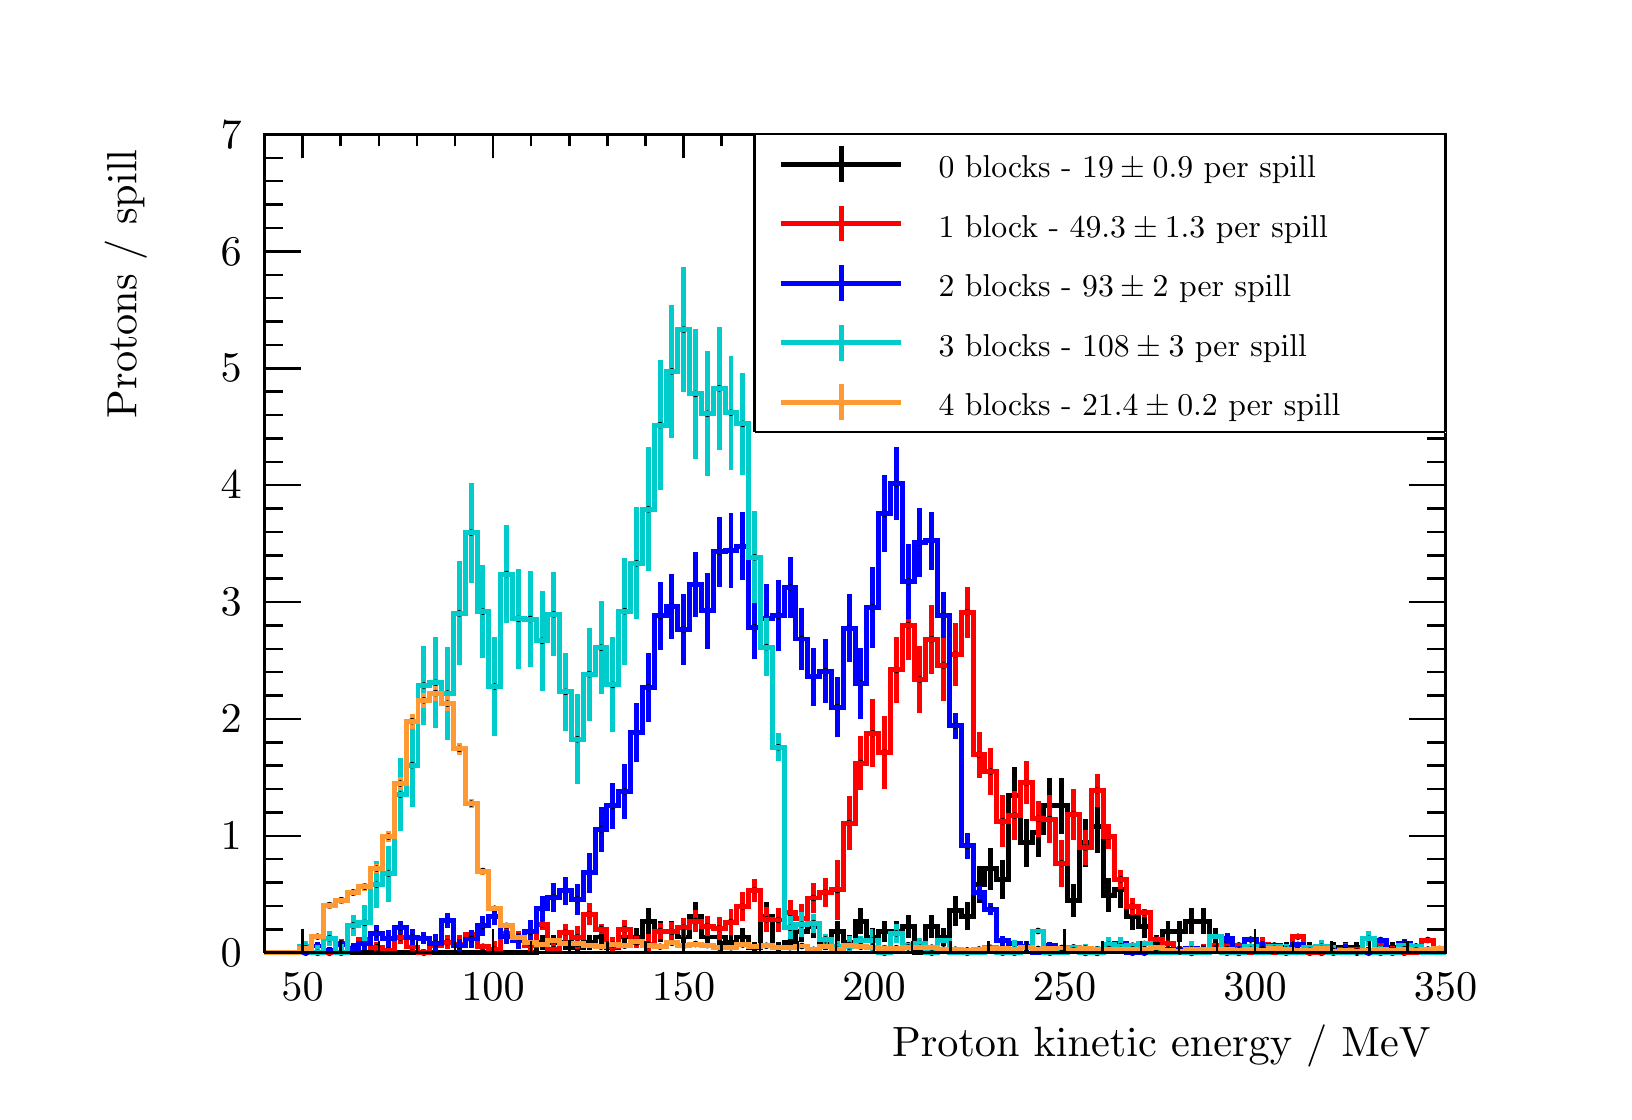
\begin{tikzpicture}
\pgfdeclareplotmark{cross} {
\pgfpathmoveto{\pgfpoint{-0.3\pgfplotmarksize}{\pgfplotmarksize}}
\pgfpathlineto{\pgfpoint{+0.3\pgfplotmarksize}{\pgfplotmarksize}}
\pgfpathlineto{\pgfpoint{+0.3\pgfplotmarksize}{0.3\pgfplotmarksize}}
\pgfpathlineto{\pgfpoint{+1\pgfplotmarksize}{0.3\pgfplotmarksize}}
\pgfpathlineto{\pgfpoint{+1\pgfplotmarksize}{-0.3\pgfplotmarksize}}
\pgfpathlineto{\pgfpoint{+0.3\pgfplotmarksize}{-0.3\pgfplotmarksize}}
\pgfpathlineto{\pgfpoint{+0.3\pgfplotmarksize}{-1.\pgfplotmarksize}}
\pgfpathlineto{\pgfpoint{-0.3\pgfplotmarksize}{-1.\pgfplotmarksize}}
\pgfpathlineto{\pgfpoint{-0.3\pgfplotmarksize}{-0.3\pgfplotmarksize}}
\pgfpathlineto{\pgfpoint{-1.\pgfplotmarksize}{-0.3\pgfplotmarksize}}
\pgfpathlineto{\pgfpoint{-1.\pgfplotmarksize}{0.3\pgfplotmarksize}}
\pgfpathlineto{\pgfpoint{-0.3\pgfplotmarksize}{0.3\pgfplotmarksize}}
\pgfpathclose
\pgfusepathqstroke
}
\pgfdeclareplotmark{cross*} {
\pgfpathmoveto{\pgfpoint{-0.3\pgfplotmarksize}{\pgfplotmarksize}}
\pgfpathlineto{\pgfpoint{+0.3\pgfplotmarksize}{\pgfplotmarksize}}
\pgfpathlineto{\pgfpoint{+0.3\pgfplotmarksize}{0.3\pgfplotmarksize}}
\pgfpathlineto{\pgfpoint{+1\pgfplotmarksize}{0.3\pgfplotmarksize}}
\pgfpathlineto{\pgfpoint{+1\pgfplotmarksize}{-0.3\pgfplotmarksize}}
\pgfpathlineto{\pgfpoint{+0.3\pgfplotmarksize}{-0.3\pgfplotmarksize}}
\pgfpathlineto{\pgfpoint{+0.3\pgfplotmarksize}{-1.\pgfplotmarksize}}
\pgfpathlineto{\pgfpoint{-0.3\pgfplotmarksize}{-1.\pgfplotmarksize}}
\pgfpathlineto{\pgfpoint{-0.3\pgfplotmarksize}{-0.3\pgfplotmarksize}}
\pgfpathlineto{\pgfpoint{-1.\pgfplotmarksize}{-0.3\pgfplotmarksize}}
\pgfpathlineto{\pgfpoint{-1.\pgfplotmarksize}{0.3\pgfplotmarksize}}
\pgfpathlineto{\pgfpoint{-0.3\pgfplotmarksize}{0.3\pgfplotmarksize}}
\pgfpathclose
\pgfusepathqfillstroke
}
\pgfdeclareplotmark{newstar} {
\pgfpathmoveto{\pgfqpoint{0pt}{\pgfplotmarksize}}
\pgfpathlineto{\pgfqpointpolar{44}{0.5\pgfplotmarksize}}
\pgfpathlineto{\pgfqpointpolar{18}{\pgfplotmarksize}}
\pgfpathlineto{\pgfqpointpolar{-20}{0.5\pgfplotmarksize}}
\pgfpathlineto{\pgfqpointpolar{-54}{\pgfplotmarksize}}
\pgfpathlineto{\pgfqpointpolar{-90}{0.5\pgfplotmarksize}}
\pgfpathlineto{\pgfqpointpolar{234}{\pgfplotmarksize}}
\pgfpathlineto{\pgfqpointpolar{198}{0.5\pgfplotmarksize}}
\pgfpathlineto{\pgfqpointpolar{162}{\pgfplotmarksize}}
\pgfpathlineto{\pgfqpointpolar{134}{0.5\pgfplotmarksize}}
\pgfpathclose
\pgfusepathqstroke
}
\pgfdeclareplotmark{newstar*} {
\pgfpathmoveto{\pgfqpoint{0pt}{\pgfplotmarksize}}
\pgfpathlineto{\pgfqpointpolar{44}{0.5\pgfplotmarksize}}
\pgfpathlineto{\pgfqpointpolar{18}{\pgfplotmarksize}}
\pgfpathlineto{\pgfqpointpolar{-20}{0.5\pgfplotmarksize}}
\pgfpathlineto{\pgfqpointpolar{-54}{\pgfplotmarksize}}
\pgfpathlineto{\pgfqpointpolar{-90}{0.5\pgfplotmarksize}}
\pgfpathlineto{\pgfqpointpolar{234}{\pgfplotmarksize}}
\pgfpathlineto{\pgfqpointpolar{198}{0.5\pgfplotmarksize}}
\pgfpathlineto{\pgfqpointpolar{162}{\pgfplotmarksize}}
\pgfpathlineto{\pgfqpointpolar{134}{0.5\pgfplotmarksize}}
\pgfpathclose
\pgfusepathqfillstroke
}
\definecolor{c}{rgb}{1,1,1};
\draw [color=c, fill=c] (0,0) rectangle (20,13.4957);
\draw [color=c, fill=c] (3,1.75444) rectangle (18,12.1461);
\definecolor{c}{rgb}{0,0,0};
\draw [c,line width=0.9] (3,1.75444) -- (3,12.1461) -- (18,12.1461) -- (18,1.75444) -- (3,1.75444);
\definecolor{c}{rgb}{1,1,1};
\draw [color=c, fill=c] (3,1.75444) rectangle (18,12.1461);
\definecolor{c}{rgb}{0,0,0};
\draw [c,line width=0.9] (3,1.75444) -- (3,12.1461) -- (18,12.1461) -- (18,1.75444) -- (3,1.75444);
\draw [c,line width=0.9] (3,1.75444) -- (3.15,1.75444) -- (3.15,1.75444) -- (3.3,1.75444) -- (3.3,1.75444) -- (3.45,1.75444) -- (3.45,1.75444) -- (3.6,1.75444) -- (3.6,1.75444) -- (3.75,1.75444) -- (3.75,1.75444) -- (3.9,1.75444) -- (3.9,1.75444) --
 (4.05,1.75444) -- (4.05,1.75444) -- (4.2,1.75444) -- (4.2,1.75444) -- (4.35,1.75444) -- (4.35,1.75444) -- (4.5,1.75444) -- (4.5,1.75444) -- (4.65,1.75444) -- (4.65,1.75444) -- (4.8,1.75444) -- (4.8,1.75444) -- (4.95,1.75444) -- (4.95,1.75444) --
 (5.1,1.75444) -- (5.1,1.75444) -- (5.25,1.75444) -- (5.25,1.75444) -- (5.4,1.75444) -- (5.4,1.75444) -- (5.55,1.75444) -- (5.55,1.75444) -- (5.7,1.75444) -- (5.7,1.75444) -- (5.85,1.75444) -- (5.85,1.75444) -- (6,1.75444) -- (6,1.75444) --
 (6.15,1.75444) -- (6.15,1.75444) -- (6.3,1.75444) -- (6.3,1.75444) -- (6.45,1.75444) -- (6.45,1.75444) -- (6.6,1.75444) -- (6.6,1.75444) -- (6.75,1.75444) -- (6.75,1.75444) -- (6.9,1.75444) -- (6.9,1.75444) -- (7.05,1.75444) -- (7.05,1.75444) --
 (7.2,1.75444) -- (7.2,1.75444) -- (7.35,1.75444) -- (7.35,1.75444) -- (7.5,1.75444) -- (7.5,1.75444) -- (7.65,1.75444) -- (7.65,1.75444) -- (7.8,1.75444) -- (7.8,1.75444) -- (7.95,1.75444) -- (7.95,1.75444) -- (8.1,1.75444) -- (8.1,1.75444) --
 (8.25,1.75444) -- (8.25,1.75444) -- (8.4,1.75444) -- (8.4,1.75444) -- (8.55,1.75444) -- (8.55,1.75444) -- (8.7,1.75444) -- (8.7,1.75444) -- (8.85,1.75444) -- (8.85,1.75444) -- (9,1.75444) -- (9,1.75444) -- (9.15,1.75444) -- (9.15,1.75444) --
 (9.3,1.75444) -- (9.3,1.75444) -- (9.45,1.75444) -- (9.45,1.75444) -- (9.6,1.75444) -- (9.6,1.75444) -- (9.75,1.75444) -- (9.75,1.75444) -- (9.9,1.75444) -- (9.9,1.75444) -- (10.05,1.75444) -- (10.05,1.75444) -- (10.2,1.75444) -- (10.2,1.75444) --
 (10.35,1.75444) -- (10.35,1.75444) -- (10.5,1.75444) -- (10.5,1.75444) -- (10.65,1.75444) -- (10.65,1.75444) -- (10.8,1.75444) -- (10.8,1.75444) -- (10.95,1.75444) -- (10.95,1.75444) -- (11.1,1.75444) -- (11.1,1.75444) -- (11.25,1.75444) --
 (11.25,1.75444) -- (11.4,1.75444) -- (11.4,1.75444) -- (11.55,1.75444) -- (11.55,1.75444) -- (11.7,1.75444) -- (11.7,1.75444) -- (11.85,1.75444) -- (11.85,1.75444) -- (12,1.75444) -- (12,1.75444) -- (12.15,1.75444) -- (12.15,1.75444) --
 (12.3,1.75444) -- (12.3,1.75444) -- (12.45,1.75444) -- (12.45,1.75444) -- (12.6,1.75444) -- (12.6,1.75444) -- (12.75,1.75444) -- (12.75,1.75444) -- (12.9,1.75444) -- (12.9,1.75444) -- (13.05,1.75444) -- (13.05,1.75444) -- (13.2,1.75444) --
 (13.2,1.75444) -- (13.35,1.75444) -- (13.35,1.75444) -- (13.5,1.75444) -- (13.5,1.75444) -- (13.65,1.75444) -- (13.65,1.75444) -- (13.8,1.75444) -- (13.8,1.75444) -- (13.95,1.75444) -- (13.95,1.75444) -- (14.1,1.75444) -- (14.1,1.75444) --
 (14.25,1.75444) -- (14.25,1.75444) -- (14.4,1.75444) -- (14.4,1.75444) -- (14.55,1.75444) -- (14.55,1.75444) -- (14.7,1.75444) -- (14.7,1.75444) -- (14.85,1.75444) -- (14.85,1.75444) -- (15,1.75444) -- (15,1.75444) -- (15.15,1.75444) --
 (15.15,1.75444) -- (15.3,1.75444) -- (15.3,1.75444) -- (15.45,1.75444) -- (15.45,1.75444) -- (15.6,1.75444) -- (15.6,1.75444) -- (15.75,1.75444) -- (15.75,1.75444) -- (15.9,1.75444) -- (15.9,1.75444) -- (16.05,1.75444) -- (16.05,1.75444) --
 (16.2,1.75444) -- (16.2,1.75444) -- (16.35,1.75444) -- (16.35,1.75444) -- (16.5,1.75444) -- (16.5,1.75444) -- (16.65,1.75444) -- (16.65,1.75444) -- (16.8,1.75444) -- (16.8,1.75444) -- (16.95,1.75444) -- (16.95,1.75444) -- (17.1,1.75444) --
 (17.1,1.75444) -- (17.25,1.75444) -- (17.25,1.75444) -- (17.4,1.75444) -- (17.4,1.75444) -- (17.55,1.75444) -- (17.55,1.75444) -- (17.7,1.75444) -- (17.7,1.75444) -- (17.85,1.75444) -- (17.85,1.75444) -- (18,1.75444);
\draw [c,line width=0.9] (3,1.75444) -- (18,1.75444);
\draw [c,line width=0.9] (3.48387,2.05809) -- (3.48387,1.75444);
\draw [c,line width=0.9] (3.96774,1.90627) -- (3.96774,1.75444);
\draw [c,line width=0.9] (4.45161,1.90627) -- (4.45161,1.75444);
\draw [c,line width=0.9] (4.93548,1.90627) -- (4.93548,1.75444);
\draw [c,line width=0.9] (5.41935,1.90627) -- (5.41935,1.75444);
\draw [c,line width=0.9] (5.90323,2.05809) -- (5.90323,1.75444);
\draw [c,line width=0.9] (6.3871,1.90627) -- (6.3871,1.75444);
\draw [c,line width=0.9] (6.87097,1.90627) -- (6.87097,1.75444);
\draw [c,line width=0.9] (7.35484,1.90627) -- (7.35484,1.75444);
\draw [c,line width=0.9] (7.83871,1.90627) -- (7.83871,1.75444);
\draw [c,line width=0.9] (8.32258,2.05809) -- (8.32258,1.75444);
\draw [c,line width=0.9] (8.80645,1.90627) -- (8.80645,1.75444);
\draw [c,line width=0.9] (9.29032,1.90627) -- (9.29032,1.75444);
\draw [c,line width=0.9] (9.77419,1.90627) -- (9.77419,1.75444);
\draw [c,line width=0.9] (10.2581,1.90627) -- (10.2581,1.75444);
\draw [c,line width=0.9] (10.7419,2.05809) -- (10.7419,1.75444);
\draw [c,line width=0.9] (11.2258,1.90627) -- (11.2258,1.75444);
\draw [c,line width=0.9] (11.7097,1.90627) -- (11.7097,1.75444);
\draw [c,line width=0.9] (12.1935,1.90627) -- (12.1935,1.75444);
\draw [c,line width=0.9] (12.6774,1.90627) -- (12.6774,1.75444);
\draw [c,line width=0.9] (13.1613,2.05809) -- (13.1613,1.75444);
\draw [c,line width=0.9] (13.6452,1.90627) -- (13.6452,1.75444);
\draw [c,line width=0.9] (14.129,1.90627) -- (14.129,1.75444);
\draw [c,line width=0.9] (14.6129,1.90627) -- (14.6129,1.75444);
\draw [c,line width=0.9] (15.0968,1.90627) -- (15.0968,1.75444);
\draw [c,line width=0.9] (15.5806,2.05809) -- (15.5806,1.75444);
\draw [c,line width=0.9] (16.0645,1.90627) -- (16.0645,1.75444);
\draw [c,line width=0.9] (16.5484,1.90627) -- (16.5484,1.75444);
\draw [c,line width=0.9] (17.0323,1.90627) -- (17.0323,1.75444);
\draw [c,line width=0.9] (17.5161,1.90627) -- (17.5161,1.75444);
\draw [c,line width=0.9] (18,2.05809) -- (18,1.75444);
\draw [c,line width=0.9] (3.48387,2.05809) -- (3.48387,1.75444);
\draw [c,line width=0.9] (18,2.05809) -- (18,1.75444);
\draw [anchor=base] (3.48387,1.14713) node[scale=1.52731, color=c, rotate=0]{50};
\draw [anchor=base] (5.90323,1.14713) node[scale=1.52731, color=c, rotate=0]{100};
\draw [anchor=base] (8.32258,1.14713) node[scale=1.52731, color=c, rotate=0]{150};
\draw [anchor=base] (10.7419,1.14713) node[scale=1.52731, color=c, rotate=0]{200};
\draw [anchor=base] (13.1613,1.14713) node[scale=1.52731, color=c, rotate=0]{250};
\draw [anchor=base] (15.5806,1.14713) node[scale=1.52731, color=c, rotate=0]{300};
\draw [anchor=base] (18,1.14713) node[scale=1.52731, color=c, rotate=0]{350};
\draw [anchor= east] (18,0.566819) node[scale=1.52731, color=c, rotate=0]{ Proton kinetic energy / MeV};
\draw [c,line width=0.9] (3,12.1461) -- (18,12.1461);
\draw [c,line width=0.9] (3.48387,11.8425) -- (3.48387,12.1461);
\draw [c,line width=0.9] (3.96774,11.9943) -- (3.96774,12.1461);
\draw [c,line width=0.9] (4.45161,11.9943) -- (4.45161,12.1461);
\draw [c,line width=0.9] (4.93548,11.9943) -- (4.93548,12.1461);
\draw [c,line width=0.9] (5.41935,11.9943) -- (5.41935,12.1461);
\draw [c,line width=0.9] (5.90323,11.8425) -- (5.90323,12.1461);
\draw [c,line width=0.9] (6.3871,11.9943) -- (6.3871,12.1461);
\draw [c,line width=0.9] (6.87097,11.9943) -- (6.87097,12.1461);
\draw [c,line width=0.9] (7.35484,11.9943) -- (7.35484,12.1461);
\draw [c,line width=0.9] (7.83871,11.9943) -- (7.83871,12.1461);
\draw [c,line width=0.9] (8.32258,11.8425) -- (8.32258,12.1461);
\draw [c,line width=0.9] (8.80645,11.9943) -- (8.80645,12.1461);
\draw [c,line width=0.9] (9.29032,11.9943) -- (9.29032,12.1461);
\draw [c,line width=0.9] (9.77419,11.9943) -- (9.77419,12.1461);
\draw [c,line width=0.9] (10.2581,11.9943) -- (10.2581,12.1461);
\draw [c,line width=0.9] (10.7419,11.8425) -- (10.7419,12.1461);
\draw [c,line width=0.9] (11.2258,11.9943) -- (11.2258,12.1461);
\draw [c,line width=0.9] (11.7097,11.9943) -- (11.7097,12.1461);
\draw [c,line width=0.9] (12.1935,11.9943) -- (12.1935,12.1461);
\draw [c,line width=0.9] (12.6774,11.9943) -- (12.6774,12.1461);
\draw [c,line width=0.9] (13.1613,11.8425) -- (13.1613,12.1461);
\draw [c,line width=0.9] (13.6452,11.9943) -- (13.6452,12.1461);
\draw [c,line width=0.9] (14.129,11.9943) -- (14.129,12.1461);
\draw [c,line width=0.9] (14.6129,11.9943) -- (14.6129,12.1461);
\draw [c,line width=0.9] (15.0968,11.9943) -- (15.0968,12.1461);
\draw [c,line width=0.9] (15.5806,11.8425) -- (15.5806,12.1461);
\draw [c,line width=0.9] (16.0645,11.9943) -- (16.0645,12.1461);
\draw [c,line width=0.9] (16.5484,11.9943) -- (16.5484,12.1461);
\draw [c,line width=0.9] (17.0323,11.9943) -- (17.0323,12.1461);
\draw [c,line width=0.9] (17.5161,11.9943) -- (17.5161,12.1461);
\draw [c,line width=0.9] (18,11.8425) -- (18,12.1461);
\draw [c,line width=0.9] (3.48387,11.8425) -- (3.48387,12.1461);
\draw [c,line width=0.9] (18,11.8425) -- (18,12.1461);
\draw [c,line width=0.9] (3,1.75444) -- (3,12.1461);
\draw [c,line width=0.9] (3.462,1.75444) -- (3,1.75444);
\draw [c,line width=0.9] (3.231,2.05135) -- (3,2.05135);
\draw [c,line width=0.9] (3.231,2.34825) -- (3,2.34825);
\draw [c,line width=0.9] (3.231,2.64516) -- (3,2.64516);
\draw [c,line width=0.9] (3.231,2.94206) -- (3,2.94206);
\draw [c,line width=0.9] (3.462,3.23897) -- (3,3.23897);
\draw [c,line width=0.9] (3.231,3.53587) -- (3,3.53587);
\draw [c,line width=0.9] (3.231,3.83278) -- (3,3.83278);
\draw [c,line width=0.9] (3.231,4.12968) -- (3,4.12968);
\draw [c,line width=0.9] (3.231,4.42659) -- (3,4.42659);
\draw [c,line width=0.9] (3.462,4.7235) -- (3,4.7235);
\draw [c,line width=0.9] (3.231,5.0204) -- (3,5.0204);
\draw [c,line width=0.9] (3.231,5.31731) -- (3,5.31731);
\draw [c,line width=0.9] (3.231,5.61421) -- (3,5.61421);
\draw [c,line width=0.9] (3.231,5.91112) -- (3,5.91112);
\draw [c,line width=0.9] (3.462,6.20802) -- (3,6.20802);
\draw [c,line width=0.9] (3.231,6.50493) -- (3,6.50493);
\draw [c,line width=0.9] (3.231,6.80183) -- (3,6.80183);
\draw [c,line width=0.9] (3.231,7.09874) -- (3,7.09874);
\draw [c,line width=0.9] (3.231,7.39564) -- (3,7.39564);
\draw [c,line width=0.9] (3.462,7.69255) -- (3,7.69255);
\draw [c,line width=0.9] (3.231,7.98946) -- (3,7.98946);
\draw [c,line width=0.9] (3.231,8.28636) -- (3,8.28636);
\draw [c,line width=0.9] (3.231,8.58327) -- (3,8.58327);
\draw [c,line width=0.9] (3.231,8.88017) -- (3,8.88017);
\draw [c,line width=0.9] (3.462,9.17708) -- (3,9.17708);
\draw [c,line width=0.9] (3.231,9.47398) -- (3,9.47398);
\draw [c,line width=0.9] (3.231,9.77089) -- (3,9.77089);
\draw [c,line width=0.9] (3.231,10.0678) -- (3,10.0678);
\draw [c,line width=0.9] (3.231,10.3647) -- (3,10.3647);
\draw [c,line width=0.9] (3.462,10.6616) -- (3,10.6616);
\draw [c,line width=0.9] (3.231,10.9585) -- (3,10.9585);
\draw [c,line width=0.9] (3.231,11.2554) -- (3,11.2554);
\draw [c,line width=0.9] (3.231,11.5523) -- (3,11.5523);
\draw [c,line width=0.9] (3.231,11.8492) -- (3,11.8492);
\draw [c,line width=0.9] (3.462,12.1461) -- (3,12.1461);
\draw [anchor= east] (2.9,1.75444) node[scale=1.52731, color=c, rotate=0]{0};
\draw [anchor= east] (2.9,3.23897) node[scale=1.52731, color=c, rotate=0]{1};
\draw [anchor= east] (2.9,4.7235) node[scale=1.52731, color=c, rotate=0]{2};
\draw [anchor= east] (2.9,6.20802) node[scale=1.52731, color=c, rotate=0]{3};
\draw [anchor= east] (2.9,7.69255) node[scale=1.52731, color=c, rotate=0]{4};
\draw [anchor= east] (2.9,9.17708) node[scale=1.52731, color=c, rotate=0]{5};
\draw [anchor= east] (2.9,10.6616) node[scale=1.52731, color=c, rotate=0]{6};
\draw [anchor= east] (2.9,12.1461) node[scale=1.52731, color=c, rotate=0]{7};
\draw [anchor= east] (1.24,12.1461) node[scale=1.52731, color=c, rotate=90]{ Protons / spill};
\draw [c,line width=0.9] (18,1.75444) -- (18,12.1461);
\draw [c,line width=0.9] (17.538,1.75444) -- (18,1.75444);
\draw [c,line width=0.9] (17.769,2.05135) -- (18,2.05135);
\draw [c,line width=0.9] (17.769,2.34825) -- (18,2.34825);
\draw [c,line width=0.9] (17.769,2.64516) -- (18,2.64516);
\draw [c,line width=0.9] (17.769,2.94206) -- (18,2.94206);
\draw [c,line width=0.9] (17.538,3.23897) -- (18,3.23897);
\draw [c,line width=0.9] (17.769,3.53587) -- (18,3.53587);
\draw [c,line width=0.9] (17.769,3.83278) -- (18,3.83278);
\draw [c,line width=0.9] (17.769,4.12968) -- (18,4.12968);
\draw [c,line width=0.9] (17.769,4.42659) -- (18,4.42659);
\draw [c,line width=0.9] (17.538,4.7235) -- (18,4.7235);
\draw [c,line width=0.9] (17.769,5.0204) -- (18,5.0204);
\draw [c,line width=0.9] (17.769,5.31731) -- (18,5.31731);
\draw [c,line width=0.9] (17.769,5.61421) -- (18,5.61421);
\draw [c,line width=0.9] (17.769,5.91112) -- (18,5.91112);
\draw [c,line width=0.9] (17.538,6.20802) -- (18,6.20802);
\draw [c,line width=0.9] (17.769,6.50493) -- (18,6.50493);
\draw [c,line width=0.9] (17.769,6.80183) -- (18,6.80183);
\draw [c,line width=0.9] (17.769,7.09874) -- (18,7.09874);
\draw [c,line width=0.9] (17.769,7.39564) -- (18,7.39564);
\draw [c,line width=0.9] (17.538,7.69255) -- (18,7.69255);
\draw [c,line width=0.9] (17.769,7.98946) -- (18,7.98946);
\draw [c,line width=0.9] (17.769,8.28636) -- (18,8.28636);
\draw [c,line width=0.9] (17.769,8.58327) -- (18,8.58327);
\draw [c,line width=0.9] (17.769,8.88017) -- (18,8.88017);
\draw [c,line width=0.9] (17.538,9.17708) -- (18,9.17708);
\draw [c,line width=0.9] (17.769,9.47398) -- (18,9.47398);
\draw [c,line width=0.9] (17.769,9.77089) -- (18,9.77089);
\draw [c,line width=0.9] (17.769,10.0678) -- (18,10.0678);
\draw [c,line width=0.9] (17.769,10.3647) -- (18,10.3647);
\draw [c,line width=0.9] (17.538,10.6616) -- (18,10.6616);
\draw [c,line width=0.9] (17.769,10.9585) -- (18,10.9585);
\draw [c,line width=0.9] (17.769,11.2554) -- (18,11.2554);
\draw [c,line width=0.9] (17.769,11.5523) -- (18,11.5523);
\draw [c,line width=0.9] (17.769,11.8492) -- (18,11.8492);
\draw [c,line width=0.9] (17.538,12.1461) -- (18,12.1461);
\draw [c,line width=1.8] (6.525,1.79346) -- (6.525,1.88768);
\draw [c,line width=1.8] (6.525,1.88768) -- (6.525,1.9819);
\foreach \P in {(6.525,1.88768)}{\draw[mark options={color=c,fill=c},mark size=2.402402pt,mark=*,mark size=1pt] plot coordinates {\P};}
\draw [c,line width=1.8] (6.675,1.79346) -- (6.675,1.88768);
\draw [c,line width=1.8] (6.675,1.88768) -- (6.675,1.9819);
\foreach \P in {(6.675,1.88768)}{\draw[mark options={color=c,fill=c},mark size=2.402402pt,mark=*,mark size=1pt] plot coordinates {\P};}
\draw [c,line width=1.8] (6.825,1.79346) -- (6.825,1.88768);
\draw [c,line width=1.8] (6.825,1.88768) -- (6.825,1.9819);
\foreach \P in {(6.825,1.88768)}{\draw[mark options={color=c,fill=c},mark size=2.402402pt,mark=*,mark size=1pt] plot coordinates {\P};}
\draw [c,line width=1.8] (6.975,1.75444) -- (6.975,1.82106);
\draw [c,line width=1.8] (6.975,1.82106) -- (6.975,1.88769);
\foreach \P in {(6.975,1.82106)}{\draw[mark options={color=c,fill=c},mark size=2.402402pt,mark=*,mark size=1pt] plot coordinates {\P};}
\draw [c,line width=1.8] (7.125,1.79346) -- (7.125,1.88768);
\draw [c,line width=1.8] (7.125,1.88768) -- (7.125,1.9819);
\foreach \P in {(7.125,1.88768)}{\draw[mark options={color=c,fill=c},mark size=2.402402pt,mark=*,mark size=1pt] plot coordinates {\P};}
\draw [c,line width=1.8] (7.275,1.83891) -- (7.275,1.9543);
\draw [c,line width=1.8] (7.275,1.9543) -- (7.275,2.0697);
\foreach \P in {(7.275,1.9543)}{\draw[mark options={color=c,fill=c},mark size=2.402402pt,mark=*,mark size=1pt] plot coordinates {\P};}
\draw [c,line width=1.8] (7.425,1.75444) -- (7.425,1.82106);
\draw [c,line width=1.8] (7.425,1.82106) -- (7.425,1.88769);
\foreach \P in {(7.425,1.82106)}{\draw[mark options={color=c,fill=c},mark size=2.402402pt,mark=*,mark size=1pt] plot coordinates {\P};}
\draw [c,line width=1.8] (7.575,1.83891) -- (7.575,1.9543);
\draw [c,line width=1.8] (7.575,1.9543) -- (7.575,2.0697);
\foreach \P in {(7.575,1.9543)}{\draw[mark options={color=c,fill=c},mark size=2.402402pt,mark=*,mark size=1pt] plot coordinates {\P};}
\draw [c,line width=1.8] (7.725,1.83891) -- (7.725,1.9543);
\draw [c,line width=1.8] (7.725,1.9543) -- (7.725,2.0697);
\foreach \P in {(7.725,1.9543)}{\draw[mark options={color=c,fill=c},mark size=2.402402pt,mark=*,mark size=1pt] plot coordinates {\P};}
\draw [c,line width=1.8] (7.875,1.99097) -- (7.875,2.15417);
\draw [c,line width=1.8] (7.875,2.15417) -- (7.875,2.31736);
\foreach \P in {(7.875,2.15417)}{\draw[mark options={color=c,fill=c},mark size=2.402402pt,mark=*,mark size=1pt] plot coordinates {\P};}
\draw [c,line width=1.8] (8.025,1.88767) -- (8.025,2.02092);
\draw [c,line width=1.8] (8.025,2.02092) -- (8.025,2.15417);
\foreach \P in {(8.025,2.02092)}{\draw[mark options={color=c,fill=c},mark size=2.402402pt,mark=*,mark size=1pt] plot coordinates {\P};}
\draw [c,line width=1.8] (8.175,1.88767) -- (8.175,2.02092);
\draw [c,line width=1.8] (8.175,2.02092) -- (8.175,2.15417);
\foreach \P in {(8.175,2.02092)}{\draw[mark options={color=c,fill=c},mark size=2.402402pt,mark=*,mark size=1pt] plot coordinates {\P};}
\draw [c,line width=1.8] (8.325,1.83891) -- (8.325,1.9543);
\draw [c,line width=1.8] (8.325,1.9543) -- (8.325,2.0697);
\foreach \P in {(8.325,1.9543)}{\draw[mark options={color=c,fill=c},mark size=2.402402pt,mark=*,mark size=1pt] plot coordinates {\P};}
\draw [c,line width=1.8] (8.475,2.04451) -- (8.475,2.22079);
\draw [c,line width=1.8] (8.475,2.22079) -- (8.475,2.39706);
\foreach \P in {(8.475,2.22079)}{\draw[mark options={color=c,fill=c},mark size=2.402402pt,mark=*,mark size=1pt] plot coordinates {\P};}
\draw [c,line width=1.8] (8.625,1.83891) -- (8.625,1.9543);
\draw [c,line width=1.8] (8.625,1.9543) -- (8.625,2.0697);
\foreach \P in {(8.625,1.9543)}{\draw[mark options={color=c,fill=c},mark size=2.402402pt,mark=*,mark size=1pt] plot coordinates {\P};}
\draw [c,line width=1.8] (8.775,1.83891) -- (8.775,1.9543);
\draw [c,line width=1.8] (8.775,1.9543) -- (8.775,2.0697);
\foreach \P in {(8.775,1.9543)}{\draw[mark options={color=c,fill=c},mark size=2.402402pt,mark=*,mark size=1pt] plot coordinates {\P};}
\draw [c,line width=1.8] (8.925,1.79346) -- (8.925,1.88768);
\draw [c,line width=1.8] (8.925,1.88768) -- (8.925,1.9819);
\foreach \P in {(8.925,1.88768)}{\draw[mark options={color=c,fill=c},mark size=2.402402pt,mark=*,mark size=1pt] plot coordinates {\P};}
\draw [c,line width=1.8] (9.075,1.83891) -- (9.075,1.9543);
\draw [c,line width=1.8] (9.075,1.9543) -- (9.075,2.0697);
\foreach \P in {(9.075,1.9543)}{\draw[mark options={color=c,fill=c},mark size=2.402402pt,mark=*,mark size=1pt] plot coordinates {\P};}
\draw [c,line width=1.8] (9.225,1.75444) -- (9.225,1.82106);
\draw [c,line width=1.8] (9.225,1.82106) -- (9.225,1.88769);
\foreach \P in {(9.225,1.82106)}{\draw[mark options={color=c,fill=c},mark size=2.402402pt,mark=*,mark size=1pt] plot coordinates {\P};}
\draw [c,line width=1.8] (9.375,2.04451) -- (9.375,2.22079);
\draw [c,line width=1.8] (9.375,2.22079) -- (9.375,2.39706);
\foreach \P in {(9.375,2.22079)}{\draw[mark options={color=c,fill=c},mark size=2.402402pt,mark=*,mark size=1pt] plot coordinates {\P};}
\draw [c,line width=1.8] (9.525,1.75444) -- (9.525,1.82106);
\draw [c,line width=1.8] (9.525,1.82106) -- (9.525,1.88769);
\foreach \P in {(9.525,1.82106)}{\draw[mark options={color=c,fill=c},mark size=2.402402pt,mark=*,mark size=1pt] plot coordinates {\P};}
\draw [c,line width=1.8] (9.675,1.79346) -- (9.675,1.88768);
\draw [c,line width=1.8] (9.675,1.88768) -- (9.675,1.9819);
\foreach \P in {(9.675,1.88768)}{\draw[mark options={color=c,fill=c},mark size=2.402402pt,mark=*,mark size=1pt] plot coordinates {\P};}
\draw [c,line width=1.8] (9.825,1.88767) -- (9.825,2.02092);
\draw [c,line width=1.8] (9.825,2.02092) -- (9.825,2.15417);
\foreach \P in {(9.825,2.02092)}{\draw[mark options={color=c,fill=c},mark size=2.402402pt,mark=*,mark size=1pt] plot coordinates {\P};}
\draw [c,line width=1.8] (9.975,1.93857) -- (9.975,2.08755);
\draw [c,line width=1.8] (9.975,2.08755) -- (9.975,2.23652);
\foreach \P in {(9.975,2.08755)}{\draw[mark options={color=c,fill=c},mark size=2.402402pt,mark=*,mark size=1pt] plot coordinates {\P};}
\draw [c,line width=1.8] (10.125,1.79346) -- (10.125,1.88768);
\draw [c,line width=1.8] (10.125,1.88768) -- (10.125,1.9819);
\foreach \P in {(10.125,1.88768)}{\draw[mark options={color=c,fill=c},mark size=2.402402pt,mark=*,mark size=1pt] plot coordinates {\P};}
\draw [c,line width=1.8] (10.275,1.88767) -- (10.275,2.02092);
\draw [c,line width=1.8] (10.275,2.02092) -- (10.275,2.15417);
\foreach \P in {(10.275,2.02092)}{\draw[mark options={color=c,fill=c},mark size=2.402402pt,mark=*,mark size=1pt] plot coordinates {\P};}
\draw [c,line width=1.8] (10.425,1.79346) -- (10.425,1.88768);
\draw [c,line width=1.8] (10.425,1.88768) -- (10.425,1.9819);
\foreach \P in {(10.425,1.88768)}{\draw[mark options={color=c,fill=c},mark size=2.402402pt,mark=*,mark size=1pt] plot coordinates {\P};}
\draw [c,line width=1.8] (10.575,1.99097) -- (10.575,2.15417);
\draw [c,line width=1.8] (10.575,2.15417) -- (10.575,2.31736);
\foreach \P in {(10.575,2.15417)}{\draw[mark options={color=c,fill=c},mark size=2.402402pt,mark=*,mark size=1pt] plot coordinates {\P};}
\draw [c,line width=1.8] (10.725,1.83891) -- (10.725,1.9543);
\draw [c,line width=1.8] (10.725,1.9543) -- (10.725,2.0697);
\foreach \P in {(10.725,1.9543)}{\draw[mark options={color=c,fill=c},mark size=2.402402pt,mark=*,mark size=1pt] plot coordinates {\P};}
\draw [c,line width=1.8] (10.875,1.88767) -- (10.875,2.02092);
\draw [c,line width=1.8] (10.875,2.02092) -- (10.875,2.15417);
\foreach \P in {(10.875,2.02092)}{\draw[mark options={color=c,fill=c},mark size=2.402402pt,mark=*,mark size=1pt] plot coordinates {\P};}
\draw [c,line width=1.8] (11.025,1.88767) -- (11.025,2.02092);
\draw [c,line width=1.8] (11.025,2.02092) -- (11.025,2.15417);
\foreach \P in {(11.025,2.02092)}{\draw[mark options={color=c,fill=c},mark size=2.402402pt,mark=*,mark size=1pt] plot coordinates {\P};}
\draw [c,line width=1.8] (11.175,1.93857) -- (11.175,2.08755);
\draw [c,line width=1.8] (11.175,2.08755) -- (11.175,2.23652);
\foreach \P in {(11.175,2.08755)}{\draw[mark options={color=c,fill=c},mark size=2.402402pt,mark=*,mark size=1pt] plot coordinates {\P};}
\draw [c,line width=1.8] (11.475,1.93857) -- (11.475,2.08755);
\draw [c,line width=1.8] (11.475,2.08755) -- (11.475,2.23652);
\foreach \P in {(11.475,2.08755)}{\draw[mark options={color=c,fill=c},mark size=2.402402pt,mark=*,mark size=1pt] plot coordinates {\P};}
\draw [c,line width=1.8] (11.625,1.83891) -- (11.625,1.9543);
\draw [c,line width=1.8] (11.625,1.9543) -- (11.625,2.0697);
\foreach \P in {(11.625,1.9543)}{\draw[mark options={color=c,fill=c},mark size=2.402402pt,mark=*,mark size=1pt] plot coordinates {\P};}
\draw [c,line width=1.8] (11.775,2.09896) -- (11.775,2.28741);
\draw [c,line width=1.8] (11.775,2.28741) -- (11.775,2.47585);
\foreach \P in {(11.775,2.28741)}{\draw[mark options={color=c,fill=c},mark size=2.402402pt,mark=*,mark size=1pt] plot coordinates {\P};}
\draw [c,line width=1.8] (11.925,2.04451) -- (11.925,2.22079);
\draw [c,line width=1.8] (11.925,2.22079) -- (11.925,2.39706);
\foreach \P in {(11.925,2.22079)}{\draw[mark options={color=c,fill=c},mark size=2.402402pt,mark=*,mark size=1pt] plot coordinates {\P};}
\draw [c,line width=1.8] (12.075,2.38029) -- (12.075,2.62051);
\draw [c,line width=1.8] (12.075,2.62051) -- (12.075,2.86073);
\foreach \P in {(12.075,2.62051)}{\draw[mark options={color=c,fill=c},mark size=2.402402pt,mark=*,mark size=1pt] plot coordinates {\P};}
\draw [c,line width=1.8] (12.225,2.55387) -- (12.225,2.82037);
\draw [c,line width=1.8] (12.225,2.82037) -- (12.225,3.08687);
\foreach \P in {(12.225,2.82037)}{\draw[mark options={color=c,fill=c},mark size=2.402402pt,mark=*,mark size=1pt] plot coordinates {\P};}
\draw [c,line width=1.8] (12.375,2.43784) -- (12.375,2.68713);
\draw [c,line width=1.8] (12.375,2.68713) -- (12.375,2.93642);
\foreach \P in {(12.375,2.68713)}{\draw[mark options={color=c,fill=c},mark size=2.402402pt,mark=*,mark size=1pt] plot coordinates {\P};}
\draw [c,line width=1.8] (12.525,3.38815) -- (12.525,3.75307);
\draw [c,line width=1.8] (12.525,3.75307) -- (12.525,4.11799);
\foreach \P in {(12.525,3.75307)}{\draw[mark options={color=c,fill=c},mark size=2.402402pt,mark=*,mark size=1pt] plot coordinates {\P};}
\draw [c,line width=1.8] (12.675,2.84816) -- (12.675,3.15348);
\draw [c,line width=1.8] (12.675,3.15348) -- (12.675,3.45879);
\foreach \P in {(12.675,3.15348)}{\draw[mark options={color=c,fill=c},mark size=2.402402pt,mark=*,mark size=1pt] plot coordinates {\P};}
\draw [c,line width=1.8] (12.825,2.9672) -- (12.825,3.28672);
\draw [c,line width=1.8] (12.825,3.28672) -- (12.825,3.60624);
\foreach \P in {(12.825,3.28672)}{\draw[mark options={color=c,fill=c},mark size=2.402402pt,mark=*,mark size=1pt] plot coordinates {\P};}
\draw [c,line width=1.8] (12.975,3.26728) -- (12.975,3.61982);
\draw [c,line width=1.8] (12.975,3.61982) -- (12.975,3.97237);
\foreach \P in {(12.975,3.61982)}{\draw[mark options={color=c,fill=c},mark size=2.402402pt,mark=*,mark size=1pt] plot coordinates {\P};}
\draw [c,line width=1.8] (13.125,3.26728) -- (13.125,3.61982);
\draw [c,line width=1.8] (13.125,3.61982) -- (13.125,3.97237);
\foreach \P in {(13.125,3.61982)}{\draw[mark options={color=c,fill=c},mark size=2.402402pt,mark=*,mark size=1pt] plot coordinates {\P};}
\draw [c,line width=1.8] (13.275,2.20996) -- (13.275,2.42065);
\draw [c,line width=1.8] (13.275,2.42065) -- (13.275,2.63134);
\foreach \P in {(13.275,2.42065)}{\draw[mark options={color=c,fill=c},mark size=2.402402pt,mark=*,mark size=1pt] plot coordinates {\P};}
\draw [c,line width=1.8] (13.425,2.84816) -- (13.425,3.15348);
\draw [c,line width=1.8] (13.425,3.15348) -- (13.425,3.45879);
\foreach \P in {(13.425,3.15348)}{\draw[mark options={color=c,fill=c},mark size=2.402402pt,mark=*,mark size=1pt] plot coordinates {\P};}
\draw [c,line width=1.8] (13.575,3.02695) -- (13.575,3.35334);
\draw [c,line width=1.8] (13.575,3.35334) -- (13.575,3.67974);
\foreach \P in {(13.575,3.35334)}{\draw[mark options={color=c,fill=c},mark size=2.402402pt,mark=*,mark size=1pt] plot coordinates {\P};}
\draw [c,line width=1.8] (13.725,2.2663) -- (13.725,2.48727);
\draw [c,line width=1.8] (13.725,2.48727) -- (13.725,2.70824);
\foreach \P in {(13.725,2.48727)}{\draw[mark options={color=c,fill=c},mark size=2.402402pt,mark=*,mark size=1pt] plot coordinates {\P};}
\draw [c,line width=1.8] (13.875,2.3231) -- (13.875,2.55389);
\draw [c,line width=1.8] (13.875,2.55389) -- (13.875,2.78469);
\foreach \P in {(13.875,2.55389)}{\draw[mark options={color=c,fill=c},mark size=2.402402pt,mark=*,mark size=1pt] plot coordinates {\P};}
\draw [c,line width=1.8] (14.025,2.04451) -- (14.025,2.22079);
\draw [c,line width=1.8] (14.025,2.22079) -- (14.025,2.39706);
\foreach \P in {(14.025,2.22079)}{\draw[mark options={color=c,fill=c},mark size=2.402402pt,mark=*,mark size=1pt] plot coordinates {\P};}
\draw [c,line width=1.8] (14.175,1.93857) -- (14.175,2.08755);
\draw [c,line width=1.8] (14.175,2.08755) -- (14.175,2.23652);
\foreach \P in {(14.175,2.08755)}{\draw[mark options={color=c,fill=c},mark size=2.402402pt,mark=*,mark size=1pt] plot coordinates {\P};}
\draw [c,line width=1.8] (14.325,1.79346) -- (14.325,1.88768);
\draw [c,line width=1.8] (14.325,1.88768) -- (14.325,1.9819);
\foreach \P in {(14.325,1.88768)}{\draw[mark options={color=c,fill=c},mark size=2.402402pt,mark=*,mark size=1pt] plot coordinates {\P};}
\draw [c,line width=1.8] (14.475,1.88767) -- (14.475,2.02092);
\draw [c,line width=1.8] (14.475,2.02092) -- (14.475,2.15417);
\foreach \P in {(14.475,2.02092)}{\draw[mark options={color=c,fill=c},mark size=2.402402pt,mark=*,mark size=1pt] plot coordinates {\P};}
\draw [c,line width=1.8] (14.625,1.88767) -- (14.625,2.02092);
\draw [c,line width=1.8] (14.625,2.02092) -- (14.625,2.15417);
\foreach \P in {(14.625,2.02092)}{\draw[mark options={color=c,fill=c},mark size=2.402402pt,mark=*,mark size=1pt] plot coordinates {\P};}
\draw [c,line width=1.8] (14.775,1.99097) -- (14.775,2.15417);
\draw [c,line width=1.8] (14.775,2.15417) -- (14.775,2.31736);
\foreach \P in {(14.775,2.15417)}{\draw[mark options={color=c,fill=c},mark size=2.402402pt,mark=*,mark size=1pt] plot coordinates {\P};}
\draw [c,line width=1.8] (14.925,1.99097) -- (14.925,2.15417);
\draw [c,line width=1.8] (14.925,2.15417) -- (14.925,2.31736);
\foreach \P in {(14.925,2.15417)}{\draw[mark options={color=c,fill=c},mark size=2.402402pt,mark=*,mark size=1pt] plot coordinates {\P};}
\draw [c,line width=1.8] (15.075,1.83891) -- (15.075,1.9543);
\draw [c,line width=1.8] (15.075,1.9543) -- (15.075,2.0697);
\foreach \P in {(15.075,1.9543)}{\draw[mark options={color=c,fill=c},mark size=2.402402pt,mark=*,mark size=1pt] plot coordinates {\P};}
\draw [c,line width=1.8] (15.225,1.79346) -- (15.225,1.88768);
\draw [c,line width=1.8] (15.225,1.88768) -- (15.225,1.9819);
\foreach \P in {(15.225,1.88768)}{\draw[mark options={color=c,fill=c},mark size=2.402402pt,mark=*,mark size=1pt] plot coordinates {\P};}
\draw [c,line width=1.8] (15.975,1.75444) -- (15.975,1.82106);
\draw [c,line width=1.8] (15.975,1.82106) -- (15.975,1.88769);
\foreach \P in {(15.975,1.82106)}{\draw[mark options={color=c,fill=c},mark size=2.402402pt,mark=*,mark size=1pt] plot coordinates {\P};}
\draw [c,line width=1.8] (16.275,1.75444) -- (16.275,1.82106);
\draw [c,line width=1.8] (16.275,1.82106) -- (16.275,1.88769);
\foreach \P in {(16.275,1.82106)}{\draw[mark options={color=c,fill=c},mark size=2.402402pt,mark=*,mark size=1pt] plot coordinates {\P};}
\draw [c,line width=1.8] (16.575,1.75444) -- (16.575,1.82106);
\draw [c,line width=1.8] (16.575,1.82106) -- (16.575,1.88769);
\foreach \P in {(16.575,1.82106)}{\draw[mark options={color=c,fill=c},mark size=2.402402pt,mark=*,mark size=1pt] plot coordinates {\P};}
\draw [c,line width=1.8] (16.725,1.75444) -- (16.725,1.82106);
\draw [c,line width=1.8] (16.725,1.82106) -- (16.725,1.88769);
\foreach \P in {(16.725,1.82106)}{\draw[mark options={color=c,fill=c},mark size=2.402402pt,mark=*,mark size=1pt] plot coordinates {\P};}
\draw [c,line width=1.8] (16.875,1.75444) -- (16.875,1.82106);
\draw [c,line width=1.8] (16.875,1.82106) -- (16.875,1.88769);
\foreach \P in {(16.875,1.82106)}{\draw[mark options={color=c,fill=c},mark size=2.402402pt,mark=*,mark size=1pt] plot coordinates {\P};}
\draw [c,line width=1.8] (17.175,1.75444) -- (17.175,1.82106);
\draw [c,line width=1.8] (17.175,1.82106) -- (17.175,1.88769);
\foreach \P in {(17.175,1.82106)}{\draw[mark options={color=c,fill=c},mark size=2.402402pt,mark=*,mark size=1pt] plot coordinates {\P};}
\draw [c,line width=1.8] (17.325,1.75444) -- (17.325,1.82106);
\draw [c,line width=1.8] (17.325,1.82106) -- (17.325,1.88769);
\foreach \P in {(17.325,1.82106)}{\draw[mark options={color=c,fill=c},mark size=2.402402pt,mark=*,mark size=1pt] plot coordinates {\P};}
\draw [c,line width=1.8] (3,1.75444) -- (3.15,1.75444) -- (3.15,1.75444) -- (3.3,1.75444) -- (3.3,1.75444) -- (3.45,1.75444) -- (3.45,1.75444) -- (3.6,1.75444) -- (3.6,1.75444) -- (3.75,1.75444) -- (3.75,1.75444) -- (3.9,1.75444) -- (3.9,1.75444) --
 (4.05,1.75444) -- (4.05,1.75444) -- (4.2,1.75444) -- (4.2,1.75444) -- (4.35,1.75444) -- (4.35,1.75444) -- (4.5,1.75444) -- (4.5,1.75444) -- (4.65,1.75444) -- (4.65,1.75444) -- (4.8,1.75444) -- (4.8,1.75444) -- (4.95,1.75444) -- (4.95,1.75444) --
 (5.1,1.75444) -- (5.1,1.75444) -- (5.25,1.75444) -- (5.25,1.75444) -- (5.4,1.75444) -- (5.4,1.75444) -- (5.55,1.75444) -- (5.55,1.75444) -- (5.7,1.75444) -- (5.7,1.75444) -- (5.85,1.75444) -- (5.85,1.75444) -- (6,1.75444) -- (6,1.75444) --
 (6.15,1.75444) -- (6.15,1.75444) -- (6.3,1.75444) -- (6.3,1.75444) -- (6.45,1.75444) -- (6.45,1.88768) -- (6.6,1.88768) -- (6.6,1.88768) -- (6.75,1.88768) -- (6.75,1.88768) -- (6.9,1.88768) -- (6.9,1.82106) -- (7.05,1.82106) -- (7.05,1.88768) --
 (7.2,1.88768) -- (7.2,1.9543) -- (7.35,1.9543) -- (7.35,1.82106) -- (7.5,1.82106) -- (7.5,1.9543) -- (7.65,1.9543) -- (7.65,1.9543) -- (7.8,1.9543) -- (7.8,2.15417) -- (7.95,2.15417) -- (7.95,2.02092) -- (8.1,2.02092) -- (8.1,2.02092) --
 (8.25,2.02092) -- (8.25,1.9543) -- (8.4,1.9543) -- (8.4,2.22079) -- (8.55,2.22079) -- (8.55,1.9543) -- (8.7,1.9543) -- (8.7,1.9543) -- (8.85,1.9543) -- (8.85,1.88768) -- (9,1.88768) -- (9,1.9543) -- (9.15,1.9543) -- (9.15,1.82106) -- (9.3,1.82106)
 -- (9.3,2.22079) -- (9.45,2.22079) -- (9.45,1.82106) -- (9.6,1.82106) -- (9.6,1.88768) -- (9.75,1.88768) -- (9.75,2.02092) -- (9.9,2.02092) -- (9.9,2.08755) -- (10.05,2.08755) -- (10.05,1.88768) -- (10.2,1.88768) -- (10.2,2.02092) -- (10.35,2.02092)
 -- (10.35,1.88768) -- (10.5,1.88768) -- (10.5,2.15417) -- (10.65,2.15417) -- (10.65,1.9543) -- (10.8,1.9543) -- (10.8,2.02092) -- (10.95,2.02092) -- (10.95,2.02092) -- (11.1,2.02092) -- (11.1,2.08755) -- (11.25,2.08755) -- (11.25,1.75444) --
 (11.4,1.75444) -- (11.4,2.08755) -- (11.55,2.08755) -- (11.55,1.9543) -- (11.7,1.9543) -- (11.7,2.28741) -- (11.85,2.28741) -- (11.85,2.22079) -- (12,2.22079) -- (12,2.62051) -- (12.15,2.62051) -- (12.15,2.82037) -- (12.3,2.82037) -- (12.3,2.68713)
 -- (12.45,2.68713) -- (12.45,3.75307) -- (12.6,3.75307) -- (12.6,3.15348) -- (12.75,3.15348) -- (12.75,3.28672) -- (12.9,3.28672) -- (12.9,3.61982) -- (13.05,3.61982) -- (13.05,3.61982) -- (13.2,3.61982) -- (13.2,2.42065) -- (13.35,2.42065) --
 (13.35,3.15348) -- (13.5,3.15348) -- (13.5,3.35334) -- (13.65,3.35334) -- (13.65,2.48727) -- (13.8,2.48727) -- (13.8,2.55389) -- (13.95,2.55389) -- (13.95,2.22079) -- (14.1,2.22079) -- (14.1,2.08755) -- (14.25,2.08755) -- (14.25,1.88768) --
 (14.4,1.88768) -- (14.4,2.02092) -- (14.55,2.02092) -- (14.55,2.02092) -- (14.7,2.02092) -- (14.7,2.15417) -- (14.85,2.15417) -- (14.85,2.15417) -- (15,2.15417) -- (15,1.9543) -- (15.15,1.9543) -- (15.15,1.88768) -- (15.3,1.88768) -- (15.3,1.75444)
 -- (15.45,1.75444) -- (15.45,1.75444) -- (15.6,1.75444) -- (15.6,1.75444) -- (15.75,1.75444) -- (15.75,1.75444) -- (15.9,1.75444) -- (15.9,1.82106) -- (16.05,1.82106) -- (16.05,1.75444) -- (16.2,1.75444) -- (16.2,1.82106) -- (16.35,1.82106) --
 (16.35,1.75444) -- (16.5,1.75444) -- (16.5,1.82106) -- (16.65,1.82106) -- (16.65,1.82106) -- (16.8,1.82106) -- (16.8,1.82106) -- (16.95,1.82106) -- (16.95,1.75444) -- (17.1,1.75444) -- (17.1,1.82106) -- (17.25,1.82106) -- (17.25,1.82106) --
 (17.4,1.82106) -- (17.4,1.75444) -- (17.55,1.75444) -- (17.55,1.75444) -- (17.7,1.75444) -- (17.7,1.75444) -- (17.85,1.75444) -- (17.85,1.75444) -- (18,1.75444);
\definecolor{c}{rgb}{1,0,0};
\draw [c,line width=1.8] (3.825,1.75444) -- (3.825,1.79985);
\definecolor{c}{rgb}{0,0,0};
\foreach \P in {(3.825,1.75444)}{\draw[mark options={color=c,fill=c},mark size=2.402402pt,mark=*,mark size=1pt] plot coordinates {\P};}
\definecolor{c}{rgb}{1,0,0};
\draw [c,line width=1.8] (3.975,1.82031) -- (3.975,1.87354);
\draw [c,line width=1.8] (3.975,1.87354) -- (3.975,1.92677);
\definecolor{c}{rgb}{0,0,0};
\foreach \P in {(3.975,1.87354)}{\draw[mark options={color=c,fill=c},mark size=2.402402pt,mark=*,mark size=1pt] plot coordinates {\P};}
\definecolor{c}{rgb}{1,0,0};
\draw [c,line width=1.8] (4.125,1.75444) -- (4.125,1.78432);
\draw [c,line width=1.8] (4.125,1.78432) -- (4.125,1.84824);
\definecolor{c}{rgb}{0,0,0};
\foreach \P in {(4.125,1.78432)}{\draw[mark options={color=c,fill=c},mark size=2.402402pt,mark=*,mark size=1pt] plot coordinates {\P};}
\definecolor{c}{rgb}{1,0,0};
\draw [c,line width=1.8] (4.275,1.84049) -- (4.275,1.92236);
\draw [c,line width=1.8] (4.275,1.92236) -- (4.275,2.00423);
\definecolor{c}{rgb}{0,0,0};
\foreach \P in {(4.275,1.92236)}{\draw[mark options={color=c,fill=c},mark size=2.402402pt,mark=*,mark size=1pt] plot coordinates {\P};}
\definecolor{c}{rgb}{1,0,0};
\draw [c,line width=1.8] (4.425,1.76305) -- (4.425,1.82446);
\draw [c,line width=1.8] (4.425,1.82446) -- (4.425,1.88588);
\definecolor{c}{rgb}{0,0,0};
\foreach \P in {(4.425,1.82446)}{\draw[mark options={color=c,fill=c},mark size=2.402402pt,mark=*,mark size=1pt] plot coordinates {\P};}
\definecolor{c}{rgb}{1,0,0};
\draw [c,line width=1.8] (4.575,1.75444) -- (4.575,1.7886);
\draw [c,line width=1.8] (4.575,1.7886) -- (4.575,1.84649);
\definecolor{c}{rgb}{0,0,0};
\foreach \P in {(4.575,1.7886)}{\draw[mark options={color=c,fill=c},mark size=2.402402pt,mark=*,mark size=1pt] plot coordinates {\P};}
\definecolor{c}{rgb}{1,0,0};
\draw [c,line width=1.8] (4.725,1.86769) -- (4.725,1.94838);
\draw [c,line width=1.8] (4.725,1.94838) -- (4.725,2.02906);
\definecolor{c}{rgb}{0,0,0};
\foreach \P in {(4.725,1.94838)}{\draw[mark options={color=c,fill=c},mark size=2.402402pt,mark=*,mark size=1pt] plot coordinates {\P};}
\definecolor{c}{rgb}{1,0,0};
\draw [c,line width=1.8] (4.875,1.77485) -- (4.875,1.82738);
\draw [c,line width=1.8] (4.875,1.82738) -- (4.875,1.87992);
\definecolor{c}{rgb}{0,0,0};
\foreach \P in {(4.875,1.82738)}{\draw[mark options={color=c,fill=c},mark size=2.402402pt,mark=*,mark size=1pt] plot coordinates {\P};}
\definecolor{c}{rgb}{1,0,0};
\draw [c,line width=1.8] (5.025,1.75444) -- (5.025,1.80022);
\definecolor{c}{rgb}{0,0,0};
\foreach \P in {(5.025,1.75444)}{\draw[mark options={color=c,fill=c},mark size=2.402402pt,mark=*,mark size=1pt] plot coordinates {\P};}
\definecolor{c}{rgb}{1,0,0};
\draw [c,line width=1.8] (5.175,1.79445) -- (5.175,1.85065);
\draw [c,line width=1.8] (5.175,1.85065) -- (5.175,1.90686);
\definecolor{c}{rgb}{0,0,0};
\foreach \P in {(5.175,1.85065)}{\draw[mark options={color=c,fill=c},mark size=2.402402pt,mark=*,mark size=1pt] plot coordinates {\P};}
\definecolor{c}{rgb}{1,0,0};
\draw [c,line width=1.8] (5.325,1.79732) -- (5.325,1.88864);
\draw [c,line width=1.8] (5.325,1.88864) -- (5.325,1.97996);
\definecolor{c}{rgb}{0,0,0};
\foreach \P in {(5.325,1.88864)}{\draw[mark options={color=c,fill=c},mark size=2.402402pt,mark=*,mark size=1pt] plot coordinates {\P};}
\definecolor{c}{rgb}{1,0,0};
\draw [c,line width=1.8] (5.475,1.75444) -- (5.475,1.86486);
\draw [c,line width=1.8] (5.475,1.86486) -- (5.475,1.98375);
\definecolor{c}{rgb}{0,0,0};
\foreach \P in {(5.475,1.86486)}{\draw[mark options={color=c,fill=c},mark size=2.402402pt,mark=*,mark size=1pt] plot coordinates {\P};}
\definecolor{c}{rgb}{1,0,0};
\draw [c,line width=1.8] (5.625,1.92581) -- (5.625,1.98113);
\draw [c,line width=1.8] (5.625,1.98113) -- (5.625,2.03645);
\definecolor{c}{rgb}{0,0,0};
\foreach \P in {(5.625,1.98113)}{\draw[mark options={color=c,fill=c},mark size=2.402402pt,mark=*,mark size=1pt] plot coordinates {\P};}
\definecolor{c}{rgb}{1,0,0};
\draw [c,line width=1.8] (5.775,1.79303) -- (5.775,1.8316);
\draw [c,line width=1.8] (5.775,1.8316) -- (5.775,1.87017);
\definecolor{c}{rgb}{0,0,0};
\foreach \P in {(5.775,1.8316)}{\draw[mark options={color=c,fill=c},mark size=2.402402pt,mark=*,mark size=1pt] plot coordinates {\P};}
\definecolor{c}{rgb}{1,0,0};
\draw [c,line width=1.8] (5.925,1.75444) -- (5.925,1.79263);
\draw [c,line width=1.8] (5.925,1.79263) -- (5.925,1.90444);
\definecolor{c}{rgb}{0,0,0};
\foreach \P in {(5.925,1.79263)}{\draw[mark options={color=c,fill=c},mark size=2.402402pt,mark=*,mark size=1pt] plot coordinates {\P};}
\definecolor{c}{rgb}{1,0,0};
\draw [c,line width=1.8] (6.075,1.91601) -- (6.075,1.99395);
\draw [c,line width=1.8] (6.075,1.99395) -- (6.075,2.07188);
\definecolor{c}{rgb}{0,0,0};
\foreach \P in {(6.075,1.99395)}{\draw[mark options={color=c,fill=c},mark size=2.402402pt,mark=*,mark size=1pt] plot coordinates {\P};}
\definecolor{c}{rgb}{1,0,0};
\draw [c,line width=1.8] (6.225,1.81659) -- (6.225,1.9212);
\draw [c,line width=1.8] (6.225,1.9212) -- (6.225,2.02582);
\definecolor{c}{rgb}{0,0,0};
\foreach \P in {(6.225,1.9212)}{\draw[mark options={color=c,fill=c},mark size=2.402402pt,mark=*,mark size=1pt] plot coordinates {\P};}
\definecolor{c}{rgb}{1,0,0};
\draw [c,line width=1.8] (6.375,1.75444) -- (6.375,1.8522);
\draw [c,line width=1.8] (6.375,1.8522) -- (6.375,1.96921);
\definecolor{c}{rgb}{0,0,0};
\foreach \P in {(6.375,1.8522)}{\draw[mark options={color=c,fill=c},mark size=2.402402pt,mark=*,mark size=1pt] plot coordinates {\P};}
\definecolor{c}{rgb}{1,0,0};
\draw [c,line width=1.8] (6.525,2.0386) -- (6.525,2.11242);
\draw [c,line width=1.8] (6.525,2.11242) -- (6.525,2.18624);
\definecolor{c}{rgb}{0,0,0};
\foreach \P in {(6.525,2.11242)}{\draw[mark options={color=c,fill=c},mark size=2.402402pt,mark=*,mark size=1pt] plot coordinates {\P};}
\definecolor{c}{rgb}{1,0,0};
\draw [c,line width=1.8] (6.675,1.75444) -- (6.675,1.80018);
\draw [c,line width=1.8] (6.675,1.80018) -- (6.675,1.9077);
\definecolor{c}{rgb}{0,0,0};
\foreach \P in {(6.675,1.80018)}{\draw[mark options={color=c,fill=c},mark size=2.402402pt,mark=*,mark size=1pt] plot coordinates {\P};}
\definecolor{c}{rgb}{1,0,0};
\draw [c,line width=1.8] (6.825,1.90405) -- (6.825,2.01285);
\draw [c,line width=1.8] (6.825,2.01285) -- (6.825,2.12165);
\definecolor{c}{rgb}{0,0,0};
\foreach \P in {(6.825,2.01285)}{\draw[mark options={color=c,fill=c},mark size=2.402402pt,mark=*,mark size=1pt] plot coordinates {\P};}
\definecolor{c}{rgb}{1,0,0};
\draw [c,line width=1.8] (6.975,1.80573) -- (6.975,1.95023);
\draw [c,line width=1.8] (6.975,1.95023) -- (6.975,2.09473);
\definecolor{c}{rgb}{0,0,0};
\foreach \P in {(6.975,1.95023)}{\draw[mark options={color=c,fill=c},mark size=2.402402pt,mark=*,mark size=1pt] plot coordinates {\P};}
\definecolor{c}{rgb}{1,0,0};
\draw [c,line width=1.8] (7.125,2.10413) -- (7.125,2.24205);
\draw [c,line width=1.8] (7.125,2.24205) -- (7.125,2.37996);
\definecolor{c}{rgb}{0,0,0};
\foreach \P in {(7.125,2.24205)}{\draw[mark options={color=c,fill=c},mark size=2.402402pt,mark=*,mark size=1pt] plot coordinates {\P};}
\definecolor{c}{rgb}{1,0,0};
\draw [c,line width=1.8] (7.275,1.99515) -- (7.275,2.0545);
\draw [c,line width=1.8] (7.275,2.0545) -- (7.275,2.11385);
\definecolor{c}{rgb}{0,0,0};
\foreach \P in {(7.275,2.0545)}{\draw[mark options={color=c,fill=c},mark size=2.402402pt,mark=*,mark size=1pt] plot coordinates {\P};}
\definecolor{c}{rgb}{1,0,0};
\draw [c,line width=1.8] (7.425,1.75444) -- (7.425,1.83853);
\draw [c,line width=1.8] (7.425,1.83853) -- (7.425,1.95516);
\definecolor{c}{rgb}{0,0,0};
\foreach \P in {(7.425,1.83853)}{\draw[mark options={color=c,fill=c},mark size=2.402402pt,mark=*,mark size=1pt] plot coordinates {\P};}
\definecolor{c}{rgb}{1,0,0};
\draw [c,line width=1.8] (7.575,1.94182) -- (7.575,2.05429);
\draw [c,line width=1.8] (7.575,2.05429) -- (7.575,2.16677);
\definecolor{c}{rgb}{0,0,0};
\foreach \P in {(7.575,2.05429)}{\draw[mark options={color=c,fill=c},mark size=2.402402pt,mark=*,mark size=1pt] plot coordinates {\P};}
\definecolor{c}{rgb}{1,0,0};
\draw [c,line width=1.8] (7.725,1.81197) -- (7.725,1.88799);
\draw [c,line width=1.8] (7.725,1.88799) -- (7.725,1.964);
\definecolor{c}{rgb}{0,0,0};
\foreach \P in {(7.725,1.88799)}{\draw[mark options={color=c,fill=c},mark size=2.402402pt,mark=*,mark size=1pt] plot coordinates {\P};}
\definecolor{c}{rgb}{1,0,0};
\draw [c,line width=1.8] (7.875,1.75444) -- (7.875,1.8591);
\draw [c,line width=1.8] (7.875,1.8591) -- (7.875,1.98619);
\definecolor{c}{rgb}{0,0,0};
\foreach \P in {(7.875,1.8591)}{\draw[mark options={color=c,fill=c},mark size=2.402402pt,mark=*,mark size=1pt] plot coordinates {\P};}
\definecolor{c}{rgb}{1,0,0};
\draw [c,line width=1.8] (8.025,1.92937) -- (8.025,2.02968);
\draw [c,line width=1.8] (8.025,2.02968) -- (8.025,2.12998);
\definecolor{c}{rgb}{0,0,0};
\foreach \P in {(8.025,2.02968)}{\draw[mark options={color=c,fill=c},mark size=2.402402pt,mark=*,mark size=1pt] plot coordinates {\P};}
\definecolor{c}{rgb}{1,0,0};
\draw [c,line width=1.8] (8.175,1.88898) -- (8.175,2.01959);
\draw [c,line width=1.8] (8.175,2.01959) -- (8.175,2.1502);
\definecolor{c}{rgb}{0,0,0};
\foreach \P in {(8.175,2.01959)}{\draw[mark options={color=c,fill=c},mark size=2.402402pt,mark=*,mark size=1pt] plot coordinates {\P};}
\definecolor{c}{rgb}{1,0,0};
\draw [c,line width=1.8] (8.325,1.95244) -- (8.325,2.07264);
\draw [c,line width=1.8] (8.325,2.07264) -- (8.325,2.19284);
\definecolor{c}{rgb}{0,0,0};
\foreach \P in {(8.325,2.07264)}{\draw[mark options={color=c,fill=c},mark size=2.402402pt,mark=*,mark size=1pt] plot coordinates {\P};}
\definecolor{c}{rgb}{1,0,0};
\draw [c,line width=1.8] (8.475,2.01691) -- (8.475,2.15521);
\draw [c,line width=1.8] (8.475,2.15521) -- (8.475,2.29351);
\definecolor{c}{rgb}{0,0,0};
\foreach \P in {(8.475,2.15521)}{\draw[mark options={color=c,fill=c},mark size=2.402402pt,mark=*,mark size=1pt] plot coordinates {\P};}
\definecolor{c}{rgb}{1,0,0};
\draw [c,line width=1.8] (8.625,1.96136) -- (8.625,2.09105);
\draw [c,line width=1.8] (8.625,2.09105) -- (8.625,2.22075);
\definecolor{c}{rgb}{0,0,0};
\foreach \P in {(8.625,2.09105)}{\draw[mark options={color=c,fill=c},mark size=2.402402pt,mark=*,mark size=1pt] plot coordinates {\P};}
\definecolor{c}{rgb}{1,0,0};
\draw [c,line width=1.8] (8.775,1.91738) -- (8.775,2.06458);
\draw [c,line width=1.8] (8.775,2.06458) -- (8.775,2.21178);
\definecolor{c}{rgb}{0,0,0};
\foreach \P in {(8.775,2.06458)}{\draw[mark options={color=c,fill=c},mark size=2.402402pt,mark=*,mark size=1pt] plot coordinates {\P};}
\definecolor{c}{rgb}{1,0,0};
\draw [c,line width=1.8] (8.925,1.9762) -- (8.925,2.14436);
\draw [c,line width=1.8] (8.925,2.14436) -- (8.925,2.31252);
\definecolor{c}{rgb}{0,0,0};
\foreach \P in {(8.925,2.14436)}{\draw[mark options={color=c,fill=c},mark size=2.402402pt,mark=*,mark size=1pt] plot coordinates {\P};}
\definecolor{c}{rgb}{1,0,0};
\draw [c,line width=1.8] (9.075,2.15402) -- (9.075,2.3384);
\draw [c,line width=1.8] (9.075,2.3384) -- (9.075,2.52278);
\definecolor{c}{rgb}{0,0,0};
\foreach \P in {(9.075,2.3384)}{\draw[mark options={color=c,fill=c},mark size=2.402402pt,mark=*,mark size=1pt] plot coordinates {\P};}
\definecolor{c}{rgb}{1,0,0};
\draw [c,line width=1.8] (9.225,2.40394) -- (9.225,2.54735);
\draw [c,line width=1.8] (9.225,2.54735) -- (9.225,2.69076);
\definecolor{c}{rgb}{0,0,0};
\foreach \P in {(9.225,2.54735)}{\draw[mark options={color=c,fill=c},mark size=2.402402pt,mark=*,mark size=1pt] plot coordinates {\P};}
\definecolor{c}{rgb}{1,0,0};
\draw [c,line width=1.8] (9.375,2.01903) -- (9.375,2.17879);
\draw [c,line width=1.8] (9.375,2.17879) -- (9.375,2.33856);
\definecolor{c}{rgb}{0,0,0};
\foreach \P in {(9.375,2.17879)}{\draw[mark options={color=c,fill=c},mark size=2.402402pt,mark=*,mark size=1pt] plot coordinates {\P};}
\definecolor{c}{rgb}{1,0,0};
\draw [c,line width=1.8] (9.525,2.01846) -- (9.525,2.17023);
\draw [c,line width=1.8] (9.525,2.17023) -- (9.525,2.322);
\definecolor{c}{rgb}{0,0,0};
\foreach \P in {(9.525,2.17023)}{\draw[mark options={color=c,fill=c},mark size=2.402402pt,mark=*,mark size=1pt] plot coordinates {\P};}
\definecolor{c}{rgb}{1,0,0};
\draw [c,line width=1.8] (9.675,2.10053) -- (9.675,2.26107);
\draw [c,line width=1.8] (9.675,2.26107) -- (9.675,2.42161);
\definecolor{c}{rgb}{0,0,0};
\foreach \P in {(9.675,2.26107)}{\draw[mark options={color=c,fill=c},mark size=2.402402pt,mark=*,mark size=1pt] plot coordinates {\P};}
\definecolor{c}{rgb}{1,0,0};
\draw [c,line width=1.8] (9.825,2.00335) -- (9.825,2.19025);
\draw [c,line width=1.8] (9.825,2.19025) -- (9.825,2.37714);
\definecolor{c}{rgb}{0,0,0};
\foreach \P in {(9.825,2.19025)}{\draw[mark options={color=c,fill=c},mark size=2.402402pt,mark=*,mark size=1pt] plot coordinates {\P};}
\definecolor{c}{rgb}{1,0,0};
\draw [c,line width=1.8] (9.975,2.25756) -- (9.975,2.44966);
\draw [c,line width=1.8] (9.975,2.44966) -- (9.975,2.64175);
\definecolor{c}{rgb}{0,0,0};
\foreach \P in {(9.975,2.44966)}{\draw[mark options={color=c,fill=c},mark size=2.402402pt,mark=*,mark size=1pt] plot coordinates {\P};}
\definecolor{c}{rgb}{1,0,0};
\draw [c,line width=1.8] (10.125,2.33421) -- (10.125,2.52109);
\draw [c,line width=1.8] (10.125,2.52109) -- (10.125,2.70798);
\definecolor{c}{rgb}{0,0,0};
\foreach \P in {(10.125,2.52109)}{\draw[mark options={color=c,fill=c},mark size=2.402402pt,mark=*,mark size=1pt] plot coordinates {\P};}
\definecolor{c}{rgb}{1,0,0};
\draw [c,line width=1.8] (10.275,2.1745) -- (10.275,2.55136);
\draw [c,line width=1.8] (10.275,2.55136) -- (10.275,2.92821);
\definecolor{c}{rgb}{0,0,0};
\foreach \P in {(10.275,2.55136)}{\draw[mark options={color=c,fill=c},mark size=2.402402pt,mark=*,mark size=1pt] plot coordinates {\P};}
\definecolor{c}{rgb}{1,0,0};
\draw [c,line width=1.8] (10.425,3.05873) -- (10.425,3.4014);
\draw [c,line width=1.8] (10.425,3.4014) -- (10.425,3.74407);
\definecolor{c}{rgb}{0,0,0};
\foreach \P in {(10.425,3.4014)}{\draw[mark options={color=c,fill=c},mark size=2.402402pt,mark=*,mark size=1pt] plot coordinates {\P};}
\definecolor{c}{rgb}{1,0,0};
\draw [c,line width=1.8] (10.575,3.8185) -- (10.575,4.16319);
\draw [c,line width=1.8] (10.575,4.16319) -- (10.575,4.50787);
\definecolor{c}{rgb}{0,0,0};
\foreach \P in {(10.575,4.16319)}{\draw[mark options={color=c,fill=c},mark size=2.402402pt,mark=*,mark size=1pt] plot coordinates {\P};}
\definecolor{c}{rgb}{1,0,0};
\draw [c,line width=1.8] (10.725,4.11269) -- (10.725,4.54308);
\draw [c,line width=1.8] (10.725,4.54308) -- (10.725,4.97347);
\definecolor{c}{rgb}{0,0,0};
\foreach \P in {(10.725,4.54308)}{\draw[mark options={color=c,fill=c},mark size=2.402402pt,mark=*,mark size=1pt] plot coordinates {\P};}
\definecolor{c}{rgb}{1,0,0};
\draw [c,line width=1.8] (10.875,3.83694) -- (10.875,4.29911);
\draw [c,line width=1.8] (10.875,4.29911) -- (10.875,4.76128);
\definecolor{c}{rgb}{0,0,0};
\foreach \P in {(10.875,4.29911)}{\draw[mark options={color=c,fill=c},mark size=2.402402pt,mark=*,mark size=1pt] plot coordinates {\P};}
\definecolor{c}{rgb}{1,0,0};
\draw [c,line width=1.8] (11.025,4.92534) -- (11.025,5.34591);
\draw [c,line width=1.8] (11.025,5.34591) -- (11.025,5.76648);
\definecolor{c}{rgb}{0,0,0};
\foreach \P in {(11.025,5.34591)}{\draw[mark options={color=c,fill=c},mark size=2.402402pt,mark=*,mark size=1pt] plot coordinates {\P};}
\definecolor{c}{rgb}{1,0,0};
\draw [c,line width=1.8] (11.175,5.47795) -- (11.175,5.91397);
\draw [c,line width=1.8] (11.175,5.91397) -- (11.175,6.34999);
\definecolor{c}{rgb}{0,0,0};
\foreach \P in {(11.175,5.91397)}{\draw[mark options={color=c,fill=c},mark size=2.402402pt,mark=*,mark size=1pt] plot coordinates {\P};}
\definecolor{c}{rgb}{1,0,0};
\draw [c,line width=1.8] (11.325,4.79742) -- (11.325,5.22384);
\draw [c,line width=1.8] (11.325,5.22384) -- (11.325,5.65025);
\definecolor{c}{rgb}{0,0,0};
\foreach \P in {(11.325,5.22384)}{\draw[mark options={color=c,fill=c},mark size=2.402402pt,mark=*,mark size=1pt] plot coordinates {\P};}
\definecolor{c}{rgb}{1,0,0};
\draw [c,line width=1.8] (11.475,5.30025) -- (11.475,5.73556);
\draw [c,line width=1.8] (11.475,5.73556) -- (11.475,6.17088);
\definecolor{c}{rgb}{0,0,0};
\foreach \P in {(11.475,5.73556)}{\draw[mark options={color=c,fill=c},mark size=2.402402pt,mark=*,mark size=1pt] plot coordinates {\P};}
\definecolor{c}{rgb}{1,0,0};
\draw [c,line width=1.8] (11.625,4.94848) -- (11.625,5.40245);
\draw [c,line width=1.8] (11.625,5.40245) -- (11.625,5.85642);
\definecolor{c}{rgb}{0,0,0};
\foreach \P in {(11.625,5.40245)}{\draw[mark options={color=c,fill=c},mark size=2.402402pt,mark=*,mark size=1pt] plot coordinates {\P};}
\definecolor{c}{rgb}{1,0,0};
\draw [c,line width=1.8] (11.775,5.14316) -- (11.775,5.54172);
\draw [c,line width=1.8] (11.775,5.54172) -- (11.775,5.94028);
\definecolor{c}{rgb}{0,0,0};
\foreach \P in {(11.775,5.54172)}{\draw[mark options={color=c,fill=c},mark size=2.402402pt,mark=*,mark size=1pt] plot coordinates {\P};}
\definecolor{c}{rgb}{1,0,0};
\draw [c,line width=1.8] (11.925,5.75459) -- (11.925,6.07885);
\draw [c,line width=1.8] (11.925,6.07885) -- (11.925,6.40312);
\definecolor{c}{rgb}{0,0,0};
\foreach \P in {(11.925,6.07885)}{\draw[mark options={color=c,fill=c},mark size=2.402402pt,mark=*,mark size=1pt] plot coordinates {\P};}
\definecolor{c}{rgb}{1,0,0};
\draw [c,line width=1.8] (12.075,3.97452) -- (12.075,4.2688);
\draw [c,line width=1.8] (12.075,4.2688) -- (12.075,4.56307);
\definecolor{c}{rgb}{0,0,0};
\foreach \P in {(12.075,4.2688)}{\draw[mark options={color=c,fill=c},mark size=2.402402pt,mark=*,mark size=1pt] plot coordinates {\P};}
\definecolor{c}{rgb}{1,0,0};
\draw [c,line width=1.8] (12.225,3.75334) -- (12.225,4.05549);
\draw [c,line width=1.8] (12.225,4.05549) -- (12.225,4.35764);
\definecolor{c}{rgb}{0,0,0};
\foreach \P in {(12.225,4.05549)}{\draw[mark options={color=c,fill=c},mark size=2.402402pt,mark=*,mark size=1pt] plot coordinates {\P};}
\definecolor{c}{rgb}{1,0,0};
\draw [c,line width=1.8] (12.375,3.09105) -- (12.375,3.42607);
\draw [c,line width=1.8] (12.375,3.42607) -- (12.375,3.76109);
\definecolor{c}{rgb}{0,0,0};
\foreach \P in {(12.375,3.42607)}{\draw[mark options={color=c,fill=c},mark size=2.402402pt,mark=*,mark size=1pt] plot coordinates {\P};}
\definecolor{c}{rgb}{1,0,0};
\draw [c,line width=1.8] (12.525,3.18826) -- (12.525,3.49574);
\draw [c,line width=1.8] (12.525,3.49574) -- (12.525,3.80323);
\definecolor{c}{rgb}{0,0,0};
\foreach \P in {(12.525,3.49574)}{\draw[mark options={color=c,fill=c},mark size=2.402402pt,mark=*,mark size=1pt] plot coordinates {\P};}
\definecolor{c}{rgb}{1,0,0};
\draw [c,line width=1.8] (12.675,3.63922) -- (12.675,3.91191);
\draw [c,line width=1.8] (12.675,3.91191) -- (12.675,4.18461);
\definecolor{c}{rgb}{0,0,0};
\foreach \P in {(12.675,3.91191)}{\draw[mark options={color=c,fill=c},mark size=2.402402pt,mark=*,mark size=1pt] plot coordinates {\P};}
\definecolor{c}{rgb}{1,0,0};
\draw [c,line width=1.8] (12.825,3.22339) -- (12.825,3.45513);
\draw [c,line width=1.8] (12.825,3.45513) -- (12.825,3.68686);
\definecolor{c}{rgb}{0,0,0};
\foreach \P in {(12.825,3.45513)}{\draw[mark options={color=c,fill=c},mark size=2.402402pt,mark=*,mark size=1pt] plot coordinates {\P};}
\definecolor{c}{rgb}{1,0,0};
\draw [c,line width=1.8] (12.975,3.15074) -- (12.975,3.45247);
\draw [c,line width=1.8] (12.975,3.45247) -- (12.975,3.75419);
\definecolor{c}{rgb}{0,0,0};
\foreach \P in {(12.975,3.45247)}{\draw[mark options={color=c,fill=c},mark size=2.402402pt,mark=*,mark size=1pt] plot coordinates {\P};}
\definecolor{c}{rgb}{1,0,0};
\draw [c,line width=1.8] (13.125,2.59027) -- (13.125,2.89061);
\draw [c,line width=1.8] (13.125,2.89061) -- (13.125,3.19095);
\definecolor{c}{rgb}{0,0,0};
\foreach \P in {(13.125,2.89061)}{\draw[mark options={color=c,fill=c},mark size=2.402402pt,mark=*,mark size=1pt] plot coordinates {\P};}
\definecolor{c}{rgb}{1,0,0};
\draw [c,line width=1.8] (13.275,3.18795) -- (13.275,3.51327);
\draw [c,line width=1.8] (13.275,3.51327) -- (13.275,3.83858);
\definecolor{c}{rgb}{0,0,0};
\foreach \P in {(13.275,3.51327)}{\draw[mark options={color=c,fill=c},mark size=2.402402pt,mark=*,mark size=1pt] plot coordinates {\P};}
\definecolor{c}{rgb}{1,0,0};
\draw [c,line width=1.8] (13.425,2.86551) -- (13.425,3.0904);
\draw [c,line width=1.8] (13.425,3.0904) -- (13.425,3.3153);
\definecolor{c}{rgb}{0,0,0};
\foreach \P in {(13.425,3.0904)}{\draw[mark options={color=c,fill=c},mark size=2.402402pt,mark=*,mark size=1pt] plot coordinates {\P};}
\definecolor{c}{rgb}{1,0,0};
\draw [c,line width=1.8] (13.575,3.60544) -- (13.575,3.81592);
\draw [c,line width=1.8] (13.575,3.81592) -- (13.575,4.0264);
\definecolor{c}{rgb}{0,0,0};
\foreach \P in {(13.575,3.81592)}{\draw[mark options={color=c,fill=c},mark size=2.402402pt,mark=*,mark size=1pt] plot coordinates {\P};}
\definecolor{c}{rgb}{1,0,0};
\draw [c,line width=1.8] (13.725,3.06554) -- (13.725,3.22585);
\draw [c,line width=1.8] (13.725,3.22585) -- (13.725,3.38616);
\definecolor{c}{rgb}{0,0,0};
\foreach \P in {(13.725,3.22585)}{\draw[mark options={color=c,fill=c},mark size=2.402402pt,mark=*,mark size=1pt] plot coordinates {\P};}
\definecolor{c}{rgb}{1,0,0};
\draw [c,line width=1.8] (13.875,2.56268) -- (13.875,2.68633);
\draw [c,line width=1.8] (13.875,2.68633) -- (13.875,2.80999);
\definecolor{c}{rgb}{0,0,0};
\foreach \P in {(13.875,2.68633)}{\draw[mark options={color=c,fill=c},mark size=2.402402pt,mark=*,mark size=1pt] plot coordinates {\P};}
\definecolor{c}{rgb}{1,0,0};
\draw [c,line width=1.8] (14.025,2.2278) -- (14.025,2.34009);
\draw [c,line width=1.8] (14.025,2.34009) -- (14.025,2.45238);
\definecolor{c}{rgb}{0,0,0};
\foreach \P in {(14.025,2.34009)}{\draw[mark options={color=c,fill=c},mark size=2.402402pt,mark=*,mark size=1pt] plot coordinates {\P};}
\definecolor{c}{rgb}{1,0,0};
\draw [c,line width=1.8] (14.175,2.21208) -- (14.175,2.26296);
\draw [c,line width=1.8] (14.175,2.26296) -- (14.175,2.31384);
\definecolor{c}{rgb}{0,0,0};
\foreach \P in {(14.175,2.26296)}{\draw[mark options={color=c,fill=c},mark size=2.402402pt,mark=*,mark size=1pt] plot coordinates {\P};}
\definecolor{c}{rgb}{1,0,0};
\draw [c,line width=1.8] (14.325,1.8884) -- (14.325,1.92557);
\draw [c,line width=1.8] (14.325,1.92557) -- (14.325,1.96275);
\definecolor{c}{rgb}{0,0,0};
\foreach \P in {(14.325,1.92557)}{\draw[mark options={color=c,fill=c},mark size=2.402402pt,mark=*,mark size=1pt] plot coordinates {\P};}
\definecolor{c}{rgb}{1,0,0};
\draw [c,line width=1.8] (14.475,1.82903) -- (14.475,1.87113);
\draw [c,line width=1.8] (14.475,1.87113) -- (14.475,1.91323);
\definecolor{c}{rgb}{0,0,0};
\foreach \P in {(14.475,1.87113)}{\draw[mark options={color=c,fill=c},mark size=2.402402pt,mark=*,mark size=1pt] plot coordinates {\P};}
\definecolor{c}{rgb}{1,0,0};
\draw [c,line width=1.8] (14.625,1.75444) -- (14.625,1.79128);
\draw [c,line width=1.8] (14.625,1.79128) -- (14.625,1.83571);
\definecolor{c}{rgb}{0,0,0};
\foreach \P in {(14.625,1.79128)}{\draw[mark options={color=c,fill=c},mark size=2.402402pt,mark=*,mark size=1pt] plot coordinates {\P};}
\definecolor{c}{rgb}{1,0,0};
\draw [c,line width=1.8] (14.775,1.75444) -- (14.775,1.8401);
\definecolor{c}{rgb}{0,0,0};
\foreach \P in {(14.775,1.75444)}{\draw[mark options={color=c,fill=c},mark size=2.402402pt,mark=*,mark size=1pt] plot coordinates {\P};}
\definecolor{c}{rgb}{1,0,0};
\draw [c,line width=1.8] (14.925,1.75444) -- (14.925,1.79603);
\draw [c,line width=1.8] (14.925,1.79603) -- (14.925,1.86349);
\definecolor{c}{rgb}{0,0,0};
\foreach \P in {(14.925,1.79603)}{\draw[mark options={color=c,fill=c},mark size=2.402402pt,mark=*,mark size=1pt] plot coordinates {\P};}
\foreach \P in {(15.075,1.84257)}{\draw[mark options={color=c,fill=c},mark size=2.402402pt,mark=*,mark size=1pt] plot coordinates {\P};}
\definecolor{c}{rgb}{1,0,0};
\draw [c,line width=1.8] (15.225,1.7881) -- (15.225,1.85149);
\draw [c,line width=1.8] (15.225,1.85149) -- (15.225,1.91489);
\definecolor{c}{rgb}{0,0,0};
\foreach \P in {(15.225,1.85149)}{\draw[mark options={color=c,fill=c},mark size=2.402402pt,mark=*,mark size=1pt] plot coordinates {\P};}
\foreach \P in {(15.375,1.84803)}{\draw[mark options={color=c,fill=c},mark size=2.402402pt,mark=*,mark size=1pt] plot coordinates {\P};}
\definecolor{c}{rgb}{1,0,0};
\draw [c,line width=1.8] (15.675,1.76865) -- (15.675,1.86199);
\draw [c,line width=1.8] (15.675,1.86199) -- (15.675,1.95533);
\definecolor{c}{rgb}{0,0,0};
\foreach \P in {(15.675,1.86199)}{\draw[mark options={color=c,fill=c},mark size=2.402402pt,mark=*,mark size=1pt] plot coordinates {\P};}
\foreach \P in {(16.125,1.95761)}{\draw[mark options={color=c,fill=c},mark size=2.402402pt,mark=*,mark size=1pt] plot coordinates {\P};}
\definecolor{c}{rgb}{1,0,0};
\draw [c,line width=1.8] (16.275,1.75444) -- (16.275,1.79368);
\definecolor{c}{rgb}{0,0,0};
\foreach \P in {(16.275,1.75444)}{\draw[mark options={color=c,fill=c},mark size=2.402402pt,mark=*,mark size=1pt] plot coordinates {\P};}
\definecolor{c}{rgb}{1,0,0};
\draw [c,line width=1.8] (16.425,1.75444) -- (16.425,1.79869);
\definecolor{c}{rgb}{0,0,0};
\foreach \P in {(16.425,1.75444)}{\draw[mark options={color=c,fill=c},mark size=2.402402pt,mark=*,mark size=1pt] plot coordinates {\P};}
\definecolor{c}{rgb}{1,0,0};
\draw [c,line width=1.8] (16.725,1.75444) -- (16.725,1.79328);
\draw [c,line width=1.8] (16.725,1.79328) -- (16.725,1.8837);
\definecolor{c}{rgb}{0,0,0};
\foreach \P in {(16.725,1.79328)}{\draw[mark options={color=c,fill=c},mark size=2.402402pt,mark=*,mark size=1pt] plot coordinates {\P};}
\foreach \P in {(16.875,1.79809)}{\draw[mark options={color=c,fill=c},mark size=2.402402pt,mark=*,mark size=1pt] plot coordinates {\P};}
\definecolor{c}{rgb}{1,0,0};
\draw [c,line width=1.8] (17.175,1.83288) -- (17.175,1.87317);
\draw [c,line width=1.8] (17.175,1.87317) -- (17.175,1.91346);
\definecolor{c}{rgb}{0,0,0};
\foreach \P in {(17.175,1.87317)}{\draw[mark options={color=c,fill=c},mark size=2.402402pt,mark=*,mark size=1pt] plot coordinates {\P};}
\definecolor{c}{rgb}{1,0,0};
\draw [c,line width=1.8] (17.325,1.75444) -- (17.325,1.84328);
\definecolor{c}{rgb}{0,0,0};
\foreach \P in {(17.325,1.75444)}{\draw[mark options={color=c,fill=c},mark size=2.402402pt,mark=*,mark size=1pt] plot coordinates {\P};}
\definecolor{c}{rgb}{1,0,0};
\draw [c,line width=1.8] (17.475,1.75444) -- (17.475,1.7909);
\definecolor{c}{rgb}{0,0,0};
\foreach \P in {(17.475,1.75444)}{\draw[mark options={color=c,fill=c},mark size=2.402402pt,mark=*,mark size=1pt] plot coordinates {\P};}
\foreach \P in {(17.775,1.91558)}{\draw[mark options={color=c,fill=c},mark size=2.402402pt,mark=*,mark size=1pt] plot coordinates {\P};}
\foreach \P in {(17.925,1.79059)}{\draw[mark options={color=c,fill=c},mark size=2.402402pt,mark=*,mark size=1pt] plot coordinates {\P};}
\definecolor{c}{rgb}{1,0,0};
\draw [c,line width=1.8] (3,1.75444) -- (3.15,1.75444) -- (3.15,1.75444) -- (3.3,1.75444) -- (3.3,1.75444) -- (3.45,1.75444) -- (3.45,1.75444) -- (3.6,1.75444) -- (3.6,1.75444) -- (3.75,1.75444) -- (3.75,1.75444) -- (3.9,1.75444) -- (3.9,1.87354) --
 (4.05,1.87354) -- (4.05,1.78432) -- (4.2,1.78432) -- (4.2,1.92236) -- (4.35,1.92236) -- (4.35,1.82446) -- (4.5,1.82446) -- (4.5,1.7886) -- (4.65,1.7886) -- (4.65,1.94838) -- (4.8,1.94838) -- (4.8,1.82738) -- (4.95,1.82738) -- (4.95,1.75444) --
 (5.1,1.75444) -- (5.1,1.85065) -- (5.25,1.85065) -- (5.25,1.88864) -- (5.4,1.88864) -- (5.4,1.86486) -- (5.55,1.86486) -- (5.55,1.98113) -- (5.7,1.98113) -- (5.7,1.8316) -- (5.85,1.8316) -- (5.85,1.79263) -- (6,1.79263) -- (6,1.99395) --
 (6.15,1.99395) -- (6.15,1.9212) -- (6.3,1.9212) -- (6.3,1.8522) -- (6.45,1.8522) -- (6.45,2.11242) -- (6.6,2.11242) -- (6.6,1.80018) -- (6.75,1.80018) -- (6.75,2.01285) -- (6.9,2.01285) -- (6.9,1.95023) -- (7.05,1.95023) -- (7.05,2.24205) --
 (7.2,2.24205) -- (7.2,2.0545) -- (7.35,2.0545) -- (7.35,1.83853) -- (7.5,1.83853) -- (7.5,2.05429) -- (7.65,2.05429) -- (7.65,1.88799) -- (7.8,1.88799) -- (7.8,1.8591) -- (7.95,1.8591) -- (7.95,2.02968) -- (8.1,2.02968) -- (8.1,2.01959) --
 (8.25,2.01959) -- (8.25,2.07264) -- (8.4,2.07264) -- (8.4,2.15521) -- (8.55,2.15521) -- (8.55,2.09105) -- (8.7,2.09105) -- (8.7,2.06458) -- (8.85,2.06458) -- (8.85,2.14436) -- (9,2.14436) -- (9,2.3384) -- (9.15,2.3384) -- (9.15,2.54735) --
 (9.3,2.54735) -- (9.3,2.17879) -- (9.45,2.17879) -- (9.45,2.17023) -- (9.6,2.17023) -- (9.6,2.26107) -- (9.75,2.26107) -- (9.75,2.19025) -- (9.9,2.19025) -- (9.9,2.44966) -- (10.05,2.44966) -- (10.05,2.52109) -- (10.2,2.52109) -- (10.2,2.55136) --
 (10.35,2.55136) -- (10.35,3.4014) -- (10.5,3.4014) -- (10.5,4.16319) -- (10.65,4.16319) -- (10.65,4.54308) -- (10.8,4.54308) -- (10.8,4.29911) -- (10.95,4.29911) -- (10.95,5.34591) -- (11.1,5.34591) -- (11.1,5.91397) -- (11.25,5.91397) --
 (11.25,5.22384) -- (11.4,5.22384) -- (11.4,5.73556) -- (11.55,5.73556) -- (11.55,5.40245) -- (11.7,5.40245) -- (11.7,5.54172) -- (11.85,5.54172) -- (11.85,6.07885) -- (12,6.07885) -- (12,4.2688) -- (12.15,4.2688) -- (12.15,4.05549) -- (12.3,4.05549)
 -- (12.3,3.42607) -- (12.45,3.42607) -- (12.45,3.49574) -- (12.6,3.49574) -- (12.6,3.91191) -- (12.75,3.91191) -- (12.75,3.45513) -- (12.9,3.45513) -- (12.9,3.45247) -- (13.05,3.45247) -- (13.05,2.89061) -- (13.2,2.89061) -- (13.2,3.51327) --
 (13.35,3.51327) -- (13.35,3.0904) -- (13.5,3.0904) -- (13.5,3.81592) -- (13.65,3.81592) -- (13.65,3.22585) -- (13.8,3.22585) -- (13.8,2.68633) -- (13.95,2.68633) -- (13.95,2.34009) -- (14.1,2.34009) -- (14.1,2.26296) -- (14.25,2.26296) --
 (14.25,1.92557) -- (14.4,1.92557) -- (14.4,1.87113) -- (14.55,1.87113) -- (14.55,1.79128) -- (14.7,1.79128) -- (14.7,1.75444) -- (14.85,1.75444) -- (14.85,1.79603) -- (15,1.79603) -- (15,1.84257) -- (15.15,1.84257) -- (15.15,1.85149) --
 (15.3,1.85149) -- (15.3,1.84803) -- (15.45,1.84803) -- (15.45,1.75444) -- (15.6,1.75444) -- (15.6,1.86199) -- (15.75,1.86199) -- (15.75,1.75444) -- (15.9,1.75444) -- (15.9,1.75444) -- (16.05,1.75444) -- (16.05,1.95761) -- (16.2,1.95761) --
 (16.2,1.75444) -- (16.35,1.75444) -- (16.35,1.75444) -- (16.5,1.75444) -- (16.5,1.75444) -- (16.65,1.75444) -- (16.65,1.79328) -- (16.8,1.79328) -- (16.8,1.79809) -- (16.95,1.79809) -- (16.95,1.75444) -- (17.1,1.75444) -- (17.1,1.87317) --
 (17.25,1.87317) -- (17.25,1.75444) -- (17.4,1.75444) -- (17.4,1.75444) -- (17.55,1.75444) -- (17.55,1.75444) -- (17.7,1.75444) -- (17.7,1.91558) -- (17.85,1.91558) -- (17.85,1.79059) -- (18,1.79059);
\definecolor{c}{rgb}{0,0,1};
\draw [c,line width=1.8] (3.525,1.75444) -- (3.525,1.78754);
\definecolor{c}{rgb}{0,0,0};
\foreach \P in {(3.525,1.75444)}{\draw[mark options={color=c,fill=c},mark size=2.402402pt,mark=*,mark size=1pt] plot coordinates {\P};}
\definecolor{c}{rgb}{0,0,1};
\draw [c,line width=1.8] (3.675,1.78673) -- (3.675,1.84007);
\draw [c,line width=1.8] (3.675,1.84007) -- (3.675,1.89341);
\definecolor{c}{rgb}{0,0,0};
\foreach \P in {(3.675,1.84007)}{\draw[mark options={color=c,fill=c},mark size=2.402402pt,mark=*,mark size=1pt] plot coordinates {\P};}
\definecolor{c}{rgb}{0,0,1};
\draw [c,line width=1.8] (3.825,1.75444) -- (3.825,1.78239);
\draw [c,line width=1.8] (3.825,1.78239) -- (3.825,1.82357);
\definecolor{c}{rgb}{0,0,0};
\foreach \P in {(3.825,1.78239)}{\draw[mark options={color=c,fill=c},mark size=2.402402pt,mark=*,mark size=1pt] plot coordinates {\P};}
\definecolor{c}{rgb}{0,0,1};
\draw [c,line width=1.8] (3.975,1.80431) -- (3.975,1.853);
\draw [c,line width=1.8] (3.975,1.853) -- (3.975,1.90169);
\definecolor{c}{rgb}{0,0,0};
\foreach \P in {(3.975,1.853)}{\draw[mark options={color=c,fill=c},mark size=2.402402pt,mark=*,mark size=1pt] plot coordinates {\P};}
\definecolor{c}{rgb}{0,0,1};
\draw [c,line width=1.8] (4.125,1.75444) -- (4.125,1.81243);
\draw [c,line width=1.8] (4.125,1.81243) -- (4.125,1.88166);
\definecolor{c}{rgb}{0,0,0};
\foreach \P in {(4.125,1.81243)}{\draw[mark options={color=c,fill=c},mark size=2.402402pt,mark=*,mark size=1pt] plot coordinates {\P};}
\definecolor{c}{rgb}{0,0,1};
\draw [c,line width=1.8] (4.275,1.78615) -- (4.275,1.87444);
\draw [c,line width=1.8] (4.275,1.87444) -- (4.275,1.96272);
\definecolor{c}{rgb}{0,0,0};
\foreach \P in {(4.275,1.87444)}{\draw[mark options={color=c,fill=c},mark size=2.402402pt,mark=*,mark size=1pt] plot coordinates {\P};}
\definecolor{c}{rgb}{0,0,1};
\draw [c,line width=1.8] (4.425,1.90066) -- (4.425,2.00116);
\draw [c,line width=1.8] (4.425,2.00116) -- (4.425,2.10166);
\definecolor{c}{rgb}{0,0,0};
\foreach \P in {(4.425,2.00116)}{\draw[mark options={color=c,fill=c},mark size=2.402402pt,mark=*,mark size=1pt] plot coordinates {\P};}
\definecolor{c}{rgb}{0,0,1};
\draw [c,line width=1.8] (4.575,1.83022) -- (4.575,1.93763);
\draw [c,line width=1.8] (4.575,1.93763) -- (4.575,2.04504);
\definecolor{c}{rgb}{0,0,0};
\foreach \P in {(4.575,1.93763)}{\draw[mark options={color=c,fill=c},mark size=2.402402pt,mark=*,mark size=1pt] plot coordinates {\P};}
\definecolor{c}{rgb}{0,0,1};
\draw [c,line width=1.8] (4.725,1.98983) -- (4.725,2.07241);
\draw [c,line width=1.8] (4.725,2.07241) -- (4.725,2.15499);
\definecolor{c}{rgb}{0,0,0};
\foreach \P in {(4.725,2.07241)}{\draw[mark options={color=c,fill=c},mark size=2.402402pt,mark=*,mark size=1pt] plot coordinates {\P};}
\definecolor{c}{rgb}{0,0,1};
\draw [c,line width=1.8] (4.875,1.85108) -- (4.875,1.95077);
\draw [c,line width=1.8] (4.875,1.95077) -- (4.875,2.05045);
\definecolor{c}{rgb}{0,0,0};
\foreach \P in {(4.875,1.95077)}{\draw[mark options={color=c,fill=c},mark size=2.402402pt,mark=*,mark size=1pt] plot coordinates {\P};}
\definecolor{c}{rgb}{0,0,1};
\draw [c,line width=1.8] (5.025,1.86236) -- (5.025,1.93872);
\draw [c,line width=1.8] (5.025,1.93872) -- (5.025,2.01509);
\definecolor{c}{rgb}{0,0,0};
\foreach \P in {(5.025,1.93872)}{\draw[mark options={color=c,fill=c},mark size=2.402402pt,mark=*,mark size=1pt] plot coordinates {\P};}
\definecolor{c}{rgb}{0,0,1};
\draw [c,line width=1.8] (5.175,1.75884) -- (5.175,1.87265);
\draw [c,line width=1.8] (5.175,1.87265) -- (5.175,1.98645);
\definecolor{c}{rgb}{0,0,0};
\foreach \P in {(5.175,1.87265)}{\draw[mark options={color=c,fill=c},mark size=2.402402pt,mark=*,mark size=1pt] plot coordinates {\P};}
\definecolor{c}{rgb}{0,0,1};
\draw [c,line width=1.8] (5.325,2.0705) -- (5.325,2.16416);
\draw [c,line width=1.8] (5.325,2.16416) -- (5.325,2.25783);
\definecolor{c}{rgb}{0,0,0};
\foreach \P in {(5.325,2.16416)}{\draw[mark options={color=c,fill=c},mark size=2.402402pt,mark=*,mark size=1pt] plot coordinates {\P};}
\definecolor{c}{rgb}{0,0,1};
\draw [c,line width=1.8] (5.475,1.75444) -- (5.475,1.84064);
\draw [c,line width=1.8] (5.475,1.84064) -- (5.475,1.92749);
\definecolor{c}{rgb}{0,0,0};
\foreach \P in {(5.475,1.84064)}{\draw[mark options={color=c,fill=c},mark size=2.402402pt,mark=*,mark size=1pt] plot coordinates {\P};}
\definecolor{c}{rgb}{0,0,1};
\draw [c,line width=1.8] (5.625,1.81923) -- (5.625,1.92886);
\draw [c,line width=1.8] (5.625,1.92886) -- (5.625,2.03848);
\definecolor{c}{rgb}{0,0,0};
\foreach \P in {(5.625,1.92886)}{\draw[mark options={color=c,fill=c},mark size=2.402402pt,mark=*,mark size=1pt] plot coordinates {\P};}
\definecolor{c}{rgb}{0,0,1};
\draw [c,line width=1.8] (5.775,1.97228) -- (5.775,2.09768);
\draw [c,line width=1.8] (5.775,2.09768) -- (5.775,2.22307);
\definecolor{c}{rgb}{0,0,0};
\foreach \P in {(5.775,2.09768)}{\draw[mark options={color=c,fill=c},mark size=2.402402pt,mark=*,mark size=1pt] plot coordinates {\P};}
\definecolor{c}{rgb}{0,0,1};
\draw [c,line width=1.8] (5.925,2.10389) -- (5.925,2.21557);
\draw [c,line width=1.8] (5.925,2.21557) -- (5.925,2.32725);
\definecolor{c}{rgb}{0,0,0};
\foreach \P in {(5.925,2.21557)}{\draw[mark options={color=c,fill=c},mark size=2.402402pt,mark=*,mark size=1pt] plot coordinates {\P};}
\definecolor{c}{rgb}{0,0,1};
\draw [c,line width=1.8] (6.075,1.86262) -- (6.075,1.95503);
\draw [c,line width=1.8] (6.075,1.95503) -- (6.075,2.04743);
\definecolor{c}{rgb}{0,0,0};
\foreach \P in {(6.075,1.95503)}{\draw[mark options={color=c,fill=c},mark size=2.402402pt,mark=*,mark size=1pt] plot coordinates {\P};}
\definecolor{c}{rgb}{0,0,1};
\draw [c,line width=1.8] (6.225,1.80391) -- (6.225,1.90634);
\draw [c,line width=1.8] (6.225,1.90634) -- (6.225,2.00877);
\definecolor{c}{rgb}{0,0,0};
\foreach \P in {(6.225,1.90634)}{\draw[mark options={color=c,fill=c},mark size=2.402402pt,mark=*,mark size=1pt] plot coordinates {\P};}
\definecolor{c}{rgb}{0,0,1};
\draw [c,line width=1.8] (6.375,1.87108) -- (6.375,2.01937);
\draw [c,line width=1.8] (6.375,2.01937) -- (6.375,2.16766);
\definecolor{c}{rgb}{0,0,0};
\foreach \P in {(6.375,2.01937)}{\draw[mark options={color=c,fill=c},mark size=2.402402pt,mark=*,mark size=1pt] plot coordinates {\P};}
\definecolor{c}{rgb}{0,0,1};
\draw [c,line width=1.8] (6.525,2.15446) -- (6.525,2.31242);
\draw [c,line width=1.8] (6.525,2.31242) -- (6.525,2.47039);
\definecolor{c}{rgb}{0,0,0};
\foreach \P in {(6.525,2.31242)}{\draw[mark options={color=c,fill=c},mark size=2.402402pt,mark=*,mark size=1pt] plot coordinates {\P};}
\definecolor{c}{rgb}{0,0,1};
\draw [c,line width=1.8] (6.675,2.27192) -- (6.675,2.45798);
\draw [c,line width=1.8] (6.675,2.45798) -- (6.675,2.64403);
\definecolor{c}{rgb}{0,0,0};
\foreach \P in {(6.675,2.45798)}{\draw[mark options={color=c,fill=c},mark size=2.402402pt,mark=*,mark size=1pt] plot coordinates {\P};}
\definecolor{c}{rgb}{0,0,1};
\draw [c,line width=1.8] (6.825,2.35988) -- (6.825,2.54011);
\draw [c,line width=1.8] (6.825,2.54011) -- (6.825,2.72033);
\definecolor{c}{rgb}{0,0,0};
\foreach \P in {(6.825,2.54011)}{\draw[mark options={color=c,fill=c},mark size=2.402402pt,mark=*,mark size=1pt] plot coordinates {\P};}
\definecolor{c}{rgb}{0,0,1};
\draw [c,line width=1.8] (6.975,2.23068) -- (6.975,2.43169);
\draw [c,line width=1.8] (6.975,2.43169) -- (6.975,2.63269);
\definecolor{c}{rgb}{0,0,0};
\foreach \P in {(6.975,2.43169)}{\draw[mark options={color=c,fill=c},mark size=2.402402pt,mark=*,mark size=1pt] plot coordinates {\P};}
\definecolor{c}{rgb}{0,0,1};
\draw [c,line width=1.8] (7.125,2.51276) -- (7.125,2.76802);
\draw [c,line width=1.8] (7.125,2.76802) -- (7.125,3.02328);
\definecolor{c}{rgb}{0,0,0};
\foreach \P in {(7.125,2.76802)}{\draw[mark options={color=c,fill=c},mark size=2.402402pt,mark=*,mark size=1pt] plot coordinates {\P};}
\definecolor{c}{rgb}{0,0,1};
\draw [c,line width=1.8] (7.275,3.03757) -- (7.275,3.31965);
\draw [c,line width=1.8] (7.275,3.31965) -- (7.275,3.60173);
\definecolor{c}{rgb}{0,0,0};
\foreach \P in {(7.275,3.31965)}{\draw[mark options={color=c,fill=c},mark size=2.402402pt,mark=*,mark size=1pt] plot coordinates {\P};}
\definecolor{c}{rgb}{0,0,1};
\draw [c,line width=1.8] (7.425,3.32565) -- (7.425,3.61954);
\draw [c,line width=1.8] (7.425,3.61954) -- (7.425,3.91343);
\definecolor{c}{rgb}{0,0,0};
\foreach \P in {(7.425,3.61954)}{\draw[mark options={color=c,fill=c},mark size=2.402402pt,mark=*,mark size=1pt] plot coordinates {\P};}
\definecolor{c}{rgb}{0,0,1};
\draw [c,line width=1.8] (7.575,3.45744) -- (7.575,3.80288);
\draw [c,line width=1.8] (7.575,3.80288) -- (7.575,4.14831);
\definecolor{c}{rgb}{0,0,0};
\foreach \P in {(7.575,3.80288)}{\draw[mark options={color=c,fill=c},mark size=2.402402pt,mark=*,mark size=1pt] plot coordinates {\P};}
\definecolor{c}{rgb}{0,0,1};
\draw [c,line width=1.8] (7.725,4.1758) -- (7.725,4.54956);
\draw [c,line width=1.8] (7.725,4.54956) -- (7.725,4.92332);
\definecolor{c}{rgb}{0,0,0};
\foreach \P in {(7.725,4.54956)}{\draw[mark options={color=c,fill=c},mark size=2.402402pt,mark=*,mark size=1pt] plot coordinates {\P};}
\definecolor{c}{rgb}{0,0,1};
\draw [c,line width=1.8] (7.875,4.68995) -- (7.875,5.12661);
\draw [c,line width=1.8] (7.875,5.12661) -- (7.875,5.56326);
\definecolor{c}{rgb}{0,0,0};
\foreach \P in {(7.875,5.12661)}{\draw[mark options={color=c,fill=c},mark size=2.402402pt,mark=*,mark size=1pt] plot coordinates {\P};}
\definecolor{c}{rgb}{0,0,1};
\draw [c,line width=1.8] (8.025,5.60066) -- (8.025,6.03164);
\draw [c,line width=1.8] (8.025,6.03164) -- (8.025,6.46262);
\definecolor{c}{rgb}{0,0,0};
\foreach \P in {(8.025,6.03164)}{\draw[mark options={color=c,fill=c},mark size=2.402402pt,mark=*,mark size=1pt] plot coordinates {\P};}
\definecolor{c}{rgb}{0,0,1};
\draw [c,line width=1.8] (8.175,5.74159) -- (8.175,6.15186);
\draw [c,line width=1.8] (8.175,6.15186) -- (8.175,6.56214);
\definecolor{c}{rgb}{0,0,0};
\foreach \P in {(8.175,6.15186)}{\draw[mark options={color=c,fill=c},mark size=2.402402pt,mark=*,mark size=1pt] plot coordinates {\P};}
\definecolor{c}{rgb}{0,0,1};
\draw [c,line width=1.8] (8.325,5.40414) -- (8.325,5.85917);
\draw [c,line width=1.8] (8.325,5.85917) -- (8.325,6.31419);
\definecolor{c}{rgb}{0,0,0};
\foreach \P in {(8.325,5.85917)}{\draw[mark options={color=c,fill=c},mark size=2.402402pt,mark=*,mark size=1pt] plot coordinates {\P};}
\definecolor{c}{rgb}{0,0,1};
\draw [c,line width=1.8] (8.475,6.02336) -- (8.475,6.43401);
\draw [c,line width=1.8] (8.475,6.43401) -- (8.475,6.84466);
\definecolor{c}{rgb}{0,0,0};
\foreach \P in {(8.475,6.43401)}{\draw[mark options={color=c,fill=c},mark size=2.402402pt,mark=*,mark size=1pt] plot coordinates {\P};}
\definecolor{c}{rgb}{0,0,1};
\draw [c,line width=1.8] (8.625,5.61624) -- (8.625,6.09885);
\draw [c,line width=1.8] (8.625,6.09885) -- (8.625,6.58146);
\definecolor{c}{rgb}{0,0,0};
\foreach \P in {(8.625,6.09885)}{\draw[mark options={color=c,fill=c},mark size=2.402402pt,mark=*,mark size=1pt] plot coordinates {\P};}
\definecolor{c}{rgb}{0,0,1};
\draw [c,line width=1.8] (8.775,6.40412) -- (8.775,6.84827);
\draw [c,line width=1.8] (8.775,6.84827) -- (8.775,7.29242);
\definecolor{c}{rgb}{0,0,0};
\foreach \P in {(8.775,6.84827)}{\draw[mark options={color=c,fill=c},mark size=2.402402pt,mark=*,mark size=1pt] plot coordinates {\P};}
\definecolor{c}{rgb}{0,0,1};
\draw [c,line width=1.8] (8.925,6.39037) -- (8.925,6.86481);
\draw [c,line width=1.8] (8.925,6.86481) -- (8.925,7.33926);
\definecolor{c}{rgb}{0,0,0};
\foreach \P in {(8.925,6.86481)}{\draw[mark options={color=c,fill=c},mark size=2.402402pt,mark=*,mark size=1pt] plot coordinates {\P};}
\definecolor{c}{rgb}{0,0,1};
\draw [c,line width=1.8] (9.075,6.48195) -- (9.075,6.91542);
\draw [c,line width=1.8] (9.075,6.91542) -- (9.075,7.34888);
\definecolor{c}{rgb}{0,0,0};
\foreach \P in {(9.075,6.91542)}{\draw[mark options={color=c,fill=c},mark size=2.402402pt,mark=*,mark size=1pt] plot coordinates {\P};}
\definecolor{c}{rgb}{0,0,1};
\draw [c,line width=1.8] (9.225,5.48173) -- (9.225,5.8885);
\draw [c,line width=1.8] (9.225,5.8885) -- (9.225,6.29527);
\definecolor{c}{rgb}{0,0,0};
\foreach \P in {(9.225,5.8885)}{\draw[mark options={color=c,fill=c},mark size=2.402402pt,mark=*,mark size=1pt] plot coordinates {\P};}
\definecolor{c}{rgb}{0,0,1};
\draw [c,line width=1.8] (9.375,5.57033) -- (9.375,6.00313);
\draw [c,line width=1.8] (9.375,6.00313) -- (9.375,6.43592);
\definecolor{c}{rgb}{0,0,0};
\foreach \P in {(9.375,6.00313)}{\draw[mark options={color=c,fill=c},mark size=2.402402pt,mark=*,mark size=1pt] plot coordinates {\P};}
\definecolor{c}{rgb}{0,0,1};
\draw [c,line width=1.8] (9.525,5.58313) -- (9.525,6.03527);
\draw [c,line width=1.8] (9.525,6.03527) -- (9.525,6.48742);
\definecolor{c}{rgb}{0,0,0};
\foreach \P in {(9.525,6.03527)}{\draw[mark options={color=c,fill=c},mark size=2.402402pt,mark=*,mark size=1pt] plot coordinates {\P};}
\definecolor{c}{rgb}{0,0,1};
\draw [c,line width=1.8] (9.675,6.0049) -- (9.675,6.39332);
\draw [c,line width=1.8] (9.675,6.39332) -- (9.675,6.78174);
\definecolor{c}{rgb}{0,0,0};
\foreach \P in {(9.675,6.39332)}{\draw[mark options={color=c,fill=c},mark size=2.402402pt,mark=*,mark size=1pt] plot coordinates {\P};}
\definecolor{c}{rgb}{0,0,1};
\draw [c,line width=1.8] (9.825,5.34058) -- (9.825,5.73875);
\draw [c,line width=1.8] (9.825,5.73875) -- (9.825,6.13692);
\definecolor{c}{rgb}{0,0,0};
\foreach \P in {(9.825,5.73875)}{\draw[mark options={color=c,fill=c},mark size=2.402402pt,mark=*,mark size=1pt] plot coordinates {\P};}
\definecolor{c}{rgb}{0,0,1};
\draw [c,line width=1.8] (9.975,4.89321) -- (9.975,5.25909);
\draw [c,line width=1.8] (9.975,5.25909) -- (9.975,5.62497);
\definecolor{c}{rgb}{0,0,0};
\foreach \P in {(9.975,5.25909)}{\draw[mark options={color=c,fill=c},mark size=2.402402pt,mark=*,mark size=1pt] plot coordinates {\P};}
\definecolor{c}{rgb}{0,0,1};
\draw [c,line width=1.8] (10.125,4.9265) -- (10.125,5.32989);
\draw [c,line width=1.8] (10.125,5.32989) -- (10.125,5.73327);
\definecolor{c}{rgb}{0,0,0};
\foreach \P in {(10.125,5.32989)}{\draw[mark options={color=c,fill=c},mark size=2.402402pt,mark=*,mark size=1pt] plot coordinates {\P};}
\definecolor{c}{rgb}{0,0,1};
\draw [c,line width=1.8] (10.275,4.48989) -- (10.275,4.87215);
\draw [c,line width=1.8] (10.275,4.87215) -- (10.275,5.2544);
\definecolor{c}{rgb}{0,0,0};
\foreach \P in {(10.275,4.87215)}{\draw[mark options={color=c,fill=c},mark size=2.402402pt,mark=*,mark size=1pt] plot coordinates {\P};}
\definecolor{c}{rgb}{0,0,1};
\draw [c,line width=1.8] (10.425,5.44668) -- (10.425,5.87797);
\draw [c,line width=1.8] (10.425,5.87797) -- (10.425,6.30925);
\definecolor{c}{rgb}{0,0,0};
\foreach \P in {(10.425,5.87797)}{\draw[mark options={color=c,fill=c},mark size=2.402402pt,mark=*,mark size=1pt] plot coordinates {\P};}
\definecolor{c}{rgb}{0,0,1};
\draw [c,line width=1.8] (10.575,4.72231) -- (10.575,5.1757);
\draw [c,line width=1.8] (10.575,5.1757) -- (10.575,5.62909);
\definecolor{c}{rgb}{0,0,0};
\foreach \P in {(10.575,5.1757)}{\draw[mark options={color=c,fill=c},mark size=2.402402pt,mark=*,mark size=1pt] plot coordinates {\P};}
\definecolor{c}{rgb}{0,0,1};
\draw [c,line width=1.8] (10.725,5.62438) -- (10.725,6.1415);
\draw [c,line width=1.8] (10.725,6.1415) -- (10.725,6.65861);
\definecolor{c}{rgb}{0,0,0};
\foreach \P in {(10.725,6.1415)}{\draw[mark options={color=c,fill=c},mark size=2.402402pt,mark=*,mark size=1pt] plot coordinates {\P};}
\definecolor{c}{rgb}{0,0,1};
\draw [c,line width=1.8] (10.875,6.84267) -- (10.875,7.33006);
\draw [c,line width=1.8] (10.875,7.33006) -- (10.875,7.81744);
\definecolor{c}{rgb}{0,0,0};
\foreach \P in {(10.875,7.33006)}{\draw[mark options={color=c,fill=c},mark size=2.402402pt,mark=*,mark size=1pt] plot coordinates {\P};}
\definecolor{c}{rgb}{0,0,1};
\draw [c,line width=1.8] (11.025,7.2466) -- (11.025,7.71215);
\draw [c,line width=1.8] (11.025,7.71215) -- (11.025,8.17769);
\definecolor{c}{rgb}{0,0,0};
\foreach \P in {(11.025,7.71215)}{\draw[mark options={color=c,fill=c},mark size=2.402402pt,mark=*,mark size=1pt] plot coordinates {\P};}
\definecolor{c}{rgb}{0,0,1};
\draw [c,line width=1.8] (11.175,5.99158) -- (11.175,6.47082);
\draw [c,line width=1.8] (11.175,6.47082) -- (11.175,6.95006);
\definecolor{c}{rgb}{0,0,0};
\foreach \P in {(11.175,6.47082)}{\draw[mark options={color=c,fill=c},mark size=2.402402pt,mark=*,mark size=1pt] plot coordinates {\P};}
\definecolor{c}{rgb}{0,0,1};
\draw [c,line width=1.8] (11.325,6.5249) -- (11.325,6.96319);
\draw [c,line width=1.8] (11.325,6.96319) -- (11.325,7.40149);
\definecolor{c}{rgb}{0,0,0};
\foreach \P in {(11.325,6.96319)}{\draw[mark options={color=c,fill=c},mark size=2.402402pt,mark=*,mark size=1pt] plot coordinates {\P};}
\definecolor{c}{rgb}{0,0,1};
\draw [c,line width=1.8] (11.475,6.61995) -- (11.475,6.98897);
\draw [c,line width=1.8] (11.475,6.98897) -- (11.475,7.358);
\definecolor{c}{rgb}{0,0,0};
\foreach \P in {(11.475,6.98897)}{\draw[mark options={color=c,fill=c},mark size=2.402402pt,mark=*,mark size=1pt] plot coordinates {\P};}
\definecolor{c}{rgb}{0,0,1};
\draw [c,line width=1.8] (11.625,5.74605) -- (11.625,6.03803);
\draw [c,line width=1.8] (11.625,6.03803) -- (11.625,6.33);
\definecolor{c}{rgb}{0,0,0};
\foreach \P in {(11.625,6.03803)}{\draw[mark options={color=c,fill=c},mark size=2.402402pt,mark=*,mark size=1pt] plot coordinates {\P};}
\definecolor{c}{rgb}{0,0,1};
\draw [c,line width=1.8] (11.775,4.47351) -- (11.775,4.63848);
\draw [c,line width=1.8] (11.775,4.63848) -- (11.775,4.80345);
\definecolor{c}{rgb}{0,0,0};
\foreach \P in {(11.775,4.63848)}{\draw[mark options={color=c,fill=c},mark size=2.402402pt,mark=*,mark size=1pt] plot coordinates {\P};}
\definecolor{c}{rgb}{0,0,1};
\draw [c,line width=1.8] (11.925,2.94346) -- (11.925,3.11039);
\draw [c,line width=1.8] (11.925,3.11039) -- (11.925,3.27732);
\definecolor{c}{rgb}{0,0,0};
\foreach \P in {(11.925,3.11039)}{\draw[mark options={color=c,fill=c},mark size=2.402402pt,mark=*,mark size=1pt] plot coordinates {\P};}
\definecolor{c}{rgb}{0,0,1};
\draw [c,line width=1.8] (12.075,2.43178) -- (12.075,2.51893);
\draw [c,line width=1.8] (12.075,2.51893) -- (12.075,2.60609);
\definecolor{c}{rgb}{0,0,0};
\foreach \P in {(12.075,2.51893)}{\draw[mark options={color=c,fill=c},mark size=2.402402pt,mark=*,mark size=1pt] plot coordinates {\P};}
\definecolor{c}{rgb}{0,0,1};
\draw [c,line width=1.8] (12.225,2.23571) -- (12.225,2.30826);
\draw [c,line width=1.8] (12.225,2.30826) -- (12.225,2.38082);
\definecolor{c}{rgb}{0,0,0};
\foreach \P in {(12.225,2.30826)}{\draw[mark options={color=c,fill=c},mark size=2.402402pt,mark=*,mark size=1pt] plot coordinates {\P};}
\definecolor{c}{rgb}{0,0,1};
\draw [c,line width=1.8] (12.375,1.84585) -- (12.375,1.90748);
\draw [c,line width=1.8] (12.375,1.90748) -- (12.375,1.9691);
\definecolor{c}{rgb}{0,0,0};
\foreach \P in {(12.375,1.90748)}{\draw[mark options={color=c,fill=c},mark size=2.402402pt,mark=*,mark size=1pt] plot coordinates {\P};}
\foreach \P in {(12.525,1.87597)}{\draw[mark options={color=c,fill=c},mark size=2.402402pt,mark=*,mark size=1pt] plot coordinates {\P};}
\definecolor{c}{rgb}{0,0,1};
\draw [c,line width=1.8] (12.675,1.77184) -- (12.675,1.83744);
\draw [c,line width=1.8] (12.675,1.83744) -- (12.675,1.90304);
\definecolor{c}{rgb}{0,0,0};
\foreach \P in {(12.675,1.83744)}{\draw[mark options={color=c,fill=c},mark size=2.402402pt,mark=*,mark size=1pt] plot coordinates {\P};}
\definecolor{c}{rgb}{0,0,1};
\draw [c,line width=1.8] (12.975,1.79702) -- (12.975,1.84374);
\draw [c,line width=1.8] (12.975,1.84374) -- (12.975,1.89047);
\definecolor{c}{rgb}{0,0,0};
\foreach \P in {(12.975,1.84374)}{\draw[mark options={color=c,fill=c},mark size=2.402402pt,mark=*,mark size=1pt] plot coordinates {\P};}
\foreach \P in {(13.275,1.82023)}{\draw[mark options={color=c,fill=c},mark size=2.402402pt,mark=*,mark size=1pt] plot coordinates {\P};}
\definecolor{c}{rgb}{0,0,1};
\draw [c,line width=1.8] (13.425,1.75444) -- (13.425,1.833);
\definecolor{c}{rgb}{0,0,0};
\foreach \P in {(13.425,1.75444)}{\draw[mark options={color=c,fill=c},mark size=2.402402pt,mark=*,mark size=1pt] plot coordinates {\P};}
\definecolor{c}{rgb}{0,0,1};
\draw [c,line width=1.8] (13.575,1.75444) -- (13.575,1.78364);
\definecolor{c}{rgb}{0,0,0};
\foreach \P in {(13.575,1.75444)}{\draw[mark options={color=c,fill=c},mark size=2.402402pt,mark=*,mark size=1pt] plot coordinates {\P};}
\foreach \P in {(13.725,1.79008)}{\draw[mark options={color=c,fill=c},mark size=2.402402pt,mark=*,mark size=1pt] plot coordinates {\P};}
\foreach \P in {(13.875,1.87635)}{\draw[mark options={color=c,fill=c},mark size=2.402402pt,mark=*,mark size=1pt] plot coordinates {\P};}
\definecolor{c}{rgb}{0,0,1};
\draw [c,line width=1.8] (14.025,1.75444) -- (14.025,1.79346);
\definecolor{c}{rgb}{0,0,0};
\foreach \P in {(14.025,1.75444)}{\draw[mark options={color=c,fill=c},mark size=2.402402pt,mark=*,mark size=1pt] plot coordinates {\P};}
\definecolor{c}{rgb}{0,0,1};
\draw [c,line width=1.8] (14.175,1.75444) -- (14.175,1.78947);
\definecolor{c}{rgb}{0,0,0};
\foreach \P in {(14.175,1.75444)}{\draw[mark options={color=c,fill=c},mark size=2.402402pt,mark=*,mark size=1pt] plot coordinates {\P};}
\definecolor{c}{rgb}{0,0,1};
\draw [c,line width=1.8] (14.325,1.75444) -- (14.325,1.79323);
\draw [c,line width=1.8] (14.325,1.79323) -- (14.325,1.85729);
\definecolor{c}{rgb}{0,0,0};
\foreach \P in {(14.325,1.79323)}{\draw[mark options={color=c,fill=c},mark size=2.402402pt,mark=*,mark size=1pt] plot coordinates {\P};}
\definecolor{c}{rgb}{0,0,1};
\draw [c,line width=1.8] (14.475,1.75444) -- (14.475,1.78931);
\draw [c,line width=1.8] (14.475,1.78931) -- (14.475,1.82906);
\definecolor{c}{rgb}{0,0,0};
\foreach \P in {(14.475,1.78931)}{\draw[mark options={color=c,fill=c},mark size=2.402402pt,mark=*,mark size=1pt] plot coordinates {\P};}
\foreach \P in {(14.625,1.78893)}{\draw[mark options={color=c,fill=c},mark size=2.402402pt,mark=*,mark size=1pt] plot coordinates {\P};}
\definecolor{c}{rgb}{0,0,1};
\draw [c,line width=1.8] (14.775,1.75444) -- (14.775,1.80763);
\draw [c,line width=1.8] (14.775,1.80763) -- (14.775,1.87855);
\definecolor{c}{rgb}{0,0,0};
\foreach \P in {(14.775,1.80763)}{\draw[mark options={color=c,fill=c},mark size=2.402402pt,mark=*,mark size=1pt] plot coordinates {\P};}
\definecolor{c}{rgb}{0,0,1};
\draw [c,line width=1.8] (14.925,1.75444) -- (14.925,1.79394);
\draw [c,line width=1.8] (14.925,1.79394) -- (14.925,1.85409);
\definecolor{c}{rgb}{0,0,0};
\foreach \P in {(14.925,1.79394)}{\draw[mark options={color=c,fill=c},mark size=2.402402pt,mark=*,mark size=1pt] plot coordinates {\P};}
\definecolor{c}{rgb}{0,0,1};
\draw [c,line width=1.8] (15.075,1.75444) -- (15.075,1.79464);
\draw [c,line width=1.8] (15.075,1.79464) -- (15.075,1.84738);
\definecolor{c}{rgb}{0,0,0};
\foreach \P in {(15.075,1.79464)}{\draw[mark options={color=c,fill=c},mark size=2.402402pt,mark=*,mark size=1pt] plot coordinates {\P};}
\definecolor{c}{rgb}{0,0,1};
\draw [c,line width=1.8] (15.225,1.87117) -- (15.225,1.93915);
\draw [c,line width=1.8] (15.225,1.93915) -- (15.225,2.00712);
\definecolor{c}{rgb}{0,0,0};
\foreach \P in {(15.225,1.93915)}{\draw[mark options={color=c,fill=c},mark size=2.402402pt,mark=*,mark size=1pt] plot coordinates {\P};}
\definecolor{c}{rgb}{0,0,1};
\draw [c,line width=1.8] (15.375,1.75444) -- (15.375,1.83527);
\definecolor{c}{rgb}{0,0,0};
\foreach \P in {(15.375,1.75444)}{\draw[mark options={color=c,fill=c},mark size=2.402402pt,mark=*,mark size=1pt] plot coordinates {\P};}
\foreach \P in {(15.525,1.92214)}{\draw[mark options={color=c,fill=c},mark size=2.402402pt,mark=*,mark size=1pt] plot coordinates {\P};}
\definecolor{c}{rgb}{0,0,1};
\draw [c,line width=1.8] (15.675,1.75444) -- (15.675,1.79955);
\draw [c,line width=1.8] (15.675,1.79955) -- (15.675,1.88917);
\definecolor{c}{rgb}{0,0,0};
\foreach \P in {(15.675,1.79955)}{\draw[mark options={color=c,fill=c},mark size=2.402402pt,mark=*,mark size=1pt] plot coordinates {\P};}
\definecolor{c}{rgb}{0,0,1};
\draw [c,line width=1.8] (15.825,1.81673) -- (15.825,1.84712);
\draw [c,line width=1.8] (15.825,1.84712) -- (15.825,1.87751);
\definecolor{c}{rgb}{0,0,0};
\foreach \P in {(15.825,1.84712)}{\draw[mark options={color=c,fill=c},mark size=2.402402pt,mark=*,mark size=1pt] plot coordinates {\P};}
\definecolor{c}{rgb}{0,0,1};
\draw [c,line width=1.8] (15.975,1.76969) -- (15.975,1.80693);
\draw [c,line width=1.8] (15.975,1.80693) -- (15.975,1.84417);
\definecolor{c}{rgb}{0,0,0};
\foreach \P in {(15.975,1.80693)}{\draw[mark options={color=c,fill=c},mark size=2.402402pt,mark=*,mark size=1pt] plot coordinates {\P};}
\definecolor{c}{rgb}{0,0,1};
\draw [c,line width=1.8] (16.125,1.82069) -- (16.125,1.8553);
\draw [c,line width=1.8] (16.125,1.8553) -- (16.125,1.88991);
\definecolor{c}{rgb}{0,0,0};
\foreach \P in {(16.125,1.8553)}{\draw[mark options={color=c,fill=c},mark size=2.402402pt,mark=*,mark size=1pt] plot coordinates {\P};}
\definecolor{c}{rgb}{0,0,1};
\draw [c,line width=1.8] (16.275,1.75444) -- (16.275,1.78473);
\draw [c,line width=1.8] (16.275,1.78473) -- (16.275,1.81969);
\definecolor{c}{rgb}{0,0,0};
\foreach \P in {(16.275,1.78473)}{\draw[mark options={color=c,fill=c},mark size=2.402402pt,mark=*,mark size=1pt] plot coordinates {\P};}
\foreach \P in {(16.425,1.79148)}{\draw[mark options={color=c,fill=c},mark size=2.402402pt,mark=*,mark size=1pt] plot coordinates {\P};}
\foreach \P in {(16.575,1.7889)}{\draw[mark options={color=c,fill=c},mark size=2.402402pt,mark=*,mark size=1pt] plot coordinates {\P};}
\definecolor{c}{rgb}{0,0,1};
\draw [c,line width=1.8] (16.725,1.75444) -- (16.725,1.78923);
\draw [c,line width=1.8] (16.725,1.78923) -- (16.725,1.87063);
\definecolor{c}{rgb}{0,0,0};
\foreach \P in {(16.725,1.78923)}{\draw[mark options={color=c,fill=c},mark size=2.402402pt,mark=*,mark size=1pt] plot coordinates {\P};}
\definecolor{c}{rgb}{0,0,1};
\draw [c,line width=1.8] (16.875,1.75444) -- (16.875,1.78707);
\definecolor{c}{rgb}{0,0,0};
\foreach \P in {(16.875,1.75444)}{\draw[mark options={color=c,fill=c},mark size=2.402402pt,mark=*,mark size=1pt] plot coordinates {\P};}
\definecolor{c}{rgb}{0,0,1};
\draw [c,line width=1.8] (17.025,1.75444) -- (17.025,1.823);
\definecolor{c}{rgb}{0,0,0};
\foreach \P in {(17.025,1.75444)}{\draw[mark options={color=c,fill=c},mark size=2.402402pt,mark=*,mark size=1pt] plot coordinates {\P};}
\definecolor{c}{rgb}{0,0,1};
\draw [c,line width=1.8] (17.175,1.88967) -- (17.175,1.91539);
\draw [c,line width=1.8] (17.175,1.91539) -- (17.175,1.94111);
\definecolor{c}{rgb}{0,0,0};
\foreach \P in {(17.175,1.91539)}{\draw[mark options={color=c,fill=c},mark size=2.402402pt,mark=*,mark size=1pt] plot coordinates {\P};}
\definecolor{c}{rgb}{0,0,1};
\draw [c,line width=1.8] (17.325,1.75481) -- (17.325,1.78694);
\draw [c,line width=1.8] (17.325,1.78694) -- (17.325,1.81908);
\definecolor{c}{rgb}{0,0,0};
\foreach \P in {(17.325,1.78694)}{\draw[mark options={color=c,fill=c},mark size=2.402402pt,mark=*,mark size=1pt] plot coordinates {\P};}
\definecolor{c}{rgb}{0,0,1};
\draw [c,line width=1.8] (17.475,1.81824) -- (17.475,1.87237);
\draw [c,line width=1.8] (17.475,1.87237) -- (17.475,1.92649);
\definecolor{c}{rgb}{0,0,0};
\foreach \P in {(17.475,1.87237)}{\draw[mark options={color=c,fill=c},mark size=2.402402pt,mark=*,mark size=1pt] plot coordinates {\P};}
\foreach \P in {(17.625,1.78011)}{\draw[mark options={color=c,fill=c},mark size=2.402402pt,mark=*,mark size=1pt] plot coordinates {\P};}
\foreach \P in {(17.775,1.78646)}{\draw[mark options={color=c,fill=c},mark size=2.402402pt,mark=*,mark size=1pt] plot coordinates {\P};}
\foreach \P in {(17.925,1.7906)}{\draw[mark options={color=c,fill=c},mark size=2.402402pt,mark=*,mark size=1pt] plot coordinates {\P};}
\definecolor{c}{rgb}{0,0,1};
\draw [c,line width=1.8] (3,1.75444) -- (3.15,1.75444) -- (3.15,1.75444) -- (3.3,1.75444) -- (3.3,1.75444) -- (3.45,1.75444) -- (3.45,1.75444) -- (3.6,1.75444) -- (3.6,1.84007) -- (3.75,1.84007) -- (3.75,1.78239) -- (3.9,1.78239) -- (3.9,1.853) --
 (4.05,1.853) -- (4.05,1.81243) -- (4.2,1.81243) -- (4.2,1.87444) -- (4.35,1.87444) -- (4.35,2.00116) -- (4.5,2.00116) -- (4.5,1.93763) -- (4.65,1.93763) -- (4.65,2.07241) -- (4.8,2.07241) -- (4.8,1.95077) -- (4.95,1.95077) -- (4.95,1.93872) --
 (5.1,1.93872) -- (5.1,1.87265) -- (5.25,1.87265) -- (5.25,2.16416) -- (5.4,2.16416) -- (5.4,1.84064) -- (5.55,1.84064) -- (5.55,1.92886) -- (5.7,1.92886) -- (5.7,2.09768) -- (5.85,2.09768) -- (5.85,2.21557) -- (6,2.21557) -- (6,1.95503) --
 (6.15,1.95503) -- (6.15,1.90634) -- (6.3,1.90634) -- (6.3,2.01937) -- (6.45,2.01937) -- (6.45,2.31242) -- (6.6,2.31242) -- (6.6,2.45798) -- (6.75,2.45798) -- (6.75,2.54011) -- (6.9,2.54011) -- (6.9,2.43169) -- (7.05,2.43169) -- (7.05,2.76802) --
 (7.2,2.76802) -- (7.2,3.31965) -- (7.35,3.31965) -- (7.35,3.61954) -- (7.5,3.61954) -- (7.5,3.80288) -- (7.65,3.80288) -- (7.65,4.54956) -- (7.8,4.54956) -- (7.8,5.12661) -- (7.95,5.12661) -- (7.95,6.03164) -- (8.1,6.03164) -- (8.1,6.15186) --
 (8.25,6.15186) -- (8.25,5.85917) -- (8.4,5.85917) -- (8.4,6.43401) -- (8.55,6.43401) -- (8.55,6.09885) -- (8.7,6.09885) -- (8.7,6.84827) -- (8.85,6.84827) -- (8.85,6.86481) -- (9,6.86481) -- (9,6.91542) -- (9.15,6.91542) -- (9.15,5.8885) --
 (9.3,5.8885) -- (9.3,6.00313) -- (9.45,6.00313) -- (9.45,6.03527) -- (9.6,6.03527) -- (9.6,6.39332) -- (9.75,6.39332) -- (9.75,5.73875) -- (9.9,5.73875) -- (9.9,5.25909) -- (10.05,5.25909) -- (10.05,5.32989) -- (10.2,5.32989) -- (10.2,4.87215) --
 (10.35,4.87215) -- (10.35,5.87797) -- (10.5,5.87797) -- (10.5,5.1757) -- (10.65,5.1757) -- (10.65,6.1415) -- (10.8,6.1415) -- (10.8,7.33006) -- (10.95,7.33006) -- (10.95,7.71215) -- (11.1,7.71215) -- (11.1,6.47082) -- (11.25,6.47082) --
 (11.25,6.96319) -- (11.4,6.96319) -- (11.4,6.98897) -- (11.55,6.98897) -- (11.55,6.03803) -- (11.7,6.03803) -- (11.7,4.63848) -- (11.85,4.63848) -- (11.85,3.11039) -- (12,3.11039) -- (12,2.51893) -- (12.15,2.51893) -- (12.15,2.30826) --
 (12.3,2.30826) -- (12.3,1.90748) -- (12.45,1.90748) -- (12.45,1.87597) -- (12.6,1.87597) -- (12.6,1.83744) -- (12.75,1.83744) -- (12.75,1.75444) -- (12.9,1.75444) -- (12.9,1.84374) -- (13.05,1.84374) -- (13.05,1.75444) -- (13.2,1.75444) --
 (13.2,1.82023) -- (13.35,1.82023) -- (13.35,1.75444) -- (13.5,1.75444) -- (13.5,1.75444) -- (13.65,1.75444) -- (13.65,1.79008) -- (13.8,1.79008) -- (13.8,1.87635) -- (13.95,1.87635) -- (13.95,1.75444) -- (14.1,1.75444) -- (14.1,1.75444) --
 (14.25,1.75444) -- (14.25,1.79323) -- (14.4,1.79323) -- (14.4,1.78931) -- (14.55,1.78931) -- (14.55,1.78893) -- (14.7,1.78893) -- (14.7,1.80763) -- (14.85,1.80763) -- (14.85,1.79394) -- (15,1.79394) -- (15,1.79464) -- (15.15,1.79464) --
 (15.15,1.93915) -- (15.3,1.93915) -- (15.3,1.75444) -- (15.45,1.75444) -- (15.45,1.92214) -- (15.6,1.92214) -- (15.6,1.79955) -- (15.75,1.79955) -- (15.75,1.84712) -- (15.9,1.84712) -- (15.9,1.80693) -- (16.05,1.80693) -- (16.05,1.8553) --
 (16.2,1.8553) -- (16.2,1.78473) -- (16.35,1.78473) -- (16.35,1.79148) -- (16.5,1.79148) -- (16.5,1.7889) -- (16.65,1.7889) -- (16.65,1.78923) -- (16.8,1.78923) -- (16.8,1.75444) -- (16.95,1.75444) -- (16.95,1.75444) -- (17.1,1.75444) --
 (17.1,1.91539) -- (17.25,1.91539) -- (17.25,1.78694) -- (17.4,1.78694) -- (17.4,1.87237) -- (17.55,1.87237) -- (17.55,1.78011) -- (17.7,1.78011) -- (17.7,1.78646) -- (17.85,1.78646) -- (17.85,1.7906) -- (18,1.7906);
\definecolor{c}{rgb}{0,0.8,0.8};
\draw [c,line width=1.8] (3.525,1.75444) -- (3.525,1.828);
\draw [c,line width=1.8] (3.525,1.828) -- (3.525,1.90235);
\definecolor{c}{rgb}{0,0,0};
\foreach \P in {(3.525,1.828)}{\draw[mark options={color=c,fill=c},mark size=2.402402pt,mark=*,mark size=1pt] plot coordinates {\P};}
\definecolor{c}{rgb}{0,0.8,0.8};
\draw [c,line width=1.8] (3.675,1.75444) -- (3.675,1.84729);
\definecolor{c}{rgb}{0,0,0};
\foreach \P in {(3.675,1.75444)}{\draw[mark options={color=c,fill=c},mark size=2.402402pt,mark=*,mark size=1pt] plot coordinates {\P};}
\definecolor{c}{rgb}{0,0.8,0.8};
\draw [c,line width=1.8] (3.825,1.84387) -- (3.825,1.93683);
\draw [c,line width=1.8] (3.825,1.93683) -- (3.825,2.02978);
\definecolor{c}{rgb}{0,0,0};
\foreach \P in {(3.825,1.93683)}{\draw[mark options={color=c,fill=c},mark size=2.402402pt,mark=*,mark size=1pt] plot coordinates {\P};}
\definecolor{c}{rgb}{0,0.8,0.8};
\draw [c,line width=1.8] (3.975,1.75444) -- (3.975,1.87157);
\definecolor{c}{rgb}{0,0,0};
\foreach \P in {(3.975,1.75444)}{\draw[mark options={color=c,fill=c},mark size=2.402402pt,mark=*,mark size=1pt] plot coordinates {\P};}
\definecolor{c}{rgb}{0,0.8,0.8};
\draw [c,line width=1.8] (4.125,1.96803) -- (4.125,2.10107);
\draw [c,line width=1.8] (4.125,2.10107) -- (4.125,2.2341);
\definecolor{c}{rgb}{0,0,0};
\foreach \P in {(4.125,2.10107)}{\draw[mark options={color=c,fill=c},mark size=2.402402pt,mark=*,mark size=1pt] plot coordinates {\P};}
\definecolor{c}{rgb}{0,0.8,0.8};
\draw [c,line width=1.8] (4.275,1.9047) -- (4.275,2.13326);
\draw [c,line width=1.8] (4.275,2.13326) -- (4.275,2.36182);
\definecolor{c}{rgb}{0,0,0};
\foreach \P in {(4.275,2.13326)}{\draw[mark options={color=c,fill=c},mark size=2.402402pt,mark=*,mark size=1pt] plot coordinates {\P};}
\definecolor{c}{rgb}{0,0.8,0.8};
\draw [c,line width=1.8] (4.425,2.32014) -- (4.425,2.61895);
\draw [c,line width=1.8] (4.425,2.61895) -- (4.425,2.91777);
\definecolor{c}{rgb}{0,0,0};
\foreach \P in {(4.425,2.61895)}{\draw[mark options={color=c,fill=c},mark size=2.402402pt,mark=*,mark size=1pt] plot coordinates {\P};}
\definecolor{c}{rgb}{0,0.8,0.8};
\draw [c,line width=1.8] (4.575,2.40497) -- (4.575,2.76045);
\draw [c,line width=1.8] (4.575,2.76045) -- (4.575,3.11593);
\definecolor{c}{rgb}{0,0,0};
\foreach \P in {(4.575,2.76045)}{\draw[mark options={color=c,fill=c},mark size=2.402402pt,mark=*,mark size=1pt] plot coordinates {\P};}
\definecolor{c}{rgb}{0,0.8,0.8};
\draw [c,line width=1.8] (4.725,3.29659) -- (4.725,3.7631);
\draw [c,line width=1.8] (4.725,3.7631) -- (4.725,4.2296);
\definecolor{c}{rgb}{0,0,0};
\foreach \P in {(4.725,3.7631)}{\draw[mark options={color=c,fill=c},mark size=2.402402pt,mark=*,mark size=1pt] plot coordinates {\P};}
\definecolor{c}{rgb}{0,0.8,0.8};
\draw [c,line width=1.8] (4.875,3.60603) -- (4.875,4.13626);
\draw [c,line width=1.8] (4.875,4.13626) -- (4.875,4.66649);
\definecolor{c}{rgb}{0,0,0};
\foreach \P in {(4.875,4.13626)}{\draw[mark options={color=c,fill=c},mark size=2.402402pt,mark=*,mark size=1pt] plot coordinates {\P};}
\definecolor{c}{rgb}{0,0.8,0.8};
\draw [c,line width=1.8] (5.025,4.64277) -- (5.025,5.14865);
\draw [c,line width=1.8] (5.025,5.14865) -- (5.025,5.65452);
\definecolor{c}{rgb}{0,0,0};
\foreach \P in {(5.025,5.14865)}{\draw[mark options={color=c,fill=c},mark size=2.402402pt,mark=*,mark size=1pt] plot coordinates {\P};}
\definecolor{c}{rgb}{0,0.8,0.8};
\draw [c,line width=1.8] (5.175,4.60458) -- (5.175,5.18354);
\draw [c,line width=1.8] (5.175,5.18354) -- (5.175,5.7625);
\definecolor{c}{rgb}{0,0,0};
\foreach \P in {(5.175,5.18354)}{\draw[mark options={color=c,fill=c},mark size=2.402402pt,mark=*,mark size=1pt] plot coordinates {\P};}
\definecolor{c}{rgb}{0,0.8,0.8};
\draw [c,line width=1.8] (5.325,4.4588) -- (5.325,5.0465);
\draw [c,line width=1.8] (5.325,5.0465) -- (5.325,5.6342);
\definecolor{c}{rgb}{0,0,0};
\foreach \P in {(5.325,5.0465)}{\draw[mark options={color=c,fill=c},mark size=2.402402pt,mark=*,mark size=1pt] plot coordinates {\P};}
\definecolor{c}{rgb}{0,0.8,0.8};
\draw [c,line width=1.8] (5.475,5.40252) -- (5.475,6.06376);
\draw [c,line width=1.8] (5.475,6.06376) -- (5.475,6.72501);
\definecolor{c}{rgb}{0,0,0};
\foreach \P in {(5.475,6.06376)}{\draw[mark options={color=c,fill=c},mark size=2.402402pt,mark=*,mark size=1pt] plot coordinates {\P};}
\definecolor{c}{rgb}{0,0.8,0.8};
\draw [c,line width=1.8] (5.625,6.45405) -- (5.625,7.08979);
\draw [c,line width=1.8] (5.625,7.08979) -- (5.625,7.72554);
\definecolor{c}{rgb}{0,0,0};
\foreach \P in {(5.625,7.08979)}{\draw[mark options={color=c,fill=c},mark size=2.402402pt,mark=*,mark size=1pt] plot coordinates {\P};}
\definecolor{c}{rgb}{0,0.8,0.8};
\draw [c,line width=1.8] (5.775,5.49391) -- (5.775,6.08663);
\draw [c,line width=1.8] (5.775,6.08663) -- (5.775,6.67934);
\definecolor{c}{rgb}{0,0,0};
\foreach \P in {(5.775,6.08663)}{\draw[mark options={color=c,fill=c},mark size=2.402402pt,mark=*,mark size=1pt] plot coordinates {\P};}
\definecolor{c}{rgb}{0,0.8,0.8};
\draw [c,line width=1.8] (5.925,4.50304) -- (5.925,5.13428);
\draw [c,line width=1.8] (5.925,5.13428) -- (5.925,5.76552);
\definecolor{c}{rgb}{0,0,0};
\foreach \P in {(5.925,5.13428)}{\draw[mark options={color=c,fill=c},mark size=2.402402pt,mark=*,mark size=1pt] plot coordinates {\P};}
\definecolor{c}{rgb}{0,0.8,0.8};
\draw [c,line width=1.8] (6.075,5.93805) -- (6.075,6.5634);
\draw [c,line width=1.8] (6.075,6.5634) -- (6.075,7.18875);
\definecolor{c}{rgb}{0,0,0};
\foreach \P in {(6.075,6.5634)}{\draw[mark options={color=c,fill=c},mark size=2.402402pt,mark=*,mark size=1pt] plot coordinates {\P};}
\definecolor{c}{rgb}{0,0.8,0.8};
\draw [c,line width=1.8] (6.225,5.35857) -- (6.225,5.99437);
\draw [c,line width=1.8] (6.225,5.99437) -- (6.225,6.63017);
\definecolor{c}{rgb}{0,0,0};
\foreach \P in {(6.225,5.99437)}{\draw[mark options={color=c,fill=c},mark size=2.402402pt,mark=*,mark size=1pt] plot coordinates {\P};}
\definecolor{c}{rgb}{0,0.8,0.8};
\draw [c,line width=1.8] (6.375,5.38367) -- (6.375,5.99247);
\draw [c,line width=1.8] (6.375,5.99247) -- (6.375,6.60127);
\definecolor{c}{rgb}{0,0,0};
\foreach \P in {(6.375,5.99247)}{\draw[mark options={color=c,fill=c},mark size=2.402402pt,mark=*,mark size=1pt] plot coordinates {\P};}
\definecolor{c}{rgb}{0,0.8,0.8};
\draw [c,line width=1.8] (6.525,5.08112) -- (6.525,5.71538);
\draw [c,line width=1.8] (6.525,5.71538) -- (6.525,6.34964);
\definecolor{c}{rgb}{0,0,0};
\foreach \P in {(6.525,5.71538)}{\draw[mark options={color=c,fill=c},mark size=2.402402pt,mark=*,mark size=1pt] plot coordinates {\P};}
\definecolor{c}{rgb}{0,0.8,0.8};
\draw [c,line width=1.8] (6.675,5.51772) -- (6.675,6.05179);
\draw [c,line width=1.8] (6.675,6.05179) -- (6.675,6.58585);
\definecolor{c}{rgb}{0,0,0};
\foreach \P in {(6.675,6.05179)}{\draw[mark options={color=c,fill=c},mark size=2.402402pt,mark=*,mark size=1pt] plot coordinates {\P};}
\definecolor{c}{rgb}{0,0.8,0.8};
\draw [c,line width=1.8] (6.825,4.57213) -- (6.825,5.06735);
\draw [c,line width=1.8] (6.825,5.06735) -- (6.825,5.56257);
\definecolor{c}{rgb}{0,0,0};
\foreach \P in {(6.825,5.06735)}{\draw[mark options={color=c,fill=c},mark size=2.402402pt,mark=*,mark size=1pt] plot coordinates {\P};}
\definecolor{c}{rgb}{0,0.8,0.8};
\draw [c,line width=1.8] (6.975,3.89452) -- (6.975,4.46521);
\draw [c,line width=1.8] (6.975,4.46521) -- (6.975,5.03589);
\definecolor{c}{rgb}{0,0,0};
\foreach \P in {(6.975,4.46521)}{\draw[mark options={color=c,fill=c},mark size=2.402402pt,mark=*,mark size=1pt] plot coordinates {\P};}
\definecolor{c}{rgb}{0,0.8,0.8};
\draw [c,line width=1.8] (7.125,4.70365) -- (7.125,5.29132);
\draw [c,line width=1.8] (7.125,5.29132) -- (7.125,5.87899);
\definecolor{c}{rgb}{0,0,0};
\foreach \P in {(7.125,5.29132)}{\draw[mark options={color=c,fill=c},mark size=2.402402pt,mark=*,mark size=1pt] plot coordinates {\P};}
\definecolor{c}{rgb}{0,0.8,0.8};
\draw [c,line width=1.8] (7.275,5.04083) -- (7.275,5.62881);
\draw [c,line width=1.8] (7.275,5.62881) -- (7.275,6.2168);
\definecolor{c}{rgb}{0,0,0};
\foreach \P in {(7.275,5.62881)}{\draw[mark options={color=c,fill=c},mark size=2.402402pt,mark=*,mark size=1pt] plot coordinates {\P};}
\definecolor{c}{rgb}{0,0.8,0.8};
\draw [c,line width=1.8] (7.425,4.55273) -- (7.425,5.15532);
\draw [c,line width=1.8] (7.425,5.15532) -- (7.425,5.75792);
\definecolor{c}{rgb}{0,0,0};
\foreach \P in {(7.425,5.15532)}{\draw[mark options={color=c,fill=c},mark size=2.402402pt,mark=*,mark size=1pt] plot coordinates {\P};}
\definecolor{c}{rgb}{0,0.8,0.8};
\draw [c,line width=1.8] (7.575,5.41146) -- (7.575,6.09175);
\draw [c,line width=1.8] (7.575,6.09175) -- (7.575,6.77205);
\definecolor{c}{rgb}{0,0,0};
\foreach \P in {(7.575,6.09175)}{\draw[mark options={color=c,fill=c},mark size=2.402402pt,mark=*,mark size=1pt] plot coordinates {\P};}
\definecolor{c}{rgb}{0,0.8,0.8};
\draw [c,line width=1.8] (7.725,5.9912) -- (7.725,6.70004);
\draw [c,line width=1.8] (7.725,6.70004) -- (7.725,7.40888);
\definecolor{c}{rgb}{0,0,0};
\foreach \P in {(7.725,6.70004)}{\draw[mark options={color=c,fill=c},mark size=2.402402pt,mark=*,mark size=1pt] plot coordinates {\P};}
\definecolor{c}{rgb}{0,0.8,0.8};
\draw [c,line width=1.8] (7.875,6.59846) -- (7.875,7.38593);
\draw [c,line width=1.8] (7.875,7.38593) -- (7.875,8.1734);
\definecolor{c}{rgb}{0,0,0};
\foreach \P in {(7.875,7.38593)}{\draw[mark options={color=c,fill=c},mark size=2.402402pt,mark=*,mark size=1pt] plot coordinates {\P};}
\definecolor{c}{rgb}{0,0.8,0.8};
\draw [c,line width=1.8] (8.025,7.62957) -- (8.025,8.45516);
\draw [c,line width=1.8] (8.025,8.45516) -- (8.025,9.28074);
\definecolor{c}{rgb}{0,0,0};
\foreach \P in {(8.025,8.45516)}{\draw[mark options={color=c,fill=c},mark size=2.402402pt,mark=*,mark size=1pt] plot coordinates {\P};}
\definecolor{c}{rgb}{0,0.8,0.8};
\draw [c,line width=1.8] (8.175,8.29499) -- (8.175,9.13794);
\draw [c,line width=1.8] (8.175,9.13794) -- (8.175,9.9809);
\definecolor{c}{rgb}{0,0,0};
\foreach \P in {(8.175,9.13794)}{\draw[mark options={color=c,fill=c},mark size=2.402402pt,mark=*,mark size=1pt] plot coordinates {\P};}
\definecolor{c}{rgb}{0,0.8,0.8};
\draw [c,line width=1.8] (8.325,8.87623) -- (8.325,9.66777);
\draw [c,line width=1.8] (8.325,9.66777) -- (8.325,10.4593);
\definecolor{c}{rgb}{0,0,0};
\foreach \P in {(8.325,9.66777)}{\draw[mark options={color=c,fill=c},mark size=2.402402pt,mark=*,mark size=1pt] plot coordinates {\P};}
\definecolor{c}{rgb}{0,0.8,0.8};
\draw [c,line width=1.8] (8.475,8.02356) -- (8.475,8.85168);
\draw [c,line width=1.8] (8.475,8.85168) -- (8.475,9.67979);
\definecolor{c}{rgb}{0,0,0};
\foreach \P in {(8.475,8.85168)}{\draw[mark options={color=c,fill=c},mark size=2.402402pt,mark=*,mark size=1pt] plot coordinates {\P};}
\definecolor{c}{rgb}{0,0.8,0.8};
\draw [c,line width=1.8] (8.625,7.80293) -- (8.625,8.59925);
\draw [c,line width=1.8] (8.625,8.59925) -- (8.625,9.39557);
\definecolor{c}{rgb}{0,0,0};
\foreach \P in {(8.625,8.59925)}{\draw[mark options={color=c,fill=c},mark size=2.402402pt,mark=*,mark size=1pt] plot coordinates {\P};}
\definecolor{c}{rgb}{0,0.8,0.8};
\draw [c,line width=1.8] (8.775,8.13817) -- (8.775,8.92159);
\draw [c,line width=1.8] (8.775,8.92159) -- (8.775,9.70502);
\definecolor{c}{rgb}{0,0,0};
\foreach \P in {(8.775,8.92159)}{\draw[mark options={color=c,fill=c},mark size=2.402402pt,mark=*,mark size=1pt] plot coordinates {\P};}
\definecolor{c}{rgb}{0,0.8,0.8};
\draw [c,line width=1.8] (8.925,7.88785) -- (8.925,8.61213);
\draw [c,line width=1.8] (8.925,8.61213) -- (8.925,9.33641);
\definecolor{c}{rgb}{0,0,0};
\foreach \P in {(8.925,8.61213)}{\draw[mark options={color=c,fill=c},mark size=2.402402pt,mark=*,mark size=1pt] plot coordinates {\P};}
\definecolor{c}{rgb}{0,0.8,0.8};
\draw [c,line width=1.8] (9.075,7.8199) -- (9.075,8.47054);
\draw [c,line width=1.8] (9.075,8.47054) -- (9.075,9.12119);
\definecolor{c}{rgb}{0,0,0};
\foreach \P in {(9.075,8.47054)}{\draw[mark options={color=c,fill=c},mark size=2.402402pt,mark=*,mark size=1pt] plot coordinates {\P};}
\definecolor{c}{rgb}{0,0.8,0.8};
\draw [c,line width=1.8] (9.225,6.18975) -- (9.225,6.77606);
\draw [c,line width=1.8] (9.225,6.77606) -- (9.225,7.36237);
\definecolor{c}{rgb}{0,0,0};
\foreach \P in {(9.225,6.77606)}{\draw[mark options={color=c,fill=c},mark size=2.402402pt,mark=*,mark size=1pt] plot coordinates {\P};}
\definecolor{c}{rgb}{0,0.8,0.8};
\draw [c,line width=1.8] (9.375,5.26318) -- (9.375,5.63569);
\draw [c,line width=1.8] (9.375,5.63569) -- (9.375,6.00821);
\definecolor{c}{rgb}{0,0,0};
\foreach \P in {(9.375,5.63569)}{\draw[mark options={color=c,fill=c},mark size=2.402402pt,mark=*,mark size=1pt] plot coordinates {\P};}
\definecolor{c}{rgb}{0,0.8,0.8};
\draw [c,line width=1.8] (9.525,4.18636) -- (9.525,4.36376);
\draw [c,line width=1.8] (9.525,4.36376) -- (9.525,4.54117);
\definecolor{c}{rgb}{0,0,0};
\foreach \P in {(9.525,4.36376)}{\draw[mark options={color=c,fill=c},mark size=2.402402pt,mark=*,mark size=1pt] plot coordinates {\P};}
\definecolor{c}{rgb}{0,0.8,0.8};
\draw [c,line width=1.8] (9.675,1.9277) -- (9.675,2.07121);
\draw [c,line width=1.8] (9.675,2.07121) -- (9.675,2.21472);
\definecolor{c}{rgb}{0,0,0};
\foreach \P in {(9.675,2.07121)}{\draw[mark options={color=c,fill=c},mark size=2.402402pt,mark=*,mark size=1pt] plot coordinates {\P};}
\definecolor{c}{rgb}{0,0.8,0.8};
\draw [c,line width=1.8] (9.825,1.95738) -- (9.825,2.11253);
\draw [c,line width=1.8] (9.825,2.11253) -- (9.825,2.26767);
\definecolor{c}{rgb}{0,0,0};
\foreach \P in {(9.825,2.11253)}{\draw[mark options={color=c,fill=c},mark size=2.402402pt,mark=*,mark size=1pt] plot coordinates {\P};}
\definecolor{c}{rgb}{0,0.8,0.8};
\draw [c,line width=1.8] (9.975,2.00865) -- (9.975,2.1303);
\draw [c,line width=1.8] (9.975,2.1303) -- (9.975,2.25195);
\definecolor{c}{rgb}{0,0,0};
\foreach \P in {(9.975,2.1303)}{\draw[mark options={color=c,fill=c},mark size=2.402402pt,mark=*,mark size=1pt] plot coordinates {\P};}
\definecolor{c}{rgb}{0,0.8,0.8};
\draw [c,line width=1.8] (10.125,1.84892) -- (10.125,1.92359);
\draw [c,line width=1.8] (10.125,1.92359) -- (10.125,1.99827);
\definecolor{c}{rgb}{0,0,0};
\foreach \P in {(10.125,1.92359)}{\draw[mark options={color=c,fill=c},mark size=2.402402pt,mark=*,mark size=1pt] plot coordinates {\P};}
\definecolor{c}{rgb}{0,0.8,0.8};
\draw [c,line width=1.8] (10.275,1.75444) -- (10.275,1.82831);
\draw [c,line width=1.8] (10.275,1.82831) -- (10.275,1.90588);
\definecolor{c}{rgb}{0,0,0};
\foreach \P in {(10.275,1.82831)}{\draw[mark options={color=c,fill=c},mark size=2.402402pt,mark=*,mark size=1pt] plot coordinates {\P};}
\definecolor{c}{rgb}{0,0.8,0.8};
\draw [c,line width=1.8] (10.425,1.75444) -- (10.425,1.83109);
\draw [c,line width=1.8] (10.425,1.83109) -- (10.425,1.97063);
\definecolor{c}{rgb}{0,0,0};
\foreach \P in {(10.425,1.83109)}{\draw[mark options={color=c,fill=c},mark size=2.402402pt,mark=*,mark size=1pt] plot coordinates {\P};}
\definecolor{c}{rgb}{0,0.8,0.8};
\draw [c,line width=1.8] (10.575,1.83659) -- (10.575,1.90494);
\draw [c,line width=1.8] (10.575,1.90494) -- (10.575,1.97329);
\definecolor{c}{rgb}{0,0,0};
\foreach \P in {(10.575,1.90494)}{\draw[mark options={color=c,fill=c},mark size=2.402402pt,mark=*,mark size=1pt] plot coordinates {\P};}
\definecolor{c}{rgb}{0,0.8,0.8};
\draw [c,line width=1.8] (10.725,1.76365) -- (10.725,1.90919);
\draw [c,line width=1.8] (10.725,1.90919) -- (10.725,2.05474);
\definecolor{c}{rgb}{0,0,0};
\foreach \P in {(10.725,1.90919)}{\draw[mark options={color=c,fill=c},mark size=2.402402pt,mark=*,mark size=1pt] plot coordinates {\P};}
\definecolor{c}{rgb}{0,0.8,0.8};
\draw [c,line width=1.8] (10.875,1.75444) -- (10.875,1.85321);
\definecolor{c}{rgb}{0,0,0};
\foreach \P in {(10.875,1.75444)}{\draw[mark options={color=c,fill=c},mark size=2.402402pt,mark=*,mark size=1pt] plot coordinates {\P};}
\definecolor{c}{rgb}{0,0.8,0.8};
\draw [c,line width=1.8] (11.025,1.88431) -- (11.025,2.00071);
\draw [c,line width=1.8] (11.025,2.00071) -- (11.025,2.11712);
\definecolor{c}{rgb}{0,0,0};
\foreach \P in {(11.025,2.00071)}{\draw[mark options={color=c,fill=c},mark size=2.402402pt,mark=*,mark size=1pt] plot coordinates {\P};}
\foreach \P in {(11.175,1.85111)}{\draw[mark options={color=c,fill=c},mark size=2.402402pt,mark=*,mark size=1pt] plot coordinates {\P};}
\definecolor{c}{rgb}{0,0.8,0.8};
\draw [c,line width=1.8] (11.325,1.79142) -- (11.325,1.86728);
\draw [c,line width=1.8] (11.325,1.86728) -- (11.325,1.94314);
\definecolor{c}{rgb}{0,0,0};
\foreach \P in {(11.325,1.86728)}{\draw[mark options={color=c,fill=c},mark size=2.402402pt,mark=*,mark size=1pt] plot coordinates {\P};}
\definecolor{c}{rgb}{0,0.8,0.8};
\draw [c,line width=1.8] (11.475,1.75444) -- (11.475,1.8303);
\definecolor{c}{rgb}{0,0,0};
\foreach \P in {(11.475,1.75444)}{\draw[mark options={color=c,fill=c},mark size=2.402402pt,mark=*,mark size=1pt] plot coordinates {\P};}
\foreach \P in {(11.625,1.90446)}{\draw[mark options={color=c,fill=c},mark size=2.402402pt,mark=*,mark size=1pt] plot coordinates {\P};}
\definecolor{c}{rgb}{0,0.8,0.8};
\draw [c,line width=1.8] (11.925,1.75444) -- (11.925,1.8171);
\definecolor{c}{rgb}{0,0,0};
\foreach \P in {(11.925,1.75444)}{\draw[mark options={color=c,fill=c},mark size=2.402402pt,mark=*,mark size=1pt] plot coordinates {\P};}
\foreach \P in {(12.225,1.81667)}{\draw[mark options={color=c,fill=c},mark size=2.402402pt,mark=*,mark size=1pt] plot coordinates {\P};}
\definecolor{c}{rgb}{0,0.8,0.8};
\draw [c,line width=1.8] (12.375,1.75444) -- (12.375,1.81737);
\definecolor{c}{rgb}{0,0,0};
\foreach \P in {(12.375,1.75444)}{\draw[mark options={color=c,fill=c},mark size=2.402402pt,mark=*,mark size=1pt] plot coordinates {\P};}
\definecolor{c}{rgb}{0,0.8,0.8};
\draw [c,line width=1.8] (12.525,1.75444) -- (12.525,1.91683);
\definecolor{c}{rgb}{0,0,0};
\foreach \P in {(12.525,1.75444)}{\draw[mark options={color=c,fill=c},mark size=2.402402pt,mark=*,mark size=1pt] plot coordinates {\P};}
\foreach \P in {(12.675,1.81694)}{\draw[mark options={color=c,fill=c},mark size=2.402402pt,mark=*,mark size=1pt] plot coordinates {\P};}
\foreach \P in {(12.825,2.0304)}{\draw[mark options={color=c,fill=c},mark size=2.402402pt,mark=*,mark size=1pt] plot coordinates {\P};}
\definecolor{c}{rgb}{0,0.8,0.8};
\draw [c,line width=1.8] (12.975,1.75444) -- (12.975,1.82199);
\definecolor{c}{rgb}{0,0,0};
\foreach \P in {(12.975,1.75444)}{\draw[mark options={color=c,fill=c},mark size=2.402402pt,mark=*,mark size=1pt] plot coordinates {\P};}
\foreach \P in {(13.275,1.82143)}{\draw[mark options={color=c,fill=c},mark size=2.402402pt,mark=*,mark size=1pt] plot coordinates {\P};}
\definecolor{c}{rgb}{0,0.8,0.8};
\draw [c,line width=1.8] (13.425,1.75444) -- (13.425,1.85969);
\definecolor{c}{rgb}{0,0,0};
\foreach \P in {(13.425,1.75444)}{\draw[mark options={color=c,fill=c},mark size=2.402402pt,mark=*,mark size=1pt] plot coordinates {\P};}
\definecolor{c}{rgb}{0,0.8,0.8};
\draw [c,line width=1.8] (13.575,1.75444) -- (13.575,1.83862);
\definecolor{c}{rgb}{0,0,0};
\foreach \P in {(13.575,1.75444)}{\draw[mark options={color=c,fill=c},mark size=2.402402pt,mark=*,mark size=1pt] plot coordinates {\P};}
\definecolor{c}{rgb}{0,0.8,0.8};
\draw [c,line width=1.8] (13.725,1.76516) -- (13.725,1.85711);
\draw [c,line width=1.8] (13.725,1.85711) -- (13.725,1.94906);
\definecolor{c}{rgb}{0,0,0};
\foreach \P in {(13.725,1.85711)}{\draw[mark options={color=c,fill=c},mark size=2.402402pt,mark=*,mark size=1pt] plot coordinates {\P};}
\definecolor{c}{rgb}{0,0.8,0.8};
\draw [c,line width=1.8] (13.875,1.75444) -- (13.875,1.8374);
\draw [c,line width=1.8] (13.875,1.8374) -- (13.875,1.953);
\definecolor{c}{rgb}{0,0,0};
\foreach \P in {(13.875,1.8374)}{\draw[mark options={color=c,fill=c},mark size=2.402402pt,mark=*,mark size=1pt] plot coordinates {\P};}
\foreach \P in {(14.025,1.84474)}{\draw[mark options={color=c,fill=c},mark size=2.402402pt,mark=*,mark size=1pt] plot coordinates {\P};}
\foreach \P in {(14.175,1.86656)}{\draw[mark options={color=c,fill=c},mark size=2.402402pt,mark=*,mark size=1pt] plot coordinates {\P};}
\definecolor{c}{rgb}{0,0.8,0.8};
\draw [c,line width=1.8] (14.775,1.75444) -- (14.775,1.90094);
\definecolor{c}{rgb}{0,0,0};
\foreach \P in {(14.775,1.75444)}{\draw[mark options={color=c,fill=c},mark size=2.402402pt,mark=*,mark size=1pt] plot coordinates {\P};}
\foreach \P in {(15.075,1.95671)}{\draw[mark options={color=c,fill=c},mark size=2.402402pt,mark=*,mark size=1pt] plot coordinates {\P};}
\definecolor{c}{rgb}{0,0.8,0.8};
\draw [c,line width=1.8] (15.225,1.75444) -- (15.225,1.83201);
\definecolor{c}{rgb}{0,0,0};
\foreach \P in {(15.225,1.75444)}{\draw[mark options={color=c,fill=c},mark size=2.402402pt,mark=*,mark size=1pt] plot coordinates {\P};}
\definecolor{c}{rgb}{0,0.8,0.8};
\draw [c,line width=1.8] (15.375,1.75444) -- (15.375,1.83201);
\definecolor{c}{rgb}{0,0,0};
\foreach \P in {(15.375,1.75444)}{\draw[mark options={color=c,fill=c},mark size=2.402402pt,mark=*,mark size=1pt] plot coordinates {\P};}
\foreach \P in {(15.525,1.83109)}{\draw[mark options={color=c,fill=c},mark size=2.402402pt,mark=*,mark size=1pt] plot coordinates {\P};}
\foreach \P in {(15.825,1.83109)}{\draw[mark options={color=c,fill=c},mark size=2.402402pt,mark=*,mark size=1pt] plot coordinates {\P};}
\definecolor{c}{rgb}{0,0.8,0.8};
\draw [c,line width=1.8] (15.975,1.75444) -- (15.975,1.85957);
\definecolor{c}{rgb}{0,0,0};
\foreach \P in {(15.975,1.75444)}{\draw[mark options={color=c,fill=c},mark size=2.402402pt,mark=*,mark size=1pt] plot coordinates {\P};}
\foreach \P in {(16.275,1.82263)}{\draw[mark options={color=c,fill=c},mark size=2.402402pt,mark=*,mark size=1pt] plot coordinates {\P};}
\definecolor{c}{rgb}{0,0.8,0.8};
\draw [c,line width=1.8] (16.425,1.756) -- (16.425,1.83294);
\draw [c,line width=1.8] (16.425,1.83294) -- (16.425,1.90988);
\definecolor{c}{rgb}{0,0,0};
\foreach \P in {(16.425,1.83294)}{\draw[mark options={color=c,fill=c},mark size=2.402402pt,mark=*,mark size=1pt] plot coordinates {\P};}
\definecolor{c}{rgb}{0,0.8,0.8};
\draw [c,line width=1.8] (16.575,1.75444) -- (16.575,1.85879);
\definecolor{c}{rgb}{0,0,0};
\foreach \P in {(16.575,1.75444)}{\draw[mark options={color=c,fill=c},mark size=2.402402pt,mark=*,mark size=1pt] plot coordinates {\P};}
\definecolor{c}{rgb}{0,0.8,0.8};
\draw [c,line width=1.8] (17.025,1.83698) -- (17.025,1.93232);
\draw [c,line width=1.8] (17.025,1.93232) -- (17.025,2.02766);
\definecolor{c}{rgb}{0,0,0};
\foreach \P in {(17.025,1.93232)}{\draw[mark options={color=c,fill=c},mark size=2.402402pt,mark=*,mark size=1pt] plot coordinates {\P};}
\definecolor{c}{rgb}{0,0.8,0.8};
\draw [c,line width=1.8] (17.175,1.75444) -- (17.175,1.83575);
\definecolor{c}{rgb}{0,0,0};
\foreach \P in {(17.175,1.75444)}{\draw[mark options={color=c,fill=c},mark size=2.402402pt,mark=*,mark size=1pt] plot coordinates {\P};}
\foreach \P in {(17.475,1.84792)}{\draw[mark options={color=c,fill=c},mark size=2.402402pt,mark=*,mark size=1pt] plot coordinates {\P};}
\foreach \P in {(17.625,1.83466)}{\draw[mark options={color=c,fill=c},mark size=2.402402pt,mark=*,mark size=1pt] plot coordinates {\P};}
\definecolor{c}{rgb}{0,0.8,0.8};
\draw [c,line width=1.8] (3,1.75444) -- (3.15,1.75444) -- (3.15,1.75444) -- (3.3,1.75444) -- (3.3,1.75444) -- (3.45,1.75444) -- (3.45,1.828) -- (3.6,1.828) -- (3.6,1.75444) -- (3.75,1.75444) -- (3.75,1.93683) -- (3.9,1.93683) -- (3.9,1.75444) --
 (4.05,1.75444) -- (4.05,2.10107) -- (4.2,2.10107) -- (4.2,2.13326) -- (4.35,2.13326) -- (4.35,2.61895) -- (4.5,2.61895) -- (4.5,2.76045) -- (4.65,2.76045) -- (4.65,3.7631) -- (4.8,3.7631) -- (4.8,4.13626) -- (4.95,4.13626) -- (4.95,5.14865) --
 (5.1,5.14865) -- (5.1,5.18354) -- (5.25,5.18354) -- (5.25,5.0465) -- (5.4,5.0465) -- (5.4,6.06376) -- (5.55,6.06376) -- (5.55,7.08979) -- (5.7,7.08979) -- (5.7,6.08663) -- (5.85,6.08663) -- (5.85,5.13428) -- (6,5.13428) -- (6,6.5634) --
 (6.15,6.5634) -- (6.15,5.99437) -- (6.3,5.99437) -- (6.3,5.99247) -- (6.45,5.99247) -- (6.45,5.71538) -- (6.6,5.71538) -- (6.6,6.05179) -- (6.75,6.05179) -- (6.75,5.06735) -- (6.9,5.06735) -- (6.9,4.46521) -- (7.05,4.46521) -- (7.05,5.29132) --
 (7.2,5.29132) -- (7.2,5.62881) -- (7.35,5.62881) -- (7.35,5.15532) -- (7.5,5.15532) -- (7.5,6.09175) -- (7.65,6.09175) -- (7.65,6.70004) -- (7.8,6.70004) -- (7.8,7.38593) -- (7.95,7.38593) -- (7.95,8.45516) -- (8.1,8.45516) -- (8.1,9.13794) --
 (8.25,9.13794) -- (8.25,9.66777) -- (8.4,9.66777) -- (8.4,8.85168) -- (8.55,8.85168) -- (8.55,8.59925) -- (8.7,8.59925) -- (8.7,8.92159) -- (8.85,8.92159) -- (8.85,8.61213) -- (9,8.61213) -- (9,8.47054) -- (9.15,8.47054) -- (9.15,6.77606) --
 (9.3,6.77606) -- (9.3,5.63569) -- (9.45,5.63569) -- (9.45,4.36376) -- (9.6,4.36376) -- (9.6,2.07121) -- (9.75,2.07121) -- (9.75,2.11253) -- (9.9,2.11253) -- (9.9,2.1303) -- (10.05,2.1303) -- (10.05,1.92359) -- (10.2,1.92359) -- (10.2,1.82831) --
 (10.35,1.82831) -- (10.35,1.83109) -- (10.5,1.83109) -- (10.5,1.90494) -- (10.65,1.90494) -- (10.65,1.90919) -- (10.8,1.90919) -- (10.8,1.75444) -- (10.95,1.75444) -- (10.95,2.00071) -- (11.1,2.00071) -- (11.1,1.85111) -- (11.25,1.85111) --
 (11.25,1.86728) -- (11.4,1.86728) -- (11.4,1.75444) -- (11.55,1.75444) -- (11.55,1.90446) -- (11.7,1.90446) -- (11.7,1.75444) -- (11.85,1.75444) -- (11.85,1.75444) -- (12,1.75444) -- (12,1.75444) -- (12.15,1.75444) -- (12.15,1.81667) --
 (12.3,1.81667) -- (12.3,1.75444) -- (12.45,1.75444) -- (12.45,1.75444) -- (12.6,1.75444) -- (12.6,1.81694) -- (12.75,1.81694) -- (12.75,2.0304) -- (12.9,2.0304) -- (12.9,1.75444) -- (13.05,1.75444) -- (13.05,1.75444) -- (13.2,1.75444) --
 (13.2,1.82143) -- (13.35,1.82143) -- (13.35,1.75444) -- (13.5,1.75444) -- (13.5,1.75444) -- (13.65,1.75444) -- (13.65,1.85711) -- (13.8,1.85711) -- (13.8,1.8374) -- (13.95,1.8374) -- (13.95,1.84474) -- (14.1,1.84474) -- (14.1,1.86656) --
 (14.25,1.86656) -- (14.25,1.75444) -- (14.4,1.75444) -- (14.4,1.75444) -- (14.55,1.75444) -- (14.55,1.75444) -- (14.7,1.75444) -- (14.7,1.75444) -- (14.85,1.75444) -- (14.85,1.75444) -- (15,1.75444) -- (15,1.95671) -- (15.15,1.95671) --
 (15.15,1.75444) -- (15.3,1.75444) -- (15.3,1.75444) -- (15.45,1.75444) -- (15.45,1.83109) -- (15.6,1.83109) -- (15.6,1.75444) -- (15.75,1.75444) -- (15.75,1.83109) -- (15.9,1.83109) -- (15.9,1.75444) -- (16.05,1.75444) -- (16.05,1.75444) --
 (16.2,1.75444) -- (16.2,1.82263) -- (16.35,1.82263) -- (16.35,1.83294) -- (16.5,1.83294) -- (16.5,1.75444) -- (16.65,1.75444) -- (16.65,1.75444) -- (16.8,1.75444) -- (16.8,1.75444) -- (16.95,1.75444) -- (16.95,1.93232) -- (17.1,1.93232) --
 (17.1,1.75444) -- (17.25,1.75444) -- (17.25,1.75444) -- (17.4,1.75444) -- (17.4,1.84792) -- (17.55,1.84792) -- (17.55,1.83466) -- (17.7,1.83466) -- (17.7,1.75444) -- (17.85,1.75444) -- (17.85,1.75444) -- (18,1.75444);
\definecolor{c}{rgb}{1,0.6,0.2};
\draw [c,line width=1.8] (3.525,1.79389) -- (3.525,1.81036);
\draw [c,line width=1.8] (3.525,1.81036) -- (3.525,1.82683);
\definecolor{c}{rgb}{0,0,0};
\foreach \P in {(3.525,1.81036)}{\draw[mark options={color=c,fill=c},mark size=2.402402pt,mark=*,mark size=1pt] plot coordinates {\P};}
\definecolor{c}{rgb}{1,0.6,0.2};
\draw [c,line width=1.8] (3.675,1.92893) -- (3.675,1.95906);
\draw [c,line width=1.8] (3.675,1.95906) -- (3.675,1.98919);
\definecolor{c}{rgb}{0,0,0};
\foreach \P in {(3.675,1.95906)}{\draw[mark options={color=c,fill=c},mark size=2.402402pt,mark=*,mark size=1pt] plot coordinates {\P};}
\definecolor{c}{rgb}{1,0.6,0.2};
\draw [c,line width=1.8] (3.825,2.31455) -- (3.825,2.35871);
\draw [c,line width=1.8] (3.825,2.35871) -- (3.825,2.40287);
\definecolor{c}{rgb}{0,0,0};
\foreach \P in {(3.825,2.35871)}{\draw[mark options={color=c,fill=c},mark size=2.402402pt,mark=*,mark size=1pt] plot coordinates {\P};}
\definecolor{c}{rgb}{1,0.6,0.2};
\draw [c,line width=1.8] (3.975,2.37709) -- (3.975,2.42212);
\draw [c,line width=1.8] (3.975,2.42212) -- (3.975,2.46716);
\definecolor{c}{rgb}{0,0,0};
\foreach \P in {(3.975,2.42212)}{\draw[mark options={color=c,fill=c},mark size=2.402402pt,mark=*,mark size=1pt] plot coordinates {\P};}
\definecolor{c}{rgb}{1,0.6,0.2};
\draw [c,line width=1.8] (4.125,2.4729) -- (4.125,2.51944);
\draw [c,line width=1.8] (4.125,2.51944) -- (4.125,2.56599);
\definecolor{c}{rgb}{0,0,0};
\foreach \P in {(4.125,2.51944)}{\draw[mark options={color=c,fill=c},mark size=2.402402pt,mark=*,mark size=1pt] plot coordinates {\P};}
\definecolor{c}{rgb}{1,0.6,0.2};
\draw [c,line width=1.8] (4.275,2.54015) -- (4.275,2.59275);
\draw [c,line width=1.8] (4.275,2.59275) -- (4.275,2.64535);
\definecolor{c}{rgb}{0,0,0};
\foreach \P in {(4.275,2.59275)}{\draw[mark options={color=c,fill=c},mark size=2.402402pt,mark=*,mark size=1pt] plot coordinates {\P};}
\definecolor{c}{rgb}{1,0.6,0.2};
\draw [c,line width=1.8] (4.425,2.76321) -- (4.425,2.82255);
\draw [c,line width=1.8] (4.425,2.82255) -- (4.425,2.88189);
\definecolor{c}{rgb}{0,0,0};
\foreach \P in {(4.425,2.82255)}{\draw[mark options={color=c,fill=c},mark size=2.402402pt,mark=*,mark size=1pt] plot coordinates {\P};}
\definecolor{c}{rgb}{1,0.6,0.2};
\draw [c,line width=1.8] (4.575,3.15818) -- (4.575,3.22903);
\draw [c,line width=1.8] (4.575,3.22903) -- (4.575,3.29989);
\definecolor{c}{rgb}{0,0,0};
\foreach \P in {(4.575,3.22903)}{\draw[mark options={color=c,fill=c},mark size=2.402402pt,mark=*,mark size=1pt] plot coordinates {\P};}
\definecolor{c}{rgb}{1,0.6,0.2};
\draw [c,line width=1.8] (4.725,3.81841) -- (4.725,3.90352);
\draw [c,line width=1.8] (4.725,3.90352) -- (4.725,3.98862);
\definecolor{c}{rgb}{0,0,0};
\foreach \P in {(4.725,3.90352)}{\draw[mark options={color=c,fill=c},mark size=2.402402pt,mark=*,mark size=1pt] plot coordinates {\P};}
\definecolor{c}{rgb}{1,0.6,0.2};
\draw [c,line width=1.8] (4.875,4.60013) -- (4.875,4.69539);
\draw [c,line width=1.8] (4.875,4.69539) -- (4.875,4.79065);
\definecolor{c}{rgb}{0,0,0};
\foreach \P in {(4.875,4.69539)}{\draw[mark options={color=c,fill=c},mark size=2.402402pt,mark=*,mark size=1pt] plot coordinates {\P};}
\definecolor{c}{rgb}{1,0.6,0.2};
\draw [c,line width=1.8] (5.025,4.86245) -- (5.025,4.95992);
\draw [c,line width=1.8] (5.025,4.95992) -- (5.025,5.05739);
\definecolor{c}{rgb}{0,0,0};
\foreach \P in {(5.025,4.95992)}{\draw[mark options={color=c,fill=c},mark size=2.402402pt,mark=*,mark size=1pt] plot coordinates {\P};}
\definecolor{c}{rgb}{1,0.6,0.2};
\draw [c,line width=1.8] (5.175,4.95637) -- (5.175,5.05183);
\draw [c,line width=1.8] (5.175,5.05183) -- (5.175,5.14729);
\definecolor{c}{rgb}{0,0,0};
\foreach \P in {(5.175,5.05183)}{\draw[mark options={color=c,fill=c},mark size=2.402402pt,mark=*,mark size=1pt] plot coordinates {\P};}
\definecolor{c}{rgb}{1,0.6,0.2};
\draw [c,line width=1.8] (5.325,4.82757) -- (5.325,4.91821);
\draw [c,line width=1.8] (5.325,4.91821) -- (5.325,5.00886);
\definecolor{c}{rgb}{0,0,0};
\foreach \P in {(5.325,4.91821)}{\draw[mark options={color=c,fill=c},mark size=2.402402pt,mark=*,mark size=1pt] plot coordinates {\P};}
\definecolor{c}{rgb}{1,0.6,0.2};
\draw [c,line width=1.8] (5.475,4.26646) -- (5.475,4.34399);
\draw [c,line width=1.8] (5.475,4.34399) -- (5.475,4.42151);
\definecolor{c}{rgb}{0,0,0};
\foreach \P in {(5.475,4.34399)}{\draw[mark options={color=c,fill=c},mark size=2.402402pt,mark=*,mark size=1pt] plot coordinates {\P};}
\definecolor{c}{rgb}{1,0.6,0.2};
\draw [c,line width=1.8] (5.625,3.58759) -- (5.625,3.64842);
\draw [c,line width=1.8] (5.625,3.64842) -- (5.625,3.70924);
\definecolor{c}{rgb}{0,0,0};
\foreach \P in {(5.625,3.64842)}{\draw[mark options={color=c,fill=c},mark size=2.402402pt,mark=*,mark size=1pt] plot coordinates {\P};}
\definecolor{c}{rgb}{1,0.6,0.2};
\draw [c,line width=1.8] (5.775,2.74726) -- (5.775,2.79162);
\draw [c,line width=1.8] (5.775,2.79162) -- (5.775,2.83598);
\definecolor{c}{rgb}{0,0,0};
\foreach \P in {(5.775,2.79162)}{\draw[mark options={color=c,fill=c},mark size=2.402402pt,mark=*,mark size=1pt] plot coordinates {\P};}
\definecolor{c}{rgb}{1,0.6,0.2};
\draw [c,line width=1.8] (5.925,2.2797) -- (5.925,2.3134);
\draw [c,line width=1.8] (5.925,2.3134) -- (5.925,2.34709);
\definecolor{c}{rgb}{0,0,0};
\foreach \P in {(5.925,2.3134)}{\draw[mark options={color=c,fill=c},mark size=2.402402pt,mark=*,mark size=1pt] plot coordinates {\P};}
\definecolor{c}{rgb}{1,0.6,0.2};
\draw [c,line width=1.8] (6.075,2.07157) -- (6.075,2.09649);
\draw [c,line width=1.8] (6.075,2.09649) -- (6.075,2.1214);
\definecolor{c}{rgb}{0,0,0};
\foreach \P in {(6.075,2.09649)}{\draw[mark options={color=c,fill=c},mark size=2.402402pt,mark=*,mark size=1pt] plot coordinates {\P};}
\definecolor{c}{rgb}{1,0.6,0.2};
\draw [c,line width=1.8] (6.225,1.93143) -- (6.225,1.9502);
\draw [c,line width=1.8] (6.225,1.9502) -- (6.225,1.96898);
\definecolor{c}{rgb}{0,0,0};
\foreach \P in {(6.225,1.9502)}{\draw[mark options={color=c,fill=c},mark size=2.402402pt,mark=*,mark size=1pt] plot coordinates {\P};}
\definecolor{c}{rgb}{1,0.6,0.2};
\draw [c,line width=1.8] (6.375,1.86226) -- (6.375,1.88068);
\draw [c,line width=1.8] (6.375,1.88068) -- (6.375,1.8991);
\definecolor{c}{rgb}{0,0,0};
\foreach \P in {(6.375,1.88068)}{\draw[mark options={color=c,fill=c},mark size=2.402402pt,mark=*,mark size=1pt] plot coordinates {\P};}
\definecolor{c}{rgb}{1,0.6,0.2};
\draw [c,line width=1.8] (6.525,1.84287) -- (6.525,1.86452);
\draw [c,line width=1.8] (6.525,1.86452) -- (6.525,1.88618);
\definecolor{c}{rgb}{0,0,0};
\foreach \P in {(6.525,1.86452)}{\draw[mark options={color=c,fill=c},mark size=2.402402pt,mark=*,mark size=1pt] plot coordinates {\P};}
\definecolor{c}{rgb}{1,0.6,0.2};
\draw [c,line width=1.8] (6.675,1.89423) -- (6.675,1.91178);
\draw [c,line width=1.8] (6.675,1.91178) -- (6.675,1.92932);
\definecolor{c}{rgb}{0,0,0};
\foreach \P in {(6.675,1.91178)}{\draw[mark options={color=c,fill=c},mark size=2.402402pt,mark=*,mark size=1pt] plot coordinates {\P};}
\definecolor{c}{rgb}{1,0.6,0.2};
\draw [c,line width=1.8] (6.825,1.85102) -- (6.825,1.87011);
\draw [c,line width=1.8] (6.825,1.87011) -- (6.825,1.8892);
\definecolor{c}{rgb}{0,0,0};
\foreach \P in {(6.825,1.87011)}{\draw[mark options={color=c,fill=c},mark size=2.402402pt,mark=*,mark size=1pt] plot coordinates {\P};}
\definecolor{c}{rgb}{1,0.6,0.2};
\draw [c,line width=1.8] (6.975,1.85102) -- (6.975,1.86629);
\draw [c,line width=1.8] (6.975,1.86629) -- (6.975,1.88156);
\definecolor{c}{rgb}{0,0,0};
\foreach \P in {(6.975,1.86629)}{\draw[mark options={color=c,fill=c},mark size=2.402402pt,mark=*,mark size=1pt] plot coordinates {\P};}
\definecolor{c}{rgb}{1,0.6,0.2};
\draw [c,line width=1.8] (7.125,1.82973) -- (7.125,1.84438);
\draw [c,line width=1.8] (7.125,1.84438) -- (7.125,1.85902);
\definecolor{c}{rgb}{0,0,0};
\foreach \P in {(7.125,1.84438)}{\draw[mark options={color=c,fill=c},mark size=2.402402pt,mark=*,mark size=1pt] plot coordinates {\P};}
\definecolor{c}{rgb}{1,0.6,0.2};
\draw [c,line width=1.8] (7.275,1.81432) -- (7.275,1.83123);
\draw [c,line width=1.8] (7.275,1.83123) -- (7.275,1.84813);
\definecolor{c}{rgb}{0,0,0};
\foreach \P in {(7.275,1.83123)}{\draw[mark options={color=c,fill=c},mark size=2.402402pt,mark=*,mark size=1pt] plot coordinates {\P};}
\definecolor{c}{rgb}{1,0.6,0.2};
\draw [c,line width=1.8] (7.425,1.84446) -- (7.425,1.86041);
\draw [c,line width=1.8] (7.425,1.86041) -- (7.425,1.87636);
\definecolor{c}{rgb}{0,0,0};
\foreach \P in {(7.425,1.86041)}{\draw[mark options={color=c,fill=c},mark size=2.402402pt,mark=*,mark size=1pt] plot coordinates {\P};}
\definecolor{c}{rgb}{1,0.6,0.2};
\draw [c,line width=1.8] (7.575,1.82448) -- (7.575,1.8441);
\draw [c,line width=1.8] (7.575,1.8441) -- (7.575,1.86371);
\definecolor{c}{rgb}{0,0,0};
\foreach \P in {(7.575,1.8441)}{\draw[mark options={color=c,fill=c},mark size=2.402402pt,mark=*,mark size=1pt] plot coordinates {\P};}
\definecolor{c}{rgb}{1,0.6,0.2};
\draw [c,line width=1.8] (7.725,1.87531) -- (7.725,1.89185);
\draw [c,line width=1.8] (7.725,1.89185) -- (7.725,1.90838);
\definecolor{c}{rgb}{0,0,0};
\foreach \P in {(7.725,1.89185)}{\draw[mark options={color=c,fill=c},mark size=2.402402pt,mark=*,mark size=1pt] plot coordinates {\P};}
\definecolor{c}{rgb}{1,0.6,0.2};
\draw [c,line width=1.8] (7.875,1.83593) -- (7.875,1.85153);
\draw [c,line width=1.8] (7.875,1.85153) -- (7.875,1.86714);
\definecolor{c}{rgb}{0,0,0};
\foreach \P in {(7.875,1.85153)}{\draw[mark options={color=c,fill=c},mark size=2.402402pt,mark=*,mark size=1pt] plot coordinates {\P};}
\definecolor{c}{rgb}{1,0.6,0.2};
\draw [c,line width=1.8] (8.025,1.81422) -- (8.025,1.83202);
\draw [c,line width=1.8] (8.025,1.83202) -- (8.025,1.84981);
\definecolor{c}{rgb}{0,0,0};
\foreach \P in {(8.025,1.83202)}{\draw[mark options={color=c,fill=c},mark size=2.402402pt,mark=*,mark size=1pt] plot coordinates {\P};}
\definecolor{c}{rgb}{1,0.6,0.2};
\draw [c,line width=1.8] (8.175,1.8645) -- (8.175,1.88065);
\draw [c,line width=1.8] (8.175,1.88065) -- (8.175,1.89679);
\definecolor{c}{rgb}{0,0,0};
\foreach \P in {(8.175,1.88065)}{\draw[mark options={color=c,fill=c},mark size=2.402402pt,mark=*,mark size=1pt] plot coordinates {\P};}
\definecolor{c}{rgb}{1,0.6,0.2};
\draw [c,line width=1.8] (8.325,1.82745) -- (8.325,1.84461);
\draw [c,line width=1.8] (8.325,1.84461) -- (8.325,1.86177);
\definecolor{c}{rgb}{0,0,0};
\foreach \P in {(8.325,1.84461)}{\draw[mark options={color=c,fill=c},mark size=2.402402pt,mark=*,mark size=1pt] plot coordinates {\P};}
\definecolor{c}{rgb}{1,0.6,0.2};
\draw [c,line width=1.8] (8.475,1.84748) -- (8.475,1.86487);
\draw [c,line width=1.8] (8.475,1.86487) -- (8.475,1.88226);
\definecolor{c}{rgb}{0,0,0};
\foreach \P in {(8.475,1.86487)}{\draw[mark options={color=c,fill=c},mark size=2.402402pt,mark=*,mark size=1pt] plot coordinates {\P};}
\definecolor{c}{rgb}{1,0.6,0.2};
\draw [c,line width=1.8] (8.625,1.83836) -- (8.625,1.85135);
\draw [c,line width=1.8] (8.625,1.85135) -- (8.625,1.86435);
\definecolor{c}{rgb}{0,0,0};
\foreach \P in {(8.625,1.85135)}{\draw[mark options={color=c,fill=c},mark size=2.402402pt,mark=*,mark size=1pt] plot coordinates {\P};}
\definecolor{c}{rgb}{1,0.6,0.2};
\draw [c,line width=1.8] (8.775,1.80554) -- (8.775,1.81962);
\draw [c,line width=1.8] (8.775,1.81962) -- (8.775,1.83369);
\definecolor{c}{rgb}{0,0,0};
\foreach \P in {(8.775,1.81962)}{\draw[mark options={color=c,fill=c},mark size=2.402402pt,mark=*,mark size=1pt] plot coordinates {\P};}
\definecolor{c}{rgb}{1,0.6,0.2};
\draw [c,line width=1.8] (8.925,1.80615) -- (8.925,1.82333);
\draw [c,line width=1.8] (8.925,1.82333) -- (8.925,1.84052);
\definecolor{c}{rgb}{0,0,0};
\foreach \P in {(8.925,1.82333)}{\draw[mark options={color=c,fill=c},mark size=2.402402pt,mark=*,mark size=1pt] plot coordinates {\P};}
\definecolor{c}{rgb}{1,0.6,0.2};
\draw [c,line width=1.8] (9.075,1.84425) -- (9.075,1.85831);
\draw [c,line width=1.8] (9.075,1.85831) -- (9.075,1.87237);
\definecolor{c}{rgb}{0,0,0};
\foreach \P in {(9.075,1.85831)}{\draw[mark options={color=c,fill=c},mark size=2.402402pt,mark=*,mark size=1pt] plot coordinates {\P};}
\definecolor{c}{rgb}{1,0.6,0.2};
\draw [c,line width=1.8] (9.225,1.8113) -- (9.225,1.82776);
\draw [c,line width=1.8] (9.225,1.82776) -- (9.225,1.84421);
\definecolor{c}{rgb}{0,0,0};
\foreach \P in {(9.225,1.82776)}{\draw[mark options={color=c,fill=c},mark size=2.402402pt,mark=*,mark size=1pt] plot coordinates {\P};}
\definecolor{c}{rgb}{1,0.6,0.2};
\draw [c,line width=1.8] (9.375,1.83034) -- (9.375,1.84369);
\draw [c,line width=1.8] (9.375,1.84369) -- (9.375,1.85703);
\definecolor{c}{rgb}{0,0,0};
\foreach \P in {(9.375,1.84369)}{\draw[mark options={color=c,fill=c},mark size=2.402402pt,mark=*,mark size=1pt] plot coordinates {\P};}
\definecolor{c}{rgb}{1,0.6,0.2};
\draw [c,line width=1.8] (9.525,1.80509) -- (9.525,1.81859);
\draw [c,line width=1.8] (9.525,1.81859) -- (9.525,1.8321);
\definecolor{c}{rgb}{0,0,0};
\foreach \P in {(9.525,1.81859)}{\draw[mark options={color=c,fill=c},mark size=2.402402pt,mark=*,mark size=1pt] plot coordinates {\P};}
\definecolor{c}{rgb}{1,0.6,0.2};
\draw [c,line width=1.8] (9.675,1.80876) -- (9.675,1.82343);
\draw [c,line width=1.8] (9.675,1.82343) -- (9.675,1.8381);
\definecolor{c}{rgb}{0,0,0};
\foreach \P in {(9.675,1.82343)}{\draw[mark options={color=c,fill=c},mark size=2.402402pt,mark=*,mark size=1pt] plot coordinates {\P};}
\definecolor{c}{rgb}{1,0.6,0.2};
\draw [c,line width=1.8] (9.825,1.82712) -- (9.825,1.83993);
\draw [c,line width=1.8] (9.825,1.83993) -- (9.825,1.85274);
\definecolor{c}{rgb}{0,0,0};
\foreach \P in {(9.825,1.83993)}{\draw[mark options={color=c,fill=c},mark size=2.402402pt,mark=*,mark size=1pt] plot coordinates {\P};}
\definecolor{c}{rgb}{1,0.6,0.2};
\draw [c,line width=1.8] (9.975,1.77892) -- (9.975,1.79182);
\draw [c,line width=1.8] (9.975,1.79182) -- (9.975,1.80471);
\definecolor{c}{rgb}{0,0,0};
\foreach \P in {(9.975,1.79182)}{\draw[mark options={color=c,fill=c},mark size=2.402402pt,mark=*,mark size=1pt] plot coordinates {\P};}
\definecolor{c}{rgb}{1,0.6,0.2};
\draw [c,line width=1.8] (10.125,1.81483) -- (10.125,1.83025);
\draw [c,line width=1.8] (10.125,1.83025) -- (10.125,1.84567);
\definecolor{c}{rgb}{0,0,0};
\foreach \P in {(10.125,1.83025)}{\draw[mark options={color=c,fill=c},mark size=2.402402pt,mark=*,mark size=1pt] plot coordinates {\P};}
\definecolor{c}{rgb}{1,0.6,0.2};
\draw [c,line width=1.8] (10.275,1.77711) -- (10.275,1.79302);
\draw [c,line width=1.8] (10.275,1.79302) -- (10.275,1.80893);
\definecolor{c}{rgb}{0,0,0};
\foreach \P in {(10.275,1.79302)}{\draw[mark options={color=c,fill=c},mark size=2.402402pt,mark=*,mark size=1pt] plot coordinates {\P};}
\definecolor{c}{rgb}{1,0.6,0.2};
\draw [c,line width=1.8] (10.425,1.83744) -- (10.425,1.85242);
\draw [c,line width=1.8] (10.425,1.85242) -- (10.425,1.86739);
\definecolor{c}{rgb}{0,0,0};
\foreach \P in {(10.425,1.85242)}{\draw[mark options={color=c,fill=c},mark size=2.402402pt,mark=*,mark size=1pt] plot coordinates {\P};}
\definecolor{c}{rgb}{1,0.6,0.2};
\draw [c,line width=1.8] (10.575,1.81727) -- (10.575,1.83068);
\draw [c,line width=1.8] (10.575,1.83068) -- (10.575,1.8441);
\definecolor{c}{rgb}{0,0,0};
\foreach \P in {(10.575,1.83068)}{\draw[mark options={color=c,fill=c},mark size=2.402402pt,mark=*,mark size=1pt] plot coordinates {\P};}
\definecolor{c}{rgb}{1,0.6,0.2};
\draw [c,line width=1.8] (10.725,1.81326) -- (10.725,1.82525);
\draw [c,line width=1.8] (10.725,1.82525) -- (10.725,1.83723);
\definecolor{c}{rgb}{0,0,0};
\foreach \P in {(10.725,1.82525)}{\draw[mark options={color=c,fill=c},mark size=2.402402pt,mark=*,mark size=1pt] plot coordinates {\P};}
\definecolor{c}{rgb}{1,0.6,0.2};
\draw [c,line width=1.8] (10.875,1.79249) -- (10.875,1.80651);
\draw [c,line width=1.8] (10.875,1.80651) -- (10.875,1.82053);
\definecolor{c}{rgb}{0,0,0};
\foreach \P in {(10.875,1.80651)}{\draw[mark options={color=c,fill=c},mark size=2.402402pt,mark=*,mark size=1pt] plot coordinates {\P};}
\definecolor{c}{rgb}{1,0.6,0.2};
\draw [c,line width=1.8] (11.025,1.79957) -- (11.025,1.81257);
\draw [c,line width=1.8] (11.025,1.81257) -- (11.025,1.82557);
\definecolor{c}{rgb}{0,0,0};
\foreach \P in {(11.025,1.81257)}{\draw[mark options={color=c,fill=c},mark size=2.402402pt,mark=*,mark size=1pt] plot coordinates {\P};}
\definecolor{c}{rgb}{1,0.6,0.2};
\draw [c,line width=1.8] (11.175,1.80717) -- (11.175,1.8208);
\draw [c,line width=1.8] (11.175,1.8208) -- (11.175,1.83443);
\definecolor{c}{rgb}{0,0,0};
\foreach \P in {(11.175,1.8208)}{\draw[mark options={color=c,fill=c},mark size=2.402402pt,mark=*,mark size=1pt] plot coordinates {\P};}
\definecolor{c}{rgb}{1,0.6,0.2};
\draw [c,line width=1.8] (11.325,1.80728) -- (11.325,1.81807);
\draw [c,line width=1.8] (11.325,1.81807) -- (11.325,1.82885);
\definecolor{c}{rgb}{0,0,0};
\foreach \P in {(11.325,1.81807)}{\draw[mark options={color=c,fill=c},mark size=2.402402pt,mark=*,mark size=1pt] plot coordinates {\P};}
\definecolor{c}{rgb}{1,0.6,0.2};
\draw [c,line width=1.8] (11.475,1.80817) -- (11.475,1.81932);
\draw [c,line width=1.8] (11.475,1.81932) -- (11.475,1.83046);
\definecolor{c}{rgb}{0,0,0};
\foreach \P in {(11.475,1.81932)}{\draw[mark options={color=c,fill=c},mark size=2.402402pt,mark=*,mark size=1pt] plot coordinates {\P};}
\definecolor{c}{rgb}{1,0.6,0.2};
\draw [c,line width=1.8] (11.625,1.78693) -- (11.625,1.79699);
\draw [c,line width=1.8] (11.625,1.79699) -- (11.625,1.80704);
\definecolor{c}{rgb}{0,0,0};
\foreach \P in {(11.625,1.79699)}{\draw[mark options={color=c,fill=c},mark size=2.402402pt,mark=*,mark size=1pt] plot coordinates {\P};}
\definecolor{c}{rgb}{1,0.6,0.2};
\draw [c,line width=1.8] (11.775,1.78307) -- (11.775,1.79353);
\draw [c,line width=1.8] (11.775,1.79353) -- (11.775,1.80398);
\definecolor{c}{rgb}{0,0,0};
\foreach \P in {(11.775,1.79353)}{\draw[mark options={color=c,fill=c},mark size=2.402402pt,mark=*,mark size=1pt] plot coordinates {\P};}
\definecolor{c}{rgb}{1,0.6,0.2};
\draw [c,line width=1.8] (11.925,1.77359) -- (11.925,1.78484);
\draw [c,line width=1.8] (11.925,1.78484) -- (11.925,1.7961);
\definecolor{c}{rgb}{0,0,0};
\foreach \P in {(11.925,1.78484)}{\draw[mark options={color=c,fill=c},mark size=2.402402pt,mark=*,mark size=1pt] plot coordinates {\P};}
\definecolor{c}{rgb}{1,0.6,0.2};
\draw [c,line width=1.8] (12.075,1.78353) -- (12.075,1.79571);
\draw [c,line width=1.8] (12.075,1.79571) -- (12.075,1.80789);
\definecolor{c}{rgb}{0,0,0};
\foreach \P in {(12.075,1.79571)}{\draw[mark options={color=c,fill=c},mark size=2.402402pt,mark=*,mark size=1pt] plot coordinates {\P};}
\definecolor{c}{rgb}{1,0.6,0.2};
\draw [c,line width=1.8] (12.225,1.79409) -- (12.225,1.80441);
\draw [c,line width=1.8] (12.225,1.80441) -- (12.225,1.81473);
\definecolor{c}{rgb}{0,0,0};
\foreach \P in {(12.225,1.80441)}{\draw[mark options={color=c,fill=c},mark size=2.402402pt,mark=*,mark size=1pt] plot coordinates {\P};}
\definecolor{c}{rgb}{1,0.6,0.2};
\draw [c,line width=1.8] (12.375,1.79522) -- (12.375,1.80862);
\draw [c,line width=1.8] (12.375,1.80862) -- (12.375,1.82202);
\definecolor{c}{rgb}{0,0,0};
\foreach \P in {(12.375,1.80862)}{\draw[mark options={color=c,fill=c},mark size=2.402402pt,mark=*,mark size=1pt] plot coordinates {\P};}
\definecolor{c}{rgb}{1,0.6,0.2};
\draw [c,line width=1.8] (12.525,1.78014) -- (12.525,1.79165);
\draw [c,line width=1.8] (12.525,1.79165) -- (12.525,1.80316);
\definecolor{c}{rgb}{0,0,0};
\foreach \P in {(12.525,1.79165)}{\draw[mark options={color=c,fill=c},mark size=2.402402pt,mark=*,mark size=1pt] plot coordinates {\P};}
\definecolor{c}{rgb}{1,0.6,0.2};
\draw [c,line width=1.8] (12.675,1.80731) -- (12.675,1.81973);
\draw [c,line width=1.8] (12.675,1.81973) -- (12.675,1.83215);
\definecolor{c}{rgb}{0,0,0};
\foreach \P in {(12.675,1.81973)}{\draw[mark options={color=c,fill=c},mark size=2.402402pt,mark=*,mark size=1pt] plot coordinates {\P};}
\definecolor{c}{rgb}{1,0.6,0.2};
\draw [c,line width=1.8] (12.825,1.78879) -- (12.825,1.80146);
\draw [c,line width=1.8] (12.825,1.80146) -- (12.825,1.81413);
\definecolor{c}{rgb}{0,0,0};
\foreach \P in {(12.825,1.80146)}{\draw[mark options={color=c,fill=c},mark size=2.402402pt,mark=*,mark size=1pt] plot coordinates {\P};}
\definecolor{c}{rgb}{1,0.6,0.2};
\draw [c,line width=1.8] (12.975,1.79713) -- (12.975,1.80642);
\draw [c,line width=1.8] (12.975,1.80642) -- (12.975,1.81571);
\definecolor{c}{rgb}{0,0,0};
\foreach \P in {(12.975,1.80642)}{\draw[mark options={color=c,fill=c},mark size=2.402402pt,mark=*,mark size=1pt] plot coordinates {\P};}
\definecolor{c}{rgb}{1,0.6,0.2};
\draw [c,line width=1.8] (13.125,1.80154) -- (13.125,1.81455);
\draw [c,line width=1.8] (13.125,1.81455) -- (13.125,1.82755);
\definecolor{c}{rgb}{0,0,0};
\foreach \P in {(13.125,1.81455)}{\draw[mark options={color=c,fill=c},mark size=2.402402pt,mark=*,mark size=1pt] plot coordinates {\P};}
\definecolor{c}{rgb}{1,0.6,0.2};
\draw [c,line width=1.8] (13.275,1.77296) -- (13.275,1.78376);
\draw [c,line width=1.8] (13.275,1.78376) -- (13.275,1.79455);
\definecolor{c}{rgb}{0,0,0};
\foreach \P in {(13.275,1.78376)}{\draw[mark options={color=c,fill=c},mark size=2.402402pt,mark=*,mark size=1pt] plot coordinates {\P};}
\definecolor{c}{rgb}{1,0.6,0.2};
\draw [c,line width=1.8] (13.425,1.79555) -- (13.425,1.80751);
\draw [c,line width=1.8] (13.425,1.80751) -- (13.425,1.81947);
\definecolor{c}{rgb}{0,0,0};
\foreach \P in {(13.425,1.80751)}{\draw[mark options={color=c,fill=c},mark size=2.402402pt,mark=*,mark size=1pt] plot coordinates {\P};}
\definecolor{c}{rgb}{1,0.6,0.2};
\draw [c,line width=1.8] (13.575,1.78352) -- (13.575,1.79474);
\draw [c,line width=1.8] (13.575,1.79474) -- (13.575,1.80596);
\definecolor{c}{rgb}{0,0,0};
\foreach \P in {(13.575,1.79474)}{\draw[mark options={color=c,fill=c},mark size=2.402402pt,mark=*,mark size=1pt] plot coordinates {\P};}
\definecolor{c}{rgb}{1,0.6,0.2};
\draw [c,line width=1.8] (13.725,1.79091) -- (13.725,1.80077);
\draw [c,line width=1.8] (13.725,1.80077) -- (13.725,1.81064);
\definecolor{c}{rgb}{0,0,0};
\foreach \P in {(13.725,1.80077)}{\draw[mark options={color=c,fill=c},mark size=2.402402pt,mark=*,mark size=1pt] plot coordinates {\P};}
\definecolor{c}{rgb}{1,0.6,0.2};
\draw [c,line width=1.8] (13.875,1.77937) -- (13.875,1.79195);
\draw [c,line width=1.8] (13.875,1.79195) -- (13.875,1.80452);
\definecolor{c}{rgb}{0,0,0};
\foreach \P in {(13.875,1.79195)}{\draw[mark options={color=c,fill=c},mark size=2.402402pt,mark=*,mark size=1pt] plot coordinates {\P};}
\definecolor{c}{rgb}{1,0.6,0.2};
\draw [c,line width=1.8] (14.025,1.78701) -- (14.025,1.79716);
\draw [c,line width=1.8] (14.025,1.79716) -- (14.025,1.80731);
\definecolor{c}{rgb}{0,0,0};
\foreach \P in {(14.025,1.79716)}{\draw[mark options={color=c,fill=c},mark size=2.402402pt,mark=*,mark size=1pt] plot coordinates {\P};}
\definecolor{c}{rgb}{1,0.6,0.2};
\draw [c,line width=1.8] (14.175,1.78579) -- (14.175,1.79408);
\draw [c,line width=1.8] (14.175,1.79408) -- (14.175,1.80237);
\definecolor{c}{rgb}{0,0,0};
\foreach \P in {(14.175,1.79408)}{\draw[mark options={color=c,fill=c},mark size=2.402402pt,mark=*,mark size=1pt] plot coordinates {\P};}
\definecolor{c}{rgb}{1,0.6,0.2};
\draw [c,line width=1.8] (14.325,1.80697) -- (14.325,1.81491);
\draw [c,line width=1.8] (14.325,1.81491) -- (14.325,1.82286);
\definecolor{c}{rgb}{0,0,0};
\foreach \P in {(14.325,1.81491)}{\draw[mark options={color=c,fill=c},mark size=2.402402pt,mark=*,mark size=1pt] plot coordinates {\P};}
\definecolor{c}{rgb}{1,0.6,0.2};
\draw [c,line width=1.8] (14.475,1.76931) -- (14.475,1.78152);
\draw [c,line width=1.8] (14.475,1.78152) -- (14.475,1.79374);
\definecolor{c}{rgb}{0,0,0};
\foreach \P in {(14.475,1.78152)}{\draw[mark options={color=c,fill=c},mark size=2.402402pt,mark=*,mark size=1pt] plot coordinates {\P};}
\definecolor{c}{rgb}{1,0.6,0.2};
\draw [c,line width=1.8] (14.625,1.75946) -- (14.625,1.7699);
\draw [c,line width=1.8] (14.625,1.7699) -- (14.625,1.78033);
\definecolor{c}{rgb}{0,0,0};
\foreach \P in {(14.625,1.7699)}{\draw[mark options={color=c,fill=c},mark size=2.402402pt,mark=*,mark size=1pt] plot coordinates {\P};}
\definecolor{c}{rgb}{1,0.6,0.2};
\draw [c,line width=1.8] (14.775,1.78762) -- (14.775,1.79862);
\draw [c,line width=1.8] (14.775,1.79862) -- (14.775,1.80963);
\definecolor{c}{rgb}{0,0,0};
\foreach \P in {(14.775,1.79862)}{\draw[mark options={color=c,fill=c},mark size=2.402402pt,mark=*,mark size=1pt] plot coordinates {\P};}
\definecolor{c}{rgb}{1,0.6,0.2};
\draw [c,line width=1.8] (14.925,1.78391) -- (14.925,1.79431);
\draw [c,line width=1.8] (14.925,1.79431) -- (14.925,1.8047);
\definecolor{c}{rgb}{0,0,0};
\foreach \P in {(14.925,1.79431)}{\draw[mark options={color=c,fill=c},mark size=2.402402pt,mark=*,mark size=1pt] plot coordinates {\P};}
\definecolor{c}{rgb}{1,0.6,0.2};
\draw [c,line width=1.8] (15.075,1.78345) -- (15.075,1.79194);
\draw [c,line width=1.8] (15.075,1.79194) -- (15.075,1.80043);
\definecolor{c}{rgb}{0,0,0};
\foreach \P in {(15.075,1.79194)}{\draw[mark options={color=c,fill=c},mark size=2.402402pt,mark=*,mark size=1pt] plot coordinates {\P};}
\definecolor{c}{rgb}{1,0.6,0.2};
\draw [c,line width=1.8] (15.225,1.78941) -- (15.225,1.80033);
\draw [c,line width=1.8] (15.225,1.80033) -- (15.225,1.81125);
\definecolor{c}{rgb}{0,0,0};
\foreach \P in {(15.225,1.80033)}{\draw[mark options={color=c,fill=c},mark size=2.402402pt,mark=*,mark size=1pt] plot coordinates {\P};}
\definecolor{c}{rgb}{1,0.6,0.2};
\draw [c,line width=1.8] (15.375,1.77322) -- (15.375,1.784);
\draw [c,line width=1.8] (15.375,1.784) -- (15.375,1.79477);
\definecolor{c}{rgb}{0,0,0};
\foreach \P in {(15.375,1.784)}{\draw[mark options={color=c,fill=c},mark size=2.402402pt,mark=*,mark size=1pt] plot coordinates {\P};}
\definecolor{c}{rgb}{1,0.6,0.2};
\draw [c,line width=1.8] (15.525,1.78384) -- (15.525,1.79363);
\draw [c,line width=1.8] (15.525,1.79363) -- (15.525,1.80341);
\definecolor{c}{rgb}{0,0,0};
\foreach \P in {(15.525,1.79363)}{\draw[mark options={color=c,fill=c},mark size=2.402402pt,mark=*,mark size=1pt] plot coordinates {\P};}
\definecolor{c}{rgb}{1,0.6,0.2};
\draw [c,line width=1.8] (15.675,1.77329) -- (15.675,1.7842);
\draw [c,line width=1.8] (15.675,1.7842) -- (15.675,1.79512);
\definecolor{c}{rgb}{0,0,0};
\foreach \P in {(15.675,1.7842)}{\draw[mark options={color=c,fill=c},mark size=2.402402pt,mark=*,mark size=1pt] plot coordinates {\P};}
\definecolor{c}{rgb}{1,0.6,0.2};
\draw [c,line width=1.8] (15.825,1.79735) -- (15.825,1.80526);
\draw [c,line width=1.8] (15.825,1.80526) -- (15.825,1.81318);
\definecolor{c}{rgb}{0,0,0};
\foreach \P in {(15.825,1.80526)}{\draw[mark options={color=c,fill=c},mark size=2.402402pt,mark=*,mark size=1pt] plot coordinates {\P};}
\definecolor{c}{rgb}{1,0.6,0.2};
\draw [c,line width=1.8] (15.975,1.78287) -- (15.975,1.79455);
\draw [c,line width=1.8] (15.975,1.79455) -- (15.975,1.80623);
\definecolor{c}{rgb}{0,0,0};
\foreach \P in {(15.975,1.79455)}{\draw[mark options={color=c,fill=c},mark size=2.402402pt,mark=*,mark size=1pt] plot coordinates {\P};}
\definecolor{c}{rgb}{1,0.6,0.2};
\draw [c,line width=1.8] (16.125,1.7704) -- (16.125,1.77808);
\draw [c,line width=1.8] (16.125,1.77808) -- (16.125,1.78576);
\definecolor{c}{rgb}{0,0,0};
\foreach \P in {(16.125,1.77808)}{\draw[mark options={color=c,fill=c},mark size=2.402402pt,mark=*,mark size=1pt] plot coordinates {\P};}
\definecolor{c}{rgb}{1,0.6,0.2};
\draw [c,line width=1.8] (16.275,1.77208) -- (16.275,1.7803);
\draw [c,line width=1.8] (16.275,1.7803) -- (16.275,1.78852);
\definecolor{c}{rgb}{0,0,0};
\foreach \P in {(16.275,1.7803)}{\draw[mark options={color=c,fill=c},mark size=2.402402pt,mark=*,mark size=1pt] plot coordinates {\P};}
\definecolor{c}{rgb}{1,0.6,0.2};
\draw [c,line width=1.8] (16.425,1.79575) -- (16.425,1.80342);
\draw [c,line width=1.8] (16.425,1.80342) -- (16.425,1.81109);
\definecolor{c}{rgb}{0,0,0};
\foreach \P in {(16.425,1.80342)}{\draw[mark options={color=c,fill=c},mark size=2.402402pt,mark=*,mark size=1pt] plot coordinates {\P};}
\definecolor{c}{rgb}{1,0.6,0.2};
\draw [c,line width=1.8] (16.575,1.7693) -- (16.575,1.77623);
\draw [c,line width=1.8] (16.575,1.77623) -- (16.575,1.78315);
\definecolor{c}{rgb}{0,0,0};
\foreach \P in {(16.575,1.77623)}{\draw[mark options={color=c,fill=c},mark size=2.402402pt,mark=*,mark size=1pt] plot coordinates {\P};}
\definecolor{c}{rgb}{1,0.6,0.2};
\draw [c,line width=1.8] (16.725,1.76882) -- (16.725,1.77864);
\draw [c,line width=1.8] (16.725,1.77864) -- (16.725,1.78847);
\definecolor{c}{rgb}{0,0,0};
\foreach \P in {(16.725,1.77864)}{\draw[mark options={color=c,fill=c},mark size=2.402402pt,mark=*,mark size=1pt] plot coordinates {\P};}
\definecolor{c}{rgb}{1,0.6,0.2};
\draw [c,line width=1.8] (16.875,1.76092) -- (16.875,1.76993);
\draw [c,line width=1.8] (16.875,1.76993) -- (16.875,1.77893);
\definecolor{c}{rgb}{0,0,0};
\foreach \P in {(16.875,1.76993)}{\draw[mark options={color=c,fill=c},mark size=2.402402pt,mark=*,mark size=1pt] plot coordinates {\P};}
\definecolor{c}{rgb}{1,0.6,0.2};
\draw [c,line width=1.8] (17.025,1.76419) -- (17.025,1.77678);
\draw [c,line width=1.8] (17.025,1.77678) -- (17.025,1.78937);
\definecolor{c}{rgb}{0,0,0};
\foreach \P in {(17.025,1.77678)}{\draw[mark options={color=c,fill=c},mark size=2.402402pt,mark=*,mark size=1pt] plot coordinates {\P};}
\definecolor{c}{rgb}{1,0.6,0.2};
\draw [c,line width=1.8] (17.175,1.78129) -- (17.175,1.79058);
\draw [c,line width=1.8] (17.175,1.79058) -- (17.175,1.79986);
\definecolor{c}{rgb}{0,0,0};
\foreach \P in {(17.175,1.79058)}{\draw[mark options={color=c,fill=c},mark size=2.402402pt,mark=*,mark size=1pt] plot coordinates {\P};}
\definecolor{c}{rgb}{1,0.6,0.2};
\draw [c,line width=1.8] (17.325,1.77136) -- (17.325,1.78073);
\draw [c,line width=1.8] (17.325,1.78073) -- (17.325,1.79011);
\definecolor{c}{rgb}{0,0,0};
\foreach \P in {(17.325,1.78073)}{\draw[mark options={color=c,fill=c},mark size=2.402402pt,mark=*,mark size=1pt] plot coordinates {\P};}
\definecolor{c}{rgb}{1,0.6,0.2};
\draw [c,line width=1.8] (17.475,1.7861) -- (17.475,1.7985);
\draw [c,line width=1.8] (17.475,1.7985) -- (17.475,1.81091);
\definecolor{c}{rgb}{0,0,0};
\foreach \P in {(17.475,1.7985)}{\draw[mark options={color=c,fill=c},mark size=2.402402pt,mark=*,mark size=1pt] plot coordinates {\P};}
\foreach \P in {(17.625,1.78241)}{\draw[mark options={color=c,fill=c},mark size=2.402402pt,mark=*,mark size=1pt] plot coordinates {\P};}
\foreach \P in {(17.775,1.79514)}{\draw[mark options={color=c,fill=c},mark size=2.402402pt,mark=*,mark size=1pt] plot coordinates {\P};}
\foreach \P in {(17.925,1.80323)}{\draw[mark options={color=c,fill=c},mark size=2.402402pt,mark=*,mark size=1pt] plot coordinates {\P};}
\definecolor{c}{rgb}{1,0.6,0.2};
\draw [c,line width=1.8] (3,1.75444) -- (3.15,1.75444) -- (3.15,1.75444) -- (3.3,1.75444) -- (3.3,1.75444) -- (3.45,1.75444) -- (3.45,1.81036) -- (3.6,1.81036) -- (3.6,1.95906) -- (3.75,1.95906) -- (3.75,2.35871) -- (3.9,2.35871) -- (3.9,2.42212) --
 (4.05,2.42212) -- (4.05,2.51944) -- (4.2,2.51944) -- (4.2,2.59275) -- (4.35,2.59275) -- (4.35,2.82255) -- (4.5,2.82255) -- (4.5,3.22903) -- (4.65,3.22903) -- (4.65,3.90352) -- (4.8,3.90352) -- (4.8,4.69539) -- (4.95,4.69539) -- (4.95,4.95992) --
 (5.1,4.95992) -- (5.1,5.05183) -- (5.25,5.05183) -- (5.25,4.91821) -- (5.4,4.91821) -- (5.4,4.34399) -- (5.55,4.34399) -- (5.55,3.64842) -- (5.7,3.64842) -- (5.7,2.79162) -- (5.85,2.79162) -- (5.85,2.3134) -- (6,2.3134) -- (6,2.09649) --
 (6.15,2.09649) -- (6.15,1.9502) -- (6.3,1.9502) -- (6.3,1.88068) -- (6.45,1.88068) -- (6.45,1.86452) -- (6.6,1.86452) -- (6.6,1.91178) -- (6.75,1.91178) -- (6.75,1.87011) -- (6.9,1.87011) -- (6.9,1.86629) -- (7.05,1.86629) -- (7.05,1.84438) --
 (7.2,1.84438) -- (7.2,1.83123) -- (7.35,1.83123) -- (7.35,1.86041) -- (7.5,1.86041) -- (7.5,1.8441) -- (7.65,1.8441) -- (7.65,1.89185) -- (7.8,1.89185) -- (7.8,1.85153) -- (7.95,1.85153) -- (7.95,1.83202) -- (8.1,1.83202) -- (8.1,1.88065) --
 (8.25,1.88065) -- (8.25,1.84461) -- (8.4,1.84461) -- (8.4,1.86487) -- (8.55,1.86487) -- (8.55,1.85135) -- (8.7,1.85135) -- (8.7,1.81962) -- (8.85,1.81962) -- (8.85,1.82333) -- (9,1.82333) -- (9,1.85831) -- (9.15,1.85831) -- (9.15,1.82776) --
 (9.3,1.82776) -- (9.3,1.84369) -- (9.45,1.84369) -- (9.45,1.81859) -- (9.6,1.81859) -- (9.6,1.82343) -- (9.75,1.82343) -- (9.75,1.83993) -- (9.9,1.83993) -- (9.9,1.79182) -- (10.05,1.79182) -- (10.05,1.83025) -- (10.2,1.83025) -- (10.2,1.79302) --
 (10.35,1.79302) -- (10.35,1.85242) -- (10.5,1.85242) -- (10.5,1.83068) -- (10.65,1.83068) -- (10.65,1.82525) -- (10.8,1.82525) -- (10.8,1.80651) -- (10.95,1.80651) -- (10.95,1.81257) -- (11.1,1.81257) -- (11.1,1.8208) -- (11.25,1.8208) --
 (11.25,1.81807) -- (11.4,1.81807) -- (11.4,1.81932) -- (11.55,1.81932) -- (11.55,1.79699) -- (11.7,1.79699) -- (11.7,1.79353) -- (11.85,1.79353) -- (11.85,1.78484) -- (12,1.78484) -- (12,1.79571) -- (12.15,1.79571) -- (12.15,1.80441) --
 (12.3,1.80441) -- (12.3,1.80862) -- (12.45,1.80862) -- (12.45,1.79165) -- (12.6,1.79165) -- (12.6,1.81973) -- (12.75,1.81973) -- (12.75,1.80146) -- (12.9,1.80146) -- (12.9,1.80642) -- (13.05,1.80642) -- (13.05,1.81455) -- (13.2,1.81455) --
 (13.2,1.78376) -- (13.35,1.78376) -- (13.35,1.80751) -- (13.5,1.80751) -- (13.5,1.79474) -- (13.65,1.79474) -- (13.65,1.80077) -- (13.8,1.80077) -- (13.8,1.79195) -- (13.95,1.79195) -- (13.95,1.79716) -- (14.1,1.79716) -- (14.1,1.79408) --
 (14.25,1.79408) -- (14.25,1.81491) -- (14.4,1.81491) -- (14.4,1.78152) -- (14.55,1.78152) -- (14.55,1.7699) -- (14.7,1.7699) -- (14.7,1.79862) -- (14.85,1.79862) -- (14.85,1.79431) -- (15,1.79431) -- (15,1.79194) -- (15.15,1.79194) --
 (15.15,1.80033) -- (15.3,1.80033) -- (15.3,1.784) -- (15.45,1.784) -- (15.45,1.79363) -- (15.6,1.79363) -- (15.6,1.7842) -- (15.75,1.7842) -- (15.75,1.80526) -- (15.9,1.80526) -- (15.9,1.79455) -- (16.05,1.79455) -- (16.05,1.77808) -- (16.2,1.77808)
 -- (16.2,1.7803) -- (16.35,1.7803) -- (16.35,1.80342) -- (16.5,1.80342) -- (16.5,1.77623) -- (16.65,1.77623) -- (16.65,1.77864) -- (16.8,1.77864) -- (16.8,1.76993) -- (16.95,1.76993) -- (16.95,1.77678) -- (17.1,1.77678) -- (17.1,1.79058) --
 (17.25,1.79058) -- (17.25,1.78073) -- (17.4,1.78073) -- (17.4,1.7985) -- (17.55,1.7985) -- (17.55,1.78241) -- (17.7,1.78241) -- (17.7,1.79514) -- (17.85,1.79514) -- (17.85,1.80323) -- (18,1.80323);
\definecolor{c}{rgb}{0,0,0};
\draw [c,line width=0.9] (3,1.75444) -- (18,1.75444);
\draw [c,line width=0.9] (3.48387,2.05809) -- (3.48387,1.75444);
\draw [c,line width=0.9] (3.96774,1.90627) -- (3.96774,1.75444);
\draw [c,line width=0.9] (4.45161,1.90627) -- (4.45161,1.75444);
\draw [c,line width=0.9] (4.93548,1.90627) -- (4.93548,1.75444);
\draw [c,line width=0.9] (5.41935,1.90627) -- (5.41935,1.75444);
\draw [c,line width=0.9] (5.90323,2.05809) -- (5.90323,1.75444);
\draw [c,line width=0.9] (6.3871,1.90627) -- (6.3871,1.75444);
\draw [c,line width=0.9] (6.87097,1.90627) -- (6.87097,1.75444);
\draw [c,line width=0.9] (7.35484,1.90627) -- (7.35484,1.75444);
\draw [c,line width=0.9] (7.83871,1.90627) -- (7.83871,1.75444);
\draw [c,line width=0.9] (8.32258,2.05809) -- (8.32258,1.75444);
\draw [c,line width=0.9] (8.80645,1.90627) -- (8.80645,1.75444);
\draw [c,line width=0.9] (9.29032,1.90627) -- (9.29032,1.75444);
\draw [c,line width=0.9] (9.77419,1.90627) -- (9.77419,1.75444);
\draw [c,line width=0.9] (10.2581,1.90627) -- (10.2581,1.75444);
\draw [c,line width=0.9] (10.7419,2.05809) -- (10.7419,1.75444);
\draw [c,line width=0.9] (11.2258,1.90627) -- (11.2258,1.75444);
\draw [c,line width=0.9] (11.7097,1.90627) -- (11.7097,1.75444);
\draw [c,line width=0.9] (12.1935,1.90627) -- (12.1935,1.75444);
\draw [c,line width=0.9] (12.6774,1.90627) -- (12.6774,1.75444);
\draw [c,line width=0.9] (13.1613,2.05809) -- (13.1613,1.75444);
\draw [c,line width=0.9] (13.6452,1.90627) -- (13.6452,1.75444);
\draw [c,line width=0.9] (14.129,1.90627) -- (14.129,1.75444);
\draw [c,line width=0.9] (14.6129,1.90627) -- (14.6129,1.75444);
\draw [c,line width=0.9] (15.0968,1.90627) -- (15.0968,1.75444);
\draw [c,line width=0.9] (15.5806,2.05809) -- (15.5806,1.75444);
\draw [c,line width=0.9] (16.0645,1.90627) -- (16.0645,1.75444);
\draw [c,line width=0.9] (16.5484,1.90627) -- (16.5484,1.75444);
\draw [c,line width=0.9] (17.0323,1.90627) -- (17.0323,1.75444);
\draw [c,line width=0.9] (17.5161,1.90627) -- (17.5161,1.75444);
\draw [c,line width=0.9] (18,2.05809) -- (18,1.75444);
\draw [c,line width=0.9] (3.48387,2.05809) -- (3.48387,1.75444);
\draw [c,line width=0.9] (18,2.05809) -- (18,1.75444);
\draw [c,line width=0.9] (3,12.1461) -- (18,12.1461);
\draw [c,line width=0.9] (3.48387,11.8425) -- (3.48387,12.1461);
\draw [c,line width=0.9] (3.96774,11.9943) -- (3.96774,12.1461);
\draw [c,line width=0.9] (4.45161,11.9943) -- (4.45161,12.1461);
\draw [c,line width=0.9] (4.93548,11.9943) -- (4.93548,12.1461);
\draw [c,line width=0.9] (5.41935,11.9943) -- (5.41935,12.1461);
\draw [c,line width=0.9] (5.90323,11.8425) -- (5.90323,12.1461);
\draw [c,line width=0.9] (6.3871,11.9943) -- (6.3871,12.1461);
\draw [c,line width=0.9] (6.87097,11.9943) -- (6.87097,12.1461);
\draw [c,line width=0.9] (7.35484,11.9943) -- (7.35484,12.1461);
\draw [c,line width=0.9] (7.83871,11.9943) -- (7.83871,12.1461);
\draw [c,line width=0.9] (8.32258,11.8425) -- (8.32258,12.1461);
\draw [c,line width=0.9] (8.80645,11.9943) -- (8.80645,12.1461);
\draw [c,line width=0.9] (9.29032,11.9943) -- (9.29032,12.1461);
\draw [c,line width=0.9] (9.77419,11.9943) -- (9.77419,12.1461);
\draw [c,line width=0.9] (10.2581,11.9943) -- (10.2581,12.1461);
\draw [c,line width=0.9] (10.7419,11.8425) -- (10.7419,12.1461);
\draw [c,line width=0.9] (11.2258,11.9943) -- (11.2258,12.1461);
\draw [c,line width=0.9] (11.7097,11.9943) -- (11.7097,12.1461);
\draw [c,line width=0.9] (12.1935,11.9943) -- (12.1935,12.1461);
\draw [c,line width=0.9] (12.6774,11.9943) -- (12.6774,12.1461);
\draw [c,line width=0.9] (13.1613,11.8425) -- (13.1613,12.1461);
\draw [c,line width=0.9] (13.6452,11.9943) -- (13.6452,12.1461);
\draw [c,line width=0.9] (14.129,11.9943) -- (14.129,12.1461);
\draw [c,line width=0.9] (14.6129,11.9943) -- (14.6129,12.1461);
\draw [c,line width=0.9] (15.0968,11.9943) -- (15.0968,12.1461);
\draw [c,line width=0.9] (15.5806,11.8425) -- (15.5806,12.1461);
\draw [c,line width=0.9] (16.0645,11.9943) -- (16.0645,12.1461);
\draw [c,line width=0.9] (16.5484,11.9943) -- (16.5484,12.1461);
\draw [c,line width=0.9] (17.0323,11.9943) -- (17.0323,12.1461);
\draw [c,line width=0.9] (17.5161,11.9943) -- (17.5161,12.1461);
\draw [c,line width=0.9] (18,11.8425) -- (18,12.1461);
\draw [c,line width=0.9] (3.48387,11.8425) -- (3.48387,12.1461);
\draw [c,line width=0.9] (18,11.8425) -- (18,12.1461);
\draw [c,line width=0.9] (3,1.75444) -- (3,12.1461);
\draw [c,line width=0.9] (3.462,1.75444) -- (3,1.75444);
\draw [c,line width=0.9] (3.231,2.05135) -- (3,2.05135);
\draw [c,line width=0.9] (3.231,2.34825) -- (3,2.34825);
\draw [c,line width=0.9] (3.231,2.64516) -- (3,2.64516);
\draw [c,line width=0.9] (3.231,2.94206) -- (3,2.94206);
\draw [c,line width=0.9] (3.462,3.23897) -- (3,3.23897);
\draw [c,line width=0.9] (3.231,3.53587) -- (3,3.53587);
\draw [c,line width=0.9] (3.231,3.83278) -- (3,3.83278);
\draw [c,line width=0.9] (3.231,4.12968) -- (3,4.12968);
\draw [c,line width=0.9] (3.231,4.42659) -- (3,4.42659);
\draw [c,line width=0.9] (3.462,4.7235) -- (3,4.7235);
\draw [c,line width=0.9] (3.231,5.0204) -- (3,5.0204);
\draw [c,line width=0.9] (3.231,5.31731) -- (3,5.31731);
\draw [c,line width=0.9] (3.231,5.61421) -- (3,5.61421);
\draw [c,line width=0.9] (3.231,5.91112) -- (3,5.91112);
\draw [c,line width=0.9] (3.462,6.20802) -- (3,6.20802);
\draw [c,line width=0.9] (3.231,6.50493) -- (3,6.50493);
\draw [c,line width=0.9] (3.231,6.80183) -- (3,6.80183);
\draw [c,line width=0.9] (3.231,7.09874) -- (3,7.09874);
\draw [c,line width=0.9] (3.231,7.39564) -- (3,7.39564);
\draw [c,line width=0.9] (3.462,7.69255) -- (3,7.69255);
\draw [c,line width=0.9] (3.231,7.98946) -- (3,7.98946);
\draw [c,line width=0.9] (3.231,8.28636) -- (3,8.28636);
\draw [c,line width=0.9] (3.231,8.58327) -- (3,8.58327);
\draw [c,line width=0.9] (3.231,8.88017) -- (3,8.88017);
\draw [c,line width=0.9] (3.462,9.17708) -- (3,9.17708);
\draw [c,line width=0.9] (3.231,9.47398) -- (3,9.47398);
\draw [c,line width=0.9] (3.231,9.77089) -- (3,9.77089);
\draw [c,line width=0.9] (3.231,10.0678) -- (3,10.0678);
\draw [c,line width=0.9] (3.231,10.3647) -- (3,10.3647);
\draw [c,line width=0.9] (3.462,10.6616) -- (3,10.6616);
\draw [c,line width=0.9] (3.231,10.9585) -- (3,10.9585);
\draw [c,line width=0.9] (3.231,11.2554) -- (3,11.2554);
\draw [c,line width=0.9] (3.231,11.5523) -- (3,11.5523);
\draw [c,line width=0.9] (3.231,11.8492) -- (3,11.8492);
\draw [c,line width=0.9] (3.462,12.1461) -- (3,12.1461);
\draw [c,line width=0.9] (18,1.75444) -- (18,12.1461);
\draw [c,line width=0.9] (17.538,1.75444) -- (18,1.75444);
\draw [c,line width=0.9] (17.769,2.05135) -- (18,2.05135);
\draw [c,line width=0.9] (17.769,2.34825) -- (18,2.34825);
\draw [c,line width=0.9] (17.769,2.64516) -- (18,2.64516);
\draw [c,line width=0.9] (17.769,2.94206) -- (18,2.94206);
\draw [c,line width=0.9] (17.538,3.23897) -- (18,3.23897);
\draw [c,line width=0.9] (17.769,3.53587) -- (18,3.53587);
\draw [c,line width=0.9] (17.769,3.83278) -- (18,3.83278);
\draw [c,line width=0.9] (17.769,4.12968) -- (18,4.12968);
\draw [c,line width=0.9] (17.769,4.42659) -- (18,4.42659);
\draw [c,line width=0.9] (17.538,4.7235) -- (18,4.7235);
\draw [c,line width=0.9] (17.769,5.0204) -- (18,5.0204);
\draw [c,line width=0.9] (17.769,5.31731) -- (18,5.31731);
\draw [c,line width=0.9] (17.769,5.61421) -- (18,5.61421);
\draw [c,line width=0.9] (17.769,5.91112) -- (18,5.91112);
\draw [c,line width=0.9] (17.538,6.20802) -- (18,6.20802);
\draw [c,line width=0.9] (17.769,6.50493) -- (18,6.50493);
\draw [c,line width=0.9] (17.769,6.80183) -- (18,6.80183);
\draw [c,line width=0.9] (17.769,7.09874) -- (18,7.09874);
\draw [c,line width=0.9] (17.769,7.39564) -- (18,7.39564);
\draw [c,line width=0.9] (17.538,7.69255) -- (18,7.69255);
\draw [c,line width=0.9] (17.769,7.98946) -- (18,7.98946);
\draw [c,line width=0.9] (17.769,8.28636) -- (18,8.28636);
\draw [c,line width=0.9] (17.769,8.58327) -- (18,8.58327);
\draw [c,line width=0.9] (17.769,8.88017) -- (18,8.88017);
\draw [c,line width=0.9] (17.538,9.17708) -- (18,9.17708);
\draw [c,line width=0.9] (17.769,9.47398) -- (18,9.47398);
\draw [c,line width=0.9] (17.769,9.77089) -- (18,9.77089);
\draw [c,line width=0.9] (17.769,10.0678) -- (18,10.0678);
\draw [c,line width=0.9] (17.769,10.3647) -- (18,10.3647);
\draw [c,line width=0.9] (17.538,10.6616) -- (18,10.6616);
\draw [c,line width=0.9] (17.769,10.9585) -- (18,10.9585);
\draw [c,line width=0.9] (17.769,11.2554) -- (18,11.2554);
\draw [c,line width=0.9] (17.769,11.5523) -- (18,11.5523);
\draw [c,line width=0.9] (17.769,11.8492) -- (18,11.8492);
\draw [c,line width=0.9] (17.538,12.1461) -- (18,12.1461);
\definecolor{c}{rgb}{1,1,1};
\draw [color=c, fill=c] (2,12.686) rectangle (18,13.4282);
\definecolor{c}{rgb}{0,0,0};
%\draw (10,13.0571) node[scale=1.27276, color=c, rotate=0]{Proton kinetic energy measured for protons crossing the TPC};
\definecolor{c}{rgb}{1,1,1};
\draw [color=c, fill=c] (9.22636,8.36676) rectangle (17.9943,12.149);
\definecolor{c}{rgb}{0,0,0};
\draw [c,line width=0.9] (9.22636,8.36676) -- (17.9943,8.36676);
\draw [c,line width=0.9] (17.9943,8.36676) -- (17.9943,12.149);
\draw [c,line width=0.9] (17.9943,12.149) -- (9.22636,12.149);
\draw [c,line width=0.9] (9.22636,12.149) -- (9.22636,8.36676);
\draw [anchor=base west] (11.4183,11.6006) node[scale=1.14549, color=c, rotate=0]{0 blocks - $19 \pm 0.9$ per spill};
\draw [c,line width=1.8] (9.55516,11.7708) -- (11.0895,11.7708);
\draw [c,line width=1.8] (10.3223,11.5438) -- (10.3223,11.9977);
\draw [anchor=base west] (11.4183,10.8441) node[scale=1.14549, color=c, rotate=0]{1 block - $49.3 \pm 1.3$ per spill};
\definecolor{c}{rgb}{1,0,0};
\draw [c,line width=1.8] (9.55516,11.0143) -- (11.0895,11.0143);
\draw [c,line width=1.8] (10.3223,10.7874) -- (10.3223,11.2413);
\definecolor{c}{rgb}{0,0,0};
\draw [anchor=base west] (11.4183,10.0877) node[scale=1.14549, color=c, rotate=0]{2 blocks - $93 \pm 2$ per spill};
\definecolor{c}{rgb}{0,0,1};
\draw [c,line width=1.8] (9.55516,10.2579) -- (11.0895,10.2579);
\draw [c,line width=1.8] (10.3223,10.0309) -- (10.3223,10.4848);
\definecolor{c}{rgb}{0,0,0};
\draw [anchor=base west] (11.4183,9.33123) node[scale=1.14549, color=c, rotate=0]{3 blocks - $108 \pm 3$ per spill};
\definecolor{c}{rgb}{0,0.8,0.8};
\draw [c,line width=1.8] (9.55516,9.50143) -- (11.0895,9.50143);
\draw [c,line width=1.8] (10.3223,9.2745) -- (10.3223,9.72837);
\definecolor{c}{rgb}{0,0,0};
\draw [anchor=base west] (11.4183,8.57479) node[scale=1.14549, color=c, rotate=0]{4 blocks - $21.4 \pm 0.2$ per spill};
\definecolor{c}{rgb}{1,0.6,0.2};
\draw [c,line width=1.8] (9.55516,8.74499) -- (11.0895,8.74499);
\draw [c,line width=1.8] (10.3223,8.51805) -- (10.3223,8.97192);
\end{tikzpicture}

    \end{adjustbox}
  \end{minipage}
  \caption{\label{fig:s3proke}Proton kinetic energy spectrum as measured in $\mathit{S3}$. Left: all protons. Right: the subset of protons passing through the HPTPC drift volume}
\end{figure}

%\begin{figure}[ht]
%  \centering
%  \begin{adjustbox}{max totalsize={0.5\textwidth}, center}
%      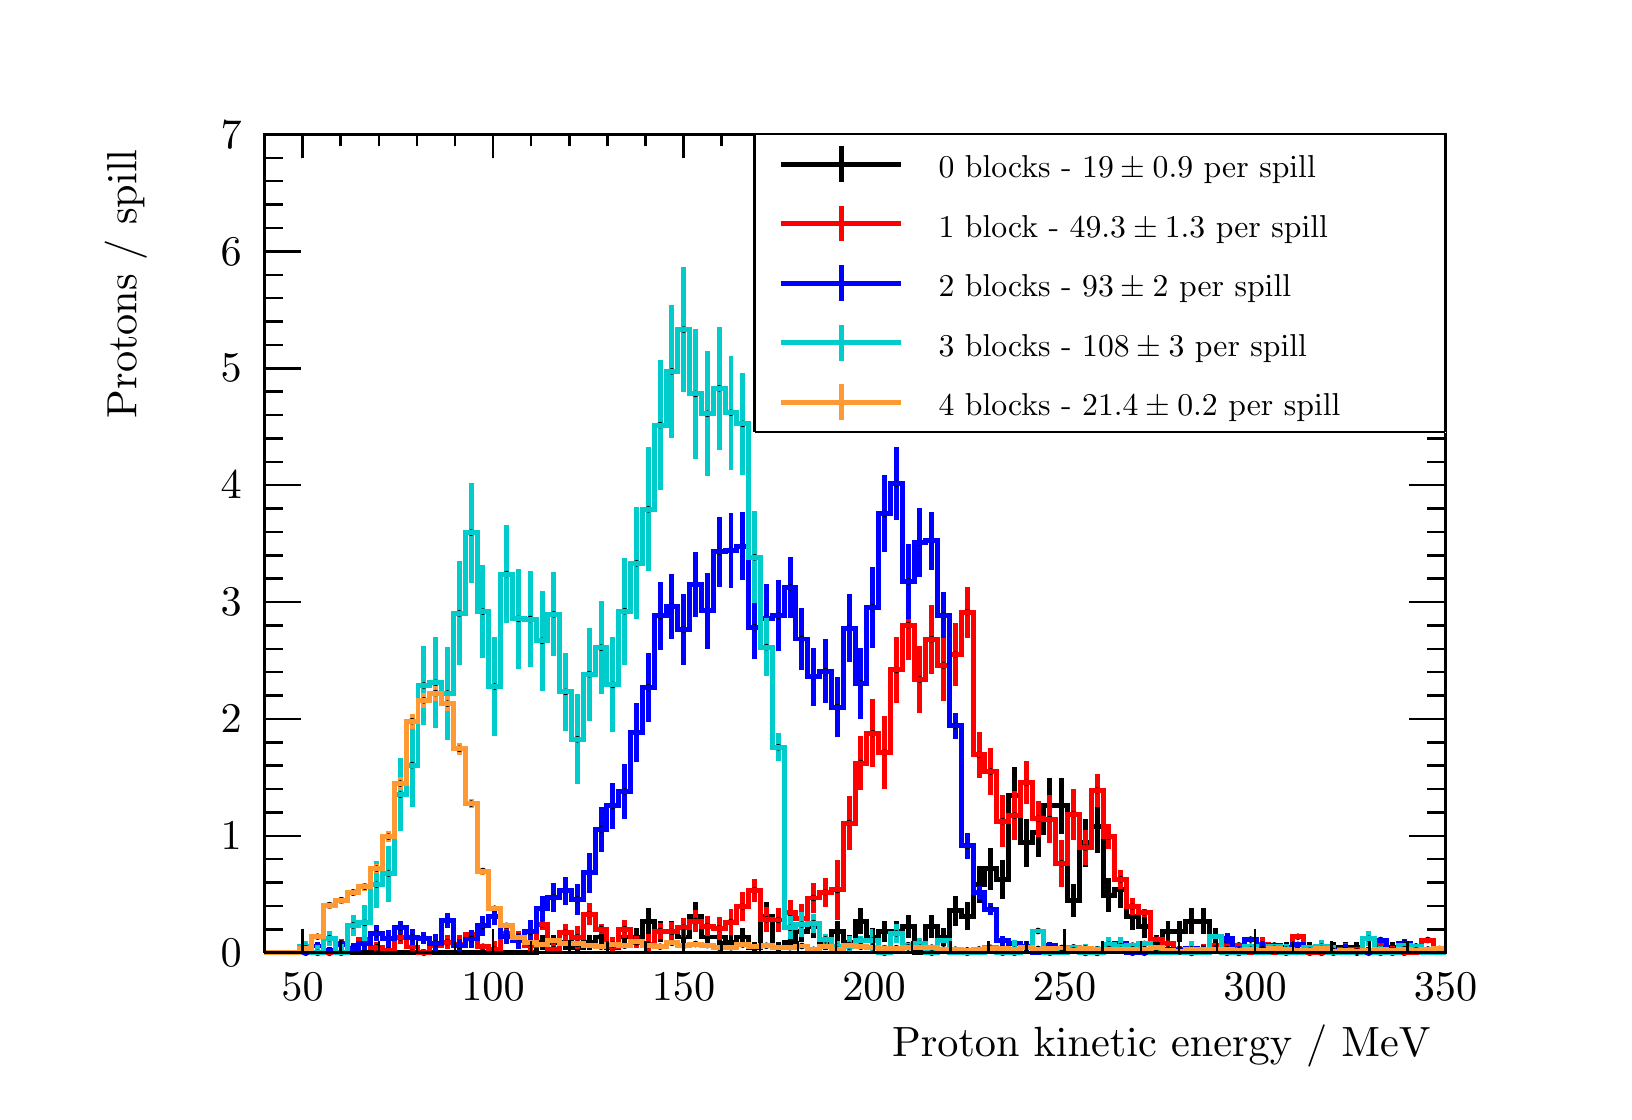
\begin{tikzpicture}
\pgfdeclareplotmark{cross} {
\pgfpathmoveto{\pgfpoint{-0.3\pgfplotmarksize}{\pgfplotmarksize}}
\pgfpathlineto{\pgfpoint{+0.3\pgfplotmarksize}{\pgfplotmarksize}}
\pgfpathlineto{\pgfpoint{+0.3\pgfplotmarksize}{0.3\pgfplotmarksize}}
\pgfpathlineto{\pgfpoint{+1\pgfplotmarksize}{0.3\pgfplotmarksize}}
\pgfpathlineto{\pgfpoint{+1\pgfplotmarksize}{-0.3\pgfplotmarksize}}
\pgfpathlineto{\pgfpoint{+0.3\pgfplotmarksize}{-0.3\pgfplotmarksize}}
\pgfpathlineto{\pgfpoint{+0.3\pgfplotmarksize}{-1.\pgfplotmarksize}}
\pgfpathlineto{\pgfpoint{-0.3\pgfplotmarksize}{-1.\pgfplotmarksize}}
\pgfpathlineto{\pgfpoint{-0.3\pgfplotmarksize}{-0.3\pgfplotmarksize}}
\pgfpathlineto{\pgfpoint{-1.\pgfplotmarksize}{-0.3\pgfplotmarksize}}
\pgfpathlineto{\pgfpoint{-1.\pgfplotmarksize}{0.3\pgfplotmarksize}}
\pgfpathlineto{\pgfpoint{-0.3\pgfplotmarksize}{0.3\pgfplotmarksize}}
\pgfpathclose
\pgfusepathqstroke
}
\pgfdeclareplotmark{cross*} {
\pgfpathmoveto{\pgfpoint{-0.3\pgfplotmarksize}{\pgfplotmarksize}}
\pgfpathlineto{\pgfpoint{+0.3\pgfplotmarksize}{\pgfplotmarksize}}
\pgfpathlineto{\pgfpoint{+0.3\pgfplotmarksize}{0.3\pgfplotmarksize}}
\pgfpathlineto{\pgfpoint{+1\pgfplotmarksize}{0.3\pgfplotmarksize}}
\pgfpathlineto{\pgfpoint{+1\pgfplotmarksize}{-0.3\pgfplotmarksize}}
\pgfpathlineto{\pgfpoint{+0.3\pgfplotmarksize}{-0.3\pgfplotmarksize}}
\pgfpathlineto{\pgfpoint{+0.3\pgfplotmarksize}{-1.\pgfplotmarksize}}
\pgfpathlineto{\pgfpoint{-0.3\pgfplotmarksize}{-1.\pgfplotmarksize}}
\pgfpathlineto{\pgfpoint{-0.3\pgfplotmarksize}{-0.3\pgfplotmarksize}}
\pgfpathlineto{\pgfpoint{-1.\pgfplotmarksize}{-0.3\pgfplotmarksize}}
\pgfpathlineto{\pgfpoint{-1.\pgfplotmarksize}{0.3\pgfplotmarksize}}
\pgfpathlineto{\pgfpoint{-0.3\pgfplotmarksize}{0.3\pgfplotmarksize}}
\pgfpathclose
\pgfusepathqfillstroke
}
\pgfdeclareplotmark{newstar} {
\pgfpathmoveto{\pgfqpoint{0pt}{\pgfplotmarksize}}
\pgfpathlineto{\pgfqpointpolar{44}{0.5\pgfplotmarksize}}
\pgfpathlineto{\pgfqpointpolar{18}{\pgfplotmarksize}}
\pgfpathlineto{\pgfqpointpolar{-20}{0.5\pgfplotmarksize}}
\pgfpathlineto{\pgfqpointpolar{-54}{\pgfplotmarksize}}
\pgfpathlineto{\pgfqpointpolar{-90}{0.5\pgfplotmarksize}}
\pgfpathlineto{\pgfqpointpolar{234}{\pgfplotmarksize}}
\pgfpathlineto{\pgfqpointpolar{198}{0.5\pgfplotmarksize}}
\pgfpathlineto{\pgfqpointpolar{162}{\pgfplotmarksize}}
\pgfpathlineto{\pgfqpointpolar{134}{0.5\pgfplotmarksize}}
\pgfpathclose
\pgfusepathqstroke
}
\pgfdeclareplotmark{newstar*} {
\pgfpathmoveto{\pgfqpoint{0pt}{\pgfplotmarksize}}
\pgfpathlineto{\pgfqpointpolar{44}{0.5\pgfplotmarksize}}
\pgfpathlineto{\pgfqpointpolar{18}{\pgfplotmarksize}}
\pgfpathlineto{\pgfqpointpolar{-20}{0.5\pgfplotmarksize}}
\pgfpathlineto{\pgfqpointpolar{-54}{\pgfplotmarksize}}
\pgfpathlineto{\pgfqpointpolar{-90}{0.5\pgfplotmarksize}}
\pgfpathlineto{\pgfqpointpolar{234}{\pgfplotmarksize}}
\pgfpathlineto{\pgfqpointpolar{198}{0.5\pgfplotmarksize}}
\pgfpathlineto{\pgfqpointpolar{162}{\pgfplotmarksize}}
\pgfpathlineto{\pgfqpointpolar{134}{0.5\pgfplotmarksize}}
\pgfpathclose
\pgfusepathqfillstroke
}
\definecolor{c}{rgb}{1,1,1};
\draw [color=c, fill=c] (0,0) rectangle (20,13.4957);
\draw [color=c, fill=c] (3,1.75444) rectangle (18,12.1461);
\definecolor{c}{rgb}{0,0,0};
\draw [c,line width=0.9] (3,1.75444) -- (3,12.1461) -- (18,12.1461) -- (18,1.75444) -- (3,1.75444);
\definecolor{c}{rgb}{1,1,1};
\draw [color=c, fill=c] (3,1.75444) rectangle (18,12.1461);
\definecolor{c}{rgb}{0,0,0};
\draw [c,line width=0.9] (3,1.75444) -- (3,12.1461) -- (18,12.1461) -- (18,1.75444) -- (3,1.75444);
\draw [c,line width=0.9] (3,1.75444) -- (3.15,1.75444) -- (3.15,1.75444) -- (3.3,1.75444) -- (3.3,1.75444) -- (3.45,1.75444) -- (3.45,1.75444) -- (3.6,1.75444) -- (3.6,1.75444) -- (3.75,1.75444) -- (3.75,1.75444) -- (3.9,1.75444) -- (3.9,1.75444) --
 (4.05,1.75444) -- (4.05,1.75444) -- (4.2,1.75444) -- (4.2,1.75444) -- (4.35,1.75444) -- (4.35,1.75444) -- (4.5,1.75444) -- (4.5,1.75444) -- (4.65,1.75444) -- (4.65,1.75444) -- (4.8,1.75444) -- (4.8,1.75444) -- (4.95,1.75444) -- (4.95,1.75444) --
 (5.1,1.75444) -- (5.1,1.75444) -- (5.25,1.75444) -- (5.25,1.75444) -- (5.4,1.75444) -- (5.4,1.75444) -- (5.55,1.75444) -- (5.55,1.75444) -- (5.7,1.75444) -- (5.7,1.75444) -- (5.85,1.75444) -- (5.85,1.75444) -- (6,1.75444) -- (6,1.75444) --
 (6.15,1.75444) -- (6.15,1.75444) -- (6.3,1.75444) -- (6.3,1.75444) -- (6.45,1.75444) -- (6.45,1.75444) -- (6.6,1.75444) -- (6.6,1.75444) -- (6.75,1.75444) -- (6.75,1.75444) -- (6.9,1.75444) -- (6.9,1.75444) -- (7.05,1.75444) -- (7.05,1.75444) --
 (7.2,1.75444) -- (7.2,1.75444) -- (7.35,1.75444) -- (7.35,1.75444) -- (7.5,1.75444) -- (7.5,1.75444) -- (7.65,1.75444) -- (7.65,1.75444) -- (7.8,1.75444) -- (7.8,1.75444) -- (7.95,1.75444) -- (7.95,1.75444) -- (8.1,1.75444) -- (8.1,1.75444) --
 (8.25,1.75444) -- (8.25,1.75444) -- (8.4,1.75444) -- (8.4,1.75444) -- (8.55,1.75444) -- (8.55,1.75444) -- (8.7,1.75444) -- (8.7,1.75444) -- (8.85,1.75444) -- (8.85,1.75444) -- (9,1.75444) -- (9,1.75444) -- (9.15,1.75444) -- (9.15,1.75444) --
 (9.3,1.75444) -- (9.3,1.75444) -- (9.45,1.75444) -- (9.45,1.75444) -- (9.6,1.75444) -- (9.6,1.75444) -- (9.75,1.75444) -- (9.75,1.75444) -- (9.9,1.75444) -- (9.9,1.75444) -- (10.05,1.75444) -- (10.05,1.75444) -- (10.2,1.75444) -- (10.2,1.75444) --
 (10.35,1.75444) -- (10.35,1.75444) -- (10.5,1.75444) -- (10.5,1.75444) -- (10.65,1.75444) -- (10.65,1.75444) -- (10.8,1.75444) -- (10.8,1.75444) -- (10.95,1.75444) -- (10.95,1.75444) -- (11.1,1.75444) -- (11.1,1.75444) -- (11.25,1.75444) --
 (11.25,1.75444) -- (11.4,1.75444) -- (11.4,1.75444) -- (11.55,1.75444) -- (11.55,1.75444) -- (11.7,1.75444) -- (11.7,1.75444) -- (11.85,1.75444) -- (11.85,1.75444) -- (12,1.75444) -- (12,1.75444) -- (12.15,1.75444) -- (12.15,1.75444) --
 (12.3,1.75444) -- (12.3,1.75444) -- (12.45,1.75444) -- (12.45,1.75444) -- (12.6,1.75444) -- (12.6,1.75444) -- (12.75,1.75444) -- (12.75,1.75444) -- (12.9,1.75444) -- (12.9,1.75444) -- (13.05,1.75444) -- (13.05,1.75444) -- (13.2,1.75444) --
 (13.2,1.75444) -- (13.35,1.75444) -- (13.35,1.75444) -- (13.5,1.75444) -- (13.5,1.75444) -- (13.65,1.75444) -- (13.65,1.75444) -- (13.8,1.75444) -- (13.8,1.75444) -- (13.95,1.75444) -- (13.95,1.75444) -- (14.1,1.75444) -- (14.1,1.75444) --
 (14.25,1.75444) -- (14.25,1.75444) -- (14.4,1.75444) -- (14.4,1.75444) -- (14.55,1.75444) -- (14.55,1.75444) -- (14.7,1.75444) -- (14.7,1.75444) -- (14.85,1.75444) -- (14.85,1.75444) -- (15,1.75444) -- (15,1.75444) -- (15.15,1.75444) --
 (15.15,1.75444) -- (15.3,1.75444) -- (15.3,1.75444) -- (15.45,1.75444) -- (15.45,1.75444) -- (15.6,1.75444) -- (15.6,1.75444) -- (15.75,1.75444) -- (15.75,1.75444) -- (15.9,1.75444) -- (15.9,1.75444) -- (16.05,1.75444) -- (16.05,1.75444) --
 (16.2,1.75444) -- (16.2,1.75444) -- (16.35,1.75444) -- (16.35,1.75444) -- (16.5,1.75444) -- (16.5,1.75444) -- (16.65,1.75444) -- (16.65,1.75444) -- (16.8,1.75444) -- (16.8,1.75444) -- (16.95,1.75444) -- (16.95,1.75444) -- (17.1,1.75444) --
 (17.1,1.75444) -- (17.25,1.75444) -- (17.25,1.75444) -- (17.4,1.75444) -- (17.4,1.75444) -- (17.55,1.75444) -- (17.55,1.75444) -- (17.7,1.75444) -- (17.7,1.75444) -- (17.85,1.75444) -- (17.85,1.75444) -- (18,1.75444);
\draw [c,line width=0.9] (3,1.75444) -- (18,1.75444);
\draw [c,line width=0.9] (3.48387,2.05809) -- (3.48387,1.75444);
\draw [c,line width=0.9] (3.96774,1.90627) -- (3.96774,1.75444);
\draw [c,line width=0.9] (4.45161,1.90627) -- (4.45161,1.75444);
\draw [c,line width=0.9] (4.93548,1.90627) -- (4.93548,1.75444);
\draw [c,line width=0.9] (5.41935,1.90627) -- (5.41935,1.75444);
\draw [c,line width=0.9] (5.90323,2.05809) -- (5.90323,1.75444);
\draw [c,line width=0.9] (6.3871,1.90627) -- (6.3871,1.75444);
\draw [c,line width=0.9] (6.87097,1.90627) -- (6.87097,1.75444);
\draw [c,line width=0.9] (7.35484,1.90627) -- (7.35484,1.75444);
\draw [c,line width=0.9] (7.83871,1.90627) -- (7.83871,1.75444);
\draw [c,line width=0.9] (8.32258,2.05809) -- (8.32258,1.75444);
\draw [c,line width=0.9] (8.80645,1.90627) -- (8.80645,1.75444);
\draw [c,line width=0.9] (9.29032,1.90627) -- (9.29032,1.75444);
\draw [c,line width=0.9] (9.77419,1.90627) -- (9.77419,1.75444);
\draw [c,line width=0.9] (10.2581,1.90627) -- (10.2581,1.75444);
\draw [c,line width=0.9] (10.7419,2.05809) -- (10.7419,1.75444);
\draw [c,line width=0.9] (11.2258,1.90627) -- (11.2258,1.75444);
\draw [c,line width=0.9] (11.7097,1.90627) -- (11.7097,1.75444);
\draw [c,line width=0.9] (12.1935,1.90627) -- (12.1935,1.75444);
\draw [c,line width=0.9] (12.6774,1.90627) -- (12.6774,1.75444);
\draw [c,line width=0.9] (13.1613,2.05809) -- (13.1613,1.75444);
\draw [c,line width=0.9] (13.6452,1.90627) -- (13.6452,1.75444);
\draw [c,line width=0.9] (14.129,1.90627) -- (14.129,1.75444);
\draw [c,line width=0.9] (14.6129,1.90627) -- (14.6129,1.75444);
\draw [c,line width=0.9] (15.0968,1.90627) -- (15.0968,1.75444);
\draw [c,line width=0.9] (15.5806,2.05809) -- (15.5806,1.75444);
\draw [c,line width=0.9] (16.0645,1.90627) -- (16.0645,1.75444);
\draw [c,line width=0.9] (16.5484,1.90627) -- (16.5484,1.75444);
\draw [c,line width=0.9] (17.0323,1.90627) -- (17.0323,1.75444);
\draw [c,line width=0.9] (17.5161,1.90627) -- (17.5161,1.75444);
\draw [c,line width=0.9] (18,2.05809) -- (18,1.75444);
\draw [c,line width=0.9] (3.48387,2.05809) -- (3.48387,1.75444);
\draw [c,line width=0.9] (18,2.05809) -- (18,1.75444);
\draw [anchor=base] (3.48387,1.14713) node[scale=1.52731, color=c, rotate=0]{50};
\draw [anchor=base] (5.90323,1.14713) node[scale=1.52731, color=c, rotate=0]{100};
\draw [anchor=base] (8.32258,1.14713) node[scale=1.52731, color=c, rotate=0]{150};
\draw [anchor=base] (10.7419,1.14713) node[scale=1.52731, color=c, rotate=0]{200};
\draw [anchor=base] (13.1613,1.14713) node[scale=1.52731, color=c, rotate=0]{250};
\draw [anchor=base] (15.5806,1.14713) node[scale=1.52731, color=c, rotate=0]{300};
\draw [anchor=base] (18,1.14713) node[scale=1.52731, color=c, rotate=0]{350};
\draw [anchor= east] (18,0.566819) node[scale=1.52731, color=c, rotate=0]{ Proton kinetic energy / MeV};
\draw [c,line width=0.9] (3,12.1461) -- (18,12.1461);
\draw [c,line width=0.9] (3.48387,11.8425) -- (3.48387,12.1461);
\draw [c,line width=0.9] (3.96774,11.9943) -- (3.96774,12.1461);
\draw [c,line width=0.9] (4.45161,11.9943) -- (4.45161,12.1461);
\draw [c,line width=0.9] (4.93548,11.9943) -- (4.93548,12.1461);
\draw [c,line width=0.9] (5.41935,11.9943) -- (5.41935,12.1461);
\draw [c,line width=0.9] (5.90323,11.8425) -- (5.90323,12.1461);
\draw [c,line width=0.9] (6.3871,11.9943) -- (6.3871,12.1461);
\draw [c,line width=0.9] (6.87097,11.9943) -- (6.87097,12.1461);
\draw [c,line width=0.9] (7.35484,11.9943) -- (7.35484,12.1461);
\draw [c,line width=0.9] (7.83871,11.9943) -- (7.83871,12.1461);
\draw [c,line width=0.9] (8.32258,11.8425) -- (8.32258,12.1461);
\draw [c,line width=0.9] (8.80645,11.9943) -- (8.80645,12.1461);
\draw [c,line width=0.9] (9.29032,11.9943) -- (9.29032,12.1461);
\draw [c,line width=0.9] (9.77419,11.9943) -- (9.77419,12.1461);
\draw [c,line width=0.9] (10.2581,11.9943) -- (10.2581,12.1461);
\draw [c,line width=0.9] (10.7419,11.8425) -- (10.7419,12.1461);
\draw [c,line width=0.9] (11.2258,11.9943) -- (11.2258,12.1461);
\draw [c,line width=0.9] (11.7097,11.9943) -- (11.7097,12.1461);
\draw [c,line width=0.9] (12.1935,11.9943) -- (12.1935,12.1461);
\draw [c,line width=0.9] (12.6774,11.9943) -- (12.6774,12.1461);
\draw [c,line width=0.9] (13.1613,11.8425) -- (13.1613,12.1461);
\draw [c,line width=0.9] (13.6452,11.9943) -- (13.6452,12.1461);
\draw [c,line width=0.9] (14.129,11.9943) -- (14.129,12.1461);
\draw [c,line width=0.9] (14.6129,11.9943) -- (14.6129,12.1461);
\draw [c,line width=0.9] (15.0968,11.9943) -- (15.0968,12.1461);
\draw [c,line width=0.9] (15.5806,11.8425) -- (15.5806,12.1461);
\draw [c,line width=0.9] (16.0645,11.9943) -- (16.0645,12.1461);
\draw [c,line width=0.9] (16.5484,11.9943) -- (16.5484,12.1461);
\draw [c,line width=0.9] (17.0323,11.9943) -- (17.0323,12.1461);
\draw [c,line width=0.9] (17.5161,11.9943) -- (17.5161,12.1461);
\draw [c,line width=0.9] (18,11.8425) -- (18,12.1461);
\draw [c,line width=0.9] (3.48387,11.8425) -- (3.48387,12.1461);
\draw [c,line width=0.9] (18,11.8425) -- (18,12.1461);
\draw [c,line width=0.9] (3,1.75444) -- (3,12.1461);
\draw [c,line width=0.9] (3.462,1.75444) -- (3,1.75444);
\draw [c,line width=0.9] (3.231,2.05135) -- (3,2.05135);
\draw [c,line width=0.9] (3.231,2.34825) -- (3,2.34825);
\draw [c,line width=0.9] (3.231,2.64516) -- (3,2.64516);
\draw [c,line width=0.9] (3.231,2.94206) -- (3,2.94206);
\draw [c,line width=0.9] (3.462,3.23897) -- (3,3.23897);
\draw [c,line width=0.9] (3.231,3.53587) -- (3,3.53587);
\draw [c,line width=0.9] (3.231,3.83278) -- (3,3.83278);
\draw [c,line width=0.9] (3.231,4.12968) -- (3,4.12968);
\draw [c,line width=0.9] (3.231,4.42659) -- (3,4.42659);
\draw [c,line width=0.9] (3.462,4.7235) -- (3,4.7235);
\draw [c,line width=0.9] (3.231,5.0204) -- (3,5.0204);
\draw [c,line width=0.9] (3.231,5.31731) -- (3,5.31731);
\draw [c,line width=0.9] (3.231,5.61421) -- (3,5.61421);
\draw [c,line width=0.9] (3.231,5.91112) -- (3,5.91112);
\draw [c,line width=0.9] (3.462,6.20802) -- (3,6.20802);
\draw [c,line width=0.9] (3.231,6.50493) -- (3,6.50493);
\draw [c,line width=0.9] (3.231,6.80183) -- (3,6.80183);
\draw [c,line width=0.9] (3.231,7.09874) -- (3,7.09874);
\draw [c,line width=0.9] (3.231,7.39564) -- (3,7.39564);
\draw [c,line width=0.9] (3.462,7.69255) -- (3,7.69255);
\draw [c,line width=0.9] (3.231,7.98946) -- (3,7.98946);
\draw [c,line width=0.9] (3.231,8.28636) -- (3,8.28636);
\draw [c,line width=0.9] (3.231,8.58327) -- (3,8.58327);
\draw [c,line width=0.9] (3.231,8.88017) -- (3,8.88017);
\draw [c,line width=0.9] (3.462,9.17708) -- (3,9.17708);
\draw [c,line width=0.9] (3.231,9.47398) -- (3,9.47398);
\draw [c,line width=0.9] (3.231,9.77089) -- (3,9.77089);
\draw [c,line width=0.9] (3.231,10.0678) -- (3,10.0678);
\draw [c,line width=0.9] (3.231,10.3647) -- (3,10.3647);
\draw [c,line width=0.9] (3.462,10.6616) -- (3,10.6616);
\draw [c,line width=0.9] (3.231,10.9585) -- (3,10.9585);
\draw [c,line width=0.9] (3.231,11.2554) -- (3,11.2554);
\draw [c,line width=0.9] (3.231,11.5523) -- (3,11.5523);
\draw [c,line width=0.9] (3.231,11.8492) -- (3,11.8492);
\draw [c,line width=0.9] (3.462,12.1461) -- (3,12.1461);
\draw [anchor= east] (2.9,1.75444) node[scale=1.52731, color=c, rotate=0]{0};
\draw [anchor= east] (2.9,3.23897) node[scale=1.52731, color=c, rotate=0]{1};
\draw [anchor= east] (2.9,4.7235) node[scale=1.52731, color=c, rotate=0]{2};
\draw [anchor= east] (2.9,6.20802) node[scale=1.52731, color=c, rotate=0]{3};
\draw [anchor= east] (2.9,7.69255) node[scale=1.52731, color=c, rotate=0]{4};
\draw [anchor= east] (2.9,9.17708) node[scale=1.52731, color=c, rotate=0]{5};
\draw [anchor= east] (2.9,10.6616) node[scale=1.52731, color=c, rotate=0]{6};
\draw [anchor= east] (2.9,12.1461) node[scale=1.52731, color=c, rotate=0]{7};
\draw [anchor= east] (1.24,12.1461) node[scale=1.52731, color=c, rotate=90]{ Protons / spill};
\draw [c,line width=0.9] (18,1.75444) -- (18,12.1461);
\draw [c,line width=0.9] (17.538,1.75444) -- (18,1.75444);
\draw [c,line width=0.9] (17.769,2.05135) -- (18,2.05135);
\draw [c,line width=0.9] (17.769,2.34825) -- (18,2.34825);
\draw [c,line width=0.9] (17.769,2.64516) -- (18,2.64516);
\draw [c,line width=0.9] (17.769,2.94206) -- (18,2.94206);
\draw [c,line width=0.9] (17.538,3.23897) -- (18,3.23897);
\draw [c,line width=0.9] (17.769,3.53587) -- (18,3.53587);
\draw [c,line width=0.9] (17.769,3.83278) -- (18,3.83278);
\draw [c,line width=0.9] (17.769,4.12968) -- (18,4.12968);
\draw [c,line width=0.9] (17.769,4.42659) -- (18,4.42659);
\draw [c,line width=0.9] (17.538,4.7235) -- (18,4.7235);
\draw [c,line width=0.9] (17.769,5.0204) -- (18,5.0204);
\draw [c,line width=0.9] (17.769,5.31731) -- (18,5.31731);
\draw [c,line width=0.9] (17.769,5.61421) -- (18,5.61421);
\draw [c,line width=0.9] (17.769,5.91112) -- (18,5.91112);
\draw [c,line width=0.9] (17.538,6.20802) -- (18,6.20802);
\draw [c,line width=0.9] (17.769,6.50493) -- (18,6.50493);
\draw [c,line width=0.9] (17.769,6.80183) -- (18,6.80183);
\draw [c,line width=0.9] (17.769,7.09874) -- (18,7.09874);
\draw [c,line width=0.9] (17.769,7.39564) -- (18,7.39564);
\draw [c,line width=0.9] (17.538,7.69255) -- (18,7.69255);
\draw [c,line width=0.9] (17.769,7.98946) -- (18,7.98946);
\draw [c,line width=0.9] (17.769,8.28636) -- (18,8.28636);
\draw [c,line width=0.9] (17.769,8.58327) -- (18,8.58327);
\draw [c,line width=0.9] (17.769,8.88017) -- (18,8.88017);
\draw [c,line width=0.9] (17.538,9.17708) -- (18,9.17708);
\draw [c,line width=0.9] (17.769,9.47398) -- (18,9.47398);
\draw [c,line width=0.9] (17.769,9.77089) -- (18,9.77089);
\draw [c,line width=0.9] (17.769,10.0678) -- (18,10.0678);
\draw [c,line width=0.9] (17.769,10.3647) -- (18,10.3647);
\draw [c,line width=0.9] (17.538,10.6616) -- (18,10.6616);
\draw [c,line width=0.9] (17.769,10.9585) -- (18,10.9585);
\draw [c,line width=0.9] (17.769,11.2554) -- (18,11.2554);
\draw [c,line width=0.9] (17.769,11.5523) -- (18,11.5523);
\draw [c,line width=0.9] (17.769,11.8492) -- (18,11.8492);
\draw [c,line width=0.9] (17.538,12.1461) -- (18,12.1461);
\draw [c,line width=1.8] (6.525,1.79346) -- (6.525,1.88768);
\draw [c,line width=1.8] (6.525,1.88768) -- (6.525,1.9819);
\foreach \P in {(6.525,1.88768)}{\draw[mark options={color=c,fill=c},mark size=2.402402pt,mark=*,mark size=1pt] plot coordinates {\P};}
\draw [c,line width=1.8] (6.675,1.79346) -- (6.675,1.88768);
\draw [c,line width=1.8] (6.675,1.88768) -- (6.675,1.9819);
\foreach \P in {(6.675,1.88768)}{\draw[mark options={color=c,fill=c},mark size=2.402402pt,mark=*,mark size=1pt] plot coordinates {\P};}
\draw [c,line width=1.8] (6.825,1.79346) -- (6.825,1.88768);
\draw [c,line width=1.8] (6.825,1.88768) -- (6.825,1.9819);
\foreach \P in {(6.825,1.88768)}{\draw[mark options={color=c,fill=c},mark size=2.402402pt,mark=*,mark size=1pt] plot coordinates {\P};}
\draw [c,line width=1.8] (6.975,1.75444) -- (6.975,1.82106);
\draw [c,line width=1.8] (6.975,1.82106) -- (6.975,1.88769);
\foreach \P in {(6.975,1.82106)}{\draw[mark options={color=c,fill=c},mark size=2.402402pt,mark=*,mark size=1pt] plot coordinates {\P};}
\draw [c,line width=1.8] (7.125,1.79346) -- (7.125,1.88768);
\draw [c,line width=1.8] (7.125,1.88768) -- (7.125,1.9819);
\foreach \P in {(7.125,1.88768)}{\draw[mark options={color=c,fill=c},mark size=2.402402pt,mark=*,mark size=1pt] plot coordinates {\P};}
\draw [c,line width=1.8] (7.275,1.83891) -- (7.275,1.9543);
\draw [c,line width=1.8] (7.275,1.9543) -- (7.275,2.0697);
\foreach \P in {(7.275,1.9543)}{\draw[mark options={color=c,fill=c},mark size=2.402402pt,mark=*,mark size=1pt] plot coordinates {\P};}
\draw [c,line width=1.8] (7.425,1.75444) -- (7.425,1.82106);
\draw [c,line width=1.8] (7.425,1.82106) -- (7.425,1.88769);
\foreach \P in {(7.425,1.82106)}{\draw[mark options={color=c,fill=c},mark size=2.402402pt,mark=*,mark size=1pt] plot coordinates {\P};}
\draw [c,line width=1.8] (7.575,1.83891) -- (7.575,1.9543);
\draw [c,line width=1.8] (7.575,1.9543) -- (7.575,2.0697);
\foreach \P in {(7.575,1.9543)}{\draw[mark options={color=c,fill=c},mark size=2.402402pt,mark=*,mark size=1pt] plot coordinates {\P};}
\draw [c,line width=1.8] (7.725,1.83891) -- (7.725,1.9543);
\draw [c,line width=1.8] (7.725,1.9543) -- (7.725,2.0697);
\foreach \P in {(7.725,1.9543)}{\draw[mark options={color=c,fill=c},mark size=2.402402pt,mark=*,mark size=1pt] plot coordinates {\P};}
\draw [c,line width=1.8] (7.875,1.99097) -- (7.875,2.15417);
\draw [c,line width=1.8] (7.875,2.15417) -- (7.875,2.31736);
\foreach \P in {(7.875,2.15417)}{\draw[mark options={color=c,fill=c},mark size=2.402402pt,mark=*,mark size=1pt] plot coordinates {\P};}
\draw [c,line width=1.8] (8.025,1.88767) -- (8.025,2.02092);
\draw [c,line width=1.8] (8.025,2.02092) -- (8.025,2.15417);
\foreach \P in {(8.025,2.02092)}{\draw[mark options={color=c,fill=c},mark size=2.402402pt,mark=*,mark size=1pt] plot coordinates {\P};}
\draw [c,line width=1.8] (8.175,1.88767) -- (8.175,2.02092);
\draw [c,line width=1.8] (8.175,2.02092) -- (8.175,2.15417);
\foreach \P in {(8.175,2.02092)}{\draw[mark options={color=c,fill=c},mark size=2.402402pt,mark=*,mark size=1pt] plot coordinates {\P};}
\draw [c,line width=1.8] (8.325,1.83891) -- (8.325,1.9543);
\draw [c,line width=1.8] (8.325,1.9543) -- (8.325,2.0697);
\foreach \P in {(8.325,1.9543)}{\draw[mark options={color=c,fill=c},mark size=2.402402pt,mark=*,mark size=1pt] plot coordinates {\P};}
\draw [c,line width=1.8] (8.475,2.04451) -- (8.475,2.22079);
\draw [c,line width=1.8] (8.475,2.22079) -- (8.475,2.39706);
\foreach \P in {(8.475,2.22079)}{\draw[mark options={color=c,fill=c},mark size=2.402402pt,mark=*,mark size=1pt] plot coordinates {\P};}
\draw [c,line width=1.8] (8.625,1.83891) -- (8.625,1.9543);
\draw [c,line width=1.8] (8.625,1.9543) -- (8.625,2.0697);
\foreach \P in {(8.625,1.9543)}{\draw[mark options={color=c,fill=c},mark size=2.402402pt,mark=*,mark size=1pt] plot coordinates {\P};}
\draw [c,line width=1.8] (8.775,1.83891) -- (8.775,1.9543);
\draw [c,line width=1.8] (8.775,1.9543) -- (8.775,2.0697);
\foreach \P in {(8.775,1.9543)}{\draw[mark options={color=c,fill=c},mark size=2.402402pt,mark=*,mark size=1pt] plot coordinates {\P};}
\draw [c,line width=1.8] (8.925,1.79346) -- (8.925,1.88768);
\draw [c,line width=1.8] (8.925,1.88768) -- (8.925,1.9819);
\foreach \P in {(8.925,1.88768)}{\draw[mark options={color=c,fill=c},mark size=2.402402pt,mark=*,mark size=1pt] plot coordinates {\P};}
\draw [c,line width=1.8] (9.075,1.83891) -- (9.075,1.9543);
\draw [c,line width=1.8] (9.075,1.9543) -- (9.075,2.0697);
\foreach \P in {(9.075,1.9543)}{\draw[mark options={color=c,fill=c},mark size=2.402402pt,mark=*,mark size=1pt] plot coordinates {\P};}
\draw [c,line width=1.8] (9.225,1.75444) -- (9.225,1.82106);
\draw [c,line width=1.8] (9.225,1.82106) -- (9.225,1.88769);
\foreach \P in {(9.225,1.82106)}{\draw[mark options={color=c,fill=c},mark size=2.402402pt,mark=*,mark size=1pt] plot coordinates {\P};}
\draw [c,line width=1.8] (9.375,2.04451) -- (9.375,2.22079);
\draw [c,line width=1.8] (9.375,2.22079) -- (9.375,2.39706);
\foreach \P in {(9.375,2.22079)}{\draw[mark options={color=c,fill=c},mark size=2.402402pt,mark=*,mark size=1pt] plot coordinates {\P};}
\draw [c,line width=1.8] (9.525,1.75444) -- (9.525,1.82106);
\draw [c,line width=1.8] (9.525,1.82106) -- (9.525,1.88769);
\foreach \P in {(9.525,1.82106)}{\draw[mark options={color=c,fill=c},mark size=2.402402pt,mark=*,mark size=1pt] plot coordinates {\P};}
\draw [c,line width=1.8] (9.675,1.79346) -- (9.675,1.88768);
\draw [c,line width=1.8] (9.675,1.88768) -- (9.675,1.9819);
\foreach \P in {(9.675,1.88768)}{\draw[mark options={color=c,fill=c},mark size=2.402402pt,mark=*,mark size=1pt] plot coordinates {\P};}
\draw [c,line width=1.8] (9.825,1.88767) -- (9.825,2.02092);
\draw [c,line width=1.8] (9.825,2.02092) -- (9.825,2.15417);
\foreach \P in {(9.825,2.02092)}{\draw[mark options={color=c,fill=c},mark size=2.402402pt,mark=*,mark size=1pt] plot coordinates {\P};}
\draw [c,line width=1.8] (9.975,1.93857) -- (9.975,2.08755);
\draw [c,line width=1.8] (9.975,2.08755) -- (9.975,2.23652);
\foreach \P in {(9.975,2.08755)}{\draw[mark options={color=c,fill=c},mark size=2.402402pt,mark=*,mark size=1pt] plot coordinates {\P};}
\draw [c,line width=1.8] (10.125,1.79346) -- (10.125,1.88768);
\draw [c,line width=1.8] (10.125,1.88768) -- (10.125,1.9819);
\foreach \P in {(10.125,1.88768)}{\draw[mark options={color=c,fill=c},mark size=2.402402pt,mark=*,mark size=1pt] plot coordinates {\P};}
\draw [c,line width=1.8] (10.275,1.88767) -- (10.275,2.02092);
\draw [c,line width=1.8] (10.275,2.02092) -- (10.275,2.15417);
\foreach \P in {(10.275,2.02092)}{\draw[mark options={color=c,fill=c},mark size=2.402402pt,mark=*,mark size=1pt] plot coordinates {\P};}
\draw [c,line width=1.8] (10.425,1.79346) -- (10.425,1.88768);
\draw [c,line width=1.8] (10.425,1.88768) -- (10.425,1.9819);
\foreach \P in {(10.425,1.88768)}{\draw[mark options={color=c,fill=c},mark size=2.402402pt,mark=*,mark size=1pt] plot coordinates {\P};}
\draw [c,line width=1.8] (10.575,1.99097) -- (10.575,2.15417);
\draw [c,line width=1.8] (10.575,2.15417) -- (10.575,2.31736);
\foreach \P in {(10.575,2.15417)}{\draw[mark options={color=c,fill=c},mark size=2.402402pt,mark=*,mark size=1pt] plot coordinates {\P};}
\draw [c,line width=1.8] (10.725,1.83891) -- (10.725,1.9543);
\draw [c,line width=1.8] (10.725,1.9543) -- (10.725,2.0697);
\foreach \P in {(10.725,1.9543)}{\draw[mark options={color=c,fill=c},mark size=2.402402pt,mark=*,mark size=1pt] plot coordinates {\P};}
\draw [c,line width=1.8] (10.875,1.88767) -- (10.875,2.02092);
\draw [c,line width=1.8] (10.875,2.02092) -- (10.875,2.15417);
\foreach \P in {(10.875,2.02092)}{\draw[mark options={color=c,fill=c},mark size=2.402402pt,mark=*,mark size=1pt] plot coordinates {\P};}
\draw [c,line width=1.8] (11.025,1.88767) -- (11.025,2.02092);
\draw [c,line width=1.8] (11.025,2.02092) -- (11.025,2.15417);
\foreach \P in {(11.025,2.02092)}{\draw[mark options={color=c,fill=c},mark size=2.402402pt,mark=*,mark size=1pt] plot coordinates {\P};}
\draw [c,line width=1.8] (11.175,1.93857) -- (11.175,2.08755);
\draw [c,line width=1.8] (11.175,2.08755) -- (11.175,2.23652);
\foreach \P in {(11.175,2.08755)}{\draw[mark options={color=c,fill=c},mark size=2.402402pt,mark=*,mark size=1pt] plot coordinates {\P};}
\draw [c,line width=1.8] (11.475,1.93857) -- (11.475,2.08755);
\draw [c,line width=1.8] (11.475,2.08755) -- (11.475,2.23652);
\foreach \P in {(11.475,2.08755)}{\draw[mark options={color=c,fill=c},mark size=2.402402pt,mark=*,mark size=1pt] plot coordinates {\P};}
\draw [c,line width=1.8] (11.625,1.83891) -- (11.625,1.9543);
\draw [c,line width=1.8] (11.625,1.9543) -- (11.625,2.0697);
\foreach \P in {(11.625,1.9543)}{\draw[mark options={color=c,fill=c},mark size=2.402402pt,mark=*,mark size=1pt] plot coordinates {\P};}
\draw [c,line width=1.8] (11.775,2.09896) -- (11.775,2.28741);
\draw [c,line width=1.8] (11.775,2.28741) -- (11.775,2.47585);
\foreach \P in {(11.775,2.28741)}{\draw[mark options={color=c,fill=c},mark size=2.402402pt,mark=*,mark size=1pt] plot coordinates {\P};}
\draw [c,line width=1.8] (11.925,2.04451) -- (11.925,2.22079);
\draw [c,line width=1.8] (11.925,2.22079) -- (11.925,2.39706);
\foreach \P in {(11.925,2.22079)}{\draw[mark options={color=c,fill=c},mark size=2.402402pt,mark=*,mark size=1pt] plot coordinates {\P};}
\draw [c,line width=1.8] (12.075,2.38029) -- (12.075,2.62051);
\draw [c,line width=1.8] (12.075,2.62051) -- (12.075,2.86073);
\foreach \P in {(12.075,2.62051)}{\draw[mark options={color=c,fill=c},mark size=2.402402pt,mark=*,mark size=1pt] plot coordinates {\P};}
\draw [c,line width=1.8] (12.225,2.55387) -- (12.225,2.82037);
\draw [c,line width=1.8] (12.225,2.82037) -- (12.225,3.08687);
\foreach \P in {(12.225,2.82037)}{\draw[mark options={color=c,fill=c},mark size=2.402402pt,mark=*,mark size=1pt] plot coordinates {\P};}
\draw [c,line width=1.8] (12.375,2.43784) -- (12.375,2.68713);
\draw [c,line width=1.8] (12.375,2.68713) -- (12.375,2.93642);
\foreach \P in {(12.375,2.68713)}{\draw[mark options={color=c,fill=c},mark size=2.402402pt,mark=*,mark size=1pt] plot coordinates {\P};}
\draw [c,line width=1.8] (12.525,3.38815) -- (12.525,3.75307);
\draw [c,line width=1.8] (12.525,3.75307) -- (12.525,4.11799);
\foreach \P in {(12.525,3.75307)}{\draw[mark options={color=c,fill=c},mark size=2.402402pt,mark=*,mark size=1pt] plot coordinates {\P};}
\draw [c,line width=1.8] (12.675,2.84816) -- (12.675,3.15348);
\draw [c,line width=1.8] (12.675,3.15348) -- (12.675,3.45879);
\foreach \P in {(12.675,3.15348)}{\draw[mark options={color=c,fill=c},mark size=2.402402pt,mark=*,mark size=1pt] plot coordinates {\P};}
\draw [c,line width=1.8] (12.825,2.9672) -- (12.825,3.28672);
\draw [c,line width=1.8] (12.825,3.28672) -- (12.825,3.60624);
\foreach \P in {(12.825,3.28672)}{\draw[mark options={color=c,fill=c},mark size=2.402402pt,mark=*,mark size=1pt] plot coordinates {\P};}
\draw [c,line width=1.8] (12.975,3.26728) -- (12.975,3.61982);
\draw [c,line width=1.8] (12.975,3.61982) -- (12.975,3.97237);
\foreach \P in {(12.975,3.61982)}{\draw[mark options={color=c,fill=c},mark size=2.402402pt,mark=*,mark size=1pt] plot coordinates {\P};}
\draw [c,line width=1.8] (13.125,3.26728) -- (13.125,3.61982);
\draw [c,line width=1.8] (13.125,3.61982) -- (13.125,3.97237);
\foreach \P in {(13.125,3.61982)}{\draw[mark options={color=c,fill=c},mark size=2.402402pt,mark=*,mark size=1pt] plot coordinates {\P};}
\draw [c,line width=1.8] (13.275,2.20996) -- (13.275,2.42065);
\draw [c,line width=1.8] (13.275,2.42065) -- (13.275,2.63134);
\foreach \P in {(13.275,2.42065)}{\draw[mark options={color=c,fill=c},mark size=2.402402pt,mark=*,mark size=1pt] plot coordinates {\P};}
\draw [c,line width=1.8] (13.425,2.84816) -- (13.425,3.15348);
\draw [c,line width=1.8] (13.425,3.15348) -- (13.425,3.45879);
\foreach \P in {(13.425,3.15348)}{\draw[mark options={color=c,fill=c},mark size=2.402402pt,mark=*,mark size=1pt] plot coordinates {\P};}
\draw [c,line width=1.8] (13.575,3.02695) -- (13.575,3.35334);
\draw [c,line width=1.8] (13.575,3.35334) -- (13.575,3.67974);
\foreach \P in {(13.575,3.35334)}{\draw[mark options={color=c,fill=c},mark size=2.402402pt,mark=*,mark size=1pt] plot coordinates {\P};}
\draw [c,line width=1.8] (13.725,2.2663) -- (13.725,2.48727);
\draw [c,line width=1.8] (13.725,2.48727) -- (13.725,2.70824);
\foreach \P in {(13.725,2.48727)}{\draw[mark options={color=c,fill=c},mark size=2.402402pt,mark=*,mark size=1pt] plot coordinates {\P};}
\draw [c,line width=1.8] (13.875,2.3231) -- (13.875,2.55389);
\draw [c,line width=1.8] (13.875,2.55389) -- (13.875,2.78469);
\foreach \P in {(13.875,2.55389)}{\draw[mark options={color=c,fill=c},mark size=2.402402pt,mark=*,mark size=1pt] plot coordinates {\P};}
\draw [c,line width=1.8] (14.025,2.04451) -- (14.025,2.22079);
\draw [c,line width=1.8] (14.025,2.22079) -- (14.025,2.39706);
\foreach \P in {(14.025,2.22079)}{\draw[mark options={color=c,fill=c},mark size=2.402402pt,mark=*,mark size=1pt] plot coordinates {\P};}
\draw [c,line width=1.8] (14.175,1.93857) -- (14.175,2.08755);
\draw [c,line width=1.8] (14.175,2.08755) -- (14.175,2.23652);
\foreach \P in {(14.175,2.08755)}{\draw[mark options={color=c,fill=c},mark size=2.402402pt,mark=*,mark size=1pt] plot coordinates {\P};}
\draw [c,line width=1.8] (14.325,1.79346) -- (14.325,1.88768);
\draw [c,line width=1.8] (14.325,1.88768) -- (14.325,1.9819);
\foreach \P in {(14.325,1.88768)}{\draw[mark options={color=c,fill=c},mark size=2.402402pt,mark=*,mark size=1pt] plot coordinates {\P};}
\draw [c,line width=1.8] (14.475,1.88767) -- (14.475,2.02092);
\draw [c,line width=1.8] (14.475,2.02092) -- (14.475,2.15417);
\foreach \P in {(14.475,2.02092)}{\draw[mark options={color=c,fill=c},mark size=2.402402pt,mark=*,mark size=1pt] plot coordinates {\P};}
\draw [c,line width=1.8] (14.625,1.88767) -- (14.625,2.02092);
\draw [c,line width=1.8] (14.625,2.02092) -- (14.625,2.15417);
\foreach \P in {(14.625,2.02092)}{\draw[mark options={color=c,fill=c},mark size=2.402402pt,mark=*,mark size=1pt] plot coordinates {\P};}
\draw [c,line width=1.8] (14.775,1.99097) -- (14.775,2.15417);
\draw [c,line width=1.8] (14.775,2.15417) -- (14.775,2.31736);
\foreach \P in {(14.775,2.15417)}{\draw[mark options={color=c,fill=c},mark size=2.402402pt,mark=*,mark size=1pt] plot coordinates {\P};}
\draw [c,line width=1.8] (14.925,1.99097) -- (14.925,2.15417);
\draw [c,line width=1.8] (14.925,2.15417) -- (14.925,2.31736);
\foreach \P in {(14.925,2.15417)}{\draw[mark options={color=c,fill=c},mark size=2.402402pt,mark=*,mark size=1pt] plot coordinates {\P};}
\draw [c,line width=1.8] (15.075,1.83891) -- (15.075,1.9543);
\draw [c,line width=1.8] (15.075,1.9543) -- (15.075,2.0697);
\foreach \P in {(15.075,1.9543)}{\draw[mark options={color=c,fill=c},mark size=2.402402pt,mark=*,mark size=1pt] plot coordinates {\P};}
\draw [c,line width=1.8] (15.225,1.79346) -- (15.225,1.88768);
\draw [c,line width=1.8] (15.225,1.88768) -- (15.225,1.9819);
\foreach \P in {(15.225,1.88768)}{\draw[mark options={color=c,fill=c},mark size=2.402402pt,mark=*,mark size=1pt] plot coordinates {\P};}
\draw [c,line width=1.8] (15.975,1.75444) -- (15.975,1.82106);
\draw [c,line width=1.8] (15.975,1.82106) -- (15.975,1.88769);
\foreach \P in {(15.975,1.82106)}{\draw[mark options={color=c,fill=c},mark size=2.402402pt,mark=*,mark size=1pt] plot coordinates {\P};}
\draw [c,line width=1.8] (16.275,1.75444) -- (16.275,1.82106);
\draw [c,line width=1.8] (16.275,1.82106) -- (16.275,1.88769);
\foreach \P in {(16.275,1.82106)}{\draw[mark options={color=c,fill=c},mark size=2.402402pt,mark=*,mark size=1pt] plot coordinates {\P};}
\draw [c,line width=1.8] (16.575,1.75444) -- (16.575,1.82106);
\draw [c,line width=1.8] (16.575,1.82106) -- (16.575,1.88769);
\foreach \P in {(16.575,1.82106)}{\draw[mark options={color=c,fill=c},mark size=2.402402pt,mark=*,mark size=1pt] plot coordinates {\P};}
\draw [c,line width=1.8] (16.725,1.75444) -- (16.725,1.82106);
\draw [c,line width=1.8] (16.725,1.82106) -- (16.725,1.88769);
\foreach \P in {(16.725,1.82106)}{\draw[mark options={color=c,fill=c},mark size=2.402402pt,mark=*,mark size=1pt] plot coordinates {\P};}
\draw [c,line width=1.8] (16.875,1.75444) -- (16.875,1.82106);
\draw [c,line width=1.8] (16.875,1.82106) -- (16.875,1.88769);
\foreach \P in {(16.875,1.82106)}{\draw[mark options={color=c,fill=c},mark size=2.402402pt,mark=*,mark size=1pt] plot coordinates {\P};}
\draw [c,line width=1.8] (17.175,1.75444) -- (17.175,1.82106);
\draw [c,line width=1.8] (17.175,1.82106) -- (17.175,1.88769);
\foreach \P in {(17.175,1.82106)}{\draw[mark options={color=c,fill=c},mark size=2.402402pt,mark=*,mark size=1pt] plot coordinates {\P};}
\draw [c,line width=1.8] (17.325,1.75444) -- (17.325,1.82106);
\draw [c,line width=1.8] (17.325,1.82106) -- (17.325,1.88769);
\foreach \P in {(17.325,1.82106)}{\draw[mark options={color=c,fill=c},mark size=2.402402pt,mark=*,mark size=1pt] plot coordinates {\P};}
\draw [c,line width=1.8] (3,1.75444) -- (3.15,1.75444) -- (3.15,1.75444) -- (3.3,1.75444) -- (3.3,1.75444) -- (3.45,1.75444) -- (3.45,1.75444) -- (3.6,1.75444) -- (3.6,1.75444) -- (3.75,1.75444) -- (3.75,1.75444) -- (3.9,1.75444) -- (3.9,1.75444) --
 (4.05,1.75444) -- (4.05,1.75444) -- (4.2,1.75444) -- (4.2,1.75444) -- (4.35,1.75444) -- (4.35,1.75444) -- (4.5,1.75444) -- (4.5,1.75444) -- (4.65,1.75444) -- (4.65,1.75444) -- (4.8,1.75444) -- (4.8,1.75444) -- (4.95,1.75444) -- (4.95,1.75444) --
 (5.1,1.75444) -- (5.1,1.75444) -- (5.25,1.75444) -- (5.25,1.75444) -- (5.4,1.75444) -- (5.4,1.75444) -- (5.55,1.75444) -- (5.55,1.75444) -- (5.7,1.75444) -- (5.7,1.75444) -- (5.85,1.75444) -- (5.85,1.75444) -- (6,1.75444) -- (6,1.75444) --
 (6.15,1.75444) -- (6.15,1.75444) -- (6.3,1.75444) -- (6.3,1.75444) -- (6.45,1.75444) -- (6.45,1.88768) -- (6.6,1.88768) -- (6.6,1.88768) -- (6.75,1.88768) -- (6.75,1.88768) -- (6.9,1.88768) -- (6.9,1.82106) -- (7.05,1.82106) -- (7.05,1.88768) --
 (7.2,1.88768) -- (7.2,1.9543) -- (7.35,1.9543) -- (7.35,1.82106) -- (7.5,1.82106) -- (7.5,1.9543) -- (7.65,1.9543) -- (7.65,1.9543) -- (7.8,1.9543) -- (7.8,2.15417) -- (7.95,2.15417) -- (7.95,2.02092) -- (8.1,2.02092) -- (8.1,2.02092) --
 (8.25,2.02092) -- (8.25,1.9543) -- (8.4,1.9543) -- (8.4,2.22079) -- (8.55,2.22079) -- (8.55,1.9543) -- (8.7,1.9543) -- (8.7,1.9543) -- (8.85,1.9543) -- (8.85,1.88768) -- (9,1.88768) -- (9,1.9543) -- (9.15,1.9543) -- (9.15,1.82106) -- (9.3,1.82106)
 -- (9.3,2.22079) -- (9.45,2.22079) -- (9.45,1.82106) -- (9.6,1.82106) -- (9.6,1.88768) -- (9.75,1.88768) -- (9.75,2.02092) -- (9.9,2.02092) -- (9.9,2.08755) -- (10.05,2.08755) -- (10.05,1.88768) -- (10.2,1.88768) -- (10.2,2.02092) -- (10.35,2.02092)
 -- (10.35,1.88768) -- (10.5,1.88768) -- (10.5,2.15417) -- (10.65,2.15417) -- (10.65,1.9543) -- (10.8,1.9543) -- (10.8,2.02092) -- (10.95,2.02092) -- (10.95,2.02092) -- (11.1,2.02092) -- (11.1,2.08755) -- (11.25,2.08755) -- (11.25,1.75444) --
 (11.4,1.75444) -- (11.4,2.08755) -- (11.55,2.08755) -- (11.55,1.9543) -- (11.7,1.9543) -- (11.7,2.28741) -- (11.85,2.28741) -- (11.85,2.22079) -- (12,2.22079) -- (12,2.62051) -- (12.15,2.62051) -- (12.15,2.82037) -- (12.3,2.82037) -- (12.3,2.68713)
 -- (12.45,2.68713) -- (12.45,3.75307) -- (12.6,3.75307) -- (12.6,3.15348) -- (12.75,3.15348) -- (12.75,3.28672) -- (12.9,3.28672) -- (12.9,3.61982) -- (13.05,3.61982) -- (13.05,3.61982) -- (13.2,3.61982) -- (13.2,2.42065) -- (13.35,2.42065) --
 (13.35,3.15348) -- (13.5,3.15348) -- (13.5,3.35334) -- (13.65,3.35334) -- (13.65,2.48727) -- (13.8,2.48727) -- (13.8,2.55389) -- (13.95,2.55389) -- (13.95,2.22079) -- (14.1,2.22079) -- (14.1,2.08755) -- (14.25,2.08755) -- (14.25,1.88768) --
 (14.4,1.88768) -- (14.4,2.02092) -- (14.55,2.02092) -- (14.55,2.02092) -- (14.7,2.02092) -- (14.7,2.15417) -- (14.85,2.15417) -- (14.85,2.15417) -- (15,2.15417) -- (15,1.9543) -- (15.15,1.9543) -- (15.15,1.88768) -- (15.3,1.88768) -- (15.3,1.75444)
 -- (15.45,1.75444) -- (15.45,1.75444) -- (15.6,1.75444) -- (15.6,1.75444) -- (15.75,1.75444) -- (15.75,1.75444) -- (15.9,1.75444) -- (15.9,1.82106) -- (16.05,1.82106) -- (16.05,1.75444) -- (16.2,1.75444) -- (16.2,1.82106) -- (16.35,1.82106) --
 (16.35,1.75444) -- (16.5,1.75444) -- (16.5,1.82106) -- (16.65,1.82106) -- (16.65,1.82106) -- (16.8,1.82106) -- (16.8,1.82106) -- (16.95,1.82106) -- (16.95,1.75444) -- (17.1,1.75444) -- (17.1,1.82106) -- (17.25,1.82106) -- (17.25,1.82106) --
 (17.4,1.82106) -- (17.4,1.75444) -- (17.55,1.75444) -- (17.55,1.75444) -- (17.7,1.75444) -- (17.7,1.75444) -- (17.85,1.75444) -- (17.85,1.75444) -- (18,1.75444);
\definecolor{c}{rgb}{1,0,0};
\draw [c,line width=1.8] (3.825,1.75444) -- (3.825,1.79985);
\definecolor{c}{rgb}{0,0,0};
\foreach \P in {(3.825,1.75444)}{\draw[mark options={color=c,fill=c},mark size=2.402402pt,mark=*,mark size=1pt] plot coordinates {\P};}
\definecolor{c}{rgb}{1,0,0};
\draw [c,line width=1.8] (3.975,1.82031) -- (3.975,1.87354);
\draw [c,line width=1.8] (3.975,1.87354) -- (3.975,1.92677);
\definecolor{c}{rgb}{0,0,0};
\foreach \P in {(3.975,1.87354)}{\draw[mark options={color=c,fill=c},mark size=2.402402pt,mark=*,mark size=1pt] plot coordinates {\P};}
\definecolor{c}{rgb}{1,0,0};
\draw [c,line width=1.8] (4.125,1.75444) -- (4.125,1.78432);
\draw [c,line width=1.8] (4.125,1.78432) -- (4.125,1.84824);
\definecolor{c}{rgb}{0,0,0};
\foreach \P in {(4.125,1.78432)}{\draw[mark options={color=c,fill=c},mark size=2.402402pt,mark=*,mark size=1pt] plot coordinates {\P};}
\definecolor{c}{rgb}{1,0,0};
\draw [c,line width=1.8] (4.275,1.84049) -- (4.275,1.92236);
\draw [c,line width=1.8] (4.275,1.92236) -- (4.275,2.00423);
\definecolor{c}{rgb}{0,0,0};
\foreach \P in {(4.275,1.92236)}{\draw[mark options={color=c,fill=c},mark size=2.402402pt,mark=*,mark size=1pt] plot coordinates {\P};}
\definecolor{c}{rgb}{1,0,0};
\draw [c,line width=1.8] (4.425,1.76305) -- (4.425,1.82446);
\draw [c,line width=1.8] (4.425,1.82446) -- (4.425,1.88588);
\definecolor{c}{rgb}{0,0,0};
\foreach \P in {(4.425,1.82446)}{\draw[mark options={color=c,fill=c},mark size=2.402402pt,mark=*,mark size=1pt] plot coordinates {\P};}
\definecolor{c}{rgb}{1,0,0};
\draw [c,line width=1.8] (4.575,1.75444) -- (4.575,1.7886);
\draw [c,line width=1.8] (4.575,1.7886) -- (4.575,1.84649);
\definecolor{c}{rgb}{0,0,0};
\foreach \P in {(4.575,1.7886)}{\draw[mark options={color=c,fill=c},mark size=2.402402pt,mark=*,mark size=1pt] plot coordinates {\P};}
\definecolor{c}{rgb}{1,0,0};
\draw [c,line width=1.8] (4.725,1.86769) -- (4.725,1.94838);
\draw [c,line width=1.8] (4.725,1.94838) -- (4.725,2.02906);
\definecolor{c}{rgb}{0,0,0};
\foreach \P in {(4.725,1.94838)}{\draw[mark options={color=c,fill=c},mark size=2.402402pt,mark=*,mark size=1pt] plot coordinates {\P};}
\definecolor{c}{rgb}{1,0,0};
\draw [c,line width=1.8] (4.875,1.77485) -- (4.875,1.82738);
\draw [c,line width=1.8] (4.875,1.82738) -- (4.875,1.87992);
\definecolor{c}{rgb}{0,0,0};
\foreach \P in {(4.875,1.82738)}{\draw[mark options={color=c,fill=c},mark size=2.402402pt,mark=*,mark size=1pt] plot coordinates {\P};}
\definecolor{c}{rgb}{1,0,0};
\draw [c,line width=1.8] (5.025,1.75444) -- (5.025,1.80022);
\definecolor{c}{rgb}{0,0,0};
\foreach \P in {(5.025,1.75444)}{\draw[mark options={color=c,fill=c},mark size=2.402402pt,mark=*,mark size=1pt] plot coordinates {\P};}
\definecolor{c}{rgb}{1,0,0};
\draw [c,line width=1.8] (5.175,1.79445) -- (5.175,1.85065);
\draw [c,line width=1.8] (5.175,1.85065) -- (5.175,1.90686);
\definecolor{c}{rgb}{0,0,0};
\foreach \P in {(5.175,1.85065)}{\draw[mark options={color=c,fill=c},mark size=2.402402pt,mark=*,mark size=1pt] plot coordinates {\P};}
\definecolor{c}{rgb}{1,0,0};
\draw [c,line width=1.8] (5.325,1.79732) -- (5.325,1.88864);
\draw [c,line width=1.8] (5.325,1.88864) -- (5.325,1.97996);
\definecolor{c}{rgb}{0,0,0};
\foreach \P in {(5.325,1.88864)}{\draw[mark options={color=c,fill=c},mark size=2.402402pt,mark=*,mark size=1pt] plot coordinates {\P};}
\definecolor{c}{rgb}{1,0,0};
\draw [c,line width=1.8] (5.475,1.75444) -- (5.475,1.86486);
\draw [c,line width=1.8] (5.475,1.86486) -- (5.475,1.98375);
\definecolor{c}{rgb}{0,0,0};
\foreach \P in {(5.475,1.86486)}{\draw[mark options={color=c,fill=c},mark size=2.402402pt,mark=*,mark size=1pt] plot coordinates {\P};}
\definecolor{c}{rgb}{1,0,0};
\draw [c,line width=1.8] (5.625,1.92581) -- (5.625,1.98113);
\draw [c,line width=1.8] (5.625,1.98113) -- (5.625,2.03645);
\definecolor{c}{rgb}{0,0,0};
\foreach \P in {(5.625,1.98113)}{\draw[mark options={color=c,fill=c},mark size=2.402402pt,mark=*,mark size=1pt] plot coordinates {\P};}
\definecolor{c}{rgb}{1,0,0};
\draw [c,line width=1.8] (5.775,1.79303) -- (5.775,1.8316);
\draw [c,line width=1.8] (5.775,1.8316) -- (5.775,1.87017);
\definecolor{c}{rgb}{0,0,0};
\foreach \P in {(5.775,1.8316)}{\draw[mark options={color=c,fill=c},mark size=2.402402pt,mark=*,mark size=1pt] plot coordinates {\P};}
\definecolor{c}{rgb}{1,0,0};
\draw [c,line width=1.8] (5.925,1.75444) -- (5.925,1.79263);
\draw [c,line width=1.8] (5.925,1.79263) -- (5.925,1.90444);
\definecolor{c}{rgb}{0,0,0};
\foreach \P in {(5.925,1.79263)}{\draw[mark options={color=c,fill=c},mark size=2.402402pt,mark=*,mark size=1pt] plot coordinates {\P};}
\definecolor{c}{rgb}{1,0,0};
\draw [c,line width=1.8] (6.075,1.91601) -- (6.075,1.99395);
\draw [c,line width=1.8] (6.075,1.99395) -- (6.075,2.07188);
\definecolor{c}{rgb}{0,0,0};
\foreach \P in {(6.075,1.99395)}{\draw[mark options={color=c,fill=c},mark size=2.402402pt,mark=*,mark size=1pt] plot coordinates {\P};}
\definecolor{c}{rgb}{1,0,0};
\draw [c,line width=1.8] (6.225,1.81659) -- (6.225,1.9212);
\draw [c,line width=1.8] (6.225,1.9212) -- (6.225,2.02582);
\definecolor{c}{rgb}{0,0,0};
\foreach \P in {(6.225,1.9212)}{\draw[mark options={color=c,fill=c},mark size=2.402402pt,mark=*,mark size=1pt] plot coordinates {\P};}
\definecolor{c}{rgb}{1,0,0};
\draw [c,line width=1.8] (6.375,1.75444) -- (6.375,1.8522);
\draw [c,line width=1.8] (6.375,1.8522) -- (6.375,1.96921);
\definecolor{c}{rgb}{0,0,0};
\foreach \P in {(6.375,1.8522)}{\draw[mark options={color=c,fill=c},mark size=2.402402pt,mark=*,mark size=1pt] plot coordinates {\P};}
\definecolor{c}{rgb}{1,0,0};
\draw [c,line width=1.8] (6.525,2.0386) -- (6.525,2.11242);
\draw [c,line width=1.8] (6.525,2.11242) -- (6.525,2.18624);
\definecolor{c}{rgb}{0,0,0};
\foreach \P in {(6.525,2.11242)}{\draw[mark options={color=c,fill=c},mark size=2.402402pt,mark=*,mark size=1pt] plot coordinates {\P};}
\definecolor{c}{rgb}{1,0,0};
\draw [c,line width=1.8] (6.675,1.75444) -- (6.675,1.80018);
\draw [c,line width=1.8] (6.675,1.80018) -- (6.675,1.9077);
\definecolor{c}{rgb}{0,0,0};
\foreach \P in {(6.675,1.80018)}{\draw[mark options={color=c,fill=c},mark size=2.402402pt,mark=*,mark size=1pt] plot coordinates {\P};}
\definecolor{c}{rgb}{1,0,0};
\draw [c,line width=1.8] (6.825,1.90405) -- (6.825,2.01285);
\draw [c,line width=1.8] (6.825,2.01285) -- (6.825,2.12165);
\definecolor{c}{rgb}{0,0,0};
\foreach \P in {(6.825,2.01285)}{\draw[mark options={color=c,fill=c},mark size=2.402402pt,mark=*,mark size=1pt] plot coordinates {\P};}
\definecolor{c}{rgb}{1,0,0};
\draw [c,line width=1.8] (6.975,1.80573) -- (6.975,1.95023);
\draw [c,line width=1.8] (6.975,1.95023) -- (6.975,2.09473);
\definecolor{c}{rgb}{0,0,0};
\foreach \P in {(6.975,1.95023)}{\draw[mark options={color=c,fill=c},mark size=2.402402pt,mark=*,mark size=1pt] plot coordinates {\P};}
\definecolor{c}{rgb}{1,0,0};
\draw [c,line width=1.8] (7.125,2.10413) -- (7.125,2.24205);
\draw [c,line width=1.8] (7.125,2.24205) -- (7.125,2.37996);
\definecolor{c}{rgb}{0,0,0};
\foreach \P in {(7.125,2.24205)}{\draw[mark options={color=c,fill=c},mark size=2.402402pt,mark=*,mark size=1pt] plot coordinates {\P};}
\definecolor{c}{rgb}{1,0,0};
\draw [c,line width=1.8] (7.275,1.99515) -- (7.275,2.0545);
\draw [c,line width=1.8] (7.275,2.0545) -- (7.275,2.11385);
\definecolor{c}{rgb}{0,0,0};
\foreach \P in {(7.275,2.0545)}{\draw[mark options={color=c,fill=c},mark size=2.402402pt,mark=*,mark size=1pt] plot coordinates {\P};}
\definecolor{c}{rgb}{1,0,0};
\draw [c,line width=1.8] (7.425,1.75444) -- (7.425,1.83853);
\draw [c,line width=1.8] (7.425,1.83853) -- (7.425,1.95516);
\definecolor{c}{rgb}{0,0,0};
\foreach \P in {(7.425,1.83853)}{\draw[mark options={color=c,fill=c},mark size=2.402402pt,mark=*,mark size=1pt] plot coordinates {\P};}
\definecolor{c}{rgb}{1,0,0};
\draw [c,line width=1.8] (7.575,1.94182) -- (7.575,2.05429);
\draw [c,line width=1.8] (7.575,2.05429) -- (7.575,2.16677);
\definecolor{c}{rgb}{0,0,0};
\foreach \P in {(7.575,2.05429)}{\draw[mark options={color=c,fill=c},mark size=2.402402pt,mark=*,mark size=1pt] plot coordinates {\P};}
\definecolor{c}{rgb}{1,0,0};
\draw [c,line width=1.8] (7.725,1.81197) -- (7.725,1.88799);
\draw [c,line width=1.8] (7.725,1.88799) -- (7.725,1.964);
\definecolor{c}{rgb}{0,0,0};
\foreach \P in {(7.725,1.88799)}{\draw[mark options={color=c,fill=c},mark size=2.402402pt,mark=*,mark size=1pt] plot coordinates {\P};}
\definecolor{c}{rgb}{1,0,0};
\draw [c,line width=1.8] (7.875,1.75444) -- (7.875,1.8591);
\draw [c,line width=1.8] (7.875,1.8591) -- (7.875,1.98619);
\definecolor{c}{rgb}{0,0,0};
\foreach \P in {(7.875,1.8591)}{\draw[mark options={color=c,fill=c},mark size=2.402402pt,mark=*,mark size=1pt] plot coordinates {\P};}
\definecolor{c}{rgb}{1,0,0};
\draw [c,line width=1.8] (8.025,1.92937) -- (8.025,2.02968);
\draw [c,line width=1.8] (8.025,2.02968) -- (8.025,2.12998);
\definecolor{c}{rgb}{0,0,0};
\foreach \P in {(8.025,2.02968)}{\draw[mark options={color=c,fill=c},mark size=2.402402pt,mark=*,mark size=1pt] plot coordinates {\P};}
\definecolor{c}{rgb}{1,0,0};
\draw [c,line width=1.8] (8.175,1.88898) -- (8.175,2.01959);
\draw [c,line width=1.8] (8.175,2.01959) -- (8.175,2.1502);
\definecolor{c}{rgb}{0,0,0};
\foreach \P in {(8.175,2.01959)}{\draw[mark options={color=c,fill=c},mark size=2.402402pt,mark=*,mark size=1pt] plot coordinates {\P};}
\definecolor{c}{rgb}{1,0,0};
\draw [c,line width=1.8] (8.325,1.95244) -- (8.325,2.07264);
\draw [c,line width=1.8] (8.325,2.07264) -- (8.325,2.19284);
\definecolor{c}{rgb}{0,0,0};
\foreach \P in {(8.325,2.07264)}{\draw[mark options={color=c,fill=c},mark size=2.402402pt,mark=*,mark size=1pt] plot coordinates {\P};}
\definecolor{c}{rgb}{1,0,0};
\draw [c,line width=1.8] (8.475,2.01691) -- (8.475,2.15521);
\draw [c,line width=1.8] (8.475,2.15521) -- (8.475,2.29351);
\definecolor{c}{rgb}{0,0,0};
\foreach \P in {(8.475,2.15521)}{\draw[mark options={color=c,fill=c},mark size=2.402402pt,mark=*,mark size=1pt] plot coordinates {\P};}
\definecolor{c}{rgb}{1,0,0};
\draw [c,line width=1.8] (8.625,1.96136) -- (8.625,2.09105);
\draw [c,line width=1.8] (8.625,2.09105) -- (8.625,2.22075);
\definecolor{c}{rgb}{0,0,0};
\foreach \P in {(8.625,2.09105)}{\draw[mark options={color=c,fill=c},mark size=2.402402pt,mark=*,mark size=1pt] plot coordinates {\P};}
\definecolor{c}{rgb}{1,0,0};
\draw [c,line width=1.8] (8.775,1.91738) -- (8.775,2.06458);
\draw [c,line width=1.8] (8.775,2.06458) -- (8.775,2.21178);
\definecolor{c}{rgb}{0,0,0};
\foreach \P in {(8.775,2.06458)}{\draw[mark options={color=c,fill=c},mark size=2.402402pt,mark=*,mark size=1pt] plot coordinates {\P};}
\definecolor{c}{rgb}{1,0,0};
\draw [c,line width=1.8] (8.925,1.9762) -- (8.925,2.14436);
\draw [c,line width=1.8] (8.925,2.14436) -- (8.925,2.31252);
\definecolor{c}{rgb}{0,0,0};
\foreach \P in {(8.925,2.14436)}{\draw[mark options={color=c,fill=c},mark size=2.402402pt,mark=*,mark size=1pt] plot coordinates {\P};}
\definecolor{c}{rgb}{1,0,0};
\draw [c,line width=1.8] (9.075,2.15402) -- (9.075,2.3384);
\draw [c,line width=1.8] (9.075,2.3384) -- (9.075,2.52278);
\definecolor{c}{rgb}{0,0,0};
\foreach \P in {(9.075,2.3384)}{\draw[mark options={color=c,fill=c},mark size=2.402402pt,mark=*,mark size=1pt] plot coordinates {\P};}
\definecolor{c}{rgb}{1,0,0};
\draw [c,line width=1.8] (9.225,2.40394) -- (9.225,2.54735);
\draw [c,line width=1.8] (9.225,2.54735) -- (9.225,2.69076);
\definecolor{c}{rgb}{0,0,0};
\foreach \P in {(9.225,2.54735)}{\draw[mark options={color=c,fill=c},mark size=2.402402pt,mark=*,mark size=1pt] plot coordinates {\P};}
\definecolor{c}{rgb}{1,0,0};
\draw [c,line width=1.8] (9.375,2.01903) -- (9.375,2.17879);
\draw [c,line width=1.8] (9.375,2.17879) -- (9.375,2.33856);
\definecolor{c}{rgb}{0,0,0};
\foreach \P in {(9.375,2.17879)}{\draw[mark options={color=c,fill=c},mark size=2.402402pt,mark=*,mark size=1pt] plot coordinates {\P};}
\definecolor{c}{rgb}{1,0,0};
\draw [c,line width=1.8] (9.525,2.01846) -- (9.525,2.17023);
\draw [c,line width=1.8] (9.525,2.17023) -- (9.525,2.322);
\definecolor{c}{rgb}{0,0,0};
\foreach \P in {(9.525,2.17023)}{\draw[mark options={color=c,fill=c},mark size=2.402402pt,mark=*,mark size=1pt] plot coordinates {\P};}
\definecolor{c}{rgb}{1,0,0};
\draw [c,line width=1.8] (9.675,2.10053) -- (9.675,2.26107);
\draw [c,line width=1.8] (9.675,2.26107) -- (9.675,2.42161);
\definecolor{c}{rgb}{0,0,0};
\foreach \P in {(9.675,2.26107)}{\draw[mark options={color=c,fill=c},mark size=2.402402pt,mark=*,mark size=1pt] plot coordinates {\P};}
\definecolor{c}{rgb}{1,0,0};
\draw [c,line width=1.8] (9.825,2.00335) -- (9.825,2.19025);
\draw [c,line width=1.8] (9.825,2.19025) -- (9.825,2.37714);
\definecolor{c}{rgb}{0,0,0};
\foreach \P in {(9.825,2.19025)}{\draw[mark options={color=c,fill=c},mark size=2.402402pt,mark=*,mark size=1pt] plot coordinates {\P};}
\definecolor{c}{rgb}{1,0,0};
\draw [c,line width=1.8] (9.975,2.25756) -- (9.975,2.44966);
\draw [c,line width=1.8] (9.975,2.44966) -- (9.975,2.64175);
\definecolor{c}{rgb}{0,0,0};
\foreach \P in {(9.975,2.44966)}{\draw[mark options={color=c,fill=c},mark size=2.402402pt,mark=*,mark size=1pt] plot coordinates {\P};}
\definecolor{c}{rgb}{1,0,0};
\draw [c,line width=1.8] (10.125,2.33421) -- (10.125,2.52109);
\draw [c,line width=1.8] (10.125,2.52109) -- (10.125,2.70798);
\definecolor{c}{rgb}{0,0,0};
\foreach \P in {(10.125,2.52109)}{\draw[mark options={color=c,fill=c},mark size=2.402402pt,mark=*,mark size=1pt] plot coordinates {\P};}
\definecolor{c}{rgb}{1,0,0};
\draw [c,line width=1.8] (10.275,2.1745) -- (10.275,2.55136);
\draw [c,line width=1.8] (10.275,2.55136) -- (10.275,2.92821);
\definecolor{c}{rgb}{0,0,0};
\foreach \P in {(10.275,2.55136)}{\draw[mark options={color=c,fill=c},mark size=2.402402pt,mark=*,mark size=1pt] plot coordinates {\P};}
\definecolor{c}{rgb}{1,0,0};
\draw [c,line width=1.8] (10.425,3.05873) -- (10.425,3.4014);
\draw [c,line width=1.8] (10.425,3.4014) -- (10.425,3.74407);
\definecolor{c}{rgb}{0,0,0};
\foreach \P in {(10.425,3.4014)}{\draw[mark options={color=c,fill=c},mark size=2.402402pt,mark=*,mark size=1pt] plot coordinates {\P};}
\definecolor{c}{rgb}{1,0,0};
\draw [c,line width=1.8] (10.575,3.8185) -- (10.575,4.16319);
\draw [c,line width=1.8] (10.575,4.16319) -- (10.575,4.50787);
\definecolor{c}{rgb}{0,0,0};
\foreach \P in {(10.575,4.16319)}{\draw[mark options={color=c,fill=c},mark size=2.402402pt,mark=*,mark size=1pt] plot coordinates {\P};}
\definecolor{c}{rgb}{1,0,0};
\draw [c,line width=1.8] (10.725,4.11269) -- (10.725,4.54308);
\draw [c,line width=1.8] (10.725,4.54308) -- (10.725,4.97347);
\definecolor{c}{rgb}{0,0,0};
\foreach \P in {(10.725,4.54308)}{\draw[mark options={color=c,fill=c},mark size=2.402402pt,mark=*,mark size=1pt] plot coordinates {\P};}
\definecolor{c}{rgb}{1,0,0};
\draw [c,line width=1.8] (10.875,3.83694) -- (10.875,4.29911);
\draw [c,line width=1.8] (10.875,4.29911) -- (10.875,4.76128);
\definecolor{c}{rgb}{0,0,0};
\foreach \P in {(10.875,4.29911)}{\draw[mark options={color=c,fill=c},mark size=2.402402pt,mark=*,mark size=1pt] plot coordinates {\P};}
\definecolor{c}{rgb}{1,0,0};
\draw [c,line width=1.8] (11.025,4.92534) -- (11.025,5.34591);
\draw [c,line width=1.8] (11.025,5.34591) -- (11.025,5.76648);
\definecolor{c}{rgb}{0,0,0};
\foreach \P in {(11.025,5.34591)}{\draw[mark options={color=c,fill=c},mark size=2.402402pt,mark=*,mark size=1pt] plot coordinates {\P};}
\definecolor{c}{rgb}{1,0,0};
\draw [c,line width=1.8] (11.175,5.47795) -- (11.175,5.91397);
\draw [c,line width=1.8] (11.175,5.91397) -- (11.175,6.34999);
\definecolor{c}{rgb}{0,0,0};
\foreach \P in {(11.175,5.91397)}{\draw[mark options={color=c,fill=c},mark size=2.402402pt,mark=*,mark size=1pt] plot coordinates {\P};}
\definecolor{c}{rgb}{1,0,0};
\draw [c,line width=1.8] (11.325,4.79742) -- (11.325,5.22384);
\draw [c,line width=1.8] (11.325,5.22384) -- (11.325,5.65025);
\definecolor{c}{rgb}{0,0,0};
\foreach \P in {(11.325,5.22384)}{\draw[mark options={color=c,fill=c},mark size=2.402402pt,mark=*,mark size=1pt] plot coordinates {\P};}
\definecolor{c}{rgb}{1,0,0};
\draw [c,line width=1.8] (11.475,5.30025) -- (11.475,5.73556);
\draw [c,line width=1.8] (11.475,5.73556) -- (11.475,6.17088);
\definecolor{c}{rgb}{0,0,0};
\foreach \P in {(11.475,5.73556)}{\draw[mark options={color=c,fill=c},mark size=2.402402pt,mark=*,mark size=1pt] plot coordinates {\P};}
\definecolor{c}{rgb}{1,0,0};
\draw [c,line width=1.8] (11.625,4.94848) -- (11.625,5.40245);
\draw [c,line width=1.8] (11.625,5.40245) -- (11.625,5.85642);
\definecolor{c}{rgb}{0,0,0};
\foreach \P in {(11.625,5.40245)}{\draw[mark options={color=c,fill=c},mark size=2.402402pt,mark=*,mark size=1pt] plot coordinates {\P};}
\definecolor{c}{rgb}{1,0,0};
\draw [c,line width=1.8] (11.775,5.14316) -- (11.775,5.54172);
\draw [c,line width=1.8] (11.775,5.54172) -- (11.775,5.94028);
\definecolor{c}{rgb}{0,0,0};
\foreach \P in {(11.775,5.54172)}{\draw[mark options={color=c,fill=c},mark size=2.402402pt,mark=*,mark size=1pt] plot coordinates {\P};}
\definecolor{c}{rgb}{1,0,0};
\draw [c,line width=1.8] (11.925,5.75459) -- (11.925,6.07885);
\draw [c,line width=1.8] (11.925,6.07885) -- (11.925,6.40312);
\definecolor{c}{rgb}{0,0,0};
\foreach \P in {(11.925,6.07885)}{\draw[mark options={color=c,fill=c},mark size=2.402402pt,mark=*,mark size=1pt] plot coordinates {\P};}
\definecolor{c}{rgb}{1,0,0};
\draw [c,line width=1.8] (12.075,3.97452) -- (12.075,4.2688);
\draw [c,line width=1.8] (12.075,4.2688) -- (12.075,4.56307);
\definecolor{c}{rgb}{0,0,0};
\foreach \P in {(12.075,4.2688)}{\draw[mark options={color=c,fill=c},mark size=2.402402pt,mark=*,mark size=1pt] plot coordinates {\P};}
\definecolor{c}{rgb}{1,0,0};
\draw [c,line width=1.8] (12.225,3.75334) -- (12.225,4.05549);
\draw [c,line width=1.8] (12.225,4.05549) -- (12.225,4.35764);
\definecolor{c}{rgb}{0,0,0};
\foreach \P in {(12.225,4.05549)}{\draw[mark options={color=c,fill=c},mark size=2.402402pt,mark=*,mark size=1pt] plot coordinates {\P};}
\definecolor{c}{rgb}{1,0,0};
\draw [c,line width=1.8] (12.375,3.09105) -- (12.375,3.42607);
\draw [c,line width=1.8] (12.375,3.42607) -- (12.375,3.76109);
\definecolor{c}{rgb}{0,0,0};
\foreach \P in {(12.375,3.42607)}{\draw[mark options={color=c,fill=c},mark size=2.402402pt,mark=*,mark size=1pt] plot coordinates {\P};}
\definecolor{c}{rgb}{1,0,0};
\draw [c,line width=1.8] (12.525,3.18826) -- (12.525,3.49574);
\draw [c,line width=1.8] (12.525,3.49574) -- (12.525,3.80323);
\definecolor{c}{rgb}{0,0,0};
\foreach \P in {(12.525,3.49574)}{\draw[mark options={color=c,fill=c},mark size=2.402402pt,mark=*,mark size=1pt] plot coordinates {\P};}
\definecolor{c}{rgb}{1,0,0};
\draw [c,line width=1.8] (12.675,3.63922) -- (12.675,3.91191);
\draw [c,line width=1.8] (12.675,3.91191) -- (12.675,4.18461);
\definecolor{c}{rgb}{0,0,0};
\foreach \P in {(12.675,3.91191)}{\draw[mark options={color=c,fill=c},mark size=2.402402pt,mark=*,mark size=1pt] plot coordinates {\P};}
\definecolor{c}{rgb}{1,0,0};
\draw [c,line width=1.8] (12.825,3.22339) -- (12.825,3.45513);
\draw [c,line width=1.8] (12.825,3.45513) -- (12.825,3.68686);
\definecolor{c}{rgb}{0,0,0};
\foreach \P in {(12.825,3.45513)}{\draw[mark options={color=c,fill=c},mark size=2.402402pt,mark=*,mark size=1pt] plot coordinates {\P};}
\definecolor{c}{rgb}{1,0,0};
\draw [c,line width=1.8] (12.975,3.15074) -- (12.975,3.45247);
\draw [c,line width=1.8] (12.975,3.45247) -- (12.975,3.75419);
\definecolor{c}{rgb}{0,0,0};
\foreach \P in {(12.975,3.45247)}{\draw[mark options={color=c,fill=c},mark size=2.402402pt,mark=*,mark size=1pt] plot coordinates {\P};}
\definecolor{c}{rgb}{1,0,0};
\draw [c,line width=1.8] (13.125,2.59027) -- (13.125,2.89061);
\draw [c,line width=1.8] (13.125,2.89061) -- (13.125,3.19095);
\definecolor{c}{rgb}{0,0,0};
\foreach \P in {(13.125,2.89061)}{\draw[mark options={color=c,fill=c},mark size=2.402402pt,mark=*,mark size=1pt] plot coordinates {\P};}
\definecolor{c}{rgb}{1,0,0};
\draw [c,line width=1.8] (13.275,3.18795) -- (13.275,3.51327);
\draw [c,line width=1.8] (13.275,3.51327) -- (13.275,3.83858);
\definecolor{c}{rgb}{0,0,0};
\foreach \P in {(13.275,3.51327)}{\draw[mark options={color=c,fill=c},mark size=2.402402pt,mark=*,mark size=1pt] plot coordinates {\P};}
\definecolor{c}{rgb}{1,0,0};
\draw [c,line width=1.8] (13.425,2.86551) -- (13.425,3.0904);
\draw [c,line width=1.8] (13.425,3.0904) -- (13.425,3.3153);
\definecolor{c}{rgb}{0,0,0};
\foreach \P in {(13.425,3.0904)}{\draw[mark options={color=c,fill=c},mark size=2.402402pt,mark=*,mark size=1pt] plot coordinates {\P};}
\definecolor{c}{rgb}{1,0,0};
\draw [c,line width=1.8] (13.575,3.60544) -- (13.575,3.81592);
\draw [c,line width=1.8] (13.575,3.81592) -- (13.575,4.0264);
\definecolor{c}{rgb}{0,0,0};
\foreach \P in {(13.575,3.81592)}{\draw[mark options={color=c,fill=c},mark size=2.402402pt,mark=*,mark size=1pt] plot coordinates {\P};}
\definecolor{c}{rgb}{1,0,0};
\draw [c,line width=1.8] (13.725,3.06554) -- (13.725,3.22585);
\draw [c,line width=1.8] (13.725,3.22585) -- (13.725,3.38616);
\definecolor{c}{rgb}{0,0,0};
\foreach \P in {(13.725,3.22585)}{\draw[mark options={color=c,fill=c},mark size=2.402402pt,mark=*,mark size=1pt] plot coordinates {\P};}
\definecolor{c}{rgb}{1,0,0};
\draw [c,line width=1.8] (13.875,2.56268) -- (13.875,2.68633);
\draw [c,line width=1.8] (13.875,2.68633) -- (13.875,2.80999);
\definecolor{c}{rgb}{0,0,0};
\foreach \P in {(13.875,2.68633)}{\draw[mark options={color=c,fill=c},mark size=2.402402pt,mark=*,mark size=1pt] plot coordinates {\P};}
\definecolor{c}{rgb}{1,0,0};
\draw [c,line width=1.8] (14.025,2.2278) -- (14.025,2.34009);
\draw [c,line width=1.8] (14.025,2.34009) -- (14.025,2.45238);
\definecolor{c}{rgb}{0,0,0};
\foreach \P in {(14.025,2.34009)}{\draw[mark options={color=c,fill=c},mark size=2.402402pt,mark=*,mark size=1pt] plot coordinates {\P};}
\definecolor{c}{rgb}{1,0,0};
\draw [c,line width=1.8] (14.175,2.21208) -- (14.175,2.26296);
\draw [c,line width=1.8] (14.175,2.26296) -- (14.175,2.31384);
\definecolor{c}{rgb}{0,0,0};
\foreach \P in {(14.175,2.26296)}{\draw[mark options={color=c,fill=c},mark size=2.402402pt,mark=*,mark size=1pt] plot coordinates {\P};}
\definecolor{c}{rgb}{1,0,0};
\draw [c,line width=1.8] (14.325,1.8884) -- (14.325,1.92557);
\draw [c,line width=1.8] (14.325,1.92557) -- (14.325,1.96275);
\definecolor{c}{rgb}{0,0,0};
\foreach \P in {(14.325,1.92557)}{\draw[mark options={color=c,fill=c},mark size=2.402402pt,mark=*,mark size=1pt] plot coordinates {\P};}
\definecolor{c}{rgb}{1,0,0};
\draw [c,line width=1.8] (14.475,1.82903) -- (14.475,1.87113);
\draw [c,line width=1.8] (14.475,1.87113) -- (14.475,1.91323);
\definecolor{c}{rgb}{0,0,0};
\foreach \P in {(14.475,1.87113)}{\draw[mark options={color=c,fill=c},mark size=2.402402pt,mark=*,mark size=1pt] plot coordinates {\P};}
\definecolor{c}{rgb}{1,0,0};
\draw [c,line width=1.8] (14.625,1.75444) -- (14.625,1.79128);
\draw [c,line width=1.8] (14.625,1.79128) -- (14.625,1.83571);
\definecolor{c}{rgb}{0,0,0};
\foreach \P in {(14.625,1.79128)}{\draw[mark options={color=c,fill=c},mark size=2.402402pt,mark=*,mark size=1pt] plot coordinates {\P};}
\definecolor{c}{rgb}{1,0,0};
\draw [c,line width=1.8] (14.775,1.75444) -- (14.775,1.8401);
\definecolor{c}{rgb}{0,0,0};
\foreach \P in {(14.775,1.75444)}{\draw[mark options={color=c,fill=c},mark size=2.402402pt,mark=*,mark size=1pt] plot coordinates {\P};}
\definecolor{c}{rgb}{1,0,0};
\draw [c,line width=1.8] (14.925,1.75444) -- (14.925,1.79603);
\draw [c,line width=1.8] (14.925,1.79603) -- (14.925,1.86349);
\definecolor{c}{rgb}{0,0,0};
\foreach \P in {(14.925,1.79603)}{\draw[mark options={color=c,fill=c},mark size=2.402402pt,mark=*,mark size=1pt] plot coordinates {\P};}
\foreach \P in {(15.075,1.84257)}{\draw[mark options={color=c,fill=c},mark size=2.402402pt,mark=*,mark size=1pt] plot coordinates {\P};}
\definecolor{c}{rgb}{1,0,0};
\draw [c,line width=1.8] (15.225,1.7881) -- (15.225,1.85149);
\draw [c,line width=1.8] (15.225,1.85149) -- (15.225,1.91489);
\definecolor{c}{rgb}{0,0,0};
\foreach \P in {(15.225,1.85149)}{\draw[mark options={color=c,fill=c},mark size=2.402402pt,mark=*,mark size=1pt] plot coordinates {\P};}
\foreach \P in {(15.375,1.84803)}{\draw[mark options={color=c,fill=c},mark size=2.402402pt,mark=*,mark size=1pt] plot coordinates {\P};}
\definecolor{c}{rgb}{1,0,0};
\draw [c,line width=1.8] (15.675,1.76865) -- (15.675,1.86199);
\draw [c,line width=1.8] (15.675,1.86199) -- (15.675,1.95533);
\definecolor{c}{rgb}{0,0,0};
\foreach \P in {(15.675,1.86199)}{\draw[mark options={color=c,fill=c},mark size=2.402402pt,mark=*,mark size=1pt] plot coordinates {\P};}
\foreach \P in {(16.125,1.95761)}{\draw[mark options={color=c,fill=c},mark size=2.402402pt,mark=*,mark size=1pt] plot coordinates {\P};}
\definecolor{c}{rgb}{1,0,0};
\draw [c,line width=1.8] (16.275,1.75444) -- (16.275,1.79368);
\definecolor{c}{rgb}{0,0,0};
\foreach \P in {(16.275,1.75444)}{\draw[mark options={color=c,fill=c},mark size=2.402402pt,mark=*,mark size=1pt] plot coordinates {\P};}
\definecolor{c}{rgb}{1,0,0};
\draw [c,line width=1.8] (16.425,1.75444) -- (16.425,1.79869);
\definecolor{c}{rgb}{0,0,0};
\foreach \P in {(16.425,1.75444)}{\draw[mark options={color=c,fill=c},mark size=2.402402pt,mark=*,mark size=1pt] plot coordinates {\P};}
\definecolor{c}{rgb}{1,0,0};
\draw [c,line width=1.8] (16.725,1.75444) -- (16.725,1.79328);
\draw [c,line width=1.8] (16.725,1.79328) -- (16.725,1.8837);
\definecolor{c}{rgb}{0,0,0};
\foreach \P in {(16.725,1.79328)}{\draw[mark options={color=c,fill=c},mark size=2.402402pt,mark=*,mark size=1pt] plot coordinates {\P};}
\foreach \P in {(16.875,1.79809)}{\draw[mark options={color=c,fill=c},mark size=2.402402pt,mark=*,mark size=1pt] plot coordinates {\P};}
\definecolor{c}{rgb}{1,0,0};
\draw [c,line width=1.8] (17.175,1.83288) -- (17.175,1.87317);
\draw [c,line width=1.8] (17.175,1.87317) -- (17.175,1.91346);
\definecolor{c}{rgb}{0,0,0};
\foreach \P in {(17.175,1.87317)}{\draw[mark options={color=c,fill=c},mark size=2.402402pt,mark=*,mark size=1pt] plot coordinates {\P};}
\definecolor{c}{rgb}{1,0,0};
\draw [c,line width=1.8] (17.325,1.75444) -- (17.325,1.84328);
\definecolor{c}{rgb}{0,0,0};
\foreach \P in {(17.325,1.75444)}{\draw[mark options={color=c,fill=c},mark size=2.402402pt,mark=*,mark size=1pt] plot coordinates {\P};}
\definecolor{c}{rgb}{1,0,0};
\draw [c,line width=1.8] (17.475,1.75444) -- (17.475,1.7909);
\definecolor{c}{rgb}{0,0,0};
\foreach \P in {(17.475,1.75444)}{\draw[mark options={color=c,fill=c},mark size=2.402402pt,mark=*,mark size=1pt] plot coordinates {\P};}
\foreach \P in {(17.775,1.91558)}{\draw[mark options={color=c,fill=c},mark size=2.402402pt,mark=*,mark size=1pt] plot coordinates {\P};}
\foreach \P in {(17.925,1.79059)}{\draw[mark options={color=c,fill=c},mark size=2.402402pt,mark=*,mark size=1pt] plot coordinates {\P};}
\definecolor{c}{rgb}{1,0,0};
\draw [c,line width=1.8] (3,1.75444) -- (3.15,1.75444) -- (3.15,1.75444) -- (3.3,1.75444) -- (3.3,1.75444) -- (3.45,1.75444) -- (3.45,1.75444) -- (3.6,1.75444) -- (3.6,1.75444) -- (3.75,1.75444) -- (3.75,1.75444) -- (3.9,1.75444) -- (3.9,1.87354) --
 (4.05,1.87354) -- (4.05,1.78432) -- (4.2,1.78432) -- (4.2,1.92236) -- (4.35,1.92236) -- (4.35,1.82446) -- (4.5,1.82446) -- (4.5,1.7886) -- (4.65,1.7886) -- (4.65,1.94838) -- (4.8,1.94838) -- (4.8,1.82738) -- (4.95,1.82738) -- (4.95,1.75444) --
 (5.1,1.75444) -- (5.1,1.85065) -- (5.25,1.85065) -- (5.25,1.88864) -- (5.4,1.88864) -- (5.4,1.86486) -- (5.55,1.86486) -- (5.55,1.98113) -- (5.7,1.98113) -- (5.7,1.8316) -- (5.85,1.8316) -- (5.85,1.79263) -- (6,1.79263) -- (6,1.99395) --
 (6.15,1.99395) -- (6.15,1.9212) -- (6.3,1.9212) -- (6.3,1.8522) -- (6.45,1.8522) -- (6.45,2.11242) -- (6.6,2.11242) -- (6.6,1.80018) -- (6.75,1.80018) -- (6.75,2.01285) -- (6.9,2.01285) -- (6.9,1.95023) -- (7.05,1.95023) -- (7.05,2.24205) --
 (7.2,2.24205) -- (7.2,2.0545) -- (7.35,2.0545) -- (7.35,1.83853) -- (7.5,1.83853) -- (7.5,2.05429) -- (7.65,2.05429) -- (7.65,1.88799) -- (7.8,1.88799) -- (7.8,1.8591) -- (7.95,1.8591) -- (7.95,2.02968) -- (8.1,2.02968) -- (8.1,2.01959) --
 (8.25,2.01959) -- (8.25,2.07264) -- (8.4,2.07264) -- (8.4,2.15521) -- (8.55,2.15521) -- (8.55,2.09105) -- (8.7,2.09105) -- (8.7,2.06458) -- (8.85,2.06458) -- (8.85,2.14436) -- (9,2.14436) -- (9,2.3384) -- (9.15,2.3384) -- (9.15,2.54735) --
 (9.3,2.54735) -- (9.3,2.17879) -- (9.45,2.17879) -- (9.45,2.17023) -- (9.6,2.17023) -- (9.6,2.26107) -- (9.75,2.26107) -- (9.75,2.19025) -- (9.9,2.19025) -- (9.9,2.44966) -- (10.05,2.44966) -- (10.05,2.52109) -- (10.2,2.52109) -- (10.2,2.55136) --
 (10.35,2.55136) -- (10.35,3.4014) -- (10.5,3.4014) -- (10.5,4.16319) -- (10.65,4.16319) -- (10.65,4.54308) -- (10.8,4.54308) -- (10.8,4.29911) -- (10.95,4.29911) -- (10.95,5.34591) -- (11.1,5.34591) -- (11.1,5.91397) -- (11.25,5.91397) --
 (11.25,5.22384) -- (11.4,5.22384) -- (11.4,5.73556) -- (11.55,5.73556) -- (11.55,5.40245) -- (11.7,5.40245) -- (11.7,5.54172) -- (11.85,5.54172) -- (11.85,6.07885) -- (12,6.07885) -- (12,4.2688) -- (12.15,4.2688) -- (12.15,4.05549) -- (12.3,4.05549)
 -- (12.3,3.42607) -- (12.45,3.42607) -- (12.45,3.49574) -- (12.6,3.49574) -- (12.6,3.91191) -- (12.75,3.91191) -- (12.75,3.45513) -- (12.9,3.45513) -- (12.9,3.45247) -- (13.05,3.45247) -- (13.05,2.89061) -- (13.2,2.89061) -- (13.2,3.51327) --
 (13.35,3.51327) -- (13.35,3.0904) -- (13.5,3.0904) -- (13.5,3.81592) -- (13.65,3.81592) -- (13.65,3.22585) -- (13.8,3.22585) -- (13.8,2.68633) -- (13.95,2.68633) -- (13.95,2.34009) -- (14.1,2.34009) -- (14.1,2.26296) -- (14.25,2.26296) --
 (14.25,1.92557) -- (14.4,1.92557) -- (14.4,1.87113) -- (14.55,1.87113) -- (14.55,1.79128) -- (14.7,1.79128) -- (14.7,1.75444) -- (14.85,1.75444) -- (14.85,1.79603) -- (15,1.79603) -- (15,1.84257) -- (15.15,1.84257) -- (15.15,1.85149) --
 (15.3,1.85149) -- (15.3,1.84803) -- (15.45,1.84803) -- (15.45,1.75444) -- (15.6,1.75444) -- (15.6,1.86199) -- (15.75,1.86199) -- (15.75,1.75444) -- (15.9,1.75444) -- (15.9,1.75444) -- (16.05,1.75444) -- (16.05,1.95761) -- (16.2,1.95761) --
 (16.2,1.75444) -- (16.35,1.75444) -- (16.35,1.75444) -- (16.5,1.75444) -- (16.5,1.75444) -- (16.65,1.75444) -- (16.65,1.79328) -- (16.8,1.79328) -- (16.8,1.79809) -- (16.95,1.79809) -- (16.95,1.75444) -- (17.1,1.75444) -- (17.1,1.87317) --
 (17.25,1.87317) -- (17.25,1.75444) -- (17.4,1.75444) -- (17.4,1.75444) -- (17.55,1.75444) -- (17.55,1.75444) -- (17.7,1.75444) -- (17.7,1.91558) -- (17.85,1.91558) -- (17.85,1.79059) -- (18,1.79059);
\definecolor{c}{rgb}{0,0,1};
\draw [c,line width=1.8] (3.525,1.75444) -- (3.525,1.78754);
\definecolor{c}{rgb}{0,0,0};
\foreach \P in {(3.525,1.75444)}{\draw[mark options={color=c,fill=c},mark size=2.402402pt,mark=*,mark size=1pt] plot coordinates {\P};}
\definecolor{c}{rgb}{0,0,1};
\draw [c,line width=1.8] (3.675,1.78673) -- (3.675,1.84007);
\draw [c,line width=1.8] (3.675,1.84007) -- (3.675,1.89341);
\definecolor{c}{rgb}{0,0,0};
\foreach \P in {(3.675,1.84007)}{\draw[mark options={color=c,fill=c},mark size=2.402402pt,mark=*,mark size=1pt] plot coordinates {\P};}
\definecolor{c}{rgb}{0,0,1};
\draw [c,line width=1.8] (3.825,1.75444) -- (3.825,1.78239);
\draw [c,line width=1.8] (3.825,1.78239) -- (3.825,1.82357);
\definecolor{c}{rgb}{0,0,0};
\foreach \P in {(3.825,1.78239)}{\draw[mark options={color=c,fill=c},mark size=2.402402pt,mark=*,mark size=1pt] plot coordinates {\P};}
\definecolor{c}{rgb}{0,0,1};
\draw [c,line width=1.8] (3.975,1.80431) -- (3.975,1.853);
\draw [c,line width=1.8] (3.975,1.853) -- (3.975,1.90169);
\definecolor{c}{rgb}{0,0,0};
\foreach \P in {(3.975,1.853)}{\draw[mark options={color=c,fill=c},mark size=2.402402pt,mark=*,mark size=1pt] plot coordinates {\P};}
\definecolor{c}{rgb}{0,0,1};
\draw [c,line width=1.8] (4.125,1.75444) -- (4.125,1.81243);
\draw [c,line width=1.8] (4.125,1.81243) -- (4.125,1.88166);
\definecolor{c}{rgb}{0,0,0};
\foreach \P in {(4.125,1.81243)}{\draw[mark options={color=c,fill=c},mark size=2.402402pt,mark=*,mark size=1pt] plot coordinates {\P};}
\definecolor{c}{rgb}{0,0,1};
\draw [c,line width=1.8] (4.275,1.78615) -- (4.275,1.87444);
\draw [c,line width=1.8] (4.275,1.87444) -- (4.275,1.96272);
\definecolor{c}{rgb}{0,0,0};
\foreach \P in {(4.275,1.87444)}{\draw[mark options={color=c,fill=c},mark size=2.402402pt,mark=*,mark size=1pt] plot coordinates {\P};}
\definecolor{c}{rgb}{0,0,1};
\draw [c,line width=1.8] (4.425,1.90066) -- (4.425,2.00116);
\draw [c,line width=1.8] (4.425,2.00116) -- (4.425,2.10166);
\definecolor{c}{rgb}{0,0,0};
\foreach \P in {(4.425,2.00116)}{\draw[mark options={color=c,fill=c},mark size=2.402402pt,mark=*,mark size=1pt] plot coordinates {\P};}
\definecolor{c}{rgb}{0,0,1};
\draw [c,line width=1.8] (4.575,1.83022) -- (4.575,1.93763);
\draw [c,line width=1.8] (4.575,1.93763) -- (4.575,2.04504);
\definecolor{c}{rgb}{0,0,0};
\foreach \P in {(4.575,1.93763)}{\draw[mark options={color=c,fill=c},mark size=2.402402pt,mark=*,mark size=1pt] plot coordinates {\P};}
\definecolor{c}{rgb}{0,0,1};
\draw [c,line width=1.8] (4.725,1.98983) -- (4.725,2.07241);
\draw [c,line width=1.8] (4.725,2.07241) -- (4.725,2.15499);
\definecolor{c}{rgb}{0,0,0};
\foreach \P in {(4.725,2.07241)}{\draw[mark options={color=c,fill=c},mark size=2.402402pt,mark=*,mark size=1pt] plot coordinates {\P};}
\definecolor{c}{rgb}{0,0,1};
\draw [c,line width=1.8] (4.875,1.85108) -- (4.875,1.95077);
\draw [c,line width=1.8] (4.875,1.95077) -- (4.875,2.05045);
\definecolor{c}{rgb}{0,0,0};
\foreach \P in {(4.875,1.95077)}{\draw[mark options={color=c,fill=c},mark size=2.402402pt,mark=*,mark size=1pt] plot coordinates {\P};}
\definecolor{c}{rgb}{0,0,1};
\draw [c,line width=1.8] (5.025,1.86236) -- (5.025,1.93872);
\draw [c,line width=1.8] (5.025,1.93872) -- (5.025,2.01509);
\definecolor{c}{rgb}{0,0,0};
\foreach \P in {(5.025,1.93872)}{\draw[mark options={color=c,fill=c},mark size=2.402402pt,mark=*,mark size=1pt] plot coordinates {\P};}
\definecolor{c}{rgb}{0,0,1};
\draw [c,line width=1.8] (5.175,1.75884) -- (5.175,1.87265);
\draw [c,line width=1.8] (5.175,1.87265) -- (5.175,1.98645);
\definecolor{c}{rgb}{0,0,0};
\foreach \P in {(5.175,1.87265)}{\draw[mark options={color=c,fill=c},mark size=2.402402pt,mark=*,mark size=1pt] plot coordinates {\P};}
\definecolor{c}{rgb}{0,0,1};
\draw [c,line width=1.8] (5.325,2.0705) -- (5.325,2.16416);
\draw [c,line width=1.8] (5.325,2.16416) -- (5.325,2.25783);
\definecolor{c}{rgb}{0,0,0};
\foreach \P in {(5.325,2.16416)}{\draw[mark options={color=c,fill=c},mark size=2.402402pt,mark=*,mark size=1pt] plot coordinates {\P};}
\definecolor{c}{rgb}{0,0,1};
\draw [c,line width=1.8] (5.475,1.75444) -- (5.475,1.84064);
\draw [c,line width=1.8] (5.475,1.84064) -- (5.475,1.92749);
\definecolor{c}{rgb}{0,0,0};
\foreach \P in {(5.475,1.84064)}{\draw[mark options={color=c,fill=c},mark size=2.402402pt,mark=*,mark size=1pt] plot coordinates {\P};}
\definecolor{c}{rgb}{0,0,1};
\draw [c,line width=1.8] (5.625,1.81923) -- (5.625,1.92886);
\draw [c,line width=1.8] (5.625,1.92886) -- (5.625,2.03848);
\definecolor{c}{rgb}{0,0,0};
\foreach \P in {(5.625,1.92886)}{\draw[mark options={color=c,fill=c},mark size=2.402402pt,mark=*,mark size=1pt] plot coordinates {\P};}
\definecolor{c}{rgb}{0,0,1};
\draw [c,line width=1.8] (5.775,1.97228) -- (5.775,2.09768);
\draw [c,line width=1.8] (5.775,2.09768) -- (5.775,2.22307);
\definecolor{c}{rgb}{0,0,0};
\foreach \P in {(5.775,2.09768)}{\draw[mark options={color=c,fill=c},mark size=2.402402pt,mark=*,mark size=1pt] plot coordinates {\P};}
\definecolor{c}{rgb}{0,0,1};
\draw [c,line width=1.8] (5.925,2.10389) -- (5.925,2.21557);
\draw [c,line width=1.8] (5.925,2.21557) -- (5.925,2.32725);
\definecolor{c}{rgb}{0,0,0};
\foreach \P in {(5.925,2.21557)}{\draw[mark options={color=c,fill=c},mark size=2.402402pt,mark=*,mark size=1pt] plot coordinates {\P};}
\definecolor{c}{rgb}{0,0,1};
\draw [c,line width=1.8] (6.075,1.86262) -- (6.075,1.95503);
\draw [c,line width=1.8] (6.075,1.95503) -- (6.075,2.04743);
\definecolor{c}{rgb}{0,0,0};
\foreach \P in {(6.075,1.95503)}{\draw[mark options={color=c,fill=c},mark size=2.402402pt,mark=*,mark size=1pt] plot coordinates {\P};}
\definecolor{c}{rgb}{0,0,1};
\draw [c,line width=1.8] (6.225,1.80391) -- (6.225,1.90634);
\draw [c,line width=1.8] (6.225,1.90634) -- (6.225,2.00877);
\definecolor{c}{rgb}{0,0,0};
\foreach \P in {(6.225,1.90634)}{\draw[mark options={color=c,fill=c},mark size=2.402402pt,mark=*,mark size=1pt] plot coordinates {\P};}
\definecolor{c}{rgb}{0,0,1};
\draw [c,line width=1.8] (6.375,1.87108) -- (6.375,2.01937);
\draw [c,line width=1.8] (6.375,2.01937) -- (6.375,2.16766);
\definecolor{c}{rgb}{0,0,0};
\foreach \P in {(6.375,2.01937)}{\draw[mark options={color=c,fill=c},mark size=2.402402pt,mark=*,mark size=1pt] plot coordinates {\P};}
\definecolor{c}{rgb}{0,0,1};
\draw [c,line width=1.8] (6.525,2.15446) -- (6.525,2.31242);
\draw [c,line width=1.8] (6.525,2.31242) -- (6.525,2.47039);
\definecolor{c}{rgb}{0,0,0};
\foreach \P in {(6.525,2.31242)}{\draw[mark options={color=c,fill=c},mark size=2.402402pt,mark=*,mark size=1pt] plot coordinates {\P};}
\definecolor{c}{rgb}{0,0,1};
\draw [c,line width=1.8] (6.675,2.27192) -- (6.675,2.45798);
\draw [c,line width=1.8] (6.675,2.45798) -- (6.675,2.64403);
\definecolor{c}{rgb}{0,0,0};
\foreach \P in {(6.675,2.45798)}{\draw[mark options={color=c,fill=c},mark size=2.402402pt,mark=*,mark size=1pt] plot coordinates {\P};}
\definecolor{c}{rgb}{0,0,1};
\draw [c,line width=1.8] (6.825,2.35988) -- (6.825,2.54011);
\draw [c,line width=1.8] (6.825,2.54011) -- (6.825,2.72033);
\definecolor{c}{rgb}{0,0,0};
\foreach \P in {(6.825,2.54011)}{\draw[mark options={color=c,fill=c},mark size=2.402402pt,mark=*,mark size=1pt] plot coordinates {\P};}
\definecolor{c}{rgb}{0,0,1};
\draw [c,line width=1.8] (6.975,2.23068) -- (6.975,2.43169);
\draw [c,line width=1.8] (6.975,2.43169) -- (6.975,2.63269);
\definecolor{c}{rgb}{0,0,0};
\foreach \P in {(6.975,2.43169)}{\draw[mark options={color=c,fill=c},mark size=2.402402pt,mark=*,mark size=1pt] plot coordinates {\P};}
\definecolor{c}{rgb}{0,0,1};
\draw [c,line width=1.8] (7.125,2.51276) -- (7.125,2.76802);
\draw [c,line width=1.8] (7.125,2.76802) -- (7.125,3.02328);
\definecolor{c}{rgb}{0,0,0};
\foreach \P in {(7.125,2.76802)}{\draw[mark options={color=c,fill=c},mark size=2.402402pt,mark=*,mark size=1pt] plot coordinates {\P};}
\definecolor{c}{rgb}{0,0,1};
\draw [c,line width=1.8] (7.275,3.03757) -- (7.275,3.31965);
\draw [c,line width=1.8] (7.275,3.31965) -- (7.275,3.60173);
\definecolor{c}{rgb}{0,0,0};
\foreach \P in {(7.275,3.31965)}{\draw[mark options={color=c,fill=c},mark size=2.402402pt,mark=*,mark size=1pt] plot coordinates {\P};}
\definecolor{c}{rgb}{0,0,1};
\draw [c,line width=1.8] (7.425,3.32565) -- (7.425,3.61954);
\draw [c,line width=1.8] (7.425,3.61954) -- (7.425,3.91343);
\definecolor{c}{rgb}{0,0,0};
\foreach \P in {(7.425,3.61954)}{\draw[mark options={color=c,fill=c},mark size=2.402402pt,mark=*,mark size=1pt] plot coordinates {\P};}
\definecolor{c}{rgb}{0,0,1};
\draw [c,line width=1.8] (7.575,3.45744) -- (7.575,3.80288);
\draw [c,line width=1.8] (7.575,3.80288) -- (7.575,4.14831);
\definecolor{c}{rgb}{0,0,0};
\foreach \P in {(7.575,3.80288)}{\draw[mark options={color=c,fill=c},mark size=2.402402pt,mark=*,mark size=1pt] plot coordinates {\P};}
\definecolor{c}{rgb}{0,0,1};
\draw [c,line width=1.8] (7.725,4.1758) -- (7.725,4.54956);
\draw [c,line width=1.8] (7.725,4.54956) -- (7.725,4.92332);
\definecolor{c}{rgb}{0,0,0};
\foreach \P in {(7.725,4.54956)}{\draw[mark options={color=c,fill=c},mark size=2.402402pt,mark=*,mark size=1pt] plot coordinates {\P};}
\definecolor{c}{rgb}{0,0,1};
\draw [c,line width=1.8] (7.875,4.68995) -- (7.875,5.12661);
\draw [c,line width=1.8] (7.875,5.12661) -- (7.875,5.56326);
\definecolor{c}{rgb}{0,0,0};
\foreach \P in {(7.875,5.12661)}{\draw[mark options={color=c,fill=c},mark size=2.402402pt,mark=*,mark size=1pt] plot coordinates {\P};}
\definecolor{c}{rgb}{0,0,1};
\draw [c,line width=1.8] (8.025,5.60066) -- (8.025,6.03164);
\draw [c,line width=1.8] (8.025,6.03164) -- (8.025,6.46262);
\definecolor{c}{rgb}{0,0,0};
\foreach \P in {(8.025,6.03164)}{\draw[mark options={color=c,fill=c},mark size=2.402402pt,mark=*,mark size=1pt] plot coordinates {\P};}
\definecolor{c}{rgb}{0,0,1};
\draw [c,line width=1.8] (8.175,5.74159) -- (8.175,6.15186);
\draw [c,line width=1.8] (8.175,6.15186) -- (8.175,6.56214);
\definecolor{c}{rgb}{0,0,0};
\foreach \P in {(8.175,6.15186)}{\draw[mark options={color=c,fill=c},mark size=2.402402pt,mark=*,mark size=1pt] plot coordinates {\P};}
\definecolor{c}{rgb}{0,0,1};
\draw [c,line width=1.8] (8.325,5.40414) -- (8.325,5.85917);
\draw [c,line width=1.8] (8.325,5.85917) -- (8.325,6.31419);
\definecolor{c}{rgb}{0,0,0};
\foreach \P in {(8.325,5.85917)}{\draw[mark options={color=c,fill=c},mark size=2.402402pt,mark=*,mark size=1pt] plot coordinates {\P};}
\definecolor{c}{rgb}{0,0,1};
\draw [c,line width=1.8] (8.475,6.02336) -- (8.475,6.43401);
\draw [c,line width=1.8] (8.475,6.43401) -- (8.475,6.84466);
\definecolor{c}{rgb}{0,0,0};
\foreach \P in {(8.475,6.43401)}{\draw[mark options={color=c,fill=c},mark size=2.402402pt,mark=*,mark size=1pt] plot coordinates {\P};}
\definecolor{c}{rgb}{0,0,1};
\draw [c,line width=1.8] (8.625,5.61624) -- (8.625,6.09885);
\draw [c,line width=1.8] (8.625,6.09885) -- (8.625,6.58146);
\definecolor{c}{rgb}{0,0,0};
\foreach \P in {(8.625,6.09885)}{\draw[mark options={color=c,fill=c},mark size=2.402402pt,mark=*,mark size=1pt] plot coordinates {\P};}
\definecolor{c}{rgb}{0,0,1};
\draw [c,line width=1.8] (8.775,6.40412) -- (8.775,6.84827);
\draw [c,line width=1.8] (8.775,6.84827) -- (8.775,7.29242);
\definecolor{c}{rgb}{0,0,0};
\foreach \P in {(8.775,6.84827)}{\draw[mark options={color=c,fill=c},mark size=2.402402pt,mark=*,mark size=1pt] plot coordinates {\P};}
\definecolor{c}{rgb}{0,0,1};
\draw [c,line width=1.8] (8.925,6.39037) -- (8.925,6.86481);
\draw [c,line width=1.8] (8.925,6.86481) -- (8.925,7.33926);
\definecolor{c}{rgb}{0,0,0};
\foreach \P in {(8.925,6.86481)}{\draw[mark options={color=c,fill=c},mark size=2.402402pt,mark=*,mark size=1pt] plot coordinates {\P};}
\definecolor{c}{rgb}{0,0,1};
\draw [c,line width=1.8] (9.075,6.48195) -- (9.075,6.91542);
\draw [c,line width=1.8] (9.075,6.91542) -- (9.075,7.34888);
\definecolor{c}{rgb}{0,0,0};
\foreach \P in {(9.075,6.91542)}{\draw[mark options={color=c,fill=c},mark size=2.402402pt,mark=*,mark size=1pt] plot coordinates {\P};}
\definecolor{c}{rgb}{0,0,1};
\draw [c,line width=1.8] (9.225,5.48173) -- (9.225,5.8885);
\draw [c,line width=1.8] (9.225,5.8885) -- (9.225,6.29527);
\definecolor{c}{rgb}{0,0,0};
\foreach \P in {(9.225,5.8885)}{\draw[mark options={color=c,fill=c},mark size=2.402402pt,mark=*,mark size=1pt] plot coordinates {\P};}
\definecolor{c}{rgb}{0,0,1};
\draw [c,line width=1.8] (9.375,5.57033) -- (9.375,6.00313);
\draw [c,line width=1.8] (9.375,6.00313) -- (9.375,6.43592);
\definecolor{c}{rgb}{0,0,0};
\foreach \P in {(9.375,6.00313)}{\draw[mark options={color=c,fill=c},mark size=2.402402pt,mark=*,mark size=1pt] plot coordinates {\P};}
\definecolor{c}{rgb}{0,0,1};
\draw [c,line width=1.8] (9.525,5.58313) -- (9.525,6.03527);
\draw [c,line width=1.8] (9.525,6.03527) -- (9.525,6.48742);
\definecolor{c}{rgb}{0,0,0};
\foreach \P in {(9.525,6.03527)}{\draw[mark options={color=c,fill=c},mark size=2.402402pt,mark=*,mark size=1pt] plot coordinates {\P};}
\definecolor{c}{rgb}{0,0,1};
\draw [c,line width=1.8] (9.675,6.0049) -- (9.675,6.39332);
\draw [c,line width=1.8] (9.675,6.39332) -- (9.675,6.78174);
\definecolor{c}{rgb}{0,0,0};
\foreach \P in {(9.675,6.39332)}{\draw[mark options={color=c,fill=c},mark size=2.402402pt,mark=*,mark size=1pt] plot coordinates {\P};}
\definecolor{c}{rgb}{0,0,1};
\draw [c,line width=1.8] (9.825,5.34058) -- (9.825,5.73875);
\draw [c,line width=1.8] (9.825,5.73875) -- (9.825,6.13692);
\definecolor{c}{rgb}{0,0,0};
\foreach \P in {(9.825,5.73875)}{\draw[mark options={color=c,fill=c},mark size=2.402402pt,mark=*,mark size=1pt] plot coordinates {\P};}
\definecolor{c}{rgb}{0,0,1};
\draw [c,line width=1.8] (9.975,4.89321) -- (9.975,5.25909);
\draw [c,line width=1.8] (9.975,5.25909) -- (9.975,5.62497);
\definecolor{c}{rgb}{0,0,0};
\foreach \P in {(9.975,5.25909)}{\draw[mark options={color=c,fill=c},mark size=2.402402pt,mark=*,mark size=1pt] plot coordinates {\P};}
\definecolor{c}{rgb}{0,0,1};
\draw [c,line width=1.8] (10.125,4.9265) -- (10.125,5.32989);
\draw [c,line width=1.8] (10.125,5.32989) -- (10.125,5.73327);
\definecolor{c}{rgb}{0,0,0};
\foreach \P in {(10.125,5.32989)}{\draw[mark options={color=c,fill=c},mark size=2.402402pt,mark=*,mark size=1pt] plot coordinates {\P};}
\definecolor{c}{rgb}{0,0,1};
\draw [c,line width=1.8] (10.275,4.48989) -- (10.275,4.87215);
\draw [c,line width=1.8] (10.275,4.87215) -- (10.275,5.2544);
\definecolor{c}{rgb}{0,0,0};
\foreach \P in {(10.275,4.87215)}{\draw[mark options={color=c,fill=c},mark size=2.402402pt,mark=*,mark size=1pt] plot coordinates {\P};}
\definecolor{c}{rgb}{0,0,1};
\draw [c,line width=1.8] (10.425,5.44668) -- (10.425,5.87797);
\draw [c,line width=1.8] (10.425,5.87797) -- (10.425,6.30925);
\definecolor{c}{rgb}{0,0,0};
\foreach \P in {(10.425,5.87797)}{\draw[mark options={color=c,fill=c},mark size=2.402402pt,mark=*,mark size=1pt] plot coordinates {\P};}
\definecolor{c}{rgb}{0,0,1};
\draw [c,line width=1.8] (10.575,4.72231) -- (10.575,5.1757);
\draw [c,line width=1.8] (10.575,5.1757) -- (10.575,5.62909);
\definecolor{c}{rgb}{0,0,0};
\foreach \P in {(10.575,5.1757)}{\draw[mark options={color=c,fill=c},mark size=2.402402pt,mark=*,mark size=1pt] plot coordinates {\P};}
\definecolor{c}{rgb}{0,0,1};
\draw [c,line width=1.8] (10.725,5.62438) -- (10.725,6.1415);
\draw [c,line width=1.8] (10.725,6.1415) -- (10.725,6.65861);
\definecolor{c}{rgb}{0,0,0};
\foreach \P in {(10.725,6.1415)}{\draw[mark options={color=c,fill=c},mark size=2.402402pt,mark=*,mark size=1pt] plot coordinates {\P};}
\definecolor{c}{rgb}{0,0,1};
\draw [c,line width=1.8] (10.875,6.84267) -- (10.875,7.33006);
\draw [c,line width=1.8] (10.875,7.33006) -- (10.875,7.81744);
\definecolor{c}{rgb}{0,0,0};
\foreach \P in {(10.875,7.33006)}{\draw[mark options={color=c,fill=c},mark size=2.402402pt,mark=*,mark size=1pt] plot coordinates {\P};}
\definecolor{c}{rgb}{0,0,1};
\draw [c,line width=1.8] (11.025,7.2466) -- (11.025,7.71215);
\draw [c,line width=1.8] (11.025,7.71215) -- (11.025,8.17769);
\definecolor{c}{rgb}{0,0,0};
\foreach \P in {(11.025,7.71215)}{\draw[mark options={color=c,fill=c},mark size=2.402402pt,mark=*,mark size=1pt] plot coordinates {\P};}
\definecolor{c}{rgb}{0,0,1};
\draw [c,line width=1.8] (11.175,5.99158) -- (11.175,6.47082);
\draw [c,line width=1.8] (11.175,6.47082) -- (11.175,6.95006);
\definecolor{c}{rgb}{0,0,0};
\foreach \P in {(11.175,6.47082)}{\draw[mark options={color=c,fill=c},mark size=2.402402pt,mark=*,mark size=1pt] plot coordinates {\P};}
\definecolor{c}{rgb}{0,0,1};
\draw [c,line width=1.8] (11.325,6.5249) -- (11.325,6.96319);
\draw [c,line width=1.8] (11.325,6.96319) -- (11.325,7.40149);
\definecolor{c}{rgb}{0,0,0};
\foreach \P in {(11.325,6.96319)}{\draw[mark options={color=c,fill=c},mark size=2.402402pt,mark=*,mark size=1pt] plot coordinates {\P};}
\definecolor{c}{rgb}{0,0,1};
\draw [c,line width=1.8] (11.475,6.61995) -- (11.475,6.98897);
\draw [c,line width=1.8] (11.475,6.98897) -- (11.475,7.358);
\definecolor{c}{rgb}{0,0,0};
\foreach \P in {(11.475,6.98897)}{\draw[mark options={color=c,fill=c},mark size=2.402402pt,mark=*,mark size=1pt] plot coordinates {\P};}
\definecolor{c}{rgb}{0,0,1};
\draw [c,line width=1.8] (11.625,5.74605) -- (11.625,6.03803);
\draw [c,line width=1.8] (11.625,6.03803) -- (11.625,6.33);
\definecolor{c}{rgb}{0,0,0};
\foreach \P in {(11.625,6.03803)}{\draw[mark options={color=c,fill=c},mark size=2.402402pt,mark=*,mark size=1pt] plot coordinates {\P};}
\definecolor{c}{rgb}{0,0,1};
\draw [c,line width=1.8] (11.775,4.47351) -- (11.775,4.63848);
\draw [c,line width=1.8] (11.775,4.63848) -- (11.775,4.80345);
\definecolor{c}{rgb}{0,0,0};
\foreach \P in {(11.775,4.63848)}{\draw[mark options={color=c,fill=c},mark size=2.402402pt,mark=*,mark size=1pt] plot coordinates {\P};}
\definecolor{c}{rgb}{0,0,1};
\draw [c,line width=1.8] (11.925,2.94346) -- (11.925,3.11039);
\draw [c,line width=1.8] (11.925,3.11039) -- (11.925,3.27732);
\definecolor{c}{rgb}{0,0,0};
\foreach \P in {(11.925,3.11039)}{\draw[mark options={color=c,fill=c},mark size=2.402402pt,mark=*,mark size=1pt] plot coordinates {\P};}
\definecolor{c}{rgb}{0,0,1};
\draw [c,line width=1.8] (12.075,2.43178) -- (12.075,2.51893);
\draw [c,line width=1.8] (12.075,2.51893) -- (12.075,2.60609);
\definecolor{c}{rgb}{0,0,0};
\foreach \P in {(12.075,2.51893)}{\draw[mark options={color=c,fill=c},mark size=2.402402pt,mark=*,mark size=1pt] plot coordinates {\P};}
\definecolor{c}{rgb}{0,0,1};
\draw [c,line width=1.8] (12.225,2.23571) -- (12.225,2.30826);
\draw [c,line width=1.8] (12.225,2.30826) -- (12.225,2.38082);
\definecolor{c}{rgb}{0,0,0};
\foreach \P in {(12.225,2.30826)}{\draw[mark options={color=c,fill=c},mark size=2.402402pt,mark=*,mark size=1pt] plot coordinates {\P};}
\definecolor{c}{rgb}{0,0,1};
\draw [c,line width=1.8] (12.375,1.84585) -- (12.375,1.90748);
\draw [c,line width=1.8] (12.375,1.90748) -- (12.375,1.9691);
\definecolor{c}{rgb}{0,0,0};
\foreach \P in {(12.375,1.90748)}{\draw[mark options={color=c,fill=c},mark size=2.402402pt,mark=*,mark size=1pt] plot coordinates {\P};}
\foreach \P in {(12.525,1.87597)}{\draw[mark options={color=c,fill=c},mark size=2.402402pt,mark=*,mark size=1pt] plot coordinates {\P};}
\definecolor{c}{rgb}{0,0,1};
\draw [c,line width=1.8] (12.675,1.77184) -- (12.675,1.83744);
\draw [c,line width=1.8] (12.675,1.83744) -- (12.675,1.90304);
\definecolor{c}{rgb}{0,0,0};
\foreach \P in {(12.675,1.83744)}{\draw[mark options={color=c,fill=c},mark size=2.402402pt,mark=*,mark size=1pt] plot coordinates {\P};}
\definecolor{c}{rgb}{0,0,1};
\draw [c,line width=1.8] (12.975,1.79702) -- (12.975,1.84374);
\draw [c,line width=1.8] (12.975,1.84374) -- (12.975,1.89047);
\definecolor{c}{rgb}{0,0,0};
\foreach \P in {(12.975,1.84374)}{\draw[mark options={color=c,fill=c},mark size=2.402402pt,mark=*,mark size=1pt] plot coordinates {\P};}
\foreach \P in {(13.275,1.82023)}{\draw[mark options={color=c,fill=c},mark size=2.402402pt,mark=*,mark size=1pt] plot coordinates {\P};}
\definecolor{c}{rgb}{0,0,1};
\draw [c,line width=1.8] (13.425,1.75444) -- (13.425,1.833);
\definecolor{c}{rgb}{0,0,0};
\foreach \P in {(13.425,1.75444)}{\draw[mark options={color=c,fill=c},mark size=2.402402pt,mark=*,mark size=1pt] plot coordinates {\P};}
\definecolor{c}{rgb}{0,0,1};
\draw [c,line width=1.8] (13.575,1.75444) -- (13.575,1.78364);
\definecolor{c}{rgb}{0,0,0};
\foreach \P in {(13.575,1.75444)}{\draw[mark options={color=c,fill=c},mark size=2.402402pt,mark=*,mark size=1pt] plot coordinates {\P};}
\foreach \P in {(13.725,1.79008)}{\draw[mark options={color=c,fill=c},mark size=2.402402pt,mark=*,mark size=1pt] plot coordinates {\P};}
\foreach \P in {(13.875,1.87635)}{\draw[mark options={color=c,fill=c},mark size=2.402402pt,mark=*,mark size=1pt] plot coordinates {\P};}
\definecolor{c}{rgb}{0,0,1};
\draw [c,line width=1.8] (14.025,1.75444) -- (14.025,1.79346);
\definecolor{c}{rgb}{0,0,0};
\foreach \P in {(14.025,1.75444)}{\draw[mark options={color=c,fill=c},mark size=2.402402pt,mark=*,mark size=1pt] plot coordinates {\P};}
\definecolor{c}{rgb}{0,0,1};
\draw [c,line width=1.8] (14.175,1.75444) -- (14.175,1.78947);
\definecolor{c}{rgb}{0,0,0};
\foreach \P in {(14.175,1.75444)}{\draw[mark options={color=c,fill=c},mark size=2.402402pt,mark=*,mark size=1pt] plot coordinates {\P};}
\definecolor{c}{rgb}{0,0,1};
\draw [c,line width=1.8] (14.325,1.75444) -- (14.325,1.79323);
\draw [c,line width=1.8] (14.325,1.79323) -- (14.325,1.85729);
\definecolor{c}{rgb}{0,0,0};
\foreach \P in {(14.325,1.79323)}{\draw[mark options={color=c,fill=c},mark size=2.402402pt,mark=*,mark size=1pt] plot coordinates {\P};}
\definecolor{c}{rgb}{0,0,1};
\draw [c,line width=1.8] (14.475,1.75444) -- (14.475,1.78931);
\draw [c,line width=1.8] (14.475,1.78931) -- (14.475,1.82906);
\definecolor{c}{rgb}{0,0,0};
\foreach \P in {(14.475,1.78931)}{\draw[mark options={color=c,fill=c},mark size=2.402402pt,mark=*,mark size=1pt] plot coordinates {\P};}
\foreach \P in {(14.625,1.78893)}{\draw[mark options={color=c,fill=c},mark size=2.402402pt,mark=*,mark size=1pt] plot coordinates {\P};}
\definecolor{c}{rgb}{0,0,1};
\draw [c,line width=1.8] (14.775,1.75444) -- (14.775,1.80763);
\draw [c,line width=1.8] (14.775,1.80763) -- (14.775,1.87855);
\definecolor{c}{rgb}{0,0,0};
\foreach \P in {(14.775,1.80763)}{\draw[mark options={color=c,fill=c},mark size=2.402402pt,mark=*,mark size=1pt] plot coordinates {\P};}
\definecolor{c}{rgb}{0,0,1};
\draw [c,line width=1.8] (14.925,1.75444) -- (14.925,1.79394);
\draw [c,line width=1.8] (14.925,1.79394) -- (14.925,1.85409);
\definecolor{c}{rgb}{0,0,0};
\foreach \P in {(14.925,1.79394)}{\draw[mark options={color=c,fill=c},mark size=2.402402pt,mark=*,mark size=1pt] plot coordinates {\P};}
\definecolor{c}{rgb}{0,0,1};
\draw [c,line width=1.8] (15.075,1.75444) -- (15.075,1.79464);
\draw [c,line width=1.8] (15.075,1.79464) -- (15.075,1.84738);
\definecolor{c}{rgb}{0,0,0};
\foreach \P in {(15.075,1.79464)}{\draw[mark options={color=c,fill=c},mark size=2.402402pt,mark=*,mark size=1pt] plot coordinates {\P};}
\definecolor{c}{rgb}{0,0,1};
\draw [c,line width=1.8] (15.225,1.87117) -- (15.225,1.93915);
\draw [c,line width=1.8] (15.225,1.93915) -- (15.225,2.00712);
\definecolor{c}{rgb}{0,0,0};
\foreach \P in {(15.225,1.93915)}{\draw[mark options={color=c,fill=c},mark size=2.402402pt,mark=*,mark size=1pt] plot coordinates {\P};}
\definecolor{c}{rgb}{0,0,1};
\draw [c,line width=1.8] (15.375,1.75444) -- (15.375,1.83527);
\definecolor{c}{rgb}{0,0,0};
\foreach \P in {(15.375,1.75444)}{\draw[mark options={color=c,fill=c},mark size=2.402402pt,mark=*,mark size=1pt] plot coordinates {\P};}
\foreach \P in {(15.525,1.92214)}{\draw[mark options={color=c,fill=c},mark size=2.402402pt,mark=*,mark size=1pt] plot coordinates {\P};}
\definecolor{c}{rgb}{0,0,1};
\draw [c,line width=1.8] (15.675,1.75444) -- (15.675,1.79955);
\draw [c,line width=1.8] (15.675,1.79955) -- (15.675,1.88917);
\definecolor{c}{rgb}{0,0,0};
\foreach \P in {(15.675,1.79955)}{\draw[mark options={color=c,fill=c},mark size=2.402402pt,mark=*,mark size=1pt] plot coordinates {\P};}
\definecolor{c}{rgb}{0,0,1};
\draw [c,line width=1.8] (15.825,1.81673) -- (15.825,1.84712);
\draw [c,line width=1.8] (15.825,1.84712) -- (15.825,1.87751);
\definecolor{c}{rgb}{0,0,0};
\foreach \P in {(15.825,1.84712)}{\draw[mark options={color=c,fill=c},mark size=2.402402pt,mark=*,mark size=1pt] plot coordinates {\P};}
\definecolor{c}{rgb}{0,0,1};
\draw [c,line width=1.8] (15.975,1.76969) -- (15.975,1.80693);
\draw [c,line width=1.8] (15.975,1.80693) -- (15.975,1.84417);
\definecolor{c}{rgb}{0,0,0};
\foreach \P in {(15.975,1.80693)}{\draw[mark options={color=c,fill=c},mark size=2.402402pt,mark=*,mark size=1pt] plot coordinates {\P};}
\definecolor{c}{rgb}{0,0,1};
\draw [c,line width=1.8] (16.125,1.82069) -- (16.125,1.8553);
\draw [c,line width=1.8] (16.125,1.8553) -- (16.125,1.88991);
\definecolor{c}{rgb}{0,0,0};
\foreach \P in {(16.125,1.8553)}{\draw[mark options={color=c,fill=c},mark size=2.402402pt,mark=*,mark size=1pt] plot coordinates {\P};}
\definecolor{c}{rgb}{0,0,1};
\draw [c,line width=1.8] (16.275,1.75444) -- (16.275,1.78473);
\draw [c,line width=1.8] (16.275,1.78473) -- (16.275,1.81969);
\definecolor{c}{rgb}{0,0,0};
\foreach \P in {(16.275,1.78473)}{\draw[mark options={color=c,fill=c},mark size=2.402402pt,mark=*,mark size=1pt] plot coordinates {\P};}
\foreach \P in {(16.425,1.79148)}{\draw[mark options={color=c,fill=c},mark size=2.402402pt,mark=*,mark size=1pt] plot coordinates {\P};}
\foreach \P in {(16.575,1.7889)}{\draw[mark options={color=c,fill=c},mark size=2.402402pt,mark=*,mark size=1pt] plot coordinates {\P};}
\definecolor{c}{rgb}{0,0,1};
\draw [c,line width=1.8] (16.725,1.75444) -- (16.725,1.78923);
\draw [c,line width=1.8] (16.725,1.78923) -- (16.725,1.87063);
\definecolor{c}{rgb}{0,0,0};
\foreach \P in {(16.725,1.78923)}{\draw[mark options={color=c,fill=c},mark size=2.402402pt,mark=*,mark size=1pt] plot coordinates {\P};}
\definecolor{c}{rgb}{0,0,1};
\draw [c,line width=1.8] (16.875,1.75444) -- (16.875,1.78707);
\definecolor{c}{rgb}{0,0,0};
\foreach \P in {(16.875,1.75444)}{\draw[mark options={color=c,fill=c},mark size=2.402402pt,mark=*,mark size=1pt] plot coordinates {\P};}
\definecolor{c}{rgb}{0,0,1};
\draw [c,line width=1.8] (17.025,1.75444) -- (17.025,1.823);
\definecolor{c}{rgb}{0,0,0};
\foreach \P in {(17.025,1.75444)}{\draw[mark options={color=c,fill=c},mark size=2.402402pt,mark=*,mark size=1pt] plot coordinates {\P};}
\definecolor{c}{rgb}{0,0,1};
\draw [c,line width=1.8] (17.175,1.88967) -- (17.175,1.91539);
\draw [c,line width=1.8] (17.175,1.91539) -- (17.175,1.94111);
\definecolor{c}{rgb}{0,0,0};
\foreach \P in {(17.175,1.91539)}{\draw[mark options={color=c,fill=c},mark size=2.402402pt,mark=*,mark size=1pt] plot coordinates {\P};}
\definecolor{c}{rgb}{0,0,1};
\draw [c,line width=1.8] (17.325,1.75481) -- (17.325,1.78694);
\draw [c,line width=1.8] (17.325,1.78694) -- (17.325,1.81908);
\definecolor{c}{rgb}{0,0,0};
\foreach \P in {(17.325,1.78694)}{\draw[mark options={color=c,fill=c},mark size=2.402402pt,mark=*,mark size=1pt] plot coordinates {\P};}
\definecolor{c}{rgb}{0,0,1};
\draw [c,line width=1.8] (17.475,1.81824) -- (17.475,1.87237);
\draw [c,line width=1.8] (17.475,1.87237) -- (17.475,1.92649);
\definecolor{c}{rgb}{0,0,0};
\foreach \P in {(17.475,1.87237)}{\draw[mark options={color=c,fill=c},mark size=2.402402pt,mark=*,mark size=1pt] plot coordinates {\P};}
\foreach \P in {(17.625,1.78011)}{\draw[mark options={color=c,fill=c},mark size=2.402402pt,mark=*,mark size=1pt] plot coordinates {\P};}
\foreach \P in {(17.775,1.78646)}{\draw[mark options={color=c,fill=c},mark size=2.402402pt,mark=*,mark size=1pt] plot coordinates {\P};}
\foreach \P in {(17.925,1.7906)}{\draw[mark options={color=c,fill=c},mark size=2.402402pt,mark=*,mark size=1pt] plot coordinates {\P};}
\definecolor{c}{rgb}{0,0,1};
\draw [c,line width=1.8] (3,1.75444) -- (3.15,1.75444) -- (3.15,1.75444) -- (3.3,1.75444) -- (3.3,1.75444) -- (3.45,1.75444) -- (3.45,1.75444) -- (3.6,1.75444) -- (3.6,1.84007) -- (3.75,1.84007) -- (3.75,1.78239) -- (3.9,1.78239) -- (3.9,1.853) --
 (4.05,1.853) -- (4.05,1.81243) -- (4.2,1.81243) -- (4.2,1.87444) -- (4.35,1.87444) -- (4.35,2.00116) -- (4.5,2.00116) -- (4.5,1.93763) -- (4.65,1.93763) -- (4.65,2.07241) -- (4.8,2.07241) -- (4.8,1.95077) -- (4.95,1.95077) -- (4.95,1.93872) --
 (5.1,1.93872) -- (5.1,1.87265) -- (5.25,1.87265) -- (5.25,2.16416) -- (5.4,2.16416) -- (5.4,1.84064) -- (5.55,1.84064) -- (5.55,1.92886) -- (5.7,1.92886) -- (5.7,2.09768) -- (5.85,2.09768) -- (5.85,2.21557) -- (6,2.21557) -- (6,1.95503) --
 (6.15,1.95503) -- (6.15,1.90634) -- (6.3,1.90634) -- (6.3,2.01937) -- (6.45,2.01937) -- (6.45,2.31242) -- (6.6,2.31242) -- (6.6,2.45798) -- (6.75,2.45798) -- (6.75,2.54011) -- (6.9,2.54011) -- (6.9,2.43169) -- (7.05,2.43169) -- (7.05,2.76802) --
 (7.2,2.76802) -- (7.2,3.31965) -- (7.35,3.31965) -- (7.35,3.61954) -- (7.5,3.61954) -- (7.5,3.80288) -- (7.65,3.80288) -- (7.65,4.54956) -- (7.8,4.54956) -- (7.8,5.12661) -- (7.95,5.12661) -- (7.95,6.03164) -- (8.1,6.03164) -- (8.1,6.15186) --
 (8.25,6.15186) -- (8.25,5.85917) -- (8.4,5.85917) -- (8.4,6.43401) -- (8.55,6.43401) -- (8.55,6.09885) -- (8.7,6.09885) -- (8.7,6.84827) -- (8.85,6.84827) -- (8.85,6.86481) -- (9,6.86481) -- (9,6.91542) -- (9.15,6.91542) -- (9.15,5.8885) --
 (9.3,5.8885) -- (9.3,6.00313) -- (9.45,6.00313) -- (9.45,6.03527) -- (9.6,6.03527) -- (9.6,6.39332) -- (9.75,6.39332) -- (9.75,5.73875) -- (9.9,5.73875) -- (9.9,5.25909) -- (10.05,5.25909) -- (10.05,5.32989) -- (10.2,5.32989) -- (10.2,4.87215) --
 (10.35,4.87215) -- (10.35,5.87797) -- (10.5,5.87797) -- (10.5,5.1757) -- (10.65,5.1757) -- (10.65,6.1415) -- (10.8,6.1415) -- (10.8,7.33006) -- (10.95,7.33006) -- (10.95,7.71215) -- (11.1,7.71215) -- (11.1,6.47082) -- (11.25,6.47082) --
 (11.25,6.96319) -- (11.4,6.96319) -- (11.4,6.98897) -- (11.55,6.98897) -- (11.55,6.03803) -- (11.7,6.03803) -- (11.7,4.63848) -- (11.85,4.63848) -- (11.85,3.11039) -- (12,3.11039) -- (12,2.51893) -- (12.15,2.51893) -- (12.15,2.30826) --
 (12.3,2.30826) -- (12.3,1.90748) -- (12.45,1.90748) -- (12.45,1.87597) -- (12.6,1.87597) -- (12.6,1.83744) -- (12.75,1.83744) -- (12.75,1.75444) -- (12.9,1.75444) -- (12.9,1.84374) -- (13.05,1.84374) -- (13.05,1.75444) -- (13.2,1.75444) --
 (13.2,1.82023) -- (13.35,1.82023) -- (13.35,1.75444) -- (13.5,1.75444) -- (13.5,1.75444) -- (13.65,1.75444) -- (13.65,1.79008) -- (13.8,1.79008) -- (13.8,1.87635) -- (13.95,1.87635) -- (13.95,1.75444) -- (14.1,1.75444) -- (14.1,1.75444) --
 (14.25,1.75444) -- (14.25,1.79323) -- (14.4,1.79323) -- (14.4,1.78931) -- (14.55,1.78931) -- (14.55,1.78893) -- (14.7,1.78893) -- (14.7,1.80763) -- (14.85,1.80763) -- (14.85,1.79394) -- (15,1.79394) -- (15,1.79464) -- (15.15,1.79464) --
 (15.15,1.93915) -- (15.3,1.93915) -- (15.3,1.75444) -- (15.45,1.75444) -- (15.45,1.92214) -- (15.6,1.92214) -- (15.6,1.79955) -- (15.75,1.79955) -- (15.75,1.84712) -- (15.9,1.84712) -- (15.9,1.80693) -- (16.05,1.80693) -- (16.05,1.8553) --
 (16.2,1.8553) -- (16.2,1.78473) -- (16.35,1.78473) -- (16.35,1.79148) -- (16.5,1.79148) -- (16.5,1.7889) -- (16.65,1.7889) -- (16.65,1.78923) -- (16.8,1.78923) -- (16.8,1.75444) -- (16.95,1.75444) -- (16.95,1.75444) -- (17.1,1.75444) --
 (17.1,1.91539) -- (17.25,1.91539) -- (17.25,1.78694) -- (17.4,1.78694) -- (17.4,1.87237) -- (17.55,1.87237) -- (17.55,1.78011) -- (17.7,1.78011) -- (17.7,1.78646) -- (17.85,1.78646) -- (17.85,1.7906) -- (18,1.7906);
\definecolor{c}{rgb}{0,0.8,0.8};
\draw [c,line width=1.8] (3.525,1.75444) -- (3.525,1.828);
\draw [c,line width=1.8] (3.525,1.828) -- (3.525,1.90235);
\definecolor{c}{rgb}{0,0,0};
\foreach \P in {(3.525,1.828)}{\draw[mark options={color=c,fill=c},mark size=2.402402pt,mark=*,mark size=1pt] plot coordinates {\P};}
\definecolor{c}{rgb}{0,0.8,0.8};
\draw [c,line width=1.8] (3.675,1.75444) -- (3.675,1.84729);
\definecolor{c}{rgb}{0,0,0};
\foreach \P in {(3.675,1.75444)}{\draw[mark options={color=c,fill=c},mark size=2.402402pt,mark=*,mark size=1pt] plot coordinates {\P};}
\definecolor{c}{rgb}{0,0.8,0.8};
\draw [c,line width=1.8] (3.825,1.84387) -- (3.825,1.93683);
\draw [c,line width=1.8] (3.825,1.93683) -- (3.825,2.02978);
\definecolor{c}{rgb}{0,0,0};
\foreach \P in {(3.825,1.93683)}{\draw[mark options={color=c,fill=c},mark size=2.402402pt,mark=*,mark size=1pt] plot coordinates {\P};}
\definecolor{c}{rgb}{0,0.8,0.8};
\draw [c,line width=1.8] (3.975,1.75444) -- (3.975,1.87157);
\definecolor{c}{rgb}{0,0,0};
\foreach \P in {(3.975,1.75444)}{\draw[mark options={color=c,fill=c},mark size=2.402402pt,mark=*,mark size=1pt] plot coordinates {\P};}
\definecolor{c}{rgb}{0,0.8,0.8};
\draw [c,line width=1.8] (4.125,1.96803) -- (4.125,2.10107);
\draw [c,line width=1.8] (4.125,2.10107) -- (4.125,2.2341);
\definecolor{c}{rgb}{0,0,0};
\foreach \P in {(4.125,2.10107)}{\draw[mark options={color=c,fill=c},mark size=2.402402pt,mark=*,mark size=1pt] plot coordinates {\P};}
\definecolor{c}{rgb}{0,0.8,0.8};
\draw [c,line width=1.8] (4.275,1.9047) -- (4.275,2.13326);
\draw [c,line width=1.8] (4.275,2.13326) -- (4.275,2.36182);
\definecolor{c}{rgb}{0,0,0};
\foreach \P in {(4.275,2.13326)}{\draw[mark options={color=c,fill=c},mark size=2.402402pt,mark=*,mark size=1pt] plot coordinates {\P};}
\definecolor{c}{rgb}{0,0.8,0.8};
\draw [c,line width=1.8] (4.425,2.32014) -- (4.425,2.61895);
\draw [c,line width=1.8] (4.425,2.61895) -- (4.425,2.91777);
\definecolor{c}{rgb}{0,0,0};
\foreach \P in {(4.425,2.61895)}{\draw[mark options={color=c,fill=c},mark size=2.402402pt,mark=*,mark size=1pt] plot coordinates {\P};}
\definecolor{c}{rgb}{0,0.8,0.8};
\draw [c,line width=1.8] (4.575,2.40497) -- (4.575,2.76045);
\draw [c,line width=1.8] (4.575,2.76045) -- (4.575,3.11593);
\definecolor{c}{rgb}{0,0,0};
\foreach \P in {(4.575,2.76045)}{\draw[mark options={color=c,fill=c},mark size=2.402402pt,mark=*,mark size=1pt] plot coordinates {\P};}
\definecolor{c}{rgb}{0,0.8,0.8};
\draw [c,line width=1.8] (4.725,3.29659) -- (4.725,3.7631);
\draw [c,line width=1.8] (4.725,3.7631) -- (4.725,4.2296);
\definecolor{c}{rgb}{0,0,0};
\foreach \P in {(4.725,3.7631)}{\draw[mark options={color=c,fill=c},mark size=2.402402pt,mark=*,mark size=1pt] plot coordinates {\P};}
\definecolor{c}{rgb}{0,0.8,0.8};
\draw [c,line width=1.8] (4.875,3.60603) -- (4.875,4.13626);
\draw [c,line width=1.8] (4.875,4.13626) -- (4.875,4.66649);
\definecolor{c}{rgb}{0,0,0};
\foreach \P in {(4.875,4.13626)}{\draw[mark options={color=c,fill=c},mark size=2.402402pt,mark=*,mark size=1pt] plot coordinates {\P};}
\definecolor{c}{rgb}{0,0.8,0.8};
\draw [c,line width=1.8] (5.025,4.64277) -- (5.025,5.14865);
\draw [c,line width=1.8] (5.025,5.14865) -- (5.025,5.65452);
\definecolor{c}{rgb}{0,0,0};
\foreach \P in {(5.025,5.14865)}{\draw[mark options={color=c,fill=c},mark size=2.402402pt,mark=*,mark size=1pt] plot coordinates {\P};}
\definecolor{c}{rgb}{0,0.8,0.8};
\draw [c,line width=1.8] (5.175,4.60458) -- (5.175,5.18354);
\draw [c,line width=1.8] (5.175,5.18354) -- (5.175,5.7625);
\definecolor{c}{rgb}{0,0,0};
\foreach \P in {(5.175,5.18354)}{\draw[mark options={color=c,fill=c},mark size=2.402402pt,mark=*,mark size=1pt] plot coordinates {\P};}
\definecolor{c}{rgb}{0,0.8,0.8};
\draw [c,line width=1.8] (5.325,4.4588) -- (5.325,5.0465);
\draw [c,line width=1.8] (5.325,5.0465) -- (5.325,5.6342);
\definecolor{c}{rgb}{0,0,0};
\foreach \P in {(5.325,5.0465)}{\draw[mark options={color=c,fill=c},mark size=2.402402pt,mark=*,mark size=1pt] plot coordinates {\P};}
\definecolor{c}{rgb}{0,0.8,0.8};
\draw [c,line width=1.8] (5.475,5.40252) -- (5.475,6.06376);
\draw [c,line width=1.8] (5.475,6.06376) -- (5.475,6.72501);
\definecolor{c}{rgb}{0,0,0};
\foreach \P in {(5.475,6.06376)}{\draw[mark options={color=c,fill=c},mark size=2.402402pt,mark=*,mark size=1pt] plot coordinates {\P};}
\definecolor{c}{rgb}{0,0.8,0.8};
\draw [c,line width=1.8] (5.625,6.45405) -- (5.625,7.08979);
\draw [c,line width=1.8] (5.625,7.08979) -- (5.625,7.72554);
\definecolor{c}{rgb}{0,0,0};
\foreach \P in {(5.625,7.08979)}{\draw[mark options={color=c,fill=c},mark size=2.402402pt,mark=*,mark size=1pt] plot coordinates {\P};}
\definecolor{c}{rgb}{0,0.8,0.8};
\draw [c,line width=1.8] (5.775,5.49391) -- (5.775,6.08663);
\draw [c,line width=1.8] (5.775,6.08663) -- (5.775,6.67934);
\definecolor{c}{rgb}{0,0,0};
\foreach \P in {(5.775,6.08663)}{\draw[mark options={color=c,fill=c},mark size=2.402402pt,mark=*,mark size=1pt] plot coordinates {\P};}
\definecolor{c}{rgb}{0,0.8,0.8};
\draw [c,line width=1.8] (5.925,4.50304) -- (5.925,5.13428);
\draw [c,line width=1.8] (5.925,5.13428) -- (5.925,5.76552);
\definecolor{c}{rgb}{0,0,0};
\foreach \P in {(5.925,5.13428)}{\draw[mark options={color=c,fill=c},mark size=2.402402pt,mark=*,mark size=1pt] plot coordinates {\P};}
\definecolor{c}{rgb}{0,0.8,0.8};
\draw [c,line width=1.8] (6.075,5.93805) -- (6.075,6.5634);
\draw [c,line width=1.8] (6.075,6.5634) -- (6.075,7.18875);
\definecolor{c}{rgb}{0,0,0};
\foreach \P in {(6.075,6.5634)}{\draw[mark options={color=c,fill=c},mark size=2.402402pt,mark=*,mark size=1pt] plot coordinates {\P};}
\definecolor{c}{rgb}{0,0.8,0.8};
\draw [c,line width=1.8] (6.225,5.35857) -- (6.225,5.99437);
\draw [c,line width=1.8] (6.225,5.99437) -- (6.225,6.63017);
\definecolor{c}{rgb}{0,0,0};
\foreach \P in {(6.225,5.99437)}{\draw[mark options={color=c,fill=c},mark size=2.402402pt,mark=*,mark size=1pt] plot coordinates {\P};}
\definecolor{c}{rgb}{0,0.8,0.8};
\draw [c,line width=1.8] (6.375,5.38367) -- (6.375,5.99247);
\draw [c,line width=1.8] (6.375,5.99247) -- (6.375,6.60127);
\definecolor{c}{rgb}{0,0,0};
\foreach \P in {(6.375,5.99247)}{\draw[mark options={color=c,fill=c},mark size=2.402402pt,mark=*,mark size=1pt] plot coordinates {\P};}
\definecolor{c}{rgb}{0,0.8,0.8};
\draw [c,line width=1.8] (6.525,5.08112) -- (6.525,5.71538);
\draw [c,line width=1.8] (6.525,5.71538) -- (6.525,6.34964);
\definecolor{c}{rgb}{0,0,0};
\foreach \P in {(6.525,5.71538)}{\draw[mark options={color=c,fill=c},mark size=2.402402pt,mark=*,mark size=1pt] plot coordinates {\P};}
\definecolor{c}{rgb}{0,0.8,0.8};
\draw [c,line width=1.8] (6.675,5.51772) -- (6.675,6.05179);
\draw [c,line width=1.8] (6.675,6.05179) -- (6.675,6.58585);
\definecolor{c}{rgb}{0,0,0};
\foreach \P in {(6.675,6.05179)}{\draw[mark options={color=c,fill=c},mark size=2.402402pt,mark=*,mark size=1pt] plot coordinates {\P};}
\definecolor{c}{rgb}{0,0.8,0.8};
\draw [c,line width=1.8] (6.825,4.57213) -- (6.825,5.06735);
\draw [c,line width=1.8] (6.825,5.06735) -- (6.825,5.56257);
\definecolor{c}{rgb}{0,0,0};
\foreach \P in {(6.825,5.06735)}{\draw[mark options={color=c,fill=c},mark size=2.402402pt,mark=*,mark size=1pt] plot coordinates {\P};}
\definecolor{c}{rgb}{0,0.8,0.8};
\draw [c,line width=1.8] (6.975,3.89452) -- (6.975,4.46521);
\draw [c,line width=1.8] (6.975,4.46521) -- (6.975,5.03589);
\definecolor{c}{rgb}{0,0,0};
\foreach \P in {(6.975,4.46521)}{\draw[mark options={color=c,fill=c},mark size=2.402402pt,mark=*,mark size=1pt] plot coordinates {\P};}
\definecolor{c}{rgb}{0,0.8,0.8};
\draw [c,line width=1.8] (7.125,4.70365) -- (7.125,5.29132);
\draw [c,line width=1.8] (7.125,5.29132) -- (7.125,5.87899);
\definecolor{c}{rgb}{0,0,0};
\foreach \P in {(7.125,5.29132)}{\draw[mark options={color=c,fill=c},mark size=2.402402pt,mark=*,mark size=1pt] plot coordinates {\P};}
\definecolor{c}{rgb}{0,0.8,0.8};
\draw [c,line width=1.8] (7.275,5.04083) -- (7.275,5.62881);
\draw [c,line width=1.8] (7.275,5.62881) -- (7.275,6.2168);
\definecolor{c}{rgb}{0,0,0};
\foreach \P in {(7.275,5.62881)}{\draw[mark options={color=c,fill=c},mark size=2.402402pt,mark=*,mark size=1pt] plot coordinates {\P};}
\definecolor{c}{rgb}{0,0.8,0.8};
\draw [c,line width=1.8] (7.425,4.55273) -- (7.425,5.15532);
\draw [c,line width=1.8] (7.425,5.15532) -- (7.425,5.75792);
\definecolor{c}{rgb}{0,0,0};
\foreach \P in {(7.425,5.15532)}{\draw[mark options={color=c,fill=c},mark size=2.402402pt,mark=*,mark size=1pt] plot coordinates {\P};}
\definecolor{c}{rgb}{0,0.8,0.8};
\draw [c,line width=1.8] (7.575,5.41146) -- (7.575,6.09175);
\draw [c,line width=1.8] (7.575,6.09175) -- (7.575,6.77205);
\definecolor{c}{rgb}{0,0,0};
\foreach \P in {(7.575,6.09175)}{\draw[mark options={color=c,fill=c},mark size=2.402402pt,mark=*,mark size=1pt] plot coordinates {\P};}
\definecolor{c}{rgb}{0,0.8,0.8};
\draw [c,line width=1.8] (7.725,5.9912) -- (7.725,6.70004);
\draw [c,line width=1.8] (7.725,6.70004) -- (7.725,7.40888);
\definecolor{c}{rgb}{0,0,0};
\foreach \P in {(7.725,6.70004)}{\draw[mark options={color=c,fill=c},mark size=2.402402pt,mark=*,mark size=1pt] plot coordinates {\P};}
\definecolor{c}{rgb}{0,0.8,0.8};
\draw [c,line width=1.8] (7.875,6.59846) -- (7.875,7.38593);
\draw [c,line width=1.8] (7.875,7.38593) -- (7.875,8.1734);
\definecolor{c}{rgb}{0,0,0};
\foreach \P in {(7.875,7.38593)}{\draw[mark options={color=c,fill=c},mark size=2.402402pt,mark=*,mark size=1pt] plot coordinates {\P};}
\definecolor{c}{rgb}{0,0.8,0.8};
\draw [c,line width=1.8] (8.025,7.62957) -- (8.025,8.45516);
\draw [c,line width=1.8] (8.025,8.45516) -- (8.025,9.28074);
\definecolor{c}{rgb}{0,0,0};
\foreach \P in {(8.025,8.45516)}{\draw[mark options={color=c,fill=c},mark size=2.402402pt,mark=*,mark size=1pt] plot coordinates {\P};}
\definecolor{c}{rgb}{0,0.8,0.8};
\draw [c,line width=1.8] (8.175,8.29499) -- (8.175,9.13794);
\draw [c,line width=1.8] (8.175,9.13794) -- (8.175,9.9809);
\definecolor{c}{rgb}{0,0,0};
\foreach \P in {(8.175,9.13794)}{\draw[mark options={color=c,fill=c},mark size=2.402402pt,mark=*,mark size=1pt] plot coordinates {\P};}
\definecolor{c}{rgb}{0,0.8,0.8};
\draw [c,line width=1.8] (8.325,8.87623) -- (8.325,9.66777);
\draw [c,line width=1.8] (8.325,9.66777) -- (8.325,10.4593);
\definecolor{c}{rgb}{0,0,0};
\foreach \P in {(8.325,9.66777)}{\draw[mark options={color=c,fill=c},mark size=2.402402pt,mark=*,mark size=1pt] plot coordinates {\P};}
\definecolor{c}{rgb}{0,0.8,0.8};
\draw [c,line width=1.8] (8.475,8.02356) -- (8.475,8.85168);
\draw [c,line width=1.8] (8.475,8.85168) -- (8.475,9.67979);
\definecolor{c}{rgb}{0,0,0};
\foreach \P in {(8.475,8.85168)}{\draw[mark options={color=c,fill=c},mark size=2.402402pt,mark=*,mark size=1pt] plot coordinates {\P};}
\definecolor{c}{rgb}{0,0.8,0.8};
\draw [c,line width=1.8] (8.625,7.80293) -- (8.625,8.59925);
\draw [c,line width=1.8] (8.625,8.59925) -- (8.625,9.39557);
\definecolor{c}{rgb}{0,0,0};
\foreach \P in {(8.625,8.59925)}{\draw[mark options={color=c,fill=c},mark size=2.402402pt,mark=*,mark size=1pt] plot coordinates {\P};}
\definecolor{c}{rgb}{0,0.8,0.8};
\draw [c,line width=1.8] (8.775,8.13817) -- (8.775,8.92159);
\draw [c,line width=1.8] (8.775,8.92159) -- (8.775,9.70502);
\definecolor{c}{rgb}{0,0,0};
\foreach \P in {(8.775,8.92159)}{\draw[mark options={color=c,fill=c},mark size=2.402402pt,mark=*,mark size=1pt] plot coordinates {\P};}
\definecolor{c}{rgb}{0,0.8,0.8};
\draw [c,line width=1.8] (8.925,7.88785) -- (8.925,8.61213);
\draw [c,line width=1.8] (8.925,8.61213) -- (8.925,9.33641);
\definecolor{c}{rgb}{0,0,0};
\foreach \P in {(8.925,8.61213)}{\draw[mark options={color=c,fill=c},mark size=2.402402pt,mark=*,mark size=1pt] plot coordinates {\P};}
\definecolor{c}{rgb}{0,0.8,0.8};
\draw [c,line width=1.8] (9.075,7.8199) -- (9.075,8.47054);
\draw [c,line width=1.8] (9.075,8.47054) -- (9.075,9.12119);
\definecolor{c}{rgb}{0,0,0};
\foreach \P in {(9.075,8.47054)}{\draw[mark options={color=c,fill=c},mark size=2.402402pt,mark=*,mark size=1pt] plot coordinates {\P};}
\definecolor{c}{rgb}{0,0.8,0.8};
\draw [c,line width=1.8] (9.225,6.18975) -- (9.225,6.77606);
\draw [c,line width=1.8] (9.225,6.77606) -- (9.225,7.36237);
\definecolor{c}{rgb}{0,0,0};
\foreach \P in {(9.225,6.77606)}{\draw[mark options={color=c,fill=c},mark size=2.402402pt,mark=*,mark size=1pt] plot coordinates {\P};}
\definecolor{c}{rgb}{0,0.8,0.8};
\draw [c,line width=1.8] (9.375,5.26318) -- (9.375,5.63569);
\draw [c,line width=1.8] (9.375,5.63569) -- (9.375,6.00821);
\definecolor{c}{rgb}{0,0,0};
\foreach \P in {(9.375,5.63569)}{\draw[mark options={color=c,fill=c},mark size=2.402402pt,mark=*,mark size=1pt] plot coordinates {\P};}
\definecolor{c}{rgb}{0,0.8,0.8};
\draw [c,line width=1.8] (9.525,4.18636) -- (9.525,4.36376);
\draw [c,line width=1.8] (9.525,4.36376) -- (9.525,4.54117);
\definecolor{c}{rgb}{0,0,0};
\foreach \P in {(9.525,4.36376)}{\draw[mark options={color=c,fill=c},mark size=2.402402pt,mark=*,mark size=1pt] plot coordinates {\P};}
\definecolor{c}{rgb}{0,0.8,0.8};
\draw [c,line width=1.8] (9.675,1.9277) -- (9.675,2.07121);
\draw [c,line width=1.8] (9.675,2.07121) -- (9.675,2.21472);
\definecolor{c}{rgb}{0,0,0};
\foreach \P in {(9.675,2.07121)}{\draw[mark options={color=c,fill=c},mark size=2.402402pt,mark=*,mark size=1pt] plot coordinates {\P};}
\definecolor{c}{rgb}{0,0.8,0.8};
\draw [c,line width=1.8] (9.825,1.95738) -- (9.825,2.11253);
\draw [c,line width=1.8] (9.825,2.11253) -- (9.825,2.26767);
\definecolor{c}{rgb}{0,0,0};
\foreach \P in {(9.825,2.11253)}{\draw[mark options={color=c,fill=c},mark size=2.402402pt,mark=*,mark size=1pt] plot coordinates {\P};}
\definecolor{c}{rgb}{0,0.8,0.8};
\draw [c,line width=1.8] (9.975,2.00865) -- (9.975,2.1303);
\draw [c,line width=1.8] (9.975,2.1303) -- (9.975,2.25195);
\definecolor{c}{rgb}{0,0,0};
\foreach \P in {(9.975,2.1303)}{\draw[mark options={color=c,fill=c},mark size=2.402402pt,mark=*,mark size=1pt] plot coordinates {\P};}
\definecolor{c}{rgb}{0,0.8,0.8};
\draw [c,line width=1.8] (10.125,1.84892) -- (10.125,1.92359);
\draw [c,line width=1.8] (10.125,1.92359) -- (10.125,1.99827);
\definecolor{c}{rgb}{0,0,0};
\foreach \P in {(10.125,1.92359)}{\draw[mark options={color=c,fill=c},mark size=2.402402pt,mark=*,mark size=1pt] plot coordinates {\P};}
\definecolor{c}{rgb}{0,0.8,0.8};
\draw [c,line width=1.8] (10.275,1.75444) -- (10.275,1.82831);
\draw [c,line width=1.8] (10.275,1.82831) -- (10.275,1.90588);
\definecolor{c}{rgb}{0,0,0};
\foreach \P in {(10.275,1.82831)}{\draw[mark options={color=c,fill=c},mark size=2.402402pt,mark=*,mark size=1pt] plot coordinates {\P};}
\definecolor{c}{rgb}{0,0.8,0.8};
\draw [c,line width=1.8] (10.425,1.75444) -- (10.425,1.83109);
\draw [c,line width=1.8] (10.425,1.83109) -- (10.425,1.97063);
\definecolor{c}{rgb}{0,0,0};
\foreach \P in {(10.425,1.83109)}{\draw[mark options={color=c,fill=c},mark size=2.402402pt,mark=*,mark size=1pt] plot coordinates {\P};}
\definecolor{c}{rgb}{0,0.8,0.8};
\draw [c,line width=1.8] (10.575,1.83659) -- (10.575,1.90494);
\draw [c,line width=1.8] (10.575,1.90494) -- (10.575,1.97329);
\definecolor{c}{rgb}{0,0,0};
\foreach \P in {(10.575,1.90494)}{\draw[mark options={color=c,fill=c},mark size=2.402402pt,mark=*,mark size=1pt] plot coordinates {\P};}
\definecolor{c}{rgb}{0,0.8,0.8};
\draw [c,line width=1.8] (10.725,1.76365) -- (10.725,1.90919);
\draw [c,line width=1.8] (10.725,1.90919) -- (10.725,2.05474);
\definecolor{c}{rgb}{0,0,0};
\foreach \P in {(10.725,1.90919)}{\draw[mark options={color=c,fill=c},mark size=2.402402pt,mark=*,mark size=1pt] plot coordinates {\P};}
\definecolor{c}{rgb}{0,0.8,0.8};
\draw [c,line width=1.8] (10.875,1.75444) -- (10.875,1.85321);
\definecolor{c}{rgb}{0,0,0};
\foreach \P in {(10.875,1.75444)}{\draw[mark options={color=c,fill=c},mark size=2.402402pt,mark=*,mark size=1pt] plot coordinates {\P};}
\definecolor{c}{rgb}{0,0.8,0.8};
\draw [c,line width=1.8] (11.025,1.88431) -- (11.025,2.00071);
\draw [c,line width=1.8] (11.025,2.00071) -- (11.025,2.11712);
\definecolor{c}{rgb}{0,0,0};
\foreach \P in {(11.025,2.00071)}{\draw[mark options={color=c,fill=c},mark size=2.402402pt,mark=*,mark size=1pt] plot coordinates {\P};}
\foreach \P in {(11.175,1.85111)}{\draw[mark options={color=c,fill=c},mark size=2.402402pt,mark=*,mark size=1pt] plot coordinates {\P};}
\definecolor{c}{rgb}{0,0.8,0.8};
\draw [c,line width=1.8] (11.325,1.79142) -- (11.325,1.86728);
\draw [c,line width=1.8] (11.325,1.86728) -- (11.325,1.94314);
\definecolor{c}{rgb}{0,0,0};
\foreach \P in {(11.325,1.86728)}{\draw[mark options={color=c,fill=c},mark size=2.402402pt,mark=*,mark size=1pt] plot coordinates {\P};}
\definecolor{c}{rgb}{0,0.8,0.8};
\draw [c,line width=1.8] (11.475,1.75444) -- (11.475,1.8303);
\definecolor{c}{rgb}{0,0,0};
\foreach \P in {(11.475,1.75444)}{\draw[mark options={color=c,fill=c},mark size=2.402402pt,mark=*,mark size=1pt] plot coordinates {\P};}
\foreach \P in {(11.625,1.90446)}{\draw[mark options={color=c,fill=c},mark size=2.402402pt,mark=*,mark size=1pt] plot coordinates {\P};}
\definecolor{c}{rgb}{0,0.8,0.8};
\draw [c,line width=1.8] (11.925,1.75444) -- (11.925,1.8171);
\definecolor{c}{rgb}{0,0,0};
\foreach \P in {(11.925,1.75444)}{\draw[mark options={color=c,fill=c},mark size=2.402402pt,mark=*,mark size=1pt] plot coordinates {\P};}
\foreach \P in {(12.225,1.81667)}{\draw[mark options={color=c,fill=c},mark size=2.402402pt,mark=*,mark size=1pt] plot coordinates {\P};}
\definecolor{c}{rgb}{0,0.8,0.8};
\draw [c,line width=1.8] (12.375,1.75444) -- (12.375,1.81737);
\definecolor{c}{rgb}{0,0,0};
\foreach \P in {(12.375,1.75444)}{\draw[mark options={color=c,fill=c},mark size=2.402402pt,mark=*,mark size=1pt] plot coordinates {\P};}
\definecolor{c}{rgb}{0,0.8,0.8};
\draw [c,line width=1.8] (12.525,1.75444) -- (12.525,1.91683);
\definecolor{c}{rgb}{0,0,0};
\foreach \P in {(12.525,1.75444)}{\draw[mark options={color=c,fill=c},mark size=2.402402pt,mark=*,mark size=1pt] plot coordinates {\P};}
\foreach \P in {(12.675,1.81694)}{\draw[mark options={color=c,fill=c},mark size=2.402402pt,mark=*,mark size=1pt] plot coordinates {\P};}
\foreach \P in {(12.825,2.0304)}{\draw[mark options={color=c,fill=c},mark size=2.402402pt,mark=*,mark size=1pt] plot coordinates {\P};}
\definecolor{c}{rgb}{0,0.8,0.8};
\draw [c,line width=1.8] (12.975,1.75444) -- (12.975,1.82199);
\definecolor{c}{rgb}{0,0,0};
\foreach \P in {(12.975,1.75444)}{\draw[mark options={color=c,fill=c},mark size=2.402402pt,mark=*,mark size=1pt] plot coordinates {\P};}
\foreach \P in {(13.275,1.82143)}{\draw[mark options={color=c,fill=c},mark size=2.402402pt,mark=*,mark size=1pt] plot coordinates {\P};}
\definecolor{c}{rgb}{0,0.8,0.8};
\draw [c,line width=1.8] (13.425,1.75444) -- (13.425,1.85969);
\definecolor{c}{rgb}{0,0,0};
\foreach \P in {(13.425,1.75444)}{\draw[mark options={color=c,fill=c},mark size=2.402402pt,mark=*,mark size=1pt] plot coordinates {\P};}
\definecolor{c}{rgb}{0,0.8,0.8};
\draw [c,line width=1.8] (13.575,1.75444) -- (13.575,1.83862);
\definecolor{c}{rgb}{0,0,0};
\foreach \P in {(13.575,1.75444)}{\draw[mark options={color=c,fill=c},mark size=2.402402pt,mark=*,mark size=1pt] plot coordinates {\P};}
\definecolor{c}{rgb}{0,0.8,0.8};
\draw [c,line width=1.8] (13.725,1.76516) -- (13.725,1.85711);
\draw [c,line width=1.8] (13.725,1.85711) -- (13.725,1.94906);
\definecolor{c}{rgb}{0,0,0};
\foreach \P in {(13.725,1.85711)}{\draw[mark options={color=c,fill=c},mark size=2.402402pt,mark=*,mark size=1pt] plot coordinates {\P};}
\definecolor{c}{rgb}{0,0.8,0.8};
\draw [c,line width=1.8] (13.875,1.75444) -- (13.875,1.8374);
\draw [c,line width=1.8] (13.875,1.8374) -- (13.875,1.953);
\definecolor{c}{rgb}{0,0,0};
\foreach \P in {(13.875,1.8374)}{\draw[mark options={color=c,fill=c},mark size=2.402402pt,mark=*,mark size=1pt] plot coordinates {\P};}
\foreach \P in {(14.025,1.84474)}{\draw[mark options={color=c,fill=c},mark size=2.402402pt,mark=*,mark size=1pt] plot coordinates {\P};}
\foreach \P in {(14.175,1.86656)}{\draw[mark options={color=c,fill=c},mark size=2.402402pt,mark=*,mark size=1pt] plot coordinates {\P};}
\definecolor{c}{rgb}{0,0.8,0.8};
\draw [c,line width=1.8] (14.775,1.75444) -- (14.775,1.90094);
\definecolor{c}{rgb}{0,0,0};
\foreach \P in {(14.775,1.75444)}{\draw[mark options={color=c,fill=c},mark size=2.402402pt,mark=*,mark size=1pt] plot coordinates {\P};}
\foreach \P in {(15.075,1.95671)}{\draw[mark options={color=c,fill=c},mark size=2.402402pt,mark=*,mark size=1pt] plot coordinates {\P};}
\definecolor{c}{rgb}{0,0.8,0.8};
\draw [c,line width=1.8] (15.225,1.75444) -- (15.225,1.83201);
\definecolor{c}{rgb}{0,0,0};
\foreach \P in {(15.225,1.75444)}{\draw[mark options={color=c,fill=c},mark size=2.402402pt,mark=*,mark size=1pt] plot coordinates {\P};}
\definecolor{c}{rgb}{0,0.8,0.8};
\draw [c,line width=1.8] (15.375,1.75444) -- (15.375,1.83201);
\definecolor{c}{rgb}{0,0,0};
\foreach \P in {(15.375,1.75444)}{\draw[mark options={color=c,fill=c},mark size=2.402402pt,mark=*,mark size=1pt] plot coordinates {\P};}
\foreach \P in {(15.525,1.83109)}{\draw[mark options={color=c,fill=c},mark size=2.402402pt,mark=*,mark size=1pt] plot coordinates {\P};}
\foreach \P in {(15.825,1.83109)}{\draw[mark options={color=c,fill=c},mark size=2.402402pt,mark=*,mark size=1pt] plot coordinates {\P};}
\definecolor{c}{rgb}{0,0.8,0.8};
\draw [c,line width=1.8] (15.975,1.75444) -- (15.975,1.85957);
\definecolor{c}{rgb}{0,0,0};
\foreach \P in {(15.975,1.75444)}{\draw[mark options={color=c,fill=c},mark size=2.402402pt,mark=*,mark size=1pt] plot coordinates {\P};}
\foreach \P in {(16.275,1.82263)}{\draw[mark options={color=c,fill=c},mark size=2.402402pt,mark=*,mark size=1pt] plot coordinates {\P};}
\definecolor{c}{rgb}{0,0.8,0.8};
\draw [c,line width=1.8] (16.425,1.756) -- (16.425,1.83294);
\draw [c,line width=1.8] (16.425,1.83294) -- (16.425,1.90988);
\definecolor{c}{rgb}{0,0,0};
\foreach \P in {(16.425,1.83294)}{\draw[mark options={color=c,fill=c},mark size=2.402402pt,mark=*,mark size=1pt] plot coordinates {\P};}
\definecolor{c}{rgb}{0,0.8,0.8};
\draw [c,line width=1.8] (16.575,1.75444) -- (16.575,1.85879);
\definecolor{c}{rgb}{0,0,0};
\foreach \P in {(16.575,1.75444)}{\draw[mark options={color=c,fill=c},mark size=2.402402pt,mark=*,mark size=1pt] plot coordinates {\P};}
\definecolor{c}{rgb}{0,0.8,0.8};
\draw [c,line width=1.8] (17.025,1.83698) -- (17.025,1.93232);
\draw [c,line width=1.8] (17.025,1.93232) -- (17.025,2.02766);
\definecolor{c}{rgb}{0,0,0};
\foreach \P in {(17.025,1.93232)}{\draw[mark options={color=c,fill=c},mark size=2.402402pt,mark=*,mark size=1pt] plot coordinates {\P};}
\definecolor{c}{rgb}{0,0.8,0.8};
\draw [c,line width=1.8] (17.175,1.75444) -- (17.175,1.83575);
\definecolor{c}{rgb}{0,0,0};
\foreach \P in {(17.175,1.75444)}{\draw[mark options={color=c,fill=c},mark size=2.402402pt,mark=*,mark size=1pt] plot coordinates {\P};}
\foreach \P in {(17.475,1.84792)}{\draw[mark options={color=c,fill=c},mark size=2.402402pt,mark=*,mark size=1pt] plot coordinates {\P};}
\foreach \P in {(17.625,1.83466)}{\draw[mark options={color=c,fill=c},mark size=2.402402pt,mark=*,mark size=1pt] plot coordinates {\P};}
\definecolor{c}{rgb}{0,0.8,0.8};
\draw [c,line width=1.8] (3,1.75444) -- (3.15,1.75444) -- (3.15,1.75444) -- (3.3,1.75444) -- (3.3,1.75444) -- (3.45,1.75444) -- (3.45,1.828) -- (3.6,1.828) -- (3.6,1.75444) -- (3.75,1.75444) -- (3.75,1.93683) -- (3.9,1.93683) -- (3.9,1.75444) --
 (4.05,1.75444) -- (4.05,2.10107) -- (4.2,2.10107) -- (4.2,2.13326) -- (4.35,2.13326) -- (4.35,2.61895) -- (4.5,2.61895) -- (4.5,2.76045) -- (4.65,2.76045) -- (4.65,3.7631) -- (4.8,3.7631) -- (4.8,4.13626) -- (4.95,4.13626) -- (4.95,5.14865) --
 (5.1,5.14865) -- (5.1,5.18354) -- (5.25,5.18354) -- (5.25,5.0465) -- (5.4,5.0465) -- (5.4,6.06376) -- (5.55,6.06376) -- (5.55,7.08979) -- (5.7,7.08979) -- (5.7,6.08663) -- (5.85,6.08663) -- (5.85,5.13428) -- (6,5.13428) -- (6,6.5634) --
 (6.15,6.5634) -- (6.15,5.99437) -- (6.3,5.99437) -- (6.3,5.99247) -- (6.45,5.99247) -- (6.45,5.71538) -- (6.6,5.71538) -- (6.6,6.05179) -- (6.75,6.05179) -- (6.75,5.06735) -- (6.9,5.06735) -- (6.9,4.46521) -- (7.05,4.46521) -- (7.05,5.29132) --
 (7.2,5.29132) -- (7.2,5.62881) -- (7.35,5.62881) -- (7.35,5.15532) -- (7.5,5.15532) -- (7.5,6.09175) -- (7.65,6.09175) -- (7.65,6.70004) -- (7.8,6.70004) -- (7.8,7.38593) -- (7.95,7.38593) -- (7.95,8.45516) -- (8.1,8.45516) -- (8.1,9.13794) --
 (8.25,9.13794) -- (8.25,9.66777) -- (8.4,9.66777) -- (8.4,8.85168) -- (8.55,8.85168) -- (8.55,8.59925) -- (8.7,8.59925) -- (8.7,8.92159) -- (8.85,8.92159) -- (8.85,8.61213) -- (9,8.61213) -- (9,8.47054) -- (9.15,8.47054) -- (9.15,6.77606) --
 (9.3,6.77606) -- (9.3,5.63569) -- (9.45,5.63569) -- (9.45,4.36376) -- (9.6,4.36376) -- (9.6,2.07121) -- (9.75,2.07121) -- (9.75,2.11253) -- (9.9,2.11253) -- (9.9,2.1303) -- (10.05,2.1303) -- (10.05,1.92359) -- (10.2,1.92359) -- (10.2,1.82831) --
 (10.35,1.82831) -- (10.35,1.83109) -- (10.5,1.83109) -- (10.5,1.90494) -- (10.65,1.90494) -- (10.65,1.90919) -- (10.8,1.90919) -- (10.8,1.75444) -- (10.95,1.75444) -- (10.95,2.00071) -- (11.1,2.00071) -- (11.1,1.85111) -- (11.25,1.85111) --
 (11.25,1.86728) -- (11.4,1.86728) -- (11.4,1.75444) -- (11.55,1.75444) -- (11.55,1.90446) -- (11.7,1.90446) -- (11.7,1.75444) -- (11.85,1.75444) -- (11.85,1.75444) -- (12,1.75444) -- (12,1.75444) -- (12.15,1.75444) -- (12.15,1.81667) --
 (12.3,1.81667) -- (12.3,1.75444) -- (12.45,1.75444) -- (12.45,1.75444) -- (12.6,1.75444) -- (12.6,1.81694) -- (12.75,1.81694) -- (12.75,2.0304) -- (12.9,2.0304) -- (12.9,1.75444) -- (13.05,1.75444) -- (13.05,1.75444) -- (13.2,1.75444) --
 (13.2,1.82143) -- (13.35,1.82143) -- (13.35,1.75444) -- (13.5,1.75444) -- (13.5,1.75444) -- (13.65,1.75444) -- (13.65,1.85711) -- (13.8,1.85711) -- (13.8,1.8374) -- (13.95,1.8374) -- (13.95,1.84474) -- (14.1,1.84474) -- (14.1,1.86656) --
 (14.25,1.86656) -- (14.25,1.75444) -- (14.4,1.75444) -- (14.4,1.75444) -- (14.55,1.75444) -- (14.55,1.75444) -- (14.7,1.75444) -- (14.7,1.75444) -- (14.85,1.75444) -- (14.85,1.75444) -- (15,1.75444) -- (15,1.95671) -- (15.15,1.95671) --
 (15.15,1.75444) -- (15.3,1.75444) -- (15.3,1.75444) -- (15.45,1.75444) -- (15.45,1.83109) -- (15.6,1.83109) -- (15.6,1.75444) -- (15.75,1.75444) -- (15.75,1.83109) -- (15.9,1.83109) -- (15.9,1.75444) -- (16.05,1.75444) -- (16.05,1.75444) --
 (16.2,1.75444) -- (16.2,1.82263) -- (16.35,1.82263) -- (16.35,1.83294) -- (16.5,1.83294) -- (16.5,1.75444) -- (16.65,1.75444) -- (16.65,1.75444) -- (16.8,1.75444) -- (16.8,1.75444) -- (16.95,1.75444) -- (16.95,1.93232) -- (17.1,1.93232) --
 (17.1,1.75444) -- (17.25,1.75444) -- (17.25,1.75444) -- (17.4,1.75444) -- (17.4,1.84792) -- (17.55,1.84792) -- (17.55,1.83466) -- (17.7,1.83466) -- (17.7,1.75444) -- (17.85,1.75444) -- (17.85,1.75444) -- (18,1.75444);
\definecolor{c}{rgb}{1,0.6,0.2};
\draw [c,line width=1.8] (3.525,1.79389) -- (3.525,1.81036);
\draw [c,line width=1.8] (3.525,1.81036) -- (3.525,1.82683);
\definecolor{c}{rgb}{0,0,0};
\foreach \P in {(3.525,1.81036)}{\draw[mark options={color=c,fill=c},mark size=2.402402pt,mark=*,mark size=1pt] plot coordinates {\P};}
\definecolor{c}{rgb}{1,0.6,0.2};
\draw [c,line width=1.8] (3.675,1.92893) -- (3.675,1.95906);
\draw [c,line width=1.8] (3.675,1.95906) -- (3.675,1.98919);
\definecolor{c}{rgb}{0,0,0};
\foreach \P in {(3.675,1.95906)}{\draw[mark options={color=c,fill=c},mark size=2.402402pt,mark=*,mark size=1pt] plot coordinates {\P};}
\definecolor{c}{rgb}{1,0.6,0.2};
\draw [c,line width=1.8] (3.825,2.31455) -- (3.825,2.35871);
\draw [c,line width=1.8] (3.825,2.35871) -- (3.825,2.40287);
\definecolor{c}{rgb}{0,0,0};
\foreach \P in {(3.825,2.35871)}{\draw[mark options={color=c,fill=c},mark size=2.402402pt,mark=*,mark size=1pt] plot coordinates {\P};}
\definecolor{c}{rgb}{1,0.6,0.2};
\draw [c,line width=1.8] (3.975,2.37709) -- (3.975,2.42212);
\draw [c,line width=1.8] (3.975,2.42212) -- (3.975,2.46716);
\definecolor{c}{rgb}{0,0,0};
\foreach \P in {(3.975,2.42212)}{\draw[mark options={color=c,fill=c},mark size=2.402402pt,mark=*,mark size=1pt] plot coordinates {\P};}
\definecolor{c}{rgb}{1,0.6,0.2};
\draw [c,line width=1.8] (4.125,2.4729) -- (4.125,2.51944);
\draw [c,line width=1.8] (4.125,2.51944) -- (4.125,2.56599);
\definecolor{c}{rgb}{0,0,0};
\foreach \P in {(4.125,2.51944)}{\draw[mark options={color=c,fill=c},mark size=2.402402pt,mark=*,mark size=1pt] plot coordinates {\P};}
\definecolor{c}{rgb}{1,0.6,0.2};
\draw [c,line width=1.8] (4.275,2.54015) -- (4.275,2.59275);
\draw [c,line width=1.8] (4.275,2.59275) -- (4.275,2.64535);
\definecolor{c}{rgb}{0,0,0};
\foreach \P in {(4.275,2.59275)}{\draw[mark options={color=c,fill=c},mark size=2.402402pt,mark=*,mark size=1pt] plot coordinates {\P};}
\definecolor{c}{rgb}{1,0.6,0.2};
\draw [c,line width=1.8] (4.425,2.76321) -- (4.425,2.82255);
\draw [c,line width=1.8] (4.425,2.82255) -- (4.425,2.88189);
\definecolor{c}{rgb}{0,0,0};
\foreach \P in {(4.425,2.82255)}{\draw[mark options={color=c,fill=c},mark size=2.402402pt,mark=*,mark size=1pt] plot coordinates {\P};}
\definecolor{c}{rgb}{1,0.6,0.2};
\draw [c,line width=1.8] (4.575,3.15818) -- (4.575,3.22903);
\draw [c,line width=1.8] (4.575,3.22903) -- (4.575,3.29989);
\definecolor{c}{rgb}{0,0,0};
\foreach \P in {(4.575,3.22903)}{\draw[mark options={color=c,fill=c},mark size=2.402402pt,mark=*,mark size=1pt] plot coordinates {\P};}
\definecolor{c}{rgb}{1,0.6,0.2};
\draw [c,line width=1.8] (4.725,3.81841) -- (4.725,3.90352);
\draw [c,line width=1.8] (4.725,3.90352) -- (4.725,3.98862);
\definecolor{c}{rgb}{0,0,0};
\foreach \P in {(4.725,3.90352)}{\draw[mark options={color=c,fill=c},mark size=2.402402pt,mark=*,mark size=1pt] plot coordinates {\P};}
\definecolor{c}{rgb}{1,0.6,0.2};
\draw [c,line width=1.8] (4.875,4.60013) -- (4.875,4.69539);
\draw [c,line width=1.8] (4.875,4.69539) -- (4.875,4.79065);
\definecolor{c}{rgb}{0,0,0};
\foreach \P in {(4.875,4.69539)}{\draw[mark options={color=c,fill=c},mark size=2.402402pt,mark=*,mark size=1pt] plot coordinates {\P};}
\definecolor{c}{rgb}{1,0.6,0.2};
\draw [c,line width=1.8] (5.025,4.86245) -- (5.025,4.95992);
\draw [c,line width=1.8] (5.025,4.95992) -- (5.025,5.05739);
\definecolor{c}{rgb}{0,0,0};
\foreach \P in {(5.025,4.95992)}{\draw[mark options={color=c,fill=c},mark size=2.402402pt,mark=*,mark size=1pt] plot coordinates {\P};}
\definecolor{c}{rgb}{1,0.6,0.2};
\draw [c,line width=1.8] (5.175,4.95637) -- (5.175,5.05183);
\draw [c,line width=1.8] (5.175,5.05183) -- (5.175,5.14729);
\definecolor{c}{rgb}{0,0,0};
\foreach \P in {(5.175,5.05183)}{\draw[mark options={color=c,fill=c},mark size=2.402402pt,mark=*,mark size=1pt] plot coordinates {\P};}
\definecolor{c}{rgb}{1,0.6,0.2};
\draw [c,line width=1.8] (5.325,4.82757) -- (5.325,4.91821);
\draw [c,line width=1.8] (5.325,4.91821) -- (5.325,5.00886);
\definecolor{c}{rgb}{0,0,0};
\foreach \P in {(5.325,4.91821)}{\draw[mark options={color=c,fill=c},mark size=2.402402pt,mark=*,mark size=1pt] plot coordinates {\P};}
\definecolor{c}{rgb}{1,0.6,0.2};
\draw [c,line width=1.8] (5.475,4.26646) -- (5.475,4.34399);
\draw [c,line width=1.8] (5.475,4.34399) -- (5.475,4.42151);
\definecolor{c}{rgb}{0,0,0};
\foreach \P in {(5.475,4.34399)}{\draw[mark options={color=c,fill=c},mark size=2.402402pt,mark=*,mark size=1pt] plot coordinates {\P};}
\definecolor{c}{rgb}{1,0.6,0.2};
\draw [c,line width=1.8] (5.625,3.58759) -- (5.625,3.64842);
\draw [c,line width=1.8] (5.625,3.64842) -- (5.625,3.70924);
\definecolor{c}{rgb}{0,0,0};
\foreach \P in {(5.625,3.64842)}{\draw[mark options={color=c,fill=c},mark size=2.402402pt,mark=*,mark size=1pt] plot coordinates {\P};}
\definecolor{c}{rgb}{1,0.6,0.2};
\draw [c,line width=1.8] (5.775,2.74726) -- (5.775,2.79162);
\draw [c,line width=1.8] (5.775,2.79162) -- (5.775,2.83598);
\definecolor{c}{rgb}{0,0,0};
\foreach \P in {(5.775,2.79162)}{\draw[mark options={color=c,fill=c},mark size=2.402402pt,mark=*,mark size=1pt] plot coordinates {\P};}
\definecolor{c}{rgb}{1,0.6,0.2};
\draw [c,line width=1.8] (5.925,2.2797) -- (5.925,2.3134);
\draw [c,line width=1.8] (5.925,2.3134) -- (5.925,2.34709);
\definecolor{c}{rgb}{0,0,0};
\foreach \P in {(5.925,2.3134)}{\draw[mark options={color=c,fill=c},mark size=2.402402pt,mark=*,mark size=1pt] plot coordinates {\P};}
\definecolor{c}{rgb}{1,0.6,0.2};
\draw [c,line width=1.8] (6.075,2.07157) -- (6.075,2.09649);
\draw [c,line width=1.8] (6.075,2.09649) -- (6.075,2.1214);
\definecolor{c}{rgb}{0,0,0};
\foreach \P in {(6.075,2.09649)}{\draw[mark options={color=c,fill=c},mark size=2.402402pt,mark=*,mark size=1pt] plot coordinates {\P};}
\definecolor{c}{rgb}{1,0.6,0.2};
\draw [c,line width=1.8] (6.225,1.93143) -- (6.225,1.9502);
\draw [c,line width=1.8] (6.225,1.9502) -- (6.225,1.96898);
\definecolor{c}{rgb}{0,0,0};
\foreach \P in {(6.225,1.9502)}{\draw[mark options={color=c,fill=c},mark size=2.402402pt,mark=*,mark size=1pt] plot coordinates {\P};}
\definecolor{c}{rgb}{1,0.6,0.2};
\draw [c,line width=1.8] (6.375,1.86226) -- (6.375,1.88068);
\draw [c,line width=1.8] (6.375,1.88068) -- (6.375,1.8991);
\definecolor{c}{rgb}{0,0,0};
\foreach \P in {(6.375,1.88068)}{\draw[mark options={color=c,fill=c},mark size=2.402402pt,mark=*,mark size=1pt] plot coordinates {\P};}
\definecolor{c}{rgb}{1,0.6,0.2};
\draw [c,line width=1.8] (6.525,1.84287) -- (6.525,1.86452);
\draw [c,line width=1.8] (6.525,1.86452) -- (6.525,1.88618);
\definecolor{c}{rgb}{0,0,0};
\foreach \P in {(6.525,1.86452)}{\draw[mark options={color=c,fill=c},mark size=2.402402pt,mark=*,mark size=1pt] plot coordinates {\P};}
\definecolor{c}{rgb}{1,0.6,0.2};
\draw [c,line width=1.8] (6.675,1.89423) -- (6.675,1.91178);
\draw [c,line width=1.8] (6.675,1.91178) -- (6.675,1.92932);
\definecolor{c}{rgb}{0,0,0};
\foreach \P in {(6.675,1.91178)}{\draw[mark options={color=c,fill=c},mark size=2.402402pt,mark=*,mark size=1pt] plot coordinates {\P};}
\definecolor{c}{rgb}{1,0.6,0.2};
\draw [c,line width=1.8] (6.825,1.85102) -- (6.825,1.87011);
\draw [c,line width=1.8] (6.825,1.87011) -- (6.825,1.8892);
\definecolor{c}{rgb}{0,0,0};
\foreach \P in {(6.825,1.87011)}{\draw[mark options={color=c,fill=c},mark size=2.402402pt,mark=*,mark size=1pt] plot coordinates {\P};}
\definecolor{c}{rgb}{1,0.6,0.2};
\draw [c,line width=1.8] (6.975,1.85102) -- (6.975,1.86629);
\draw [c,line width=1.8] (6.975,1.86629) -- (6.975,1.88156);
\definecolor{c}{rgb}{0,0,0};
\foreach \P in {(6.975,1.86629)}{\draw[mark options={color=c,fill=c},mark size=2.402402pt,mark=*,mark size=1pt] plot coordinates {\P};}
\definecolor{c}{rgb}{1,0.6,0.2};
\draw [c,line width=1.8] (7.125,1.82973) -- (7.125,1.84438);
\draw [c,line width=1.8] (7.125,1.84438) -- (7.125,1.85902);
\definecolor{c}{rgb}{0,0,0};
\foreach \P in {(7.125,1.84438)}{\draw[mark options={color=c,fill=c},mark size=2.402402pt,mark=*,mark size=1pt] plot coordinates {\P};}
\definecolor{c}{rgb}{1,0.6,0.2};
\draw [c,line width=1.8] (7.275,1.81432) -- (7.275,1.83123);
\draw [c,line width=1.8] (7.275,1.83123) -- (7.275,1.84813);
\definecolor{c}{rgb}{0,0,0};
\foreach \P in {(7.275,1.83123)}{\draw[mark options={color=c,fill=c},mark size=2.402402pt,mark=*,mark size=1pt] plot coordinates {\P};}
\definecolor{c}{rgb}{1,0.6,0.2};
\draw [c,line width=1.8] (7.425,1.84446) -- (7.425,1.86041);
\draw [c,line width=1.8] (7.425,1.86041) -- (7.425,1.87636);
\definecolor{c}{rgb}{0,0,0};
\foreach \P in {(7.425,1.86041)}{\draw[mark options={color=c,fill=c},mark size=2.402402pt,mark=*,mark size=1pt] plot coordinates {\P};}
\definecolor{c}{rgb}{1,0.6,0.2};
\draw [c,line width=1.8] (7.575,1.82448) -- (7.575,1.8441);
\draw [c,line width=1.8] (7.575,1.8441) -- (7.575,1.86371);
\definecolor{c}{rgb}{0,0,0};
\foreach \P in {(7.575,1.8441)}{\draw[mark options={color=c,fill=c},mark size=2.402402pt,mark=*,mark size=1pt] plot coordinates {\P};}
\definecolor{c}{rgb}{1,0.6,0.2};
\draw [c,line width=1.8] (7.725,1.87531) -- (7.725,1.89185);
\draw [c,line width=1.8] (7.725,1.89185) -- (7.725,1.90838);
\definecolor{c}{rgb}{0,0,0};
\foreach \P in {(7.725,1.89185)}{\draw[mark options={color=c,fill=c},mark size=2.402402pt,mark=*,mark size=1pt] plot coordinates {\P};}
\definecolor{c}{rgb}{1,0.6,0.2};
\draw [c,line width=1.8] (7.875,1.83593) -- (7.875,1.85153);
\draw [c,line width=1.8] (7.875,1.85153) -- (7.875,1.86714);
\definecolor{c}{rgb}{0,0,0};
\foreach \P in {(7.875,1.85153)}{\draw[mark options={color=c,fill=c},mark size=2.402402pt,mark=*,mark size=1pt] plot coordinates {\P};}
\definecolor{c}{rgb}{1,0.6,0.2};
\draw [c,line width=1.8] (8.025,1.81422) -- (8.025,1.83202);
\draw [c,line width=1.8] (8.025,1.83202) -- (8.025,1.84981);
\definecolor{c}{rgb}{0,0,0};
\foreach \P in {(8.025,1.83202)}{\draw[mark options={color=c,fill=c},mark size=2.402402pt,mark=*,mark size=1pt] plot coordinates {\P};}
\definecolor{c}{rgb}{1,0.6,0.2};
\draw [c,line width=1.8] (8.175,1.8645) -- (8.175,1.88065);
\draw [c,line width=1.8] (8.175,1.88065) -- (8.175,1.89679);
\definecolor{c}{rgb}{0,0,0};
\foreach \P in {(8.175,1.88065)}{\draw[mark options={color=c,fill=c},mark size=2.402402pt,mark=*,mark size=1pt] plot coordinates {\P};}
\definecolor{c}{rgb}{1,0.6,0.2};
\draw [c,line width=1.8] (8.325,1.82745) -- (8.325,1.84461);
\draw [c,line width=1.8] (8.325,1.84461) -- (8.325,1.86177);
\definecolor{c}{rgb}{0,0,0};
\foreach \P in {(8.325,1.84461)}{\draw[mark options={color=c,fill=c},mark size=2.402402pt,mark=*,mark size=1pt] plot coordinates {\P};}
\definecolor{c}{rgb}{1,0.6,0.2};
\draw [c,line width=1.8] (8.475,1.84748) -- (8.475,1.86487);
\draw [c,line width=1.8] (8.475,1.86487) -- (8.475,1.88226);
\definecolor{c}{rgb}{0,0,0};
\foreach \P in {(8.475,1.86487)}{\draw[mark options={color=c,fill=c},mark size=2.402402pt,mark=*,mark size=1pt] plot coordinates {\P};}
\definecolor{c}{rgb}{1,0.6,0.2};
\draw [c,line width=1.8] (8.625,1.83836) -- (8.625,1.85135);
\draw [c,line width=1.8] (8.625,1.85135) -- (8.625,1.86435);
\definecolor{c}{rgb}{0,0,0};
\foreach \P in {(8.625,1.85135)}{\draw[mark options={color=c,fill=c},mark size=2.402402pt,mark=*,mark size=1pt] plot coordinates {\P};}
\definecolor{c}{rgb}{1,0.6,0.2};
\draw [c,line width=1.8] (8.775,1.80554) -- (8.775,1.81962);
\draw [c,line width=1.8] (8.775,1.81962) -- (8.775,1.83369);
\definecolor{c}{rgb}{0,0,0};
\foreach \P in {(8.775,1.81962)}{\draw[mark options={color=c,fill=c},mark size=2.402402pt,mark=*,mark size=1pt] plot coordinates {\P};}
\definecolor{c}{rgb}{1,0.6,0.2};
\draw [c,line width=1.8] (8.925,1.80615) -- (8.925,1.82333);
\draw [c,line width=1.8] (8.925,1.82333) -- (8.925,1.84052);
\definecolor{c}{rgb}{0,0,0};
\foreach \P in {(8.925,1.82333)}{\draw[mark options={color=c,fill=c},mark size=2.402402pt,mark=*,mark size=1pt] plot coordinates {\P};}
\definecolor{c}{rgb}{1,0.6,0.2};
\draw [c,line width=1.8] (9.075,1.84425) -- (9.075,1.85831);
\draw [c,line width=1.8] (9.075,1.85831) -- (9.075,1.87237);
\definecolor{c}{rgb}{0,0,0};
\foreach \P in {(9.075,1.85831)}{\draw[mark options={color=c,fill=c},mark size=2.402402pt,mark=*,mark size=1pt] plot coordinates {\P};}
\definecolor{c}{rgb}{1,0.6,0.2};
\draw [c,line width=1.8] (9.225,1.8113) -- (9.225,1.82776);
\draw [c,line width=1.8] (9.225,1.82776) -- (9.225,1.84421);
\definecolor{c}{rgb}{0,0,0};
\foreach \P in {(9.225,1.82776)}{\draw[mark options={color=c,fill=c},mark size=2.402402pt,mark=*,mark size=1pt] plot coordinates {\P};}
\definecolor{c}{rgb}{1,0.6,0.2};
\draw [c,line width=1.8] (9.375,1.83034) -- (9.375,1.84369);
\draw [c,line width=1.8] (9.375,1.84369) -- (9.375,1.85703);
\definecolor{c}{rgb}{0,0,0};
\foreach \P in {(9.375,1.84369)}{\draw[mark options={color=c,fill=c},mark size=2.402402pt,mark=*,mark size=1pt] plot coordinates {\P};}
\definecolor{c}{rgb}{1,0.6,0.2};
\draw [c,line width=1.8] (9.525,1.80509) -- (9.525,1.81859);
\draw [c,line width=1.8] (9.525,1.81859) -- (9.525,1.8321);
\definecolor{c}{rgb}{0,0,0};
\foreach \P in {(9.525,1.81859)}{\draw[mark options={color=c,fill=c},mark size=2.402402pt,mark=*,mark size=1pt] plot coordinates {\P};}
\definecolor{c}{rgb}{1,0.6,0.2};
\draw [c,line width=1.8] (9.675,1.80876) -- (9.675,1.82343);
\draw [c,line width=1.8] (9.675,1.82343) -- (9.675,1.8381);
\definecolor{c}{rgb}{0,0,0};
\foreach \P in {(9.675,1.82343)}{\draw[mark options={color=c,fill=c},mark size=2.402402pt,mark=*,mark size=1pt] plot coordinates {\P};}
\definecolor{c}{rgb}{1,0.6,0.2};
\draw [c,line width=1.8] (9.825,1.82712) -- (9.825,1.83993);
\draw [c,line width=1.8] (9.825,1.83993) -- (9.825,1.85274);
\definecolor{c}{rgb}{0,0,0};
\foreach \P in {(9.825,1.83993)}{\draw[mark options={color=c,fill=c},mark size=2.402402pt,mark=*,mark size=1pt] plot coordinates {\P};}
\definecolor{c}{rgb}{1,0.6,0.2};
\draw [c,line width=1.8] (9.975,1.77892) -- (9.975,1.79182);
\draw [c,line width=1.8] (9.975,1.79182) -- (9.975,1.80471);
\definecolor{c}{rgb}{0,0,0};
\foreach \P in {(9.975,1.79182)}{\draw[mark options={color=c,fill=c},mark size=2.402402pt,mark=*,mark size=1pt] plot coordinates {\P};}
\definecolor{c}{rgb}{1,0.6,0.2};
\draw [c,line width=1.8] (10.125,1.81483) -- (10.125,1.83025);
\draw [c,line width=1.8] (10.125,1.83025) -- (10.125,1.84567);
\definecolor{c}{rgb}{0,0,0};
\foreach \P in {(10.125,1.83025)}{\draw[mark options={color=c,fill=c},mark size=2.402402pt,mark=*,mark size=1pt] plot coordinates {\P};}
\definecolor{c}{rgb}{1,0.6,0.2};
\draw [c,line width=1.8] (10.275,1.77711) -- (10.275,1.79302);
\draw [c,line width=1.8] (10.275,1.79302) -- (10.275,1.80893);
\definecolor{c}{rgb}{0,0,0};
\foreach \P in {(10.275,1.79302)}{\draw[mark options={color=c,fill=c},mark size=2.402402pt,mark=*,mark size=1pt] plot coordinates {\P};}
\definecolor{c}{rgb}{1,0.6,0.2};
\draw [c,line width=1.8] (10.425,1.83744) -- (10.425,1.85242);
\draw [c,line width=1.8] (10.425,1.85242) -- (10.425,1.86739);
\definecolor{c}{rgb}{0,0,0};
\foreach \P in {(10.425,1.85242)}{\draw[mark options={color=c,fill=c},mark size=2.402402pt,mark=*,mark size=1pt] plot coordinates {\P};}
\definecolor{c}{rgb}{1,0.6,0.2};
\draw [c,line width=1.8] (10.575,1.81727) -- (10.575,1.83068);
\draw [c,line width=1.8] (10.575,1.83068) -- (10.575,1.8441);
\definecolor{c}{rgb}{0,0,0};
\foreach \P in {(10.575,1.83068)}{\draw[mark options={color=c,fill=c},mark size=2.402402pt,mark=*,mark size=1pt] plot coordinates {\P};}
\definecolor{c}{rgb}{1,0.6,0.2};
\draw [c,line width=1.8] (10.725,1.81326) -- (10.725,1.82525);
\draw [c,line width=1.8] (10.725,1.82525) -- (10.725,1.83723);
\definecolor{c}{rgb}{0,0,0};
\foreach \P in {(10.725,1.82525)}{\draw[mark options={color=c,fill=c},mark size=2.402402pt,mark=*,mark size=1pt] plot coordinates {\P};}
\definecolor{c}{rgb}{1,0.6,0.2};
\draw [c,line width=1.8] (10.875,1.79249) -- (10.875,1.80651);
\draw [c,line width=1.8] (10.875,1.80651) -- (10.875,1.82053);
\definecolor{c}{rgb}{0,0,0};
\foreach \P in {(10.875,1.80651)}{\draw[mark options={color=c,fill=c},mark size=2.402402pt,mark=*,mark size=1pt] plot coordinates {\P};}
\definecolor{c}{rgb}{1,0.6,0.2};
\draw [c,line width=1.8] (11.025,1.79957) -- (11.025,1.81257);
\draw [c,line width=1.8] (11.025,1.81257) -- (11.025,1.82557);
\definecolor{c}{rgb}{0,0,0};
\foreach \P in {(11.025,1.81257)}{\draw[mark options={color=c,fill=c},mark size=2.402402pt,mark=*,mark size=1pt] plot coordinates {\P};}
\definecolor{c}{rgb}{1,0.6,0.2};
\draw [c,line width=1.8] (11.175,1.80717) -- (11.175,1.8208);
\draw [c,line width=1.8] (11.175,1.8208) -- (11.175,1.83443);
\definecolor{c}{rgb}{0,0,0};
\foreach \P in {(11.175,1.8208)}{\draw[mark options={color=c,fill=c},mark size=2.402402pt,mark=*,mark size=1pt] plot coordinates {\P};}
\definecolor{c}{rgb}{1,0.6,0.2};
\draw [c,line width=1.8] (11.325,1.80728) -- (11.325,1.81807);
\draw [c,line width=1.8] (11.325,1.81807) -- (11.325,1.82885);
\definecolor{c}{rgb}{0,0,0};
\foreach \P in {(11.325,1.81807)}{\draw[mark options={color=c,fill=c},mark size=2.402402pt,mark=*,mark size=1pt] plot coordinates {\P};}
\definecolor{c}{rgb}{1,0.6,0.2};
\draw [c,line width=1.8] (11.475,1.80817) -- (11.475,1.81932);
\draw [c,line width=1.8] (11.475,1.81932) -- (11.475,1.83046);
\definecolor{c}{rgb}{0,0,0};
\foreach \P in {(11.475,1.81932)}{\draw[mark options={color=c,fill=c},mark size=2.402402pt,mark=*,mark size=1pt] plot coordinates {\P};}
\definecolor{c}{rgb}{1,0.6,0.2};
\draw [c,line width=1.8] (11.625,1.78693) -- (11.625,1.79699);
\draw [c,line width=1.8] (11.625,1.79699) -- (11.625,1.80704);
\definecolor{c}{rgb}{0,0,0};
\foreach \P in {(11.625,1.79699)}{\draw[mark options={color=c,fill=c},mark size=2.402402pt,mark=*,mark size=1pt] plot coordinates {\P};}
\definecolor{c}{rgb}{1,0.6,0.2};
\draw [c,line width=1.8] (11.775,1.78307) -- (11.775,1.79353);
\draw [c,line width=1.8] (11.775,1.79353) -- (11.775,1.80398);
\definecolor{c}{rgb}{0,0,0};
\foreach \P in {(11.775,1.79353)}{\draw[mark options={color=c,fill=c},mark size=2.402402pt,mark=*,mark size=1pt] plot coordinates {\P};}
\definecolor{c}{rgb}{1,0.6,0.2};
\draw [c,line width=1.8] (11.925,1.77359) -- (11.925,1.78484);
\draw [c,line width=1.8] (11.925,1.78484) -- (11.925,1.7961);
\definecolor{c}{rgb}{0,0,0};
\foreach \P in {(11.925,1.78484)}{\draw[mark options={color=c,fill=c},mark size=2.402402pt,mark=*,mark size=1pt] plot coordinates {\P};}
\definecolor{c}{rgb}{1,0.6,0.2};
\draw [c,line width=1.8] (12.075,1.78353) -- (12.075,1.79571);
\draw [c,line width=1.8] (12.075,1.79571) -- (12.075,1.80789);
\definecolor{c}{rgb}{0,0,0};
\foreach \P in {(12.075,1.79571)}{\draw[mark options={color=c,fill=c},mark size=2.402402pt,mark=*,mark size=1pt] plot coordinates {\P};}
\definecolor{c}{rgb}{1,0.6,0.2};
\draw [c,line width=1.8] (12.225,1.79409) -- (12.225,1.80441);
\draw [c,line width=1.8] (12.225,1.80441) -- (12.225,1.81473);
\definecolor{c}{rgb}{0,0,0};
\foreach \P in {(12.225,1.80441)}{\draw[mark options={color=c,fill=c},mark size=2.402402pt,mark=*,mark size=1pt] plot coordinates {\P};}
\definecolor{c}{rgb}{1,0.6,0.2};
\draw [c,line width=1.8] (12.375,1.79522) -- (12.375,1.80862);
\draw [c,line width=1.8] (12.375,1.80862) -- (12.375,1.82202);
\definecolor{c}{rgb}{0,0,0};
\foreach \P in {(12.375,1.80862)}{\draw[mark options={color=c,fill=c},mark size=2.402402pt,mark=*,mark size=1pt] plot coordinates {\P};}
\definecolor{c}{rgb}{1,0.6,0.2};
\draw [c,line width=1.8] (12.525,1.78014) -- (12.525,1.79165);
\draw [c,line width=1.8] (12.525,1.79165) -- (12.525,1.80316);
\definecolor{c}{rgb}{0,0,0};
\foreach \P in {(12.525,1.79165)}{\draw[mark options={color=c,fill=c},mark size=2.402402pt,mark=*,mark size=1pt] plot coordinates {\P};}
\definecolor{c}{rgb}{1,0.6,0.2};
\draw [c,line width=1.8] (12.675,1.80731) -- (12.675,1.81973);
\draw [c,line width=1.8] (12.675,1.81973) -- (12.675,1.83215);
\definecolor{c}{rgb}{0,0,0};
\foreach \P in {(12.675,1.81973)}{\draw[mark options={color=c,fill=c},mark size=2.402402pt,mark=*,mark size=1pt] plot coordinates {\P};}
\definecolor{c}{rgb}{1,0.6,0.2};
\draw [c,line width=1.8] (12.825,1.78879) -- (12.825,1.80146);
\draw [c,line width=1.8] (12.825,1.80146) -- (12.825,1.81413);
\definecolor{c}{rgb}{0,0,0};
\foreach \P in {(12.825,1.80146)}{\draw[mark options={color=c,fill=c},mark size=2.402402pt,mark=*,mark size=1pt] plot coordinates {\P};}
\definecolor{c}{rgb}{1,0.6,0.2};
\draw [c,line width=1.8] (12.975,1.79713) -- (12.975,1.80642);
\draw [c,line width=1.8] (12.975,1.80642) -- (12.975,1.81571);
\definecolor{c}{rgb}{0,0,0};
\foreach \P in {(12.975,1.80642)}{\draw[mark options={color=c,fill=c},mark size=2.402402pt,mark=*,mark size=1pt] plot coordinates {\P};}
\definecolor{c}{rgb}{1,0.6,0.2};
\draw [c,line width=1.8] (13.125,1.80154) -- (13.125,1.81455);
\draw [c,line width=1.8] (13.125,1.81455) -- (13.125,1.82755);
\definecolor{c}{rgb}{0,0,0};
\foreach \P in {(13.125,1.81455)}{\draw[mark options={color=c,fill=c},mark size=2.402402pt,mark=*,mark size=1pt] plot coordinates {\P};}
\definecolor{c}{rgb}{1,0.6,0.2};
\draw [c,line width=1.8] (13.275,1.77296) -- (13.275,1.78376);
\draw [c,line width=1.8] (13.275,1.78376) -- (13.275,1.79455);
\definecolor{c}{rgb}{0,0,0};
\foreach \P in {(13.275,1.78376)}{\draw[mark options={color=c,fill=c},mark size=2.402402pt,mark=*,mark size=1pt] plot coordinates {\P};}
\definecolor{c}{rgb}{1,0.6,0.2};
\draw [c,line width=1.8] (13.425,1.79555) -- (13.425,1.80751);
\draw [c,line width=1.8] (13.425,1.80751) -- (13.425,1.81947);
\definecolor{c}{rgb}{0,0,0};
\foreach \P in {(13.425,1.80751)}{\draw[mark options={color=c,fill=c},mark size=2.402402pt,mark=*,mark size=1pt] plot coordinates {\P};}
\definecolor{c}{rgb}{1,0.6,0.2};
\draw [c,line width=1.8] (13.575,1.78352) -- (13.575,1.79474);
\draw [c,line width=1.8] (13.575,1.79474) -- (13.575,1.80596);
\definecolor{c}{rgb}{0,0,0};
\foreach \P in {(13.575,1.79474)}{\draw[mark options={color=c,fill=c},mark size=2.402402pt,mark=*,mark size=1pt] plot coordinates {\P};}
\definecolor{c}{rgb}{1,0.6,0.2};
\draw [c,line width=1.8] (13.725,1.79091) -- (13.725,1.80077);
\draw [c,line width=1.8] (13.725,1.80077) -- (13.725,1.81064);
\definecolor{c}{rgb}{0,0,0};
\foreach \P in {(13.725,1.80077)}{\draw[mark options={color=c,fill=c},mark size=2.402402pt,mark=*,mark size=1pt] plot coordinates {\P};}
\definecolor{c}{rgb}{1,0.6,0.2};
\draw [c,line width=1.8] (13.875,1.77937) -- (13.875,1.79195);
\draw [c,line width=1.8] (13.875,1.79195) -- (13.875,1.80452);
\definecolor{c}{rgb}{0,0,0};
\foreach \P in {(13.875,1.79195)}{\draw[mark options={color=c,fill=c},mark size=2.402402pt,mark=*,mark size=1pt] plot coordinates {\P};}
\definecolor{c}{rgb}{1,0.6,0.2};
\draw [c,line width=1.8] (14.025,1.78701) -- (14.025,1.79716);
\draw [c,line width=1.8] (14.025,1.79716) -- (14.025,1.80731);
\definecolor{c}{rgb}{0,0,0};
\foreach \P in {(14.025,1.79716)}{\draw[mark options={color=c,fill=c},mark size=2.402402pt,mark=*,mark size=1pt] plot coordinates {\P};}
\definecolor{c}{rgb}{1,0.6,0.2};
\draw [c,line width=1.8] (14.175,1.78579) -- (14.175,1.79408);
\draw [c,line width=1.8] (14.175,1.79408) -- (14.175,1.80237);
\definecolor{c}{rgb}{0,0,0};
\foreach \P in {(14.175,1.79408)}{\draw[mark options={color=c,fill=c},mark size=2.402402pt,mark=*,mark size=1pt] plot coordinates {\P};}
\definecolor{c}{rgb}{1,0.6,0.2};
\draw [c,line width=1.8] (14.325,1.80697) -- (14.325,1.81491);
\draw [c,line width=1.8] (14.325,1.81491) -- (14.325,1.82286);
\definecolor{c}{rgb}{0,0,0};
\foreach \P in {(14.325,1.81491)}{\draw[mark options={color=c,fill=c},mark size=2.402402pt,mark=*,mark size=1pt] plot coordinates {\P};}
\definecolor{c}{rgb}{1,0.6,0.2};
\draw [c,line width=1.8] (14.475,1.76931) -- (14.475,1.78152);
\draw [c,line width=1.8] (14.475,1.78152) -- (14.475,1.79374);
\definecolor{c}{rgb}{0,0,0};
\foreach \P in {(14.475,1.78152)}{\draw[mark options={color=c,fill=c},mark size=2.402402pt,mark=*,mark size=1pt] plot coordinates {\P};}
\definecolor{c}{rgb}{1,0.6,0.2};
\draw [c,line width=1.8] (14.625,1.75946) -- (14.625,1.7699);
\draw [c,line width=1.8] (14.625,1.7699) -- (14.625,1.78033);
\definecolor{c}{rgb}{0,0,0};
\foreach \P in {(14.625,1.7699)}{\draw[mark options={color=c,fill=c},mark size=2.402402pt,mark=*,mark size=1pt] plot coordinates {\P};}
\definecolor{c}{rgb}{1,0.6,0.2};
\draw [c,line width=1.8] (14.775,1.78762) -- (14.775,1.79862);
\draw [c,line width=1.8] (14.775,1.79862) -- (14.775,1.80963);
\definecolor{c}{rgb}{0,0,0};
\foreach \P in {(14.775,1.79862)}{\draw[mark options={color=c,fill=c},mark size=2.402402pt,mark=*,mark size=1pt] plot coordinates {\P};}
\definecolor{c}{rgb}{1,0.6,0.2};
\draw [c,line width=1.8] (14.925,1.78391) -- (14.925,1.79431);
\draw [c,line width=1.8] (14.925,1.79431) -- (14.925,1.8047);
\definecolor{c}{rgb}{0,0,0};
\foreach \P in {(14.925,1.79431)}{\draw[mark options={color=c,fill=c},mark size=2.402402pt,mark=*,mark size=1pt] plot coordinates {\P};}
\definecolor{c}{rgb}{1,0.6,0.2};
\draw [c,line width=1.8] (15.075,1.78345) -- (15.075,1.79194);
\draw [c,line width=1.8] (15.075,1.79194) -- (15.075,1.80043);
\definecolor{c}{rgb}{0,0,0};
\foreach \P in {(15.075,1.79194)}{\draw[mark options={color=c,fill=c},mark size=2.402402pt,mark=*,mark size=1pt] plot coordinates {\P};}
\definecolor{c}{rgb}{1,0.6,0.2};
\draw [c,line width=1.8] (15.225,1.78941) -- (15.225,1.80033);
\draw [c,line width=1.8] (15.225,1.80033) -- (15.225,1.81125);
\definecolor{c}{rgb}{0,0,0};
\foreach \P in {(15.225,1.80033)}{\draw[mark options={color=c,fill=c},mark size=2.402402pt,mark=*,mark size=1pt] plot coordinates {\P};}
\definecolor{c}{rgb}{1,0.6,0.2};
\draw [c,line width=1.8] (15.375,1.77322) -- (15.375,1.784);
\draw [c,line width=1.8] (15.375,1.784) -- (15.375,1.79477);
\definecolor{c}{rgb}{0,0,0};
\foreach \P in {(15.375,1.784)}{\draw[mark options={color=c,fill=c},mark size=2.402402pt,mark=*,mark size=1pt] plot coordinates {\P};}
\definecolor{c}{rgb}{1,0.6,0.2};
\draw [c,line width=1.8] (15.525,1.78384) -- (15.525,1.79363);
\draw [c,line width=1.8] (15.525,1.79363) -- (15.525,1.80341);
\definecolor{c}{rgb}{0,0,0};
\foreach \P in {(15.525,1.79363)}{\draw[mark options={color=c,fill=c},mark size=2.402402pt,mark=*,mark size=1pt] plot coordinates {\P};}
\definecolor{c}{rgb}{1,0.6,0.2};
\draw [c,line width=1.8] (15.675,1.77329) -- (15.675,1.7842);
\draw [c,line width=1.8] (15.675,1.7842) -- (15.675,1.79512);
\definecolor{c}{rgb}{0,0,0};
\foreach \P in {(15.675,1.7842)}{\draw[mark options={color=c,fill=c},mark size=2.402402pt,mark=*,mark size=1pt] plot coordinates {\P};}
\definecolor{c}{rgb}{1,0.6,0.2};
\draw [c,line width=1.8] (15.825,1.79735) -- (15.825,1.80526);
\draw [c,line width=1.8] (15.825,1.80526) -- (15.825,1.81318);
\definecolor{c}{rgb}{0,0,0};
\foreach \P in {(15.825,1.80526)}{\draw[mark options={color=c,fill=c},mark size=2.402402pt,mark=*,mark size=1pt] plot coordinates {\P};}
\definecolor{c}{rgb}{1,0.6,0.2};
\draw [c,line width=1.8] (15.975,1.78287) -- (15.975,1.79455);
\draw [c,line width=1.8] (15.975,1.79455) -- (15.975,1.80623);
\definecolor{c}{rgb}{0,0,0};
\foreach \P in {(15.975,1.79455)}{\draw[mark options={color=c,fill=c},mark size=2.402402pt,mark=*,mark size=1pt] plot coordinates {\P};}
\definecolor{c}{rgb}{1,0.6,0.2};
\draw [c,line width=1.8] (16.125,1.7704) -- (16.125,1.77808);
\draw [c,line width=1.8] (16.125,1.77808) -- (16.125,1.78576);
\definecolor{c}{rgb}{0,0,0};
\foreach \P in {(16.125,1.77808)}{\draw[mark options={color=c,fill=c},mark size=2.402402pt,mark=*,mark size=1pt] plot coordinates {\P};}
\definecolor{c}{rgb}{1,0.6,0.2};
\draw [c,line width=1.8] (16.275,1.77208) -- (16.275,1.7803);
\draw [c,line width=1.8] (16.275,1.7803) -- (16.275,1.78852);
\definecolor{c}{rgb}{0,0,0};
\foreach \P in {(16.275,1.7803)}{\draw[mark options={color=c,fill=c},mark size=2.402402pt,mark=*,mark size=1pt] plot coordinates {\P};}
\definecolor{c}{rgb}{1,0.6,0.2};
\draw [c,line width=1.8] (16.425,1.79575) -- (16.425,1.80342);
\draw [c,line width=1.8] (16.425,1.80342) -- (16.425,1.81109);
\definecolor{c}{rgb}{0,0,0};
\foreach \P in {(16.425,1.80342)}{\draw[mark options={color=c,fill=c},mark size=2.402402pt,mark=*,mark size=1pt] plot coordinates {\P};}
\definecolor{c}{rgb}{1,0.6,0.2};
\draw [c,line width=1.8] (16.575,1.7693) -- (16.575,1.77623);
\draw [c,line width=1.8] (16.575,1.77623) -- (16.575,1.78315);
\definecolor{c}{rgb}{0,0,0};
\foreach \P in {(16.575,1.77623)}{\draw[mark options={color=c,fill=c},mark size=2.402402pt,mark=*,mark size=1pt] plot coordinates {\P};}
\definecolor{c}{rgb}{1,0.6,0.2};
\draw [c,line width=1.8] (16.725,1.76882) -- (16.725,1.77864);
\draw [c,line width=1.8] (16.725,1.77864) -- (16.725,1.78847);
\definecolor{c}{rgb}{0,0,0};
\foreach \P in {(16.725,1.77864)}{\draw[mark options={color=c,fill=c},mark size=2.402402pt,mark=*,mark size=1pt] plot coordinates {\P};}
\definecolor{c}{rgb}{1,0.6,0.2};
\draw [c,line width=1.8] (16.875,1.76092) -- (16.875,1.76993);
\draw [c,line width=1.8] (16.875,1.76993) -- (16.875,1.77893);
\definecolor{c}{rgb}{0,0,0};
\foreach \P in {(16.875,1.76993)}{\draw[mark options={color=c,fill=c},mark size=2.402402pt,mark=*,mark size=1pt] plot coordinates {\P};}
\definecolor{c}{rgb}{1,0.6,0.2};
\draw [c,line width=1.8] (17.025,1.76419) -- (17.025,1.77678);
\draw [c,line width=1.8] (17.025,1.77678) -- (17.025,1.78937);
\definecolor{c}{rgb}{0,0,0};
\foreach \P in {(17.025,1.77678)}{\draw[mark options={color=c,fill=c},mark size=2.402402pt,mark=*,mark size=1pt] plot coordinates {\P};}
\definecolor{c}{rgb}{1,0.6,0.2};
\draw [c,line width=1.8] (17.175,1.78129) -- (17.175,1.79058);
\draw [c,line width=1.8] (17.175,1.79058) -- (17.175,1.79986);
\definecolor{c}{rgb}{0,0,0};
\foreach \P in {(17.175,1.79058)}{\draw[mark options={color=c,fill=c},mark size=2.402402pt,mark=*,mark size=1pt] plot coordinates {\P};}
\definecolor{c}{rgb}{1,0.6,0.2};
\draw [c,line width=1.8] (17.325,1.77136) -- (17.325,1.78073);
\draw [c,line width=1.8] (17.325,1.78073) -- (17.325,1.79011);
\definecolor{c}{rgb}{0,0,0};
\foreach \P in {(17.325,1.78073)}{\draw[mark options={color=c,fill=c},mark size=2.402402pt,mark=*,mark size=1pt] plot coordinates {\P};}
\definecolor{c}{rgb}{1,0.6,0.2};
\draw [c,line width=1.8] (17.475,1.7861) -- (17.475,1.7985);
\draw [c,line width=1.8] (17.475,1.7985) -- (17.475,1.81091);
\definecolor{c}{rgb}{0,0,0};
\foreach \P in {(17.475,1.7985)}{\draw[mark options={color=c,fill=c},mark size=2.402402pt,mark=*,mark size=1pt] plot coordinates {\P};}
\foreach \P in {(17.625,1.78241)}{\draw[mark options={color=c,fill=c},mark size=2.402402pt,mark=*,mark size=1pt] plot coordinates {\P};}
\foreach \P in {(17.775,1.79514)}{\draw[mark options={color=c,fill=c},mark size=2.402402pt,mark=*,mark size=1pt] plot coordinates {\P};}
\foreach \P in {(17.925,1.80323)}{\draw[mark options={color=c,fill=c},mark size=2.402402pt,mark=*,mark size=1pt] plot coordinates {\P};}
\definecolor{c}{rgb}{1,0.6,0.2};
\draw [c,line width=1.8] (3,1.75444) -- (3.15,1.75444) -- (3.15,1.75444) -- (3.3,1.75444) -- (3.3,1.75444) -- (3.45,1.75444) -- (3.45,1.81036) -- (3.6,1.81036) -- (3.6,1.95906) -- (3.75,1.95906) -- (3.75,2.35871) -- (3.9,2.35871) -- (3.9,2.42212) --
 (4.05,2.42212) -- (4.05,2.51944) -- (4.2,2.51944) -- (4.2,2.59275) -- (4.35,2.59275) -- (4.35,2.82255) -- (4.5,2.82255) -- (4.5,3.22903) -- (4.65,3.22903) -- (4.65,3.90352) -- (4.8,3.90352) -- (4.8,4.69539) -- (4.95,4.69539) -- (4.95,4.95992) --
 (5.1,4.95992) -- (5.1,5.05183) -- (5.25,5.05183) -- (5.25,4.91821) -- (5.4,4.91821) -- (5.4,4.34399) -- (5.55,4.34399) -- (5.55,3.64842) -- (5.7,3.64842) -- (5.7,2.79162) -- (5.85,2.79162) -- (5.85,2.3134) -- (6,2.3134) -- (6,2.09649) --
 (6.15,2.09649) -- (6.15,1.9502) -- (6.3,1.9502) -- (6.3,1.88068) -- (6.45,1.88068) -- (6.45,1.86452) -- (6.6,1.86452) -- (6.6,1.91178) -- (6.75,1.91178) -- (6.75,1.87011) -- (6.9,1.87011) -- (6.9,1.86629) -- (7.05,1.86629) -- (7.05,1.84438) --
 (7.2,1.84438) -- (7.2,1.83123) -- (7.35,1.83123) -- (7.35,1.86041) -- (7.5,1.86041) -- (7.5,1.8441) -- (7.65,1.8441) -- (7.65,1.89185) -- (7.8,1.89185) -- (7.8,1.85153) -- (7.95,1.85153) -- (7.95,1.83202) -- (8.1,1.83202) -- (8.1,1.88065) --
 (8.25,1.88065) -- (8.25,1.84461) -- (8.4,1.84461) -- (8.4,1.86487) -- (8.55,1.86487) -- (8.55,1.85135) -- (8.7,1.85135) -- (8.7,1.81962) -- (8.85,1.81962) -- (8.85,1.82333) -- (9,1.82333) -- (9,1.85831) -- (9.15,1.85831) -- (9.15,1.82776) --
 (9.3,1.82776) -- (9.3,1.84369) -- (9.45,1.84369) -- (9.45,1.81859) -- (9.6,1.81859) -- (9.6,1.82343) -- (9.75,1.82343) -- (9.75,1.83993) -- (9.9,1.83993) -- (9.9,1.79182) -- (10.05,1.79182) -- (10.05,1.83025) -- (10.2,1.83025) -- (10.2,1.79302) --
 (10.35,1.79302) -- (10.35,1.85242) -- (10.5,1.85242) -- (10.5,1.83068) -- (10.65,1.83068) -- (10.65,1.82525) -- (10.8,1.82525) -- (10.8,1.80651) -- (10.95,1.80651) -- (10.95,1.81257) -- (11.1,1.81257) -- (11.1,1.8208) -- (11.25,1.8208) --
 (11.25,1.81807) -- (11.4,1.81807) -- (11.4,1.81932) -- (11.55,1.81932) -- (11.55,1.79699) -- (11.7,1.79699) -- (11.7,1.79353) -- (11.85,1.79353) -- (11.85,1.78484) -- (12,1.78484) -- (12,1.79571) -- (12.15,1.79571) -- (12.15,1.80441) --
 (12.3,1.80441) -- (12.3,1.80862) -- (12.45,1.80862) -- (12.45,1.79165) -- (12.6,1.79165) -- (12.6,1.81973) -- (12.75,1.81973) -- (12.75,1.80146) -- (12.9,1.80146) -- (12.9,1.80642) -- (13.05,1.80642) -- (13.05,1.81455) -- (13.2,1.81455) --
 (13.2,1.78376) -- (13.35,1.78376) -- (13.35,1.80751) -- (13.5,1.80751) -- (13.5,1.79474) -- (13.65,1.79474) -- (13.65,1.80077) -- (13.8,1.80077) -- (13.8,1.79195) -- (13.95,1.79195) -- (13.95,1.79716) -- (14.1,1.79716) -- (14.1,1.79408) --
 (14.25,1.79408) -- (14.25,1.81491) -- (14.4,1.81491) -- (14.4,1.78152) -- (14.55,1.78152) -- (14.55,1.7699) -- (14.7,1.7699) -- (14.7,1.79862) -- (14.85,1.79862) -- (14.85,1.79431) -- (15,1.79431) -- (15,1.79194) -- (15.15,1.79194) --
 (15.15,1.80033) -- (15.3,1.80033) -- (15.3,1.784) -- (15.45,1.784) -- (15.45,1.79363) -- (15.6,1.79363) -- (15.6,1.7842) -- (15.75,1.7842) -- (15.75,1.80526) -- (15.9,1.80526) -- (15.9,1.79455) -- (16.05,1.79455) -- (16.05,1.77808) -- (16.2,1.77808)
 -- (16.2,1.7803) -- (16.35,1.7803) -- (16.35,1.80342) -- (16.5,1.80342) -- (16.5,1.77623) -- (16.65,1.77623) -- (16.65,1.77864) -- (16.8,1.77864) -- (16.8,1.76993) -- (16.95,1.76993) -- (16.95,1.77678) -- (17.1,1.77678) -- (17.1,1.79058) --
 (17.25,1.79058) -- (17.25,1.78073) -- (17.4,1.78073) -- (17.4,1.7985) -- (17.55,1.7985) -- (17.55,1.78241) -- (17.7,1.78241) -- (17.7,1.79514) -- (17.85,1.79514) -- (17.85,1.80323) -- (18,1.80323);
\definecolor{c}{rgb}{0,0,0};
\draw [c,line width=0.9] (3,1.75444) -- (18,1.75444);
\draw [c,line width=0.9] (3.48387,2.05809) -- (3.48387,1.75444);
\draw [c,line width=0.9] (3.96774,1.90627) -- (3.96774,1.75444);
\draw [c,line width=0.9] (4.45161,1.90627) -- (4.45161,1.75444);
\draw [c,line width=0.9] (4.93548,1.90627) -- (4.93548,1.75444);
\draw [c,line width=0.9] (5.41935,1.90627) -- (5.41935,1.75444);
\draw [c,line width=0.9] (5.90323,2.05809) -- (5.90323,1.75444);
\draw [c,line width=0.9] (6.3871,1.90627) -- (6.3871,1.75444);
\draw [c,line width=0.9] (6.87097,1.90627) -- (6.87097,1.75444);
\draw [c,line width=0.9] (7.35484,1.90627) -- (7.35484,1.75444);
\draw [c,line width=0.9] (7.83871,1.90627) -- (7.83871,1.75444);
\draw [c,line width=0.9] (8.32258,2.05809) -- (8.32258,1.75444);
\draw [c,line width=0.9] (8.80645,1.90627) -- (8.80645,1.75444);
\draw [c,line width=0.9] (9.29032,1.90627) -- (9.29032,1.75444);
\draw [c,line width=0.9] (9.77419,1.90627) -- (9.77419,1.75444);
\draw [c,line width=0.9] (10.2581,1.90627) -- (10.2581,1.75444);
\draw [c,line width=0.9] (10.7419,2.05809) -- (10.7419,1.75444);
\draw [c,line width=0.9] (11.2258,1.90627) -- (11.2258,1.75444);
\draw [c,line width=0.9] (11.7097,1.90627) -- (11.7097,1.75444);
\draw [c,line width=0.9] (12.1935,1.90627) -- (12.1935,1.75444);
\draw [c,line width=0.9] (12.6774,1.90627) -- (12.6774,1.75444);
\draw [c,line width=0.9] (13.1613,2.05809) -- (13.1613,1.75444);
\draw [c,line width=0.9] (13.6452,1.90627) -- (13.6452,1.75444);
\draw [c,line width=0.9] (14.129,1.90627) -- (14.129,1.75444);
\draw [c,line width=0.9] (14.6129,1.90627) -- (14.6129,1.75444);
\draw [c,line width=0.9] (15.0968,1.90627) -- (15.0968,1.75444);
\draw [c,line width=0.9] (15.5806,2.05809) -- (15.5806,1.75444);
\draw [c,line width=0.9] (16.0645,1.90627) -- (16.0645,1.75444);
\draw [c,line width=0.9] (16.5484,1.90627) -- (16.5484,1.75444);
\draw [c,line width=0.9] (17.0323,1.90627) -- (17.0323,1.75444);
\draw [c,line width=0.9] (17.5161,1.90627) -- (17.5161,1.75444);
\draw [c,line width=0.9] (18,2.05809) -- (18,1.75444);
\draw [c,line width=0.9] (3.48387,2.05809) -- (3.48387,1.75444);
\draw [c,line width=0.9] (18,2.05809) -- (18,1.75444);
\draw [c,line width=0.9] (3,12.1461) -- (18,12.1461);
\draw [c,line width=0.9] (3.48387,11.8425) -- (3.48387,12.1461);
\draw [c,line width=0.9] (3.96774,11.9943) -- (3.96774,12.1461);
\draw [c,line width=0.9] (4.45161,11.9943) -- (4.45161,12.1461);
\draw [c,line width=0.9] (4.93548,11.9943) -- (4.93548,12.1461);
\draw [c,line width=0.9] (5.41935,11.9943) -- (5.41935,12.1461);
\draw [c,line width=0.9] (5.90323,11.8425) -- (5.90323,12.1461);
\draw [c,line width=0.9] (6.3871,11.9943) -- (6.3871,12.1461);
\draw [c,line width=0.9] (6.87097,11.9943) -- (6.87097,12.1461);
\draw [c,line width=0.9] (7.35484,11.9943) -- (7.35484,12.1461);
\draw [c,line width=0.9] (7.83871,11.9943) -- (7.83871,12.1461);
\draw [c,line width=0.9] (8.32258,11.8425) -- (8.32258,12.1461);
\draw [c,line width=0.9] (8.80645,11.9943) -- (8.80645,12.1461);
\draw [c,line width=0.9] (9.29032,11.9943) -- (9.29032,12.1461);
\draw [c,line width=0.9] (9.77419,11.9943) -- (9.77419,12.1461);
\draw [c,line width=0.9] (10.2581,11.9943) -- (10.2581,12.1461);
\draw [c,line width=0.9] (10.7419,11.8425) -- (10.7419,12.1461);
\draw [c,line width=0.9] (11.2258,11.9943) -- (11.2258,12.1461);
\draw [c,line width=0.9] (11.7097,11.9943) -- (11.7097,12.1461);
\draw [c,line width=0.9] (12.1935,11.9943) -- (12.1935,12.1461);
\draw [c,line width=0.9] (12.6774,11.9943) -- (12.6774,12.1461);
\draw [c,line width=0.9] (13.1613,11.8425) -- (13.1613,12.1461);
\draw [c,line width=0.9] (13.6452,11.9943) -- (13.6452,12.1461);
\draw [c,line width=0.9] (14.129,11.9943) -- (14.129,12.1461);
\draw [c,line width=0.9] (14.6129,11.9943) -- (14.6129,12.1461);
\draw [c,line width=0.9] (15.0968,11.9943) -- (15.0968,12.1461);
\draw [c,line width=0.9] (15.5806,11.8425) -- (15.5806,12.1461);
\draw [c,line width=0.9] (16.0645,11.9943) -- (16.0645,12.1461);
\draw [c,line width=0.9] (16.5484,11.9943) -- (16.5484,12.1461);
\draw [c,line width=0.9] (17.0323,11.9943) -- (17.0323,12.1461);
\draw [c,line width=0.9] (17.5161,11.9943) -- (17.5161,12.1461);
\draw [c,line width=0.9] (18,11.8425) -- (18,12.1461);
\draw [c,line width=0.9] (3.48387,11.8425) -- (3.48387,12.1461);
\draw [c,line width=0.9] (18,11.8425) -- (18,12.1461);
\draw [c,line width=0.9] (3,1.75444) -- (3,12.1461);
\draw [c,line width=0.9] (3.462,1.75444) -- (3,1.75444);
\draw [c,line width=0.9] (3.231,2.05135) -- (3,2.05135);
\draw [c,line width=0.9] (3.231,2.34825) -- (3,2.34825);
\draw [c,line width=0.9] (3.231,2.64516) -- (3,2.64516);
\draw [c,line width=0.9] (3.231,2.94206) -- (3,2.94206);
\draw [c,line width=0.9] (3.462,3.23897) -- (3,3.23897);
\draw [c,line width=0.9] (3.231,3.53587) -- (3,3.53587);
\draw [c,line width=0.9] (3.231,3.83278) -- (3,3.83278);
\draw [c,line width=0.9] (3.231,4.12968) -- (3,4.12968);
\draw [c,line width=0.9] (3.231,4.42659) -- (3,4.42659);
\draw [c,line width=0.9] (3.462,4.7235) -- (3,4.7235);
\draw [c,line width=0.9] (3.231,5.0204) -- (3,5.0204);
\draw [c,line width=0.9] (3.231,5.31731) -- (3,5.31731);
\draw [c,line width=0.9] (3.231,5.61421) -- (3,5.61421);
\draw [c,line width=0.9] (3.231,5.91112) -- (3,5.91112);
\draw [c,line width=0.9] (3.462,6.20802) -- (3,6.20802);
\draw [c,line width=0.9] (3.231,6.50493) -- (3,6.50493);
\draw [c,line width=0.9] (3.231,6.80183) -- (3,6.80183);
\draw [c,line width=0.9] (3.231,7.09874) -- (3,7.09874);
\draw [c,line width=0.9] (3.231,7.39564) -- (3,7.39564);
\draw [c,line width=0.9] (3.462,7.69255) -- (3,7.69255);
\draw [c,line width=0.9] (3.231,7.98946) -- (3,7.98946);
\draw [c,line width=0.9] (3.231,8.28636) -- (3,8.28636);
\draw [c,line width=0.9] (3.231,8.58327) -- (3,8.58327);
\draw [c,line width=0.9] (3.231,8.88017) -- (3,8.88017);
\draw [c,line width=0.9] (3.462,9.17708) -- (3,9.17708);
\draw [c,line width=0.9] (3.231,9.47398) -- (3,9.47398);
\draw [c,line width=0.9] (3.231,9.77089) -- (3,9.77089);
\draw [c,line width=0.9] (3.231,10.0678) -- (3,10.0678);
\draw [c,line width=0.9] (3.231,10.3647) -- (3,10.3647);
\draw [c,line width=0.9] (3.462,10.6616) -- (3,10.6616);
\draw [c,line width=0.9] (3.231,10.9585) -- (3,10.9585);
\draw [c,line width=0.9] (3.231,11.2554) -- (3,11.2554);
\draw [c,line width=0.9] (3.231,11.5523) -- (3,11.5523);
\draw [c,line width=0.9] (3.231,11.8492) -- (3,11.8492);
\draw [c,line width=0.9] (3.462,12.1461) -- (3,12.1461);
\draw [c,line width=0.9] (18,1.75444) -- (18,12.1461);
\draw [c,line width=0.9] (17.538,1.75444) -- (18,1.75444);
\draw [c,line width=0.9] (17.769,2.05135) -- (18,2.05135);
\draw [c,line width=0.9] (17.769,2.34825) -- (18,2.34825);
\draw [c,line width=0.9] (17.769,2.64516) -- (18,2.64516);
\draw [c,line width=0.9] (17.769,2.94206) -- (18,2.94206);
\draw [c,line width=0.9] (17.538,3.23897) -- (18,3.23897);
\draw [c,line width=0.9] (17.769,3.53587) -- (18,3.53587);
\draw [c,line width=0.9] (17.769,3.83278) -- (18,3.83278);
\draw [c,line width=0.9] (17.769,4.12968) -- (18,4.12968);
\draw [c,line width=0.9] (17.769,4.42659) -- (18,4.42659);
\draw [c,line width=0.9] (17.538,4.7235) -- (18,4.7235);
\draw [c,line width=0.9] (17.769,5.0204) -- (18,5.0204);
\draw [c,line width=0.9] (17.769,5.31731) -- (18,5.31731);
\draw [c,line width=0.9] (17.769,5.61421) -- (18,5.61421);
\draw [c,line width=0.9] (17.769,5.91112) -- (18,5.91112);
\draw [c,line width=0.9] (17.538,6.20802) -- (18,6.20802);
\draw [c,line width=0.9] (17.769,6.50493) -- (18,6.50493);
\draw [c,line width=0.9] (17.769,6.80183) -- (18,6.80183);
\draw [c,line width=0.9] (17.769,7.09874) -- (18,7.09874);
\draw [c,line width=0.9] (17.769,7.39564) -- (18,7.39564);
\draw [c,line width=0.9] (17.538,7.69255) -- (18,7.69255);
\draw [c,line width=0.9] (17.769,7.98946) -- (18,7.98946);
\draw [c,line width=0.9] (17.769,8.28636) -- (18,8.28636);
\draw [c,line width=0.9] (17.769,8.58327) -- (18,8.58327);
\draw [c,line width=0.9] (17.769,8.88017) -- (18,8.88017);
\draw [c,line width=0.9] (17.538,9.17708) -- (18,9.17708);
\draw [c,line width=0.9] (17.769,9.47398) -- (18,9.47398);
\draw [c,line width=0.9] (17.769,9.77089) -- (18,9.77089);
\draw [c,line width=0.9] (17.769,10.0678) -- (18,10.0678);
\draw [c,line width=0.9] (17.769,10.3647) -- (18,10.3647);
\draw [c,line width=0.9] (17.538,10.6616) -- (18,10.6616);
\draw [c,line width=0.9] (17.769,10.9585) -- (18,10.9585);
\draw [c,line width=0.9] (17.769,11.2554) -- (18,11.2554);
\draw [c,line width=0.9] (17.769,11.5523) -- (18,11.5523);
\draw [c,line width=0.9] (17.769,11.8492) -- (18,11.8492);
\draw [c,line width=0.9] (17.538,12.1461) -- (18,12.1461);
\definecolor{c}{rgb}{1,1,1};
\draw [color=c, fill=c] (2,12.686) rectangle (18,13.4282);
\definecolor{c}{rgb}{0,0,0};
%\draw (10,13.0571) node[scale=1.27276, color=c, rotate=0]{Proton kinetic energy measured for protons crossing the TPC};
\definecolor{c}{rgb}{1,1,1};
\draw [color=c, fill=c] (9.22636,8.36676) rectangle (17.9943,12.149);
\definecolor{c}{rgb}{0,0,0};
\draw [c,line width=0.9] (9.22636,8.36676) -- (17.9943,8.36676);
\draw [c,line width=0.9] (17.9943,8.36676) -- (17.9943,12.149);
\draw [c,line width=0.9] (17.9943,12.149) -- (9.22636,12.149);
\draw [c,line width=0.9] (9.22636,12.149) -- (9.22636,8.36676);
\draw [anchor=base west] (11.4183,11.6006) node[scale=1.14549, color=c, rotate=0]{0 blocks - $19 \pm 0.9$ per spill};
\draw [c,line width=1.8] (9.55516,11.7708) -- (11.0895,11.7708);
\draw [c,line width=1.8] (10.3223,11.5438) -- (10.3223,11.9977);
\draw [anchor=base west] (11.4183,10.8441) node[scale=1.14549, color=c, rotate=0]{1 block - $49.3 \pm 1.3$ per spill};
\definecolor{c}{rgb}{1,0,0};
\draw [c,line width=1.8] (9.55516,11.0143) -- (11.0895,11.0143);
\draw [c,line width=1.8] (10.3223,10.7874) -- (10.3223,11.2413);
\definecolor{c}{rgb}{0,0,0};
\draw [anchor=base west] (11.4183,10.0877) node[scale=1.14549, color=c, rotate=0]{2 blocks - $93 \pm 2$ per spill};
\definecolor{c}{rgb}{0,0,1};
\draw [c,line width=1.8] (9.55516,10.2579) -- (11.0895,10.2579);
\draw [c,line width=1.8] (10.3223,10.0309) -- (10.3223,10.4848);
\definecolor{c}{rgb}{0,0,0};
\draw [anchor=base west] (11.4183,9.33123) node[scale=1.14549, color=c, rotate=0]{3 blocks - $108 \pm 3$ per spill};
\definecolor{c}{rgb}{0,0.8,0.8};
\draw [c,line width=1.8] (9.55516,9.50143) -- (11.0895,9.50143);
\draw [c,line width=1.8] (10.3223,9.2745) -- (10.3223,9.72837);
\definecolor{c}{rgb}{0,0,0};
\draw [anchor=base west] (11.4183,8.57479) node[scale=1.14549, color=c, rotate=0]{4 blocks - $21.4 \pm 0.2$ per spill};
\definecolor{c}{rgb}{1,0.6,0.2};
\draw [c,line width=1.8] (9.55516,8.74499) -- (11.0895,8.74499);
\draw [c,line width=1.8] (10.3223,8.51805) -- (10.3223,8.97192);
\end{tikzpicture}

%  \end{adjustbox}
%  \caption{Proton kinetic energy spectrum as measured in $\mathit{S3}$ for those protons passing through the HPTPC drift volume.}
%  \label{fig:tpcproke}
%\end{figure} 

The proton spectra upstream of the TPC are shown in figures~\ref{fig:s3proke}.
Figure~\ref{fig:s3proke}, left, shows the kinetic energy of particles identified as protons is successfully reduced with increasing numbers of moderator blocks, with the range falling from 210-320~MeV for the unmoderated beam, to 60-110~MeV for 4~acrylic blocks.
Figure~\ref{fig:s3proke}, right, shows the kinetic energy spectrum of protons crossing into the TPC.
This figure indicates that the flux of low energy protons (those with a kinetic energy of less than 80~MeV) reaching the TPC was increased from negligible in the 0, 1, and 2 block cases to ($9.7 \pm 0.1$) per spill for the 4 block case.
Comparing Figure~\ref{fig:s3proke}, right, with Figure~\ref{fig:protonsfromargon} shows that, for the four moderator block case, the kinetic energy of protons incident upon the TPC is just above the 50~MeV region where the different neutrino interaction generators become discrepant.
These protons lose further energy within the walls of the HPTPC vessel, resulting in a flux of protons below 50~MeV within the TPC.

The combination of the use of moderator blocks and positioning the TPC in an off-axis position also caused a change in the multiplicity of protons passing through the TPC.
Figure~\ref{fig:s3proke}, right, shows that the addition of 1, 2, and 3 moderator blocks increased the number of protons passing through the TPC from ($19.0 \pm 0.9$) per spill in the unmoderated case to ($108 \pm 3$) per spill in the 3 block case.
The addition of the fourth moderator block effectively removes the flux of protons above 100~MeV, leaving ($21.4 \pm 0.2$) per spill to traverse the TPC active volume.
  
\begin{figure}[h]
  \begin{minipage}{0.48\textwidth}
    \begin{adjustbox}{max totalsize={\textwidth}{.35\textheight},center}
      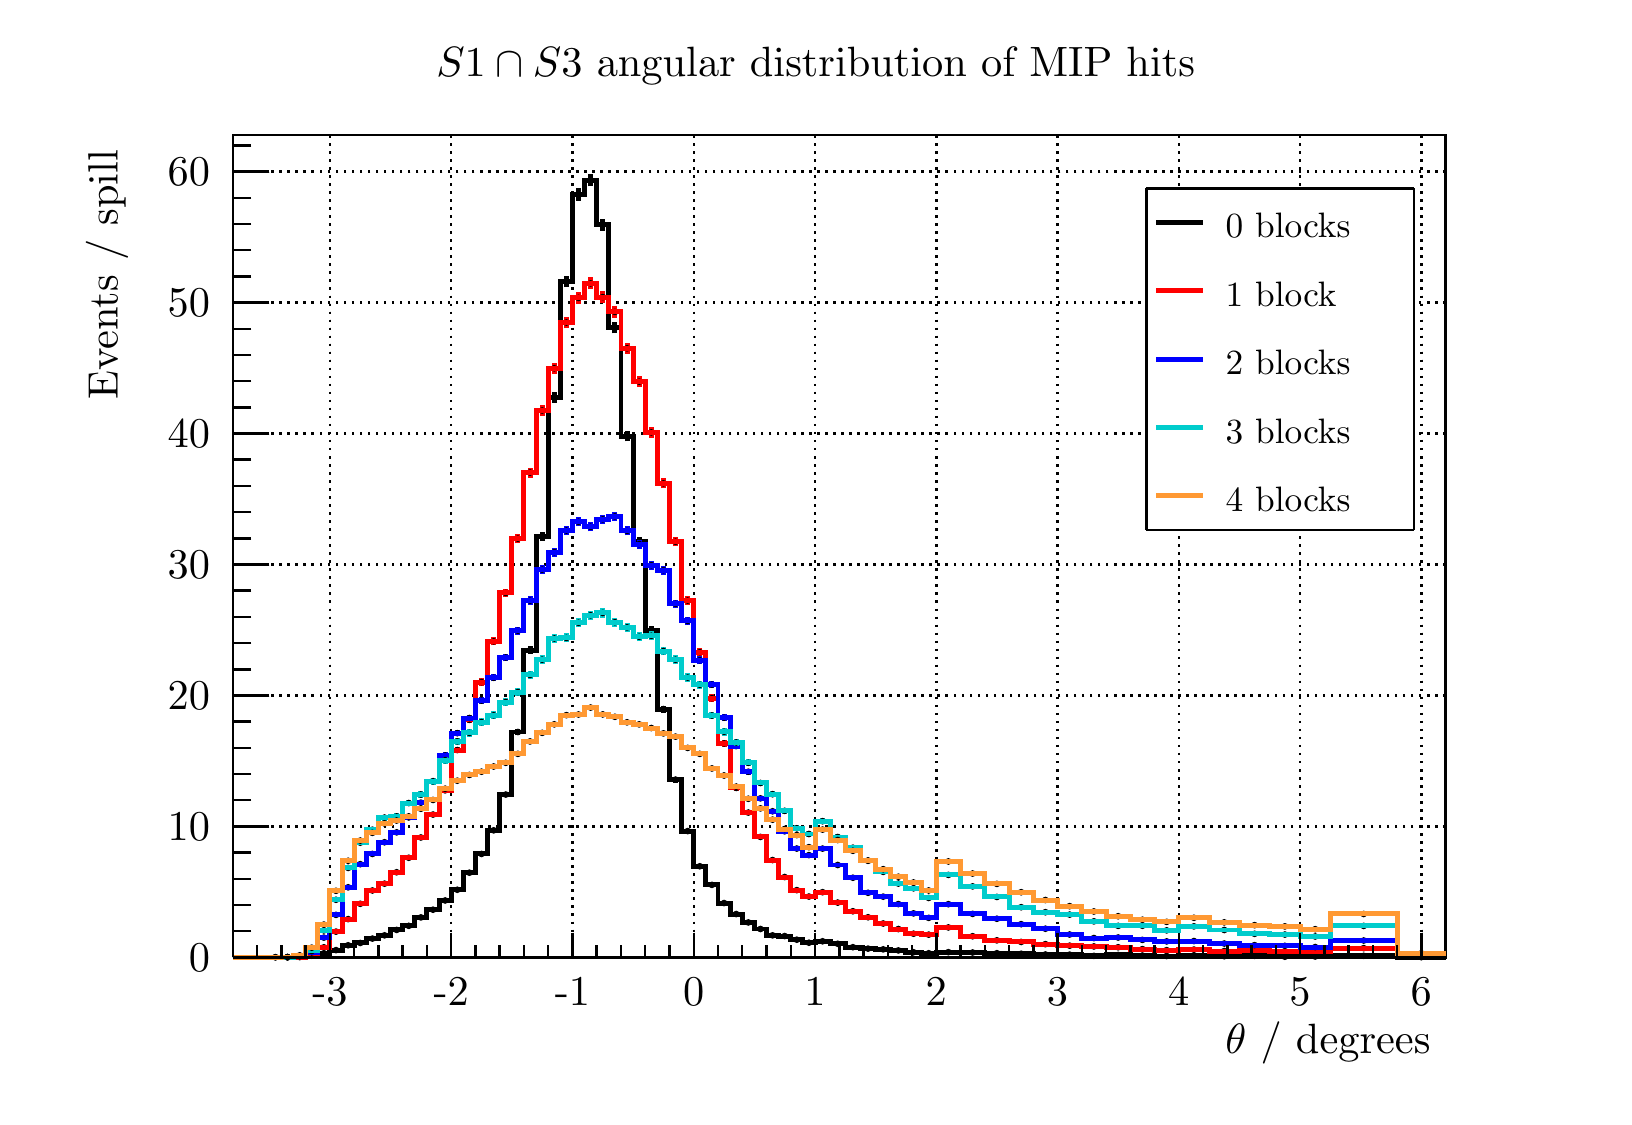
\begin{tikzpicture}
\pgfdeclareplotmark{cross} {
\pgfpathmoveto{\pgfpoint{-0.3\pgfplotmarksize}{\pgfplotmarksize}}
\pgfpathlineto{\pgfpoint{+0.3\pgfplotmarksize}{\pgfplotmarksize}}
\pgfpathlineto{\pgfpoint{+0.3\pgfplotmarksize}{0.3\pgfplotmarksize}}
\pgfpathlineto{\pgfpoint{+1\pgfplotmarksize}{0.3\pgfplotmarksize}}
\pgfpathlineto{\pgfpoint{+1\pgfplotmarksize}{-0.3\pgfplotmarksize}}
\pgfpathlineto{\pgfpoint{+0.3\pgfplotmarksize}{-0.3\pgfplotmarksize}}
\pgfpathlineto{\pgfpoint{+0.3\pgfplotmarksize}{-1.\pgfplotmarksize}}
\pgfpathlineto{\pgfpoint{-0.3\pgfplotmarksize}{-1.\pgfplotmarksize}}
\pgfpathlineto{\pgfpoint{-0.3\pgfplotmarksize}{-0.3\pgfplotmarksize}}
\pgfpathlineto{\pgfpoint{-1.\pgfplotmarksize}{-0.3\pgfplotmarksize}}
\pgfpathlineto{\pgfpoint{-1.\pgfplotmarksize}{0.3\pgfplotmarksize}}
\pgfpathlineto{\pgfpoint{-0.3\pgfplotmarksize}{0.3\pgfplotmarksize}}
\pgfpathclose
\pgfusepathqstroke
}
\pgfdeclareplotmark{cross*} {
\pgfpathmoveto{\pgfpoint{-0.3\pgfplotmarksize}{\pgfplotmarksize}}
\pgfpathlineto{\pgfpoint{+0.3\pgfplotmarksize}{\pgfplotmarksize}}
\pgfpathlineto{\pgfpoint{+0.3\pgfplotmarksize}{0.3\pgfplotmarksize}}
\pgfpathlineto{\pgfpoint{+1\pgfplotmarksize}{0.3\pgfplotmarksize}}
\pgfpathlineto{\pgfpoint{+1\pgfplotmarksize}{-0.3\pgfplotmarksize}}
\pgfpathlineto{\pgfpoint{+0.3\pgfplotmarksize}{-0.3\pgfplotmarksize}}
\pgfpathlineto{\pgfpoint{+0.3\pgfplotmarksize}{-1.\pgfplotmarksize}}
\pgfpathlineto{\pgfpoint{-0.3\pgfplotmarksize}{-1.\pgfplotmarksize}}
\pgfpathlineto{\pgfpoint{-0.3\pgfplotmarksize}{-0.3\pgfplotmarksize}}
\pgfpathlineto{\pgfpoint{-1.\pgfplotmarksize}{-0.3\pgfplotmarksize}}
\pgfpathlineto{\pgfpoint{-1.\pgfplotmarksize}{0.3\pgfplotmarksize}}
\pgfpathlineto{\pgfpoint{-0.3\pgfplotmarksize}{0.3\pgfplotmarksize}}
\pgfpathclose
\pgfusepathqfillstroke
}
\pgfdeclareplotmark{newstar} {
\pgfpathmoveto{\pgfqpoint{0pt}{\pgfplotmarksize}}
\pgfpathlineto{\pgfqpointpolar{44}{0.5\pgfplotmarksize}}
\pgfpathlineto{\pgfqpointpolar{18}{\pgfplotmarksize}}
\pgfpathlineto{\pgfqpointpolar{-20}{0.5\pgfplotmarksize}}
\pgfpathlineto{\pgfqpointpolar{-54}{\pgfplotmarksize}}
\pgfpathlineto{\pgfqpointpolar{-90}{0.5\pgfplotmarksize}}
\pgfpathlineto{\pgfqpointpolar{234}{\pgfplotmarksize}}
\pgfpathlineto{\pgfqpointpolar{198}{0.5\pgfplotmarksize}}
\pgfpathlineto{\pgfqpointpolar{162}{\pgfplotmarksize}}
\pgfpathlineto{\pgfqpointpolar{134}{0.5\pgfplotmarksize}}
\pgfpathclose
\pgfusepathqstroke
}
\pgfdeclareplotmark{newstar*} {
\pgfpathmoveto{\pgfqpoint{0pt}{\pgfplotmarksize}}
\pgfpathlineto{\pgfqpointpolar{44}{0.5\pgfplotmarksize}}
\pgfpathlineto{\pgfqpointpolar{18}{\pgfplotmarksize}}
\pgfpathlineto{\pgfqpointpolar{-20}{0.5\pgfplotmarksize}}
\pgfpathlineto{\pgfqpointpolar{-54}{\pgfplotmarksize}}
\pgfpathlineto{\pgfqpointpolar{-90}{0.5\pgfplotmarksize}}
\pgfpathlineto{\pgfqpointpolar{234}{\pgfplotmarksize}}
\pgfpathlineto{\pgfqpointpolar{198}{0.5\pgfplotmarksize}}
\pgfpathlineto{\pgfqpointpolar{162}{\pgfplotmarksize}}
\pgfpathlineto{\pgfqpointpolar{134}{0.5\pgfplotmarksize}}
\pgfpathclose
\pgfusepathqfillstroke
}
\definecolor{c}{rgb}{1,1,1};
\draw [color=c, fill=c] (0,0) rectangle (20,13.5632);
\draw [color=c, fill=c] (2.6,1.76322) rectangle (18,12.2069);
\definecolor{c}{rgb}{0,0,0};
\draw [c,line width=0.9] (2.6,1.76322) -- (2.6,12.2069) -- (18,12.2069) -- (18,1.76322) -- (2.6,1.76322);
\definecolor{c}{rgb}{1,1,1};
\draw [color=c, fill=c] (2.6,1.76322) rectangle (18,12.2069);
\definecolor{c}{rgb}{0,0,0};
\draw [c,line width=0.9] (2.6,1.76322) -- (2.6,12.2069) -- (18,12.2069) -- (18,1.76322) -- (2.6,1.76322);
\draw [c,line width=0.9] (2.6,1.76322) -- (18,1.76322);
\draw [c,dotted,line width=0.9] (3.832,12.2069) -- (3.832,1.76322);
\draw [c,dotted,line width=0.9] (5.372,12.2069) -- (5.372,1.76322);
\draw [c,dotted,line width=0.9] (6.912,12.2069) -- (6.912,1.76322);
\draw [c,dotted,line width=0.9] (8.452,12.2069) -- (8.452,1.76322);
\draw [c,dotted,line width=0.9] (9.992,12.2069) -- (9.992,1.76322);
\draw [c,dotted,line width=0.9] (11.532,12.2069) -- (11.532,1.76322);
\draw [c,dotted,line width=0.9] (13.072,12.2069) -- (13.072,1.76322);
\draw [c,dotted,line width=0.9] (14.612,12.2069) -- (14.612,1.76322);
\draw [c,dotted,line width=0.9] (16.152,12.2069) -- (16.152,1.76322);
\draw [c,dotted,line width=0.9] (17.692,12.2069) -- (17.692,1.76322);
\draw [c,dotted,line width=0.9] (3.832,12.2069) -- (3.832,1.76322);
\draw [c,dotted,line width=0.9] (17.692,12.2069) -- (17.692,1.76322);
\draw [c,line width=0.9] (2.6,1.76322) -- (2.6,12.2069);
\draw [c,dotted,line width=0.9] (18,1.76322) -- (2.6,1.76322);
\draw [c,dotted,line width=0.9] (18,3.4263) -- (2.6,3.4263);
\draw [c,dotted,line width=0.9] (18,5.08938) -- (2.6,5.08938);
\draw [c,dotted,line width=0.9] (18,6.75246) -- (2.6,6.75246);
\draw [c,dotted,line width=0.9] (18,8.41554) -- (2.6,8.41554);
\draw [c,dotted,line width=0.9] (18,10.0786) -- (2.6,10.0786);
\draw [c,dotted,line width=0.9] (18,11.7417) -- (2.6,11.7417);
\draw [c,dotted,line width=0.9] (18,11.7417) -- (2.6,11.7417);
\definecolor{c}{rgb}{0,0,0.6};
\draw [c,line width=0.9] (2.6,1.76322) -- (2.754,1.76322) -- (2.754,1.76322) -- (2.908,1.76322) -- (2.908,1.76322) -- (3.062,1.76322) -- (3.062,1.76322) -- (3.216,1.76322) -- (3.216,1.76322) -- (3.37,1.76322) -- (3.37,1.76322) -- (3.524,1.76322) --
 (3.524,1.76322) -- (3.678,1.76322) -- (3.678,1.76322) -- (3.832,1.76322) -- (3.832,1.76322) -- (3.986,1.76322) -- (3.986,1.76322) -- (4.14,1.76322) -- (4.14,1.76322) -- (4.294,1.76322) -- (4.294,1.76322) -- (4.448,1.76322) -- (4.448,1.76322) --
 (4.602,1.76322) -- (4.602,1.76322) -- (4.756,1.76322) -- (4.756,1.76322) -- (4.91,1.76322) -- (4.91,1.76322) -- (5.064,1.76322) -- (5.064,1.76322) -- (5.218,1.76322) -- (5.218,1.76322) -- (5.372,1.76322) -- (5.372,1.76322) -- (5.526,1.76322) --
 (5.526,1.76322) -- (5.68,1.76322) -- (5.68,1.76322) -- (5.834,1.76322) -- (5.834,1.76322) -- (5.988,1.76322) -- (5.988,1.76322) -- (6.142,1.76322) -- (6.142,1.76322) -- (6.296,1.76322) -- (6.296,1.76322) -- (6.45,1.76322) -- (6.45,1.76322) --
 (6.604,1.76322) -- (6.604,1.76322) -- (6.758,1.76322) -- (6.758,1.76322) -- (6.912,1.76322) -- (6.912,1.76322) -- (7.066,1.76322) -- (7.066,1.76322) -- (7.22,1.76322) -- (7.22,1.76322) -- (7.374,1.76322) -- (7.374,1.76322) -- (7.528,1.76322) --
 (7.528,1.76322) -- (7.682,1.76322) -- (7.682,1.76322) -- (7.836,1.76322) -- (7.836,1.76322) -- (7.99,1.76322) -- (7.99,1.76322) -- (8.144,1.76322) -- (8.144,1.76322) -- (8.298,1.76322) -- (8.298,1.76322) -- (8.452,1.76322) -- (8.452,1.76322) --
 (8.606,1.76322) -- (8.606,1.76322) -- (8.76,1.76322) -- (8.76,1.76322) -- (8.914,1.76322) -- (8.914,1.76322) -- (9.068,1.76322) -- (9.068,1.76322) -- (9.222,1.76322) -- (9.222,1.76322) -- (9.376,1.76322) -- (9.376,1.76322) -- (9.53,1.76322) --
 (9.53,1.76322) -- (9.684,1.76322) -- (9.684,1.76322) -- (9.838,1.76322) -- (9.838,1.76322) -- (9.992,1.76322) -- (9.992,1.76322) -- (10.1845,1.76322) -- (10.1845,1.76322) -- (10.377,1.76322) -- (10.377,1.76322) -- (10.5695,1.76322) --
 (10.5695,1.76322) -- (10.762,1.76322) -- (10.762,1.76322) -- (10.9545,1.76322) -- (10.9545,1.76322) -- (11.147,1.76322) -- (11.147,1.76322) -- (11.3395,1.76322) -- (11.3395,1.76322) -- (11.532,1.76322) -- (11.532,1.76322) -- (11.84,1.76322) --
 (11.84,1.76322) -- (12.148,1.76322) -- (12.148,1.76322) -- (12.456,1.76322) -- (12.456,1.76322) -- (12.764,1.76322) -- (12.764,1.76322) -- (13.072,1.76322) -- (13.072,1.76322) -- (13.38,1.76322) -- (13.38,1.76322) -- (13.688,1.76322) --
 (13.688,1.76322) -- (13.996,1.76322) -- (13.996,1.76322) -- (14.304,1.76322) -- (14.304,1.76322) -- (14.612,1.76322) -- (14.612,1.76322) -- (14.997,1.76322) -- (14.997,1.76322) -- (15.382,1.76322) -- (15.382,1.76322) -- (15.767,1.76322) --
 (15.767,1.76322) -- (16.152,1.76322) -- (16.152,1.76322) -- (16.537,1.76322) -- (16.537,1.76322) -- (17.384,1.76322) -- (17.384,1.76322) -- (18,1.76322);
\definecolor{c}{rgb}{0,0,0};
\draw [c,line width=0.9] (2.6,1.76322) -- (18,1.76322);
\draw [anchor= east] (18,0.678161) node[scale=1.5317, color=c, rotate=0]{$ \theta$ / degrees};
\draw [c,line width=0.9] (3.832,2.07653) -- (3.832,1.76322);
\draw [c,line width=0.9] (4.14,1.91987) -- (4.14,1.76322);
\draw [c,line width=0.9] (4.448,1.91987) -- (4.448,1.76322);
\draw [c,line width=0.9] (4.756,1.91987) -- (4.756,1.76322);
\draw [c,line width=0.9] (5.064,1.91987) -- (5.064,1.76322);
\draw [c,line width=0.9] (5.372,2.07653) -- (5.372,1.76322);
\draw [c,line width=0.9] (5.68,1.91987) -- (5.68,1.76322);
\draw [c,line width=0.9] (5.988,1.91987) -- (5.988,1.76322);
\draw [c,line width=0.9] (6.296,1.91987) -- (6.296,1.76322);
\draw [c,line width=0.9] (6.604,1.91987) -- (6.604,1.76322);
\draw [c,line width=0.9] (6.912,2.07653) -- (6.912,1.76322);
\draw [c,line width=0.9] (7.22,1.91987) -- (7.22,1.76322);
\draw [c,line width=0.9] (7.528,1.91987) -- (7.528,1.76322);
\draw [c,line width=0.9] (7.836,1.91987) -- (7.836,1.76322);
\draw [c,line width=0.9] (8.144,1.91987) -- (8.144,1.76322);
\draw [c,line width=0.9] (8.452,2.07653) -- (8.452,1.76322);
\draw [c,line width=0.9] (8.76,1.91987) -- (8.76,1.76322);
\draw [c,line width=0.9] (9.068,1.91987) -- (9.068,1.76322);
\draw [c,line width=0.9] (9.376,1.91987) -- (9.376,1.76322);
\draw [c,line width=0.9] (9.684,1.91987) -- (9.684,1.76322);
\draw [c,line width=0.9] (9.992,2.07653) -- (9.992,1.76322);
\draw [c,line width=0.9] (10.3,1.91987) -- (10.3,1.76322);
\draw [c,line width=0.9] (10.608,1.91987) -- (10.608,1.76322);
\draw [c,line width=0.9] (10.916,1.91987) -- (10.916,1.76322);
\draw [c,line width=0.9] (11.224,1.91987) -- (11.224,1.76322);
\draw [c,line width=0.9] (11.532,2.07653) -- (11.532,1.76322);
\draw [c,line width=0.9] (11.84,1.91987) -- (11.84,1.76322);
\draw [c,line width=0.9] (12.148,1.91987) -- (12.148,1.76322);
\draw [c,line width=0.9] (12.456,1.91987) -- (12.456,1.76322);
\draw [c,line width=0.9] (12.764,1.91987) -- (12.764,1.76322);
\draw [c,line width=0.9] (13.072,2.07653) -- (13.072,1.76322);
\draw [c,line width=0.9] (13.38,1.91987) -- (13.38,1.76322);
\draw [c,line width=0.9] (13.688,1.91987) -- (13.688,1.76322);
\draw [c,line width=0.9] (13.996,1.91987) -- (13.996,1.76322);
\draw [c,line width=0.9] (14.304,1.91987) -- (14.304,1.76322);
\draw [c,line width=0.9] (14.612,2.07653) -- (14.612,1.76322);
\draw [c,line width=0.9] (14.92,1.91987) -- (14.92,1.76322);
\draw [c,line width=0.9] (15.228,1.91987) -- (15.228,1.76322);
\draw [c,line width=0.9] (15.536,1.91987) -- (15.536,1.76322);
\draw [c,line width=0.9] (15.844,1.91987) -- (15.844,1.76322);
\draw [c,line width=0.9] (16.152,2.07653) -- (16.152,1.76322);
\draw [c,line width=0.9] (16.46,1.91987) -- (16.46,1.76322);
\draw [c,line width=0.9] (16.768,1.91987) -- (16.768,1.76322);
\draw [c,line width=0.9] (17.076,1.91987) -- (17.076,1.76322);
\draw [c,line width=0.9] (17.384,1.91987) -- (17.384,1.76322);
\draw [c,line width=0.9] (17.692,2.07653) -- (17.692,1.76322);
\draw [c,line width=0.9] (3.832,2.07653) -- (3.832,1.76322);
\draw [c,line width=0.9] (3.524,1.91987) -- (3.524,1.76322);
\draw [c,line width=0.9] (3.216,1.91987) -- (3.216,1.76322);
\draw [c,line width=0.9] (2.908,1.91987) -- (2.908,1.76322);
\draw [c,line width=0.9] (17.692,2.07653) -- (17.692,1.76322);
\draw [anchor=base] (3.832,1.15287) node[scale=1.5317, color=c, rotate=0]{-3};
\draw [anchor=base] (5.372,1.15287) node[scale=1.5317, color=c, rotate=0]{-2};
\draw [anchor=base] (6.912,1.15287) node[scale=1.5317, color=c, rotate=0]{-1};
\draw [anchor=base] (8.452,1.15287) node[scale=1.5317, color=c, rotate=0]{0};
\draw [anchor=base] (9.992,1.15287) node[scale=1.5317, color=c, rotate=0]{1};
\draw [anchor=base] (11.532,1.15287) node[scale=1.5317, color=c, rotate=0]{2};
\draw [anchor=base] (13.072,1.15287) node[scale=1.5317, color=c, rotate=0]{3};
\draw [anchor=base] (14.612,1.15287) node[scale=1.5317, color=c, rotate=0]{4};
\draw [anchor=base] (16.152,1.15287) node[scale=1.5317, color=c, rotate=0]{5};
\draw [anchor=base] (17.692,1.15287) node[scale=1.5317, color=c, rotate=0]{6};
\draw [c,line width=0.9] (2.6,1.76322) -- (2.6,12.2069);
\draw [anchor= east] (1,12.2069) node[scale=1.5317, color=c, rotate=90]{ Events / spill};
\draw [c,line width=0.9] (3.062,1.76322) -- (2.6,1.76322);
\draw [c,line width=0.9] (2.831,2.09583) -- (2.6,2.09583);
\draw [c,line width=0.9] (2.831,2.42845) -- (2.6,2.42845);
\draw [c,line width=0.9] (2.831,2.76107) -- (2.6,2.76107);
\draw [c,line width=0.9] (2.831,3.09368) -- (2.6,3.09368);
\draw [c,line width=0.9] (3.062,3.4263) -- (2.6,3.4263);
\draw [c,line width=0.9] (2.831,3.75891) -- (2.6,3.75891);
\draw [c,line width=0.9] (2.831,4.09153) -- (2.6,4.09153);
\draw [c,line width=0.9] (2.831,4.42415) -- (2.6,4.42415);
\draw [c,line width=0.9] (2.831,4.75676) -- (2.6,4.75676);
\draw [c,line width=0.9] (3.062,5.08938) -- (2.6,5.08938);
\draw [c,line width=0.9] (2.831,5.42199) -- (2.6,5.42199);
\draw [c,line width=0.9] (2.831,5.75461) -- (2.6,5.75461);
\draw [c,line width=0.9] (2.831,6.08722) -- (2.6,6.08722);
\draw [c,line width=0.9] (2.831,6.41984) -- (2.6,6.41984);
\draw [c,line width=0.9] (3.062,6.75246) -- (2.6,6.75246);
\draw [c,line width=0.9] (2.831,7.08507) -- (2.6,7.08507);
\draw [c,line width=0.9] (2.831,7.41769) -- (2.6,7.41769);
\draw [c,line width=0.9] (2.831,7.7503) -- (2.6,7.7503);
\draw [c,line width=0.9] (2.831,8.08292) -- (2.6,8.08292);
\draw [c,line width=0.9] (3.062,8.41554) -- (2.6,8.41554);
\draw [c,line width=0.9] (2.831,8.74815) -- (2.6,8.74815);
\draw [c,line width=0.9] (2.831,9.08077) -- (2.6,9.08077);
\draw [c,line width=0.9] (2.831,9.41338) -- (2.6,9.41338);
\draw [c,line width=0.9] (2.831,9.746) -- (2.6,9.746);
\draw [c,line width=0.9] (3.062,10.0786) -- (2.6,10.0786);
\draw [c,line width=0.9] (2.831,10.4112) -- (2.6,10.4112);
\draw [c,line width=0.9] (2.831,10.7438) -- (2.6,10.7438);
\draw [c,line width=0.9] (2.831,11.0765) -- (2.6,11.0765);
\draw [c,line width=0.9] (2.831,11.4091) -- (2.6,11.4091);
\draw [c,line width=0.9] (3.062,11.7417) -- (2.6,11.7417);
\draw [c,line width=0.9] (3.062,11.7417) -- (2.6,11.7417);
\draw [c,line width=0.9] (2.831,12.0743) -- (2.6,12.0743);
\draw [anchor= east] (2.5,1.76322) node[scale=1.5317, color=c, rotate=0]{0};
\draw [anchor= east] (2.5,3.4263) node[scale=1.5317, color=c, rotate=0]{10};
\draw [anchor= east] (2.5,5.08938) node[scale=1.5317, color=c, rotate=0]{20};
\draw [anchor= east] (2.5,6.75246) node[scale=1.5317, color=c, rotate=0]{30};
\draw [anchor= east] (2.5,8.41554) node[scale=1.5317, color=c, rotate=0]{40};
\draw [anchor= east] (2.5,10.0786) node[scale=1.5317, color=c, rotate=0]{50};
\draw [anchor= east] (2.5,11.7417) node[scale=1.5317, color=c, rotate=0]{60};
\draw [c,line width=1.8] (3.447,1.77053) -- (3.447,1.77297);
\draw [c,line width=1.8] (3.447,1.77297) -- (3.447,1.7754);
\foreach \P in {(3.447,1.77297)}{\draw[mark options={color=c,fill=c},mark size=2.402402pt,mark=*,mark size=1pt] plot coordinates {\P};}
\draw [c,line width=1.8] (3.601,1.78038) -- (3.601,1.78393);
\draw [c,line width=1.8] (3.601,1.78393) -- (3.601,1.78748);
\foreach \P in {(3.601,1.78393)}{\draw[mark options={color=c,fill=c},mark size=2.402402pt,mark=*,mark size=1pt] plot coordinates {\P};}
\draw [c,line width=1.8] (3.755,1.80938) -- (3.755,1.815);
\draw [c,line width=1.8] (3.755,1.815) -- (3.755,1.82062);
\foreach \P in {(3.755,1.815)}{\draw[mark options={color=c,fill=c},mark size=2.402402pt,mark=*,mark size=1pt] plot coordinates {\P};}
\draw [c,line width=1.8] (3.909,1.84772) -- (3.909,1.85521);
\draw [c,line width=1.8] (3.909,1.85521) -- (3.909,1.86269);
\foreach \P in {(3.909,1.85521)}{\draw[mark options={color=c,fill=c},mark size=2.402402pt,mark=*,mark size=1pt] plot coordinates {\P};}
\draw [c,line width=1.8] (4.063,1.90706) -- (4.063,1.91673);
\draw [c,line width=1.8] (4.063,1.91673) -- (4.063,1.9264);
\foreach \P in {(4.063,1.91673)}{\draw[mark options={color=c,fill=c},mark size=2.402402pt,mark=*,mark size=1pt] plot coordinates {\P};}
\draw [c,line width=1.8] (4.217,1.93542) -- (4.217,1.94597);
\draw [c,line width=1.8] (4.217,1.94597) -- (4.217,1.95653);
\foreach \P in {(4.217,1.94597)}{\draw[mark options={color=c,fill=c},mark size=2.402402pt,mark=*,mark size=1pt] plot coordinates {\P};}
\draw [c,line width=1.8] (4.371,1.98936) -- (4.371,2.00141);
\draw [c,line width=1.8] (4.371,2.00141) -- (4.371,2.01346);
\foreach \P in {(4.371,2.00141)}{\draw[mark options={color=c,fill=c},mark size=2.402402pt,mark=*,mark size=1pt] plot coordinates {\P};}
\draw [c,line width=1.8] (4.525,2.02978) -- (4.525,2.04283);
\draw [c,line width=1.8] (4.525,2.04283) -- (4.525,2.05589);
\foreach \P in {(4.525,2.04283)}{\draw[mark options={color=c,fill=c},mark size=2.402402pt,mark=*,mark size=1pt] plot coordinates {\P};}
\draw [c,line width=1.8] (4.679,2.0971) -- (4.679,2.11167);
\draw [c,line width=1.8] (4.679,2.11167) -- (4.679,2.12624);
\foreach \P in {(4.679,2.11167)}{\draw[mark options={color=c,fill=c},mark size=2.402402pt,mark=*,mark size=1pt] plot coordinates {\P};}
\draw [c,line width=1.8] (4.833,2.14784) -- (4.833,2.16345);
\draw [c,line width=1.8] (4.833,2.16345) -- (4.833,2.17907);
\foreach \P in {(4.833,2.16345)}{\draw[mark options={color=c,fill=c},mark size=2.402402pt,mark=*,mark size=1pt] plot coordinates {\P};}
\draw [c,line width=1.8] (4.987,2.25309) -- (4.987,2.27067);
\draw [c,line width=1.8] (4.987,2.27067) -- (4.987,2.28825);
\foreach \P in {(4.987,2.27067)}{\draw[mark options={color=c,fill=c},mark size=2.402402pt,mark=*,mark size=1pt] plot coordinates {\P};}
\draw [c,line width=1.8] (5.141,2.34894) -- (5.141,2.36814);
\draw [c,line width=1.8] (5.141,2.36814) -- (5.141,2.38734);
\foreach \P in {(5.141,2.36814)}{\draw[mark options={color=c,fill=c},mark size=2.402402pt,mark=*,mark size=1pt] plot coordinates {\P};}
\draw [c,line width=1.8] (5.295,2.46473) -- (5.295,2.48571);
\draw [c,line width=1.8] (5.295,2.48571) -- (5.295,2.50669);
\foreach \P in {(5.295,2.48571)}{\draw[mark options={color=c,fill=c},mark size=2.402402pt,mark=*,mark size=1pt] plot coordinates {\P};}
\draw [c,line width=1.8] (5.449,2.5987) -- (5.449,2.62156);
\draw [c,line width=1.8] (5.449,2.62156) -- (5.449,2.64443);
\foreach \P in {(5.449,2.62156)}{\draw[mark options={color=c,fill=c},mark size=2.402402pt,mark=*,mark size=1pt] plot coordinates {\P};}
\draw [c,line width=1.8] (5.603,2.81284) -- (5.603,2.83843);
\draw [c,line width=1.8] (5.603,2.83843) -- (5.603,2.86403);
\foreach \P in {(5.603,2.83843)}{\draw[mark options={color=c,fill=c},mark size=2.402402pt,mark=*,mark size=1pt] plot coordinates {\P};}
\draw [c,line width=1.8] (5.757,3.04834) -- (5.757,3.07662);
\draw [c,line width=1.8] (5.757,3.07662) -- (5.757,3.10491);
\foreach \P in {(5.757,3.07662)}{\draw[mark options={color=c,fill=c},mark size=2.402402pt,mark=*,mark size=1pt] plot coordinates {\P};}
\draw [c,line width=1.8] (5.911,3.345) -- (5.911,3.37634);
\draw [c,line width=1.8] (5.911,3.37634) -- (5.911,3.40769);
\foreach \P in {(5.911,3.37634)}{\draw[mark options={color=c,fill=c},mark size=2.402402pt,mark=*,mark size=1pt] plot coordinates {\P};}
\draw [c,line width=1.8] (6.065,3.79531) -- (6.065,3.8308);
\draw [c,line width=1.8] (6.065,3.8308) -- (6.065,3.86629);
\foreach \P in {(6.065,3.8308)}{\draw[mark options={color=c,fill=c},mark size=2.402402pt,mark=*,mark size=1pt] plot coordinates {\P};}
\draw [c,line width=1.8] (6.219,4.58342) -- (6.219,4.62518);
\draw [c,line width=1.8] (6.219,4.62518) -- (6.219,4.66693);
\foreach \P in {(6.219,4.62518)}{\draw[mark options={color=c,fill=c},mark size=2.402402pt,mark=*,mark size=1pt] plot coordinates {\P};}
\draw [c,line width=1.8] (6.373,5.61388) -- (6.373,5.66262);
\draw [c,line width=1.8] (6.373,5.66262) -- (6.373,5.71136);
\foreach \P in {(6.373,5.66262)}{\draw[mark options={color=c,fill=c},mark size=2.402402pt,mark=*,mark size=1pt] plot coordinates {\P};}
\draw [c,line width=1.8] (6.527,7.04934) -- (6.527,7.10639);
\draw [c,line width=1.8] (6.527,7.10639) -- (6.527,7.16345);
\foreach \P in {(6.527,7.10639)}{\draw[mark options={color=c,fill=c},mark size=2.402402pt,mark=*,mark size=1pt] plot coordinates {\P};}
\draw [c,line width=1.8] (6.681,8.80722) -- (6.681,8.87304);
\draw [c,line width=1.8] (6.681,8.87304) -- (6.681,8.93885);
\foreach \P in {(6.681,8.87304)}{\draw[mark options={color=c,fill=c},mark size=2.402402pt,mark=*,mark size=1pt] plot coordinates {\P};}
\draw [c,line width=1.8] (6.835,10.2762) -- (6.835,10.3485);
\draw [c,line width=1.8] (6.835,10.3485) -- (6.835,10.4208);
\foreach \P in {(6.835,10.3485)}{\draw[mark options={color=c,fill=c},mark size=2.402402pt,mark=*,mark size=1pt] plot coordinates {\P};}
\draw [c,line width=1.8] (6.989,11.3743) -- (6.989,11.4511);
\draw [c,line width=1.8] (6.989,11.4511) -- (6.989,11.5279);
\foreach \P in {(6.989,11.4511)}{\draw[mark options={color=c,fill=c},mark size=2.402402pt,mark=*,mark size=1pt] plot coordinates {\P};}
\draw [c,line width=1.8] (7.143,11.5545) -- (7.143,11.632);
\draw [c,line width=1.8] (7.143,11.632) -- (7.143,11.7096);
\foreach \P in {(7.143,11.632)}{\draw[mark options={color=c,fill=c},mark size=2.402402pt,mark=*,mark size=1pt] plot coordinates {\P};}
\draw [c,line width=1.8] (7.297,10.989) -- (7.297,11.0643);
\draw [c,line width=1.8] (7.297,11.0643) -- (7.297,11.1396);
\foreach \P in {(7.297,11.0643)}{\draw[mark options={color=c,fill=c},mark size=2.402402pt,mark=*,mark size=1pt] plot coordinates {\P};}
\draw [c,line width=1.8] (7.451,9.689) -- (7.451,9.75879);
\draw [c,line width=1.8] (7.451,9.75879) -- (7.451,9.82858);
\foreach \P in {(7.451,9.75879)}{\draw[mark options={color=c,fill=c},mark size=2.402402pt,mark=*,mark size=1pt] plot coordinates {\P};}
\draw [c,line width=1.8] (7.605,8.31611) -- (7.605,8.37959);
\draw [c,line width=1.8] (7.605,8.37959) -- (7.605,8.44308);
\foreach \P in {(7.605,8.37959)}{\draw[mark options={color=c,fill=c},mark size=2.402402pt,mark=*,mark size=1pt] plot coordinates {\P};}
\draw [c,line width=1.8] (7.759,6.98936) -- (7.759,7.04608);
\draw [c,line width=1.8] (7.759,7.04608) -- (7.759,7.10281);
\foreach \P in {(7.759,7.04608)}{\draw[mark options={color=c,fill=c},mark size=2.402402pt,mark=*,mark size=1pt] plot coordinates {\P};}
\draw [c,line width=1.8] (7.913,5.86696) -- (7.913,5.91726);
\draw [c,line width=1.8] (7.913,5.91726) -- (7.913,5.96757);
\foreach \P in {(7.913,5.91726)}{\draw[mark options={color=c,fill=c},mark size=2.402402pt,mark=*,mark size=1pt] plot coordinates {\P};}
\draw [c,line width=1.8] (8.067,4.87254) -- (8.067,4.91637);
\draw [c,line width=1.8] (8.067,4.91637) -- (8.067,4.9602);
\foreach \P in {(8.067,4.91637)}{\draw[mark options={color=c,fill=c},mark size=2.402402pt,mark=*,mark size=1pt] plot coordinates {\P};}
\draw [c,line width=1.8] (8.221,3.98378) -- (8.221,4.02086);
\draw [c,line width=1.8] (8.221,4.02086) -- (8.221,4.05795);
\foreach \P in {(8.221,4.02086)}{\draw[mark options={color=c,fill=c},mark size=2.402402pt,mark=*,mark size=1pt] plot coordinates {\P};}
\draw [c,line width=1.8] (8.375,3.33534) -- (8.375,3.3666);
\draw [c,line width=1.8] (8.375,3.3666) -- (8.375,3.39785);
\foreach \P in {(8.375,3.3666)}{\draw[mark options={color=c,fill=c},mark size=2.402402pt,mark=*,mark size=1pt] plot coordinates {\P};}
\draw [c,line width=1.8] (8.529,2.89352) -- (8.529,2.92006);
\draw [c,line width=1.8] (8.529,2.92006) -- (8.529,2.94661);
\foreach \P in {(8.529,2.92006)}{\draw[mark options={color=c,fill=c},mark size=2.402402pt,mark=*,mark size=1pt] plot coordinates {\P};}
\draw [c,line width=1.8] (8.683,2.66002) -- (8.683,2.6837);
\draw [c,line width=1.8] (8.683,2.6837) -- (8.683,2.70738);
\foreach \P in {(8.683,2.6837)}{\draw[mark options={color=c,fill=c},mark size=2.402402pt,mark=*,mark size=1pt] plot coordinates {\P};}
\draw [c,line width=1.8] (8.837,2.43232) -- (8.837,2.45282);
\draw [c,line width=1.8] (8.837,2.45282) -- (8.837,2.47331);
\foreach \P in {(8.837,2.45282)}{\draw[mark options={color=c,fill=c},mark size=2.402402pt,mark=*,mark size=1pt] plot coordinates {\P};}
\draw [c,line width=1.8] (8.991,2.29501) -- (8.991,2.31331);
\draw [c,line width=1.8] (8.991,2.31331) -- (8.991,2.33162);
\foreach \P in {(8.991,2.31331)}{\draw[mark options={color=c,fill=c},mark size=2.402402pt,mark=*,mark size=1pt] plot coordinates {\P};}
\draw [c,line width=1.8] (9.145,2.19027) -- (9.145,2.20671);
\draw [c,line width=1.8] (9.145,2.20671) -- (9.145,2.22314);
\foreach \P in {(9.145,2.20671)}{\draw[mark options={color=c,fill=c},mark size=2.402402pt,mark=*,mark size=1pt] plot coordinates {\P};}
\draw [c,line width=1.8] (9.299,2.10844) -- (9.299,2.12325);
\draw [c,line width=1.8] (9.299,2.12325) -- (9.299,2.13806);
\foreach \P in {(9.299,2.12325)}{\draw[mark options={color=c,fill=c},mark size=2.402402pt,mark=*,mark size=1pt] plot coordinates {\P};}
\draw [c,line width=1.8] (9.453,2.02978) -- (9.453,2.04283);
\draw [c,line width=1.8] (9.453,2.04283) -- (9.453,2.05589);
\foreach \P in {(9.453,2.04283)}{\draw[mark options={color=c,fill=c},mark size=2.402402pt,mark=*,mark size=1pt] plot coordinates {\P};}
\draw [c,line width=1.8] (9.607,2.02086) -- (9.607,2.0337);
\draw [c,line width=1.8] (9.607,2.0337) -- (9.607,2.04653);
\foreach \P in {(9.607,2.0337)}{\draw[mark options={color=c,fill=c},mark size=2.402402pt,mark=*,mark size=1pt] plot coordinates {\P};}
\draw [c,line width=1.8] (9.761,1.97571) -- (9.761,1.9874);
\draw [c,line width=1.8] (9.761,1.9874) -- (9.761,1.99909);
\foreach \P in {(9.761,1.9874)}{\draw[mark options={color=c,fill=c},mark size=2.402402pt,mark=*,mark size=1pt] plot coordinates {\P};}
\draw [c,line width=1.8] (9.915,1.93838) -- (9.915,1.94902);
\draw [c,line width=1.8] (9.915,1.94902) -- (9.915,1.95966);
\foreach \P in {(9.915,1.94902)}{\draw[mark options={color=c,fill=c},mark size=2.402402pt,mark=*,mark size=1pt] plot coordinates {\P};}
\draw [c,line width=1.8] (10.0883,1.95615) -- (10.0883,1.9673);
\draw [c,line width=1.8] (10.0883,1.9673) -- (10.0883,1.97845);
\foreach \P in {(10.0883,1.9673)}{\draw[mark options={color=c,fill=c},mark size=2.402402pt,mark=*,mark size=1pt] plot coordinates {\P};}
\draw [c,line width=1.8] (10.2808,1.92537) -- (10.2808,1.93562);
\draw [c,line width=1.8] (10.2808,1.93562) -- (10.2808,1.94587);
\foreach \P in {(10.2808,1.93562)}{\draw[mark options={color=c,fill=c},mark size=2.402402pt,mark=*,mark size=1pt] plot coordinates {\P};}
\draw [c,line width=1.8] (10.4733,1.8835) -- (10.4733,1.89237);
\draw [c,line width=1.8] (10.4733,1.89237) -- (10.4733,1.90124);
\foreach \P in {(10.4733,1.89237)}{\draw[mark options={color=c,fill=c},mark size=2.402402pt,mark=*,mark size=1pt] plot coordinates {\P};}
\draw [c,line width=1.8] (10.6657,1.86587) -- (10.6657,1.87409);
\draw [c,line width=1.8] (10.6657,1.87409) -- (10.6657,1.88231);
\foreach \P in {(10.6657,1.87409)}{\draw[mark options={color=c,fill=c},mark size=2.402402pt,mark=*,mark size=1pt] plot coordinates {\P};}
\draw [c,line width=1.8] (10.8582,1.85708) -- (10.8582,1.86495);
\draw [c,line width=1.8] (10.8582,1.86495) -- (10.8582,1.87282);
\foreach \P in {(10.8582,1.86495)}{\draw[mark options={color=c,fill=c},mark size=2.402402pt,mark=*,mark size=1pt] plot coordinates {\P};}
\draw [c,line width=1.8] (11.0507,1.84421) -- (11.0507,1.85155);
\draw [c,line width=1.8] (11.0507,1.85155) -- (11.0507,1.85889);
\foreach \P in {(11.0507,1.85155)}{\draw[mark options={color=c,fill=c},mark size=2.402402pt,mark=*,mark size=1pt] plot coordinates {\P};}
\draw [c,line width=1.8] (11.2432,1.82152) -- (11.2432,1.82779);
\draw [c,line width=1.8] (11.2432,1.82779) -- (11.2432,1.83406);
\foreach \P in {(11.2432,1.82779)}{\draw[mark options={color=c,fill=c},mark size=2.402402pt,mark=*,mark size=1pt] plot coordinates {\P};}
\draw [c,line width=1.8] (11.4358,1.80996) -- (11.4358,1.81561);
\draw [c,line width=1.8] (11.4358,1.81561) -- (11.4358,1.82126);
\foreach \P in {(11.4358,1.81561)}{\draw[mark options={color=c,fill=c},mark size=2.402402pt,mark=*,mark size=1pt] plot coordinates {\P};}
\draw [c,line width=1.8] (11.686,1.82268) -- (11.686,1.82901);
\draw [c,line width=1.8] (11.686,1.82901) -- (11.686,1.83534);
\foreach \P in {(11.686,1.82901)}{\draw[mark options={color=c,fill=c},mark size=2.402402pt,mark=*,mark size=1pt] plot coordinates {\P};}
\draw [c,line width=1.8] (11.994,1.81862) -- (11.994,1.82475);
\draw [c,line width=1.8] (11.994,1.82475) -- (11.994,1.83087);
\foreach \P in {(11.994,1.82475)}{\draw[mark options={color=c,fill=c},mark size=2.402402pt,mark=*,mark size=1pt] plot coordinates {\P};}
\draw [c,line width=1.8] (12.302,1.81054) -- (12.302,1.81622);
\draw [c,line width=1.8] (12.302,1.81622) -- (12.302,1.8219);
\foreach \P in {(12.302,1.81622)}{\draw[mark options={color=c,fill=c},mark size=2.402402pt,mark=*,mark size=1pt] plot coordinates {\P};}
\draw [c,line width=1.8] (12.61,1.80363) -- (12.61,1.80891);
\draw [c,line width=1.8] (12.61,1.80891) -- (12.61,1.81418);
\foreach \P in {(12.61,1.80891)}{\draw[mark options={color=c,fill=c},mark size=2.402402pt,mark=*,mark size=1pt] plot coordinates {\P};}
\draw [c,line width=1.8] (12.918,1.79505) -- (12.918,1.79977);
\draw [c,line width=1.8] (12.918,1.79977) -- (12.918,1.80449);
\foreach \P in {(12.918,1.79977)}{\draw[mark options={color=c,fill=c},mark size=2.402402pt,mark=*,mark size=1pt] plot coordinates {\P};}
\draw [c,line width=1.8] (13.226,1.79334) -- (13.226,1.79794);
\draw [c,line width=1.8] (13.226,1.79794) -- (13.226,1.80254);
\foreach \P in {(13.226,1.79794)}{\draw[mark options={color=c,fill=c},mark size=2.402402pt,mark=*,mark size=1pt] plot coordinates {\P};}
\draw [c,line width=1.8] (13.534,1.77871) -- (13.534,1.7821);
\draw [c,line width=1.8] (13.534,1.7821) -- (13.534,1.78549);
\foreach \P in {(13.534,1.7821)}{\draw[mark options={color=c,fill=c},mark size=2.402402pt,mark=*,mark size=1pt] plot coordinates {\P};}
\draw [c,line width=1.8] (13.842,1.78937) -- (13.842,1.79368);
\draw [c,line width=1.8] (13.842,1.79368) -- (13.842,1.79799);
\foreach \P in {(13.842,1.79368)}{\draw[mark options={color=c,fill=c},mark size=2.402402pt,mark=*,mark size=1pt] plot coordinates {\P};}
\draw [c,line width=1.8] (14.15,1.78205) -- (14.15,1.78576);
\draw [c,line width=1.8] (14.15,1.78576) -- (14.15,1.78946);
\foreach \P in {(14.15,1.78576)}{\draw[mark options={color=c,fill=c},mark size=2.402402pt,mark=*,mark size=1pt] plot coordinates {\P};}
\draw [c,line width=1.8] (14.458,1.77705) -- (14.458,1.78028);
\draw [c,line width=1.8] (14.458,1.78028) -- (14.458,1.7835);
\foreach \P in {(14.458,1.78028)}{\draw[mark options={color=c,fill=c},mark size=2.402402pt,mark=*,mark size=1pt] plot coordinates {\P};}
\draw [c,line width=1.8] (14.8045,1.78317) -- (14.8045,1.78698);
\draw [c,line width=1.8] (14.8045,1.78698) -- (14.8045,1.79078);
\foreach \P in {(14.8045,1.78698)}{\draw[mark options={color=c,fill=c},mark size=2.402402pt,mark=*,mark size=1pt] plot coordinates {\P};}
\draw [c,line width=1.8] (15.1895,1.77485) -- (15.1895,1.77784);
\draw [c,line width=1.8] (15.1895,1.77784) -- (15.1895,1.78082);
\foreach \P in {(15.1895,1.77784)}{\draw[mark options={color=c,fill=c},mark size=2.402402pt,mark=*,mark size=1pt] plot coordinates {\P};}
\draw [c,line width=1.8] (15.5745,1.77927) -- (15.5745,1.78271);
\draw [c,line width=1.8] (15.5745,1.78271) -- (15.5745,1.78616);
\foreach \P in {(15.5745,1.78271)}{\draw[mark options={color=c,fill=c},mark size=2.402402pt,mark=*,mark size=1pt] plot coordinates {\P};}
\draw [c,line width=1.8] (15.9595,1.76894) -- (15.9595,1.77114);
\draw [c,line width=1.8] (15.9595,1.77114) -- (15.9595,1.77333);
\foreach \P in {(15.9595,1.77114)}{\draw[mark options={color=c,fill=c},mark size=2.402402pt,mark=*,mark size=1pt] plot coordinates {\P};}
\draw [c,line width=1.8] (16.3445,1.7716) -- (16.3445,1.77418);
\draw [c,line width=1.8] (16.3445,1.77418) -- (16.3445,1.77677);
\foreach \P in {(16.3445,1.77418)}{\draw[mark options={color=c,fill=c},mark size=2.402402pt,mark=*,mark size=1pt] plot coordinates {\P};}
\draw [c,line width=1.8] (16.9605,1.77927) -- (16.9605,1.78271);
\draw [c,line width=1.8] (16.9605,1.78271) -- (16.9605,1.78616);
\foreach \P in {(16.9605,1.78271)}{\draw[mark options={color=c,fill=c},mark size=2.402402pt,mark=*,mark size=1pt] plot coordinates {\P};}
\draw [c,line width=1.8] (17.692,1.76444) -- (17.692,1.76566);
\draw [c,line width=1.8] (17.692,1.76566) -- (17.692,1.76687);
\foreach \P in {(17.692,1.76566)}{\draw[mark options={color=c,fill=c},mark size=2.402402pt,mark=*,mark size=1pt] plot coordinates {\P};}
\draw [c,line width=1.8] (2.6,1.76322) -- (2.754,1.76322) -- (2.754,1.76322) -- (2.908,1.76322) -- (2.908,1.76322) -- (3.062,1.76322) -- (3.062,1.76322) -- (3.216,1.76322) -- (3.216,1.76322) -- (3.37,1.76322) -- (3.37,1.77297) -- (3.524,1.77297) --
 (3.524,1.78393) -- (3.678,1.78393) -- (3.678,1.815) -- (3.832,1.815) -- (3.832,1.85521) -- (3.986,1.85521) -- (3.986,1.91673) -- (4.14,1.91673) -- (4.14,1.94597) -- (4.294,1.94597) -- (4.294,2.00141) -- (4.448,2.00141) -- (4.448,2.04283) --
 (4.602,2.04283) -- (4.602,2.11167) -- (4.756,2.11167) -- (4.756,2.16345) -- (4.91,2.16345) -- (4.91,2.27067) -- (5.064,2.27067) -- (5.064,2.36814) -- (5.218,2.36814) -- (5.218,2.48571) -- (5.372,2.48571) -- (5.372,2.62156) -- (5.526,2.62156) --
 (5.526,2.83843) -- (5.68,2.83843) -- (5.68,3.07662) -- (5.834,3.07662) -- (5.834,3.37634) -- (5.988,3.37634) -- (5.988,3.8308) -- (6.142,3.8308) -- (6.142,4.62518) -- (6.296,4.62518) -- (6.296,5.66262) -- (6.45,5.66262) -- (6.45,7.10639) --
 (6.604,7.10639) -- (6.604,8.87304) -- (6.758,8.87304) -- (6.758,10.3485) -- (6.912,10.3485) -- (6.912,11.4511) -- (7.066,11.4511) -- (7.066,11.632) -- (7.22,11.632) -- (7.22,11.0643) -- (7.374,11.0643) -- (7.374,9.75879) -- (7.528,9.75879) --
 (7.528,8.37959) -- (7.682,8.37959) -- (7.682,7.04608) -- (7.836,7.04608) -- (7.836,5.91726) -- (7.99,5.91726) -- (7.99,4.91637) -- (8.144,4.91637) -- (8.144,4.02086) -- (8.298,4.02086) -- (8.298,3.3666) -- (8.452,3.3666) -- (8.452,2.92006) --
 (8.606,2.92006) -- (8.606,2.6837) -- (8.76,2.6837) -- (8.76,2.45282) -- (8.914,2.45282) -- (8.914,2.31331) -- (9.068,2.31331) -- (9.068,2.20671) -- (9.222,2.20671) -- (9.222,2.12325) -- (9.376,2.12325) -- (9.376,2.04283) -- (9.53,2.04283) --
 (9.53,2.0337) -- (9.684,2.0337) -- (9.684,1.9874) -- (9.838,1.9874) -- (9.838,1.94902) -- (9.992,1.94902) -- (9.992,1.9673) -- (10.1845,1.9673) -- (10.1845,1.93562) -- (10.377,1.93562) -- (10.377,1.89237) -- (10.5695,1.89237) -- (10.5695,1.87409) --
 (10.762,1.87409) -- (10.762,1.86495) -- (10.9545,1.86495) -- (10.9545,1.85155) -- (11.147,1.85155) -- (11.147,1.82779) -- (11.3395,1.82779) -- (11.3395,1.81561) -- (11.532,1.81561) -- (11.532,1.82901) -- (11.84,1.82901) -- (11.84,1.82475) --
 (12.148,1.82475) -- (12.148,1.81622) -- (12.456,1.81622) -- (12.456,1.80891) -- (12.764,1.80891) -- (12.764,1.79977) -- (13.072,1.79977) -- (13.072,1.79794) -- (13.38,1.79794) -- (13.38,1.7821) -- (13.688,1.7821) -- (13.688,1.79368) --
 (13.996,1.79368) -- (13.996,1.78576) -- (14.304,1.78576) -- (14.304,1.78028) -- (14.612,1.78028) -- (14.612,1.78698) -- (14.997,1.78698) -- (14.997,1.77784) -- (15.382,1.77784) -- (15.382,1.78271) -- (15.767,1.78271) -- (15.767,1.77114) --
 (16.152,1.77114) -- (16.152,1.77418) -- (16.537,1.77418) -- (16.537,1.78271) -- (17.384,1.78271) -- (17.384,1.76566) -- (18,1.76566);
\definecolor{c}{rgb}{1,0,0};
\draw [c,line width=1.8] (3.293,1.7636) -- (3.293,1.76453);
\draw [c,line width=1.8] (3.293,1.76453) -- (3.293,1.76546);
\definecolor{c}{rgb}{0,0,0};
\foreach \P in {(3.293,1.76453)}{\draw[mark options={color=c,fill=c},mark size=2.402402pt,mark=*,mark size=1pt] plot coordinates {\P};}
\definecolor{c}{rgb}{1,0,0};
\draw [c,line width=1.8] (3.447,1.76504) -- (3.447,1.76651);
\draw [c,line width=1.8] (3.447,1.76651) -- (3.447,1.76797);
\definecolor{c}{rgb}{0,0,0};
\foreach \P in {(3.447,1.76651)}{\draw[mark options={color=c,fill=c},mark size=2.402402pt,mark=*,mark size=1pt] plot coordinates {\P};}
\definecolor{c}{rgb}{1,0,0};
\draw [c,line width=1.8] (3.601,1.79022) -- (3.601,1.79477);
\draw [c,line width=1.8] (3.601,1.79477) -- (3.601,1.79932);
\definecolor{c}{rgb}{0,0,0};
\foreach \P in {(3.601,1.79477)}{\draw[mark options={color=c,fill=c},mark size=2.402402pt,mark=*,mark size=1pt] plot coordinates {\P};}
\definecolor{c}{rgb}{1,0,0};
\draw [c,line width=1.8] (3.755,1.88159) -- (3.755,1.89074);
\draw [c,line width=1.8] (3.755,1.89074) -- (3.755,1.8999);
\definecolor{c}{rgb}{0,0,0};
\foreach \P in {(3.755,1.89074)}{\draw[mark options={color=c,fill=c},mark size=2.402402pt,mark=*,mark size=1pt] plot coordinates {\P};}
\definecolor{c}{rgb}{1,0,0};
\draw [c,line width=1.8] (3.909,2.07526) -- (3.909,2.08992);
\draw [c,line width=1.8] (3.909,2.08992) -- (3.909,2.10457);
\definecolor{c}{rgb}{0,0,0};
\foreach \P in {(3.909,2.08992)}{\draw[mark options={color=c,fill=c},mark size=2.402402pt,mark=*,mark size=1pt] plot coordinates {\P};}
\definecolor{c}{rgb}{1,0,0};
\draw [c,line width=1.8] (4.063,2.23113) -- (4.063,2.249);
\draw [c,line width=1.8] (4.063,2.249) -- (4.063,2.26686);
\definecolor{c}{rgb}{0,0,0};
\foreach \P in {(4.063,2.249)}{\draw[mark options={color=c,fill=c},mark size=2.402402pt,mark=*,mark size=1pt] plot coordinates {\P};}
\definecolor{c}{rgb}{1,0,0};
\draw [c,line width=1.8] (4.217,2.42242) -- (4.217,2.44357);
\draw [c,line width=1.8] (4.217,2.44357) -- (4.217,2.46472);
\definecolor{c}{rgb}{0,0,0};
\foreach \P in {(4.217,2.44357)}{\draw[mark options={color=c,fill=c},mark size=2.402402pt,mark=*,mark size=1pt] plot coordinates {\P};}
\definecolor{c}{rgb}{1,0,0};
\draw [c,line width=1.8] (4.371,2.58888) -- (4.371,2.61251);
\draw [c,line width=1.8] (4.371,2.61251) -- (4.371,2.63613);
\definecolor{c}{rgb}{0,0,0};
\foreach \P in {(4.371,2.61251)}{\draw[mark options={color=c,fill=c},mark size=2.402402pt,mark=*,mark size=1pt] plot coordinates {\P};}
\definecolor{c}{rgb}{1,0,0};
\draw [c,line width=1.8] (4.525,2.67447) -- (4.525,2.69928);
\draw [c,line width=1.8] (4.525,2.69928) -- (4.525,2.72408);
\definecolor{c}{rgb}{0,0,0};
\foreach \P in {(4.525,2.69928)}{\draw[mark options={color=c,fill=c},mark size=2.402402pt,mark=*,mark size=1pt] plot coordinates {\P};}
\definecolor{c}{rgb}{1,0,0};
\draw [c,line width=1.8] (4.679,2.81724) -- (4.679,2.84389);
\draw [c,line width=1.8] (4.679,2.84389) -- (4.679,2.87054);
\definecolor{c}{rgb}{0,0,0};
\foreach \P in {(4.679,2.84389)}{\draw[mark options={color=c,fill=c},mark size=2.402402pt,mark=*,mark size=1pt] plot coordinates {\P};}
\definecolor{c}{rgb}{1,0,0};
\draw [c,line width=1.8] (4.833,2.99911) -- (4.833,3.02795);
\draw [c,line width=1.8] (4.833,3.02795) -- (4.833,3.05678);
\definecolor{c}{rgb}{0,0,0};
\foreach \P in {(4.833,3.02795)}{\draw[mark options={color=c,fill=c},mark size=2.402402pt,mark=*,mark size=1pt] plot coordinates {\P};}
\definecolor{c}{rgb}{1,0,0};
\draw [c,line width=1.8] (4.987,3.25399) -- (4.987,3.28563);
\draw [c,line width=1.8] (4.987,3.28563) -- (4.987,3.31726);
\definecolor{c}{rgb}{0,0,0};
\foreach \P in {(4.987,3.28563)}{\draw[mark options={color=c,fill=c},mark size=2.402402pt,mark=*,mark size=1pt] plot coordinates {\P};}
\definecolor{c}{rgb}{1,0,0};
\draw [c,line width=1.8] (5.141,3.5423) -- (5.141,3.57683);
\draw [c,line width=1.8] (5.141,3.57683) -- (5.141,3.61136);
\definecolor{c}{rgb}{0,0,0};
\foreach \P in {(5.141,3.57683)}{\draw[mark options={color=c,fill=c},mark size=2.402402pt,mark=*,mark size=1pt] plot coordinates {\P};}
\definecolor{c}{rgb}{1,0,0};
\draw [c,line width=1.8] (5.295,3.84712) -- (5.295,3.88447);
\draw [c,line width=1.8] (5.295,3.88447) -- (5.295,3.92181);
\definecolor{c}{rgb}{0,0,0};
\foreach \P in {(5.295,3.88447)}{\draw[mark options={color=c,fill=c},mark size=2.402402pt,mark=*,mark size=1pt] plot coordinates {\P};}
\definecolor{c}{rgb}{1,0,0};
\draw [c,line width=1.8] (5.449,4.35428) -- (5.449,4.39588);
\draw [c,line width=1.8] (5.449,4.39588) -- (5.449,4.43748);
\definecolor{c}{rgb}{0,0,0};
\foreach \P in {(5.449,4.39588)}{\draw[mark options={color=c,fill=c},mark size=2.402402pt,mark=*,mark size=1pt] plot coordinates {\P};}
\definecolor{c}{rgb}{1,0,0};
\draw [c,line width=1.8] (5.603,4.73459) -- (5.603,4.77911);
\draw [c,line width=1.8] (5.603,4.77911) -- (5.603,4.82364);
\definecolor{c}{rgb}{0,0,0};
\foreach \P in {(5.603,4.77911)}{\draw[mark options={color=c,fill=c},mark size=2.402402pt,mark=*,mark size=1pt] plot coordinates {\P};}
\definecolor{c}{rgb}{1,0,0};
\draw [c,line width=1.8] (5.757,5.21104) -- (5.757,5.25897);
\draw [c,line width=1.8] (5.757,5.25897) -- (5.757,5.30691);
\definecolor{c}{rgb}{0,0,0};
\foreach \P in {(5.757,5.25897)}{\draw[mark options={color=c,fill=c},mark size=2.402402pt,mark=*,mark size=1pt] plot coordinates {\P};}
\definecolor{c}{rgb}{1,0,0};
\draw [c,line width=1.8] (5.911,5.72494) -- (5.911,5.7763);
\draw [c,line width=1.8] (5.911,5.7763) -- (5.911,5.82766);
\definecolor{c}{rgb}{0,0,0};
\foreach \P in {(5.911,5.7763)}{\draw[mark options={color=c,fill=c},mark size=2.402402pt,mark=*,mark size=1pt] plot coordinates {\P};}
\definecolor{c}{rgb}{1,0,0};
\draw [c,line width=1.8] (6.065,6.33576) -- (6.065,6.39092);
\draw [c,line width=1.8] (6.065,6.39092) -- (6.065,6.44607);
\definecolor{c}{rgb}{0,0,0};
\foreach \P in {(6.065,6.39092)}{\draw[mark options={color=c,fill=c},mark size=2.402402pt,mark=*,mark size=1pt] plot coordinates {\P};}
\definecolor{c}{rgb}{1,0,0};
\draw [c,line width=1.8] (6.219,7.02135) -- (6.219,7.08047);
\draw [c,line width=1.8] (6.219,7.08047) -- (6.219,7.13959);
\definecolor{c}{rgb}{0,0,0};
\foreach \P in {(6.219,7.08047)}{\draw[mark options={color=c,fill=c},mark size=2.402402pt,mark=*,mark size=1pt] plot coordinates {\P};}
\definecolor{c}{rgb}{1,0,0};
\draw [c,line width=1.8] (6.373,7.85628) -- (6.373,7.9199);
\draw [c,line width=1.8] (6.373,7.9199) -- (6.373,7.98352);
\definecolor{c}{rgb}{0,0,0};
\foreach \P in {(6.373,7.9199)}{\draw[mark options={color=c,fill=c},mark size=2.402402pt,mark=*,mark size=1pt] plot coordinates {\P};}
\definecolor{c}{rgb}{1,0,0};
\draw [c,line width=1.8] (6.527,8.64049) -- (6.527,8.70805);
\draw [c,line width=1.8] (6.527,8.70805) -- (6.527,8.77562);
\definecolor{c}{rgb}{0,0,0};
\foreach \P in {(6.527,8.70805)}{\draw[mark options={color=c,fill=c},mark size=2.402402pt,mark=*,mark size=1pt] plot coordinates {\P};}
\definecolor{c}{rgb}{1,0,0};
\draw [c,line width=1.8] (6.681,9.17432) -- (6.681,9.24445);
\draw [c,line width=1.8] (6.681,9.24445) -- (6.681,9.31457);
\definecolor{c}{rgb}{0,0,0};
\foreach \P in {(6.681,9.24445)}{\draw[mark options={color=c,fill=c},mark size=2.402402pt,mark=*,mark size=1pt] plot coordinates {\P};}
\definecolor{c}{rgb}{1,0,0};
\draw [c,line width=1.8] (6.835,9.75274) -- (6.835,9.82554);
\draw [c,line width=1.8] (6.835,9.82554) -- (6.835,9.89834);
\definecolor{c}{rgb}{0,0,0};
\foreach \P in {(6.835,9.82554)}{\draw[mark options={color=c,fill=c},mark size=2.402402pt,mark=*,mark size=1pt] plot coordinates {\P};}
\definecolor{c}{rgb}{1,0,0};
\draw [c,line width=1.8] (6.989,10.0642) -- (6.989,10.1384);
\draw [c,line width=1.8] (6.989,10.1384) -- (6.989,10.2126);
\definecolor{c}{rgb}{0,0,0};
\foreach \P in {(6.989,10.1384)}{\draw[mark options={color=c,fill=c},mark size=2.402402pt,mark=*,mark size=1pt] plot coordinates {\P};}
\definecolor{c}{rgb}{1,0,0};
\draw [c,line width=1.8] (7.143,10.2475) -- (7.143,10.3225);
\draw [c,line width=1.8] (7.143,10.3225) -- (7.143,10.3975);
\definecolor{c}{rgb}{0,0,0};
\foreach \P in {(7.143,10.3225)}{\draw[mark options={color=c,fill=c},mark size=2.402402pt,mark=*,mark size=1pt] plot coordinates {\P};}
\definecolor{c}{rgb}{1,0,0};
\draw [c,line width=1.8] (7.297,10.0741) -- (7.297,10.1483);
\draw [c,line width=1.8] (7.297,10.1483) -- (7.297,10.2225);
\definecolor{c}{rgb}{0,0,0};
\foreach \P in {(7.297,10.1483)}{\draw[mark options={color=c,fill=c},mark size=2.402402pt,mark=*,mark size=1pt] plot coordinates {\P};}
\definecolor{c}{rgb}{1,0,0};
\draw [c,line width=1.8] (7.451,9.88689) -- (7.451,9.96029);
\draw [c,line width=1.8] (7.451,9.96029) -- (7.451,10.0337);
\definecolor{c}{rgb}{0,0,0};
\foreach \P in {(7.451,9.96029)}{\draw[mark options={color=c,fill=c},mark size=2.402402pt,mark=*,mark size=1pt] plot coordinates {\P};}
\definecolor{c}{rgb}{1,0,0};
\draw [c,line width=1.8] (7.605,9.42688) -- (7.605,9.49818);
\draw [c,line width=1.8] (7.605,9.49818) -- (7.605,9.56949);
\definecolor{c}{rgb}{0,0,0};
\foreach \P in {(7.605,9.49818)}{\draw[mark options={color=c,fill=c},mark size=2.402402pt,mark=*,mark size=1pt] plot coordinates {\P};}
\definecolor{c}{rgb}{1,0,0};
\draw [c,line width=1.8] (7.759,9.00552) -- (7.759,9.07485);
\draw [c,line width=1.8] (7.759,9.07485) -- (7.759,9.14418);
\definecolor{c}{rgb}{0,0,0};
\foreach \P in {(7.759,9.07485)}{\draw[mark options={color=c,fill=c},mark size=2.402402pt,mark=*,mark size=1pt] plot coordinates {\P};}
\definecolor{c}{rgb}{1,0,0};
\draw [c,line width=1.8] (7.913,8.3638) -- (7.913,8.43);
\draw [c,line width=1.8] (7.913,8.43) -- (7.913,8.4962);
\definecolor{c}{rgb}{0,0,0};
\foreach \P in {(7.913,8.43)}{\draw[mark options={color=c,fill=c},mark size=2.402402pt,mark=*,mark size=1pt] plot coordinates {\P};}
\definecolor{c}{rgb}{1,0,0};
\draw [c,line width=1.8] (8.067,7.72027) -- (8.067,7.78317);
\draw [c,line width=1.8] (8.067,7.78317) -- (8.067,7.84608);
\definecolor{c}{rgb}{0,0,0};
\foreach \P in {(8.067,7.78317)}{\draw[mark options={color=c,fill=c},mark size=2.402402pt,mark=*,mark size=1pt] plot coordinates {\P};}
\definecolor{c}{rgb}{1,0,0};
\draw [c,line width=1.8] (8.221,6.98278) -- (8.221,7.04169);
\draw [c,line width=1.8] (8.221,7.04169) -- (8.221,7.10059);
\definecolor{c}{rgb}{0,0,0};
\foreach \P in {(8.221,7.04169)}{\draw[mark options={color=c,fill=c},mark size=2.402402pt,mark=*,mark size=1pt] plot coordinates {\P};}
\definecolor{c}{rgb}{1,0,0};
\draw [c,line width=1.8] (8.375,6.23971) -- (8.375,6.29429);
\draw [c,line width=1.8] (8.375,6.29429) -- (8.375,6.34886);
\definecolor{c}{rgb}{0,0,0};
\foreach \P in {(8.375,6.29429)}{\draw[mark options={color=c,fill=c},mark size=2.402402pt,mark=*,mark size=1pt] plot coordinates {\P};}
\definecolor{c}{rgb}{1,0,0};
\draw [c,line width=1.8] (8.529,5.58779) -- (8.529,5.63826);
\draw [c,line width=1.8] (8.529,5.63826) -- (8.529,5.68873);
\definecolor{c}{rgb}{0,0,0};
\foreach \P in {(8.529,5.63826)}{\draw[mark options={color=c,fill=c},mark size=2.402402pt,mark=*,mark size=1pt] plot coordinates {\P};}
\definecolor{c}{rgb}{1,0,0};
\draw [c,line width=1.8] (8.683,5.00868) -- (8.683,5.0552);
\draw [c,line width=1.8] (8.683,5.0552) -- (8.683,5.10171);
\definecolor{c}{rgb}{0,0,0};
\foreach \P in {(8.683,5.0552)}{\draw[mark options={color=c,fill=c},mark size=2.402402pt,mark=*,mark size=1pt] plot coordinates {\P};}
\definecolor{c}{rgb}{1,0,0};
\draw [c,line width=1.8] (8.837,4.43776) -- (8.837,4.48002);
\draw [c,line width=1.8] (8.837,4.48002) -- (8.837,4.52228);
\definecolor{c}{rgb}{0,0,0};
\foreach \P in {(8.837,4.48002)}{\draw[mark options={color=c,fill=c},mark size=2.402402pt,mark=*,mark size=1pt] plot coordinates {\P};}
\definecolor{c}{rgb}{1,0,0};
\draw [c,line width=1.8] (8.991,3.87775) -- (8.991,3.91536);
\draw [c,line width=1.8] (8.991,3.91536) -- (8.991,3.95297);
\definecolor{c}{rgb}{0,0,0};
\foreach \P in {(8.991,3.91536)}{\draw[mark options={color=c,fill=c},mark size=2.402402pt,mark=*,mark size=1pt] plot coordinates {\P};}
\definecolor{c}{rgb}{1,0,0};
\draw [c,line width=1.8] (9.145,3.56769) -- (9.145,3.60247);
\draw [c,line width=1.8] (9.145,3.60247) -- (9.145,3.63724);
\definecolor{c}{rgb}{0,0,0};
\foreach \P in {(9.145,3.60247)}{\draw[mark options={color=c,fill=c},mark size=2.402402pt,mark=*,mark size=1pt] plot coordinates {\P};}
\definecolor{c}{rgb}{1,0,0};
\draw [c,line width=1.8] (9.299,3.26115) -- (9.299,3.29286);
\draw [c,line width=1.8] (9.299,3.29286) -- (9.299,3.32457);
\definecolor{c}{rgb}{0,0,0};
\foreach \P in {(9.299,3.29286)}{\draw[mark options={color=c,fill=c},mark size=2.402402pt,mark=*,mark size=1pt] plot coordinates {\P};}
\definecolor{c}{rgb}{1,0,0};
\draw [c,line width=1.8] (9.453,2.97052) -- (9.453,2.99902);
\draw [c,line width=1.8] (9.453,2.99902) -- (9.453,3.02753);
\definecolor{c}{rgb}{0,0,0};
\foreach \P in {(9.453,2.99902)}{\draw[mark options={color=c,fill=c},mark size=2.402402pt,mark=*,mark size=1pt] plot coordinates {\P};}
\definecolor{c}{rgb}{1,0,0};
\draw [c,line width=1.8] (9.607,2.75752) -- (9.607,2.78342);
\draw [c,line width=1.8] (9.607,2.78342) -- (9.607,2.80931);
\definecolor{c}{rgb}{0,0,0};
\foreach \P in {(9.607,2.78342)}{\draw[mark options={color=c,fill=c},mark size=2.402402pt,mark=*,mark size=1pt] plot coordinates {\P};}
\definecolor{c}{rgb}{1,0,0};
\draw [c,line width=1.8] (9.761,2.59342) -- (9.761,2.61711);
\draw [c,line width=1.8] (9.761,2.61711) -- (9.761,2.6408);
\definecolor{c}{rgb}{0,0,0};
\foreach \P in {(9.761,2.61711)}{\draw[mark options={color=c,fill=c},mark size=2.402402pt,mark=*,mark size=1pt] plot coordinates {\P};}
\definecolor{c}{rgb}{1,0,0};
\draw [c,line width=1.8] (9.915,2.51306) -- (9.915,2.5356);
\draw [c,line width=1.8] (9.915,2.5356) -- (9.915,2.55813);
\definecolor{c}{rgb}{0,0,0};
\foreach \P in {(9.915,2.5356)}{\draw[mark options={color=c,fill=c},mark size=2.402402pt,mark=*,mark size=1pt] plot coordinates {\P};}
\definecolor{c}{rgb}{1,0,0};
\draw [c,line width=1.8] (10.0883,2.56749) -- (10.0883,2.59081);
\draw [c,line width=1.8] (10.0883,2.59081) -- (10.0883,2.61414);
\definecolor{c}{rgb}{0,0,0};
\foreach \P in {(10.0883,2.59081)}{\draw[mark options={color=c,fill=c},mark size=2.402402pt,mark=*,mark size=1pt] plot coordinates {\P};}
\definecolor{c}{rgb}{1,0,0};
\draw [c,line width=1.8] (10.2808,2.43731) -- (10.2808,2.45869);
\draw [c,line width=1.8] (10.2808,2.45869) -- (10.2808,2.48007);
\definecolor{c}{rgb}{0,0,0};
\foreach \P in {(10.2808,2.45869)}{\draw[mark options={color=c,fill=c},mark size=2.402402pt,mark=*,mark size=1pt] plot coordinates {\P};}
\definecolor{c}{rgb}{1,0,0};
\draw [c,line width=1.8] (10.4733,2.32929) -- (10.4733,2.34891);
\draw [c,line width=1.8] (10.4733,2.34891) -- (10.4733,2.36853);
\definecolor{c}{rgb}{0,0,0};
\foreach \P in {(10.4733,2.34891)}{\draw[mark options={color=c,fill=c},mark size=2.402402pt,mark=*,mark size=1pt] plot coordinates {\P};}
\definecolor{c}{rgb}{1,0,0};
\draw [c,line width=1.8] (10.6657,2.25436) -- (10.6657,2.27266);
\draw [c,line width=1.8] (10.6657,2.27266) -- (10.6657,2.29096);
\definecolor{c}{rgb}{0,0,0};
\foreach \P in {(10.6657,2.27266)}{\draw[mark options={color=c,fill=c},mark size=2.402402pt,mark=*,mark size=1pt] plot coordinates {\P};}
\definecolor{c}{rgb}{1,0,0};
\draw [c,line width=1.8] (10.8582,2.17631) -- (10.8582,2.19312);
\draw [c,line width=1.8] (10.8582,2.19312) -- (10.8582,2.20993);
\definecolor{c}{rgb}{0,0,0};
\foreach \P in {(10.8582,2.19312)}{\draw[mark options={color=c,fill=c},mark size=2.402402pt,mark=*,mark size=1pt] plot coordinates {\P};}
\definecolor{c}{rgb}{1,0,0};
\draw [c,line width=1.8] (11.0507,2.10741) -- (11.0507,2.12279);
\draw [c,line width=1.8] (11.0507,2.12279) -- (11.0507,2.13816);
\definecolor{c}{rgb}{0,0,0};
\foreach \P in {(11.0507,2.12279)}{\draw[mark options={color=c,fill=c},mark size=2.402402pt,mark=*,mark size=1pt] plot coordinates {\P};}
\definecolor{c}{rgb}{1,0,0};
\draw [c,line width=1.8] (11.2432,2.04957) -- (11.2432,2.06362);
\draw [c,line width=1.8] (11.2432,2.06362) -- (11.2432,2.07768);
\definecolor{c}{rgb}{0,0,0};
\foreach \P in {(11.2432,2.06362)}{\draw[mark options={color=c,fill=c},mark size=2.402402pt,mark=*,mark size=1pt] plot coordinates {\P};}
\definecolor{c}{rgb}{1,0,0};
\draw [c,line width=1.8] (11.4358,2.03802) -- (11.4358,2.05179);
\draw [c,line width=1.8] (11.4358,2.05179) -- (11.4358,2.06557);
\definecolor{c}{rgb}{0,0,0};
\foreach \P in {(11.4358,2.05179)}{\draw[mark options={color=c,fill=c},mark size=2.402402pt,mark=*,mark size=1pt] plot coordinates {\P};}
\definecolor{c}{rgb}{1,0,0};
\draw [c,line width=1.8] (11.686,2.12736) -- (11.686,2.14316);
\draw [c,line width=1.8] (11.686,2.14316) -- (11.686,2.15897);
\definecolor{c}{rgb}{0,0,0};
\foreach \P in {(11.686,2.14316)}{\draw[mark options={color=c,fill=c},mark size=2.402402pt,mark=*,mark size=1pt] plot coordinates {\P};}
\definecolor{c}{rgb}{1,0,0};
\draw [c,line width=1.8] (11.994,2.01814) -- (11.994,2.03141);
\draw [c,line width=1.8] (11.994,2.03141) -- (11.994,2.04469);
\definecolor{c}{rgb}{0,0,0};
\foreach \P in {(11.994,2.03141)}{\draw[mark options={color=c,fill=c},mark size=2.402402pt,mark=*,mark size=1pt] plot coordinates {\P};}
\definecolor{c}{rgb}{1,0,0};
\draw [c,line width=1.8] (12.302,1.96756) -- (12.302,1.97948);
\draw [c,line width=1.8] (12.302,1.97948) -- (12.302,1.99141);
\definecolor{c}{rgb}{0,0,0};
\foreach \P in {(12.302,1.97948)}{\draw[mark options={color=c,fill=c},mark size=2.402402pt,mark=*,mark size=1pt] plot coordinates {\P};}
\definecolor{c}{rgb}{1,0,0};
\draw [c,line width=1.8] (12.61,1.94776) -- (12.61,1.95911);
\draw [c,line width=1.8] (12.61,1.95911) -- (12.61,1.97045);
\definecolor{c}{rgb}{0,0,0};
\foreach \P in {(12.61,1.95911)}{\draw[mark options={color=c,fill=c},mark size=2.402402pt,mark=*,mark size=1pt] plot coordinates {\P};}
\definecolor{c}{rgb}{1,0,0};
\draw [c,line width=1.8] (12.918,1.92034) -- (12.918,1.93084);
\draw [c,line width=1.8] (12.918,1.93084) -- (12.918,1.94134);
\definecolor{c}{rgb}{0,0,0};
\foreach \P in {(12.918,1.93084)}{\draw[mark options={color=c,fill=c},mark size=2.402402pt,mark=*,mark size=1pt] plot coordinates {\P};}
\definecolor{c}{rgb}{1,0,0};
\draw [c,line width=1.8] (13.226,1.9019) -- (13.226,1.91178);
\draw [c,line width=1.8] (13.226,1.91178) -- (13.226,1.92166);
\definecolor{c}{rgb}{0,0,0};
\foreach \P in {(13.226,1.91178)}{\draw[mark options={color=c,fill=c},mark size=2.402402pt,mark=*,mark size=1pt] plot coordinates {\P};}
\definecolor{c}{rgb}{1,0,0};
\draw [c,line width=1.8] (13.534,1.89237) -- (13.534,1.90192);
\draw [c,line width=1.8] (13.534,1.90192) -- (13.534,1.91147);
\definecolor{c}{rgb}{0,0,0};
\foreach \P in {(13.534,1.90192)}{\draw[mark options={color=c,fill=c},mark size=2.402402pt,mark=*,mark size=1pt] plot coordinates {\P};}
\definecolor{c}{rgb}{1,0,0};
\draw [c,line width=1.8] (13.842,1.88222) -- (13.842,1.8914);
\draw [c,line width=1.8] (13.842,1.8914) -- (13.842,1.90058);
\definecolor{c}{rgb}{0,0,0};
\foreach \P in {(13.842,1.8914)}{\draw[mark options={color=c,fill=c},mark size=2.402402pt,mark=*,mark size=1pt] plot coordinates {\P};}
\definecolor{c}{rgb}{1,0,0};
\draw [c,line width=1.8] (14.15,1.85945) -- (14.15,1.86774);
\draw [c,line width=1.8] (14.15,1.86774) -- (14.15,1.87602);
\definecolor{c}{rgb}{0,0,0};
\foreach \P in {(14.15,1.86774)}{\draw[mark options={color=c,fill=c},mark size=2.402402pt,mark=*,mark size=1pt] plot coordinates {\P};}
\definecolor{c}{rgb}{1,0,0};
\draw [c,line width=1.8] (14.458,1.84684) -- (14.458,1.85459);
\draw [c,line width=1.8] (14.458,1.85459) -- (14.458,1.86234);
\definecolor{c}{rgb}{0,0,0};
\foreach \P in {(14.458,1.85459)}{\draw[mark options={color=c,fill=c},mark size=2.402402pt,mark=*,mark size=1pt] plot coordinates {\P};}
\definecolor{c}{rgb}{1,0,0};
\draw [c,line width=1.8] (14.8045,1.85377) -- (14.8045,1.86182);
\draw [c,line width=1.8] (14.8045,1.86182) -- (14.8045,1.86987);
\definecolor{c}{rgb}{0,0,0};
\foreach \P in {(14.8045,1.86182)}{\draw[mark options={color=c,fill=c},mark size=2.402402pt,mark=*,mark size=1pt] plot coordinates {\P};}
\definecolor{c}{rgb}{1,0,0};
\draw [c,line width=1.8] (15.1895,1.83615) -- (15.1895,1.84341);
\draw [c,line width=1.8] (15.1895,1.84341) -- (15.1895,1.85067);
\definecolor{c}{rgb}{0,0,0};
\foreach \P in {(15.1895,1.84341)}{\draw[mark options={color=c,fill=c},mark size=2.402402pt,mark=*,mark size=1pt] plot coordinates {\P};}
\definecolor{c}{rgb}{1,0,0};
\draw [c,line width=1.8] (15.5745,1.83804) -- (15.5745,1.84539);
\draw [c,line width=1.8] (15.5745,1.84539) -- (15.5745,1.85274);
\definecolor{c}{rgb}{0,0,0};
\foreach \P in {(15.5745,1.84539)}{\draw[mark options={color=c,fill=c},mark size=2.402402pt,mark=*,mark size=1pt] plot coordinates {\P};}
\definecolor{c}{rgb}{1,0,0};
\draw [c,line width=1.8] (15.9595,1.82863) -- (15.9595,1.83553);
\draw [c,line width=1.8] (15.9595,1.83553) -- (15.9595,1.84242);
\definecolor{c}{rgb}{0,0,0};
\foreach \P in {(15.9595,1.83553)}{\draw[mark options={color=c,fill=c},mark size=2.402402pt,mark=*,mark size=1pt] plot coordinates {\P};}
\definecolor{c}{rgb}{1,0,0};
\draw [c,line width=1.8] (16.3445,1.83176) -- (16.3445,1.83881);
\draw [c,line width=1.8] (16.3445,1.83881) -- (16.3445,1.84586);
\definecolor{c}{rgb}{0,0,0};
\foreach \P in {(16.3445,1.83881)}{\draw[mark options={color=c,fill=c},mark size=2.402402pt,mark=*,mark size=1pt] plot coordinates {\P};}
\definecolor{c}{rgb}{1,0,0};
\draw [c,line width=1.8] (16.9605,1.87146) -- (16.9605,1.88023);
\draw [c,line width=1.8] (16.9605,1.88023) -- (16.9605,1.889);
\definecolor{c}{rgb}{0,0,0};
\foreach \P in {(16.9605,1.88023)}{\draw[mark options={color=c,fill=c},mark size=2.402402pt,mark=*,mark size=1pt] plot coordinates {\P};}
\definecolor{c}{rgb}{1,0,0};
\draw [c,line width=1.8] (17.692,1.76996) -- (17.692,1.77242);
\draw [c,line width=1.8] (17.692,1.77242) -- (17.692,1.77488);
\definecolor{c}{rgb}{0,0,0};
\foreach \P in {(17.692,1.77242)}{\draw[mark options={color=c,fill=c},mark size=2.402402pt,mark=*,mark size=1pt] plot coordinates {\P};}
\definecolor{c}{rgb}{1,0,0};
\draw [c,line width=1.8] (2.6,1.76322) -- (2.754,1.76322) -- (2.754,1.76322) -- (2.908,1.76322) -- (2.908,1.76322) -- (3.062,1.76322) -- (3.062,1.76322) -- (3.216,1.76322) -- (3.216,1.76453) -- (3.37,1.76453) -- (3.37,1.76651) -- (3.524,1.76651) --
 (3.524,1.79477) -- (3.678,1.79477) -- (3.678,1.89074) -- (3.832,1.89074) -- (3.832,2.08992) -- (3.986,2.08992) -- (3.986,2.249) -- (4.14,2.249) -- (4.14,2.44357) -- (4.294,2.44357) -- (4.294,2.61251) -- (4.448,2.61251) -- (4.448,2.69928) --
 (4.602,2.69928) -- (4.602,2.84389) -- (4.756,2.84389) -- (4.756,3.02795) -- (4.91,3.02795) -- (4.91,3.28563) -- (5.064,3.28563) -- (5.064,3.57683) -- (5.218,3.57683) -- (5.218,3.88447) -- (5.372,3.88447) -- (5.372,4.39588) -- (5.526,4.39588) --
 (5.526,4.77911) -- (5.68,4.77911) -- (5.68,5.25897) -- (5.834,5.25897) -- (5.834,5.7763) -- (5.988,5.7763) -- (5.988,6.39092) -- (6.142,6.39092) -- (6.142,7.08047) -- (6.296,7.08047) -- (6.296,7.9199) -- (6.45,7.9199) -- (6.45,8.70805) --
 (6.604,8.70805) -- (6.604,9.24445) -- (6.758,9.24445) -- (6.758,9.82554) -- (6.912,9.82554) -- (6.912,10.1384) -- (7.066,10.1384) -- (7.066,10.3225) -- (7.22,10.3225) -- (7.22,10.1483) -- (7.374,10.1483) -- (7.374,9.96029) -- (7.528,9.96029) --
 (7.528,9.49818) -- (7.682,9.49818) -- (7.682,9.07485) -- (7.836,9.07485) -- (7.836,8.43) -- (7.99,8.43) -- (7.99,7.78317) -- (8.144,7.78317) -- (8.144,7.04169) -- (8.298,7.04169) -- (8.298,6.29429) -- (8.452,6.29429) -- (8.452,5.63826) --
 (8.606,5.63826) -- (8.606,5.0552) -- (8.76,5.0552) -- (8.76,4.48002) -- (8.914,4.48002) -- (8.914,3.91536) -- (9.068,3.91536) -- (9.068,3.60247) -- (9.222,3.60247) -- (9.222,3.29286) -- (9.376,3.29286) -- (9.376,2.99902) -- (9.53,2.99902) --
 (9.53,2.78342) -- (9.684,2.78342) -- (9.684,2.61711) -- (9.838,2.61711) -- (9.838,2.5356) -- (9.992,2.5356) -- (9.992,2.59081) -- (10.1845,2.59081) -- (10.1845,2.45869) -- (10.377,2.45869) -- (10.377,2.34891) -- (10.5695,2.34891) --
 (10.5695,2.27266) -- (10.762,2.27266) -- (10.762,2.19312) -- (10.9545,2.19312) -- (10.9545,2.12279) -- (11.147,2.12279) -- (11.147,2.06362) -- (11.3395,2.06362) -- (11.3395,2.05179) -- (11.532,2.05179) -- (11.532,2.14316) -- (11.84,2.14316) --
 (11.84,2.03141) -- (12.148,2.03141) -- (12.148,1.97948) -- (12.456,1.97948) -- (12.456,1.95911) -- (12.764,1.95911) -- (12.764,1.93084) -- (13.072,1.93084) -- (13.072,1.91178) -- (13.38,1.91178) -- (13.38,1.90192) -- (13.688,1.90192) --
 (13.688,1.8914) -- (13.996,1.8914) -- (13.996,1.86774) -- (14.304,1.86774) -- (14.304,1.85459) -- (14.612,1.85459) -- (14.612,1.86182) -- (14.997,1.86182) -- (14.997,1.84341) -- (15.382,1.84341) -- (15.382,1.84539) -- (15.767,1.84539) --
 (15.767,1.83553) -- (16.152,1.83553) -- (16.152,1.83881) -- (16.537,1.83881) -- (16.537,1.88023) -- (17.384,1.88023) -- (17.384,1.77242) -- (18,1.77242);
\definecolor{c}{rgb}{0,0,1};
\draw [c,line width=1.8] (3.293,1.76358) -- (3.293,1.76447);
\draw [c,line width=1.8] (3.293,1.76447) -- (3.293,1.76535);
\definecolor{c}{rgb}{0,0,0};
\foreach \P in {(3.293,1.76447)}{\draw[mark options={color=c,fill=c},mark size=2.402402pt,mark=*,mark size=1pt] plot coordinates {\P};}
\definecolor{c}{rgb}{0,0,1};
\draw [c,line width=1.8] (3.447,1.7746) -- (3.447,1.7776);
\draw [c,line width=1.8] (3.447,1.7776) -- (3.447,1.7806);
\definecolor{c}{rgb}{0,0,0};
\foreach \P in {(3.447,1.7776)}{\draw[mark options={color=c,fill=c},mark size=2.402402pt,mark=*,mark size=1pt] plot coordinates {\P};}
\definecolor{c}{rgb}{0,0,1};
\draw [c,line width=1.8] (3.601,1.81949) -- (3.601,1.82574);
\draw [c,line width=1.8] (3.601,1.82574) -- (3.601,1.83199);
\definecolor{c}{rgb}{0,0,0};
\foreach \P in {(3.601,1.82574)}{\draw[mark options={color=c,fill=c},mark size=2.402402pt,mark=*,mark size=1pt] plot coordinates {\P};}
\definecolor{c}{rgb}{0,0,1};
\draw [c,line width=1.8] (3.755,2.00141) -- (3.755,2.01393);
\draw [c,line width=1.8] (3.755,2.01393) -- (3.755,2.02645);
\definecolor{c}{rgb}{0,0,0};
\foreach \P in {(3.755,2.01393)}{\draw[mark options={color=c,fill=c},mark size=2.402402pt,mark=*,mark size=1pt] plot coordinates {\P};}
\definecolor{c}{rgb}{0,0,1};
\draw [c,line width=1.8] (3.909,2.28441) -- (3.909,2.30278);
\draw [c,line width=1.8] (3.909,2.30278) -- (3.909,2.32115);
\definecolor{c}{rgb}{0,0,0};
\foreach \P in {(3.909,2.30278)}{\draw[mark options={color=c,fill=c},mark size=2.402402pt,mark=*,mark size=1pt] plot coordinates {\P};}
\definecolor{c}{rgb}{0,0,1};
\draw [c,line width=1.8] (4.063,2.62932) -- (4.063,2.6529);
\draw [c,line width=1.8] (4.063,2.6529) -- (4.063,2.67649);
\definecolor{c}{rgb}{0,0,0};
\foreach \P in {(4.063,2.6529)}{\draw[mark options={color=c,fill=c},mark size=2.402402pt,mark=*,mark size=1pt] plot coordinates {\P};}
\definecolor{c}{rgb}{0,0,1};
\draw [c,line width=1.8] (4.217,2.91955) -- (4.217,2.94676);
\draw [c,line width=1.8] (4.217,2.94676) -- (4.217,2.97396);
\definecolor{c}{rgb}{0,0,0};
\foreach \P in {(4.217,2.94676)}{\draw[mark options={color=c,fill=c},mark size=2.402402pt,mark=*,mark size=1pt] plot coordinates {\P};}
\definecolor{c}{rgb}{0,0,1};
\draw [c,line width=1.8] (4.371,3.04814) -- (4.371,3.0768);
\draw [c,line width=1.8] (4.371,3.0768) -- (4.371,3.10546);
\definecolor{c}{rgb}{0,0,0};
\foreach \P in {(4.371,3.0768)}{\draw[mark options={color=c,fill=c},mark size=2.402402pt,mark=*,mark size=1pt] plot coordinates {\P};}
\definecolor{c}{rgb}{0,0,1};
\draw [c,line width=1.8] (4.525,3.19475) -- (4.525,3.22498);
\draw [c,line width=1.8] (4.525,3.22498) -- (4.525,3.25521);
\definecolor{c}{rgb}{0,0,0};
\foreach \P in {(4.525,3.22498)}{\draw[mark options={color=c,fill=c},mark size=2.402402pt,mark=*,mark size=1pt] plot coordinates {\P};}
\definecolor{c}{rgb}{0,0,1};
\draw [c,line width=1.8] (4.679,3.31914) -- (4.679,3.35065);
\draw [c,line width=1.8] (4.679,3.35065) -- (4.679,3.38215);
\definecolor{c}{rgb}{0,0,0};
\foreach \P in {(4.679,3.35065)}{\draw[mark options={color=c,fill=c},mark size=2.402402pt,mark=*,mark size=1pt] plot coordinates {\P};}
\definecolor{c}{rgb}{0,0,1};
\draw [c,line width=1.8] (4.833,3.50676) -- (4.833,3.54009);
\draw [c,line width=1.8] (4.833,3.54009) -- (4.833,3.57342);
\definecolor{c}{rgb}{0,0,0};
\foreach \P in {(4.833,3.54009)}{\draw[mark options={color=c,fill=c},mark size=2.402402pt,mark=*,mark size=1pt] plot coordinates {\P};}
\definecolor{c}{rgb}{0,0,1};
\draw [c,line width=1.8] (4.987,3.69323) -- (4.987,3.72828);
\draw [c,line width=1.8] (4.987,3.72828) -- (4.987,3.76333);
\definecolor{c}{rgb}{0,0,0};
\foreach \P in {(4.987,3.72828)}{\draw[mark options={color=c,fill=c},mark size=2.402402pt,mark=*,mark size=1pt] plot coordinates {\P};}
\definecolor{c}{rgb}{0,0,1};
\draw [c,line width=1.8] (5.141,3.96347) -- (5.141,4.00087);
\draw [c,line width=1.8] (5.141,4.00087) -- (5.141,4.03828);
\definecolor{c}{rgb}{0,0,0};
\foreach \P in {(5.141,4.00087)}{\draw[mark options={color=c,fill=c},mark size=2.402402pt,mark=*,mark size=1pt] plot coordinates {\P};}
\definecolor{c}{rgb}{0,0,1};
\draw [c,line width=1.8] (5.295,4.28658) -- (5.295,4.32661);
\draw [c,line width=1.8] (5.295,4.32661) -- (5.295,4.36664);
\definecolor{c}{rgb}{0,0,0};
\foreach \P in {(5.295,4.32661)}{\draw[mark options={color=c,fill=c},mark size=2.402402pt,mark=*,mark size=1pt] plot coordinates {\P};}
\definecolor{c}{rgb}{0,0,1};
\draw [c,line width=1.8] (5.449,4.56827) -- (5.449,4.61046);
\draw [c,line width=1.8] (5.449,4.61046) -- (5.449,4.65265);
\definecolor{c}{rgb}{0,0,0};
\foreach \P in {(5.449,4.61046)}{\draw[mark options={color=c,fill=c},mark size=2.402402pt,mark=*,mark size=1pt] plot coordinates {\P};}
\definecolor{c}{rgb}{0,0,1};
\draw [c,line width=1.8] (5.603,4.75881) -- (5.603,4.8024);
\draw [c,line width=1.8] (5.603,4.8024) -- (5.603,4.84599);
\definecolor{c}{rgb}{0,0,0};
\foreach \P in {(5.603,4.8024)}{\draw[mark options={color=c,fill=c},mark size=2.402402pt,mark=*,mark size=1pt] plot coordinates {\P};}
\definecolor{c}{rgb}{0,0,1};
\draw [c,line width=1.8] (5.757,4.97858) -- (5.757,5.02373);
\draw [c,line width=1.8] (5.757,5.02373) -- (5.757,5.06888);
\definecolor{c}{rgb}{0,0,0};
\foreach \P in {(5.757,5.02373)}{\draw[mark options={color=c,fill=c},mark size=2.402402pt,mark=*,mark size=1pt] plot coordinates {\P};}
\definecolor{c}{rgb}{0,0,1};
\draw [c,line width=1.8] (5.911,5.26671) -- (5.911,5.31383);
\draw [c,line width=1.8] (5.911,5.31383) -- (5.911,5.36095);
\definecolor{c}{rgb}{0,0,0};
\foreach \P in {(5.911,5.31383)}{\draw[mark options={color=c,fill=c},mark size=2.402402pt,mark=*,mark size=1pt] plot coordinates {\P};}
\definecolor{c}{rgb}{0,0,1};
\draw [c,line width=1.8] (6.065,5.52262) -- (6.065,5.57142);
\draw [c,line width=1.8] (6.065,5.57142) -- (6.065,5.62022);
\definecolor{c}{rgb}{0,0,0};
\foreach \P in {(6.065,5.57142)}{\draw[mark options={color=c,fill=c},mark size=2.402402pt,mark=*,mark size=1pt] plot coordinates {\P};}
\definecolor{c}{rgb}{0,0,1};
\draw [c,line width=1.8] (6.219,5.85999) -- (6.219,5.91091);
\draw [c,line width=1.8] (6.219,5.91091) -- (6.219,5.96184);
\definecolor{c}{rgb}{0,0,0};
\foreach \P in {(6.219,5.91091)}{\draw[mark options={color=c,fill=c},mark size=2.402402pt,mark=*,mark size=1pt] plot coordinates {\P};}
\definecolor{c}{rgb}{0,0,1};
\draw [c,line width=1.8] (6.373,6.24033) -- (6.373,6.29355);
\draw [c,line width=1.8] (6.373,6.29355) -- (6.373,6.34677);
\definecolor{c}{rgb}{0,0,0};
\foreach \P in {(6.373,6.29355)}{\draw[mark options={color=c,fill=c},mark size=2.402402pt,mark=*,mark size=1pt] plot coordinates {\P};}
\definecolor{c}{rgb}{0,0,1};
\draw [c,line width=1.8] (6.527,6.63195) -- (6.527,6.68743);
\draw [c,line width=1.8] (6.527,6.68743) -- (6.527,6.74292);
\definecolor{c}{rgb}{0,0,0};
\foreach \P in {(6.527,6.68743)}{\draw[mark options={color=c,fill=c},mark size=2.402402pt,mark=*,mark size=1pt] plot coordinates {\P};}
\definecolor{c}{rgb}{0,0,1};
\draw [c,line width=1.8] (6.681,6.85204) -- (6.681,6.90876);
\draw [c,line width=1.8] (6.681,6.90876) -- (6.681,6.96548);
\definecolor{c}{rgb}{0,0,0};
\foreach \P in {(6.681,6.90876)}{\draw[mark options={color=c,fill=c},mark size=2.402402pt,mark=*,mark size=1pt] plot coordinates {\P};}
\definecolor{c}{rgb}{0,0,1};
\draw [c,line width=1.8] (6.835,7.12564) -- (6.835,7.18386);
\draw [c,line width=1.8] (6.835,7.18386) -- (6.835,7.24207);
\definecolor{c}{rgb}{0,0,0};
\foreach \P in {(6.835,7.18386)}{\draw[mark options={color=c,fill=c},mark size=2.402402pt,mark=*,mark size=1pt] plot coordinates {\P};}
\definecolor{c}{rgb}{0,0,1};
\draw [c,line width=1.8] (6.989,7.23634) -- (6.989,7.29515);
\draw [c,line width=1.8] (6.989,7.29515) -- (6.989,7.35396);
\definecolor{c}{rgb}{0,0,0};
\foreach \P in {(6.989,7.29515)}{\draw[mark options={color=c,fill=c},mark size=2.402402pt,mark=*,mark size=1pt] plot coordinates {\P};}
\definecolor{c}{rgb}{0,0,1};
\draw [c,line width=1.8] (7.143,7.1729) -- (7.143,7.23137);
\draw [c,line width=1.8] (7.143,7.23137) -- (7.143,7.28984);
\definecolor{c}{rgb}{0,0,0};
\foreach \P in {(7.143,7.23137)}{\draw[mark options={color=c,fill=c},mark size=2.402402pt,mark=*,mark size=1pt] plot coordinates {\P};}
\definecolor{c}{rgb}{0,0,1};
\draw [c,line width=1.8] (7.297,7.26681) -- (7.297,7.32578);
\draw [c,line width=1.8] (7.297,7.32578) -- (7.297,7.38475);
\definecolor{c}{rgb}{0,0,0};
\foreach \P in {(7.297,7.32578)}{\draw[mark options={color=c,fill=c},mark size=2.402402pt,mark=*,mark size=1pt] plot coordinates {\P};}
\definecolor{c}{rgb}{0,0,1};
\draw [c,line width=1.8] (7.451,7.30412) -- (7.451,7.36329);
\draw [c,line width=1.8] (7.451,7.36329) -- (7.451,7.42247);
\definecolor{c}{rgb}{0,0,0};
\foreach \P in {(7.451,7.36329)}{\draw[mark options={color=c,fill=c},mark size=2.402402pt,mark=*,mark size=1pt] plot coordinates {\P};}
\definecolor{c}{rgb}{0,0,1};
\draw [c,line width=1.8] (7.605,7.12129) -- (7.605,7.17948);
\draw [c,line width=1.8] (7.605,7.17948) -- (7.605,7.23767);
\definecolor{c}{rgb}{0,0,0};
\foreach \P in {(7.605,7.17948)}{\draw[mark options={color=c,fill=c},mark size=2.402402pt,mark=*,mark size=1pt] plot coordinates {\P};}
\definecolor{c}{rgb}{0,0,1};
\draw [c,line width=1.8] (7.759,6.95464) -- (7.759,7.01192);
\draw [c,line width=1.8] (7.759,7.01192) -- (7.759,7.06921);
\definecolor{c}{rgb}{0,0,0};
\foreach \P in {(7.759,7.01192)}{\draw[mark options={color=c,fill=c},mark size=2.402402pt,mark=*,mark size=1pt] plot coordinates {\P};}
\definecolor{c}{rgb}{0,0,1};
\draw [c,line width=1.8] (7.913,6.6879) -- (7.913,6.7437);
\draw [c,line width=1.8] (7.913,6.7437) -- (7.913,6.79951);
\definecolor{c}{rgb}{0,0,0};
\foreach \P in {(7.913,6.7437)}{\draw[mark options={color=c,fill=c},mark size=2.402402pt,mark=*,mark size=1pt] plot coordinates {\P};}
\definecolor{c}{rgb}{0,0,1};
\draw [c,line width=1.8] (8.067,6.62449) -- (8.067,6.67993);
\draw [c,line width=1.8] (8.067,6.67993) -- (8.067,6.73538);
\definecolor{c}{rgb}{0,0,0};
\foreach \P in {(8.067,6.67993)}{\draw[mark options={color=c,fill=c},mark size=2.402402pt,mark=*,mark size=1pt] plot coordinates {\P};}
\definecolor{c}{rgb}{0,0,1};
\draw [c,line width=1.8] (8.221,6.20055) -- (8.221,6.25353);
\draw [c,line width=1.8] (8.221,6.25353) -- (8.221,6.30652);
\definecolor{c}{rgb}{0,0,0};
\foreach \P in {(8.221,6.25353)}{\draw[mark options={color=c,fill=c},mark size=2.402402pt,mark=*,mark size=1pt] plot coordinates {\P};}
\definecolor{c}{rgb}{0,0,1};
\draw [c,line width=1.8] (8.375,5.98365) -- (8.375,6.03533);
\draw [c,line width=1.8] (8.375,6.03533) -- (8.375,6.08701);
\definecolor{c}{rgb}{0,0,0};
\foreach \P in {(8.375,6.03533)}{\draw[mark options={color=c,fill=c},mark size=2.402402pt,mark=*,mark size=1pt] plot coordinates {\P};}
\definecolor{c}{rgb}{0,0,1};
\draw [c,line width=1.8] (8.529,5.48846) -- (8.529,5.53703);
\draw [c,line width=1.8] (8.529,5.53703) -- (8.529,5.58561);
\definecolor{c}{rgb}{0,0,0};
\foreach \P in {(8.529,5.53703)}{\draw[mark options={color=c,fill=c},mark size=2.402402pt,mark=*,mark size=1pt] plot coordinates {\P};}
\definecolor{c}{rgb}{0,0,1};
\draw [c,line width=1.8] (8.683,5.17977) -- (8.683,5.2263);
\draw [c,line width=1.8] (8.683,5.2263) -- (8.683,5.27283);
\definecolor{c}{rgb}{0,0,0};
\foreach \P in {(8.683,5.2263)}{\draw[mark options={color=c,fill=c},mark size=2.402402pt,mark=*,mark size=1pt] plot coordinates {\P};}
\definecolor{c}{rgb}{0,0,1};
\draw [c,line width=1.8] (8.837,4.76316) -- (8.837,4.80678);
\draw [c,line width=1.8] (8.837,4.80678) -- (8.837,4.8504);
\definecolor{c}{rgb}{0,0,0};
\foreach \P in {(8.837,4.80678)}{\draw[mark options={color=c,fill=c},mark size=2.402402pt,mark=*,mark size=1pt] plot coordinates {\P};}
\definecolor{c}{rgb}{0,0,1};
\draw [c,line width=1.8] (8.991,4.40507) -- (8.991,4.44603);
\draw [c,line width=1.8] (8.991,4.44603) -- (8.991,4.48698);
\definecolor{c}{rgb}{0,0,0};
\foreach \P in {(8.991,4.44603)}{\draw[mark options={color=c,fill=c},mark size=2.402402pt,mark=*,mark size=1pt] plot coordinates {\P};}
\definecolor{c}{rgb}{0,0,1};
\draw [c,line width=1.8] (9.145,4.08252) -- (9.145,4.12091);
\draw [c,line width=1.8] (9.145,4.12091) -- (9.145,4.15931);
\definecolor{c}{rgb}{0,0,0};
\foreach \P in {(9.145,4.12091)}{\draw[mark options={color=c,fill=c},mark size=2.402402pt,mark=*,mark size=1pt] plot coordinates {\P};}
\definecolor{c}{rgb}{0,0,1};
\draw [c,line width=1.8] (9.299,3.74714) -- (9.299,3.78267);
\draw [c,line width=1.8] (9.299,3.78267) -- (9.299,3.81821);
\definecolor{c}{rgb}{0,0,0};
\foreach \P in {(9.299,3.78267)}{\draw[mark options={color=c,fill=c},mark size=2.402402pt,mark=*,mark size=1pt] plot coordinates {\P};}
\definecolor{c}{rgb}{0,0,1};
\draw [c,line width=1.8] (9.453,3.58418) -- (9.453,3.61824);
\draw [c,line width=1.8] (9.453,3.61824) -- (9.453,3.6523);
\definecolor{c}{rgb}{0,0,0};
\foreach \P in {(9.453,3.61824)}{\draw[mark options={color=c,fill=c},mark size=2.402402pt,mark=*,mark size=1pt] plot coordinates {\P};}
\definecolor{c}{rgb}{0,0,1};
\draw [c,line width=1.8] (9.607,3.33276) -- (9.607,3.3644);
\draw [c,line width=1.8] (9.607,3.3644) -- (9.607,3.39604);
\definecolor{c}{rgb}{0,0,0};
\foreach \P in {(9.607,3.3644)}{\draw[mark options={color=c,fill=c},mark size=2.402402pt,mark=*,mark size=1pt] plot coordinates {\P};}
\definecolor{c}{rgb}{0,0,1};
\draw [c,line width=1.8] (9.761,3.11556) -- (9.761,3.14495);
\draw [c,line width=1.8] (9.761,3.14495) -- (9.761,3.17434);
\definecolor{c}{rgb}{0,0,0};
\foreach \P in {(9.761,3.14495)}{\draw[mark options={color=c,fill=c},mark size=2.402402pt,mark=*,mark size=1pt] plot coordinates {\P};}
\definecolor{c}{rgb}{0,0,1};
\draw [c,line width=1.8] (9.915,3.0333) -- (9.915,3.0618);
\draw [c,line width=1.8] (9.915,3.0618) -- (9.915,3.09029);
\definecolor{c}{rgb}{0,0,0};
\foreach \P in {(9.915,3.0618)}{\draw[mark options={color=c,fill=c},mark size=2.402402pt,mark=*,mark size=1pt] plot coordinates {\P};}
\definecolor{c}{rgb}{0,0,1};
\draw [c,line width=1.8] (10.0883,3.11494) -- (10.0883,3.14432);
\draw [c,line width=1.8] (10.0883,3.14432) -- (10.0883,3.17371);
\definecolor{c}{rgb}{0,0,0};
\foreach \P in {(10.0883,3.14432)}{\draw[mark options={color=c,fill=c},mark size=2.402402pt,mark=*,mark size=1pt] plot coordinates {\P};}
\definecolor{c}{rgb}{0,0,1};
\draw [c,line width=1.8] (10.2808,2.90905) -- (10.2808,2.93613);
\draw [c,line width=1.8] (10.2808,2.93613) -- (10.2808,2.96321);
\definecolor{c}{rgb}{0,0,0};
\foreach \P in {(10.2808,2.93613)}{\draw[mark options={color=c,fill=c},mark size=2.402402pt,mark=*,mark size=1pt] plot coordinates {\P};}
\definecolor{c}{rgb}{0,0,1};
\draw [c,line width=1.8] (10.4733,2.74905) -- (10.4733,2.7742);
\draw [c,line width=1.8] (10.4733,2.7742) -- (10.4733,2.79934);
\definecolor{c}{rgb}{0,0,0};
\foreach \P in {(10.4733,2.7742)}{\draw[mark options={color=c,fill=c},mark size=2.402402pt,mark=*,mark size=1pt] plot coordinates {\P};}
\definecolor{c}{rgb}{0,0,1};
\draw [c,line width=1.8] (10.6657,2.56024) -- (10.6657,2.58288);
\draw [c,line width=1.8] (10.6657,2.58288) -- (10.6657,2.60552);
\definecolor{c}{rgb}{0,0,0};
\foreach \P in {(10.6657,2.58288)}{\draw[mark options={color=c,fill=c},mark size=2.402402pt,mark=*,mark size=1pt] plot coordinates {\P};}
\definecolor{c}{rgb}{0,0,1};
\draw [c,line width=1.8] (10.8582,2.51216) -- (10.8582,2.53411);
\draw [c,line width=1.8] (10.8582,2.53411) -- (10.8582,2.55607);
\definecolor{c}{rgb}{0,0,0};
\foreach \P in {(10.8582,2.53411)}{\draw[mark options={color=c,fill=c},mark size=2.402402pt,mark=*,mark size=1pt] plot coordinates {\P};}
\definecolor{c}{rgb}{0,0,1};
\draw [c,line width=1.8] (11.0507,2.41914) -- (11.0507,2.4397);
\draw [c,line width=1.8] (11.0507,2.4397) -- (11.0507,2.46027);
\definecolor{c}{rgb}{0,0,0};
\foreach \P in {(11.0507,2.4397)}{\draw[mark options={color=c,fill=c},mark size=2.402402pt,mark=*,mark size=1pt] plot coordinates {\P};}
\definecolor{c}{rgb}{0,0,1};
\draw [c,line width=1.8] (11.2432,2.30285) -- (11.2432,2.32154);
\draw [c,line width=1.8] (11.2432,2.32154) -- (11.2432,2.34022);
\definecolor{c}{rgb}{0,0,0};
\foreach \P in {(11.2432,2.32154)}{\draw[mark options={color=c,fill=c},mark size=2.402402pt,mark=*,mark size=1pt] plot coordinates {\P};}
\definecolor{c}{rgb}{0,0,1};
\draw [c,line width=1.8] (11.4358,2.24694) -- (11.4358,2.26464);
\draw [c,line width=1.8] (11.4358,2.26464) -- (11.4358,2.28235);
\definecolor{c}{rgb}{0,0,0};
\foreach \P in {(11.4358,2.26464)}{\draw[mark options={color=c,fill=c},mark size=2.402402pt,mark=*,mark size=1pt] plot coordinates {\P};}
\definecolor{c}{rgb}{0,0,1};
\draw [c,line width=1.8] (11.686,2.41791) -- (11.686,2.43845);
\draw [c,line width=1.8] (11.686,2.43845) -- (11.686,2.459);
\definecolor{c}{rgb}{0,0,0};
\foreach \P in {(11.686,2.43845)}{\draw[mark options={color=c,fill=c},mark size=2.402402pt,mark=*,mark size=1pt] plot coordinates {\P};}
\definecolor{c}{rgb}{0,0,1};
\draw [c,line width=1.8] (11.994,2.29671) -- (11.994,2.31529);
\draw [c,line width=1.8] (11.994,2.31529) -- (11.994,2.33386);
\definecolor{c}{rgb}{0,0,0};
\foreach \P in {(11.994,2.31529)}{\draw[mark options={color=c,fill=c},mark size=2.402402pt,mark=*,mark size=1pt] plot coordinates {\P};}
\definecolor{c}{rgb}{0,0,1};
\draw [c,line width=1.8] (12.302,2.23588) -- (12.302,2.25339);
\draw [c,line width=1.8] (12.302,2.25339) -- (12.302,2.2709);
\definecolor{c}{rgb}{0,0,0};
\foreach \P in {(12.302,2.25339)}{\draw[mark options={color=c,fill=c},mark size=2.402402pt,mark=*,mark size=1pt] plot coordinates {\P};}
\definecolor{c}{rgb}{0,0,1};
\draw [c,line width=1.8] (12.61,2.16838) -- (12.61,2.18462);
\draw [c,line width=1.8] (12.61,2.18462) -- (12.61,2.20085);
\definecolor{c}{rgb}{0,0,0};
\foreach \P in {(12.61,2.18462)}{\draw[mark options={color=c,fill=c},mark size=2.402402pt,mark=*,mark size=1pt] plot coordinates {\P};}
\definecolor{c}{rgb}{0,0,1};
\draw [c,line width=1.8] (12.918,2.11201) -- (12.918,2.1271);
\draw [c,line width=1.8] (12.918,2.1271) -- (12.918,2.14218);
\definecolor{c}{rgb}{0,0,0};
\foreach \P in {(12.918,2.1271)}{\draw[mark options={color=c,fill=c},mark size=2.402402pt,mark=*,mark size=1pt] plot coordinates {\P};}
\definecolor{c}{rgb}{0,0,1};
\draw [c,line width=1.8] (13.226,2.03985) -- (13.226,2.05332);
\draw [c,line width=1.8] (13.226,2.05332) -- (13.226,2.06679);
\definecolor{c}{rgb}{0,0,0};
\foreach \P in {(13.226,2.05332)}{\draw[mark options={color=c,fill=c},mark size=2.402402pt,mark=*,mark size=1pt] plot coordinates {\P};}
\definecolor{c}{rgb}{0,0,1};
\draw [c,line width=1.8] (13.534,1.99593) -- (13.534,2.0083);
\draw [c,line width=1.8] (13.534,2.0083) -- (13.534,2.02068);
\definecolor{c}{rgb}{0,0,0};
\foreach \P in {(13.534,2.0083)}{\draw[mark options={color=c,fill=c},mark size=2.402402pt,mark=*,mark size=1pt] plot coordinates {\P};}
\definecolor{c}{rgb}{0,0,1};
\draw [c,line width=1.8] (13.842,2.00263) -- (13.842,2.01518);
\draw [c,line width=1.8] (13.842,2.01518) -- (13.842,2.02773);
\definecolor{c}{rgb}{0,0,0};
\foreach \P in {(13.842,2.01518)}{\draw[mark options={color=c,fill=c},mark size=2.402402pt,mark=*,mark size=1pt] plot coordinates {\P};}
\definecolor{c}{rgb}{0,0,1};
\draw [c,line width=1.8] (14.15,1.97339) -- (14.15,1.98517);
\draw [c,line width=1.8] (14.15,1.98517) -- (14.15,1.99695);
\definecolor{c}{rgb}{0,0,0};
\foreach \P in {(14.15,1.98517)}{\draw[mark options={color=c,fill=c},mark size=2.402402pt,mark=*,mark size=1pt] plot coordinates {\P};}
\definecolor{c}{rgb}{0,0,1};
\draw [c,line width=1.8] (14.458,1.95454) -- (14.458,1.96579);
\draw [c,line width=1.8] (14.458,1.96579) -- (14.458,1.97704);
\definecolor{c}{rgb}{0,0,0};
\foreach \P in {(14.458,1.96579)}{\draw[mark options={color=c,fill=c},mark size=2.402402pt,mark=*,mark size=1pt] plot coordinates {\P};}
\definecolor{c}{rgb}{0,0,1};
\draw [c,line width=1.8] (14.8045,1.95879) -- (14.8045,1.97017);
\draw [c,line width=1.8] (14.8045,1.97017) -- (14.8045,1.98154);
\definecolor{c}{rgb}{0,0,0};
\foreach \P in {(14.8045,1.97017)}{\draw[mark options={color=c,fill=c},mark size=2.402402pt,mark=*,mark size=1pt] plot coordinates {\P};}
\definecolor{c}{rgb}{0,0,1};
\draw [c,line width=1.8] (15.1895,1.92842) -- (15.1895,1.9389);
\draw [c,line width=1.8] (15.1895,1.9389) -- (15.1895,1.94939);
\definecolor{c}{rgb}{0,0,0};
\foreach \P in {(15.1895,1.9389)}{\draw[mark options={color=c,fill=c},mark size=2.402402pt,mark=*,mark size=1pt] plot coordinates {\P};}
\definecolor{c}{rgb}{0,0,1};
\draw [c,line width=1.8] (15.5745,1.90843) -- (15.5745,1.91827);
\draw [c,line width=1.8] (15.5745,1.91827) -- (15.5745,1.92812);
\definecolor{c}{rgb}{0,0,0};
\foreach \P in {(15.5745,1.91827)}{\draw[mark options={color=c,fill=c},mark size=2.402402pt,mark=*,mark size=1pt] plot coordinates {\P};}
\definecolor{c}{rgb}{0,0,1};
\draw [c,line width=1.8] (15.9595,1.89996) -- (15.9595,1.90952);
\draw [c,line width=1.8] (15.9595,1.90952) -- (15.9595,1.91908);
\definecolor{c}{rgb}{0,0,0};
\foreach \P in {(15.9595,1.90952)}{\draw[mark options={color=c,fill=c},mark size=2.402402pt,mark=*,mark size=1pt] plot coordinates {\P};}
\definecolor{c}{rgb}{0,0,1};
\draw [c,line width=1.8] (16.3445,1.88485) -- (16.3445,1.89389);
\draw [c,line width=1.8] (16.3445,1.89389) -- (16.3445,1.90293);
\definecolor{c}{rgb}{0,0,0};
\foreach \P in {(16.3445,1.89389)}{\draw[mark options={color=c,fill=c},mark size=2.402402pt,mark=*,mark size=1pt] plot coordinates {\P};}
\definecolor{c}{rgb}{0,0,1};
\draw [c,line width=1.8] (16.9605,1.96548) -- (16.9605,1.97704);
\draw [c,line width=1.8] (16.9605,1.97704) -- (16.9605,1.98861);
\definecolor{c}{rgb}{0,0,0};
\foreach \P in {(16.9605,1.97704)}{\draw[mark options={color=c,fill=c},mark size=2.402402pt,mark=*,mark size=1pt] plot coordinates {\P};}
\definecolor{c}{rgb}{0,0,1};
\draw [c,line width=1.8] (17.692,1.7814) -- (17.692,1.7851);
\draw [c,line width=1.8] (17.692,1.7851) -- (17.692,1.7888);
\definecolor{c}{rgb}{0,0,0};
\foreach \P in {(17.692,1.7851)}{\draw[mark options={color=c,fill=c},mark size=2.402402pt,mark=*,mark size=1pt] plot coordinates {\P};}
\definecolor{c}{rgb}{0,0,1};
\draw [c,line width=1.8] (2.6,1.76322) -- (2.754,1.76322) -- (2.754,1.76322) -- (2.908,1.76322) -- (2.908,1.76322) -- (3.062,1.76322) -- (3.062,1.76322) -- (3.216,1.76322) -- (3.216,1.76447) -- (3.37,1.76447) -- (3.37,1.7776) -- (3.524,1.7776) --
 (3.524,1.82574) -- (3.678,1.82574) -- (3.678,2.01393) -- (3.832,2.01393) -- (3.832,2.30278) -- (3.986,2.30278) -- (3.986,2.6529) -- (4.14,2.6529) -- (4.14,2.94676) -- (4.294,2.94676) -- (4.294,3.0768) -- (4.448,3.0768) -- (4.448,3.22498) --
 (4.602,3.22498) -- (4.602,3.35065) -- (4.756,3.35065) -- (4.756,3.54009) -- (4.91,3.54009) -- (4.91,3.72828) -- (5.064,3.72828) -- (5.064,4.00087) -- (5.218,4.00087) -- (5.218,4.32661) -- (5.372,4.32661) -- (5.372,4.61046) -- (5.526,4.61046) --
 (5.526,4.8024) -- (5.68,4.8024) -- (5.68,5.02373) -- (5.834,5.02373) -- (5.834,5.31383) -- (5.988,5.31383) -- (5.988,5.57142) -- (6.142,5.57142) -- (6.142,5.91091) -- (6.296,5.91091) -- (6.296,6.29355) -- (6.45,6.29355) -- (6.45,6.68743) --
 (6.604,6.68743) -- (6.604,6.90876) -- (6.758,6.90876) -- (6.758,7.18386) -- (6.912,7.18386) -- (6.912,7.29515) -- (7.066,7.29515) -- (7.066,7.23137) -- (7.22,7.23137) -- (7.22,7.32578) -- (7.374,7.32578) -- (7.374,7.36329) -- (7.528,7.36329) --
 (7.528,7.17948) -- (7.682,7.17948) -- (7.682,7.01192) -- (7.836,7.01192) -- (7.836,6.7437) -- (7.99,6.7437) -- (7.99,6.67993) -- (8.144,6.67993) -- (8.144,6.25353) -- (8.298,6.25353) -- (8.298,6.03533) -- (8.452,6.03533) -- (8.452,5.53703) --
 (8.606,5.53703) -- (8.606,5.2263) -- (8.76,5.2263) -- (8.76,4.80678) -- (8.914,4.80678) -- (8.914,4.44603) -- (9.068,4.44603) -- (9.068,4.12091) -- (9.222,4.12091) -- (9.222,3.78267) -- (9.376,3.78267) -- (9.376,3.61824) -- (9.53,3.61824) --
 (9.53,3.3644) -- (9.684,3.3644) -- (9.684,3.14495) -- (9.838,3.14495) -- (9.838,3.0618) -- (9.992,3.0618) -- (9.992,3.14432) -- (10.1845,3.14432) -- (10.1845,2.93613) -- (10.377,2.93613) -- (10.377,2.7742) -- (10.5695,2.7742) -- (10.5695,2.58288) --
 (10.762,2.58288) -- (10.762,2.53411) -- (10.9545,2.53411) -- (10.9545,2.4397) -- (11.147,2.4397) -- (11.147,2.32154) -- (11.3395,2.32154) -- (11.3395,2.26464) -- (11.532,2.26464) -- (11.532,2.43845) -- (11.84,2.43845) -- (11.84,2.31529) --
 (12.148,2.31529) -- (12.148,2.25339) -- (12.456,2.25339) -- (12.456,2.18462) -- (12.764,2.18462) -- (12.764,2.1271) -- (13.072,2.1271) -- (13.072,2.05332) -- (13.38,2.05332) -- (13.38,2.0083) -- (13.688,2.0083) -- (13.688,2.01518) --
 (13.996,2.01518) -- (13.996,1.98517) -- (14.304,1.98517) -- (14.304,1.96579) -- (14.612,1.96579) -- (14.612,1.97017) -- (14.997,1.97017) -- (14.997,1.9389) -- (15.382,1.9389) -- (15.382,1.91827) -- (15.767,1.91827) -- (15.767,1.90952) --
 (16.152,1.90952) -- (16.152,1.89389) -- (16.537,1.89389) -- (16.537,1.97704) -- (17.384,1.97704) -- (17.384,1.7851) -- (18,1.7851);
\definecolor{c}{rgb}{0,0.8,0.8};
\draw [c,line width=1.8] (3.139,1.76368) -- (3.139,1.76479);
\draw [c,line width=1.8] (3.139,1.76479) -- (3.139,1.7659);
\definecolor{c}{rgb}{0,0,0};
\foreach \P in {(3.139,1.76479)}{\draw[mark options={color=c,fill=c},mark size=2.402402pt,mark=*,mark size=1pt] plot coordinates {\P};}
\definecolor{c}{rgb}{0,0.8,0.8};
\draw [c,line width=1.8] (3.293,1.76421) -- (3.293,1.76557);
\draw [c,line width=1.8] (3.293,1.76557) -- (3.293,1.76693);
\definecolor{c}{rgb}{0,0,0};
\foreach \P in {(3.293,1.76557)}{\draw[mark options={color=c,fill=c},mark size=2.402402pt,mark=*,mark size=1pt] plot coordinates {\P};}
\definecolor{c}{rgb}{0,0.8,0.8};
\draw [c,line width=1.8] (3.447,1.7768) -- (3.447,1.78048);
\draw [c,line width=1.8] (3.447,1.78048) -- (3.447,1.78416);
\definecolor{c}{rgb}{0,0,0};
\foreach \P in {(3.447,1.78048)}{\draw[mark options={color=c,fill=c},mark size=2.402402pt,mark=*,mark size=1pt] plot coordinates {\P};}
\definecolor{c}{rgb}{0,0.8,0.8};
\draw [c,line width=1.8] (3.601,1.83606) -- (3.601,1.84402);
\draw [c,line width=1.8] (3.601,1.84402) -- (3.601,1.85198);
\definecolor{c}{rgb}{0,0,0};
\foreach \P in {(3.601,1.84402)}{\draw[mark options={color=c,fill=c},mark size=2.402402pt,mark=*,mark size=1pt] plot coordinates {\P};}
\definecolor{c}{rgb}{0,0.8,0.8};
\draw [c,line width=1.8] (3.755,2.08887) -- (3.755,2.10525);
\draw [c,line width=1.8] (3.755,2.10525) -- (3.755,2.12163);
\definecolor{c}{rgb}{0,0,0};
\foreach \P in {(3.755,2.10525)}{\draw[mark options={color=c,fill=c},mark size=2.402402pt,mark=*,mark size=1pt] plot coordinates {\P};}
\definecolor{c}{rgb}{0,0.8,0.8};
\draw [c,line width=1.8] (3.909,2.4704) -- (3.909,2.49435);
\draw [c,line width=1.8] (3.909,2.49435) -- (3.909,2.51829);
\definecolor{c}{rgb}{0,0,0};
\foreach \P in {(3.909,2.49435)}{\draw[mark options={color=c,fill=c},mark size=2.402402pt,mark=*,mark size=1pt] plot coordinates {\P};}
\definecolor{c}{rgb}{0,0.8,0.8};
\draw [c,line width=1.8] (4.063,2.86928) -- (4.063,2.89913);
\draw [c,line width=1.8] (4.063,2.89913) -- (4.063,2.92898);
\definecolor{c}{rgb}{0,0,0};
\foreach \P in {(4.063,2.89913)}{\draw[mark options={color=c,fill=c},mark size=2.402402pt,mark=*,mark size=1pt] plot coordinates {\P};}
\definecolor{c}{rgb}{0,0.8,0.8};
\draw [c,line width=1.8] (4.217,3.18618) -- (4.217,3.21998);
\draw [c,line width=1.8] (4.217,3.21998) -- (4.217,3.25379);
\definecolor{c}{rgb}{0,0,0};
\foreach \P in {(4.217,3.21998)}{\draw[mark options={color=c,fill=c},mark size=2.402402pt,mark=*,mark size=1pt] plot coordinates {\P};}
\definecolor{c}{rgb}{0,0.8,0.8};
\draw [c,line width=1.8] (4.371,3.34828) -- (4.371,3.38394);
\draw [c,line width=1.8] (4.371,3.38394) -- (4.371,3.41959);
\definecolor{c}{rgb}{0,0,0};
\foreach \P in {(4.371,3.38394)}{\draw[mark options={color=c,fill=c},mark size=2.402402pt,mark=*,mark size=1pt] plot coordinates {\P};}
\definecolor{c}{rgb}{0,0.8,0.8};
\draw [c,line width=1.8] (4.525,3.50116) -- (4.525,3.53848);
\draw [c,line width=1.8] (4.525,3.53848) -- (4.525,3.5758);
\definecolor{c}{rgb}{0,0,0};
\foreach \P in {(4.525,3.53848)}{\draw[mark options={color=c,fill=c},mark size=2.402402pt,mark=*,mark size=1pt] plot coordinates {\P};}
\definecolor{c}{rgb}{0,0.8,0.8};
\draw [c,line width=1.8] (4.679,3.51591) -- (4.679,3.55338);
\draw [c,line width=1.8] (4.679,3.55338) -- (4.679,3.59086);
\definecolor{c}{rgb}{0,0,0};
\foreach \P in {(4.679,3.55338)}{\draw[mark options={color=c,fill=c},mark size=2.402402pt,mark=*,mark size=1pt] plot coordinates {\P};}
\definecolor{c}{rgb}{0,0.8,0.8};
\draw [c,line width=1.8] (4.833,3.68362) -- (4.833,3.72283);
\draw [c,line width=1.8] (4.833,3.72283) -- (4.833,3.76204);
\definecolor{c}{rgb}{0,0,0};
\foreach \P in {(4.833,3.72283)}{\draw[mark options={color=c,fill=c},mark size=2.402402pt,mark=*,mark size=1pt] plot coordinates {\P};}
\definecolor{c}{rgb}{0,0.8,0.8};
\draw [c,line width=1.8] (4.987,3.79081) -- (4.987,3.83108);
\draw [c,line width=1.8] (4.987,3.83108) -- (4.987,3.87136);
\definecolor{c}{rgb}{0,0,0};
\foreach \P in {(4.987,3.83108)}{\draw[mark options={color=c,fill=c},mark size=2.402402pt,mark=*,mark size=1pt] plot coordinates {\P};}
\definecolor{c}{rgb}{0,0.8,0.8};
\draw [c,line width=1.8] (5.141,3.95708) -- (5.141,3.99896);
\draw [c,line width=1.8] (5.141,3.99896) -- (5.141,4.04084);
\definecolor{c}{rgb}{0,0,0};
\foreach \P in {(5.141,3.99896)}{\draw[mark options={color=c,fill=c},mark size=2.402402pt,mark=*,mark size=1pt] plot coordinates {\P};}
\definecolor{c}{rgb}{0,0.8,0.8};
\draw [c,line width=1.8] (5.295,4.22371) -- (5.295,4.26804);
\draw [c,line width=1.8] (5.295,4.26804) -- (5.295,4.31236);
\definecolor{c}{rgb}{0,0,0};
\foreach \P in {(5.295,4.26804)}{\draw[mark options={color=c,fill=c},mark size=2.402402pt,mark=*,mark size=1pt] plot coordinates {\P};}
\definecolor{c}{rgb}{0,0.8,0.8};
\draw [c,line width=1.8] (5.449,4.4609) -- (5.449,4.5073);
\draw [c,line width=1.8] (5.449,4.5073) -- (5.449,4.5537);
\definecolor{c}{rgb}{0,0,0};
\foreach \P in {(5.449,4.5073)}{\draw[mark options={color=c,fill=c},mark size=2.402402pt,mark=*,mark size=1pt] plot coordinates {\P};}
\definecolor{c}{rgb}{0,0.8,0.8};
\draw [c,line width=1.8] (5.603,4.5667) -- (5.603,4.61399);
\draw [c,line width=1.8] (5.603,4.61399) -- (5.603,4.66128);
\definecolor{c}{rgb}{0,0,0};
\foreach \P in {(5.603,4.61399)}{\draw[mark options={color=c,fill=c},mark size=2.402402pt,mark=*,mark size=1pt] plot coordinates {\P};}
\definecolor{c}{rgb}{0,0.8,0.8};
\draw [c,line width=1.8] (5.757,4.70285) -- (5.757,4.75127);
\draw [c,line width=1.8] (5.757,4.75127) -- (5.757,4.79969);
\definecolor{c}{rgb}{0,0,0};
\foreach \P in {(5.757,4.75127)}{\draw[mark options={color=c,fill=c},mark size=2.402402pt,mark=*,mark size=1pt] plot coordinates {\P};}
\definecolor{c}{rgb}{0,0.8,0.8};
\draw [c,line width=1.8] (5.911,4.78845) -- (5.911,4.83756);
\draw [c,line width=1.8] (5.911,4.83756) -- (5.911,4.88667);
\definecolor{c}{rgb}{0,0,0};
\foreach \P in {(5.911,4.83756)}{\draw[mark options={color=c,fill=c},mark size=2.402402pt,mark=*,mark size=1pt] plot coordinates {\P};}
\definecolor{c}{rgb}{0,0.8,0.8};
\draw [c,line width=1.8] (6.065,4.95501) -- (6.065,5.00544);
\draw [c,line width=1.8] (6.065,5.00544) -- (6.065,5.05587);
\definecolor{c}{rgb}{0,0,0};
\foreach \P in {(6.065,5.00544)}{\draw[mark options={color=c,fill=c},mark size=2.402402pt,mark=*,mark size=1pt] plot coordinates {\P};}
\definecolor{c}{rgb}{0,0.8,0.8};
\draw [c,line width=1.8] (6.219,5.08111) -- (6.219,5.13252);
\draw [c,line width=1.8] (6.219,5.13252) -- (6.219,5.18393);
\definecolor{c}{rgb}{0,0,0};
\foreach \P in {(6.219,5.13252)}{\draw[mark options={color=c,fill=c},mark size=2.402402pt,mark=*,mark size=1pt] plot coordinates {\P};}
\definecolor{c}{rgb}{0,0.8,0.8};
\draw [c,line width=1.8] (6.373,5.29678) -- (6.373,5.34982);
\draw [c,line width=1.8] (6.373,5.34982) -- (6.373,5.40286);
\definecolor{c}{rgb}{0,0,0};
\foreach \P in {(6.373,5.34982)}{\draw[mark options={color=c,fill=c},mark size=2.402402pt,mark=*,mark size=1pt] plot coordinates {\P};}
\definecolor{c}{rgb}{0,0.8,0.8};
\draw [c,line width=1.8] (6.527,5.48913) -- (6.527,5.54359);
\draw [c,line width=1.8] (6.527,5.54359) -- (6.527,5.59804);
\definecolor{c}{rgb}{0,0,0};
\foreach \P in {(6.527,5.54359)}{\draw[mark options={color=c,fill=c},mark size=2.402402pt,mark=*,mark size=1pt] plot coordinates {\P};}
\definecolor{c}{rgb}{0,0.8,0.8};
\draw [c,line width=1.8] (6.681,5.7563) -- (6.681,5.81266);
\draw [c,line width=1.8] (6.681,5.81266) -- (6.681,5.86902);
\definecolor{c}{rgb}{0,0,0};
\foreach \P in {(6.681,5.81266)}{\draw[mark options={color=c,fill=c},mark size=2.402402pt,mark=*,mark size=1pt] plot coordinates {\P};}
\definecolor{c}{rgb}{0,0.8,0.8};
\draw [c,line width=1.8] (6.835,5.76409) -- (6.835,5.8205);
\draw [c,line width=1.8] (6.835,5.8205) -- (6.835,5.87692);
\definecolor{c}{rgb}{0,0,0};
\foreach \P in {(6.835,5.8205)}{\draw[mark options={color=c,fill=c},mark size=2.402402pt,mark=*,mark size=1pt] plot coordinates {\P};}
\definecolor{c}{rgb}{0,0.8,0.8};
\draw [c,line width=1.8] (6.989,5.95496) -- (6.989,6.0127);
\draw [c,line width=1.8] (6.989,6.0127) -- (6.989,6.07044);
\definecolor{c}{rgb}{0,0,0};
\foreach \P in {(6.989,6.0127)}{\draw[mark options={color=c,fill=c},mark size=2.402402pt,mark=*,mark size=1pt] plot coordinates {\P};}
\definecolor{c}{rgb}{0,0.8,0.8};
\draw [c,line width=1.8] (7.143,6.04924) -- (7.143,6.10762);
\draw [c,line width=1.8] (7.143,6.10762) -- (7.143,6.166);
\definecolor{c}{rgb}{0,0,0};
\foreach \P in {(7.143,6.10762)}{\draw[mark options={color=c,fill=c},mark size=2.402402pt,mark=*,mark size=1pt] plot coordinates {\P};}
\definecolor{c}{rgb}{0,0.8,0.8};
\draw [c,line width=1.8] (7.297,6.07885) -- (7.297,6.13743);
\draw [c,line width=1.8] (7.297,6.13743) -- (7.297,6.19601);
\definecolor{c}{rgb}{0,0,0};
\foreach \P in {(7.297,6.13743)}{\draw[mark options={color=c,fill=c},mark size=2.402402pt,mark=*,mark size=1pt] plot coordinates {\P};}
\definecolor{c}{rgb}{0,0.8,0.8};
\draw [c,line width=1.8] (7.451,5.96198) -- (7.451,6.01976);
\draw [c,line width=1.8] (7.451,6.01976) -- (7.451,6.07755);
\definecolor{c}{rgb}{0,0,0};
\foreach \P in {(7.451,6.01976)}{\draw[mark options={color=c,fill=c},mark size=2.402402pt,mark=*,mark size=1pt] plot coordinates {\P};}
\definecolor{c}{rgb}{0,0.8,0.8};
\draw [c,line width=1.8] (7.605,5.89653) -- (7.605,5.95386);
\draw [c,line width=1.8] (7.605,5.95386) -- (7.605,6.0112);
\definecolor{c}{rgb}{0,0,0};
\foreach \P in {(7.605,5.95386)}{\draw[mark options={color=c,fill=c},mark size=2.402402pt,mark=*,mark size=1pt] plot coordinates {\P};}
\definecolor{c}{rgb}{0,0.8,0.8};
\draw [c,line width=1.8] (7.759,5.77811) -- (7.759,5.83463);
\draw [c,line width=1.8] (7.759,5.83463) -- (7.759,5.89114);
\definecolor{c}{rgb}{0,0,0};
\foreach \P in {(7.759,5.83463)}{\draw[mark options={color=c,fill=c},mark size=2.402402pt,mark=*,mark size=1pt] plot coordinates {\P};}
\definecolor{c}{rgb}{0,0.8,0.8};
\draw [c,line width=1.8] (7.913,5.79058) -- (7.913,5.84718);
\draw [c,line width=1.8] (7.913,5.84718) -- (7.913,5.90378);
\definecolor{c}{rgb}{0,0,0};
\foreach \P in {(7.913,5.84718)}{\draw[mark options={color=c,fill=c},mark size=2.402402pt,mark=*,mark size=1pt] plot coordinates {\P};}
\definecolor{c}{rgb}{0,0.8,0.8};
\draw [c,line width=1.8] (8.067,5.59817) -- (8.067,5.65341);
\draw [c,line width=1.8] (8.067,5.65341) -- (8.067,5.70865);
\definecolor{c}{rgb}{0,0,0};
\foreach \P in {(8.067,5.65341)}{\draw[mark options={color=c,fill=c},mark size=2.402402pt,mark=*,mark size=1pt] plot coordinates {\P};}
\definecolor{c}{rgb}{0,0.8,0.8};
\draw [c,line width=1.8] (8.221,5.48835) -- (8.221,5.5428);
\draw [c,line width=1.8] (8.221,5.5428) -- (8.221,5.59725);
\definecolor{c}{rgb}{0,0,0};
\foreach \P in {(8.221,5.5428)}{\draw[mark options={color=c,fill=c},mark size=2.402402pt,mark=*,mark size=1pt] plot coordinates {\P};}
\definecolor{c}{rgb}{0,0.8,0.8};
\draw [c,line width=1.8] (8.375,5.2633) -- (8.375,5.31609);
\draw [c,line width=1.8] (8.375,5.31609) -- (8.375,5.36888);
\definecolor{c}{rgb}{0,0,0};
\foreach \P in {(8.375,5.31609)}{\draw[mark options={color=c,fill=c},mark size=2.402402pt,mark=*,mark size=1pt] plot coordinates {\P};}
\definecolor{c}{rgb}{0,0.8,0.8};
\draw [c,line width=1.8] (8.529,5.17298) -- (8.529,5.22509);
\draw [c,line width=1.8] (8.529,5.22509) -- (8.529,5.2772);
\definecolor{c}{rgb}{0,0,0};
\foreach \P in {(8.529,5.22509)}{\draw[mark options={color=c,fill=c},mark size=2.402402pt,mark=*,mark size=1pt] plot coordinates {\P};}
\definecolor{c}{rgb}{0,0.8,0.8};
\draw [c,line width=1.8] (8.683,4.78534) -- (8.683,4.83442);
\draw [c,line width=1.8] (8.683,4.83442) -- (8.683,4.88351);
\definecolor{c}{rgb}{0,0,0};
\foreach \P in {(8.683,4.83442)}{\draw[mark options={color=c,fill=c},mark size=2.402402pt,mark=*,mark size=1pt] plot coordinates {\P};}
\definecolor{c}{rgb}{0,0.8,0.8};
\draw [c,line width=1.8] (8.837,4.5807) -- (8.837,4.62811);
\draw [c,line width=1.8] (8.837,4.62811) -- (8.837,4.67552);
\definecolor{c}{rgb}{0,0,0};
\foreach \P in {(8.837,4.62811)}{\draw[mark options={color=c,fill=c},mark size=2.402402pt,mark=*,mark size=1pt] plot coordinates {\P};}
\definecolor{c}{rgb}{0,0.8,0.8};
\draw [c,line width=1.8] (8.991,4.44612) -- (8.991,4.49239);
\draw [c,line width=1.8] (8.991,4.49239) -- (8.991,4.53866);
\definecolor{c}{rgb}{0,0,0};
\foreach \P in {(8.991,4.49239)}{\draw[mark options={color=c,fill=c},mark size=2.402402pt,mark=*,mark size=1pt] plot coordinates {\P};}
\definecolor{c}{rgb}{0,0.8,0.8};
\draw [c,line width=1.8] (9.145,4.1895) -- (9.145,4.23352);
\draw [c,line width=1.8] (9.145,4.23352) -- (9.145,4.27754);
\definecolor{c}{rgb}{0,0,0};
\foreach \P in {(9.145,4.23352)}{\draw[mark options={color=c,fill=c},mark size=2.402402pt,mark=*,mark size=1pt] plot coordinates {\P};}
\definecolor{c}{rgb}{0,0.8,0.8};
\draw [c,line width=1.8] (9.299,3.9361) -- (9.299,3.97778);
\draw [c,line width=1.8] (9.299,3.97778) -- (9.299,4.01946);
\definecolor{c}{rgb}{0,0,0};
\foreach \P in {(9.299,3.97778)}{\draw[mark options={color=c,fill=c},mark size=2.402402pt,mark=*,mark size=1pt] plot coordinates {\P};}
\definecolor{c}{rgb}{0,0.8,0.8};
\draw [c,line width=1.8] (9.453,3.79469) -- (9.453,3.83501);
\draw [c,line width=1.8] (9.453,3.83501) -- (9.453,3.87532);
\definecolor{c}{rgb}{0,0,0};
\foreach \P in {(9.453,3.83501)}{\draw[mark options={color=c,fill=c},mark size=2.402402pt,mark=*,mark size=1pt] plot coordinates {\P};}
\definecolor{c}{rgb}{0,0.8,0.8};
\draw [c,line width=1.8] (9.607,3.58578) -- (9.607,3.62398);
\draw [c,line width=1.8] (9.607,3.62398) -- (9.607,3.66219);
\definecolor{c}{rgb}{0,0,0};
\foreach \P in {(9.607,3.62398)}{\draw[mark options={color=c,fill=c},mark size=2.402402pt,mark=*,mark size=1pt] plot coordinates {\P};}
\definecolor{c}{rgb}{0,0.8,0.8};
\draw [c,line width=1.8] (9.761,3.36612) -- (9.761,3.40198);
\draw [c,line width=1.8] (9.761,3.40198) -- (9.761,3.43783);
\definecolor{c}{rgb}{0,0,0};
\foreach \P in {(9.761,3.40198)}{\draw[mark options={color=c,fill=c},mark size=2.402402pt,mark=*,mark size=1pt] plot coordinates {\P};}
\definecolor{c}{rgb}{0,0.8,0.8};
\draw [c,line width=1.8] (9.915,3.29475) -- (9.915,3.32981);
\draw [c,line width=1.8] (9.915,3.32981) -- (9.915,3.36486);
\definecolor{c}{rgb}{0,0,0};
\foreach \P in {(9.915,3.32981)}{\draw[mark options={color=c,fill=c},mark size=2.402402pt,mark=*,mark size=1pt] plot coordinates {\P};}
\definecolor{c}{rgb}{0,0.8,0.8};
\draw [c,line width=1.8] (10.0883,3.45536) -- (10.0883,3.49219);
\draw [c,line width=1.8] (10.0883,3.49219) -- (10.0883,3.52902);
\definecolor{c}{rgb}{0,0,0};
\foreach \P in {(10.0883,3.49219)}{\draw[mark options={color=c,fill=c},mark size=2.402402pt,mark=*,mark size=1pt] plot coordinates {\P};}
\definecolor{c}{rgb}{0,0.8,0.8};
\draw [c,line width=1.8] (10.2808,3.25675) -- (10.2808,3.29137);
\draw [c,line width=1.8] (10.2808,3.29137) -- (10.2808,3.32599);
\definecolor{c}{rgb}{0,0,0};
\foreach \P in {(10.2808,3.29137)}{\draw[mark options={color=c,fill=c},mark size=2.402402pt,mark=*,mark size=1pt] plot coordinates {\P};}
\definecolor{c}{rgb}{0,0.8,0.8};
\draw [c,line width=1.8] (10.4733,3.1226) -- (10.4733,3.15566);
\draw [c,line width=1.8] (10.4733,3.15566) -- (10.4733,3.18871);
\definecolor{c}{rgb}{0,0,0};
\foreach \P in {(10.4733,3.15566)}{\draw[mark options={color=c,fill=c},mark size=2.402402pt,mark=*,mark size=1pt] plot coordinates {\P};}
\definecolor{c}{rgb}{0,0.8,0.8};
\draw [c,line width=1.8] (10.6657,2.95833) -- (10.6657,2.98935);
\draw [c,line width=1.8] (10.6657,2.98935) -- (10.6657,3.02036);
\definecolor{c}{rgb}{0,0,0};
\foreach \P in {(10.6657,2.98935)}{\draw[mark options={color=c,fill=c},mark size=2.402402pt,mark=*,mark size=1pt] plot coordinates {\P};}
\definecolor{c}{rgb}{0,0.8,0.8};
\draw [c,line width=1.8] (10.8582,2.81974) -- (10.8582,2.84893);
\draw [c,line width=1.8] (10.8582,2.84893) -- (10.8582,2.87811);
\definecolor{c}{rgb}{0,0,0};
\foreach \P in {(10.8582,2.84893)}{\draw[mark options={color=c,fill=c},mark size=2.402402pt,mark=*,mark size=1pt] plot coordinates {\P};}
\definecolor{c}{rgb}{0,0.8,0.8};
\draw [c,line width=1.8] (11.0507,2.67354) -- (11.0507,2.70066);
\draw [c,line width=1.8] (11.0507,2.70066) -- (11.0507,2.72778);
\definecolor{c}{rgb}{0,0,0};
\foreach \P in {(11.0507,2.70066)}{\draw[mark options={color=c,fill=c},mark size=2.402402pt,mark=*,mark size=1pt] plot coordinates {\P};}
\definecolor{c}{rgb}{0,0.8,0.8};
\draw [c,line width=1.8] (11.2432,2.61403) -- (11.2432,2.64026);
\draw [c,line width=1.8] (11.2432,2.64026) -- (11.2432,2.66649);
\definecolor{c}{rgb}{0,0,0};
\foreach \P in {(11.2432,2.64026)}{\draw[mark options={color=c,fill=c},mark size=2.402402pt,mark=*,mark size=1pt] plot coordinates {\P};}
\definecolor{c}{rgb}{0,0.8,0.8};
\draw [c,line width=1.8] (11.4358,2.49355) -- (11.4358,2.51788);
\draw [c,line width=1.8] (11.4358,2.51788) -- (11.4358,2.54221);
\definecolor{c}{rgb}{0,0,0};
\foreach \P in {(11.4358,2.51788)}{\draw[mark options={color=c,fill=c},mark size=2.402402pt,mark=*,mark size=1pt] plot coordinates {\P};}
\definecolor{c}{rgb}{0,0.8,0.8};
\draw [c,line width=1.8] (11.686,2.78183) -- (11.686,2.81049);
\draw [c,line width=1.8] (11.686,2.81049) -- (11.686,2.83915);
\definecolor{c}{rgb}{0,0,0};
\foreach \P in {(11.686,2.81049)}{\draw[mark options={color=c,fill=c},mark size=2.402402pt,mark=*,mark size=1pt] plot coordinates {\P};}
\definecolor{c}{rgb}{0,0.8,0.8};
\draw [c,line width=1.8] (11.994,2.63798) -- (11.994,2.66458);
\draw [c,line width=1.8] (11.994,2.66458) -- (11.994,2.69117);
\definecolor{c}{rgb}{0,0,0};
\foreach \P in {(11.994,2.66458)}{\draw[mark options={color=c,fill=c},mark size=2.402402pt,mark=*,mark size=1pt] plot coordinates {\P};}
\definecolor{c}{rgb}{0,0.8,0.8};
\draw [c,line width=1.8] (12.302,2.5059) -- (12.302,2.53043);
\draw [c,line width=1.8] (12.302,2.53043) -- (12.302,2.55496);
\definecolor{c}{rgb}{0,0,0};
\foreach \P in {(12.302,2.53043)}{\draw[mark options={color=c,fill=c},mark size=2.402402pt,mark=*,mark size=1pt] plot coordinates {\P};}
\definecolor{c}{rgb}{0,0.8,0.8};
\draw [c,line width=1.8] (12.61,2.37786) -- (12.61,2.40021);
\draw [c,line width=1.8] (12.61,2.40021) -- (12.61,2.42256);
\definecolor{c}{rgb}{0,0,0};
\foreach \P in {(12.61,2.40021)}{\draw[mark options={color=c,fill=c},mark size=2.402402pt,mark=*,mark size=1pt] plot coordinates {\P};}
\definecolor{c}{rgb}{0,0.8,0.8};
\draw [c,line width=1.8] (12.918,2.31546) -- (12.918,2.33667);
\draw [c,line width=1.8] (12.918,2.33667) -- (12.918,2.35788);
\definecolor{c}{rgb}{0,0,0};
\foreach \P in {(12.918,2.33667)}{\draw[mark options={color=c,fill=c},mark size=2.402402pt,mark=*,mark size=1pt] plot coordinates {\P};}
\definecolor{c}{rgb}{0,0.8,0.8};
\draw [c,line width=1.8] (13.226,2.28544) -- (13.226,2.30607);
\draw [c,line width=1.8] (13.226,2.30607) -- (13.226,2.32671);
\definecolor{c}{rgb}{0,0,0};
\foreach \P in {(13.226,2.30607)}{\draw[mark options={color=c,fill=c},mark size=2.402402pt,mark=*,mark size=1pt] plot coordinates {\P};}
\definecolor{c}{rgb}{0,0.8,0.8};
\draw [c,line width=1.8] (13.534,2.20162) -- (13.534,2.22057);
\draw [c,line width=1.8] (13.534,2.22057) -- (13.534,2.23951);
\definecolor{c}{rgb}{0,0,0};
\foreach \P in {(13.534,2.22057)}{\draw[mark options={color=c,fill=c},mark size=2.402402pt,mark=*,mark size=1pt] plot coordinates {\P};}
\definecolor{c}{rgb}{0,0.8,0.8};
\draw [c,line width=1.8] (13.842,2.14558) -- (13.842,2.1633);
\draw [c,line width=1.8] (13.842,2.1633) -- (13.842,2.18101);
\definecolor{c}{rgb}{0,0,0};
\foreach \P in {(13.842,2.1633)}{\draw[mark options={color=c,fill=c},mark size=2.402402pt,mark=*,mark size=1pt] plot coordinates {\P};}
\definecolor{c}{rgb}{0,0.8,0.8};
\draw [c,line width=1.8] (14.15,2.14712) -- (14.15,2.16487);
\draw [c,line width=1.8] (14.15,2.16487) -- (14.15,2.18262);
\definecolor{c}{rgb}{0,0,0};
\foreach \P in {(14.15,2.16487)}{\draw[mark options={color=c,fill=c},mark size=2.402402pt,mark=*,mark size=1pt] plot coordinates {\P};}
\definecolor{c}{rgb}{0,0.8,0.8};
\draw [c,line width=1.8] (14.458,2.08963) -- (14.458,2.10603);
\draw [c,line width=1.8] (14.458,2.10603) -- (14.458,2.12243);
\definecolor{c}{rgb}{0,0,0};
\foreach \P in {(14.458,2.10603)}{\draw[mark options={color=c,fill=c},mark size=2.402402pt,mark=*,mark size=1pt] plot coordinates {\P};}
\definecolor{c}{rgb}{0,0.8,0.8};
\draw [c,line width=1.8] (14.8045,2.13945) -- (14.8045,2.15702);
\draw [c,line width=1.8] (14.8045,2.15702) -- (14.8045,2.1746);
\definecolor{c}{rgb}{0,0,0};
\foreach \P in {(14.8045,2.15702)}{\draw[mark options={color=c,fill=c},mark size=2.402402pt,mark=*,mark size=1pt] plot coordinates {\P};}
\definecolor{c}{rgb}{0,0.8,0.8};
\draw [c,line width=1.8] (15.1895,2.09423) -- (15.1895,2.11074);
\draw [c,line width=1.8] (15.1895,2.11074) -- (15.1895,2.12725);
\definecolor{c}{rgb}{0,0,0};
\foreach \P in {(15.1895,2.11074)}{\draw[mark options={color=c,fill=c},mark size=2.402402pt,mark=*,mark size=1pt] plot coordinates {\P};}
\definecolor{c}{rgb}{0,0.8,0.8};
\draw [c,line width=1.8] (15.5745,2.04679) -- (15.5745,2.0621);
\draw [c,line width=1.8] (15.5745,2.0621) -- (15.5745,2.07741);
\definecolor{c}{rgb}{0,0,0};
\foreach \P in {(15.5745,2.0621)}{\draw[mark options={color=c,fill=c},mark size=2.402402pt,mark=*,mark size=1pt] plot coordinates {\P};}
\definecolor{c}{rgb}{0,0.8,0.8};
\draw [c,line width=1.8] (15.9595,2.03762) -- (15.9595,2.05269);
\draw [c,line width=1.8] (15.9595,2.05269) -- (15.9595,2.06776);
\definecolor{c}{rgb}{0,0,0};
\foreach \P in {(15.9595,2.05269)}{\draw[mark options={color=c,fill=c},mark size=2.402402pt,mark=*,mark size=1pt] plot coordinates {\P};}
\definecolor{c}{rgb}{0,0.8,0.8};
\draw [c,line width=1.8] (16.3445,2.01395) -- (16.3445,2.02837);
\draw [c,line width=1.8] (16.3445,2.02837) -- (16.3445,2.04279);
\definecolor{c}{rgb}{0,0,0};
\foreach \P in {(16.3445,2.02837)}{\draw[mark options={color=c,fill=c},mark size=2.402402pt,mark=*,mark size=1pt] plot coordinates {\P};}
\definecolor{c}{rgb}{0,0.8,0.8};
\draw [c,line width=1.8] (16.9605,2.14482) -- (16.9605,2.16251);
\draw [c,line width=1.8] (16.9605,2.16251) -- (16.9605,2.18021);
\definecolor{c}{rgb}{0,0,0};
\foreach \P in {(16.9605,2.16251)}{\draw[mark options={color=c,fill=c},mark size=2.402402pt,mark=*,mark size=1pt] plot coordinates {\P};}
\definecolor{c}{rgb}{0,0.8,0.8};
\draw [c,line width=1.8] (17.692,1.79471) -- (17.692,1.80009);
\draw [c,line width=1.8] (17.692,1.80009) -- (17.692,1.80547);
\definecolor{c}{rgb}{0,0,0};
\foreach \P in {(17.692,1.80009)}{\draw[mark options={color=c,fill=c},mark size=2.402402pt,mark=*,mark size=1pt] plot coordinates {\P};}
\definecolor{c}{rgb}{0,0.8,0.8};
\draw [c,line width=1.8] (2.6,1.76322) -- (2.754,1.76322) -- (2.754,1.76322) -- (2.908,1.76322) -- (2.908,1.76322) -- (3.062,1.76322) -- (3.062,1.76479) -- (3.216,1.76479) -- (3.216,1.76557) -- (3.37,1.76557) -- (3.37,1.78048) -- (3.524,1.78048) --
 (3.524,1.84402) -- (3.678,1.84402) -- (3.678,2.10525) -- (3.832,2.10525) -- (3.832,2.49435) -- (3.986,2.49435) -- (3.986,2.89913) -- (4.14,2.89913) -- (4.14,3.21998) -- (4.294,3.21998) -- (4.294,3.38394) -- (4.448,3.38394) -- (4.448,3.53848) --
 (4.602,3.53848) -- (4.602,3.55338) -- (4.756,3.55338) -- (4.756,3.72283) -- (4.91,3.72283) -- (4.91,3.83108) -- (5.064,3.83108) -- (5.064,3.99896) -- (5.218,3.99896) -- (5.218,4.26804) -- (5.372,4.26804) -- (5.372,4.5073) -- (5.526,4.5073) --
 (5.526,4.61399) -- (5.68,4.61399) -- (5.68,4.75127) -- (5.834,4.75127) -- (5.834,4.83756) -- (5.988,4.83756) -- (5.988,5.00544) -- (6.142,5.00544) -- (6.142,5.13252) -- (6.296,5.13252) -- (6.296,5.34982) -- (6.45,5.34982) -- (6.45,5.54359) --
 (6.604,5.54359) -- (6.604,5.81266) -- (6.758,5.81266) -- (6.758,5.8205) -- (6.912,5.8205) -- (6.912,6.0127) -- (7.066,6.0127) -- (7.066,6.10762) -- (7.22,6.10762) -- (7.22,6.13743) -- (7.374,6.13743) -- (7.374,6.01976) -- (7.528,6.01976) --
 (7.528,5.95386) -- (7.682,5.95386) -- (7.682,5.83463) -- (7.836,5.83463) -- (7.836,5.84718) -- (7.99,5.84718) -- (7.99,5.65341) -- (8.144,5.65341) -- (8.144,5.5428) -- (8.298,5.5428) -- (8.298,5.31609) -- (8.452,5.31609) -- (8.452,5.22509) --
 (8.606,5.22509) -- (8.606,4.83442) -- (8.76,4.83442) -- (8.76,4.62811) -- (8.914,4.62811) -- (8.914,4.49239) -- (9.068,4.49239) -- (9.068,4.23352) -- (9.222,4.23352) -- (9.222,3.97778) -- (9.376,3.97778) -- (9.376,3.83501) -- (9.53,3.83501) --
 (9.53,3.62398) -- (9.684,3.62398) -- (9.684,3.40198) -- (9.838,3.40198) -- (9.838,3.32981) -- (9.992,3.32981) -- (9.992,3.49219) -- (10.1845,3.49219) -- (10.1845,3.29137) -- (10.377,3.29137) -- (10.377,3.15566) -- (10.5695,3.15566) --
 (10.5695,2.98935) -- (10.762,2.98935) -- (10.762,2.84893) -- (10.9545,2.84893) -- (10.9545,2.70066) -- (11.147,2.70066) -- (11.147,2.64026) -- (11.3395,2.64026) -- (11.3395,2.51788) -- (11.532,2.51788) -- (11.532,2.81049) -- (11.84,2.81049) --
 (11.84,2.66458) -- (12.148,2.66458) -- (12.148,2.53043) -- (12.456,2.53043) -- (12.456,2.40021) -- (12.764,2.40021) -- (12.764,2.33667) -- (13.072,2.33667) -- (13.072,2.30607) -- (13.38,2.30607) -- (13.38,2.22057) -- (13.688,2.22057) --
 (13.688,2.1633) -- (13.996,2.1633) -- (13.996,2.16487) -- (14.304,2.16487) -- (14.304,2.10603) -- (14.612,2.10603) -- (14.612,2.15702) -- (14.997,2.15702) -- (14.997,2.11074) -- (15.382,2.11074) -- (15.382,2.0621) -- (15.767,2.0621) --
 (15.767,2.05269) -- (16.152,2.05269) -- (16.152,2.02837) -- (16.537,2.02837) -- (16.537,2.16251) -- (17.384,2.16251) -- (17.384,1.80009) -- (18,1.80009);
\definecolor{c}{rgb}{1,0.6,0.2};
\draw [c,line width=1.8] (3.139,1.76417) -- (3.139,1.76439);
\draw [c,line width=1.8] (3.139,1.76439) -- (3.139,1.76462);
\definecolor{c}{rgb}{0,0,0};
\foreach \P in {(3.139,1.76439)}{\draw[mark options={color=c,fill=c},mark size=2.402402pt,mark=*,mark size=1pt] plot coordinates {\P};}
\definecolor{c}{rgb}{1,0.6,0.2};
\draw [c,line width=1.8] (3.293,1.76734) -- (3.293,1.76779);
\draw [c,line width=1.8] (3.293,1.76779) -- (3.293,1.76823);
\definecolor{c}{rgb}{0,0,0};
\foreach \P in {(3.293,1.76779)}{\draw[mark options={color=c,fill=c},mark size=2.402402pt,mark=*,mark size=1pt] plot coordinates {\P};}
\definecolor{c}{rgb}{1,0.6,0.2};
\draw [c,line width=1.8] (3.447,1.78749) -- (3.447,1.78854);
\draw [c,line width=1.8] (3.447,1.78854) -- (3.447,1.78959);
\definecolor{c}{rgb}{0,0,0};
\foreach \P in {(3.447,1.78854)}{\draw[mark options={color=c,fill=c},mark size=2.402402pt,mark=*,mark size=1pt] plot coordinates {\P};}
\definecolor{c}{rgb}{1,0.6,0.2};
\draw [c,line width=1.8] (3.601,1.88387) -- (3.601,1.88619);
\draw [c,line width=1.8] (3.601,1.88619) -- (3.601,1.8885);
\definecolor{c}{rgb}{0,0,0};
\foreach \P in {(3.601,1.88619)}{\draw[mark options={color=c,fill=c},mark size=2.402402pt,mark=*,mark size=1pt] plot coordinates {\P};}
\definecolor{c}{rgb}{1,0.6,0.2};
\draw [c,line width=1.8] (3.755,2.17486) -- (3.755,2.17912);
\draw [c,line width=1.8] (3.755,2.17912) -- (3.755,2.18337);
\definecolor{c}{rgb}{0,0,0};
\foreach \P in {(3.755,2.17912)}{\draw[mark options={color=c,fill=c},mark size=2.402402pt,mark=*,mark size=1pt] plot coordinates {\P};}
\definecolor{c}{rgb}{1,0.6,0.2};
\draw [c,line width=1.8] (3.909,2.60214) -- (3.909,2.6082);
\draw [c,line width=1.8] (3.909,2.6082) -- (3.909,2.61427);
\definecolor{c}{rgb}{0,0,0};
\foreach \P in {(3.909,2.6082)}{\draw[mark options={color=c,fill=c},mark size=2.402402pt,mark=*,mark size=1pt] plot coordinates {\P};}
\definecolor{c}{rgb}{1,0.6,0.2};
\draw [c,line width=1.8] (4.063,2.98229) -- (4.063,2.9896);
\draw [c,line width=1.8] (4.063,2.9896) -- (4.063,2.9969);
\definecolor{c}{rgb}{0,0,0};
\foreach \P in {(4.063,2.9896)}{\draw[mark options={color=c,fill=c},mark size=2.402402pt,mark=*,mark size=1pt] plot coordinates {\P};}
\definecolor{c}{rgb}{1,0.6,0.2};
\draw [c,line width=1.8] (4.217,3.23821) -- (4.217,3.24624);
\draw [c,line width=1.8] (4.217,3.24624) -- (4.217,3.25427);
\definecolor{c}{rgb}{0,0,0};
\foreach \P in {(4.217,3.24624)}{\draw[mark options={color=c,fill=c},mark size=2.402402pt,mark=*,mark size=1pt] plot coordinates {\P};}
\definecolor{c}{rgb}{1,0.6,0.2};
\draw [c,line width=1.8] (4.371,3.33633) -- (4.371,3.34462);
\draw [c,line width=1.8] (4.371,3.34462) -- (4.371,3.35292);
\definecolor{c}{rgb}{0,0,0};
\foreach \P in {(4.371,3.34462)}{\draw[mark options={color=c,fill=c},mark size=2.402402pt,mark=*,mark size=1pt] plot coordinates {\P};}
\definecolor{c}{rgb}{1,0.6,0.2};
\draw [c,line width=1.8] (4.525,3.4549) -- (4.525,3.4635);
\draw [c,line width=1.8] (4.525,3.4635) -- (4.525,3.4721);
\definecolor{c}{rgb}{0,0,0};
\foreach \P in {(4.525,3.4635)}{\draw[mark options={color=c,fill=c},mark size=2.402402pt,mark=*,mark size=1pt] plot coordinates {\P};}
\definecolor{c}{rgb}{1,0.6,0.2};
\draw [c,line width=1.8] (4.679,3.49236) -- (4.679,3.50105);
\draw [c,line width=1.8] (4.679,3.50105) -- (4.679,3.50975);
\definecolor{c}{rgb}{0,0,0};
\foreach \P in {(4.679,3.50105)}{\draw[mark options={color=c,fill=c},mark size=2.402402pt,mark=*,mark size=1pt] plot coordinates {\P};}
\definecolor{c}{rgb}{1,0.6,0.2};
\draw [c,line width=1.8] (4.833,3.54497) -- (4.833,3.55379);
\draw [c,line width=1.8] (4.833,3.55379) -- (4.833,3.56262);
\definecolor{c}{rgb}{0,0,0};
\foreach \P in {(4.833,3.55379)}{\draw[mark options={color=c,fill=c},mark size=2.402402pt,mark=*,mark size=1pt] plot coordinates {\P};}
\definecolor{c}{rgb}{1,0.6,0.2};
\draw [c,line width=1.8] (4.987,3.64155) -- (4.987,3.65061);
\draw [c,line width=1.8] (4.987,3.65061) -- (4.987,3.65967);
\definecolor{c}{rgb}{0,0,0};
\foreach \P in {(4.987,3.65061)}{\draw[mark options={color=c,fill=c},mark size=2.402402pt,mark=*,mark size=1pt] plot coordinates {\P};}
\definecolor{c}{rgb}{1,0.6,0.2};
\draw [c,line width=1.8] (5.141,3.75289) -- (5.141,3.76222);
\draw [c,line width=1.8] (5.141,3.76222) -- (5.141,3.77155);
\definecolor{c}{rgb}{0,0,0};
\foreach \P in {(5.141,3.76222)}{\draw[mark options={color=c,fill=c},mark size=2.402402pt,mark=*,mark size=1pt] plot coordinates {\P};}
\definecolor{c}{rgb}{1,0.6,0.2};
\draw [c,line width=1.8] (5.295,3.89529) -- (5.295,3.90494);
\draw [c,line width=1.8] (5.295,3.90494) -- (5.295,3.9146);
\definecolor{c}{rgb}{0,0,0};
\foreach \P in {(5.295,3.90494)}{\draw[mark options={color=c,fill=c},mark size=2.402402pt,mark=*,mark size=1pt] plot coordinates {\P};}
\definecolor{c}{rgb}{1,0.6,0.2};
\draw [c,line width=1.8] (5.449,3.99697) -- (5.449,4.00685);
\draw [c,line width=1.8] (5.449,4.00685) -- (5.449,4.01673);
\definecolor{c}{rgb}{0,0,0};
\foreach \P in {(5.449,4.00685)}{\draw[mark options={color=c,fill=c},mark size=2.402402pt,mark=*,mark size=1pt] plot coordinates {\P};}
\definecolor{c}{rgb}{1,0.6,0.2};
\draw [c,line width=1.8] (5.603,4.07018) -- (5.603,4.08022);
\draw [c,line width=1.8] (5.603,4.08022) -- (5.603,4.09026);
\definecolor{c}{rgb}{0,0,0};
\foreach \P in {(5.603,4.08022)}{\draw[mark options={color=c,fill=c},mark size=2.402402pt,mark=*,mark size=1pt] plot coordinates {\P};}
\definecolor{c}{rgb}{1,0.6,0.2};
\draw [c,line width=1.8] (5.757,4.11116) -- (5.757,4.12129);
\draw [c,line width=1.8] (5.757,4.12129) -- (5.757,4.13142);
\definecolor{c}{rgb}{0,0,0};
\foreach \P in {(5.757,4.12129)}{\draw[mark options={color=c,fill=c},mark size=2.402402pt,mark=*,mark size=1pt] plot coordinates {\P};}
\definecolor{c}{rgb}{1,0.6,0.2};
\draw [c,line width=1.8] (5.911,4.1769) -- (5.911,4.18717);
\draw [c,line width=1.8] (5.911,4.18717) -- (5.911,4.19744);
\definecolor{c}{rgb}{0,0,0};
\foreach \P in {(5.911,4.18717)}{\draw[mark options={color=c,fill=c},mark size=2.402402pt,mark=*,mark size=1pt] plot coordinates {\P};}
\definecolor{c}{rgb}{1,0.6,0.2};
\draw [c,line width=1.8] (6.065,4.22375) -- (6.065,4.23412);
\draw [c,line width=1.8] (6.065,4.23412) -- (6.065,4.24449);
\definecolor{c}{rgb}{0,0,0};
\foreach \P in {(6.065,4.23412)}{\draw[mark options={color=c,fill=c},mark size=2.402402pt,mark=*,mark size=1pt] plot coordinates {\P};}
\definecolor{c}{rgb}{1,0.6,0.2};
\draw [c,line width=1.8] (6.219,4.33704) -- (6.219,4.34765);
\draw [c,line width=1.8] (6.219,4.34765) -- (6.219,4.35825);
\definecolor{c}{rgb}{0,0,0};
\foreach \P in {(6.219,4.34765)}{\draw[mark options={color=c,fill=c},mark size=2.402402pt,mark=*,mark size=1pt] plot coordinates {\P};}
\definecolor{c}{rgb}{1,0.6,0.2};
\draw [c,line width=1.8] (6.373,4.49468) -- (6.373,4.5056);
\draw [c,line width=1.8] (6.373,4.5056) -- (6.373,4.51653);
\definecolor{c}{rgb}{0,0,0};
\foreach \P in {(6.373,4.5056)}{\draw[mark options={color=c,fill=c},mark size=2.402402pt,mark=*,mark size=1pt] plot coordinates {\P};}
\definecolor{c}{rgb}{1,0.6,0.2};
\draw [c,line width=1.8] (6.527,4.6032) -- (6.527,4.61434);
\draw [c,line width=1.8] (6.527,4.61434) -- (6.527,4.62548);
\definecolor{c}{rgb}{0,0,0};
\foreach \P in {(6.527,4.61434)}{\draw[mark options={color=c,fill=c},mark size=2.402402pt,mark=*,mark size=1pt] plot coordinates {\P};}
\definecolor{c}{rgb}{1,0.6,0.2};
\draw [c,line width=1.8] (6.681,4.7113) -- (6.681,4.72265);
\draw [c,line width=1.8] (6.681,4.72265) -- (6.681,4.73399);
\definecolor{c}{rgb}{0,0,0};
\foreach \P in {(6.681,4.72265)}{\draw[mark options={color=c,fill=c},mark size=2.402402pt,mark=*,mark size=1pt] plot coordinates {\P};}
\definecolor{c}{rgb}{1,0.6,0.2};
\draw [c,line width=1.8] (6.835,4.82761) -- (6.835,4.83918);
\draw [c,line width=1.8] (6.835,4.83918) -- (6.835,4.85074);
\definecolor{c}{rgb}{0,0,0};
\foreach \P in {(6.835,4.83918)}{\draw[mark options={color=c,fill=c},mark size=2.402402pt,mark=*,mark size=1pt] plot coordinates {\P};}
\definecolor{c}{rgb}{1,0.6,0.2};
\draw [c,line width=1.8] (6.989,4.83595) -- (6.989,4.84753);
\draw [c,line width=1.8] (6.989,4.84753) -- (6.989,4.85912);
\definecolor{c}{rgb}{0,0,0};
\foreach \P in {(6.989,4.84753)}{\draw[mark options={color=c,fill=c},mark size=2.402402pt,mark=*,mark size=1pt] plot coordinates {\P};}
\definecolor{c}{rgb}{1,0.6,0.2};
\draw [c,line width=1.8] (7.143,4.92372) -- (7.143,4.93547);
\draw [c,line width=1.8] (7.143,4.93547) -- (7.143,4.94722);
\definecolor{c}{rgb}{0,0,0};
\foreach \P in {(7.143,4.93547)}{\draw[mark options={color=c,fill=c},mark size=2.402402pt,mark=*,mark size=1pt] plot coordinates {\P};}
\definecolor{c}{rgb}{1,0.6,0.2};
\draw [c,line width=1.8] (7.297,4.83694) -- (7.297,4.84853);
\draw [c,line width=1.8] (7.297,4.84853) -- (7.297,4.86012);
\definecolor{c}{rgb}{0,0,0};
\foreach \P in {(7.297,4.84853)}{\draw[mark options={color=c,fill=c},mark size=2.402402pt,mark=*,mark size=1pt] plot coordinates {\P};}
\definecolor{c}{rgb}{1,0.6,0.2};
\draw [c,line width=1.8] (7.451,4.80667) -- (7.451,4.8182);
\draw [c,line width=1.8] (7.451,4.8182) -- (7.451,4.82973);
\definecolor{c}{rgb}{0,0,0};
\foreach \P in {(7.451,4.8182)}{\draw[mark options={color=c,fill=c},mark size=2.402402pt,mark=*,mark size=1pt] plot coordinates {\P};}
\definecolor{c}{rgb}{1,0.6,0.2};
\draw [c,line width=1.8] (7.605,4.73692) -- (7.605,4.74832);
\draw [c,line width=1.8] (7.605,4.74832) -- (7.605,4.75972);
\definecolor{c}{rgb}{0,0,0};
\foreach \P in {(7.605,4.74832)}{\draw[mark options={color=c,fill=c},mark size=2.402402pt,mark=*,mark size=1pt] plot coordinates {\P};}
\definecolor{c}{rgb}{1,0.6,0.2};
\draw [c,line width=1.8] (7.759,4.71104) -- (7.759,4.72239);
\draw [c,line width=1.8] (7.759,4.72239) -- (7.759,4.73373);
\definecolor{c}{rgb}{0,0,0};
\foreach \P in {(7.759,4.72239)}{\draw[mark options={color=c,fill=c},mark size=2.402402pt,mark=*,mark size=1pt] plot coordinates {\P};}
\definecolor{c}{rgb}{1,0.6,0.2};
\draw [c,line width=1.8] (7.913,4.66461) -- (7.913,4.67587);
\draw [c,line width=1.8] (7.913,4.67587) -- (7.913,4.68713);
\definecolor{c}{rgb}{0,0,0};
\foreach \P in {(7.913,4.67587)}{\draw[mark options={color=c,fill=c},mark size=2.402402pt,mark=*,mark size=1pt] plot coordinates {\P};}
\definecolor{c}{rgb}{1,0.6,0.2};
\draw [c,line width=1.8] (8.067,4.59656) -- (8.067,4.60768);
\draw [c,line width=1.8] (8.067,4.60768) -- (8.067,4.61881);
\definecolor{c}{rgb}{0,0,0};
\foreach \P in {(8.067,4.60768)}{\draw[mark options={color=c,fill=c},mark size=2.402402pt,mark=*,mark size=1pt] plot coordinates {\P};}
\definecolor{c}{rgb}{1,0.6,0.2};
\draw [c,line width=1.8] (8.221,4.55535) -- (8.221,4.56639);
\draw [c,line width=1.8] (8.221,4.56639) -- (8.221,4.57743);
\definecolor{c}{rgb}{0,0,0};
\foreach \P in {(8.221,4.56639)}{\draw[mark options={color=c,fill=c},mark size=2.402402pt,mark=*,mark size=1pt] plot coordinates {\P};}
\definecolor{c}{rgb}{1,0.6,0.2};
\draw [c,line width=1.8] (8.375,4.41243) -- (8.375,4.42319);
\draw [c,line width=1.8] (8.375,4.42319) -- (8.375,4.43395);
\definecolor{c}{rgb}{0,0,0};
\foreach \P in {(8.375,4.42319)}{\draw[mark options={color=c,fill=c},mark size=2.402402pt,mark=*,mark size=1pt] plot coordinates {\P};}
\definecolor{c}{rgb}{1,0.6,0.2};
\draw [c,line width=1.8] (8.529,4.33691) -- (8.529,4.34752);
\draw [c,line width=1.8] (8.529,4.34752) -- (8.529,4.35812);
\definecolor{c}{rgb}{0,0,0};
\foreach \P in {(8.529,4.34752)}{\draw[mark options={color=c,fill=c},mark size=2.402402pt,mark=*,mark size=1pt] plot coordinates {\P};}
\definecolor{c}{rgb}{1,0.6,0.2};
\draw [c,line width=1.8] (8.683,4.15202) -- (8.683,4.16224);
\draw [c,line width=1.8] (8.683,4.16224) -- (8.683,4.17246);
\definecolor{c}{rgb}{0,0,0};
\foreach \P in {(8.683,4.16224)}{\draw[mark options={color=c,fill=c},mark size=2.402402pt,mark=*,mark size=1pt] plot coordinates {\P};}
\definecolor{c}{rgb}{1,0.6,0.2};
\draw [c,line width=1.8] (8.837,4.06292) -- (8.837,4.07295);
\draw [c,line width=1.8] (8.837,4.07295) -- (8.837,4.08297);
\definecolor{c}{rgb}{0,0,0};
\foreach \P in {(8.837,4.07295)}{\draw[mark options={color=c,fill=c},mark size=2.402402pt,mark=*,mark size=1pt] plot coordinates {\P};}
\definecolor{c}{rgb}{1,0.6,0.2};
\draw [c,line width=1.8] (8.991,3.92225) -- (8.991,3.93197);
\draw [c,line width=1.8] (8.991,3.93197) -- (8.991,3.94168);
\definecolor{c}{rgb}{0,0,0};
\foreach \P in {(8.991,3.93197)}{\draw[mark options={color=c,fill=c},mark size=2.402402pt,mark=*,mark size=1pt] plot coordinates {\P};}
\definecolor{c}{rgb}{1,0.6,0.2};
\draw [c,line width=1.8] (9.145,3.76783) -- (9.145,3.77719);
\draw [c,line width=1.8] (9.145,3.77719) -- (9.145,3.78655);
\definecolor{c}{rgb}{0,0,0};
\foreach \P in {(9.145,3.77719)}{\draw[mark options={color=c,fill=c},mark size=2.402402pt,mark=*,mark size=1pt] plot coordinates {\P};}
\definecolor{c}{rgb}{1,0.6,0.2};
\draw [c,line width=1.8] (9.299,3.64619) -- (9.299,3.65526);
\draw [c,line width=1.8] (9.299,3.65526) -- (9.299,3.66434);
\definecolor{c}{rgb}{0,0,0};
\foreach \P in {(9.299,3.65526)}{\draw[mark options={color=c,fill=c},mark size=2.402402pt,mark=*,mark size=1pt] plot coordinates {\P};}
\definecolor{c}{rgb}{1,0.6,0.2};
\draw [c,line width=1.8] (9.453,3.50312) -- (9.453,3.51184);
\draw [c,line width=1.8] (9.453,3.51184) -- (9.453,3.52057);
\definecolor{c}{rgb}{0,0,0};
\foreach \P in {(9.453,3.51184)}{\draw[mark options={color=c,fill=c},mark size=2.402402pt,mark=*,mark size=1pt] plot coordinates {\P};}
\definecolor{c}{rgb}{1,0.6,0.2};
\draw [c,line width=1.8] (9.607,3.38468) -- (9.607,3.3931);
\draw [c,line width=1.8] (9.607,3.3931) -- (9.607,3.40152);
\definecolor{c}{rgb}{0,0,0};
\foreach \P in {(9.607,3.3931)}{\draw[mark options={color=c,fill=c},mark size=2.402402pt,mark=*,mark size=1pt] plot coordinates {\P};}
\definecolor{c}{rgb}{1,0.6,0.2};
\draw [c,line width=1.8] (9.761,3.30825) -- (9.761,3.31647);
\draw [c,line width=1.8] (9.761,3.31647) -- (9.761,3.32469);
\definecolor{c}{rgb}{0,0,0};
\foreach \P in {(9.761,3.31647)}{\draw[mark options={color=c,fill=c},mark size=2.402402pt,mark=*,mark size=1pt] plot coordinates {\P};}
\definecolor{c}{rgb}{1,0.6,0.2};
\draw [c,line width=1.8] (9.915,3.15506) -- (9.915,3.16287);
\draw [c,line width=1.8] (9.915,3.16287) -- (9.915,3.17067);
\definecolor{c}{rgb}{0,0,0};
\foreach \P in {(9.915,3.16287)}{\draw[mark options={color=c,fill=c},mark size=2.402402pt,mark=*,mark size=1pt] plot coordinates {\P};}
\definecolor{c}{rgb}{1,0.6,0.2};
\draw [c,line width=1.8] (10.0883,3.37717) -- (10.0883,3.38557);
\draw [c,line width=1.8] (10.0883,3.38557) -- (10.0883,3.39397);
\definecolor{c}{rgb}{0,0,0};
\foreach \P in {(10.0883,3.38557)}{\draw[mark options={color=c,fill=c},mark size=2.402402pt,mark=*,mark size=1pt] plot coordinates {\P};}
\definecolor{c}{rgb}{1,0.6,0.2};
\draw [c,line width=1.8] (10.2808,3.24519) -- (10.2808,3.25325);
\draw [c,line width=1.8] (10.2808,3.25325) -- (10.2808,3.2613);
\definecolor{c}{rgb}{0,0,0};
\foreach \P in {(10.2808,3.25325)}{\draw[mark options={color=c,fill=c},mark size=2.402402pt,mark=*,mark size=1pt] plot coordinates {\P};}
\definecolor{c}{rgb}{1,0.6,0.2};
\draw [c,line width=1.8] (10.4733,3.1089) -- (10.4733,3.11657);
\draw [c,line width=1.8] (10.4733,3.11657) -- (10.4733,3.12424);
\definecolor{c}{rgb}{0,0,0};
\foreach \P in {(10.4733,3.11657)}{\draw[mark options={color=c,fill=c},mark size=2.402402pt,mark=*,mark size=1pt] plot coordinates {\P};}
\definecolor{c}{rgb}{1,0.6,0.2};
\draw [c,line width=1.8] (10.6657,2.98646) -- (10.6657,2.99378);
\draw [c,line width=1.8] (10.6657,2.99378) -- (10.6657,3.00109);
\definecolor{c}{rgb}{0,0,0};
\foreach \P in {(10.6657,2.99378)}{\draw[mark options={color=c,fill=c},mark size=2.402402pt,mark=*,mark size=1pt] plot coordinates {\P};}
\definecolor{c}{rgb}{1,0.6,0.2};
\draw [c,line width=1.8] (10.8582,2.87597) -- (10.8582,2.88295);
\draw [c,line width=1.8] (10.8582,2.88295) -- (10.8582,2.88993);
\definecolor{c}{rgb}{0,0,0};
\foreach \P in {(10.8582,2.88295)}{\draw[mark options={color=c,fill=c},mark size=2.402402pt,mark=*,mark size=1pt] plot coordinates {\P};}
\definecolor{c}{rgb}{1,0.6,0.2};
\draw [c,line width=1.8] (11.0507,2.78041) -- (11.0507,2.78709);
\draw [c,line width=1.8] (11.0507,2.78709) -- (11.0507,2.79376);
\definecolor{c}{rgb}{0,0,0};
\foreach \P in {(11.0507,2.78709)}{\draw[mark options={color=c,fill=c},mark size=2.402402pt,mark=*,mark size=1pt] plot coordinates {\P};}
\definecolor{c}{rgb}{1,0.6,0.2};
\draw [c,line width=1.8] (11.2432,2.7079) -- (11.2432,2.71433);
\draw [c,line width=1.8] (11.2432,2.71433) -- (11.2432,2.72077);
\definecolor{c}{rgb}{0,0,0};
\foreach \P in {(11.2432,2.71433)}{\draw[mark options={color=c,fill=c},mark size=2.402402pt,mark=*,mark size=1pt] plot coordinates {\P};}
\definecolor{c}{rgb}{1,0.6,0.2};
\draw [c,line width=1.8] (11.4358,2.60652) -- (11.4358,2.6126);
\draw [c,line width=1.8] (11.4358,2.6126) -- (11.4358,2.61868);
\definecolor{c}{rgb}{0,0,0};
\foreach \P in {(11.4358,2.6126)}{\draw[mark options={color=c,fill=c},mark size=2.402402pt,mark=*,mark size=1pt] plot coordinates {\P};}
\definecolor{c}{rgb}{1,0.6,0.2};
\draw [c,line width=1.8] (11.686,2.97392) -- (11.686,2.9812);
\draw [c,line width=1.8] (11.686,2.9812) -- (11.686,2.98848);
\definecolor{c}{rgb}{0,0,0};
\foreach \P in {(11.686,2.9812)}{\draw[mark options={color=c,fill=c},mark size=2.402402pt,mark=*,mark size=1pt] plot coordinates {\P};}
\definecolor{c}{rgb}{1,0.6,0.2};
\draw [c,line width=1.8] (11.994,2.82105) -- (11.994,2.82786);
\draw [c,line width=1.8] (11.994,2.82786) -- (11.994,2.83467);
\definecolor{c}{rgb}{0,0,0};
\foreach \P in {(11.994,2.82786)}{\draw[mark options={color=c,fill=c},mark size=2.402402pt,mark=*,mark size=1pt] plot coordinates {\P};}
\definecolor{c}{rgb}{1,0.6,0.2};
\draw [c,line width=1.8] (12.302,2.68995) -- (12.302,2.69632);
\draw [c,line width=1.8] (12.302,2.69632) -- (12.302,2.70269);
\definecolor{c}{rgb}{0,0,0};
\foreach \P in {(12.302,2.69632)}{\draw[mark options={color=c,fill=c},mark size=2.402402pt,mark=*,mark size=1pt] plot coordinates {\P};}
\definecolor{c}{rgb}{1,0.6,0.2};
\draw [c,line width=1.8] (12.61,2.58467) -- (12.61,2.59067);
\draw [c,line width=1.8] (12.61,2.59067) -- (12.61,2.59667);
\definecolor{c}{rgb}{0,0,0};
\foreach \P in {(12.61,2.59067)}{\draw[mark options={color=c,fill=c},mark size=2.402402pt,mark=*,mark size=1pt] plot coordinates {\P};}
\definecolor{c}{rgb}{1,0.6,0.2};
\draw [c,line width=1.8] (12.918,2.48583) -- (12.918,2.49146);
\draw [c,line width=1.8] (12.918,2.49146) -- (12.918,2.49709);
\definecolor{c}{rgb}{0,0,0};
\foreach \P in {(12.918,2.49146)}{\draw[mark options={color=c,fill=c},mark size=2.402402pt,mark=*,mark size=1pt] plot coordinates {\P};}
\definecolor{c}{rgb}{1,0.6,0.2};
\draw [c,line width=1.8] (13.226,2.40795) -- (13.226,2.41326);
\draw [c,line width=1.8] (13.226,2.41326) -- (13.226,2.41858);
\definecolor{c}{rgb}{0,0,0};
\foreach \P in {(13.226,2.41326)}{\draw[mark options={color=c,fill=c},mark size=2.402402pt,mark=*,mark size=1pt] plot coordinates {\P};}
\definecolor{c}{rgb}{1,0.6,0.2};
\draw [c,line width=1.8] (13.534,2.34083) -- (13.534,2.34586);
\draw [c,line width=1.8] (13.534,2.34586) -- (13.534,2.3509);
\definecolor{c}{rgb}{0,0,0};
\foreach \P in {(13.534,2.34586)}{\draw[mark options={color=c,fill=c},mark size=2.402402pt,mark=*,mark size=1pt] plot coordinates {\P};}
\definecolor{c}{rgb}{1,0.6,0.2};
\draw [c,line width=1.8] (13.842,2.28083) -- (13.842,2.2856);
\draw [c,line width=1.8] (13.842,2.2856) -- (13.842,2.29036);
\definecolor{c}{rgb}{0,0,0};
\foreach \P in {(13.842,2.2856)}{\draw[mark options={color=c,fill=c},mark size=2.402402pt,mark=*,mark size=1pt] plot coordinates {\P};}
\definecolor{c}{rgb}{1,0.6,0.2};
\draw [c,line width=1.8] (14.15,2.23635) -- (14.15,2.24091);
\draw [c,line width=1.8] (14.15,2.24091) -- (14.15,2.24547);
\definecolor{c}{rgb}{0,0,0};
\foreach \P in {(14.15,2.24091)}{\draw[mark options={color=c,fill=c},mark size=2.402402pt,mark=*,mark size=1pt] plot coordinates {\P};}
\definecolor{c}{rgb}{1,0.6,0.2};
\draw [c,line width=1.8] (14.458,2.20941) -- (14.458,2.21384);
\draw [c,line width=1.8] (14.458,2.21384) -- (14.458,2.21827);
\definecolor{c}{rgb}{0,0,0};
\foreach \P in {(14.458,2.21384)}{\draw[mark options={color=c,fill=c},mark size=2.402402pt,mark=*,mark size=1pt] plot coordinates {\P};}
\definecolor{c}{rgb}{1,0.6,0.2};
\draw [c,line width=1.8] (14.8045,2.26099) -- (14.8045,2.26567);
\draw [c,line width=1.8] (14.8045,2.26567) -- (14.8045,2.27034);
\definecolor{c}{rgb}{0,0,0};
\foreach \P in {(14.8045,2.26567)}{\draw[mark options={color=c,fill=c},mark size=2.402402pt,mark=*,mark size=1pt] plot coordinates {\P};}
\definecolor{c}{rgb}{1,0.6,0.2};
\draw [c,line width=1.8] (15.1895,2.20322) -- (15.1895,2.20762);
\draw [c,line width=1.8] (15.1895,2.20762) -- (15.1895,2.21202);
\definecolor{c}{rgb}{0,0,0};
\foreach \P in {(15.1895,2.20762)}{\draw[mark options={color=c,fill=c},mark size=2.402402pt,mark=*,mark size=1pt] plot coordinates {\P};}
\definecolor{c}{rgb}{1,0.6,0.2};
\draw [c,line width=1.8] (15.5745,2.16785) -- (15.5745,2.17207);
\draw [c,line width=1.8] (15.5745,2.17207) -- (15.5745,2.17629);
\definecolor{c}{rgb}{0,0,0};
\foreach \P in {(15.5745,2.17207)}{\draw[mark options={color=c,fill=c},mark size=2.402402pt,mark=*,mark size=1pt] plot coordinates {\P};}
\definecolor{c}{rgb}{1,0.6,0.2};
\draw [c,line width=1.8] (15.9595,2.1524) -- (15.9595,2.15654);
\draw [c,line width=1.8] (15.9595,2.15654) -- (15.9595,2.16067);
\definecolor{c}{rgb}{0,0,0};
\foreach \P in {(15.9595,2.15654)}{\draw[mark options={color=c,fill=c},mark size=2.402402pt,mark=*,mark size=1pt] plot coordinates {\P};}
\definecolor{c}{rgb}{1,0.6,0.2};
\draw [c,line width=1.8] (16.3445,2.11687) -- (16.3445,2.12081);
\draw [c,line width=1.8] (16.3445,2.12081) -- (16.3445,2.12476);
\definecolor{c}{rgb}{0,0,0};
\foreach \P in {(16.3445,2.12081)}{\draw[mark options={color=c,fill=c},mark size=2.402402pt,mark=*,mark size=1pt] plot coordinates {\P};}
\definecolor{c}{rgb}{1,0.6,0.2};
\draw [c,line width=1.8] (16.9605,2.30929) -- (16.9605,2.31418);
\draw [c,line width=1.8] (16.9605,2.31418) -- (16.9605,2.31908);
\definecolor{c}{rgb}{0,0,0};
\foreach \P in {(16.9605,2.31418)}{\draw[mark options={color=c,fill=c},mark size=2.402402pt,mark=*,mark size=1pt] plot coordinates {\P};}
\definecolor{c}{rgb}{1,0.6,0.2};
\draw [c,line width=1.8] (17.692,1.81281) -- (17.692,1.8143);
\draw [c,line width=1.8] (17.692,1.8143) -- (17.692,1.81579);
\definecolor{c}{rgb}{0,0,0};
\foreach \P in {(17.692,1.8143)}{\draw[mark options={color=c,fill=c},mark size=2.402402pt,mark=*,mark size=1pt] plot coordinates {\P};}
\definecolor{c}{rgb}{1,0.6,0.2};
\draw [c,line width=1.8] (2.6,1.76322) -- (2.754,1.76322) -- (2.754,1.76322) -- (2.908,1.76322) -- (2.908,1.76322) -- (3.062,1.76322) -- (3.062,1.76439) -- (3.216,1.76439) -- (3.216,1.76779) -- (3.37,1.76779) -- (3.37,1.78854) -- (3.524,1.78854) --
 (3.524,1.88619) -- (3.678,1.88619) -- (3.678,2.17912) -- (3.832,2.17912) -- (3.832,2.6082) -- (3.986,2.6082) -- (3.986,2.9896) -- (4.14,2.9896) -- (4.14,3.24624) -- (4.294,3.24624) -- (4.294,3.34462) -- (4.448,3.34462) -- (4.448,3.4635) --
 (4.602,3.4635) -- (4.602,3.50105) -- (4.756,3.50105) -- (4.756,3.55379) -- (4.91,3.55379) -- (4.91,3.65061) -- (5.064,3.65061) -- (5.064,3.76222) -- (5.218,3.76222) -- (5.218,3.90494) -- (5.372,3.90494) -- (5.372,4.00685) -- (5.526,4.00685) --
 (5.526,4.08022) -- (5.68,4.08022) -- (5.68,4.12129) -- (5.834,4.12129) -- (5.834,4.18717) -- (5.988,4.18717) -- (5.988,4.23412) -- (6.142,4.23412) -- (6.142,4.34765) -- (6.296,4.34765) -- (6.296,4.5056) -- (6.45,4.5056) -- (6.45,4.61434) --
 (6.604,4.61434) -- (6.604,4.72265) -- (6.758,4.72265) -- (6.758,4.83918) -- (6.912,4.83918) -- (6.912,4.84753) -- (7.066,4.84753) -- (7.066,4.93547) -- (7.22,4.93547) -- (7.22,4.84853) -- (7.374,4.84853) -- (7.374,4.8182) -- (7.528,4.8182) --
 (7.528,4.74832) -- (7.682,4.74832) -- (7.682,4.72239) -- (7.836,4.72239) -- (7.836,4.67587) -- (7.99,4.67587) -- (7.99,4.60768) -- (8.144,4.60768) -- (8.144,4.56639) -- (8.298,4.56639) -- (8.298,4.42319) -- (8.452,4.42319) -- (8.452,4.34752) --
 (8.606,4.34752) -- (8.606,4.16224) -- (8.76,4.16224) -- (8.76,4.07295) -- (8.914,4.07295) -- (8.914,3.93197) -- (9.068,3.93197) -- (9.068,3.77719) -- (9.222,3.77719) -- (9.222,3.65526) -- (9.376,3.65526) -- (9.376,3.51184) -- (9.53,3.51184) --
 (9.53,3.3931) -- (9.684,3.3931) -- (9.684,3.31647) -- (9.838,3.31647) -- (9.838,3.16287) -- (9.992,3.16287) -- (9.992,3.38557) -- (10.1845,3.38557) -- (10.1845,3.25325) -- (10.377,3.25325) -- (10.377,3.11657) -- (10.5695,3.11657) --
 (10.5695,2.99378) -- (10.762,2.99378) -- (10.762,2.88295) -- (10.9545,2.88295) -- (10.9545,2.78709) -- (11.147,2.78709) -- (11.147,2.71433) -- (11.3395,2.71433) -- (11.3395,2.6126) -- (11.532,2.6126) -- (11.532,2.9812) -- (11.84,2.9812) --
 (11.84,2.82786) -- (12.148,2.82786) -- (12.148,2.69632) -- (12.456,2.69632) -- (12.456,2.59067) -- (12.764,2.59067) -- (12.764,2.49146) -- (13.072,2.49146) -- (13.072,2.41326) -- (13.38,2.41326) -- (13.38,2.34586) -- (13.688,2.34586) --
 (13.688,2.2856) -- (13.996,2.2856) -- (13.996,2.24091) -- (14.304,2.24091) -- (14.304,2.21384) -- (14.612,2.21384) -- (14.612,2.26567) -- (14.997,2.26567) -- (14.997,2.20762) -- (15.382,2.20762) -- (15.382,2.17207) -- (15.767,2.17207) --
 (15.767,2.15654) -- (16.152,2.15654) -- (16.152,2.12081) -- (16.537,2.12081) -- (16.537,2.31418) -- (17.384,2.31418) -- (17.384,1.8143) -- (18,1.8143);
\definecolor{c}{rgb}{0,0,0};
\draw [c,line width=0.9] (2.6,1.76322) -- (18,1.76322);
\draw [c,line width=0.9] (3.832,2.07653) -- (3.832,1.76322);
\draw [c,line width=0.9] (4.14,1.91987) -- (4.14,1.76322);
\draw [c,line width=0.9] (4.448,1.91987) -- (4.448,1.76322);
\draw [c,line width=0.9] (4.756,1.91987) -- (4.756,1.76322);
\draw [c,line width=0.9] (5.064,1.91987) -- (5.064,1.76322);
\draw [c,line width=0.9] (5.372,2.07653) -- (5.372,1.76322);
\draw [c,line width=0.9] (5.68,1.91987) -- (5.68,1.76322);
\draw [c,line width=0.9] (5.988,1.91987) -- (5.988,1.76322);
\draw [c,line width=0.9] (6.296,1.91987) -- (6.296,1.76322);
\draw [c,line width=0.9] (6.604,1.91987) -- (6.604,1.76322);
\draw [c,line width=0.9] (6.912,2.07653) -- (6.912,1.76322);
\draw [c,line width=0.9] (7.22,1.91987) -- (7.22,1.76322);
\draw [c,line width=0.9] (7.528,1.91987) -- (7.528,1.76322);
\draw [c,line width=0.9] (7.836,1.91987) -- (7.836,1.76322);
\draw [c,line width=0.9] (8.144,1.91987) -- (8.144,1.76322);
\draw [c,line width=0.9] (8.452,2.07653) -- (8.452,1.76322);
\draw [c,line width=0.9] (8.76,1.91987) -- (8.76,1.76322);
\draw [c,line width=0.9] (9.068,1.91987) -- (9.068,1.76322);
\draw [c,line width=0.9] (9.376,1.91987) -- (9.376,1.76322);
\draw [c,line width=0.9] (9.684,1.91987) -- (9.684,1.76322);
\draw [c,line width=0.9] (9.992,2.07653) -- (9.992,1.76322);
\draw [c,line width=0.9] (10.3,1.91987) -- (10.3,1.76322);
\draw [c,line width=0.9] (10.608,1.91987) -- (10.608,1.76322);
\draw [c,line width=0.9] (10.916,1.91987) -- (10.916,1.76322);
\draw [c,line width=0.9] (11.224,1.91987) -- (11.224,1.76322);
\draw [c,line width=0.9] (11.532,2.07653) -- (11.532,1.76322);
\draw [c,line width=0.9] (11.84,1.91987) -- (11.84,1.76322);
\draw [c,line width=0.9] (12.148,1.91987) -- (12.148,1.76322);
\draw [c,line width=0.9] (12.456,1.91987) -- (12.456,1.76322);
\draw [c,line width=0.9] (12.764,1.91987) -- (12.764,1.76322);
\draw [c,line width=0.9] (13.072,2.07653) -- (13.072,1.76322);
\draw [c,line width=0.9] (13.38,1.91987) -- (13.38,1.76322);
\draw [c,line width=0.9] (13.688,1.91987) -- (13.688,1.76322);
\draw [c,line width=0.9] (13.996,1.91987) -- (13.996,1.76322);
\draw [c,line width=0.9] (14.304,1.91987) -- (14.304,1.76322);
\draw [c,line width=0.9] (14.612,2.07653) -- (14.612,1.76322);
\draw [c,line width=0.9] (14.92,1.91987) -- (14.92,1.76322);
\draw [c,line width=0.9] (15.228,1.91987) -- (15.228,1.76322);
\draw [c,line width=0.9] (15.536,1.91987) -- (15.536,1.76322);
\draw [c,line width=0.9] (15.844,1.91987) -- (15.844,1.76322);
\draw [c,line width=0.9] (16.152,2.07653) -- (16.152,1.76322);
\draw [c,line width=0.9] (16.46,1.91987) -- (16.46,1.76322);
\draw [c,line width=0.9] (16.768,1.91987) -- (16.768,1.76322);
\draw [c,line width=0.9] (17.076,1.91987) -- (17.076,1.76322);
\draw [c,line width=0.9] (17.384,1.91987) -- (17.384,1.76322);
\draw [c,line width=0.9] (17.692,2.07653) -- (17.692,1.76322);
\draw [c,line width=0.9] (3.832,2.07653) -- (3.832,1.76322);
\draw [c,line width=0.9] (3.524,1.91987) -- (3.524,1.76322);
\draw [c,line width=0.9] (3.216,1.91987) -- (3.216,1.76322);
\draw [c,line width=0.9] (2.908,1.91987) -- (2.908,1.76322);
\draw [c,line width=0.9] (17.692,2.07653) -- (17.692,1.76322);
\draw [c,line width=0.9] (2.6,1.76322) -- (2.6,12.2069);
\draw [c,line width=0.9] (3.062,1.76322) -- (2.6,1.76322);
\draw [c,line width=0.9] (2.831,2.09583) -- (2.6,2.09583);
\draw [c,line width=0.9] (2.831,2.42845) -- (2.6,2.42845);
\draw [c,line width=0.9] (2.831,2.76107) -- (2.6,2.76107);
\draw [c,line width=0.9] (2.831,3.09368) -- (2.6,3.09368);
\draw [c,line width=0.9] (3.062,3.4263) -- (2.6,3.4263);
\draw [c,line width=0.9] (2.831,3.75891) -- (2.6,3.75891);
\draw [c,line width=0.9] (2.831,4.09153) -- (2.6,4.09153);
\draw [c,line width=0.9] (2.831,4.42415) -- (2.6,4.42415);
\draw [c,line width=0.9] (2.831,4.75676) -- (2.6,4.75676);
\draw [c,line width=0.9] (3.062,5.08938) -- (2.6,5.08938);
\draw [c,line width=0.9] (2.831,5.42199) -- (2.6,5.42199);
\draw [c,line width=0.9] (2.831,5.75461) -- (2.6,5.75461);
\draw [c,line width=0.9] (2.831,6.08722) -- (2.6,6.08722);
\draw [c,line width=0.9] (2.831,6.41984) -- (2.6,6.41984);
\draw [c,line width=0.9] (3.062,6.75246) -- (2.6,6.75246);
\draw [c,line width=0.9] (2.831,7.08507) -- (2.6,7.08507);
\draw [c,line width=0.9] (2.831,7.41769) -- (2.6,7.41769);
\draw [c,line width=0.9] (2.831,7.7503) -- (2.6,7.7503);
\draw [c,line width=0.9] (2.831,8.08292) -- (2.6,8.08292);
\draw [c,line width=0.9] (3.062,8.41554) -- (2.6,8.41554);
\draw [c,line width=0.9] (2.831,8.74815) -- (2.6,8.74815);
\draw [c,line width=0.9] (2.831,9.08077) -- (2.6,9.08077);
\draw [c,line width=0.9] (2.831,9.41338) -- (2.6,9.41338);
\draw [c,line width=0.9] (2.831,9.746) -- (2.6,9.746);
\draw [c,line width=0.9] (3.062,10.0786) -- (2.6,10.0786);
\draw [c,line width=0.9] (2.831,10.4112) -- (2.6,10.4112);
\draw [c,line width=0.9] (2.831,10.7438) -- (2.6,10.7438);
\draw [c,line width=0.9] (2.831,11.0765) -- (2.6,11.0765);
\draw [c,line width=0.9] (2.831,11.4091) -- (2.6,11.4091);
\draw [c,line width=0.9] (3.062,11.7417) -- (2.6,11.7417);
\draw [c,line width=0.9] (3.062,11.7417) -- (2.6,11.7417);
\draw [c,line width=0.9] (2.831,12.0743) -- (2.6,12.0743);
\definecolor{c}{rgb}{1,1,1};
\draw [color=c, fill=c] (14.2,7.18851) rectangle (17.6,11.5287);
\definecolor{c}{rgb}{0,0,0};
\draw [c,line width=0.9] (14.2,7.18851) -- (17.6,7.18851);
\draw [c,line width=0.9] (17.6,7.18851) -- (17.6,11.5287);
\draw [c,line width=0.9] (17.6,11.5287) -- (14.2,11.5287);
\draw [c,line width=0.9] (14.2,11.5287) -- (14.2,7.18851);
\draw [anchor=base west] (15.05,10.8994) node[scale=1.27642, color=c, rotate=0]{0 blocks};
\draw [c,line width=1.8] (14.3275,11.0947) -- (14.9225,11.0947);
\draw [anchor=base west] (15.05,10.0314) node[scale=1.27642, color=c, rotate=0]{1 block};
\definecolor{c}{rgb}{1,0,0};
\draw [c,line width=1.8] (14.3275,10.2267) -- (14.9225,10.2267);
\definecolor{c}{rgb}{0,0,0};
\draw [anchor=base west] (15.05,9.16331) node[scale=1.27642, color=c, rotate=0]{2 blocks};
\definecolor{c}{rgb}{0,0,1};
\draw [c,line width=1.8] (14.3275,9.35862) -- (14.9225,9.35862);
\definecolor{c}{rgb}{0,0,0};
\draw [anchor=base west] (15.05,8.29526) node[scale=1.27642, color=c, rotate=0]{3 blocks};
\definecolor{c}{rgb}{0,0.8,0.8};
\draw [c,line width=1.8] (14.3275,8.49057) -- (14.9225,8.49057);
\definecolor{c}{rgb}{0,0,0};
\draw [anchor=base west] (15.05,7.42722) node[scale=1.27642, color=c, rotate=0]{4 blocks};
\definecolor{c}{rgb}{1,0.6,0.2};
\draw [c,line width=1.8] (14.3275,7.62253) -- (14.9225,7.62253);
\definecolor{c}{rgb}{0,0,0};
\draw (10,13.0816) node[scale=1.5317, color=c, rotate=0]{$S1 \cap S3$ angular distribution of MIP hits};
\end{tikzpicture}

    \end{adjustbox}
  \end{minipage}
  \hspace{0.3cm}
  \begin{minipage}{0.48\textwidth}
    \begin{adjustbox}{max totalsize={\textwidth}{.35\textheight},center}
      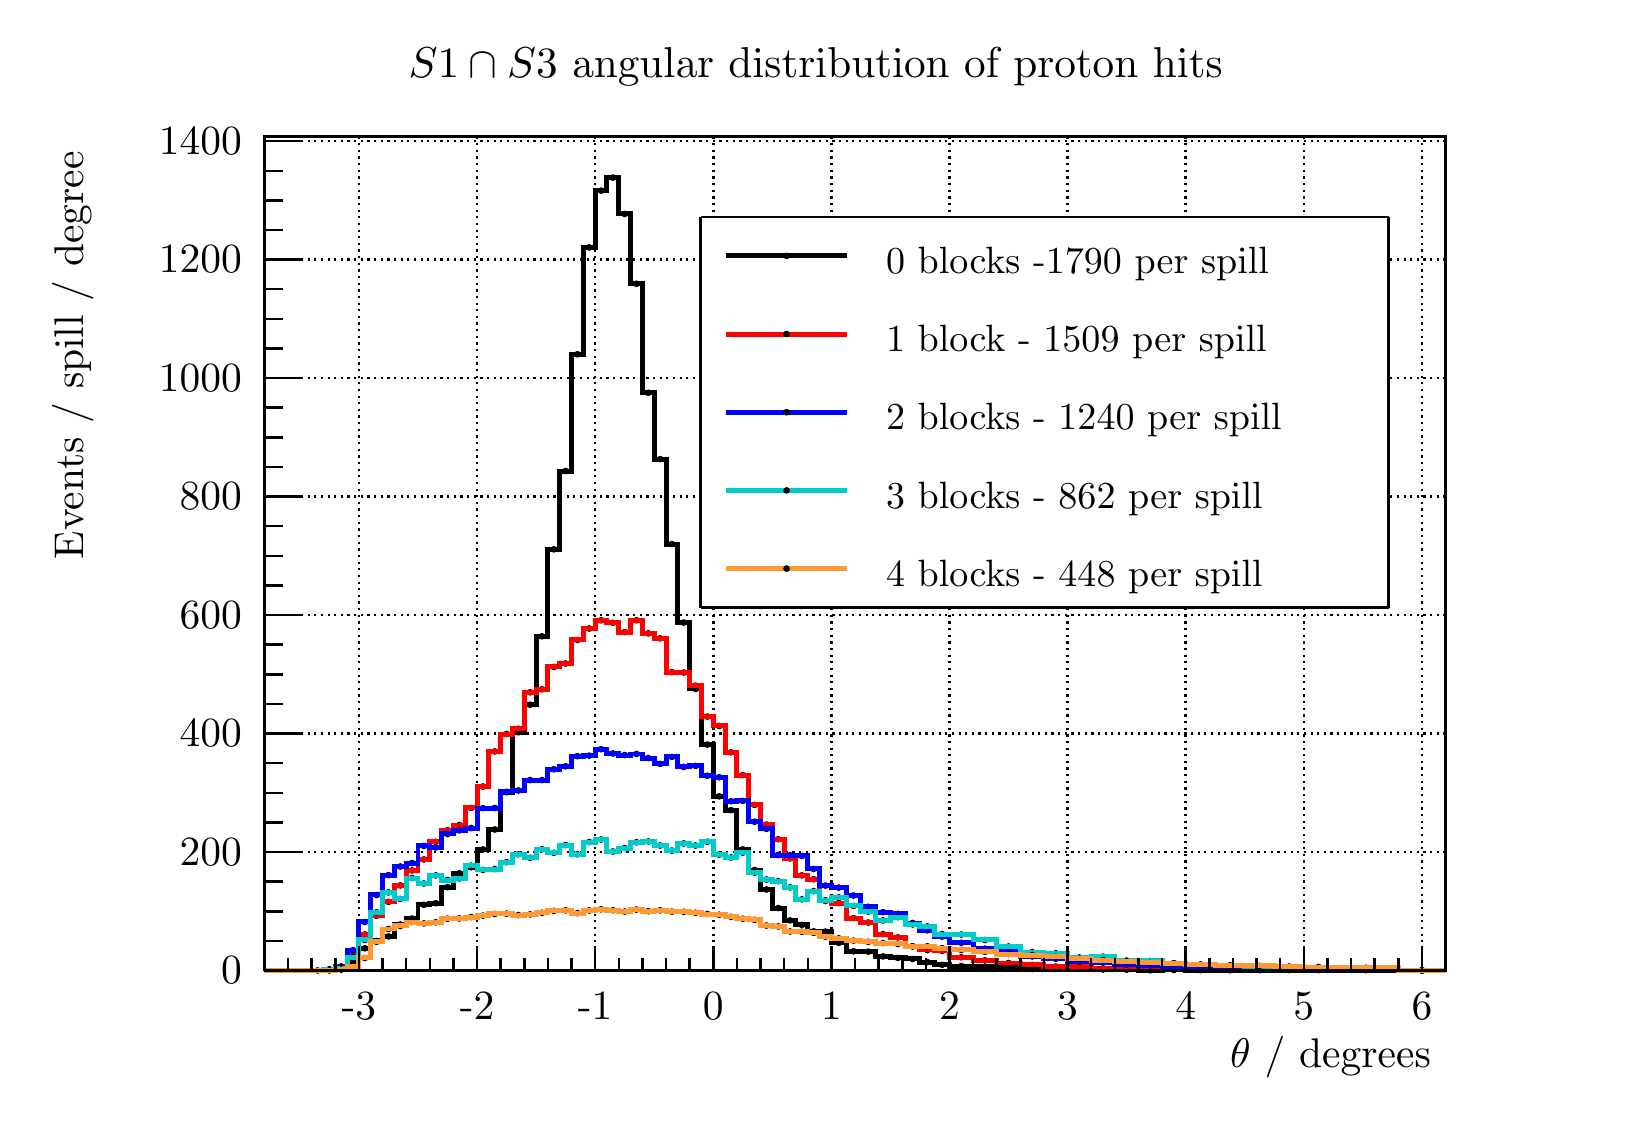
\begin{tikzpicture}
\pgfdeclareplotmark{cross} {
\pgfpathmoveto{\pgfpoint{-0.3\pgfplotmarksize}{\pgfplotmarksize}}
\pgfpathlineto{\pgfpoint{+0.3\pgfplotmarksize}{\pgfplotmarksize}}
\pgfpathlineto{\pgfpoint{+0.3\pgfplotmarksize}{0.3\pgfplotmarksize}}
\pgfpathlineto{\pgfpoint{+1\pgfplotmarksize}{0.3\pgfplotmarksize}}
\pgfpathlineto{\pgfpoint{+1\pgfplotmarksize}{-0.3\pgfplotmarksize}}
\pgfpathlineto{\pgfpoint{+0.3\pgfplotmarksize}{-0.3\pgfplotmarksize}}
\pgfpathlineto{\pgfpoint{+0.3\pgfplotmarksize}{-1.\pgfplotmarksize}}
\pgfpathlineto{\pgfpoint{-0.3\pgfplotmarksize}{-1.\pgfplotmarksize}}
\pgfpathlineto{\pgfpoint{-0.3\pgfplotmarksize}{-0.3\pgfplotmarksize}}
\pgfpathlineto{\pgfpoint{-1.\pgfplotmarksize}{-0.3\pgfplotmarksize}}
\pgfpathlineto{\pgfpoint{-1.\pgfplotmarksize}{0.3\pgfplotmarksize}}
\pgfpathlineto{\pgfpoint{-0.3\pgfplotmarksize}{0.3\pgfplotmarksize}}
\pgfpathclose
\pgfusepathqstroke
}
\pgfdeclareplotmark{cross*} {
\pgfpathmoveto{\pgfpoint{-0.3\pgfplotmarksize}{\pgfplotmarksize}}
\pgfpathlineto{\pgfpoint{+0.3\pgfplotmarksize}{\pgfplotmarksize}}
\pgfpathlineto{\pgfpoint{+0.3\pgfplotmarksize}{0.3\pgfplotmarksize}}
\pgfpathlineto{\pgfpoint{+1\pgfplotmarksize}{0.3\pgfplotmarksize}}
\pgfpathlineto{\pgfpoint{+1\pgfplotmarksize}{-0.3\pgfplotmarksize}}
\pgfpathlineto{\pgfpoint{+0.3\pgfplotmarksize}{-0.3\pgfplotmarksize}}
\pgfpathlineto{\pgfpoint{+0.3\pgfplotmarksize}{-1.\pgfplotmarksize}}
\pgfpathlineto{\pgfpoint{-0.3\pgfplotmarksize}{-1.\pgfplotmarksize}}
\pgfpathlineto{\pgfpoint{-0.3\pgfplotmarksize}{-0.3\pgfplotmarksize}}
\pgfpathlineto{\pgfpoint{-1.\pgfplotmarksize}{-0.3\pgfplotmarksize}}
\pgfpathlineto{\pgfpoint{-1.\pgfplotmarksize}{0.3\pgfplotmarksize}}
\pgfpathlineto{\pgfpoint{-0.3\pgfplotmarksize}{0.3\pgfplotmarksize}}
\pgfpathclose
\pgfusepathqfillstroke
}
\pgfdeclareplotmark{newstar} {
\pgfpathmoveto{\pgfqpoint{0pt}{\pgfplotmarksize}}
\pgfpathlineto{\pgfqpointpolar{44}{0.5\pgfplotmarksize}}
\pgfpathlineto{\pgfqpointpolar{18}{\pgfplotmarksize}}
\pgfpathlineto{\pgfqpointpolar{-20}{0.5\pgfplotmarksize}}
\pgfpathlineto{\pgfqpointpolar{-54}{\pgfplotmarksize}}
\pgfpathlineto{\pgfqpointpolar{-90}{0.5\pgfplotmarksize}}
\pgfpathlineto{\pgfqpointpolar{234}{\pgfplotmarksize}}
\pgfpathlineto{\pgfqpointpolar{198}{0.5\pgfplotmarksize}}
\pgfpathlineto{\pgfqpointpolar{162}{\pgfplotmarksize}}
\pgfpathlineto{\pgfqpointpolar{134}{0.5\pgfplotmarksize}}
\pgfpathclose
\pgfusepathqstroke
}
\pgfdeclareplotmark{newstar*} {
\pgfpathmoveto{\pgfqpoint{0pt}{\pgfplotmarksize}}
\pgfpathlineto{\pgfqpointpolar{44}{0.5\pgfplotmarksize}}
\pgfpathlineto{\pgfqpointpolar{18}{\pgfplotmarksize}}
\pgfpathlineto{\pgfqpointpolar{-20}{0.5\pgfplotmarksize}}
\pgfpathlineto{\pgfqpointpolar{-54}{\pgfplotmarksize}}
\pgfpathlineto{\pgfqpointpolar{-90}{0.5\pgfplotmarksize}}
\pgfpathlineto{\pgfqpointpolar{234}{\pgfplotmarksize}}
\pgfpathlineto{\pgfqpointpolar{198}{0.5\pgfplotmarksize}}
\pgfpathlineto{\pgfqpointpolar{162}{\pgfplotmarksize}}
\pgfpathlineto{\pgfqpointpolar{134}{0.5\pgfplotmarksize}}
\pgfpathclose
\pgfusepathqfillstroke
}
\definecolor{c}{rgb}{1,1,1};
\draw [color=c, fill=c] (0,0) rectangle (20,13.7553);
\draw [color=c, fill=c] (3,1.78819) rectangle (18,12.3797);
\definecolor{c}{rgb}{0,0,0};
\draw [c,line width=0.9] (3,1.78819) -- (3,12.3797) -- (18,12.3797) -- (18,1.78819) -- (3,1.78819);
\definecolor{c}{rgb}{1,1,1};
\draw [color=c, fill=c] (3,1.78819) rectangle (18,12.3797);
\definecolor{c}{rgb}{0,0,0};
\draw [c,line width=0.9] (3,1.78819) -- (3,12.3797) -- (18,12.3797) -- (18,1.78819) -- (3,1.78819);
\draw [c,line width=0.9] (3,1.78819) -- (18,1.78819);
\draw [c,dash pattern=on 0.80pt off 1.60pt ,line width=0.9] (4.2,12.3797) -- (4.2,1.78819);
\draw [c,dash pattern=on 0.80pt off 1.60pt ,line width=0.9] (5.7,12.3797) -- (5.7,1.78819);
\draw [c,dash pattern=on 0.80pt off 1.60pt ,line width=0.9] (7.2,12.3797) -- (7.2,1.78819);
\draw [c,dash pattern=on 0.80pt off 1.60pt ,line width=0.9] (8.7,12.3797) -- (8.7,1.78819);
\draw [c,dash pattern=on 0.80pt off 1.60pt ,line width=0.9] (10.2,12.3797) -- (10.2,1.78819);
\draw [c,dash pattern=on 0.80pt off 1.60pt ,line width=0.9] (11.7,12.3797) -- (11.7,1.78819);
\draw [c,dash pattern=on 0.80pt off 1.60pt ,line width=0.9] (13.2,12.3797) -- (13.2,1.78819);
\draw [c,dash pattern=on 0.80pt off 1.60pt ,line width=0.9] (14.7,12.3797) -- (14.7,1.78819);
\draw [c,dash pattern=on 0.80pt off 1.60pt ,line width=0.9] (16.2,12.3797) -- (16.2,1.78819);
\draw [c,dash pattern=on 0.80pt off 1.60pt ,line width=0.9] (17.7,12.3797) -- (17.7,1.78819);
\draw [c,dash pattern=on 0.80pt off 1.60pt ,line width=0.9] (4.2,12.3797) -- (4.2,1.78819);
\draw [c,dash pattern=on 0.80pt off 1.60pt ,line width=0.9] (17.7,12.3797) -- (17.7,1.78819);
\draw [c,line width=0.9] (3,1.78819) -- (3,12.3797);
\draw [c,dash pattern=on 0.80pt off 1.60pt ,line width=0.9] (18,1.78819) -- (3,1.78819);
\draw [c,dash pattern=on 0.80pt off 1.60pt ,line width=0.9] (18,3.29291) -- (3,3.29291);
\draw [c,dash pattern=on 0.80pt off 1.60pt ,line width=0.9] (18,4.79763) -- (3,4.79763);
\draw [c,dash pattern=on 0.80pt off 1.60pt ,line width=0.9] (18,6.30235) -- (3,6.30235);
\draw [c,dash pattern=on 0.80pt off 1.60pt ,line width=0.9] (18,7.80708) -- (3,7.80708);
\draw [c,dash pattern=on 0.80pt off 1.60pt ,line width=0.9] (18,9.3118) -- (3,9.3118);
\draw [c,dash pattern=on 0.80pt off 1.60pt ,line width=0.9] (18,10.8165) -- (3,10.8165);
\draw [c,dash pattern=on 0.80pt off 1.60pt ,line width=0.9] (18,12.3212) -- (3,12.3212);
\draw [c,dash pattern=on 0.80pt off 1.60pt ,line width=0.9] (18,12.3212) -- (3,12.3212);
\definecolor{c}{rgb}{0,0,0.6};
\draw [c,line width=0.9] (3,1.78819) -- (3.15,1.78819) -- (3.15,1.78819) -- (3.3,1.78819) -- (3.3,1.78819) -- (3.45,1.78819) -- (3.45,1.78819) -- (3.6,1.78819) -- (3.6,1.78819) -- (3.75,1.78819) -- (3.75,1.78819) -- (3.9,1.78819) -- (3.9,1.78819) --
 (4.05,1.78819) -- (4.05,1.78819) -- (4.2,1.78819) -- (4.2,1.78819) -- (4.35,1.78819) -- (4.35,1.78819) -- (4.5,1.78819) -- (4.5,1.78819) -- (4.65,1.78819) -- (4.65,1.78819) -- (4.8,1.78819) -- (4.8,1.78819) -- (4.95,1.78819) -- (4.95,1.78819) --
 (5.1,1.78819) -- (5.1,1.78819) -- (5.25,1.78819) -- (5.25,1.78819) -- (5.4,1.78819) -- (5.4,1.78819) -- (5.55,1.78819) -- (5.55,1.78819) -- (5.7,1.78819) -- (5.7,1.78819) -- (5.85,1.78819) -- (5.85,1.78819) -- (6,1.78819) -- (6,1.78819) --
 (6.15,1.78819) -- (6.15,1.78819) -- (6.3,1.78819) -- (6.3,1.78819) -- (6.45,1.78819) -- (6.45,1.78819) -- (6.6,1.78819) -- (6.6,1.78819) -- (6.75,1.78819) -- (6.75,1.78819) -- (6.9,1.78819) -- (6.9,1.78819) -- (7.05,1.78819) -- (7.05,1.78819) --
 (7.2,1.78819) -- (7.2,1.78819) -- (7.35,1.78819) -- (7.35,1.78819) -- (7.5,1.78819) -- (7.5,1.78819) -- (7.65,1.78819) -- (7.65,1.78819) -- (7.8,1.78819) -- (7.8,1.78819) -- (7.95,1.78819) -- (7.95,1.78819) -- (8.1,1.78819) -- (8.1,1.78819) --
 (8.25,1.78819) -- (8.25,1.78819) -- (8.4,1.78819) -- (8.4,1.78819) -- (8.55,1.78819) -- (8.55,1.78819) -- (8.7,1.78819) -- (8.7,1.78819) -- (8.85,1.78819) -- (8.85,1.78819) -- (9,1.78819) -- (9,1.78819) -- (9.15,1.78819) -- (9.15,1.78819) --
 (9.3,1.78819) -- (9.3,1.78819) -- (9.45,1.78819) -- (9.45,1.78819) -- (9.6,1.78819) -- (9.6,1.78819) -- (9.75,1.78819) -- (9.75,1.78819) -- (9.9,1.78819) -- (9.9,1.78819) -- (10.05,1.78819) -- (10.05,1.78819) -- (10.2,1.78819) -- (10.2,1.78819) --
 (10.3875,1.78819) -- (10.3875,1.78819) -- (10.575,1.78819) -- (10.575,1.78819) -- (10.7625,1.78819) -- (10.7625,1.78819) -- (10.95,1.78819) -- (10.95,1.78819) -- (11.1375,1.78819) -- (11.1375,1.78819) -- (11.325,1.78819) -- (11.325,1.78819) --
 (11.5125,1.78819) -- (11.5125,1.78819) -- (11.7,1.78819) -- (11.7,1.78819) -- (12,1.78819) -- (12,1.78819) -- (12.3,1.78819) -- (12.3,1.78819) -- (12.6,1.78819) -- (12.6,1.78819) -- (12.9,1.78819) -- (12.9,1.78819) -- (13.2,1.78819) --
 (13.2,1.78819) -- (13.5,1.78819) -- (13.5,1.78819) -- (13.8,1.78819) -- (13.8,1.78819) -- (14.1,1.78819) -- (14.1,1.78819) -- (14.4,1.78819) -- (14.4,1.78819) -- (14.7,1.78819) -- (14.7,1.78819) -- (15.075,1.78819) -- (15.075,1.78819) --
 (15.45,1.78819) -- (15.45,1.78819) -- (15.825,1.78819) -- (15.825,1.78819) -- (16.2,1.78819) -- (16.2,1.78819) -- (16.575,1.78819) -- (16.575,1.78819) -- (17.4,1.78819) -- (17.4,1.78819) -- (18,1.78819);
\definecolor{c}{rgb}{0,0,0};
\draw [c,line width=0.9] (3,1.78819) -- (18,1.78819);
\draw [c,line width=0.9] (4.2,2.09768) -- (4.2,1.78819);
\draw [c,line width=0.9] (4.5,1.94293) -- (4.5,1.78819);
\draw [c,line width=0.9] (4.8,1.94293) -- (4.8,1.78819);
\draw [c,line width=0.9] (5.1,1.94293) -- (5.1,1.78819);
\draw [c,line width=0.9] (5.4,1.94293) -- (5.4,1.78819);
\draw [c,line width=0.9] (5.7,2.09768) -- (5.7,1.78819);
\draw [c,line width=0.9] (6,1.94293) -- (6,1.78819);
\draw [c,line width=0.9] (6.3,1.94293) -- (6.3,1.78819);
\draw [c,line width=0.9] (6.6,1.94293) -- (6.6,1.78819);
\draw [c,line width=0.9] (6.9,1.94293) -- (6.9,1.78819);
\draw [c,line width=0.9] (7.2,2.09768) -- (7.2,1.78819);
\draw [c,line width=0.9] (7.5,1.94293) -- (7.5,1.78819);
\draw [c,line width=0.9] (7.8,1.94293) -- (7.8,1.78819);
\draw [c,line width=0.9] (8.1,1.94293) -- (8.1,1.78819);
\draw [c,line width=0.9] (8.4,1.94293) -- (8.4,1.78819);
\draw [c,line width=0.9] (8.7,2.09768) -- (8.7,1.78819);
\draw [c,line width=0.9] (9,1.94293) -- (9,1.78819);
\draw [c,line width=0.9] (9.3,1.94293) -- (9.3,1.78819);
\draw [c,line width=0.9] (9.6,1.94293) -- (9.6,1.78819);
\draw [c,line width=0.9] (9.9,1.94293) -- (9.9,1.78819);
\draw [c,line width=0.9] (10.2,2.09768) -- (10.2,1.78819);
\draw [c,line width=0.9] (10.5,1.94293) -- (10.5,1.78819);
\draw [c,line width=0.9] (10.8,1.94293) -- (10.8,1.78819);
\draw [c,line width=0.9] (11.1,1.94293) -- (11.1,1.78819);
\draw [c,line width=0.9] (11.4,1.94293) -- (11.4,1.78819);
\draw [c,line width=0.9] (11.7,2.09768) -- (11.7,1.78819);
\draw [c,line width=0.9] (12,1.94293) -- (12,1.78819);
\draw [c,line width=0.9] (12.3,1.94293) -- (12.3,1.78819);
\draw [c,line width=0.9] (12.6,1.94293) -- (12.6,1.78819);
\draw [c,line width=0.9] (12.9,1.94293) -- (12.9,1.78819);
\draw [c,line width=0.9] (13.2,2.09768) -- (13.2,1.78819);
\draw [c,line width=0.9] (13.5,1.94293) -- (13.5,1.78819);
\draw [c,line width=0.9] (13.8,1.94293) -- (13.8,1.78819);
\draw [c,line width=0.9] (14.1,1.94293) -- (14.1,1.78819);
\draw [c,line width=0.9] (14.4,1.94293) -- (14.4,1.78819);
\draw [c,line width=0.9] (14.7,2.09768) -- (14.7,1.78819);
\draw [c,line width=0.9] (15,1.94293) -- (15,1.78819);
\draw [c,line width=0.9] (15.3,1.94293) -- (15.3,1.78819);
\draw [c,line width=0.9] (15.6,1.94293) -- (15.6,1.78819);
\draw [c,line width=0.9] (15.9,1.94293) -- (15.9,1.78819);
\draw [c,line width=0.9] (16.2,2.09768) -- (16.2,1.78819);
\draw [c,line width=0.9] (16.5,1.94293) -- (16.5,1.78819);
\draw [c,line width=0.9] (16.8,1.94293) -- (16.8,1.78819);
\draw [c,line width=0.9] (17.1,1.94293) -- (17.1,1.78819);
\draw [c,line width=0.9] (17.4,1.94293) -- (17.4,1.78819);
\draw [c,line width=0.9] (17.7,2.09768) -- (17.7,1.78819);
\draw [c,line width=0.9] (4.2,2.09768) -- (4.2,1.78819);
\draw [c,line width=0.9] (3.9,1.94293) -- (3.9,1.78819);
\draw [c,line width=0.9] (3.6,1.94293) -- (3.6,1.78819);
\draw [c,line width=0.9] (3.3,1.94293) -- (3.3,1.78819);
\draw [c,line width=0.9] (3,1.94293) -- (3,1.78819);
\draw [c,line width=0.9] (17.7,2.09768) -- (17.7,1.78819);
\draw [c,line width=0.9] (18,1.94293) -- (18,1.78819);
\draw [anchor=base] (4.2,1.1692) node[scale=1.49939, color=c, rotate=0]{-3};
\draw [anchor=base] (5.7,1.1692) node[scale=1.49939, color=c, rotate=0]{-2};
\draw [anchor=base] (7.2,1.1692) node[scale=1.49939, color=c, rotate=0]{-1};
\draw [anchor=base] (8.7,1.1692) node[scale=1.49939, color=c, rotate=0]{0};
\draw [anchor=base] (10.2,1.1692) node[scale=1.49939, color=c, rotate=0]{1};
\draw [anchor=base] (11.7,1.1692) node[scale=1.49939, color=c, rotate=0]{2};
\draw [anchor=base] (13.2,1.1692) node[scale=1.49939, color=c, rotate=0]{3};
\draw [anchor=base] (14.7,1.1692) node[scale=1.49939, color=c, rotate=0]{4};
\draw [anchor=base] (16.2,1.1692) node[scale=1.49939, color=c, rotate=0]{5};
\draw [anchor=base] (17.7,1.1692) node[scale=1.49939, color=c, rotate=0]{6};
\draw [anchor= east] (18,0.687764) node[scale=1.49939, color=c, rotate=0]{$\theta$ / degrees};
\draw [c,line width=0.9] (3,1.78819) -- (3,12.3797);
\draw [c,line width=0.9] (3.462,1.78819) -- (3,1.78819);
\draw [c,line width=0.9] (3.231,2.16437) -- (3,2.16437);
\draw [c,line width=0.9] (3.231,2.54055) -- (3,2.54055);
\draw [c,line width=0.9] (3.231,2.91673) -- (3,2.91673);
\draw [c,line width=0.9] (3.462,3.29291) -- (3,3.29291);
\draw [c,line width=0.9] (3.231,3.66909) -- (3,3.66909);
\draw [c,line width=0.9] (3.231,4.04527) -- (3,4.04527);
\draw [c,line width=0.9] (3.231,4.42145) -- (3,4.42145);
\draw [c,line width=0.9] (3.462,4.79763) -- (3,4.79763);
\draw [c,line width=0.9] (3.231,5.17381) -- (3,5.17381);
\draw [c,line width=0.9] (3.231,5.54999) -- (3,5.54999);
\draw [c,line width=0.9] (3.231,5.92617) -- (3,5.92617);
\draw [c,line width=0.9] (3.462,6.30235) -- (3,6.30235);
\draw [c,line width=0.9] (3.231,6.67853) -- (3,6.67853);
\draw [c,line width=0.9] (3.231,7.05472) -- (3,7.05472);
\draw [c,line width=0.9] (3.231,7.4309) -- (3,7.4309);
\draw [c,line width=0.9] (3.462,7.80708) -- (3,7.80708);
\draw [c,line width=0.9] (3.231,8.18326) -- (3,8.18326);
\draw [c,line width=0.9] (3.231,8.55944) -- (3,8.55944);
\draw [c,line width=0.9] (3.231,8.93562) -- (3,8.93562);
\draw [c,line width=0.9] (3.462,9.3118) -- (3,9.3118);
\draw [c,line width=0.9] (3.231,9.68798) -- (3,9.68798);
\draw [c,line width=0.9] (3.231,10.0642) -- (3,10.0642);
\draw [c,line width=0.9] (3.231,10.4403) -- (3,10.4403);
\draw [c,line width=0.9] (3.462,10.8165) -- (3,10.8165);
\draw [c,line width=0.9] (3.231,11.1927) -- (3,11.1927);
\draw [c,line width=0.9] (3.231,11.5689) -- (3,11.5689);
\draw [c,line width=0.9] (3.231,11.9451) -- (3,11.9451);
\draw [c,line width=0.9] (3.462,12.3212) -- (3,12.3212);
\draw [c,line width=0.9] (3.462,12.3212) -- (3,12.3212);
\draw [anchor= east] (2.9,1.78819) node[scale=1.49939, color=c, rotate=0]{0};
\draw [anchor= east] (2.9,3.29291) node[scale=1.49939, color=c, rotate=0]{200};
\draw [anchor= east] (2.9,4.79763) node[scale=1.49939, color=c, rotate=0]{400};
\draw [anchor= east] (2.9,6.30235) node[scale=1.49939, color=c, rotate=0]{600};
\draw [anchor= east] (2.9,7.80708) node[scale=1.49939, color=c, rotate=0]{800};
\draw [anchor= east] (2.9,9.3118) node[scale=1.49939, color=c, rotate=0]{1000};
\draw [anchor= east] (2.9,10.8165) node[scale=1.49939, color=c, rotate=0]{1200};
\draw [anchor= east] (2.9,12.3212) node[scale=1.49939, color=c, rotate=0]{1400};
\draw [anchor= east] (0.565401,12.3797) node[scale=1.49939, color=c, rotate=90]{ Events / spill / degree};
\draw [c,line width=1.8] (3.825,1.7964) -- (3.825,1.79691);
\draw [c,line width=1.8] (3.825,1.79691) -- (3.825,1.79741);
\foreach \P in {(3.825,1.79691)}{\draw[mark options={color=c,fill=c},mark size=2.402402pt,mark=*,mark size=1pt] plot coordinates {\P};}
\draw [c,line width=1.8] (3.975,1.82206) -- (3.975,1.82307);
\draw [c,line width=1.8] (3.975,1.82307) -- (3.975,1.82408);
\foreach \P in {(3.975,1.82307)}{\draw[mark options={color=c,fill=c},mark size=2.402402pt,mark=*,mark size=1pt] plot coordinates {\P};}
\draw [c,line width=1.8] (4.125,1.90551) -- (4.125,1.90738);
\draw [c,line width=1.8] (4.125,1.90738) -- (4.125,1.90924);
\foreach \P in {(4.125,1.90738)}{\draw[mark options={color=c,fill=c},mark size=2.402402pt,mark=*,mark size=1pt] plot coordinates {\P};}
\draw [c,line width=1.8] (4.275,2.06731) -- (4.275,2.07017);
\draw [c,line width=1.8] (4.275,2.07017) -- (4.275,2.07303);
\foreach \P in {(4.275,2.07017)}{\draw[mark options={color=c,fill=c},mark size=2.402402pt,mark=*,mark size=1pt] plot coordinates {\P};}
\draw [c,line width=1.8] (4.425,2.1599) -- (4.425,2.1632);
\draw [c,line width=1.8] (4.425,2.1632) -- (4.425,2.1665);
\foreach \P in {(4.425,2.1632)}{\draw[mark options={color=c,fill=c},mark size=2.402402pt,mark=*,mark size=1pt] plot coordinates {\P};}
\draw [c,line width=1.8] (4.575,2.21779) -- (4.575,2.22134);
\draw [c,line width=1.8] (4.575,2.22134) -- (4.575,2.22489);
\foreach \P in {(4.575,2.22134)}{\draw[mark options={color=c,fill=c},mark size=2.402402pt,mark=*,mark size=1pt] plot coordinates {\P};}
\draw [c,line width=1.8] (4.725,2.36839) -- (4.725,2.37251);
\draw [c,line width=1.8] (4.725,2.37251) -- (4.725,2.37663);
\foreach \P in {(4.725,2.37251)}{\draw[mark options={color=c,fill=c},mark size=2.402402pt,mark=*,mark size=1pt] plot coordinates {\P};}
\draw [c,line width=1.8] (4.875,2.44371) -- (4.875,2.44809);
\draw [c,line width=1.8] (4.875,2.44809) -- (4.875,2.45247);
\foreach \P in {(4.875,2.44809)}{\draw[mark options={color=c,fill=c},mark size=2.402402pt,mark=*,mark size=1pt] plot coordinates {\P};}
\draw [c,line width=1.8] (5.025,2.61759) -- (5.025,2.62251);
\draw [c,line width=1.8] (5.025,2.62251) -- (5.025,2.62744);
\foreach \P in {(5.025,2.62251)}{\draw[mark options={color=c,fill=c},mark size=2.402402pt,mark=*,mark size=1pt] plot coordinates {\P};}
\draw [c,line width=1.8] (5.175,2.63788) -- (5.175,2.64286);
\draw [c,line width=1.8] (5.175,2.64286) -- (5.175,2.64785);
\foreach \P in {(5.175,2.64286)}{\draw[mark options={color=c,fill=c},mark size=2.402402pt,mark=*,mark size=1pt] plot coordinates {\P};}
\draw [c,line width=1.8] (5.325,2.84081) -- (5.325,2.84636);
\draw [c,line width=1.8] (5.325,2.84636) -- (5.325,2.85191);
\foreach \P in {(5.325,2.84636)}{\draw[mark options={color=c,fill=c},mark size=2.402402pt,mark=*,mark size=1pt] plot coordinates {\P};}
\draw [c,line width=1.8] (5.475,3.0177) -- (5.475,3.02369);
\draw [c,line width=1.8] (5.475,3.02369) -- (5.475,3.02968);
\foreach \P in {(5.475,3.02369)}{\draw[mark options={color=c,fill=c},mark size=2.402402pt,mark=*,mark size=1pt] plot coordinates {\P};}
\draw [c,line width=1.8] (5.625,3.0931) -- (5.625,3.09927);
\draw [c,line width=1.8] (5.625,3.09927) -- (5.625,3.10545);
\foreach \P in {(5.625,3.09927)}{\draw[mark options={color=c,fill=c},mark size=2.402402pt,mark=*,mark size=1pt] plot coordinates {\P};}
\draw [c,line width=1.8] (5.775,3.31934) -- (5.775,3.32603);
\draw [c,line width=1.8] (5.775,3.32603) -- (5.775,3.33271);
\foreach \P in {(5.775,3.32603)}{\draw[mark options={color=c,fill=c},mark size=2.402402pt,mark=*,mark size=1pt] plot coordinates {\P};}
\draw [c,line width=1.8] (5.925,3.57173) -- (5.925,3.57894);
\draw [c,line width=1.8] (5.925,3.57894) -- (5.925,3.58616);
\foreach \P in {(5.925,3.57894)}{\draw[mark options={color=c,fill=c},mark size=2.402402pt,mark=*,mark size=1pt] plot coordinates {\P};}
\draw [c,line width=1.8] (6.075,4.04468) -- (6.075,4.05279);
\draw [c,line width=1.8] (6.075,4.05279) -- (6.075,4.06091);
\foreach \P in {(6.075,4.05279)}{\draw[mark options={color=c,fill=c},mark size=2.402402pt,mark=*,mark size=1pt] plot coordinates {\P};}
\draw [c,line width=1.8] (6.225,4.80507) -- (6.225,4.81445);
\draw [c,line width=1.8] (6.225,4.81445) -- (6.225,4.82383);
\foreach \P in {(6.225,4.81445)}{\draw[mark options={color=c,fill=c},mark size=2.402402pt,mark=*,mark size=1pt] plot coordinates {\P};}
\draw [c,line width=1.8] (6.375,5.15339) -- (6.375,5.16329);
\draw [c,line width=1.8] (6.375,5.16329) -- (6.375,5.1732);
\foreach \P in {(6.375,5.16329)}{\draw[mark options={color=c,fill=c},mark size=2.402402pt,mark=*,mark size=1pt] plot coordinates {\P};}
\draw [c,line width=1.8] (6.525,6.0214) -- (6.525,6.03251);
\draw [c,line width=1.8] (6.525,6.03251) -- (6.525,6.04362);
\foreach \P in {(6.525,6.03251)}{\draw[mark options={color=c,fill=c},mark size=2.402402pt,mark=*,mark size=1pt] plot coordinates {\P};}
\draw [c,line width=1.8] (6.675,7.12472) -- (6.675,7.13719);
\draw [c,line width=1.8] (6.675,7.13719) -- (6.675,7.14966);
\foreach \P in {(6.675,7.13719)}{\draw[mark options={color=c,fill=c},mark size=2.402402pt,mark=*,mark size=1pt] plot coordinates {\P};}
\draw [c,line width=1.8] (6.825,8.11783) -- (6.825,8.13141);
\draw [c,line width=1.8] (6.825,8.13141) -- (6.825,8.14499);
\foreach \P in {(6.825,8.13141)}{\draw[mark options={color=c,fill=c},mark size=2.402402pt,mark=*,mark size=1pt] plot coordinates {\P};}
\draw [c,line width=1.8] (6.975,9.59894) -- (6.975,9.61402);
\draw [c,line width=1.8] (6.975,9.61402) -- (6.975,9.6291);
\foreach \P in {(6.975,9.61402)}{\draw[mark options={color=c,fill=c},mark size=2.402402pt,mark=*,mark size=1pt] plot coordinates {\P};}
\draw [c,line width=1.8] (7.125,10.9553) -- (7.125,10.9716);
\draw [c,line width=1.8] (7.125,10.9716) -- (7.125,10.988);
\foreach \P in {(7.125,10.9716)}{\draw[mark options={color=c,fill=c},mark size=2.402402pt,mark=*,mark size=1pt] plot coordinates {\P};}
\draw [c,line width=1.8] (7.275,11.6756) -- (7.275,11.6926);
\draw [c,line width=1.8] (7.275,11.6926) -- (7.275,11.7095);
\foreach \P in {(7.275,11.6926)}{\draw[mark options={color=c,fill=c},mark size=2.402402pt,mark=*,mark size=1pt] plot coordinates {\P};}
\draw [c,line width=1.8] (7.425,11.8412) -- (7.425,11.8583);
\draw [c,line width=1.8] (7.425,11.8583) -- (7.425,11.8754);
\foreach \P in {(7.425,11.8583)}{\draw[mark options={color=c,fill=c},mark size=2.402402pt,mark=*,mark size=1pt] plot coordinates {\P};}
\draw [c,line width=1.8] (7.575,11.3793) -- (7.575,11.3961);
\draw [c,line width=1.8] (7.575,11.3961) -- (7.575,11.4128);
\foreach \P in {(7.575,11.3961)}{\draw[mark options={color=c,fill=c},mark size=2.402402pt,mark=*,mark size=1pt] plot coordinates {\P};}
\draw [c,line width=1.8] (7.725,10.4935) -- (7.725,10.5094);
\draw [c,line width=1.8] (7.725,10.5094) -- (7.725,10.5253);
\foreach \P in {(7.725,10.5094)}{\draw[mark options={color=c,fill=c},mark size=2.402402pt,mark=*,mark size=1pt] plot coordinates {\P};}
\draw [c,line width=1.8] (7.875,9.11103) -- (7.875,9.12563);
\draw [c,line width=1.8] (7.875,9.12563) -- (7.875,9.14024);
\foreach \P in {(7.875,9.12563)}{\draw[mark options={color=c,fill=c},mark size=2.402402pt,mark=*,mark size=1pt] plot coordinates {\P};}
\draw [c,line width=1.8] (8.025,8.26884) -- (8.025,8.28258);
\draw [c,line width=1.8] (8.025,8.28258) -- (8.025,8.29632);
\foreach \P in {(8.025,8.28258)}{\draw[mark options={color=c,fill=c},mark size=2.402402pt,mark=*,mark size=1pt] plot coordinates {\P};}
\draw [c,line width=1.8] (8.175,7.19151) -- (8.175,7.20406);
\draw [c,line width=1.8] (8.175,7.20406) -- (8.175,7.2166);
\foreach \P in {(8.175,7.20406)}{\draw[mark options={color=c,fill=c},mark size=2.402402pt,mark=*,mark size=1pt] plot coordinates {\P};}
\draw [c,line width=1.8] (8.325,6.1956) -- (8.325,6.20693);
\draw [c,line width=1.8] (8.325,6.20693) -- (8.325,6.21827);
\foreach \P in {(8.325,6.20693)}{\draw[mark options={color=c,fill=c},mark size=2.402402pt,mark=*,mark size=1pt] plot coordinates {\P};}
\draw [c,line width=1.8] (8.475,5.35369) -- (8.475,5.36388);
\draw [c,line width=1.8] (8.475,5.36388) -- (8.475,5.37408);
\foreach \P in {(8.475,5.36388)}{\draw[mark options={color=c,fill=c},mark size=2.402402pt,mark=*,mark size=1pt] plot coordinates {\P};}
\draw [c,line width=1.8] (8.625,4.64833) -- (8.625,4.65746);
\draw [c,line width=1.8] (8.625,4.65746) -- (8.625,4.6666);
\foreach \P in {(8.625,4.65746)}{\draw[mark options={color=c,fill=c},mark size=2.402402pt,mark=*,mark size=1pt] plot coordinates {\P};}
\draw [c,line width=1.8] (8.775,3.99245) -- (8.775,4.00047);
\draw [c,line width=1.8] (8.775,4.00047) -- (8.775,4.00849);
\foreach \P in {(8.775,4.00047)}{\draw[mark options={color=c,fill=c},mark size=2.402402pt,mark=*,mark size=1pt] plot coordinates {\P};}
\draw [c,line width=1.8] (8.925,3.81834) -- (8.925,3.82604);
\draw [c,line width=1.8] (8.925,3.82604) -- (8.925,3.83374);
\foreach \P in {(8.925,3.82604)}{\draw[mark options={color=c,fill=c},mark size=2.402402pt,mark=*,mark size=1pt] plot coordinates {\P};}
\draw [c,line width=1.8] (9.075,3.31934) -- (9.075,3.32603);
\draw [c,line width=1.8] (9.075,3.32603) -- (9.075,3.33271);
\foreach \P in {(9.075,3.32603)}{\draw[mark options={color=c,fill=c},mark size=2.402402pt,mark=*,mark size=1pt] plot coordinates {\P};}
\draw [c,line width=1.8] (9.225,3.0583) -- (9.225,3.06439);
\draw [c,line width=1.8] (9.225,3.06439) -- (9.225,3.07048);
\foreach \P in {(9.225,3.06439)}{\draw[mark options={color=c,fill=c},mark size=2.402402pt,mark=*,mark size=1pt] plot coordinates {\P};}
\draw [c,line width=1.8] (9.375,2.81182) -- (9.375,2.81729);
\draw [c,line width=1.8] (9.375,2.81729) -- (9.375,2.82276);
\foreach \P in {(9.375,2.81729)}{\draw[mark options={color=c,fill=c},mark size=2.402402pt,mark=*,mark size=1pt] plot coordinates {\P};}
\draw [c,line width=1.8] (9.525,2.57701) -- (9.525,2.58182);
\draw [c,line width=1.8] (9.525,2.58182) -- (9.525,2.58662);
\foreach \P in {(9.525,2.58182)}{\draw[mark options={color=c,fill=c},mark size=2.402402pt,mark=*,mark size=1pt] plot coordinates {\P};}
\draw [c,line width=1.8] (9.675,2.42053) -- (9.675,2.42483);
\draw [c,line width=1.8] (9.675,2.42483) -- (9.675,2.42914);
\foreach \P in {(9.675,2.42483)}{\draw[mark options={color=c,fill=c},mark size=2.402402pt,mark=*,mark size=1pt] plot coordinates {\P};}
\draw [c,line width=1.8] (9.825,2.36259) -- (9.825,2.36669);
\draw [c,line width=1.8] (9.825,2.36669) -- (9.825,2.37079);
\foreach \P in {(9.825,2.36669)}{\draw[mark options={color=c,fill=c},mark size=2.402402pt,mark=*,mark size=1pt] plot coordinates {\P};}
\draw [c,line width=1.8] (9.975,2.28149) -- (9.975,2.28529);
\draw [c,line width=1.8] (9.975,2.28529) -- (9.975,2.2891);
\foreach \P in {(9.975,2.28529)}{\draw[mark options={color=c,fill=c},mark size=2.402402pt,mark=*,mark size=1pt] plot coordinates {\P};}
\draw [c,line width=1.8] (10.125,2.2786) -- (10.125,2.28239);
\draw [c,line width=1.8] (10.125,2.28239) -- (10.125,2.28618);
\foreach \P in {(10.125,2.28239)}{\draw[mark options={color=c,fill=c},mark size=2.402402pt,mark=*,mark size=1pt] plot coordinates {\P};}
\draw [c,line width=1.8] (10.2937,2.13579) -- (10.2937,2.13936);
\draw [c,line width=1.8] (10.2937,2.13936) -- (10.2937,2.14293);
\foreach \P in {(10.2937,2.13936)}{\draw[mark options={color=c,fill=c},mark size=2.402402pt,mark=*,mark size=1pt] plot coordinates {\P};}
\draw [c,line width=1.8] (10.4812,2.0294) -- (10.4812,2.03238);
\draw [c,line width=1.8] (10.4812,2.03238) -- (10.4812,2.03536);
\foreach \P in {(10.4812,2.03238)}{\draw[mark options={color=c,fill=c},mark size=2.402402pt,mark=*,mark size=1pt] plot coordinates {\P};}
\draw [c,line width=1.8] (10.6687,2.02478) -- (10.6687,2.02773);
\draw [c,line width=1.8] (10.6687,2.02773) -- (10.6687,2.03068);
\foreach \P in {(10.6687,2.02773)}{\draw[mark options={color=c,fill=c},mark size=2.402402pt,mark=*,mark size=1pt] plot coordinates {\P};}
\draw [c,line width=1.8] (10.8562,1.96471) -- (10.8562,1.96726);
\draw [c,line width=1.8] (10.8562,1.96726) -- (10.8562,1.96981);
\foreach \P in {(10.8562,1.96726)}{\draw[mark options={color=c,fill=c},mark size=2.402402pt,mark=*,mark size=1pt] plot coordinates {\P};}
\draw [c,line width=1.8] (11.0437,1.94624) -- (11.0437,1.94866);
\draw [c,line width=1.8] (11.0437,1.94866) -- (11.0437,1.95107);
\foreach \P in {(11.0437,1.94866)}{\draw[mark options={color=c,fill=c},mark size=2.402402pt,mark=*,mark size=1pt] plot coordinates {\P};}
\draw [c,line width=1.8] (11.2312,1.93239) -- (11.2312,1.9347);
\draw [c,line width=1.8] (11.2312,1.9347) -- (11.2312,1.93701);
\foreach \P in {(11.2312,1.9347)}{\draw[mark options={color=c,fill=c},mark size=2.402402pt,mark=*,mark size=1pt] plot coordinates {\P};}
\draw [c,line width=1.8] (11.4187,1.89319) -- (11.4187,1.89517);
\draw [c,line width=1.8] (11.4187,1.89517) -- (11.4187,1.89714);
\foreach \P in {(11.4187,1.89517)}{\draw[mark options={color=c,fill=c},mark size=2.402402pt,mark=*,mark size=1pt] plot coordinates {\P};}
\draw [c,line width=1.8] (11.6062,1.85866) -- (11.6062,1.86028);
\draw [c,line width=1.8] (11.6062,1.86028) -- (11.6062,1.8619);
\foreach \P in {(11.6062,1.86028)}{\draw[mark options={color=c,fill=c},mark size=2.402402pt,mark=*,mark size=1pt] plot coordinates {\P};}
\draw [c,line width=1.8] (11.85,1.84306) -- (11.85,1.84487);
\draw [c,line width=1.8] (11.85,1.84487) -- (11.85,1.84669);
\foreach \P in {(11.85,1.84487)}{\draw[mark options={color=c,fill=c},mark size=2.402402pt,mark=*,mark size=1pt] plot coordinates {\P};}
\draw [c,line width=1.8] (12.15,1.83305) -- (12.15,1.8347);
\draw [c,line width=1.8] (12.15,1.8347) -- (12.15,1.83634);
\foreach \P in {(12.15,1.8347)}{\draw[mark options={color=c,fill=c},mark size=2.402402pt,mark=*,mark size=1pt] plot coordinates {\P};}
\draw [c,line width=1.8] (12.45,1.82307) -- (12.45,1.82452);
\draw [c,line width=1.8] (12.45,1.82452) -- (12.45,1.82598);
\foreach \P in {(12.45,1.82452)}{\draw[mark options={color=c,fill=c},mark size=2.402402pt,mark=*,mark size=1pt] plot coordinates {\P};}
\draw [c,line width=1.8] (12.75,1.80603) -- (12.75,1.80708);
\draw [c,line width=1.8] (12.75,1.80708) -- (12.75,1.80813);
\foreach \P in {(12.75,1.80708)}{\draw[mark options={color=c,fill=c},mark size=2.402402pt,mark=*,mark size=1pt] plot coordinates {\P};}
\draw [c,line width=1.8] (13.05,1.80745) -- (13.05,1.80854);
\draw [c,line width=1.8] (13.05,1.80854) -- (13.05,1.80962);
\foreach \P in {(13.05,1.80854)}{\draw[mark options={color=c,fill=c},mark size=2.402402pt,mark=*,mark size=1pt] plot coordinates {\P};}
\draw [c,line width=1.8] (13.35,1.81312) -- (13.35,1.81435);
\draw [c,line width=1.8] (13.35,1.81435) -- (13.35,1.81558);
\foreach \P in {(13.35,1.81435)}{\draw[mark options={color=c,fill=c},mark size=2.402402pt,mark=*,mark size=1pt] plot coordinates {\P};}
\draw [c,line width=1.8] (13.65,1.8004) -- (13.65,1.80127);
\draw [c,line width=1.8] (13.65,1.80127) -- (13.65,1.80214);
\foreach \P in {(13.65,1.80127)}{\draw[mark options={color=c,fill=c},mark size=2.402402pt,mark=*,mark size=1pt] plot coordinates {\P};}
\draw [c,line width=1.8] (13.95,1.79759) -- (13.95,1.79836);
\draw [c,line width=1.8] (13.95,1.79836) -- (13.95,1.79913);
\foreach \P in {(13.95,1.79836)}{\draw[mark options={color=c,fill=c},mark size=2.402402pt,mark=*,mark size=1pt] plot coordinates {\P};}
\draw [c,line width=1.8] (14.25,1.79068) -- (14.25,1.79109);
\draw [c,line width=1.8] (14.25,1.79109) -- (14.25,1.7915);
\foreach \P in {(14.25,1.79109)}{\draw[mark options={color=c,fill=c},mark size=2.402402pt,mark=*,mark size=1pt] plot coordinates {\P};}
\draw [c,line width=1.8] (14.55,1.7948) -- (14.55,1.79545);
\draw [c,line width=1.8] (14.55,1.79545) -- (14.55,1.7961);
\foreach \P in {(14.55,1.79545)}{\draw[mark options={color=c,fill=c},mark size=2.402402pt,mark=*,mark size=1pt] plot coordinates {\P};}
\draw [c,line width=1.8] (14.8875,1.79226) -- (14.8875,1.79284);
\draw [c,line width=1.8] (14.8875,1.79284) -- (14.8875,1.79342);
\foreach \P in {(14.8875,1.79284)}{\draw[mark options={color=c,fill=c},mark size=2.402402pt,mark=*,mark size=1pt] plot coordinates {\P};}
\draw [c,line width=1.8] (15.2625,1.79117) -- (15.2625,1.79167);
\draw [c,line width=1.8] (15.2625,1.79167) -- (15.2625,1.79218);
\foreach \P in {(15.2625,1.79167)}{\draw[mark options={color=c,fill=c},mark size=2.402402pt,mark=*,mark size=1pt] plot coordinates {\P};}
\draw [c,line width=1.8] (15.6375,1.79226) -- (15.6375,1.79284);
\draw [c,line width=1.8] (15.6375,1.79284) -- (15.6375,1.79342);
\foreach \P in {(15.6375,1.79284)}{\draw[mark options={color=c,fill=c},mark size=2.402402pt,mark=*,mark size=1pt] plot coordinates {\P};}
\draw [c,line width=1.8] (16.0125,1.79335) -- (16.0125,1.794);
\draw [c,line width=1.8] (16.0125,1.794) -- (16.0125,1.79465);
\foreach \P in {(16.0125,1.794)}{\draw[mark options={color=c,fill=c},mark size=2.402402pt,mark=*,mark size=1pt] plot coordinates {\P};}
\draw [c,line width=1.8] (16.3875,1.79335) -- (16.3875,1.794);
\draw [c,line width=1.8] (16.3875,1.794) -- (16.3875,1.79465);
\foreach \P in {(16.3875,1.794)}{\draw[mark options={color=c,fill=c},mark size=2.402402pt,mark=*,mark size=1pt] plot coordinates {\P};}
\draw [c,line width=1.8] (16.9875,1.79207) -- (16.9875,1.79294);
\draw [c,line width=1.8] (16.9875,1.79294) -- (16.9875,1.79381);
\foreach \P in {(16.9875,1.79294)}{\draw[mark options={color=c,fill=c},mark size=2.402402pt,mark=*,mark size=1pt] plot coordinates {\P};}
\draw [c,line width=1.8] (17.7,1.78855) -- (17.7,1.78906);
\draw [c,line width=1.8] (17.7,1.78906) -- (17.7,1.78956);
\foreach \P in {(17.7,1.78906)}{\draw[mark options={color=c,fill=c},mark size=2.402402pt,mark=*,mark size=1pt] plot coordinates {\P};}
\draw [c,line width=1.8] (3,1.78819) -- (3.15,1.78819) -- (3.15,1.78819) -- (3.3,1.78819) -- (3.3,1.78819) -- (3.45,1.78819) -- (3.45,1.78819) -- (3.6,1.78819) -- (3.6,1.78819) -- (3.75,1.78819) -- (3.75,1.79691) -- (3.9,1.79691) -- (3.9,1.82307) --
 (4.05,1.82307) -- (4.05,1.90738) -- (4.2,1.90738) -- (4.2,2.07017) -- (4.35,2.07017) -- (4.35,2.1632) -- (4.5,2.1632) -- (4.5,2.22134) -- (4.65,2.22134) -- (4.65,2.37251) -- (4.8,2.37251) -- (4.8,2.44809) -- (4.95,2.44809) -- (4.95,2.62251) --
 (5.1,2.62251) -- (5.1,2.64286) -- (5.25,2.64286) -- (5.25,2.84636) -- (5.4,2.84636) -- (5.4,3.02369) -- (5.55,3.02369) -- (5.55,3.09927) -- (5.7,3.09927) -- (5.7,3.32603) -- (5.85,3.32603) -- (5.85,3.57894) -- (6,3.57894) -- (6,4.05279) --
 (6.15,4.05279) -- (6.15,4.81445) -- (6.3,4.81445) -- (6.3,5.16329) -- (6.45,5.16329) -- (6.45,6.03251) -- (6.6,6.03251) -- (6.6,7.13719) -- (6.75,7.13719) -- (6.75,8.13141) -- (6.9,8.13141) -- (6.9,9.61402) -- (7.05,9.61402) -- (7.05,10.9716) --
 (7.2,10.9716) -- (7.2,11.6926) -- (7.35,11.6926) -- (7.35,11.8583) -- (7.5,11.8583) -- (7.5,11.3961) -- (7.65,11.3961) -- (7.65,10.5094) -- (7.8,10.5094) -- (7.8,9.12563) -- (7.95,9.12563) -- (7.95,8.28258) -- (8.1,8.28258) -- (8.1,7.20406) --
 (8.25,7.20406) -- (8.25,6.20693) -- (8.4,6.20693) -- (8.4,5.36388) -- (8.55,5.36388) -- (8.55,4.65746) -- (8.7,4.65746) -- (8.7,4.00047) -- (8.85,4.00047) -- (8.85,3.82604) -- (9,3.82604) -- (9,3.32603) -- (9.15,3.32603) -- (9.15,3.06439) --
 (9.3,3.06439) -- (9.3,2.81729) -- (9.45,2.81729) -- (9.45,2.58182) -- (9.6,2.58182) -- (9.6,2.42483) -- (9.75,2.42483) -- (9.75,2.36669) -- (9.9,2.36669) -- (9.9,2.28529) -- (10.05,2.28529) -- (10.05,2.28239) -- (10.2,2.28239) -- (10.2,2.13936) --
 (10.3875,2.13936) -- (10.3875,2.03238) -- (10.575,2.03238) -- (10.575,2.02773) -- (10.7625,2.02773) -- (10.7625,1.96726) -- (10.95,1.96726) -- (10.95,1.94866) -- (11.1375,1.94866) -- (11.1375,1.9347) -- (11.325,1.9347) -- (11.325,1.89517) --
 (11.5125,1.89517) -- (11.5125,1.86028) -- (11.7,1.86028) -- (11.7,1.84487) -- (12,1.84487) -- (12,1.8347) -- (12.3,1.8347) -- (12.3,1.82452) -- (12.6,1.82452) -- (12.6,1.80708) -- (12.9,1.80708) -- (12.9,1.80854) -- (13.2,1.80854) -- (13.2,1.81435)
 -- (13.5,1.81435) -- (13.5,1.80127) -- (13.8,1.80127) -- (13.8,1.79836) -- (14.1,1.79836) -- (14.1,1.79109) -- (14.4,1.79109) -- (14.4,1.79545) -- (14.7,1.79545) -- (14.7,1.79284) -- (15.075,1.79284) -- (15.075,1.79167) -- (15.45,1.79167) --
 (15.45,1.79284) -- (15.825,1.79284) -- (15.825,1.794) -- (16.2,1.794) -- (16.2,1.794) -- (16.575,1.794) -- (16.575,1.79294) -- (17.4,1.79294) -- (17.4,1.78819) -- (18,1.78819);
\definecolor{c}{rgb}{1,0,0};
\draw [c,line width=1.8] (3.825,1.79172) -- (3.825,1.792);
\draw [c,line width=1.8] (3.825,1.792) -- (3.825,1.79228);
\definecolor{c}{rgb}{0,0,0};
\foreach \P in {(3.825,1.792)}{\draw[mark options={color=c,fill=c},mark size=2.402402pt,mark=*,mark size=1pt] plot coordinates {\P};}
\definecolor{c}{rgb}{1,0,0};
\draw [c,line width=1.8] (3.975,1.83868) -- (3.975,1.83972);
\draw [c,line width=1.8] (3.975,1.83972) -- (3.975,1.84076);
\definecolor{c}{rgb}{0,0,0};
\foreach \P in {(3.975,1.83972)}{\draw[mark options={color=c,fill=c},mark size=2.402402pt,mark=*,mark size=1pt] plot coordinates {\P};}
\definecolor{c}{rgb}{1,0,0};
\draw [c,line width=1.8] (4.125,1.99955) -- (4.125,2.00166);
\draw [c,line width=1.8] (4.125,2.00166) -- (4.125,2.00377);
\definecolor{c}{rgb}{0,0,0};
\foreach \P in {(4.125,2.00166)}{\draw[mark options={color=c,fill=c},mark size=2.402402pt,mark=*,mark size=1pt] plot coordinates {\P};}
\definecolor{c}{rgb}{1,0,0};
\draw [c,line width=1.8] (4.275,2.2432) -- (4.275,2.2463);
\draw [c,line width=1.8] (4.275,2.2463) -- (4.275,2.2494);
\definecolor{c}{rgb}{0,0,0};
\foreach \P in {(4.275,2.2463)}{\draw[mark options={color=c,fill=c},mark size=2.402402pt,mark=*,mark size=1pt] plot coordinates {\P};}
\definecolor{c}{rgb}{1,0,0};
\draw [c,line width=1.8] (4.425,2.47836) -- (4.425,2.48217);
\draw [c,line width=1.8] (4.425,2.48217) -- (4.425,2.48599);
\definecolor{c}{rgb}{0,0,0};
\foreach \P in {(4.425,2.48217)}{\draw[mark options={color=c,fill=c},mark size=2.402402pt,mark=*,mark size=1pt] plot coordinates {\P};}
\definecolor{c}{rgb}{1,0,0};
\draw [c,line width=1.8] (4.575,2.6562) -- (4.575,2.66046);
\draw [c,line width=1.8] (4.575,2.66046) -- (4.575,2.66472);
\definecolor{c}{rgb}{0,0,0};
\foreach \P in {(4.575,2.66046)}{\draw[mark options={color=c,fill=c},mark size=2.402402pt,mark=*,mark size=1pt] plot coordinates {\P};}
\definecolor{c}{rgb}{1,0,0};
\draw [c,line width=1.8] (4.725,2.86446) -- (4.725,2.86923);
\draw [c,line width=1.8] (4.725,2.86923) -- (4.725,2.874);
\definecolor{c}{rgb}{0,0,0};
\foreach \P in {(4.725,2.86923)}{\draw[mark options={color=c,fill=c},mark size=2.402402pt,mark=*,mark size=1pt] plot coordinates {\P};}
\definecolor{c}{rgb}{1,0,0};
\draw [c,line width=1.8] (4.875,3.05423) -- (4.875,3.05937);
\draw [c,line width=1.8] (4.875,3.05937) -- (4.875,3.06451);
\definecolor{c}{rgb}{0,0,0};
\foreach \P in {(4.875,3.05937)}{\draw[mark options={color=c,fill=c},mark size=2.402402pt,mark=*,mark size=1pt] plot coordinates {\P};}
\definecolor{c}{rgb}{1,0,0};
\draw [c,line width=1.8] (5.025,3.193) -- (5.025,3.19841);
\draw [c,line width=1.8] (5.025,3.19841) -- (5.025,3.20382);
\definecolor{c}{rgb}{0,0,0};
\foreach \P in {(5.025,3.19841)}{\draw[mark options={color=c,fill=c},mark size=2.402402pt,mark=*,mark size=1pt] plot coordinates {\P};}
\definecolor{c}{rgb}{1,0,0};
\draw [c,line width=1.8] (5.175,3.41659) -- (5.175,3.42244);
\draw [c,line width=1.8] (5.175,3.42244) -- (5.175,3.42829);
\definecolor{c}{rgb}{0,0,0};
\foreach \P in {(5.175,3.42244)}{\draw[mark options={color=c,fill=c},mark size=2.402402pt,mark=*,mark size=1pt] plot coordinates {\P};}
\definecolor{c}{rgb}{1,0,0};
\draw [c,line width=1.8] (5.325,3.56334) -- (5.325,3.56942);
\draw [c,line width=1.8] (5.325,3.56942) -- (5.325,3.5755);
\definecolor{c}{rgb}{0,0,0};
\foreach \P in {(5.325,3.56942)}{\draw[mark options={color=c,fill=c},mark size=2.402402pt,mark=*,mark size=1pt] plot coordinates {\P};}
\definecolor{c}{rgb}{1,0,0};
\draw [c,line width=1.8] (5.475,3.62911) -- (5.475,3.63533);
\draw [c,line width=1.8] (5.475,3.63533) -- (5.475,3.64155);
\definecolor{c}{rgb}{0,0,0};
\foreach \P in {(5.475,3.63533)}{\draw[mark options={color=c,fill=c},mark size=2.402402pt,mark=*,mark size=1pt] plot coordinates {\P};}
\definecolor{c}{rgb}{1,0,0};
\draw [c,line width=1.8] (5.625,3.84588) -- (5.625,3.85245);
\draw [c,line width=1.8] (5.625,3.85245) -- (5.625,3.85902);
\definecolor{c}{rgb}{0,0,0};
\foreach \P in {(5.625,3.85245)}{\draw[mark options={color=c,fill=c},mark size=2.402402pt,mark=*,mark size=1pt] plot coordinates {\P};}
\definecolor{c}{rgb}{1,0,0};
\draw [c,line width=1.8] (5.775,4.11809) -- (5.775,4.12506);
\draw [c,line width=1.8] (5.775,4.12506) -- (5.775,4.13203);
\definecolor{c}{rgb}{0,0,0};
\foreach \P in {(5.775,4.12506)}{\draw[mark options={color=c,fill=c},mark size=2.402402pt,mark=*,mark size=1pt] plot coordinates {\P};}
\definecolor{c}{rgb}{1,0,0};
\draw [c,line width=1.8] (5.925,4.56303) -- (5.925,4.57063);
\draw [c,line width=1.8] (5.925,4.57063) -- (5.925,4.57824);
\definecolor{c}{rgb}{0,0,0};
\foreach \P in {(5.925,4.57063)}{\draw[mark options={color=c,fill=c},mark size=2.402402pt,mark=*,mark size=1pt] plot coordinates {\P};}
\definecolor{c}{rgb}{1,0,0};
\draw [c,line width=1.8] (6.075,4.78383) -- (6.075,4.79174);
\draw [c,line width=1.8] (6.075,4.79174) -- (6.075,4.79966);
\definecolor{c}{rgb}{0,0,0};
\foreach \P in {(6.075,4.79174)}{\draw[mark options={color=c,fill=c},mark size=2.402402pt,mark=*,mark size=1pt] plot coordinates {\P};}
\definecolor{c}{rgb}{1,0,0};
\draw [c,line width=1.8] (6.225,4.85008) -- (6.225,4.85807);
\draw [c,line width=1.8] (6.225,4.85807) -- (6.225,4.86607);
\definecolor{c}{rgb}{0,0,0};
\foreach \P in {(6.225,4.85807)}{\draw[mark options={color=c,fill=c},mark size=2.402402pt,mark=*,mark size=1pt] plot coordinates {\P};}
\definecolor{c}{rgb}{1,0,0};
\draw [c,line width=1.8] (6.375,5.31334) -- (6.375,5.32194);
\draw [c,line width=1.8] (6.375,5.32194) -- (6.375,5.33053);
\definecolor{c}{rgb}{0,0,0};
\foreach \P in {(6.375,5.32194)}{\draw[mark options={color=c,fill=c},mark size=2.402402pt,mark=*,mark size=1pt] plot coordinates {\P};}
\definecolor{c}{rgb}{1,0,0};
\draw [c,line width=1.8] (6.525,5.35046) -- (6.525,5.35909);
\draw [c,line width=1.8] (6.525,5.35909) -- (6.525,5.36773);
\definecolor{c}{rgb}{0,0,0};
\foreach \P in {(6.525,5.35909)}{\draw[mark options={color=c,fill=c},mark size=2.402402pt,mark=*,mark size=1pt] plot coordinates {\P};}
\definecolor{c}{rgb}{1,0,0};
\draw [c,line width=1.8] (6.675,5.63396) -- (6.675,5.64292);
\draw [c,line width=1.8] (6.675,5.64292) -- (6.675,5.65188);
\definecolor{c}{rgb}{0,0,0};
\foreach \P in {(6.675,5.64292)}{\draw[mark options={color=c,fill=c},mark size=2.402402pt,mark=*,mark size=1pt] plot coordinates {\P};}
\definecolor{c}{rgb}{1,0,0};
\draw [c,line width=1.8] (6.825,5.6779) -- (6.825,5.68693);
\draw [c,line width=1.8] (6.825,5.68693) -- (6.825,5.69596);
\definecolor{c}{rgb}{0,0,0};
\foreach \P in {(6.825,5.68693)}{\draw[mark options={color=c,fill=c},mark size=2.402402pt,mark=*,mark size=1pt] plot coordinates {\P};}
\definecolor{c}{rgb}{1,0,0};
\draw [c,line width=1.8] (6.975,5.9772) -- (6.975,5.98656);
\draw [c,line width=1.8] (6.975,5.98656) -- (6.975,5.99592);
\definecolor{c}{rgb}{0,0,0};
\foreach \P in {(6.975,5.98656)}{\draw[mark options={color=c,fill=c},mark size=2.402402pt,mark=*,mark size=1pt] plot coordinates {\P};}
\definecolor{c}{rgb}{1,0,0};
\draw [c,line width=1.8] (7.125,6.12217) -- (7.125,6.13169);
\draw [c,line width=1.8] (7.125,6.13169) -- (7.125,6.1412);
\definecolor{c}{rgb}{0,0,0};
\foreach \P in {(7.125,6.13169)}{\draw[mark options={color=c,fill=c},mark size=2.402402pt,mark=*,mark size=1pt] plot coordinates {\P};}
\definecolor{c}{rgb}{1,0,0};
\draw [c,line width=1.8] (7.275,6.22673) -- (7.275,6.23641);
\draw [c,line width=1.8] (7.275,6.23641) -- (7.275,6.24608);
\definecolor{c}{rgb}{0,0,0};
\foreach \P in {(7.275,6.23641)}{\draw[mark options={color=c,fill=c},mark size=2.402402pt,mark=*,mark size=1pt] plot coordinates {\P};}
\definecolor{c}{rgb}{1,0,0};
\draw [c,line width=1.8] (7.425,6.19414) -- (7.425,6.20374);
\draw [c,line width=1.8] (7.425,6.20374) -- (7.425,6.21334);
\definecolor{c}{rgb}{0,0,0};
\foreach \P in {(7.425,6.20374)}{\draw[mark options={color=c,fill=c},mark size=2.402402pt,mark=*,mark size=1pt] plot coordinates {\P};}
\definecolor{c}{rgb}{1,0,0};
\draw [c,line width=1.8] (7.575,6.07687) -- (7.575,6.08635);
\draw [c,line width=1.8] (7.575,6.08635) -- (7.575,6.09583);
\definecolor{c}{rgb}{0,0,0};
\foreach \P in {(7.575,6.08635)}{\draw[mark options={color=c,fill=c},mark size=2.402402pt,mark=*,mark size=1pt] plot coordinates {\P};}
\definecolor{c}{rgb}{1,0,0};
\draw [c,line width=1.8] (7.725,6.22651) -- (7.725,6.23616);
\draw [c,line width=1.8] (7.725,6.23616) -- (7.725,6.24582);
\definecolor{c}{rgb}{0,0,0};
\foreach \P in {(7.725,6.23616)}{\draw[mark options={color=c,fill=c},mark size=2.402402pt,mark=*,mark size=1pt] plot coordinates {\P};}
\definecolor{c}{rgb}{1,0,0};
\draw [c,line width=1.8] (7.875,6.06029) -- (7.875,6.06974);
\draw [c,line width=1.8] (7.875,6.06974) -- (7.875,6.0792);
\definecolor{c}{rgb}{0,0,0};
\foreach \P in {(7.875,6.06974)}{\draw[mark options={color=c,fill=c},mark size=2.402402pt,mark=*,mark size=1pt] plot coordinates {\P};}
\definecolor{c}{rgb}{1,0,0};
\draw [c,line width=1.8] (8.025,5.99784) -- (8.025,6.00726);
\draw [c,line width=1.8] (8.025,6.00726) -- (8.025,6.01667);
\definecolor{c}{rgb}{0,0,0};
\foreach \P in {(8.025,6.00726)}{\draw[mark options={color=c,fill=c},mark size=2.402402pt,mark=*,mark size=1pt] plot coordinates {\P};}
\definecolor{c}{rgb}{1,0,0};
\draw [c,line width=1.8] (8.175,5.56837) -- (8.175,5.57726);
\draw [c,line width=1.8] (8.175,5.57726) -- (8.175,5.58615);
\definecolor{c}{rgb}{0,0,0};
\foreach \P in {(8.175,5.57726)}{\draw[mark options={color=c,fill=c},mark size=2.402402pt,mark=*,mark size=1pt] plot coordinates {\P};}
\definecolor{c}{rgb}{1,0,0};
\draw [c,line width=1.8] (8.325,5.56366) -- (8.325,5.57259);
\draw [c,line width=1.8] (8.325,5.57259) -- (8.325,5.58151);
\definecolor{c}{rgb}{0,0,0};
\foreach \P in {(8.325,5.57259)}{\draw[mark options={color=c,fill=c},mark size=2.402402pt,mark=*,mark size=1pt] plot coordinates {\P};}
\definecolor{c}{rgb}{1,0,0};
\draw [c,line width=1.8] (8.475,5.39727) -- (8.475,5.40597);
\draw [c,line width=1.8] (8.475,5.40597) -- (8.475,5.41467);
\definecolor{c}{rgb}{0,0,0};
\foreach \P in {(8.475,5.40597)}{\draw[mark options={color=c,fill=c},mark size=2.402402pt,mark=*,mark size=1pt] plot coordinates {\P};}
\definecolor{c}{rgb}{1,0,0};
\draw [c,line width=1.8] (8.625,5.00466) -- (8.625,5.01285);
\draw [c,line width=1.8] (8.625,5.01285) -- (8.625,5.02104);
\definecolor{c}{rgb}{0,0,0};
\foreach \P in {(8.625,5.01285)}{\draw[mark options={color=c,fill=c},mark size=2.402402pt,mark=*,mark size=1pt] plot coordinates {\P};}
\definecolor{c}{rgb}{1,0,0};
\draw [c,line width=1.8] (8.775,4.8862) -- (8.775,4.89428);
\draw [c,line width=1.8] (8.775,4.89428) -- (8.775,4.90236);
\definecolor{c}{rgb}{0,0,0};
\foreach \P in {(8.775,4.89428)}{\draw[mark options={color=c,fill=c},mark size=2.402402pt,mark=*,mark size=1pt] plot coordinates {\P};}
\definecolor{c}{rgb}{1,0,0};
\draw [c,line width=1.8] (8.925,4.55243) -- (8.925,4.56002);
\draw [c,line width=1.8] (8.925,4.56002) -- (8.925,4.5676);
\definecolor{c}{rgb}{0,0,0};
\foreach \P in {(8.925,4.56002)}{\draw[mark options={color=c,fill=c},mark size=2.402402pt,mark=*,mark size=1pt] plot coordinates {\P};}
\definecolor{c}{rgb}{1,0,0};
\draw [c,line width=1.8] (9.075,4.26242) -- (9.075,4.26963);
\draw [c,line width=1.8] (9.075,4.26963) -- (9.075,4.27685);
\definecolor{c}{rgb}{0,0,0};
\foreach \P in {(9.075,4.26963)}{\draw[mark options={color=c,fill=c},mark size=2.402402pt,mark=*,mark size=1pt] plot coordinates {\P};}
\definecolor{c}{rgb}{1,0,0};
\draw [c,line width=1.8] (9.225,3.88497) -- (9.225,3.8916);
\draw [c,line width=1.8] (9.225,3.8916) -- (9.225,3.89824);
\definecolor{c}{rgb}{0,0,0};
\foreach \P in {(9.225,3.8916)}{\draw[mark options={color=c,fill=c},mark size=2.402402pt,mark=*,mark size=1pt] plot coordinates {\P};}
\definecolor{c}{rgb}{1,0,0};
\draw [c,line width=1.8] (9.375,3.63549) -- (9.375,3.64171);
\draw [c,line width=1.8] (9.375,3.64171) -- (9.375,3.64794);
\definecolor{c}{rgb}{0,0,0};
\foreach \P in {(9.375,3.64171)}{\draw[mark options={color=c,fill=c},mark size=2.402402pt,mark=*,mark size=1pt] plot coordinates {\P};}
\definecolor{c}{rgb}{1,0,0};
\draw [c,line width=1.8] (9.525,3.44977) -- (9.525,3.45563);
\draw [c,line width=1.8] (9.525,3.45563) -- (9.525,3.46148);
\definecolor{c}{rgb}{0,0,0};
\foreach \P in {(9.525,3.45563)}{\draw[mark options={color=c,fill=c},mark size=2.402402pt,mark=*,mark size=1pt] plot coordinates {\P};}
\definecolor{c}{rgb}{1,0,0};
\draw [c,line width=1.8] (9.675,3.20601) -- (9.675,3.21147);
\draw [c,line width=1.8] (9.675,3.21147) -- (9.675,3.21693);
\definecolor{c}{rgb}{0,0,0};
\foreach \P in {(9.675,3.21147)}{\draw[mark options={color=c,fill=c},mark size=2.402402pt,mark=*,mark size=1pt] plot coordinates {\P};}
\definecolor{c}{rgb}{1,0,0};
\draw [c,line width=1.8] (9.825,2.99119) -- (9.825,2.9962);
\draw [c,line width=1.8] (9.825,2.9962) -- (9.825,3.00121);
\definecolor{c}{rgb}{0,0,0};
\foreach \P in {(9.825,2.9962)}{\draw[mark options={color=c,fill=c},mark size=2.402402pt,mark=*,mark size=1pt] plot coordinates {\P};}
\definecolor{c}{rgb}{1,0,0};
\draw [c,line width=1.8] (9.975,2.94253) -- (9.975,2.94745);
\draw [c,line width=1.8] (9.975,2.94745) -- (9.975,2.95237);
\definecolor{c}{rgb}{0,0,0};
\foreach \P in {(9.975,2.94745)}{\draw[mark options={color=c,fill=c},mark size=2.402402pt,mark=*,mark size=1pt] plot coordinates {\P};}
\definecolor{c}{rgb}{1,0,0};
\draw [c,line width=1.8] (10.125,2.66683) -- (10.125,2.67114);
\draw [c,line width=1.8] (10.125,2.67114) -- (10.125,2.67544);
\definecolor{c}{rgb}{0,0,0};
\foreach \P in {(10.125,2.67114)}{\draw[mark options={color=c,fill=c},mark size=2.402402pt,mark=*,mark size=1pt] plot coordinates {\P};}
\definecolor{c}{rgb}{1,0,0};
\draw [c,line width=1.8] (10.2937,2.63974) -- (10.2937,2.64451);
\draw [c,line width=1.8] (10.2937,2.64451) -- (10.2937,2.64928);
\definecolor{c}{rgb}{0,0,0};
\foreach \P in {(10.2937,2.64451)}{\draw[mark options={color=c,fill=c},mark size=2.402402pt,mark=*,mark size=1pt] plot coordinates {\P};}
\definecolor{c}{rgb}{1,0,0};
\draw [c,line width=1.8] (10.4812,2.44976) -- (10.4812,2.45394);
\draw [c,line width=1.8] (10.4812,2.45394) -- (10.4812,2.45811);
\definecolor{c}{rgb}{0,0,0};
\foreach \P in {(10.4812,2.45394)}{\draw[mark options={color=c,fill=c},mark size=2.402402pt,mark=*,mark size=1pt] plot coordinates {\P};}
\definecolor{c}{rgb}{1,0,0};
\draw [c,line width=1.8] (10.6687,2.3936) -- (10.6687,2.39758);
\draw [c,line width=1.8] (10.6687,2.39758) -- (10.6687,2.40156);
\definecolor{c}{rgb}{0,0,0};
\foreach \P in {(10.6687,2.39758)}{\draw[mark options={color=c,fill=c},mark size=2.402402pt,mark=*,mark size=1pt] plot coordinates {\P};}
\definecolor{c}{rgb}{1,0,0};
\draw [c,line width=1.8] (10.8562,2.24695) -- (10.8562,2.25042);
\draw [c,line width=1.8] (10.8562,2.25042) -- (10.8562,2.25388);
\definecolor{c}{rgb}{0,0,0};
\foreach \P in {(10.8562,2.25042)}{\draw[mark options={color=c,fill=c},mark size=2.402402pt,mark=*,mark size=1pt] plot coordinates {\P};}
\definecolor{c}{rgb}{1,0,0};
\draw [c,line width=1.8] (11.0437,2.20547) -- (11.0437,2.20878);
\draw [c,line width=1.8] (11.0437,2.20878) -- (11.0437,2.21208);
\definecolor{c}{rgb}{0,0,0};
\foreach \P in {(11.0437,2.20878)}{\draw[mark options={color=c,fill=c},mark size=2.402402pt,mark=*,mark size=1pt] plot coordinates {\P};}
\definecolor{c}{rgb}{1,0,0};
\draw [c,line width=1.8] (11.2312,2.09418) -- (11.2312,2.09701);
\draw [c,line width=1.8] (11.2312,2.09701) -- (11.2312,2.09983);
\definecolor{c}{rgb}{0,0,0};
\foreach \P in {(11.2312,2.09701)}{\draw[mark options={color=c,fill=c},mark size=2.402402pt,mark=*,mark size=1pt] plot coordinates {\P};}
\definecolor{c}{rgb}{1,0,0};
\draw [c,line width=1.8] (11.4187,2.04599) -- (11.4187,2.04861);
\draw [c,line width=1.8] (11.4187,2.04861) -- (11.4187,2.05123);
\definecolor{c}{rgb}{0,0,0};
\foreach \P in {(11.4187,2.04861)}{\draw[mark options={color=c,fill=c},mark size=2.402402pt,mark=*,mark size=1pt] plot coordinates {\P};}
\definecolor{c}{rgb}{1,0,0};
\draw [c,line width=1.8] (11.6062,2.03503) -- (11.6062,2.03759);
\draw [c,line width=1.8] (11.6062,2.03759) -- (11.6062,2.04015);
\definecolor{c}{rgb}{0,0,0};
\foreach \P in {(11.6062,2.03759)}{\draw[mark options={color=c,fill=c},mark size=2.402402pt,mark=*,mark size=1pt] plot coordinates {\P};}
\definecolor{c}{rgb}{1,0,0};
\draw [c,line width=1.8] (11.85,1.95416) -- (11.85,1.95682);
\draw [c,line width=1.8] (11.85,1.95682) -- (11.85,1.95947);
\definecolor{c}{rgb}{0,0,0};
\foreach \P in {(11.85,1.95682)}{\draw[mark options={color=c,fill=c},mark size=2.402402pt,mark=*,mark size=1pt] plot coordinates {\P};}
\definecolor{c}{rgb}{1,0,0};
\draw [c,line width=1.8] (12.15,1.91472) -- (12.15,1.91702);
\draw [c,line width=1.8] (12.15,1.91702) -- (12.15,1.91932);
\definecolor{c}{rgb}{0,0,0};
\foreach \P in {(12.15,1.91702)}{\draw[mark options={color=c,fill=c},mark size=2.402402pt,mark=*,mark size=1pt] plot coordinates {\P};}
\definecolor{c}{rgb}{1,0,0};
\draw [c,line width=1.8] (12.45,1.88174) -- (12.45,1.88373);
\draw [c,line width=1.8] (12.45,1.88373) -- (12.45,1.88573);
\definecolor{c}{rgb}{0,0,0};
\foreach \P in {(12.45,1.88373)}{\draw[mark options={color=c,fill=c},mark size=2.402402pt,mark=*,mark size=1pt] plot coordinates {\P};}
\definecolor{c}{rgb}{1,0,0};
\draw [c,line width=1.8] (12.75,1.8572) -- (12.75,1.85891);
\draw [c,line width=1.8] (12.75,1.85891) -- (12.75,1.86062);
\definecolor{c}{rgb}{0,0,0};
\foreach \P in {(12.75,1.85891)}{\draw[mark options={color=c,fill=c},mark size=2.402402pt,mark=*,mark size=1pt] plot coordinates {\P};}
\definecolor{c}{rgb}{1,0,0};
\draw [c,line width=1.8] (13.05,1.83717) -- (13.05,1.83863);
\draw [c,line width=1.8] (13.05,1.83863) -- (13.05,1.84008);
\definecolor{c}{rgb}{0,0,0};
\foreach \P in {(13.05,1.83863)}{\draw[mark options={color=c,fill=c},mark size=2.402402pt,mark=*,mark size=1pt] plot coordinates {\P};}
\definecolor{c}{rgb}{1,0,0};
\draw [c,line width=1.8] (13.35,1.83943) -- (13.35,1.84091);
\draw [c,line width=1.8] (13.35,1.84091) -- (13.35,1.84239);
\definecolor{c}{rgb}{0,0,0};
\foreach \P in {(13.35,1.84091)}{\draw[mark options={color=c,fill=c},mark size=2.402402pt,mark=*,mark size=1pt] plot coordinates {\P};}
\definecolor{c}{rgb}{1,0,0};
\draw [c,line width=1.8] (13.65,1.81049) -- (13.65,1.81148);
\draw [c,line width=1.8] (13.65,1.81148) -- (13.65,1.81246);
\definecolor{c}{rgb}{0,0,0};
\foreach \P in {(13.65,1.81148)}{\draw[mark options={color=c,fill=c},mark size=2.402402pt,mark=*,mark size=1pt] plot coordinates {\P};}
\definecolor{c}{rgb}{1,0,0};
\draw [c,line width=1.8] (13.95,1.81243) -- (13.95,1.81343);
\draw [c,line width=1.8] (13.95,1.81343) -- (13.95,1.81443);
\definecolor{c}{rgb}{0,0,0};
\foreach \P in {(13.95,1.81343)}{\draw[mark options={color=c,fill=c},mark size=2.402402pt,mark=*,mark size=1pt] plot coordinates {\P};}
\definecolor{c}{rgb}{1,0,0};
\draw [c,line width=1.8] (14.25,1.81375) -- (14.25,1.81478);
\draw [c,line width=1.8] (14.25,1.81478) -- (14.25,1.81582);
\definecolor{c}{rgb}{0,0,0};
\foreach \P in {(14.25,1.81478)}{\draw[mark options={color=c,fill=c},mark size=2.402402pt,mark=*,mark size=1pt] plot coordinates {\P};}
\definecolor{c}{rgb}{1,0,0};
\draw [c,line width=1.8] (14.55,1.80624) -- (14.55,1.80712);
\draw [c,line width=1.8] (14.55,1.80712) -- (14.55,1.808);
\definecolor{c}{rgb}{0,0,0};
\foreach \P in {(14.55,1.80712)}{\draw[mark options={color=c,fill=c},mark size=2.402402pt,mark=*,mark size=1pt] plot coordinates {\P};}
\definecolor{c}{rgb}{1,0,0};
\draw [c,line width=1.8] (14.8875,1.80559) -- (14.8875,1.80659);
\draw [c,line width=1.8] (14.8875,1.80659) -- (14.8875,1.80759);
\definecolor{c}{rgb}{0,0,0};
\foreach \P in {(14.8875,1.80659)}{\draw[mark options={color=c,fill=c},mark size=2.402402pt,mark=*,mark size=1pt] plot coordinates {\P};}
\definecolor{c}{rgb}{1,0,0};
\draw [c,line width=1.8] (15.2625,1.79969) -- (15.2625,1.8005);
\draw [c,line width=1.8] (15.2625,1.8005) -- (15.2625,1.8013);
\definecolor{c}{rgb}{0,0,0};
\foreach \P in {(15.2625,1.8005)}{\draw[mark options={color=c,fill=c},mark size=2.402402pt,mark=*,mark size=1pt] plot coordinates {\P};}
\definecolor{c}{rgb}{1,0,0};
\draw [c,line width=1.8] (15.6375,1.80037) -- (15.6375,1.80119);
\draw [c,line width=1.8] (15.6375,1.80119) -- (15.6375,1.80201);
\definecolor{c}{rgb}{0,0,0};
\foreach \P in {(15.6375,1.80119)}{\draw[mark options={color=c,fill=c},mark size=2.402402pt,mark=*,mark size=1pt] plot coordinates {\P};}
\definecolor{c}{rgb}{1,0,0};
\draw [c,line width=1.8] (16.0125,1.7992) -- (16.0125,1.79997);
\draw [c,line width=1.8] (16.0125,1.79997) -- (16.0125,1.80074);
\definecolor{c}{rgb}{0,0,0};
\foreach \P in {(16.0125,1.79997)}{\draw[mark options={color=c,fill=c},mark size=2.402402pt,mark=*,mark size=1pt] plot coordinates {\P};}
\definecolor{c}{rgb}{1,0,0};
\draw [c,line width=1.8] (16.3875,1.80454) -- (16.3875,1.80549);
\draw [c,line width=1.8] (16.3875,1.80549) -- (16.3875,1.80644);
\definecolor{c}{rgb}{0,0,0};
\foreach \P in {(16.3875,1.80549)}{\draw[mark options={color=c,fill=c},mark size=2.402402pt,mark=*,mark size=1pt] plot coordinates {\P};}
\definecolor{c}{rgb}{1,0,0};
\draw [c,line width=1.8] (16.9875,1.80058) -- (16.9875,1.80185);
\draw [c,line width=1.8] (16.9875,1.80185) -- (16.9875,1.80312);
\definecolor{c}{rgb}{0,0,0};
\foreach \P in {(16.9875,1.80185)}{\draw[mark options={color=c,fill=c},mark size=2.402402pt,mark=*,mark size=1pt] plot coordinates {\P};}
\definecolor{c}{rgb}{1,0,0};
\draw [c,line width=1.8] (17.7,1.78923) -- (17.7,1.78981);
\draw [c,line width=1.8] (17.7,1.78981) -- (17.7,1.7904);
\definecolor{c}{rgb}{0,0,0};
\foreach \P in {(17.7,1.78981)}{\draw[mark options={color=c,fill=c},mark size=2.402402pt,mark=*,mark size=1pt] plot coordinates {\P};}
\definecolor{c}{rgb}{1,0,0};
\draw [c,line width=1.8] (3,1.78819) -- (3.15,1.78819) -- (3.15,1.78819) -- (3.3,1.78819) -- (3.3,1.78819) -- (3.45,1.78819) -- (3.45,1.78819) -- (3.6,1.78819) -- (3.6,1.78819) -- (3.75,1.78819) -- (3.75,1.792) -- (3.9,1.792) -- (3.9,1.83972) --
 (4.05,1.83972) -- (4.05,2.00166) -- (4.2,2.00166) -- (4.2,2.2463) -- (4.35,2.2463) -- (4.35,2.48217) -- (4.5,2.48217) -- (4.5,2.66046) -- (4.65,2.66046) -- (4.65,2.86923) -- (4.8,2.86923) -- (4.8,3.05937) -- (4.95,3.05937) -- (4.95,3.19841) --
 (5.1,3.19841) -- (5.1,3.42244) -- (5.25,3.42244) -- (5.25,3.56942) -- (5.4,3.56942) -- (5.4,3.63533) -- (5.55,3.63533) -- (5.55,3.85245) -- (5.7,3.85245) -- (5.7,4.12506) -- (5.85,4.12506) -- (5.85,4.57063) -- (6,4.57063) -- (6,4.79174) --
 (6.15,4.79174) -- (6.15,4.85807) -- (6.3,4.85807) -- (6.3,5.32194) -- (6.45,5.32194) -- (6.45,5.35909) -- (6.6,5.35909) -- (6.6,5.64292) -- (6.75,5.64292) -- (6.75,5.68693) -- (6.9,5.68693) -- (6.9,5.98656) -- (7.05,5.98656) -- (7.05,6.13169) --
 (7.2,6.13169) -- (7.2,6.23641) -- (7.35,6.23641) -- (7.35,6.20374) -- (7.5,6.20374) -- (7.5,6.08635) -- (7.65,6.08635) -- (7.65,6.23616) -- (7.8,6.23616) -- (7.8,6.06974) -- (7.95,6.06974) -- (7.95,6.00726) -- (8.1,6.00726) -- (8.1,5.57726) --
 (8.25,5.57726) -- (8.25,5.57259) -- (8.4,5.57259) -- (8.4,5.40597) -- (8.55,5.40597) -- (8.55,5.01285) -- (8.7,5.01285) -- (8.7,4.89428) -- (8.85,4.89428) -- (8.85,4.56002) -- (9,4.56002) -- (9,4.26963) -- (9.15,4.26963) -- (9.15,3.8916) --
 (9.3,3.8916) -- (9.3,3.64171) -- (9.45,3.64171) -- (9.45,3.45563) -- (9.6,3.45563) -- (9.6,3.21147) -- (9.75,3.21147) -- (9.75,2.9962) -- (9.9,2.9962) -- (9.9,2.94745) -- (10.05,2.94745) -- (10.05,2.67114) -- (10.2,2.67114) -- (10.2,2.64451) --
 (10.3875,2.64451) -- (10.3875,2.45394) -- (10.575,2.45394) -- (10.575,2.39758) -- (10.7625,2.39758) -- (10.7625,2.25042) -- (10.95,2.25042) -- (10.95,2.20878) -- (11.1375,2.20878) -- (11.1375,2.09701) -- (11.325,2.09701) -- (11.325,2.04861) --
 (11.5125,2.04861) -- (11.5125,2.03759) -- (11.7,2.03759) -- (11.7,1.95682) -- (12,1.95682) -- (12,1.91702) -- (12.3,1.91702) -- (12.3,1.88373) -- (12.6,1.88373) -- (12.6,1.85891) -- (12.9,1.85891) -- (12.9,1.83863) -- (13.2,1.83863) --
 (13.2,1.84091) -- (13.5,1.84091) -- (13.5,1.81148) -- (13.8,1.81148) -- (13.8,1.81343) -- (14.1,1.81343) -- (14.1,1.81478) -- (14.4,1.81478) -- (14.4,1.80712) -- (14.7,1.80712) -- (14.7,1.80659) -- (15.075,1.80659) -- (15.075,1.8005) --
 (15.45,1.8005) -- (15.45,1.80119) -- (15.825,1.80119) -- (15.825,1.79997) -- (16.2,1.79997) -- (16.2,1.80549) -- (16.575,1.80549) -- (16.575,1.80185) -- (17.4,1.80185) -- (17.4,1.78981) -- (18,1.78981);
\definecolor{c}{rgb}{0,0,1};
\draw [c,line width=1.8] (3.825,1.80365) -- (3.825,1.80422);
\draw [c,line width=1.8] (3.825,1.80422) -- (3.825,1.80479);
\definecolor{c}{rgb}{0,0,0};
\foreach \P in {(3.825,1.80422)}{\draw[mark options={color=c,fill=c},mark size=2.402402pt,mark=*,mark size=1pt] plot coordinates {\P};}
\definecolor{c}{rgb}{0,0,1};
\draw [c,line width=1.8] (3.975,1.83172) -- (3.975,1.83261);
\draw [c,line width=1.8] (3.975,1.83261) -- (3.975,1.83351);
\definecolor{c}{rgb}{0,0,0};
\foreach \P in {(3.975,1.83261)}{\draw[mark options={color=c,fill=c},mark size=2.402402pt,mark=*,mark size=1pt] plot coordinates {\P};}
\definecolor{c}{rgb}{0,0,1};
\draw [c,line width=1.8] (4.125,2.04408) -- (4.125,2.04627);
\draw [c,line width=1.8] (4.125,2.04627) -- (4.125,2.04846);
\definecolor{c}{rgb}{0,0,0};
\foreach \P in {(4.125,2.04627)}{\draw[mark options={color=c,fill=c},mark size=2.402402pt,mark=*,mark size=1pt] plot coordinates {\P};}
\definecolor{c}{rgb}{0,0,1};
\draw [c,line width=1.8] (4.275,2.40109) -- (4.275,2.40453);
\draw [c,line width=1.8] (4.275,2.40453) -- (4.275,2.40797);
\definecolor{c}{rgb}{0,0,0};
\foreach \P in {(4.275,2.40453)}{\draw[mark options={color=c,fill=c},mark size=2.402402pt,mark=*,mark size=1pt] plot coordinates {\P};}
\definecolor{c}{rgb}{0,0,1};
\draw [c,line width=1.8] (4.425,2.74332) -- (4.425,2.74759);
\draw [c,line width=1.8] (4.425,2.74759) -- (4.425,2.75187);
\definecolor{c}{rgb}{0,0,0};
\foreach \P in {(4.425,2.74759)}{\draw[mark options={color=c,fill=c},mark size=2.402402pt,mark=*,mark size=1pt] plot coordinates {\P};}
\definecolor{c}{rgb}{0,0,1};
\draw [c,line width=1.8] (4.575,2.99463) -- (4.575,2.99944);
\draw [c,line width=1.8] (4.575,2.99944) -- (4.575,3.00426);
\definecolor{c}{rgb}{0,0,0};
\foreach \P in {(4.575,2.99944)}{\draw[mark options={color=c,fill=c},mark size=2.402402pt,mark=*,mark size=1pt] plot coordinates {\P};}
\definecolor{c}{rgb}{0,0,1};
\draw [c,line width=1.8] (4.725,3.10421) -- (4.725,3.1092);
\draw [c,line width=1.8] (4.725,3.1092) -- (4.725,3.1142);
\definecolor{c}{rgb}{0,0,0};
\foreach \P in {(4.725,3.1092)}{\draw[mark options={color=c,fill=c},mark size=2.402402pt,mark=*,mark size=1pt] plot coordinates {\P};}
\definecolor{c}{rgb}{0,0,1};
\draw [c,line width=1.8] (4.875,3.14814) -- (4.875,3.15321);
\draw [c,line width=1.8] (4.875,3.15321) -- (4.875,3.15827);
\definecolor{c}{rgb}{0,0,0};
\foreach \P in {(4.875,3.15321)}{\draw[mark options={color=c,fill=c},mark size=2.402402pt,mark=*,mark size=1pt] plot coordinates {\P};}
\definecolor{c}{rgb}{0,0,1};
\draw [c,line width=1.8] (5.025,3.36487) -- (5.025,3.37035);
\draw [c,line width=1.8] (5.025,3.37035) -- (5.025,3.37582);
\definecolor{c}{rgb}{0,0,0};
\foreach \P in {(5.025,3.37035)}{\draw[mark options={color=c,fill=c},mark size=2.402402pt,mark=*,mark size=1pt] plot coordinates {\P};}
\definecolor{c}{rgb}{0,0,1};
\draw [c,line width=1.8] (5.175,3.3455) -- (5.175,3.35093);
\draw [c,line width=1.8] (5.175,3.35093) -- (5.175,3.35636);
\definecolor{c}{rgb}{0,0,0};
\foreach \P in {(5.175,3.35093)}{\draw[mark options={color=c,fill=c},mark size=2.402402pt,mark=*,mark size=1pt] plot coordinates {\P};}
\definecolor{c}{rgb}{0,0,1};
\draw [c,line width=1.8] (5.325,3.51642) -- (5.325,3.52216);
\draw [c,line width=1.8] (5.325,3.52216) -- (5.325,3.52791);
\definecolor{c}{rgb}{0,0,0};
\foreach \P in {(5.325,3.52216)}{\draw[mark options={color=c,fill=c},mark size=2.402402pt,mark=*,mark size=1pt] plot coordinates {\P};}
\definecolor{c}{rgb}{0,0,1};
\draw [c,line width=1.8] (5.475,3.5622) -- (5.475,3.56799);
\draw [c,line width=1.8] (5.475,3.56799) -- (5.475,3.57377);
\definecolor{c}{rgb}{0,0,0};
\foreach \P in {(5.475,3.56799)}{\draw[mark options={color=c,fill=c},mark size=2.402402pt,mark=*,mark size=1pt] plot coordinates {\P};}
\definecolor{c}{rgb}{0,0,1};
\draw [c,line width=1.8] (5.625,3.59161) -- (5.625,3.59744);
\draw [c,line width=1.8] (5.625,3.59744) -- (5.625,3.60327);
\definecolor{c}{rgb}{0,0,0};
\foreach \P in {(5.625,3.59744)}{\draw[mark options={color=c,fill=c},mark size=2.402402pt,mark=*,mark size=1pt] plot coordinates {\P};}
\definecolor{c}{rgb}{0,0,1};
\draw [c,line width=1.8] (5.775,3.84466) -- (5.775,3.8509);
\draw [c,line width=1.8] (5.775,3.8509) -- (5.775,3.85714);
\definecolor{c}{rgb}{0,0,0};
\foreach \P in {(5.775,3.8509)}{\draw[mark options={color=c,fill=c},mark size=2.402402pt,mark=*,mark size=1pt] plot coordinates {\P};}
\definecolor{c}{rgb}{0,0,1};
\draw [c,line width=1.8] (5.925,3.84572) -- (5.925,3.85199);
\draw [c,line width=1.8] (5.925,3.85199) -- (5.925,3.85826);
\definecolor{c}{rgb}{0,0,0};
\foreach \P in {(5.925,3.85199)}{\draw[mark options={color=c,fill=c},mark size=2.402402pt,mark=*,mark size=1pt] plot coordinates {\P};}
\definecolor{c}{rgb}{0,0,1};
\draw [c,line width=1.8] (6.075,4.04985) -- (6.075,4.05636);
\draw [c,line width=1.8] (6.075,4.05636) -- (6.075,4.06287);
\definecolor{c}{rgb}{0,0,0};
\foreach \P in {(6.075,4.05636)}{\draw[mark options={color=c,fill=c},mark size=2.402402pt,mark=*,mark size=1pt] plot coordinates {\P};}
\definecolor{c}{rgb}{0,0,1};
\draw [c,line width=1.8] (6.225,4.06812) -- (6.225,4.0747);
\draw [c,line width=1.8] (6.225,4.0747) -- (6.225,4.08128);
\definecolor{c}{rgb}{0,0,0};
\foreach \P in {(6.225,4.0747)}{\draw[mark options={color=c,fill=c},mark size=2.402402pt,mark=*,mark size=1pt] plot coordinates {\P};}
\definecolor{c}{rgb}{0,0,1};
\draw [c,line width=1.8] (6.375,4.19974) -- (6.375,4.20649);
\draw [c,line width=1.8] (6.375,4.20649) -- (6.375,4.21324);
\definecolor{c}{rgb}{0,0,0};
\foreach \P in {(6.375,4.20649)}{\draw[mark options={color=c,fill=c},mark size=2.402402pt,mark=*,mark size=1pt] plot coordinates {\P};}
\definecolor{c}{rgb}{0,0,1};
\draw [c,line width=1.8] (6.525,4.19929) -- (6.525,4.20606);
\draw [c,line width=1.8] (6.525,4.20606) -- (6.525,4.21283);
\definecolor{c}{rgb}{0,0,0};
\foreach \P in {(6.525,4.20606)}{\draw[mark options={color=c,fill=c},mark size=2.402402pt,mark=*,mark size=1pt] plot coordinates {\P};}
\definecolor{c}{rgb}{0,0,1};
\draw [c,line width=1.8] (6.675,4.33698) -- (6.675,4.34392);
\draw [c,line width=1.8] (6.675,4.34392) -- (6.675,4.35086);
\definecolor{c}{rgb}{0,0,0};
\foreach \P in {(6.675,4.34392)}{\draw[mark options={color=c,fill=c},mark size=2.402402pt,mark=*,mark size=1pt] plot coordinates {\P};}
\definecolor{c}{rgb}{0,0,1};
\draw [c,line width=1.8] (6.825,4.37422) -- (6.825,4.38122);
\draw [c,line width=1.8] (6.825,4.38122) -- (6.825,4.38821);
\definecolor{c}{rgb}{0,0,0};
\foreach \P in {(6.825,4.38122)}{\draw[mark options={color=c,fill=c},mark size=2.402402pt,mark=*,mark size=1pt] plot coordinates {\P};}
\definecolor{c}{rgb}{0,0,1};
\draw [c,line width=1.8] (6.975,4.50315) -- (6.975,4.51034);
\draw [c,line width=1.8] (6.975,4.51034) -- (6.975,4.51754);
\definecolor{c}{rgb}{0,0,0};
\foreach \P in {(6.975,4.51034)}{\draw[mark options={color=c,fill=c},mark size=2.402402pt,mark=*,mark size=1pt] plot coordinates {\P};}
\definecolor{c}{rgb}{0,0,1};
\draw [c,line width=1.8] (7.125,4.50982) -- (7.125,4.51702);
\draw [c,line width=1.8] (7.125,4.51702) -- (7.125,4.52422);
\definecolor{c}{rgb}{0,0,0};
\foreach \P in {(7.125,4.51702)}{\draw[mark options={color=c,fill=c},mark size=2.402402pt,mark=*,mark size=1pt] plot coordinates {\P};}
\definecolor{c}{rgb}{0,0,1};
\draw [c,line width=1.8] (7.275,4.59145) -- (7.275,4.59874);
\draw [c,line width=1.8] (7.275,4.59874) -- (7.275,4.60603);
\definecolor{c}{rgb}{0,0,0};
\foreach \P in {(7.275,4.59874)}{\draw[mark options={color=c,fill=c},mark size=2.402402pt,mark=*,mark size=1pt] plot coordinates {\P};}
\definecolor{c}{rgb}{0,0,1};
\draw [c,line width=1.8] (7.425,4.53768) -- (7.425,4.5449);
\draw [c,line width=1.8] (7.425,4.5449) -- (7.425,4.55211);
\definecolor{c}{rgb}{0,0,0};
\foreach \P in {(7.425,4.5449)}{\draw[mark options={color=c,fill=c},mark size=2.402402pt,mark=*,mark size=1pt] plot coordinates {\P};}
\definecolor{c}{rgb}{0,0,1};
\draw [c,line width=1.8] (7.575,4.51721) -- (7.575,4.5244);
\draw [c,line width=1.8] (7.575,4.5244) -- (7.575,4.5316);
\definecolor{c}{rgb}{0,0,0};
\foreach \P in {(7.575,4.5244)}{\draw[mark options={color=c,fill=c},mark size=2.402402pt,mark=*,mark size=1pt] plot coordinates {\P};}
\definecolor{c}{rgb}{0,0,1};
\draw [c,line width=1.8] (7.725,4.53079) -- (7.725,4.538);
\draw [c,line width=1.8] (7.725,4.538) -- (7.725,4.54521);
\definecolor{c}{rgb}{0,0,0};
\foreach \P in {(7.725,4.538)}{\draw[mark options={color=c,fill=c},mark size=2.402402pt,mark=*,mark size=1pt] plot coordinates {\P};}
\definecolor{c}{rgb}{0,0,1};
\draw [c,line width=1.8] (7.875,4.47949) -- (7.875,4.4866);
\draw [c,line width=1.8] (7.875,4.4866) -- (7.875,4.49372);
\definecolor{c}{rgb}{0,0,0};
\foreach \P in {(7.875,4.4866)}{\draw[mark options={color=c,fill=c},mark size=2.402402pt,mark=*,mark size=1pt] plot coordinates {\P};}
\definecolor{c}{rgb}{0,0,1};
\draw [c,line width=1.8] (8.025,4.4055) -- (8.025,4.41256);
\draw [c,line width=1.8] (8.025,4.41256) -- (8.025,4.41963);
\definecolor{c}{rgb}{0,0,0};
\foreach \P in {(8.025,4.41256)}{\draw[mark options={color=c,fill=c},mark size=2.402402pt,mark=*,mark size=1pt] plot coordinates {\P};}
\definecolor{c}{rgb}{0,0,1};
\draw [c,line width=1.8] (8.175,4.4942) -- (8.175,4.50137);
\draw [c,line width=1.8] (8.175,4.50137) -- (8.175,4.50854);
\definecolor{c}{rgb}{0,0,0};
\foreach \P in {(8.175,4.50137)}{\draw[mark options={color=c,fill=c},mark size=2.402402pt,mark=*,mark size=1pt] plot coordinates {\P};}
\definecolor{c}{rgb}{0,0,1};
\draw [c,line width=1.8] (8.325,4.36603) -- (8.325,4.37301);
\draw [c,line width=1.8] (8.325,4.37301) -- (8.325,4.38);
\definecolor{c}{rgb}{0,0,0};
\foreach \P in {(8.325,4.37301)}{\draw[mark options={color=c,fill=c},mark size=2.402402pt,mark=*,mark size=1pt] plot coordinates {\P};}
\definecolor{c}{rgb}{0,0,1};
\draw [c,line width=1.8] (8.475,4.38001) -- (8.475,4.38701);
\draw [c,line width=1.8] (8.475,4.38701) -- (8.475,4.39402);
\definecolor{c}{rgb}{0,0,0};
\foreach \P in {(8.475,4.38701)}{\draw[mark options={color=c,fill=c},mark size=2.402402pt,mark=*,mark size=1pt] plot coordinates {\P};}
\definecolor{c}{rgb}{0,0,1};
\draw [c,line width=1.8] (8.625,4.25443) -- (8.625,4.26125);
\draw [c,line width=1.8] (8.625,4.26125) -- (8.625,4.26808);
\definecolor{c}{rgb}{0,0,0};
\foreach \P in {(8.625,4.26125)}{\draw[mark options={color=c,fill=c},mark size=2.402402pt,mark=*,mark size=1pt] plot coordinates {\P};}
\definecolor{c}{rgb}{0,0,1};
\draw [c,line width=1.8] (8.775,4.23589) -- (8.775,4.24273);
\draw [c,line width=1.8] (8.775,4.24273) -- (8.775,4.24956);
\definecolor{c}{rgb}{0,0,0};
\foreach \P in {(8.775,4.24273)}{\draw[mark options={color=c,fill=c},mark size=2.402402pt,mark=*,mark size=1pt] plot coordinates {\P};}
\definecolor{c}{rgb}{0,0,1};
\draw [c,line width=1.8] (8.925,3.93163) -- (8.925,3.93803);
\draw [c,line width=1.8] (8.925,3.93803) -- (8.925,3.94442);
\definecolor{c}{rgb}{0,0,0};
\foreach \P in {(8.925,3.93803)}{\draw[mark options={color=c,fill=c},mark size=2.402402pt,mark=*,mark size=1pt] plot coordinates {\P};}
\definecolor{c}{rgb}{0,0,1};
\draw [c,line width=1.8] (9.075,3.93585) -- (9.075,3.94223);
\draw [c,line width=1.8] (9.075,3.94223) -- (9.075,3.94861);
\definecolor{c}{rgb}{0,0,0};
\foreach \P in {(9.075,3.94223)}{\draw[mark options={color=c,fill=c},mark size=2.402402pt,mark=*,mark size=1pt] plot coordinates {\P};}
\definecolor{c}{rgb}{0,0,1};
\draw [c,line width=1.8] (9.225,3.67204) -- (9.225,3.67804);
\draw [c,line width=1.8] (9.225,3.67804) -- (9.225,3.68403);
\definecolor{c}{rgb}{0,0,0};
\foreach \P in {(9.225,3.67804)}{\draw[mark options={color=c,fill=c},mark size=2.402402pt,mark=*,mark size=1pt] plot coordinates {\P};}
\definecolor{c}{rgb}{0,0,1};
\draw [c,line width=1.8] (9.375,3.58158) -- (9.375,3.58741);
\draw [c,line width=1.8] (9.375,3.58741) -- (9.375,3.59324);
\definecolor{c}{rgb}{0,0,0};
\foreach \P in {(9.375,3.58741)}{\draw[mark options={color=c,fill=c},mark size=2.402402pt,mark=*,mark size=1pt] plot coordinates {\P};}
\definecolor{c}{rgb}{0,0,1};
\draw [c,line width=1.8] (9.525,3.24886) -- (9.525,3.25412);
\draw [c,line width=1.8] (9.525,3.25412) -- (9.525,3.25939);
\definecolor{c}{rgb}{0,0,0};
\foreach \P in {(9.525,3.25412)}{\draw[mark options={color=c,fill=c},mark size=2.402402pt,mark=*,mark size=1pt] plot coordinates {\P};}
\definecolor{c}{rgb}{0,0,1};
\draw [c,line width=1.8] (9.675,3.24617) -- (9.675,3.25144);
\draw [c,line width=1.8] (9.675,3.25144) -- (9.675,3.25671);
\definecolor{c}{rgb}{0,0,0};
\foreach \P in {(9.675,3.25144)}{\draw[mark options={color=c,fill=c},mark size=2.402402pt,mark=*,mark size=1pt] plot coordinates {\P};}
\definecolor{c}{rgb}{0,0,1};
\draw [c,line width=1.8] (9.825,3.23803) -- (9.825,3.24327);
\draw [c,line width=1.8] (9.825,3.24327) -- (9.825,3.24851);
\definecolor{c}{rgb}{0,0,0};
\foreach \P in {(9.825,3.24327)}{\draw[mark options={color=c,fill=c},mark size=2.402402pt,mark=*,mark size=1pt] plot coordinates {\P};}
\definecolor{c}{rgb}{0,0,1};
\draw [c,line width=1.8] (9.975,3.07335) -- (9.975,3.07829);
\draw [c,line width=1.8] (9.975,3.07829) -- (9.975,3.08322);
\definecolor{c}{rgb}{0,0,0};
\foreach \P in {(9.975,3.07829)}{\draw[mark options={color=c,fill=c},mark size=2.402402pt,mark=*,mark size=1pt] plot coordinates {\P};}
\definecolor{c}{rgb}{0,0,1};
\draw [c,line width=1.8] (10.125,2.86227) -- (10.125,2.8668);
\draw [c,line width=1.8] (10.125,2.8668) -- (10.125,2.87132);
\definecolor{c}{rgb}{0,0,0};
\foreach \P in {(10.125,2.8668)}{\draw[mark options={color=c,fill=c},mark size=2.402402pt,mark=*,mark size=1pt] plot coordinates {\P};}
\definecolor{c}{rgb}{0,0,1};
\draw [c,line width=1.8] (10.2937,2.83608) -- (10.2937,2.84109);
\draw [c,line width=1.8] (10.2937,2.84109) -- (10.2937,2.84611);
\definecolor{c}{rgb}{0,0,0};
\foreach \P in {(10.2937,2.84109)}{\draw[mark options={color=c,fill=c},mark size=2.402402pt,mark=*,mark size=1pt] plot coordinates {\P};}
\definecolor{c}{rgb}{0,0,1};
\draw [c,line width=1.8] (10.4812,2.73571) -- (10.4812,2.74043);
\draw [c,line width=1.8] (10.4812,2.74043) -- (10.4812,2.74514);
\definecolor{c}{rgb}{0,0,0};
\foreach \P in {(10.4812,2.74043)}{\draw[mark options={color=c,fill=c},mark size=2.402402pt,mark=*,mark size=1pt] plot coordinates {\P};}
\definecolor{c}{rgb}{0,0,1};
\draw [c,line width=1.8] (10.6687,2.59262) -- (10.6687,2.597);
\draw [c,line width=1.8] (10.6687,2.597) -- (10.6687,2.60138);
\definecolor{c}{rgb}{0,0,0};
\foreach \P in {(10.6687,2.597)}{\draw[mark options={color=c,fill=c},mark size=2.402402pt,mark=*,mark size=1pt] plot coordinates {\P};}
\definecolor{c}{rgb}{0,0,1};
\draw [c,line width=1.8] (10.8562,2.52549) -- (10.8562,2.52968);
\draw [c,line width=1.8] (10.8562,2.52968) -- (10.8562,2.53387);
\definecolor{c}{rgb}{0,0,0};
\foreach \P in {(10.8562,2.52968)}{\draw[mark options={color=c,fill=c},mark size=2.402402pt,mark=*,mark size=1pt] plot coordinates {\P};}
\definecolor{c}{rgb}{0,0,1};
\draw [c,line width=1.8] (11.0437,2.50274) -- (11.0437,2.50686);
\draw [c,line width=1.8] (11.0437,2.50686) -- (11.0437,2.51098);
\definecolor{c}{rgb}{0,0,0};
\foreach \P in {(11.0437,2.50686)}{\draw[mark options={color=c,fill=c},mark size=2.402402pt,mark=*,mark size=1pt] plot coordinates {\P};}
\definecolor{c}{rgb}{0,0,1};
\draw [c,line width=1.8] (11.2312,2.38758) -- (11.2312,2.39139);
\draw [c,line width=1.8] (11.2312,2.39139) -- (11.2312,2.3952);
\definecolor{c}{rgb}{0,0,0};
\foreach \P in {(11.2312,2.39139)}{\draw[mark options={color=c,fill=c},mark size=2.402402pt,mark=*,mark size=1pt] plot coordinates {\P};}
\definecolor{c}{rgb}{0,0,1};
\draw [c,line width=1.8] (11.4187,2.29479) -- (11.4187,2.29826);
\draw [c,line width=1.8] (11.4187,2.29826) -- (11.4187,2.30173);
\definecolor{c}{rgb}{0,0,0};
\foreach \P in {(11.4187,2.29826)}{\draw[mark options={color=c,fill=c},mark size=2.402402pt,mark=*,mark size=1pt] plot coordinates {\P};}
\definecolor{c}{rgb}{0,0,1};
\draw [c,line width=1.8] (11.6062,2.21671) -- (11.6062,2.21988);
\draw [c,line width=1.8] (11.6062,2.21988) -- (11.6062,2.22305);
\definecolor{c}{rgb}{0,0,0};
\foreach \P in {(11.6062,2.21988)}{\draw[mark options={color=c,fill=c},mark size=2.402402pt,mark=*,mark size=1pt] plot coordinates {\P};}
\definecolor{c}{rgb}{0,0,1};
\draw [c,line width=1.8] (11.85,2.13634) -- (11.85,2.13999);
\draw [c,line width=1.8] (11.85,2.13999) -- (11.85,2.14363);
\definecolor{c}{rgb}{0,0,0};
\foreach \P in {(11.85,2.13999)}{\draw[mark options={color=c,fill=c},mark size=2.402402pt,mark=*,mark size=1pt] plot coordinates {\P};}
\definecolor{c}{rgb}{0,0,1};
\draw [c,line width=1.8] (12.15,2.06295) -- (12.15,2.06618);
\draw [c,line width=1.8] (12.15,2.06618) -- (12.15,2.06941);
\definecolor{c}{rgb}{0,0,0};
\foreach \P in {(12.15,2.06618)}{\draw[mark options={color=c,fill=c},mark size=2.402402pt,mark=*,mark size=1pt] plot coordinates {\P};}
\definecolor{c}{rgb}{0,0,1};
\draw [c,line width=1.8] (12.45,2.02167) -- (12.45,2.02465);
\draw [c,line width=1.8] (12.45,2.02465) -- (12.45,2.02764);
\definecolor{c}{rgb}{0,0,0};
\foreach \P in {(12.45,2.02465)}{\draw[mark options={color=c,fill=c},mark size=2.402402pt,mark=*,mark size=1pt] plot coordinates {\P};}
\definecolor{c}{rgb}{0,0,1};
\draw [c,line width=1.8] (12.75,1.9645) -- (12.75,1.96707);
\draw [c,line width=1.8] (12.75,1.96707) -- (12.75,1.96964);
\definecolor{c}{rgb}{0,0,0};
\foreach \P in {(12.75,1.96707)}{\draw[mark options={color=c,fill=c},mark size=2.402402pt,mark=*,mark size=1pt] plot coordinates {\P};}
\definecolor{c}{rgb}{0,0,1};
\draw [c,line width=1.8] (13.05,1.93443) -- (13.05,1.9368);
\draw [c,line width=1.8] (13.05,1.9368) -- (13.05,1.93916);
\definecolor{c}{rgb}{0,0,0};
\foreach \P in {(13.05,1.9368)}{\draw[mark options={color=c,fill=c},mark size=2.402402pt,mark=*,mark size=1pt] plot coordinates {\P};}
\definecolor{c}{rgb}{0,0,1};
\draw [c,line width=1.8] (13.35,1.89672) -- (13.35,1.89877);
\draw [c,line width=1.8] (13.35,1.89877) -- (13.35,1.90082);
\definecolor{c}{rgb}{0,0,0};
\foreach \P in {(13.35,1.89877)}{\draw[mark options={color=c,fill=c},mark size=2.402402pt,mark=*,mark size=1pt] plot coordinates {\P};}
\definecolor{c}{rgb}{0,0,1};
\draw [c,line width=1.8] (13.65,1.88538) -- (13.65,1.88733);
\draw [c,line width=1.8] (13.65,1.88733) -- (13.65,1.88928);
\definecolor{c}{rgb}{0,0,0};
\foreach \P in {(13.65,1.88733)}{\draw[mark options={color=c,fill=c},mark size=2.402402pt,mark=*,mark size=1pt] plot coordinates {\P};}
\definecolor{c}{rgb}{0,0,1};
\draw [c,line width=1.8] (13.95,1.85973) -- (13.95,1.86138);
\draw [c,line width=1.8] (13.95,1.86138) -- (13.95,1.86304);
\definecolor{c}{rgb}{0,0,0};
\foreach \P in {(13.95,1.86138)}{\draw[mark options={color=c,fill=c},mark size=2.402402pt,mark=*,mark size=1pt] plot coordinates {\P};}
\definecolor{c}{rgb}{0,0,1};
\draw [c,line width=1.8] (14.25,1.85189) -- (14.25,1.85344);
\draw [c,line width=1.8] (14.25,1.85344) -- (14.25,1.855);
\definecolor{c}{rgb}{0,0,0};
\foreach \P in {(14.25,1.85344)}{\draw[mark options={color=c,fill=c},mark size=2.402402pt,mark=*,mark size=1pt] plot coordinates {\P};}
\definecolor{c}{rgb}{0,0,1};
\draw [c,line width=1.8] (14.55,1.84217) -- (14.55,1.84362);
\draw [c,line width=1.8] (14.55,1.84362) -- (14.55,1.84506);
\definecolor{c}{rgb}{0,0,0};
\foreach \P in {(14.55,1.84362)}{\draw[mark options={color=c,fill=c},mark size=2.402402pt,mark=*,mark size=1pt] plot coordinates {\P};}
\definecolor{c}{rgb}{0,0,1};
\draw [c,line width=1.8] (14.8875,1.8302) -- (14.8875,1.83165);
\draw [c,line width=1.8] (14.8875,1.83165) -- (14.8875,1.8331);
\definecolor{c}{rgb}{0,0,0};
\foreach \P in {(14.8875,1.83165)}{\draw[mark options={color=c,fill=c},mark size=2.402402pt,mark=*,mark size=1pt] plot coordinates {\P};}
\definecolor{c}{rgb}{0,0,1};
\draw [c,line width=1.8] (15.2625,1.82603) -- (15.2625,1.8274);
\draw [c,line width=1.8] (15.2625,1.8274) -- (15.2625,1.82876);
\definecolor{c}{rgb}{0,0,0};
\foreach \P in {(15.2625,1.8274)}{\draw[mark options={color=c,fill=c},mark size=2.402402pt,mark=*,mark size=1pt] plot coordinates {\P};}
\definecolor{c}{rgb}{0,0,1};
\draw [c,line width=1.8] (15.6375,1.81397) -- (15.6375,1.81508);
\draw [c,line width=1.8] (15.6375,1.81508) -- (15.6375,1.8162);
\definecolor{c}{rgb}{0,0,0};
\foreach \P in {(15.6375,1.81508)}{\draw[mark options={color=c,fill=c},mark size=2.402402pt,mark=*,mark size=1pt] plot coordinates {\P};}
\definecolor{c}{rgb}{0,0,1};
\draw [c,line width=1.8] (16.0125,1.81443) -- (16.0125,1.81557);
\draw [c,line width=1.8] (16.0125,1.81557) -- (16.0125,1.81671);
\definecolor{c}{rgb}{0,0,0};
\foreach \P in {(16.0125,1.81557)}{\draw[mark options={color=c,fill=c},mark size=2.402402pt,mark=*,mark size=1pt] plot coordinates {\P};}
\definecolor{c}{rgb}{0,0,1};
\draw [c,line width=1.8] (16.3875,1.80899) -- (16.3875,1.81);
\draw [c,line width=1.8] (16.3875,1.81) -- (16.3875,1.81101);
\definecolor{c}{rgb}{0,0,0};
\foreach \P in {(16.3875,1.81)}{\draw[mark options={color=c,fill=c},mark size=2.402402pt,mark=*,mark size=1pt] plot coordinates {\P};}
\definecolor{c}{rgb}{0,0,1};
\draw [c,line width=1.8] (16.9875,1.80583) -- (16.9875,1.80722);
\draw [c,line width=1.8] (16.9875,1.80722) -- (16.9875,1.80861);
\definecolor{c}{rgb}{0,0,0};
\foreach \P in {(16.9875,1.80722)}{\draw[mark options={color=c,fill=c},mark size=2.402402pt,mark=*,mark size=1pt] plot coordinates {\P};}
\definecolor{c}{rgb}{0,0,1};
\draw [c,line width=1.8] (17.7,1.78859) -- (17.7,1.78901);
\draw [c,line width=1.8] (17.7,1.78901) -- (17.7,1.78943);
\definecolor{c}{rgb}{0,0,0};
\foreach \P in {(17.7,1.78901)}{\draw[mark options={color=c,fill=c},mark size=2.402402pt,mark=*,mark size=1pt] plot coordinates {\P};}
\definecolor{c}{rgb}{0,0,1};
\draw [c,line width=1.8] (3,1.78819) -- (3.15,1.78819) -- (3.15,1.78819) -- (3.3,1.78819) -- (3.3,1.78819) -- (3.45,1.78819) -- (3.45,1.78819) -- (3.6,1.78819) -- (3.6,1.78819) -- (3.75,1.78819) -- (3.75,1.80422) -- (3.9,1.80422) -- (3.9,1.83261) --
 (4.05,1.83261) -- (4.05,2.04627) -- (4.2,2.04627) -- (4.2,2.40453) -- (4.35,2.40453) -- (4.35,2.74759) -- (4.5,2.74759) -- (4.5,2.99944) -- (4.65,2.99944) -- (4.65,3.1092) -- (4.8,3.1092) -- (4.8,3.15321) -- (4.95,3.15321) -- (4.95,3.37035) --
 (5.1,3.37035) -- (5.1,3.35093) -- (5.25,3.35093) -- (5.25,3.52216) -- (5.4,3.52216) -- (5.4,3.56799) -- (5.55,3.56799) -- (5.55,3.59744) -- (5.7,3.59744) -- (5.7,3.8509) -- (5.85,3.8509) -- (5.85,3.85199) -- (6,3.85199) -- (6,4.05636) --
 (6.15,4.05636) -- (6.15,4.0747) -- (6.3,4.0747) -- (6.3,4.20649) -- (6.45,4.20649) -- (6.45,4.20606) -- (6.6,4.20606) -- (6.6,4.34392) -- (6.75,4.34392) -- (6.75,4.38122) -- (6.9,4.38122) -- (6.9,4.51034) -- (7.05,4.51034) -- (7.05,4.51702) --
 (7.2,4.51702) -- (7.2,4.59874) -- (7.35,4.59874) -- (7.35,4.5449) -- (7.5,4.5449) -- (7.5,4.5244) -- (7.65,4.5244) -- (7.65,4.538) -- (7.8,4.538) -- (7.8,4.4866) -- (7.95,4.4866) -- (7.95,4.41256) -- (8.1,4.41256) -- (8.1,4.50137) -- (8.25,4.50137)
 -- (8.25,4.37301) -- (8.4,4.37301) -- (8.4,4.38701) -- (8.55,4.38701) -- (8.55,4.26125) -- (8.7,4.26125) -- (8.7,4.24273) -- (8.85,4.24273) -- (8.85,3.93803) -- (9,3.93803) -- (9,3.94223) -- (9.15,3.94223) -- (9.15,3.67804) -- (9.3,3.67804) --
 (9.3,3.58741) -- (9.45,3.58741) -- (9.45,3.25412) -- (9.6,3.25412) -- (9.6,3.25144) -- (9.75,3.25144) -- (9.75,3.24327) -- (9.9,3.24327) -- (9.9,3.07829) -- (10.05,3.07829) -- (10.05,2.8668) -- (10.2,2.8668) -- (10.2,2.84109) -- (10.3875,2.84109) --
 (10.3875,2.74043) -- (10.575,2.74043) -- (10.575,2.597) -- (10.7625,2.597) -- (10.7625,2.52968) -- (10.95,2.52968) -- (10.95,2.50686) -- (11.1375,2.50686) -- (11.1375,2.39139) -- (11.325,2.39139) -- (11.325,2.29826) -- (11.5125,2.29826) --
 (11.5125,2.21988) -- (11.7,2.21988) -- (11.7,2.13999) -- (12,2.13999) -- (12,2.06618) -- (12.3,2.06618) -- (12.3,2.02465) -- (12.6,2.02465) -- (12.6,1.96707) -- (12.9,1.96707) -- (12.9,1.9368) -- (13.2,1.9368) -- (13.2,1.89877) -- (13.5,1.89877) --
 (13.5,1.88733) -- (13.8,1.88733) -- (13.8,1.86138) -- (14.1,1.86138) -- (14.1,1.85344) -- (14.4,1.85344) -- (14.4,1.84362) -- (14.7,1.84362) -- (14.7,1.83165) -- (15.075,1.83165) -- (15.075,1.8274) -- (15.45,1.8274) -- (15.45,1.81508) --
 (15.825,1.81508) -- (15.825,1.81557) -- (16.2,1.81557) -- (16.2,1.81) -- (16.575,1.81) -- (16.575,1.80722) -- (17.4,1.80722) -- (17.4,1.78819) -- (18,1.78819);
\definecolor{c}{rgb}{0,0.8,0.8};
\draw [c,line width=1.8] (3.825,1.79715) -- (3.825,1.79762);
\draw [c,line width=1.8] (3.825,1.79762) -- (3.825,1.7981);
\definecolor{c}{rgb}{0,0,0};
\foreach \P in {(3.825,1.79762)}{\draw[mark options={color=c,fill=c},mark size=2.402402pt,mark=*,mark size=1pt] plot coordinates {\P};}
\definecolor{c}{rgb}{0,0.8,0.8};
\draw [c,line width=1.8] (3.975,1.80915) -- (3.975,1.80983);
\draw [c,line width=1.8] (3.975,1.80983) -- (3.975,1.81052);
\definecolor{c}{rgb}{0,0,0};
\foreach \P in {(3.975,1.80983)}{\draw[mark options={color=c,fill=c},mark size=2.402402pt,mark=*,mark size=1pt] plot coordinates {\P};}
\definecolor{c}{rgb}{0,0.8,0.8};
\draw [c,line width=1.8] (4.125,1.95755) -- (4.125,1.95949);
\draw [c,line width=1.8] (4.125,1.95949) -- (4.125,1.96143);
\definecolor{c}{rgb}{0,0,0};
\foreach \P in {(4.125,1.95949)}{\draw[mark options={color=c,fill=c},mark size=2.402402pt,mark=*,mark size=1pt] plot coordinates {\P};}
\definecolor{c}{rgb}{0,0.8,0.8};
\draw [c,line width=1.8] (4.275,2.17322) -- (4.275,2.17614);
\draw [c,line width=1.8] (4.275,2.17614) -- (4.275,2.17907);
\definecolor{c}{rgb}{0,0,0};
\foreach \P in {(4.275,2.17614)}{\draw[mark options={color=c,fill=c},mark size=2.402402pt,mark=*,mark size=1pt] plot coordinates {\P};}
\definecolor{c}{rgb}{0,0.8,0.8};
\draw [c,line width=1.8] (4.425,2.52371) -- (4.425,2.52776);
\draw [c,line width=1.8] (4.425,2.52776) -- (4.425,2.5318);
\definecolor{c}{rgb}{0,0,0};
\foreach \P in {(4.425,2.52776)}{\draw[mark options={color=c,fill=c},mark size=2.402402pt,mark=*,mark size=1pt] plot coordinates {\P};}
\definecolor{c}{rgb}{0,0.8,0.8};
\draw [c,line width=1.8] (4.575,2.77568) -- (4.575,2.78034);
\draw [c,line width=1.8] (4.575,2.78034) -- (4.575,2.785);
\definecolor{c}{rgb}{0,0,0};
\foreach \P in {(4.575,2.78034)}{\draw[mark options={color=c,fill=c},mark size=2.402402pt,mark=*,mark size=1pt] plot coordinates {\P};}
\definecolor{c}{rgb}{0,0.8,0.8};
\draw [c,line width=1.8] (4.725,2.69344) -- (4.725,2.69793);
\draw [c,line width=1.8] (4.725,2.69793) -- (4.725,2.70243);
\definecolor{c}{rgb}{0,0,0};
\foreach \P in {(4.725,2.69793)}{\draw[mark options={color=c,fill=c},mark size=2.402402pt,mark=*,mark size=1pt] plot coordinates {\P};}
\definecolor{c}{rgb}{0,0.8,0.8};
\draw [c,line width=1.8] (4.875,2.95724) -- (4.875,2.96231);
\draw [c,line width=1.8] (4.875,2.96231) -- (4.875,2.96737);
\definecolor{c}{rgb}{0,0,0};
\foreach \P in {(4.875,2.96231)}{\draw[mark options={color=c,fill=c},mark size=2.402402pt,mark=*,mark size=1pt] plot coordinates {\P};}
\definecolor{c}{rgb}{0,0.8,0.8};
\draw [c,line width=1.8] (5.025,2.88869) -- (5.025,2.89362);
\draw [c,line width=1.8] (5.025,2.89362) -- (5.025,2.89855);
\definecolor{c}{rgb}{0,0,0};
\foreach \P in {(5.025,2.89362)}{\draw[mark options={color=c,fill=c},mark size=2.402402pt,mark=*,mark size=1pt] plot coordinates {\P};}
\definecolor{c}{rgb}{0,0.8,0.8};
\draw [c,line width=1.8] (5.175,2.99071) -- (5.175,2.99589);
\draw [c,line width=1.8] (5.175,2.99589) -- (5.175,3.00106);
\definecolor{c}{rgb}{0,0,0};
\foreach \P in {(5.175,2.99589)}{\draw[mark options={color=c,fill=c},mark size=2.402402pt,mark=*,mark size=1pt] plot coordinates {\P};}
\definecolor{c}{rgb}{0,0.8,0.8};
\draw [c,line width=1.8] (5.325,2.93244) -- (5.325,2.93747);
\draw [c,line width=1.8] (5.325,2.93747) -- (5.325,2.9425);
\definecolor{c}{rgb}{0,0,0};
\foreach \P in {(5.325,2.93747)}{\draw[mark options={color=c,fill=c},mark size=2.402402pt,mark=*,mark size=1pt] plot coordinates {\P};}
\definecolor{c}{rgb}{0,0.8,0.8};
\draw [c,line width=1.8] (5.475,2.9529) -- (5.475,2.95799);
\draw [c,line width=1.8] (5.475,2.95799) -- (5.475,2.96308);
\definecolor{c}{rgb}{0,0,0};
\foreach \P in {(5.475,2.95799)}{\draw[mark options={color=c,fill=c},mark size=2.402402pt,mark=*,mark size=1pt] plot coordinates {\P};}
\definecolor{c}{rgb}{0,0.8,0.8};
\draw [c,line width=1.8] (5.625,3.1139) -- (5.625,3.11932);
\draw [c,line width=1.8] (5.625,3.11932) -- (5.625,3.12474);
\definecolor{c}{rgb}{0,0,0};
\foreach \P in {(5.625,3.11932)}{\draw[mark options={color=c,fill=c},mark size=2.402402pt,mark=*,mark size=1pt] plot coordinates {\P};}
\definecolor{c}{rgb}{0,0.8,0.8};
\draw [c,line width=1.8] (5.775,3.06121) -- (5.775,3.06653);
\draw [c,line width=1.8] (5.775,3.06653) -- (5.775,3.07184);
\definecolor{c}{rgb}{0,0,0};
\foreach \P in {(5.775,3.06653)}{\draw[mark options={color=c,fill=c},mark size=2.402402pt,mark=*,mark size=1pt] plot coordinates {\P};}
\definecolor{c}{rgb}{0,0.8,0.8};
\draw [c,line width=1.8] (5.925,3.07083) -- (5.925,3.07618);
\draw [c,line width=1.8] (5.925,3.07618) -- (5.925,3.08152);
\definecolor{c}{rgb}{0,0,0};
\foreach \P in {(5.925,3.07618)}{\draw[mark options={color=c,fill=c},mark size=2.402402pt,mark=*,mark size=1pt] plot coordinates {\P};}
\definecolor{c}{rgb}{0,0.8,0.8};
\draw [c,line width=1.8] (6.075,3.15865) -- (6.075,3.16417);
\draw [c,line width=1.8] (6.075,3.16417) -- (6.075,3.16968);
\definecolor{c}{rgb}{0,0,0};
\foreach \P in {(6.075,3.16417)}{\draw[mark options={color=c,fill=c},mark size=2.402402pt,mark=*,mark size=1pt] plot coordinates {\P};}
\definecolor{c}{rgb}{0,0.8,0.8};
\draw [c,line width=1.8] (6.225,3.25831) -- (6.225,3.26401);
\draw [c,line width=1.8] (6.225,3.26401) -- (6.225,3.26972);
\definecolor{c}{rgb}{0,0,0};
\foreach \P in {(6.225,3.26401)}{\draw[mark options={color=c,fill=c},mark size=2.402402pt,mark=*,mark size=1pt] plot coordinates {\P};}
\definecolor{c}{rgb}{0,0.8,0.8};
\draw [c,line width=1.8] (6.375,3.21407) -- (6.375,3.21971);
\draw [c,line width=1.8] (6.375,3.21971) -- (6.375,3.22535);
\definecolor{c}{rgb}{0,0,0};
\foreach \P in {(6.375,3.21971)}{\draw[mark options={color=c,fill=c},mark size=2.402402pt,mark=*,mark size=1pt] plot coordinates {\P};}
\definecolor{c}{rgb}{0,0.8,0.8};
\draw [c,line width=1.8] (6.525,3.3217) -- (6.525,3.32754);
\draw [c,line width=1.8] (6.525,3.32754) -- (6.525,3.33338);
\definecolor{c}{rgb}{0,0,0};
\foreach \P in {(6.525,3.32754)}{\draw[mark options={color=c,fill=c},mark size=2.402402pt,mark=*,mark size=1pt] plot coordinates {\P};}
\definecolor{c}{rgb}{0,0.8,0.8};
\draw [c,line width=1.8] (6.675,3.27705) -- (6.675,3.28279);
\draw [c,line width=1.8] (6.675,3.28279) -- (6.675,3.28853);
\definecolor{c}{rgb}{0,0,0};
\foreach \P in {(6.675,3.28279)}{\draw[mark options={color=c,fill=c},mark size=2.402402pt,mark=*,mark size=1pt] plot coordinates {\P};}
\definecolor{c}{rgb}{0,0.8,0.8};
\draw [c,line width=1.8] (6.825,3.3748) -- (6.825,3.38075);
\draw [c,line width=1.8] (6.825,3.38075) -- (6.825,3.3867);
\definecolor{c}{rgb}{0,0,0};
\foreach \P in {(6.825,3.38075)}{\draw[mark options={color=c,fill=c},mark size=2.402402pt,mark=*,mark size=1pt] plot coordinates {\P};}
\definecolor{c}{rgb}{0,0.8,0.8};
\draw [c,line width=1.8] (6.975,3.25821) -- (6.975,3.26393);
\draw [c,line width=1.8] (6.975,3.26393) -- (6.975,3.26965);
\definecolor{c}{rgb}{0,0,0};
\foreach \P in {(6.975,3.26393)}{\draw[mark options={color=c,fill=c},mark size=2.402402pt,mark=*,mark size=1pt] plot coordinates {\P};}
\definecolor{c}{rgb}{0,0.8,0.8};
\draw [c,line width=1.8] (7.125,3.41362) -- (7.125,3.41964);
\draw [c,line width=1.8] (7.125,3.41964) -- (7.125,3.42566);
\definecolor{c}{rgb}{0,0,0};
\foreach \P in {(7.125,3.41964)}{\draw[mark options={color=c,fill=c},mark size=2.402402pt,mark=*,mark size=1pt] plot coordinates {\P};}
\definecolor{c}{rgb}{0,0.8,0.8};
\draw [c,line width=1.8] (7.275,3.44618) -- (7.275,3.45225);
\draw [c,line width=1.8] (7.275,3.45225) -- (7.275,3.45833);
\definecolor{c}{rgb}{0,0,0};
\foreach \P in {(7.275,3.45225)}{\draw[mark options={color=c,fill=c},mark size=2.402402pt,mark=*,mark size=1pt] plot coordinates {\P};}
\definecolor{c}{rgb}{0,0.8,0.8};
\draw [c,line width=1.8] (7.425,3.29388) -- (7.425,3.29966);
\draw [c,line width=1.8] (7.425,3.29966) -- (7.425,3.30544);
\definecolor{c}{rgb}{0,0,0};
\foreach \P in {(7.425,3.29966)}{\draw[mark options={color=c,fill=c},mark size=2.402402pt,mark=*,mark size=1pt] plot coordinates {\P};}
\definecolor{c}{rgb}{0,0.8,0.8};
\draw [c,line width=1.8] (7.575,3.3376) -- (7.575,3.34345);
\draw [c,line width=1.8] (7.575,3.34345) -- (7.575,3.34929);
\definecolor{c}{rgb}{0,0,0};
\foreach \P in {(7.575,3.34345)}{\draw[mark options={color=c,fill=c},mark size=2.402402pt,mark=*,mark size=1pt] plot coordinates {\P};}
\definecolor{c}{rgb}{0,0.8,0.8};
\draw [c,line width=1.8] (7.725,3.4108) -- (7.725,3.41681);
\draw [c,line width=1.8] (7.725,3.41681) -- (7.725,3.42283);
\definecolor{c}{rgb}{0,0,0};
\foreach \P in {(7.725,3.41681)}{\draw[mark options={color=c,fill=c},mark size=2.402402pt,mark=*,mark size=1pt] plot coordinates {\P};}
\definecolor{c}{rgb}{0,0.8,0.8};
\draw [c,line width=1.8] (7.875,3.42106) -- (7.875,3.42708);
\draw [c,line width=1.8] (7.875,3.42708) -- (7.875,3.4331);
\definecolor{c}{rgb}{0,0,0};
\foreach \P in {(7.875,3.42708)}{\draw[mark options={color=c,fill=c},mark size=2.402402pt,mark=*,mark size=1pt] plot coordinates {\P};}
\definecolor{c}{rgb}{0,0.8,0.8};
\draw [c,line width=1.8] (8.025,3.36975) -- (8.025,3.37568);
\draw [c,line width=1.8] (8.025,3.37568) -- (8.025,3.3816);
\definecolor{c}{rgb}{0,0,0};
\foreach \P in {(8.025,3.37568)}{\draw[mark options={color=c,fill=c},mark size=2.402402pt,mark=*,mark size=1pt] plot coordinates {\P};}
\definecolor{c}{rgb}{0,0.8,0.8};
\draw [c,line width=1.8] (8.175,3.30514) -- (8.175,3.31095);
\draw [c,line width=1.8] (8.175,3.31095) -- (8.175,3.31676);
\definecolor{c}{rgb}{0,0,0};
\foreach \P in {(8.175,3.31095)}{\draw[mark options={color=c,fill=c},mark size=2.402402pt,mark=*,mark size=1pt] plot coordinates {\P};}
\definecolor{c}{rgb}{0,0.8,0.8};
\draw [c,line width=1.8] (8.325,3.39576) -- (8.325,3.40172);
\draw [c,line width=1.8] (8.325,3.40172) -- (8.325,3.40768);
\definecolor{c}{rgb}{0,0,0};
\foreach \P in {(8.325,3.40172)}{\draw[mark options={color=c,fill=c},mark size=2.402402pt,mark=*,mark size=1pt] plot coordinates {\P};}
\definecolor{c}{rgb}{0,0.8,0.8};
\draw [c,line width=1.8] (8.475,3.3698) -- (8.475,3.37573);
\draw [c,line width=1.8] (8.475,3.37573) -- (8.475,3.38166);
\definecolor{c}{rgb}{0,0,0};
\foreach \P in {(8.475,3.37573)}{\draw[mark options={color=c,fill=c},mark size=2.402402pt,mark=*,mark size=1pt] plot coordinates {\P};}
\definecolor{c}{rgb}{0,0.8,0.8};
\draw [c,line width=1.8] (8.625,3.41772) -- (8.625,3.42373);
\draw [c,line width=1.8] (8.625,3.42373) -- (8.625,3.42973);
\definecolor{c}{rgb}{0,0,0};
\foreach \P in {(8.625,3.42373)}{\draw[mark options={color=c,fill=c},mark size=2.402402pt,mark=*,mark size=1pt] plot coordinates {\P};}
\definecolor{c}{rgb}{0,0.8,0.8};
\draw [c,line width=1.8] (8.775,3.2538) -- (8.775,3.25949);
\draw [c,line width=1.8] (8.775,3.25949) -- (8.775,3.26518);
\definecolor{c}{rgb}{0,0,0};
\foreach \P in {(8.775,3.25949)}{\draw[mark options={color=c,fill=c},mark size=2.402402pt,mark=*,mark size=1pt] plot coordinates {\P};}
\definecolor{c}{rgb}{0,0.8,0.8};
\draw [c,line width=1.8] (8.925,3.21893) -- (8.925,3.22455);
\draw [c,line width=1.8] (8.925,3.22455) -- (8.925,3.23017);
\definecolor{c}{rgb}{0,0,0};
\foreach \P in {(8.925,3.22455)}{\draw[mark options={color=c,fill=c},mark size=2.402402pt,mark=*,mark size=1pt] plot coordinates {\P};}
\definecolor{c}{rgb}{0,0.8,0.8};
\draw [c,line width=1.8] (9.075,3.27888) -- (9.075,3.28465);
\draw [c,line width=1.8] (9.075,3.28465) -- (9.075,3.29041);
\definecolor{c}{rgb}{0,0,0};
\foreach \P in {(9.075,3.28465)}{\draw[mark options={color=c,fill=c},mark size=2.402402pt,mark=*,mark size=1pt] plot coordinates {\P};}
\definecolor{c}{rgb}{0,0.8,0.8};
\draw [c,line width=1.8] (9.225,3.02651) -- (9.225,3.03175);
\draw [c,line width=1.8] (9.225,3.03175) -- (9.225,3.03699);
\definecolor{c}{rgb}{0,0,0};
\foreach \P in {(9.225,3.03175)}{\draw[mark options={color=c,fill=c},mark size=2.402402pt,mark=*,mark size=1pt] plot coordinates {\P};}
\definecolor{c}{rgb}{0,0.8,0.8};
\draw [c,line width=1.8] (9.375,2.93865) -- (9.375,2.9437);
\draw [c,line width=1.8] (9.375,2.9437) -- (9.375,2.94875);
\definecolor{c}{rgb}{0,0,0};
\foreach \P in {(9.375,2.9437)}{\draw[mark options={color=c,fill=c},mark size=2.402402pt,mark=*,mark size=1pt] plot coordinates {\P};}
\definecolor{c}{rgb}{0,0.8,0.8};
\draw [c,line width=1.8] (9.525,2.9177) -- (9.525,2.92272);
\draw [c,line width=1.8] (9.525,2.92272) -- (9.525,2.92774);
\definecolor{c}{rgb}{0,0,0};
\foreach \P in {(9.525,2.92272)}{\draw[mark options={color=c,fill=c},mark size=2.402402pt,mark=*,mark size=1pt] plot coordinates {\P};}
\definecolor{c}{rgb}{0,0.8,0.8};
\draw [c,line width=1.8] (9.675,2.8389) -- (9.675,2.84373);
\draw [c,line width=1.8] (9.675,2.84373) -- (9.675,2.84856);
\definecolor{c}{rgb}{0,0,0};
\foreach \P in {(9.675,2.84373)}{\draw[mark options={color=c,fill=c},mark size=2.402402pt,mark=*,mark size=1pt] plot coordinates {\P};}
\definecolor{c}{rgb}{0,0.8,0.8};
\draw [c,line width=1.8] (9.825,2.68757) -- (9.825,2.69205);
\draw [c,line width=1.8] (9.825,2.69205) -- (9.825,2.69653);
\definecolor{c}{rgb}{0,0,0};
\foreach \P in {(9.825,2.69205)}{\draw[mark options={color=c,fill=c},mark size=2.402402pt,mark=*,mark size=1pt] plot coordinates {\P};}
\definecolor{c}{rgb}{0,0.8,0.8};
\draw [c,line width=1.8] (9.975,2.7909) -- (9.975,2.79563);
\draw [c,line width=1.8] (9.975,2.79563) -- (9.975,2.80036);
\definecolor{c}{rgb}{0,0,0};
\foreach \P in {(9.975,2.79563)}{\draw[mark options={color=c,fill=c},mark size=2.402402pt,mark=*,mark size=1pt] plot coordinates {\P};}
\definecolor{c}{rgb}{0,0.8,0.8};
\draw [c,line width=1.8] (10.125,2.67564) -- (10.125,2.68007);
\draw [c,line width=1.8] (10.125,2.68007) -- (10.125,2.68449);
\definecolor{c}{rgb}{0,0,0};
\foreach \P in {(10.125,2.68007)}{\draw[mark options={color=c,fill=c},mark size=2.402402pt,mark=*,mark size=1pt] plot coordinates {\P};}
\definecolor{c}{rgb}{0,0.8,0.8};
\draw [c,line width=1.8] (10.2937,2.7116) -- (10.2937,2.71665);
\draw [c,line width=1.8] (10.2937,2.71665) -- (10.2937,2.72171);
\definecolor{c}{rgb}{0,0,0};
\foreach \P in {(10.2937,2.71665)}{\draw[mark options={color=c,fill=c},mark size=2.402402pt,mark=*,mark size=1pt] plot coordinates {\P};}
\definecolor{c}{rgb}{0,0.8,0.8};
\draw [c,line width=1.8] (10.4812,2.6038) -- (10.4812,2.60855);
\draw [c,line width=1.8] (10.4812,2.60855) -- (10.4812,2.61331);
\definecolor{c}{rgb}{0,0,0};
\foreach \P in {(10.4812,2.60855)}{\draw[mark options={color=c,fill=c},mark size=2.402402pt,mark=*,mark size=1pt] plot coordinates {\P};}
\definecolor{c}{rgb}{0,0.8,0.8};
\draw [c,line width=1.8] (10.6687,2.5325) -- (10.6687,2.53704);
\draw [c,line width=1.8] (10.6687,2.53704) -- (10.6687,2.54159);
\definecolor{c}{rgb}{0,0,0};
\foreach \P in {(10.6687,2.53704)}{\draw[mark options={color=c,fill=c},mark size=2.402402pt,mark=*,mark size=1pt] plot coordinates {\P};}
\definecolor{c}{rgb}{0,0.8,0.8};
\draw [c,line width=1.8] (10.8562,2.42025) -- (10.8562,2.42444);
\draw [c,line width=1.8] (10.8562,2.42444) -- (10.8562,2.42863);
\definecolor{c}{rgb}{0,0,0};
\foreach \P in {(10.8562,2.42444)}{\draw[mark options={color=c,fill=c},mark size=2.402402pt,mark=*,mark size=1pt] plot coordinates {\P};}
\definecolor{c}{rgb}{0,0.8,0.8};
\draw [c,line width=1.8] (11.0437,2.46148) -- (11.0437,2.46579);
\draw [c,line width=1.8] (11.0437,2.46579) -- (11.0437,2.4701);
\definecolor{c}{rgb}{0,0,0};
\foreach \P in {(11.0437,2.46579)}{\draw[mark options={color=c,fill=c},mark size=2.402402pt,mark=*,mark size=1pt] plot coordinates {\P};}
\definecolor{c}{rgb}{0,0.8,0.8};
\draw [c,line width=1.8] (11.2312,2.36949) -- (11.2312,2.37352);
\draw [c,line width=1.8] (11.2312,2.37352) -- (11.2312,2.37755);
\definecolor{c}{rgb}{0,0,0};
\foreach \P in {(11.2312,2.37352)}{\draw[mark options={color=c,fill=c},mark size=2.402402pt,mark=*,mark size=1pt] plot coordinates {\P};}
\definecolor{c}{rgb}{0,0.8,0.8};
\draw [c,line width=1.8] (11.4187,2.34477) -- (11.4187,2.34869);
\draw [c,line width=1.8] (11.4187,2.34869) -- (11.4187,2.35262);
\definecolor{c}{rgb}{0,0,0};
\foreach \P in {(11.4187,2.34869)}{\draw[mark options={color=c,fill=c},mark size=2.402402pt,mark=*,mark size=1pt] plot coordinates {\P};}
\definecolor{c}{rgb}{0,0.8,0.8};
\draw [c,line width=1.8] (11.6062,2.24799) -- (11.6062,2.25156);
\draw [c,line width=1.8] (11.6062,2.25156) -- (11.6062,2.25514);
\definecolor{c}{rgb}{0,0,0};
\foreach \P in {(11.6062,2.25156)}{\draw[mark options={color=c,fill=c},mark size=2.402402pt,mark=*,mark size=1pt] plot coordinates {\P};}
\definecolor{c}{rgb}{0,0.8,0.8};
\draw [c,line width=1.8] (11.85,2.24034) -- (11.85,2.24482);
\draw [c,line width=1.8] (11.85,2.24482) -- (11.85,2.2493);
\definecolor{c}{rgb}{0,0,0};
\foreach \P in {(11.85,2.24482)}{\draw[mark options={color=c,fill=c},mark size=2.402402pt,mark=*,mark size=1pt] plot coordinates {\P};}
\definecolor{c}{rgb}{0,0.8,0.8};
\draw [c,line width=1.8] (12.15,2.17191) -- (12.15,2.17605);
\draw [c,line width=1.8] (12.15,2.17605) -- (12.15,2.18019);
\definecolor{c}{rgb}{0,0,0};
\foreach \P in {(12.15,2.17605)}{\draw[mark options={color=c,fill=c},mark size=2.402402pt,mark=*,mark size=1pt] plot coordinates {\P};}
\definecolor{c}{rgb}{0,0.8,0.8};
\draw [c,line width=1.8] (12.45,2.0891) -- (12.45,2.09277);
\draw [c,line width=1.8] (12.45,2.09277) -- (12.45,2.09644);
\definecolor{c}{rgb}{0,0,0};
\foreach \P in {(12.45,2.09277)}{\draw[mark options={color=c,fill=c},mark size=2.402402pt,mark=*,mark size=1pt] plot coordinates {\P};}
\definecolor{c}{rgb}{0,0.8,0.8};
\draw [c,line width=1.8] (12.75,2.01879) -- (12.75,2.022);
\draw [c,line width=1.8] (12.75,2.022) -- (12.75,2.0252);
\definecolor{c}{rgb}{0,0,0};
\foreach \P in {(12.75,2.022)}{\draw[mark options={color=c,fill=c},mark size=2.402402pt,mark=*,mark size=1pt] plot coordinates {\P};}
\definecolor{c}{rgb}{0,0.8,0.8};
\draw [c,line width=1.8] (13.05,2.00355) -- (13.05,2.00663);
\draw [c,line width=1.8] (13.05,2.00663) -- (13.05,2.00971);
\definecolor{c}{rgb}{0,0,0};
\foreach \P in {(13.05,2.00663)}{\draw[mark options={color=c,fill=c},mark size=2.402402pt,mark=*,mark size=1pt] plot coordinates {\P};}
\definecolor{c}{rgb}{0,0.8,0.8};
\draw [c,line width=1.8] (13.35,1.95108) -- (13.35,1.95379);
\draw [c,line width=1.8] (13.35,1.95379) -- (13.35,1.95649);
\definecolor{c}{rgb}{0,0,0};
\foreach \P in {(13.35,1.95379)}{\draw[mark options={color=c,fill=c},mark size=2.402402pt,mark=*,mark size=1pt] plot coordinates {\P};}
\definecolor{c}{rgb}{0,0.8,0.8};
\draw [c,line width=1.8] (13.65,1.96154) -- (13.65,1.96433);
\draw [c,line width=1.8] (13.65,1.96433) -- (13.65,1.96711);
\definecolor{c}{rgb}{0,0,0};
\foreach \P in {(13.65,1.96433)}{\draw[mark options={color=c,fill=c},mark size=2.402402pt,mark=*,mark size=1pt] plot coordinates {\P};}
\definecolor{c}{rgb}{0,0.8,0.8};
\draw [c,line width=1.8] (13.95,1.91208) -- (13.95,1.91444);
\draw [c,line width=1.8] (13.95,1.91444) -- (13.95,1.91681);
\definecolor{c}{rgb}{0,0,0};
\foreach \P in {(13.95,1.91444)}{\draw[mark options={color=c,fill=c},mark size=2.402402pt,mark=*,mark size=1pt] plot coordinates {\P};}
\definecolor{c}{rgb}{0,0.8,0.8};
\draw [c,line width=1.8] (14.25,1.90822) -- (14.25,1.91055);
\draw [c,line width=1.8] (14.25,1.91055) -- (14.25,1.91289);
\definecolor{c}{rgb}{0,0,0};
\foreach \P in {(14.25,1.91055)}{\draw[mark options={color=c,fill=c},mark size=2.402402pt,mark=*,mark size=1pt] plot coordinates {\P};}
\definecolor{c}{rgb}{0,0.8,0.8};
\draw [c,line width=1.8] (14.55,1.87996) -- (14.55,1.882);
\draw [c,line width=1.8] (14.55,1.882) -- (14.55,1.88403);
\definecolor{c}{rgb}{0,0,0};
\foreach \P in {(14.55,1.882)}{\draw[mark options={color=c,fill=c},mark size=2.402402pt,mark=*,mark size=1pt] plot coordinates {\P};}
\definecolor{c}{rgb}{0,0.8,0.8};
\draw [c,line width=1.8] (14.8875,1.86064) -- (14.8875,1.86266);
\draw [c,line width=1.8] (14.8875,1.86266) -- (14.8875,1.86468);
\definecolor{c}{rgb}{0,0,0};
\foreach \P in {(14.8875,1.86266)}{\draw[mark options={color=c,fill=c},mark size=2.402402pt,mark=*,mark size=1pt] plot coordinates {\P};}
\definecolor{c}{rgb}{0,0.8,0.8};
\draw [c,line width=1.8] (15.2625,1.84924) -- (15.2625,1.85111);
\draw [c,line width=1.8] (15.2625,1.85111) -- (15.2625,1.85297);
\definecolor{c}{rgb}{0,0,0};
\foreach \P in {(15.2625,1.85111)}{\draw[mark options={color=c,fill=c},mark size=2.402402pt,mark=*,mark size=1pt] plot coordinates {\P};}
\definecolor{c}{rgb}{0,0.8,0.8};
\draw [c,line width=1.8] (15.6375,1.83769) -- (15.6375,1.83938);
\draw [c,line width=1.8] (15.6375,1.83938) -- (15.6375,1.84107);
\definecolor{c}{rgb}{0,0,0};
\foreach \P in {(15.6375,1.83938)}{\draw[mark options={color=c,fill=c},mark size=2.402402pt,mark=*,mark size=1pt] plot coordinates {\P};}
\definecolor{c}{rgb}{0,0.8,0.8};
\draw [c,line width=1.8] (16.0125,1.82918) -- (16.0125,1.8307);
\draw [c,line width=1.8] (16.0125,1.8307) -- (16.0125,1.83223);
\definecolor{c}{rgb}{0,0,0};
\foreach \P in {(16.0125,1.8307)}{\draw[mark options={color=c,fill=c},mark size=2.402402pt,mark=*,mark size=1pt] plot coordinates {\P};}
\definecolor{c}{rgb}{0,0.8,0.8};
\draw [c,line width=1.8] (16.3875,1.82593) -- (16.3875,1.8274);
\draw [c,line width=1.8] (16.3875,1.8274) -- (16.3875,1.82887);
\definecolor{c}{rgb}{0,0,0};
\foreach \P in {(16.3875,1.8274)}{\draw[mark options={color=c,fill=c},mark size=2.402402pt,mark=*,mark size=1pt] plot coordinates {\P};}
\definecolor{c}{rgb}{0,0.8,0.8};
\draw [c,line width=1.8] (16.9875,1.81422) -- (16.9875,1.81606);
\draw [c,line width=1.8] (16.9875,1.81606) -- (16.9875,1.8179);
\definecolor{c}{rgb}{0,0,0};
\foreach \P in {(16.9875,1.81606)}{\draw[mark options={color=c,fill=c},mark size=2.402402pt,mark=*,mark size=1pt] plot coordinates {\P};}
\definecolor{c}{rgb}{0,0.8,0.8};
\draw [c,line width=1.8] (17.7,1.78927) -- (17.7,1.78986);
\draw [c,line width=1.8] (17.7,1.78986) -- (17.7,1.79046);
\definecolor{c}{rgb}{0,0,0};
\foreach \P in {(17.7,1.78986)}{\draw[mark options={color=c,fill=c},mark size=2.402402pt,mark=*,mark size=1pt] plot coordinates {\P};}
\definecolor{c}{rgb}{0,0.8,0.8};
\draw [c,line width=1.8] (3,1.78819) -- (3.15,1.78819) -- (3.15,1.78819) -- (3.3,1.78819) -- (3.3,1.78819) -- (3.45,1.78819) -- (3.45,1.78819) -- (3.6,1.78819) -- (3.6,1.78819) -- (3.75,1.78819) -- (3.75,1.79762) -- (3.9,1.79762) -- (3.9,1.80983) --
 (4.05,1.80983) -- (4.05,1.95949) -- (4.2,1.95949) -- (4.2,2.17614) -- (4.35,2.17614) -- (4.35,2.52776) -- (4.5,2.52776) -- (4.5,2.78034) -- (4.65,2.78034) -- (4.65,2.69793) -- (4.8,2.69793) -- (4.8,2.96231) -- (4.95,2.96231) -- (4.95,2.89362) --
 (5.1,2.89362) -- (5.1,2.99589) -- (5.25,2.99589) -- (5.25,2.93747) -- (5.4,2.93747) -- (5.4,2.95799) -- (5.55,2.95799) -- (5.55,3.11932) -- (5.7,3.11932) -- (5.7,3.06653) -- (5.85,3.06653) -- (5.85,3.07618) -- (6,3.07618) -- (6,3.16417) --
 (6.15,3.16417) -- (6.15,3.26401) -- (6.3,3.26401) -- (6.3,3.21971) -- (6.45,3.21971) -- (6.45,3.32754) -- (6.6,3.32754) -- (6.6,3.28279) -- (6.75,3.28279) -- (6.75,3.38075) -- (6.9,3.38075) -- (6.9,3.26393) -- (7.05,3.26393) -- (7.05,3.41964) --
 (7.2,3.41964) -- (7.2,3.45225) -- (7.35,3.45225) -- (7.35,3.29966) -- (7.5,3.29966) -- (7.5,3.34345) -- (7.65,3.34345) -- (7.65,3.41681) -- (7.8,3.41681) -- (7.8,3.42708) -- (7.95,3.42708) -- (7.95,3.37568) -- (8.1,3.37568) -- (8.1,3.31095) --
 (8.25,3.31095) -- (8.25,3.40172) -- (8.4,3.40172) -- (8.4,3.37573) -- (8.55,3.37573) -- (8.55,3.42373) -- (8.7,3.42373) -- (8.7,3.25949) -- (8.85,3.25949) -- (8.85,3.22455) -- (9,3.22455) -- (9,3.28465) -- (9.15,3.28465) -- (9.15,3.03175) --
 (9.3,3.03175) -- (9.3,2.9437) -- (9.45,2.9437) -- (9.45,2.92272) -- (9.6,2.92272) -- (9.6,2.84373) -- (9.75,2.84373) -- (9.75,2.69205) -- (9.9,2.69205) -- (9.9,2.79563) -- (10.05,2.79563) -- (10.05,2.68007) -- (10.2,2.68007) -- (10.2,2.71665) --
 (10.3875,2.71665) -- (10.3875,2.60855) -- (10.575,2.60855) -- (10.575,2.53704) -- (10.7625,2.53704) -- (10.7625,2.42444) -- (10.95,2.42444) -- (10.95,2.46579) -- (11.1375,2.46579) -- (11.1375,2.37352) -- (11.325,2.37352) -- (11.325,2.34869) --
 (11.5125,2.34869) -- (11.5125,2.25156) -- (11.7,2.25156) -- (11.7,2.24482) -- (12,2.24482) -- (12,2.17605) -- (12.3,2.17605) -- (12.3,2.09277) -- (12.6,2.09277) -- (12.6,2.022) -- (12.9,2.022) -- (12.9,2.00663) -- (13.2,2.00663) -- (13.2,1.95379) --
 (13.5,1.95379) -- (13.5,1.96433) -- (13.8,1.96433) -- (13.8,1.91444) -- (14.1,1.91444) -- (14.1,1.91055) -- (14.4,1.91055) -- (14.4,1.882) -- (14.7,1.882) -- (14.7,1.86266) -- (15.075,1.86266) -- (15.075,1.85111) -- (15.45,1.85111) --
 (15.45,1.83938) -- (15.825,1.83938) -- (15.825,1.8307) -- (16.2,1.8307) -- (16.2,1.8274) -- (16.575,1.8274) -- (16.575,1.81606) -- (17.4,1.81606) -- (17.4,1.78986) -- (18,1.78986);
\definecolor{c}{rgb}{1,0.6,0.2};
\draw [c,line width=1.8] (3.675,1.78866) -- (3.675,1.78869);
\draw [c,line width=1.8] (3.675,1.78869) -- (3.675,1.78873);
\definecolor{c}{rgb}{0,0,0};
\foreach \P in {(3.675,1.78869)}{\draw[mark options={color=c,fill=c},mark size=2.402402pt,mark=*,mark size=1pt] plot coordinates {\P};}
\definecolor{c}{rgb}{1,0.6,0.2};
\draw [c,line width=1.8] (3.825,1.79035) -- (3.825,1.79041);
\draw [c,line width=1.8] (3.825,1.79041) -- (3.825,1.79048);
\definecolor{c}{rgb}{0,0,0};
\foreach \P in {(3.825,1.79041)}{\draw[mark options={color=c,fill=c},mark size=2.402402pt,mark=*,mark size=1pt] plot coordinates {\P};}
\definecolor{c}{rgb}{1,0.6,0.2};
\draw [c,line width=1.8] (3.975,1.7992) -- (3.975,1.79935);
\draw [c,line width=1.8] (3.975,1.79935) -- (3.975,1.79951);
\definecolor{c}{rgb}{0,0,0};
\foreach \P in {(3.975,1.79935)}{\draw[mark options={color=c,fill=c},mark size=2.402402pt,mark=*,mark size=1pt] plot coordinates {\P};}
\definecolor{c}{rgb}{1,0.6,0.2};
\draw [c,line width=1.8] (4.125,1.83733) -- (4.125,1.83765);
\draw [c,line width=1.8] (4.125,1.83765) -- (4.125,1.83797);
\definecolor{c}{rgb}{0,0,0};
\foreach \P in {(4.125,1.83765)}{\draw[mark options={color=c,fill=c},mark size=2.402402pt,mark=*,mark size=1pt] plot coordinates {\P};}
\definecolor{c}{rgb}{1,0.6,0.2};
\draw [c,line width=1.8] (4.275,1.9468) -- (4.275,1.94738);
\draw [c,line width=1.8] (4.275,1.94738) -- (4.275,1.94796);
\definecolor{c}{rgb}{0,0,0};
\foreach \P in {(4.275,1.94738)}{\draw[mark options={color=c,fill=c},mark size=2.402402pt,mark=*,mark size=1pt] plot coordinates {\P};}
\definecolor{c}{rgb}{1,0.6,0.2};
\draw [c,line width=1.8] (4.425,2.15214) -- (4.425,2.15302);
\draw [c,line width=1.8] (4.425,2.15302) -- (4.425,2.1539);
\definecolor{c}{rgb}{0,0,0};
\foreach \P in {(4.425,2.15302)}{\draw[mark options={color=c,fill=c},mark size=2.402402pt,mark=*,mark size=1pt] plot coordinates {\P};}
\definecolor{c}{rgb}{1,0.6,0.2};
\draw [c,line width=1.8] (4.575,2.3144) -- (4.575,2.31546);
\draw [c,line width=1.8] (4.575,2.31546) -- (4.575,2.31652);
\definecolor{c}{rgb}{0,0,0};
\foreach \P in {(4.575,2.31546)}{\draw[mark options={color=c,fill=c},mark size=2.402402pt,mark=*,mark size=1pt] plot coordinates {\P};}
\definecolor{c}{rgb}{1,0.6,0.2};
\draw [c,line width=1.8] (4.725,2.35346) -- (4.725,2.35456);
\draw [c,line width=1.8] (4.725,2.35456) -- (4.725,2.35566);
\definecolor{c}{rgb}{0,0,0};
\foreach \P in {(4.725,2.35456)}{\draw[mark options={color=c,fill=c},mark size=2.402402pt,mark=*,mark size=1pt] plot coordinates {\P};}
\definecolor{c}{rgb}{1,0.6,0.2};
\draw [c,line width=1.8] (4.875,2.40284) -- (4.875,2.40399);
\draw [c,line width=1.8] (4.875,2.40399) -- (4.875,2.40514);
\definecolor{c}{rgb}{0,0,0};
\foreach \P in {(4.875,2.40399)}{\draw[mark options={color=c,fill=c},mark size=2.402402pt,mark=*,mark size=1pt] plot coordinates {\P};}
\definecolor{c}{rgb}{1,0.6,0.2};
\draw [c,line width=1.8] (5.025,2.3854) -- (5.025,2.38653);
\draw [c,line width=1.8] (5.025,2.38653) -- (5.025,2.38766);
\definecolor{c}{rgb}{0,0,0};
\foreach \P in {(5.025,2.38653)}{\draw[mark options={color=c,fill=c},mark size=2.402402pt,mark=*,mark size=1pt] plot coordinates {\P};}
\definecolor{c}{rgb}{1,0.6,0.2};
\draw [c,line width=1.8] (5.175,2.39921) -- (5.175,2.40035);
\draw [c,line width=1.8] (5.175,2.40035) -- (5.175,2.40149);
\definecolor{c}{rgb}{0,0,0};
\foreach \P in {(5.175,2.40035)}{\draw[mark options={color=c,fill=c},mark size=2.402402pt,mark=*,mark size=1pt] plot coordinates {\P};}
\definecolor{c}{rgb}{1,0.6,0.2};
\draw [c,line width=1.8] (5.325,2.44498) -- (5.325,2.44616);
\draw [c,line width=1.8] (5.325,2.44616) -- (5.325,2.44734);
\definecolor{c}{rgb}{0,0,0};
\foreach \P in {(5.325,2.44616)}{\draw[mark options={color=c,fill=c},mark size=2.402402pt,mark=*,mark size=1pt] plot coordinates {\P};}
\definecolor{c}{rgb}{1,0.6,0.2};
\draw [c,line width=1.8] (5.475,2.44834) -- (5.475,2.44953);
\draw [c,line width=1.8] (5.475,2.44953) -- (5.475,2.45072);
\definecolor{c}{rgb}{0,0,0};
\foreach \P in {(5.475,2.44953)}{\draw[mark options={color=c,fill=c},mark size=2.402402pt,mark=*,mark size=1pt] plot coordinates {\P};}
\definecolor{c}{rgb}{1,0.6,0.2};
\draw [c,line width=1.8] (5.625,2.46568) -- (5.625,2.46688);
\draw [c,line width=1.8] (5.625,2.46688) -- (5.625,2.46809);
\definecolor{c}{rgb}{0,0,0};
\foreach \P in {(5.625,2.46688)}{\draw[mark options={color=c,fill=c},mark size=2.402402pt,mark=*,mark size=1pt] plot coordinates {\P};}
\definecolor{c}{rgb}{1,0.6,0.2};
\draw [c,line width=1.8] (5.775,2.48399) -- (5.775,2.48521);
\draw [c,line width=1.8] (5.775,2.48521) -- (5.775,2.48642);
\definecolor{c}{rgb}{0,0,0};
\foreach \P in {(5.775,2.48521)}{\draw[mark options={color=c,fill=c},mark size=2.402402pt,mark=*,mark size=1pt] plot coordinates {\P};}
\definecolor{c}{rgb}{1,0.6,0.2};
\draw [c,line width=1.8] (5.925,2.50498) -- (5.925,2.50622);
\draw [c,line width=1.8] (5.925,2.50622) -- (5.925,2.50746);
\definecolor{c}{rgb}{0,0,0};
\foreach \P in {(5.925,2.50622)}{\draw[mark options={color=c,fill=c},mark size=2.402402pt,mark=*,mark size=1pt] plot coordinates {\P};}
\definecolor{c}{rgb}{1,0.6,0.2};
\draw [c,line width=1.8] (6.075,2.50915) -- (6.075,2.51039);
\draw [c,line width=1.8] (6.075,2.51039) -- (6.075,2.51163);
\definecolor{c}{rgb}{0,0,0};
\foreach \P in {(6.075,2.51039)}{\draw[mark options={color=c,fill=c},mark size=2.402402pt,mark=*,mark size=1pt] plot coordinates {\P};}
\definecolor{c}{rgb}{1,0.6,0.2};
\draw [c,line width=1.8] (6.225,2.49146) -- (6.225,2.49268);
\draw [c,line width=1.8] (6.225,2.49268) -- (6.225,2.4939);
\definecolor{c}{rgb}{0,0,0};
\foreach \P in {(6.225,2.49268)}{\draw[mark options={color=c,fill=c},mark size=2.402402pt,mark=*,mark size=1pt] plot coordinates {\P};}
\definecolor{c}{rgb}{1,0.6,0.2};
\draw [c,line width=1.8] (6.375,2.49973) -- (6.375,2.50096);
\draw [c,line width=1.8] (6.375,2.50096) -- (6.375,2.50219);
\definecolor{c}{rgb}{0,0,0};
\foreach \P in {(6.375,2.50096)}{\draw[mark options={color=c,fill=c},mark size=2.402402pt,mark=*,mark size=1pt] plot coordinates {\P};}
\definecolor{c}{rgb}{1,0.6,0.2};
\draw [c,line width=1.8] (6.525,2.52) -- (6.525,2.52125);
\draw [c,line width=1.8] (6.525,2.52125) -- (6.525,2.5225);
\definecolor{c}{rgb}{0,0,0};
\foreach \P in {(6.525,2.52125)}{\draw[mark options={color=c,fill=c},mark size=2.402402pt,mark=*,mark size=1pt] plot coordinates {\P};}
\definecolor{c}{rgb}{1,0.6,0.2};
\draw [c,line width=1.8] (6.675,2.54458) -- (6.675,2.54585);
\draw [c,line width=1.8] (6.675,2.54585) -- (6.675,2.54713);
\definecolor{c}{rgb}{0,0,0};
\foreach \P in {(6.675,2.54585)}{\draw[mark options={color=c,fill=c},mark size=2.402402pt,mark=*,mark size=1pt] plot coordinates {\P};}
\definecolor{c}{rgb}{1,0.6,0.2};
\draw [c,line width=1.8] (6.825,2.55053) -- (6.825,2.5518);
\draw [c,line width=1.8] (6.825,2.5518) -- (6.825,2.55308);
\definecolor{c}{rgb}{0,0,0};
\foreach \P in {(6.825,2.5518)}{\draw[mark options={color=c,fill=c},mark size=2.402402pt,mark=*,mark size=1pt] plot coordinates {\P};}
\definecolor{c}{rgb}{1,0.6,0.2};
\draw [c,line width=1.8] (6.975,2.51513) -- (6.975,2.51638);
\draw [c,line width=1.8] (6.975,2.51638) -- (6.975,2.51762);
\definecolor{c}{rgb}{0,0,0};
\foreach \P in {(6.975,2.51638)}{\draw[mark options={color=c,fill=c},mark size=2.402402pt,mark=*,mark size=1pt] plot coordinates {\P};}
\definecolor{c}{rgb}{1,0.6,0.2};
\draw [c,line width=1.8] (7.125,2.54956) -- (7.125,2.55083);
\draw [c,line width=1.8] (7.125,2.55083) -- (7.125,2.5521);
\definecolor{c}{rgb}{0,0,0};
\foreach \P in {(7.125,2.55083)}{\draw[mark options={color=c,fill=c},mark size=2.402402pt,mark=*,mark size=1pt] plot coordinates {\P};}
\definecolor{c}{rgb}{1,0.6,0.2};
\draw [c,line width=1.8] (7.275,2.56466) -- (7.275,2.56595);
\draw [c,line width=1.8] (7.275,2.56595) -- (7.275,2.56724);
\definecolor{c}{rgb}{0,0,0};
\foreach \P in {(7.275,2.56595)}{\draw[mark options={color=c,fill=c},mark size=2.402402pt,mark=*,mark size=1pt] plot coordinates {\P};}
\definecolor{c}{rgb}{1,0.6,0.2};
\draw [c,line width=1.8] (7.425,2.55253) -- (7.425,2.5538);
\draw [c,line width=1.8] (7.425,2.5538) -- (7.425,2.55508);
\definecolor{c}{rgb}{0,0,0};
\foreach \P in {(7.425,2.5538)}{\draw[mark options={color=c,fill=c},mark size=2.402402pt,mark=*,mark size=1pt] plot coordinates {\P};}
\definecolor{c}{rgb}{1,0.6,0.2};
\draw [c,line width=1.8] (7.575,2.53533) -- (7.575,2.5366);
\draw [c,line width=1.8] (7.575,2.5366) -- (7.575,2.53786);
\definecolor{c}{rgb}{0,0,0};
\foreach \P in {(7.575,2.5366)}{\draw[mark options={color=c,fill=c},mark size=2.402402pt,mark=*,mark size=1pt] plot coordinates {\P};}
\definecolor{c}{rgb}{1,0.6,0.2};
\draw [c,line width=1.8] (7.725,2.56084) -- (7.725,2.56212);
\draw [c,line width=1.8] (7.725,2.56212) -- (7.725,2.56341);
\definecolor{c}{rgb}{0,0,0};
\foreach \P in {(7.725,2.56212)}{\draw[mark options={color=c,fill=c},mark size=2.402402pt,mark=*,mark size=1pt] plot coordinates {\P};}
\definecolor{c}{rgb}{1,0.6,0.2};
\draw [c,line width=1.8] (7.875,2.54005) -- (7.875,2.54132);
\draw [c,line width=1.8] (7.875,2.54132) -- (7.875,2.54259);
\definecolor{c}{rgb}{0,0,0};
\foreach \P in {(7.875,2.54132)}{\draw[mark options={color=c,fill=c},mark size=2.402402pt,mark=*,mark size=1pt] plot coordinates {\P};}
\definecolor{c}{rgb}{1,0.6,0.2};
\draw [c,line width=1.8] (8.025,2.5511) -- (8.025,2.55237);
\draw [c,line width=1.8] (8.025,2.55237) -- (8.025,2.55364);
\definecolor{c}{rgb}{0,0,0};
\foreach \P in {(8.025,2.55237)}{\draw[mark options={color=c,fill=c},mark size=2.402402pt,mark=*,mark size=1pt] plot coordinates {\P};}
\definecolor{c}{rgb}{1,0.6,0.2};
\draw [c,line width=1.8] (8.175,2.53433) -- (8.175,2.53559);
\draw [c,line width=1.8] (8.175,2.53559) -- (8.175,2.53685);
\definecolor{c}{rgb}{0,0,0};
\foreach \P in {(8.175,2.53559)}{\draw[mark options={color=c,fill=c},mark size=2.402402pt,mark=*,mark size=1pt] plot coordinates {\P};}
\definecolor{c}{rgb}{1,0.6,0.2};
\draw [c,line width=1.8] (8.325,2.5319) -- (8.325,2.53316);
\draw [c,line width=1.8] (8.325,2.53316) -- (8.325,2.53442);
\definecolor{c}{rgb}{0,0,0};
\foreach \P in {(8.325,2.53316)}{\draw[mark options={color=c,fill=c},mark size=2.402402pt,mark=*,mark size=1pt] plot coordinates {\P};}
\definecolor{c}{rgb}{1,0.6,0.2};
\draw [c,line width=1.8] (8.475,2.5204) -- (8.475,2.52165);
\draw [c,line width=1.8] (8.475,2.52165) -- (8.475,2.5229);
\definecolor{c}{rgb}{0,0,0};
\foreach \P in {(8.475,2.52165)}{\draw[mark options={color=c,fill=c},mark size=2.402402pt,mark=*,mark size=1pt] plot coordinates {\P};}
\definecolor{c}{rgb}{1,0.6,0.2};
\draw [c,line width=1.8] (8.625,2.50438) -- (8.625,2.50561);
\draw [c,line width=1.8] (8.625,2.50561) -- (8.625,2.50685);
\definecolor{c}{rgb}{0,0,0};
\foreach \P in {(8.625,2.50561)}{\draw[mark options={color=c,fill=c},mark size=2.402402pt,mark=*,mark size=1pt] plot coordinates {\P};}
\definecolor{c}{rgb}{1,0.6,0.2};
\draw [c,line width=1.8] (8.775,2.49549) -- (8.775,2.49672);
\draw [c,line width=1.8] (8.775,2.49672) -- (8.775,2.49794);
\definecolor{c}{rgb}{0,0,0};
\foreach \P in {(8.775,2.49672)}{\draw[mark options={color=c,fill=c},mark size=2.402402pt,mark=*,mark size=1pt] plot coordinates {\P};}
\definecolor{c}{rgb}{1,0.6,0.2};
\draw [c,line width=1.8] (8.925,2.46886) -- (8.925,2.47006);
\draw [c,line width=1.8] (8.925,2.47006) -- (8.925,2.47127);
\definecolor{c}{rgb}{0,0,0};
\foreach \P in {(8.925,2.47006)}{\draw[mark options={color=c,fill=c},mark size=2.402402pt,mark=*,mark size=1pt] plot coordinates {\P};}
\definecolor{c}{rgb}{1,0.6,0.2};
\draw [c,line width=1.8] (9.075,2.44445) -- (9.075,2.44564);
\draw [c,line width=1.8] (9.075,2.44564) -- (9.075,2.44682);
\definecolor{c}{rgb}{0,0,0};
\foreach \P in {(9.075,2.44564)}{\draw[mark options={color=c,fill=c},mark size=2.402402pt,mark=*,mark size=1pt] plot coordinates {\P};}
\definecolor{c}{rgb}{1,0.6,0.2};
\draw [c,line width=1.8] (9.225,2.43044) -- (9.225,2.43161);
\draw [c,line width=1.8] (9.225,2.43161) -- (9.225,2.43279);
\definecolor{c}{rgb}{0,0,0};
\foreach \P in {(9.225,2.43161)}{\draw[mark options={color=c,fill=c},mark size=2.402402pt,mark=*,mark size=1pt] plot coordinates {\P};}
\definecolor{c}{rgb}{1,0.6,0.2};
\draw [c,line width=1.8] (9.375,2.35819) -- (9.375,2.35929);
\draw [c,line width=1.8] (9.375,2.35929) -- (9.375,2.36039);
\definecolor{c}{rgb}{0,0,0};
\foreach \P in {(9.375,2.35929)}{\draw[mark options={color=c,fill=c},mark size=2.402402pt,mark=*,mark size=1pt] plot coordinates {\P};}
\definecolor{c}{rgb}{1,0.6,0.2};
\draw [c,line width=1.8] (9.525,2.34704) -- (9.525,2.34813);
\draw [c,line width=1.8] (9.525,2.34813) -- (9.525,2.34922);
\definecolor{c}{rgb}{0,0,0};
\foreach \P in {(9.525,2.34813)}{\draw[mark options={color=c,fill=c},mark size=2.402402pt,mark=*,mark size=1pt] plot coordinates {\P};}
\definecolor{c}{rgb}{1,0.6,0.2};
\draw [c,line width=1.8] (9.675,2.28273) -- (9.675,2.28376);
\draw [c,line width=1.8] (9.675,2.28376) -- (9.675,2.28479);
\definecolor{c}{rgb}{0,0,0};
\foreach \P in {(9.675,2.28376)}{\draw[mark options={color=c,fill=c},mark size=2.402402pt,mark=*,mark size=1pt] plot coordinates {\P};}
\definecolor{c}{rgb}{1,0.6,0.2};
\draw [c,line width=1.8] (9.825,2.27838) -- (9.825,2.2794);
\draw [c,line width=1.8] (9.825,2.2794) -- (9.825,2.28042);
\definecolor{c}{rgb}{0,0,0};
\foreach \P in {(9.825,2.2794)}{\draw[mark options={color=c,fill=c},mark size=2.402402pt,mark=*,mark size=1pt] plot coordinates {\P};}
\definecolor{c}{rgb}{1,0.6,0.2};
\draw [c,line width=1.8] (9.975,2.26611) -- (9.975,2.26712);
\draw [c,line width=1.8] (9.975,2.26712) -- (9.975,2.26813);
\definecolor{c}{rgb}{0,0,0};
\foreach \P in {(9.975,2.26712)}{\draw[mark options={color=c,fill=c},mark size=2.402402pt,mark=*,mark size=1pt] plot coordinates {\P};}
\definecolor{c}{rgb}{1,0.6,0.2};
\draw [c,line width=1.8] (10.125,2.21766) -- (10.125,2.21861);
\draw [c,line width=1.8] (10.125,2.21861) -- (10.125,2.21957);
\definecolor{c}{rgb}{0,0,0};
\foreach \P in {(10.125,2.21861)}{\draw[mark options={color=c,fill=c},mark size=2.402402pt,mark=*,mark size=1pt] plot coordinates {\P};}
\definecolor{c}{rgb}{1,0.6,0.2};
\draw [c,line width=1.8] (10.2937,2.1957) -- (10.2937,2.19675);
\draw [c,line width=1.8] (10.2937,2.19675) -- (10.2937,2.19779);
\definecolor{c}{rgb}{0,0,0};
\foreach \P in {(10.2937,2.19675)}{\draw[mark options={color=c,fill=c},mark size=2.402402pt,mark=*,mark size=1pt] plot coordinates {\P};}
\definecolor{c}{rgb}{1,0.6,0.2};
\draw [c,line width=1.8] (10.4812,2.16688) -- (10.4812,2.16788);
\draw [c,line width=1.8] (10.4812,2.16788) -- (10.4812,2.16889);
\definecolor{c}{rgb}{0,0,0};
\foreach \P in {(10.4812,2.16788)}{\draw[mark options={color=c,fill=c},mark size=2.402402pt,mark=*,mark size=1pt] plot coordinates {\P};}
\definecolor{c}{rgb}{1,0.6,0.2};
\draw [c,line width=1.8] (10.6687,2.15164) -- (10.6687,2.15263);
\draw [c,line width=1.8] (10.6687,2.15263) -- (10.6687,2.15361);
\definecolor{c}{rgb}{0,0,0};
\foreach \P in {(10.6687,2.15263)}{\draw[mark options={color=c,fill=c},mark size=2.402402pt,mark=*,mark size=1pt] plot coordinates {\P};}
\definecolor{c}{rgb}{1,0.6,0.2};
\draw [c,line width=1.8] (10.8562,2.13576) -- (10.8562,2.13672);
\draw [c,line width=1.8] (10.8562,2.13672) -- (10.8562,2.13768);
\definecolor{c}{rgb}{0,0,0};
\foreach \P in {(10.8562,2.13672)}{\draw[mark options={color=c,fill=c},mark size=2.402402pt,mark=*,mark size=1pt] plot coordinates {\P};}
\definecolor{c}{rgb}{1,0.6,0.2};
\draw [c,line width=1.8] (11.0437,2.1245) -- (11.0437,2.12545);
\draw [c,line width=1.8] (11.0437,2.12545) -- (11.0437,2.1264);
\definecolor{c}{rgb}{0,0,0};
\foreach \P in {(11.0437,2.12545)}{\draw[mark options={color=c,fill=c},mark size=2.402402pt,mark=*,mark size=1pt] plot coordinates {\P};}
\definecolor{c}{rgb}{1,0.6,0.2};
\draw [c,line width=1.8] (11.2312,2.09275) -- (11.2312,2.09365);
\draw [c,line width=1.8] (11.2312,2.09365) -- (11.2312,2.09456);
\definecolor{c}{rgb}{0,0,0};
\foreach \P in {(11.2312,2.09365)}{\draw[mark options={color=c,fill=c},mark size=2.402402pt,mark=*,mark size=1pt] plot coordinates {\P};}
\definecolor{c}{rgb}{1,0.6,0.2};
\draw [c,line width=1.8] (11.4187,2.09548) -- (11.4187,2.09638);
\draw [c,line width=1.8] (11.4187,2.09638) -- (11.4187,2.09728);
\definecolor{c}{rgb}{0,0,0};
\foreach \P in {(11.4187,2.09638)}{\draw[mark options={color=c,fill=c},mark size=2.402402pt,mark=*,mark size=1pt] plot coordinates {\P};}
\definecolor{c}{rgb}{1,0.6,0.2};
\draw [c,line width=1.8] (11.6062,2.07112) -- (11.6062,2.07199);
\draw [c,line width=1.8] (11.6062,2.07199) -- (11.6062,2.07286);
\definecolor{c}{rgb}{0,0,0};
\foreach \P in {(11.6062,2.07199)}{\draw[mark options={color=c,fill=c},mark size=2.402402pt,mark=*,mark size=1pt] plot coordinates {\P};}
\definecolor{c}{rgb}{1,0.6,0.2};
\draw [c,line width=1.8] (11.85,2.04855) -- (11.85,2.04961);
\draw [c,line width=1.8] (11.85,2.04961) -- (11.85,2.05066);
\definecolor{c}{rgb}{0,0,0};
\foreach \P in {(11.85,2.04961)}{\draw[mark options={color=c,fill=c},mark size=2.402402pt,mark=*,mark size=1pt] plot coordinates {\P};}
\definecolor{c}{rgb}{1,0.6,0.2};
\draw [c,line width=1.8] (12.15,2.02413) -- (12.15,2.02514);
\draw [c,line width=1.8] (12.15,2.02514) -- (12.15,2.02614);
\definecolor{c}{rgb}{0,0,0};
\foreach \P in {(12.15,2.02514)}{\draw[mark options={color=c,fill=c},mark size=2.402402pt,mark=*,mark size=1pt] plot coordinates {\P};}
\definecolor{c}{rgb}{1,0.6,0.2};
\draw [c,line width=1.8] (12.45,1.99641) -- (12.45,1.99735);
\draw [c,line width=1.8] (12.45,1.99735) -- (12.45,1.9983);
\definecolor{c}{rgb}{0,0,0};
\foreach \P in {(12.45,1.99735)}{\draw[mark options={color=c,fill=c},mark size=2.402402pt,mark=*,mark size=1pt] plot coordinates {\P};}
\definecolor{c}{rgb}{1,0.6,0.2};
\draw [c,line width=1.8] (12.75,1.98285) -- (12.75,1.98376);
\draw [c,line width=1.8] (12.75,1.98376) -- (12.75,1.98468);
\definecolor{c}{rgb}{0,0,0};
\foreach \P in {(12.75,1.98376)}{\draw[mark options={color=c,fill=c},mark size=2.402402pt,mark=*,mark size=1pt] plot coordinates {\P};}
\definecolor{c}{rgb}{1,0.6,0.2};
\draw [c,line width=1.8] (13.05,1.96221) -- (13.05,1.96308);
\draw [c,line width=1.8] (13.05,1.96308) -- (13.05,1.96394);
\definecolor{c}{rgb}{0,0,0};
\foreach \P in {(13.05,1.96308)}{\draw[mark options={color=c,fill=c},mark size=2.402402pt,mark=*,mark size=1pt] plot coordinates {\P};}
\definecolor{c}{rgb}{1,0.6,0.2};
\draw [c,line width=1.8] (13.35,1.93664) -- (13.35,1.93744);
\draw [c,line width=1.8] (13.35,1.93744) -- (13.35,1.93824);
\definecolor{c}{rgb}{0,0,0};
\foreach \P in {(13.35,1.93744)}{\draw[mark options={color=c,fill=c},mark size=2.402402pt,mark=*,mark size=1pt] plot coordinates {\P};}
\definecolor{c}{rgb}{1,0.6,0.2};
\draw [c,line width=1.8] (13.65,1.9208) -- (13.65,1.92155);
\draw [c,line width=1.8] (13.65,1.92155) -- (13.65,1.92231);
\definecolor{c}{rgb}{0,0,0};
\foreach \P in {(13.65,1.92155)}{\draw[mark options={color=c,fill=c},mark size=2.402402pt,mark=*,mark size=1pt] plot coordinates {\P};}
\definecolor{c}{rgb}{1,0.6,0.2};
\draw [c,line width=1.8] (13.95,1.90531) -- (13.95,1.90602);
\draw [c,line width=1.8] (13.95,1.90602) -- (13.95,1.90673);
\definecolor{c}{rgb}{0,0,0};
\foreach \P in {(13.95,1.90602)}{\draw[mark options={color=c,fill=c},mark size=2.402402pt,mark=*,mark size=1pt] plot coordinates {\P};}
\definecolor{c}{rgb}{1,0.6,0.2};
\draw [c,line width=1.8] (14.25,1.8835) -- (14.25,1.88414);
\draw [c,line width=1.8] (14.25,1.88414) -- (14.25,1.88478);
\definecolor{c}{rgb}{0,0,0};
\foreach \P in {(14.25,1.88414)}{\draw[mark options={color=c,fill=c},mark size=2.402402pt,mark=*,mark size=1pt] plot coordinates {\P};}
\definecolor{c}{rgb}{1,0.6,0.2};
\draw [c,line width=1.8] (14.55,1.87729) -- (14.55,1.87791);
\draw [c,line width=1.8] (14.55,1.87791) -- (14.55,1.87853);
\definecolor{c}{rgb}{0,0,0};
\foreach \P in {(14.55,1.87791)}{\draw[mark options={color=c,fill=c},mark size=2.402402pt,mark=*,mark size=1pt] plot coordinates {\P};}
\definecolor{c}{rgb}{1,0.6,0.2};
\draw [c,line width=1.8] (14.8875,1.86374) -- (14.8875,1.86438);
\draw [c,line width=1.8] (14.8875,1.86438) -- (14.8875,1.86501);
\definecolor{c}{rgb}{0,0,0};
\foreach \P in {(14.8875,1.86438)}{\draw[mark options={color=c,fill=c},mark size=2.402402pt,mark=*,mark size=1pt] plot coordinates {\P};}
\definecolor{c}{rgb}{1,0.6,0.2};
\draw [c,line width=1.8] (15.2625,1.85262) -- (15.2625,1.85321);
\draw [c,line width=1.8] (15.2625,1.85321) -- (15.2625,1.8538);
\definecolor{c}{rgb}{0,0,0};
\foreach \P in {(15.2625,1.85321)}{\draw[mark options={color=c,fill=c},mark size=2.402402pt,mark=*,mark size=1pt] plot coordinates {\P};}
\definecolor{c}{rgb}{1,0.6,0.2};
\draw [c,line width=1.8] (15.6375,1.84592) -- (15.6375,1.84648);
\draw [c,line width=1.8] (15.6375,1.84648) -- (15.6375,1.84704);
\definecolor{c}{rgb}{0,0,0};
\foreach \P in {(15.6375,1.84648)}{\draw[mark options={color=c,fill=c},mark size=2.402402pt,mark=*,mark size=1pt] plot coordinates {\P};}
\definecolor{c}{rgb}{1,0.6,0.2};
\draw [c,line width=1.8] (16.0125,1.83804) -- (16.0125,1.83856);
\draw [c,line width=1.8] (16.0125,1.83856) -- (16.0125,1.83908);
\definecolor{c}{rgb}{0,0,0};
\foreach \P in {(16.0125,1.83856)}{\draw[mark options={color=c,fill=c},mark size=2.402402pt,mark=*,mark size=1pt] plot coordinates {\P};}
\definecolor{c}{rgb}{1,0.6,0.2};
\draw [c,line width=1.8] (16.3875,1.83132) -- (16.3875,1.8318);
\draw [c,line width=1.8] (16.3875,1.8318) -- (16.3875,1.83229);
\definecolor{c}{rgb}{0,0,0};
\foreach \P in {(16.3875,1.8318)}{\draw[mark options={color=c,fill=c},mark size=2.402402pt,mark=*,mark size=1pt] plot coordinates {\P};}
\definecolor{c}{rgb}{1,0.6,0.2};
\draw [c,line width=1.8] (16.9875,1.8223) -- (16.9875,1.82293);
\draw [c,line width=1.8] (16.9875,1.82293) -- (16.9875,1.82357);
\definecolor{c}{rgb}{0,0,0};
\foreach \P in {(16.9875,1.82293)}{\draw[mark options={color=c,fill=c},mark size=2.402402pt,mark=*,mark size=1pt] plot coordinates {\P};}
\definecolor{c}{rgb}{1,0.6,0.2};
\draw [c,line width=1.8] (17.7,1.78992) -- (17.7,1.79012);
\draw [c,line width=1.8] (17.7,1.79012) -- (17.7,1.79032);
\definecolor{c}{rgb}{0,0,0};
\foreach \P in {(17.7,1.79012)}{\draw[mark options={color=c,fill=c},mark size=2.402402pt,mark=*,mark size=1pt] plot coordinates {\P};}
\definecolor{c}{rgb}{1,0.6,0.2};
\draw [c,line width=1.8] (3,1.78819) -- (3.15,1.78819) -- (3.15,1.78819) -- (3.3,1.78819) -- (3.3,1.78819) -- (3.45,1.78819) -- (3.45,1.78819) -- (3.6,1.78819) -- (3.6,1.78819) -- (3.75,1.78819) -- (3.75,1.79041) -- (3.9,1.79041) -- (3.9,1.79935) --
 (4.05,1.79935) -- (4.05,1.83765) -- (4.2,1.83765) -- (4.2,1.94738) -- (4.35,1.94738) -- (4.35,2.15302) -- (4.5,2.15302) -- (4.5,2.31546) -- (4.65,2.31546) -- (4.65,2.35456) -- (4.8,2.35456) -- (4.8,2.40399) -- (4.95,2.40399) -- (4.95,2.38653) --
 (5.1,2.38653) -- (5.1,2.40035) -- (5.25,2.40035) -- (5.25,2.44616) -- (5.4,2.44616) -- (5.4,2.44953) -- (5.55,2.44953) -- (5.55,2.46688) -- (5.7,2.46688) -- (5.7,2.48521) -- (5.85,2.48521) -- (5.85,2.50622) -- (6,2.50622) -- (6,2.51039) --
 (6.15,2.51039) -- (6.15,2.49268) -- (6.3,2.49268) -- (6.3,2.50096) -- (6.45,2.50096) -- (6.45,2.52125) -- (6.6,2.52125) -- (6.6,2.54585) -- (6.75,2.54585) -- (6.75,2.5518) -- (6.9,2.5518) -- (6.9,2.51638) -- (7.05,2.51638) -- (7.05,2.55083) --
 (7.2,2.55083) -- (7.2,2.56595) -- (7.35,2.56595) -- (7.35,2.5538) -- (7.5,2.5538) -- (7.5,2.5366) -- (7.65,2.5366) -- (7.65,2.56212) -- (7.8,2.56212) -- (7.8,2.54132) -- (7.95,2.54132) -- (7.95,2.55237) -- (8.1,2.55237) -- (8.1,2.53559) --
 (8.25,2.53559) -- (8.25,2.53316) -- (8.4,2.53316) -- (8.4,2.52165) -- (8.55,2.52165) -- (8.55,2.50561) -- (8.7,2.50561) -- (8.7,2.49672) -- (8.85,2.49672) -- (8.85,2.47006) -- (9,2.47006) -- (9,2.44564) -- (9.15,2.44564) -- (9.15,2.43161) --
 (9.3,2.43161) -- (9.3,2.35929) -- (9.45,2.35929) -- (9.45,2.34813) -- (9.6,2.34813) -- (9.6,2.28376) -- (9.75,2.28376) -- (9.75,2.2794) -- (9.9,2.2794) -- (9.9,2.26712) -- (10.05,2.26712) -- (10.05,2.21861) -- (10.2,2.21861) -- (10.2,2.19675) --
 (10.3875,2.19675) -- (10.3875,2.16788) -- (10.575,2.16788) -- (10.575,2.15263) -- (10.7625,2.15263) -- (10.7625,2.13672) -- (10.95,2.13672) -- (10.95,2.12545) -- (11.1375,2.12545) -- (11.1375,2.09365) -- (11.325,2.09365) -- (11.325,2.09638) --
 (11.5125,2.09638) -- (11.5125,2.07199) -- (11.7,2.07199) -- (11.7,2.04961) -- (12,2.04961) -- (12,2.02514) -- (12.3,2.02514) -- (12.3,1.99735) -- (12.6,1.99735) -- (12.6,1.98376) -- (12.9,1.98376) -- (12.9,1.96308) -- (13.2,1.96308) --
 (13.2,1.93744) -- (13.5,1.93744) -- (13.5,1.92155) -- (13.8,1.92155) -- (13.8,1.90602) -- (14.1,1.90602) -- (14.1,1.88414) -- (14.4,1.88414) -- (14.4,1.87791) -- (14.7,1.87791) -- (14.7,1.86438) -- (15.075,1.86438) -- (15.075,1.85321) --
 (15.45,1.85321) -- (15.45,1.84648) -- (15.825,1.84648) -- (15.825,1.83856) -- (16.2,1.83856) -- (16.2,1.8318) -- (16.575,1.8318) -- (16.575,1.82293) -- (17.4,1.82293) -- (17.4,1.79012) -- (18,1.79012);
\definecolor{c}{rgb}{0,0,0};
\draw [c,line width=0.9] (3,1.78819) -- (18,1.78819);
\draw [c,line width=0.9] (4.2,2.09768) -- (4.2,1.78819);
\draw [c,line width=0.9] (4.5,1.94293) -- (4.5,1.78819);
\draw [c,line width=0.9] (4.8,1.94293) -- (4.8,1.78819);
\draw [c,line width=0.9] (5.1,1.94293) -- (5.1,1.78819);
\draw [c,line width=0.9] (5.4,1.94293) -- (5.4,1.78819);
\draw [c,line width=0.9] (5.7,2.09768) -- (5.7,1.78819);
\draw [c,line width=0.9] (6,1.94293) -- (6,1.78819);
\draw [c,line width=0.9] (6.3,1.94293) -- (6.3,1.78819);
\draw [c,line width=0.9] (6.6,1.94293) -- (6.6,1.78819);
\draw [c,line width=0.9] (6.9,1.94293) -- (6.9,1.78819);
\draw [c,line width=0.9] (7.2,2.09768) -- (7.2,1.78819);
\draw [c,line width=0.9] (7.5,1.94293) -- (7.5,1.78819);
\draw [c,line width=0.9] (7.8,1.94293) -- (7.8,1.78819);
\draw [c,line width=0.9] (8.1,1.94293) -- (8.1,1.78819);
\draw [c,line width=0.9] (8.4,1.94293) -- (8.4,1.78819);
\draw [c,line width=0.9] (8.7,2.09768) -- (8.7,1.78819);
\draw [c,line width=0.9] (9,1.94293) -- (9,1.78819);
\draw [c,line width=0.9] (9.3,1.94293) -- (9.3,1.78819);
\draw [c,line width=0.9] (9.6,1.94293) -- (9.6,1.78819);
\draw [c,line width=0.9] (9.9,1.94293) -- (9.9,1.78819);
\draw [c,line width=0.9] (10.2,2.09768) -- (10.2,1.78819);
\draw [c,line width=0.9] (10.5,1.94293) -- (10.5,1.78819);
\draw [c,line width=0.9] (10.8,1.94293) -- (10.8,1.78819);
\draw [c,line width=0.9] (11.1,1.94293) -- (11.1,1.78819);
\draw [c,line width=0.9] (11.4,1.94293) -- (11.4,1.78819);
\draw [c,line width=0.9] (11.7,2.09768) -- (11.7,1.78819);
\draw [c,line width=0.9] (12,1.94293) -- (12,1.78819);
\draw [c,line width=0.9] (12.3,1.94293) -- (12.3,1.78819);
\draw [c,line width=0.9] (12.6,1.94293) -- (12.6,1.78819);
\draw [c,line width=0.9] (12.9,1.94293) -- (12.9,1.78819);
\draw [c,line width=0.9] (13.2,2.09768) -- (13.2,1.78819);
\draw [c,line width=0.9] (13.5,1.94293) -- (13.5,1.78819);
\draw [c,line width=0.9] (13.8,1.94293) -- (13.8,1.78819);
\draw [c,line width=0.9] (14.1,1.94293) -- (14.1,1.78819);
\draw [c,line width=0.9] (14.4,1.94293) -- (14.4,1.78819);
\draw [c,line width=0.9] (14.7,2.09768) -- (14.7,1.78819);
\draw [c,line width=0.9] (15,1.94293) -- (15,1.78819);
\draw [c,line width=0.9] (15.3,1.94293) -- (15.3,1.78819);
\draw [c,line width=0.9] (15.6,1.94293) -- (15.6,1.78819);
\draw [c,line width=0.9] (15.9,1.94293) -- (15.9,1.78819);
\draw [c,line width=0.9] (16.2,2.09768) -- (16.2,1.78819);
\draw [c,line width=0.9] (16.5,1.94293) -- (16.5,1.78819);
\draw [c,line width=0.9] (16.8,1.94293) -- (16.8,1.78819);
\draw [c,line width=0.9] (17.1,1.94293) -- (17.1,1.78819);
\draw [c,line width=0.9] (17.4,1.94293) -- (17.4,1.78819);
\draw [c,line width=0.9] (17.7,2.09768) -- (17.7,1.78819);
\draw [c,line width=0.9] (4.2,2.09768) -- (4.2,1.78819);
\draw [c,line width=0.9] (3.9,1.94293) -- (3.9,1.78819);
\draw [c,line width=0.9] (3.6,1.94293) -- (3.6,1.78819);
\draw [c,line width=0.9] (3.3,1.94293) -- (3.3,1.78819);
\draw [c,line width=0.9] (3,1.94293) -- (3,1.78819);
\draw [c,line width=0.9] (17.7,2.09768) -- (17.7,1.78819);
\draw [c,line width=0.9] (18,1.94293) -- (18,1.78819);
\draw [c,line width=0.9] (3,1.78819) -- (3,12.3797);
\draw [c,line width=0.9] (3.462,1.78819) -- (3,1.78819);
\draw [c,line width=0.9] (3.231,2.16437) -- (3,2.16437);
\draw [c,line width=0.9] (3.231,2.54055) -- (3,2.54055);
\draw [c,line width=0.9] (3.231,2.91673) -- (3,2.91673);
\draw [c,line width=0.9] (3.462,3.29291) -- (3,3.29291);
\draw [c,line width=0.9] (3.231,3.66909) -- (3,3.66909);
\draw [c,line width=0.9] (3.231,4.04527) -- (3,4.04527);
\draw [c,line width=0.9] (3.231,4.42145) -- (3,4.42145);
\draw [c,line width=0.9] (3.462,4.79763) -- (3,4.79763);
\draw [c,line width=0.9] (3.231,5.17381) -- (3,5.17381);
\draw [c,line width=0.9] (3.231,5.54999) -- (3,5.54999);
\draw [c,line width=0.9] (3.231,5.92617) -- (3,5.92617);
\draw [c,line width=0.9] (3.462,6.30235) -- (3,6.30235);
\draw [c,line width=0.9] (3.231,6.67853) -- (3,6.67853);
\draw [c,line width=0.9] (3.231,7.05472) -- (3,7.05472);
\draw [c,line width=0.9] (3.231,7.4309) -- (3,7.4309);
\draw [c,line width=0.9] (3.462,7.80708) -- (3,7.80708);
\draw [c,line width=0.9] (3.231,8.18326) -- (3,8.18326);
\draw [c,line width=0.9] (3.231,8.55944) -- (3,8.55944);
\draw [c,line width=0.9] (3.231,8.93562) -- (3,8.93562);
\draw [c,line width=0.9] (3.462,9.3118) -- (3,9.3118);
\draw [c,line width=0.9] (3.231,9.68798) -- (3,9.68798);
\draw [c,line width=0.9] (3.231,10.0642) -- (3,10.0642);
\draw [c,line width=0.9] (3.231,10.4403) -- (3,10.4403);
\draw [c,line width=0.9] (3.462,10.8165) -- (3,10.8165);
\draw [c,line width=0.9] (3.231,11.1927) -- (3,11.1927);
\draw [c,line width=0.9] (3.231,11.5689) -- (3,11.5689);
\draw [c,line width=0.9] (3.231,11.9451) -- (3,11.9451);
\draw [c,line width=0.9] (3.462,12.3212) -- (3,12.3212);
\draw [c,line width=0.9] (3.462,12.3212) -- (3,12.3212);
\draw (10,13.266) node[scale=1.56186, color=c, rotate=0]{$S1 \cap S3$ angular distribution of proton hits};
\definecolor{c}{rgb}{1,1,1};
\draw [color=c, fill=c] (8.53868,6.39576) rectangle (17.2779,11.3605);
\definecolor{c}{rgb}{0,0,0};
\draw [c,line width=0.9] (8.53868,6.39576) -- (17.2779,6.39576);
\draw [c,line width=0.9] (17.2779,6.39576) -- (17.2779,11.3605);
\draw [c,line width=0.9] (17.2779,11.3605) -- (8.53868,11.3605);
\draw [c,line width=0.9] (8.53868,11.3605) -- (8.53868,6.39576);
\draw [anchor=base west] (10.7235,10.6406) node[scale=1.37444, color=c, rotate=0]{0 blocks -1790 per spill};
\definecolor{c}{rgb}{1,1,1};
\draw [c, fill=c] (8.8664,10.5165) -- (10.3958,10.5165) -- (10.3958,11.2116) -- (8.8664,11.2116);
\definecolor{c}{rgb}{0,0,0};
\draw [c,line width=1.8] (8.8664,10.864) -- (10.3958,10.864);
\foreach \P in {(9.63109,10.864)}{\draw[mark options={color=c,fill=c},mark size=2.402402pt,mark=*,mark size=1pt] plot coordinates {\P};}
\draw [anchor=base west] (10.7235,9.64767) node[scale=1.37444, color=c, rotate=0]{1 block - 1509 per spill};
\definecolor{c}{rgb}{1,1,1};
\draw [c, fill=c] (8.8664,9.52356) -- (10.3958,9.52356) -- (10.3958,10.2186) -- (8.8664,10.2186);
\definecolor{c}{rgb}{1,0,0};
\draw [c,line width=1.8] (8.8664,9.87109) -- (10.3958,9.87109);
\definecolor{c}{rgb}{0,0,0};
\foreach \P in {(9.63109,9.87109)}{\draw[mark options={color=c,fill=c},mark size=2.402402pt,mark=*,mark size=1pt] plot coordinates {\P};}
\draw [anchor=base west] (10.7235,8.65473) node[scale=1.37444, color=c, rotate=0]{2 blocks - 1240 per spill};
\definecolor{c}{rgb}{1,1,1};
\draw [c, fill=c] (8.8664,8.53061) -- (10.3958,8.53061) -- (10.3958,9.22567) -- (8.8664,9.22567);
\definecolor{c}{rgb}{0,0,1};
\draw [c,line width=1.8] (8.8664,8.87814) -- (10.3958,8.87814);
\definecolor{c}{rgb}{0,0,0};
\foreach \P in {(9.63109,8.87814)}{\draw[mark options={color=c,fill=c},mark size=2.402402pt,mark=*,mark size=1pt] plot coordinates {\P};}
\draw [anchor=base west] (10.7235,7.66178) node[scale=1.37444, color=c, rotate=0]{3 blocks - 862 per spill};
\definecolor{c}{rgb}{1,1,1};
\draw [c, fill=c] (8.8664,7.53766) -- (10.3958,7.53766) -- (10.3958,8.23272) -- (8.8664,8.23272);
\definecolor{c}{rgb}{0,0.8,0.8};
\draw [c,line width=1.8] (8.8664,7.88519) -- (10.3958,7.88519);
\definecolor{c}{rgb}{0,0,0};
\foreach \P in {(9.63109,7.88519)}{\draw[mark options={color=c,fill=c},mark size=2.402402pt,mark=*,mark size=1pt] plot coordinates {\P};}
\draw [anchor=base west] (10.7235,6.66883) node[scale=1.37444, color=c, rotate=0]{4 blocks - 448 per spill};
\definecolor{c}{rgb}{1,1,1};
\draw [c, fill=c] (8.8664,6.54471) -- (10.3958,6.54471) -- (10.3958,7.23977) -- (8.8664,7.23977);
\definecolor{c}{rgb}{1,0.6,0.2};
\draw [c,line width=1.8] (8.8664,6.89224) -- (10.3958,6.89224);
\definecolor{c}{rgb}{0,0,0};
\foreach \P in {(9.63109,6.89224)}{\draw[mark options={color=c,fill=c},mark size=2.402402pt,mark=*,mark size=1pt] plot coordinates {\P};}
\end{tikzpicture}

    \end{adjustbox}
  \end{minipage}
    \caption{\label{fig:s1s3mips}Distribution of hits in $\mathit{S3}$ as a function of the horizontal off-axis angle, measured from $\mathit{S1}$, for varying numbers of moderator blocks. No coincident hit in $\mathit{S2}$ was required. Left: minimum ionizing particles. Right: protons.}
\end{figure}

The distributions vs. off-axis angle of MIPs and protons in $\mathit{S3}$ are shown in Figure~\ref{fig:s1s3mips}.
In both cases, the peak beam intensity falls and broadens in $\theta$ with the increasing number of moderator blocks. 
At off-axis angles the number of MIPs and protons is increased as the number of moderator blocks is increased.
The TPC lies within this off-axis region.
The spread of particles for unmoderated data was unexpected; this peak was broadened by the beam steering scattering that led to the double proton peaks seen in figures~\ref{fig:s3tof} and \ref{fig:s3tof_mass}.
For the unbent and unmoderated beam, the measured horizontal FWHM is 9.6~cm while the vertical FWHM is 11.0~cm.
This is compared with the measured horizontal FWHM for the unmoderated and steered beam of 16.8~cm.

Figure~\ref{fig:propiratio_s3_horz} shows the proton-MIP ratio measured in $\mathit{S3}$ as a function of the nominal off-axis angle, horizontally and vertically respectively, and for various numbers of moderator blocks.
For 0, 1, 2, and 3 moderator blocks the ratio falls to a minimum at approximately $1^{\circ}$ with respect to the beam axis.
This corresponds to the true beam centre for the steered beam.
As the angle moves away from the true beam centre, the ratio rises for these configurations.
The peak of the proton-MIP ratio shifts away from the beam centre progressively as more moderator blocks are added (from approximately $1^{\circ}$ away from beam centre for 0 blocks up to approximately $3^{\circ}$ away from beam centre for 3 blocks).
At most values of $\theta$, the proton-MIP ratio falls with the addition of more moderator blocks. 
That is to say, reducing the kinetic energy of the protons below 100~MeV came at the cost of reducing the purity of the proton beam.

\begin{figure}[!ht]
  \begin{minipage}[t]{0.48\textwidth}
    \begin{adjustbox}{max totalsize={\textwidth}{.35\textheight}, center}
      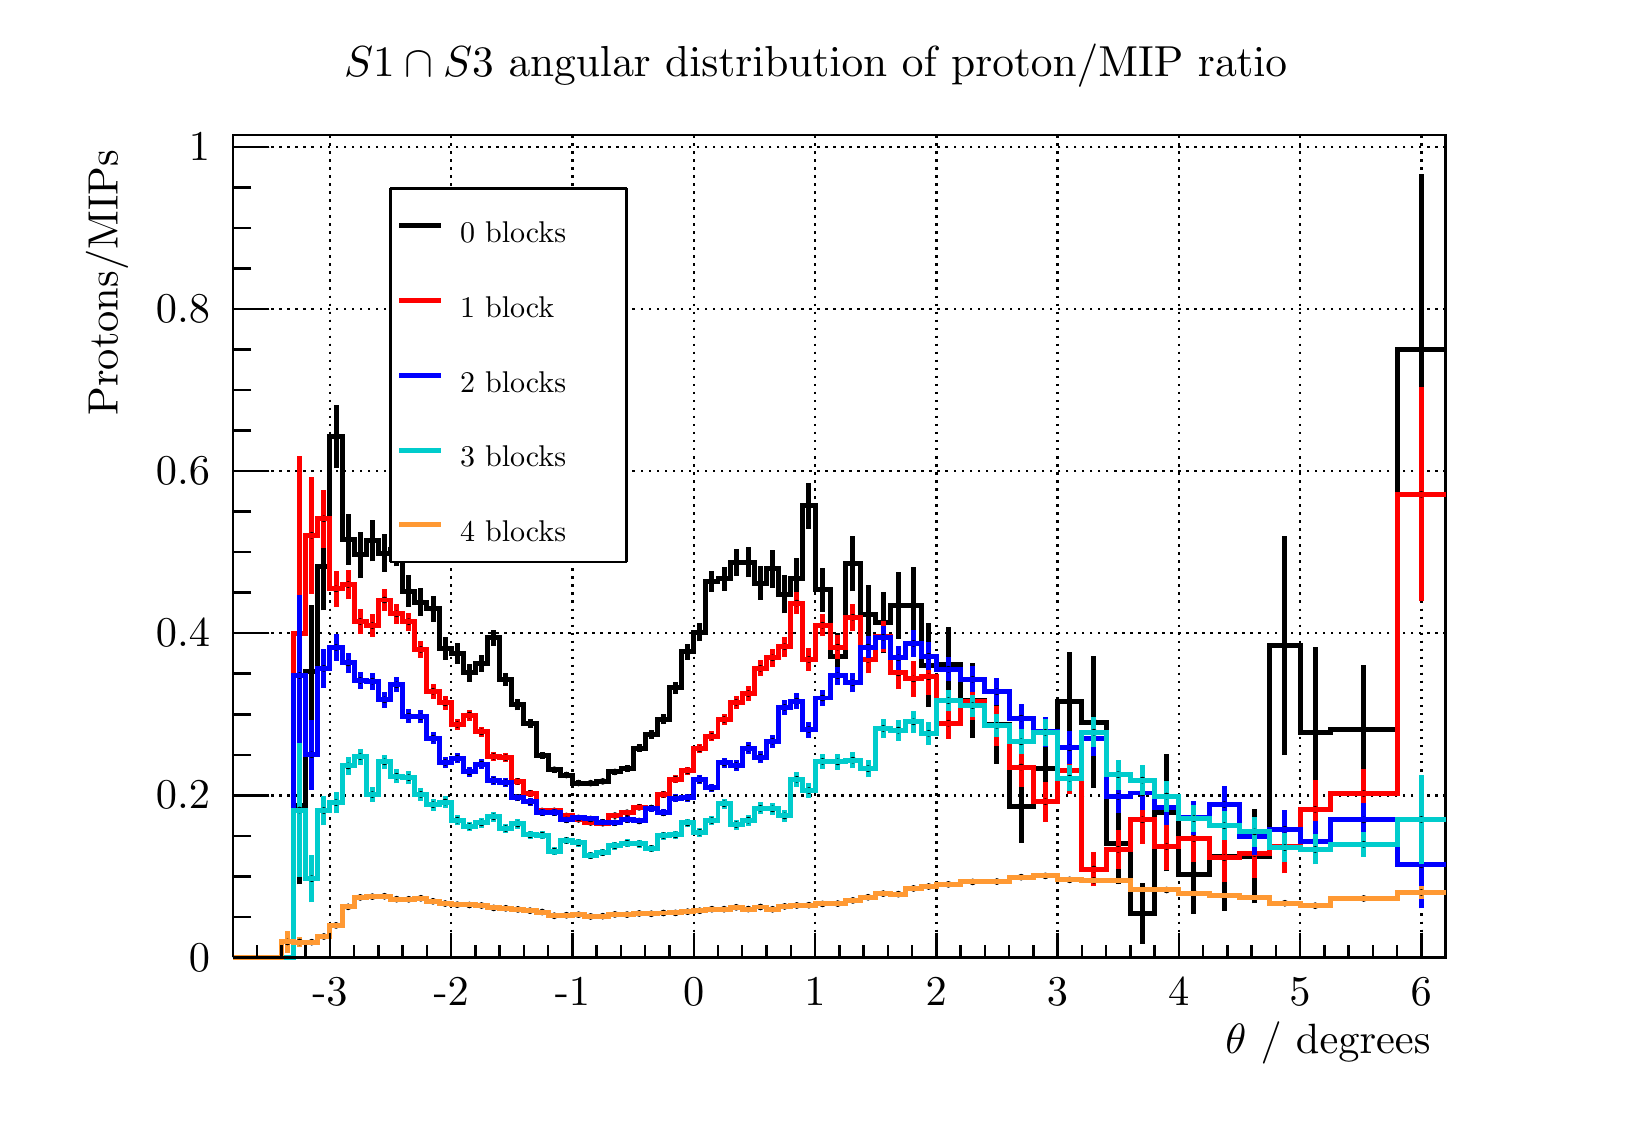
\begin{tikzpicture}
\pgfdeclareplotmark{cross} {
\pgfpathmoveto{\pgfpoint{-0.3\pgfplotmarksize}{\pgfplotmarksize}}
\pgfpathlineto{\pgfpoint{+0.3\pgfplotmarksize}{\pgfplotmarksize}}
\pgfpathlineto{\pgfpoint{+0.3\pgfplotmarksize}{0.3\pgfplotmarksize}}
\pgfpathlineto{\pgfpoint{+1\pgfplotmarksize}{0.3\pgfplotmarksize}}
\pgfpathlineto{\pgfpoint{+1\pgfplotmarksize}{-0.3\pgfplotmarksize}}
\pgfpathlineto{\pgfpoint{+0.3\pgfplotmarksize}{-0.3\pgfplotmarksize}}
\pgfpathlineto{\pgfpoint{+0.3\pgfplotmarksize}{-1.\pgfplotmarksize}}
\pgfpathlineto{\pgfpoint{-0.3\pgfplotmarksize}{-1.\pgfplotmarksize}}
\pgfpathlineto{\pgfpoint{-0.3\pgfplotmarksize}{-0.3\pgfplotmarksize}}
\pgfpathlineto{\pgfpoint{-1.\pgfplotmarksize}{-0.3\pgfplotmarksize}}
\pgfpathlineto{\pgfpoint{-1.\pgfplotmarksize}{0.3\pgfplotmarksize}}
\pgfpathlineto{\pgfpoint{-0.3\pgfplotmarksize}{0.3\pgfplotmarksize}}
\pgfpathclose
\pgfusepathqstroke
}
\pgfdeclareplotmark{cross*} {
\pgfpathmoveto{\pgfpoint{-0.3\pgfplotmarksize}{\pgfplotmarksize}}
\pgfpathlineto{\pgfpoint{+0.3\pgfplotmarksize}{\pgfplotmarksize}}
\pgfpathlineto{\pgfpoint{+0.3\pgfplotmarksize}{0.3\pgfplotmarksize}}
\pgfpathlineto{\pgfpoint{+1\pgfplotmarksize}{0.3\pgfplotmarksize}}
\pgfpathlineto{\pgfpoint{+1\pgfplotmarksize}{-0.3\pgfplotmarksize}}
\pgfpathlineto{\pgfpoint{+0.3\pgfplotmarksize}{-0.3\pgfplotmarksize}}
\pgfpathlineto{\pgfpoint{+0.3\pgfplotmarksize}{-1.\pgfplotmarksize}}
\pgfpathlineto{\pgfpoint{-0.3\pgfplotmarksize}{-1.\pgfplotmarksize}}
\pgfpathlineto{\pgfpoint{-0.3\pgfplotmarksize}{-0.3\pgfplotmarksize}}
\pgfpathlineto{\pgfpoint{-1.\pgfplotmarksize}{-0.3\pgfplotmarksize}}
\pgfpathlineto{\pgfpoint{-1.\pgfplotmarksize}{0.3\pgfplotmarksize}}
\pgfpathlineto{\pgfpoint{-0.3\pgfplotmarksize}{0.3\pgfplotmarksize}}
\pgfpathclose
\pgfusepathqfillstroke
}
\pgfdeclareplotmark{newstar} {
\pgfpathmoveto{\pgfqpoint{0pt}{\pgfplotmarksize}}
\pgfpathlineto{\pgfqpointpolar{44}{0.5\pgfplotmarksize}}
\pgfpathlineto{\pgfqpointpolar{18}{\pgfplotmarksize}}
\pgfpathlineto{\pgfqpointpolar{-20}{0.5\pgfplotmarksize}}
\pgfpathlineto{\pgfqpointpolar{-54}{\pgfplotmarksize}}
\pgfpathlineto{\pgfqpointpolar{-90}{0.5\pgfplotmarksize}}
\pgfpathlineto{\pgfqpointpolar{234}{\pgfplotmarksize}}
\pgfpathlineto{\pgfqpointpolar{198}{0.5\pgfplotmarksize}}
\pgfpathlineto{\pgfqpointpolar{162}{\pgfplotmarksize}}
\pgfpathlineto{\pgfqpointpolar{134}{0.5\pgfplotmarksize}}
\pgfpathclose
\pgfusepathqstroke
}
\pgfdeclareplotmark{newstar*} {
\pgfpathmoveto{\pgfqpoint{0pt}{\pgfplotmarksize}}
\pgfpathlineto{\pgfqpointpolar{44}{0.5\pgfplotmarksize}}
\pgfpathlineto{\pgfqpointpolar{18}{\pgfplotmarksize}}
\pgfpathlineto{\pgfqpointpolar{-20}{0.5\pgfplotmarksize}}
\pgfpathlineto{\pgfqpointpolar{-54}{\pgfplotmarksize}}
\pgfpathlineto{\pgfqpointpolar{-90}{0.5\pgfplotmarksize}}
\pgfpathlineto{\pgfqpointpolar{234}{\pgfplotmarksize}}
\pgfpathlineto{\pgfqpointpolar{198}{0.5\pgfplotmarksize}}
\pgfpathlineto{\pgfqpointpolar{162}{\pgfplotmarksize}}
\pgfpathlineto{\pgfqpointpolar{134}{0.5\pgfplotmarksize}}
\pgfpathclose
\pgfusepathqfillstroke
}
\definecolor{c}{rgb}{1,1,1};
\draw [color=c, fill=c] (0,0) rectangle (20,13.5632);
\draw [color=c, fill=c] (2.6,1.76322) rectangle (18,12.2069);
\definecolor{c}{rgb}{0,0,0};
\draw [c,line width=0.9] (2.6,1.76322) -- (2.6,12.2069) -- (18,12.2069) -- (18,1.76322) -- (2.6,1.76322);
\definecolor{c}{rgb}{1,1,1};
\draw [color=c, fill=c] (2.6,1.76322) rectangle (18,12.2069);
\definecolor{c}{rgb}{0,0,0};
\draw [c,line width=0.9] (2.6,1.76322) -- (2.6,12.2069) -- (18,12.2069) -- (18,1.76322) -- (2.6,1.76322);
\draw [c,line width=0.9] (2.6,1.76322) -- (18,1.76322);
\draw [c,dotted,line width=0.9] (3.832,12.2069) -- (3.832,1.76322);
\draw [c,dotted,line width=0.9] (5.372,12.2069) -- (5.372,1.76322);
\draw [c,dotted,line width=0.9] (6.912,12.2069) -- (6.912,1.76322);
\draw [c,dotted,line width=0.9] (8.452,12.2069) -- (8.452,1.76322);
\draw [c,dotted,line width=0.9] (9.992,12.2069) -- (9.992,1.76322);
\draw [c,dotted,line width=0.9] (11.532,12.2069) -- (11.532,1.76322);
\draw [c,dotted,line width=0.9] (13.072,12.2069) -- (13.072,1.76322);
\draw [c,dotted,line width=0.9] (14.612,12.2069) -- (14.612,1.76322);
\draw [c,dotted,line width=0.9] (16.152,12.2069) -- (16.152,1.76322);
\draw [c,dotted,line width=0.9] (17.692,12.2069) -- (17.692,1.76322);
\draw [c,dotted,line width=0.9] (3.832,12.2069) -- (3.832,1.76322);
\draw [c,dotted,line width=0.9] (17.692,12.2069) -- (17.692,1.76322);
\draw [c,line width=0.9] (2.6,1.76322) -- (2.6,12.2069);
\draw [c,dotted,line width=0.9] (18,1.76322) -- (2.6,1.76322);
\draw [c,dotted,line width=0.9] (18,3.82143) -- (2.6,3.82143);
\draw [c,dotted,line width=0.9] (18,5.87964) -- (2.6,5.87964);
\draw [c,dotted,line width=0.9] (18,7.93785) -- (2.6,7.93785);
\draw [c,dotted,line width=0.9] (18,9.99605) -- (2.6,9.99605);
\draw [c,dotted,line width=0.9] (18,12.0543) -- (2.6,12.0543);
\draw [c,dotted,line width=0.9] (18,12.0543) -- (2.6,12.0543);
\definecolor{c}{rgb}{0,0,0.6};
\draw [c,line width=0.9] (2.6,1.76322) -- (2.754,1.76322) -- (2.754,1.76322) -- (2.908,1.76322) -- (2.908,1.76322) -- (3.062,1.76322) -- (3.062,1.76322) -- (3.216,1.76322) -- (3.216,1.76322) -- (3.37,1.76322) -- (3.37,1.76322) -- (3.524,1.76322) --
 (3.524,1.76322) -- (3.678,1.76322) -- (3.678,1.76322) -- (3.832,1.76322) -- (3.832,1.76322) -- (3.986,1.76322) -- (3.986,1.76322) -- (4.14,1.76322) -- (4.14,1.76322) -- (4.294,1.76322) -- (4.294,1.76322) -- (4.448,1.76322) -- (4.448,1.76322) --
 (4.602,1.76322) -- (4.602,1.76322) -- (4.756,1.76322) -- (4.756,1.76322) -- (4.91,1.76322) -- (4.91,1.76322) -- (5.064,1.76322) -- (5.064,1.76322) -- (5.218,1.76322) -- (5.218,1.76322) -- (5.372,1.76322) -- (5.372,1.76322) -- (5.526,1.76322) --
 (5.526,1.76322) -- (5.68,1.76322) -- (5.68,1.76322) -- (5.834,1.76322) -- (5.834,1.76322) -- (5.988,1.76322) -- (5.988,1.76322) -- (6.142,1.76322) -- (6.142,1.76322) -- (6.296,1.76322) -- (6.296,1.76322) -- (6.45,1.76322) -- (6.45,1.76322) --
 (6.604,1.76322) -- (6.604,1.76322) -- (6.758,1.76322) -- (6.758,1.76322) -- (6.912,1.76322) -- (6.912,1.76322) -- (7.066,1.76322) -- (7.066,1.76322) -- (7.22,1.76322) -- (7.22,1.76322) -- (7.374,1.76322) -- (7.374,1.76322) -- (7.528,1.76322) --
 (7.528,1.76322) -- (7.682,1.76322) -- (7.682,1.76322) -- (7.836,1.76322) -- (7.836,1.76322) -- (7.99,1.76322) -- (7.99,1.76322) -- (8.144,1.76322) -- (8.144,1.76322) -- (8.298,1.76322) -- (8.298,1.76322) -- (8.452,1.76322) -- (8.452,1.76322) --
 (8.606,1.76322) -- (8.606,1.76322) -- (8.76,1.76322) -- (8.76,1.76322) -- (8.914,1.76322) -- (8.914,1.76322) -- (9.068,1.76322) -- (9.068,1.76322) -- (9.222,1.76322) -- (9.222,1.76322) -- (9.376,1.76322) -- (9.376,1.76322) -- (9.53,1.76322) --
 (9.53,1.76322) -- (9.684,1.76322) -- (9.684,1.76322) -- (9.838,1.76322) -- (9.838,1.76322) -- (9.992,1.76322) -- (9.992,1.76322) -- (10.1845,1.76322) -- (10.1845,1.76322) -- (10.377,1.76322) -- (10.377,1.76322) -- (10.5695,1.76322) --
 (10.5695,1.76322) -- (10.762,1.76322) -- (10.762,1.76322) -- (10.9545,1.76322) -- (10.9545,1.76322) -- (11.147,1.76322) -- (11.147,1.76322) -- (11.3395,1.76322) -- (11.3395,1.76322) -- (11.532,1.76322) -- (11.532,1.76322) -- (11.84,1.76322) --
 (11.84,1.76322) -- (12.148,1.76322) -- (12.148,1.76322) -- (12.456,1.76322) -- (12.456,1.76322) -- (12.764,1.76322) -- (12.764,1.76322) -- (13.072,1.76322) -- (13.072,1.76322) -- (13.38,1.76322) -- (13.38,1.76322) -- (13.688,1.76322) --
 (13.688,1.76322) -- (13.996,1.76322) -- (13.996,1.76322) -- (14.304,1.76322) -- (14.304,1.76322) -- (14.612,1.76322) -- (14.612,1.76322) -- (14.997,1.76322) -- (14.997,1.76322) -- (15.382,1.76322) -- (15.382,1.76322) -- (15.767,1.76322) --
 (15.767,1.76322) -- (16.152,1.76322) -- (16.152,1.76322) -- (16.537,1.76322) -- (16.537,1.76322) -- (17.384,1.76322) -- (17.384,1.76322) -- (18,1.76322);
\definecolor{c}{rgb}{0,0,0};
\draw [c,line width=0.9] (2.6,1.76322) -- (18,1.76322);
\draw [anchor= east] (18,0.678161) node[scale=1.5317, color=c, rotate=0]{$\theta$ / degrees};
\draw [c,line width=0.9] (3.832,2.07653) -- (3.832,1.76322);
\draw [c,line width=0.9] (4.14,1.91987) -- (4.14,1.76322);
\draw [c,line width=0.9] (4.448,1.91987) -- (4.448,1.76322);
\draw [c,line width=0.9] (4.756,1.91987) -- (4.756,1.76322);
\draw [c,line width=0.9] (5.064,1.91987) -- (5.064,1.76322);
\draw [c,line width=0.9] (5.372,2.07653) -- (5.372,1.76322);
\draw [c,line width=0.9] (5.68,1.91987) -- (5.68,1.76322);
\draw [c,line width=0.9] (5.988,1.91987) -- (5.988,1.76322);
\draw [c,line width=0.9] (6.296,1.91987) -- (6.296,1.76322);
\draw [c,line width=0.9] (6.604,1.91987) -- (6.604,1.76322);
\draw [c,line width=0.9] (6.912,2.07653) -- (6.912,1.76322);
\draw [c,line width=0.9] (7.22,1.91987) -- (7.22,1.76322);
\draw [c,line width=0.9] (7.528,1.91987) -- (7.528,1.76322);
\draw [c,line width=0.9] (7.836,1.91987) -- (7.836,1.76322);
\draw [c,line width=0.9] (8.144,1.91987) -- (8.144,1.76322);
\draw [c,line width=0.9] (8.452,2.07653) -- (8.452,1.76322);
\draw [c,line width=0.9] (8.76,1.91987) -- (8.76,1.76322);
\draw [c,line width=0.9] (9.068,1.91987) -- (9.068,1.76322);
\draw [c,line width=0.9] (9.376,1.91987) -- (9.376,1.76322);
\draw [c,line width=0.9] (9.684,1.91987) -- (9.684,1.76322);
\draw [c,line width=0.9] (9.992,2.07653) -- (9.992,1.76322);
\draw [c,line width=0.9] (10.3,1.91987) -- (10.3,1.76322);
\draw [c,line width=0.9] (10.608,1.91987) -- (10.608,1.76322);
\draw [c,line width=0.9] (10.916,1.91987) -- (10.916,1.76322);
\draw [c,line width=0.9] (11.224,1.91987) -- (11.224,1.76322);
\draw [c,line width=0.9] (11.532,2.07653) -- (11.532,1.76322);
\draw [c,line width=0.9] (11.84,1.91987) -- (11.84,1.76322);
\draw [c,line width=0.9] (12.148,1.91987) -- (12.148,1.76322);
\draw [c,line width=0.9] (12.456,1.91987) -- (12.456,1.76322);
\draw [c,line width=0.9] (12.764,1.91987) -- (12.764,1.76322);
\draw [c,line width=0.9] (13.072,2.07653) -- (13.072,1.76322);
\draw [c,line width=0.9] (13.38,1.91987) -- (13.38,1.76322);
\draw [c,line width=0.9] (13.688,1.91987) -- (13.688,1.76322);
\draw [c,line width=0.9] (13.996,1.91987) -- (13.996,1.76322);
\draw [c,line width=0.9] (14.304,1.91987) -- (14.304,1.76322);
\draw [c,line width=0.9] (14.612,2.07653) -- (14.612,1.76322);
\draw [c,line width=0.9] (14.92,1.91987) -- (14.92,1.76322);
\draw [c,line width=0.9] (15.228,1.91987) -- (15.228,1.76322);
\draw [c,line width=0.9] (15.536,1.91987) -- (15.536,1.76322);
\draw [c,line width=0.9] (15.844,1.91987) -- (15.844,1.76322);
\draw [c,line width=0.9] (16.152,2.07653) -- (16.152,1.76322);
\draw [c,line width=0.9] (16.46,1.91987) -- (16.46,1.76322);
\draw [c,line width=0.9] (16.768,1.91987) -- (16.768,1.76322);
\draw [c,line width=0.9] (17.076,1.91987) -- (17.076,1.76322);
\draw [c,line width=0.9] (17.384,1.91987) -- (17.384,1.76322);
\draw [c,line width=0.9] (17.692,2.07653) -- (17.692,1.76322);
\draw [c,line width=0.9] (3.832,2.07653) -- (3.832,1.76322);
\draw [c,line width=0.9] (3.524,1.91987) -- (3.524,1.76322);
\draw [c,line width=0.9] (3.216,1.91987) -- (3.216,1.76322);
\draw [c,line width=0.9] (2.908,1.91987) -- (2.908,1.76322);
\draw [c,line width=0.9] (17.692,2.07653) -- (17.692,1.76322);
\draw [anchor=base] (3.832,1.15287) node[scale=1.5317, color=c, rotate=0]{-3};
\draw [anchor=base] (5.372,1.15287) node[scale=1.5317, color=c, rotate=0]{-2};
\draw [anchor=base] (6.912,1.15287) node[scale=1.5317, color=c, rotate=0]{-1};
\draw [anchor=base] (8.452,1.15287) node[scale=1.5317, color=c, rotate=0]{0};
\draw [anchor=base] (9.992,1.15287) node[scale=1.5317, color=c, rotate=0]{1};
\draw [anchor=base] (11.532,1.15287) node[scale=1.5317, color=c, rotate=0]{2};
\draw [anchor=base] (13.072,1.15287) node[scale=1.5317, color=c, rotate=0]{3};
\draw [anchor=base] (14.612,1.15287) node[scale=1.5317, color=c, rotate=0]{4};
\draw [anchor=base] (16.152,1.15287) node[scale=1.5317, color=c, rotate=0]{5};
\draw [anchor=base] (17.692,1.15287) node[scale=1.5317, color=c, rotate=0]{6};
\draw [c,line width=0.9] (2.6,1.76322) -- (2.6,12.2069);
\draw [anchor= east] (1,12.2069) node[scale=1.5317, color=c, rotate=90]{  Protons/MIPs};
\draw [c,line width=0.9] (3.062,1.76322) -- (2.6,1.76322);
\draw [c,line width=0.9] (2.831,2.27777) -- (2.6,2.27777);
\draw [c,line width=0.9] (2.831,2.79232) -- (2.6,2.79232);
\draw [c,line width=0.9] (2.831,3.30687) -- (2.6,3.30687);
\draw [c,line width=0.9] (3.062,3.82143) -- (2.6,3.82143);
\draw [c,line width=0.9] (2.831,4.33598) -- (2.6,4.33598);
\draw [c,line width=0.9] (2.831,4.85053) -- (2.6,4.85053);
\draw [c,line width=0.9] (2.831,5.36508) -- (2.6,5.36508);
\draw [c,line width=0.9] (3.062,5.87964) -- (2.6,5.87964);
\draw [c,line width=0.9] (2.831,6.39419) -- (2.6,6.39419);
\draw [c,line width=0.9] (2.831,6.90874) -- (2.6,6.90874);
\draw [c,line width=0.9] (2.831,7.42329) -- (2.6,7.42329);
\draw [c,line width=0.9] (3.062,7.93785) -- (2.6,7.93785);
\draw [c,line width=0.9] (2.831,8.4524) -- (2.6,8.4524);
\draw [c,line width=0.9] (2.831,8.96695) -- (2.6,8.96695);
\draw [c,line width=0.9] (2.831,9.4815) -- (2.6,9.4815);
\draw [c,line width=0.9] (3.062,9.99605) -- (2.6,9.99605);
\draw [c,line width=0.9] (2.831,10.5106) -- (2.6,10.5106);
\draw [c,line width=0.9] (2.831,11.0252) -- (2.6,11.0252);
\draw [c,line width=0.9] (2.831,11.5397) -- (2.6,11.5397);
\draw [c,line width=0.9] (3.062,12.0543) -- (2.6,12.0543);
\draw [c,line width=0.9] (3.062,12.0543) -- (2.6,12.0543);
\draw [anchor= east] (2.5,1.76322) node[scale=1.5317, color=c, rotate=0]{0};
\draw [anchor= east] (2.5,3.82143) node[scale=1.5317, color=c, rotate=0]{0.2};
\draw [anchor= east] (2.5,5.87964) node[scale=1.5317, color=c, rotate=0]{0.4};
\draw [anchor= east] (2.5,7.93785) node[scale=1.5317, color=c, rotate=0]{0.6};
\draw [anchor= east] (2.5,9.99605) node[scale=1.5317, color=c, rotate=0]{0.8};
\draw [anchor= east] (2.5,12.0543) node[scale=1.5317, color=c, rotate=0]{1};
\draw [c,line width=1.8] (3.447,2.68861) -- (3.447,3.69279);
\draw [c,line width=1.8] (3.447,3.69279) -- (3.447,4.69697);
\foreach \P in {(3.447,3.69279)}{\draw[mark options={color=c,fill=c},mark size=2.402402pt,mark=*,mark size=1pt] plot coordinates {\P};}
\draw [c,line width=1.8] (3.601,4.55193) -- (3.601,5.39535);
\draw [c,line width=1.8] (3.601,5.39535) -- (3.601,6.23877);
\foreach \P in {(3.601,5.39535)}{\draw[mark options={color=c,fill=c},mark size=2.402402pt,mark=*,mark size=1pt] plot coordinates {\P};}
\draw [c,line width=1.8] (3.755,6.16937) -- (3.755,6.72713);
\draw [c,line width=1.8] (3.755,6.72713) -- (3.755,7.2849);
\foreach \P in {(3.755,6.72713)}{\draw[mark options={color=c,fill=c},mark size=2.402402pt,mark=*,mark size=1pt] plot coordinates {\P};}
\draw [c,line width=1.8] (3.909,7.97262) -- (3.909,8.37402);
\draw [c,line width=1.8] (3.909,8.37402) -- (3.909,8.77542);
\foreach \P in {(3.909,8.37402)}{\draw[mark options={color=c,fill=c},mark size=2.402402pt,mark=*,mark size=1pt] plot coordinates {\P};}
\draw [c,line width=1.8] (4.063,6.74812) -- (4.063,7.07209);
\draw [c,line width=1.8] (4.063,7.07209) -- (4.063,7.39606);
\foreach \P in {(4.063,7.07209)}{\draw[mark options={color=c,fill=c},mark size=2.402402pt,mark=*,mark size=1pt] plot coordinates {\P};}
\draw [c,line width=1.8] (4.217,6.57737) -- (4.217,6.87444);
\draw [c,line width=1.8] (4.217,6.87444) -- (4.217,7.17151);
\foreach \P in {(4.217,6.87444)}{\draw[mark options={color=c,fill=c},mark size=2.402402pt,mark=*,mark size=1pt] plot coordinates {\P};}
\draw [c,line width=1.8] (4.371,6.79338) -- (4.371,7.0535);
\draw [c,line width=1.8] (4.371,7.0535) -- (4.371,7.31362);
\foreach \P in {(4.371,7.0535)}{\draw[mark options={color=c,fill=c},mark size=2.402402pt,mark=*,mark size=1pt] plot coordinates {\P};}
\draw [c,line width=1.8] (4.525,6.65736) -- (4.525,6.89753);
\draw [c,line width=1.8] (4.525,6.89753) -- (4.525,7.1377);
\foreach \P in {(4.525,6.89753)}{\draw[mark options={color=c,fill=c},mark size=2.402402pt,mark=*,mark size=1pt] plot coordinates {\P};}
\draw [c,line width=1.8] (4.679,6.72958) -- (4.679,6.94472);
\draw [c,line width=1.8] (4.679,6.94472) -- (4.679,7.15986);
\foreach \P in {(4.679,6.94472)}{\draw[mark options={color=c,fill=c},mark size=2.402402pt,mark=*,mark size=1pt] plot coordinates {\P};}
\draw [c,line width=1.8] (4.833,6.21551) -- (4.833,6.41533);
\draw [c,line width=1.8] (4.833,6.41533) -- (4.833,6.61516);
\foreach \P in {(4.833,6.41533)}{\draw[mark options={color=c,fill=c},mark size=2.402402pt,mark=*,mark size=1pt] plot coordinates {\P};}
\draw [c,line width=1.8] (4.987,6.09559) -- (4.987,6.2725);
\draw [c,line width=1.8] (4.987,6.2725) -- (4.987,6.44941);
\foreach \P in {(4.987,6.2725)}{\draw[mark options={color=c,fill=c},mark size=2.402402pt,mark=*,mark size=1pt] plot coordinates {\P};}
\draw [c,line width=1.8] (5.141,6.02679) -- (5.141,6.18847);
\draw [c,line width=1.8] (5.141,6.18847) -- (5.141,6.35015);
\foreach \P in {(5.141,6.18847)}{\draw[mark options={color=c,fill=c},mark size=2.402402pt,mark=*,mark size=1pt] plot coordinates {\P};}
\draw [c,line width=1.8] (5.295,5.54014) -- (5.295,5.68527);
\draw [c,line width=1.8] (5.295,5.68527) -- (5.295,5.8304);
\foreach \P in {(5.295,5.68527)}{\draw[mark options={color=c,fill=c},mark size=2.402402pt,mark=*,mark size=1pt] plot coordinates {\P};}
\draw [c,line width=1.8] (5.449,5.49417) -- (5.449,5.62692);
\draw [c,line width=1.8] (5.449,5.62692) -- (5.449,5.75968);
\foreach \P in {(5.449,5.62692)}{\draw[mark options={color=c,fill=c},mark size=2.402402pt,mark=*,mark size=1pt] plot coordinates {\P};}
\draw [c,line width=1.8] (5.603,5.26127) -- (5.603,5.3782);
\draw [c,line width=1.8] (5.603,5.3782) -- (5.603,5.49514);
\foreach \P in {(5.603,5.3782)}{\draw[mark options={color=c,fill=c},mark size=2.402402pt,mark=*,mark size=1pt] plot coordinates {\P};}
\draw [c,line width=1.8] (5.757,5.38457) -- (5.757,5.4911);
\draw [c,line width=1.8] (5.757,5.4911) -- (5.757,5.59762);
\foreach \P in {(5.757,5.4911)}{\draw[mark options={color=c,fill=c},mark size=2.402402pt,mark=*,mark size=1pt] plot coordinates {\P};}
\draw [c,line width=1.8] (5.911,5.72283) -- (5.911,5.82056);
\draw [c,line width=1.8] (5.911,5.82056) -- (5.911,5.9183);
\foreach \P in {(5.911,5.82056)}{\draw[mark options={color=c,fill=c},mark size=2.402402pt,mark=*,mark size=1pt] plot coordinates {\P};}
\draw [c,line width=1.8] (6.065,5.20876) -- (6.065,5.29262);
\draw [c,line width=1.8] (6.065,5.29262) -- (6.065,5.37647);
\foreach \P in {(6.065,5.29262)}{\draw[mark options={color=c,fill=c},mark size=2.402402pt,mark=*,mark size=1pt] plot coordinates {\P};}
\draw [c,line width=1.8] (6.219,4.90059) -- (6.219,4.97013);
\draw [c,line width=1.8] (6.219,4.97013) -- (6.219,5.03967);
\foreach \P in {(6.219,4.97013)}{\draw[mark options={color=c,fill=c},mark size=2.402402pt,mark=*,mark size=1pt] plot coordinates {\P};}
\draw [c,line width=1.8] (6.373,4.67441) -- (6.373,4.73269);
\draw [c,line width=1.8] (6.373,4.73269) -- (6.373,4.79097);
\foreach \P in {(6.373,4.73269)}{\draw[mark options={color=c,fill=c},mark size=2.402402pt,mark=*,mark size=1pt] plot coordinates {\P};}
\draw [c,line width=1.8] (6.527,4.27936) -- (6.527,4.32689);
\draw [c,line width=1.8] (6.527,4.32689) -- (6.527,4.37441);
\foreach \P in {(6.527,4.32689)}{\draw[mark options={color=c,fill=c},mark size=2.402402pt,mark=*,mark size=1pt] plot coordinates {\P};}
\draw [c,line width=1.8] (6.681,4.10644) -- (6.681,4.14662);
\draw [c,line width=1.8] (6.681,4.14662) -- (6.681,4.18681);
\foreach \P in {(6.681,4.14662)}{\draw[mark options={color=c,fill=c},mark size=2.402402pt,mark=*,mark size=1pt] plot coordinates {\P};}
\draw [c,line width=1.8] (6.835,4.04256) -- (6.835,4.07876);
\draw [c,line width=1.8] (6.835,4.07876) -- (6.835,4.11496);
\foreach \P in {(6.835,4.07876)}{\draw[mark options={color=c,fill=c},mark size=2.402402pt,mark=*,mark size=1pt] plot coordinates {\P};}
\draw [c,line width=1.8] (6.989,3.94346) -- (6.989,3.97699);
\draw [c,line width=1.8] (6.989,3.97699) -- (6.989,4.01053);
\foreach \P in {(6.989,3.97699)}{\draw[mark options={color=c,fill=c},mark size=2.402402pt,mark=*,mark size=1pt] plot coordinates {\P};}
\draw [c,line width=1.8] (7.143,3.94258) -- (7.143,3.97579);
\draw [c,line width=1.8] (7.143,3.97579) -- (7.143,4.00901);
\foreach \P in {(7.143,3.97579)}{\draw[mark options={color=c,fill=c},mark size=2.402402pt,mark=*,mark size=1pt] plot coordinates {\P};}
\draw [c,line width=1.8] (7.297,3.96395) -- (7.297,3.99829);
\draw [c,line width=1.8] (7.297,3.99829) -- (7.297,4.03263);
\foreach \P in {(7.297,3.99829)}{\draw[mark options={color=c,fill=c},mark size=2.402402pt,mark=*,mark size=1pt] plot coordinates {\P};}
\draw [c,line width=1.8] (7.451,4.08086) -- (7.451,4.11859);
\draw [c,line width=1.8] (7.451,4.11859) -- (7.451,4.15633);
\foreach \P in {(7.451,4.11859)}{\draw[mark options={color=c,fill=c},mark size=2.402402pt,mark=*,mark size=1pt] plot coordinates {\P};}
\draw [c,line width=1.8] (7.605,4.11965) -- (7.605,4.1614);
\draw [c,line width=1.8] (7.605,4.1614) -- (7.605,4.20315);
\foreach \P in {(7.605,4.1614)}{\draw[mark options={color=c,fill=c},mark size=2.402402pt,mark=*,mark size=1pt] plot coordinates {\P};}
\draw [c,line width=1.8] (7.759,4.37305) -- (7.759,4.42142);
\draw [c,line width=1.8] (7.759,4.42142) -- (7.759,4.46979);
\foreach \P in {(7.759,4.42142)}{\draw[mark options={color=c,fill=c},mark size=2.402402pt,mark=*,mark size=1pt] plot coordinates {\P};}
\draw [c,line width=1.8] (7.913,4.53427) -- (7.913,4.5899);
\draw [c,line width=1.8] (7.913,4.5899) -- (7.913,4.64552);
\foreach \P in {(7.913,4.5899)}{\draw[mark options={color=c,fill=c},mark size=2.402402pt,mark=*,mark size=1pt] plot coordinates {\P};}
\draw [c,line width=1.8] (8.067,4.72215) -- (8.067,4.78731);
\draw [c,line width=1.8] (8.067,4.78731) -- (8.067,4.85247);
\foreach \P in {(8.067,4.78731)}{\draw[mark options={color=c,fill=c},mark size=2.402402pt,mark=*,mark size=1pt] plot coordinates {\P};}
\draw [c,line width=1.8] (8.221,5.10467) -- (8.221,5.18431);
\draw [c,line width=1.8] (8.221,5.18431) -- (8.221,5.26395);
\foreach \P in {(8.221,5.18431)}{\draw[mark options={color=c,fill=c},mark size=2.402402pt,mark=*,mark size=1pt] plot coordinates {\P};}
\draw [c,line width=1.8] (8.375,5.5447) -- (8.375,5.64191);
\draw [c,line width=1.8] (8.375,5.64191) -- (8.375,5.73912);
\foreach \P in {(8.375,5.64191)}{\draw[mark options={color=c,fill=c},mark size=2.402402pt,mark=*,mark size=1pt] plot coordinates {\P};}
\draw [c,line width=1.8] (8.529,5.77689) -- (8.529,5.89264);
\draw [c,line width=1.8] (8.529,5.89264) -- (8.529,6.00839);
\foreach \P in {(8.529,5.89264)}{\draw[mark options={color=c,fill=c},mark size=2.402402pt,mark=*,mark size=1pt] plot coordinates {\P};}
\draw [c,line width=1.8] (8.683,6.40553) -- (8.683,6.53755);
\draw [c,line width=1.8] (8.683,6.53755) -- (8.683,6.66958);
\foreach \P in {(8.683,6.53755)}{\draw[mark options={color=c,fill=c},mark size=2.402402pt,mark=*,mark size=1pt] plot coordinates {\P};}
\draw [c,line width=1.8] (8.837,6.41976) -- (8.837,6.57237);
\draw [c,line width=1.8] (8.837,6.57237) -- (8.837,6.72498);
\foreach \P in {(8.837,6.57237)}{\draw[mark options={color=c,fill=c},mark size=2.402402pt,mark=*,mark size=1pt] plot coordinates {\P};}
\draw [c,line width=1.8] (8.991,6.6065) -- (8.991,6.77768);
\draw [c,line width=1.8] (8.991,6.77768) -- (8.991,6.94886);
\foreach \P in {(8.991,6.77768)}{\draw[mark options={color=c,fill=c},mark size=2.402402pt,mark=*,mark size=1pt] plot coordinates {\P};}
\draw [c,line width=1.8] (9.145,6.59087) -- (9.145,6.78152);
\draw [c,line width=1.8] (9.145,6.78152) -- (9.145,6.97216);
\foreach \P in {(9.145,6.78152)}{\draw[mark options={color=c,fill=c},mark size=2.402402pt,mark=*,mark size=1pt] plot coordinates {\P};}
\draw [c,line width=1.8] (9.299,6.30591) -- (9.299,6.51695);
\draw [c,line width=1.8] (9.299,6.51695) -- (9.299,6.72799);
\foreach \P in {(9.299,6.51695)}{\draw[mark options={color=c,fill=c},mark size=2.402402pt,mark=*,mark size=1pt] plot coordinates {\P};}
\draw [c,line width=1.8] (9.453,6.45578) -- (9.453,6.69574);
\draw [c,line width=1.8] (9.453,6.69574) -- (9.453,6.93571);
\foreach \P in {(9.453,6.69574)}{\draw[mark options={color=c,fill=c},mark size=2.402402pt,mark=*,mark size=1pt] plot coordinates {\P};}
\draw [c,line width=1.8] (9.607,6.13276) -- (9.607,6.37565);
\draw [c,line width=1.8] (9.607,6.37565) -- (9.607,6.61853);
\foreach \P in {(9.607,6.37565)}{\draw[mark options={color=c,fill=c},mark size=2.402402pt,mark=*,mark size=1pt] plot coordinates {\P};}
\draw [c,line width=1.8] (9.761,6.30551) -- (9.761,6.57316);
\draw [c,line width=1.8] (9.761,6.57316) -- (9.761,6.84082);
\foreach \P in {(9.761,6.57316)}{\draw[mark options={color=c,fill=c},mark size=2.402402pt,mark=*,mark size=1pt] plot coordinates {\P};}
\draw [c,line width=1.8] (9.915,7.20652) -- (9.915,7.49921);
\draw [c,line width=1.8] (9.915,7.49921) -- (9.915,7.7919);
\foreach \P in {(9.915,7.49921)}{\draw[mark options={color=c,fill=c},mark size=2.402402pt,mark=*,mark size=1pt] plot coordinates {\P};}
\draw [c,line width=1.8] (10.0883,6.15266) -- (10.0883,6.43259);
\draw [c,line width=1.8] (10.0883,6.43259) -- (10.0883,6.71251);
\foreach \P in {(10.0883,6.43259)}{\draw[mark options={color=c,fill=c},mark size=2.402402pt,mark=*,mark size=1pt] plot coordinates {\P};}
\draw [c,line width=1.8] (10.2808,5.28593) -- (10.2808,5.58145);
\draw [c,line width=1.8] (10.2808,5.58145) -- (10.2808,5.87697);
\foreach \P in {(10.2808,5.58145)}{\draw[mark options={color=c,fill=c},mark size=2.402402pt,mark=*,mark size=1pt] plot coordinates {\P};}
\draw [c,line width=1.8] (10.4733,6.40986) -- (10.4733,6.76311);
\draw [c,line width=1.8] (10.4733,6.76311) -- (10.4733,7.11637);
\foreach \P in {(10.4733,6.76311)}{\draw[mark options={color=c,fill=c},mark size=2.402402pt,mark=*,mark size=1pt] plot coordinates {\P};}
\draw [c,line width=1.8] (10.6657,5.74025) -- (10.6657,6.11712);
\draw [c,line width=1.8] (10.6657,6.11712) -- (10.6657,6.49399);
\foreach \P in {(10.6657,6.11712)}{\draw[mark options={color=c,fill=c},mark size=2.402402pt,mark=*,mark size=1pt] plot coordinates {\P};}
\draw [c,line width=1.8] (10.8582,5.62308) -- (10.8582,6.01521);
\draw [c,line width=1.8] (10.8582,6.01521) -- (10.8582,6.40733);
\foreach \P in {(10.8582,6.01521)}{\draw[mark options={color=c,fill=c},mark size=2.402402pt,mark=*,mark size=1pt] plot coordinates {\P};}
\draw [c,line width=1.8] (11.0507,5.81087) -- (11.0507,6.2345);
\draw [c,line width=1.8] (11.0507,6.2345) -- (11.0507,6.65813);
\foreach \P in {(11.0507,6.2345)}{\draw[mark options={color=c,fill=c},mark size=2.402402pt,mark=*,mark size=1pt] plot coordinates {\P};}
\draw [c,line width=1.8] (11.2432,5.73374) -- (11.2432,6.22914);
\draw [c,line width=1.8] (11.2432,6.22914) -- (11.2432,6.72454);
\foreach \P in {(11.2432,6.22914)}{\draw[mark options={color=c,fill=c},mark size=2.402402pt,mark=*,mark size=1pt] plot coordinates {\P};}
\draw [c,line width=1.8] (11.4358,4.93997) -- (11.4358,5.47278);
\draw [c,line width=1.8] (11.4358,5.47278) -- (11.4358,6.00559);
\foreach \P in {(11.4358,5.47278)}{\draw[mark options={color=c,fill=c},mark size=2.402402pt,mark=*,mark size=1pt] plot coordinates {\P};}
\draw [c,line width=1.8] (11.686,5.00379) -- (11.686,5.47943);
\draw [c,line width=1.8] (11.686,5.47943) -- (11.686,5.95507);
\foreach \P in {(11.686,5.47943)}{\draw[mark options={color=c,fill=c},mark size=2.402402pt,mark=*,mark size=1pt] plot coordinates {\P};}
\draw [c,line width=1.8] (11.994,4.54734) -- (11.994,5.02375);
\draw [c,line width=1.8] (11.994,5.02375) -- (11.994,5.50015);
\foreach \P in {(11.994,5.02375)}{\draw[mark options={color=c,fill=c},mark size=2.402402pt,mark=*,mark size=1pt] plot coordinates {\P};}
\draw [c,line width=1.8] (12.302,4.22113) -- (12.302,4.72042);
\draw [c,line width=1.8] (12.302,4.72042) -- (12.302,5.2197);
\foreach \P in {(12.302,4.72042)}{\draw[mark options={color=c,fill=c},mark size=2.402402pt,mark=*,mark size=1pt] plot coordinates {\P};}
\draw [c,line width=1.8] (12.61,3.2212) -- (12.61,3.68421);
\draw [c,line width=1.8] (12.61,3.68421) -- (12.61,4.14723);
\foreach \P in {(12.61,3.68421)}{\draw[mark options={color=c,fill=c},mark size=2.402402pt,mark=*,mark size=1pt] plot coordinates {\P};}
\draw [c,line width=1.8] (12.918,3.60254) -- (12.918,4.16446);
\draw [c,line width=1.8] (12.918,4.16446) -- (12.918,4.72638);
\foreach \P in {(12.918,4.16446)}{\draw[mark options={color=c,fill=c},mark size=2.402402pt,mark=*,mark size=1pt] plot coordinates {\P};}
\draw [c,line width=1.8] (13.226,4.37942) -- (13.226,5.01302);
\draw [c,line width=1.8] (13.226,5.01302) -- (13.226,5.64662);
\foreach \P in {(13.226,5.01302)}{\draw[mark options={color=c,fill=c},mark size=2.402402pt,mark=*,mark size=1pt] plot coordinates {\P};}
\draw [c,line width=1.8] (13.534,3.91196) -- (13.534,4.75094);
\draw [c,line width=1.8] (13.534,4.75094) -- (13.534,5.58992);
\foreach \P in {(13.534,4.75094)}{\draw[mark options={color=c,fill=c},mark size=2.402402pt,mark=*,mark size=1pt] plot coordinates {\P};}
\draw [c,line width=1.8] (13.842,2.69897) -- (13.842,3.20396);
\draw [c,line width=1.8] (13.842,3.20396) -- (13.842,3.70896);
\foreach \P in {(13.842,3.20396)}{\draw[mark options={color=c,fill=c},mark size=2.402402pt,mark=*,mark size=1pt] plot coordinates {\P};}
\draw [c,line width=1.8] (14.15,1.93693) -- (14.15,2.31949);
\draw [c,line width=1.8] (14.15,2.31949) -- (14.15,2.70206);
\foreach \P in {(14.15,2.31949)}{\draw[mark options={color=c,fill=c},mark size=2.402402pt,mark=*,mark size=1pt] plot coordinates {\P};}
\draw [c,line width=1.8] (14.458,2.85605) -- (14.458,3.6009);
\draw [c,line width=1.8] (14.458,3.6009) -- (14.458,4.34576);
\foreach \P in {(14.458,3.6009)}{\draw[mark options={color=c,fill=c},mark size=2.402402pt,mark=*,mark size=1pt] plot coordinates {\P};}
\draw [c,line width=1.8] (14.8045,2.31876) -- (14.8045,2.81871);
\draw [c,line width=1.8] (14.8045,2.81871) -- (14.8045,3.31866);
\foreach \P in {(14.8045,2.81871)}{\draw[mark options={color=c,fill=c},mark size=2.402402pt,mark=*,mark size=1pt] plot coordinates {\P};}
\draw [c,line width=1.8] (15.1895,2.35487) -- (15.1895,3.0496);
\draw [c,line width=1.8] (15.1895,3.0496) -- (15.1895,3.74432);
\foreach \P in {(15.1895,3.0496)}{\draw[mark options={color=c,fill=c},mark size=2.402402pt,mark=*,mark size=1pt] plot coordinates {\P};}
\draw [c,line width=1.8] (15.5745,2.44795) -- (15.5745,3.0496);
\draw [c,line width=1.8] (15.5745,3.0496) -- (15.5745,3.65125);
\foreach \P in {(15.5745,3.0496)}{\draw[mark options={color=c,fill=c},mark size=2.402402pt,mark=*,mark size=1pt] plot coordinates {\P};}
\draw [c,line width=1.8] (15.9595,4.33272) -- (15.9595,5.72131);
\draw [c,line width=1.8] (15.9595,5.72131) -- (15.9595,7.1099);
\foreach \P in {(15.9595,5.72131)}{\draw[mark options={color=c,fill=c},mark size=2.402402pt,mark=*,mark size=1pt] plot coordinates {\P};}
\draw [c,line width=1.8] (16.3445,3.5354) -- (16.3445,4.62184);
\draw [c,line width=1.8] (16.3445,4.62184) -- (16.3445,5.70829);
\foreach \P in {(16.3445,4.62184)}{\draw[mark options={color=c,fill=c},mark size=2.402402pt,mark=*,mark size=1pt] plot coordinates {\P};}
\draw [c,line width=1.8] (16.9605,3.83964) -- (16.9605,4.65757);
\draw [c,line width=1.8] (16.9605,4.65757) -- (16.9605,5.47551);
\foreach \P in {(16.9605,4.65757)}{\draw[mark options={color=c,fill=c},mark size=2.402402pt,mark=*,mark size=1pt] plot coordinates {\P};}
\draw [c,line width=1.8] (17.692,7.25343) -- (17.692,9.4815);
\draw [c,line width=1.8] (17.692,9.4815) -- (17.692,11.7096);
\foreach \P in {(17.692,9.4815)}{\draw[mark options={color=c,fill=c},mark size=2.402402pt,mark=*,mark size=1pt] plot coordinates {\P};}
\draw [c,line width=1.8] (2.6,1.76322) -- (2.754,1.76322) -- (2.754,1.76322) -- (2.908,1.76322) -- (2.908,1.76322) -- (3.062,1.76322) -- (3.062,1.76322) -- (3.216,1.76322) -- (3.216,1.76322) -- (3.37,1.76322) -- (3.37,3.69279) -- (3.524,3.69279) --
 (3.524,5.39535) -- (3.678,5.39535) -- (3.678,6.72713) -- (3.832,6.72713) -- (3.832,8.37402) -- (3.986,8.37402) -- (3.986,7.07209) -- (4.14,7.07209) -- (4.14,6.87444) -- (4.294,6.87444) -- (4.294,7.0535) -- (4.448,7.0535) -- (4.448,6.89753) --
 (4.602,6.89753) -- (4.602,6.94472) -- (4.756,6.94472) -- (4.756,6.41533) -- (4.91,6.41533) -- (4.91,6.2725) -- (5.064,6.2725) -- (5.064,6.18847) -- (5.218,6.18847) -- (5.218,5.68527) -- (5.372,5.68527) -- (5.372,5.62692) -- (5.526,5.62692) --
 (5.526,5.3782) -- (5.68,5.3782) -- (5.68,5.4911) -- (5.834,5.4911) -- (5.834,5.82056) -- (5.988,5.82056) -- (5.988,5.29262) -- (6.142,5.29262) -- (6.142,4.97013) -- (6.296,4.97013) -- (6.296,4.73269) -- (6.45,4.73269) -- (6.45,4.32689) --
 (6.604,4.32689) -- (6.604,4.14662) -- (6.758,4.14662) -- (6.758,4.07876) -- (6.912,4.07876) -- (6.912,3.97699) -- (7.066,3.97699) -- (7.066,3.97579) -- (7.22,3.97579) -- (7.22,3.99829) -- (7.374,3.99829) -- (7.374,4.11859) -- (7.528,4.11859) --
 (7.528,4.1614) -- (7.682,4.1614) -- (7.682,4.42142) -- (7.836,4.42142) -- (7.836,4.5899) -- (7.99,4.5899) -- (7.99,4.78731) -- (8.144,4.78731) -- (8.144,5.18431) -- (8.298,5.18431) -- (8.298,5.64191) -- (8.452,5.64191) -- (8.452,5.89264) --
 (8.606,5.89264) -- (8.606,6.53755) -- (8.76,6.53755) -- (8.76,6.57237) -- (8.914,6.57237) -- (8.914,6.77768) -- (9.068,6.77768) -- (9.068,6.78152) -- (9.222,6.78152) -- (9.222,6.51695) -- (9.376,6.51695) -- (9.376,6.69574) -- (9.53,6.69574) --
 (9.53,6.37565) -- (9.684,6.37565) -- (9.684,6.57316) -- (9.838,6.57316) -- (9.838,7.49921) -- (9.992,7.49921) -- (9.992,6.43259) -- (10.1845,6.43259) -- (10.1845,5.58145) -- (10.377,5.58145) -- (10.377,6.76311) -- (10.5695,6.76311) --
 (10.5695,6.11712) -- (10.762,6.11712) -- (10.762,6.01521) -- (10.9545,6.01521) -- (10.9545,6.2345) -- (11.147,6.2345) -- (11.147,6.22914) -- (11.3395,6.22914) -- (11.3395,5.47278) -- (11.532,5.47278) -- (11.532,5.47943) -- (11.84,5.47943) --
 (11.84,5.02375) -- (12.148,5.02375) -- (12.148,4.72042) -- (12.456,4.72042) -- (12.456,3.68421) -- (12.764,3.68421) -- (12.764,4.16446) -- (13.072,4.16446) -- (13.072,5.01302) -- (13.38,5.01302) -- (13.38,4.75094) -- (13.688,4.75094) --
 (13.688,3.20396) -- (13.996,3.20396) -- (13.996,2.31949) -- (14.304,2.31949) -- (14.304,3.6009) -- (14.612,3.6009) -- (14.612,2.81871) -- (14.997,2.81871) -- (14.997,3.0496) -- (15.382,3.0496) -- (15.382,3.0496) -- (15.767,3.0496) --
 (15.767,5.72131) -- (16.152,5.72131) -- (16.152,4.62184) -- (16.537,4.62184) -- (16.537,4.65757) -- (17.384,4.65757) -- (17.384,9.4815) -- (18,9.4815);
\definecolor{c}{rgb}{1,0,0};
\draw [c,line width=1.8] (3.447,3.62498) -- (3.447,5.87964);
\draw [c,line width=1.8] (3.447,5.87964) -- (3.447,8.13429);
\definecolor{c}{rgb}{0,0,0};
\foreach \P in {(3.447,5.87964)}{\draw[mark options={color=c,fill=c},mark size=2.402402pt,mark=*,mark size=1pt] plot coordinates {\P};}
\definecolor{c}{rgb}{1,0,0};
\draw [c,line width=1.8] (3.601,6.38109) -- (3.601,7.12314);
\draw [c,line width=1.8] (3.601,7.12314) -- (3.601,7.86518);
\definecolor{c}{rgb}{0,0,0};
\foreach \P in {(3.601,7.12314)}{\draw[mark options={color=c,fill=c},mark size=2.402402pt,mark=*,mark size=1pt] plot coordinates {\P};}
\definecolor{c}{rgb}{1,0,0};
\draw [c,line width=1.8] (3.755,6.96495) -- (3.755,7.33311);
\draw [c,line width=1.8] (3.755,7.33311) -- (3.755,7.70128);
\definecolor{c}{rgb}{0,0,0};
\foreach \P in {(3.755,7.33311)}{\draw[mark options={color=c,fill=c},mark size=2.402402pt,mark=*,mark size=1pt] plot coordinates {\P};}
\definecolor{c}{rgb}{1,0,0};
\draw [c,line width=1.8] (3.909,6.21299) -- (3.909,6.44285);
\draw [c,line width=1.8] (3.909,6.44285) -- (3.909,6.67271);
\definecolor{c}{rgb}{0,0,0};
\foreach \P in {(3.909,6.44285)}{\draw[mark options={color=c,fill=c},mark size=2.402402pt,mark=*,mark size=1pt] plot coordinates {\P};}
\definecolor{c}{rgb}{1,0,0};
\draw [c,line width=1.8] (4.063,6.30926) -- (4.063,6.49793);
\draw [c,line width=1.8] (4.063,6.49793) -- (4.063,6.68661);
\definecolor{c}{rgb}{0,0,0};
\foreach \P in {(4.063,6.49793)}{\draw[mark options={color=c,fill=c},mark size=2.402402pt,mark=*,mark size=1pt] plot coordinates {\P};}
\definecolor{c}{rgb}{1,0,0};
\draw [c,line width=1.8] (4.217,5.8712) -- (4.217,6.02878);
\draw [c,line width=1.8] (4.217,6.02878) -- (4.217,6.18637);
\definecolor{c}{rgb}{0,0,0};
\foreach \P in {(4.217,6.02878)}{\draw[mark options={color=c,fill=c},mark size=2.402402pt,mark=*,mark size=1pt] plot coordinates {\P};}
\definecolor{c}{rgb}{1,0,0};
\draw [c,line width=1.8] (4.371,5.83603) -- (4.371,5.97681);
\draw [c,line width=1.8] (4.371,5.97681) -- (4.371,6.1176);
\definecolor{c}{rgb}{0,0,0};
\foreach \P in {(4.371,5.97681)}{\draw[mark options={color=c,fill=c},mark size=2.402402pt,mark=*,mark size=1pt] plot coordinates {\P};}
\definecolor{c}{rgb}{1,0,0};
\draw [c,line width=1.8] (4.525,6.16628) -- (4.525,6.30168);
\draw [c,line width=1.8] (4.525,6.30168) -- (4.525,6.43709);
\definecolor{c}{rgb}{0,0,0};
\foreach \P in {(4.525,6.30168)}{\draw[mark options={color=c,fill=c},mark size=2.402402pt,mark=*,mark size=1pt] plot coordinates {\P};}
\definecolor{c}{rgb}{1,0,0};
\draw [c,line width=1.8] (4.679,6.00084) -- (4.679,6.12627);
\draw [c,line width=1.8] (4.679,6.12627) -- (4.679,6.2517);
\definecolor{c}{rgb}{0,0,0};
\foreach \P in {(4.679,6.12627)}{\draw[mark options={color=c,fill=c},mark size=2.402402pt,mark=*,mark size=1pt] plot coordinates {\P};}
\definecolor{c}{rgb}{1,0,0};
\draw [c,line width=1.8] (4.833,5.91062) -- (4.833,6.02619);
\draw [c,line width=1.8] (4.833,6.02619) -- (4.833,6.14176);
\definecolor{c}{rgb}{0,0,0};
\foreach \P in {(4.833,6.02619)}{\draw[mark options={color=c,fill=c},mark size=2.402402pt,mark=*,mark size=1pt] plot coordinates {\P};}
\definecolor{c}{rgb}{1,0,0};
\draw [c,line width=1.8] (4.987,5.56967) -- (4.987,5.67346);
\draw [c,line width=1.8] (4.987,5.67346) -- (4.987,5.77725);
\definecolor{c}{rgb}{0,0,0};
\foreach \P in {(4.987,5.67346)}{\draw[mark options={color=c,fill=c},mark size=2.402402pt,mark=*,mark size=1pt] plot coordinates {\P};}
\definecolor{c}{rgb}{1,0,0};
\draw [c,line width=1.8] (5.141,5.05058) -- (5.141,5.14259);
\draw [c,line width=1.8] (5.141,5.14259) -- (5.141,5.2346);
\definecolor{c}{rgb}{0,0,0};
\foreach \P in {(5.141,5.14259)}{\draw[mark options={color=c,fill=c},mark size=2.402402pt,mark=*,mark size=1pt] plot coordinates {\P};}
\definecolor{c}{rgb}{1,0,0};
\draw [c,line width=1.8] (5.295,4.90965) -- (5.295,4.99372);
\draw [c,line width=1.8] (5.295,4.99372) -- (5.295,5.07779);
\definecolor{c}{rgb}{0,0,0};
\foreach \P in {(5.295,4.99372)}{\draw[mark options={color=c,fill=c},mark size=2.402402pt,mark=*,mark size=1pt] plot coordinates {\P};}
\definecolor{c}{rgb}{1,0,0};
\draw [c,line width=1.8] (5.449,4.64718) -- (5.449,4.72077);
\draw [c,line width=1.8] (5.449,4.72077) -- (5.449,4.79436);
\definecolor{c}{rgb}{0,0,0};
\foreach \P in {(5.449,4.72077)}{\draw[mark options={color=c,fill=c},mark size=2.402402pt,mark=*,mark size=1pt] plot coordinates {\P};}
\definecolor{c}{rgb}{1,0,0};
\draw [c,line width=1.8] (5.603,4.7711) -- (5.603,4.84066);
\draw [c,line width=1.8] (5.603,4.84066) -- (5.603,4.91022);
\definecolor{c}{rgb}{0,0,0};
\foreach \P in {(5.603,4.84066)}{\draw[mark options={color=c,fill=c},mark size=2.402402pt,mark=*,mark size=1pt] plot coordinates {\P};}
\definecolor{c}{rgb}{1,0,0};
\draw [c,line width=1.8] (5.757,4.56397) -- (5.757,4.62722);
\draw [c,line width=1.8] (5.757,4.62722) -- (5.757,4.69046);
\definecolor{c}{rgb}{0,0,0};
\foreach \P in {(5.757,4.62722)}{\draw[mark options={color=c,fill=c},mark size=2.402402pt,mark=*,mark size=1pt] plot coordinates {\P};}
\definecolor{c}{rgb}{1,0,0};
\draw [c,line width=1.8] (5.911,4.25845) -- (5.911,4.31533);
\draw [c,line width=1.8] (5.911,4.31533) -- (5.911,4.37221);
\definecolor{c}{rgb}{0,0,0};
\foreach \P in {(5.911,4.31533)}{\draw[mark options={color=c,fill=c},mark size=2.402402pt,mark=*,mark size=1pt] plot coordinates {\P};}
\definecolor{c}{rgb}{1,0,0};
\draw [c,line width=1.8] (6.065,4.24658) -- (6.065,4.29943);
\draw [c,line width=1.8] (6.065,4.29943) -- (6.065,4.35229);
\definecolor{c}{rgb}{0,0,0};
\foreach \P in {(6.065,4.29943)}{\draw[mark options={color=c,fill=c},mark size=2.402402pt,mark=*,mark size=1pt] plot coordinates {\P};}
\definecolor{c}{rgb}{1,0,0};
\draw [c,line width=1.8] (6.219,3.95134) -- (6.219,3.99852);
\draw [c,line width=1.8] (6.219,3.99852) -- (6.219,4.0457);
\definecolor{c}{rgb}{0,0,0};
\foreach \P in {(6.219,3.99852)}{\draw[mark options={color=c,fill=c},mark size=2.402402pt,mark=*,mark size=1pt] plot coordinates {\P};}
\definecolor{c}{rgb}{1,0,0};
\draw [c,line width=1.8] (6.373,3.80375) -- (6.373,3.84648);
\draw [c,line width=1.8] (6.373,3.84648) -- (6.373,3.88921);
\definecolor{c}{rgb}{0,0,0};
\foreach \P in {(6.373,3.84648)}{\draw[mark options={color=c,fill=c},mark size=2.402402pt,mark=*,mark size=1pt] plot coordinates {\P};}
\definecolor{c}{rgb}{1,0,0};
\draw [c,line width=1.8] (6.527,3.58419) -- (6.527,3.62272);
\draw [c,line width=1.8] (6.527,3.62272) -- (6.527,3.66124);
\definecolor{c}{rgb}{0,0,0};
\foreach \P in {(6.527,3.62272)}{\draw[mark options={color=c,fill=c},mark size=2.402402pt,mark=*,mark size=1pt] plot coordinates {\P};}
\definecolor{c}{rgb}{1,0,0};
\draw [c,line width=1.8] (6.681,3.587) -- (6.681,3.62412);
\draw [c,line width=1.8] (6.681,3.62412) -- (6.681,3.66125);
\definecolor{c}{rgb}{0,0,0};
\foreach \P in {(6.681,3.62412)}{\draw[mark options={color=c,fill=c},mark size=2.402402pt,mark=*,mark size=1pt] plot coordinates {\P};}
\definecolor{c}{rgb}{1,0,0};
\draw [c,line width=1.8] (6.835,3.52437) -- (6.835,3.55964);
\draw [c,line width=1.8] (6.835,3.55964) -- (6.835,3.59491);
\definecolor{c}{rgb}{0,0,0};
\foreach \P in {(6.835,3.55964)}{\draw[mark options={color=c,fill=c},mark size=2.402402pt,mark=*,mark size=1pt] plot coordinates {\P};}
\definecolor{c}{rgb}{1,0,0};
\draw [c,line width=1.8] (6.989,3.48088) -- (6.989,3.51514);
\draw [c,line width=1.8] (6.989,3.51514) -- (6.989,3.54941);
\definecolor{c}{rgb}{0,0,0};
\foreach \P in {(6.989,3.51514)}{\draw[mark options={color=c,fill=c},mark size=2.402402pt,mark=*,mark size=1pt] plot coordinates {\P};}
\definecolor{c}{rgb}{1,0,0};
\draw [c,line width=1.8] (7.143,3.4423) -- (7.143,3.47589);
\draw [c,line width=1.8] (7.143,3.47589) -- (7.143,3.50948);
\definecolor{c}{rgb}{0,0,0};
\foreach \P in {(7.143,3.47589)}{\draw[mark options={color=c,fill=c},mark size=2.402402pt,mark=*,mark size=1pt] plot coordinates {\P};}
\definecolor{c}{rgb}{1,0,0};
\draw [c,line width=1.8] (7.297,3.43243) -- (7.297,3.46629);
\draw [c,line width=1.8] (7.297,3.46629) -- (7.297,3.50015);
\definecolor{c}{rgb}{0,0,0};
\foreach \P in {(7.297,3.46629)}{\draw[mark options={color=c,fill=c},mark size=2.402402pt,mark=*,mark size=1pt] plot coordinates {\P};}
\definecolor{c}{rgb}{1,0,0};
\draw [c,line width=1.8] (7.451,3.52893) -- (7.451,3.56394);
\draw [c,line width=1.8] (7.451,3.56394) -- (7.451,3.59896);
\definecolor{c}{rgb}{0,0,0};
\foreach \P in {(7.451,3.56394)}{\draw[mark options={color=c,fill=c},mark size=2.402402pt,mark=*,mark size=1pt] plot coordinates {\P};}
\definecolor{c}{rgb}{1,0,0};
\draw [c,line width=1.8] (7.605,3.56435) -- (7.605,3.60069);
\draw [c,line width=1.8] (7.605,3.60069) -- (7.605,3.63702);
\definecolor{c}{rgb}{0,0,0};
\foreach \P in {(7.605,3.60069)}{\draw[mark options={color=c,fill=c},mark size=2.402402pt,mark=*,mark size=1pt] plot coordinates {\P};}
\definecolor{c}{rgb}{1,0,0};
\draw [c,line width=1.8] (7.759,3.63032) -- (7.759,3.66821);
\draw [c,line width=1.8] (7.759,3.66821) -- (7.759,3.70611);
\definecolor{c}{rgb}{0,0,0};
\foreach \P in {(7.759,3.66821)}{\draw[mark options={color=c,fill=c},mark size=2.402402pt,mark=*,mark size=1pt] plot coordinates {\P};}
\definecolor{c}{rgb}{1,0,0};
\draw [c,line width=1.8] (7.913,3.61503) -- (7.913,3.65461);
\draw [c,line width=1.8] (7.913,3.65461) -- (7.913,3.69419);
\definecolor{c}{rgb}{0,0,0};
\foreach \P in {(7.913,3.65461)}{\draw[mark options={color=c,fill=c},mark size=2.402402pt,mark=*,mark size=1pt] plot coordinates {\P};}
\definecolor{c}{rgb}{1,0,0};
\draw [c,line width=1.8] (8.067,3.78889) -- (8.067,3.83199);
\draw [c,line width=1.8] (8.067,3.83199) -- (8.067,3.87509);
\definecolor{c}{rgb}{0,0,0};
\foreach \P in {(8.067,3.83199)}{\draw[mark options={color=c,fill=c},mark size=2.402402pt,mark=*,mark size=1pt] plot coordinates {\P};}
\definecolor{c}{rgb}{1,0,0};
\draw [c,line width=1.8] (8.221,3.97891) -- (8.221,4.02648);
\draw [c,line width=1.8] (8.221,4.02648) -- (8.221,4.07405);
\definecolor{c}{rgb}{0,0,0};
\foreach \P in {(8.221,4.02648)}{\draw[mark options={color=c,fill=c},mark size=2.402402pt,mark=*,mark size=1pt] plot coordinates {\P};}
\definecolor{c}{rgb}{1,0,0};
\draw [c,line width=1.8] (8.375,4.0789) -- (8.375,4.13107);
\draw [c,line width=1.8] (8.375,4.13107) -- (8.375,4.18324);
\definecolor{c}{rgb}{0,0,0};
\foreach \P in {(8.375,4.13107)}{\draw[mark options={color=c,fill=c},mark size=2.402402pt,mark=*,mark size=1pt] plot coordinates {\P};}
\definecolor{c}{rgb}{1,0,0};
\draw [c,line width=1.8] (8.529,4.35289) -- (8.529,4.41148);
\draw [c,line width=1.8] (8.529,4.41148) -- (8.529,4.47008);
\definecolor{c}{rgb}{0,0,0};
\foreach \P in {(8.529,4.41148)}{\draw[mark options={color=c,fill=c},mark size=2.402402pt,mark=*,mark size=1pt] plot coordinates {\P};}
\definecolor{c}{rgb}{1,0,0};
\draw [c,line width=1.8] (8.683,4.50547) -- (8.683,4.57024);
\draw [c,line width=1.8] (8.683,4.57024) -- (8.683,4.63501);
\definecolor{c}{rgb}{0,0,0};
\foreach \P in {(8.683,4.57024)}{\draw[mark options={color=c,fill=c},mark size=2.402402pt,mark=*,mark size=1pt] plot coordinates {\P};}
\definecolor{c}{rgb}{1,0,0};
\draw [c,line width=1.8] (8.837,4.71066) -- (8.837,4.78355);
\draw [c,line width=1.8] (8.837,4.78355) -- (8.837,4.85644);
\definecolor{c}{rgb}{0,0,0};
\foreach \P in {(8.837,4.78355)}{\draw[mark options={color=c,fill=c},mark size=2.402402pt,mark=*,mark size=1pt] plot coordinates {\P};}
\definecolor{c}{rgb}{1,0,0};
\draw [c,line width=1.8] (8.991,4.91726) -- (8.991,5.00078);
\draw [c,line width=1.8] (8.991,5.00078) -- (8.991,5.0843);
\definecolor{c}{rgb}{0,0,0};
\foreach \P in {(8.991,5.00078)}{\draw[mark options={color=c,fill=c},mark size=2.402402pt,mark=*,mark size=1pt] plot coordinates {\P};}
\definecolor{c}{rgb}{1,0,0};
\draw [c,line width=1.8] (9.145,5.02271) -- (9.145,5.11388);
\draw [c,line width=1.8] (9.145,5.11388) -- (9.145,5.20504);
\definecolor{c}{rgb}{0,0,0};
\foreach \P in {(9.145,5.11388)}{\draw[mark options={color=c,fill=c},mark size=2.402402pt,mark=*,mark size=1pt] plot coordinates {\P};}
\definecolor{c}{rgb}{1,0,0};
\draw [c,line width=1.8] (9.299,5.33166) -- (9.299,5.43385);
\draw [c,line width=1.8] (9.299,5.43385) -- (9.299,5.53604);
\definecolor{c}{rgb}{0,0,0};
\foreach \P in {(9.299,5.43385)}{\draw[mark options={color=c,fill=c},mark size=2.402402pt,mark=*,mark size=1pt] plot coordinates {\P};}
\definecolor{c}{rgb}{1,0,0};
\draw [c,line width=1.8] (9.453,5.45305) -- (9.453,5.56762);
\draw [c,line width=1.8] (9.453,5.56762) -- (9.453,5.68219);
\definecolor{c}{rgb}{0,0,0};
\foreach \P in {(9.453,5.56762)}{\draw[mark options={color=c,fill=c},mark size=2.402402pt,mark=*,mark size=1pt] plot coordinates {\P};}
\definecolor{c}{rgb}{1,0,0};
\draw [c,line width=1.8] (9.607,5.58155) -- (9.607,5.70856);
\draw [c,line width=1.8] (9.607,5.70856) -- (9.607,5.83557);
\definecolor{c}{rgb}{0,0,0};
\foreach \P in {(9.607,5.70856)}{\draw[mark options={color=c,fill=c},mark size=2.402402pt,mark=*,mark size=1pt] plot coordinates {\P};}
\definecolor{c}{rgb}{1,0,0};
\draw [c,line width=1.8] (9.761,6.12144) -- (9.761,6.26307);
\draw [c,line width=1.8] (9.761,6.26307) -- (9.761,6.40471);
\definecolor{c}{rgb}{0,0,0};
\foreach \P in {(9.761,6.26307)}{\draw[mark options={color=c,fill=c},mark size=2.402402pt,mark=*,mark size=1pt] plot coordinates {\P};}
\definecolor{c}{rgb}{1,0,0};
\draw [c,line width=1.8] (9.915,5.40206) -- (9.915,5.54682);
\draw [c,line width=1.8] (9.915,5.54682) -- (9.915,5.69158);
\definecolor{c}{rgb}{0,0,0};
\foreach \P in {(9.915,5.54682)}{\draw[mark options={color=c,fill=c},mark size=2.402402pt,mark=*,mark size=1pt] plot coordinates {\P};}
\definecolor{c}{rgb}{1,0,0};
\draw [c,line width=1.8] (10.0883,5.83835) -- (10.0883,5.98099);
\draw [c,line width=1.8] (10.0883,5.98099) -- (10.0883,6.12363);
\definecolor{c}{rgb}{0,0,0};
\foreach \P in {(10.0883,5.98099)}{\draw[mark options={color=c,fill=c},mark size=2.402402pt,mark=*,mark size=1pt] plot coordinates {\P};}
\definecolor{c}{rgb}{1,0,0};
\draw [c,line width=1.8] (10.2808,5.54882) -- (10.2808,5.70261);
\draw [c,line width=1.8] (10.2808,5.70261) -- (10.2808,5.85639);
\definecolor{c}{rgb}{0,0,0};
\foreach \P in {(10.2808,5.70261)}{\draw[mark options={color=c,fill=c},mark size=2.402402pt,mark=*,mark size=1pt] plot coordinates {\P};}
\definecolor{c}{rgb}{1,0,0};
\draw [c,line width=1.8] (10.4733,5.91277) -- (10.4733,6.08292);
\draw [c,line width=1.8] (10.4733,6.08292) -- (10.4733,6.25306);
\definecolor{c}{rgb}{0,0,0};
\foreach \P in {(10.4733,6.08292)}{\draw[mark options={color=c,fill=c},mark size=2.402402pt,mark=*,mark size=1pt] plot coordinates {\P};}
\definecolor{c}{rgb}{1,0,0};
\draw [c,line width=1.8] (10.6657,5.36942) -- (10.6657,5.54767);
\draw [c,line width=1.8] (10.6657,5.54767) -- (10.6657,5.72592);
\definecolor{c}{rgb}{0,0,0};
\foreach \P in {(10.6657,5.54767)}{\draw[mark options={color=c,fill=c},mark size=2.402402pt,mark=*,mark size=1pt] plot coordinates {\P};}
\definecolor{c}{rgb}{1,0,0};
\draw [c,line width=1.8] (10.8582,5.64192) -- (10.8582,5.83872);
\draw [c,line width=1.8] (10.8582,5.83872) -- (10.8582,6.03553);
\definecolor{c}{rgb}{0,0,0};
\foreach \P in {(10.8582,5.83872)}{\draw[mark options={color=c,fill=c},mark size=2.402402pt,mark=*,mark size=1pt] plot coordinates {\P};}
\definecolor{c}{rgb}{1,0,0};
\draw [c,line width=1.8] (11.0507,5.16542) -- (11.0507,5.37543);
\draw [c,line width=1.8] (11.0507,5.37543) -- (11.0507,5.58544);
\definecolor{c}{rgb}{0,0,0};
\foreach \P in {(11.0507,5.37543)}{\draw[mark options={color=c,fill=c},mark size=2.402402pt,mark=*,mark size=1pt] plot coordinates {\P};}
\definecolor{c}{rgb}{1,0,0};
\draw [c,line width=1.8] (11.2432,5.07004) -- (11.2432,5.29865);
\draw [c,line width=1.8] (11.2432,5.29865) -- (11.2432,5.52726);
\definecolor{c}{rgb}{0,0,0};
\foreach \P in {(11.2432,5.29865)}{\draw[mark options={color=c,fill=c},mark size=2.402402pt,mark=*,mark size=1pt] plot coordinates {\P};}
\definecolor{c}{rgb}{1,0,0};
\draw [c,line width=1.8] (11.4358,5.09272) -- (11.4358,5.3264);
\draw [c,line width=1.8] (11.4358,5.3264) -- (11.4358,5.56009);
\definecolor{c}{rgb}{0,0,0};
\foreach \P in {(11.4358,5.3264)}{\draw[mark options={color=c,fill=c},mark size=2.402402pt,mark=*,mark size=1pt] plot coordinates {\P};}
\definecolor{c}{rgb}{1,0,0};
\draw [c,line width=1.8] (11.686,4.54256) -- (11.686,4.73658);
\draw [c,line width=1.8] (11.686,4.73658) -- (11.686,4.9306);
\definecolor{c}{rgb}{0,0,0};
\foreach \P in {(11.686,4.73658)}{\draw[mark options={color=c,fill=c},mark size=2.402402pt,mark=*,mark size=1pt] plot coordinates {\P};}
\definecolor{c}{rgb}{1,0,0};
\draw [c,line width=1.8] (11.994,4.7801) -- (11.994,5.017);
\draw [c,line width=1.8] (11.994,5.017) -- (11.994,5.25391);
\definecolor{c}{rgb}{0,0,0};
\foreach \P in {(11.994,5.017)}{\draw[mark options={color=c,fill=c},mark size=2.402402pt,mark=*,mark size=1pt] plot coordinates {\P};}
\definecolor{c}{rgb}{1,0,0};
\draw [c,line width=1.8] (12.302,4.44721) -- (12.302,4.70352);
\draw [c,line width=1.8] (12.302,4.70352) -- (12.302,4.95983);
\definecolor{c}{rgb}{0,0,0};
\foreach \P in {(12.302,4.70352)}{\draw[mark options={color=c,fill=c},mark size=2.402402pt,mark=*,mark size=1pt] plot coordinates {\P};}
\definecolor{c}{rgb}{1,0,0};
\draw [c,line width=1.8] (12.61,3.92785) -- (12.61,4.18058);
\draw [c,line width=1.8] (12.61,4.18058) -- (12.61,4.4333);
\definecolor{c}{rgb}{0,0,0};
\foreach \P in {(12.61,4.18058)}{\draw[mark options={color=c,fill=c},mark size=2.402402pt,mark=*,mark size=1pt] plot coordinates {\P};}
\definecolor{c}{rgb}{1,0,0};
\draw [c,line width=1.8] (12.918,3.4868) -- (12.918,3.74071);
\draw [c,line width=1.8] (12.918,3.74071) -- (12.918,3.99462);
\definecolor{c}{rgb}{0,0,0};
\foreach \P in {(12.918,3.74071)}{\draw[mark options={color=c,fill=c},mark size=2.402402pt,mark=*,mark size=1pt] plot coordinates {\P};}
\definecolor{c}{rgb}{1,0,0};
\draw [c,line width=1.8] (13.226,3.84295) -- (13.226,4.13107);
\draw [c,line width=1.8] (13.226,4.13107) -- (13.226,4.41919);
\definecolor{c}{rgb}{0,0,0};
\foreach \P in {(13.226,4.13107)}{\draw[mark options={color=c,fill=c},mark size=2.402402pt,mark=*,mark size=1pt] plot coordinates {\P};}
\definecolor{c}{rgb}{1,0,0};
\draw [c,line width=1.8] (13.534,2.6642) -- (13.534,2.88499);
\draw [c,line width=1.8] (13.534,2.88499) -- (13.534,3.10578);
\definecolor{c}{rgb}{0,0,0};
\foreach \P in {(13.534,2.88499)}{\draw[mark options={color=c,fill=c},mark size=2.402402pt,mark=*,mark size=1pt] plot coordinates {\P};}
\definecolor{c}{rgb}{1,0,0};
\draw [c,line width=1.8] (13.842,2.88484) -- (13.842,3.13536);
\draw [c,line width=1.8] (13.842,3.13536) -- (13.842,3.38587);
\definecolor{c}{rgb}{0,0,0};
\foreach \P in {(13.842,3.13536)}{\draw[mark options={color=c,fill=c},mark size=2.402402pt,mark=*,mark size=1pt] plot coordinates {\P};}
\definecolor{c}{rgb}{1,0,0};
\draw [c,line width=1.8] (14.15,3.20432) -- (14.15,3.51075);
\draw [c,line width=1.8] (14.15,3.51075) -- (14.15,3.81719);
\definecolor{c}{rgb}{0,0,0};
\foreach \P in {(14.15,3.51075)}{\draw[mark options={color=c,fill=c},mark size=2.402402pt,mark=*,mark size=1pt] plot coordinates {\P};}
\definecolor{c}{rgb}{1,0,0};
\draw [c,line width=1.8] (14.458,2.87006) -- (14.458,3.16991);
\draw [c,line width=1.8] (14.458,3.16991) -- (14.458,3.46976);
\definecolor{c}{rgb}{0,0,0};
\foreach \P in {(14.458,3.16991)}{\draw[mark options={color=c,fill=c},mark size=2.402402pt,mark=*,mark size=1pt] plot coordinates {\P};}
\definecolor{c}{rgb}{1,0,0};
\draw [c,line width=1.8] (14.8045,2.97531) -- (14.8045,3.27257);
\draw [c,line width=1.8] (14.8045,3.27257) -- (14.8045,3.56983);
\definecolor{c}{rgb}{0,0,0};
\foreach \P in {(14.8045,3.27257)}{\draw[mark options={color=c,fill=c},mark size=2.402402pt,mark=*,mark size=1pt] plot coordinates {\P};}
\definecolor{c}{rgb}{1,0,0};
\draw [c,line width=1.8] (15.1895,2.72256) -- (15.1895,3.02851);
\draw [c,line width=1.8] (15.1895,3.02851) -- (15.1895,3.33447);
\definecolor{c}{rgb}{0,0,0};
\foreach \P in {(15.1895,3.02851)}{\draw[mark options={color=c,fill=c},mark size=2.402402pt,mark=*,mark size=1pt] plot coordinates {\P};}
\definecolor{c}{rgb}{1,0,0};
\draw [c,line width=1.8] (15.5745,2.77296) -- (15.5745,3.08047);
\draw [c,line width=1.8] (15.5745,3.08047) -- (15.5745,3.38799);
\definecolor{c}{rgb}{0,0,0};
\foreach \P in {(15.5745,3.08047)}{\draw[mark options={color=c,fill=c},mark size=2.402402pt,mark=*,mark size=1pt] plot coordinates {\P};}
\definecolor{c}{rgb}{1,0,0};
\draw [c,line width=1.8] (15.9595,2.82982) -- (15.9595,3.16654);
\draw [c,line width=1.8] (15.9595,3.16654) -- (15.9595,3.50327);
\definecolor{c}{rgb}{0,0,0};
\foreach \P in {(15.9595,3.16654)}{\draw[mark options={color=c,fill=c},mark size=2.402402pt,mark=*,mark size=1pt] plot coordinates {\P};}
\definecolor{c}{rgb}{1,0,0};
\draw [c,line width=1.8] (16.3445,3.2717) -- (16.3445,3.64245);
\draw [c,line width=1.8] (16.3445,3.64245) -- (16.3445,4.01321);
\definecolor{c}{rgb}{0,0,0};
\foreach \P in {(16.3445,3.64245)}{\draw[mark options={color=c,fill=c},mark size=2.402402pt,mark=*,mark size=1pt] plot coordinates {\P};}
\definecolor{c}{rgb}{1,0,0};
\draw [c,line width=1.8] (16.9605,3.53472) -- (16.9605,3.84455);
\draw [c,line width=1.8] (16.9605,3.84455) -- (16.9605,4.15438);
\definecolor{c}{rgb}{0,0,0};
\foreach \P in {(16.9605,3.84455)}{\draw[mark options={color=c,fill=c},mark size=2.402402pt,mark=*,mark size=1pt] plot coordinates {\P};}
\definecolor{c}{rgb}{1,0,0};
\draw [c,line width=1.8] (17.692,6.28272) -- (17.692,7.64382);
\draw [c,line width=1.8] (17.692,7.64382) -- (17.692,9.00491);
\definecolor{c}{rgb}{0,0,0};
\foreach \P in {(17.692,7.64382)}{\draw[mark options={color=c,fill=c},mark size=2.402402pt,mark=*,mark size=1pt] plot coordinates {\P};}
\definecolor{c}{rgb}{1,0,0};
\draw [c,line width=1.8] (2.6,1.76322) -- (2.754,1.76322) -- (2.754,1.76322) -- (2.908,1.76322) -- (2.908,1.76322) -- (3.062,1.76322) -- (3.062,1.76322) -- (3.216,1.76322) -- (3.216,1.76322) -- (3.37,1.76322) -- (3.37,5.87964) -- (3.524,5.87964) --
 (3.524,7.12314) -- (3.678,7.12314) -- (3.678,7.33311) -- (3.832,7.33311) -- (3.832,6.44285) -- (3.986,6.44285) -- (3.986,6.49793) -- (4.14,6.49793) -- (4.14,6.02878) -- (4.294,6.02878) -- (4.294,5.97681) -- (4.448,5.97681) -- (4.448,6.30168) --
 (4.602,6.30168) -- (4.602,6.12627) -- (4.756,6.12627) -- (4.756,6.02619) -- (4.91,6.02619) -- (4.91,5.67346) -- (5.064,5.67346) -- (5.064,5.14259) -- (5.218,5.14259) -- (5.218,4.99372) -- (5.372,4.99372) -- (5.372,4.72077) -- (5.526,4.72077) --
 (5.526,4.84066) -- (5.68,4.84066) -- (5.68,4.62722) -- (5.834,4.62722) -- (5.834,4.31533) -- (5.988,4.31533) -- (5.988,4.29943) -- (6.142,4.29943) -- (6.142,3.99852) -- (6.296,3.99852) -- (6.296,3.84648) -- (6.45,3.84648) -- (6.45,3.62272) --
 (6.604,3.62272) -- (6.604,3.62412) -- (6.758,3.62412) -- (6.758,3.55964) -- (6.912,3.55964) -- (6.912,3.51514) -- (7.066,3.51514) -- (7.066,3.47589) -- (7.22,3.47589) -- (7.22,3.46629) -- (7.374,3.46629) -- (7.374,3.56394) -- (7.528,3.56394) --
 (7.528,3.60069) -- (7.682,3.60069) -- (7.682,3.66821) -- (7.836,3.66821) -- (7.836,3.65461) -- (7.99,3.65461) -- (7.99,3.83199) -- (8.144,3.83199) -- (8.144,4.02648) -- (8.298,4.02648) -- (8.298,4.13107) -- (8.452,4.13107) -- (8.452,4.41148) --
 (8.606,4.41148) -- (8.606,4.57024) -- (8.76,4.57024) -- (8.76,4.78355) -- (8.914,4.78355) -- (8.914,5.00078) -- (9.068,5.00078) -- (9.068,5.11388) -- (9.222,5.11388) -- (9.222,5.43385) -- (9.376,5.43385) -- (9.376,5.56762) -- (9.53,5.56762) --
 (9.53,5.70856) -- (9.684,5.70856) -- (9.684,6.26307) -- (9.838,6.26307) -- (9.838,5.54682) -- (9.992,5.54682) -- (9.992,5.98099) -- (10.1845,5.98099) -- (10.1845,5.70261) -- (10.377,5.70261) -- (10.377,6.08292) -- (10.5695,6.08292) --
 (10.5695,5.54767) -- (10.762,5.54767) -- (10.762,5.83872) -- (10.9545,5.83872) -- (10.9545,5.37543) -- (11.147,5.37543) -- (11.147,5.29865) -- (11.3395,5.29865) -- (11.3395,5.3264) -- (11.532,5.3264) -- (11.532,4.73658) -- (11.84,4.73658) --
 (11.84,5.017) -- (12.148,5.017) -- (12.148,4.70352) -- (12.456,4.70352) -- (12.456,4.18058) -- (12.764,4.18058) -- (12.764,3.74071) -- (13.072,3.74071) -- (13.072,4.13107) -- (13.38,4.13107) -- (13.38,2.88499) -- (13.688,2.88499) -- (13.688,3.13536)
 -- (13.996,3.13536) -- (13.996,3.51075) -- (14.304,3.51075) -- (14.304,3.16991) -- (14.612,3.16991) -- (14.612,3.27257) -- (14.997,3.27257) -- (14.997,3.02851) -- (15.382,3.02851) -- (15.382,3.08047) -- (15.767,3.08047) -- (15.767,3.16654) --
 (16.152,3.16654) -- (16.152,3.64245) -- (16.537,3.64245) -- (16.537,3.84455) -- (17.384,3.84455) -- (17.384,7.64382) -- (18,7.64382);
\definecolor{c}{rgb}{0,0,1};
\draw [c,line width=1.8] (3.447,4.32069) -- (3.447,5.34271);
\draw [c,line width=1.8] (3.447,5.34271) -- (3.447,6.36473);
\definecolor{c}{rgb}{0,0,0};
\foreach \P in {(3.447,5.34271)}{\draw[mark options={color=c,fill=c},mark size=2.402402pt,mark=*,mark size=1pt] plot coordinates {\P};}
\definecolor{c}{rgb}{0,0,1};
\draw [c,line width=1.8] (3.601,3.89036) -- (3.601,4.33598);
\draw [c,line width=1.8] (3.601,4.33598) -- (3.601,4.78159);
\definecolor{c}{rgb}{0,0,0};
\foreach \P in {(3.601,4.33598)}{\draw[mark options={color=c,fill=c},mark size=2.402402pt,mark=*,mark size=1pt] plot coordinates {\P};}
\definecolor{c}{rgb}{0,0,1};
\draw [c,line width=1.8] (3.755,5.18693) -- (3.755,5.43309);
\draw [c,line width=1.8] (3.755,5.43309) -- (3.755,5.67925);
\definecolor{c}{rgb}{0,0,0};
\foreach \P in {(3.755,5.43309)}{\draw[mark options={color=c,fill=c},mark size=2.402402pt,mark=*,mark size=1pt] plot coordinates {\P};}
\definecolor{c}{rgb}{0,0,1};
\draw [c,line width=1.8] (3.909,5.52814) -- (3.909,5.69838);
\draw [c,line width=1.8] (3.909,5.69838) -- (3.909,5.86862);
\definecolor{c}{rgb}{0,0,0};
\foreach \P in {(3.909,5.69838)}{\draw[mark options={color=c,fill=c},mark size=2.402402pt,mark=*,mark size=1pt] plot coordinates {\P};}
\definecolor{c}{rgb}{0,0,1};
\draw [c,line width=1.8] (4.063,5.37092) -- (4.063,5.50213);
\draw [c,line width=1.8] (4.063,5.50213) -- (4.063,5.63334);
\definecolor{c}{rgb}{0,0,0};
\foreach \P in {(4.063,5.50213)}{\draw[mark options={color=c,fill=c},mark size=2.402402pt,mark=*,mark size=1pt] plot coordinates {\P};}
\definecolor{c}{rgb}{0,0,1};
\draw [c,line width=1.8] (4.217,5.16836) -- (4.217,5.28055);
\draw [c,line width=1.8] (4.217,5.28055) -- (4.217,5.39274);
\definecolor{c}{rgb}{0,0,0};
\foreach \P in {(4.217,5.28055)}{\draw[mark options={color=c,fill=c},mark size=2.402402pt,mark=*,mark size=1pt] plot coordinates {\P};}
\definecolor{c}{rgb}{0,0,1};
\draw [c,line width=1.8] (4.371,5.16389) -- (4.371,5.2703);
\draw [c,line width=1.8] (4.371,5.2703) -- (4.371,5.37672);
\definecolor{c}{rgb}{0,0,0};
\foreach \P in {(4.371,5.2703)}{\draw[mark options={color=c,fill=c},mark size=2.402402pt,mark=*,mark size=1pt] plot coordinates {\P};}
\definecolor{c}{rgb}{0,0,1};
\draw [c,line width=1.8] (4.525,4.93454) -- (4.525,5.03364);
\draw [c,line width=1.8] (4.525,5.03364) -- (4.525,5.13274);
\definecolor{c}{rgb}{0,0,0};
\foreach \P in {(4.525,5.03364)}{\draw[mark options={color=c,fill=c},mark size=2.402402pt,mark=*,mark size=1pt] plot coordinates {\P};}
\definecolor{c}{rgb}{0,0,1};
\draw [c,line width=1.8] (4.679,5.12815) -- (4.679,5.22464);
\draw [c,line width=1.8] (4.679,5.22464) -- (4.679,5.32113);
\definecolor{c}{rgb}{0,0,0};
\foreach \P in {(4.679,5.22464)}{\draw[mark options={color=c,fill=c},mark size=2.402402pt,mark=*,mark size=1pt] plot coordinates {\P};}
\definecolor{c}{rgb}{0,0,1};
\draw [c,line width=1.8] (4.833,4.73837) -- (4.833,4.82663);
\draw [c,line width=1.8] (4.833,4.82663) -- (4.833,4.9149);
\definecolor{c}{rgb}{0,0,0};
\foreach \P in {(4.833,4.82663)}{\draw[mark options={color=c,fill=c},mark size=2.402402pt,mark=*,mark size=1pt] plot coordinates {\P};}
\definecolor{c}{rgb}{0,0,1};
\draw [c,line width=1.8] (4.987,4.73425) -- (4.987,4.81812);
\draw [c,line width=1.8] (4.987,4.81812) -- (4.987,4.90198);
\definecolor{c}{rgb}{0,0,0};
\foreach \P in {(4.987,4.81812)}{\draw[mark options={color=c,fill=c},mark size=2.402402pt,mark=*,mark size=1pt] plot coordinates {\P};}
\definecolor{c}{rgb}{0,0,1};
\draw [c,line width=1.8] (5.141,4.47019) -- (5.141,4.5466);
\draw [c,line width=1.8] (5.141,4.5466) -- (5.141,4.62301);
\definecolor{c}{rgb}{0,0,0};
\foreach \P in {(5.141,4.5466)}{\draw[mark options={color=c,fill=c},mark size=2.402402pt,mark=*,mark size=1pt] plot coordinates {\P};}
\definecolor{c}{rgb}{0,0,1};
\draw [c,line width=1.8] (5.295,4.1694) -- (5.295,4.23809);
\draw [c,line width=1.8] (5.295,4.23809) -- (5.295,4.30678);
\definecolor{c}{rgb}{0,0,0};
\foreach \P in {(5.295,4.23809)}{\draw[mark options={color=c,fill=c},mark size=2.402402pt,mark=*,mark size=1pt] plot coordinates {\P};}
\definecolor{c}{rgb}{0,0,1};
\draw [c,line width=1.8] (5.449,4.22626) -- (5.449,4.29191);
\draw [c,line width=1.8] (5.449,4.29191) -- (5.449,4.35757);
\definecolor{c}{rgb}{0,0,0};
\foreach \P in {(5.449,4.29191)}{\draw[mark options={color=c,fill=c},mark size=2.402402pt,mark=*,mark size=1pt] plot coordinates {\P};}
\definecolor{c}{rgb}{0,0,1};
\draw [c,line width=1.8] (5.603,4.05539) -- (5.603,4.11739);
\draw [c,line width=1.8] (5.603,4.11739) -- (5.603,4.17939);
\definecolor{c}{rgb}{0,0,0};
\foreach \P in {(5.603,4.11739)}{\draw[mark options={color=c,fill=c},mark size=2.402402pt,mark=*,mark size=1pt] plot coordinates {\P};}
\definecolor{c}{rgb}{0,0,1};
\draw [c,line width=1.8] (5.757,4.15734) -- (5.757,4.21807);
\draw [c,line width=1.8] (5.757,4.21807) -- (5.757,4.27881);
\definecolor{c}{rgb}{0,0,0};
\foreach \P in {(5.757,4.21807)}{\draw[mark options={color=c,fill=c},mark size=2.402402pt,mark=*,mark size=1pt] plot coordinates {\P};}
\definecolor{c}{rgb}{0,0,1};
\draw [c,line width=1.8] (5.911,3.95383) -- (5.911,4.01025);
\draw [c,line width=1.8] (5.911,4.01025) -- (5.911,4.06667);
\definecolor{c}{rgb}{0,0,0};
\foreach \P in {(5.911,4.01025)}{\draw[mark options={color=c,fill=c},mark size=2.402402pt,mark=*,mark size=1pt] plot coordinates {\P};}
\definecolor{c}{rgb}{0,0,1};
\draw [c,line width=1.8] (6.065,3.92905) -- (6.065,3.98329);
\draw [c,line width=1.8] (6.065,3.98329) -- (6.065,4.03752);
\definecolor{c}{rgb}{0,0,0};
\foreach \P in {(6.065,3.98329)}{\draw[mark options={color=c,fill=c},mark size=2.402402pt,mark=*,mark size=1pt] plot coordinates {\P};}
\definecolor{c}{rgb}{0,0,1};
\draw [c,line width=1.8] (6.219,3.74353) -- (6.219,3.79381);
\draw [c,line width=1.8] (6.219,3.79381) -- (6.219,3.8441);
\definecolor{c}{rgb}{0,0,0};
\foreach \P in {(6.219,3.79381)}{\draw[mark options={color=c,fill=c},mark size=2.402402pt,mark=*,mark size=1pt] plot coordinates {\P};}
\definecolor{c}{rgb}{0,0,1};
\draw [c,line width=1.8] (6.373,3.68975) -- (6.373,3.73735);
\draw [c,line width=1.8] (6.373,3.73735) -- (6.373,3.78495);
\definecolor{c}{rgb}{0,0,0};
\foreach \P in {(6.373,3.73735)}{\draw[mark options={color=c,fill=c},mark size=2.402402pt,mark=*,mark size=1pt] plot coordinates {\P};}
\definecolor{c}{rgb}{0,0,1};
\draw [c,line width=1.8] (6.527,3.55723) -- (6.527,3.60165);
\draw [c,line width=1.8] (6.527,3.60165) -- (6.527,3.64607);
\definecolor{c}{rgb}{0,0,0};
\foreach \P in {(6.527,3.60165)}{\draw[mark options={color=c,fill=c},mark size=2.402402pt,mark=*,mark size=1pt] plot coordinates {\P};}
\definecolor{c}{rgb}{0,0,1};
\draw [c,line width=1.8] (6.681,3.5579) -- (6.681,3.60135);
\draw [c,line width=1.8] (6.681,3.60135) -- (6.681,3.6448);
\definecolor{c}{rgb}{0,0,0};
\foreach \P in {(6.681,3.60135)}{\draw[mark options={color=c,fill=c},mark size=2.402402pt,mark=*,mark size=1pt] plot coordinates {\P};}
\definecolor{c}{rgb}{0,0,1};
\draw [c,line width=1.8] (6.835,3.46777) -- (6.835,3.50925);
\draw [c,line width=1.8] (6.835,3.50925) -- (6.835,3.55074);
\definecolor{c}{rgb}{0,0,0};
\foreach \P in {(6.835,3.50925)}{\draw[mark options={color=c,fill=c},mark size=2.402402pt,mark=*,mark size=1pt] plot coordinates {\P};}
\definecolor{c}{rgb}{0,0,1};
\draw [c,line width=1.8] (6.989,3.49331) -- (6.989,3.53461);
\draw [c,line width=1.8] (6.989,3.53461) -- (6.989,3.57591);
\definecolor{c}{rgb}{0,0,0};
\foreach \P in {(6.989,3.53461)}{\draw[mark options={color=c,fill=c},mark size=2.402402pt,mark=*,mark size=1pt] plot coordinates {\P};}
\definecolor{c}{rgb}{0,0,1};
\draw [c,line width=1.8] (7.143,3.47973) -- (7.143,3.52114);
\draw [c,line width=1.8] (7.143,3.52114) -- (7.143,3.56256);
\definecolor{c}{rgb}{0,0,0};
\foreach \P in {(7.143,3.52114)}{\draw[mark options={color=c,fill=c},mark size=2.402402pt,mark=*,mark size=1pt] plot coordinates {\P};}
\definecolor{c}{rgb}{0,0,1};
\draw [c,line width=1.8] (7.297,3.43792) -- (7.297,3.47859);
\draw [c,line width=1.8] (7.297,3.47859) -- (7.297,3.51925);
\definecolor{c}{rgb}{0,0,0};
\foreach \P in {(7.297,3.47859)}{\draw[mark options={color=c,fill=c},mark size=2.402402pt,mark=*,mark size=1pt] plot coordinates {\P};}
\definecolor{c}{rgb}{0,0,1};
\draw [c,line width=1.8] (7.451,3.43237) -- (7.451,3.47284);
\draw [c,line width=1.8] (7.451,3.47284) -- (7.451,3.51331);
\definecolor{c}{rgb}{0,0,0};
\foreach \P in {(7.451,3.47284)}{\draw[mark options={color=c,fill=c},mark size=2.402402pt,mark=*,mark size=1pt] plot coordinates {\P};}
\definecolor{c}{rgb}{0,0,1};
\draw [c,line width=1.8] (7.605,3.4715) -- (7.605,3.51304);
\draw [c,line width=1.8] (7.605,3.51304) -- (7.605,3.55458);
\definecolor{c}{rgb}{0,0,0};
\foreach \P in {(7.605,3.51304)}{\draw[mark options={color=c,fill=c},mark size=2.402402pt,mark=*,mark size=1pt] plot coordinates {\P};}
\definecolor{c}{rgb}{0,0,1};
\draw [c,line width=1.8] (7.759,3.45333) -- (7.759,3.49535);
\draw [c,line width=1.8] (7.759,3.49535) -- (7.759,3.53737);
\definecolor{c}{rgb}{0,0,0};
\foreach \P in {(7.759,3.49535)}{\draw[mark options={color=c,fill=c},mark size=2.402402pt,mark=*,mark size=1pt] plot coordinates {\P};}
\definecolor{c}{rgb}{0,0,1};
\draw [c,line width=1.8] (7.913,3.61498) -- (7.913,3.65968);
\draw [c,line width=1.8] (7.913,3.65968) -- (7.913,3.70439);
\definecolor{c}{rgb}{0,0,0};
\foreach \P in {(7.913,3.65968)}{\draw[mark options={color=c,fill=c},mark size=2.402402pt,mark=*,mark size=1pt] plot coordinates {\P};}
\definecolor{c}{rgb}{0,0,1};
\draw [c,line width=1.8] (8.067,3.5535) -- (8.067,3.59791);
\draw [c,line width=1.8] (8.067,3.59791) -- (8.067,3.64233);
\definecolor{c}{rgb}{0,0,0};
\foreach \P in {(8.067,3.59791)}{\draw[mark options={color=c,fill=c},mark size=2.402402pt,mark=*,mark size=1pt] plot coordinates {\P};}
\definecolor{c}{rgb}{0,0,1};
\draw [c,line width=1.8] (8.221,3.7382) -- (8.221,3.78646);
\draw [c,line width=1.8] (8.221,3.78646) -- (8.221,3.83473);
\definecolor{c}{rgb}{0,0,0};
\foreach \P in {(8.221,3.78646)}{\draw[mark options={color=c,fill=c},mark size=2.402402pt,mark=*,mark size=1pt] plot coordinates {\P};}
\definecolor{c}{rgb}{0,0,1};
\draw [c,line width=1.8] (8.375,3.7394) -- (8.375,3.7889);
\draw [c,line width=1.8] (8.375,3.7889) -- (8.375,3.8384);
\definecolor{c}{rgb}{0,0,0};
\foreach \P in {(8.375,3.7889)}{\draw[mark options={color=c,fill=c},mark size=2.402402pt,mark=*,mark size=1pt] plot coordinates {\P};}
\definecolor{c}{rgb}{0,0,1};
\draw [c,line width=1.8] (8.529,3.96406) -- (8.529,4.01886);
\draw [c,line width=1.8] (8.529,4.01886) -- (8.529,4.07366);
\definecolor{c}{rgb}{0,0,0};
\foreach \P in {(8.529,4.01886)}{\draw[mark options={color=c,fill=c},mark size=2.402402pt,mark=*,mark size=1pt] plot coordinates {\P};}
\definecolor{c}{rgb}{0,0,1};
\draw [c,line width=1.8] (8.683,3.85847) -- (8.683,3.9147);
\draw [c,line width=1.8] (8.683,3.9147) -- (8.683,3.97092);
\definecolor{c}{rgb}{0,0,0};
\foreach \P in {(8.683,3.9147)}{\draw[mark options={color=c,fill=c},mark size=2.402402pt,mark=*,mark size=1pt] plot coordinates {\P};}
\definecolor{c}{rgb}{0,0,1};
\draw [c,line width=1.8] (8.837,4.1694) -- (8.837,4.23239);
\draw [c,line width=1.8] (8.837,4.23239) -- (8.837,4.29538);
\definecolor{c}{rgb}{0,0,0};
\foreach \P in {(8.837,4.23239)}{\draw[mark options={color=c,fill=c},mark size=2.402402pt,mark=*,mark size=1pt] plot coordinates {\P};}
\definecolor{c}{rgb}{0,0,1};
\draw [c,line width=1.8] (8.991,4.13309) -- (8.991,4.19988);
\draw [c,line width=1.8] (8.991,4.19988) -- (8.991,4.26666);
\definecolor{c}{rgb}{0,0,0};
\foreach \P in {(8.991,4.19988)}{\draw[mark options={color=c,fill=c},mark size=2.402402pt,mark=*,mark size=1pt] plot coordinates {\P};}
\definecolor{c}{rgb}{0,0,1};
\draw [c,line width=1.8] (9.145,4.34521) -- (9.145,4.41853);
\draw [c,line width=1.8] (9.145,4.41853) -- (9.145,4.49186);
\definecolor{c}{rgb}{0,0,0};
\foreach \P in {(9.145,4.41853)}{\draw[mark options={color=c,fill=c},mark size=2.402402pt,mark=*,mark size=1pt] plot coordinates {\P};}
\definecolor{c}{rgb}{0,0,1};
\draw [c,line width=1.8] (9.299,4.22761) -- (9.299,4.30571);
\draw [c,line width=1.8] (9.299,4.30571) -- (9.299,4.38381);
\definecolor{c}{rgb}{0,0,0};
\foreach \P in {(9.299,4.30571)}{\draw[mark options={color=c,fill=c},mark size=2.402402pt,mark=*,mark size=1pt] plot coordinates {\P};}
\definecolor{c}{rgb}{0,0,1};
\draw [c,line width=1.8] (9.453,4.42326) -- (9.453,4.5068);
\draw [c,line width=1.8] (9.453,4.5068) -- (9.453,4.59034);
\definecolor{c}{rgb}{0,0,0};
\foreach \P in {(9.453,4.5068)}{\draw[mark options={color=c,fill=c},mark size=2.402402pt,mark=*,mark size=1pt] plot coordinates {\P};}
\definecolor{c}{rgb}{0,0,1};
\draw [c,line width=1.8] (9.607,4.84381) -- (9.607,4.93773);
\draw [c,line width=1.8] (9.607,4.93773) -- (9.607,5.03165);
\definecolor{c}{rgb}{0,0,0};
\foreach \P in {(9.607,4.93773)}{\draw[mark options={color=c,fill=c},mark size=2.402402pt,mark=*,mark size=1pt] plot coordinates {\P};}
\definecolor{c}{rgb}{0,0,1};
\draw [c,line width=1.8] (9.761,4.91637) -- (9.761,5.01817);
\draw [c,line width=1.8] (9.761,5.01817) -- (9.761,5.11997);
\definecolor{c}{rgb}{0,0,0};
\foreach \P in {(9.761,5.01817)}{\draw[mark options={color=c,fill=c},mark size=2.402402pt,mark=*,mark size=1pt] plot coordinates {\P};}
\definecolor{c}{rgb}{0,0,1};
\draw [c,line width=1.8] (9.915,4.55528) -- (9.915,4.6568);
\draw [c,line width=1.8] (9.915,4.6568) -- (9.915,4.75832);
\definecolor{c}{rgb}{0,0,0};
\foreach \P in {(9.915,4.6568)}{\draw[mark options={color=c,fill=c},mark size=2.402402pt,mark=*,mark size=1pt] plot coordinates {\P};}
\definecolor{c}{rgb}{0,0,1};
\draw [c,line width=1.8] (10.0883,4.95477) -- (10.0883,5.05691);
\draw [c,line width=1.8] (10.0883,5.05691) -- (10.0883,5.15906);
\definecolor{c}{rgb}{0,0,0};
\foreach \P in {(10.0883,5.05691)}{\draw[mark options={color=c,fill=c},mark size=2.402402pt,mark=*,mark size=1pt] plot coordinates {\P};}
\definecolor{c}{rgb}{0,0,1};
\draw [c,line width=1.8] (10.2808,5.22671) -- (10.2808,5.33985);
\draw [c,line width=1.8] (10.2808,5.33985) -- (10.2808,5.45299);
\definecolor{c}{rgb}{0,0,0};
\foreach \P in {(10.2808,5.33985)}{\draw[mark options={color=c,fill=c},mark size=2.402402pt,mark=*,mark size=1pt] plot coordinates {\P};}
\definecolor{c}{rgb}{0,0,1};
\draw [c,line width=1.8] (10.4733,5.12971) -- (10.4733,5.25084);
\draw [c,line width=1.8] (10.4733,5.25084) -- (10.4733,5.37198);
\definecolor{c}{rgb}{0,0,0};
\foreach \P in {(10.4733,5.25084)}{\draw[mark options={color=c,fill=c},mark size=2.402402pt,mark=*,mark size=1pt] plot coordinates {\P};}
\definecolor{c}{rgb}{0,0,1};
\draw [c,line width=1.8] (10.6657,5.56564) -- (10.6657,5.7038);
\draw [c,line width=1.8] (10.6657,5.7038) -- (10.6657,5.84196);
\definecolor{c}{rgb}{0,0,0};
\foreach \P in {(10.6657,5.7038)}{\draw[mark options={color=c,fill=c},mark size=2.402402pt,mark=*,mark size=1pt] plot coordinates {\P};}
\definecolor{c}{rgb}{0,0,1};
\draw [c,line width=1.8] (10.8582,5.68462) -- (10.8582,5.82789);
\draw [c,line width=1.8] (10.8582,5.82789) -- (10.8582,5.97116);
\definecolor{c}{rgb}{0,0,0};
\foreach \P in {(10.8582,5.82789)}{\draw[mark options={color=c,fill=c},mark size=2.402402pt,mark=*,mark size=1pt] plot coordinates {\P};}
\definecolor{c}{rgb}{0,0,1};
\draw [c,line width=1.8] (11.0507,5.41665) -- (11.0507,5.56767);
\draw [c,line width=1.8] (11.0507,5.56767) -- (11.0507,5.71869);
\definecolor{c}{rgb}{0,0,0};
\foreach \P in {(11.0507,5.56767)}{\draw[mark options={color=c,fill=c},mark size=2.402402pt,mark=*,mark size=1pt] plot coordinates {\P};}
\definecolor{c}{rgb}{0,0,1};
\draw [c,line width=1.8] (11.2432,5.5828) -- (11.2432,5.75057);
\draw [c,line width=1.8] (11.2432,5.75057) -- (11.2432,5.91834);
\definecolor{c}{rgb}{0,0,0};
\foreach \P in {(11.2432,5.75057)}{\draw[mark options={color=c,fill=c},mark size=2.402402pt,mark=*,mark size=1pt] plot coordinates {\P};}
\definecolor{c}{rgb}{0,0,1};
\draw [c,line width=1.8] (11.4358,5.41147) -- (11.4358,5.58707);
\draw [c,line width=1.8] (11.4358,5.58707) -- (11.4358,5.76267);
\definecolor{c}{rgb}{0,0,0};
\foreach \P in {(11.4358,5.58707)}{\draw[mark options={color=c,fill=c},mark size=2.402402pt,mark=*,mark size=1pt] plot coordinates {\P};}
\definecolor{c}{rgb}{0,0,1};
\draw [c,line width=1.8] (11.686,5.27236) -- (11.686,5.42226);
\draw [c,line width=1.8] (11.686,5.42226) -- (11.686,5.57215);
\definecolor{c}{rgb}{0,0,0};
\foreach \P in {(11.686,5.42226)}{\draw[mark options={color=c,fill=c},mark size=2.402402pt,mark=*,mark size=1pt] plot coordinates {\P};}
\definecolor{c}{rgb}{0,0,1};
\draw [c,line width=1.8] (11.994,5.13015) -- (11.994,5.29457);
\draw [c,line width=1.8] (11.994,5.29457) -- (11.994,5.45899);
\definecolor{c}{rgb}{0,0,0};
\foreach \P in {(11.994,5.29457)}{\draw[mark options={color=c,fill=c},mark size=2.402402pt,mark=*,mark size=1pt] plot coordinates {\P};}
\definecolor{c}{rgb}{0,0,1};
\draw [c,line width=1.8] (12.302,4.96416) -- (12.302,5.13669);
\draw [c,line width=1.8] (12.302,5.13669) -- (12.302,5.30921);
\definecolor{c}{rgb}{0,0,0};
\foreach \P in {(12.302,5.13669)}{\draw[mark options={color=c,fill=c},mark size=2.402402pt,mark=*,mark size=1pt] plot coordinates {\P};}
\definecolor{c}{rgb}{0,0,1};
\draw [c,line width=1.8] (12.61,4.62085) -- (12.61,4.80167);
\draw [c,line width=1.8] (12.61,4.80167) -- (12.61,4.98249);
\definecolor{c}{rgb}{0,0,0};
\foreach \P in {(12.61,4.80167)}{\draw[mark options={color=c,fill=c},mark size=2.402402pt,mark=*,mark size=1pt] plot coordinates {\P};}
\definecolor{c}{rgb}{0,0,1};
\draw [c,line width=1.8] (12.918,4.43655) -- (12.918,4.62774);
\draw [c,line width=1.8] (12.918,4.62774) -- (12.918,4.81892);
\definecolor{c}{rgb}{0,0,0};
\foreach \P in {(12.918,4.62774)}{\draw[mark options={color=c,fill=c},mark size=2.402402pt,mark=*,mark size=1pt] plot coordinates {\P};}
\definecolor{c}{rgb}{0,0,1};
\draw [c,line width=1.8] (13.226,4.2155) -- (13.226,4.4247);
\draw [c,line width=1.8] (13.226,4.4247) -- (13.226,4.63389);
\definecolor{c}{rgb}{0,0,0};
\foreach \P in {(13.226,4.4247)}{\draw[mark options={color=c,fill=c},mark size=2.402402pt,mark=*,mark size=1pt] plot coordinates {\P};}
\definecolor{c}{rgb}{0,0,1};
\draw [c,line width=1.8] (13.534,4.31513) -- (13.534,4.546);
\draw [c,line width=1.8] (13.534,4.546) -- (13.534,4.77687);
\definecolor{c}{rgb}{0,0,0};
\foreach \P in {(13.534,4.546)}{\draw[mark options={color=c,fill=c},mark size=2.402402pt,mark=*,mark size=1pt] plot coordinates {\P};}
\definecolor{c}{rgb}{0,0,1};
\draw [c,line width=1.8] (13.842,3.60163) -- (13.842,3.80611);
\draw [c,line width=1.8] (13.842,3.80611) -- (13.842,4.01058);
\definecolor{c}{rgb}{0,0,0};
\foreach \P in {(13.842,3.80611)}{\draw[mark options={color=c,fill=c},mark size=2.402402pt,mark=*,mark size=1pt] plot coordinates {\P};}
\definecolor{c}{rgb}{0,0,1};
\draw [c,line width=1.8] (14.15,3.63079) -- (14.15,3.85042);
\draw [c,line width=1.8] (14.15,3.85042) -- (14.15,4.07004);
\definecolor{c}{rgb}{0,0,0};
\foreach \P in {(14.15,3.85042)}{\draw[mark options={color=c,fill=c},mark size=2.402402pt,mark=*,mark size=1pt] plot coordinates {\P};}
\definecolor{c}{rgb}{0,0,1};
\draw [c,line width=1.8] (14.458,3.44688) -- (14.458,3.66897);
\draw [c,line width=1.8] (14.458,3.66897) -- (14.458,3.89105);
\definecolor{c}{rgb}{0,0,0};
\foreach \P in {(14.458,3.66897)}{\draw[mark options={color=c,fill=c},mark size=2.402402pt,mark=*,mark size=1pt] plot coordinates {\P};}
\definecolor{c}{rgb}{0,0,1};
\draw [c,line width=1.8] (14.8045,3.32183) -- (14.8045,3.53539);
\draw [c,line width=1.8] (14.8045,3.53539) -- (14.8045,3.74896);
\definecolor{c}{rgb}{0,0,0};
\foreach \P in {(14.8045,3.53539)}{\draw[mark options={color=c,fill=c},mark size=2.402402pt,mark=*,mark size=1pt] plot coordinates {\P};}
\definecolor{c}{rgb}{0,0,1};
\draw [c,line width=1.8] (15.1895,3.46407) -- (15.1895,3.70423);
\draw [c,line width=1.8] (15.1895,3.70423) -- (15.1895,3.9444);
\definecolor{c}{rgb}{0,0,0};
\foreach \P in {(15.1895,3.70423)}{\draw[mark options={color=c,fill=c},mark size=2.402402pt,mark=*,mark size=1pt] plot coordinates {\P};}
\definecolor{c}{rgb}{0,0,1};
\draw [c,line width=1.8] (15.5745,3.06575) -- (15.5745,3.29858);
\draw [c,line width=1.8] (15.5745,3.29858) -- (15.5745,3.5314);
\definecolor{c}{rgb}{0,0,0};
\foreach \P in {(15.5745,3.29858)}{\draw[mark options={color=c,fill=c},mark size=2.402402pt,mark=*,mark size=1pt] plot coordinates {\P};}
\definecolor{c}{rgb}{0,0,1};
\draw [c,line width=1.8] (15.9595,3.14498) -- (15.9595,3.39043);
\draw [c,line width=1.8] (15.9595,3.39043) -- (15.9595,3.63589);
\definecolor{c}{rgb}{0,0,0};
\foreach \P in {(15.9595,3.39043)}{\draw[mark options={color=c,fill=c},mark size=2.402402pt,mark=*,mark size=1pt] plot coordinates {\P};}
\definecolor{c}{rgb}{0,0,1};
\draw [c,line width=1.8] (16.3445,2.99081) -- (16.3445,3.2404);
\draw [c,line width=1.8] (16.3445,3.2404) -- (16.3445,3.48999);
\definecolor{c}{rgb}{0,0,0};
\foreach \P in {(16.3445,3.2404)}{\draw[mark options={color=c,fill=c},mark size=2.402402pt,mark=*,mark size=1pt] plot coordinates {\P};}
\definecolor{c}{rgb}{0,0,1};
\draw [c,line width=1.8] (16.9605,3.29965) -- (16.9605,3.50848);
\draw [c,line width=1.8] (16.9605,3.50848) -- (16.9605,3.71731);
\definecolor{c}{rgb}{0,0,0};
\foreach \P in {(16.9605,3.50848)}{\draw[mark options={color=c,fill=c},mark size=2.402402pt,mark=*,mark size=1pt] plot coordinates {\P};}
\definecolor{c}{rgb}{0,0,1};
\draw [c,line width=1.8] (17.692,2.3859) -- (17.692,2.93934);
\draw [c,line width=1.8] (17.692,2.93934) -- (17.692,3.49277);
\definecolor{c}{rgb}{0,0,0};
\foreach \P in {(17.692,2.93934)}{\draw[mark options={color=c,fill=c},mark size=2.402402pt,mark=*,mark size=1pt] plot coordinates {\P};}
\definecolor{c}{rgb}{0,0,1};
\draw [c,line width=1.8] (2.6,1.76322) -- (2.754,1.76322) -- (2.754,1.76322) -- (2.908,1.76322) -- (2.908,1.76322) -- (3.062,1.76322) -- (3.062,1.76322) -- (3.216,1.76322) -- (3.216,1.76322) -- (3.37,1.76322) -- (3.37,5.34271) -- (3.524,5.34271) --
 (3.524,4.33598) -- (3.678,4.33598) -- (3.678,5.43309) -- (3.832,5.43309) -- (3.832,5.69838) -- (3.986,5.69838) -- (3.986,5.50213) -- (4.14,5.50213) -- (4.14,5.28055) -- (4.294,5.28055) -- (4.294,5.2703) -- (4.448,5.2703) -- (4.448,5.03364) --
 (4.602,5.03364) -- (4.602,5.22464) -- (4.756,5.22464) -- (4.756,4.82663) -- (4.91,4.82663) -- (4.91,4.81812) -- (5.064,4.81812) -- (5.064,4.5466) -- (5.218,4.5466) -- (5.218,4.23809) -- (5.372,4.23809) -- (5.372,4.29191) -- (5.526,4.29191) --
 (5.526,4.11739) -- (5.68,4.11739) -- (5.68,4.21807) -- (5.834,4.21807) -- (5.834,4.01025) -- (5.988,4.01025) -- (5.988,3.98329) -- (6.142,3.98329) -- (6.142,3.79381) -- (6.296,3.79381) -- (6.296,3.73735) -- (6.45,3.73735) -- (6.45,3.60165) --
 (6.604,3.60165) -- (6.604,3.60135) -- (6.758,3.60135) -- (6.758,3.50925) -- (6.912,3.50925) -- (6.912,3.53461) -- (7.066,3.53461) -- (7.066,3.52114) -- (7.22,3.52114) -- (7.22,3.47859) -- (7.374,3.47859) -- (7.374,3.47284) -- (7.528,3.47284) --
 (7.528,3.51304) -- (7.682,3.51304) -- (7.682,3.49535) -- (7.836,3.49535) -- (7.836,3.65968) -- (7.99,3.65968) -- (7.99,3.59791) -- (8.144,3.59791) -- (8.144,3.78646) -- (8.298,3.78646) -- (8.298,3.7889) -- (8.452,3.7889) -- (8.452,4.01886) --
 (8.606,4.01886) -- (8.606,3.9147) -- (8.76,3.9147) -- (8.76,4.23239) -- (8.914,4.23239) -- (8.914,4.19988) -- (9.068,4.19988) -- (9.068,4.41853) -- (9.222,4.41853) -- (9.222,4.30571) -- (9.376,4.30571) -- (9.376,4.5068) -- (9.53,4.5068) --
 (9.53,4.93773) -- (9.684,4.93773) -- (9.684,5.01817) -- (9.838,5.01817) -- (9.838,4.6568) -- (9.992,4.6568) -- (9.992,5.05691) -- (10.1845,5.05691) -- (10.1845,5.33985) -- (10.377,5.33985) -- (10.377,5.25084) -- (10.5695,5.25084) -- (10.5695,5.7038)
 -- (10.762,5.7038) -- (10.762,5.82789) -- (10.9545,5.82789) -- (10.9545,5.56767) -- (11.147,5.56767) -- (11.147,5.75057) -- (11.3395,5.75057) -- (11.3395,5.58707) -- (11.532,5.58707) -- (11.532,5.42226) -- (11.84,5.42226) -- (11.84,5.29457) --
 (12.148,5.29457) -- (12.148,5.13669) -- (12.456,5.13669) -- (12.456,4.80167) -- (12.764,4.80167) -- (12.764,4.62774) -- (13.072,4.62774) -- (13.072,4.4247) -- (13.38,4.4247) -- (13.38,4.546) -- (13.688,4.546) -- (13.688,3.80611) -- (13.996,3.80611)
 -- (13.996,3.85042) -- (14.304,3.85042) -- (14.304,3.66897) -- (14.612,3.66897) -- (14.612,3.53539) -- (14.997,3.53539) -- (14.997,3.70423) -- (15.382,3.70423) -- (15.382,3.29858) -- (15.767,3.29858) -- (15.767,3.39043) -- (16.152,3.39043) --
 (16.152,3.2404) -- (16.537,3.2404) -- (16.537,3.50848) -- (17.384,3.50848) -- (17.384,2.93934) -- (18,2.93934);
\definecolor{c}{rgb}{0,0.8,0.8};
\draw [c,line width=1.8] (3.447,2.78808) -- (3.447,3.63432);
\draw [c,line width=1.8] (3.447,3.63432) -- (3.447,4.48055);
\definecolor{c}{rgb}{0,0,0};
\foreach \P in {(3.447,3.63432)}{\draw[mark options={color=c,fill=c},mark size=2.402402pt,mark=*,mark size=1pt] plot coordinates {\P};}
\definecolor{c}{rgb}{0,0.8,0.8};
\draw [c,line width=1.8] (3.601,2.46213) -- (3.601,2.76235);
\draw [c,line width=1.8] (3.601,2.76235) -- (3.601,3.06257);
\definecolor{c}{rgb}{0,0,0};
\foreach \P in {(3.601,2.76235)}{\draw[mark options={color=c,fill=c},mark size=2.402402pt,mark=*,mark size=1pt] plot coordinates {\P};}
\definecolor{c}{rgb}{0,0.8,0.8};
\draw [c,line width=1.8] (3.755,3.43804) -- (3.755,3.62788);
\draw [c,line width=1.8] (3.755,3.62788) -- (3.755,3.81772);
\definecolor{c}{rgb}{0,0,0};
\foreach \P in {(3.755,3.62788)}{\draw[mark options={color=c,fill=c},mark size=2.402402pt,mark=*,mark size=1pt] plot coordinates {\P};}
\definecolor{c}{rgb}{0,0.8,0.8};
\draw [c,line width=1.8] (3.909,3.59617) -- (3.909,3.72868);
\draw [c,line width=1.8] (3.909,3.72868) -- (3.909,3.86118);
\definecolor{c}{rgb}{0,0,0};
\foreach \P in {(3.909,3.72868)}{\draw[mark options={color=c,fill=c},mark size=2.402402pt,mark=*,mark size=1pt] plot coordinates {\P};}
\definecolor{c}{rgb}{0,0.8,0.8};
\draw [c,line width=1.8] (4.063,4.07897) -- (4.063,4.19384);
\draw [c,line width=1.8] (4.063,4.19384) -- (4.063,4.30871);
\definecolor{c}{rgb}{0,0,0};
\foreach \P in {(4.063,4.19384)}{\draw[mark options={color=c,fill=c},mark size=2.402402pt,mark=*,mark size=1pt] plot coordinates {\P};}
\definecolor{c}{rgb}{0,0.8,0.8};
\draw [c,line width=1.8] (4.217,4.20934) -- (4.217,4.31243);
\draw [c,line width=1.8] (4.217,4.31243) -- (4.217,4.41552);
\definecolor{c}{rgb}{0,0,0};
\foreach \P in {(4.217,4.31243)}{\draw[mark options={color=c,fill=c},mark size=2.402402pt,mark=*,mark size=1pt] plot coordinates {\P};}
\definecolor{c}{rgb}{0,0.8,0.8};
\draw [c,line width=1.8] (4.371,3.73968) -- (4.371,3.83039);
\draw [c,line width=1.8] (4.371,3.83039) -- (4.371,3.9211);
\definecolor{c}{rgb}{0,0,0};
\foreach \P in {(4.371,3.83039)}{\draw[mark options={color=c,fill=c},mark size=2.402402pt,mark=*,mark size=1pt] plot coordinates {\P};}
\definecolor{c}{rgb}{0,0.8,0.8};
\draw [c,line width=1.8] (4.525,4.15361) -- (4.525,4.24617);
\draw [c,line width=1.8] (4.525,4.24617) -- (4.525,4.33872);
\definecolor{c}{rgb}{0,0,0};
\foreach \P in {(4.525,4.24617)}{\draw[mark options={color=c,fill=c},mark size=2.402402pt,mark=*,mark size=1pt] plot coordinates {\P};}
\definecolor{c}{rgb}{0,0.8,0.8};
\draw [c,line width=1.8] (4.679,3.9734) -- (4.679,4.06315);
\draw [c,line width=1.8] (4.679,4.06315) -- (4.679,4.15289);
\definecolor{c}{rgb}{0,0,0};
\foreach \P in {(4.679,4.06315)}{\draw[mark options={color=c,fill=c},mark size=2.402402pt,mark=*,mark size=1pt] plot coordinates {\P};}
\definecolor{c}{rgb}{0,0.8,0.8};
\draw [c,line width=1.8] (4.833,3.96) -- (4.833,4.04554);
\draw [c,line width=1.8] (4.833,4.04554) -- (4.833,4.13108);
\definecolor{c}{rgb}{0,0,0};
\foreach \P in {(4.833,4.04554)}{\draw[mark options={color=c,fill=c},mark size=2.402402pt,mark=*,mark size=1pt] plot coordinates {\P};}
\definecolor{c}{rgb}{0,0.8,0.8};
\draw [c,line width=1.8] (4.987,3.75202) -- (4.987,3.83236);
\draw [c,line width=1.8] (4.987,3.83236) -- (4.987,3.91269);
\definecolor{c}{rgb}{0,0,0};
\foreach \P in {(4.987,3.83236)}{\draw[mark options={color=c,fill=c},mark size=2.402402pt,mark=*,mark size=1pt] plot coordinates {\P};}
\definecolor{c}{rgb}{0,0.8,0.8};
\draw [c,line width=1.8] (5.141,3.62689) -- (5.141,3.70227);
\draw [c,line width=1.8] (5.141,3.70227) -- (5.141,3.77765);
\definecolor{c}{rgb}{0,0,0};
\foreach \P in {(5.141,3.70227)}{\draw[mark options={color=c,fill=c},mark size=2.402402pt,mark=*,mark size=1pt] plot coordinates {\P};}
\definecolor{c}{rgb}{0,0.8,0.8};
\draw [c,line width=1.8] (5.295,3.66401) -- (5.295,3.7357);
\draw [c,line width=1.8] (5.295,3.7357) -- (5.295,3.80738);
\definecolor{c}{rgb}{0,0,0};
\foreach \P in {(5.295,3.7357)}{\draw[mark options={color=c,fill=c},mark size=2.402402pt,mark=*,mark size=1pt] plot coordinates {\P};}
\definecolor{c}{rgb}{0,0.8,0.8};
\draw [c,line width=1.8] (5.449,3.43963) -- (5.449,3.50487);
\draw [c,line width=1.8] (5.449,3.50487) -- (5.449,3.57011);
\definecolor{c}{rgb}{0,0,0};
\foreach \P in {(5.449,3.50487)}{\draw[mark options={color=c,fill=c},mark size=2.402402pt,mark=*,mark size=1pt] plot coordinates {\P};}
\definecolor{c}{rgb}{0,0.8,0.8};
\draw [c,line width=1.8] (5.603,3.3627) -- (5.603,3.42553);
\draw [c,line width=1.8] (5.603,3.42553) -- (5.603,3.48836);
\definecolor{c}{rgb}{0,0,0};
\foreach \P in {(5.603,3.42553)}{\draw[mark options={color=c,fill=c},mark size=2.402402pt,mark=*,mark size=1pt] plot coordinates {\P};}
\definecolor{c}{rgb}{0,0.8,0.8};
\draw [c,line width=1.8] (5.757,3.40871) -- (5.757,3.47074);
\draw [c,line width=1.8] (5.757,3.47074) -- (5.757,3.53277);
\definecolor{c}{rgb}{0,0,0};
\foreach \P in {(5.757,3.47074)}{\draw[mark options={color=c,fill=c},mark size=2.402402pt,mark=*,mark size=1pt] plot coordinates {\P};}
\definecolor{c}{rgb}{0,0.8,0.8};
\draw [c,line width=1.8] (5.911,3.4866) -- (5.911,3.54886);
\draw [c,line width=1.8] (5.911,3.54886) -- (5.911,3.61111);
\definecolor{c}{rgb}{0,0,0};
\foreach \P in {(5.911,3.54886)}{\draw[mark options={color=c,fill=c},mark size=2.402402pt,mark=*,mark size=1pt] plot coordinates {\P};}
\definecolor{c}{rgb}{0,0.8,0.8};
\draw [c,line width=1.8] (6.065,3.3406) -- (6.065,3.39913);
\draw [c,line width=1.8] (6.065,3.39913) -- (6.065,3.45766);
\definecolor{c}{rgb}{0,0,0};
\foreach \P in {(6.065,3.39913)}{\draw[mark options={color=c,fill=c},mark size=2.402402pt,mark=*,mark size=1pt] plot coordinates {\P};}
\definecolor{c}{rgb}{0,0.8,0.8};
\draw [c,line width=1.8] (6.219,3.399) -- (6.219,3.45723);
\draw [c,line width=1.8] (6.219,3.45723) -- (6.219,3.51546);
\definecolor{c}{rgb}{0,0,0};
\foreach \P in {(6.219,3.45723)}{\draw[mark options={color=c,fill=c},mark size=2.402402pt,mark=*,mark size=1pt] plot coordinates {\P};}
\definecolor{c}{rgb}{0,0.8,0.8};
\draw [c,line width=1.8] (6.373,3.26407) -- (6.373,3.31858);
\draw [c,line width=1.8] (6.373,3.31858) -- (6.373,3.37309);
\definecolor{c}{rgb}{0,0,0};
\foreach \P in {(6.373,3.31858)}{\draw[mark options={color=c,fill=c},mark size=2.402402pt,mark=*,mark size=1pt] plot coordinates {\P};}
\definecolor{c}{rgb}{0,0.8,0.8};
\draw [c,line width=1.8] (6.527,3.26268) -- (6.527,3.31574);
\draw [c,line width=1.8] (6.527,3.31574) -- (6.527,3.3688);
\definecolor{c}{rgb}{0,0,0};
\foreach \P in {(6.527,3.31574)}{\draw[mark options={color=c,fill=c},mark size=2.402402pt,mark=*,mark size=1pt] plot coordinates {\P};}
\definecolor{c}{rgb}{0,0.8,0.8};
\draw [c,line width=1.8] (6.681,3.06454) -- (6.681,3.1129);
\draw [c,line width=1.8] (6.681,3.1129) -- (6.681,3.16125);
\definecolor{c}{rgb}{0,0,0};
\foreach \P in {(6.681,3.1129)}{\draw[mark options={color=c,fill=c},mark size=2.402402pt,mark=*,mark size=1pt] plot coordinates {\P};}
\definecolor{c}{rgb}{0,0.8,0.8};
\draw [c,line width=1.8] (6.835,3.19731) -- (6.835,3.24758);
\draw [c,line width=1.8] (6.835,3.24758) -- (6.835,3.29785);
\definecolor{c}{rgb}{0,0,0};
\foreach \P in {(6.835,3.24758)}{\draw[mark options={color=c,fill=c},mark size=2.402402pt,mark=*,mark size=1pt] plot coordinates {\P};}
\definecolor{c}{rgb}{0,0.8,0.8};
\draw [c,line width=1.8] (6.989,3.16785) -- (6.989,3.21654);
\draw [c,line width=1.8] (6.989,3.21654) -- (6.989,3.26523);
\definecolor{c}{rgb}{0,0,0};
\foreach \P in {(6.989,3.21654)}{\draw[mark options={color=c,fill=c},mark size=2.402402pt,mark=*,mark size=1pt] plot coordinates {\P};}
\definecolor{c}{rgb}{0,0.8,0.8};
\draw [c,line width=1.8] (7.143,3.0089) -- (7.143,3.05471);
\draw [c,line width=1.8] (7.143,3.05471) -- (7.143,3.10052);
\definecolor{c}{rgb}{0,0,0};
\foreach \P in {(7.143,3.05471)}{\draw[mark options={color=c,fill=c},mark size=2.402402pt,mark=*,mark size=1pt] plot coordinates {\P};}
\definecolor{c}{rgb}{0,0.8,0.8};
\draw [c,line width=1.8] (7.297,3.04583) -- (7.297,3.09205);
\draw [c,line width=1.8] (7.297,3.09205) -- (7.297,3.13826);
\definecolor{c}{rgb}{0,0,0};
\foreach \P in {(7.297,3.09205)}{\draw[mark options={color=c,fill=c},mark size=2.402402pt,mark=*,mark size=1pt] plot coordinates {\P};}
\definecolor{c}{rgb}{0,0.8,0.8};
\draw [c,line width=1.8] (7.451,3.13185) -- (7.451,3.17999);
\draw [c,line width=1.8] (7.451,3.17999) -- (7.451,3.22813);
\definecolor{c}{rgb}{0,0,0};
\foreach \P in {(7.451,3.17999)}{\draw[mark options={color=c,fill=c},mark size=2.402402pt,mark=*,mark size=1pt] plot coordinates {\P};}
\definecolor{c}{rgb}{0,0.8,0.8};
\draw [c,line width=1.8] (7.605,3.16483) -- (7.605,3.21383);
\draw [c,line width=1.8] (7.605,3.21383) -- (7.605,3.26282);
\definecolor{c}{rgb}{0,0,0};
\foreach \P in {(7.605,3.21383)}{\draw[mark options={color=c,fill=c},mark size=2.402402pt,mark=*,mark size=1pt] plot coordinates {\P};}
\definecolor{c}{rgb}{0,0.8,0.8};
\draw [c,line width=1.8] (7.759,3.15518) -- (7.759,3.20476);
\draw [c,line width=1.8] (7.759,3.20476) -- (7.759,3.25434);
\definecolor{c}{rgb}{0,0,0};
\foreach \P in {(7.759,3.20476)}{\draw[mark options={color=c,fill=c},mark size=2.402402pt,mark=*,mark size=1pt] plot coordinates {\P};}
\definecolor{c}{rgb}{0,0.8,0.8};
\draw [c,line width=1.8] (7.913,3.0983) -- (7.913,3.14695);
\draw [c,line width=1.8] (7.913,3.14695) -- (7.913,3.19561);
\definecolor{c}{rgb}{0,0,0};
\foreach \P in {(7.913,3.14695)}{\draw[mark options={color=c,fill=c},mark size=2.402402pt,mark=*,mark size=1pt] plot coordinates {\P};}
\definecolor{c}{rgb}{0,0.8,0.8};
\draw [c,line width=1.8] (8.067,3.25705) -- (8.067,3.30926);
\draw [c,line width=1.8] (8.067,3.30926) -- (8.067,3.36148);
\definecolor{c}{rgb}{0,0,0};
\foreach \P in {(8.067,3.30926)}{\draw[mark options={color=c,fill=c},mark size=2.402402pt,mark=*,mark size=1pt] plot coordinates {\P};}
\definecolor{c}{rgb}{0,0.8,0.8};
\draw [c,line width=1.8] (8.221,3.2651) -- (8.221,3.3182);
\draw [c,line width=1.8] (8.221,3.3182) -- (8.221,3.37129);
\definecolor{c}{rgb}{0,0,0};
\foreach \P in {(8.221,3.3182)}{\draw[mark options={color=c,fill=c},mark size=2.402402pt,mark=*,mark size=1pt] plot coordinates {\P};}
\definecolor{c}{rgb}{0,0.8,0.8};
\draw [c,line width=1.8] (8.375,3.41281) -- (8.375,3.46968);
\draw [c,line width=1.8] (8.375,3.46968) -- (8.375,3.52656);
\definecolor{c}{rgb}{0,0,0};
\foreach \P in {(8.375,3.46968)}{\draw[mark options={color=c,fill=c},mark size=2.402402pt,mark=*,mark size=1pt] plot coordinates {\P};}
\definecolor{c}{rgb}{0,0.8,0.8};
\draw [c,line width=1.8] (8.529,3.29534) -- (8.529,3.3513);
\draw [c,line width=1.8] (8.529,3.3513) -- (8.529,3.40726);
\definecolor{c}{rgb}{0,0,0};
\foreach \P in {(8.529,3.3513)}{\draw[mark options={color=c,fill=c},mark size=2.402402pt,mark=*,mark size=1pt] plot coordinates {\P};}
\definecolor{c}{rgb}{0,0.8,0.8};
\draw [c,line width=1.8] (8.683,3.43912) -- (8.683,3.50074);
\draw [c,line width=1.8] (8.683,3.50074) -- (8.683,3.56235);
\definecolor{c}{rgb}{0,0,0};
\foreach \P in {(8.683,3.50074)}{\draw[mark options={color=c,fill=c},mark size=2.402402pt,mark=*,mark size=1pt] plot coordinates {\P};}
\definecolor{c}{rgb}{0,0.8,0.8};
\draw [c,line width=1.8] (8.837,3.64648) -- (8.837,3.71322);
\draw [c,line width=1.8] (8.837,3.71322) -- (8.837,3.77996);
\definecolor{c}{rgb}{0,0,0};
\foreach \P in {(8.837,3.71322)}{\draw[mark options={color=c,fill=c},mark size=2.402402pt,mark=*,mark size=1pt] plot coordinates {\P};}
\definecolor{c}{rgb}{0,0.8,0.8};
\draw [c,line width=1.8] (8.991,3.38473) -- (8.991,3.44931);
\draw [c,line width=1.8] (8.991,3.44931) -- (8.991,3.51388);
\definecolor{c}{rgb}{0,0,0};
\foreach \P in {(8.991,3.44931)}{\draw[mark options={color=c,fill=c},mark size=2.402402pt,mark=*,mark size=1pt] plot coordinates {\P};}
\definecolor{c}{rgb}{0,0.8,0.8};
\draw [c,line width=1.8] (9.145,3.43631) -- (9.145,3.50508);
\draw [c,line width=1.8] (9.145,3.50508) -- (9.145,3.57385);
\definecolor{c}{rgb}{0,0,0};
\foreach \P in {(9.145,3.50508)}{\draw[mark options={color=c,fill=c},mark size=2.402402pt,mark=*,mark size=1pt] plot coordinates {\P};}
\definecolor{c}{rgb}{0,0.8,0.8};
\draw [c,line width=1.8] (9.299,3.58017) -- (9.299,3.6552);
\draw [c,line width=1.8] (9.299,3.6552) -- (9.299,3.73022);
\definecolor{c}{rgb}{0,0,0};
\foreach \P in {(9.299,3.6552)}{\draw[mark options={color=c,fill=c},mark size=2.402402pt,mark=*,mark size=1pt] plot coordinates {\P};}
\definecolor{c}{rgb}{0,0.8,0.8};
\draw [c,line width=1.8] (9.453,3.57172) -- (9.453,3.6492);
\draw [c,line width=1.8] (9.453,3.6492) -- (9.453,3.72667);
\definecolor{c}{rgb}{0,0,0};
\foreach \P in {(9.453,3.6492)}{\draw[mark options={color=c,fill=c},mark size=2.402402pt,mark=*,mark size=1pt] plot coordinates {\P};}
\definecolor{c}{rgb}{0,0.8,0.8};
\draw [c,line width=1.8] (9.607,3.47918) -- (9.607,3.55938);
\draw [c,line width=1.8] (9.607,3.55938) -- (9.607,3.63958);
\definecolor{c}{rgb}{0,0,0};
\foreach \P in {(9.607,3.55938)}{\draw[mark options={color=c,fill=c},mark size=2.402402pt,mark=*,mark size=1pt] plot coordinates {\P};}
\definecolor{c}{rgb}{0,0.8,0.8};
\draw [c,line width=1.8] (9.761,3.93116) -- (9.761,4.02439);
\draw [c,line width=1.8] (9.761,4.02439) -- (9.761,4.11762);
\definecolor{c}{rgb}{0,0,0};
\foreach \P in {(9.761,4.02439)}{\draw[mark options={color=c,fill=c},mark size=2.402402pt,mark=*,mark size=1pt] plot coordinates {\P};}
\definecolor{c}{rgb}{0,0.8,0.8};
\draw [c,line width=1.8] (9.915,3.7881) -- (9.915,3.88121);
\draw [c,line width=1.8] (9.915,3.88121) -- (9.915,3.97431);
\definecolor{c}{rgb}{0,0,0};
\foreach \P in {(9.915,3.88121)}{\draw[mark options={color=c,fill=c},mark size=2.402402pt,mark=*,mark size=1pt] plot coordinates {\P};}
\definecolor{c}{rgb}{0,0.8,0.8};
\draw [c,line width=1.8] (10.0883,4.15807) -- (10.0883,4.25193);
\draw [c,line width=1.8] (10.0883,4.25193) -- (10.0883,4.3458);
\definecolor{c}{rgb}{0,0,0};
\foreach \P in {(10.0883,4.25193)}{\draw[mark options={color=c,fill=c},mark size=2.402402pt,mark=*,mark size=1pt] plot coordinates {\P};}
\definecolor{c}{rgb}{0,0.8,0.8};
\draw [c,line width=1.8] (10.2808,4.14641) -- (10.2808,4.24617);
\draw [c,line width=1.8] (10.2808,4.24617) -- (10.2808,4.34593);
\definecolor{c}{rgb}{0,0,0};
\foreach \P in {(10.2808,4.24617)}{\draw[mark options={color=c,fill=c},mark size=2.402402pt,mark=*,mark size=1pt] plot coordinates {\P};}
\definecolor{c}{rgb}{0,0.8,0.8};
\draw [c,line width=1.8] (10.4733,4.16304) -- (10.4733,4.26786);
\draw [c,line width=1.8] (10.4733,4.26786) -- (10.4733,4.37267);
\definecolor{c}{rgb}{0,0,0};
\foreach \P in {(10.4733,4.26786)}{\draw[mark options={color=c,fill=c},mark size=2.402402pt,mark=*,mark size=1pt] plot coordinates {\P};}
\definecolor{c}{rgb}{0,0.8,0.8};
\draw [c,line width=1.8] (10.6657,4.04983) -- (10.6657,4.15985);
\draw [c,line width=1.8] (10.6657,4.15985) -- (10.6657,4.26988);
\definecolor{c}{rgb}{0,0,0};
\foreach \P in {(10.6657,4.15985)}{\draw[mark options={color=c,fill=c},mark size=2.402402pt,mark=*,mark size=1pt] plot coordinates {\P};}
\definecolor{c}{rgb}{0,0.8,0.8};
\draw [c,line width=1.8] (10.8582,4.54604) -- (10.8582,4.67059);
\draw [c,line width=1.8] (10.8582,4.67059) -- (10.8582,4.79513);
\definecolor{c}{rgb}{0,0,0};
\foreach \P in {(10.8582,4.67059)}{\draw[mark options={color=c,fill=c},mark size=2.402402pt,mark=*,mark size=1pt] plot coordinates {\P};}
\definecolor{c}{rgb}{0,0.8,0.8};
\draw [c,line width=1.8] (11.0507,4.51444) -- (11.0507,4.64816);
\draw [c,line width=1.8] (11.0507,4.64816) -- (11.0507,4.78187);
\definecolor{c}{rgb}{0,0,0};
\foreach \P in {(11.0507,4.64816)}{\draw[mark options={color=c,fill=c},mark size=2.402402pt,mark=*,mark size=1pt] plot coordinates {\P};}
\definecolor{c}{rgb}{0,0.8,0.8};
\draw [c,line width=1.8] (11.2432,4.61504) -- (11.2432,4.7548);
\draw [c,line width=1.8] (11.2432,4.7548) -- (11.2432,4.89456);
\definecolor{c}{rgb}{0,0,0};
\foreach \P in {(11.2432,4.7548)}{\draw[mark options={color=c,fill=c},mark size=2.402402pt,mark=*,mark size=1pt] plot coordinates {\P};}
\definecolor{c}{rgb}{0,0.8,0.8};
\draw [c,line width=1.8] (11.4358,4.46036) -- (11.4358,4.60877);
\draw [c,line width=1.8] (11.4358,4.60877) -- (11.4358,4.75717);
\definecolor{c}{rgb}{0,0,0};
\foreach \P in {(11.4358,4.60877)}{\draw[mark options={color=c,fill=c},mark size=2.402402pt,mark=*,mark size=1pt] plot coordinates {\P};}
\definecolor{c}{rgb}{0,0.8,0.8};
\draw [c,line width=1.8] (11.686,4.89294) -- (11.686,5.02398);
\draw [c,line width=1.8] (11.686,5.02398) -- (11.686,5.15502);
\definecolor{c}{rgb}{0,0,0};
\foreach \P in {(11.686,5.02398)}{\draw[mark options={color=c,fill=c},mark size=2.402402pt,mark=*,mark size=1pt] plot coordinates {\P};}
\definecolor{c}{rgb}{0,0.8,0.8};
\draw [c,line width=1.8] (11.994,4.8202) -- (11.994,4.9607);
\draw [c,line width=1.8] (11.994,4.9607) -- (11.994,5.1012);
\definecolor{c}{rgb}{0,0,0};
\foreach \P in {(11.994,4.9607)}{\draw[mark options={color=c,fill=c},mark size=2.402402pt,mark=*,mark size=1pt] plot coordinates {\P};}
\definecolor{c}{rgb}{0,0.8,0.8};
\draw [c,line width=1.8] (12.302,4.56078) -- (12.302,4.70953);
\draw [c,line width=1.8] (12.302,4.70953) -- (12.302,4.85828);
\definecolor{c}{rgb}{0,0,0};
\foreach \P in {(12.302,4.70953)}{\draw[mark options={color=c,fill=c},mark size=2.402402pt,mark=*,mark size=1pt] plot coordinates {\P};}
\definecolor{c}{rgb}{0,0.8,0.8};
\draw [c,line width=1.8] (12.61,4.34116) -- (12.61,4.50074);
\draw [c,line width=1.8] (12.61,4.50074) -- (12.61,4.66032);
\definecolor{c}{rgb}{0,0,0};
\foreach \P in {(12.61,4.50074)}{\draw[mark options={color=c,fill=c},mark size=2.402402pt,mark=*,mark size=1pt] plot coordinates {\P};}
\definecolor{c}{rgb}{0,0.8,0.8};
\draw [c,line width=1.8] (12.918,4.45059) -- (12.918,4.62106);
\draw [c,line width=1.8] (12.918,4.62106) -- (12.918,4.79153);
\definecolor{c}{rgb}{0,0,0};
\foreach \P in {(12.918,4.62106)}{\draw[mark options={color=c,fill=c},mark size=2.402402pt,mark=*,mark size=1pt] plot coordinates {\P};}
\definecolor{c}{rgb}{0,0.8,0.8};
\draw [c,line width=1.8] (13.226,3.8762) -- (13.226,4.03855);
\draw [c,line width=1.8] (13.226,4.03855) -- (13.226,4.2009);
\definecolor{c}{rgb}{0,0,0};
\foreach \P in {(13.226,4.03855)}{\draw[mark options={color=c,fill=c},mark size=2.402402pt,mark=*,mark size=1pt] plot coordinates {\P};}
\definecolor{c}{rgb}{0,0.8,0.8};
\draw [c,line width=1.8] (13.534,4.4319) -- (13.534,4.62282);
\draw [c,line width=1.8] (13.534,4.62282) -- (13.534,4.81374);
\definecolor{c}{rgb}{0,0,0};
\foreach \P in {(13.534,4.62282)}{\draw[mark options={color=c,fill=c},mark size=2.402402pt,mark=*,mark size=1pt] plot coordinates {\P};}
\definecolor{c}{rgb}{0,0.8,0.8};
\draw [c,line width=1.8] (13.842,3.89331) -- (13.842,4.08375);
\draw [c,line width=1.8] (13.842,4.08375) -- (13.842,4.27419);
\definecolor{c}{rgb}{0,0,0};
\foreach \P in {(13.842,4.08375)}{\draw[mark options={color=c,fill=c},mark size=2.402402pt,mark=*,mark size=1pt] plot coordinates {\P};}
\definecolor{c}{rgb}{0,0.8,0.8};
\draw [c,line width=1.8] (14.15,3.82637) -- (14.15,4.01438);
\draw [c,line width=1.8] (14.15,4.01438) -- (14.15,4.2024);
\definecolor{c}{rgb}{0,0,0};
\foreach \P in {(14.15,4.01438)}{\draw[mark options={color=c,fill=c},mark size=2.402402pt,mark=*,mark size=1pt] plot coordinates {\P};}
\definecolor{c}{rgb}{0,0.8,0.8};
\draw [c,line width=1.8] (14.458,3.61543) -- (14.458,3.81201);
\draw [c,line width=1.8] (14.458,3.81201) -- (14.458,4.00858);
\definecolor{c}{rgb}{0,0,0};
\foreach \P in {(14.458,3.81201)}{\draw[mark options={color=c,fill=c},mark size=2.402402pt,mark=*,mark size=1pt] plot coordinates {\P};}
\definecolor{c}{rgb}{0,0.8,0.8};
\draw [c,line width=1.8] (14.8045,3.35316) -- (14.8045,3.52623);
\draw [c,line width=1.8] (14.8045,3.52623) -- (14.8045,3.69929);
\definecolor{c}{rgb}{0,0,0};
\foreach \P in {(14.8045,3.52623)}{\draw[mark options={color=c,fill=c},mark size=2.402402pt,mark=*,mark size=1pt] plot coordinates {\P};}
\definecolor{c}{rgb}{0,0.8,0.8};
\draw [c,line width=1.8] (15.1895,3.25542) -- (15.1895,3.4358);
\draw [c,line width=1.8] (15.1895,3.4358) -- (15.1895,3.61619);
\definecolor{c}{rgb}{0,0,0};
\foreach \P in {(15.1895,3.4358)}{\draw[mark options={color=c,fill=c},mark size=2.402402pt,mark=*,mark size=1pt] plot coordinates {\P};}
\definecolor{c}{rgb}{0,0.8,0.8};
\draw [c,line width=1.8] (15.5745,3.16611) -- (15.5745,3.35684);
\draw [c,line width=1.8] (15.5745,3.35684) -- (15.5745,3.54758);
\definecolor{c}{rgb}{0,0,0};
\foreach \P in {(15.5745,3.35684)}{\draw[mark options={color=c,fill=c},mark size=2.402402pt,mark=*,mark size=1pt] plot coordinates {\P};}
\definecolor{c}{rgb}{0,0.8,0.8};
\draw [c,line width=1.8] (15.9595,2.97431) -- (15.9595,3.15767);
\draw [c,line width=1.8] (15.9595,3.15767) -- (15.9595,3.34103);
\definecolor{c}{rgb}{0,0,0};
\foreach \P in {(15.9595,3.15767)}{\draw[mark options={color=c,fill=c},mark size=2.402402pt,mark=*,mark size=1pt] plot coordinates {\P};}
\definecolor{c}{rgb}{0,0.8,0.8};
\draw [c,line width=1.8] (16.3445,2.94317) -- (16.3445,3.13333);
\draw [c,line width=1.8] (16.3445,3.13333) -- (16.3445,3.32349);
\definecolor{c}{rgb}{0,0,0};
\foreach \P in {(16.3445,3.13333)}{\draw[mark options={color=c,fill=c},mark size=2.402402pt,mark=*,mark size=1pt] plot coordinates {\P};}
\definecolor{c}{rgb}{0,0.8,0.8};
\draw [c,line width=1.8] (16.9605,3.04067) -- (16.9605,3.19871);
\draw [c,line width=1.8] (16.9605,3.19871) -- (16.9605,3.35674);
\definecolor{c}{rgb}{0,0,0};
\foreach \P in {(16.9605,3.19871)}{\draw[mark options={color=c,fill=c},mark size=2.402402pt,mark=*,mark size=1pt] plot coordinates {\P};}
\definecolor{c}{rgb}{0,0.8,0.8};
\draw [c,line width=1.8] (17.692,2.95074) -- (17.692,3.51489);
\draw [c,line width=1.8] (17.692,3.51489) -- (17.692,4.07903);
\definecolor{c}{rgb}{0,0,0};
\foreach \P in {(17.692,3.51489)}{\draw[mark options={color=c,fill=c},mark size=2.402402pt,mark=*,mark size=1pt] plot coordinates {\P};}
\definecolor{c}{rgb}{0,0.8,0.8};
\draw [c,line width=1.8] (2.6,1.76322) -- (2.754,1.76322) -- (2.754,1.76322) -- (2.908,1.76322) -- (2.908,1.76322) -- (3.062,1.76322) -- (3.062,1.76322) -- (3.216,1.76322) -- (3.216,1.76322) -- (3.37,1.76322) -- (3.37,3.63432) -- (3.524,3.63432) --
 (3.524,2.76235) -- (3.678,2.76235) -- (3.678,3.62788) -- (3.832,3.62788) -- (3.832,3.72868) -- (3.986,3.72868) -- (3.986,4.19384) -- (4.14,4.19384) -- (4.14,4.31243) -- (4.294,4.31243) -- (4.294,3.83039) -- (4.448,3.83039) -- (4.448,4.24617) --
 (4.602,4.24617) -- (4.602,4.06315) -- (4.756,4.06315) -- (4.756,4.04554) -- (4.91,4.04554) -- (4.91,3.83236) -- (5.064,3.83236) -- (5.064,3.70227) -- (5.218,3.70227) -- (5.218,3.7357) -- (5.372,3.7357) -- (5.372,3.50487) -- (5.526,3.50487) --
 (5.526,3.42553) -- (5.68,3.42553) -- (5.68,3.47074) -- (5.834,3.47074) -- (5.834,3.54886) -- (5.988,3.54886) -- (5.988,3.39913) -- (6.142,3.39913) -- (6.142,3.45723) -- (6.296,3.45723) -- (6.296,3.31858) -- (6.45,3.31858) -- (6.45,3.31574) --
 (6.604,3.31574) -- (6.604,3.1129) -- (6.758,3.1129) -- (6.758,3.24758) -- (6.912,3.24758) -- (6.912,3.21654) -- (7.066,3.21654) -- (7.066,3.05471) -- (7.22,3.05471) -- (7.22,3.09205) -- (7.374,3.09205) -- (7.374,3.17999) -- (7.528,3.17999) --
 (7.528,3.21383) -- (7.682,3.21383) -- (7.682,3.20476) -- (7.836,3.20476) -- (7.836,3.14695) -- (7.99,3.14695) -- (7.99,3.30926) -- (8.144,3.30926) -- (8.144,3.3182) -- (8.298,3.3182) -- (8.298,3.46968) -- (8.452,3.46968) -- (8.452,3.3513) --
 (8.606,3.3513) -- (8.606,3.50074) -- (8.76,3.50074) -- (8.76,3.71322) -- (8.914,3.71322) -- (8.914,3.44931) -- (9.068,3.44931) -- (9.068,3.50508) -- (9.222,3.50508) -- (9.222,3.6552) -- (9.376,3.6552) -- (9.376,3.6492) -- (9.53,3.6492) --
 (9.53,3.55938) -- (9.684,3.55938) -- (9.684,4.02439) -- (9.838,4.02439) -- (9.838,3.88121) -- (9.992,3.88121) -- (9.992,4.25193) -- (10.1845,4.25193) -- (10.1845,4.24617) -- (10.377,4.24617) -- (10.377,4.26786) -- (10.5695,4.26786) --
 (10.5695,4.15985) -- (10.762,4.15985) -- (10.762,4.67059) -- (10.9545,4.67059) -- (10.9545,4.64816) -- (11.147,4.64816) -- (11.147,4.7548) -- (11.3395,4.7548) -- (11.3395,4.60877) -- (11.532,4.60877) -- (11.532,5.02398) -- (11.84,5.02398) --
 (11.84,4.9607) -- (12.148,4.9607) -- (12.148,4.70953) -- (12.456,4.70953) -- (12.456,4.50074) -- (12.764,4.50074) -- (12.764,4.62106) -- (13.072,4.62106) -- (13.072,4.03855) -- (13.38,4.03855) -- (13.38,4.62282) -- (13.688,4.62282) --
 (13.688,4.08375) -- (13.996,4.08375) -- (13.996,4.01438) -- (14.304,4.01438) -- (14.304,3.81201) -- (14.612,3.81201) -- (14.612,3.52623) -- (14.997,3.52623) -- (14.997,3.4358) -- (15.382,3.4358) -- (15.382,3.35684) -- (15.767,3.35684) --
 (15.767,3.15767) -- (16.152,3.15767) -- (16.152,3.13333) -- (16.537,3.13333) -- (16.537,3.19871) -- (17.384,3.19871) -- (17.384,3.51489) -- (18,3.51489);
\definecolor{c}{rgb}{1,0.6,0.2};
\draw [c,line width=1.8] (3.293,1.82196) -- (3.293,1.95924);
\draw [c,line width=1.8] (3.293,1.95924) -- (3.293,2.09652);
\definecolor{c}{rgb}{0,0,0};
\foreach \P in {(3.293,1.95924)}{\draw[mark options={color=c,fill=c},mark size=2.402402pt,mark=*,mark size=1pt] plot coordinates {\P};}
\definecolor{c}{rgb}{1,0.6,0.2};
\draw [c,line width=1.8] (3.447,1.89963) -- (3.447,1.95772);
\draw [c,line width=1.8] (3.447,1.95772) -- (3.447,2.01581);
\definecolor{c}{rgb}{0,0,0};
\foreach \P in {(3.447,1.95772)}{\draw[mark options={color=c,fill=c},mark size=2.402402pt,mark=*,mark size=1pt] plot coordinates {\P};}
\definecolor{c}{rgb}{1,0.6,0.2};
\draw [c,line width=1.8] (3.601,1.92996) -- (3.601,1.95622);
\draw [c,line width=1.8] (3.601,1.95622) -- (3.601,1.98248);
\definecolor{c}{rgb}{0,0,0};
\foreach \P in {(3.601,1.95622)}{\draw[mark options={color=c,fill=c},mark size=2.402402pt,mark=*,mark size=1pt] plot coordinates {\P};}
\definecolor{c}{rgb}{1,0.6,0.2};
\draw [c,line width=1.8] (3.755,2.01142) -- (3.755,2.02809);
\draw [c,line width=1.8] (3.755,2.02809) -- (3.755,2.04475);
\definecolor{c}{rgb}{0,0,0};
\foreach \P in {(3.755,2.02809)}{\draw[mark options={color=c,fill=c},mark size=2.402402pt,mark=*,mark size=1pt] plot coordinates {\P};}
\definecolor{c}{rgb}{1,0.6,0.2};
\draw [c,line width=1.8] (3.909,2.15478) -- (3.909,2.16916);
\draw [c,line width=1.8] (3.909,2.16916) -- (3.909,2.18353);
\definecolor{c}{rgb}{0,0,0};
\foreach \P in {(3.909,2.16916)}{\draw[mark options={color=c,fill=c},mark size=2.402402pt,mark=*,mark size=1pt] plot coordinates {\P};}
\definecolor{c}{rgb}{1,0.6,0.2};
\draw [c,line width=1.8] (4.063,2.39031) -- (4.063,2.40513);
\draw [c,line width=1.8] (4.063,2.40513) -- (4.063,2.41996);
\definecolor{c}{rgb}{0,0,0};
\foreach \P in {(4.063,2.40513)}{\draw[mark options={color=c,fill=c},mark size=2.402402pt,mark=*,mark size=1pt] plot coordinates {\P};}
\definecolor{c}{rgb}{1,0.6,0.2};
\draw [c,line width=1.8] (4.217,2.51014) -- (4.217,2.52474);
\draw [c,line width=1.8] (4.217,2.52474) -- (4.217,2.53933);
\definecolor{c}{rgb}{0,0,0};
\foreach \P in {(4.217,2.52474)}{\draw[mark options={color=c,fill=c},mark size=2.402402pt,mark=*,mark size=1pt] plot coordinates {\P};}
\definecolor{c}{rgb}{1,0.6,0.2};
\draw [c,line width=1.8] (4.371,2.52034) -- (4.371,2.53456);
\draw [c,line width=1.8] (4.371,2.53456) -- (4.371,2.54877);
\definecolor{c}{rgb}{0,0,0};
\foreach \P in {(4.371,2.53456)}{\draw[mark options={color=c,fill=c},mark size=2.402402pt,mark=*,mark size=1pt] plot coordinates {\P};}
\definecolor{c}{rgb}{1,0.6,0.2};
\draw [c,line width=1.8] (4.525,2.52535) -- (4.525,2.5391);
\draw [c,line width=1.8] (4.525,2.5391) -- (4.525,2.55284);
\definecolor{c}{rgb}{0,0,0};
\foreach \P in {(4.525,2.5391)}{\draw[mark options={color=c,fill=c},mark size=2.402402pt,mark=*,mark size=1pt] plot coordinates {\P};}
\definecolor{c}{rgb}{1,0.6,0.2};
\draw [c,line width=1.8] (4.679,2.48868) -- (4.679,2.50197);
\draw [c,line width=1.8] (4.679,2.50197) -- (4.679,2.51527);
\definecolor{c}{rgb}{0,0,0};
\foreach \P in {(4.679,2.50197)}{\draw[mark options={color=c,fill=c},mark size=2.402402pt,mark=*,mark size=1pt] plot coordinates {\P};}
\definecolor{c}{rgb}{1,0.6,0.2};
\draw [c,line width=1.8] (4.833,2.48764) -- (4.833,2.50072);
\draw [c,line width=1.8] (4.833,2.50072) -- (4.833,2.51381);
\definecolor{c}{rgb}{0,0,0};
\foreach \P in {(4.833,2.50072)}{\draw[mark options={color=c,fill=c},mark size=2.402402pt,mark=*,mark size=1pt] plot coordinates {\P};}
\definecolor{c}{rgb}{1,0.6,0.2};
\draw [c,line width=1.8] (4.987,2.50082) -- (4.987,2.51366);
\draw [c,line width=1.8] (4.987,2.51366) -- (4.987,2.52651);
\definecolor{c}{rgb}{0,0,0};
\foreach \P in {(4.987,2.51366)}{\draw[mark options={color=c,fill=c},mark size=2.402402pt,mark=*,mark size=1pt] plot coordinates {\P};}
\definecolor{c}{rgb}{1,0.6,0.2};
\draw [c,line width=1.8] (5.141,2.46316) -- (5.141,2.47535);
\draw [c,line width=1.8] (5.141,2.47535) -- (5.141,2.48753);
\definecolor{c}{rgb}{0,0,0};
\foreach \P in {(5.141,2.47535)}{\draw[mark options={color=c,fill=c},mark size=2.402402pt,mark=*,mark size=1pt] plot coordinates {\P};}
\definecolor{c}{rgb}{1,0.6,0.2};
\draw [c,line width=1.8] (5.295,2.43516) -- (5.295,2.44671);
\draw [c,line width=1.8] (5.295,2.44671) -- (5.295,2.45826);
\definecolor{c}{rgb}{0,0,0};
\foreach \P in {(5.295,2.44671)}{\draw[mark options={color=c,fill=c},mark size=2.402402pt,mark=*,mark size=1pt] plot coordinates {\P};}
\definecolor{c}{rgb}{1,0.6,0.2};
\draw [c,line width=1.8] (5.449,2.42106) -- (5.449,2.43223);
\draw [c,line width=1.8] (5.449,2.43223) -- (5.449,2.4434);
\definecolor{c}{rgb}{0,0,0};
\foreach \P in {(5.449,2.43223)}{\draw[mark options={color=c,fill=c},mark size=2.402402pt,mark=*,mark size=1pt] plot coordinates {\P};}
\definecolor{c}{rgb}{1,0.6,0.2};
\draw [c,line width=1.8] (5.603,2.41747) -- (5.603,2.42844);
\draw [c,line width=1.8] (5.603,2.42844) -- (5.603,2.43941);
\definecolor{c}{rgb}{0,0,0};
\foreach \P in {(5.603,2.42844)}{\draw[mark options={color=c,fill=c},mark size=2.402402pt,mark=*,mark size=1pt] plot coordinates {\P};}
\definecolor{c}{rgb}{1,0.6,0.2};
\draw [c,line width=1.8] (5.757,2.41097) -- (5.757,2.42179);
\draw [c,line width=1.8] (5.757,2.42179) -- (5.757,2.43261);
\definecolor{c}{rgb}{0,0,0};
\foreach \P in {(5.757,2.42179)}{\draw[mark options={color=c,fill=c},mark size=2.402402pt,mark=*,mark size=1pt] plot coordinates {\P};}
\definecolor{c}{rgb}{1,0.6,0.2};
\draw [c,line width=1.8] (5.911,2.38089) -- (5.911,2.39133);
\draw [c,line width=1.8] (5.911,2.39133) -- (5.911,2.40177);
\definecolor{c}{rgb}{0,0,0};
\foreach \P in {(5.911,2.39133)}{\draw[mark options={color=c,fill=c},mark size=2.402402pt,mark=*,mark size=1pt] plot coordinates {\P};}
\definecolor{c}{rgb}{1,0.6,0.2};
\draw [c,line width=1.8] (6.065,2.37598) -- (6.065,2.38628);
\draw [c,line width=1.8] (6.065,2.38628) -- (6.065,2.39658);
\definecolor{c}{rgb}{0,0,0};
\foreach \P in {(6.065,2.38628)}{\draw[mark options={color=c,fill=c},mark size=2.402402pt,mark=*,mark size=1pt] plot coordinates {\P};}
\definecolor{c}{rgb}{1,0.6,0.2};
\draw [c,line width=1.8] (6.219,2.36229) -- (6.219,2.37225);
\draw [c,line width=1.8] (6.219,2.37225) -- (6.219,2.38222);
\definecolor{c}{rgb}{0,0,0};
\foreach \P in {(6.219,2.37225)}{\draw[mark options={color=c,fill=c},mark size=2.402402pt,mark=*,mark size=1pt] plot coordinates {\P};}
\definecolor{c}{rgb}{1,0.6,0.2};
\draw [c,line width=1.8] (6.373,2.34656) -- (6.373,2.35612);
\draw [c,line width=1.8] (6.373,2.35612) -- (6.373,2.36567);
\definecolor{c}{rgb}{0,0,0};
\foreach \P in {(6.373,2.35612)}{\draw[mark options={color=c,fill=c},mark size=2.402402pt,mark=*,mark size=1pt] plot coordinates {\P};}
\definecolor{c}{rgb}{1,0.6,0.2};
\draw [c,line width=1.8] (6.527,2.32945) -- (6.527,2.33869);
\draw [c,line width=1.8] (6.527,2.33869) -- (6.527,2.34792);
\definecolor{c}{rgb}{0,0,0};
\foreach \P in {(6.527,2.33869)}{\draw[mark options={color=c,fill=c},mark size=2.402402pt,mark=*,mark size=1pt] plot coordinates {\P};}
\definecolor{c}{rgb}{1,0.6,0.2};
\draw [c,line width=1.8] (6.681,2.28319) -- (6.681,2.2919);
\draw [c,line width=1.8] (6.681,2.2919) -- (6.681,2.30061);
\definecolor{c}{rgb}{0,0,0};
\foreach \P in {(6.681,2.2919)}{\draw[mark options={color=c,fill=c},mark size=2.402402pt,mark=*,mark size=1pt] plot coordinates {\P};}
\definecolor{c}{rgb}{1,0.6,0.2};
\draw [c,line width=1.8] (6.835,2.28949) -- (6.835,2.29808);
\draw [c,line width=1.8] (6.835,2.29808) -- (6.835,2.30667);
\definecolor{c}{rgb}{0,0,0};
\foreach \P in {(6.835,2.29808)}{\draw[mark options={color=c,fill=c},mark size=2.402402pt,mark=*,mark size=1pt] plot coordinates {\P};}
\definecolor{c}{rgb}{1,0.6,0.2};
\draw [c,line width=1.8] (6.989,2.29699) -- (6.989,2.30563);
\draw [c,line width=1.8] (6.989,2.30563) -- (6.989,2.31427);
\definecolor{c}{rgb}{0,0,0};
\foreach \P in {(6.989,2.30563)}{\draw[mark options={color=c,fill=c},mark size=2.402402pt,mark=*,mark size=1pt] plot coordinates {\P};}
\definecolor{c}{rgb}{1,0.6,0.2};
\draw [c,line width=1.8] (7.143,2.27421) -- (7.143,2.28255);
\draw [c,line width=1.8] (7.143,2.28255) -- (7.143,2.29089);
\definecolor{c}{rgb}{0,0,0};
\foreach \P in {(7.143,2.28255)}{\draw[mark options={color=c,fill=c},mark size=2.402402pt,mark=*,mark size=1pt] plot coordinates {\P};}
\definecolor{c}{rgb}{1,0.6,0.2};
\draw [c,line width=1.8] (7.297,2.27781) -- (7.297,2.2863);
\draw [c,line width=1.8] (7.297,2.2863) -- (7.297,2.29479);
\definecolor{c}{rgb}{0,0,0};
\foreach \P in {(7.297,2.2863)}{\draw[mark options={color=c,fill=c},mark size=2.402402pt,mark=*,mark size=1pt] plot coordinates {\P};}
\definecolor{c}{rgb}{1,0.6,0.2};
\draw [c,line width=1.8] (7.451,2.30008) -- (7.451,2.30879);
\draw [c,line width=1.8] (7.451,2.30879) -- (7.451,2.31749);
\definecolor{c}{rgb}{0,0,0};
\foreach \P in {(7.451,2.30879)}{\draw[mark options={color=c,fill=c},mark size=2.402402pt,mark=*,mark size=1pt] plot coordinates {\P};}
\definecolor{c}{rgb}{1,0.6,0.2};
\draw [c,line width=1.8] (7.605,2.29732) -- (7.605,2.30611);
\draw [c,line width=1.8] (7.605,2.30611) -- (7.605,2.31489);
\definecolor{c}{rgb}{0,0,0};
\foreach \P in {(7.605,2.30611)}{\draw[mark options={color=c,fill=c},mark size=2.402402pt,mark=*,mark size=1pt] plot coordinates {\P};}
\definecolor{c}{rgb}{1,0.6,0.2};
\draw [c,line width=1.8] (7.759,2.31192) -- (7.759,2.32085);
\draw [c,line width=1.8] (7.759,2.32085) -- (7.759,2.32979);
\definecolor{c}{rgb}{0,0,0};
\foreach \P in {(7.759,2.32085)}{\draw[mark options={color=c,fill=c},mark size=2.402402pt,mark=*,mark size=1pt] plot coordinates {\P};}
\definecolor{c}{rgb}{1,0.6,0.2};
\draw [c,line width=1.8] (7.913,2.30787) -- (7.913,2.31684);
\draw [c,line width=1.8] (7.913,2.31684) -- (7.913,2.32582);
\definecolor{c}{rgb}{0,0,0};
\foreach \P in {(7.913,2.31684)}{\draw[mark options={color=c,fill=c},mark size=2.402402pt,mark=*,mark size=1pt] plot coordinates {\P};}
\definecolor{c}{rgb}{1,0.6,0.2};
\draw [c,line width=1.8] (8.067,2.3175) -- (8.067,2.32665);
\draw [c,line width=1.8] (8.067,2.32665) -- (8.067,2.33581);
\definecolor{c}{rgb}{0,0,0};
\foreach \P in {(8.067,2.32665)}{\draw[mark options={color=c,fill=c},mark size=2.402402pt,mark=*,mark size=1pt] plot coordinates {\P};}
\definecolor{c}{rgb}{1,0.6,0.2};
\draw [c,line width=1.8] (8.221,2.31885) -- (8.221,2.32808);
\draw [c,line width=1.8] (8.221,2.32808) -- (8.221,2.33732);
\definecolor{c}{rgb}{0,0,0};
\foreach \P in {(8.221,2.32808)}{\draw[mark options={color=c,fill=c},mark size=2.402402pt,mark=*,mark size=1pt] plot coordinates {\P};}
\definecolor{c}{rgb}{1,0.6,0.2};
\draw [c,line width=1.8] (8.375,2.33374) -- (8.375,2.34334);
\draw [c,line width=1.8] (8.375,2.34334) -- (8.375,2.35294);
\definecolor{c}{rgb}{0,0,0};
\foreach \P in {(8.375,2.34334)}{\draw[mark options={color=c,fill=c},mark size=2.402402pt,mark=*,mark size=1pt] plot coordinates {\P};}
\definecolor{c}{rgb}{1,0.6,0.2};
\draw [c,line width=1.8] (8.529,2.34547) -- (8.529,2.3553);
\draw [c,line width=1.8] (8.529,2.3553) -- (8.529,2.36514);
\definecolor{c}{rgb}{0,0,0};
\foreach \P in {(8.529,2.3553)}{\draw[mark options={color=c,fill=c},mark size=2.402402pt,mark=*,mark size=1pt] plot coordinates {\P};}
\definecolor{c}{rgb}{1,0.6,0.2};
\draw [c,line width=1.8] (8.683,2.36454) -- (8.683,2.3749);
\draw [c,line width=1.8] (8.683,2.3749) -- (8.683,2.38526);
\definecolor{c}{rgb}{0,0,0};
\foreach \P in {(8.683,2.3749)}{\draw[mark options={color=c,fill=c},mark size=2.402402pt,mark=*,mark size=1pt] plot coordinates {\P};}
\definecolor{c}{rgb}{1,0.6,0.2};
\draw [c,line width=1.8] (8.837,2.36452) -- (8.837,2.37509);
\draw [c,line width=1.8] (8.837,2.37509) -- (8.837,2.38565);
\definecolor{c}{rgb}{0,0,0};
\foreach \P in {(8.837,2.37509)}{\draw[mark options={color=c,fill=c},mark size=2.402402pt,mark=*,mark size=1pt] plot coordinates {\P};}
\definecolor{c}{rgb}{1,0.6,0.2};
\draw [c,line width=1.8] (8.991,2.38766) -- (8.991,2.39876);
\draw [c,line width=1.8] (8.991,2.39876) -- (8.991,2.40985);
\definecolor{c}{rgb}{0,0,0};
\foreach \P in {(8.991,2.39876)}{\draw[mark options={color=c,fill=c},mark size=2.402402pt,mark=*,mark size=1pt] plot coordinates {\P};}
\definecolor{c}{rgb}{1,0.6,0.2};
\draw [c,line width=1.8] (9.145,2.36468) -- (9.145,2.376);
\draw [c,line width=1.8] (9.145,2.376) -- (9.145,2.38732);
\definecolor{c}{rgb}{0,0,0};
\foreach \P in {(9.145,2.376)}{\draw[mark options={color=c,fill=c},mark size=2.402402pt,mark=*,mark size=1pt] plot coordinates {\P};}
\definecolor{c}{rgb}{1,0.6,0.2};
\draw [c,line width=1.8] (9.299,2.3908) -- (9.299,2.40271);
\draw [c,line width=1.8] (9.299,2.40271) -- (9.299,2.41462);
\definecolor{c}{rgb}{0,0,0};
\foreach \P in {(9.299,2.40271)}{\draw[mark options={color=c,fill=c},mark size=2.402402pt,mark=*,mark size=1pt] plot coordinates {\P};}
\definecolor{c}{rgb}{1,0.6,0.2};
\draw [c,line width=1.8] (9.453,2.36134) -- (9.453,2.37347);
\draw [c,line width=1.8] (9.453,2.37347) -- (9.453,2.38559);
\definecolor{c}{rgb}{0,0,0};
\foreach \P in {(9.453,2.37347)}{\draw[mark options={color=c,fill=c},mark size=2.402402pt,mark=*,mark size=1pt] plot coordinates {\P};}
\definecolor{c}{rgb}{1,0.6,0.2};
\draw [c,line width=1.8] (9.607,2.39733) -- (9.607,2.41024);
\draw [c,line width=1.8] (9.607,2.41024) -- (9.607,2.42314);
\definecolor{c}{rgb}{0,0,0};
\foreach \P in {(9.607,2.41024)}{\draw[mark options={color=c,fill=c},mark size=2.402402pt,mark=*,mark size=1pt] plot coordinates {\P};}
\definecolor{c}{rgb}{1,0.6,0.2};
\draw [c,line width=1.8] (9.761,2.40893) -- (9.761,2.42227);
\draw [c,line width=1.8] (9.761,2.42227) -- (9.761,2.4356);
\definecolor{c}{rgb}{0,0,0};
\foreach \P in {(9.761,2.42227)}{\draw[mark options={color=c,fill=c},mark size=2.402402pt,mark=*,mark size=1pt] plot coordinates {\P};}
\definecolor{c}{rgb}{1,0.6,0.2};
\draw [c,line width=1.8] (9.915,2.41172) -- (9.915,2.4258);
\draw [c,line width=1.8] (9.915,2.4258) -- (9.915,2.43989);
\definecolor{c}{rgb}{0,0,0};
\foreach \P in {(9.915,2.4258)}{\draw[mark options={color=c,fill=c},mark size=2.402402pt,mark=*,mark size=1pt] plot coordinates {\P};}
\definecolor{c}{rgb}{1,0.6,0.2};
\draw [c,line width=1.8] (10.0883,2.42899) -- (10.0883,2.44222);
\draw [c,line width=1.8] (10.0883,2.44222) -- (10.0883,2.45545);
\definecolor{c}{rgb}{0,0,0};
\foreach \P in {(10.0883,2.44222)}{\draw[mark options={color=c,fill=c},mark size=2.402402pt,mark=*,mark size=1pt] plot coordinates {\P};}
\definecolor{c}{rgb}{1,0.6,0.2};
\draw [c,line width=1.8] (10.2808,2.43218) -- (10.2808,2.44602);
\draw [c,line width=1.8] (10.2808,2.44602) -- (10.2808,2.45986);
\definecolor{c}{rgb}{0,0,0};
\foreach \P in {(10.2808,2.44602)}{\draw[mark options={color=c,fill=c},mark size=2.402402pt,mark=*,mark size=1pt] plot coordinates {\P};}
\definecolor{c}{rgb}{1,0.6,0.2};
\draw [c,line width=1.8] (10.4733,2.47161) -- (10.4733,2.48652);
\draw [c,line width=1.8] (10.4733,2.48652) -- (10.4733,2.50144);
\definecolor{c}{rgb}{0,0,0};
\foreach \P in {(10.4733,2.48652)}{\draw[mark options={color=c,fill=c},mark size=2.402402pt,mark=*,mark size=1pt] plot coordinates {\P};}
\definecolor{c}{rgb}{1,0.6,0.2};
\draw [c,line width=1.8] (10.6657,2.51064) -- (10.6657,2.52668);
\draw [c,line width=1.8] (10.6657,2.52668) -- (10.6657,2.54271);
\definecolor{c}{rgb}{0,0,0};
\foreach \P in {(10.6657,2.52668)}{\draw[mark options={color=c,fill=c},mark size=2.402402pt,mark=*,mark size=1pt] plot coordinates {\P};}
\definecolor{c}{rgb}{1,0.6,0.2};
\draw [c,line width=1.8] (10.8582,2.55578) -- (10.8582,2.57305);
\draw [c,line width=1.8] (10.8582,2.57305) -- (10.8582,2.59032);
\definecolor{c}{rgb}{0,0,0};
\foreach \P in {(10.8582,2.57305)}{\draw[mark options={color=c,fill=c},mark size=2.402402pt,mark=*,mark size=1pt] plot coordinates {\P};}
\definecolor{c}{rgb}{1,0.6,0.2};
\draw [c,line width=1.8] (11.0507,2.54778) -- (11.0507,2.56577);
\draw [c,line width=1.8] (11.0507,2.56577) -- (11.0507,2.58376);
\definecolor{c}{rgb}{0,0,0};
\foreach \P in {(11.0507,2.56577)}{\draw[mark options={color=c,fill=c},mark size=2.402402pt,mark=*,mark size=1pt] plot coordinates {\P};}
\definecolor{c}{rgb}{1,0.6,0.2};
\draw [c,line width=1.8] (11.2432,2.61904) -- (11.2432,2.63846);
\draw [c,line width=1.8] (11.2432,2.63846) -- (11.2432,2.65788);
\definecolor{c}{rgb}{0,0,0};
\foreach \P in {(11.2432,2.63846)}{\draw[mark options={color=c,fill=c},mark size=2.402402pt,mark=*,mark size=1pt] plot coordinates {\P};}
\definecolor{c}{rgb}{1,0.6,0.2};
\draw [c,line width=1.8] (11.4358,2.64235) -- (11.4358,2.66316);
\draw [c,line width=1.8] (11.4358,2.66316) -- (11.4358,2.68397);
\definecolor{c}{rgb}{0,0,0};
\foreach \P in {(11.4358,2.66316)}{\draw[mark options={color=c,fill=c},mark size=2.402402pt,mark=*,mark size=1pt] plot coordinates {\P};}
\definecolor{c}{rgb}{1,0.6,0.2};
\draw [c,line width=1.8] (11.686,2.67247) -- (11.686,2.69008);
\draw [c,line width=1.8] (11.686,2.69008) -- (11.686,2.70769);
\definecolor{c}{rgb}{0,0,0};
\foreach \P in {(11.686,2.69008)}{\draw[mark options={color=c,fill=c},mark size=2.402402pt,mark=*,mark size=1pt] plot coordinates {\P};}
\definecolor{c}{rgb}{1,0.6,0.2};
\draw [c,line width=1.8] (11.994,2.70225) -- (11.994,2.72137);
\draw [c,line width=1.8] (11.994,2.72137) -- (11.994,2.74048);
\definecolor{c}{rgb}{0,0,0};
\foreach \P in {(11.994,2.72137)}{\draw[mark options={color=c,fill=c},mark size=2.402402pt,mark=*,mark size=1pt] plot coordinates {\P};}
\definecolor{c}{rgb}{1,0.6,0.2};
\draw [c,line width=1.8] (12.302,2.70544) -- (12.302,2.7259);
\draw [c,line width=1.8] (12.302,2.7259) -- (12.302,2.74637);
\definecolor{c}{rgb}{0,0,0};
\foreach \P in {(12.302,2.7259)}{\draw[mark options={color=c,fill=c},mark size=2.402402pt,mark=*,mark size=1pt] plot coordinates {\P};}
\definecolor{c}{rgb}{1,0.6,0.2};
\draw [c,line width=1.8] (12.61,2.75943) -- (12.61,2.78172);
\draw [c,line width=1.8] (12.61,2.78172) -- (12.61,2.804);
\definecolor{c}{rgb}{0,0,0};
\foreach \P in {(12.61,2.78172)}{\draw[mark options={color=c,fill=c},mark size=2.402402pt,mark=*,mark size=1pt] plot coordinates {\P};}
\definecolor{c}{rgb}{1,0.6,0.2};
\draw [c,line width=1.8] (12.918,2.77418) -- (12.918,2.7981);
\draw [c,line width=1.8] (12.918,2.7981) -- (12.918,2.82203);
\definecolor{c}{rgb}{0,0,0};
\foreach \P in {(12.918,2.7981)}{\draw[mark options={color=c,fill=c},mark size=2.402402pt,mark=*,mark size=1pt] plot coordinates {\P};}
\definecolor{c}{rgb}{1,0.6,0.2};
\draw [c,line width=1.8] (13.226,2.72285) -- (13.226,2.74762);
\draw [c,line width=1.8] (13.226,2.74762) -- (13.226,2.77238);
\definecolor{c}{rgb}{0,0,0};
\foreach \P in {(13.226,2.74762)}{\draw[mark options={color=c,fill=c},mark size=2.402402pt,mark=*,mark size=1pt] plot coordinates {\P};}
\definecolor{c}{rgb}{1,0.6,0.2};
\draw [c,line width=1.8] (13.534,2.71475) -- (13.534,2.74083);
\draw [c,line width=1.8] (13.534,2.74083) -- (13.534,2.76691);
\definecolor{c}{rgb}{0,0,0};
\foreach \P in {(13.534,2.74083)}{\draw[mark options={color=c,fill=c},mark size=2.402402pt,mark=*,mark size=1pt] plot coordinates {\P};}
\definecolor{c}{rgb}{1,0.6,0.2};
\draw [c,line width=1.8] (13.842,2.70869) -- (13.842,2.73617);
\draw [c,line width=1.8] (13.842,2.73617) -- (13.842,2.76365);
\definecolor{c}{rgb}{0,0,0};
\foreach \P in {(13.842,2.73617)}{\draw[mark options={color=c,fill=c},mark size=2.402402pt,mark=*,mark size=1pt] plot coordinates {\P};}
\definecolor{c}{rgb}{1,0.6,0.2};
\draw [c,line width=1.8] (14.15,2.6012) -- (14.15,2.62846);
\draw [c,line width=1.8] (14.15,2.62846) -- (14.15,2.65572);
\definecolor{c}{rgb}{0,0,0};
\foreach \P in {(14.15,2.62846)}{\draw[mark options={color=c,fill=c},mark size=2.402402pt,mark=*,mark size=1pt] plot coordinates {\P};}
\definecolor{c}{rgb}{1,0.6,0.2};
\draw [c,line width=1.8] (14.458,2.5909) -- (14.458,2.61882);
\draw [c,line width=1.8] (14.458,2.61882) -- (14.458,2.64674);
\definecolor{c}{rgb}{0,0,0};
\foreach \P in {(14.458,2.61882)}{\draw[mark options={color=c,fill=c},mark size=2.402402pt,mark=*,mark size=1pt] plot coordinates {\P};}
\definecolor{c}{rgb}{1,0.6,0.2};
\draw [c,line width=1.8] (14.8045,2.5537) -- (14.8045,2.57959);
\draw [c,line width=1.8] (14.8045,2.57959) -- (14.8045,2.60547);
\definecolor{c}{rgb}{0,0,0};
\foreach \P in {(14.8045,2.57959)}{\draw[mark options={color=c,fill=c},mark size=2.402402pt,mark=*,mark size=1pt] plot coordinates {\P};}
\definecolor{c}{rgb}{1,0.6,0.2};
\draw [c,line width=1.8] (15.1895,2.51717) -- (15.1895,2.54414);
\draw [c,line width=1.8] (15.1895,2.54414) -- (15.1895,2.57111);
\definecolor{c}{rgb}{0,0,0};
\foreach \P in {(15.1895,2.54414)}{\draw[mark options={color=c,fill=c},mark size=2.402402pt,mark=*,mark size=1pt] plot coordinates {\P};}
\definecolor{c}{rgb}{1,0.6,0.2};
\draw [c,line width=1.8] (15.5745,2.49879) -- (15.5745,2.52661);
\draw [c,line width=1.8] (15.5745,2.52661) -- (15.5745,2.55444);
\definecolor{c}{rgb}{0,0,0};
\foreach \P in {(15.5745,2.52661)}{\draw[mark options={color=c,fill=c},mark size=2.402402pt,mark=*,mark size=1pt] plot coordinates {\P};}
\definecolor{c}{rgb}{1,0.6,0.2};
\draw [c,line width=1.8] (15.9595,2.42385) -- (15.9595,2.45088);
\draw [c,line width=1.8] (15.9595,2.45088) -- (15.9595,2.47791);
\definecolor{c}{rgb}{0,0,0};
\foreach \P in {(15.9595,2.45088)}{\draw[mark options={color=c,fill=c},mark size=2.402402pt,mark=*,mark size=1pt] plot coordinates {\P};}
\definecolor{c}{rgb}{1,0.6,0.2};
\draw [c,line width=1.8] (16.3445,2.39166) -- (16.3445,2.4194);
\draw [c,line width=1.8] (16.3445,2.4194) -- (16.3445,2.44714);
\definecolor{c}{rgb}{0,0,0};
\foreach \P in {(16.3445,2.4194)}{\draw[mark options={color=c,fill=c},mark size=2.402402pt,mark=*,mark size=1pt] plot coordinates {\P};}
\definecolor{c}{rgb}{1,0.6,0.2};
\draw [c,line width=1.8] (16.9605,2.48721) -- (16.9605,2.51095);
\draw [c,line width=1.8] (16.9605,2.51095) -- (16.9605,2.53469);
\definecolor{c}{rgb}{0,0,0};
\foreach \P in {(16.9605,2.51095)}{\draw[mark options={color=c,fill=c},mark size=2.402402pt,mark=*,mark size=1pt] plot coordinates {\P};}
\definecolor{c}{rgb}{1,0.6,0.2};
\draw [c,line width=1.8] (17.692,2.50569) -- (17.692,2.5872);
\draw [c,line width=1.8] (17.692,2.5872) -- (17.692,2.66872);
\definecolor{c}{rgb}{0,0,0};
\foreach \P in {(17.692,2.5872)}{\draw[mark options={color=c,fill=c},mark size=2.402402pt,mark=*,mark size=1pt] plot coordinates {\P};}
\definecolor{c}{rgb}{1,0.6,0.2};
\draw [c,line width=1.8] (2.6,1.76322) -- (2.754,1.76322) -- (2.754,1.76322) -- (2.908,1.76322) -- (2.908,1.76322) -- (3.062,1.76322) -- (3.062,1.76322) -- (3.216,1.76322) -- (3.216,1.95924) -- (3.37,1.95924) -- (3.37,1.95772) -- (3.524,1.95772) --
 (3.524,1.95622) -- (3.678,1.95622) -- (3.678,2.02809) -- (3.832,2.02809) -- (3.832,2.16916) -- (3.986,2.16916) -- (3.986,2.40513) -- (4.14,2.40513) -- (4.14,2.52474) -- (4.294,2.52474) -- (4.294,2.53456) -- (4.448,2.53456) -- (4.448,2.5391) --
 (4.602,2.5391) -- (4.602,2.50197) -- (4.756,2.50197) -- (4.756,2.50072) -- (4.91,2.50072) -- (4.91,2.51366) -- (5.064,2.51366) -- (5.064,2.47535) -- (5.218,2.47535) -- (5.218,2.44671) -- (5.372,2.44671) -- (5.372,2.43223) -- (5.526,2.43223) --
 (5.526,2.42844) -- (5.68,2.42844) -- (5.68,2.42179) -- (5.834,2.42179) -- (5.834,2.39133) -- (5.988,2.39133) -- (5.988,2.38628) -- (6.142,2.38628) -- (6.142,2.37225) -- (6.296,2.37225) -- (6.296,2.35612) -- (6.45,2.35612) -- (6.45,2.33869) --
 (6.604,2.33869) -- (6.604,2.2919) -- (6.758,2.2919) -- (6.758,2.29808) -- (6.912,2.29808) -- (6.912,2.30563) -- (7.066,2.30563) -- (7.066,2.28255) -- (7.22,2.28255) -- (7.22,2.2863) -- (7.374,2.2863) -- (7.374,2.30879) -- (7.528,2.30879) --
 (7.528,2.30611) -- (7.682,2.30611) -- (7.682,2.32085) -- (7.836,2.32085) -- (7.836,2.31684) -- (7.99,2.31684) -- (7.99,2.32665) -- (8.144,2.32665) -- (8.144,2.32808) -- (8.298,2.32808) -- (8.298,2.34334) -- (8.452,2.34334) -- (8.452,2.3553) --
 (8.606,2.3553) -- (8.606,2.3749) -- (8.76,2.3749) -- (8.76,2.37509) -- (8.914,2.37509) -- (8.914,2.39876) -- (9.068,2.39876) -- (9.068,2.376) -- (9.222,2.376) -- (9.222,2.40271) -- (9.376,2.40271) -- (9.376,2.37347) -- (9.53,2.37347) --
 (9.53,2.41024) -- (9.684,2.41024) -- (9.684,2.42227) -- (9.838,2.42227) -- (9.838,2.4258) -- (9.992,2.4258) -- (9.992,2.44222) -- (10.1845,2.44222) -- (10.1845,2.44602) -- (10.377,2.44602) -- (10.377,2.48652) -- (10.5695,2.48652) --
 (10.5695,2.52668) -- (10.762,2.52668) -- (10.762,2.57305) -- (10.9545,2.57305) -- (10.9545,2.56577) -- (11.147,2.56577) -- (11.147,2.63846) -- (11.3395,2.63846) -- (11.3395,2.66316) -- (11.532,2.66316) -- (11.532,2.69008) -- (11.84,2.69008) --
 (11.84,2.72137) -- (12.148,2.72137) -- (12.148,2.7259) -- (12.456,2.7259) -- (12.456,2.78172) -- (12.764,2.78172) -- (12.764,2.7981) -- (13.072,2.7981) -- (13.072,2.74762) -- (13.38,2.74762) -- (13.38,2.74083) -- (13.688,2.74083) -- (13.688,2.73617)
 -- (13.996,2.73617) -- (13.996,2.62846) -- (14.304,2.62846) -- (14.304,2.61882) -- (14.612,2.61882) -- (14.612,2.57959) -- (14.997,2.57959) -- (14.997,2.54414) -- (15.382,2.54414) -- (15.382,2.52661) -- (15.767,2.52661) -- (15.767,2.45088) --
 (16.152,2.45088) -- (16.152,2.4194) -- (16.537,2.4194) -- (16.537,2.51095) -- (17.384,2.51095) -- (17.384,2.5872) -- (18,2.5872);
\definecolor{c}{rgb}{0,0,0};
\draw [c,line width=0.9] (2.6,1.76322) -- (18,1.76322);
\draw [c,line width=0.9] (3.832,2.07653) -- (3.832,1.76322);
\draw [c,line width=0.9] (4.14,1.91987) -- (4.14,1.76322);
\draw [c,line width=0.9] (4.448,1.91987) -- (4.448,1.76322);
\draw [c,line width=0.9] (4.756,1.91987) -- (4.756,1.76322);
\draw [c,line width=0.9] (5.064,1.91987) -- (5.064,1.76322);
\draw [c,line width=0.9] (5.372,2.07653) -- (5.372,1.76322);
\draw [c,line width=0.9] (5.68,1.91987) -- (5.68,1.76322);
\draw [c,line width=0.9] (5.988,1.91987) -- (5.988,1.76322);
\draw [c,line width=0.9] (6.296,1.91987) -- (6.296,1.76322);
\draw [c,line width=0.9] (6.604,1.91987) -- (6.604,1.76322);
\draw [c,line width=0.9] (6.912,2.07653) -- (6.912,1.76322);
\draw [c,line width=0.9] (7.22,1.91987) -- (7.22,1.76322);
\draw [c,line width=0.9] (7.528,1.91987) -- (7.528,1.76322);
\draw [c,line width=0.9] (7.836,1.91987) -- (7.836,1.76322);
\draw [c,line width=0.9] (8.144,1.91987) -- (8.144,1.76322);
\draw [c,line width=0.9] (8.452,2.07653) -- (8.452,1.76322);
\draw [c,line width=0.9] (8.76,1.91987) -- (8.76,1.76322);
\draw [c,line width=0.9] (9.068,1.91987) -- (9.068,1.76322);
\draw [c,line width=0.9] (9.376,1.91987) -- (9.376,1.76322);
\draw [c,line width=0.9] (9.684,1.91987) -- (9.684,1.76322);
\draw [c,line width=0.9] (9.992,2.07653) -- (9.992,1.76322);
\draw [c,line width=0.9] (10.3,1.91987) -- (10.3,1.76322);
\draw [c,line width=0.9] (10.608,1.91987) -- (10.608,1.76322);
\draw [c,line width=0.9] (10.916,1.91987) -- (10.916,1.76322);
\draw [c,line width=0.9] (11.224,1.91987) -- (11.224,1.76322);
\draw [c,line width=0.9] (11.532,2.07653) -- (11.532,1.76322);
\draw [c,line width=0.9] (11.84,1.91987) -- (11.84,1.76322);
\draw [c,line width=0.9] (12.148,1.91987) -- (12.148,1.76322);
\draw [c,line width=0.9] (12.456,1.91987) -- (12.456,1.76322);
\draw [c,line width=0.9] (12.764,1.91987) -- (12.764,1.76322);
\draw [c,line width=0.9] (13.072,2.07653) -- (13.072,1.76322);
\draw [c,line width=0.9] (13.38,1.91987) -- (13.38,1.76322);
\draw [c,line width=0.9] (13.688,1.91987) -- (13.688,1.76322);
\draw [c,line width=0.9] (13.996,1.91987) -- (13.996,1.76322);
\draw [c,line width=0.9] (14.304,1.91987) -- (14.304,1.76322);
\draw [c,line width=0.9] (14.612,2.07653) -- (14.612,1.76322);
\draw [c,line width=0.9] (14.92,1.91987) -- (14.92,1.76322);
\draw [c,line width=0.9] (15.228,1.91987) -- (15.228,1.76322);
\draw [c,line width=0.9] (15.536,1.91987) -- (15.536,1.76322);
\draw [c,line width=0.9] (15.844,1.91987) -- (15.844,1.76322);
\draw [c,line width=0.9] (16.152,2.07653) -- (16.152,1.76322);
\draw [c,line width=0.9] (16.46,1.91987) -- (16.46,1.76322);
\draw [c,line width=0.9] (16.768,1.91987) -- (16.768,1.76322);
\draw [c,line width=0.9] (17.076,1.91987) -- (17.076,1.76322);
\draw [c,line width=0.9] (17.384,1.91987) -- (17.384,1.76322);
\draw [c,line width=0.9] (17.692,2.07653) -- (17.692,1.76322);
\draw [c,line width=0.9] (3.832,2.07653) -- (3.832,1.76322);
\draw [c,line width=0.9] (3.524,1.91987) -- (3.524,1.76322);
\draw [c,line width=0.9] (3.216,1.91987) -- (3.216,1.76322);
\draw [c,line width=0.9] (2.908,1.91987) -- (2.908,1.76322);
\draw [c,line width=0.9] (17.692,2.07653) -- (17.692,1.76322);
\draw [c,line width=0.9] (2.6,1.76322) -- (2.6,12.2069);
\draw [c,line width=0.9] (3.062,1.76322) -- (2.6,1.76322);
\draw [c,line width=0.9] (2.831,2.27777) -- (2.6,2.27777);
\draw [c,line width=0.9] (2.831,2.79232) -- (2.6,2.79232);
\draw [c,line width=0.9] (2.831,3.30687) -- (2.6,3.30687);
\draw [c,line width=0.9] (3.062,3.82143) -- (2.6,3.82143);
\draw [c,line width=0.9] (2.831,4.33598) -- (2.6,4.33598);
\draw [c,line width=0.9] (2.831,4.85053) -- (2.6,4.85053);
\draw [c,line width=0.9] (2.831,5.36508) -- (2.6,5.36508);
\draw [c,line width=0.9] (3.062,5.87964) -- (2.6,5.87964);
\draw [c,line width=0.9] (2.831,6.39419) -- (2.6,6.39419);
\draw [c,line width=0.9] (2.831,6.90874) -- (2.6,6.90874);
\draw [c,line width=0.9] (2.831,7.42329) -- (2.6,7.42329);
\draw [c,line width=0.9] (3.062,7.93785) -- (2.6,7.93785);
\draw [c,line width=0.9] (2.831,8.4524) -- (2.6,8.4524);
\draw [c,line width=0.9] (2.831,8.96695) -- (2.6,8.96695);
\draw [c,line width=0.9] (2.831,9.4815) -- (2.6,9.4815);
\draw [c,line width=0.9] (3.062,9.99605) -- (2.6,9.99605);
\draw [c,line width=0.9] (2.831,10.5106) -- (2.6,10.5106);
\draw [c,line width=0.9] (2.831,11.0252) -- (2.6,11.0252);
\draw [c,line width=0.9] (2.831,11.5397) -- (2.6,11.5397);
\draw [c,line width=0.9] (3.062,12.0543) -- (2.6,12.0543);
\draw [c,line width=0.9] (3.062,12.0543) -- (2.6,12.0543);
\definecolor{c}{rgb}{1,1,1};
\draw [color=c, fill=c] (4.6,6.78161) rectangle (7.6,11.5287);
\definecolor{c}{rgb}{0,0,0};
\draw [c,line width=0.9] (4.6,6.78161) -- (7.6,6.78161);
\draw [c,line width=0.9] (7.6,6.78161) -- (7.6,11.5287);
\draw [c,line width=0.9] (7.6,11.5287) -- (4.6,11.5287);
\draw [c,line width=0.9] (4.6,11.5287) -- (4.6,6.78161);
\draw [anchor=base west] (5.35,10.8404) node[scale=1.08496, color=c, rotate=0]{0 blocks};
\draw [c,line width=1.8] (4.7125,11.054) -- (5.2375,11.054);
\draw [anchor=base west] (5.35,9.89098) node[scale=1.08496, color=c, rotate=0]{1 block};
\definecolor{c}{rgb}{1,0,0};
\draw [c,line width=1.8] (4.7125,10.1046) -- (5.2375,10.1046);
\definecolor{c}{rgb}{0,0,0};
\draw [anchor=base west] (5.35,8.94155) node[scale=1.08496, color=c, rotate=0]{2 blocks};
\definecolor{c}{rgb}{0,0,1};
\draw [c,line width=1.8] (4.7125,9.15517) -- (5.2375,9.15517);
\definecolor{c}{rgb}{0,0,0};
\draw [anchor=base west] (5.35,7.99213) node[scale=1.08496, color=c, rotate=0]{3 blocks};
\definecolor{c}{rgb}{0,0.8,0.8};
\draw [c,line width=1.8] (4.7125,8.20575) -- (5.2375,8.20575);
\definecolor{c}{rgb}{0,0,0};
\draw [anchor=base west] (5.35,7.0427) node[scale=1.08496, color=c, rotate=0]{4 blocks};
\definecolor{c}{rgb}{1,0.6,0.2};
\draw [c,line width=1.8] (4.7125,7.25632) -- (5.2375,7.25632);
\definecolor{c}{rgb}{0,0,0};
\draw (10,13.0816) node[scale=1.56788, color=c, rotate=0]{$S1 \cap S3$ angular distribution of proton/MIP ratio};
\end{tikzpicture}

    \end{adjustbox}
    
  \end{minipage}
  \hspace{0.3cm}
  \begin{minipage}[t]{0.48\textwidth}
    \begin{adjustbox}{max totalsize={\textwidth}{.35\textheight}, center}
      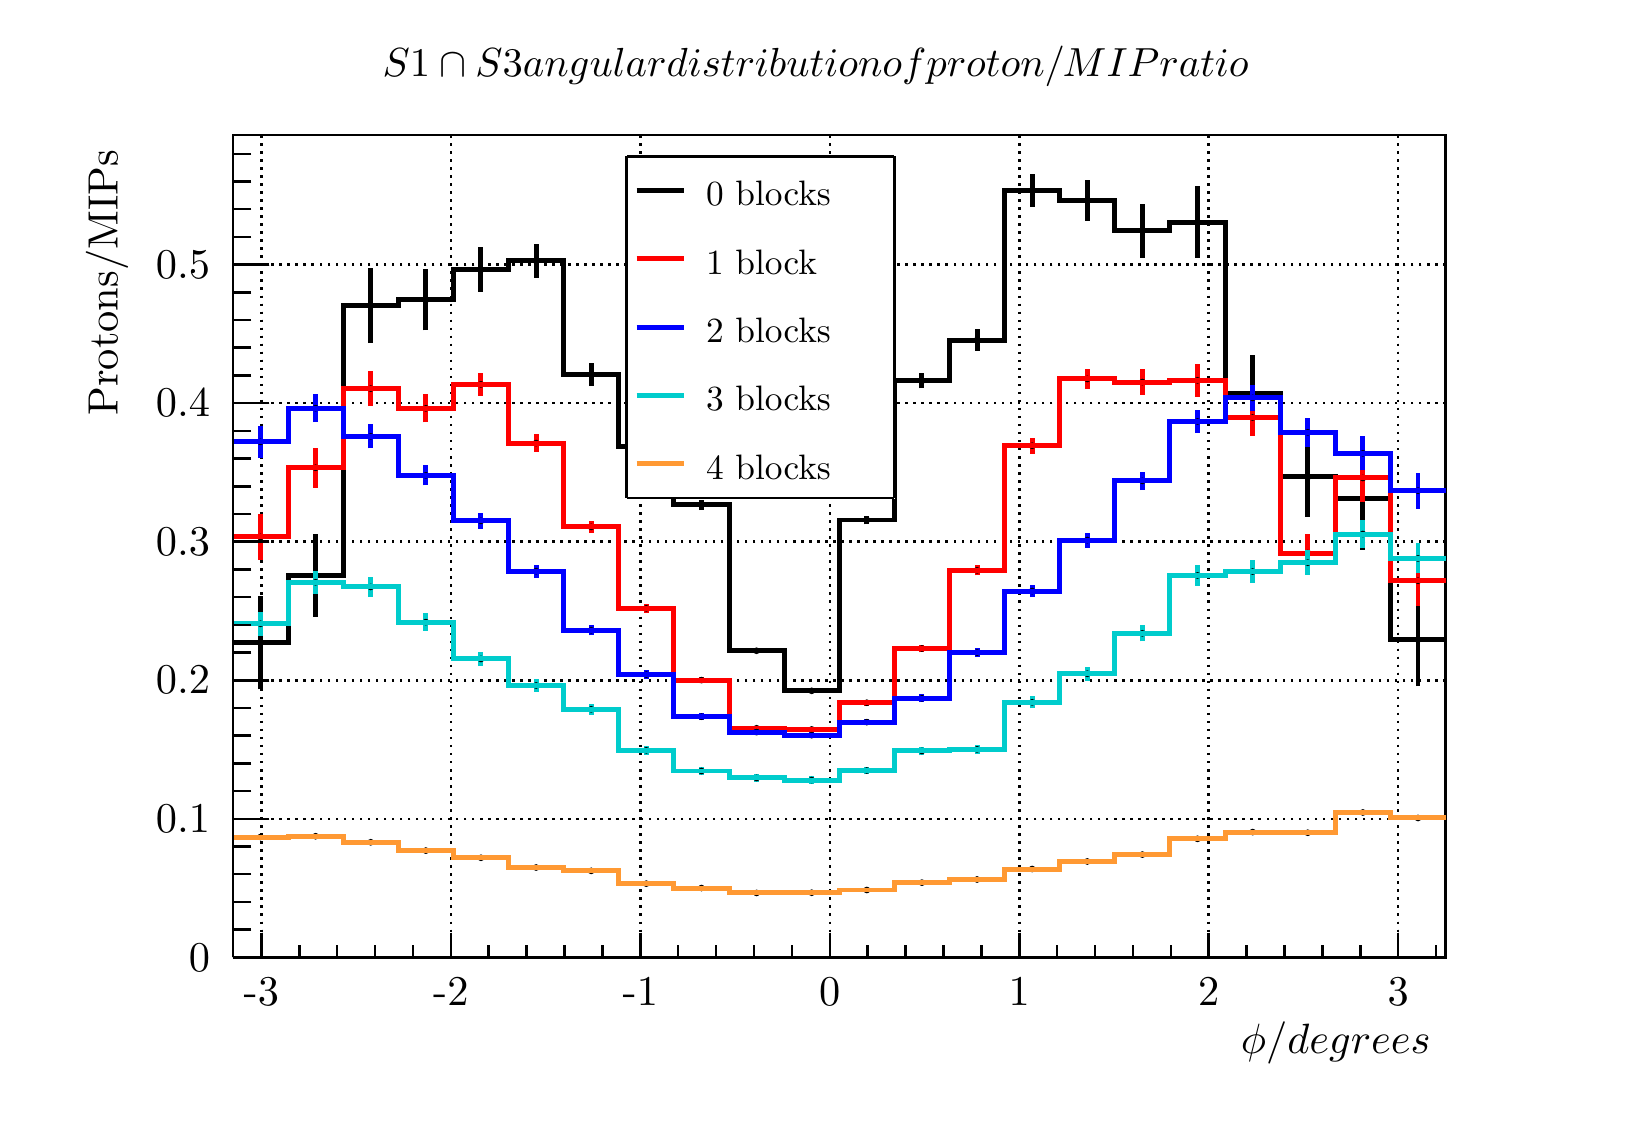
\begin{tikzpicture}
\pgfdeclareplotmark{cross} {
\pgfpathmoveto{\pgfpoint{-0.3\pgfplotmarksize}{\pgfplotmarksize}}
\pgfpathlineto{\pgfpoint{+0.3\pgfplotmarksize}{\pgfplotmarksize}}
\pgfpathlineto{\pgfpoint{+0.3\pgfplotmarksize}{0.3\pgfplotmarksize}}
\pgfpathlineto{\pgfpoint{+1\pgfplotmarksize}{0.3\pgfplotmarksize}}
\pgfpathlineto{\pgfpoint{+1\pgfplotmarksize}{-0.3\pgfplotmarksize}}
\pgfpathlineto{\pgfpoint{+0.3\pgfplotmarksize}{-0.3\pgfplotmarksize}}
\pgfpathlineto{\pgfpoint{+0.3\pgfplotmarksize}{-1.\pgfplotmarksize}}
\pgfpathlineto{\pgfpoint{-0.3\pgfplotmarksize}{-1.\pgfplotmarksize}}
\pgfpathlineto{\pgfpoint{-0.3\pgfplotmarksize}{-0.3\pgfplotmarksize}}
\pgfpathlineto{\pgfpoint{-1.\pgfplotmarksize}{-0.3\pgfplotmarksize}}
\pgfpathlineto{\pgfpoint{-1.\pgfplotmarksize}{0.3\pgfplotmarksize}}
\pgfpathlineto{\pgfpoint{-0.3\pgfplotmarksize}{0.3\pgfplotmarksize}}
\pgfpathclose
\pgfusepathqstroke
}
\pgfdeclareplotmark{cross*} {
\pgfpathmoveto{\pgfpoint{-0.3\pgfplotmarksize}{\pgfplotmarksize}}
\pgfpathlineto{\pgfpoint{+0.3\pgfplotmarksize}{\pgfplotmarksize}}
\pgfpathlineto{\pgfpoint{+0.3\pgfplotmarksize}{0.3\pgfplotmarksize}}
\pgfpathlineto{\pgfpoint{+1\pgfplotmarksize}{0.3\pgfplotmarksize}}
\pgfpathlineto{\pgfpoint{+1\pgfplotmarksize}{-0.3\pgfplotmarksize}}
\pgfpathlineto{\pgfpoint{+0.3\pgfplotmarksize}{-0.3\pgfplotmarksize}}
\pgfpathlineto{\pgfpoint{+0.3\pgfplotmarksize}{-1.\pgfplotmarksize}}
\pgfpathlineto{\pgfpoint{-0.3\pgfplotmarksize}{-1.\pgfplotmarksize}}
\pgfpathlineto{\pgfpoint{-0.3\pgfplotmarksize}{-0.3\pgfplotmarksize}}
\pgfpathlineto{\pgfpoint{-1.\pgfplotmarksize}{-0.3\pgfplotmarksize}}
\pgfpathlineto{\pgfpoint{-1.\pgfplotmarksize}{0.3\pgfplotmarksize}}
\pgfpathlineto{\pgfpoint{-0.3\pgfplotmarksize}{0.3\pgfplotmarksize}}
\pgfpathclose
\pgfusepathqfillstroke
}
\pgfdeclareplotmark{newstar} {
\pgfpathmoveto{\pgfqpoint{0pt}{\pgfplotmarksize}}
\pgfpathlineto{\pgfqpointpolar{44}{0.5\pgfplotmarksize}}
\pgfpathlineto{\pgfqpointpolar{18}{\pgfplotmarksize}}
\pgfpathlineto{\pgfqpointpolar{-20}{0.5\pgfplotmarksize}}
\pgfpathlineto{\pgfqpointpolar{-54}{\pgfplotmarksize}}
\pgfpathlineto{\pgfqpointpolar{-90}{0.5\pgfplotmarksize}}
\pgfpathlineto{\pgfqpointpolar{234}{\pgfplotmarksize}}
\pgfpathlineto{\pgfqpointpolar{198}{0.5\pgfplotmarksize}}
\pgfpathlineto{\pgfqpointpolar{162}{\pgfplotmarksize}}
\pgfpathlineto{\pgfqpointpolar{134}{0.5\pgfplotmarksize}}
\pgfpathclose
\pgfusepathqstroke
}
\pgfdeclareplotmark{newstar*} {
\pgfpathmoveto{\pgfqpoint{0pt}{\pgfplotmarksize}}
\pgfpathlineto{\pgfqpointpolar{44}{0.5\pgfplotmarksize}}
\pgfpathlineto{\pgfqpointpolar{18}{\pgfplotmarksize}}
\pgfpathlineto{\pgfqpointpolar{-20}{0.5\pgfplotmarksize}}
\pgfpathlineto{\pgfqpointpolar{-54}{\pgfplotmarksize}}
\pgfpathlineto{\pgfqpointpolar{-90}{0.5\pgfplotmarksize}}
\pgfpathlineto{\pgfqpointpolar{234}{\pgfplotmarksize}}
\pgfpathlineto{\pgfqpointpolar{198}{0.5\pgfplotmarksize}}
\pgfpathlineto{\pgfqpointpolar{162}{\pgfplotmarksize}}
\pgfpathlineto{\pgfqpointpolar{134}{0.5\pgfplotmarksize}}
\pgfpathclose
\pgfusepathqfillstroke
}
\definecolor{c}{rgb}{1,1,1};
\draw [color=c, fill=c] (0,0) rectangle (20,13.5632);
\draw [color=c, fill=c] (2.6,1.76322) rectangle (18,12.2069);
\definecolor{c}{rgb}{0,0,0};
\draw [c,line width=0.9] (2.6,1.76322) -- (2.6,12.2069) -- (18,12.2069) -- (18,1.76322) -- (2.6,1.76322);
\definecolor{c}{rgb}{1,1,1};
\draw [color=c, fill=c] (2.6,1.76322) rectangle (18,12.2069);
\definecolor{c}{rgb}{0,0,0};
\draw [c,line width=0.9] (2.6,1.76322) -- (2.6,12.2069) -- (18,12.2069) -- (18,1.76322) -- (2.6,1.76322);
\draw [c,line width=0.9] (2.6,1.76322) -- (18,1.76322);
\draw [c,dotted,line width=0.9] (2.96094,12.2069) -- (2.96094,1.76322);
\draw [c,dotted,line width=0.9] (5.36719,12.2069) -- (5.36719,1.76322);
\draw [c,dotted,line width=0.9] (7.77344,12.2069) -- (7.77344,1.76322);
\draw [c,dotted,line width=0.9] (10.1797,12.2069) -- (10.1797,1.76322);
\draw [c,dotted,line width=0.9] (12.5859,12.2069) -- (12.5859,1.76322);
\draw [c,dotted,line width=0.9] (14.9922,12.2069) -- (14.9922,1.76322);
\draw [c,dotted,line width=0.9] (17.3984,12.2069) -- (17.3984,1.76322);
\draw [c,dotted,line width=0.9] (2.96094,12.2069) -- (2.96094,1.76322);
\draw [c,dotted,line width=0.9] (17.3984,12.2069) -- (17.3984,1.76322);
\draw [c,line width=0.9] (2.6,1.76322) -- (2.6,12.2069);
\draw [c,dotted,line width=0.9] (18,1.76322) -- (2.6,1.76322);
\draw [c,dotted,line width=0.9] (18,3.52278) -- (2.6,3.52278);
\draw [c,dotted,line width=0.9] (18,5.28233) -- (2.6,5.28233);
\draw [c,dotted,line width=0.9] (18,7.04189) -- (2.6,7.04189);
\draw [c,dotted,line width=0.9] (18,8.80145) -- (2.6,8.80145);
\draw [c,dotted,line width=0.9] (18,10.561) -- (2.6,10.561);
\draw [c,dotted,line width=0.9] (18,10.561) -- (2.6,10.561);
\definecolor{c}{rgb}{0,0,0.6};
\draw [c,line width=0.9] (2.6,1.76322) -- (3.3,1.76322) -- (3.3,1.76322) -- (4,1.76322) -- (4,1.76322) -- (4.7,1.76322) -- (4.7,1.76322) -- (5.4,1.76322) -- (5.4,1.76322) -- (6.1,1.76322) -- (6.1,1.76322) -- (6.8,1.76322) -- (6.8,1.76322) --
 (7.5,1.76322) -- (7.5,1.76322) -- (8.2,1.76322) -- (8.2,1.76322) -- (8.9,1.76322) -- (8.9,1.76322) -- (9.6,1.76322) -- (9.6,1.76322) -- (10.3,1.76322) -- (10.3,1.76322) -- (11,1.76322) -- (11,1.76322) -- (11.7,1.76322) -- (11.7,1.76322) --
 (12.4,1.76322) -- (12.4,1.76322) -- (13.1,1.76322) -- (13.1,1.76322) -- (13.8,1.76322) -- (13.8,1.76322) -- (14.5,1.76322) -- (14.5,1.76322) -- (15.2,1.76322) -- (15.2,1.76322) -- (15.9,1.76322) -- (15.9,1.76322) -- (16.6,1.76322) -- (16.6,1.76322)
 -- (17.3,1.76322) -- (17.3,1.76322) -- (18,1.76322);
\definecolor{c}{rgb}{0,0,0};
\draw [c,line width=0.9] (2.6,1.76322) -- (18,1.76322);
\draw [anchor= east] (18,0.678161) node[scale=1.5317, color=c, rotate=0]{$ \phi / degrees$};
\draw [c,line width=0.9] (2.96094,2.07653) -- (2.96094,1.76322);
\draw [c,line width=0.9] (3.44219,1.91987) -- (3.44219,1.76322);
\draw [c,line width=0.9] (3.92344,1.91987) -- (3.92344,1.76322);
\draw [c,line width=0.9] (4.40469,1.91987) -- (4.40469,1.76322);
\draw [c,line width=0.9] (4.88594,1.91987) -- (4.88594,1.76322);
\draw [c,line width=0.9] (5.36719,2.07653) -- (5.36719,1.76322);
\draw [c,line width=0.9] (5.84844,1.91987) -- (5.84844,1.76322);
\draw [c,line width=0.9] (6.32969,1.91987) -- (6.32969,1.76322);
\draw [c,line width=0.9] (6.81094,1.91987) -- (6.81094,1.76322);
\draw [c,line width=0.9] (7.29219,1.91987) -- (7.29219,1.76322);
\draw [c,line width=0.9] (7.77344,2.07653) -- (7.77344,1.76322);
\draw [c,line width=0.9] (8.25469,1.91987) -- (8.25469,1.76322);
\draw [c,line width=0.9] (8.73594,1.91987) -- (8.73594,1.76322);
\draw [c,line width=0.9] (9.21719,1.91987) -- (9.21719,1.76322);
\draw [c,line width=0.9] (9.69844,1.91987) -- (9.69844,1.76322);
\draw [c,line width=0.9] (10.1797,2.07653) -- (10.1797,1.76322);
\draw [c,line width=0.9] (10.6609,1.91987) -- (10.6609,1.76322);
\draw [c,line width=0.9] (11.1422,1.91987) -- (11.1422,1.76322);
\draw [c,line width=0.9] (11.6234,1.91987) -- (11.6234,1.76322);
\draw [c,line width=0.9] (12.1047,1.91987) -- (12.1047,1.76322);
\draw [c,line width=0.9] (12.5859,2.07653) -- (12.5859,1.76322);
\draw [c,line width=0.9] (13.0672,1.91987) -- (13.0672,1.76322);
\draw [c,line width=0.9] (13.5484,1.91987) -- (13.5484,1.76322);
\draw [c,line width=0.9] (14.0297,1.91987) -- (14.0297,1.76322);
\draw [c,line width=0.9] (14.5109,1.91987) -- (14.5109,1.76322);
\draw [c,line width=0.9] (14.9922,2.07653) -- (14.9922,1.76322);
\draw [c,line width=0.9] (15.4734,1.91987) -- (15.4734,1.76322);
\draw [c,line width=0.9] (15.9547,1.91987) -- (15.9547,1.76322);
\draw [c,line width=0.9] (16.4359,1.91987) -- (16.4359,1.76322);
\draw [c,line width=0.9] (16.9172,1.91987) -- (16.9172,1.76322);
\draw [c,line width=0.9] (17.3984,2.07653) -- (17.3984,1.76322);
\draw [c,line width=0.9] (2.96094,2.07653) -- (2.96094,1.76322);
\draw [c,line width=0.9] (17.3984,2.07653) -- (17.3984,1.76322);
\draw [c,line width=0.9] (17.8797,1.91987) -- (17.8797,1.76322);
\draw [anchor=base] (2.96094,1.15287) node[scale=1.5317, color=c, rotate=0]{-3};
\draw [anchor=base] (5.36719,1.15287) node[scale=1.5317, color=c, rotate=0]{-2};
\draw [anchor=base] (7.77344,1.15287) node[scale=1.5317, color=c, rotate=0]{-1};
\draw [anchor=base] (10.1797,1.15287) node[scale=1.5317, color=c, rotate=0]{0};
\draw [anchor=base] (12.5859,1.15287) node[scale=1.5317, color=c, rotate=0]{1};
\draw [anchor=base] (14.9922,1.15287) node[scale=1.5317, color=c, rotate=0]{2};
\draw [anchor=base] (17.3984,1.15287) node[scale=1.5317, color=c, rotate=0]{3};
\draw [c,line width=0.9] (2.6,1.76322) -- (2.6,12.2069);
\draw [anchor= east] (1,12.2069) node[scale=1.5317, color=c, rotate=90]{  Protons/MIPs};
\draw [c,line width=0.9] (3.062,1.76322) -- (2.6,1.76322);
\draw [c,line width=0.9] (2.831,2.11513) -- (2.6,2.11513);
\draw [c,line width=0.9] (2.831,2.46704) -- (2.6,2.46704);
\draw [c,line width=0.9] (2.831,2.81895) -- (2.6,2.81895);
\draw [c,line width=0.9] (2.831,3.17086) -- (2.6,3.17086);
\draw [c,line width=0.9] (3.062,3.52278) -- (2.6,3.52278);
\draw [c,line width=0.9] (2.831,3.87469) -- (2.6,3.87469);
\draw [c,line width=0.9] (2.831,4.2266) -- (2.6,4.2266);
\draw [c,line width=0.9] (2.831,4.57851) -- (2.6,4.57851);
\draw [c,line width=0.9] (2.831,4.93042) -- (2.6,4.93042);
\draw [c,line width=0.9] (3.062,5.28233) -- (2.6,5.28233);
\draw [c,line width=0.9] (2.831,5.63425) -- (2.6,5.63425);
\draw [c,line width=0.9] (2.831,5.98616) -- (2.6,5.98616);
\draw [c,line width=0.9] (2.831,6.33807) -- (2.6,6.33807);
\draw [c,line width=0.9] (2.831,6.68998) -- (2.6,6.68998);
\draw [c,line width=0.9] (3.062,7.04189) -- (2.6,7.04189);
\draw [c,line width=0.9] (2.831,7.3938) -- (2.6,7.3938);
\draw [c,line width=0.9] (2.831,7.74572) -- (2.6,7.74572);
\draw [c,line width=0.9] (2.831,8.09763) -- (2.6,8.09763);
\draw [c,line width=0.9] (2.831,8.44954) -- (2.6,8.44954);
\draw [c,line width=0.9] (3.062,8.80145) -- (2.6,8.80145);
\draw [c,line width=0.9] (2.831,9.15336) -- (2.6,9.15336);
\draw [c,line width=0.9] (2.831,9.50527) -- (2.6,9.50527);
\draw [c,line width=0.9] (2.831,9.85719) -- (2.6,9.85719);
\draw [c,line width=0.9] (2.831,10.2091) -- (2.6,10.2091);
\draw [c,line width=0.9] (3.062,10.561) -- (2.6,10.561);
\draw [c,line width=0.9] (3.062,10.561) -- (2.6,10.561);
\draw [c,line width=0.9] (2.831,10.9129) -- (2.6,10.9129);
\draw [c,line width=0.9] (2.831,11.2648) -- (2.6,11.2648);
\draw [c,line width=0.9] (2.831,11.6167) -- (2.6,11.6167);
\draw [c,line width=0.9] (2.831,11.9687) -- (2.6,11.9687);
\draw [anchor= east] (2.5,1.76322) node[scale=1.5317, color=c, rotate=0]{0};
\draw [anchor= east] (2.5,3.52278) node[scale=1.5317, color=c, rotate=0]{0.1};
\draw [anchor= east] (2.5,5.28233) node[scale=1.5317, color=c, rotate=0]{0.2};
\draw [anchor= east] (2.5,7.04189) node[scale=1.5317, color=c, rotate=0]{0.3};
\draw [anchor= east] (2.5,8.80145) node[scale=1.5317, color=c, rotate=0]{0.4};
\draw [anchor= east] (2.5,10.561) node[scale=1.5317, color=c, rotate=0]{0.5};
\draw [c,line width=1.8] (2.95,5.16802) -- (2.95,5.76221);
\draw [c,line width=1.8] (2.95,5.76221) -- (2.95,6.35641);
\foreach \P in {(2.95,5.76221)}{\draw[mark options={color=c,fill=c},mark size=2.402402pt,mark=*,mark size=1pt] plot coordinates {\P};}
\draw [c,line width=1.8] (3.65,6.08767) -- (3.65,6.61178);
\draw [c,line width=1.8] (3.65,6.61178) -- (3.65,7.13589);
\foreach \P in {(3.65,6.61178)}{\draw[mark options={color=c,fill=c},mark size=2.402402pt,mark=*,mark size=1pt] plot coordinates {\P};}
\draw [c,line width=1.8] (4.35,9.56273) -- (4.35,10.0404);
\draw [c,line width=1.8] (4.35,10.0404) -- (4.35,10.5181);
\foreach \P in {(4.35,10.0404)}{\draw[mark options={color=c,fill=c},mark size=2.402402pt,mark=*,mark size=1pt] plot coordinates {\P};}
\draw [c,line width=1.8] (5.05,9.72594) -- (5.05,10.1142);
\draw [c,line width=1.8] (5.05,10.1142) -- (5.05,10.5026);
\foreach \P in {(5.05,10.1142)}{\draw[mark options={color=c,fill=c},mark size=2.402402pt,mark=*,mark size=1pt] plot coordinates {\P};}
\draw [c,line width=1.8] (5.75,10.2136) -- (5.75,10.4971);
\draw [c,line width=1.8] (5.75,10.4971) -- (5.75,10.7806);
\foreach \P in {(5.75,10.4971)}{\draw[mark options={color=c,fill=c},mark size=2.402402pt,mark=*,mark size=1pt] plot coordinates {\P};}
\draw [c,line width=1.8] (6.45,10.3922) -- (6.45,10.6092);
\draw [c,line width=1.8] (6.45,10.6092) -- (6.45,10.8262);
\foreach \P in {(6.45,10.6092)}{\draw[mark options={color=c,fill=c},mark size=2.402402pt,mark=*,mark size=1pt] plot coordinates {\P};}
\draw [c,line width=1.8] (7.15,9.01643) -- (7.15,9.16611);
\draw [c,line width=1.8] (7.15,9.16611) -- (7.15,9.31579);
\foreach \P in {(7.15,9.16611)}{\draw[mark options={color=c,fill=c},mark size=2.402402pt,mark=*,mark size=1pt] plot coordinates {\P};}
\draw [c,line width=1.8] (7.85,8.15111) -- (7.85,8.25348);
\draw [c,line width=1.8] (7.85,8.25348) -- (7.85,8.35584);
\foreach \P in {(7.85,8.25348)}{\draw[mark options={color=c,fill=c},mark size=2.402402pt,mark=*,mark size=1pt] plot coordinates {\P};}
\draw [c,line width=1.8] (8.55,7.44312) -- (8.55,7.51028);
\draw [c,line width=1.8] (8.55,7.51028) -- (8.55,7.57745);
\foreach \P in {(8.55,7.51028)}{\draw[mark options={color=c,fill=c},mark size=2.402402pt,mark=*,mark size=1pt] plot coordinates {\P};}
\draw [c,line width=1.8] (9.25,5.62251) -- (9.25,5.65698);
\draw [c,line width=1.8] (9.25,5.65698) -- (9.25,5.69145);
\foreach \P in {(9.25,5.65698)}{\draw[mark options={color=c,fill=c},mark size=2.402402pt,mark=*,mark size=1pt] plot coordinates {\P};}
\draw [c,line width=1.8] (9.95,5.11954) -- (9.95,5.14805);
\draw [c,line width=1.8] (9.95,5.14805) -- (9.95,5.17655);
\foreach \P in {(9.95,5.14805)}{\draw[mark options={color=c,fill=c},mark size=2.402402pt,mark=*,mark size=1pt] plot coordinates {\P};}
\draw [c,line width=1.8] (10.65,7.26204) -- (10.65,7.31762);
\draw [c,line width=1.8] (10.65,7.31762) -- (10.65,7.37321);
\foreach \P in {(10.65,7.31762)}{\draw[mark options={color=c,fill=c},mark size=2.402402pt,mark=*,mark size=1pt] plot coordinates {\P};}
\draw [c,line width=1.8] (11.35,8.98831) -- (11.35,9.08613);
\draw [c,line width=1.8] (11.35,9.08613) -- (11.35,9.18395);
\foreach \P in {(11.35,9.08613)}{\draw[mark options={color=c,fill=c},mark size=2.402402pt,mark=*,mark size=1pt] plot coordinates {\P};}
\draw [c,line width=1.8] (12.05,9.46686) -- (12.05,9.60221);
\draw [c,line width=1.8] (12.05,9.60221) -- (12.05,9.73756);
\foreach \P in {(12.05,9.60221)}{\draw[mark options={color=c,fill=c},mark size=2.402402pt,mark=*,mark size=1pt] plot coordinates {\P};}
\draw [c,line width=1.8] (12.75,11.2984) -- (12.75,11.504);
\draw [c,line width=1.8] (12.75,11.504) -- (12.75,11.7096);
\foreach \P in {(12.75,11.504)}{\draw[mark options={color=c,fill=c},mark size=2.402402pt,mark=*,mark size=1pt] plot coordinates {\P};}
\draw [c,line width=1.8] (13.45,11.1183) -- (13.45,11.376);
\draw [c,line width=1.8] (13.45,11.376) -- (13.45,11.6338);
\foreach \P in {(13.45,11.376)}{\draw[mark options={color=c,fill=c},mark size=2.402402pt,mark=*,mark size=1pt] plot coordinates {\P};}
\draw [c,line width=1.8] (14.15,10.6487) -- (14.15,10.9928);
\draw [c,line width=1.8] (14.15,10.9928) -- (14.15,11.3369);
\foreach \P in {(14.15,10.9928)}{\draw[mark options={color=c,fill=c},mark size=2.402402pt,mark=*,mark size=1pt] plot coordinates {\P};}
\draw [c,line width=1.8] (14.85,10.6471) -- (14.85,11.1006);
\draw [c,line width=1.8] (14.85,11.1006) -- (14.85,11.5541);
\foreach \P in {(14.85,11.1006)}{\draw[mark options={color=c,fill=c},mark size=2.402402pt,mark=*,mark size=1pt] plot coordinates {\P};}
\draw [c,line width=1.8] (15.55,8.43613) -- (15.55,8.92552);
\draw [c,line width=1.8] (15.55,8.92552) -- (15.55,9.41492);
\foreach \P in {(15.55,8.92552)}{\draw[mark options={color=c,fill=c},mark size=2.402402pt,mark=*,mark size=1pt] plot coordinates {\P};}
\draw [c,line width=1.8] (16.25,7.35798) -- (16.25,7.86388);
\draw [c,line width=1.8] (16.25,7.86388) -- (16.25,8.36978);
\foreach \P in {(16.25,7.86388)}{\draw[mark options={color=c,fill=c},mark size=2.402402pt,mark=*,mark size=1pt] plot coordinates {\P};}
\draw [c,line width=1.8] (16.95,6.93704) -- (16.95,7.59175);
\draw [c,line width=1.8] (16.95,7.59175) -- (16.95,8.24647);
\foreach \P in {(16.95,7.59175)}{\draw[mark options={color=c,fill=c},mark size=2.402402pt,mark=*,mark size=1pt] plot coordinates {\P};}
\draw [c,line width=1.8] (17.65,5.20754) -- (17.65,5.79787);
\draw [c,line width=1.8] (17.65,5.79787) -- (17.65,6.38821);
\foreach \P in {(17.65,5.79787)}{\draw[mark options={color=c,fill=c},mark size=2.402402pt,mark=*,mark size=1pt] plot coordinates {\P};}
\draw [c,line width=1.8] (2.6,5.76221) -- (3.3,5.76221) -- (3.3,6.61178) -- (4,6.61178) -- (4,10.0404) -- (4.7,10.0404) -- (4.7,10.1142) -- (5.4,10.1142) -- (5.4,10.4971) -- (6.1,10.4971) -- (6.1,10.6092) -- (6.8,10.6092) -- (6.8,9.16611) --
 (7.5,9.16611) -- (7.5,8.25348) -- (8.2,8.25348) -- (8.2,7.51028) -- (8.9,7.51028) -- (8.9,5.65698) -- (9.6,5.65698) -- (9.6,5.14805) -- (10.3,5.14805) -- (10.3,7.31762) -- (11,7.31762) -- (11,9.08613) -- (11.7,9.08613) -- (11.7,9.60221) --
 (12.4,9.60221) -- (12.4,11.504) -- (13.1,11.504) -- (13.1,11.376) -- (13.8,11.376) -- (13.8,10.9928) -- (14.5,10.9928) -- (14.5,11.1006) -- (15.2,11.1006) -- (15.2,8.92552) -- (15.9,8.92552) -- (15.9,7.86388) -- (16.6,7.86388) -- (16.6,7.59175) --
 (17.3,7.59175) -- (17.3,5.79787) -- (18,5.79787);
\definecolor{c}{rgb}{1,0,0};
\draw [c,line width=1.8] (2.95,6.81433) -- (2.95,7.10195);
\draw [c,line width=1.8] (2.95,7.10195) -- (2.95,7.38957);
\definecolor{c}{rgb}{0,0,0};
\foreach \P in {(2.95,7.10195)}{\draw[mark options={color=c,fill=c},mark size=2.402402pt,mark=*,mark size=1pt] plot coordinates {\P};}
\definecolor{c}{rgb}{1,0,0};
\draw [c,line width=1.8] (3.65,7.72896) -- (3.65,7.98085);
\draw [c,line width=1.8] (3.65,7.98085) -- (3.65,8.23274);
\definecolor{c}{rgb}{0,0,0};
\foreach \P in {(3.65,7.98085)}{\draw[mark options={color=c,fill=c},mark size=2.402402pt,mark=*,mark size=1pt] plot coordinates {\P};}
\definecolor{c}{rgb}{1,0,0};
\draw [c,line width=1.8] (4.35,8.76291) -- (4.35,8.98581);
\draw [c,line width=1.8] (4.35,8.98581) -- (4.35,9.2087);
\definecolor{c}{rgb}{0,0,0};
\foreach \P in {(4.35,8.98581)}{\draw[mark options={color=c,fill=c},mark size=2.402402pt,mark=*,mark size=1pt] plot coordinates {\P};}
\definecolor{c}{rgb}{1,0,0};
\draw [c,line width=1.8] (5.05,8.55714) -- (5.05,8.73606);
\draw [c,line width=1.8] (5.05,8.73606) -- (5.05,8.91497);
\definecolor{c}{rgb}{0,0,0};
\foreach \P in {(5.05,8.73606)}{\draw[mark options={color=c,fill=c},mark size=2.402402pt,mark=*,mark size=1pt] plot coordinates {\P};}
\definecolor{c}{rgb}{1,0,0};
\draw [c,line width=1.8] (5.75,8.89722) -- (5.75,9.03987);
\draw [c,line width=1.8] (5.75,9.03987) -- (5.75,9.18252);
\definecolor{c}{rgb}{0,0,0};
\foreach \P in {(5.75,9.03987)}{\draw[mark options={color=c,fill=c},mark size=2.402402pt,mark=*,mark size=1pt] plot coordinates {\P};}
\definecolor{c}{rgb}{1,0,0};
\draw [c,line width=1.8] (6.45,8.18451) -- (6.45,8.29436);
\draw [c,line width=1.8] (6.45,8.29436) -- (6.45,8.4042);
\definecolor{c}{rgb}{0,0,0};
\foreach \P in {(6.45,8.29436)}{\draw[mark options={color=c,fill=c},mark size=2.402402pt,mark=*,mark size=1pt] plot coordinates {\P};}
\definecolor{c}{rgb}{1,0,0};
\draw [c,line width=1.8] (7.15,7.15139) -- (7.15,7.23009);
\draw [c,line width=1.8] (7.15,7.23009) -- (7.15,7.3088);
\definecolor{c}{rgb}{0,0,0};
\foreach \P in {(7.15,7.23009)}{\draw[mark options={color=c,fill=c},mark size=2.402402pt,mark=*,mark size=1pt] plot coordinates {\P};}
\definecolor{c}{rgb}{1,0,0};
\draw [c,line width=1.8] (7.85,6.13928) -- (7.85,6.19561);
\draw [c,line width=1.8] (7.85,6.19561) -- (7.85,6.25195);
\definecolor{c}{rgb}{0,0,0};
\foreach \P in {(7.85,6.19561)}{\draw[mark options={color=c,fill=c},mark size=2.402402pt,mark=*,mark size=1pt] plot coordinates {\P};}
\definecolor{c}{rgb}{1,0,0};
\draw [c,line width=1.8] (8.55,5.24259) -- (8.55,5.28418);
\draw [c,line width=1.8] (8.55,5.28418) -- (8.55,5.32576);
\definecolor{c}{rgb}{0,0,0};
\foreach \P in {(8.55,5.28418)}{\draw[mark options={color=c,fill=c},mark size=2.402402pt,mark=*,mark size=1pt] plot coordinates {\P};}
\definecolor{c}{rgb}{1,0,0};
\draw [c,line width=1.8] (9.25,4.63912) -- (9.25,4.67253);
\draw [c,line width=1.8] (9.25,4.67253) -- (9.25,4.70594);
\definecolor{c}{rgb}{0,0,0};
\foreach \P in {(9.25,4.67253)}{\draw[mark options={color=c,fill=c},mark size=2.402402pt,mark=*,mark size=1pt] plot coordinates {\P};}
\definecolor{c}{rgb}{1,0,0};
\draw [c,line width=1.8] (9.95,4.62465) -- (9.95,4.65743);
\draw [c,line width=1.8] (9.95,4.65743) -- (9.95,4.69022);
\definecolor{c}{rgb}{0,0,0};
\foreach \P in {(9.95,4.65743)}{\draw[mark options={color=c,fill=c},mark size=2.402402pt,mark=*,mark size=1pt] plot coordinates {\P};}
\definecolor{c}{rgb}{1,0,0};
\draw [c,line width=1.8] (10.65,4.95962) -- (10.65,4.99693);
\draw [c,line width=1.8] (10.65,4.99693) -- (10.65,5.03424);
\definecolor{c}{rgb}{0,0,0};
\foreach \P in {(10.65,4.99693)}{\draw[mark options={color=c,fill=c},mark size=2.402402pt,mark=*,mark size=1pt] plot coordinates {\P};}
\definecolor{c}{rgb}{1,0,0};
\draw [c,line width=1.8] (11.35,5.6376) -- (11.35,5.68562);
\draw [c,line width=1.8] (11.35,5.68562) -- (11.35,5.73363);
\definecolor{c}{rgb}{0,0,0};
\foreach \P in {(11.35,5.68562)}{\draw[mark options={color=c,fill=c},mark size=2.402402pt,mark=*,mark size=1pt] plot coordinates {\P};}
\definecolor{c}{rgb}{1,0,0};
\draw [c,line width=1.8] (12.05,6.61309) -- (12.05,6.67827);
\draw [c,line width=1.8] (12.05,6.67827) -- (12.05,6.74346);
\definecolor{c}{rgb}{0,0,0};
\foreach \P in {(12.05,6.67827)}{\draw[mark options={color=c,fill=c},mark size=2.402402pt,mark=*,mark size=1pt] plot coordinates {\P};}
\definecolor{c}{rgb}{1,0,0};
\draw [c,line width=1.8] (12.75,8.16196) -- (12.75,8.26052);
\draw [c,line width=1.8] (12.75,8.26052) -- (12.75,8.35908);
\definecolor{c}{rgb}{0,0,0};
\foreach \P in {(12.75,8.26052)}{\draw[mark options={color=c,fill=c},mark size=2.402402pt,mark=*,mark size=1pt] plot coordinates {\P};}
\definecolor{c}{rgb}{1,0,0};
\draw [c,line width=1.8] (13.45,8.97911) -- (13.45,9.10922);
\draw [c,line width=1.8] (13.45,9.10922) -- (13.45,9.23932);
\definecolor{c}{rgb}{0,0,0};
\foreach \P in {(13.45,9.10922)}{\draw[mark options={color=c,fill=c},mark size=2.402402pt,mark=*,mark size=1pt] plot coordinates {\P};}
\definecolor{c}{rgb}{1,0,0};
\draw [c,line width=1.8] (14.15,8.9066) -- (14.15,9.06939);
\draw [c,line width=1.8] (14.15,9.06939) -- (14.15,9.23217);
\definecolor{c}{rgb}{0,0,0};
\foreach \P in {(14.15,9.06939)}{\draw[mark options={color=c,fill=c},mark size=2.402402pt,mark=*,mark size=1pt] plot coordinates {\P};}
\definecolor{c}{rgb}{1,0,0};
\draw [c,line width=1.8] (14.85,8.88462) -- (14.85,9.09138);
\draw [c,line width=1.8] (14.85,9.09138) -- (14.85,9.29814);
\definecolor{c}{rgb}{0,0,0};
\foreach \P in {(14.85,9.09138)}{\draw[mark options={color=c,fill=c},mark size=2.402402pt,mark=*,mark size=1pt] plot coordinates {\P};}
\definecolor{c}{rgb}{1,0,0};
\draw [c,line width=1.8] (15.55,8.38544) -- (15.55,8.61898);
\draw [c,line width=1.8] (15.55,8.61898) -- (15.55,8.85252);
\definecolor{c}{rgb}{0,0,0};
\foreach \P in {(15.55,8.61898)}{\draw[mark options={color=c,fill=c},mark size=2.402402pt,mark=*,mark size=1pt] plot coordinates {\P};}
\definecolor{c}{rgb}{1,0,0};
\draw [c,line width=1.8] (16.25,6.65675) -- (16.25,6.89793);
\draw [c,line width=1.8] (16.25,6.89793) -- (16.25,7.13911);
\definecolor{c}{rgb}{0,0,0};
\foreach \P in {(16.25,6.89793)}{\draw[mark options={color=c,fill=c},mark size=2.402402pt,mark=*,mark size=1pt] plot coordinates {\P};}
\definecolor{c}{rgb}{1,0,0};
\draw [c,line width=1.8] (16.95,7.54832) -- (16.95,7.85134);
\draw [c,line width=1.8] (16.95,7.85134) -- (16.95,8.15435);
\definecolor{c}{rgb}{0,0,0};
\foreach \P in {(16.95,7.85134)}{\draw[mark options={color=c,fill=c},mark size=2.402402pt,mark=*,mark size=1pt] plot coordinates {\P};}
\definecolor{c}{rgb}{1,0,0};
\draw [c,line width=1.8] (17.65,6.23158) -- (17.65,6.54648);
\draw [c,line width=1.8] (17.65,6.54648) -- (17.65,6.86139);
\definecolor{c}{rgb}{0,0,0};
\foreach \P in {(17.65,6.54648)}{\draw[mark options={color=c,fill=c},mark size=2.402402pt,mark=*,mark size=1pt] plot coordinates {\P};}
\definecolor{c}{rgb}{1,0,0};
\draw [c,line width=1.8] (2.6,7.10195) -- (3.3,7.10195) -- (3.3,7.98085) -- (4,7.98085) -- (4,8.98581) -- (4.7,8.98581) -- (4.7,8.73606) -- (5.4,8.73606) -- (5.4,9.03987) -- (6.1,9.03987) -- (6.1,8.29436) -- (6.8,8.29436) -- (6.8,7.23009) --
 (7.5,7.23009) -- (7.5,6.19561) -- (8.2,6.19561) -- (8.2,5.28418) -- (8.9,5.28418) -- (8.9,4.67253) -- (9.6,4.67253) -- (9.6,4.65743) -- (10.3,4.65743) -- (10.3,4.99693) -- (11,4.99693) -- (11,5.68562) -- (11.7,5.68562) -- (11.7,6.67827) --
 (12.4,6.67827) -- (12.4,8.26052) -- (13.1,8.26052) -- (13.1,9.10922) -- (13.8,9.10922) -- (13.8,9.06939) -- (14.5,9.06939) -- (14.5,9.09138) -- (15.2,9.09138) -- (15.2,8.61898) -- (15.9,8.61898) -- (15.9,6.89793) -- (16.6,6.89793) -- (16.6,7.85134)
 -- (17.3,7.85134) -- (17.3,6.54648) -- (18,6.54648);
\definecolor{c}{rgb}{0,0,1};
\draw [c,line width=1.8] (2.95,8.10893) -- (2.95,8.30995);
\draw [c,line width=1.8] (2.95,8.30995) -- (2.95,8.51098);
\definecolor{c}{rgb}{0,0,0};
\foreach \P in {(2.95,8.30995)}{\draw[mark options={color=c,fill=c},mark size=2.402402pt,mark=*,mark size=1pt] plot coordinates {\P};}
\definecolor{c}{rgb}{0,0,1};
\draw [c,line width=1.8] (3.65,8.55978) -- (3.65,8.73804);
\draw [c,line width=1.8] (3.65,8.73804) -- (3.65,8.91631);
\definecolor{c}{rgb}{0,0,0};
\foreach \P in {(3.65,8.73804)}{\draw[mark options={color=c,fill=c},mark size=2.402402pt,mark=*,mark size=1pt] plot coordinates {\P};}
\definecolor{c}{rgb}{0,0,1};
\draw [c,line width=1.8] (4.35,8.22719) -- (4.35,8.37993);
\draw [c,line width=1.8] (4.35,8.37993) -- (4.35,8.53266);
\definecolor{c}{rgb}{0,0,0};
\foreach \P in {(4.35,8.37993)}{\draw[mark options={color=c,fill=c},mark size=2.402402pt,mark=*,mark size=1pt] plot coordinates {\P};}
\definecolor{c}{rgb}{0,0,1};
\draw [c,line width=1.8] (5.05,7.7571) -- (5.05,7.88448);
\draw [c,line width=1.8] (5.05,7.88448) -- (5.05,8.01186);
\definecolor{c}{rgb}{0,0,0};
\foreach \P in {(5.05,7.88448)}{\draw[mark options={color=c,fill=c},mark size=2.402402pt,mark=*,mark size=1pt] plot coordinates {\P};}
\definecolor{c}{rgb}{0,0,1};
\draw [c,line width=1.8] (5.75,7.20469) -- (5.75,7.30684);
\draw [c,line width=1.8] (5.75,7.30684) -- (5.75,7.409);
\definecolor{c}{rgb}{0,0,0};
\foreach \P in {(5.75,7.30684)}{\draw[mark options={color=c,fill=c},mark size=2.402402pt,mark=*,mark size=1pt] plot coordinates {\P};}
\definecolor{c}{rgb}{0,0,1};
\draw [c,line width=1.8] (6.45,6.58393) -- (6.45,6.66795);
\draw [c,line width=1.8] (6.45,6.66795) -- (6.45,6.75197);
\definecolor{c}{rgb}{0,0,0};
\foreach \P in {(6.45,6.66795)}{\draw[mark options={color=c,fill=c},mark size=2.402402pt,mark=*,mark size=1pt] plot coordinates {\P};}
\definecolor{c}{rgb}{0,0,1};
\draw [c,line width=1.8] (7.15,5.85217) -- (7.15,5.91753);
\draw [c,line width=1.8] (7.15,5.91753) -- (7.15,5.98288);
\definecolor{c}{rgb}{0,0,0};
\foreach \P in {(7.15,5.91753)}{\draw[mark options={color=c,fill=c},mark size=2.402402pt,mark=*,mark size=1pt] plot coordinates {\P};}
\definecolor{c}{rgb}{0,0,1};
\draw [c,line width=1.8] (7.85,5.3011) -- (7.85,5.35388);
\draw [c,line width=1.8] (7.85,5.35388) -- (7.85,5.40665);
\definecolor{c}{rgb}{0,0,0};
\foreach \P in {(7.85,5.35388)}{\draw[mark options={color=c,fill=c},mark size=2.402402pt,mark=*,mark size=1pt] plot coordinates {\P};}
\definecolor{c}{rgb}{0,0,1};
\draw [c,line width=1.8] (8.55,4.77582) -- (8.55,4.81962);
\draw [c,line width=1.8] (8.55,4.81962) -- (8.55,4.86342);
\definecolor{c}{rgb}{0,0,0};
\foreach \P in {(8.55,4.81962)}{\draw[mark options={color=c,fill=c},mark size=2.402402pt,mark=*,mark size=1pt] plot coordinates {\P};}
\definecolor{c}{rgb}{0,0,1};
\draw [c,line width=1.8] (9.25,4.584) -- (9.25,4.6236);
\draw [c,line width=1.8] (9.25,4.6236) -- (9.25,4.66319);
\definecolor{c}{rgb}{0,0,0};
\foreach \P in {(9.25,4.6236)}{\draw[mark options={color=c,fill=c},mark size=2.402402pt,mark=*,mark size=1pt] plot coordinates {\P};}
\definecolor{c}{rgb}{0,0,1};
\draw [c,line width=1.8] (9.95,4.54484) -- (9.95,4.58445);
\draw [c,line width=1.8] (9.95,4.58445) -- (9.95,4.62405);
\definecolor{c}{rgb}{0,0,0};
\foreach \P in {(9.95,4.58445)}{\draw[mark options={color=c,fill=c},mark size=2.402402pt,mark=*,mark size=1pt] plot coordinates {\P};}
\definecolor{c}{rgb}{0,0,1};
\draw [c,line width=1.8] (10.65,4.70791) -- (10.65,4.75016);
\draw [c,line width=1.8] (10.65,4.75016) -- (10.65,4.7924);
\definecolor{c}{rgb}{0,0,0};
\foreach \P in {(10.65,4.75016)}{\draw[mark options={color=c,fill=c},mark size=2.402402pt,mark=*,mark size=1pt] plot coordinates {\P};}
\definecolor{c}{rgb}{0,0,1};
\draw [c,line width=1.8] (11.35,5.00525) -- (11.35,5.05348);
\draw [c,line width=1.8] (11.35,5.05348) -- (11.35,5.10171);
\definecolor{c}{rgb}{0,0,0};
\foreach \P in {(11.35,5.05348)}{\draw[mark options={color=c,fill=c},mark size=2.402402pt,mark=*,mark size=1pt] plot coordinates {\P};}
\definecolor{c}{rgb}{0,0,1};
\draw [c,line width=1.8] (12.05,5.57534) -- (12.05,5.63377);
\draw [c,line width=1.8] (12.05,5.63377) -- (12.05,5.6922);
\definecolor{c}{rgb}{0,0,0};
\foreach \P in {(12.05,5.63377)}{\draw[mark options={color=c,fill=c},mark size=2.402402pt,mark=*,mark size=1pt] plot coordinates {\P};}
\definecolor{c}{rgb}{0,0,1};
\draw [c,line width=1.8] (12.75,6.33847) -- (12.75,6.41516);
\draw [c,line width=1.8] (12.75,6.41516) -- (12.75,6.49185);
\definecolor{c}{rgb}{0,0,0};
\foreach \P in {(12.75,6.41516)}{\draw[mark options={color=c,fill=c},mark size=2.402402pt,mark=*,mark size=1pt] plot coordinates {\P};}
\definecolor{c}{rgb}{0,0,1};
\draw [c,line width=1.8] (13.45,6.9667) -- (13.45,7.06244);
\draw [c,line width=1.8] (13.45,7.06244) -- (13.45,7.15818);
\definecolor{c}{rgb}{0,0,0};
\foreach \P in {(13.45,7.06244)}{\draw[mark options={color=c,fill=c},mark size=2.402402pt,mark=*,mark size=1pt] plot coordinates {\P};}
\definecolor{c}{rgb}{0,0,1};
\draw [c,line width=1.8] (14.15,7.69588) -- (14.15,7.81424);
\draw [c,line width=1.8] (14.15,7.81424) -- (14.15,7.93259);
\definecolor{c}{rgb}{0,0,0};
\foreach \P in {(14.15,7.81424)}{\draw[mark options={color=c,fill=c},mark size=2.402402pt,mark=*,mark size=1pt] plot coordinates {\P};}
\definecolor{c}{rgb}{0,0,1};
\draw [c,line width=1.8] (14.85,8.42391) -- (14.85,8.56934);
\draw [c,line width=1.8] (14.85,8.56934) -- (14.85,8.71478);
\definecolor{c}{rgb}{0,0,0};
\foreach \P in {(14.85,8.56934)}{\draw[mark options={color=c,fill=c},mark size=2.402402pt,mark=*,mark size=1pt] plot coordinates {\P};}
\definecolor{c}{rgb}{0,0,1};
\draw [c,line width=1.8] (15.55,8.70173) -- (15.55,8.86812);
\draw [c,line width=1.8] (15.55,8.86812) -- (15.55,9.03452);
\definecolor{c}{rgb}{0,0,0};
\foreach \P in {(15.55,8.86812)}{\draw[mark options={color=c,fill=c},mark size=2.402402pt,mark=*,mark size=1pt] plot coordinates {\P};}
\definecolor{c}{rgb}{0,0,1};
\draw [c,line width=1.8] (16.25,8.2471) -- (16.25,8.43093);
\draw [c,line width=1.8] (16.25,8.43093) -- (16.25,8.61477);
\definecolor{c}{rgb}{0,0,0};
\foreach \P in {(16.25,8.43093)}{\draw[mark options={color=c,fill=c},mark size=2.402402pt,mark=*,mark size=1pt] plot coordinates {\P};}
\definecolor{c}{rgb}{0,0,1};
\draw [c,line width=1.8] (16.95,7.94915) -- (16.95,8.16472);
\draw [c,line width=1.8] (16.95,8.16472) -- (16.95,8.3803);
\definecolor{c}{rgb}{0,0,0};
\foreach \P in {(16.95,8.16472)}{\draw[mark options={color=c,fill=c},mark size=2.402402pt,mark=*,mark size=1pt] plot coordinates {\P};}
\definecolor{c}{rgb}{0,0,1};
\draw [c,line width=1.8] (17.65,7.46164) -- (17.65,7.69071);
\draw [c,line width=1.8] (17.65,7.69071) -- (17.65,7.91979);
\definecolor{c}{rgb}{0,0,0};
\foreach \P in {(17.65,7.69071)}{\draw[mark options={color=c,fill=c},mark size=2.402402pt,mark=*,mark size=1pt] plot coordinates {\P};}
\definecolor{c}{rgb}{0,0,1};
\draw [c,line width=1.8] (2.6,8.30995) -- (3.3,8.30995) -- (3.3,8.73804) -- (4,8.73804) -- (4,8.37993) -- (4.7,8.37993) -- (4.7,7.88448) -- (5.4,7.88448) -- (5.4,7.30684) -- (6.1,7.30684) -- (6.1,6.66795) -- (6.8,6.66795) -- (6.8,5.91753) --
 (7.5,5.91753) -- (7.5,5.35388) -- (8.2,5.35388) -- (8.2,4.81962) -- (8.9,4.81962) -- (8.9,4.6236) -- (9.6,4.6236) -- (9.6,4.58445) -- (10.3,4.58445) -- (10.3,4.75016) -- (11,4.75016) -- (11,5.05348) -- (11.7,5.05348) -- (11.7,5.63377) --
 (12.4,5.63377) -- (12.4,6.41516) -- (13.1,6.41516) -- (13.1,7.06244) -- (13.8,7.06244) -- (13.8,7.81424) -- (14.5,7.81424) -- (14.5,8.56934) -- (15.2,8.56934) -- (15.2,8.86812) -- (15.9,8.86812) -- (15.9,8.43093) -- (16.6,8.43093) -- (16.6,8.16472)
 -- (17.3,8.16472) -- (17.3,7.69071) -- (18,7.69071);
\definecolor{c}{rgb}{0,0.8,0.8};
\draw [c,line width=1.8] (2.95,5.84839) -- (2.95,5.99985);
\draw [c,line width=1.8] (2.95,5.99985) -- (2.95,6.15132);
\definecolor{c}{rgb}{0,0,0};
\foreach \P in {(2.95,5.99985)}{\draw[mark options={color=c,fill=c},mark size=2.402402pt,mark=*,mark size=1pt] plot coordinates {\P};}
\definecolor{c}{rgb}{0,0.8,0.8};
\draw [c,line width=1.8] (3.65,6.38055) -- (3.65,6.52677);
\draw [c,line width=1.8] (3.65,6.52677) -- (3.65,6.67299);
\definecolor{c}{rgb}{0,0,0};
\foreach \P in {(3.65,6.52677)}{\draw[mark options={color=c,fill=c},mark size=2.402402pt,mark=*,mark size=1pt] plot coordinates {\P};}
\definecolor{c}{rgb}{0,0.8,0.8};
\draw [c,line width=1.8] (4.35,6.33723) -- (4.35,6.46752);
\draw [c,line width=1.8] (4.35,6.46752) -- (4.35,6.59782);
\definecolor{c}{rgb}{0,0,0};
\foreach \P in {(4.35,6.46752)}{\draw[mark options={color=c,fill=c},mark size=2.402402pt,mark=*,mark size=1pt] plot coordinates {\P};}
\definecolor{c}{rgb}{0,0.8,0.8};
\draw [c,line width=1.8] (5.05,5.90931) -- (5.05,6.02046);
\draw [c,line width=1.8] (5.05,6.02046) -- (5.05,6.13162);
\definecolor{c}{rgb}{0,0,0};
\foreach \P in {(5.05,6.02046)}{\draw[mark options={color=c,fill=c},mark size=2.402402pt,mark=*,mark size=1pt] plot coordinates {\P};}
\definecolor{c}{rgb}{0,0.8,0.8};
\draw [c,line width=1.8] (5.75,5.46093) -- (5.75,5.55273);
\draw [c,line width=1.8] (5.75,5.55273) -- (5.75,5.64453);
\definecolor{c}{rgb}{0,0,0};
\foreach \P in {(5.75,5.55273)}{\draw[mark options={color=c,fill=c},mark size=2.402402pt,mark=*,mark size=1pt] plot coordinates {\P};}
\definecolor{c}{rgb}{0,0.8,0.8};
\draw [c,line width=1.8] (6.45,5.13572) -- (6.45,5.21597);
\draw [c,line width=1.8] (6.45,5.21597) -- (6.45,5.29622);
\definecolor{c}{rgb}{0,0,0};
\foreach \P in {(6.45,5.21597)}{\draw[mark options={color=c,fill=c},mark size=2.402402pt,mark=*,mark size=1pt] plot coordinates {\P};}
\definecolor{c}{rgb}{0,0.8,0.8};
\draw [c,line width=1.8] (7.15,4.84479) -- (7.15,4.91342);
\draw [c,line width=1.8] (7.15,4.91342) -- (7.15,4.98204);
\definecolor{c}{rgb}{0,0,0};
\foreach \P in {(7.15,4.91342)}{\draw[mark options={color=c,fill=c},mark size=2.402402pt,mark=*,mark size=1pt] plot coordinates {\P};}
\definecolor{c}{rgb}{0,0.8,0.8};
\draw [c,line width=1.8] (7.85,4.33698) -- (7.85,4.3927);
\draw [c,line width=1.8] (7.85,4.3927) -- (7.85,4.44842);
\definecolor{c}{rgb}{0,0,0};
\foreach \P in {(7.85,4.3927)}{\draw[mark options={color=c,fill=c},mark size=2.402402pt,mark=*,mark size=1pt] plot coordinates {\P};}
\definecolor{c}{rgb}{0,0.8,0.8};
\draw [c,line width=1.8] (8.55,4.08054) -- (8.55,4.12999);
\draw [c,line width=1.8] (8.55,4.12999) -- (8.55,4.17945);
\definecolor{c}{rgb}{0,0,0};
\foreach \P in {(8.55,4.12999)}{\draw[mark options={color=c,fill=c},mark size=2.402402pt,mark=*,mark size=1pt] plot coordinates {\P};}
\definecolor{c}{rgb}{0,0.8,0.8};
\draw [c,line width=1.8] (9.25,3.99543) -- (9.25,4.04185);
\draw [c,line width=1.8] (9.25,4.04185) -- (9.25,4.08828);
\definecolor{c}{rgb}{0,0,0};
\foreach \P in {(9.25,4.04185)}{\draw[mark options={color=c,fill=c},mark size=2.402402pt,mark=*,mark size=1pt] plot coordinates {\P};}
\definecolor{c}{rgb}{0,0.8,0.8};
\draw [c,line width=1.8] (9.95,3.96875) -- (9.95,4.01503);
\draw [c,line width=1.8] (9.95,4.01503) -- (9.95,4.06132);
\definecolor{c}{rgb}{0,0,0};
\foreach \P in {(9.95,4.01503)}{\draw[mark options={color=c,fill=c},mark size=2.402402pt,mark=*,mark size=1pt] plot coordinates {\P};}
\definecolor{c}{rgb}{0,0.8,0.8};
\draw [c,line width=1.8] (10.65,4.08771) -- (10.65,4.13644);
\draw [c,line width=1.8] (10.65,4.13644) -- (10.65,4.18517);
\definecolor{c}{rgb}{0,0,0};
\foreach \P in {(10.65,4.13644)}{\draw[mark options={color=c,fill=c},mark size=2.402402pt,mark=*,mark size=1pt] plot coordinates {\P};}
\definecolor{c}{rgb}{0,0.8,0.8};
\draw [c,line width=1.8] (11.35,4.32973) -- (11.35,4.38412);
\draw [c,line width=1.8] (11.35,4.38412) -- (11.35,4.43851);
\definecolor{c}{rgb}{0,0,0};
\foreach \P in {(11.35,4.38412)}{\draw[mark options={color=c,fill=c},mark size=2.402402pt,mark=*,mark size=1pt] plot coordinates {\P};}
\definecolor{c}{rgb}{0,0.8,0.8};
\draw [c,line width=1.8] (12.05,4.34561) -- (12.05,4.40465);
\draw [c,line width=1.8] (12.05,4.40465) -- (12.05,4.4637);
\definecolor{c}{rgb}{0,0,0};
\foreach \P in {(12.05,4.40465)}{\draw[mark options={color=c,fill=c},mark size=2.402402pt,mark=*,mark size=1pt] plot coordinates {\P};}
\definecolor{c}{rgb}{0,0.8,0.8};
\draw [c,line width=1.8] (12.75,4.92671) -- (12.75,5.00202);
\draw [c,line width=1.8] (12.75,5.00202) -- (12.75,5.07734);
\definecolor{c}{rgb}{0,0,0};
\foreach \P in {(12.75,5.00202)}{\draw[mark options={color=c,fill=c},mark size=2.402402pt,mark=*,mark size=1pt] plot coordinates {\P};}
\definecolor{c}{rgb}{0,0.8,0.8};
\draw [c,line width=1.8] (13.45,5.2771) -- (13.45,5.36514);
\draw [c,line width=1.8] (13.45,5.36514) -- (13.45,5.45319);
\definecolor{c}{rgb}{0,0,0};
\foreach \P in {(13.45,5.36514)}{\draw[mark options={color=c,fill=c},mark size=2.402402pt,mark=*,mark size=1pt] plot coordinates {\P};}
\definecolor{c}{rgb}{0,0.8,0.8};
\draw [c,line width=1.8] (14.15,5.7756) -- (14.15,5.87834);
\draw [c,line width=1.8] (14.15,5.87834) -- (14.15,5.98109);
\definecolor{c}{rgb}{0,0,0};
\foreach \P in {(14.15,5.87834)}{\draw[mark options={color=c,fill=c},mark size=2.402402pt,mark=*,mark size=1pt] plot coordinates {\P};}
\definecolor{c}{rgb}{0,0.8,0.8};
\draw [c,line width=1.8] (14.85,6.4852) -- (14.85,6.61377);
\draw [c,line width=1.8] (14.85,6.61377) -- (14.85,6.74233);
\definecolor{c}{rgb}{0,0,0};
\foreach \P in {(14.85,6.61377)}{\draw[mark options={color=c,fill=c},mark size=2.402402pt,mark=*,mark size=1pt] plot coordinates {\P};}
\definecolor{c}{rgb}{0,0.8,0.8};
\draw [c,line width=1.8] (15.55,6.52174) -- (15.55,6.66276);
\draw [c,line width=1.8] (15.55,6.66276) -- (15.55,6.80377);
\definecolor{c}{rgb}{0,0,0};
\foreach \P in {(15.55,6.66276)}{\draw[mark options={color=c,fill=c},mark size=2.402402pt,mark=*,mark size=1pt] plot coordinates {\P};}
\definecolor{c}{rgb}{0,0.8,0.8};
\draw [c,line width=1.8] (16.25,6.61981) -- (16.25,6.77595);
\draw [c,line width=1.8] (16.25,6.77595) -- (16.25,6.9321);
\definecolor{c}{rgb}{0,0,0};
\foreach \P in {(16.25,6.77595)}{\draw[mark options={color=c,fill=c},mark size=2.402402pt,mark=*,mark size=1pt] plot coordinates {\P};}
\definecolor{c}{rgb}{0,0.8,0.8};
\draw [c,line width=1.8] (16.95,6.95991) -- (16.95,7.13941);
\draw [c,line width=1.8] (16.95,7.13941) -- (16.95,7.3189);
\definecolor{c}{rgb}{0,0,0};
\foreach \P in {(16.95,7.13941)}{\draw[mark options={color=c,fill=c},mark size=2.402402pt,mark=*,mark size=1pt] plot coordinates {\P};}
\definecolor{c}{rgb}{0,0.8,0.8};
\draw [c,line width=1.8] (17.65,6.6383) -- (17.65,6.82969);
\draw [c,line width=1.8] (17.65,6.82969) -- (17.65,7.02108);
\definecolor{c}{rgb}{0,0,0};
\foreach \P in {(17.65,6.82969)}{\draw[mark options={color=c,fill=c},mark size=2.402402pt,mark=*,mark size=1pt] plot coordinates {\P};}
\definecolor{c}{rgb}{0,0.8,0.8};
\draw [c,line width=1.8] (2.6,5.99985) -- (3.3,5.99985) -- (3.3,6.52677) -- (4,6.52677) -- (4,6.46752) -- (4.7,6.46752) -- (4.7,6.02046) -- (5.4,6.02046) -- (5.4,5.55273) -- (6.1,5.55273) -- (6.1,5.21597) -- (6.8,5.21597) -- (6.8,4.91342) --
 (7.5,4.91342) -- (7.5,4.3927) -- (8.2,4.3927) -- (8.2,4.12999) -- (8.9,4.12999) -- (8.9,4.04185) -- (9.6,4.04185) -- (9.6,4.01503) -- (10.3,4.01503) -- (10.3,4.13644) -- (11,4.13644) -- (11,4.38412) -- (11.7,4.38412) -- (11.7,4.40465) --
 (12.4,4.40465) -- (12.4,5.00202) -- (13.1,5.00202) -- (13.1,5.36514) -- (13.8,5.36514) -- (13.8,5.87834) -- (14.5,5.87834) -- (14.5,6.61377) -- (15.2,6.61377) -- (15.2,6.66276) -- (15.9,6.66276) -- (15.9,6.77595) -- (16.6,6.77595) -- (16.6,7.13941)
 -- (17.3,7.13941) -- (17.3,6.82969) -- (18,6.82969);
\definecolor{c}{rgb}{1,0.6,0.2};
\draw [c,line width=1.8] (2.95,3.26945) -- (2.95,3.29128);
\draw [c,line width=1.8] (2.95,3.29128) -- (2.95,3.31311);
\definecolor{c}{rgb}{0,0,0};
\foreach \P in {(2.95,3.29128)}{\draw[mark options={color=c,fill=c},mark size=2.402402pt,mark=*,mark size=1pt] plot coordinates {\P};}
\definecolor{c}{rgb}{1,0.6,0.2};
\draw [c,line width=1.8] (3.65,3.28107) -- (3.65,3.30138);
\draw [c,line width=1.8] (3.65,3.30138) -- (3.65,3.32169);
\definecolor{c}{rgb}{0,0,0};
\foreach \P in {(3.65,3.30138)}{\draw[mark options={color=c,fill=c},mark size=2.402402pt,mark=*,mark size=1pt] plot coordinates {\P};}
\definecolor{c}{rgb}{1,0.6,0.2};
\draw [c,line width=1.8] (4.35,3.20656) -- (4.35,3.22492);
\draw [c,line width=1.8] (4.35,3.22492) -- (4.35,3.24329);
\definecolor{c}{rgb}{0,0,0};
\foreach \P in {(4.35,3.22492)}{\draw[mark options={color=c,fill=c},mark size=2.402402pt,mark=*,mark size=1pt] plot coordinates {\P};}
\definecolor{c}{rgb}{1,0.6,0.2};
\draw [c,line width=1.8] (5.05,3.1028) -- (5.05,3.11898);
\draw [c,line width=1.8] (5.05,3.11898) -- (5.05,3.13515);
\definecolor{c}{rgb}{0,0,0};
\foreach \P in {(5.05,3.11898)}{\draw[mark options={color=c,fill=c},mark size=2.402402pt,mark=*,mark size=1pt] plot coordinates {\P};}
\definecolor{c}{rgb}{1,0.6,0.2};
\draw [c,line width=1.8] (5.75,3.01357) -- (5.75,3.02763);
\draw [c,line width=1.8] (5.75,3.02763) -- (5.75,3.0417);
\definecolor{c}{rgb}{0,0,0};
\foreach \P in {(5.75,3.02763)}{\draw[mark options={color=c,fill=c},mark size=2.402402pt,mark=*,mark size=1pt] plot coordinates {\P};}
\definecolor{c}{rgb}{1,0.6,0.2};
\draw [c,line width=1.8] (6.45,2.89156) -- (6.45,2.90402);
\draw [c,line width=1.8] (6.45,2.90402) -- (6.45,2.91647);
\definecolor{c}{rgb}{0,0,0};
\foreach \P in {(6.45,2.90402)}{\draw[mark options={color=c,fill=c},mark size=2.402402pt,mark=*,mark size=1pt] plot coordinates {\P};}
\definecolor{c}{rgb}{1,0.6,0.2};
\draw [c,line width=1.8] (7.15,2.85036) -- (7.15,2.86175);
\draw [c,line width=1.8] (7.15,2.86175) -- (7.15,2.87315);
\definecolor{c}{rgb}{0,0,0};
\foreach \P in {(7.15,2.86175)}{\draw[mark options={color=c,fill=c},mark size=2.402402pt,mark=*,mark size=1pt] plot coordinates {\P};}
\definecolor{c}{rgb}{1,0.6,0.2};
\draw [c,line width=1.8] (7.85,2.68984) -- (7.85,2.69927);
\draw [c,line width=1.8] (7.85,2.69927) -- (7.85,2.7087);
\definecolor{c}{rgb}{0,0,0};
\foreach \P in {(7.85,2.69927)}{\draw[mark options={color=c,fill=c},mark size=2.402402pt,mark=*,mark size=1pt] plot coordinates {\P};}
\definecolor{c}{rgb}{1,0.6,0.2};
\draw [c,line width=1.8] (8.55,2.63501) -- (8.55,2.64368);
\draw [c,line width=1.8] (8.55,2.64368) -- (8.55,2.65236);
\definecolor{c}{rgb}{0,0,0};
\foreach \P in {(8.55,2.64368)}{\draw[mark options={color=c,fill=c},mark size=2.402402pt,mark=*,mark size=1pt] plot coordinates {\P};}
\definecolor{c}{rgb}{1,0.6,0.2};
\draw [c,line width=1.8] (9.25,2.57336) -- (9.25,2.58136);
\draw [c,line width=1.8] (9.25,2.58136) -- (9.25,2.58936);
\definecolor{c}{rgb}{0,0,0};
\foreach \P in {(9.25,2.58136)}{\draw[mark options={color=c,fill=c},mark size=2.402402pt,mark=*,mark size=1pt] plot coordinates {\P};}
\definecolor{c}{rgb}{1,0.6,0.2};
\draw [c,line width=1.8] (9.95,2.57593) -- (9.95,2.58402);
\draw [c,line width=1.8] (9.95,2.58402) -- (9.95,2.59211);
\definecolor{c}{rgb}{0,0,0};
\foreach \P in {(9.95,2.58402)}{\draw[mark options={color=c,fill=c},mark size=2.402402pt,mark=*,mark size=1pt] plot coordinates {\P};}
\definecolor{c}{rgb}{1,0.6,0.2};
\draw [c,line width=1.8] (10.65,2.61014) -- (10.65,2.61854);
\draw [c,line width=1.8] (10.65,2.61854) -- (10.65,2.62694);
\definecolor{c}{rgb}{0,0,0};
\foreach \P in {(10.65,2.61854)}{\draw[mark options={color=c,fill=c},mark size=2.402402pt,mark=*,mark size=1pt] plot coordinates {\P};}
\definecolor{c}{rgb}{1,0.6,0.2};
\draw [c,line width=1.8] (11.35,2.7026) -- (11.35,2.71196);
\draw [c,line width=1.8] (11.35,2.71196) -- (11.35,2.72133);
\definecolor{c}{rgb}{0,0,0};
\foreach \P in {(11.35,2.71196)}{\draw[mark options={color=c,fill=c},mark size=2.402402pt,mark=*,mark size=1pt] plot coordinates {\P};}
\definecolor{c}{rgb}{1,0.6,0.2};
\draw [c,line width=1.8] (12.05,2.74205) -- (12.05,2.75222);
\draw [c,line width=1.8] (12.05,2.75222) -- (12.05,2.76238);
\definecolor{c}{rgb}{0,0,0};
\foreach \P in {(12.05,2.75222)}{\draw[mark options={color=c,fill=c},mark size=2.402402pt,mark=*,mark size=1pt] plot coordinates {\P};}
\definecolor{c}{rgb}{1,0.6,0.2};
\draw [c,line width=1.8] (12.75,2.87271) -- (12.75,2.88511);
\draw [c,line width=1.8] (12.75,2.88511) -- (12.75,2.89751);
\definecolor{c}{rgb}{0,0,0};
\foreach \P in {(12.75,2.88511)}{\draw[mark options={color=c,fill=c},mark size=2.402402pt,mark=*,mark size=1pt] plot coordinates {\P};}
\definecolor{c}{rgb}{1,0.6,0.2};
\draw [c,line width=1.8] (13.45,2.96703) -- (13.45,2.98094);
\draw [c,line width=1.8] (13.45,2.98094) -- (13.45,2.99486);
\definecolor{c}{rgb}{0,0,0};
\foreach \P in {(13.45,2.98094)}{\draw[mark options={color=c,fill=c},mark size=2.402402pt,mark=*,mark size=1pt] plot coordinates {\P};}
\definecolor{c}{rgb}{1,0.6,0.2};
\draw [c,line width=1.8] (14.15,3.05294) -- (14.15,3.06836);
\draw [c,line width=1.8] (14.15,3.06836) -- (14.15,3.08378);
\definecolor{c}{rgb}{0,0,0};
\foreach \P in {(14.15,3.06836)}{\draw[mark options={color=c,fill=c},mark size=2.402402pt,mark=*,mark size=1pt] plot coordinates {\P};}
\definecolor{c}{rgb}{1,0.6,0.2};
\draw [c,line width=1.8] (14.85,3.25016) -- (14.85,3.26846);
\draw [c,line width=1.8] (14.85,3.26846) -- (14.85,3.28676);
\definecolor{c}{rgb}{0,0,0};
\foreach \P in {(14.85,3.26846)}{\draw[mark options={color=c,fill=c},mark size=2.402402pt,mark=*,mark size=1pt] plot coordinates {\P};}
\definecolor{c}{rgb}{1,0.6,0.2};
\draw [c,line width=1.8] (15.55,3.33409) -- (15.55,3.35407);
\draw [c,line width=1.8] (15.55,3.35407) -- (15.55,3.37404);
\definecolor{c}{rgb}{0,0,0};
\foreach \P in {(15.55,3.35407)}{\draw[mark options={color=c,fill=c},mark size=2.402402pt,mark=*,mark size=1pt] plot coordinates {\P};}
\definecolor{c}{rgb}{1,0.6,0.2};
\draw [c,line width=1.8] (16.25,3.32443) -- (16.25,3.34583);
\draw [c,line width=1.8] (16.25,3.34583) -- (16.25,3.36722);
\definecolor{c}{rgb}{0,0,0};
\foreach \P in {(16.25,3.34583)}{\draw[mark options={color=c,fill=c},mark size=2.402402pt,mark=*,mark size=1pt] plot coordinates {\P};}
\definecolor{c}{rgb}{1,0.6,0.2};
\draw [c,line width=1.8] (16.95,3.57731) -- (16.95,3.60324);
\draw [c,line width=1.8] (16.95,3.60324) -- (16.95,3.62918);
\definecolor{c}{rgb}{0,0,0};
\foreach \P in {(16.95,3.60324)}{\draw[mark options={color=c,fill=c},mark size=2.402402pt,mark=*,mark size=1pt] plot coordinates {\P};}
\definecolor{c}{rgb}{1,0.6,0.2};
\draw [c,line width=1.8] (17.65,3.50604) -- (17.65,3.5332);
\draw [c,line width=1.8] (17.65,3.5332) -- (17.65,3.56035);
\definecolor{c}{rgb}{0,0,0};
\foreach \P in {(17.65,3.5332)}{\draw[mark options={color=c,fill=c},mark size=2.402402pt,mark=*,mark size=1pt] plot coordinates {\P};}
\definecolor{c}{rgb}{1,0.6,0.2};
\draw [c,line width=1.8] (2.6,3.29128) -- (3.3,3.29128) -- (3.3,3.30138) -- (4,3.30138) -- (4,3.22492) -- (4.7,3.22492) -- (4.7,3.11898) -- (5.4,3.11898) -- (5.4,3.02763) -- (6.1,3.02763) -- (6.1,2.90402) -- (6.8,2.90402) -- (6.8,2.86175) --
 (7.5,2.86175) -- (7.5,2.69927) -- (8.2,2.69927) -- (8.2,2.64368) -- (8.9,2.64368) -- (8.9,2.58136) -- (9.6,2.58136) -- (9.6,2.58402) -- (10.3,2.58402) -- (10.3,2.61854) -- (11,2.61854) -- (11,2.71196) -- (11.7,2.71196) -- (11.7,2.75222) --
 (12.4,2.75222) -- (12.4,2.88511) -- (13.1,2.88511) -- (13.1,2.98094) -- (13.8,2.98094) -- (13.8,3.06836) -- (14.5,3.06836) -- (14.5,3.26846) -- (15.2,3.26846) -- (15.2,3.35407) -- (15.9,3.35407) -- (15.9,3.34583) -- (16.6,3.34583) -- (16.6,3.60324)
 -- (17.3,3.60324) -- (17.3,3.5332) -- (18,3.5332);
\definecolor{c}{rgb}{0,0,0};
\draw [c,line width=0.9] (2.6,1.76322) -- (18,1.76322);
\draw [c,line width=0.9] (2.96094,2.07653) -- (2.96094,1.76322);
\draw [c,line width=0.9] (3.44219,1.91987) -- (3.44219,1.76322);
\draw [c,line width=0.9] (3.92344,1.91987) -- (3.92344,1.76322);
\draw [c,line width=0.9] (4.40469,1.91987) -- (4.40469,1.76322);
\draw [c,line width=0.9] (4.88594,1.91987) -- (4.88594,1.76322);
\draw [c,line width=0.9] (5.36719,2.07653) -- (5.36719,1.76322);
\draw [c,line width=0.9] (5.84844,1.91987) -- (5.84844,1.76322);
\draw [c,line width=0.9] (6.32969,1.91987) -- (6.32969,1.76322);
\draw [c,line width=0.9] (6.81094,1.91987) -- (6.81094,1.76322);
\draw [c,line width=0.9] (7.29219,1.91987) -- (7.29219,1.76322);
\draw [c,line width=0.9] (7.77344,2.07653) -- (7.77344,1.76322);
\draw [c,line width=0.9] (8.25469,1.91987) -- (8.25469,1.76322);
\draw [c,line width=0.9] (8.73594,1.91987) -- (8.73594,1.76322);
\draw [c,line width=0.9] (9.21719,1.91987) -- (9.21719,1.76322);
\draw [c,line width=0.9] (9.69844,1.91987) -- (9.69844,1.76322);
\draw [c,line width=0.9] (10.1797,2.07653) -- (10.1797,1.76322);
\draw [c,line width=0.9] (10.6609,1.91987) -- (10.6609,1.76322);
\draw [c,line width=0.9] (11.1422,1.91987) -- (11.1422,1.76322);
\draw [c,line width=0.9] (11.6234,1.91987) -- (11.6234,1.76322);
\draw [c,line width=0.9] (12.1047,1.91987) -- (12.1047,1.76322);
\draw [c,line width=0.9] (12.5859,2.07653) -- (12.5859,1.76322);
\draw [c,line width=0.9] (13.0672,1.91987) -- (13.0672,1.76322);
\draw [c,line width=0.9] (13.5484,1.91987) -- (13.5484,1.76322);
\draw [c,line width=0.9] (14.0297,1.91987) -- (14.0297,1.76322);
\draw [c,line width=0.9] (14.5109,1.91987) -- (14.5109,1.76322);
\draw [c,line width=0.9] (14.9922,2.07653) -- (14.9922,1.76322);
\draw [c,line width=0.9] (15.4734,1.91987) -- (15.4734,1.76322);
\draw [c,line width=0.9] (15.9547,1.91987) -- (15.9547,1.76322);
\draw [c,line width=0.9] (16.4359,1.91987) -- (16.4359,1.76322);
\draw [c,line width=0.9] (16.9172,1.91987) -- (16.9172,1.76322);
\draw [c,line width=0.9] (17.3984,2.07653) -- (17.3984,1.76322);
\draw [c,line width=0.9] (2.96094,2.07653) -- (2.96094,1.76322);
\draw [c,line width=0.9] (17.3984,2.07653) -- (17.3984,1.76322);
\draw [c,line width=0.9] (17.8797,1.91987) -- (17.8797,1.76322);
\draw [c,line width=0.9] (2.6,1.76322) -- (2.6,12.2069);
\draw [c,line width=0.9] (3.062,1.76322) -- (2.6,1.76322);
\draw [c,line width=0.9] (2.831,2.11513) -- (2.6,2.11513);
\draw [c,line width=0.9] (2.831,2.46704) -- (2.6,2.46704);
\draw [c,line width=0.9] (2.831,2.81895) -- (2.6,2.81895);
\draw [c,line width=0.9] (2.831,3.17086) -- (2.6,3.17086);
\draw [c,line width=0.9] (3.062,3.52278) -- (2.6,3.52278);
\draw [c,line width=0.9] (2.831,3.87469) -- (2.6,3.87469);
\draw [c,line width=0.9] (2.831,4.2266) -- (2.6,4.2266);
\draw [c,line width=0.9] (2.831,4.57851) -- (2.6,4.57851);
\draw [c,line width=0.9] (2.831,4.93042) -- (2.6,4.93042);
\draw [c,line width=0.9] (3.062,5.28233) -- (2.6,5.28233);
\draw [c,line width=0.9] (2.831,5.63425) -- (2.6,5.63425);
\draw [c,line width=0.9] (2.831,5.98616) -- (2.6,5.98616);
\draw [c,line width=0.9] (2.831,6.33807) -- (2.6,6.33807);
\draw [c,line width=0.9] (2.831,6.68998) -- (2.6,6.68998);
\draw [c,line width=0.9] (3.062,7.04189) -- (2.6,7.04189);
\draw [c,line width=0.9] (2.831,7.3938) -- (2.6,7.3938);
\draw [c,line width=0.9] (2.831,7.74572) -- (2.6,7.74572);
\draw [c,line width=0.9] (2.831,8.09763) -- (2.6,8.09763);
\draw [c,line width=0.9] (2.831,8.44954) -- (2.6,8.44954);
\draw [c,line width=0.9] (3.062,8.80145) -- (2.6,8.80145);
\draw [c,line width=0.9] (2.831,9.15336) -- (2.6,9.15336);
\draw [c,line width=0.9] (2.831,9.50527) -- (2.6,9.50527);
\draw [c,line width=0.9] (2.831,9.85719) -- (2.6,9.85719);
\draw [c,line width=0.9] (2.831,10.2091) -- (2.6,10.2091);
\draw [c,line width=0.9] (3.062,10.561) -- (2.6,10.561);
\draw [c,line width=0.9] (3.062,10.561) -- (2.6,10.561);
\draw [c,line width=0.9] (2.831,10.9129) -- (2.6,10.9129);
\draw [c,line width=0.9] (2.831,11.2648) -- (2.6,11.2648);
\draw [c,line width=0.9] (2.831,11.6167) -- (2.6,11.6167);
\draw [c,line width=0.9] (2.831,11.9687) -- (2.6,11.9687);
\definecolor{c}{rgb}{1,1,1};
\draw [color=c, fill=c] (7.6,7.5954) rectangle (11,11.9356);
\definecolor{c}{rgb}{0,0,0};
\draw [c,line width=0.9] (7.6,7.5954) -- (11,7.5954);
\draw [c,line width=0.9] (11,7.5954) -- (11,11.9356);
\draw [c,line width=0.9] (11,11.9356) -- (7.6,11.9356);
\draw [c,line width=0.9] (7.6,11.9356) -- (7.6,7.5954);
\draw [anchor=base west] (8.45,11.3063) node[scale=1.27642, color=c, rotate=0]{0 blocks};
\draw [c,line width=1.8] (7.7275,11.5016) -- (8.3225,11.5016);
\draw [anchor=base west] (8.45,10.4383) node[scale=1.27642, color=c, rotate=0]{1 block};
\definecolor{c}{rgb}{1,0,0};
\draw [c,line width=1.8] (7.7275,10.6336) -- (8.3225,10.6336);
\definecolor{c}{rgb}{0,0,0};
\draw [anchor=base west] (8.45,9.57021) node[scale=1.27642, color=c, rotate=0]{2 blocks};
\definecolor{c}{rgb}{0,0,1};
\draw [c,line width=1.8] (7.7275,9.76552) -- (8.3225,9.76552);
\definecolor{c}{rgb}{0,0,0};
\draw [anchor=base west] (8.45,8.70216) node[scale=1.27642, color=c, rotate=0]{3 blocks};
\definecolor{c}{rgb}{0,0.8,0.8};
\draw [c,line width=1.8] (7.7275,8.89747) -- (8.3225,8.89747);
\definecolor{c}{rgb}{0,0,0};
\draw [anchor=base west] (8.45,7.83411) node[scale=1.27642, color=c, rotate=0]{4 blocks};
\definecolor{c}{rgb}{1,0.6,0.2};
\draw [c,line width=1.8] (7.7275,8.02942) -- (8.3225,8.02942);
\definecolor{c}{rgb}{0,0,0};
\draw (10,13.0816) node[scale=1.46788, color=c, rotate=0]{$S1 \cap S3 angular distribution of proton/MIP ratio$};
\end{tikzpicture}

    \end{adjustbox}
  \end{minipage}	
  \caption{\label{fig:propiratio_s3_horz}Proton-MIP ratio in $\mathit{S3}$ for varying numbers of moderator blocks as a function of off-axis angle, as measured from $\mathit{S1}$.  Left: horizontal angle. Right: vertical angle. The TPC spans horizontal angles 1.4--3.6$^{ \circ }$. and vertical angles -2.6--+2.6$^{ \circ }$.}
\end{figure}

\subsection{Flux measurements with S4}
\label{sec:s4Flux}

Figure~\ref{fig:thetas4mip}, left, shows the flux of particles identified as minimum ionizing particles across $\mathit{S4}$.
%This flux is shown as as a function of the off-axis angles defined in Section~\ref{sec:coord} for varying numbers of moderator blocks.
For all numbers of moderator blocks, the peak number of minimum ionizing particle events occurs at a value of $\theta$ between $-1^{\circ}$ and $-2^{\circ}$.
Similarly the number of proton events per spill, shown in Figure~\ref{fig:thetas4mip}, right, peaks at a value of $\theta$ of approximately $-2^{\circ}$.
The fall in the number of events between $\theta = -1^{\circ}$ and $\theta = 0^{\circ}$ is as a result of the beam impinging on the vessel doors at these angles.
The positioning and shape of the pressure vessel doors means that, for particles travelling at these angles, a greater length of steel is passed through compared to those particles which strike the body of the vessel.

%The angular overlap of $\mathit{S2}$ and $\mathit{S4}$ plays a role in the position of the peak. 
%Figure~\ref{fig:angularDistS1} shows that, when observed from $\mathit{S1}$, a limited area of $\mathit{S4}$ is shadowed by the active area of $\mathit{S2}$.
%Given the requirement that a signal must be observed in $\mathit{S2}$, it is clear that all of the events that are observed in $\mathit{S4}$ are from this region of overlap.

Figure~\ref{fig:thetas4mip}. left, also shows that initially, an increasing number of moderator blocks results in an increased total MIP flux through $\mathit{S4}$. 
This is because both $\mathit{S2}$ and $\mathit{S4}$ are positioned off-axis, so the unmoderated beam particles do not strike these detectors.
Due to scattering processes in the moderator, a greater number of MIPs are incident upon $\mathit{S2}$ and $\mathit{S4}$, with more scattering occurring with greater numbers of moderator blocks.
However, with the fourth moderator block the flux of MIPs is seen to fall.
%The drop off in the number of MIPs observed in the four block data is likely due to the overscattering of the protons and MIPs as stated previously.
Similarly, with the addition of the first two moderator blocks, the proton flux shown in Figure~\ref{fig:thetas4mip}, right, initially sees an increase in the total number of events in $\mathit{S4}$.
However, with three and four moderator blocks, the total number of protons observed in $\mathit{S4}$ falls.
The initial proton flux increase is similar to that for the MIP flux, with increased scattering causing more protons to pass through the off-axis $\mathit{S2}$ and $\mathit{S4}$ detectors.
The subsequent decrease is due to the larger loss of energy of the protons in the thicker moderator.
In turn, this leads to attenuation of protons in the pressure vessel resulting in fewer observed events in $\mathit{S4}$.

\begin{figure}[!ht]
  \begin{minipage}[t]{0.48\textwidth}
    \begin{adjustbox}{max totalsize={\textwidth}{.35\textheight},center}
      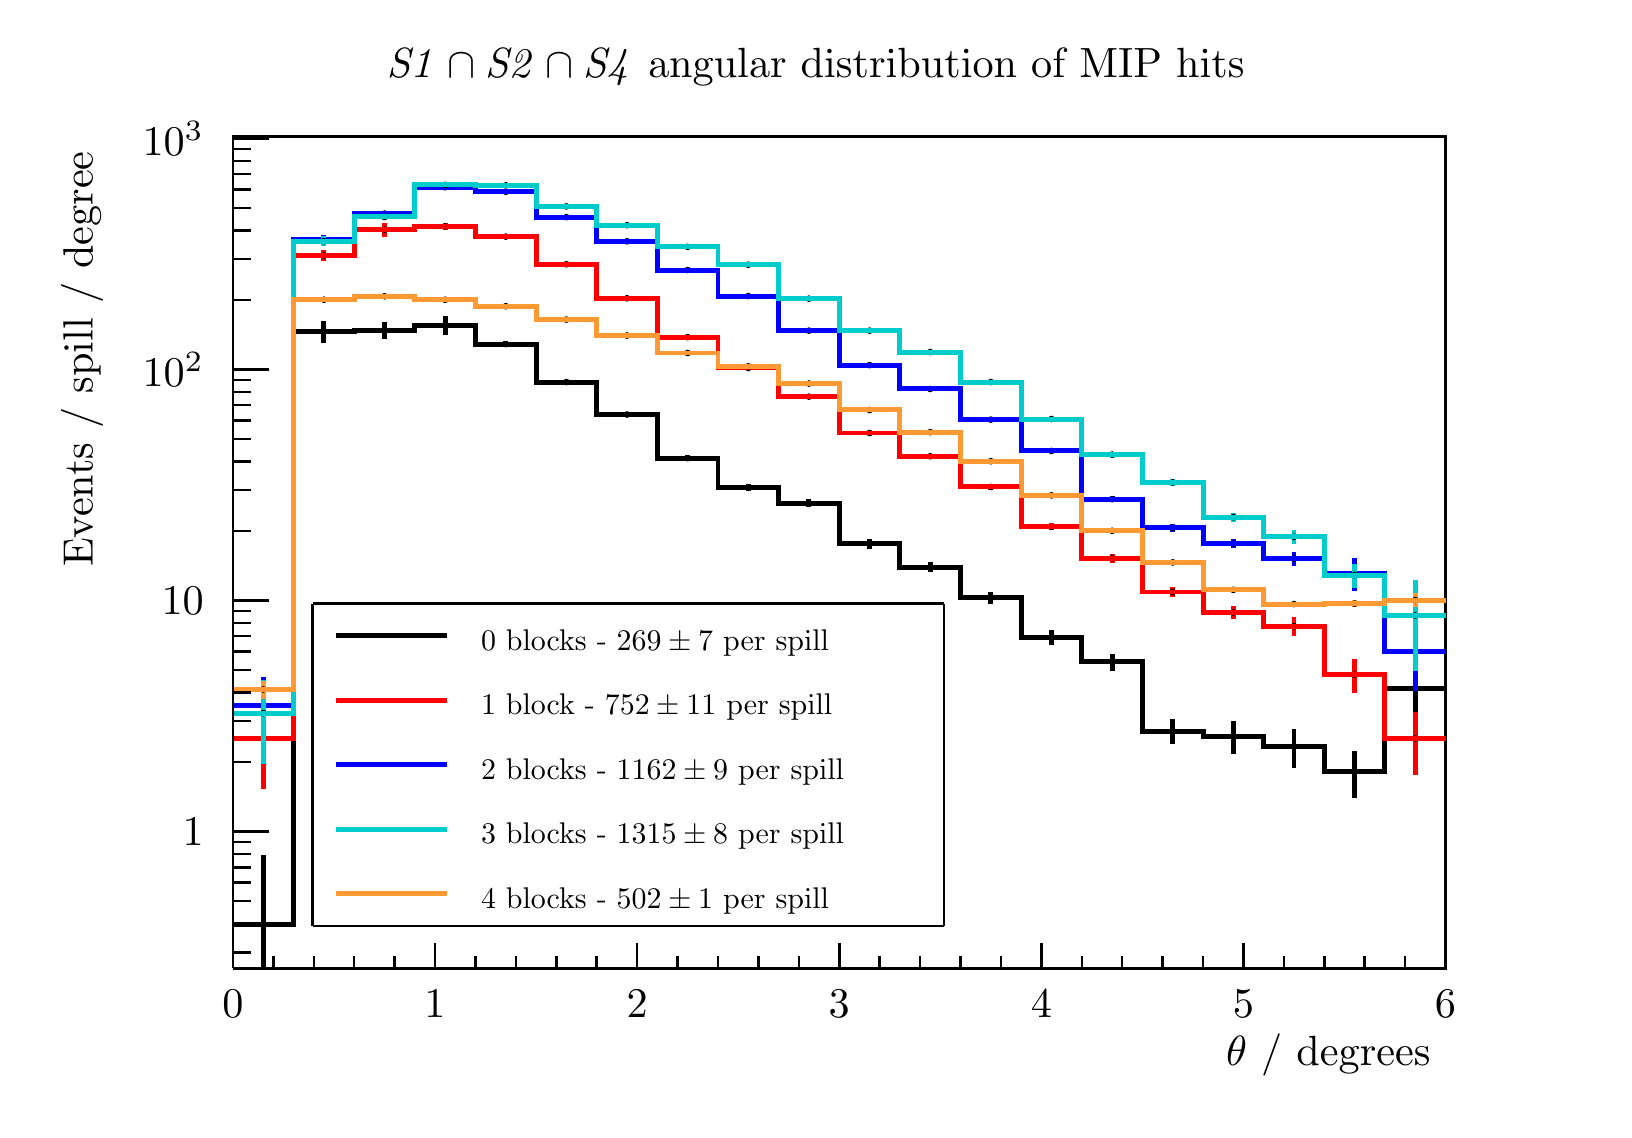
\begin{tikzpicture}
\pgfdeclareplotmark{cross} {
\pgfpathmoveto{\pgfpoint{-0.3\pgfplotmarksize}{\pgfplotmarksize}}
\pgfpathlineto{\pgfpoint{+0.3\pgfplotmarksize}{\pgfplotmarksize}}
\pgfpathlineto{\pgfpoint{+0.3\pgfplotmarksize}{0.3\pgfplotmarksize}}
\pgfpathlineto{\pgfpoint{+1\pgfplotmarksize}{0.3\pgfplotmarksize}}
\pgfpathlineto{\pgfpoint{+1\pgfplotmarksize}{-0.3\pgfplotmarksize}}
\pgfpathlineto{\pgfpoint{+0.3\pgfplotmarksize}{-0.3\pgfplotmarksize}}
\pgfpathlineto{\pgfpoint{+0.3\pgfplotmarksize}{-1.\pgfplotmarksize}}
\pgfpathlineto{\pgfpoint{-0.3\pgfplotmarksize}{-1.\pgfplotmarksize}}
\pgfpathlineto{\pgfpoint{-0.3\pgfplotmarksize}{-0.3\pgfplotmarksize}}
\pgfpathlineto{\pgfpoint{-1.\pgfplotmarksize}{-0.3\pgfplotmarksize}}
\pgfpathlineto{\pgfpoint{-1.\pgfplotmarksize}{0.3\pgfplotmarksize}}
\pgfpathlineto{\pgfpoint{-0.3\pgfplotmarksize}{0.3\pgfplotmarksize}}
\pgfpathclose
\pgfusepathqstroke
}
\pgfdeclareplotmark{cross*} {
\pgfpathmoveto{\pgfpoint{-0.3\pgfplotmarksize}{\pgfplotmarksize}}
\pgfpathlineto{\pgfpoint{+0.3\pgfplotmarksize}{\pgfplotmarksize}}
\pgfpathlineto{\pgfpoint{+0.3\pgfplotmarksize}{0.3\pgfplotmarksize}}
\pgfpathlineto{\pgfpoint{+1\pgfplotmarksize}{0.3\pgfplotmarksize}}
\pgfpathlineto{\pgfpoint{+1\pgfplotmarksize}{-0.3\pgfplotmarksize}}
\pgfpathlineto{\pgfpoint{+0.3\pgfplotmarksize}{-0.3\pgfplotmarksize}}
\pgfpathlineto{\pgfpoint{+0.3\pgfplotmarksize}{-1.\pgfplotmarksize}}
\pgfpathlineto{\pgfpoint{-0.3\pgfplotmarksize}{-1.\pgfplotmarksize}}
\pgfpathlineto{\pgfpoint{-0.3\pgfplotmarksize}{-0.3\pgfplotmarksize}}
\pgfpathlineto{\pgfpoint{-1.\pgfplotmarksize}{-0.3\pgfplotmarksize}}
\pgfpathlineto{\pgfpoint{-1.\pgfplotmarksize}{0.3\pgfplotmarksize}}
\pgfpathlineto{\pgfpoint{-0.3\pgfplotmarksize}{0.3\pgfplotmarksize}}
\pgfpathclose
\pgfusepathqfillstroke
}
\pgfdeclareplotmark{newstar} {
\pgfpathmoveto{\pgfqpoint{0pt}{\pgfplotmarksize}}
\pgfpathlineto{\pgfqpointpolar{44}{0.5\pgfplotmarksize}}
\pgfpathlineto{\pgfqpointpolar{18}{\pgfplotmarksize}}
\pgfpathlineto{\pgfqpointpolar{-20}{0.5\pgfplotmarksize}}
\pgfpathlineto{\pgfqpointpolar{-54}{\pgfplotmarksize}}
\pgfpathlineto{\pgfqpointpolar{-90}{0.5\pgfplotmarksize}}
\pgfpathlineto{\pgfqpointpolar{234}{\pgfplotmarksize}}
\pgfpathlineto{\pgfqpointpolar{198}{0.5\pgfplotmarksize}}
\pgfpathlineto{\pgfqpointpolar{162}{\pgfplotmarksize}}
\pgfpathlineto{\pgfqpointpolar{134}{0.5\pgfplotmarksize}}
\pgfpathclose
\pgfusepathqstroke
}
\pgfdeclareplotmark{newstar*} {
\pgfpathmoveto{\pgfqpoint{0pt}{\pgfplotmarksize}}
\pgfpathlineto{\pgfqpointpolar{44}{0.5\pgfplotmarksize}}
\pgfpathlineto{\pgfqpointpolar{18}{\pgfplotmarksize}}
\pgfpathlineto{\pgfqpointpolar{-20}{0.5\pgfplotmarksize}}
\pgfpathlineto{\pgfqpointpolar{-54}{\pgfplotmarksize}}
\pgfpathlineto{\pgfqpointpolar{-90}{0.5\pgfplotmarksize}}
\pgfpathlineto{\pgfqpointpolar{234}{\pgfplotmarksize}}
\pgfpathlineto{\pgfqpointpolar{198}{0.5\pgfplotmarksize}}
\pgfpathlineto{\pgfqpointpolar{162}{\pgfplotmarksize}}
\pgfpathlineto{\pgfqpointpolar{134}{0.5\pgfplotmarksize}}
\pgfpathclose
\pgfusepathqfillstroke
}
\definecolor{c}{rgb}{1,1,1};
\draw [color=c, fill=c] (0,0) rectangle (20,13.7249);
\draw [color=c, fill=c] (2.6,1.78424) rectangle (18,12.3524);
\definecolor{c}{rgb}{0,0,0};
\draw [c,line width=0.9] (2.6,1.78424) -- (2.6,12.3524) -- (18,12.3524) -- (18,1.78424) -- (2.6,1.78424);
\definecolor{c}{rgb}{1,1,1};
\draw [color=c, fill=c] (2.6,1.78424) rectangle (18,12.3524);
\definecolor{c}{rgb}{0,0,0};
\draw [c,line width=0.9] (2.6,1.78424) -- (2.6,12.3524) -- (18,12.3524) -- (18,1.78424) -- (2.6,1.78424);
\definecolor{c}{rgb}{0,0,0.6};
\draw [c,line width=0.9] (2.6,1.78424) -- (3.37,1.78424) -- (3.37,1.78424) -- (4.14,1.78424) -- (4.14,1.78424) -- (4.91,1.78424) -- (4.91,1.78424) -- (5.68,1.78424) -- (5.68,1.78424) -- (6.45,1.78424) -- (6.45,1.78424) -- (7.22,1.78424) --
 (7.22,1.78424) -- (7.99,1.78424) -- (7.99,1.78424) -- (8.76,1.78424) -- (8.76,1.78424) -- (9.53,1.78424) -- (9.53,1.78424) -- (10.3,1.78424) -- (10.3,1.78424) -- (11.07,1.78424) -- (11.07,1.78424) -- (11.84,1.78424) -- (11.84,1.78424) --
 (12.61,1.78424) -- (12.61,1.78424) -- (13.38,1.78424) -- (13.38,1.78424) -- (14.15,1.78424) -- (14.15,1.78424) -- (14.92,1.78424) -- (14.92,1.78424) -- (15.69,1.78424) -- (15.69,1.78424) -- (16.46,1.78424) -- (16.46,1.78424) -- (17.23,1.78424) --
 (17.23,1.78424) -- (18,1.78424);
\definecolor{c}{rgb}{0,0,0};
\draw [c,line width=0.9] (2.6,1.78424) -- (18,1.78424);
\draw [c,line width=0.9] (2.6,2.10129) -- (2.6,1.78424);
\draw [c,line width=0.9] (3.11333,1.94276) -- (3.11333,1.78424);
\draw [c,line width=0.9] (3.62667,1.94276) -- (3.62667,1.78424);
\draw [c,line width=0.9] (4.14,1.94276) -- (4.14,1.78424);
\draw [c,line width=0.9] (4.65333,1.94276) -- (4.65333,1.78424);
\draw [c,line width=0.9] (5.16667,2.10129) -- (5.16667,1.78424);
\draw [c,line width=0.9] (5.68,1.94276) -- (5.68,1.78424);
\draw [c,line width=0.9] (6.19333,1.94276) -- (6.19333,1.78424);
\draw [c,line width=0.9] (6.70667,1.94276) -- (6.70667,1.78424);
\draw [c,line width=0.9] (7.22,1.94276) -- (7.22,1.78424);
\draw [c,line width=0.9] (7.73333,2.10129) -- (7.73333,1.78424);
\draw [c,line width=0.9] (8.24667,1.94276) -- (8.24667,1.78424);
\draw [c,line width=0.9] (8.76,1.94276) -- (8.76,1.78424);
\draw [c,line width=0.9] (9.27333,1.94276) -- (9.27333,1.78424);
\draw [c,line width=0.9] (9.78667,1.94276) -- (9.78667,1.78424);
\draw [c,line width=0.9] (10.3,2.10129) -- (10.3,1.78424);
\draw [c,line width=0.9] (10.8133,1.94276) -- (10.8133,1.78424);
\draw [c,line width=0.9] (11.3267,1.94276) -- (11.3267,1.78424);
\draw [c,line width=0.9] (11.84,1.94276) -- (11.84,1.78424);
\draw [c,line width=0.9] (12.3533,1.94276) -- (12.3533,1.78424);
\draw [c,line width=0.9] (12.8667,2.10129) -- (12.8667,1.78424);
\draw [c,line width=0.9] (13.38,1.94276) -- (13.38,1.78424);
\draw [c,line width=0.9] (13.8933,1.94276) -- (13.8933,1.78424);
\draw [c,line width=0.9] (14.4067,1.94276) -- (14.4067,1.78424);
\draw [c,line width=0.9] (14.92,1.94276) -- (14.92,1.78424);
\draw [c,line width=0.9] (15.4333,2.10129) -- (15.4333,1.78424);
\draw [c,line width=0.9] (15.9467,1.94276) -- (15.9467,1.78424);
\draw [c,line width=0.9] (16.46,1.94276) -- (16.46,1.78424);
\draw [c,line width=0.9] (16.9733,1.94276) -- (16.9733,1.78424);
\draw [c,line width=0.9] (17.4867,1.94276) -- (17.4867,1.78424);
\draw [c,line width=0.9] (18,2.10129) -- (18,1.78424);
\draw [anchor=base] (2.6,1.16662) node[scale=1.52731, color=c, rotate=0]{0};
\draw [anchor=base] (5.16667,1.16662) node[scale=1.52731, color=c, rotate=0]{1};
\draw [anchor=base] (7.73333,1.16662) node[scale=1.52731, color=c, rotate=0]{2};
\draw [anchor=base] (10.3,1.16662) node[scale=1.52731, color=c, rotate=0]{3};
\draw [anchor=base] (12.8667,1.16662) node[scale=1.52731, color=c, rotate=0]{4};
\draw [anchor=base] (15.4333,1.16662) node[scale=1.52731, color=c, rotate=0]{5};
\draw [anchor=base] (18,1.16662) node[scale=1.52731, color=c, rotate=0]{6};
\draw [anchor= east] (18,0.686246) node[scale=1.52731, color=c, rotate=0]{$ \theta$ / degrees};
\draw [c,line width=0.9] (2.6,1.78424) -- (2.6,12.3524);
\draw [c,line width=0.9] (2.831,1.98949) -- (2.6,1.98949);
\draw [c,line width=0.9] (2.831,2.35605) -- (2.6,2.35605);
\draw [c,line width=0.9] (2.831,2.64038) -- (2.6,2.64038);
\draw [c,line width=0.9] (2.831,2.87269) -- (2.6,2.87269);
\draw [c,line width=0.9] (2.831,3.06911) -- (2.6,3.06911);
\draw [c,line width=0.9] (2.831,3.23925) -- (2.6,3.23925);
\draw [c,line width=0.9] (2.831,3.38933) -- (2.6,3.38933);
\draw [c,line width=0.9] (3.062,3.52358) -- (2.6,3.52358);
\draw [anchor= east] (2.42,3.52358) node[scale=1.52731, color=c, rotate=0]{1};
\draw [c,line width=0.9] (2.831,4.40678) -- (2.6,4.40678);
\draw [c,line width=0.9] (2.831,4.92342) -- (2.6,4.92342);
\draw [c,line width=0.9] (2.831,5.28998) -- (2.6,5.28998);
\draw [c,line width=0.9] (2.831,5.57431) -- (2.6,5.57431);
\draw [c,line width=0.9] (2.831,5.80662) -- (2.6,5.80662);
\draw [c,line width=0.9] (2.831,6.00304) -- (2.6,6.00304);
\draw [c,line width=0.9] (2.831,6.17318) -- (2.6,6.17318);
\draw [c,line width=0.9] (2.831,6.32326) -- (2.6,6.32326);
\draw [c,line width=0.9] (3.062,6.45751) -- (2.6,6.45751);
\draw [anchor= east] (2.42,6.45751) node[scale=1.52731, color=c, rotate=0]{10};
\draw [c,line width=0.9] (2.831,7.34071) -- (2.6,7.34071);
\draw [c,line width=0.9] (2.831,7.85735) -- (2.6,7.85735);
\draw [c,line width=0.9] (2.831,8.22391) -- (2.6,8.22391);
\draw [c,line width=0.9] (2.831,8.50824) -- (2.6,8.50824);
\draw [c,line width=0.9] (2.831,8.74055) -- (2.6,8.74055);
\draw [c,line width=0.9] (2.831,8.93697) -- (2.6,8.93697);
\draw [c,line width=0.9] (2.831,9.10711) -- (2.6,9.10711);
\draw [c,line width=0.9] (2.831,9.25719) -- (2.6,9.25719);
\draw [c,line width=0.9] (3.062,9.39144) -- (2.6,9.39144);
\draw [anchor= east] (2.42,9.39144) node[scale=1.52731, color=c, rotate=0]{$10^{2}$};
\draw [c,line width=0.9] (2.831,10.2746) -- (2.6,10.2746);
\draw [c,line width=0.9] (2.831,10.7913) -- (2.6,10.7913);
\draw [c,line width=0.9] (2.831,11.1578) -- (2.6,11.1578);
\draw [c,line width=0.9] (2.831,11.4422) -- (2.6,11.4422);
\draw [c,line width=0.9] (2.831,11.6745) -- (2.6,11.6745);
\draw [c,line width=0.9] (2.831,11.8709) -- (2.6,11.8709);
\draw [c,line width=0.9] (2.831,12.041) -- (2.6,12.041);
\draw [c,line width=0.9] (2.831,12.1911) -- (2.6,12.1911);
\draw [c,line width=0.9] (3.062,12.3254) -- (2.6,12.3254);
\draw [anchor= east] (2.42,12.3254) node[scale=1.52731, color=c, rotate=0]{$10^{3}$};
\draw [anchor= east] (0.683095,12.3524) node[scale=1.52731, color=c, rotate=90]{ Events / spill / degree};
\draw [c,line width=1.8] (2.985,1.78424) -- (2.985,2.34153);
\draw [c,line width=1.8] (2.985,2.34153) -- (2.985,3.22749);
\foreach \P in {(2.985,2.34153)}{\draw[mark options={color=c,fill=c},mark size=2.402402pt,mark=*,mark size=1pt] plot coordinates {\P};}
\draw [c,line width=1.8] (3.755,9.73343) -- (3.755,9.8787);
\draw [c,line width=1.8] (3.755,9.8787) -- (3.755,10.0091);
\foreach \P in {(3.755,9.8787)}{\draw[mark options={color=c,fill=c},mark size=2.402402pt,mark=*,mark size=1pt] plot coordinates {\P};}
\draw [c,line width=1.8] (4.525,9.7762) -- (4.525,9.88687);
\draw [c,line width=1.8] (4.525,9.88687) -- (4.525,9.98869);
\foreach \P in {(4.525,9.88687)}{\draw[mark options={color=c,fill=c},mark size=2.402402pt,mark=*,mark size=1pt] plot coordinates {\P};}
\draw [c,line width=1.8] (5.295,9.82881) -- (5.295,9.95409);
\draw [c,line width=1.8] (5.295,9.95409) -- (5.295,10.0681);
\foreach \P in {(5.295,9.95409)}{\draw[mark options={color=c,fill=c},mark size=2.402402pt,mark=*,mark size=1pt] plot coordinates {\P};}
\draw [c,line width=1.8] (6.065,9.67782) -- (6.065,9.71317);
\draw [c,line width=1.8] (6.065,9.71317) -- (6.065,9.74756);
\foreach \P in {(6.065,9.71317)}{\draw[mark options={color=c,fill=c},mark size=2.402402pt,mark=*,mark size=1pt] plot coordinates {\P};}
\draw [c,line width=1.8] (6.835,9.19869) -- (6.835,9.23103);
\draw [c,line width=1.8] (6.835,9.23103) -- (6.835,9.26256);
\foreach \P in {(6.835,9.23103)}{\draw[mark options={color=c,fill=c},mark size=2.402402pt,mark=*,mark size=1pt] plot coordinates {\P};}
\draw [c,line width=1.8] (7.605,8.78432) -- (7.605,8.81859);
\draw [c,line width=1.8] (7.605,8.81859) -- (7.605,8.85196);
\foreach \P in {(7.605,8.81859)}{\draw[mark options={color=c,fill=c},mark size=2.402402pt,mark=*,mark size=1pt] plot coordinates {\P};}
\draw [c,line width=1.8] (8.375,8.22429) -- (8.375,8.26496);
\draw [c,line width=1.8] (8.375,8.26496) -- (8.375,8.30436);
\foreach \P in {(8.375,8.26496)}{\draw[mark options={color=c,fill=c},mark size=2.402402pt,mark=*,mark size=1pt] plot coordinates {\P};}
\draw [c,line width=1.8] (9.145,7.84222) -- (9.145,7.88855);
\draw [c,line width=1.8] (9.145,7.88855) -- (9.145,7.93326);
\foreach \P in {(9.145,7.88855)}{\draw[mark options={color=c,fill=c},mark size=2.402402pt,mark=*,mark size=1pt] plot coordinates {\P};}
\draw [c,line width=1.8] (9.915,7.64411) -- (9.915,7.69365);
\draw [c,line width=1.8] (9.915,7.69365) -- (9.915,7.74133);
\foreach \P in {(9.915,7.69365)}{\draw[mark options={color=c,fill=c},mark size=2.402402pt,mark=*,mark size=1pt] plot coordinates {\P};}
\draw [c,line width=1.8] (10.685,7.11687) -- (10.685,7.17797);
\draw [c,line width=1.8] (10.685,7.17797) -- (10.685,7.23626);
\foreach \P in {(10.685,7.17797)}{\draw[mark options={color=c,fill=c},mark size=2.402402pt,mark=*,mark size=1pt] plot coordinates {\P};}
\draw [c,line width=1.8] (11.455,6.81446) -- (11.455,6.88113);
\draw [c,line width=1.8] (11.455,6.88113) -- (11.455,6.94449);
\foreach \P in {(11.455,6.88113)}{\draw[mark options={color=c,fill=c},mark size=2.402402pt,mark=*,mark size=1pt] plot coordinates {\P};}
\draw [c,line width=1.8] (12.225,6.41042) -- (12.225,6.48936);
\draw [c,line width=1.8] (12.225,6.48936) -- (12.225,6.5637);
\foreach \P in {(12.225,6.48936)}{\draw[mark options={color=c,fill=c},mark size=2.402402pt,mark=*,mark size=1pt] plot coordinates {\P};}
\draw [c,line width=1.8] (12.995,5.89235) -- (12.995,5.98953);
\draw [c,line width=1.8] (12.995,5.98953) -- (12.995,6.07983);
\foreach \P in {(12.995,5.98953)}{\draw[mark options={color=c,fill=c},mark size=2.402402pt,mark=*,mark size=1pt] plot coordinates {\P};}
\draw [c,line width=1.8] (13.765,5.56498) -- (13.765,5.67796);
\draw [c,line width=1.8] (13.765,5.67796) -- (13.765,5.78173);
\foreach \P in {(13.765,5.67796)}{\draw[mark options={color=c,fill=c},mark size=2.402402pt,mark=*,mark size=1pt] plot coordinates {\P};}
\draw [c,line width=1.8] (14.535,4.63213) -- (14.535,4.79858);
\draw [c,line width=1.8] (14.535,4.79858) -- (14.535,4.94578);
\foreach \P in {(14.535,4.79858)}{\draw[mark options={color=c,fill=c},mark size=2.402402pt,mark=*,mark size=1pt] plot coordinates {\P};}
\draw [c,line width=1.8] (15.305,4.50141) -- (15.305,4.73201);
\draw [c,line width=1.8] (15.305,4.73201) -- (15.305,4.9272);
\foreach \P in {(15.305,4.73201)}{\draw[mark options={color=c,fill=c},mark size=2.402402pt,mark=*,mark size=1pt] plot coordinates {\P};}
\draw [c,line width=1.8] (16.075,4.33584) -- (16.075,4.60575);
\draw [c,line width=1.8] (16.075,4.60575) -- (16.075,4.82836);
\foreach \P in {(16.075,4.60575)}{\draw[mark options={color=c,fill=c},mark size=2.402402pt,mark=*,mark size=1pt] plot coordinates {\P};}
\draw [c,line width=1.8] (16.845,3.94886) -- (16.845,4.2854);
\draw [c,line width=1.8] (16.845,4.2854) -- (16.845,4.55137);
\foreach \P in {(16.845,4.2854)}{\draw[mark options={color=c,fill=c},mark size=2.402402pt,mark=*,mark size=1pt] plot coordinates {\P};}
\draw [c,line width=1.8] (17.615,4.4306) -- (17.615,5.33657);
\draw [c,line width=1.8] (17.615,5.33657) -- (17.615,5.86071);
\foreach \P in {(17.615,5.33657)}{\draw[mark options={color=c,fill=c},mark size=2.402402pt,mark=*,mark size=1pt] plot coordinates {\P};}
\draw [c,line width=1.8] (2.6,2.34153) -- (3.37,2.34153) -- (3.37,9.8787) -- (4.14,9.8787) -- (4.14,9.88687) -- (4.91,9.88687) -- (4.91,9.95409) -- (5.68,9.95409) -- (5.68,9.71317) -- (6.45,9.71317) -- (6.45,9.23103) -- (7.22,9.23103) --
 (7.22,8.81859) -- (7.99,8.81859) -- (7.99,8.26496) -- (8.76,8.26496) -- (8.76,7.88855) -- (9.53,7.88855) -- (9.53,7.69365) -- (10.3,7.69365) -- (10.3,7.17797) -- (11.07,7.17797) -- (11.07,6.88113) -- (11.84,6.88113) -- (11.84,6.48936) --
 (12.61,6.48936) -- (12.61,5.98953) -- (13.38,5.98953) -- (13.38,5.67796) -- (14.15,5.67796) -- (14.15,4.79858) -- (14.92,4.79858) -- (14.92,4.73201) -- (15.69,4.73201) -- (15.69,4.60575) -- (16.46,4.60575) -- (16.46,4.2854) -- (17.23,4.2854) --
 (17.23,5.33657) -- (18,5.33657);
\definecolor{c}{rgb}{1,0,0};
\draw [c,line width=1.8] (2.985,4.06376) -- (2.985,4.70305);
\draw [c,line width=1.8] (2.985,4.70305) -- (2.985,5.12677);
\definecolor{c}{rgb}{0,0,0};
\foreach \P in {(2.985,4.70305)}{\draw[mark options={color=c,fill=c},mark size=2.402402pt,mark=*,mark size=1pt] plot coordinates {\P};}
\definecolor{c}{rgb}{1,0,0};
\draw [c,line width=1.8] (3.755,10.7639) -- (3.755,10.838);
\draw [c,line width=1.8] (3.755,10.838) -- (3.755,10.908);
\definecolor{c}{rgb}{0,0,0};
\foreach \P in {(3.755,10.838)}{\draw[mark options={color=c,fill=c},mark size=2.402402pt,mark=*,mark size=1pt] plot coordinates {\P};}
\definecolor{c}{rgb}{1,0,0};
\draw [c,line width=1.8] (4.525,11.0712) -- (4.525,11.1675);
\draw [c,line width=1.8] (4.525,11.1675) -- (4.525,11.2571);
\definecolor{c}{rgb}{0,0,0};
\foreach \P in {(4.525,11.1675)}{\draw[mark options={color=c,fill=c},mark size=2.402402pt,mark=*,mark size=1pt] plot coordinates {\P};}
\definecolor{c}{rgb}{1,0,0};
\draw [c,line width=1.8] (5.295,11.1634) -- (5.295,11.2076);
\draw [c,line width=1.8] (5.295,11.2076) -- (5.295,11.2503);
\definecolor{c}{rgb}{0,0,0};
\foreach \P in {(5.295,11.2076)}{\draw[mark options={color=c,fill=c},mark size=2.402402pt,mark=*,mark size=1pt] plot coordinates {\P};}
\definecolor{c}{rgb}{1,0,0};
\draw [c,line width=1.8] (6.065,11.0602) -- (6.065,11.0782);
\draw [c,line width=1.8] (6.065,11.0782) -- (6.065,11.0961);
\definecolor{c}{rgb}{0,0,0};
\foreach \P in {(6.065,11.0782)}{\draw[mark options={color=c,fill=c},mark size=2.402402pt,mark=*,mark size=1pt] plot coordinates {\P};}
\definecolor{c}{rgb}{1,0,0};
\draw [c,line width=1.8] (6.835,10.7127) -- (6.835,10.7275);
\draw [c,line width=1.8] (6.835,10.7275) -- (6.835,10.7422);
\definecolor{c}{rgb}{0,0,0};
\foreach \P in {(6.835,10.7275)}{\draw[mark options={color=c,fill=c},mark size=2.402402pt,mark=*,mark size=1pt] plot coordinates {\P};}
\definecolor{c}{rgb}{1,0,0};
\draw [c,line width=1.8] (7.605,10.2794) -- (7.605,10.2952);
\draw [c,line width=1.8] (7.605,10.2952) -- (7.605,10.3107);
\definecolor{c}{rgb}{0,0,0};
\foreach \P in {(7.605,10.2952)}{\draw[mark options={color=c,fill=c},mark size=2.402402pt,mark=*,mark size=1pt] plot coordinates {\P};}
\definecolor{c}{rgb}{1,0,0};
\draw [c,line width=1.8] (8.375,9.78304) -- (8.375,9.80126);
\draw [c,line width=1.8] (8.375,9.80126) -- (8.375,9.81923);
\definecolor{c}{rgb}{0,0,0};
\foreach \P in {(8.375,9.80126)}{\draw[mark options={color=c,fill=c},mark size=2.402402pt,mark=*,mark size=1pt] plot coordinates {\P};}
\definecolor{c}{rgb}{1,0,0};
\draw [c,line width=1.8] (9.145,9.38908) -- (9.145,9.40994);
\draw [c,line width=1.8] (9.145,9.40994) -- (9.145,9.43047);
\definecolor{c}{rgb}{0,0,0};
\foreach \P in {(9.145,9.40994)}{\draw[mark options={color=c,fill=c},mark size=2.402402pt,mark=*,mark size=1pt] plot coordinates {\P};}
\definecolor{c}{rgb}{1,0,0};
\draw [c,line width=1.8] (9.915,9.02259) -- (9.915,9.04587);
\draw [c,line width=1.8] (9.915,9.04587) -- (9.915,9.06873);
\definecolor{c}{rgb}{0,0,0};
\foreach \P in {(9.915,9.04587)}{\draw[mark options={color=c,fill=c},mark size=2.402402pt,mark=*,mark size=1pt] plot coordinates {\P};}
\definecolor{c}{rgb}{1,0,0};
\draw [c,line width=1.8] (10.685,8.55614) -- (10.685,8.58413);
\draw [c,line width=1.8] (10.685,8.58413) -- (10.685,8.61152);
\definecolor{c}{rgb}{0,0,0};
\foreach \P in {(10.685,8.58413)}{\draw[mark options={color=c,fill=c},mark size=2.402402pt,mark=*,mark size=1pt] plot coordinates {\P};}
\definecolor{c}{rgb}{1,0,0};
\draw [c,line width=1.8] (11.455,8.25818) -- (11.455,8.28901);
\draw [c,line width=1.8] (11.455,8.28901) -- (11.455,8.31912);
\definecolor{c}{rgb}{0,0,0};
\foreach \P in {(11.455,8.28901)}{\draw[mark options={color=c,fill=c},mark size=2.402402pt,mark=*,mark size=1pt] plot coordinates {\P};}
\definecolor{c}{rgb}{1,0,0};
\draw [c,line width=1.8] (12.225,7.86257) -- (12.225,7.89874);
\draw [c,line width=1.8] (12.225,7.89874) -- (12.225,7.93391);
\definecolor{c}{rgb}{0,0,0};
\foreach \P in {(12.225,7.89874)}{\draw[mark options={color=c,fill=c},mark size=2.402402pt,mark=*,mark size=1pt] plot coordinates {\P};}
\definecolor{c}{rgb}{1,0,0};
\draw [c,line width=1.8] (12.995,7.34742) -- (12.995,7.39241);
\draw [c,line width=1.8] (12.995,7.39241) -- (12.995,7.43587);
\definecolor{c}{rgb}{0,0,0};
\foreach \P in {(12.995,7.39241)}{\draw[mark options={color=c,fill=c},mark size=2.402402pt,mark=*,mark size=1pt] plot coordinates {\P};}
\definecolor{c}{rgb}{1,0,0};
\draw [c,line width=1.8] (13.765,6.93942) -- (13.765,6.99356);
\draw [c,line width=1.8] (13.765,6.99356) -- (13.765,7.0455);
\definecolor{c}{rgb}{0,0,0};
\foreach \P in {(13.765,6.99356)}{\draw[mark options={color=c,fill=c},mark size=2.402402pt,mark=*,mark size=1pt] plot coordinates {\P};}
\definecolor{c}{rgb}{1,0,0};
\draw [c,line width=1.8] (14.535,6.49722) -- (14.535,6.56484);
\draw [c,line width=1.8] (14.535,6.56484) -- (14.535,6.62905);
\definecolor{c}{rgb}{0,0,0};
\foreach \P in {(14.535,6.56484)}{\draw[mark options={color=c,fill=c},mark size=2.402402pt,mark=*,mark size=1pt] plot coordinates {\P};}
\definecolor{c}{rgb}{1,0,0};
\draw [c,line width=1.8] (15.305,6.21809) -- (15.305,6.30456);
\draw [c,line width=1.8] (15.305,6.30456) -- (15.305,6.38553);
\definecolor{c}{rgb}{0,0,0};
\foreach \P in {(15.305,6.30456)}{\draw[mark options={color=c,fill=c},mark size=2.402402pt,mark=*,mark size=1pt] plot coordinates {\P};}
\definecolor{c}{rgb}{1,0,0};
\draw [c,line width=1.8] (16.075,6.00288) -- (16.075,6.13092);
\draw [c,line width=1.8] (16.075,6.13092) -- (16.075,6.24725);
\definecolor{c}{rgb}{0,0,0};
\foreach \P in {(16.075,6.13092)}{\draw[mark options={color=c,fill=c},mark size=2.402402pt,mark=*,mark size=1pt] plot coordinates {\P};}
\definecolor{c}{rgb}{1,0,0};
\draw [c,line width=1.8] (16.845,5.27864) -- (16.845,5.51529);
\draw [c,line width=1.8] (16.845,5.51529) -- (16.845,5.71479);
\definecolor{c}{rgb}{0,0,0};
\foreach \P in {(16.845,5.51529)}{\draw[mark options={color=c,fill=c},mark size=2.402402pt,mark=*,mark size=1pt] plot coordinates {\P};}
\definecolor{c}{rgb}{1,0,0};
\draw [c,line width=1.8] (17.615,4.23968) -- (17.615,4.70395);
\draw [c,line width=1.8] (17.615,4.70395) -- (17.615,5.04349);
\definecolor{c}{rgb}{0,0,0};
\foreach \P in {(17.615,4.70395)}{\draw[mark options={color=c,fill=c},mark size=2.402402pt,mark=*,mark size=1pt] plot coordinates {\P};}
\definecolor{c}{rgb}{1,0,0};
\draw [c,line width=1.8] (2.6,4.70305) -- (3.37,4.70305) -- (3.37,10.838) -- (4.14,10.838) -- (4.14,11.1675) -- (4.91,11.1675) -- (4.91,11.2076) -- (5.68,11.2076) -- (5.68,11.0782) -- (6.45,11.0782) -- (6.45,10.7275) -- (7.22,10.7275) --
 (7.22,10.2952) -- (7.99,10.2952) -- (7.99,9.80126) -- (8.76,9.80126) -- (8.76,9.40994) -- (9.53,9.40994) -- (9.53,9.04587) -- (10.3,9.04587) -- (10.3,8.58413) -- (11.07,8.58413) -- (11.07,8.28901) -- (11.84,8.28901) -- (11.84,7.89874) --
 (12.61,7.89874) -- (12.61,7.39241) -- (13.38,7.39241) -- (13.38,6.99356) -- (14.15,6.99356) -- (14.15,6.56484) -- (14.92,6.56484) -- (14.92,6.30456) -- (15.69,6.30456) -- (15.69,6.13092) -- (16.46,6.13092) -- (16.46,5.51529) -- (17.23,5.51529) --
 (17.23,4.70395) -- (18,4.70395);
\definecolor{c}{rgb}{0,0,1};
\draw [c,line width=1.8] (2.985,4.59774) -- (2.985,5.11806);
\draw [c,line width=1.8] (2.985,5.11806) -- (2.985,5.48645);
\definecolor{c}{rgb}{0,0,0};
\foreach \P in {(2.985,5.11806)}{\draw[mark options={color=c,fill=c},mark size=2.402402pt,mark=*,mark size=1pt] plot coordinates {\P};}
\definecolor{c}{rgb}{0,0,1};
\draw [c,line width=1.8] (3.755,10.9783) -- (3.755,11.0419);
\draw [c,line width=1.8] (3.755,11.0419) -- (3.755,11.1025);
\definecolor{c}{rgb}{0,0,0};
\foreach \P in {(3.755,11.0419)}{\draw[mark options={color=c,fill=c},mark size=2.402402pt,mark=*,mark size=1pt] plot coordinates {\P};}
\definecolor{c}{rgb}{0,0,1};
\draw [c,line width=1.8] (4.525,11.3392) -- (4.525,11.3706);
\draw [c,line width=1.8] (4.525,11.3706) -- (4.525,11.4012);
\definecolor{c}{rgb}{0,0,0};
\foreach \P in {(4.525,11.3706)}{\draw[mark options={color=c,fill=c},mark size=2.402402pt,mark=*,mark size=1pt] plot coordinates {\P};}
\definecolor{c}{rgb}{0,0,1};
\draw [c,line width=1.8] (5.295,11.6648) -- (5.295,11.7055);
\draw [c,line width=1.8] (5.295,11.7055) -- (5.295,11.7448);
\definecolor{c}{rgb}{0,0,0};
\foreach \P in {(5.295,11.7055)}{\draw[mark options={color=c,fill=c},mark size=2.402402pt,mark=*,mark size=1pt] plot coordinates {\P};}
\definecolor{c}{rgb}{0,0,1};
\draw [c,line width=1.8] (6.065,11.6291) -- (6.065,11.6474);
\draw [c,line width=1.8] (6.065,11.6474) -- (6.065,11.6654);
\definecolor{c}{rgb}{0,0,0};
\foreach \P in {(6.065,11.6474)}{\draw[mark options={color=c,fill=c},mark size=2.402402pt,mark=*,mark size=1pt] plot coordinates {\P};}
\definecolor{c}{rgb}{0,0,1};
\draw [c,line width=1.8] (6.835,11.3137) -- (6.835,11.3257);
\draw [c,line width=1.8] (6.835,11.3257) -- (6.835,11.3376);
\definecolor{c}{rgb}{0,0,0};
\foreach \P in {(6.835,11.3257)}{\draw[mark options={color=c,fill=c},mark size=2.402402pt,mark=*,mark size=1pt] plot coordinates {\P};}
\definecolor{c}{rgb}{0,0,1};
\draw [c,line width=1.8] (7.605,11.0067) -- (7.605,11.0189);
\draw [c,line width=1.8] (7.605,11.0189) -- (7.605,11.0309);
\definecolor{c}{rgb}{0,0,0};
\foreach \P in {(7.605,11.0189)}{\draw[mark options={color=c,fill=c},mark size=2.402402pt,mark=*,mark size=1pt] plot coordinates {\P};}
\definecolor{c}{rgb}{0,0,1};
\draw [c,line width=1.8] (8.375,10.64) -- (8.375,10.6536);
\draw [c,line width=1.8] (8.375,10.6536) -- (8.375,10.667);
\definecolor{c}{rgb}{0,0,0};
\foreach \P in {(8.375,10.6536)}{\draw[mark options={color=c,fill=c},mark size=2.402402pt,mark=*,mark size=1pt] plot coordinates {\P};}
\definecolor{c}{rgb}{0,0,1};
\draw [c,line width=1.8] (9.145,10.3081) -- (9.145,10.323);
\draw [c,line width=1.8] (9.145,10.323) -- (9.145,10.3377);
\definecolor{c}{rgb}{0,0,0};
\foreach \P in {(9.145,10.323)}{\draw[mark options={color=c,fill=c},mark size=2.402402pt,mark=*,mark size=1pt] plot coordinates {\P};}
\definecolor{c}{rgb}{0,0,1};
\draw [c,line width=1.8] (9.915,9.86709) -- (9.915,9.88419);
\draw [c,line width=1.8] (9.915,9.88419) -- (9.915,9.90106);
\definecolor{c}{rgb}{0,0,0};
\foreach \P in {(9.915,9.88419)}{\draw[mark options={color=c,fill=c},mark size=2.402402pt,mark=*,mark size=1pt] plot coordinates {\P};}
\definecolor{c}{rgb}{0,0,1};
\draw [c,line width=1.8] (10.685,9.42596) -- (10.685,9.44624);
\draw [c,line width=1.8] (10.685,9.44624) -- (10.685,9.4662);
\definecolor{c}{rgb}{0,0,0};
\foreach \P in {(10.685,9.44624)}{\draw[mark options={color=c,fill=c},mark size=2.402402pt,mark=*,mark size=1pt] plot coordinates {\P};}
\definecolor{c}{rgb}{0,0,1};
\draw [c,line width=1.8] (11.455,9.12109) -- (11.455,9.14351);
\draw [c,line width=1.8] (11.455,9.14351) -- (11.455,9.16555);
\definecolor{c}{rgb}{0,0,0};
\foreach \P in {(11.455,9.14351)}{\draw[mark options={color=c,fill=c},mark size=2.402402pt,mark=*,mark size=1pt] plot coordinates {\P};}
\definecolor{c}{rgb}{0,0,1};
\draw [c,line width=1.8] (12.225,8.72759) -- (12.225,8.75407);
\draw [c,line width=1.8] (12.225,8.75407) -- (12.225,8.78001);
\definecolor{c}{rgb}{0,0,0};
\foreach \P in {(12.225,8.75407)}{\draw[mark options={color=c,fill=c},mark size=2.402402pt,mark=*,mark size=1pt] plot coordinates {\P};}
\definecolor{c}{rgb}{0,0,1};
\draw [c,line width=1.8] (12.995,8.32464) -- (12.995,8.35617);
\draw [c,line width=1.8] (12.995,8.35617) -- (12.995,8.38695);
\definecolor{c}{rgb}{0,0,0};
\foreach \P in {(12.995,8.35617)}{\draw[mark options={color=c,fill=c},mark size=2.402402pt,mark=*,mark size=1pt] plot coordinates {\P};}
\definecolor{c}{rgb}{0,0,1};
\draw [c,line width=1.8] (13.765,7.70312) -- (13.765,7.74358);
\draw [c,line width=1.8] (13.765,7.74358) -- (13.765,7.7828);
\definecolor{c}{rgb}{0,0,0};
\foreach \P in {(13.765,7.74358)}{\draw[mark options={color=c,fill=c},mark size=2.402402pt,mark=*,mark size=1pt] plot coordinates {\P};}
\definecolor{c}{rgb}{0,0,1};
\draw [c,line width=1.8] (14.535,7.32878) -- (14.535,7.37811);
\draw [c,line width=1.8] (14.535,7.37811) -- (14.535,7.4256);
\definecolor{c}{rgb}{0,0,0};
\foreach \P in {(14.535,7.37811)}{\draw[mark options={color=c,fill=c},mark size=2.402402pt,mark=*,mark size=1pt] plot coordinates {\P};}
\definecolor{c}{rgb}{0,0,1};
\draw [c,line width=1.8] (15.305,7.11804) -- (15.305,7.18071);
\draw [c,line width=1.8] (15.305,7.18071) -- (15.305,7.24043);
\definecolor{c}{rgb}{0,0,0};
\foreach \P in {(15.305,7.18071)}{\draw[mark options={color=c,fill=c},mark size=2.402402pt,mark=*,mark size=1pt] plot coordinates {\P};}
\definecolor{c}{rgb}{0,0,1};
\draw [c,line width=1.8] (16.075,6.89529) -- (16.075,6.98725);
\draw [c,line width=1.8] (16.075,6.98725) -- (16.075,7.07302);
\definecolor{c}{rgb}{0,0,0};
\foreach \P in {(16.075,6.98725)}{\draw[mark options={color=c,fill=c},mark size=2.402402pt,mark=*,mark size=1pt] plot coordinates {\P};}
\definecolor{c}{rgb}{0,0,1};
\draw [c,line width=1.8] (16.845,6.57186) -- (16.845,6.80269);
\draw [c,line width=1.8] (16.845,6.80269) -- (16.845,6.99804);
\definecolor{c}{rgb}{0,0,0};
\foreach \P in {(16.845,6.80269)}{\draw[mark options={color=c,fill=c},mark size=2.402402pt,mark=*,mark size=1pt] plot coordinates {\P};}
\definecolor{c}{rgb}{0,0,1};
\draw [c,line width=1.8] (17.615,5.31365) -- (17.615,5.80479);
\draw [c,line width=1.8] (17.615,5.80479) -- (17.615,6.15841);
\definecolor{c}{rgb}{0,0,0};
\foreach \P in {(17.615,5.80479)}{\draw[mark options={color=c,fill=c},mark size=2.402402pt,mark=*,mark size=1pt] plot coordinates {\P};}
\definecolor{c}{rgb}{0,0,1};
\draw [c,line width=1.8] (2.6,5.11806) -- (3.37,5.11806) -- (3.37,11.0419) -- (4.14,11.0419) -- (4.14,11.3706) -- (4.91,11.3706) -- (4.91,11.7055) -- (5.68,11.7055) -- (5.68,11.6474) -- (6.45,11.6474) -- (6.45,11.3257) -- (7.22,11.3257) --
 (7.22,11.0189) -- (7.99,11.0189) -- (7.99,10.6536) -- (8.76,10.6536) -- (8.76,10.323) -- (9.53,10.323) -- (9.53,9.88419) -- (10.3,9.88419) -- (10.3,9.44624) -- (11.07,9.44624) -- (11.07,9.14351) -- (11.84,9.14351) -- (11.84,8.75407) --
 (12.61,8.75407) -- (12.61,8.35617) -- (13.38,8.35617) -- (13.38,7.74358) -- (14.15,7.74358) -- (14.15,7.37811) -- (14.92,7.37811) -- (14.92,7.18071) -- (15.69,7.18071) -- (15.69,6.98725) -- (16.46,6.98725) -- (16.46,6.80269) -- (17.23,6.80269) --
 (17.23,5.80479) -- (18,5.80479);
\definecolor{c}{rgb}{0,0.8,0.8};
\draw [c,line width=1.8] (2.985,4.3807) -- (2.985,5.02689);
\draw [c,line width=1.8] (2.985,5.02689) -- (2.985,5.4536);
\definecolor{c}{rgb}{0,0,0};
\foreach \P in {(2.985,5.02689)}{\draw[mark options={color=c,fill=c},mark size=2.402402pt,mark=*,mark size=1pt] plot coordinates {\P};}
\definecolor{c}{rgb}{0,0.8,0.8};
\draw [c,line width=1.8] (3.755,10.9533) -- (3.755,11.0214);
\draw [c,line width=1.8] (3.755,11.0214) -- (3.755,11.0861);
\definecolor{c}{rgb}{0,0,0};
\foreach \P in {(3.755,11.0214)}{\draw[mark options={color=c,fill=c},mark size=2.402402pt,mark=*,mark size=1pt] plot coordinates {\P};}
\definecolor{c}{rgb}{0,0.8,0.8};
\draw [c,line width=1.8] (4.525,11.2952) -- (4.525,11.3282);
\draw [c,line width=1.8] (4.525,11.3282) -- (4.525,11.3603);
\definecolor{c}{rgb}{0,0,0};
\foreach \P in {(4.525,11.3282)}{\draw[mark options={color=c,fill=c},mark size=2.402402pt,mark=*,mark size=1pt] plot coordinates {\P};}
\definecolor{c}{rgb}{0,0.8,0.8};
\draw [c,line width=1.8] (5.295,11.7169) -- (5.295,11.7354);
\draw [c,line width=1.8] (5.295,11.7354) -- (5.295,11.7536);
\definecolor{c}{rgb}{0,0,0};
\foreach \P in {(5.295,11.7354)}{\draw[mark options={color=c,fill=c},mark size=2.402402pt,mark=*,mark size=1pt] plot coordinates {\P};}
\definecolor{c}{rgb}{0,0.8,0.8};
\draw [c,line width=1.8] (6.065,11.7121) -- (6.065,11.7292);
\draw [c,line width=1.8] (6.065,11.7292) -- (6.065,11.7461);
\definecolor{c}{rgb}{0,0,0};
\foreach \P in {(6.065,11.7292)}{\draw[mark options={color=c,fill=c},mark size=2.402402pt,mark=*,mark size=1pt] plot coordinates {\P};}
\definecolor{c}{rgb}{0,0.8,0.8};
\draw [c,line width=1.8] (6.835,11.4491) -- (6.835,11.4618);
\draw [c,line width=1.8] (6.835,11.4618) -- (6.835,11.4745);
\definecolor{c}{rgb}{0,0,0};
\foreach \P in {(6.835,11.4618)}{\draw[mark options={color=c,fill=c},mark size=2.402402pt,mark=*,mark size=1pt] plot coordinates {\P};}
\definecolor{c}{rgb}{0,0.8,0.8};
\draw [c,line width=1.8] (7.605,11.2106) -- (7.605,11.2233);
\draw [c,line width=1.8] (7.605,11.2233) -- (7.605,11.2359);
\definecolor{c}{rgb}{0,0,0};
\foreach \P in {(7.605,11.2233)}{\draw[mark options={color=c,fill=c},mark size=2.402402pt,mark=*,mark size=1pt] plot coordinates {\P};}
\definecolor{c}{rgb}{0,0.8,0.8};
\draw [c,line width=1.8] (8.375,10.935) -- (8.375,10.9487);
\draw [c,line width=1.8] (8.375,10.9487) -- (8.375,10.9623);
\definecolor{c}{rgb}{0,0,0};
\foreach \P in {(8.375,10.9487)}{\draw[mark options={color=c,fill=c},mark size=2.402402pt,mark=*,mark size=1pt] plot coordinates {\P};}
\definecolor{c}{rgb}{0,0.8,0.8};
\draw [c,line width=1.8] (9.145,10.706) -- (9.145,10.7207);
\draw [c,line width=1.8] (9.145,10.7207) -- (9.145,10.7353);
\definecolor{c}{rgb}{0,0,0};
\foreach \P in {(9.145,10.7207)}{\draw[mark options={color=c,fill=c},mark size=2.402402pt,mark=*,mark size=1pt] plot coordinates {\P};}
\definecolor{c}{rgb}{0,0.8,0.8};
\draw [c,line width=1.8] (9.915,10.2733) -- (9.915,10.2902);
\draw [c,line width=1.8] (9.915,10.2902) -- (9.915,10.307);
\definecolor{c}{rgb}{0,0,0};
\foreach \P in {(9.915,10.2902)}{\draw[mark options={color=c,fill=c},mark size=2.402402pt,mark=*,mark size=1pt] plot coordinates {\P};}
\definecolor{c}{rgb}{0,0.8,0.8};
\draw [c,line width=1.8] (10.685,9.86456) -- (10.685,9.88423);
\draw [c,line width=1.8] (10.685,9.88423) -- (10.685,9.90361);
\definecolor{c}{rgb}{0,0,0};
\foreach \P in {(10.685,9.88423)}{\draw[mark options={color=c,fill=c},mark size=2.402402pt,mark=*,mark size=1pt] plot coordinates {\P};}
\definecolor{c}{rgb}{0,0.8,0.8};
\draw [c,line width=1.8] (11.455,9.59027) -- (11.455,9.612);
\draw [c,line width=1.8] (11.455,9.612) -- (11.455,9.63338);
\definecolor{c}{rgb}{0,0,0};
\foreach \P in {(11.455,9.612)}{\draw[mark options={color=c,fill=c},mark size=2.402402pt,mark=*,mark size=1pt] plot coordinates {\P};}
\definecolor{c}{rgb}{0,0.8,0.8};
\draw [c,line width=1.8] (12.225,9.206) -- (12.225,9.23124);
\draw [c,line width=1.8] (12.225,9.23124) -- (12.225,9.25598);
\definecolor{c}{rgb}{0,0,0};
\foreach \P in {(12.225,9.23124)}{\draw[mark options={color=c,fill=c},mark size=2.402402pt,mark=*,mark size=1pt] plot coordinates {\P};}
\definecolor{c}{rgb}{0,0.8,0.8};
\draw [c,line width=1.8] (12.995,8.73096) -- (12.995,8.76163);
\draw [c,line width=1.8] (12.995,8.76163) -- (12.995,8.79158);
\definecolor{c}{rgb}{0,0,0};
\foreach \P in {(12.995,8.76163)}{\draw[mark options={color=c,fill=c},mark size=2.402402pt,mark=*,mark size=1pt] plot coordinates {\P};}
\definecolor{c}{rgb}{0,0.8,0.8};
\draw [c,line width=1.8] (13.765,8.27254) -- (13.765,8.31016);
\draw [c,line width=1.8] (13.765,8.31016) -- (13.765,8.34669);
\definecolor{c}{rgb}{0,0,0};
\foreach \P in {(13.765,8.31016)}{\draw[mark options={color=c,fill=c},mark size=2.402402pt,mark=*,mark size=1pt] plot coordinates {\P};}
\definecolor{c}{rgb}{0,0.8,0.8};
\draw [c,line width=1.8] (14.535,7.91124) -- (14.535,7.95659);
\draw [c,line width=1.8] (14.535,7.95659) -- (14.535,8.00037);
\definecolor{c}{rgb}{0,0,0};
\foreach \P in {(14.535,7.95659)}{\draw[mark options={color=c,fill=c},mark size=2.402402pt,mark=*,mark size=1pt] plot coordinates {\P};}
\definecolor{c}{rgb}{0,0.8,0.8};
\draw [c,line width=1.8] (15.305,7.45444) -- (15.305,7.51501);
\draw [c,line width=1.8] (15.305,7.51501) -- (15.305,7.57282);
\definecolor{c}{rgb}{0,0,0};
\foreach \P in {(15.305,7.51501)}{\draw[mark options={color=c,fill=c},mark size=2.402402pt,mark=*,mark size=1pt] plot coordinates {\P};}
\definecolor{c}{rgb}{0,0.8,0.8};
\draw [c,line width=1.8] (16.075,7.17499) -- (16.075,7.26605);
\draw [c,line width=1.8] (16.075,7.26605) -- (16.075,7.35104);
\definecolor{c}{rgb}{0,0,0};
\foreach \P in {(16.075,7.26605)}{\draw[mark options={color=c,fill=c},mark size=2.402402pt,mark=*,mark size=1pt] plot coordinates {\P};}
\definecolor{c}{rgb}{0,0.8,0.8};
\draw [c,line width=1.8] (16.845,6.62152) -- (16.845,6.78065);
\draw [c,line width=1.8] (16.845,6.78065) -- (16.845,6.92209);
\definecolor{c}{rgb}{0,0,0};
\foreach \P in {(16.845,6.78065)}{\draw[mark options={color=c,fill=c},mark size=2.402402pt,mark=*,mark size=1pt] plot coordinates {\P};}
\definecolor{c}{rgb}{0,0.8,0.8};
\draw [c,line width=1.8] (17.615,5.55793) -- (17.615,6.26682);
\draw [c,line width=1.8] (17.615,6.26682) -- (17.615,6.71962);
\definecolor{c}{rgb}{0,0,0};
\foreach \P in {(17.615,6.26682)}{\draw[mark options={color=c,fill=c},mark size=2.402402pt,mark=*,mark size=1pt] plot coordinates {\P};}
\definecolor{c}{rgb}{0,0.8,0.8};
\draw [c,line width=1.8] (2.6,5.02689) -- (3.37,5.02689) -- (3.37,11.0214) -- (4.14,11.0214) -- (4.14,11.3282) -- (4.91,11.3282) -- (4.91,11.7354) -- (5.68,11.7354) -- (5.68,11.7292) -- (6.45,11.7292) -- (6.45,11.4618) -- (7.22,11.4618) --
 (7.22,11.2233) -- (7.99,11.2233) -- (7.99,10.9487) -- (8.76,10.9487) -- (8.76,10.7207) -- (9.53,10.7207) -- (9.53,10.2902) -- (10.3,10.2902) -- (10.3,9.88423) -- (11.07,9.88423) -- (11.07,9.612) -- (11.84,9.612) -- (11.84,9.23124) -- (12.61,9.23124)
 -- (12.61,8.76163) -- (13.38,8.76163) -- (13.38,8.31016) -- (14.15,8.31016) -- (14.15,7.95659) -- (14.92,7.95659) -- (14.92,7.51501) -- (15.69,7.51501) -- (15.69,7.26605) -- (16.46,7.26605) -- (16.46,6.78065) -- (17.23,6.78065) -- (17.23,6.26682) --
 (18,6.26682);
\definecolor{c}{rgb}{1,0.6,0.2};
\draw [c,line width=1.8] (2.985,5.21197) -- (2.985,5.32707);
\draw [c,line width=1.8] (2.985,5.32707) -- (2.985,5.43263);
\definecolor{c}{rgb}{0,0,0};
\foreach \P in {(2.985,5.32707)}{\draw[mark options={color=c,fill=c},mark size=2.402402pt,mark=*,mark size=1pt] plot coordinates {\P};}
\definecolor{c}{rgb}{1,0.6,0.2};
\draw [c,line width=1.8] (3.755,10.2596) -- (3.755,10.2769);
\draw [c,line width=1.8] (3.755,10.2769) -- (3.755,10.2939);
\definecolor{c}{rgb}{0,0,0};
\foreach \P in {(3.755,10.2769)}{\draw[mark options={color=c,fill=c},mark size=2.402402pt,mark=*,mark size=1pt] plot coordinates {\P};}
\definecolor{c}{rgb}{1,0.6,0.2};
\draw [c,line width=1.8] (4.525,10.3096) -- (4.525,10.3207);
\draw [c,line width=1.8] (4.525,10.3207) -- (4.525,10.3318);
\definecolor{c}{rgb}{0,0,0};
\foreach \P in {(4.525,10.3207)}{\draw[mark options={color=c,fill=c},mark size=2.402402pt,mark=*,mark size=1pt] plot coordinates {\P};}
\definecolor{c}{rgb}{1,0.6,0.2};
\draw [c,line width=1.8] (5.295,10.2697) -- (5.295,10.2762);
\draw [c,line width=1.8] (5.295,10.2762) -- (5.295,10.2827);
\definecolor{c}{rgb}{0,0,0};
\foreach \P in {(5.295,10.2762)}{\draw[mark options={color=c,fill=c},mark size=2.402402pt,mark=*,mark size=1pt] plot coordinates {\P};}
\definecolor{c}{rgb}{1,0.6,0.2};
\draw [c,line width=1.8] (6.065,10.1897) -- (6.065,10.1946);
\draw [c,line width=1.8] (6.065,10.1946) -- (6.065,10.1994);
\definecolor{c}{rgb}{0,0,0};
\foreach \P in {(6.065,10.1946)}{\draw[mark options={color=c,fill=c},mark size=2.402402pt,mark=*,mark size=1pt] plot coordinates {\P};}
\definecolor{c}{rgb}{1,0.6,0.2};
\draw [c,line width=1.8] (6.835,10.0199) -- (6.835,10.0245);
\draw [c,line width=1.8] (6.835,10.0245) -- (6.835,10.029);
\definecolor{c}{rgb}{0,0,0};
\foreach \P in {(6.835,10.0245)}{\draw[mark options={color=c,fill=c},mark size=2.402402pt,mark=*,mark size=1pt] plot coordinates {\P};}
\definecolor{c}{rgb}{1,0.6,0.2};
\draw [c,line width=1.8] (7.605,9.81696) -- (7.605,9.8218);
\draw [c,line width=1.8] (7.605,9.8218) -- (7.605,9.82662);
\definecolor{c}{rgb}{0,0,0};
\foreach \P in {(7.605,9.8218)}{\draw[mark options={color=c,fill=c},mark size=2.402402pt,mark=*,mark size=1pt] plot coordinates {\P};}
\definecolor{c}{rgb}{1,0.6,0.2};
\draw [c,line width=1.8] (8.375,9.59511) -- (8.375,9.6001);
\draw [c,line width=1.8] (8.375,9.6001) -- (8.375,9.60508);
\definecolor{c}{rgb}{0,0,0};
\foreach \P in {(8.375,9.6001)}{\draw[mark options={color=c,fill=c},mark size=2.402402pt,mark=*,mark size=1pt] plot coordinates {\P};}
\definecolor{c}{rgb}{1,0.6,0.2};
\draw [c,line width=1.8] (9.145,9.4257) -- (9.145,9.43089);
\draw [c,line width=1.8] (9.145,9.43089) -- (9.145,9.43606);
\definecolor{c}{rgb}{0,0,0};
\foreach \P in {(9.145,9.43089)}{\draw[mark options={color=c,fill=c},mark size=2.402402pt,mark=*,mark size=1pt] plot coordinates {\P};}
\definecolor{c}{rgb}{1,0.6,0.2};
\draw [c,line width=1.8] (9.915,9.20675) -- (9.915,9.21234);
\draw [c,line width=1.8] (9.915,9.21234) -- (9.915,9.2179);
\definecolor{c}{rgb}{0,0,0};
\foreach \P in {(9.915,9.21234)}{\draw[mark options={color=c,fill=c},mark size=2.402402pt,mark=*,mark size=1pt] plot coordinates {\P};}
\definecolor{c}{rgb}{1,0.6,0.2};
\draw [c,line width=1.8] (10.685,8.8701) -- (10.685,8.87644);
\draw [c,line width=1.8] (10.685,8.87644) -- (10.685,8.88276);
\definecolor{c}{rgb}{0,0,0};
\foreach \P in {(10.685,8.87644)}{\draw[mark options={color=c,fill=c},mark size=2.402402pt,mark=*,mark size=1pt] plot coordinates {\P};}
\definecolor{c}{rgb}{1,0.6,0.2};
\draw [c,line width=1.8] (11.455,8.58792) -- (11.455,8.59493);
\draw [c,line width=1.8] (11.455,8.59493) -- (11.455,8.6019);
\definecolor{c}{rgb}{0,0,0};
\foreach \P in {(11.455,8.59493)}{\draw[mark options={color=c,fill=c},mark size=2.402402pt,mark=*,mark size=1pt] plot coordinates {\P};}
\definecolor{c}{rgb}{1,0.6,0.2};
\draw [c,line width=1.8] (12.225,8.21746) -- (12.225,8.22585);
\draw [c,line width=1.8] (12.225,8.22585) -- (12.225,8.23418);
\definecolor{c}{rgb}{0,0,0};
\foreach \P in {(12.225,8.22585)}{\draw[mark options={color=c,fill=c},mark size=2.402402pt,mark=*,mark size=1pt] plot coordinates {\P};}
\definecolor{c}{rgb}{1,0.6,0.2};
\draw [c,line width=1.8] (12.995,7.78203) -- (12.995,7.79191);
\draw [c,line width=1.8] (12.995,7.79191) -- (12.995,7.8017);
\definecolor{c}{rgb}{0,0,0};
\foreach \P in {(12.995,7.79191)}{\draw[mark options={color=c,fill=c},mark size=2.402402pt,mark=*,mark size=1pt] plot coordinates {\P};}
\definecolor{c}{rgb}{1,0.6,0.2};
\draw [c,line width=1.8] (13.765,7.33018) -- (13.765,7.3423);
\draw [c,line width=1.8] (13.765,7.3423) -- (13.765,7.3543);
\definecolor{c}{rgb}{0,0,0};
\foreach \P in {(13.765,7.3423)}{\draw[mark options={color=c,fill=c},mark size=2.402402pt,mark=*,mark size=1pt] plot coordinates {\P};}
\definecolor{c}{rgb}{1,0.6,0.2};
\draw [c,line width=1.8] (14.535,6.92624) -- (14.535,6.9409);
\draw [c,line width=1.8] (14.535,6.9409) -- (14.535,6.95539);
\definecolor{c}{rgb}{0,0,0};
\foreach \P in {(14.535,6.9409)}{\draw[mark options={color=c,fill=c},mark size=2.402402pt,mark=*,mark size=1pt] plot coordinates {\P};}
\definecolor{c}{rgb}{1,0.6,0.2};
\draw [c,line width=1.8] (15.305,6.57366) -- (15.305,6.59223);
\draw [c,line width=1.8] (15.305,6.59223) -- (15.305,6.61054);
\definecolor{c}{rgb}{0,0,0};
\foreach \P in {(15.305,6.59223)}{\draw[mark options={color=c,fill=c},mark size=2.402402pt,mark=*,mark size=1pt] plot coordinates {\P};}
\definecolor{c}{rgb}{1,0.6,0.2};
\draw [c,line width=1.8] (16.075,6.38562) -- (16.075,6.41164);
\draw [c,line width=1.8] (16.075,6.41164) -- (16.075,6.43714);
\definecolor{c}{rgb}{0,0,0};
\foreach \P in {(16.075,6.41164)}{\draw[mark options={color=c,fill=c},mark size=2.402402pt,mark=*,mark size=1pt] plot coordinates {\P};}
\definecolor{c}{rgb}{1,0.6,0.2};
\draw [c,line width=1.8] (16.845,6.37317) -- (16.845,6.41674);
\draw [c,line width=1.8] (16.845,6.41674) -- (16.845,6.45887);
\definecolor{c}{rgb}{0,0,0};
\foreach \P in {(16.845,6.41674)}{\draw[mark options={color=c,fill=c},mark size=2.402402pt,mark=*,mark size=1pt] plot coordinates {\P};}
\definecolor{c}{rgb}{1,0.6,0.2};
\draw [c,line width=1.8] (17.615,6.37161) -- (17.615,6.46276);
\draw [c,line width=1.8] (17.615,6.46276) -- (17.615,6.54782);
\definecolor{c}{rgb}{0,0,0};
\foreach \P in {(17.615,6.46276)}{\draw[mark options={color=c,fill=c},mark size=2.402402pt,mark=*,mark size=1pt] plot coordinates {\P};}
\definecolor{c}{rgb}{1,0.6,0.2};
\draw [c,line width=1.8] (2.6,5.32707) -- (3.37,5.32707) -- (3.37,10.2769) -- (4.14,10.2769) -- (4.14,10.3207) -- (4.91,10.3207) -- (4.91,10.2762) -- (5.68,10.2762) -- (5.68,10.1946) -- (6.45,10.1946) -- (6.45,10.0245) -- (7.22,10.0245) --
 (7.22,9.8218) -- (7.99,9.8218) -- (7.99,9.6001) -- (8.76,9.6001) -- (8.76,9.43089) -- (9.53,9.43089) -- (9.53,9.21234) -- (10.3,9.21234) -- (10.3,8.87644) -- (11.07,8.87644) -- (11.07,8.59493) -- (11.84,8.59493) -- (11.84,8.22585) -- (12.61,8.22585)
 -- (12.61,7.79191) -- (13.38,7.79191) -- (13.38,7.3423) -- (14.15,7.3423) -- (14.15,6.9409) -- (14.92,6.9409) -- (14.92,6.59223) -- (15.69,6.59223) -- (15.69,6.41164) -- (16.46,6.41164) -- (16.46,6.41674) -- (17.23,6.41674) -- (17.23,6.46276) --
 (18,6.46276);
\definecolor{c}{rgb}{0,0,0};
\draw [c,line width=0.9] (2.6,1.78424) -- (18,1.78424);
\draw [c,line width=0.9] (2.6,2.10129) -- (2.6,1.78424);
\draw [c,line width=0.9] (3.11333,1.94276) -- (3.11333,1.78424);
\draw [c,line width=0.9] (3.62667,1.94276) -- (3.62667,1.78424);
\draw [c,line width=0.9] (4.14,1.94276) -- (4.14,1.78424);
\draw [c,line width=0.9] (4.65333,1.94276) -- (4.65333,1.78424);
\draw [c,line width=0.9] (5.16667,2.10129) -- (5.16667,1.78424);
\draw [c,line width=0.9] (5.68,1.94276) -- (5.68,1.78424);
\draw [c,line width=0.9] (6.19333,1.94276) -- (6.19333,1.78424);
\draw [c,line width=0.9] (6.70667,1.94276) -- (6.70667,1.78424);
\draw [c,line width=0.9] (7.22,1.94276) -- (7.22,1.78424);
\draw [c,line width=0.9] (7.73333,2.10129) -- (7.73333,1.78424);
\draw [c,line width=0.9] (8.24667,1.94276) -- (8.24667,1.78424);
\draw [c,line width=0.9] (8.76,1.94276) -- (8.76,1.78424);
\draw [c,line width=0.9] (9.27333,1.94276) -- (9.27333,1.78424);
\draw [c,line width=0.9] (9.78667,1.94276) -- (9.78667,1.78424);
\draw [c,line width=0.9] (10.3,2.10129) -- (10.3,1.78424);
\draw [c,line width=0.9] (10.8133,1.94276) -- (10.8133,1.78424);
\draw [c,line width=0.9] (11.3267,1.94276) -- (11.3267,1.78424);
\draw [c,line width=0.9] (11.84,1.94276) -- (11.84,1.78424);
\draw [c,line width=0.9] (12.3533,1.94276) -- (12.3533,1.78424);
\draw [c,line width=0.9] (12.8667,2.10129) -- (12.8667,1.78424);
\draw [c,line width=0.9] (13.38,1.94276) -- (13.38,1.78424);
\draw [c,line width=0.9] (13.8933,1.94276) -- (13.8933,1.78424);
\draw [c,line width=0.9] (14.4067,1.94276) -- (14.4067,1.78424);
\draw [c,line width=0.9] (14.92,1.94276) -- (14.92,1.78424);
\draw [c,line width=0.9] (15.4333,2.10129) -- (15.4333,1.78424);
\draw [c,line width=0.9] (15.9467,1.94276) -- (15.9467,1.78424);
\draw [c,line width=0.9] (16.46,1.94276) -- (16.46,1.78424);
\draw [c,line width=0.9] (16.9733,1.94276) -- (16.9733,1.78424);
\draw [c,line width=0.9] (17.4867,1.94276) -- (17.4867,1.78424);
\draw [c,line width=0.9] (18,2.10129) -- (18,1.78424);
\draw [c,line width=0.9] (2.6,1.78424) -- (2.6,12.3524);
\draw [c,line width=0.9] (2.831,1.98949) -- (2.6,1.98949);
\draw [c,line width=0.9] (2.831,2.35605) -- (2.6,2.35605);
\draw [c,line width=0.9] (2.831,2.64038) -- (2.6,2.64038);
\draw [c,line width=0.9] (2.831,2.87269) -- (2.6,2.87269);
\draw [c,line width=0.9] (2.831,3.06911) -- (2.6,3.06911);
\draw [c,line width=0.9] (2.831,3.23925) -- (2.6,3.23925);
\draw [c,line width=0.9] (2.831,3.38933) -- (2.6,3.38933);
\draw [c,line width=0.9] (3.062,3.52358) -- (2.6,3.52358);
\draw [c,line width=0.9] (2.831,4.40678) -- (2.6,4.40678);
\draw [c,line width=0.9] (2.831,4.92342) -- (2.6,4.92342);
\draw [c,line width=0.9] (2.831,5.28998) -- (2.6,5.28998);
\draw [c,line width=0.9] (2.831,5.57431) -- (2.6,5.57431);
\draw [c,line width=0.9] (2.831,5.80662) -- (2.6,5.80662);
\draw [c,line width=0.9] (2.831,6.00304) -- (2.6,6.00304);
\draw [c,line width=0.9] (2.831,6.17318) -- (2.6,6.17318);
\draw [c,line width=0.9] (2.831,6.32326) -- (2.6,6.32326);
\draw [c,line width=0.9] (3.062,6.45751) -- (2.6,6.45751);
\draw [c,line width=0.9] (2.831,7.34071) -- (2.6,7.34071);
\draw [c,line width=0.9] (2.831,7.85735) -- (2.6,7.85735);
\draw [c,line width=0.9] (2.831,8.22391) -- (2.6,8.22391);
\draw [c,line width=0.9] (2.831,8.50824) -- (2.6,8.50824);
\draw [c,line width=0.9] (2.831,8.74055) -- (2.6,8.74055);
\draw [c,line width=0.9] (2.831,8.93697) -- (2.6,8.93697);
\draw [c,line width=0.9] (2.831,9.10711) -- (2.6,9.10711);
\draw [c,line width=0.9] (2.831,9.25719) -- (2.6,9.25719);
\draw [c,line width=0.9] (3.062,9.39144) -- (2.6,9.39144);
\draw [c,line width=0.9] (2.831,10.2746) -- (2.6,10.2746);
\draw [c,line width=0.9] (2.831,10.7913) -- (2.6,10.7913);
\draw [c,line width=0.9] (2.831,11.1578) -- (2.6,11.1578);
\draw [c,line width=0.9] (2.831,11.4422) -- (2.6,11.4422);
\draw [c,line width=0.9] (2.831,11.6745) -- (2.6,11.6745);
\draw [c,line width=0.9] (2.831,11.8709) -- (2.6,11.8709);
\draw [c,line width=0.9] (2.831,12.041) -- (2.6,12.041);
\draw [c,line width=0.9] (2.831,12.1911) -- (2.6,12.1911);
\draw [c,line width=0.9] (3.062,12.3254) -- (2.6,12.3254);
\draw (10,13.2367) node[scale=1.52731, color=c, rotate=0]{$\mathit{S1} \cap \mathit{S2} \cap \mathit{S4}$ angular distribution of MIP hits};
\definecolor{c}{rgb}{1,1,1};
\draw [color=c, fill=c] (3.61032,2.32092) rectangle (11.6332,6.41834);
\definecolor{c}{rgb}{0,0,0};
\draw [c,line width=0.9] (3.61032,2.32092) -- (11.6332,2.32092);
\draw [c,line width=0.9] (11.6332,2.32092) -- (11.6332,6.41834);
\draw [c,line width=0.9] (11.6332,6.41834) -- (3.61032,6.41834);
\draw [c,line width=0.9] (3.61032,6.41834) -- (3.61032,2.32092);
\draw [anchor=base west] (5.61605,5.82421) node[scale=1.08185, color=c, rotate=0]{0 blocks - $269 \pm 7$ per spill};
\draw [c,line width=1.8] (3.91117,6.0086) -- (5.31519,6.0086);
\draw [anchor=base west] (5.61605,5.00473) node[scale=1.08185, color=c, rotate=0]{1 block - $752 \pm 11$ per spill};
\definecolor{c}{rgb}{1,0,0};
\draw [c,line width=1.8] (3.91117,5.18911) -- (5.31519,5.18911);
\definecolor{c}{rgb}{0,0,0};
\draw [anchor=base west] (5.61605,4.18524) node[scale=1.08185, color=c, rotate=0]{2 blocks - $1162 \pm 9$ per spill};
\definecolor{c}{rgb}{0,0,1};
\draw [c,line width=1.8] (3.91117,4.36963) -- (5.31519,4.36963);
\definecolor{c}{rgb}{0,0,0};
\draw [anchor=base west] (5.61605,3.36576) node[scale=1.08185, color=c, rotate=0]{3 blocks - $1315 \pm 8$ per spill};
\definecolor{c}{rgb}{0,0.8,0.8};
\draw [c,line width=1.8] (3.91117,3.55014) -- (5.31519,3.55014);
\definecolor{c}{rgb}{0,0,0};
\draw [anchor=base west] (5.61605,2.54627) node[scale=1.08185, color=c, rotate=0]{4 blocks - $502 \pm 1$ per spill};
\definecolor{c}{rgb}{1,0.6,0.2};
\draw [c,line width=1.8] (3.91117,2.73066) -- (5.31519,2.73066);
\end{tikzpicture}

    \end{adjustbox}
    
  \end{minipage}
  \hspace{0.3cm}
  \begin{minipage}[t]{0.48\textwidth}
    \begin{adjustbox}{max totalsize={\textwidth}{.35\textheight},center}
      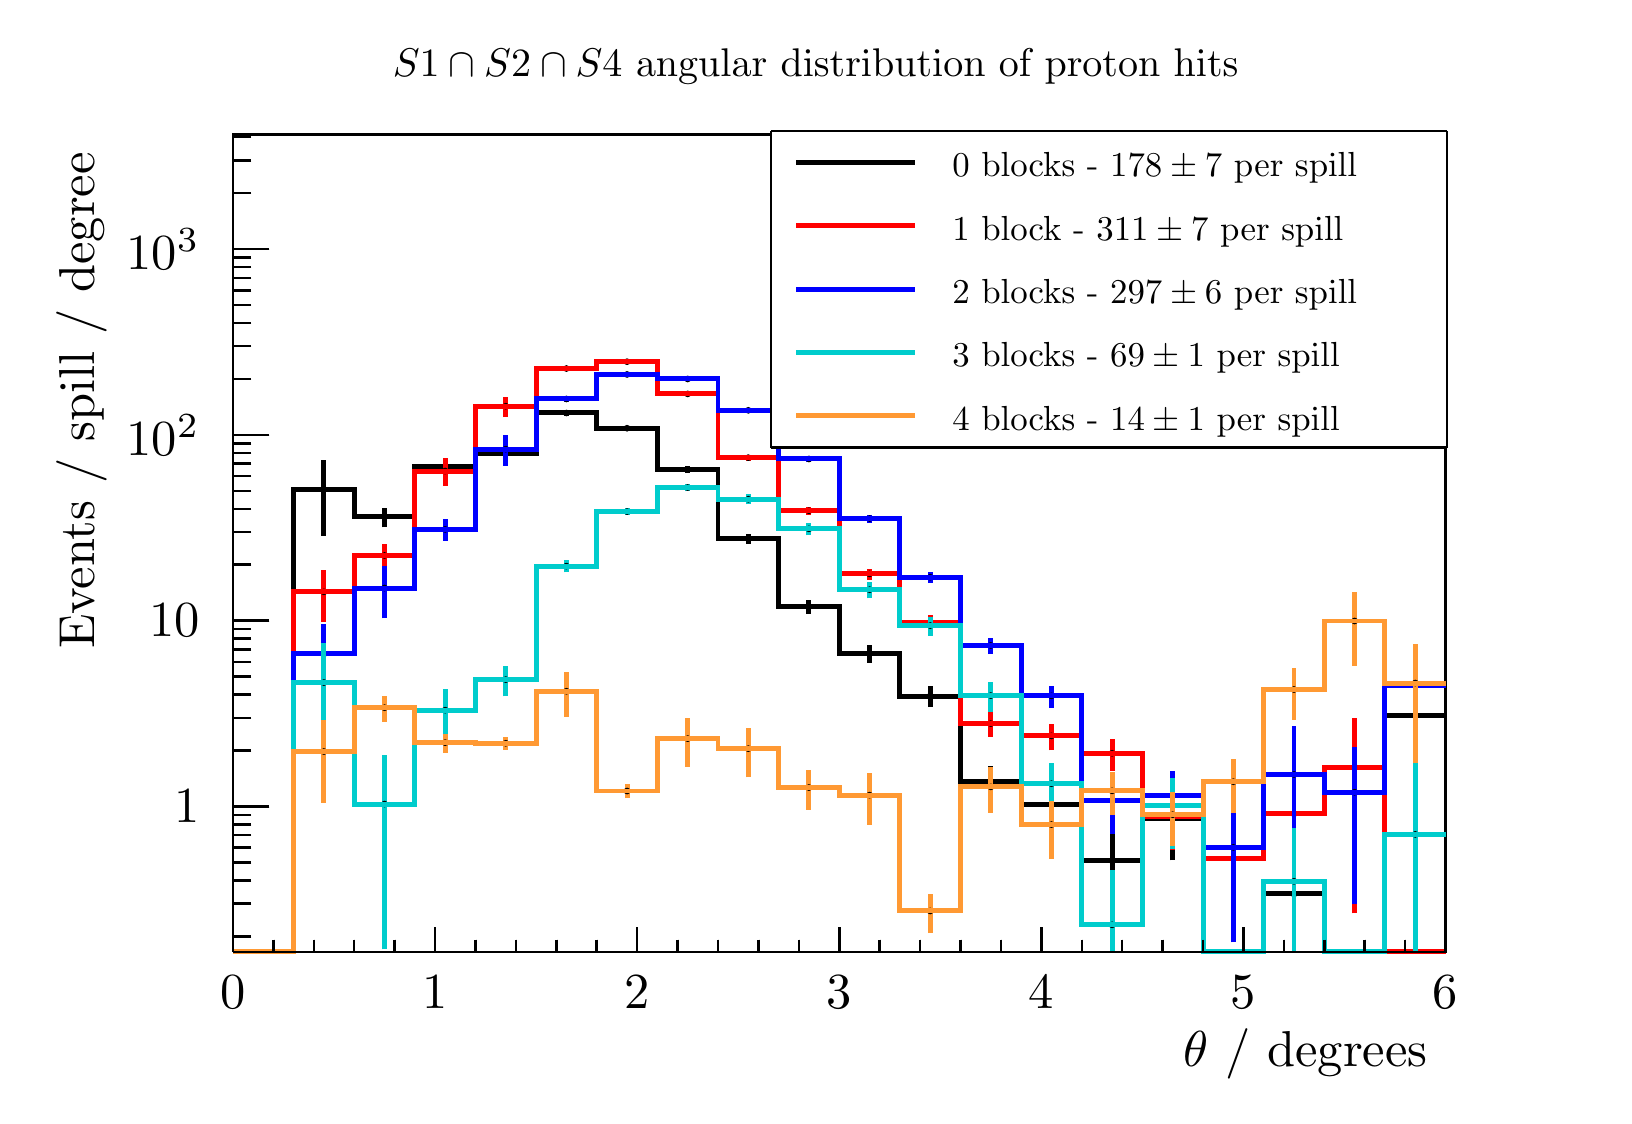
\begin{tikzpicture}
\pgfdeclareplotmark{cross} {
\pgfpathmoveto{\pgfpoint{-0.3\pgfplotmarksize}{\pgfplotmarksize}}
\pgfpathlineto{\pgfpoint{+0.3\pgfplotmarksize}{\pgfplotmarksize}}
\pgfpathlineto{\pgfpoint{+0.3\pgfplotmarksize}{0.3\pgfplotmarksize}}
\pgfpathlineto{\pgfpoint{+1\pgfplotmarksize}{0.3\pgfplotmarksize}}
\pgfpathlineto{\pgfpoint{+1\pgfplotmarksize}{-0.3\pgfplotmarksize}}
\pgfpathlineto{\pgfpoint{+0.3\pgfplotmarksize}{-0.3\pgfplotmarksize}}
\pgfpathlineto{\pgfpoint{+0.3\pgfplotmarksize}{-1.\pgfplotmarksize}}
\pgfpathlineto{\pgfpoint{-0.3\pgfplotmarksize}{-1.\pgfplotmarksize}}
\pgfpathlineto{\pgfpoint{-0.3\pgfplotmarksize}{-0.3\pgfplotmarksize}}
\pgfpathlineto{\pgfpoint{-1.\pgfplotmarksize}{-0.3\pgfplotmarksize}}
\pgfpathlineto{\pgfpoint{-1.\pgfplotmarksize}{0.3\pgfplotmarksize}}
\pgfpathlineto{\pgfpoint{-0.3\pgfplotmarksize}{0.3\pgfplotmarksize}}
\pgfpathclose
\pgfusepathqstroke
}
\pgfdeclareplotmark{cross*} {
\pgfpathmoveto{\pgfpoint{-0.3\pgfplotmarksize}{\pgfplotmarksize}}
\pgfpathlineto{\pgfpoint{+0.3\pgfplotmarksize}{\pgfplotmarksize}}
\pgfpathlineto{\pgfpoint{+0.3\pgfplotmarksize}{0.3\pgfplotmarksize}}
\pgfpathlineto{\pgfpoint{+1\pgfplotmarksize}{0.3\pgfplotmarksize}}
\pgfpathlineto{\pgfpoint{+1\pgfplotmarksize}{-0.3\pgfplotmarksize}}
\pgfpathlineto{\pgfpoint{+0.3\pgfplotmarksize}{-0.3\pgfplotmarksize}}
\pgfpathlineto{\pgfpoint{+0.3\pgfplotmarksize}{-1.\pgfplotmarksize}}
\pgfpathlineto{\pgfpoint{-0.3\pgfplotmarksize}{-1.\pgfplotmarksize}}
\pgfpathlineto{\pgfpoint{-0.3\pgfplotmarksize}{-0.3\pgfplotmarksize}}
\pgfpathlineto{\pgfpoint{-1.\pgfplotmarksize}{-0.3\pgfplotmarksize}}
\pgfpathlineto{\pgfpoint{-1.\pgfplotmarksize}{0.3\pgfplotmarksize}}
\pgfpathlineto{\pgfpoint{-0.3\pgfplotmarksize}{0.3\pgfplotmarksize}}
\pgfpathclose
\pgfusepathqfillstroke
}
\pgfdeclareplotmark{newstar} {
\pgfpathmoveto{\pgfqpoint{0pt}{\pgfplotmarksize}}
\pgfpathlineto{\pgfqpointpolar{44}{0.5\pgfplotmarksize}}
\pgfpathlineto{\pgfqpointpolar{18}{\pgfplotmarksize}}
\pgfpathlineto{\pgfqpointpolar{-20}{0.5\pgfplotmarksize}}
\pgfpathlineto{\pgfqpointpolar{-54}{\pgfplotmarksize}}
\pgfpathlineto{\pgfqpointpolar{-90}{0.5\pgfplotmarksize}}
\pgfpathlineto{\pgfqpointpolar{234}{\pgfplotmarksize}}
\pgfpathlineto{\pgfqpointpolar{198}{0.5\pgfplotmarksize}}
\pgfpathlineto{\pgfqpointpolar{162}{\pgfplotmarksize}}
\pgfpathlineto{\pgfqpointpolar{134}{0.5\pgfplotmarksize}}
\pgfpathclose
\pgfusepathqstroke
}
\pgfdeclareplotmark{newstar*} {
\pgfpathmoveto{\pgfqpoint{0pt}{\pgfplotmarksize}}
\pgfpathlineto{\pgfqpointpolar{44}{0.5\pgfplotmarksize}}
\pgfpathlineto{\pgfqpointpolar{18}{\pgfplotmarksize}}
\pgfpathlineto{\pgfqpointpolar{-20}{0.5\pgfplotmarksize}}
\pgfpathlineto{\pgfqpointpolar{-54}{\pgfplotmarksize}}
\pgfpathlineto{\pgfqpointpolar{-90}{0.5\pgfplotmarksize}}
\pgfpathlineto{\pgfqpointpolar{234}{\pgfplotmarksize}}
\pgfpathlineto{\pgfqpointpolar{198}{0.5\pgfplotmarksize}}
\pgfpathlineto{\pgfqpointpolar{162}{\pgfplotmarksize}}
\pgfpathlineto{\pgfqpointpolar{134}{0.5\pgfplotmarksize}}
\pgfpathclose
\pgfusepathqfillstroke
}
\definecolor{c}{rgb}{1,1,1};
\draw [color=c, fill=c] (0,0) rectangle (20,13.4844);
\draw [color=c, fill=c] (2.6,1.75297) rectangle (18,12.136);
\definecolor{c}{rgb}{0,0,0};
\draw [c,line width=0.9] (2.6,1.75297) -- (2.6,12.136) -- (18,12.136) -- (18,1.75297) -- (2.6,1.75297);
\definecolor{c}{rgb}{1,1,1};
\draw [color=c, fill=c] (2.6,1.75297) rectangle (18,12.136);
\definecolor{c}{rgb}{0,0,0};
\draw [c,line width=0.9] (2.6,1.75297) -- (2.6,12.136) -- (18,12.136) -- (18,1.75297) -- (2.6,1.75297);
\definecolor{c}{rgb}{0,0,0.6};
\draw [c,line width=0.9] (2.6,1.75297) -- (3.37,1.75297) -- (3.37,1.75297) -- (4.14,1.75297) -- (4.14,1.75297) -- (4.91,1.75297) -- (4.91,1.75297) -- (5.68,1.75297) -- (5.68,1.75297) -- (6.45,1.75297) -- (6.45,1.75297) -- (7.22,1.75297) --
 (7.22,1.75297) -- (7.99,1.75297) -- (7.99,1.75297) -- (8.76,1.75297) -- (8.76,1.75297) -- (9.53,1.75297) -- (9.53,1.75297) -- (10.3,1.75297) -- (10.3,1.75297) -- (11.07,1.75297) -- (11.07,1.75297) -- (11.84,1.75297) -- (11.84,1.75297) --
 (12.61,1.75297) -- (12.61,1.75297) -- (13.38,1.75297) -- (13.38,1.75297) -- (14.15,1.75297) -- (14.15,1.75297) -- (14.92,1.75297) -- (14.92,1.75297) -- (15.69,1.75297) -- (15.69,1.75297) -- (16.46,1.75297) -- (16.46,1.75297) -- (17.23,1.75297) --
 (17.23,1.75297) -- (18,1.75297);
\definecolor{c}{rgb}{0,0,0};
\draw [c,line width=0.9] (2.6,1.75297) -- (18,1.75297);
\draw [c,line width=0.9] (2.6,2.06446) -- (2.6,1.75297);
\draw [c,line width=0.9] (3.11333,1.90872) -- (3.11333,1.75297);
\draw [c,line width=0.9] (3.62667,1.90872) -- (3.62667,1.75297);
\draw [c,line width=0.9] (4.14,1.90872) -- (4.14,1.75297);
\draw [c,line width=0.9] (4.65333,1.90872) -- (4.65333,1.75297);
\draw [c,line width=0.9] (5.16667,2.06446) -- (5.16667,1.75297);
\draw [c,line width=0.9] (5.68,1.90872) -- (5.68,1.75297);
\draw [c,line width=0.9] (6.19333,1.90872) -- (6.19333,1.75297);
\draw [c,line width=0.9] (6.70667,1.90872) -- (6.70667,1.75297);
\draw [c,line width=0.9] (7.22,1.90872) -- (7.22,1.75297);
\draw [c,line width=0.9] (7.73333,2.06446) -- (7.73333,1.75297);
\draw [c,line width=0.9] (8.24667,1.90872) -- (8.24667,1.75297);
\draw [c,line width=0.9] (8.76,1.90872) -- (8.76,1.75297);
\draw [c,line width=0.9] (9.27333,1.90872) -- (9.27333,1.75297);
\draw [c,line width=0.9] (9.78667,1.90872) -- (9.78667,1.75297);
\draw [c,line width=0.9] (10.3,2.06446) -- (10.3,1.75297);
\draw [c,line width=0.9] (10.8133,1.90872) -- (10.8133,1.75297);
\draw [c,line width=0.9] (11.3267,1.90872) -- (11.3267,1.75297);
\draw [c,line width=0.9] (11.84,1.90872) -- (11.84,1.75297);
\draw [c,line width=0.9] (12.3533,1.90872) -- (12.3533,1.75297);
\draw [c,line width=0.9] (12.8667,2.06446) -- (12.8667,1.75297);
\draw [c,line width=0.9] (13.38,1.90872) -- (13.38,1.75297);
\draw [c,line width=0.9] (13.8933,1.90872) -- (13.8933,1.75297);
\draw [c,line width=0.9] (14.4067,1.90872) -- (14.4067,1.75297);
\draw [c,line width=0.9] (14.92,1.90872) -- (14.92,1.75297);
\draw [c,line width=0.9] (15.4333,2.06446) -- (15.4333,1.75297);
\draw [c,line width=0.9] (15.9467,1.90872) -- (15.9467,1.75297);
\draw [c,line width=0.9] (16.46,1.90872) -- (16.46,1.75297);
\draw [c,line width=0.9] (16.9733,1.90872) -- (16.9733,1.75297);
\draw [c,line width=0.9] (17.4867,1.90872) -- (17.4867,1.75297);
\draw [c,line width=0.9] (18,2.06446) -- (18,1.75297);
\draw [anchor=base] (2.6,1.0383) node[scale=1.82459, color=c, rotate=0]{0};
\draw [anchor=base] (5.16667,1.0383) node[scale=1.82459, color=c, rotate=0]{1};
\draw [anchor=base] (7.73333,1.0383) node[scale=1.82459, color=c, rotate=0]{2};
\draw [anchor=base] (10.3,1.0383) node[scale=1.82459, color=c, rotate=0]{3};
\draw [anchor=base] (12.8667,1.0383) node[scale=1.82459, color=c, rotate=0]{4};
\draw [anchor=base] (15.4333,1.0383) node[scale=1.82459, color=c, rotate=0]{5};
\draw [anchor=base] (18,1.0383) node[scale=1.82459, color=c, rotate=0]{6};
\draw [anchor= east] (18,0.45847) node[scale=1.82459, color=c, rotate=0]{$\theta$ / degrees};
\draw [c,line width=0.9] (2.6,1.75297) -- (2.6,12.136);
\draw [c,line width=0.9] (2.831,1.95126) -- (2.6,1.95126);
\draw [c,line width=0.9] (2.831,2.36679) -- (2.6,2.36679);
\draw [c,line width=0.9] (2.831,2.66162) -- (2.6,2.66162);
\draw [c,line width=0.9] (2.831,2.8903) -- (2.6,2.8903);
\draw [c,line width=0.9] (2.831,3.07715) -- (2.6,3.07715);
\draw [c,line width=0.9] (2.831,3.23513) -- (2.6,3.23513);
\draw [c,line width=0.9] (2.831,3.37198) -- (2.6,3.37198);
\draw [c,line width=0.9] (2.831,3.49269) -- (2.6,3.49269);
\draw [c,line width=0.9] (3.062,3.60066) -- (2.6,3.60066);
\draw [anchor= east] (2.404,3.60066) node[scale=1.82459, color=c, rotate=0]{1};
\draw [c,line width=0.9] (2.831,4.31103) -- (2.6,4.31103);
\draw [c,line width=0.9] (2.831,4.72656) -- (2.6,4.72656);
\draw [c,line width=0.9] (2.831,5.02139) -- (2.6,5.02139);
\draw [c,line width=0.9] (2.831,5.25007) -- (2.6,5.25007);
\draw [c,line width=0.9] (2.831,5.43692) -- (2.6,5.43692);
\draw [c,line width=0.9] (2.831,5.5949) -- (2.6,5.5949);
\draw [c,line width=0.9] (2.831,5.73175) -- (2.6,5.73175);
\draw [c,line width=0.9] (2.831,5.85245) -- (2.6,5.85245);
\draw [c,line width=0.9] (3.062,5.96043) -- (2.6,5.96043);
\draw [anchor= east] (2.404,5.96043) node[scale=1.82459, color=c, rotate=0]{10};
\draw [c,line width=0.9] (2.831,6.67079) -- (2.6,6.67079);
\draw [c,line width=0.9] (2.831,7.08632) -- (2.6,7.08632);
\draw [c,line width=0.9] (2.831,7.38115) -- (2.6,7.38115);
\draw [c,line width=0.9] (2.831,7.60984) -- (2.6,7.60984);
\draw [c,line width=0.9] (2.831,7.79669) -- (2.6,7.79669);
\draw [c,line width=0.9] (2.831,7.95466) -- (2.6,7.95466);
\draw [c,line width=0.9] (2.831,8.09151) -- (2.6,8.09151);
\draw [c,line width=0.9] (2.831,8.21222) -- (2.6,8.21222);
\draw [c,line width=0.9] (3.062,8.3202) -- (2.6,8.3202);
\draw [anchor= east] (2.404,8.3202) node[scale=1.82459, color=c, rotate=0]{$10^{2}$};
\draw [c,line width=0.9] (2.831,9.03056) -- (2.6,9.03056);
\draw [c,line width=0.9] (2.831,9.44609) -- (2.6,9.44609);
\draw [c,line width=0.9] (2.831,9.74092) -- (2.6,9.74092);
\draw [c,line width=0.9] (2.831,9.9696) -- (2.6,9.9696);
\draw [c,line width=0.9] (2.831,10.1565) -- (2.6,10.1565);
\draw [c,line width=0.9] (2.831,10.3144) -- (2.6,10.3144);
\draw [c,line width=0.9] (2.831,10.4513) -- (2.6,10.4513);
\draw [c,line width=0.9] (2.831,10.572) -- (2.6,10.572);
\draw [c,line width=0.9] (3.062,10.68) -- (2.6,10.68);
\draw [anchor= east] (2.404,10.68) node[scale=1.82459, color=c, rotate=0]{$10^{3}$};
\draw [c,line width=0.9] (2.831,11.3903) -- (2.6,11.3903);
\draw [c,line width=0.9] (2.831,11.8059) -- (2.6,11.8059);
\draw [c,line width=0.9] (2.831,12.1007) -- (2.6,12.1007);
\draw [anchor= east] (0.68,12.136) node[scale=1.82459, color=c, rotate=90]{ Events / spill / degree};
\draw [c,line width=1.8] (3.755,7.03662) -- (3.755,7.62677);
\draw [c,line width=1.8] (3.755,7.62677) -- (3.755,7.99888);
\foreach \P in {(3.755,7.62677)}{\draw[mark options={color=c,fill=c},mark size=2.402402pt,mark=*,mark size=1pt] plot coordinates {\P};}
\draw [c,line width=1.8] (4.525,7.1466) -- (4.525,7.27835);
\draw [c,line width=1.8] (4.525,7.27835) -- (4.525,7.39508);
\foreach \P in {(4.525,7.27835)}{\draw[mark options={color=c,fill=c},mark size=2.402402pt,mark=*,mark size=1pt] plot coordinates {\P};}
\draw [c,line width=1.8] (5.295,7.84132) -- (5.295,7.91274);
\draw [c,line width=1.8] (5.295,7.91274) -- (5.295,7.97951);
\foreach \P in {(5.295,7.91274)}{\draw[mark options={color=c,fill=c},mark size=2.402402pt,mark=*,mark size=1pt] plot coordinates {\P};}
\draw [c,line width=1.8] (6.065,8.04229) -- (6.065,8.08134);
\draw [c,line width=1.8] (6.065,8.08134) -- (6.065,8.11896);
\foreach \P in {(6.065,8.08134)}{\draw[mark options={color=c,fill=c},mark size=2.402402pt,mark=*,mark size=1pt] plot coordinates {\P};}
\draw [c,line width=1.8] (6.835,8.56056) -- (6.835,8.59781);
\draw [c,line width=1.8] (6.835,8.59781) -- (6.835,8.63376);
\foreach \P in {(6.835,8.59781)}{\draw[mark options={color=c,fill=c},mark size=2.402402pt,mark=*,mark size=1pt] plot coordinates {\P};}
\draw [c,line width=1.8] (7.605,8.37354) -- (7.605,8.40444);
\draw [c,line width=1.8] (7.605,8.40444) -- (7.605,8.43445);
\foreach \P in {(7.605,8.40444)}{\draw[mark options={color=c,fill=c},mark size=2.402402pt,mark=*,mark size=1pt] plot coordinates {\P};}
\draw [c,line width=1.8] (8.375,7.84098) -- (8.375,7.88092);
\draw [c,line width=1.8] (8.375,7.88092) -- (8.375,7.91937);
\foreach \P in {(8.375,7.88092)}{\draw[mark options={color=c,fill=c},mark size=2.402402pt,mark=*,mark size=1pt] plot coordinates {\P};}
\draw [c,line width=1.8] (9.145,6.93958) -- (9.145,7.00086);
\draw [c,line width=1.8] (9.145,7.00086) -- (9.145,7.05867);
\foreach \P in {(9.145,7.00086)}{\draw[mark options={color=c,fill=c},mark size=2.402402pt,mark=*,mark size=1pt] plot coordinates {\P};}
\draw [c,line width=1.8] (9.915,6.04796) -- (9.915,6.13934);
\draw [c,line width=1.8] (9.915,6.13934) -- (9.915,6.22323);
\foreach \P in {(9.915,6.13934)}{\draw[mark options={color=c,fill=c},mark size=2.402402pt,mark=*,mark size=1pt] plot coordinates {\P};}
\draw [c,line width=1.8] (10.685,5.42614) -- (10.685,5.54477);
\draw [c,line width=1.8] (10.685,5.54477) -- (10.685,5.65109);
\foreach \P in {(10.685,5.54477)}{\draw[mark options={color=c,fill=c},mark size=2.402402pt,mark=*,mark size=1pt] plot coordinates {\P};}
\draw [c,line width=1.8] (11.455,4.86173) -- (11.455,5.00183);
\draw [c,line width=1.8] (11.455,5.00183) -- (11.455,5.12506);
\foreach \P in {(11.455,5.00183)}{\draw[mark options={color=c,fill=c},mark size=2.402402pt,mark=*,mark size=1pt] plot coordinates {\P};}
\draw [c,line width=1.8] (12.225,3.66036) -- (12.225,3.91178);
\draw [c,line width=1.8] (12.225,3.91178) -- (12.225,4.11351);
\foreach \P in {(12.225,3.91178)}{\draw[mark options={color=c,fill=c},mark size=2.402402pt,mark=*,mark size=1pt] plot coordinates {\P};}
\draw [c,line width=1.8] (12.995,3.32051) -- (12.995,3.62728);
\draw [c,line width=1.8] (12.995,3.62728) -- (12.995,3.86307);
\foreach \P in {(12.995,3.62728)}{\draw[mark options={color=c,fill=c},mark size=2.402402pt,mark=*,mark size=1pt] plot coordinates {\P};}
\draw [c,line width=1.8] (13.765,2.29699) -- (13.765,2.91186);
\draw [c,line width=1.8] (13.765,2.91186) -- (13.765,3.29349);
\foreach \P in {(13.765,2.91186)}{\draw[mark options={color=c,fill=c},mark size=2.402402pt,mark=*,mark size=1pt] plot coordinates {\P};}
\draw [c,line width=1.8] (14.535,2.91498) -- (14.535,3.44952);
\draw [c,line width=1.8] (14.535,3.44952) -- (14.535,3.79904);
\foreach \P in {(14.535,3.44952)}{\draw[mark options={color=c,fill=c},mark size=2.402402pt,mark=*,mark size=1pt] plot coordinates {\P};}
\draw [c,line width=1.8] (16.075,1.75297) -- (16.075,2.48929);
\draw [c,line width=1.8] (16.075,2.48929) -- (16.075,3.04709);
\foreach \P in {(16.075,2.48929)}{\draw[mark options={color=c,fill=c},mark size=2.402402pt,mark=*,mark size=1pt] plot coordinates {\P};}
\draw [c,line width=1.8] (17.615,1.75297) -- (17.615,4.75258);
\draw [c,line width=1.8] (17.615,4.75258) -- (17.615,5.51616);
\foreach \P in {(17.615,4.75258)}{\draw[mark options={color=c,fill=c},mark size=2.402402pt,mark=*,mark size=1pt] plot coordinates {\P};}
\draw [c,line width=1.8] (2.6,1.75297) -- (3.37,1.75297) -- (3.37,7.62677) -- (4.14,7.62677) -- (4.14,7.27835) -- (4.91,7.27835) -- (4.91,7.91274) -- (5.68,7.91274) -- (5.68,8.08134) -- (6.45,8.08134) -- (6.45,8.59781) -- (7.22,8.59781) --
 (7.22,8.40444) -- (7.99,8.40444) -- (7.99,7.88092) -- (8.76,7.88092) -- (8.76,7.00086) -- (9.53,7.00086) -- (9.53,6.13934) -- (10.3,6.13934) -- (10.3,5.54477) -- (11.07,5.54477) -- (11.07,5.00183) -- (11.84,5.00183) -- (11.84,3.91178) --
 (12.61,3.91178) -- (12.61,3.62728) -- (13.38,3.62728) -- (13.38,2.91186) -- (14.15,2.91186) -- (14.15,3.44952) -- (14.92,3.44952) -- (14.92,1.75297) -- (15.69,1.75297) -- (15.69,2.48929) -- (16.46,2.48929) -- (16.46,1.75297) -- (17.23,1.75297) --
 (17.23,4.75258) -- (18,4.75258);
\definecolor{c}{rgb}{1,0,0};
\draw [c,line width=1.8] (3.755,5.93758) -- (3.755,6.32634);
\draw [c,line width=1.8] (3.755,6.32634) -- (3.755,6.60752);
\definecolor{c}{rgb}{0,0,0};
\foreach \P in {(3.755,6.32634)}{\draw[mark options={color=c,fill=c},mark size=2.402402pt,mark=*,mark size=1pt] plot coordinates {\P};}
\definecolor{c}{rgb}{1,0,0};
\draw [c,line width=1.8] (4.525,6.62301) -- (4.525,6.78831);
\draw [c,line width=1.8] (4.525,6.78831) -- (4.525,6.93062);
\definecolor{c}{rgb}{0,0,0};
\foreach \P in {(4.525,6.78831)}{\draw[mark options={color=c,fill=c},mark size=2.402402pt,mark=*,mark size=1pt] plot coordinates {\P};}
\definecolor{c}{rgb}{1,0,0};
\draw [c,line width=1.8] (5.295,7.66978) -- (5.295,7.86087);
\draw [c,line width=1.8] (5.295,7.86087) -- (5.295,8.02187);
\definecolor{c}{rgb}{0,0,0};
\foreach \P in {(5.295,7.86087)}{\draw[mark options={color=c,fill=c},mark size=2.402402pt,mark=*,mark size=1pt] plot coordinates {\P};}
\definecolor{c}{rgb}{1,0,0};
\draw [c,line width=1.8] (6.065,8.54588) -- (6.065,8.68387);
\draw [c,line width=1.8] (6.065,8.68387) -- (6.065,8.80546);
\definecolor{c}{rgb}{0,0,0};
\foreach \P in {(6.065,8.68387)}{\draw[mark options={color=c,fill=c},mark size=2.402402pt,mark=*,mark size=1pt] plot coordinates {\P};}
\definecolor{c}{rgb}{1,0,0};
\draw [c,line width=1.8] (6.835,9.1303) -- (6.835,9.1624);
\draw [c,line width=1.8] (6.835,9.1624) -- (6.835,9.19352);
\definecolor{c}{rgb}{0,0,0};
\foreach \P in {(6.835,9.1624)}{\draw[mark options={color=c,fill=c},mark size=2.402402pt,mark=*,mark size=1pt] plot coordinates {\P};}
\definecolor{c}{rgb}{1,0,0};
\draw [c,line width=1.8] (7.605,9.22788) -- (7.605,9.24923);
\draw [c,line width=1.8] (7.605,9.24923) -- (7.605,9.27015);
\definecolor{c}{rgb}{0,0,0};
\foreach \P in {(7.605,9.24923)}{\draw[mark options={color=c,fill=c},mark size=2.402402pt,mark=*,mark size=1pt] plot coordinates {\P};}
\definecolor{c}{rgb}{1,0,0};
\draw [c,line width=1.8] (8.375,8.81278) -- (8.375,8.84023);
\draw [c,line width=1.8] (8.375,8.84023) -- (8.375,8.86696);
\definecolor{c}{rgb}{0,0,0};
\foreach \P in {(8.375,8.84023)}{\draw[mark options={color=c,fill=c},mark size=2.402402pt,mark=*,mark size=1pt] plot coordinates {\P};}
\definecolor{c}{rgb}{1,0,0};
\draw [c,line width=1.8] (9.145,7.99098) -- (9.145,8.03088);
\draw [c,line width=1.8] (9.145,8.03088) -- (9.145,8.06928);
\definecolor{c}{rgb}{0,0,0};
\foreach \P in {(9.145,8.03088)}{\draw[mark options={color=c,fill=c},mark size=2.402402pt,mark=*,mark size=1pt] plot coordinates {\P};}
\definecolor{c}{rgb}{1,0,0};
\draw [c,line width=1.8] (9.915,7.30528) -- (9.915,7.35634);
\draw [c,line width=1.8] (9.915,7.35634) -- (9.915,7.40498);
\definecolor{c}{rgb}{0,0,0};
\foreach \P in {(9.915,7.35634)}{\draw[mark options={color=c,fill=c},mark size=2.402402pt,mark=*,mark size=1pt] plot coordinates {\P};}
\definecolor{c}{rgb}{1,0,0};
\draw [c,line width=1.8] (10.685,6.48123) -- (10.685,6.55437);
\draw [c,line width=1.8] (10.685,6.55437) -- (10.685,6.62263);
\definecolor{c}{rgb}{0,0,0};
\foreach \P in {(10.685,6.55437)}{\draw[mark options={color=c,fill=c},mark size=2.402402pt,mark=*,mark size=1pt] plot coordinates {\P};}
\definecolor{c}{rgb}{1,0,0};
\draw [c,line width=1.8] (11.455,5.8417) -- (11.455,5.94043);
\draw [c,line width=1.8] (11.455,5.94043) -- (11.455,6.03048);
\definecolor{c}{rgb}{0,0,0};
\foreach \P in {(11.455,5.94043)}{\draw[mark options={color=c,fill=c},mark size=2.402402pt,mark=*,mark size=1pt] plot coordinates {\P};}
\definecolor{c}{rgb}{1,0,0};
\draw [c,line width=1.8] (12.225,4.48443) -- (12.225,4.65313);
\draw [c,line width=1.8] (12.225,4.65313) -- (12.225,4.79794);
\definecolor{c}{rgb}{0,0,0};
\foreach \P in {(12.225,4.65313)}{\draw[mark options={color=c,fill=c},mark size=2.402402pt,mark=*,mark size=1pt] plot coordinates {\P};}
\definecolor{c}{rgb}{1,0,0};
\draw [c,line width=1.8] (12.995,4.31151) -- (12.995,4.49686);
\draw [c,line width=1.8] (12.995,4.49686) -- (12.995,4.65376);
\definecolor{c}{rgb}{0,0,0};
\foreach \P in {(12.995,4.49686)}{\draw[mark options={color=c,fill=c},mark size=2.402402pt,mark=*,mark size=1pt] plot coordinates {\P};}
\definecolor{c}{rgb}{1,0,0};
\draw [c,line width=1.8] (13.765,4.05688) -- (13.765,4.27631);
\draw [c,line width=1.8] (13.765,4.27631) -- (13.765,4.45694);
\definecolor{c}{rgb}{0,0,0};
\foreach \P in {(13.765,4.27631)}{\draw[mark options={color=c,fill=c},mark size=2.402402pt,mark=*,mark size=1pt] plot coordinates {\P};}
\definecolor{c}{rgb}{1,0,0};
\draw [c,line width=1.8] (14.535,3.05022) -- (14.535,3.47547);
\draw [c,line width=1.8] (14.535,3.47547) -- (14.535,3.77512);
\definecolor{c}{rgb}{0,0,0};
\foreach \P in {(14.535,3.47547)}{\draw[mark options={color=c,fill=c},mark size=2.402402pt,mark=*,mark size=1pt] plot coordinates {\P};}
\definecolor{c}{rgb}{1,0,0};
\draw [c,line width=1.8] (15.305,1.96144) -- (15.305,2.94418);
\draw [c,line width=1.8] (15.305,2.94418) -- (15.305,3.43649);
\definecolor{c}{rgb}{0,0,0};
\foreach \P in {(15.305,2.94418)}{\draw[mark options={color=c,fill=c},mark size=2.402402pt,mark=*,mark size=1pt] plot coordinates {\P};}
\definecolor{c}{rgb}{1,0,0};
\draw [c,line width=1.8] (16.075,1.82969) -- (16.075,3.50863);
\draw [c,line width=1.8] (16.075,3.50863) -- (16.075,4.11424);
\definecolor{c}{rgb}{0,0,0};
\foreach \P in {(16.075,3.50863)}{\draw[mark options={color=c,fill=c},mark size=2.402402pt,mark=*,mark size=1pt] plot coordinates {\P};}
\definecolor{c}{rgb}{1,0,0};
\draw [c,line width=1.8] (16.845,2.24331) -- (16.845,4.10113);
\draw [c,line width=1.8] (16.845,4.10113) -- (16.845,4.72426);
\definecolor{c}{rgb}{0,0,0};
\foreach \P in {(16.845,4.10113)}{\draw[mark options={color=c,fill=c},mark size=2.402402pt,mark=*,mark size=1pt] plot coordinates {\P};}
\definecolor{c}{rgb}{1,0,0};
\draw [c,line width=1.8] (2.6,1.75297) -- (3.37,1.75297) -- (3.37,6.32634) -- (4.14,6.32634) -- (4.14,6.78831) -- (4.91,6.78831) -- (4.91,7.86087) -- (5.68,7.86087) -- (5.68,8.68387) -- (6.45,8.68387) -- (6.45,9.1624) -- (7.22,9.1624) --
 (7.22,9.24923) -- (7.99,9.24923) -- (7.99,8.84023) -- (8.76,8.84023) -- (8.76,8.03088) -- (9.53,8.03088) -- (9.53,7.35634) -- (10.3,7.35634) -- (10.3,6.55437) -- (11.07,6.55437) -- (11.07,5.94043) -- (11.84,5.94043) -- (11.84,4.65313) --
 (12.61,4.65313) -- (12.61,4.49686) -- (13.38,4.49686) -- (13.38,4.27631) -- (14.15,4.27631) -- (14.15,3.47547) -- (14.92,3.47547) -- (14.92,2.94418) -- (15.69,2.94418) -- (15.69,3.50863) -- (16.46,3.50863) -- (16.46,4.10113) -- (17.23,4.10113) --
 (17.23,1.75297) -- (18,1.75297);
\definecolor{c}{rgb}{0,0,1};
\draw [c,line width=1.8] (3.755,4.92948) -- (3.755,5.53967);
\draw [c,line width=1.8] (3.755,5.53967) -- (3.755,5.91951);
\definecolor{c}{rgb}{0,0,0};
\foreach \P in {(3.755,5.53967)}{\draw[mark options={color=c,fill=c},mark size=2.402402pt,mark=*,mark size=1pt] plot coordinates {\P};}
\definecolor{c}{rgb}{0,0,1};
\draw [c,line width=1.8] (4.525,5.98896) -- (4.525,6.37504);
\draw [c,line width=1.8] (4.525,6.37504) -- (4.525,6.65481);
\definecolor{c}{rgb}{0,0,0};
\foreach \P in {(4.525,6.37504)}{\draw[mark options={color=c,fill=c},mark size=2.402402pt,mark=*,mark size=1pt] plot coordinates {\P};}
\definecolor{c}{rgb}{0,0,1};
\draw [c,line width=1.8] (5.295,6.97604) -- (5.295,7.11947);
\draw [c,line width=1.8] (5.295,7.11947) -- (5.295,7.24527);
\definecolor{c}{rgb}{0,0,0};
\foreach \P in {(5.295,7.11947)}{\draw[mark options={color=c,fill=c},mark size=2.402402pt,mark=*,mark size=1pt] plot coordinates {\P};}
\definecolor{c}{rgb}{0,0,1};
\draw [c,line width=1.8] (6.065,7.92853) -- (6.065,8.13869);
\draw [c,line width=1.8] (6.065,8.13869) -- (6.065,8.313);
\definecolor{c}{rgb}{0,0,0};
\foreach \P in {(6.065,8.13869)}{\draw[mark options={color=c,fill=c},mark size=2.402402pt,mark=*,mark size=1pt] plot coordinates {\P};}
\definecolor{c}{rgb}{0,0,1};
\draw [c,line width=1.8] (6.835,8.74058) -- (6.835,8.77582);
\draw [c,line width=1.8] (6.835,8.77582) -- (6.835,8.80988);
\definecolor{c}{rgb}{0,0,0};
\foreach \P in {(6.835,8.77582)}{\draw[mark options={color=c,fill=c},mark size=2.402402pt,mark=*,mark size=1pt] plot coordinates {\P};}
\definecolor{c}{rgb}{0,0,1};
\draw [c,line width=1.8] (7.605,9.06713) -- (7.605,9.08725);
\draw [c,line width=1.8] (7.605,9.08725) -- (7.605,9.10698);
\definecolor{c}{rgb}{0,0,0};
\foreach \P in {(7.605,9.08725)}{\draw[mark options={color=c,fill=c},mark size=2.402402pt,mark=*,mark size=1pt] plot coordinates {\P};}
\definecolor{c}{rgb}{0,0,1};
\draw [c,line width=1.8] (8.375,9.00595) -- (8.375,9.02976);
\draw [c,line width=1.8] (8.375,9.02976) -- (8.375,9.05303);
\definecolor{c}{rgb}{0,0,0};
\foreach \P in {(8.375,9.02976)}{\draw[mark options={color=c,fill=c},mark size=2.402402pt,mark=*,mark size=1pt] plot coordinates {\P};}
\definecolor{c}{rgb}{0,0,1};
\draw [c,line width=1.8] (9.145,8.6011) -- (9.145,8.63177);
\draw [c,line width=1.8] (9.145,8.63177) -- (9.145,8.66154);
\definecolor{c}{rgb}{0,0,0};
\foreach \P in {(9.145,8.63177)}{\draw[mark options={color=c,fill=c},mark size=2.402402pt,mark=*,mark size=1pt] plot coordinates {\P};}
\definecolor{c}{rgb}{0,0,1};
\draw [c,line width=1.8] (9.915,7.97383) -- (9.915,8.01383);
\draw [c,line width=1.8] (9.915,8.01383) -- (9.915,8.05232);
\definecolor{c}{rgb}{0,0,0};
\foreach \P in {(9.915,8.01383)}{\draw[mark options={color=c,fill=c},mark size=2.402402pt,mark=*,mark size=1pt] plot coordinates {\P};}
\definecolor{c}{rgb}{0,0,1};
\draw [c,line width=1.8] (10.685,7.20292) -- (10.685,7.25699);
\draw [c,line width=1.8] (10.685,7.25699) -- (10.685,7.30836);
\definecolor{c}{rgb}{0,0,0};
\foreach \P in {(10.685,7.25699)}{\draw[mark options={color=c,fill=c},mark size=2.402402pt,mark=*,mark size=1pt] plot coordinates {\P};}
\definecolor{c}{rgb}{0,0,1};
\draw [c,line width=1.8] (11.455,6.43814) -- (11.455,6.51221);
\draw [c,line width=1.8] (11.455,6.51221) -- (11.455,6.58128);
\definecolor{c}{rgb}{0,0,0};
\foreach \P in {(11.455,6.51221)}{\draw[mark options={color=c,fill=c},mark size=2.402402pt,mark=*,mark size=1pt] plot coordinates {\P};}
\definecolor{c}{rgb}{0,0,1};
\draw [c,line width=1.8] (12.225,5.53506) -- (12.225,5.64553);
\draw [c,line width=1.8] (12.225,5.64553) -- (12.225,5.74525);
\definecolor{c}{rgb}{0,0,0};
\foreach \P in {(12.225,5.64553)}{\draw[mark options={color=c,fill=c},mark size=2.402402pt,mark=*,mark size=1pt] plot coordinates {\P};}
\definecolor{c}{rgb}{0,0,1};
\draw [c,line width=1.8] (12.995,4.85753) -- (12.995,5.00496);
\draw [c,line width=1.8] (12.995,5.00496) -- (12.995,5.13381);
\definecolor{c}{rgb}{0,0,0};
\foreach \P in {(12.995,5.00496)}{\draw[mark options={color=c,fill=c},mark size=2.402402pt,mark=*,mark size=1pt] plot coordinates {\P};}
\definecolor{c}{rgb}{0,0,1};
\draw [c,line width=1.8] (13.765,3.25013) -- (13.765,3.67643);
\draw [c,line width=1.8] (13.765,3.67643) -- (13.765,3.9766);
\definecolor{c}{rgb}{0,0,0};
\foreach \P in {(13.765,3.67643)}{\draw[mark options={color=c,fill=c},mark size=2.402402pt,mark=*,mark size=1pt] plot coordinates {\P};}
\definecolor{c}{rgb}{0,0,1};
\draw [c,line width=1.8] (14.535,3.28304) -- (14.535,3.73631);
\draw [c,line width=1.8] (14.535,3.73631) -- (14.535,4.04949);
\definecolor{c}{rgb}{0,0,0};
\foreach \P in {(14.535,3.73631)}{\draw[mark options={color=c,fill=c},mark size=2.402402pt,mark=*,mark size=1pt] plot coordinates {\P};}
\definecolor{c}{rgb}{0,0,1};
\draw [c,line width=1.8] (15.305,1.87596) -- (15.305,3.08101);
\draw [c,line width=1.8] (15.305,3.08101) -- (15.305,3.61965);
\definecolor{c}{rgb}{0,0,0};
\foreach \P in {(15.305,3.08101)}{\draw[mark options={color=c,fill=c},mark size=2.402402pt,mark=*,mark size=1pt] plot coordinates {\P};}
\definecolor{c}{rgb}{0,0,1};
\draw [c,line width=1.8] (16.075,2.16853) -- (16.075,4.00697);
\draw [c,line width=1.8] (16.075,4.00697) -- (16.075,4.62836);
\definecolor{c}{rgb}{0,0,0};
\foreach \P in {(16.075,4.00697)}{\draw[mark options={color=c,fill=c},mark size=2.402402pt,mark=*,mark size=1pt] plot coordinates {\P};}
\definecolor{c}{rgb}{0,0,1};
\draw [c,line width=1.8] (16.845,2.35724) -- (16.845,3.78143);
\draw [c,line width=1.8] (16.845,3.78143) -- (16.845,4.35543);
\definecolor{c}{rgb}{0,0,0};
\foreach \P in {(16.845,3.78143)}{\draw[mark options={color=c,fill=c},mark size=2.402402pt,mark=*,mark size=1pt] plot coordinates {\P};}
\definecolor{c}{rgb}{0,0,1};
\draw [c,line width=1.8] (17.615,4.13319) -- (17.615,5.13955);
\draw [c,line width=1.8] (17.615,5.13955) -- (17.615,5.63739);
\definecolor{c}{rgb}{0,0,0};
\foreach \P in {(17.615,5.13955)}{\draw[mark options={color=c,fill=c},mark size=2.402402pt,mark=*,mark size=1pt] plot coordinates {\P};}
\definecolor{c}{rgb}{0,0,1};
\draw [c,line width=1.8] (2.6,1.75297) -- (3.37,1.75297) -- (3.37,5.53967) -- (4.14,5.53967) -- (4.14,6.37504) -- (4.91,6.37504) -- (4.91,7.11947) -- (5.68,7.11947) -- (5.68,8.13869) -- (6.45,8.13869) -- (6.45,8.77582) -- (7.22,8.77582) --
 (7.22,9.08725) -- (7.99,9.08725) -- (7.99,9.02976) -- (8.76,9.02976) -- (8.76,8.63177) -- (9.53,8.63177) -- (9.53,8.01383) -- (10.3,8.01383) -- (10.3,7.25699) -- (11.07,7.25699) -- (11.07,6.51221) -- (11.84,6.51221) -- (11.84,5.64553) --
 (12.61,5.64553) -- (12.61,5.00496) -- (13.38,5.00496) -- (13.38,3.67643) -- (14.15,3.67643) -- (14.15,3.73631) -- (14.92,3.73631) -- (14.92,3.08101) -- (15.69,3.08101) -- (15.69,4.00697) -- (16.46,4.00697) -- (16.46,3.78143) -- (17.23,3.78143) --
 (17.23,5.13955) -- (18,5.13955);
\definecolor{c}{rgb}{0,0.8,0.8};
\draw [c,line width=1.8] (3.755,4.17313) -- (3.755,5.17438);
\draw [c,line width=1.8] (3.755,5.17438) -- (3.755,5.67103);
\definecolor{c}{rgb}{0,0,0};
\foreach \P in {(3.755,5.17438)}{\draw[mark options={color=c,fill=c},mark size=2.402402pt,mark=*,mark size=1pt] plot coordinates {\P};}
\definecolor{c}{rgb}{0,0.8,0.8};
\draw [c,line width=1.8] (4.525,1.7854) -- (4.525,3.63132);
\draw [c,line width=1.8] (4.525,3.63132) -- (4.525,4.25338);
\definecolor{c}{rgb}{0,0,0};
\foreach \P in {(4.525,3.63132)}{\draw[mark options={color=c,fill=c},mark size=2.402402pt,mark=*,mark size=1pt] plot coordinates {\P};}
\definecolor{c}{rgb}{0,0.8,0.8};
\draw [c,line width=1.8] (5.295,4.44841) -- (5.295,4.82399);
\draw [c,line width=1.8] (5.295,4.82399) -- (5.295,5.09824);
\definecolor{c}{rgb}{0,0,0};
\foreach \P in {(5.295,4.82399)}{\draw[mark options={color=c,fill=c},mark size=2.402402pt,mark=*,mark size=1pt] plot coordinates {\P};}
\definecolor{c}{rgb}{0,0.8,0.8};
\draw [c,line width=1.8] (6.065,4.99757) -- (6.065,5.21162);
\draw [c,line width=1.8] (6.065,5.21162) -- (6.065,5.3886);
\definecolor{c}{rgb}{0,0,0};
\foreach \P in {(6.065,5.21162)}{\draw[mark options={color=c,fill=c},mark size=2.402402pt,mark=*,mark size=1pt] plot coordinates {\P};}
\definecolor{c}{rgb}{0,0.8,0.8};
\draw [c,line width=1.8] (6.835,6.57423) -- (6.835,6.65308);
\draw [c,line width=1.8] (6.835,6.65308) -- (6.835,6.72629);
\definecolor{c}{rgb}{0,0,0};
\foreach \P in {(6.835,6.65308)}{\draw[mark options={color=c,fill=c},mark size=2.402402pt,mark=*,mark size=1pt] plot coordinates {\P};}
\definecolor{c}{rgb}{0,0.8,0.8};
\draw [c,line width=1.8] (7.605,7.30133) -- (7.605,7.34573);
\draw [c,line width=1.8] (7.605,7.34573) -- (7.605,7.38828);
\definecolor{c}{rgb}{0,0,0};
\foreach \P in {(7.605,7.34573)}{\draw[mark options={color=c,fill=c},mark size=2.402402pt,mark=*,mark size=1pt] plot coordinates {\P};}
\definecolor{c}{rgb}{0,0.8,0.8};
\draw [c,line width=1.8] (8.375,7.60217) -- (8.375,7.65084);
\draw [c,line width=1.8] (8.375,7.65084) -- (8.375,7.69729);
\definecolor{c}{rgb}{0,0,0};
\foreach \P in {(8.375,7.65084)}{\draw[mark options={color=c,fill=c},mark size=2.402402pt,mark=*,mark size=1pt] plot coordinates {\P};}
\definecolor{c}{rgb}{0,0.8,0.8};
\draw [c,line width=1.8] (9.145,7.43568) -- (9.145,7.50217);
\draw [c,line width=1.8] (9.145,7.50217) -- (9.145,7.56461);
\definecolor{c}{rgb}{0,0,0};
\foreach \P in {(9.145,7.50217)}{\draw[mark options={color=c,fill=c},mark size=2.402402pt,mark=*,mark size=1pt] plot coordinates {\P};}
\definecolor{c}{rgb}{0,0.8,0.8};
\draw [c,line width=1.8] (9.915,7.04267) -- (9.915,7.12627);
\draw [c,line width=1.8] (9.915,7.12627) -- (9.915,7.20356);
\definecolor{c}{rgb}{0,0,0};
\foreach \P in {(9.915,7.12627)}{\draw[mark options={color=c,fill=c},mark size=2.402402pt,mark=*,mark size=1pt] plot coordinates {\P};}
\definecolor{c}{rgb}{0,0.8,0.8};
\draw [c,line width=1.8] (10.685,6.24395) -- (10.685,6.35391);
\draw [c,line width=1.8] (10.685,6.35391) -- (10.685,6.45322);
\definecolor{c}{rgb}{0,0,0};
\foreach \P in {(10.685,6.35391)}{\draw[mark options={color=c,fill=c},mark size=2.402402pt,mark=*,mark size=1pt] plot coordinates {\P};}
\definecolor{c}{rgb}{0,0.8,0.8};
\draw [c,line width=1.8] (11.455,5.77127) -- (11.455,5.89854);
\draw [c,line width=1.8] (11.455,5.89854) -- (11.455,6.01175);
\definecolor{c}{rgb}{0,0,0};
\foreach \P in {(11.455,5.89854)}{\draw[mark options={color=c,fill=c},mark size=2.402402pt,mark=*,mark size=1pt] plot coordinates {\P};}
\definecolor{c}{rgb}{0,0.8,0.8};
\draw [c,line width=1.8] (12.225,4.80242) -- (12.225,5.00888);
\draw [c,line width=1.8] (12.225,5.00888) -- (12.225,5.18064);
\definecolor{c}{rgb}{0,0,0};
\foreach \P in {(12.225,5.00888)}{\draw[mark options={color=c,fill=c},mark size=2.402402pt,mark=*,mark size=1pt] plot coordinates {\P};}
\definecolor{c}{rgb}{0,0.8,0.8};
\draw [c,line width=1.8] (12.995,3.52802) -- (12.995,3.88988);
\draw [c,line width=1.8] (12.995,3.88988) -- (12.995,4.15678);
\definecolor{c}{rgb}{0,0,0};
\foreach \P in {(12.995,3.88988)}{\draw[mark options={color=c,fill=c},mark size=2.402402pt,mark=*,mark size=1pt] plot coordinates {\P};}
\definecolor{c}{rgb}{0,0.8,0.8};
\draw [c,line width=1.8] (13.765,1.75297) -- (13.765,2.09732);
\draw [c,line width=1.8] (13.765,2.09732) -- (13.765,2.79492);
\definecolor{c}{rgb}{0,0,0};
\foreach \P in {(13.765,2.09732)}{\draw[mark options={color=c,fill=c},mark size=2.402402pt,mark=*,mark size=1pt] plot coordinates {\P};}
\definecolor{c}{rgb}{0,0.8,0.8};
\draw [c,line width=1.8] (14.535,3.06499) -- (14.535,3.61);
\draw [c,line width=1.8] (14.535,3.61) -- (14.535,3.96391);
\definecolor{c}{rgb}{0,0,0};
\foreach \P in {(14.535,3.61)}{\draw[mark options={color=c,fill=c},mark size=2.402402pt,mark=*,mark size=1pt] plot coordinates {\P};}
\definecolor{c}{rgb}{0,0.8,0.8};
\draw [c,line width=1.8] (16.075,1.75297) -- (16.075,2.64999);
\draw [c,line width=1.8] (16.075,2.64999) -- (16.075,3.33125);
\definecolor{c}{rgb}{0,0,0};
\foreach \P in {(16.075,2.64999)}{\draw[mark options={color=c,fill=c},mark size=2.402402pt,mark=*,mark size=1pt] plot coordinates {\P};}
\definecolor{c}{rgb}{0,0.8,0.8};
\draw [c,line width=1.8] (17.615,1.75297) -- (17.615,3.24602);
\draw [c,line width=1.8] (17.615,3.24602) -- (17.615,4.29827);
\definecolor{c}{rgb}{0,0,0};
\foreach \P in {(17.615,3.24602)}{\draw[mark options={color=c,fill=c},mark size=2.402402pt,mark=*,mark size=1pt] plot coordinates {\P};}
\definecolor{c}{rgb}{0,0.8,0.8};
\draw [c,line width=1.8] (2.6,1.75297) -- (3.37,1.75297) -- (3.37,5.17438) -- (4.14,5.17438) -- (4.14,3.63132) -- (4.91,3.63132) -- (4.91,4.82399) -- (5.68,4.82399) -- (5.68,5.21162) -- (6.45,5.21162) -- (6.45,6.65308) -- (7.22,6.65308) --
 (7.22,7.34573) -- (7.99,7.34573) -- (7.99,7.65084) -- (8.76,7.65084) -- (8.76,7.50217) -- (9.53,7.50217) -- (9.53,7.12627) -- (10.3,7.12627) -- (10.3,6.35391) -- (11.07,6.35391) -- (11.07,5.89854) -- (11.84,5.89854) -- (11.84,5.00888) --
 (12.61,5.00888) -- (12.61,3.88988) -- (13.38,3.88988) -- (13.38,2.09732) -- (14.15,2.09732) -- (14.15,3.61) -- (14.92,3.61) -- (14.92,1.75297) -- (15.69,1.75297) -- (15.69,2.64999) -- (16.46,2.64999) -- (16.46,1.75297) -- (17.23,1.75297) --
 (17.23,3.24602) -- (18,3.24602);
\definecolor{c}{rgb}{1,0.6,0.2};
\draw [c,line width=1.8] (3.755,3.64682) -- (3.755,4.29819);
\draw [c,line width=1.8] (3.755,4.29819) -- (3.755,4.69328);
\definecolor{c}{rgb}{0,0,0};
\foreach \P in {(3.755,4.29819)}{\draw[mark options={color=c,fill=c},mark size=2.402402pt,mark=*,mark size=1pt] plot coordinates {\P};}
\definecolor{c}{rgb}{1,0.6,0.2};
\draw [c,line width=1.8] (4.525,4.67827) -- (4.525,4.85504);
\draw [c,line width=1.8] (4.525,4.85504) -- (4.525,5.00576);
\definecolor{c}{rgb}{0,0,0};
\foreach \P in {(4.525,4.85504)}{\draw[mark options={color=c,fill=c},mark size=2.402402pt,mark=*,mark size=1pt] plot coordinates {\P};}
\definecolor{c}{rgb}{1,0.6,0.2};
\draw [c,line width=1.8] (5.295,4.28453) -- (5.295,4.411);
\draw [c,line width=1.8] (5.295,4.411) -- (5.295,4.52357);
\definecolor{c}{rgb}{0,0,0};
\foreach \P in {(5.295,4.411)}{\draw[mark options={color=c,fill=c},mark size=2.402402pt,mark=*,mark size=1pt] plot coordinates {\P};}
\definecolor{c}{rgb}{1,0.6,0.2};
\draw [c,line width=1.8] (6.065,4.32267) -- (6.065,4.40343);
\draw [c,line width=1.8] (6.065,4.40343) -- (6.065,4.47828);
\definecolor{c}{rgb}{0,0,0};
\foreach \P in {(6.065,4.40343)}{\draw[mark options={color=c,fill=c},mark size=2.402402pt,mark=*,mark size=1pt] plot coordinates {\P};}
\definecolor{c}{rgb}{1,0.6,0.2};
\draw [c,line width=1.8] (6.835,4.74071) -- (6.835,5.06405);
\draw [c,line width=1.8] (6.835,5.06405) -- (6.835,5.30947);
\definecolor{c}{rgb}{0,0,0};
\foreach \P in {(6.835,5.06405)}{\draw[mark options={color=c,fill=c},mark size=2.402402pt,mark=*,mark size=1pt] plot coordinates {\P};}
\definecolor{c}{rgb}{1,0.6,0.2};
\draw [c,line width=1.8] (7.605,3.70709) -- (7.605,3.79725);
\draw [c,line width=1.8] (7.605,3.79725) -- (7.605,3.88012);
\definecolor{c}{rgb}{0,0,0};
\foreach \P in {(7.605,3.79725)}{\draw[mark options={color=c,fill=c},mark size=2.402402pt,mark=*,mark size=1pt] plot coordinates {\P};}
\definecolor{c}{rgb}{1,0.6,0.2};
\draw [c,line width=1.8] (8.375,4.10239) -- (8.375,4.46227);
\draw [c,line width=1.8] (8.375,4.46227) -- (8.375,4.72809);
\definecolor{c}{rgb}{0,0,0};
\foreach \P in {(8.375,4.46227)}{\draw[mark options={color=c,fill=c},mark size=2.402402pt,mark=*,mark size=1pt] plot coordinates {\P};}
\definecolor{c}{rgb}{1,0.6,0.2};
\draw [c,line width=1.8] (9.145,3.97036) -- (9.145,4.33499);
\draw [c,line width=1.8] (9.145,4.33499) -- (9.145,4.60338);
\definecolor{c}{rgb}{0,0,0};
\foreach \P in {(9.145,4.33499)}{\draw[mark options={color=c,fill=c},mark size=2.402402pt,mark=*,mark size=1pt] plot coordinates {\P};}
\definecolor{c}{rgb}{1,0.6,0.2};
\draw [c,line width=1.8] (9.915,3.55808) -- (9.915,3.84073);
\draw [c,line width=1.8] (9.915,3.84073) -- (9.915,4.06203);
\definecolor{c}{rgb}{0,0,0};
\foreach \P in {(9.915,3.84073)}{\draw[mark options={color=c,fill=c},mark size=2.402402pt,mark=*,mark size=1pt] plot coordinates {\P};}
\definecolor{c}{rgb}{1,0.6,0.2};
\draw [c,line width=1.8] (10.685,3.36741) -- (10.685,3.74462);
\draw [c,line width=1.8] (10.685,3.74462) -- (10.685,4.01974);
\definecolor{c}{rgb}{0,0,0};
\foreach \P in {(10.685,3.74462)}{\draw[mark options={color=c,fill=c},mark size=2.402402pt,mark=*,mark size=1pt] plot coordinates {\P};}
\definecolor{c}{rgb}{1,0.6,0.2};
\draw [c,line width=1.8] (11.455,1.99296) -- (11.455,2.27381);
\draw [c,line width=1.8] (11.455,2.27381) -- (11.455,2.49402);
\definecolor{c}{rgb}{0,0,0};
\foreach \P in {(11.455,2.27381)}{\draw[mark options={color=c,fill=c},mark size=2.402402pt,mark=*,mark size=1pt] plot coordinates {\P};}
\definecolor{c}{rgb}{1,0.6,0.2};
\draw [c,line width=1.8] (12.225,3.51777) -- (12.225,3.84946);
\draw [c,line width=1.8] (12.225,3.84946) -- (12.225,4.09965);
\definecolor{c}{rgb}{0,0,0};
\foreach \P in {(12.225,3.84946)}{\draw[mark options={color=c,fill=c},mark size=2.402402pt,mark=*,mark size=1pt] plot coordinates {\P};}
\definecolor{c}{rgb}{1,0.6,0.2};
\draw [c,line width=1.8] (12.995,2.93764) -- (12.995,3.37048);
\draw [c,line width=1.8] (12.995,3.37048) -- (12.995,3.67385);
\definecolor{c}{rgb}{0,0,0};
\foreach \P in {(12.995,3.37048)}{\draw[mark options={color=c,fill=c},mark size=2.402402pt,mark=*,mark size=1pt] plot coordinates {\P};}
\definecolor{c}{rgb}{1,0.6,0.2};
\draw [c,line width=1.8] (13.765,3.49163) -- (13.765,3.79909);
\draw [c,line width=1.8] (13.765,3.79909) -- (13.765,4.03528);
\definecolor{c}{rgb}{0,0,0};
\foreach \P in {(13.765,3.79909)}{\draw[mark options={color=c,fill=c},mark size=2.402402pt,mark=*,mark size=1pt] plot coordinates {\P};}
\definecolor{c}{rgb}{1,0.6,0.2};
\draw [c,line width=1.8] (14.535,3.10383) -- (14.535,3.49593);
\draw [c,line width=1.8] (14.535,3.49593) -- (14.535,3.77884);
\definecolor{c}{rgb}{0,0,0};
\foreach \P in {(14.535,3.49593)}{\draw[mark options={color=c,fill=c},mark size=2.402402pt,mark=*,mark size=1pt] plot coordinates {\P};}
\definecolor{c}{rgb}{1,0.6,0.2};
\draw [c,line width=1.8] (15.305,3.52371) -- (15.305,3.91517);
\draw [c,line width=1.8] (15.305,3.91517) -- (15.305,4.19775);
\definecolor{c}{rgb}{0,0,0};
\foreach \P in {(15.305,3.91517)}{\draw[mark options={color=c,fill=c},mark size=2.402402pt,mark=*,mark size=1pt] plot coordinates {\P};}
\definecolor{c}{rgb}{1,0.6,0.2};
\draw [c,line width=1.8] (16.075,4.7038) -- (16.075,5.08605);
\draw [c,line width=1.8] (16.075,5.08605) -- (16.075,5.36382);
\definecolor{c}{rgb}{0,0,0};
\foreach \P in {(16.075,5.08605)}{\draw[mark options={color=c,fill=c},mark size=2.402402pt,mark=*,mark size=1pt] plot coordinates {\P};}
\definecolor{c}{rgb}{1,0.6,0.2};
\draw [c,line width=1.8] (16.845,5.38628) -- (16.845,5.9562);
\draw [c,line width=1.8] (16.845,5.9562) -- (16.845,6.32028);
\definecolor{c}{rgb}{0,0,0};
\foreach \P in {(16.845,5.9562)}{\draw[mark options={color=c,fill=c},mark size=2.402402pt,mark=*,mark size=1pt] plot coordinates {\P};}
\definecolor{c}{rgb}{1,0.6,0.2};
\draw [c,line width=1.8] (17.615,4.1524) -- (17.615,5.1684);
\draw [c,line width=1.8] (17.615,5.1684) -- (17.615,5.66844);
\definecolor{c}{rgb}{0,0,0};
\foreach \P in {(17.615,5.1684)}{\draw[mark options={color=c,fill=c},mark size=2.402402pt,mark=*,mark size=1pt] plot coordinates {\P};}
\definecolor{c}{rgb}{1,0.6,0.2};
\draw [c,line width=1.8] (2.6,1.75297) -- (3.37,1.75297) -- (3.37,4.29819) -- (4.14,4.29819) -- (4.14,4.85504) -- (4.91,4.85504) -- (4.91,4.411) -- (5.68,4.411) -- (5.68,4.40343) -- (6.45,4.40343) -- (6.45,5.06405) -- (7.22,5.06405) -- (7.22,3.79725)
 -- (7.99,3.79725) -- (7.99,4.46227) -- (8.76,4.46227) -- (8.76,4.33499) -- (9.53,4.33499) -- (9.53,3.84073) -- (10.3,3.84073) -- (10.3,3.74462) -- (11.07,3.74462) -- (11.07,2.27381) -- (11.84,2.27381) -- (11.84,3.84946) -- (12.61,3.84946) --
 (12.61,3.37048) -- (13.38,3.37048) -- (13.38,3.79909) -- (14.15,3.79909) -- (14.15,3.49593) -- (14.92,3.49593) -- (14.92,3.91517) -- (15.69,3.91517) -- (15.69,5.08605) -- (16.46,5.08605) -- (16.46,5.9562) -- (17.23,5.9562) -- (17.23,5.1684) --
 (18,5.1684);
\definecolor{c}{rgb}{0,0,0};
\draw [c,line width=0.9] (2.6,1.75297) -- (18,1.75297);
\draw [c,line width=0.9] (2.6,2.06446) -- (2.6,1.75297);
\draw [c,line width=0.9] (3.11333,1.90872) -- (3.11333,1.75297);
\draw [c,line width=0.9] (3.62667,1.90872) -- (3.62667,1.75297);
\draw [c,line width=0.9] (4.14,1.90872) -- (4.14,1.75297);
\draw [c,line width=0.9] (4.65333,1.90872) -- (4.65333,1.75297);
\draw [c,line width=0.9] (5.16667,2.06446) -- (5.16667,1.75297);
\draw [c,line width=0.9] (5.68,1.90872) -- (5.68,1.75297);
\draw [c,line width=0.9] (6.19333,1.90872) -- (6.19333,1.75297);
\draw [c,line width=0.9] (6.70667,1.90872) -- (6.70667,1.75297);
\draw [c,line width=0.9] (7.22,1.90872) -- (7.22,1.75297);
\draw [c,line width=0.9] (7.73333,2.06446) -- (7.73333,1.75297);
\draw [c,line width=0.9] (8.24667,1.90872) -- (8.24667,1.75297);
\draw [c,line width=0.9] (8.76,1.90872) -- (8.76,1.75297);
\draw [c,line width=0.9] (9.27333,1.90872) -- (9.27333,1.75297);
\draw [c,line width=0.9] (9.78667,1.90872) -- (9.78667,1.75297);
\draw [c,line width=0.9] (10.3,2.06446) -- (10.3,1.75297);
\draw [c,line width=0.9] (10.8133,1.90872) -- (10.8133,1.75297);
\draw [c,line width=0.9] (11.3267,1.90872) -- (11.3267,1.75297);
\draw [c,line width=0.9] (11.84,1.90872) -- (11.84,1.75297);
\draw [c,line width=0.9] (12.3533,1.90872) -- (12.3533,1.75297);
\draw [c,line width=0.9] (12.8667,2.06446) -- (12.8667,1.75297);
\draw [c,line width=0.9] (13.38,1.90872) -- (13.38,1.75297);
\draw [c,line width=0.9] (13.8933,1.90872) -- (13.8933,1.75297);
\draw [c,line width=0.9] (14.4067,1.90872) -- (14.4067,1.75297);
\draw [c,line width=0.9] (14.92,1.90872) -- (14.92,1.75297);
\draw [c,line width=0.9] (15.4333,2.06446) -- (15.4333,1.75297);
\draw [c,line width=0.9] (15.9467,1.90872) -- (15.9467,1.75297);
\draw [c,line width=0.9] (16.46,1.90872) -- (16.46,1.75297);
\draw [c,line width=0.9] (16.9733,1.90872) -- (16.9733,1.75297);
\draw [c,line width=0.9] (17.4867,1.90872) -- (17.4867,1.75297);
\draw [c,line width=0.9] (18,2.06446) -- (18,1.75297);
\draw [c,line width=0.9] (2.6,1.75297) -- (2.6,12.136);
\draw [c,line width=0.9] (2.831,1.95126) -- (2.6,1.95126);
\draw [c,line width=0.9] (2.831,2.36679) -- (2.6,2.36679);
\draw [c,line width=0.9] (2.831,2.66162) -- (2.6,2.66162);
\draw [c,line width=0.9] (2.831,2.8903) -- (2.6,2.8903);
\draw [c,line width=0.9] (2.831,3.07715) -- (2.6,3.07715);
\draw [c,line width=0.9] (2.831,3.23513) -- (2.6,3.23513);
\draw [c,line width=0.9] (2.831,3.37198) -- (2.6,3.37198);
\draw [c,line width=0.9] (2.831,3.49269) -- (2.6,3.49269);
\draw [c,line width=0.9] (3.062,3.60066) -- (2.6,3.60066);
\draw [c,line width=0.9] (2.831,4.31103) -- (2.6,4.31103);
\draw [c,line width=0.9] (2.831,4.72656) -- (2.6,4.72656);
\draw [c,line width=0.9] (2.831,5.02139) -- (2.6,5.02139);
\draw [c,line width=0.9] (2.831,5.25007) -- (2.6,5.25007);
\draw [c,line width=0.9] (2.831,5.43692) -- (2.6,5.43692);
\draw [c,line width=0.9] (2.831,5.5949) -- (2.6,5.5949);
\draw [c,line width=0.9] (2.831,5.73175) -- (2.6,5.73175);
\draw [c,line width=0.9] (2.831,5.85245) -- (2.6,5.85245);
\draw [c,line width=0.9] (3.062,5.96043) -- (2.6,5.96043);
\draw [c,line width=0.9] (2.831,6.67079) -- (2.6,6.67079);
\draw [c,line width=0.9] (2.831,7.08632) -- (2.6,7.08632);
\draw [c,line width=0.9] (2.831,7.38115) -- (2.6,7.38115);
\draw [c,line width=0.9] (2.831,7.60984) -- (2.6,7.60984);
\draw [c,line width=0.9] (2.831,7.79669) -- (2.6,7.79669);
\draw [c,line width=0.9] (2.831,7.95466) -- (2.6,7.95466);
\draw [c,line width=0.9] (2.831,8.09151) -- (2.6,8.09151);
\draw [c,line width=0.9] (2.831,8.21222) -- (2.6,8.21222);
\draw [c,line width=0.9] (3.062,8.3202) -- (2.6,8.3202);
\draw [c,line width=0.9] (2.831,9.03056) -- (2.6,9.03056);
\draw [c,line width=0.9] (2.831,9.44609) -- (2.6,9.44609);
\draw [c,line width=0.9] (2.831,9.74092) -- (2.6,9.74092);
\draw [c,line width=0.9] (2.831,9.9696) -- (2.6,9.9696);
\draw [c,line width=0.9] (2.831,10.1565) -- (2.6,10.1565);
\draw [c,line width=0.9] (2.831,10.3144) -- (2.6,10.3144);
\draw [c,line width=0.9] (2.831,10.4513) -- (2.6,10.4513);
\draw [c,line width=0.9] (2.831,10.572) -- (2.6,10.572);
\draw [c,line width=0.9] (3.062,10.68) -- (2.6,10.68);
\draw [c,line width=0.9] (2.831,11.3903) -- (2.6,11.3903);
\draw [c,line width=0.9] (2.831,11.8059) -- (2.6,11.8059);
\draw [c,line width=0.9] (2.831,12.1007) -- (2.6,12.1007);
\draw (10,13.0047) node[scale=1.44709, color=c, rotate=0]{$S1 \cap S2 \cap S4$ angular distribution of proton hits};
\definecolor{c}{rgb}{1,1,1};
\draw [color=c, fill=c] (9.43343,8.15864) rectangle (18.017,12.1813);
\definecolor{c}{rgb}{0,0,0};
\draw [c,line width=0.9] (9.43343,8.15864) -- (18.017,8.15864);
\draw [c,line width=0.9] (18.017,8.15864) -- (18.017,12.1813);
\draw [c,line width=0.9] (18.017,12.1813) -- (9.43343,12.1813);
\draw [c,line width=0.9] (9.43343,12.1813) -- (9.43343,8.15864);
\draw [anchor=base west] (11.5793,11.598) node[scale=1.25834, color=c, rotate=0]{0 blocks - $178 \pm 7$ per spill};
\draw [c,line width=1.8] (9.75531,11.779) -- (11.2574,11.779);
\draw [anchor=base west] (11.5793,10.7935) node[scale=1.25834, color=c, rotate=0]{1 block - $311 \pm 7$ per spill};
\definecolor{c}{rgb}{1,0,0};
\draw [c,line width=1.8] (9.75531,10.9745) -- (11.2574,10.9745);
\definecolor{c}{rgb}{0,0,0};
\draw [anchor=base west] (11.5793,9.98895) node[scale=1.25834, color=c, rotate=0]{2 blocks - $297 \pm 6$ per spill};
\definecolor{c}{rgb}{0,0,1};
\draw [c,line width=1.8] (9.75531,10.17) -- (11.2574,10.17);
\definecolor{c}{rgb}{0,0,0};
\draw [anchor=base west] (11.5793,9.18442) node[scale=1.25834, color=c, rotate=0]{3 blocks - $69 \pm 1$ per spill};
\definecolor{c}{rgb}{0,0.8,0.8};
\draw [c,line width=1.8] (9.75531,9.36544) -- (11.2574,9.36544);
\definecolor{c}{rgb}{0,0,0};
\draw [anchor=base west] (11.5793,8.37989) node[scale=1.25834, color=c, rotate=0]{4 blocks - $14 \pm 1$ per spill};
\definecolor{c}{rgb}{1,0.6,0.2};
\draw [c,line width=1.8] (9.75531,8.56091) -- (11.2574,8.56091);
\end{tikzpicture}

    \end{adjustbox}
  \end{minipage} 
  \caption{\label{fig:thetas4mip}Distribution of hits in $\mathit{S4}$ as a function of the number of moderator blocks and the horizontal off-axis angle. Left: minimum ionizing particles. Right: protons.}
\end{figure}	

Figure~\ref{fig:propiratio_s4_horz} shows the ratio of protons to MIPs as a function of the number of moderator blocks, $\theta$ and $\phi$.
For all of the different block configurations, the ratio is flat across both $\theta$ and $\phi$.
With the addition of moderator blocks, the ratio reduces from its highest level of 0.5 for the 0 block case, to 0.002 for the 4 block data.
As mentioned previously, this is thought to be due to the attenuation of low energy protons within the walls of the pressure vessel.

\begin{figure}[!ht]
  \begin{minipage}[t]{0.48\textwidth}
    \begin{adjustbox}{max totalsize={\textwidth}{.35\textheight}, center}
      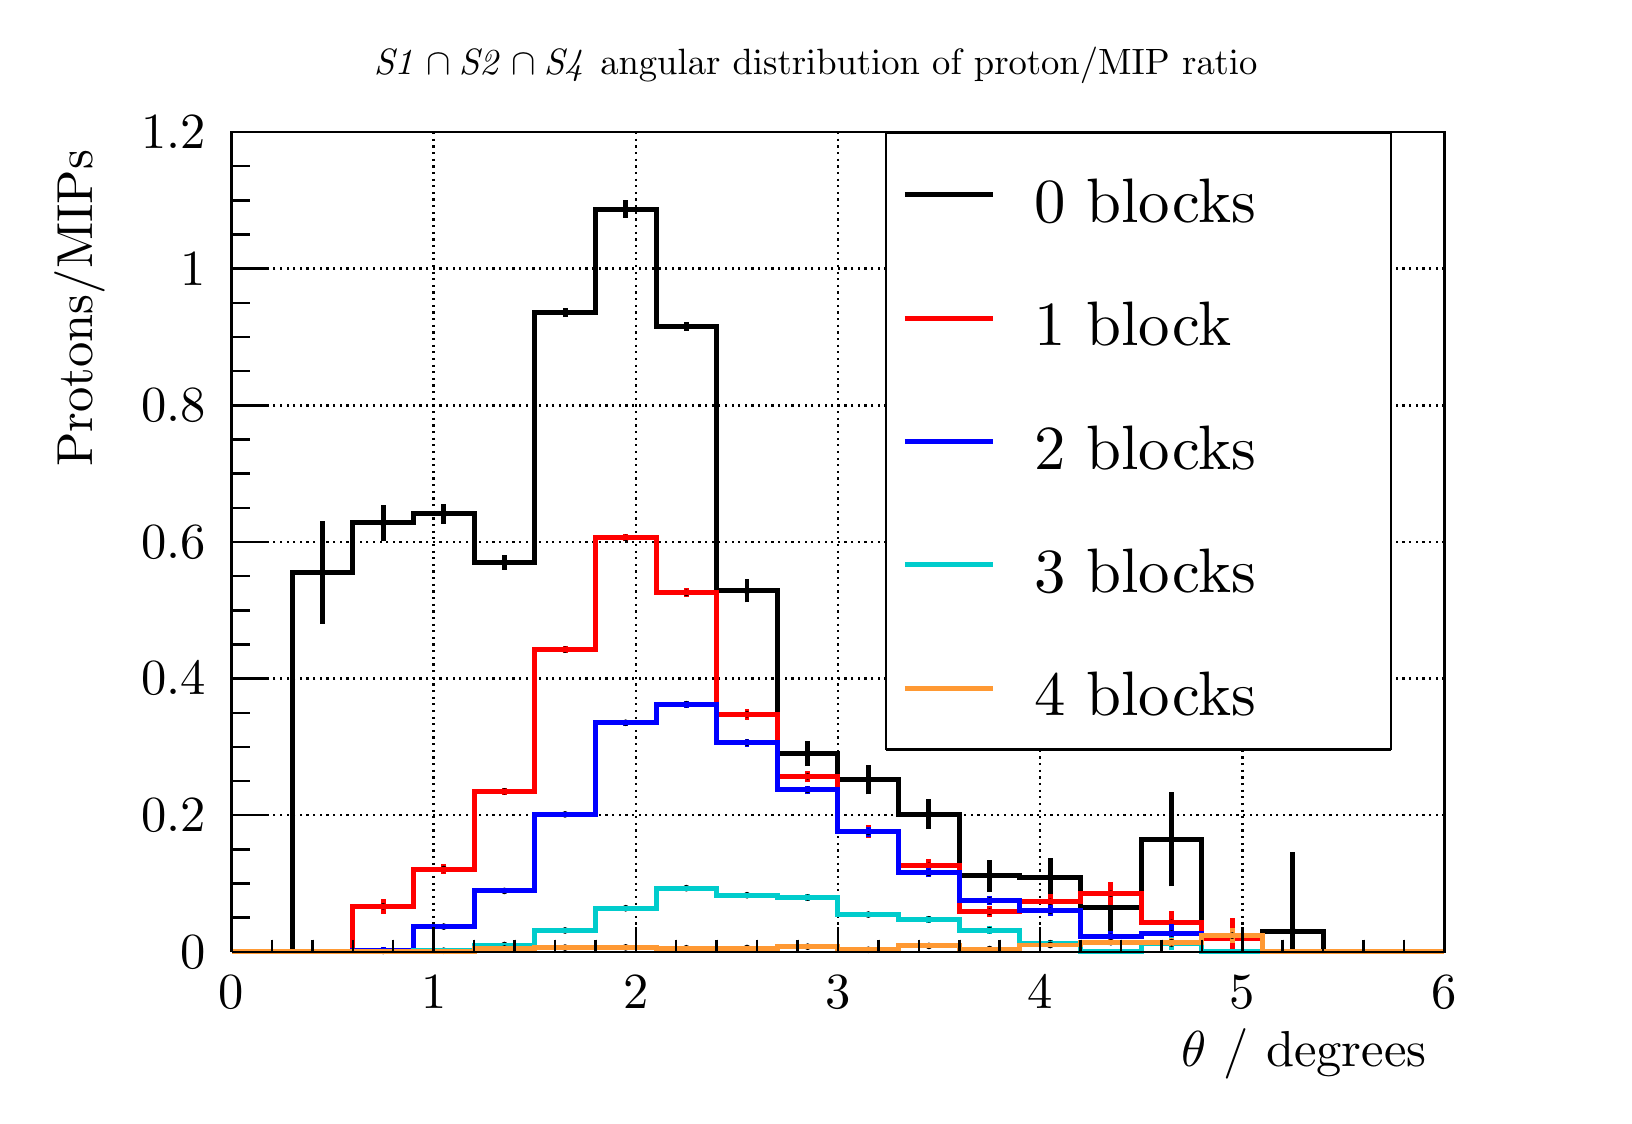
\begin{tikzpicture}
\pgfdeclareplotmark{cross} {
\pgfpathmoveto{\pgfpoint{-0.3\pgfplotmarksize}{\pgfplotmarksize}}
\pgfpathlineto{\pgfpoint{+0.3\pgfplotmarksize}{\pgfplotmarksize}}
\pgfpathlineto{\pgfpoint{+0.3\pgfplotmarksize}{0.3\pgfplotmarksize}}
\pgfpathlineto{\pgfpoint{+1\pgfplotmarksize}{0.3\pgfplotmarksize}}
\pgfpathlineto{\pgfpoint{+1\pgfplotmarksize}{-0.3\pgfplotmarksize}}
\pgfpathlineto{\pgfpoint{+0.3\pgfplotmarksize}{-0.3\pgfplotmarksize}}
\pgfpathlineto{\pgfpoint{+0.3\pgfplotmarksize}{-1.\pgfplotmarksize}}
\pgfpathlineto{\pgfpoint{-0.3\pgfplotmarksize}{-1.\pgfplotmarksize}}
\pgfpathlineto{\pgfpoint{-0.3\pgfplotmarksize}{-0.3\pgfplotmarksize}}
\pgfpathlineto{\pgfpoint{-1.\pgfplotmarksize}{-0.3\pgfplotmarksize}}
\pgfpathlineto{\pgfpoint{-1.\pgfplotmarksize}{0.3\pgfplotmarksize}}
\pgfpathlineto{\pgfpoint{-0.3\pgfplotmarksize}{0.3\pgfplotmarksize}}
\pgfpathclose
\pgfusepathqstroke
}
\pgfdeclareplotmark{cross*} {
\pgfpathmoveto{\pgfpoint{-0.3\pgfplotmarksize}{\pgfplotmarksize}}
\pgfpathlineto{\pgfpoint{+0.3\pgfplotmarksize}{\pgfplotmarksize}}
\pgfpathlineto{\pgfpoint{+0.3\pgfplotmarksize}{0.3\pgfplotmarksize}}
\pgfpathlineto{\pgfpoint{+1\pgfplotmarksize}{0.3\pgfplotmarksize}}
\pgfpathlineto{\pgfpoint{+1\pgfplotmarksize}{-0.3\pgfplotmarksize}}
\pgfpathlineto{\pgfpoint{+0.3\pgfplotmarksize}{-0.3\pgfplotmarksize}}
\pgfpathlineto{\pgfpoint{+0.3\pgfplotmarksize}{-1.\pgfplotmarksize}}
\pgfpathlineto{\pgfpoint{-0.3\pgfplotmarksize}{-1.\pgfplotmarksize}}
\pgfpathlineto{\pgfpoint{-0.3\pgfplotmarksize}{-0.3\pgfplotmarksize}}
\pgfpathlineto{\pgfpoint{-1.\pgfplotmarksize}{-0.3\pgfplotmarksize}}
\pgfpathlineto{\pgfpoint{-1.\pgfplotmarksize}{0.3\pgfplotmarksize}}
\pgfpathlineto{\pgfpoint{-0.3\pgfplotmarksize}{0.3\pgfplotmarksize}}
\pgfpathclose
\pgfusepathqfillstroke
}
\pgfdeclareplotmark{newstar} {
\pgfpathmoveto{\pgfqpoint{0pt}{\pgfplotmarksize}}
\pgfpathlineto{\pgfqpointpolar{44}{0.5\pgfplotmarksize}}
\pgfpathlineto{\pgfqpointpolar{18}{\pgfplotmarksize}}
\pgfpathlineto{\pgfqpointpolar{-20}{0.5\pgfplotmarksize}}
\pgfpathlineto{\pgfqpointpolar{-54}{\pgfplotmarksize}}
\pgfpathlineto{\pgfqpointpolar{-90}{0.5\pgfplotmarksize}}
\pgfpathlineto{\pgfqpointpolar{234}{\pgfplotmarksize}}
\pgfpathlineto{\pgfqpointpolar{198}{0.5\pgfplotmarksize}}
\pgfpathlineto{\pgfqpointpolar{162}{\pgfplotmarksize}}
\pgfpathlineto{\pgfqpointpolar{134}{0.5\pgfplotmarksize}}
\pgfpathclose
\pgfusepathqstroke
}
\pgfdeclareplotmark{newstar*} {
\pgfpathmoveto{\pgfqpoint{0pt}{\pgfplotmarksize}}
\pgfpathlineto{\pgfqpointpolar{44}{0.5\pgfplotmarksize}}
\pgfpathlineto{\pgfqpointpolar{18}{\pgfplotmarksize}}
\pgfpathlineto{\pgfqpointpolar{-20}{0.5\pgfplotmarksize}}
\pgfpathlineto{\pgfqpointpolar{-54}{\pgfplotmarksize}}
\pgfpathlineto{\pgfqpointpolar{-90}{0.5\pgfplotmarksize}}
\pgfpathlineto{\pgfqpointpolar{234}{\pgfplotmarksize}}
\pgfpathlineto{\pgfqpointpolar{198}{0.5\pgfplotmarksize}}
\pgfpathlineto{\pgfqpointpolar{162}{\pgfplotmarksize}}
\pgfpathlineto{\pgfqpointpolar{134}{0.5\pgfplotmarksize}}
\pgfpathclose
\pgfusepathqfillstroke
}
\definecolor{c}{rgb}{1,1,1};
\draw [color=c, fill=c] (0,0) rectangle (20,13.5319);
\draw [color=c, fill=c] (2.58156,1.80142) rectangle (17.9858,12.2128);
\definecolor{c}{rgb}{0,0,0};
\draw [c,line width=0.9] (2.58156,1.80142) -- (2.58156,12.2128) -- (17.9858,12.2128) -- (17.9858,1.80142) -- (2.58156,1.80142);
\definecolor{c}{rgb}{1,1,1};
\draw [color=c, fill=c] (2.58156,1.80142) rectangle (17.9858,12.2128);
\definecolor{c}{rgb}{0,0,0};
\draw [c,line width=0.9] (2.58156,1.80142) -- (2.58156,12.2128) -- (17.9858,12.2128) -- (17.9858,1.80142) -- (2.58156,1.80142);
\draw [c,line width=0.9] (2.58156,1.80142) -- (17.9858,1.80142);
\draw [c,dash pattern=on 0.80pt off 1.60pt ,line width=0.9] (2.58156,12.2128) -- (2.58156,1.80142);
\draw [c,dash pattern=on 0.80pt off 1.60pt ,line width=0.9] (5.14894,12.2128) -- (5.14894,1.80142);
\draw [c,dash pattern=on 0.80pt off 1.60pt ,line width=0.9] (7.71631,12.2128) -- (7.71631,1.80142);
\draw [c,dash pattern=on 0.80pt off 1.60pt ,line width=0.9] (10.2837,12.2128) -- (10.2837,1.80142);
\draw [c,dash pattern=on 0.80pt off 1.60pt ,line width=0.9] (12.8511,12.2128) -- (12.8511,1.80142);
\draw [c,dash pattern=on 0.80pt off 1.60pt ,line width=0.9] (15.4184,12.2128) -- (15.4184,1.80142);
\draw [c,dash pattern=on 0.80pt off 1.60pt ,line width=0.9] (17.9858,12.2128) -- (17.9858,1.80142);
\draw [c,line width=0.9] (2.58156,1.80142) -- (2.58156,12.2128);
\draw [c,dash pattern=on 0.80pt off 1.60pt ,line width=0.9] (17.9858,1.80142) -- (2.58156,1.80142);
\draw [c,dash pattern=on 0.80pt off 1.60pt ,line width=0.9] (17.9858,3.53664) -- (2.58156,3.53664);
\draw [c,dash pattern=on 0.80pt off 1.60pt ,line width=0.9] (17.9858,5.27187) -- (2.58156,5.27187);
\draw [c,dash pattern=on 0.80pt off 1.60pt ,line width=0.9] (17.9858,7.00709) -- (2.58156,7.00709);
\draw [c,dash pattern=on 0.80pt off 1.60pt ,line width=0.9] (17.9858,8.74232) -- (2.58156,8.74232);
\draw [c,dash pattern=on 0.80pt off 1.60pt ,line width=0.9] (17.9858,10.4775) -- (2.58156,10.4775);
\draw [c,dash pattern=on 0.80pt off 1.60pt ,line width=0.9] (17.9858,12.2128) -- (2.58156,12.2128);
\draw [c,dash pattern=on 0.80pt off 1.60pt ,line width=0.9] (17.9858,12.2128) -- (2.58156,12.2128);
\definecolor{c}{rgb}{0,0,0.6};
\draw [c,line width=0.9] (2.58156,1.80142) -- (3.35177,1.80142) -- (3.35177,1.80142) -- (4.12199,1.80142) -- (4.12199,1.80142) -- (4.8922,1.80142) -- (4.8922,1.80142) -- (5.66241,1.80142) -- (5.66241,1.80142) -- (6.43262,1.80142) -- (6.43262,1.80142)
 -- (7.20284,1.80142) -- (7.20284,1.80142) -- (7.97305,1.80142) -- (7.97305,1.80142) -- (8.74326,1.80142) -- (8.74326,1.80142) -- (9.51348,1.80142) -- (9.51348,1.80142) -- (10.2837,1.80142) -- (10.2837,1.80142) -- (11.0539,1.80142) --
 (11.0539,1.80142) -- (11.8241,1.80142) -- (11.8241,1.80142) -- (12.5943,1.80142) -- (12.5943,1.80142) -- (13.3645,1.80142) -- (13.3645,1.80142) -- (14.1348,1.80142) -- (14.1348,1.80142) -- (14.905,1.80142) -- (14.905,1.80142) -- (15.6752,1.80142) --
 (15.6752,1.80142) -- (16.4454,1.80142) -- (16.4454,1.80142) -- (17.2156,1.80142) -- (17.2156,1.80142) -- (17.9858,1.80142);
\definecolor{c}{rgb}{0,0,0};
\draw [c,line width=0.9] (2.58156,1.80142) -- (17.9858,1.80142);
\draw [c,line width=0.9] (2.58156,2.11409) -- (2.58156,1.80142);
\draw [c,line width=0.9] (3.09504,1.95776) -- (3.09504,1.80142);
\draw [c,line width=0.9] (3.60851,1.95776) -- (3.60851,1.80142);
\draw [c,line width=0.9] (4.12199,1.95776) -- (4.12199,1.80142);
\draw [c,line width=0.9] (4.63546,1.95776) -- (4.63546,1.80142);
\draw [c,line width=0.9] (5.14894,2.11409) -- (5.14894,1.80142);
\draw [c,line width=0.9] (5.66241,1.95776) -- (5.66241,1.80142);
\draw [c,line width=0.9] (6.17589,1.95776) -- (6.17589,1.80142);
\draw [c,line width=0.9] (6.68936,1.95776) -- (6.68936,1.80142);
\draw [c,line width=0.9] (7.20284,1.95776) -- (7.20284,1.80142);
\draw [c,line width=0.9] (7.71631,2.11409) -- (7.71631,1.80142);
\draw [c,line width=0.9] (8.22979,1.95776) -- (8.22979,1.80142);
\draw [c,line width=0.9] (8.74326,1.95776) -- (8.74326,1.80142);
\draw [c,line width=0.9] (9.25674,1.95776) -- (9.25674,1.80142);
\draw [c,line width=0.9] (9.77021,1.95776) -- (9.77021,1.80142);
\draw [c,line width=0.9] (10.2837,2.11409) -- (10.2837,1.80142);
\draw [c,line width=0.9] (10.7972,1.95776) -- (10.7972,1.80142);
\draw [c,line width=0.9] (11.3106,1.95776) -- (11.3106,1.80142);
\draw [c,line width=0.9] (11.8241,1.95776) -- (11.8241,1.80142);
\draw [c,line width=0.9] (12.3376,1.95776) -- (12.3376,1.80142);
\draw [c,line width=0.9] (12.8511,2.11409) -- (12.8511,1.80142);
\draw [c,line width=0.9] (13.3645,1.95776) -- (13.3645,1.80142);
\draw [c,line width=0.9] (13.878,1.95776) -- (13.878,1.80142);
\draw [c,line width=0.9] (14.3915,1.95776) -- (14.3915,1.80142);
\draw [c,line width=0.9] (14.905,1.95776) -- (14.905,1.80142);
\draw [c,line width=0.9] (15.4184,2.11409) -- (15.4184,1.80142);
\draw [c,line width=0.9] (15.9319,1.95776) -- (15.9319,1.80142);
\draw [c,line width=0.9] (16.4454,1.95776) -- (16.4454,1.80142);
\draw [c,line width=0.9] (16.9589,1.95776) -- (16.9589,1.80142);
\draw [c,line width=0.9] (17.4723,1.95776) -- (17.4723,1.80142);
\draw [c,line width=0.9] (17.9858,2.11409) -- (17.9858,1.80142);
\draw [anchor=base] (2.58156,1.08423) node[scale=1.82718, color=c, rotate=0]{0};
\draw [anchor=base] (5.14894,1.08423) node[scale=1.82718, color=c, rotate=0]{1};
\draw [anchor=base] (7.71631,1.08423) node[scale=1.82718, color=c, rotate=0]{2};
\draw [anchor=base] (10.2837,1.08423) node[scale=1.82718, color=c, rotate=0]{3};
\draw [anchor=base] (12.8511,1.08423) node[scale=1.82718, color=c, rotate=0]{4};
\draw [anchor=base] (15.4184,1.08423) node[scale=1.82718, color=c, rotate=0]{5};
\draw [anchor=base] (17.9858,1.08423) node[scale=1.82718, color=c, rotate=0]{6};
\draw [anchor= east] (17.9858,0.502355) node[scale=1.82718, color=c, rotate=0]{$\theta$ / degrees};
\draw [c,line width=0.9] (2.58156,1.80142) -- (2.58156,12.2128);
\draw [c,line width=0.9] (3.0432,1.80142) -- (2.58156,1.80142);
\draw [c,line width=0.9] (2.81238,2.23522) -- (2.58156,2.23522);
\draw [c,line width=0.9] (2.81238,2.66903) -- (2.58156,2.66903);
\draw [c,line width=0.9] (2.81238,3.10284) -- (2.58156,3.10284);
\draw [c,line width=0.9] (3.0432,3.53664) -- (2.58156,3.53664);
\draw [c,line width=0.9] (2.81238,3.97045) -- (2.58156,3.97045);
\draw [c,line width=0.9] (2.81238,4.40426) -- (2.58156,4.40426);
\draw [c,line width=0.9] (2.81238,4.83806) -- (2.58156,4.83806);
\draw [c,line width=0.9] (3.0432,5.27187) -- (2.58156,5.27187);
\draw [c,line width=0.9] (2.81238,5.70567) -- (2.58156,5.70567);
\draw [c,line width=0.9] (2.81238,6.13948) -- (2.58156,6.13948);
\draw [c,line width=0.9] (2.81238,6.57329) -- (2.58156,6.57329);
\draw [c,line width=0.9] (3.0432,7.00709) -- (2.58156,7.00709);
\draw [c,line width=0.9] (2.81238,7.4409) -- (2.58156,7.4409);
\draw [c,line width=0.9] (2.81238,7.8747) -- (2.58156,7.8747);
\draw [c,line width=0.9] (2.81238,8.30851) -- (2.58156,8.30851);
\draw [c,line width=0.9] (3.0432,8.74232) -- (2.58156,8.74232);
\draw [c,line width=0.9] (2.81238,9.17612) -- (2.58156,9.17612);
\draw [c,line width=0.9] (2.81238,9.60993) -- (2.58156,9.60993);
\draw [c,line width=0.9] (2.81238,10.0437) -- (2.58156,10.0437);
\draw [c,line width=0.9] (3.0432,10.4775) -- (2.58156,10.4775);
\draw [c,line width=0.9] (2.81238,10.9113) -- (2.58156,10.9113);
\draw [c,line width=0.9] (2.81238,11.3452) -- (2.58156,11.3452);
\draw [c,line width=0.9] (2.81238,11.779) -- (2.58156,11.779);
\draw [c,line width=0.9] (3.0432,12.2128) -- (2.58156,12.2128);
\draw [c,line width=0.9] (3.0432,12.2128) -- (2.58156,12.2128);
\draw [anchor= east] (2.48156,1.80142) node[scale=1.82718, color=c, rotate=0]{0};
\draw [anchor= east] (2.48156,3.53664) node[scale=1.82718, color=c, rotate=0]{0.2};
\draw [anchor= east] (2.48156,5.27187) node[scale=1.82718, color=c, rotate=0]{0.4};
\draw [anchor= east] (2.48156,7.00709) node[scale=1.82718, color=c, rotate=0]{0.6};
\draw [anchor= east] (2.48156,8.74232) node[scale=1.82718, color=c, rotate=0]{0.8};
\draw [anchor= east] (2.48156,10.4775) node[scale=1.82718, color=c, rotate=0]{1};
\draw [anchor= east] (2.48156,12.2128) node[scale=1.82718, color=c, rotate=0]{1.2};
\draw [anchor= east] (0.66156,12.2128) node[scale=1.82718, color=c, rotate=90]{ Protons/MIPs};
\draw [c,line width=1.8] (3.73688,5.96909) -- (3.73688,6.61835);
\draw [c,line width=1.8] (3.73688,6.61835) -- (3.73688,7.26762);
\foreach \P in {(3.73688,6.61835)}{\draw[mark options={color=c,fill=c},mark size=2.402402pt,mark=*,mark size=1pt] plot coordinates {\P};}
\draw [c,line width=1.8] (4.50709,7.01665) -- (4.50709,7.24975);
\draw [c,line width=1.8] (4.50709,7.24975) -- (4.50709,7.48286);
\foreach \P in {(4.50709,7.24975)}{\draw[mark options={color=c,fill=c},mark size=2.402402pt,mark=*,mark size=1pt] plot coordinates {\P};}
\draw [c,line width=1.8] (5.27731,7.23951) -- (5.27731,7.36405);
\draw [c,line width=1.8] (5.27731,7.36405) -- (5.27731,7.4886);
\foreach \P in {(5.27731,7.36405)}{\draw[mark options={color=c,fill=c},mark size=2.402402pt,mark=*,mark size=1pt] plot coordinates {\P};}
\draw [c,line width=1.8] (6.04752,6.65693) -- (6.04752,6.75156);
\draw [c,line width=1.8] (6.04752,6.75156) -- (6.04752,6.8462);
\foreach \P in {(6.04752,6.75156)}{\draw[mark options={color=c,fill=c},mark size=2.402402pt,mark=*,mark size=1pt] plot coordinates {\P};}
\draw [c,line width=1.8] (6.81773,9.86403) -- (6.81773,9.92111);
\draw [c,line width=1.8] (6.81773,9.92111) -- (6.81773,9.97818);
\foreach \P in {(6.81773,9.92111)}{\draw[mark options={color=c,fill=c},mark size=2.402402pt,mark=*,mark size=1pt] plot coordinates {\P};}
\draw [c,line width=1.8] (7.58794,11.1257) -- (7.58794,11.2349);
\draw [c,line width=1.8] (7.58794,11.2349) -- (7.58794,11.3441);
\foreach \P in {(7.58794,11.2349)}{\draw[mark options={color=c,fill=c},mark size=2.402402pt,mark=*,mark size=1pt] plot coordinates {\P};}
\draw [c,line width=1.8] (8.35816,9.68957) -- (8.35816,9.74459);
\draw [c,line width=1.8] (8.35816,9.74459) -- (8.35816,9.7996);
\foreach \P in {(8.35816,9.74459)}{\draw[mark options={color=c,fill=c},mark size=2.402402pt,mark=*,mark size=1pt] plot coordinates {\P};}
\draw [c,line width=1.8] (9.12837,6.24154) -- (9.12837,6.38654);
\draw [c,line width=1.8] (9.12837,6.38654) -- (9.12837,6.53154);
\foreach \P in {(9.12837,6.38654)}{\draw[mark options={color=c,fill=c},mark size=2.402402pt,mark=*,mark size=1pt] plot coordinates {\P};}
\draw [c,line width=1.8] (9.89858,4.16117) -- (9.89858,4.3187);
\draw [c,line width=1.8] (9.89858,4.3187) -- (9.89858,4.47623);
\foreach \P in {(9.89858,4.3187)}{\draw[mark options={color=c,fill=c},mark size=2.402402pt,mark=*,mark size=1pt] plot coordinates {\P};}
\draw [c,line width=1.8] (10.6688,3.80166) -- (10.6688,3.99015);
\draw [c,line width=1.8] (10.6688,3.99015) -- (10.6688,4.17865);
\foreach \P in {(10.6688,3.99015)}{\draw[mark options={color=c,fill=c},mark size=2.402402pt,mark=*,mark size=1pt] plot coordinates {\P};}
\draw [c,line width=1.8] (11.439,3.36091) -- (11.439,3.55216);
\draw [c,line width=1.8] (11.439,3.55216) -- (11.439,3.7434);
\foreach \P in {(11.439,3.55216)}{\draw[mark options={color=c,fill=c},mark size=2.402402pt,mark=*,mark size=1pt] plot coordinates {\P};}
\draw [c,line width=1.8] (12.2092,2.56466) -- (12.2092,2.76596);
\draw [c,line width=1.8] (12.2092,2.76596) -- (12.2092,2.96726);
\foreach \P in {(12.2092,2.76596)}{\draw[mark options={color=c,fill=c},mark size=2.402402pt,mark=*,mark size=1pt] plot coordinates {\P};}
\draw [c,line width=1.8] (12.9794,2.50973) -- (12.9794,2.75162);
\draw [c,line width=1.8] (12.9794,2.75162) -- (12.9794,2.9935);
\foreach \P in {(12.9794,2.75162)}{\draw[mark options={color=c,fill=c},mark size=2.402402pt,mark=*,mark size=1pt] plot coordinates {\P};}
\draw [c,line width=1.8] (13.7496,2.0489) -- (13.7496,2.36584);
\draw [c,line width=1.8] (13.7496,2.36584) -- (13.7496,2.68279);
\foreach \P in {(13.7496,2.36584)}{\draw[mark options={color=c,fill=c},mark size=2.402402pt,mark=*,mark size=1pt] plot coordinates {\P};}
\draw [c,line width=1.8] (14.5199,2.63323) -- (14.5199,3.23146);
\draw [c,line width=1.8] (14.5199,3.23146) -- (14.5199,3.82969);
\foreach \P in {(14.5199,3.23146)}{\draw[mark options={color=c,fill=c},mark size=2.402402pt,mark=*,mark size=1pt] plot coordinates {\P};}
\draw [c,line width=1.8] (16.0603,1.80142) -- (16.0603,2.06459);
\draw [c,line width=1.8] (16.0603,2.06459) -- (16.0603,3.06406);
\foreach \P in {(16.0603,2.06459)}{\draw[mark options={color=c,fill=c},mark size=2.402402pt,mark=*,mark size=1pt] plot coordinates {\P};}
\draw [c,line width=1.8] (2.58156,1.80142) -- (3.35177,1.80142) -- (3.35177,6.61835) -- (4.12199,6.61835) -- (4.12199,7.24975) -- (4.8922,7.24975) -- (4.8922,7.36405) -- (5.66241,7.36405) -- (5.66241,6.75156) -- (6.43262,6.75156) -- (6.43262,9.92111)
 -- (7.20284,9.92111) -- (7.20284,11.2349) -- (7.97305,11.2349) -- (7.97305,9.74459) -- (8.74326,9.74459) -- (8.74326,6.38654) -- (9.51348,6.38654) -- (9.51348,4.3187) -- (10.2837,4.3187) -- (10.2837,3.99015) -- (11.0539,3.99015) -- (11.0539,3.55216)
 -- (11.8241,3.55216) -- (11.8241,2.76596) -- (12.5943,2.76596) -- (12.5943,2.75162) -- (13.3645,2.75162) -- (13.3645,2.36584) -- (14.1348,2.36584) -- (14.1348,3.23146) -- (14.905,3.23146) -- (14.905,1.80142) -- (15.6752,1.80142) -- (15.6752,2.06459)
 -- (16.4454,2.06459) -- (16.4454,1.80142) -- (17.2156,1.80142) -- (17.2156,1.80142) -- (17.9858,1.80142);
\definecolor{c}{rgb}{1,0,0};
\draw [c,line width=1.8] (4.50709,2.28567) -- (4.50709,2.37944);
\draw [c,line width=1.8] (4.50709,2.37944) -- (4.50709,2.47322);
\definecolor{c}{rgb}{0,0,0};
\foreach \P in {(4.50709,2.37944)}{\draw[mark options={color=c,fill=c},mark size=2.402402pt,mark=*,mark size=1pt] plot coordinates {\P};}
\definecolor{c}{rgb}{1,0,0};
\draw [c,line width=1.8] (5.27731,2.79594) -- (5.27731,2.85369);
\draw [c,line width=1.8] (5.27731,2.85369) -- (5.27731,2.91144);
\definecolor{c}{rgb}{0,0,0};
\foreach \P in {(5.27731,2.85369)}{\draw[mark options={color=c,fill=c},mark size=2.402402pt,mark=*,mark size=1pt] plot coordinates {\P};}
\definecolor{c}{rgb}{1,0,0};
\draw [c,line width=1.8] (6.04752,3.79475) -- (6.04752,3.8403);
\draw [c,line width=1.8] (6.04752,3.8403) -- (6.04752,3.88585);
\definecolor{c}{rgb}{0,0,0};
\foreach \P in {(6.04752,3.8403)}{\draw[mark options={color=c,fill=c},mark size=2.402402pt,mark=*,mark size=1pt] plot coordinates {\P};}
\definecolor{c}{rgb}{1,0,0};
\draw [c,line width=1.8] (6.81773,5.59646) -- (6.81773,5.64017);
\draw [c,line width=1.8] (6.81773,5.64017) -- (6.81773,5.68388);
\definecolor{c}{rgb}{0,0,0};
\foreach \P in {(6.81773,5.64017)}{\draw[mark options={color=c,fill=c},mark size=2.402402pt,mark=*,mark size=1pt] plot coordinates {\P};}
\definecolor{c}{rgb}{1,0,0};
\draw [c,line width=1.8] (7.58794,7.01498) -- (7.58794,7.05941);
\draw [c,line width=1.8] (7.58794,7.05941) -- (7.58794,7.10384);
\definecolor{c}{rgb}{0,0,0};
\foreach \P in {(7.58794,7.05941)}{\draw[mark options={color=c,fill=c},mark size=2.402402pt,mark=*,mark size=1pt] plot coordinates {\P};}
\definecolor{c}{rgb}{1,0,0};
\draw [c,line width=1.8] (8.35816,6.30632) -- (8.35816,6.36152);
\draw [c,line width=1.8] (8.35816,6.36152) -- (8.35816,6.41672);
\definecolor{c}{rgb}{0,0,0};
\foreach \P in {(8.35816,6.36152)}{\draw[mark options={color=c,fill=c},mark size=2.402402pt,mark=*,mark size=1pt] plot coordinates {\P};}
\definecolor{c}{rgb}{1,0,0};
\draw [c,line width=1.8] (9.12837,4.74977) -- (9.12837,4.81839);
\draw [c,line width=1.8] (9.12837,4.81839) -- (9.12837,4.88701);
\definecolor{c}{rgb}{0,0,0};
\foreach \P in {(9.12837,4.81839)}{\draw[mark options={color=c,fill=c},mark size=2.402402pt,mark=*,mark size=1pt] plot coordinates {\P};}
\definecolor{c}{rgb}{1,0,0};
\draw [c,line width=1.8] (9.89858,3.95546) -- (9.89858,4.03007);
\draw [c,line width=1.8] (9.89858,4.03007) -- (9.89858,4.10467);
\definecolor{c}{rgb}{0,0,0};
\foreach \P in {(9.89858,4.03007)}{\draw[mark options={color=c,fill=c},mark size=2.402402pt,mark=*,mark size=1pt] plot coordinates {\P};}
\definecolor{c}{rgb}{1,0,0};
\draw [c,line width=1.8] (10.6688,3.24766) -- (10.6688,3.32829);
\draw [c,line width=1.8] (10.6688,3.32829) -- (10.6688,3.40892);
\definecolor{c}{rgb}{0,0,0};
\foreach \P in {(10.6688,3.32829)}{\draw[mark options={color=c,fill=c},mark size=2.402402pt,mark=*,mark size=1pt] plot coordinates {\P};}
\definecolor{c}{rgb}{1,0,0};
\draw [c,line width=1.8] (11.439,2.81238) -- (11.439,2.89504);
\draw [c,line width=1.8] (11.439,2.89504) -- (11.439,2.97769);
\definecolor{c}{rgb}{0,0,0};
\foreach \P in {(11.439,2.89504)}{\draw[mark options={color=c,fill=c},mark size=2.402402pt,mark=*,mark size=1pt] plot coordinates {\P};}
\definecolor{c}{rgb}{1,0,0};
\draw [c,line width=1.8] (12.2092,2.24132) -- (12.2092,2.31194);
\draw [c,line width=1.8] (12.2092,2.31194) -- (12.2092,2.38256);
\definecolor{c}{rgb}{0,0,0};
\foreach \P in {(12.2092,2.31194)}{\draw[mark options={color=c,fill=c},mark size=2.402402pt,mark=*,mark size=1pt] plot coordinates {\P};}
\definecolor{c}{rgb}{1,0,0};
\draw [c,line width=1.8] (12.9794,2.33711) -- (12.9794,2.43758);
\draw [c,line width=1.8] (12.9794,2.43758) -- (12.9794,2.53805);
\definecolor{c}{rgb}{0,0,0};
\foreach \P in {(12.9794,2.43758)}{\draw[mark options={color=c,fill=c},mark size=2.402402pt,mark=*,mark size=1pt] plot coordinates {\P};}
\definecolor{c}{rgb}{1,0,0};
\draw [c,line width=1.8] (13.7496,2.39958) -- (13.7496,2.54141);
\draw [c,line width=1.8] (13.7496,2.54141) -- (13.7496,2.68324);
\definecolor{c}{rgb}{0,0,0};
\foreach \P in {(13.7496,2.54141)}{\draw[mark options={color=c,fill=c},mark size=2.402402pt,mark=*,mark size=1pt] plot coordinates {\P};}
\definecolor{c}{rgb}{1,0,0};
\draw [c,line width=1.8] (14.5199,2.01609) -- (14.5199,2.17081);
\draw [c,line width=1.8] (14.5199,2.17081) -- (14.5199,2.32553);
\definecolor{c}{rgb}{0,0,0};
\foreach \P in {(14.5199,2.17081)}{\draw[mark options={color=c,fill=c},mark size=2.402402pt,mark=*,mark size=1pt] plot coordinates {\P};}
\definecolor{c}{rgb}{1,0,0};
\draw [c,line width=1.8] (15.2901,1.80142) -- (15.2901,1.9743);
\draw [c,line width=1.8] (15.2901,1.9743) -- (15.2901,2.22633);
\definecolor{c}{rgb}{0,0,0};
\foreach \P in {(15.2901,1.9743)}{\draw[mark options={color=c,fill=c},mark size=2.402402pt,mark=*,mark size=1pt] plot coordinates {\P};}
\definecolor{c}{rgb}{1,0,0};
\draw [c,line width=1.8] (2.58156,1.80142) -- (3.35177,1.80142) -- (3.35177,1.80142) -- (4.12199,1.80142) -- (4.12199,2.37944) -- (4.8922,2.37944) -- (4.8922,2.85369) -- (5.66241,2.85369) -- (5.66241,3.8403) -- (6.43262,3.8403) -- (6.43262,5.64017)
 -- (7.20284,5.64017) -- (7.20284,7.05941) -- (7.97305,7.05941) -- (7.97305,6.36152) -- (8.74326,6.36152) -- (8.74326,4.81839) -- (9.51348,4.81839) -- (9.51348,4.03007) -- (10.2837,4.03007) -- (10.2837,3.32829) -- (11.0539,3.32829) --
 (11.0539,2.89504) -- (11.8241,2.89504) -- (11.8241,2.31194) -- (12.5943,2.31194) -- (12.5943,2.43758) -- (13.3645,2.43758) -- (13.3645,2.54141) -- (14.1348,2.54141) -- (14.1348,2.17081) -- (14.905,2.17081) -- (14.905,1.9743) -- (15.6752,1.9743) --
 (15.6752,1.80142) -- (16.4454,1.80142) -- (16.4454,1.80142) -- (17.2156,1.80142) -- (17.2156,1.80142) -- (17.9858,1.80142);
\definecolor{c}{rgb}{0,0,1};
\draw [c,line width=1.8] (4.50709,1.80142) -- (4.50709,1.81398);
\draw [c,line width=1.8] (4.50709,1.81398) -- (4.50709,1.86696);
\definecolor{c}{rgb}{0,0,0};
\foreach \P in {(4.50709,1.81398)}{\draw[mark options={color=c,fill=c},mark size=2.402402pt,mark=*,mark size=1pt] plot coordinates {\P};}
\definecolor{c}{rgb}{0,0,1};
\draw [c,line width=1.8] (5.27731,2.09007) -- (5.27731,2.12258);
\draw [c,line width=1.8] (5.27731,2.12258) -- (5.27731,2.15509);
\definecolor{c}{rgb}{0,0,0};
\foreach \P in {(5.27731,2.12258)}{\draw[mark options={color=c,fill=c},mark size=2.402402pt,mark=*,mark size=1pt] plot coordinates {\P};}
\definecolor{c}{rgb}{0,0,1};
\draw [c,line width=1.8] (6.04752,2.54822) -- (6.04752,2.57576);
\draw [c,line width=1.8] (6.04752,2.57576) -- (6.04752,2.60329);
\definecolor{c}{rgb}{0,0,0};
\foreach \P in {(6.04752,2.57576)}{\draw[mark options={color=c,fill=c},mark size=2.402402pt,mark=*,mark size=1pt] plot coordinates {\P};}
\definecolor{c}{rgb}{0,0,1};
\draw [c,line width=1.8] (6.81773,3.51697) -- (6.81773,3.54787);
\draw [c,line width=1.8] (6.81773,3.54787) -- (6.81773,3.57877);
\definecolor{c}{rgb}{0,0,0};
\foreach \P in {(6.81773,3.54787)}{\draw[mark options={color=c,fill=c},mark size=2.402402pt,mark=*,mark size=1pt] plot coordinates {\P};}
\definecolor{c}{rgb}{0,0,1};
\draw [c,line width=1.8] (7.58794,4.67507) -- (7.58794,4.71136);
\draw [c,line width=1.8] (7.58794,4.71136) -- (7.58794,4.74765);
\definecolor{c}{rgb}{0,0,0};
\foreach \P in {(7.58794,4.71136)}{\draw[mark options={color=c,fill=c},mark size=2.402402pt,mark=*,mark size=1pt] plot coordinates {\P};}
\definecolor{c}{rgb}{0,0,1};
\draw [c,line width=1.8] (8.35816,4.90264) -- (8.35816,4.94582);
\draw [c,line width=1.8] (8.35816,4.94582) -- (8.35816,4.989);
\definecolor{c}{rgb}{0,0,0};
\foreach \P in {(8.35816,4.94582)}{\draw[mark options={color=c,fill=c},mark size=2.402402pt,mark=*,mark size=1pt] plot coordinates {\P};}
\definecolor{c}{rgb}{0,0,1};
\draw [c,line width=1.8] (9.12837,4.40846) -- (9.12837,4.45857);
\draw [c,line width=1.8] (9.12837,4.45857) -- (9.12837,4.50869);
\definecolor{c}{rgb}{0,0,0};
\foreach \P in {(9.12837,4.45857)}{\draw[mark options={color=c,fill=c},mark size=2.402402pt,mark=*,mark size=1pt] plot coordinates {\P};}
\definecolor{c}{rgb}{0,0,1};
\draw [c,line width=1.8] (9.89858,3.80403) -- (9.89858,3.85863);
\draw [c,line width=1.8] (9.89858,3.85863) -- (9.89858,3.91322);
\definecolor{c}{rgb}{0,0,0};
\foreach \P in {(9.89858,3.85863)}{\draw[mark options={color=c,fill=c},mark size=2.402402pt,mark=*,mark size=1pt] plot coordinates {\P};}
\definecolor{c}{rgb}{0,0,1};
\draw [c,line width=1.8] (10.6688,3.26646) -- (10.6688,3.32506);
\draw [c,line width=1.8] (10.6688,3.32506) -- (10.6688,3.38365);
\definecolor{c}{rgb}{0,0,0};
\foreach \P in {(10.6688,3.32506)}{\draw[mark options={color=c,fill=c},mark size=2.402402pt,mark=*,mark size=1pt] plot coordinates {\P};}
\definecolor{c}{rgb}{0,0,1};
\draw [c,line width=1.8] (11.439,2.74672) -- (11.439,2.80496);
\draw [c,line width=1.8] (11.439,2.80496) -- (11.439,2.86321);
\definecolor{c}{rgb}{0,0,0};
\foreach \P in {(11.439,2.80496)}{\draw[mark options={color=c,fill=c},mark size=2.402402pt,mark=*,mark size=1pt] plot coordinates {\P};}
\definecolor{c}{rgb}{0,0,1};
\draw [c,line width=1.8] (12.2092,2.39395) -- (12.2092,2.45466);
\draw [c,line width=1.8] (12.2092,2.45466) -- (12.2092,2.51538);
\definecolor{c}{rgb}{0,0,0};
\foreach \P in {(12.2092,2.45466)}{\draw[mark options={color=c,fill=c},mark size=2.402402pt,mark=*,mark size=1pt] plot coordinates {\P};}
\definecolor{c}{rgb}{0,0,1};
\draw [c,line width=1.8] (12.9794,2.25451) -- (12.9794,2.3228);
\draw [c,line width=1.8] (12.9794,2.3228) -- (12.9794,2.3911);
\definecolor{c}{rgb}{0,0,0};
\foreach \P in {(12.9794,2.3228)}{\draw[mark options={color=c,fill=c},mark size=2.402402pt,mark=*,mark size=1pt] plot coordinates {\P};}
\definecolor{c}{rgb}{0,0,1};
\draw [c,line width=1.8] (13.7496,1.91894) -- (13.7496,1.99469);
\draw [c,line width=1.8] (13.7496,1.99469) -- (13.7496,2.07043);
\definecolor{c}{rgb}{0,0,0};
\foreach \P in {(13.7496,1.99469)}{\draw[mark options={color=c,fill=c},mark size=2.402402pt,mark=*,mark size=1pt] plot coordinates {\P};}
\definecolor{c}{rgb}{0,0,1};
\draw [c,line width=1.8] (14.5199,1.91933) -- (14.5199,2.03567);
\draw [c,line width=1.8] (14.5199,2.03567) -- (14.5199,2.152);
\definecolor{c}{rgb}{0,0,0};
\foreach \P in {(14.5199,2.03567)}{\draw[mark options={color=c,fill=c},mark size=2.402402pt,mark=*,mark size=1pt] plot coordinates {\P};}
\definecolor{c}{rgb}{0,0,1};
\draw [c,line width=1.8] (2.58156,1.80142) -- (3.35177,1.80142) -- (3.35177,1.80142) -- (4.12199,1.80142) -- (4.12199,1.81398) -- (4.8922,1.81398) -- (4.8922,2.12258) -- (5.66241,2.12258) -- (5.66241,2.57576) -- (6.43262,2.57576) -- (6.43262,3.54787)
 -- (7.20284,3.54787) -- (7.20284,4.71136) -- (7.97305,4.71136) -- (7.97305,4.94582) -- (8.74326,4.94582) -- (8.74326,4.45857) -- (9.51348,4.45857) -- (9.51348,3.85863) -- (10.2837,3.85863) -- (10.2837,3.32506) -- (11.0539,3.32506) --
 (11.0539,2.80496) -- (11.8241,2.80496) -- (11.8241,2.45466) -- (12.5943,2.45466) -- (12.5943,2.3228) -- (13.3645,2.3228) -- (13.3645,1.99469) -- (14.1348,1.99469) -- (14.1348,2.03567) -- (14.905,2.03567) -- (14.905,1.80142) -- (15.6752,1.80142) --
 (15.6752,1.80142) -- (16.4454,1.80142) -- (16.4454,1.80142) -- (17.2156,1.80142) -- (17.2156,1.80142) -- (17.9858,1.80142);
\definecolor{c}{rgb}{0,0.8,0.8};
\draw [c,line width=1.8] (5.27731,1.80142) -- (5.27731,1.81623);
\draw [c,line width=1.8] (5.27731,1.81623) -- (5.27731,1.83425);
\definecolor{c}{rgb}{0,0,0};
\foreach \P in {(5.27731,1.81623)}{\draw[mark options={color=c,fill=c},mark size=2.402402pt,mark=*,mark size=1pt] plot coordinates {\P};}
\definecolor{c}{rgb}{0,0.8,0.8};
\draw [c,line width=1.8] (6.04752,1.87586) -- (6.04752,1.88848);
\draw [c,line width=1.8] (6.04752,1.88848) -- (6.04752,1.90109);
\definecolor{c}{rgb}{0,0,0};
\foreach \P in {(6.04752,1.88848)}{\draw[mark options={color=c,fill=c},mark size=2.402402pt,mark=*,mark size=1pt] plot coordinates {\P};}
\definecolor{c}{rgb}{0,0.8,0.8};
\draw [c,line width=1.8] (6.81773,2.05676) -- (6.81773,2.07357);
\draw [c,line width=1.8] (6.81773,2.07357) -- (6.81773,2.09039);
\definecolor{c}{rgb}{0,0,0};
\foreach \P in {(6.81773,2.07357)}{\draw[mark options={color=c,fill=c},mark size=2.402402pt,mark=*,mark size=1pt] plot coordinates {\P};}
\definecolor{c}{rgb}{0,0.8,0.8};
\draw [c,line width=1.8] (7.58794,2.33449) -- (7.58794,2.3559);
\draw [c,line width=1.8] (7.58794,2.3559) -- (7.58794,2.37732);
\definecolor{c}{rgb}{0,0,0};
\foreach \P in {(7.58794,2.3559)}{\draw[mark options={color=c,fill=c},mark size=2.402402pt,mark=*,mark size=1pt] plot coordinates {\P};}
\definecolor{c}{rgb}{0,0.8,0.8};
\draw [c,line width=1.8] (8.35816,2.58185) -- (8.35816,2.61084);
\draw [c,line width=1.8] (8.35816,2.61084) -- (8.35816,2.63983);
\definecolor{c}{rgb}{0,0,0};
\foreach \P in {(8.35816,2.61084)}{\draw[mark options={color=c,fill=c},mark size=2.402402pt,mark=*,mark size=1pt] plot coordinates {\P};}
\definecolor{c}{rgb}{0,0.8,0.8};
\draw [c,line width=1.8] (9.12837,2.48791) -- (9.12837,2.52137);
\draw [c,line width=1.8] (9.12837,2.52137) -- (9.12837,2.55483);
\definecolor{c}{rgb}{0,0,0};
\foreach \P in {(9.12837,2.52137)}{\draw[mark options={color=c,fill=c},mark size=2.402402pt,mark=*,mark size=1pt] plot coordinates {\P};}
\definecolor{c}{rgb}{0,0.8,0.8};
\draw [c,line width=1.8] (9.89858,2.45146) -- (9.89858,2.49097);
\draw [c,line width=1.8] (9.89858,2.49097) -- (9.89858,2.53049);
\definecolor{c}{rgb}{0,0,0};
\foreach \P in {(9.89858,2.49097)}{\draw[mark options={color=c,fill=c},mark size=2.402402pt,mark=*,mark size=1pt] plot coordinates {\P};}
\definecolor{c}{rgb}{0,0.8,0.8};
\draw [c,line width=1.8] (10.6688,2.23827) -- (10.6688,2.27536);
\draw [c,line width=1.8] (10.6688,2.27536) -- (10.6688,2.31244);
\definecolor{c}{rgb}{0,0,0};
\foreach \P in {(10.6688,2.27536)}{\draw[mark options={color=c,fill=c},mark size=2.402402pt,mark=*,mark size=1pt] plot coordinates {\P};}
\definecolor{c}{rgb}{0,0.8,0.8};
\draw [c,line width=1.8] (11.439,2.17384) -- (11.439,2.2146);
\draw [c,line width=1.8] (11.439,2.2146) -- (11.439,2.25536);
\definecolor{c}{rgb}{0,0,0};
\foreach \P in {(11.439,2.2146)}{\draw[mark options={color=c,fill=c},mark size=2.402402pt,mark=*,mark size=1pt] plot coordinates {\P};}
\definecolor{c}{rgb}{0,0.8,0.8};
\draw [c,line width=1.8] (12.2092,2.03257) -- (12.2092,2.07819);
\draw [c,line width=1.8] (12.2092,2.07819) -- (12.2092,2.12381);
\definecolor{c}{rgb}{0,0,0};
\foreach \P in {(12.2092,2.07819)}{\draw[mark options={color=c,fill=c},mark size=2.402402pt,mark=*,mark size=1pt] plot coordinates {\P};}
\definecolor{c}{rgb}{0,0.8,0.8};
\draw [c,line width=1.8] (12.9794,1.86791) -- (12.9794,1.91152);
\draw [c,line width=1.8] (12.9794,1.91152) -- (12.9794,1.95513);
\definecolor{c}{rgb}{0,0,0};
\foreach \P in {(12.9794,1.91152)}{\draw[mark options={color=c,fill=c},mark size=2.402402pt,mark=*,mark size=1pt] plot coordinates {\P};}
\definecolor{c}{rgb}{0,0.8,0.8};
\draw [c,line width=1.8] (14.5199,1.82089) -- (14.5199,1.90596);
\draw [c,line width=1.8] (14.5199,1.90596) -- (14.5199,1.99102);
\definecolor{c}{rgb}{0,0,0};
\foreach \P in {(14.5199,1.90596)}{\draw[mark options={color=c,fill=c},mark size=2.402402pt,mark=*,mark size=1pt] plot coordinates {\P};}
\definecolor{c}{rgb}{0,0.8,0.8};
\draw [c,line width=1.8] (2.58156,1.80142) -- (3.35177,1.80142) -- (3.35177,1.80142) -- (4.12199,1.80142) -- (4.12199,1.80142) -- (4.8922,1.80142) -- (4.8922,1.81623) -- (5.66241,1.81623) -- (5.66241,1.88848) -- (6.43262,1.88848) -- (6.43262,2.07357)
 -- (7.20284,2.07357) -- (7.20284,2.3559) -- (7.97305,2.3559) -- (7.97305,2.61084) -- (8.74326,2.61084) -- (8.74326,2.52137) -- (9.51348,2.52137) -- (9.51348,2.49097) -- (10.2837,2.49097) -- (10.2837,2.27536) -- (11.0539,2.27536) -- (11.0539,2.2146)
 -- (11.8241,2.2146) -- (11.8241,2.07819) -- (12.5943,2.07819) -- (12.5943,1.91152) -- (13.3645,1.91152) -- (13.3645,1.80142) -- (14.1348,1.80142) -- (14.1348,1.90596) -- (14.905,1.90596) -- (14.905,1.80142) -- (15.6752,1.80142) -- (15.6752,1.80142)
 -- (16.4454,1.80142) -- (16.4454,1.80142) -- (17.2156,1.80142) -- (17.2156,1.80142) -- (17.9858,1.80142);
\definecolor{c}{rgb}{1,0.6,0.2};
\draw [c,line width=1.8] (6.04752,1.83971) -- (6.04752,1.84442);
\draw [c,line width=1.8] (6.04752,1.84442) -- (6.04752,1.84913);
\definecolor{c}{rgb}{0,0,0};
\foreach \P in {(6.04752,1.84442)}{\draw[mark options={color=c,fill=c},mark size=2.402402pt,mark=*,mark size=1pt] plot coordinates {\P};}
\definecolor{c}{rgb}{1,0.6,0.2};
\draw [c,line width=1.8] (6.81773,1.85005) -- (6.81773,1.85557);
\draw [c,line width=1.8] (6.81773,1.85557) -- (6.81773,1.8611);
\definecolor{c}{rgb}{0,0,0};
\foreach \P in {(6.81773,1.85557)}{\draw[mark options={color=c,fill=c},mark size=2.402402pt,mark=*,mark size=1pt] plot coordinates {\P};}
\definecolor{c}{rgb}{1,0.6,0.2};
\draw [c,line width=1.8] (7.58794,1.85341) -- (7.58794,1.85844);
\draw [c,line width=1.8] (7.58794,1.85844) -- (7.58794,1.86346);
\definecolor{c}{rgb}{0,0,0};
\foreach \P in {(7.58794,1.85844)}{\draw[mark options={color=c,fill=c},mark size=2.402402pt,mark=*,mark size=1pt] plot coordinates {\P};}
\definecolor{c}{rgb}{1,0.6,0.2};
\draw [c,line width=1.8] (8.35816,1.84222) -- (8.35816,1.84696);
\draw [c,line width=1.8] (8.35816,1.84696) -- (8.35816,1.85169);
\definecolor{c}{rgb}{0,0,0};
\foreach \P in {(8.35816,1.84696)}{\draw[mark options={color=c,fill=c},mark size=2.402402pt,mark=*,mark size=1pt] plot coordinates {\P};}
\definecolor{c}{rgb}{1,0.6,0.2};
\draw [c,line width=1.8] (9.12837,1.8428) -- (9.12837,1.85047);
\draw [c,line width=1.8] (9.12837,1.85047) -- (9.12837,1.85814);
\definecolor{c}{rgb}{0,0,0};
\foreach \P in {(9.12837,1.85047)}{\draw[mark options={color=c,fill=c},mark size=2.402402pt,mark=*,mark size=1pt] plot coordinates {\P};}
\definecolor{c}{rgb}{1,0.6,0.2};
\draw [c,line width=1.8] (9.89858,1.85648) -- (9.89858,1.86776);
\draw [c,line width=1.8] (9.89858,1.86776) -- (9.89858,1.87904);
\definecolor{c}{rgb}{0,0,0};
\foreach \P in {(9.89858,1.86776)}{\draw[mark options={color=c,fill=c},mark size=2.402402pt,mark=*,mark size=1pt] plot coordinates {\P};}
\definecolor{c}{rgb}{1,0.6,0.2};
\draw [c,line width=1.8] (10.6688,1.82216) -- (10.6688,1.82784);
\draw [c,line width=1.8] (10.6688,1.82784) -- (10.6688,1.83352);
\definecolor{c}{rgb}{0,0,0};
\foreach \P in {(10.6688,1.82784)}{\draw[mark options={color=c,fill=c},mark size=2.402402pt,mark=*,mark size=1pt] plot coordinates {\P};}
\definecolor{c}{rgb}{1,0.6,0.2};
\draw [c,line width=1.8] (11.439,1.86137) -- (11.439,1.87737);
\draw [c,line width=1.8] (11.439,1.87737) -- (11.439,1.89337);
\definecolor{c}{rgb}{0,0,0};
\foreach \P in {(11.439,1.87737)}{\draw[mark options={color=c,fill=c},mark size=2.402402pt,mark=*,mark size=1pt] plot coordinates {\P};}
\definecolor{c}{rgb}{1,0.6,0.2};
\draw [c,line width=1.8] (12.2092,1.82149) -- (12.2092,1.83714);
\draw [c,line width=1.8] (12.2092,1.83714) -- (12.2092,1.85279);
\definecolor{c}{rgb}{0,0,0};
\foreach \P in {(12.2092,1.83714)}{\draw[mark options={color=c,fill=c},mark size=2.402402pt,mark=*,mark size=1pt] plot coordinates {\P};}
\definecolor{c}{rgb}{1,0.6,0.2};
\draw [c,line width=1.8] (12.9794,1.86026) -- (12.9794,1.8889);
\draw [c,line width=1.8] (12.9794,1.8889) -- (12.9794,1.91755);
\definecolor{c}{rgb}{0,0,0};
\foreach \P in {(12.9794,1.8889)}{\draw[mark options={color=c,fill=c},mark size=2.402402pt,mark=*,mark size=1pt] plot coordinates {\P};}
\definecolor{c}{rgb}{1,0.6,0.2};
\draw [c,line width=1.8] (13.7496,1.88499) -- (13.7496,1.92464);
\draw [c,line width=1.8] (13.7496,1.92464) -- (13.7496,1.96429);
\definecolor{c}{rgb}{0,0,0};
\foreach \P in {(13.7496,1.92464)}{\draw[mark options={color=c,fill=c},mark size=2.402402pt,mark=*,mark size=1pt] plot coordinates {\P};}
\definecolor{c}{rgb}{1,0.6,0.2};
\draw [c,line width=1.8] (14.5199,1.87679) -- (14.5199,1.92514);
\draw [c,line width=1.8] (14.5199,1.92514) -- (14.5199,1.97349);
\definecolor{c}{rgb}{0,0,0};
\foreach \P in {(14.5199,1.92514)}{\draw[mark options={color=c,fill=c},mark size=2.402402pt,mark=*,mark size=1pt] plot coordinates {\P};}
\definecolor{c}{rgb}{1,0.6,0.2};
\draw [c,line width=1.8] (15.2901,1.91841) -- (15.2901,2.00841);
\draw [c,line width=1.8] (15.2901,2.00841) -- (15.2901,2.09841);
\definecolor{c}{rgb}{0,0,0};
\foreach \P in {(15.2901,2.00841)}{\draw[mark options={color=c,fill=c},mark size=2.402402pt,mark=*,mark size=1pt] plot coordinates {\P};}
\definecolor{c}{rgb}{1,0.6,0.2};
\draw [c,line width=1.8] (2.58156,1.80142) -- (3.35177,1.80142) -- (3.35177,1.80142) -- (4.12199,1.80142) -- (4.12199,1.80142) -- (4.8922,1.80142) -- (4.8922,1.80142) -- (5.66241,1.80142) -- (5.66241,1.84442) -- (6.43262,1.84442) -- (6.43262,1.85557)
 -- (7.20284,1.85557) -- (7.20284,1.85844) -- (7.97305,1.85844) -- (7.97305,1.84696) -- (8.74326,1.84696) -- (8.74326,1.85047) -- (9.51348,1.85047) -- (9.51348,1.86776) -- (10.2837,1.86776) -- (10.2837,1.82784) -- (11.0539,1.82784) --
 (11.0539,1.87737) -- (11.8241,1.87737) -- (11.8241,1.83714) -- (12.5943,1.83714) -- (12.5943,1.8889) -- (13.3645,1.8889) -- (13.3645,1.92464) -- (14.1348,1.92464) -- (14.1348,1.92514) -- (14.905,1.92514) -- (14.905,2.00841) -- (15.6752,2.00841) --
 (15.6752,1.80142) -- (16.4454,1.80142) -- (16.4454,1.80142) -- (17.2156,1.80142) -- (17.2156,1.80142) -- (17.9858,1.80142);
\definecolor{c}{rgb}{0,0,0};
\draw [c,line width=0.9] (2.58156,1.80142) -- (17.9858,1.80142);
\draw [c,line width=0.9] (2.58156,2.11409) -- (2.58156,1.80142);
\draw [c,line width=0.9] (3.09504,1.95776) -- (3.09504,1.80142);
\draw [c,line width=0.9] (3.60851,1.95776) -- (3.60851,1.80142);
\draw [c,line width=0.9] (4.12199,1.95776) -- (4.12199,1.80142);
\draw [c,line width=0.9] (4.63546,1.95776) -- (4.63546,1.80142);
\draw [c,line width=0.9] (5.14894,2.11409) -- (5.14894,1.80142);
\draw [c,line width=0.9] (5.66241,1.95776) -- (5.66241,1.80142);
\draw [c,line width=0.9] (6.17589,1.95776) -- (6.17589,1.80142);
\draw [c,line width=0.9] (6.68936,1.95776) -- (6.68936,1.80142);
\draw [c,line width=0.9] (7.20284,1.95776) -- (7.20284,1.80142);
\draw [c,line width=0.9] (7.71631,2.11409) -- (7.71631,1.80142);
\draw [c,line width=0.9] (8.22979,1.95776) -- (8.22979,1.80142);
\draw [c,line width=0.9] (8.74326,1.95776) -- (8.74326,1.80142);
\draw [c,line width=0.9] (9.25674,1.95776) -- (9.25674,1.80142);
\draw [c,line width=0.9] (9.77021,1.95776) -- (9.77021,1.80142);
\draw [c,line width=0.9] (10.2837,2.11409) -- (10.2837,1.80142);
\draw [c,line width=0.9] (10.7972,1.95776) -- (10.7972,1.80142);
\draw [c,line width=0.9] (11.3106,1.95776) -- (11.3106,1.80142);
\draw [c,line width=0.9] (11.8241,1.95776) -- (11.8241,1.80142);
\draw [c,line width=0.9] (12.3376,1.95776) -- (12.3376,1.80142);
\draw [c,line width=0.9] (12.8511,2.11409) -- (12.8511,1.80142);
\draw [c,line width=0.9] (13.3645,1.95776) -- (13.3645,1.80142);
\draw [c,line width=0.9] (13.878,1.95776) -- (13.878,1.80142);
\draw [c,line width=0.9] (14.3915,1.95776) -- (14.3915,1.80142);
\draw [c,line width=0.9] (14.905,1.95776) -- (14.905,1.80142);
\draw [c,line width=0.9] (15.4184,2.11409) -- (15.4184,1.80142);
\draw [c,line width=0.9] (15.9319,1.95776) -- (15.9319,1.80142);
\draw [c,line width=0.9] (16.4454,1.95776) -- (16.4454,1.80142);
\draw [c,line width=0.9] (16.9589,1.95776) -- (16.9589,1.80142);
\draw [c,line width=0.9] (17.4723,1.95776) -- (17.4723,1.80142);
\draw [c,line width=0.9] (17.9858,2.11409) -- (17.9858,1.80142);
\draw [c,line width=0.9] (2.58156,1.80142) -- (2.58156,12.2128);
\draw [c,line width=0.9] (3.0432,1.80142) -- (2.58156,1.80142);
\draw [c,line width=0.9] (2.81238,2.23522) -- (2.58156,2.23522);
\draw [c,line width=0.9] (2.81238,2.66903) -- (2.58156,2.66903);
\draw [c,line width=0.9] (2.81238,3.10284) -- (2.58156,3.10284);
\draw [c,line width=0.9] (3.0432,3.53664) -- (2.58156,3.53664);
\draw [c,line width=0.9] (2.81238,3.97045) -- (2.58156,3.97045);
\draw [c,line width=0.9] (2.81238,4.40426) -- (2.58156,4.40426);
\draw [c,line width=0.9] (2.81238,4.83806) -- (2.58156,4.83806);
\draw [c,line width=0.9] (3.0432,5.27187) -- (2.58156,5.27187);
\draw [c,line width=0.9] (2.81238,5.70567) -- (2.58156,5.70567);
\draw [c,line width=0.9] (2.81238,6.13948) -- (2.58156,6.13948);
\draw [c,line width=0.9] (2.81238,6.57329) -- (2.58156,6.57329);
\draw [c,line width=0.9] (3.0432,7.00709) -- (2.58156,7.00709);
\draw [c,line width=0.9] (2.81238,7.4409) -- (2.58156,7.4409);
\draw [c,line width=0.9] (2.81238,7.8747) -- (2.58156,7.8747);
\draw [c,line width=0.9] (2.81238,8.30851) -- (2.58156,8.30851);
\draw [c,line width=0.9] (3.0432,8.74232) -- (2.58156,8.74232);
\draw [c,line width=0.9] (2.81238,9.17612) -- (2.58156,9.17612);
\draw [c,line width=0.9] (2.81238,9.60993) -- (2.58156,9.60993);
\draw [c,line width=0.9] (2.81238,10.0437) -- (2.58156,10.0437);
\draw [c,line width=0.9] (3.0432,10.4775) -- (2.58156,10.4775);
\draw [c,line width=0.9] (2.81238,10.9113) -- (2.58156,10.9113);
\draw [c,line width=0.9] (2.81238,11.3452) -- (2.58156,11.3452);
\draw [c,line width=0.9] (2.81238,11.779) -- (2.58156,11.779);
\draw [c,line width=0.9] (3.0432,12.2128) -- (2.58156,12.2128);
\draw [c,line width=0.9] (3.0432,12.2128) -- (2.58156,12.2128);
\draw (10,13.0557) node[scale=1.32313, color=c, rotate=0]{$\mathit{S1} \cap \mathit{S2} \cap \mathit{S4}$ angular distribution of proton/MIP ratio};
\definecolor{c}{rgb}{1,1,1};
\draw [color=c, fill=c] (10.8936,4.36879) rectangle (17.305,12.1986);
\definecolor{c}{rgb}{0,0,0};
\draw [c,line width=0.9] (10.8936,4.36879) -- (17.305,4.36879);
\draw [c,line width=0.9] (17.305,4.36879) -- (17.305,12.1986);
\draw [c,line width=0.9] (17.305,12.1986) -- (10.8936,12.1986);
\draw [c,line width=0.9] (10.8936,12.1986) -- (10.8936,4.36879);
\draw [anchor=base west] (12.4965,11.0633) node[scale=2.26822, color=c, rotate=0]{0 blocks};
\draw [c,line width=1.8] (11.134,11.4156) -- (12.256,11.4156);
\draw [anchor=base west] (12.4965,9.4973) node[scale=2.26822, color=c, rotate=0]{1 block};
\definecolor{c}{rgb}{1,0,0};
\draw [c,line width=1.8] (11.134,9.84965) -- (12.256,9.84965);
\definecolor{c}{rgb}{0,0,0};
\draw [anchor=base west] (12.4965,7.93135) node[scale=2.26822, color=c, rotate=0]{2 blocks};
\definecolor{c}{rgb}{0,0,1};
\draw [c,line width=1.8] (11.134,8.28369) -- (12.256,8.28369);
\definecolor{c}{rgb}{0,0,0};
\draw [anchor=base west] (12.4965,6.36539) node[scale=2.26822, color=c, rotate=0]{3 blocks};
\definecolor{c}{rgb}{0,0.8,0.8};
\draw [c,line width=1.8] (11.134,6.71773) -- (12.256,6.71773);
\definecolor{c}{rgb}{0,0,0};
\draw [anchor=base west] (12.4965,4.79943) node[scale=2.26822, color=c, rotate=0]{4 blocks};
\definecolor{c}{rgb}{1,0.6,0.2};
\draw [c,line width=1.8] (11.134,5.15177) -- (12.256,5.15177);
\end{tikzpicture}

    \end{adjustbox}
  \end{minipage}
  \hspace{0.3cm}
  \begin{minipage}[t]{0.48\textwidth}
    \begin{adjustbox}{max totalsize={\textwidth}{.35\textheight}, center}
      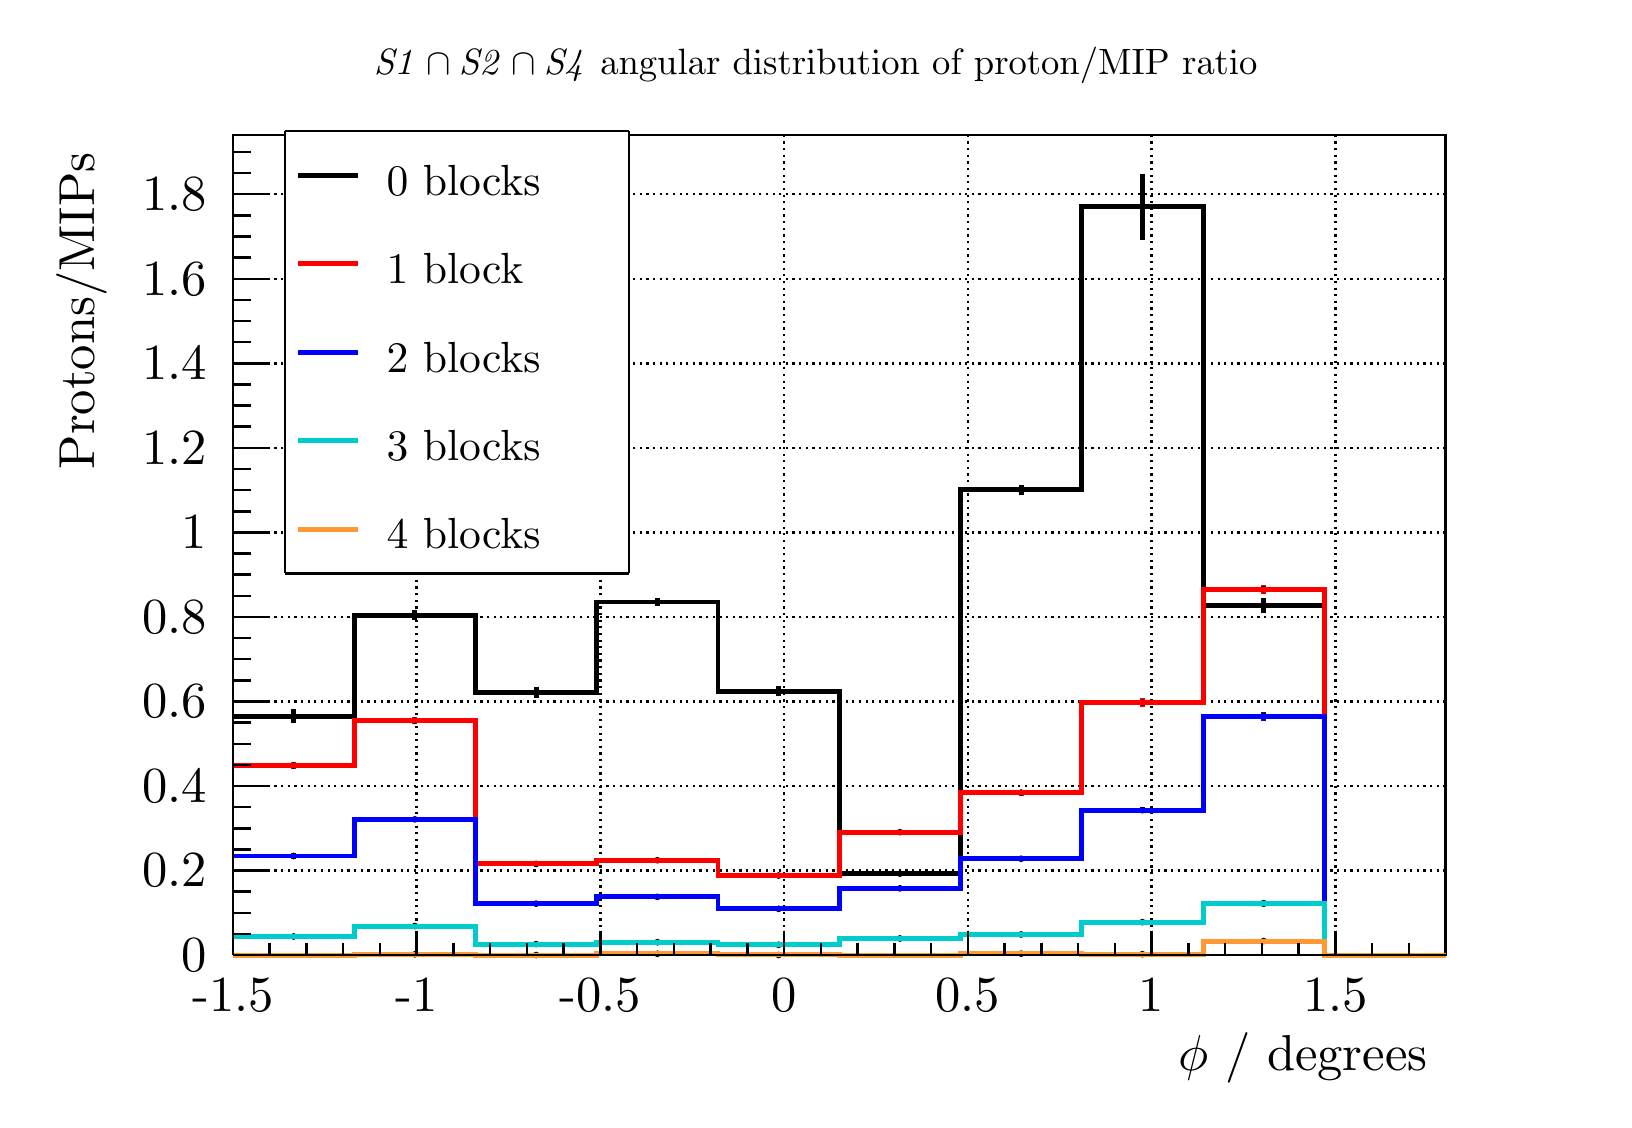
\begin{tikzpicture}
\pgfdeclareplotmark{cross} {
\pgfpathmoveto{\pgfpoint{-0.3\pgfplotmarksize}{\pgfplotmarksize}}
\pgfpathlineto{\pgfpoint{+0.3\pgfplotmarksize}{\pgfplotmarksize}}
\pgfpathlineto{\pgfpoint{+0.3\pgfplotmarksize}{0.3\pgfplotmarksize}}
\pgfpathlineto{\pgfpoint{+1\pgfplotmarksize}{0.3\pgfplotmarksize}}
\pgfpathlineto{\pgfpoint{+1\pgfplotmarksize}{-0.3\pgfplotmarksize}}
\pgfpathlineto{\pgfpoint{+0.3\pgfplotmarksize}{-0.3\pgfplotmarksize}}
\pgfpathlineto{\pgfpoint{+0.3\pgfplotmarksize}{-1.\pgfplotmarksize}}
\pgfpathlineto{\pgfpoint{-0.3\pgfplotmarksize}{-1.\pgfplotmarksize}}
\pgfpathlineto{\pgfpoint{-0.3\pgfplotmarksize}{-0.3\pgfplotmarksize}}
\pgfpathlineto{\pgfpoint{-1.\pgfplotmarksize}{-0.3\pgfplotmarksize}}
\pgfpathlineto{\pgfpoint{-1.\pgfplotmarksize}{0.3\pgfplotmarksize}}
\pgfpathlineto{\pgfpoint{-0.3\pgfplotmarksize}{0.3\pgfplotmarksize}}
\pgfpathclose
\pgfusepathqstroke
}
\pgfdeclareplotmark{cross*} {
\pgfpathmoveto{\pgfpoint{-0.3\pgfplotmarksize}{\pgfplotmarksize}}
\pgfpathlineto{\pgfpoint{+0.3\pgfplotmarksize}{\pgfplotmarksize}}
\pgfpathlineto{\pgfpoint{+0.3\pgfplotmarksize}{0.3\pgfplotmarksize}}
\pgfpathlineto{\pgfpoint{+1\pgfplotmarksize}{0.3\pgfplotmarksize}}
\pgfpathlineto{\pgfpoint{+1\pgfplotmarksize}{-0.3\pgfplotmarksize}}
\pgfpathlineto{\pgfpoint{+0.3\pgfplotmarksize}{-0.3\pgfplotmarksize}}
\pgfpathlineto{\pgfpoint{+0.3\pgfplotmarksize}{-1.\pgfplotmarksize}}
\pgfpathlineto{\pgfpoint{-0.3\pgfplotmarksize}{-1.\pgfplotmarksize}}
\pgfpathlineto{\pgfpoint{-0.3\pgfplotmarksize}{-0.3\pgfplotmarksize}}
\pgfpathlineto{\pgfpoint{-1.\pgfplotmarksize}{-0.3\pgfplotmarksize}}
\pgfpathlineto{\pgfpoint{-1.\pgfplotmarksize}{0.3\pgfplotmarksize}}
\pgfpathlineto{\pgfpoint{-0.3\pgfplotmarksize}{0.3\pgfplotmarksize}}
\pgfpathclose
\pgfusepathqfillstroke
}
\pgfdeclareplotmark{newstar} {
\pgfpathmoveto{\pgfqpoint{0pt}{\pgfplotmarksize}}
\pgfpathlineto{\pgfqpointpolar{44}{0.5\pgfplotmarksize}}
\pgfpathlineto{\pgfqpointpolar{18}{\pgfplotmarksize}}
\pgfpathlineto{\pgfqpointpolar{-20}{0.5\pgfplotmarksize}}
\pgfpathlineto{\pgfqpointpolar{-54}{\pgfplotmarksize}}
\pgfpathlineto{\pgfqpointpolar{-90}{0.5\pgfplotmarksize}}
\pgfpathlineto{\pgfqpointpolar{234}{\pgfplotmarksize}}
\pgfpathlineto{\pgfqpointpolar{198}{0.5\pgfplotmarksize}}
\pgfpathlineto{\pgfqpointpolar{162}{\pgfplotmarksize}}
\pgfpathlineto{\pgfqpointpolar{134}{0.5\pgfplotmarksize}}
\pgfpathclose
\pgfusepathqstroke
}
\pgfdeclareplotmark{newstar*} {
\pgfpathmoveto{\pgfqpoint{0pt}{\pgfplotmarksize}}
\pgfpathlineto{\pgfqpointpolar{44}{0.5\pgfplotmarksize}}
\pgfpathlineto{\pgfqpointpolar{18}{\pgfplotmarksize}}
\pgfpathlineto{\pgfqpointpolar{-20}{0.5\pgfplotmarksize}}
\pgfpathlineto{\pgfqpointpolar{-54}{\pgfplotmarksize}}
\pgfpathlineto{\pgfqpointpolar{-90}{0.5\pgfplotmarksize}}
\pgfpathlineto{\pgfqpointpolar{234}{\pgfplotmarksize}}
\pgfpathlineto{\pgfqpointpolar{198}{0.5\pgfplotmarksize}}
\pgfpathlineto{\pgfqpointpolar{162}{\pgfplotmarksize}}
\pgfpathlineto{\pgfqpointpolar{134}{0.5\pgfplotmarksize}}
\pgfpathclose
\pgfusepathqfillstroke
}
\definecolor{c}{rgb}{1,1,1};
\draw [color=c, fill=c] (0,0) rectangle (20,13.5319);
\draw [color=c, fill=c] (2.6,1.75915) rectangle (18,12.1787);
\definecolor{c}{rgb}{0,0,0};
\draw [c,line width=0.9] (2.6,1.75915) -- (2.6,12.1787) -- (18,12.1787) -- (18,1.75915) -- (2.6,1.75915);
\definecolor{c}{rgb}{1,1,1};
\draw [color=c, fill=c] (2.6,1.75915) rectangle (18,12.1787);
\definecolor{c}{rgb}{0,0,0};
\draw [c,line width=0.9] (2.6,1.75915) -- (2.6,12.1787) -- (18,12.1787) -- (18,1.75915) -- (2.6,1.75915);
\draw [c,line width=0.9] (2.6,1.75915) -- (18,1.75915);
\draw [c,dash pattern=on 0.80pt off 1.60pt ,line width=0.9] (2.6,12.1787) -- (2.6,1.75915);
\draw [c,dash pattern=on 0.80pt off 1.60pt ,line width=0.9] (4.93333,12.1787) -- (4.93333,1.75915);
\draw [c,dash pattern=on 0.80pt off 1.60pt ,line width=0.9] (7.26667,12.1787) -- (7.26667,1.75915);
\draw [c,dash pattern=on 0.80pt off 1.60pt ,line width=0.9] (9.6,12.1787) -- (9.6,1.75915);
\draw [c,dash pattern=on 0.80pt off 1.60pt ,line width=0.9] (11.9333,12.1787) -- (11.9333,1.75915);
\draw [c,dash pattern=on 0.80pt off 1.60pt ,line width=0.9] (14.2667,12.1787) -- (14.2667,1.75915);
\draw [c,dash pattern=on 0.80pt off 1.60pt ,line width=0.9] (16.6,12.1787) -- (16.6,1.75915);
\draw [c,dash pattern=on 0.80pt off 1.60pt ,line width=0.9] (16.6,12.1787) -- (16.6,1.75915);
\draw [c,line width=0.9] (2.6,1.75915) -- (2.6,12.1787);
\draw [c,dash pattern=on 0.80pt off 1.60pt ,line width=0.9] (18,1.76049) -- (2.6,1.76049);
\draw [c,dash pattern=on 0.80pt off 1.60pt ,line width=0.9] (18,2.83413) -- (2.6,2.83413);
\draw [c,dash pattern=on 0.80pt off 1.60pt ,line width=0.9] (18,3.90776) -- (2.6,3.90776);
\draw [c,dash pattern=on 0.80pt off 1.60pt ,line width=0.9] (18,4.98139) -- (2.6,4.98139);
\draw [c,dash pattern=on 0.80pt off 1.60pt ,line width=0.9] (18,6.05503) -- (2.6,6.05503);
\draw [c,dash pattern=on 0.80pt off 1.60pt ,line width=0.9] (18,7.12866) -- (2.6,7.12866);
\draw [c,dash pattern=on 0.80pt off 1.60pt ,line width=0.9] (18,8.20229) -- (2.6,8.20229);
\draw [c,dash pattern=on 0.80pt off 1.60pt ,line width=0.9] (18,9.27592) -- (2.6,9.27592);
\draw [c,dash pattern=on 0.80pt off 1.60pt ,line width=0.9] (18,10.3496) -- (2.6,10.3496);
\draw [c,dash pattern=on 0.80pt off 1.60pt ,line width=0.9] (18,11.4232) -- (2.6,11.4232);
\draw [c,dash pattern=on 0.80pt off 1.60pt ,line width=0.9] (18,1.76049) -- (2.6,1.76049);
\draw [c,dash pattern=on 0.80pt off 1.60pt ,line width=0.9] (18,11.4232) -- (2.6,11.4232);
\definecolor{c}{rgb}{0,0,0.6};
\draw [c,line width=0.9] (2.6,1.76049) -- (4.14,1.76049) -- (4.14,1.76049) -- (5.68,1.76049) -- (5.68,1.76049) -- (7.22,1.76049) -- (7.22,1.76049) -- (8.76,1.76049) -- (8.76,1.76049) -- (10.3,1.76049) -- (10.3,1.76049) -- (11.84,1.76049) --
 (11.84,1.76049) -- (13.38,1.76049) -- (13.38,1.76049) -- (14.92,1.76049) -- (14.92,1.76049) -- (16.46,1.76049) -- (16.46,1.76049) -- (18,1.76049);
\definecolor{c}{rgb}{0,0,0};
\draw [c,line width=0.9] (2.6,1.75915) -- (18,1.75915);
\draw [c,line width=0.9] (2.6,2.07174) -- (2.6,1.75915);
\draw [c,line width=0.9] (3.06667,1.91544) -- (3.06667,1.75915);
\draw [c,line width=0.9] (3.53333,1.91544) -- (3.53333,1.75915);
\draw [c,line width=0.9] (4,1.91544) -- (4,1.75915);
\draw [c,line width=0.9] (4.46667,1.91544) -- (4.46667,1.75915);
\draw [c,line width=0.9] (4.93333,2.07174) -- (4.93333,1.75915);
\draw [c,line width=0.9] (5.4,1.91544) -- (5.4,1.75915);
\draw [c,line width=0.9] (5.86667,1.91544) -- (5.86667,1.75915);
\draw [c,line width=0.9] (6.33333,1.91544) -- (6.33333,1.75915);
\draw [c,line width=0.9] (6.8,1.91544) -- (6.8,1.75915);
\draw [c,line width=0.9] (7.26667,2.07174) -- (7.26667,1.75915);
\draw [c,line width=0.9] (7.73333,1.91544) -- (7.73333,1.75915);
\draw [c,line width=0.9] (8.2,1.91544) -- (8.2,1.75915);
\draw [c,line width=0.9] (8.66667,1.91544) -- (8.66667,1.75915);
\draw [c,line width=0.9] (9.13333,1.91544) -- (9.13333,1.75915);
\draw [c,line width=0.9] (9.6,2.07174) -- (9.6,1.75915);
\draw [c,line width=0.9] (10.0667,1.91544) -- (10.0667,1.75915);
\draw [c,line width=0.9] (10.5333,1.91544) -- (10.5333,1.75915);
\draw [c,line width=0.9] (11,1.91544) -- (11,1.75915);
\draw [c,line width=0.9] (11.4667,1.91544) -- (11.4667,1.75915);
\draw [c,line width=0.9] (11.9333,2.07174) -- (11.9333,1.75915);
\draw [c,line width=0.9] (12.4,1.91544) -- (12.4,1.75915);
\draw [c,line width=0.9] (12.8667,1.91544) -- (12.8667,1.75915);
\draw [c,line width=0.9] (13.3333,1.91544) -- (13.3333,1.75915);
\draw [c,line width=0.9] (13.8,1.91544) -- (13.8,1.75915);
\draw [c,line width=0.9] (14.2667,2.07174) -- (14.2667,1.75915);
\draw [c,line width=0.9] (14.7333,1.91544) -- (14.7333,1.75915);
\draw [c,line width=0.9] (15.2,1.91544) -- (15.2,1.75915);
\draw [c,line width=0.9] (15.6667,1.91544) -- (15.6667,1.75915);
\draw [c,line width=0.9] (16.1333,1.91544) -- (16.1333,1.75915);
\draw [c,line width=0.9] (16.6,2.07174) -- (16.6,1.75915);
\draw [c,line width=0.9] (16.6,2.07174) -- (16.6,1.75915);
\draw [c,line width=0.9] (17.0667,1.91544) -- (17.0667,1.75915);
\draw [c,line width=0.9] (17.5333,1.91544) -- (17.5333,1.75915);
\draw [anchor=base] (2.6,1.04196) node[scale=1.82718, color=c, rotate=0]{-1.5};
\draw [anchor=base] (4.93333,1.04196) node[scale=1.82718, color=c, rotate=0]{-1};
\draw [anchor=base] (7.26667,1.04196) node[scale=1.82718, color=c, rotate=0]{-0.5};
\draw [anchor=base] (9.6,1.04196) node[scale=1.82718, color=c, rotate=0]{0};
\draw [anchor=base] (11.9333,1.04196) node[scale=1.82718, color=c, rotate=0]{0.5};
\draw [anchor=base] (14.2667,1.04196) node[scale=1.82718, color=c, rotate=0]{1};
\draw [anchor=base] (16.6,1.04196) node[scale=1.82718, color=c, rotate=0]{1.5};
\draw [anchor= east] (18,0.460085) node[scale=1.82718, color=c, rotate=0]{$\phi$ / degrees};
\draw [c,line width=0.9] (2.6,1.75915) -- (2.6,12.1787);
\draw [c,line width=0.9] (3.062,1.76049) -- (2.6,1.76049);
\draw [c,line width=0.9] (2.831,2.0289) -- (2.6,2.0289);
\draw [c,line width=0.9] (2.831,2.29731) -- (2.6,2.29731);
\draw [c,line width=0.9] (2.831,2.56572) -- (2.6,2.56572);
\draw [c,line width=0.9] (3.062,2.83413) -- (2.6,2.83413);
\draw [c,line width=0.9] (2.831,3.10254) -- (2.6,3.10254);
\draw [c,line width=0.9] (2.831,3.37094) -- (2.6,3.37094);
\draw [c,line width=0.9] (2.831,3.63935) -- (2.6,3.63935);
\draw [c,line width=0.9] (3.062,3.90776) -- (2.6,3.90776);
\draw [c,line width=0.9] (2.831,4.17617) -- (2.6,4.17617);
\draw [c,line width=0.9] (2.831,4.44458) -- (2.6,4.44458);
\draw [c,line width=0.9] (2.831,4.71299) -- (2.6,4.71299);
\draw [c,line width=0.9] (3.062,4.98139) -- (2.6,4.98139);
\draw [c,line width=0.9] (2.831,5.2498) -- (2.6,5.2498);
\draw [c,line width=0.9] (2.831,5.51821) -- (2.6,5.51821);
\draw [c,line width=0.9] (2.831,5.78662) -- (2.6,5.78662);
\draw [c,line width=0.9] (3.062,6.05503) -- (2.6,6.05503);
\draw [c,line width=0.9] (2.831,6.32343) -- (2.6,6.32343);
\draw [c,line width=0.9] (2.831,6.59184) -- (2.6,6.59184);
\draw [c,line width=0.9] (2.831,6.86025) -- (2.6,6.86025);
\draw [c,line width=0.9] (3.062,7.12866) -- (2.6,7.12866);
\draw [c,line width=0.9] (2.831,7.39707) -- (2.6,7.39707);
\draw [c,line width=0.9] (2.831,7.66548) -- (2.6,7.66548);
\draw [c,line width=0.9] (2.831,7.93388) -- (2.6,7.93388);
\draw [c,line width=0.9] (3.062,8.20229) -- (2.6,8.20229);
\draw [c,line width=0.9] (2.831,8.4707) -- (2.6,8.4707);
\draw [c,line width=0.9] (2.831,8.73911) -- (2.6,8.73911);
\draw [c,line width=0.9] (2.831,9.00752) -- (2.6,9.00752);
\draw [c,line width=0.9] (3.062,9.27592) -- (2.6,9.27592);
\draw [c,line width=0.9] (2.831,9.54433) -- (2.6,9.54433);
\draw [c,line width=0.9] (2.831,9.81274) -- (2.6,9.81274);
\draw [c,line width=0.9] (2.831,10.0812) -- (2.6,10.0812);
\draw [c,line width=0.9] (3.062,10.3496) -- (2.6,10.3496);
\draw [c,line width=0.9] (2.831,10.618) -- (2.6,10.618);
\draw [c,line width=0.9] (2.831,10.8864) -- (2.6,10.8864);
\draw [c,line width=0.9] (2.831,11.1548) -- (2.6,11.1548);
\draw [c,line width=0.9] (3.062,11.4232) -- (2.6,11.4232);
\draw [c,line width=0.9] (3.062,1.76049) -- (2.6,1.76049);
\draw [c,line width=0.9] (3.062,11.4232) -- (2.6,11.4232);
\draw [c,line width=0.9] (2.831,11.6916) -- (2.6,11.6916);
\draw [c,line width=0.9] (2.831,11.96) -- (2.6,11.96);
\draw [anchor= east] (2.5,1.76049) node[scale=1.82718, color=c, rotate=0]{0};
\draw [anchor= east] (2.5,2.83413) node[scale=1.82718, color=c, rotate=0]{0.2};
\draw [anchor= east] (2.5,3.90776) node[scale=1.82718, color=c, rotate=0]{0.4};
\draw [anchor= east] (2.5,4.98139) node[scale=1.82718, color=c, rotate=0]{0.6};
\draw [anchor= east] (2.5,6.05503) node[scale=1.82718, color=c, rotate=0]{0.8};
\draw [anchor= east] (2.5,7.12866) node[scale=1.82718, color=c, rotate=0]{1};
\draw [anchor= east] (2.5,8.20229) node[scale=1.82718, color=c, rotate=0]{1.2};
\draw [anchor= east] (2.5,9.27592) node[scale=1.82718, color=c, rotate=0]{1.4};
\draw [anchor= east] (2.5,10.3496) node[scale=1.82718, color=c, rotate=0]{1.6};
\draw [anchor= east] (2.5,11.4232) node[scale=1.82718, color=c, rotate=0]{1.8};
\draw [anchor= east] (0.68,12.1787) node[scale=1.82718, color=c, rotate=90]{ Protons/MIPs};
\draw [c,line width=1.8] (3.37,4.71025) -- (3.37,4.79585);
\draw [c,line width=1.8] (3.37,4.79585) -- (3.37,4.88144);
\foreach \P in {(3.37,4.79585)}{\draw[mark options={color=c,fill=c},mark size=2.402402pt,mark=*,mark size=1pt] plot coordinates {\P};}
\draw [c,line width=1.8] (4.91,6.01214) -- (4.91,6.07843);
\draw [c,line width=1.8] (4.91,6.07843) -- (4.91,6.14473);
\foreach \P in {(4.91,6.07843)}{\draw[mark options={color=c,fill=c},mark size=2.402402pt,mark=*,mark size=1pt] plot coordinates {\P};}
\draw [c,line width=1.8] (6.45,5.02108) -- (6.45,5.09041);
\draw [c,line width=1.8] (6.45,5.09041) -- (6.45,5.15974);
\foreach \P in {(6.45,5.09041)}{\draw[mark options={color=c,fill=c},mark size=2.402402pt,mark=*,mark size=1pt] plot coordinates {\P};}
\draw [c,line width=1.8] (7.99,6.19173) -- (7.99,6.24488);
\draw [c,line width=1.8] (7.99,6.24488) -- (7.99,6.29803);
\foreach \P in {(7.99,6.24488)}{\draw[mark options={color=c,fill=c},mark size=2.402402pt,mark=*,mark size=1pt] plot coordinates {\P};}
\draw [c,line width=1.8] (9.53,5.0449) -- (9.53,5.10882);
\draw [c,line width=1.8] (9.53,5.10882) -- (9.53,5.17273);
\foreach \P in {(9.53,5.10882)}{\draw[mark options={color=c,fill=c},mark size=2.402402pt,mark=*,mark size=1pt] plot coordinates {\P};}
\draw [c,line width=1.8] (11.07,2.76645) -- (11.07,2.79547);
\draw [c,line width=1.8] (11.07,2.79547) -- (11.07,2.82449);
\foreach \P in {(11.07,2.79547)}{\draw[mark options={color=c,fill=c},mark size=2.402402pt,mark=*,mark size=1pt] plot coordinates {\P};}
\draw [c,line width=1.8] (12.61,7.60244) -- (12.61,7.66965);
\draw [c,line width=1.8] (12.61,7.66965) -- (12.61,7.73685);
\foreach \P in {(12.61,7.66965)}{\draw[mark options={color=c,fill=c},mark size=2.402402pt,mark=*,mark size=1pt] plot coordinates {\P};}
\draw [c,line width=1.8] (14.15,10.8412) -- (14.15,11.2619);
\draw [c,line width=1.8] (14.15,11.2619) -- (14.15,11.6826);
\foreach \P in {(14.15,11.2619)}{\draw[mark options={color=c,fill=c},mark size=2.402402pt,mark=*,mark size=1pt] plot coordinates {\P};}
\draw [c,line width=1.8] (15.69,6.11068) -- (15.69,6.20631);
\draw [c,line width=1.8] (15.69,6.20631) -- (15.69,6.30194);
\foreach \P in {(15.69,6.20631)}{\draw[mark options={color=c,fill=c},mark size=2.402402pt,mark=*,mark size=1pt] plot coordinates {\P};}
\draw [c,line width=1.8] (2.6,4.79585) -- (4.14,4.79585) -- (4.14,6.07843) -- (5.68,6.07843) -- (5.68,5.09041) -- (7.22,5.09041) -- (7.22,6.24488) -- (8.76,6.24488) -- (8.76,5.10882) -- (10.3,5.10882) -- (10.3,2.79547) -- (11.84,2.79547) --
 (11.84,7.66965) -- (13.38,7.66965) -- (13.38,11.2619) -- (14.92,11.2619) -- (14.92,6.20631) -- (16.46,6.20631) -- (16.46,1.76049) -- (18,1.76049);
\definecolor{c}{rgb}{1,0,0};
\draw [c,line width=1.8] (3.37,4.11807) -- (3.37,4.16704);
\draw [c,line width=1.8] (3.37,4.16704) -- (3.37,4.21602);
\definecolor{c}{rgb}{0,0,0};
\foreach \P in {(3.37,4.16704)}{\draw[mark options={color=c,fill=c},mark size=2.402402pt,mark=*,mark size=1pt] plot coordinates {\P};}
\definecolor{c}{rgb}{1,0,0};
\draw [c,line width=1.8] (4.91,4.69191) -- (4.91,4.73817);
\draw [c,line width=1.8] (4.91,4.73817) -- (4.91,4.78443);
\definecolor{c}{rgb}{0,0,0};
\foreach \P in {(4.91,4.73817)}{\draw[mark options={color=c,fill=c},mark size=2.402402pt,mark=*,mark size=1pt] plot coordinates {\P};}
\definecolor{c}{rgb}{1,0,0};
\draw [c,line width=1.8] (6.45,2.89584) -- (6.45,2.91871);
\draw [c,line width=1.8] (6.45,2.91871) -- (6.45,2.94158);
\definecolor{c}{rgb}{0,0,0};
\foreach \P in {(6.45,2.91871)}{\draw[mark options={color=c,fill=c},mark size=2.402402pt,mark=*,mark size=1pt] plot coordinates {\P};}
\definecolor{c}{rgb}{1,0,0};
\draw [c,line width=1.8] (7.99,2.94378) -- (7.99,2.96547);
\draw [c,line width=1.8] (7.99,2.96547) -- (7.99,2.98716);
\definecolor{c}{rgb}{0,0,0};
\foreach \P in {(7.99,2.96547)}{\draw[mark options={color=c,fill=c},mark size=2.402402pt,mark=*,mark size=1pt] plot coordinates {\P};}
\definecolor{c}{rgb}{1,0,0};
\draw [c,line width=1.8] (9.53,2.75198) -- (9.53,2.7712);
\draw [c,line width=1.8] (9.53,2.7712) -- (9.53,2.79042);
\definecolor{c}{rgb}{0,0,0};
\foreach \P in {(9.53,2.7712)}{\draw[mark options={color=c,fill=c},mark size=2.402402pt,mark=*,mark size=1pt] plot coordinates {\P};}
\definecolor{c}{rgb}{1,0,0};
\draw [c,line width=1.8] (11.07,3.29511) -- (11.07,3.32202);
\draw [c,line width=1.8] (11.07,3.32202) -- (11.07,3.34893);
\definecolor{c}{rgb}{0,0,0};
\foreach \P in {(11.07,3.32202)}{\draw[mark options={color=c,fill=c},mark size=2.402402pt,mark=*,mark size=1pt] plot coordinates {\P};}
\definecolor{c}{rgb}{1,0,0};
\draw [c,line width=1.8] (12.61,3.78663) -- (12.61,3.8247);
\draw [c,line width=1.8] (12.61,3.8247) -- (12.61,3.86278);
\definecolor{c}{rgb}{0,0,0};
\foreach \P in {(12.61,3.8247)}{\draw[mark options={color=c,fill=c},mark size=2.402402pt,mark=*,mark size=1pt] plot coordinates {\P};}
\definecolor{c}{rgb}{1,0,0};
\draw [c,line width=1.8] (14.15,4.91557) -- (14.15,4.96824);
\draw [c,line width=1.8] (14.15,4.96824) -- (14.15,5.02092);
\definecolor{c}{rgb}{0,0,0};
\foreach \P in {(14.15,4.96824)}{\draw[mark options={color=c,fill=c},mark size=2.402402pt,mark=*,mark size=1pt] plot coordinates {\P};}
\definecolor{c}{rgb}{1,0,0};
\draw [c,line width=1.8] (15.69,6.35074) -- (15.69,6.40782);
\draw [c,line width=1.8] (15.69,6.40782) -- (15.69,6.46491);
\definecolor{c}{rgb}{0,0,0};
\foreach \P in {(15.69,6.40782)}{\draw[mark options={color=c,fill=c},mark size=2.402402pt,mark=*,mark size=1pt] plot coordinates {\P};}
\definecolor{c}{rgb}{1,0,0};
\draw [c,line width=1.8] (2.6,4.16704) -- (4.14,4.16704) -- (4.14,4.73817) -- (5.68,4.73817) -- (5.68,2.91871) -- (7.22,2.91871) -- (7.22,2.96547) -- (8.76,2.96547) -- (8.76,2.7712) -- (10.3,2.7712) -- (10.3,3.32202) -- (11.84,3.32202) --
 (11.84,3.8247) -- (13.38,3.8247) -- (13.38,4.96824) -- (14.92,4.96824) -- (14.92,6.40782) -- (16.46,6.40782) -- (16.46,1.76049) -- (18,1.76049);
\definecolor{c}{rgb}{0,0,1};
\draw [c,line width=1.8] (3.37,2.98714) -- (3.37,3.01918);
\draw [c,line width=1.8] (3.37,3.01918) -- (3.37,3.05122);
\definecolor{c}{rgb}{0,0,0};
\foreach \P in {(3.37,3.01918)}{\draw[mark options={color=c,fill=c},mark size=2.402402pt,mark=*,mark size=1pt] plot coordinates {\P};}
\definecolor{c}{rgb}{0,0,1};
\draw [c,line width=1.8] (4.91,3.45069) -- (4.91,3.48427);
\draw [c,line width=1.8] (4.91,3.48427) -- (4.91,3.51785);
\definecolor{c}{rgb}{0,0,0};
\foreach \P in {(4.91,3.48427)}{\draw[mark options={color=c,fill=c},mark size=2.402402pt,mark=*,mark size=1pt] plot coordinates {\P};}
\definecolor{c}{rgb}{0,0,1};
\draw [c,line width=1.8] (6.45,2.39914) -- (6.45,2.41346);
\draw [c,line width=1.8] (6.45,2.41346) -- (6.45,2.42778);
\definecolor{c}{rgb}{0,0,0};
\foreach \P in {(6.45,2.41346)}{\draw[mark options={color=c,fill=c},mark size=2.402402pt,mark=*,mark size=1pt] plot coordinates {\P};}
\definecolor{c}{rgb}{0,0,1};
\draw [c,line width=1.8] (7.99,2.48633) -- (7.99,2.50057);
\draw [c,line width=1.8] (7.99,2.50057) -- (7.99,2.51481);
\definecolor{c}{rgb}{0,0,0};
\foreach \P in {(7.99,2.50057)}{\draw[mark options={color=c,fill=c},mark size=2.402402pt,mark=*,mark size=1pt] plot coordinates {\P};}
\definecolor{c}{rgb}{0,0,1};
\draw [c,line width=1.8] (9.53,2.33638) -- (9.53,2.34859);
\draw [c,line width=1.8] (9.53,2.34859) -- (9.53,2.36079);
\definecolor{c}{rgb}{0,0,0};
\foreach \P in {(9.53,2.34859)}{\draw[mark options={color=c,fill=c},mark size=2.402402pt,mark=*,mark size=1pt] plot coordinates {\P};}
\definecolor{c}{rgb}{0,0,1};
\draw [c,line width=1.8] (11.07,2.5915) -- (11.07,2.60865);
\draw [c,line width=1.8] (11.07,2.60865) -- (11.07,2.6258);
\definecolor{c}{rgb}{0,0,0};
\foreach \P in {(11.07,2.60865)}{\draw[mark options={color=c,fill=c},mark size=2.402402pt,mark=*,mark size=1pt] plot coordinates {\P};}
\definecolor{c}{rgb}{0,0,1};
\draw [c,line width=1.8] (12.61,2.9584) -- (12.61,2.98436);
\draw [c,line width=1.8] (12.61,2.98436) -- (12.61,3.01032);
\definecolor{c}{rgb}{0,0,0};
\foreach \P in {(12.61,2.98436)}{\draw[mark options={color=c,fill=c},mark size=2.402402pt,mark=*,mark size=1pt] plot coordinates {\P};}
\definecolor{c}{rgb}{0,0,1};
\draw [c,line width=1.8] (14.15,3.56279) -- (14.15,3.60081);
\draw [c,line width=1.8] (14.15,3.60081) -- (14.15,3.63884);
\definecolor{c}{rgb}{0,0,0};
\foreach \P in {(14.15,3.60081)}{\draw[mark options={color=c,fill=c},mark size=2.402402pt,mark=*,mark size=1pt] plot coordinates {\P};}
\definecolor{c}{rgb}{0,0,1};
\draw [c,line width=1.8] (15.69,4.73566) -- (15.69,4.79491);
\draw [c,line width=1.8] (15.69,4.79491) -- (15.69,4.85415);
\definecolor{c}{rgb}{0,0,0};
\foreach \P in {(15.69,4.79491)}{\draw[mark options={color=c,fill=c},mark size=2.402402pt,mark=*,mark size=1pt] plot coordinates {\P};}
\definecolor{c}{rgb}{0,0,1};
\draw [c,line width=1.8] (2.6,3.01918) -- (4.14,3.01918) -- (4.14,3.48427) -- (5.68,3.48427) -- (5.68,2.41346) -- (7.22,2.41346) -- (7.22,2.50057) -- (8.76,2.50057) -- (8.76,2.34859) -- (10.3,2.34859) -- (10.3,2.60865) -- (11.84,2.60865) --
 (11.84,2.98436) -- (13.38,2.98436) -- (13.38,3.60081) -- (14.92,3.60081) -- (14.92,4.79491) -- (16.46,4.79491) -- (16.46,1.76049) -- (18,1.76049);
\definecolor{c}{rgb}{0,0.8,0.8};
\draw [c,line width=1.8] (3.37,1.9798) -- (3.37,1.9972);
\draw [c,line width=1.8] (3.37,1.9972) -- (3.37,2.0146);
\definecolor{c}{rgb}{0,0,0};
\foreach \P in {(3.37,1.9972)}{\draw[mark options={color=c,fill=c},mark size=2.402402pt,mark=*,mark size=1pt] plot coordinates {\P};}
\definecolor{c}{rgb}{0,0.8,0.8};
\draw [c,line width=1.8] (4.91,2.10989) -- (4.91,2.12941);
\draw [c,line width=1.8] (4.91,2.12941) -- (4.91,2.14894);
\definecolor{c}{rgb}{0,0,0};
\foreach \P in {(4.91,2.12941)}{\draw[mark options={color=c,fill=c},mark size=2.402402pt,mark=*,mark size=1pt] plot coordinates {\P};}
\definecolor{c}{rgb}{0,0.8,0.8};
\draw [c,line width=1.8] (6.45,1.89194) -- (6.45,1.89987);
\draw [c,line width=1.8] (6.45,1.89987) -- (6.45,1.90781);
\definecolor{c}{rgb}{0,0,0};
\foreach \P in {(6.45,1.89987)}{\draw[mark options={color=c,fill=c},mark size=2.402402pt,mark=*,mark size=1pt] plot coordinates {\P};}
\definecolor{c}{rgb}{0,0.8,0.8};
\draw [c,line width=1.8] (7.99,1.91606) -- (7.99,1.92406);
\draw [c,line width=1.8] (7.99,1.92406) -- (7.99,1.93206);
\definecolor{c}{rgb}{0,0,0};
\foreach \P in {(7.99,1.92406)}{\draw[mark options={color=c,fill=c},mark size=2.402402pt,mark=*,mark size=1pt] plot coordinates {\P};}
\definecolor{c}{rgb}{0,0.8,0.8};
\draw [c,line width=1.8] (9.53,1.88459) -- (9.53,1.89148);
\draw [c,line width=1.8] (9.53,1.89148) -- (9.53,1.89837);
\definecolor{c}{rgb}{0,0,0};
\foreach \P in {(9.53,1.89148)}{\draw[mark options={color=c,fill=c},mark size=2.402402pt,mark=*,mark size=1pt] plot coordinates {\P};}
\definecolor{c}{rgb}{0,0.8,0.8};
\draw [c,line width=1.8] (11.07,1.96184) -- (11.07,1.97194);
\draw [c,line width=1.8] (11.07,1.97194) -- (11.07,1.98203);
\definecolor{c}{rgb}{0,0,0};
\foreach \P in {(11.07,1.97194)}{\draw[mark options={color=c,fill=c},mark size=2.402402pt,mark=*,mark size=1pt] plot coordinates {\P};}
\definecolor{c}{rgb}{0,0.8,0.8};
\draw [c,line width=1.8] (12.61,2.00772) -- (12.61,2.02249);
\draw [c,line width=1.8] (12.61,2.02249) -- (12.61,2.03725);
\definecolor{c}{rgb}{0,0,0};
\foreach \P in {(12.61,2.02249)}{\draw[mark options={color=c,fill=c},mark size=2.402402pt,mark=*,mark size=1pt] plot coordinates {\P};}
\definecolor{c}{rgb}{0,0.8,0.8};
\draw [c,line width=1.8] (14.15,2.15563) -- (14.15,2.17882);
\draw [c,line width=1.8] (14.15,2.17882) -- (14.15,2.202);
\definecolor{c}{rgb}{0,0,0};
\foreach \P in {(14.15,2.17882)}{\draw[mark options={color=c,fill=c},mark size=2.402402pt,mark=*,mark size=1pt] plot coordinates {\P};}
\definecolor{c}{rgb}{0,0.8,0.8};
\draw [c,line width=1.8] (15.69,2.37432) -- (15.69,2.41693);
\draw [c,line width=1.8] (15.69,2.41693) -- (15.69,2.45953);
\definecolor{c}{rgb}{0,0,0};
\foreach \P in {(15.69,2.41693)}{\draw[mark options={color=c,fill=c},mark size=2.402402pt,mark=*,mark size=1pt] plot coordinates {\P};}
\definecolor{c}{rgb}{0,0.8,0.8};
\draw [c,line width=1.8] (2.6,1.9972) -- (4.14,1.9972) -- (4.14,2.12941) -- (5.68,2.12941) -- (5.68,1.89987) -- (7.22,1.89987) -- (7.22,1.92406) -- (8.76,1.92406) -- (8.76,1.89148) -- (10.3,1.89148) -- (10.3,1.97194) -- (11.84,1.97194) --
 (11.84,2.02249) -- (13.38,2.02249) -- (13.38,2.17882) -- (14.92,2.17882) -- (14.92,2.41693) -- (16.46,2.41693) -- (16.46,1.76049) -- (18,1.76049);
\definecolor{c}{rgb}{1,0.6,0.2};
\draw [c,line width=1.8] (4.91,1.76859) -- (4.91,1.77032);
\draw [c,line width=1.8] (4.91,1.77032) -- (4.91,1.77205);
\definecolor{c}{rgb}{0,0,0};
\foreach \P in {(4.91,1.77032)}{\draw[mark options={color=c,fill=c},mark size=2.402402pt,mark=*,mark size=1pt] plot coordinates {\P};}
\definecolor{c}{rgb}{1,0.6,0.2};
\draw [c,line width=1.8] (6.45,1.75915) -- (6.45,1.76089);
\draw [c,line width=1.8] (6.45,1.76089) -- (6.45,1.76263);
\definecolor{c}{rgb}{0,0,0};
\foreach \P in {(6.45,1.76089)}{\draw[mark options={color=c,fill=c},mark size=2.402402pt,mark=*,mark size=1pt] plot coordinates {\P};}
\definecolor{c}{rgb}{1,0.6,0.2};
\draw [c,line width=1.8] (7.99,1.77587) -- (7.99,1.77763);
\draw [c,line width=1.8] (7.99,1.77763) -- (7.99,1.77938);
\definecolor{c}{rgb}{0,0,0};
\foreach \P in {(7.99,1.77763)}{\draw[mark options={color=c,fill=c},mark size=2.402402pt,mark=*,mark size=1pt] plot coordinates {\P};}
\definecolor{c}{rgb}{1,0.6,0.2};
\draw [c,line width=1.8] (9.53,1.76019) -- (9.53,1.76201);
\draw [c,line width=1.8] (9.53,1.76201) -- (9.53,1.76382);
\definecolor{c}{rgb}{0,0,0};
\foreach \P in {(9.53,1.76201)}{\draw[mark options={color=c,fill=c},mark size=2.402402pt,mark=*,mark size=1pt] plot coordinates {\P};}
\definecolor{c}{rgb}{1,0.6,0.2};
\draw [c,line width=1.8] (12.61,1.77645) -- (12.61,1.77911);
\draw [c,line width=1.8] (12.61,1.77911) -- (12.61,1.78178);
\definecolor{c}{rgb}{0,0,0};
\foreach \P in {(12.61,1.77911)}{\draw[mark options={color=c,fill=c},mark size=2.402402pt,mark=*,mark size=1pt] plot coordinates {\P};}
\definecolor{c}{rgb}{1,0.6,0.2};
\draw [c,line width=1.8] (14.15,1.7667) -- (14.15,1.77179);
\draw [c,line width=1.8] (14.15,1.77179) -- (14.15,1.77689);
\definecolor{c}{rgb}{0,0,0};
\foreach \P in {(14.15,1.77179)}{\draw[mark options={color=c,fill=c},mark size=2.402402pt,mark=*,mark size=1pt] plot coordinates {\P};}
\definecolor{c}{rgb}{1,0.6,0.2};
\draw [c,line width=1.8] (15.69,1.91747) -- (15.69,1.939);
\draw [c,line width=1.8] (15.69,1.939) -- (15.69,1.96054);
\definecolor{c}{rgb}{0,0,0};
\foreach \P in {(15.69,1.939)}{\draw[mark options={color=c,fill=c},mark size=2.402402pt,mark=*,mark size=1pt] plot coordinates {\P};}
\definecolor{c}{rgb}{1,0.6,0.2};
\draw [c,line width=1.8] (2.6,1.76049) -- (4.14,1.76049) -- (4.14,1.77032) -- (5.68,1.77032) -- (5.68,1.76089) -- (7.22,1.76089) -- (7.22,1.77763) -- (8.76,1.77763) -- (8.76,1.76201) -- (10.3,1.76201) -- (10.3,1.76049) -- (11.84,1.76049) --
 (11.84,1.77911) -- (13.38,1.77911) -- (13.38,1.77179) -- (14.92,1.77179) -- (14.92,1.939) -- (16.46,1.939) -- (16.46,1.76049) -- (18,1.76049);
\definecolor{c}{rgb}{0,0,0};
\draw [c,line width=0.9] (2.6,1.75915) -- (18,1.75915);
\draw [c,line width=0.9] (2.6,2.07174) -- (2.6,1.75915);
\draw [c,line width=0.9] (3.06667,1.91544) -- (3.06667,1.75915);
\draw [c,line width=0.9] (3.53333,1.91544) -- (3.53333,1.75915);
\draw [c,line width=0.9] (4,1.91544) -- (4,1.75915);
\draw [c,line width=0.9] (4.46667,1.91544) -- (4.46667,1.75915);
\draw [c,line width=0.9] (4.93333,2.07174) -- (4.93333,1.75915);
\draw [c,line width=0.9] (5.4,1.91544) -- (5.4,1.75915);
\draw [c,line width=0.9] (5.86667,1.91544) -- (5.86667,1.75915);
\draw [c,line width=0.9] (6.33333,1.91544) -- (6.33333,1.75915);
\draw [c,line width=0.9] (6.8,1.91544) -- (6.8,1.75915);
\draw [c,line width=0.9] (7.26667,2.07174) -- (7.26667,1.75915);
\draw [c,line width=0.9] (7.73333,1.91544) -- (7.73333,1.75915);
\draw [c,line width=0.9] (8.2,1.91544) -- (8.2,1.75915);
\draw [c,line width=0.9] (8.66667,1.91544) -- (8.66667,1.75915);
\draw [c,line width=0.9] (9.13333,1.91544) -- (9.13333,1.75915);
\draw [c,line width=0.9] (9.6,2.07174) -- (9.6,1.75915);
\draw [c,line width=0.9] (10.0667,1.91544) -- (10.0667,1.75915);
\draw [c,line width=0.9] (10.5333,1.91544) -- (10.5333,1.75915);
\draw [c,line width=0.9] (11,1.91544) -- (11,1.75915);
\draw [c,line width=0.9] (11.4667,1.91544) -- (11.4667,1.75915);
\draw [c,line width=0.9] (11.9333,2.07174) -- (11.9333,1.75915);
\draw [c,line width=0.9] (12.4,1.91544) -- (12.4,1.75915);
\draw [c,line width=0.9] (12.8667,1.91544) -- (12.8667,1.75915);
\draw [c,line width=0.9] (13.3333,1.91544) -- (13.3333,1.75915);
\draw [c,line width=0.9] (13.8,1.91544) -- (13.8,1.75915);
\draw [c,line width=0.9] (14.2667,2.07174) -- (14.2667,1.75915);
\draw [c,line width=0.9] (14.7333,1.91544) -- (14.7333,1.75915);
\draw [c,line width=0.9] (15.2,1.91544) -- (15.2,1.75915);
\draw [c,line width=0.9] (15.6667,1.91544) -- (15.6667,1.75915);
\draw [c,line width=0.9] (16.1333,1.91544) -- (16.1333,1.75915);
\draw [c,line width=0.9] (16.6,2.07174) -- (16.6,1.75915);
\draw [c,line width=0.9] (16.6,2.07174) -- (16.6,1.75915);
\draw [c,line width=0.9] (17.0667,1.91544) -- (17.0667,1.75915);
\draw [c,line width=0.9] (17.5333,1.91544) -- (17.5333,1.75915);
\draw [c,line width=0.9] (2.6,1.75915) -- (2.6,12.1787);
\draw [c,line width=0.9] (3.062,1.76049) -- (2.6,1.76049);
\draw [c,line width=0.9] (2.831,2.0289) -- (2.6,2.0289);
\draw [c,line width=0.9] (2.831,2.29731) -- (2.6,2.29731);
\draw [c,line width=0.9] (2.831,2.56572) -- (2.6,2.56572);
\draw [c,line width=0.9] (3.062,2.83413) -- (2.6,2.83413);
\draw [c,line width=0.9] (2.831,3.10254) -- (2.6,3.10254);
\draw [c,line width=0.9] (2.831,3.37094) -- (2.6,3.37094);
\draw [c,line width=0.9] (2.831,3.63935) -- (2.6,3.63935);
\draw [c,line width=0.9] (3.062,3.90776) -- (2.6,3.90776);
\draw [c,line width=0.9] (2.831,4.17617) -- (2.6,4.17617);
\draw [c,line width=0.9] (2.831,4.44458) -- (2.6,4.44458);
\draw [c,line width=0.9] (2.831,4.71299) -- (2.6,4.71299);
\draw [c,line width=0.9] (3.062,4.98139) -- (2.6,4.98139);
\draw [c,line width=0.9] (2.831,5.2498) -- (2.6,5.2498);
\draw [c,line width=0.9] (2.831,5.51821) -- (2.6,5.51821);
\draw [c,line width=0.9] (2.831,5.78662) -- (2.6,5.78662);
\draw [c,line width=0.9] (3.062,6.05503) -- (2.6,6.05503);
\draw [c,line width=0.9] (2.831,6.32343) -- (2.6,6.32343);
\draw [c,line width=0.9] (2.831,6.59184) -- (2.6,6.59184);
\draw [c,line width=0.9] (2.831,6.86025) -- (2.6,6.86025);
\draw [c,line width=0.9] (3.062,7.12866) -- (2.6,7.12866);
\draw [c,line width=0.9] (2.831,7.39707) -- (2.6,7.39707);
\draw [c,line width=0.9] (2.831,7.66548) -- (2.6,7.66548);
\draw [c,line width=0.9] (2.831,7.93388) -- (2.6,7.93388);
\draw [c,line width=0.9] (3.062,8.20229) -- (2.6,8.20229);
\draw [c,line width=0.9] (2.831,8.4707) -- (2.6,8.4707);
\draw [c,line width=0.9] (2.831,8.73911) -- (2.6,8.73911);
\draw [c,line width=0.9] (2.831,9.00752) -- (2.6,9.00752);
\draw [c,line width=0.9] (3.062,9.27592) -- (2.6,9.27592);
\draw [c,line width=0.9] (2.831,9.54433) -- (2.6,9.54433);
\draw [c,line width=0.9] (2.831,9.81274) -- (2.6,9.81274);
\draw [c,line width=0.9] (2.831,10.0812) -- (2.6,10.0812);
\draw [c,line width=0.9] (3.062,10.3496) -- (2.6,10.3496);
\draw [c,line width=0.9] (2.831,10.618) -- (2.6,10.618);
\draw [c,line width=0.9] (2.831,10.8864) -- (2.6,10.8864);
\draw [c,line width=0.9] (2.831,11.1548) -- (2.6,11.1548);
\draw [c,line width=0.9] (3.062,11.4232) -- (2.6,11.4232);
\draw [c,line width=0.9] (3.062,1.76049) -- (2.6,1.76049);
\draw [c,line width=0.9] (3.062,11.4232) -- (2.6,11.4232);
\draw [c,line width=0.9] (2.831,11.6916) -- (2.6,11.6916);
\draw [c,line width=0.9] (2.831,11.96) -- (2.6,11.96);
\draw (10,13.0557) node[scale=1.32313, color=c, rotate=0]{$\mathit{S1} \cap \mathit{S2} \cap \mathit{S4}$ angular distribution of proton/MIP ratio};
\definecolor{c}{rgb}{1,1,1};
\draw [color=c, fill=c] (3.26241,6.60993) rectangle (7.63121,12.227);
\definecolor{c}{rgb}{0,0,0};
\draw [c,line width=0.9] (3.26241,6.60993) -- (7.63121,6.60993);
\draw [c,line width=0.9] (7.63121,6.60993) -- (7.63121,12.227);
\draw [c,line width=0.9] (7.63121,12.227) -- (3.26241,12.227);
\draw [c,line width=0.9] (3.26241,12.227) -- (3.26241,6.60993);
\draw [anchor=base west] (4.35461,11.4125) node[scale=1.57516, color=c, rotate=0]{0 blocks};
\draw [c,line width=1.8] (3.42624,11.6652) -- (4.19078,11.6652);
\draw [anchor=base west] (4.35461,10.2891) node[scale=1.57516, color=c, rotate=0]{1 block};
\definecolor{c}{rgb}{1,0,0};
\draw [c,line width=1.8] (3.42624,10.5418) -- (4.19078,10.5418);
\definecolor{c}{rgb}{0,0,0};
\draw [anchor=base west] (4.35461,9.16567) node[scale=1.57516, color=c, rotate=0]{2 blocks};
\definecolor{c}{rgb}{0,0,1};
\draw [c,line width=1.8] (3.42624,9.41844) -- (4.19078,9.41844);
\definecolor{c}{rgb}{0,0,0};
\draw [anchor=base west] (4.35461,8.04227) node[scale=1.57516, color=c, rotate=0]{3 blocks};
\definecolor{c}{rgb}{0,0.8,0.8};
\draw [c,line width=1.8] (3.42624,8.29504) -- (4.19078,8.29504);
\definecolor{c}{rgb}{0,0,0};
\draw [anchor=base west] (4.35461,6.91887) node[scale=1.57516, color=c, rotate=0]{4 blocks};
\definecolor{c}{rgb}{1,0.6,0.2};
\draw [c,line width=1.8] (3.42624,7.17163) -- (4.19078,7.17163);
\end{tikzpicture}

    \end{adjustbox}
  \end{minipage}	
  \caption{\label{fig:propiratio_s4_horz}Proton-MIP ratio in $\mathit{S4}$ for varying numbers of moderator blocks as a function of off-axis angle. Left: horizontal off-axis angle. Right: vertical off-axis angle.}
\end{figure}

\subsection{Monte Carlo Studies}
\label{sec:mcStudies}
In order to ascertain the flux of protons reaching the active region of the TPC, and verify the corrections described above, a Monte Carlo (MC) simulation study was performed.
The simulation was performed using GEANT4~\cite{brun1993geant}, with geometric volumes approximating the vessel, TPC, and time of flight systems.
In order to match upstream conditions as closely as possible, particle momenta were drawn from the $\mathit{S3}$ distributions shown in Figure~\ref{fig:s3proke}, left, and simulated with trajectories that resulted in the same position distribution as seen in Figure~\ref{fig:s3XY_pion}, right.
The same timing cuts described in Section~\ref{timeofflightanalysissubsec} were applied.

\begin{figure}[ht]
  \centering
     \begin{adjustbox}{max totalsize={\textwidth}{.3\textheight}, center}
      \input{files/Figures/proKeS4Mc.tex}
    \end{adjustbox}
    \caption{Energy profile of simulated protons reaching $\mathit{S4}$, with kinetic energy above the detection threshold of 10~MeV.}
    \label{fig:MCS4}
\end{figure}

The simulated protons are propagated through the vessel to the $\mathit{S4}$ detector.
The momentum profile of simulated protons reaching the $\mathit{S4}$ wall is shown in Figure~\ref{fig:MCS4}.
A proton detection threshold of $\mathit{S4}$ of 140~MeV/c (10~MeV kinetic energy) is included.
The simulation shows a significant reduction in kinetic energy as most particles have travelled through both steel walls of the TPC vessel.
In particular, in the 4 moderator block case, very few particles have survived through the second vessel wall to reach $\mathit{S4}$.

\begin{figure}[h]
  \centering
  \begin{adjustbox}{max totalsize={.35\textheight}, center}
    \input{files/Figures/tofS4Sim.tex}
  \end{adjustbox}
  \caption{Comparison of simulated and measured proton ToF between $\mathit{S2}$ and $\mathit{S4}$. The solid lines indicate the simulated distribution while the points are data. All distributions are area normalised to 1.}
  \label{fig:tofMC}
\end{figure}

Comparisons of $\mathit{S2}$ to $\mathit{S4}$ time of flight for data and MC are shown in Figure~\ref{fig:tofMC} for varying numbers of moderator blocks.
Figure~\ref{fig:tofMC} shows that, for all numbers of moderator blocks, the peak positions in the data and MC spectra agree to within 2~ns.
This level of agreement shows that the simulated energy loss in the vessel and TPC is similar to the energy loss in the data.
  
Systematic uncertainties on the number of protons measured in $\mathit{S3}$ and $\mathit{S4}$ are estimated for both data and MC, and shown in Table~\ref{tab:systematics}.
The systematic uncertainty on the MC simulation is determined by varying the geometric initial conditions of the simulation, including the position of the $\mathit{S1}$ and $\mathit{S2}$ detectors.
These variations induce changes in the direction and momenta of the propagated protons.
Additionally, a study was performed with 1~cm of additional acrylic in the beamline, as a proxy for the uncertainty on other pieces of light material in the beam facility.
This set of calculated errors represents geometric sources of uncertainty in the MC simulation.

The uncertainty on the overall efficiency of $\mathit{S3}$ is calculated by taking the $\pm1\sigma$ uncertainty on the linear relationship between $\mathit{S1} \cap \mathit{S2}$ signals in the upstream and downstream ToF DAQs (see Section~\ref{timeofflightanalysissubsec}) and calculating the fractional change this causes in the $\mathit{S3}$ proton count.

The uncertainty on the overall efficiency of $\mathit{S4}$ is calculated from the calibration tests performed on the $\mathit{S4}$ bars with a Sr$^{90}$ source, as discussed in Section~\ref{timeofflightanalysissubsec}.
The overall efficiency factor of 0.8 was calculated using data taken with a significantly different readout to that used in the beam test and therefore is subject to variation. 
The spread in maximum bar efficiencies measured in these Sr$^{90}$ source tests for the various $\mathit{S4}$ bars is used as the systematic uncertainty on the overall $\mathit{S4}$ efficiency.

For the data, the $\mathit{S4}$ angular correction systematic uncertainty is assessed by varying the number of horizontal bins in Figure~\ref{fig:s4PosEff} from 20 to 10.
The uncertainty on the $\mathit{S4}$ background subtraction is determined by taking the $1\sigma$ error on the fitted flat background and determining the resulting change in the number of protons.
This has a larger effect in the 4 block case because of the very small number of protons detected in $\mathit{S4}$ relative to the background.

\begin{table}
  \centering
  \caption{List of systematic errors and values for data and MC simulation. All values are the percent error on the $\mathit{S4}$ proton count with the exception of the uncertainty on the efficiency of $\mathit{S3}$, which is the percent error in the $\mathit{S3}$ proton count. All uncertainties are treated as uncorrelated. $n_{\mathit{S4},~MC}$ refers to the number of protons reaching $\mathit{S4}$ in MC simulations.}
  \begin{tabular}{c|c c c c c}
    \hline
    \hline
    \multicolumn{6}{c}{\textbf{Monte Carlo}} \\
    \hline
    & \multicolumn{5}{c}{Number of moderator blocks} \\
    & 0 & 1 & 2 & 3 & 4 \\
    \hline
    Systematic uncertainty on $n_{\mathit{S4},~MC}$ & 9.5\% & 8.0\% & 8.5\% & 17.0\% & 8.0\% \\
    \hline
    \multicolumn{6}{c}{} \\
    \multicolumn{6}{c}{} \\
    \hline
    \hline
    \multicolumn{6}{c}{\textbf{Data}} \\
    \hline
    & \multicolumn{5}{c}{Number of moderator blocks} \\
    Source of systematic error & 0 & 1 & 2 & 3 & 4 \\
    \hline
    Absolute efficiency of $\mathit{S3}$ & 1.1\% & 11.4\% & 7.0\% & 11.4\% & 4.9\% \\
    Absolute efficiency of $\mathit{S4}$ & 11.0\% & 11.0\% & 11.0\% & 11.0\% & 11.0\% \\ 
    $\mathit{S4}$ angular correction & 2.9\% & 1.5\% & 6.7\% & 8.2\% & 4.1\% \\
    $\mathit{S4}$ background uncertainty & 0.18\% & 0.16\% & 1.1\% & 1.4\% & 8.1\% \\
    \hline
    \textbf{Total} & 11.5\% & 16.0\% & 14.7\% & 18.3\% & 18.9\% \\
    \hline 
  \end{tabular}
  \label{tab:systematics}
\end{table}

The ratio of number of protons reaching $\mathit{S4}$ to those reaching $\mathit{S3}$ is shown for both simulation and data in Table~\ref{tab:ratios}, which includes the total statistical and systematic error in each case.
The agreement shown relative to the uncertainty provided by the beam test setup provides strong evidence that efficiency corrections described in Section~\ref{timeofflightanalysissubsec} are justified.
%The discrepancy in the 4 block case is due to the low energy of the protons.
%In this case, the proton energy spectrum is very sensitive to additional material in the beamline which would cause a large number of protons to be absorbed.

The number of simulated particles that penetrate the active area of the TPC are shown in Figure~\ref{fig:MCTPC}, left and right, as a function of momentum and kinetic energy respectively.
Comparing Figure~\ref{fig:MCTPC}, right, with the motivation plot shown in Figure~\ref{fig:protonsfromargon}, it is clear that 4 moderator blocks were required to access the momentum region of interest (below 50 MeV).
The off axis and moderator technique were therefore successful in the extent to which the proton energy was lowered.
The number of protons reaching the active area of the TPC was  per spill ($7.0 \pm  0.1$) for 4 moderator blocks, compared with ($12.6 \pm 0.7$) per spill without moderation. 
For 4 moderator blocks, ($5.6 \pm  0.1$) of those protons had energies below 100~MeV.
These values were calibrated with the full comparison between data and simulation.

\begin{table}
  \centering
  \caption{Ratio of number of protons reaching $\mathit{S4}$ to number protons reaching $\mathit{S3}$ for different numbers of moderator blocks in MC and data. In each instance, the combined statistical and systematic errors are shown.}
  \begin{tabular}{c|c c c}
    \hline
    \hline
    Number of moderator blocks & Monte Carlo & Data & Data/MC\\
    \hline
    $0$ & $0.027 \pm 0.003$ & $0.049 \pm 0.007$ & $1.8 \pm 0.3$ \\
    $1$ & $0.067 \pm 0.005$ & $0.09 \pm 0.01$ & $1.3 \pm 0.2$ \\
    $2$ & $0.084 \pm 0.007$ & $0.10 \pm 0.01$ & $1.2 \pm 0.2$ \\
    $3$ & $0.06 \pm 0.01$ & $0.036 \pm 0.007$ & $0.7 \pm 0.2$ \\
    $4$ & $0.011 \pm 0.001$ & $0.008 \pm 0.001$ & $0.7 \pm 0.1$ \\
    \hline
  \end{tabular}
  \label{tab:ratios}
\end{table}

\begin{figure}[!ht]
  \begin{minipage}[t]{0.48\textwidth}
    \begin{adjustbox}{max totalsize={\textwidth}{.35\textheight}, center}
      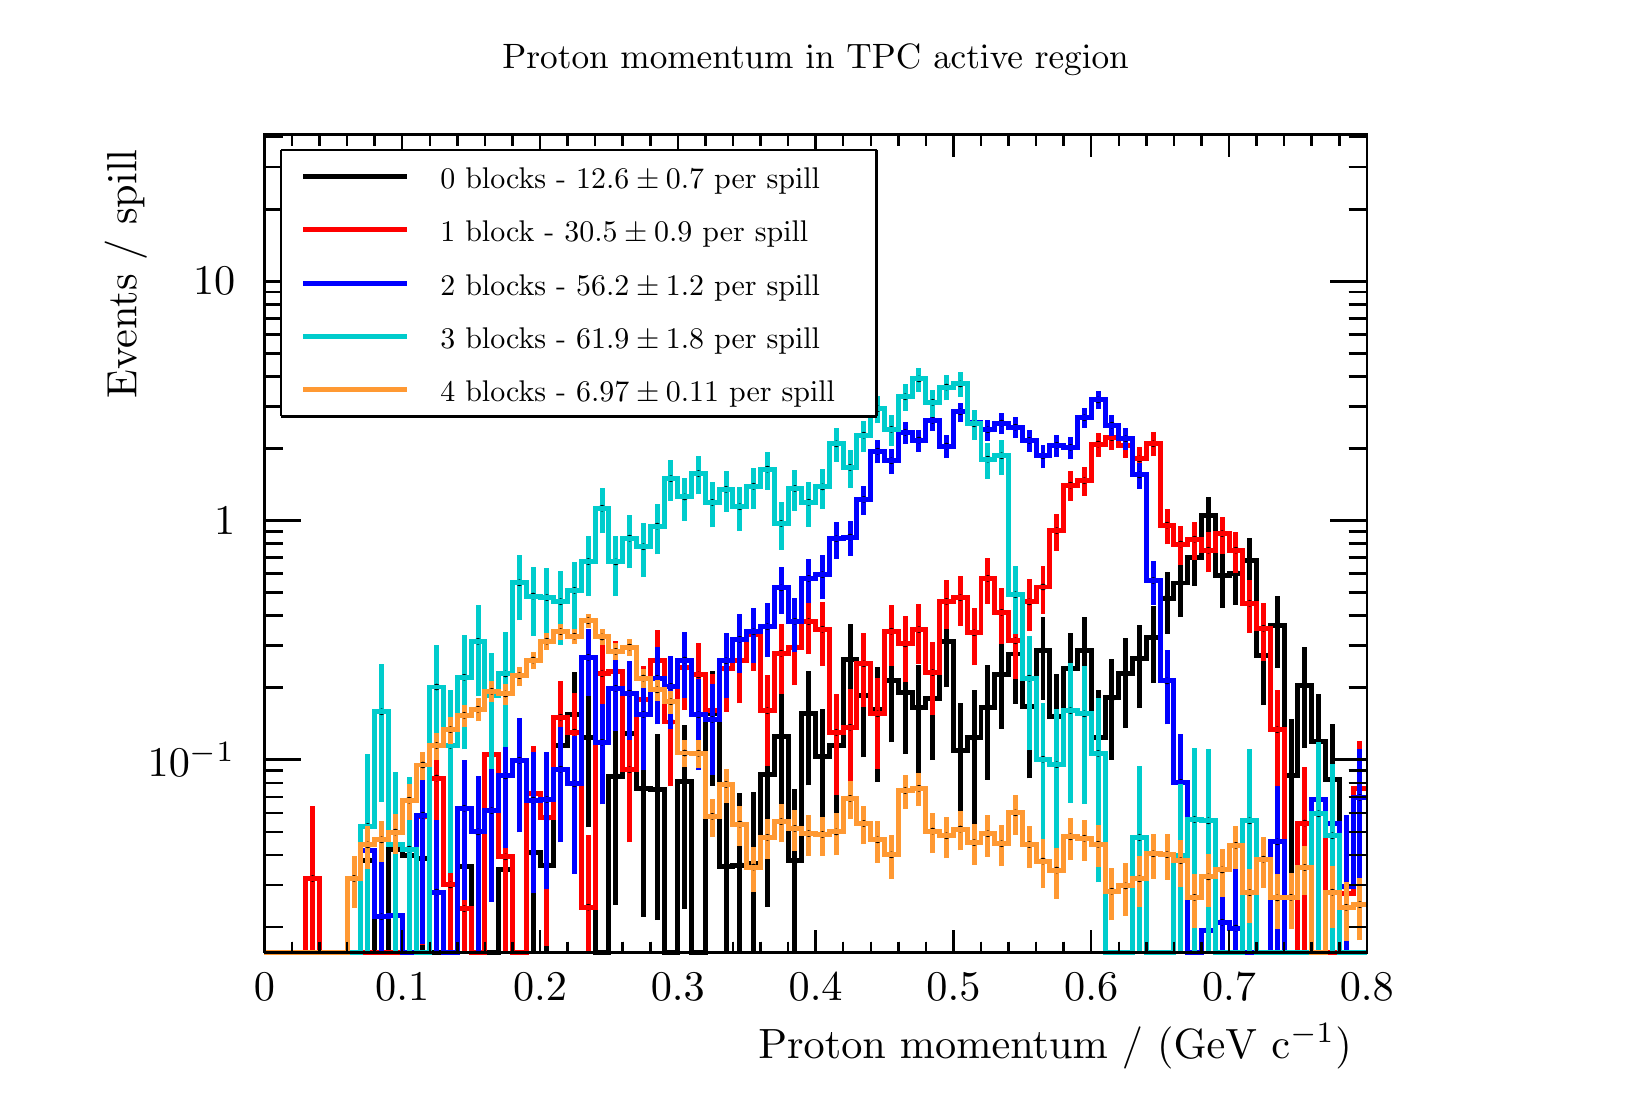
\begin{tikzpicture}
\pgfdeclareplotmark{cross} {
\pgfpathmoveto{\pgfpoint{-0.3\pgfplotmarksize}{\pgfplotmarksize}}
\pgfpathlineto{\pgfpoint{+0.3\pgfplotmarksize}{\pgfplotmarksize}}
\pgfpathlineto{\pgfpoint{+0.3\pgfplotmarksize}{0.3\pgfplotmarksize}}
\pgfpathlineto{\pgfpoint{+1\pgfplotmarksize}{0.3\pgfplotmarksize}}
\pgfpathlineto{\pgfpoint{+1\pgfplotmarksize}{-0.3\pgfplotmarksize}}
\pgfpathlineto{\pgfpoint{+0.3\pgfplotmarksize}{-0.3\pgfplotmarksize}}
\pgfpathlineto{\pgfpoint{+0.3\pgfplotmarksize}{-1.\pgfplotmarksize}}
\pgfpathlineto{\pgfpoint{-0.3\pgfplotmarksize}{-1.\pgfplotmarksize}}
\pgfpathlineto{\pgfpoint{-0.3\pgfplotmarksize}{-0.3\pgfplotmarksize}}
\pgfpathlineto{\pgfpoint{-1.\pgfplotmarksize}{-0.3\pgfplotmarksize}}
\pgfpathlineto{\pgfpoint{-1.\pgfplotmarksize}{0.3\pgfplotmarksize}}
\pgfpathlineto{\pgfpoint{-0.3\pgfplotmarksize}{0.3\pgfplotmarksize}}
\pgfpathclose
\pgfusepathqstroke
}
\pgfdeclareplotmark{cross*} {
\pgfpathmoveto{\pgfpoint{-0.3\pgfplotmarksize}{\pgfplotmarksize}}
\pgfpathlineto{\pgfpoint{+0.3\pgfplotmarksize}{\pgfplotmarksize}}
\pgfpathlineto{\pgfpoint{+0.3\pgfplotmarksize}{0.3\pgfplotmarksize}}
\pgfpathlineto{\pgfpoint{+1\pgfplotmarksize}{0.3\pgfplotmarksize}}
\pgfpathlineto{\pgfpoint{+1\pgfplotmarksize}{-0.3\pgfplotmarksize}}
\pgfpathlineto{\pgfpoint{+0.3\pgfplotmarksize}{-0.3\pgfplotmarksize}}
\pgfpathlineto{\pgfpoint{+0.3\pgfplotmarksize}{-1.\pgfplotmarksize}}
\pgfpathlineto{\pgfpoint{-0.3\pgfplotmarksize}{-1.\pgfplotmarksize}}
\pgfpathlineto{\pgfpoint{-0.3\pgfplotmarksize}{-0.3\pgfplotmarksize}}
\pgfpathlineto{\pgfpoint{-1.\pgfplotmarksize}{-0.3\pgfplotmarksize}}
\pgfpathlineto{\pgfpoint{-1.\pgfplotmarksize}{0.3\pgfplotmarksize}}
\pgfpathlineto{\pgfpoint{-0.3\pgfplotmarksize}{0.3\pgfplotmarksize}}
\pgfpathclose
\pgfusepathqfillstroke
}
\pgfdeclareplotmark{newstar} {
\pgfpathmoveto{\pgfqpoint{0pt}{\pgfplotmarksize}}
\pgfpathlineto{\pgfqpointpolar{44}{0.5\pgfplotmarksize}}
\pgfpathlineto{\pgfqpointpolar{18}{\pgfplotmarksize}}
\pgfpathlineto{\pgfqpointpolar{-20}{0.5\pgfplotmarksize}}
\pgfpathlineto{\pgfqpointpolar{-54}{\pgfplotmarksize}}
\pgfpathlineto{\pgfqpointpolar{-90}{0.5\pgfplotmarksize}}
\pgfpathlineto{\pgfqpointpolar{234}{\pgfplotmarksize}}
\pgfpathlineto{\pgfqpointpolar{198}{0.5\pgfplotmarksize}}
\pgfpathlineto{\pgfqpointpolar{162}{\pgfplotmarksize}}
\pgfpathlineto{\pgfqpointpolar{134}{0.5\pgfplotmarksize}}
\pgfpathclose
\pgfusepathqstroke
}
\pgfdeclareplotmark{newstar*} {
\pgfpathmoveto{\pgfqpoint{0pt}{\pgfplotmarksize}}
\pgfpathlineto{\pgfqpointpolar{44}{0.5\pgfplotmarksize}}
\pgfpathlineto{\pgfqpointpolar{18}{\pgfplotmarksize}}
\pgfpathlineto{\pgfqpointpolar{-20}{0.5\pgfplotmarksize}}
\pgfpathlineto{\pgfqpointpolar{-54}{\pgfplotmarksize}}
\pgfpathlineto{\pgfqpointpolar{-90}{0.5\pgfplotmarksize}}
\pgfpathlineto{\pgfqpointpolar{234}{\pgfplotmarksize}}
\pgfpathlineto{\pgfqpointpolar{198}{0.5\pgfplotmarksize}}
\pgfpathlineto{\pgfqpointpolar{162}{\pgfplotmarksize}}
\pgfpathlineto{\pgfqpointpolar{134}{0.5\pgfplotmarksize}}
\pgfpathclose
\pgfusepathqfillstroke
}
\definecolor{c}{rgb}{1,1,1};
\draw [color=c, fill=c] (0,0) rectangle (20,13.4957);
\draw [color=c, fill=c] (3,1.75444) rectangle (17,12.1461);
\definecolor{c}{rgb}{0,0,0};
\draw [c,line width=0.9] (3,1.75444) -- (3,12.1461) -- (17,12.1461) -- (17,1.75444) -- (3,1.75444);
\definecolor{c}{rgb}{1,1,1};
\draw [color=c, fill=c] (3,1.75444) rectangle (17,12.1461);
\definecolor{c}{rgb}{0,0,0};
\draw [c,line width=0.9] (3,1.75444) -- (3,12.1461) -- (17,12.1461) -- (17,1.75444) -- (3,1.75444);
\draw [c,line width=0.9] (3,1.75444) -- (3.175,1.75444) -- (3.175,1.75444) -- (3.35,1.75444) -- (3.35,1.75444) -- (3.525,1.75444) -- (3.525,1.75444) -- (3.7,1.75444) -- (3.7,1.75444) -- (3.875,1.75444) -- (3.875,1.75444) -- (4.05,1.75444) --
 (4.05,1.75444) -- (4.225,1.75444) -- (4.225,1.75444) -- (4.4,1.75444) -- (4.4,1.75444) -- (4.575,1.75444) -- (4.575,1.75444) -- (4.75,1.75444) -- (4.75,1.75444) -- (4.925,1.75444) -- (4.925,1.75444) -- (5.1,1.75444) -- (5.1,1.75444) --
 (5.275,1.75444) -- (5.275,1.75444) -- (5.45,1.75444) -- (5.45,1.75444) -- (5.625,1.75444) -- (5.625,1.75444) -- (5.8,1.75444) -- (5.8,1.75444) -- (5.975,1.75444) -- (5.975,1.75444) -- (6.15,1.75444) -- (6.15,1.75444) -- (6.325,1.75444) --
 (6.325,1.75444) -- (6.5,1.75444) -- (6.5,1.75444) -- (6.675,1.75444) -- (6.675,1.75444) -- (6.85,1.75444) -- (6.85,1.75444) -- (7.025,1.75444) -- (7.025,1.75444) -- (7.2,1.75444) -- (7.2,1.75444) -- (7.375,1.75444) -- (7.375,1.75444) --
 (7.55,1.75444) -- (7.55,1.75444) -- (7.725,1.75444) -- (7.725,1.75444) -- (7.9,1.75444) -- (7.9,1.75444) -- (8.075,1.75444) -- (8.075,1.75444) -- (8.25,1.75444) -- (8.25,1.75444) -- (8.425,1.75444) -- (8.425,1.75444) -- (8.6,1.75444) --
 (8.6,1.75444) -- (8.775,1.75444) -- (8.775,1.75444) -- (8.95,1.75444) -- (8.95,1.75444) -- (9.125,1.75444) -- (9.125,1.75444) -- (9.3,1.75444) -- (9.3,1.75444) -- (9.475,1.75444) -- (9.475,1.75444) -- (9.65,1.75444) -- (9.65,1.75444) --
 (9.825,1.75444) -- (9.825,1.75444) -- (10,1.75444) -- (10,1.75444) -- (10.175,1.75444) -- (10.175,1.75444) -- (10.35,1.75444) -- (10.35,1.75444) -- (10.525,1.75444) -- (10.525,1.75444) -- (10.7,1.75444) -- (10.7,1.75444) -- (10.875,1.75444) --
 (10.875,1.75444) -- (11.05,1.75444) -- (11.05,1.75444) -- (11.225,1.75444) -- (11.225,1.75444) -- (11.4,1.75444) -- (11.4,1.75444) -- (11.575,1.75444) -- (11.575,1.75444) -- (11.75,1.75444) -- (11.75,1.75444) -- (11.925,1.75444) -- (11.925,1.75444)
 -- (12.1,1.75444) -- (12.1,1.75444) -- (12.275,1.75444) -- (12.275,1.75444) -- (12.45,1.75444) -- (12.45,1.75444) -- (12.625,1.75444) -- (12.625,1.75444) -- (12.8,1.75444) -- (12.8,1.75444) -- (12.975,1.75444) -- (12.975,1.75444) -- (13.15,1.75444)
 -- (13.15,1.75444) -- (13.325,1.75444) -- (13.325,1.75444) -- (13.5,1.75444) -- (13.5,1.75444) -- (13.675,1.75444) -- (13.675,1.75444) -- (13.85,1.75444) -- (13.85,1.75444) -- (14.025,1.75444) -- (14.025,1.75444) -- (14.2,1.75444) -- (14.2,1.75444)
 -- (14.375,1.75444) -- (14.375,1.75444) -- (14.55,1.75444) -- (14.55,1.75444) -- (14.725,1.75444) -- (14.725,1.75444) -- (14.9,1.75444) -- (14.9,1.75444) -- (15.075,1.75444) -- (15.075,1.75444) -- (15.25,1.75444) -- (15.25,1.75444) --
 (15.425,1.75444) -- (15.425,1.75444) -- (15.6,1.75444) -- (15.6,1.75444) -- (15.775,1.75444) -- (15.775,1.75444) -- (15.95,1.75444) -- (15.95,1.75444) -- (16.125,1.75444) -- (16.125,1.75444) -- (16.3,1.75444) -- (16.3,1.75444) -- (16.475,1.75444) --
 (16.475,1.75444) -- (16.65,1.75444) -- (16.65,1.75444) -- (16.825,1.75444) -- (16.825,1.75444) -- (17,1.75444);
\draw [c,line width=0.9] (3,1.75444) -- (17,1.75444);
\draw [c,line width=0.9] (3,2.03785) -- (3,1.75444);
\draw [c,line width=0.9] (3.35,1.89615) -- (3.35,1.75444);
\draw [c,line width=0.9] (3.7,1.89615) -- (3.7,1.75444);
\draw [c,line width=0.9] (4.05,1.89615) -- (4.05,1.75444);
\draw [c,line width=0.9] (4.4,1.89615) -- (4.4,1.75444);
\draw [c,line width=0.9] (4.75,2.03785) -- (4.75,1.75444);
\draw [c,line width=0.9] (5.1,1.89615) -- (5.1,1.75444);
\draw [c,line width=0.9] (5.45,1.89615) -- (5.45,1.75444);
\draw [c,line width=0.9] (5.8,1.89615) -- (5.8,1.75444);
\draw [c,line width=0.9] (6.15,1.89615) -- (6.15,1.75444);
\draw [c,line width=0.9] (6.5,2.03785) -- (6.5,1.75444);
\draw [c,line width=0.9] (6.85,1.89615) -- (6.85,1.75444);
\draw [c,line width=0.9] (7.2,1.89615) -- (7.2,1.75444);
\draw [c,line width=0.9] (7.55,1.89615) -- (7.55,1.75444);
\draw [c,line width=0.9] (7.9,1.89615) -- (7.9,1.75444);
\draw [c,line width=0.9] (8.25,2.03785) -- (8.25,1.75444);
\draw [c,line width=0.9] (8.6,1.89615) -- (8.6,1.75444);
\draw [c,line width=0.9] (8.95,1.89615) -- (8.95,1.75444);
\draw [c,line width=0.9] (9.3,1.89615) -- (9.3,1.75444);
\draw [c,line width=0.9] (9.65,1.89615) -- (9.65,1.75444);
\draw [c,line width=0.9] (10,2.03785) -- (10,1.75444);
\draw [c,line width=0.9] (10.35,1.89615) -- (10.35,1.75444);
\draw [c,line width=0.9] (10.7,1.89615) -- (10.7,1.75444);
\draw [c,line width=0.9] (11.05,1.89615) -- (11.05,1.75444);
\draw [c,line width=0.9] (11.4,1.89615) -- (11.4,1.75444);
\draw [c,line width=0.9] (11.75,2.03785) -- (11.75,1.75444);
\draw [c,line width=0.9] (12.1,1.89615) -- (12.1,1.75444);
\draw [c,line width=0.9] (12.45,1.89615) -- (12.45,1.75444);
\draw [c,line width=0.9] (12.8,1.89615) -- (12.8,1.75444);
\draw [c,line width=0.9] (13.15,1.89615) -- (13.15,1.75444);
\draw [c,line width=0.9] (13.5,2.03785) -- (13.5,1.75444);
\draw [c,line width=0.9] (13.85,1.89615) -- (13.85,1.75444);
\draw [c,line width=0.9] (14.2,1.89615) -- (14.2,1.75444);
\draw [c,line width=0.9] (14.55,1.89615) -- (14.55,1.75444);
\draw [c,line width=0.9] (14.9,1.89615) -- (14.9,1.75444);
\draw [c,line width=0.9] (15.25,2.03785) -- (15.25,1.75444);
\draw [c,line width=0.9] (15.6,1.89615) -- (15.6,1.75444);
\draw [c,line width=0.9] (15.95,1.89615) -- (15.95,1.75444);
\draw [c,line width=0.9] (16.3,1.89615) -- (16.3,1.75444);
\draw [c,line width=0.9] (16.65,1.89615) -- (16.65,1.75444);
\draw [c,line width=0.9] (17,2.03785) -- (17,1.75444);
\draw [anchor=base] (3,1.14713) node[scale=1.52731, color=c, rotate=0]{0};
\draw [anchor=base] (4.75,1.14713) node[scale=1.52731, color=c, rotate=0]{0.1};
\draw [anchor=base] (6.5,1.14713) node[scale=1.52731, color=c, rotate=0]{0.2};
\draw [anchor=base] (8.25,1.14713) node[scale=1.52731, color=c, rotate=0]{0.3};
\draw [anchor=base] (10,1.14713) node[scale=1.52731, color=c, rotate=0]{0.4};
\draw [anchor=base] (11.75,1.14713) node[scale=1.52731, color=c, rotate=0]{0.5};
\draw [anchor=base] (13.5,1.14713) node[scale=1.52731, color=c, rotate=0]{0.6};
\draw [anchor=base] (15.25,1.14713) node[scale=1.52731, color=c, rotate=0]{0.7};
\draw [anchor=base] (17,1.14713) node[scale=1.52731, color=c, rotate=0]{0.8};
\draw [anchor= east] (17,0.566819) node[scale=1.52731, color=c, rotate=0]{Proton momentum / (GeV c$^{-1}$)};
\draw [c,line width=0.9] (3,12.1461) -- (17,12.1461);
\draw [c,line width=0.9] (3,11.8627) -- (3,12.1461);
\draw [c,line width=0.9] (3.35,12.0044) -- (3.35,12.1461);
\draw [c,line width=0.9] (3.7,12.0044) -- (3.7,12.1461);
\draw [c,line width=0.9] (4.05,12.0044) -- (4.05,12.1461);
\draw [c,line width=0.9] (4.4,12.0044) -- (4.4,12.1461);
\draw [c,line width=0.9] (4.75,11.8627) -- (4.75,12.1461);
\draw [c,line width=0.9] (5.1,12.0044) -- (5.1,12.1461);
\draw [c,line width=0.9] (5.45,12.0044) -- (5.45,12.1461);
\draw [c,line width=0.9] (5.8,12.0044) -- (5.8,12.1461);
\draw [c,line width=0.9] (6.15,12.0044) -- (6.15,12.1461);
\draw [c,line width=0.9] (6.5,11.8627) -- (6.5,12.1461);
\draw [c,line width=0.9] (6.85,12.0044) -- (6.85,12.1461);
\draw [c,line width=0.9] (7.2,12.0044) -- (7.2,12.1461);
\draw [c,line width=0.9] (7.55,12.0044) -- (7.55,12.1461);
\draw [c,line width=0.9] (7.9,12.0044) -- (7.9,12.1461);
\draw [c,line width=0.9] (8.25,11.8627) -- (8.25,12.1461);
\draw [c,line width=0.9] (8.6,12.0044) -- (8.6,12.1461);
\draw [c,line width=0.9] (8.95,12.0044) -- (8.95,12.1461);
\draw [c,line width=0.9] (9.3,12.0044) -- (9.3,12.1461);
\draw [c,line width=0.9] (9.65,12.0044) -- (9.65,12.1461);
\draw [c,line width=0.9] (10,11.8627) -- (10,12.1461);
\draw [c,line width=0.9] (10.35,12.0044) -- (10.35,12.1461);
\draw [c,line width=0.9] (10.7,12.0044) -- (10.7,12.1461);
\draw [c,line width=0.9] (11.05,12.0044) -- (11.05,12.1461);
\draw [c,line width=0.9] (11.4,12.0044) -- (11.4,12.1461);
\draw [c,line width=0.9] (11.75,11.8627) -- (11.75,12.1461);
\draw [c,line width=0.9] (12.1,12.0044) -- (12.1,12.1461);
\draw [c,line width=0.9] (12.45,12.0044) -- (12.45,12.1461);
\draw [c,line width=0.9] (12.8,12.0044) -- (12.8,12.1461);
\draw [c,line width=0.9] (13.15,12.0044) -- (13.15,12.1461);
\draw [c,line width=0.9] (13.5,11.8627) -- (13.5,12.1461);
\draw [c,line width=0.9] (13.85,12.0044) -- (13.85,12.1461);
\draw [c,line width=0.9] (14.2,12.0044) -- (14.2,12.1461);
\draw [c,line width=0.9] (14.55,12.0044) -- (14.55,12.1461);
\draw [c,line width=0.9] (14.9,12.0044) -- (14.9,12.1461);
\draw [c,line width=0.9] (15.25,11.8627) -- (15.25,12.1461);
\draw [c,line width=0.9] (15.6,12.0044) -- (15.6,12.1461);
\draw [c,line width=0.9] (15.95,12.0044) -- (15.95,12.1461);
\draw [c,line width=0.9] (16.3,12.0044) -- (16.3,12.1461);
\draw [c,line width=0.9] (16.65,12.0044) -- (16.65,12.1461);
\draw [c,line width=0.9] (17,11.8627) -- (17,12.1461);
\draw [c,line width=0.9] (3,1.75444) -- (3,12.1461);
\draw [c,line width=0.9] (3.231,2.08178) -- (3,2.08178);
\draw [c,line width=0.9] (3.231,2.61678) -- (3,2.61678);
\draw [c,line width=0.9] (3.231,2.99637) -- (3,2.99637);
\draw [c,line width=0.9] (3.231,3.29081) -- (3,3.29081);
\draw [c,line width=0.9] (3.231,3.53138) -- (3,3.53138);
\draw [c,line width=0.9] (3.231,3.73478) -- (3,3.73478);
\draw [c,line width=0.9] (3.231,3.91097) -- (3,3.91097);
\draw [c,line width=0.9] (3.231,4.06638) -- (3,4.06638);
\draw [c,line width=0.9] (3.462,4.2054) -- (3,4.2054);
\draw [anchor= east] (2.82,4.2054) node[scale=1.52731, color=c, rotate=0]{$10^{-1}$};
\draw [c,line width=0.9] (3.231,5.12) -- (3,5.12);
\draw [c,line width=0.9] (3.231,5.655) -- (3,5.655);
\draw [c,line width=0.9] (3.231,6.03459) -- (3,6.03459);
\draw [c,line width=0.9] (3.231,6.32902) -- (3,6.32902);
\draw [c,line width=0.9] (3.231,6.56959) -- (3,6.56959);
\draw [c,line width=0.9] (3.231,6.77299) -- (3,6.77299);
\draw [c,line width=0.9] (3.231,6.94918) -- (3,6.94918);
\draw [c,line width=0.9] (3.231,7.1046) -- (3,7.1046);
\draw [c,line width=0.9] (3.462,7.24362) -- (3,7.24362);
\draw [anchor= east] (2.82,7.24362) node[scale=1.52731, color=c, rotate=0]{1};
\draw [c,line width=0.9] (3.231,8.15821) -- (3,8.15821);
\draw [c,line width=0.9] (3.231,8.69321) -- (3,8.69321);
\draw [c,line width=0.9] (3.231,9.07281) -- (3,9.07281);
\draw [c,line width=0.9] (3.231,9.36724) -- (3,9.36724);
\draw [c,line width=0.9] (3.231,9.60781) -- (3,9.60781);
\draw [c,line width=0.9] (3.231,9.81121) -- (3,9.81121);
\draw [c,line width=0.9] (3.231,9.9874) -- (3,9.9874);
\draw [c,line width=0.9] (3.231,10.1428) -- (3,10.1428);
\draw [c,line width=0.9] (3.462,10.2818) -- (3,10.2818);
\draw [anchor= east] (2.82,10.2818) node[scale=1.52731, color=c, rotate=0]{10};
\draw [c,line width=0.9] (3.231,11.1964) -- (3,11.1964);
\draw [c,line width=0.9] (3.231,11.7314) -- (3,11.7314);
\draw [c,line width=0.9] (3.231,12.111) -- (3,12.111);
\draw [anchor= east] (1.24,12.1461) node[scale=1.52731, color=c, rotate=90]{ Events / spill};
\draw [c,line width=0.9] (17,1.75444) -- (17,12.1461);
\draw [c,line width=0.9] (16.769,2.08178) -- (17,2.08178);
\draw [c,line width=0.9] (16.769,2.61678) -- (17,2.61678);
\draw [c,line width=0.9] (16.769,2.99637) -- (17,2.99637);
\draw [c,line width=0.9] (16.769,3.29081) -- (17,3.29081);
\draw [c,line width=0.9] (16.769,3.53138) -- (17,3.53138);
\draw [c,line width=0.9] (16.769,3.73478) -- (17,3.73478);
\draw [c,line width=0.9] (16.769,3.91097) -- (17,3.91097);
\draw [c,line width=0.9] (16.769,4.06638) -- (17,4.06638);
\draw [c,line width=0.9] (16.538,4.2054) -- (17,4.2054);
\draw [c,line width=0.9] (16.769,5.12) -- (17,5.12);
\draw [c,line width=0.9] (16.769,5.655) -- (17,5.655);
\draw [c,line width=0.9] (16.769,6.03459) -- (17,6.03459);
\draw [c,line width=0.9] (16.769,6.32902) -- (17,6.32902);
\draw [c,line width=0.9] (16.769,6.56959) -- (17,6.56959);
\draw [c,line width=0.9] (16.769,6.77299) -- (17,6.77299);
\draw [c,line width=0.9] (16.769,6.94918) -- (17,6.94918);
\draw [c,line width=0.9] (16.769,7.1046) -- (17,7.1046);
\draw [c,line width=0.9] (16.538,7.24362) -- (17,7.24362);
\draw [c,line width=0.9] (16.769,8.15821) -- (17,8.15821);
\draw [c,line width=0.9] (16.769,8.69321) -- (17,8.69321);
\draw [c,line width=0.9] (16.769,9.07281) -- (17,9.07281);
\draw [c,line width=0.9] (16.769,9.36724) -- (17,9.36724);
\draw [c,line width=0.9] (16.769,9.60781) -- (17,9.60781);
\draw [c,line width=0.9] (16.769,9.81121) -- (17,9.81121);
\draw [c,line width=0.9] (16.769,9.9874) -- (17,9.9874);
\draw [c,line width=0.9] (16.769,10.1428) -- (17,10.1428);
\draw [c,line width=0.9] (16.538,10.2818) -- (17,10.2818);
\draw [c,line width=0.9] (16.769,11.1964) -- (17,11.1964);
\draw [c,line width=0.9] (16.769,11.7314) -- (17,11.7314);
\draw [c,line width=0.9] (16.769,12.111) -- (17,12.111);
\draw [c,line width=1.8] (4.3125,1.75444) -- (4.3125,2.93093);
\draw [c,line width=1.8] (4.3125,2.93093) -- (4.3125,3.84552);
\foreach \P in {(4.3125,2.93093)}{\draw[mark options={color=c,fill=c},mark size=2.402402pt,mark=*,mark size=1pt] plot coordinates {\P};}
\draw [c,line width=1.8] (4.6625,1.75444) -- (4.6625,3.07155);
\draw [c,line width=1.8] (4.6625,3.07155) -- (4.6625,3.98615);
\foreach \P in {(4.6625,3.07155)}{\draw[mark options={color=c,fill=c},mark size=2.402402pt,mark=*,mark size=1pt] plot coordinates {\P};}
\draw [c,line width=1.8] (4.8375,1.75444) -- (4.8375,2.99212);
\draw [c,line width=1.8] (4.8375,2.99212) -- (4.8375,3.90672);
\foreach \P in {(4.8375,2.99212)}{\draw[mark options={color=c,fill=c},mark size=2.402402pt,mark=*,mark size=1pt] plot coordinates {\P};}
\draw [c,line width=1.8] (5.0125,1.75444) -- (5.0125,2.95413);
\draw [c,line width=1.8] (5.0125,2.95413) -- (5.0125,3.86872);
\foreach \P in {(5.0125,2.95413)}{\draw[mark options={color=c,fill=c},mark size=2.402402pt,mark=*,mark size=1pt] plot coordinates {\P};}
\draw [c,line width=1.8] (5.5375,1.75444) -- (5.5375,2.85063);
\draw [c,line width=1.8] (5.5375,2.85063) -- (5.5375,3.76522);
\foreach \P in {(5.5375,2.85063)}{\draw[mark options={color=c,fill=c},mark size=2.402402pt,mark=*,mark size=1pt] plot coordinates {\P};}
\draw [c,line width=1.8] (6.0625,1.75444) -- (6.0625,2.80804);
\draw [c,line width=1.8] (6.0625,2.80804) -- (6.0625,3.72264);
\foreach \P in {(6.0625,2.80804)}{\draw[mark options={color=c,fill=c},mark size=2.402402pt,mark=*,mark size=1pt] plot coordinates {\P};}
\draw [c,line width=1.8] (6.4125,1.75444) -- (6.4125,3.02135);
\draw [c,line width=1.8] (6.4125,3.02135) -- (6.4125,3.93595);
\foreach \P in {(6.4125,3.02135)}{\draw[mark options={color=c,fill=c},mark size=2.402402pt,mark=*,mark size=1pt] plot coordinates {\P};}
\draw [c,line width=1.8] (6.5875,1.75444) -- (6.5875,2.86805);
\draw [c,line width=1.8] (6.5875,2.86805) -- (6.5875,3.78265);
\foreach \P in {(6.5875,2.86805)}{\draw[mark options={color=c,fill=c},mark size=2.402402pt,mark=*,mark size=1pt] plot coordinates {\P};}
\draw [c,line width=1.8] (6.7625,3.25045) -- (6.7625,4.38708);
\draw [c,line width=1.8] (6.7625,4.38708) -- (6.7625,4.9885);
\foreach \P in {(6.7625,4.38708)}{\draw[mark options={color=c,fill=c},mark size=2.402402pt,mark=*,mark size=1pt] plot coordinates {\P};}
\draw [c,line width=1.8] (6.9375,3.86542) -- (6.9375,4.78232);
\draw [c,line width=1.8] (6.9375,4.78232) -- (6.9375,5.31809);
\foreach \P in {(6.9375,4.78232)}{\draw[mark options={color=c,fill=c},mark size=2.402402pt,mark=*,mark size=1pt] plot coordinates {\P};}
\draw [c,line width=1.8] (7.1125,3.34711) -- (7.1125,4.4855);
\draw [c,line width=1.8] (7.1125,4.4855) -- (7.1125,5.08739);
\foreach \P in {(7.1125,4.4855)}{\draw[mark options={color=c,fill=c},mark size=2.402402pt,mark=*,mark size=1pt] plot coordinates {\P};}
\draw [c,line width=1.8] (7.4625,2.36048) -- (7.4625,3.99755);
\draw [c,line width=1.8] (7.4625,3.99755) -- (7.4625,4.70607);
\foreach \P in {(7.4625,3.99755)}{\draw[mark options={color=c,fill=c},mark size=2.402402pt,mark=*,mark size=1pt] plot coordinates {\P};}
\draw [c,line width=1.8] (7.6375,3.38215) -- (7.6375,4.53369);
\draw [c,line width=1.8] (7.6375,4.53369) -- (7.6375,5.13907);
\foreach \P in {(7.6375,4.53369)}{\draw[mark options={color=c,fill=c},mark size=2.402402pt,mark=*,mark size=1pt] plot coordinates {\P};}
\draw [c,line width=1.8] (7.8125,2.21378) -- (7.8125,3.83427);
\draw [c,line width=1.8] (7.8125,3.83427) -- (7.8125,4.53996);
\foreach \P in {(7.8125,3.83427)}{\draw[mark options={color=c,fill=c},mark size=2.402402pt,mark=*,mark size=1pt] plot coordinates {\P};}
\draw [c,line width=1.8] (7.9875,2.16943) -- (7.9875,3.82634);
\draw [c,line width=1.8] (7.9875,3.82634) -- (7.9875,4.53818);
\foreach \P in {(7.9875,3.82634)}{\draw[mark options={color=c,fill=c},mark size=2.402402pt,mark=*,mark size=1pt] plot coordinates {\P};}
\draw [c,line width=1.8] (8.3375,2.31014) -- (8.3375,3.93412);
\draw [c,line width=1.8] (8.3375,3.93412) -- (8.3375,4.64041);
\foreach \P in {(8.3375,3.93412)}{\draw[mark options={color=c,fill=c},mark size=2.402402pt,mark=*,mark size=1pt] plot coordinates {\P};}
\draw [c,line width=1.8] (8.6875,3.87377) -- (8.6875,4.79496);
\draw [c,line width=1.8] (8.6875,4.79496) -- (8.6875,5.33215);
\foreach \P in {(8.6875,4.79496)}{\draw[mark options={color=c,fill=c},mark size=2.402402pt,mark=*,mark size=1pt] plot coordinates {\P};}
\draw [c,line width=1.8] (8.8625,1.75444) -- (8.8625,2.85063);
\draw [c,line width=1.8] (8.8625,2.85063) -- (8.8625,3.76522);
\foreach \P in {(8.8625,2.85063)}{\draw[mark options={color=c,fill=c},mark size=2.402402pt,mark=*,mark size=1pt] plot coordinates {\P};}
\draw [c,line width=1.8] (9.0375,1.75444) -- (9.0375,2.86805);
\draw [c,line width=1.8] (9.0375,2.86805) -- (9.0375,3.78265);
\foreach \P in {(9.0375,2.86805)}{\draw[mark options={color=c,fill=c},mark size=2.402402pt,mark=*,mark size=1pt] plot coordinates {\P};}
\draw [c,line width=1.8] (9.2125,1.75444) -- (9.2125,2.88572);
\draw [c,line width=1.8] (9.2125,2.88572) -- (9.2125,3.80031);
\foreach \P in {(9.2125,2.88572)}{\draw[mark options={color=c,fill=c},mark size=2.402402pt,mark=*,mark size=1pt] plot coordinates {\P};}
\draw [c,line width=1.8] (9.3875,2.33881) -- (9.3875,4.0146);
\draw [c,line width=1.8] (9.3875,4.0146) -- (9.3875,4.72955);
\foreach \P in {(9.3875,4.0146)}{\draw[mark options={color=c,fill=c},mark size=2.402402pt,mark=*,mark size=1pt] plot coordinates {\P};}
\draw [c,line width=1.8] (9.5625,3.34321) -- (9.5625,4.49958);
\draw [c,line width=1.8] (9.5625,4.49958) -- (9.5625,5.10624);
\foreach \P in {(9.5625,4.49958)}{\draw[mark options={color=c,fill=c},mark size=2.402402pt,mark=*,mark size=1pt] plot coordinates {\P};}
\draw [c,line width=1.8] (9.7375,1.75444) -- (9.7375,2.92176);
\draw [c,line width=1.8] (9.7375,2.92176) -- (9.7375,3.83636);
\foreach \P in {(9.7375,2.92176)}{\draw[mark options={color=c,fill=c},mark size=2.402402pt,mark=*,mark size=1pt] plot coordinates {\P};}
\draw [c,line width=1.8] (9.9125,3.87847) -- (9.9125,4.7945);
\draw [c,line width=1.8] (9.9125,4.7945) -- (9.9125,5.32998);
\foreach \P in {(9.9125,4.7945)}{\draw[mark options={color=c,fill=c},mark size=2.402402pt,mark=*,mark size=1pt] plot coordinates {\P};}
\draw [c,line width=1.8] (10.0875,3.10627) -- (10.0875,4.24319);
\draw [c,line width=1.8] (10.0875,4.24319) -- (10.0875,4.84469);
\foreach \P in {(10.0875,4.24319)}{\draw[mark options={color=c,fill=c},mark size=2.402402pt,mark=*,mark size=1pt] plot coordinates {\P};}
\draw [c,line width=1.8] (10.2625,3.25095) -- (10.2625,4.38854);
\draw [c,line width=1.8] (10.2625,4.38854) -- (10.2625,4.99022);
\foreach \P in {(10.2625,4.38854)}{\draw[mark options={color=c,fill=c},mark size=2.402402pt,mark=*,mark size=1pt] plot coordinates {\P};}
\draw [c,line width=1.8] (10.4375,4.77751) -- (10.4375,5.47555);
\draw [c,line width=1.8] (10.4375,5.47555) -- (10.4375,5.92968);
\foreach \P in {(10.4375,5.47555)}{\draw[mark options={color=c,fill=c},mark size=2.402402pt,mark=*,mark size=1pt] plot coordinates {\P};}
\draw [c,line width=1.8] (10.6125,4.23455) -- (10.6125,5.01943);
\draw [c,line width=1.8] (10.6125,5.01943) -- (10.6125,5.50819);
\foreach \P in {(10.6125,5.01943)}{\draw[mark options={color=c,fill=c},mark size=2.402402pt,mark=*,mark size=1pt] plot coordinates {\P};}
\draw [c,line width=1.8] (10.7875,3.92071) -- (10.7875,4.84054);
\draw [c,line width=1.8] (10.7875,4.84054) -- (10.7875,5.37728);
\foreach \P in {(10.7875,4.84054)}{\draw[mark options={color=c,fill=c},mark size=2.402402pt,mark=*,mark size=1pt] plot coordinates {\P};}
\draw [c,line width=1.8] (10.9625,4.42626) -- (10.9625,5.21609);
\draw [c,line width=1.8] (10.9625,5.21609) -- (10.9625,5.70673);
\foreach \P in {(10.9625,5.21609)}{\draw[mark options={color=c,fill=c},mark size=2.402402pt,mark=*,mark size=1pt] plot coordinates {\P};}
\draw [c,line width=1.8] (11.1375,4.2755) -- (11.1375,5.06242);
\draw [c,line width=1.8] (11.1375,5.06242) -- (11.1375,5.55196);
\foreach \P in {(11.1375,5.06242)}{\draw[mark options={color=c,fill=c},mark size=2.402402pt,mark=*,mark size=1pt] plot coordinates {\P};}
\draw [c,line width=1.8] (11.3125,3.95275) -- (11.3125,4.86925);
\draw [c,line width=1.8] (11.3125,4.86925) -- (11.3125,5.4049);
\foreach \P in {(11.3125,4.86925)}{\draw[mark options={color=c,fill=c},mark size=2.402402pt,mark=*,mark size=1pt] plot coordinates {\P};}
\draw [c,line width=1.8] (11.4875,4.20095) -- (11.4875,4.98627);
\draw [c,line width=1.8] (11.4875,4.98627) -- (11.4875,5.47521);
\foreach \P in {(11.4875,4.98627)}{\draw[mark options={color=c,fill=c},mark size=2.402402pt,mark=*,mark size=1pt] plot coordinates {\P};}
\draw [c,line width=1.8] (11.6625,5.12769) -- (11.6625,5.70585);
\draw [c,line width=1.8] (11.6625,5.70585) -- (11.6625,6.1065);
\foreach \P in {(11.6625,5.70585)}{\draw[mark options={color=c,fill=c},mark size=2.402402pt,mark=*,mark size=1pt] plot coordinates {\P};}
\draw [c,line width=1.8] (11.8375,3.17468) -- (11.8375,4.32068);
\draw [c,line width=1.8] (11.8375,4.32068) -- (11.8375,4.92461);
\foreach \P in {(11.8375,4.32068)}{\draw[mark options={color=c,fill=c},mark size=2.402402pt,mark=*,mark size=1pt] plot coordinates {\P};}
\draw [c,line width=1.8] (12.0125,3.32874) -- (12.0125,4.48452);
\draw [c,line width=1.8] (12.0125,4.48452) -- (12.0125,5.09102);
\foreach \P in {(12.0125,4.48452)}{\draw[mark options={color=c,fill=c},mark size=2.402402pt,mark=*,mark size=1pt] plot coordinates {\P};}
\draw [c,line width=1.8] (12.1875,3.95327) -- (12.1875,4.87297);
\draw [c,line width=1.8] (12.1875,4.87297) -- (12.1875,5.40968);
\foreach \P in {(12.1875,4.87297)}{\draw[mark options={color=c,fill=c},mark size=2.402402pt,mark=*,mark size=1pt] plot coordinates {\P};}
\draw [c,line width=1.8] (12.3625,4.59718) -- (12.3625,5.29013);
\draw [c,line width=1.8] (12.3625,5.29013) -- (12.3625,5.74213);
\foreach \P in {(12.3625,5.29013)}{\draw[mark options={color=c,fill=c},mark size=2.402402pt,mark=*,mark size=1pt] plot coordinates {\P};}
\draw [c,line width=1.8] (12.5375,4.91642) -- (12.5375,5.54822);
\draw [c,line width=1.8] (12.5375,5.54822) -- (12.5375,5.97368);
\foreach \P in {(12.5375,5.54822)}{\draw[mark options={color=c,fill=c},mark size=2.402402pt,mark=*,mark size=1pt] plot coordinates {\P};}
\draw [c,line width=1.8] (12.7125,3.96764) -- (12.7125,4.88277);
\draw [c,line width=1.8] (12.7125,4.88277) -- (12.7125,5.41796);
\foreach \P in {(12.7125,4.88277)}{\draw[mark options={color=c,fill=c},mark size=2.402402pt,mark=*,mark size=1pt] plot coordinates {\P};}
\draw [c,line width=1.8] (12.8875,4.96455) -- (12.8875,5.59468);
\draw [c,line width=1.8] (12.8875,5.59468) -- (12.8875,6.01939);
\foreach \P in {(12.8875,5.59468)}{\draw[mark options={color=c,fill=c},mark size=2.402402pt,mark=*,mark size=1pt] plot coordinates {\P};}
\draw [c,line width=1.8] (13.0625,3.84251) -- (13.0625,4.75854);
\draw [c,line width=1.8] (13.0625,4.75854) -- (13.0625,5.29402);
\foreach \P in {(13.0625,4.75854)}{\draw[mark options={color=c,fill=c},mark size=2.402402pt,mark=*,mark size=1pt] plot coordinates {\P};}
\draw [c,line width=1.8] (13.2375,4.67069) -- (13.2375,5.3639);
\draw [c,line width=1.8] (13.2375,5.3639) -- (13.2375,5.816);
\foreach \P in {(13.2375,5.3639)}{\draw[mark options={color=c,fill=c},mark size=2.402402pt,mark=*,mark size=1pt] plot coordinates {\P};}
\draw [c,line width=1.8] (13.4125,4.96155) -- (13.4125,5.59277);
\draw [c,line width=1.8] (13.4125,5.59277) -- (13.4125,6.01796);
\foreach \P in {(13.4125,5.59277)}{\draw[mark options={color=c,fill=c},mark size=2.402402pt,mark=*,mark size=1pt] plot coordinates {\P};}
\draw [c,line width=1.8] (13.5875,3.34164) -- (13.5875,4.48746);
\draw [c,line width=1.8] (13.5875,4.48746) -- (13.5875,5.09134);
\foreach \P in {(13.5875,4.48746)}{\draw[mark options={color=c,fill=c},mark size=2.402402pt,mark=*,mark size=1pt] plot coordinates {\P};}
\draw [c,line width=1.8] (13.7625,4.19998) -- (13.7625,4.98996);
\draw [c,line width=1.8] (13.7625,4.98996) -- (13.7625,5.48067);
\foreach \P in {(13.7625,4.98996)}{\draw[mark options={color=c,fill=c},mark size=2.402402pt,mark=*,mark size=1pt] plot coordinates {\P};}
\draw [c,line width=1.8] (13.9375,4.60775) -- (13.9375,5.30103);
\draw [c,line width=1.8] (13.9375,5.30103) -- (13.9375,5.75317);
\foreach \P in {(13.9375,5.30103)}{\draw[mark options={color=c,fill=c},mark size=2.402402pt,mark=*,mark size=1pt] plot coordinates {\P};}
\draw [c,line width=1.8] (14.1125,4.86217) -- (14.1125,5.49368);
\draw [c,line width=1.8] (14.1125,5.49368) -- (14.1125,5.919);
\foreach \P in {(14.1125,5.49368)}{\draw[mark options={color=c,fill=c},mark size=2.402402pt,mark=*,mark size=1pt] plot coordinates {\P};}
\draw [c,line width=1.8] (14.2875,5.17753) -- (14.2875,5.7555);
\draw [c,line width=1.8] (14.2875,5.7555) -- (14.2875,6.15606);
\foreach \P in {(14.2875,5.7555)}{\draw[mark options={color=c,fill=c},mark size=2.402402pt,mark=*,mark size=1pt] plot coordinates {\P};}
\draw [c,line width=1.8] (14.4625,5.80529) -- (14.4625,6.25782);
\draw [c,line width=1.8] (14.4625,6.25782) -- (14.4625,6.59415);
\foreach \P in {(14.4625,6.25782)}{\draw[mark options={color=c,fill=c},mark size=2.402402pt,mark=*,mark size=1pt] plot coordinates {\P};}
\draw [c,line width=1.8] (14.6375,6.0176) -- (14.6375,6.44992);
\draw [c,line width=1.8] (14.6375,6.44992) -- (14.6375,6.775);
\foreach \P in {(14.6375,6.44992)}{\draw[mark options={color=c,fill=c},mark size=2.402402pt,mark=*,mark size=1pt] plot coordinates {\P};}
\draw [c,line width=1.8] (14.8125,6.41599) -- (14.8125,6.77286);
\draw [c,line width=1.8] (14.8125,6.77286) -- (14.8125,7.05347);
\foreach \P in {(14.8125,6.77286)}{\draw[mark options={color=c,fill=c},mark size=2.402402pt,mark=*,mark size=1pt] plot coordinates {\P};}
\draw [c,line width=1.8] (14.9875,7.01185) -- (14.9875,7.30142);
\draw [c,line width=1.8] (14.9875,7.30142) -- (14.9875,7.53874);
\foreach \P in {(14.9875,7.30142)}{\draw[mark options={color=c,fill=c},mark size=2.402402pt,mark=*,mark size=1pt] plot coordinates {\P};}
\draw [c,line width=1.8] (15.1625,6.13347) -- (15.1625,6.54653);
\draw [c,line width=1.8] (15.1625,6.54653) -- (15.1625,6.86064);
\foreach \P in {(15.1625,6.54653)}{\draw[mark options={color=c,fill=c},mark size=2.402402pt,mark=*,mark size=1pt] plot coordinates {\P};}
\draw [c,line width=1.8] (15.3375,6.17694) -- (15.3375,6.57387);
\draw [c,line width=1.8] (15.3375,6.57387) -- (15.3375,6.87859);
\foreach \P in {(15.3375,6.57387)}{\draw[mark options={color=c,fill=c},mark size=2.402402pt,mark=*,mark size=1pt] plot coordinates {\P};}
\draw [c,line width=1.8] (15.5125,6.36689) -- (15.5125,6.7354);
\draw [c,line width=1.8] (15.5125,6.7354) -- (15.5125,7.02314);
\foreach \P in {(15.5125,6.7354)}{\draw[mark options={color=c,fill=c},mark size=2.402402pt,mark=*,mark size=1pt] plot coordinates {\P};}
\draw [c,line width=1.8] (15.6875,4.89982) -- (15.6875,5.53131);
\draw [c,line width=1.8] (15.6875,5.53131) -- (15.6875,5.95663);
\foreach \P in {(15.6875,5.53131)}{\draw[mark options={color=c,fill=c},mark size=2.402402pt,mark=*,mark size=1pt] plot coordinates {\P};}
\draw [c,line width=1.8] (15.8625,5.37131) -- (15.8625,5.90821);
\draw [c,line width=1.8] (15.8625,5.90821) -- (15.8625,6.28875);
\foreach \P in {(15.8625,5.90821)}{\draw[mark options={color=c,fill=c},mark size=2.402402pt,mark=*,mark size=1pt] plot coordinates {\P};}
\draw [c,line width=1.8] (16.0375,2.34294) -- (16.0375,4.00897);
\draw [c,line width=1.8] (16.0375,4.00897) -- (16.0375,4.72232);
\foreach \P in {(16.0375,4.00897)}{\draw[mark options={color=c,fill=c},mark size=2.402402pt,mark=*,mark size=1pt] plot coordinates {\P};}
\draw [c,line width=1.8] (16.2125,4.35306) -- (16.2125,5.14747);
\draw [c,line width=1.8] (16.2125,5.14747) -- (16.2125,5.63985);
\foreach \P in {(16.2125,5.14747)}{\draw[mark options={color=c,fill=c},mark size=2.402402pt,mark=*,mark size=1pt] plot coordinates {\P};}
\draw [c,line width=1.8] (16.3875,3.29584) -- (16.3875,4.43847);
\draw [c,line width=1.8] (16.3875,4.43847) -- (16.3875,5.0415);
\foreach \P in {(16.3875,4.43847)}{\draw[mark options={color=c,fill=c},mark size=2.402402pt,mark=*,mark size=1pt] plot coordinates {\P};}
\draw [c,line width=1.8] (16.5625,2.33055) -- (16.5625,3.95081);
\draw [c,line width=1.8] (16.5625,3.95081) -- (16.5625,4.65646);
\foreach \P in {(16.5625,3.95081)}{\draw[mark options={color=c,fill=c},mark size=2.402402pt,mark=*,mark size=1pt] plot coordinates {\P};}
\draw [c,line width=1.8] (3,1.75444) -- (3.175,1.75444) -- (3.175,1.75444) -- (3.35,1.75444) -- (3.35,1.75444) -- (3.525,1.75444) -- (3.525,1.75444) -- (3.7,1.75444) -- (3.7,1.75444) -- (3.875,1.75444) -- (3.875,1.75444) -- (4.05,1.75444) --
 (4.05,1.75444) -- (4.225,1.75444) -- (4.225,2.93093) -- (4.4,2.93093) -- (4.4,1.75444) -- (4.575,1.75444) -- (4.575,3.07155) -- (4.75,3.07155) -- (4.75,2.99212) -- (4.925,2.99212) -- (4.925,2.95413) -- (5.1,2.95413) -- (5.1,1.75444) --
 (5.275,1.75444) -- (5.275,1.75444) -- (5.45,1.75444) -- (5.45,2.85063) -- (5.625,2.85063) -- (5.625,1.75444) -- (5.8,1.75444) -- (5.8,1.75444) -- (5.975,1.75444) -- (5.975,2.80804) -- (6.15,2.80804) -- (6.15,1.75444) -- (6.325,1.75444) --
 (6.325,3.02135) -- (6.5,3.02135) -- (6.5,2.86805) -- (6.675,2.86805) -- (6.675,4.38708) -- (6.85,4.38708) -- (6.85,4.78232) -- (7.025,4.78232) -- (7.025,4.4855) -- (7.2,4.4855) -- (7.2,1.75444) -- (7.375,1.75444) -- (7.375,3.99755) -- (7.55,3.99755)
 -- (7.55,4.53369) -- (7.725,4.53369) -- (7.725,3.83427) -- (7.9,3.83427) -- (7.9,3.82634) -- (8.075,3.82634) -- (8.075,1.75444) -- (8.25,1.75444) -- (8.25,3.93412) -- (8.425,3.93412) -- (8.425,1.75444) -- (8.6,1.75444) -- (8.6,4.79496) --
 (8.775,4.79496) -- (8.775,2.85063) -- (8.95,2.85063) -- (8.95,2.86805) -- (9.125,2.86805) -- (9.125,2.88572) -- (9.3,2.88572) -- (9.3,4.0146) -- (9.475,4.0146) -- (9.475,4.49958) -- (9.65,4.49958) -- (9.65,2.92176) -- (9.825,2.92176) --
 (9.825,4.7945) -- (10,4.7945) -- (10,4.24319) -- (10.175,4.24319) -- (10.175,4.38854) -- (10.35,4.38854) -- (10.35,5.47555) -- (10.525,5.47555) -- (10.525,5.01943) -- (10.7,5.01943) -- (10.7,4.84054) -- (10.875,4.84054) -- (10.875,5.21609) --
 (11.05,5.21609) -- (11.05,5.06242) -- (11.225,5.06242) -- (11.225,4.86925) -- (11.4,4.86925) -- (11.4,4.98627) -- (11.575,4.98627) -- (11.575,5.70585) -- (11.75,5.70585) -- (11.75,4.32068) -- (11.925,4.32068) -- (11.925,4.48452) -- (12.1,4.48452) --
 (12.1,4.87297) -- (12.275,4.87297) -- (12.275,5.29013) -- (12.45,5.29013) -- (12.45,5.54822) -- (12.625,5.54822) -- (12.625,4.88277) -- (12.8,4.88277) -- (12.8,5.59468) -- (12.975,5.59468) -- (12.975,4.75854) -- (13.15,4.75854) -- (13.15,5.3639) --
 (13.325,5.3639) -- (13.325,5.59277) -- (13.5,5.59277) -- (13.5,4.48746) -- (13.675,4.48746) -- (13.675,4.98996) -- (13.85,4.98996) -- (13.85,5.30103) -- (14.025,5.30103) -- (14.025,5.49368) -- (14.2,5.49368) -- (14.2,5.7555) -- (14.375,5.7555) --
 (14.375,6.25782) -- (14.55,6.25782) -- (14.55,6.44992) -- (14.725,6.44992) -- (14.725,6.77286) -- (14.9,6.77286) -- (14.9,7.30142) -- (15.075,7.30142) -- (15.075,6.54653) -- (15.25,6.54653) -- (15.25,6.57387) -- (15.425,6.57387) -- (15.425,6.7354)
 -- (15.6,6.7354) -- (15.6,5.53131) -- (15.775,5.53131) -- (15.775,5.90821) -- (15.95,5.90821) -- (15.95,4.00897) -- (16.125,4.00897) -- (16.125,5.14747) -- (16.3,5.14747) -- (16.3,4.43847) -- (16.475,4.43847) -- (16.475,3.95081) -- (16.65,3.95081)
 -- (16.65,1.75444) -- (16.825,1.75444) -- (16.825,1.75444) -- (17,1.75444);
\definecolor{c}{rgb}{1,0,0};
\draw [c,line width=1.8] (3.6125,1.75444) -- (3.6125,2.69732);
\draw [c,line width=1.8] (3.6125,2.69732) -- (3.6125,3.61191);
\definecolor{c}{rgb}{0,0,0};
\foreach \P in {(3.6125,2.69732)}{\draw[mark options={color=c,fill=c},mark size=2.402402pt,mark=*,mark size=1pt] plot coordinates {\P};}
\definecolor{c}{rgb}{1,0,0};
\draw [c,line width=1.8] (5.0125,1.85673) -- (5.0125,3.4792);
\draw [c,line width=1.8] (5.0125,3.4792) -- (5.0125,4.18524);
\definecolor{c}{rgb}{0,0,0};
\foreach \P in {(5.0125,3.4792)}{\draw[mark options={color=c,fill=c},mark size=2.402402pt,mark=*,mark size=1pt] plot coordinates {\P};}
\definecolor{c}{rgb}{1,0,0};
\draw [c,line width=1.8] (5.1875,2.83375) -- (5.1875,3.97322);
\draw [c,line width=1.8] (5.1875,3.97322) -- (5.1875,4.5754);
\definecolor{c}{rgb}{0,0,0};
\foreach \P in {(5.1875,3.97322)}{\draw[mark options={color=c,fill=c},mark size=2.402402pt,mark=*,mark size=1pt] plot coordinates {\P};}
\definecolor{c}{rgb}{1,0,0};
\draw [c,line width=1.8] (5.3625,1.75444) -- (5.3625,2.61547);
\draw [c,line width=1.8] (5.3625,2.61547) -- (5.3625,3.53006);
\definecolor{c}{rgb}{0,0,0};
\foreach \P in {(5.3625,2.61547)}{\draw[mark options={color=c,fill=c},mark size=2.402402pt,mark=*,mark size=1pt] plot coordinates {\P};}
\definecolor{c}{rgb}{1,0,0};
\draw [c,line width=1.8] (5.5375,1.75444) -- (5.5375,2.3146);
\draw [c,line width=1.8] (5.5375,2.3146) -- (5.5375,3.22919);
\definecolor{c}{rgb}{0,0,0};
\foreach \P in {(5.5375,2.3146)}{\draw[mark options={color=c,fill=c},mark size=2.402402pt,mark=*,mark size=1pt] plot coordinates {\P};}
\definecolor{c}{rgb}{1,0,0};
\draw [c,line width=1.8] (5.8875,3.34661) -- (5.8875,4.26603);
\draw [c,line width=1.8] (5.8875,4.26603) -- (5.8875,4.80264);
\definecolor{c}{rgb}{0,0,0};
\foreach \P in {(5.8875,4.26603)}{\draw[mark options={color=c,fill=c},mark size=2.402402pt,mark=*,mark size=1pt] plot coordinates {\P};}
\definecolor{c}{rgb}{1,0,0};
\draw [c,line width=1.8] (6.0625,1.75444) -- (6.0625,2.97188);
\draw [c,line width=1.8] (6.0625,2.97188) -- (6.0625,3.88647);
\definecolor{c}{rgb}{0,0,0};
\foreach \P in {(6.0625,2.97188)}{\draw[mark options={color=c,fill=c},mark size=2.402402pt,mark=*,mark size=1pt] plot coordinates {\P};}
\definecolor{c}{rgb}{1,0,0};
\draw [c,line width=1.8] (6.4125,2.64361) -- (6.4125,3.78007);
\draw [c,line width=1.8] (6.4125,3.78007) -- (6.4125,4.38144);
\definecolor{c}{rgb}{0,0,0};
\foreach \P in {(6.4125,3.78007)}{\draw[mark options={color=c,fill=c},mark size=2.402402pt,mark=*,mark size=1pt] plot coordinates {\P};}
\definecolor{c}{rgb}{1,0,0};
\draw [c,line width=1.8] (6.5875,1.84314) -- (6.5875,3.46639);
\draw [c,line width=1.8] (6.5875,3.46639) -- (6.5875,4.17256);
\definecolor{c}{rgb}{0,0,0};
\foreach \P in {(6.5875,3.46639)}{\draw[mark options={color=c,fill=c},mark size=2.402402pt,mark=*,mark size=1pt] plot coordinates {\P};}
\definecolor{c}{rgb}{1,0,0};
\draw [c,line width=1.8] (6.7625,4.04662) -- (6.7625,4.74536);
\draw [c,line width=1.8] (6.7625,4.74536) -- (6.7625,5.19978);
\definecolor{c}{rgb}{0,0,0};
\foreach \P in {(6.7625,4.74536)}{\draw[mark options={color=c,fill=c},mark size=2.402402pt,mark=*,mark size=1pt] plot coordinates {\P};}
\definecolor{c}{rgb}{1,0,0};
\draw [c,line width=1.8] (6.9375,3.76517) -- (6.9375,4.55686);
\draw [c,line width=1.8] (6.9375,4.55686) -- (6.9375,5.04821);
\definecolor{c}{rgb}{0,0,0};
\foreach \P in {(6.9375,4.55686)}{\draw[mark options={color=c,fill=c},mark size=2.402402pt,mark=*,mark size=1pt] plot coordinates {\P};}
\definecolor{c}{rgb}{1,0,0};
\draw [c,line width=1.8] (7.1125,1.75444) -- (7.1125,2.33307);
\draw [c,line width=1.8] (7.1125,2.33307) -- (7.1125,3.24767);
\definecolor{c}{rgb}{0,0,0};
\foreach \P in {(7.1125,2.33307)}{\draw[mark options={color=c,fill=c},mark size=2.402402pt,mark=*,mark size=1pt] plot coordinates {\P};}
\definecolor{c}{rgb}{1,0,0};
\draw [c,line width=1.8] (7.2875,4.71432) -- (7.2875,5.29904);
\draw [c,line width=1.8] (7.2875,5.29904) -- (7.2875,5.70281);
\definecolor{c}{rgb}{0,0,0};
\foreach \P in {(7.2875,5.29904)}{\draw[mark options={color=c,fill=c},mark size=2.402402pt,mark=*,mark size=1pt] plot coordinates {\P};}
\definecolor{c}{rgb}{1,0,0};
\draw [c,line width=1.8] (7.4625,4.78337) -- (7.4625,5.32937);
\draw [c,line width=1.8] (7.4625,5.32937) -- (7.4625,5.71442);
\definecolor{c}{rgb}{0,0,0};
\foreach \P in {(7.4625,5.32937)}{\draw[mark options={color=c,fill=c},mark size=2.402402pt,mark=*,mark size=1pt] plot coordinates {\P};}
\definecolor{c}{rgb}{1,0,0};
\draw [c,line width=1.8] (7.6375,3.15461) -- (7.6375,4.07817);
\draw [c,line width=1.8] (7.6375,4.07817) -- (7.6375,4.61615);
\definecolor{c}{rgb}{0,0,0};
\foreach \P in {(7.6375,4.07817)}{\draw[mark options={color=c,fill=c},mark size=2.402402pt,mark=*,mark size=1pt] plot coordinates {\P};}
\definecolor{c}{rgb}{1,0,0};
\draw [c,line width=1.8] (7.8125,4.34325) -- (7.8125,4.97475);
\draw [c,line width=1.8] (7.8125,4.97475) -- (7.8125,5.40006);
\definecolor{c}{rgb}{0,0,0};
\foreach \P in {(7.8125,4.97475)}{\draw[mark options={color=c,fill=c},mark size=2.402402pt,mark=*,mark size=1pt] plot coordinates {\P};}
\definecolor{c}{rgb}{1,0,0};
\draw [c,line width=1.8] (7.9875,4.92365) -- (7.9875,5.469);
\draw [c,line width=1.8] (7.9875,5.469) -- (7.9875,5.85373);
\definecolor{c}{rgb}{0,0,0};
\foreach \P in {(7.9875,5.469)}{\draw[mark options={color=c,fill=c},mark size=2.402402pt,mark=*,mark size=1pt] plot coordinates {\P};}
\definecolor{c}{rgb}{1,0,0};
\draw [c,line width=1.8] (8.1625,3.87344) -- (8.1625,4.68483);
\draw [c,line width=1.8] (8.1625,4.68483) -- (8.1625,5.18356);
\definecolor{c}{rgb}{0,0,0};
\foreach \P in {(8.1625,4.68483)}{\draw[mark options={color=c,fill=c},mark size=2.402402pt,mark=*,mark size=1pt] plot coordinates {\P};}
\definecolor{c}{rgb}{1,0,0};
\draw [c,line width=1.8] (8.3375,4.83405) -- (8.3375,5.37206);
\draw [c,line width=1.8] (8.3375,5.37206) -- (8.3375,5.75316);
\definecolor{c}{rgb}{0,0,0};
\foreach \P in {(8.3375,5.37206)}{\draw[mark options={color=c,fill=c},mark size=2.402402pt,mark=*,mark size=1pt] plot coordinates {\P};}
\definecolor{c}{rgb}{1,0,0};
\draw [c,line width=1.8] (8.5125,4.69447) -- (8.5125,5.28218);
\draw [c,line width=1.8] (8.5125,5.28218) -- (8.5125,5.68736);
\definecolor{c}{rgb}{0,0,0};
\foreach \P in {(8.5125,5.28218)}{\draw[mark options={color=c,fill=c},mark size=2.402402pt,mark=*,mark size=1pt] plot coordinates {\P};}
\definecolor{c}{rgb}{1,0,0};
\draw [c,line width=1.8] (8.6875,4.11852) -- (8.6875,4.8328);
\draw [c,line width=1.8] (8.6875,4.8328) -- (8.6875,5.29365);
\definecolor{c}{rgb}{0,0,0};
\foreach \P in {(8.6875,4.8328)}{\draw[mark options={color=c,fill=c},mark size=2.402402pt,mark=*,mark size=1pt] plot coordinates {\P};}
\definecolor{c}{rgb}{1,0,0};
\draw [c,line width=1.8] (8.8625,4.81607) -- (8.8625,5.36038);
\draw [c,line width=1.8] (8.8625,5.36038) -- (8.8625,5.74459);
\definecolor{c}{rgb}{0,0,0};
\foreach \P in {(8.8625,5.36038)}{\draw[mark options={color=c,fill=c},mark size=2.402402pt,mark=*,mark size=1pt] plot coordinates {\P};}
\definecolor{c}{rgb}{1,0,0};
\draw [c,line width=1.8] (9.0375,4.92243) -- (9.0375,5.4671);
\draw [c,line width=1.8] (9.0375,5.4671) -- (9.0375,5.8515);
\definecolor{c}{rgb}{0,0,0};
\foreach \P in {(9.0375,5.4671)}{\draw[mark options={color=c,fill=c},mark size=2.402402pt,mark=*,mark size=1pt] plot coordinates {\P};}
\definecolor{c}{rgb}{1,0,0};
\draw [c,line width=1.8] (9.2125,5.33383) -- (9.2125,5.79382);
\draw [c,line width=1.8] (9.2125,5.79382) -- (9.2125,6.13424);
\definecolor{c}{rgb}{0,0,0};
\foreach \P in {(9.2125,5.79382)}{\draw[mark options={color=c,fill=c},mark size=2.402402pt,mark=*,mark size=1pt] plot coordinates {\P};}
\definecolor{c}{rgb}{1,0,0};
\draw [c,line width=1.8] (9.3875,4.12902) -- (9.3875,4.82845);
\draw [c,line width=1.8] (9.3875,4.82845) -- (9.3875,5.28315);
\definecolor{c}{rgb}{0,0,0};
\foreach \P in {(9.3875,4.82845)}{\draw[mark options={color=c,fill=c},mark size=2.402402pt,mark=*,mark size=1pt] plot coordinates {\P};}
\definecolor{c}{rgb}{1,0,0};
\draw [c,line width=1.8] (9.5625,5.04379) -- (9.5625,5.55815);
\draw [c,line width=1.8] (9.5625,5.55815) -- (9.5625,5.9273);
\definecolor{c}{rgb}{0,0,0};
\foreach \P in {(9.5625,5.55815)}{\draw[mark options={color=c,fill=c},mark size=2.402402pt,mark=*,mark size=1pt] plot coordinates {\P};}
\definecolor{c}{rgb}{1,0,0};
\draw [c,line width=1.8] (9.7375,5.14905) -- (9.7375,5.63473);
\draw [c,line width=1.8] (9.7375,5.63473) -- (9.7375,5.98895);
\definecolor{c}{rgb}{0,0,0};
\foreach \P in {(9.7375,5.63473)}{\draw[mark options={color=c,fill=c},mark size=2.402402pt,mark=*,mark size=1pt] plot coordinates {\P};}
\definecolor{c}{rgb}{1,0,0};
\draw [c,line width=1.8] (9.9125,5.54727) -- (9.9125,5.96026);
\draw [c,line width=1.8] (9.9125,5.96026) -- (9.9125,6.27434);
\definecolor{c}{rgb}{0,0,0};
\foreach \P in {(9.9125,5.96026)}{\draw[mark options={color=c,fill=c},mark size=2.402402pt,mark=*,mark size=1pt] plot coordinates {\P};}
\definecolor{c}{rgb}{1,0,0};
\draw [c,line width=1.8] (10.0875,5.3995) -- (10.0875,5.86233);
\draw [c,line width=1.8] (10.0875,5.86233) -- (10.0875,6.2043);
\definecolor{c}{rgb}{0,0,0};
\foreach \P in {(10.0875,5.86233)}{\draw[mark options={color=c,fill=c},mark size=2.402402pt,mark=*,mark size=1pt] plot coordinates {\P};}
\definecolor{c}{rgb}{1,0,0};
\draw [c,line width=1.8] (10.2625,3.75978) -- (10.2625,4.55239);
\draw [c,line width=1.8] (10.2625,4.55239) -- (10.2625,5.04409);
\definecolor{c}{rgb}{0,0,0};
\foreach \P in {(10.2625,4.55239)}{\draw[mark options={color=c,fill=c},mark size=2.402402pt,mark=*,mark size=1pt] plot coordinates {\P};}
\definecolor{c}{rgb}{1,0,0};
\draw [c,line width=1.8] (10.4375,3.82547) -- (10.4375,4.61811);
\draw [c,line width=1.8] (10.4375,4.61811) -- (10.4375,5.10983);
\definecolor{c}{rgb}{0,0,0};
\foreach \P in {(10.4375,4.61811)}{\draw[mark options={color=c,fill=c},mark size=2.402402pt,mark=*,mark size=1pt] plot coordinates {\P};}
\definecolor{c}{rgb}{1,0,0};
\draw [c,line width=1.8] (10.6125,4.87863) -- (10.6125,5.42417);
\draw [c,line width=1.8] (10.6125,5.42417) -- (10.6125,5.809);
\definecolor{c}{rgb}{0,0,0};
\foreach \P in {(10.6125,5.42417)}{\draw[mark options={color=c,fill=c},mark size=2.402402pt,mark=*,mark size=1pt] plot coordinates {\P};}
\definecolor{c}{rgb}{1,0,0};
\draw [c,line width=1.8] (10.7875,4.09413) -- (10.7875,4.7888);
\draw [c,line width=1.8] (10.7875,4.7888) -- (10.7875,5.24152);
\definecolor{c}{rgb}{0,0,0};
\foreach \P in {(10.7875,4.7888)}{\draw[mark options={color=c,fill=c},mark size=2.402402pt,mark=*,mark size=1pt] plot coordinates {\P};}
\definecolor{c}{rgb}{1,0,0};
\draw [c,line width=1.8] (10.9625,5.4001) -- (10.9625,5.83831);
\draw [c,line width=1.8] (10.9625,5.83831) -- (10.9625,6.16671);
\definecolor{c}{rgb}{0,0,0};
\foreach \P in {(10.9625,5.83831)}{\draw[mark options={color=c,fill=c},mark size=2.402402pt,mark=*,mark size=1pt] plot coordinates {\P};}
\definecolor{c}{rgb}{1,0,0};
\draw [c,line width=1.8] (11.1375,5.18929) -- (11.1375,5.67589);
\draw [c,line width=1.8] (11.1375,5.67589) -- (11.1375,6.0306);
\definecolor{c}{rgb}{0,0,0};
\foreach \P in {(11.1375,5.67589)}{\draw[mark options={color=c,fill=c},mark size=2.402402pt,mark=*,mark size=1pt] plot coordinates {\P};}
\definecolor{c}{rgb}{1,0,0};
\draw [c,line width=1.8] (11.3125,5.42651) -- (11.3125,5.85777);
\draw [c,line width=1.8] (11.3125,5.85777) -- (11.3125,6.18226);
\definecolor{c}{rgb}{0,0,0};
\foreach \P in {(11.3125,5.85777)}{\draw[mark options={color=c,fill=c},mark size=2.402402pt,mark=*,mark size=1pt] plot coordinates {\P};}
\definecolor{c}{rgb}{1,0,0};
\draw [c,line width=1.8] (11.4875,4.77099) -- (11.4875,5.31215);
\draw [c,line width=1.8] (11.4875,5.31215) -- (11.4875,5.69481);
\definecolor{c}{rgb}{0,0,0};
\foreach \P in {(11.4875,5.31215)}{\draw[mark options={color=c,fill=c},mark size=2.402402pt,mark=*,mark size=1pt] plot coordinates {\P};}
\definecolor{c}{rgb}{1,0,0};
\draw [c,line width=1.8] (11.6625,5.86996) -- (11.6625,6.21655);
\draw [c,line width=1.8] (11.6625,6.21655) -- (11.6625,6.49078);
\definecolor{c}{rgb}{0,0,0};
\foreach \P in {(11.6625,6.21655)}{\draw[mark options={color=c,fill=c},mark size=2.402402pt,mark=*,mark size=1pt] plot coordinates {\P};}
\definecolor{c}{rgb}{1,0,0};
\draw [c,line width=1.8] (11.8375,5.90518) -- (11.8375,6.26311);
\draw [c,line width=1.8] (11.8375,6.26311) -- (11.8375,6.54437);
\definecolor{c}{rgb}{0,0,0};
\foreach \P in {(11.8375,6.26311)}{\draw[mark options={color=c,fill=c},mark size=2.402402pt,mark=*,mark size=1pt] plot coordinates {\P};}
\definecolor{c}{rgb}{1,0,0};
\draw [c,line width=1.8] (12.0125,5.40316) -- (12.0125,5.8175);
\draw [c,line width=1.8] (12.0125,5.8175) -- (12.0125,6.13235);
\definecolor{c}{rgb}{0,0,0};
\foreach \P in {(12.0125,5.8175)}{\draw[mark options={color=c,fill=c},mark size=2.402402pt,mark=*,mark size=1pt] plot coordinates {\P};}
\definecolor{c}{rgb}{1,0,0};
\draw [c,line width=1.8] (12.1875,6.18654) -- (12.1875,6.50843);
\draw [c,line width=1.8] (12.1875,6.50843) -- (12.1875,6.767);
\definecolor{c}{rgb}{0,0,0};
\foreach \P in {(12.1875,6.50843)}{\draw[mark options={color=c,fill=c},mark size=2.402402pt,mark=*,mark size=1pt] plot coordinates {\P};}
\definecolor{c}{rgb}{1,0,0};
\draw [c,line width=1.8] (12.3625,5.67541) -- (12.3625,6.07748);
\draw [c,line width=1.8] (12.3625,6.07748) -- (12.3625,6.38521);
\definecolor{c}{rgb}{0,0,0};
\foreach \P in {(12.3625,6.07748)}{\draw[mark options={color=c,fill=c},mark size=2.402402pt,mark=*,mark size=1pt] plot coordinates {\P};}
\definecolor{c}{rgb}{1,0,0};
\draw [c,line width=1.8] (12.5375,5.23534) -- (12.5375,5.71631);
\draw [c,line width=1.8] (12.5375,5.71631) -- (12.5375,6.06804);
\definecolor{c}{rgb}{0,0,0};
\foreach \P in {(12.5375,5.71631)}{\draw[mark options={color=c,fill=c},mark size=2.402402pt,mark=*,mark size=1pt] plot coordinates {\P};}
\definecolor{c}{rgb}{1,0,0};
\draw [c,line width=1.8] (12.7125,5.83837) -- (12.7125,6.2092);
\draw [c,line width=1.8] (12.7125,6.2092) -- (12.7125,6.49835);
\definecolor{c}{rgb}{0,0,0};
\foreach \P in {(12.7125,6.2092)}{\draw[mark options={color=c,fill=c},mark size=2.402402pt,mark=*,mark size=1pt] plot coordinates {\P};}
\definecolor{c}{rgb}{1,0,0};
\draw [c,line width=1.8] (12.8875,6.06074) -- (12.8875,6.39921);
\draw [c,line width=1.8] (12.8875,6.39921) -- (12.8875,6.66833);
\definecolor{c}{rgb}{0,0,0};
\foreach \P in {(12.8875,6.39921)}{\draw[mark options={color=c,fill=c},mark size=2.402402pt,mark=*,mark size=1pt] plot coordinates {\P};}
\definecolor{c}{rgb}{1,0,0};
\draw [c,line width=1.8] (13.0625,6.86226) -- (13.0625,7.1152);
\draw [c,line width=1.8] (13.0625,7.1152) -- (13.0625,7.32736);
\definecolor{c}{rgb}{0,0,0};
\foreach \P in {(13.0625,7.1152)}{\draw[mark options={color=c,fill=c},mark size=2.402402pt,mark=*,mark size=1pt] plot coordinates {\P};}
\definecolor{c}{rgb}{1,0,0};
\draw [c,line width=1.8] (13.2375,7.49005) -- (13.2375,7.69206);
\draw [c,line width=1.8] (13.2375,7.69206) -- (13.2375,7.86721);
\definecolor{c}{rgb}{0,0,0};
\foreach \P in {(13.2375,7.69206)}{\draw[mark options={color=c,fill=c},mark size=2.402402pt,mark=*,mark size=1pt] plot coordinates {\P};}
\definecolor{c}{rgb}{1,0,0};
\draw [c,line width=1.8] (13.4125,7.55671) -- (13.4125,7.74938);
\draw [c,line width=1.8] (13.4125,7.74938) -- (13.4125,7.91747);
\definecolor{c}{rgb}{0,0,0};
\foreach \P in {(13.4125,7.74938)}{\draw[mark options={color=c,fill=c},mark size=2.402402pt,mark=*,mark size=1pt] plot coordinates {\P};}
\definecolor{c}{rgb}{1,0,0};
\draw [c,line width=1.8] (13.5875,8.05364) -- (13.5875,8.21446);
\draw [c,line width=1.8] (13.5875,8.21446) -- (13.5875,8.35779);
\definecolor{c}{rgb}{0,0,0};
\foreach \P in {(13.5875,8.21446)}{\draw[mark options={color=c,fill=c},mark size=2.402402pt,mark=*,mark size=1pt] plot coordinates {\P};}
\definecolor{c}{rgb}{1,0,0};
\draw [c,line width=1.8] (13.7625,8.13893) -- (13.7625,8.29455);
\draw [c,line width=1.8] (13.7625,8.29455) -- (13.7625,8.43373);
\definecolor{c}{rgb}{0,0,0};
\foreach \P in {(13.7625,8.29455)}{\draw[mark options={color=c,fill=c},mark size=2.402402pt,mark=*,mark size=1pt] plot coordinates {\P};}
\definecolor{c}{rgb}{1,0,0};
\draw [c,line width=1.8] (13.9375,8.03945) -- (13.9375,8.20097);
\draw [c,line width=1.8] (13.9375,8.20097) -- (13.9375,8.34486);
\definecolor{c}{rgb}{0,0,0};
\foreach \P in {(13.9375,8.20097)}{\draw[mark options={color=c,fill=c},mark size=2.402402pt,mark=*,mark size=1pt] plot coordinates {\P};}
\definecolor{c}{rgb}{1,0,0};
\draw [c,line width=1.8] (14.1125,7.8529) -- (14.1125,8.025);
\draw [c,line width=1.8] (14.1125,8.025) -- (14.1125,8.17722);
\definecolor{c}{rgb}{0,0,0};
\foreach \P in {(14.1125,8.025)}{\draw[mark options={color=c,fill=c},mark size=2.402402pt,mark=*,mark size=1pt] plot coordinates {\P};}
\definecolor{c}{rgb}{1,0,0};
\draw [c,line width=1.8] (14.2875,8.05685) -- (14.2875,8.21869);
\draw [c,line width=1.8] (14.2875,8.21869) -- (14.2875,8.36284);
\definecolor{c}{rgb}{0,0,0};
\foreach \P in {(14.2875,8.21869)}{\draw[mark options={color=c,fill=c},mark size=2.402402pt,mark=*,mark size=1pt] plot coordinates {\P};}
\definecolor{c}{rgb}{1,0,0};
\draw [c,line width=1.8] (14.4625,6.93997) -- (14.4625,7.18515);
\draw [c,line width=1.8] (14.4625,7.18515) -- (14.4625,7.39184);
\definecolor{c}{rgb}{0,0,0};
\foreach \P in {(14.4625,7.18515)}{\draw[mark options={color=c,fill=c},mark size=2.402402pt,mark=*,mark size=1pt] plot coordinates {\P};}
\definecolor{c}{rgb}{1,0,0};
\draw [c,line width=1.8] (14.6375,6.67458) -- (14.6375,6.94468);
\draw [c,line width=1.8] (14.6375,6.94468) -- (14.6375,7.16877);
\definecolor{c}{rgb}{0,0,0};
\foreach \P in {(14.6375,6.94468)}{\draw[mark options={color=c,fill=c},mark size=2.402402pt,mark=*,mark size=1pt] plot coordinates {\P};}
\definecolor{c}{rgb}{1,0,0};
\draw [c,line width=1.8] (14.8125,6.74616) -- (14.8125,7.00649);
\draw [c,line width=1.8] (14.8125,7.00649) -- (14.8125,7.22382);
\definecolor{c}{rgb}{0,0,0};
\foreach \P in {(14.8125,7.00649)}{\draw[mark options={color=c,fill=c},mark size=2.402402pt,mark=*,mark size=1pt] plot coordinates {\P};}
\definecolor{c}{rgb}{1,0,0};
\draw [c,line width=1.8] (14.9875,6.58554) -- (14.9875,6.86558);
\draw [c,line width=1.8] (14.9875,6.86558) -- (14.9875,7.09647);
\definecolor{c}{rgb}{0,0,0};
\foreach \P in {(14.9875,6.86558)}{\draw[mark options={color=c,fill=c},mark size=2.402402pt,mark=*,mark size=1pt] plot coordinates {\P};}
\definecolor{c}{rgb}{1,0,0};
\draw [c,line width=1.8] (15.1625,6.82242) -- (15.1625,7.07752);
\draw [c,line width=1.8] (15.1625,7.07752) -- (15.1625,7.29119);
\definecolor{c}{rgb}{0,0,0};
\foreach \P in {(15.1625,7.07752)}{\draw[mark options={color=c,fill=c},mark size=2.402402pt,mark=*,mark size=1pt] plot coordinates {\P};}
\definecolor{c}{rgb}{1,0,0};
\draw [c,line width=1.8] (15.3375,6.58079) -- (15.3375,6.86715);
\draw [c,line width=1.8] (15.3375,6.86715) -- (15.3375,7.1023);
\definecolor{c}{rgb}{0,0,0};
\foreach \P in {(15.3375,6.86715)}{\draw[mark options={color=c,fill=c},mark size=2.402402pt,mark=*,mark size=1pt] plot coordinates {\P};}
\definecolor{c}{rgb}{1,0,0};
\draw [c,line width=1.8] (15.5125,5.82071) -- (15.5125,6.19247);
\draw [c,line width=1.8] (15.5125,6.19247) -- (15.5125,6.48219);
\definecolor{c}{rgb}{0,0,0};
\foreach \P in {(15.5125,6.19247)}{\draw[mark options={color=c,fill=c},mark size=2.402402pt,mark=*,mark size=1pt] plot coordinates {\P};}
\definecolor{c}{rgb}{1,0,0};
\draw [c,line width=1.8] (15.6875,5.45872) -- (15.6875,5.87494);
\draw [c,line width=1.8] (15.6875,5.87494) -- (15.6875,6.19088);
\definecolor{c}{rgb}{0,0,0};
\foreach \P in {(15.6875,5.87494)}{\draw[mark options={color=c,fill=c},mark size=2.402402pt,mark=*,mark size=1pt] plot coordinates {\P};}
\definecolor{c}{rgb}{1,0,0};
\draw [c,line width=1.8] (15.8625,3.77646) -- (15.8625,4.58674);
\draw [c,line width=1.8] (15.8625,4.58674) -- (15.8625,5.08505);
\definecolor{c}{rgb}{0,0,0};
\foreach \P in {(15.8625,4.58674)}{\draw[mark options={color=c,fill=c},mark size=2.402402pt,mark=*,mark size=1pt] plot coordinates {\P};}
\definecolor{c}{rgb}{1,0,0};
\draw [c,line width=1.8] (16.2125,1.77083) -- (16.2125,3.40119);
\draw [c,line width=1.8] (16.2125,3.40119) -- (16.2125,4.10857);
\definecolor{c}{rgb}{0,0,0};
\foreach \P in {(16.2125,3.40119)}{\draw[mark options={color=c,fill=c},mark size=2.402402pt,mark=*,mark size=1pt] plot coordinates {\P};}
\definecolor{c}{rgb}{1,0,0};
\draw [c,line width=1.8] (16.3875,1.88185) -- (16.3875,3.5248);
\draw [c,line width=1.8] (16.3875,3.5248) -- (16.3875,4.23432);
\definecolor{c}{rgb}{0,0,0};
\foreach \P in {(16.3875,3.5248)}{\draw[mark options={color=c,fill=c},mark size=2.402402pt,mark=*,mark size=1pt] plot coordinates {\P};}
\definecolor{c}{rgb}{1,0,0};
\draw [c,line width=1.8] (16.7375,1.75444) -- (16.7375,2.50502);
\draw [c,line width=1.8] (16.7375,2.50502) -- (16.7375,3.41961);
\definecolor{c}{rgb}{0,0,0};
\foreach \P in {(16.7375,2.50502)}{\draw[mark options={color=c,fill=c},mark size=2.402402pt,mark=*,mark size=1pt] plot coordinates {\P};}
\definecolor{c}{rgb}{1,0,0};
\draw [c,line width=1.8] (16.9125,2.70015) -- (16.9125,3.84116);
\draw [c,line width=1.8] (16.9125,3.84116) -- (16.9125,4.44375);
\definecolor{c}{rgb}{0,0,0};
\foreach \P in {(16.9125,3.84116)}{\draw[mark options={color=c,fill=c},mark size=2.402402pt,mark=*,mark size=1pt] plot coordinates {\P};}
\definecolor{c}{rgb}{1,0,0};
\draw [c,line width=1.8] (3,1.75444) -- (3.175,1.75444) -- (3.175,1.75444) -- (3.35,1.75444) -- (3.35,1.75444) -- (3.525,1.75444) -- (3.525,2.69732) -- (3.7,2.69732) -- (3.7,1.75444) -- (3.875,1.75444) -- (3.875,1.75444) -- (4.05,1.75444) --
 (4.05,1.75444) -- (4.225,1.75444) -- (4.225,1.75444) -- (4.4,1.75444) -- (4.4,1.75444) -- (4.575,1.75444) -- (4.575,1.75444) -- (4.75,1.75444) -- (4.75,1.75444) -- (4.925,1.75444) -- (4.925,3.4792) -- (5.1,3.4792) -- (5.1,3.97322) -- (5.275,3.97322)
 -- (5.275,2.61547) -- (5.45,2.61547) -- (5.45,2.3146) -- (5.625,2.3146) -- (5.625,1.75444) -- (5.8,1.75444) -- (5.8,4.26603) -- (5.975,4.26603) -- (5.975,2.97188) -- (6.15,2.97188) -- (6.15,1.75444) -- (6.325,1.75444) -- (6.325,3.78007) --
 (6.5,3.78007) -- (6.5,3.46639) -- (6.675,3.46639) -- (6.675,4.74536) -- (6.85,4.74536) -- (6.85,4.55686) -- (7.025,4.55686) -- (7.025,2.33307) -- (7.2,2.33307) -- (7.2,5.29904) -- (7.375,5.29904) -- (7.375,5.32937) -- (7.55,5.32937) --
 (7.55,4.07817) -- (7.725,4.07817) -- (7.725,4.97475) -- (7.9,4.97475) -- (7.9,5.469) -- (8.075,5.469) -- (8.075,4.68483) -- (8.25,4.68483) -- (8.25,5.37206) -- (8.425,5.37206) -- (8.425,5.28218) -- (8.6,5.28218) -- (8.6,4.8328) -- (8.775,4.8328) --
 (8.775,5.36038) -- (8.95,5.36038) -- (8.95,5.4671) -- (9.125,5.4671) -- (9.125,5.79382) -- (9.3,5.79382) -- (9.3,4.82845) -- (9.475,4.82845) -- (9.475,5.55815) -- (9.65,5.55815) -- (9.65,5.63473) -- (9.825,5.63473) -- (9.825,5.96026) -- (10,5.96026)
 -- (10,5.86233) -- (10.175,5.86233) -- (10.175,4.55239) -- (10.35,4.55239) -- (10.35,4.61811) -- (10.525,4.61811) -- (10.525,5.42417) -- (10.7,5.42417) -- (10.7,4.7888) -- (10.875,4.7888) -- (10.875,5.83831) -- (11.05,5.83831) -- (11.05,5.67589) --
 (11.225,5.67589) -- (11.225,5.85777) -- (11.4,5.85777) -- (11.4,5.31215) -- (11.575,5.31215) -- (11.575,6.21655) -- (11.75,6.21655) -- (11.75,6.26311) -- (11.925,6.26311) -- (11.925,5.8175) -- (12.1,5.8175) -- (12.1,6.50843) -- (12.275,6.50843) --
 (12.275,6.07748) -- (12.45,6.07748) -- (12.45,5.71631) -- (12.625,5.71631) -- (12.625,6.2092) -- (12.8,6.2092) -- (12.8,6.39921) -- (12.975,6.39921) -- (12.975,7.1152) -- (13.15,7.1152) -- (13.15,7.69206) -- (13.325,7.69206) -- (13.325,7.74938) --
 (13.5,7.74938) -- (13.5,8.21446) -- (13.675,8.21446) -- (13.675,8.29455) -- (13.85,8.29455) -- (13.85,8.20097) -- (14.025,8.20097) -- (14.025,8.025) -- (14.2,8.025) -- (14.2,8.21869) -- (14.375,8.21869) -- (14.375,7.18515) -- (14.55,7.18515) --
 (14.55,6.94468) -- (14.725,6.94468) -- (14.725,7.00649) -- (14.9,7.00649) -- (14.9,6.86558) -- (15.075,6.86558) -- (15.075,7.07752) -- (15.25,7.07752) -- (15.25,6.86715) -- (15.425,6.86715) -- (15.425,6.19247) -- (15.6,6.19247) -- (15.6,5.87494) --
 (15.775,5.87494) -- (15.775,4.58674) -- (15.95,4.58674) -- (15.95,1.75444) -- (16.125,1.75444) -- (16.125,3.40119) -- (16.3,3.40119) -- (16.3,3.5248) -- (16.475,3.5248) -- (16.475,1.75444) -- (16.65,1.75444) -- (16.65,2.50502) -- (16.825,2.50502) --
 (16.825,3.84116) -- (17,3.84116);
\definecolor{c}{rgb}{0,0,1};
\draw [c,line width=1.8] (4.3125,1.75444) -- (4.3125,3.05708);
\draw [c,line width=1.8] (4.3125,3.05708) -- (4.3125,3.76918);
\definecolor{c}{rgb}{0,0,0};
\foreach \P in {(4.3125,3.05708)}{\draw[mark options={color=c,fill=c},mark size=2.402402pt,mark=*,mark size=1pt] plot coordinates {\P};}
\definecolor{c}{rgb}{0,0,1};
\draw [c,line width=1.8] (4.4875,1.75444) -- (4.4875,2.21186);
\draw [c,line width=1.8] (4.4875,2.21186) -- (4.4875,3.12645);
\definecolor{c}{rgb}{0,0,0};
\foreach \P in {(4.4875,2.21186)}{\draw[mark options={color=c,fill=c},mark size=2.402402pt,mark=*,mark size=1pt] plot coordinates {\P};}
\definecolor{c}{rgb}{0,0,1};
\draw [c,line width=1.8] (4.6625,1.75444) -- (4.6625,2.2254);
\draw [c,line width=1.8] (4.6625,2.2254) -- (4.6625,3.13999);
\definecolor{c}{rgb}{0,0,0};
\foreach \P in {(4.6625,2.2254)}{\draw[mark options={color=c,fill=c},mark size=2.402402pt,mark=*,mark size=1pt] plot coordinates {\P};}
\definecolor{c}{rgb}{0,0,1};
\draw [c,line width=1.8] (5.0125,1.86337) -- (5.0125,3.50159);
\draw [c,line width=1.8] (5.0125,3.50159) -- (5.0125,4.2103);
\definecolor{c}{rgb}{0,0,0};
\foreach \P in {(5.0125,3.50159)}{\draw[mark options={color=c,fill=c},mark size=2.402402pt,mark=*,mark size=1pt] plot coordinates {\P};}
\definecolor{c}{rgb}{0,0,1};
\draw [c,line width=1.8] (5.1875,1.75444) -- (5.1875,2.52514);
\draw [c,line width=1.8] (5.1875,2.52514) -- (5.1875,3.43974);
\definecolor{c}{rgb}{0,0,0};
\foreach \P in {(5.1875,2.52514)}{\draw[mark options={color=c,fill=c},mark size=2.402402pt,mark=*,mark size=1pt] plot coordinates {\P};}
\definecolor{c}{rgb}{0,0,1};
\draw [c,line width=1.8] (5.5375,2.42789) -- (5.5375,3.58855);
\draw [c,line width=1.8] (5.5375,3.58855) -- (5.5375,4.19634);
\definecolor{c}{rgb}{0,0,0};
\foreach \P in {(5.5375,3.58855)}{\draw[mark options={color=c,fill=c},mark size=2.402402pt,mark=*,mark size=1pt] plot coordinates {\P};}
\definecolor{c}{rgb}{0,0,1};
\draw [c,line width=1.8] (5.7125,1.75444) -- (5.7125,3.28907);
\draw [c,line width=1.8] (5.7125,3.28907) -- (5.7125,3.99475);
\definecolor{c}{rgb}{0,0,0};
\foreach \P in {(5.7125,3.28907)}{\draw[mark options={color=c,fill=c},mark size=2.402402pt,mark=*,mark size=1pt] plot coordinates {\P};}
\definecolor{c}{rgb}{0,0,1};
\draw [c,line width=1.8] (5.8875,2.40397) -- (5.8875,3.55963);
\draw [c,line width=1.8] (5.8875,3.55963) -- (5.8875,4.16611);
\definecolor{c}{rgb}{0,0,0};
\foreach \P in {(5.8875,3.55963)}{\draw[mark options={color=c,fill=c},mark size=2.402402pt,mark=*,mark size=1pt] plot coordinates {\P};}
\definecolor{c}{rgb}{0,0,1};
\draw [c,line width=1.8] (6.0625,3.08188) -- (6.0625,3.99955);
\draw [c,line width=1.8] (6.0625,3.99955) -- (6.0625,4.53557);
\definecolor{c}{rgb}{0,0,0};
\foreach \P in {(6.0625,3.99955)}{\draw[mark options={color=c,fill=c},mark size=2.402402pt,mark=*,mark size=1pt] plot coordinates {\P};}
\definecolor{c}{rgb}{0,0,1};
\draw [c,line width=1.8] (6.2375,3.28201) -- (6.2375,4.19845);
\draw [c,line width=1.8] (6.2375,4.19845) -- (6.2375,4.73407);
\definecolor{c}{rgb}{0,0,0};
\foreach \P in {(6.2375,4.19845)}{\draw[mark options={color=c,fill=c},mark size=2.402402pt,mark=*,mark size=1pt] plot coordinates {\P};}
\definecolor{c}{rgb}{0,0,1};
\draw [c,line width=1.8] (6.4125,2.5096) -- (6.4125,3.69325);
\draw [c,line width=1.8] (6.4125,3.69325) -- (6.4125,4.30699);
\definecolor{c}{rgb}{0,0,0};
\foreach \P in {(6.4125,3.69325)}{\draw[mark options={color=c,fill=c},mark size=2.402402pt,mark=*,mark size=1pt] plot coordinates {\P};}
\definecolor{c}{rgb}{0,0,1};
\draw [c,line width=1.8] (6.5875,2.56123) -- (6.5875,3.69993);
\draw [c,line width=1.8] (6.5875,3.69993) -- (6.5875,4.3019);
\definecolor{c}{rgb}{0,0,0};
\foreach \P in {(6.5875,3.69993)}{\draw[mark options={color=c,fill=c},mark size=2.402402pt,mark=*,mark size=1pt] plot coordinates {\P};}
\definecolor{c}{rgb}{0,0,1};
\draw [c,line width=1.8] (6.7625,3.15566) -- (6.7625,4.08514);
\draw [c,line width=1.8] (6.7625,4.08514) -- (6.7625,4.62506);
\definecolor{c}{rgb}{0,0,0};
\foreach \P in {(6.7625,4.08514)}{\draw[mark options={color=c,fill=c},mark size=2.402402pt,mark=*,mark size=1pt] plot coordinates {\P};}
\definecolor{c}{rgb}{0,0,1};
\draw [c,line width=1.8] (6.9375,2.75536) -- (6.9375,3.89975);
\draw [c,line width=1.8] (6.9375,3.89975) -- (6.9375,4.50324);
\definecolor{c}{rgb}{0,0,0};
\foreach \P in {(6.9375,3.89975)}{\draw[mark options={color=c,fill=c},mark size=2.402402pt,mark=*,mark size=1pt] plot coordinates {\P};}
\definecolor{c}{rgb}{0,0,1};
\draw [c,line width=1.8] (7.1125,5.0189) -- (7.1125,5.50561);
\draw [c,line width=1.8] (7.1125,5.50561) -- (7.1125,5.86037);
\definecolor{c}{rgb}{0,0,0};
\foreach \P in {(7.1125,5.50561)}{\draw[mark options={color=c,fill=c},mark size=2.402402pt,mark=*,mark size=1pt] plot coordinates {\P};}
\definecolor{c}{rgb}{0,0,1};
\draw [c,line width=1.8] (7.2875,3.63844) -- (7.2875,4.42829);
\draw [c,line width=1.8] (7.2875,4.42829) -- (7.2875,4.91894);
\definecolor{c}{rgb}{0,0,0};
\foreach \P in {(7.2875,4.42829)}{\draw[mark options={color=c,fill=c},mark size=2.402402pt,mark=*,mark size=1pt] plot coordinates {\P};}
\definecolor{c}{rgb}{0,0,1};
\draw [c,line width=1.8] (7.4625,4.5696) -- (7.4625,5.11271);
\draw [c,line width=1.8] (7.4625,5.11271) -- (7.4625,5.49634);
\definecolor{c}{rgb}{0,0,0};
\foreach \P in {(7.4625,5.11271)}{\draw[mark options={color=c,fill=c},mark size=2.402402pt,mark=*,mark size=1pt] plot coordinates {\P};}
\definecolor{c}{rgb}{0,0,1};
\draw [c,line width=1.8] (7.6375,4.46238) -- (7.6375,5.05151);
\draw [c,line width=1.8] (7.6375,5.05151) -- (7.6375,5.45736);
\definecolor{c}{rgb}{0,0,0};
\foreach \P in {(7.6375,5.05151)}{\draw[mark options={color=c,fill=c},mark size=2.402402pt,mark=*,mark size=1pt] plot coordinates {\P};}
\definecolor{c}{rgb}{0,0,1};
\draw [c,line width=1.8] (7.8125,4.06973) -- (7.8125,4.78018);
\draw [c,line width=1.8] (7.8125,4.78018) -- (7.8125,5.23945);
\definecolor{c}{rgb}{0,0,0};
\foreach \P in {(7.8125,4.78018)}{\draw[mark options={color=c,fill=c},mark size=2.402402pt,mark=*,mark size=1pt] plot coordinates {\P};}
\definecolor{c}{rgb}{0,0,1};
\draw [c,line width=1.8] (7.9875,4.65522) -- (7.9875,5.23945);
\draw [c,line width=1.8] (7.9875,5.23945) -- (7.9875,5.64298);
\definecolor{c}{rgb}{0,0,0};
\foreach \P in {(7.9875,5.23945)}{\draw[mark options={color=c,fill=c},mark size=2.402402pt,mark=*,mark size=1pt] plot coordinates {\P};}
\definecolor{c}{rgb}{0,0,1};
\draw [c,line width=1.8] (8.1625,4.59176) -- (8.1625,5.13792);
\draw [c,line width=1.8] (8.1625,5.13792) -- (8.1625,5.52306);
\definecolor{c}{rgb}{0,0,0};
\foreach \P in {(8.1625,5.13792)}{\draw[mark options={color=c,fill=c},mark size=2.402402pt,mark=*,mark size=1pt] plot coordinates {\P};}
\definecolor{c}{rgb}{0,0,1};
\draw [c,line width=1.8] (8.3375,4.99435) -- (8.3375,5.47197);
\draw [c,line width=1.8] (8.3375,5.47197) -- (8.3375,5.8219);
\definecolor{c}{rgb}{0,0,0};
\foreach \P in {(8.3375,5.47197)}{\draw[mark options={color=c,fill=c},mark size=2.402402pt,mark=*,mark size=1pt] plot coordinates {\P};}
\definecolor{c}{rgb}{0,0,1};
\draw [c,line width=1.8] (8.5125,4.07349) -- (8.5125,4.77615);
\draw [c,line width=1.8] (8.5125,4.77615) -- (8.5125,5.2322);
\definecolor{c}{rgb}{0,0,0};
\foreach \P in {(8.5125,4.77615)}{\draw[mark options={color=c,fill=c},mark size=2.402402pt,mark=*,mark size=1pt] plot coordinates {\P};}
\definecolor{c}{rgb}{0,0,1};
\draw [c,line width=1.8] (8.6875,4.01495) -- (8.6875,4.71702);
\draw [c,line width=1.8] (8.6875,4.71702) -- (8.6875,5.17284);
\definecolor{c}{rgb}{0,0,0};
\foreach \P in {(8.6875,4.71702)}{\draw[mark options={color=c,fill=c},mark size=2.402402pt,mark=*,mark size=1pt] plot coordinates {\P};}
\definecolor{c}{rgb}{0,0,1};
\draw [c,line width=1.8] (8.8625,4.98695) -- (8.8625,5.46237);
\draw [c,line width=1.8] (8.8625,5.46237) -- (8.8625,5.81113);
\definecolor{c}{rgb}{0,0,0};
\foreach \P in {(8.8625,5.46237)}{\draw[mark options={color=c,fill=c},mark size=2.402402pt,mark=*,mark size=1pt] plot coordinates {\P};}
\definecolor{c}{rgb}{0,0,1};
\draw [c,line width=1.8] (9.0375,5.31214) -- (9.0375,5.73568);
\draw [c,line width=1.8] (9.0375,5.73568) -- (9.0375,6.05579);
\definecolor{c}{rgb}{0,0,0};
\foreach \P in {(9.0375,5.73568)}{\draw[mark options={color=c,fill=c},mark size=2.402402pt,mark=*,mark size=1pt] plot coordinates {\P};}
\definecolor{c}{rgb}{0,0,1};
\draw [c,line width=1.8] (9.2125,5.43047) -- (9.2125,5.83122);
\draw [c,line width=1.8] (9.2125,5.83122) -- (9.2125,6.13819);
\definecolor{c}{rgb}{0,0,0};
\foreach \P in {(9.2125,5.83122)}{\draw[mark options={color=c,fill=c},mark size=2.402402pt,mark=*,mark size=1pt] plot coordinates {\P};}
\definecolor{c}{rgb}{0,0,1};
\draw [c,line width=1.8] (9.3875,5.50891) -- (9.3875,5.89512);
\draw [c,line width=1.8] (9.3875,5.89512) -- (9.3875,6.19352);
\definecolor{c}{rgb}{0,0,0};
\foreach \P in {(9.3875,5.89512)}{\draw[mark options={color=c,fill=c},mark size=2.402402pt,mark=*,mark size=1pt] plot coordinates {\P};}
\definecolor{c}{rgb}{0,0,1};
\draw [c,line width=1.8] (9.5625,6.05694) -- (9.5625,6.38712);
\draw [c,line width=1.8] (9.5625,6.38712) -- (9.5625,6.651);
\definecolor{c}{rgb}{0,0,0};
\foreach \P in {(9.5625,6.38712)}{\draw[mark options={color=c,fill=c},mark size=2.402402pt,mark=*,mark size=1pt] plot coordinates {\P};}
\definecolor{c}{rgb}{0,0,1};
\draw [c,line width=1.8] (9.7375,5.57967) -- (9.7375,5.964);
\draw [c,line width=1.8] (9.7375,5.964) -- (9.7375,6.26126);
\definecolor{c}{rgb}{0,0,0};
\foreach \P in {(9.7375,5.964)}{\draw[mark options={color=c,fill=c},mark size=2.402402pt,mark=*,mark size=1pt] plot coordinates {\P};}
\definecolor{c}{rgb}{0,0,1};
\draw [c,line width=1.8] (9.9125,6.2007) -- (9.9125,6.50831);
\draw [c,line width=1.8] (9.9125,6.50831) -- (9.9125,6.75758);
\definecolor{c}{rgb}{0,0,0};
\foreach \P in {(9.9125,6.50831)}{\draw[mark options={color=c,fill=c},mark size=2.402402pt,mark=*,mark size=1pt] plot coordinates {\P};}
\definecolor{c}{rgb}{0,0,1};
\draw [c,line width=1.8] (10.0875,6.24108) -- (10.0875,6.55562);
\draw [c,line width=1.8] (10.0875,6.55562) -- (10.0875,6.80943);
\definecolor{c}{rgb}{0,0,0};
\foreach \P in {(10.0875,6.55562)}{\draw[mark options={color=c,fill=c},mark size=2.402402pt,mark=*,mark size=1pt] plot coordinates {\P};}
\definecolor{c}{rgb}{0,0,1};
\draw [c,line width=1.8] (10.2625,6.75928) -- (10.2625,7.0128);
\draw [c,line width=1.8] (10.2625,7.0128) -- (10.2625,7.22536);
\definecolor{c}{rgb}{0,0,0};
\foreach \P in {(10.2625,7.0128)}{\draw[mark options={color=c,fill=c},mark size=2.402402pt,mark=*,mark size=1pt] plot coordinates {\P};}
\definecolor{c}{rgb}{0,0,1};
\draw [c,line width=1.8] (10.4375,6.79296) -- (10.4375,7.03384);
\draw [c,line width=1.8] (10.4375,7.03384) -- (10.4375,7.23746);
\definecolor{c}{rgb}{0,0,0};
\foreach \P in {(10.4375,7.03384)}{\draw[mark options={color=c,fill=c},mark size=2.402402pt,mark=*,mark size=1pt] plot coordinates {\P};}
\definecolor{c}{rgb}{0,0,1};
\draw [c,line width=1.8] (10.6125,7.31449) -- (10.6125,7.51206);
\draw [c,line width=1.8] (10.6125,7.51206) -- (10.6125,7.68386);
\definecolor{c}{rgb}{0,0,0};
\foreach \P in {(10.6125,7.51206)}{\draw[mark options={color=c,fill=c},mark size=2.402402pt,mark=*,mark size=1pt] plot coordinates {\P};}
\definecolor{c}{rgb}{0,0,1};
\draw [c,line width=1.8] (10.7875,7.96863) -- (10.7875,8.12345);
\draw [c,line width=1.8] (10.7875,8.12345) -- (10.7875,8.26199);
\definecolor{c}{rgb}{0,0,0};
\foreach \P in {(10.7875,8.12345)}{\draw[mark options={color=c,fill=c},mark size=2.402402pt,mark=*,mark size=1pt] plot coordinates {\P};}
\definecolor{c}{rgb}{0,0,1};
\draw [c,line width=1.8] (10.9625,7.83594) -- (10.9625,8.00165);
\draw [c,line width=1.8] (10.9625,8.00165) -- (10.9625,8.14886);
\definecolor{c}{rgb}{0,0,0};
\foreach \P in {(10.9625,8.00165)}{\draw[mark options={color=c,fill=c},mark size=2.402402pt,mark=*,mark size=1pt] plot coordinates {\P};}
\definecolor{c}{rgb}{0,0,1};
\draw [c,line width=1.8] (11.1375,8.22108) -- (11.1375,8.36245);
\draw [c,line width=1.8] (11.1375,8.36245) -- (11.1375,8.49014);
\definecolor{c}{rgb}{0,0,0};
\foreach \P in {(11.1375,8.36245)}{\draw[mark options={color=c,fill=c},mark size=2.402402pt,mark=*,mark size=1pt] plot coordinates {\P};}
\definecolor{c}{rgb}{0,0,1};
\draw [c,line width=1.8] (11.3125,8.11778) -- (11.3125,8.26563);
\draw [c,line width=1.8] (11.3125,8.26563) -- (11.3125,8.39857);
\definecolor{c}{rgb}{0,0,0};
\foreach \P in {(11.3125,8.26563)}{\draw[mark options={color=c,fill=c},mark size=2.402402pt,mark=*,mark size=1pt] plot coordinates {\P};}
\definecolor{c}{rgb}{0,0,1};
\draw [c,line width=1.8] (11.4875,8.37958) -- (11.4875,8.51514);
\draw [c,line width=1.8] (11.4875,8.51514) -- (11.4875,8.63805);
\definecolor{c}{rgb}{0,0,0};
\foreach \P in {(11.4875,8.51514)}{\draw[mark options={color=c,fill=c},mark size=2.402402pt,mark=*,mark size=1pt] plot coordinates {\P};}
\definecolor{c}{rgb}{0,0,1};
\draw [c,line width=1.8] (11.6625,8.03699) -- (11.6625,8.18944);
\draw [c,line width=1.8] (11.6625,8.18944) -- (11.6625,8.32609);
\definecolor{c}{rgb}{0,0,0};
\foreach \P in {(11.6625,8.18944)}{\draw[mark options={color=c,fill=c},mark size=2.402402pt,mark=*,mark size=1pt] plot coordinates {\P};}
\definecolor{c}{rgb}{0,0,1};
\draw [c,line width=1.8] (11.8375,8.4962) -- (11.8375,8.62377);
\draw [c,line width=1.8] (11.8375,8.62377) -- (11.8375,8.74008);
\definecolor{c}{rgb}{0,0,0};
\foreach \P in {(11.8375,8.62377)}{\draw[mark options={color=c,fill=c},mark size=2.402402pt,mark=*,mark size=1pt] plot coordinates {\P};}
\definecolor{c}{rgb}{0,0,1};
\draw [c,line width=1.8] (12.0125,8.35634) -- (12.0125,8.49011);
\draw [c,line width=1.8] (12.0125,8.49011) -- (12.0125,8.61155);
\definecolor{c}{rgb}{0,0,0};
\foreach \P in {(12.0125,8.49011)}{\draw[mark options={color=c,fill=c},mark size=2.402402pt,mark=*,mark size=1pt] plot coordinates {\P};}
\definecolor{c}{rgb}{0,0,1};
\draw [c,line width=1.8] (12.1875,8.2573) -- (12.1875,8.39611);
\draw [c,line width=1.8] (12.1875,8.39611) -- (12.1875,8.5217);
\definecolor{c}{rgb}{0,0,0};
\foreach \P in {(12.1875,8.39611)}{\draw[mark options={color=c,fill=c},mark size=2.402402pt,mark=*,mark size=1pt] plot coordinates {\P};}
\definecolor{c}{rgb}{0,0,1};
\draw [c,line width=1.8] (12.3625,8.34708) -- (12.3625,8.48157);
\draw [c,line width=1.8] (12.3625,8.48157) -- (12.3625,8.60361);
\definecolor{c}{rgb}{0,0,0};
\foreach \P in {(12.3625,8.48157)}{\draw[mark options={color=c,fill=c},mark size=2.402402pt,mark=*,mark size=1pt] plot coordinates {\P};}
\definecolor{c}{rgb}{0,0,1};
\draw [c,line width=1.8] (12.5375,8.29017) -- (12.5375,8.42947);
\draw [c,line width=1.8] (12.5375,8.42947) -- (12.5375,8.55547);
\definecolor{c}{rgb}{0,0,0};
\foreach \P in {(12.5375,8.42947)}{\draw[mark options={color=c,fill=c},mark size=2.402402pt,mark=*,mark size=1pt] plot coordinates {\P};}
\definecolor{c}{rgb}{0,0,1};
\draw [c,line width=1.8] (12.7125,8.1138) -- (12.7125,8.26121);
\draw [c,line width=1.8] (12.7125,8.26121) -- (12.7125,8.39379);
\definecolor{c}{rgb}{0,0,0};
\foreach \P in {(12.7125,8.26121)}{\draw[mark options={color=c,fill=c},mark size=2.402402pt,mark=*,mark size=1pt] plot coordinates {\P};}
\definecolor{c}{rgb}{0,0,1};
\draw [c,line width=1.8] (12.8875,7.90656) -- (12.8875,8.06449);
\draw [c,line width=1.8] (12.8875,8.06449) -- (12.8875,8.20552);
\definecolor{c}{rgb}{0,0,0};
\foreach \P in {(12.8875,8.06449)}{\draw[mark options={color=c,fill=c},mark size=2.402402pt,mark=*,mark size=1pt] plot coordinates {\P};}
\definecolor{c}{rgb}{0,0,1};
\draw [c,line width=1.8] (13.0625,8.04855) -- (13.0625,8.19952);
\draw [c,line width=1.8] (13.0625,8.19952) -- (13.0625,8.33497);
\definecolor{c}{rgb}{0,0,0};
\foreach \P in {(13.0625,8.19952)}{\draw[mark options={color=c,fill=c},mark size=2.402402pt,mark=*,mark size=1pt] plot coordinates {\P};}
\definecolor{c}{rgb}{0,0,1};
\draw [c,line width=1.8] (13.2375,8.02129) -- (13.2375,8.17272);
\draw [c,line width=1.8] (13.2375,8.17272) -- (13.2375,8.30855);
\definecolor{c}{rgb}{0,0,0};
\foreach \P in {(13.2375,8.17272)}{\draw[mark options={color=c,fill=c},mark size=2.402402pt,mark=*,mark size=1pt] plot coordinates {\P};}
\definecolor{c}{rgb}{0,0,1};
\draw [c,line width=1.8] (13.4125,8.41644) -- (13.4125,8.5484);
\draw [c,line width=1.8] (13.4125,8.5484) -- (13.4125,8.66836);
\definecolor{c}{rgb}{0,0,0};
\foreach \P in {(13.4125,8.5484)}{\draw[mark options={color=c,fill=c},mark size=2.402402pt,mark=*,mark size=1pt] plot coordinates {\P};}
\definecolor{c}{rgb}{0,0,1};
\draw [c,line width=1.8] (13.5875,8.65346) -- (13.5875,8.77493);
\draw [c,line width=1.8] (13.5875,8.77493) -- (13.5875,8.88616);
\definecolor{c}{rgb}{0,0,0};
\foreach \P in {(13.5875,8.77493)}{\draw[mark options={color=c,fill=c},mark size=2.402402pt,mark=*,mark size=1pt] plot coordinates {\P};}
\definecolor{c}{rgb}{0,0,1};
\draw [c,line width=1.8] (13.7625,8.31584) -- (13.7625,8.45456);
\draw [c,line width=1.8] (13.7625,8.45456) -- (13.7625,8.58008);
\definecolor{c}{rgb}{0,0,0};
\foreach \P in {(13.7625,8.45456)}{\draw[mark options={color=c,fill=c},mark size=2.402402pt,mark=*,mark size=1pt] plot coordinates {\P};}
\definecolor{c}{rgb}{0,0,1};
\draw [c,line width=1.8] (13.9375,8.1348) -- (13.9375,8.28216);
\draw [c,line width=1.8] (13.9375,8.28216) -- (13.9375,8.41469);
\definecolor{c}{rgb}{0,0,0};
\foreach \P in {(13.9375,8.28216)}{\draw[mark options={color=c,fill=c},mark size=2.402402pt,mark=*,mark size=1pt] plot coordinates {\P};}
\definecolor{c}{rgb}{0,0,1};
\draw [c,line width=1.8] (14.1125,7.6428) -- (14.1125,7.82215);
\draw [c,line width=1.8] (14.1125,7.82215) -- (14.1125,7.98002);
\definecolor{c}{rgb}{0,0,0};
\foreach \P in {(14.1125,7.82215)}{\draw[mark options={color=c,fill=c},mark size=2.402402pt,mark=*,mark size=1pt] plot coordinates {\P};}
\definecolor{c}{rgb}{0,0,1};
\draw [c,line width=1.8] (14.2875,6.17649) -- (14.2875,6.4825);
\draw [c,line width=1.8] (14.2875,6.4825) -- (14.2875,6.73073);
\definecolor{c}{rgb}{0,0,0};
\foreach \P in {(14.2875,6.4825)}{\draw[mark options={color=c,fill=c},mark size=2.402402pt,mark=*,mark size=1pt] plot coordinates {\P};}
\definecolor{c}{rgb}{0,0,1};
\draw [c,line width=1.8] (14.4625,4.65518) -- (14.4625,5.20585);
\draw [c,line width=1.8] (14.4625,5.20585) -- (14.4625,5.5932);
\definecolor{c}{rgb}{0,0,0};
\foreach \P in {(14.4625,5.20585)}{\draw[mark options={color=c,fill=c},mark size=2.402402pt,mark=*,mark size=1pt] plot coordinates {\P};}
\definecolor{c}{rgb}{0,0,1};
\draw [c,line width=1.8] (14.6375,2.7463) -- (14.6375,3.91863);
\draw [c,line width=1.8] (14.6375,3.91863) -- (14.6375,4.52945);
\definecolor{c}{rgb}{0,0,0};
\foreach \P in {(14.6375,3.91863)}{\draw[mark options={color=c,fill=c},mark size=2.402402pt,mark=*,mark size=1pt] plot coordinates {\P};}
\definecolor{c}{rgb}{0,0,1};
\draw [c,line width=1.8] (14.9875,1.75444) -- (14.9875,2.04148);
\draw [c,line width=1.8] (14.9875,2.04148) -- (14.9875,2.95607);
\definecolor{c}{rgb}{0,0,0};
\foreach \P in {(14.9875,2.04148)}{\draw[mark options={color=c,fill=c},mark size=2.402402pt,mark=*,mark size=1pt] plot coordinates {\P};}
\definecolor{c}{rgb}{0,0,1};
\draw [c,line width=1.8] (15.1625,1.75444) -- (15.1625,2.14232);
\draw [c,line width=1.8] (15.1625,2.14232) -- (15.1625,3.05692);
\definecolor{c}{rgb}{0,0,0};
\foreach \P in {(15.1625,2.14232)}{\draw[mark options={color=c,fill=c},mark size=2.402402pt,mark=*,mark size=1pt] plot coordinates {\P};}
\definecolor{c}{rgb}{0,0,1};
\draw [c,line width=1.8] (15.3375,1.75444) -- (15.3375,2.06779);
\draw [c,line width=1.8] (15.3375,2.06779) -- (15.3375,2.98238);
\definecolor{c}{rgb}{0,0,0};
\foreach \P in {(15.3375,2.06779)}{\draw[mark options={color=c,fill=c},mark size=2.402402pt,mark=*,mark size=1pt] plot coordinates {\P};}
\definecolor{c}{rgb}{0,0,1};
\draw [c,line width=1.8] (15.8625,1.75444) -- (15.8625,3.16309);
\draw [c,line width=1.8] (15.8625,3.16309) -- (15.8625,3.86899);
\definecolor{c}{rgb}{0,0,0};
\foreach \P in {(15.8625,3.16309)}{\draw[mark options={color=c,fill=c},mark size=2.402402pt,mark=*,mark size=1pt] plot coordinates {\P};}
\definecolor{c}{rgb}{0,0,1};
\draw [c,line width=1.8] (16.3875,2.56478) -- (16.3875,3.70118);
\draw [c,line width=1.8] (16.3875,3.70118) -- (16.3875,4.30254);
\definecolor{c}{rgb}{0,0,0};
\foreach \P in {(16.3875,3.70118)}{\draw[mark options={color=c,fill=c},mark size=2.402402pt,mark=*,mark size=1pt] plot coordinates {\P};}
\definecolor{c}{rgb}{0,0,1};
\draw [c,line width=1.8] (16.5625,1.75444) -- (16.5625,3.39976);
\draw [c,line width=1.8] (16.5625,3.39976) -- (16.5625,4.11003);
\definecolor{c}{rgb}{0,0,0};
\foreach \P in {(16.5625,3.39976)}{\draw[mark options={color=c,fill=c},mark size=2.402402pt,mark=*,mark size=1pt] plot coordinates {\P};}
\definecolor{c}{rgb}{0,0,1};
\draw [c,line width=1.8] (16.7375,1.75444) -- (16.7375,2.58991);
\draw [c,line width=1.8] (16.7375,2.58991) -- (16.7375,3.5045);
\definecolor{c}{rgb}{0,0,0};
\foreach \P in {(16.7375,2.58991)}{\draw[mark options={color=c,fill=c},mark size=2.402402pt,mark=*,mark size=1pt] plot coordinates {\P};}
\definecolor{c}{rgb}{0,0,1};
\draw [c,line width=1.8] (16.9125,2.55875) -- (16.9125,3.7265);
\draw [c,line width=1.8] (16.9125,3.7265) -- (16.9125,4.33613);
\definecolor{c}{rgb}{0,0,0};
\foreach \P in {(16.9125,3.7265)}{\draw[mark options={color=c,fill=c},mark size=2.402402pt,mark=*,mark size=1pt] plot coordinates {\P};}
\definecolor{c}{rgb}{0,0,1};
\draw [c,line width=1.8] (3,1.75444) -- (3.175,1.75444) -- (3.175,1.75444) -- (3.35,1.75444) -- (3.35,1.75444) -- (3.525,1.75444) -- (3.525,1.75444) -- (3.7,1.75444) -- (3.7,1.75444) -- (3.875,1.75444) -- (3.875,1.75444) -- (4.05,1.75444) --
 (4.05,1.75444) -- (4.225,1.75444) -- (4.225,3.05708) -- (4.4,3.05708) -- (4.4,2.21186) -- (4.575,2.21186) -- (4.575,2.2254) -- (4.75,2.2254) -- (4.75,1.75444) -- (4.925,1.75444) -- (4.925,3.50159) -- (5.1,3.50159) -- (5.1,2.52514) -- (5.275,2.52514)
 -- (5.275,1.75444) -- (5.45,1.75444) -- (5.45,3.58855) -- (5.625,3.58855) -- (5.625,3.28907) -- (5.8,3.28907) -- (5.8,3.55963) -- (5.975,3.55963) -- (5.975,3.99955) -- (6.15,3.99955) -- (6.15,4.19845) -- (6.325,4.19845) -- (6.325,3.69325) --
 (6.5,3.69325) -- (6.5,3.69993) -- (6.675,3.69993) -- (6.675,4.08514) -- (6.85,4.08514) -- (6.85,3.89975) -- (7.025,3.89975) -- (7.025,5.50561) -- (7.2,5.50561) -- (7.2,4.42829) -- (7.375,4.42829) -- (7.375,5.11271) -- (7.55,5.11271) --
 (7.55,5.05151) -- (7.725,5.05151) -- (7.725,4.78018) -- (7.9,4.78018) -- (7.9,5.23945) -- (8.075,5.23945) -- (8.075,5.13792) -- (8.25,5.13792) -- (8.25,5.47197) -- (8.425,5.47197) -- (8.425,4.77615) -- (8.6,4.77615) -- (8.6,4.71702) --
 (8.775,4.71702) -- (8.775,5.46237) -- (8.95,5.46237) -- (8.95,5.73568) -- (9.125,5.73568) -- (9.125,5.83122) -- (9.3,5.83122) -- (9.3,5.89512) -- (9.475,5.89512) -- (9.475,6.38712) -- (9.65,6.38712) -- (9.65,5.964) -- (9.825,5.964) --
 (9.825,6.50831) -- (10,6.50831) -- (10,6.55562) -- (10.175,6.55562) -- (10.175,7.0128) -- (10.35,7.0128) -- (10.35,7.03384) -- (10.525,7.03384) -- (10.525,7.51206) -- (10.7,7.51206) -- (10.7,8.12345) -- (10.875,8.12345) -- (10.875,8.00165) --
 (11.05,8.00165) -- (11.05,8.36245) -- (11.225,8.36245) -- (11.225,8.26563) -- (11.4,8.26563) -- (11.4,8.51514) -- (11.575,8.51514) -- (11.575,8.18944) -- (11.75,8.18944) -- (11.75,8.62377) -- (11.925,8.62377) -- (11.925,8.49011) -- (12.1,8.49011) --
 (12.1,8.39611) -- (12.275,8.39611) -- (12.275,8.48157) -- (12.45,8.48157) -- (12.45,8.42947) -- (12.625,8.42947) -- (12.625,8.26121) -- (12.8,8.26121) -- (12.8,8.06449) -- (12.975,8.06449) -- (12.975,8.19952) -- (13.15,8.19952) -- (13.15,8.17272) --
 (13.325,8.17272) -- (13.325,8.5484) -- (13.5,8.5484) -- (13.5,8.77493) -- (13.675,8.77493) -- (13.675,8.45456) -- (13.85,8.45456) -- (13.85,8.28216) -- (14.025,8.28216) -- (14.025,7.82215) -- (14.2,7.82215) -- (14.2,6.4825) -- (14.375,6.4825) --
 (14.375,5.20585) -- (14.55,5.20585) -- (14.55,3.91863) -- (14.725,3.91863) -- (14.725,1.75444) -- (14.9,1.75444) -- (14.9,2.04148) -- (15.075,2.04148) -- (15.075,2.14232) -- (15.25,2.14232) -- (15.25,2.06779) -- (15.425,2.06779) -- (15.425,1.75444)
 -- (15.6,1.75444) -- (15.6,1.75444) -- (15.775,1.75444) -- (15.775,3.16309) -- (15.95,3.16309) -- (15.95,1.75444) -- (16.125,1.75444) -- (16.125,1.75444) -- (16.3,1.75444) -- (16.3,3.70118) -- (16.475,3.70118) -- (16.475,3.39976) -- (16.65,3.39976)
 -- (16.65,2.58991) -- (16.825,2.58991) -- (16.825,3.7265) -- (17,3.7265);
\definecolor{c}{rgb}{0,0.8,0.8};
\draw [c,line width=1.8] (4.3125,1.75444) -- (4.3125,3.35877);
\draw [c,line width=1.8] (4.3125,3.35877) -- (4.3125,4.27336);
\definecolor{c}{rgb}{0,0,0};
\foreach \P in {(4.3125,3.35877)}{\draw[mark options={color=c,fill=c},mark size=2.402402pt,mark=*,mark size=1pt] plot coordinates {\P};}
\definecolor{c}{rgb}{0,0.8,0.8};
\draw [c,line width=1.8] (4.4875,3.67087) -- (4.4875,4.81401);
\draw [c,line width=1.8] (4.4875,4.81401) -- (4.4875,5.41717);
\definecolor{c}{rgb}{0,0,0};
\foreach \P in {(4.4875,4.81401)}{\draw[mark options={color=c,fill=c},mark size=2.402402pt,mark=*,mark size=1pt] plot coordinates {\P};}
\definecolor{c}{rgb}{0,0.8,0.8};
\draw [c,line width=1.8] (4.6625,1.75444) -- (4.6625,3.13143);
\draw [c,line width=1.8] (4.6625,3.13143) -- (4.6625,4.04603);
\definecolor{c}{rgb}{0,0,0};
\foreach \P in {(4.6625,3.13143)}{\draw[mark options={color=c,fill=c},mark size=2.402402pt,mark=*,mark size=1pt] plot coordinates {\P};}
\definecolor{c}{rgb}{0,0.8,0.8};
\draw [c,line width=1.8] (4.8375,1.75444) -- (4.8375,3.07051);
\draw [c,line width=1.8] (4.8375,3.07051) -- (4.8375,3.98511);
\definecolor{c}{rgb}{0,0,0};
\foreach \P in {(4.8375,3.07051)}{\draw[mark options={color=c,fill=c},mark size=2.402402pt,mark=*,mark size=1pt] plot coordinates {\P};}
\definecolor{c}{rgb}{0,0.8,0.8};
\draw [c,line width=1.8] (5.1875,4.20792) -- (5.1875,5.12912);
\draw [c,line width=1.8] (5.1875,5.12912) -- (5.1875,5.66632);
\definecolor{c}{rgb}{0,0,0};
\foreach \P in {(5.1875,5.12912)}{\draw[mark options={color=c,fill=c},mark size=2.402402pt,mark=*,mark size=1pt] plot coordinates {\P};}
\definecolor{c}{rgb}{0,0.8,0.8};
\draw [c,line width=1.8] (5.3625,2.76168) -- (5.3625,4.38835);
\draw [c,line width=1.8] (5.3625,4.38835) -- (5.3625,5.09511);
\definecolor{c}{rgb}{0,0,0};
\foreach \P in {(5.3625,4.38835)}{\draw[mark options={color=c,fill=c},mark size=2.402402pt,mark=*,mark size=1pt] plot coordinates {\P};}
\definecolor{c}{rgb}{0,0.8,0.8};
\draw [c,line width=1.8] (5.5375,4.33555) -- (5.5375,5.25278);
\draw [c,line width=1.8] (5.5375,5.25278) -- (5.5375,5.78866);
\definecolor{c}{rgb}{0,0,0};
\foreach \P in {(5.5375,5.25278)}{\draw[mark options={color=c,fill=c},mark size=2.402402pt,mark=*,mark size=1pt] plot coordinates {\P};}
\definecolor{c}{rgb}{0,0.8,0.8};
\draw [c,line width=1.8] (5.7125,5.00869) -- (5.7125,5.70934);
\draw [c,line width=1.8] (5.7125,5.70934) -- (5.7125,6.16455);
\definecolor{c}{rgb}{0,0,0};
\foreach \P in {(5.7125,5.70934)}{\draw[mark options={color=c,fill=c},mark size=2.402402pt,mark=*,mark size=1pt] plot coordinates {\P};}
\definecolor{c}{rgb}{0,0.8,0.8};
\draw [c,line width=1.8] (5.8875,4.08588) -- (5.8875,5.02294);
\draw [c,line width=1.8] (5.8875,5.02294) -- (5.8875,5.56534);
\definecolor{c}{rgb}{0,0,0};
\foreach \P in {(5.8875,5.02294)}{\draw[mark options={color=c,fill=c},mark size=2.402402pt,mark=*,mark size=1pt] plot coordinates {\P};}
\definecolor{c}{rgb}{0,0.8,0.8};
\draw [c,line width=1.8] (6.0625,4.37183) -- (6.0625,5.29488);
\draw [c,line width=1.8] (6.0625,5.29488) -- (6.0625,5.83269);
\definecolor{c}{rgb}{0,0,0};
\foreach \P in {(6.0625,5.29488)}{\draw[mark options={color=c,fill=c},mark size=2.402402pt,mark=*,mark size=1pt] plot coordinates {\P};}
\definecolor{c}{rgb}{0,0.8,0.8};
\draw [c,line width=1.8] (6.2375,5.97653) -- (6.2375,6.4528);
\draw [c,line width=1.8] (6.2375,6.4528) -- (6.2375,6.80201);
\definecolor{c}{rgb}{0,0,0};
\foreach \P in {(6.2375,6.4528)}{\draw[mark options={color=c,fill=c},mark size=2.402402pt,mark=*,mark size=1pt] plot coordinates {\P};}
\definecolor{c}{rgb}{0,0.8,0.8};
\draw [c,line width=1.8] (6.4125,5.77846) -- (6.4125,6.28467);
\draw [c,line width=1.8] (6.4125,6.28467) -- (6.4125,6.64963);
\definecolor{c}{rgb}{0,0,0};
\foreach \P in {(6.4125,6.28467)}{\draw[mark options={color=c,fill=c},mark size=2.402402pt,mark=*,mark size=1pt] plot coordinates {\P};}
\definecolor{c}{rgb}{0,0.8,0.8};
\draw [c,line width=1.8] (6.5875,5.72471) -- (6.5875,6.2644);
\draw [c,line width=1.8] (6.5875,6.2644) -- (6.5875,6.64633);
\definecolor{c}{rgb}{0,0,0};
\foreach \P in {(6.5875,6.2644)}{\draw[mark options={color=c,fill=c},mark size=2.402402pt,mark=*,mark size=1pt] plot coordinates {\P};}
\definecolor{c}{rgb}{0,0.8,0.8};
\draw [c,line width=1.8] (6.7625,5.66813) -- (6.7625,6.21297);
\draw [c,line width=1.8] (6.7625,6.21297) -- (6.7625,6.59745);
\definecolor{c}{rgb}{0,0,0};
\foreach \P in {(6.7625,6.21297)}{\draw[mark options={color=c,fill=c},mark size=2.402402pt,mark=*,mark size=1pt] plot coordinates {\P};}
\definecolor{c}{rgb}{0,0.8,0.8};
\draw [c,line width=1.8] (6.9375,5.85069) -- (6.9375,6.3561);
\draw [c,line width=1.8] (6.9375,6.3561) -- (6.9375,6.72065);
\definecolor{c}{rgb}{0,0,0};
\foreach \P in {(6.9375,6.3561)}{\draw[mark options={color=c,fill=c},mark size=2.402402pt,mark=*,mark size=1pt] plot coordinates {\P};}
\definecolor{c}{rgb}{0,0.8,0.8};
\draw [c,line width=1.8] (7.1125,6.28995) -- (7.1125,6.72251);
\draw [c,line width=1.8] (7.1125,6.72251) -- (7.1125,7.04773);
\definecolor{c}{rgb}{0,0,0};
\foreach \P in {(7.1125,6.72251)}{\draw[mark options={color=c,fill=c},mark size=2.402402pt,mark=*,mark size=1pt] plot coordinates {\P};}
\definecolor{c}{rgb}{0,0.8,0.8};
\draw [c,line width=1.8] (7.2875,7.08091) -- (7.2875,7.40004);
\draw [c,line width=1.8] (7.2875,7.40004) -- (7.2875,7.65682);
\definecolor{c}{rgb}{0,0,0};
\foreach \P in {(7.2875,7.40004)}{\draw[mark options={color=c,fill=c},mark size=2.402402pt,mark=*,mark size=1pt] plot coordinates {\P};}
\definecolor{c}{rgb}{0,0.8,0.8};
\draw [c,line width=1.8] (7.4625,6.28376) -- (7.4625,6.71697);
\draw [c,line width=1.8] (7.4625,6.71697) -- (7.4625,7.04256);
\definecolor{c}{rgb}{0,0,0};
\foreach \P in {(7.4625,6.71697)}{\draw[mark options={color=c,fill=c},mark size=2.402402pt,mark=*,mark size=1pt] plot coordinates {\P};}
\definecolor{c}{rgb}{0,0.8,0.8};
\draw [c,line width=1.8] (7.6375,6.63598) -- (7.6375,7.01916);
\draw [c,line width=1.8] (7.6375,7.01916) -- (7.6375,7.31574);
\definecolor{c}{rgb}{0,0,0};
\foreach \P in {(7.6375,7.01916)}{\draw[mark options={color=c,fill=c},mark size=2.402402pt,mark=*,mark size=1pt] plot coordinates {\P};}
\definecolor{c}{rgb}{0,0.8,0.8};
\draw [c,line width=1.8] (7.8125,6.5254) -- (7.8125,6.91012);
\draw [c,line width=1.8] (7.8125,6.91012) -- (7.8125,7.20763);
\definecolor{c}{rgb}{0,0,0};
\foreach \P in {(7.8125,6.91012)}{\draw[mark options={color=c,fill=c},mark size=2.402402pt,mark=*,mark size=1pt] plot coordinates {\P};}
\definecolor{c}{rgb}{0,0.8,0.8};
\draw [c,line width=1.8] (7.9875,6.81426) -- (7.9875,7.17273);
\draw [c,line width=1.8] (7.9875,7.17273) -- (7.9875,7.45433);
\definecolor{c}{rgb}{0,0,0};
\foreach \P in {(7.9875,7.17273)}{\draw[mark options={color=c,fill=c},mark size=2.402402pt,mark=*,mark size=1pt] plot coordinates {\P};}
\definecolor{c}{rgb}{0,0.8,0.8};
\draw [c,line width=1.8] (8.1625,7.49594) -- (8.1625,7.77542);
\draw [c,line width=1.8] (8.1625,7.77542) -- (8.1625,8.00592);
\definecolor{c}{rgb}{0,0,0};
\foreach \P in {(8.1625,7.77542)}{\draw[mark options={color=c,fill=c},mark size=2.402402pt,mark=*,mark size=1pt] plot coordinates {\P};}
\definecolor{c}{rgb}{0,0.8,0.8};
\draw [c,line width=1.8] (8.3375,7.23898) -- (8.3375,7.54257);
\draw [c,line width=1.8] (8.3375,7.54257) -- (8.3375,7.78921);
\definecolor{c}{rgb}{0,0,0};
\foreach \P in {(8.3375,7.54257)}{\draw[mark options={color=c,fill=c},mark size=2.402402pt,mark=*,mark size=1pt] plot coordinates {\P};}
\definecolor{c}{rgb}{0,0.8,0.8};
\draw [c,line width=1.8] (8.5125,7.57612) -- (8.5125,7.84044);
\draw [c,line width=1.8] (8.5125,7.84044) -- (8.5125,8.06054);
\definecolor{c}{rgb}{0,0,0};
\foreach \P in {(8.5125,7.84044)}{\draw[mark options={color=c,fill=c},mark size=2.402402pt,mark=*,mark size=1pt] plot coordinates {\P};}
\definecolor{c}{rgb}{0,0.8,0.8};
\draw [c,line width=1.8] (8.6875,7.1554) -- (8.6875,7.47358);
\draw [c,line width=1.8] (8.6875,7.47358) -- (8.6875,7.72975);
\definecolor{c}{rgb}{0,0,0};
\foreach \P in {(8.6875,7.47358)}{\draw[mark options={color=c,fill=c},mark size=2.402402pt,mark=*,mark size=1pt] plot coordinates {\P};}
\definecolor{c}{rgb}{0,0.8,0.8};
\draw [c,line width=1.8] (8.8625,7.35463) -- (8.8625,7.63931);
\draw [c,line width=1.8] (8.8625,7.63931) -- (8.8625,7.87335);
\definecolor{c}{rgb}{0,0,0};
\foreach \P in {(8.8625,7.63931)}{\draw[mark options={color=c,fill=c},mark size=2.402402pt,mark=*,mark size=1pt] plot coordinates {\P};}
\definecolor{c}{rgb}{0,0.8,0.8};
\draw [c,line width=1.8] (9.0375,7.10725) -- (9.0375,7.41769);
\draw [c,line width=1.8] (9.0375,7.41769) -- (9.0375,7.66882);
\definecolor{c}{rgb}{0,0,0};
\foreach \P in {(9.0375,7.41769)}{\draw[mark options={color=c,fill=c},mark size=2.402402pt,mark=*,mark size=1pt] plot coordinates {\P};}
\definecolor{c}{rgb}{0,0.8,0.8};
\draw [c,line width=1.8] (9.2125,7.39414) -- (9.2125,7.67816);
\draw [c,line width=1.8] (9.2125,7.67816) -- (9.2125,7.91174);
\definecolor{c}{rgb}{0,0,0};
\foreach \P in {(9.2125,7.67816)}{\draw[mark options={color=c,fill=c},mark size=2.402402pt,mark=*,mark size=1pt] plot coordinates {\P};}
\definecolor{c}{rgb}{0,0.8,0.8};
\draw [c,line width=1.8] (9.3875,7.63646) -- (9.3875,7.89606);
\draw [c,line width=1.8] (9.3875,7.89606) -- (9.3875,8.11288);
\definecolor{c}{rgb}{0,0,0};
\foreach \P in {(9.3875,7.89606)}{\draw[mark options={color=c,fill=c},mark size=2.402402pt,mark=*,mark size=1pt] plot coordinates {\P};}
\definecolor{c}{rgb}{0,0.8,0.8};
\draw [c,line width=1.8] (9.5625,6.86974) -- (9.5625,7.20645);
\draw [c,line width=1.8] (9.5625,7.20645) -- (9.5625,7.47446);
\definecolor{c}{rgb}{0,0,0};
\foreach \P in {(9.5625,7.20645)}{\draw[mark options={color=c,fill=c},mark size=2.402402pt,mark=*,mark size=1pt] plot coordinates {\P};}
\definecolor{c}{rgb}{0,0.8,0.8};
\draw [c,line width=1.8] (9.7375,7.36505) -- (9.7375,7.65024);
\draw [c,line width=1.8] (9.7375,7.65024) -- (9.7375,7.88461);
\definecolor{c}{rgb}{0,0,0};
\foreach \P in {(9.7375,7.65024)}{\draw[mark options={color=c,fill=c},mark size=2.402402pt,mark=*,mark size=1pt] plot coordinates {\P};}
\definecolor{c}{rgb}{0,0.8,0.8};
\draw [c,line width=1.8] (9.9125,7.1644) -- (9.9125,7.47524);
\draw [c,line width=1.8] (9.9125,7.47524) -- (9.9125,7.72663);
\definecolor{c}{rgb}{0,0,0};
\foreach \P in {(9.9125,7.47524)}{\draw[mark options={color=c,fill=c},mark size=2.402402pt,mark=*,mark size=1pt] plot coordinates {\P};}
\definecolor{c}{rgb}{0,0.8,0.8};
\draw [c,line width=1.8] (10.0875,7.39176) -- (10.0875,7.6703);
\draw [c,line width=1.8] (10.0875,7.6703) -- (10.0875,7.90017);
\definecolor{c}{rgb}{0,0,0};
\foreach \P in {(10.0875,7.6703)}{\draw[mark options={color=c,fill=c},mark size=2.402402pt,mark=*,mark size=1pt] plot coordinates {\P};}
\definecolor{c}{rgb}{0,0.8,0.8};
\draw [c,line width=1.8] (10.2625,7.98775) -- (10.2625,8.21754);
\draw [c,line width=1.8] (10.2625,8.21754) -- (10.2625,8.41318);
\definecolor{c}{rgb}{0,0,0};
\foreach \P in {(10.2625,8.21754)}{\draw[mark options={color=c,fill=c},mark size=2.402402pt,mark=*,mark size=1pt] plot coordinates {\P};}
\definecolor{c}{rgb}{0,0.8,0.8};
\draw [c,line width=1.8] (10.4375,7.65784) -- (10.4375,7.91766);
\draw [c,line width=1.8] (10.4375,7.91766) -- (10.4375,8.13464);
\definecolor{c}{rgb}{0,0,0};
\foreach \P in {(10.4375,7.91766)}{\draw[mark options={color=c,fill=c},mark size=2.402402pt,mark=*,mark size=1pt] plot coordinates {\P};}
\definecolor{c}{rgb}{0,0.8,0.8};
\draw [c,line width=1.8] (10.6125,8.11285) -- (10.6125,8.32767);
\draw [c,line width=1.8] (10.6125,8.32767) -- (10.6125,8.51236);
\definecolor{c}{rgb}{0,0,0};
\foreach \P in {(10.6125,8.32767)}{\draw[mark options={color=c,fill=c},mark size=2.402402pt,mark=*,mark size=1pt] plot coordinates {\P};}
\definecolor{c}{rgb}{0,0.8,0.8};
\draw [c,line width=1.8] (10.7875,8.47585) -- (10.7875,8.66359);
\draw [c,line width=1.8] (10.7875,8.66359) -- (10.7875,8.82791);
\definecolor{c}{rgb}{0,0,0};
\foreach \P in {(10.7875,8.66359)}{\draw[mark options={color=c,fill=c},mark size=2.402402pt,mark=*,mark size=1pt] plot coordinates {\P};}
\definecolor{c}{rgb}{0,0.8,0.8};
\draw [c,line width=1.8] (10.9625,8.19137) -- (10.9625,8.40119);
\draw [c,line width=1.8] (10.9625,8.40119) -- (10.9625,8.58219);
\definecolor{c}{rgb}{0,0,0};
\foreach \P in {(10.9625,8.40119)}{\draw[mark options={color=c,fill=c},mark size=2.402402pt,mark=*,mark size=1pt] plot coordinates {\P};}
\definecolor{c}{rgb}{0,0.8,0.8};
\draw [c,line width=1.8] (11.1375,8.63573) -- (11.1375,8.81521);
\draw [c,line width=1.8] (11.1375,8.81521) -- (11.1375,8.97316);
\definecolor{c}{rgb}{0,0,0};
\foreach \P in {(11.1375,8.81521)}{\draw[mark options={color=c,fill=c},mark size=2.402402pt,mark=*,mark size=1pt] plot coordinates {\P};}
\definecolor{c}{rgb}{0,0.8,0.8};
\draw [c,line width=1.8] (11.3125,8.87882) -- (11.3125,9.04142);
\draw [c,line width=1.8] (11.3125,9.04142) -- (11.3125,9.18615);
\definecolor{c}{rgb}{0,0,0};
\foreach \P in {(11.3125,9.04142)}{\draw[mark options={color=c,fill=c},mark size=2.402402pt,mark=*,mark size=1pt] plot coordinates {\P};}
\definecolor{c}{rgb}{0,0.8,0.8};
\draw [c,line width=1.8] (11.4875,8.56202) -- (11.4875,8.74441);
\draw [c,line width=1.8] (11.4875,8.74441) -- (11.4875,8.90462);
\definecolor{c}{rgb}{0,0,0};
\foreach \P in {(11.4875,8.74441)}{\draw[mark options={color=c,fill=c},mark size=2.402402pt,mark=*,mark size=1pt] plot coordinates {\P};}
\definecolor{c}{rgb}{0,0.8,0.8};
\draw [c,line width=1.8] (11.6625,8.77031) -- (11.6625,8.93828);
\draw [c,line width=1.8] (11.6625,8.93828) -- (11.6625,9.08726);
\definecolor{c}{rgb}{0,0,0};
\foreach \P in {(11.6625,8.93828)}{\draw[mark options={color=c,fill=c},mark size=2.402402pt,mark=*,mark size=1pt] plot coordinates {\P};}
\definecolor{c}{rgb}{0,0.8,0.8};
\draw [c,line width=1.8] (11.8375,8.80963) -- (11.8375,8.97791);
\draw [c,line width=1.8] (11.8375,8.97791) -- (11.8375,9.12712);
\definecolor{c}{rgb}{0,0,0};
\foreach \P in {(11.8375,8.97791)}{\draw[mark options={color=c,fill=c},mark size=2.402402pt,mark=*,mark size=1pt] plot coordinates {\P};}
\definecolor{c}{rgb}{0,0.8,0.8};
\draw [c,line width=1.8] (12.0125,8.26871) -- (12.0125,8.4718);
\draw [c,line width=1.8] (12.0125,8.4718) -- (12.0125,8.64775);
\definecolor{c}{rgb}{0,0,0};
\foreach \P in {(12.0125,8.4718)}{\draw[mark options={color=c,fill=c},mark size=2.402402pt,mark=*,mark size=1pt] plot coordinates {\P};}
\definecolor{c}{rgb}{0,0.8,0.8};
\draw [c,line width=1.8] (12.1875,7.77299) -- (12.1875,8.02302);
\draw [c,line width=1.8] (12.1875,8.02302) -- (12.1875,8.23313);
\definecolor{c}{rgb}{0,0,0};
\foreach \P in {(12.1875,8.02302)}{\draw[mark options={color=c,fill=c},mark size=2.402402pt,mark=*,mark size=1pt] plot coordinates {\P};}
\definecolor{c}{rgb}{0,0.8,0.8};
\draw [c,line width=1.8] (12.3625,7.8271) -- (12.3625,8.06594);
\draw [c,line width=1.8] (12.3625,8.06594) -- (12.3625,8.26811);
\definecolor{c}{rgb}{0,0,0};
\foreach \P in {(12.3625,8.06594)}{\draw[mark options={color=c,fill=c},mark size=2.402402pt,mark=*,mark size=1pt] plot coordinates {\P};}
\definecolor{c}{rgb}{0,0.8,0.8};
\draw [c,line width=1.8] (12.5375,5.79655) -- (12.5375,6.30101);
\draw [c,line width=1.8] (12.5375,6.30101) -- (12.5375,6.66505);
\definecolor{c}{rgb}{0,0,0};
\foreach \P in {(12.5375,6.30101)}{\draw[mark options={color=c,fill=c},mark size=2.402402pt,mark=*,mark size=1pt] plot coordinates {\P};}
\definecolor{c}{rgb}{0,0.8,0.8};
\draw [c,line width=1.8] (12.7125,4.32318) -- (12.7125,5.2413);
\draw [c,line width=1.8] (12.7125,5.2413) -- (12.7125,5.77748);
\definecolor{c}{rgb}{0,0,0};
\foreach \P in {(12.7125,5.2413)}{\draw[mark options={color=c,fill=c},mark size=2.402402pt,mark=*,mark size=1pt] plot coordinates {\P};}
\definecolor{c}{rgb}{0,0.8,0.8};
\draw [c,line width=1.8] (12.8875,2.58147) -- (12.8875,4.21224);
\draw [c,line width=1.8] (12.8875,4.21224) -- (12.8875,4.91969);
\definecolor{c}{rgb}{0,0,0};
\foreach \P in {(12.8875,4.21224)}{\draw[mark options={color=c,fill=c},mark size=2.402402pt,mark=*,mark size=1pt] plot coordinates {\P};}
\definecolor{c}{rgb}{0,0.8,0.8};
\draw [c,line width=1.8] (13.0625,2.51916) -- (13.0625,4.14194);
\draw [c,line width=1.8] (13.0625,4.14194) -- (13.0625,4.84804);
\definecolor{c}{rgb}{0,0,0};
\foreach \P in {(13.0625,4.14194)}{\draw[mark options={color=c,fill=c},mark size=2.402402pt,mark=*,mark size=1pt] plot coordinates {\P};}
\definecolor{c}{rgb}{0,0.8,0.8};
\draw [c,line width=1.8] (13.2375,3.66108) -- (13.2375,4.82918);
\draw [c,line width=1.8] (13.2375,4.82918) -- (13.2375,5.4389);
\definecolor{c}{rgb}{0,0,0};
\foreach \P in {(13.2375,4.82918)}{\draw[mark options={color=c,fill=c},mark size=2.402402pt,mark=*,mark size=1pt] plot coordinates {\P};}
\definecolor{c}{rgb}{0,0.8,0.8};
\draw [c,line width=1.8] (13.4125,3.64534) -- (13.4125,4.78819);
\draw [c,line width=1.8] (13.4125,4.78819) -- (13.4125,5.39127);
\definecolor{c}{rgb}{0,0,0};
\foreach \P in {(13.4125,4.78819)}{\draw[mark options={color=c,fill=c},mark size=2.402402pt,mark=*,mark size=1pt] plot coordinates {\P};}
\definecolor{c}{rgb}{0,0.8,0.8};
\draw [c,line width=1.8] (13.5875,2.64908) -- (13.5875,4.28609);
\draw [c,line width=1.8] (13.5875,4.28609) -- (13.5875,4.99461);
\definecolor{c}{rgb}{0,0,0};
\foreach \P in {(13.5875,4.28609)}{\draw[mark options={color=c,fill=c},mark size=2.402402pt,mark=*,mark size=1pt] plot coordinates {\P};}
\definecolor{c}{rgb}{0,0.8,0.8};
\draw [c,line width=1.8] (14.1125,1.75444) -- (14.1125,3.2173);
\draw [c,line width=1.8] (14.1125,3.2173) -- (14.1125,4.1319);
\definecolor{c}{rgb}{0,0,0};
\foreach \P in {(14.1125,3.2173)}{\draw[mark options={color=c,fill=c},mark size=2.402402pt,mark=*,mark size=1pt] plot coordinates {\P};}
\definecolor{c}{rgb}{0,0.8,0.8};
\draw [c,line width=1.8] (14.6375,1.75444) -- (14.6375,2.98897);
\draw [c,line width=1.8] (14.6375,2.98897) -- (14.6375,3.90357);
\definecolor{c}{rgb}{0,0,0};
\foreach \P in {(14.6375,2.98897)}{\draw[mark options={color=c,fill=c},mark size=2.402402pt,mark=*,mark size=1pt] plot coordinates {\P};}
\definecolor{c}{rgb}{0,0.8,0.8};
\draw [c,line width=1.8] (14.8125,1.75444) -- (14.8125,3.44626);
\draw [c,line width=1.8] (14.8125,3.44626) -- (14.8125,4.36086);
\definecolor{c}{rgb}{0,0,0};
\foreach \P in {(14.8125,3.44626)}{\draw[mark options={color=c,fill=c},mark size=2.402402pt,mark=*,mark size=1pt] plot coordinates {\P};}
\definecolor{c}{rgb}{0,0.8,0.8};
\draw [c,line width=1.8] (14.9875,1.75444) -- (14.9875,3.43003);
\draw [c,line width=1.8] (14.9875,3.43003) -- (14.9875,4.34463);
\definecolor{c}{rgb}{0,0,0};
\foreach \P in {(14.9875,3.43003)}{\draw[mark options={color=c,fill=c},mark size=2.402402pt,mark=*,mark size=1pt] plot coordinates {\P};}
\definecolor{c}{rgb}{0,0.8,0.8};
\draw [c,line width=1.8] (15.5125,1.75444) -- (15.5125,3.43003);
\draw [c,line width=1.8] (15.5125,3.43003) -- (15.5125,4.34463);
\definecolor{c}{rgb}{0,0,0};
\foreach \P in {(15.5125,3.43003)}{\draw[mark options={color=c,fill=c},mark size=2.402402pt,mark=*,mark size=1pt] plot coordinates {\P};}
\definecolor{c}{rgb}{0,0.8,0.8};
\draw [c,line width=1.8] (16.3875,1.75444) -- (16.3875,3.5199);
\draw [c,line width=1.8] (16.3875,3.5199) -- (16.3875,4.43449);
\definecolor{c}{rgb}{0,0,0};
\foreach \P in {(16.3875,3.5199)}{\draw[mark options={color=c,fill=c},mark size=2.402402pt,mark=*,mark size=1pt] plot coordinates {\P};}
\definecolor{c}{rgb}{0,0.8,0.8};
\draw [c,line width=1.8] (16.5625,1.75444) -- (16.5625,3.24075);
\draw [c,line width=1.8] (16.5625,3.24075) -- (16.5625,4.15534);
\definecolor{c}{rgb}{0,0,0};
\foreach \P in {(16.5625,3.24075)}{\draw[mark options={color=c,fill=c},mark size=2.402402pt,mark=*,mark size=1pt] plot coordinates {\P};}
\definecolor{c}{rgb}{0,0.8,0.8};
\draw [c,line width=1.8] (3,1.75444) -- (3.175,1.75444) -- (3.175,1.75444) -- (3.35,1.75444) -- (3.35,1.75444) -- (3.525,1.75444) -- (3.525,1.75444) -- (3.7,1.75444) -- (3.7,1.75444) -- (3.875,1.75444) -- (3.875,1.75444) -- (4.05,1.75444) --
 (4.05,1.75444) -- (4.225,1.75444) -- (4.225,3.35877) -- (4.4,3.35877) -- (4.4,4.81401) -- (4.575,4.81401) -- (4.575,3.13143) -- (4.75,3.13143) -- (4.75,3.07051) -- (4.925,3.07051) -- (4.925,1.75444) -- (5.1,1.75444) -- (5.1,5.12912) --
 (5.275,5.12912) -- (5.275,4.38835) -- (5.45,4.38835) -- (5.45,5.25278) -- (5.625,5.25278) -- (5.625,5.70934) -- (5.8,5.70934) -- (5.8,5.02294) -- (5.975,5.02294) -- (5.975,5.29488) -- (6.15,5.29488) -- (6.15,6.4528) -- (6.325,6.4528) --
 (6.325,6.28467) -- (6.5,6.28467) -- (6.5,6.2644) -- (6.675,6.2644) -- (6.675,6.21297) -- (6.85,6.21297) -- (6.85,6.3561) -- (7.025,6.3561) -- (7.025,6.72251) -- (7.2,6.72251) -- (7.2,7.40004) -- (7.375,7.40004) -- (7.375,6.71697) -- (7.55,6.71697)
 -- (7.55,7.01916) -- (7.725,7.01916) -- (7.725,6.91012) -- (7.9,6.91012) -- (7.9,7.17273) -- (8.075,7.17273) -- (8.075,7.77542) -- (8.25,7.77542) -- (8.25,7.54257) -- (8.425,7.54257) -- (8.425,7.84044) -- (8.6,7.84044) -- (8.6,7.47358) --
 (8.775,7.47358) -- (8.775,7.63931) -- (8.95,7.63931) -- (8.95,7.41769) -- (9.125,7.41769) -- (9.125,7.67816) -- (9.3,7.67816) -- (9.3,7.89606) -- (9.475,7.89606) -- (9.475,7.20645) -- (9.65,7.20645) -- (9.65,7.65024) -- (9.825,7.65024) --
 (9.825,7.47524) -- (10,7.47524) -- (10,7.6703) -- (10.175,7.6703) -- (10.175,8.21754) -- (10.35,8.21754) -- (10.35,7.91766) -- (10.525,7.91766) -- (10.525,8.32767) -- (10.7,8.32767) -- (10.7,8.66359) -- (10.875,8.66359) -- (10.875,8.40119) --
 (11.05,8.40119) -- (11.05,8.81521) -- (11.225,8.81521) -- (11.225,9.04142) -- (11.4,9.04142) -- (11.4,8.74441) -- (11.575,8.74441) -- (11.575,8.93828) -- (11.75,8.93828) -- (11.75,8.97791) -- (11.925,8.97791) -- (11.925,8.4718) -- (12.1,8.4718) --
 (12.1,8.02302) -- (12.275,8.02302) -- (12.275,8.06594) -- (12.45,8.06594) -- (12.45,6.30101) -- (12.625,6.30101) -- (12.625,5.2413) -- (12.8,5.2413) -- (12.8,4.21224) -- (12.975,4.21224) -- (12.975,4.14194) -- (13.15,4.14194) -- (13.15,4.82918) --
 (13.325,4.82918) -- (13.325,4.78819) -- (13.5,4.78819) -- (13.5,4.28609) -- (13.675,4.28609) -- (13.675,1.75444) -- (13.85,1.75444) -- (13.85,1.75444) -- (14.025,1.75444) -- (14.025,3.2173) -- (14.2,3.2173) -- (14.2,1.75444) -- (14.375,1.75444) --
 (14.375,1.75444) -- (14.55,1.75444) -- (14.55,2.98897) -- (14.725,2.98897) -- (14.725,3.44626) -- (14.9,3.44626) -- (14.9,3.43003) -- (15.075,3.43003) -- (15.075,1.75444) -- (15.25,1.75444) -- (15.25,1.75444) -- (15.425,1.75444) -- (15.425,3.43003)
 -- (15.6,3.43003) -- (15.6,1.75444) -- (15.775,1.75444) -- (15.775,1.75444) -- (15.95,1.75444) -- (15.95,1.75444) -- (16.125,1.75444) -- (16.125,1.75444) -- (16.3,1.75444) -- (16.3,3.5199) -- (16.475,3.5199) -- (16.475,3.24075) -- (16.65,3.24075) --
 (16.65,1.75444) -- (16.825,1.75444) -- (16.825,1.75444) -- (17,1.75444);
\definecolor{c}{rgb}{1,0.6,0.2};
\draw [c,line width=1.8] (4.1375,2.32579) -- (4.1375,2.69798);
\draw [c,line width=1.8] (4.1375,2.69798) -- (4.1375,2.98795);
\definecolor{c}{rgb}{0,0,0};
\foreach \P in {(4.1375,2.69798)}{\draw[mark options={color=c,fill=c},mark size=2.402402pt,mark=*,mark size=1pt] plot coordinates {\P};}
\definecolor{c}{rgb}{1,0.6,0.2};
\draw [c,line width=1.8] (4.3125,2.82393) -- (4.3125,3.1241);
\draw [c,line width=1.8] (4.3125,3.1241) -- (4.3125,3.36848);
\definecolor{c}{rgb}{0,0,0};
\foreach \P in {(4.3125,3.1241)}{\draw[mark options={color=c,fill=c},mark size=2.402402pt,mark=*,mark size=1pt] plot coordinates {\P};}
\definecolor{c}{rgb}{1,0.6,0.2};
\draw [c,line width=1.8] (4.4875,2.90149) -- (4.4875,3.18833);
\draw [c,line width=1.8] (4.4875,3.18833) -- (4.4875,3.42381);
\definecolor{c}{rgb}{0,0,0};
\foreach \P in {(4.4875,3.18833)}{\draw[mark options={color=c,fill=c},mark size=2.402402pt,mark=*,mark size=1pt] plot coordinates {\P};}
\definecolor{c}{rgb}{1,0.6,0.2};
\draw [c,line width=1.8] (4.6625,3.01084) -- (4.6625,3.28657);
\draw [c,line width=1.8] (4.6625,3.28657) -- (4.6625,3.51452);
\definecolor{c}{rgb}{0,0,0};
\foreach \P in {(4.6625,3.28657)}{\draw[mark options={color=c,fill=c},mark size=2.402402pt,mark=*,mark size=1pt] plot coordinates {\P};}
\definecolor{c}{rgb}{1,0.6,0.2};
\draw [c,line width=1.8] (4.8375,3.44423) -- (4.8375,3.69232);
\draw [c,line width=1.8] (4.8375,3.69232) -- (4.8375,3.90106);
\definecolor{c}{rgb}{0,0,0};
\foreach \P in {(4.8375,3.69232)}{\draw[mark options={color=c,fill=c},mark size=2.402402pt,mark=*,mark size=1pt] plot coordinates {\P};}
\definecolor{c}{rgb}{1,0.6,0.2};
\draw [c,line width=1.8] (5.0125,3.94313) -- (5.0125,4.13873);
\draw [c,line width=1.8] (5.0125,4.13873) -- (5.0125,4.30904);
\definecolor{c}{rgb}{0,0,0};
\foreach \P in {(5.0125,4.13873)}{\draw[mark options={color=c,fill=c},mark size=2.402402pt,mark=*,mark size=1pt] plot coordinates {\P};}
\definecolor{c}{rgb}{1,0.6,0.2};
\draw [c,line width=1.8] (5.1875,4.207) -- (5.1875,4.3863);
\draw [c,line width=1.8] (5.1875,4.3863) -- (5.1875,4.54414);
\definecolor{c}{rgb}{0,0,0};
\foreach \P in {(5.1875,4.3863)}{\draw[mark options={color=c,fill=c},mark size=2.402402pt,mark=*,mark size=1pt] plot coordinates {\P};}
\definecolor{c}{rgb}{1,0.6,0.2};
\draw [c,line width=1.8] (5.3625,4.40559) -- (5.3625,4.58791);
\draw [c,line width=1.8] (5.3625,4.58791) -- (5.3625,4.74808);
\definecolor{c}{rgb}{0,0,0};
\foreach \P in {(5.3625,4.58791)}{\draw[mark options={color=c,fill=c},mark size=2.402402pt,mark=*,mark size=1pt] plot coordinates {\P};}
\definecolor{c}{rgb}{1,0.6,0.2};
\draw [c,line width=1.8] (5.5375,4.61804) -- (5.5375,4.76932);
\draw [c,line width=1.8] (5.5375,4.76932) -- (5.5375,4.90503);
\definecolor{c}{rgb}{0,0,0};
\foreach \P in {(5.5375,4.76932)}{\draw[mark options={color=c,fill=c},mark size=2.402402pt,mark=*,mark size=1pt] plot coordinates {\P};}
\definecolor{c}{rgb}{1,0.6,0.2};
\draw [c,line width=1.8] (5.7125,4.69259) -- (5.7125,4.84705);
\draw [c,line width=1.8] (5.7125,4.84705) -- (5.7125,4.98531);
\definecolor{c}{rgb}{0,0,0};
\foreach \P in {(5.7125,4.84705)}{\draw[mark options={color=c,fill=c},mark size=2.402402pt,mark=*,mark size=1pt] plot coordinates {\P};}
\definecolor{c}{rgb}{1,0.6,0.2};
\draw [c,line width=1.8] (5.8875,4.93636) -- (5.8875,5.07442);
\draw [c,line width=1.8] (5.8875,5.07442) -- (5.8875,5.1994);
\definecolor{c}{rgb}{0,0,0};
\foreach \P in {(5.8875,5.07442)}{\draw[mark options={color=c,fill=c},mark size=2.402402pt,mark=*,mark size=1pt] plot coordinates {\P};}
\definecolor{c}{rgb}{1,0.6,0.2};
\draw [c,line width=1.8] (6.0625,4.90231) -- (6.0625,5.04065);
\draw [c,line width=1.8] (6.0625,5.04065) -- (6.0625,5.16586);
\definecolor{c}{rgb}{0,0,0};
\foreach \P in {(6.0625,5.04065)}{\draw[mark options={color=c,fill=c},mark size=2.402402pt,mark=*,mark size=1pt] plot coordinates {\P};}
\definecolor{c}{rgb}{1,0.6,0.2};
\draw [c,line width=1.8] (6.2375,5.14705) -- (6.2375,5.27346);
\draw [c,line width=1.8] (6.2375,5.27346) -- (6.2375,5.38881);
\definecolor{c}{rgb}{0,0,0};
\foreach \P in {(6.2375,5.27346)}{\draw[mark options={color=c,fill=c},mark size=2.402402pt,mark=*,mark size=1pt] plot coordinates {\P};}
\definecolor{c}{rgb}{1,0.6,0.2};
\draw [c,line width=1.8] (6.4125,5.35573) -- (6.4125,5.47147);
\draw [c,line width=1.8] (6.4125,5.47147) -- (6.4125,5.57788);
\definecolor{c}{rgb}{0,0,0};
\foreach \P in {(6.4125,5.47147)}{\draw[mark options={color=c,fill=c},mark size=2.402402pt,mark=*,mark size=1pt] plot coordinates {\P};}
\definecolor{c}{rgb}{1,0.6,0.2};
\draw [c,line width=1.8] (6.5875,5.6048) -- (6.5875,5.71115);
\draw [c,line width=1.8] (6.5875,5.71115) -- (6.5875,5.80957);
\definecolor{c}{rgb}{0,0,0};
\foreach \P in {(6.5875,5.71115)}{\draw[mark options={color=c,fill=c},mark size=2.402402pt,mark=*,mark size=1pt] plot coordinates {\P};}
\definecolor{c}{rgb}{1,0.6,0.2};
\draw [c,line width=1.8] (6.7625,5.72951) -- (6.7625,5.83259);
\draw [c,line width=1.8] (6.7625,5.83259) -- (6.7625,5.92819);
\definecolor{c}{rgb}{0,0,0};
\foreach \P in {(6.7625,5.83259)}{\draw[mark options={color=c,fill=c},mark size=2.402402pt,mark=*,mark size=1pt] plot coordinates {\P};}
\definecolor{c}{rgb}{1,0.6,0.2};
\draw [c,line width=1.8] (6.9375,5.66982) -- (6.9375,5.774);
\draw [c,line width=1.8] (6.9375,5.774) -- (6.9375,5.87055);
\definecolor{c}{rgb}{0,0,0};
\foreach \P in {(6.9375,5.774)}{\draw[mark options={color=c,fill=c},mark size=2.402402pt,mark=*,mark size=1pt] plot coordinates {\P};}
\definecolor{c}{rgb}{1,0.6,0.2};
\draw [c,line width=1.8] (7.1125,5.87508) -- (7.1125,5.97199);
\draw [c,line width=1.8] (7.1125,5.97199) -- (7.1125,6.06227);
\definecolor{c}{rgb}{0,0,0};
\foreach \P in {(7.1125,5.97199)}{\draw[mark options={color=c,fill=c},mark size=2.402402pt,mark=*,mark size=1pt] plot coordinates {\P};}
\definecolor{c}{rgb}{1,0.6,0.2};
\draw [c,line width=1.8] (7.2875,5.66126) -- (7.2875,5.76462);
\draw [c,line width=1.8] (7.2875,5.76462) -- (7.2875,5.86047);
\definecolor{c}{rgb}{0,0,0};
\foreach \P in {(7.2875,5.76462)}{\draw[mark options={color=c,fill=c},mark size=2.402402pt,mark=*,mark size=1pt] plot coordinates {\P};}
\definecolor{c}{rgb}{1,0.6,0.2};
\draw [c,line width=1.8] (7.4625,5.47244) -- (7.4625,5.58164);
\draw [c,line width=1.8] (7.4625,5.58164) -- (7.4625,5.68249);
\definecolor{c}{rgb}{0,0,0};
\foreach \P in {(7.4625,5.58164)}{\draw[mark options={color=c,fill=c},mark size=2.402402pt,mark=*,mark size=1pt] plot coordinates {\P};}
\definecolor{c}{rgb}{1,0.6,0.2};
\draw [c,line width=1.8] (7.6375,5.52712) -- (7.6375,5.63621);
\draw [c,line width=1.8] (7.6375,5.63621) -- (7.6375,5.73696);
\definecolor{c}{rgb}{0,0,0};
\foreach \P in {(7.6375,5.63621)}{\draw[mark options={color=c,fill=c},mark size=2.402402pt,mark=*,mark size=1pt] plot coordinates {\P};}
\definecolor{c}{rgb}{1,0.6,0.2};
\draw [c,line width=1.8] (7.8125,5.11511) -- (7.8125,5.24274);
\draw [c,line width=1.8] (7.8125,5.24274) -- (7.8125,5.35911);
\definecolor{c}{rgb}{0,0,0};
\foreach \P in {(7.8125,5.24274)}{\draw[mark options={color=c,fill=c},mark size=2.402402pt,mark=*,mark size=1pt] plot coordinates {\P};}
\definecolor{c}{rgb}{1,0.6,0.2};
\draw [c,line width=1.8] (7.9875,4.95776) -- (7.9875,5.09325);
\draw [c,line width=1.8] (7.9875,5.09325) -- (7.9875,5.21611);
\definecolor{c}{rgb}{0,0,0};
\foreach \P in {(7.9875,5.09325)}{\draw[mark options={color=c,fill=c},mark size=2.402402pt,mark=*,mark size=1pt] plot coordinates {\P};}
\definecolor{c}{rgb}{1,0.6,0.2};
\draw [c,line width=1.8] (8.1625,4.79121) -- (8.1625,4.94198);
\draw [c,line width=1.8] (8.1625,4.94198) -- (8.1625,5.07728);
\definecolor{c}{rgb}{0,0,0};
\foreach \P in {(8.1625,4.94198)}{\draw[mark options={color=c,fill=c},mark size=2.402402pt,mark=*,mark size=1pt] plot coordinates {\P};}
\definecolor{c}{rgb}{1,0.6,0.2};
\draw [c,line width=1.8] (8.3375,4.10993) -- (8.3375,4.29096);
\draw [c,line width=1.8] (8.3375,4.29096) -- (8.3375,4.45013);
\definecolor{c}{rgb}{0,0,0};
\foreach \P in {(8.3375,4.29096)}{\draw[mark options={color=c,fill=c},mark size=2.402402pt,mark=*,mark size=1pt] plot coordinates {\P};}
\definecolor{c}{rgb}{1,0.6,0.2};
\draw [c,line width=1.8] (8.5125,4.09715) -- (8.5125,4.28805);
\draw [c,line width=1.8] (8.5125,4.28805) -- (8.5125,4.45479);
\definecolor{c}{rgb}{0,0,0};
\foreach \P in {(8.5125,4.28805)}{\draw[mark options={color=c,fill=c},mark size=2.402402pt,mark=*,mark size=1pt] plot coordinates {\P};}
\definecolor{c}{rgb}{1,0.6,0.2};
\draw [c,line width=1.8] (8.6875,3.2232) -- (8.6875,3.48647);
\draw [c,line width=1.8] (8.6875,3.48647) -- (8.6875,3.70585);
\definecolor{c}{rgb}{0,0,0};
\foreach \P in {(8.6875,3.48647)}{\draw[mark options={color=c,fill=c},mark size=2.402402pt,mark=*,mark size=1pt] plot coordinates {\P};}
\definecolor{c}{rgb}{1,0.6,0.2};
\draw [c,line width=1.8] (8.8625,3.65408) -- (8.8625,3.89145);
\draw [c,line width=1.8] (8.8625,3.89145) -- (8.8625,4.09256);
\definecolor{c}{rgb}{0,0,0};
\foreach \P in {(8.8625,3.89145)}{\draw[mark options={color=c,fill=c},mark size=2.402402pt,mark=*,mark size=1pt] plot coordinates {\P};}
\definecolor{c}{rgb}{1,0.6,0.2};
\draw [c,line width=1.8] (9.0375,3.1088) -- (9.0375,3.38835);
\draw [c,line width=1.8] (9.0375,3.38835) -- (9.0375,3.61891);
\definecolor{c}{rgb}{0,0,0};
\foreach \P in {(9.0375,3.38835)}{\draw[mark options={color=c,fill=c},mark size=2.402402pt,mark=*,mark size=1pt] plot coordinates {\P};}
\definecolor{c}{rgb}{1,0.6,0.2};
\draw [c,line width=1.8] (9.2125,2.52215) -- (9.2125,2.84258);
\draw [c,line width=1.8] (9.2125,2.84258) -- (9.2125,3.10021);
\definecolor{c}{rgb}{0,0,0};
\foreach \P in {(9.2125,2.84258)}{\draw[mark options={color=c,fill=c},mark size=2.402402pt,mark=*,mark size=1pt] plot coordinates {\P};}
\definecolor{c}{rgb}{1,0.6,0.2};
\draw [c,line width=1.8] (9.3875,2.94108) -- (9.3875,3.21982);
\draw [c,line width=1.8] (9.3875,3.21982) -- (9.3875,3.44983);
\definecolor{c}{rgb}{0,0,0};
\foreach \P in {(9.3875,3.21982)}{\draw[mark options={color=c,fill=c},mark size=2.402402pt,mark=*,mark size=1pt] plot coordinates {\P};}
\definecolor{c}{rgb}{1,0.6,0.2};
\draw [c,line width=1.8] (9.5625,3.15551) -- (9.5625,3.41985);
\draw [c,line width=1.8] (9.5625,3.41985) -- (9.5625,3.63997);
\definecolor{c}{rgb}{0,0,0};
\foreach \P in {(9.5625,3.41985)}{\draw[mark options={color=c,fill=c},mark size=2.402402pt,mark=*,mark size=1pt] plot coordinates {\P};}
\definecolor{c}{rgb}{1,0.6,0.2};
\draw [c,line width=1.8] (9.7375,3.0527) -- (9.7375,3.33289);
\draw [c,line width=1.8] (9.7375,3.33289) -- (9.7375,3.56388);
\definecolor{c}{rgb}{0,0,0};
\foreach \P in {(9.7375,3.33289)}{\draw[mark options={color=c,fill=c},mark size=2.402402pt,mark=*,mark size=1pt] plot coordinates {\P};}
\definecolor{c}{rgb}{1,0.6,0.2};
\draw [c,line width=1.8] (9.9125,2.98611) -- (9.9125,3.26784);
\draw [c,line width=1.8] (9.9125,3.26784) -- (9.9125,3.49987);
\definecolor{c}{rgb}{0,0,0};
\foreach \P in {(9.9125,3.26784)}{\draw[mark options={color=c,fill=c},mark size=2.402402pt,mark=*,mark size=1pt] plot coordinates {\P};}
\definecolor{c}{rgb}{1,0.6,0.2};
\draw [c,line width=1.8] (10.0875,2.98381) -- (10.0875,3.25646);
\draw [c,line width=1.8] (10.0875,3.25646) -- (10.0875,3.48231);
\definecolor{c}{rgb}{0,0,0};
\foreach \P in {(10.0875,3.25646)}{\draw[mark options={color=c,fill=c},mark size=2.402402pt,mark=*,mark size=1pt] plot coordinates {\P};}
\definecolor{c}{rgb}{1,0.6,0.2};
\draw [c,line width=1.8] (10.2625,2.99031) -- (10.2625,3.28867);
\draw [c,line width=1.8] (10.2625,3.28867) -- (10.2625,3.53184);
\definecolor{c}{rgb}{0,0,0};
\foreach \P in {(10.2625,3.28867)}{\draw[mark options={color=c,fill=c},mark size=2.402402pt,mark=*,mark size=1pt] plot coordinates {\P};}
\definecolor{c}{rgb}{1,0.6,0.2};
\draw [c,line width=1.8] (10.4375,3.45608) -- (10.4375,3.71464);
\draw [c,line width=1.8] (10.4375,3.71464) -- (10.4375,3.93074);
\definecolor{c}{rgb}{0,0,0};
\foreach \P in {(10.4375,3.71464)}{\draw[mark options={color=c,fill=c},mark size=2.402402pt,mark=*,mark size=1pt] plot coordinates {\P};}
\definecolor{c}{rgb}{1,0.6,0.2};
\draw [c,line width=1.8] (10.6125,3.13128) -- (10.6125,3.39625);
\draw [c,line width=1.8] (10.6125,3.39625) -- (10.6125,3.6168);
\definecolor{c}{rgb}{0,0,0};
\foreach \P in {(10.6125,3.39625)}{\draw[mark options={color=c,fill=c},mark size=2.402402pt,mark=*,mark size=1pt] plot coordinates {\P};}
\definecolor{c}{rgb}{1,0.6,0.2};
\draw [c,line width=1.8] (10.7875,2.89923) -- (10.7875,3.18815);
\draw [c,line width=1.8] (10.7875,3.18815) -- (10.7875,3.42504);
\definecolor{c}{rgb}{0,0,0};
\foreach \P in {(10.7875,3.18815)}{\draw[mark options={color=c,fill=c},mark size=2.402402pt,mark=*,mark size=1pt] plot coordinates {\P};}
\definecolor{c}{rgb}{1,0.6,0.2};
\draw [c,line width=1.8] (10.9625,2.69149) -- (10.9625,2.99719);
\draw [c,line width=1.8] (10.9625,2.99719) -- (10.9625,3.24522);
\definecolor{c}{rgb}{0,0,0};
\foreach \P in {(10.9625,2.99719)}{\draw[mark options={color=c,fill=c},mark size=2.402402pt,mark=*,mark size=1pt] plot coordinates {\P};}
\definecolor{c}{rgb}{1,0.6,0.2};
\draw [c,line width=1.8] (11.1375,3.58283) -- (11.1375,3.81437);
\draw [c,line width=1.8] (11.1375,3.81437) -- (11.1375,4.01127);
\definecolor{c}{rgb}{0,0,0};
\foreach \P in {(11.1375,3.81437)}{\draw[mark options={color=c,fill=c},mark size=2.402402pt,mark=*,mark size=1pt] plot coordinates {\P};}
\definecolor{c}{rgb}{1,0.6,0.2};
\draw [c,line width=1.8] (11.3125,3.62206) -- (11.3125,3.84293);
\draw [c,line width=1.8] (11.3125,3.84293) -- (11.3125,4.03208);
\definecolor{c}{rgb}{0,0,0};
\foreach \P in {(11.3125,3.84293)}{\draw[mark options={color=c,fill=c},mark size=2.402402pt,mark=*,mark size=1pt] plot coordinates {\P};}
\definecolor{c}{rgb}{1,0.6,0.2};
\draw [c,line width=1.8] (11.4875,3.0205) -- (11.4875,3.29951);
\draw [c,line width=1.8] (11.4875,3.29951) -- (11.4875,3.52969);
\definecolor{c}{rgb}{0,0,0};
\foreach \P in {(11.4875,3.29951)}{\draw[mark options={color=c,fill=c},mark size=2.402402pt,mark=*,mark size=1pt] plot coordinates {\P};}
\definecolor{c}{rgb}{1,0.6,0.2};
\draw [c,line width=1.8] (11.6625,2.95175) -- (11.6625,3.23912);
\draw [c,line width=1.8] (11.6625,3.23912) -- (11.6625,3.47495);
\definecolor{c}{rgb}{0,0,0};
\foreach \P in {(11.6625,3.23912)}{\draw[mark options={color=c,fill=c},mark size=2.402402pt,mark=*,mark size=1pt] plot coordinates {\P};}
\definecolor{c}{rgb}{1,0.6,0.2};
\draw [c,line width=1.8] (11.8375,3.05577) -- (11.8375,3.32556);
\draw [c,line width=1.8] (11.8375,3.32556) -- (11.8375,3.54944);
\definecolor{c}{rgb}{0,0,0};
\foreach \P in {(11.8375,3.32556)}{\draw[mark options={color=c,fill=c},mark size=2.402402pt,mark=*,mark size=1pt] plot coordinates {\P};}
\definecolor{c}{rgb}{1,0.6,0.2};
\draw [c,line width=1.8] (12.0125,2.86606) -- (12.0125,3.1528);
\draw [c,line width=1.8] (12.0125,3.1528) -- (12.0125,3.38821);
\definecolor{c}{rgb}{0,0,0};
\foreach \P in {(12.0125,3.1528)}{\draw[mark options={color=c,fill=c},mark size=2.402402pt,mark=*,mark size=1pt] plot coordinates {\P};}
\definecolor{c}{rgb}{1,0.6,0.2};
\draw [c,line width=1.8] (12.1875,2.97332) -- (12.1875,3.26545);
\draw [c,line width=1.8] (12.1875,3.26545) -- (12.1875,3.50449);
\definecolor{c}{rgb}{0,0,0};
\foreach \P in {(12.1875,3.26545)}{\draw[mark options={color=c,fill=c},mark size=2.402402pt,mark=*,mark size=1pt] plot coordinates {\P};}
\definecolor{c}{rgb}{1,0.6,0.2};
\draw [c,line width=1.8] (12.3625,2.85183) -- (12.3625,3.13859);
\draw [c,line width=1.8] (12.3625,3.13859) -- (12.3625,3.37402);
\definecolor{c}{rgb}{0,0,0};
\foreach \P in {(12.3625,3.13859)}{\draw[mark options={color=c,fill=c},mark size=2.402402pt,mark=*,mark size=1pt] plot coordinates {\P};}
\definecolor{c}{rgb}{1,0.6,0.2};
\draw [c,line width=1.8] (12.5375,3.25587) -- (12.5375,3.53068);
\draw [c,line width=1.8] (12.5375,3.53068) -- (12.5375,3.758);
\definecolor{c}{rgb}{0,0,0};
\foreach \P in {(12.5375,3.53068)}{\draw[mark options={color=c,fill=c},mark size=2.402402pt,mark=*,mark size=1pt] plot coordinates {\P};}
\definecolor{c}{rgb}{1,0.6,0.2};
\draw [c,line width=1.8] (12.7125,2.83336) -- (12.7125,3.12846);
\draw [c,line width=1.8] (12.7125,3.12846) -- (12.7125,3.36948);
\definecolor{c}{rgb}{0,0,0};
\foreach \P in {(12.7125,3.12846)}{\draw[mark options={color=c,fill=c},mark size=2.402402pt,mark=*,mark size=1pt] plot coordinates {\P};}
\definecolor{c}{rgb}{1,0.6,0.2};
\draw [c,line width=1.8] (12.8875,2.57265) -- (12.8875,2.91905);
\draw [c,line width=1.8] (12.8875,2.91905) -- (12.8875,3.19316);
\definecolor{c}{rgb}{0,0,0};
\foreach \P in {(12.8875,2.91905)}{\draw[mark options={color=c,fill=c},mark size=2.402402pt,mark=*,mark size=1pt] plot coordinates {\P};}
\definecolor{c}{rgb}{1,0.6,0.2};
\draw [c,line width=1.8] (13.0625,2.43999) -- (13.0625,2.80469);
\draw [c,line width=1.8] (13.0625,2.80469) -- (13.0625,3.0901);
\definecolor{c}{rgb}{0,0,0};
\foreach \P in {(13.0625,2.80469)}{\draw[mark options={color=c,fill=c},mark size=2.402402pt,mark=*,mark size=1pt] plot coordinates {\P};}
\definecolor{c}{rgb}{1,0.6,0.2};
\draw [c,line width=1.8] (13.2375,2.93529) -- (13.2375,3.22698);
\draw [c,line width=1.8] (13.2375,3.22698) -- (13.2375,3.46571);
\definecolor{c}{rgb}{0,0,0};
\foreach \P in {(13.2375,3.22698)}{\draw[mark options={color=c,fill=c},mark size=2.402402pt,mark=*,mark size=1pt] plot coordinates {\P};}
\definecolor{c}{rgb}{1,0.6,0.2};
\draw [c,line width=1.8] (13.4125,2.92127) -- (13.4125,3.20812);
\draw [c,line width=1.8] (13.4125,3.20812) -- (13.4125,3.44362);
\definecolor{c}{rgb}{0,0,0};
\foreach \P in {(13.4125,3.20812)}{\draw[mark options={color=c,fill=c},mark size=2.402402pt,mark=*,mark size=1pt] plot coordinates {\P};}
\definecolor{c}{rgb}{1,0.6,0.2};
\draw [c,line width=1.8] (13.5875,2.8382) -- (13.5875,3.13214);
\draw [c,line width=1.8] (13.5875,3.13214) -- (13.5875,3.37238);
\definecolor{c}{rgb}{0,0,0};
\foreach \P in {(13.5875,3.13214)}{\draw[mark options={color=c,fill=c},mark size=2.402402pt,mark=*,mark size=1pt] plot coordinates {\P};}
\definecolor{c}{rgb}{1,0.6,0.2};
\draw [c,line width=1.8] (13.7625,2.1646) -- (13.7625,2.53639);
\draw [c,line width=1.8] (13.7625,2.53639) -- (13.7625,2.82611);
\definecolor{c}{rgb}{0,0,0};
\foreach \P in {(13.7625,2.53639)}{\draw[mark options={color=c,fill=c},mark size=2.402402pt,mark=*,mark size=1pt] plot coordinates {\P};}
\definecolor{c}{rgb}{1,0.6,0.2};
\draw [c,line width=1.8] (13.9375,2.22615) -- (13.9375,2.60303);
\draw [c,line width=1.8] (13.9375,2.60303) -- (13.9375,2.89584);
\definecolor{c}{rgb}{0,0,0};
\foreach \P in {(13.9375,2.60303)}{\draw[mark options={color=c,fill=c},mark size=2.402402pt,mark=*,mark size=1pt] plot coordinates {\P};}
\definecolor{c}{rgb}{1,0.6,0.2};
\draw [c,line width=1.8] (14.1125,2.33218) -- (14.1125,2.69342);
\draw [c,line width=1.8] (14.1125,2.69342) -- (14.1125,2.97672);
\definecolor{c}{rgb}{0,0,0};
\foreach \P in {(14.1125,2.69342)}{\draw[mark options={color=c,fill=c},mark size=2.402402pt,mark=*,mark size=1pt] plot coordinates {\P};}
\definecolor{c}{rgb}{1,0.6,0.2};
\draw [c,line width=1.8] (14.2875,2.69547) -- (14.2875,3.01121);
\draw [c,line width=1.8] (14.2875,3.01121) -- (14.2875,3.26579);
\definecolor{c}{rgb}{0,0,0};
\foreach \P in {(14.2875,3.01121)}{\draw[mark options={color=c,fill=c},mark size=2.402402pt,mark=*,mark size=1pt] plot coordinates {\P};}
\definecolor{c}{rgb}{1,0.6,0.2};
\draw [c,line width=1.8] (14.4625,2.67922) -- (14.4625,3.0001);
\draw [c,line width=1.8] (14.4625,3.0001) -- (14.4625,3.25801);
\definecolor{c}{rgb}{0,0,0};
\foreach \P in {(14.4625,3.0001)}{\draw[mark options={color=c,fill=c},mark size=2.402402pt,mark=*,mark size=1pt] plot coordinates {\P};}
\definecolor{c}{rgb}{1,0.6,0.2};
\draw [c,line width=1.8] (14.6375,2.59403) -- (14.6375,2.92367);
\draw [c,line width=1.8] (14.6375,2.92367) -- (14.6375,3.18719);
\definecolor{c}{rgb}{0,0,0};
\foreach \P in {(14.6375,2.92367)}{\draw[mark options={color=c,fill=c},mark size=2.402402pt,mark=*,mark size=1pt] plot coordinates {\P};}
\definecolor{c}{rgb}{1,0.6,0.2};
\draw [c,line width=1.8] (14.8125,2.07121) -- (14.8125,2.4574);
\draw [c,line width=1.8] (14.8125,2.4574) -- (14.8125,2.75579);
\definecolor{c}{rgb}{0,0,0};
\foreach \P in {(14.8125,2.4574)}{\draw[mark options={color=c,fill=c},mark size=2.402402pt,mark=*,mark size=1pt] plot coordinates {\P};}
\definecolor{c}{rgb}{1,0.6,0.2};
\draw [c,line width=1.8] (14.9875,2.33574) -- (14.9875,2.71782);
\draw [c,line width=1.8] (14.9875,2.71782) -- (14.9875,3.01375);
\definecolor{c}{rgb}{0,0,0};
\foreach \P in {(14.9875,2.71782)}{\draw[mark options={color=c,fill=c},mark size=2.402402pt,mark=*,mark size=1pt] plot coordinates {\P};}
\definecolor{c}{rgb}{1,0.6,0.2};
\draw [c,line width=1.8] (15.1625,2.46476) -- (15.1625,2.80574);
\draw [c,line width=1.8] (15.1625,2.80574) -- (15.1625,3.07645);
\definecolor{c}{rgb}{0,0,0};
\foreach \P in {(15.1625,2.80574)}{\draw[mark options={color=c,fill=c},mark size=2.402402pt,mark=*,mark size=1pt] plot coordinates {\P};}
\definecolor{c}{rgb}{1,0.6,0.2};
\draw [c,line width=1.8] (15.3375,2.81907) -- (15.3375,3.11864);
\draw [c,line width=1.8] (15.3375,3.11864) -- (15.3375,3.36263);
\definecolor{c}{rgb}{0,0,0};
\foreach \P in {(15.3375,3.11864)}{\draw[mark options={color=c,fill=c},mark size=2.402402pt,mark=*,mark size=1pt] plot coordinates {\P};}
\definecolor{c}{rgb}{1,0.6,0.2};
\draw [c,line width=1.8] (15.5125,2.1339) -- (15.5125,2.51784);
\draw [c,line width=1.8] (15.5125,2.51784) -- (15.5125,2.81487);
\definecolor{c}{rgb}{0,0,0};
\foreach \P in {(15.5125,2.51784)}{\draw[mark options={color=c,fill=c},mark size=2.402402pt,mark=*,mark size=1pt] plot coordinates {\P};}
\definecolor{c}{rgb}{1,0.6,0.2};
\draw [c,line width=1.8] (15.6875,2.57802) -- (15.6875,2.94288);
\draw [c,line width=1.8] (15.6875,2.94288) -- (15.6875,3.2284);
\definecolor{c}{rgb}{0,0,0};
\foreach \P in {(15.6875,2.94288)}{\draw[mark options={color=c,fill=c},mark size=2.402402pt,mark=*,mark size=1pt] plot coordinates {\P};}
\definecolor{c}{rgb}{1,0.6,0.2};
\draw [c,line width=1.8] (15.8625,2.05407) -- (15.8625,2.45085);
\draw [c,line width=1.8] (15.8625,2.45085) -- (15.8625,2.75549);
\definecolor{c}{rgb}{0,0,0};
\foreach \P in {(15.8625,2.45085)}{\draw[mark options={color=c,fill=c},mark size=2.402402pt,mark=*,mark size=1pt] plot coordinates {\P};}
\definecolor{c}{rgb}{1,0.6,0.2};
\draw [c,line width=1.8] (16.0375,2.05077) -- (16.0375,2.45741);
\draw [c,line width=1.8] (16.0375,2.45741) -- (16.0375,2.76781);
\definecolor{c}{rgb}{0,0,0};
\foreach \P in {(16.0375,2.45741)}{\draw[mark options={color=c,fill=c},mark size=2.402402pt,mark=*,mark size=1pt] plot coordinates {\P};}
\definecolor{c}{rgb}{1,0.6,0.2};
\draw [c,line width=1.8] (16.2125,2.48455) -- (16.2125,2.83657);
\draw [c,line width=1.8] (16.2125,2.83657) -- (16.2125,3.11418);
\definecolor{c}{rgb}{0,0,0};
\foreach \P in {(16.2125,2.83657)}{\draw[mark options={color=c,fill=c},mark size=2.402402pt,mark=*,mark size=1pt] plot coordinates {\P};}
\definecolor{c}{rgb}{1,0.6,0.2};
\draw [c,line width=1.8] (16.5625,2.06892) -- (16.5625,2.5233);
\draw [c,line width=1.8] (16.5625,2.5233) -- (16.5625,2.86065);
\definecolor{c}{rgb}{0,0,0};
\foreach \P in {(16.5625,2.5233)}{\draw[mark options={color=c,fill=c},mark size=2.402402pt,mark=*,mark size=1pt] plot coordinates {\P};}
\definecolor{c}{rgb}{1,0.6,0.2};
\draw [c,line width=1.8] (16.7375,1.90769) -- (16.7375,2.33083);
\draw [c,line width=1.8] (16.7375,2.33083) -- (16.7375,2.65072);
\definecolor{c}{rgb}{0,0,0};
\foreach \P in {(16.7375,2.33083)}{\draw[mark options={color=c,fill=c},mark size=2.402402pt,mark=*,mark size=1pt] plot coordinates {\P};}
\definecolor{c}{rgb}{1,0.6,0.2};
\draw [c,line width=1.8] (16.9125,1.91522) -- (16.9125,2.36558);
\draw [c,line width=1.8] (16.9125,2.36558) -- (16.9125,2.70071);
\definecolor{c}{rgb}{0,0,0};
\foreach \P in {(16.9125,2.36558)}{\draw[mark options={color=c,fill=c},mark size=2.402402pt,mark=*,mark size=1pt] plot coordinates {\P};}
\definecolor{c}{rgb}{1,0.6,0.2};
\draw [c,line width=1.8] (3,1.75444) -- (3.175,1.75444) -- (3.175,1.75444) -- (3.35,1.75444) -- (3.35,1.75444) -- (3.525,1.75444) -- (3.525,1.75444) -- (3.7,1.75444) -- (3.7,1.75444) -- (3.875,1.75444) -- (3.875,1.75444) -- (4.05,1.75444) --
 (4.05,2.69798) -- (4.225,2.69798) -- (4.225,3.1241) -- (4.4,3.1241) -- (4.4,3.18833) -- (4.575,3.18833) -- (4.575,3.28657) -- (4.75,3.28657) -- (4.75,3.69232) -- (4.925,3.69232) -- (4.925,4.13873) -- (5.1,4.13873) -- (5.1,4.3863) -- (5.275,4.3863)
 -- (5.275,4.58791) -- (5.45,4.58791) -- (5.45,4.76932) -- (5.625,4.76932) -- (5.625,4.84705) -- (5.8,4.84705) -- (5.8,5.07442) -- (5.975,5.07442) -- (5.975,5.04065) -- (6.15,5.04065) -- (6.15,5.27346) -- (6.325,5.27346) -- (6.325,5.47147) --
 (6.5,5.47147) -- (6.5,5.71115) -- (6.675,5.71115) -- (6.675,5.83259) -- (6.85,5.83259) -- (6.85,5.774) -- (7.025,5.774) -- (7.025,5.97199) -- (7.2,5.97199) -- (7.2,5.76462) -- (7.375,5.76462) -- (7.375,5.58164) -- (7.55,5.58164) -- (7.55,5.63621) --
 (7.725,5.63621) -- (7.725,5.24274) -- (7.9,5.24274) -- (7.9,5.09325) -- (8.075,5.09325) -- (8.075,4.94198) -- (8.25,4.94198) -- (8.25,4.29096) -- (8.425,4.29096) -- (8.425,4.28805) -- (8.6,4.28805) -- (8.6,3.48647) -- (8.775,3.48647) --
 (8.775,3.89145) -- (8.95,3.89145) -- (8.95,3.38835) -- (9.125,3.38835) -- (9.125,2.84258) -- (9.3,2.84258) -- (9.3,3.21982) -- (9.475,3.21982) -- (9.475,3.41985) -- (9.65,3.41985) -- (9.65,3.33289) -- (9.825,3.33289) -- (9.825,3.26784) --
 (10,3.26784) -- (10,3.25646) -- (10.175,3.25646) -- (10.175,3.28867) -- (10.35,3.28867) -- (10.35,3.71464) -- (10.525,3.71464) -- (10.525,3.39625) -- (10.7,3.39625) -- (10.7,3.18815) -- (10.875,3.18815) -- (10.875,2.99719) -- (11.05,2.99719) --
 (11.05,3.81437) -- (11.225,3.81437) -- (11.225,3.84293) -- (11.4,3.84293) -- (11.4,3.29951) -- (11.575,3.29951) -- (11.575,3.23912) -- (11.75,3.23912) -- (11.75,3.32556) -- (11.925,3.32556) -- (11.925,3.1528) -- (12.1,3.1528) -- (12.1,3.26545) --
 (12.275,3.26545) -- (12.275,3.13859) -- (12.45,3.13859) -- (12.45,3.53068) -- (12.625,3.53068) -- (12.625,3.12846) -- (12.8,3.12846) -- (12.8,2.91905) -- (12.975,2.91905) -- (12.975,2.80469) -- (13.15,2.80469) -- (13.15,3.22698) -- (13.325,3.22698)
 -- (13.325,3.20812) -- (13.5,3.20812) -- (13.5,3.13214) -- (13.675,3.13214) -- (13.675,2.53639) -- (13.85,2.53639) -- (13.85,2.60303) -- (14.025,2.60303) -- (14.025,2.69342) -- (14.2,2.69342) -- (14.2,3.01121) -- (14.375,3.01121) -- (14.375,3.0001)
 -- (14.55,3.0001) -- (14.55,2.92367) -- (14.725,2.92367) -- (14.725,2.4574) -- (14.9,2.4574) -- (14.9,2.71782) -- (15.075,2.71782) -- (15.075,2.80574) -- (15.25,2.80574) -- (15.25,3.11864) -- (15.425,3.11864) -- (15.425,2.51784) -- (15.6,2.51784) --
 (15.6,2.94288) -- (15.775,2.94288) -- (15.775,2.45085) -- (15.95,2.45085) -- (15.95,2.45741) -- (16.125,2.45741) -- (16.125,2.83657) -- (16.3,2.83657) -- (16.3,1.75444) -- (16.475,1.75444) -- (16.475,2.5233) -- (16.65,2.5233) -- (16.65,2.33083) --
 (16.825,2.33083) -- (16.825,2.36558) -- (17,2.36558);
\definecolor{c}{rgb}{0,0,0};
\draw [c,line width=0.9] (3,1.75444) -- (17,1.75444);
\draw [c,line width=0.9] (3,2.03785) -- (3,1.75444);
\draw [c,line width=0.9] (3.35,1.89615) -- (3.35,1.75444);
\draw [c,line width=0.9] (3.7,1.89615) -- (3.7,1.75444);
\draw [c,line width=0.9] (4.05,1.89615) -- (4.05,1.75444);
\draw [c,line width=0.9] (4.4,1.89615) -- (4.4,1.75444);
\draw [c,line width=0.9] (4.75,2.03785) -- (4.75,1.75444);
\draw [c,line width=0.9] (5.1,1.89615) -- (5.1,1.75444);
\draw [c,line width=0.9] (5.45,1.89615) -- (5.45,1.75444);
\draw [c,line width=0.9] (5.8,1.89615) -- (5.8,1.75444);
\draw [c,line width=0.9] (6.15,1.89615) -- (6.15,1.75444);
\draw [c,line width=0.9] (6.5,2.03785) -- (6.5,1.75444);
\draw [c,line width=0.9] (6.85,1.89615) -- (6.85,1.75444);
\draw [c,line width=0.9] (7.2,1.89615) -- (7.2,1.75444);
\draw [c,line width=0.9] (7.55,1.89615) -- (7.55,1.75444);
\draw [c,line width=0.9] (7.9,1.89615) -- (7.9,1.75444);
\draw [c,line width=0.9] (8.25,2.03785) -- (8.25,1.75444);
\draw [c,line width=0.9] (8.6,1.89615) -- (8.6,1.75444);
\draw [c,line width=0.9] (8.95,1.89615) -- (8.95,1.75444);
\draw [c,line width=0.9] (9.3,1.89615) -- (9.3,1.75444);
\draw [c,line width=0.9] (9.65,1.89615) -- (9.65,1.75444);
\draw [c,line width=0.9] (10,2.03785) -- (10,1.75444);
\draw [c,line width=0.9] (10.35,1.89615) -- (10.35,1.75444);
\draw [c,line width=0.9] (10.7,1.89615) -- (10.7,1.75444);
\draw [c,line width=0.9] (11.05,1.89615) -- (11.05,1.75444);
\draw [c,line width=0.9] (11.4,1.89615) -- (11.4,1.75444);
\draw [c,line width=0.9] (11.75,2.03785) -- (11.75,1.75444);
\draw [c,line width=0.9] (12.1,1.89615) -- (12.1,1.75444);
\draw [c,line width=0.9] (12.45,1.89615) -- (12.45,1.75444);
\draw [c,line width=0.9] (12.8,1.89615) -- (12.8,1.75444);
\draw [c,line width=0.9] (13.15,1.89615) -- (13.15,1.75444);
\draw [c,line width=0.9] (13.5,2.03785) -- (13.5,1.75444);
\draw [c,line width=0.9] (13.85,1.89615) -- (13.85,1.75444);
\draw [c,line width=0.9] (14.2,1.89615) -- (14.2,1.75444);
\draw [c,line width=0.9] (14.55,1.89615) -- (14.55,1.75444);
\draw [c,line width=0.9] (14.9,1.89615) -- (14.9,1.75444);
\draw [c,line width=0.9] (15.25,2.03785) -- (15.25,1.75444);
\draw [c,line width=0.9] (15.6,1.89615) -- (15.6,1.75444);
\draw [c,line width=0.9] (15.95,1.89615) -- (15.95,1.75444);
\draw [c,line width=0.9] (16.3,1.89615) -- (16.3,1.75444);
\draw [c,line width=0.9] (16.65,1.89615) -- (16.65,1.75444);
\draw [c,line width=0.9] (17,2.03785) -- (17,1.75444);
\draw [c,line width=0.9] (3,12.1461) -- (17,12.1461);
\draw [c,line width=0.9] (3,11.8627) -- (3,12.1461);
\draw [c,line width=0.9] (3.35,12.0044) -- (3.35,12.1461);
\draw [c,line width=0.9] (3.7,12.0044) -- (3.7,12.1461);
\draw [c,line width=0.9] (4.05,12.0044) -- (4.05,12.1461);
\draw [c,line width=0.9] (4.4,12.0044) -- (4.4,12.1461);
\draw [c,line width=0.9] (4.75,11.8627) -- (4.75,12.1461);
\draw [c,line width=0.9] (5.1,12.0044) -- (5.1,12.1461);
\draw [c,line width=0.9] (5.45,12.0044) -- (5.45,12.1461);
\draw [c,line width=0.9] (5.8,12.0044) -- (5.8,12.1461);
\draw [c,line width=0.9] (6.15,12.0044) -- (6.15,12.1461);
\draw [c,line width=0.9] (6.5,11.8627) -- (6.5,12.1461);
\draw [c,line width=0.9] (6.85,12.0044) -- (6.85,12.1461);
\draw [c,line width=0.9] (7.2,12.0044) -- (7.2,12.1461);
\draw [c,line width=0.9] (7.55,12.0044) -- (7.55,12.1461);
\draw [c,line width=0.9] (7.9,12.0044) -- (7.9,12.1461);
\draw [c,line width=0.9] (8.25,11.8627) -- (8.25,12.1461);
\draw [c,line width=0.9] (8.6,12.0044) -- (8.6,12.1461);
\draw [c,line width=0.9] (8.95,12.0044) -- (8.95,12.1461);
\draw [c,line width=0.9] (9.3,12.0044) -- (9.3,12.1461);
\draw [c,line width=0.9] (9.65,12.0044) -- (9.65,12.1461);
\draw [c,line width=0.9] (10,11.8627) -- (10,12.1461);
\draw [c,line width=0.9] (10.35,12.0044) -- (10.35,12.1461);
\draw [c,line width=0.9] (10.7,12.0044) -- (10.7,12.1461);
\draw [c,line width=0.9] (11.05,12.0044) -- (11.05,12.1461);
\draw [c,line width=0.9] (11.4,12.0044) -- (11.4,12.1461);
\draw [c,line width=0.9] (11.75,11.8627) -- (11.75,12.1461);
\draw [c,line width=0.9] (12.1,12.0044) -- (12.1,12.1461);
\draw [c,line width=0.9] (12.45,12.0044) -- (12.45,12.1461);
\draw [c,line width=0.9] (12.8,12.0044) -- (12.8,12.1461);
\draw [c,line width=0.9] (13.15,12.0044) -- (13.15,12.1461);
\draw [c,line width=0.9] (13.5,11.8627) -- (13.5,12.1461);
\draw [c,line width=0.9] (13.85,12.0044) -- (13.85,12.1461);
\draw [c,line width=0.9] (14.2,12.0044) -- (14.2,12.1461);
\draw [c,line width=0.9] (14.55,12.0044) -- (14.55,12.1461);
\draw [c,line width=0.9] (14.9,12.0044) -- (14.9,12.1461);
\draw [c,line width=0.9] (15.25,11.8627) -- (15.25,12.1461);
\draw [c,line width=0.9] (15.6,12.0044) -- (15.6,12.1461);
\draw [c,line width=0.9] (15.95,12.0044) -- (15.95,12.1461);
\draw [c,line width=0.9] (16.3,12.0044) -- (16.3,12.1461);
\draw [c,line width=0.9] (16.65,12.0044) -- (16.65,12.1461);
\draw [c,line width=0.9] (17,11.8627) -- (17,12.1461);
\draw [c,line width=0.9] (3,1.75444) -- (3,12.1461);
\draw [c,line width=0.9] (3.231,2.08178) -- (3,2.08178);
\draw [c,line width=0.9] (3.231,2.61678) -- (3,2.61678);
\draw [c,line width=0.9] (3.231,2.99637) -- (3,2.99637);
\draw [c,line width=0.9] (3.231,3.29081) -- (3,3.29081);
\draw [c,line width=0.9] (3.231,3.53138) -- (3,3.53138);
\draw [c,line width=0.9] (3.231,3.73478) -- (3,3.73478);
\draw [c,line width=0.9] (3.231,3.91097) -- (3,3.91097);
\draw [c,line width=0.9] (3.231,4.06638) -- (3,4.06638);
\draw [c,line width=0.9] (3.462,4.2054) -- (3,4.2054);
\draw [c,line width=0.9] (3.231,5.12) -- (3,5.12);
\draw [c,line width=0.9] (3.231,5.655) -- (3,5.655);
\draw [c,line width=0.9] (3.231,6.03459) -- (3,6.03459);
\draw [c,line width=0.9] (3.231,6.32902) -- (3,6.32902);
\draw [c,line width=0.9] (3.231,6.56959) -- (3,6.56959);
\draw [c,line width=0.9] (3.231,6.77299) -- (3,6.77299);
\draw [c,line width=0.9] (3.231,6.94918) -- (3,6.94918);
\draw [c,line width=0.9] (3.231,7.1046) -- (3,7.1046);
\draw [c,line width=0.9] (3.462,7.24362) -- (3,7.24362);
\draw [c,line width=0.9] (3.231,8.15821) -- (3,8.15821);
\draw [c,line width=0.9] (3.231,8.69321) -- (3,8.69321);
\draw [c,line width=0.9] (3.231,9.07281) -- (3,9.07281);
\draw [c,line width=0.9] (3.231,9.36724) -- (3,9.36724);
\draw [c,line width=0.9] (3.231,9.60781) -- (3,9.60781);
\draw [c,line width=0.9] (3.231,9.81121) -- (3,9.81121);
\draw [c,line width=0.9] (3.231,9.9874) -- (3,9.9874);
\draw [c,line width=0.9] (3.231,10.1428) -- (3,10.1428);
\draw [c,line width=0.9] (3.462,10.2818) -- (3,10.2818);
\draw [c,line width=0.9] (3.231,11.1964) -- (3,11.1964);
\draw [c,line width=0.9] (3.231,11.7314) -- (3,11.7314);
\draw [c,line width=0.9] (3.231,12.111) -- (3,12.111);
\draw [c,line width=0.9] (17,1.75444) -- (17,12.1461);
\draw [c,line width=0.9] (16.769,2.08178) -- (17,2.08178);
\draw [c,line width=0.9] (16.769,2.61678) -- (17,2.61678);
\draw [c,line width=0.9] (16.769,2.99637) -- (17,2.99637);
\draw [c,line width=0.9] (16.769,3.29081) -- (17,3.29081);
\draw [c,line width=0.9] (16.769,3.53138) -- (17,3.53138);
\draw [c,line width=0.9] (16.769,3.73478) -- (17,3.73478);
\draw [c,line width=0.9] (16.769,3.91097) -- (17,3.91097);
\draw [c,line width=0.9] (16.769,4.06638) -- (17,4.06638);
\draw [c,line width=0.9] (16.538,4.2054) -- (17,4.2054);
\draw [c,line width=0.9] (16.769,5.12) -- (17,5.12);
\draw [c,line width=0.9] (16.769,5.655) -- (17,5.655);
\draw [c,line width=0.9] (16.769,6.03459) -- (17,6.03459);
\draw [c,line width=0.9] (16.769,6.32902) -- (17,6.32902);
\draw [c,line width=0.9] (16.769,6.56959) -- (17,6.56959);
\draw [c,line width=0.9] (16.769,6.77299) -- (17,6.77299);
\draw [c,line width=0.9] (16.769,6.94918) -- (17,6.94918);
\draw [c,line width=0.9] (16.769,7.1046) -- (17,7.1046);
\draw [c,line width=0.9] (16.538,7.24362) -- (17,7.24362);
\draw [c,line width=0.9] (16.769,8.15821) -- (17,8.15821);
\draw [c,line width=0.9] (16.769,8.69321) -- (17,8.69321);
\draw [c,line width=0.9] (16.769,9.07281) -- (17,9.07281);
\draw [c,line width=0.9] (16.769,9.36724) -- (17,9.36724);
\draw [c,line width=0.9] (16.769,9.60781) -- (17,9.60781);
\draw [c,line width=0.9] (16.769,9.81121) -- (17,9.81121);
\draw [c,line width=0.9] (16.769,9.9874) -- (17,9.9874);
\draw [c,line width=0.9] (16.769,10.1428) -- (17,10.1428);
\draw [c,line width=0.9] (16.538,10.2818) -- (17,10.2818);
\draw [c,line width=0.9] (16.769,11.1964) -- (17,11.1964);
\draw [c,line width=0.9] (16.769,11.7314) -- (17,11.7314);
\draw [c,line width=0.9] (16.769,12.111) -- (17,12.111);
\definecolor{c}{rgb}{1,1,1};
\draw [color=c, fill=c] (2,12.7534) rectangle (18,13.4282);
\definecolor{c}{rgb}{0,0,0};
\draw (10,13.0908) node[scale=1.27276, color=c, rotate=0]{Proton momentum in TPC active region};
\definecolor{c}{rgb}{1,1,1};
\draw [color=c, fill=c] (3.20917,8.56734) rectangle (10.7736,11.9484);
\definecolor{c}{rgb}{0,0,0};
\draw [c,line width=0.9] (3.20917,8.56734) -- (10.7736,8.56734);
\draw [c,line width=0.9] (10.7736,8.56734) -- (10.7736,11.9484);
\draw [c,line width=0.9] (10.7736,11.9484) -- (3.20917,11.9484);
\draw [c,line width=0.9] (3.20917,11.9484) -- (3.20917,8.56734);
\draw [anchor=base west] (5.10029,11.4582) node[scale=1.08185, color=c, rotate=0]{0 blocks - $12.6 \pm 0.7$ per spill};
\draw [c,line width=1.8] (3.49284,11.6103) -- (4.81662,11.6103);
\draw [anchor=base west] (5.10029,10.7819) node[scale=1.08185, color=c, rotate=0]{1 block - $30.5 \pm 0.9$ per spill};
\definecolor{c}{rgb}{1,0,0};
\draw [c,line width=1.8] (3.49284,10.9341) -- (4.81662,10.9341);
\definecolor{c}{rgb}{0,0,0};
\draw [anchor=base west] (5.10029,10.1057) node[scale=1.08185, color=c, rotate=0]{2 blocks - $56.2 \pm 1.2$ per spill};
\definecolor{c}{rgb}{0,0,1};
\draw [c,line width=1.8] (3.49284,10.2579) -- (4.81662,10.2579);
\definecolor{c}{rgb}{0,0,0};
\draw [anchor=base west] (5.10029,9.42951) node[scale=1.08185, color=c, rotate=0]{3 blocks - $61.9 \pm 1.8$ per spill};
\definecolor{c}{rgb}{0,0.8,0.8};
\draw [c,line width=1.8] (3.49284,9.58166) -- (4.81662,9.58166);
\definecolor{c}{rgb}{0,0,0};
\draw [anchor=base west] (5.10029,8.75329) node[scale=1.08185, color=c, rotate=0]{4 blocks - $6.97 \pm 0.11$ per spill};
\definecolor{c}{rgb}{1,0.6,0.2};
\draw [c,line width=1.8] (3.49284,8.90544) -- (4.81662,8.90544);
\end{tikzpicture}

    \end{adjustbox}
  \end{minipage}
  \hspace{0.3cm}
  \begin{minipage}[t]{0.48\textwidth}
    \begin{adjustbox}{max totalsize={\textwidth}{.35\textheight}, center}
      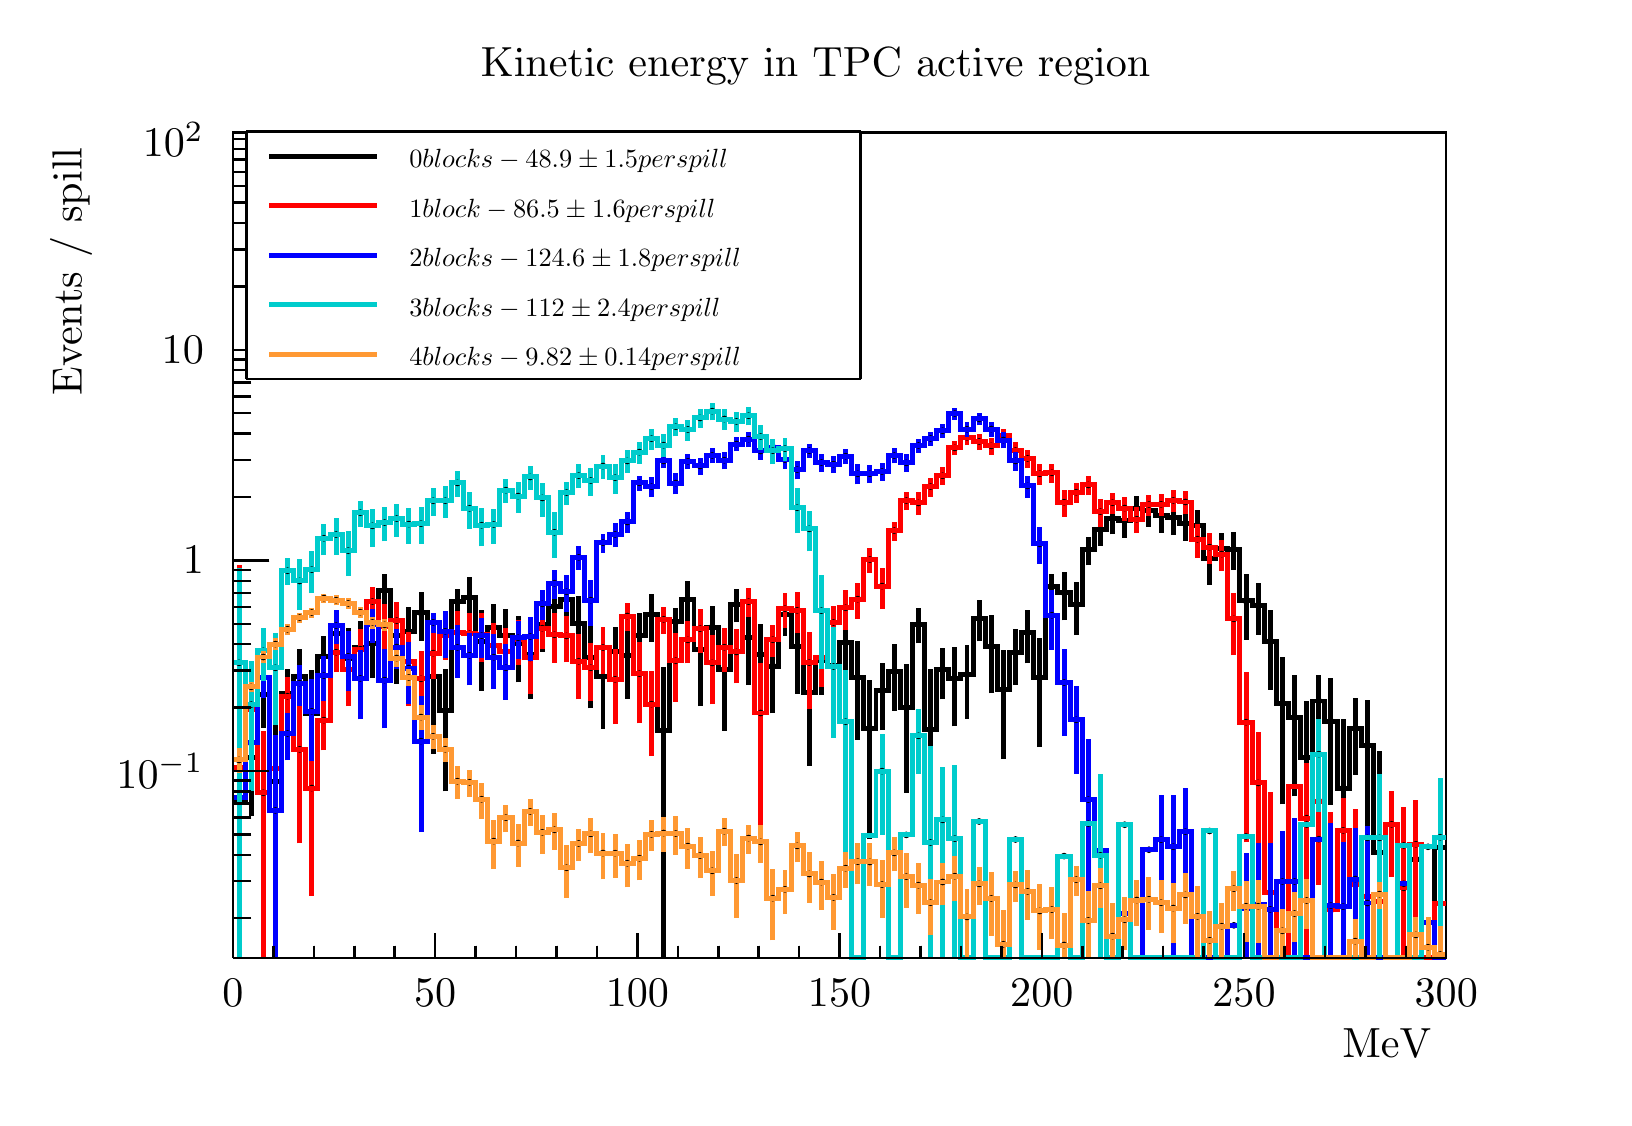
\begin{tikzpicture}
\pgfdeclareplotmark{cross} {
\pgfpathmoveto{\pgfpoint{-0.3\pgfplotmarksize}{\pgfplotmarksize}}
\pgfpathlineto{\pgfpoint{+0.3\pgfplotmarksize}{\pgfplotmarksize}}
\pgfpathlineto{\pgfpoint{+0.3\pgfplotmarksize}{0.3\pgfplotmarksize}}
\pgfpathlineto{\pgfpoint{+1\pgfplotmarksize}{0.3\pgfplotmarksize}}
\pgfpathlineto{\pgfpoint{+1\pgfplotmarksize}{-0.3\pgfplotmarksize}}
\pgfpathlineto{\pgfpoint{+0.3\pgfplotmarksize}{-0.3\pgfplotmarksize}}
\pgfpathlineto{\pgfpoint{+0.3\pgfplotmarksize}{-1.\pgfplotmarksize}}
\pgfpathlineto{\pgfpoint{-0.3\pgfplotmarksize}{-1.\pgfplotmarksize}}
\pgfpathlineto{\pgfpoint{-0.3\pgfplotmarksize}{-0.3\pgfplotmarksize}}
\pgfpathlineto{\pgfpoint{-1.\pgfplotmarksize}{-0.3\pgfplotmarksize}}
\pgfpathlineto{\pgfpoint{-1.\pgfplotmarksize}{0.3\pgfplotmarksize}}
\pgfpathlineto{\pgfpoint{-0.3\pgfplotmarksize}{0.3\pgfplotmarksize}}
\pgfpathclose
\pgfusepathqstroke
}
\pgfdeclareplotmark{cross*} {
\pgfpathmoveto{\pgfpoint{-0.3\pgfplotmarksize}{\pgfplotmarksize}}
\pgfpathlineto{\pgfpoint{+0.3\pgfplotmarksize}{\pgfplotmarksize}}
\pgfpathlineto{\pgfpoint{+0.3\pgfplotmarksize}{0.3\pgfplotmarksize}}
\pgfpathlineto{\pgfpoint{+1\pgfplotmarksize}{0.3\pgfplotmarksize}}
\pgfpathlineto{\pgfpoint{+1\pgfplotmarksize}{-0.3\pgfplotmarksize}}
\pgfpathlineto{\pgfpoint{+0.3\pgfplotmarksize}{-0.3\pgfplotmarksize}}
\pgfpathlineto{\pgfpoint{+0.3\pgfplotmarksize}{-1.\pgfplotmarksize}}
\pgfpathlineto{\pgfpoint{-0.3\pgfplotmarksize}{-1.\pgfplotmarksize}}
\pgfpathlineto{\pgfpoint{-0.3\pgfplotmarksize}{-0.3\pgfplotmarksize}}
\pgfpathlineto{\pgfpoint{-1.\pgfplotmarksize}{-0.3\pgfplotmarksize}}
\pgfpathlineto{\pgfpoint{-1.\pgfplotmarksize}{0.3\pgfplotmarksize}}
\pgfpathlineto{\pgfpoint{-0.3\pgfplotmarksize}{0.3\pgfplotmarksize}}
\pgfpathclose
\pgfusepathqfillstroke
}
\pgfdeclareplotmark{newstar} {
\pgfpathmoveto{\pgfqpoint{0pt}{\pgfplotmarksize}}
\pgfpathlineto{\pgfqpointpolar{44}{0.5\pgfplotmarksize}}
\pgfpathlineto{\pgfqpointpolar{18}{\pgfplotmarksize}}
\pgfpathlineto{\pgfqpointpolar{-20}{0.5\pgfplotmarksize}}
\pgfpathlineto{\pgfqpointpolar{-54}{\pgfplotmarksize}}
\pgfpathlineto{\pgfqpointpolar{-90}{0.5\pgfplotmarksize}}
\pgfpathlineto{\pgfqpointpolar{234}{\pgfplotmarksize}}
\pgfpathlineto{\pgfqpointpolar{198}{0.5\pgfplotmarksize}}
\pgfpathlineto{\pgfqpointpolar{162}{\pgfplotmarksize}}
\pgfpathlineto{\pgfqpointpolar{134}{0.5\pgfplotmarksize}}
\pgfpathclose
\pgfusepathqstroke
}
\pgfdeclareplotmark{newstar*} {
\pgfpathmoveto{\pgfqpoint{0pt}{\pgfplotmarksize}}
\pgfpathlineto{\pgfqpointpolar{44}{0.5\pgfplotmarksize}}
\pgfpathlineto{\pgfqpointpolar{18}{\pgfplotmarksize}}
\pgfpathlineto{\pgfqpointpolar{-20}{0.5\pgfplotmarksize}}
\pgfpathlineto{\pgfqpointpolar{-54}{\pgfplotmarksize}}
\pgfpathlineto{\pgfqpointpolar{-90}{0.5\pgfplotmarksize}}
\pgfpathlineto{\pgfqpointpolar{234}{\pgfplotmarksize}}
\pgfpathlineto{\pgfqpointpolar{198}{0.5\pgfplotmarksize}}
\pgfpathlineto{\pgfqpointpolar{162}{\pgfplotmarksize}}
\pgfpathlineto{\pgfqpointpolar{134}{0.5\pgfplotmarksize}}
\pgfpathclose
\pgfusepathqfillstroke
}
\definecolor{c}{rgb}{1,1,1};
\draw [color=c, fill=c] (0,0) rectangle (20,13.5714);
\draw [color=c, fill=c] (2.6,1.76429) rectangle (18.0086,12.246);
\definecolor{c}{rgb}{0,0,0};
\draw [c,line width=0.9] (2.6,1.76429) -- (2.6,12.246) -- (18.0086,12.246) -- (18.0086,1.76429) -- (2.6,1.76429);
\definecolor{c}{rgb}{1,1,1};
\draw [color=c, fill=c] (2.6,1.76429) rectangle (18.0086,12.246);
\definecolor{c}{rgb}{0,0,0};
\draw [c,line width=0.9] (2.6,1.76429) -- (2.6,12.246) -- (18.0086,12.246) -- (18.0086,1.76429) -- (2.6,1.76429);
\definecolor{c}{rgb}{0,0,0.6};
\draw [c,line width=0.9] (2.6,1.76429) -- (2.75409,1.76429) -- (2.75409,1.76429) -- (2.90817,1.76429) -- (2.90817,1.76429) -- (3.06226,1.76429) -- (3.06226,1.76429) -- (3.21634,1.76429) -- (3.21634,1.76429) -- (3.37043,1.76429) -- (3.37043,1.76429)
 -- (3.52452,1.76429) -- (3.52452,1.76429) -- (3.6786,1.76429) -- (3.6786,1.76429) -- (3.83269,1.76429) -- (3.83269,1.76429) -- (3.98677,1.76429) -- (3.98677,1.76429) -- (4.14086,1.76429) -- (4.14086,1.76429) -- (4.29495,1.76429) -- (4.29495,1.76429)
 -- (4.44903,1.76429) -- (4.44903,1.76429) -- (4.60312,1.76429) -- (4.60312,1.76429) -- (4.7572,1.76429) -- (4.7572,1.76429) -- (4.91129,1.76429) -- (4.91129,1.76429) -- (5.06538,1.76429) -- (5.06538,1.76429) -- (5.21946,1.76429) -- (5.21946,1.76429)
 -- (5.37355,1.76429) -- (5.37355,1.76429) -- (5.52763,1.76429) -- (5.52763,1.76429) -- (5.68172,1.76429) -- (5.68172,1.76429) -- (5.8358,1.76429) -- (5.8358,1.76429) -- (5.98989,1.76429) -- (5.98989,1.76429) -- (6.14398,1.76429) -- (6.14398,1.76429)
 -- (6.29806,1.76429) -- (6.29806,1.76429) -- (6.45215,1.76429) -- (6.45215,1.76429) -- (6.60624,1.76429) -- (6.60624,1.76429) -- (6.76032,1.76429) -- (6.76032,1.76429) -- (6.91441,1.76429) -- (6.91441,1.76429) -- (7.06849,1.76429) --
 (7.06849,1.76429) -- (7.22258,1.76429) -- (7.22258,1.76429) -- (7.37666,1.76429) -- (7.37666,1.76429) -- (7.53075,1.76429) -- (7.53075,1.76429) -- (7.68484,1.76429) -- (7.68484,1.76429) -- (7.83892,1.76429) -- (7.83892,1.76429) -- (7.99301,1.76429)
 -- (7.99301,1.76429) -- (8.14709,1.76429) -- (8.14709,1.76429) -- (8.30118,1.76429) -- (8.30118,1.76429) -- (8.45527,1.76429) -- (8.45527,1.76429) -- (8.60935,1.76429) -- (8.60935,1.76429) -- (8.76344,1.76429) -- (8.76344,1.76429) --
 (8.91752,1.76429) -- (8.91752,1.76429) -- (9.07161,1.76429) -- (9.07161,1.76429) -- (9.2257,1.76429) -- (9.2257,1.76429) -- (9.37978,1.76429) -- (9.37978,1.76429) -- (9.53387,1.76429) -- (9.53387,1.76429) -- (9.68795,1.76429) -- (9.68795,1.76429) --
 (9.84204,1.76429) -- (9.84204,1.76429) -- (9.99613,1.76429) -- (9.99613,1.76429) -- (10.1502,1.76429) -- (10.1502,1.76429) -- (10.3043,1.76429) -- (10.3043,1.76429) -- (10.4584,1.76429) -- (10.4584,1.76429) -- (10.6125,1.76429) -- (10.6125,1.76429)
 -- (10.7666,1.76429) -- (10.7666,1.76429) -- (10.9206,1.76429) -- (10.9206,1.76429) -- (11.0747,1.76429) -- (11.0747,1.76429) -- (11.2288,1.76429) -- (11.2288,1.76429) -- (11.3829,1.76429) -- (11.3829,1.76429) -- (11.537,1.76429) -- (11.537,1.76429)
 -- (11.6911,1.76429) -- (11.6911,1.76429) -- (11.8452,1.76429) -- (11.8452,1.76429) -- (11.9992,1.76429) -- (11.9992,1.76429) -- (12.1533,1.76429) -- (12.1533,1.76429) -- (12.3074,1.76429) -- (12.3074,1.76429) -- (12.4615,1.76429) --
 (12.4615,1.76429) -- (12.6156,1.76429) -- (12.6156,1.76429) -- (12.7697,1.76429) -- (12.7697,1.76429) -- (12.9238,1.76429) -- (12.9238,1.76429) -- (13.0778,1.76429) -- (13.0778,1.76429) -- (13.2319,1.76429) -- (13.2319,1.76429) -- (13.386,1.76429)
 -- (13.386,1.76429) -- (13.5401,1.76429) -- (13.5401,1.76429) -- (13.6942,1.76429) -- (13.6942,1.76429) -- (13.8483,1.76429) -- (13.8483,1.76429) -- (14.0024,1.76429) -- (14.0024,1.76429) -- (14.1564,1.76429) -- (14.1564,1.76429) --
 (14.3105,1.76429) -- (14.3105,1.76429) -- (14.4646,1.76429) -- (14.4646,1.76429) -- (14.6187,1.76429) -- (14.6187,1.76429) -- (14.7728,1.76429) -- (14.7728,1.76429) -- (14.9269,1.76429) -- (14.9269,1.76429) -- (15.081,1.76429) -- (15.081,1.76429) --
 (15.235,1.76429) -- (15.235,1.76429) -- (15.3891,1.76429) -- (15.3891,1.76429) -- (15.5432,1.76429) -- (15.5432,1.76429) -- (15.6973,1.76429) -- (15.6973,1.76429) -- (15.8514,1.76429) -- (15.8514,1.76429) -- (16.0055,1.76429) -- (16.0055,1.76429) --
 (16.1596,1.76429) -- (16.1596,1.76429) -- (16.3137,1.76429) -- (16.3137,1.76429) -- (16.4677,1.76429) -- (16.4677,1.76429) -- (16.6218,1.76429) -- (16.6218,1.76429) -- (16.7759,1.76429) -- (16.7759,1.76429) -- (16.93,1.76429) -- (16.93,1.76429) --
 (17.0841,1.76429) -- (17.0841,1.76429) -- (17.2382,1.76429) -- (17.2382,1.76429) -- (17.3923,1.76429) -- (17.3923,1.76429) -- (17.5463,1.76429) -- (17.5463,1.76429) -- (17.7004,1.76429) -- (17.7004,1.76429) -- (17.8545,1.76429) -- (17.8545,1.76429)
 -- (18.0086,1.76429);
\definecolor{c}{rgb}{0,0,0};
\draw [c,line width=0.9] (2.6,1.76429) -- (18.0086,1.76429);
\draw [c,line width=0.9] (2.6,2.07796) -- (2.6,1.76429);
\draw [c,line width=0.9] (3.11362,1.92112) -- (3.11362,1.76429);
\draw [c,line width=0.9] (3.62724,1.92112) -- (3.62724,1.76429);
\draw [c,line width=0.9] (4.14086,1.92112) -- (4.14086,1.76429);
\draw [c,line width=0.9] (4.65448,1.92112) -- (4.65448,1.76429);
\draw [c,line width=0.9] (5.1681,2.07796) -- (5.1681,1.76429);
\draw [c,line width=0.9] (5.68172,1.92112) -- (5.68172,1.76429);
\draw [c,line width=0.9] (6.19534,1.92112) -- (6.19534,1.76429);
\draw [c,line width=0.9] (6.70896,1.92112) -- (6.70896,1.76429);
\draw [c,line width=0.9] (7.22258,1.92112) -- (7.22258,1.76429);
\draw [c,line width=0.9] (7.7362,2.07796) -- (7.7362,1.76429);
\draw [c,line width=0.9] (8.24982,1.92112) -- (8.24982,1.76429);
\draw [c,line width=0.9] (8.76344,1.92112) -- (8.76344,1.76429);
\draw [c,line width=0.9] (9.27706,1.92112) -- (9.27706,1.76429);
\draw [c,line width=0.9] (9.79068,1.92112) -- (9.79068,1.76429);
\draw [c,line width=0.9] (10.3043,2.07796) -- (10.3043,1.76429);
\draw [c,line width=0.9] (10.8179,1.92112) -- (10.8179,1.76429);
\draw [c,line width=0.9] (11.3315,1.92112) -- (11.3315,1.76429);
\draw [c,line width=0.9] (11.8452,1.92112) -- (11.8452,1.76429);
\draw [c,line width=0.9] (12.3588,1.92112) -- (12.3588,1.76429);
\draw [c,line width=0.9] (12.8724,2.07796) -- (12.8724,1.76429);
\draw [c,line width=0.9] (13.386,1.92112) -- (13.386,1.76429);
\draw [c,line width=0.9] (13.8996,1.92112) -- (13.8996,1.76429);
\draw [c,line width=0.9] (14.4133,1.92112) -- (14.4133,1.76429);
\draw [c,line width=0.9] (14.9269,1.92112) -- (14.9269,1.76429);
\draw [c,line width=0.9] (15.4405,2.07796) -- (15.4405,1.76429);
\draw [c,line width=0.9] (15.9541,1.92112) -- (15.9541,1.76429);
\draw [c,line width=0.9] (16.4677,1.92112) -- (16.4677,1.76429);
\draw [c,line width=0.9] (16.9814,1.92112) -- (16.9814,1.76429);
\draw [c,line width=0.9] (17.495,1.92112) -- (17.495,1.76429);
\draw [c,line width=0.9] (18.0086,2.07796) -- (18.0086,1.76429);
\draw [anchor=base] (2.6,1.15357) node[scale=1.52295, color=c, rotate=0]{0};
\draw [anchor=base] (5.1681,1.15357) node[scale=1.52295, color=c, rotate=0]{50};
\draw [anchor=base] (7.7362,1.15357) node[scale=1.52295, color=c, rotate=0]{100};
\draw [anchor=base] (10.3043,1.15357) node[scale=1.52295, color=c, rotate=0]{150};
\draw [anchor=base] (12.8724,1.15357) node[scale=1.52295, color=c, rotate=0]{200};
\draw [anchor=base] (15.4405,1.15357) node[scale=1.52295, color=c, rotate=0]{250};
\draw [anchor=base] (18.0086,1.15357) node[scale=1.52295, color=c, rotate=0]{300};
\draw [anchor= east] (18.0086,0.678571) node[scale=1.52295, color=c, rotate=0]{ MeV};
\draw [c,line width=0.9] (2.6,1.76429) -- (2.6,12.246);
\draw [c,line width=0.9] (2.8317,2.26869) -- (2.6,2.26869);
\draw [c,line width=0.9] (2.8317,2.73968) -- (2.6,2.73968);
\draw [c,line width=0.9] (2.8317,3.07386) -- (2.6,3.07386);
\draw [c,line width=0.9] (2.8317,3.33307) -- (2.6,3.33307);
\draw [c,line width=0.9] (2.8317,3.54485) -- (2.6,3.54485);
\draw [c,line width=0.9] (2.8317,3.72392) -- (2.6,3.72392);
\draw [c,line width=0.9] (2.8317,3.87903) -- (2.6,3.87903);
\draw [c,line width=0.9] (2.8317,4.01585) -- (2.6,4.01585);
\draw [c,line width=0.9] (3.0634,4.13824) -- (2.6,4.13824);
\draw [anchor= east] (2.42,4.13824) node[scale=1.52295, color=c, rotate=0]{$10^{-1}$};
\draw [c,line width=0.9] (2.8317,4.94341) -- (2.6,4.94341);
\draw [c,line width=0.9] (2.8317,5.41441) -- (2.6,5.41441);
\draw [c,line width=0.9] (2.8317,5.74858) -- (2.6,5.74858);
\draw [c,line width=0.9] (2.8317,6.00779) -- (2.6,6.00779);
\draw [c,line width=0.9] (2.8317,6.21958) -- (2.6,6.21958);
\draw [c,line width=0.9] (2.8317,6.39864) -- (2.6,6.39864);
\draw [c,line width=0.9] (2.8317,6.55375) -- (2.6,6.55375);
\draw [c,line width=0.9] (2.8317,6.69057) -- (2.6,6.69057);
\draw [c,line width=0.9] (3.0634,6.81296) -- (2.6,6.81296);
\draw [anchor= east] (2.42,6.81296) node[scale=1.52295, color=c, rotate=0]{1};
\draw [c,line width=0.9] (2.8317,7.61813) -- (2.6,7.61813);
\draw [c,line width=0.9] (2.8317,8.08913) -- (2.6,8.08913);
\draw [c,line width=0.9] (2.8317,8.4233) -- (2.6,8.4233);
\draw [c,line width=0.9] (2.8317,8.68251) -- (2.6,8.68251);
\draw [c,line width=0.9] (2.8317,8.8943) -- (2.6,8.8943);
\draw [c,line width=0.9] (2.8317,9.07336) -- (2.6,9.07336);
\draw [c,line width=0.9] (2.8317,9.22848) -- (2.6,9.22848);
\draw [c,line width=0.9] (2.8317,9.3653) -- (2.6,9.3653);
\draw [c,line width=0.9] (3.0634,9.48768) -- (2.6,9.48768);
\draw [anchor= east] (2.42,9.48768) node[scale=1.52295, color=c, rotate=0]{10};
\draw [c,line width=0.9] (2.8317,10.2929) -- (2.6,10.2929);
\draw [c,line width=0.9] (2.8317,10.7639) -- (2.6,10.7639);
\draw [c,line width=0.9] (2.8317,11.098) -- (2.6,11.098);
\draw [c,line width=0.9] (2.8317,11.3572) -- (2.6,11.3572);
\draw [c,line width=0.9] (2.8317,11.569) -- (2.6,11.569);
\draw [c,line width=0.9] (2.8317,11.7481) -- (2.6,11.7481);
\draw [c,line width=0.9] (2.8317,11.9032) -- (2.6,11.9032);
\draw [c,line width=0.9] (2.8317,12.04) -- (2.6,12.04);
\draw [c,line width=0.9] (3.0634,12.1624) -- (2.6,12.1624);
\draw [anchor= east] (2.42,12.1624) node[scale=1.52295, color=c, rotate=0]{$10^{2}$};
\draw [anchor= east] (0.542857,12.246) node[scale=1.52295, color=c, rotate=90]{ Events / spill};
\draw [c,line width=1.8] (2.67704,1.76429) -- (2.67704,3.77788);
\draw [c,line width=1.8] (2.67704,3.77788) -- (2.67704,6.72463);
\foreach \P in {(2.67704,3.77788)}{\draw[mark options={color=c,fill=c},mark size=2.402402pt,mark=*,mark size=1pt] plot coordinates {\P};}
\draw [c,line width=1.8] (2.83113,3.5658) -- (2.83113,4.30569);
\draw [c,line width=1.8] (2.83113,4.30569) -- (2.83113,4.75409);
\foreach \P in {(2.83113,4.30569)}{\draw[mark options={color=c,fill=c},mark size=2.402402pt,mark=*,mark size=1pt] plot coordinates {\P};}
\draw [c,line width=1.8] (2.98521,4.68707) -- (2.98521,5.1098);
\draw [c,line width=1.8] (2.98521,5.1098) -- (2.98521,5.41907);
\foreach \P in {(2.98521,5.1098)}{\draw[mark options={color=c,fill=c},mark size=2.402402pt,mark=*,mark size=1pt] plot coordinates {\P};}
\draw [c,line width=1.8] (3.1393,1.76429) -- (3.1393,4.00405);
\draw [c,line width=1.8] (3.1393,4.00405) -- (3.1393,4.87417);
\foreach \P in {(3.1393,4.00405)}{\draw[mark options={color=c,fill=c},mark size=2.402402pt,mark=*,mark size=1pt] plot coordinates {\P};}
\draw [c,line width=1.8] (3.29339,4.72446) -- (3.29339,5.12855);
\draw [c,line width=1.8] (3.29339,5.12855) -- (3.29339,5.42776);
\foreach \P in {(3.29339,5.12855)}{\draw[mark options={color=c,fill=c},mark size=2.402402pt,mark=*,mark size=1pt] plot coordinates {\P};}
\draw [c,line width=1.8] (3.44747,4.81085) -- (3.44747,5.33313);
\draw [c,line width=1.8] (3.44747,5.33313) -- (3.44747,5.69213);
\foreach \P in {(3.44747,5.33313)}{\draw[mark options={color=c,fill=c},mark size=2.402402pt,mark=*,mark size=1pt] plot coordinates {\P};}
\draw [c,line width=1.8] (3.60156,3.78971) -- (3.60156,4.86945);
\draw [c,line width=1.8] (3.60156,4.86945) -- (3.60156,5.41922);
\foreach \P in {(3.60156,4.86945)}{\draw[mark options={color=c,fill=c},mark size=2.402402pt,mark=*,mark size=1pt] plot coordinates {\P};}
\draw [c,line width=1.8] (3.75564,5.2544) -- (3.75564,5.59407);
\draw [c,line width=1.8] (3.75564,5.59407) -- (3.75564,5.85657);
\foreach \P in {(3.75564,5.59407)}{\draw[mark options={color=c,fill=c},mark size=2.402402pt,mark=*,mark size=1pt] plot coordinates {\P};}
\draw [c,line width=1.8] (3.90973,5.50649) -- (3.90973,5.88154);
\draw [c,line width=1.8] (3.90973,5.88154) -- (3.90973,6.16459);
\foreach \P in {(3.90973,5.88154)}{\draw[mark options={color=c,fill=c},mark size=2.402402pt,mark=*,mark size=1pt] plot coordinates {\P};}
\draw [c,line width=1.8] (4.06382,4.98513) -- (4.06382,5.57167);
\draw [c,line width=1.8] (4.06382,5.57167) -- (4.06382,5.95957);
\foreach \P in {(4.06382,5.57167)}{\draw[mark options={color=c,fill=c},mark size=2.402402pt,mark=*,mark size=1pt] plot coordinates {\P};}
\draw [c,line width=1.8] (4.2179,5.21896) -- (4.2179,5.70174);
\draw [c,line width=1.8] (4.2179,5.70174) -- (4.2179,6.04177);
\foreach \P in {(4.2179,5.70174)}{\draw[mark options={color=c,fill=c},mark size=2.402402pt,mark=*,mark size=1pt] plot coordinates {\P};}
\draw [c,line width=1.8] (4.37199,5.31802) -- (4.37199,5.76129);
\draw [c,line width=1.8] (4.37199,5.76129) -- (4.37199,6.08134);
\foreach \P in {(4.37199,5.76129)}{\draw[mark options={color=c,fill=c},mark size=2.402402pt,mark=*,mark size=1pt] plot coordinates {\P};}
\draw [c,line width=1.8] (4.52607,6.19429) -- (4.52607,6.43603);
\draw [c,line width=1.8] (4.52607,6.43603) -- (4.52607,6.63602);
\foreach \P in {(4.52607,6.43603)}{\draw[mark options={color=c,fill=c},mark size=2.402402pt,mark=*,mark size=1pt] plot coordinates {\P};}
\draw [c,line width=1.8] (4.68016,5.24509) -- (4.68016,5.85988);
\draw [c,line width=1.8] (4.68016,5.85988) -- (4.68016,6.25979);
\foreach \P in {(4.68016,5.85988)}{\draw[mark options={color=c,fill=c},mark size=2.402402pt,mark=*,mark size=1pt] plot coordinates {\P};}
\draw [c,line width=1.8] (4.83425,5.4672) -- (4.83425,5.90683);
\draw [c,line width=1.8] (4.83425,5.90683) -- (4.83425,6.225);
\foreach \P in {(4.83425,5.90683)}{\draw[mark options={color=c,fill=c},mark size=2.402402pt,mark=*,mark size=1pt] plot coordinates {\P};}
\draw [c,line width=1.8] (4.98833,5.78993) -- (4.98833,6.14503);
\draw [c,line width=1.8] (4.98833,6.14503) -- (4.98833,6.41661);
\foreach \P in {(4.98833,6.14503)}{\draw[mark options={color=c,fill=c},mark size=2.402402pt,mark=*,mark size=1pt] plot coordinates {\P};}
\draw [c,line width=1.8] (5.14242,4.35521) -- (5.14242,5.338);
\draw [c,line width=1.8] (5.14242,5.338) -- (5.14242,5.86264);
\foreach \P in {(5.14242,5.338)}{\draw[mark options={color=c,fill=c},mark size=2.402402pt,mark=*,mark size=1pt] plot coordinates {\P};}
\draw [c,line width=1.8] (5.2965,3.87979) -- (5.2965,4.90083);
\draw [c,line width=1.8] (5.2965,4.90083) -- (5.2965,5.4357);
\foreach \P in {(5.2965,4.90083)}{\draw[mark options={color=c,fill=c},mark size=2.402402pt,mark=*,mark size=1pt] plot coordinates {\P};}
\draw [c,line width=1.8] (5.45059,6.11314) -- (5.45059,6.29195);
\draw [c,line width=1.8] (5.45059,6.29195) -- (5.45059,6.44687);
\foreach \P in {(5.45059,6.29195)}{\draw[mark options={color=c,fill=c},mark size=2.402402pt,mark=*,mark size=1pt] plot coordinates {\P};}
\draw [c,line width=1.8] (5.60468,5.98904) -- (5.60468,6.33729);
\draw [c,line width=1.8] (5.60468,6.33729) -- (5.60468,6.60486);
\foreach \P in {(5.60468,6.33729)}{\draw[mark options={color=c,fill=c},mark size=2.402402pt,mark=*,mark size=1pt] plot coordinates {\P};}
\draw [c,line width=1.8] (5.75876,5.15619) -- (5.75876,5.78044);
\draw [c,line width=1.8] (5.75876,5.78044) -- (5.75876,6.18427);
\foreach \P in {(5.75876,5.78044)}{\draw[mark options={color=c,fill=c},mark size=2.402402pt,mark=*,mark size=1pt] plot coordinates {\P};}
\draw [c,line width=1.8] (5.91285,5.56776) -- (5.91285,5.96517);
\draw [c,line width=1.8] (5.91285,5.96517) -- (5.91285,6.26073);
\foreach \P in {(5.91285,5.96517)}{\draw[mark options={color=c,fill=c},mark size=2.402402pt,mark=*,mark size=1pt] plot coordinates {\P};}
\draw [c,line width=1.8] (6.06693,5.38116) -- (6.06693,5.86042);
\draw [c,line width=1.8] (6.06693,5.86042) -- (6.06693,6.19871);
\foreach \P in {(6.06693,5.86042)}{\draw[mark options={color=c,fill=c},mark size=2.402402pt,mark=*,mark size=1pt] plot coordinates {\P};}
\draw [c,line width=1.8] (6.22102,5.26273) -- (6.22102,5.76223);
\draw [c,line width=1.8] (6.22102,5.76223) -- (6.22102,6.11039);
\foreach \P in {(6.22102,5.76223)}{\draw[mark options={color=c,fill=c},mark size=2.402402pt,mark=*,mark size=1pt] plot coordinates {\P};}
\draw [c,line width=1.8] (6.37511,5.05382) -- (6.37511,5.61642);
\draw [c,line width=1.8] (6.37511,5.61642) -- (6.37511,5.99382);
\foreach \P in {(6.37511,5.61642)}{\draw[mark options={color=c,fill=c},mark size=2.402402pt,mark=*,mark size=1pt] plot coordinates {\P};}
\draw [c,line width=1.8] (6.52919,5.65496) -- (6.52919,5.99633);
\draw [c,line width=1.8] (6.52919,5.99633) -- (6.52919,6.25982);
\foreach \P in {(6.52919,5.99633)}{\draw[mark options={color=c,fill=c},mark size=2.402402pt,mark=*,mark size=1pt] plot coordinates {\P};}
\draw [c,line width=1.8] (6.68328,5.91103) -- (6.68328,6.2293);
\draw [c,line width=1.8] (6.68328,6.2293) -- (6.68328,6.47886);
\foreach \P in {(6.68328,6.2293)}{\draw[mark options={color=c,fill=c},mark size=2.402402pt,mark=*,mark size=1pt] plot coordinates {\P};}
\draw [c,line width=1.8] (6.83736,5.96848) -- (6.83736,6.31384);
\draw [c,line width=1.8] (6.83736,6.31384) -- (6.83736,6.5797);
\foreach \P in {(6.83736,6.31384)}{\draw[mark options={color=c,fill=c},mark size=2.402402pt,mark=*,mark size=1pt] plot coordinates {\P};}
\draw [c,line width=1.8] (6.99145,5.52099) -- (6.99145,6.01339);
\draw [c,line width=1.8] (6.99145,6.01339) -- (6.99145,6.35813);
\foreach \P in {(6.99145,6.01339)}{\draw[mark options={color=c,fill=c},mark size=2.402402pt,mark=*,mark size=1pt] plot coordinates {\P};}
\draw [c,line width=1.8] (7.14554,4.93495) -- (7.14554,5.58107);
\draw [c,line width=1.8] (7.14554,5.58107) -- (7.14554,5.99382);
\foreach \P in {(7.14554,5.58107)}{\draw[mark options={color=c,fill=c},mark size=2.402402pt,mark=*,mark size=1pt] plot coordinates {\P};}
\draw [c,line width=1.8] (7.29962,4.67176) -- (7.29962,5.33589);
\draw [c,line width=1.8] (7.29962,5.33589) -- (7.29962,5.7558);
\foreach \P in {(7.29962,5.33589)}{\draw[mark options={color=c,fill=c},mark size=2.402402pt,mark=*,mark size=1pt] plot coordinates {\P};}
\draw [c,line width=1.8] (7.45371,5.2341) -- (7.45371,5.65629);
\draw [c,line width=1.8] (7.45371,5.65629) -- (7.45371,5.96527);
\foreach \P in {(7.45371,5.65629)}{\draw[mark options={color=c,fill=c},mark size=2.402402pt,mark=*,mark size=1pt] plot coordinates {\P};}
\draw [c,line width=1.8] (7.60779,5.05511) -- (7.60779,5.60054);
\draw [c,line width=1.8] (7.60779,5.60054) -- (7.60779,5.97022);
\foreach \P in {(7.60779,5.60054)}{\draw[mark options={color=c,fill=c},mark size=2.402402pt,mark=*,mark size=1pt] plot coordinates {\P};}
\draw [c,line width=1.8] (7.76188,5.46398) -- (7.76188,5.85452);
\draw [c,line width=1.8] (7.76188,5.85452) -- (7.76188,6.14627);
\foreach \P in {(7.76188,5.85452)}{\draw[mark options={color=c,fill=c},mark size=2.402402pt,mark=*,mark size=1pt] plot coordinates {\P};}
\draw [c,line width=1.8] (7.91597,5.77694) -- (7.91597,6.11972);
\draw [c,line width=1.8] (7.91597,6.11972) -- (7.91597,6.38406);
\foreach \P in {(7.91597,6.11972)}{\draw[mark options={color=c,fill=c},mark size=2.402402pt,mark=*,mark size=1pt] plot coordinates {\P};}
\draw [c,line width=1.8] (8.07005,1.76429) -- (8.07005,4.64807);
\draw [c,line width=1.8] (8.07005,4.64807) -- (8.07005,5.45715);
\foreach \P in {(8.07005,4.64807)}{\draw[mark options={color=c,fill=c},mark size=2.402402pt,mark=*,mark size=1pt] plot coordinates {\P};}
\draw [c,line width=1.8] (8.22414,5.8299) -- (8.22414,6.03235);
\draw [c,line width=1.8] (8.22414,6.03235) -- (8.22414,6.2047);
\foreach \P in {(8.22414,6.03235)}{\draw[mark options={color=c,fill=c},mark size=2.402402pt,mark=*,mark size=1pt] plot coordinates {\P};}
\draw [c,line width=1.8] (8.37822,6.01039) -- (8.37822,6.31539);
\draw [c,line width=1.8] (8.37822,6.31539) -- (8.37822,6.55674);
\foreach \P in {(8.37822,6.31539)}{\draw[mark options={color=c,fill=c},mark size=2.402402pt,mark=*,mark size=1pt] plot coordinates {\P};}
\draw [c,line width=1.8] (8.53231,4.96303) -- (8.53231,5.68001);
\draw [c,line width=1.8] (8.53231,5.68001) -- (8.53231,6.12006);
\foreach \P in {(8.53231,5.68001)}{\draw[mark options={color=c,fill=c},mark size=2.402402pt,mark=*,mark size=1pt] plot coordinates {\P};}
\draw [c,line width=1.8] (8.6864,5.61271) -- (8.6864,5.96463);
\draw [c,line width=1.8] (8.6864,5.96463) -- (8.6864,6.23436);
\foreach \P in {(8.6864,5.96463)}{\draw[mark options={color=c,fill=c},mark size=2.402402pt,mark=*,mark size=1pt] plot coordinates {\P};}
\draw [c,line width=1.8] (8.84048,4.65006) -- (8.84048,5.42613);
\draw [c,line width=1.8] (8.84048,5.42613) -- (8.84048,5.88726);
\foreach \P in {(8.84048,5.42613)}{\draw[mark options={color=c,fill=c},mark size=2.402402pt,mark=*,mark size=1pt] plot coordinates {\P};}
\draw [c,line width=1.8] (8.99457,6.02467) -- (8.99457,6.25817);
\draw [c,line width=1.8] (8.99457,6.25817) -- (8.99457,6.45249);
\foreach \P in {(8.99457,6.25817)}{\draw[mark options={color=c,fill=c},mark size=2.402402pt,mark=*,mark size=1pt] plot coordinates {\P};}
\draw [c,line width=1.8] (9.14865,5.22873) -- (9.14865,5.8336);
\draw [c,line width=1.8] (9.14865,5.8336) -- (9.14865,6.22934);
\foreach \P in {(9.14865,5.8336)}{\draw[mark options={color=c,fill=c},mark size=2.402402pt,mark=*,mark size=1pt] plot coordinates {\P};}
\draw [c,line width=1.8] (9.30274,5.0546) -- (9.30274,5.62089);
\draw [c,line width=1.8] (9.30274,5.62089) -- (9.30274,5.99994);
\foreach \P in {(9.30274,5.62089)}{\draw[mark options={color=c,fill=c},mark size=2.402402pt,mark=*,mark size=1pt] plot coordinates {\P};}
\draw [c,line width=1.8] (9.45683,4.87098) -- (9.45683,5.47114);
\draw [c,line width=1.8] (9.45683,5.47114) -- (9.45683,5.86489);
\foreach \P in {(9.45683,5.47114)}{\draw[mark options={color=c,fill=c},mark size=2.402402pt,mark=*,mark size=1pt] plot coordinates {\P};}
\draw [c,line width=1.8] (9.61091,5.85157) -- (9.61091,6.12942);
\draw [c,line width=1.8] (9.61091,6.12942) -- (9.61091,6.35347);
\foreach \P in {(9.61091,6.12942)}{\draw[mark options={color=c,fill=c},mark size=2.402402pt,mark=*,mark size=1pt] plot coordinates {\P};}
\draw [c,line width=1.8] (9.765,5.11705) -- (9.765,5.71956);
\draw [c,line width=1.8] (9.765,5.71956) -- (9.765,6.1143);
\foreach \P in {(9.765,5.71956)}{\draw[mark options={color=c,fill=c},mark size=2.402402pt,mark=*,mark size=1pt] plot coordinates {\P};}
\draw [c,line width=1.8] (9.91908,4.20269) -- (9.91908,5.13908);
\draw [c,line width=1.8] (9.91908,5.13908) -- (9.91908,5.65072);
\foreach \P in {(9.91908,5.13908)}{\draw[mark options={color=c,fill=c},mark size=2.402402pt,mark=*,mark size=1pt] plot coordinates {\P};}
\draw [c,line width=1.8] (10.0732,5.10691) -- (10.0732,5.53685);
\draw [c,line width=1.8] (10.0732,5.53685) -- (10.0732,5.84995);
\foreach \P in {(10.0732,5.53685)}{\draw[mark options={color=c,fill=c},mark size=2.402402pt,mark=*,mark size=1pt] plot coordinates {\P};}
\draw [c,line width=1.8] (10.2273,4.88648) -- (10.2273,5.48144);
\draw [c,line width=1.8] (10.2273,5.48144) -- (10.2273,5.87297);
\foreach \P in {(10.2273,5.48144)}{\draw[mark options={color=c,fill=c},mark size=2.402402pt,mark=*,mark size=1pt] plot coordinates {\P};}
\draw [c,line width=1.8] (10.3813,5.36186) -- (10.3813,5.7643);
\draw [c,line width=1.8] (10.3813,5.7643) -- (10.3813,6.06261);
\foreach \P in {(10.3813,5.7643)}{\draw[mark options={color=c,fill=c},mark size=2.402402pt,mark=*,mark size=1pt] plot coordinates {\P};}
\draw [c,line width=1.8] (10.5354,4.53355) -- (10.5354,5.32592);
\draw [c,line width=1.8] (10.5354,5.32592) -- (10.5354,5.79262);
\foreach \P in {(10.5354,5.32592)}{\draw[mark options={color=c,fill=c},mark size=2.402402pt,mark=*,mark size=1pt] plot coordinates {\P};}
\draw [c,line width=1.8] (10.6895,3.27066) -- (10.6895,4.67924);
\draw [c,line width=1.8] (10.6895,4.67924) -- (10.6895,5.29739);
\foreach \P in {(10.6895,4.67924)}{\draw[mark options={color=c,fill=c},mark size=2.402402pt,mark=*,mark size=1pt] plot coordinates {\P};}
\draw [c,line width=1.8] (10.8436,4.65855) -- (10.8436,5.16052);
\draw [c,line width=1.8] (10.8436,5.16052) -- (10.8436,5.50989);
\foreach \P in {(10.8436,5.16052)}{\draw[mark options={color=c,fill=c},mark size=2.402402pt,mark=*,mark size=1pt] plot coordinates {\P};}
\draw [c,line width=1.8] (10.9977,4.90254) -- (10.9977,5.40524);
\draw [c,line width=1.8] (10.9977,5.40524) -- (10.9977,5.75495);
\foreach \P in {(10.9977,5.40524)}{\draw[mark options={color=c,fill=c},mark size=2.402402pt,mark=*,mark size=1pt] plot coordinates {\P};}
\draw [c,line width=1.8] (11.1518,3.86489) -- (11.1518,4.94261);
\draw [c,line width=1.8] (11.1518,4.94261) -- (11.1518,5.49188);
\foreach \P in {(11.1518,4.94261)}{\draw[mark options={color=c,fill=c},mark size=2.402402pt,mark=*,mark size=1pt] plot coordinates {\P};}
\draw [c,line width=1.8] (11.3059,5.75797) -- (11.3059,6.00379);
\draw [c,line width=1.8] (11.3059,6.00379) -- (11.3059,6.20656);
\foreach \P in {(11.3059,6.00379)}{\draw[mark options={color=c,fill=c},mark size=2.402402pt,mark=*,mark size=1pt] plot coordinates {\P};}
\draw [c,line width=1.8] (11.4599,1.76429) -- (11.4599,4.66394);
\draw [c,line width=1.8] (11.4599,4.66394) -- (11.4599,5.43043);
\foreach \P in {(11.4599,4.66394)}{\draw[mark options={color=c,fill=c},mark size=2.402402pt,mark=*,mark size=1pt] plot coordinates {\P};}
\draw [c,line width=1.8] (11.614,5.04677) -- (11.614,5.42129);
\draw [c,line width=1.8] (11.614,5.42129) -- (11.614,5.70404);
\foreach \P in {(11.614,5.42129)}{\draw[mark options={color=c,fill=c},mark size=2.402402pt,mark=*,mark size=1pt] plot coordinates {\P};}
\draw [c,line width=1.8] (11.7681,4.70379) -- (11.7681,5.31392);
\draw [c,line width=1.8] (11.7681,5.31392) -- (11.7681,5.71187);
\foreach \P in {(11.7681,5.31392)}{\draw[mark options={color=c,fill=c},mark size=2.402402pt,mark=*,mark size=1pt] plot coordinates {\P};}
\draw [c,line width=1.8] (11.9222,4.8006) -- (11.9222,5.36395);
\draw [c,line width=1.8] (11.9222,5.36395) -- (11.9222,5.74169);
\foreach \P in {(11.9222,5.36395)}{\draw[mark options={color=c,fill=c},mark size=2.402402pt,mark=*,mark size=1pt] plot coordinates {\P};}
\draw [c,line width=1.8] (12.0763,5.78399) -- (12.0763,6.07357);
\draw [c,line width=1.8] (12.0763,6.07357) -- (12.0763,6.30517);
\foreach \P in {(12.0763,6.07357)}{\draw[mark options={color=c,fill=c},mark size=2.402402pt,mark=*,mark size=1pt] plot coordinates {\P};}
\draw [c,line width=1.8] (12.2304,5.12273) -- (12.2304,5.7204);
\draw [c,line width=1.8] (12.2304,5.7204) -- (12.2304,6.11308);
\foreach \P in {(12.2304,5.7204)}{\draw[mark options={color=c,fill=c},mark size=2.402402pt,mark=*,mark size=1pt] plot coordinates {\P};}
\draw [c,line width=1.8] (12.3845,4.28801) -- (12.3845,5.17713);
\draw [c,line width=1.8] (12.3845,5.17713) -- (12.3845,5.67481);
\foreach \P in {(12.3845,5.17713)}{\draw[mark options={color=c,fill=c},mark size=2.402402pt,mark=*,mark size=1pt] plot coordinates {\P};}
\draw [c,line width=1.8] (12.5385,5.22968) -- (12.5385,5.63771);
\draw [c,line width=1.8] (12.5385,5.63771) -- (12.5385,5.93908);
\foreach \P in {(12.5385,5.63771)}{\draw[mark options={color=c,fill=c},mark size=2.402402pt,mark=*,mark size=1pt] plot coordinates {\P};}
\draw [c,line width=1.8] (12.6926,5.5047) -- (12.6926,5.89348);
\draw [c,line width=1.8] (12.6926,5.89348) -- (12.6926,6.18426);
\foreach \P in {(12.6926,5.89348)}{\draw[mark options={color=c,fill=c},mark size=2.402402pt,mark=*,mark size=1pt] plot coordinates {\P};}
\draw [c,line width=1.8] (12.8467,4.44291) -- (12.8467,5.32568);
\draw [c,line width=1.8] (12.8467,5.32568) -- (12.8467,5.82143);
\foreach \P in {(12.8467,5.32568)}{\draw[mark options={color=c,fill=c},mark size=2.402402pt,mark=*,mark size=1pt] plot coordinates {\P};}
\draw [c,line width=1.8] (13.0008,6.29352) -- (13.0008,6.47959);
\draw [c,line width=1.8] (13.0008,6.47959) -- (13.0008,6.63992);
\foreach \P in {(13.0008,6.47959)}{\draw[mark options={color=c,fill=c},mark size=2.402402pt,mark=*,mark size=1pt] plot coordinates {\P};}
\draw [c,line width=1.8] (13.1549,6.05013) -- (13.1549,6.4015);
\draw [c,line width=1.8] (13.1549,6.4015) -- (13.1549,6.6709);
\foreach \P in {(13.1549,6.4015)}{\draw[mark options={color=c,fill=c},mark size=2.402402pt,mark=*,mark size=1pt] plot coordinates {\P};}
\draw [c,line width=1.8] (13.309,5.86485) -- (13.309,6.25257);
\draw [c,line width=1.8] (13.309,6.25257) -- (13.309,6.54276);
\foreach \P in {(13.309,6.25257)}{\draw[mark options={color=c,fill=c},mark size=2.402402pt,mark=*,mark size=1pt] plot coordinates {\P};}
\draw [c,line width=1.8] (13.4631,6.75067) -- (13.4631,6.94528);
\draw [c,line width=1.8] (13.4631,6.94528) -- (13.4631,7.11192);
\foreach \P in {(13.4631,6.94528)}{\draw[mark options={color=c,fill=c},mark size=2.402402pt,mark=*,mark size=1pt] plot coordinates {\P};}
\draw [c,line width=1.8] (13.6171,6.99949) -- (13.6171,7.20433);
\draw [c,line width=1.8] (13.6171,7.20433) -- (13.6171,7.37841);
\foreach \P in {(13.6171,7.20433)}{\draw[mark options={color=c,fill=c},mark size=2.402402pt,mark=*,mark size=1pt] plot coordinates {\P};}
\draw [c,line width=1.8] (13.7712,7.14306) -- (13.7712,7.34913);
\draw [c,line width=1.8] (13.7712,7.34913) -- (13.7712,7.5241);
\foreach \P in {(13.7712,7.34913)}{\draw[mark options={color=c,fill=c},mark size=2.402402pt,mark=*,mark size=1pt] plot coordinates {\P};}
\draw [c,line width=1.8] (13.9253,7.09954) -- (13.9253,7.31971);
\draw [c,line width=1.8] (13.9253,7.31971) -- (13.9253,7.50473);
\foreach \P in {(13.9253,7.31971)}{\draw[mark options={color=c,fill=c},mark size=2.402402pt,mark=*,mark size=1pt] plot coordinates {\P};}
\draw [c,line width=1.8] (14.0794,7.27952) -- (14.0794,7.46803);
\draw [c,line width=1.8] (14.0794,7.46803) -- (14.0794,7.63018);
\foreach \P in {(14.0794,7.46803)}{\draw[mark options={color=c,fill=c},mark size=2.402402pt,mark=*,mark size=1pt] plot coordinates {\P};}
\draw [c,line width=1.8] (14.2335,7.23981) -- (14.2335,7.45116);
\draw [c,line width=1.8] (14.2335,7.45116) -- (14.2335,7.62991);
\foreach \P in {(14.2335,7.45116)}{\draw[mark options={color=c,fill=c},mark size=2.402402pt,mark=*,mark size=1pt] plot coordinates {\P};}
\draw [c,line width=1.8] (14.3876,7.16562) -- (14.3876,7.38524);
\draw [c,line width=1.8] (14.3876,7.38524) -- (14.3876,7.56987);
\foreach \P in {(14.3876,7.38524)}{\draw[mark options={color=c,fill=c},mark size=2.402402pt,mark=*,mark size=1pt] plot coordinates {\P};}
\draw [c,line width=1.8] (14.5417,7.13329) -- (14.5417,7.35484);
\draw [c,line width=1.8] (14.5417,7.35484) -- (14.5417,7.54083);
\foreach \P in {(14.5417,7.35484)}{\draw[mark options={color=c,fill=c},mark size=2.402402pt,mark=*,mark size=1pt] plot coordinates {\P};}
\draw [c,line width=1.8] (14.6957,7.0596) -- (14.6957,7.28464);
\draw [c,line width=1.8] (14.6957,7.28464) -- (14.6957,7.47307);
\foreach \P in {(14.6957,7.28464)}{\draw[mark options={color=c,fill=c},mark size=2.402402pt,mark=*,mark size=1pt] plot coordinates {\P};}
\draw [c,line width=1.8] (14.8498,7.03382) -- (14.8498,7.25864);
\draw [c,line width=1.8] (14.8498,7.25864) -- (14.8498,7.44692);
\foreach \P in {(14.8498,7.25864)}{\draw[mark options={color=c,fill=c},mark size=2.402402pt,mark=*,mark size=1pt] plot coordinates {\P};}
\draw [c,line width=1.8] (15.0039,6.50433) -- (15.0039,6.84091);
\draw [c,line width=1.8] (15.0039,6.84091) -- (15.0039,7.10157);
\foreach \P in {(15.0039,6.84091)}{\draw[mark options={color=c,fill=c},mark size=2.402402pt,mark=*,mark size=1pt] plot coordinates {\P};}
\draw [c,line width=1.8] (15.158,6.7161) -- (15.158,6.95837);
\draw [c,line width=1.8] (15.158,6.95837) -- (15.158,7.15873);
\foreach \P in {(15.158,6.95837)}{\draw[mark options={color=c,fill=c},mark size=2.402402pt,mark=*,mark size=1pt] plot coordinates {\P};}
\draw [c,line width=1.8] (15.3121,6.68877) -- (15.3121,6.95311);
\draw [c,line width=1.8] (15.3121,6.95311) -- (15.3121,7.16831);
\foreach \P in {(15.3121,6.95311)}{\draw[mark options={color=c,fill=c},mark size=2.402402pt,mark=*,mark size=1pt] plot coordinates {\P};}
\draw [c,line width=1.8] (15.4662,5.80318) -- (15.4662,6.29724);
\draw [c,line width=1.8] (15.4662,6.29724) -- (15.4662,6.64277);
\foreach \P in {(15.4662,6.29724)}{\draw[mark options={color=c,fill=c},mark size=2.402402pt,mark=*,mark size=1pt] plot coordinates {\P};}
\draw [c,line width=1.8] (15.6203,5.86701) -- (15.6203,6.24559);
\draw [c,line width=1.8] (15.6203,6.24559) -- (15.6203,6.53065);
\foreach \P in {(15.6203,6.24559)}{\draw[mark options={color=c,fill=c},mark size=2.402402pt,mark=*,mark size=1pt] plot coordinates {\P};}
\draw [c,line width=1.8] (15.7743,5.1727) -- (15.7743,5.78771);
\draw [c,line width=1.8] (15.7743,5.78771) -- (15.7743,6.18772);
\foreach \P in {(15.7743,5.78771)}{\draw[mark options={color=c,fill=c},mark size=2.402402pt,mark=*,mark size=1pt] plot coordinates {\P};}
\draw [c,line width=1.8] (15.9284,3.71531) -- (15.9284,4.99513);
\draw [c,line width=1.8] (15.9284,4.99513) -- (15.9284,5.58924);
\foreach \P in {(15.9284,4.99513)}{\draw[mark options={color=c,fill=c},mark size=2.402402pt,mark=*,mark size=1pt] plot coordinates {\P};}
\draw [c,line width=1.8] (16.0825,3.81511) -- (16.0825,4.82086);
\draw [c,line width=1.8] (16.0825,4.82086) -- (16.0825,5.3517);
\foreach \P in {(16.0825,4.82086)}{\draw[mark options={color=c,fill=c},mark size=2.402402pt,mark=*,mark size=1pt] plot coordinates {\P};}
\draw [c,line width=1.8] (16.2366,2.07047) -- (16.2366,4.30774);
\draw [c,line width=1.8] (16.2366,4.30774) -- (16.2366,5.02502);
\foreach \P in {(16.2366,4.30774)}{\draw[mark options={color=c,fill=c},mark size=2.402402pt,mark=*,mark size=1pt] plot coordinates {\P};}
\draw [c,line width=1.8] (16.3907,4.56328) -- (16.3907,5.02707);
\draw [c,line width=1.8] (16.3907,5.02707) -- (16.3907,5.35762);
\foreach \P in {(16.3907,5.02707)}{\draw[mark options={color=c,fill=c},mark size=2.402402pt,mark=*,mark size=1pt] plot coordinates {\P};}
\draw [c,line width=1.8] (16.5448,3.70746) -- (16.5448,4.76901);
\draw [c,line width=1.8] (16.5448,4.76901) -- (16.5448,5.31426);
\foreach \P in {(16.5448,4.76901)}{\draw[mark options={color=c,fill=c},mark size=2.402402pt,mark=*,mark size=1pt] plot coordinates {\P};}
\draw [c,line width=1.8] (16.6989,1.76429) -- (16.6989,3.91923);
\draw [c,line width=1.8] (16.6989,3.91923) -- (16.6989,4.80064);
\foreach \P in {(16.6989,3.91923)}{\draw[mark options={color=c,fill=c},mark size=2.402402pt,mark=*,mark size=1pt] plot coordinates {\P};}
\draw [c,line width=1.8] (16.853,4.09314) -- (16.853,4.6761);
\draw [c,line width=1.8] (16.853,4.6761) -- (16.853,5.06246);
\foreach \P in {(16.853,4.6761)}{\draw[mark options={color=c,fill=c},mark size=2.402402pt,mark=*,mark size=1pt] plot coordinates {\P};}
\draw [c,line width=1.8] (17.007,3.27605) -- (17.007,4.46508);
\draw [c,line width=1.8] (17.007,4.46508) -- (17.007,5.04023);
\foreach \P in {(17.007,4.46508)}{\draw[mark options={color=c,fill=c},mark size=2.402402pt,mark=*,mark size=1pt] plot coordinates {\P};}
\draw [c,line width=1.8] (17.1611,1.76429) -- (17.1611,3.10893);
\draw [c,line width=1.8] (17.1611,3.10893) -- (17.1611,4.39012);
\foreach \P in {(17.1611,3.10893)}{\draw[mark options={color=c,fill=c},mark size=2.402402pt,mark=*,mark size=1pt] plot coordinates {\P};}
\foreach \P in {(17.6234,3.0203)}{\draw[mark options={color=c,fill=c},mark size=2.402402pt,mark=*,mark size=1pt] plot coordinates {\P};}
\foreach \P in {(17.9316,3.17201)}{\draw[mark options={color=c,fill=c},mark size=2.402402pt,mark=*,mark size=1pt] plot coordinates {\P};}
\draw [c,line width=1.8] (2.6,3.77788) -- (2.75409,3.77788) -- (2.75409,4.30569) -- (2.90817,4.30569) -- (2.90817,5.1098) -- (3.06226,5.1098) -- (3.06226,4.00405) -- (3.21634,4.00405) -- (3.21634,5.12855) -- (3.37043,5.12855) -- (3.37043,5.33313) --
 (3.52452,5.33313) -- (3.52452,4.86945) -- (3.6786,4.86945) -- (3.6786,5.59407) -- (3.83269,5.59407) -- (3.83269,5.88154) -- (3.98677,5.88154) -- (3.98677,5.57167) -- (4.14086,5.57167) -- (4.14086,5.70174) -- (4.29495,5.70174) -- (4.29495,5.76129) --
 (4.44903,5.76129) -- (4.44903,6.43603) -- (4.60312,6.43603) -- (4.60312,5.85988) -- (4.7572,5.85988) -- (4.7572,5.90683) -- (4.91129,5.90683) -- (4.91129,6.14503) -- (5.06538,6.14503) -- (5.06538,5.338) -- (5.21946,5.338) -- (5.21946,4.90083) --
 (5.37355,4.90083) -- (5.37355,6.29195) -- (5.52763,6.29195) -- (5.52763,6.33729) -- (5.68172,6.33729) -- (5.68172,5.78044) -- (5.8358,5.78044) -- (5.8358,5.96517) -- (5.98989,5.96517) -- (5.98989,5.86042) -- (6.14398,5.86042) -- (6.14398,5.76223) --
 (6.29806,5.76223) -- (6.29806,5.61642) -- (6.45215,5.61642) -- (6.45215,5.99633) -- (6.60624,5.99633) -- (6.60624,6.2293) -- (6.76032,6.2293) -- (6.76032,6.31384) -- (6.91441,6.31384) -- (6.91441,6.01339) -- (7.06849,6.01339) -- (7.06849,5.58107) --
 (7.22258,5.58107) -- (7.22258,5.33589) -- (7.37666,5.33589) -- (7.37666,5.65629) -- (7.53075,5.65629) -- (7.53075,5.60054) -- (7.68484,5.60054) -- (7.68484,5.85452) -- (7.83892,5.85452) -- (7.83892,6.11972) -- (7.99301,6.11972) -- (7.99301,4.64807)
 -- (8.14709,4.64807) -- (8.14709,6.03235) -- (8.30118,6.03235) -- (8.30118,6.31539) -- (8.45527,6.31539) -- (8.45527,5.68001) -- (8.60935,5.68001) -- (8.60935,5.96463) -- (8.76344,5.96463) -- (8.76344,5.42613) -- (8.91752,5.42613) --
 (8.91752,6.25817) -- (9.07161,6.25817) -- (9.07161,5.8336) -- (9.2257,5.8336) -- (9.2257,5.62089) -- (9.37978,5.62089) -- (9.37978,5.47114) -- (9.53387,5.47114) -- (9.53387,6.12942) -- (9.68795,6.12942) -- (9.68795,5.71956) -- (9.84204,5.71956) --
 (9.84204,5.13908) -- (9.99613,5.13908) -- (9.99613,5.53685) -- (10.1502,5.53685) -- (10.1502,5.48144) -- (10.3043,5.48144) -- (10.3043,5.7643) -- (10.4584,5.7643) -- (10.4584,5.32592) -- (10.6125,5.32592) -- (10.6125,4.67924) -- (10.7666,4.67924) --
 (10.7666,5.16052) -- (10.9206,5.16052) -- (10.9206,5.40524) -- (11.0747,5.40524) -- (11.0747,4.94261) -- (11.2288,4.94261) -- (11.2288,6.00379) -- (11.3829,6.00379) -- (11.3829,4.66394) -- (11.537,4.66394) -- (11.537,5.42129) -- (11.6911,5.42129) --
 (11.6911,5.31392) -- (11.8452,5.31392) -- (11.8452,5.36395) -- (11.9992,5.36395) -- (11.9992,6.07357) -- (12.1533,6.07357) -- (12.1533,5.7204) -- (12.3074,5.7204) -- (12.3074,5.17713) -- (12.4615,5.17713) -- (12.4615,5.63771) -- (12.6156,5.63771) --
 (12.6156,5.89348) -- (12.7697,5.89348) -- (12.7697,5.32568) -- (12.9238,5.32568) -- (12.9238,6.47959) -- (13.0778,6.47959) -- (13.0778,6.4015) -- (13.2319,6.4015) -- (13.2319,6.25257) -- (13.386,6.25257) -- (13.386,6.94528) -- (13.5401,6.94528) --
 (13.5401,7.20433) -- (13.6942,7.20433) -- (13.6942,7.34913) -- (13.8483,7.34913) -- (13.8483,7.31971) -- (14.0024,7.31971) -- (14.0024,7.46803) -- (14.1564,7.46803) -- (14.1564,7.45116) -- (14.3105,7.45116) -- (14.3105,7.38524) -- (14.4646,7.38524)
 -- (14.4646,7.35484) -- (14.6187,7.35484) -- (14.6187,7.28464) -- (14.7728,7.28464) -- (14.7728,7.25864) -- (14.9269,7.25864) -- (14.9269,6.84091) -- (15.081,6.84091) -- (15.081,6.95837) -- (15.235,6.95837) -- (15.235,6.95311) -- (15.3891,6.95311)
 -- (15.3891,6.29724) -- (15.5432,6.29724) -- (15.5432,6.24559) -- (15.6973,6.24559) -- (15.6973,5.78771) -- (15.8514,5.78771) -- (15.8514,4.99513) -- (16.0055,4.99513) -- (16.0055,4.82086) -- (16.1596,4.82086) -- (16.1596,4.30774) --
 (16.3137,4.30774) -- (16.3137,5.02707) -- (16.4677,5.02707) -- (16.4677,4.76901) -- (16.6218,4.76901) -- (16.6218,3.91923) -- (16.7759,3.91923) -- (16.7759,4.6761) -- (16.93,4.6761) -- (16.93,4.46508) -- (17.0841,4.46508) -- (17.0841,3.10893) --
 (17.2382,3.10893) -- (17.2382,1.76429) -- (17.3923,1.76429) -- (17.3923,1.76429) -- (17.5463,1.76429) -- (17.5463,3.0203) -- (17.7004,3.0203) -- (17.7004,1.76429) -- (17.8545,1.76429) -- (17.8545,3.17201) -- (18.0086,3.17201);
\definecolor{c}{rgb}{1,0,0};
\draw [c,line width=1.8] (2.67704,1.76429) -- (2.67704,4.18349);
\draw [c,line width=1.8] (2.67704,4.18349) -- (2.67704,6.75799);
\definecolor{c}{rgb}{0,0,0};
\foreach \P in {(2.67704,4.18349)}{\draw[mark options={color=c,fill=c},mark size=2.402402pt,mark=*,mark size=1pt] plot coordinates {\P};}
\definecolor{c}{rgb}{1,0,0};
\draw [c,line width=1.8] (2.83113,4.56117) -- (2.83113,4.92476);
\draw [c,line width=1.8] (2.83113,4.92476) -- (2.83113,5.20125);
\definecolor{c}{rgb}{0,0,0};
\foreach \P in {(2.83113,4.92476)}{\draw[mark options={color=c,fill=c},mark size=2.402402pt,mark=*,mark size=1pt] plot coordinates {\P};}
\definecolor{c}{rgb}{1,0,0};
\draw [c,line width=1.8] (2.98521,1.76429) -- (2.98521,3.86125);
\draw [c,line width=1.8] (2.98521,3.86125) -- (2.98521,4.64322);
\definecolor{c}{rgb}{0,0,0};
\foreach \P in {(2.98521,3.86125)}{\draw[mark options={color=c,fill=c},mark size=2.402402pt,mark=*,mark size=1pt] plot coordinates {\P};}
\definecolor{c}{rgb}{1,0,0};
\draw [c,line width=1.8] (3.1393,3.48055) -- (3.1393,4.17097);
\draw [c,line width=1.8] (3.1393,4.17097) -- (3.1393,4.60105);
\definecolor{c}{rgb}{0,0,0};
\foreach \P in {(3.1393,4.17097)}{\draw[mark options={color=c,fill=c},mark size=2.402402pt,mark=*,mark size=1pt] plot coordinates {\P};}
\definecolor{c}{rgb}{1,0,0};
\draw [c,line width=1.8] (3.29339,4.78355) -- (3.29339,5.08751);
\draw [c,line width=1.8] (3.29339,5.08751) -- (3.29339,5.3282);
\definecolor{c}{rgb}{0,0,0};
\foreach \P in {(3.29339,5.08751)}{\draw[mark options={color=c,fill=c},mark size=2.402402pt,mark=*,mark size=1pt] plot coordinates {\P};}
\definecolor{c}{rgb}{1,0,0};
\draw [c,line width=1.8] (3.44747,3.22018) -- (3.44747,4.41331);
\draw [c,line width=1.8] (3.44747,4.41331) -- (3.44747,4.98935);
\definecolor{c}{rgb}{0,0,0};
\foreach \P in {(3.44747,4.41331)}{\draw[mark options={color=c,fill=c},mark size=2.402402pt,mark=*,mark size=1pt] plot coordinates {\P};}
\definecolor{c}{rgb}{1,0,0};
\draw [c,line width=1.8] (3.60156,2.55097) -- (3.60156,3.92173);
\draw [c,line width=1.8] (3.60156,3.92173) -- (3.60156,4.53314);
\definecolor{c}{rgb}{0,0,0};
\foreach \P in {(3.60156,3.92173)}{\draw[mark options={color=c,fill=c},mark size=2.402402pt,mark=*,mark size=1pt] plot coordinates {\P};}
\definecolor{c}{rgb}{1,0,0};
\draw [c,line width=1.8] (3.75564,4.3995) -- (3.75564,4.78449);
\draw [c,line width=1.8] (3.75564,4.78449) -- (3.75564,5.07314);
\definecolor{c}{rgb}{0,0,0};
\foreach \P in {(3.75564,4.78449)}{\draw[mark options={color=c,fill=c},mark size=2.402402pt,mark=*,mark size=1pt] plot coordinates {\P};}
\definecolor{c}{rgb}{1,0,0};
\draw [c,line width=1.8] (3.90973,5.39001) -- (3.90973,5.6467);
\draw [c,line width=1.8] (3.90973,5.6467) -- (3.90973,5.8568);
\definecolor{c}{rgb}{0,0,0};
\foreach \P in {(3.90973,5.6467)}{\draw[mark options={color=c,fill=c},mark size=2.402402pt,mark=*,mark size=1pt] plot coordinates {\P};}
\definecolor{c}{rgb}{1,0,0};
\draw [c,line width=1.8] (4.06382,4.96315) -- (4.06382,5.42917);
\draw [c,line width=1.8] (4.06382,5.42917) -- (4.06382,5.76085);
\definecolor{c}{rgb}{0,0,0};
\foreach \P in {(4.06382,5.42917)}{\draw[mark options={color=c,fill=c},mark size=2.402402pt,mark=*,mark size=1pt] plot coordinates {\P};}
\definecolor{c}{rgb}{1,0,0};
\draw [c,line width=1.8] (4.2179,5.35793) -- (4.2179,5.68602);
\draw [c,line width=1.8] (4.2179,5.68602) -- (4.2179,5.94155);
\definecolor{c}{rgb}{0,0,0};
\foreach \P in {(4.2179,5.68602)}{\draw[mark options={color=c,fill=c},mark size=2.402402pt,mark=*,mark size=1pt] plot coordinates {\P};}
\definecolor{c}{rgb}{1,0,0};
\draw [c,line width=1.8] (4.37199,6.07517) -- (4.37199,6.29056);
\draw [c,line width=1.8] (4.37199,6.29056) -- (4.37199,6.47218);
\definecolor{c}{rgb}{0,0,0};
\foreach \P in {(4.37199,6.29056)}{\draw[mark options={color=c,fill=c},mark size=2.402402pt,mark=*,mark size=1pt] plot coordinates {\P};}
\definecolor{c}{rgb}{1,0,0};
\draw [c,line width=1.8] (4.52607,5.60281) -- (4.52607,5.97695);
\draw [c,line width=1.8] (4.52607,5.97695) -- (4.52607,6.2595);
\definecolor{c}{rgb}{0,0,0};
\foreach \P in {(4.52607,5.97695)}{\draw[mark options={color=c,fill=c},mark size=2.402402pt,mark=*,mark size=1pt] plot coordinates {\P};}
\definecolor{c}{rgb}{1,0,0};
\draw [c,line width=1.8] (4.68016,5.7496) -- (4.68016,6.04756);
\draw [c,line width=1.8] (4.68016,6.04756) -- (4.68016,6.28448);
\definecolor{c}{rgb}{0,0,0};
\foreach \P in {(4.68016,6.04756)}{\draw[mark options={color=c,fill=c},mark size=2.402402pt,mark=*,mark size=1pt] plot coordinates {\P};}
\definecolor{c}{rgb}{1,0,0};
\draw [c,line width=1.8] (4.83425,4.96744) -- (4.83425,5.5263);
\draw [c,line width=1.8] (4.83425,5.5263) -- (4.83425,5.90203);
\definecolor{c}{rgb}{0,0,0};
\foreach \P in {(4.83425,5.5263)}{\draw[mark options={color=c,fill=c},mark size=2.402402pt,mark=*,mark size=1pt] plot coordinates {\P};}
\definecolor{c}{rgb}{1,0,0};
\draw [c,line width=1.8] (4.98833,4.7882) -- (4.98833,5.30818);
\draw [c,line width=1.8] (4.98833,5.30818) -- (4.98833,5.66609);
\definecolor{c}{rgb}{0,0,0};
\foreach \P in {(4.98833,5.30818)}{\draw[mark options={color=c,fill=c},mark size=2.402402pt,mark=*,mark size=1pt] plot coordinates {\P};}
\definecolor{c}{rgb}{1,0,0};
\draw [c,line width=1.8] (5.14242,5.30682) -- (5.14242,5.63541);
\draw [c,line width=1.8] (5.14242,5.63541) -- (5.14242,5.89126);
\definecolor{c}{rgb}{0,0,0};
\foreach \P in {(5.14242,5.63541)}{\draw[mark options={color=c,fill=c},mark size=2.402402pt,mark=*,mark size=1pt] plot coordinates {\P};}
\definecolor{c}{rgb}{1,0,0};
\draw [c,line width=1.8] (5.2965,5.55207) -- (5.2965,5.8645);
\draw [c,line width=1.8] (5.2965,5.8645) -- (5.2965,6.11046);
\definecolor{c}{rgb}{0,0,0};
\foreach \P in {(5.2965,5.8645)}{\draw[mark options={color=c,fill=c},mark size=2.402402pt,mark=*,mark size=1pt] plot coordinates {\P};}
\definecolor{c}{rgb}{1,0,0};
\draw [c,line width=1.8] (5.45059,5.55146) -- (5.45059,5.89812);
\draw [c,line width=1.8] (5.45059,5.89812) -- (5.45059,6.16475);
\definecolor{c}{rgb}{0,0,0};
\foreach \P in {(5.45059,5.89812)}{\draw[mark options={color=c,fill=c},mark size=2.402402pt,mark=*,mark size=1pt] plot coordinates {\P};}
\definecolor{c}{rgb}{1,0,0};
\draw [c,line width=1.8] (5.60468,5.54245) -- (5.60468,5.88186);
\draw [c,line width=1.8] (5.60468,5.88186) -- (5.60468,6.1442);
\definecolor{c}{rgb}{0,0,0};
\foreach \P in {(5.60468,5.88186)}{\draw[mark options={color=c,fill=c},mark size=2.402402pt,mark=*,mark size=1pt] plot coordinates {\P};}
\definecolor{c}{rgb}{1,0,0};
\draw [c,line width=1.8] (5.75876,5.523) -- (5.75876,5.87204);
\draw [c,line width=1.8] (5.75876,5.87204) -- (5.75876,6.14007);
\definecolor{c}{rgb}{0,0,0};
\foreach \P in {(5.75876,5.87204)}{\draw[mark options={color=c,fill=c},mark size=2.402402pt,mark=*,mark size=1pt] plot coordinates {\P};}
\definecolor{c}{rgb}{1,0,0};
\draw [c,line width=1.8] (5.91285,5.32865) -- (5.91285,5.72711);
\draw [c,line width=1.8] (5.91285,5.72711) -- (5.91285,6.02325);
\definecolor{c}{rgb}{0,0,0};
\foreach \P in {(5.91285,5.72711)}{\draw[mark options={color=c,fill=c},mark size=2.402402pt,mark=*,mark size=1pt] plot coordinates {\P};}
\definecolor{c}{rgb}{1,0,0};
\draw [c,line width=1.8] (6.06693,5.26226) -- (6.06693,5.65961);
\draw [c,line width=1.8] (6.06693,5.65961) -- (6.06693,5.95513);
\definecolor{c}{rgb}{0,0,0};
\foreach \P in {(6.06693,5.65961)}{\draw[mark options={color=c,fill=c},mark size=2.402402pt,mark=*,mark size=1pt] plot coordinates {\P};}
\definecolor{c}{rgb}{1,0,0};
\draw [c,line width=1.8] (6.22102,5.48412) -- (6.22102,5.80613);
\draw [c,line width=1.8] (6.22102,5.80613) -- (6.22102,6.05798);
\definecolor{c}{rgb}{0,0,0};
\foreach \P in {(6.22102,5.80613)}{\draw[mark options={color=c,fill=c},mark size=2.402402pt,mark=*,mark size=1pt] plot coordinates {\P};}
\definecolor{c}{rgb}{1,0,0};
\draw [c,line width=1.8] (6.37511,5.11993) -- (6.37511,5.57386);
\draw [c,line width=1.8] (6.37511,5.57386) -- (6.37511,5.89941);
\definecolor{c}{rgb}{0,0,0};
\foreach \P in {(6.37511,5.57386)}{\draw[mark options={color=c,fill=c},mark size=2.402402pt,mark=*,mark size=1pt] plot coordinates {\P};}
\definecolor{c}{rgb}{1,0,0};
\draw [c,line width=1.8] (6.52919,5.68461) -- (6.52919,5.95238);
\draw [c,line width=1.8] (6.52919,5.95238) -- (6.52919,6.16984);
\definecolor{c}{rgb}{0,0,0};
\foreach \P in {(6.52919,5.95238)}{\draw[mark options={color=c,fill=c},mark size=2.402402pt,mark=*,mark size=1pt] plot coordinates {\P};}
\definecolor{c}{rgb}{1,0,0};
\draw [c,line width=1.8] (6.68328,5.51278) -- (6.68328,5.86815);
\draw [c,line width=1.8] (6.68328,5.86815) -- (6.68328,6.13989);
\definecolor{c}{rgb}{0,0,0};
\foreach \P in {(6.68328,5.86815)}{\draw[mark options={color=c,fill=c},mark size=2.402402pt,mark=*,mark size=1pt] plot coordinates {\P};}
\definecolor{c}{rgb}{1,0,0};
\draw [c,line width=1.8] (6.83736,5.51869) -- (6.83736,5.85276);
\draw [c,line width=1.8] (6.83736,5.85276) -- (6.83736,6.1119);
\definecolor{c}{rgb}{0,0,0};
\foreach \P in {(6.83736,5.85276)}{\draw[mark options={color=c,fill=c},mark size=2.402402pt,mark=*,mark size=1pt] plot coordinates {\P};}
\definecolor{c}{rgb}{1,0,0};
\draw [c,line width=1.8] (6.99145,5.04787) -- (6.99145,5.53194);
\draw [c,line width=1.8] (6.99145,5.53194) -- (6.99145,5.8726);
\definecolor{c}{rgb}{0,0,0};
\foreach \P in {(6.99145,5.53194)}{\draw[mark options={color=c,fill=c},mark size=2.402402pt,mark=*,mark size=1pt] plot coordinates {\P};}
\definecolor{c}{rgb}{1,0,0};
\draw [c,line width=1.8] (7.14554,5.02757) -- (7.14554,5.44934);
\draw [c,line width=1.8] (7.14554,5.44934) -- (7.14554,5.7581);
\definecolor{c}{rgb}{0,0,0};
\foreach \P in {(7.14554,5.44934)}{\draw[mark options={color=c,fill=c},mark size=2.402402pt,mark=*,mark size=1pt] plot coordinates {\P};}
\definecolor{c}{rgb}{1,0,0};
\draw [c,line width=1.8] (7.29962,5.36737) -- (7.29962,5.70634);
\draw [c,line width=1.8] (7.29962,5.70634) -- (7.29962,5.96842);
\definecolor{c}{rgb}{0,0,0};
\foreach \P in {(7.29962,5.70634)}{\draw[mark options={color=c,fill=c},mark size=2.402402pt,mark=*,mark size=1pt] plot coordinates {\P};}
\definecolor{c}{rgb}{1,0,0};
\draw [c,line width=1.8] (7.45371,4.73221) -- (7.45371,5.30242);
\draw [c,line width=1.8] (7.45371,5.30242) -- (7.45371,5.6832);
\definecolor{c}{rgb}{0,0,0};
\foreach \P in {(7.45371,5.30242)}{\draw[mark options={color=c,fill=c},mark size=2.402402pt,mark=*,mark size=1pt] plot coordinates {\P};}
\definecolor{c}{rgb}{1,0,0};
\draw [c,line width=1.8] (7.60779,5.91083) -- (7.60779,6.10634);
\draw [c,line width=1.8] (7.60779,6.10634) -- (7.60779,6.27363);
\definecolor{c}{rgb}{0,0,0};
\foreach \P in {(7.60779,6.10634)}{\draw[mark options={color=c,fill=c},mark size=2.402402pt,mark=*,mark size=1pt] plot coordinates {\P};}
\definecolor{c}{rgb}{1,0,0};
\draw [c,line width=1.8] (7.76188,4.74214) -- (7.76188,5.37489);
\draw [c,line width=1.8] (7.76188,5.37489) -- (7.76188,5.78221);
\definecolor{c}{rgb}{0,0,0};
\foreach \P in {(7.76188,5.37489)}{\draw[mark options={color=c,fill=c},mark size=2.402402pt,mark=*,mark size=1pt] plot coordinates {\P};}
\definecolor{c}{rgb}{1,0,0};
\draw [c,line width=1.8] (7.91597,4.32613) -- (7.91597,4.98742);
\draw [c,line width=1.8] (7.91597,4.98742) -- (7.91597,5.40621);
\definecolor{c}{rgb}{0,0,0};
\foreach \P in {(7.91597,4.98742)}{\draw[mark options={color=c,fill=c},mark size=2.402402pt,mark=*,mark size=1pt] plot coordinates {\P};}
\definecolor{c}{rgb}{1,0,0};
\draw [c,line width=1.8] (8.07005,5.88393) -- (8.07005,6.06458);
\draw [c,line width=1.8] (8.07005,6.06458) -- (8.07005,6.22088);
\definecolor{c}{rgb}{0,0,0};
\foreach \P in {(8.07005,6.06458)}{\draw[mark options={color=c,fill=c},mark size=2.402402pt,mark=*,mark size=1pt] plot coordinates {\P};}
\definecolor{c}{rgb}{1,0,0};
\draw [c,line width=1.8] (8.22414,5.01943) -- (8.22414,5.53909);
\draw [c,line width=1.8] (8.22414,5.53909) -- (8.22414,5.89685);
\definecolor{c}{rgb}{0,0,0};
\foreach \P in {(8.22414,5.53909)}{\draw[mark options={color=c,fill=c},mark size=2.402402pt,mark=*,mark size=1pt] plot coordinates {\P};}
\definecolor{c}{rgb}{1,0,0};
\draw [c,line width=1.8] (8.37822,5.50349) -- (8.37822,5.80323);
\draw [c,line width=1.8] (8.37822,5.80323) -- (8.37822,6.04128);
\definecolor{c}{rgb}{0,0,0};
\foreach \P in {(8.37822,5.80323)}{\draw[mark options={color=c,fill=c},mark size=2.402402pt,mark=*,mark size=1pt] plot coordinates {\P};}
\definecolor{c}{rgb}{1,0,0};
\draw [c,line width=1.8] (8.53231,5.63468) -- (8.53231,5.94664);
\draw [c,line width=1.8] (8.53231,5.94664) -- (8.53231,6.19232);
\definecolor{c}{rgb}{0,0,0};
\foreach \P in {(8.53231,5.94664)}{\draw[mark options={color=c,fill=c},mark size=2.402402pt,mark=*,mark size=1pt] plot coordinates {\P};}
\definecolor{c}{rgb}{1,0,0};
\draw [c,line width=1.8] (8.6864,4.98514) -- (8.6864,5.51062);
\draw [c,line width=1.8] (8.6864,5.51062) -- (8.6864,5.87112);
\definecolor{c}{rgb}{0,0,0};
\foreach \P in {(8.6864,5.51062)}{\draw[mark options={color=c,fill=c},mark size=2.402402pt,mark=*,mark size=1pt] plot coordinates {\P};}
\definecolor{c}{rgb}{1,0,0};
\draw [c,line width=1.8] (8.84048,5.39559) -- (8.84048,5.71039);
\draw [c,line width=1.8] (8.84048,5.71039) -- (8.84048,5.95781);
\definecolor{c}{rgb}{0,0,0};
\foreach \P in {(8.84048,5.71039)}{\draw[mark options={color=c,fill=c},mark size=2.402402pt,mark=*,mark size=1pt] plot coordinates {\P};}
\definecolor{c}{rgb}{1,0,0};
\draw [c,line width=1.8] (8.99457,5.25089) -- (8.99457,5.65011);
\draw [c,line width=1.8] (8.99457,5.65011) -- (8.99457,5.94667);
\definecolor{c}{rgb}{0,0,0};
\foreach \P in {(8.99457,5.65011)}{\draw[mark options={color=c,fill=c},mark size=2.402402pt,mark=*,mark size=1pt] plot coordinates {\P};}
\definecolor{c}{rgb}{1,0,0};
\draw [c,line width=1.8] (9.14865,6.09068) -- (9.14865,6.28887);
\draw [c,line width=1.8] (9.14865,6.28887) -- (9.14865,6.45811);
\definecolor{c}{rgb}{0,0,0};
\foreach \P in {(9.14865,6.28887)}{\draw[mark options={color=c,fill=c},mark size=2.402402pt,mark=*,mark size=1pt] plot coordinates {\P};}
\definecolor{c}{rgb}{1,0,0};
\draw [c,line width=1.8] (9.30274,3.39007) -- (9.30274,4.8747);
\draw [c,line width=1.8] (9.30274,4.8747) -- (9.30274,5.50563);
\definecolor{c}{rgb}{0,0,0};
\foreach \P in {(9.30274,4.8747)}{\draw[mark options={color=c,fill=c},mark size=2.402402pt,mark=*,mark size=1pt] plot coordinates {\P};}
\definecolor{c}{rgb}{1,0,0};
\draw [c,line width=1.8] (9.45683,5.58465) -- (9.45683,5.80504);
\draw [c,line width=1.8] (9.45683,5.80504) -- (9.45683,5.99021);
\definecolor{c}{rgb}{0,0,0};
\foreach \P in {(9.45683,5.80504)}{\draw[mark options={color=c,fill=c},mark size=2.402402pt,mark=*,mark size=1pt] plot coordinates {\P};}
\definecolor{c}{rgb}{1,0,0};
\draw [c,line width=1.8] (9.61091,5.95403) -- (9.61091,6.19877);
\draw [c,line width=1.8] (9.61091,6.19877) -- (9.61091,6.4008);
\definecolor{c}{rgb}{0,0,0};
\foreach \P in {(9.61091,6.19877)}{\draw[mark options={color=c,fill=c},mark size=2.402402pt,mark=*,mark size=1pt] plot coordinates {\P};}
\definecolor{c}{rgb}{1,0,0};
\draw [c,line width=1.8] (9.765,5.88671) -- (9.765,6.17863);
\draw [c,line width=1.8] (9.765,6.17863) -- (9.765,6.41172);
\definecolor{c}{rgb}{0,0,0};
\foreach \P in {(9.765,6.17863)}{\draw[mark options={color=c,fill=c},mark size=2.402402pt,mark=*,mark size=1pt] plot coordinates {\P};}
\definecolor{c}{rgb}{1,0,0};
\draw [c,line width=1.8] (9.91908,4.9212) -- (9.91908,5.51428);
\draw [c,line width=1.8] (9.91908,5.51428) -- (9.91908,5.905);
\definecolor{c}{rgb}{0,0,0};
\foreach \P in {(9.91908,5.51428)}{\draw[mark options={color=c,fill=c},mark size=2.402402pt,mark=*,mark size=1pt] plot coordinates {\P};}
\definecolor{c}{rgb}{1,0,0};
\draw [c,line width=1.8] (10.0732,5.19972) -- (10.0732,5.58424);
\draw [c,line width=1.8] (10.0732,5.58424) -- (10.0732,5.87264);
\definecolor{c}{rgb}{0,0,0};
\foreach \P in {(10.0732,5.58424)}{\draw[mark options={color=c,fill=c},mark size=2.402402pt,mark=*,mark size=1pt] plot coordinates {\P};}
\definecolor{c}{rgb}{1,0,0};
\draw [c,line width=1.8] (10.2273,5.77109) -- (10.2273,6.02378);
\draw [c,line width=1.8] (10.2273,6.02378) -- (10.2273,6.23121);
\definecolor{c}{rgb}{0,0,0};
\foreach \P in {(10.2273,6.02378)}{\draw[mark options={color=c,fill=c},mark size=2.402402pt,mark=*,mark size=1pt] plot coordinates {\P};}
\definecolor{c}{rgb}{1,0,0};
\draw [c,line width=1.8] (10.3813,5.93015) -- (10.3813,6.2107);
\draw [c,line width=1.8] (10.3813,6.2107) -- (10.3813,6.4365);
\definecolor{c}{rgb}{0,0,0};
\foreach \P in {(10.3813,6.2107)}{\draw[mark options={color=c,fill=c},mark size=2.402402pt,mark=*,mark size=1pt] plot coordinates {\P};}
\definecolor{c}{rgb}{1,0,0};
\draw [c,line width=1.8] (10.5354,6.07148) -- (10.5354,6.32072);
\draw [c,line width=1.8] (10.5354,6.32072) -- (10.5354,6.52582);
\definecolor{c}{rgb}{0,0,0};
\foreach \P in {(10.5354,6.32072)}{\draw[mark options={color=c,fill=c},mark size=2.402402pt,mark=*,mark size=1pt] plot coordinates {\P};}
\definecolor{c}{rgb}{1,0,0};
\draw [c,line width=1.8] (10.6895,6.65769) -- (10.6895,6.82353);
\draw [c,line width=1.8] (10.6895,6.82353) -- (10.6895,6.96863);
\definecolor{c}{rgb}{0,0,0};
\foreach \P in {(10.6895,6.82353)}{\draw[mark options={color=c,fill=c},mark size=2.402402pt,mark=*,mark size=1pt] plot coordinates {\P};}
\definecolor{c}{rgb}{1,0,0};
\draw [c,line width=1.8] (10.8436,6.19451) -- (10.8436,6.4862);
\draw [c,line width=1.8] (10.8436,6.4862) -- (10.8436,6.71915);
\definecolor{c}{rgb}{0,0,0};
\foreach \P in {(10.8436,6.4862)}{\draw[mark options={color=c,fill=c},mark size=2.402402pt,mark=*,mark size=1pt] plot coordinates {\P};}
\definecolor{c}{rgb}{1,0,0};
\draw [c,line width=1.8] (10.9977,7.06451) -- (10.9977,7.19146);
\draw [c,line width=1.8] (10.9977,7.19146) -- (10.9977,7.30589);
\definecolor{c}{rgb}{0,0,0};
\foreach \P in {(10.9977,7.19146)}{\draw[mark options={color=c,fill=c},mark size=2.402402pt,mark=*,mark size=1pt] plot coordinates {\P};}
\definecolor{c}{rgb}{1,0,0};
\draw [c,line width=1.8] (11.1518,7.44881) -- (11.1518,7.57278);
\draw [c,line width=1.8] (11.1518,7.57278) -- (11.1518,7.68478);
\definecolor{c}{rgb}{0,0,0};
\foreach \P in {(11.1518,7.57278)}{\draw[mark options={color=c,fill=c},mark size=2.402402pt,mark=*,mark size=1pt] plot coordinates {\P};}
\definecolor{c}{rgb}{1,0,0};
\draw [c,line width=1.8] (11.3059,7.38794) -- (11.3059,7.5428);
\draw [c,line width=1.8] (11.3059,7.5428) -- (11.3059,7.67942);
\definecolor{c}{rgb}{0,0,0};
\foreach \P in {(11.3059,7.5428)}{\draw[mark options={color=c,fill=c},mark size=2.402402pt,mark=*,mark size=1pt] plot coordinates {\P};}
\definecolor{c}{rgb}{1,0,0};
\draw [c,line width=1.8] (11.4599,7.62352) -- (11.4599,7.75004);
\draw [c,line width=1.8] (11.4599,7.75004) -- (11.4599,7.86413);
\definecolor{c}{rgb}{0,0,0};
\foreach \P in {(11.4599,7.75004)}{\draw[mark options={color=c,fill=c},mark size=2.402402pt,mark=*,mark size=1pt] plot coordinates {\P};}
\definecolor{c}{rgb}{1,0,0};
\draw [c,line width=1.8] (11.614,7.7675) -- (11.614,7.88706);
\draw [c,line width=1.8] (11.614,7.88706) -- (11.614,7.99545);
\definecolor{c}{rgb}{0,0,0};
\foreach \P in {(11.614,7.88706)}{\draw[mark options={color=c,fill=c},mark size=2.402402pt,mark=*,mark size=1pt] plot coordinates {\P};}
\definecolor{c}{rgb}{1,0,0};
\draw [c,line width=1.8] (11.7681,8.14742) -- (11.7681,8.24116);
\draw [c,line width=1.8] (11.7681,8.24116) -- (11.7681,8.32789);
\definecolor{c}{rgb}{0,0,0};
\foreach \P in {(11.7681,8.24116)}{\draw[mark options={color=c,fill=c},mark size=2.402402pt,mark=*,mark size=1pt] plot coordinates {\P};}
\definecolor{c}{rgb}{1,0,0};
\draw [c,line width=1.8] (11.9222,8.27606) -- (11.9222,8.37598);
\draw [c,line width=1.8] (11.9222,8.37598) -- (11.9222,8.46797);
\definecolor{c}{rgb}{0,0,0};
\foreach \P in {(11.9222,8.37598)}{\draw[mark options={color=c,fill=c},mark size=2.402402pt,mark=*,mark size=1pt] plot coordinates {\P};}
\definecolor{c}{rgb}{1,0,0};
\draw [c,line width=1.8] (12.0763,8.21403) -- (12.0763,8.32345);
\draw [c,line width=1.8] (12.0763,8.32345) -- (12.0763,8.42343);
\definecolor{c}{rgb}{0,0,0};
\foreach \P in {(12.0763,8.32345)}{\draw[mark options={color=c,fill=c},mark size=2.402402pt,mark=*,mark size=1pt] plot coordinates {\P};}
\definecolor{c}{rgb}{1,0,0};
\draw [c,line width=1.8] (12.2304,8.15657) -- (12.2304,8.2665);
\draw [c,line width=1.8] (12.2304,8.2665) -- (12.2304,8.36691);
\definecolor{c}{rgb}{0,0,0};
\foreach \P in {(12.2304,8.2665)}{\draw[mark options={color=c,fill=c},mark size=2.402402pt,mark=*,mark size=1pt] plot coordinates {\P};}
\definecolor{c}{rgb}{1,0,0};
\draw [c,line width=1.8] (12.3845,8.29643) -- (12.3845,8.39338);
\draw [c,line width=1.8] (12.3845,8.39338) -- (12.3845,8.48286);
\definecolor{c}{rgb}{0,0,0};
\foreach \P in {(12.3845,8.39338)}{\draw[mark options={color=c,fill=c},mark size=2.402402pt,mark=*,mark size=1pt] plot coordinates {\P};}
\definecolor{c}{rgb}{1,0,0};
\draw [c,line width=1.8] (12.5385,8.08578) -- (12.5385,8.20792);
\draw [c,line width=1.8] (12.5385,8.20792) -- (12.5385,8.31843);
\definecolor{c}{rgb}{0,0,0};
\foreach \P in {(12.5385,8.20792)}{\draw[mark options={color=c,fill=c},mark size=2.402402pt,mark=*,mark size=1pt] plot coordinates {\P};}
\definecolor{c}{rgb}{1,0,0};
\draw [c,line width=1.8] (12.6926,7.98566) -- (12.6926,8.1076);
\draw [c,line width=1.8] (12.6926,8.1076) -- (12.6926,8.21795);
\definecolor{c}{rgb}{0,0,0};
\foreach \P in {(12.6926,8.1076)}{\draw[mark options={color=c,fill=c},mark size=2.402402pt,mark=*,mark size=1pt] plot coordinates {\P};}
\definecolor{c}{rgb}{1,0,0};
\draw [c,line width=1.8] (12.8467,7.77175) -- (12.8467,7.91292);
\draw [c,line width=1.8] (12.8467,7.91292) -- (12.8467,8.03877);
\definecolor{c}{rgb}{0,0,0};
\foreach \P in {(12.8467,7.91292)}{\draw[mark options={color=c,fill=c},mark size=2.402402pt,mark=*,mark size=1pt] plot coordinates {\P};}
\definecolor{c}{rgb}{1,0,0};
\draw [c,line width=1.8] (13.0008,7.79782) -- (13.0008,7.92521);
\draw [c,line width=1.8] (13.0008,7.92521) -- (13.0008,8.04);
\definecolor{c}{rgb}{0,0,0};
\foreach \P in {(13.0008,7.92521)}{\draw[mark options={color=c,fill=c},mark size=2.402402pt,mark=*,mark size=1pt] plot coordinates {\P};}
\definecolor{c}{rgb}{1,0,0};
\draw [c,line width=1.8] (13.1549,7.36846) -- (13.1549,7.55176);
\draw [c,line width=1.8] (13.1549,7.55176) -- (13.1549,7.71005);
\definecolor{c}{rgb}{0,0,0};
\foreach \P in {(13.1549,7.55176)}{\draw[mark options={color=c,fill=c},mark size=2.402402pt,mark=*,mark size=1pt] plot coordinates {\P};}
\definecolor{c}{rgb}{1,0,0};
\draw [c,line width=1.8] (13.309,7.54505) -- (13.309,7.67815);
\draw [c,line width=1.8] (13.309,7.67815) -- (13.309,7.79755);
\definecolor{c}{rgb}{0,0,0};
\foreach \P in {(13.309,7.67815)}{\draw[mark options={color=c,fill=c},mark size=2.402402pt,mark=*,mark size=1pt] plot coordinates {\P};}
\definecolor{c}{rgb}{1,0,0};
\draw [c,line width=1.8] (13.4631,7.6406) -- (13.4631,7.77072);
\draw [c,line width=1.8] (13.4631,7.77072) -- (13.4631,7.88772);
\definecolor{c}{rgb}{0,0,0};
\foreach \P in {(13.4631,7.77072)}{\draw[mark options={color=c,fill=c},mark size=2.402402pt,mark=*,mark size=1pt] plot coordinates {\P};}
\definecolor{c}{rgb}{1,0,0};
\draw [c,line width=1.8] (13.6171,7.24189) -- (13.6171,7.43214);
\draw [c,line width=1.8] (13.6171,7.43214) -- (13.6171,7.59558);
\definecolor{c}{rgb}{0,0,0};
\foreach \P in {(13.6171,7.43214)}{\draw[mark options={color=c,fill=c},mark size=2.402402pt,mark=*,mark size=1pt] plot coordinates {\P};}
\definecolor{c}{rgb}{1,0,0};
\draw [c,line width=1.8] (13.7712,7.40101) -- (13.7712,7.54513);
\draw [c,line width=1.8] (13.7712,7.54513) -- (13.7712,7.67332);
\definecolor{c}{rgb}{0,0,0};
\foreach \P in {(13.7712,7.54513)}{\draw[mark options={color=c,fill=c},mark size=2.402402pt,mark=*,mark size=1pt] plot coordinates {\P};}
\definecolor{c}{rgb}{1,0,0};
\draw [c,line width=1.8] (13.9253,7.31522) -- (13.9253,7.47724);
\draw [c,line width=1.8] (13.9253,7.47724) -- (13.9253,7.61941);
\definecolor{c}{rgb}{0,0,0};
\foreach \P in {(13.9253,7.47724)}{\draw[mark options={color=c,fill=c},mark size=2.402402pt,mark=*,mark size=1pt] plot coordinates {\P};}
\definecolor{c}{rgb}{1,0,0};
\draw [c,line width=1.8] (14.0794,7.15813) -- (14.0794,7.3355);
\draw [c,line width=1.8] (14.0794,7.3355) -- (14.0794,7.48934);
\definecolor{c}{rgb}{0,0,0};
\foreach \P in {(14.0794,7.3355)}{\draw[mark options={color=c,fill=c},mark size=2.402402pt,mark=*,mark size=1pt] plot coordinates {\P};}
\definecolor{c}{rgb}{1,0,0};
\draw [c,line width=1.8] (14.2335,7.38108) -- (14.2335,7.52211);
\draw [c,line width=1.8] (14.2335,7.52211) -- (14.2335,7.64785);
\definecolor{c}{rgb}{0,0,0};
\foreach \P in {(14.2335,7.52211)}{\draw[mark options={color=c,fill=c},mark size=2.402402pt,mark=*,mark size=1pt] plot coordinates {\P};}
\definecolor{c}{rgb}{1,0,0};
\draw [c,line width=1.8] (14.3876,7.37441) -- (14.3876,7.52478);
\draw [c,line width=1.8] (14.3876,7.52478) -- (14.3876,7.65791);
\definecolor{c}{rgb}{0,0,0};
\foreach \P in {(14.3876,7.52478)}{\draw[mark options={color=c,fill=c},mark size=2.402402pt,mark=*,mark size=1pt] plot coordinates {\P};}
\definecolor{c}{rgb}{1,0,0};
\draw [c,line width=1.8] (14.5417,7.42939) -- (14.5417,7.57459);
\draw [c,line width=1.8] (14.5417,7.57459) -- (14.5417,7.70363);
\definecolor{c}{rgb}{0,0,0};
\foreach \P in {(14.5417,7.57459)}{\draw[mark options={color=c,fill=c},mark size=2.402402pt,mark=*,mark size=1pt] plot coordinates {\P};}
\definecolor{c}{rgb}{1,0,0};
\draw [c,line width=1.8] (14.6957,7.39828) -- (14.6957,7.5545);
\draw [c,line width=1.8] (14.6957,7.5545) -- (14.6957,7.69218);
\definecolor{c}{rgb}{0,0,0};
\foreach \P in {(14.6957,7.5545)}{\draw[mark options={color=c,fill=c},mark size=2.402402pt,mark=*,mark size=1pt] plot coordinates {\P};}
\definecolor{c}{rgb}{1,0,0};
\draw [c,line width=1.8] (14.8498,6.84775) -- (14.8498,7.08134);
\draw [c,line width=1.8] (14.8498,7.08134) -- (14.8498,7.27573);
\definecolor{c}{rgb}{0,0,0};
\foreach \P in {(14.8498,7.08134)}{\draw[mark options={color=c,fill=c},mark size=2.402402pt,mark=*,mark size=1pt] plot coordinates {\P};}
\definecolor{c}{rgb}{1,0,0};
\draw [c,line width=1.8] (15.0039,6.77049) -- (15.0039,6.98119);
\draw [c,line width=1.8] (15.0039,6.98119) -- (15.0039,7.15948);
\definecolor{c}{rgb}{0,0,0};
\foreach \P in {(15.0039,6.98119)}{\draw[mark options={color=c,fill=c},mark size=2.402402pt,mark=*,mark size=1pt] plot coordinates {\P};}
\definecolor{c}{rgb}{1,0,0};
\draw [c,line width=1.8] (15.158,6.67757) -- (15.158,6.89329);
\draw [c,line width=1.8] (15.158,6.89329) -- (15.158,7.07516);
\definecolor{c}{rgb}{0,0,0};
\foreach \P in {(15.158,6.89329)}{\draw[mark options={color=c,fill=c},mark size=2.402402pt,mark=*,mark size=1pt] plot coordinates {\P};}
\definecolor{c}{rgb}{1,0,0};
\draw [c,line width=1.8] (15.3121,5.6055) -- (15.3121,6.06998);
\draw [c,line width=1.8] (15.3121,6.06998) -- (15.3121,6.40088);
\definecolor{c}{rgb}{0,0,0};
\foreach \P in {(15.3121,6.06998)}{\draw[mark options={color=c,fill=c},mark size=2.402402pt,mark=*,mark size=1pt] plot coordinates {\P};}
\definecolor{c}{rgb}{1,0,0};
\draw [c,line width=1.8] (15.4662,3.23135) -- (15.4662,4.75786);
\draw [c,line width=1.8] (15.4662,4.75786) -- (15.4662,5.39544);
\definecolor{c}{rgb}{0,0,0};
\foreach \P in {(15.4662,4.75786)}{\draw[mark options={color=c,fill=c},mark size=2.402402pt,mark=*,mark size=1pt] plot coordinates {\P};}
\definecolor{c}{rgb}{1,0,0};
\draw [c,line width=1.8] (15.6203,2.3853) -- (15.6203,3.98685);
\draw [c,line width=1.8] (15.6203,3.98685) -- (15.6203,4.63565);
\definecolor{c}{rgb}{0,0,0};
\foreach \P in {(15.6203,3.98685)}{\draw[mark options={color=c,fill=c},mark size=2.402402pt,mark=*,mark size=1pt] plot coordinates {\P};}
\definecolor{c}{rgb}{1,0,0};
\draw [c,line width=1.8] (15.7743,1.76429) -- (15.7743,2.59856);
\draw [c,line width=1.8] (15.7743,2.59856) -- (15.7743,3.87106);
\definecolor{c}{rgb}{0,0,0};
\foreach \P in {(15.7743,2.59856)}{\draw[mark options={color=c,fill=c},mark size=2.402402pt,mark=*,mark size=1pt] plot coordinates {\P};}
\foreach \P in {(16.0825,3.93791)}{\draw[mark options={color=c,fill=c},mark size=2.402402pt,mark=*,mark size=1pt] plot coordinates {\P};}
\definecolor{c}{rgb}{1,0,0};
\draw [c,line width=1.8] (16.2366,1.76429) -- (16.2366,3.5382);
\draw [c,line width=1.8] (16.2366,3.5382) -- (16.2366,4.23849);
\definecolor{c}{rgb}{0,0,0};
\foreach \P in {(16.2366,3.5382)}{\draw[mark options={color=c,fill=c},mark size=2.402402pt,mark=*,mark size=1pt] plot coordinates {\P};}
\definecolor{c}{rgb}{1,0,0};
\draw [c,line width=1.8] (16.3907,2.69314) -- (16.3907,3.75628);
\draw [c,line width=1.8] (16.3907,3.75628) -- (16.3907,4.30193);
\definecolor{c}{rgb}{0,0,0};
\foreach \P in {(16.3907,3.75628)}{\draw[mark options={color=c,fill=c},mark size=2.402402pt,mark=*,mark size=1pt] plot coordinates {\P};}
\definecolor{c}{rgb}{1,0,0};
\draw [c,line width=1.8] (16.5448,1.76429) -- (16.5448,2.37399);
\draw [c,line width=1.8] (16.5448,2.37399) -- (16.5448,3.61942);
\definecolor{c}{rgb}{0,0,0};
\foreach \P in {(16.5448,2.37399)}{\draw[mark options={color=c,fill=c},mark size=2.402402pt,mark=*,mark size=1pt] plot coordinates {\P};}
\definecolor{c}{rgb}{1,0,0};
\draw [c,line width=1.8] (16.6989,2.74745) -- (16.6989,3.38397);
\draw [c,line width=1.8] (16.6989,3.38397) -- (16.6989,3.79283);
\definecolor{c}{rgb}{0,0,0};
\foreach \P in {(16.6989,3.38397)}{\draw[mark options={color=c,fill=c},mark size=2.402402pt,mark=*,mark size=1pt] plot coordinates {\P};}
\definecolor{c}{rgb}{1,0,0};
\draw [c,line width=1.8] (16.853,1.76429) -- (16.853,2.69213);
\draw [c,line width=1.8] (16.853,2.69213) -- (16.853,3.65761);
\definecolor{c}{rgb}{0,0,0};
\foreach \P in {(16.853,2.69213)}{\draw[mark options={color=c,fill=c},mark size=2.402402pt,mark=*,mark size=1pt] plot coordinates {\P};}
\definecolor{c}{rgb}{1,0,0};
\draw [c,line width=1.8] (17.007,1.76429) -- (17.007,2.54965);
\draw [c,line width=1.8] (17.007,2.54965) -- (17.007,3.43634);
\definecolor{c}{rgb}{0,0,0};
\foreach \P in {(17.007,2.54965)}{\draw[mark options={color=c,fill=c},mark size=2.402402pt,mark=*,mark size=1pt] plot coordinates {\P};}
\definecolor{c}{rgb}{1,0,0};
\draw [c,line width=1.8] (17.1611,1.76429) -- (17.1611,2.48447);
\draw [c,line width=1.8] (17.1611,2.48447) -- (17.1611,3.32842);
\definecolor{c}{rgb}{0,0,0};
\foreach \P in {(17.1611,2.48447)}{\draw[mark options={color=c,fill=c},mark size=2.402402pt,mark=*,mark size=1pt] plot coordinates {\P};}
\definecolor{c}{rgb}{1,0,0};
\draw [c,line width=1.8] (17.3152,2.79823) -- (17.3152,3.46125);
\draw [c,line width=1.8] (17.3152,3.46125) -- (17.3152,3.88071);
\definecolor{c}{rgb}{0,0,0};
\foreach \P in {(17.3152,3.46125)}{\draw[mark options={color=c,fill=c},mark size=2.402402pt,mark=*,mark size=1pt] plot coordinates {\P};}
\definecolor{c}{rgb}{1,0,0};
\draw [c,line width=1.8] (17.4693,1.76429) -- (17.4693,2.65379);
\draw [c,line width=1.8] (17.4693,2.65379) -- (17.4693,3.68728);
\definecolor{c}{rgb}{0,0,0};
\foreach \P in {(17.4693,2.65379)}{\draw[mark options={color=c,fill=c},mark size=2.402402pt,mark=*,mark size=1pt] plot coordinates {\P};}
\definecolor{c}{rgb}{1,0,0};
\draw [c,line width=1.8] (17.6234,2.05915) -- (17.6234,3.20806);
\draw [c,line width=1.8] (17.6234,3.20806) -- (17.6234,3.77422);
\definecolor{c}{rgb}{0,0,0};
\foreach \P in {(17.6234,3.20806)}{\draw[mark options={color=c,fill=c},mark size=2.402402pt,mark=*,mark size=1pt] plot coordinates {\P};}
\foreach \P in {(17.9316,2.45939)}{\draw[mark options={color=c,fill=c},mark size=2.402402pt,mark=*,mark size=1pt] plot coordinates {\P};}
\definecolor{c}{rgb}{1,0,0};
\draw [c,line width=1.8] (2.6,4.18349) -- (2.75409,4.18349) -- (2.75409,4.92476) -- (2.90817,4.92476) -- (2.90817,3.86125) -- (3.06226,3.86125) -- (3.06226,4.17097) -- (3.21634,4.17097) -- (3.21634,5.08751) -- (3.37043,5.08751) -- (3.37043,4.41331)
 -- (3.52452,4.41331) -- (3.52452,3.92173) -- (3.6786,3.92173) -- (3.6786,4.78449) -- (3.83269,4.78449) -- (3.83269,5.6467) -- (3.98677,5.6467) -- (3.98677,5.42917) -- (4.14086,5.42917) -- (4.14086,5.68602) -- (4.29495,5.68602) -- (4.29495,6.29056)
 -- (4.44903,6.29056) -- (4.44903,5.97695) -- (4.60312,5.97695) -- (4.60312,6.04756) -- (4.7572,6.04756) -- (4.7572,5.5263) -- (4.91129,5.5263) -- (4.91129,5.30818) -- (5.06538,5.30818) -- (5.06538,5.63541) -- (5.21946,5.63541) -- (5.21946,5.8645) --
 (5.37355,5.8645) -- (5.37355,5.89812) -- (5.52763,5.89812) -- (5.52763,5.88186) -- (5.68172,5.88186) -- (5.68172,5.87204) -- (5.8358,5.87204) -- (5.8358,5.72711) -- (5.98989,5.72711) -- (5.98989,5.65961) -- (6.14398,5.65961) -- (6.14398,5.80613) --
 (6.29806,5.80613) -- (6.29806,5.57386) -- (6.45215,5.57386) -- (6.45215,5.95238) -- (6.60624,5.95238) -- (6.60624,5.86815) -- (6.76032,5.86815) -- (6.76032,5.85276) -- (6.91441,5.85276) -- (6.91441,5.53194) -- (7.06849,5.53194) -- (7.06849,5.44934)
 -- (7.22258,5.44934) -- (7.22258,5.70634) -- (7.37666,5.70634) -- (7.37666,5.30242) -- (7.53075,5.30242) -- (7.53075,6.10634) -- (7.68484,6.10634) -- (7.68484,5.37489) -- (7.83892,5.37489) -- (7.83892,4.98742) -- (7.99301,4.98742) --
 (7.99301,6.06458) -- (8.14709,6.06458) -- (8.14709,5.53909) -- (8.30118,5.53909) -- (8.30118,5.80323) -- (8.45527,5.80323) -- (8.45527,5.94664) -- (8.60935,5.94664) -- (8.60935,5.51062) -- (8.76344,5.51062) -- (8.76344,5.71039) -- (8.91752,5.71039)
 -- (8.91752,5.65011) -- (9.07161,5.65011) -- (9.07161,6.28887) -- (9.2257,6.28887) -- (9.2257,4.8747) -- (9.37978,4.8747) -- (9.37978,5.80504) -- (9.53387,5.80504) -- (9.53387,6.19877) -- (9.68795,6.19877) -- (9.68795,6.17863) -- (9.84204,6.17863)
 -- (9.84204,5.51428) -- (9.99613,5.51428) -- (9.99613,5.58424) -- (10.1502,5.58424) -- (10.1502,6.02378) -- (10.3043,6.02378) -- (10.3043,6.2107) -- (10.4584,6.2107) -- (10.4584,6.32072) -- (10.6125,6.32072) -- (10.6125,6.82353) -- (10.7666,6.82353)
 -- (10.7666,6.4862) -- (10.9206,6.4862) -- (10.9206,7.19146) -- (11.0747,7.19146) -- (11.0747,7.57278) -- (11.2288,7.57278) -- (11.2288,7.5428) -- (11.3829,7.5428) -- (11.3829,7.75004) -- (11.537,7.75004) -- (11.537,7.88706) -- (11.6911,7.88706) --
 (11.6911,8.24116) -- (11.8452,8.24116) -- (11.8452,8.37598) -- (11.9992,8.37598) -- (11.9992,8.32345) -- (12.1533,8.32345) -- (12.1533,8.2665) -- (12.3074,8.2665) -- (12.3074,8.39338) -- (12.4615,8.39338) -- (12.4615,8.20792) -- (12.6156,8.20792) --
 (12.6156,8.1076) -- (12.7697,8.1076) -- (12.7697,7.91292) -- (12.9238,7.91292) -- (12.9238,7.92521) -- (13.0778,7.92521) -- (13.0778,7.55176) -- (13.2319,7.55176) -- (13.2319,7.67815) -- (13.386,7.67815) -- (13.386,7.77072) -- (13.5401,7.77072) --
 (13.5401,7.43214) -- (13.6942,7.43214) -- (13.6942,7.54513) -- (13.8483,7.54513) -- (13.8483,7.47724) -- (14.0024,7.47724) -- (14.0024,7.3355) -- (14.1564,7.3355) -- (14.1564,7.52211) -- (14.3105,7.52211) -- (14.3105,7.52478) -- (14.4646,7.52478) --
 (14.4646,7.57459) -- (14.6187,7.57459) -- (14.6187,7.5545) -- (14.7728,7.5545) -- (14.7728,7.08134) -- (14.9269,7.08134) -- (14.9269,6.98119) -- (15.081,6.98119) -- (15.081,6.89329) -- (15.235,6.89329) -- (15.235,6.06998) -- (15.3891,6.06998) --
 (15.3891,4.75786) -- (15.5432,4.75786) -- (15.5432,3.98685) -- (15.6973,3.98685) -- (15.6973,2.59856) -- (15.8514,2.59856) -- (15.8514,1.76429) -- (16.0055,1.76429) -- (16.0055,3.93791) -- (16.1596,3.93791) -- (16.1596,3.5382) -- (16.3137,3.5382) --
 (16.3137,3.75628) -- (16.4677,3.75628) -- (16.4677,2.37399) -- (16.6218,2.37399) -- (16.6218,3.38397) -- (16.7759,3.38397) -- (16.7759,2.69213) -- (16.93,2.69213) -- (16.93,2.54965) -- (17.0841,2.54965) -- (17.0841,2.48447) -- (17.2382,2.48447) --
 (17.2382,3.46125) -- (17.3923,3.46125) -- (17.3923,2.65379) -- (17.5463,2.65379) -- (17.5463,3.20806) -- (17.7004,3.20806) -- (17.7004,1.76429) -- (17.8545,1.76429) -- (17.8545,2.45939) -- (18.0086,2.45939);
\definecolor{c}{rgb}{0,0,1};
\draw [c,line width=1.8] (2.67704,1.76429) -- (2.67704,3.7968);
\draw [c,line width=1.8] (2.67704,3.7968) -- (2.67704,6.50944);
\definecolor{c}{rgb}{0,0,0};
\foreach \P in {(2.67704,3.7968)}{\draw[mark options={color=c,fill=c},mark size=2.402402pt,mark=*,mark size=1pt] plot coordinates {\P};}
\definecolor{c}{rgb}{0,0,1};
\draw [c,line width=1.8] (2.83113,4.04674) -- (2.83113,4.49424);
\draw [c,line width=1.8] (2.83113,4.49424) -- (2.83113,4.81648);
\definecolor{c}{rgb}{0,0,0};
\foreach \P in {(2.83113,4.49424)}{\draw[mark options={color=c,fill=c},mark size=2.402402pt,mark=*,mark size=1pt] plot coordinates {\P};}
\definecolor{c}{rgb}{0,0,1};
\draw [c,line width=1.8] (2.98521,5.05994) -- (2.98521,5.32433);
\draw [c,line width=1.8] (2.98521,5.32433) -- (2.98521,5.53956);
\definecolor{c}{rgb}{0,0,0};
\foreach \P in {(2.98521,5.32433)}{\draw[mark options={color=c,fill=c},mark size=2.402402pt,mark=*,mark size=1pt] plot coordinates {\P};}
\definecolor{c}{rgb}{0,0,1};
\draw [c,line width=1.8] (3.1393,1.76429) -- (3.1393,3.63761);
\draw [c,line width=1.8] (3.1393,3.63761) -- (3.1393,4.59014);
\definecolor{c}{rgb}{0,0,0};
\foreach \P in {(3.1393,3.63761)}{\draw[mark options={color=c,fill=c},mark size=2.402402pt,mark=*,mark size=1pt] plot coordinates {\P};}
\definecolor{c}{rgb}{0,0,1};
\draw [c,line width=1.8] (3.29339,4.27201) -- (3.29339,4.61482);
\draw [c,line width=1.8] (3.29339,4.61482) -- (3.29339,4.87918);
\definecolor{c}{rgb}{0,0,0};
\foreach \P in {(3.29339,4.61482)}{\draw[mark options={color=c,fill=c},mark size=2.402402pt,mark=*,mark size=1pt] plot coordinates {\P};}
\definecolor{c}{rgb}{0,0,1};
\draw [c,line width=1.8] (3.44747,4.9674) -- (3.44747,5.2553);
\draw [c,line width=1.8] (3.44747,5.2553) -- (3.44747,5.48583);
\definecolor{c}{rgb}{0,0,0};
\foreach \P in {(3.44747,5.2553)}{\draw[mark options={color=c,fill=c},mark size=2.402402pt,mark=*,mark size=1pt] plot coordinates {\P};}
\definecolor{c}{rgb}{0,0,1};
\draw [c,line width=1.8] (3.60156,4.2696) -- (3.60156,4.89646);
\draw [c,line width=1.8] (3.60156,4.89646) -- (3.60156,5.30137);
\definecolor{c}{rgb}{0,0,0};
\foreach \P in {(3.60156,4.89646)}{\draw[mark options={color=c,fill=c},mark size=2.402402pt,mark=*,mark size=1pt] plot coordinates {\P};}
\definecolor{c}{rgb}{0,0,1};
\draw [c,line width=1.8] (3.75564,5.02633) -- (3.75564,5.34954);
\draw [c,line width=1.8] (3.75564,5.34954) -- (3.75564,5.60212);
\definecolor{c}{rgb}{0,0,0};
\foreach \P in {(3.75564,5.34954)}{\draw[mark options={color=c,fill=c},mark size=2.402402pt,mark=*,mark size=1pt] plot coordinates {\P};}
\definecolor{c}{rgb}{0,0,1};
\draw [c,line width=1.8] (3.90973,5.75666) -- (3.90973,5.98546);
\draw [c,line width=1.8] (3.90973,5.98546) -- (3.90973,6.17652);
\definecolor{c}{rgb}{0,0,0};
\foreach \P in {(3.90973,5.98546)}{\draw[mark options={color=c,fill=c},mark size=2.402402pt,mark=*,mark size=1pt] plot coordinates {\P};}
\definecolor{c}{rgb}{0,0,1};
\draw [c,line width=1.8] (4.06382,5.16011) -- (4.06382,5.59464);
\draw [c,line width=1.8] (4.06382,5.59464) -- (4.06382,5.91014);
\definecolor{c}{rgb}{0,0,0};
\foreach \P in {(4.06382,5.59464)}{\draw[mark options={color=c,fill=c},mark size=2.402402pt,mark=*,mark size=1pt] plot coordinates {\P};}
\definecolor{c}{rgb}{0,0,1};
\draw [c,line width=1.8] (4.2179,4.79485) -- (4.2179,5.31426);
\draw [c,line width=1.8] (4.2179,5.31426) -- (4.2179,5.67191);
\definecolor{c}{rgb}{0,0,0};
\foreach \P in {(4.2179,5.31426)}{\draw[mark options={color=c,fill=c},mark size=2.402402pt,mark=*,mark size=1pt] plot coordinates {\P};}
\definecolor{c}{rgb}{0,0,1};
\draw [c,line width=1.8] (4.37199,5.76873) -- (4.37199,5.9991);
\draw [c,line width=1.8] (4.37199,5.9991) -- (4.37199,6.19126);
\definecolor{c}{rgb}{0,0,0};
\foreach \P in {(4.37199,5.9991)}{\draw[mark options={color=c,fill=c},mark size=2.402402pt,mark=*,mark size=1pt] plot coordinates {\P};}
\definecolor{c}{rgb}{0,0,1};
\draw [c,line width=1.8] (4.52607,4.67996) -- (4.52607,5.29294);
\draw [c,line width=1.8] (4.52607,5.29294) -- (4.52607,5.69209);
\definecolor{c}{rgb}{0,0,0};
\foreach \P in {(4.52607,5.29294)}{\draw[mark options={color=c,fill=c},mark size=2.402402pt,mark=*,mark size=1pt] plot coordinates {\P};}
\definecolor{c}{rgb}{0,0,1};
\draw [c,line width=1.8] (4.68016,5.4319) -- (4.68016,5.71268);
\draw [c,line width=1.8] (4.68016,5.71268) -- (4.68016,5.93863);
\definecolor{c}{rgb}{0,0,0};
\foreach \P in {(4.68016,5.71268)}{\draw[mark options={color=c,fill=c},mark size=2.402402pt,mark=*,mark size=1pt] plot coordinates {\P};}
\definecolor{c}{rgb}{0,0,1};
\draw [c,line width=1.8] (4.83425,4.99052) -- (4.83425,5.44558);
\draw [c,line width=1.8] (4.83425,5.44558) -- (4.83425,5.77171);
\definecolor{c}{rgb}{0,0,0};
\foreach \P in {(4.83425,5.44558)}{\draw[mark options={color=c,fill=c},mark size=2.402402pt,mark=*,mark size=1pt] plot coordinates {\P};}
\definecolor{c}{rgb}{0,0,1};
\draw [c,line width=1.8] (4.98833,3.36233) -- (4.98833,4.51828);
\draw [c,line width=1.8] (4.98833,4.51828) -- (4.98833,5.08605);
\definecolor{c}{rgb}{0,0,0};
\foreach \P in {(4.98833,4.51828)}{\draw[mark options={color=c,fill=c},mark size=2.402402pt,mark=*,mark size=1pt] plot coordinates {\P};}
\definecolor{c}{rgb}{0,0,1};
\draw [c,line width=1.8] (5.14242,5.88479) -- (5.14242,6.02487);
\draw [c,line width=1.8] (5.14242,6.02487) -- (5.14242,6.14985);
\definecolor{c}{rgb}{0,0,0};
\foreach \P in {(5.14242,6.02487)}{\draw[mark options={color=c,fill=c},mark size=2.402402pt,mark=*,mark size=1pt] plot coordinates {\P};}
\definecolor{c}{rgb}{0,0,1};
\draw [c,line width=1.8] (5.2965,5.57354) -- (5.2965,5.91206);
\draw [c,line width=1.8] (5.2965,5.91206) -- (5.2965,6.17388);
\definecolor{c}{rgb}{0,0,0};
\foreach \P in {(5.2965,5.91206)}{\draw[mark options={color=c,fill=c},mark size=2.402402pt,mark=*,mark size=1pt] plot coordinates {\P};}
\definecolor{c}{rgb}{0,0,1};
\draw [c,line width=1.8] (5.45059,5.32499) -- (5.45059,5.70781);
\draw [c,line width=1.8] (5.45059,5.70781) -- (5.45059,5.99526);
\definecolor{c}{rgb}{0,0,0};
\foreach \P in {(5.45059,5.70781)}{\draw[mark options={color=c,fill=c},mark size=2.402402pt,mark=*,mark size=1pt] plot coordinates {\P};}
\definecolor{c}{rgb}{0,0,1};
\draw [c,line width=1.8] (5.60468,5.22602) -- (5.60468,5.60685);
\draw [c,line width=1.8] (5.60468,5.60685) -- (5.60468,5.89318);
\definecolor{c}{rgb}{0,0,0};
\foreach \P in {(5.60468,5.60685)}{\draw[mark options={color=c,fill=c},mark size=2.402402pt,mark=*,mark size=1pt] plot coordinates {\P};}
\definecolor{c}{rgb}{0,0,1};
\draw [c,line width=1.8] (5.75876,5.57947) -- (5.75876,5.85715);
\draw [c,line width=1.8] (5.75876,5.85715) -- (5.75876,6.08109);
\definecolor{c}{rgb}{0,0,0};
\foreach \P in {(5.75876,5.85715)}{\draw[mark options={color=c,fill=c},mark size=2.402402pt,mark=*,mark size=1pt] plot coordinates {\P};}
\definecolor{c}{rgb}{0,0,1};
\draw [c,line width=1.8] (5.91285,5.18555) -- (5.91285,5.58342);
\draw [c,line width=1.8] (5.91285,5.58342) -- (5.91285,5.87923);
\definecolor{c}{rgb}{0,0,0};
\foreach \P in {(5.91285,5.58342)}{\draw[mark options={color=c,fill=c},mark size=2.402402pt,mark=*,mark size=1pt] plot coordinates {\P};}
\definecolor{c}{rgb}{0,0,1};
\draw [c,line width=1.8] (6.06693,5.04133) -- (6.06693,5.44858);
\draw [c,line width=1.8] (6.06693,5.44858) -- (6.06693,5.74953);
\definecolor{c}{rgb}{0,0,0};
\foreach \P in {(6.06693,5.44858)}{\draw[mark options={color=c,fill=c},mark size=2.402402pt,mark=*,mark size=1pt] plot coordinates {\P};}
\definecolor{c}{rgb}{0,0,1};
\draw [c,line width=1.8] (6.22102,5.56168) -- (6.22102,5.83043);
\draw [c,line width=1.8] (6.22102,5.83043) -- (6.22102,6.04853);
\definecolor{c}{rgb}{0,0,0};
\foreach \P in {(6.22102,5.83043)}{\draw[mark options={color=c,fill=c},mark size=2.402402pt,mark=*,mark size=1pt] plot coordinates {\P};}
\definecolor{c}{rgb}{0,0,1};
\draw [c,line width=1.8] (6.37511,5.53345) -- (6.37511,5.84598);
\draw [c,line width=1.8] (6.37511,5.84598) -- (6.37511,6.092);
\definecolor{c}{rgb}{0,0,0};
\foreach \P in {(6.37511,5.84598)}{\draw[mark options={color=c,fill=c},mark size=2.402402pt,mark=*,mark size=1pt] plot coordinates {\P};}
\definecolor{c}{rgb}{0,0,1};
\draw [c,line width=1.8] (6.52919,6.05179) -- (6.52919,6.26041);
\draw [c,line width=1.8] (6.52919,6.26041) -- (6.52919,6.43721);
\definecolor{c}{rgb}{0,0,0};
\foreach \P in {(6.52919,6.26041)}{\draw[mark options={color=c,fill=c},mark size=2.402402pt,mark=*,mark size=1pt] plot coordinates {\P};}
\definecolor{c}{rgb}{0,0,1};
\draw [c,line width=1.8] (6.68328,6.32026) -- (6.68328,6.52306);
\draw [c,line width=1.8] (6.68328,6.52306) -- (6.68328,6.69565);
\definecolor{c}{rgb}{0,0,0};
\foreach \P in {(6.68328,6.52306)}{\draw[mark options={color=c,fill=c},mark size=2.402402pt,mark=*,mark size=1pt] plot coordinates {\P};}
\definecolor{c}{rgb}{0,0,1};
\draw [c,line width=1.8] (6.83736,6.15737) -- (6.83736,6.41445);
\draw [c,line width=1.8] (6.83736,6.41445) -- (6.83736,6.62483);
\definecolor{c}{rgb}{0,0,0};
\foreach \P in {(6.83736,6.41445)}{\draw[mark options={color=c,fill=c},mark size=2.402402pt,mark=*,mark size=1pt] plot coordinates {\P};}
\definecolor{c}{rgb}{0,0,1};
\draw [c,line width=1.8] (6.99145,6.69166) -- (6.99145,6.85118);
\draw [c,line width=1.8] (6.99145,6.85118) -- (6.99145,6.99141);
\definecolor{c}{rgb}{0,0,0};
\foreach \P in {(6.99145,6.85118)}{\draw[mark options={color=c,fill=c},mark size=2.402402pt,mark=*,mark size=1pt] plot coordinates {\P};}
\definecolor{c}{rgb}{0,0,1};
\draw [c,line width=1.8] (7.14554,5.97898) -- (7.14554,6.30832);
\draw [c,line width=1.8] (7.14554,6.30832) -- (7.14554,6.56462);
\definecolor{c}{rgb}{0,0,0};
\foreach \P in {(7.14554,6.30832)}{\draw[mark options={color=c,fill=c},mark size=2.402402pt,mark=*,mark size=1pt] plot coordinates {\P};}
\definecolor{c}{rgb}{0,0,1};
\draw [c,line width=1.8] (7.29962,6.90918) -- (7.29962,7.03811);
\draw [c,line width=1.8] (7.29962,7.03811) -- (7.29962,7.15415);
\definecolor{c}{rgb}{0,0,0};
\foreach \P in {(7.29962,7.03811)}{\draw[mark options={color=c,fill=c},mark size=2.402402pt,mark=*,mark size=1pt] plot coordinates {\P};}
\definecolor{c}{rgb}{0,0,1};
\draw [c,line width=1.8] (7.45371,6.97742) -- (7.45371,7.14229);
\draw [c,line width=1.8] (7.45371,7.14229) -- (7.45371,7.28664);
\definecolor{c}{rgb}{0,0,0};
\foreach \P in {(7.45371,7.14229)}{\draw[mark options={color=c,fill=c},mark size=2.402402pt,mark=*,mark size=1pt] plot coordinates {\P};}
\definecolor{c}{rgb}{0,0,1};
\draw [c,line width=1.8] (7.60779,7.1577) -- (7.60779,7.30084);
\draw [c,line width=1.8] (7.60779,7.30084) -- (7.60779,7.42826);
\definecolor{c}{rgb}{0,0,0};
\foreach \P in {(7.60779,7.30084)}{\draw[mark options={color=c,fill=c},mark size=2.402402pt,mark=*,mark size=1pt] plot coordinates {\P};}
\definecolor{c}{rgb}{0,0,1};
\draw [c,line width=1.8] (7.76188,7.70039) -- (7.76188,7.79847);
\draw [c,line width=1.8] (7.76188,7.79847) -- (7.76188,7.88891);
\definecolor{c}{rgb}{0,0,0};
\foreach \P in {(7.76188,7.79847)}{\draw[mark options={color=c,fill=c},mark size=2.402402pt,mark=*,mark size=1pt] plot coordinates {\P};}
\definecolor{c}{rgb}{0,0,1};
\draw [c,line width=1.8] (7.91597,7.61721) -- (7.91597,7.7487);
\draw [c,line width=1.8] (7.91597,7.7487) -- (7.91597,7.8668);
\definecolor{c}{rgb}{0,0,0};
\foreach \P in {(7.91597,7.7487)}{\draw[mark options={color=c,fill=c},mark size=2.402402pt,mark=*,mark size=1pt] plot coordinates {\P};}
\definecolor{c}{rgb}{0,0,1};
\draw [c,line width=1.8] (8.07005,7.9806) -- (8.07005,8.07571);
\draw [c,line width=1.8] (8.07005,8.07571) -- (8.07005,8.16361);
\definecolor{c}{rgb}{0,0,0};
\foreach \P in {(8.07005,8.07571)}{\draw[mark options={color=c,fill=c},mark size=2.402402pt,mark=*,mark size=1pt] plot coordinates {\P};}
\definecolor{c}{rgb}{0,0,1};
\draw [c,line width=1.8] (8.22414,7.6518) -- (8.22414,7.79493);
\draw [c,line width=1.8] (8.22414,7.79493) -- (8.22414,7.92234);
\definecolor{c}{rgb}{0,0,0};
\foreach \P in {(8.22414,7.79493)}{\draw[mark options={color=c,fill=c},mark size=2.402402pt,mark=*,mark size=1pt] plot coordinates {\P};}
\definecolor{c}{rgb}{0,0,1};
\draw [c,line width=1.8] (8.37822,7.97148) -- (8.37822,8.0711);
\draw [c,line width=1.8] (8.37822,8.0711) -- (8.37822,8.16285);
\definecolor{c}{rgb}{0,0,0};
\foreach \P in {(8.37822,8.0711)}{\draw[mark options={color=c,fill=c},mark size=2.402402pt,mark=*,mark size=1pt] plot coordinates {\P};}
\definecolor{c}{rgb}{0,0,1};
\draw [c,line width=1.8] (8.53231,7.89446) -- (8.53231,8.01174);
\draw [c,line width=1.8] (8.53231,8.01174) -- (8.53231,8.11825);
\definecolor{c}{rgb}{0,0,0};
\foreach \P in {(8.53231,8.01174)}{\draw[mark options={color=c,fill=c},mark size=2.402402pt,mark=*,mark size=1pt] plot coordinates {\P};}
\definecolor{c}{rgb}{0,0,1};
\draw [c,line width=1.8] (8.6864,8.04377) -- (8.6864,8.14571);
\draw [c,line width=1.8] (8.6864,8.14571) -- (8.6864,8.23941);
\definecolor{c}{rgb}{0,0,0};
\foreach \P in {(8.6864,8.14571)}{\draw[mark options={color=c,fill=c},mark size=2.402402pt,mark=*,mark size=1pt] plot coordinates {\P};}
\definecolor{c}{rgb}{0,0,1};
\draw [c,line width=1.8] (8.84048,7.96934) -- (8.84048,8.08543);
\draw [c,line width=1.8] (8.84048,8.08543) -- (8.84048,8.19097);
\definecolor{c}{rgb}{0,0,0};
\foreach \P in {(8.84048,8.08543)}{\draw[mark options={color=c,fill=c},mark size=2.402402pt,mark=*,mark size=1pt] plot coordinates {\P};}
\definecolor{c}{rgb}{0,0,1};
\draw [c,line width=1.8] (8.99457,8.19788) -- (8.99457,8.28988);
\draw [c,line width=1.8] (8.99457,8.28988) -- (8.99457,8.37512);
\definecolor{c}{rgb}{0,0,0};
\foreach \P in {(8.99457,8.28988)}{\draw[mark options={color=c,fill=c},mark size=2.402402pt,mark=*,mark size=1pt] plot coordinates {\P};}
\definecolor{c}{rgb}{0,0,1};
\draw [c,line width=1.8] (9.14865,8.25781) -- (9.14865,8.353);
\draw [c,line width=1.8] (9.14865,8.353) -- (9.14865,8.44097);
\definecolor{c}{rgb}{0,0,0};
\foreach \P in {(9.14865,8.353)}{\draw[mark options={color=c,fill=c},mark size=2.402402pt,mark=*,mark size=1pt] plot coordinates {\P};}
\definecolor{c}{rgb}{0,0,1};
\draw [c,line width=1.8] (9.30274,8.09093) -- (9.30274,8.20261);
\draw [c,line width=1.8] (9.30274,8.20261) -- (9.30274,8.3045);
\definecolor{c}{rgb}{0,0,0};
\foreach \P in {(9.30274,8.20261)}{\draw[mark options={color=c,fill=c},mark size=2.402402pt,mark=*,mark size=1pt] plot coordinates {\P};}
\definecolor{c}{rgb}{0,0,1};
\draw [c,line width=1.8] (9.45683,8.15118) -- (9.45683,8.25168);
\draw [c,line width=1.8] (9.45683,8.25168) -- (9.45683,8.34417);
\definecolor{c}{rgb}{0,0,0};
\foreach \P in {(9.45683,8.25168)}{\draw[mark options={color=c,fill=c},mark size=2.402402pt,mark=*,mark size=1pt] plot coordinates {\P};}
\definecolor{c}{rgb}{0,0,1};
\draw [c,line width=1.8] (9.61091,7.97452) -- (9.61091,8.09233);
\draw [c,line width=1.8] (9.61091,8.09233) -- (9.61091,8.1993);
\definecolor{c}{rgb}{0,0,0};
\foreach \P in {(9.61091,8.09233)}{\draw[mark options={color=c,fill=c},mark size=2.402402pt,mark=*,mark size=1pt] plot coordinates {\P};}
\definecolor{c}{rgb}{0,0,1};
\draw [c,line width=1.8] (9.765,7.84253) -- (9.765,7.96553);
\draw [c,line width=1.8] (9.765,7.96553) -- (9.765,8.07673);
\definecolor{c}{rgb}{0,0,0};
\foreach \P in {(9.765,7.96553)}{\draw[mark options={color=c,fill=c},mark size=2.402402pt,mark=*,mark size=1pt] plot coordinates {\P};}
\definecolor{c}{rgb}{0,0,1};
\draw [c,line width=1.8] (9.91908,8.11315) -- (9.91908,8.2064);
\draw [c,line width=1.8] (9.91908,8.2064) -- (9.91908,8.29271);
\definecolor{c}{rgb}{0,0,0};
\foreach \P in {(9.91908,8.2064)}{\draw[mark options={color=c,fill=c},mark size=2.402402pt,mark=*,mark size=1pt] plot coordinates {\P};}
\definecolor{c}{rgb}{0,0,1};
\draw [c,line width=1.8] (10.0732,7.9345) -- (10.0732,8.05585);
\draw [c,line width=1.8] (10.0732,8.05585) -- (10.0732,8.16571);
\definecolor{c}{rgb}{0,0,0};
\foreach \P in {(10.0732,8.05585)}{\draw[mark options={color=c,fill=c},mark size=2.402402pt,mark=*,mark size=1pt] plot coordinates {\P};}
\definecolor{c}{rgb}{0,0,1};
\draw [c,line width=1.8] (10.2273,7.9201) -- (10.2273,8.03529);
\draw [c,line width=1.8] (10.2273,8.03529) -- (10.2273,8.14009);
\definecolor{c}{rgb}{0,0,0};
\foreach \P in {(10.2273,8.03529)}{\draw[mark options={color=c,fill=c},mark size=2.402402pt,mark=*,mark size=1pt] plot coordinates {\P};}
\definecolor{c}{rgb}{0,0,1};
\draw [c,line width=1.8] (10.3813,8.0339) -- (10.3813,8.13595);
\draw [c,line width=1.8] (10.3813,8.13595) -- (10.3813,8.22976);
\definecolor{c}{rgb}{0,0,0};
\foreach \P in {(10.3813,8.13595)}{\draw[mark options={color=c,fill=c},mark size=2.402402pt,mark=*,mark size=1pt] plot coordinates {\P};}
\definecolor{c}{rgb}{0,0,1};
\draw [c,line width=1.8] (10.5354,7.77754) -- (10.5354,7.91262);
\draw [c,line width=1.8] (10.5354,7.91262) -- (10.5354,8.03361);
\definecolor{c}{rgb}{0,0,0};
\foreach \P in {(10.5354,7.91262)}{\draw[mark options={color=c,fill=c},mark size=2.402402pt,mark=*,mark size=1pt] plot coordinates {\P};}
\definecolor{c}{rgb}{0,0,1};
\draw [c,line width=1.8] (10.6895,7.79299) -- (10.6895,7.91313);
\draw [c,line width=1.8] (10.6895,7.91313) -- (10.6895,8.02199);
\definecolor{c}{rgb}{0,0,0};
\foreach \P in {(10.6895,7.91313)}{\draw[mark options={color=c,fill=c},mark size=2.402402pt,mark=*,mark size=1pt] plot coordinates {\P};}
\definecolor{c}{rgb}{0,0,1};
\draw [c,line width=1.8] (10.8436,7.82519) -- (10.8436,7.94133);
\draw [c,line width=1.8] (10.8436,7.94133) -- (10.8436,8.0469);
\definecolor{c}{rgb}{0,0,0};
\foreach \P in {(10.8436,7.94133)}{\draw[mark options={color=c,fill=c},mark size=2.402402pt,mark=*,mark size=1pt] plot coordinates {\P};}
\definecolor{c}{rgb}{0,0,1};
\draw [c,line width=1.8] (10.9977,8.04541) -- (10.9977,8.14389);
\draw [c,line width=1.8] (10.9977,8.14389) -- (10.9977,8.23466);
\definecolor{c}{rgb}{0,0,0};
\foreach \P in {(10.9977,8.14389)}{\draw[mark options={color=c,fill=c},mark size=2.402402pt,mark=*,mark size=1pt] plot coordinates {\P};}
\definecolor{c}{rgb}{0,0,1};
\draw [c,line width=1.8] (11.1518,7.93456) -- (11.1518,8.05166);
\draw [c,line width=1.8] (11.1518,8.05166) -- (11.1518,8.15802);
\definecolor{c}{rgb}{0,0,0};
\foreach \P in {(11.1518,8.05166)}{\draw[mark options={color=c,fill=c},mark size=2.402402pt,mark=*,mark size=1pt] plot coordinates {\P};}
\definecolor{c}{rgb}{0,0,1};
\draw [c,line width=1.8] (11.3059,8.17919) -- (11.3059,8.2723);
\draw [c,line width=1.8] (11.3059,8.2723) -- (11.3059,8.35849);
\definecolor{c}{rgb}{0,0,0};
\foreach \P in {(11.3059,8.2723)}{\draw[mark options={color=c,fill=c},mark size=2.402402pt,mark=*,mark size=1pt] plot coordinates {\P};}
\definecolor{c}{rgb}{0,0,1};
\draw [c,line width=1.8] (11.4599,8.26842) -- (11.4599,8.36154);
\draw [c,line width=1.8] (11.4599,8.36154) -- (11.4599,8.44775);
\definecolor{c}{rgb}{0,0,0};
\foreach \P in {(11.4599,8.36154)}{\draw[mark options={color=c,fill=c},mark size=2.402402pt,mark=*,mark size=1pt] plot coordinates {\P};}
\definecolor{c}{rgb}{0,0,1};
\draw [c,line width=1.8] (11.614,8.36989) -- (11.614,8.45922);
\draw [c,line width=1.8] (11.614,8.45922) -- (11.614,8.54217);
\definecolor{c}{rgb}{0,0,0};
\foreach \P in {(11.614,8.45922)}{\draw[mark options={color=c,fill=c},mark size=2.402402pt,mark=*,mark size=1pt] plot coordinates {\P};}
\definecolor{c}{rgb}{0,0,1};
\draw [c,line width=1.8] (11.7681,8.60026) -- (11.7681,8.67782);
\draw [c,line width=1.8] (11.7681,8.67782) -- (11.7681,8.75053);
\definecolor{c}{rgb}{0,0,0};
\foreach \P in {(11.7681,8.67782)}{\draw[mark options={color=c,fill=c},mark size=2.402402pt,mark=*,mark size=1pt] plot coordinates {\P};}
\definecolor{c}{rgb}{0,0,1};
\draw [c,line width=1.8] (11.9222,8.37714) -- (11.9222,8.47856);
\draw [c,line width=1.8] (11.9222,8.47856) -- (11.9222,8.57183);
\definecolor{c}{rgb}{0,0,0};
\foreach \P in {(11.9222,8.47856)}{\draw[mark options={color=c,fill=c},mark size=2.402402pt,mark=*,mark size=1pt] plot coordinates {\P};}
\definecolor{c}{rgb}{0,0,1};
\draw [c,line width=1.8] (12.0763,8.52649) -- (12.0763,8.60987);
\draw [c,line width=1.8] (12.0763,8.60987) -- (12.0763,8.68765);
\definecolor{c}{rgb}{0,0,0};
\foreach \P in {(12.0763,8.60987)}{\draw[mark options={color=c,fill=c},mark size=2.402402pt,mark=*,mark size=1pt] plot coordinates {\P};}
\definecolor{c}{rgb}{0,0,1};
\draw [c,line width=1.8] (12.2304,8.38204) -- (12.2304,8.48131);
\draw [c,line width=1.8] (12.2304,8.48131) -- (12.2304,8.57276);
\definecolor{c}{rgb}{0,0,0};
\foreach \P in {(12.2304,8.48131)}{\draw[mark options={color=c,fill=c},mark size=2.402402pt,mark=*,mark size=1pt] plot coordinates {\P};}
\definecolor{c}{rgb}{0,0,1};
\draw [c,line width=1.8] (12.3845,8.23396) -- (12.3845,8.34114);
\draw [c,line width=1.8] (12.3845,8.34114) -- (12.3845,8.43927);
\definecolor{c}{rgb}{0,0,0};
\foreach \P in {(12.3845,8.34114)}{\draw[mark options={color=c,fill=c},mark size=2.402402pt,mark=*,mark size=1pt] plot coordinates {\P};}
\definecolor{c}{rgb}{0,0,1};
\draw [c,line width=1.8] (12.5385,7.94996) -- (12.5385,8.07533);
\draw [c,line width=1.8] (12.5385,8.07533) -- (12.5385,8.18848);
\definecolor{c}{rgb}{0,0,0};
\foreach \P in {(12.5385,8.07533)}{\draw[mark options={color=c,fill=c},mark size=2.402402pt,mark=*,mark size=1pt] plot coordinates {\P};}
\definecolor{c}{rgb}{0,0,1};
\draw [c,line width=1.8] (12.6926,7.60909) -- (12.6926,7.75803);
\draw [c,line width=1.8] (12.6926,7.75803) -- (12.6926,7.89003);
\definecolor{c}{rgb}{0,0,0};
\foreach \P in {(12.6926,7.75803)}{\draw[mark options={color=c,fill=c},mark size=2.402402pt,mark=*,mark size=1pt] plot coordinates {\P};}
\definecolor{c}{rgb}{0,0,1};
\draw [c,line width=1.8] (12.8467,6.76832) -- (12.8467,7.0227);
\draw [c,line width=1.8] (12.8467,7.0227) -- (12.8467,7.23125);
\definecolor{c}{rgb}{0,0,0};
\foreach \P in {(12.8467,7.0227)}{\draw[mark options={color=c,fill=c},mark size=2.402402pt,mark=*,mark size=1pt] plot coordinates {\P};}
\definecolor{c}{rgb}{0,0,1};
\draw [c,line width=1.8] (13.0008,5.67666) -- (13.0008,6.11643);
\draw [c,line width=1.8] (13.0008,6.11643) -- (13.0008,6.43467);
\definecolor{c}{rgb}{0,0,0};
\foreach \P in {(13.0008,6.11643)}{\draw[mark options={color=c,fill=c},mark size=2.402402pt,mark=*,mark size=1pt] plot coordinates {\P};}
\definecolor{c}{rgb}{0,0,1};
\draw [c,line width=1.8] (13.1549,4.58382) -- (13.1549,5.2617);
\draw [c,line width=1.8] (13.1549,5.2617) -- (13.1549,5.68696);
\definecolor{c}{rgb}{0,0,0};
\foreach \P in {(13.1549,5.2617)}{\draw[mark options={color=c,fill=c},mark size=2.402402pt,mark=*,mark size=1pt] plot coordinates {\P};}
\definecolor{c}{rgb}{0,0,1};
\draw [c,line width=1.8] (13.309,4.10038) -- (13.309,4.78843);
\draw [c,line width=1.8] (13.309,4.78843) -- (13.309,5.21761);
\definecolor{c}{rgb}{0,0,0};
\foreach \P in {(13.309,4.78843)}{\draw[mark options={color=c,fill=c},mark size=2.402402pt,mark=*,mark size=1pt] plot coordinates {\P};}
\definecolor{c}{rgb}{0,0,1};
\draw [c,line width=1.8] (13.4631,1.76429) -- (13.4631,3.77442);
\draw [c,line width=1.8] (13.4631,3.77442) -- (13.4631,4.54136);
\definecolor{c}{rgb}{0,0,0};
\foreach \P in {(13.4631,3.77442)}{\draw[mark options={color=c,fill=c},mark size=2.402402pt,mark=*,mark size=1pt] plot coordinates {\P};}
\definecolor{c}{rgb}{0,0,1};
\draw [c,line width=1.8] (13.6171,1.76429) -- (13.6171,3.13401);
\draw [c,line width=1.8] (13.6171,3.13401) -- (13.6171,3.95497);
\definecolor{c}{rgb}{0,0,0};
\foreach \P in {(13.6171,3.13401)}{\draw[mark options={color=c,fill=c},mark size=2.402402pt,mark=*,mark size=1pt] plot coordinates {\P};}
\foreach \P in {(13.9253,2.32763)}{\draw[mark options={color=c,fill=c},mark size=2.402402pt,mark=*,mark size=1pt] plot coordinates {\P};}
\foreach \P in {(14.2335,3.138)}{\draw[mark options={color=c,fill=c},mark size=2.402402pt,mark=*,mark size=1pt] plot coordinates {\P};}
\definecolor{c}{rgb}{0,0,1};
\draw [c,line width=1.8] (14.3876,2.09524) -- (14.3876,3.26666);
\draw [c,line width=1.8] (14.3876,3.26666) -- (14.3876,3.83792);
\definecolor{c}{rgb}{0,0,0};
\foreach \P in {(14.3876,3.26666)}{\draw[mark options={color=c,fill=c},mark size=2.402402pt,mark=*,mark size=1pt] plot coordinates {\P};}
\definecolor{c}{rgb}{0,0,1};
\draw [c,line width=1.8] (14.5417,1.76429) -- (14.5417,3.17625);
\draw [c,line width=1.8] (14.5417,3.17625) -- (14.5417,3.83825);
\definecolor{c}{rgb}{0,0,0};
\foreach \P in {(14.5417,3.17625)}{\draw[mark options={color=c,fill=c},mark size=2.402402pt,mark=*,mark size=1pt] plot coordinates {\P};}
\definecolor{c}{rgb}{0,0,1};
\draw [c,line width=1.8] (14.6957,2.28574) -- (14.6957,3.3682);
\draw [c,line width=1.8] (14.6957,3.3682) -- (14.6957,3.91864);
\definecolor{c}{rgb}{0,0,0};
\foreach \P in {(14.6957,3.3682)}{\draw[mark options={color=c,fill=c},mark size=2.402402pt,mark=*,mark size=1pt] plot coordinates {\P};}
\foreach \P in {(15.3121,2.17824)}{\draw[mark options={color=c,fill=c},mark size=2.402402pt,mark=*,mark size=1pt] plot coordinates {\P};}
\definecolor{c}{rgb}{0,0,1};
\draw [c,line width=1.8] (15.4662,1.76429) -- (15.4662,2.39273);
\draw [c,line width=1.8] (15.4662,2.39273) -- (15.4662,3.09689);
\definecolor{c}{rgb}{0,0,0};
\foreach \P in {(15.4662,2.39273)}{\draw[mark options={color=c,fill=c},mark size=2.402402pt,mark=*,mark size=1pt] plot coordinates {\P};}
\definecolor{c}{rgb}{0,0,1};
\draw [c,line width=1.8] (15.6203,1.76429) -- (15.6203,2.44908);
\draw [c,line width=1.8] (15.6203,2.44908) -- (15.6203,3.22869);
\definecolor{c}{rgb}{0,0,0};
\foreach \P in {(15.6203,2.44908)}{\draw[mark options={color=c,fill=c},mark size=2.402402pt,mark=*,mark size=1pt] plot coordinates {\P};}
\definecolor{c}{rgb}{0,0,1};
\draw [c,line width=1.8] (15.7743,1.76429) -- (15.7743,2.38083);
\draw [c,line width=1.8] (15.7743,2.38083) -- (15.7743,3.22336);
\definecolor{c}{rgb}{0,0,0};
\foreach \P in {(15.7743,2.38083)}{\draw[mark options={color=c,fill=c},mark size=2.402402pt,mark=*,mark size=1pt] plot coordinates {\P};}
\definecolor{c}{rgb}{0,0,1};
\draw [c,line width=1.8] (15.9284,1.76429) -- (15.9284,2.73514);
\draw [c,line width=1.8] (15.9284,2.73514) -- (15.9284,3.37854);
\definecolor{c}{rgb}{0,0,0};
\foreach \P in {(15.9284,2.73514)}{\draw[mark options={color=c,fill=c},mark size=2.402402pt,mark=*,mark size=1pt] plot coordinates {\P};}
\definecolor{c}{rgb}{0,0,1};
\draw [c,line width=1.8] (16.0825,1.76429) -- (16.0825,2.73514);
\draw [c,line width=1.8] (16.0825,2.73514) -- (16.0825,3.54523);
\definecolor{c}{rgb}{0,0,0};
\foreach \P in {(16.0825,2.73514)}{\draw[mark options={color=c,fill=c},mark size=2.402402pt,mark=*,mark size=1pt] plot coordinates {\P};}
\foreach \P in {(16.3907,3.27235)}{\draw[mark options={color=c,fill=c},mark size=2.402402pt,mark=*,mark size=1pt] plot coordinates {\P};}
\definecolor{c}{rgb}{0,0,1};
\draw [c,line width=1.8] (16.5448,1.76429) -- (16.5448,2.42917);
\draw [c,line width=1.8] (16.5448,2.42917) -- (16.5448,3.48001);
\definecolor{c}{rgb}{0,0,0};
\foreach \P in {(16.5448,2.42917)}{\draw[mark options={color=c,fill=c},mark size=2.402402pt,mark=*,mark size=1pt] plot coordinates {\P};}
\definecolor{c}{rgb}{0,0,1};
\draw [c,line width=1.8] (16.6989,1.76429) -- (16.6989,2.41568);
\draw [c,line width=1.8] (16.6989,2.41568) -- (16.6989,3.23016);
\definecolor{c}{rgb}{0,0,0};
\foreach \P in {(16.6989,2.41568)}{\draw[mark options={color=c,fill=c},mark size=2.402402pt,mark=*,mark size=1pt] plot coordinates {\P};}
\definecolor{c}{rgb}{0,0,1};
\draw [c,line width=1.8] (16.853,1.76429) -- (16.853,2.76605);
\draw [c,line width=1.8] (16.853,2.76605) -- (16.853,3.41128);
\definecolor{c}{rgb}{0,0,0};
\foreach \P in {(16.853,2.76605)}{\draw[mark options={color=c,fill=c},mark size=2.402402pt,mark=*,mark size=1pt] plot coordinates {\P};}
\definecolor{c}{rgb}{0,0,1};
\draw [c,line width=1.8] (17.007,1.76429) -- (17.007,2.4617);
\draw [c,line width=1.8] (17.007,2.4617) -- (17.007,3.43493);
\definecolor{c}{rgb}{0,0,0};
\foreach \P in {(17.007,2.4617)}{\draw[mark options={color=c,fill=c},mark size=2.402402pt,mark=*,mark size=1pt] plot coordinates {\P};}
\foreach \P in {(17.4693,2.70659)}{\draw[mark options={color=c,fill=c},mark size=2.402402pt,mark=*,mark size=1pt] plot coordinates {\P};}
\foreach \P in {(17.7775,2.21357)}{\draw[mark options={color=c,fill=c},mark size=2.402402pt,mark=*,mark size=1pt] plot coordinates {\P};}
\definecolor{c}{rgb}{0,0,1};
\draw [c,line width=1.8] (2.6,3.7968) -- (2.75409,3.7968) -- (2.75409,4.49424) -- (2.90817,4.49424) -- (2.90817,5.32433) -- (3.06226,5.32433) -- (3.06226,3.63761) -- (3.21634,3.63761) -- (3.21634,4.61482) -- (3.37043,4.61482) -- (3.37043,5.2553) --
 (3.52452,5.2553) -- (3.52452,4.89646) -- (3.6786,4.89646) -- (3.6786,5.34954) -- (3.83269,5.34954) -- (3.83269,5.98546) -- (3.98677,5.98546) -- (3.98677,5.59464) -- (4.14086,5.59464) -- (4.14086,5.31426) -- (4.29495,5.31426) -- (4.29495,5.9991) --
 (4.44903,5.9991) -- (4.44903,5.29294) -- (4.60312,5.29294) -- (4.60312,5.71268) -- (4.7572,5.71268) -- (4.7572,5.44558) -- (4.91129,5.44558) -- (4.91129,4.51828) -- (5.06538,4.51828) -- (5.06538,6.02487) -- (5.21946,6.02487) -- (5.21946,5.91206) --
 (5.37355,5.91206) -- (5.37355,5.70781) -- (5.52763,5.70781) -- (5.52763,5.60685) -- (5.68172,5.60685) -- (5.68172,5.85715) -- (5.8358,5.85715) -- (5.8358,5.58342) -- (5.98989,5.58342) -- (5.98989,5.44858) -- (6.14398,5.44858) -- (6.14398,5.83043) --
 (6.29806,5.83043) -- (6.29806,5.84598) -- (6.45215,5.84598) -- (6.45215,6.26041) -- (6.60624,6.26041) -- (6.60624,6.52306) -- (6.76032,6.52306) -- (6.76032,6.41445) -- (6.91441,6.41445) -- (6.91441,6.85118) -- (7.06849,6.85118) -- (7.06849,6.30832)
 -- (7.22258,6.30832) -- (7.22258,7.03811) -- (7.37666,7.03811) -- (7.37666,7.14229) -- (7.53075,7.14229) -- (7.53075,7.30084) -- (7.68484,7.30084) -- (7.68484,7.79847) -- (7.83892,7.79847) -- (7.83892,7.7487) -- (7.99301,7.7487) -- (7.99301,8.07571)
 -- (8.14709,8.07571) -- (8.14709,7.79493) -- (8.30118,7.79493) -- (8.30118,8.0711) -- (8.45527,8.0711) -- (8.45527,8.01174) -- (8.60935,8.01174) -- (8.60935,8.14571) -- (8.76344,8.14571) -- (8.76344,8.08543) -- (8.91752,8.08543) -- (8.91752,8.28988)
 -- (9.07161,8.28988) -- (9.07161,8.353) -- (9.2257,8.353) -- (9.2257,8.20261) -- (9.37978,8.20261) -- (9.37978,8.25168) -- (9.53387,8.25168) -- (9.53387,8.09233) -- (9.68795,8.09233) -- (9.68795,7.96553) -- (9.84204,7.96553) -- (9.84204,8.2064) --
 (9.99613,8.2064) -- (9.99613,8.05585) -- (10.1502,8.05585) -- (10.1502,8.03529) -- (10.3043,8.03529) -- (10.3043,8.13595) -- (10.4584,8.13595) -- (10.4584,7.91262) -- (10.6125,7.91262) -- (10.6125,7.91313) -- (10.7666,7.91313) -- (10.7666,7.94133)
 -- (10.9206,7.94133) -- (10.9206,8.14389) -- (11.0747,8.14389) -- (11.0747,8.05166) -- (11.2288,8.05166) -- (11.2288,8.2723) -- (11.3829,8.2723) -- (11.3829,8.36154) -- (11.537,8.36154) -- (11.537,8.45922) -- (11.6911,8.45922) -- (11.6911,8.67782)
 -- (11.8452,8.67782) -- (11.8452,8.47856) -- (11.9992,8.47856) -- (11.9992,8.60987) -- (12.1533,8.60987) -- (12.1533,8.48131) -- (12.3074,8.48131) -- (12.3074,8.34114) -- (12.4615,8.34114) -- (12.4615,8.07533) -- (12.6156,8.07533) --
 (12.6156,7.75803) -- (12.7697,7.75803) -- (12.7697,7.0227) -- (12.9238,7.0227) -- (12.9238,6.11643) -- (13.0778,6.11643) -- (13.0778,5.2617) -- (13.2319,5.2617) -- (13.2319,4.78843) -- (13.386,4.78843) -- (13.386,3.77442) -- (13.5401,3.77442) --
 (13.5401,3.13401) -- (13.6942,3.13401) -- (13.6942,1.76429) -- (13.8483,1.76429) -- (13.8483,2.32763) -- (14.0024,2.32763) -- (14.0024,1.76429) -- (14.1564,1.76429) -- (14.1564,3.138) -- (14.3105,3.138) -- (14.3105,3.26666) -- (14.4646,3.26666) --
 (14.4646,3.17625) -- (14.6187,3.17625) -- (14.6187,3.3682) -- (14.7728,3.3682) -- (14.7728,1.76429) -- (14.9269,1.76429) -- (14.9269,1.76429) -- (15.081,1.76429) -- (15.081,1.76429) -- (15.235,1.76429) -- (15.235,2.17824) -- (15.3891,2.17824) --
 (15.3891,2.39273) -- (15.5432,2.39273) -- (15.5432,2.44908) -- (15.6973,2.44908) -- (15.6973,2.38083) -- (15.8514,2.38083) -- (15.8514,2.73514) -- (16.0055,2.73514) -- (16.0055,2.73514) -- (16.1596,2.73514) -- (16.1596,1.76429) -- (16.3137,1.76429)
 -- (16.3137,3.27235) -- (16.4677,3.27235) -- (16.4677,2.42917) -- (16.6218,2.42917) -- (16.6218,2.41568) -- (16.7759,2.41568) -- (16.7759,2.76605) -- (16.93,2.76605) -- (16.93,2.4617) -- (17.0841,2.4617) -- (17.0841,1.76429) -- (17.2382,1.76429) --
 (17.2382,1.76429) -- (17.3923,1.76429) -- (17.3923,2.70659) -- (17.5463,2.70659) -- (17.5463,1.76429) -- (17.7004,1.76429) -- (17.7004,2.21357) -- (17.8545,2.21357) -- (17.8545,1.76429) -- (18.0086,1.76429);
\definecolor{c}{rgb}{0,0.8,0.8};
\draw [c,line width=1.8] (2.67704,1.76429) -- (2.67704,5.51159);
\draw [c,line width=1.8] (2.67704,5.51159) -- (2.67704,6.71074);
\definecolor{c}{rgb}{0,0,0};
\foreach \P in {(2.67704,5.51159)}{\draw[mark options={color=c,fill=c},mark size=2.402402pt,mark=*,mark size=1pt] plot coordinates {\P};}
\definecolor{c}{rgb}{0,0.8,0.8};
\draw [c,line width=1.8] (2.83113,3.88355) -- (2.83113,4.98122);
\draw [c,line width=1.8] (2.83113,4.98122) -- (2.83113,5.53536);
\definecolor{c}{rgb}{0,0,0};
\foreach \P in {(2.83113,4.98122)}{\draw[mark options={color=c,fill=c},mark size=2.402402pt,mark=*,mark size=1pt] plot coordinates {\P};}
\definecolor{c}{rgb}{0,0.8,0.8};
\draw [c,line width=1.8] (2.98521,5.27534) -- (2.98521,5.66388);
\draw [c,line width=1.8] (2.98521,5.66388) -- (2.98521,5.95452);
\definecolor{c}{rgb}{0,0,0};
\foreach \P in {(2.98521,5.66388)}{\draw[mark options={color=c,fill=c},mark size=2.402402pt,mark=*,mark size=1pt] plot coordinates {\P};}
\definecolor{c}{rgb}{0,0.8,0.8};
\draw [c,line width=1.8] (3.1393,4.72797) -- (3.1393,5.44834);
\draw [c,line width=1.8] (3.1393,5.44834) -- (3.1393,5.88964);
\definecolor{c}{rgb}{0,0,0};
\foreach \P in {(3.1393,5.44834)}{\draw[mark options={color=c,fill=c},mark size=2.402402pt,mark=*,mark size=1pt] plot coordinates {\P};}
\definecolor{c}{rgb}{0,0.8,0.8};
\draw [c,line width=1.8] (3.29339,6.50153) -- (3.29339,6.68166);
\draw [c,line width=1.8] (3.29339,6.68166) -- (3.29339,6.83757);
\definecolor{c}{rgb}{0,0,0};
\foreach \P in {(3.29339,6.68166)}{\draw[mark options={color=c,fill=c},mark size=2.402402pt,mark=*,mark size=1pt] plot coordinates {\P};}
\definecolor{c}{rgb}{0,0.8,0.8};
\draw [c,line width=1.8] (3.44747,6.18643) -- (3.44747,6.5516);
\draw [c,line width=1.8] (3.44747,6.5516) -- (3.44747,6.82901);
\definecolor{c}{rgb}{0,0,0};
\foreach \P in {(3.44747,6.5516)}{\draw[mark options={color=c,fill=c},mark size=2.402402pt,mark=*,mark size=1pt] plot coordinates {\P};}
\definecolor{c}{rgb}{0,0.8,0.8};
\draw [c,line width=1.8] (3.60156,6.39671) -- (3.60156,6.69496);
\draw [c,line width=1.8] (3.60156,6.69496) -- (3.60156,6.93207);
\definecolor{c}{rgb}{0,0,0};
\foreach \P in {(3.60156,6.69496)}{\draw[mark options={color=c,fill=c},mark size=2.402402pt,mark=*,mark size=1pt] plot coordinates {\P};}
\definecolor{c}{rgb}{0,0.8,0.8};
\draw [c,line width=1.8] (3.75564,6.87653) -- (3.75564,7.09425);
\draw [c,line width=1.8] (3.75564,7.09425) -- (3.75564,7.27754);
\definecolor{c}{rgb}{0,0,0};
\foreach \P in {(3.75564,7.09425)}{\draw[mark options={color=c,fill=c},mark size=2.402402pt,mark=*,mark size=1pt] plot coordinates {\P};}
\definecolor{c}{rgb}{0,0.8,0.8};
\draw [c,line width=1.8] (3.90973,6.88756) -- (3.90973,7.14119);
\draw [c,line width=1.8] (3.90973,7.14119) -- (3.90973,7.34925);
\definecolor{c}{rgb}{0,0,0};
\foreach \P in {(3.90973,7.14119)}{\draw[mark options={color=c,fill=c},mark size=2.402402pt,mark=*,mark size=1pt] plot coordinates {\P};}
\definecolor{c}{rgb}{0,0.8,0.8};
\draw [c,line width=1.8] (4.06382,6.61295) -- (4.06382,6.93637);
\draw [c,line width=1.8] (4.06382,6.93637) -- (4.06382,7.18907);
\definecolor{c}{rgb}{0,0,0};
\foreach \P in {(4.06382,6.93637)}{\draw[mark options={color=c,fill=c},mark size=2.402402pt,mark=*,mark size=1pt] plot coordinates {\P};}
\definecolor{c}{rgb}{0,0.8,0.8};
\draw [c,line width=1.8] (4.2179,7.2427) -- (4.2179,7.41867);
\draw [c,line width=1.8] (4.2179,7.41867) -- (4.2179,7.57146);
\definecolor{c}{rgb}{0,0,0};
\foreach \P in {(4.2179,7.41867)}{\draw[mark options={color=c,fill=c},mark size=2.402402pt,mark=*,mark size=1pt] plot coordinates {\P};}
\definecolor{c}{rgb}{0,0.8,0.8};
\draw [c,line width=1.8] (4.37199,6.98459) -- (4.37199,7.25145);
\draw [c,line width=1.8] (4.37199,7.25145) -- (4.37199,7.46832);
\definecolor{c}{rgb}{0,0,0};
\foreach \P in {(4.37199,7.25145)}{\draw[mark options={color=c,fill=c},mark size=2.402402pt,mark=*,mark size=1pt] plot coordinates {\P};}
\definecolor{c}{rgb}{0,0.8,0.8};
\draw [c,line width=1.8] (4.52607,7.05357) -- (4.52607,7.29296);
\draw [c,line width=1.8] (4.52607,7.29296) -- (4.52607,7.49135);
\definecolor{c}{rgb}{0,0,0};
\foreach \P in {(4.52607,7.29296)}{\draw[mark options={color=c,fill=c},mark size=2.402402pt,mark=*,mark size=1pt] plot coordinates {\P};}
\definecolor{c}{rgb}{0,0.8,0.8};
\draw [c,line width=1.8] (4.68016,7.11538) -- (4.68016,7.34388);
\draw [c,line width=1.8] (4.68016,7.34388) -- (4.68016,7.53474);
\definecolor{c}{rgb}{0,0,0};
\foreach \P in {(4.68016,7.34388)}{\draw[mark options={color=c,fill=c},mark size=2.402402pt,mark=*,mark size=1pt] plot coordinates {\P};}
\definecolor{c}{rgb}{0,0.8,0.8};
\draw [c,line width=1.8] (4.83425,7.02593) -- (4.83425,7.27344);
\draw [c,line width=1.8] (4.83425,7.27344) -- (4.83425,7.47736);
\definecolor{c}{rgb}{0,0,0};
\foreach \P in {(4.83425,7.27344)}{\draw[mark options={color=c,fill=c},mark size=2.402402pt,mark=*,mark size=1pt] plot coordinates {\P};}
\definecolor{c}{rgb}{0,0.8,0.8};
\draw [c,line width=1.8] (4.98833,7.0266) -- (4.98833,7.27908);
\draw [c,line width=1.8] (4.98833,7.27908) -- (4.98833,7.48636);
\definecolor{c}{rgb}{0,0,0};
\foreach \P in {(4.98833,7.27908)}{\draw[mark options={color=c,fill=c},mark size=2.402402pt,mark=*,mark size=1pt] plot coordinates {\P};}
\definecolor{c}{rgb}{0,0.8,0.8};
\draw [c,line width=1.8] (5.14242,7.38081) -- (5.14242,7.57024);
\draw [c,line width=1.8] (5.14242,7.57024) -- (5.14242,7.73307);
\definecolor{c}{rgb}{0,0,0};
\foreach \P in {(5.14242,7.57024)}{\draw[mark options={color=c,fill=c},mark size=2.402402pt,mark=*,mark size=1pt] plot coordinates {\P};}
\definecolor{c}{rgb}{0,0.8,0.8};
\draw [c,line width=1.8] (5.2965,7.35733) -- (5.2965,7.57098);
\draw [c,line width=1.8] (5.2965,7.57098) -- (5.2965,7.75138);
\definecolor{c}{rgb}{0,0,0};
\foreach \P in {(5.2965,7.57098)}{\draw[mark options={color=c,fill=c},mark size=2.402402pt,mark=*,mark size=1pt] plot coordinates {\P};}
\definecolor{c}{rgb}{0,0.8,0.8};
\draw [c,line width=1.8] (5.45059,7.62409) -- (5.45059,7.79703);
\draw [c,line width=1.8] (5.45059,7.79703) -- (5.45059,7.94753);
\definecolor{c}{rgb}{0,0,0};
\foreach \P in {(5.45059,7.79703)}{\draw[mark options={color=c,fill=c},mark size=2.402402pt,mark=*,mark size=1pt] plot coordinates {\P};}
\definecolor{c}{rgb}{0,0.8,0.8};
\draw [c,line width=1.8] (5.60468,7.21297) -- (5.60468,7.4738);
\draw [c,line width=1.8] (5.60468,7.4738) -- (5.60468,7.68667);
\definecolor{c}{rgb}{0,0,0};
\foreach \P in {(5.60468,7.4738)}{\draw[mark options={color=c,fill=c},mark size=2.402402pt,mark=*,mark size=1pt] plot coordinates {\P};}
\definecolor{c}{rgb}{0,0.8,0.8};
\draw [c,line width=1.8] (5.75876,6.98932) -- (5.75876,7.25935);
\draw [c,line width=1.8] (5.75876,7.25935) -- (5.75876,7.47829);
\definecolor{c}{rgb}{0,0,0};
\foreach \P in {(5.75876,7.25935)}{\draw[mark options={color=c,fill=c},mark size=2.402402pt,mark=*,mark size=1pt] plot coordinates {\P};}
\definecolor{c}{rgb}{0,0.8,0.8};
\draw [c,line width=1.8] (5.91285,7.02709) -- (5.91285,7.26882);
\draw [c,line width=1.8] (5.91285,7.26882) -- (5.91285,7.4688);
\definecolor{c}{rgb}{0,0,0};
\foreach \P in {(5.91285,7.26882)}{\draw[mark options={color=c,fill=c},mark size=2.402402pt,mark=*,mark size=1pt] plot coordinates {\P};}
\definecolor{c}{rgb}{0,0.8,0.8};
\draw [c,line width=1.8] (6.06693,7.54271) -- (6.06693,7.70474);
\draw [c,line width=1.8] (6.06693,7.70474) -- (6.06693,7.84691);
\definecolor{c}{rgb}{0,0,0};
\foreach \P in {(6.06693,7.70474)}{\draw[mark options={color=c,fill=c},mark size=2.402402pt,mark=*,mark size=1pt] plot coordinates {\P};}
\definecolor{c}{rgb}{0,0.8,0.8};
\draw [c,line width=1.8] (6.22102,7.41234) -- (6.22102,7.62952);
\draw [c,line width=1.8] (6.22102,7.62952) -- (6.22102,7.81242);
\definecolor{c}{rgb}{0,0,0};
\foreach \P in {(6.22102,7.62952)}{\draw[mark options={color=c,fill=c},mark size=2.402402pt,mark=*,mark size=1pt] plot coordinates {\P};}
\definecolor{c}{rgb}{0,0.8,0.8};
\draw [c,line width=1.8] (6.37511,7.70709) -- (6.37511,7.87259);
\draw [c,line width=1.8] (6.37511,7.87259) -- (6.37511,8.01743);
\definecolor{c}{rgb}{0,0,0};
\foreach \P in {(6.37511,7.87259)}{\draw[mark options={color=c,fill=c},mark size=2.402402pt,mark=*,mark size=1pt] plot coordinates {\P};}
\definecolor{c}{rgb}{0,0.8,0.8};
\draw [c,line width=1.8] (6.52919,7.36996) -- (6.52919,7.60588);
\draw [c,line width=1.8] (6.52919,7.60588) -- (6.52919,7.80188);
\definecolor{c}{rgb}{0,0,0};
\foreach \P in {(6.52919,7.60588)}{\draw[mark options={color=c,fill=c},mark size=2.402402pt,mark=*,mark size=1pt] plot coordinates {\P};}
\definecolor{c}{rgb}{0,0.8,0.8};
\draw [c,line width=1.8] (6.68328,6.84802) -- (6.68328,7.16974);
\draw [c,line width=1.8] (6.68328,7.16974) -- (6.68328,7.4214);
\definecolor{c}{rgb}{0,0,0};
\foreach \P in {(6.68328,7.16974)}{\draw[mark options={color=c,fill=c},mark size=2.402402pt,mark=*,mark size=1pt] plot coordinates {\P};}
\definecolor{c}{rgb}{0,0.8,0.8};
\draw [c,line width=1.8] (6.83736,7.51582) -- (6.83736,7.67393);
\draw [c,line width=1.8] (6.83736,7.67393) -- (6.83736,7.81307);
\definecolor{c}{rgb}{0,0,0};
\foreach \P in {(6.83736,7.67393)}{\draw[mark options={color=c,fill=c},mark size=2.402402pt,mark=*,mark size=1pt] plot coordinates {\P};}
\definecolor{c}{rgb}{0,0.8,0.8};
\draw [c,line width=1.8] (6.99145,7.7269) -- (6.99145,7.88913);
\draw [c,line width=1.8] (6.99145,7.88913) -- (6.99145,8.03145);
\definecolor{c}{rgb}{0,0,0};
\foreach \P in {(6.99145,7.88913)}{\draw[mark options={color=c,fill=c},mark size=2.402402pt,mark=*,mark size=1pt] plot coordinates {\P};}
\definecolor{c}{rgb}{0,0.8,0.8};
\draw [c,line width=1.8] (7.14554,7.63502) -- (7.14554,7.82706);
\draw [c,line width=1.8] (7.14554,7.82706) -- (7.14554,7.99182);
\definecolor{c}{rgb}{0,0,0};
\foreach \P in {(7.14554,7.82706)}{\draw[mark options={color=c,fill=c},mark size=2.402402pt,mark=*,mark size=1pt] plot coordinates {\P};}
\definecolor{c}{rgb}{0,0.8,0.8};
\draw [c,line width=1.8] (7.29962,7.85082) -- (7.29962,8.01093);
\draw [c,line width=1.8] (7.29962,8.01093) -- (7.29962,8.15161);
\definecolor{c}{rgb}{0,0,0};
\foreach \P in {(7.29962,8.01093)}{\draw[mark options={color=c,fill=c},mark size=2.402402pt,mark=*,mark size=1pt] plot coordinates {\P};}
\definecolor{c}{rgb}{0,0.8,0.8};
\draw [c,line width=1.8] (7.45371,7.66076) -- (7.45371,7.86289);
\draw [c,line width=1.8] (7.45371,7.86289) -- (7.45371,8.03501);
\definecolor{c}{rgb}{0,0,0};
\foreach \P in {(7.45371,7.86289)}{\draw[mark options={color=c,fill=c},mark size=2.402402pt,mark=*,mark size=1pt] plot coordinates {\P};}
\definecolor{c}{rgb}{0,0.8,0.8};
\draw [c,line width=1.8] (7.60779,7.92406) -- (7.60779,8.07596);
\draw [c,line width=1.8] (7.60779,8.07596) -- (7.60779,8.21028);
\definecolor{c}{rgb}{0,0,0};
\foreach \P in {(7.60779,8.07596)}{\draw[mark options={color=c,fill=c},mark size=2.402402pt,mark=*,mark size=1pt] plot coordinates {\P};}
\definecolor{c}{rgb}{0,0.8,0.8};
\draw [c,line width=1.8] (7.76188,8.03803) -- (7.76188,8.1876);
\draw [c,line width=1.8] (7.76188,8.1876) -- (7.76188,8.32009);
\definecolor{c}{rgb}{0,0,0};
\foreach \P in {(7.76188,8.1876)}{\draw[mark options={color=c,fill=c},mark size=2.402402pt,mark=*,mark size=1pt] plot coordinates {\P};}
\definecolor{c}{rgb}{0,0.8,0.8};
\draw [c,line width=1.8] (7.91597,8.2206) -- (7.91597,8.35869);
\draw [c,line width=1.8] (7.91597,8.35869) -- (7.91597,8.48209);
\definecolor{c}{rgb}{0,0,0};
\foreach \P in {(7.91597,8.35869)}{\draw[mark options={color=c,fill=c},mark size=2.402402pt,mark=*,mark size=1pt] plot coordinates {\P};}
\definecolor{c}{rgb}{0,0.8,0.8};
\draw [c,line width=1.8] (8.07005,8.11968) -- (8.07005,8.27588);
\draw [c,line width=1.8] (8.07005,8.27588) -- (8.07005,8.41354);
\definecolor{c}{rgb}{0,0,0};
\foreach \P in {(8.07005,8.27588)}{\draw[mark options={color=c,fill=c},mark size=2.402402pt,mark=*,mark size=1pt] plot coordinates {\P};}
\definecolor{c}{rgb}{0,0.8,0.8};
\draw [c,line width=1.8] (8.22414,8.38809) -- (8.22414,8.51013);
\draw [c,line width=1.8] (8.22414,8.51013) -- (8.22414,8.62056);
\definecolor{c}{rgb}{0,0,0};
\foreach \P in {(8.22414,8.51013)}{\draw[mark options={color=c,fill=c},mark size=2.402402pt,mark=*,mark size=1pt] plot coordinates {\P};}
\definecolor{c}{rgb}{0,0.8,0.8};
\draw [c,line width=1.8] (8.37822,8.33368) -- (8.37822,8.47532);
\draw [c,line width=1.8] (8.37822,8.47532) -- (8.37822,8.60154);
\definecolor{c}{rgb}{0,0,0};
\foreach \P in {(8.37822,8.47532)}{\draw[mark options={color=c,fill=c},mark size=2.402402pt,mark=*,mark size=1pt] plot coordinates {\P};}
\definecolor{c}{rgb}{0,0.8,0.8};
\draw [c,line width=1.8] (8.53231,8.49824) -- (8.53231,8.62165);
\draw [c,line width=1.8] (8.53231,8.62165) -- (8.53231,8.73321);
\definecolor{c}{rgb}{0,0,0};
\foreach \P in {(8.53231,8.62165)}{\draw[mark options={color=c,fill=c},mark size=2.402402pt,mark=*,mark size=1pt] plot coordinates {\P};}
\definecolor{c}{rgb}{0,0.8,0.8};
\draw [c,line width=1.8] (8.6864,8.58958) -- (8.6864,8.70853);
\draw [c,line width=1.8] (8.6864,8.70853) -- (8.6864,8.81643);
\definecolor{c}{rgb}{0,0,0};
\foreach \P in {(8.6864,8.70853)}{\draw[mark options={color=c,fill=c},mark size=2.402402pt,mark=*,mark size=1pt] plot coordinates {\P};}
\definecolor{c}{rgb}{0,0.8,0.8};
\draw [c,line width=1.8] (8.84048,8.47102) -- (8.84048,8.60813);
\draw [c,line width=1.8] (8.84048,8.60813) -- (8.84048,8.73074);
\definecolor{c}{rgb}{0,0,0};
\foreach \P in {(8.84048,8.60813)}{\draw[mark options={color=c,fill=c},mark size=2.402402pt,mark=*,mark size=1pt] plot coordinates {\P};}
\definecolor{c}{rgb}{0,0.8,0.8};
\draw [c,line width=1.8] (8.99457,8.44553) -- (8.99457,8.57761);
\draw [c,line width=1.8] (8.99457,8.57761) -- (8.99457,8.6962);
\definecolor{c}{rgb}{0,0,0};
\foreach \P in {(8.99457,8.57761)}{\draw[mark options={color=c,fill=c},mark size=2.402402pt,mark=*,mark size=1pt] plot coordinates {\P};}
\definecolor{c}{rgb}{0,0.8,0.8};
\draw [c,line width=1.8] (9.14865,8.52688) -- (9.14865,8.65011);
\draw [c,line width=1.8] (9.14865,8.65011) -- (9.14865,8.76152);
\definecolor{c}{rgb}{0,0,0};
\foreach \P in {(9.14865,8.65011)}{\draw[mark options={color=c,fill=c},mark size=2.402402pt,mark=*,mark size=1pt] plot coordinates {\P};}
\definecolor{c}{rgb}{0,0.8,0.8};
\draw [c,line width=1.8] (9.30274,8.22078) -- (9.30274,8.38561);
\draw [c,line width=1.8] (9.30274,8.38561) -- (9.30274,8.52993);
\definecolor{c}{rgb}{0,0,0};
\foreach \P in {(9.30274,8.38561)}{\draw[mark options={color=c,fill=c},mark size=2.402402pt,mark=*,mark size=1pt] plot coordinates {\P};}
\definecolor{c}{rgb}{0,0.8,0.8};
\draw [c,line width=1.8] (9.45683,8.03411) -- (9.45683,8.20659);
\draw [c,line width=1.8] (9.45683,8.20659) -- (9.45683,8.35673);
\definecolor{c}{rgb}{0,0,0};
\foreach \P in {(9.45683,8.20659)}{\draw[mark options={color=c,fill=c},mark size=2.402402pt,mark=*,mark size=1pt] plot coordinates {\P};}
\definecolor{c}{rgb}{0,0.8,0.8};
\draw [c,line width=1.8] (9.61091,8.07823) -- (9.61091,8.23213);
\draw [c,line width=1.8] (9.61091,8.23213) -- (9.61091,8.368);
\definecolor{c}{rgb}{0,0,0};
\foreach \P in {(9.61091,8.23213)}{\draw[mark options={color=c,fill=c},mark size=2.402402pt,mark=*,mark size=1pt] plot coordinates {\P};}
\definecolor{c}{rgb}{0,0.8,0.8};
\draw [c,line width=1.8] (9.765,7.16003) -- (9.765,7.48171);
\draw [c,line width=1.8] (9.765,7.48171) -- (9.765,7.73335);
\definecolor{c}{rgb}{0,0,0};
\foreach \P in {(9.765,7.48171)}{\draw[mark options={color=c,fill=c},mark size=2.402402pt,mark=*,mark size=1pt] plot coordinates {\P};}
\definecolor{c}{rgb}{0,0.8,0.8};
\draw [c,line width=1.8] (9.91908,6.92862) -- (9.91908,7.21301);
\draw [c,line width=1.8] (9.91908,7.21301) -- (9.91908,7.44129);
\definecolor{c}{rgb}{0,0,0};
\foreach \P in {(9.91908,7.21301)}{\draw[mark options={color=c,fill=c},mark size=2.402402pt,mark=*,mark size=1pt] plot coordinates {\P};}
\definecolor{c}{rgb}{0,0.8,0.8};
\draw [c,line width=1.8] (10.0732,5.43339) -- (10.0732,6.17441);
\draw [c,line width=1.8] (10.0732,6.17441) -- (10.0732,6.62322);
\definecolor{c}{rgb}{0,0,0};
\foreach \P in {(10.0732,6.17441)}{\draw[mark options={color=c,fill=c},mark size=2.402402pt,mark=*,mark size=1pt] plot coordinates {\P};}
\definecolor{c}{rgb}{0,0.8,0.8};
\draw [c,line width=1.8] (10.2273,4.56062) -- (10.2273,5.46511);
\draw [c,line width=1.8] (10.2273,5.46511) -- (10.2273,5.96741);
\definecolor{c}{rgb}{0,0,0};
\foreach \P in {(10.2273,5.46511)}{\draw[mark options={color=c,fill=c},mark size=2.402402pt,mark=*,mark size=1pt] plot coordinates {\P};}
\definecolor{c}{rgb}{0,0.8,0.8};
\draw [c,line width=1.8] (10.3813,3.09084) -- (10.3813,4.76421);
\draw [c,line width=1.8] (10.3813,4.76421) -- (10.3813,5.423);
\definecolor{c}{rgb}{0,0,0};
\foreach \P in {(10.3813,4.76421)}{\draw[mark options={color=c,fill=c},mark size=2.402402pt,mark=*,mark size=1pt] plot coordinates {\P};}
\foreach \P in {(10.6895,3.32261)}{\draw[mark options={color=c,fill=c},mark size=2.402402pt,mark=*,mark size=1pt] plot coordinates {\P};}
\definecolor{c}{rgb}{0,0.8,0.8};
\draw [c,line width=1.8] (10.8436,3.328) -- (10.8436,4.13669);
\draw [c,line width=1.8] (10.8436,4.13669) -- (10.8436,4.60886);
\definecolor{c}{rgb}{0,0,0};
\foreach \P in {(10.8436,4.13669)}{\draw[mark options={color=c,fill=c},mark size=2.402402pt,mark=*,mark size=1pt] plot coordinates {\P};}
\foreach \P in {(11.1518,3.32651)}{\draw[mark options={color=c,fill=c},mark size=2.402402pt,mark=*,mark size=1pt] plot coordinates {\P};}
\definecolor{c}{rgb}{0,0.8,0.8};
\draw [c,line width=1.8] (11.3059,4.09824) -- (11.3059,4.58476);
\draw [c,line width=1.8] (11.3059,4.58476) -- (11.3059,4.92662);
\definecolor{c}{rgb}{0,0,0};
\foreach \P in {(11.3059,4.58476)}{\draw[mark options={color=c,fill=c},mark size=2.402402pt,mark=*,mark size=1pt] plot coordinates {\P};}
\definecolor{c}{rgb}{0,0.8,0.8};
\draw [c,line width=1.8] (11.4599,1.76429) -- (11.4599,3.22994);
\draw [c,line width=1.8] (11.4599,3.22994) -- (11.4599,4.45894);
\definecolor{c}{rgb}{0,0,0};
\foreach \P in {(11.4599,3.22994)}{\draw[mark options={color=c,fill=c},mark size=2.402402pt,mark=*,mark size=1pt] plot coordinates {\P};}
\definecolor{c}{rgb}{0,0.8,0.8};
\draw [c,line width=1.8] (11.614,1.76429) -- (11.614,3.51734);
\draw [c,line width=1.8] (11.614,3.51734) -- (11.614,4.19209);
\definecolor{c}{rgb}{0,0,0};
\foreach \P in {(11.614,3.51734)}{\draw[mark options={color=c,fill=c},mark size=2.402402pt,mark=*,mark size=1pt] plot coordinates {\P};}
\definecolor{c}{rgb}{0,0.8,0.8};
\draw [c,line width=1.8] (11.7681,1.76429) -- (11.7681,3.27863);
\draw [c,line width=1.8] (11.7681,3.27863) -- (11.7681,4.21987);
\definecolor{c}{rgb}{0,0,0};
\foreach \P in {(11.7681,3.27863)}{\draw[mark options={color=c,fill=c},mark size=2.402402pt,mark=*,mark size=1pt] plot coordinates {\P};}
\foreach \P in {(12.0763,3.49678)}{\draw[mark options={color=c,fill=c},mark size=2.402402pt,mark=*,mark size=1pt] plot coordinates {\P};}
\foreach \P in {(12.5385,3.26836)}{\draw[mark options={color=c,fill=c},mark size=2.402402pt,mark=*,mark size=1pt] plot coordinates {\P};}
\foreach \P in {(13.1549,3.05722)}{\draw[mark options={color=c,fill=c},mark size=2.402402pt,mark=*,mark size=1pt] plot coordinates {\P};}
\foreach \P in {(13.4631,3.46993)}{\draw[mark options={color=c,fill=c},mark size=2.402402pt,mark=*,mark size=1pt] plot coordinates {\P};}
\definecolor{c}{rgb}{0,0.8,0.8};
\draw [c,line width=1.8] (13.6171,1.76429) -- (13.6171,3.06734);
\draw [c,line width=1.8] (13.6171,3.06734) -- (13.6171,4.10131);
\definecolor{c}{rgb}{0,0,0};
\foreach \P in {(13.6171,3.06734)}{\draw[mark options={color=c,fill=c},mark size=2.402402pt,mark=*,mark size=1pt] plot coordinates {\P};}
\foreach \P in {(13.9253,3.45563)}{\draw[mark options={color=c,fill=c},mark size=2.402402pt,mark=*,mark size=1pt] plot coordinates {\P};}
\foreach \P in {(15.0039,3.37645)}{\draw[mark options={color=c,fill=c},mark size=2.402402pt,mark=*,mark size=1pt] plot coordinates {\P};}
\foreach \P in {(15.4662,3.30712)}{\draw[mark options={color=c,fill=c},mark size=2.402402pt,mark=*,mark size=1pt] plot coordinates {\P};}
\foreach \P in {(16.2366,3.45782)}{\draw[mark options={color=c,fill=c},mark size=2.402402pt,mark=*,mark size=1pt] plot coordinates {\P};}
\definecolor{c}{rgb}{0,0.8,0.8};
\draw [c,line width=1.8] (16.3907,3.61555) -- (16.3907,4.3524);
\draw [c,line width=1.8] (16.3907,4.3524) -- (16.3907,4.7997);
\definecolor{c}{rgb}{0,0,0};
\foreach \P in {(16.3907,4.3524)}{\draw[mark options={color=c,fill=c},mark size=2.402402pt,mark=*,mark size=1pt] plot coordinates {\P};}
\foreach \P in {(17.007,3.289)}{\draw[mark options={color=c,fill=c},mark size=2.402402pt,mark=*,mark size=1pt] plot coordinates {\P};}
\definecolor{c}{rgb}{0,0.8,0.8};
\draw [c,line width=1.8] (17.1611,1.76429) -- (17.1611,3.289);
\draw [c,line width=1.8] (17.1611,3.289) -- (17.1611,4.09993);
\definecolor{c}{rgb}{0,0,0};
\foreach \P in {(17.1611,3.289)}{\draw[mark options={color=c,fill=c},mark size=2.402402pt,mark=*,mark size=1pt] plot coordinates {\P};}
\foreach \P in {(17.4693,3.19276)}{\draw[mark options={color=c,fill=c},mark size=2.402402pt,mark=*,mark size=1pt] plot coordinates {\P};}
\foreach \P in {(17.7775,3.17546)}{\draw[mark options={color=c,fill=c},mark size=2.402402pt,mark=*,mark size=1pt] plot coordinates {\P};}
\definecolor{c}{rgb}{0,0.8,0.8};
\draw [c,line width=1.8] (17.9316,1.76429) -- (17.9316,3.2966);
\draw [c,line width=1.8] (17.9316,3.2966) -- (17.9316,4.04697);
\definecolor{c}{rgb}{0,0,0};
\foreach \P in {(17.9316,3.2966)}{\draw[mark options={color=c,fill=c},mark size=2.402402pt,mark=*,mark size=1pt] plot coordinates {\P};}
\definecolor{c}{rgb}{0,0.8,0.8};
\draw [c,line width=1.8] (2.6,5.51159) -- (2.75409,5.51159) -- (2.75409,4.98122) -- (2.90817,4.98122) -- (2.90817,5.66388) -- (3.06226,5.66388) -- (3.06226,5.44834) -- (3.21634,5.44834) -- (3.21634,6.68166) -- (3.37043,6.68166) -- (3.37043,6.5516) --
 (3.52452,6.5516) -- (3.52452,6.69496) -- (3.6786,6.69496) -- (3.6786,7.09425) -- (3.83269,7.09425) -- (3.83269,7.14119) -- (3.98677,7.14119) -- (3.98677,6.93637) -- (4.14086,6.93637) -- (4.14086,7.41867) -- (4.29495,7.41867) -- (4.29495,7.25145) --
 (4.44903,7.25145) -- (4.44903,7.29296) -- (4.60312,7.29296) -- (4.60312,7.34388) -- (4.7572,7.34388) -- (4.7572,7.27344) -- (4.91129,7.27344) -- (4.91129,7.27908) -- (5.06538,7.27908) -- (5.06538,7.57024) -- (5.21946,7.57024) -- (5.21946,7.57098) --
 (5.37355,7.57098) -- (5.37355,7.79703) -- (5.52763,7.79703) -- (5.52763,7.4738) -- (5.68172,7.4738) -- (5.68172,7.25935) -- (5.8358,7.25935) -- (5.8358,7.26882) -- (5.98989,7.26882) -- (5.98989,7.70474) -- (6.14398,7.70474) -- (6.14398,7.62952) --
 (6.29806,7.62952) -- (6.29806,7.87259) -- (6.45215,7.87259) -- (6.45215,7.60588) -- (6.60624,7.60588) -- (6.60624,7.16974) -- (6.76032,7.16974) -- (6.76032,7.67393) -- (6.91441,7.67393) -- (6.91441,7.88913) -- (7.06849,7.88913) -- (7.06849,7.82706)
 -- (7.22258,7.82706) -- (7.22258,8.01093) -- (7.37666,8.01093) -- (7.37666,7.86289) -- (7.53075,7.86289) -- (7.53075,8.07596) -- (7.68484,8.07596) -- (7.68484,8.1876) -- (7.83892,8.1876) -- (7.83892,8.35869) -- (7.99301,8.35869) -- (7.99301,8.27588)
 -- (8.14709,8.27588) -- (8.14709,8.51013) -- (8.30118,8.51013) -- (8.30118,8.47532) -- (8.45527,8.47532) -- (8.45527,8.62165) -- (8.60935,8.62165) -- (8.60935,8.70853) -- (8.76344,8.70853) -- (8.76344,8.60813) -- (8.91752,8.60813) --
 (8.91752,8.57761) -- (9.07161,8.57761) -- (9.07161,8.65011) -- (9.2257,8.65011) -- (9.2257,8.38561) -- (9.37978,8.38561) -- (9.37978,8.20659) -- (9.53387,8.20659) -- (9.53387,8.23213) -- (9.68795,8.23213) -- (9.68795,7.48171) -- (9.84204,7.48171) --
 (9.84204,7.21301) -- (9.99613,7.21301) -- (9.99613,6.17441) -- (10.1502,6.17441) -- (10.1502,5.46511) -- (10.3043,5.46511) -- (10.3043,4.76421) -- (10.4584,4.76421) -- (10.4584,1.76429) -- (10.6125,1.76429) -- (10.6125,3.32261) -- (10.7666,3.32261)
 -- (10.7666,4.13669) -- (10.9206,4.13669) -- (10.9206,1.76429) -- (11.0747,1.76429) -- (11.0747,3.32651) -- (11.2288,3.32651) -- (11.2288,4.58476) -- (11.3829,4.58476) -- (11.3829,3.22994) -- (11.537,3.22994) -- (11.537,3.51734) -- (11.6911,3.51734)
 -- (11.6911,3.27863) -- (11.8452,3.27863) -- (11.8452,1.76429) -- (11.9992,1.76429) -- (11.9992,3.49678) -- (12.1533,3.49678) -- (12.1533,1.76429) -- (12.3074,1.76429) -- (12.3074,1.76429) -- (12.4615,1.76429) -- (12.4615,3.26836) --
 (12.6156,3.26836) -- (12.6156,1.76429) -- (12.7697,1.76429) -- (12.7697,1.76429) -- (12.9238,1.76429) -- (12.9238,1.76429) -- (13.0778,1.76429) -- (13.0778,3.05722) -- (13.2319,3.05722) -- (13.2319,1.76429) -- (13.386,1.76429) -- (13.386,3.46993) --
 (13.5401,3.46993) -- (13.5401,3.06734) -- (13.6942,3.06734) -- (13.6942,1.76429) -- (13.8483,1.76429) -- (13.8483,3.45563) -- (14.0024,3.45563) -- (14.0024,1.76429) -- (14.1564,1.76429) -- (14.1564,1.76429) -- (14.3105,1.76429) -- (14.3105,1.76429)
 -- (14.4646,1.76429) -- (14.4646,1.76429) -- (14.6187,1.76429) -- (14.6187,1.76429) -- (14.7728,1.76429) -- (14.7728,1.76429) -- (14.9269,1.76429) -- (14.9269,3.37645) -- (15.081,3.37645) -- (15.081,1.76429) -- (15.235,1.76429) -- (15.235,1.76429)
 -- (15.3891,1.76429) -- (15.3891,3.30712) -- (15.5432,3.30712) -- (15.5432,1.76429) -- (15.6973,1.76429) -- (15.6973,1.76429) -- (15.8514,1.76429) -- (15.8514,1.76429) -- (16.0055,1.76429) -- (16.0055,1.76429) -- (16.1596,1.76429) --
 (16.1596,3.45782) -- (16.3137,3.45782) -- (16.3137,4.3524) -- (16.4677,4.3524) -- (16.4677,1.76429) -- (16.6218,1.76429) -- (16.6218,1.76429) -- (16.7759,1.76429) -- (16.7759,1.76429) -- (16.93,1.76429) -- (16.93,3.289) -- (17.0841,3.289) --
 (17.0841,3.289) -- (17.2382,3.289) -- (17.2382,1.76429) -- (17.3923,1.76429) -- (17.3923,3.19276) -- (17.5463,3.19276) -- (17.5463,1.76429) -- (17.7004,1.76429) -- (17.7004,3.17546) -- (17.8545,3.17546) -- (17.8545,3.2966) -- (18.0086,3.2966);
\definecolor{c}{rgb}{1,0.6,0.2};
\draw [c,line width=1.8] (2.67704,4.10801) -- (2.67704,4.27807);
\draw [c,line width=1.8] (2.67704,4.27807) -- (2.67704,4.42638);
\definecolor{c}{rgb}{0,0,0};
\foreach \P in {(2.67704,4.27807)}{\draw[mark options={color=c,fill=c},mark size=2.402402pt,mark=*,mark size=1pt] plot coordinates {\P};}
\definecolor{c}{rgb}{1,0.6,0.2};
\draw [c,line width=1.8] (2.83113,5.13569) -- (2.83113,5.20645);
\draw [c,line width=1.8] (2.83113,5.20645) -- (2.83113,5.27315);
\definecolor{c}{rgb}{0,0,0};
\foreach \P in {(2.83113,5.20645)}{\draw[mark options={color=c,fill=c},mark size=2.402402pt,mark=*,mark size=1pt] plot coordinates {\P};}
\definecolor{c}{rgb}{1,0.6,0.2};
\draw [c,line width=1.8] (2.98521,5.50698) -- (2.98521,5.58587);
\draw [c,line width=1.8] (2.98521,5.58587) -- (2.98521,5.65975);
\definecolor{c}{rgb}{0,0,0};
\foreach \P in {(2.98521,5.58587)}{\draw[mark options={color=c,fill=c},mark size=2.402402pt,mark=*,mark size=1pt] plot coordinates {\P};}
\definecolor{c}{rgb}{1,0.6,0.2};
\draw [c,line width=1.8] (3.1393,5.67022) -- (3.1393,5.74987);
\draw [c,line width=1.8] (3.1393,5.74987) -- (3.1393,5.8244);
\definecolor{c}{rgb}{0,0,0};
\foreach \P in {(3.1393,5.74987)}{\draw[mark options={color=c,fill=c},mark size=2.402402pt,mark=*,mark size=1pt] plot coordinates {\P};}
\definecolor{c}{rgb}{1,0.6,0.2};
\draw [c,line width=1.8] (3.29339,5.86446) -- (3.29339,5.93809);
\draw [c,line width=1.8] (3.29339,5.93809) -- (3.29339,6.00734);
\definecolor{c}{rgb}{0,0,0};
\foreach \P in {(3.29339,5.93809)}{\draw[mark options={color=c,fill=c},mark size=2.402402pt,mark=*,mark size=1pt] plot coordinates {\P};}
\definecolor{c}{rgb}{1,0.6,0.2};
\draw [c,line width=1.8] (3.44747,6.02182) -- (3.44747,6.08697);
\draw [c,line width=1.8] (3.44747,6.08697) -- (3.44747,6.14866);
\definecolor{c}{rgb}{0,0,0};
\foreach \P in {(3.44747,6.08697)}{\draw[mark options={color=c,fill=c},mark size=2.402402pt,mark=*,mark size=1pt] plot coordinates {\P};}
\definecolor{c}{rgb}{1,0.6,0.2};
\draw [c,line width=1.8] (3.60156,6.08391) -- (3.60156,6.15086);
\draw [c,line width=1.8] (3.60156,6.15086) -- (3.60156,6.21416);
\definecolor{c}{rgb}{0,0,0};
\foreach \P in {(3.60156,6.15086)}{\draw[mark options={color=c,fill=c},mark size=2.402402pt,mark=*,mark size=1pt] plot coordinates {\P};}
\definecolor{c}{rgb}{1,0.6,0.2};
\draw [c,line width=1.8] (3.75564,6.2756) -- (3.75564,6.33421);
\draw [c,line width=1.8] (3.75564,6.33421) -- (3.75564,6.39001);
\definecolor{c}{rgb}{0,0,0};
\foreach \P in {(3.75564,6.33421)}{\draw[mark options={color=c,fill=c},mark size=2.402402pt,mark=*,mark size=1pt] plot coordinates {\P};}
\definecolor{c}{rgb}{1,0.6,0.2};
\draw [c,line width=1.8] (3.90973,6.24167) -- (3.90973,6.30767);
\draw [c,line width=1.8] (3.90973,6.30767) -- (3.90973,6.37011);
\definecolor{c}{rgb}{0,0,0};
\foreach \P in {(3.90973,6.30767)}{\draw[mark options={color=c,fill=c},mark size=2.402402pt,mark=*,mark size=1pt] plot coordinates {\P};}
\definecolor{c}{rgb}{1,0.6,0.2};
\draw [c,line width=1.8] (4.06382,6.19684) -- (4.06382,6.26639);
\draw [c,line width=1.8] (4.06382,6.26639) -- (4.06382,6.33201);
\definecolor{c}{rgb}{0,0,0};
\foreach \P in {(4.06382,6.26639)}{\draw[mark options={color=c,fill=c},mark size=2.402402pt,mark=*,mark size=1pt] plot coordinates {\P};}
\definecolor{c}{rgb}{1,0.6,0.2};
\draw [c,line width=1.8] (4.2179,6.08123) -- (4.2179,6.15548);
\draw [c,line width=1.8] (4.2179,6.15548) -- (4.2179,6.22527);
\definecolor{c}{rgb}{0,0,0};
\foreach \P in {(4.2179,6.15548)}{\draw[mark options={color=c,fill=c},mark size=2.402402pt,mark=*,mark size=1pt] plot coordinates {\P};}
\definecolor{c}{rgb}{1,0.6,0.2};
\draw [c,line width=1.8] (4.37199,5.94767) -- (4.37199,6.02565);
\draw [c,line width=1.8] (4.37199,6.02565) -- (4.37199,6.09873);
\definecolor{c}{rgb}{0,0,0};
\foreach \P in {(4.37199,6.02565)}{\draw[mark options={color=c,fill=c},mark size=2.402402pt,mark=*,mark size=1pt] plot coordinates {\P};}
\definecolor{c}{rgb}{1,0.6,0.2};
\draw [c,line width=1.8] (4.52607,5.91842) -- (4.52607,5.99457);
\draw [c,line width=1.8] (4.52607,5.99457) -- (4.52607,6.06604);
\definecolor{c}{rgb}{0,0,0};
\foreach \P in {(4.52607,5.99457)}{\draw[mark options={color=c,fill=c},mark size=2.402402pt,mark=*,mark size=1pt] plot coordinates {\P};}
\definecolor{c}{rgb}{1,0.6,0.2};
\draw [c,line width=1.8] (4.68016,5.46431) -- (4.68016,5.5726);
\draw [c,line width=1.8] (4.68016,5.5726) -- (4.68016,5.67165);
\definecolor{c}{rgb}{0,0,0};
\foreach \P in {(4.68016,5.5726)}{\draw[mark options={color=c,fill=c},mark size=2.402402pt,mark=*,mark size=1pt] plot coordinates {\P};}
\definecolor{c}{rgb}{1,0.6,0.2};
\draw [c,line width=1.8] (4.83425,5.21394) -- (4.83425,5.32599);
\draw [c,line width=1.8] (4.83425,5.32599) -- (4.83425,5.42817);
\definecolor{c}{rgb}{0,0,0};
\foreach \P in {(4.83425,5.32599)}{\draw[mark options={color=c,fill=c},mark size=2.402402pt,mark=*,mark size=1pt] plot coordinates {\P};}
\definecolor{c}{rgb}{1,0.6,0.2};
\draw [c,line width=1.8] (4.98833,4.65368) -- (4.98833,4.82281);
\draw [c,line width=1.8] (4.98833,4.82281) -- (4.98833,4.97041);
\definecolor{c}{rgb}{0,0,0};
\foreach \P in {(4.98833,4.82281)}{\draw[mark options={color=c,fill=c},mark size=2.402402pt,mark=*,mark size=1pt] plot coordinates {\P};}
\definecolor{c}{rgb}{1,0.6,0.2};
\draw [c,line width=1.8] (5.14242,4.41148) -- (5.14242,4.57908);
\draw [c,line width=1.8] (5.14242,4.57908) -- (5.14242,4.72552);
\definecolor{c}{rgb}{0,0,0};
\foreach \P in {(5.14242,4.57908)}{\draw[mark options={color=c,fill=c},mark size=2.402402pt,mark=*,mark size=1pt] plot coordinates {\P};}
\definecolor{c}{rgb}{1,0.6,0.2};
\draw [c,line width=1.8] (5.2965,4.25707) -- (5.2965,4.41474);
\draw [c,line width=1.8] (5.2965,4.41474) -- (5.2965,4.55355);
\definecolor{c}{rgb}{0,0,0};
\foreach \P in {(5.2965,4.41474)}{\draw[mark options={color=c,fill=c},mark size=2.402402pt,mark=*,mark size=1pt] plot coordinates {\P};}
\definecolor{c}{rgb}{1,0.6,0.2};
\draw [c,line width=1.8] (5.45059,3.78238) -- (5.45059,4.00852);
\draw [c,line width=1.8] (5.45059,4.00852) -- (5.45059,4.19772);
\definecolor{c}{rgb}{0,0,0};
\foreach \P in {(5.45059,4.00852)}{\draw[mark options={color=c,fill=c},mark size=2.402402pt,mark=*,mark size=1pt] plot coordinates {\P};}
\definecolor{c}{rgb}{1,0.6,0.2};
\draw [c,line width=1.8] (5.60468,3.81047) -- (5.60468,3.99444);
\draw [c,line width=1.8] (5.60468,3.99444) -- (5.60468,4.15323);
\definecolor{c}{rgb}{0,0,0};
\foreach \P in {(5.60468,3.99444)}{\draw[mark options={color=c,fill=c},mark size=2.402402pt,mark=*,mark size=1pt] plot coordinates {\P};}
\definecolor{c}{rgb}{1,0.6,0.2};
\draw [c,line width=1.8] (5.75876,3.53288) -- (5.75876,3.7794);
\draw [c,line width=1.8] (5.75876,3.7794) -- (5.75876,3.98265);
\definecolor{c}{rgb}{0,0,0};
\foreach \P in {(5.75876,3.7794)}{\draw[mark options={color=c,fill=c},mark size=2.402402pt,mark=*,mark size=1pt] plot coordinates {\P};}
\definecolor{c}{rgb}{1,0.6,0.2};
\draw [c,line width=1.8] (5.91285,2.89204) -- (5.91285,3.24799);
\draw [c,line width=1.8] (5.91285,3.24799) -- (5.91285,3.52007);
\definecolor{c}{rgb}{0,0,0};
\foreach \P in {(5.91285,3.24799)}{\draw[mark options={color=c,fill=c},mark size=2.402402pt,mark=*,mark size=1pt] plot coordinates {\P};}
\definecolor{c}{rgb}{1,0.6,0.2};
\draw [c,line width=1.8] (6.06693,3.35808) -- (6.06693,3.54546);
\draw [c,line width=1.8] (6.06693,3.54546) -- (6.06693,3.70677);
\definecolor{c}{rgb}{0,0,0};
\foreach \P in {(6.06693,3.54546)}{\draw[mark options={color=c,fill=c},mark size=2.402402pt,mark=*,mark size=1pt] plot coordinates {\P};}
\definecolor{c}{rgb}{1,0.6,0.2};
\draw [c,line width=1.8] (6.22102,2.91977) -- (6.22102,3.2233);
\draw [c,line width=1.8] (6.22102,3.2233) -- (6.22102,3.46373);
\definecolor{c}{rgb}{0,0,0};
\foreach \P in {(6.22102,3.2233)}{\draw[mark options={color=c,fill=c},mark size=2.402402pt,mark=*,mark size=1pt] plot coordinates {\P};}
\definecolor{c}{rgb}{1,0.6,0.2};
\draw [c,line width=1.8] (6.37511,3.44583) -- (6.37511,3.62503);
\draw [c,line width=1.8] (6.37511,3.62503) -- (6.37511,3.78024);
\definecolor{c}{rgb}{0,0,0};
\foreach \P in {(6.37511,3.62503)}{\draw[mark options={color=c,fill=c},mark size=2.402402pt,mark=*,mark size=1pt] plot coordinates {\P};}
\definecolor{c}{rgb}{1,0.6,0.2};
\draw [c,line width=1.8] (6.52919,3.08878) -- (6.52919,3.35936);
\draw [c,line width=1.8] (6.52919,3.35936) -- (6.52919,3.57866);
\definecolor{c}{rgb}{0,0,0};
\foreach \P in {(6.52919,3.35936)}{\draw[mark options={color=c,fill=c},mark size=2.402402pt,mark=*,mark size=1pt] plot coordinates {\P};}
\definecolor{c}{rgb}{1,0.6,0.2};
\draw [c,line width=1.8] (6.68328,3.1367) -- (6.68328,3.39204);
\draw [c,line width=1.8] (6.68328,3.39204) -- (6.68328,3.60125);
\definecolor{c}{rgb}{0,0,0};
\foreach \P in {(6.68328,3.39204)}{\draw[mark options={color=c,fill=c},mark size=2.402402pt,mark=*,mark size=1pt] plot coordinates {\P};}
\definecolor{c}{rgb}{1,0.6,0.2};
\draw [c,line width=1.8] (6.83736,2.5222) -- (6.83736,2.9093);
\draw [c,line width=1.8] (6.83736,2.9093) -- (6.83736,3.19915);
\definecolor{c}{rgb}{0,0,0};
\foreach \P in {(6.83736,2.9093)}{\draw[mark options={color=c,fill=c},mark size=2.402402pt,mark=*,mark size=1pt] plot coordinates {\P};}
\definecolor{c}{rgb}{1,0.6,0.2};
\draw [c,line width=1.8] (6.99145,2.99434) -- (6.99145,3.2181);
\draw [c,line width=1.8] (6.99145,3.2181) -- (6.99145,3.40564);
\definecolor{c}{rgb}{0,0,0};
\foreach \P in {(6.99145,3.2181)}{\draw[mark options={color=c,fill=c},mark size=2.402402pt,mark=*,mark size=1pt] plot coordinates {\P};}
\definecolor{c}{rgb}{1,0.6,0.2};
\draw [c,line width=1.8] (7.14554,3.09196) -- (7.14554,3.33982);
\draw [c,line width=1.8] (7.14554,3.33982) -- (7.14554,3.54399);
\definecolor{c}{rgb}{0,0,0};
\foreach \P in {(7.14554,3.33982)}{\draw[mark options={color=c,fill=c},mark size=2.402402pt,mark=*,mark size=1pt] plot coordinates {\P};}
\definecolor{c}{rgb}{1,0.6,0.2};
\draw [c,line width=1.8] (7.29962,2.76075) -- (7.29962,3.09643);
\draw [c,line width=1.8] (7.29962,3.09643) -- (7.29962,3.35655);
\definecolor{c}{rgb}{0,0,0};
\foreach \P in {(7.29962,3.09643)}{\draw[mark options={color=c,fill=c},mark size=2.402402pt,mark=*,mark size=1pt] plot coordinates {\P};}
\definecolor{c}{rgb}{1,0.6,0.2};
\draw [c,line width=1.8] (7.45371,2.77804) -- (7.45371,3.09514);
\draw [c,line width=1.8] (7.45371,3.09514) -- (7.45371,3.34398);
\definecolor{c}{rgb}{0,0,0};
\foreach \P in {(7.45371,3.09514)}{\draw[mark options={color=c,fill=c},mark size=2.402402pt,mark=*,mark size=1pt] plot coordinates {\P};}
\definecolor{c}{rgb}{1,0.6,0.2};
\draw [c,line width=1.8] (7.60779,2.66009) -- (7.60779,2.96679);
\draw [c,line width=1.8] (7.60779,2.96679) -- (7.60779,3.2092);
\definecolor{c}{rgb}{0,0,0};
\foreach \P in {(7.60779,2.96679)}{\draw[mark options={color=c,fill=c},mark size=2.402402pt,mark=*,mark size=1pt] plot coordinates {\P};}
\definecolor{c}{rgb}{1,0.6,0.2};
\draw [c,line width=1.8] (7.76188,2.74773) -- (7.76188,3.03028);
\draw [c,line width=1.8] (7.76188,3.03028) -- (7.76188,3.25737);
\definecolor{c}{rgb}{0,0,0};
\foreach \P in {(7.76188,3.03028)}{\draw[mark options={color=c,fill=c},mark size=2.402402pt,mark=*,mark size=1pt] plot coordinates {\P};}
\definecolor{c}{rgb}{1,0.6,0.2};
\draw [c,line width=1.8] (7.91597,3.11865) -- (7.91597,3.33339);
\draw [c,line width=1.8] (7.91597,3.33339) -- (7.91597,3.51456);
\definecolor{c}{rgb}{0,0,0};
\foreach \P in {(7.91597,3.33339)}{\draw[mark options={color=c,fill=c},mark size=2.402402pt,mark=*,mark size=1pt] plot coordinates {\P};}
\definecolor{c}{rgb}{1,0.6,0.2};
\draw [c,line width=1.8] (8.07005,3.11074) -- (8.07005,3.35048);
\draw [c,line width=1.8] (8.07005,3.35048) -- (8.07005,3.54911);
\definecolor{c}{rgb}{0,0,0};
\foreach \P in {(8.07005,3.35048)}{\draw[mark options={color=c,fill=c},mark size=2.402402pt,mark=*,mark size=1pt] plot coordinates {\P};}
\definecolor{c}{rgb}{1,0.6,0.2};
\draw [c,line width=1.8] (8.22414,3.07288) -- (8.22414,3.34408);
\draw [c,line width=1.8] (8.22414,3.34408) -- (8.22414,3.56379);
\definecolor{c}{rgb}{0,0,0};
\foreach \P in {(8.22414,3.34408)}{\draw[mark options={color=c,fill=c},mark size=2.402402pt,mark=*,mark size=1pt] plot coordinates {\P};}
\definecolor{c}{rgb}{1,0.6,0.2};
\draw [c,line width=1.8] (8.37822,2.89397) -- (8.37822,3.18427);
\draw [c,line width=1.8] (8.37822,3.18427) -- (8.37822,3.41633);
\definecolor{c}{rgb}{0,0,0};
\foreach \P in {(8.37822,3.18427)}{\draw[mark options={color=c,fill=c},mark size=2.402402pt,mark=*,mark size=1pt] plot coordinates {\P};}
\definecolor{c}{rgb}{1,0.6,0.2};
\draw [c,line width=1.8] (8.53231,2.77312) -- (8.53231,3.06449);
\draw [c,line width=1.8] (8.53231,3.06449) -- (8.53231,3.29724);
\definecolor{c}{rgb}{0,0,0};
\foreach \P in {(8.53231,3.06449)}{\draw[mark options={color=c,fill=c},mark size=2.402402pt,mark=*,mark size=1pt] plot coordinates {\P};}
\definecolor{c}{rgb}{1,0.6,0.2};
\draw [c,line width=1.8] (8.6864,2.55588) -- (8.6864,2.87046);
\draw [c,line width=1.8] (8.6864,2.87046) -- (8.6864,3.11775);
\definecolor{c}{rgb}{0,0,0};
\foreach \P in {(8.6864,2.87046)}{\draw[mark options={color=c,fill=c},mark size=2.402402pt,mark=*,mark size=1pt] plot coordinates {\P};}
\definecolor{c}{rgb}{1,0.6,0.2};
\draw [c,line width=1.8] (8.84048,3.18169) -- (8.84048,3.37428);
\draw [c,line width=1.8] (8.84048,3.37428) -- (8.84048,3.53944);
\definecolor{c}{rgb}{0,0,0};
\foreach \P in {(8.84048,3.37428)}{\draw[mark options={color=c,fill=c},mark size=2.402402pt,mark=*,mark size=1pt] plot coordinates {\P};}
\definecolor{c}{rgb}{1,0.6,0.2};
\draw [c,line width=1.8] (8.99457,2.26904) -- (8.99457,2.7473);
\draw [c,line width=1.8] (8.99457,2.7473) -- (8.99457,3.08509);
\definecolor{c}{rgb}{0,0,0};
\foreach \P in {(8.99457,2.7473)}{\draw[mark options={color=c,fill=c},mark size=2.402402pt,mark=*,mark size=1pt] plot coordinates {\P};}
\definecolor{c}{rgb}{1,0.6,0.2};
\draw [c,line width=1.8] (9.14865,3.08914) -- (9.14865,3.2863);
\draw [c,line width=1.8] (9.14865,3.2863) -- (9.14865,3.45481);
\definecolor{c}{rgb}{0,0,0};
\foreach \P in {(9.14865,3.2863)}{\draw[mark options={color=c,fill=c},mark size=2.402402pt,mark=*,mark size=1pt] plot coordinates {\P};}
\definecolor{c}{rgb}{1,0.6,0.2};
\draw [c,line width=1.8] (9.30274,2.96981) -- (9.30274,3.2378);
\draw [c,line width=1.8] (9.30274,3.2378) -- (9.30274,3.45541);
\definecolor{c}{rgb}{0,0,0};
\foreach \P in {(9.30274,3.2378)}{\draw[mark options={color=c,fill=c},mark size=2.402402pt,mark=*,mark size=1pt] plot coordinates {\P};}
\definecolor{c}{rgb}{1,0.6,0.2};
\draw [c,line width=1.8] (9.45683,1.98602) -- (9.45683,2.52323);
\draw [c,line width=1.8] (9.45683,2.52323) -- (9.45683,2.88915);
\definecolor{c}{rgb}{0,0,0};
\foreach \P in {(9.45683,2.52323)}{\draw[mark options={color=c,fill=c},mark size=2.402402pt,mark=*,mark size=1pt] plot coordinates {\P};}
\definecolor{c}{rgb}{1,0.6,0.2};
\draw [c,line width=1.8] (9.61091,2.32056) -- (9.61091,2.63546);
\draw [c,line width=1.8] (9.61091,2.63546) -- (9.61091,2.88295);
\definecolor{c}{rgb}{0,0,0};
\foreach \P in {(9.61091,2.63546)}{\draw[mark options={color=c,fill=c},mark size=2.402402pt,mark=*,mark size=1pt] plot coordinates {\P};}
\definecolor{c}{rgb}{1,0.6,0.2};
\draw [c,line width=1.8] (9.765,2.97785) -- (9.765,3.18742);
\draw [c,line width=1.8] (9.765,3.18742) -- (9.765,3.3649);
\definecolor{c}{rgb}{0,0,0};
\foreach \P in {(9.765,3.18742)}{\draw[mark options={color=c,fill=c},mark size=2.402402pt,mark=*,mark size=1pt] plot coordinates {\P};}
\definecolor{c}{rgb}{1,0.6,0.2};
\draw [c,line width=1.8] (9.91908,2.46279) -- (9.91908,2.83031);
\draw [c,line width=1.8] (9.91908,2.83031) -- (9.91908,3.10908);
\definecolor{c}{rgb}{0,0,0};
\foreach \P in {(9.91908,2.83031)}{\draw[mark options={color=c,fill=c},mark size=2.402402pt,mark=*,mark size=1pt] plot coordinates {\P};}
\definecolor{c}{rgb}{1,0.6,0.2};
\draw [c,line width=1.8] (10.0732,2.37131) -- (10.0732,2.72738);
\draw [c,line width=1.8] (10.0732,2.72738) -- (10.0732,2.99954);
\definecolor{c}{rgb}{0,0,0};
\foreach \P in {(10.0732,2.72738)}{\draw[mark options={color=c,fill=c},mark size=2.402402pt,mark=*,mark size=1pt] plot coordinates {\P};}
\definecolor{c}{rgb}{1,0.6,0.2};
\draw [c,line width=1.8] (10.2273,2.12372) -- (10.2273,2.53289);
\draw [c,line width=1.8] (10.2273,2.53289) -- (10.2273,2.83487);
\definecolor{c}{rgb}{0,0,0};
\foreach \P in {(10.2273,2.53289)}{\draw[mark options={color=c,fill=c},mark size=2.402402pt,mark=*,mark size=1pt] plot coordinates {\P};}
\definecolor{c}{rgb}{1,0.6,0.2};
\draw [c,line width=1.8] (10.3813,2.65773) -- (10.3813,2.90415);
\draw [c,line width=1.8] (10.3813,2.90415) -- (10.3813,3.10732);
\definecolor{c}{rgb}{0,0,0};
\foreach \P in {(10.3813,2.90415)}{\draw[mark options={color=c,fill=c},mark size=2.402402pt,mark=*,mark size=1pt] plot coordinates {\P};}
\definecolor{c}{rgb}{1,0.6,0.2};
\draw [c,line width=1.8] (10.5354,2.69859) -- (10.5354,2.98691);
\draw [c,line width=1.8] (10.5354,2.98691) -- (10.5354,3.2177);
\definecolor{c}{rgb}{0,0,0};
\foreach \P in {(10.5354,2.98691)}{\draw[mark options={color=c,fill=c},mark size=2.402402pt,mark=*,mark size=1pt] plot coordinates {\P};}
\definecolor{c}{rgb}{1,0.6,0.2};
\draw [c,line width=1.8] (10.6895,2.67568) -- (10.6895,2.98267);
\draw [c,line width=1.8] (10.6895,2.98267) -- (10.6895,3.22525);
\definecolor{c}{rgb}{0,0,0};
\foreach \P in {(10.6895,2.98267)}{\draw[mark options={color=c,fill=c},mark size=2.402402pt,mark=*,mark size=1pt] plot coordinates {\P};}
\definecolor{c}{rgb}{1,0.6,0.2};
\draw [c,line width=1.8] (10.8436,2.27363) -- (10.8436,2.69572);
\draw [c,line width=1.8] (10.8436,2.69572) -- (10.8436,3.00465);
\definecolor{c}{rgb}{0,0,0};
\foreach \P in {(10.8436,2.69572)}{\draw[mark options={color=c,fill=c},mark size=2.402402pt,mark=*,mark size=1pt] plot coordinates {\P};}
\definecolor{c}{rgb}{1,0.6,0.2};
\draw [c,line width=1.8] (10.9977,2.86306) -- (10.9977,3.0982);
\draw [c,line width=1.8] (10.9977,3.0982) -- (10.9977,3.29366);
\definecolor{c}{rgb}{0,0,0};
\foreach \P in {(10.9977,3.0982)}{\draw[mark options={color=c,fill=c},mark size=2.402402pt,mark=*,mark size=1pt] plot coordinates {\P};}
\definecolor{c}{rgb}{1,0.6,0.2};
\draw [c,line width=1.8] (11.1518,2.39957) -- (11.1518,2.7962);
\draw [c,line width=1.8] (11.1518,2.7962) -- (11.1518,3.09133);
\definecolor{c}{rgb}{0,0,0};
\foreach \P in {(11.1518,2.7962)}{\draw[mark options={color=c,fill=c},mark size=2.402402pt,mark=*,mark size=1pt] plot coordinates {\P};}
\definecolor{c}{rgb}{1,0.6,0.2};
\draw [c,line width=1.8] (11.3059,2.32102) -- (11.3059,2.68794);
\draw [c,line width=1.8] (11.3059,2.68794) -- (11.3059,2.96636);
\definecolor{c}{rgb}{0,0,0};
\foreach \P in {(11.3059,2.68794)}{\draw[mark options={color=c,fill=c},mark size=2.402402pt,mark=*,mark size=1pt] plot coordinates {\P};}
\definecolor{c}{rgb}{1,0.6,0.2};
\draw [c,line width=1.8] (11.4599,2.05005) -- (11.4599,2.46595);
\draw [c,line width=1.8] (11.4599,2.46595) -- (11.4599,2.77156);
\definecolor{c}{rgb}{0,0,0};
\foreach \P in {(11.4599,2.46595)}{\draw[mark options={color=c,fill=c},mark size=2.402402pt,mark=*,mark size=1pt] plot coordinates {\P};}
\definecolor{c}{rgb}{1,0.6,0.2};
\draw [c,line width=1.8] (11.614,2.43221) -- (11.614,2.72853);
\draw [c,line width=1.8] (11.614,2.72853) -- (11.614,2.96441);
\definecolor{c}{rgb}{0,0,0};
\foreach \P in {(11.614,2.72853)}{\draw[mark options={color=c,fill=c},mark size=2.402402pt,mark=*,mark size=1pt] plot coordinates {\P};}
\definecolor{c}{rgb}{1,0.6,0.2};
\draw [c,line width=1.8] (11.7681,2.4846) -- (11.7681,2.80288);
\draw [c,line width=1.8] (11.7681,2.80288) -- (11.7681,3.05244);
\definecolor{c}{rgb}{0,0,0};
\foreach \P in {(11.7681,2.80288)}{\draw[mark options={color=c,fill=c},mark size=2.402402pt,mark=*,mark size=1pt] plot coordinates {\P};}
\definecolor{c}{rgb}{1,0.6,0.2};
\draw [c,line width=1.8] (11.9222,1.76429) -- (11.9222,2.28492);
\draw [c,line width=1.8] (11.9222,2.28492) -- (11.9222,2.64421);
\definecolor{c}{rgb}{0,0,0};
\foreach \P in {(11.9222,2.28492)}{\draw[mark options={color=c,fill=c},mark size=2.402402pt,mark=*,mark size=1pt] plot coordinates {\P};}
\definecolor{c}{rgb}{1,0.6,0.2};
\draw [c,line width=1.8] (12.0763,2.43531) -- (12.0763,2.70451);
\draw [c,line width=1.8] (12.0763,2.70451) -- (12.0763,2.92291);
\definecolor{c}{rgb}{0,0,0};
\foreach \P in {(12.0763,2.70451)}{\draw[mark options={color=c,fill=c},mark size=2.402402pt,mark=*,mark size=1pt] plot coordinates {\P};}
\definecolor{c}{rgb}{1,0.6,0.2};
\draw [c,line width=1.8] (12.2304,2.04528) -- (12.2304,2.51948);
\draw [c,line width=1.8] (12.2304,2.51948) -- (12.2304,2.85525);
\definecolor{c}{rgb}{0,0,0};
\foreach \P in {(12.2304,2.51948)}{\draw[mark options={color=c,fill=c},mark size=2.402402pt,mark=*,mark size=1pt] plot coordinates {\P};}
\definecolor{c}{rgb}{1,0.6,0.2};
\draw [c,line width=1.8] (12.3845,1.76429) -- (12.3845,1.93741);
\draw [c,line width=1.8] (12.3845,1.93741) -- (12.3845,2.37156);
\definecolor{c}{rgb}{0,0,0};
\foreach \P in {(12.3845,1.93741)}{\draw[mark options={color=c,fill=c},mark size=2.402402pt,mark=*,mark size=1pt] plot coordinates {\P};}
\definecolor{c}{rgb}{1,0.6,0.2};
\draw [c,line width=1.8] (12.5385,2.47325) -- (12.5385,2.6907);
\draw [c,line width=1.8] (12.5385,2.6907) -- (12.5385,2.87379);
\definecolor{c}{rgb}{0,0,0};
\foreach \P in {(12.5385,2.6907)}{\draw[mark options={color=c,fill=c},mark size=2.402402pt,mark=*,mark size=1pt] plot coordinates {\P};}
\definecolor{c}{rgb}{1,0.6,0.2};
\draw [c,line width=1.8] (12.6926,2.25033) -- (12.6926,2.60922);
\draw [c,line width=1.8] (12.6926,2.60922) -- (12.6926,2.88301);
\definecolor{c}{rgb}{0,0,0};
\foreach \P in {(12.6926,2.60922)}{\draw[mark options={color=c,fill=c},mark size=2.402402pt,mark=*,mark size=1pt] plot coordinates {\P};}
\definecolor{c}{rgb}{1,0.6,0.2};
\draw [c,line width=1.8] (12.8467,1.87073) -- (12.8467,2.36052);
\draw [c,line width=1.8] (12.8467,2.36052) -- (12.8467,2.70398);
\definecolor{c}{rgb}{0,0,0};
\foreach \P in {(12.8467,2.36052)}{\draw[mark options={color=c,fill=c},mark size=2.402402pt,mark=*,mark size=1pt] plot coordinates {\P};}
\definecolor{c}{rgb}{1,0.6,0.2};
\draw [c,line width=1.8] (13.0008,1.99993) -- (13.0008,2.37835);
\draw [c,line width=1.8] (13.0008,2.37835) -- (13.0008,2.66331);
\definecolor{c}{rgb}{0,0,0};
\foreach \P in {(13.0008,2.37835)}{\draw[mark options={color=c,fill=c},mark size=2.402402pt,mark=*,mark size=1pt] plot coordinates {\P};}
\definecolor{c}{rgb}{1,0.6,0.2};
\draw [c,line width=1.8] (13.1549,1.76429) -- (13.1549,1.928);
\draw [c,line width=1.8] (13.1549,1.928) -- (13.1549,2.33385);
\definecolor{c}{rgb}{0,0,0};
\foreach \P in {(13.1549,1.928)}{\draw[mark options={color=c,fill=c},mark size=2.402402pt,mark=*,mark size=1pt] plot coordinates {\P};}
\definecolor{c}{rgb}{1,0.6,0.2};
\draw [c,line width=1.8] (13.309,2.54915) -- (13.309,2.75888);
\draw [c,line width=1.8] (13.309,2.75888) -- (13.309,2.93647);
\definecolor{c}{rgb}{0,0,0};
\foreach \P in {(13.309,2.75888)}{\draw[mark options={color=c,fill=c},mark size=2.402402pt,mark=*,mark size=1pt] plot coordinates {\P};}
\definecolor{c}{rgb}{1,0.6,0.2};
\draw [c,line width=1.8] (13.4631,1.76429) -- (13.4631,2.24);
\draw [c,line width=1.8] (13.4631,2.24) -- (13.4631,2.6151);
\definecolor{c}{rgb}{0,0,0};
\foreach \P in {(13.4631,2.24)}{\draw[mark options={color=c,fill=c},mark size=2.402402pt,mark=*,mark size=1pt] plot coordinates {\P};}
\definecolor{c}{rgb}{1,0.6,0.2};
\draw [c,line width=1.8] (13.6171,2.40065) -- (13.6171,2.681);
\draw [c,line width=1.8] (13.6171,2.681) -- (13.6171,2.90668);
\definecolor{c}{rgb}{0,0,0};
\foreach \P in {(13.6171,2.681)}{\draw[mark options={color=c,fill=c},mark size=2.402402pt,mark=*,mark size=1pt] plot coordinates {\P};}
\definecolor{c}{rgb}{1,0.6,0.2};
\draw [c,line width=1.8] (13.7712,1.76429) -- (13.7712,2.04116);
\draw [c,line width=1.8] (13.7712,2.04116) -- (13.7712,2.45765);
\definecolor{c}{rgb}{0,0,0};
\foreach \P in {(13.7712,2.04116)}{\draw[mark options={color=c,fill=c},mark size=2.402402pt,mark=*,mark size=1pt] plot coordinates {\P};}
\definecolor{c}{rgb}{1,0.6,0.2};
\draw [c,line width=1.8] (13.9253,1.86087) -- (13.9253,2.24979);
\draw [c,line width=1.8] (13.9253,2.24979) -- (13.9253,2.54065);
\definecolor{c}{rgb}{0,0,0};
\foreach \P in {(13.9253,2.24979)}{\draw[mark options={color=c,fill=c},mark size=2.402402pt,mark=*,mark size=1pt] plot coordinates {\P};}
\definecolor{c}{rgb}{1,0.6,0.2};
\draw [c,line width=1.8] (14.0794,2.16762) -- (14.0794,2.49969);
\draw [c,line width=1.8] (14.0794,2.49969) -- (14.0794,2.75764);
\definecolor{c}{rgb}{0,0,0};
\foreach \P in {(14.0794,2.49969)}{\draw[mark options={color=c,fill=c},mark size=2.402402pt,mark=*,mark size=1pt] plot coordinates {\P};}
\definecolor{c}{rgb}{1,0.6,0.2};
\draw [c,line width=1.8] (14.2335,2.12382) -- (14.2335,2.50875);
\draw [c,line width=1.8] (14.2335,2.50875) -- (14.2335,2.79739);
\definecolor{c}{rgb}{0,0,0};
\foreach \P in {(14.2335,2.50875)}{\draw[mark options={color=c,fill=c},mark size=2.402402pt,mark=*,mark size=1pt] plot coordinates {\P};}
\definecolor{c}{rgb}{1,0.6,0.2};
\draw [c,line width=1.8] (14.3876,2.07937) -- (14.3876,2.46543);
\draw [c,line width=1.8] (14.3876,2.46543) -- (14.3876,2.7547);
\definecolor{c}{rgb}{0,0,0};
\foreach \P in {(14.3876,2.46543)}{\draw[mark options={color=c,fill=c},mark size=2.402402pt,mark=*,mark size=1pt] plot coordinates {\P};}
\definecolor{c}{rgb}{1,0.6,0.2};
\draw [c,line width=1.8] (14.5417,1.95164) -- (14.5417,2.39716);
\draw [c,line width=1.8] (14.5417,2.39716) -- (14.5417,2.71838);
\definecolor{c}{rgb}{0,0,0};
\foreach \P in {(14.5417,2.39716)}{\draw[mark options={color=c,fill=c},mark size=2.402402pt,mark=*,mark size=1pt] plot coordinates {\P};}
\definecolor{c}{rgb}{1,0.6,0.2};
\draw [c,line width=1.8] (14.6957,2.19962) -- (14.6957,2.56461);
\draw [c,line width=1.8] (14.6957,2.56461) -- (14.6957,2.84192);
\definecolor{c}{rgb}{0,0,0};
\foreach \P in {(14.6957,2.56461)}{\draw[mark options={color=c,fill=c},mark size=2.402402pt,mark=*,mark size=1pt] plot coordinates {\P};}
\definecolor{c}{rgb}{1,0.6,0.2};
\draw [c,line width=1.8] (14.8498,1.76429) -- (14.8498,2.29231);
\draw [c,line width=1.8] (14.8498,2.29231) -- (14.8498,2.68372);
\definecolor{c}{rgb}{0,0,0};
\foreach \P in {(14.8498,2.29231)}{\draw[mark options={color=c,fill=c},mark size=2.402402pt,mark=*,mark size=1pt] plot coordinates {\P};}
\definecolor{c}{rgb}{1,0.6,0.2};
\draw [c,line width=1.8] (15.0039,1.76429) -- (15.0039,1.98754);
\draw [c,line width=1.8] (15.0039,1.98754) -- (15.0039,2.36448);
\definecolor{c}{rgb}{0,0,0};
\foreach \P in {(15.0039,1.98754)}{\draw[mark options={color=c,fill=c},mark size=2.402402pt,mark=*,mark size=1pt] plot coordinates {\P};}
\definecolor{c}{rgb}{1,0.6,0.2};
\draw [c,line width=1.8] (15.158,1.76766) -- (15.158,2.16656);
\draw [c,line width=1.8] (15.158,2.16656) -- (15.158,2.46294);
\definecolor{c}{rgb}{0,0,0};
\foreach \P in {(15.158,2.16656)}{\draw[mark options={color=c,fill=c},mark size=2.402402pt,mark=*,mark size=1pt] plot coordinates {\P};}
\definecolor{c}{rgb}{1,0.6,0.2};
\draw [c,line width=1.8] (15.3121,2.3639) -- (15.3121,2.64418);
\draw [c,line width=1.8] (15.3121,2.64418) -- (15.3121,2.8698);
\definecolor{c}{rgb}{0,0,0};
\foreach \P in {(15.3121,2.64418)}{\draw[mark options={color=c,fill=c},mark size=2.402402pt,mark=*,mark size=1pt] plot coordinates {\P};}
\definecolor{c}{rgb}{1,0.6,0.2};
\draw [c,line width=1.8] (15.4662,1.96702) -- (15.4662,2.42072);
\draw [c,line width=1.8] (15.4662,2.42072) -- (15.4662,2.74615);
\definecolor{c}{rgb}{0,0,0};
\foreach \P in {(15.4662,2.42072)}{\draw[mark options={color=c,fill=c},mark size=2.402402pt,mark=*,mark size=1pt] plot coordinates {\P};}
\definecolor{c}{rgb}{1,0.6,0.2};
\draw [c,line width=1.8] (15.6203,1.95211) -- (15.6203,2.42055);
\draw [c,line width=1.8] (15.6203,2.42055) -- (15.6203,2.75345);
\definecolor{c}{rgb}{0,0,0};
\foreach \P in {(15.6203,2.42055)}{\draw[mark options={color=c,fill=c},mark size=2.402402pt,mark=*,mark size=1pt] plot coordinates {\P};}
\definecolor{c}{rgb}{1,0.6,0.2};
\draw [c,line width=1.8] (15.9284,1.76429) -- (15.9284,2.10867);
\draw [c,line width=1.8] (15.9284,2.10867) -- (15.9284,2.3819);
\definecolor{c}{rgb}{0,0,0};
\foreach \P in {(15.9284,2.10867)}{\draw[mark options={color=c,fill=c},mark size=2.402402pt,mark=*,mark size=1pt] plot coordinates {\P};}
\definecolor{c}{rgb}{1,0.6,0.2};
\draw [c,line width=1.8] (16.0825,1.96177) -- (16.0825,2.32795);
\draw [c,line width=1.8] (16.0825,2.32795) -- (16.0825,2.60594);
\definecolor{c}{rgb}{0,0,0};
\foreach \P in {(16.0825,2.32795)}{\draw[mark options={color=c,fill=c},mark size=2.402402pt,mark=*,mark size=1pt] plot coordinates {\P};}
\definecolor{c}{rgb}{1,0.6,0.2};
\draw [c,line width=1.8] (16.2366,2.1313) -- (16.2366,2.49353);
\draw [c,line width=1.8] (16.2366,2.49353) -- (16.2366,2.76925);
\definecolor{c}{rgb}{0,0,0};
\foreach \P in {(16.2366,2.49353)}{\draw[mark options={color=c,fill=c},mark size=2.402402pt,mark=*,mark size=1pt] plot coordinates {\P};}
\definecolor{c}{rgb}{1,0.6,0.2};
\draw [c,line width=1.8] (16.853,1.76429) -- (16.853,1.97751);
\draw [c,line width=1.8] (16.853,1.97751) -- (16.853,2.26367);
\definecolor{c}{rgb}{0,0,0};
\foreach \P in {(16.853,1.97751)}{\draw[mark options={color=c,fill=c},mark size=2.402402pt,mark=*,mark size=1pt] plot coordinates {\P};}
\definecolor{c}{rgb}{1,0.6,0.2};
\draw [c,line width=1.8] (17.1611,2.38944) -- (17.1611,2.57417);
\draw [c,line width=1.8] (17.1611,2.57417) -- (17.1611,2.73351);
\definecolor{c}{rgb}{0,0,0};
\foreach \P in {(17.1611,2.57417)}{\draw[mark options={color=c,fill=c},mark size=2.402402pt,mark=*,mark size=1pt] plot coordinates {\P};}
\definecolor{c}{rgb}{1,0.6,0.2};
\draw [c,line width=1.8] (17.6234,1.7643) -- (17.6234,2.05654);
\draw [c,line width=1.8] (17.6234,2.05654) -- (17.6234,2.28984);
\definecolor{c}{rgb}{0,0,0};
\foreach \P in {(17.6234,2.05654)}{\draw[mark options={color=c,fill=c},mark size=2.402402pt,mark=*,mark size=1pt] plot coordinates {\P};}
\definecolor{c}{rgb}{1,0.6,0.2};
\draw [c,line width=1.8] (17.7775,1.76429) -- (17.7775,1.89992);
\draw [c,line width=1.8] (17.7775,1.89992) -- (17.7775,2.28809);
\definecolor{c}{rgb}{0,0,0};
\foreach \P in {(17.7775,1.89992)}{\draw[mark options={color=c,fill=c},mark size=2.402402pt,mark=*,mark size=1pt] plot coordinates {\P};}
\definecolor{c}{rgb}{1,0.6,0.2};
\draw [c,line width=1.8] (17.9316,1.76429) -- (17.9316,1.80758);
\draw [c,line width=1.8] (17.9316,1.80758) -- (17.9316,2.16921);
\definecolor{c}{rgb}{0,0,0};
\foreach \P in {(17.9316,1.80758)}{\draw[mark options={color=c,fill=c},mark size=2.402402pt,mark=*,mark size=1pt] plot coordinates {\P};}
\definecolor{c}{rgb}{1,0.6,0.2};
\draw [c,line width=1.8] (2.6,4.27807) -- (2.75409,4.27807) -- (2.75409,5.20645) -- (2.90817,5.20645) -- (2.90817,5.58587) -- (3.06226,5.58587) -- (3.06226,5.74987) -- (3.21634,5.74987) -- (3.21634,5.93809) -- (3.37043,5.93809) -- (3.37043,6.08697)
 -- (3.52452,6.08697) -- (3.52452,6.15086) -- (3.6786,6.15086) -- (3.6786,6.33421) -- (3.83269,6.33421) -- (3.83269,6.30767) -- (3.98677,6.30767) -- (3.98677,6.26639) -- (4.14086,6.26639) -- (4.14086,6.15548) -- (4.29495,6.15548) -- (4.29495,6.02565)
 -- (4.44903,6.02565) -- (4.44903,5.99457) -- (4.60312,5.99457) -- (4.60312,5.5726) -- (4.7572,5.5726) -- (4.7572,5.32599) -- (4.91129,5.32599) -- (4.91129,4.82281) -- (5.06538,4.82281) -- (5.06538,4.57908) -- (5.21946,4.57908) -- (5.21946,4.41474)
 -- (5.37355,4.41474) -- (5.37355,4.00852) -- (5.52763,4.00852) -- (5.52763,3.99444) -- (5.68172,3.99444) -- (5.68172,3.7794) -- (5.8358,3.7794) -- (5.8358,3.24799) -- (5.98989,3.24799) -- (5.98989,3.54546) -- (6.14398,3.54546) -- (6.14398,3.2233) --
 (6.29806,3.2233) -- (6.29806,3.62503) -- (6.45215,3.62503) -- (6.45215,3.35936) -- (6.60624,3.35936) -- (6.60624,3.39204) -- (6.76032,3.39204) -- (6.76032,2.9093) -- (6.91441,2.9093) -- (6.91441,3.2181) -- (7.06849,3.2181) -- (7.06849,3.33982) --
 (7.22258,3.33982) -- (7.22258,3.09643) -- (7.37666,3.09643) -- (7.37666,3.09514) -- (7.53075,3.09514) -- (7.53075,2.96679) -- (7.68484,2.96679) -- (7.68484,3.03028) -- (7.83892,3.03028) -- (7.83892,3.33339) -- (7.99301,3.33339) -- (7.99301,3.35048)
 -- (8.14709,3.35048) -- (8.14709,3.34408) -- (8.30118,3.34408) -- (8.30118,3.18427) -- (8.45527,3.18427) -- (8.45527,3.06449) -- (8.60935,3.06449) -- (8.60935,2.87046) -- (8.76344,2.87046) -- (8.76344,3.37428) -- (8.91752,3.37428) --
 (8.91752,2.7473) -- (9.07161,2.7473) -- (9.07161,3.2863) -- (9.2257,3.2863) -- (9.2257,3.2378) -- (9.37978,3.2378) -- (9.37978,2.52323) -- (9.53387,2.52323) -- (9.53387,2.63546) -- (9.68795,2.63546) -- (9.68795,3.18742) -- (9.84204,3.18742) --
 (9.84204,2.83031) -- (9.99613,2.83031) -- (9.99613,2.72738) -- (10.1502,2.72738) -- (10.1502,2.53289) -- (10.3043,2.53289) -- (10.3043,2.90415) -- (10.4584,2.90415) -- (10.4584,2.98691) -- (10.6125,2.98691) -- (10.6125,2.98267) -- (10.7666,2.98267)
 -- (10.7666,2.69572) -- (10.9206,2.69572) -- (10.9206,3.0982) -- (11.0747,3.0982) -- (11.0747,2.7962) -- (11.2288,2.7962) -- (11.2288,2.68794) -- (11.3829,2.68794) -- (11.3829,2.46595) -- (11.537,2.46595) -- (11.537,2.72853) -- (11.6911,2.72853) --
 (11.6911,2.80288) -- (11.8452,2.80288) -- (11.8452,2.28492) -- (11.9992,2.28492) -- (11.9992,2.70451) -- (12.1533,2.70451) -- (12.1533,2.51948) -- (12.3074,2.51948) -- (12.3074,1.93741) -- (12.4615,1.93741) -- (12.4615,2.6907) -- (12.6156,2.6907) --
 (12.6156,2.60922) -- (12.7697,2.60922) -- (12.7697,2.36052) -- (12.9238,2.36052) -- (12.9238,2.37835) -- (13.0778,2.37835) -- (13.0778,1.928) -- (13.2319,1.928) -- (13.2319,2.75888) -- (13.386,2.75888) -- (13.386,2.24) -- (13.5401,2.24) --
 (13.5401,2.681) -- (13.6942,2.681) -- (13.6942,2.04116) -- (13.8483,2.04116) -- (13.8483,2.24979) -- (14.0024,2.24979) -- (14.0024,2.49969) -- (14.1564,2.49969) -- (14.1564,2.50875) -- (14.3105,2.50875) -- (14.3105,2.46543) -- (14.4646,2.46543) --
 (14.4646,2.39716) -- (14.6187,2.39716) -- (14.6187,2.56461) -- (14.7728,2.56461) -- (14.7728,2.29231) -- (14.9269,2.29231) -- (14.9269,1.98754) -- (15.081,1.98754) -- (15.081,2.16656) -- (15.235,2.16656) -- (15.235,2.64418) -- (15.3891,2.64418) --
 (15.3891,2.42072) -- (15.5432,2.42072) -- (15.5432,2.42055) -- (15.6973,2.42055) -- (15.6973,1.76429) -- (15.8514,1.76429) -- (15.8514,2.10867) -- (16.0055,2.10867) -- (16.0055,2.32795) -- (16.1596,2.32795) -- (16.1596,2.49353) -- (16.3137,2.49353)
 -- (16.3137,1.76429) -- (16.4677,1.76429) -- (16.4677,1.76429) -- (16.6218,1.76429) -- (16.6218,1.76429) -- (16.7759,1.76429) -- (16.7759,1.97751) -- (16.93,1.97751) -- (16.93,1.76429) -- (17.0841,1.76429) -- (17.0841,2.57417) -- (17.2382,2.57417)
 -- (17.2382,1.76429) -- (17.3923,1.76429) -- (17.3923,1.76429) -- (17.5463,1.76429) -- (17.5463,2.05654) -- (17.7004,2.05654) -- (17.7004,1.89992) -- (17.8545,1.89992) -- (17.8545,1.80758) -- (18.0086,1.80758);
\definecolor{c}{rgb}{0,0,0};
\draw [c,line width=0.9] (2.6,1.76429) -- (18.0086,1.76429);
\draw [c,line width=0.9] (2.6,2.07796) -- (2.6,1.76429);
\draw [c,line width=0.9] (3.11362,1.92112) -- (3.11362,1.76429);
\draw [c,line width=0.9] (3.62724,1.92112) -- (3.62724,1.76429);
\draw [c,line width=0.9] (4.14086,1.92112) -- (4.14086,1.76429);
\draw [c,line width=0.9] (4.65448,1.92112) -- (4.65448,1.76429);
\draw [c,line width=0.9] (5.1681,2.07796) -- (5.1681,1.76429);
\draw [c,line width=0.9] (5.68172,1.92112) -- (5.68172,1.76429);
\draw [c,line width=0.9] (6.19534,1.92112) -- (6.19534,1.76429);
\draw [c,line width=0.9] (6.70896,1.92112) -- (6.70896,1.76429);
\draw [c,line width=0.9] (7.22258,1.92112) -- (7.22258,1.76429);
\draw [c,line width=0.9] (7.7362,2.07796) -- (7.7362,1.76429);
\draw [c,line width=0.9] (8.24982,1.92112) -- (8.24982,1.76429);
\draw [c,line width=0.9] (8.76344,1.92112) -- (8.76344,1.76429);
\draw [c,line width=0.9] (9.27706,1.92112) -- (9.27706,1.76429);
\draw [c,line width=0.9] (9.79068,1.92112) -- (9.79068,1.76429);
\draw [c,line width=0.9] (10.3043,2.07796) -- (10.3043,1.76429);
\draw [c,line width=0.9] (10.8179,1.92112) -- (10.8179,1.76429);
\draw [c,line width=0.9] (11.3315,1.92112) -- (11.3315,1.76429);
\draw [c,line width=0.9] (11.8452,1.92112) -- (11.8452,1.76429);
\draw [c,line width=0.9] (12.3588,1.92112) -- (12.3588,1.76429);
\draw [c,line width=0.9] (12.8724,2.07796) -- (12.8724,1.76429);
\draw [c,line width=0.9] (13.386,1.92112) -- (13.386,1.76429);
\draw [c,line width=0.9] (13.8996,1.92112) -- (13.8996,1.76429);
\draw [c,line width=0.9] (14.4133,1.92112) -- (14.4133,1.76429);
\draw [c,line width=0.9] (14.9269,1.92112) -- (14.9269,1.76429);
\draw [c,line width=0.9] (15.4405,2.07796) -- (15.4405,1.76429);
\draw [c,line width=0.9] (15.9541,1.92112) -- (15.9541,1.76429);
\draw [c,line width=0.9] (16.4677,1.92112) -- (16.4677,1.76429);
\draw [c,line width=0.9] (16.9814,1.92112) -- (16.9814,1.76429);
\draw [c,line width=0.9] (17.495,1.92112) -- (17.495,1.76429);
\draw [c,line width=0.9] (18.0086,2.07796) -- (18.0086,1.76429);
\draw [c,line width=0.9] (2.6,1.76429) -- (2.6,12.246);
\draw [c,line width=0.9] (2.8317,2.26869) -- (2.6,2.26869);
\draw [c,line width=0.9] (2.8317,2.73968) -- (2.6,2.73968);
\draw [c,line width=0.9] (2.8317,3.07386) -- (2.6,3.07386);
\draw [c,line width=0.9] (2.8317,3.33307) -- (2.6,3.33307);
\draw [c,line width=0.9] (2.8317,3.54485) -- (2.6,3.54485);
\draw [c,line width=0.9] (2.8317,3.72392) -- (2.6,3.72392);
\draw [c,line width=0.9] (2.8317,3.87903) -- (2.6,3.87903);
\draw [c,line width=0.9] (2.8317,4.01585) -- (2.6,4.01585);
\draw [c,line width=0.9] (3.0634,4.13824) -- (2.6,4.13824);
\draw [c,line width=0.9] (2.8317,4.94341) -- (2.6,4.94341);
\draw [c,line width=0.9] (2.8317,5.41441) -- (2.6,5.41441);
\draw [c,line width=0.9] (2.8317,5.74858) -- (2.6,5.74858);
\draw [c,line width=0.9] (2.8317,6.00779) -- (2.6,6.00779);
\draw [c,line width=0.9] (2.8317,6.21958) -- (2.6,6.21958);
\draw [c,line width=0.9] (2.8317,6.39864) -- (2.6,6.39864);
\draw [c,line width=0.9] (2.8317,6.55375) -- (2.6,6.55375);
\draw [c,line width=0.9] (2.8317,6.69057) -- (2.6,6.69057);
\draw [c,line width=0.9] (3.0634,6.81296) -- (2.6,6.81296);
\draw [c,line width=0.9] (2.8317,7.61813) -- (2.6,7.61813);
\draw [c,line width=0.9] (2.8317,8.08913) -- (2.6,8.08913);
\draw [c,line width=0.9] (2.8317,8.4233) -- (2.6,8.4233);
\draw [c,line width=0.9] (2.8317,8.68251) -- (2.6,8.68251);
\draw [c,line width=0.9] (2.8317,8.8943) -- (2.6,8.8943);
\draw [c,line width=0.9] (2.8317,9.07336) -- (2.6,9.07336);
\draw [c,line width=0.9] (2.8317,9.22848) -- (2.6,9.22848);
\draw [c,line width=0.9] (2.8317,9.3653) -- (2.6,9.3653);
\draw [c,line width=0.9] (3.0634,9.48768) -- (2.6,9.48768);
\draw [c,line width=0.9] (2.8317,10.2929) -- (2.6,10.2929);
\draw [c,line width=0.9] (2.8317,10.7639) -- (2.6,10.7639);
\draw [c,line width=0.9] (2.8317,11.098) -- (2.6,11.098);
\draw [c,line width=0.9] (2.8317,11.3572) -- (2.6,11.3572);
\draw [c,line width=0.9] (2.8317,11.569) -- (2.6,11.569);
\draw [c,line width=0.9] (2.8317,11.7481) -- (2.6,11.7481);
\draw [c,line width=0.9] (2.8317,11.9032) -- (2.6,11.9032);
\draw [c,line width=0.9] (2.8317,12.04) -- (2.6,12.04);
\draw [c,line width=0.9] (3.0634,12.1624) -- (2.6,12.1624);
\draw (10,13.0921) node[scale=1.52295, color=c, rotate=0]{Kinetic energy in TPC active region};
\definecolor{c}{rgb}{1,1,1};
\draw [color=c, fill=c] (2.77143,9.11429) rectangle (10.5714,12.2571);
\definecolor{c}{rgb}{0,0,0};
\draw [c,line width=0.9] (2.77143,9.11429) -- (10.5714,9.11429);
\draw [c,line width=0.9] (10.5714,9.11429) -- (10.5714,12.2571);
\draw [c,line width=0.9] (10.5714,12.2571) -- (2.77143,12.2571);
\draw [c,line width=0.9] (2.77143,12.2571) -- (2.77143,9.11429);
\draw [anchor=base west] (4.72143,11.8014) node[scale=0.951844, color=c, rotate=0]{$0 blocks - 48.9 \pm 1.5 per spill$};
\draw [c,line width=1.8] (3.06393,11.9429) -- (4.42893,11.9429);
\draw [anchor=base west] (4.72143,11.1729) node[scale=0.951844, color=c, rotate=0]{$1 block - 86.5 \pm 1.6 per spill$};
\definecolor{c}{rgb}{1,0,0};
\draw [c,line width=1.8] (3.06393,11.3143) -- (4.42893,11.3143);
\definecolor{c}{rgb}{0,0,0};
\draw [anchor=base west] (4.72143,10.5443) node[scale=0.951844, color=c, rotate=0]{$2 blocks - 124.6 \pm 1.8 per spill$};
\definecolor{c}{rgb}{0,0,1};
\draw [c,line width=1.8] (3.06393,10.6857) -- (4.42893,10.6857);
\definecolor{c}{rgb}{0,0,0};
\draw [anchor=base west] (4.72143,9.91571) node[scale=0.951844, color=c, rotate=0]{$3 blocks - 112 \pm 2.4 per spill$};
\definecolor{c}{rgb}{0,0.8,0.8};
\draw [c,line width=1.8] (3.06393,10.0571) -- (4.42893,10.0571);
\definecolor{c}{rgb}{0,0,0};
\draw [anchor=base west] (4.72143,9.28714) node[scale=0.951844, color=c, rotate=0]{$4 blocks - 9.82 \pm 0.14 per spill$};
\definecolor{c}{rgb}{1,0.6,0.2};
\draw [c,line width=1.8] (3.06393,9.42857) -- (4.42893,9.42857);
\end{tikzpicture}

    \end{adjustbox}
    
  \end{minipage}
  \caption{Left: Momentum profile of simulated protons reaching the active region of the TPC. Right: Energy profile of simulated protons reaching the active region of the TPC.}
  \label{fig:MCTPC}	
\end{figure}
    


        \section{Conclusion}
\label{hptpcPaper:sec:Conclusion}

The prototype high pressure gas time projection chamber was operated in the T10 beamline at CERN in August and September 2018 in order to make measurement of low momentum protons in argon.
The vessel was placed at a position off the centre axis of the beam, and a number of acrylic blocks were placed directly in the beamline in order to produce a flux of low momentum protons through the TPC, ensure a low occupancy of these low energy protons within the TPC and change the ratio of MIPs to protons.
Measurements of the beam flux were made using two time of flight systems placed ($1.323 \pm 0.001$)~m upstream and ($0.918 \pm 0.001$)~m downstream of the TPC vessel.
These measurements were used to determine the absolute and relative rates of protons and MIPs as well as their momenta, at different positions off the beam axis, and for varying numbers of moderator blocks.

When the beam was unsteered, the width was measured to be 9.6~cm.
When the beam was steered approximately $1^{\circ}$ off-axis, the beam width increased to 16.8~cm.

These measurements demonstrated that adding moderator blocks reduced the average kinetic energy of protons reaching the TPC from 0.3~GeV with 0~moderator blocks to 0.1~GeV for 4 moderator blocks, accessing the kinematic region of interest.
This indicates that the off-axis moderator technique provides a suitable method for providing low energy hadron beams for neutrino detector tests.
%The ratio of protons to MIPs was not uniformly increased as expected for a more focused beam.
The proton/MIP ratio increased at low off-axis angles, peaking at 1–2 degrees off axis, depending on how many moderator blocks were used, and then fell off at higher angles.
The four moderator block configuration yielded a proton/MIP ratio that was  substantially lower than 0–3 blocks and also flat versus off-axis angle, but achieved the desired proton energy spectrum.
With calibration from the upstream and downstream time of flight systems, for data with 4 moderator blocks in the beamline the simulated number of protons with energy below 100~MeV reaching the active TPC region was ($5.6 \pm  0.1$) per spill with an energy range of 0 to 50~MeV/c.


% classical summary/outlook



	% Acknowledgements
	\newenvironment{acknowledgement}{\relax}{\relax}
	\begin{acknowledgement}
		\section*{Acknowledgements}
		We wish to acknowledge support for summer students from the Ogden Trust and St. Andrews University, and outstanding support during the beam test from Johannes Bernhard of CERN as well as
		Rebecca Conybeare, Nicole Cullen, Kate Gould, Veera Mikola, Christopher Thorpe, and	Simon Williams.
	\end{acknowledgement}


	% Bibliography
	%\AtNextBibliography{\small}
	%\printbibliography[heading=bibintoc]

	%=====================================
	% References, variant B: external bibliography
	%=====================================
	\section*{References}
	\externalbibliography{yes}
    \bibliography{hptpc-beam-paper.bib}


\end{document}



